%% LyX 2.3.6.2 created this file.  For more info, see http://www.lyx.org/.
%% Do not edit unless you really know what you are doing.
\documentclass[10pt,russian,english,open=any,numbers=noenddot,index=totoc,bibliography=totoc,listof=totoc,fontsize=10pt]{scrbook}
\usepackage{amsmath}
\usepackage{mathpazo}
\usepackage{helvet}
\renewcommand{\ttdefault}{cmtt}
\usepackage{newtxmath}
\usepackage[T2A,T1]{fontenc}
\usepackage[utf8]{inputenc}
\usepackage[paperwidth=7.444in,paperheight=9.68in]{geometry}
\geometry{verbose,tmargin=1.175cm,bmargin=1.275cm,lmargin=2.2cm,rmargin=1.3cm,headsep=0.4cm,footskip=0.72cm}
\setcounter{secnumdepth}{3}
\usepackage{xcolor}
\usepackage{babel}
\usepackage{array}
\usepackage{verbatim}
\usepackage{refstyle}
\usepackage{wrapfig}
\usepackage{calc}
\usepackage{textcomp}
\usepackage{tipa}
\usepackage{tipx}
\usepackage{mathdots}
\usepackage{stmaryrd}
\usepackage{makeidx}
\makeindex
\usepackage{graphicx}
\usepackage{wasysym}
\usepackage[all]{xy}
\PassOptionsToPackage{normalem}{ulem}
\usepackage{ulem}
\usepackage[unicode=true,
 bookmarks=true,bookmarksnumbered=true,bookmarksopen=true,bookmarksopenlevel=2,
 breaklinks=true,pdfborder={0 0 0},pdfborderstyle={},backref=page,colorlinks=true]
 {hyperref}
\hypersetup{pdftitle={The Science of Functional Programming: A Tutorial, with Examples in Scala},
 pdfauthor={Sergei Winitzki},
 pdfsubject={Functional programming},
 pdfkeywords={Functional programming, Scala, Type theory, Category theory, Formal logic, Programming languages},
 linkcolor=hlink}

\makeatletter

%%%%%%%%%%%%%%%%%%%%%%%%%%%%%% LyX specific LaTeX commands.

\AtBeginDocument{\providecommand\subsecref[1]{\ref{subsec:#1}}}
\newcommand{\noun}[1]{\textsc{#1}}
\DeclareRobustCommand{\cyrtext}{%
  \fontencoding{T2A}\selectfont\def\encodingdefault{T2A}}
\DeclareRobustCommand{\textcyr}[1]{\leavevmode{\cyrtext #1}}

%% Because html converters don't know tabularnewline
\providecommand{\tabularnewline}{\\}
\RS@ifundefined{subsecref}
  {\newref{subsec}{name = \RSsectxt}}
  {}
\RS@ifundefined{thmref}
  {\def\RSthmtxt{theorem~}\newref{thm}{name = \RSthmtxt}}
  {}
\RS@ifundefined{lemref}
  {\def\RSlemtxt{lemma~}\newref{lem}{name = \RSlemtxt}}
  {}


%%%%%%%%%%%%%%%%%%%%%%%%%%%%%% Textclass specific LaTeX commands.
\newenvironment{lyxcode}
	{\par\begin{list}{}{
		\setlength{\rightmargin}{\leftmargin}
		\setlength{\listparindent}{0pt}% needed for AMS classes
		\raggedright
		\setlength{\itemsep}{0pt}
		\setlength{\parsep}{0pt}
		\normalfont\ttfamily}%
	 \item[]}
	{\end{list}}

%%%%%%%%%%%%%%%%%%%%%%%%%%%%%% User specified LaTeX commands.
\usepackage[all]{xy} % xypic

% pstricks with support for pdflatex
%\usepackage{pdftricks}
%\begin{psinputs}
%   \usepackage{pstricks}
%   \usepackage{multido}
%\end{psinputs}
\usepackage{pstricks}

% Cover picture on first page.
\usepackage{wallpaper}
% Custom commands for cover page.
\usepackage[absolute,overlay]{textpos}

% No page numbers on "Part" pages.
\renewcommand*{\partpagestyle}{empty}

% Use a special "equal by definition" symbol.
\renewcommand*{\triangleq}{\overset{\lower1mm\hbox{\texttt{\tiny def}}} {=}}

% Running head: works, but results are not satisfactory.
%\usepackage{scrlayer-scrpage}
%\automark[subsection]{chapter}


% "Better text justification"? Actually, this causes a fatal error "auto expansion is only possible with scalable fonts".
%\usepackage{microtype}

% Fix the numbering of exercises: subsubsections appear as paragraphs but are numbered.
%\usepackage{titlesec} % Incompatible with komascript\textsf{'}s later versions.
% See https://tex.stackexchange.com/questions/7627/how-to-reference-paragraph
% See the `titlesec` package documentation at http://www.ctex.org/documents/packages/layout/titlesec.pdf
%\titleformat{\subsubsection}[runin]{\normalfont\normalsize\bfseries}{}{0pt}{}
%\titlespacing{\subsubsection}{0pt}{5pt}{3\wordsep}
%\titleformat{\subparagraph}[runin]{\normalfont\normalsize\bfseries}{}{0pt}{}
%\titlespacing{\subparagraph}{\parindent}{\parskip}{3\wordsep}
%\titlespacing{\paragraph}{0pt}{3pt}{2\wordsep}

\renewcommand*{\subsubsectionformat}{}
\RedeclareSectionCommand[ % Statement 1.2.3.4
  runin=true,
  afterskip=2ex,
  beforeskip=2.5pt plus 0.3pt minus 0.05pt,
  afterindent=false,
  font={\normalfont\normalsize\bfseries}
]{subsubsection}
\RedeclareSectionCommand[ % Proof
  runin=true,
  font={\normalfont\normalsize\bfseries},
  afterindent=false,
  afterskip=2ex,
  beforeskip=0pt
]{subparagraph}
\RedeclareSectionCommand[
  runin=true,
  font={\normalfont\normalsize\bfseries},
  afterskip=1.3ex,
  beforeskip=0pt
]{paragraph}

% Make page headers and page numbers smaller
\addtokomafont{pagehead}{\small}
\addtokomafont{pagenumber}{\small}

% Double-stroked fonts to replace the non-working \mathbb{1}.
\usepackage{bbold}
\DeclareMathAlphabet{\bbnumcustom}{U}{BOONDOX-ds}{m}{n} % Use BOONDOX-ds or bbold.
\newcommand{\custombb}[1]{\bbnumcustom{#1}}
% The LyX document will define a macro \bbnum{#1} that calls \custombb{#1}.

% Scala syntax highlighting. See https://tex.stackexchange.com/questions/202479/unable-to-define-scala-language-with-listings
%\usepackage[T1]{fontenc}
%\usepackage[utf8]{inputenc}
%\usepackage{beramono}
%\usepackage{listings}
% The listing settings are now supported by LyX in a separate section "Listings".
\usepackage{xcolor}

\definecolor{scalakeyword}{rgb}{0.16,0.07,0.5}
\definecolor{dkgreen}{rgb}{0,0.6,0}
\definecolor{gray}{rgb}{0.5,0.5,0.5}
\definecolor{mauve}{rgb}{0.58,0,0.82}
\definecolor{aqua}{rgb}{0.9,0.96,0.999}
\definecolor{scalatype}{rgb}{0.2,0.3,0.2}
\definecolor{teal}{rgb}{0,0.6,0}

% These settings are now in the Listings tab in LyX.
%\lstdefinestyle{myScalastyle}{
%  language=scala, % This should be defined first!!! Otherwise it overrides all customization via morekeywords / otherkeywords.
%  otherkeywords={{=,=>,<-,<\%,<:,>:,\#,@,*,+,-,/,::,:,[,]}},
%  frame=tb,
%  aboveskip=2mm,
%  belowskip=2mm,
%  showstringspaces=false,
%  columns=flexible,
%  basicstyle={\small\ttfamily},
%  extendedchars=true,
%  %numbers=none,
%  numberstyle=\tiny\color{gray},
%  keywordstyle=\color{blue},
%  commentstyle=\color{dkgreen},
%  stringstyle=\color{mauve},
%  frame=single,
%  framerule=0.01mm,
%  breaklines=true,
%  breakatwhitespace=true,
%  tabsize=3,
%  framexleftmargin=4mm, framexrightmargin=4mm,
%  xleftmargin=4mm, xrightmargin=4mm, % Making these margins the same has a good effect.
%  framextopmargin=0.5mm, framexbottommargin=.5mm,
%  fillcolor=\color{aqua},
%  rulecolor=\color{aqua},
%  rulesepcolor=\color{aqua},
%  backgroundcolor=\color{aqua},
%  mathescape=true,
%}

% Example usage: \begin{lstlisting}[style=myScalastyle]  object blah \end{lstlisting}
%\newenvironment{scala}{\begin{lstlisting}[style=myScalastyle]}{\end{lstlisting}}
%\lstnewenvironment{scala}{\lstset{style=myScalastyle}}{}

\usepackage[nocenter]{qtree} % simple tree drawing
\usepackage{relsize} % make math symbols larger or smaller; supports \smaller etc.
\usepackage{stmaryrd} % some extra symbols such as \fatsemi
% Note: using \forwardcompose inside a \text{} will cause a LaTeX error!
\newcommand{\forwardcompose}{\hspace{1.2pt}\ensuremath\mathsmaller{\fatsemi}\hspace{1.5pt}}
% this is ugly, I used this before I found \fatsemi:
%\newcommand{\bef}{\hspace{1.0pt}\ensuremath\raisebox{2pt}{$\mathsmaller{\mathsmaller{\circ}}$}\hspace{-2.9pt},}
%\makeatletter
% Macros to assist LyX with XYpic when using scaling.
\newcommand{\xyScaleX}[1]{%
\makeatletter
\xydef@\xymatrixcolsep@{#1}
\makeatother
} % end of \xyScaleX
\makeatletter
\newcommand{\xyScaleY}[1]{%
\makeatletter
\xydef@\xymatrixrowsep@{#1}
\makeatother
} % end of \xyScaleY

% Increase the default vertical space inside table cells.
\renewcommand\arraystretch{1.4}

% Color for PDF hyperlinks.
\definecolor{hlink}{rgb}{0.06, 0.14, 0.48}

% Make underline green.
\definecolor{greenunder}{rgb}{0.1,0.6,0.2}
%\newcommand{\munderline}[1]{{\color{greenunder}\underline{{\color{black}#1}}\color{black}}}
\def\mathunderline#1#2{\color{#1}\underline{{\color{black}#2}}\color{black}}
% The LyX document will define a macro \gunderline{#1} that will use \mathunderline with the color `greenunder`.
%\def\gunderline#1{\mathunderline{greenunder}{#1}} % This is now defined by LyX itself with GUI support.

\newcommand{\shui}{\begin{CJK}{UTF8}{gbsn}水\end{CJK}}
\usepackage{CJKutf8} % For occasional Chinese characters. Also, add "russian" to documentclass.

% Prepare settings for imposing a color background for all displayed math. This will be done by a script later.
\usepackage{empheq} % Background on all displayed equations.
\definecolor{mathbg}{rgb}{1.0, .98, .87}
\newcommand*\mymathbgbox[1]{%
\setlength{\fboxsep}{0pt}%
\colorbox{mathbg}{\hspace{0.5mm}#1\hspace{0.5mm}}}
%\renewenvironment{align}{%
%\begin{empheq}[box=\mymathbgbox]{align}}{%
%\endalign\end{empheq}}
% Run a command such as LC_ALL=C sed -i bak -e \textsf{'}s|\\begin{align}|\\begin{empheq}[box=\\mymathbgbox]{align}|; s|\\end{align}|\\end{empheq}|' sofp-filterable.tex
% This is not used now because the results are not great.

% Better text quotes.
\renewcommand\textquotedblleft{\textsf{``}}
\renewcommand\textquotedblright{\textsf{''}}

% Better symbol for the pair mapper instead of \ogreaterthan and \varogreaterthan.
\newcommand{\boxrightarrow}{\mathbin{\ensuremath{%
\mathchoice%
  {\displaystyle{\boxminus}\kern-5.35pt\raisebox{0.75pt}{$\scriptstyle{\succ}$}}%
  {\boxminus\kern-5.35pt\raisebox{0.75pt}{$\scriptstyle{\succ}$}}%
  {\textstyle{\boxminus}\kern-5.35pt\raisebox{0.75pt}{$\scriptstyle{\succ}$}}%
  {\scriptstyle{\boxminus}\kern-3.7pt\raisebox{0.49pt}{$\scriptscriptstyle{\succ}$}}%
}% end of mathchoice with raisebox
\hspace{1.0pt}}}
\renewcommand{\ogreaterthan}{\boxrightarrow}
\renewcommand{\varogreaterthan}{\boxrightarrow}

\makeatother

\usepackage{listings}
\lstset{language=Scala,
morekeywords={{scala}},
otherkeywords={=,=>,<-,<\%,<:,>:,\#,@,:,[,],.,???},
keywordstyle={\color{scalakeyword}},
morekeywords={[2]{String,Short,Int,Long,Char,Boolean,Double,Float,BigDecimal,Seq,Map,Set,Option,Either,Future,Successful,LazyList,Vector,Range,IndexedSeq,true,false,None,List,Nil,Try,Success,Failure,Some,Left,Right,Nothing,Any,Array,Unit,Iterator,Stream,Throwable,Integer,Object}},
keywordstyle={[2]{\color{scalatype}}},
frame=tb,
aboveskip={1.5mm},
belowskip={0.5mm},
showstringspaces=false,
columns=fullflexible,
keepspaces=true,
basicstyle={\smaller\ttfamily},
extendedchars=true,
numbers=none,
numberstyle={\tiny\color{gray}},
commentstyle={\color{dkgreen}},
stringstyle={\color{mauve}},
frame=single,
framerule={0.0mm},
breaklines=true,
breakatwhitespace=true,
tabsize=3,
framexleftmargin={0.5mm},
framexrightmargin={0.5mm},
xleftmargin={1.5mm},
xrightmargin={1.5mm},
framextopmargin={0.5mm},
framexbottommargin={0.5mm},
fillcolor={\color{aqua}},
rulecolor={\color{aqua}},
rulesepcolor={\color{aqua}},
backgroundcolor={\color{aqua}},
mathescape=false,
extendedchars=true}
\addto\captionsenglish{\renewcommand{\lstlistingname}{\inputencoding{latin9}Listing}}
\addto\captionsrussian{\renewcommand{\lstlistingname}{\inputencoding{koi8-r}�������}}
\renewcommand{\lstlistingname}{\inputencoding{latin9}Listing}

\begin{document}
\extratitle{\CenterWallPaper{1.01}{cover-background.jpg}

\vspace{1.0in}
\centerline{\fontsize{48pt}{48pt}\selectfont{The Science}}
\vspace{0.2in}
\centerline{\fontsize{48pt}{48pt}\selectfont{of Functional}}
\vspace{0.2in}
\centerline{\fontsize{48pt}{48pt}\selectfont{Programming}}

\vspace{0.4in}
\centerline{\fontsize{25pt}{25pt}\selectfont{\textit{A tutorial, with examples in Scala}}}

\begin{textblock*}{8cm}(11.5cm,21cm)
\fontsize{18pt}{18pt}\selectfont{\textsf{Sergei Winitzki}}
\end{textblock*}

\clearpage{}

\ClearWallPaper

\hfill{}\thispagestyle{empty}The Science
of Functional Programming\hspace{1in}}
\title{The Science of Functional Programming}
\subtitle{A tutorial, with examples in Scala}
\author{by Sergei Winitzki, Ph.D.}
\date{Draft version of \today}
\publishers{Published by\textbf{ \href{http://lulu.com}{lulu.com}} in 2022}
\uppertitleback{Copyright \copyright\  2018-2022 by Sergei Winitzki\\
~\\
Printed copies may be ordered at \texttt{\href{http://www.lulu.com/content/paperback-book/24915714}{http://www.lulu.com/content/paperback-book/24915714}}\\
~\\
ISBN: 978-0-359-76877-6\\
\\
{\scriptsize{}Source hash (sha256): f43a6a47bb9d85931036758a827eee10b76976eb06182bebe53c73c57df08b10}\\
{\scriptsize{}Git commit: 6ecb75e46a5b9fab25b1e8bb9b51cceac49aaee1}\\
{\scriptsize{}PDF file built by pdfTeX 3.14159265-2.6-1.40.20 (TeX Live 2019) on Sun, 16 Apr 2023 11:16:14 +0200 by Darwin 21.6.0}\\
~\\
{\scriptsize{}Permission is granted to copy, distribute and/or modify
this document under the terms of the GNU Free Documentation License,
Version 1.2 or any later version published by the Free Software Foundation;
with no Invariant Sections, no Front-Cover Texts, and no Back-Cover
Texts. A copy of the license is included in the appendix entitled
\textsf{``}GNU Free Documentation License\textsf{''} (Appendix~\ref{sec:GFDL}).}\\
{\scriptsize{}~}\\
{\scriptsize{}A }\emph{\scriptsize{}Transparent}{\scriptsize{} copy
of the source code for the book is available at }\texttt{\scriptsize{}\href{https://github.com/winitzki/sofp}{https://github.com/winitzki/sofp}}{\scriptsize{}
and includes LyX, LaTeX, graphics source files, and build scripts.
A full-color hyperlinked PDF file is available at }\texttt{\scriptsize{}\href{https://github.com/winitzki/sofp/releases}{https://github.com/winitzki/sofp/releases}}{\scriptsize{}
under \textsf{``}Assets\textsf{''} as }\texttt{\scriptsize{}sofp.pdf}{\scriptsize{}
or }\texttt{\scriptsize{}sofp-draft.pdf}{\scriptsize{}. The source
code may be also included as a \textsf{``}file attachment\textsf{''} named }\texttt{\scriptsize{}sofp-src.tar.bz2}{\scriptsize{}
within a PDF file. To extract, run the command }\texttt{\scriptsize{}`pdftk
sofp.pdf unpack\_files output .`}{\scriptsize{} and then }\texttt{\scriptsize{}`tar
jxvf sofp-src.tar.bz2`}{\scriptsize{}. See the file }\texttt{\scriptsize{}README.md}{\scriptsize{}
for compilation instructions.}}
\lowertitleback{{\small{}This book is a pedagogical in-depth tutorial and reference
on the theory of functional programming (FP) as practiced in the early
21$^{\text{st}}$ century. Starting from issues found in practical
coding, the book builds up the theoretical intuition, knowledge, and
techniques that programmers need for rigorous reasoning about types
and code. Examples are given in Scala, but most of the material applies
equally to other FP languages.}\\
{\small{}}\\
{\small{}The book\textsf{'}s topics include working with FP-style collections;
reasoning about recursive functions and types; the Curry-Howard correspondence;
laws, structural analysis, and code for functors, monads, and other
typeclasses built upon exponential-polynomial data types; techniques
of symbolic derivation and proof; free typeclass constructions; and
parametricity theorems.}\\
{\small{}}\\
{\small{}Long and difficult, yet boring explanations are logically
developed in excruciating detail through 1851 Scala
code snippets, 180 statements with step-by-step derivations,
102 diagrams, 216 solved examples with tested
Scala code, and 291 exercises. Discussions further build
upon each chapter\textsf{'}s material.}\\
{\small{}}\\
{\small{}Beginners in FP will find tutorials about the }\inputencoding{latin9}\lstinline!map!\inputencoding{utf8}{\small{}/}\inputencoding{latin9}\lstinline!reduce!\inputencoding{utf8}{\small{}
programming style, type parameters, disjunctive types, and higher-order
functions. For more advanced readers, the book shows  the practical
uses of the Curry-Howard correspondence and the parametricity theorems
without unnecessary jargon; proves that all the standard monads (e.g.,
}\inputencoding{latin9}\lstinline!List!\inputencoding{utf8}{\small{}
or }\inputencoding{latin9}\lstinline!State!\inputencoding{utf8}{\small{})
satisfy the monad laws; derives lawful instances of }\inputencoding{latin9}\lstinline!Functor!\inputencoding{utf8}{\small{}
and other typeclasses from types; shows that monad transformers need
18 laws; and explains the use of Yoneda identities for reasoning about
the Church encoding and the free typeclasses.}\\
{\small{}}\\
{\small{}Readers should have a working knowledge of programming; e.g.,
be able to write code that prints the number of distinct words in
a sentence. The difficulty of this book\textsf{'}s mathematical derivations
is at the level of undergraduate calculus, similar to that of multiplying
matrices or simplifying the expressions:
\[
\frac{1}{x-2}-\frac{1}{x+2}\quad\text{ and }\quad\frac{d}{dx}\left((x+1)f(x)e^{-x}\right)\quad.
\]
}\\
{\small{}Sergei Winitzki received a Ph.D.~in theoretical physics.
After a career in academic research, he currently works as a software
engineer.}}

\maketitle
\frontmatter\pagenumbering{roman}

\tableofcontents{}

\mainmatter\pagenumbering{arabic}
\global\long\def\gunderline#1{\mathunderline{greenunder}{#1}}%
\global\long\def\bef{\forwardcompose}%
\global\long\def\bbnum#1{\custombb{#1}}%
\global\long\def\pplus{{\displaystyle }{+\negmedspace+}}%

\begin{comment}
+ Each chapter is now a separate file. The LyX macro definitions should
be included at the top of each chapter file; then each chapter can
be previewed correctly by LyX, separately from other chapters, which
is faster. It is not necessary (but harmless) to copy the LaTeX preamble
from sofp.lyx to all chapter files.

+ No separate chapter for recursive types unless this is about \textsf{``}open\textsf{''}
co-products and \textsf{``}open\textsf{''} products. Recursive types are already covered
sufficiently. Perhaps this is too much and should be left for a future
edition.

- Write a summary of all results as a separate chapter with no proofs.

+ Cut the scope: no co-monads, no recursive open unions, no lenses
(?). Lenses can be added later. 

- Need to talk about monad recursion (? or cut the scope).

- Add code to the monad chapter 10 that shows defining a monad typeclass
instance for various constructions. I have this example code already,
but it was not included in the chapter. 
\end{comment}

\addchap{Preface}

\global\long\def\gunderline#1{\mathunderline{greenunder}{#1}}%
\global\long\def\bef{\forwardcompose}%
\global\long\def\bbnum#1{\custombb{#1}}%
This book is at once a reference text and a tutorial that teaches
functional programmers how to reason mathematically about types and
code, in a manner directly relevant to software practice.

The material ranges from introductory to advanced. %
\begin{comment}
Readers will need to learn some difficult concepts through prolonged
mental concentration and effort. 
\end{comment}
The book assumes a certain amount of mathematical experience, at the
level of familiarity with high-school algebra or calculus.

The vision of this book is to explain the mathematical theory that
guides the practice of functional programming. So, all mathematical
developments in this book are motivated by practical programming issues
and are accompanied by Scala code illustrating their usage. For instance,
the laws for standard typeclasses (functors, monads, etc.) are first
motivated heuristically through code examples. Only then the laws
are formulated as mathematical equations and rigorously proved. 

To achieve a clearer presentation of the material, the book uses some
non-standard notations (Appendix~\ref{chap:Appendix-Notations})
and terminology (Appendix~\ref{chap:Appendix-Glossary-of-terms}).
The presentation is self-contained, defining and explaining all required
ideas, notations, and Scala language features. 

Each concept and technique is motivated and explained to make it as
simple as possible%
\begin{comment}
(\textsf{``}but not simpler\textsf{''})
\end{comment}
{} and also clarified via solved examples and exercises, which the readers
will be able to solve after absorbing the preceding material. More
difficult examples and exercises are marked by an asterisk ({*}).

A software engineer needs to know only a few fragments of mathematical
theory; namely, the fragments that answer questions arising in the
practice of functional programming. So, this book keeps theoretical
material at the minimum; \emph{ars longa, vita brevis}. (Chapter~\ref{chap:Applied-functional-type}
discusses the scope of the required theory.) Mathematical generalizations
are not pursued beyond proven practical relevance or immediate pedagogical
usefulness. This reduces the required mathematical knowledge to first
notions of category theory, type theory, and formal logic. Concepts
such as functors or natural transformations arise organically from
the practice of reasoning about code and are introduced without reference
to category theory. This book does not use \textsf{``}introduction/elimination
rules\textsf{''}, \textsf{``}strong normalization\textsf{''}, \textsf{``}complete partial orders\textsf{''},
\textsf{``}adjoint functors\textsf{''}, \textsf{``}pullbacks\textsf{''}, or \textsf{``}topoi\textsf{''}, because learning
these concepts will not help a programmer write code. 

This book is also \emph{not} an introduction to current theoretical
research in functional programming. Instead, the focus is on material
known to be practically useful. That includes constructions such as
the \textsf{``}filterable functor\textsf{''} and \textsf{``}applicative contrafunctor\textsf{''} but
excludes a number of theoretical developments that do not (yet?) appear
to have significant applications.

The first part of the book is for beginners in functional programming.
Readers already familiar with functional programming could skim the
glossary (Appendix~\ref{chap:Appendix-Glossary-of-terms}) to see
the unfamiliar terminology and then start the book with Chapter~\ref{chap:5-Curry-Howard}.

Chapters~\ref{chap:5-Curry-Howard}\textendash \ref{chap:Functors,-contrafunctors,-and}
begin using the code notation, such as Eq.~(\ref{eq:f-functor-exponential-def-of-fmap}).
If that notation still appears hard to follow after going through
Chapters~\ref{chap:5-Curry-Howard}\textendash \ref{chap:Functors,-contrafunctors,-and},
readers could benefit from working through Chapter~\ref{chap:Reasoning-about-code},
which summarizes the code notation more systematically and clarifies
it with additional examples.

All code examples are intended only for explanation and illustration.
As a rule, the code is not optimized for performance or stack safety.

The author thanks Joseph Kim and Jim Kleck for doing some of the exercises
and reporting some errors in earlier versions of this book. The author
also thanks Bill Venners for many helpful comments on the draft, and
Harald Gliebe and Philip Schwarz for contributing corrections to the
text via \texttt{github}. The author is grateful to Frederick Pitts
and several anonymous \texttt{github} contributors who reported errors
in the draft and made helpful suggestions.

\addsec{Formatting conventions used in this book}
\begin{itemize}
\item Text in boldface indicates a new concept or term that is being defined
at that place in the text. Italics means logical emphasis. Example:
\end{itemize}
\begin{quotation}
An \textbf{aggregation\index{aggregation}} is a function from a sequence
of values to a \emph{single} value.
\end{quotation}
\begin{itemize}
\item Equations are numbered per chapter: Eq.~(\ref{eq:prime-formula-function}).
Statements, examples, and exercises are numbered per subsection: Example~\ref{subsec:ch1-aggr-Example-6}
is in subsection~\ref{subsec:Aggregation-solved-examples}, which
belongs to Chapter~\ref{chap:1-Values,-types,-expressions,}.
\item Scala code is written inline using a small monospaced font, such as
\lstinline!flatMap! or \lstinline!val a = "xyz"!. Longer code examples
are written in separate code blocks and may also show the Scala interpreter\textsf{'}s
output for certain lines:
\begin{lstlisting}[mathescape=true]
val s = (1 to 10).toList

scala> s.product
res0: Int = 3628800 
\end{lstlisting}
\item In the introductory chapters, type expressions and code examples are
written in the syntax of Scala. Starting from Chapters~\ref{chap:Higher-order-functions}\textendash \ref{chap:5-Curry-Howard},
the book introduces a new notation for types where, e.g., the Scala
type expression \lstinline!((A, B)) => Option[A]! is written as $A\times B\rightarrow\bbnum 1+A$.
Also, a new notation for code is introduced and developed in Chapters~\ref{chap:5-Curry-Howard}\textendash \ref{chap:Reasoning-about-code}
for efficient reasoning about typeclass laws. For example, the functor
composition law is written in the code notation as
\[
f^{\uparrow L}\bef g^{\uparrow L}=\left(f\bef g\right)^{\uparrow L}\quad,
\]
where $L$ is a functor and $f^{:A\rightarrow B}$ and $g^{:B\rightarrow C}$
are arbitrary functions of the specified types. The notation $f^{\uparrow L}$
denotes the function $f$ lifted to the functor $L$ and replaces
Scala\textsf{'}s syntax \lstinline!x.map(f)! where \lstinline!x! is of type
\lstinline!L[A]!. The symbol $\bef$ denotes the forward composition
of functions (Scala\textsf{'}s \lstinline!andThen! method). Appendix~\ref{chap:Appendix-Notations}
summarizes the notation conventions for types and code.
\item Frequently used methods of standard typeclasses, such as \lstinline!pure!,
\lstinline!flatMap!, \lstinline!flatten!, \lstinline!filter!, etc.,
are denoted by shorter words and are labeled by the type constructor
they belong to. For instance, the text talks about typeclass methods
\lstinline!pure!, \lstinline!flatten!, and \lstinline!flatMap!
for a monad $M$ but denotes the same methods by $\text{pu}_{M}$,
$\text{ftn}_{M}$, and $\text{flm}_{M}$ when writing code formulas.
\item Derivations are written in a two-column format where the right column
contains formulas in the code notation and the left column gives a
line-by-line explanation or indicates the property or law used to
derive the expression at right. A green underline in an expression
shows the parts to be rewritten using the law or equation indicated
in the \emph{next} line:
\begin{align*}
{\color{greenunder}\text{expect to equal }\text{pu}_{M}:}\quad & \gunderline{\text{pu}_{M}^{\uparrow\text{Id}}}\bef\text{pu}_{M}\bef\text{ftn}_{M}\\
{\color{greenunder}\text{lifting to the identity functor}:}\quad & =\text{pu}_{M}\bef\gunderline{\text{pu}_{M}\bef\text{ftn}_{M}}\\
{\color{greenunder}\text{left identity law of }M:}\quad & =\text{pu}_{M}\quad.
\end{align*}
A green underline is sometimes also used at the last step of a derivation,
to indicate the sub-expression that resulted from the most recent
rewriting. Other than providing hints to help  remember the steps
of a derivation, the green underlines \emph{play no role} in symbolic
calculations.
\item The symbol $\square$ is used occasionally to indicate the end of
a derivation or a proof.
\end{itemize}



\part{Beginner level}


\chapter{Mathematical formulas as code. I. Nameless functions\label{chap:1-Values,-types,-expressions,}}

\section{Translating mathematics into code}

\subsection{First examples}

We begin by implementing some computational tasks in Scala.

\subsubsection{Example \label{subsec:Example-Factorial-of-10}\ref{subsec:Example-Factorial-of-10}:
Factorial of 10}

Find the product of integers from $1$ to $10$ (the \textbf{factorial\index{factorial function}}
of 10, usually denoted by $10!$).

\subparagraph{Solution}

First, we write a mathematical formula for the result:
\[
10!=1*2*...*10\quad,\quad\quad\text{or in mathematical notation}:\quad10!=\prod_{k=1}^{10}k\quad.
\]
We can then write Scala code in a way that resembles the last formula:
\begin{lstlisting}
scala> (1 to 10).product
res0: Int = 3628800
\end{lstlisting}

The syntax \lstinline!(1 to 10)! produces a sequence of integers
from \lstinline!1! to \lstinline!10!. The \lstinline!product! method
computes the product of the numbers in the sequence.

The code \texttt{}\lstinline!(1 to 10).product! is an \textbf{expression}\index{expression},
which means that (1) the code can be evaluated and yields a value,
and (2) the code can be used inside a larger expression. For example,
we could write:
\begin{lstlisting}
scala> 100 + (1 to 10).product + 100   // This code contains `(1 to 10).product` as a sub-expression.
res0: Int = 3629000

scala> 3628800 == (1 to 10).product 
res1: Boolean = true
\end{lstlisting}
The Scala interpreter indicates that the result of \texttt{}\lstinline!(1 to 10).product!
is a value $3628800$ of type \lstinline!Int!. If we need to define
a name for that value, we use the \textsf{``}\lstinline!val!\textsf{''} syntax:
\begin{lstlisting}
scala> val fac10 = (1 to 10).product
fac10: Int = 3628800
\end{lstlisting}


\subsubsection{Example \label{subsec:Example-Factorial-as-a-function}\ref{subsec:Example-Factorial-as-a-function}:
Factorial as a function}

Define a function to compute the factorial of an integer $n$.

A mathematical formula for this function can be written as:
\[
f\left(n\right)=\prod_{k=1}^{n}k\quad.
\]
The corresponding Scala code is:
\begin{lstlisting}
def f(n: Int) = (1 to n).product
\end{lstlisting}

In Scala\textsf{'}s \texttt{}\lstinline!def! syntax, we need to specify the
type of a function\textsf{'}s argument; in this case, we write \lstinline!n: Int!.
In the usual mathematical notation, types of function arguments are
either not written at all, or written separately from the formula:
\begin{equation}
f(n)=\prod_{k=1}^{n}k\quad,\quad\quad\forall n\in\mathbb{N}\quad.\label{eq:factorial-as-function}
\end{equation}
Equation~(\ref{eq:factorial-as-function}) indicates that $n$ must
be from the set of positive integers, denoted by $\mathbb{N}$ in
mathematics. This is similar to specifying the type \texttt{(}\lstinline!n: Int!\texttt{)}
in the Scala code. So, the argument\textsf{'}s type in the code specifies the
\textbf{domain} of a function\index{domain of a function} (the set
of admissible values of an argument).

Having defined the function \lstinline!f!, we can now apply it to
an integer value \lstinline!10! (or, as programmers say, \textsf{``}call\textsf{''}
the function \lstinline!f! with argument \lstinline!10!):
\begin{lstlisting}
scala> f(10)
res6: Int = 3628800
\end{lstlisting}
It is a \textbf{type error}\index{type error} to apply \lstinline!f!
to a non-integer value:
\begin{lstlisting}
scala> f("abc")
<console>:13: error: type mismatch;
 found   : String("abc")
 required: Int
\end{lstlisting}


\subsection{Nameless functions\label{subsec:Nameless-functions}}

Both the code written above and Eq.~(\ref{eq:factorial-as-function})
involve \emph{naming} the function as \textsf{``}$f$\textsf{''}. Sometimes a function
does not really need a name, \textemdash{} say, if the function is
used only once. \textsf{``}Nameless\textsf{''} mathematical functions may be denoted
using the symbol $\rightarrow$ (pronounced \textsf{``}maps to\textsf{''}) like this:
\[
x\rightarrow\left(\text{some formula}\right)\quad.
\]
So, the mathematical notation for the nameless factorial function
is:
\[
n\rightarrow\prod_{k=1}^{n}k\quad.
\]
This reads as \textsf{``}a function that maps $n$ to the product of all $k$
where $k$ goes from $1$ to $n$\textsf{''}. The Scala expression implementing
this mathematical formula is:
\begin{lstlisting}
(n: Int) => (1 to n).product
\end{lstlisting}
This expression shows Scala\textsf{'}s syntax for a \textbf{nameless function}\index{nameless function}.
Here, \lstinline!n: Int! is the function\textsf{'}s \textbf{argument} variable,\footnote{In computer science, argument variables are called \textsf{``}parameters\textsf{''}
of a function, while an \textsf{``}argument\textsf{''} is a value to which the function
is actually applied. This book uses the word \textsf{``}argument\textsf{''} for both,
following the mathematical usage.} while \lstinline!(1 to n).product! is the function\textsf{'}s \textbf{body}.
The function arrow (\lstinline!=>!) separates the argument variable
from the body.\footnote{In mathematics, the standard symbol for \textsf{``}maps to\textsf{''} is $\mapsto$,
but this book uses a simpler arrow symbol ($\rightarrow$) that is
visually similar. Some programming languages use the symbols \lstinline!->!
or \lstinline!=>! for the function arrow; see Table~\ref{lambda-functions-table}.} 

Functions in Scala (whether named or nameless) are treated as values\index{function as a value},
which means that we can also define a Scala value as:
\begin{lstlisting}
scala> val fac = (n: Int) => (1 to n).product
fac: Int => Int = <function1>
\end{lstlisting}
We see that the value \lstinline!fac! has the type \lstinline!Int => Int!,
which means that the function \lstinline!fac! takes an integer (\lstinline!Int!)
argument and returns an integer result value. What is the value of
the function \lstinline!fac! \emph{itself}? As we have just seen,
the standard Scala interpreter prints \lstinline!<function1>! as
the \textsf{``}value\textsf{''} of \lstinline!fac!. An alternative Scala interpreter
called \lstinline!ammonite!\footnote{See \texttt{\href{https://ammonite.io/}{https://ammonite.io/}}}
prints this:
\begin{lstlisting}
scala@ val fac = (n: Int) => (1 to n).product
fac: Int => Int = ammonite.$sess.cmd0$$$Lambda$1675/2107543287@1e44b638
\end{lstlisting}
The long number could indicate an address in memory. We may imagine
that a \textsf{``}function value\textsf{''} represents a block\emph{ }of compiled
code. That code will run and evaluate the function\textsf{'}s body whenever
the function is applied to an argument.

Once defined, a function can be applied to an argument value like
this:
\begin{lstlisting}
scala> fac(10)
res1: Int = 3628800
\end{lstlisting}

However, functions can be used without naming them. We may directly
apply a nameless factorial function to an integer argument \lstinline!10!
instead of writing \lstinline!fac(10)!:
\begin{lstlisting}
scala> ((n: Int) => (1 to n).product)(10)
res2: Int = 3628800
\end{lstlisting}

We would rarely write code like this. Instead of creating a nameless
function and then applying it right away to an argument, it is easier
to evaluate the expression symbolically by substituting \lstinline!10!
instead of \lstinline!n! in the function body:
\begin{lstlisting}
((n: Int) => (1 to n).product)(10) == (1 to 10).product
\end{lstlisting}

If a nameless function uses the argument several times, as in this
code:
\begin{lstlisting}
((n: Int) => n*n*n + n*n)(12345)
\end{lstlisting}
it is still easier to substitute the argument and to eliminate the
nameless function. We could write:
\begin{lstlisting}
12345*12345*12345 + 12345*12345
\end{lstlisting}
but, of course, it is better to avoid repeating the value \lstinline!12345!.
To achieve that, we may define \texttt{}\lstinline!n! as a value
in an \textbf{expression block\index{expression block}} like this:
\begin{lstlisting}
scala> { val n = 12345; n*n*n + n*n }
res3: Int = 322687002
\end{lstlisting}

Defined in this way, the value \lstinline!n! is visible only within
the expression block. Outside the block, another value named \lstinline!n!
could be defined independently of this \lstinline!n!. For this reason,
the definition of \lstinline!n! is called a \textbf{local-scope}\index{local scope}
definition.

Nameless functions are convenient when they are themselves arguments
of other functions, as we will see next.

\subsubsection{Example \label{subsec:Example-prime-numbers}\ref{subsec:Example-prime-numbers}:
prime numbers}

Define a function that takes an integer argument $n$ and determines
whether $n$ is a prime number.

A simple mathematical formula for this function can be written using
the \textsf{``}forall\textsf{''} symbol ($\forall$) as:
\begin{equation}
\text{isPrime}\left(n\right)=\forall k\in\left[2,n-1\right].\ (n\%k)\neq0\quad.\label{eq:is_prime_def}
\end{equation}
This formula has two clearly separated parts: first, a range of integers
from $2$ to $n-1$, and second, a requirement that all these integers
$k$ should satisfy the given condition: $(n\%k)\neq0$. Formula~(\ref{eq:is_prime_def})
is translated into Scala code as:
\begin{lstlisting}
def isPrime(n: Int) = (2 to n-1).forall(k => n % k != 0)
\end{lstlisting}
This code looks closely similar to the mathematical notation, except
for the arrow after $k$ that introduces a nameless function \lstinline*k => n % k != 0*.
We do not need to specify the type \texttt{}\lstinline!Int! for
the argument \texttt{}\lstinline!k! of that nameless function. The
Scala compiler knows that \texttt{}\lstinline!k! is going to iterate
over the \emph{integer} elements of the range \lstinline!(2 to n-1)!,
which effectively forces \texttt{}\lstinline!k! to be of type \lstinline!Int!
because types must match.

We can now apply the function \lstinline!isPrime! to some integer
values:
\begin{lstlisting}
scala> isPrime(12)
res3: Boolean = false

scala> isPrime(13)
res4: Boolean = true
\end{lstlisting}
As we can see from the output above, the function \lstinline!isPrime!
returns a value of type \lstinline!Boolean!. Therefore, the function
\lstinline!isPrime! has type \lstinline!Int => Boolean!.

A function that returns a \lstinline!Boolean! value is called a \textbf{predicate}\index{predicate}.

In Scala, it is strongly recommended (although often not mandatory)
to specify the return type of named functions. The required syntax
looks like this:
\begin{lstlisting}
def isPrime(n: Int): Boolean = (2 to n-1).forall(k => n % k != 0)
\end{lstlisting}


\subsection{Nameless functions and bound variables}

The code for \texttt{}\lstinline!isPrime! differs from the mathematical
formula\ (\ref{eq:is_prime_def}) in two ways.

One difference is that the interval $\left[2,n-1\right]$ is in front
of \lstinline!forall!. Another is that the Scala code uses a nameless
function \lstinline*(k => n % k != 0)*, while Eq.~(\ref{eq:is_prime_def})
does not seem to use such a function.

To understand the first difference, we need to keep in mind that the
Scala syntax such as \texttt{}\lstinline!(2 to n-1).forall(k => ...)!
means to apply a function called \texttt{}\lstinline!forall! to
\emph{two} arguments: the first argument is the range \texttt{}\lstinline!(2 to n-1)!\texttt{,}
and the second argument is the nameless function \lstinline!(k => ...)!.
In Scala, the \textbf{method} syntax\index{method syntax} \lstinline!x.f(z)!,
and the equivalent \textbf{infix} syntax\index{infix syntax} \lstinline!x f z!,
means that a function \texttt{}\lstinline!f! is applied to its \emph{two}
arguments, \texttt{}\lstinline!x! and \lstinline!z!. In the ordinary
mathematical notation, this would be $f(x,z)$. Infix notation is
widely used when it is easier to read: for instance, we write $x+y$
rather than something like $plus\,(x,y)$.

A single-argument function could be also defined as a method, and
then the syntax is \lstinline!x.f!, as in the expression \texttt{}\lstinline!(1 to n).product!
we have seen before.

The methods \texttt{}\lstinline!product! and \texttt{}\lstinline!forall!
are already provided in the Scala standard library, so it is natural
to use them. If we want to avoid the method syntax, we could define
a function \texttt{}\lstinline!forAll! with two arguments and write
code like this:
\begin{lstlisting}
forAll(2 to n-1, k => n % k != 0)
\end{lstlisting}

This would bring the syntax closer to Eq.\ (\ref{eq:is_prime_def}).
However, there still remains the second difference: The symbol $k$
is used as an \emph{argument} of a nameless function \lstinline*(k => n % k != 0)*
in the Scala code, while the formula:
\begin{equation}
\forall k\in\left[2,n-1\right].\ (n\%k)\neq0\label{eq:prime-formula-function}
\end{equation}
does not seem to define such a function but defines the symbol $k$
that goes over the range $\left[2,n-1\right]$. The variable $k$
is then used for writing the predicate $(n\%k)\neq0$. 

Let us investigate the role of $k$ more closely. The mathematical
variable $k$ is actually defined \emph{only inside} the expression
\textsf{``}$\forall k:...$\textsf{''} and makes no sense outside that expression.
This becomes clear by looking at Eq.\ (\ref{eq:is_prime_def}): The
variable $k$ is not present in the left-hand side and could not possibly
be used there. The name \textsf{``}$k$\textsf{''} is defined only in the right-hand
side, where it is first mentioned as the arbitrary element $k\in\left[2,n-1\right]$
and then used in the sub-expression \textsf{``}$n\%k$\textsf{''}.

So, the mathematical notation in Eq.~(\ref{eq:prime-formula-function})
says two things: First, we use the name $k$ for integers from $2$
to $n-1$. Second, for each of those $k$ we evaluate the expression
$(n\%k)\neq0$, which can be viewed as a certain given \emph{function}
\emph{of} $k$ that returns a \lstinline!Boolean! value. Translating
the mathematical notation into code, it is therefore natural to use
the nameless function $k\rightarrow(n\%k)\neq0$ and to write Scala
code applying this nameless function to each element of the range
$\left[2,n-1\right]$ and checking that all result values be \lstinline!true!:
\begin{lstlisting}
(2 to n-1).forall(k => n % k != 0)
\end{lstlisting}

Just as the mathematical notation defines the variable $k$ only in
the right-hand side of Eq.\ (\ref{eq:is_prime_def}), the argument
\lstinline!k! of the nameless Scala function \lstinline*k => n % k != 0*
is defined only within that function\textsf{'}s body and cannot be used in
any code outside the expression \lstinline*n % k != 0*.

Variables that are defined only inside an expression and are invisible
outside are called \textbf{bound variables}\index{bound variable|textit},
or \textsf{``}variables bound in an expression\textsf{''}. Variables that are used
in an expression but are defined outside it are called \textbf{free
variables}\index{free variable}, or \textsf{``}variables occurring free in
an expression\textsf{''}. These concepts apply equally well to mathematical
formulas and to Scala code. For example, in the mathematical expression
$k\rightarrow(n\%k)\neq0$ (which is a nameless function), the variable
$k$ is bound (it is defined only within that expression) but the
variable $n$ is free (it is defined outside that expression).

The main difference between free and bound variables is that bound
variables can be \emph{locally renamed} at will, unlike free variables.
To see this, consider that we could rename $k$ to $z$ and write
instead of Eq.\ (\ref{eq:is_prime_def}) an equivalent definition:
\[
\text{isPrime}\left(n\right)=\forall z\in\left[2,n-1\right].\ (n\%z)\neq0\quad.
\]
\begin{lstlisting}
def isPrime(n: Int): Boolean = (2 to n-1).forall(z => n % z != 0)
\end{lstlisting}

The argument \lstinline!z! in the nameless function \lstinline*z => n % z != 0*
may be renamed without changing the result of the entire program.
No code outside that function needs to be changed after renaming \lstinline!z!.
But the value \lstinline!n! is defined outside and cannot be renamed
\textsf{``}locally\textsf{''} (i.e., only within the sub-expression). If we wanted
to rename \lstinline!n! in the sub-expression \lstinline*z => n % z != 0*,
we would also need to change all other code that defines and uses
\lstinline!n! \emph{outside} that expression, or else the program
would become incorrect.

Mathematical formulas use bound variables in constructions such as
$\forall k.\,p(k)$, $\exists k.\,p(k)$, $\sum_{k=a}^{b}f(k)$, $\int_{0}^{1}k^{2}dk$,
$\lim_{n\rightarrow\infty}f(n)$, and $\text{argmax}_{k}f\left(k\right)$.
When translating mathematical expressions into code, we need to recognize
the bound variables present in the mathematical notation. For each
bound variable, we create a nameless function whose argument is that
variable, e.g., \lstinline!k=>p(k)! or \lstinline!k=>f(k)! for the
examples just shown. Then our code will correctly reproduce the behavior
of bound variables in mathematical expressions.

As an example, the mathematical formula $\forall k\in\left[1,n\right].\,p\left(k\right)$
has a bound variable $k$ and is translated into Scala code as:

\begin{lstlisting}
(1 to n).forall(k => p(k))
\end{lstlisting}
At this point we can apply a simplification trick to this code. The
nameless function $k\rightarrow p(k)$ does exactly the same thing
as the (named) function $p$: It takes an argument, which we may call
$k$, and returns $p(k)$. So, we can simplify the Scala code above
to:

\begin{lstlisting}
(1 to n).forall(p)
\end{lstlisting}

The simplification of $x\rightarrow f(x)$ to just $f$ is always
possible for functions $f$ of a single argument.\footnote{Certain features of Scala allow programmers to write code that looks
like \lstinline!f(x)! but actually uses an automatic type conversion
for the argument \lstinline!x! or additional hidden arguments of
the function \lstinline!f!. In those cases, replacing the code \lstinline!x => f(x)!
by \lstinline!f! will fail to compile. This problem does not appear
when working with simple functions.}

\section{Aggregating data from sequences}

Consider the task of counting how many even numbers there are in a
given list $L$ of integers. For example, the list $\left[5,6,7,8,9\right]$
contains \emph{two} even numbers: $6$ and $8$.

A mathematical formula for this task can be written using the \textsf{``}sum\textsf{''}
operation (denoted by $\sum$):
\begin{align*}
\text{countEven}\left(L\right) & =\sum_{k\in L}\text{isEven}\left(k\right)\quad,\\
\text{isEven}\left(k\right) & =\begin{cases}
1 & \text{if }(k\%2)=0\quad,\\
0 & \text{otherwise}\quad.
\end{cases}
\end{align*}
Here we defined a helper function \texttt{}\lstinline!isEven! in
order to write more easily a formula for \lstinline!countEven!. In
mathematics, complicated formulas are often split into simpler parts
by defining helper expressions. 

We can write the Scala code similarly. We first define the helper
function \lstinline!isEven!; the Scala code can be written in a style
quite similar to the mathematical formula:

\begin{lstlisting}
def isEven(k: Int): Int = (k % 2) match {
  case 0 => 1 // First, check if it is zero.
  case _ => 0 // The underscore matches everything else.
}
\end{lstlisting}

For such a simple computation, we could also write shorter code using
a nameless function:

\begin{lstlisting}
val isEven = (k: Int) => if (k % 2 == 0) 1 else 0
\end{lstlisting}

Given this function, we now need to translate into Scala code the
expression $\sum_{k\in L}\text{is\_even}\left(k\right)$. We can represent
the list $L$ using the data type \lstinline!List[Int]! from the
Scala standard library.

To compute $\sum_{k\in L}\text{is\_even}\left(k\right)$, we must
apply the function \texttt{}\lstinline!isEven! to each element of
the list $L$, which will produce a list of some (integer) results,
and then we will need to add all those results together. It is convenient
to perform these two steps separately. This can be done with the functions
\texttt{}\lstinline!map! and \lstinline!sum!, defined in the Scala
standard library as methods for the data type \lstinline!List!.

The method \texttt{}\lstinline!sum! is similar to \lstinline!product!
and is defined for any \lstinline!List! of numerical types (\lstinline!Int!,
\lstinline!Float!, \lstinline!Double!, etc.). It computes the sum
of all numbers in the list:
\begin{lstlisting}
scala> List(1, 2, 3).sum
res0: Int = 6
\end{lstlisting}

The method \texttt{}\lstinline!map! needs more explanation. This
method takes a \emph{function} as its second argument and applies
that function to each element of the list. All the results are stored
in a \emph{new }list, which is then returned as the result value:

\begin{lstlisting}
scala> List(1, 2, 3).map(x => x*x + 100*x)
res1: List[Int] = List(101, 204, 309)
\end{lstlisting}

In this example, the argument of \lstinline!map! is the nameless
function $x\rightarrow x^{2}+100x$. This function will be used repeatedly
by \texttt{}\lstinline!map! to transform each integer from \lstinline!List(1, 2, 3)!,
creating a new list as a result.

It is equally possible to define the transforming function separately,
give it a name, and then use it as the argument to \lstinline!map!:
\begin{lstlisting}
scala> def func1(x: Int): Int = x*x + 100*x
func1: (x: Int)Int 

scala> List(1, 2, 3).map(func1)
res2: List[Int] = List(101, 204, 309)
\end{lstlisting}
Short functions are often defined inline, while longer functions are
defined separately with a name.

A method, such as \lstinline!map!, can be also used with a \textsf{``}dotless\textsf{''}
(\textbf{infix}) syntax\index{infix syntax}:
\begin{lstlisting}
scala> List(1, 2, 3) map func1       // Same as List(1, 2, 3).map(func1)
res3: List[Int] = List(101, 204, 309)
\end{lstlisting}

If the transforming function \lstinline!func1! is used only once,
and especially for a simple computation such as $x\rightarrow x*x+100*x$,
it is easier to work with a nameless function.

We can now combine the methods \texttt{}\lstinline!map! and \texttt{}\lstinline!sum!
to define \lstinline!countEven!:

\begin{lstlisting}
def countEven(s: List[Int]) = s.map(isEven).sum
\end{lstlisting}

This code can be also written using a nameless function instead of
\lstinline!isEven!:

\begin{lstlisting}
def countEven(s: List[Int]): Int = s
    .map { k => if (k % 2 == 0) 1 else 0 }
    .sum
\end{lstlisting}

In Scala, methods are often used one after another, as if in a chain.
For instance, \lstinline!s.map(...).sum! means: first apply \lstinline!s.map(...)!,
which returns a \emph{new} list; then apply \texttt{}\lstinline!sum!
to that new list. To make the code more readable, we may put each
of the chained methods on a new line. 

To test this code, let us run it in the Scala interpreter. In order
to let the interpreter work correctly with code entered line by line,
the dot character needs to be at the \emph{end} of the line. (In compiled
code, the dots may be at the beginning of line since the compiler
reads the entire file at once.)
\begin{lstlisting}
scala> def countEven(s: List[Int]): Int = s.
         map { k => if (k % 2 == 0) 1 else 0 }.
         sum
countEven: (s: List[Int])Int

scala> countEven(List(1,2,3,4,5))
res0: Int = 2

scala> countEven( List(1,2,3,4,5).map(x => x * 2) )
res1: Int = 5
\end{lstlisting}
Note that the Scala interpreter prints the types differently for named
functions (i.e., functions declared using \lstinline!def!). It prints
\lstinline!(s: List[Int])Int! for a function of type \lstinline!List[Int] => Int!.

\section{Filtering and truncating a sequence }

In addition to the methods \lstinline!sum!, \lstinline!product!,
\lstinline!map!, \texttt{}\lstinline!forall! that we have already
seen, the Scala standard library defines many other useful methods.
We will now take a look at using the methods \lstinline!max!, \lstinline!min!,
\lstinline!exists!, \lstinline!size!, \lstinline!filter!, and \lstinline!takeWhile!. 

The methods \lstinline!max!, \lstinline!min!, and \texttt{}\lstinline!size!
are self-explanatory:
\begin{lstlisting}
scala> List(10, 20, 30).max
res2: Int = 30

scala> List(10, 20, 30).min
res3: Int = 10

scala> List(10, 20, 30).size
res4: Int = 3
\end{lstlisting}

The methods \lstinline!forall!, \lstinline!exists!, \lstinline!filter!,
and \texttt{}\lstinline!takeWhile! require a predicate as an argument.
The \texttt{}\lstinline!forall! method returns \texttt{}\lstinline!true!
if and only if the predicate returns \lstinline!true! for all values
in the list. The \texttt{}\lstinline!exists! method returns \texttt{}\lstinline!true!
if and only if the predicate holds (returns \lstinline!true!) for
at least one value in the list. These methods can be written as mathematical
formulas like this:
\begin{align*}
\text{forall}\left(S,p\right) & =\forall k\in S.\,\big(p(k)=\text{true}\big)\quad,\\
\text{exists}\left(S,p\right) & =\exists k\in S.\,\big(p(k)=\text{true}\big)\quad.
\end{align*}
Operations such as \textsf{``}removing elements from a list\textsf{''} will be written
in the Scala syntax because they do not have a concise mathematical
notation.

The \lstinline!filter! method returns a list that contains only the
values for which a predicate returns \texttt{}\lstinline!true!:

\begin{lstlisting}
scala> List(1, 2, 3, 4, 5).filter(k => k != 3)           // Exclude the value 3.
res5: List[Int] = List(1, 2, 4, 5)
\end{lstlisting}

The \texttt{}\lstinline!takeWhile! method truncates a given list.
More precisely, \lstinline!takeWhile! returns a new list that contains
the initial portion of values from the original list for which predicate
remains \lstinline!true!:
\begin{lstlisting}
scala> List(1, 2, 3, 4, 5).takeWhile(k => k != 3)    // Truncate at the value 3.
res6: List[Int] = List(1, 2)
\end{lstlisting}

In all these cases, the predicate\textsf{'}s argument, \lstinline!k!, will
be of the same type as the elements in the list. In the examples shown
above, the elements are integers (i.e., the lists have type \lstinline!List[Int]!),
therefore \texttt{}\lstinline!k! must be of type \lstinline!Int!.

The methods \lstinline!sum! and \texttt{}\lstinline!product! are
defined for lists of numeric types, such as \lstinline!Int! or \lstinline!Float!.
The methods \lstinline!max! and \lstinline!min! are defined on lists
of \textsf{``}orderable\textsf{''} types (including \lstinline!String!, \lstinline!Boolean!,
and the numeric types). The other methods are defined for lists of
all types.

Using these methods, we can solve many problems that involve transforming
and aggregating data stored in lists, arrays, sets, and other data
structures that work as \textsf{``}containers storing values\textsf{''}. In this context,
a \textbf{transformation}\index{data transformation} is a function
taking a container with values and returning a new container with
changed values. (We speak of \textsf{``}transformation\textsf{''} even though the
original container \emph{remains unchanged}.) Examples of transformations
are \texttt{}\lstinline!filter! and \lstinline!map!. An \textbf{aggregation}\index{aggregation}
is a function taking a container of values and returning a \emph{single}
value. Examples of aggregations are \texttt{}\lstinline!max! and
\lstinline!sum!.

Writing programs by chaining together various methods of transformation
and aggregation is known as programming in the \textbf{map/reduce}
\textbf{style}.\index{map/reduce programming style@\texttt{map}/\texttt{reduce} programming style|textit}

\section{Solved examples\index{solved examples}}

\subsection{Aggregations\label{subsec:Aggregation-solved-examples}}

\subsubsection{Example \label{subsec:ch1-aggr-Example-1}\ref{subsec:ch1-aggr-Example-1}}

Improve the code for \lstinline!isPrime! by limiting the search to
$k\leq\sqrt{n}$:
\[
\text{isPrime}\left(n\right)=\forall k\in\left[2,n-1\right]\text{ such that if }k*k\leq n\text{ then }(n\%k)\neq0\quad.
\]


\subparagraph{Solution}

Use \lstinline!takeWhile! to truncate the initial list when $k*k\leq n$
becomes false:
\begin{lstlisting}
def isPrime(n: Int): Boolean = {
  (2 to n-1)
    .takeWhile(k =>  k*k <= n)
    .forall(k =>  n % k != 0)
}
\end{lstlisting}


\subsubsection{Example \label{subsec:ch1-aggr-Example-2}\ref{subsec:ch1-aggr-Example-2}}

Compute this product of absolute values: $\prod_{k=1}^{10}\left|\sin\left(k+2\right)\right|$.

\subparagraph{Solution}

~
\begin{lstlisting}
(1 to 10)
  .map(k => math.abs(math.sin(k + 2)))
  .product
\end{lstlisting}


\subsubsection{Example \label{subsec:ch1-aggr-Example-3}\ref{subsec:ch1-aggr-Example-3}}

Compute $\sum_{k\in[1,10];~\cos k>0}\sqrt{\cos k}$ (the sum goes
only over $k$ such that $\cos k>0$).

\subparagraph{Solution}

~

\begin{lstlisting}
(1 to 10)
  .filter(k => math.cos(k) > 0)
  .map(k => math.sqrt(math.cos(k)))
  .sum
\end{lstlisting}
It is safe to compute $\sqrt{\cos k}$, because we have first filtered
the list by keeping only values $k$ for which $\cos k>0$. Let us
check that this is so:
\begin{lstlisting}
scala> (1 to 10).toList.filter(k => math.cos(k) > 0).map(x => math.cos(x))
res0: List[Double] = List(0.5403023058681398, 0.28366218546322625, 0.9601702866503661, 0.7539022543433046)
\end{lstlisting}


\subsubsection{Example \label{subsec:ch1-aggr-Example-4}\ref{subsec:ch1-aggr-Example-4}}

Compute the average of a non-empty list of type \lstinline!List[Double]!,
\[
\text{average}\left(s\right)=\frac{1}{n}\sum_{i=0}^{n-1}s_{i}\quad.
\]


\subparagraph{Solution}

We need to divide the sum by the length of the list:
\begin{lstlisting}
def average(s: List[Double]): Double = s.sum / s.size

scala> average(List(1.0, 2.0, 3.0))
res0: Double = 2.0
\end{lstlisting}


\subsubsection{Example \label{subsec:ch1-aggr-Example-5-Wallis-product}\ref{subsec:ch1-aggr-Example-5-Wallis-product}}

Given $n$, compute the Wallis product\index{Wallis product}\footnote{\texttt{\href{https://en.wikipedia.org/wiki/Wallis_product}{https://en.wikipedia.org/wiki/Wallis\_product}}}
truncated up to $\frac{2n}{2n+1}$: 
\[
\text{wallis}\left(n\right)=\frac{2}{1}\frac{2}{3}\frac{4}{3}\frac{4}{5}\frac{6}{5}\frac{6}{7}...\frac{2n}{2n+1}\quad.
\]


\subparagraph{Solution}

Define the helper function \lstinline!wallis_frac(i)! that computes
the $i^{\text{th}}$ fraction. The method \texttt{}\lstinline!toDouble!
converts integers to \texttt{}\lstinline!Double! numbers:
\begin{lstlisting}
def wallis_frac(i: Int): Double = ((2*i).toDouble/(2*i - 1))*((2*i).toDouble/(2*i + 1))

def wallis(n: Int) = (1 to n).map(wallis_frac).product

scala> math.cos(wallis(10000))  // Should be close to 0.
res0: Double = 3.9267453954401036E-5

scala> math.cos(wallis(100000)) // Should be even closer to 0.
res1: Double = 3.926966362362075E-6
\end{lstlisting}
The cosine of \lstinline!wallis(n)! tends to zero for large $n$
because the limit of the Wallis product is $\frac{\pi}{2}$.

\subsubsection{Example \label{subsec:ch1-aggr-Example-7}\ref{subsec:ch1-aggr-Example-7}}

Check numerically the infinite product formula:
\[
\prod_{k=1}^{\infty}\left(1-\frac{x^{2}}{k^{2}}\right)=\frac{\sin\pi x}{\pi x}\quad.
\]


\subparagraph{Solution}

Compute this product up to $k=n$ for $x=0.1$ with a large value
of $n$, say $n=10^{5}$, and compare with the right-hand side:
\begin{lstlisting}
def sine_product(n: Int, x: Double): Double = (1 to n).map(k => 1.0 - x*x/k/k).product

scala> sine_product(n = 100000, x = 0.1) // Arguments may be named, for clarity.
res0: Double = 0.9836317414461351

scala> math.sin(pi * 0.1) / pi / 0.1
res1: Double = 0.9836316430834658
\end{lstlisting}


\subsubsection{Example \label{subsec:ch1-aggr-Example-8}\ref{subsec:ch1-aggr-Example-8}}

Define a function $p$ that takes a list of integers and a function
\lstinline!f: Int => Int!, and returns the largest value of $f(x)$
among all $x$ in the list.

\subparagraph{Solution}

~

\begin{lstlisting}
def p(s: List[Int], f: Int => Int): Int = s.map(f).max
\end{lstlisting}
Here is a test for this function:
\begin{lstlisting}
scala> p(List(2, 3, 4, 5), x => 60 / x)
res0: Int = 30
\end{lstlisting}


\subsection{Transformations}

\subsubsection{Example \label{subsec:ch1-Example-1}\ref{subsec:ch1-Example-1}}

Given a list of lists, \lstinline!s: List[List[Int]]!, select the
inner lists of size at least $3$. The result must be again of type
\lstinline!List[List[Int]]!. 

\subparagraph{Solution}

To \textsf{``}select the inner lists\textsf{''} means to compute a \emph{new} list
containing only the desired inner lists. We use \texttt{}\lstinline!filter!
on the outer list \lstinline!s!. The predicate for the filter is
a function that takes an inner list and returns \texttt{}\lstinline!true!
if the size of that list is at least $3$. Write the predicate as
a nameless function, \lstinline!t => t.size >= 3!, where \texttt{}\lstinline!t!
is of type \lstinline!List[Int]!:
\begin{lstlisting}
def f(s: List[List[Int]]): List[List[Int]] = s.filter(t => t.size >= 3)

scala> f(List(  List(1,2), List(1,2,3), List(1,2,3,4)  ))
res0: List[List[Int]] = List(List(1, 2, 3), List(1, 2, 3, 4)) 
\end{lstlisting}
The Scala compiler deduces from the code that the type of \lstinline!t!
is \lstinline!List[Int]! because we apply \lstinline!filter! to
a \emph{list of lists} of integers.

\subsubsection{Example \label{subsec:ch1-Example-2}\ref{subsec:ch1-Example-2}}

Find all integers $k\in\left[1,10\right]$ such that there are at
least three different integers $j$, where $1\leq j\leq k$, each
$j$ satisfying the condition $j*j>2*k$.

\subparagraph{Solution}

~

\begin{lstlisting}
scala> (1 to 10).toList.filter(k => (1 to k).filter(j => j*j > 2*k).size >= 3)
res0: List[Int] = List(6, 7, 8, 9, 10) 
\end{lstlisting}
The argument of the outer \lstinline!filter! is a nameless function
that also uses a \lstinline!filter!. The inner expression:
\begin{lstlisting}
(1 to k).filter(j => j*j > 2*k).size >= 3
\end{lstlisting}
computes a list of all $j$\textsf{'}s that satisfy the condition $j*j>2*k$.
The size of that list is then compared with $3$. In this way, we
impose the requirement that there should be at least $3$ values of
$j$. We can see how the Scala code closely follows the mathematical
formulation of the task.

\section{Summary}

Functional programs are mathematical formulas translated into code.
Table~\ref{tab:translating-mathematics-into-code} summarizes the
tools explained in this chapter and gives implementations of some
mathematical constructions in Scala. We have also shown the methods
\lstinline!size! and \lstinline!takeWhile! that do not correspond
to widely used mathematical symbols.

\begin{table}
\begin{centering}
\begin{tabular}{|c|c|}
\hline 
\textbf{Mathematical notation} & \textbf{Scala code}\tabularnewline
\hline 
\hline 
$x\rightarrow\sqrt{x^{2}+1}$ & \lstinline!x => math.sqrt(x*x + 1)!\tabularnewline
\hline 
$\left[1,~2,~...,~n\right]$ & \lstinline!(1 to n)!\tabularnewline
\hline 
$\left[f(1),~...,~f(n)\right]$ & \lstinline!(1 to n).map(k => f(k))!\tabularnewline
\hline 
$\sum_{k=1}^{n}k^{2}$ & \lstinline!(1 to n).map(k => k*k).sum!\tabularnewline
\hline 
$\prod_{k=1}^{n}f(k)$ & \lstinline!(1 to n).map(f).product!\tabularnewline
\hline 
$\forall k\in[1,...,n].\,p(k)\text{ holds}$ & \lstinline!(1 to n).forall(k => p(k))!\tabularnewline
\hline 
$\exists k\in[1,...,n].\,p(k)\text{ holds}$ & \lstinline!(1 to n).exists(k => p(k))!\tabularnewline
\hline 
${\displaystyle \sum_{k\in S\text{ such that }p(k)\text{ holds}}}f(k)$ & \lstinline!s.filter(p).map(f).sum!\tabularnewline
\hline 
\end{tabular}
\par\end{centering}
\caption{Translating mathematics into code.\label{tab:translating-mathematics-into-code}}
\end{table}

What problems can one solve with these techniques?
\begin{itemize}
\item Compute mathematical expressions involving sums, products, and quantifiers,
based on integer ranges, such as $\sum_{k=1}^{n}f(k)$.
\item Transform and aggregate data from lists using \lstinline!map!, \lstinline!filter!,\textbf{
}\lstinline!sum!, and other methods from the Scala standard library.
\end{itemize}
What are examples of problems that are \emph{not} solvable with these
tools?
\begin{itemize}
\item Example~1: Compute the smallest $n\geq1$ such that $f(f(f(...f(0)...)))\geq1000$,
where the given function $f$ is applied $n$ times.
\item Example~2: Compute a list of characters showing the decimal representation
of a given number. For example, the number $123$ should be transformed
into the list $\left["1","2","3"\right]$.
\item Example~3: Perform binary search over a sorted list of integers.
\end{itemize}
These computations require a general case of \emph{mathematical induction}\index{mathematical induction}.
Chapter\ \ref{chap:2-Mathematical-induction} will explain how to
implement these tasks using recursion.

Library functions we have seen so far, such as \texttt{}\lstinline!map!
and \lstinline!filter!, implement a restricted class of iterative
operations on lists: namely, operations that process each element
of a given list independently and accumulate results. In those cases,
the number of iterations is known (or at least bounded) in advance.
For instance, when computing \lstinline!s.map(f)!, the number of
function applications is given by the size of the initial list. However,
Example\ 1 requires applying a function $f$ repeatedly until a given
condition holds \textemdash{} that is, repeating for an \emph{initially
unknown} number of times. So it is impossible to write an expression
containing \lstinline!map!, \lstinline!filter!, \lstinline!takeWhile!,
etc., that solves Example\ 1. We could write the solution of Example\ 1
as a formula by using mathematical induction, but we have not yet
seen how to implement that in Scala code. 

Example\ 2 corresponds to the function \lstinline!digitsToDouble!
(Example~\ref{subsec:Example-4-digitstodouble-foldleft}). The input
is processed one character at a time. At each step, the floating-point
result is updated depending on the previous result and on whether
a decimal point has already been seen. Operations such as \texttt{}\lstinline!map!
and \texttt{}\lstinline!filter! cannot compute the next element
of a sequence depending on previous values

Example\ 3 defines the search result by induction: the list is split
in half, and search is performed recursively (i.e., using the inductive
hypothesis) in the half that contains the required value. This computation
requires an initially unknown number of steps.

\section{Exercises\label{sec:beginner-Exercises}\index{exercises}}

\subsection{Aggregations}

\subsubsection{Exercise \label{subsec:ch1-aggr-Exercise-1-1}\ref{subsec:ch1-aggr-Exercise-1-1}}

Define a function that computes a \textsf{``}staggered factorial\index{staggered factorial function}\textsf{''}
(denoted by $n!!$) for positive integers. It is defined as either
$1\cdot3\cdot...\cdot n$ or as $2\cdot4\cdot...\cdot n$, depending
on whether $n$ is even or odd. For example, $8!!=384$ and $9!!=945$.

\subsubsection{Exercise \label{subsec:ch1-aggr-Exercise-1}\ref{subsec:ch1-aggr-Exercise-1}}

Machin\textsf{'}s formula\index{Machin\textsf{'}s formula}\footnote{\texttt{\href{http://turner.faculty.swau.edu/mathematics/materialslibrary/pi/machin.html}{http://turner.faculty.swau.edu/mathematics/materialslibrary/pi/machin.html}}}
converges to $\pi$ faster than Example~\ref{subsec:ch1-aggr-Example-5-Wallis-product}:
\begin{align*}
\frac{\pi}{4} & =4\arctan\frac{1}{5}-\arctan\frac{1}{239}\quad,\\
\arctan\frac{1}{n} & =\frac{1}{n}-\frac{1}{3}\frac{1}{n^{3}}+\frac{1}{5}\frac{1}{n^{5}}-...=\sum_{k=0}^{\infty}\frac{\left(-1\right)^{k}}{2k+1}n^{-2k-1}\quad.
\end{align*}
Implement a function that computes the series for $\arctan\frac{1}{n}$
up to a given number of terms, and compute an approximation of $\pi$
using this formula. Show that $12$ terms of the series are already
sufficient for a full-precision \lstinline!Double! approximation
of $\pi$.

\subsubsection{Exercise \label{subsec:ch1-aggr-Example-6}\ref{subsec:ch1-aggr-Example-6}}

Check numerically that $\sum_{k=1}^{\infty}\frac{1}{k^{2}}=\frac{\pi^{2}}{6}$.
First, define a function of $n$ that computes a partial sum of that
series until $k=n$. Then compute the partial sum for a large value
of $n$ and compare with the limit value.

\subsubsection{Exercise \label{subsec:ch1-aggr-Exercise-2}\ref{subsec:ch1-aggr-Exercise-2}}

Using the function \lstinline!isPrime!, check numerically the Euler
product\index{Euler product} formula\footnote{\texttt{\href{http://tinyurl.com/4rjj2rvc}{http://tinyurl.com/4rjj2rvc}}}
for the Riemann\textsf{'}s zeta function\index{Riemann\textsf{'}s zeta function} $\zeta\left(4\right)$.
It is known\footnote{\texttt{\href{https://ocw.mit.edu/courses/mathematics/18-104-seminar-in-analysis-applications-to-number-theory-fall-2006/projects/chan.pdf}{https://tinyurl.com/yxey4tsd}}}
that $\zeta\left(4\right)=\frac{\pi^{4}}{90}$:
\[
\zeta\left(4\right)=\prod_{k\geq2;~k\text{ is prime}}\frac{1}{1-\frac{1}{k^{4}}}=\frac{\pi^{4}}{90}\quad.
\]


\subsection{Transformations}

\subsubsection{Exercise \label{subsec:ch1-transf-Exercise-1}\ref{subsec:ch1-transf-Exercise-1}}

Define a function \texttt{}\lstinline!add20! of type \texttt{}\lstinline!List[List[Int]] => List[List[Int]]!
that adds $20$ to every element of every inner list. A sample test:
\begin{lstlisting}
scala> add20( List( List(1), List(2, 3) ) )
res0: List[List[Int]] = List(List(21), List(22, 23))
\end{lstlisting}


\subsubsection{Exercise \label{subsec:ch1-transf-Exercise-2}\ref{subsec:ch1-transf-Exercise-2}}

An integer $n$ is called a \textsf{``}$3$-factor\textsf{''} if it is divisible by
only three different integers $i$, $j$, $k$ such that $2\leq i,j,k<n$.
Compute the set of all \textsf{``}$3$-factor\textsf{''} integers $n$ among $n\in[1,...,1000]$
.

\subsubsection{Exercise \label{subsec:ch1-transf-Exercise-3}\ref{subsec:ch1-transf-Exercise-3}}

Given a function \lstinline!f: Int => Boolean!, an integer $n$ is
called a \textsf{``}$3$-$f$\textsf{''} if there are only three different integers
$i,j,k\in[1,...,n-1]$ such that $f(i)$, $f(j)$, and $f(k)$ are
all \lstinline!true!. Define a function that takes $f$ as an argument
and returns a sequence of all \textsf{``}$3$-$f$\textsf{''} integers among $n\in[1,...,1000]$.
What is the type of that function? Implement Exercise~\ref{subsec:ch1-transf-Exercise-2}
using that function.

\subsubsection{Exercise \label{subsec:ch1-transf-Exercise-4}\ref{subsec:ch1-transf-Exercise-4}}

Define a function \lstinline!see100! of type \texttt{}\lstinline!List[List[Int]] => List[List[Int]]!
that selects only those inner lists whose largest value is at least
$100$. Test with:
\begin{lstlisting}
scala> see100( List( List(0, 1, 100), List(60, 80), List(1000) ) )
res0: List[List[Int]] = List(List(0, 1, 100), List(1000))
\end{lstlisting}


\subsubsection{Exercise \label{subsec:ch1-transf-Exercise-5}\ref{subsec:ch1-transf-Exercise-5}}

Define a function of type \texttt{}\lstinline!List[Double] => List[Double]!
that performs a \textsf{``}normalization\textsf{''} of a list: it finds the element
having the largest absolute value and, if that value is zero, returns
the original list; if that value is nonzero, divides all elements
by that value and returns a new list. Test with:
\begin{lstlisting}
scala> normalize(List(1.0, -4.0, 2.0))
res0: List[Double] = List(0.25, -1.0, 0.5)
\end{lstlisting}


\section{Discussion}

\subsection{Functional programming as a paradigm}

Functional programming\index{functional programming paradigm} (FP)
is a \textbf{paradigm}\index{paradigm of programming} of programming
\textemdash{} an approach that guides programmers to write code in
specific ways, applicable to a wide range of tasks.

The main idea of FP is to write code \emph{as a mathematical expression
or formula}. This approach allows programmers to derive code through
logical reasoning rather than through guessing, similarly to how books
on mathematics reason about mathematical formulas and derive results
systematically, without guessing or \textsf{``}debugging.\textsf{''} Like mathematicians
and scientists who reason about formulas, functional programmers can
\emph{reason about code} systematically and logically, based on rigorous
principles. This is possible only because code is written as a mathematical
formula.

Mathematical intuition is useful for programming tasks because it
is backed by the vast experience of working with data over millennia
of human history. It took centuries to invent flexible and powerful
notation, such as $\sum_{k\in S}p(k)$, and to develop the corresponding
rules of calculation. Converting formulas into code, FP capitalizes
on the power of these reasoning tools.

As we have seen, the Scala code for certain computational tasks corresponds
quite closely to mathematical formulas (although programmers do have
to write out some details that are omitted in the mathematical notation).
Just as in mathematics, large code expressions may be split into smaller
expressions when needed. Expressions can be easily reused, composed
in various ways, and written independently from each other. Over the
years, the FP community has developed a toolkit of functions (such
as \lstinline!map!, \texttt{}\lstinline!filter!, etc.) that proved
to be especially useful in real-life programming, although many of
them are not standard in mathematical literature.

Mastering FP involves practicing to write programs as \textsf{``}formulas
translated into code\textsf{''}, building up the specific kind of applied
mathematical intuition, and getting familiar with certain mathematical
concepts adapted to a programmer\textsf{'}s needs. The FP community has discovered
a number of specific programming idioms founded on mathematical principles
but driven by practical necessities of writing software. This book
explains the theory behind those idioms, starting from code examples
and heuristic ideas, and gradually building up the techniques of rigorous
reasoning.

This chapter explored the first significant idiom of FP: iterative
calculations performed without loops, in the style of mathematical
expressions. This technique can be easily used in any programming
language that supports nameless functions. 

\subsection{The mathematical meaning of \textquotedblleft variables\textquotedblright}

The usage of variables in functional programming is similar to how
mathematical literature uses variables. In mathematics, \textbf{variables}\index{variable}
are used first of all as \emph{arguments} of functions; e.g., the
formula:
\[
f(x)=x^{2}+x
\]
contains the variable $x$ and defines a function $f$ that takes
$x$ as its argument (to be definite, assume that $x$ is an integer)
and computes the value $x^{2}+x$. The body of the function is the
expression $x^{2}+x$. 

Mathematics has the convention that a variable, such as $x$, does
not change its value within a formula. Indeed, there is no mathematical
notation even to talk about \textsf{``}changing\textsf{''} the value of $x$ \emph{inside}
the formula $x^{2}+x$. It would be quite confusing if a mathematics
textbook said \textsf{``}before adding the last $x$ in the formula $x^{2}+x$,
we change that $x$ by adding $4$ to it\textsf{''}. If the \textsf{``}last $x$\textsf{''}
in $x^{2}+x$ needs to have a $4$ added to it, a mathematics textbook
will just write the formula $x^{2}+x+4$.

Arguments of nameless functions are also immutable. Consider, for
example:
\[
f(n)=\sum_{k=0}^{n}\,(k^{2}+k)\quad.
\]
Here, $n$ is the argument of the function $f$, while $k$ is the
argument of the nameless function $k\rightarrow k^{2}+k$. Neither
$n$ nor $k$ can be \textsf{``}modified\textsf{''} in any sense within the expressions
where they are used. The symbols $k$ and $n$ stand for some integer
values, and these values are immutable. Indeed, it is meaningless
to say that we \textsf{``}modified the integer $4$\textsf{''}. In the same way, we
cannot modify $k$.

So, a variable in mathematics remains constant \emph{within} \emph{the
expression} where it is defined; in that expression, a variable is
essentially a \textsf{``}named constant\textsf{''}. Of course, a function $f$ can
be applied to different values $x$, to compute a different result
$f(x)$ each time. However, a given value of $x$ will remain unmodified
within the body of the function $f$ while $f(x)$ is being computed.

Functional programming adopts this convention from mathematics: variables
are immutable named constants. (Scala also has \emph{mutable} variables,
but we will not consider them in this book.)

In Scala, function arguments are immutable within the function body:
\begin{lstlisting}
def f(x: Int) = x * x + x // Cannot modify `x` here.
\end{lstlisting}

The \emph{type} of each mathematical variable (such as integer, vector,
etc.) is also fixed. Each variable is a value from a specific set
(e.g., the set of all integers, the set of all vectors, etc.). Mathematical
formulas such as $x^{2}+x$ do not express any \textsf{``}checking\textsf{''} that
$x$ is indeed an integer and not, say, a vector, in the middle of
evaluating $x^{2}+x$. The types of all variables are checked in advance.

Functional programming adopts the same view: Each argument of each
function must have a \textbf{type}\index{types} that represents the
set of possible allowed values for that function argument. The programming
language\textsf{'}s compiler will automatically check the types of all arguments
in advance, \emph{before} the program runs. A program that calls functions
on arguments of incorrect types will not compile.

The second usage of \textbf{variables}\index{variable} in mathematics
is to denote expressions that will be reused. For example, one writes:
let $z=\frac{x-y}{x+y}$ and now compute $\cos z+\cos2z+\cos3z$.
Again, the variable $z$ remains immutable, and its type remains fixed.

In Scala, this construction (defining an expression to be reused later)
is written with the \textsf{``}\lstinline!val!\textsf{''} syntax. Each variable defined
using \textsf{``}\lstinline!val!\textsf{''} is a named constant, and its type and
value are fixed at the time of definition. Type annotations for \textsf{``}\lstinline!val!'\textsf{'}s
are optional in Scala. For instance, we could write:
\begin{lstlisting}
val x: Int = 123
\end{lstlisting}
or we could omit the type annotation \lstinline!:Int! and write more
concisely:
\begin{lstlisting}
val x = 123
\end{lstlisting}
Here, it is clear that this \texttt{}\lstinline!x! is an integer.
Nevertheless, it is often helpful to write out the types. If we do
so, the compiler will check that the types match correctly and give
an error message whenever wrong types are used. For example, a type
error is detected when using a \lstinline!String! instead of an \lstinline!Int!:
\begin{lstlisting}
scala> val x: Int = "123"
<console>:11: error: type mismatch;
 found   : String("123")
 required: Int
        val x: Int = "123"
                     ^
\end{lstlisting}


\subsection{Iteration without loops}

A distinctive feature of the FP paradigm is handling of iteration
\emph{without} writing loops, just as iterative computations are written
in mathematical notation.

As an example, consider the formula for the standard deviation ($\sigma$)
estimated from a data sample $\left[x_{1},...,x_{n}\right]$:
\[
\sigma=\sqrt{\frac{1}{n-1}\sum_{i=1}^{n}x_{i}^{2}-\frac{1}{n\left(n-1\right)}\left(\sum_{i=1}^{n}x_{i}\right)^{2}}\quad.
\]
Here the index $i$ goes over the integer range $\left[1,...,n\right]$.
And yet no mathematics textbook would define this formula via loops
or by saying \textsf{``}now repeat equation $X$ ten times\textsf{''}. Indeed, it
is unnecessary to evaluate a formula such as $x_{i}^{2}$ ten times:
the value of $x_{i}^{2}$ remains the same every time. It is just
as unnecessary to \textsf{``}repeat\textsf{''} a mathematical equation.

Instead of loops, mathematicians write \emph{expressions} such as
$\sum_{i=1}^{n}s_{i}$, where symbols such as $\sum_{i=1}^{n}$ denote
the results of entire iterative computations. Such computations are
defined using mathematical induction\index{mathematical induction}.
The FP paradigm has developed rich tools for translating mathematical
induction into code. This chapter focuses on methods such as \lstinline!map!,
\lstinline!filter!, and \lstinline!sum!. The next chapter shows
more general methods for implementing inductive computations. These
methods can be combined in flexible ways, enabling programmers to
write iterative code without loops. For example, the value $\sigma$
defined by the formula shown above is computed by code that looks
like this:
\begin{lstlisting}
def sigma(xs: Seq[Double]): Double = {
  val n = xs.length.toDouble
  val xsum = xs.sum
  val x2sum = xs.map(x => x * x).sum
  math.sqrt(x2sum / (n - 1) - xsum * xsum / n / (n - 1))
}

scala> sigma(Seq(10, 20, 30))
res0: Double = 10.0
\end{lstlisting}

The programmer can avoid writing loops because all iterative computations
are delegated to functions such as \lstinline!map!, \lstinline!filter!,
\lstinline!sum!, and others. It is the job of the library and the
compiler to translate those high-level functions into low-level machine
code. The machine code \emph{will} likely contain loops, but the programmer
does not need to see that machine code or to reason about it.

\subsection{Nameless functions in mathematical notation\label{subsec:Nameless-functions-in-mathematical-notation}}

Functions in mathematics are mappings from one set to another. A function
does not necessarily \emph{need} a name; the mapping just needs to
be defined. However, nameless functions have not been widely used
in the conventional mathematical notation. It turns out that nameless
functions are important in functional programming because, in particular,
they allow programmers to write code with a straightforward and consistent
syntax.

Nameless functions contain bound variables that are invisible outside
the function\textsf{'}s scope. This property is directly reflected by the prevailing
mathematical conventions. Compare the formulas:
\[
f\left(x\right)=\int_{0}^{x}\frac{dx}{1+x}\quad;\quad f\left(x\right)=\int_{0}^{x}\frac{dz}{1+z}\quad.
\]
The mathematical convention is that one may rename the integration
variable at will, and so these formulas define the same function $f$.

In programming, the only situation when a variable \textsf{``}may be renamed
at will\textsf{''} is when the variable represents an argument of a function.
It follows that the notations $\frac{dx}{1+x}$ and $\frac{dz}{1+z}$
correspond to a nameless function whose argument was renamed from
$x$ to $z$. In FP notation, this nameless function would be denoted
as $z\rightarrow\frac{1}{1+z}$, and the integral rewritten as code
such as:
\begin{lstlisting}
integration(0, x, { z => 1.0 / (1 + z) } )
\end{lstlisting}
Now consider the traditional mathematical notation for summation,
for instance:
\[
\sum_{k=0}^{x}\frac{1}{1+k}\quad.
\]
In that sum, the bound variable $k$ is introduced under the $\sum$
symbol; but in integrals, the bound variable follows the special symbol
\textsf{``}$d$\textsf{''}. This notational inconsistency could be removed if we were
to use nameless functions explicitly, for example:
\begin{align*}
\text{denote summation by }\sum_{0}^{x} & \left(k\rightarrow\frac{1}{1+k}\right)\text{ instead of }\sum_{k=0}^{x}\frac{1}{1+k}\quad,\\
\text{denote integration by }\int_{0}^{x} & \left(z\rightarrow\frac{1}{1+z}\right)\text{ instead of }\int_{0}^{x}\frac{dz}{1+z}\quad.
\end{align*}
In this notation, the new summation symbol $\sum_{0}^{x}$ does not
mention the name \textsf{``}$k$\textsf{''} but takes a function as an argument. Similarly,
the new integration symbol $\int_{0}^{x}$ does not mention \textsf{``}$z$\textsf{''}
and does not use the special symbol \textsf{``}$d$\textsf{''} but now takes a function
as an argument. Written in this way, the operations of summation and
integration become \emph{functions} that take functions as arguments.
The above summation may be written in a consistent and straightforward
manner as a Scala function:
\begin{lstlisting}
summation(0, x, { y => 1.0 / (1 + y) } )
\end{lstlisting}

We could implement \texttt{}\lstinline!summation(a, b, g)! as:
\begin{lstlisting}
def summation(a: Int, b: Int, g: Int => Double): Double = (a to b).map(g).sum

scala> summation(1, 10, x => math.sqrt(x))
res0: Double = 22.4682781862041
\end{lstlisting}

Integration requires longer code since the computations are more complicated.
\index{Simpson\textsf{'}s rule}Simpson\textsf{'}s rule\footnote{\texttt{\href{https://en.wikipedia.org/wiki/Simpson\%27s_rule}{https://en.wikipedia.org/wiki/Simpson\%27s\_rule}}}
gives the following formulas for approximate numerical integration:
\begin{align*}
\text{integrate}\left(a,b,g,\varepsilon\right) & =\frac{\delta}{3}\big(g(a)+g(b)+4s_{1}+2s_{2}\big)\quad,\\
\text{where }~~~n & =2\left\lfloor \frac{b-a}{\varepsilon}\right\rfloor ,\quad\delta_{x}=\frac{b-a}{n}\quad,\\
s_{1}=\sum_{k=1,3,...,n-1}g(a+k\delta_{x}) & \quad,\quad\quad s_{2}=\sum_{k=2,4,...,n-2}g(a+k\delta_{x})\quad.
\end{align*}
 Here is a straightforward line-by-line translation of these formulas
into Scala, with some tests:
\begin{lstlisting}
def integrate(a: Double, b: Double, g: Double => Double, eps: Double): Double = {
   // First, we define some helper values and functions corresponding
   // to the definitions "where n = ..." in the mathematical formulas.
   val n: Int = 2 * ((b - a) / eps).toInt
   val delta_x = (b - a) / n
   val s1 = (1 to (n - 1) by 2).map { k => g(a + k * delta_x) }.sum
   val s2 = (2 to (n - 2) by 2).map { k => g(a + k * delta_x) }.sum
   // Now we can write the expression for the final result.
   delta_x / 3 * (g(a) + g(b) + 4 * s1 + 2 * s2)
}

scala> integrate(0, 5, x => x*x*x*x, eps = 0.01)       // The answer is 625.
res0: Double = 625.0000000004167

scala> integrate(0, 7, x => x*x*x*x*x*x, eps = 0.01)   // The answer is 117649.
res1: Double = 117649.00000014296
\end{lstlisting}

The entire code is one large \emph{expression}, with a few sub-expressions
(\lstinline!s1!, \lstinline!s2!, etc.) defined for within the \textbf{local
scope}\index{local scope} of the function (that is, within the function\textsf{'}s
body). The code contains no loops. This is similar to the way a mathematical
text would define Simpson\textsf{'}s rule. In other words, this code is written
in the FP paradigm. Similar code can be written in any programming
language that supports nameless functions as arguments of other functions. 

\subsection{Named and nameless expressions and their uses}

It is a significant advantage if a programming language supports unnamed
(or \textsf{``}nameless\textsf{''}) expressions. To see this, consider a familiar
situation where we take the absence of names for granted.

In today\textsf{'}s programming languages, we may directly write expressions
such as \texttt{}\lstinline!(x+123)*y/(4+x)!. Note that the entire
expression does not need to have a name. Parts of that expression
(e.g., the sub-expressions \texttt{}\lstinline!x+123! or \lstinline!4+x!)
also do not have separate names. It would be inconvenient if we \emph{needed}
to assign a name to each sub-expression. The code for \lstinline!(x+123)*y/(4+x)!
would then look like this:

\begin{lstlisting}
{
  val r0 = 123
  val r1 = x + r0
  val r2 = r1 * y
  val r3 = 4 
  val r4 = r3 + x
  val r5 = r2 / r4     // Do we still remember what `r2` means?
  r5
}
\end{lstlisting}

This style of programming resembles assembly languages\index{assembly language}:
every sub-expression \textemdash{} that is, every step of every calculation
\textemdash{} is written into a separate memory address or a CPU register.

Programmers become more productive when their programming language
supports nameless expressions. This is also common practice in mathematics;
names are assigned when needed, but most expressions remain nameless.

It is also useful to be able to create nameless data structures. For
instance, a \textbf{dictionary}\index{dictionary} (also called a
\textsf{``}map\textsf{''} or a \textsf{``}hashmap\textsf{''}) is created in Scala with this code:
\begin{lstlisting}
Map("a" -> 1, "b" -> 2, "c" -> 3)
\end{lstlisting}
This is a nameless expression whose value is a dictionary. In programming
languages that do not have such a construction, programmers have to
write special code that creates an initially empty dictionary and
then fills in one value at a time:
\begin{lstlisting}[language=Java]
// Scala code creating a dictionary:
Map("a" -> 1, "b" -> 2, "c" -> 3)

// Shortest Java code for the same:
new HashMap<String, Integer>() {{
   put("a", 1);
   put("b", 2);
   put("c", 3);
}}
\end{lstlisting}

Nameless functions are useful for the same reason as other nameless
values: they allow us to build larger programs from simpler parts
in a uniform way.

\subsection{Historical perspective on nameless functions}

\begin{table}
\begin{centering}
\begin{tabular}{|c|c|c|}
\hline 
\textbf{\small{}Language} & \textbf{\small{}Year} & \textbf{\small{}Code for }{\small{}$k\rightarrow k+1$}\tabularnewline
\hline 
\hline 
{\footnotesize{}$\lambda$-calculus} & {\footnotesize{}1936} & $\lambda k.~add~k~1$\tabularnewline
\hline 
{\footnotesize{}typed $\lambda$-calculus} & {\footnotesize{}1940} & $\lambda k:int.~add~k~1$\tabularnewline
\hline 
{\footnotesize{}LISP} & {\footnotesize{}1958} & \texttt{\footnotesize{}}\lstinline!(lambda (k) (+ k 1))!\tabularnewline
\hline 
{\footnotesize{}Standard ML} & {\footnotesize{}1973} & \texttt{\footnotesize{}}\lstinline!fn (k: int) => k + 1!\tabularnewline
\hline 
{\footnotesize{}Caml} & {\footnotesize{}1985} & \lstinline!fun (k: int) -> k + 1!\tabularnewline
\hline 
{\footnotesize{}Haskell} & {\footnotesize{}1990} & \lstinline!\ k -> k + 1!\tabularnewline
\hline 
{\footnotesize{}Oz} & {\footnotesize{}1991} & \lstinline!fun {$ K} K + 1!\tabularnewline
\hline 
{\footnotesize{}R} & {\footnotesize{}1993} & \lstinline!function(k) k + 1!\tabularnewline
\hline 
{\footnotesize{}Python 1.0} & {\footnotesize{}1994} & \lstinline!lambda k: k + 1!\tabularnewline
\hline 
{\footnotesize{}JavaScript} & {\footnotesize{}1995} & \lstinline!function(k) { return k + 1; }!\tabularnewline
\hline 
{\footnotesize{}Mercury} & {\footnotesize{}1995} & \lstinline!func(K) = K + 1!\tabularnewline
\hline 
{\footnotesize{}Ruby} & {\footnotesize{}1995} & \lstinline!lambda { |k| k + 1 }!\tabularnewline
\hline 
{\footnotesize{}Lua 3.1} & {\footnotesize{}1998} & \lstinline!function(k) return k + 1 end!\tabularnewline
\hline 
{\footnotesize{}Scala} & {\footnotesize{}2003} & \lstinline!(k: Int) => k + 1!\tabularnewline
\hline 
{\footnotesize{}F\#} & {\footnotesize{}2005} & \lstinline!fun (k: int) -> k + 1!\tabularnewline
\hline 
{\footnotesize{}C\# 3.0} & {\footnotesize{}2007} & \lstinline!delegate(int k) { return k + 1; }!\tabularnewline
\hline 
{\footnotesize{}Clojure} & {\footnotesize{}2009} & \lstinline!(fn [k] (+ k 1))!\tabularnewline
\hline 
{\footnotesize{}C++ 11} & {\footnotesize{}2011} & \lstinline![] (int k) { return k + 1; }!\tabularnewline
\hline 
{\footnotesize{}Go} & {\footnotesize{}2012} & \lstinline!func(k int) { return k + 1 }!\tabularnewline
\hline 
{\footnotesize{}Julia} & {\footnotesize{}2012} & \lstinline!function(k:: Int) k + 1 end!\tabularnewline
\hline 
{\footnotesize{}Kotlin} & {\footnotesize{}2012} & \lstinline!{ k: Int -> k + 1 }!\tabularnewline
\hline 
{\footnotesize{}Swift} & {\footnotesize{}2014} & \lstinline!{ (k:int) -> int in return k + 1 }!\tabularnewline
\hline 
{\footnotesize{}Java 8} & {\footnotesize{}2014} & \lstinline!(int k) -> k + 1!\tabularnewline
\hline 
{\footnotesize{}Rust} & {\footnotesize{}2015} & \lstinline!|k: i32| k + 1!\tabularnewline
\hline 
\end{tabular}
\par\end{centering}
\caption{Nameless functions in various programming languages.\label{lambda-functions-table}}

\end{table}

Nameless functions were first used in 1936 in a theoretical programming
language called \textsf{``}$\lambda$-calculus\index{\$lambda\$@$\lambda$-calculus}\textsf{''}.
In that language,\footnote{Although called a \textsf{``}calculus,\textsf{''} it is a (drastically simplified)
\emph{programming} \emph{language}, not related to differential or
integral calculus. Also, the symbol $\lambda$ has no particular significance
other than a syntactic separator used in  functions. Practitioners
of functional programming usually do not need to study any $\lambda$-calculus.
The practically relevant knowledge that comes from $\lambda$-calculus
will be explained in Chapter~\ref{chap:Higher-order-functions}.} all functions are nameless and have a single argument. The Greek
letter $\lambda$ (pronounced as \textsf{``}lambda\textsf{''}) is a syntax separator
that denotes function arguments in nameless functions. For example,
the nameless function $x\rightarrow x+1$ could be written as $\lambda x.~add~x~1$
in $\lambda$-calculus if it had a function $add$ for adding integers
(but it does not).

In most programming languages that were in use until around 1990,
all functions required names. But by 2015, the use of nameless functions
in the \lstinline!map!/\lstinline!reduce! programming style\index{map/reduce programming style@\texttt{map}/\texttt{reduce} programming style}
turned out to be so productive that most newly created languages included
nameless functions, while older languages added that feature. Table~\ref{lambda-functions-table}
shows the year when various languages supported nameless functions.

What this book calls (for clarity) a \textsf{``}nameless function\textsf{''} is also
known as an anonymous function,\index{anonymous function!see \textsf{``}nameless functions\textsf{''}}
a function expression, a function literal, a closure, a \index{lambda-function!see \textsf{``}nameless function\textsf{''}}lambda
function, a lambda expression, or just a \textsf{``}lambda\textsf{''}.

\chapter{Mathematical formulas as code. II. Mathematical induction\label{chap:2-Mathematical-induction}}

\global\long\def\pplus{{\displaystyle }{+\negmedspace+}}%
We will now study more flexible ways of working with data collections
in the functional programming paradigm. The Scala standard library
has methods for performing general iterative computations, that is,
computations defined by induction. Translating mathematical induction
into code is the focus of this chapter.

First, we need to become fluent in using tuple types with Scala collections.

\section{Tuple types}

\subsection{Examples: Using tuples}

Many standard library methods in Scala work with \index{tuples}tuple
types. A simple example of a tuple is a \emph{pair} of values, e.g.,
a pair of an integer and a string. The Scala syntax for this type
of pair is:
\begin{lstlisting}
val a: (Int, String) = (123, "xyz")
\end{lstlisting}
The type expression \lstinline!(Int, String)! denotes the type of
this pair.

A \textbf{triple} is defined in Scala like this:
\begin{lstlisting}
val b: (Boolean, Int, Int) = (true, 3, 4)
\end{lstlisting}
Pairs and triples are examples of tuples. A \textbf{tuple} can contain
several values called \textbf{parts\index{tuples!parts}} or \textbf{fields}
of\index{tuples!fields} a tuple. A tuple\textsf{'}s parts can have different
types, but the type of each part (and the number of parts) is fixed
once and for all. It is a \textbf{type error}\index{type error} to
use incorrect types in a tuple, or an incorrect number of parts:
\begin{lstlisting}
scala> val bad: (Int, String) = (1, 2)
<console>:11: error: type mismatch;
 found   : Int(2)
 required: String
       val bad: (Int, String) = (1, 2)
                                    ^
scala> val bad: (Int, String) = (1, "a", 3)
<console>:11: error: type mismatch;
 found   : (Int, String, Int)
 required: (Int, String)
       val bad: (Int, String) = (1, "a", 3)
                                ^
\end{lstlisting}
Parts of a tuple can be accessed by number, starting from $1$. The
Scala syntax for \textbf{tuple accessor\index{tuples!accessors}}
methods looks like \lstinline!._1!, for example:
\begin{lstlisting}
scala> val a = (123, "xyz")
a: (Int, String) = (123,xyz)

scala> a._1
res0: Int = 123

scala> a._2
res1: String = xyz 
\end{lstlisting}
It is a type error to access a tuple part that does not exist:
\begin{lstlisting}
scala> a._0
<console>:13: error: value _0 is not a member of (Int, String)
       a._0
         ^

scala> a._5
<console>:13: error: value _5 is not a member of (Int, String)
       a._5
         ^
\end{lstlisting}
Type errors\index{type error} are detected at compile time, before
any computations begin.

Tuples can be \textbf{nested}\index{tuples!nested} such that any
part of a tuple can be itself a tuple:
\begin{lstlisting}
scala> val c: (Boolean, (String, Int), Boolean) = (true, ("abc", 3), false)
c: (Boolean, (String, Int), Boolean) = (true,(abc,3),false)

scala> c._1
res0: Boolean = true

scala> c._2
res1: (String, Int) = (abc,3)

scala> c._2._1
res2: String = abc
\end{lstlisting}

To define functions whose arguments are tuples, we could use the tuple
accessors. An example of such a function is:
\begin{lstlisting}
def f(p: (Boolean, Int), q: Int): Boolean = p._1 && (p._2 > q) 
\end{lstlisting}
The first argument, \lstinline!p!, of this function, has a tuple
type. The function body uses accessor methods (\lstinline!._1! and
\lstinline!._2!) to compute the result value. Note that the second
part of the tuple \lstinline!p! is of type \lstinline!Int!, so it
is valid to compare it with an integer \lstinline!q!. It would be
a \index{type error}type error to compare the \emph{tuple} \lstinline!p!
with an \emph{integer} using the expression \lstinline!p > q!. It
would be also a type error to apply the function \lstinline!f! to
an argument \lstinline!p! that has a wrong type, e.g., the type \lstinline!(Int, Int)!
instead of \lstinline!(Boolean, Int)!.

\subsection{Pattern matching for tuples}

Instead of using accessor methods when working with tuples, it is
often convenient to use \textbf{pattern matching\index{pattern matching}}.
Pattern matching occurs in Scala as:
\begin{itemize}
\item a destructuring definition: \lstinline[mathescape=true]!val $pattern$ = ...!
\item a \lstinline!case! expression: \lstinline[mathescape=true]!case $pattern$ => ...!
\end{itemize}
Here is an example of a \textbf{destructuring\index{destructuring}
definition}:
\begin{lstlisting}
scala> val g = (1, 2, 3)
g: (Int, Int, Int) = (1,2,3)

scala> val (x, y, z) = g
x: Int = 1
y: Int = 2
z: Int = 3
\end{lstlisting}
The value \lstinline!g! is a tuple of three integers. After defining
\lstinline!g!, we define the three variables \lstinline!x!, \lstinline!y!,
\lstinline!z! \emph{at once} in a single \lstinline!val! definition.
We imagine that this definition \textsf{``}destructures\textsf{''} the data structure
contained in \lstinline!g! and decomposes it into three parts, then
assigns the names \lstinline!x!, \lstinline!y!, \lstinline!z! to
these parts. The types of \lstinline!x!, \lstinline!y!, \lstinline!z!
are also assigned automatically.

In the example above, the left-hand side of the destructuring definition
contains the tuple pattern \lstinline!(x, y, z)! that looks like
a tuple, except that its parts are names \lstinline!x!, \lstinline!y!,
\lstinline!z! that are so far \emph{undefined}. These names are called
\index{pattern variables}\textbf{pattern variables}. The destructuring
definition checks whether the structure of the value of \lstinline!g!
\textsf{``}matches\textsf{''} the given pattern. (If \lstinline!g! does not contain
a tuple with exactly three parts, the definition will fail.) This
computation is called \textbf{pattern matching}\index{pattern matching}.

Pattern matching is often used for working with tuples. Look at this
example:
\begin{lstlisting}
scala> (1, 2, 3) match { case (a, b, c) => a + b + c }
res0: Int = 6
\end{lstlisting}
The expression \lstinline!{ case (a, b, c) => ... }! is called a
\textbf{case expression}\index{case expression@\texttt{case} expression}.
It performs pattern matching on its argument. The pattern matching
will \textsf{``}destructure\textsf{''} (i.e., decompose) a tuple and try to match
it to the given pattern \lstinline!(a, b, c)!. In this pattern, \lstinline!a!,
\lstinline!b!, \lstinline!c! are as yet undefined new variables,
\textemdash{} they are called \index{pattern variables}\textbf{pattern
variables}. If the pattern matching succeeds, the pattern variables
\lstinline!a!, \lstinline!b!, \lstinline!c! are assigned their
values, and the function body can proceed to perform its computation.
In this example, the pattern variables \lstinline!a!, \lstinline!b!,
\lstinline!c! will be assigned values $1$, $2$, and $3$, and so
the expression evaluates to $6$.

Pattern matching is especially convenient for nested tuples. Here
is an example where a nested tuple \lstinline!p! is destructured
by pattern matching:
\begin{lstlisting}
def t1(p: (Int, (String, Int))): String = p match {
  case (x, (str, y)) => str + (x + y).toString
}

scala> t1((10, ("result is ", 2)))
res0: String = result is 12
\end{lstlisting}
The type structure of the argument \lstinline!(Int, (String, Int))!
is visually repeated in the pattern \lstinline!(x, (str, y))!, making
it clear that \lstinline!x! and \lstinline!y! become integers and
\lstinline!str! becomes a string after pattern matching.

If we rewrite the code of \lstinline!t1! using the tuple accessor
methods instead of pattern matching, the code will look like this:
\begin{lstlisting}
def t2(p: (Int, (String, Int))): String = p._2._1 + (p._1 + p._2._2).toString
\end{lstlisting}
This code is shorter but harder to read. For example, it is not immediately
clear that \lstinline!p._2._1! is a string. It is also harder to
modify this code: Suppose we want to change the type of the tuple
\lstinline!p! to \lstinline!((Int, String), Int)!. Then the new
code is:
\begin{lstlisting}
def t3(p: ((Int, String), Int)): String = p._1._2 + (p._1._1 + p._2).toString
\end{lstlisting}
It takes time to verify, by going through every accessor method, that
the function \lstinline!t3! computes the same expression as \lstinline!t2!.
In contrast, the code is changed easily when using the pattern matching
expression instead of the accessor methods. We only need to change
the type and the pattern:
\begin{lstlisting}
def t4(p: ((Int, String), Int)): String = p match {
  case ((x, str), y) => str + (x + y).toString
}
\end{lstlisting}
It is easy to see that \lstinline!t4! and \lstinline!t1! compute
the same result. Also, the names of pattern variables may be chosen
to get more clarity.

Sometimes we only need to use certain parts of a tuple in a pattern
match. The following syntax is used to make that clear:
\begin{lstlisting}
scala> val (x, _, _, z) = ("abc", 123, false, true)
x: String = abc
z: Boolean = true
\end{lstlisting}
The underscore symbol (\lstinline!_!) denotes the parts of the pattern
that we want to ignore. The underscore will always match any value
regardless of its type.

Scala has a shorter syntax for functions such as \lstinline!{case (x, y) => y}!
that extract elements from tuples. The syntax looks like \lstinline!(t => t._2)!
or equivalently \lstinline!_._2!, as illustrated here:
\begin{lstlisting}
scala> val p: ((Int, Int )) => Int = { case (x, y) => y }
p: ((Int, Int)) => Int = <function1>

scala> p((1, 2))
res0: Int = 2

scala> val q: ((Int, Int )) => Int = (t => t._2)
q: ((Int, Int)) => Int = <function1>

scala> q((1, 2))
res1: Int = 2

scala> Seq( (1, 10), (2, 20), (3, 30) ).map(_._2)
res2: Seq[Int] = List(10, 20, 30)
\end{lstlisting}


\subsection{Using tuples with collections}

Tuples can be combined with any other types without restrictions.
For instance, we can define a tuple of functions:
\begin{lstlisting}
val q: (Int => Int, Int => Int) = (x => x + 1, x => x - 1)

scala> q._1(3)
res0: Int = 4
\end{lstlisting}
We can create a list of tuples:
\begin{lstlisting}
val r: List[(String, Int)] = List(("apples", 3), ("oranges", 2), ("pears", 0))
\end{lstlisting}
We could define a tuple of lists of tuples of functions, or any other
combination.

Here is an example of using the standard method \lstinline!map! to
transform a list of tuples. (As usual, we speak of \textsf{``}data transformation\index{data transformation}\textsf{''}
even though the original list remains unchanged.) The argument of
\lstinline!map! must be a function taking a tuple as its argument.
It is convenient to use pattern matching for writing such functions:
\begin{lstlisting}
scala> val basket: List[(String, Int)] = List(("apples", 3), ("pears", 2), ("lemons", 0))
basket: List[(String, Int)] = List((apples,3), (pears,2), (lemons,0))

scala> basket.map { case (fruit, count) => count * 2 }
res1: List[Int] = List(6, 4, 0)

scala> basket.map { case (fruit, count) => count * 2 }.sum
res2: Int = 10
\end{lstlisting}
In this way, we can use the standard methods such as \lstinline!map!,
\lstinline!filter!, \lstinline!max!, \lstinline!sum! to manipulate
sequences of tuples. The names of the pattern variables (\textsf{``}\lstinline!fruit!\textsf{''},
\textsf{``}\lstinline!count!\textsf{''}) are chosen to help us remember the meaning
of the parts of tuples.

We can easily transform a list of tuples into a list of values of
a different type:
\begin{lstlisting}
scala> basket.map { case (fruit, count) =>
  val isAcidic = (fruit == "lemons")
  (fruit, isAcidic)
}
res3: List[(String, Boolean)] = List((apples,false), (pears,false), (lemons,true)) 
\end{lstlisting}
In the Scala syntax, a nameless function written with braces \lstinline!{ ... }!
may define local values in its body. The return value of the function
is the last expression written in the function body. In this example,
the return value of the nameless function is the tuple \lstinline!(fruit, isAcidic)!.

\subsection{Treating dictionaries as collections}

In the Scala standard library, tuples are frequently used as types
of intermediate values. For instance, tuples are used when iterating
over dictionaries. The Scala type \lstinline!Map[K, V]! represents
a dictionary with keys of type \lstinline!K! and values of type \lstinline!V!.
Here \lstinline!K! and \lstinline!V! are \textbf{type parameters\index{type parameter}}.
Type parameters represent unknown types that will be chosen later,
when working with values having specific types.

In order to create a dictionary with given keys and values, we can
write:
\begin{lstlisting}
Map(("apples", 3), ("oranges", 2), ("pears", 0))
\end{lstlisting}
The same result is obtained by first creating a sequence of key/value
\emph{pairs} and then converting that sequence into a dictionary via
the method \lstinline!toMap!:
\begin{lstlisting}
List(("apples", 3), ("oranges", 2), ("pears", 0)).toMap
\end{lstlisting}
The same method works for other collection types such as \lstinline!Seq!,
\lstinline!Vector!, and \lstinline!Array!. 

The Scala library defines a special infix syntax for pairs via the
arrow symbol \lstinline!->!. The expression \lstinline!x -> y! is
equivalent to the pair \lstinline!(x, y)!:
\begin{lstlisting}
scala> "apples" -> 3
res0: (String, Int) = (apples,3)
\end{lstlisting}
With this syntax, the code for creating a dictionary is easier to
read:
\begin{lstlisting}
Map("apples" -> 3, "oranges" -> 2, "pears" -> 0)
\end{lstlisting}

The method \lstinline!toSeq! converts a dictionary into a sequence
of pairs:
\begin{lstlisting}
scala> Map("apples" -> 3, "oranges" -> 2, "pears" -> 0).toSeq
res20: Seq[(String, Int)] = ArrayBuffer((apples,3), (oranges,2), (pears,0))
\end{lstlisting}
The \lstinline!ArrayBuffer! is one of the many list-like data structures
in the Scala library. All these data structures are subtypes of the
common \textsf{``}sequence\textsf{''} type \lstinline!Seq!. The methods defined in
the Scala standard library sometimes return different implementations
of the \lstinline!Seq! type for reasons of performance.

The standard library has several methods that need tuple types, such
as \lstinline!map! and \lstinline!filter! (when used with dictionaries),
\lstinline!toMap!, \lstinline!zip!, and \lstinline!zipWithIndex!.
The methods \lstinline!flatten!, \lstinline!flatMap!, \lstinline!groupBy!,
and \lstinline!sliding! also work with most collection types, including
dictionaries and sets. It is important to become familiar with these
methods, because it will help writing code that uses sequences, sets,
and dictionaries. Let us now look at these methods one by one.

\paragraph*{The methods \texttt{map} and \texttt{toMap}}

Chapter~\ref{chap:1-Values,-types,-expressions,} showed how the
\lstinline!map! method works on sequences: the expression \lstinline!xs.map(f)!
applies a given function \lstinline!f! to each element of the sequence
\lstinline!xs!, gathering the results in a new sequence. In this
sense, we can say that the \lstinline!map! method \textsf{``}iterates over\textsf{''}
sequences. The \lstinline!map! method works similarly on dictionaries,
except that iterating over a dictionary of type \lstinline!Map[K, V]!
when applying \lstinline!map! looks like iterating over a sequence
of \emph{pairs}, \lstinline!Seq[(K, V)]!. If \lstinline!d: Map[K, V]!
is a dictionary, the argument \lstinline!f! of \lstinline!d.map(f)!
must be a function operating on tuples of type \lstinline!(K, V)!.
Typically, such functions are written using \lstinline!case! expressions:
\begin{lstlisting}
val fruitBasket = Map("apples" -> 3, "pears" -> 2, "lemons" -> 0)

scala> fruitBasket.map { case (fruit, count) => count * 2 }
res0: Seq[Int] = ArrayBuffer(6, 4, 0)
\end{lstlisting}
When using \lstinline!map! to transform a dictionary into a sequence
of pairs, the result is again a dictionary. But when an intermediate
result is not a sequence of pairs, we may need to use \lstinline!toMap!:
\begin{lstlisting}
scala> fruitBasket.map { case (fruit, count) => (fruit, count * 2) }
res1: Map[String,Int] = Map(apples -> 6, pears -> 4, lemons -> 0)

scala> fruitBasket.map { case (fruit, count) => (fruit, count, count * 2) }.
         map { case (fruit, _, count2) => (fruit, count2 / 2) }.toMap
res2: Map[String,Int] = Map(apples -> 3, pears -> 2, lemons -> 0)
\end{lstlisting}


\paragraph*{The method \texttt{filter}}

works on dictionaries by iterating on key/value pairs. The filtering
predicate must be a function of type \lstinline!((K, V)) => Boolean!.
For example:
\begin{lstlisting}
scala> fruitBasket.filter { case (fruit, count) => count > 0 }
res2: Map[String,Int] = Map(apples -> 3, pears -> 2)
\end{lstlisting}


\paragraph*{The methods \texttt{zip} and \texttt{zipWithIndex}}

The \lstinline!zip! method takes \emph{two} sequences and produces
a sequence of pairs, taking one element from each sequence:
\begin{lstlisting}
scala> val s = List(1, 2, 3)
s: List[Int] = List(1, 2, 3)

scala> val t = List(true, false, true)
t: List[Boolean] = List(true, false, true)

scala> s.zip(t)
res3: List[(Int, Boolean)] = List((1,true), (2,false), (3,true))

scala> s zip t
res4: List[(Int, Boolean)] = List((1,true), (2,false), (3,true)) 
\end{lstlisting}
In the last line, the equivalent \textsf{``}dotless\textsf{''} infix syntax (\lstinline!s zip t!)
is shown to illustrate a syntax convention of Scala that we will sometimes
use.

The \lstinline!zip! method works equally well on dictionaries: in
that case, dictionaries are automatically converted to sequences of
pairs before applying \lstinline!zip!.

The \lstinline!zipWithIndex! method creates a sequence of pairs where
the second value in the pair is a zero-based index:
\begin{lstlisting}
scala> List("a", "b", "c").zipWithIndex
res5: List[(String, Int)] = List((a,0), (b,1), (c,2)) 
\end{lstlisting}


\paragraph*{The method \texttt{flatten}}

converts a nested sequence type, such as \lstinline!List[List[A]]!,
into a simple \lstinline!List[A]! by concatenating all inner sequences
into one:
\begin{lstlisting}
scala> List(List(1, 2), List(2, 3), List(3, 4)).flatten
res6: List[Int] = List(1, 2, 2, 3, 3, 4)
\end{lstlisting}
In Scala, sequences and other collections (such as sets and dictionaries)
are generally concatenated using the operation \lstinline!++!. For
example:
\begin{lstlisting}
scala> List(1, 2, 3) ++ List(4, 5, 6) ++ List(0)
res7: List[Int] = List(1, 2, 3, 4, 5, 6, 0)
\end{lstlisting}
So, one can say that the \lstinline!flatten! method inserts the operation
\lstinline!++! between all the inner sequences.

Note that \lstinline!flatten! removes \emph{only one} level of nesting
at the \emph{top} of the data type. If applied to a \lstinline!List[List[List[Int]]]!,
the \lstinline!flatten! method returns a \lstinline!List[List[Int]]!
with inner lists unchanged:
\begin{lstlisting}
scala> List(List(List(1), List(2)), List(List(2), List(3))).flatten
res8: List[List[Int]] = List(List(1), List(2), List(2), List(3))
\end{lstlisting}


\paragraph*{The method \texttt{flatMap}}

is closely related to \lstinline!flatten! and can be seen as a shortcut,
equivalent to first applying \lstinline!map! and then \lstinline!flatten!:
\begin{lstlisting}
scala> List(1, 2, 3, 4).map(n => (1 to n).toList)
res9: List[List[Int]] = List(List(1), List(1, 2), List(1, 2, 3), List(1, 2, 3, 4))

scala> List(1, 2, 3, 4).map(n => (1 to n).toList).flatten
res10: List[Int] = List(1, 1, 2, 1, 2, 3, 1, 2, 3, 4)

scala> List(1, 2, 3, 4).flatMap(n => (1 to n).toList)
res11: List[Int] = List(1, 1, 2, 1, 2, 3, 1, 2, 3, 4)
\end{lstlisting}
The \lstinline!flatMap! operation transforms a sequence by replacing
each element by some number (zero or more) of new elements.

At first sight it may be unclear why \lstinline!flatMap! is useful,
as \lstinline!map! and \lstinline!flatten! appear to be unrelated.
(Should we also combine \lstinline!filter! and \lstinline!flatten!
into a \textsf{``}\lstinline!flatFilter!\textsf{''}?) However, we will see later
in this book that \lstinline!flatMap! describes nested iterations
and can be generalized to many other data types. This chapter\textsf{'}s examples
and exercises will illustrate the use of \lstinline!flatMap! with
sequences.

\paragraph*{The method \texttt{groupBy}}

rearranges a sequence into a dictionary where some elements of the
original sequence are grouped together into subsequences. For example,
given a sequence of words, we can group all words that start with
the letter \lstinline!"y"! into one subsequence, and all other words
into another subsequence. This is accomplished by the following code:
\begin{lstlisting}
scala> Seq("xenon", "yogurt", "zebra").groupBy(s => if (s startsWith "y") 1 else 2)
res12: Map[Int,Seq[String]] = Map(1 -> List(yogurt), 2 -> List(xenon, zebra))
\end{lstlisting}
The argument of the \lstinline!groupBy! method is a \emph{function}
that computes a \textsf{``}key\textsf{''} out of each sequence element. The key can
have an arbitrarily chosen type. (In the current example, that type
is \lstinline!Int!.) The result of \lstinline!groupBy! is a dictionary
that maps each key to the sub-sequence of values that have that key.
(In the current example, the type of the dictionary is therefore \lstinline!Map[Int, Seq[String]]!.)
The order of elements in the sub-sequences remains the same as in
the original sequence.

As another example of using \lstinline!groupBy!, the following code
will group together all numbers that have the same remainder after
division by $3$:
\begin{lstlisting}
scala> List(1, 2, 3, 4, 5).groupBy(k => k % 3)
res13: Map[Int,List[Int]] = Map(2 -> List(2, 5), 1 -> List(1, 4), 0 -> List(3))
\end{lstlisting}


\paragraph*{The method \texttt{sliding}}

creates a sequence of sliding windows of a given width:
\begin{lstlisting}
scala> (1 to 10).sliding(4).toList
res14: List[IndexedSeq[Int]] = List(Vector(1, 2, 3, 4), Vector(2, 3, 4, 5), Vector(3, 4, 5, 6), Vector(4, 5, 6, 7), Vector(5, 6, 7, 8), Vector(6, 7, 8, 9), Vector(7, 8, 9, 10))
\end{lstlisting}
After creating a nested sequence, we can apply an aggregation operation
to the inner sequences. For example, the following code computes a
sliding-window average with window width $50$ over an array of $100$
numbers:
\begin{lstlisting}
scala> (1 to 100).map(x => math.cos(x)).sliding(50).map(_.sum / 50).take(5).toList
res15: List[Double] = List(-0.005153079196990285, -0.0011160413780774369, 0.003947079736951305, 0.005381273944717851, 0.0018679497047270743)
\end{lstlisting}


\paragraph*{The method \texttt{sortBy}}

sorts a sequence according to a sorting key. The argument of \lstinline!sortBy!
is a \emph{function} that computes the sorting key from a sequence
element. This gives us flexibility to sort elements in a custom way:
\begin{lstlisting}
scala> Seq(1, 2, 3).sortBy(x => -x)
res0: Seq[Int] = List(3, 2, 1)

scala> Seq("xx", "z", "yyy").sortBy(word => word)        // Sort alphabetically.
res1: Seq[String] = List(xx, yyy, z)

scala> Seq("xx", "z", "yyy").sortBy(word => word.length) // Sort by word length.
res2: Seq[String] = List(z, xx, yyy)
\end{lstlisting}
Sorting by the elements themselves, as we have done here with \lstinline!.sortBy(word => word)!,
is only possible if the element\textsf{'}s type has a well-defined ordering.
For strings, this is the alphabetic ordering, and for integers, the
standard arithmetic ordering. For such types, a convenience method
\lstinline!sorted! is defined, and works equivalently to \lstinline!sortBy(x => x)!:
\begin{lstlisting}
scala> Seq("xx", "z", "yyy").sorted
res3: Seq[String] = List(xx, yyy, z)
\end{lstlisting}


\subsection{Examples: Tuples and collections\index{examples}}

\subsubsection{Example \label{enu:tuples-Example1-for}\ref{enu:tuples-Example1-for}}

For a given sequence $x_{i}$, compute the sequence of pairs of values
$\left(\cos x_{i},\,\sin x_{i}\right)$.

Hint: use \lstinline!map!, assume \lstinline!xs: Seq[Double]!.

\subparagraph{Solution}

We need to produce a sequence that has a pair of values corresponding
to each element of the original sequence. This transformation is exactly
what the \lstinline!map! method does. So, the code is:
\begin{lstlisting}
xs.map { x => (math.cos(x), math.sin(x)) }
\end{lstlisting}


\subsubsection{Example \label{enu:tuples-Example2}\ref{enu:tuples-Example2}}

Count how many times $\cos x_{i}>\sin x_{i}$ occurs in a sequence
$x_{i}$.

Hint: use \lstinline!count!, assume \lstinline!xs: Seq[Double]!.

\subparagraph{Solution }

The method \lstinline!count! takes a predicate and returns the number
of sequence elements for which the predicate is \lstinline!true!:
\begin{lstlisting}
xs.count { x => math.cos(x) > math.sin(x) }
\end{lstlisting}
We could also reuse the solution of Exercise~\ref{enu:tuples-Example1-for}
that computed the cosine and the sine values. The code would then
become:

\begin{lstlisting}
xs.map { x => (math.cos(x), math.sin(x)) }
  .count { case (cosine, sine) => cosine > sine }
\end{lstlisting}


\subsubsection{Example \label{enu:tuples-Example3}\ref{enu:tuples-Example3}}

For given sequences $a_{i}$ and $b_{i}$ of \lstinline!Double! values,
compute the sequence of differences $c_{i}=a_{i}-b_{i}$.

Hint: use \lstinline!zip!, \lstinline!map!, and assume \lstinline!as!
and \lstinline!bs! have equal length.

\subparagraph{Solution }

We can use \lstinline!zip! on \lstinline!as! and \lstinline!bs!,
which gives a sequence of pairs:
\begin{lstlisting}
as.zip(bs): Seq[(Double, Double)]
\end{lstlisting}
We then compute the differences $a_{i}-b_{i}$ by applying \lstinline!map!
to this sequence:
\begin{lstlisting}
as.zip(bs).map { case (a, b) => a - b }
\end{lstlisting}


\subsubsection{Example \label{enu:tuples-Example4-in}\ref{enu:tuples-Example4-in}}

In a given sequence $p_{i}$, count how many times $p_{i}>p_{i+1}$
occurs.

Hint: use \lstinline!zip! and \lstinline!tail!.

\subparagraph{Solution}

Given \lstinline!ps: Seq[Double]!, we can compute \lstinline!ps.tail!.
The result is a sequence that is one element shorter than \lstinline!ps!,
for example:
\begin{lstlisting}
scala> val ps = Seq(1, 2, 3, 4)
ps: Seq[Int] = List(1, 2, 3, 4)

scala> ps.tail
res0: Seq[Int] = List(2, 3, 4)
\end{lstlisting}
Taking a \lstinline!zip! of the two sequences \lstinline!ps! and
\lstinline!ps.tail!, we get a sequence of pairs:
\begin{lstlisting}
scala> ps.zip(ps.tail)
res1: Seq[(Int, Int)] = List((1,2), (2,3), (3,4))
\end{lstlisting}
Because \lstinline!ps.tail! is one element shorter than \lstinline!ps!,
the resulting sequence of pairs is also one element shorter than \lstinline!ps!.
So, it is not necessary to truncate \lstinline!ps! before computing
\lstinline!ps.zip(ps.tail)!. Now apply the \lstinline!count! method:

\begin{lstlisting}
ps.zip(ps.tail).count { case (a, b) => a > b }
\end{lstlisting}


\subsubsection{Example \label{subsec:tuples-Example5}\ref{subsec:tuples-Example5}}

For a given $k>0$, compute the sequence $c_{i}=\max(b_{i-k},...,b_{i+k})$,
starting at $i=k$.

\subparagraph{Solution}

Applying the \lstinline!sliding! method to a list gives a list of
nested lists:
\begin{lstlisting}
val b = List(1, 2, 3, 4, 5)     // An example of a possible sequence `b`.

scala> b.sliding(3).toList
res0: List[List[Int]] = List(List(1, 2, 3), List(2, 3, 4), List(3, 4, 5)) 
\end{lstlisting}
For each $i$, we need to obtain a list of $2k+1$ nearby elements
$\left(b_{i-k},...,b_{i+k}\right)$. So, we need to use \lstinline!sliding(2 * k + 1)!
to obtain a window of the required size. Now we can compute the maximum
of each of the nested lists by using the \lstinline!map! method on
the outer list, with the \lstinline!max! method applied to the nested
lists. So, the argument of the \lstinline!map! method must be the
function \lstinline!x => x.max! (where \lstinline!x! will have type
\lstinline!List[Int!):

\begin{lstlisting}
def c(b: List[Int], k: Int) = b.sliding(2 * k + 1).toList.map(x => x.max)
\end{lstlisting}
This code can be written more concisely using the syntax:
\begin{lstlisting}
def c(b: List[Int], k: Int) = b.sliding(2 * k + 1).toList.map(_.max)
\end{lstlisting}
because, in Scala, \lstinline!_.max! is the same as the nameless
function \lstinline!x => x.max!. Test this:
\begin{lstlisting}
scala> c(b = List(1, 2, 3, 4, 5, 6, 5, 4, 3, 2, 1), k = 1)   // Write the argument names for clarity.
res0: Seq[Int] = List(3, 4, 5, 6, 6, 6, 5, 4, 3)
\end{lstlisting}


\subsubsection{Example \label{subsec:tuples-Example6}\ref{subsec:tuples-Example6}}

Create a $10\times10$ multiplication table as a dictionary having
the type \lstinline!Map[(Int, Int), Int]!. For example, a $3\times3$
multiplication table would be given by this dictionary:
\begin{lstlisting}
Map( (1, 1) -> 1, (1, 2) -> 2, (1, 3) -> 3, (2, 1) -> 2,
  (2, 2) -> 4, (2, 3) -> 6, (3, 1) -> 3, (3, 2) -> 6, (3, 3) -> 9 )
\end{lstlisting}

Hint: use \lstinline!flatMap! and \lstinline!toMap!.

\subparagraph{Solution}

We are required to make a dictionary that maps pairs of integers \lstinline!(x, y)!
to \lstinline!x * y!. Begin by creating the list of \emph{keys} for
that dictionary, which must be a list of pairs \lstinline!(x, y)!
of the form \lstinline!List((1,1), (1,2), ..., (2,1), (2,2), ...)!.
We need to iterate over a sequence of values of \lstinline!x!; and
for each \lstinline!x!, we then need to iterate over another sequence
to provide values for \lstinline!y!. Try this computation:
\begin{lstlisting}
scala> val s = List(1, 2, 3).map(x => List(1, 2, 3))
s: List[List[Int]] = List(List(1, 2, 3), List(1, 2, 3), List(1, 2, 3))
\end{lstlisting}
We would like to get \lstinline!List((1,1), (1,2), 1,3))! etc., and
so we use \lstinline!map! on the inner list with a nameless function
\lstinline!y => (1, y)! that converts a number into a tuple:
\begin{lstlisting}
scala> List(1, 2, 3).map { y => (1, y) }
res0: List[(Int, Int)] = List((1,1), (1,2), (1,3))
\end{lstlisting}
The curly braces in \lstinline!{y => (1, y)}! are only for clarity.
We could also use round parentheses and write \lstinline!List(1, 2, 3).map(y => (1, y))!. 

Now, we need to have \lstinline!(x, y)! instead of \lstinline!(1, y)!
in the argument of \lstinline!map!, where \lstinline!x! iterates
over \lstinline!List(1, 2, 3)! in the outside scope:
\begin{lstlisting}
scala> val s = List(1, 2, 3).map(x => List(1, 2, 3).map { y => (x, y) })
s: List[List[(Int, Int)]] = List(List((1,1), (1,2), (1,3)), List((2,1), (2,2), (2,3)), List((3,1), (3,2), (3,3)))
\end{lstlisting}
This is almost what we need, except that the nested lists need to
be concatenated into a single list. This is exactly what \lstinline!flatten!
does:
\begin{lstlisting}
scala> val s = List(1, 2, 3).map(x => List(1, 2, 3).map { y => (x, y) }).flatten
s: List[(Int, Int)] = List((1,1), (1,2), (1,3), (2,1), (2,2), (2,3), (3,1), (3,2), (3,3))
\end{lstlisting}
It is shorter to write \lstinline!.flatMap(...)! instead of \lstinline!.map(...).flatten!:
\begin{lstlisting}
scala> val s = List(1, 2, 3).flatMap(x => List(1, 2, 3).map { y => (x, y) })
s: List[(Int, Int)] = List((1,1), (1,2), (1,3), (2,1), (2,2), (2,3), (3,1), (3,2), (3,3)) 
\end{lstlisting}
This is the list of keys for the required dictionary. The dictionary
needs to map each \emph{pair} of integers \lstinline!(x, y)! to \lstinline!x * y!.
To create that dictionary, we will apply \lstinline!toMap! to a sequence
of pairs \lstinline!(key, value)!, which in our case needs to be
of the form of a nested tuple \lstinline!((x, y), x * y)!. To achieve
that, we use \lstinline!map! with a function that computes the product
and creates those nested tuples:
\begin{lstlisting}
scala> val s = List(1, 2, 3).flatMap(x => List(1, 2, 3).map { y => (x, y) }).
  map { case (x, y) => ((x, y), x * y) }
s: List[((Int, Int), Int)] = List(((1,1),1), ((1,2),2), ((1,3),3), ((2,1),2), ((2,2),4), ((2,3),6), ((3,1),3), ((3,2),6), ((3,3),9))
\end{lstlisting}
We can simplify this code if we notice that we are first mapping each
\lstinline!y! to a tuple \lstinline!(x, y)!, and later mapping each
tuple \lstinline!(x, y)! to a nested tuple \lstinline!((x, y), x * y)!.
Instead, the entire computation can be done in the inner \lstinline!map!
operation:
\begin{lstlisting}
scala> val s = List(1, 2, 3).flatMap(x => List(1, 2, 3).map { y => ((x, y), x * y) } )
s: List[((Int, Int), Int)] = List(((1,1),1), ((1,2),2), ((1,3),3), ((2,1),2), ((2,2),4), ((2,3),6), ((3,1),3), ((3,2),6), ((3,3),9))
\end{lstlisting}
Applying \lstinline!toMap!, we convert this list of tuples to a dictionary.
Also, for better readability, we use Scala\textsf{'}s pair syntax, \lstinline!key -> value!,
which is equivalent to writing the tuple \lstinline!(key, value)!:

\begin{lstlisting}
(1 to 10).flatMap(x => (1 to 10).map { y => (x, y) -> x * y }).toMap
\end{lstlisting}


\subsubsection{Example \label{subsec:tuples-Example7}\ref{subsec:tuples-Example7}}

For a given sequence $x_{i}$, compute the maximum of all of the numbers
$x_{i}$, $x_{i}^{2}$, $\cos x_{i}$, $\sin x_{i}$. Hint: use \lstinline!flatMap!
and \lstinline!max!.

\subparagraph{Solution}

We will compute the required value if we take \lstinline!max! of
a list containing all of the numbers. To do that, first map each element
of the list \lstinline!xs: Seq[Double]! into a sequence of three
numbers:
\begin{lstlisting}
scala> val xs = List(0.1, 0.5, 0.9)  // An example list of `Double` values.
xs: List[Double] = List(0.1, 0.5, 0.9)

scala> xs.map { x => Seq(x, x * x, math.cos(x), math.sin(x)) }
res0: List[Seq[Double]] = List(List(0.1, 0.010000000000000002, 0.9950041652780258, 0.09983341664682815), List(0.5, 0.25, 0.8775825618903728, 0.479425538604203), List(0.9, 0.81, 0.6216099682706644, 0.7833269096274834))
\end{lstlisting}
This list is almost what we need, except we need to \lstinline!flatten!
it:
\begin{lstlisting}
scala> res0.flatten
res1: List[Double] = List(0.1, 0.010000000000000002, 0.9950041652780258, 0.09983341664682815, 0.5, 0.25, 0.8775825618903728, 0.479425538604203, 0.9, 0.81, 0.6216099682706644, 0.7833269096274834) 
\end{lstlisting}
It remains to take the maximum of the resulting numbers:
\begin{lstlisting}
scala> res1.max
res2: Double = 0.9950041652780258
\end{lstlisting}
The final code (starting from a given sequence \lstinline!xs!) is:

\begin{lstlisting}
xs.flatMap { x => Seq(x, x * x, math.cos(x), math.sin(x)) }.max
\end{lstlisting}


\subsubsection{Example \label{subsec:tuples-Example8}\ref{subsec:tuples-Example8}}

From a dictionary of type \lstinline!Map[String, String]! mapping
names to addresses, and assuming that the addresses do not repeat,
compute a dictionary of type \lstinline!Map[String, String]! mapping
the addresses back to names. 

\subparagraph{Solution}

Iterating over a dictionary looks like iterating over a list of \lstinline!(key, value)!
pairs. The result is converted to a \lstinline!Map! automatically.

\begin{lstlisting}
dict.map { case (name, addr) => (addr, name) } // This has type Map[String, String].
\end{lstlisting}


\subsubsection{Example \label{subsec:tuples-Example-9}\ref{subsec:tuples-Example-9}}

Write the solution of Example~\ref{subsec:tuples-Example8} as a
function with type parameters \lstinline!Name! and \lstinline!Addr!
instead of the fixed type \lstinline!String!.

\subparagraph{Solution}

In Scala, the syntax for type parameters in a function definition
is:
\begin{lstlisting}
def rev[Name, Addr](...) = ...
\end{lstlisting}
The type of the argument is \lstinline!Map[Name, Addr]!, while the
type of the result is \lstinline!Map[Addr, Name]!. So, we use the
type parameters \lstinline!Name! and \lstinline!Addr! in the type
signature of the function. The final code is:
\begin{lstlisting}
def rev[Name, Addr](dict: Map[Name, Addr]): Map[Addr, Name] =
  dict.map { case (name, addr) => (addr, name) }
\end{lstlisting}
The body of the function \lstinline!rev! remains the same as in Example~\ref{subsec:tuples-Example8};
only the type signature changes. This is because the function \lstinline!rev!
works in the same way for dictionaries of any type. For this reason,
it was easy for us to change the specific type \lstinline!String!
into type parameters in that function.

When the function \lstinline!rev! is applied to a dictionary of a
specific type, the Scala compiler will automatically set the type
parameters \lstinline!Name! and \lstinline!Addr! that fit the required
types of the dictionary\textsf{'}s keys and values. For example, if we apply
\lstinline!rev! to a dictionary of type \lstinline!Map[Boolean, Seq[String]]!,
the type parameters will be set automatically as \lstinline!Name = Boolean!
and \lstinline!Addr = Seq[String]!:
\begin{lstlisting}
scala> val d = Map(true -> Seq("x", "y"), false -> Seq("z", "t"))
d: Map[Boolean, Seq[String]] = Map(true -> List(x, y), false -> List(z, t))

scala> rev(d)
res0: Map[Seq[String], Boolean] = Map(List(x, y) -> true, List(z, t) -> false)
\end{lstlisting}
Type parameters can be also set explicitly when using the function
\lstinline!rev!. If the type parameters are chosen incorrectly, the
program will not compile:
\begin{lstlisting}
scala> rev[Boolean, Seq[String]](d)
res1: Map[Seq[String],Boolean] = Map(List(x, y) -> true, List(z, t) -> false)

scala> rev[Int, Double](d)
<console>:14: error: type mismatch;
 found   : Map[Boolean,Seq[String]]
 required: Map[Int,Double]
       rev[Int, Double](d)
                        ^
\end{lstlisting}


\subsubsection{Example \label{subsec:tuples-Example10}\ref{subsec:tuples-Example10}}

Given a sequence \lstinline!words: Seq[String]! of some \textsf{``}words\textsf{''},
compute a sequence of type \lstinline!Seq[(Seq[String], Int)]!, where
each inner sequence should contain all the words having the same length,
paired with the integer value showing that length. The resulting sequence
must be ordered by increasing length of words. So, the input \lstinline!Seq("the", "food", "is", "good")!
should produce:
\begin{lstlisting}
Seq((Seq("is"), 2), (Seq("the"), 3), (Seq("food", "good"), 4))
\end{lstlisting}


\subparagraph{Solution}

Begin by grouping the words by length. The library method \lstinline!groupBy!
takes a function that computes a \textsf{``}grouping key\textsf{''} from each element
of a sequence. To group by word length (computed via the method \lstinline!length!),
we write:
\begin{lstlisting}
words.groupBy { word => word.length }
\end{lstlisting}
or, more concisely, \lstinline!words.groupBy(_.length)!. The result
of this expression is a dictionary that maps each length to the list
of words having that length:
\begin{lstlisting}
scala> words.groupBy(_.length)
res0: Map[Int,Seq[String]] = Map(2 -> List(is), 4 -> List(food, good), 3 -> List(the))
\end{lstlisting}
This is close to what we need. If we convert this dictionary to a
sequence, we will get a list of pairs:
\begin{lstlisting}
scala> words.groupBy(_.length).toSeq
res1: Seq[(Int, Seq[String])] = ArrayBuffer((2,List(is)), (4,List(food, good)), (3,List(the))) 
\end{lstlisting}
It remains to swap the length and the list of words and to sort the
result by increasing length. We can do this in any order: first sort,
then swap; or first swap, then sort. The final code is:
\begin{lstlisting}
words
  .groupBy(_.length)
  .toSeq
  .sortBy { case (len, words) => len }
  .map { case (len, words) => (words, len) }
\end{lstlisting}
This can be written somewhat shorter if we use the code \lstinline!_._1!
(equivalent to \lstinline!x => x._1!) for selecting the first parts
from pairs and \lstinline!swap! for swapping the two elements of
a pair:
\begin{lstlisting}
words.groupBy(_.length).toSeq.sortBy(_._1).map(_.swap)
\end{lstlisting}
However, the program may now be harder to read and to modify.

\subsection{Reasoning about type parameters in collections}

In Example~\ref{subsec:tuples-Example10} we have applied a chain
of operations to a sequence. Let us add comments showing the type
of the intermediate result after each operation:
\begin{lstlisting}
words // Seq[String]
  .groupBy(_.length)                           // Map[Int, Seq[String]]
  .toSeq                                       // Seq[ (Int, Seq[String]) ]
  .sortBy { case (len, words) => len }         // Seq[ (Int, Seq[String]) ]
  .map { case (len, words) => (words, len) }   // Seq[ (Seq[String], Int) ]
\end{lstlisting}
In computations like this, the Scala compiler verifies at each step
that the operations are applied to values of the correct types. Writing
down the intermediate types will help us write correct code.

For instance, \lstinline!sortBy! is defined for sequences but not
for dictionaries, so it would be a \index{type error}type error to
apply \lstinline!sortBy! to a dictionary without first converting
it to a sequence using \lstinline!toSeq!. The type of the intermediate
result after \lstinline!toSeq! is \lstinline!Seq[ (Int, Seq[String]) ]!,
and the \lstinline!sortBy! operation is applied to that sequence.
So, the sequence element matched by \lstinline!{ case (len, words) => len }!
is a tuple having the type \lstinline!(Int, Seq[String])!. Then the
pattern variables \lstinline!len! and \lstinline!words! must have
types \lstinline!Int! and \lstinline!Seq[String]! respectively.

If we visualize how the type of the sequence should change at every
step, we can more quickly understand how to implement the required
task. Begin by writing down the intermediate types that would be needed
during the computation:
\begin{lstlisting}
words: Seq[String]         // After groupBy() by word length, will have type:
Map[Int, Seq[String]]      // To sort by word length, convert to a sequence:
Seq[ (Int, Seq[String]) ]  // Sort by the `Int` value; type is unchanged:
Seq[ (Int, Seq[String]) ]  // It remains to swap the parts of the tuples:
Seq[ (Seq[String], Int) ]  // We are done.
\end{lstlisting}
Having written down these types, we are better assured that the computation
can be done correctly. Writing the code becomes straightforward, since
we are guided by the already known types of the intermediate results:
\begin{lstlisting}
words.groupBy(_.length).toSeq.sortBy(_._1).map(_.swap)
\end{lstlisting}

This example illustrates the main benefits of reasoning about types:
it gives direct guidance about how to organize the computation, together
with a greater confidence about code correctness.

\subsection{Exercises: Tuples and collections\index{exercises}}

\subsubsection{Exercise \label{tuples-Exercise-1}\ref{tuples-Exercise-1}}

Find all integer pairs $i,j$ where $0\leq i\leq9$ and $0\leq j\leq9$
and $i+4*j>i*j$.

Hint: use \lstinline!flatMap! and \lstinline!filter!.

\subsubsection{Exercise \label{tuples-Exercise-2}\ref{tuples-Exercise-2}}

Find all integer triples $i,j,k$ where $0\leq i\leq9$, $0\leq j\leq9$,
$0\leq k\leq9$, and $i+4*j+9*k>i*j*k$.

\subsubsection{Exercise \label{tuples-Exercise-3}\ref{tuples-Exercise-3}}

Given two sequences \lstinline!p: Seq[String]! and \lstinline!q: Seq[Boolean]!
of equal length, compute a \lstinline!Seq[String]! with those elements
of \lstinline!p! for which the corresponding element of \lstinline!q!
is \lstinline!true!.

Hint: use \lstinline!zip!, \lstinline!map!, \lstinline!filter!.

\subsubsection{Exercise \label{tuples-Exercise-4}\ref{tuples-Exercise-4}}

Convert a \lstinline!Seq[Int]! into a \lstinline!Seq[(Int, Boolean)]!
where the \lstinline!Boolean! value is \lstinline!true! if an \lstinline!Int!
value is followed by a larger value. For example, the input \lstinline!Seq(1, 3, 2, 4)!
must be converted into \lstinline!Seq((1,true),(3,false),(2,true),(4,false))!.
The last value (here, 4) has no following value and is always paired
with \lstinline!false!.

\subsubsection{Exercise \label{tuples-Exercise-7}\ref{tuples-Exercise-7}}

Given \lstinline!p: Seq[String]! and \lstinline!q: Seq[Int]! of
equal length, compute a \lstinline!Seq[String]! that contains the
strings from \lstinline!p! ordered according to the corresponding
numbers from \lstinline!q!. For example, if \lstinline!p = Seq("a", "b", "c")!
and \lstinline!q = Seq(10, -1, 5)! then the result must be \lstinline!Seq("b", "c", "a")!.

\subsubsection{Exercise \label{tuples-Exercise-8}\ref{tuples-Exercise-8}}

Write the solution of Exercise~\ref{tuples-Exercise-7} as a function
with type parameter \lstinline!A! instead of the fixed type \lstinline!String!.
The type signature and a sample test:
\begin{lstlisting}
def reorder[A](p: Seq[A], q: Seq[Int]): Seq[A] = ???    // In Scala, ??? means "not yet implemented".

scala> reorder(Seq(6.0,2.0,8.0,4.0), Seq(20,10,40,30))  // Test with A = Double.
res0: Seq[Double] = List(2.0, 6.0, 4.0, 8.0)
\end{lstlisting}


\subsubsection{Exercise \label{tuples-Exercise-5}\ref{tuples-Exercise-5}}

Given \lstinline!p: Seq[String]! and \lstinline!q: Seq[Int]! of
\emph{equal} length and assuming that values in \lstinline!q! do
not repeat, compute a \lstinline!Map[Int, String]! mapping numbers
from \lstinline!q! to the corresponding strings from \lstinline!p!.

\subsubsection{Exercise \label{tuples-Exercise-6}\ref{tuples-Exercise-6}}

Write the solution of Exercise~\ref{tuples-Exercise-5} as a function
with type parameters \lstinline!P! and \lstinline!Q! instead of
the fixed types \lstinline!Int! and \lstinline!String!. The function\textsf{'}s
arguments should be of types \lstinline!Seq[Q]! and \lstinline!Seq[P]!,
and the return type should be \lstinline!Map[P, Q]!. Run some tests
using types \lstinline!P = Double! and \lstinline!Q = Set[Boolean]!.

\subsubsection{Exercise \label{tuples-Exercise-9}\ref{tuples-Exercise-9}}

Given a \lstinline!Seq[(String, Int)]! showing a list of purchased
items (where item names may repeat), compute a \lstinline!Map[String, Int]!
showing the total counts. So, for the input: 
\begin{lstlisting}
Seq(("apple", 2), ("pear", 3), ("apple", 5), ("lemon", 2), ("apple", 3))
\end{lstlisting}
the output must be: \lstinline!Map("apple" -> 10, "pear" -> 3, "lemon" -> 2)!.

Hint: use \lstinline!groupBy!, \lstinline!map!, \lstinline!sum!.

\subsubsection{Exercise \label{tuples-Exercise-10}\ref{tuples-Exercise-10}}

Given a \lstinline!Seq[Seq[Int]]!, compute a new \lstinline!Seq[Seq[Int]]!
where each new inner sequence contains the $3$ largest elements from
the corresponding old inner sequence, sorted in descending order (or
fewer than $3$ elements if the old inner sequence is shorter). So,
for the input:
\begin{lstlisting}
Seq(Seq(0, 50, 5, 10, 30), Seq(10, 100), Seq(1, 2, 200, 20))
\end{lstlisting}
the output must be:
\begin{lstlisting}
Seq(Seq(50, 30, 10), Seq(100, 10), Seq(200, 20, 2))
\end{lstlisting}

Hint: use \lstinline!map!, \lstinline!sortBy!, \lstinline!take!.

\subsubsection{Exercise \label{tuples-Exercise-11}\ref{tuples-Exercise-11}}

\textbf{(a)} Given two sets, \lstinline!p: Set[Int]! and \lstinline!q: Set[Int]!,
compute a set of type \lstinline!Set[(Int, Int)]! as the \textbf{Cartesian
product}\index{Cartesian product} of the sets \lstinline!p! and
\lstinline!q!. This is the set of all pairs \lstinline!(x, y)! where
\lstinline!x! is an element from \lstinline!p! and \lstinline!y!
is an element from \lstinline!q!. 

\textbf{(b)} Implement this computation as a function with type parameters
\lstinline!I!, \lstinline!J! instead of \lstinline!Int!. The required
type signature and a sample test:
\begin{lstlisting}
def cartesian[I, J](p: Set[I], q: Set[J]): Set[(I, J)] = ???

scala> cartesian(Set("a", "b"), Set(10, 20))
res0: Set[(String, Int)] = Set((a,10), (a,20), (b,10), (b,20))
\end{lstlisting}

Hint: use \lstinline!flatMap! and \lstinline!map! on sets.

\subsubsection{Exercise \label{tuples-Exercise-12}\ref{tuples-Exercise-12}}

Given a \lstinline!Seq[Map[Person, Amount]]!, showing the amounts
various people paid on each day, compute a \lstinline!Map[Person, Seq[Amount]]!,
showing the sequence of payments for each person. Assume that \lstinline!Person!
and \lstinline!Amount! are type parameters. The required type signature
and a sample test:
\begin{lstlisting}[mathescape=true]
def payments[Person, Amount](data: Seq[Map[Person, Amount]]): Map[Person, Seq[Amount]] = ???
// On day 1, Tarski paid 10 and G$\text{\color{dkgreen}\"o}$del paid 20. On day 2, Gentzen paid 50, etc.
scala> payments(Seq(Map("Tarski" -> 10, "G$\text{\color{mauve}\"o}$del" -> 20), Map("Gentzen" -> 50), Map("Tarski" -> 50, "Church" -> 100), Map("Banach" -> 15, "Gentzen" -> 35)))
res0: Map[String, Seq[Int]] = Map(Genzten -> List(50, 35), Church -> List(100), Banach -> List(15), Tarski -> List(10, 50), G$\text{\"o}$del -> List(20))
\end{lstlisting}

Hint: use \lstinline!flatMap!, \lstinline!groupBy!, \lstinline!map!
on dictionaries.

\section{Converting a sequence into a single value}

Until this point, we have been working with sequences using methods
such as \lstinline!map! and \lstinline!zip!. These techniques are
powerful but still insufficient for certain tasks.

A simple computation that is impossible to do using \lstinline!map!
is obtaining the sum of a sequence of numbers. The standard library
method \lstinline!sum! already does this; but we cannot re-implement
\lstinline!sum! ourselves by using \lstinline!map!, \lstinline!zip!,
or \lstinline!filter!. These operations always compute \emph{new}
\emph{sequences}, while we need to compute a single value (the sum
of all elements) from a sequence. 

We have seen a few library methods such as \lstinline!count!, \lstinline!length!,
and \lstinline!max! that compute a single value from a sequence;
but we still cannot implement \lstinline!sum! using these methods.
What we need is a more general way of converting a sequence to a single
value, such that we could ourselves implement \lstinline!sum!, \lstinline!count!,
\lstinline!max!, and other similar computations.

Another task not easily solved with \lstinline!map!, \lstinline!sum!,
etc., is to compute a floating-point number from a given sequence
of decimal digits (including a \textsf{``}dot\textsf{''} character):
\begin{lstlisting}
def digitsToDouble(ds: Seq[Char]): Double = ???

scala> digitsToDouble(Seq('2', '0', '4', '.', '5'))
res0: Double = 204.5
\end{lstlisting}
Note that the same task for integer numbers (instead of floating-point
numbers) \emph{can} be implemented via \lstinline!length!, \lstinline!map!,
\lstinline!sum!, and \lstinline!zip!:
\begin{lstlisting}
def digitsToInt(ds: Seq[Int]): Int = {
  val n = ds.length
  // Compute a sequence of powers of 10, e.g., [1000, 100, 10, 1].
  val powers: Seq[Int] = (0 to n - 1).map(k => math.pow(10, n - 1 - k).toInt)
  // Sum the powers of 10 with coefficients from `ds`.
  (ds zip powers).map { case (d, p) => d * p }.sum                                  
}

scala> digitsToInt(Seq(2, 4, 0, 5))
res0: Int = 2405
\end{lstlisting}
For this task, the required computation can be written as the formula:
\[
r=\sum_{k=0}^{n-1}d_{k}*10^{n-1-k}\quad.
\]
The sequence of powers of $10$ can be computed separately and \textsf{``}zipped\textsf{''}
with the sequence of digits $d_{k}$. However, for floating-point
numbers, the sequence of powers of $10$ depends on the position of
the \textsf{``}dot\textsf{''} character. Methods such as \lstinline!map! or \lstinline!zip!
cannot compute a sequence whose next elements depend on previous elements
and the dependence is described by some custom function.

\subsection{Inductive definitions of aggregation functions\label{subsec:Inductive-definitions-of-aggregation-functions}}

\textbf{Mathematical induction\index{mathematical induction}} is
a general way of expressing the dependence of next values on previously
computed values. To define a function from a sequence to a single
value (e.g., an aggregation function \lstinline!f: Seq[Int] => Int!)
via mathematical induction, we need to specify two computations:
\begin{itemize}
\item \textbf{\index{mathematical induction!base case}}The \textbf{base
case} of the induction: We need to specify what value the function
\lstinline!f! returns for an empty sequence, \lstinline!Seq()!.
The standard method \lstinline!isEmpty! can be used to detect empty
sequences. In case the function \lstinline!f! is defined only for
non-empty sequences, we need to specify what the function \lstinline!f!
returns for a one-element sequence such as \lstinline!Seq(x)!, with
any \lstinline!x!.
\item \textbf{\index{mathematical induction!inductive step}}The \textbf{inductive
step}: Assuming that the function \lstinline!f! is already computed
for some sequence \lstinline!xs! (the \textbf{\index{mathematical induction!inductive assumption}inductive
assumption}), how to compute the function \lstinline!f! for a sequence
with one more element \lstinline!x!? The sequence with one more element
is written as \lstinline!xs :+ x!. So, we need to specify how to
compute \lstinline!f(xs :+ x)! assuming that \lstinline!f(xs)! is
already known.
\end{itemize}
Once these two computations are specified, the function \lstinline!f!
is defined (and can in principle be computed) for an arbitrary input
sequence. %
\begin{comment}
This is how induction works in mathematics, and it works in the same
way in functional programming.
\end{comment}

With this approach, the inductive definition of the method \lstinline!sum!
looks like this: The base case is that the sum of an empty sequence
is $0$. That is, \lstinline!Seq().sum == 0!. The inductive step
says that when the result \lstinline!xs.sum! is already known for
a sequence \lstinline!xs!, and we have a sequence that has one more
element \lstinline!x!, then the new result is equal to \lstinline!xs.sum + x!.
In code, this is \lstinline!(xs :+ x).sum == xs.sum + x!.

The inductive definition of the function \lstinline!digitsToInt!
goes like this: The base case is an empty sequence of digits, \lstinline!Seq()!,
and the result is \lstinline!0!. This is a convenient base case even
if we never need to apply \lstinline!digitsToInt! to an empty sequence.
The inductive step: If \lstinline!digitsToInt(xs)! is already known
for a sequence \lstinline!xs! of digits, and we have a sequence \lstinline!xs :+ x!
with one more digit \lstinline!x!, then:
\begin{lstlisting}
digitsToInt(xs :+ x) == digitsToInt(xs) * 10 + x
\end{lstlisting}

Let us write inductive definitions for the methods \lstinline!length!,
\lstinline!max!, and \lstinline!count!.

\paragraph{The method \texttt{length}}

Base case: The length of an empty sequence is zero, so we write: \lstinline!Seq().length == 0!. 

Inductive step: if \lstinline!xs.length! is known then \lstinline!(x +: xs).length == xs.length + 1!.

\paragraph{The method \texttt{max}}

The maximum element of a sequence is undefined for empty sequences. 

Base case: for a one-element sequence, \lstinline!Seq(x).max == x!. 

Inductive step: if \lstinline!xs.max! is known then \lstinline!(x +: xs).max == math.max(x, xs.max)!.

\paragraph{The method \texttt{count}}

computes the number of a sequence\textsf{'}s elements satisfying a predicate
\lstinline!p!. 

Base case: for an empty sequence, \lstinline!Seq().count(p) == 0!. 

Inductive step: if \lstinline!xs.count(p)! is known then \lstinline!(x +: xs).count(p) == xs.count(p) + c!,
where we define \lstinline!c = 1! when \lstinline!p(x) == true!
and \lstinline!c = 0! otherwise.

When a function is defined by induction, proving a property of that
function will usually involve a \textsf{``}proof by induction\textsf{''}.\index{proof by induction}
As an example, let us prove that \lstinline!(xs ++ ys).length = xs.length + ys.length!.
We use induction on the length of the sequence \lstinline!xs!.  In
the base case, we need to prove that the property holds for an empty
sequence \lstinline!xs! (and an arbitrary sequence \lstinline!ys!).
To verify the base case, we write: \lstinline!(Seq() ++ ys).length == ys.length!.
In the inductive step of the proof, we assume that the property already
holds for some \lstinline!xs! and \lstinline!ys! and prove that
the property will then hold for \lstinline!x +: xs! instead of \lstinline!xs!.
To verify that, we use the associativity law of the concatenation
operation (to be proved in Statement~\ref{subsec:Statement-concat-array-associativity}),
which allows us to write: \lstinline!(x +: xs) ++ ys == x +: (xs ++ ys)!.
Then:
\begin{lstlisting}
((x +: xs) ++ ys).length     // Expect to equal (x +: xs).length + ys.length
  == (x +: (xs ++ ys)).length
  == 1 + (xs.length + ys.length)
  == (x +: xs).length + ys.length
\end{lstlisting}
In this way, we show that the property holds for \lstinline!x +: xs!
and \lstinline!ys! assuming it holds for \lstinline!xs! and \lstinline!ys!.

There are two main ways of translating mathematical induction into
code. The first way is to write a recursive function. The second way
is to use a standard library function, such as \lstinline!foldLeft!
or \lstinline!reduce!. Often it is better to use library functions,
but sometimes the code is more transparent when recursion is explicit.
So, let us consider each of these ways in turn.

\subsection{Implementing functions by recursion}

A \textbf{recursive function\index{recursive function}} is any function
that calls itself somewhere within its own body. The call to itself
is the \textbf{recursive call}. Recursion may be used to implement
functions defined by induction.

When the body of a recursive function is evaluated, it may repeatedly
call itself with different arguments until a result value can be computed
\emph{without} any recursive calls. The repeated recursive calls correspond
to inductive steps, and the last call corresponds to the base case
of the inductive definition. It is an error (an infinite loop) if
the base case is never reached, as in this example:
\begin{lstlisting}
scala> def infiniteLoop(x: Int): Int = infiniteLoop(x + 1)
infiniteLoop: (x: Int)Int

scala> infiniteLoop(0) // You will need to press Ctrl-C to stop this.
\end{lstlisting}

We translate mathematical induction into code by first writing a condition
to decide whether we have the base case or the inductive step. As
an example, let us define \lstinline!sum! by recursion. The base
case returns \lstinline!0!, while the inductive step returns a value
computed from the recursive call. Look at this code:
\begin{lstlisting}
def sum(s: Seq[Int]): Int = if (s.isEmpty) 0 else {
  val x = s.head  // To split s = x +: xs, compute x
  val xs = s.tail // and xs.
  sum(xs) + x     // Call sum(...) recursively.
}
\end{lstlisting}
The \lstinline!if/else! expression separates the base case from the
inductive step. In the inductive step, it is convenient to split the
given sequence \lstinline!s! into its first element \lstinline!x!,
or the \textsf{``}head\textsf{''} of \lstinline!s!, and the remainder (\textsf{``}tail\textsf{''})
sequence \lstinline!xs!. So, we split \lstinline!s! as \lstinline!s = x +: xs!
rather than as \lstinline!s = xs :+ x!.\footnote{It is easier to remember the meaning of \lstinline!x +: xs! and \lstinline!xs :+ x!
if we note that the \emph{col}on (\lstinline!:!) always points to
the \emph{col}lection (\lstinline!xs!) and the plus sign (\lstinline!+!)
to a single element (\lstinline!x!) that is being added.}

For computing the sum of a numerical sequence, the order of summation
does not matter. But the order of operations \emph{will} matter for
many other computational tasks. We will need to choose whether the
inductive step should split the sequence as \lstinline!s = x +: xs!
or as \lstinline!s = xs :+ x!, depending on the task at hand.

Let us implement \lstinline!digitsToInt! according to the inductive
definition shown in Section~\ref{subsec:Inductive-definitions-of-aggregation-functions}:
\begin{lstlisting}
def digitsToInt(s: Seq[Int]): Int = if (s.isEmpty) 0 else {
  val x = s.last                 // To split s = xs :+ x, compute x
  val xs = s.init                // and xs.
  digitsToInt(xs) * 10 + x       // Call digitsToInt(...) recursively.
}
\end{lstlisting}
In this example, it is important to split the sequence \lstinline!s!
into \lstinline!xs :+ x! and not into \lstinline!x +: xs!. The reason
is that digits increase their numerical value from right to left,
so the correct result is computed as \lstinline!digitsToInt(xs) * 10 + x!
if we split \lstinline!s! into \lstinline!xs :+ x!. For that splitting,
we use the standard library methods \lstinline!init! and \lstinline!last!.

These examples show how mathematical induction is converted into recursive
code. This approach often works but has two technical problems. The
first problem is that the code will fail due to a stack overflow when
the input sequence \lstinline!s! is long enough. In the next subsection,
we will see how this problem is solved (at least in some cases) using
tail recursion. 

The second problem is that all inductively defined functions will
use the same code for checking the base case and for splitting the
sequence \lstinline!s! into the subsequence \lstinline!xs! and the
extra element \lstinline!x!. This repeated common code can be put
into a library function, and the Scala library provides such functions.
We will look at using them in Section~\ref{subsec:implementing-general-aggregation-foldleft}.

\subsection{Tail recursion\label{subsec:Tail-recursion}}

The code of \lstinline!lengthS! will fail for large enough sequences.
To see why, consider an inductive definition of the \lstinline!length!
method as a function \lstinline!lengthS!:
\begin{lstlisting}
def lengthS(s: Seq[Int]): Int = if (s.isEmpty) 0 else 1 + lengthS(s.tail)

scala> lengthS((1 to 1000).toList)
res0: Int = 1000

scala> val s = (1 to 100000).toList
s: List[Int] = List(1, 2, 3, 4, 5, 6, 7, 8, 9, 10, 11, 12, 13, 14, 15, 16, 17, 18, 19, 20, 21, 22, 23, 24, 25, 26, 27, 28, 29, 30, 31, 32, ...

scala> lengthS(s)
java.lang.StackOverflowError
  at .lengthS(<console>:12)
  at .lengthS(<console>:12)
  at .lengthS(<console>:12)
...
\end{lstlisting}
The problem is not due to insufficient main memory: we \emph{are}
able to compute and hold in memory the entire sequence \lstinline!s!.
The problem is with the code of the function \lstinline!lengthS!.
This function calls itself \emph{inside} the expression \lstinline!1 + lengthS(...)!.
Let us visualize how the computer evaluates that code:
\begin{lstlisting}
lengthS(Seq(1, 2, ..., 100000))
  = 1 + lengthS(Seq(2, ..., 100000))
  = 1 + (1 + lengthS(Seq(3, ..., 100000)))
  = ...
\end{lstlisting}
The code of \lstinline!lengthS! will repeat the inductive step, that
is, the \textsf{``}\lstinline!else!\textsf{''} part of the \textsf{``}\lstinline!if/else!\textsf{''},
about $100000$ times. Each time, the intermediate sub-expression
with nested computations \lstinline!1 + (1 + (...))! will get larger.
That sub-expression needs to be held somewhere in memory until the
function body goes into the base case, with no more recursive calls.
When that happens, the intermediate sub-expression will contain about
$100000$ nested function calls still waiting to be evaluated. A special
area of memory called \textbf{\index{stack memory}stack memory} is
dedicated to storing the arguments for all not-yet-evaluated nested
function calls. Due to the way computer memory is managed, the stack
memory has a fixed size and cannot grow automatically. So, when the
intermediate expression becomes large enough, it causes an overflow
of the stack memory and crashes the program.

One way to avoid stack overflows is to use a trick called \textbf{tail
recursion\index{tail recursion}}. Using tail recursion means rewriting
the code so that all recursive calls occur at the end positions (at
the \textsf{``}tails\textsf{''}) of the function body. In other words, each recursive
call must be \emph{itself} the last computation in the function body,
rather than placed inside other computations. Here is an example of
tail-recursive code:
\begin{lstlisting}
def lengthT(s: Seq[Int], res: Int): Int =
  if (s.isEmpty) res
  else lengthT(s.tail, res + 1)
\end{lstlisting}
In this code, one of the branches of the \lstinline!if/else! returns
a fixed value without doing any recursive calls, while the other branch
returns the result of a recursive call to \lstinline!lengthT(...)!. 

It is not a problem that the recursive call to \lstinline!lengthT!
has some sub-expressions such as \lstinline!res + 1! as its arguments,
because all these sub-expressions will be computed \emph{before} \lstinline!lengthT!
is recursively called. The recursive call to \lstinline!lengthT!
is the \emph{last} computation performed by this branch of the \lstinline!if/else!.
A tail-recursive function can have many \lstinline!if/else! or \lstinline!match/case!
branches, with or without recursive calls; but all recursive calls
must be always the last expressions returned.

The Scala compiler will always use tail recursion when possible. Additionally,
Scala has a feature for verifying that a function\textsf{'}s code is tail-recursive:
the \lstinline!tailrec! annotation. If a function with a \lstinline!tailrec!
annotation is not tail-recursive (or is not recursive at all), the
program will not compile.

The code of \lstinline!lengthT! with a \lstinline!tailrec! annotation
looks like this:
\begin{lstlisting}
import scala.annotation.tailrec

@tailrec def lengthT(s: Seq[Int], res: Int): Int = 
  if (s.isEmpty) res
  else lengthT(s.tail, res + 1)
\end{lstlisting}
(The \lstinline!import! declaration is needed whenever the code uses
the \lstinline!tailrec! annotation.) Let us trace the evaluation
of this function on an example:
\begin{lstlisting}
lengthT(Seq(1, 2, 3), 0)
  = lengthT(Seq(2, 3), 0 + 1) // = lengthT(Seq(2, 3), 1)
  = lengthT(Seq(3), 1 + 1)    // = lengthT(Seq(3), 2)
  = lengthT(Seq(), 2 + 1)     // = lengthT(Seq(), 3)
  = 3
\end{lstlisting}

\noindent All sub-expressions such as \lstinline!1 + 1! and \lstinline!2 + 1!
are computed \emph{before} recursive calls to \lstinline!lengthT!.
Because of that, sub-expressions do not grow within the stack memory.
This is the main benefit of tail recursion.

How did we rewrite the code of \lstinline!lengthS! into the tail-recursive
code of \lstinline!lengthT!? An important difference between \lstinline!lengthS!
and \lstinline!lengthT! is the additional argument (\lstinline!res!),
called the \textbf{accumulator}\index{accumulator argument}\index{recursive function!accumulator argument}
\textbf{argument}. This argument is equal to an intermediate result
of the computation. The next intermediate result (\lstinline!res + 1!)
is computed and passed on to the next recursive call via the accumulator
argument. In the base case of the recursion, the function now returns
the accumulated result (\lstinline!res!) rather than \lstinline!0!,
because at that time the computation is finished.

Rewriting code by adding an accumulator argument to achieve tail recursion
is called the \textbf{accumulator technique} or the \textsf{``}accumulator
trick\textsf{''}.

One consequence of using the accumulator trick is that the function
\lstinline!lengthT! now always needs a value for the accumulator
argument. However, our goal is to implement a function such as \lstinline!length(s)!
with just one argument, \lstinline!s: Seq[Int]!. We can define \lstinline!length(s) = lengthT(s, ???)!
if we supply an initial accumulator value. The correct initial value
for the accumulator is \lstinline!0!, since in the base case (an
empty sequence \lstinline!s!) we need to return \lstinline!0!.

It appears useful to define the helper function (\lstinline!lengthT!)
separately. Then \lstinline!length! will just call \lstinline!lengthT!
and specify the initial value of the accumulator argument. To emphasize
that \lstinline!lengthT! is a helper function that is only used by
\lstinline!length! to achieve tail recursion, we define \lstinline!lengthT!
as a nested function inside the code of \lstinline!length!:
\begin{lstlisting}
def length[A](xs: Seq[A]): Int = {
  @tailrec def lengthT(s: Seq[A], res: Int): Int = {
    if (s.isEmpty) res
    else lengthT(s.tail, res + 1)
  }
  lengthT(xs, 0)
}
\end{lstlisting}
When \lstinline!length! is implemented like that, users will not
be able to call \lstinline!lengthT! directly, because \lstinline!lengthT!
is only visible within the body of the \lstinline!length! function.

Another possibility in Scala is to use a \textbf{default value\index{default value}}
for the \lstinline!res! argument:
\begin{lstlisting}
@tailrec def length[A](s: Seq[A], res: Int = 0): Int = 
  if (s.isEmpty) res
  else length(s.tail, res + 1)
\end{lstlisting}
Giving a default value for a function argument is the same as defining
\emph{two} functions: one with that argument and one without. For
example, the syntax:
\begin{lstlisting}
def f(x: Int, y: Boolean = false): Int = ... // Function body.
\end{lstlisting}
is equivalent to defining two functions with the same name but different
numbers of arguments:
\begin{lstlisting}
def f(x: Int, y: Boolean) = ...     // Define the function body here.
def f(x: Int): Int = f(Int, false)  // Call the function defined above.
\end{lstlisting}
Using a default argument, we can define the tail-recursive helper
function and the main function at once, making the code shorter.

The accumulator trick works in a large number of cases, but it may
be not obvious how to introduce the accumulator argument, what its
initial value must be, and how to define the inductive step for the
accumulator. In the example with the \lstinline!lengthT! function,
the accumulator trick works because of the special mathematical property
of the expression being computed:
\[
1+\left(1+\left(1+\left(...+0\right)\right)\right)=\left(\left(\left(0+1\right)+1\right)+...\right)+1\quad.
\]
This equation follows from the \textbf{\index{associativity law!of addition}associativity
law} of addition. So, the computation can be rearranged to group all
additions to the left. During the evaluation, the accumulator\textsf{'}s value
corresponds to a certain number of left-grouped parentheses, $\left(\left(0+1\right)...\right)+1$.
In code, it means that intermediate expressions are fully computed
before making recursive calls. So, recursive calls always occur outside
all other sub-expressions \textemdash{} that is, in tail positions.
There are no sub-expressions that need to be stored on the stack until
all the recursive calls are complete. 

However, not all computations can be rearranged in that way. Even
if a code rearrangement exists, it may not be immediately obvious
how to find it.

An example is a tail-recursive version of the function \lstinline!digitsToInt!
from the previous subsection, where the sub-expression \lstinline!digitsToInt(xs) * 10 + x!
was a non-tail-recursive call. To transform the code into a tail-recursive
form, we need to rearrange the computation:
\[
r=d_{n-1}+10*\left(d_{n-2}+10*\left(d_{n-3}+10*\left(...+10*d_{0}\right)\right)\right)\quad,
\]
so that the multiplications group to the left. We can do this by rewriting
$r$ as:
\[
r=\left(\left(d_{0}*10+d_{1}\right)*10+...\right)*10+d_{n-1}\quad.
\]
It follows that the digit sequence \lstinline!s! must be split into
the \emph{leftmost} digit and the rest, \lstinline!s == s.head +: s.tail!.
So, a tail-recursive implementation of the above formula is:
\begin{lstlisting}
@tailrec def fromDigits(s: Seq[Int], res: Int = 0): Int =
  // `res` is the accumulator.
  if (s.isEmpty) res
  else fromDigits(s.tail, 10 * res + s.head)

scala> fromDigits(Seq(1, 2, 3, 4))
res0: Int = 1234
\end{lstlisting}
Despite a similarity between this code and the code of \lstinline!digitsToInt!
from the previous subsection, the implementation of \lstinline!fromDigits!
cannot be directly derived from the inductive definition of \lstinline!digitsToInt!.
We need a separate proof that \lstinline!fromDigits(s, 0)! computes
the same result as \lstinline!digitsToInt(s)!. This can be proved
by using the following property:

\subsubsection{Statement \label{subsec:Statement-fromdigitsT-equals-fromdigits}\ref{subsec:Statement-fromdigitsT-equals-fromdigits}}

For any \lstinline!s: Seq[Int]! and \lstinline!r: Int!, the following
equation holds:
\begin{lstlisting}
fromDigits(s, r) == digitsToInt(s) + r * math.pow(10, s.length)
\end{lstlisting}


\subparagraph{Proof}

We use induction on the length of \lstinline!s!. To shorten the proof,
denote sequences by $\left[1,2,3\right]$ instead of \lstinline!Seq(1, 2, 3)!
and temporarily write $d(s)$ instead of \lstinline!digitsToInt(s)!
and $f(s,r)$ instead of \lstinline!fromDigitsT(s, r)!. Then an inductive
definition of $f(s,r)$ is:
\begin{equation}
f([],r)=r\quad,\quad\quad f([x]\pplus s,r)=f(s,10*r+x)\quad.\label{eq:stmt-fromdigitsT-expand-f}
\end{equation}
Denoting the length of a sequence $s$ by $\left|s\right|$, we reformulate
Statement~\ref{subsec:Statement-fromdigitsT-equals-fromdigits} as:
\begin{equation}
f(s,r)=d(s)+r*10^{\left|s\right|}\quad.\label{eq:stmt-fromdigitsT-reformulated}
\end{equation}

We prove Eq.~(\ref{eq:stmt-fromdigitsT-reformulated}) by induction.
For the base case $s=\left[\right]$, we have $f(\left[\right],r)=r$
and $d(\left[\right])+r*10^{0}=r$ since $d(\left[\right])=0$ and
$\left|s\right|=0$. The resulting equality $r=r$ proves the base
case. 

To prove the inductive step, we assume that Eq.~(\ref{eq:stmt-fromdigitsT-reformulated})
holds for a given sequence $s$. Then write the inductive step. We
use the symbol $\overset{?}{=}$ to denote equations we still need
to prove:
\begin{equation}
f([x]\pplus s,r)\overset{?}{=}d([x]\pplus s)+r*10^{\left|s\right|+1}\quad.\label{eq:stmt-need-to-prove-step}
\end{equation}
We will transform the left-hand side and the right-hand side separately,
hoping to obtain the same expression. The left-hand side of Eq.~(\ref{eq:stmt-need-to-prove-step})
is:
\begin{align*}
 & f([x]\pplus s,r)\\
{\color{greenunder}\text{use Eq.~(\ref{eq:stmt-fromdigitsT-expand-f})}:}\quad & =f(s,10*r+x)\\
{\color{greenunder}\text{use Eq.~(\ref{eq:stmt-fromdigitsT-reformulated})}:}\quad & =d(s)+\left(10*r+x\right)*10^{\left|s\right|}\quad.
\end{align*}
The right-hand side of Eq.~(\ref{eq:stmt-need-to-prove-step}) contains
$d([x]\pplus s)$, which we now need to rewrite. Assuming that $d(s)$
correctly calculates a number from its digits, we use a property of
decimal notation: a digit $x$ in front of $n$ other digits has the
value $x*10^{n}$. This property can be formulated as an equation:
\begin{equation}
d([x]\pplus s)=x*10^{\left|s\right|}+d(s)\quad.\label{stmt-from-digits-property}
\end{equation}
So, the right-hand side of Eq.~(\ref{eq:stmt-need-to-prove-step})
can be rewritten as:
\begin{align*}
 & d([x]\pplus s)+r*10^{\left|s\right|+1}\\
{\color{greenunder}\text{use Eq.~(\ref{stmt-from-digits-property})}:}\quad & =x*10^{\left|s\right|}+d(s)+r*10^{\left|s\right|+1}\\
{\color{greenunder}\text{factor out }10^{\left|s\right|}:}\quad & =d(s)+\left(10*r+x\right)*10^{\left|s\right|}\quad.
\end{align*}
We have successfully transformed both sides of Eq.~(\ref{eq:stmt-need-to-prove-step})
to the same expression.

We have not yet proved that the function $d$ satisfies the property
in Eq.~(\ref{stmt-from-digits-property}). \emph{That} proof also
uses induction. Begin by writing the code of $d$ in a short notation:
\begin{equation}
d(\left[\right])=0\quad,\quad\quad d(s\pplus[y])=d(s)*10+y\quad.\label{eq:stmt-fromdigits-code-of-d}
\end{equation}
The base case is Eq.~(\ref{stmt-from-digits-property}) with $s=[]$.
It is proved by:
\[
x=d([]\pplus[x])=d([x]\pplus[])=x*10^{0}+d(\left[\right])=x\quad.
\]
The inductive step assumes Eq.~(\ref{stmt-from-digits-property})
for a given $x$ and a given sequence $s$, and needs to prove that
for any $y$, the same property holds with $s\pplus[y]$ instead of
$s$:
\begin{equation}
d([x]\pplus s\pplus[y])\overset{?}{=}x*10^{\left|s\right|+1}+d(s\pplus[y])\quad.\label{eq:stmt-from-digits-induction-step}
\end{equation}
The left-hand side of Eq.~(\ref{eq:stmt-from-digits-induction-step})
is transformed into its right-hand side like this:
\begin{align*}
 & d([x]\pplus s\pplus[y])\\
{\color{greenunder}\text{use Eq.~(\ref{eq:stmt-fromdigits-code-of-d})}:}\quad & =d([x]\pplus s)*10+y\\
{\color{greenunder}\text{use Eq.~(\ref{stmt-from-digits-property})}:}\quad & =(x*10^{\left|s\right|}+d(s))*10+y\\
{\color{greenunder}\text{expand parentheses}:}\quad & =x*10^{\left|s\right|+1}+d(s)*10+y\\
{\color{greenunder}\text{use Eq.~(\ref{eq:stmt-fromdigits-code-of-d})}:}\quad & =x*10^{\left|s\right|+1}+d(s\pplus[y])\quad.
\end{align*}
This establishes Eq.~(\ref{eq:stmt-from-digits-induction-step})
and concludes the proof.

\subsection{Implementing general aggregation (\texttt{foldLeft})\label{subsec:implementing-general-aggregation-foldleft}}

As a rule, an \textbf{aggregation}\index{aggregation} computes a
single value from a sequence of values. In general, the type of the
result may be different from the type of sequence elements. To describe
that general situation, we introduce type parameters \lstinline!A!
and \lstinline!B!, so that the input sequence is of type \lstinline!Seq[A]!
and the aggregated value is of type \lstinline!B!. Then an inductive
definition of any aggregation function \lstinline!f: Seq[A] => B!
looks like this:
\begin{itemize}
\item (Base case.) For an empty sequence, we have \lstinline!f(Seq()) = b0!,
where \lstinline!b0: B! is a given value.
\item (Inductive step.) Assuming that \lstinline!b = f(xs)! is already
computed, we define \lstinline!f(xs :+ x) = g(x, b)!, where \lstinline!g!
is a given function, \lstinline!g: (A, B) => B!.
\end{itemize}
The code for \lstinline!f! is written using recursion and the methods
\lstinline!init! and \lstinline!last!:
\begin{lstlisting}
def f[A, B](s: Seq[A]): B =
  if (s.isEmpty) b0
  else g(s.last, f(s.init))
\end{lstlisting}
We can now refactor this code into a generic utility function, by
turning \lstinline!b0! and \lstinline!g! into parameters. A possible
implementation is:
\begin{lstlisting}
def f[A, B](s: Seq[A], b: B, g: (A, B) => B): B =
  if (s.isEmpty) b
  else g(s.last, f(s.init, b, g))
\end{lstlisting}
However, this implementation is not tail-recursive. Applying \lstinline!f!
to a sequence of, say, three elements, \lstinline!Seq(x, y, z)!,
will create an intermediate expression \lstinline!g(z, g(y, g(x, b)))!.
This expression will grow with the length of \lstinline!s!, which
is not acceptable. To rearrange the computation into a tail-recursive
form, we need to start the base case at the innermost call \lstinline!g(x, b)!,
then compute \lstinline!g(y, g(x, b))! and continue. In other words,
we need to traverse the sequence starting from its \emph{leftmost}
element \lstinline!x!, rather than starting from the right. So, instead
of splitting the sequence \lstinline!s! into \lstinline!s.init :+ s.last!
as we did in the code of \lstinline!f!, we need to split \lstinline!s!
into \lstinline!s.head +: s.tail!. Let us also exchange the order
of the arguments of \lstinline!g!, in order to be more consistent
with the way this code is implemented in the Scala library. The resulting
code is tail-recursive:
\begin{lstlisting}
@tailrec def leftFold[A, B](s: Seq[A], b: B, g: (B, A) => B): B =
  if (s.isEmpty) b
  else leftFold(s.tail, g(b, s.head), g)
\end{lstlisting}
We call this function a \textsf{``}left fold\textsf{''} because it aggregates (or
\textsf{``}folds\textsf{''}) the sequence starting from the leftmost element.

In this way, we have defined a general method of computing any inductively
defined aggregation function on a sequence. The function \lstinline!leftFold!
implements the logic of aggregation\index{aggregation} defined via
mathematical induction. Using \lstinline!leftFold!, we can write
concise implementations of methods such as \lstinline!sum!, \lstinline!max!,
and many other aggregation functions. The method \lstinline!leftFold!
already contains all the code necessary to set up the base case and
the inductive step. The programmer just needs to specify the expressions
for the initial value \lstinline!b! and for the updater function
\lstinline!g!.

As a first example, let us use \lstinline!leftFold! for implementing
the \lstinline!sum! method:
\begin{lstlisting}
def sum(s: Seq[Int]): Int = leftFold(s, 0, (x, y) => x + y )
\end{lstlisting}
To understand in detail how \lstinline!leftFold! works, let us trace
the evaluation of this function when applied to \lstinline!Seq(1, 2, 3)!:
\begin{lstlisting}
sum(Seq(1, 2, 3)) == leftFold(Seq(1, 2, 3), 0, g)
                         // Here, g = (x, y) => x + y, so g(x, y) = x + y.
  == leftFold(Seq(2, 3), g(0, 1), g)                      // g (0, 1) = 1.
  == leftFold(Seq(2, 3), 1, g)       // Now expand the code of `leftFold`.
  == leftFold(Seq(3), g(1, 2), g)         // g(1, 2) = 3; expand the code.
  == leftFold(Seq(), g(3, 3), g)          // g(3, 3) = 6; expand the code.
  == 6
\end{lstlisting}
The second argument of \lstinline!leftFold! is the accumulator argument.
The initial value of the accumulator is specified when first calling
\lstinline!leftFold!. At each iteration, the new accumulator value
is computed by calling the updater function \lstinline!g!, which
uses the previous accumulator value and the value of the next sequence
element. To visualize the process of recursive evaluation, it is convenient
to write a table showing the sequence elements and the accumulator
values as they are updated:
\begin{center}
\begin{tabular}{|c|c|c|}
\hline 
\textbf{\small{}Current element }\lstinline!x! & \textbf{\small{}Old accumulator value} & \textbf{\small{}New accumulator value}\tabularnewline
\hline 
\hline 
{\small{}}\lstinline!1! & {\small{}}\lstinline!0! & {\small{}}\lstinline!1!\tabularnewline
\hline 
{\small{}}\lstinline!2! & {\small{}}\lstinline!1! & {\small{}}\lstinline!3!\tabularnewline
\hline 
{\small{}}\lstinline!3! & {\small{}}\lstinline!3! & {\small{}}\lstinline!6!\tabularnewline
\hline 
\end{tabular}
\par\end{center}

We implemented \lstinline!leftFold! only as an illustration. Scala\textsf{'}s
library has a method called \lstinline!foldLeft! implementing the
same logic using a slightly different type signature. To see this
difference, compare the implementation of \lstinline!sum! using our
\lstinline!leftFold! function and using the standard \lstinline!foldLeft!
method:
\begin{lstlisting}
def sum(s: Seq[Int]): Int = leftFold(s, 0, (x, y) => x + y )

def sum(s: Seq[Int]): Int = s.foldLeft(0) { (x, y) => x + y }
\end{lstlisting}
The syntax of \lstinline!foldLeft! makes it more convenient to use
a nameless function as the updater argument of \lstinline!foldLeft!,
since curly braces separate that argument from others. We will use
the standard \lstinline!foldLeft! method from now on.

In general, the type of the accumulator value can be different from
the type of the sequence elements. An example is an implementation
of \lstinline!count!:
\begin{lstlisting}
def count[A](s: Seq[A], p: A => Boolean): Int =
  s.foldLeft(0) { (x, y) => x + (if (p(y)) 1 else 0) }
\end{lstlisting}
The accumulator has type \lstinline!Int!, while the sequence elements
can have an arbitrary type, parameterized by \lstinline!A!. The \lstinline!foldLeft!
method works in the same way for all types of accumulators and all
types of sequence elements.

Since \lstinline!foldLeft! is tail-recursive, stack overflows will
not occur even with long sequences. The method \lstinline!foldLeft!
is available in the Scala library for all collections, including dictionaries
and sets.

It is important to gain experience using the \lstinline!foldLeft!
method. The Scala library contains several other methods similar to
\lstinline!foldLeft!, such as \lstinline!foldRight!, \lstinline!fold!,
and \lstinline!reduce!. In the following sections, we will mostly
focus on \lstinline!foldLeft! because the other fold-like operations
are similar.

\subsection{Examples: Using \texttt{foldLeft}\index{examples}}

\subsubsection{Example \label{subsec:Example-1-max-foldleft}\ref{subsec:Example-1-max-foldleft}}

Use \lstinline!foldLeft! for implementing the \lstinline!max! function
for integer sequences. Return the special value \lstinline!Int.MinValue!
for empty sequences.

\subparagraph{Solution}

Begin by writing an inductive formulation of the \lstinline!max!
function for sequences. Base case: For an empty sequence, return \lstinline!Int.MinValue!.
Inductive step: If \lstinline!max! is already computed on a sequence
\lstinline!xs!, say \lstinline!max(xs) = b!, the value of \lstinline!max!
on a sequence \lstinline!xs :+ x! is the maximum of \lstinline!b!
and \lstinline!x!. So, the code is:

\begin{lstlisting}
def max(s: Seq[Int]): Int = s.foldLeft(Int.MinValue) { (b, x) => if (b > x) b else x }
\end{lstlisting}
If we are sure that the function will never be called on empty sequences,
we can implement \lstinline!max! in a simpler way by using the \lstinline!reduce!
method:
\begin{lstlisting}
def max(s: Seq[Int]): Int = s.reduce { (x, y) => if (y > x) y else x }
\end{lstlisting}


\subsubsection{Example \label{subsec:Example-3-digitstoint-foldleft-1}\ref{subsec:Example-3-digitstoint-foldleft-1}}

For a given non-empty sequence \lstinline!xs: Seq[Double]!, compute
the minimum, the maximum, and the mean as a tuple $\left(x_{\min},x_{\max},x_{\text{mean}}\right)$.
The sequence should be traversed only once; i.e., the entire code
must be \lstinline!xs.foldLeft(...)!, using \lstinline!foldLeft!
only once.

\subparagraph{Solution}

Without the requirement of using a single traversal, we would write:
\begin{lstlisting}
(xs.min, xs.max, xs.sum / xs.length)
\end{lstlisting}
However, this code traverses \lstinline!xs! at least three times,
since each of the aggregations \lstinline!xs.min!, \lstinline!xs.max!,
and \lstinline!xs.sum! iterates over \lstinline!xs!. We need to
combine the four inductive definitions of \lstinline!min!, \lstinline!max!,
\lstinline!sum!, and \lstinline!length! into a single inductive
definition of some function. What is the type of that function\textsf{'}s return
value? We need to accumulate intermediate values of \emph{all four}
numbers (\lstinline!min!, \lstinline!max!, \lstinline!sum!, and
\lstinline!length!) in a tuple. So, the required type of the accumulator
is \lstinline!(Double, Double, Double, Int)!. To avoid repeating
a long type expression, we can define a type alias\index{type alias}
for it, say, \lstinline!D4!:
\begin{lstlisting}
scala> type D4 = (Double, Double, Double, Int)
defined type alias D4 
\end{lstlisting}
The updater updates each of the four numbers according to the definitions
of their inductive steps:
\begin{lstlisting}
def update(p: D4, x: Double): D4 = p match { case (min, max, sum, length) =>
   (math.min(x, min), math.max(x, max), x + sum, length + 1)
}
\end{lstlisting}
Now we can write the code of the required function:
\begin{lstlisting}
def f(xs: Seq[Double]): (Double, Double, Double) = {
  val init: D4 = (Double.PositiveInfinity, Double.NegativeInfinity, 0.0, 0)
  val (min, max, sum, length) = xs.foldLeft(init)(update)
  (min, max, sum/length)
}

scala> f(Seq(1.0, 1.5, 2.0, 2.5, 3.0))
res0: (Double, Double, Double) = (1.0,3.0,2.0)
\end{lstlisting}


\subsubsection{Example \label{subsec:Example-foldleft-6}\ref{subsec:Example-foldleft-6}}

Implement the \lstinline!map! method for sequences by using \lstinline!foldLeft!.
The input sequence should be of type \lstinline!Seq[A]! and the output
sequence of type \lstinline!Seq[B]!, where \lstinline!A! and \lstinline!B!
are type parameters. The required type signature of the function and
a sample test:
\begin{lstlisting}
def map[A, B](xs: Seq[A])(f: A => B): Seq[B] = ???

scala> map(List(1, 2, 3)) { x => x * 10 }
res0: Seq[Int] = List(10, 20, 30)
\end{lstlisting}


\subparagraph{Solution}

The required code should build a new sequence by applying the function
\lstinline!f! to each element. How can we build a new sequence using
\lstinline!foldLeft!? The evaluation of \lstinline!foldLeft! consists
of iterating over the input sequence and accumulating some result
value, which is updated at each iteration. Since the result of a \lstinline!foldLeft!
is always equal to the last computed accumulator value, it follows
that the new sequence should \emph{be} that accumulator value. So,
we need to update the accumulator by appending the value \lstinline!f(x)!,
where \lstinline!x! is the current element of the input sequence:
\begin{lstlisting}
def map[A, B](xs: Seq[A])(f: A => B): Seq[B] =
  xs.foldLeft(Seq[B]()) { (acc, x) => acc :+ f(x) }
\end{lstlisting}


\subsubsection{Example \label{subsec:Example-3-digitstoint-foldleft}\ref{subsec:Example-3-digitstoint-foldleft}}

Implement the function \lstinline!digitsToInt! using \lstinline!foldLeft!.

\subparagraph{Solution}

The inductive definition of \lstinline!digitsToInt! is directly translated
into code:

\begin{lstlisting}
def digitsToInt(d: Seq[Int]): Int =
  d.foldLeft(0){ (n, x) => n * 10 + x }
\end{lstlisting}


\subsubsection{Example \label{subsec:Example-4-digitstodouble-foldleft}\ref{subsec:Example-4-digitstodouble-foldleft}}

Implement the function \lstinline!digitsToDouble! using \lstinline!foldLeft!.
The argument is of type \lstinline!Seq[Char]!. As a test, \lstinline!digitsToDouble(Seq('3','4','.','2','5'))!
must evaluate to \lstinline!34.25!. Assume that all input characters
are either digits or a dot (so, negative numbers are not supported).

\subparagraph{Solution}

The evaluation of a \lstinline!foldLeft! on a sequence of digits
will visit the sequence from left to right. The updating function
should work as in \lstinline!digitsToInt! until a dot character is
found. After that, we need to change the updating function. So, we
need to remember whether a dot character has been seen. The only way
for \lstinline!foldLeft! to \textsf{``}remember\textsf{''} any data is to hold that
data in the accumulator value. We can choose the type of the accumulator
according to our needs. So, for this task we can choose the accumulator
to be a \emph{tuple} that contains, for instance, the floating-point
result constructed so far and a \lstinline!Boolean! flag showing
whether we have already seen the dot character.

Let us consider how the evaluation of \lstinline!digitsToDouble(Seq('3', '4', '.', '2', '5'))!
should go. We can write a table showing the intermediate result at
each iteration. This will hopefully help us figure out what the accumulator
and the updater function $g(...)$ must be:
\begin{center}
\begin{tabular}{|c|c|c|}
\hline 
\textbf{\small{}Current digit $c$} & \textbf{\small{}Previous result $n$} & \textbf{\small{}New result $n'=g(n,c)$}\tabularnewline
\hline 
\hline 
\lstinline!'3'! & {\footnotesize{}$0.0$} & {\footnotesize{}$3.0$}\tabularnewline
\hline 
\lstinline!'4'! & {\footnotesize{}$3.0$} & {\footnotesize{}$34.0$}\tabularnewline
\hline 
\lstinline!'.'! & {\footnotesize{}$34.0$} & {\footnotesize{}$34.0$}\tabularnewline
\hline 
\lstinline!'2'! & {\footnotesize{}$34.0$} & {\footnotesize{}$34.2$}\tabularnewline
\hline 
\lstinline!'5'! & {\footnotesize{}$34.2$} & {\footnotesize{}$34.25$}\tabularnewline
\hline 
\end{tabular}
\par\end{center}

While the dot character was not yet seen, the updater function multiplies
the previous result by $10$ and adds the current digit. After the
dot character, the updater function must add to the previous result
the current digit divided by a factor that represents increasing powers
of $10$. In other words, the update computation $n'=g(n,c)$ must
be defined by:
\[
g(n,c)=\begin{cases}
n*10+c & \text{if the digit is before the dot}\\
n+c/f & \text{if after the dot, where }f=10,100,1000,...\text{ for each new digit}
\end{cases}
\]

The updater function $g$ has only two arguments: the current digit
and the previous accumulator value. So, the changing factor $f$ must
be \emph{part} \emph{of} the accumulator value, and must be multiplied
by $10$ at each digit after the dot. If the factor $f$ is not a
part of the accumulator value, the function $g$ will not have enough
information for computing the next accumulator value correctly. So,
the updater computation must be $n'=g(n,c,f)$, not $n'=g(n,c)$.

For this reason, we choose the accumulator type as a tuple \lstinline!(Double, Boolean, Double)!
where the first number is the result $n$ computed so far, the \lstinline!Boolean!
flag indicates whether the dot was already seen, and the third number
is $f$, that is, the power of $10$ by which the current digit will
be divided if the dot was already seen. Initially, the accumulator
tuple will be equal to \lstinline!(0.0, false, 10.0)!. Then the updater
function is implemented like this:
\begin{lstlisting}
def update(acc: (Double, Boolean, Double), c: Char): (Double, Boolean, Double) =
  acc match { case (num, flag, factor) =>
    if (c == '.') (num, true, factor) // Set flag to `true` after seeing a dot.
    else {
      val digit = c.asDigit        // Convert a character to decimal digit.
      if (flag) (num + digit / factor, flag, factor * 10) // After the dot.
      else (num * 10 + digit, flag, factor)               // Before the dot.
    }
  }
\end{lstlisting}
Now we can implement \lstinline!digitsToDouble! like this:
\begin{lstlisting}
def digitsToDouble(d: Seq[Char]): Double = {
  val initAcc = (0.0, false, 10.0)
  val (num, _, _) = d.foldLeft(initAcc)(update)
  num
}

scala> digitsToDouble(Seq('3', '4', '.', '2', '5'))
res0: Double = 34.25
\end{lstlisting}
The result of calling \lstinline!d.foldLeft! is a tuple \lstinline!(num, flag, factor)!,
in which only the first part, \lstinline!num!, is needed. In Scala\textsf{'}s
pattern matching syntax, the underscore (\lstinline!_!) denotes pattern
variables whose values are not needed in the code. We could get the
first part using the accessor method \lstinline!._1!, but the code
will be more readable if we show all parts of the tuple \lstinline!(num, _, _)!.

\subsubsection{Example \label{subsec:Example-foldleft-7}\ref{subsec:Example-foldleft-7}}

Implement a function \lstinline!toPairs! that converts a sequence
of type \lstinline!Seq[A]! to a sequence of pairs, \lstinline!Seq[(A, A)]!,
by putting together the adjacent elements pairwise. If the initial
sequence has an odd number of elements, a given default value of type
\lstinline!A! is used to fill the last pair. The required type signature
and an example test:
\begin{lstlisting}
def toPairs[A](xs: Seq[A], default: A): Seq[(A, A)] = ???

scala> toPairs(Seq(1, 2, 3, 4, 5, 6), -1)
res0: Seq[(Int, Int)] = List((1,2), (3,4), (5,6))

scala> toPairs(Seq("a", "b", "c"), "<nothing>")
res1: Seq[(String, String)] = List((a,b), (c,<nothing>)) 
\end{lstlisting}


\subparagraph{Solution}

We need to accumulate a sequence of pairs, and each pair needs two
values. However, we iterate over values in the input sequence one
by one. So, a new pair can be made only once every two iterations.
The accumulator needs to hold the information about the current iteration
being even or odd. For odd-numbered iterations, the accumulator also
needs to store the previous element that is still waiting for its
pair. Therefore, we choose the type of the accumulator to be a tuple
\lstinline!(Seq[(A, A)], Seq(A))!. The first sequence is the intermediate
result, and the second sequence is the \textsf{``}holdover\textsf{''}: it holds the
previous element for odd-numbered iterations and is empty for even-numbered
iterations. Initially, the accumulator should be empty. An example
evaluation is:
\begin{center}
\begin{tabular}{|c|c|c|}
\hline 
\textbf{\small{}Current element }\lstinline!x! & \textbf{\small{}Previous accumulator} & \textbf{\small{}Next accumulator}\tabularnewline
\hline 
\hline 
{\small{}}\lstinline!"a"! & {\small{}}\lstinline!(Seq(), Seq())! & {\small{}}\lstinline!(Seq(), Seq("a"))!\tabularnewline
\hline 
{\small{}}\lstinline!"b"! & {\small{}}\lstinline!(Seq(), Seq("a"))! & {\small{}}\lstinline!(Seq(("a","b")), Seq())!\tabularnewline
\hline 
{\small{}}\lstinline!"c"! & {\small{}}\lstinline!(Seq(("a","b")), Seq())! & {\small{}}\lstinline!(Seq(("a","b")), Seq("c"))!\tabularnewline
\hline 
\end{tabular}
\par\end{center}

Now it becomes clear how to implement the updater function:
\begin{lstlisting}
type Acc = (Seq[(A, A)], Seq[A])     // Type alias, for brevity.
def updater(acc: Acc, x: A): Acc = acc match {
    case (result, Seq())      => (result, Seq(x))
    case (result, Seq(prev))  => (result :+ ((prev, x)), Seq())
  }
\end{lstlisting}
We will call \lstinline!foldLeft! with this updater and then perform
some post-processing to make sure we create the last pair in case
the last iteration is odd-numbered, i.e., when the \textsf{``}holdover\textsf{''}
is not empty after \lstinline!foldLeft! is finished. In this implementation,
we use pattern matching to decide whether a sequence is empty:
\begin{lstlisting}
def toPairs[A](xs: Seq[A], default: A): Seq[(A, A)] = {
  type Acc = (Seq[(A, A)], Seq[A])     // Type alias, for brevity.
  def init: Acc = (Seq(), Seq())
  def updater(acc: Acc, x: A): Acc = acc match {
    case (result, Seq())      => (result, Seq(x))
    case (result, Seq(prev))  => (result :+ ((prev, x)), Seq())
  }
  val (result, holdover) = xs.foldLeft(init)(updater)
  holdover match {    // May need to append the last element to the result.
    case Seq()    => result
    case Seq(x)   => result :+ ((x, default))
  }
}
\end{lstlisting}
This code shows examples of partial functions that are applied safely.
One of these partial functions is used in this sub-expression:
\begin{lstlisting}
holdover match {
  case Seq()    => ...
  case Seq(a)   => ...
}
\end{lstlisting}
This code works when \lstinline!holdover! is empty or has length
$1$ but fails for longer sequences. In the implementation of \lstinline!toPairs!,
the value of \lstinline!holdover! will always be a sequence of length
at most $1$, so it is safe to use this partial function.

\subsection{Exercises: Using \texttt{foldLeft}}

\subsubsection{Exercise \label{subsec:Exercise-2.2-foldleft-1}\ref{subsec:Exercise-2.2-foldleft-1}}

Implement a function \lstinline!fromPairs! that performs the inverse
transformation to the \lstinline!toPairs! function defined in Example~\ref{subsec:Example-foldleft-7}.
The required type signature and a sample test are:
\begin{lstlisting}
def fromPairs[A](xs: Seq[(A, A)]): Seq[A] = ???

scala> fromPairs(Seq((1, 2), (3, 4)))
res0: Seq[Int] = List(1, 2, 3, 4)
\end{lstlisting}

Hint: This can be done with \lstinline!foldLeft! or with \lstinline!flatMap!.

\subsubsection{Exercise \label{subsec:Exercise-2.2-foldleft-2}\ref{subsec:Exercise-2.2-foldleft-2}}

Implement the \lstinline!flatten! method for sequences by using \lstinline!foldLeft!.
The required type signature and a sample test are:
\begin{lstlisting}
def flatten[A](xxs: Seq[Seq[A]]): Seq[A] = ???

scala> flatten(Seq(Seq(1, 2, 3), Seq(), Seq(4)))
res0: Seq[Int] = List(1, 2, 3, 4)
\end{lstlisting}


\subsubsection{Exercise \label{subsec:Exercise-2.2-foldleft-3}\ref{subsec:Exercise-2.2-foldleft-3}}

Use \lstinline!foldLeft! to implement the \lstinline!zipWithIndex!
method for sequences. The required type signature and a sample test:
\begin{lstlisting}
def zipWithIndex[A](xs: Seq[A]): Seq[(A, Int)] = ???

scala> zipWithIndex(Seq("a", "b", "c", "d"))
res0: Seq[(String, Int)] = List((a, 0), (b, 1), (c, 2), (d, 3))
\end{lstlisting}


\subsubsection{Exercise \label{subsec:Exercise-2.2-foldleft-4}\ref{subsec:Exercise-2.2-foldleft-4}}

Use \lstinline!foldLeft! to implement a function \lstinline!filterMap!
that combines \lstinline!map! and \lstinline!filter! for sequences.
The predicate is applied to the elements of the initial sequence,
and values that pass the predicate are mapped. The required type signature
and a sample test:
\begin{lstlisting}
def filterMap[A, B](xs: Seq[A])(pred: A => Boolean)(f: A => B): Seq[B] = ???

scala> filterMap(Seq(1, 2, 3, 4)) { x => x > 2 } { x => x * 10 }
res0: Seq[Int] = List(30, 40)
\end{lstlisting}


\subsubsection{Exercise \label{subsec:Exercise-2.2-foldleft-5}\ref{subsec:Exercise-2.2-foldleft-5}}

Split a sequence into subsequences (\textsf{``}batches\textsf{''}) of length at most
$n$. The required type signature and a sample test:
\begin{lstlisting}
def byLength[A](xs: Seq[A], maxLength: Int): Seq[Seq[A]] = ???

scala> byLength(Seq("a", "b", "c", "d"), 2)
res0: Seq[Seq[String]] = List(List(a, b), List(c, d))

scala> byLength(Seq(1, 2, 3, 4, 5, 6, 7), 3)
res1: Seq[Seq[Int]] = List(List(1, 2, 3), List(4, 5, 6), List(7))
\end{lstlisting}


\subsubsection{Exercise \label{subsec:Exercise-2.2-foldleft-5-1}\ref{subsec:Exercise-2.2-foldleft-5-1}}

Split a sequence into batches by \textsf{``}weight\textsf{''} computed via a given
function. The total weight of items in any batch should not be larger
than a given maximum weight. The required type signature and a sample
test:
\begin{lstlisting}
def byWeight[A](xs: Seq[A], maxW: Double)(w: A => Double): Seq[Seq[A]] = ???

scala> byWeight((1 to 10).toList, 5.75){ x => math.sqrt(x) }
res0: Seq[Seq[Int]] = List(List(1, 2, 3), List(4, 5), List(6, 7), List(8), List(9), List(10))
\end{lstlisting}


\subsubsection{Exercise \label{subsec:Exercise-2.2-foldleft-6}\ref{subsec:Exercise-2.2-foldleft-6}}

Use \lstinline!foldLeft! to implement a \lstinline!groupBy! function.
The type signature and a test:
\begin{lstlisting}
def groupBy[A, K](xs: Seq[A])(by: A => K): Map[K, Seq[A]] = ???

scala> groupBy(Seq(1, 2, 3, 4, 5)){ x => x % 2 }
res0: Map[Int, Seq[Int]] = Map(1 -> List(1, 3, 5), 0 -> List(2, 4))
\end{lstlisting}

Hints: The accumulator should be of type \lstinline!Map[K, Seq[A]]!.
Use the methods \lstinline!updated! and \lstinline!getOrElse! to
work with dictionaries. The method \lstinline!getOrElse! fetches
a value from a dictionary by key but returns a default value if the
key is not in the dictionary:
\begin{lstlisting}
scala> Map("a" -> 1, "b" -> 2).getOrElse("a", 300)
res0: Int = 1

scala> Map("a" -> 1, "b" -> 2).getOrElse("c", 300)
res1: Int = 300
\end{lstlisting}
The method \lstinline!updated! produces a new dictionary that contains
a new value for the given key, whether or not that key already exists
in the dictionary:
\begin{lstlisting}
scala> Map("a" -> 1, "b" -> 2).updated("c", 300) // Key is new.
res0: Map[String,Int] = Map(a -> 1, b -> 2, c -> 300)

scala> Map("a" -> 1, "b" -> 2).updated("a", 400) // Key already exists.
res1: Map[String,Int] = Map(a -> 400, b -> 2) 
\end{lstlisting}


\section{Generating a sequence from a single value\label{sec:ch2Converting-a-single}}

An aggregation converts (\textsf{``}folds\textsf{''}) a sequence into a single value;
the opposite operation (\textsf{``}unfolding\textsf{''}) builds a new sequence from
a single value and other needed information. An example is computing
the decimal digits of a given integer:
\begin{lstlisting}
def digitsOf(x: Int): Seq[Int] = ???

scala> digitsOf(2405)
res0: Seq[Int] = List(2, 4, 0, 5)
\end{lstlisting}
We cannot implement \lstinline!digitsOf! using \lstinline!map!,
\lstinline!zip!, or \lstinline!foldLeft!, because these methods
work only if we \emph{already have} a sequence; but the function \lstinline!digitsOf!
needs to create a new sequence. We could create a sequence via the
expression \lstinline!(1 to n)! if the required length of the sequence
were known in advance. However, the function \lstinline!digitsOf!
must produce a sequence whose length is determined by a condition
that we cannot easily evaluate in advance.

A general \textsf{``}unfolding\textsf{''} operation needs to build a sequence whose
length is not determined in advance. This kind of sequence is called
a \index{stream}\textbf{stream}. The elements of a stream are computed
only when necessary (unlike the elements of \lstinline!List! or \lstinline!Array!,
which are all computed in advance). The unfolding operation will compute
next elements on demand; this creates a stream. We can then apply
\lstinline!takeWhile! to the stream, in order to stop it when a certain
condition holds. Finally, if required, the truncated stream may be
converted to a list or another type of sequence. In this way, we can
generate a sequence of initially unknown length according to any given
requirements.

The Scala library has a general stream-producing function \lstinline!Stream.iterate!.\footnote{In Scala 3, the \lstinline!Stream! class is replaced by \lstinline!LazyList!.}
This function has two arguments, the initial value and a function
that computes the next value from the previous one:
\begin{lstlisting}
scala> Stream.iterate(2) { x => x + 10 }
res0: Stream[Int] = Stream(2, ?)
\end{lstlisting}
The stream is ready to start computing the next elements of the sequence
(so far, only the first element, \lstinline!2!, has been computed).
In order to see the next elements, we need to stop the stream at a
finite size and then convert the result to a list:
\begin{lstlisting}
scala> Stream.iterate(2) { x => x + 10 }.take(6).toList
res1: List[Int] = List(2, 12, 22, 32, 42, 52)
\end{lstlisting}
If we try to evaluate \lstinline!toList! on a stream without first
limiting its size via \lstinline!take! or \lstinline!takeWhile!,
the program will keep producing more elements until it runs out of
memory and crashes.

Streams have methods such as \lstinline!map!, \lstinline!filter!,
and \lstinline!flatMap! similar to sequences. For instance, the method
\lstinline!drop! skips a given number of initial elements:
\begin{lstlisting}
scala> Seq(10, 20, 30, 40, 50).drop(3)
res2: Seq[Int] = List(40, 50)

scala> Stream.iterate(2) { x => x + 10 }.drop(3)
res3: Stream[Int] = Stream(32, ?)
\end{lstlisting}
This example shows that in order to evaluate \lstinline!drop(3)!,
the stream had to compute its elements up to \lstinline!32! (but
the subsequent elements are still not computed).

To figure out the code for \lstinline!digitsOf!, we first write this
function as a mathematical formula. To compute the digits of, say,
$n=2405$, we need to divide $n$ repeatedly by $10$, getting a sequence
$n_{k}$ of intermediate numbers ($n_{0}=2405$, $n_{1}=240$, ...)
and the corresponding sequence of last digits, $n_{k}\,\%\,10$ (in
this example: $5$, $0$, ...). The sequence $n_{k}$ is defined using
mathematical induction:
\begin{itemize}
\item Base case: $n_{0}=n$, where $n$ is a given initial integer.
\item Inductive step: $n_{k+1}=\left\lfloor \frac{n_{k}}{10}\right\rfloor \ \text{for}\ k=1,2,...$
\end{itemize}
Here $\left\lfloor \frac{n_{k}}{10}\right\rfloor $ is the mathematical
notation for the integer division by $10$. Let us tabulate the evaluation
of the sequence $n_{k}$ for $n=2405$:
\begin{center}
\begin{tabular}{|c|c|c|c|c|c|c|c|}
\hline 
{\small{}$k=$} & {\small{}$0$} & {\small{}$1$} & {\small{}$2$} & {\small{}$3$} & {\small{}$4$} & {\small{}$5$} & {\small{}$6$}\tabularnewline
\hline 
{\small{}$n_{k}=$} & {\small{}$2405$} & {\small{}$240$} & {\small{}$24$} & {\small{}$2$} & {\small{}$0$} & {\small{}$0$} & {\small{}$0$}\tabularnewline
\hline 
{\small{}$n_{k}\,\%\,10=$} & {\small{}$5$} & {\small{}$0$} & {\small{}$4$} & {\small{}$2$} & {\small{}$0$} & {\small{}$0$} & {\small{}$0$}\tabularnewline
\hline 
\end{tabular}
\par\end{center}

The numbers $n_{k}$ will remain all zeros after $k=4$. It is clear
that the useful part of the sequence is before it becomes all zeros.
In this example, the sequence $n_{k}$ needs to be stopped at $k=4$.
The sequence of digits then becomes $\left[5,0,4,2\right]$, and we
need to reverse it to obtain $\left[2,4,0,5\right]$. For reversing
a sequence, the Scala library has the standard method \lstinline!reverse!.
So, a complete implementation for \lstinline!digitsOf! is:
\begin{lstlisting}
def digitsOf(n: Int): Seq[Int] =
  if (n == 0) Seq(0) else { // n == 0 is a special case.
    Stream.iterate(n) { nk => nk / 10 }
      .takeWhile { nk => nk != 0 }
      .map { nk => nk % 10 }
      .toList.reverse
  }
\end{lstlisting}
We can shorten the code by using the syntax \lstinline!(_ % 10)!
instead of \lstinline!{ nk => nk % 10 }!:
\begin{lstlisting}
def digitsOf(n: Int): Seq[Int] =
  if (n == 0) Seq(0) else { // n == 0 is a special case.
    Stream.iterate(n)(_ / 10)
      .takeWhile(_ != 0)
      .map(_ % 10)
      .toList.reverse
  }
\end{lstlisting}
$\square$

The type signature of the method \lstinline!Stream.iterate! can be
written as:
\begin{lstlisting}
def iterate[A](init: A)(next: A => A): Stream[A]
\end{lstlisting}
This shows a close correspondence to a definition by mathematical
induction. The base case is the first value (\lstinline!init!) and
the inductive step is a function (\lstinline!next!) that computes
the next element from the previous one. It is a general way of creating
sequences whose length is not determined in advance.

\section{Transforming a sequence into another sequence\label{sec:Transforming-a-sequence}}

We have seen methods such as \lstinline!map! and \lstinline!zip!
that transform sequences into sequences. However, these methods cannot
express a general transformation where the elements of the new sequence
are defined by induction and depend on previous elements. An example
of this kind is computing the partial sums of a given sequence $x_{i}$,
say $b_{k}=\sum_{i=0}^{k-1}x_{i}$. This formula defines $b_{0}=0$,
$b_{1}=x_{0}$, $b_{2}=x_{0}+x_{1}$, $b_{3}=x_{0}+x_{1}+x_{2}$,
etc. A definition via mathematical induction may be written like this:
\begin{itemize}
\item Base case: $b_{0}=0$.
\item Inductive step: Given $b_{k}$, we define $b_{k+1}=b_{k}+x_{k}$ for
$k=0,1,2,...$
\end{itemize}
The Scala library method \lstinline!scanLeft! implements a general
sequence-to-sequence transformation defined in this way. The code
implementing the partial sums is:
\begin{lstlisting}
def partialSums(xs: Seq[Int]): Seq[Int] = xs.scanLeft(0){ (x, y) => x + y }

scala> partialSums(Seq(1, 2, 3, 4))
res0: Seq[Int] = List(0, 1, 3, 6, 10)
\end{lstlisting}
The first argument of \lstinline!scanLeft! is the base case, and
the second argument is an updater function describing the inductive
step.

In general, the type of elements of the second sequence is different
from that of the first sequence. The updater function takes an element
of the first sequence and a previous element of the second sequence,
and returns the next element of the second sequence. Note that the
result of \lstinline!scanLeft! is one element longer than the original
sequence, because the base case provides an initial value.

Until now, we have seen that \lstinline!foldLeft! is sufficient to
re-implement almost every method that works on sequences, such as
\lstinline!map!, \lstinline!filter!, or \lstinline!flatten!. Let
us show, as an illustration, how to implement the method \lstinline!scanLeft!
via \lstinline!foldLeft!. In the implementation, the accumulator
contains the previous element of the second sequence together with
a growing fragment of that sequence, which is updated as we iterate
over the first sequence. The code is:
\begin{lstlisting}[numbers=left]
def scanLeft[A, B](xs: Seq[A])(b0: B)(next: (B, A) => B): Seq[B] = {
  val init: (B, Seq[B]) = (b0, Seq(b0))
  val (_, result) = xs.foldLeft(init) {
    case ((b, seq), x) =>
      val newB = next(b, x)
      (newB, seq :+ newB)
  }
  result
}
\end{lstlisting}
To implement the (nameless) updater function for \lstinline!foldLeft!
in lines 4\textendash 6, we used a Scala feature that makes it easier
to define functions with several arguments containing tuples. In our
case, the updater function in \lstinline!foldLeft! has two arguments:
the first is a tuple \lstinline!(B, Seq[B])!, the second is a value
of type \lstinline!A!. Although the pattern expression \lstinline!case ((b, seq), x) => ...!
appears to match a nested tuple\index{tuples!nested in pattern matching},
it is just a special syntax. In reality, this expression matches the
two arguments of the updater function and, at the same time, destructures
the tuple argument as \lstinline!(b, seq)!. 

\section{Summary}

We have seen a number of ways for translating mathematical induction
into Scala code. What problems can we solve now?
\begin{itemize}
\item Compute mathematical expressions involving arbitrary recursion.
\item Use the accumulator trick to enforce tail recursion.
\item Implement functions with type parameters.
\item Use arbitrary inductive (i.e., recursive) formulas to:
\begin{itemize}
\item convert sequences to single values (aggregation or \textsf{``}folding\textsf{''});
\item create new sequences from single values (\textsf{``}unfolding\textsf{''});
\item transform existing sequences into new sequences.
\end{itemize}
\end{itemize}
\begin{table}
\begin{centering}
\begin{tabular}{|c|c|}
\hline 
\textbf{\small{}Definition by induction} & \textbf{\small{}Scala code example}\tabularnewline
\hline 
\hline 
{\small{}$f(\left[\right])=b~;~~f(s\pplus[x])=g(f(s),x)$} & {\small{}}\lstinline!f(xs) = xs.foldLeft(b)(g)!\tabularnewline
\hline 
{\small{}$f(\left[\right])=b~;~~f([x]\pplus s)=g(x,f(s))$} & {\small{}}\lstinline!f(xs) = xs.foldRight(b)(g)!\tabularnewline
\hline 
{\small{}$x_{0}=b~;~~x_{k+1}=g(x_{k})$} & {\small{}}\lstinline!xs = Stream.iterate(b)(g)!\tabularnewline
\hline 
{\small{}$y_{0}=b~;~~y_{k+1}=g(y_{k},x_{k})$} & {\small{}}\lstinline!ys = xs.scanLeft(b)(g)!\tabularnewline
\hline 
\end{tabular}
\par\end{centering}
\caption{Implementing mathematical induction.\label{tab:Implementing-mathematical-induction}}
\end{table}

Table~\ref{tab:Implementing-mathematical-induction} shows Scala
code implementing those tasks. Iterative calculations are implemented
by translating mathematical induction directly into code. In the functional
programming paradigm, the programmer does not need to write loops
or use array indices. Instead, the programmer reasons about sequences
as mathematical values: \textsf{``}Starting from this value, we get that sequence,
then transform it into that other sequence,\textsf{''} etc. This is a powerful
way of working with sequences, dictionaries, and sets. Many kinds
of programming errors (such as using an incorrect array index) are
avoided from the outset, and the code is shorter and easier to read
than code written via loops.

\paragraph*{What problems cannot be solved with these tools?}

There is no automatic recipe for converting an arbitrary function
into a tail-recursive one. The accumulator trick does not always work!
In some cases, it is impossible to implement tail recursion in a given
recursive computation. An example of such a computation is the \textsf{``}merge-sort\textsf{''}
algorithm where the function body must contain two recursive calls
within a single expression. (It is impossible to rewrite \emph{two}
recursive calls as \emph{one} tail call.) 

What if our recursive code cannot be transformed into tail-recursive
code via the accumulator trick, but the recursion depth is so large
that stack overflows occur? There exist special techniques (e.g.,
\textsf{``}continuations\textsf{''}\index{continuation-passing} and \textsf{``}trampolines\textsf{''}\index{trampolines})
that convert non-tail-recursive code into code that runs without stack
overflows. Those techniques are beyond the scope of this chapter.

\subsection{Examples\index{examples}}

\subsubsection{Example \label{subsec:ch2Example-seq-1}\ref{subsec:ch2Example-seq-1}}

Compute the smallest $n$ such that $f(f(f(...f(1)...)\geq1000$,
where the function $f$ is applied $n$ times.  Test with $f(x)=2x+1$.

\subparagraph{Solution}

Define a stream of values $\left[1,f(1),f(f(1)),...\right]$ and use
\lstinline!takeWhile! to stop the stream when the values reach $1000$.
The number $n$ is then found as the length of the resulting sequence:
\begin{lstlisting}
scala> Stream.iterate(1)(x => 2 * x + 1).takeWhile(x => x < 1000).toList
res0: List[Int] = List(1, 3, 7, 15, 31, 63, 127, 255, 511)

scala> Stream.iterate(1)(x => 2 * x + 1).takeWhile(x => x < 1000).length
res1: Int = 9
\end{lstlisting}


\subsubsection{Example \label{subsec:ch2Example-seq-2}\ref{subsec:ch2Example-seq-2}}

\textbf{(a)} For a given \lstinline!Stream[Int]!, compute the stream
of the largest values seen so far.

\textbf{(b)} Compute the stream of $k$ largest values seen so far
($k$ is a given integer parameter).

\subparagraph{Solution}

We cannot use \lstinline!max! or sort the entire stream, since the
length of the stream is not known in advance. So, we need to use \lstinline!scanLeft!,
which will build the output stream one element at a time.

\textbf{(a)} Maintain the largest value seen so far in the accumulator
of the \lstinline!scanLeft!:
\begin{lstlisting}
def maxSoFar(xs: Stream[Int]): Stream[Int] =
  xs.scanLeft(xs.head) { (max, x) => math.max(max, x) }.drop(1)
\end{lstlisting}
We use \lstinline!drop(1)! to remove the initial value (\lstinline!xs.head!)
because it is not useful for our result but is always produced by
\lstinline!scanLeft!.

To test this function, let us define a stream whose values go up and
down:
\begin{lstlisting}
val s = Stream.iterate(0)(x => 1 - 2 * x)

scala> s.take(10).toList
res0: List[Int] = List(0, 1, -1, 3, -5, 11, -21, 43, -85, 171)

scala> maxSoFar(s).take(10).toList
res1: List[Int] = List(0, 1, 1, 3, 3, 11, 11, 43, 43, 171)
\end{lstlisting}

\textbf{(b)} We again use \lstinline!scanLeft!, where now the accumulator
needs to keep the largest $k$ values seen so far. There are two ways
of maintaining this accumulator: First, to have a sequence of $k$
values that we sort and truncate each time. Second, to use a data
structure such as a priority queue that automatically keeps values
sorted and its length bounded. For the purposes of this example, let
us avoid using special data structures:
\begin{lstlisting}
def maxKSoFar(xs: Stream[Int], k: Int): Stream[Seq[Int]] = {
  // The initial value of the accumulator is an empty Seq() of type Seq[Int].
  xs.scanLeft(Seq[Int]()) { (seq, x) =>
  // Sort in descending order, and take the first k values.
    (seq :+ x).sorted.reverse.take(k)
  }.drop(1) // Skip the undesired first value.
}

scala> maxKSoFar(s, 3).take(10).toList
res2: List[Seq[Int]] = List(List(0), List(1, 0), List(1, 0, -1), List(3, 1, 0), List(3, 1, 0), List(11, 3, 1), List(11, 3, 1), List(43, 11, 3), List(43, 11, 3), List(171, 43, 11)) 
\end{lstlisting}


\subsubsection{Example \label{subsec:ch2Example-seq-3}\ref{subsec:ch2Example-seq-3}}

Find the last element of a non-empty sequence. (Hint: use \lstinline!reduce!.)

\subparagraph{Solution}

This function is available in the Scala library as the standard method
\lstinline!last! on sequences. Here we need to re-implement it using
\lstinline!reduce!. Begin by writing an inductive definition:

$\bullet$ (Base case.) \lstinline!last(Seq(x)) == x!.

$\bullet$ (Inductive step.) \lstinline!last(x +: xs) == last(xs)!
assuming \lstinline!xs! is non-empty.

The \lstinline!reduce! method implements an inductive aggregation
similarly to \lstinline!foldLeft!, except that for \lstinline!reduce!
the base case  always returns \lstinline!x! for a $1$-element sequence
\lstinline!Seq(x)!. This is exactly what we need here, so the inductive
definition is directly translated into code, with the updater function
$g(x,y)=y$:
\begin{lstlisting}
def last[A](xs: Seq[A]): A = xs.reduce { (x, y) => y }
\end{lstlisting}


\subsubsection{Example \label{subsec:ch2Example-seq-9}\ref{subsec:ch2Example-seq-9}}

\textbf{(a)} Count the occurrences of each distinct word in a string:
\begin{lstlisting}
def countWords(s: String): Map[String, Int] = ???

scala> countWords("a quick a quick a brown a fox")
res0: Map[String, Int] = Map(a -> 4, quick -> 2, brown -> 1, fox -> 1)
\end{lstlisting}
\textbf{(b)} Count the occurrences of each distinct element in a sequence
of type \lstinline!Seq[A]!.

\subparagraph{Solution}

\textbf{(a)} We split the string into an array of words via \lstinline!s.split(" ")!
and apply a \lstinline!foldLeft! to that array, since the computation
is a kind of aggregation over the array of words. The accumulator
of the aggregation will be a dictionary of word counts for all the
words seen so far:
\begin{lstlisting}
def countWords(s: String): Map[String, Int] = {
  val init: Map[String, Int] = Map()
  s.split(" ").foldLeft(init) { (dict, word) =>
    val newCount = dict.getOrElse(word, 0) + 1
    dict.updated(word, newCount)
  }
}
\end{lstlisting}
An alternative, shorter implementation of the same function is:
\begin{lstlisting}
def countWords(s: String): Map[String, Int] =
  s.split(" ").groupBy(w => w).map { case (w, xs) => (w, xs.length) }
\end{lstlisting}
The \lstinline!groupBy! creates a dictionary in one function call
rather than one entry at a time. But the resulting dictionary contains
word lists instead of word counts, so we use \lstinline!map! to compute
the length of each word list:
\begin{lstlisting}
scala> "a a b b b c".split(" ").groupBy(w => w)
res0: Map[String,Array[String]] = Map(b -> Array(b, b, b), a -> Array(a, a), c -> Array(c))

scala> res0.map { case (w, xs) => (w, xs.length) }
res1: Map[String,Int] = Map(b -> 3, a -> 2, c -> 1)
\end{lstlisting}

\textbf{(b)} The main code of \lstinline!countWords! does not depend
on the fact that words are of type \lstinline!String!. It will work
in the same way for any other type of keys for the dictionary. So,
we keep the same code (except for renaming \lstinline!word! to \lstinline!x!)
and replace \lstinline!String! by a type parameter \lstinline!A!
in the type signature:
\begin{lstlisting}
def countValues[A](xs: Seq[A]): Map[A, Int] =
  xs.foldLeft(Map[A, Int]()) { (dict, x) =>
    val newCount = dict.getOrElse(x, 0) + 1
    dict.updated(x, newCount)
  }

scala> countValues(Seq(100, 100, 200, 100, 200, 200, 100))
res0: Map[Int,Int] = Map(100 -> 4, 200 -> 3)
\end{lstlisting}


\subsubsection{Example \label{subsec:ch2Example-binary-search-seq-4}\ref{subsec:ch2Example-binary-search-seq-4}}

\textbf{(a)} Implement the binary search\index{binary search} algorithm
for a sorted sequence \lstinline!xs: Seq[Int]! as a function returning
the index of the requested value \lstinline!goal! (assume that \lstinline!xs!
always contains \lstinline!goal!):
\begin{lstlisting}
@tailrec def binSearch(xs: Seq[Int], goal: Int): Int = ???

scala> binSearch(Seq(1, 3, 5, 7), 5)
res0: Int = 2
\end{lstlisting}

\textbf{(b)} Implement \lstinline!binSearch! using \lstinline!Stream.iterate!
without explicit recursion.

\subparagraph{Solution}

\textbf{(a)} The binary search algorithm splits the array into two
halves and may continue the search recursively in one of the halves.
We need to write the solution as a tail-recursive function with an
additional accumulator argument. So, we expect that the code should
look like this:
\begin{lstlisting}
@tailrec def binSearch(xs: Seq[Int], goal: Int, acc: _ = ???): Int = {
  if (???) acc  // This condition must decide whether we are finished.
  else {
    // Determine which half of the sequence contains `goal`.
    // Then update the accumulator accordingly.
    val newAcc = ???
    binSearch(xs, goal, newAcc) // Tail-recursive call.
  }
}
\end{lstlisting}
We will first figure out the type and the initial value of the accumulator,
then implement the updater.

The information required for the recursive call must show the segment
of the sequence where the target number is present. That segment is
defined by two indices $i$, $j$ representing the left and the right
bounds of the sub-sequence, such that the target element is $x_{n}$
with $x_{i}\leq x_{n}\leq x_{j-1}$. It follows that the accumulator
should be a pair of two integers $\left(i,j\right)$. The initial
value of the accumulator is the pair $\left(0,N\right)$, where $N$
is the length of the entire sequence. The search is finished when
$i+1=j$. For convenience, we introduce \emph{two} accumulator values
(\lstinline!left! and \lstinline!right!) for $i$ and $j$:
\begin{lstlisting}
@tailrec def binSearch(xs: Seq[Int], goal: Int)(left: Int = 0, right: Int = xs.length): Int = {
  // Check whether `goal` is at one of the boundaries.
  if (right - left <= 1 || xs(left) == goal) left
  else {
    val middle = (left + right) / 2
    // Determine which half of the array contains `target`.
    // Update the accumulator accordingly.
    val (newLeft, newRight) =
      if (goal < xs(middle)) (left, middle)
      else (middle, right)
    binSearch(xs, goal)(newLeft, newRight) // Tail-recursive call.
  }
}

scala> binSearch(0 to 10, 3)() // Default accumulator values.
res0: Int = 3
\end{lstlisting}
Here we used a feature of Scala that allows us to set \lstinline!xs.length!
as a default value for the argument \lstinline!right! of \lstinline!binSearch!.
This works because \lstinline!right! is in a different \textbf{argument
list}\index{argument list} from \lstinline!xs!. Default values in
an argument list may depend on arguments in a \emph{previous} argument
list. However, this code:
\begin{lstlisting}
def binSearch(xs: Seq[Int], goal: Int, left: Int = 0, right: Int = xs.length)
\end{lstlisting}
will generate an error. Arguments in the same argument list cannot
depend on each other. (The error will say \lstinline!not found: value xs!.)

\textbf{(b)} We can visualize the binary search as a procedure that
generates a stream of progressively tighter bounds for the location
of \lstinline!goal!. The initial bounds are \lstinline!(0, xs.length)!,
and the final bounds are \lstinline!(k, k + 1)! for some \lstinline!k!.
We can generate the sequence of bounds using \lstinline!Stream.iterate!
and stop the sequence when the bounds become sufficiently tight. To
detect that, we use the \lstinline!find! method:
\begin{lstlisting}
def binSearch(xs: Seq[Int], goal: Int): Int = {
  type Acc = (Int, Int)
  val init: Acc = (0, xs.length)
  val updater: Acc => Acc = { case (left, right) =>
    if (right - left <= 1 || xs(left) == goal) (left, left + 1)
    else {
      val middle = (left + right) / 2
      // Determine which half of the array contains `target`.
      // Update the accumulator accordingly.
      if (goal < xs(middle)) (left, middle)
      else (middle, right)
    }
  }

  Stream.iterate(init)(updater)
    .find { case (x, y) => y - x <= 1 } // Find an element with tight bounds.
    .get._1                             // Take the `left` bound from that.
}
\end{lstlisting}
In this code, recursion is delegated to \lstinline!Stream.iterate!
and is cleanly separated from the \textsf{``}business logic\textsf{''} (i.e., from
specific computations needed in the base case, the inductive step,
and the post-processing).

\subsubsection{Example \label{subsec:ch2sumdigitsExample-seq-5}\ref{subsec:ch2sumdigitsExample-seq-5}}

For a given positive \lstinline!n: Int!, compute the sequence $\left[s_{0},s_{1},s_{2},...\right]$
defined by $s_{0}=SD(n)$ and $s_{k}=SD(s_{k-1})$ for $k>0$, where
$SD(x)$ is the sum of the decimal digits of the integer $x$, e.g.,
$SD(123)=6$. Stop the sequence $s_{i}$ when the numbers begin repeating.
For example, $SD(99)=18$, $SD(18)=9$, $SD(9)=9$. So, for $n=99$,
the sequence $s_{i}$ must be computed as $\left[99,18,9\right]$.

Hint: use \lstinline!Stream.iterate! and \lstinline!scanLeft!.

\subparagraph{Solution}

We need to implement a function \lstinline!sdSeq! having the type
signature:
\begin{lstlisting}
def sdSeq(n: Int): Seq[Int]
\end{lstlisting}
First, we need to implement $SD(x)$. The sum of digits is obtained
similarly to Section~\ref{sec:ch2Converting-a-single}:
\begin{lstlisting}
def SD(n: Int): Int = Stream.iterate(n)(_ / 10).takeWhile(_ != 0).map(_ % 10).sum
\end{lstlisting}
Let us compute the sequence $\left[s_{0},s_{1},s_{2},...\right]$
by repeatedly applying \lstinline!SD! to some number, say, \lstinline!99!:
\begin{lstlisting}
scala> Stream.iterate(99)(SD).take(10).toList
res1: List[Int] = List(99, 18, 9, 9, 9, 9, 9, 9, 9, 9)
\end{lstlisting}
We need to stop the stream when the values start to repeat, keeping
the first repeated value. In the example above, we need to stop the
stream after the value \lstinline!9! (but include that value). One
solution is to transform the stream via \lstinline!scanLeft! into
a stream of \emph{pairs} of consecutive values, so that it becomes
easier to detect repetition:
\begin{lstlisting}
scala> Stream.iterate(99)(SD).scanLeft((0,0)) { case ((prev, x), next) => (x, next) }.take(8).toList
res2: List[(Int, Int)] = List((0,0), (0,99), (99,18), (18,9), (9,9), (9,9), (9,9), (9,9))

scala> res2.drop(1).takeWhile { case (x, y) => x != y }
res3: List[(Int, Int)] = List((0,99), (99,18), (18,9))
\end{lstlisting}
This looks right; it remains to remove the first parts of the tuples:
\begin{lstlisting}
def sdSeq(n: Int): Seq[Int] = Stream.iterate(n)(SD)        // Stream[Int]
  .scanLeft((0,0)) { case ((prev, x), next) => (x, next) } // Stream[(Int, Int)]
  .drop(1).takeWhile { case (x, y) => x != y }   // Stream[(Int, Int)]
  .map(_._2)                                     // Stream[Int]
  .toList                                        // List[Int]

scala> sdSeq(99)
res3: Seq[Int] = List(99, 18, 9)
\end{lstlisting}


\subsubsection{Example \label{subsec:ch2Example-stream}\ref{subsec:ch2Example-stream}}

Implement a \index{unfold function@\texttt{unfold} function}function
\lstinline!unfold! with the type signature:
\begin{lstlisting}
def unfold[A](init: A)(next: A => Option[A]): Stream[A]
\end{lstlisting}
The function should create a stream of values of type \lstinline!A!
with the initial value \lstinline!init!. Next elements are computed
from previous ones via the function \lstinline!next! until it returns
\lstinline!None!. (The type \lstinline!Option! is explained in Section~\ref{subsec:Standard-disjunctive-types:}.)
An example test:
\begin{lstlisting}
scala> unfold(0) { x => if (x > 5) None else Some(x + 2) }
res0: Stream[Int] = Stream(0, ?)

scala> res0.toList
res1: List[Int] = List(0, 2, 4, 6)
\end{lstlisting}


\subparagraph{Solution}

We can formulate the task as an inductive definition of a stream.
If \lstinline!next(init) == None!, the stream will have just one
value (\lstinline!init!). This is the base case of the induction.
Otherwise, \lstinline!next(init) == Some(x)! yields a new value \lstinline!x!.
So, we need to continue to \textsf{``}unfold\textsf{''} the stream with \lstinline!x!
instead of \lstinline!init!. (This is the inductive step.) To create
streams with given values, we use the Scala library method \lstinline!Stream.cons!.
It constructs a stream from a head value and a tail stream:
\begin{lstlisting}
def unfold[A](init: A)(next: A => Option[A]): Stream[A] = next(init) match {
  case None      => Stream(init)    // A stream having a single value `init`.
  case Some(x)   => Stream.cons(init, unfold(x)(next)) // `init` and then the tail of the stream.
}
\end{lstlisting}


\subsubsection{Example \label{subsec:ch2Example-seq-6}\ref{subsec:ch2Example-seq-6}}

For a given stream $\left[s_{0},s_{1},s_{2},...\right]$ of type \lstinline!Stream[T]!,
compute the \textsf{``}half-speed\textsf{''} stream $h=\left[s_{0},s_{0},s_{1},s_{1},s_{2},s_{2},...\right]$.
The half-speed sequence $h$ is defined as $h_{2k}=h_{2k+1}=s_{k}$
for $k=0,1,2,...$

\subparagraph{Solution}

We use \lstinline!map! to replace each element $s_{i}$ by a sequence
containing two copies of $s_{i}$. Let us try this on a sample sequence:
\begin{lstlisting}
scala> Seq(1, 2, 3).map( x => Seq(x, x))
res0: Seq[Seq[Int]] = List(List(1, 1), List(2, 2), List(3, 3))
\end{lstlisting}
The result is almost what we need, except we need to \lstinline!flatten!
the nested list:
\begin{lstlisting}
scala> Seq(1, 2, 3).map( x => Seq(x, x)).flatten
res1: Seq[Seq[Int]] = List(1, 1, 2, 2, 3, 3)
\end{lstlisting}
The composition of \lstinline!map! and \lstinline!flatten! is \lstinline!flatMap!,
so the final code is:
\begin{lstlisting}
def halfSpeed[T](str: Stream[T]): Stream[T] = str.flatMap(x => Seq(x, x))

scala> halfSpeed(Seq(1, 2, 3).toStream)
res2: Stream[Int] = Stream(1, ?)

scala> halfSpeed(Seq(1, 2, 3).toStream).toList
res3: List[Int] = List(1, 1, 2, 2, 3, 3)
\end{lstlisting}


\subsubsection{Example \label{subsec:ch2Example-seq-7}\ref{subsec:ch2Example-seq-7}}

(\index{loop detection}The \textbf{loop detection} problem.) Stop
a given stream $\left[s_{0},s_{1},s_{2},...\right]$ at a place $k$
where the sequence repeats itself; that is, an element $s_{k}$ equals
some earlier element $s_{i}$ with $i<k$.

\subparagraph{Solution}

The trick is to create a half-speed sequence $h_{i}$ out of $s_{i}$
and then find an index $k>0$ such that $h_{k}=s_{k}$. (The condition
$k>0$ is needed because we will always have $h_{0}=s_{0}$.) If we
find such an index $k$, it would mean that either $s_{k}=s_{k/2}$
or $s_{k}=s_{\left(k-1\right)/2}$; in either case, we will have found
an element $s_{k}$ that equals an earlier element. 

As an example, for an input sequence $s=\left[1,3,5,7,9,3,5,7,9,...\right]$
we obtain the half-speed sequence $h=\left[1,1,3,3,5,5,7,7,9,9,3,3,...\right]$.
Looking for an index $k>0$ such that $h_{k}=s_{k}$, we find that
$s_{7}=h_{7}=7$. The element $s_{7}$ indeed repeats an earlier element
(although $s_{7}$ is not the first such repetition).

There are in principle two ways of finding an index $k>0$ such that
$h_{k}=s_{k}$: First, to iterate over a list of indices $k=1,2,...$
and evaluate the condition $h_{k}=s_{k}$ as a function of $k$. Second,
to build a sequence of pairs $\left(h_{i},s_{i}\right)$ and use \lstinline!takeWhile!
to stop at the required index. In the present case, we cannot use
the first way because we do not have a fixed set of indices to iterate
over. Also, the condition $h_{k}=s_{k}$ cannot be directly evaluated
as a function of $k$ because $s$ and $h$ are streams that compute
elements on demand, not lists whose elements are computed in advance
and ready for use. 

So, the code must iterate over a stream of pairs $\left(h_{i},s_{i}\right)$:
\begin{lstlisting}
def stopRepeats[T](str: Stream[T]): Stream[T] = {
  val halfSpeed = str.flatMap(x => Seq(x, x))
  val result = halfSpeed.zip(str) // Stream[(T, T)]
  .drop(1) // Enforce the condition k > 0.
  .takeWhile { case (h, s) => h != s } // Stream[(T, T)]
  .map(_._2) // Stream[T]
  str.head +: result // Prepend the first element that was dropped.
}

scala> stopRepeats(Seq(1, 3, 5, 7, 9, 3, 5, 7, 9).toStream).toList
res0: List[Int] = List(1, 3, 5, 7, 9, 3, 5)
\end{lstlisting}


\subsubsection{Example \label{subsec:ch2Example-seq-8}\ref{subsec:ch2Example-seq-8}}

Reverse each word in a string but keep the order of words:
\begin{lstlisting}
def revWords(s: String): String = ???

scala> revWords("A quick brown fox")
res0: String = A kciuq nworb xof
\end{lstlisting}


\subparagraph{Solution}

The standard method \lstinline!split! converts a string into an array
of words:
\begin{lstlisting}
scala> "pa re ci vo mu".split(" ")
res0: Array[String] = Array(pa, re, ci, vo, mu)
\end{lstlisting}
Each word is reversed with \lstinline!reverse!; the resulting array
is concatenated into a string with \lstinline!mkString!:
\begin{lstlisting}
def revWords(s: String): String = s.split(" ").map(_.reverse).mkString(" ")
\end{lstlisting}


\subsubsection{Example \label{subsec:ch2Example-seq-10}\ref{subsec:ch2Example-seq-10}}

Remove adjacent repeated characters from a string:
\begin{lstlisting}
def noDups(s: String): String = ???

scala> noDups("abbcdeeeeefddgggggh")
res0: String = abcdefdgh
\end{lstlisting}


\subparagraph{Solution}

A string is automatically converted into a sequence of characters
when we use methods such as \lstinline!map! or \lstinline!zip! on
it. So, we can use \lstinline!s.zip(s.tail)! to get a sequence of
pairs $\left(s_{k},s_{k+1}\right)$ where $c_{k}$ is the $k$-th
character of the string $s$. A \lstinline!filter! will then remove
elements $s_{k}$ for which $s_{k+1}=s_{k}$:
\begin{lstlisting}
scala> val s = "abbcd"
s: String = abbcd

scala> s.zip(s.tail).filter { case (sk, skPlus1) => sk != skPlus1 }
res0: IndexedSeq[(Char, Char)] = Vector((a,b), (b,c), (c,d))
\end{lstlisting}
It remains to convert this sequence of pairs into the string \lstinline!"abcd"!.
One way of doing this is to project the sequence of pairs onto the
second parts of the pairs:
\begin{lstlisting}
scala> res0.map(_._2).mkString
res1: String = bcd
\end{lstlisting}
We just need to add the first character, \lstinline!'a'!. The resulting
code is:
\begin{lstlisting}
def noDups(s: String): String = if (s == "") "" else {
  val pairs = s.zip(s.tail).filter { case (x, y) => x != y }
  pairs.head._1 +: pairs.map(_._2).mkString
}
\end{lstlisting}
The method \lstinline!+:! prepends an element to a sequence, so \lstinline!x +: xs!
is equivalent to \lstinline!Seq(x) ++ xs!.

\subsubsection{Example \label{subsec:ch2Example-seq-10-1}\ref{subsec:ch2Example-seq-10-1}}

For a given sequence of type \lstinline!Seq[A]!, find the longest
subsequence that does not contain any adjacent duplicate values.

\begin{lstlisting}
def longestNoDups[A](xs: Seq[A]): Seq[A] = ???

scala> longestNoDups(Seq(1, 2, 2, 5, 4, 4, 4, 8, 2, 3, 3))
res0: Seq[Int] = List(4, 8, 2, 3)
\end{lstlisting}


\subparagraph{Solution}

This is a \index{dynamic programming}\textsf{``}dynamic programming\textsf{''} problem.
Many such problems are solved with a single \lstinline!foldLeft!.
The accumulator represents the current state of the dynamic programming
solution, and the state is updated with each new element of the input
sequence.

We first need to determine the type of the accumulator value. The
task is to find the longest subsequence without adjacent duplicates.
So, the accumulator should represent the longest subsequence found
so far, as well as any required extra information about other subsequences
that might grow as we iterate over the elements of \lstinline!xs!.
What is that extra information in our case? 

Imagine creating the set of \emph{all} subsequences that have no adjacent
duplicates. For the input sequence $\left[1,2,2,5,4,4,4,8,2,3,3\right]$,
this set of all subsequences will be $\{\left[1,2\right],\left[2,5,4\right],\left[4,8,2,3\right]\}$.
We can build this set incrementally in the accumulator value of a
\lstinline!foldLeft!. To visualize how this set would be built, consider
the partial result after seeing the first $8$ elements of the input
sequence, $\left[1,2,2,5,4,4,4,8\right]$. The partial set of non-repeating
subsequences is $\left\{ \left[1,2\right],\left[2,5,4\right],\left[4,8\right]\right\} $.
When we see the next element, $2$, we will update that partial set
to $\left\{ \left[1,2\right],\left[2,5,4\right],\left[4,8,2\right]\right\} $.

It is now clear that the subsequence $\left[1,2\right]$ has no chance
of being the longest subsequence, since $\left[2,5,4\right]$ is already
longer. However, we do not yet know whether $\left[2,5,4\right]$
or $\left[4,8,2\right]$ is the winner, because the subsequence $\left[4,8,2\right]$
could still grow and become the longest one (and it does become $\left[4,8,2,3\right]$
later). At this point, we need to keep both of these two subsequences
in the accumulator, but we may already discard $\left[1,2\right]$.

We have deduced that the accumulator needs to keep only \emph{two}
sequences: the first sequence is already terminated and will not grow,
the second sequence ends with the current element and may yet grow.
The initial value of the accumulator is empty. The first subsequence
is discarded when it becomes shorter than the second. The code can
be written now:
\begin{lstlisting}
def longestNoDups[A](xs: Seq[A]): Seq[A] = {
  val init: (Seq[A], Seq[A]) = (Seq(), Seq())
  val (first, last) = xs.foldLeft(init) { case ((first, current), x) =>
        // If `current` is empty, `x` is not considered to be repeated.
    val xWasRepeated = current != Seq() && current.last == x
    val firstIsLongerThanCurrent = first.length > current.length
        // Compute the new pair `(first, current)`.
        // Keep `first` only if it is longer; otherwise replace it by `current`.
    val newFirst = if (firstIsLongerThanCurrent) first else current
        // Append `x` to `current` if `x` is not repeated.
    val newCurrent = if (xWasRepeated) Seq(x) else current :+ x
    (newFirst, newCurrent)
  }
        // Return the longer of the two subsequences; prefer `first`.
  if (first.length >= last.length) first else last
}
\end{lstlisting}


\subsection{Exercises\index{exercises}}

\subsubsection{Exercise \label{subsec:ch2Exercise-seq-1}\ref{subsec:ch2Exercise-seq-1}}

Define a function \lstinline!dsq! that computes the sum of squared
digits of a given integer; for instance, \lstinline!dsq(123) = 14!
(see Example~\ref{subsec:ch2sumdigitsExample-seq-5}). Generalize
\lstinline!dsq! to take as an argument a function \lstinline!f: Int => Int!
replacing the squaring operation. The required type signature and
a sample test:
\begin{lstlisting}
def digitsFSum(x: Int)(f: Int => Int): Int = ???

scala> digitsFSum(123) { x => x * x }
res0: Int = 14

scala> digitsFSum(123) { x => x * x * x }
res1: Int = 36
\end{lstlisting}


\subsubsection{Exercise \label{subsec:ch2Exercise-seq-2}\ref{subsec:ch2Exercise-seq-2}}

Compute the \textbf{Collatz sequence\index{Collatz sequence}} $c_{i}$
as a stream defined by:
\[
c_{0}=n\quad;\quad\quad c_{k+1}=\begin{cases}
c_{k}/2 & \text{if }c_{k}\text{ is even,}\\
3*c_{k}+1 & \text{if }c_{k}\text{ is odd.}
\end{cases}
\]
Stop the stream when it reaches $1$ (as one would expect\footnote{\texttt{\href{https://en.wikipedia.org/wiki/Collatz_conjecture}{https://en.wikipedia.org/wiki/Collatz\_conjecture}}}
it will).

\subsubsection{Exercise \label{subsec:ch2Exercise-seq-3}\ref{subsec:ch2Exercise-seq-3}}

For a given integer $n$, compute the sum of cubed digits, then the
sum of cubed digits of the result, etc.; stop the resulting sequence
when it repeats itself, and so determine whether it ever reaches $1$.
(Use Exercise~\ref{subsec:ch2Exercise-seq-1}.)
\begin{lstlisting}
def cubes(n: Int): Stream[Int] = ???

scala> cubes(123).take(10).toList
res0: List[Int] = List(123, 36, 243, 99, 1458, 702, 351, 153, 153, 153)

scala> cubes(2).take(10).toList
res1: List[Int] = List(2, 8, 512, 134, 92, 737, 713, 371, 371, 371)

scala> cubes(4).take(10).toList
res2: List[Int] = List(4, 64, 280, 520, 133, 55, 250, 133, 55, 250)

def cubesReach1(n: Int): Boolean = ???

scala> cubesReach1(10)
res3: Boolean = true

scala> cubesReach1(4)
res4: Boolean = false
\end{lstlisting}


\subsubsection{Exercise \label{subsec:ch2Exercise-seq-4}\ref{subsec:ch2Exercise-seq-4}}

For \lstinline!a!, \lstinline!b!, \lstinline!c! of type \lstinline!Set[Int]!,
compute the set of all sets of the form \lstinline!Set(x, y, z)!
where \lstinline!x! is from \lstinline!a!, \lstinline!y! from \lstinline!b!,
and \lstinline!z! from \lstinline!c!. The required type signature
and a sample test:
\begin{lstlisting}
def prod3(a: Set[Int], b: Set[Int], c: Set[Int]): Set[Set[Int]] = ???

scala> prod3(Set(1, 2), Set(3), Set(4, 5))
res0: Set[Set[Int]] = Set(Set(1,3,4), Set(1,3,5), Set(2,3,4), Set(2,3,5))
\end{lstlisting}

Hint: use \lstinline!flatMap!.

\subsubsection{Exercise \label{subsec:ch2Exercise-seq-5}\ref{subsec:ch2Exercise-seq-5}}

Same task as in Exercise~\ref{subsec:ch2Exercise-seq-4} but using
a set of sets. Instead of just three sets \lstinline!a!, \lstinline!b!,
\lstinline!c!, we are given a value of type \lstinline!Set[Set[Int]]!.
The required type signature and a sample test:
\begin{lstlisting}
def prodSet(si: Set[Set[Int]]): Set[Set[Int]] = ???

scala> prodSet(Set(Set(1, 2), Set(3), Set(4, 5), Set(6)))
res0: Set[Set[Int]] = Set(Set(1,3,4,6),Set(1,3,5,6),Set(2,3,4,6),Set(2,3,5,6))
\end{lstlisting}

Hint: use \lstinline!foldLeft! and \lstinline!flatMap!.

\subsubsection{Exercise \label{subsec:ch2Exercise-seq-4-1}\ref{subsec:ch2Exercise-seq-4-1}}

In a sorted integer array where no values are repeated, find all pairs
of values whose sum equals a given number $n$. Use tail recursion.
A type signature and a sample test:
\begin{lstlisting}
def pairs(goal: Int, xs: Array[Int]): Set[(Int, Int)] = ???

scala> pairs(10, Array(1, 2, 4, 5, 6, 8))
res0: Set[(Int, Int)] = Set((2,8), (4,6), (5,5))
\end{lstlisting}


\subsubsection{Exercise \label{subsec:ch2Exercise-seq-6}\ref{subsec:ch2Exercise-seq-6}}

Reverse a sentence\textsf{'}s word order, but keep the words unchanged:
\begin{lstlisting}
def revSentence(s: String): String = ???

scala> revSentence("A quick brown fox") // Words are separated by one space.
res0: String = "fox brown quick A"
\end{lstlisting}


\subsubsection{Exercise \label{subsec:ch2revdigits-Exercise-seq-7}\ref{subsec:ch2revdigits-Exercise-seq-7}}

\textbf{(a)} Reverse an integer\textsf{'}s digits (see Example~\ref{subsec:ch2sumdigitsExample-seq-5})
as shown:
\begin{lstlisting}
def revDigits(n: Int): Int = ???

scala> revDigits(12345)
res0: Int = 54321
\end{lstlisting}
\textbf{(b)} A \index{palindrome integer}\textbf{palindrome integer}
is an integer number \lstinline!n! such that \lstinline!revDigits(n) == n!.
Write a predicate function of type \lstinline!Int => Boolean! that
checks whether a given positive integer is a palindrome.

\subsubsection{Exercise \label{subsec:ch2Exercise-seq-8}\ref{subsec:ch2Exercise-seq-8}}

Define a function \lstinline!findPalindrome: Long => Long! performing
the following computation: First define \lstinline!f(n) = revDigits(n) + n!
for a given integer \lstinline!n!, where the function \lstinline!revDigits!
was defined in Exercise~\ref{subsec:ch2revdigits-Exercise-seq-7}.
If \lstinline!f(n)! is a palindrome integer, \lstinline!findPalindrome!
returns that integer. Otherwise, it keeps applying the same transformation
and computes \lstinline!f(n)!, \lstinline!f(f(n))!, ..., until a
palindrome integer is eventually found (this is mathematically guaranteed).
A sample test:
\begin{lstlisting}
scala> findPalindrome(10101)
res0: Long = 10101

scala> findPalindrome(123)
res0: Long = 444

scala> findPalindrome(83951)
res1: Long = 869363968
\end{lstlisting}


\subsubsection{Exercise \label{subsec:ch2Exercise-seq-8-1-1}\ref{subsec:ch2Exercise-seq-8-1-1}}

Transform a given sequence \lstinline!xs: Seq[Int]! into a sequence
of type \lstinline!Seq[(Int, Int)]! of pairs that skip one neighbor.
Implement this transformation as a function \lstinline!skip1! with
a type parameter \lstinline!A! instead of the type \lstinline!Int!.
The required type signature and a sample test:
\begin{lstlisting}
def skip1[A](xs: Seq[A]): Seq[(A, A)] = ???

scala> skip1(List(1, 2, 3, 4, 5))
res0: List[Int] = List((1,3), (2,4), (3,5))
\end{lstlisting}


\subsubsection{Exercise \label{subsec:ch2Exercise-seq-8-1}\ref{subsec:ch2Exercise-seq-8-1}}

\textbf{(a)} For a given integer interval $\left[n_{1},n_{2}\right]$,
find the largest integer $k\in\left[n_{1},n_{2}\right]$ such that
the decimal representation of $k$ does \emph{not} contain any of
the digits $3$, $5$, or $7$. 

\textbf{(b)} For a given integer interval $\left[n_{1},n_{2}\right]$,
find the integer $k\in\left[n_{1},n_{2}\right]$ with the largest
sum of decimal digits.

\textbf{(c)} A positive integer $n$ is called a \textbf{perfect number}\index{perfect numbers}
if it is equal to the sum of its divisors (integers $k$ such that
$1\leq k<n$ and $k$ divides $n$). For example, $6$ is a perfect
number because its divisors are $1$, $2$, and $3$, and $1+2+3=6$,
while $8$ is not a perfect number because its divisors are $1$,
$2$, and $4$, and $1+2+4=7\neq8$. Write a function that determines
whether a given number $n$ is perfect. Determine all perfect numbers
up to one million.

\subsubsection{Exercise \label{subsec:ch2Exercise-seq-9}\ref{subsec:ch2Exercise-seq-9}}

Transform a sequence by removing adjacent repeated elements when they
are repeated more than $k$ times. Repetitions up to $k$ times should
remain unchanged. The required type signature and a sample test:
\begin{lstlisting}
def removeDups[A](s: Seq[A], k: Int): Seq[A] = ???

scala> removeDups(Seq(1, 1, 1, 1, 5, 2, 2, 5, 5, 5, 5, 5, 1), 3)
res0: Seq[Int] = List(1, 1, 1, 5, 2, 2, 5, 5, 5, 1)
\end{lstlisting}


\subsubsection{Exercise \label{subsec:ch2Exercise-seq-9-1}\ref{subsec:ch2Exercise-seq-9-1}}

Implement a function\index{unfold function@\texttt{unfold} function}
\lstinline!unfold2! with the type signature:
\begin{lstlisting}
def unfold2[A, B](init: A)(next: A => Option[(A, B)]): Stream[B]
\end{lstlisting}
The function should create a stream of values of type \lstinline!B!
by repeatedly applying the given function \lstinline!next! until
it returns \lstinline!None!. At each iteration, \lstinline!next!
should be applied to the value of type \lstinline!A! returned by
the previous call to \lstinline!next!. An example test:
\begin{lstlisting}
scala> unfold2(0) { x => if (x > 5) None else Some((x + 2, s"had $x")) }
res0: Stream[String] = Stream(had 0, ?)

scala> res0.toList
res1: List[String] = List(had 0, had 2, had 4) 
\end{lstlisting}


\subsubsection{Exercise \label{subsec:ch2Exercise-seq-11}\ref{subsec:ch2Exercise-seq-11}}

\textbf{(a)} Remove repeated elements (whether adjacent or not) from
a sequence of type \lstinline!Seq[A]!. (This reproduces the standard
library\textsf{'}s method \lstinline!distinct!.)

\textbf{(b)} For a sequence of type \lstinline!Seq[A]!, remove all
elements that are repeated (whether adjacent or not) more than $k$
times:
\begin{lstlisting}
def removeK[A](k: Int, xs: Seq[A]): Seq[A] = ???

scala> removeK(2, Seq("a", "b", "a", "b", "b", "c", "b", "a"))
res0: Seq[String] = List(a, b, a, b, c)
\end{lstlisting}


\subsubsection{Exercise \label{subsec:ch2Exercise-seq-10}\ref{subsec:ch2Exercise-seq-10}}

For a given sequence \lstinline!xs: Seq[Double]!, find a subsequence
that has the largest sum of values. The sequence \lstinline!xs! is
not sorted, and its values may be positive or negative. The required
type signature and a sample test:
\begin{lstlisting}
def maxsub(xs: Seq[Double]): Seq[Double] = ???

scala> maxsub(Seq(1.0, -1.5, 2.0, 3.0, -0.5, 2.0, 1.0, -10.0, 2.0))
res0: Seq[Double] = List(2.0, 3.0, -0.5, 2.0, 1.0)
\end{lstlisting}

Hint: use \index{dynamic programming}dynamic programming techniques
and \lstinline!foldLeft!.

\subsubsection{Exercise \label{subsec:ch2Exercise-seq-12}\ref{subsec:ch2Exercise-seq-12}}

Using tail recursion, find all common integers between two \emph{sorted}
sequences:
\begin{lstlisting}
@tailrec def commonInt(xs: Seq[Int], ys: Seq[Int]): Seq[Int] = ???

scala> commonInt(Seq(1, 3, 5, 7), Seq(2, 3, 4, 6, 7, 8))
res0: Seq[Int] = List(3, 7)
\end{lstlisting}


\section{Discussion and further developments}

\subsection{Total and partial functions}

Functions can be total or partial. A \textbf{\index{total function}total}
function will always compute a result value, while a \textbf{\index{partial function}partial}
function may fail to compute its result for certain values of its
arguments.

A simple example of a partial function in Scala is the \lstinline!max!
method: it only works for non-empty sequences. Trying to evaluate
it on an empty sequence generates an error (an \textsf{``}exception\index{exception}\textsf{''}):
\begin{lstlisting}[mathescape=false]
scala> Seq(1).tail
res0: Seq[Int] = List()
scala> res0.max
java.lang.UnsupportedOperationException: empty.max
  at scala.collection.TraversableOnce$class.max(TraversableOnce.scala:229)
  at scala.collection.AbstractTraversable.max(Traversable.scala:104)
  ... 32 elided 
\end{lstlisting}
This kind of error may crash a program at run time. Unlike the type
errors\index{type error} we saw before, which occur at compilation
time (i.e., before the program can start), \textbf{run-time errors}\index{run-time error}
occur while the program is running and only when an invalid situation
actually happens \textemdash{} say, when some partial function gets
an incorrect input. The incorrect input may occur at any time after
the program started running, which may crash the program in the middle
of a long computation.

So, it seems clear that we should avoid writing code that generates
such errors. For instance, we will prefer to apply \lstinline!max!
only to sequences that are known to be non-empty.

Sometimes, a function that uses pattern matching turns out to be a
partial function because its pattern matching code fails on certain
input data. 

If none of the cases matches in a pattern matching expression, the
code will throw an exception (a \lstinline!MatchError!). In functional
programming, we usually want to avoid that situation because reasoning
about program correctness becomes hard. In most cases, programs can
be rewritten to avoid the possibility of match errors. An example
of an unsafe pattern matching expression is:
\begin{lstlisting}[mathescape=false]
def h(p: (Int, Int)): Int = p match { case (x, 0) => x }

scala> h( (1, 0) )
res0: Int = 1

scala> h( (1, 2) )
 scala.MatchError: (1,2) (of class scala.Tuple2$mcII$sp)
  at .h(<console>:12)
  ... 32 elided 
\end{lstlisting}
Here, the pattern contains a pattern variable \lstinline!x! and a
constant \lstinline!0!. This pattern only matches tuples whose second
part is equal to \lstinline!0!. If the second argument is nonzero,
a match error occurs and the program crashes. So, \lstinline!h! is
a partial function.

Pattern matching errors never happen if we match a tuple of correct
size with a pattern such as \lstinline!(x, y, z)!, because each pattern
variable will always match a value. So, pattern matching with a pattern
such as \lstinline!(x, y, z)! is \textbf{infallible}\index{pattern matching!infallible}
(never fails at run time) when applied to a tuple with $3$ elements.

Another way in which pattern matching can be made infallible is by
including a pattern that matches everything:
\begin{lstlisting}
p match {
  case (x, 0)   => ...   // This only matches certain tuples.
  case _        => ...   // This matches everything else.
}
\end{lstlisting}
If the first pattern \lstinline!(x, 0)! fails to match the value
\lstinline!p!, the second pattern will be tried (and will always
succeed). The \lstinline!case! patterns in a \lstinline!match! expression
are tried in the order they are written. So, a \lstinline!match!
expression may be made infallible by adding a \textsf{``}match-all\textsf{''} underscore
pattern.

\subsection{Scope and shadowing of pattern matching variables\label{subsec:Scope-and-shadowing-variables}}

Pattern matching introduces \textbf{locally scoped\index{local scope}}
variables \textemdash{} that is, variables accessible only within
the right-hand side of the pattern match expression. As an example,
consider this code:
\begin{lstlisting}
def f(x: (Int, Int)): Int = x match { case (x, y) => x + y }

scala> f( (2, 4) )
res0: Int = 6
\end{lstlisting}
The argument of \lstinline!f! is the variable \lstinline!x! of a
tuple type \lstinline!(Int, Int)!, but there is also a pattern variable
\lstinline!x! in the case expression. The pattern variable \lstinline!x!
matches the first part of the tuple and has type \lstinline!Int!.
Because variables are locally scoped, the pattern variable \lstinline!x!
is only defined within the expression \lstinline!x + y!. The argument
\lstinline!x:(Int,Int)! is a completely different variable that has
a different type.

The code works correctly but is confusing to read because of the name
clash between the two quite different variables, both named \lstinline!x!.
Another negative consequence of the name clash is that the argument
\lstinline!x:(Int,Int)! \emph{is invisible} within the case expression:
if we write \textsf{``}\lstinline!x!\textsf{''} in that expression, we will get the
pattern variable \lstinline!x:Int!. One says that the argument \lstinline!x:(Int,Int)!
has been \index{shadowed name}\textbf{shadowed} by the pattern variable
\lstinline!x! (which is a \textsf{``}\index{bound variable}bound variable\textsf{''}
inside the case expression).

This problem is easy to avoid: we can give the pattern variable another
name. Since the pattern variable is locally scoped, it can be renamed
within its scope without affecting any other code:
\begin{lstlisting}
def f(x: (Int, Int)): Int = x match { case (a, b) => a + b }

scala> f( (2,4) )
res0: Int = 6
\end{lstlisting}


\subsection{Lazy values and sequences. Iterators and streams\label{subsec:Lazy-values-iterators-and-streams}}

We have used streams to create sequences whose length is not known
in advance. An example is a stream containing a sequence of increasing
positive integers:
\begin{lstlisting}
scala> val p = Stream.iterate(1)(_ + 1)
p: Stream[Int] = Stream(1, ?)
\end{lstlisting}
At this point, we have not defined a stopping condition for this stream.
In some sense, streams may be seen as \textsf{``}infinite\textsf{''} sequences, although
in practice a stream is always finite because programs cannot run
infinitely long. Also, computers cannot store infinitely many values
in memory. 

More precisely, streams are \textsf{``}partially computed\textsf{''} rather than \textsf{``}infinite\textsf{''}.
The main difference between arrays and streams is that a stream\textsf{'}s
elements are computed on demand and not all initially available, while
an array\textsf{'}s elements are all computed in advance and are immediately
available.

Generally, there are three possible ways a value could be available:
\begin{center}
\begin{tabular}{|c|c|c|}
\hline 
\textbf{\small{}Availability} & \textbf{\small{}Explanation} & \textbf{\small{}Example Scala code}\tabularnewline
\hline 
\hline 
{\small{}\textsf{``}eager\index{eager value}\textsf{''}} & {\small{}computed immediately} & {\small{}}\lstinline!val z = f(123)!\tabularnewline
\hline 
{\small{}\textsf{``}lazy\textsf{''}} & {\small{}computed upon first use and stored} & {\small{}}\lstinline!lazy val z = f(123)!\tabularnewline
\hline 
{\small{}\textsf{``}on-call\textsf{''}} & {\small{}computed each time it is needed} & {\small{}}\lstinline!def z = f(123)!\tabularnewline
\hline 
\end{tabular}
\par\end{center}

A \textbf{lazy value}\index{lazy value} (declared as \lstinline!lazy val!
in Scala) is computed only when it is needed in some other expression.
Once computed, a lazy value stays in memory and will not be re-computed.

An \textsf{``}on-call\textsf{''} value\index{on-call value} is re-computed every
time it is used. In Scala, on-call values are denoted via \lstinline!def!
declarations as well as via call-by-name function arguments.

Most collection types in Scala (such as \lstinline!List!, \lstinline!Array!,
\lstinline!Set!, and \lstinline!Map!) are \textbf{eager}\index{eager collection}.
All elements of an eager collection are already evaluated.

A stream is a \textbf{lazy\index{lazy collection}} \textbf{collection}.
Elements of a stream are computed when first needed. After that, they
remain in memory and will not be computed again:
\begin{lstlisting}
scala> val str = Stream.iterate(1)(_ + 1)
str: Stream[Int] = Stream(1, ?)

scala> str.take(10).toList
res0: List[Int] = List(1, 2, 3, 4, 5, 6, 7, 8, 9, 10)

scala> str
res1: Stream[Int] = Stream(1, 2, 3, 4, 5, 6, 7, 8, 9, 10, ?)
\end{lstlisting}

In many cases, it is not necessary to keep previous values of a sequence
in memory. For example:

\begin{lstlisting}
scala> (1L to 1000000000L).sum    // Compute the sum from 1 to 1 billion.
res0: Long = 500000000500000000
\end{lstlisting}
We do not actually need to store a billion numbers in memory if we
only want to compute their sum. Indeed, the computation just shown
does \emph{not} store all the numbers in memory. The computation will
fail if we use a list or a stream: 
\begin{lstlisting}
scala> (1L to 1000000000L).toStream.sum
java.lang.OutOfMemoryError: GC overhead limit exceeded
\end{lstlisting}

The code \lstinline!(1L to 1000000000L).sum! works because \lstinline!(1 to n)!
produces a sequence whose elements are computed whenever needed but
do not remain in memory. This can be seen as a sequence with the \textsf{``}on-call\textsf{''}
availability of elements. Sequences of this sort are called \textbf{iterators}\index{iterator}:
\begin{lstlisting}
scala> 1 to 5
res0: scala.collection.immutable.Range.Inclusive = Range(1, 2, 3, 4, 5)

scala> 1 until 5
res1: scala.collection.immutable.Range = Range(1, 2, 3, 4)
\end{lstlisting}
The types \lstinline!Range! and \lstinline!Range.Inclusive! are
defined in the Scala standard library and are iterators. They behave
as collections and support the usual methods (\lstinline!map!, \lstinline!filter!,
etc.), but they do not store previously computed values in memory.

\paragraph{The \texttt{view} method}

Eager collections such as \lstinline!List! or \lstinline!Array!
can be converted to iterators by using the \lstinline!view! method.
This is necessary when intermediate collections consume too much memory
when fully evaluated. For example, consider the computation of Example~\ref{subsec:tuples-Example7}
where we used \lstinline!flatMap! to replace each element of an initial
sequence by three new numbers before computing \lstinline!max! of
the resulting collection. If instead of three new numbers we wanted
to compute \emph{three} \emph{million} new numbers each time, the
intermediate collection created by \lstinline!flatMap! would require
too much memory, and the computation would crash:
\begin{lstlisting}
scala> (1 to 10).flatMap(x => 1 to 3000000).max
java.lang.OutOfMemoryError: GC overhead limit exceeded
\end{lstlisting}
Even though the range \lstinline!(1 to 10)! is an iterator, a subsequent
\lstinline!flatMap! operation creates an intermediate collection
that is too large for our computer\textsf{'}s memory. We can use \lstinline!view!
to avoid this:
\begin{lstlisting}
scala> (1 to 10).view.flatMap(x => 1 to 3000000).max
res0: Int = 3000000
\end{lstlisting}

The choice between using streams and using iterators is dictated by
memory constraints. Except for that, streams and iterators behave
similarly to other sequences. We may write programs in the map/reduce
style, applying standard methods such as \lstinline!map!, \lstinline!filter!,
etc., to streams and iterators. Mathematical reasoning about transforming
a sequence is the same, whether the sequence is eager, lazy, or on-call.

\paragraph{The \texttt{Iterator} class}

The Scala library class \lstinline!Iterator! has methods such as
\lstinline!iterate! and others, similarly to \lstinline!Stream!.
However, \lstinline!Iterator! does not behave as a \emph{value} in
the mathematical sense\index{Scala\textsf{'}s Iterator class@Scala\textsf{'}s \texttt{Iterator} class}:
\begin{lstlisting}
scala> val iter = (1 until 10).toIterator
iter: Iterator[Int] = non-empty iterator

scala> iter.toList // Look at the elements of `iter`.
res0: List[Int] = List(1, 2, 3, 4, 5, 6, 7, 8, 9)

scala> iter.toList // Look at those elements again...??
res1: List[Int] = List()

scala> iter
res2: Iterator[Int] = empty iterator
\end{lstlisting}
Evaluating the expression \lstinline!iter.toList! two times produces
a different result the second time. As we see from the Scala output,
the value \lstinline!iter! has become \textsf{``}empty\textsf{''} after the first
use.

This situation is impossible in mathematics: if $x$ is a value, such
as $100$, and $f$ is a function, such as $f(x)=\sqrt{x}$, then
$f(x)$ will be the same, $f(100)=\sqrt{100}=10$, no matter how many
times we compute $f(x)$. For instance, we can compute $f(x)+f(x)=20$
and obtain the correct result. We could also set $y=f(x)$ and compute
$y+y=20$, with the same result. This property is called \index{referential transparency}\textbf{referential
transparency} or \index{pure function}\textbf{functional purity}
of the function $f$. 

When we set $x=100$ and compute $f(x)+f(x)$, the number $100$ does
not \textsf{``}become empty\textsf{''} after the first use; its value remains the
same. This behavior is what we expect values to have. So, we say that
integers \textsf{``}are values\textsf{''} in the mathematical sense. Alternatively,
one says that numbers are \textbf{immutable\index{immutable value},}
i.e., cannot be modified. (What would it mean to \textsf{``}modify\textsf{''} the
number $10$?)

In programming, a type \textbf{has value-like behavior} \index{value-like behavior}if
a computation applied to it always gives the same result. Usually,
this means that the type contains immutable data, and the computation
is referentially transparent. We can see that Scala\textsf{'}s \lstinline!Range!
is immutable and behaves as a value:
\begin{lstlisting}
scala> val x = 1 until 10
x: scala.collection.immutable.Range = Range(1, 2, 3, 4, 5, 6, 7, 8, 9)

scala> x.toList
res0: List[Int] = List(1, 2, 3, 4, 5, 6, 7, 8, 9)

scala> x.toList
res1: List[Int] = List(1, 2, 3, 4, 5, 6, 7, 8, 9) 
\end{lstlisting}
Collections such as \lstinline!List!, \lstinline!Map!, or \lstinline!Stream!
are immutable. Some elements of a \lstinline!Stream! may not be evaluated
yet, but this does not affect its value-like behavior:
\begin{lstlisting}
scala> val str = (1 until 10).toStream
str: scala.collection.immutable.Stream[Int] = Stream(1, ?)

scala> str.toList
res0: List[Int] = List(1, 2, 3, 4, 5, 6, 7, 8, 9)

scala> str.toList
res1: List[Int] = List(1, 2, 3, 4, 5, 6, 7, 8, 9) 
\end{lstlisting}
The \lstinline!view! method produces iterators that \emph{do} have
value-like behavior:
\begin{lstlisting}
scala> val v = (1 until 10).view
v: scala.collection.SeqView[Int,IndexedSeq[Int]] = SeqView(...)

scala> v.toList
res0: List[Int] = List(1, 2, 3, 4, 5, 6, 7, 8, 9)

scala> v.toList
res1: List[Int] = List(1, 2, 3, 4, 5, 6, 7, 8, 9)
\end{lstlisting}

Due to the lack of value-like behavior, programs written using \lstinline!Iterator!
do not obey the usual rules of mathematical reasoning. \index{Scala\textsf{'}s Iterator class@Scala\textsf{'}s \texttt{Iterator} class}This
makes it easy to write wrong code that looks correct.

To illustrate the problem, let us re-implement Example~\ref{subsec:ch2Example-seq-7}
by keeping the same code but using \lstinline!Iterator! instead of
\lstinline!Stream!:
\begin{lstlisting}
def stopRepeatsBad[T](iter: Iterator[T]): Iterator[T] = {
  val halfSpeed = iter.flatMap(x => Seq(x, x))
  halfSpeed.zip(iter) // Do not prepend the first element. It won't help.
  .drop(1).takeWhile { case (h, s) => h != s }
  .map(_._2)
}

scala> stopRepeatsBad(Seq(1, 3, 5, 7, 9, 3, 5, 7, 9).toIterator).toList
res0: List[Int] = List(5, 9, 3, 7, 9)
\end{lstlisting}
The result $\left[5,9,3,7,9\right]$ is incorrect, but not in an obvious
way: the sequence \emph{was} stopped at a repetition, as we wanted,
but some of the elements of the given sequence are missing (while
other elements are present). It is difficult to debug a program that
produces \emph{partially} \emph{correct} numbers.

The error in this code occurs in the expression \lstinline!halfSpeed.zip(iter)!
due to the fact that \lstinline!halfSpeed! was itself defined via
\lstinline!iter!. The result is that \lstinline!iter! is used twice
in this code, which leads to errors.  Creating an \lstinline!Iterator!
and using it twice in the same expression can give wrong results or
even fail with an exception:
\begin{lstlisting}
scala> val s = (1 until 10).toIterator
s: Iterator[Int] = non-empty iterator

scala> val t = s.zip(s).toList
java.util.NoSuchElementException: next on empty iterator
\end{lstlisting}
It is surprising and counter-intuitive that a variable (here, \lstinline!s!)
cannot be used twice; we expect that the code \lstinline!s.zip(s)!
would just \textsf{``}zip\textsf{''} a given sequence \lstinline!s! with itself.
But Scala\textsf{'}s \lstinline!Iterator! class is \textbf{mutable}\index{mutable value}:
it gets modified during its use. This breaks the value-based reasoning
about code.\index{Scala\textsf{'}s Iterator class@Scala\textsf{'}s \texttt{Iterator} class}

An \lstinline!Iterator! can be converted to a \lstinline!Stream!
using the \lstinline!toStream! method. This restores the value-based
reasoning because streams behave as values:
\begin{lstlisting}
scala> val iter = (1 until 10).toIterator
iter: Iterator[Int] = non-empty iterator

scala> val str = iter.toStream
str: Stream[Int] = Stream(1, ?)

scala> str.toList
res0: List[Int] = List(1, 2, 3, 4, 5, 6)

scala> str.toList
res1: List[Int] = List(1, 2, 3, 4, 5, 6)

scala> str.zip(str).toList
res2: List[(Int, Int)] = List((1,1), (2,2), (3,3), (4,4), (5,5), (6,6)) 
\end{lstlisting}

Instead of \lstinline!Iterator!, we can use \lstinline!Stream! and
\lstinline!view! when lazy or on-call collections are required. Newer
versions of Scala replace \lstinline!Stream! with \lstinline!LazyList!,
which is a lazily evaluated (and possibly infinite) stream. Libraries
such as \lstinline!scalaz! and \lstinline!fs2! also provide streams
with correct value-like behavior.

The mutable behavior of \lstinline!Iterator! is an example of a \textsf{``}side
effect\textsf{''}. A function has a \index{side effect}\textbf{side effect}
if the function\textsf{'}s code performs some external action in addition to
computing a result value. Examples of side effects are: modifying
a value stored in memory; starting and stopping processes or threads;
reading or writing files; printing; sending or receiving data over
a network; showing images on a display; playing or recording sounds;
getting photos or videos from a digital camera. 

Code that performs side effects does not behave as a value. Evaluating
such code twice will perform the side effect twice, which is not the
same as just re-using the result value twice. A function with a side
effect may return different values each time it is called, even when
the same arguments are given to the function. (For example, a digital
camera will typically return a different image each time.) \index{pure function}\textbf{Pure
functions} are those that contain no code with side effects. A pure
function will always return the same result value when applied to
the same arguments. So, pure functions behave similarly to functions
that are used in mathematics.

This book focuses on pure functions and on mathematical reasoning
about them. Statements such as \emph{\textsf{``}the }\lstinline!map!\emph{
method cannot implement }\lstinline!sum!\emph{ because it can only
apply element-wise transformations to sequences\textsf{''}} are correct only
if the code is restricted to pure functions without side effects.
Otherwise we would write code like this:
\begin{lstlisting}
def sum(xs: Seq[Int]): Int = {
  var result: Int = 0           // A mutable variable.
  sum.map { x =>  result += x } // Side effect: mutation.
  result
}
\end{lstlisting}


\chapter{The logic of types. I. Disjunctive types\label{chap:Disjunctive-types}}

Disjunctive types describe values that belong to a disjoint set of
alternatives. 

To see how Scala implements disjunctive types, we need to begin by
looking at \textsf{``}case classes\textsf{''}.

\section{Scala\textsf{'}s case classes}

\subsection{Tuple types with names}

It is often helpful to use names for the different parts of a tuple.
Suppose that some program represents the size and the color of socks
with the tuple type \lstinline!(Double, String)!. What if the same
tuple type \lstinline!(Double, String)! is used in another place
in the program to mean the amount paid and the payee? A programmer
could mix the two values by mistake, and it would be hard to find
out why the program incorrectly computes, say, the total amount paid:
\begin{lstlisting}
def totalAmountPaid(ps: Seq[(Double, String)]): Double = ps.map(_._1).sum
val x = (10.5, "white")       // Sock size and color.
val y = (25.0, "restaurant")  // Payment amount and payee.

scala> totalAmountPaid(Seq(x, y)) // Nonsense.
res0: Double = 35.5
\end{lstlisting}

We would prevent this kind of mistake if we could use two \emph{different}
types, with names such as \lstinline!MySock! and \lstinline!Payment!,
for the two kinds of data. There are  three basic ways of defining
a new named type in Scala: using a type alias, using a class (or \textsf{``}trait\textsf{''}),
and using an \index{opaque type}opaque type. 

Opaque types (hiding a type under a new name) is a feature of a future
version of Scala 3; so we focus on type aliases and case classes.

A \textbf{type alias}\index{type alias} is an alternative name for
an existing (already defined) type. We could use type aliases in our
example to add clarity to the code:
\begin{lstlisting}
type MySockTuple = (Double, String)
type PaymentTuple = (Double, String)

scala> val s: MySockTuple = (10.5, "white")
s: MySockTuple = (10.5,white)

scala> val p: PaymentTuple = (25.0, "restaurant")
p: PaymentTuple = (25.0,restaurant)
\end{lstlisting}
But type aliases do not prevent mix-up errors:
\begin{lstlisting}
scala> totalAmountPaid(Seq(s, p)) // Nonsense again.
res1: Double = 35.5
\end{lstlisting}

Scala\textsf{'}s \textbf{case classes}\index{case class} can be seen as \textsf{``}tuples
with names\textsf{''}. A case class is equivalent to a tuple type that has
a name chosen when we define the case class. Also, each part of the
case class will have a separate name that we must choose. This is
how to define case classes for the example with socks and payments:
\begin{lstlisting}
case class MySock(size: Double, color: String)
case class Payment(amount: Double, name: String)

scala> val sock = MySock(10.5, "white")
sock: MySock = MySock(10.5,white)

scala> val paid = Payment(25.0, "restaurant")
paid: Payment = Payment(25.0,restaurant)                                  ^ 
\end{lstlisting}
This code defines new types named \lstinline!MySock! and \lstinline!Payment!.
Values of type \lstinline!MySock! are written as \lstinline!MySock(10.5, "white")!,
which is similar to writing the tuple \lstinline!(10.5, "white")!
except for adding the name \lstinline!MySock! in front of the tuple.

To access the parts of a case class, we use the part names:
\begin{lstlisting}
scala> sock.size
res2: Double = 10.5

scala> paid.amount
res3: Double = 25.0
\end{lstlisting}
The mix-up error is now a \index{type error}type error detected by
the compiler:
\begin{lstlisting}
def totalAmountPaid(ps: Seq[Payment]): Double = ps.map(_.amount).sum

scala> totalAmountPaid(Seq(paid, paid))
res4: Double = 50.0

scala> totalAmountPaid(Seq(sock, paid))
<console>:19: error: type mismatch;
 found   : MySock
 required: Payment
       totalAmountPaid(Seq(sock, paid))
                           ^
\end{lstlisting}
A function whose argument is of type \lstinline!MySock! cannot be
applied to an argument of type \lstinline!Payment!. Case classes
with different names are \emph{different types}, even if they contain
the same parts. 

Just as tuples can have any number of parts, case classes can have
any number of parts, but the part names must be distinct, for example:
\begin{lstlisting}
case class Person(firstName: String, lastName: String, age: Int)

scala> val noether = Person("Emmy", "Noether", 137)
noether: Person = Person(Emmy,Noether,137)

scala> noether.firstName
res5: String = Emmy

scala> noether.age
res6: Int = 137
\end{lstlisting}
This data type carries the same information as a tuple \lstinline!(String, String, Int)!.
However, the declaration of a \lstinline!case class Person! gives
the programmer several features that make working with the tuple\textsf{'}s
data more convenient and less error-prone.

Some (or all) part names may be specified when creating a case class
value:
\begin{lstlisting}[extendedchars=true,mathescape=true]
scala> val poincar$\text{\'e}$ = Person(firstName = "Henri", lastName = "Poincar$\text{\color{mauve}\'e}$", 165)
poincar$\text{\'{e}}$: Person = Person(Henri,Poincar$\text{\'e}$,165)
\end{lstlisting}
It is a type error to use wrong types with a case class:
\begin{lstlisting}
scala> val p = Person(140, "Einstein", "Albert")
<console>:13: error: type mismatch;
 found   : Int(140)
 required: String
       val p = Person(140, "Einstein", "Albert")
                      ^
<console>:13: error: type mismatch;
 found   : String("Albert")
 required: Int
       val p = Person(140, "Einstein", "Albert")
                                       ^
\end{lstlisting}
This error is due to an incorrect order of parts when creating a case
class value. However, parts can be specified in any order when using
part names:
\begin{lstlisting}
scala> val p = Person(age = 137, lastName = "Noether", firstName = "Emmy")
p: Person = Person(Emmy,Noether,137)
\end{lstlisting}
A part of a case class can have the type of another case class, creating
a type similar to a nested tuple:
\begin{lstlisting}
case class BagOfSocks(sock: MySock, count: Int)
val bag = BagOfSocks(MySock(10.5, "white"), 6)

scala> bag.sock.size
res7: Double = 10.5
\end{lstlisting}


\subsection{Case classes with type parameters}

Type classes can be defined with \index{type parameter}type parameters.
As an example, consider an extension of \lstinline!MySock! where,
in addition to the size and color, an \textsf{``}extended sock\textsf{''} holds another
value. We could define several specialized case classes:
\begin{lstlisting}
case class MySock_Int(size: Double, color: String, value: Int)
case class MySock_Boolean(size: Double, color: String, value: Boolean)
\end{lstlisting}
but it is better to define a single parameterized case class:
\begin{lstlisting}
case class MySockX[A](size: Double, color: String, value: A)
\end{lstlisting}
This case class can accommodate every type \lstinline!A!. We may
now create values of \lstinline!MySockX! containing a \lstinline!value!
of any given type, say \lstinline!Int!:

\begin{wrapfigure}{l}{0.48\columnwidth}%
\vspace{-0.75\baselineskip}
\begin{lstlisting}
scala> val s = MySockX(10.5, "white", 123)
s: MySockX[Int] = MySockX(10.5,white,123) 
\end{lstlisting}

\vspace{-1\baselineskip}
\end{wrapfigure}%

\noindent Because the value \lstinline!123! has type \lstinline!Int!,
the type parameter \lstinline!A! in \lstinline!MySockX[A]! was automatically
set to the type \lstinline!Int!. The result has type \lstinline!MySockX[Int]!.
The programmer does not need to specify that type explicitly.

Each time we create a value of type \lstinline!MySockX!, a specific
type will have to be used instead of the type parameter \lstinline!A!.
If we want to be explicit, we may write the type parameter like this:
\begin{lstlisting}
scala> val s = MySockX[String](10.5, "white", "last pair")
s: MySockX[String] = MySockX(10.5,white,last pair) 
\end{lstlisting}
However, we can write \textbf{parametric code}\index{parametric code}
working with \lstinline!MySockX[A]!, that is, keeping the type parameter
\lstinline!A! in the code. For example, a function that checks whether
a sock of type \lstinline!MySockX[A]! fits the author\textsf{'}s foot can
be written as:
\begin{lstlisting}
def fits[A](sock: MySockX[A]): Boolean = (sock.size >= 10.5 && sock.size <= 11.0)
\end{lstlisting}
This function is defined for all types \lstinline!A! at once, because
its code works in the same way regardless of what \lstinline!A! is.
Scala will set the type parameter \lstinline!A! automatically when
we apply \lstinline!fits! to an argument:
\begin{lstlisting}
scala> fits(MySockX(10.5, "blue", List(1,2,3))) // Type parameter A = List[Int].
res0: Boolean = true
\end{lstlisting}
This code forces the type parameter \lstinline!A! to be \lstinline!List[Int]!,
and so we may omit the type parameter of \lstinline!fits!. When types
become more complicated, it may be helpful to write out some type
parameters. The compiler can detect a mismatch between the type parameter
\lstinline!A = List[Int]! used in the \textsf{``}sock\textsf{''} value and the type
parameter \lstinline!A = Int! in the function \lstinline!fits!:
\begin{lstlisting}
scala> fits[Int](MySockX(10.5, "blue", List(1,2,3)))
<console>:15: error: type mismatch;
 found   : List[Int]
 required: Int
       fits[Int](MySockX(10.5, "blue", List(1,2,3)))
                                           ^ 
\end{lstlisting}

Case classes may have several type parameters, and the types of the
parts may use these type parameters. Here is an artificial example
of a case class using type parameters in different ways,
\begin{lstlisting}
case class Complicated[A,B,C,D](x: (A, A), y: (B, Int) => A, z: C => C)
\end{lstlisting}
This case class contains parts of different types that use the type
parameters \lstinline!A!, \lstinline!B!, \lstinline!C! in tuples
and functions. The type parameter \lstinline!D! is not used at all;
this is allowed (and occasionally useful).

A type with type parameters, such as \lstinline!MySockX! or \lstinline!Complicated!,
is called a \index{type constructor}\textbf{type constructor}. A
type constructor \textsf{``}constructs\textsf{''} a new type, such as \lstinline!MySockX[Int]!,
from a given type parameter \lstinline!Int!. Values of type \lstinline!MySockX!
cannot be created without setting the type parameter. So, it is important
to distinguish the type constructor, such as \lstinline!MySockX!,
from a type that can have values, such as \lstinline!MySockX[Int]!.

\subsection{Tuples with one part and with zero parts}

Let us compare tuples and case classes more systematically.

Parts of a case class are accessed by name with a dot syntax, for
example \lstinline!sock.color!. Parts of a tuple are accessed with
the accessors such as \lstinline!x._1!. This syntax is the same as
that for a case class whose parts have names \lstinline!_1!, \lstinline!_2!,
etc. So, it appears that tuple parts \emph{do} have names in Scala,
although those names are always automatically chosen as \lstinline!_1!,
\lstinline!_2!, etc. Tuple types are also automatically named in
Scala as \lstinline!Tuple2!, \lstinline!Tuple3!, etc., and they
are parameterized, since each part of the tuple may be of any chosen
type. A tuple type expression such as \lstinline!(Int, String)! is
just a special syntax for the parameterized type \lstinline!Tuple2[Int, String]!.
One could define the tuple types as case classes like this:
\begin{lstlisting}
case class Tuple2[A, B](_1: A, _2: B)
case class Tuple3[A, B, C](_1: A, _2: B, _3: C)  // And so on with Tuple4, Tuple5...
\end{lstlisting}
However, these types are already defined in the Scala library.

Proceeding systematically, we ask whether tuple types can have just
one part or even no parts. Indeed, Scala defines \lstinline!Tuple1[A]!
(which is rarely used in practice) as a tuple with a single part.

The tuple with zero parts also exists and is called \lstinline!Unit!
(instead of \textsf{``}\lstinline!Tuple0!\textsf{''}). The syntax for the value of
the \lstinline!Unit! type is an empty tuple, \lstinline!()!. It
is clear that there is \emph{only one} value, \lstinline!()!, of
this type; this explains the name \textsf{``}unit\index{unit type}\textsf{''}. 

At first sight, the \lstinline!Unit! type \textemdash{} an empty
tuple that carries no data \textemdash{} may appear to be useless.
It turns out, however, that the \lstinline!Unit! type is important
in functional programming. It is used as a type \emph{guaranteed}
to have only a single distinct value. This chapter will show some
examples of using \lstinline!Unit!.

Case classes may have one part or zero parts, similarly to the one-part
and zero-part tuples:
\begin{lstlisting}
case class B(z: Int)     // Tuple with one part.
case class C()           // Tuple with no parts.
\end{lstlisting}

The following table summarizes the correspondence between tuples and
case classes:
\begin{center}
\begin{tabular}{|c|c|}
\hline 
\textbf{\small{}Tuples} & \textbf{\small{}Case classes}\tabularnewline
\hline 
\hline 
{\small{}}\lstinline!(123, "xyz"): Tuple2[Int, String]! & {\small{}}\lstinline!case class A(x: Int, y: String)!\tabularnewline
\hline 
{\small{}}\lstinline!(123,): Tuple1[Int]! & {\small{}}\lstinline!case class B(z: Int)!\tabularnewline
\hline 
{\small{}}\lstinline!(): Unit! & {\small{}}\lstinline!case class C()!\tabularnewline
\hline 
\end{tabular}
\par\end{center}

Scala has an alternative syntax for empty case classes\index{empty case class}:
\begin{lstlisting}
case object C   // Similar to `case class C()`.
\end{lstlisting}
There are two main differences between \lstinline!case class C()!
and \lstinline!case object C!:
\begin{itemize}
\item A \lstinline!case object! cannot have type parameters, while we may
define a \lstinline!case class C[X, Y, Z]()! with type parameters
\lstinline!X!, \lstinline!Y!, \lstinline!Z! if needed.
\item A \lstinline!case object! is allocated in memory only once, while
new values of a \lstinline!case class C()! will be allocated in memory
each time \lstinline!C()! is evaluated.
\end{itemize}
Other than that, \lstinline!case class C()! and \lstinline!case object C!
have the same meaning: a named tuple with zero parts, which we may
also view as a \textsf{``}named \lstinline!Unit!\index{unit type!named}\textsf{''}
type. This book will not use \lstinline!case object!s because \lstinline!case class!es
are sufficient.

\subsection{Pattern matching for case classes}

Scala performs pattern matching in two situations:
\begin{itemize}
\item destructuring definition: \lstinline[mathescape=true]!val $pattern$ = ...!
\item \lstinline!case! expression: \lstinline[mathescape=true]!case $pattern$ => ...!
\end{itemize}
Case classes can be used in both situations. A destructuring definition
can be used in a function whose argument is of case class type \lstinline!BagOfSocks!:
\begin{lstlisting}
case class MySock(size: Double, color: String)
case class BagOfSocks(sock: MySock, count: Int)

def printBag(bag: BagOfSocks): String = {
  val BagOfSocks(MySock(size, color), count) = bag // Destructure the `bag`.
  s"bag has $count $color socks of size $size"
}

val bag = BagOfSocks(MySock(10.5, "white"), 6)

scala> printBag(bag)
res0: String = bag has 6 white socks of size 10.5
\end{lstlisting}

A \lstinline!case! expression can match a value, extract some pattern
variables, and compute a result:
\begin{lstlisting}
def fits(bag: BagOfSocks): Boolean = bag match {
  case BagOfSocks(MySock(size, _), _) => (size >= 10.5 && size <= 11.0)
}
\end{lstlisting}
In the code of this function, we match the \lstinline!bag! value
against the pattern \lstinline!BagOfSocks(MySock(size, _), _)!. This
pattern will always match and will define \lstinline!size! as a pattern
variable of type \lstinline!Double!.

The syntax for pattern matching for case classes is similar to the
syntax for pattern matching for tuples, except for the presence of
the \emph{names} of the case classes. For example, by removing the
case class names from the pattern
\begin{lstlisting}
case BagOfSocks(MySock(size, _), _) => ...
\end{lstlisting}
we obtain the nested tuple pattern 
\begin{lstlisting}
case ((size, _), _) => ...
\end{lstlisting}
that could be used for values of type \lstinline!((Double, String), Int)!.
We see that within pattern matching expressions, case classes behave
as tuple types with added names. 

Scala\textsf{'}s \textsf{``}case classes\textsf{''} got their name from their use in \lstinline!case!
expressions. It is usually more convenient to use \lstinline!case!
expressions with case classes than to use destructuring definitions.

\section{Disjunctive types}

\subsection{Motivation and first examples\label{subsec:Disjunctive-Motivation-and-first-examples}}

In many situations, it is useful to have several different shapes
of data within the same type. As a first example, suppose we are looking
for real roots of a quadratic equation $x^{2}+bx+c=0$. There are
three cases: no real roots, one real root, and two real roots. It
is convenient to have a type that represents \textsf{``}real roots of a quadratic
equation\textsf{''}; call it \lstinline!RootsOfQ!. Inside that type, we distinguish
between the three cases, but outside it looks like a single type.

Another example is the binary search algorithm that looks for an integer
$x$ in a sorted array. Either the algorithm finds the location of
$x$ in the array, or it determines that the array does not contain
$x$. It is convenient if the algorithm could return a value of a
single type (say, \lstinline!SearchResult!) that represents \emph{either}
an index at which $x$ is found, \emph{or} the absence of an index.

More generally, we may have computations that \emph{either} return
a result \emph{or} generate an error and fail to produce a result.
It is then convenient to return a value of a single type (say, \lstinline!Result!)
that represents either a correct result or an error message. 

In certain computer games, one has different types of \textsf{``}rooms\textsf{''},
each room having certain properties depending on its type. Some rooms
are dangerous because of monsters, other rooms contain useful objects,
certain rooms allow you to finish the game, and so on. We want to
represent all the different kinds of rooms uniformly, as a type \lstinline!Room!,
so that a value of type \lstinline!Room! automatically stores the
correct properties in each case.

In all these situations, data comes in several mutually exclusive
shapes. This data can be represented by a single type if that type
is able to describe a mutually exclusive set of cases:
\begin{itemize}
\item \lstinline!RootsOfQ! must be either the empty tuple \lstinline!()!,
or \lstinline!Double!, or a tuple \lstinline!(Double, Double)!
\item \lstinline!SearchResult! must be either \lstinline!Int! or the empty
tuple \lstinline!()!
\item \lstinline!Result! must be either an \lstinline!Int! value or a
\lstinline!String! message
\end{itemize}
We see that the empty tuple, also known as the \lstinline!Unit! type,
is natural to use in these situations. It is also helpful to assign
names to each of the cases:
\begin{itemize}
\item \lstinline!RootsOfQ! is \textsf{``}no roots\textsf{''} with value \lstinline!()!,
or \textsf{``}one root\textsf{''} with value \lstinline!Double!, or \textsf{``}two roots\textsf{''}
with value \lstinline!(Double, Double)!
\item \lstinline!SearchResult! is \textsf{``}index\textsf{''} with value \lstinline!Int!,
or \textsf{``}not found\textsf{''} with value \lstinline!()!
\item \lstinline!Result! is \textsf{``}value\textsf{''} of type \lstinline!Int! or \textsf{``}error
message\textsf{''} of type \lstinline!String!
\end{itemize}
Scala\textsf{'}s case classes provide exactly what we need here \textemdash{}
named tuples with zero, one, two or more parts. So it is natural to
use case classes instead of tuples:
\begin{itemize}
\item \lstinline!RootsOfQ! is a value of type \lstinline!case class NoRoots()!,
or a value of type \lstinline!case class OneRoot(x: Double)!, or
a value of type \lstinline!case class TwoRoots(x: Double, y: Double)!
\item \lstinline!SearchResult! is a value of type \lstinline!case class Index(Int)!
or a value of type \lstinline!case class NotFound()!
\item \lstinline!Result! is a value of type \lstinline!case class Value(x: Int)!
or a value of type \lstinline!case class Error(message: String)!
\end{itemize}
Our three examples are now described as types that select one case
class out of a given set. It remains to see how Scala defines such
types. For instance, the definition of \lstinline!RootsOfQ! needs
to indicate that the case classes \lstinline!NoRoots!, \lstinline!OneRoot!,
and \lstinline!TwoRoots! are exactly the three alternatives described
by the type \lstinline!RootsOfQ!. The Scala syntax for that definition
looks like this:
\begin{lstlisting}
sealed trait RootsOfQ
final case class NoRoots()                        extends RootsOfQ
final case class OneRoot(x: Double)               extends RootsOfQ
final case class TwoRoots(x: Double, y: Double)   extends RootsOfQ
\end{lstlisting}
In the definition of \lstinline!SearchResult!, we have two cases:
\begin{lstlisting}
sealed trait SearchResult
final case class Index(i: Int)   extends SearchResult
final case class NotFound()      extends SearchResult
\end{lstlisting}
The definition of the \lstinline!Result! type is parameterized, so
that we can describe results of any type (while error messages are
always of type \lstinline!String!):
\begin{lstlisting}
sealed trait Result[A]
final case class Value[A](x: A)              extends Result[A]
final case class Error[A](message: String)   extends Result[A]
\end{lstlisting}

The \textsf{``}\lstinline!sealed trait! / \lstinline!final case class!\textsf{''}
syntax defines a type that represents a choice of one case class from
a fixed set of case classes. This kind of type is called a \textbf{\index{disjunctive type}disjunctive
type} in this book. 

\subsection{Solved examples: Pattern matching for disjunctive types\index{solved examples}}

Our first examples of disjunctive types are \lstinline!RootsOfQ!,
\lstinline!SearchResult!, and \lstinline!Result[A]! defined in the
previous section. We will now look at the Scala syntax for creating
values of disjunctive types and for using the created values.

Consider the disjunctive type \lstinline!RootsOfQ! having three case
classes (\lstinline!NoRoots!, \lstinline!OneRoot!, \lstinline!TwoRoots!).
The only way of creating a value of type \lstinline!RootsOfQ! is
to create a value of one of these case classes. This is done by writing
expressions such as \lstinline!NoRoots()!, \lstinline!OneRoot(2.0)!,
or \lstinline!TwoRoots(1.0, -1.0)!. Scala will accept these expressions
as having the type \lstinline!RootsOfQ!:
\begin{lstlisting}
scala> val x: RootsOfQ = OneRoot(2.0)
x: RootsOfQ = OneRoot(2.0)
\end{lstlisting}

Given a value \lstinline!x:RootsOfQ!, how can we use it, say, as
a function argument? The main tool for working with values of disjunctive
types is pattern matching. In Chapter~\ref{chap:2-Mathematical-induction},
we used pattern matching with syntax such as \lstinline!{ case (x, y) => ... }!.
To use pattern matching with disjunctive types, we write \emph{several}
\lstinline!case! patterns because we need to match several possible
cases of the disjunctive type:
\begin{lstlisting}
def f(r: RootsOfQ): String = r match {
  case NoRoots()       => "no real roots"
  case OneRoot(r)      => s"one real root: $r"
  case TwoRoots(x, y)  => s"real roots: ($x, $y)"
}

scala> f(x)
res0: String = "one real root: 2.0"
\end{lstlisting}
If we only need to recognize certain cases of a disjunctive type,
we can match all other cases with an underscore:
\begin{lstlisting}
scala> x match {
  case OneRoot(r)   => s"one real root: $r"
  case _            => "have something else"
}
res1: String = one real root: 2.0
\end{lstlisting}
The \lstinline!match!/\lstinline!case! expression represents a choice
over possible values of a given type. Note the similarity with this
code:

\begin{lstlisting}
def f(x: Int): Int = x match {
  case 0    => println(s"error: must be nonzero"); -1
  case 1    => println(s"error: must be greater than 1"); -1
  case _    => x
}
\end{lstlisting}
The values \lstinline!0! and \lstinline!1! are some possible values
of type \lstinline!Int!, just as \lstinline!OneRoot(1.0)! is a possible
value of type \lstinline!RootsOfQ!. When used with disjunctive types,
\lstinline!match!/\lstinline!case! expressions will usually contain
a complete list of possibilities. If the list of cases is incomplete,
the Scala compiler will print a warning:
\begin{lstlisting}
scala> def g(x: RootsOfQ): String = x match {
         case OneRoot(r) => s"one real root: $r"
      }
<console>:14: warning: match may not be exhaustive.
It would fail on the following inputs: NoRoots(), TwoRoots(_, _)
\end{lstlisting}
This code defines a \index{partial function}\emph{partial} function
\lstinline!g! that can be applied only to values of the form \lstinline!OneRoot(...)!
and will fail for other values.

Let us look at more examples of using the disjunctive types we just
defined.

\subsubsection{Example \label{subsec:disj-Example-rootsofq-1}\ref{subsec:disj-Example-rootsofq-1}}

Given a sequence of quadratic equations, compute a sequence containing
their real roots as values of type \lstinline!RootsOfQ!.

\subparagraph{Solution}

Define a case class representing a quadratic equation $x^{2}+bx+c=0$:
\begin{lstlisting}
case class QEqu(b: Double, c: Double)
\end{lstlisting}
The following function determines how many real roots an equation
has:
\begin{lstlisting}
def solve(quadraticEqu: QEqu): RootsOfQ = {
   val QEqu(b, c) = quadraticEqu // Destructure QEqu.
   val d = b * b / 4 - c
   if (d > 0) {
     val s = math.sqrt(d)
     TwoRoots(- b / 2 - s, - b / 2 + s)
   } else if (d == 0.0) OneRoot(- b / 2)
   else NoRoots()
}
\end{lstlisting}
Test the \lstinline!solve! function:
\begin{lstlisting}
scala> solve(QEqu(1,1))
res1: RootsOfQ = NoRoots()

scala> solve(QEqu(1,-1))
res2: RootsOfQ = TwoRoots(-1.618033988749895,0.6180339887498949) 

scala> solve(QEqu(6,9))
res3: RootsOfQ = OneRoot(-3.0) 
\end{lstlisting}
We can now implement the function \lstinline!findRoots!:
\begin{lstlisting}
def findRoots(equs: Seq[QEqu]): Seq[RootsOfQ] = equs.map(solve)
\end{lstlisting}
If the function \lstinline!solve! will not be used often, we may
want to write it inline as a nameless function:
\begin{lstlisting}
def findRoots(equs: Seq[QEqu]): Seq[RootsOfQ] = equs.map { case QEqu(b, c) =>
  (b * b / 4 - c) match {
    case d if d > 0   =>
      val s = math.sqrt(d)
      TwoRoots(- b / 2 - s, - b / 2 + s)
    case 0.0          => OneRoot(- b / 2)
    case _            => NoRoots()
  }
}
\end{lstlisting}
This code depends on some features of Scala syntax. We can use the
partial function \lstinline!{ case QEqu(b, c) => ... }! directly
as the argument of \lstinline!map! instead of defining this function
separately. This avoids having to destructure \lstinline!QEqu! at
a separate step. The \lstinline!if!/\lstinline!else! expression
is replaced by an \textsf{``}embedded\textsf{''}\index{embedded if@embedded \texttt{if}}
\lstinline!if! within the \lstinline!case! expression, which is
easier to read. Test the final code:
\begin{lstlisting}
scala> findRoots(Seq(QEqu(1,1), QEqu(2,1)))
res4: Seq[RootsOfQ] = List(NoRoots(), OneRoot(-1.0)) 
\end{lstlisting}


\subsubsection{Example \label{subsec:disj-Example-rootsofq}\ref{subsec:disj-Example-rootsofq}}

Given a sequence of values of type \lstinline!RootsOfQ!, compute
a sequence containing only the single roots. Example test:
\begin{lstlisting}
def singleRoots(rs: Seq[RootsOfQ]): Seq[Double] = ???

scala> singleRoots(Seq(TwoRoots(-1, 1), OneRoot(3.0), OneRoot(1.0), NoRoots()))
res5: Seq[Double] = List(3.0, 1.0) 
\end{lstlisting}


\subparagraph{Solution}

We apply \lstinline!filter! and \lstinline!map! to the sequence
of roots:
\begin{lstlisting}
def singleRoots(rs: Seq[RootsOfQ]): Seq[Double] = rs.filter {
  case OneRoot(x) => true
  case _          => false
}.map { case OneRoot(x) => x }
\end{lstlisting}
In the \lstinline!map! operation, we need to cover only the one-root
case because the two other possibilities have been excluded (\textsf{``}filtered
out\textsf{''}) by the preceding \lstinline!filter! operation.

\subsubsection{Example \label{subsec:disj-Example-searchresult}\ref{subsec:disj-Example-searchresult}}

Implement binary search returning a \lstinline!SearchResult!. Modify
the binary search implementation from Example~\ref{subsec:ch2Example-binary-search-seq-4}(b)
so that it returns a \lstinline!NotFound! value when appropriate.

\subparagraph{Solution}

The code from Example~\ref{subsec:ch2Example-binary-search-seq-4}(b)
will return \emph{some} index even if the given number is not present
in the array: 
\begin{lstlisting}
scala> binSearch(Array(1, 3, 5, 7), goal = 5)
res6: Int = 2

scala> binSearch(Array(1, 3, 5, 7), goal = 4)
res7: Int = 1
\end{lstlisting}
In that case, the array\textsf{'}s element at the computed index will not be
equal to \lstinline!goal!. We should return \lstinline!NotFound()!
in that case. The new code can be written as a \lstinline!match!/\lstinline!case!
expression for clarity:
\begin{lstlisting}
def safeBinSearch(xs: Seq[Int], goal: Int): SearchResult =
  binSearch(xs, goal) match {
    case n if xs(n) == goal   => Index(n) 
    case _                    => NotFound()
  }
\end{lstlisting}
To test:
\begin{lstlisting}
scala> safeBinSearch(Array(1, 3, 5, 7), 5)
res8: SearchResult = Index(2)

scala> safeBinSearch(Array(1, 3, 5, 7), 4)
res9: SearchResult = NotFound()
\end{lstlisting}


\subsubsection{Example \label{subsec:disj-Example-resultA}\ref{subsec:disj-Example-resultA}}

Use the disjunctive type \lstinline!Result[Int]! to implement \textsf{``}safe
arithmetic\textsf{''}, where a division by zero or a square root of a negative
number gives an error message. Define arithmetic operations directly
for values of type \lstinline!Result[Int]!. Whenever errors occur,
abandon further computations.

\subparagraph{Solution}

Begin by implementing the square root:
\begin{lstlisting}
def sqrt(r: Result[Int]): Result[Int] = r match {
  case Value(x) if x >= 0  => Value(math.sqrt(x).toInt)
  case Value(x)            => Error(s"error: sqrt($x)")
  case Error(m)            => Error(m) // Keep the error message.
}
\end{lstlisting}
The square root is computed only if we have the \lstinline!Value(x)!
case, and only if $x\geq0$. If the argument \lstinline!r! was already
an \lstinline!Error! case, we keep the error message and perform
no further computations.

To implement the addition operation, we need a bit more work:
\begin{lstlisting}
def add(rx: Result[Int], ry: Result[Int]): Result[Int] = (rx, ry) match {
  case (Value(x), Value(y)) => Value(x + y)
  case (Error(m), _)        => Error(m)  // Keep the first error message.
  case (_, Error(m))        => Error(m)  // Keep the second error message.
}
\end{lstlisting}
This code illustrates nested patterns that match the tuple \lstinline!(rx, ry)!
against various possibilities. In this way, the code is clearer than
code written with nested \lstinline!if!/\lstinline!else! expressions.

Implementing the multiplication operation results in almost the same
code:
\begin{lstlisting}
def mul(rx: Result[Int], ry: Result[Int]): Result[Int] = (rx, ry) match {
  case (Value(x), Value(y)) => Value(x * y)
  case (Error(m), _)        => Error(m)
  case (_, Error(m))        => Error(m)
}
\end{lstlisting}
To avoid repetition, we may define a general function that \textsf{``}maps\textsf{''}
operations on integers to operations on \lstinline!Result[Int]! types:
\begin{lstlisting}
def map2(rx: Result[Int], ry: Result[Int])(op: (Int, Int) => Int): Result[Int] =
  (rx, ry) match {
    case (Value(x), Value(y)) => Value(op(x, y))
    case (Error(m), _)        => Error(m)
    case (_, Error(m))        => Error(m)
  }
\end{lstlisting}
Now we can easily \textsf{``}map\textsf{''} any binary operation on integers to a
binary operation on \lstinline!Result[Int]!, assuming that the operation
never generates an error:
\begin{lstlisting}
def sub(rx: Result[Int], ry: Result[Int]): Result[Int] = map2(rx, ry){ (x, y) => x - y }
\end{lstlisting}
 Custom code is still needed for operations that \emph{may} generate
errors:
\begin{lstlisting}
def div(rx: Result[Int], ry: Result[Int]): Result[Int] = (rx, ry) match {
  case (Value(x), Value(y)) if y != 0  => Value(x / y)
  case (Value(x), Value(y))            => Error(s"error: $x / $y")
  case (Error(m), _)                   => Error(m)
  case (_, Error(m))                   => Error(m)
}
\end{lstlisting}
We can now test the \textsf{``}safe arithmetic\textsf{''} on simple calculations:
\begin{lstlisting}
scala> add(Value(1), Value(2))
res10: Result[Int] = Value(3)

scala> div(add(Value(1), Value(2)), Value(0))
res11: Result[Int] = Error(error: 3 / 0)
\end{lstlisting}
We see that indeed all further computations are abandoned once an
error occurs. An error message shows only the immediate calculation
that generated the error. For instance, the error message for $20+1/0$
never mentions $20$:
\begin{lstlisting}
scala> add(Value(20), div(Value(1), Value(0)))
res12: Result[Int] = Error(error: 1 / 0)

scala> add(sqrt(Value(-1)), Value(10))
res13: Result[Int] = Error(error: sqrt(-1))
\end{lstlisting}


\subsection{Standard disjunctive types: \texttt{Option}, \texttt{Either}, \texttt{Try}}

The Scala library defines the disjunctive types \lstinline!Option!,
\lstinline!Either!, and \lstinline!Try! because they are used often.
We now look at each of them in turn.

\paragraph{The \texttt{Option} type}

is a disjunctive type with two cases: the empty tuple and a one-element
tuple. The names of the two case classes are \lstinline!None! and
\lstinline!Some!. If the \lstinline!Option! type were not already
defined in the standard library, one could define it with the code:
\begin{lstlisting}
sealed trait Option[T]
final case object None           extends Option[Nothing]
final case class Some[T](t: T)   extends Option[T]
\end{lstlisting}
This code is similar to the type \lstinline!SearchResult! defined
in Section~\ref{subsec:Disjunctive-Motivation-and-first-examples},
except that \lstinline!Option! has a type parameter instead of a
fixed type \lstinline!Int!. Another difference is the use of a \lstinline!case object!
for the empty case instead of an empty case class, such as \lstinline!None()!.
Since Scala\textsf{'}s \lstinline!case object!s cannot have type parameters,
the type parameter in the definition of \lstinline!None! must be
set to the special type \lstinline!Nothing!, which is a type with
\emph{no} values (also called the \textbf{void} \textbf{type}\index{void type}).

An alternative (implemented in libraries such as \texttt{scalaz})
is to define the empty option value as:
\begin{lstlisting}
final case class None[T]() extends Option[T]
\end{lstlisting}
In that implementation, the empty option \lstinline!None[T]()! has
a type parameter.

Several consequences follow from the Scala library\textsf{'}s decision to define
\lstinline!None! without a type parameter. One consequence is that
\lstinline!None! can be reused as a value of type \lstinline!Option[A]!
for any type \lstinline!A!:
\begin{lstlisting}
scala> val y: Option[Int] = None
y: Option[Int] = None

scala> val z: Option[String] = None
z: Option[String] = None
\end{lstlisting}

Typically, \lstinline!Option! is used in situations where a value
may be either present or missing, especially when a missing value
is \emph{not an error}. The missing-value case is represented by \lstinline!None!,
while \lstinline!Some(x)! means that a value \lstinline!x! is present.

\subsubsection{Example \label{subsec:Disjunctive-Example-option-1}\ref{subsec:Disjunctive-Example-option-1}\index{solved examples}}

Information about \textsf{``}subscribers\textsf{''} must include a name and an email
address, but a telephone number is optional. To represent this information,
we define a case class like this:
\begin{lstlisting}
case class Subscriber(name: String, email: String, phone: Option[Long])
\end{lstlisting}
What if we represent the missing telephone number by a special value
such as \lstinline!-1! and use the simpler type \lstinline!Long!
instead of \lstinline!Option[Long]!? The disadvantage is that we
would need to \emph{remember} to check for the special value \lstinline!-1!
in all functions that take the telephone number as an argument. Looking
at a function such as \lstinline!sendSMS(phone: Long)! at a different
place in the code, a programmer might forget that the telephone number
is actually optional. In contrast, the type signature \lstinline!sendSMS(phone: Option[Long])!
unambiguously indicates that the telephone number might be missing
and helps the programmer to remember to handle both cases.

Pattern-matching code involving \lstinline!Option! can handle the
two cases like this:
\begin{lstlisting}[mathescape=true]
def getDigits(phone: Option[Long]): Option[Seq[Long]] = phone match {
  case None               => None       // Cannot obtain digits, so return `None`.
  case Some(number)       => Some(digitsOf(number))
}  // The function `digitsOf` was defined in Section ${\color{dkgreen}\textrm{\ref{sec:ch2Converting-a-single}}}$.
\end{lstlisting}

At the two sides of \textsf{``}\lstinline!case None => None!\textsf{''}, the value
\lstinline!None! has different types, namely \lstinline!Option[Long]!
and \lstinline!Option[Seq[Long]]!. Since these types are declared
in the type signature of the function \lstinline!getDigits!, the
Scala compiler is able to figure out the types of all expressions
in the \lstinline!match!/\lstinline!case! construction. So, pattern-matching
code can be written without explicit type annotations\index{type annotation}
such as \lstinline!(None: Option[Long])!.

If we now need to compute the number of digits, we can write:
\begin{lstlisting}
def numberOfDigits(phone: Option[Long]): Option[Long] = getDigits(phone) match {
  case None               => None
  case Some(digits)       => Some(digits.length)
}
\end{lstlisting}

These examples perform a computation when an \lstinline!Option! value
is non-empty, and leave it empty otherwise. This code pattern is used
often. To avoid repeating the code, we can implement this code pattern
as a function that takes the computation as an argument \lstinline!f!:
\begin{lstlisting}
def doComputation(x: Option[Long], f: Long => Long): Option[Long] = x match {
  case None               => None
  case Some(i)            => Some(f(i))
}
\end{lstlisting}
It is then natural to generalize this function to arbitrary types
using type parameters instead of a fixed type \lstinline!Long!. The
resulting function is usually called \lstinline!fmap! in functional
programming libraries:
\begin{lstlisting}
def fmap[A, B](f: A => B): Option[A] => Option[B] = {
  case None               => None
  case Some(a)            => Some(f(a))
}

scala> fmap(digitsOf)(Some(4096))
res0: Option[Seq[Long]] = Some(List(4, 0, 9, 6))

scala> fmap(digitsOf)(None)
res1: Option[Seq[Long]] = None
\end{lstlisting}
We say that the \lstinline!fmap! operation \textbf{lifts}\index{lifting}
a given function of type \lstinline!A => B! to the type \lstinline!Option[A] => Option[B]!. 

It is important to keep in mind that the code \lstinline!case Some(a) => Some(f(a))!
changes the type of the option value. On the left side of the arrow,
the type is \lstinline!Option[A]!, while on the right side it is
\lstinline!Option[B]!. The Scala compiler knows this from the given
type signature of \lstinline!fmap!, so an explicit type parameter,
which we could write as \lstinline!Some[B](f(a))!, is not needed.

The Scala library implements an equivalent function as a method of
the \lstinline!Option! class, with the syntax \lstinline!x.map(f)!
rather than \lstinline!fmap(f)(x)!. We can concisely rewrite the
previous code using these methods:
\begin{lstlisting}
def getDigits(phone: Option[Long]): Option[Seq[Long]] = phone.map(digitsOf)
def numberOfDigits(phone: Option[Long]): Option[Long] = phone.map(digitsOf).map(_.length)
\end{lstlisting}
We see that the \lstinline!map! operation for the \lstinline!Option!
type is analogous to the \lstinline!map! operation for sequences. 

The similarity between \lstinline!Option[A]! and \lstinline!Seq[A]!
is clearer if we view \lstinline!Option[A]! as a special kind of
\textsf{``}sequence\textsf{''} whose length is restricted to be either $0$ or $1$.
So, \lstinline!Option[A]! can have all the operations of \lstinline!Seq[A]!
except operations such as \lstinline!concat! that may grow the sequence
beyond length $1$. The standard operations defined on \lstinline!Option!
include \lstinline!map!, \lstinline!filter!, \lstinline!zip!, \lstinline!forall!,
\lstinline!exists!, \lstinline!flatMap!, and \lstinline!foldLeft!.

\subsubsection{Example \label{subsec:Disjunction-Example-Option-flatMap}\ref{subsec:Disjunction-Example-Option-flatMap}}

Given a phone number as \lstinline!Option[Long]!, extract the country
code if it is present. (Assume that the country code is any digits
in front of the $10$-digit number; for the phone number $18004151212$,
the country code is $1$.) The result must be again of type \lstinline!Option[Long]!.

\subparagraph{Solution}

If the phone number is a positive integer $n$, we may compute the
country code simply as \lstinline!n/10000000000L!. However, if the
result of that division is zero, we should return an empty \lstinline!Option!
(i.e.~the value \lstinline!None!) rather than \lstinline!0!. To
implement this logic, we may begin by writing this code:
\begin{lstlisting}
def countryCode(phone: Option[Long]): Option[Long] = phone match {
  case None      => None
  case Some(n)   =>
    val countryCode = n / 10000000000L
    if (countryCode != 0L) Some(countryCode) else None 
}
\end{lstlisting}
We may notice that we have reimplemented the code pattern similar
to \lstinline!map! in this code, namely \textsf{``}if \lstinline!None! then
return \lstinline!None!, else do a computation\textsf{''}. So we may try
to rewrite the code as:
\begin{lstlisting}
def countryCode(phone: Option[Long]): Option[Long] = phone.map { n =>
    val countryCode = n / 10000000000L
    if (countryCode != 0L) Some(countryCode) else None 
} // Type error: the result is Option[Option[Long]], not Option[Long].
\end{lstlisting}
This code does not compile: we are returning an \lstinline!Option[Long]!
within a function lifted via \lstinline!map!, so the resulting type
is \lstinline!Option[Option[Long]]!. We may use \lstinline!flatten!
to convert \lstinline!Option[Option[Long]]! to the required type
\lstinline!Option[Long]!:
\begin{lstlisting}
def countryCode(phone: Option[Long]): Option[Long] = phone.map { n =>
    val countryCode = n / 10000000000L
    if (countryCode != 0L) Some(countryCode) else None 
}.flatten // Types are correct now.
\end{lstlisting}
Since the \lstinline!flatten! follows a \lstinline!map!, we can
rewrite the code using \lstinline!flatMap!:
\begin{lstlisting}
def countryCode(phone: Option[Long]): Option[Long] = phone.flatMap { n =>
    val countryCode = n / 10000000000L
    if (countryCode != 0L) Some(countryCode) else None 
} // Types are correct now.
\end{lstlisting}
Another way of implementing this example is to notice the code pattern
\textsf{``}if condition does not hold, return \lstinline!None!, otherwise
keep the value\textsf{''}. For an \lstinline!Option! type, this is equivalent
to the \lstinline!filter! operation (recall that \lstinline!filter!
returns an empty sequence if the predicate never holds). The code
is:
\begin{lstlisting}
def countryCode(phone: Option[Long]): Option[Long] = phone.map(_ / 10000000000L).filter(_ != 0L)

scala> countryCode(Some(18004151212L))
res0: Option[Long] = Some(1)

scala> countryCode(Some(8004151212L))
res1: Option[Long] = None
\end{lstlisting}


\subsubsection{Example \label{subsec:Disjunction-Example-Option-getOrElse}\ref{subsec:Disjunction-Example-Option-getOrElse}}

Add a new requirement to Example~\ref{subsec:Disjunction-Example-Option-flatMap}:
if the country code is not present, we should return the default country
code $1$.

\subparagraph{Solution}

This is an often used code pattern: \textsf{``}if empty, substitute a default
value\textsf{''}. The Scala library has the method \lstinline!getOrElse!
for this purpose:
\begin{lstlisting}
scala> Some(100).getOrElse(1)
res2: Int = 100

scala> None.getOrElse(1)
res3: Int = 1
\end{lstlisting}
So we can implement the new requirement as:
\begin{lstlisting}
scala> countryCode(Some(8004151212L)).getOrElse(1L)
res4: Long = 1
\end{lstlisting}


\paragraph{Using \texttt{Option} with collections}

Many Scala library methods return an \lstinline!Option! as a result.
The main examples are \lstinline!find!, \lstinline!headOption!,
and \lstinline!lift! for sequences, and \lstinline!get! for dictionaries.

The \lstinline!find! method returns the first element satisfying
a predicate:
\begin{lstlisting}
scala> (1 to 10).find(_ > 5)
res0: Option[Int] = Some(6)

scala> (1 to 10).find(_ > 10) // No element is > 10.
res1: Option[Int] = None
\end{lstlisting}

The \lstinline!lift! method returns the element of a sequence at
a given index:
\begin{lstlisting}
scala> (10 to 100).lift(0)
res2: Option[Int] = Some(10)

scala> (10 to 100).lift(1000) // No element at index 1000.
res3: Option[Int] = None
\end{lstlisting}

The \lstinline!headOption! method returns the first element of a
sequence, unless the sequence is empty. This is equivalent to \lstinline!lift(0)!:
\begin{lstlisting}
scala> Seq(1,2,3).headOption
res4: Option[Int] = Some(1)

scala> Seq(1,2,3).filter(_ > 10).headOption
res5: Option[Int] = None
\end{lstlisting}
Applying \lstinline!.find(p)! computes the same result as \lstinline!.filter(p).headOption!,
but \lstinline!.find(p)! may be faster.

The \lstinline!get! method for a dictionary returns the value if
it exists for a given key, and returns \lstinline!None! if the key
is not in the dictionary:
\begin{lstlisting}
scala> Map(10 -> "a", 20 -> "b").get(10)
res6: Option[String] = Some(a)

scala> Map(10 -> "a", 20 -> "b").get(30)
res7: Option[String] = None 
\end{lstlisting}
The \lstinline!get! method is a safe by-key access to dictionaries,
unlike the direct access that may fail:
\begin{lstlisting}
scala> Map(10 -> "a", 20 -> "b")(10)
res8: String = a 

scala> Map(10 -> "a", 20 -> "b")(30)
java.util.NoSuchElementException: key not found: 30
  at scala.collection.MapLike$class.default(MapLike.scala:228)
  at scala.collection.AbstractMap.default(Map.scala:59)
  ... 32 elided
\end{lstlisting}
Similarly, \lstinline!lift! is a safe by-index access to collections,
unlike the direct access that may fail:
\begin{lstlisting}
scala> Seq(10,20,30)(0)
res9: Int = 10

scala> Seq(10,20,30)(5)
java.lang.IndexOutOfBoundsException: 5
  at scala.collection.LinearSeqOptimized$class.apply(LinearSeqOptimized.scala:65)
  at scala.collection.immutable.List.apply(List.scala:84)
  ... 32 elided
\end{lstlisting}


\paragraph{The \texttt{Either} type}

The standard disjunctive type \lstinline!Either[A, B]! has two type
parameters and is often used for computations that report errors.
By convention, the \emph{first} type (\lstinline!A!) is the type
of error, and the \emph{second} type (\lstinline!B!) is the type
of the (non-error) result. The names of the two cases are \lstinline!Left!
and \lstinline!Right!. A possible definition of \lstinline!Either!
may be written as:
\begin{lstlisting}
sealed trait Either[A, B]
final case class  Left[A, B](value: A) extends Either[A, B]
final case class Right[A, B](value: B) extends Either[A, B]
\end{lstlisting}
By convention, a value \lstinline!Left(x)! represents an error, and
a value \lstinline!Right(y)! represents a valid result.

As an example, the following function substitutes a default value
and logs the error information:
\begin{lstlisting}
def logError(x: Either[String, Int], default: Int): Int = x match {
  case Left(error)  => println(s"Got error: $error"); default
  case Right(res)   => res
}
\end{lstlisting}
To test:
\begin{lstlisting}
scala> logError(Right(123), -1)
res1: Int = 123

scala> logError(Left("bad result"), -1)
Got error: bad result
res2: Int = -1
\end{lstlisting}

Why use \lstinline!Either! instead of \lstinline!Option! for computations
that may fail? A failing computation such as \lstinline!"xyz".toInt!
cannot return a result, and sometimes we might use \lstinline!None!
to indicate that a result is not available. However, when the result
is a requirement for further calculations, we will usually need to
know exactly \emph{which} error prevented the result from being available.
The \lstinline!Either! type may provide detailed information about
such errors, which \lstinline!Option! cannot do. 

The \lstinline!Either! type generalizes the type \lstinline!Result!
defined in Section~\ref{subsec:Disjunctive-Motivation-and-first-examples}
to an arbitrary error type instead of \lstinline!String!. We have
seen its usage in Example~\ref{subsec:disj-Example-resultA}, where
the code pattern was \textsf{``}if value is present, do a computation, otherwise
keep the error\textsf{''}. This code pattern is implemented by the \lstinline!map!
method of \lstinline!Either!:
\begin{lstlisting}[numbers=left]
scala> Right(1).map(_ + 1)
res0: Either[Nothing, Int] = Right(2)

scala> Left[String, Int]("error").map(_ + 1)
res1: Either[String, Int] = Left("error")
\end{lstlisting}
The type \lstinline!Nothing! was filled in by the Scala compiler
because we did not specify the first type parameter of \lstinline!Right!
in line 1.

The methods \lstinline!flatMap!, \lstinline!fold!, and \lstinline!getOrElse!
are also defined for \lstinline!Either!, with the same convention
that a \lstinline!Left! value represents an error.\footnote{These methods are available in Scala 2.12 or a later version.}

\paragraph{Exceptions and the \texttt{Try} type}

When computations fail for any reason, Scala generates an \textbf{exception\index{exception}}
instead of returning a value. An exception means that the evaluation
of some expression was stopped without returning a result.

As an example, exceptions are generated when the available memory
is too small to store the resulting data (as we saw in Section~\ref{subsec:Lazy-values-iterators-and-streams}),
or if a stack overflow occurs during the computation (as we saw in
Section~\ref{subsec:Tail-recursion}). Exceptions may also occur
due to programmer\textsf{'}s error: when a pattern matching operation fails,
when a requested key does not exist in a dictionary, or when the \lstinline!head!
operation is applied to an empty list.

Motivated by these examples, we may distinguish \textsf{``}planned\index{planned exception}\textsf{''}
and \textsf{``}unplanned\textsf{''} exceptions. 

A \textbf{planned} exception is generated by programmer\textsf{'}s code via
the \lstinline!throw! syntax:
\begin{lstlisting}
scala> throw new Exception("This is a test... this is only a test.")
java.lang.Exception: This is a test... this is only a test.
\end{lstlisting}
The Scala library contains a \lstinline!throw! operation in various
places, such as in the code for applying the \lstinline!head! method
to an empty sequence, as well as in other situations where exceptions
are generated due to programmer\textsf{'}s errors. These exceptions are generated
deliberately and in well-defined situations. Although these exceptions
indicate errors, these errors are anticipated in advance and so may
be handled by the programmer.

For example, many Java libraries will generate exceptions when function
arguments have unexpected values, when a network operation takes too
long or a network connection is unexpectedly broken, when a file is
not found or cannot be read due to access permissions, and in many
other situations. All these exceptions are \textsf{``}planned\textsf{''} because they
are generated explicitly by library code such as \lstinline!throw new FileNotFoundException(...)!.
The programmer\textsf{'}s code is expected to catch these exceptions, to handle
the error, and to continue the evaluation of the program.

An \textbf{unplanned} exception\index{unplanned exception} is generated
by the Java runtime system when critical errors occur, such as an
out-of-memory error. It is rare that a programmer writes \lstinline!val y = f(x)!
while \emph{expecting} that an out-of-memory exception will sometimes
occur at that point.\footnote{Just once in the author\textsf{'}s experience, an out-of-memory exception had
to be anticipated in an Android app.} An unplanned exception indicates a serious and unforeseen problem
with memory or another critically important resource, such as the
operating system\textsf{'}s threads or file handles. Such problems usually
cannot be fixed and will prevent the program from running any further.
It is reasonable that the program should abruptly stop (or \textsf{``}crash\textsf{''}
as programmers say) after such an error.

The use of planned exceptions assumes that the programmer will write
code to handle each exception. This assumption makes it significantly
harder to write programs correctly: it is hard to figure out and to
keep in mind all the possible exceptions that a given library function
may \lstinline!throw! in its code (and in the code of all other libraries
on which it depends). Instead of using exceptions for indicating errors,
Scala programmers can write functions that return a disjunctive type,
such as \lstinline!Either!, describing both a correct result and
an error condition. Users of these functions will \emph{have} to do
pattern matching on the result values. This helps programmers to remember
and to handle all relevant error situations that the programmers anticipate
to encounter.

However, programmers will often need to use Java or Scala libraries
that \lstinline!throw! exceptions. To help write code for these situations,
the Scala library contains a helper function called \lstinline!Try()!
and a disjunctive type, also called \lstinline!Try!. The type \lstinline!Try[A]!
is equivalent to \lstinline!Either[Throwable, A]!, where \lstinline!Throwable!
is the general type of all exceptions (i.e.~values to which a \lstinline!throw!
operation can be applied). The two parts of the disjunctive type \lstinline!Try[A]!
are called \lstinline!Failure! and \lstinline!Success[A]! (instead
of \lstinline!Left[Throwable, A]! and \lstinline!Right[Throwable, A]!
in the \lstinline!Either! type). The function \lstinline!Try(expr)!
will catch all exceptions thrown while the expression \lstinline!expr!
is evaluated. If the evaluation of \lstinline!expr! succeeds and
returns a value \lstinline!x: A!, the value of \lstinline!Try(expr)!
will be \lstinline!Success(x)!. Otherwise it will be \lstinline!Failure(t)!,
where \lstinline!t: Throwable! is the value associated with the generated
exception. Here is an example of using \lstinline!Try!:
\begin{lstlisting}
import scala.util.{Try, Success, Failure}

scala> val p = Try("xyz".toInt)
p: Try[Int] = Failure(java.lang.NumberFormatException: For input string: "xyz")

scala> val q = Try("0002".toInt)
q: Try[Int] = Success(2) 
\end{lstlisting}
The code \lstinline!Try("xyz".toInt)! does not generate any exceptions
and will not crash the program. Any computation that may \lstinline!throw!
an exception can be enclosed in a \lstinline!Try()!, and the exception
will be caught and encapsulated within the disjunctive type as a \lstinline!Failure(...)!
value.

The methods \lstinline!map!, \lstinline!filter!, \lstinline!flatMap!,
\lstinline!foldLeft! are defined for the \lstinline!Try! class similarly
to the \lstinline!Either! type. One additional feature of \lstinline!Try!
is to catch exceptions generated by the function arguments of \lstinline!map!,
\lstinline!filter!, \lstinline!flatMap!, and other standard methods:

\begin{wrapfigure}{l}{0.57\columnwidth}%
\vspace{-0.9\baselineskip}

\begin{lstlisting}
scala> val y = q.map(y => throw new Exception("ouch"))
y: Try[Int] = Failure(java.lang.Exception: ouch)

scala> val z = q.filter(y => throw new Exception("huh"))
z: Try[Int] = Failure(java.lang.Exception: huh)
\end{lstlisting}
\vspace{-0.9\baselineskip}
\end{wrapfigure}%

\noindent In this example, the values \lstinline!y! and \lstinline!z!
were computed \emph{successfully} even though exceptions were thrown
while the function arguments of \lstinline!map! and \lstinline!filter!
were evaluated. Further code can use pattern matching on the values
\lstinline!y! and \lstinline!z! and examine those exceptions. However,
it is important that these exceptions were caught and the program
did not crash, meaning that further code is \emph{able} to run. 

While the standard types \lstinline!Try! and \lstinline!Either!
will cover many use cases, programmers can also define custom disjunctive
types in order to represent all the anticipated failures or errors
in the business logic of a particular application. Representing all
errors in the types helps assure that the program will not crash because
of an exception that we forgot to handle or did not even know about.

\section{Lists and trees: recursive disjunctive types\label{sec:Lists-and-trees:recursive-disjunctive-types}}

Consider this code defining a disjunctive type \lstinline!NInt!:

\begin{wrapfigure}{l}{0.46\columnwidth}%
\vspace{-0.75\baselineskip}

\begin{lstlisting}
sealed trait NInt
final case class N1(x: Int)    extends NInt
final case class N2(n: NInt)   extends NInt
\end{lstlisting}
\vspace{-0.75\baselineskip}
\end{wrapfigure}%

\noindent The type \lstinline!NInt! has two disjunctive parts, \lstinline!N1!
and \lstinline!N2!. But the case class \lstinline!N2! contains a
value of type \lstinline!NInt! as if the type \lstinline!NInt! were
already defined. 

A type whose definition uses that same type is called a \index{recursive types}\textbf{recursive
type}. The type \lstinline!NInt! is an example of a recursive disjunctive
type.

We might imagine defining a disjunctive type \lstinline!X! whose
parts recursively refer to the same type \lstinline!X! (and/or to
each other) in complicated ways. What kind of data would be represented
by such a type \lstinline!X!, and in what situations would \lstinline!X!
be useful? For instance, the simple definition
\begin{lstlisting}
final case class Bad(x: Bad)
\end{lstlisting}
is useless: we can create a value of type \lstinline!Bad! only if
we already have a value of type \lstinline!Bad!. This is an example
of an infinite loop in type recursion\index{infinite loop in type recursion}\index{recursive types!infinite loop}.
We will never be able to create any values of type \lstinline!Bad!,
which means that the type \lstinline!Bad! is \textsf{``}void\textsf{''}\index{void type}
(has no values, like the special type \lstinline!Nothing!). 

Section~\ref{subsec:Recursive-types-and-the-existence-of-their-values}
will derive conditions for recursive types to be non-void. For now,
we will look at the recursive disjunctive types that are used most
often: lists and trees.

\subsection{Lists}

A list of values of type \lstinline!A! is either empty, or has one
value of type \lstinline!A!, or two values of type \lstinline!A!,
etc. We can visualize the type \lstinline!List[A]! as a disjunctive
type defined by:
\begin{lstlisting}
sealed trait List[A]
final case class List0[A]()               extends List[A]
final case class List1[A](x: A)           extends List[A]
final case class List2[A](x1: A, x2: A)   extends List[A]
???                // Need an infinitely long definition.
\end{lstlisting}
However, this definition is not practical: we cannot define a separate
case class for \emph{each} possible length. Instead, we define the
type \lstinline!List[A]! via mathematical induction on the length
of the list:
\begin{itemize}
\item Base case: empty list, \lstinline!case class List0[A]()!.
\item Inductive step: given a list of a previously defined length, say \lstinline!List!$_{n-1}$,
define a new case class \lstinline!List!$_{n}$ describing a list
with one more element of type \lstinline!A!. So we could define \lstinline!List!$_{n}=\,$\lstinline!(A, List!$_{n-1}$\lstinline!)!.
\end{itemize}
Let us try to write this inductive definition as code:
\begin{lstlisting}
sealed trait ListI[A]           // Inductive definition of a list.
final case class List0[A]()                       extends ListI[A]
final case class List1[A](x: A, next: List0[A])   extends ListI[A]
final case class List2[A](x: A, next: List1[A])   extends ListI[A]
???                   // Still need an infinitely long definition.
\end{lstlisting}
To avoid writing an infinitely long type definition, we need to use
a trick. Note that the definitions of \lstinline!List1!, \lstinline!List2!,
etc., have a similar form (while \lstinline!List0! is not similar).
We can replace all the definitions \lstinline!List1!, \lstinline!List2!,
etc., by a single definition if we use the type \lstinline!ListI[A]!
recursively inside the case class:
\begin{lstlisting}
sealed trait ListI[A]           // Inductive definition of a list.
final case class List0[A]()                       extends ListI[A]
final case class ListN[A](x: A, next: ListI[A])   extends ListI[A]
\end{lstlisting}
The type definition has become recursive. For this trick to work,
it is important to use \lstinline!ListI[A]! and not \lstinline!ListN[A]!
inside the definition \lstinline!ListN[A]!. Otherwise, we would get
an infinite loop in type recursion\index{infinite loop in type recursion}
(similarly to \lstinline!case class Bad! shown before).

Since we obtained the type definition of \lstinline!ListI! via a
trick, let us verify that the code actually defines the disjunctive
type we wanted. 

To create a value of type \lstinline!ListI[A]!, we must use one of
the two available case classes. Using the first case class, we may
create a value \lstinline!List0()!. Since this empty case class does
not contain any values of type \lstinline!A!, it effectively represents
an empty list (the base case of the induction). Using the second case
class, we may create a value \lstinline!ListN(x, next)! where \lstinline!x!
is of type \lstinline!A! and \lstinline!next! is an already constructed
value of type \lstinline!ListI[A]!. This represents the inductive
step because the case class \lstinline!ListN! is a named tuple containing
\lstinline!A! and \lstinline!ListI[A]!. Now, the same consideration
recursively applies to constructing the value \lstinline!next!, which
must be either an empty list or a pair containing a value of type
\lstinline!A! and another list. The assumption that the value \lstinline!next: ListI[A]!
is already constructed is equivalent to the inductive assumption that
we already have a list of a previously defined length. So, we have
verified that \lstinline!ListI[A]! implements the inductive definition
shown above.

Examples of values of type \lstinline!ListI! are the empty list \lstinline!List0()!,
a one-element list \lstinline!ListN(x, List0())!, and a two-element
list \lstinline!ListN(x, ListN(y, List0())!.

To illustrate writing pattern-matching code using this type, let us
implement the method \lstinline!headOption!:
\begin{lstlisting}
def headOption[A]: ListI[A] => Option[A] = {
  case List0()          => None
  case ListN(x, next)   => Some(x)
}
\end{lstlisting}

The Scala library already defines the type \lstinline!List[A]! in
a different but equivalent way:
\begin{lstlisting}
sealed trait List[A]
final case object Nil extends List[Nothing]
final case class ::[A](head: A, tail: List[A]) extends List[A]
\end{lstlisting}
Because \textsf{``}operator-like\textsf{''} case class names, such as \lstinline!::!,
support the infix syntax, we may write expressions such as \lstinline!head :: tail!
instead of \lstinline!::(head, tail)!. This syntax can be also used
in pattern matching on \lstinline!List! values, with code that looks
like this:
\begin{lstlisting}
def headOption[A]: List[A] => Option[A] = {
  case Nil            => None
  case head :: tail   => Some(head)
}
\end{lstlisting}
Examples of values created using Scala\textsf{'}s standard \lstinline!List!
type are the empty list \lstinline!Nil!, a one-element list \lstinline!x :: Nil!,
and a two-element list \lstinline!x :: y :: Nil!. The same syntax
\lstinline!x :: y :: Nil! is used both for creating values of type
\lstinline!List! and for pattern matching on such values. 

The Scala library also defines the helper function \lstinline!List()!,
so that \lstinline!List()! is the same as \lstinline!Nil! and \lstinline!List(1, 2, 3)!
is the same as \lstinline!1 :: 2 :: 3 :: Nil!. Lists are easier to
use in the syntax \lstinline!List(1, 2, 3)!. Pattern matching can
also use that syntax when convenient:
\begin{lstlisting}
val x: List[Int] = List(1, 2, 3)

x match {
  case List(a)         => ...
  case List(a, b, c)   => ...
  case _               => ...
}
\end{lstlisting}


\subsection{Tail recursion with \texttt{List}\label{subsec:Tail-recursion-with-list}}

Because the \lstinline!List! type is defined by induction, it is
straightforward to implement iterative computations with the \lstinline!List!
type using recursion.

A first example is the \lstinline!map! function. We use reasoning
by induction in order to figure out the implementation of \lstinline!map!.
The required type signature is
\begin{lstlisting}
def map[A, B](xs: List[A])(f: A => B): List[B] = ???
\end{lstlisting}
The base case is an empty list, and we return again an empty list:
\begin{lstlisting}
def map[A, B](xs: List[A])(f: A => B): List[B] = xs match {
  case Nil => Nil
  ...
\end{lstlisting}
In the inductive step, we have a pair \lstinline!(head, tail)! in
the case class \lstinline!::!, with \lstinline!head:A! and \lstinline!tail:List[A]!.
The pair can be pattern-matched with the syntax \lstinline!head :: tail!.
The \lstinline!map! function should apply the argument \lstinline!f!
to the head value, which will give the first element of the resulting
list. The remaining elements are computed by the induction assumption,
i.e.~by a recursive call to \lstinline!map!:
\begin{lstlisting}
def map[A, B](xs: List[A])(f: A => B): List[B] = xs match {
  case Nil           => Nil
  case head :: tail  => f(head) :: map(tail)(f) // Not tail-recursive.
\end{lstlisting}
While this implementation is straightforward and concise, it is not
tail-recursive. This will be a problem for large enough lists.

Instead of implementing the often-used methods such as \lstinline!map!
or \lstinline!filter! one by one, let us implement \lstinline!foldLeft!,
because most of the other methods can be expressed via \lstinline!foldLeft!. 

The required type signature is:
\begin{lstlisting}
def foldLeft[A, R](xs: List[A])(init: R)(f: (R, A) => R): R = ???
\end{lstlisting}
Reasoning by induction, we start with the base case \lstinline!xs == Nil!,
where the only possibility is to return the value \lstinline!init!:
\begin{lstlisting}
def foldLeft[A, R](xs: List[A])(init: R)(f: (R, A) => R): R = xs match {
    case Nil            => init
    ...
\end{lstlisting}
The inductive step for \lstinline!foldLeft! says that, given the
values \lstinline!head:A! and \lstinline!tail:List[A]!, we need
to apply the updater function to the previous accumulator value. That
value is \lstinline!init!. So we apply \lstinline!foldLeft! recursively
to the tail of the list once we have the updated accumulator value:
\begin{lstlisting}
@tailrec def foldLeft[A, R](xs: List[A])(init: R)(f: (R, A) => R): R =
  xs match {
    case Nil            => init
    case head :: tail   => 
      val newInit = f(init, head) // Update the accumulator.
      foldLeft(tail)(newInit)(f)  // Recursive call to `foldLeft`.
  }
\end{lstlisting}
This implementation is tail-recursive because the recursive call to
\lstinline!foldLeft! is the last expression returned in a \lstinline!case!
branch.

Another example is a function for reversing a list. The Scala library
defines the \lstinline!reverse! method for this task, but we will
show an implementation using \lstinline!foldLeft!. The updater function
\emph{prepends} an element to a previous list:
\begin{lstlisting}
def reverse[A](xs: List[A]): List[A] =
  xs.foldLeft(Nil: List[A])((prev, x) => x :: prev)

scala> reverse(List(1, 2, 3))
res0: List[Int] = List(3, 2, 1) 
\end{lstlisting}
Without the explicit type annotation \lstinline!Nil:List[A]!, the
Scala compiler will decide that \lstinline!Nil! has type \lstinline!List[Nothing]!,
and the types will not match later in the code. In Scala, one often
finds that the initial value for \lstinline!foldLeft! needs an explicit
type annotation.

The \lstinline!reverse! function can be used to obtain a tail-recursive
implementation of \lstinline!map! for \lstinline!List!. The idea
is to first use \lstinline!foldLeft! to accumulate transformed elements:
\begin{lstlisting}
scala> Seq(1, 2, 3).foldLeft(Nil:List[Int])((prev, x) => x*x :: prev)
res0: List[Int] = List(9, 4, 1)
\end{lstlisting}
The result is a reversed \lstinline!.map(x => x*x)!, so we need to
apply \lstinline!reverse!:
\begin{lstlisting}
def map[A, B](xs: List[A])(f: A => B): List[B] =
  xs.foldLeft(Nil: List[B])((prev, x) => f(x) :: prev).reverse

scala> map(List(1, 2, 3))(x => x*x)
res2: List[Int] = List(1, 4, 9)
\end{lstlisting}
This achieves stack safety at the cost of traversing the list twice.
(This code is shown only as an example. The Scala library implements
\lstinline!map! using low-level tricks for better performance.)

\subsubsection{Example \label{subsec:Disjunctive-Example-non-empty-list-foldLeft}\ref{subsec:Disjunctive-Example-non-empty-list-foldLeft}\index{solved examples}}

A definition of the \textbf{non-empty list\index{non-empty list}}
is similar to \lstinline!List! except that the empty-list case is
replaced by a $1$-element case:
\begin{lstlisting}
sealed trait NEL[A]
final case class Last[A](head: A)                 extends NEL[A]
final case class More[A](head: A, tail: NEL[A])   extends NEL[A]
\end{lstlisting}
Values of a non-empty list look like this:
\begin{lstlisting}
scala> val xs: NEL[Int] = More(1, More(2, Last(3)))  // [1, 2, 3]
xs: NEL[Int] = More(1,More(2,Last(3)))

scala> val ys: NEL[String] = Last("abc") // One element, ["abc"].
ys: NEL[String] = Last(abc)
\end{lstlisting}
To create non-empty lists more easily, we implement a conversion function
\lstinline!toNEL! from an ordinary list. To guarantee that a non-empty
list can be created, we give \lstinline!toNEL! \emph{two} arguments:
\begin{lstlisting}
def toNEL[A](x: A, rest: List[A]): NEL[A] = rest match {
  case Nil         => Last(x)
  case y :: tail   => More(x, toNEL(y, tail))
}   // Not tail-recursive: `toNEL()` is used inside `More(...)`.
\end{lstlisting}
To test:
\begin{lstlisting}
scala> toNEL(1, List()) // Result = [1].
res0: NEL[Int] = Last(1)

scala> toNEL(1, List(2, 3)) // Result = [1, 2, 3].
res1: NEL[Int] = More(1,More(2,Last(3)))
\end{lstlisting}

The \lstinline!head! method is safe for non-empty lists, unlike \lstinline!head!
for an ordinary \lstinline!List!:
\begin{lstlisting}
def head[A]: NEL[A] => A = {
    case Last(x)        => x
    case More(x, _)     => x
}
\end{lstlisting}

We can also implement a tail-recursive \lstinline!foldLeft! function
for non-empty lists:
\begin{lstlisting}
@tailrec def foldLeft[A, R](n: NEL[A])(init: R)(f: (R, A) => R): R = n match {
    case Last(x)        => f(init, x)
    case More(x, tail)  => foldLeft(tail)(f(init, x))(f)
  }

scala> foldLeft(More(1, More(2, Last(3))))(0)(_ + _)
res2: Int = 6
\end{lstlisting}


\subsubsection{Example \label{subsec:Disjunctive-Example-non-empty-list}\ref{subsec:Disjunctive-Example-non-empty-list}}

Use \lstinline!foldLeft! to implement a \lstinline!reverse! function
for the type \lstinline!NEL!. The required type signature and a sample
test:
\begin{lstlisting}
def reverse[A]: NEL[A] => NEL[A] = ???

scala> reverse(toNEL(10, List(20, 30))) // Result must be [30, 20, 10].
res3: NEL[Int] = More(30,More(20,Last(10)))
\end{lstlisting}


\subparagraph{Solution}

We will use \lstinline!foldLeft! to build up the reversed list as
the accumulator value. It remains to choose the initial value of the
accumulator and the updater function. We have already seen the code
for reversing the ordinary list via the \lstinline!foldLeft! method
(Section~\ref{subsec:Tail-recursion-with-list}):
\begin{lstlisting}
def reverse[A](xs: List[A]): List[A] = xs.foldLeft(Nil: List[A])((prev,x) => x :: prev)
\end{lstlisting}
However, we cannot reuse the same code for non-empty lists by writing
\lstinline!More(x, prev)! instead of \lstinline!x :: prev!, because
the \lstinline!foldLeft! operation works with non-empty lists differently.
Since lists are always non-empty, the updater function is always applied
to an initial value, and the code works incorrectly:
\begin{lstlisting}
def reverse[A](xs: NEL[A]): NEL[A] =
  foldLeft(xs)(Last(head(xs)):NEL[A])((prev,x) => More(x, prev))

scala> reverse(toNEL(10,List(20,30))) // Result = [30, 20, 10, 10].
res4: NEL[Int] = More(30,More(20,More(10,Last(10))))
\end{lstlisting}
The last element, \lstinline!10!, should not have been repeated.
It was repeated because the initial accumulator value already contained
the head element \lstinline!10! of the original list. However, we
cannot set the initial accumulator value to an empty list, since a
value of type \lstinline!NEL[A]! must be non-empty. It seems that
we need to handle the case of a one-element list separately. So we
begin by matching on the argument of \lstinline!reverse!, and apply
\lstinline!foldLeft! only when the list is longer than $1$ element:
\begin{lstlisting}
def reverse[A]: NEL[A] => NEL[A] = {
    case Last(x)         => Last(x)    // `reverse` is trivial.
    case More(x, tail)   =>            // Use foldLeft on `tail`.
      foldLeft(tail)(Last(x):NEL[A])((prev,x) => More(x, prev))
  }

scala> reverse(toNEL(10, List(20, 30))) // Result = [30, 20, 10].
res5: NEL[Int] = More(30,More(20,Last(10)))
\end{lstlisting}


\subsubsection{Exercise \label{subsec:Disjunctive-Exercise-non-empty-list-1}\ref{subsec:Disjunctive-Exercise-non-empty-list-1}\index{exercises}}

Implement a function \lstinline!toList! that converts a non-empty
list into an ordinary Scala \lstinline!List!. The required type signature
and a sample test:
\begin{lstlisting}
def toList[A](nel: NEL[A]): List[A] = ???

scala> toList(More(1, More(2, Last(3)))) // This is [1, 2, 3].
res6: List[Int] = List(1, 2, 3)
\end{lstlisting}


\subsubsection{Exercise \label{subsec:Disjunctive-Exercise-map-for-NEL}\ref{subsec:Disjunctive-Exercise-map-for-NEL}}

Implement a \lstinline!map! function for the type \lstinline!NEL!.
Type signature and a sample test:
\begin{lstlisting}
def map[A,B](xs: NEL[A])(f: A => B): NEL[B] = ???

scala> map[Int, Int](toNEL(10, List(20, 30)))(_ + 5) // Result = [15, 25, 35].
res7: NEL[Int] = More(15,More(25,Last(35)))
\end{lstlisting}


\subsubsection{Exercise \label{subsec:Disjunctive-Exercise-non-empty-list-2}\ref{subsec:Disjunctive-Exercise-non-empty-list-2}}

Implement a function \lstinline!concat! that concatenates two non-empty
lists:
\begin{lstlisting}
def concat[A](xs: NEL[A], ys: NEL[A]): NEL[A] = ???

scala> concat(More(1, More(2, Last(3))), More(4, Last(5))) // Result is [1, 2, 3, 4, 5].
res8: NEL[Int] = More(1,More(2,More(3,More(4,Last(5)))))
\end{lstlisting}


\subsection{Binary trees\label{subsec:Binary-trees}}

We will consider four kinds of trees defined as recursive disjunctive
types: binary trees, rose trees, regular-shaped trees, and abstract
syntax trees.

Examples of a \textbf{binary tree\index{binary tree}} with leaves
of type \lstinline!A! can be drawn as {\tiny{}}{\tiny{} \Tree[ [ [ $a_1$ ] [ $a_2$ ] ]  [ $a_3$ ] ] }
or as {\small{}}{\tiny{} \Tree[ [ [ $a_1$ ] [ [ $a_2$ ] [ $a_3$ ] ] ] [ [ $a_4$ ] [ $a_5$ ] ] ] },
where $a_{i}$ are some values of type \lstinline!A!. 

An inductive definition says that a binary tree is either a leaf with
a value of type \lstinline!A! or a branch containing \emph{two} previously
defined binary trees. Translating this definition into code, we get:
\begin{lstlisting}
sealed trait Tree2[A]
final case class Leaf[A](a: A)                         extends Tree2[A]
final case class Branch[A](x: Tree2[A], y: Tree2[A])   extends Tree2[A]
\end{lstlisting}

Here are some examples of code expressions and the corresponding trees
that use this definition:

\begin{wrapfigure}{l}{0.6\columnwidth}%
\vspace{-0.4\baselineskip}
\begin{lstlisting}
Branch(Branch(Leaf("a1"), Leaf("a2")), Leaf("a3"))
\end{lstlisting}
\vspace{1.4\baselineskip}
\end{wrapfigure}%

\vspace{0.4\baselineskip}
~ ~{\tiny{}}{\tiny{} \Tree[ [ [ $a_1$ ] [ $a_2$ ] ]  [ $a_3$ ] ] }{\tiny\par}

\begin{wrapfigure}{l}{0.6\columnwidth}%
\vspace{-0.4\baselineskip}
\begin{lstlisting}
Branch(Branch(Leaf("a1"), Branch(Leaf("a2"), Leaf("a3"))),
  Branch(Leaf("a4"), Leaf("a5")))
\end{lstlisting}

\vspace{1.4\baselineskip}
\end{wrapfigure}%

\vspace{0.4\baselineskip}
~ ~ {\tiny{} \Tree[ [ [ $a_1$ ] [ [ $a_2$ ] [ $a_3$ ] ] ] [ [ $a_4$ ] [ $a_5$ ] ] ] }

Recursive functions on trees are translated into concise code. For
instance, the function \lstinline!foldLeft! for trees of type \lstinline!Tree2!
is implemented as:
\begin{lstlisting}
def foldLeft[A, R](t: Tree2[A])(init: R)(f: (R, A) => R): R = t match {
  case Leaf(a)          => f(init, a)
  case Branch(t1, t2)   =>
    val r1 = foldLeft(t1)(init)(f)   // Fold the left branch and obtain the result `r1`.
    foldLeft(t2)(r1)(f)              // Using `r1` as the `init` value, fold the right branch.
}
\end{lstlisting}
Note that this function \emph{cannot} be made tail-recursive using
the accumulator trick, because \lstinline!foldLeft! needs to call
itself twice in the \lstinline!Branch! case. To test:
\begin{lstlisting}
val t: Tree2[String] = Branch(Branch(Leaf("a1"), Leaf("a2")), Leaf("a3"))

scala> foldLeft(t)("")(_ + " " + _)
res0: String = " a1 a2 a3"
\end{lstlisting}


\subsection{Rose trees\label{subsec:Rose-trees}}

A \textbf{rose tree}\index{rose tree} is similar to the binary tree
except the branches contain a non-empty list of trees. Because of
that, a rose tree can fork into arbitrarily many branches at each
node, rather than always into two branches as the binary tree does;
for example, {\tiny{} \Tree[ [ [ $a_1$ ] [ $a_2$ ] [ $a_3$ ] ] [ [ $a_4$ ] [ $a_5$ ] ] ] }
and {\tiny{} \Tree[ [ $a_1$ ] [ $a_2$ ] [ $a_3$ ] [ $a_4$ ] ] } are
rose trees.

A possible definition of a data type for the rose tree is:
\begin{lstlisting}
sealed trait TreeN[A]
final case class Leaf[A](a: A)                  extends TreeN[A]
final case class Branch[A](ts: NEL[TreeN[A]])   extends TreeN[A]
\end{lstlisting}
Since we used a non-empty list \lstinline!NEL!, a \lstinline!Branch()!
value is guaranteed to have at least one branch. If we used an ordinary
\lstinline!List! instead, we could (by mistake) create a tree with
no leaves and no branches.

\subsubsection{Exercise \label{subsec:Disjunctive-Exercise-foldLeft-rose-tree}\ref{subsec:Disjunctive-Exercise-foldLeft-rose-tree}\index{exercises}}

Define the function \lstinline!foldLeft! for a rose tree, using \lstinline!foldLeft!
for the type \lstinline!NEL!. Type signature and a test:
\begin{lstlisting}
def foldLeft[A, R](t: TreeN[A])(init: R)(f: (R, A) => R): R = ???

scala> foldLeft(Branch(More(Leaf(1), More(Leaf(2), Last(Leaf(3))))))(0)(_ + _)
res0: Int = 6
\end{lstlisting}


\subsection{Regular-shaped trees\label{subsec:Regular-shaped-trees}}

Binary trees and rose trees may choose to branch or not to branch
at any given node, resulting in structures that may have different
branching depths at different nodes, such as {\tiny{} \Tree[ [ [ $a_1$ ] [ [ $a_2$ ] [ $a_3$ ] ] ] [ $a_4$ ] ] }.
A \textbf{regular-shaped tree}\index{regular-shaped tree} always
branches in the same way at every node until a chosen total depth,
e.g., {\tiny{} \Tree[ [ [ $a_1$ ] [ $a_2$ ] ] [ [ $a_3$ ] [ $a_4$ ] ] ] },
where all nodes at depth $0$ and $1$ always branch into two, while
nodes at depth $2$ do not branch. The branching number is fixed for
a given type of a regular-shaped tree; in this example, the branching
number is $2$, so it is a regular-shaped \emph{binary} tree.

How can we define a data type representing a regular-shaped binary
tree? We need a type that is either a single value, or a pair of values,
or a pair of pairs, etc. Begin with the non-recursive (but, of course,
impractical) definition:
\begin{lstlisting}
sealed trait RTree[A]
final case class Leaf[A](x: A)                     extends RTree[A]
final case class Branch1[A](xs: (A, A))            extends RTree[A]
final case class Branch2[A](xs: ((A, A),(A, A)))   extends RTree[A]
???                          // Need an infinitely long definition.
\end{lstlisting}
The case \lstinline!Branch1! describes a regular-shaped tree with
total depth $1$, the case \lstinline!Branch2! has total depth $2$,
and so on. Now, we cannot rewrite this definition as a recursive type
because the case classes do not have the same structure. The non-trivial
trick is to notice that each case class \lstinline!Branch!$_{n}$
uses the previous case class\textsf{'}s data structure with the \emph{type
parameter} set to \lstinline!(A, A)! instead of \lstinline!A!. So
we can rewrite this definition as:
\begin{lstlisting}
sealed trait RTree[A]
final case class Leaf[A](x: A)                     extends RTree[A]
final case class Branch1[A](xs: Leaf[(A, A)])      extends RTree[A]
final case class Branch2[A](xs: Branch1[(A, A)])   extends RTree[A]
???                          // Need an infinitely long definition.
\end{lstlisting}
We can now apply the type recursion trick: replace the type \lstinline!Branch!$_{n-1}$\lstinline![(A, A)]!
in the definition of \lstinline!Branch!$_{n}$ by the recursively
used type \lstinline!RTree[(A, A)]!. Now we can define a regular-shaped
binary tree:
\begin{lstlisting}
sealed trait RTree[A]
final case class Leaf[A](x: A)                  extends RTree[A]
final case class Branch[A](xs: RTree[(A, A)])   extends RTree[A]
\end{lstlisting}

Since we used some tricks to figure out the definition of \lstinline!RTree[A]!,
let us verify that this definition actually describes the recursive
disjunctive type we wanted. The only way to create a structure of
type \lstinline!RTree[A]! is to create a \lstinline!Leaf[A]! or
a \lstinline!Branch[A]!. A value of type \lstinline!Leaf[A]! is
a correct regularly-shaped tree. It remains to consider the case of
\lstinline!Branch[A]!. Creating a \lstinline!Branch[A]! requires
a previously created \lstinline!RTree! with values of type \lstinline!(A, A)!
instead of \lstinline!A!. By the inductive assumption, the previously
created \lstinline!RTree[A]! would have the correct shape. Now, it
is clear that if we replace the type parameter \lstinline!A! by the
pair \lstinline!(A, A)!, a regular-shaped tree such as {\tiny{} \Tree[ [ [ $a_1$ ] [ $a_2$ ] ] [ [ $a_3$ ] [ $a_4$ ] ] ] }
remains regular-shaped but becomes one level deeper, which can be
drawn (replacing each $a_{i}$ by a pair $a_{i}^{'},a_{i}^{"}$) as{\tiny{} \Tree[ [ [ [ $a_1^{'}$ ] [ $a_1^{"}$ ] ] [ [ $a_2^{'}$ ] [ $a_2^{"}$ ] ] ] [ [ [ $a_3^{'}$ ] [ $a_3^{"}$ ] ] [ [ $a_4^{'}$ ] [ $a_4^{"}$ ] ]  ] ] }.
We see that \lstinline!RTree[A]! is a correct definition of a regular-shaped
binary tree. 

\subsubsection{Example \label{subsec:Disjunctive-Example-map-regular-tree}\ref{subsec:Disjunctive-Example-map-regular-tree}\index{solved examples}}

Define a (non-tail-recursive) \lstinline!map! function for a regular-shaped
binary tree. The required type signature and a test:
\begin{lstlisting}
def map[A, B](t: RTree[A])(f: A => B): RTree[B] = ???

scala> map(Branch(Branch(Leaf(((1,2),(3,4))))))(_ * 10)
res0: RTree[Int] = Branch(Branch(Leaf(((10,20),(30,40)))))
\end{lstlisting}


\subparagraph{Solution}

Begin by pattern matching on the tree:
\begin{lstlisting}
def map[A, B](t: RTree[A])(f: A => B): RTree[B] = t match {
  case Leaf(x)      => ???
  case Branch(xs)   => ???
}
\end{lstlisting}
In the base case, we have no choice but to return \lstinline!Leaf(f(x))!:
\begin{lstlisting}
def map[A, B](t: RTree[A])(f: A => B): RTree[B] = t match {
  case Leaf(x)      => Leaf(f(x))
  case Branch(xs)   => ???
}
\end{lstlisting}
In the inductive step, we are given a previous tree value \lstinline!xs:RTree[(A, A)]!.
It is clear that we need to apply \lstinline!map! recursively to
\lstinline!xs!. Let us try:

\begin{wrapfigure}{l}{0.61\columnwidth}%
\vspace{-0.5\baselineskip}

\begin{lstlisting}
def map[A, B](t: RTree[A])(f: A => B): RTree[B] = t match {
  case Leaf(x)      => Leaf(f(x))
  case Branch(xs)   => Branch(map(xs)(f))    // Type error!
}
\end{lstlisting}
\vspace{-0.75\baselineskip}
\end{wrapfigure}%

\noindent Here, \lstinline!map(xs)(f)! has an incorrect type of the
function \lstinline!f!. Since \lstinline!xs! has type \lstinline!RTree[(A, A)]!,
the recursive call \lstinline!map(xs)(f)! requires \lstinline!f!
to be of type \lstinline!((A, A)) => (B, B)! instead of \lstinline!A => B!.
So, we need to provide a function of the correct type instead of \lstinline!f!.
A function of type \lstinline!((A, A)) => (B, B)! will be obtained
out of \lstinline!f: A => B! if we apply \lstinline!f! to each part
of the tuple \lstinline!(A, A)!. The code for that function is \lstinline!{ case (x, y) => (f(x), f(y)) }!.
Therefore, we can implement \lstinline!map! as:
\begin{lstlisting}
def map[A, B](t: RTree[A])(f: A => B): RTree[B] = t match {
  case Leaf(x)      => Leaf(f(x))
  case Branch(xs)   => Branch(map(xs){ case (x, y) => (f(x), f(y)) })
}
\end{lstlisting}
This code is not tail-recursive since it calls \lstinline!map! inside
an expression.

\subsubsection{Exercise \label{subsec:Disjunctive-Exercise-foldLeft-regular-tree-depth}\ref{subsec:Disjunctive-Exercise-foldLeft-regular-tree-depth}\index{exercises}}

Using tail recursion, compute the depth of a regular-shaped binary
tree of type \lstinline!RTree!. (An \lstinline!RTree! of depth $n$
has $2^{n}$ leaf values.) The required type signature and a test:
\begin{lstlisting}
@tailrec def depth[A](t: RTree[A]): Int = ???

scala> depth(Branch(Branch(Leaf((("a","b"),("c","d"))))))
res2: Int = 2
\end{lstlisting}
\begin{comment}
Solution:

\begin{lstlisting}
@tailrec def depth[A](t: RTree[A], acc: Int = 0): Int = t match {
  case Leaf(x)    => acc
  case Branch(xs) => depth(xs, acc + 1)
}
\end{lstlisting}
\end{comment}


\subsubsection{Exercise \label{subsec:Disjunctive-Exercise-foldLeft-regular-tree}\ref{subsec:Disjunctive-Exercise-foldLeft-regular-tree}{*}}

Define a tail-recursive function \lstinline!foldLeft! for a regular-shaped
binary tree. The required type signature and a test:
\begin{lstlisting}
@tailrec def foldLeft[A, R](t: RTree[A])(init: R)(f: (R, A) => R): R = ???

scala> foldLeft(Branch(Branch(Leaf(((1,2),(3,4))))))(0)(_ + _)
res0: Int = 10

scala> foldLeft(Branch(Branch(Leaf((("a","b"),("c","d"))))))("")(_ + _)
res1: String = abcd
\end{lstlisting}
\begin{comment}
Solution:

\begin{lstlisting}
@tailrec def foldLeft[A, R](t: RTree[A])(init: R)(f: (R, A) => R): R = t match {
  case Leaf(x)    => f(init, x)
  case Branch(xs) => foldLeft(xs)(init) { case (r, (a, b)) => f(f(r, a), b) } 
}
\end{lstlisting}
\end{comment}


\subsection{Abstract syntax trees}

Expressions in formal languages are represented by abstract syntax
trees. An \textbf{abstract syntax tree}\index{abstract syntax tree}\textbf{
}(or \textbf{AST} for short) is defined as either a leaf of one of
the available leaf types, or a branch of one of the available branch
types. All the available leaf and branch types must be specified as
part of the definition of an AST. In other words, one must specify
the data carried by leaves and branches, as well as the branching
numbers.

To illustrate how ASTs are used, let us rewrite Example~\ref{subsec:disj-Example-resultA}
via an AST. We view Example~\ref{subsec:disj-Example-resultA} as
a small sub-language that deals with \textsf{``}safe integers\textsf{''} and supports
the \textsf{``}safe arithmetic\textsf{''} operations \lstinline!Sqrt!, \lstinline!Add!,
\lstinline!Mul!, and \lstinline!Div!. Example calculations in this
sub-language are $\sqrt{16}*(1+2)=12$; $20+1/0=\text{error}$; and
$10+\sqrt{-1}=\text{error}$. 

We can implement this sub-language in two stages. The first stage
will create a data structure (an AST) that represents an unevaluated
expression\index{unevaluated expression} in the sub-language. The
second stage will evaluate that AST to obtain either a number or an
error message.

A straightforward way of defining the data structure for the AST is
to use a disjunctive type whose parts describe all the possible operations
of the sub-language. We will need one case class for each of \lstinline!Sqrt!,
\lstinline!Add!, \lstinline!Mul!, and \lstinline!Div!. An additional
operation, \lstinline!Num!, will lift ordinary integers into \textsf{``}safe
integers\textsf{''}. So, we define the disjunctive type (\lstinline!Arith!)
for the \textsf{``}safe arithmetic\textsf{''} sub-language as:
\begin{lstlisting}
sealed trait Arith
final case class Num(x: Int)               extends Arith
final case class Sqrt(x: Arith)            extends Arith
final case class Add(x: Arith, y: Arith)   extends Arith
final case class Mul(x: Arith, y: Arith)   extends Arith
final case class Div(x: Arith, y: Arith)   extends Arith
\end{lstlisting}
A value of type \lstinline!Arith! is either a \lstinline!Num(x)!
for some integer \lstinline!x!, or an \lstinline!Add(x, y)! where
\lstinline!x! and \lstinline!y! are previously defined \lstinline!Arith!
expressions, or another operation.

This type definition is similar to the binary tree type if we rename
\lstinline!Leaf! to \lstinline!Num! and \lstinline!Branch! to \lstinline!Add!:
\begin{lstlisting}
sealed trait Tree
final case class Leaf(x: Int)               extends Tree
final case class Branch(x: Tree, y: Tree)   extends Tree
\end{lstlisting}
However, the \lstinline!Arith! type is a tree that supports four
different types of branches, some with branching number $1$ and others
with branching number $2$. 

This example illustrates the structure of an AST: it is a tree of
a specific shape, with leaves and branches chosen from a specified
set of allowed possibilities. In the \textsf{``}safe arithmetic\textsf{''} example,
we have a single allowed type of leaf (\lstinline!Num!) and four
allowed types of branches (\lstinline!Sqrt!, \lstinline!Add!, \lstinline!Mul!,
and \lstinline!Div!).

This completes the first stage of implementing the sub-language. We
may now use the disjunctive type \lstinline!Arith! to create expressions
in the sub-language. For example, $\sqrt{16}*(1+2)$ is represented
by:
\begin{lstlisting}
scala> val x: Arith = Mul(Sqrt(Num(16)), Add(Num(1), Num(2)))
x: Arith = Mul(Sqrt(Num(16)),Add(Num(1),Num(2))) 
\end{lstlisting}
We can visualize \lstinline!x! as the abstract syntax tree{\tiny{} \Tree[.\texttt{Mul} [.\texttt{Sqrt} [.\texttt{Num} $16$ ] ] [.\texttt{Add} [ [.\texttt{Num} [ $1$ ] ] [.\texttt{Num} [ $2$ ] ] ] ] ] }. 

The expressions $20+1/0$ and $10*\sqrt{-1}$ are represented by:
\begin{lstlisting}
scala> val y: Arith = Add(Num(20), Div(Num(1), Num(0)))
y: Arith = Add(Num(20),Div(Num(1),Num(0)))

scala> val z: Arith = Add(Num(10), Sqrt(Num(-1)))
z: Arith = Add(Num(10),Sqrt(Num(-1)))
\end{lstlisting}
As we see, the expressions \lstinline!x!, \lstinline!y!, and \lstinline!z!
\emph{remain} \emph{unevaluated}; each of them is a data structure
that encodes a tree of operations of the sub-language. These operations
will be evaluated at the second stage of implementing the sub-language.

To evaluate expressions in the \textsf{``}safe arithmetic\textsf{''}, we can implement
a function with type signature \lstinline!run: Arith => Either[String, Int]!.
That function plays the role of an \textbf{interpreter}\index{interpreter}
or \textsf{``}\textbf{runner}\index{runner}\textsf{''} for programs written in the
sub-language. The runner will walk through the expression tree and
execute all the operations, taking care of possible errors. 

To implement \lstinline!run!, we need to define required arithmetic
operations on the type \lstinline!Either[String, Int]!. For instance,
we need to be able to add or multiply values of that type. Instead
of custom code from Example~\ref{subsec:disj-Example-resultA}, we
can use the standard \lstinline!map! and \lstinline!flatMap! methods
defined on \lstinline!Either!. For example, addition and multiplication
of two \textsf{``}safe integers\textsf{''} is implemented as:
\begin{lstlisting}
def add(x: Either[String, Int], y: Either[String, Int]):
    Either[String, Int] = x.flatMap { r1 => y.map(r2 => r1 + r2) }
def mul(x: Either[String, Int], y: Either[String, Int]):
    Either[String, Int] = x.flatMap { r1 => y.map(r2 => r1 * r2) }
\end{lstlisting}
The code for the \textsf{``}safe division\textsf{''} is:
\begin{lstlisting}
def div(x: Either[String, Int], y: Either[String, Int]):
    Either[String, Int] = x.flatMap { r1 => y.flatMap(r2 =>
  if (r2 == 0) Left(s"error: $r1 / $r2") else Right(r1 / r2) )
}
\end{lstlisting}
With this code, we can implement the runner as a recursive function:
\begin{lstlisting}
def run: Arith => Either[String, Int] = {
  case Num(x)     => Right(x)
  case Sqrt(x)    => run(x).flatMap { r =>
    if (r < 0) Left(s"error: sqrt($r)") else Right(math.sqrt(r).toInt)
  }
  case Add(x, y)  => add(run(x), run(y))
  case Mul(x, y)  => mul(run(x), run(y))
  case Div(x, y)  => div(run(x), run(y))
}
\end{lstlisting}
Test it with the values \lstinline!x!, \lstinline!y!, \lstinline!z!
defined previously:
\begin{lstlisting}
scala> run(x)
res0: Either[String, Int] = Right(12)

scala> run(y)
res1: Either[String, Int] = Left("error: 1 / 0")

scala> run(z)
res2: Either[String, Int] = Left("error: sqrt(-1)")
\end{lstlisting}


\section{Summary}

What problems can we solve now?
\begin{itemize}
\item Represent values from a disjoint domain by a custom-defined disjunctive
type.
\item Use disjunctive types instead of exceptions to indicate failures.
\item Use standard disjunctive types \lstinline!Option!, \lstinline!Try!,
\lstinline!Either! and their standard methods.
\item Define recursive disjunctive types (e.g., lists and trees) and implement
recursive functions that work with them.
\end{itemize}
The following examples and exercises illustrate these tasks.

\subsection{Solved examples\index{solved examples}}

\subsubsection{Example \label{subsec:Example-disjunctive-1}\ref{subsec:Example-disjunctive-1}}

Define a disjunctive type \lstinline!DayOfWeek! representing the
seven days.

\subparagraph{Solution}

Since each day carries no information except the day\textsf{'}s name, we can
use empty case classes and represent the day\textsf{'}s name via the name of
the case class:
\begin{lstlisting}
sealed trait DayOfWeek
final case class Sunday()    extends DayOfWeek
final case class Monday()    extends DayOfWeek
final case class Tuesday()   extends DayOfWeek
final case class Wednesday() extends DayOfWeek
final case class Thursday()  extends DayOfWeek
final case class Friday()    extends DayOfWeek
final case class Saturday()  extends DayOfWeek
\end{lstlisting}
This data type is analogous to an enumeration type\index{enumeration type}
in C or C++:
\begin{lstlisting}[language={C++}]
typedef enum { Sunday, Monday, Tuesday, Wednesday, Thursday, Friday, Saturday } DayOfWeek;
\end{lstlisting}


\subsubsection{Example \label{subsec:Example-disjunctive-2}\ref{subsec:Example-disjunctive-2}}

Modify \lstinline!DayOfWeek! so that the values additionally represent
a restaurant name and total amount for Fridays and a wake-up time
on Saturdays. 

\subparagraph{Solution}

For the days where additional information is given, we use non-empty
case classes:
\begin{lstlisting}
sealed trait DayOfWeekX
final case class Sunday()                                extends DayOfWeekX
final case class Monday()                                extends DayOfWeekX
final case class Tuesday()                               extends DayOfWeekX
final case class Wednesday()                             extends DayOfWeekX
final case class Thursday()                              extends DayOfWeekX
final case class Friday(restaurant: String, amount: Int) extends DayOfWeekX
final case class Saturday(wakeUpAt: java.time.LocalTime) extends DayOfWeekX
\end{lstlisting}
This data type is no longer equivalent to an enumeration type.

\subsubsection{Example \label{subsec:disj-Example-rootsofq-2}\ref{subsec:disj-Example-rootsofq-2}}

Define a disjunctive type that describes the real roots of the equation
$ax^{2}+bx+c=0$, where $a$, $b$, $c$ are arbitrary real numbers.

\subparagraph{Solution}

Begin by solving the equation and enumerating all the possible cases.
It may happen that $a=b=c=0$, and then all $x$ are roots. If $a=b=0$
but $c\neq0$, the equation is $c=0$, which has no roots. If $a=0$
but $b\neq0$, the equation becomes $bx+c=0$, having a single root.
If $a\neq0$ and $b^{2}>4ac$, we have two distinct real roots. If
$a\neq0$ and $b^{2}=4ac$, we have one real root. If $b^{2}<4ac$,
we have no real roots. The resulting type definition can be written
as:
\begin{lstlisting}
sealed trait RootsOfQ2
final case class AllRoots()                      extends RootsOfQ2
final case class ConstNoRoots()                  extends RootsOfQ2
final case class Linear(x: Double)               extends RootsOfQ2
final case class NoRealRoots()                   extends RootsOfQ2
final case class OneRootQ(x: Double)             extends RootsOfQ2
final case class TwoRootsQ(x: Double, y: Double) extends RootsOfQ2
\end{lstlisting}
This disjunctive type contains six parts, among which three parts
are empty tuples and two parts are single-element tuples; but this
is not a useless redundancy. We would lose information if we reused
\lstinline!Linear! for the two cases $a=0$, $b\neq0$ and $a\neq0$,
$b^{2}=4ac$, or if we reused \lstinline!NoRoots()! for representing
all three different no-roots cases.

\subsubsection{Example \label{subsec:Example-disjunctive-3}\ref{subsec:Example-disjunctive-3}}

Define a function \lstinline!rootAverage! that computes the average
value of all real roots of a general quadratic equation, where the
set of roots is represented by the type \lstinline!RootsOfQ2! defined
in Example~\ref{subsec:disj-Example-rootsofq-2}. The required type
signature is:
\begin{lstlisting}
val rootAverage: RootsOfQ2 => Option[Double] = ???
\end{lstlisting}
The function should return \lstinline!None! if the average is undefined.

\subparagraph{Solution}

The average is defined only in cases \lstinline!Linear!, \lstinline!OneRootQ!,
and \lstinline!TwoRootsQ!. In all other cases, we must return \lstinline!None!.
We implement this via pattern matching:
\begin{lstlisting}
val rootAverage: RootsOfQ2 => Option[Double] = roots => roots match {
    case Linear(x)       => Some(x)
    case OneRootQ(x)     => Some(x)
    case TwoRootsQ(x, y) => Some((x + y) * 0.5)
    case _               => None
  }
\end{lstlisting}
We do not need to enumerate all other cases since the underscore ($\_$)
matches everything that the previous cases did not match.

In Scala, the often-used code pattern \lstinline!x => x match { case ... => ... }!
can be shortened to just the nameless function \lstinline!{ case ... => ... }!.
The code then becomes:
\begin{lstlisting}
val rootAverage: RootsOfQ2 => Option[Double] = {
  case Linear(x)       => Some(x)
  case OneRootQ(x)     => Some(x)
  case TwoRootsQ(x, y) => Some((x + y) * 0.5)
  case _               => None
}
\end{lstlisting}
Test it:
\begin{lstlisting}
scala> Seq(NoRealRoots(),OneRootQ(1.0), TwoRootsQ(1.0, 2.0), AllRoots()).map(rootAverage)
res0: Seq[Option[Double]] = List(None, Some(1.0), Some(1.5), None)
\end{lstlisting}


\subsubsection{Example \label{subsec:Example-disjunctive-4}\ref{subsec:Example-disjunctive-4}}

Generate $100$ quadratic equations $x^{2}+bx+c=0$ with random coefficients
$b$, $c$ (uniformly distributed between $-1$ and $1$) and compute
the mean of the largest real roots from all these equations.

\subparagraph{Solution}

Use the type \lstinline!QEqu! and the \lstinline!solve! function
from Example~\ref{subsec:disj-Example-rootsofq-1}. A sequence of
equations with random coefficients is created by applying the method
\lstinline!Seq.fill!:
\begin{lstlisting}
def random(): Double = scala.util.Random.nextDouble() * 2 - 1
val coeffs: Seq[QEqu] = Seq.fill(100)(QEqu(random(), random()))
\end{lstlisting}
Now we can use the \lstinline!solve! function to compute all roots:
\begin{lstlisting}
val solutions: Seq[RootsOfQ] = coeffs.map(solve)
\end{lstlisting}
For each set of roots, compute the largest root:
\begin{lstlisting}
scala> val largest: Seq[Option[Double]] = solutions.map {
  case OneRoot(x)     => Some(x)
  case TwoRoots(x, y) => Some(math.max(x, y))
  case _              => None
}
largest: Seq[Option[Double]] = List(None, Some(0.9346072365885472), Some(1.1356234869160806), Some(0.9453181931646322), Some(1.1595052441078866), None, Some(0.5762252742788)...
\end{lstlisting}
It remains to remove the \lstinline!None! values and to compute the
mean of the resulting sequence. The Scala library defines the \lstinline!flatten!
method that removes \lstinline!None!s and transforms \lstinline!Seq[Option[A]]!
into \lstinline!Seq[A]!:
\begin{lstlisting}
scala> largest.flatten
res0: Seq[Double] = List(0.9346072365885472, 1.1356234869160806, 0.9453181931646322, 1.1595052441078866, 0.5762252742788...
\end{lstlisting}
Now compute the mean of the last sequence. Since the \lstinline!flatten!
operation is preceded by \lstinline!map!, we can replace it by a
\lstinline!flatMap!. The final code is:
\begin{lstlisting}
val largest = Seq.fill(100)(QEqu(random(), random()))
  .map(solve)
  .flatMap {
    case OneRoot(x)     => Some(x)
    case TwoRoots(x, y) => Some(math.max(x, y))
    case _              => None
  }

scala> largest.sum / largest.size
res1: Double = 0.7682649774589514
\end{lstlisting}


\subsubsection{Example \label{subsec:Example-disjunctive-5}\ref{subsec:Example-disjunctive-5}}

Implement a function with type signature:
\begin{lstlisting}
def f1[A, B]: Option[Either[A, B]] => Either[A, Option[B]] = ???
\end{lstlisting}
The function should preserve information as much as possible.

\subparagraph{Solution}

Begin by pattern matching on the argument:

\begin{wrapfigure}{l}{0.625\columnwidth}%
\vspace{-0.95\baselineskip}
\begin{lstlisting}[numbers=left]
def f1[A, B]: Option[Either[A, B]] => Either[A, Option[B]] = {
  case None                     => ???
  case Some(eab: Either[A, B])  => ???
}
\end{lstlisting}

\vspace{-1.15\baselineskip}
\end{wrapfigure}%

\noindent In line 3, we wrote the \textbf{type annotation}\index{type annotation}
\lstinline!eab: Either[A, B]! only for clarity. It is not required
here since the Scala compiler can deduce the type of the pattern variable
\lstinline!eab! from the fact that we are matching a value of type
\lstinline!Option[Either[A, B]]!.

In the scope of line 2, we need to return a value of type \lstinline!Either[A, Option[B]]!.
A value of that type must be either a \lstinline!Left(x)! for some
\lstinline!x:A!, or a \lstinline!Right(y)! for some \lstinline!y:Option[B]!,
where \lstinline!y! must be either \lstinline!None! or \lstinline!Some(z)!
with a \lstinline!z:B!. However, in our case the code is of the form
\lstinline!case None => ???!, and we cannot produce any values \lstinline!x:A!
or \lstinline!z:B! since \lstinline!A! and \lstinline!B! are arbitrary,
unknown types. The only remaining possibility is to return \lstinline!Right(y)!
with \lstinline!y = None!, and so the code must be:
\begin{lstlisting}
  ...
  case None => Right(None) // No other choice here.
\end{lstlisting}

In the next scope, we can perform pattern matching on the value \lstinline!eab!:

\begin{wrapfigure}{l}{0.46\columnwidth}%
\vspace{-0.8\baselineskip}
\begin{lstlisting}
  ...
  case Some(eab: Either[A, B]) = eab match {
    case Left(a)   => ???
    case Right(b)  => ???
  }
\end{lstlisting}

\vspace{-0.9\baselineskip}
\end{wrapfigure}%

\noindent It remains to figure out what expressions to write in each
case. In the case \lstinline!Left(a) => ???!, we have a value of
type \lstinline!A!, and we need to compute a value of type \lstinline!Either[A, Option[B]]!.
We execute the same argument as before: The return value must be \lstinline!Left(x)!
for some \lstinline!x:A!, or \lstinline!Right(y)! for some \lstinline!y:Option[B]!.
At this point, we have a value of type \lstinline!A! but no values
of type \lstinline!B!. So we have two possibilities: to return \lstinline!Left(a)!
or to return \lstinline!Right(None)!. If we decide to return \lstinline!Left(a)!,
the code is:

\begin{wrapfigure}{l}{0.655\columnwidth}%
\vspace{-0.6\baselineskip}
\begin{lstlisting}[numbers=left]
def f1[A, B]: Option[Either[A, B]] => Either[A, Option[B]] = {
  case None       => Right(None) // No other choice here.
  case Some(eab)  => eab match {
    case Left(a)  => Left(a)   // Could return Right(None) here.
    case Right(b) => ???
  }
}
\end{lstlisting}

\vspace{-0.8\baselineskip}
\end{wrapfigure}%

\noindent Let us decide whether to return \lstinline!Left(a)! or
\lstinline!Right(None)! in line 4. Both choices will satisfy the
required return type \lstinline!Either[A, Option[B]]!. However, if
we return \lstinline!Right(None)! in that line, we will ignore the
given value \lstinline!a:A!, i.e., we will lose information.\index{information loss}
So we return \lstinline!Left(a)! in line 4.

Reasoning similarly for line 5, we find that we may return \lstinline!Right(None)!
or \lstinline!Right(Some(b))!. The first choice ignores the given
value of \lstinline!b:B!. To preserve information, we make the second
choice:
\begin{lstlisting}[numbers=left]
def f1[A, B]: Option[Either[A, B]] => Either[A, Option[B]] = {
  case None       => Right(None)
  case Some(eab)  => eab match {
      case Left(a)    => Left(a)
      case Right(b)   => Right(Some(b))
  }
}
\end{lstlisting}

We can now refactor this code into a somewhat more readable form by
using nested patterns: 
\begin{lstlisting}
def f1[A, B]: Option[Either[A, B]] => Either[A, Option[B]] = {
  case None             => Right(None)
  case Some(Left(a))    => Left(a)
  case Some(Right(b))   => Right(Some(b))
}
\end{lstlisting}


\subsubsection{Example \label{subsec:Example-disjunctive-6}\ref{subsec:Example-disjunctive-6}}

Implement a function with the type signature:
\begin{lstlisting}
def f2[A, B]: (Option[A], Option[B]) => Option[(A, B)] = ???
\end{lstlisting}
The function should preserve information as much as possible.

\subparagraph{Solution}

Begin by pattern matching on the argument:

\begin{wrapfigure}{l}{0.6\columnwidth}%
\vspace{-0.6\baselineskip}
\begin{lstlisting}[numbers=left]
def f2[A, B]: (Option[A], Option[B]) => Option[(A, B)] = {
  case (Some(a), Some(b)) => ???
  ...
\end{lstlisting}

\vspace{-0.8\baselineskip}
\end{wrapfigure}%

\noindent In line 2, we have values \lstinline!a:A! and \lstinline!b:B!,
and we need to compute a value of type \lstinline!Option[(A, B)]!.
A value of that type is either \lstinline!None! or \lstinline!Some((x, y))!
where we would need to obtain values \lstinline!x:A! and \lstinline!y:B!.
Since \lstinline!A! and \lstinline!B! are arbitrary types, we cannot
produce new values \lstinline!x! and \lstinline!y! from scratch.
The only way of obtaining \lstinline!x:A! and \lstinline!y:B! is
to set \lstinline!x = a! and \lstinline!y = b!. So, our choices
are to return \lstinline!Some((a, b))! or \lstinline!None!. We reject
returning \lstinline!None! since that would unnecessarily lose information\index{information loss}.
Thus, we continue writing code as:
\begin{lstlisting}[numbers=left]
def f2[A, B]: (Option[A], Option[B]) => Option[(A, B)] = {
  case (Some(a), Some(b)) => Some((a, b))
  case (Some(a), None)    => ???
  ...
\end{lstlisting}
In line 3, we have a value \lstinline!a:A! but no values of type
\lstinline!B!. Since the type \lstinline!B! is arbitrary, we cannot
produce any values of type \lstinline!B! to return a value of the
form \lstinline!Some((x, y))!. So, \lstinline!None! is the only
computable value of type \lstinline!Option[(A, B)]! in line 3. We
continue to write the code:
\begin{lstlisting}[numbers=left]
def f2[A, B]: (Option[A], Option[B]) => Option[(A, B)] = {
  case (Some(a), Some(b)) => Some((a, b))
  case (Some(a), None)    => None // No other choice here.
  case (None, Some(b))    => ???
  case (None, None)       => ???
}
\end{lstlisting}
In lines 4\textendash 5, we find that there is no choice other than
returning \lstinline!None!. So we can simplify the code:
\begin{lstlisting}
def f2[A, B]: (Option[A], Option[B]) => Option[(A, B)] = {
  case (Some(a), Some(b)) => Some((a, b))
  case _                  => None // No other choice here.
}
\end{lstlisting}


\subsection{Exercises\index{exercises}}

\subsubsection{Exercise \label{subsec:Exercise-disjunctive-1}\ref{subsec:Exercise-disjunctive-1}}

Define a disjunctive type \lstinline!CellState! representing the
visual state of one cell in the \textsf{``}Minesweeper\textsf{''}\footnote{\texttt{\href{https://en.wikipedia.org/wiki/Minesweeper_(video_game)}{https://en.wikipedia.org/wiki/Minesweeper\_(video\_game)}}}
game: A cell can be closed (showing nothing), or show a bomb, or be
open and show the number of bombs in neighbor cells.

\subsubsection{Exercise \label{subsec:Exercise-disjunctive-2}\ref{subsec:Exercise-disjunctive-2}}

In the \textsf{``}Minesweeper\textsf{''} game, count the total number of cells with
zero neighbor bombs shown by implementing a function with type signature
\lstinline!Seq[Seq[CellState]] => Int!.

\subsubsection{Exercise \label{subsec:Exercise-disjunctive-3}\ref{subsec:Exercise-disjunctive-3}}

Define a disjunctive type \lstinline!RootOfLinear! representing all
possibilities for the solution of the equation $ax+b=0$ for arbitrary
real $a$, $b$. (The possibilities are: no roots; one root; all $x$
are roots.) Implement the solution as a function \lstinline!solve1!
with type signature 
\begin{lstlisting}
def solve1: ((Double, Double)) => RootOfLinear = ???
\end{lstlisting}


\subsubsection{Exercise \label{subsec:Exercise-disjunctive-4}\ref{subsec:Exercise-disjunctive-4}}

Given a \lstinline!Seq[(Double, Double)]! containing pairs $\left(a,b\right)$
of the coefficients of $ax+b=0$, compute a \lstinline!Seq[Double]!
containing the roots of that equation when a unique root exists. Use
the type \lstinline!RootOfLinear! and the function \lstinline!solve1!
defined in Exercise~\ref{subsec:Exercise-disjunctive-3}.

\subsubsection{Exercise \label{subsec:Exercise-disjunctive-4-1-1}\ref{subsec:Exercise-disjunctive-4-1-1}}

The case class \lstinline!Subscriber! was defined in Example~\ref{subsec:Disjunctive-Example-option-1}.
Given a \lstinline!Seq[Subscriber]!, compute the sequence of email
addresses for all subscribers that did \emph{not} provide a phone
number.

\subsubsection{Exercise \label{subsec:Exercise-disjunctive-Procedure-DSL}\ref{subsec:Exercise-disjunctive-Procedure-DSL}{*}}

In this exercise, a \textsf{``}procedure\index{procedure}\textsf{''} is a function
of type \lstinline!Unit => Unit!. An example of a procedure is \lstinline!{ _ => println("hello") }!.
Define a disjunctive type \lstinline!Proc! for an abstract syntax
tree representing three operations on procedures: 1) \lstinline!Func[A](f)!,
create a procedure from a function \lstinline!f! of type \lstinline!Unit => A!,
where \lstinline!A! is a type parameter. (Note that the type \lstinline!Proc!
does not have any type parameters.) 2) \lstinline!Sequ(p1, p2)!,
execute two procedures sequentially. 3) \lstinline!Para(p1, p2)!,
execute two procedures in parallel. Then implement a \textsf{``}runner\textsf{''}
that converts a \lstinline!Proc! into a \lstinline!Future[Unit]!,
running the computations either sequentially or in parallel as appropriate.
Test with this code:
\begin{lstlisting}
sealed trait Proc; final case class Func[A](???)    // And so on.
def runner: Proc => Future[Unit] = ???
val proc1: Proc = Func{_ => Thread.sleep(200); println("hello1")}
val proc2: Proc = Func{_ => Thread.sleep(400); println("hello2")}

scala> runner(Sequ(Para(proc2, proc1), proc2))
hello1
hello2
hello2
\end{lstlisting}


\subsubsection{Exercise \label{subsec:Exercise-disjunctive-5}\ref{subsec:Exercise-disjunctive-5}}

Use pattern matching to implement functions with given type signatures,
preserving information as much as possible: 
\begin{lstlisting}
def f1[A, B]: Option[(A, B)] => (Option[A], Option[B]) = ???
def f2[A, B]: Either[A, B] => (Option[A], Option[B]) = ???
def f3[A,B,C]: Either[A, Either[B,C]] => Either[Either[A,B], C] = ???
\end{lstlisting}


\subsubsection{Exercise \label{subsec:Exercise-disjunctive-EvenList}\ref{subsec:Exercise-disjunctive-EvenList}}

Define a parameterized type \lstinline!EvenList[A]! representing
a list of values of type \lstinline!A! that must have an even length
(zero, two, four, etc.). Implement \lstinline!foldLeft! and \lstinline!map!
for \lstinline!EvenList!.

\subsubsection{Exercise \label{subsec:Exercise-disjunctive-EvenList-1}\ref{subsec:Exercise-disjunctive-EvenList-1}{*}}

The standard type \lstinline!List[A]! requires all its values to
have the same type \lstinline!A!. Define a parameterized type \lstinline!ListX[A]!
representing a data structure in the form of a list with one or more
values where the first value has type \lstinline!A!, the second value
has type \lstinline!Option[A]!, the third \textemdash{} \lstinline!Option[Option[A]]!,
and so on. Using a wrong type at a given place (say, \lstinline!Option[Option[A]]!
instead of \lstinline!Option[A]! for the second value in the list)
should cause a type error. Implement functions \lstinline!map! and
\lstinline!foldLeft! for \lstinline!ListX!.

\section{Discussion and further developments}

\subsection{Disjunctive types as mathematical sets}

To understand the properties of disjunctive types from the mathematical
point of view, consider a function whose argument is a disjunctive
type, such as:
\begin{lstlisting}
def isDoubleRoot(r: RootsOfQ) = ...
\end{lstlisting}
The type of the argument \lstinline!r:RootsOfQ! represents the mathematical
domain of the function, that is, the set of admissible values of the
argument \lstinline!r!. What kind of domain is that? The set of real
roots of a quadratic equation $x^{2}+bx+c=0$ can be empty, or it
can contain a single real number $x$, or a pair of real numbers $\left(x,y\right)$.
Geometrically, a number $x$ is pictured as a point on a line (a one-dimensional
space), and pair of numbers $\left(x,y\right)$ is pictured as a point
on a Cartesian plane (a two-dimensional space). The no-roots case
corresponds to a zero-dimensional space, which is pictured as a single
point (see Figure~\ref{fig:RootsOfQ-disjoint-domain}). The point,
the line, and the plane do not intersect (have no common points);
together, they form the domain of the possible roots. Such domains
are called \textbf{\index{disjoint domain}disjoint}. So, the set
of real roots of a quadratic equation $x^{2}+bx+c=0$ is a disjoint
domain containing three parts.

\begin{figure}
\begin{centering}
\hspace{-1cm}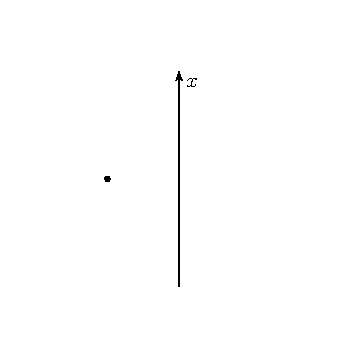
\includegraphics[scale=1.2]{chapter3-picture}
\par\end{centering}
\vspace{-1.4\baselineskip}
\caption{The disjoint domain represented by the type \lstinline!RootsOfQ!.\label{fig:RootsOfQ-disjoint-domain}}
\end{figure}

In the mathematical notation, a one-dimensional real space is denoted
by $\mathbb{R}$, a two-dimensional space by $\mathbb{R}^{2}$, and
a zero-dimensional space by $\mathbb{R}^{0}$. At first, we may think
that the mathematical representation of the type \lstinline!RootsOfQ!
is a union of the three sets, $\mathbb{R}^{0}\cup\mathbb{R}^{1}\cup\mathbb{R}^{2}$.
But an ordinary union of sets would not always work correctly because
we need to distinguish the parts of the union unambiguously, even
if some parts have the same type. For instance, the disjunctive type
shown in Example~\ref{subsec:disj-Example-rootsofq-2} cannot be
correctly represented by the mathematical union
\[
\mathbb{R}^{0}\cup\mathbb{R}^{0}\cup\mathbb{R}^{1}\cup\mathbb{R}^{0}\cup\mathbb{R}^{1}\cup\mathbb{R}^{2}
\]
because $\mathbb{R}^{0}\cup\mathbb{R}^{0}=\mathbb{R}^{0}$ and $\mathbb{R}^{1}\cup\mathbb{R}^{1}=\mathbb{R}^{1}$,
so 
\[
\mathbb{R}^{0}\cup\mathbb{R}^{0}\cup\mathbb{R}^{1}\cup\mathbb{R}^{0}\cup\mathbb{R}^{1}\cup\mathbb{R}^{2}=\mathbb{R}^{0}\cup\mathbb{R}^{1}\cup\mathbb{R}^{2}\quad.
\]
This representation has lost the distinction between e.g., \lstinline!Linear(x)!
and \lstinline!OneRootQ(x)!.

In the Scala code, each part of a disjunctive type must be distinguished
by a unique name such as \lstinline!NoRoots!, \lstinline!OneRoot!,
and \lstinline!TwoRoots!. To represent this mathematically, we can
attach a distinct label to each part of the union. Labels are symbols
without any special meaning, and we can just assume that labels are
names of Scala case classes. Parts of the union are then represented
by sets of pairs such as $(\text{\texttt{OneRoot}},x)_{x\in\mathbb{R}^{1}}$.
Then the domain \lstinline!RootsOfQ! is expressed as
\[
\text{\texttt{RootsOfQ}}=(\text{\texttt{NoRoots}},u)_{u\in\mathbb{R}^{0}}\cup(\text{\texttt{OneRoot}},x)_{x\in\mathbb{R}^{1}}\cup(\text{\texttt{TwoRoots}},\left(x,y\right))_{\left(x,y\right)\in\mathbb{R}^{2}}\quad.
\]
This is an ordinary union of mathematical sets, but each of the sets
has a unique label, so no two values from different parts of the union
could possibly be equal. This kind of labeled union is called a \index{disjoint union}\textbf{disjoint
union} or \textsf{``}tagged union\textsf{''}. Each element of the disjoint union is
a pair of the form \lstinline!(label, data)!, where the label uniquely
identifies the part of the union, and the data can have any chosen
type such as $\mathbb{R}^{1}$. If we use disjoint unions, we cannot
confuse different parts of the union even if their data have the same
type, because labels are required to be distinct.

Disjoint unions are not often used in mathematics, but they are needed
in software engineering because real-life data often belongs to disjoint
domains.

\paragraph{Named \texttt{Unit} types}

At first sight, it may seem strange that the zero-dimensional space
is represented by a set containing \emph{one} point. Why should we
not use an empty set (rather than a set with one point) to represent
the case where the equation has no real roots? The reason is that
we are required to represent not only the values of the roots but
also the information \emph{about} the existence of the roots. The
case with no real roots needs to be represented by some \emph{value}
of type \lstinline!RootsOfQ!. This value cannot be missing, which
would happen if we used an empty set to represent the no-roots case.
It is natural to use the named empty tuple \lstinline!NoRoots()!
to represent this case, just as we used a named $2$-tuple \lstinline!TwoRoots(x, y)!
to represent the case of two roots.

Consider the value $u$ used by the mathematical set $\left(\text{\texttt{NoRoots}},u\right)_{u\in\mathbb{R}^{0}}$.
Since $\mathbb{R}^{0}$ consists of a single point, there is only
\emph{one} possible value of $u$. Similarly, the \lstinline!Unit!
type in Scala has only one distinct value, written as \lstinline!()!.
A case class with no parts, such as \lstinline!NoRoots!, has only
one distinct value, written as \lstinline!NoRoots()!. This Scala
value is fully analogous to the mathematical notation $\left(\text{\texttt{NoRoots}},u\right)_{u\in\mathbb{R}^{0}}$.

So, case classes with no parts are quite similar to \lstinline!Unit!
except for an added name, e.g., \lstinline!NoRoots()! is the \lstinline!Unit!
value \lstinline!()! with name \lstinline!NoRoots!. For this reason,
they can be viewed as \textsf{``}named unit\textsf{''} types.\index{unit type!named}

\subsection{Disjunctive types in other programming languages}

Disjunctive types and pattern matching turns out to be one of the
defining features of FP languages. Languages that were not designed
for functional programming do not support these features, while ML,
OCaml, Haskell, F\#, Scala, Swift, Elm, and PureScript support disjunctive
types and pattern matching as part of the language design. 

It is remarkable that named tuple types (also called \textsf{``}structs\textsf{''}
or \textsf{``}records\textsf{''}) are provided in almost every programming language,
while disjunctive types are almost never present except in languages
designed for the FP paradigm. (Ada and Pascal are the only languages
that support disjunctive types without other FP features.\footnote{\texttt{\href{https://en.wikipedia.org/wiki/Comparison_of_programming_languages_(basic_instructions)\#Other_types}{https://en.wikipedia.org/wiki/Comparison\_of\_programming\_languages\_(basic\_instructions)\#Other\_types}}})

The \lstinline!union! types in C and C++ are not disjunctive types
because it is not possible to determine which part of the union is
represented by a given value. A \lstinline!union! declaration in
C looks like this:
\begin{lstlisting}[language=C]
union { int x; double y; long z; } i_d_l;
\end{lstlisting}
Without a label, we (and the compiler) will not know whether a given
value of type \lstinline!i_d_l! represents an \lstinline!int!, a
\lstinline!double!, or a \lstinline!long!. This will lead to errors
that are hard to detect.

Programming languages of the C family (C, C++, Objective C, Java)
support \textbf{enumeration} (\lstinline!enum!) types\index{enumeration type},
which are a limited form of disjunctive types, and a \lstinline!switch!
operation, which is a limited form of pattern matching. An \lstinline!enum!
type declaration in Java looks like this:
\begin{lstlisting}[language=Java]
enum Color { RED, GREEN, BLUE; } 
\end{lstlisting}
In Scala, this is equivalent to a disjunctive type containing three
\emph{empty} tuples:
\begin{lstlisting}
sealed trait Color
final case class RED()   extends Color
final case class GREEN() extends Color
final case class BLUE()  extends Color
\end{lstlisting}
If \lstinline!enum! types were \textsf{``}enriched\textsf{''} with extra data, so
that the tuples could be non-empty, we would obtain the full functionality
of disjunctive types (provided that the switch statement is also suitably
extended to handle the extra data). A definition of \lstinline!RootsOfQ!
could then look like this: 
\begin{lstlisting}
enum RootsOfQ {                 // This is not valid in Java!
  NoRoots(), OneRoot(Double x), TwoRoots(Double x, Double y);
}
\end{lstlisting}
A future version of Scala 3 will have syntax for disjunctive types\footnote{\texttt{\href{https://dotty.epfl.ch/docs/reference/enums/adts.html}{https://dotty.epfl.ch/docs/reference/enums/adts.html}}}
that resembles \textsf{``}enriched \lstinline!enum!\textsf{''}:
\begin{lstlisting}
enum RootsOfQ {  case NoRoots;  case OneRoot(x: Double);  case TwoRoots(x: Double, y: Double)  }
\end{lstlisting}
For comparison, the syntax for a disjunctive type equivalent to \lstinline!RootsOfQ!
in OCaml and Haskell is:
\begin{lstlisting}[language=Caml]
(* OCaml *)
type RootsOfQ = NoRoots | OneRoot of float | TwoRoots of float*float
\end{lstlisting}
\begin{lstlisting}[language=Haskell]
-- Haskell
data RootsOfQ = NoRoots | OneRoot Double | TwoRoots (Double, Double)
\end{lstlisting}
This is more concise than the Scala syntax. When reasoning about disjunctive
types, it is inconvenient to write out long type definitions. Chapter~\ref{chap:5-Curry-Howard}
will introduce a mathematical notation designed for efficient reasoning
about types.

\subsection{Disjunctions and conjunctions in formal logic\label{subsec:Disjunctions-and-conjunctions}}

In logic, a \textbf{proposition\index{proposition (in logic)}} is
a logical formula that could be true or false. A \textbf{disjunction\index{disjunction (in logic)}}
of propositions $A$, $B$, $C$ is denoted by $A\vee B\vee C$ and
is true if and only if \emph{at least one} of $A$, $B$, $C$ is
true. A \textbf{conjunction}\index{conjunction (in logic)} of $A$,
$B$, $C$ is denoted by $A\wedge B\wedge C$ and is true if and only
if \emph{all} of the propositions $A$, $B$, $C$ are true.

There is a similarity between a disjunctive data type and a logical
disjunction of propositions. A value of the disjunctive data type
\lstinline!RootsOfQ! can be constructed only if we have one of the
values \lstinline!NoRoots()!, \lstinline!OneRoot(x)!, or \lstinline!TwoRoots(x, y)!.
Let us now rewrite the previous sentence as a logical formula. Denote
by ${\cal CH}(A)$ the logical proposition \textsf{``}this ${\cal C}$ode
${\cal H}$as a value of type \lstinline!A!\textsf{''}, where \textsf{``}this code\textsf{''}
refers to a particular function in a program. So, the proposition
\textsf{``}the function \emph{can} compute a value of type \lstinline!RootsOfQ!\textsf{''}
is denoted by ${\cal CH}(\text{\texttt{RootsOfQ}})$. We can then
write the above sentence about \lstinline!RootsOfQ! as the logical
formula
\begin{equation}
{\cal CH}(\text{\texttt{RootsOfQ}})={\cal CH}(\text{\texttt{NoRoots}})\vee{\cal CH}(\text{\texttt{OneRoot}})\vee{\cal CH}(\text{\texttt{TwoRoots}})\quad.\label{eq:curry-howard-example-disjunction}
\end{equation}

There is also a similarity between logical \emph{conjunctions} and
tuple types. Consider the named tuple (i.e., a case class) \lstinline!TwoRoots(x: Double, y: Double)!.
When can we have a value of type \lstinline!TwoRoots!? Only if we
have two values of type \lstinline!Double!. Rewriting this sentence
as a logical formula, we get
\[
{\cal CH}(\text{\texttt{TwoRoots}})={\cal CH}(\text{\texttt{Double}})\wedge{\cal CH}(\text{\texttt{Double}})\quad.
\]
Formal logic admits the simplification
\[
{\cal CH}(\text{\texttt{Double}})\wedge{\cal CH}(\text{\texttt{Double}})={\cal CH}(\text{\texttt{Double}})\quad.
\]
However, no such simplification will be available in the general case,
e.g.
\begin{lstlisting}
case class Data3(x: Int, y: String, z: Double)
\end{lstlisting}
For this type, we will have the formula 
\begin{equation}
{\cal CH}(\text{\texttt{Data3}})={\cal CH}(\text{\texttt{Int}})\wedge{\cal CH}(\text{\texttt{String}})\wedge{\cal CH}(\text{\texttt{Double}})\quad.\label{eq:curry-howard-example-case-class}
\end{equation}

We find that tuples are related to logical conjunctions in the same
way as disjunctive types are related to logical disjunctions. This
is the main reason for choosing the name \textsf{``}disjunctive types\textsf{''}.\footnote{Disjunctive types are also known as \textsf{``}variants\textsf{''}, \textsf{``}sum types\textsf{''},
\textsf{``}co-product types\textsf{''}, and \textsf{``}tagged union types\textsf{''}.}

The correspondence between disjunctions, conjunctions, and data types
is explained in more detail in Chapter~\ref{chap:5-Curry-Howard}.
For now, we note that the operations of conjunction and disjunction
are not sufficient to produce all possible logical expressions. To
obtain a complete logic, it is also necessary to have the logical
implication $A\rightarrow B$ (\textsf{``}if $A$ is true than $B$ is true\textsf{''}).
It turns out that the implication $A\rightarrow B$ is related to
the function type \lstinline!A => B! in the same way as the disjunction
operation is related to disjunctive types and the conjunction to tuples.
In Chapter~\ref{chap:Higher-order-functions}, we will study function
types in depth.


\part{Intermediate level}


\chapter{The logic of types. II. Higher-order functions\label{chap:Higher-order-functions} }

\section{Functions that return functions}

\subsection{Motivation and first examples}

\global\long\def\gunderline#1{\mathunderline{greenunder}{#1}}%
\global\long\def\bef{\forwardcompose}%
Consider the task of preparing a logger function that prints messages
with a configurable prefix. 

A simple logger function can be a value of type \lstinline!String => Unit!,
such as:
\begin{lstlisting}
val logger: String => Unit = { message => println(s"INFO: $message") }

scala> logger("hello world")
INFO: hello world
\end{lstlisting}
This function prints any given message with the logging prefix \lstinline!"INFO"!. 

The standard library function \lstinline!println(...)! always returns
a \lstinline!Unit! value after printing its arguments. As we already
know, there is only a single value of type \lstinline!Unit!, and
that value is denoted by \lstinline!()!. To see that \lstinline!println!
returns \lstinline!Unit!, run this code:
\begin{lstlisting}
scala> val x = println(123)
123
x: Unit = ()
\end{lstlisting}

The task is to make the logging prefix configurable. A simple solution
is to implement a function \lstinline!logWith! that takes a prefix
as an argument and returns a new logger containing that prefix. Note
that the function \lstinline!logWith! returns a new \emph{function},
i.e., a new value of type \lstinline!String => Unit!:
\begin{lstlisting}
def logWith(prefix: String): (String => Unit) = {
    message => println(s"$prefix: $message")
}
\end{lstlisting}
The body of \lstinline!logWith! consists of a nameless function \lstinline!message => println(...)!,
which is a value of type \lstinline!String => Unit!. This value will
be returned when we evaluate \lstinline!logWith("...")!.

We can now use \lstinline!logWith! to create some logger functions:
\begin{lstlisting}
scala> val info = logWith("INFO")
info: String => Unit = <function1>

scala> val warn = logWith("WARN")
warn: String => Unit = <function1>
\end{lstlisting}
The created loggers are then usable as ordinary functions:
\begin{lstlisting}
scala> info("hello")
INFO: hello

scala> warn("goodbye")
WARN: goodbye
\end{lstlisting}
The values \lstinline!info! and \lstinline!warn! can be used by
any code that needs a logging function.

It is important that the prefix is \textsf{``}baked into\textsf{''} functions created
by \lstinline!logWith!. A logger such as \lstinline!warn! will always
print messages with the prefix \lstinline!"WARN"!, and the prefix
cannot be changed any more. This is because the value \lstinline!prefix!
is treated as a local constant within the body of the nameless function
computed and returned by \lstinline!logWith!. For instance, the body
of the function \lstinline!warn! is equivalent to:
\begin{lstlisting}
{ val prefix = "WARN"; (message => s"$prefix: $message") }
\end{lstlisting}
Whenever a new function is created using \lstinline!logWith(prefix)!,
the (immutable) reference to \lstinline!prefix! is stored within
the body of the newly created function. This is a general feature
of nameless functions: the function\textsf{'}s body captures references to
all the outer-scope values it uses. One sometimes says that the function\textsf{'}s
body \textsf{``}closes over\textsf{''} those values; for this reason, nameless functions
are also called \textsf{``}\textbf{\index{closure}closures}\textsf{''}. 

However, nameless functions do not \emph{copy} values from outer scopes.
Those values are captured by reference. This distinction is important
in Scala as it supports mutable values (as well as classes that encapsulate
mutable values).

Here is an example of a function body capturing references to variables:
\begin{lstlisting}
var c: Int = 10  // Mutable variable!
val f: Int => Int = {
  val p = 10
  val q = 20
  x => p + q * x + c
}
\end{lstlisting}
The body of the function \lstinline!f! is equivalent to \lstinline!{ x => 10 + 20 * x + c }!.
The values \lstinline!p = 10! and \lstinline!q = 20! are local constants
captured in the function\textsf{'}s body. However, the value \lstinline!c!
is captured by reference. If we change \lstinline!c!, the behavior
of \lstinline!f! will also change:
\begin{lstlisting}
scala> f(10)
res0: Int = 220

scala> c = 1000
c: Int = 1000

scala> f(10)
res1: Int = 1210 
\end{lstlisting}
A captured reference to a mutable external variable \lstinline!c!
makes the function \lstinline!f! itself mutable, even though \lstinline!f!
was defined as a \lstinline!val!. We will avoid such code in this
book and instead use immutable values.

\subsection{Curried and uncurried functions}

Reasoning mathematically about the following code:
\begin{lstlisting}
val info = logWith("INFO")
info("hello")
\end{lstlisting}
we would expect that \lstinline!info! is \emph{the same value} as
\lstinline!logWith("INFO")!, and so the code \lstinline!info("hello")!
should have the same effect as the code \lstinline!logWith("INFO")("hello")!.
This is indeed so:
\begin{lstlisting}
scala> logWith("INFO")("hello")
INFO: hello
\end{lstlisting}
The syntax \lstinline!logWith("INFO")("hello")! looks like the function
\lstinline!logWith! applied to \emph{two} arguments. Yet, \lstinline!logWith!
was defined as a function with a single argument of type \lstinline!String!.
This is not a contradiction because \lstinline!logWith("INFO")! returns
a function that accepts an additional argument. So, expressions \lstinline!logWith("INFO")!
and \lstinline!logWith("INFO")("hello")! are both valid. In this
sense, we are allowed to apply \lstinline!logWith! to one argument
at a time.

A function that can be applied to arguments in this way is called
a \index{curried function}\textbf{curried} function. 

While a curried function can be applied to one argument at a time,
an \textbf{uncurried}\index{uncurried function} function must be
applied to all arguments at once, e.g.:
\begin{lstlisting}
def prefixLog(prefix: String, message: String): Unit = println(s"$prefix: $message")
\end{lstlisting}

The type of the curried function \lstinline!logWith! is \lstinline!String => (String => Unit)!.
By Scala\textsf{'}s syntax conventions, the function arrow (\lstinline!=>!)
groups to the \emph{right}. So, the parentheses in the type expression
\lstinline!String => (String => Unit)! are not needed. The function\textsf{'}s
type can be written as \lstinline!String => String => Unit!.

The type \lstinline!String => String => Unit! is different from \lstinline!(String => String) => Unit!,
which is the type of a function returning \lstinline!Unit! and having
a single argument of type \lstinline!String => String!. 

When an argument\textsf{'}s type is a function type, e.g., \lstinline!String => String!,
it \emph{must} be enclosed in parentheses, as in \lstinline!(String => String) => Unit!.

In general, a curried function takes an argument and returns another
function that again takes an argument and returns another function,
and so on, until finally a non-function type is returned. So, the
type signature of a curried function generally looks like \lstinline!A => B => C => ... => R => S!,
where \lstinline!A!, \lstinline!B!, ..., \lstinline!R! are the
\textbf{curried arguments}\index{curried arguments} and \lstinline!S!
is the \textsf{``}final\textsf{''} result type.

For example, in the type expression \lstinline!A => B => C => D!
the types \lstinline!A!, \lstinline!B!, \lstinline!C! are the types
of curried arguments, and \lstinline!D! is the final result type.
It takes time to get used to reading this kind of syntax.

In Scala, functions defined with multiple argument lists (enclosed
in multiple pairs of parentheses) are curried functions. We have seen
examples of curried functions before:
\begin{lstlisting}
def map[A, B](xs: Seq[A])(f: A => B): Seq[B]
def fmap[A, B](f: A => B)(xs: Option[A]): Option[B]
def foldLeft[A, R](xs: Seq[A])(init: R)(update: (R, A) => R): R
\end{lstlisting}
The type signatures of these functions can be also written equivalently
without argument names, although this is less convenient in practical
coding:
\begin{lstlisting}
def map[A, B]: Seq[A] => (A => B) => Seq[B]
def fmap[A, B]: (A => B) => Option[A] => Option[B]
def foldLeft[A, R]: Seq[A] => R => ((R, A) => R) => R
\end{lstlisting}
Curried arguments of a \emph{function type}, such as \lstinline!(A => B)!,
need parentheses.

To summarize, a curried function such as \lstinline!logWith! can
be defined in three equivalent ways in Scala:
\begin{lstlisting}[numbers=left]
def logWith1(prefix: String)(message: String): Unit = println(s"$prefix: $message")
def logWith2(prefix: String): String => Unit = { message => println(s"$prefix: $message") }
def logWith3: String => String => Unit = { prefix => message => println(s"$prefix: $message") }
\end{lstlisting}
For clarity, we will sometimes enclose nameless functions in parentheses
or curly braces. 

Line 3 above shows that the arrow symbols \lstinline!=>! group to
the right within the \emph{code} of nameless functions. So, \lstinline!x => y => expr!
means \lstinline!{x => {y => expr}}!, a nameless function taking
an argument \lstinline!x! and returning a nameless function that
takes an argument \lstinline!y! and returns an expression \lstinline!expr!.
This syntax convention is helpful since the code \lstinline!x => y => z!
visually corresponds to the curried function\textsf{'}s type signature \lstinline!A => B => C!,
which uses the same syntax convention. Also, the syntax \lstinline!(x => y) => z!
could not possibly work for a nameless function because  matching
a function against the pattern \lstinline!x => y! makes no sense.
If we matched a function such as \lstinline!{ t => t + 20 }! against
the pattern \lstinline!x => y! by setting \lstinline!x = t! and
\lstinline!y = t + 20!, we would have no value for the bound variable
\lstinline!t!. (What would be the integer value of \lstinline!y!?)
So, \lstinline!x => (y => z)! is the only sensible way of adding
parentheses to \lstinline!x => y => z!.

Although the code \lstinline!(x => y) => z! is invalid, the type
expression \lstinline!(A => B) => C! is valid. We may write a nameless
function of type \lstinline!(A => B) => C! as \lstinline!f => expr!
where \lstinline!f: A => B! is the argument and \lstinline!expr!
the body.

\subsection{Equivalence of curried and uncurried functions}

We defined the curried function \lstinline!logWith! in order to be
able to create logger functions such as \lstinline!info! and \lstinline!warn!.
However, some curried functions, such as \lstinline!foldLeft!, are
almost always applied to all possible arguments. A curried function
applied to all its possible arguments is equivalent to an uncurried
function that takes all those arguments at once. Let us look at this
equivalence in more detail.

Consider a curried function with type signature \lstinline!Int => Int => Int!.
This function takes an integer and returns an (uncurried) function
taking an integer and returning an integer. An example of such a curried
function is:
\begin{lstlisting}
def f1(x: Int): Int => Int = { y => x - y }
\end{lstlisting}

The function takes an integer \lstinline!x! and returns the expression
\lstinline!y => x - y!, which is a function of type \lstinline!Int => Int!.
The code of \lstinline!f1! can be written equivalently as:
\begin{lstlisting}
val f1: Int => Int => Int = { x => y => x - y }
\end{lstlisting}
Let us rewrite \lstinline!f1! as a function that takes its two arguments
at once:
\begin{lstlisting}
def f2(x: Int, y: Int): Int = x - y
\end{lstlisting}
The function \lstinline!f2! has type signature \lstinline!(Int, Int) => Int!.
Calling \lstinline!f1! and \lstinline!f2! requires different syntax:
\begin{lstlisting}
scala> f1(20)(4)
res0: Int = 16

scala> f2(20, 4)
res1: Int = 16
\end{lstlisting}
The main difference is that \lstinline!f2! must be applied at once
to both arguments, while \lstinline!f1! could be applied to just
the first argument (\lstinline!20!). Applying a curried function
to some but not all possible arguments is called a \textbf{\index{partial application}partial
application}. The result of evaluating \lstinline!f1(20)! is a function
that can be later applied to another argument:
\begin{lstlisting}
scala> val r1 = f1(20)
r1: Int => Int = <function1> 

scala> r1(4)
res2: Int = 16
\end{lstlisting}

Applying a curried function to all possible arguments is called a
\index{curried function!full application}\textbf{full} application.
A full application returns a value that is not of a function type.
So, it cannot be applied to more arguments.

To partially apply an \emph{uncurried} function, we can use the underscore
($\_$) symbol:
\begin{lstlisting}[numbers=left]
scala> val r2: Int => Int = f2(20, _)
r2: Int => Int = <function1>

scala> r2(4)
res3: Int = 16
\end{lstlisting}
(The type annotation \lstinline!Int => Int! is required in line 1.)
This code creates a function \lstinline!r2! by applying \lstinline!f2!
to the first argument but not to the second. Then \lstinline!r2!
is the same function as \lstinline!r1! defined above; i.e., \lstinline!r2!
returns the same values for the same arguments as \lstinline!r1!.
A more verbose syntax for a partial application is:
\begin{lstlisting}
scala> val r3: Int => Int = { x => f2(20, x) }  // Same as r2 above.
r3: Int => Int = <function1>

scala> r3(4)
res4: Int = 16
\end{lstlisting}

We can see that a curried function, such as \lstinline!f1!, is better
adapted for partial application than \lstinline!f2!, because the
syntax is shorter. However, the \emph{types} of functions \lstinline!f1!
and \lstinline!f2! are\textbf{ equivalent}\index{type equivalence}:
for any \lstinline!f1! of type \lstinline!Int => Int => Int! we
can reconstruct \lstinline!f2! of type \lstinline!(Int, Int) => Int!
and vice versa, without loss of information:
\begin{lstlisting}
def f2new(x: Int, y: Int): Int = f1(x)(y)             // f2new is equal to f2
def f1new: Int => Int => Int = { x => y => f2(x, y) } // f1new is equal to f1
\end{lstlisting}
It is clear that the function \lstinline!f1new! computes the same
results as \lstinline!f1!, and that the function \lstinline!f2new!
computes the same results as \lstinline!f2!. The equivalence of the
functions \lstinline!f1! and \lstinline!f2! is not \emph{equality}
 \textemdash{} these functions are \emph{different}; but each of them
can be reconstructed from the other. The one-to-one correspondence
between all functions of type \lstinline!Int => Int => Int! and all
functions of type \lstinline!(Int, Int) => Int! is what we call the
\textsf{``}equivalence of types\textsf{''}.

More generally, a curried function has a type signature of the form
\lstinline!A => B => C => ... => R => S!, where \lstinline!A!, \lstinline!B!,
\lstinline!C!, ..., \lstinline!S! are some types. A function with
this type signature is equivalent to an uncurried\index{uncurried function}
function with type signature \lstinline!(A,B,C,...,R) => S!. The
uncurried function takes all arguments at once, while the curried
function takes one argument at a time. Other than that, these two
functions compute the same results given the same arguments.

We have seen how a curried function can be converted to an equivalent
uncurried one, and vice versa. The Scala library defines the methods
\lstinline!curried! and \lstinline!uncurried! that convert between
these forms of functions. To convert between \lstinline!f2! and \lstinline!f1!:
\begin{lstlisting}
scala> val f1c = (f2 _).curried
f1c: Int => (Int => Int) = <function1>

scala> val f2u = Function.uncurried(f1c)
f2u: (Int, Int) => Int = <function2> 
\end{lstlisting}
The syntax \lstinline!(f2 _)! is needed in Scala to convert methods
to function values. Recall that Scala has two ways of defining a function:
one as a method\index{Scala method} (defined using \lstinline!def!),
another as a function value\index{function as a value} (defined using
\lstinline!val!). The extra underscore is unnecessary in Scala 3.

The methods \lstinline!curried! and \lstinline!uncurried! are quick
to implement (see Section~\ref{subsec:Examples-of-fully-parametric}
below). These functions are called the \textbf{currying}\index{currying}
and \textbf{uncurrying}\index{uncurrying} transformations.

\section{Fully parametric functions\label{sec:Fully-parametric-functions}}

Scala code may declare functions with type parameters, which are set
only when the function is applied to specific arguments. Examples
of such functions are \lstinline!map! and \lstinline!filter!, written
as:
\begin{lstlisting}
def map[A, B](xs: Seq[A])(f: A => B): Seq[B]
def filter[A](xs: Seq[A])(p: A => Boolean): Seq[A]
\end{lstlisting}
Such functions can be applied to arguments of different types without
changing the function\textsf{'}s code. It is better to write a single function
with type parameters instead of writing several functions with repeated
code but working with different types.

When we apply the function \lstinline!map! as \lstinline!map(xs)(f)!
to a specific value \lstinline!xs! of type, say, \lstinline!Seq[Int]!,
and a specific function \lstinline!f! of type, say, \lstinline!Int => String!,
the Scala compiler will automatically set the type parameters \lstinline!A = Int!
and \lstinline!B = String! in the code of \lstinline!map!. We may
also set type parameters explicitly and write, for example, \lstinline!map[Int, String](xs)(f)!.
This syntax shows a certain similarity between type parameters such
as \lstinline!Int!, \lstinline!String! and \textsf{``}value parameters\textsf{''}
(arguments) \lstinline!xs! and \lstinline!f!. Setting type parameters,
e.g., \lstinline!map[Int, String]!, means substituting \lstinline!A = Int!,
\lstinline!B = String! into the type signature of the function, similarly
to how setting value parameters means substituting specific values
into the function body.

In the functions \lstinline!map! and \lstinline!filter! as just
shown, some types are parameters while others are specific types,
such as \lstinline!Seq! and \lstinline!Boolean!. It is sometimes
possible to replace \emph{all} specific types in the type signature
of a function by type parameters. The result is a \textsf{``}fully parametric\textsf{''}
function.

We call a function \textbf{fully parametric}\index{fully parametric!code|textit}
if its arguments have types described by type parameters, and the
code of the function does not use any information about its argument
types, other than assuming that those types correctly match the type
signature. In addition to type parameters, a fully parametric function
may use the \lstinline!Unit! type, tuple types, disjunctive types,
and function types. Fully parametric functions may not use any library-defined
types such as \lstinline!Int! or \lstinline!String!.

What kind of functions are fully parametric? To build up intuition,
let us compare the following two functions that have the same type
signature:
\begin{lstlisting}
def cos_sin(p: (Double, Double)): (Double, Double) = p match {
  case (x, y) =>
    val r = math.sqrt(x * x + y * y)
    (x / r, y / r)   // Return cos and sin of the angle, or `NaN` when undefined.
}

def swap(p: (Double, Double)): (Double, Double) = p match {
  case (x, y) => (y, x)
}
\end{lstlisting}
We can introduce type parameters into the type signature of \lstinline!swap!
to make it fully parametric:
\begin{lstlisting}
def swap[A, B](p: (A, B)): (B, A) = p match {
  case (x, y) => (y, x)
}
\end{lstlisting}
Converting \lstinline!swap! into a fully parametric function is possible
because the operation of swapping the parts of a tuple \lstinline!(A, B)!
works in the same way for all types \lstinline!A!, \lstinline!B!.
No changes were made in the body of the function. The specialized
version of \lstinline!swap! working on \lstinline!(Double, Double)!
can be obtained from the fully parametric version of \lstinline!swap!
if we set the type parameters as \lstinline!A = Double!, \lstinline!B = Double!.

In contrast, the function \lstinline!cos_sin! performs a computation
that is specific to the type \lstinline!Double!. That computation
cannot be generalized to an arbitrary type parameter \lstinline!A!
instead of the type \lstinline!Double!. For instance, the code of
\lstinline!cos_sin! uses the function \lstinline!math.sqrt!, which
is defined only for the type \lstinline!Double!. 

To generalize \lstinline!cos_sin! to a fully parametric function
that works with a type parameter \lstinline!A!, we would need to
replace all computations specific to the type \lstinline!Double!
by new arguments working with the type parameter \lstinline!A!. For
example, we could introduce two new arguments (named, say, \lstinline!distance!
and \lstinline!ratio!) and replace \lstinline!cos_sin! by the fully
parametric function \lstinline!cos_sin_parametric!:
\begin{lstlisting}
def cos_sin_parametric[A](p: (A, A), distance: (A, A) => A, ratio: (A, A) => A): (A, A) = p match {
  case (x, y) =>
    val r = distance(x, y)
    (ratio(x, r), ratio(y, r))
}
\end{lstlisting}

A fully parametric function has all its arguments typed with type
parameters or with some combinations of type parameters, i.e., \textbf{type
expressions}\index{type expression} such as \lstinline!(A, B)! or
\lstinline!X => Either[X, Y]!.

The \lstinline!swap! operation for pairs is already defined in the
Scala library:
\begin{lstlisting}
scala> (1, "abc").swap
res0: (String, Int) = (abc,1)
\end{lstlisting}
If needed, other swapping functions can be implemented for tuples
with more elements, e.g.:
\begin{lstlisting}
def swapAC[A, B, C]: ((A, B, C)) => (C, B, A) = { case (x, y, z) => (z, y, x) }
\end{lstlisting}
The Scala syntax requires \emph{double} parentheses around tuple types\index{tuples!as function arguments}
of arguments but not around the tuple type of a function\textsf{'}s result.
So, the function \lstinline!cos_sin! may be written as a value like
this:
\begin{lstlisting}
val cos_sin: ((Double, Double)) => (Double, Double) = ...
\end{lstlisting}

Further examples of fully parametric functions are the identity function,
the \lstinline!const! function, the function composition methods,
and the currying / uncurrying transformations. 

The \index{identity function}identity function is available in the
Scala library as \lstinline!identity[T]!:
\begin{lstlisting}
def identity[T]: T => T = (t => t)
\end{lstlisting}
In the mathematical notation, we write the identity function as \textsf{``}$\text{id}$\textsf{''}
for brevity.

The function available in the Scala library as \lstinline!Function.const[C, X]!
takes an argument \lstinline!c! of type \lstinline!C! and returns
\emph{a new function} that always returns \lstinline!c!:
\begin{lstlisting}
def const[C, X](c: C): X => C = (_ => c)
\end{lstlisting}
The syntax \lstinline!_ => c! is used to emphasize that the new returned
function ignores its argument. One-argument functions that ignore
their argument are called \textbf{constant functions}.\index{constant function}

\subsection{Function composition\label{subsec:Examples-of-fully-parametric}}

\index{function composition}Consider two functions \lstinline!f: Int => Double!
and \lstinline!g: Double => String!. We can apply \lstinline!f!
to an integer argument \lstinline!x! and get a result \lstinline!f(x)!
of type \lstinline!Double!. Applying \lstinline!g! to that result
gives a \lstinline!String! value \lstinline!g(f(x))!. The transformation
from an \lstinline!x! of type \lstinline!Int! to a final \lstinline!String!
value \lstinline!g(f(x))! can be viewed as a new function of type
\lstinline!Int => String!. That new function is called the \textbf{forward
composition}\index{forward composition} of the two functions \lstinline!f!
and \lstinline!g!. In Scala, the forward composition of \lstinline!f!
and \lstinline!g! is written as \lstinline!f andThen g!:
\begin{lstlisting}
val f: Int => Double = (x => 5.67 + x)
val g: Double => String = (x => f"Result x = $x%3.2f")

scala> val h = f andThen g       // h(x) is defined as g(f(x)).
h: Int => String = <function1>

scala> h(40)
res36: String = Result x = 45.67
\end{lstlisting}
The Scala compiler derives the type of \lstinline!h! automatically
as \lstinline!Int => String!.

This book denotes the forward composition by the symbol ${\displaystyle \bef}$
(which can be read as \textsf{``}before\textsf{''}). We define $f\bef g$ (reads \textsf{``}$f$
before $g$\textsf{''}) by:
\begin{equation}
f\bef g\triangleq x\rightarrow g(f(x))\quad.\label{eq:def-of-forward-composition}
\end{equation}
The symbol $\triangleq$ means \textsf{``}is defined as\textsf{''} or \textsf{``}is equal
by definition to\textsf{''}.

We may implement the forward composition as a fully parametric function:
\begin{lstlisting}
def andThen[X, Y, Z](f: X => Y)(g: Y => Z): X => Z = { x => g(f(x)) }
\end{lstlisting}
This type signature requires the types of the function arguments to
match in a certain way, or else the composition is undefined (and
the code would produce a type error). The method \lstinline!andThen!
is an example of a function that \emph{both} returns a new function
\emph{and} takes other functions as arguments.

The \textbf{backward composition}\index{backward composition} of
two functions $f$ and $g$ works in the opposite order: first $g$
is applied and then $f$. This operation is denoted by the symbol
$\circ$ (pronounced \textsf{``}after\textsf{''}):
\begin{equation}
f\circ g\triangleq x\rightarrow f(g(x))\quad.\label{eq:def-of-backward-composition}
\end{equation}
In Scala, the backward composition is called \lstinline!compose!
and used as \lstinline!f compose g!. This method may be implemented
as a fully parametric function:
\begin{lstlisting}
def compose[X, Y, Z](f: Y => X)(g: Z => Y): Z => X = { z => f(g(z)) }
\end{lstlisting}

We have already seen the methods \lstinline!curried! and \lstinline!uncurried!
from the Scala library. As an illustration, here is the code for the
\textbf{uncurrying}\index{uncurrying} transformation (converting
curried functions to uncurried):
\begin{lstlisting}
def uncurry[A, B, R](f: A => B => R): ((A, B)) => R = { case (a, b) => f(a)(b) }
\end{lstlisting}

These examples show that fully parametric functions perform operations
so general that they work in the same way for all types. Some arguments
of fully parametric functions may have complicated types such as \lstinline!A => B => R!,
which are type expressions built up from type parameters. But fully
parametric functions do not use values of specific types such as \lstinline!Int!
or \lstinline!String!.

Functions with type parameters are often called \textsf{``}generic\index{generic functions}\textsf{''}.
This book uses the term \textsf{``}\index{fully parametric!code}\textbf{fully
parametric}\textsf{''} to designate a certain restricted kind of generic functions.

\subsection{Laws of function composition\label{subsec:Laws-of-function-composition}}

The operations of function composition, introduced in Section~\ref{subsec:Examples-of-fully-parametric},
have three important properties or \textsf{``}laws\textsf{''}:
\begin{itemize}
\item The two \textbf{identity laws}\index{identity laws!of function composition}:
the composition of any function $f$ with an identity function (\lstinline!identity[A]!)
will give again the function $f$.
\item The \textbf{associativity law}\index{associativity law!of function composition}:
the consecutive composition of three functions $f$, $g$, $h$ does
not depend on the order in which the pairs are composed.
\end{itemize}
These laws hold equally for the forward and the backward composition,
since those are just syntactic variants of the same operation. Let
us write these laws rigorously as equations and prove them.

\paragraph{Proofs with forward composition}

The composition of the identity function with an arbitrary function
$f$ on the left is written as $f\bef\text{id}$. The composition
with the function $f$ on the right is written as $\text{id}\bef f$.
In both cases, the result must be equal to the function $f$. The
resulting two laws are:
\begin{align*}
{\color{greenunder}\text{left identity law of function composition}:}\quad & \text{id}\bef f=f\quad,\\
{\color{greenunder}\text{right identity law of function composition}:}\quad & f\bef\text{id}=f\quad.
\end{align*}
To prove that these laws hold, we need to show that the functions
at both sides of the laws  give the same result when applied to an
arbitrary value $x$. Let us first clarify how the type parameters
must be set for all types to match consistently.

The laws must hold for an arbitrary function $f$. Assume that $f$
has the type signature $A\rightarrow B$, where $A$ and $B$ are
arbitrary types (type parameters). Consider the left identity law.
The function $(\text{id}\bef f)$ is, by definition~(\ref{eq:def-of-forward-composition}),
a function that takes an argument $x$, applies $\text{id}$ to that
$x$, and then applies $f$ to the result: 
\[
\text{id}\bef f=\left(x\rightarrow f\left(\text{id}\,(x)\right)\right)\quad.
\]
If $f$ has type $A\rightarrow B$, its argument must be of type $A$,
or else the types will not match. Therefore, the identity function
must have type $A\rightarrow A$, and the argument $x$ must have
type $A$. With these choices of the type parameters, the function
$\left(x\rightarrow f(\text{id}(x))\right)$ will have type $A\rightarrow B$.
This type matches the right-hand side of the law, which is just $f$.
We add type annotations to the code as \emph{superscripts}:
\[
\text{id}^{:A\rightarrow A}\bef f^{:A\rightarrow B}=\big(x^{:A}\rightarrow f\left(\text{id}\,(x)\right)\big)^{:A\rightarrow B}\quad.
\]
In the Scala syntax, this formula may be written as:
\begin{lstlisting}
identity[A] andThen (f: A => B) == { x: A => f(identity(x)) }: A => B
\end{lstlisting}

We will follow the convention where type parameters are single uppercase
letters, as is common in Scala code (although this convention is not
enforced by the Scala compiler). The colon symbol ($:$) in the superscript
$x^{:A}$ means a type annotation, as in Scala code \lstinline!x:A!.
Superscripts \emph{without} a colon, such as $\text{id}^{A}$, denote
type parameters, as in Scala code \lstinline!identity[A]!. Since
the function \lstinline!identity[A]! has type \lstinline!A => A!,
we can write $\text{id}^{A}$ or equivalently (but more verbosely)
$\text{id}^{:A\rightarrow A}$ to denote that function.

Now we can prove the law. By definition of the identity function,
we have $\text{id}\,(x)=x$, and so:
\[
\text{id}\bef f=\left(x\rightarrow f(\text{id}\,(x))\right)=\left(x\rightarrow f(x)\right)=f\quad.
\]
The last step works since $x\rightarrow f(x)$ is a function that
takes an argument $x$ and applies $f$ to that argument. This is
the same function as $f$. We say that $x\rightarrow f(x)$ is an
\textbf{expanded form}\index{expanded form of a function} of the
function $f$.

We turn to the right identity law, $f\bef\text{id}=f$. Write out
the left-hand side:
\[
f\bef\text{id}=\left(x\rightarrow\text{id}\,(f(x))\right)\quad.
\]
To check that the types match, assume that $f^{:A\rightarrow B}$.
Then $x$ must have type $A$, and the identity function must have
type $B\rightarrow B$. The result of $\text{id}\,(f(x))$ will also
have type $B$. With these choices of type parameters, all types match:
\[
f^{:A\rightarrow B}\bef\text{id}^{:B\rightarrow B}=\big(x^{:A}\rightarrow\text{id}\,(f(x))\big)^{:A\rightarrow B}\quad.
\]
Since $\text{id}\,(f(x))=f(x)$, we find:
\[
f\bef\text{id}=\left(x\rightarrow f(x)\right)=f\quad.
\]
In this way, we have demonstrated that both identity laws hold. 

The associativity law is written as an equation like this:
\begin{align}
{\color{greenunder}\text{associativity law of function composition}:}\quad & (f\bef g)\bef h=f\bef(g\bef h)\quad.\label{eq:associativity-of-function-composition}
\end{align}
Let us verify that the types match here. The types of the functions
$f$, $g$, and $h$ must be such that all the function compositions
match. If $f$ has type $A\rightarrow B$ for some type parameters
$A$ and $B$, then the argument of $g$ must be of type $B$. So,
we must have $g^{:B\rightarrow C}$, where $C$ is another type parameter.
The composition $f\bef g$ has type $A\rightarrow C$, so $h$ must
have type $C\rightarrow D$ for some type $D$. Assuming the types
as $f^{:A\rightarrow B}$, $g^{:B\rightarrow C}$, and $h^{:C\rightarrow D}$,
we find that the types in all the compositions $f\bef g$, $g\bef h$,
$(f\bef g)\bef h$, and $f\bef(g\bef h)$ match. We can rewrite Eq.~(\ref{eq:associativity-of-function-composition})
with type annotations: 
\begin{equation}
(f^{:A\rightarrow B}\bef g^{:B\rightarrow C})\bef h^{:C\rightarrow D}=f^{:A\rightarrow B}\bef(g^{:B\rightarrow C}\bef h^{:C\rightarrow D})\quad.\label{eq:associativity-law-for-function-composition-with-types}
\end{equation}

After checking the types, we are ready to verify the associativity
law. Note that both sides of the law~(\ref{eq:associativity-law-for-function-composition-with-types})
are functions of type $A\rightarrow D$. To prove that two functions
are equal means to prove that they return the same results when applied
to the same arguments. So, let us apply both sides of Eq.~(\ref{eq:associativity-law-for-function-composition-with-types})
to an arbitrary value $x^{:A}$. Using definition~(\ref{eq:def-of-forward-composition})
for the forward composition, we find:
\begin{align*}
\left((f\bef g)\bef h\right)(x) & =h\left(\left(f\bef g\right)(x)\right)=h(g(f(x)))\quad,\\
\left(f\bef(g\bef h)\right)(x) & =\left(g\bef h\right)(f(x))=h(g(f(x)))\quad.
\end{align*}
Both sides of the law are equal when applied to an arbitrary value
$x$. This concludes the proof.

Because of the associativity law, we do not need parentheses when
writing the expression $f\bef g\bef h$. The function $(f\bef g)\bef h$
is equal to the function $f\bef(g\bef h)$.

In the proof, we have omitted the type annotations since we already
checked that all types match. Checking the types beforehand allows
us to write shorter derivations.

\paragraph{Proofs with backward composition}

This book prefers to use the \textbf{forward composition}\index{forward composition}
$f\bef g$ rather than the backward\index{backward composition} composition
$g\circ f$. If desired, all equations can be converted from one notation
to the other by reversing the order of compositions:
\[
f\bef g\triangleq g\circ f
\]
for any functions $f^{:A\rightarrow B}$ and $g^{:B\rightarrow C}$.
Let us see how to prove the composition laws in the backward notation.
We will just need to reverse the order of function compositions in
the proofs above.

The left identity and right identity laws are:
\[
f\circ\text{id}=f\quad\quad,\quad\text{id}\circ f=f\quad.
\]
To match the types, we need to choose the type parameters as:
\[
f^{:A\rightarrow B}\circ\text{id}^{:A\rightarrow A}=f^{:A\rightarrow B}\quad\quad,\quad\text{id}^{B\rightarrow B}\circ f^{:A\rightarrow B}=f^{:A\rightarrow B}\quad.
\]
We now apply both sides of the laws to an arbitrary value $x^{:A}$.
For the left identity law, we find:
\begin{align*}
{\color{greenunder}\text{use definition~(\ref{eq:def-of-backward-composition})}:}\quad & f\circ\text{id}=\left(x\rightarrow f(\text{id}\,(x))\right)=\left(x\rightarrow f(x)\right)=f\quad.
\end{align*}
Similarly for the right identity law:
\[
\text{id}\circ f=\left(x\rightarrow\text{id}\,(f(x))\right)=\left(x\rightarrow f\left(x\right)\right)=f\quad.
\]
The associativity law,
\[
h\circ\left(g\circ f\right)=\left(h\circ g\right)\circ f\quad,
\]
is proved by applying both sides to an arbitrary value $x$ of a suitable
type:
\begin{align*}
\left(h\circ\left(g\circ f\right)\right)(x) & =h\left(\left(g\circ f\right)(x)\right)=h\left(g\left(f\left(x\right)\right)\right)\quad,\\
\left(\left(h\circ g\right)\circ f\right)(x) & =\left(h\circ g\right)\left(f(x)\right)=h\left(g\left(f\left(x\right)\right)\right)\quad.
\end{align*}
The types are checked by assuming that $f$ has the type $f^{:A\rightarrow B}$.
The types in $g\circ f$ match only when $g^{:B\rightarrow C}$, and
then $g\circ f$ is of type $A\rightarrow C$. The type of $h$ must
be $h^{:C\rightarrow D}$ for the types in $h\circ\left(g\circ f\right)$
to match. We can write the associativity law with type annotations
as:
\begin{equation}
h^{:C\rightarrow D}\circ(g^{:B\rightarrow C}\circ f^{:A\rightarrow B})=(h^{:C\rightarrow D}\circ g^{:B\rightarrow C})\circ f^{:A\rightarrow B}\quad.\label{eq:assoc-law-for-composition-with-types-backward}
\end{equation}
The associativity law allows us to omit parentheses in the expression
$h\circ g\circ f$. 

The length of calculations is the same in the forward and the backward
notation. One difference is that types of function compositions are
more visually clear in the forward notation: it is harder to check
that types match in Eq.~(\ref{eq:assoc-law-for-composition-with-types-backward})
than in Eq.~(\ref{eq:associativity-law-for-function-composition-with-types}).
To make the backward notation easier to work with, one could write\footnote{This is done in the book \textsf{``}Program design by calculation\textsf{''} by J.~N.~Oliveira
where the backward composition is used exclusively, see \texttt{\href{http://www4.di.uminho.pt/~jno/ps/pdbc.pdf}{http://www4.di.uminho.pt/$\sim$jno/ps/pdbc.pdf}}} the function types in reverse as, e.g., $g^{:C\leftarrow B}\circ f^{:B\leftarrow A}$.

\subsection{Example: A function that is \emph{not} fully parametric}

Fully parametric functions do not make any decisions based on the
actual types of arguments. As an example of code that is \emph{not}
fully parametric, consider the following \textsf{``}fake identity\textsf{''} function:
\begin{lstlisting}
def fid[A]: A => A = {
  case x: Int   => (x - 1).asInstanceOf[A]     // Special code for A = Int.
  case x        =>  x                          // Standard code for all other types A.
}
\end{lstlisting}
This function\textsf{'}s type signature is the same as that of \lstinline!identity[A]!,
and its behavior is the same for all types \lstinline!A! except for
\lstinline!A = Int!:
\begin{lstlisting}
scala> fid("abc")
res0: String = abc

scala> fid(true)
res1: Boolean = true

scala> fid(0)
res2: Int = -1
\end{lstlisting}
While Scala allows us to write this kind of code, the result is confusing:
the type signature \lstinline!A => A! does not indicate a special
behavior with \lstinline!A = Int!. In any case, \lstinline!fid!
is not a fully parametric function.

Let us see whether the identity laws of function composition hold
when using \lstinline!fid[A]! instead of the correct function \lstinline!identity[A]!.
To see that, we compose \lstinline!fid! with a simple function \lstinline!f_1!
defined by:
\begin{lstlisting}
def f_1: Int => Int = { x => x + 1 }
\end{lstlisting}
The composition (\lstinline!f_1 andThen fid!) has type \lstinline!Int => Int!.
Since \lstinline!f_1! has type \lstinline!Int => Int!, Scala will
automatically set the type parameter \lstinline!A = Int! in \lstinline!fid[A]!:
\begin{lstlisting}[mathescape=true]
scala> def f_2 = f_1 andThen fid    // $\color{dkgreen} f_{2}=f_{1}\bef\text{fid}$
f_2: Int => Int
\end{lstlisting}
By the identity law, we should have $f_{2}=f_{1}\bef\text{id}=f_{1}$.
But we can check that \lstinline!f_1! and \lstinline!f_2! are not
equal:
\begin{lstlisting}
scala> f_1(0)
res3: Int = 1

scala> f_2(0)
res4: Int = 0
\end{lstlisting}

It is important that we are able to detect that \lstinline!fid! is
not a fully parametric function by checking whether some equation
holds, without looking at the code of \lstinline!fid!. In this book,
we will always formulate any desired properties through equations
or \textsf{``}laws\textsf{''}. To verify that a law holds, we will perform symbolic
calculations\index{symbolic calculations} similar to the proofs in
Section~\ref{subsec:Laws-of-function-composition}. These calculations
are \textbf{symbolic} in the sense that we are manipulating symbols
(such as $x$, $f$, $g$, $h$) without substituting any specific
values for these symbols but only using some general rules and properties.
This is similar to symbolic calculations in mathematics, such as $\left(x-y\right)(x^{2}+xy+y^{2})=x^{3}-y^{3}$.
In the next section, we will get more experience with symbolic calculations
relevant to functional programming.

\section{Symbolic calculations with nameless functions}

\subsection{Calculations with curried functions}

In mathematics, functions are evaluated by substituting their argument
values into their body. Each sub-expression is then evaluated and
its result substituted into the larger expression.

Nameless functions are evaluated in the same way. For example, applying
the nameless function $x\rightarrow x+10$ to an integer $2$, we
substitute $2$ instead of $x$ in \textquotedblleft $x+10$\textquotedblright{}
and get the sub-expression \textquotedblleft $2+10$\textquotedblright .
Then we evaluate that sub-expression to $12$. The computation is
written like this:
\[
(x\rightarrow x+10)(2)=2+10=12\quad.
\]
To run this computation in Scala, we need to add a type annotation
to the nameless function as in $(x^{:\text{Int}}\rightarrow x+10)(2)$.
The code is:
\begin{lstlisting}
scala> ((x: Int) => x + 10)(2)
res0: Int = 12 
\end{lstlisting}

Curried function calls such as $f(x)(y)$ or $\left(x\rightarrow\text{expr}(x)\right)(y)(z)$
may look unfamiliar and confusing. We need to get some experience
working with them.

Consider the expression \lstinline!(x => y => x - y)(20)(4)!, and
begin with the curried argument \lstinline!20!. Applying a nameless
function of the form \lstinline!(x => ...)! to \lstinline!20! means
substituting \lstinline!x = 20! into the body of the function. After
that substitution, we obtain the expression \lstinline!y => 20 - y!,
which is again a nameless function. Applying that function to the
remaining argument \lstinline!(4)! means substituting \lstinline!y = 4!
into the body of \lstinline!y => 20 - y!. We get the expression \lstinline!20 - 4!,
which equals \lstinline!16!. Test in Scala:
\begin{lstlisting}
scala> ((x: Int) => (y: Int) => x - y)(20)(4)
res1: Int = 16
\end{lstlisting}

Applying a curried function such as \lstinline!x => y => z => expr(x,y,z)!
to three curried arguments \lstinline!10!, \lstinline!20!, and \lstinline!30!
means substituting \lstinline!x = 10!, \lstinline!y = 20!, and \lstinline!z = 30!
into the expression \lstinline!expr(x,y,z)!. 

This calculation is made easier by the convention that \lstinline!f(g)(h)!
means first applying \lstinline!f! to \lstinline!g! and then applying
the result to \lstinline!h!. In other words, function application
groups to the \emph{left}: \lstinline!f(g)(h) = (f(g))(h)!. It would
be confusing if function application grouped to the right and \lstinline!f(g)(h)!
meant first applying \lstinline!g! to \lstinline!h! and then applying
\lstinline!f! to the result. If \emph{that} were the syntax convention,
it would be harder to reason about applying a curried function to
its arguments.

We see that the right grouping of the function arrow \lstinline!=>!
is well adapted to the left grouping of function applications. All
functional languages follow these syntactic conventions.

To make calculations shorter, we will write code in a mathematical
notation rather than in the Scala syntax. Type annotations are written
with a \emph{colon} in the superscript. For example, $x^{:\text{Int}}\rightarrow x+10$
is the code notation corresponding to the Scala expression \lstinline!(x: Int) => x + 10!.

The symbolic evaluation of the Scala code \lstinline!((x: Int) => (y: Int) => x - y)(20)(4)!
can be written as:
\begin{align*}
 & (\gunderline{x^{:\text{Int}}}\rightarrow y^{:\text{Int}}\rightarrow\gunderline x-y)\gunderline{\left(20\right)}\left(4\right)\\
{\color{greenunder}\text{apply function and substitute }x=20:}\quad & =(\gunderline{y^{:\text{Int}}}\rightarrow20-\gunderline y)\gunderline{\left(4\right)}\\
{\color{greenunder}\text{apply function and substitute }y=4:}\quad & =20-4=16\quad.
\end{align*}
In the above step-by-step calculation, the colored underlines and
comments at left are added for clarity. A colored underline indicates
a sub-expression that is going to be rewritten at the \emph{next}
step.

We perform such calculations by substituting an argument into a function
at each step. A compiled Scala program is evaluated in a similar way
at run time.

Here are some more examples of performing function applications symbolically.
Types are omitted for brevity; every non-function value is of type
\texttt{}\lstinline!Int!:
\begin{align*}
\left(x\rightarrow x*2\right)(10) & =10*2=20\quad.\\
\left(p\rightarrow z\rightarrow z*p\right)\left(t\right) & =(z\rightarrow z*t)\quad.\\
\left(p\rightarrow z\rightarrow z*p\right)(t)(4) & =(z\rightarrow z*t)(4)=4*t\quad.
\end{align*}
Some results of these computation are integer values such as $20$;
other results are nameless functions such as $z\rightarrow z*t$.
Verify this in Scala:
\begin{lstlisting}
scala> ((x: Int) => x * 2)(10)
res3: Int = 20

scala> ((p: Int) => (z: Int) => z * p)(10)
res4: Int => Int = <function1>

scala> ((p: Int) => (z: Int) => z * p)(10)(4)
res5: Int = 40 
\end{lstlisting}

Let us summarize the syntax conventions for curried nameless functions:
\begin{itemize}
\item Function expressions group everything to the right: $x\rightarrow y\rightarrow z\rightarrow e$
means $x\rightarrow\left(y\rightarrow\left(z\rightarrow e\right)\right)$.
\item Function calls group everything to the left: $f(x)(y)(z)$ means $\big((f(x))(y)\big)(z)$.
The expression $f(x)$ is a new function that is applied to $y$,
giving again a new function that is finally applied to $z$.
\item Function applications group stronger than infix operations, so $f(x)+y$
means $(f(x))+y$, as usual in mathematics, and not $f(x+y)$.
\end{itemize}

\subsection{Functions as arguments of other functions}

Nameless functions are \emph{values} and can be used as part of larger
expressions, just as any other values. For instance, nameless functions
can be arguments of other functions (nameless or not). Here is an
example of applying a nameless function $f\rightarrow f(9)$ to the
nameless function $x\rightarrow x\%\,4$:
\begin{align*}
 & (f\rightarrow\gunderline f(9))\left(x\rightarrow x\%\,4\right)\\
{\color{greenunder}\text{substitute }f=\left(x\rightarrow x\%\,4\right):}\quad & =(x\rightarrow\gunderline x\%\,4)(9)\\
{\color{greenunder}\text{substitute }x=9:}\quad & =9\%\,4=1\quad.
\end{align*}
In the nameless function $f\rightarrow f(9)$, the argument $f$ has
to be itself a function, otherwise the expression $f(9)$ would make
no sense. The argument $x$ of $f(x)$ must be an integer, or else
we would not be able to compute $x\%\,4$. The result of computing
$f(9)$ is $1$, an integer. We conclude that $f$ must have type
$\text{Int}\rightarrow\text{Int}$, or else the types do not match.

To verify this result in Scala, we need to specify a type annotation
for $f$:
\begin{lstlisting}
scala> ((f: Int => Int) => f(9))(x => x % 4)
res2: Int = 1
\end{lstlisting}
No type annotation is needed for $x\rightarrow x\%\,4$ because the
Scala compiler already knows the type of $f$ and figures out that
$x$ in $x\rightarrow x\%\,4$ must have type \lstinline!Int!.

In the following examples of symbolic computations, some arguments
are themselves functions. Consider an expression that uses the nameless
function $\left(g\rightarrow g(2)\right)$ as an argument:
\begin{align}
 & (f\rightarrow p\rightarrow\gunderline f(p))\left(g\rightarrow g(2)\right)\label{eq:higher-order-functions-derivation0}\\
{\color{greenunder}\text{substitute }f=\left(g\rightarrow g(2)\right):}\quad & =p\rightarrow(g\rightarrow\gunderline g(2))\,(p)\nonumber \\
{\color{greenunder}\text{substitute }g=p:}\quad & =p\rightarrow p(2)\quad.\label{eq:higher-order-functions-derivation1}
\end{align}
The final result, $p\rightarrow p(2)$, cannot be simplified any more. 

The function $p\rightarrow p(2)$ applies \emph{its} argument ($p$)
to the value $2$. A possible value for $p$ is the function $x\rightarrow x+4$.
Let us apply expression~(\ref{eq:higher-order-functions-derivation0})
to $x\rightarrow x+4$:
\begin{align*}
 & \gunderline{\left(f\rightarrow p\rightarrow f(p)\right)\left(g\rightarrow g(2)\right)}\left(x\rightarrow x+4\right)\\
{\color{greenunder}\text{use Eq.~(\ref{eq:higher-order-functions-derivation1})}:}\quad & =(p\rightarrow\gunderline p(2))\left(x\rightarrow x+4\right)\\
{\color{greenunder}\text{substitute }p=\left(x\rightarrow x+4\right):}\quad & =(x\rightarrow\gunderline x+4)\left(2\right)\\
{\color{greenunder}\text{substitute }x=2:}\quad & =2+4=6\quad.
\end{align*}

To verify this calculation in Scala, we need to add appropriate type
annotations for $f$ and $p$. To figure out the types, we reason
like this:

We know that the function $f\rightarrow p\rightarrow f(p)$ is being
applied to the arguments $f=\left(g\rightarrow g(2)\right)$ and $p=\left(x\rightarrow x+4\right)$.
So, the argument $f$ in $f\rightarrow p\rightarrow f(p)$ must be
a function that takes $p$ as an argument.

The variable $x$ in $x\rightarrow x+4$ must be of type \lstinline!Int!.
So, the type of the expression $x\rightarrow x+4$ is $\text{Int}\rightarrow\text{Int}$,
and the type of the argument $p$ must be the same. We write $p^{:\text{Int}\rightarrow\text{Int}}$.

Finally, we need to make sure that the types match in the function
$f\rightarrow p\rightarrow f(p)$. Types match in $f(p)$ if the type
of $f$\textsf{'}s argument is the same as the type of $p$, which is $\text{Int}\rightarrow\text{Int}$.
So, $f$\textsf{'}s type must be $\left(\text{Int}\rightarrow\text{Int}\right)\rightarrow A$
for some type $A$. Since in our example $f=\left(g\rightarrow g(2)\right)$,
types match only if $g$ has type $\text{Int}\rightarrow\text{Int}$.
But then $g(2)$ has type $\text{Int}$, and so we must have $A=\text{Int}$.
Thus, the type of $f$ is $\left(\text{Int}\rightarrow\text{Int}\right)\rightarrow\text{Int}$.
We know enough to write the Scala code now:
\begin{lstlisting}
scala> ((f: (Int => Int) => Int) => p => f(p))(g => g(2))(x => x + 4)
res6: Int = 6
\end{lstlisting}
Type annotations for $p$, $g$, and $x$ may be omitted: Scala\textsf{'}s
compiler can figure out the missing types from the given type of $f$.
However, extra type annotations often make code clearer.

\subsection{Examples: Deriving a function\textsf{'}s type from its code\index{examples}}

Checking that the types match is an important part of the functional
programming paradigm, both in the practice of writing code and in
theoretical derivations of laws for various functions. For instance,
in the derivations of the composition laws (Section~\ref{subsec:Laws-of-function-composition}),
we were able to deduce the possible type parameters for $f$, $g$,
and $h$ in the expression $f\bef g\bef h$. This worked because the
composition operation \lstinline!andThen! (denoted by the symbol
$\bef$) is fully parametric. Given a fully parametric function, one
can derive the most general type signature that matches the body of
that function. The same type-deriving procedure may also help in converting
a given function to a fully parametric form.

Let us look at some examples of doing this.

\subsubsection{Example \label{subsec:Example-hof-derive-types-1}\ref{subsec:Example-hof-derive-types-1}}

The functions \lstinline!const! and \lstinline!id! were defined
in Section~\ref{subsec:Examples-of-fully-parametric}. What is the
value \lstinline!const(id)! and what is its type? Determine the most
general type parameters in the expression \lstinline!const(id)!.

\subparagraph{Solution}

We need to treat the functions \lstinline!const! and \lstinline!id!
as values, since our goal is to apply \lstinline!const! to \lstinline!id!.
Write the code of these functions in a short notation:
\[
\text{const}^{C,X}\triangleq c^{:C}\rightarrow\_^{:X}\rightarrow c\quad,\quad\quad\text{id}^{A}\triangleq a^{:A}\rightarrow a\quad.
\]
The types will match in the expression \lstinline!const(id)! only
if the argument of the function \lstinline!const! has the same type
as the type of \lstinline!id!. Since \lstinline!const! is a curried
function, we need to look at its \emph{first} curried argument, which
is of type $C$. The type of \lstinline!id! is $A\rightarrow A$,
where $A$ is (so far) an arbitrary type. So, the type parameter $C$
in $\text{const}^{C,X}$ must be equal to $A\rightarrow A$:
\[
C=A\rightarrow A\quad.
\]
 The type parameter $X$ in $\text{const}^{C,X}$ is not constrained,
so we keep it as $X$. The result of applying \lstinline!const! to
\lstinline!id! is of type $X\rightarrow C$, which equals $X\rightarrow A\rightarrow A$.
In this way, we find:
\[
\text{const}^{A\rightarrow A,X}(\text{id}^{A}):X\rightarrow A\rightarrow A\quad.
\]
The types $A$ and $X$ remain arbitrary. The type $X\rightarrow A\rightarrow A$
is the most general type for the expression \lstinline!const(id)!
because we have not made any assumptions about the types except requiring
that all functions must be always applied to arguments of the correct
types.

To compute the value of \lstinline!const(id)!, it remains to substitute
the code of \lstinline!const! and \lstinline!id!. Since we already
checked the types, we may omit all type annotations:
\begin{align*}
 & \gunderline{\text{const}}\left(\text{id}\right)\\
{\color{greenunder}\text{definition of const}:}\quad & =(c\rightarrow x\rightarrow\gunderline c)(\text{id})\\
{\color{greenunder}\text{apply function, substitute }c=\text{id}:}\quad & =x\rightarrow\gunderline{\text{id}}\\
{\color{greenunder}\text{definition of }\text{id}:}\quad & =x\rightarrow a\rightarrow a\quad.
\end{align*}

The function $\left(x\rightarrow a\rightarrow a\right)$ takes an
argument $x^{:X}$ and returns the identity function $a^{:A}\rightarrow a$.
It is clear that the argument $x$ is ignored by this function. So,
we can rewrite it equivalently as:
\[
\text{const}\left(\text{id}\right)=\_^{:X}\rightarrow a^{:A}\rightarrow a\quad.
\]


\subsubsection{Example \label{subsec:Example-hof-derive-types-2}\ref{subsec:Example-hof-derive-types-2}}

Implement a function \lstinline!twice! that takes a function \lstinline!f: Int => Int!
as its argument and returns a function that applies \lstinline!f!
twice. For instance, if the function \lstinline!f! is \lstinline!{ x => x + 3 }!,
the result of \lstinline!twice(f)! should be equal to the function
\lstinline!x => x + 6!. Test this with the expression \lstinline!twice(x => x + 3)(10)!.
After implementing the function \lstinline!twice!, generalize it
to a fully parametric function.

\subparagraph{Solution}

According to the requirements, the function \lstinline!twice! must
return a new function of type \lstinline!Int => Int!. So, the type
signature of \lstinline!twice! is:
\begin{lstlisting}
def twice(f: Int => Int): Int => Int = ???
\end{lstlisting}
Since \lstinline!twice(f)! must be a new function with an integer
argument, we begin the code of \lstinline!twice! by writing a new
nameless function \lstinline!{ (x: Int) => ... }!,
\begin{lstlisting}
def twice(f: Int => Int): Int => Int = { (x: Int) => ??? }
\end{lstlisting}
The new function must apply \lstinline!f! twice to its argument,
that is, it must return \lstinline!f(f(x))!. We can finish the implementation
now:
\begin{lstlisting}
def twice(f: Int => Int): Int => Int = { x => f(f(x)) }
\end{lstlisting}
The type annotation \lstinline!(x: Int)! can be omitted. Let us verify
that \lstinline!twice(x => x+3)(10)! equals \lstinline!10 + 6!:
\begin{lstlisting}
scala> val g = twice(x => x + 3)  // Expect g to be equal to the function { x => x + 6 }.
g: Int => Int = <function1>

scala> g(10)                      // Expect twice(x => x + 3)(10) to be equal to (x => x + 6)(10) = 16.
res0: Int = 16
\end{lstlisting}

To transform \lstinline!twice! into a fully parametric function means
replacing its type signature by a fully parameterized type signature
while keeping the function body unchanged:
\begin{lstlisting}
def twice[A, B, ...](f: ...): ... = { x => f(f(x)) }
\end{lstlisting}

To determine the type signature and the possible type parameters $A$,
$B$, ..., we need to determine the most general type that matches
the function body. The function body is the expression $x\rightarrow f(f(x))$.
Assume that $x$ has type $A$; for types to match in the sub-expression
$f(x)$, we need $f$ to have type $A\rightarrow B$ for some type
$B$. The sub-expression $f(x)$ will then have type $B$. For types
to match in $f(f(x))$, the argument of $f$ must have type $B$;
but we already assumed $f^{:A\rightarrow B}$. This is consistent
only if $A=B$. In this way, $x^{:A}$ implies $f^{:A\rightarrow A}$,
and the expression $x\rightarrow f(f(x))$ has type $A\rightarrow A$.
We can now write the type signature of \lstinline!twice!:
\begin{lstlisting}
def twice[A](f: A => A): A => A = { x => f(f(x)) }
\end{lstlisting}
This fully parametric function can be written in the code notation
as:
\begin{equation}
\text{twice}^{A}\triangleq f^{:A\rightarrow A}\rightarrow x^{:A}\rightarrow f(f(x))=f^{:A\rightarrow A}\rightarrow f\bef f\quad.\label{eq:hof-def-of-twice-in-math-notation}
\end{equation}

The procedure of deriving the most general type for a given code is
called \textbf{type inference}\index{type inference|textit}. In Example~\ref{subsec:Example-hof-derive-types-2},
the presence of the type parameter $A$ and the type signature $\left(A\rightarrow A\right)\rightarrow A\rightarrow A$
have been \textsf{``}inferred\textsf{''} from the code $f\rightarrow x\rightarrow f(f(x))$.

\subsubsection{Example \label{subsec:Example-hof-derive-types-3}\ref{subsec:Example-hof-derive-types-3}}

Consider the fully parametric function \lstinline!twice! defined
in Example~\ref{subsec:Example-hof-derive-types-2}. What is the
most general type of \lstinline!twice(twice)!, and what computation
does it perform? Test your answer on the expression \lstinline!twice(twice)(x => x + 3)(10)!.
What are the type parameters in that expression?

\subparagraph{Solution}

Note that \lstinline!twice(twice)! means that the function \lstinline!twice!
is used as \emph{its own} argument, i.e., this is \lstinline!twice(f)!
with \lstinline!f = twice!. We begin by assuming unknown type parameters
as \lstinline!twice[A](twice[B])!. The function \lstinline!twice[A]!
of type $\left(A\rightarrow A\right)\rightarrow A\rightarrow A$ can
be applied to the argument \lstinline!twice[B]! only if \lstinline!twice[B]!
has type $A\rightarrow A$. But \lstinline!twice[B]! is of type $\left(B\rightarrow B\right)\rightarrow B\rightarrow B$.
The symbol $\rightarrow$ groups to the right, so we have:
\[
\left(B\rightarrow B\right)\rightarrow B\rightarrow B=\left(B\rightarrow B\right)\rightarrow\left(B\rightarrow B\right)\quad.
\]
This can match with $A\rightarrow A$ only if we set $A=\left(B\rightarrow B\right)$.
So, the most general type of \lstinline!twice(twice)! is:
\begin{equation}
\text{twice}^{B\rightarrow B}(\text{twice}^{B}):\left(B\rightarrow B\right)\rightarrow B\rightarrow B\quad.\label{eq:hof-twice-example-solved3}
\end{equation}
After checking that types match, we may omit types from further calculations.

Example~\ref{subsec:Example-hof-derive-types-2} defined \lstinline!twice!
with the \lstinline!def! syntax. To use \lstinline!twice! as an
argument in the expression \lstinline!twice(twice)!, it is convenient
to define \lstinline!twice! as a value, \lstinline!val twice = ...!
However, the function \lstinline!twice! needs type parameters, and
Scala 2 does not directly support \lstinline!val! definitions with
type parameters. Scala 3 supports type parameters appearing together
with arguments in a nameless function:
\begin{lstlisting}
val twice = [A] => (f: A => A) => (x: A) => f(f(x)) // Valid only in Scala 3.
\end{lstlisting}
Keeping this in mind, we use the definition of \lstinline!twice!
from Eq.~(\ref{eq:hof-def-of-twice-in-math-notation}): $\text{twice}\,(f)=f\bef f$,
which omits the curried argument $x^{:A}$ and makes the calculation
shorter. Substituting that into \lstinline!twice(twice)!, we find:
\begin{align*}
 & \text{twice}\,(\text{twice})=\text{twice}\bef\text{twice}\\
{\color{greenunder}\text{expand function composition}:}\quad & =f\rightarrow\text{twice}\,(\gunderline{\text{twice}}\,(f))\quad.\\
{\color{greenunder}\text{definition of }\text{twice}\,(f):}\quad & =f\rightarrow\gunderline{\text{twice}}\,(f\bef f)\\
{\color{greenunder}\text{definition of twice}:}\quad & =f\rightarrow f\bef f\bef f\bef f\quad.
\end{align*}
This clearly shows that \lstinline!twice(twice)! is a function applying
its (function-typed) argument \emph{four} times.

The types in \lstinline!twice(twice)(x => x + 3)! follow from Eq.~(\ref{eq:hof-twice-example-solved3}):
since \lstinline!x => x + 3! has type \lstinline!Int => Int!, types
will match only if we set $B=\text{Int}$. The result is \lstinline!twice[Int => Int](twice[Int])!.
To test, we need to write at least one type parameter in the code,
or else Scala cannot correctly infer the types in \lstinline!twice(twice)!:
\begin{lstlisting}
scala> twice(twice[Int])(x => x + 3)(10) // Or write `twice[Int => Int](twice)(x => x + 3)(10)` .
res0: Int = 22
\end{lstlisting}
This confirms that \lstinline!twice(twice)(x => x + 3)! equals the
function \lstinline!x => x + 12!.

\subsubsection{Example \label{subsec:Example-hof-derive-types-4}\ref{subsec:Example-hof-derive-types-4}}

\textbf{(a)} Infer a general type signature with type parameter(s)
for the given function \lstinline!p!:
\begin{lstlisting}
def p[...]:... = { f => f(2) }
\end{lstlisting}
\textbf{(b)} Could we choose the type parameters in the expression
\lstinline!p(p)! such that the types match?

\subparagraph{Solution}

\textbf{(a)} In the nameless function $f\rightarrow f(2)$, the argument
$f$ must be itself a function with an argument of type \lstinline!Int!,
otherwise the sub-expression $f(2)$ is ill-typed. So, types will
match if $f$ has type $\text{Int}\rightarrow\text{Int}$ or $\text{Int}\rightarrow\text{String}$
or similar. The most general case is when $f$ has type $\text{Int}\rightarrow A$,
where $A$ is an arbitrary type (i.e., a type parameter); then the
value $f(2)$ has type $A$. Since the nameless function $f\rightarrow f(2)$
has an argument $f$ of type $\text{Int}\rightarrow A$ and a result
$f(2)$ of type $A$, we find that the type of $p$ must be $\left(\text{Int}\rightarrow A\right)\rightarrow A$.
With this type assignment, all types match. The type parameter $A$
remains undetermined and is added to the type signature of the function
\lstinline!p!. The code is:
\begin{lstlisting}
def p[A]: (Int => A) => A = { f => f(2) }
\end{lstlisting}

\textbf{(b)} The expression \lstinline!p(p)! applies \lstinline!p!
to itself, just as \lstinline!twice(twice)! did in Example~\ref{subsec:Example-hof-derive-types-3}.
Begin by writing \lstinline!p(p)! with unknown type parameters: \lstinline!p[A](p[B])!.
Then  try to choose \lstinline!A! and \lstinline!B! so that the
types match in that expression. Does the type of \lstinline!p[B]!,
which is \lstinline!(Int => B) => B!, match the type of the argument
of \lstinline!p[A]!, which is \lstinline!Int => A!, with some choice
of \lstinline!A! and \lstinline!B!? A function type \lstinline!P => Q!
matches \lstinline!X => Y! only if \lstinline!P = X! and \lstinline!Q = Y!.
So, \lstinline!(Int => B) => B! can match \lstinline!Int => A! only
if \lstinline!Int => B! matches \lstinline!Int! and if \lstinline!B = A!.
But it is impossible for \lstinline!Int => B! to match \lstinline!Int!,
no matter how we choose \lstinline!B!. 

We conclude that the expression \lstinline!p[A](p[B])! has a problem:
for any choice of \lstinline!A! and \lstinline!B!, some type will
be mismatched. One says that the expression \lstinline!p(p)! is \textbf{not
well-typed}\index{well-typed expression}. Such expressions contain
a type error and are rejected by the Scala compiler. $\square$

In the examples seen so far, we inferred the most general type of
a code expression simply by trying to make all function types match
the types of their arguments. The Damas-Hindley-Milner algorithm\footnote{\texttt{\href{https://en.wikipedia.org/wiki/Hindley\%E2\%80\%93Milner_type_system\#Algorithm_W}{https://en.wikipedia.org/wiki/Hindley\%E2\%80\%93Milner\_type\_system\#Algorithm\_W}}}
performs type inference\index{type inference} (or determines that
there is a type error) for any code containing functions, tuples,
and disjunctive types.

\section{Summary}

\begin{table}
\begin{centering}
\begin{tabular}{|c|c|c|}
\hline 
\textbf{\small{}Notation} & \textbf{\small{}Scala syntax} & \textbf{\small{}Comments}\tabularnewline
\hline 
\hline 
{\small{}$x^{:A}$} & {\small{}}\lstinline!x: A! & {\small{}a value or an argument of type }\lstinline!A!\tabularnewline
\hline 
{\small{}$f^{:A\rightarrow B}$} & {\small{}}\lstinline!f: A => B! & {\small{}a function of type }\lstinline!A => B!\tabularnewline
\hline 
{\small{}$x^{:\text{Int}}\rightarrow x+1$} & {\small{}}\lstinline!(x: Int) => x + 1! & {\small{}a nameless function of type }\lstinline!Int => Int!\tabularnewline
\hline 
{\small{}$f^{A,B}\triangleq...$} & {\small{}}\lstinline!def f[A, B] = ...! & {\small{}a function with type parameters}\tabularnewline
\hline 
{\small{}$\text{id}^{A}$, also $\text{id}^{:A\rightarrow A}$} & {\small{}}\lstinline!identity[A]! & {\small{}the standard \textsf{``}identity\textsf{''} function}\tabularnewline
\hline 
{\small{}$A\rightarrow B\rightarrow C$} & {\small{}}\lstinline!A => B => C! & {\small{}the type of a curried function}\tabularnewline
\hline 
{\small{}$f\bef g$} & {\small{}}\lstinline!f andThen g! & {\small{}forward composition of functions}\tabularnewline
\hline 
{\small{}$g\circ f$} & {\small{}}\lstinline!g compose f! & {\small{}backward composition of functions}\tabularnewline
\hline 
\end{tabular}
\par\end{centering}
\caption{Some notation for symbolic reasoning about code.\label{tab:Mathematical-notation-for-code}}
\end{table}
Table~\ref{tab:Mathematical-notation-for-code} shows the notations
introduced in this chapter. 

What can we do using this chapter\textsf{'}s techniques?
\begin{itemize}
\item Make functions that return new functions and/or take functions as
arguments.
\item Simplify expressions symbolically when functions are applied to arguments.
\item Derive a general type for a given code expression (perform type inference).
\item Convert functions to a fully parametric form when possible.
\end{itemize}
The following examples and exercises illustrate these techniques further.

\subsection{Examples\index{examples}}

\subsubsection{Example \label{subsec:Example-hof-simple-1}\ref{subsec:Example-hof-simple-1}}

Implement a function that applies a given function $f$ repeatedly
to an initial value $x_{0}$, until a given function \lstinline!cond!
returns \lstinline!true!:
\begin{lstlisting}
def converge[X](f: X => X, x0: X, cond: X => Boolean): X = ???
\end{lstlisting}


\subparagraph{Solution}

We call \lstinline!find! on an iterator that keeps applying \lstinline!f!;
this stops when the condition is \lstinline!true!:
\begin{lstlisting}
def converge[X](f: X => X, x0: X, cond: X => Boolean): X = 
  Stream.iterate(x0)(f)   // Type is Stream[X].
  .find(cond)             // Type is Option[X].
  .get                    // Type is X.
\end{lstlisting}
The method \lstinline!get! is a \index{partial function}partial
function that can be applied only to non-empty \lstinline!Option!
values. It is safe to call \lstinline!get! here, because the stream
is unbounded and, if the condition \lstinline!cond! never becomes
\lstinline!true!, the program will run out of memory (since \lstinline!Stream.iterate!
keeps all computed values in memory) or the user will run out of patience.
So, \lstinline!_.find(cond)! can never return an empty \lstinline!Option!
value. Of course, it is not satisfactory that the program crashes
when the sequence does not converge. Exercise~\ref{subsec:Exercise-hof-simple-8}
will implement a safer version of this function by limiting the allowed
number of iterations.

A tail-recursive implementation that works in constant memory is:
\begin{lstlisting}
@tailrec def converge[X](f: X => X, x0: X, cond: X => Boolean): X =
  if (cond(x0)) x0 else converge(f, f(x0), cond)
\end{lstlisting}
To test this code, compute an approximation to $\sqrt{q}\,$ by Newton\textsf{'}s
method\index{Newton\textsf{'}s method} with the iteration function $f(x)=\frac{1}{2}\left(x+\frac{q}{x}\right)$.
We iterate $f(x)$ starting with $x_{0}=q/2$ until a given precision
is obtained:
\begin{lstlisting}
def approx_sqrt(q: Double, precision: Double): Double = {
      def cond(x: Double): Boolean = math.abs(x * x - q) <= precision
      def iterate_sqrt(x: Double): Double = 0.5 * (x + q / x)
      converge(iterate_sqrt, q / 2, cond)
}
\end{lstlisting}
Newton\textsf{'}s method for $\sqrt{q}\,$ is guaranteed to converge when $q\geq0$.
Test it:
\begin{lstlisting}
scala> approx_sqrt(25, 1.0e-8)
res0: Double = 5.000000000016778
\end{lstlisting}


\subsubsection{Example \label{subsec:Example-hof-simple-2}\ref{subsec:Example-hof-simple-2}}

Using both \lstinline!def! and \lstinline!val!, define a Scala function
that takes an integer \lstinline!x! and returns a function that adds
\lstinline!x! to \emph{its} argument.

\subparagraph{Solution}

Let us first write down the required type signature. The function
must take an integer argument \lstinline!x: Int!, and the return
value must be a function of type \lstinline!Int => Int!:
\begin{lstlisting}
def add_x(x: Int): Int => Int = ???
\end{lstlisting}
We are required to return a function that adds \lstinline!x! to its
argument. Let us call that argument \lstinline!z!, to avoid confusion
with the \lstinline!x!. So, we are required to return the function
\lstinline!{ z => z + x }!. Since functions are values, we return
a new function by writing a nameless function expression:
\begin{lstlisting}
def add_x(x: Int): Int => Int = { z => z + x }
\end{lstlisting}
To implement the same function by using a \lstinline!val!, we first
convert the type signature of \lstinline!add_x! to the equivalent
curried type $\text{Int}\rightarrow\text{Int}\rightarrow\text{Int}$.
Now we can write the Scala code of a function \lstinline!add_x_v!:
\begin{lstlisting}
val add_x_v: Int => Int => Int = { x => z => z + x }
\end{lstlisting}
The function \lstinline!add_x_v! is equal to \lstinline!add_x! except
for using the \lstinline!val! syntax instead of \lstinline!def!.
We do not need to write the type of the arguments \lstinline!x! and
\lstinline!z! since we already wrote the type $\text{Int}\rightarrow\text{Int}\rightarrow\text{Int}$
of \lstinline!add_x_v!. 

\subsubsection{Example \label{subsec:Example-hof-simple-3}\ref{subsec:Example-hof-simple-3}}

Using \lstinline!def! and \lstinline!val!, implement a curried function
\lstinline!prime_f! that takes a function $f$ and an integer $x$,
and returns \lstinline!true! when $f(x)$ is prime. Use the function
\lstinline!isPrime! from Section~\ref{subsec:Nameless-functions}. 

\subparagraph{Solution}

First, determine the required type signature of \lstinline!prime_f!.
The value $f(x)$ must have type \lstinline!Int!, or else we cannot
check whether it is prime. So, $f$ must have type $\text{Int}\rightarrow\text{Int}$.
Since \lstinline!prime_f! should be a curried function, we need to
put each argument into its own set of parentheses:
\begin{lstlisting}
def prime_f(f: Int => Int)(x: Int): Boolean = ???
\end{lstlisting}
To implement \lstinline!prime_f!, we need to return the result of
\lstinline!isPrime! applied to \lstinline!f(x)!. A simple solution
is:
\begin{lstlisting}
def prime_f(f: Int => Int)(x: Int): Boolean = isPrime(f(x))
\end{lstlisting}

To implement the same function using \lstinline!val!, rewrite its
type signature as:
\begin{lstlisting}
val prime_f: (Int => Int) => Int => Boolean = ???
\end{lstlisting}
(The parentheses around \lstinline!Int => Int! are mandatory as \lstinline!Int => Int => Int => Boolean!
would be a completely different type.) The implementation is:
\begin{lstlisting}
val prime_f: (Int => Int) => Int => Boolean = { f => x => isPrime(f(x)) }
\end{lstlisting}
The code \lstinline!isPrime(f(x))! is a forward composition of the
functions \lstinline!f! and \lstinline!isPrime!, so we can write:
\begin{lstlisting}
val prime_f: (Int => Int) => Int => Boolean = (f => f andThen isPrime)
\end{lstlisting}
A nameless function of the form \lstinline!f => f.something! is equivalent
to a shorter Scala syntax \lstinline!(_.something)!. We finally rewrite
the code of \lstinline!prime_f! as:
\begin{lstlisting}
val prime_f: (Int => Int) => Int => Boolean = (_ andThen isPrime)
\end{lstlisting}


\subsubsection{Example \label{subsec:Example-hof-simple-4}\ref{subsec:Example-hof-simple-4}}

Implement a function \lstinline!choice(x, p, f, g)! that takes a
value $x$, a predicate $p$, and two functions $f$ and $g$. The
return value must be $f(x)$ if $p(x)$ returns \lstinline!true!;
otherwise the return value must be $g(x)$. Infer the most general
type for this function.

\subparagraph{Solution}

The code of this function must be:
\begin{lstlisting}
def choice[...](x, p, f, g) = if (p(x)) f(x) else g(x)
\end{lstlisting}
To infer the most general type for this code, begin by assuming that
$x$ has type $A$, where $A$ is a type parameter. Then the predicate
$p$ must have type \lstinline!A => Boolean!. Since $p$ is an arbitrary
predicate, the value $p(x)$ will be sometimes \lstinline!true! and
sometimes \lstinline!false!. So, \lstinline!choice(x, p, f, g)!
will sometimes compute $f(x)$ and sometimes $g(x)$. It follows that
type $A$ must be the argument type of both $f$ and $g$, which means
that the most general types so far are $f^{:A\rightarrow B}$ and
$g^{:A\rightarrow C}$, yielding the type signature:
\[
\text{choice}(x^{:A},p^{:A\rightarrow\text{Boolean}},f^{:A\rightarrow B},g^{:A\rightarrow C})\quad.
\]

What could be the return type of \lstinline!choice(x, p, f, g)!?
If $p(x)$ returns \lstinline!true!, the function \lstinline!choice!
returns $f(x)$, which is of type $B$. Otherwise, \lstinline!choice!
returns $g(x)$, which is of type $C$. However, the type signature
of \lstinline!choice! must be fixed in advance (at compile time)
and cannot depend on the value $p(x)$ computed at run time. So, the
types of $f(x)$ and of $g(x)$ must be the same, $B=C$. The type
signature of \lstinline!choice! will thus have only two type parameters,
$A$ and $B$:
\begin{lstlisting}
def choice[A, B](x: A, p: A => Boolean, f: A => B, g: A => B): B =
  if (p(x)) f(x) else g(x)
\end{lstlisting}


\subsubsection{Example \label{subsec:Example-hof-derive-types-5}\ref{subsec:Example-hof-derive-types-5}}

Infer the most general type for the fully parametric function:
\begin{lstlisting}
def q[...]: ... = { f => g => g(f) }
\end{lstlisting}
What types are inferred for the expressions \lstinline!q(q)! and
\lstinline!q(q(q))!?

\subparagraph{Solution}

To begin, assume $f^{:A}$ with a type parameter $A$. In the sub-expression
$g\rightarrow g(f)$, the curried argument $g$ must itself be a function,
because it is being applied to $f$ as $g(f)$. So, we assign types
as $f^{:A}\rightarrow g^{:A\rightarrow B}\rightarrow g(f)$, where
$A$ and $B$ are type parameters. Then the final returned value $g(f)$
has type $B$. Since there are no other constraints on the types,
the types $A$ and $B$ remain arbitrary, so we add them to the type
signature:
\begin{lstlisting}
def q[A, B]: A => (A => B) => B = { f => g => g(f) }
\end{lstlisting}

To match types in the expression \lstinline!q(q)!, we first assume
arbitrary type parameters and write \lstinline!q[A, B](q[C, D])!.
We need to introduce new type parameters $C$, $D$ because those
type parameters may need to be set differently from $A$, $B$ when
we try to match the types in the expression \lstinline!q(q)!.

The type of the first curried argument of \lstinline!q[A, B]!, which
is $A$, must match the entire type of \lstinline!q[C, D]!, which
is $C\rightarrow\left(C\rightarrow D\right)\rightarrow D$. So, we
must choose $A$ as:
\[
A=C\rightarrow\left(C\rightarrow D\right)\rightarrow D\quad.
\]
The type of \lstinline!q(q)! becomes:
\begin{align*}
q^{A,B}(q^{C,D}) & :\left(\left(C\rightarrow\left(C\rightarrow D\right)\rightarrow D\right)\rightarrow B\right)\rightarrow B\quad,\\
 & \quad\text{where}\quad A=C\rightarrow\left(C\rightarrow D\right)\rightarrow D\quad.
\end{align*}
There are no other constraints on the type parameters $B$, $C$,
$D$.

We use this result to infer the most general type for \lstinline!q(q(q))!.
Denote $r\triangleq q(q)$ for brevity; then, as we just found, $r$
has type $\left(\left(C\rightarrow\left(C\rightarrow D\right)\rightarrow D\right)\rightarrow B\right)\rightarrow B$.
To infer types in the expression \lstinline!q(r)!, we introduce new
type parameters $E$, $F$ and write \lstinline!q[E, F](r)!. The
type of the argument of \lstinline!q[E, F]! is $E$, and this must
be the same as the type of $r$. This gives the constraint:
\[
E=\left(\left(C\rightarrow\left(C\rightarrow D\right)\rightarrow D\right)\rightarrow B\right)\rightarrow B\quad.
\]
Other than that, the type parameters are arbitrary. The type of the
expression \lstinline!q(q(q))! is $\left(E\rightarrow F\right)\rightarrow F$.
We conclude that the most general type of \lstinline!q(q(q))! is:
\begin{align*}
q^{E,F}(q^{A,B}(q^{C,D})) & :\left(\left(\left(\left(C\rightarrow\left(C\rightarrow D\right)\rightarrow D\right)\rightarrow B\right)\rightarrow B\right)\rightarrow F\right)\rightarrow F\quad,\\
\text{where}\quad & A=C\rightarrow\left(C\rightarrow D\right)\rightarrow D\\
\text{and}\quad & E=\left(\left(C\rightarrow\left(C\rightarrow D\right)\rightarrow D\right)\rightarrow B\right)\rightarrow B\quad.
\end{align*}
It is clear from this derivation that expressions such as \lstinline!q(q(q(q)))!,
\lstinline!q(q(q(q(q))))!, etc., are well-typed.

Let us test these results in Scala, renaming the type parameters for
clarity to \lstinline!A!, \lstinline!B!, \lstinline!C!, \lstinline!D!:
\begin{lstlisting}
scala> def qq[A, B, C]: ((A => (A => B) => B) => C) => C = q(q)
qq: [A, B, C]=> ((A => ((A => B) => B)) => C) => C

scala> def qqq[A, B, C, D]: ((((A => (A => B) => B) => C) => C) => D) => D = q(q(q))
qqq: [A, B, C, D]=> ((((A => ((A => B) => B)) => C) => C) => D) => D
\end{lstlisting}
We did not need to write any type parameters within the expressions
\lstinline!q(q)! and \lstinline!q(q(q))! because the full type signature
was declared for each of these expressions. Since the Scala compiler
did not print any error messages, we are assured that the types match
correctly.

\subsubsection{Example \label{subsec:Example-not-typeable}\ref{subsec:Example-not-typeable}}

For the following expressions, infer the most general types or show
that the expression is not well-typed with simple types:

\textbf{(a)} $f\rightarrow f(f)\quad.$

\textbf{(b)} $f\rightarrow f(h\rightarrow h(f))\quad.$

\textbf{(c)} $f\rightarrow g\rightarrow f(h\rightarrow h(g))\quad.$

By \textsf{``}simple types\textsf{''} we mean that $f$, $g$, $h$ cannot have \emph{their
own} type parameters.

\subparagraph{Solution}

\textbf{(a)} The type of $f$ is unknown, so we begin by assigning
an arbitrary type $A$ to it. Types now need to match in the expression
$f(f)$ with $f^{:A}$. So, the type $A$ must be a function type
whose argument is again of type $A$. We can write that function type
as $A\rightarrow B$, where $B$ is another arbitrary type. Now, types
match only if $A$ and $A\rightarrow B$ is the same type. But there
are no simple types $A$ and $B$ such that $A=A\rightarrow B$. So,
the expression $f\rightarrow f(f)$ is not well-typed.

This conclusion holds only because we do not allow the function $f$
to have its own type parameters. Otherwise, the expression $f(f)$
could be well-typed. See, for instance, Example~\ref{subsec:Example-hof-derive-types-3}
showing that the expression \lstinline!twice(twice)! is well-typed.

\textbf{(b)} Begin by assigning type parameters as $f^{:A}$ and $h^{:B}$,
where $A$ and $B$ are unknown. To match types in $h(f)$, the type
of $h$ must be a function type with an argument of type $A$. So,
we must have $B=A\rightarrow C$, where $C$ is unknown. Then $h(f)$
has type $C$, and $h\rightarrow h(f)$ has type $(A\rightarrow C)\rightarrow C$.
This is the type of an argument of $f$, so $A=((A\rightarrow C)\rightarrow C)\rightarrow D$,
where $D$ is unknown. But we cannot have a simple type $A$ that
satisfies the type equation $A=((A\rightarrow C)\rightarrow C)\rightarrow D$.
We conclude that the expression $f\rightarrow f(h\rightarrow h(f))$
is not well-typed. 

\textbf{(c) }Begin by assigning type parameters as $f^{:A}$, $g^{:B}$,
$h^{:C}$. To match types in $h(g)$, we must have $C=B\rightarrow D$.
Then $h\rightarrow h(f)$ has type $C\rightarrow D$, and that must
be the type of $f$\textsf{'}s argument. So, we must have: 
\[
A=(C\rightarrow D)\rightarrow E=((B\rightarrow D)\rightarrow D)\rightarrow E\quad.
\]
There are no other restrictions. We have found the most general type:
\[
\big(f^{:((B\rightarrow D)\rightarrow D)\rightarrow E}\rightarrow g^{:B}\rightarrow f(h^{:B\rightarrow D}\rightarrow h(g))\big):(((B\rightarrow D)\rightarrow D)\rightarrow E)\rightarrow B\rightarrow E\quad.
\]
The type parameters $B$, $D$, $E$ remain arbitrary. 

\subsubsection{Example \label{subsec:Example-hof-curried}\ref{subsec:Example-hof-curried}}

Infer types in the code expression:
\[
\left(f\rightarrow g\rightarrow g(f)\right)\left(f\rightarrow g\rightarrow g(f)\right)\left(f\rightarrow f(10)\right)\quad,
\]
and simplify the code through symbolic calculations.

\subparagraph{Solution}

The given expression is a curried function $f\rightarrow g\rightarrow g(f)$
applied to two curried arguments. The plan is to consider each of
these sub-expressions in turn, assigning types for them using type
parameters, and then to figure out how to set the type parameters
so that all types match.

Begin by renaming the shadowed variables ($f$ and $g$) to remove
shadowing:
\begin{equation}
\left(f\rightarrow g\rightarrow g(f)\right)\left(x\rightarrow y\rightarrow y(x)\right)\left(h\rightarrow h(10)\right)\quad.\label{eq:example-hof-curried-function-solved1}
\end{equation}
 As we have seen in Example~\ref{subsec:Example-hof-derive-types-5},
the sub-expression $f\rightarrow g\rightarrow g(f)$ is typed as $f^{:A}\rightarrow g^{:A\rightarrow B}\rightarrow g(f)$,
where $A$ and $B$ are some type parameters. The sub-expression $x\rightarrow y\rightarrow y(x)$
is the same function as $f\rightarrow g\rightarrow g(f)$ but with
possibly different type parameters, say, $x^{:C}\rightarrow y^{:C\rightarrow D}\rightarrow y(x)$.
The types $A$, $B$, $C$, $D$ are so far unknown.

Finally, the variable $h$ in the sub-expression $h\rightarrow h(10)$
must have type $\text{Int}\rightarrow E$, where $E$ is another type
parameter. So, the sub-expression $h\rightarrow h(10)$ is a function
of type $\left(\text{Int}\rightarrow E\right)\rightarrow E$.

The types must match in the entire expression~(\ref{eq:example-hof-curried-function-solved1}):
\begin{equation}
(f^{:A}\rightarrow g^{:A\rightarrow B}\rightarrow g(f))(x^{:C}\rightarrow y^{:C\rightarrow D}\rightarrow y(x))(h^{:\text{Int}\rightarrow E}\rightarrow h(10))\quad.\label{eq:example-hof-curried-function-solved2}
\end{equation}
It follows that $f$ must have the same type as $x\rightarrow y\rightarrow y(x)$,
while $g$ must have the same type as $h\rightarrow h(10)$. The type
of $g$, which we know as $A\rightarrow B$, will match the type of
$h\rightarrow h(10)$, which we know as $\left(\text{Int}\rightarrow E\right)\rightarrow E$,
only if $A=\left(\text{Int}\rightarrow E\right)$ and $B=E$. It follows
that $f$ has type $\text{Int}\rightarrow E$. At the same time, the
type of $f$ must match the type of $x\rightarrow y\rightarrow y(x)$,
which is $C\rightarrow(C\rightarrow D)\rightarrow D$. This can work
only if $C=\text{Int}$ and $E=(C\rightarrow D)\rightarrow D=(\text{Int}\rightarrow D)\rightarrow D$.

In this way, we have found all the relationships between the type
parameters $A$, $B$, $C$, $D$, $E$ in Eq.~(\ref{eq:example-hof-curried-function-solved2}).
The type $D$ remains arbitrary, while the type parameters $A$, $B$,
$C$, $E$ are expressed as:
\begin{align}
A & =\text{Int}\rightarrow\left(\text{Int}\rightarrow D\right)\rightarrow D\quad,\label{eq:example-hof-curried-solved3}\\
B & =E=\left(\text{Int}\rightarrow D\right)\rightarrow D\quad,\label{eq:example-hof-curried-solved4}\\
C & =\text{Int}\quad.\nonumber 
\end{align}
The entire expression in Eq.~(\ref{eq:example-hof-curried-function-solved2})
is a full application of a curried function, and thus has the same
type as the \textsf{``}final\textsf{''} result expression $g(f)$, which has type
$B$. So, the entire expression in Eq.~(\ref{eq:example-hof-curried-function-solved2})
has type $B=\left(\text{Int}\rightarrow D\right)\rightarrow D$.

Having established that types match, we can now omit the type annotations
and rewrite the code:
\begin{align*}
 & (\gunderline f\rightarrow g\rightarrow g(\gunderline f))\gunderline{\left(x\rightarrow y\rightarrow y(x)\right)}\left(h\rightarrow h(10)\right)\\
{\color{greenunder}\text{substitute }f=x\rightarrow y\rightarrow y(x):}\quad & =\big(\gunderline g\rightarrow\gunderline g(x\rightarrow y\rightarrow y(x))\big)\gunderline{\left(h\rightarrow h(10)\right)}\\
{\color{greenunder}\text{substitute }g=h\rightarrow h(10):}\quad & =(\gunderline h\rightarrow\gunderline h(10))\gunderline{\left(x\rightarrow y\rightarrow y(x)\right)}\\
{\color{greenunder}\text{substitute }h=x\rightarrow y\rightarrow y(x):}\quad & =(\gunderline x\rightarrow y\rightarrow y(\gunderline x))\gunderline{(10)}\\
{\color{greenunder}\text{substitute }x=10:}\quad & =y\rightarrow y(10)\quad.
\end{align*}
The type of this expression is $\left(\text{Int}\rightarrow D\right)\rightarrow D$
with a type parameter $D$. Since the argument $y$ is an arbitrary
function, we cannot simplify either $y(10)$ or $y\rightarrow y(10)$
any further. So, the final simplified form of Eq.~(\ref{eq:example-hof-curried-function-solved1})
is $y^{:\text{Int}\rightarrow D}\rightarrow y(10)$.

To test this, we first define the function $f\rightarrow g\rightarrow g(f)$
as in Example~\ref{subsec:Example-hof-derive-types-5}:
\begin{lstlisting}
def q[A, B]: A => (A => B) => B = { f => g => g(f) }
\end{lstlisting}
We also define the function $h\rightarrow h(10)$ with a general type
$\left(\text{Int}\rightarrow E\right)\rightarrow E$:
\begin{lstlisting}
def r[E]: (Int => E) => E = { h => h(10) }
\end{lstlisting}
To help Scala evaluate Eq.~(\ref{eq:example-hof-curried-function-solved2}),
we need to set the type parameters for the first \lstinline!q! function
as \lstinline!q[A, B]! where $A$ and $B$ are given by Eqs.~(\ref{eq:example-hof-curried-solved3})\textendash (\ref{eq:example-hof-curried-solved4}):
\begin{lstlisting}
scala> def s[D] = q[Int => (Int => D) => D, (Int => D) => D](q)(r)
s: [D]=> (Int => D) => D
\end{lstlisting}
To verify that the function $s^{D}$ indeed equals $y^{:\text{Int}\rightarrow D}\rightarrow y(10)$,
we apply $s^{D}$ to some functions of type $\text{Int}\rightarrow D$,
say, with $D=\text{Boolean}$ or $D=\text{Int}$:
\begin{lstlisting}
scala> s(_ > 0)  // Set D = Boolean and evaluate (10 > 0).
res6: Boolean = true

scala> s(_ + 20) // Set D = Int and evaluate (10 + 20).
res7: Int = 30
\end{lstlisting}


\subsubsection{Example \label{subsec:Example-hof-composition}\ref{subsec:Example-hof-composition}}

Compute $\left(x\rightarrow y\rightarrow x(x(y))\right)\bef\left(p\rightarrow p(2)\right)\bef\left(z\rightarrow z+3\right)$
symbolically and infer types.

\subparagraph{Solution}

The forward composition $f\bef g$ substitutes the \emph{body} of
$f$ into the argument of $g$:
\begin{align*}
{\color{greenunder}\text{substitute }y=f(x):}\quad & (x\rightarrow f(x))\bef(\gunderline y\rightarrow\gunderline{g(y)})=\left(x\rightarrow g(f(x))\right)\quad.
\end{align*}
Here, we substituted $f(x)$ instead of $y$ in $g(y)$ and obtained
$g(f(x))$. This shows how to compute the forward compositions left
to right:
\begin{align*}
 & \left(x\rightarrow y\rightarrow x(x(y))\right)\bef(p\rightarrow p(2))=x\rightarrow(y\rightarrow x(x(y)))(2)=x\rightarrow x(x(2))\quad.\\
 & \left(x\rightarrow x(x(2))\right)\bef\left(z\rightarrow z+3\right)=x\rightarrow x(x(2))+3\quad.
\end{align*}
Computing the pairwise combinations in another order, we get the same
result:
\begin{align*}
{\color{greenunder}\text{first compute}:}\quad & \left(p\rightarrow p(2)\right)\bef\left(z\rightarrow z+3\right)=p\rightarrow p(2)+3\quad.\\
{\color{greenunder}\text{then compute}:}\quad & \left(x\rightarrow y\rightarrow x(x(y))\right)\bef\left(p\rightarrow p(2)+3\right)\\
 & \quad=x\rightarrow\left(y\rightarrow x(x(y))\right)(2)+3\\
 & \quad=x\rightarrow x(x(2))+3\quad.
\end{align*}
This is to be expected due to the associativity law~(\ref{eq:associativity-of-function-composition}).
Types are inferred as: 
\[
\left(x\rightarrow y\rightarrow x(x(y))\right)^{:(\text{Int}\rightarrow\text{Int})\rightarrow(\text{Int}\rightarrow\text{Int})}\bef\left(p\rightarrow p(2)\right)^{:(\text{Int}\rightarrow\text{Int})\rightarrow\text{Int}}\bef\left(z\rightarrow z+3\right)^{:\text{Int}\rightarrow\text{Int}}\quad.
\]


\subsubsection{Example \label{subsec:Example-hof-const-function}\ref{subsec:Example-hof-const-function}}

We are given a function $q^{:A\rightarrow A}$, and we only know that
for any $f^{:A\rightarrow A}$ the law $f\bef q=q\bef f$ holds (i.e.,
$q$ commutes with every function). Show that $q$ must be an identity
function.

\subparagraph{Solution}

Since the law must hold for any $f$, we may choose $f$ at will.
Let us fix a value $z^{:A}$ and choose $f\triangleq\_\rightarrow z$,
that is, a constant function returning $z$. Applying both sides of
the law $f\bef q=q\bef f$ to an arbitrary $x^{:A}$, we get:
\[
(f\bef q)(x)=q(f(x))=q(z)\quad,\quad\quad(q\bef f)(x)=f(q(x))=z\quad.
\]
It follows that $q(z)=z$ for any chosen $z^{:A}$. In other words,
$q$ is an identity function ($\text{id}^{:A\rightarrow A}$).

\subsection{Exercises\index{exercises}}

\subsubsection{Exercise \label{subsec:Exercise-hof-simple-7}\ref{subsec:Exercise-hof-simple-7}}

Revise the function from Exercise~\ref{subsec:ch1-transf-Exercise-4},
making it a curried function and replacing the hard-coded number $100$
by a \emph{curried} first argument. The type signature should become
\texttt{}\lstinline!Int => List[List[Int]] => List[List[Int]]!\texttt{.}

\subsubsection{Exercise \label{subsec:Exercise-hof-simple-8}\ref{subsec:Exercise-hof-simple-8}}

Implement the function \lstinline!converge! from Example~\ref{subsec:Example-hof-simple-1}
as a curried function with an additional argument to set the maximum
number of iterations, returning \lstinline!Option[Double]! as the
final result type. The new version of \lstinline!converge! should
return \lstinline!None! if the convergence condition is not satisfied
after the given maximum number of iterations. The type signature and
an example test:
\begin{lstlisting}
@tailrec def convergeN[X](cond: X => Boolean)(x0: X)(maxIter: Int)(f: X => X): Option[X] = ???

scala> convergeN[Int](_ < 0)(0)(10)(_ + 1) // This does not converge.
res0: Option[Int] = None

scala> convergeN[Double]{ x => math.abs(x * x - 25) < 1e-8 }(1.0)(10) { x => 0.5 * (x + 25 / x ) }
res1: Option[Double] = Some(5.000000000053722)
\end{lstlisting}


\subsubsection{Exercise \label{subsec:Exercise-hof-simple-7-1}\ref{subsec:Exercise-hof-simple-7-1}}

Implement a fully parametric, information-preserving, curried function
that recovers from an error using a given function argument. The type
signature and an example test:
\begin{lstlisting}
def recover[E, A]: Option[Either[E, A]] => (E => A) => Option[A] = ???

scala> recover(Some(Left("error"))) { _ => 123 }
res0: Option[Int] = Some(123)
\end{lstlisting}


\subsubsection{Exercise \label{subsec:Exercise-hof-simple-1}\ref{subsec:Exercise-hof-simple-1}}

For \lstinline!id! and \lstinline!const! as defined above, what
are the types of \lstinline!id(id)!, \lstinline!id(id)(id)!, \lstinline!id(id(id))!,
\lstinline!id(const)!, and \lstinline!const(const)!? Simplify these
code expressions by symbolic calculations.

\subsubsection{Exercise \label{subsec:Exercise-hof-simple-1-1}\ref{subsec:Exercise-hof-simple-1-1}}

For the function \lstinline!twice! from Example~\ref{subsec:Example-hof-derive-types-2},
show that the function \lstinline!twice(twice(f)))! is the same as
\lstinline!twice(twice)(f)! for any \lstinline!f: Int => Int!. 

\subsubsection{Exercise \label{subsec:Exercise-hof-simple-3}\ref{subsec:Exercise-hof-simple-3}}

For the function \lstinline!twice! from Example~\ref{subsec:Example-hof-derive-types-2},
infer the most general type for the function \lstinline!twice(twice(twice)))!.
What does that function do? Test your answer on an example.

\subsubsection{Exercise \label{subsec:Exercise-hof-simple-4}\ref{subsec:Exercise-hof-simple-4}}

Define a function \lstinline!thrice! similarly to \lstinline!twice!
except it should apply a given function $3$ times. What does the
function \lstinline!thrice(thrice(thrice)))! do?

\subsubsection{Exercise \label{subsec:Exercise-hof-simple-5}\ref{subsec:Exercise-hof-simple-5}}

Define a function \lstinline!ence! similarly to \lstinline!twice!
except it should apply a given function $n$ times, where $n$ is
an additional curried argument.

\subsubsection{Exercise \label{subsec:Exercise-hof-simple-6}\ref{subsec:Exercise-hof-simple-6}}

Define a fully parametric function \lstinline!flip(f)! that swaps
arguments for any given uncurried function \lstinline!f! having two
arguments. To test: 

\begin{lstlisting}
def f(x: Int, y: Int) = x - y    // Expect f(10, 2) == 8.
val g = flip(f)                  // Now expect g(2, 10) == 8.

scala> assert( f (10, 2) == 8 && g(2, 10) == 8 )
\end{lstlisting}


\subsubsection{Exercise \label{subsec:Exercise-hof-simple-8-1}\ref{subsec:Exercise-hof-simple-8-1}}

Write a function \lstinline!curry2! converting a function of type
\texttt{}\lstinline!(A, A) => A! into an equivalent curried function
of type \texttt{}\lstinline!A => A => A!.

\subsubsection{Exercise \label{subsec:Exercise-hof-curried-1}\ref{subsec:Exercise-hof-curried-1}}

Apply the function $\left(x\rightarrow\_\rightarrow x\right)$ to
the value $\left(z\rightarrow z(q)\right)$ where $q^{:Q}$ is a given
value of type $Q$. Infer types in these expressions.

\subsubsection{Exercise \label{subsec:Exercise-hof-curried-3}\ref{subsec:Exercise-hof-curried-3}}

Infer types in the following expressions and test in Scala:

\textbf{(a)} $p\rightarrow q\rightarrow r\rightarrow p(q(r))\quad.$

\textbf{(b)} $p\rightarrow q\rightarrow q(r\rightarrow p)\quad.$

\textbf{(c)} $p\rightarrow q\rightarrow q(r\rightarrow q(p))\quad.$

\textbf{(d)} $p\rightarrow q\rightarrow q(r\rightarrow p(q))\quad.$

\textbf{(e)} $p\rightarrow q\rightarrow p(r\rightarrow r(q))\quad.$

\textbf{(f)} $p\rightarrow q\rightarrow q(r\rightarrow r(p(q)))\quad.$

\subsubsection{Exercise \label{subsec:Exercise-hof-curried-4}\ref{subsec:Exercise-hof-curried-4}}

Show that the following expressions \emph{cannot} be well-typed with
simple types (see Example~\ref{subsec:Example-not-typeable} for
reference):

\textbf{(a)} $p\rightarrow q\rightarrow p(q)(p(q))\quad.$

\textbf{(b)} $p\rightarrow q\rightarrow q(r\rightarrow p(q(r)))\quad.$

\subsubsection{Exercise \label{subsec:Exercise-hof-curried-2}\ref{subsec:Exercise-hof-curried-2}}

Infer types and simplify the following code expressions by symbolic
calculations:

\textbf{(a)} $q\rightarrow\left(x\rightarrow y\rightarrow z\rightarrow x(z)(y(z))\right)\left(a\rightarrow a\right)\left(b\rightarrow b(q)\right)\quad.$

\textbf{(b)} $\left(f\rightarrow g\rightarrow h\rightarrow f(g(h))\right)(x\rightarrow x)\quad.$

\textbf{(c)} $\left(x\rightarrow y\rightarrow x(y)\right)\left(x\rightarrow y\rightarrow x\right)\quad.$

\textbf{(d)} $\left(x\rightarrow y\rightarrow x(y)\right)\left(x\rightarrow y\rightarrow y\right)\quad.$

\textbf{(e)} $x\rightarrow\left(f\rightarrow y\rightarrow f(y)(x)\right)\left(z\rightarrow\_\rightarrow z\right)\quad.$

\textbf{(f)} $z\rightarrow\left(x\rightarrow y\rightarrow x\right)\left(x\rightarrow x(z)\right)(y\rightarrow y(z))\quad.$

\subsubsection{Exercise \label{subsec:Exercise-hof-composition}\ref{subsec:Exercise-hof-composition}}

Infer types and simplify the following code expressions by symbolic
calculations:

\textbf{(a)} $\left(z\rightarrow z+1\right)\bef\left(x\rightarrow y\rightarrow x/y\right)\bef\left(p\rightarrow p(2)\right)\quad.$

\textbf{(b)} $\left(p\rightarrow q\rightarrow p+q+1\right)\bef\left(f\rightarrow f\bef f\right)\bef(x\rightarrow x(1))\quad.$

\subsubsection{Exercise \label{subsec:Exercise-hof-composition-1}\ref{subsec:Exercise-hof-composition-1}}

In the following statements, the types $A$ and $B$ are fixed, and
functions are \emph{not} assumed to be fully parametric in $A$ or
$B$.

\textbf{(a)} Given a function $h^{:A\rightarrow B}$ that satisfies
the law $f^{:A\rightarrow A}\bef h^{:A\rightarrow B}=h^{:A\rightarrow B}$
for any $f^{:A\rightarrow A}$, prove that the function $h$ must
ignore its argument and return a fixed value of type $B$.

\textbf{(b)} We are given two functions $g^{:A\rightarrow A}$ and
$h^{:B\rightarrow B}$. We only know that $g$ and $h$ satisfy the
law $f^{:A\rightarrow B}\bef h^{:B\rightarrow B}=g^{:A\rightarrow A}\bef f^{:A\rightarrow B}$
for any function $f^{:A\rightarrow B}$. Prove that both $g$ and
$h$ must be equal to identity functions of suitable types: $g^{:A\rightarrow A}=\text{id}^{A}$
and $h^{:B\rightarrow B}=\text{id}^{B}$.

Hint: choose $f$ to be a suitable \emph{constant} function\index{constant function}
and substitute $f$ into the given laws.

\section{Discussion and further developments}

\subsection{Higher-order functions}

The \textbf{order\index{order of a function}} of a function is the
number of function arrows (\lstinline!=>!) contained in the type
signature of that function. If a function\textsf{'}s type signature contains
more than one arrow, the function is called a \textbf{\index{higher-order function}higher-order}
function. Higher-order functions take functions as arguments and/or
return functions.

The methods \lstinline!andThen!, \lstinline!compose!, \lstinline!curried!,
and \lstinline!uncurried! are examples of higher-order functions
that take other functions as arguments \emph{and} return new functions.

The following examples illustrate the concept of a function\textsf{'}s \textsf{``}order\textsf{''}.
Consider the code:
\begin{lstlisting}
def f1(x: Int): Int = x + 10
\end{lstlisting}
The function \texttt{}\lstinline!f1! has type signature \texttt{}\lstinline!Int => Int!
and order $1$, so it is \emph{not} a higher-order function.
\begin{lstlisting}
def f2(x: Int): Int => Int = (z => z + x)
\end{lstlisting}
The function \texttt{}\lstinline!f2! has type signature \texttt{}\lstinline!Int => Int => Int!
and is a higher-order function of order $2$. 
\begin{lstlisting}
def f3(g: Int => Int): Int = g(123)
\end{lstlisting}
The function \texttt{}\lstinline!f3! has type signature \texttt{}\lstinline!(Int => Int) => Int!
and is a higher-order function of order $2$.

Note that \texttt{}\lstinline!f2! is a higher-order function only
because its return value is of a function type. An equivalent computation
can be performed by an uncurried function that is \emph{not} higher-order:
\begin{lstlisting}
scala> def f2u(x: Int, z: Int): Int = z + x   // Type signature (Int, Int) => Int
\end{lstlisting}
Unlike \lstinline!f2!, the function \lstinline!f3! \emph{cannot}
be converted to a first-order function because \lstinline!f3! has
an argument of a function type. Converting to an uncurried form cannot
eliminate such arguments.

\subsection{Name shadowing and the scope of bound variables}

Bound variables are introduced in nameless functions whenever an argument
is defined. For example, in the nameless function $x\rightarrow y\rightarrow x+y$,
the bound variables are the curried arguments $x$ and $y$. The variable
$y$ is only defined within the scope $\left(y\rightarrow x+y\right)$
of the inner function; the variable $x$ is defined within the entire
scope of $x\rightarrow y\rightarrow x+y$.

Another way of introducing bound variables in Scala is to write a
\lstinline!val! or a \lstinline!def! within curly braces:
\begin{lstlisting}
val x = {
  val y = 10          // Bound variable `y`.
  y + y * y
}     // Same as `val x = 10 + 10 * 10`.
\end{lstlisting}

A bound variable is invisible outside the scope that defines it. So,
it is easy to rename a bound variable: no outside code could possibly
use it and depend on its value.

However, outside code may define a variable that (by chance) has the
same name as a bound variable inside the scope. Consider an example
from calculus where a function $f$ is defined via an integral:
\[
f(x)=\int_{0}^{x}\frac{dx}{1+x}\quad.
\]
Here, \emph{two} bound variables named $x$ are defined in two scopes:
one in the scope of $f$, another in the scope of the nameless function
$x\rightarrow\frac{1}{1+x}$. The convention in mathematics is to
treat these two $x$\textsf{'}s as two \emph{completely} \emph{different} variables
that just happen to have the same name. In sub-expressions where both
of these bound variables are visible, priority is given to the bound
variable defined in the smaller inner scope. The outer definition
of $x$ is then \textbf{shadowed}\index{shadowed name} (hidden) by
the inner definition of $x$. For this reason, evaluating $f(10)$
will give:
\[
f(10)=\int_{0}^{10}\frac{dx}{1+x}=\log_{e}(11)\approx2.398\quad,
\]
rather than $\int_{0}^{10}\frac{dx}{1+10}=\frac{10}{11}$. The outer
definition $x=10$ is shadowed within the expression $\frac{1}{1+x}$
by the definition of $x$ in the smaller local scope of $x\rightarrow\frac{1}{1+x}$.

Since this is the standard mathematical convention, the same convention
is adopted in functional programming. A variable defined in a function
scope (i.e., a bound variable) will shadow any outside definitions
of a variable with the same name.

Name shadowing is not advisable in practical programming, because
it usually decreases the clarity of code and so invites errors. Consider
the nameless function:
\[
x\rightarrow x\rightarrow x\quad,
\]
and let us decipher this confusing syntax. The symbol $\rightarrow$
groups to the right, so $x\rightarrow x\rightarrow x$ is the same
as $x\rightarrow\left(x\rightarrow x\right)$. It is a function that
takes $x$ and returns $x\rightarrow x$. Since the argument $x$
in $\left(x\rightarrow x\right)$ may be renamed to y without changing
the function, we can rewrite the code to:
\[
x\rightarrow\left(y\rightarrow y\right)\quad.
\]
Having removed name shadowing, we can more easily understand this
code and reason about it. For instance, it becomes clear that this
function ignores its argument $x$ and always returns the same value
(the identity function $y\rightarrow y$). So, we can rewrite $\left(x\rightarrow x\rightarrow x\right)$
as $\left(\_\rightarrow y\rightarrow y\right)$, which is clearer.

\subsection{Operator syntax for function applications}

In mathematics, function applications are sometimes written without
parentheses, for instance: $\cos x$ or $\log z$. Commonly used formulas
such as $2\sin x\cos x$ imply parentheses as $2\cdot(\sin\left(x\right))\cdot(\cos\left(x\right))$.
This convention allows us to treat certain functions as \textsf{``}operators\textsf{''}
that are written without parentheses, similar to the operators of
summation, $\sum_{k}f(k)$, or differentiation, $\frac{d}{dx}f(x)$.

Some programming languages (such as OCaml, Haskell, and F\#) have
adopted this \textsf{``}operator syntax\index{operator syntax}\textsf{''}, making
parentheses optional for all function arguments. In those languages,
\lstinline!f x! means the same as \lstinline!f(x)!.\footnote{The operator syntax has a long history in programming. It is used
in Unix shell commands, for example \lstinline!cp file1 file2!, and
also in the language \lstinline!Tcl!. In LISP-like languages, function
applications are enclosed in parentheses but the arguments are space-separated,
for example \lstinline!(f 10 20)!.} Parentheses are still used, for example, in expressions such as \lstinline!f(g x)!.
For curried functions, function applications group to the left, so
\lstinline!f x y z! means \lstinline!((f x) y) z!. Function applications
group stronger than infix operations, so \lstinline!f x + y! means
\lstinline!(f x) + y!, following the convention used in mathematics
where \textsf{``}$\cos x+y$\textsf{''} groups \textsf{``}$\cos x$\textsf{''} stronger than the infix
\textsf{``}$+$\textsf{''} operation.

This book does not use the \textsf{``}operator syntax\textsf{''} when reasoning about
code. Scala does not support the parentheses-free operator syntax;
parentheses are needed around each curried argument (or a curried
list of arguments).

In programming language theory, curried functions are \textsf{``}simpler\textsf{''}
because they always have a \emph{single} argument (but may return
a function that will consume further arguments). From the point of
view of programming practice, curried functions are often harder to
read and to write.

In the operator syntax, a curried function \lstinline!f! is applied
to curried arguments as, e.g., \lstinline!f 20 4!. This departs further
from the mathematical tradition and requires some getting used to.
If the two arguments are more complicated than just $20$ and $4$,
the resulting expression may become harder to read, compared with
the syntax where commas are used to separate the arguments. (Consider,
for instance, the expression \lstinline!f (g 10) (h 20) + 30!.) To
improve readability of code, programmers may prefer to define names
for complicated expressions and then use those names as curried arguments.

In Scala, the choice of whether to use curried or uncurried function
signatures is mostly a matter of syntactic convenience. Most Scala
code seems to be written with uncurried functions.

One of the syntactic features of Scala is the ability to give a curried
argument using the curly brace syntax. Compare the two definitions
of the function \lstinline!summation! described in Section~\ref{subsec:Nameless-functions-in-mathematical-notation}:
\begin{lstlisting}
def summation1(a: Int, b: Int, g: Int => Double): Double = (a to b).map(g).sum

def summation2(a: Int, b: Int)(g: Int => Double): Double = (a to b).map(g).sum
\end{lstlisting}
These functions are applied to arguments like this:
\begin{lstlisting}
scala> summation1(1, 10, { x => x * x * x + 2 * x })
res0: Double = 3135.0

scala> summation2(1, 10) { x => x * x * x + 2 * x }
res1: Double = 3135.0
\end{lstlisting}
The code that calls \lstinline!summation2! is easier to read because
the curried argument is syntactically separated from the rest of the
code by curly braces. This is especially useful when the curried argument
is itself a function with a complicated body, since Scala\textsf{'}s curly
braces syntax allows function bodies to contain local definitions
(\lstinline!val! or \lstinline!def!) of new bound variables.

Another feature of Scala is the \textsf{``}dotless\textsf{''} method syntax: for example,
\lstinline!xs map f! is equivalent to \lstinline!xs.map(f)! and
\lstinline!f andThen g! is equivalent to \lstinline!f.andThen(g)!.
The \textsf{``}dotless\textsf{''} syntax is available only for infix methods, such
as \lstinline!map!, defined on specific types such as \lstinline!Seq!.
In Scala 3, the \textsf{``}dotless\textsf{''} syntax is generally enabled by the \lstinline!infix def!
annotation. Do not confuse Scala\textsf{'}s \textsf{``}dotless\textsf{''} method syntax with
the operator syntax used in Haskell and other languages.

\subsection{Deriving a function\textsf{'}s code from its type\label{subsec:Deriving-a-function-s-code}}

We have seen how the procedure of type inference\index{type inference}
derives the type signature from a function\textsf{'}s code. A well-known algorithm
for type inference is the Damas-Hindley-Milner algorithm,\footnote{See \texttt{\href{https://en.wikipedia.org/wiki/Hindley\%E2\%80\%93Milner_type_system}{https://en.wikipedia.org/wiki/Hindley\%E2\%80\%93Milner\_type\_system}}}
with a Scala implementation available.\footnote{See \texttt{\href{http://dysphoria.net/2009/06/28/hindley-milner-type-inference-in-scala/}{http://dysphoria.net/2009/06/28/hindley-milner-type-inference-in-scala/}}}

It is remarkable that one can sometimes perform \textsf{``}\index{code inference}code
inference\textsf{''}: derive a function\textsf{'}s \emph{code} from the function\textsf{'}s
type signature. We will now look at some examples of this.

Consider a fully parametric function that performs partial applications\index{partial application}
for arbitrary other functions. A possible type signature is:
\begin{lstlisting}
def pa[A, B, C](x: A)(f: (A, B) => C): B => C = ???
\end{lstlisting}

How can we implement \lstinline!pa!? Since \lstinline!pa(x)(f)!
must return a function of type \lstinline!B => C!, we have no choice
other than to begin writing a nameless function in the code:
\begin{lstlisting}
def pa[A, B, C](x: A)(f: (A, B) => C): B => C = { y: B =>
  ??? // Need to compute a value of type C in this scope.
}
\end{lstlisting}
In the inner scope, we need to compute a value of type \lstinline!C!,
and we have values \lstinline!x: A!, \lstinline!y: B!, and \lstinline!f: (A, B) => C!.
How can we compute a value of type \lstinline!C!? If we knew that
\lstinline!C = Int! when \lstinline!pa(x)(f)! is applied, we could
have simply selected a fixed integer value, say, \lstinline!1!, as
the value of type \lstinline!C!. If we knew that \lstinline!C = String!,
we could have selected a fixed string, say, \lstinline!"hello"!,
as the value of type \lstinline!C!. But a fully parametric function
cannot use any knowledge of the types of its actual arguments.

So, a fully parametric function cannot produce a value of an arbitrary
type \lstinline!C! from scratch. The only way of producing a value
of type \lstinline!C! is by applying the function \lstinline!f!
to arguments of types \lstinline!A! and \lstinline!B!. Since the
types \lstinline!A! and \lstinline!B! are arbitrary, we cannot obtain
any values of these types other than \lstinline!x: A! and \lstinline!y: B!.
So, the only way of getting a value of type \lstinline!C! is to compute
\lstinline!f(x, y)!. Thus, the body of \lstinline!pa! must be:
\begin{lstlisting}
def pa[A, B, C](x: A)(f: (A, B) => C): B => C = { y => f(x, y) }
\end{lstlisting}
In this way, we have \emph{unambiguously} derived the body of this
function from its type signature, by assuming that the function must
be fully parametric. The derivation is \textsf{``}guided by the types\textsf{''}:
at each step, we reason about the types whose values we already have
or need to produce.

Another example of this sort of reasoning is the operation of forward
composition $f\bef g$ viewed as a fully parametric function with
type signature:
\begin{lstlisting}
def before[A, B, C](f: A => B, g: B => C): A => C = ???
\end{lstlisting}
To implement \lstinline!before!, we need to create a nameless function
of type \lstinline!A => C!:
\begin{lstlisting}
def before[A, B, C](f: A => B, g: B => C): A => C = { x: A =>
  ??? // Need to compute a value of type C in this scope.
}
\end{lstlisting}
In the inner scope, we need to compute a value of type $C$ from the
values $x^{:A}$, $f^{:A\rightarrow B}$, and $g^{:B\rightarrow C}$.
Since the type $C$ is arbitrary, the only way of obtaining a value
of type $C$ is by applying $g$ to an argument of type $B$. In turn,
the only way of obtaining a value of type $B$ is to apply $f$ to
an argument of type $A$. Finally, we have only one value of type
$A$, namely $x^{:A}$. So, the only way of obtaining the required
result is to compute $g(f(x))$.

We have derived the body of the function from its type signature:
\begin{lstlisting}
def before[A, B, C](f: A => B, g: B => C): A => C = { x => g(f(x)) }
\end{lstlisting}

Chapter~\ref{chap:5-Curry-Howard} will show how code can be derived
from type signatures for a wide range of fully parametric functions.

\chapter{The logic of types. III. The Curry-Howard correspondence\label{chap:5-Curry-Howard}}

\global\long\def\gunderline#1{\mathunderline{greenunder}{#1}}%
\global\long\def\bef{\forwardcompose}%
\global\long\def\bbnum#1{\custombb{#1}}%
Fully parametric functions (introduced in Section~\ref{sec:Fully-parametric-functions})
perform operations so general that their code does not depend on values
of any specific data types such as \lstinline!Int! or \lstinline!String!.
An example of a fully parametric function is
\begin{lstlisting}
def before[A, B, C](f: A => B, g: B => C): A => C = { x => g(f(x)) }
\end{lstlisting}
We have also seen in Section~\ref{subsec:Deriving-a-function-s-code}
that for certain functions of this kind, the code can be derived unambiguously
from the type signature.

There exists a mathematical theory (called the \textbf{Curry-Howard
correspondence}) that gives precise conditions for the possibility
of deriving a function\textsf{'}s code from its type, and a systematic derivation
algorithm. Technical details about the algorithm are in Appendix~\ref{app:CH-correspondence-LJT-algorithm}.
This chapter describes the main results and applications of that theory
to functional programming.

\section{Values computed by fully parametric functions}

\subsection{Motivation}

Consider the following sketch of a fully parametric function\textsf{'}s Scala
code:

\begin{wrapfigure}{l}{0.54\columnwidth}%
\vspace{-0.65\baselineskip}
\begin{lstlisting}
def f[A, B, ...]: ... = {
  val x: Either[A, B] = ... // Some expression here.
  ... }
\end{lstlisting}

\vspace{-0.9\baselineskip}
\end{wrapfigure}%

\noindent If this program compiles without type errors, it means that
the types match and, in particular, that the function \lstinline!f!
is able to compute a value \lstinline!x! of type \lstinline!Either[A, B]!.

It is sometimes \emph{impossible} to compute a value of a certain
type within the body of a fully parametric function. For example,
the fully parametric function \lstinline!fmap! shown in Section~\ref{subsec:Disjunctive-Example-option-1}
cannot compute any values of type \lstinline!A!:

\begin{wrapfigure}{l}{0.54\columnwidth}%
\vspace{-0.65\baselineskip}
\begin{lstlisting}
def fmap[A, B](f: A => B): Option[A] => Option[B] = {
  val x: A = ???            // Cannot compute x here!
  ... }
\end{lstlisting}

\vspace{-0.9\baselineskip}
\end{wrapfigure}%

\noindent The reason is that a fully parametric function cannot compute
values of type \lstinline!A! from scratch without using a previously
given value of type \lstinline!A! and without applying a function
that returns values of type \lstinline!A!. In \lstinline!fmap!,
no values of type \lstinline!A! are given as arguments; the given
function \lstinline!f: A => B! returns values of type \lstinline!B!
and not \lstinline!A!. The code of \lstinline!fmap! must perform
pattern matching on a value of type \lstinline!Option[A]!:

\begin{wrapfigure}{l}{0.54\columnwidth}%
\vspace{-0.65\baselineskip}
\begin{lstlisting}
def fmap[A, B](f: A => B): Option[A] => Option[B] = {
  case None       => 
    val x: A = ??? // Cannot compute x here!
    ...
  case Some(a)    =>
    val x: A = a   // Can compute x in this scope.
    ... }
\end{lstlisting}

\vspace{-0.9\baselineskip}
\end{wrapfigure}%

\noindent Since the case \lstinline!None! has no values of type \lstinline!A!,
we are unable to compute a value \lstinline!x! in that scope (as
long as \lstinline!fmap! remains a fully parametric function). 

Being able to compute \lstinline!x:A! \textsf{``}within the body of a function\textsf{''}
means that, if needed, the function should be able to \emph{return}
\lstinline!x! as a result value. This requires computing \lstinline!x!
in all cases, not just within one part of the \lstinline!match! expression. 

The body of \lstinline!fmap! also cannot compute any values of type
\lstinline!B!. Since no arguments of type \lstinline!B! are given,
the only way of obtaining a value of type \lstinline!B! would be
to apply the function \lstinline!f: A => B! to \emph{some} value
of type \lstinline!A!. But we just saw that the body of \lstinline!fmap!
cannot compute any values of type \lstinline!A!.

Another example where one cannot compute a value of a certain type
is the following code:

\begin{wrapfigure}{l}{0.54\columnwidth}%
\vspace{-0.1\baselineskip}
\begin{lstlisting}
def before[A, B, C](f: A => B, g: B => C): A => C = {
  //  val h: C => A = ???   // Cannot compute h here!
  a => g(f(a)) // Can compute a value of type A => C.
}
\end{lstlisting}

\vspace{-1.2\baselineskip}
\end{wrapfigure}%

\noindent The body of \lstinline!before! may only use the arguments
\lstinline!f! and \lstinline!g!. We can compose \lstinline!f! and
\lstinline!g! to get a value of type \lstinline!A => C!; but it
is impossible to compute a value \lstinline!h! of type \lstinline!C => A!,
no matter what code we try to write. The reason is that the body of
\lstinline!before! has no given values of type \lstinline!A! and
no functions that return values of type \lstinline!A!, so a nameless
function such as \lstinline!{c:C => ???}! cannot compute its return
value of type \lstinline!A!. Since a fully parametric function cannot
create values of an arbitrary type \lstinline!A! from scratch, we
see no possibility of computing \lstinline!h! within the body of
\lstinline!before!.

Can we prove rigorously that a value of type \lstinline!C => A! cannot
be computed within the body of \lstinline!before!? Or, perhaps, a
clever trick \emph{could} produce a value of that type? So far, we
only saw informal arguments about whether values of certain types
can be computed. To make the arguments rigorous, we need to translate
statements such as \textsf{``}\emph{a fully parametric function} \lstinline!before!
\emph{can compute a value of type} \lstinline!C => A!\textsf{''} into mathematical
formulas with rigorous rules for proving them true or false.

In Section~\ref{subsec:Disjunctions-and-conjunctions}, we denoted
by ${\cal CH}(A)$ the proposition \textsf{``}the ${\cal C}$ode ${\cal H}$as
a value of type $A$\textsf{''}. By \textsf{``}the code\textsf{''} we now mean the body of
a given fully parametric function. So, the notation ${\cal CH}(A)$
is not completely adequate because the validity of the proposition
${\cal CH}(A)$ depends not only on the choice of the type $A$ but
also on the place in the code fragment where the value of type $A$
needs to be computed. What exactly is this additional dependency?
In the above examples, we used the \emph{types} of a function\textsf{'}s arguments
when reasoning about getting a value of a given type $A$. Thus, a
precise description of the proposition ${\cal CH}(A)$ is:
\begin{align}
{\color{greenunder}{\cal CH}\text{-proposition}:}\quad & \text{a fully parametric function having arguments of types}\nonumber \\
 & X,Y,...,Z\text{ can compute a value of type }A\quad.\label{eq:ch-CH-proposition-def}
\end{align}
Here $X$, $Y$, ..., $Z$, $A$ may be either type parameters or
more complicated type expressions, such as $B\rightarrow C$ or $(C\rightarrow D)\rightarrow E$,
built from other type parameters.

If arguments of types $X$, $Y$, ..., $Z$ are given, it means we
already have values of those types. So, the propositions ${\cal CH}(X)$,
${\cal CH}(Y)$, ..., ${\cal CH}(Z)$ will be true. Thus, proposition~(\ref{eq:ch-CH-proposition-def})
is equivalent to \textsf{``}${\cal CH}(A)$ is true assuming ${\cal CH}(X)$,
${\cal CH}(Y)$, ..., ${\cal CH}(Z)$ are true\textsf{''}. In mathematical
logic, a statement of this form is called a \textbf{sequent} and is
denoted using the symbol $\vdash$ (the \textsf{``}turnstile\textsf{''}):\index{vdash (turnstile) symbol@$\vdash$ (turnstile) symbol}\index{turnstile (vdash) symbol@turnstile ($\vdash$) symbol}
\begin{align}
{\color{greenunder}\text{sequent}:}\quad & {\cal CH}(X),{\cal CH}(Y),...,{\cal CH}(Z)\vdash{\cal CH}(A)\quad.\label{eq:ch-example-sequent}
\end{align}
The assumptions ${\cal CH}(X)$, ${\cal CH}(Y)$, ..., ${\cal CH}(Z)$
are called \textbf{premises}\index{sequent (in logic)!premises} and
the proposition ${\cal CH}(A)$ is called the \textbf{goal}\index{sequent (in logic)!goal}
of the sequent. Showing rigorously the possibility of computing values
in functions means \emph{proving} sequents of the form~(\ref{eq:ch-example-sequent}).
Our previous examples are denoted by the following sequents:
\begin{align*}
{\color{greenunder}\text{\texttt{fmap} for \texttt{Option}}:}\quad & {\cal CH}(\text{\texttt{A => B}})\vdash{\cal CH}(\text{\texttt{Option[A] => Option[B]}})\\
{\color{greenunder}\text{the function \texttt{before}}:}\quad & {\cal CH}(\text{\texttt{A => B}}),{\cal CH}(\text{\texttt{B => C}})\vdash{\cal CH}(\text{\texttt{A => C}})\\
{\color{greenunder}\text{value of type }A\text{ within \texttt{fmap}}:}\quad & {\cal CH}(\text{\texttt{A => B}}),{\cal CH}(\text{\texttt{Option[A]}})\vdash{\cal CH}(\text{\texttt{A}})\\
{\color{greenunder}\text{value of type }C\rightarrow A\text{ within \texttt{before}}:}\quad & {\cal CH}(\text{\texttt{A => B}}),{\cal CH}(\text{\texttt{B => C}})\vdash{\cal CH}(\text{\texttt{C => A}})
\end{align*}
Calculations in formal logic are called \textbf{proofs}\index{proof (in logic)}.
So, in this section we gave informal arguments towards proving the
first two sequents and disproving the last two. We will now develop
tools for rigorous reasoning about sequents. This will allow us to
prove rigorously that a given fully parametric function can compute
values of a certain type (or that it cannot).

A proposition ${\cal CH}(A)$ may be true with one set of premises
such as ${\cal CH}(X)$, ${\cal CH}(Y)$, ..., ${\cal CH}(Z)$ but
false with another. Here and in the following sections, we will be
reasoning about ${\cal CH}$-propositions within the body of a \emph{chosen}
fully parametric function, i.e., with a fixed set of premises. We
will then temporarily omit the premises and use the shorter notation
${\cal CH}(A)$. However, we need to keep in mind that a proof of
a sequent requires knowing the full set of its premises.

\subsection{Type notation and ${\cal CH}$-propositions for standard type constructions\label{subsec:Type-notation-and-standard-type-constructions}}

In Section~\ref{subsec:Disjunctions-and-conjunctions} we saw examples
of reasoning about ${\cal CH}$-propositions for case classes and
for disjunctive types. We will now extend this reasoning systematically
to all type constructions that programs could use. A special type
notation\index{type notation} explained in this section will help
us write type expressions more concisely. (See Appendix~\ref{chap:Appendix-Notations}
for reference on the type notation.)

There are six \textbf{standard type constructions}\index{six type constructions}
supported by all functional languages: primitive types (including
\lstinline!Unit! type and the void type, called \lstinline!Nothing!
in Scala), product (tuple) types, co-product (disjunctive) types,
function types, parameterized types, and recursive types. We will
now derive the rules for writing ${\cal CH}$-propositions for each
of these type constructions (except recursive types).

\paragraph{1a) Rule for the \texttt{Unit} type}

The \lstinline!Unit! type has only a single value \lstinline!()!,
an \textsf{``}empty tuple\textsf{''}. This value can be \emph{always} computed since
it does not need any previous data:
\begin{lstlisting}
def f[...]: ... = {
  ...
  val x: Unit = () // We can always compute a `Unit` value.
  ...
\end{lstlisting}
So, the proposition ${\cal CH}($\lstinline!Unit!$)$ is always true.
In the type notation, the \lstinline!Unit! type is denoted by $\bbnum 1$.
We may write $\mathcal{CH}(\bbnum 1)=True$.

Named unit types\index{unit type!named} also have a single value
that is always possible to compute. For example,
\begin{lstlisting}
final case class N1()
\end{lstlisting}
defines a named unit type; we can compute

\begin{wrapfigure}{l}{0.42\columnwidth}%
\vspace{-0.7\baselineskip}
\begin{lstlisting}
val x: N1 = N1()
\end{lstlisting}

\vspace{-0.9\baselineskip}
\end{wrapfigure}%

\noindent So, the proposition ${\cal CH}($\lstinline!N1!$)$ is
always true. Named unit types are also denoted by $\bbnum 1$, just
as the \lstinline!Unit! type itself.

\paragraph{1b) Rule for the void type}

The Scala type \lstinline!Nothing! has no values, so the proposition
${\cal CH}($\lstinline!Nothing!$)$ is always false. The type \lstinline!Nothing!
is denoted by $\bbnum 0$ in the type notation. So, the rule is $\mathcal{CH}(\bbnum 0)=False$.

\paragraph{1c) Rule for primitive types}

For a specific primitive (or library-defined) type such as \lstinline!Int!
or \lstinline!String!, the corresponding ${\cal CH}$-proposition
is \emph{always true} because we could use a constant value, e.g.:
\begin{lstlisting}
def f[...]: ... {
   ...
   val x: String = "abc" // We can always compute a `String` value.
   ...
\end{lstlisting}
So, the rule for primitive types is the same as that for the \lstinline!Unit!
type. For example, $\mathcal{CH}(\text{String})=True$.

\paragraph{2) Rule for tuple types}

To compute a value of a tuple type \lstinline!(A, B)! requires computing
a value of type \lstinline!A! \emph{and} a value of type \lstinline!B!.
This is expressed by the logic formula ${\cal CH}($\lstinline!(A, B)!$)={\cal CH}(A)\wedge{\cal CH}(B)$.
A similar formula holds for case classes, as Eq.~(\ref{eq:curry-howard-example-case-class})
shows. In the type notation, the tuple \lstinline!(A, B)! is written
as $A\times B$. Tuples and case classes with more than two parts
are denoted similarly as $A\times B\times...\times C$. For example,
the Scala definition
\begin{lstlisting}
case class Person(firstName: String, lastName: String, age: Int)
\end{lstlisting}
is written in the type notation as $\text{String}\times\text{String}\times\text{Int}$.
So, the rule for tuple types is
\[
{\cal CH}\left(A\times B\times...\times C\right)={\cal CH}(A)\wedge{\cal CH}(B)\wedge...\wedge{\cal CH}(C)\quad.
\]


\paragraph{3) Rule for disjunctive types}

A disjunctive type may consist of several case classes. Having a value
of a disjunctive type means to have a value of (at least) one of those
case classes. An example of translating this relationship into a formula
was shown by Eq.~(\ref{eq:curry-howard-example-disjunction}). For
the standard disjunctive type \lstinline!Either[A, B]!, we have the
logical formula ${\cal CH}($\lstinline!Either[A, B]!$)={\cal CH}(A)\vee{\cal CH}(B)$.
In the type notation, the Scala type \lstinline!Either[A, B]! is
written as $A+B$. A longer example: the Scala definition
\begin{lstlisting}
sealed trait RootsOfQ
final case class NoRoots()                      extends RootsOfQ
final case class OneRoot(x: Double)             extends RootsOfQ
final case class TwoRoots(x: Double, y: Double) extends RootsOfQ
\end{lstlisting}
is translated to the type notation as
\[
\text{RootsOfQ}=1+\text{Double}+\text{Double}\times\text{Double}\quad.
\]
Here, the type notation is significantly shorter because it omits
all case class names and part names from the type definitions. In
this notation, the rule for disjunctive types is
\[
{\cal CH}\left(A+B+...+C\right)={\cal CH}(A)\vee{\cal CH}(B)\vee...\vee{\cal CH}(C)\quad.
\]


\paragraph{4) Rule for function types}

Consider now a function type such as \lstinline!A => B!. (This type
is written in the type notation as $A\rightarrow B$.) To compute
a value of that type, we need to write code like this:

\begin{wrapfigure}{l}{0.5\columnwidth}%
\vspace{-0.65\baselineskip}
\begin{lstlisting}
val f: A => B = { (a: A) =>
  ??? // Compute a value of type B in this scope.
}
\end{lstlisting}

\vspace{-0.9\baselineskip}
\end{wrapfigure}%

\noindent The inner scope of the function needs to compute a value
of type $B$, and the given value \lstinline!a:A! may be used for
that. So, ${\cal CH}(A\rightarrow B)$ is true if and only if we are
able to compute a value of type $B$ when we are given a value of
type $A$. To translate this statement into the language of logical
propositions, we need to use the logical\index{logical implication}
\textbf{implication}, ${\cal CH}(A)\Rightarrow{\cal CH}(B)$, which
means that ${\cal CH}(B)$ can be proved if ${\cal CH}(A)$ already
holds. So the rule for function types is
\[
{\cal CH}(A\rightarrow B)={\cal CH}(A)\Rightarrow{\cal CH}(B)\quad.
\]


\paragraph{5) Rule for parameterized types}

Consider a function with type parameters, for instance:
\begin{lstlisting}
def f[A, B]: A => (A => B) => B = { x => g => g(x) }
\end{lstlisting}
Being able to define the body of such a function is the same as being
able to compute a value of type \lstinline!A => (A => B) => B! for
\emph{all} possible types \lstinline!A! and \lstinline!B!. In the
notation of formal logic, this is written as
\[
{\cal CH}\left(\forall(A,B).\,A\rightarrow(A\rightarrow B)\rightarrow B\right)
\]
and is equivalent to
\[
\forall(A,B).\,{\cal CH}\left(A\rightarrow(A\rightarrow B)\rightarrow B\right)\quad.
\]
The symbol $\forall$ means \textsf{``}for all\textsf{''} and is known as the \index{universal quantifier}\textbf{universal
quantifier} in logic. 

The code notation for the parameterized function \lstinline!f! is
\[
f^{A,B}:A\rightarrow\left(A\rightarrow B\right)\rightarrow B\quad,
\]
and its type signature can be written as
\[
\forall(A,B).\,A\rightarrow\left(A\rightarrow B\right)\rightarrow B\quad.
\]

In Scala, longer type expressions can be named and their names (called
\textbf{type aliases}\index{type alias}) can be used to make code
shorter. Type aliases may also contain type parameters. Defining and
using a type alias for the type of the function \lstinline!f! looks
like this:
\begin{lstlisting}
type F[A, B] = A => (A => B) => B
def f[A, B]: F[A, B] = { x => g => g(x) }
\end{lstlisting}
This is written in the type notation by placing all type parameters
into superscripts:
\begin{align*}
F^{A,B} & \triangleq A\rightarrow\left(A\rightarrow B\right)\rightarrow B\quad,\\
f^{A,B}:F^{A,B} & \triangleq x^{:A}\rightarrow g^{:A\rightarrow B}\rightarrow g(x)\quad,
\end{align*}
or equivalently (although somewhat less readably) as
\[
f:\big(\forall(A,B).\,F^{A,B}\big)\triangleq\forall(A,B).\,x^{:A}\rightarrow g^{:A\rightarrow B}\rightarrow g(x)\quad.
\]

In Scala 3, the function \lstinline!f! can be written as a value
(\lstinline!val!) via this syntax:
\begin{lstlisting}
val f: [A, B] => A => (A => B) => B = {   // Valid only in Scala 3.
  [A, B] => (x: A) => (g: A => B) => g(x)
}
\end{lstlisting}
This syntax corresponds more closely to the code notation $\forall(A,B).\,x^{:A}\rightarrow g^{:A\rightarrow B}\rightarrow g(x)$.

So, the rule for parameterized types with the type notation $F^{A}$
is
\[
{\cal CH}(\forall A.\,F^{A})=\forall A.\,{\cal CH}(F^{A})\quad.
\]

Case classes and disjunctive types use \emph{names} for the types
and their parts. However, those names only add convenience for programmers
and do not affect the computational properties of types. The type
notation is designed to support nameless type expressions.

Table~\ref{tab:ch-correspondence-type-notation-CH-propositions}
summarizes the type notation and also shows how to translate it into
logic formulas with propositions of the form ${\cal CH}(...)$.

The precedence\index{type notation!operator precedence} of operators
in the type notation is chosen to have fewer parentheses in the type
expressions that are frequently used. The rules of precedence are:
\begin{itemize}
\item The type product operator ($\times$) groups stronger than the disjunctive
operator ($+$), so that type expressions such as $A+B\times C$ have
the same operator precedence as in standard arithmetic. That is, $A+B\times C$
means $A+\left(B\times C\right)$. This convention makes type expressions
easier to reason about (for people familiar with arithmetic).
\item The function type arrow ($\rightarrow$) groups weaker than the operators
$+$ and $\times$, so that often-used types such as $A\rightarrow\bbnum 1+B$
(representing \lstinline!A => Option[B]!) or $A\times B\rightarrow C$
(representing \lstinline!((A, B)) => C!) can be written without any
parentheses. Type expressions such as $\left(A\rightarrow B\right)\times C$
will require parentheses but are needed less often.
\item The type quantifiers group weaker than all other operators, so we
can write types such as $\forall A.\,A\rightarrow A\rightarrow A$
without parentheses. Type quantifiers are most often placed outside
a type expression. When this is not the case, parentheses are necessary,
e.g., in the type expression $\left(\forall A.\,A\rightarrow A\rightarrow A\right)\rightarrow\bbnum 1+\bbnum 1$.
\end{itemize}
\begin{table}
\begin{centering}
\begin{tabular}{|c|c|c|c|}
\hline 
\textbf{\small{}Type construction} & \textbf{\small{}Scala syntax} & \textbf{\small{}Type notation} & \textbf{\small{}${\cal CH}$-proposition}\tabularnewline
\hline 
\hline 
{\small{}type parameter} & \lstinline![A]! & $A$ & ${\cal CH}(A)$\tabularnewline
\hline 
{\small{}product type (tuple)}  & \lstinline!(A, B)! & $A\times B$ & ${\cal CH}(A)$ $\wedge$ ${\cal CH}(B)$\tabularnewline
\hline 
{\small{}disjunctive type}  & \lstinline!Either[A, B]! & $A+B$ & ${\cal CH}(A)$ $\vee$ ${\cal CH}(B)$\tabularnewline
\hline 
{\small{}function type}  & \lstinline!A => B! & $A\rightarrow B$ & ${\cal CH}(A)$ $\Rightarrow$ ${\cal CH}(B)$\tabularnewline
\hline 
{\small{}unit or a \textsf{``}named unit\textsf{''} type} & \lstinline!Unit! & $\bbnum 1$ & ${\cal CH}(\bbnum 1)=True$\tabularnewline
\hline 
{\small{}primitive type} & {\small{}}\lstinline!Int!{\small{}, }\lstinline!String!{\small{},
...} & {\small{}$\text{Int}$, $\text{String}$, ...} & ${\cal CH}(\text{Int})=True$\tabularnewline
\hline 
{\small{}void type} & \lstinline!Nothing! & $\bbnum 0$ & ${\cal CH}(\bbnum 0)=False$\tabularnewline
\hline 
{\small{}value parameterized by type} & \lstinline!def f[A]: F[A]! & $f^{A}:F^{A}$ & $\forall A.\,{\cal CH}(F^{A})$\tabularnewline
\hline 
{\small{}type with quantifier} & \lstinline!val f: [A] => F[A]!{\small{} (Scala 3)} & $f:\forall A.\,F^{A}$ & $\forall A.\,{\cal CH}(F^{A})$\tabularnewline
\hline 
\end{tabular}
\par\end{centering}
\caption{The correspondence\index{type notation} between type constructions
and ${\cal CH}$-propositions.\label{tab:ch-correspondence-type-notation-CH-propositions}}
\end{table}


\subsection{Solved examples: Type notation\index{solved examples}}

From now on, we will prefer to write types in the type notation rather
than in the Scala syntax. The type notation allows us to write nameless
type expressions and, in particular, makes the structure of disjunctive
types and their parts more clear, compared with the Scala syntax.
Names of types and parts of types are, of course, helpful for reminding
the programmer of the meaning of data in a program. However, writing
names for every part of every type is not helpful for reasoning about
the properties of types. Type notation makes reasoning about types
easier, as we will see throughout this chapter. Once the programmer
has finished deriving the necessary types and verifying their properties,
the type expressions can be straightforwardly translated from the
type notation into Scala code.

Let us get some experience converting between type notation and Scala
code.

\subsubsection{Example \label{subsec:Example-ch-dupl-function}\ref{subsec:Example-ch-dupl-function}}

Define a function \lstinline!delta! taking an argument \lstinline!x!
and returning the pair \lstinline!(x, x)!. Derive the most general
type for this function. Write the type signature of \lstinline!delta!
in the type notation, and translate it into a ${\cal CH}$-proposition.
Simplify the ${\cal CH}$-proposition if possible.

\subparagraph{Solution}

Begin by writing the code of the function:
\begin{lstlisting}
def delta(x: ...) = (x, x)
\end{lstlisting}
To derive the most general type for \lstinline!delta!, first assume
\lstinline!x:A!, where \lstinline!A! is a type parameter; then the
tuple \lstinline!(x, x)! has type \lstinline!(A, A)!. We do not
see any constraints on the type parameter \lstinline!A!. So the type
parameter represents an arbitrary type and needs to be added to the
type signature of \lstinline!delta!:
\begin{lstlisting}
def delta[A](x: A): (A, A) = (x, x)
\end{lstlisting}
We find that the most general type of \lstinline!delta! is \lstinline!A => (A, A)!.
We also note that there is only one way of implementing a fully parametric
function with type signature \lstinline!A => (A, A)!: the function
must duplicate its given argument.

It is convenient to use the letter $\Delta$ for the function \lstinline!delta!.
In the type notation, the type signature of $\Delta$ is written as
\[
\Delta^{A}:A\rightarrow A\times A\quad.
\]
So the proposition ${\cal CH}(\Delta)$ (meaning \textsf{``}the function $\Delta$
can be implemented\textsf{''}) is
\[
{\cal CH}(\Delta)=\forall A.{\cal \,CH}\left(A\rightarrow A\times A\right)\quad.
\]
In the type expression $A\rightarrow A\times A$, the product symbol
($\times$) binds stronger than the function arrow ($\rightarrow$),
so the parentheses in $A\rightarrow\left(A\times A\right)$ may be
omitted.

Using the rules for transforming ${\cal CH}$-propositions, we rewrite
\begin{align*}
 & {\cal CH}(A\rightarrow A\times A)\\
{\color{greenunder}\text{rule for function types}:}\quad & ={\cal CH}(A)\Rightarrow{\cal CH}(A\times A)\\
{\color{greenunder}\text{rule for tuple types}:}\quad & ={\cal CH}(A)\Rightarrow\left({\cal CH}(A)\wedge{\cal CH}(A)\right)\quad.
\end{align*}
Thus the proposition ${\cal CH}(\Delta)$ is equivalent to
\[
{\cal CH}(\Delta)=\forall A.\,{\cal CH}(A)\Rightarrow({\cal CH}(A)\wedge{\cal CH}(A))\quad.
\]


\subsubsection{Example \label{subsec:Example-ch-notation-function-1}\ref{subsec:Example-ch-notation-function-1}}

The standard disjunctive types \lstinline!Either[A, B]! and \lstinline!Option[A]!
are written in the type notation as
\[
\text{Either}^{A,B}\triangleq A+B\quad,\quad\quad\text{Opt}^{A}\triangleq\bbnum 1+A\quad.
\]
The type \lstinline!Either[A, B]! is written as $A+B$ by definition
of the disjunctive type notation ($+$). The type \lstinline!Option[A]!
has two disjoint cases, \lstinline!None! and \lstinline!Some[A]!.
The case class \lstinline!None! is a \textsf{``}\index{unit type!named}named
\lstinline!Unit!\textsf{''} and is denoted by $\bbnum 1$. The case class
\lstinline!Some[A]! contains a single value of type $A$. So, the
type notation for \lstinline!Option[A]! is $\bbnum 1+A$. We will
also sometimes write $\text{Opt}^{A}$ to denote \lstinline!Option[A]!.

\subsubsection{Example \label{subsec:Example-ch-notation-function-1-a}\ref{subsec:Example-ch-notation-function-1-a}}

The Scala definition of the disjunctive type \lstinline!UserAction!,
\begin{lstlisting}
sealed trait UserAction
final case class SetName(first: String, last: String) extends UserAction
final case class SetEmail(email: String)              extends UserAction
final case class SetUserId(id: Long)                  extends UserAction
\end{lstlisting}
is written in the type notation as
\begin{equation}
\text{UserAction}\triangleq\text{String}\times\text{String}+\text{String}+\text{Long}\quad.\label{eq:ch-example-case-class-type-notation}
\end{equation}
The type operation $\times$ groups stronger than $+$, as in arithmetic.
To derive the type notation~(\ref{eq:ch-example-case-class-type-notation}),
we first drop all names from case classes and get three nameless tuples
\lstinline!(String, String)!, \lstinline!(String)!, and \lstinline!(Long)!.
Each of these tuples is then converted into a product using the operator
$\times$, and all products are \textsf{``}summed\textsf{''} in the type notation
using the operator $+$.

\subsubsection{Example \label{subsec:Example-ch-notation-function-2}\ref{subsec:Example-ch-notation-function-2}}

The parameterized disjunctive type \lstinline!Either3! is a generalization
of \lstinline!Either!:
\begin{lstlisting}
sealed trait Either3[A, B, C]
final case class Left[A, B, C](x: A)   extends Either3[A, B, C]
final case class Middle[A, B, C](x: B) extends Either3[A, B, C]
final case class Right[A, B, C](x: C)  extends Either3[A, B, C]
\end{lstlisting}
This disjunctive type is written in the type notation as
\[
\text{Either3}^{A,B,C}\triangleq A+B+C\quad.
\]


\subsubsection{Example \label{subsec:Example-ch-notation-function-3}\ref{subsec:Example-ch-notation-function-3}}

Define a Scala type constructor \lstinline!F[A]! corresponding to
the type notation 
\[
F^{A}\triangleq\bbnum 1+\text{Int}\times A\times A+\text{Int}\times\left(\text{Int}\rightarrow A\right)\quad.
\]


\subparagraph{Solution}

The formula for $F^{A}$ defines a disjunctive type \lstinline!F[A]!
with three parts. To implement \lstinline!F[A]! in Scala, we need
to choose names for each of the disjoint parts, which will become
case classes. For the purposes of this example, let us choose names
\lstinline!F1!, \lstinline!F2!, and \lstinline!F3!. Each of these
case classes needs to have the same type parameter \lstinline!A!.
So we begin writing the code as
\begin{lstlisting}
sealed trait F[A]
final case class F1[A](...) extends F[A]
final case class F2[A](...) extends F[A]
final case class F3[A](...) extends F[A]
\end{lstlisting}
Each of these case classes represents one part of the disjunctive
type: \lstinline!F1! represents $\bbnum 1$, \lstinline!F2! represents
$\text{Int}\times A\times A$, and \lstinline!F3! represents $\text{Int}\times\left(\text{Int}\rightarrow A\right)$.
To define these case classes, we need to name their parts. The final
code is
\begin{lstlisting}
sealed trait F[A]
final case class F1[A]()                     extends F[A]  // Named unit type.
final case class F2[A](n: Int, x1: A, x2: A) extends F[A]
final case class F3[A](n: Int, f: Int => A)  extends F[A]
\end{lstlisting}
The names \lstinline!n!, \lstinline!x1!, \lstinline!x2!, and \lstinline!f!
are chosen purely for convenience.

\subsubsection{Example \label{subsec:Example-ch-notation-function-4}\ref{subsec:Example-ch-notation-function-4}}

Write the type signature of the function
\begin{lstlisting}
def fmap[A, B](f: A => B): Option[A] => Option[B]
\end{lstlisting}
in the type notation.

\subparagraph{Solution}

This is a curried function, so we first rewrite the type signature
as
\begin{lstlisting}
def fmap[A, B]: (A => B) => Option[A] => Option[B]
\end{lstlisting}
The type notation for \lstinline!Option[A]! is $\bbnum 1+A$. Now
we can write the type signature of \lstinline!fmap! as
\begin{align*}
 & \text{fmap}^{A,B}:\left(A\rightarrow B\right)\rightarrow\bbnum 1+A\rightarrow\bbnum 1+B\quad,\\
{\color{greenunder}\text{or equivalently}:}\quad & \text{fmap}:\forall(A,B).\,\left(A\rightarrow B\right)\rightarrow\bbnum 1+A\rightarrow\bbnum 1+B\quad.
\end{align*}
We do not put parentheses around $\bbnum 1+A$ and $\bbnum 1+B$ because
the function arrow ($\rightarrow$) groups weaker than the other type
operations. Parentheses around $\left(A\rightarrow B\right)$ are
required.

We will usually prefer to write type parameters in superscripts rather
than under type quantifiers. So, for example, we will write $\text{id}^{A}\triangleq x^{:A}\rightarrow x$
rather than $\text{id}\triangleq\forall A.\,x^{:A}\rightarrow x$.

\subsection{Exercises: Type notation\index{exercises}}

\subsubsection{Exercise \label{subsec:Exercise-type-notation-1}\ref{subsec:Exercise-type-notation-1}}

Define a Scala disjunctive type \lstinline!Q[T, A]! corresponding
to the type notation
\[
Q^{T,A}\triangleq\bbnum 1+T\times A+\text{Int}\times(T\rightarrow T)+\text{String}\times A\quad.
\]


\subsubsection{Exercise \label{subsec:Exercise-type-notation-2}\ref{subsec:Exercise-type-notation-2}}

Rewrite \lstinline!Either[(A, Int), Either[(A, Char), (A, Float)]]!
in the type notation. 

\subsubsection{Exercise \label{subsec:Exercise-type-notation-3}\ref{subsec:Exercise-type-notation-3}}

Define a Scala type \lstinline!Opt2[A, B]! written in the type notation
as $\bbnum 1+A+B$.

\subsubsection{Exercise \label{subsec:Exercise-type-notation-4}\ref{subsec:Exercise-type-notation-4}}

Write a Scala type signature for the fully parametric function 
\[
\text{flatMap}^{A,B}:\bbnum 1+A\rightarrow\left(A\rightarrow\bbnum 1+B\right)\rightarrow\bbnum 1+B
\]
and implement this function, preserving information as much as possible.

\section{The logic of ${\cal CH}$-propositions}

\subsection{Motivation and first examples\label{subsec:ch-Motivation-and-first-examples}}

So far, we were able to convert statements such as \textsf{``}\emph{a fully
parametric function can compute values of type} $A$\textsf{''} into logical
propositions of the form ${\cal CH}(A)$ that we called ${\cal CH}$-propositions.
The next step is to determine the proof rules suitable for reasoning
about ${\cal CH}$-propositions.

Formal logic uses axioms and derivation rules for proving that certain
formulas are true or false. A simple example of a true formula is
\textsf{``}any proposition $\alpha$ is equivalent to itself\textsf{''},
\[
\forall\alpha.\,\alpha=\alpha\quad.
\]
In logic, equivalence of propositions is usually understood\index{implication (in logic)}
as \index{logical implication}\textbf{implication} ($\Rightarrow$)
in both directions: $\alpha=\beta$ means $\left(\alpha\Rightarrow\beta\right)\wedge\left(\beta\Rightarrow\alpha\right)$.
So, the above formula is the same as
\[
\forall\alpha.\,\alpha\Rightarrow\alpha\quad.
\]
If the proposition $\alpha$ is a ${\cal CH}$-proposition, $\alpha\triangleq{\cal CH}(A)$
for some type $A$, we obtain the formula
\begin{equation}
\forall A.\,{\cal CH}(A)\Rightarrow{\cal CH}(A)\quad.\label{eq:ch-type-sig-1}
\end{equation}
We expect true ${\cal CH}$-propositions to correspond to types that
\emph{can} be computed in a fully parametric function. Let us see
if this example fits our expectations. We can rewrite Eq.~(\ref{eq:ch-type-sig-1})
as
\begin{align*}
 & \forall A.\,\gunderline{{\cal CH}(A)\Rightarrow{\cal CH}(A)}\\
{\color{greenunder}\text{rule for function types}:}\quad & =\gunderline{\forall A}.\,{\cal CH}\left(A\rightarrow A\right)\\
{\color{greenunder}\text{rule for parameterized types}:}\quad & ={\cal CH}\left(\forall A.\,A\rightarrow A\right)\quad.
\end{align*}
The last line shows the ${\cal CH}$-proposition that corresponds
to the function type $\forall A.\,A\rightarrow A$. Translating the
type notation into a Scala type signature, we get
\begin{lstlisting}
def f[A]: A => A
\end{lstlisting}
This type signature can be easily implemented,
\begin{lstlisting}
def f[A]: A => A = { x => x }
\end{lstlisting}
So, in this example we see how we converted a true formula in logic
into the type of a value \lstinline!f!, and we found that the function
\lstinline!f! can be implemented in code.

While the formula $\forall\alpha.\,\alpha=\alpha$ may be self-evident,
the point of using formal logic is to have a set of axioms and proof
rules that allow us to deduce \emph{all} correct formulas systematically,
without need for intuition or guessing. What axioms and proof rules
are suitable for proving ${\cal CH}$-propositions?

A well-known set of logical rules is called \index{Boolean logic}Boolean
logic. In that logic, each proposition is either $True$ or $False$,
and the implication operation ($\Rightarrow$) is \emph{defined} by
\begin{equation}
\left(\alpha\Rightarrow\beta\right)\triangleq\left((\neg\alpha)\vee\beta\right)\quad.\label{eq:ch-definition-of-implication-in-Boolean-logic}
\end{equation}
To verify a formula, substitute $True$ or $False$ into every variable
and check if the formula has the value $True$ in all possible cases.
The result can be arranged into a \index{truth table}truth table.
The basic operations (disjunction, conjunction, negation, and implication)
have the following truth tables:
\begin{center}
{\small{}}%
\begin{tabular}{|c|c|c|c|c|c|}
\hline 
{\small{}$\alpha$} & {\small{}$\beta$} & \textbf{\small{}$\alpha\vee\beta$} & \textbf{\small{}$\alpha\wedge\beta$} & \textbf{\small{}$\neg\alpha$} & \textbf{\small{}$\alpha\Rightarrow\beta$}\tabularnewline
\hline 
\hline 
{\small{}$True$} & {\small{}$True$} & {\small{}$True$} & {\small{}$True$} & {\small{}$False$} & {\small{}$True$}\tabularnewline
\hline 
{\small{}$True$} & {\small{}$False$} & {\small{}$True$} & {\small{}$False$} & {\small{}$False$} & {\small{}$False$}\tabularnewline
\hline 
{\small{}$False$} & {\small{}$True$} & {\small{}$True$} & {\small{}$False$} & {\small{}$True$} & {\small{}$True$}\tabularnewline
\hline 
{\small{}$False$} & {\small{}$False$} & {\small{}$False$} & {\small{}$False$} & {\small{}$True$} & {\small{}$True$}\tabularnewline
\hline 
\end{tabular}{\small\par}
\par\end{center}

The formula $\alpha\Rightarrow\alpha$ has the value $True$ whether
$\alpha$ itself is $True$ or $False$. This check is sufficient
to show that $\forall\alpha.\,\alpha\Rightarrow\alpha$ is true in
Boolean logic.

Here is the truth table for the formula $\forall(\alpha,\beta).\,(\alpha\wedge\beta)\Rightarrow\alpha$.
This formula is true in Boolean logic since all values in the last
column are $True$:
\begin{center}
{\small{}}%
\begin{tabular}{|c|c|c|c|}
\hline 
{\small{}$\alpha$} & {\small{}$\beta$} & \textbf{\small{}$\alpha\wedge\beta$} & {\small{}$(\alpha\wedge\beta)\Rightarrow\alpha$}\tabularnewline
\hline 
\hline 
{\small{}$True$} & {\small{}$True$} & {\small{}$True$} & {\small{}$True$}\tabularnewline
\hline 
{\small{}$True$} & {\small{}$False$} & {\small{}$False$} & {\small{}$True$}\tabularnewline
\hline 
{\small{}$False$} & {\small{}$True$} & {\small{}$False$} & {\small{}$True$}\tabularnewline
\hline 
{\small{}$False$} & {\small{}$False$} & {\small{}$False$} & {\small{}$True$}\tabularnewline
\hline 
\end{tabular}{\small\par}
\par\end{center}

The formula $\forall(\alpha,\beta).\,\alpha\Rightarrow(\alpha\wedge\beta)$
is not true in Boolean logic, which we can see from the following
truth table (one value in the last column is $False$):
\begin{center}
{\small{}}%
\begin{tabular}{|c|c|c|c|}
\hline 
{\small{}$\alpha$} & {\small{}$\beta$} & \textbf{\small{}$\alpha\wedge\beta$} & {\small{}$\alpha\Rightarrow(\alpha\wedge\beta)$}\tabularnewline
\hline 
\hline 
{\small{}$True$} & {\small{}$True$} & {\small{}$True$} & {\small{}$True$}\tabularnewline
\hline 
{\small{}$True$} & {\small{}$False$} & {\small{}$False$} & {\small{}$False$}\tabularnewline
\hline 
{\small{}$False$} & {\small{}$True$} & {\small{}$False$} & {\small{}$True$}\tabularnewline
\hline 
{\small{}$False$} & {\small{}$False$} & {\small{}$False$} & {\small{}$True$}\tabularnewline
\hline 
\end{tabular}{\small\par}
\par\end{center}

Table~\ref{tab:Logical-formulas-Boolean-theorems} shows more examples
of logical formulas that are true in Boolean logic. Each formula is
first given in terms of ${\cal CH}$-propositions (we denoted $\alpha\triangleq{\cal CH}(A)$
and $\beta\triangleq{\cal CH}(B)$ for brevity) and then into a Scala
type signature of a function that can be implemented.

\begin{table}
\begin{centering}
\begin{tabular}{|c|c|c|}
\hline 
\textbf{\small{}Logic formula} & \textbf{\small{}Type formula} & \textbf{\small{}Scala code}\tabularnewline
\hline 
\hline 
{\footnotesize{}$\forall\alpha.\,\alpha\Rightarrow\alpha$} & {\footnotesize{}$\forall A.\,A\rightarrow A$} & \lstinline!def id[A](x: A): A = x!\tabularnewline
\hline 
{\footnotesize{}$\forall\alpha.\,\alpha\Rightarrow True$} & {\footnotesize{}$\forall A.\,A\rightarrow\bbnum 1$} & \lstinline!def toUnit[A](x: A): Unit = ()!\tabularnewline
\hline 
{\footnotesize{}$\forall(\alpha,\beta).\,\alpha\Rightarrow(\alpha\vee\beta)$} & {\footnotesize{}$\forall(A,B).\,A\rightarrow A+B$} & \lstinline!def toL[A, B](x: A): Either[A, B] = Left(x)!\tabularnewline
\hline 
{\footnotesize{}$\forall(\alpha,\beta).\,(\alpha\wedge\beta)\Rightarrow\alpha$} & {\footnotesize{}$\forall(A,B).\,A\times B\rightarrow A$} & \lstinline!def first[A, B](p: (A, B)): A = p._1!\tabularnewline
\hline 
{\footnotesize{}$\forall(\alpha,\beta).\,\alpha\Rightarrow(\beta\Rightarrow\alpha)$} & {\footnotesize{}$\forall(A,B).\,A\rightarrow(B\rightarrow A)$} & \lstinline!def const[A, B](x: A): B => A = (_ => x)!\tabularnewline
\hline 
\end{tabular}
\par\end{centering}
\caption{Examples of logical formulas that are true theorems in Boolean logic.\label{tab:Logical-formulas-Boolean-theorems}}
\end{table}

Table~\ref{tab:Logical-formulas-not-Boolean-theorems} some examples
of formulas that are \emph{not true} in Boolean logic. Translated
into type formulas and then into Scala, these formulas yield type
signatures that \emph{cannot} be implemented by fully parametric functions.

\begin{table}
\begin{centering}
\begin{tabular}{|c|c|c|}
\hline 
\textbf{\small{}Logic formula} & \textbf{\small{}Type formula} & \textbf{\small{}Scala type signature}\tabularnewline
\hline 
\hline 
{\footnotesize{}$\forall\alpha.\,True\Rightarrow\alpha$} & {\footnotesize{}$\forall A.\,\bbnum 1\rightarrow A$} & \lstinline!def f[A](x: Unit): A!\tabularnewline
\hline 
{\footnotesize{}$\forall(\alpha,\beta).\,(\alpha\vee\beta)\Rightarrow\alpha$} & {\footnotesize{}$\forall(A,B).\,A+B\rightarrow A$} & \lstinline!def f[A,B](x: Either[A, B]): A!\tabularnewline
\hline 
{\footnotesize{}$\forall(\alpha,\beta).\,\alpha\Rightarrow(\alpha\wedge\beta)$} & {\footnotesize{}$\forall(A,B).\,A\rightarrow A\times B$} & \lstinline!def f[A,B](p: A): (A, B)!\tabularnewline
\hline 
{\footnotesize{}$\forall(\alpha,\beta).\,(\alpha\Rightarrow\beta)\Rightarrow\alpha$} & {\footnotesize{}$\forall(A,B).\,(A\rightarrow B)\rightarrow A$} & \lstinline!def f[A,B](x: A => B): A!\tabularnewline
\hline 
\end{tabular}
\par\end{centering}
\caption{Examples of logical formulas that are \emph{not} true in Boolean logic.\label{tab:Logical-formulas-not-Boolean-theorems}}
\end{table}

At first sight, it appears from these examples that whenever a logical
formula is true in Boolean logic, the corresponding type signature
can be implemented in code, and vice versa. However, this is \emph{incorrect}:
the rules of Boolean logic are not suitable for reasoning about types
in a functional language. Below we will see some examples of formulas
that are true in Boolean logic but correspond to unimplementable type
signatures.

\subsection{Example: Failure of Boolean logic when reasoning about $\mathcal{CH}$-propositions\label{subsec:Example:-Failure-of-Boolean-logic}}

Using Boolean logic to reason about values computed by fully parametric
functions may give incorrect results. To see that, consider the following
type:
\begin{equation}
\forall(A,B,C).\,\left(A\rightarrow B+C\right)\rightarrow\left(A\rightarrow B\right)+\left(A\rightarrow C\right)\quad,\label{eq:ch-example-boolean-bad-type}
\end{equation}
which corresponds to the Scala type signature
\begin{lstlisting}
def bad[A, B, C](g: A => Either[B, C]): Either[A => B, A => C] = ???
\end{lstlisting}
The function \lstinline!bad! \emph{cannot} be implemented via fully
parametric code. To see why, consider that the only available data
is a function $g^{:A\rightarrow B+C}$, which returns values of type
$B$ or $C$ depending (in some unknown way) on the input value of
type $A$. The function \lstinline!bad! must return either a function
of type $A\rightarrow B$ or a function of type $A\rightarrow C$.
How can the code of \lstinline!bad! make that decision? The only
input data is the function $g$ that takes an argument of type $A$.
We could imagine applying $g$ to various arguments of type $A$ and
to see whether $g$ returns a $B$ or a $C$. However, the type $A$
is arbitrary, and a fully parametric function cannot produce a value
of type $A$ in order to apply $g$ to it. So the decision about whether
to return $A\rightarrow B$ or $A\rightarrow C$ must be independent
of $g$; that decision must be hard-coded in the function \lstinline!bad!.

Suppose we hard-coded the decision to return a function of type $A\rightarrow B$.
How would we create a function of type $A\rightarrow B$ in the body
of \lstinline!bad!? Given a value $x^{:A}$ of type $A$, we would
need to compute some value of type $B$. Since the type $B$ is arbitrary
(it is a type parameter), we cannot produce a value of type $B$ from
scratch. The only potential source of values of type $B$ is the given
function $g$. The only way of using $g$ is to apply it to $x^{:A}$.
However, for some $x$, the value $g(x)$ may be of the form \lstinline!Right(c)!,
where \lstinline!c! is of type $C$. In that case, we will have a
value of type $C$, not $B$. So, in general, we cannot guarantee
that we can always obtain a value of type $B$ from a given value
$x^{:A}$. This means we cannot build a function of type $A\rightarrow B$
out of the function $g$. Similarly, we cannot build a function of
type $A\rightarrow C$ out of $g$. 

Whether we decide to return $A\rightarrow B$ or $A\rightarrow C$,
we will not be able to return a value of the required type, as we
just saw. We must conclude that we cannot implement \lstinline!bad!
as a fully parametric function.

We could try to switch between $A\rightarrow B$ and $A\rightarrow C$
depending on a given value of type $A$. This idea, however, means
that we are working with a different type signature: 
\[
\forall(A,B,C).\,\left(A\rightarrow B+C\right)\rightarrow A\rightarrow\left(A\rightarrow B\right)+\left(A\rightarrow C\right)\quad.
\]
This type signature \emph{can} be implemented, for instance, by this
Scala code:
\begin{lstlisting}
def q[A, B, C](g: A => Either[B, C]): A => Either[A => B, A => C] = { a =>
  g(a) match {
    case Left(b) => Left(_ => b)
    case Right(c) => Right(_ => c)
  }
}
\end{lstlisting}
But this is not the required type signature~(\ref{eq:ch-example-boolean-bad-type}).

Now let us convert the type signature~(\ref{eq:ch-example-boolean-bad-type})
into a ${\cal CH}$-proposition:
\begin{align}
 & \forall(\alpha,\beta,\gamma).\,\left(\alpha\Rightarrow\left(\beta\vee\gamma\right)\right)\Rightarrow\left(\left(\alpha\Rightarrow\beta\right)\vee\left(\alpha\Rightarrow\gamma\right)\right)\quad,\label{eq:abc-example-classical-logic-bad}\\
\text{where we denoted}\quad & \alpha\triangleq{\cal CH}(A),\quad\beta\triangleq{\cal CH}(B),\quad\gamma\triangleq{\cal CH}(C)\quad.\nonumber 
\end{align}
It turns out that this formula is true in Boolean logic. To prove
this, we need to show that Eq.~(\ref{eq:abc-example-classical-logic-bad})
is equal to $True$ for any Boolean values of the variables $\alpha$,
$\beta$, $\gamma$. One way is to rewrite the expression~(\ref{eq:abc-example-classical-logic-bad})
using the rules of Boolean logic, such as Eq.~(\ref{eq:ch-definition-of-implication-in-Boolean-logic}):
\begin{align*}
 & \gunderline{\alpha\Rightarrow}\left(\beta\vee\gamma\right)\\
{\color{greenunder}\text{definition of }\Rightarrow\text{ via Eq.~(\ref{eq:ch-definition-of-implication-in-Boolean-logic})}:}\quad & \quad=(\neg\alpha)\vee\beta\vee\gamma\quad,\\
 & \gunderline{\left(\alpha\Rightarrow\beta\right)}\vee\gunderline{\left(\alpha\Rightarrow\gamma\right)}\\
{\color{greenunder}\text{definition of }\Rightarrow\text{ via Eq.~(\ref{eq:ch-definition-of-implication-in-Boolean-logic})}:}\quad & \quad=\gunderline{(\neg\alpha)}\vee\beta\vee\gunderline{(\neg\alpha)}\vee\gamma\\
{\color{greenunder}\text{property }x\vee x=x\text{ in Boolean logic}:}\quad & \quad=(\neg\alpha)\vee\beta\vee\gamma\quad,
\end{align*}
showing that $\alpha\Rightarrow(\beta\vee\gamma)$ is in fact \emph{equal}
to $\left(\alpha\Rightarrow\beta\right)\vee\left(\alpha\Rightarrow\gamma\right)$
in Boolean logic.

Let us also give a proof via truth-value reasoning. The only possibility
for an implication $X\Rightarrow Y$ to be $False$ is when $X=True$
and $Y=False$. So, Eq.~(\ref{eq:abc-example-classical-logic-bad})
can be $False$ only if $\left(\alpha\Rightarrow(\beta\vee\gamma)\right)=True$
and $\left(\alpha\Rightarrow\beta\right)\vee\left(\alpha\Rightarrow\gamma\right)=False$.
A disjunction can be false only when both parts are false; so we must
have both $\left(\alpha\Rightarrow\beta\right)=False$ and $\left(\alpha\Rightarrow\gamma\right)=False$.
This is only possible if $\alpha=True$ and $\beta=\gamma=False$.
But, with these value assignments, we find $\left(\alpha\Rightarrow(\beta\vee\gamma)\right)=False$
rather than $True$ as we assumed. It follows that we cannot ever
make Eq.~(\ref{eq:abc-example-classical-logic-bad}) equal to $False$.
So, Eq.~(\ref{eq:abc-example-classical-logic-bad}) is true in Boolean
logic.

\subsection{The rules of proof for ${\cal CH}$-propositions\label{subsec:The-rules-of-proof}}

Section~\ref{subsec:Example:-Failure-of-Boolean-logic} shows that
some true formulas in Boolean logic do not correspond to types of
\emph{implementable} fully parametric functions. However, we have
also seen several other examples where Boolean logic does provide
correct results: some true formulas correspond to implementable type
signatures, while some false formulas correspond to non-implementable
type signatures.

Instead of guessing whether the rules of Boolean logic are suitable
in a given case, let us derive the suitable logical axioms and proof
rules systematically.

The proposition ${\cal CH}(A)$ is true when a value of type $A$
can be computed by a fully parametric function with a given type signature.
To describe all possible ways of computing a value of type $A$, we
need to enumerate all possible ways of \emph{writing code} within
a fully parametric function. The requirement of parametricity means
that we are not allowed to use any specific types such as \lstinline!Int!
or \lstinline!String!, any concrete values such as \lstinline!123!
or \lstinline!"hello"!, or any library functions that work with specific
(non-parametric) types. We are only allowed to work with values of
unknown types described by the given type parameters. However, we
are permitted to use fully parametric types such as \lstinline!Either[A, B]!
or \lstinline!Option[A]!. The allowed eight code constructions\index{eight code constructions}
are illustrated in this code fragment:
\begin{lstlisting}
def f[A, B, ...](a: A, b: B)... = {   // Any given type signature.
  val x1: Unit = ()                   // 1) Use a value of type Unit.
  val x2: A = a                       // 2) Use a given argument.
  val x3 = { x: A => ... }            // 3) Create a function.
  val x4: D = x3(x2)                  // 4) Use a function.
  val x5: (A, B) = (a, b)             // 5) Create a tuple.
  val x6: B = x5._2                   // 6) Use a tuple.
  val x7: Option[A] = Some(x2)        // 7) Create values of a disjunctive type.
  val x8 = x7 match { ... }           // 8) Use values of a disjunctive type.
}     // 9) Call f() itself recursively. Not included here because CH-propositions do not support it.
\end{lstlisting}
A value of type $X$ can be computed (i.e., ${\cal CH}(X)$ is true)
if and only if we can create a sequence of computed values such as
\lstinline!x1!, \lstinline!x2!, ..., each being the result of one
of these eight code constructs, ending with a value of type $X$.
So, each of the eight code constructs should correspond to one of
the logical rules for proving a ${\cal CH}$-proposition.

A set of proof rules defines a \textbf{formal logic}\index{formal logic}.
There is a specific formal logic that gives correct answers when reasoning
about ${\cal CH}$-propositions. The proof rules of that logic are
found by translating the eight code constructs into sequents. A proof
of a sequent, e.g., $\mathcal{CH}(A)\vdash\mathcal{CH}(X)$, must
consist of applying some of those proof rules. We will then combine
the code constructs corresponding to each rule and obtain some code
that computes a value of type $X$ using an argument of type $A$.
Conversely, any fully parametric (and non-recursive) code computing
a value of type $X$ must be a combination of some of the eight code
constructs\index{eight code constructions}. That code combination
can be automatically translated into a combination of logic rules,
in order to produce a proof of the proposition ${\cal CH}(X)$.

In the following sections, we will need to consider the full formulation~(\ref{eq:ch-CH-proposition-def})
of ${\cal CH}$-propositions and write them as sequents such as Eq.~(\ref{eq:ch-example-sequent}).
For brevity, we define $\alpha\triangleq{\cal CH}(A)$, $\beta\triangleq{\cal CH}(B)$,
etc. It is also customary to use the letter $\Gamma$ to denote a
set of premises, such as ${\cal CH}(X)$, ${\cal CH}(Y)$, ..., ${\cal CH}(Z)$
in Eq.~(\ref{eq:ch-example-sequent}). So, we can write a shorter
formula $\Gamma\vdash\alpha$ instead of the sequent~(\ref{eq:ch-example-sequent}).

With these notations, we now enumerate the rules for proving ${\cal CH}$-propositions. 

\paragraph{1) Use the \texttt{Unit} value}

At any place in the code, we may write the expression \lstinline!()!
of type \lstinline!Unit!. This expression corresponds to a proof
of the proposition ${\cal CH}(\bbnum 1)$ with any set $\Gamma$ of
premises (even with an empty set of premises). So, the sequent $\Gamma\vdash{\cal CH}(\bbnum 1)$
is always true. The code corresponding to the proof of this sequent
is an expression that creates a value of the \lstinline!Unit! type:
\[
\text{Proof}\,\big(\Gamma\vdash{\cal CH}(\bbnum 1)\big)=1\quad,
\]
where we denoted by $1$ the value \lstinline!()!.

In formal logic, a sequent that is found to be always true, such as
our $\Gamma\vdash{\cal CH}(\bbnum 1)$, is called an \textbf{axiom}\index{logical axiom}
and is written in the following notation,
\[
\frac{}{\Gamma\vdash{\cal CH}(\bbnum 1)}\quad(\text{create unit})\quad\quad.
\]
The \textsf{``}fraction with a label\textsf{''} represents a proof rule. The denominator
of the \textsf{``}fraction\textsf{''} is the target sequent that we need to prove.
The numerator of the \textsf{``}fraction\textsf{''} can have zero or more other sequents
that need to be proved before the target sequent can be proved. In
this case, the set of previous sequents is empty: the target sequent
is an axiom and so requires no previous sequents for its proof. The
label \textsf{``}$\text{create unit}$\textsf{''} is an arbitrary name used to refer
to the rule.

\paragraph{2) Use a given argument}

At any place within the code of a fully parametric function, we may
use one of the function\textsf{'}s arguments, say $x^{:A}$. If some argument
has type $A$, it means that $\alpha\triangleq{\cal CH}(A)$ belongs
to the set of premises of the sequent we are trying to prove. To indicate
this, we write the set of premises as \textsf{``}$\Gamma,\alpha$\textsf{''}. The
code construct \lstinline!x:A! computes a value of type $A$, i.e.,
show that $\alpha$ is true, given these premises. This is expressed
by the sequent $\Gamma,\alpha\vdash\alpha$. The proof of this sequent
corresponds to an expression that returns one of the given arguments
(which we here called $x^{:A}$),
\[
\text{Proof}\,\big(\Gamma,\alpha\vdash\alpha\big)=x^{:A}\quad.
\]
This sequent is an axiom since its proof requires no previous sequents.
The formal logic notation for this axiom is
\[
\frac{~}{\Gamma,\alpha\vdash\alpha}\quad(\text{use arg})\quad\quad.
\]


\paragraph{3) Create a function}

At any place in the code, we may compute a nameless function of type,
say, $A\rightarrow B$, by writing \lstinline!(x:A) => expr! as long
as a value \lstinline!expr! of type $B$ can be computed in the inner
scope of the function. The code for \lstinline!expr! is also required
to be fully parametric; it may use \lstinline!x! and/or other values
visible in that scope. So we now need to answer the question of whether
a fully parametric function can compute a value of type $B$, given
an argument of type $A$ as well as all other arguments previously
given to the parent function. This question is answered by a sequent
whose premises contain one more proposition, ${\cal CH}(A)$, in addition
to all previously available premises. Translating this into the language
of ${\cal CH}$-propositions, we find that we will prove the sequent
\[
\Gamma\vdash{\cal CH}(A\rightarrow B)\quad=\quad\Gamma\vdash{\cal CH}(A)\Rightarrow{\cal CH}(B)\quad\triangleq\quad\Gamma\vdash\alpha\Rightarrow\beta
\]
if we can prove the sequent $\Gamma,{\cal CH}(A)\vdash{\cal CH}(B)=\Gamma,\alpha\vdash\beta$.
In the notation of formal logic, this is a \textbf{derivation rule}\index{derivation rule}
(rather than an axiom) and is written as
\[
\frac{\Gamma,\alpha\vdash\beta}{\Gamma\vdash\alpha\Rightarrow\beta}\quad(\text{create function})\quad\quad.
\]
The \textbf{turnstile}\index{vdash (turnstile) symbol@$\vdash$ (turnstile) symbol}\index{turnstile (vdash) symbol@turnstile ($\vdash$) symbol}
symbol, $\vdash$, groups weaker than other operators. So, we can
write sequents such as $(\Gamma,\alpha)\vdash(\beta\Rightarrow\gamma)$
with fewer parentheses: $\Gamma,\alpha\vdash\beta\Rightarrow\gamma$.

What code corresponds to the \textsf{``}$\text{create function}$\textsf{''} rule?
The proof of $\Gamma\vdash\alpha\Rightarrow\beta$ depends on a proof
of another sequent. So, the corresponding code must be a \emph{function}
that takes a proof of the previous sequent as an argument and returns
a proof of the new sequent. By the CH correspondence, a proof of a
sequent corresponds to a code expression of the type given by the
goal of the sequent; the expression may use arguments of types corresponding
to the premises of the sequent. So, a proof of the sequent $\Gamma,\alpha\vdash\beta$
is an expression \lstinline!exprB! of type $B$ that may use a given
value of type $A$ as well as any other arguments given previously.
Then we can write the proof code for the sequent $\Gamma\vdash\alpha\Rightarrow\beta$
as the nameless function \lstinline!(x:A) => exprB!. This function
has type $A\rightarrow B$ and requires us to already have a suitable
\lstinline!exprB!. This exactly corresponds to the proof rule \textsf{``}$\text{create function}$\textsf{''}.
We may write the corresponding code as
\[
\text{Proof}\,\big(\Gamma\vdash{\cal CH}(A)\Rightarrow{\cal CH}(B)\big)=x^{:A}\rightarrow\text{Proof}\,\big(\Gamma,x^{:A}\vdash{\cal CH}(B)\big)\quad.
\]
Here we wrote $x^{:A}$ instead of ${\cal CH}(A)$ since the value
$x^{:A}$ is a proof of the proposition ${\cal CH}(A)$. We will see
in Section~\ref{subsec:Example:-Proving-a-ch-proposition} how premises
such as $\Gamma,x^{:A}$ are implemented in code.

\paragraph{4) Use a function}

At any place in the code, we may apply an already defined function
of type $A\rightarrow B$ to an already computed value of type $A$.
The result will be a value of type $B$. This corresponds to assuming
${\cal CH}(A\rightarrow B)$ and ${\cal CH}(A)$, and then deriving
${\cal CH}(B)$. The formal logic notation for this proof rule is
\[
\frac{\Gamma\vdash\alpha\quad\quad\Gamma\vdash\alpha\Rightarrow\beta}{\Gamma\vdash\beta}\quad(\text{use function})\quad\quad.
\]
The code corresponding to this proof rule takes previously computed
values \lstinline!x:A! and \lstinline!f:A => B!, and writes the
expression \lstinline!f(x)!. This can be written as a function application,
\[
\text{Proof}\,(\Gamma\vdash\beta)=\text{Proof}\left(\Gamma\vdash\alpha\Rightarrow\beta\right)(\text{Proof}\,(\Gamma\vdash\alpha))\quad.
\]


\paragraph{5) Create a tuple}

If we have already computed some values \lstinline!a:A! and \lstinline!b:B!,
we may write the expression \lstinline!(a, b)! and so compute a value
of the tuple type \lstinline!(A, B)!. The proof rule is
\[
\frac{\Gamma\vdash\alpha\quad\quad\Gamma\vdash\beta}{\Gamma\vdash\alpha\wedge\beta}\quad(\text{create tuple})\quad\quad.
\]
Writing $a\times b$ to mean the pair \lstinline!(a, b)!, we can
write the corresponding code expression as
\[
\text{Proof}\left(\Gamma\vdash\alpha\wedge\beta\right)=\text{Proof}\left(\Gamma\vdash\alpha\right)\times\text{Proof}\left(\Gamma\vdash\beta\right)\quad.
\]

This rule describes creating a tuple of $2$ values. A larger tuple,
such as \lstinline!(w, x, y, z)!, can be expressed via nested pairs,
e.g., as \lstinline!(w, (x, (y, z)))!. So, it suffices to have a
sequent rule for creating pairs; this rule can express the sequent
rules for creating all other tuples, and we do not need to define
separate rules for, say, $\Gamma\vdash\alpha\wedge\beta\wedge\gamma$.

\paragraph{6) Use a tuple}

If we already have a value \lstinline!t:(A,B)! of a tuple type $A\times B$,
we can extract one of the parts of the tuple and obtain a value of
type \lstinline!A! or a value of type \lstinline!B!. The code is
\lstinline!t._1! and \lstinline!t._2! respectively, and the corresponding
sequent proof rules are
\[
\frac{\Gamma\vdash\alpha\wedge\beta}{\Gamma\vdash\alpha}\quad(\text{use tuple-}1)\quad\quad\quad\frac{\Gamma\vdash\alpha\wedge\beta}{\Gamma\vdash\beta}\quad(\text{use tuple-}2)\quad\quad.
\]
The code can be written as
\begin{align*}
\text{Proof}\left(\Gamma\vdash\alpha\right) & =\pi_{1}\left(\text{Proof}\left(\Gamma\vdash\alpha\wedge\beta\right)\right)\quad,\\
\text{Proof}\left(\Gamma\vdash\beta\right) & =\pi_{2}\left(\text{Proof}\left(\Gamma\vdash\alpha\wedge\beta\right)\right)\quad,
\end{align*}
where we introduced the notation $\pi_{1}$ and $\pi_{2}$ to mean
the Scala code \lstinline!_._1! and \lstinline!_._2!.

Since all tuples can be expressed through pairs, it is sufficient
to have proof rules for pairs.

\paragraph{7) Create a disjunctive value}

The type \lstinline!Either[A, B]! corresponding to the disjunction
$\alpha\vee\beta$ can be used to define any other disjunctive type;
e.g., a disjunctive type with three parts can be expressed as \lstinline!Either[A, Either[B, C]]!.
So, it suffices to have proof rules for a disjunction of \emph{two}
propositions.

There are two ways of creating a value of the type \lstinline!Either[A, B]!:
the code expressions are \lstinline!Left(x:A)! and \lstinline!Right(y:B)!.
The values \lstinline!x:A! or \lstinline!y:B! must have been computed
previously (and correspond to previously proved sequents). So, the
sequent proof rules are
\[
\frac{\Gamma\vdash\alpha}{\Gamma\vdash\alpha\vee\beta}\quad(\text{create Left})\quad\quad\quad\frac{\Gamma\vdash\beta}{\Gamma\vdash\alpha\vee\beta}\quad(\text{create Right})\quad\quad.
\]
The corresponding code can be written using the case class names \lstinline!Left!
and \lstinline!Right! as 
\begin{align*}
\text{Proof}\left(\Gamma\vdash\alpha\vee\beta\right) & =\text{Left}\,(\text{Proof}\left(\Gamma\vdash\alpha\right))\quad,\\
\text{Proof}\left(\Gamma\vdash\alpha\vee\beta\right) & =\text{Right}\,(\text{Proof}\left(\Gamma\vdash\beta\right))\quad.
\end{align*}


\paragraph{8) Use a disjunctive value}

The basic way of using a value of the disjunctive type \lstinline!Either[A, B]!
is by pattern matching on it:

\begin{wrapfigure}{l}{0.43\columnwidth}%
\vspace{-0.6\baselineskip}
\begin{lstlisting}
val result: C = (e: Either[A, B]) match {
  case Left(x:A)    => expr1(x)
  case Right(y:B)   => expr2(y)
}
\end{lstlisting}

\vspace{-0.9\baselineskip}
\end{wrapfigure}%

\noindent Here, \lstinline!expr1(x)! must be an expression of some
type \lstinline!C!, computed using \lstinline!x:A! and any previously
available arguments (i.e., the premises $\Gamma$). Similarly, \lstinline!expr2(y)!
must be an expression of type \lstinline!C! computed using \lstinline!y:B!
and previous arguments. It is clear that \lstinline!expr1(x)! represents
a proof of a sequent with an additional premise of type \lstinline!A!,
i.e., $\Gamma,\alpha\vdash\gamma$, where we denoted $\gamma\triangleq{\cal CH}(C)$.
Similarly, \lstinline!expr2(y)! is a proof of the sequent $\Gamma,\beta\vdash\gamma$.
So, we can write the proof rule corresponding to the \lstinline!match!/\lstinline!case!
expression as a rule with three previous sequents:
\[
\frac{\Gamma\vdash\alpha\vee\beta\quad\quad\Gamma,\alpha\vdash\gamma\quad\quad\Gamma,\beta\vdash\gamma}{\Gamma\vdash\gamma}\quad(\text{use Either})\quad\quad.
\]
The code can be written as
\[
\text{Proof}\left(\Gamma\vdash\gamma\right)=\text{Proof}\left(\Gamma\vdash\alpha\vee\beta\right)\text{ match }\begin{cases}
\text{case }a^{:A}\rightarrow & \bbnum 0^{:B}+a^{:A}\\
\text{case }b^{:B}\rightarrow & b^{:B}+\bbnum 0^{:A}
\end{cases}\quad.
\]

Table~\ref{tab:Proof-rules-for-constructive-logic} summarizes the
eight proof rules derived in this section. These proof rules define
a logic known as the \textbf{\index{intuitionistic propositional logic}intuitionistic
propositional logic} or \textbf{\index{constructive logic}constructive
propositional logic}. We will call this logic \textsf{``}constructive\textsf{''} for
short.

\begin{table}
\begin{centering}
{\small{}}%
\fbox{\begin{minipage}[t]{0.75\columnwidth}%
{\small{}
\begin{align*}
{\color{greenunder}\text{axioms}:}\quad & \frac{~}{\Gamma\vdash{\cal CH}(\bbnum 1)}\quad(\text{use unit})\quad\quad\quad\quad\frac{~}{\Gamma,\alpha\vdash\alpha}\quad(\text{use arg})\\
{\color{greenunder}\text{derivation rules}:}\quad & \frac{\Gamma,\alpha\vdash\beta}{\Gamma\vdash\alpha\Rightarrow\beta}\quad(\text{create function})\\
 & \frac{\Gamma\vdash\alpha\quad\quad\Gamma\vdash\alpha\Rightarrow\beta}{\Gamma\vdash\beta}\quad(\text{use function})\\
 & \frac{\Gamma\vdash\alpha\quad\quad\Gamma\vdash\beta}{\Gamma\vdash\alpha\wedge\beta}\quad(\text{create tuple})\\
 & \frac{\Gamma\vdash\alpha\wedge\beta}{\Gamma\vdash\alpha}\quad(\text{use tuple-}1)\quad\quad\quad\frac{\Gamma\vdash\alpha\wedge\beta}{\Gamma\vdash\beta}\quad(\text{use tuple-}2)\\
 & \frac{\Gamma\vdash\alpha}{\Gamma\vdash\alpha\vee\beta}\quad(\text{create \texttt{Left}})\quad\quad\quad\frac{\Gamma\vdash\beta}{\Gamma\vdash\alpha\vee\beta}\quad(\text{create \texttt{Right}})\\
 & \frac{\Gamma\vdash\alpha\vee\beta\quad\quad\Gamma,\alpha\vdash\gamma\quad\quad\Gamma,\beta\vdash\gamma}{\Gamma\vdash\gamma}\quad(\text{use \texttt{Either}})
\end{align*}
}%
\end{minipage}}{\small\par}
\par\end{centering}
\caption{Proof rules for the constructive logic.\label{tab:Proof-rules-for-constructive-logic}}
\end{table}


\subsection{Example: Proving a ${\cal CH}$-proposition and deriving code\label{subsec:Example:-Proving-a-ch-proposition}}

The task is to implement a fully parametric function

\begin{wrapfigure}{l}{0.45\columnwidth}%
\vspace{-0.75\baselineskip}
\begin{lstlisting}
def f[A, B]: ((A => A) => B) => B = ???
\end{lstlisting}

\vspace{-0.9\baselineskip}
\end{wrapfigure}%

\noindent Implementing this function is the same as being able to
compute a value of type $F$, where $F$ is defined as
\[
F\triangleq\forall(A,B).\,((A\rightarrow A)\rightarrow B)\rightarrow B\quad.
\]
Since the type parameters $A$ and $B$ are arbitrary, the body of
the fully parametric function \lstinline!f! cannot use any previously
defined values of types $A$ or $B$. So, the task is formulated as
computing a value of type $F$ with \emph{no} previously defined values.
This is written as the sequent $\Gamma\vdash{\cal CH}(F)$, where
the set $\Gamma$ of premises is empty, $\Gamma=\emptyset$. Rewriting
this sequent using the rules of Table~\ref{tab:ch-correspondence-type-notation-CH-propositions},
we get
\begin{equation}
\forall(\alpha,\beta).~\emptyset\vdash((\alpha\Rightarrow\alpha)\Rightarrow\beta)\Rightarrow\beta\quad,\label{eq:ch-example-sequent-2}
\end{equation}
where we denoted $\alpha\triangleq{\cal CH}(A)$ and $\beta\triangleq{\cal CH}(B)$. 

The next step is to prove the sequent~(\ref{eq:ch-example-sequent-2})
using the proof rules of Section~\ref{subsec:The-rules-of-proof}.
For brevity, we will omit the quantifier $\forall(\alpha,\beta)$
since it will be present in front of every sequent.

Begin by looking for a proof rule whose \textsf{``}denominator\textsf{''} has a sequent
similar to Eq.~(\ref{eq:ch-example-sequent-2}), i.e., has an implication
($p\Rightarrow q$) in the goal. We have only one rule that can prove
a sequent of the form $\Gamma\vdash(p\Rightarrow q$); this is the
rule \textsf{``}$\text{create function}$\textsf{''}. That rule requires us to already
have a proof of the sequent $(\Gamma,p)\vdash q$. So, we use this
rule with $\Gamma=\emptyset$, and we set $p\triangleq(\alpha\Rightarrow\alpha)\Rightarrow\beta$
and $q\triangleq\beta$: 
\[
\frac{(\alpha\Rightarrow\alpha)\Rightarrow\beta\vdash\beta}{\emptyset\vdash((\alpha\Rightarrow\alpha)\Rightarrow\beta)\Rightarrow\beta}\quad.
\]
We now need to prove the sequent $(\alpha\Rightarrow\alpha)\Rightarrow\beta)\vdash\beta$,
which we can write as $\Gamma_{1}\vdash\beta$ where $\Gamma_{1}\triangleq[(\alpha\Rightarrow\alpha)\Rightarrow\beta]$
denotes the set containing the single premise $(\alpha\Rightarrow\alpha)\Rightarrow\beta$. 

There are no proof rules that derive a sequent with an explicit premise
of the form of an implication $p\Rightarrow q$. However, we have
a rule called \textsf{``}$\text{use function}$\textsf{''} that derives a sequent
by assuming another sequent containing an implication. We would be
able to use that rule,
\[
\frac{\Gamma_{1}\vdash\alpha\Rightarrow\alpha\quad\quad\Gamma_{1}\vdash(\alpha\Rightarrow\alpha)\Rightarrow\beta}{\Gamma_{1}\vdash\beta}\quad,
\]
if we could prove the two sequents $\Gamma_{1}\vdash\alpha\Rightarrow\alpha$
and $\Gamma_{1}\vdash(\alpha\Rightarrow\alpha)\Rightarrow\beta$.
To prove these sequents, note that the rule \textsf{``}$\text{create function}$\textsf{''}
applies to $\Gamma_{1}\vdash\alpha\Rightarrow\alpha$ like this,
\[
\frac{\Gamma_{1},\alpha\vdash\alpha}{\Gamma_{1}\vdash\alpha\Rightarrow\alpha}\quad.
\]
The sequent $\Gamma_{1},\alpha\vdash\alpha$ is proved directly by
the axiom \textsf{``}$\text{use arg}$\textsf{''}. The sequent $\Gamma_{1}\vdash(\alpha\Rightarrow\alpha)\Rightarrow\beta$
is also proved by the axiom \textsf{``}$\text{use arg}$\textsf{''} because $\Gamma_{1}$
already contains $(\alpha\Rightarrow\alpha)\Rightarrow\beta$.

The proof of the sequent~(\ref{eq:ch-example-sequent-2}) is now
complete and can be visualized as a tree (Figure~\ref{fig:Proof-of-the-sequent-example-2}).
The next step is to extract the code from that proof.

To do that, we combine the code expressions that correspond to each
of the proof rules we used. We need to retrace the proof backwards,
starting from the leaves of the tree and going towards the root. We
will then assemble the $\text{Proof}\left(...\right)$ code expressions
one by one.

\begin{figure}
\begin{centering}
{\footnotesize{}}%
\fbox{\begin{minipage}[t]{0.5\columnwidth}%
\begin{center}
{\footnotesize{}}{\footnotesize{}\Tree[ .$\emptyset\vdash((\alpha\Rightarrow\alpha)\Rightarrow\beta)\Rightarrow\beta $ [ .{rule \textsf{``}$\text{create function}$\textsf{''}} [ .$(\alpha\Rightarrow\alpha)\Rightarrow\beta\vdash\beta$ [ .{rule \textsf{``}$\text{use function}$\textsf{''}} [ .$(\alpha\Rightarrow\alpha)\Rightarrow\beta\vdash\alpha\Rightarrow\alpha$ [ .{rule \textsf{``}$\text{create function}$\textsf{''}} [ .$\Gamma_1,\alpha\vdash\alpha$ {axiom \textsf{``}$\text{use arg}$\textsf{''}} ] ] ] [ .$(\alpha\Rightarrow\alpha)\Rightarrow\beta\vdash(\alpha\Rightarrow\alpha)\Rightarrow\beta$ {axiom \textsf{``}$\text{use arg}$\textsf{''}} ] ] ] ] ]}
\par\end{center}%
\end{minipage}}{\footnotesize\par}
\par\end{centering}
\caption{Proof tree for sequent~(\ref{eq:ch-example-sequent-2}).\label{fig:Proof-of-the-sequent-example-2}}
\end{figure}

Begin with the left-most leaf \textsf{``}$\text{use arg}$\textsf{''}. This rule corresponds
to the code $x^{:A}$,
\[
\text{Proof}\left(\Gamma_{1},\alpha\vdash\alpha\right)=x^{:A}\quad.
\]
Here $x^{:A}$ must be a proof of the premise $\alpha$ in the sequent
$\Gamma_{1},\alpha\vdash\alpha$. So, we need to use the same $x^{:A}$
when we write the code for the previous rule, \textsf{``}$\text{create function}$\textsf{''}:
\[
\text{Proof}\left(\Gamma_{1}\vdash\alpha\Rightarrow\alpha\right)=(x^{:A}\rightarrow\text{Proof}\left(\Gamma_{1},\alpha\vdash\alpha\right))=(x^{:A}\rightarrow x)\quad.
\]
The right-most leaf \textsf{``}$\text{use arg}$\textsf{''} corresponds to the code
$f^{:(A\rightarrow A)\rightarrow B}$, where $f$ is the premise contained
in $\Gamma_{1}$. So we can write
\[
\text{Proof}\left(\Gamma_{1}\vdash(\alpha\Rightarrow\alpha)\Rightarrow\beta\right)=f^{:(A\rightarrow A)\rightarrow B}\quad.
\]
The previous rule, \textsf{``}$\text{use function}$\textsf{''}, combines the two
preceding proofs:
\begin{align*}
 & \text{Proof}\left((\alpha\Rightarrow\alpha)\Rightarrow\beta\vdash\beta\right)\\
 & =\text{Proof}\,(\Gamma_{1}\vdash(\alpha\Rightarrow\alpha)\Rightarrow\beta)\left(\text{Proof}\,(\Gamma_{1}\vdash\alpha\Rightarrow\alpha)\right)\\
 & =f(x^{:A}\rightarrow x)\quad.
\end{align*}
Going further backwards, we find that the rule applied before \textsf{``}$\text{use function}$\textsf{''}
was \textsf{``}$\text{create function}$\textsf{''}. We need to provide the same $f^{:\left(A\rightarrow A\right)\rightarrow B}$
as in the premise above, and so we obtain the code
\begin{align*}
 & \text{Proof}\left(\emptyset\vdash((\alpha\Rightarrow\alpha)\Rightarrow\beta)\Rightarrow\beta\right)\\
 & =f^{:\left(A\rightarrow A\right)\rightarrow B}\rightarrow\text{Proof}\left((\alpha\Rightarrow\alpha)\Rightarrow\beta\vdash\beta\right)\\
 & =f^{:\left(A\rightarrow A\right)\rightarrow B}\rightarrow f(x^{:A}\rightarrow x)\quad.
\end{align*}
This is the final code expression that implements the type $((A\rightarrow A)\rightarrow B)\rightarrow B$.
In this way, we have systematically derived the code from the type
signature of a function. That function can be written in Scala as
\begin{lstlisting}
def f[A, B]: ((A => A) => B) => B = { f => f(x => x) }
\end{lstlisting}

We found the proof tree in Figure~\ref{fig:Proof-of-the-sequent-example-2}
by guessing how to combine various proof rules. If we \emph{somehow}
find a proof tree for a sequent, we can prove the sequent and derive
the corresponding code. However, it is not always obvious how to combine
the proof rules to prove a given initial sequent. This is because
the rules of Table~\ref{tab:Proof-rules-of-constructive-and-boolean}
do not provide an algorithm for finding a proof tree automatically.
It turns out that such an algorithm exists (the \textsf{``}\index{LJT algorithm}LJT
algorithm\textsf{''}, see Appendix~\ref{app:CH-correspondence-LJT-algorithm}).
That algorithm can find proofs and infer code from type signatures
containing tuples, disjunctive types, and function types, if the given
type signature can be implemented.

The library \texttt{curryhoward}\footnote{\texttt{\href{https://github.com/Chymyst/curryhoward}{https://github.com/Chymyst/curryhoward}}}
implements the LJT algorithm. Here are some examples of using this
library for \textsf{``}\index{code inference}code inference\textsf{''}. We will run
the \texttt{ammonite}\footnote{\texttt{\href{http://ammonite.io/\#Ammonite-Shell}{http://ammonite.io/\#Ammonite-Shell}}}
shell to load the library more easily.

As a non-trivial (but artificial) example, consider the type signature
\[
\forall(A,B).\,\left(\left(\left(\left(A\rightarrow B\right)\rightarrow A\right)\rightarrow A\right)\rightarrow B\right)\rightarrow B\quad.
\]
It is not obvious clear whether a function with this type signature
exists. It turns out that it does, and the LJT algorithm can derive
the code automatically. The library does this via the method \lstinline!implement!:
\begin{lstlisting}
@ import $ivy.`io.chymyst::curryhoward:0.3.7`, io.chymyst.ch._

@ def f[A, B]: ((((A => B) => A) => A) => B) => B   =   implement
defined function f

@ println(f.lambdaTerm.prettyPrint)
a => a (b => b (c => a (d => c)))
\end{lstlisting}
The code $a\rightarrow a\left(b\rightarrow b\left(c\rightarrow a\left(d\rightarrow c\right)\right)\right)$
was derived automatically for the function \lstinline!f!. The function
\lstinline!f! has been compiled and is ready to be used in any subsequent
code.

A compile-time error occurs when trying to use a type signature that
cannot be implemented as a fully parametric function:

\begin{wrapfigure}{l}{0.595\columnwidth}%
\vspace{-0.95\baselineskip}
\begin{lstlisting}
@ def g[A, B]: ((A => B) => A) => A   =   implement
cmd3.sc:1: type ((A => B) => A) => A cannot be implemented
def g[A, B]: ((A => B) => A) => A   =   implement
                                        ^
Compilation Failed
\end{lstlisting}

\vspace{-0.7\baselineskip}
\end{wrapfigure}%

\noindent The logical formula corresponding to this type signature
is \vspace{-0\baselineskip}
\begin{equation}
\forall(\alpha,\beta).\,\left(\left(\alpha\Rightarrow\beta\right)\Rightarrow\alpha\right)\Rightarrow\alpha\quad.\label{eq:ch-example-3-peirce-law}
\end{equation}
This formula is known as \textsf{``}Peirce\textsf{'}s law\textsf{''}\footnote{\texttt{\href{https://en.wikipedia.org/wiki/Peirce\%27s_law}{https://en.wikipedia.org/wiki/Peirce\%27s\_law}}}
and shows another example where the logic of types in functional programming
languages is clearly not Boolean. Peirce\textsf{'}s law is a true theorem in
Boolean logic but does not hold in the constructive logic (i.e., it
cannot be derived using the proof rules of Table~\ref{tab:Proof-rules-of-constructive-and-boolean}).
If we try to implement \lstinline!g[A, B]! with the type signature
shown above, we will fail to write fully parametric code for \lstinline!g!
that compiles without type errors. This is because no such code exists,
\textemdash{} not because we are insufficiently clever. The LJT algorithm
can \emph{prove} that the given type signature cannot be implemented;
the \texttt{curryhoward} library will then print an error message,
and compilation will fail.

As another example, let us verify that the type signature from Section~\ref{subsec:Example:-Failure-of-Boolean-logic}
is not implementable by fully parametric functions:
\begin{lstlisting}
@ def bad[A, B, C](g: A => Either[B, C]): Either[A => B, A => C]   =   implement
cmd4.sc:1: type (A => Either[B, C]) => Either[A => B, A => C] cannot be implemented
def bad[A, B, C](g: A => Either[B, C]): Either[A => B, A => C]   =   implement
                                                                     ^
Compilation Failed
\end{lstlisting}
The rules of constructive logic and the LJT algorithm define rigorously
what it means to infer code \textsf{``}guided by the types\textsf{''}. However, in
order to use the LJT algorithm productively, a programmer must know
how to infer code from types by hand. We will practice doing that
throughout the book.

\section{Solved examples: Equivalence of types}

We found a correspondence between types, code, logical propositions,
and proofs, which is known as the \textbf{Curry-Howard correspondence}\index{Curry-Howard correspondence}.
An example of the CH correspondence is that a proof of the logical
proposition
\begin{equation}
\forall(\alpha,\beta).\,\alpha\Rightarrow\left(\beta\Rightarrow\alpha\right)\label{eq:ch-proposition-example-2}
\end{equation}
corresponds to the code of the function 
\begin{lstlisting}
def f[A, B]: A => (B => A) = { x => _ => x }
\end{lstlisting}
With the CH correspondence in mind, we may say that the \emph{existence}
of the code \lstinline!x => _ => x! with the type $A\rightarrow(B\rightarrow A)$
\textsf{``}is\textsf{''} a proof of the logical formula~(\ref{eq:ch-proposition-example-2}),
because it shows how to compute a value of type $\forall(A,B).\,A\rightarrow B\rightarrow A$.

The Curry-Howard correspondence maps logic formulas such as $(\alpha\vee\beta)\wedge\gamma$
into type expressions such as $\left(A+B\right)\times C$. We have
seen that types behave similarly to logic formulas in one respect:
A logic formula is a true theorem of constructive logic when the corresponding
type signature can be implemented as a fully parametric function,
and vice versa.

It turns out that the similarity ends here. In other respects, type
expressions behave as \emph{arithmetic} expressions and not as logic
formulas. For this reason, the type notation used in this book denotes
disjunctive types by $A+B$ and tuples by $A\times B$, which is designed
to remind us of arithmetic expressions (such as $1+2$ and $2\times3$)
rather than of logical formulas (such as $A\vee B$ and $A\wedge B$). 

An important use of the type notation is for writing equations with
types. Can we use the arithmetic intuition for writing type equations
such as 
\begin{equation}
\left(A+B\right)\times C=A\times C+B\times C\quad?\label{eq:ch-example-distributive}
\end{equation}
In this section, we will learn how to check whether one type expression
is equivalent to another.

\subsection{Logical identity does not correspond to type equivalence\label{subsec:Logical-identity-not-type-equivalence}}

The CH correspondence maps Eq.~(\ref{eq:ch-example-distributive})
into the logic formula
\begin{equation}
\forall(A,B,C).\,\left(A\vee B\right)\wedge C=\left(A\wedge C\right)\vee\left(B\wedge C\right)\quad.\label{eq:ch-example-distributive-1}
\end{equation}
This formula is the well-known \textsf{``}distributive law\textsf{''}\footnote{\texttt{\href{https://en.wikipedia.org/wiki/Distributive_property\#Rule_of_replacement}{https://en.wikipedia.org/wiki/Distributive\_property\#Rule\_of\_replacement}}}
valid in Boolean logic as well as in the constructive logic. Since
a logical equation $P=Q$ means $P\Rightarrow Q$ and $Q\Rightarrow P$,
the distributive law~(\ref{eq:ch-example-distributive-1}) means
that the two formulas hold,
\begin{align}
 & \forall(A,B,C).\,\left(A\vee B\right)\wedge C\Rightarrow\left(A\wedge C\right)\vee\left(B\wedge C\right)\quad,\label{eq:ch-example-distributive-1a}\\
 & \forall(A,B,C).\,\left(A\wedge C\right)\vee\left(B\wedge C\right)\Rightarrow\left(A\vee B\right)\wedge C\quad.\label{eq:ch-example-distributive-1b}
\end{align}
The CH correspondence maps these logical formulas to fully parametric
functions with types
\begin{lstlisting}
def f1[A, B, C]: ((Either[A, B], C))    => Either[(A, C), (B, C)] = ???
def f2[A, B, C]: Either[(A, C), (B, C)] => (Either[A, B], C)      = ???
\end{lstlisting}
In the type notation, these type signatures are written as
\begin{align*}
 & f_{1}^{A,B,C}:\left(A+B\right)\times C\rightarrow A\times C+B\times C\quad,\\
 & f_{2}^{A,B,C}:A\times C+B\times C\rightarrow\left(A+B\right)\times C\quad.
\end{align*}
Since the two logical formulas (\ref{eq:ch-example-distributive-1a})\textendash (\ref{eq:ch-example-distributive-1b})
are true theorems in constructive logic, we expect to be able to implement
the functions \lstinline!f1! and \lstinline!f2!. It is not straightforward
to guess how to combine the proof rules of Table~\ref{tab:Proof-rules-of-constructive-and-boolean}
to obtain proofs of Eqs.~(\ref{eq:ch-example-distributive-1a})\textendash (\ref{eq:ch-example-distributive-1b}).
So, instead of deriving the implementations of \lstinline!f1! and
\lstinline!f2! from the CH correspondence, we will write the Scala
code directly.

To implement \lstinline!f1!, we need to perform pattern matching
on the argument:
\begin{lstlisting}
def f1[A, B, C]: ((Either[A, B], C)) => Either[(A, C), (B, C)] = {
  case (Left(a), c)   => Left((a, c))  // No other choice here.
  case (Right(b), c)  => Right((b, c)) // No other choice here.
}
\end{lstlisting}
In both cases, we have only one possible expression of the correct
type.

Similarly, the implementation of \lstinline!f2! leaves us no choices:

\begin{wrapfigure}{l}{0.65\columnwidth}%
\vspace{-0.5\baselineskip}
\begin{lstlisting}
def f2[A, B, C]: Either[(A, C), (B, C)] => (Either[A, B], C) = {
  case Left((a, c))   => (Left(a), c)  // No other choice here.
  case Right((b, c))  => (Right(b), c) // No other choice here.
}
\end{lstlisting}
\vspace{-0.9\baselineskip}
\end{wrapfigure}%

\noindent The code of \lstinline!f1! and \lstinline!f2! never discards
any given values; in other words, these functions appear to preserve
information. We can formulate this property rigorously as a requirement
that an arbitrary value \lstinline!x: (Either[A, B], C)! be mapped
by \lstinline!f1! to some value \lstinline!y: Either[(A, C), (B, C)]!
and then mapped by \lstinline!f2! back to \emph{the same} value \lstinline!x!.
Similarly, any value \lstinline!y! of type \lstinline!Either[(A, C), (B, C)]!
should be transformed by \lstinline!f2! and then by \lstinline!f1!
back to the same value \lstinline!y!.

Let us write these conditions as equations,
\[
\forall x^{:(A+B)\times C}.\,f_{2}(f_{1}(x))=x\quad,\quad\quad\forall y^{:A\times C+B\times C}.\,f_{1}\left(f_{2}(y)\right)=y\quad.
\]
If these equations hold, it means that all the information in a value
$x^{:(A+B)\times C}$ is completely preserved inside the value $y\triangleq f_{1}(x)$;
the original value $x$ can be recovered as $x=f_{2}(y)$. Then the
function $f_{1}$ is the \textbf{inverse}\index{inverse function}
of $f_{2}$. Conversely, all the information in a value $y^{:A\times C+B\times C}$
is preserved inside $x\triangleq f_{2}(y)$ and can be recovered by
applying $f_{1}$. Since the values $x^{:(A+B)\times C}$ and $y^{:A\times C+B\times C}$
are arbitrary, it will follow that the \emph{data types} themselves,
$\left(A+B\right)\times C$ and $A\times C+B\times C$, carry equivalent
information. Such types are called equivalent\index{types!equivalent}
or isomorphic\index{types!isomorphic}\index{isomorphic types}.

Generally, we say that types $P$ and $Q$ are \textbf{equivalent}
or \textbf{isomorphic} (denoted $P\cong Q$) \index{type equivalence}when
there exist functions $f_{1}:P\rightarrow Q$ and $f_{2}:Q\rightarrow P$
that are inverses of each other. We can write these conditions using
the notation $(f_{1}\bef f_{2})(x)\triangleq f_{2}(f_{1}(x))$ as
\[
f_{1}\bef f_{2}=\text{id}\quad,\quad\quad f_{2}\bef f_{1}=\text{id}\quad.
\]
(In Scala, the forward composition $f_{1}\bef f_{2}$ is the function
\lstinline!f1 andThen f2!. We omit type annotations since we already
checked that the types match.) If these conditions hold, there is
a one-to-one correspondence between values of types $P$ and $Q$.
This is the same as to say that the data types $P$ and $Q$ \textsf{``}carry
equivalent information\textsf{''}.

To verify that the Scala functions \lstinline!f1! and \lstinline!f2!
defined above are inverses of each other, we first check if $f_{1}\bef f_{2}=\text{id}$.
Applying $f_{1}\bef f_{2}$ means to apply $f_{1}$ and then to apply
$f_{2}$ to the result. Begin by applying $f_{1}$ to an arbitrary
value $x^{:(A+B)\times C}$. A value $x$ of that type can be in only
one of the two disjoint cases: a tuple \lstinline!(Left(a), c)! or
a tuple \lstinline!(Right(b), c)!, for some values \lstinline!a:A!,
\lstinline!b:B!, and \lstinline!c:C!. The Scala code of \lstinline!f1!
maps these tuples to \lstinline!Left((a, c))! and to \lstinline!Right((b, c))!
respectively; we can see this directly from the code of \lstinline!f1!.
We then apply $f_{2}$ to those values, which maps them back to a
tuple \lstinline!(Left(a), c)! or a tuple \lstinline!(Right(b), c)!
respectively, according to the code of \lstinline!f2!. These tuples
are exactly the value $x$ we started with. So, applying $f_{1}\bef f_{2}$
to an arbitrary $x^{:(A+B)\times C}$ does not change the value $x$;
this is the same as to say that $f_{1}\bef f_{2}=\text{id}$.

To check whether $f_{2}\bef f_{1}=\text{id}$, we apply $f_{2}$ to
an arbitrary value $y^{:A\times C+B\times C}$, which must be one
of the two disjoint cases, \lstinline!Left((a, c))! or \lstinline!Right((b, c))!.
The code of \lstinline!f2! maps these two cases into tuples \lstinline!(Left(a), c)!
and \lstinline!(Right(b), c)! respectively. Then we apply \lstinline!f1!
and map these tuples back to \lstinline!Left((a, c))! and \lstinline!Right((b, c))!
respectively. It follows that applying $f_{2}$ and then $f_{1}$
will always recover the initial value $y$. In other words, $f_{2}\bef f_{1}=\text{id}$.

By looking at the code of \lstinline!f1! and \lstinline!f2!, we
can directly observe that these functions are inverses of each other:
the tuple pattern \lstinline!(Left(a), c)! is mapped to \lstinline!Left((a, c))!,
and the pattern \lstinline!(Right(b), c)! to \lstinline!Right((b, c))!,
or vice versa. It is visually clear that no information is lost and
that the original values are restored by function compositions $f_{1}\bef f_{2}$
or $f_{2}\bef f_{1}$.

We find that the logical identity~(\ref{eq:ch-example-distributive-1})
leads to an equivalence of the corresponding types,
\begin{equation}
\left(A+B\right)\times C\cong A\times C+B\times C\quad.\label{eq:ch-distributive-law-types}
\end{equation}
To get Eq.~(\ref{eq:ch-distributive-law-types}) from Eq.~(\ref{eq:ch-example-distributive-1}),
we need convert a logical formula to an arithmetic expression by mentally
replacing the disjunction operations $\vee$ by $+$ and the conjunctions
$\wedge$ by $\times$ everywhere.

Consider another example of a logical identity: the associativity
law for conjunction,
\begin{equation}
\left(\alpha\wedge\beta\right)\wedge\gamma=\alpha\wedge\left(\beta\wedge\gamma\right)\quad.\label{eq:ch-example-associativity-conjunction}
\end{equation}
The corresponding types are $(A\times B)\times C$ and $A\times(B\times C)$;
in Scala, \lstinline!((A, B), C)! and \lstinline!(A, (B, C))!. We
can define functions that convert between these types without information
loss\index{information loss}:
\begin{lstlisting}
def f3[A, B, C]: (((A, B), C)) => (A, (B, C)) = { case ((a, b), c) => (a, (b, c)) }
def f4[A, B, C]: (A, (B, C)) => (((A, B), C)) = { case (a, (b, c)) => ((a, b), c) }
\end{lstlisting}
By applying these functions to arbitrary values of types \lstinline!((A, B), C)!
and \lstinline!(A, (B, C))!, it is easy to see that the functions
\lstinline!f3! and \lstinline!f4! are inverses of each other. This
is also directly visible in the code: the nested tuple pattern \lstinline!((a, b), c)!
is mapped to the pattern \lstinline!(a, (b, c))! and back. So, the
types $\left(A\times B\right)\times C$ and $A\times\left(B\times C\right)$
are equivalent, and we can write $A\times B\times C$ without parentheses.

Does a logical identity always correspond to an equivalence of types?
This turns out to be \emph{not} so. A simple example of a logical
identity that does not correspond to a type equivalence is
\begin{equation}
True\vee\alpha=True\quad.\label{eq:ch-example-logic-identity-2}
\end{equation}
Since the CH correspondence maps the logical constant $True$ into
the unit type $\bbnum 1$, the type equivalence corresponding to Eq.~(\ref{eq:ch-example-logic-identity-2})
is $\bbnum 1+A\cong\bbnum 1$. The type denoted by $\bbnum 1+A$ means
\lstinline!Option[A]! in Scala, so the corresponding equivalence
is \lstinline!Option[A]!$\cong$\lstinline!Unit!. Intuitively, this
type equivalence should not hold: an \lstinline!Option[A]! may carry
a value of type \lstinline!A!, which cannot possibly be stored in
a value of type \lstinline!Unit!. We can verify this intuition rigorously
by proving that any fully parametric functions with type signatures
$g_{1}:\bbnum 1+A\rightarrow\bbnum 1$ and $g_{2}:\bbnum 1\rightarrow\bbnum 1+A$
will not satisfy $g_{1}\bef g_{2}=\text{id}$. To verify this, we
note that $g_{2}:\bbnum 1\rightarrow\bbnum 1+A$ must have type signature

\begin{wrapfigure}{l}{0.4\columnwidth}%
\vspace{-0.8\baselineskip}
\begin{lstlisting}
def g2[A]: Unit => Option[A] = ???
\end{lstlisting}

\vspace{-1\baselineskip}
\end{wrapfigure}%

\noindent Such a function must always return \lstinline!None!, since
a fully parametric function cannot produce values of an arbitrary
type \lstinline!A! from scratch. Therefore, $g_{1}\bef g_{2}$ is
also a function that always returns \lstinline!None!. The function
$g_{1}\bef g_{2}$ has type signature $\bbnum 1+A\rightarrow\bbnum 1+A$
or, in Scala syntax, \lstinline!Option[A] => Option[A]!, and is not
equal to the identity function, because the identity function does
not \emph{always} return \lstinline!None!.

Another example of a logical identity without a type equivalence is
the distributive law 
\begin{equation}
\forall(A,B,C).\,\left(A\wedge B\right)\vee C=\left(A\vee C\right)\wedge\left(B\vee C\right)\quad,\label{eq:ch-example-distributive-2}
\end{equation}
which is \textsf{``}dual\textsf{''} to the law~(\ref{eq:ch-example-distributive-1}),
i.e., it is obtained from Eq.~(\ref{eq:ch-example-distributive-1})
by swapping all conjunctions ($\wedge$) with disjunctions ($\vee$).
In logic, a dual formula to an identity is often also an identity.
The CH correspondence maps Eq.~(\ref{eq:ch-example-distributive-2})
into the type equation
\begin{equation}
\forall(A,B,C).\,\left(A\times B\right)+C=\left(A+C\right)\times\left(B+C\right)\quad.\label{eq:ch-example-incorrect-identity-2}
\end{equation}
However, the types $A\times B+C$ and $\left(A+C\right)\times\left(B+C\right)$
are \emph{not} equivalent. To see why, look at the possible code of
the function $g_{3}:\left(A+C\right)\times\left(B+C\right)\rightarrow A\times B+C$:
\begin{lstlisting}[numbers=left]
def g3[A,B,C]: ((Either[A, C], Either[B, C])) => Either[(A, B), C] = {
  case (Left(a), Left(b))      => Left((a, b)) // No other choice.
  case (Left(a), Right(c))     => Right(c)     // No other choice.
  case (Right(c), Left(b))     => Right(c)     // No other choice.
  case (Right(c1), Right(c2))  => Right(c1)    // Must discard c1 or c2 here!
}   // May return Right(c2) instead of Right(c1) in the last line.
\end{lstlisting}
In line 5, we have a choice of returning \lstinline!Right(c1)! or
\lstinline!Right(c2)!. Whichever we choose, we will lose information\index{information loss}
because we will have discarded one of the given values \lstinline!c1!,
\lstinline!c2!. After evaluating $g_{3}$, we will not be able to
restore \emph{both} \lstinline!c1! and \lstinline!c2!, no matter
what code we write for $g_{4}$. So, the composition $g_{3}\bef g_{4}$
cannot be equal to the identity function. The type equation~(\ref{eq:ch-example-incorrect-identity-2})
is incorrect.

We conclude that a logical identity ${\cal CH}(P)={\cal CH}(Q)$ guarantees,
via the CH correspondence, that we can implement \emph{some} fully
parametric functions of types $P\rightarrow Q$ and $Q\rightarrow P$.
However, it is not guaranteed that these functions are inverses of
each other, i.e., that the type conversions $P\rightarrow Q$ or $Q\rightarrow P$
have no information loss\index{information loss}. So, the type equivalence
$P\cong Q$ does not automatically follow from the logical identity
${\cal CH}(P)={\cal CH}(Q)$.

The CH correspondence means that we can compute \emph{some} value
$x^{:X}$ of a given type $X$ when the proposition ${\cal CH}(X)$
holds. However, the CH correspondence does not guarantee that the
computed value $x^{:X}$ will satisfy any additional properties or
laws.

\subsection{Arithmetic identity corresponds to type equivalence}

Looking at the examples of equivalent types, we notice that correct
type equivalences correspond to \emph{arithmetical} identities rather
than \emph{logical} identities. For instance, the logical identity
in Eq.~(\ref{eq:ch-example-distributive-1}) leads to the type equivalence~(\ref{eq:ch-distributive-law-types}),
which looks like a standard identity of arithmetic, such as
\[
(1+10)\times20=1\times20+10\times20\quad.
\]
The logical identity in Eq.~(\ref{eq:ch-example-distributive-2}),
which does \emph{not} yield a type equivalence, leads to an incorrect
arithmetic equation~\ref{eq:ch-example-incorrect-identity-2}, e.g.,
$\left(1\times10\right)+20\neq\left(1+20\right)\times\left(10+20\right)$.
Similarly, the associativity law~(\ref{eq:ch-example-associativity-conjunction})
leads to a type equivalence and to the arithmetic identity
\[
\left(a\times b\right)\times c=a\times\left(b\times c\right)\quad,
\]
while the logical identity in Eq.~(\ref{eq:ch-example-logic-identity-2}),
which does not yield a type equivalence, leads to an incorrect arithmetic
statement ($\forall a.\,1+a=1$).

Table~\ref{tab:Logical-identities-with-disjunction-and-conjunction}
summarizes these and other examples of logical identities, with the
corresponding type equivalences. In all rows, quantifiers such as
$\forall\alpha$ or $\forall(A,B)$ are implied when necessary.

Because we chose the type notation to be similar to the ordinary arithmetic
notation, it is easy to translate a possible type equivalence into
an arithmetic equation. In all cases, valid arithmetic identities
correspond to type equivalences, and failures to obtain a type equivalence
correspond to incorrect arithmetic identities. With regard to type
equivalence, types such as $A+B$ and $A\times B$ behave similarly
to arithmetic expressions such as $10+20$ and $10\times20$ and not
similarly to logical formulas such as $\alpha\vee\beta$ and $\alpha\wedge\beta$.

\begin{table}
\begin{centering}
\begin{tabular}{|c|c|}
\hline 
\textbf{\small{}Logical identity} & \textbf{\small{}Type equivalence (if it holds)}\tabularnewline
\hline 
\hline 
{\small{}$True\vee\alpha=True$} & {\small{}$\bbnum 1+A\not\cong\bbnum 1$}\tabularnewline
\hline 
{\small{}$True\wedge\alpha=\alpha$} & {\small{}$\bbnum 1\times A\cong A$}\tabularnewline
\hline 
{\small{}$False\vee\alpha=\alpha$} & {\small{}$\bbnum 0+A\cong A$}\tabularnewline
\hline 
{\small{}$False\wedge\alpha=False$} & {\small{}$\bbnum 0\times A\cong\bbnum 0$}\tabularnewline
\hline 
{\small{}$\alpha\vee\beta=\beta\vee\alpha$} & {\small{}$A+B\cong B+A$}\tabularnewline
\hline 
{\small{}$\alpha\wedge\beta=\beta\wedge\alpha$} & {\small{}$A\times B\cong B\times A$}\tabularnewline
\hline 
{\small{}$\left(\alpha\vee\beta\right)\vee\gamma=\alpha\vee\left(\beta\vee\gamma\right)$} & {\small{}$\left(A+B\right)+C\cong A+\left(B+C\right)$}\tabularnewline
\hline 
{\small{}$\left(\alpha\wedge\beta\right)\wedge\gamma=\alpha\wedge\left(\beta\wedge\gamma\right)$} & {\small{}$\left(A\times B\right)\times C\cong A\times\left(B\times C\right)$}\tabularnewline
\hline 
{\small{}$\left(\alpha\vee\beta\right)\wedge\gamma=\left(\alpha\wedge\gamma\right)\vee\left(\beta\wedge\gamma\right)$} & {\small{}$\left(A+B\right)\times C\cong A\times C+B\times C$}\tabularnewline
\hline 
{\small{}$\left(\alpha\wedge\beta\right)\vee\gamma=\left(\alpha\vee\gamma\right)\wedge\left(\beta\vee\gamma\right)$} & {\small{}$\left(A\times B\right)+C\not\cong\left(A+C\right)\times\left(B+C\right)$}\tabularnewline
\hline 
\end{tabular}
\par\end{centering}
\caption{Logic identities with disjunction and conjunction, and the corresponding
equivalences of types.\label{tab:Logical-identities-with-disjunction-and-conjunction}}
\end{table}

We already verified the first line and the last three lines of Table~\ref{tab:Logical-identities-with-disjunction-and-conjunction}.
Other identities are verified in a similar way. Let us begin with
lines 3 and 4 of Table~\ref{tab:Logical-identities-with-disjunction-and-conjunction},
which involve the proposition $False$ and the corresponding \index{void type}void
type $\bbnum 0$ (Scala\textsf{'}s \lstinline!Nothing!). Reasoning about the
void type needs a special technique that we will now develop while
verifying the type isomorphisms $\bbnum 0\times A\cong\bbnum 0$ and
$\bbnum 0+A\cong A$.

\subsubsection{Example \label{subsec:ch-Example-0-times-A}\ref{subsec:ch-Example-0-times-A}\index{solved examples}}

Verify the type equivalence $\bbnum 0\times A\cong\bbnum 0$.

\subparagraph{Solution}

Recall that the type notation $\bbnum 0\times A$ represents the Scala
tuple type \lstinline!(Nothing, A)!. To demonstrate that the type
\lstinline!(Nothing, A)! is equivalent to the type \lstinline!Nothing!,
we need to show that the type \lstinline!(Nothing, A)! has \emph{no}
values. Indeed, how could we create a value of type, say, \lstinline!(Nothing, Int)!?
We would need to fill \emph{both} parts of the tuple. We have values
of type \lstinline!Int!, but we can never get a value of type \lstinline!Nothing!.
So, regardless of the type \lstinline!A!, it is impossible to create
any values of type \lstinline!(Nothing, A)!. In other words, the
set of values of the type \lstinline!(Nothing, A)! is empty; but
that is the definition of the void type \lstinline!Nothing!. The
types \lstinline!(Nothing, A)! (denoted by $\bbnum 0\times A$) and
\lstinline!Nothing! (denoted by $\bbnum 0$) are both void and therefore
equivalent.

\subsubsection{Example \label{subsec:ch-Example-0-plus-A}\ref{subsec:ch-Example-0-plus-A}}

Verify the type equivalence $\bbnum 0+A\cong A$.

\subparagraph{Solution}

Recall that the type notation $\bbnum 0+A$ represents the Scala type
\lstinline!Either[Nothing, A]!. We need to show that any value of
that type can be mapped without loss of information to a value of
type \lstinline!A!, and vice versa. This means implementing functions
$f_{1}:\bbnum 0+A\rightarrow A$ and $f_{2}:A\rightarrow\bbnum 0+A$
such that $f_{1}\bef f_{2}=\text{id}$ and $f_{2}\bef f_{1}=\text{id}$.

The argument of $f_{1}$ is of type \lstinline!Either[Nothing, A]!.
How can we create a value of that type? Our only choices are to create
a \lstinline!Left(x)! with \lstinline!x:Nothing!, or to create a
\lstinline!Right(y)! with \lstinline!y:A!. However, we cannot create
a value \lstinline!x! of type \lstinline!Nothing! because the type
\lstinline!Nothing! has \emph{no} values; so we cannot create a \lstinline!Left(x)!.
The only remaining possibility is to create a \lstinline!Right(y)!
with some value \lstinline!y! of type \lstinline!A!. So, any values
of type $\bbnum 0+A$ must be of the form \lstinline!Right(y)!, and
we can extract that \lstinline!y! to obtain a value of type \lstinline!A!:
\begin{lstlisting}
def f1[A]: Either[Nothing, A] => A = {
  case Right(y) => y
  // No need for `case Left(x) => ...` since no `x` can ever be given in `Left(x)`.
}
\end{lstlisting}
For the same reason, there is only one implementation of the function
\lstinline!f2!,
\begin{lstlisting}
def f2[A]: A => Either[Nothing, A] = { y => Right(y) }
\end{lstlisting}
It is clear from the code that the functions \lstinline!f1! and \lstinline!f2!
are inverses of each other.

We have just seen that a value of type $\bbnum 0+A$ is always a \lstinline!Right(y)!
with some \lstinline!y:A!. Similarly, a value of type $A+\bbnum 0$
is always a \lstinline!Left(x)! with some \lstinline!x:A!. So, we
will use the notation $A+\bbnum 0$ and $\bbnum 0+A$ to \emph{denote}
the \lstinline!Left! and the \lstinline!Right! parts of the disjunctive
type \lstinline!Either!. This notation agrees with the behavior of
the Scala compiler, which will infer the types \lstinline!Either[A, Nothing] !or
\lstinline!Either[Nothing, A]! for these parts:

\begin{wrapfigure}{l}{0.53\columnwidth}%
\vspace{-0.5\baselineskip}
\begin{lstlisting}
def toLeft[A, B]: A => Either[A, B] = x => Left(x)
def toRight[A, B]: B => Either[A, B] = y => Right(y)

scala> toLeft(123)
res0: Either[Int, Nothing] = Left(123)

scala> toRight("abc")
res1: Either[Nothing, String] = Right("abc")
\end{lstlisting}

\vspace{-2\baselineskip}
\end{wrapfigure}%

\noindent We can write the functions \lstinline!toLeft! and \lstinline!toRight!
in a code notation as 
\begin{align*}
 & \text{toLeft}^{A,B}=x^{:A}\rightarrow x^{:A}+\bbnum 0^{:B}\quad,\\
 & \text{toRight}^{A,B}=y^{:B}\rightarrow\bbnum 0^{:A}+y^{:B}\quad.
\end{align*}
In this notation, a value of the disjunctive type is shown without
using Scala class names such as \lstinline!Either!, \lstinline!Right!,
and \lstinline!Left!. This shortens the writing and speeds up code
reasoning.

The type annotation $\bbnum 0^{:A}$ is helpful to remind ourselves
about the type parameter $A$ used e.g., by the disjunctive value
$\bbnum 0^{:A}+y^{:B}$ in the body of \lstinline!toRight[A, B]!.
Without this type annotation, $\bbnum 0+y^{:B}$ means a value of
type \lstinline!Either[A, B]! where the parameter $A$ is left unspecified
and should be determined by matching the types of other expressions.

In the notation $\bbnum 0+y^{:B}$, we use the symbol $\bbnum 0$
rather than an ordinary zero ($0$), to avoid suggesting that $0$
is a value of type $\bbnum 0$. The void type $\bbnum 0$ has no values,
unlike the \lstinline!Unit! type, $\bbnum 1$, which has a value
denoted by $1$ in the code notation.

\subsubsection{Example \label{subsec:ch-Example-1xA}\ref{subsec:ch-Example-1xA}}

Verify the type equivalence $A\times\bbnum 1\cong A$.

\subparagraph{Solution}

The corresponding Scala types are the tuple \lstinline!(A, Unit)!
and the type \lstinline!A!. We need to implement functions $f_{1}:\forall A.\,A\times\bbnum 1\rightarrow A$
and $f_{2}:\forall A.\,A\rightarrow A\times\bbnum 1$ and to demonstrate
that they are inverses of each other. The Scala code for these functions
is
\begin{lstlisting}
def f1[A]: ((A, Unit)) => A = { case (a, ()) => a }
def f2[A]: A => (A, Unit) = { a => (a, ()) }
\end{lstlisting}
Let us first write a proof by reasoning directly with Scala code:
\begin{lstlisting}
(f1 andThen f2)((a,())) == f2(f1((a,())) == f2(a) == (a, ())
(f2 andThen f1)(a) == f1(f2(a)) == f1((a, ())) = a
\end{lstlisting}
Now let us write a proof in the code notation. The codes of $f_{1}$
and $f_{2}$ are
\begin{align*}
f_{1} & =a^{:A}\times1\rightarrow a\quad,\\
f_{2} & =a^{:A}\rightarrow a\times1\quad,
\end{align*}
where we denoted by $1$ the value \lstinline!()! of the \lstinline!Unit!
type. We find
\begin{align*}
(f_{1}\bef f_{2})(a^{:A}\times1) & =f_{2}\left(f_{1}(a\times1)\right)=f_{2}\left(a\right)=a\times1\quad,\\
(f_{2}\bef f_{1})(a^{:A}) & =f_{1}(f_{2}(a))=f_{1}(a\times1)=a\quad.
\end{align*}
This shows that both compositions are identity functions. Another
way of writing the proof is by computing the function compositions
symbolically, without applying to a value $a^{:A}$,
\begin{align*}
f_{1}\bef f_{2} & =\left(a\times1\rightarrow a\right)\bef\left(a\rightarrow a\times1\right)=\left(a\times1\rightarrow a\times1\right)=\text{id}^{A\times\bbnum 1}\quad,\\
f_{2}\bef f_{1} & =\left(a\rightarrow a\times1\right)\bef\left(a\times1\rightarrow a\right)=\left(a\rightarrow a\right)=\text{id}^{A}\quad.
\end{align*}


\subsubsection{Example \label{subsec:ch-Example-A+B}\ref{subsec:ch-Example-A+B}}

Verify the type equivalence $A+B\cong B+A$.

\subparagraph{Solution}

The corresponding Scala types are \lstinline!Either[A, B]! and \lstinline!Either[B, A]!.
We use pattern matching to implement the functions required for the
type equivalence:

\begin{wrapfigure}{l}{0.55\columnwidth}%
\vspace{-0.86\baselineskip}
\begin{lstlisting}
def f1[A, B]: Either[A, B] => Either[B, A] = {
  case Left(a)    => Right(a) // No other choice here.
  case Right(b)   => Left(b)  // No other choice here.
}
def f2[A, B]: Either[B, A] => Either[A, B] = f1[B, A]
\end{lstlisting}

\vspace{-1.2\baselineskip}
\end{wrapfigure}%
The functions \lstinline!f1! and \lstinline!f2! are implemented
by code that can be derived unambiguously from the type signatures.
For instance, the line \lstinline!case Left(a) => ...! is required
to return a value of type \lstinline!Either[B, A]! by using only
a given value \lstinline!a:A!. The only way of doing that is by returning
\lstinline!Right(a)!.

It is clear from the code that the functions \lstinline!f1! and \lstinline!f2!
are inverses of each other. To verify that rigorously, we need show
that \lstinline!f1 andThen f2! is equal to an identity function.
The function \lstinline!f1 andThen f2! applies \lstinline!f2! to
the result of \lstinline!f1!. The code of \lstinline!f1! contains
two \lstinline!case ...! lines, each returning a result. So, we need
to apply \lstinline!f2! separately in each line. Evaluate the code
symbolically:
\begin{lstlisting}
(f1 andThen f2) == {
  case Left(a)    => f2(Right(a))
  case Right(b)   => f2(Left(b))
} == {
  case Left(a)    => Left(a)
  case Right(b)   => Right(b)
}
\end{lstlisting}
The result is a function of type \lstinline!Either[A, B] => Either[A, B]!
that does not change its argument; so, it is equal to the identity
function. 

Let us now write the function \lstinline!f1! in the code notation
and perform the same derivation. We will also develop a useful notation
for functions operating on disjunctive types.

The pattern matching construction in the Scala code of \lstinline!f1!
contains a pair of functions with types \lstinline!A => Either[B, A]!
and \lstinline!B => Either[B, A]!. One of these functions is chosen
depending on whether the argument of \lstinline!f1! has type $A+\bbnum 0$
or $\bbnum 0+B$. So, we may write the code of \lstinline!f1! as:
\[
f_{1}\triangleq x^{:A+B}\rightarrow\begin{cases}
\text{if }x=a^{:A}+\bbnum 0^{:B}\quad: & \bbnum 0^{:B}+a^{:A}\\
\text{if }x=\bbnum 0^{:A}+b^{:B}\quad: & b^{:B}+\bbnum 0^{:A}
\end{cases}
\]
Since both the argument and the result of $f_{1}$ are disjunctive
types with $2$ parts each, it is convenient to write the code of
$f_{1}$ as a $2\times2$ matrix that maps the input parts to the
output parts:\index{disjunctive type!in matrix notation}\index{matrix notation}\begin{wrapfigure}{l}{0.5\columnwidth}%
\vspace{-0.5\baselineskip}
\begin{lstlisting}
def f1[A, B]: Either[A, B] => Either[B, A] = {
  case Left(a)    => Right(a)
  case Right(b)   => Left(b)
}
\end{lstlisting}
\vspace{-2\baselineskip}
\end{wrapfigure}%
\vspace{-0.6\baselineskip}
\[
f_{1}\triangleq\,\begin{array}{|c||cc|}
 & B & A\\
\hline A~ & \bbnum 0 & a^{:A}\rightarrow a\\
B~ & b^{:B}\rightarrow b & \bbnum 0
\end{array}\quad.
\]
\vspace{-0.5\baselineskip}

The rows of the matrix correspond to the \lstinline!case! rows in
the Scala code; there is one row for each part of the disjunctive
type of the argument. The columns of the matrix correspond to the
parts of the disjunctive type of the result.\index{pattern matching!in matrix notation}
The double line marks the input types of the functions.

The code of $f_{2}$ is written similarly; let us rename arguments
for clarity:\hfill{}~\begin{wrapfigure}[4]{l}{0.5\columnwidth}%
\vspace{-0.7\baselineskip}
\begin{lstlisting}
def f2[A, B]: Either[B, A] => Either[A, B] = {
  case Left(y)    => Right(y)
  case Right(x)   => Left(x)
}
\end{lstlisting}
\vspace{-1.5\baselineskip}
\end{wrapfigure}%

\vspace{-1.5\baselineskip}
\[
f_{2}\triangleq\,\begin{array}{|c||cc|}
 & A & B\\
\hline B~ & \bbnum 0 & y^{:B}\rightarrow y\\
A~ & x^{:A}\rightarrow x & \bbnum 0
\end{array}\quad.
\]
\vspace{-0.8\baselineskip}

\noindent The forward composition $f_{1}\bef f_{2}$ is computed by
the standard rules of row-by-column matrix multiplication.\footnote{\texttt{\href{https://en.wikipedia.org/wiki/Matrix_multiplication}{https://en.wikipedia.org/wiki/Matrix\_multiplication}}}
Any terms containing $\bbnum 0$ are omitted, and the remaining functions
are composed:
\begin{align*}
f_{1}\bef f_{2} & =\,\begin{array}{|c||cc|}
 & B & A\\
\hline A~ & \bbnum 0 & a^{:A}\rightarrow a\\
B~ & b^{:B}\rightarrow b & \bbnum 0
\end{array}\,\bef\,\begin{array}{|c||cc|}
 & A & B\\
\hline B~ & \bbnum 0 & y^{:B}\rightarrow y\\
A~ & x^{:A}\rightarrow x & \bbnum 0
\end{array}\\
{\color{greenunder}\text{matrix multiplication}:}\quad & =\,\,\begin{array}{|c||cc|}
 & A & B\\
\hline A~ & (a^{:A}\rightarrow a)\bef(x^{:A}\rightarrow x) & \bbnum 0\\
B~ & \bbnum 0 & (b^{:B}\rightarrow b)\bef(y^{:B}\rightarrow y)
\end{array}\\
{\color{greenunder}\text{function composition}:}\quad & =\,\begin{array}{|c||cc|}
 & A & B\\
\hline A~ & \text{id} & \bbnum 0\\
B~ & \bbnum 0 & \text{id}
\end{array}\,=\text{id}^{:A+B\rightarrow A+B}\quad.
\end{align*}
Several features of the matrix notation are helpful in such calculations.
The parts of the code of $f_{1}$ are automatically composed with
the corresponding parts of the code of $f_{2}$. To check that the
types match in the function composition, we just need to compare the
types in the output row $\,\begin{array}{||cc|}
B & A\end{array}\,$ of $f_{1}$ with the input column $\,\begin{array}{||c|}
B\\
A
\end{array}\,$ of $f_{2}$. Once we verified that all types match, we may omit the
type annotations and write the same derivation more concisely as
\begin{align*}
f_{1}\bef f_{2} & =\,\begin{array}{||cc|}
\bbnum 0 & a^{:A}\rightarrow a\\
b^{:B}\rightarrow b & \bbnum 0
\end{array}\,\bef\,\begin{array}{||cc|}
\bbnum 0 & y^{:B}\rightarrow y\\
x^{:A}\rightarrow x & \bbnum 0
\end{array}\\
{\color{greenunder}\text{matrix multiplication}:}\quad & =\,\,\begin{array}{||cc|}
(a^{:A}\rightarrow a)\bef(x^{:A}\rightarrow x) & \bbnum 0\\
\bbnum 0 & (b^{:B}\rightarrow b)\bef(y^{:B}\rightarrow y)
\end{array}\\
{\color{greenunder}\text{function composition}:}\quad & =\,\begin{array}{||cc|}
\text{id} & \bbnum 0\\
\bbnum 0 & \text{id}
\end{array}\,=\text{id}\quad.
\end{align*}
The identity function is represented by the diagonal matrix $\,\begin{array}{||cc|}
\text{id} & \bbnum 0\\
\bbnum 0 & \text{id}
\end{array}$~.

\subsubsection{Exercise \label{subsec:ch-Exercise-AxB}\ref{subsec:ch-Exercise-AxB}\index{exercises}}

Verify the type equivalence $A\times B\cong B\times A$.

\subsubsection{Exercise \label{subsec:ch-Exercise-A+B+C}\ref{subsec:ch-Exercise-A+B+C}}

Verify the type equivalence $\left(A+B\right)+C\cong A+\left(B+C\right)$.
Since Section~\ref{subsec:Logical-identity-not-type-equivalence}
verified the equivalences $\left(A+B\right)+C\cong A+\left(B+C\right)$
and $\left(A\times B\right)\times C\cong A\times\left(B\times C\right)$,
we may write $A+B+C$ and $A\times B\times C$ without any parentheses.

\subsubsection{Exercise \label{subsec:ch-Exercise-A+B2}\ref{subsec:ch-Exercise-A+B2}}

Verify the type equivalence:
\[
\left(A+B\right)\times\left(A+B\right)=A\times A+\bbnum 2\times A\times B+B\times B\quad,
\]
where $\bbnum 2$ denotes the \lstinline!Boolean! type (defined as
$\bbnum 2\triangleq\bbnum 1+\bbnum 1$).

\subsection{Type cardinalities and type equivalence}

To understand why type equivalences are related to arithmetic identities,
consider the question of how many different values a given type can
have.

Begin by counting the number of distinct values for simple types.
For example, the \lstinline!Unit! type has only one distinct value;
the type \lstinline!Nothing! has zero values; the \lstinline!Boolean!
type has two distinct values, \lstinline!true! and \lstinline!false!;
and the type \lstinline!Int! has $2^{32}$ distinct values.

It is more difficult to count the number of distinct values in a type
such as \lstinline!String!, which is equivalent to a list of unknown
length, \lstinline!List[Char]!. However, each computer\textsf{'}s memory is
limited, so there will exist a maximum length for values of type \lstinline!String!,
and so the total number of possible different strings will be finite
(at least, for any given computer).

For a given type $A$, let us denote by $\left|A\right|$ the number
of distinct values of type $A$. The number $\left|A\right|$ is called
the \index{cardinality}\textbf{cardinality} of type $A$; this is
the same as the number of elements in the set of all values of type
$A$. Since any computer\textsf{'}s memory is finite, and since we may assume
that we are already working with the largest possible computer, then
there will be \emph{finitely} many different values of a given type
$A$ that can exist in the computer. So, we may assume that $\left|A\right|$
is always a finite integer value. This assumption will simplify our
reasoning. We will not actually need to compute the precise number
of, say, all the different possible strings; it is sufficient to know
that the set of all strings is finite, so that we can denote its cardinality
by $|\text{String}|$.

The next step is to consider the cardinality of types such as $A\times B$
and $A+B$. If the types $A$ and $B$ have cardinalities $\left|A\right|$
and $\left|B\right|$, it follows that the set of all distinct pairs
\lstinline!(A, B)! has $\left|A\right|\times\left|B\right|$ elements.
So the cardinality of the type $A\times B$ is equal to the (arithmetic)
product of the cardinalities of $A$ and $B$. The set of all pairs,
\[
\left\{ (a,b):a\in A,b\in B\right\} \quad,
\]
is also known as the \index{Cartesian product}\textbf{Cartesian product}
of sets $A$ and $B$, and is denoted by $A\times B$. For this reason,
the tuple type is also called the \index{product type}\textbf{product
type}. Accordingly, the type notation adopts the symbol $\times$
for the product type.

The set of all distinct values of the type $A+B$, i.e., of the Scala
type \lstinline!Either[A, B]!, is a \index{labeled union}labeled
union of the set of values of the form \lstinline!Left(a)! and the
set of values of the form \lstinline!Right(b)!. It is clear that
the cardinalities of these two sets are equal to $\left|A\right|$
and $\left|B\right|$ respectively. So, the cardinality of the type
\lstinline!Either[A, B]! is equal to $\left|A\right|+\left|B\right|$.
For this reason, disjunctive types are also called \index{sum type!see \textsf{``}disjunctive type\textsf{''}}\textbf{sum
types}, and the type notation adopts the symbol $+$ for these types.

We can write our conclusions as:
\begin{align*}
\left|A\times B\right| & =\left|A\right|\times\left|B\right|\quad,\\
\left|A+B\right| & =\left|A\right|+\left|B\right|\quad.
\end{align*}
The type notation, $A\times B$ for pairs and $A+B$ for \lstinline!Either[A, B]!,
translates directly into type cardinalities.

The last step is to notice that two types can be equivalent, $P\cong Q$,
only if their cardinalities are equal, $\left|P\right|=\left|Q\right|$.
When the cardinalities are not equal, $\left|P\right|\neq\left|Q\right|$,
it will be impossible to have a one-to-one correspondence between
the sets of values of type $P$ and values of type $Q$. So, it will
be impossible to convert values from type $P$ to type $Q$ and back
without loss of information.

We conclude that types are equivalent when a logical identity \emph{and}
an arithmetic identity hold.

The presence of both identities does not automatically guarantee a
useful type equivalence. The fact that information in one type can
be identically stored in another type does not necessarily mean that
it is helpful to do so in a given application.

For example, the types \lstinline!Option[Option[A]]! and \lstinline!Either[Boolean, A]!
are equivalent because both types contain $2+\left|A\right|$ distinct
values. The short notation for these types is $\bbnum 1+\bbnum 1+A$
and $\bbnum 2+A$ respectively; the type Boolean is denoted by $\bbnum 2$
since it has only two distinct values. 

One could easily write code to convert between these types without
loss of information:
\begin{lstlisting}
def f1[A]: Option[Option[A]] => Either[Boolean, A] = {
  case None           => Left(false) // Or maybe Left(true)?
  case Some(None)     => Left(true)
  case Some(Some(x))  => Right(x)
}

def f2[A]: Either[Boolean, A] => Option[Option[A]] = {
  case Left(false)    => None
  case Left(true)     => Some(None)
  case Right(x)       => Some(Some(x))
}
\end{lstlisting}
A sign of trouble is the presence of an arbitrary choice in this code.
In \lstinline!f1!, we could map \lstinline!None! to \lstinline!Left(false)!
or to \lstinline!Left(true)!, and adjust the rest of the code accordingly;
the type equivalence would still hold. So, formally speaking, these
types \emph{are} equivalent, but there is no \textsf{``}natural\textsf{''} choice
of the conversion functions \lstinline!f1! and \lstinline!f2! that
will work correctly in all applications, because the meaning of these
data types is application-dependent. This type equivalence is \textsf{``}accidental\textsf{''}\index{type equivalence!accidental}.

\subsubsection{Example \label{subsec:ch-Example-cardinality-option-either}\ref{subsec:ch-Example-cardinality-option-either}\index{solved examples}}

Are the types \lstinline!Option[A]! and \lstinline!Either[Unit, A]!
equivalent? Check whether the corresponding logic identity and arithmetic
identity hold.

\paragraph{Solution}

Begin by writing the given types in the type notation: \lstinline!Option[A]!
is written as $\bbnum 1+A$, and \lstinline!Either[Unit, A]! is written
also as $\bbnum 1+A$. The notation already indicates that the types
are equivalent. But let us verify explicitly that the type notation
is not misleading here.

To establish type equivalence, we need to implement two fully parametric
functions
\begin{lstlisting}
def f1[A]: Option[A] => Either[Unit, A] = ???
def f2[A]: Either[Unit, A] => Option[A] = ???
\end{lstlisting}
such that $f_{1}\bef f_{2}=\text{id}$ and $f_{2}\bef f_{1}=\text{id}$.
It is straightforward to implement \lstinline!f1! and \lstinline!f2!:
\begin{lstlisting}
def f1[A]: Option[A] => Either[Unit, A] = {
  case None      => Left(())
  case Some(x)   => Right(x)
}
def f2[A]: Either[Unit, A] => Option[A] = {
  case Left(())   => None
  case Right(x)   => Some(x)
}
\end{lstlisting}
The code clearly shows that \lstinline!f1! and \lstinline!f2! are
inverses of each other; this verifies the type equivalence.

The logic identity is $True\vee A=True\vee A$ and holds trivially.
It remains to check the arithmetic identity, which relates the number
of distinct values of types \lstinline!Option[A]! and \lstinline!Either[Unit, A]!.
Assume that the number of distinct values of type \lstinline!A! is
$\left|A\right|$. Any possible value of type \lstinline!Option[A]!
must be either \lstinline!None! or \lstinline!Some(x)!, where \lstinline!x!
is a value of type \lstinline!A!. So the number of distinct values
of type \lstinline!Option[A]! is $1+\left|A\right|$. All possible
values of type \lstinline!Either[Unit, A]! are of the form \lstinline!Left(())!
or \lstinline!Right(x)!, where \lstinline!x! is a value of type
\lstinline!A!. So the number of distinct values of type \lstinline!Either[Unit, A]!
is $1+\left|A\right|$. We see that the arithmetic identity holds:
the types \lstinline!Option[A]! and \lstinline!Either[Unit, A]!
have equally many distinct values.

This example shows that the type notation is helpful for reasoning
about type equivalences. The solution was found immediately when we
wrote the type notation, $\bbnum 1+A$, for the given types.

\subsection{Type equivalence involving function types}

Until now, we have looked at product types and disjunctive types.
Let us now consider type constructions involving function types.

Consider two types $A$ and $B$, whose cardinalities are known as
$\left|A\right|$ and $\left|B\right|$. What is the cardinality of
the set of all maps between given sets $A$ and $B$? In other words,
how many distinct values does the function type $A\rightarrow B$
have? A function \lstinline!f: A => B! needs to select a value of
type $B$ for each possible value of type $A$. Therefore, the number
of different functions \lstinline!f: A => B! is $\left|B\right|^{\left|A\right|}$.
Here, $\left|B\right|^{\left|A\right|}$ denotes the \textbf{numeric
exponent}\index{exponent}, $\left|B\right|$ to the power $\left|A\right|$.
We use this notation only in this chapter and only when it is clear
that we are computing the cardinality of a function type. Otherwise,
superscripts are used in this book for type parameters and type annotations.

For the types $A=B=\text{Int}$, we have $\left|A\right|=\left|B\right|=2^{32}$,
and so the estimate will give 
\[
\left|A\rightarrow B\right|=(2^{32})^{\left(2^{32}\right)}=2^{32\times2^{32}}=2^{2^{37}}\approx10^{4.1\times10^{10}}\quad.
\]
In fact, most of these functions will map integers to integers in
a complicated (and practically useless) way and will be impossible
to implement on a realistic computer because their code will be much
longer than the available memory. So, the number of practically implementable
functions of type $A\rightarrow B$ is often much smaller than $\left|B\right|^{\left|A\right|}$.
Nevertheless, the estimate $\left|B\right|^{\left|A\right|}$ is useful
since it shows the number of distinct functions that are possible
in principle.

Let us now look for logic identities and arithmetic identities involving
function types. Table~\ref{tab:Logical-identities-with-function-types}
lists the available identities and the corresponding type equivalences.
(In the last column, we defined $a\triangleq\left|A\right|$, $b\triangleq\left|B\right|$,
and $c\triangleq\left|C\right|$ for brevity.) 

It is notable that no logic identity is available for the formula
$\alpha\Rightarrow\left(\beta\vee\gamma\right)$, and correspondingly
no type equivalence is available for the type expression $A\rightarrow B+C$
(although there is an identity for $A\rightarrow B\times C$). The
presence of type expressions of the form $A\rightarrow B+C$ makes
type reasoning more complicated because they cannot be transformed
into equivalent formulas with simpler parts.

\begin{table}
\begin{centering}
\begin{tabular}{|c|c|c|}
\hline 
\textbf{\small{}Logical identity (if holds)} & \textbf{\small{}Type equivalence} & \textbf{\small{}Arithmetic identity}\tabularnewline
\hline 
\hline 
{\small{}$\left(True\Rightarrow\alpha\right)=\alpha$} & {\small{}$\bbnum 1\rightarrow A\cong A$} & {\small{}$a^{1}=a$}\tabularnewline
\hline 
{\small{}$\left(False\Rightarrow\alpha\right)=True$} & {\small{}$\bbnum 0\rightarrow A\cong\bbnum 1$} & {\small{}$a^{0}=1$}\tabularnewline
\hline 
{\small{}$\left(\alpha\Rightarrow True\right)=True$} & {\small{}$A\rightarrow\bbnum 1\cong\bbnum 1$} & {\small{}$1^{a}=1$}\tabularnewline
\hline 
{\small{}$\left(\alpha\Rightarrow False\right)\neq False$} & {\small{}$A\rightarrow\bbnum 0\not\cong\bbnum 0$} & {\small{}$0^{a}\neq0$}\tabularnewline
\hline 
{\small{}$\left(\alpha\vee\beta\right)\Rightarrow\gamma=\left(\alpha\Rightarrow\gamma\right)\wedge\left(\beta\Rightarrow\gamma\right)$} & {\small{}$A+B\rightarrow C\cong\left(A\rightarrow C\right)\times\left(B\rightarrow C\right)$} & {\small{}$c^{a+b}=c^{a}\times c^{b}$}\tabularnewline
\hline 
{\small{}$(\alpha\wedge\beta)\Rightarrow\gamma=\alpha\Rightarrow\left(\beta\Rightarrow\gamma\right)$} & {\small{}$A\times B\rightarrow C\cong A\rightarrow B\rightarrow C$} & {\small{}$c^{a\times b}=(c^{b})^{a}$}\tabularnewline
\hline 
{\small{}$\alpha\Rightarrow\left(\beta\wedge\gamma\right)=\left(\alpha\Rightarrow\beta\right)\wedge\left(\alpha\Rightarrow\gamma\right)$} & {\small{}$A\rightarrow B\times C\cong\left(A\rightarrow B\right)\times\left(A\rightarrow C\right)$} & {\small{}$\left(b\times c\right)^{a}=b^{a}\times c^{a}$}\tabularnewline
\hline 
\end{tabular}
\par\end{centering}
\caption{Logical identities with implication, and the corresponding type equivalences
and arithmetic identities.\label{tab:Logical-identities-with-function-types}}
\end{table}

We will now prove some of the type identities in Table~\ref{tab:Logical-identities-with-function-types}.

\subsubsection{Example \label{subsec:ch-Example-type-identity-f}\ref{subsec:ch-Example-type-identity-f}\index{solved examples}}

Verify the type equivalence $\bbnum 1\rightarrow A\cong A$.

\subparagraph{Solution}

Recall that the type notation $\bbnum 1\rightarrow A$ means the Scala
function type \lstinline!Unit => A!. There is only one value of type
\lstinline!Unit!, so the choice of a function of the type \lstinline!Unit => A!
is the same as the choice of a value of type \lstinline!A!. Thus,
the type $\bbnum 1\rightarrow A$ has$\left|A\right|$ distinct values,
so the arithmetic identity holds.

To verify the type equivalence explicitly, we need to implement two
functions
\begin{lstlisting}
def f1[A]: (Unit => A) => A = ???
def f2[A]: A => Unit => A = ???
\end{lstlisting}
The first function needs to produce a value of type \lstinline!A!,
given an argument of the function type \lstinline!Unit => A!. The
only possibility is to apply that function to the value of type \lstinline!Unit!;
we can always produce that value as \lstinline!()!:
\begin{lstlisting}
def f1[A]: (Unit => A) => A = (h: Unit => A) => h(())
\end{lstlisting}
Implementing \lstinline!f2! is straightforward; we can just discard
the \lstinline!Unit! argument:
\begin{lstlisting}
def f2[A]: A => Unit => A = (x: A) => _ => x
\end{lstlisting}
It remains to show that the functions \lstinline!f1! and \lstinline!f2!
are inverses of each other. Let us perform the proof using Scala code
and then using the code notation.

Writing Scala code, compute \lstinline!f1(f2(x))! for an arbitrary
\lstinline!x:A!. Substituting the code, we get
\begin{lstlisting}
f1(f2(x)) == f1(_ => x) == (_ => x)(()) == x
\end{lstlisting}
Now compute \lstinline!f2(f1(h))! for arbitrary \lstinline!h: Unit => A!
in Scala code:
\begin{lstlisting}
f2(f1(h)) == f2(h(())) == { _ => h(()) }
\end{lstlisting}
How can we show that the function \lstinline!{_ => h(())}! is equal
to \lstinline!h!? Whenever we apply equal functions to equal arguments,
they return equal results. In our case, the argument of \lstinline!h!
is of type \lstinline!Unit!, so we only need to verify that the result
of applying \lstinline!h! to the value \lstinline!()! is the same
as the result of applying \lstinline!{_ => h(())}! to \lstinline!()!.
In other words, we need to apply both sides to an additional argument
\lstinline!()!:
\begin{lstlisting}
f2(f1(h))(()) == { _ => h(()) } (()) == h(())
\end{lstlisting}
This completes the proof.

For comparison, let us show the same proof in the code notation. The
functions $f_{1}$ and $f_{2}$ are 
\begin{align*}
 & f_{1}\triangleq h^{:\bbnum 1\rightarrow A}\rightarrow h(1)\quad,\\
 & f_{2}\triangleq x^{:A}\rightarrow1\rightarrow x\quad.
\end{align*}
Now write the function compositions in both directions:
\begin{align*}
{\color{greenunder}\text{expect to equal }\text{id}:}\quad & f_{1}\bef f_{2}=(h^{:\bbnum 1\rightarrow A}\rightarrow h(1))\bef(x^{:A}\rightarrow1\rightarrow x)\\
{\color{greenunder}\text{compute composition}:}\quad & \quad=h^{:\bbnum 1\rightarrow A}\rightarrow1\rightarrow h(1)\\
{\color{greenunder}\text{note that }1\rightarrow h(1)\text{ is the same as }h:}\quad & \quad=(h^{:\bbnum 1\rightarrow A}\rightarrow h)=\text{id}\quad.\\
{\color{greenunder}\text{expect to equal }\text{id}:}\quad & f_{2}\bef f_{1}=(x^{:A}\rightarrow1\rightarrow x)\bef(h^{:\bbnum 1\rightarrow A}\rightarrow h(1))\\
{\color{greenunder}\text{compute composition}:}\quad & \quad=x^{:A}\rightarrow(1\rightarrow x)(1)\\
{\color{greenunder}\text{apply function}:}\quad & \quad=(x^{:A}\rightarrow x)=\text{id}\quad.
\end{align*}

The type $\bbnum 1\rightarrow A$ is equivalent to the type $A$,
but these types are not the same. The most important difference between
these types is that a value of type $A$ is available immediately,
while a value of type $\bbnum 1\rightarrow A$ is a function that
still needs to be applied to an argument (of type $\bbnum 1$) before
a value of type $A$ is obtained. The type $\bbnum 1\rightarrow A$
may represent an \textsf{``}on-call\textsf{''}\index{on-call value} value of type
$A$; that is, a value computed on demand every time. (See Section~\ref{subsec:Lazy-values-iterators-and-streams}
for more details about \textsf{``}on-call\textsf{''} values.)

The void type\index{void type} $\bbnum 0$ needs special reasoning,
as the next examples show:

\subsubsection{Example \label{subsec:ch-Example-type-identity-0-to-A}\ref{subsec:ch-Example-type-identity-0-to-A}}

Verify the type equivalence $\bbnum 0\rightarrow A\cong\bbnum 1$.

\subparagraph{Solution}

What could be a function $f^{:\bbnum 0\rightarrow A}$ from the type
$\bbnum 0$ to a type $A$? Since there exist no values of type $\bbnum 0$,
the function $f$ will never be applied to any arguments and so \emph{does
not need} to compute any actual values of type $A$. So, $f$ is a
function whose body is \textsf{``}empty\textsf{''}; or at least it does not need to
contain any expressions of type $A$. In Scala, such a function can
be written as
\begin{lstlisting}
def absurd[A]: Nothing => A = { ??? }
\end{lstlisting}
This code will compile without type errors. An equivalent code is
\begin{lstlisting}
def absurd[A]: Nothing => A = { x => ??? }
\end{lstlisting}
The symbol \lstinline!???! is defined in the Scala library and represents
code that is \textsf{``}not implemented\textsf{''}. Trying to evaluate this symbol
will produce an error:
\begin{lstlisting}
scala> ???
scala.NotImplementedError: an implementation is missing
  scala.Predef$.$qmark$qmark$qmark(Predef.scala:288) 
\end{lstlisting}
Since the function \lstinline!absurd! can never be applied to an
argument, this error will never happen. So, we can pretend that the
result value (which will never be computed) has any required type,
e.g., type $A$.

Let us now verify that there exists \emph{only one} distinct function
of type $\bbnum 0\rightarrow A$. Take any two functions of that type,
$f^{:\bbnum 0\rightarrow A}$ and $g^{:\bbnum 0\rightarrow A}$. Are
they different? The only way of showing that $f$ and $g$ are different
is by producing a value $x^{:\bbnum 0}$ such that $f(x)\neq g(x)$.
But there are \emph{no} \emph{values} of type $\bbnum 0$, and for
this reason, we will never be able to find the required value $x^{:\bbnum 0}$.
It follows that any two functions $f$ and $g$ of type $\bbnum 0\rightarrow A$
are equal, $f=g$. In other words, there exists only one distinct
value of type $\bbnum 0\rightarrow A$; i.e., the cardinality of the
type $\bbnum 0\rightarrow A$ is $1$. So, the type $\bbnum 0\rightarrow A$
is equivalent to the type $\bbnum 1$.

\subsubsection{Example \label{subsec:ch-Example-type-identity-A-0}\ref{subsec:ch-Example-type-identity-A-0}}

Show that $A\rightarrow\bbnum 0\not\cong\bbnum 0$ and $A\rightarrow\bbnum 0\not\cong\bbnum 1$.

\subparagraph{Solution}

To prove that two types are \emph{not} equivalent, it is sufficient
to show that their type cardinalities are different. Let us determine
the cardinality of the type $A\rightarrow\bbnum 0$, assuming that
the cardinality of $A$ is known. We note that a function of type,
say, $\text{Int}\rightarrow\bbnum 0$ is impossible to implement.
(If we had such a function $f^{:\text{Int}\rightarrow\bbnum 0}$,
we could evaluate, say, $x\triangleq f(123)$ and obtain a value $x$
of type $\bbnum 0$, which is impossible by definition of the type
$\bbnum 0$. It follows that $\left|\text{Int}\rightarrow\bbnum 0\right|=0$.
However, Example~\ref{subsec:ch-Example-type-identity-0-to-A} shows
that $\bbnum 0\rightarrow\bbnum 0$ has cardinality $1$. So, the
cardinality $\left|A\rightarrow\bbnum 0\right|=1$ if the type $A$
is itself $\bbnum 0$ but $\left|A\rightarrow\bbnum 0\right|=0$ for
all other types $A$. We conclude that the type $A\rightarrow\bbnum 0$
is not equivalent to $\bbnum 0$ or $\bbnum 1$ for all $A$. The
type $A\rightarrow\bbnum 0$ it is equivalent to $\bbnum 0$ only
for non-void types $A$.

\subsubsection{Example \label{subsec:ch-Example-type-identity-2}\ref{subsec:ch-Example-type-identity-2}}

Verify the type equivalence $A\rightarrow\bbnum 1\cong\bbnum 1$.

\subparagraph{Solution}

There is only one fully parametric function that returns $\bbnum 1$:
\begin{lstlisting}
def f[A]: A => Unit = { _ => () }
\end{lstlisting}
The function $f$ cannot use its argument of type $A$ since nothing
is known about that type. So the code of $f$ \emph{must} discard
its argument and return the fixed value \lstinline!()! of type \lstinline!Unit!.
In the code notation, this function is written as
\[
f^{:A\rightarrow\bbnum 1}\triangleq\left(\_\rightarrow1\right)\quad.
\]
We can show that there exist only \emph{one} distinct function of
type $A\rightarrow\bbnum 1$ (that is, the type $A\rightarrow\bbnum 1$
has cardinality $1$). Assume that $f$ and $g$ are two such functions,
and try to find a value $x^{:A}$ such that $f(x)\neq g(x)$. We cannot
find any such $x$ because $f(x)=1$ and $g(x)=1$ for all $x$. So,
any two functions $f$ and $g$ of type $A\rightarrow\bbnum 1$ must
be equal to each other. The cardinality of the type $A\rightarrow\bbnum 1$
is $1$.

Any type having cardinality $1$ is equivalent to the \lstinline!Unit!
type, $\bbnum 1$. So $A\rightarrow\bbnum 1\cong\bbnum 1$.

\subsubsection{Example \label{subsec:ch-Example-type-identity-5}\ref{subsec:ch-Example-type-identity-5}}

Verify the type equivalence 
\[
A+B\rightarrow C\cong(A\rightarrow C)\times(B\rightarrow C)\quad.
\]


\subparagraph{Solution}

Begin by implementing two functions with type signatures
\begin{lstlisting}
def f1[A,B,C]: (Either[A, B] => C) => (A => C, B => C) = ???
def f2[A,B,C]: ((A => C, B => C)) => Either[A, B] => C = ???
\end{lstlisting}
The code can be derived unambiguously from the type signatures. For
the first function, we need to produce a pair of functions of type
\lstinline!(A => C, B => C)!. Can we produce the first part of that
pair? Computing a function of type \lstinline!A => C! means that
we need to produce a value of type \lstinline!C! given an arbitrary
value \lstinline!a:A!. The available data is a function of type \lstinline!Either[A, B] => C!
called, say, \lstinline!h!. We can apply that function to \lstinline!Left(a)!
and obtain a value of type \lstinline!C! as required. So, a function
of type \lstinline!A => C! is computed as \lstinline!a => h(Left(a))!.
Similarly, we produce a function of type \lstinline!B => C!. The
code is
\begin{lstlisting}
def f1[A,B,C]: (Either[A, B] => C) => (A => C, B => C) =
  (h: Either[A, B] => C) => (a => h(Left(a)), b => h(Right(b)))
\end{lstlisting}
A code notation for this function is
\begin{align*}
 & f_{1}:\left(A+B\rightarrow C\right)\rightarrow\left(A\rightarrow C\right)\times\left(B\rightarrow C\right)\quad,\\
 & f_{1}\triangleq h^{:A+B\rightarrow C}\rightarrow\big(a^{:A}\rightarrow h(a+\bbnum 0^{:B})\big)\times\big(b^{:B}\rightarrow h(\bbnum 0^{:A}+b)\big)\quad.
\end{align*}

For the function \lstinline!f2!, we need to apply pattern matching
to both curried arguments and then return a value of type \lstinline!C!.
This can be achieved in only one way:
\begin{lstlisting}
def f2[A,B,C]: ((A => C, B => C)) => Either[A, B] => C = { case (f, g) =>
  {
    case Left(a)    => f(a)
    case Right(b)   => g(b)
  }
}
\end{lstlisting}
A code notation for this function can be written as
\begin{align*}
 & f_{2}:\left(A\rightarrow C\right)\times\left(B\rightarrow C\right)\rightarrow A+B\rightarrow C\quad,\\
 & f_{2}\triangleq f^{:A\rightarrow C}\times g^{:B\rightarrow C}\rightarrow\,\begin{array}{|c||c|}
 & C\\
\hline A & a\rightarrow f(a)\\
B & b\rightarrow g(b)
\end{array}\quad.
\end{align*}
The matrix in the last line has only one column because the result
type, $C$, is not known to be a disjunctive type. We may simplify
the functions, e.g., $a\rightarrow f(a)$ into $f$, and write
\[
f_{2}\triangleq f^{:A\rightarrow C}\times g^{:B\rightarrow C}\rightarrow\,\begin{array}{|c||c|}
 & C\\
\hline A & f\\
B & g
\end{array}\quad.
\]

It remains to verify that $f_{1}\bef f_{2}=\text{id}$ and $f_{2}\bef f_{1}=\text{id}$.
To compute $f_{1}\bef f_{2}$, we write (omitting types)
\begin{align*}
f_{1}\bef f_{2} & =\big(h\rightarrow(a\rightarrow h(a+\bbnum 0))\times(b\rightarrow h(\bbnum 0+b))\big)\bef\bigg(f\times g\rightarrow\,\begin{array}{||c|}
f\\
g
\end{array}\,\bigg)\\
{\color{greenunder}\text{compute composition}:}\quad & =h\rightarrow\,\begin{array}{||c|}
a\rightarrow h(a+\bbnum 0)\\
b\rightarrow h(\bbnum 0+b)
\end{array}\quad.
\end{align*}
To proceed, we need to simplify the expressions $h(a+\bbnum 0)$ and
$h(\bbnum 0+b)$. We rewrite the argument $h$ (an arbitrary function
of type $A+B\rightarrow C$) in the matrix notation:
\[
h\triangleq\,\begin{array}{|c||c|}
 & C\\
\hline A & a\rightarrow p(a)\\
B & b\rightarrow q(b)
\end{array}\,=\,\begin{array}{|c||c|}
 & C\\
\hline A & p\\
B & q
\end{array}\quad,
\]
where $p^{:A\rightarrow C}$ and $q^{:B\rightarrow C}$ are new arbitrary
functions. Since we already checked the types, we can omit all type
annotations and write $h$ as
\[
h\triangleq\,\begin{array}{||c|}
p\\
q
\end{array}\quad.
\]
To evaluate expressions such as $h(a+\bbnum 0)$ and $h(\bbnum 0+b)$,
we need to use one of the rows of the column matrix $h$. The correct
row will be selected \emph{automatically} by the rules of matrix multiplication
if we place a row vector to the left of the matrix and use the convention
of omitting terms containing $\bbnum 0$:
\[
\begin{array}{|cc|}
a & \bbnum 0\end{array}\,\triangleright\,\begin{array}{||c|}
p\\
q
\end{array}\,=a\triangleright p\quad,\quad\quad\begin{array}{|cc|}
\bbnum 0 & b\end{array}\,\triangleright\,\begin{array}{||c|}
p\\
q
\end{array}\,=b\triangleright q\quad.
\]
Here we used the symbol $\triangleright$ to separate an argument
from a function when the argument is written to the \emph{left} of
the function. The symbol $\triangleright$ (pronounced \textsf{``}pipe\textsf{''})
is defined by $x\triangleright f\triangleq f(x)$. In Scala, this
operation is available as \lstinline!x.pipe(f)! as of Scala 2.13.

We can write values of disjunctive types, such as $a+\bbnum 0$, as
row vectors $\,\begin{array}{|cc|}
a & \bbnum 0\end{array}\,$:
\begin{equation}
h(a+\bbnum 0)=(a+\bbnum 0)\triangleright h=\,\begin{array}{|cc|}
a & \bbnum 0\end{array}\,\triangleright\,h\quad.\label{eq:forward-notation-}
\end{equation}
With these notations, we can compute further, by omitting terms containing
$\bbnum 0$:
\begin{align*}
 & h(a+\bbnum 0)=\,\begin{array}{|cc|}
a & \bbnum 0\end{array}\,\triangleright\,\begin{array}{||c|}
p\\
q
\end{array}\,=a\triangleright p=p(a)\quad,\\
 & h(\bbnum 0+b)=\,\,\begin{array}{|cc|}
\bbnum 0 & b\end{array}\,\triangleright\,\begin{array}{||c|}
p\\
q
\end{array}\,=b\triangleright q=q(b)\quad.
\end{align*}
Now we can complete the proof of $f_{1}\bef f_{2}=\text{id}$:
\begin{align*}
f_{1}\bef f_{2} & =h\rightarrow\,\begin{array}{||c|}
a\rightarrow h(a+\bbnum 0)\\
b\rightarrow h(\bbnum 0+b)
\end{array}\\
{\color{greenunder}\text{previous equations}:}\quad & =\,\begin{array}{||c|}
p\\
q
\end{array}\,\rightarrow\,\begin{array}{||c|}
a\rightarrow p(a)\\
b\rightarrow q(b)
\end{array}\\
{\color{greenunder}\text{simplify functions}:}\quad & =\,\,\begin{array}{||c|}
p\\
q
\end{array}\,\rightarrow\,\begin{array}{||c|}
p\\
q
\end{array}\,=\text{id}\quad.
\end{align*}

To prove that $f_{2}\bef f_{1}=\text{id}$, use the notation~(\ref{eq:forward-notation-}):
\begin{align*}
 & f_{2}\bef f_{1}=\bigg(f\times g\rightarrow\,\begin{array}{||c|}
f\\
g
\end{array}\,\bigg)\bef\big(h\rightarrow(a\rightarrow(a+\bbnum 0)\triangleright h)\times(b\rightarrow(\bbnum 0+b)\triangleright h)\big)\\
{\color{greenunder}\text{compute composition}:}\quad & =f\times g\rightarrow\big(a\rightarrow\,\begin{array}{|cc|}
a & \bbnum 0\end{array}\,\triangleright\,\begin{array}{||c|}
f\\
g
\end{array}\,\big)\times\big(b\rightarrow\,\begin{array}{|cc|}
\bbnum 0 & b\end{array}\,\triangleright\,\begin{array}{||c|}
f\\
g
\end{array}\,\big)
\end{align*}
\begin{align*}
{\color{greenunder}\text{matrix notation}:}\quad & =f\times g\rightarrow(a\rightarrow\gunderline{a\triangleright f})\times(b\rightarrow\gunderline{b\triangleright g})\\
{\color{greenunder}\text{definition of }\triangleright:}\quad & =f\times g\rightarrow\gunderline{\left(a\rightarrow f(a)\right)}\times\gunderline{\left(b\rightarrow g(b)\right)}\\
{\color{greenunder}\text{simplify functions}:}\quad & =\left(f\times g\rightarrow f\times g\right)=\text{id}\quad.
\end{align*}

In this way, we have proved that $f_{1}$ and $f_{2}$ are mutual
inverses. The proofs appear long because we took time to motivate
and introduce new notation for applying matrices to row vectors. Given
this notation, the proof for $f_{1}\bef f_{2}=\text{id}$ can be written
as
\begin{align*}
f_{1}\bef f_{2} & =\left(h\rightarrow(a\rightarrow(a+\bbnum 0)\triangleright h)\times(b\rightarrow(\bbnum 0+b)\triangleright h)\right)\bef\bigg(f\times g\rightarrow\,\begin{array}{||c|}
f\\
g
\end{array}\bigg)\\
{\color{greenunder}\text{compute composition}:}\quad & =h\rightarrow\,\begin{array}{||c|}
\,a\,\rightarrow\,\left|\begin{array}{cc}
a & \bbnum 0\end{array}\right|\triangleright h\\
b\rightarrow\left|\begin{array}{cc}
\bbnum 0 & b\end{array}\right|\triangleright h
\end{array}\,=\,\begin{array}{||c|}
p\\
q
\end{array}\rightarrow\,\begin{array}{||c|}
a\rightarrow\,\begin{array}{|cc|}
a & \bbnum 0\end{array}\,\triangleright\,\begin{array}{||c|}
p\\
q
\end{array}\\
b\,\rightarrow\,\begin{array}{|cc|}
\bbnum 0 & b\,\,\end{array}\,\triangleright\,\begin{array}{||c|}
p\\
q
\end{array}
\end{array}\\
{\color{greenunder}\text{matrix notation}:}\quad & =\,\begin{array}{||c|}
p\\
q
\end{array}\,\rightarrow\,\begin{array}{||c|}
a\rightarrow a\triangleright p\\
b\rightarrow b\triangleright q
\end{array}\,=\,\begin{array}{||c|}
p\\
q
\end{array}\,\rightarrow\,\begin{array}{||c|}
p\\
q
\end{array}\,=\text{id}\quad.
\end{align*}
Proofs in the code notation are shorter than in Scala syntax because
many names and keywords (such as \lstinline!Left!, \lstinline!Right!,
\lstinline!case!, \lstinline!match!, etc.) are omitted. From now
on, we will prefer to use the code notation in proofs, keeping in
mind that one can always convert the code notation to Scala and back.

Note that the function arrow ($\rightarrow$) binds weaker than the
pipe operation ($\triangleright$), so the code notation $x\rightarrow y\triangleright z$
means $x\rightarrow(y\triangleright z)$. We will review the code
notation more thoroughly in Chapter~\ref{chap:Reasoning-about-code}.

\subsubsection{Example \label{subsec:ch-Example-type-identity-6}\ref{subsec:ch-Example-type-identity-6}}

Verify the type equivalence 
\[
A\times B\rightarrow C\cong A\rightarrow B\rightarrow C\quad.
\]


\subparagraph{Solution}

Begin by implementing the two functions
\begin{lstlisting}
def f1[A,B,C]: (((A, B)) => C) => A => B => C = ???
def f2[A,B,C]: (A => B => C) => ((A, B)) => C = ???
\end{lstlisting}
The Scala code can be derived from the type signatures unambiguously:
\begin{lstlisting}
def f1[A,B,C]: (((A, B)) => C) => A => B => C = g => a => b => g((a, b))
def f2[A,B,C]: (A => B => C) => ((A, B)) => C = h => { case (a, b) => h(a)(b) }
\end{lstlisting}
Write these functions in the code notation:
\begin{align*}
 & f_{1}=g^{:A\times B\rightarrow C}\rightarrow a^{:A}\rightarrow b^{:B}\rightarrow g(a\times b)\quad,\\
 & f_{2}=h^{:A\rightarrow B\rightarrow C}\rightarrow\left(a\times b\right)^{:A\times B}\rightarrow h(a)(b)\quad.
\end{align*}
We denote by $\left(a\times b\right)^{:A\times B}$ the argument of
type \lstinline!(A, B)! with pattern matching implied. This notation
allows us to write shorter code formulas involving tupled arguments.

Compute the function composition $f_{1}\bef f_{2}$:
\begin{align*}
f_{1}\bef f_{2} & =(g\rightarrow\gunderline{a\rightarrow b\rightarrow g(a\times b)})\bef\left(h\rightarrow a\times b\rightarrow h(a)(b)\right)\\
{\color{greenunder}\text{substitute }h=a\rightarrow b\rightarrow g(a\times b):}\quad & =g\rightarrow\gunderline{a\times b\rightarrow g(a\times b)}\\
{\color{greenunder}\text{simplify function}:}\quad & =\left(g\rightarrow g\right)=\text{id}\quad.
\end{align*}
Compute the function composition $f_{2}\bef f_{1}$:
\begin{align*}
f_{2}\bef f_{1} & =(h\rightarrow\gunderline{a\times b\rightarrow h(a)(b)})\bef\left(g\rightarrow a\rightarrow b\rightarrow g(a\times b)\right)\\
{\color{greenunder}\text{substitute }g=a\times b\rightarrow h(a)(b):}\quad & =h\rightarrow a\rightarrow\gunderline{b\rightarrow h(a)(b)}\\
{\color{greenunder}\text{simplify function }b\rightarrow h(a)(b):}\quad & =h\rightarrow\gunderline{a\rightarrow h(a)}\\
{\color{greenunder}\text{simplify function }a\rightarrow h(a)\text{ to }h:}\quad & =\left(h\rightarrow h\right)=\text{id}\quad.
\end{align*}


\subsubsection{Exercise \label{subsec:ch-solvedExample-5-1}\ref{subsec:ch-solvedExample-5-1}\index{exercises}}

Verify the type equivalence $\left(A\rightarrow B\times C\right)\cong\left(A\rightarrow B\right)\times\left(A\rightarrow C\right)\quad.$

\section{Summary}

What tasks can we perform now?
\begin{itemize}
\item Convert a fully parametric type signature into a logical formula to:
\begin{itemize}
\item Decide whether the type signature can be implemented in code.
\item If possible, derive the code using the CH correspondence.
\end{itemize}
\item Use the type notation (Table~\ref{tab:ch-correspondence-type-notation-CH-propositions})
for reasoning about types to:
\begin{itemize}
\item Decide type equivalence using the rules in Tables~\ref{tab:Logical-identities-with-disjunction-and-conjunction}\textendash \ref{tab:Logical-identities-with-function-types}.
\item Simplify type expressions before writing code.
\end{itemize}
\item Use the matrix notation and the pipe notation to write code that works
on disjunctive types.
\end{itemize}
What tasks \emph{cannot} be performed with these tools?
\begin{itemize}
\item Automatically generate code for a \emph{recursive} function. (The
CH correspondence is based on propositional logic, which cannot describe
recursion. Accordingly, recursion is absent from the eight code constructions
of Section~\ref{subsec:The-rules-of-proof}.)
\item Automatically generate code satisfying a property (e.g., isomorphism).
We may generate the code, but it is not guaranteed that properties
will hold. The workaround is to verify the required properties manually,
after deriving the code.
\item Express complicated conditions (e.g., \textsf{``}array is sorted\textsf{''}) in a
type signature. This can be done using \textbf{dependent types}\index{dependent type}
(i.e., types that depend on run-time values in an arbitrary way) \textemdash{}
an advanced technique for which Scala has limited support. (Programming
languages such as Coq, Agda, and Idris support full dependent types.)
\item Generate code using type constructors with known properties (e.g.,\ the
\lstinline!map! method).
\end{itemize}
As an example of using type constructors with properties, consider
this type signature:
\begin{lstlisting}
def q[A]: Array[A] => (A => Option[B]) => Array[Option[B]]
\end{lstlisting}
Can we generate the code of this function from its type signature?
We know that the Scala library defines a \lstinline!map! method on
the \lstinline!Array! type constructor, so the implementation of
\lstinline!q! is simple,
\begin{lstlisting}
def q[A]: Array[A] => (A => Option[B]) => Array[Option[B]] = { arr => f => arr.map(f) }
\end{lstlisting}
However, it is hard to create an \emph{algorithm} that can derive
this implementation automatically from the type signature of \lstinline!q!
via the Curry-Howard correspondence. The algorithm would have to convert
the type signature of \lstinline!q! into the logical formula 
\begin{equation}
{\cal CH}(\text{Array}^{A})\Rightarrow{\cal CH}(A\rightarrow\text{Opt}^{B})\Rightarrow{\cal CH}(\text{Array}^{\text{Opt}^{B}})\quad.\label{eq:ch-example-quantified-proposition}
\end{equation}
To derive an implementation, the algorithm would need to use the available
\lstinline!map! method for \lstinline!Array!. That method has the
type signature
\[
\text{map}:\forall(A,B).\,\text{Array}^{A}\rightarrow\left(A\rightarrow B\right)\rightarrow\text{Array}^{B}\quad.
\]
To derive the ${\cal CH}$-proposition~(\ref{eq:ch-example-quantified-proposition}),
the algorithm will need to assume that the ${\cal CH}$-proposition
\begin{equation}
{\cal CH}\,\big(\forall(A,B).\,\text{Array}^{A}\rightarrow\left(A\rightarrow B\right)\rightarrow\text{Array}^{B}\big)\label{eq:ch-example-quantified-proposition-2}
\end{equation}
already holds, i.e., that Eq.~(\ref{eq:ch-example-quantified-proposition-2})
is one of the premises of a sequent to be proved. Reasoning about
propositions such as Eq.~(\ref{eq:ch-example-quantified-proposition-2})
requires \index{first-order logic}\textbf{first-order logic} \textemdash{}
a logic whose proof rules can handle quantified types such as $\forall(A,B)$\emph{
inside} premises. However, first-order logic is \textbf{undecidable}\index{undecidable logic}:
no algorithm can guarantee finding a proof or showing the absence
of a proof in all cases. 

The constructive propositional logic (with the rules listed in Section~\ref{subsec:The-rules-of-proof})
is \textbf{decidable},\index{decidable logic} i.e., it has an algorithm
that either finds a proof or disproves any given formula. However,
that logic cannot handle type constructors such as $\text{Array}^{A}$.
It also cannot handle premises with type quantifiers such as $\forall(A,B)$
inside, because all the available rules have the quantifiers placed
\emph{outside} the premises. 

So, code for functions such as \lstinline!q! can only be derived
by trial and error, informed by intuition. This book will help programmers
to acquire the necessary intuition and technique.

\subsection{Solved examples\index{solved examples}}

\subsubsection{Example \label{subsec:ch-solvedExample-1}\ref{subsec:ch-solvedExample-1}}

Find the cardinality of the type \lstinline!P = Option[Option[Boolean] => Boolean]!.
Write \lstinline!P! in the type notation and simplify to an equivalent
type.

\subparagraph{Solution}

Begin with the type \lstinline!Option[Boolean]!, which can be either
\lstinline!None! or \lstinline!Some(x)! with an \lstinline!x:Boolean!.
Since the type \lstinline!Boolean! has $2$ possible values, the
type \lstinline!Option[Boolean]! has $3$ values:
\[
|\text{Opt}^{\text{Boolean}}|=\left|\bbnum 1+\text{Boolean}\right|=1+\left|\text{Boolean}\right|=3\quad.
\]
In the type notation, \lstinline!Boolean! is denoted by the symbol
$\bbnum 2$, and the type \lstinline!Option[Boolean]! by $\bbnum 1+\bbnum 2$.
So, the type notation $\bbnum 1+\bbnum 2$ is consistent with the
cardinality $3$ of that type,
\[
\left|\bbnum 1+\text{Boolean}\right|=\left|\bbnum 1+\bbnum 2\right|=1+2=3\quad.
\]

The function type \lstinline!Option[Boolean] => Boolean! is denoted
by $\bbnum 1+\bbnum 2\rightarrow\bbnum 2$. Its cardinality is computed
as the arithmetic power 
\[
|\text{Opt}^{\text{Boolean}}\rightarrow\text{Boolean}|=\left|\bbnum 1+\bbnum 2\rightarrow\bbnum 2\right|=\left|\bbnum 2\right|^{\left|\bbnum 1+\bbnum 2\right|}=2^{3}=8\quad.
\]
Finally, the we write \lstinline!P! in the type notation as $P=\bbnum 1+\left(\bbnum 1+\bbnum 2\rightarrow\bbnum 2\right)$
and find 
\[
\left|P\right|=\left|\bbnum 1+\left(\bbnum 1+\bbnum 2\rightarrow\bbnum 2\right)\right|=1+\left|\bbnum 1+\bbnum 2\rightarrow\bbnum 2\right|=1+8=9\quad.
\]


\subsubsection{Example \label{subsec:ch-solvedExample-2}\ref{subsec:ch-solvedExample-2}}

Implement a Scala type \lstinline!P[A]! for the type notation 
\[
P^{A}\triangleq1+A+\text{Int}\times A+(\text{String}\rightarrow A)\quad.
\]


\subparagraph{Solution}

To translate type notation into Scala code, begin by defining the
disjunctive types as case classes (with names chosen for convenience).
In this case, $P^{A}$ is a disjunctive type with four parts, so we
will need four case classes:
\begin{lstlisting}
sealed trait P[A]
final case class P1[A](???) extends P[A]
final case class P2[A](???) extends P[A]
final case class P3[A](???) extends P[A]
final case class P4[A](???) extends P[A]
\end{lstlisting}
Each of the case classes represents one part of the disjunctive type.
Now we write the contents for each of the case classes, in order to
implement the data in each of the disjunctive parts:
\begin{lstlisting}
sealed trait P[A]
final case class P1[A]()               extends P[A]
final case class P2[A](x: A)           extends P[A]
final case class P3[A](n: Int, x: A)   extends P[A]
final case class P4[A](f: String => A) extends P[A]
\end{lstlisting}


\subsubsection{Example \label{subsec:ch-solvedExample-2a}\ref{subsec:ch-solvedExample-2a}}

Find an equivalent disjunctive type for the type \lstinline!P = (Either[A, B], Either[C, D])!.

\subparagraph{Solution}

Begin by writing the given type in the type notation. The tuple becomes
the product type, and \lstinline!Either! becomes the disjunctive
(or \textsf{``}sum\textsf{''}) type:
\[
P\triangleq(A+B)\times(C+D)\quad.
\]
We can use the usual rules of arithmetic to expand brackets in this
type expression and to obtain an equivalent type:
\[
P\cong A\times C+A\times D+B\times C+B\times D\quad.
\]
This is a disjunctive type having $4$ parts.

\subsubsection{Example \label{subsec:ch-solvedExample-3}\ref{subsec:ch-solvedExample-3}}

Show that the following type equivalences do \emph{not} hold: $A+A\not\cong A$
and $A\times A\not\cong A$, although the corresponding logical identities
hold.

\subparagraph{Solution}

Note that the arithmetic equalities do not hold, $A+A\neq A$ and
$A\times A\ne A$. This already indicates that the types are not equivalent.
To build further intuition, consider that a value of type $A+A$ (in
Scala, \lstinline!Either[A, A]!) is a \lstinline!Left(a)! or a \lstinline!Right(a)!
for some \lstinline!a:A!. In the code notation, it is either $a^{:A}+\bbnum 0$
or $\bbnum 0+a^{:A}$. So, a value of type $A+A$ contains a value
of type $A$ with the additional information about whether it is the
first or the second part of the disjunctive type. We cannot represent
that information in a single value of type $A$. 

Similarly, a value of type $A\times A$ contains two (possibly different)
values of type $A$, which cannot be represented by a single value
of type $A$ without loss of information.

However, the corresponding logical identities $\alpha\vee\alpha=\alpha$
and $\alpha\wedge\alpha=\alpha$ hold. To see that, we could derive
the four formulas
\begin{align*}
\alpha\vee\alpha\Rightarrow\alpha\quad, & \quad\quad\alpha\Rightarrow\alpha\vee\alpha\quad,\\
\alpha\wedge\alpha\Rightarrow\alpha\quad, & \quad\quad\alpha\Rightarrow\alpha\wedge\alpha\quad,
\end{align*}
using the proof rules of Section~\ref{subsec:The-rules-of-proof}.
Alternatively, we may use the CH correspondence and show that the
type signatures
\begin{align*}
\forall A.\,A+A\rightarrow A\quad, & \quad\quad\forall A.\,A\rightarrow A+A\quad,\\
\forall A.\,A\times A\rightarrow A\quad, & \quad\quad\forall A.\,A\rightarrow A\times A\quad
\end{align*}
can be implemented via fully parametric functions. For a programmer,
it is easier to write code than to guess the correct sequence of proof
rules. For the first pair of type signatures, we find
\begin{lstlisting}
def f1[A]: Either[A, A] => A = {
  case Left(a)    => a   // No other choice here.
  case Right(a)   => a   // No other choice here.
}
def f2[A]: A => Either[A, A] = { a => Left(a) } // Can be also Right(a).
\end{lstlisting}
The presence of an arbitrary choice, to return \lstinline!Left(a)!
or \lstinline!Right(a)!, is a warning sign showing that additional
information is required to create a value of type \lstinline!Either[A, A]!.
This is precisely the information present in the type $A+A$ but missing
in the type $A$.

The code notation for these functions is
\[
f_{1}\triangleq\,\begin{array}{|c||c|}
 & A\\
\hline A & a\rightarrow a\\
A & a\rightarrow a
\end{array}\,=\,\begin{array}{|c||c|}
 & A\\
\hline A & \text{id}\\
A & \text{id}
\end{array}\quad,\quad\quad f_{2}\triangleq a^{:A}\rightarrow a+\bbnum 0^{:A}=\,\begin{array}{|c||cc|}
 & A & A\\
\hline A & a\rightarrow a & \bbnum 0
\end{array}\,=\,\begin{array}{|c||cc|}
 & A & A\\
\hline A & \text{id} & \bbnum 0
\end{array}\quad.
\]
The composition of these functions is not equal to identity:
\[
f_{1}\bef f_{2}=\,\begin{array}{||c|}
\text{id}\\
\text{id}
\end{array}\,\bef\,\begin{array}{||cc|}
\text{id} & \bbnum 0\end{array}\,=\,\begin{array}{||cc|}
\text{id} & \bbnum 0\\
\text{id} & \bbnum 0
\end{array}\,\neq\text{id}=\,\begin{array}{||cc|}
\text{id} & \bbnum 0\\
\bbnum 0 & \text{id}
\end{array}\quad.
\]

For the second pair of type signatures, the code is
\begin{lstlisting}
def f1[A]: ((A, A)) => A = { case (a1, a2) => a1 }   // Can be also `a2`.
cef f2[A]:   A => (A, A) = { a => (a, a) }           // No other choice here.
\end{lstlisting}
It is clear that the first function loses information when it returns
\lstinline!a1! and discards \lstinline!a2! (or vice versa).

The code notation for the functions \lstinline!f1! and \lstinline!f2!
is
\[
f_{1}\triangleq a_{1}^{:A}\times a_{2}^{:A}\rightarrow a_{1}=\pi_{1}^{:A\times A\rightarrow A}\quad,\quad\quad f_{2}\triangleq a^{:A}\rightarrow a\times a=\Delta^{:A\rightarrow A\times A}\quad.
\]
Computing the compositions of these functions, we find that $f_{2}\bef f_{1}=\text{id}$
while $f_{1}\bef f_{2}\ne\text{id}$:
\begin{align*}
f_{1}\bef f_{2} & =\left(a_{1}\times a_{2}\rightarrow a_{1}\right)\bef\left(a\rightarrow a\times a\right)\\
 & =\left(a_{1}\times a_{2}\rightarrow a_{1}\times a_{1}\right)\neq\text{id}=\left(a_{1}\times a_{2}\rightarrow a_{1}\times a_{2}\right)\quad.
\end{align*}

We have implemented all four type signatures as fully parametric functions,
which shows that the corresponding logical formulas are all true (i.e.,
can be derived using the proof rules). However, the functions cannot
be inverses of each other. So, the type equivalences do not hold.

\subsubsection{Example \label{subsec:ch-solvedExample-4}\ref{subsec:ch-solvedExample-4}}

Show that $\left(\left(A\wedge B\right)\Rightarrow C\right)\neq(A\Rightarrow C)\vee(B\Rightarrow C)$
in the constructive logic, but the equality holds in Boolean logic.
(This is another example where Boolean reasoning fails to give correct
answers about implementability of type signatures.)

\subparagraph{Solution}

Begin by rewriting the logical equality as two implications,
\[
(A\wedge B\Rightarrow C)\Rightarrow(A\Rightarrow C)\vee(B\Rightarrow C)\quad\text{ and }\quad\left((A\Rightarrow C)\vee(B\Rightarrow C)\right)\Rightarrow\left(\left(A\wedge B\right)\Rightarrow C\right)\quad.
\]
It is sufficient to show that one of these implications is incorrect.
Rather than looking for a proof tree in the constructive logic (which
would be difficult, since we would need to demonstrate that \emph{no}
proof tree exists), let us use the CH correspondence. So the task
is to implement fully parametric functions with the type signatures
\[
(A\times B\rightarrow C)\rightarrow(A\rightarrow C)+(B\rightarrow C)\quad\text{ and }\quad(A\rightarrow C)+(B\rightarrow C)\rightarrow A\times B\rightarrow C\quad.
\]
For the first type signature, the Scala code is
\begin{lstlisting}
def f1[A,B,C]: (((A, B)) => C) => Either[A => C, B => C] = { k => ??? }
\end{lstlisting}
We are required to return either a \lstinline!Left(g)! with \lstinline!g: A => C!,
or a \lstinline!Right(h)! with \lstinline!h: B => C!. The only given
data is a function \lstinline!k! of type $A\times B\rightarrow C$,
so the decision of whether to return a \lstinline!Left! or a \lstinline!Right!
must be hard-coded in the function \lstinline!f1! independently of
\lstinline!k!. Can we produce a function \lstinline!g! of type \lstinline!A => C!?
Given a value of type \lstinline!A!, we would need to return a value
of type \lstinline!C!. The only way to obtain a value of type \lstinline!C!
is by applying \lstinline!k! to some arguments. But to apply \lstinline!k!,
we need a value of type \lstinline!B!, which we do not have. So we
cannot produce a \lstinline!g: A => C!. Similarly, we cannot produce
a function \lstinline!h! of type \lstinline!B => C!.

To repeat the same argument in the type notation: Obtaining a value
of type $(A\rightarrow C)+(B\rightarrow C)$ means to compute either
$g^{:A\rightarrow C}+\bbnum 0$ or $\bbnum 0+h^{:B\rightarrow C}$.
This decision must be hard-coded since the only data is a function
$k^{:A\times B\rightarrow C}$. We can compute $g^{:A\rightarrow C}$
only by partially applying $k^{:A\times B\rightarrow C}$ to a value
of type $B$. However, we have no values of type $B$. Similarly,
we cannot get an $h^{:B\rightarrow C}$.

The inverse type signature \emph{can} be implemented:

\begin{wrapfigure}{l}{0.55\columnwidth}%
\vspace{0.32\baselineskip}
\begin{lstlisting}
def f2[A,B,C]: Either[A=>C, B=>C] => ((A,B)) => C = {
  case Left(g)    =>   { case (a, b)    => g(a) }
  case Right(h)   =>   { case (a, b)    => h(b) }
}
\end{lstlisting}

\vspace{-2.4\baselineskip}
\end{wrapfigure}%
\vspace{-1.2\baselineskip}

\noindent 
\[
f_{2}\triangleq\,\begin{array}{|c||c|}
 & A\times B\rightarrow C\\
\hline A\rightarrow C & g^{:A\rightarrow C}\rightarrow a\times b\rightarrow g(a)\\
B\rightarrow C & h^{:B\rightarrow C}\rightarrow a\times b\rightarrow h(b)
\end{array}\quad.
\]
\vspace{-0.9\baselineskip}

Let us now show that the logical identity 
\begin{equation}
((\alpha\wedge\beta)\Rightarrow\gamma)=((\alpha\Rightarrow\gamma)\vee(\beta\Rightarrow\gamma))\label{eq:ch-example-identity-boolean-not-constructive}
\end{equation}
holds in Boolean logic. A straightforward calculation is to simplify
the Boolean expression using Eq.~(\ref{eq:ch-definition-of-implication-in-Boolean-logic}),
which only holds in Boolean logic (but not in the constructive logic).
We find
\begin{align*}
{\color{greenunder}\text{left-hand side of Eq.~(\ref{eq:ch-example-identity-boolean-not-constructive})}:}\quad & \left(\alpha\wedge\beta\right)\gunderline{\Rightarrow}\,\gamma\\
{\color{greenunder}\text{use Eq.~(\ref{eq:ch-definition-of-implication-in-Boolean-logic})}:}\quad & \quad=\gunderline{\neg(\alpha\wedge\beta)}\vee\gamma\\
{\color{greenunder}\text{use de Morgan\textsf{'}s law}:}\quad & \quad=\neg\alpha\vee\neg\beta\vee\gamma\quad.\\
{\color{greenunder}\text{right-hand side of Eq.~(\ref{eq:ch-example-identity-boolean-not-constructive})}:}\quad & (\gunderline{\alpha\Rightarrow\gamma})\vee(\gunderline{\beta\Rightarrow\gamma})\\
{\color{greenunder}\text{use Eq.~(\ref{eq:ch-definition-of-implication-in-Boolean-logic})}:}\quad & \quad=\neg\alpha\vee\gunderline{\gamma}\vee\neg\beta\vee\gunderline{\gamma}\\
{\color{greenunder}\text{use identity }\gamma\vee\gamma=\gamma:}\quad & \quad=\neg\alpha\vee\neg\beta\vee\gamma\quad.
\end{align*}
Both sides of Eq.~(\ref{eq:ch-example-identity-boolean-not-constructive})
are equal to the same formula, $\neg\alpha\vee\neg\beta\vee\gamma$,
so the identity holds.

This calculation does not work in the constructive logic because its
proof rules can derive neither the Boolean formula~(\ref{eq:ch-definition-of-implication-in-Boolean-logic})
nor the \textbf{law of de Morgan}\index{law of de Morgan}, $\neg(\alpha\wedge\beta)=\left(\neg\alpha\vee\neg\beta\right)$.

Another way of proving the Boolean identity~(\ref{eq:ch-example-identity-boolean-not-constructive})
is to enumerate all possible truth values for the variables $\alpha$,
$\beta$, and $\gamma$. The left-hand side, $\left(\alpha\wedge\beta\right)\Rightarrow\gamma$,
can be $False$ only if $\alpha\wedge\beta=True$ (that is, both $\alpha$
and $\beta$ are $True$) and $\gamma=False$; for all other truth
values of $\alpha$, $\beta$, and $\gamma$, the formula $\left(\alpha\wedge\beta\right)\Rightarrow\gamma$
is $True$. Let us determine when the right-hand side, $(\alpha\Rightarrow\gamma)\vee(\beta\Rightarrow\gamma)$,
can be $False$. This can happen only if both parts of the disjunction
are $False$; that means $\alpha=True$, $\beta=True$, and $\gamma=False$.
So, the two sides of the identity~(\ref{eq:ch-example-identity-boolean-not-constructive})
are both $True$ or both $False$ with any choice of truth values
of $\alpha$, $\beta$, and $\gamma$. In Boolean logic, this is sufficient
to prove the identity~(\ref{eq:ch-example-identity-boolean-not-constructive}).

It is important to note that the proof rules of the constructive logic
are not equivalent to checking whether some propositions are $True$
or $False$. A general form of this statement was proved by Kurt G\"odel\index{Kurt@Kurt G\"odel}
in 1932.\footnote{See \texttt{\href{https://plato.stanford.edu/entries/intuitionistic-logic-development/\#SomeEarlResu}{plato.stanford.edu/entries/intuitionistic-logic-development/}}}
In this sense, constructive logic does not imply that every proposition
is either $True$ or $False$. This is not intuitive and requires
getting used to.

The following example shows how to use the identities from Tables~\ref{tab:Logical-identities-with-disjunction-and-conjunction}\textendash \ref{tab:Logical-identities-with-function-types}
to derive type equivalence for complicated type expressions, without
need for proofs.

\subsubsection{Example \label{subsec:ch-solvedExample-5-2}\ref{subsec:ch-solvedExample-5-2}}

Use known rules to verify the type equivalences:

\textbf{(a)} $A\times\left(A+\bbnum 1\right)\times\left(A+\bbnum 1+\bbnum 1\right)\cong A\times\left(\bbnum 1+\bbnum 1+A\times\left(\bbnum 1+\bbnum 1+\bbnum 1+A\right)\right)$.

\textbf{(b)} $\bbnum 1+A+B\rightarrow\bbnum 1\times B\cong\left(B\rightarrow B\right)\times\left(A\rightarrow B\right)\times B$.

\subparagraph{Solution}

\textbf{(a)} We can expand brackets in the type expression as in arithmetic,
\begin{align*}
A\times\left(A+\bbnum 1\right) & \cong A\times A+A\times\bbnum 1\cong A\times A+A\quad,\\
A\times\left(A+\bbnum 1\right)\times\left(A+\bbnum 1+\bbnum 1\right) & \cong\left(A\times A+A\right)\times\left(A+\bbnum 1+\bbnum 1\right)\\
 & \cong A\times A\times A+A\times A+A\times A\times\left(\bbnum 1+\bbnum 1\right)+A\times\left(\bbnum 1+\bbnum 1\right)\\
 & \cong A\times A\times A+A\times A\times\left(\bbnum 1+\bbnum 1+\bbnum 1\right)+A\times\left(\bbnum 1+\bbnum 1\right)\quad.
\end{align*}
The result looks like a polynomial in $A$, which we can now rearrange
into the required form:
\[
A\times A\times A+A\times A\times\left(\bbnum 1+\bbnum 1+\bbnum 1\right)+A\times\left(\bbnum 1+\bbnum 1\right)\cong A\times\left(\bbnum 1+\bbnum 1+A\times\left(\bbnum 1+\bbnum 1+\bbnum 1+A\right)\right)\quad.
\]

\textbf{(b)} Keep in mind that the conventions of the type notation
make the function arrow $\left(\rightarrow\right)$ group weaker than
other type operations. So, the type expression $\bbnum 1+A+B\rightarrow\bbnum 1\times B$
means a function from $\bbnum 1+A+B$ to $\bbnum 1\times B$. 

Begin by using the rule $\bbnum 1\times B\cong B$ to obtain $\bbnum 1+A+B\rightarrow B$.
Now we use the rule 
\[
A+B\rightarrow C\cong\left(A\rightarrow C\right)\times\left(B\rightarrow C\right)
\]
and derive the equivalence
\[
\bbnum 1+A+B\rightarrow B\cong\left(\bbnum 1\rightarrow B\right)\times\left(A\rightarrow B\right)\times\left(B\rightarrow B\right)\quad.
\]
Finally, we note that $\bbnum 1\rightarrow B\cong B$ and that the
type product is commutative, so we can rearrange the last type expression
into the required form:
\[
B\times\left(A\rightarrow B\right)\times\left(B\rightarrow B\right)\cong\left(B\rightarrow B\right)\times\left(A\rightarrow B\right)\times B\quad.
\]


\subsubsection{Example \label{subsec:ch-solvedExample-5}\ref{subsec:ch-solvedExample-5}}

Denote $\text{Read}^{E,T}\triangleq E\rightarrow T$ and implement
fully parametric functions with types $A\rightarrow\text{Read}^{E,A}$
and $\text{Read}^{E,A}\rightarrow(A\rightarrow B)\rightarrow\text{Read}^{E,B}$.

\subparagraph{Solution}

Begin by defining a type alias for the type constructor $\text{Read}^{E,T}$:
\begin{lstlisting}
type Read[E, T] = E => T
\end{lstlisting}
The first type signature has only one implementation:
\begin{lstlisting}
def p[E, A]: A => Read[E, A] = { x => _ => x }
\end{lstlisting}
We \emph{must} discard the argument of type $E$; we cannot use it
for computing a value of type \lstinline!A! given \lstinline!x:A!.

The second type signature has three type parameters. It is the curried
version of the function \lstinline!map!:
\begin{lstlisting}
def map[E, A, B]: Read[E, A] => (A => B) => Read[E, B] = ???
\end{lstlisting}
Expanding the type alias, we see that the two curried arguments are
functions of types $E\rightarrow A$ and $A\rightarrow B$. The forward
composition of these functions is a function of type $E\rightarrow B$,
or $\text{Read}^{E,B}$, which is exactly what we are required to
return. So the code can be written as

\begin{lstlisting}
def map[E, A, B]: (E => A) => (A => B) => E => B = { r => f => r andThen f }
\end{lstlisting}
If we did not notice this shortcut, we would reason differently: We
are required to compute a value of type $B$ given \emph{three} curried
arguments $r^{:E\rightarrow A}$, $f^{:A\rightarrow B}$, and $e^{:E}$.
Write this requirement as
\[
\text{map}\triangleq r^{:E\rightarrow A}\rightarrow f^{:A\rightarrow B}\rightarrow e^{:E}\rightarrow???^{:B}\quad,
\]
The symbol $\text{???}^{:B}$ is called a \index{typed hole}\textbf{typed
hole}; it stands for a value that we are still figuring out how to
compute, but whose type is already known. Typed holes are supported
in Scala by an experimental compiler plugin.\footnote{\texttt{\href{https://github.com/cb372/scala-typed-holes}{https://github.com/cb372/scala-typed-holes}}}
The plugin will print the known information about the typed hole.

To fill the typed hole $\text{???}^{:B}$, we need a value of type
$B$. Since no arguments have type $B$, the only way of getting a
value of type $B$ is to apply $f^{:A\rightarrow B}$ to some value
of type $A$. So we write
\[
\text{map}\triangleq r^{:E\rightarrow A}\rightarrow f^{:A\rightarrow B}\rightarrow e^{:E}\rightarrow f(???^{:A})\quad.
\]
The only way of getting an $A$ is to apply $r$ to a value of type
$E$,
\[
\text{map}\triangleq r^{:E\rightarrow A}\rightarrow f^{:A\rightarrow B}\rightarrow e^{:E}\rightarrow f(r(???^{:E}))\quad.
\]
We have exactly one value of type $E$, namely $e^{:E}$. So the code
must be 
\[
\text{map}^{E,A,B}\triangleq r^{:E\rightarrow A}\rightarrow f^{:A\rightarrow B}\rightarrow e^{:E}\rightarrow f(r(e))\quad.
\]
Translate this to the Scala syntax:
\begin{lstlisting}
def map[E, A, B]: (E => A) => (A => B) => E => B = { r => f => e => f(r(e)) }
\end{lstlisting}
We may now notice that the expression $e\rightarrow f(r(e))$ is a
function composition $r\bef f$ applied to $e$, and simplify the
code accordingly.

\subsubsection{Example \label{subsec:ch-solvedExample-6}\ref{subsec:ch-solvedExample-6}}

Show that the type signature \lstinline!Read[A, T] => (A => B) => Read[B, T]!
cannot be implemented as a fully parametric function.

\subparagraph{Solution}

Expand the type signature and try implementing this function:
\begin{lstlisting}
def m[A, B, T] : (A => T) => (A => B) => B => T = { r => f => b => ??? }
\end{lstlisting}
Given values $r^{:A\rightarrow T}$, $f^{:A\rightarrow B}$, and $b^{:B}$,
we need to compute a value of type $T$:
\[
m=r^{:A\rightarrow T}\rightarrow f^{:A\rightarrow B}\rightarrow b^{:B}\rightarrow???^{:T}\quad.
\]
The only way of getting a value of type $T$ is to apply $r$ to some
value of type $A$,
\[
m=r^{:A\rightarrow T}\rightarrow f^{:A\rightarrow B}\rightarrow b^{:B}\rightarrow r(???^{:A})\quad.
\]
However, we do not have any values of type $A$. We have a function
$f^{:A\rightarrow B}$ that \emph{consumes} values of type $A$, and
we cannot use $f$ to produce any values of type $A$. So we seem
to be unable to fill the typed hole $\text{???}^{:A}$ and implement
the function \lstinline!m!.

In order to verify that \lstinline!m! is unimplementable, we need
to prove that the logical formula
\begin{equation}
\forall(\alpha,\beta,\tau).\,(\alpha\Rightarrow\tau)\Rightarrow(\alpha\Rightarrow\beta)\Rightarrow(\beta\Rightarrow\tau)\label{eq:ch-example-boolean-formula-3}
\end{equation}
is not true in the constructive logic. We could use the \texttt{curryhoward}
library for that:
\begin{lstlisting}
@ def m[A, B, T] : (A => T) => (A => B) => B => T = implement
cmd1.sc:1: type (A => T) => (A => B) => B => T cannot be implemented
def m[A, B, T] : (A => T) => (A => B) => B => T = implement
                                                ^
Compilation Failed
\end{lstlisting}
Another way is to check whether this formula is true in Boolean logic.
A formula that holds in constructive logic will always hold in Boolean
logic, because all rules shown in Section~\ref{subsec:The-rules-of-proof}
preserve Boolean truth values (see Section~\ref{subsec:Relationship-between-Boolean}
for a proof). It follows that any formula that fails to hold in Boolean
logic will also not hold in constructive logic. 

It is relatively easy to check whether a given Boolean formula is
always equal to $True$. Simplifying Eq.~(\ref{eq:ch-example-boolean-formula-3})
with the rules of Boolean logic, we find
\begin{align*}
 & (\alpha\Rightarrow\tau)\,\gunderline{\Rightarrow}\,(\alpha\Rightarrow\beta)\,\gunderline{\Rightarrow}\,(\beta\Rightarrow\tau)\\
{\color{greenunder}\text{use Eq.~(\ref{eq:ch-definition-of-implication-in-Boolean-logic})}:}\quad & =\neg(\gunderline{\alpha\Rightarrow\tau})\vee\neg(\gunderline{\alpha\Rightarrow\beta})\vee(\gunderline{\beta\Rightarrow\tau})\\
{\color{greenunder}\text{use Eq.~(\ref{eq:ch-definition-of-implication-in-Boolean-logic})}:}\quad & =\gunderline{\neg(\neg\alpha\vee\tau)}\vee\gunderline{\neg(\neg\alpha\vee\beta)}\vee(\neg\beta\vee\tau)\\
{\color{greenunder}\text{use de Morgan\textsf{'}s law}:}\quad & =\left(\alpha\wedge\neg\tau\right)\vee\gunderline{\left(\alpha\wedge\neg\beta\right)\vee\neg\beta}\vee\tau\\
{\color{greenunder}\text{use identity }(p\wedge q)\vee q=q:}\quad & =\gunderline{\left(\alpha\wedge\neg\tau\right)}\vee\neg\beta\vee\gunderline{\tau}\\
{\color{greenunder}\text{use identity }(p\wedge\neg q)\vee q=p\vee q:}\quad & =\alpha\vee\neg\beta\vee\tau\quad.
\end{align*}
This formula is not identically $True$: it is $False$ when $\alpha=\tau=False$
and $\beta=True$. So, Eq.~(\ref{eq:ch-example-boolean-formula-3})
is not true in Boolean logic, and thus is not true in constructive
logic. By the CH correspondence, we conclude that the type signature
of \lstinline!m! cannot be implemented by a fully parametric function.

\subsubsection{Example \label{subsec:ch-solvedExample-7}\ref{subsec:ch-solvedExample-7}}

Define the type constructor $P^{A}\triangleq\bbnum 1+A+A$ and implement
\lstinline!map! for it,
\[
\text{map}^{A,B}:P^{A}\rightarrow(A\rightarrow B)\rightarrow P^{B}\quad.
\]
To check that \lstinline!map! preserves information, verify the law
\lstinline!map(p)(x => x) == p! for all \lstinline!p: P[A]!.

\subparagraph{Solution}

It is implied that \lstinline!map! should be fully parametric and
information-preserving. Begin by defining a Scala type constructor
for the notation $P^{A}\triangleq\bbnum 1+A+A$:
\begin{lstlisting}
sealed trait P[A]
final case class P1[A]()     extends P[A]
final case class P2[A](x: A) extends P[A]
final case class P3[A](x: A) extends P[A]
\end{lstlisting}
Now we can write code to implement the required type signature. Each
time we have several choices of an implementation, we will choose
to preserve information as much as possible.

\begin{wrapfigure}{l}{0.45\columnwidth}%
\vspace{0.24\baselineskip}

\begin{lstlisting}
def map[A, B]: P[A] => (A => B) => P[B] =
  p => f => p match {
    case P1() => P1() // No other choice.
    case P2(x) => ???
    case P3(x) => ???
  }
\end{lstlisting}
\vspace{-0.9\baselineskip}
\end{wrapfigure}%

\noindent In the case \lstinline!P2(x)!, we are required to produce
a value of type $P^{B}$ from a value $x^{:A}$ and a function $f^{:A\rightarrow B}$.
Since $P^{B}$ is a disjunctive type with three parts, we can produce
a value of type $P^{B}$ in three different ways: \lstinline!P1()!,
\lstinline!P2(...)!, and \lstinline!P3(...)!. If we return \lstinline!P1()!,
we will lose the information about the value \lstinline!x!. If we
return \lstinline!P3(...)!, we will preserve the information about
\lstinline!x! but lose the information\index{information loss} that
the input value was a \lstinline!P2! rather than a \lstinline!P3!.
By returning \lstinline!P2(...)! in that scope, we preserve the entire
input information. 

The value under \lstinline!P2(...)! must be of type $B$, and the
only way of getting a value of type $B$ is to apply $f$ to $x$.
So, we return \lstinline!P2(f(x))!.

Similarly, in the case \lstinline!P3(x)!, we should return \lstinline!P3(f(x))!.
The final code of \lstinline!map! is
\begin{lstlisting}
def map[A, B]: P[A] => (A => B) => P[B] = p => f => p match {
  case P1() => P1()         // No other choice here.
  case P2(x) => P2(f(x))    // Preserve information.
  case P3(x) => P3(f(x))    // Preserve information.
}
\end{lstlisting}

To verify the given law, we first write a matrix notation for \lstinline!map!:
\[
\text{map}^{A,B}\triangleq p^{:\bbnum 1+A+A}\rightarrow f^{:A\rightarrow B}\rightarrow p\triangleright\,\begin{array}{|c||ccc|}
 & \bbnum 1 & B & B\\
\hline \bbnum 1 & \text{id} & \bbnum 0 & \bbnum 0\\
A & \bbnum 0 & f & \bbnum 0\\
A & \bbnum 0 & \bbnum 0 & f
\end{array}\quad.
\]
The required law is written as an equation (called the\index{identity laws!of map@of \texttt{map}}
\textbf{identity law})
\[
\text{map}\left(p\right)(\text{id})=p\quad.
\]
Substituting the code notation for \lstinline!map!, we verify the
law:
\begin{align*}
{\color{greenunder}\text{expect to equal }p:}\quad & \text{map}\left(p\right)(\text{id})\\
{\color{greenunder}\text{apply map()() to arguments}:}\quad & =p\triangleright\,\begin{array}{||ccc|}
\text{id} & \bbnum 0 & \bbnum 0\\
\bbnum 0 & \text{id} & \bbnum 0\\
\bbnum 0 & \bbnum 0 & \text{id}
\end{array}\\
{\color{greenunder}\text{identity function in matrix notation}:}\quad & =p\triangleright\text{id}\\
{\color{greenunder}\triangleright\text{-notation}:}\quad & =\text{id}\left(p\right)=p\quad.
\end{align*}


\subsubsection{Example \label{subsec:ch-solvedExample-8}\ref{subsec:ch-solvedExample-8}}

Implement \lstinline!map! and \lstinline!flatMap! for \lstinline!Either[L, R]!,
applied to the type parameter \lstinline!L!.

\subparagraph{Solution}

For a type constructor, say, $P^{A}$, the standard type signatures
for \lstinline!map! and \lstinline!flatMap! are
\begin{align*}
\text{map} & :P^{A}\rightarrow(A\rightarrow B)\rightarrow P^{B}\quad,\\
\text{flatMap} & :P^{A}\rightarrow(A\rightarrow P^{B})\rightarrow P^{B}\quad.
\end{align*}
If a type constructor has more than one type parameter, e.g., $P^{A,S,T}$,
one can define the functions \lstinline!map! and \lstinline!flatMap!
applied to a chosen type parameter. For example, when applied to the
type parameter $A$, the type signatures are 
\begin{align*}
\text{map} & :P^{A,S,T}\rightarrow(A\rightarrow B)\rightarrow P^{B,S,T}\quad,\\
\text{flatMap} & :P^{A,S,T}\rightarrow(A\rightarrow P^{B,S,T})\rightarrow P^{B,S,T}\quad.
\end{align*}
Being \textsf{``}applied to the type parameter $A$\textsf{''} means that the other
type parameters $S,T$ in $P^{A,S,T}$ remain fixed while the type
parameter $A$ is replaced by $B$ in the type signatures of \lstinline!map!
and \lstinline!flatMap!.

For the type \lstinline!Either[L, R]! (i.e., $L+R$), we keep the
type parameter $R$ fixed while $L$ is replaced by $M$. So we obtain
the type signatures
\begin{align*}
\text{map} & :L+R\rightarrow(L\rightarrow M)\rightarrow M+R\quad,\\
\text{flatMap} & :L+R\rightarrow(L\rightarrow M+R)\rightarrow M+R\quad.
\end{align*}
Implementing these functions is straightforward:
\begin{lstlisting}
def map[L,M,R]: Either[L, R] => (L => M) => Either[M, R] = e => f => e match {
  case Left(x)    => Left(f(x))
  case Right(y)   => Right(y)
}
def flatMap[L,M,R]: Either[L, R] => (L => Either[M, R]) => Either[M, R] = e => f => e match {
  case Left(x)    => f(x)
  case Right(y)   => Right(y)
}
\end{lstlisting}
The code notation for these functions is
\begin{align*}
\text{map} & \triangleq e^{:L+R}\rightarrow f^{:L\rightarrow M}\rightarrow e\triangleright\,\begin{array}{|c||cc|}
 & M & R\\
\hline L & f & \bbnum 0\\
R & \bbnum 0 & \text{id}
\end{array}\quad,\\
\text{flatMap} & \triangleq e^{:L+R}\rightarrow f^{:L\rightarrow M+R}\rightarrow e\triangleright\,\begin{array}{|c||c|}
 & M+R\\
\hline L & f\\
R & y^{:R}\rightarrow\bbnum 0^{:M}+y
\end{array}\quad.
\end{align*}
Note that we cannot split $f$ into the $M$ and $R$ columns since
$f(x^{:L})$ could return either part of the disjunctive type $M+R$.

\subsubsection{Example \label{subsec:ch-solvedExample-9}\ref{subsec:ch-solvedExample-9}{*}}

Define a type constructor $\text{State}^{S,A}\equiv S\rightarrow A\times S$
and implement the functions:

\textbf{(a)} $\text{pure}^{S,A}:A\rightarrow\text{State}^{S,A}\quad.$

\textbf{(b)} $\text{map}^{S,A,B}:\text{State}^{S,A}\rightarrow(A\rightarrow B)\rightarrow\text{State}^{S,B}\quad.$

\textbf{(c)} $\text{flatMap}^{S,A,B}:\text{State}^{S,A}\rightarrow(A\rightarrow\text{State}^{S,B})\rightarrow\text{State}^{S,B}\quad.$

\subparagraph{Solution}

It is assumed that all functions must be fully parametric and preserve
as much information as possible. We define the type alias
\begin{lstlisting}
type State[S, A] = S => (A, S)
\end{lstlisting}

\textbf{(a)} The type signature is $A\rightarrow S\rightarrow A\times S$,
and there is only one implementation,
\begin{lstlisting}
def pure[S, A]: A => State[S, A] = a => s => (a, s)
\end{lstlisting}
In the code notation, this is written as
\[
\text{pu}^{S,A}\triangleq a^{:A}\rightarrow s^{:S}\rightarrow a\times s\quad.
\]

\textbf{(b)} The type signature is 
\[
\text{map}^{S,A,B}:(S\rightarrow A\times S)\rightarrow(A\rightarrow B)\rightarrow S\rightarrow B\times S\quad.
\]
Begin writing a Scala implementation:
\begin{lstlisting}
def map[S, A, B]: State[S, A] => (A => B) => State[S, B] = { t => f => s => ??? }
\end{lstlisting}
We need to compute a value of $B\times S$ from the curried arguments
$t^{:S\rightarrow A\times S}$, $f^{:A\rightarrow B}$, and $s^{:S}$.
We begin writing the code of \lstinline!map! using a typed hole,
\[
\text{map}\triangleq t^{:S\rightarrow A\times S}\rightarrow f^{:A\rightarrow B}\rightarrow s^{:S}\rightarrow\text{???}^{:B}\times\text{???}^{:S}\quad.
\]
The only way of getting a value of type $B$ is by applying $f$ to
a value of type $A$:
\[
\text{map}\triangleq t^{:S\rightarrow A\times S}\rightarrow f^{:A\rightarrow B}\rightarrow s^{:S}\rightarrow f(\text{???}^{:A})\times\text{???}^{:S}\quad.
\]
The only possibility of filling the typed hole $\text{???}^{:A}$
is to apply $t$ to a value of type $S$; we already have such a value,
$s^{:S}$. Computing $t(s)$ yields a pair of type $A\times S$, from
which we may take the first part (of type $A$) to fill the typed
hole $\text{???}^{:A}$. The second part of the pair is a value of
type $S$ that we may use to fill the second typed hole, $\text{???}^{:S}$.
So the Scala code is

\begin{wrapfigure}{l}{0.62\columnwidth}%
\vspace{-0.9\baselineskip}
\begin{lstlisting}[numbers=left]
def map[S, A, B]: State[S, A] => (A => B) => State[S, B] = {
  t => f => s =>
    val (a, s2) = t(s)
    (f(a), s2)     // We could also return `(f(a), s)` here.
}
\end{lstlisting}
\vspace{-1.25\baselineskip}
\end{wrapfigure}%

\noindent Why not return the original value \lstinline!s! in the
tuple $B\times S$, instead of the new value \lstinline!s2!? The
reason is that we would like to preserve information as much as possible.
If we return \lstinline!(f(a), s)! in line 4, we will have discarded
the computed value \lstinline!s2!, which is a loss of information.

To write the code notation for \lstinline!map!, we need to destructure
the pair that $t(s)$ returns. We can write explicit destructuring
code like this:
\[
\text{map}\triangleq t^{:S\rightarrow A\times S}\rightarrow f^{:A\rightarrow B}\rightarrow s^{:S}\rightarrow(a^{:A}\times s_{2}^{:S}\rightarrow f(a)\times s_{2})(t(s))\quad.
\]
If we temporarily denote by $q$ the destructuring function 
\[
q\triangleq(a^{:A}\times s_{2}^{:S}\rightarrow f(a)\times s_{2})\quad,
\]
we will notice that the expression $s\rightarrow q(t(s))$ is a function
composition applied to $s$. So, we rewrite $s\rightarrow q(t(s))$
as the composition $t\bef q$ and obtain shorter code, 
\[
\text{map}\triangleq t^{:S\rightarrow A\times S}\rightarrow f^{:A\rightarrow B}\rightarrow t\bef(a^{:A}\times s^{:S}\rightarrow f(a)\times s)\quad.
\]
Shorter formulas are often easier to reason about in derivations (although
not necessarily easier to read when converted to program code).

\textbf{(c)} The required type signature is
\[
\text{flatMap}^{S,A,B}:(S\rightarrow A\times S)\rightarrow(A\rightarrow S\rightarrow B\times S)\rightarrow S\rightarrow B\times S\quad.
\]
We perform code reasoning with typed holes:
\[
\text{flatMap}\triangleq t^{:S\rightarrow A\times S}\rightarrow f^{:A\rightarrow S\rightarrow B\times S}\rightarrow s^{:S}\rightarrow\text{???}^{:B}\times???^{:S}\quad.
\]
To fill $\text{???}^{:B}$, we need to apply $f$ to some arguments,
since $f$ is the only function that returns any values of type $B$.
A saturated application of $f$ will yield a value of type $B\times S$,
which we can return without change:
\[
\text{flatMap}\triangleq t^{:S\rightarrow A\times S}\rightarrow f^{:A\rightarrow S\rightarrow B\times S}\rightarrow s^{:S}\rightarrow f(\text{???}^{:A})(\text{???}^{:S})\quad.
\]
To fill the new typed holes, we need to apply $t$ to an argument
of type $S$. We have only one given value $s^{:S}$ of type $S$,
so we must compute $t(s)$ and destructure it:
\[
\text{flatMap}\triangleq t^{:S\rightarrow A\times S}\rightarrow f^{:A\rightarrow S\rightarrow B\times S}\rightarrow s^{:S}\rightarrow\left(a\times s_{2}\rightarrow f(a)(s_{2})\right)(t(s))\quad.
\]
Translating this notation into Scala code, we obtain
\begin{lstlisting}
def flatMap[S, A, B]: State[S, A] => (A => State[S, B]) => State[S, B] = {
  t => f => s =>
    val (a, s2) = t(s)
    f(a)(s2)            // We could also return `f(a)(s)` here.
}
\end{lstlisting}
As before, in order to preserve information, we choose not to discard
the computed value \lstinline!s2!.

The code notation for this \lstinline!flatMap! can be simplified
to
\[
\text{flatMap}\triangleq t^{:S\rightarrow A\times S}\rightarrow f^{:A\rightarrow S\rightarrow B\times S}\rightarrow t\bef\left(a\times s\rightarrow f(a)(s)\right)\quad.
\]


\subsection{Exercises\index{exercises}}

\subsubsection{Exercise \label{subsec:ch-Exercise-0}\ref{subsec:ch-Exercise-0}}

Find the cardinality of the type \lstinline!P = Option[Boolean => Option[Boolean]]!.
Show that \lstinline!P! is equivalent to \lstinline!Option[Boolean] => Boolean!,
and that the equivalence is accidental\index{type equivalence!accidental}
and not \textsf{``}natural\textsf{''}.

\subsubsection{Exercise \label{subsec:ch-Exercise-1-a}\ref{subsec:ch-Exercise-1-a}}

Verify the type equivalences $A+A\cong\bbnum 2\times A$ and $A\times A\cong\bbnum 2\rightarrow A$,
where $\bbnum 2$ denotes the \lstinline!Boolean! type.

\subsubsection{Exercise \label{subsec:ch-Exercise-1}\ref{subsec:ch-Exercise-1}}

Show that $A\Rightarrow(B\vee C)\neq(A\Rightarrow B)\wedge(A\Rightarrow C)$
in constructive and Boolean logic.

\subsubsection{Exercise \label{subsec:ch-Exercise-type-identity-4}\ref{subsec:ch-Exercise-type-identity-4}}

Use known rules to verify the type equivalences without need for proofs:

\textbf{(a)} $\left(A+B\right)\times\left(A\rightarrow B\right)\cong A\times\left(A\rightarrow B\right)+\left(\bbnum 1+A\rightarrow B\right)\quad.$

\textbf{(b)} $\left(A\times(\bbnum 1+A)\rightarrow B\right)\cong\left(A\rightarrow B\right)\times\left(A\rightarrow A\rightarrow B\right)\quad.$

\textbf{(c)} $A\rightarrow\left(\bbnum 1+B\right)\rightarrow C\times D\cong\left(A\rightarrow C\right)\times\left(A\rightarrow D\right)\times\left(A\times B\rightarrow C\right)\times\left(A\times B\rightarrow D\right)\quad.$

\subsubsection{Exercise \label{subsec:ch-Exercise-2}\ref{subsec:ch-Exercise-2}}

Write the type notation for \lstinline!Either[(A, Int), Either[(A, Char), (A, Float)]]!.
Transform this type into an equivalent type of the form $A\times(...)$.

\subsubsection{Exercise \label{subsec:ch-Exercise-3}\ref{subsec:ch-Exercise-3}}

Define a type $\text{OptE}^{T,A}\triangleq\bbnum 1+T+A$ and implement
information-preserving \lstinline!map! and \lstinline!flatMap! for
it, applied to the type parameter $A$. Get the same result using
the equivalent type $(\bbnum 1+A)+T$, i.e., \lstinline!Either[Option[A], T]!.
The required type signatures are
\begin{align*}
\text{map}^{A,B,T} & :\text{OptE}^{T,A}\rightarrow\left(A\rightarrow B\right)\rightarrow\text{OptE}^{T,B}\quad,\\
\text{flatMap}^{A,B,T} & :\text{OptE}^{T,A}\rightarrow(A\rightarrow\text{OptE}^{T,B})\rightarrow\text{OptE}^{T,B}\quad.
\end{align*}


\subsubsection{Exercise \label{subsec:ch-Exercise-4}\ref{subsec:ch-Exercise-4}}

Implement the \lstinline!map! function for the type constructor \lstinline!P[A]!
from Example~\ref{subsec:ch-solvedExample-2}. The required type
signature is $P^{A}\rightarrow\left(A\rightarrow B\right)\rightarrow P^{B}$.
Preserve information as much as possible.

\subsubsection{Exercise \label{subsec:ch-Exercise-4-1}\ref{subsec:ch-Exercise-4-1}}

For the type constructor $Q^{T,A}$ defined in Exercise~\ref{subsec:Exercise-type-notation-1},
define the \lstinline!map! function, preserving information as much
as possible:
\[
\text{map}^{T,A,B}:Q^{T,A}\rightarrow\left(A\rightarrow B\right)\rightarrow Q^{T,B}\quad.
\]


\subsubsection{Exercise \label{subsec:Exercise-disjunctive-6}\ref{subsec:Exercise-disjunctive-6}}

Define a recursive type constructor $\text{Tr}_{3}$ as $\text{Tr}_{3}{}^{A}\triangleq\bbnum 1+A\times A\times A\times\text{Tr}_{3}{}^{A}$
and implement the \lstinline!map! function for it, with the standard
type signature: $\text{map}^{A,B}:\text{Tr}_{3}{}^{A}\rightarrow\left(A\rightarrow B\right)\rightarrow\text{Tr}_{3}{}^{B}\quad.$

\subsubsection{Exercise \label{subsec:ch-Exercise-5}\ref{subsec:ch-Exercise-5}}

Implement fully parametric, information-preserving functions with
the types:

\textbf{(a)} $Z+A\times A\rightarrow(A\rightarrow B)\rightarrow Z+B\times B\quad.$

\textbf{(b)} $A+Z\rightarrow B+Z\rightarrow(A\rightarrow B\rightarrow C)\rightarrow C+Z\quad.$

\textbf{(c)} $P+A\times A\rightarrow(A\rightarrow B)\rightarrow(P\rightarrow A+Q)\rightarrow Q+B\times B\quad.$

\textbf{(d)} $\text{flatMap}^{E,A,B}:\text{Read}^{E,A}\rightarrow(A\rightarrow\text{Read}^{E,B})\rightarrow\text{Read}^{E,B}\quad.$

\textbf{(e)} $\text{State}^{S,A}\rightarrow\left(S\times A\rightarrow B\right)\rightarrow\text{State}^{S,B}\quad.$

\subsubsection{Exercise \label{subsec:ch-Exercise-7}\ref{subsec:ch-Exercise-7}{*}}

Denote $\text{Cont}^{R,T}\triangleq\left(T\rightarrow R\right)\rightarrow R$
and implement the functions:

\textbf{(a)} $\text{map}^{R,T,U}:\text{Cont}^{R,T}\rightarrow(T\rightarrow U)\rightarrow\text{Cont}^{R,U}\quad.$

\textbf{(b)} $\text{flatMap}^{R,T,U}:\text{Cont}^{R,T}\rightarrow(T\rightarrow\text{Cont}^{R,U})\rightarrow\text{Cont}^{R,U}\quad.$

\subsubsection{Exercise \label{subsec:ch-Exercise-8}\ref{subsec:ch-Exercise-8}{*}}

Denote $\text{Sel}^{Z,T}\triangleq\left(T\rightarrow Z\right)\rightarrow T$
and implement the functions:

\textbf{(a)} $\text{map}^{Z,A,B}:\text{Sel}^{Z,A}\rightarrow\left(A\rightarrow B\right)\rightarrow\text{Sel}^{Z,B}\quad.$

\textbf{(b)} $\text{flatMap}^{Z,A,B}:\text{Sel}^{Z,A}\rightarrow(A\rightarrow\text{Sel}^{Z,B})\rightarrow\text{Sel}^{Z,B}\quad.$

\section{Discussion and further developments}

\subsection{Using the Curry-Howard correspondence for writing code}

This chapter shows how the CH correspondence performs two practically
important reasoning tasks: checking whether a type signature can be
implemented as a fully parametric function, and determining whether
two types are equivalent. The first task is accomplished by mapping
type expressions into formulas in the constructive logic and by applying
the proof rules of that logic. The second task is accomplished by
mapping type expressions into \emph{arithmetic} formulas and applying
the ordinary rules of arithmetic.

Fully parametric functions can be often derived from their type signatures
alone. It is useful for a programmer to know that certain type signatures,
such as
\begin{lstlisting}
def f[A, B]: A => (A => B) => B
\end{lstlisting}
have only one possible implementation, while other type signatures,
such as
\begin{lstlisting}
def g[A, B]: A => (B => A) => B
def h[A, B]: ((A => B) => A) => A
\end{lstlisting}
cannot be implemented as fully parametric functions.

Although tools such as the \texttt{curryhoward} library can sometimes
derive code from types, it is more beneficial if a programmer is able
to derive an implementation by hand, or to recognize quickly that
an implementation is impossible. Exercises in this chapter help to
build up the required technique and intuition. For instance, we have
seen heuristics such as \textsf{``}values of parametric types cannot be constructed
from scratch\textsf{''} and \textsf{``}one must hard-code the decision to return a
chosen part of a disjunctive type\textsf{''}. These heuristics can be justified
by the rigorous rules of proof (Section~\ref{subsec:The-rules-of-proof}). 

Throughout this chapter, we required all functions to be fully parametric.
The reason is that the CH correspondence becomes informative only
with parameterized types and with fully parametric functions. For
concrete types, e.g., \lstinline!Int!, one can always produce \emph{some}
value even with no previous data, so the proposition $\mathcal{CH}(\text{Int})$
is always true within any code.

Consider the function \lstinline!(x:Int) => x + 1!. Its type signature,
\lstinline!Int => Int!, is insufficient to specify the code of the
function, because there are many different functions with the same
type signature, such as \lstinline!x => x - 1!, \lstinline!x => x * 2!,
etc. So, deriving code from the type signature \lstinline!Int => Int!
is not a meaningful task. Only a fully parametric type signature,
such as $A\rightarrow\left(A\rightarrow B\right)\rightarrow B$, gives
enough information for possibly deriving the function\textsf{'}s code. If we
permit functions that are not fully parametric, we will not be able
to reason about implementability of type signatures or about code
derivation.

Information about the implementability of type signatures is given
by logical formulas involving ${\cal CH}$-propositions. Validity
of a ${\cal CH}$-proposition ${\cal CH}(T)$ means that we can compute
\emph{some} value of the given type $T$ but does not give any information
about the properties of that value, such as whether it satisfies any
additional laws. This is why type equivalence (which requires the
laws of isomorphism) is not determined by an equivalence of logical
formulas.

It is useful for programmers to be able to reason about types and
transform type expressions to equivalent simpler types before starting
to write code. The type notation introduced in this book is designed
to help programmers to recognize patterns in type expressions and
to reason about them more easily. We have shown that a type equivalence
corresponds to \emph{each} standard arithmetic identity such as $\left(a+b\right)+c=a+\left(b+c\right)$,
$\left(a\times b\right)\times c=a\times(b\times c)$, $1\times a=a$,
$\left(a+b\right)\times c=a\times c+b\times c$, etc. So, we are allowed
to transform and simplify types as if they were arithmetic expressions,
e.g., to rewrite
\[
\bbnum 1\times\left(A+B\right)\times C+D\cong D+A\times C+B\times C\quad.
\]
The type notation makes this reasoning more intuitive (for people
familiar with arithmetic). 

These results apply to all type expressions built up using product
types, disjunctive types (also called \textsf{``}sum\textsf{''} types because they
correspond to arithmetic sums), and function types (also called \textsf{``}exponential\textsf{''}
types because they correspond to arithmetic exponentials). Type expressions
that contain only products and sum types may be called \textbf{polynomial}\index{polynomial type}\index{types!polynomial types}.
Type expressions that also contain function types may be called \textbf{exponential-polynomial}\index{exponential-polynomial type}\index{types!exponential-polynomial types}.\footnote{Polynomial types are often called \textsf{``}algebraic data types\index{algebraic data types}\textsf{''}.}
This book focuses on exponential-polynomial types because they are
sufficient for almost all design patterns used in functional programming.

There are no type constructions corresponding to subtraction or division,
so equations such as 
\begin{align*}
\left(1-t\right)\times\left(1+t\right) & =1-t\times t\quad\text{or }\quad\frac{t+t\times t}{t}=1+t
\end{align*}
do not directly yield any type equivalences. However, consider this
well-known formula,
\[
\frac{1}{1-t}=1+t+t^{2}+t^{3}+...+t^{n}+...\quad.
\]
At first sight, this formula appears to involve subtraction, division,
and an infinite series, and thus cannot be directly translated into
a type equivalence. However, the formula can be rewritten as
\begin{equation}
\frac{1}{1-t}\triangleq L(t)=1+t+t^{2}+t^{3}+...+t^{n}\times L(t)\quad,\label{eq:ch-example-type-formula-list}
\end{equation}
which is finite and only contains additions and multiplications. So,
Eq.~(\ref{eq:ch-example-type-formula-list}) can be translated into
a type equivalence:
\begin{equation}
L^{A}\cong1+A+A\times A+A\times A\times A+...+\underbrace{A\times...\times A}_{n\text{ times}}\times\,L^{A}\quad.\label{eq:ch-example-type-expansion-list}
\end{equation}
This type formula (with $n=1$) is equivalent to a recursive definition
of the type constructor \lstinline!List!,
\[
\text{List}^{A}\triangleq1+A\times\text{List}^{A}\quad.
\]
The type equivalence~(\ref{eq:ch-example-type-expansion-list}) suggests
that we may view the recursive type \lstinline!List! as an \textsf{``}infinite
disjunction\textsf{''} describing lists of zero, one, etc., elements.

\subsection{Implications for designing new programming languages}

The functional programming paradigm assumes that programmers will
use the six standard type constructions (Section~\ref{subsec:Type-notation-and-standard-type-constructions})
and the eight standard code constructions (Section~\ref{subsec:The-rules-of-proof}).
These constructions are foundational in the sense that they are used
to express all design patterns of functional programming. A language
that does not directly support some of these constructions cannot
be considered a functional programming language.

A remarkable consequence of the CH correspondence is that the type
system of any programming language (functional or not) is mapped into
a \emph{certain} \emph{logic}, i.e., a system of logical operations
and proof rules. A logical operation will correspond to each of the
type constructions available in the programming language; a proof
rule will correspond to each of the available code constructions.
Functional programming languages that support all the standard type
and code constructions \textemdash{} for instance, OCaml, Haskell,
F\#, Scala, Swift, Rust, \textemdash{} will be mapped into the constructive
logic with all standard logical operations available ($True$, $False$,
disjunction, conjunction, and implication). 

Languages such as C, C++, Java, C\# are mapped into logics that do
not have the disjunction operation or the constants $True$ and $False$.
In other words, these languages are mapped into \emph{incomplete}
logics where some theorems will not be provable. (If ${\cal CH}(A)$
is true but not provable, a value of type $A$ is not directly computable
by programs, although it could have been.) Incompleteness of the logic
of types will make a programming language unable to express certain
computations, e.g., directly handle data that belongs to a disjoint
domain. 

Languages such as Python, JavaScript, Ruby, Clojure do not enforce
type checking and so are mapped to \emph{inconsistent} logics where
any proposition can be derived \textemdash{} even propositions normally
considered $False$ may be derived from $True$. The CH correspondence
will map such derivations to code that appears to compute a certain
value (since the $\mathcal{CH}$-proposition appears to be $True$)
although that value is not actually available. In practice, such code
will crash due to using a value that has a wrong type, or is \textsf{``}null\textsf{''},
or is a pointer to an invalid memory location.

None of these errors will happen in a programming language whose logic
of types is complete and consistent, \textemdash{} provided that all
types are checked at compile time. 

So, the CH correspondence gives a mathematically justified procedure
for designing new programming languages. The procedure has the following
steps:
\begin{itemize}
\item Choose a formal logic that is complete and free of inconsistencies.
\item For each logical operation, provide a type construction in the language.
\item For each proof rule or axiom of the logic, provide a code construction
in the language.
\end{itemize}
Mathematicians have studied different logics: e.g., modal logic, temporal
logic, or linear logic. Compared with the constructive logic, these
other logics have some additional operations. (For instance, modal
logic adds the operations \textsf{``}necessarily\textsf{''} and \textsf{``}possibly\textsf{''}, and
temporal logic adds the operation \textsf{``}until\textsf{''}.) For each logic, mathematicians
have determined the minimal complete sets of operations, axioms, and
proof rules that do not lead to inconsistency. Programming language
designers can choose a logic and translate it into a minimal programming
language where the code is guaranteed \emph{not to crash} as long
as types match. This mathematical guarantee (known as \index{type safety}\textbf{type
safety}) is a powerful help for programmers since it automatically
prevents a large set of programming errors. So, programmers will benefit
if their programming language is designed using the CH correspondence.

Practically useful programming languages will, of course, introduce
many more features than the minimal, mathematically necessary constructions
derived from the chosen logic. Programmers will still benefit from
type safety as long as their programs stay within the mathematically
consistent subset of the language. For Scala, a \textsf{``}safe\textsf{''} subset
is identified by the \texttt{scalazzi} project.\footnote{\texttt{\href{https://github.com/scalaz/scalazzi}{https://github.com/scalaz/scalazzi}}}

At present, it is not fully understood whether a practical programming
language can use, say, modal or linear logic as its logic of types.
Experience suggests that, at least, the operations of the plain constructive
logic should be available. So, it appears that the six type constructions
and the eight code constructions will remain available in all future
languages of functional programming. 

It is possible to apply the FP paradigm while writing code in any
programming language. However, some languages lack certain features
that make FP techniques easier to use in practice. For example, in
a language such as Python or Ruby, one can productively use the map/reduce
operations but not disjunctive types. More advanced FP constructions
(such as typeclasses) are impractical in these languages because the
required code becomes too hard to read and to write without errors,
which negates the advantages of rigorous reasoning about functional
programs.

Some programming languages, such as Haskell and OCaml, were designed
specifically for advanced use in the FP paradigm. Other languages,
such as ML, F\#, Scala, Swift, PureScript, Elm, and Rust, have different
design goals but still support enough FP features to be considered
FP languages. This book uses Scala, but the same constructions may
be implemented in other FP languages in a similar way. At the level
of detail needed in this book, the differences between languages such
as ML, OCaml, Haskell, F\#, Scala, Swift, PureScript, Elm, and Rust,
do not play a significant role.

\subsection{Uses of the void type (\texttt{Nothing})}

The \index{void type}void type (Scala\textsf{'}s \lstinline!Nothing!) corresponds
to the logical constant $False$. There are few practical uses of
the void type. One use case is for a branch of a \lstinline!match!/\lstinline!case!
expression that does not return a value because it throws an \index{exception}exception.
A \lstinline!throw! expression is defined as if it returns a value
of type \lstinline!Nothing!. We can then pretend to convert that
\textsf{``}value\textsf{''} (which will never be actually computed) into a value of
any other type. (See Example~\ref{subsec:ch-Example-type-identity-0-to-A}
that implements a function \lstinline!absurd[A]: Nothing => A!.) 

To see how this trick is used, consider this code defining a value
\lstinline!x!,
\begin{lstlisting}
val x: Double = if (t >= 0.0) math.sqrt(t) else { throw new Exception("error") }
\end{lstlisting}
The \lstinline!else! branch does not return a value, but \lstinline!x!
is declared to be of type \lstinline!Double!. For this code to type-check,
both branches must return values of the same type. So, the compiler
needs to pretend that the \lstinline!else! branch also returns a
value of type \lstinline!Double!. The compiler first assigns the
type \lstinline!Nothing! to the expression \lstinline!throw ...!
and then automatically uses the conversion \lstinline!Nothing => Double!
to convert that type to \lstinline!Double!. In this way, types will
match in the definition of the value \lstinline!x!. 

We will not use exceptions in this book. The functional programming
paradigm does not use exceptions because their presence significantly
complicates reasoning about code.

As another example of using the void type, suppose an external library
implements a function
\begin{lstlisting}
def parallel_run[E, A, B](f: A => Either[E, B]) = ???
\end{lstlisting}
that performs some parallel computations using a given function $f$.
In general, the library supports functions $f^{:A\rightarrow E+B}$
that may return an error of type $E$ or a result of type $B$. Suppose
we know that a particular function $f$ never fails to compute its
result. To express that knowledge in code, we may explicitly set the
type parameter $E$ to the void type \lstinline!Nothing! when applying
\lstinline!parallel_run!:
\begin{lstlisting}
parallel_run[Nothing, A, B](f)  // Types match only when values f(a) always are of the form Right(b). 
\end{lstlisting}
Returning an error is now impossible (the type \lstinline!Nothing!
has no values). If the function \lstinline!parallel_run! is fully
parametric, it will work in the same way with all types $E$, including
$E=\bbnum 0$. The code implements our intention via type parameters,
giving a compile-time guarantee of correct results.

So far, none of our examples involved the logical \textbf{negation}\index{negation (in logic)}
operation. It is defined as 
\[
\neg\alpha\triangleq\alpha\Rightarrow False\quad,
\]
and its practical use is as limited as that of $False$ and the void
type. However, logical negation plays an important role in Boolean
logic, which we will discuss next.

\subsection{Relationship between Boolean logic and constructive logic\label{subsec:Relationship-between-Boolean} }

We have seen that some true theorems of Boolean logic are not true
in constructive logic. For example, the Boolean identities $\neg\left(\neg\alpha\right)=\alpha$
and $\left(\alpha\Rightarrow\beta\right)=(\neg\alpha\vee\beta)$ do
not hold in the constructive logic. However, any theorem of constructive
logic is also a theorem of Boolean logic. The reason is that all eight
rules of constructive logic (Section~\ref{subsec:The-rules-of-proof})
are also true in Boolean logic.

To verify that a formula is true in Boolean logic, we only need to
check that the value of the formula is $True$ for all possible truth
values ($True$ or $False$) of its variables. A sequent such as $\alpha,\beta\vdash\gamma$
is true in Boolean logic if and only if $\gamma=True$ under the assumption
that $\alpha=\beta=True$. So, the sequent $\alpha,\beta\vdash\gamma$
is translated into the Boolean formula 
\[
\alpha,\beta\vdash\gamma=\left(\left(\alpha\wedge\beta\right)\Rightarrow\gamma\right)=\left(\neg\alpha\vee\neg\beta\vee\gamma\right)\quad.
\]
Table~\ref{tab:Proof-rules-of-constructive-and-boolean} translates
all proof rules of Section~\ref{subsec:The-rules-of-proof} into
Boolean formulas. The first two lines are axioms, while the subsequent
lines are Boolean theorems that can be verified by calculation.

\begin{table}
\begin{centering}
\begin{tabular}{|c|c|}
\hline 
\textbf{\small{}Constructive logic} & \textbf{\small{}Boolean logic}\tabularnewline
\hline 
\hline 
{\small{}$\frac{}{\Gamma\vdash{\cal CH}(\bbnum 1)}\quad(\text{create unit})$} & {\small{}$\neg\Gamma\vee True=True$}\tabularnewline
\hline 
{\small{}$\frac{~}{\Gamma,\alpha\vdash\alpha}\quad(\text{use arg})$} & {\small{}$\neg\Gamma\vee\neg\alpha\vee\alpha=True$}\tabularnewline
\hline 
{\small{}$\frac{\Gamma,\alpha\vdash\beta}{\Gamma\vdash\alpha\Rightarrow\beta}\quad(\text{create function})$} & {\small{}$\left(\neg\Gamma\vee\neg\alpha\vee\beta\right)=\left(\neg\Gamma\vee\left(\alpha\Rightarrow\beta\right)\right)$}\tabularnewline
\hline 
{\small{}$\frac{\Gamma\vdash\alpha\quad\quad\Gamma\vdash\alpha\Rightarrow\beta}{\Gamma\vdash\beta}\quad(\text{use function})$} & {\small{}$\left(\left(\neg\Gamma\vee\alpha\right)\wedge\left(\neg\Gamma\vee\left(\alpha\Rightarrow\beta\right)\right)\right)\Rightarrow\left(\neg\Gamma\vee\beta\right)$}\tabularnewline
\hline 
{\small{}$\frac{\Gamma\vdash\alpha\quad\quad\Gamma\vdash\beta}{\Gamma\vdash\alpha\wedge\beta}\quad(\text{create tuple})$} & {\small{}$\left(\neg\Gamma\vee\alpha\right)\wedge\left(\neg\Gamma\vee\beta\right)=\left(\neg\Gamma\vee\left(\alpha\wedge\beta\right)\right)$}\tabularnewline
\hline 
{\small{}$\frac{\Gamma\vdash\alpha\wedge\beta}{\Gamma\vdash\alpha}\quad(\text{use tuple-}1)$} & {\small{}$\left(\neg\Gamma\vee\left(\alpha\wedge\beta\right)\right)\Rightarrow\left(\neg\Gamma\vee\alpha\right)$}\tabularnewline
\hline 
{\small{}$\frac{\Gamma\vdash\alpha}{\Gamma\vdash\alpha\vee\beta}\quad(\text{create Left})$} & {\small{}$\left(\neg\Gamma\vee\alpha\right)\Rightarrow\left(\neg\Gamma\vee\left(\alpha\vee\beta\right)\right)$}\tabularnewline
\hline 
{\small{}$\frac{\Gamma\vdash\alpha\vee\beta\quad\quad\Gamma,\alpha\vdash\gamma\quad\quad\Gamma,\beta\vdash\gamma}{\Gamma\vdash\gamma}\quad(\text{use Either})$} & {\small{}$\left(\left(\neg\Gamma\vee\alpha\vee\beta\right)\wedge\left(\neg\Gamma\vee\neg\alpha\vee\gamma\right)\wedge\left(\neg\Gamma\vee\neg\beta\vee\gamma\right)\right)\Rightarrow\left(\neg\Gamma\vee\gamma\right)$}\tabularnewline
\hline 
\end{tabular}
\par\end{centering}
\caption{Proof rules of constructive logic are true also in the Boolean logic.\label{tab:Proof-rules-of-constructive-and-boolean}}
\end{table}

To simplify the calculations, note that all terms in the formulas
contain the operation $\left(\neg\Gamma\vee...\right)$ corresponding
to the context $\Gamma$. Now, if $\Gamma$ is $False$, the entire
formula becomes automatically $True$, and there is nothing else to
check. So, it remains to verify the formula in case $\Gamma=True$,
and then we can simply omit all instances of $\neg\Gamma$ in the
formulas. Let us show the Boolean derivations for the rules \textsf{``}$\text{use function}$\textsf{''}
and \textsf{``}$\text{use Either}$\textsf{''}; other formulas are checked in a similar
way. 
\begin{align*}
{\color{greenunder}\text{formula \textsf{``}use function\textsf{''}}:}\quad & \left(\alpha\wedge\left(\alpha\Rightarrow\beta\right)\right)\Rightarrow\beta\\
{\color{greenunder}\text{use Eq.~(\ref{eq:ch-definition-of-implication-in-Boolean-logic})}:}\quad & =\gunderline{\neg}(\alpha\,\gunderline{\wedge}\,(\neg\alpha\,\gunderline{\vee}\,\beta))\vee\beta\\
{\color{greenunder}\text{de Morgan\textsf{'}s laws}:}\quad & =\gunderline{\neg\alpha\vee(\alpha\wedge\neg\beta)}\vee\beta\\
{\color{greenunder}\text{identity }p\vee(\neg p\wedge q)=p\vee q\text{ with }p=\neg\alpha\text{ and }q=\beta:}\quad & =\neg\alpha\vee\gunderline{\neg\beta\vee\beta}\\
{\color{greenunder}\text{axiom \textsf{``}use arg\textsf{''}}:}\quad & =True\quad.
\end{align*}
\begin{align*}
{\color{greenunder}\text{formula \textsf{``}use Either\textsf{''}}:}\quad & \left(\left(\alpha\vee\beta\right)\wedge\left(\alpha\Rightarrow\gamma\right)\wedge\left(\beta\Rightarrow\gamma\right)\right)\Rightarrow\gamma\\
{\color{greenunder}\text{use Eq.~(\ref{eq:ch-definition-of-implication-in-Boolean-logic})}:}\quad & =\neg\left(\left(\alpha\vee\beta\right)\wedge\left(\neg\alpha\vee\gamma\right)\wedge\left(\neg\beta\vee\gamma\right)\right)\vee\gamma\\
{\color{greenunder}\text{de Morgan\textsf{'}s laws}:}\quad & =\left(\neg\alpha\wedge\neg\beta\right)\vee\gunderline{\left(\alpha\wedge\neg\gamma\right)}\vee\gunderline{\left(\beta\wedge\neg\gamma\right)}\vee\gamma\\
{\color{greenunder}\text{identity }p\vee(\neg p\wedge q)=p\vee q:}\quad & =\gunderline{\left(\neg\alpha\wedge\neg\beta\right)\vee\alpha}\vee\beta\vee\gamma\\
{\color{greenunder}\text{identity }p\vee(\neg p\wedge q)=p\vee q:}\quad & =\gunderline{\neg\alpha\vee\alpha}\vee\beta\vee\gamma\\
{\color{greenunder}\text{axiom \textsf{``}use arg\textsf{''}}:}\quad & =True\quad.
\end{align*}
Since each proof rule of the constructive logic is translated into
a true formula in Boolean logic, it follows that a proof tree in the
constructive logic will be translated into a tree of Boolean formulas
that have value $True$ for each axiom or proof rule. The result is
that any constructive proof for a sequent such as $\emptyset\vdash f(\alpha,\beta,\gamma)$
is translated into a chain of Boolean implications that look like
this,
\[
True=(...)\Rightarrow(...)\Rightarrow...\Rightarrow f(\alpha,\beta,\gamma)\quad.
\]
Since $\left(True\Rightarrow\alpha\right)=\alpha$, this chain proves
the Boolean formula $f(\alpha,\beta,\gamma)$.

For example, the proof tree shown in Figure~\ref{fig:Proof-of-the-sequent-example-2}
is translated into
\begin{align*}
{\color{greenunder}\text{axiom \textsf{``}use arg\textsf{''}}:}\quad & True=\left(\neg\left(\left(\alpha\Rightarrow\alpha\right)\Rightarrow\beta\right)\vee\neg\alpha\vee\alpha\right)\\
{\color{greenunder}\text{rule \textsf{``}create function\textsf{''}}:}\quad & \quad\Rightarrow\neg\left(\left(\alpha\Rightarrow\alpha\right)\Rightarrow\beta\right)\vee\left(\alpha\Rightarrow\alpha\right)\quad.\\
{\color{greenunder}\text{axiom \textsf{``}use arg\textsf{''}}:}\quad & True=\neg\left(\left(\alpha\Rightarrow\alpha\right)\Rightarrow\beta\right)\vee\left(\left(\alpha\Rightarrow\alpha\right)\Rightarrow\beta\right)\quad.\\
{\color{greenunder}\text{rule \textsf{``}use function\textsf{''}}:}\quad & True\Rightarrow\left(\neg\left(\left(\alpha\Rightarrow\alpha\right)\Rightarrow\beta\right)\vee\beta\right)\\
{\color{greenunder}\text{rule \textsf{``}create function\textsf{''}}:}\quad & \quad\Rightarrow\left(\left(\left(\alpha\Rightarrow\alpha\right)\Rightarrow\beta\right)\Rightarrow\beta\right)\quad.
\end{align*}

It is easier to check Boolean truth than to find a proof tree in constructive
logic (or to establish that no proof tree exists). So, if we find
that a formula is not true in Boolean logic, we know it is also not
true in constructive logic. This gives us a quick way of proving that
some type signatures are not implementable as fully parametric functions.
In addition to formulas shown in Table~\ref{tab:Logical-formulas-not-Boolean-theorems}
(Section~\ref{subsec:ch-Motivation-and-first-examples}), further
examples of formulas that are not true in Boolean logic are
\begin{align*}
 & \forall\alpha.\,\alpha\quad,\\
 & \forall(\alpha,\beta).\,\alpha\Rightarrow\beta\quad,\\
 & \forall(\alpha,\beta).\,(\alpha\Rightarrow\beta)\Rightarrow\beta\quad.
\end{align*}

Table~\ref{tab:Proof-rules-of-constructive-and-boolean} uses the
Boolean identity $\left(\alpha\Rightarrow\beta\right)=(\neg\alpha\vee\beta)$,
which does not hold in the constructive logic, to translate the constructive
axiom \textsf{``}$\text{use arg}$\textsf{''} into the Boolean axiom $\neg\alpha\vee\alpha=True$.
The formula $\neg\alpha\vee\alpha=True$ is known as the \textbf{law
of excluded middle}\footnote{\texttt{\href{https://en.wikipedia.org/wiki/Law_of_excluded_middle}{https://en.wikipedia.org/wiki/Law\_of\_excluded\_middle}}}\index{law of excluded middle}
and is equivalent to saying that any proposition $\alpha$ is either
true or false. It is remarkable that the constructive logic \emph{does
not have} the law of excluded middle; it is neither an axiom nor a
derived theorem of constructive logic. 

To see why, consider what it would mean for $\neg\alpha\vee\alpha=True$
to hold in the constructive logic. The negation operation, $\neg\alpha$,
is defined as the implication $\alpha\Rightarrow False$. So, the
logical formula $\forall\alpha.\,\neg\alpha\vee\alpha$ corresponds
to the type $\forall A.\,\left(A\rightarrow\bbnum 0\right)+A$. Can
we compute a value of this type in a fully parametric function? We
need to compute either a value of type $A\rightarrow\bbnum 0$ or
a value of type $A$; this decision needs to be made in advance independently
of $A$, because the code of a fully parametric function must operate
in the same way for all types. Should we return $A$ or $A\rightarrow\bbnum 0$?
We certainly cannot compute a value of type $A$ from scratch, since
$A$ is an arbitrary type. As we have seen in Example~\ref{subsec:ch-Example-type-identity-A-0},
a value of type $A\rightarrow\bbnum 0$ exists if the type $A$ is
itself $\bbnum 0$; but we do not know whether $A=\bbnum 0$. In any
case, a fully parametric function needs to have the same code for
all types $A$. Since there are no values of type $\bbnum 0$, and
the type parameter $A$ could be, say, \lstinline!Int!, we cannot
compute a value of type $A\rightarrow\bbnum 0$.

Example~\ref{subsec:ch-Example-type-identity-A-0} showed that the
type $A\rightarrow\bbnum 0$ is equivalent to $\bbnum 0$ if $A$
is not itself void ($A\not\cong\bbnum 0$), and to $\bbnum 1$ otherwise.
Surely, any type $A$ is either void or not void. So, why exactly
is it impossible to implement a value of the type $\left(A\rightarrow\bbnum 0\right)+A$?
We could say that if $A$ is void then $\left(A\rightarrow\bbnum 0\right)\cong\bbnum 1$
is not void, and so one of the types in the disjunction $\left(A\rightarrow\bbnum 0\right)+A$
should be non-void (i.e., have values).

However, this reasoning is incorrect. It is insufficient to show that
a value \textsf{``}should exist\textsf{''}; the real requirement is to \emph{compute}
a value of type $\left(A\rightarrow\bbnum 0\right)+A$ via a fully
parametric function. That function\textsf{'}s code may not decide what to do
depending on whether $A$ is void \textemdash{} the code is required
to be the same for all types $A$ (void or not). As we have seen,
that code is impossible to write.

In Boolean logic, it is sufficient to prove that a value \textsf{``}should
exist\textsf{''} (or that the non-existence of a value is contradictory in
some way). However, any practically useful program needs to \textsf{``}construct\textsf{''},
i.e., compute, actual values and return them. The \textsf{``}constructive\index{constructive logic}\textsf{''}
logic got its name from this requirement. So, it is the constructive
logic (not the Boolean logic) that provides correct reasoning about
the types of values computable by fully parametric functional programs.

Without the requirement of full parametricity, we \emph{could} implement
the law of excluded middle\index{law of excluded middle}. Special
features of Scala (\textsf{``}reflection\textsf{''}, \textsf{``}type tags\textsf{''}, and \textsf{``}type
casts\textsf{''}) allow us to compare types as values and to determine what
type was given to a type parameter when a function is applied:
\begin{lstlisting}[mathescape=true]
import scala.reflect.runtime.universe._
def getType[T: TypeTag]: Type = weakTypeOf[T]   // Convert the type parameter T into a special value.
def equalTypes[A: TypeTag, B: TypeTag]: Boolean = getType[A] =:= getType[B] // Compare types A and B.

def excludedMiddle[A: TypeTag]: Either[A, A => Nothing] =  // excludedMiddle has type ${\color{dkgreen}\forall A.\,\left(A\rightarrow\bbnum 0\right)+A}$.
   if (equalTypes[A, Nothing]) Right((identity _).asInstanceOf[A => Nothing])    // Return ${\color{dkgreen}\text{id}:\bbnum 0\rightarrow\bbnum 0}$.
   else if (equalTypes[A, Int]) Left(123.asInstanceOf[A])          // Produce some value of type Int.
   else if (equalTypes[A, Boolean]) Left(true.asInstanceOf[A]) // Produce some value of type Boolean.
   else ???                  // Need to write many more definitions to support all other Scala types.

scala> excludedMiddle[Int]
res0: Either[Int,Int => Nothing] = Left(123)

scala> excludedMiddle[Nothing]
res1: Either[Nothing,Nothing => Nothing] = Right(<function1>) 
\end{lstlisting}
In this code, we check whether $A=\bbnum 0$; if so, we can implement
$A\rightarrow\bbnum 0$ as an identity function of type $\bbnum 0\rightarrow\bbnum 0$.
Otherwise, we know that $A$ is one of the existing Scala types (\lstinline!Int!,
\lstinline!Boolean!, etc.), which are not void and have values that
we can simply write down one by one in the subsequent code. 

Explicit\index{type casts} \textbf{type casts}, such as \lstinline!123.asInstanceOf[A]!,
are needed because the Scala compiler cannot know that \lstinline!A!
is \lstinline!Int! in the scope where we return \lstinline!Left(123)!.
Without a type cast, the compiler will not accept \lstinline!123!
as a value of type \lstinline!A! in that scope.

The method \lstinline!asInstanceOf! is dangerous: the code \lstinline!x.asInstanceOf[T]!
disables all type checking for the given value \lstinline!x!, telling
the Scala compiler to believe that \lstinline!x! has type \lstinline!T!
even when the type \lstinline!T! is inconsistent with the actually
given code of \lstinline!x!. Programs written in this way will compile
but may give unexpected results or crash because of errors that would
have been prevented by type checking. %
\begin{comment}
It is rare that a Scala program truly requires type casts or explicit
comparisons of type parameters. 
\end{comment}
In this book, we will avoid writing such code.



\chapter{Functors and contrafunctors\label{chap:Functors,-contrafunctors,-and}}

\global\long\def\gunderline#1{\mathunderline{greenunder}{#1}}%
\global\long\def\bef{\forwardcompose}%
\global\long\def\bbnum#1{\custombb{#1}}%
Types \lstinline!Seq[A]! or \lstinline!Array[A]! represent data
structures that hold or \textsf{``}wrap\textsf{''} zero or more values of a given
type \lstinline!A!. Those data structures are fully parametric: they
work in the same way for every type \lstinline!A!. Working with parametric
\textsf{``}data wrappers\textsf{''} or \textsf{``}data containers\textsf{''} turns out to be a powerful
design pattern of functional programming. To realize all its benefits,
we will formalize the concept of data wrapping through a set of mathematical
laws. We will then extend that design pattern to all data types for
which the laws hold.

\section{Practical use}

\subsection{Motivation. Type constructors that wrap data}

How to formalize the idea of wrapped data? An intuitive view is that
the data is somehow stored inside the wrapper. Then we should be able
to manipulate the stored data. In functional programming, manipulating
means applying functions to data. So, if an integer value $123$ is
\textsf{``}wrapped\textsf{''}, we should be able somehow to apply a function such
as \lstinline!{ x => x * 2 }! and obtain a \textsf{``}wrapped\textsf{''} value $246$.

Let us look at some often used type constructors defined in the Scala
standard library, such as \lstinline!List!, \lstinline!Try!, and
\lstinline!Future!. We notice the common features:
\begin{itemize}
\item There are some methods for creating a data structure that wraps zero
or more values of a given type. For example, the Scala code \lstinline!List.fill(10)(0)!
creates a list of ten zeros of type \lstinline!Int!.
\item There are some methods for reading the wrapped values, if they exist.
For example, the \lstinline!List! class has the method \lstinline!headOption!
that returns a non-empty \lstinline!Option! when the first element
exists.
\item There are some methods for manipulating the wrapped values while \emph{keeping}
them wrapped. For example, \lstinline!List(10, 20, 30).map(_ + 5)!
evaluates to \lstinline!List(15, 25, 35)!.
\end{itemize}
The types \lstinline!List!, \lstinline!Try!, and \lstinline!Future!
express quite different kinds of wrapping. The data structure implementing
\lstinline!List[A]! can hold a variable number of values of type
\lstinline!A!. The data structure \lstinline!Try[A]! holds either
a successfully computed value of type \lstinline!A! or information
about a failure. The data structure \lstinline!Future[A]! implements
a computation that has been scheduled to run but may not have finished
yet, and may compute a value of type \lstinline!A! (or fail) at a
later time.

Since the \textsf{``}wrappers\textsf{''} \lstinline!List!, \lstinline!Try!, and
\lstinline!Future! are so different, the methods for creating and
reading the wrapped values have different type signatures for each
wrapper. However, the method \lstinline!map! is similar in all three
examples. We can say generally that the \lstinline!map! method will
apply a given function \lstinline!f: A => B! to all the data of type
\lstinline!A! stored inside the wrapper, putting new data (of type
\lstinline!B!) into a wrapper of the same type:
\begin{lstlisting}
val a = List(x,y,z).map(f) // Result is List(f(x), f(y), f(z)).
val b = Try(x).map(f)      // Result is Try(f(x)).
val c = Future(x).map(f)   // Result is Future(f(x)).
\end{lstlisting}
This motivates us to use the \lstinline!map! method as a requirement
for the wrapping functionality. We will consider a type constructor
\lstinline!F[A]! a \textsf{``}wrapper\textsf{''} if there exists a function \lstinline!map!
with the type signature:
\begin{lstlisting}
def map[A, B]: F[A] => (A => B) => F[B]
\end{lstlisting}

We can see that \lstinline!List!, \lstinline!Try!, and \lstinline!Future!
are \textsf{``}wrappers\textsf{''} because they have a suitable \lstinline!map! method.
This chapter focuses on the properties of \lstinline!map! that are
common to \emph{all} wrapper types. We will ignore all other features
\textemdash{} reading data out of the wrapper, inserting or deleting
data, waiting until data becomes available, etc., \textemdash{} as
they are implemented by methods specific to each wrapper type.

\subsection{Example: \texttt{Option} and the identity law\label{subsec:f-Example:-Option-and}}

As another example of a \textsf{``}data wrapper\textsf{''}, consider the type constructor
\lstinline!Option!, which we will write in the type notation as:
\[
\text{Opt}^{A}\triangleq\bbnum 1+A\quad.
\]
The type signature of its \lstinline!map! function is:
\[
\text{map}^{A,B}:\bbnum 1+A\rightarrow\left(A\rightarrow B\right)\rightarrow\bbnum 1+B\quad.
\]
This function produces a new \lstinline!Option[B]! value that wraps
transformed data. We will now use this example to develop intuition
about manipulating data in a wrapper. Two possible implementations
of \lstinline!map! will fit the type signature:
\begin{lstlisting}
def mapX[A, B](p: Option[A])(f: A => B): Option[B] = None

def mapY[A, B](p: Option[A])(f: A => B): Option[B] =
  p match {
    case None      => None
    case Some(x)   => Some(f(x))
  }
\end{lstlisting}
The code of \lstinline!mapX! loses information\index{information loss}
since it always returns \lstinline!None! and ignores all input. The
implementation \lstinline!mapY! is more useful since it preserves
information. 

How can we formulate this property of \lstinline!mapY! in a rigorous
way? The trick is to choose the argument $f^{:A\rightarrow B}$ in
the expression \lstinline!map(p)(f)! to be the identity function
$\text{id}^{:A\rightarrow A}$ (setting \lstinline!map!\textsf{'}s type parameters
as $A=B$, so that the types match). Applying an identity function
to a value stored in an \lstinline!Option[A]! should not change that
value. To verify that, substitute the identity function instead of
\lstinline!f! into \lstinline!mapY! and compute:
\begin{lstlisting}
mapY[A, A](p: Option[A])(identity[A]: A => A): Option[A]
  == p match {
        case None      => None        // No change.
        case Some(x)   => Some(x)     // No change.
     } == p
\end{lstlisting}
The result is always equal to \lstinline!p!. We can write that fact
as an equation:
\[
\text{for all }p^{:\text{Opt}^{A}}:\,\,\text{map}\,(p)(\text{id})=p\quad.
\]
This equation is called the \textbf{identity law}\index{identity laws!of functors}
of \lstinline!map!. The identity law is a formal way of expressing
the information-preserving property of the \lstinline!map! function.
The implementation \lstinline!mapX! violates the identity law since
it always returns \lstinline!None! and so \lstinline!mapX(p)(id) == None!
and not equal to \lstinline!p! for all \lstinline!p!. A data wrapper
should not unexpectedly lose information when we manipulate the wrapped
data. So, the correct implementation of \lstinline!map! is \lstinline!mapY!.
The code notation for that implementation of \lstinline!map! is:
\[
\text{map}^{A,B}\triangleq p^{:\bbnum 1+A}\rightarrow f^{:A\rightarrow B}\rightarrow p\triangleright\,\begin{array}{|c||cc|}
 & \bbnum 1 & B\\
\hline \bbnum 1 & \text{id} & \bbnum 0\\
A & \bbnum 0 & f
\end{array}\quad.
\]

When writing code, it is convenient to use the \lstinline!map! method
defined in the Scala library. However, when proving the properties
of \lstinline!map!, it turns out to be more convenient to flip the
order of the curried arguments and to use the equivalent function,
called \lstinline!fmap!, with the type signature:
\[
\text{fmap}^{A,B}:\left(A\rightarrow B\right)\rightarrow\bbnum 1+A\rightarrow\bbnum 1+B\quad.
\]
The Scala implementation and the code notation for \lstinline!fmap!
are shorter than for \lstinline!map!:
\begin{lstlisting}
def fmap[A, B](f: A => B): Option[A] => Option[B] = {
  case None      => None
  case Some(x)   => Some(f(x))
}
\end{lstlisting}
\begin{equation}
\text{fmap}\,(f^{:A\rightarrow B})\triangleq\,\begin{array}{|c||cc|}
 & \bbnum 1 & B\\
\hline \bbnum 1 & \text{id} & \bbnum 0\\
A & \bbnum 0 & f
\end{array}\quad.\label{eq:f-def-opt-fmap-matrix-notation}
\end{equation}

The identity law also looks simpler if expressed in terms of \lstinline!fmap!:
\[
\text{fmap}\,(\text{id})=\text{id}\quad.
\]
Here we omitted the type parameters $A$ and $B$, which must be both
equal ($A=B$).

Note that the type signature of \lstinline!fmap! looks like a transformation
from functions of type \lstinline!A => B! to functions of type \lstinline!Option[A] => Option[B]!.
This transformation is called \textbf{lifting}\index{lifting} because
it \textsf{``}lifts\textsf{''} a function $f^{:A\rightarrow B}$ operating on simple
values into a function operating on \lstinline!Option!-wrapped values. 

So, the identity law may be stated by saying that \textsf{``}a lifted identity
function is also an identity function\textsf{''}. If we apply a lifted identity
function to a data wrapper, we expect the wrapped data to remain unchanged.
The identity law expresses this expectation as a mathematical equation.

\subsection{Motivation for the composition law}

The main feature of a \textsf{``}data wrapper\textsf{''} is to allow us to manipulate
the data inside it by applying functions to that data. The corresponding
Scala code is \lstinline!p.map(f)!, where \lstinline!p! is a value
of a wrapper type. It is natural to expect that lifted functions behave
in the same way as the \textsf{``}unlifted\textsf{''} ones. For example, suppose we
need to increment a counter \lstinline!c! of type \lstinline!Option[Int]!.
The \lstinline!Option! type means that the counter may be empty or
non-empty; if it is non-empty, we increment the integer value wrapped
inside the \lstinline!Option! using the incrementing function:
\[
\text{incr}\triangleq x^{:\text{Int}}\rightarrow x+1\quad.
\]
In order to apply a function to the counter \lstinline!c!, we need
to lift that function. The Scala code is:
\begin{lstlisting}
def incr: Int => Int = x => x + 1
val c: Option[Int] = Some(0)

scala> c.map(incr)
res0: Option[Int] = Some(1) 
\end{lstlisting}
If we apply the lifted function twice, we expect that the counter
will be incremented twice:
\begin{lstlisting}
scala> c.map(incr).map(incr)
res1: Option[Int] = Some(2)
\end{lstlisting}
This result is the same as when applying a lifted function $x\rightarrow x+2$:
\begin{lstlisting}
scala> c.map(x => x + 2)
res2: Option[Int] = Some(2)
\end{lstlisting}
It would be confusing and counter-intuitive if \lstinline!c.map(x => x + 2)!
did not give the same result as \lstinline!c.map(incr).map(incr)!. 

We can formulate this property more generally: Liftings should preserve
the function composition for arbitrary functions $f^{:A\rightarrow B}$
and $g^{:B\rightarrow C}$. So, we must have:
\begin{lstlisting}
c.map(f).map(g) == c.map(f andThen g)
\end{lstlisting}
\[
c^{:F^{A}}\triangleright\text{fmap}\,(f)\triangleright\text{fmap}\,(g)=c\triangleright\text{fmap}\,(f\bef g)\quad.
\]
The pipe notation\index{pipe notation} allows us to write:
\[
c\triangleright\text{fmap}\,(f)\triangleright\text{fmap}\,(g)=c\triangleright\text{fmap}\,(f)\bef\text{fmap}\,(g)\quad.
\]
Then we can express the property of \lstinline!map! as:
\[
c\triangleright\text{fmap}\,(f)\bef\text{fmap}\,(g)=c\triangleright\text{fmap}\,(f\bef g)\quad.
\]
When $c\triangleright p=c\triangleright q$ for all $c$, where $p$
and $q$ are some functions, it means \emph{the functions themselves}
are equal, \index{equality between functions} and we may simply write
$p=q$ instead of $c\triangleright p=c\triangleright q$. So, we omit
the argument $c$ in the last equation and rewrite it in a shorter
form:
\[
\text{fmap}\,(f)\bef\text{fmap}\,(g)=\text{fmap}\,(f\bef g)\quad.
\]
This is called the \textbf{composition law}\index{composition law!of functors}
of functors. 

Let us verify the composition law of the \lstinline!Option! type,
whose \lstinline!fmap! function was shown in Section~\ref{subsec:f-Example:-Option-and}.
For clarity and practice, we will perform the derivations both in
the code notation and in the Scala syntax.

The composition law must hold for arbitrary functions $f^{:A\rightarrow B}$
and $g^{:B\rightarrow C}$. Then both sides of the composition law
are functions of type \lstinline!Option[A] => Option[C]!. To show
that both sides are equal, we apply both sides to an arbitrary value
\lstinline!p: Option[A]! and show that the results are equal. Begin
with the right-hand side, which is \lstinline!fmap(f andThen g)!
in Scala. It is convenient to use the  method \lstinline!map! and
write \lstinline!p.map(f)! instead of the equivalent expression \lstinline!fmap(f)(p)!:
\begin{lstlisting}
fmap(f andThen g)(p) == p.map(f andThen g) == p match {
  case None      => None
  case Some(x)   => (f andThen g)(x)
}
\end{lstlisting}
Since \lstinline!(f andThen g)(x) == g(f(x))!, we rewrite the result
as:
\begin{lstlisting}
p.map(f andThen g) == p match {
  case None      => None
  case Some(x)   => g(f(x))
}
\end{lstlisting}

Now apply the left-hand side of the law to \lstinline!p!:
\begin{lstlisting}
p.map(f).map(g) == (p match {
  case None      => None
  case Some(x)   => f(x)
}).map(g) == (p match {
  case None      => None
  case Some(x)   => f(x)
}) match {
  case None      => None
  case Some(y)   => g(y)
} == p match {
  case None      => None
  case Some(x)   => g(f(x))
}
\end{lstlisting}
We find that the two sides of the law have identical code.

The derivation is shorter in the matrix notation. We use Eq.~(\ref{eq:f-def-opt-fmap-matrix-notation})
as the definition of \lstinline!fmap! and omit the types:
\begin{align*}
 & \text{fmap}\,(f)\bef\text{fmap}\,(g)=\,\begin{array}{||cc|}
\text{id} & \bbnum 0\\
\bbnum 0 & f
\end{array}\,\bef\,\begin{array}{||cc|}
\text{id} & \bbnum 0\\
\bbnum 0 & g
\end{array}\\
{\color{greenunder}\text{matrix composition}:}\quad & =\,\begin{array}{||cc|}
\text{id}\bef\text{id} & \bbnum 0\\
\bbnum 0 & f\bef g
\end{array}\,=\,\begin{array}{||cc|}
\text{id} & \bbnum 0\\
\bbnum 0 & f\bef g
\end{array}\\
{\color{greenunder}\text{definition of fmap}:}\quad & =\text{fmap}\,(f\bef g)\quad.
\end{align*}

These calculations prove that the \lstinline!map! method of the \lstinline!Option!
type satisfies the composition law. If the composition law did not
hold, we would incorrectly imagine the way \lstinline!map! manipulates
data within the \lstinline!Option! wrapper. Looking at the Scala
code example above, we expect \lstinline!c.map(incr).map(incr)! to
increment the data wrapped by \lstinline!c! two times. If the result
of \lstinline!c.map(incr).map(incr)! were not \lstinline!Some(2)!
but, say, \lstinline!Some(1)! or \lstinline!None!, our ordinary
intuitions about data transformations would become incorrect. In other
words, violations of the composition law prevent us from understanding
the code via reasoning about transformation of data values.

The composition law is a rigorous formulation of the requirement that
wrapped data should be transformed (by lifted functions) in the same
way as ordinary data; the shape of the \textsf{``}wrapping\textsf{''} should remain
unchanged. As an illustration, let us prove the following  property:

\subsubsection{Statement \label{subsec:f-Statement-composition-associativy-law}\ref{subsec:f-Statement-composition-associativy-law}}

For arbitrary functions $f^{:A\rightarrow B}$, $g^{:B\rightarrow C}$,
and $h^{:C\rightarrow D}$, we have:
\[
\text{fmap}\,(f)\bef\text{fmap}\,(g\bef h)=\text{fmap}\,(f\bef g)\bef\text{fmap}\,(h)\quad.
\]


\subparagraph{Proof}

The left-hand side is rewritten as:
\begin{align*}
 & \text{fmap}\,(f)\bef\,\gunderline{\text{fmap}\,(g\bef h)}\\
{\color{greenunder}\text{composition law for }\left(g\bef h\right):}\quad & =\text{fmap}\,(f)\bef\left(\text{fmap}\,(g)\bef\text{fmap}\,(h)\right)\\
{\color{greenunder}\text{associativity law (\ref{eq:associativity-of-function-composition})}:}\quad & =\gunderline{\left(\text{fmap}\,(f)\bef\text{fmap}\,(g)\right)}\bef\text{fmap}\,(h)\\
{\color{greenunder}\text{composition law for }\left(f\bef g\right):}\quad & =\text{fmap}\,(f\bef g)\bef\text{fmap}\,(h)\quad,
\end{align*}
which now equals the right-hand side.

\subsection{Functors: definition and examples\label{subsec:Functors:-definition-and-examples}}

Separating the functionality of \textsf{``}data wrapper\textsf{''} from other features
of a data type, we obtain:
\begin{itemize}
\item A data type with a type parameter, e.g., \lstinline!L[A]!. We will
sometimes use the notation $L^{\bullet}$ (in Scala, \lstinline!L[_]!)
in order to emphasize that $L$ is a type constructor.
\item A \index{fully parametric!code}fully parametric function \lstinline!fmap!
with the type signature:
\[
\text{fmap}_{L}:\left(A\rightarrow B\right)\rightarrow L^{A}\rightarrow L^{B}\quad.
\]
\item Two laws that the function \lstinline!fmap! must satisfy:
\end{itemize}
\begin{align}
{\color{greenunder}\text{identity law}:}\quad & \text{fmap}_{L}(\text{id}^{:A\rightarrow A})=\text{id}^{:L^{A}\rightarrow L^{A}}\quad,\label{eq:f-identity-law-functor-fmap}\\
{\color{greenunder}\text{composition law}:}\quad & \text{fmap}_{L}(f^{:A\rightarrow B}\bef g^{:B\rightarrow C})=\text{fmap}_{L}(f^{:A\rightarrow B})\bef\text{fmap}_{L}(g^{:B\rightarrow C})\quad.\label{eq:f-composition-law-functor-fmap}
\end{align}

A type constructor $L$ with these properties is called a \textbf{functor}\index{functor}.
We also say that the type constructor $L$ is \textbf{covariant} with\index{covariance}
respect to its type parameter.

When a law involves function compositions, it is helpful to draw a
type diagram\index{type diagram} to clarify how the functions transform
various types involved in the law. A \textbf{type diagram}\index{type diagram}
is a directed graph whose vertices are types and edges are functions
mapping one type to another. Function composition corresponds to following
a path in the diagram. A type diagram for the composition law~(\ref{eq:f-composition-law-functor-fmap})
is:
\[
\xymatrix{\xyScaleY{1.5pc}\xyScaleX{3pc} & L^{B}\ar[rd]\sp(0.6){~~\text{fmap}_{L}(g^{:B\rightarrow C})}\\
L^{A}\ar[ru]\sp(0.4){\text{fmap}_{L}(f^{:A\rightarrow B})\ ~}\ar[rr]\sb(0.5){\text{fmap}_{L}(f^{:A\rightarrow B}\bef g^{:B\rightarrow C})\ } &  & L^{C}
}
\]
There are two paths from $L^{A}$ to $L^{C}$. By Eq.~(\ref{eq:f-composition-law-functor-fmap}),
both paths must give the same result. Then mathematicians say that
the type diagram is \textsf{``}\textbf{commutative}\textsf{''}\index{commutative diagram}.
This book calls them just \textsf{``}diagrams\textsf{''} for short, because one never
draws any \textsf{``}non-commutative\textsf{''} diagrams.

To read the diagram shown above, we begin with an arbitrary value
$p$ of type $L^{A}$. We may go via the lower horizontal edge, which
means we are computing the value $\text{fmap}_{L}(f\bef g)(p)$. Or
we may go via the right-upwards edge, computing the intermediate value
$\text{fmap}_{L}(f)(p)$, and then follow the right-downwards edge,
computing the final value $\text{fmap}_{L}(g)(\text{fmap}_{L}(f)(p))$.
The two paths must give the same results, which means that we have
the following law:
\[
\text{for all }p^{:L^{A}}:\quad\quad\text{fmap}_{L}(f\bef g)(p)=\text{fmap}_{L}(g)(\text{fmap}_{L}(f)(p))\quad.
\]
A shorter but equivalent way of writing this law is Eq.~(\ref{eq:f-composition-law-functor-fmap}).

Type diagrams are easier to read when using the \emph{forward} composition
$\left(f\bef g\right)$ because the order of edges is the same as
the order of functions in the composition. To see this, compare Eq.~(\ref{eq:f-composition-law-functor-fmap})
and the type diagram above with the same law written using the backward
composition:
\[
\text{fmap}_{L}(g^{:B\rightarrow C}\circ f^{:A\rightarrow B})=\text{fmap}_{L}(g^{:B\rightarrow C})\circ\text{fmap}_{L}(f^{:A\rightarrow B})\quad.
\]

The function \lstinline!map! is equivalent to \lstinline!fmap! and
can be expressed through \lstinline!fmap! by:
\begin{align*}
 & \text{map}_{L}:L^{A}\rightarrow\left(A\rightarrow B\right)\rightarrow L^{B}\quad,\\
 & \text{map}_{L}(x^{:L^{A}})(f^{:A\rightarrow B})=\text{fmap}_{L}(f^{:A\rightarrow B})(x^{:L^{A}})\quad.
\end{align*}

Each of the type constructors \lstinline!Option!, \lstinline!List!,
\lstinline!Try!, \lstinline!Future! has its own definition of \lstinline!map!,
but the functor laws remain the same. We use the subscript $L$ when
writing $\text{map}_{L}$ and $\text{fmap}_{L}$ in order to indicate
clearly the type constructor those functions work with.

We will now look at some examples of type constructors that are functors.

\paragraph{Standard data structures}

Many type constructors defined in the Scala library have a \lstinline!map!
method, and almost all of them are functors. Some often used functors
are:
\begin{itemize}
\item The standard disjunctive types \lstinline!Option!, \lstinline!Try!,
and \lstinline!Either[A, B]! (where, by default, transformations
apply to the type parameter \lstinline!B!).
\item The linear sequence \lstinline!Seq! and its various subtypes such
as \lstinline!List!, \lstinline!Range!, \lstinline!Vector!, \lstinline!IndexedSeq!,
and \lstinline!Stream!.
\item The \textsf{``}task-like\textsf{''} functors: \lstinline!Future! and its alternatives:
\lstinline!Task! (provided by the \texttt{monix} library), \lstinline!Async!
and \lstinline!Concurrent! (provided by the \texttt{cats-effect}
library), \lstinline!ZIO! (provided by the \texttt{zio} library).
\item Dictionaries: \lstinline!Map[K, V]! with respect to the type parameter
\lstinline!V!. The \lstinline!map! method transforms the values
in a dictionary, leaving the keys unchanged.
\end{itemize}
Application-specific, custom type constructors defined by the programmer,
such as case classes with type parameters, are often functors. Their
structure is simple and helps build intuition for functors, so let
us now consider some examples of case classes that are functors. In
this book, they are called \textsf{``}polynomial functors\textsf{''}.\index{polynomial functor}

\paragraph{Polynomial functors}

\index{types!polynomial type constructors}Type constructors defined
via primitive types, products, and disjunctive types (or \textsf{``}sums\textsf{''})
are often used to represent application-specific data. As an example,
consider this definition:
\begin{lstlisting}
final case class Counted[A](n: Int, a: A)
\end{lstlisting}
The data type \lstinline!Counted[A]! may be used to describe \lstinline!n!
repetitions of a given value \lstinline!a: A!. We may implement \lstinline!map!
for \lstinline!Counted[A]! as a function:
\begin{lstlisting}
def map[A, B](c: Counted[A])(f: A => B): Counted[B] = c match {
  case Counted(n, a) => Counted(n, f(a))
}
\end{lstlisting}
But it is often more convenient to implement \lstinline!map! as a
class method:

\begin{lstlisting}
final case class Counted[A](n: Int, a: A) {
  def map[B](f: A => B): Counted[B] = Counted(n, f(a))
}
\end{lstlisting}
This code defines both the type \lstinline!Counted! and the method
\lstinline!map!. Test this code:
\begin{lstlisting}
scala> Counted(10, "abc").map(s => "prefix " + s)
res0: Counted[String] = Counted(10,prefix abc) 
\end{lstlisting}

The type notation for \lstinline!Counted! is:
\[
\text{Counted}^{A}\triangleq\text{Int}\times A\quad,
\]
showing that \lstinline!Counted! is a polynomial type constructor.
Let us verify that \lstinline!Counted! is a functor. As we already
have a \lstinline!map! method for \lstinline!Counted!, it remains
to check that the functor laws hold.

\subsubsection{Example \label{subsec:f-Example-Int-x-A}\ref{subsec:f-Example-Int-x-A}\index{examples}}

Verify that the above implementation of \lstinline!map! for \lstinline!Counted!
satisfies the functor laws. 

\subparagraph{Solution}

The implementation of \lstinline!map! is fully parametric since it
does not perform any type-specific operations; it uses the value \lstinline!n: Int!
as if \lstinline!Int! were a type parameter. It remains to check
that the laws hold. We will first verify the laws using the Scala
syntax and then using the code notation.

The identity law means that for all \lstinline!n: Int! and \lstinline!a: A!
we must have:
\begin{lstlisting}
Counted(n, a).map(identity) == Counted(n, a)
\end{lstlisting}
To verify this, we substitute the code of \lstinline!map! and find:
\begin{lstlisting}
Counted(n, a).map(identity) == Counted(n, identity(a)) == Counted(n, a)
\end{lstlisting}

The composition law means that for all \lstinline!n: Int!, \lstinline!a: A!,
\lstinline!f: A => B!, and \lstinline!g: B => C!, we must have:
\begin{lstlisting}
Counted(n, a).map(f).map(g) == Counted(n, a).map(f andThen g)
\end{lstlisting}
Substitute the Scala code of \lstinline!map! into the left-hand side:
\begin{lstlisting}
Counted(n, a).map(f).map(g) == Counted(n, f(a)).map(g) == Counted(n, g(f(a)))
\end{lstlisting}
The right-hand side can be transformed to the same expression:
\begin{lstlisting}
Counted(n, a).map(f andThen g) == Counted(n, (f andThen g)(a)) == Counted(n, g(f(a)))
\end{lstlisting}

Let us now write a proof in the code notation, formulating the laws
via the \lstinline!fmap! method:
\[
\text{fmap}_{\text{Counted}}(f^{:A\rightarrow B})\triangleq n^{:\text{Int}}\times a^{:A}\rightarrow n\times f(a)\quad.
\]
To verify the identity law, we write:
\begin{align*}
{\color{greenunder}\text{expect to equal }\text{id}:}\quad & \text{fmap}_{\text{Counted}}(\text{id})\\
{\color{greenunder}\text{definition of }\text{fmap}_{\text{Counted}}:}\quad & =n\times a\rightarrow n\times\gunderline{\text{id}\,(a)}\\
{\color{greenunder}\text{definition of }\text{id}:}\quad & =\left(n\times a\rightarrow n\times a\right)=\text{id}\quad.
\end{align*}
To verify the composition law (for brevity, denote $\text{fmap}_{\text{Counted}}$
by just \textsf{``}$\text{fmap}$\textsf{''}):
\begin{align*}
{\color{greenunder}\text{expect to equal }\text{fmap}(f\bef g):}\quad & \text{fmap}\,(f)\bef\text{fmap}\,(g)\\
{\color{greenunder}\text{definition of }\text{fmap}:}\quad & =\left(n\times a\rightarrow n\times f(a)\right)\bef\left(n\times b\rightarrow n\times g(b)\right)\\
{\color{greenunder}\text{compute composition}:}\quad & =n\times a\rightarrow n\times\gunderline{g(f(a))}\\
{\color{greenunder}\text{definition of }\left(f\bef g\right):}\quad & =n\times a\rightarrow n\times(f\bef g)(a)=\text{fmap}\,(f\bef g)\quad.
\end{align*}

We will prove later that all polynomial type constructors have a definition
of \lstinline!map! that satisfies the functor laws. It will be clear
without proof that our definition of \lstinline!map! for \lstinline!Counted!
is correct. 

What would be an \emph{incorrect} implementation of \lstinline!map!?
As an example, \lstinline!map! could transform \lstinline!Counted(n, a)!
as before, except that the value \lstinline!n! is now used to count
the number of times \lstinline!map! is applied:
\begin{lstlisting}
def map_bad[A, B](c: Counted[A])(f: A => B): Counted[B] = c match {
  case Counted(n, a) => Counted(n + 1, f(a))
}
\end{lstlisting}
This implementation may appear reasonable. However, it violates both
functor laws. For instance:
\begin{lstlisting}
Counter(n, a) != map_bad(Counter(n, a))(identity) == Counter(n + 1, a)
  // Identity law does not hold.
\end{lstlisting}
The failure of functor laws means that code involving \lstinline!map!
cannot be refactored in usual ways:
\begin{lstlisting}
Counter(n, a).map(incr).map(incr) != Counter(n, a).map(x => x + 2)
\end{lstlisting}

Let us look at some other examples of polynomial type constructors.

\subsubsection{Example \label{subsec:f-Example-A-A-A}\ref{subsec:f-Example-A-A-A}}

Implement the \lstinline!fmap! function for the data type \lstinline!Vec3!
defined by:
\begin{lstlisting}
case class Vec3[A](x: A, y: A, z: A)
\end{lstlisting}


\subparagraph{Solution}

Begin by implementing a fully parametric function in a straightforward
way:
\begin{lstlisting}
def fmap[A, B](f: A => B): Vec3[A] => Vec3[B] = {
  case Vec3(x, y, z) => Vec3(f(x), f(y), f(z))  // Apply `f` to all data of type `A`, keep the order.
}
\end{lstlisting}
Since all three values \lstinline!f(x)!, \lstinline!f(y)!, \lstinline!f(z)!
have type \lstinline!B!, the code of \lstinline!fmap! would still
satisfy the required type signature if it returned, say, \lstinline!Vec3(f(z), f(x), f(x))!
or some other combination of those values. However, we would then
fail to preserve information about the values \lstinline!x!, \lstinline!y!,
\lstinline!z! and about their ordering in the original data, \lstinline!Vec(x, y, z)!.
For this reason, we use the implementation of \lstinline!fmap! shown
above.

The type notation for the type constructor \lstinline!Vec3! is:
\[
\text{Vec}_{3}{}^{A}\triangleq A\times A\times A\quad,
\]
and the code notation for \lstinline!fmap! is:
\[
\text{fmap}_{\text{Vec}_{3}}(f^{:A\rightarrow B})\triangleq x^{:A}\times y^{:A}\times z^{:A}\rightarrow f(x)\times f(y)\times f(z)\quad.
\]


\subsubsection{Example \label{subsec:f-Example-P+QxA}\ref{subsec:f-Example-P+QxA}}

Implement the \lstinline!fmap! function for this type constructor:
\[
\text{QueryResult}^{A}\triangleq\text{String}+\text{String}\times\text{Long}\times A\quad.
\]


\subparagraph{Solution}

Begin by implementing the type constructor in Scala:
\begin{lstlisting}
sealed trait QueryResult[A]
case class Error[A](message: String)                    extends QueryResult[A]
case class Result[A](name: String, time: Long, data: A) extends QueryResult[A]
\end{lstlisting}
Now implement a fully parametric, information-preserving function
with the type signature of \lstinline!fmap! for this type constructor:
\begin{lstlisting}
def fmap[A, B](f: A => B): QueryResult[A] => QueryResult[B] = {
  case Error(message)             => Error(message)
  case Result(name, time, data)   => Result(name, time, f(data))
}
\end{lstlisting}
As in the previous example, we treat specific types (\lstinline!Long!,
\lstinline!String!) as if they were type parameters. In this way,
we obtain a correct implementation of \lstinline!fmap! that satisfies
the functor laws.

\paragraph{Recursive polynomial functors}

Recursive disjunctive type constructors shown in Section~\ref{sec:Lists-and-trees:recursive-disjunctive-types},
such as lists and trees, are functors. Their \lstinline!fmap! methods
use recursion (the body of \lstinline!fmap! calls itself at some
places). It is often \emph{not} easy to implement those \lstinline!fmap!
methods tail-recursively! Since our main focus is to prove that various
laws hold for \lstinline!fmap!, we will prefer shorter and more straightforward
code even if it is not tail-recursive. Once the laws are proved for
that code, the programmer may look for an equivalent but more efficient
and stack-safe implementation of the same function.

Proving laws for a recursive function needs mathematical induction.
For a first example of such a proof, we use the \lstinline!List!
data type (see Section~\ref{subsec:The-recursive-type-List}). 

\subsubsection{Example \label{subsec:Example-rec-poly-functor-List}\ref{subsec:Example-rec-poly-functor-List}}

Prove that \lstinline!List!\textsf{'}s \lstinline!fmap! method satisfies
the functor laws.

\subparagraph{Solution}

We will first write the proof in the Scala syntax and then in the
code notation. The Scala code of \lstinline!List!\textsf{'}s \lstinline!map!
method was shown in Section~\ref{subsec:Tail-recursion-with-list}.
The equivalent \lstinline!fmap! method is:
\begin{lstlisting}
def fmap[A, B](f: A => B): List[A] => List[B] = {
  case Nil            => Nil
  case head :: tail   => f(head) :: fmap(f)(tail)
}
\end{lstlisting}

To verify the identity law, we need to show that \lstinline!fmap(identity) == identity!.
Both sides of this law are functions, so we need to apply them to
an arbitrary value \lstinline!s! of type \lstinline!List[A]! and
show that \lstinline!fmap(identity)(s) == s!. The proof goes by induction
on the length of \lstinline!s!. The value \lstinline!s! must be
either \lstinline!Nil! or \lstinline!head :: tail!, since these
are the only ways of creating a \lstinline!List! value.

The base case is an empty list (\lstinline!s == Nil!). To prove the
base case, we apply the code of \lstinline!fmap! to \lstinline!Nil!.
The code goes into the first line: \lstinline!case Nil => Nil!. So,
we have proved that \lstinline!fmap(identity)(Nil) == Nil!.

To prove the inductive step, we need to show that the law holds for
lists of length $n+1$ assuming it holds for lists of length $n$.
This corresponds to \lstinline!s == head :: tail! where \lstinline!head!
is a value of type \lstinline!A! and \lstinline!tail! is a list
of length \lstinline!n!. By the inductive assumption, the law already
holds when applied to \lstinline!tail!, so \lstinline!fmap(identity)(tail) == tail!.
Then we compute \lstinline!fmap(identity)(s)! as:
\begin{lstlisting}
fmap(identity)(head::tail)
  == identity(head) :: fmap(identity)(tail)
  == head :: fmap(identity)(tail)
\end{lstlisting}
The last result is equal to \lstinline!head :: tail == s! due to
the inductive assumption.

Note that the expression \lstinline!fmap(f)(tail)! in the code of
\lstinline!fmap! is a \emph{recursive call} to \lstinline!fmap!.
The inductive assumption says that the law already holds for any recursive
calls of the function \lstinline!fmap!. We will use such inductive
assumptions in all proofs of laws for recursive functions.

To prove the composition law of \lstinline!fmap!, take arbitrary
functions \lstinline!f: A => B! and \lstinline!g: B => C!, and apply
both sides of the law to an arbitrary list \lstinline!s: List[A]!.
We need to show that:
\begin{lstlisting}
fmap(g)(fmap(f)(s)) == fmap(f andThen g)(s)
\end{lstlisting}
The base case of induction is an empty list, \lstinline!s == Nil!.
In that case, the code of \lstinline!fmap! always returns an empty
list, so the law holds:
\begin{lstlisting}
/* left-hand side of the law:  */   fmap(g)(fmap(f)(Nil)) == fmap(g)(Nil) == Nil
/* right-hand side of the law: */   fmap(f andThen g)(Nil) == Nil
\end{lstlisting}
The inductive step assumes that the law holds for any list of length
$n$. We need to verify the law for a list \lstinline!s == head :: tail!
of length $n+1$, where \lstinline!tail! is a list of length $n$.
The left-hand side of the law is:
\begin{lstlisting}
/* left-hand side of the law:  */   fmap(g)(fmap(f)(head :: tail))
/* expand the code of fmap(f): */   == fmap(g)(f(head) :: fmap(f)(tail))
/* expand the code of fmap(g): */   == g(f(head)) :: fmap(g)(fmap(f)(tail))
/* the inductive assumption:   */   == g(f(head)) :: fmap(f andThen g)(tail)
\end{lstlisting}
Now compute the right-hand side and show that it equals the left-hand
side:
\begin{lstlisting}
/* right-hand side of the law: */   fmap(f andThen g)(head :: tail)
/* expand the code of fmap:    */   == (f andThen g)(head) :: fmap(f andThen g)(tail)
/* expand (f andThen g)(head): */   == g(f(head)) :: fmap(f andThen g)(tail)
\end{lstlisting}

We will now write the same proof in the code notation. Begin with
the definition of the type constructor $\text{List}^{A}$:
\[
\text{List}^{A}\triangleq\bbnum 1+A\times\text{List}^{A}\quad.
\]
The code of the \lstinline!fmap! method is written in the matrix
notation as:
\[
\text{fmap}\,(f^{:A\rightarrow B})\triangleq\,\begin{array}{|c||cc|}
 & \bbnum 1 & B\times\text{List}^{B}\\
\hline \bbnum 1 & \text{id} & \bbnum 0\\
A\times\text{List}^{A} & \bbnum 0 & h^{:A}\times t^{:\text{List}^{A}}\rightarrow f(h)\times\overline{\text{fmap}}\,(f)(t)
\end{array}\quad.
\]
In this book, recursive calls to functions are indicated by an overline,
as in $\overline{\text{fmap}}$. Keep in mind that the symbol $\overline{\text{fmap}}$
denotes \emph{the same} function as $\text{fmap}$. The overline is
used only as a reminder that certain parts of code are recursive calls
for which the inductive assumptions hold.

To verify the identity law, we apply \lstinline!fmap! to an identity
function ($\text{id}^{:A\rightarrow A}$):
\[
\text{fmap}\,(\text{id})=\,\begin{array}{|c||cc|}
 & \bbnum 1 & A\times\text{List}^{A}\\
\hline \bbnum 1 & \text{id} & \bbnum 0\\
A\times\text{List}^{A} & \bbnum 0 & h\times t\rightarrow\text{id}\,(h)\times\overline{\text{fmap}}\,(\text{id})(t)
\end{array}\quad.
\]
The inductive assumption says that any recursive calls to \lstinline!fmap!
already satisfy the identity law. We write this in the code notation
as:
\[
\overline{\text{fmap}}\,(\text{id})=\text{id}\quad.
\]
Using this assumption, we write (omitting types for brevity):
\[
\text{fmap}\,(\text{id})=\,\begin{array}{||cc|}
\text{id} & \bbnum 0\\
\bbnum 0 & h\times t\rightarrow\gunderline{\text{id}\,(h)\times\text{id}\,(t)}
\end{array}\,=\,\begin{array}{||cc|}
\text{id} & \bbnum 0\\
\bbnum 0 & h\times t\rightarrow h\times t
\end{array}\quad.
\]
As $h\times t\rightarrow h\times t$ is an identity function of type
$A\times\text{List}^{A}\rightarrow A\times\text{List}^{A}$, we find:
\[
\text{fmap}\,(\text{id})=\,\begin{array}{|c||cc|}
 & \bbnum 1 & A\times\text{List}^{A}\\
\hline \bbnum 1 & \text{id} & \bbnum 0\\
A\times\text{List}^{A} & \bbnum 0 & \text{id}
\end{array}\,=\text{id}\quad.
\]
A diagonal code matrix whose elements are identity functions will
never change any values in any of the disjunctive parts. So, that
matrix is equal to the identity function applied to the entire disjunctive
type. 

This concludes the proof of the identity law.

To verify the composition law, we write (omitting types for brevity):
\begin{align*}
 & \text{fmap}\,(f)\bef\text{fmap}\,(g)\\
 & =\,\begin{array}{||cc|}
\text{id} & \bbnum 0\\
\bbnum 0 & h\times t\rightarrow f(h)\times\overline{\text{fmap}}\,(f)(t)
\end{array}\,\bef\,\begin{array}{||cc|}
\text{id} & \bbnum 0\\
\bbnum 0 & h\times t\rightarrow g(h)\times\overline{\text{fmap}}\,(g)(t)
\end{array}\\
 & \quad{\color{greenunder}\text{matrix composition}:}\quad\\
 & =\,\,\begin{array}{||cc|}
\text{id} & \bbnum 0\\
\bbnum 0 & h\times t\rightarrow g(f(h))\times\overline{\text{fmap}}\,(g)\big(\overline{\text{fmap}}\,(f)(t)\big)
\end{array}\quad.
\end{align*}
By the inductive assumption, the law already holds for recursive calls,
which we denoted by $\overline{\text{fmap}}$:
\[
\overline{\text{fmap}}\,(g)\big(\overline{\text{fmap}}\,(f)(t)\big)=t\triangleright\overline{\text{fmap}}\,(f)\bef\overline{\text{fmap}}\,(g)\overset{!}{=}t\triangleright\overline{\text{fmap}}\,(f\bef g)\quad.
\]
This allows us to complete the proof of the law:
\[
\text{fmap}\,(f)\bef\text{fmap}\,(g)=\,\begin{array}{||cc|}
\text{id} & \bbnum 0\\
\bbnum 0 & h\times t\rightarrow(h\triangleright f\bef g)\times\overline{\text{fmap}}\,(f\bef g)(t)
\end{array}\,=\overline{\text{fmap}}\,(f\bef g)\quad.
\]


\subsubsection{Example \label{subsec:Example-rec-poly-functor}\ref{subsec:Example-rec-poly-functor}}

Define a list of \emph{odd} length as a recursive type constructor
$\text{LO}$:
\begin{align}
\text{LO}^{A} & \triangleq A+A\times A\times\text{LO}^{A}\label{eq:f-lo-def}\\
 & \cong A+A\times A\times A+A\times A\times A\times A\times A+...\quad,\nonumber 
\end{align}
and implement \lstinline!fmap! for it (without proving the laws).

\subparagraph{Solution}

The Scala definition of the type constructor \lstinline!LO! is:

\begin{lstlisting}
sealed trait LO[A]
final case class LO1[A](x: A)                    extends LO[A]
final case class LO2[A](x: A, y: A, tail: LO[A]) extends LO[A]
\end{lstlisting}

We can implement \lstinline!fmap! as a recursive function:
\begin{lstlisting}
def fmap[A, B](f: A => B): LO[A] => LO[B] = {
  case LO1(x)            => LO1[B](f(x))
  case LO2(x, y, tail)   => LO2[B](f(x), f(y), fmap(f)(tail))
}
\end{lstlisting}
This code for \lstinline!fmap! is \emph{not} tail-recursive because
\lstinline!fmap! is called inside the case class constructor \lstinline!LO2!. 

The type constructor $\text{LO}$ is a \textbf{recursive} \index{polynomial functor!recursive}\textbf{polynomial}
\textbf{functor} because it is defined by a recursive type equation~(\ref{eq:f-lo-def})
that uses only polynomial type constructions (\textsf{``}sums and products\textsf{''})
in its right-hand side. Other examples of recursive polynomial functors
are lists and trees. We will prove later (Statement~\ref{subsec:functor-Statement-functor-recursive})
that \lstinline!LO! and other list-like and tree-like data types
are lawful functors.

\subsection{Functor block expressions\index{functor block}}

Computations with wrapped values often require a chain of \lstinline!map!
methods, e.g.:
\begin{lstlisting}
scala> val result = Map(1 -> "one", 2 -> "two", 3 -> "three").
  map { case (i, name) => (i * i, name) }.         // Compute i * i.
  map { case (x, name) => (x, s"$name * $name") }. // Compute product message.
  map { case (x, product) => s"$product is $x" }   // Compute final message.
result: Seq[String] = List(one * one is 1, two * two is 4, three * three is 9)
\end{lstlisting}
Such code can be rewritten equivalently in the \index{functor block}\textbf{functor
block} syntax:
\begin{lstlisting}
scala> val result = for {
  (i, name) <- Map(1 -> "one", 2 -> "two", 3 -> "three") // For each (i, name):
  x = i * i                           // define `x` by computing i * i...
  product = s"$name * $name"          // define `product`...
} yield s"$product is $x"             // and add this to the `result` sequence.
result: Seq[String] = List(one * one is 1, two * two is 4, three * three is 9) 
\end{lstlisting}
Written in this way, the computations are easier to understand for
two main reasons. First, there is less code to read and to write;
no \lstinline!map! or \lstinline!case! and fewer curly braces. Second,
values such as \lstinline!name! and \lstinline!x! need to be kept
in tuples to pass them from one \lstinline!map! function to another,
but any line in a functor block can directly reuse all values defined
in previous lines. Let us look at this in more detail.

Scala\textsf{'}s functor block syntax replaces a chain of \lstinline!map!
methods (as well as \lstinline!filter! and \lstinline!flatMap! methods,
as we will see in later chapters) by a visually clearer sequence of
definitions and expressions. A functor block is denoted by the keywords
\lstinline!for! and \lstinline!yield!. We will see many examples
of functor blocks throughout this book. In this chapter, we only consider
functor blocks that are equivalent to a chain of \lstinline!map!
operations on a functor value \lstinline!p: L[A]!. These functor
blocks can be recognized because they contain \emph{only one} left
arrow (in the first line). Here is how to replace a chain of \lstinline!map!
operations by a functor block:
\begin{lstlisting}
p.map(x => f(x)).map(y => g(y)).map(z => h(z)) == for {
   x <- p     // The first line must contain a left arrow.
   y = f(x)   // Some computation involving x.
   z = g(y)   // Another computation, uses y.
} yield h(z)  // The `yield h(z)` replaces the inner result of the last `map`.
\end{lstlisting}
Translating functor blocks back into a chain of \lstinline!map! operations
is straightforward except that in some cases the \lstinline!map!
operations may need to create some intermediate tuples that are not
needed in the functor block syntax. As an example of a situation where
this happens, look at this code:
\begin{lstlisting}
val result: L[B] = for {
  x <- p           // The first line must contain a left arrow.
  y = f(x)         // Some computation involving x.
  z = g(x, y)      // Another computation, uses x and y.
} yield q(x, y, z) // The `yield` may use any defined variables.
\end{lstlisting}
The above functor block assumes that \lstinline!q(x, y, z)! has type
\lstinline!B!, and is equivalent to:
\begin{lstlisting}
val result: L[B] = p
  .map { x => (x, f(x)) }     // Create a tuple: we need to keep x and f(x).
  .map { case (x, y) => (x, y, g(x, y)) } // Need to keep x, y, and g(x, y).
  .map { case (x, y, z) => q(x, y, z) }   // Here we can use x, y, and z.
\end{lstlisting}
This code creates intermediate tuples only because the values \lstinline!x!,
\lstinline!y!, \lstinline!z! need to be used in later calculations.
The functor block code is easier to read, write, and modify than a
chain of \lstinline!map!s with tuples. 

If desired, functor blocks may be written in a single line by using
semicolons to separate the individual steps:
\begin{lstlisting}
scala> for { x <- List(1, 2, 3); y = x * x; z = y + 2 } yield z
res0: List[Int] = List(3, 6, 11)
\end{lstlisting}

A confusing feature of the \lstinline!for! / \lstinline!yield! syntax
is that, at first sight, this code:
\begin{lstlisting}
val result = for { x <- List(1, 2, 3); y = x * x } yield y
\end{lstlisting}
appears to return the value \lstinline!y! because the code says \textsf{``}\lstinline!yield y!\textsf{''}.
However, this is not so. The type of \lstinline!result! in this example
is \lstinline!List[Int]!, not \lstinline!Int!. The code:
\begin{lstlisting}
for { x <- p ; ... } yield f(x)
\end{lstlisting}
computes a \emph{sequence} of values of the form \lstinline!f(x)!
for various \lstinline!x!. In general, the result of a functor block
is a \textsf{``}wrapped\textsf{''} value, where the type of the \textsf{``}wrapper\textsf{''} is determined
by the first line of the functor block. The first line must have a
left arrow followed by a \textsf{``}source\index{functor block!source}\textsf{''},
which must be an expression of a functor type, i.e., of type \lstinline!L[A]!
for some functor \lstinline!L!. The result\textsf{'}s type will be \lstinline!L[B]!,
where \lstinline!B! is the type of the expression after the \lstinline!yield!
keyword.

As another example, the first line of the following functor block
contains the value \lstinline!Some(123)! as the \textsf{``}source\textsf{''}. Because
of that, the value of the entire functor block expression will also
be of type \lstinline!Option[...]!:
\begin{lstlisting}
scala> for {
  x <- Some(123)   // "Source" is Option[Int].
  y = (x - 3) / 10
} yield { if (y > 0) s"Have $y" else "Error" }
res1: Option[String] = Some(Have 12)
\end{lstlisting}
In this code, the \lstinline!yield! keyword is followed by an expression
of type \lstinline!String!. So, the result of the entire functor
block is of type \lstinline!Option[String]!. The expression after
the \textsf{``}\lstinline!yield!\textsf{''} can be a block of arbitrary code containing
new \lstinline!val!s, new \lstinline!def!s, and other \lstinline!for!/\lstinline!yield!
functor blocks if needed.

Functor blocks can be used with any functor that has a \lstinline!map!
method, not only with library-defined type constructors such as \lstinline!Seq!
or \lstinline!Option!. Here are some examples of defining the \lstinline!map!
methods and using functor blocks with disjunctive types.

The type constructor \lstinline!QueryResult! may define the \lstinline!map!
method on the trait itself and split its implementation between the
case classes like this:
\begin{lstlisting}
sealed trait QueryResult[A] {
  def map[B](f: A => B): QueryResult[B] // No implementation here.
}
case class Error[A](message: String) extends QueryResult[A] {
  def map[B](f: A => B): QueryResult[B] = Error(message)
}
case class Result[A](name: String, time: Long, data: A) extends QueryResult[A] {
  def map[B](f: A => B): QueryResult[B] = Result(name, time, f(data))
}
\end{lstlisting}
After these definitions, we can use \lstinline!QueryResult! in functor
blocks:
\begin{lstlisting}
val q: QueryResult[Int] = Result("addresses", 123L, 10)
scala> val result = for {
  x <- q
  y = x + 2
} yield s"$z addresses instead of $x"
result: QueryResult[String] = Result(addresses,123,12 addresses instead of 10)
\end{lstlisting}

As another example, let us define the \lstinline!map! method on the
\lstinline!LO! trait (a recursive disjunctive type):
\begin{lstlisting}
sealed trait LO[A] {
  def map[B](f: A => B): LO[B]
}
final case class LO1[A](x: A)                      extends LO[A] {
  def map[B](f: A => B): LO[B] = LO1[B](f(x))
}
final case class LO2[A](x: A, y: A, tail: LO[A])   extends LO[A] {
  def map[B](f: A => B): LO[B] = LO2[B](f(x), f(y), tail.map(f))
}
\end{lstlisting}
After these definitions, we may use values of type \lstinline!LO[...]!
in functor blocks:
\begin{lstlisting}
scala> val result = for {
         x <- LO2("a", "quick", LO2("brown", "fox", LO1("jumped")))
         y = x.capitalize
         z = y + "/"
       } yield (z, z.length)
result: LO[(String, Int)] = LO2((A/,2),(Quick/,6),LO2((Brown/,6),(Fox/,4),LO1((Jumped/,7))))
\end{lstlisting}


\paragraph{Functor blocks and functor laws}

There is a direct connection between the functor laws and the properties
of code that we assume to hold in functor blocks. Consider this code:
\begin{lstlisting}
def f(x: Int) = x * x
def g(x: Int) = x - 1

scala> for {
  x <- List(10, 20, 30)
  y = x
  z = f(y)
} yield g(z)
res0: List[Int] = List(99, 399, 899)
\end{lstlisting}
The code says \textsf{``}\lstinline!y = x!\textsf{''}, so it appears reasonable to
eliminate \lstinline!y! and simplify this code into:
\begin{lstlisting}
scala> for {
  x <- List(10, 20, 30)    // Eliminated `y` from the code.
  z = f(x)
} yield g(z)
res1: List[Int] = List(99, 399, 899)
\end{lstlisting}

Another example of a reasonable refactoring  is to combine transformations:
\begin{lstlisting}
scala> for {
  x <- List(10, 20, 30)
  y = x + 1
  z = f(y)
} yield g(z)
res2: List[Int] = List(120, 440, 960) 
\end{lstlisting}
The code says that \lstinline!y = x + 1!, so we may want to replace
\lstinline!f(y)! by \lstinline!f(x + 1)!:
\begin{lstlisting}
scala> for {
  x <- List(10, 20, 30)
  z = f(x + 1)   // Eliminated `y` from the code.
} yield g(z)
res3: List[Int] = List(120, 440, 960) 
\end{lstlisting}

Looking at these code changes, we expect that the computed results
will remain the same. Indeed, when the code defines that \textsf{``}\lstinline!y = x!\textsf{''},
it would be confusing and counter-intuitive if the result values changed
after replacing \lstinline!y! by \lstinline!x! at some other place
in the code. When the code says that \lstinline!y = x + 1!, ordinary
mathematical reasoning suggests that \lstinline!f(y)! can be replaced
by \lstinline!f(x + 1)! anywhere without affecting the results.

\begin{table}
\begin{centering}
\begin{tabular}{|>{\centering}p{0.45\textwidth}|>{\centering}p{0.45\textwidth}|}
\hline 
\textbf{\small{}Functor block syntax} & \textbf{\small{}Chains of }\lstinline!map!\textbf{\small{} methods}\tabularnewline
\hline 
\hline 
\hspace*{-0.0278\linewidth}%
\begin{minipage}[t]{1.06\linewidth}%
\vspace{-0.7\baselineskip}
\begin{lstlisting}
for {  // Fragment 1a.
  x <- List(10, 20, 30)
  y = x
  z = f(y)
} yield g(z)
\end{lstlisting}
\vspace{-0.25\baselineskip}
%
\end{minipage} & \hspace*{-0.0278\linewidth}%
\begin{minipage}[t]{1.06\linewidth}%
\vspace{-0.7\baselineskip}
\begin{lstlisting}
List(10, 20, 30)  // Fragment 1b.
  .map(x =>
   x).map(y =>
   f(y) ).map(z =>
   g(z) )
\end{lstlisting}
\vspace{-0.25\baselineskip}
%
\end{minipage}\tabularnewline
\hline 
\hspace*{-0.0278\linewidth}%
\begin{minipage}[t]{1.06\linewidth}%
\vspace{-0.6\baselineskip}
\begin{lstlisting}
for {  // Fragment 2a.
  x <- List(10, 20, 30)
  z = f(x)
} yield g(z)
\end{lstlisting}
\vspace{-0.25\baselineskip}
%
\end{minipage} & \hspace*{-0.0278\linewidth}%
\begin{minipage}[t]{1.06\linewidth}%
\vspace{-0.6\baselineskip}
\begin{lstlisting}
List(10, 20, 30)  // Fragment 2b.
  .map(x =>
   f(x) ).map(z =>
   g(z) )
\end{lstlisting}
\vspace{-0.25\baselineskip}
%
\end{minipage}\tabularnewline
\hline 
\hspace*{-0.0278\linewidth}%
\begin{minipage}[t]{1.06\linewidth}%
\vspace{-0.6\baselineskip}
\begin{lstlisting}
for {  // Fragment 3a.
  x <- List(10, 20, 30)
  y = x + 1
  z = f(y)
} yield g(z)
\end{lstlisting}
\vspace{-0.25\baselineskip}
%
\end{minipage} & \hspace*{-0.0278\linewidth}%
\begin{minipage}[t]{1.06\linewidth}%
\vspace{-0.6\baselineskip}
\begin{lstlisting}
List(10, 20, 30)  // Fragment 3b.
  .map(x =>
   x + 1).map(y =>
   f(y) ).map(z =>
   g(z) )
\end{lstlisting}
\vspace{-0.25\baselineskip}
%
\end{minipage}\tabularnewline
\hline 
\hspace*{-0.0278\linewidth}%
\begin{minipage}[t]{1.06\linewidth}%
\vspace{-0.6\baselineskip}
\begin{lstlisting}
for {  // Fragment 4a.
  x <- List(10, 20, 30)
  z = f(x + 1)
} yield g(z)
\end{lstlisting}
\vspace{-0.1\baselineskip}
%
\end{minipage} & \hspace*{-0.0278\linewidth}%
\begin{minipage}[t]{1.06\linewidth}%
\vspace{-0.6\baselineskip}
\begin{lstlisting}
List(10, 20, 30)  // Fragment 4b.
  .map(x =>
   f(x + 1) ).map(z =>
   g(z) )
\end{lstlisting}
\vspace{-0.1\baselineskip}
%
\end{minipage}\tabularnewline
\hline 
\end{tabular}
\par\end{centering}
\caption{Example translations of functor blocks into \lstinline!map! methods.\label{tab:Example-translations-of-functor-blocks-into-map-methods}}
\end{table}

To see the connection with the functor laws, we translate the functor
block syntax line by line into chains of \lstinline!map! methods.
The resulting code fragments are shown in Table~\ref{tab:Example-translations-of-functor-blocks-into-map-methods}.
The fragments using \lstinline!map! methods were split into lines
to emphasize their close correspondence to functor blocks.

We find that code fragments \lstinline!1b! and \lstinline!2b! are
equal only if \lstinline!.map(x => x)! does not modify the list to
which it applies. This holds if the \lstinline!map! method obeys
the functor identity law, \lstinline!p.map(identity) == p!, for all
\lstinline!p! of the appropriate type. We also find that code fragments
\lstinline!3b! and \lstinline!4b! are equal if we can replace \lstinline!.map(x => x + 1).map(f)!
by \lstinline!.map(x => f(x + 1))!. This replacement is justified
if the \lstinline!map! method obeys the functor composition law:
\begin{lstlisting}
p.map(h).map(f) == p.map(x => f(h(x)))
\end{lstlisting}
for all \lstinline!p! and functions \lstinline!h! and \lstinline!f!
of appropriate types.

Functor laws guarantee that we can correctly understand and modify
code in functor blocks, reasoning about transformations of values
according to the standard logic of mathematics.

\subsection{Examples of non-functors\label{subsec:Examples-of-non-functors}}

What properties of a data type make it a functor? To build an intuition,
it is helpful to see examples of data types that are \emph{not} functors.

There are several possibilities for a type constructor to fail being
a functor:
\begin{itemize}
\item A \lstinline!map! function\textsf{'}s type signature cannot be implemented
at all.
\item A \lstinline!map! function can be implemented but cannot satisfy
the functor laws.
\item A given \lstinline!map! function is incorrect (does not satisfy the
laws), although the error could be fixed: a different implementation
of \lstinline!map! satisfies the laws.
\item A given \lstinline!map[A, B]! function satisfies the laws for some
types \lstinline!A! and \lstinline!B! but violates the laws for
other \lstinline!A! and \lstinline!B!.
\end{itemize}
We will now look at examples illustrating these possibilities.

\paragraph{Cannot implement \texttt{map}\textsf{'}s type signature}

Consider this type constructor $H$:
\begin{lstlisting}
final case class H[A](r: A => Int)
\end{lstlisting}
\[
H^{A}\triangleq A\rightarrow\text{Int}\quad.
\]
The data type \lstinline!H[A]! does not wrap data of type $A$; instead,
it is a function that \emph{consumes} data of type $A$. Then, as
it turns out, one cannot implement a fully parametric \lstinline!map!
function with the required type signature:
\[
\text{map}^{A,B}:\left(A\rightarrow\text{Int}\right)\rightarrow\left(A\rightarrow B\right)\rightarrow\left(B\rightarrow\text{Int}\right)\quad.
\]
To see this, recall that a \index{fully parametric!code}fully parametric
function needs to treat all types as type parameters. We could satisfy
the type signature of \lstinline!map! by this code:
\begin{lstlisting}
def map[A, B]: H[A] => (A => B) => H[B] = { r => f => H(_ => 123) }
\end{lstlisting}
But this code violates the identity law of \lstinline!map!. We can
also see that this code returns a specific value \lstinline!123!
of type \lstinline!Int!, which is not allowed in fully parametric
code. Replacing the type \lstinline!Int! by a new type parameter
$N$, we obtain the type signature:
\[
\text{map}^{A,B,N}:\left(A\rightarrow N\right)\rightarrow\left(A\rightarrow B\right)\rightarrow B\rightarrow N\quad.
\]
We have seen in Example~\ref{subsec:ch-solvedExample-6} that this
type signature cannot be implemented by fully parametric code. So,
the type constructor $H$ is not a functor.

Another important example where the \lstinline!map!\textsf{'}s type signature
cannot be implemented are certain kinds of type constructors called
\index{generalized algebraic data type!see GADT}\textbf{generalized
algebraic data types} (\textbf{GADT}s\index{GADT|textit}). In this
book we call a GADT a type constructor whose definition sets type
parameters to specific types. This makes it impossible to implement
\lstinline!map!. An example of a GADT is:
\begin{lstlisting}
sealed trait ServerAction[R]
final case class StoreId(x: Long, y: String) extends ServerAction[Boolean]
final case class StoreName(name: String)     extends ServerAction[Int]
\end{lstlisting}
We see that the parts of the disjunctive type \lstinline!ServerAction[R]!
do not carry the type parameter \lstinline!R! but instead set \lstinline!R!
to specific types: \lstinline!R = Boolean! and \lstinline!R = Int!.
As a consequence, the case class \lstinline!StoreName! has no type
parameters and can only represent values of type \lstinline!ServerAction[Int]!
but not, say, \lstinline!ServerAction[String]!. Similarly, \lstinline!StoreId!
represents only values of type \lstinline!ServerAction[Boolean]!.
For this reason, \lstinline!ServerAction! cannot have a fully parametric
\lstinline!map! function:
\begin{lstlisting}
def map[A, B]: ServerAction[A] => (A => B) => ServerAction[B]
\end{lstlisting}
To implement \lstinline!map!, we are required to support any choice
of the type parameters \lstinline!A! and \lstinline!B!. For example,
with \lstinline!A = Int!, we must be able to transform the value
\lstinline!StoreName("abc")! of type \lstinline!ServerAction[Int]!
to some value of type \lstinline!ServerAction[B]! with \emph{any}
given type \lstinline!B!. However, it is possible to create only
values either of type \lstinline!ServerAction[Boolean]! or of type
\lstinline!ServerAction[Int]!, because the disjunctive type \lstinline!ServerAction[R]!
has only two parts with the specified types. So, we cannot create
a value of type \lstinline!ServerAction[B]! with an arbitrary type
\lstinline!B!. For this reason, it is impossible to implement a fully
parametric \lstinline!map! function for \lstinline!ServerAction!.

We are prevented from implementing \lstinline!map! because some type
parameters are already set in the definition of \lstinline!ServerAction!.
One can say that \lstinline!ServerAction! fails to be fully parametric
\emph{in its type definition}. This behavior of GADTs is intentional.
GADTs are used only in situations where the lack of \lstinline!map!
does not lead to problems.

\paragraph{Cannot implement a lawful \texttt{map}}

An example of a non-functor of this kind is:
\[
Q^{A}\triangleq\left(A\rightarrow\text{Int}\right)\times A\quad.
\]
Here is the Scala code for this type constructor:
\begin{lstlisting}
final case class Q[A](q: A => Int, a: A)
\end{lstlisting}
A fully parametric \lstinline!map! function with the correct type
signature \emph{can} be implemented (and there is only one such implementation):
\[
\text{map}^{A,B}\triangleq q^{:A\rightarrow\text{Int}}\times a^{:A}\rightarrow f^{:A\rightarrow B}\rightarrow(\_\rightarrow q(a))^{:B\rightarrow\text{Int}}\times f(a)\quad.
\]
The corresponding Scala code is:
\begin{lstlisting}
def map[A, B]: Q[A] => (A => B) => Q[B] = { qa => f =>
  Q[B](_ => qa.q(qa.a), f(qa.a)) 
}
\end{lstlisting}
This \lstinline!map! function is fully parametric (since it treats
the type \lstinline!Int! as a type parameter) and has the right type
signature, but the functor laws do not hold. To show that the identity
law fails, we take an arbitrary value $q^{:A\rightarrow\text{Int}}\times a^{:A}$
and compute:
\begin{align*}
{\color{greenunder}\text{expect to equal }q\times a:}\quad & \text{map}\,(q\times a)(\text{id})\\
{\color{greenunder}\text{definition of }\text{map}:}\quad & =(\_\rightarrow q(a))\times\gunderline{\text{id}\,(a)}\\
{\color{greenunder}\text{definition of }\text{id}:}\quad & =(\_\rightarrow q(a))\times a\\
{\color{greenunder}\text{expanded function, }q=\left(x\rightarrow q(x)\right):}\quad & \quad\neq q\times a=(x\rightarrow q(x))\times a\quad.
\end{align*}
The law must hold for arbitrary functions $q^{:A\rightarrow\text{Int}}$,
but the function $\left(\_\rightarrow q(a)\right)$ always returns
the same value $q(a)$ and is not equal to the original function $q$.
So, the result of evaluating the expression \textsf{``}$\text{map}(q\times a)(\text{id})$\textsf{''}
is not always equal to the original value $q\times a$. 

Since this \lstinline!map! function is the only available fully parametric
implementation of the required type signature, we conclude that $Q$
is not a functor.

\paragraph{Mistakes in implementing \texttt{map}}

Non-functors of the third kind are type constructors with an incorrectly
implemented \lstinline!map!. An example is  $P^{A}\triangleq A\times A$
with the \lstinline!map! function:
\[
\text{map}\triangleq x^{:A}\times y^{:A}\rightarrow f^{:A\rightarrow B}\rightarrow f(y)\times f(x)\quad.
\]
Here is the Scala code corresponding to this code notation:
\begin{lstlisting}
def map[A, B](p: (A, A))(f: A => B): (B, B) = p match {
  case (x, y) => (f(y), f(x))
}
\end{lstlisting}
This code swaps the values in the pair \lstinline!(x, y)!; it fails
to preserve information about the order of those values. The functor
identity law does not hold:
\begin{align*}
{\color{greenunder}\text{expect to equal }x\times y:}\quad & \text{map}\,(x^{:A}\times y^{:A})(\text{id}^{A})\\
{\color{greenunder}\text{definition of }\text{map}:}\quad & =\gunderline{\text{id}\,(y)}\times\gunderline{\text{id}\,(x)}\\
{\color{greenunder}\text{definition of }\text{id}:}\quad & =y\times x\neq x\times y\quad.
\end{align*}
We should not have swapped the order of values in the pair. The correct
code for \lstinline!map! is:
\[
\text{map}\triangleq x^{:A}\times y^{:A}\rightarrow f^{:A\rightarrow B}\rightarrow f(x)\times f(y)\quad.
\]
This code preserves information and satisfies the functor laws.

Example \ref{subsec:f-Example-A-A-A} shows the type constructor $\text{Vec}_{3}$
with an incorrect implementation of \lstinline!map! that reorders
some parts of a tuple and duplicates other parts. The correct code
preserves the order of parts in a tuple and neither duplicates nor
omits any data.

Another case of an incorrect implementation is this \lstinline!map!
function for \lstinline!Option!:
\begin{lstlisting}
def map_bad[A, B]: Option[A] => (A => B) => Option[B] = { _ => _ => None }
\end{lstlisting}
This function always returns \lstinline!None!, losing information
and violating the identity law. However, \lstinline!Option! has a
standard implementation of \lstinline!map! that satisfies the functor
laws.

Similarly, one could define \lstinline!map! for the \lstinline!List!
type constructor to always return an empty list:
\begin{lstlisting}
def map_bad[A, B]: List[A] => (A => B) => List[B] = { _ => _ => List() }
\end{lstlisting}
This implementation loses information and violates the functor laws.
Of course, the Scala library provides a correct implementation of
\lstinline!map! for \lstinline!List!.

Example~\ref{subsec:f-Example-Int-x-A} is another situation where
an incorrectly implemented \lstinline!map! violates functor laws.

Functor laws will also be violated when \lstinline!map! is not fully
parametric. For instance, consider an implementation of \lstinline!fmap[A, B](f)!
that checks whether the two type parameters $A$ and $B$ are equal
to each other \emph{as types}, and if so, applies the function argument
\lstinline!f! twice. We need to use special features of Scala (\index{type reflection}type
reflection and \lstinline!TypeTag!) for comparing two type parameters
at run time:
\begin{lstlisting}
import scala.reflect.runtime.universe._
def getType[T: TypeTag]: Type = weakTypeOf[T]
def equalTypes[A: TypeTag, B: TypeTag]: Boolean = getType[A] =:= getType[B]
def fmap_bad[A: TypeTag, B: TypeTag](f: A => B): Option[A] => Option[B] = {
  case None      =>   None
  case Some(x)   => // If A = B, compute f(f(x)), else compute f(x).
    val z: B = if (equalTypes[A, B]) f(f(x).asInstanceOf[A]) else f(x)
    Some(z)
}
\end{lstlisting}
Testing shows that this function works as designed:
\begin{lstlisting}
scala> fmap_bad[Int, String](_ + " a")(Some(123))       // Appends " a" once.
res0: Option[String] = Some(123 a)

scala> fmap_bad[String, String](_ + " a")(Some("123"))  // Appends " a" twice.
res1: Option[String] = Some(123 a a)
\end{lstlisting}
The function \lstinline!fmap_bad[A, B]! satisfies the identity law
but violates the composition law when \lstinline!A = B!. To see that,
we use functions \lstinline!(_ + " a")! and \lstinline!(_ + " b")!:
\begin{lstlisting}
scala> fmap_bad[String, String](_ + " b")(Some("123 a a"))
res2: Option[String] = Some(123 a a b b)

scala> fmap_bad[String, String](_ + " a b")(Some("123"))
res3: Option[String] = Some(123 a b a b)
\end{lstlisting}

In all these examples, we \emph{could} implement a \lstinline!map!
function that obeys the laws. When we say that, e.g., the type constructor
\lstinline!Vec3! \textsf{``}is a functor\textsf{''}, we will mean that a lawful
implementation of \lstinline!map! can be found.

\paragraph{Laws hold for some types but not for others}

The Scala standard library contains \lstinline!map! methods for the
type constructors \lstinline!Set! (transforming the values in a set)
and \lstinline!Map! (transforming both the keys and values in a dictionary).
However, \lstinline!Set[K]! and \lstinline!Map[K, V]! fail to be
lawful functors with respect to the type parameter \lstinline!K!.
The reason for the failure is complicated. A value of type \lstinline!Set[K]!
represents a set of zero or more values of type \lstinline!K!, and
it is enforced that all values in the set are distinct. So, the correct
functionality of \lstinline!Set! requires us to be able to\emph{
}check whether two values of type \lstinline!K! are equal. A standard
way of comparing values for equality is the \lstinline!equals! method
defined in the Scala library:
\begin{lstlisting}
scala>  List(1, 2, 3).equals(List(1, 2, 3))
res0: Boolean = true

scala>  List(1, 2, 3).equals(List(1, 2, 3, 4))
res1: Boolean = false
\end{lstlisting}
However, an \lstinline!equals! operation will work as expected only
if it obeys the \label{par:label-equality-laws}laws of \textbf{identity}\index{identity laws!of equality|textit}
(if $x=y$ then $f(x)=f(y)$ for any $f$), \textbf{symmetry} (if
$x=y$ then $y=x$)\index{symmetry law of equality}, \textbf{reflexivity}\index{reflexivity law|textit}
($x=x$ for any $x$), and \textbf{transitivity}\index{transitivity law of equality}
(if $x=y$ and $y=z$ then $x=z$). In most practical applications,
the required type \lstinline!K! (such as \lstinline!String! or \lstinline!Int!)
will have a lawful \lstinline!equals! method. However, data types
may redefine their \lstinline!equals! method for application-specific
purposes and violate some of those laws.

Here are two examples of law-breaking (but potentially useful) code
for \lstinline!equals!. The first example\footnote{Based on a comment by \index{Pawel@Pawe\l{} Szulc}Pawe\l{} Szulc
at \texttt{\href{https://gist.github.com/tpolecat/7401433}{https://gist.github.com/tpolecat/7401433}}} is a disjunctive type $A+B$ whose \lstinline!equals! method allows
only values of type $A+\bbnum 0$ to be equal:
\begin{lstlisting}
final case class OnlyA[A, B](eab: Either[A, B]) {
  override def equals(y: Any): Boolean = (eab, y) match {
    case (Left(a1), OnlyA(Left(a2)))   => a1 == a2 // We have OnlyA(Left(a1)) == OnlyA(Left(a2)) when a1 == a2.
    case _                             => false    // Never equal in any other case.
  }
}
\end{lstlisting}
This implementation of \lstinline!equals! is mathematically invalid:
it violates the reflexivity law ($\forall x.\,x=x$) because values
of the form \lstinline!OnlyA(Right(...))! are not equal to themselves:
\begin{lstlisting}
scala> OnlyA(Right(0)) equals OnlyA(Right(0))
res2: Boolean = false
\end{lstlisting}
As a result, the library code of \lstinline!Set[OnlyA]! will fail
to detect that, e.g., several values \lstinline!OnlyA(Right(0))!
are equal. The composition law of functors will fail when intermediate
values of that type are used:
\begin{lstlisting}
val f: OnlyA[Int, Int] => Int = { case OnlyA(Left(a)) => a
  case OnlyA(Right(a)) => a }
val g: Int => OnlyA[Int, Int] = { a => OnlyA(Right(a)) }
val xs = Seq(0, 0, 0).map(g).toSet

scala> xs.map(f andThen g)  // `Set` fails to detect identical values.
res3: Set[OnlyA[Int,Int]] = Set(OnlyA(Right(0)), OnlyA(Right(0)), OnlyA(Right(0)))

scala> xs.map(f).map(g)     // `Set` detects identical values.
res4: Set[OnlyA[Int,Int]] = Set(OnlyA(Right(0)))
\end{lstlisting}

The second example is a product type $A\times B$ whose \lstinline!equals!
method ignores the part of type $B$:
\begin{lstlisting}
final case class IgnoreB[A, B](a: A, b: B) {
  override def equals(y: Any): Boolean = y match {
    case IgnoreB(a2, b2)   => a == a2  // Equal as long as the parts of type A are equal.
    case _                 => false    // Never equal to a value of another type (not IgnoreB).
  }
}

scala> IgnoreB(123, "abc") == IgnoreB(123, "def")
res5: Boolean = true
\end{lstlisting}
As a result, Scala\textsf{'}s library code of \lstinline!Set[IgnoreB]! will
fail to detect that some values are different. This violates the functor
composition law:
\begin{lstlisting}[mathescape=true]
val f: IgnoreB[Int, Int] => IgnoreB[Int, Int] = { case IgnoreB(x, y) => IgnoreB(y, x) }  //  ${\color{dkgreen} f \bef f = \textrm{id} }$
val xs = Set(IgnoreB(0, 0), IgnoreB(1, 0))

scala> xs.map(f andThen f)    // This is equal to `xs`.
res6: Set[IgnoreB[Int,Int]] = Set(IgnoreB(0,0), IgnoreB(1,0))

scala> xs.map(f).map(f)       // This is not equal to `xs`.
res7: Set[IgnoreB[Int,Int]] = Set(IgnoreB(0,0))
\end{lstlisting}

The functor laws~(\ref{eq:f-identity-law-functor-fmap})\textendash (\ref{eq:f-composition-law-functor-fmap})
for a type constructor $L$ are imposed on the function:
\[
\text{fmap}_{L}:\left(A\rightarrow B\right)\rightarrow L^{A}\rightarrow L^{B}\quad.
\]
The functor laws do not require that the types $A$ and $B$ should
have an \lstinline!equals! method (or any other operation).  The
functor laws must hold even if a type $A$\textsf{'}s implementations of some
other operations violate some other laws. For this reason, \lstinline!Set!
cannot be considered a functor in a rigorous sense.

The \lstinline!map! method for dictionaries has a similar problem:
the keys of a dictionary must be distinct and will be compared using
the \lstinline!equals! method. So, the \lstinline!map! method for
\lstinline!Map[K, V]! will violate the functor laws unless the type
\lstinline!K! has a lawful \lstinline!equals! method.

The Scala standard library still provides the \lstinline!map! and
\lstinline!flatMap! methods for sets \lstinline!Set[K]! and dictionaries
\lstinline!Map[K, V]! because most applications will use types \lstinline!K!
that have a lawful \lstinline!equals! operation, and the functor
laws will hold for those \lstinline!K!.

\subsection{Contrafunctors\label{subsec:Contrafunctors}}

As we have seen in Section~\ref{subsec:Examples-of-non-functors},
the type constructor $H$ defined by $H^{A}\triangleq A\rightarrow\text{Int}$
is not a functor because it is impossible to implement the type signature
of \lstinline!map! as a fully parametric function:
\[
\text{map}^{A,B}:\left(A\rightarrow\text{Int}\right)\rightarrow\left(A\rightarrow B\right)\rightarrow B\rightarrow\text{Int}\quad.
\]
However, it is possible to implement a function called \lstinline!contramap!
with a different type signature, where the function type is $B\rightarrow A$
instead of $A\rightarrow B$: 
\[
\text{contramap}^{A,B}:\left(A\rightarrow\text{Int}\right)\rightarrow\left(B\rightarrow A\right)\rightarrow B\rightarrow\text{Int}\quad.
\]
The implementation of this function is written in the code notation
as:
\[
\text{contramap}\triangleq h^{:A\rightarrow\text{Int}}\rightarrow f^{:B\rightarrow A}\rightarrow\left(f\bef h\right)^{:B\rightarrow\text{Int}}\quad,
\]
and the corresponding Scala code is:
\begin{lstlisting}
def contramap[A, B](h: H[A])(f: B => A): H[B] = { f andThen h }
\end{lstlisting}
Flipping the order of the curried arguments in \lstinline!contramap!,
we define \lstinline!cmap! as:
\begin{align}
 & \text{cmap}^{A,B}:\left(B\rightarrow A\right)\rightarrow H^{A}\rightarrow H^{B}\quad,\nonumber \\
 & \text{cmap}\triangleq f^{:B\rightarrow A}\rightarrow h^{:A\rightarrow\text{Int}}\rightarrow f\bef h\quad.\label{eq:f-example-1-contrafmap}
\end{align}
The type signature of \lstinline!cmap! has the form of a \textsf{``}reverse
lifting\textsf{''}: functions of type \lstinline!B => A! are lifted into
the type \lstinline!H[A] => H[B]!. The Scala code for \lstinline!cmap!
is:
\begin{lstlisting}
def cmap[A, B](f: B => A): H[A] => H[B] = { h => f andThen h } 
\end{lstlisting}
We can check that this \lstinline!cmap! satisfies two laws analogous
to the functor laws\index{composition law!of contrafunctors}\index{identity laws!of contrafunctors}:
\begin{align*}
{\color{greenunder}\text{identity law}:}\quad & \text{cmap}^{A,A}(\text{id}^{:A\rightarrow A})=\text{id}^{:H^{A}\rightarrow H^{A}}\quad,\\
{\color{greenunder}\text{composition law}:}\quad & \text{cmap}^{A,B}(f^{:B\rightarrow A})\bef\text{cmap}^{B,C}(g^{:C\rightarrow B})=\text{cmap}^{A,C}(g\bef f)\quad.
\end{align*}
\[
\xymatrix{\xyScaleY{1.5pc}\xyScaleX{3pc} & H^{B}\ar[rd]\sp(0.6){\ ~\text{cmap}_{H}(g^{:C\rightarrow B})}\\
H^{A}\ar[ru]\sp(0.4){\text{cmap}_{H}(f^{:B\rightarrow A})\ }\ar[rr]\sb(0.5){\text{cmap}_{H}(g^{:C\rightarrow B}\bef f^{:B\rightarrow A})\ ~} &  & H^{C}
}
\]
Since the function argument $f^{:B\rightarrow A}$ has the reverse
order of types, the composition law needs the reverse order of composition
$\left(g\bef f\right)$ on one side; in this way, all types match.
To verify the identity law:
\begin{align*}
{\color{greenunder}\text{expect to equal }\text{id}:}\quad & \text{cmap}\left(\text{id}\right)\\
{\color{greenunder}\text{use Eq.~(\ref{eq:f-example-1-contrafmap})}:}\quad & =h\rightarrow\gunderline{(\text{id}\bef h)}\\
{\color{greenunder}\text{definition of }\text{id}:}\quad & =\left(h\rightarrow h\right)=\text{id}\quad.
\end{align*}
To verify the composition law:
\begin{align*}
{\color{greenunder}\text{expect to equal }\text{cmap}\left(g\bef f\right):}\quad & \text{cmap}\left(f\right)\bef\text{cmap}\left(g\right)\\
{\color{greenunder}\text{use Eq.~(\ref{eq:f-example-1-contrafmap})}:}\quad & =\left(h\rightarrow(f\bef h)\right)\bef(\gunderline h\rightarrow(g\bef\gunderline h))\\
{\color{greenunder}\text{rename }h\text{ to }k\text{ for clarity}:}\quad & =\left(h\rightarrow(f\bef h)\right)\bef\left(k\rightarrow(g\bef k)\right)\\
{\color{greenunder}\text{compute composition}:}\quad & =\left(h\rightarrow g\bef f\bef h\right)\\
{\color{greenunder}\text{use Eq.~(\ref{eq:f-example-1-contrafmap})}:}\quad & =\text{cmap}\left(g\bef f\right)\quad.
\end{align*}

A type constructor $H$ with a fully parametric function $\text{cmap}_{H}$
satisfying the identity law and the composition law is called a \textbf{contrafunctor}\index{contrafunctor}
(short for \textsf{``}contravariant functor\textsf{''}). We also say that $H$ is
\textbf{contravariant} with\index{contravariance} respect to its
type parameter.

\subsubsection{Example \label{subsec:f-Example-contrafunctor}\ref{subsec:f-Example-contrafunctor}}

Show that the type constructor $D^{A}\triangleq A\rightarrow A\rightarrow\text{Int}$
is a contrafunctor.

\subparagraph{Solution}

The required type signature for \lstinline!contramap! is:
\begin{lstlisting}
def contramap[A, B](d: A => A => Int)(f: B => A): B => B => Int = ???
\end{lstlisting}
We begin implementing \lstinline!contramap! by writing code with
a typed hole:
\[
\text{contramap}^{A,B}\triangleq d^{:A\rightarrow A\rightarrow\text{Int}}\rightarrow f^{:B\rightarrow A}\rightarrow b_{1}^{:B}\rightarrow b_{2}^{:B}\rightarrow\text{???}^{:\text{Int}}\quad.
\]
To fill the typed hole, we need to compute a value of type \lstinline!Int!.
The only possibility is to apply $d$ to two curried arguments of
type $A$. We have two curried arguments of type $B$. So, we apply
$f^{:B\rightarrow A}$ to those arguments, obtaining two values of
type $A$. To avoid information loss, we need to preserve the order
of the curried arguments. The resulting expression is:
\[
\text{contramap}^{A,B}\triangleq d^{:A\rightarrow A\rightarrow\text{Int}}\rightarrow f^{:B\rightarrow A}\rightarrow b_{1}^{:B}\rightarrow b_{2}^{:B}\rightarrow d\left(f(b_{1})\right)\left(f(b_{2})\right)\quad.
\]
The corresponding Scala code is: 
\begin{lstlisting}
def contramap[A, B](d: A => A => Int)(f: B => A): B => B => Int = { b1 => b2 => d(f(b1))(f(b2)) }
\end{lstlisting}
To verify the laws, it is easier to use the equivalent function \lstinline!cmap!
defined by:
\begin{equation}
\text{cmap}^{A,B}(f^{:B\rightarrow A})\triangleq d^{:A\rightarrow A\rightarrow\text{Int}}\rightarrow b_{1}^{:B}\rightarrow b_{2}^{:B}\rightarrow d\left(f(b_{1})\right)\left(f(b_{2})\right)\quad.\label{eq:f-example-2-contrafmap}
\end{equation}
To verify the identity law:
\begin{align*}
{\color{greenunder}\text{expect to equal }\text{id}:}\quad & \text{cmap}\left(\text{id}\right)\\
{\color{greenunder}\text{use Eq.~(\ref{eq:f-example-2-contrafmap})}:}\quad & =d\rightarrow b_{1}\rightarrow b_{2}\rightarrow d\,\gunderline{\left(\text{id}\,(b_{1})\right)}\gunderline{\left(\text{id}\,(b_{2})\right)}\\
{\color{greenunder}\text{definition of }\text{id}:}\quad & =d\rightarrow\gunderline{b_{1}\rightarrow b_{2}\rightarrow d\left(b_{1}\right)\left(b_{2}\right)}\\
{\color{greenunder}\text{simplify curried function}:}\quad & =\left(d\rightarrow d\right)=\text{id}\quad.
\end{align*}
To verify the composition law, we rewrite its left-hand side:
\begin{align*}
 & \text{cmap}\,(f)\bef\text{cmap}\,(g)\\
 & \quad{\color{greenunder}\text{use Eq.~(\ref{eq:f-example-2-contrafmap})}:}\quad\\
 & =\left(d\rightarrow b_{1}\rightarrow b_{2}\rightarrow d\left(f(b_{1})\right)\left(f(b_{2})\right)\right)\bef(\gunderline d\rightarrow b_{1}\rightarrow b_{2}\rightarrow\gunderline d\left(g(b_{1})\right)\left(g(b_{2})\right))\\
 & \quad{\color{greenunder}\text{rename }d\text{ to }e:}\quad\\
 & =\left(d\rightarrow b_{1}\rightarrow b_{2}\rightarrow d\left(f(b_{1})\right)\left(f(b_{2})\right)\right)\bef\left(e\rightarrow b_{1}\rightarrow b_{2}\rightarrow e\left(g(b_{1})\right)\left(g(b_{2})\right)\right)\\
 & \quad{\color{greenunder}\text{compute composition}:}\quad\\
 & =d\rightarrow b_{1}\rightarrow b_{2}\rightarrow d\left(f(g(b_{1}))\right)\left(f(g(b_{2}))\right)\\
 & \quad{\color{greenunder}\text{use Eq.~(\ref{eq:f-example-2-contrafmap})}:}\quad\\
 & =\text{cmap}\,(b\rightarrow f(g(b)))\\
 & \quad{\color{greenunder}\text{definition of }\left(g\bef f\right):}\quad\\
 & =\text{cmap}\,(g\bef f)\quad.
\end{align*}

The type $H^{A}$ represents a function that consumes a value of type
$A$ to produce an integer; the type $D^{A}$ represents a curried
function consuming \emph{two} values of type $A$. These examples
suggest the heuristic view that contrafunctors \textsf{``}consume\textsf{''} data
while functors \textsf{``}wrap\textsf{''} data. By looking at the position of a given
type parameter in a type expression such as $A\times\text{Int}$ or
$A\rightarrow A\rightarrow\text{Int}$, we can see whether the type
parameter is \textsf{``}consumed\textsf{''} or \textsf{``}wrapped\textsf{''}. Type parameters to the
left of a function arrow are \textsf{``}consumed\textsf{''}; type parameters to the
right of a function arrow (or used without a function arrow) are \textsf{``}wrapped\textsf{''}.
We will make this intuition precise in Section~\ref{sec:f-Laws-and-structure}.

\paragraph{Type constructors that are not contrafunctors }

A type constructor that both consumes \emph{and} wraps data is neither
a functor nor a contrafunctor. An example of such a type constructor
is:
\[
N^{A}\triangleq\left(A\rightarrow\text{Int}\right)\times\left(\bbnum 1+A\right)\quad.
\]
We can implement neither \lstinline!map! nor \lstinline!contramap!
for $N$. Intuitively, the type parameter $A$ is used both to the
left of a function arrow (being \textsf{``}consumed\textsf{''}) and outside of a function
(being \textsf{``}wrapped\textsf{''}).

GADTs\index{GADT} (type constructors that lack full parametricity)
also cannot be contrafunctors because the required type signature
for \lstinline!contramap! cannot be implemented by a fully parametric
function. To show that \lstinline!ServerAction! cannot be a contrafunctor,
we can straightforwardly adapt the reasoning used in Section~\ref{subsec:Examples-of-non-functors}
when we showed that \lstinline!ServerAction! cannot be a functor.

\subsection{Subtyping and its relation to covariance and contravariance\label{subsec:Covariance,-contravariance,-and-subtyping}}

A type constructor can be covariant or contravariant with respect
to its type parameter. There is an important connection between this
co(ntra)variance and the feature called \textsf{``}subtyping\textsf{''} that is present
in many programming languages. Let us begin by explaining how subtyping
works.

Ordinarily, it is a type error to apply a function of type $Q\rightarrow R$
to a value of a different type $P\text{\ensuremath{\neq Q}}$ :
\begin{lstlisting}
def h(q: Q): R = ???
val p: P = ???
h(p)         // Type error: expected type Q but found P.
\end{lstlisting}
However, the Scala compiler accepts this kind of code when $P$ is
a \textsf{``}subtype\textsf{''} of $Q$. 

So, \textsf{``}subtyping\textsf{''} is a feature that designates a certain type $P$
to be a subtype of a certain other type $Q$ and then permits us to
use a value of type $P$ instead of a value of type $Q$ in any expression
that requires the type $Q$. Each programming language defines in
a specific way what types are subtypes of what other types. 

We may imagine that the language\textsf{'}s compiler automatically converts
values of type $P$ into values of type $Q$ using a fixed, compiler-provided
conversion function of type $P\rightarrow Q$. It is convenient to
\emph{define} subtyping through the existence of conversion functions:

\subsubsection{Definition \label{subsec:Definition-subtyping}\ref{subsec:Definition-subtyping} }

A type $P$ is called a \textbf{subtype}\index{types!subtyping}\index{subtyping}
of a type $Q$ (denoted $P\lesssim Q$) if the compiler automatically
inserts a designated\index{subtyping!subtype conversion function|textit}
\textbf{subtype conversion} \textbf{function} of type $P\rightarrow Q$
whenever a value of type $P$ is used at a place that requires a value
of type $Q$. $\square$

Programming languages that have subtyping usually do \emph{not} let
programmers choose a subtype conversion function of type $P\rightarrow Q$
for some types $P$, $Q$ such that $P\lesssim Q$. Nevertheless,
we can recover the underlying conversion function $c^{:P\rightarrow Q}$
if we apply an identity function $\text{id}^{:Q\rightarrow Q}$ to
a value of type $P$. This code is permitted because we may use values
of type $P$ instead of $Q$ in any expression. Then we find: $c^{:P\rightarrow Q}\triangleq p^{:P}\rightarrow\text{id}^{:Q\rightarrow Q}(p)$.

In most programming languages, the allowed subtype conversion functions
do not transform any data but only reassign the types. So, the compiler
will not need to insert any additional machine code. The subtype conversion
is \textsf{``}automatic\textsf{''} and does not lead to any decrease in performance.
Let us look at some examples of subtyping of that kind. 

The first example uses disjunctive types. Consider this type definition:
\begin{lstlisting}
sealed trait AtMostTwo
final case class Zero()               extends AtMostTwo
final case class One(x: Int)          extends AtMostTwo
final case class Two(x: Int, y: Int)  extends AtMostTwo
\end{lstlisting}
\[
\text{AtMostTwo}\triangleq\bbnum 1+\text{Int}+\text{Int}\times\text{Int}\quad.
\]
Each of the case classes (\lstinline!Zero!, \lstinline!One!, and
\lstinline!Two!) defines a type that is a subtype of \lstinline!AtMostTwo!.
Let us write the conversion functions from each of the three case
classes to \lstinline!AtMostTwo!. These functions reassign the types
but do not change any data:
\begin{lstlisting}
def f0: Zero => AtMostTwo  = { case Zero()      => Zero()    }
def f1: One  => AtMostTwo  = { case One(x)      => One(x)    }
def f2: Two  => AtMostTwo  = { case Two(x, y)   => Two(x, y) }
\end{lstlisting}
The implementations of these subtype conversions look like the code
of identity functions except for the reassignment of types. In the
matrix code notation:{\small{}
\begin{align*}
f_{0} & \triangleq\,\begin{array}{|c||ccc|}
 & \text{Zero} & \text{One} & \text{Two}\\
\hline \text{Zero} & \text{id} & \bbnum 0 & \bbnum 0
\end{array}\quad,\quad\text{so}\quad f_{0}(1^{:\text{Zero}})\triangleq1^{:\text{Zero}}+\bbnum 0^{:\text{One}}+\bbnum 0^{:\text{Two}}\quad,\\
f_{1} & \triangleq\,\,\begin{array}{|c||ccc|}
 & \text{Zero} & \text{One} & \text{Two}\\
\hline \text{One} & \bbnum 0 & \text{id} & \bbnum 0
\end{array}\quad,\quad\text{so}\quad f_{1}(x^{:\text{One}})\triangleq\bbnum 0^{:\text{Zero}}+x^{:\text{One}}+\bbnum 0^{:\text{Two}}\quad,\\
f_{2} & \triangleq\,\begin{array}{|c||ccc|}
 & \text{Zero} & \text{One} & \text{Two}\\
\hline \text{Two} & \bbnum 0 & \bbnum 0 & \text{id}
\end{array}\quad,\quad\text{so}\quad f_{2}\big((x\times y)^{:\text{Two}}\big)\triangleq\bbnum 0^{:\text{Zero}}+\bbnum 0^{:\text{One}}+(x\times y)^{:\text{Two}}\quad.
\end{align*}
}The matrix notation shows that the code contains just identity functions
but reassigns the types.

Another example is  subtyping between \emph{function} types. Consider
these types $P$ and $Q$:
\begin{lstlisting}
type P = (AtMostTwo => Int)
type Q = (Two => Int)
\end{lstlisting}
We can convert a function $f$ of type $P$ into a function $g$ of
type $Q$ because $f$ includes all the information necessary to define
$g$. The Scala code for that subtype conversion is:
\begin{lstlisting}
def p2q(f: P): Q = { t: Two => f(t) }
\end{lstlisting}
This is written in the code notation as:
\[
\text{p2q}\,(f^{:\text{AtMostTwo}\rightarrow\text{Int}})\triangleq t^{:\text{Two}}\rightarrow f(t)\quad.
\]
Compare the code $\text{p2q}\,(f)=t^{:\text{Two}}\rightarrow f(t)$
with the code of an identity function, $\text{id}\left(f\right)=f=t\rightarrow f(t)$.
We see that the code of \lstinline!p2q! an identity function that
just reassigns the type of its argument to be \lstinline!Two!.

In these cases, it is easy for the compiler to insert the appropriate
conversion functions automatically whenever necessary. Any function
that consumes an argument of type $Q$ will be then automatically
compatible with arguments of type $P$. The compiler does not actually
need to insert any new code, since the code of conversion functions
does not perform any data transformations.

For this to work, we need to tell the Scala compiler that a certain
type is a subtype of another. This can be done in three ways depending
on the situation: First, one may declare a class that \textsf{``}\lstinline!extends!\textsf{''}
another class. Second, one may declare type parameters with a \index{variance annotation}\textbf{variance
annotation} such as \lstinline!L[+A]! or \lstinline!L[-B]!. Third,
one may declare type parameters with a \textbf{subtyping annotation}\index{subtyping annotation}
(\lstinline!A <: B!).

Parts of a disjunctive type are subtypes of that type since they are
declared via the keyword \textsf{``}\lstinline!extends!\textsf{''}. A\index{subtyping!for disjunctive types}
function with argument of type \lstinline!AtMostTwo! can be applied
to a value of type \lstinline!Two! with no additional code written
by the programmer:
\begin{lstlisting}
def head: AtMostTwo => Option[Int] = {
  case Zero()      => None
  case One(x)      => Some(x)
  case Two(x, y)   => Some(x)
}

scala> head(Two(10, 20))
res0: Option[Int] = Some(10)
\end{lstlisting}
We may imagine that the compiler automatically uses the subtype conversion
function \lstinline!f2! shown above to convert a value of the type
\lstinline!Two! into a value of the type \lstinline!AtMostTwo!.
Since the code of \lstinline!f2! is equivalent to an identity function,
this conversion does not change any data and only reassigns some types. 

The void type (\lstinline!Nothing!, denoted by $\bbnum 0$ in the
type notation) is special:\index{void type} it is a subtype of \emph{every}
type $A$. The Scala compiler recognizes this automatically. Note
that the type $\bbnum 0$ has \emph{no} values, so the conversion
function \lstinline!absurd! $:\bbnum 0\rightarrow A$ (shown in Example~\ref{subsec:ch-Example-type-identity-0-to-A})
never actually needs to be applied. 

Let us now consider subtyping for type constructors. If a type constructor
$L$ is a functor, we can use its $\text{fmap}_{L}$ method to lift
a subtype conversion function $c:P\rightarrow Q$ into:
\[
\text{fmap}_{L}(c):L^{P}\rightarrow L^{Q}\quad,
\]
which gives a conversion function from $L^{P}$ to $L^{Q}$. So, it
makes sense to define the subtyping relation between the types $L^{P}$
and $L^{Q}$ as \lstinline!L[P] <: L[Q]! (in the type notation, $L^{P}\lesssim L^{Q}$).
If the code of $c$ is an identity  function then $\text{fmap}_{L}(c)$\textsf{'}s
code is also an identity function because $\text{fmap}_{L}(\text{id})=\text{id}$
(the functor $L$\textsf{'}s identity law).

Since $\bbnum 0$ is a subtype of any type $A$, we have $F^{\bbnum 0}\lesssim F^{A}$
for any functor $F$.

\index{type constructor!subtyping}We see that $F^{A}$ is a subtype
of $F^{B}$ if $A$ is a subtype of $B$, provided that the type constructor
$F$ is covariant with respect to its type parameter (in other words,
when $F$ is a functor):
\begin{align*}
{\color{greenunder}\text{if }F\text{ is a functor}:}\quad & F^{A}\lesssim F^{B}\text{ whenever }A\lesssim B\quad.
\end{align*}
However, the Scala compiler will not automatically activate this subtyping
relation. To do that, the programmer needs to use a \index{variance annotation}\textbf{variance
annotation}, which looks like \lstinline!F[+A]!.

For example, the type constructor \lstinline!Counted! defined in
Section~\ref{subsec:Functors:-definition-and-examples} is a functor
(has a lawful \lstinline!map! method); in other words, \lstinline!Counted[A]!
is covariant with respect to \lstinline!A!. If we write the variance
annotation \lstinline!Counted[+A]! in the definition of \lstinline!Counted!,
Scala will activate the subtype feature for \lstinline!Counted!.
Then, for example, the type \lstinline!Counted[Two]! will be automatically
recognized a subtype of \lstinline!Counted[AtMostTwo]!. We will be
able to use values of type \lstinline!Counted[Two]! in place of \lstinline!Counted[AtMostTwo]!:
\begin{lstlisting}
final case class Counted[+A](n: Int, a: A)

def total(c: Counted[AtMostTwo]): Int = c match {
  case Counted(n, Zero())      => 0
  case Counted(n, One(_))      => n
  case Counted(n, Two(_, _))   => n * 2
}

scala> total(Counted(2, Two(10, 20)))
res1: Int = 4
\end{lstlisting}
Without this subtyping feature, we would need to write an explicit
conversion of the expression \lstinline!Two(10, 20)! to the type
\lstinline!AtMostTwo!.

If a type constructor $H$ is a contrafunctor, a subtype conversion
function $c^{:P\rightarrow Q}$ is lifted to:
\[
\text{cmap}_{H}(c):H^{Q}\rightarrow H^{P}\quad.
\]
So,  $H^{Q}$ is a subtype of $H^{P}$. The identity law of the contrafunctor
$H$,
\[
\text{cmap}_{H}(\text{id})=\text{id}\quad,
\]
shows that the lifted conversion function is again an identity function
(with reassigned types).

It follows that the subtyping feature works in the opposite direction
for contrafunctors: if $H$ is a contrafunctor then $H^{B}$ will
be a subtype of $H^{A}$.
\begin{align*}
{\color{greenunder}\text{if }H\text{ is a contrafunctor}:}\quad & H^{B}\lesssim H^{A}\text{ whenever }A\lesssim B\quad.
\end{align*}

To activate this subtyping relation in Scala, one writes \lstinline!H[-A]!
when defining \lstinline!H!.

It is important to keep in mind that the covariance/contravariance
property of a type constructor is determined by the type structure
alone, not by variance annotations or by subtyping relations. Subtyping
relations are a \emph{consequence} of the variance of a type constructor.
For instance, the property that \lstinline!Counted[A]! is covariant
in \lstinline!A! would hold also in programming languages that do
not have subtyping; for example, in Haskell. The variance annotation
\lstinline!Counted[+A]! merely tells the Scala compiler to activate
the automatic subtyping feature for \lstinline!Counted!. The Scala
compiler \emph{does} verify whether a given type constructor such
as \lstinline!Counted! is in fact a functor. It is a type error if
a variance annotation specified by the programmer does not match the
actual covariance or contravariance property of the type constructor:
\begin{lstlisting}
final case class Counted[-A](n: Int, a: A)  // Compile-time error.

final case class C[+A](run: A => Int)       // Compile-time error.
\end{lstlisting}
The type constructor \lstinline!C! is in fact contravariant; this
can be verified by implementing a lawful \lstinline!cmap! function
for it. The Scala compiler will accept a contravariance annotation
on \lstinline!C! if we choose to write it:
\begin{lstlisting}
final case class C[-A](run: A => Int)       // OK
\end{lstlisting}


\subsection{Examples: implementing functors and contrafunctors}

A type constructor with several type parameters may be covariant with
respect to some of them and contravariant with respect to others.
Intuitively, such a data type \textsf{``}wraps\textsf{''} covariant types but \textsf{``}consumes\textsf{''}
contravariant ones. So far, we have seen examples suggesting that
a type parameter to the right of function arrows, or without function
arrows, is \textsf{``}wrapped\textsf{''} (used in a \textbf{covariant position}\index{covariant position}).
Type parameters to the left of function arrows are \textsf{``}consumed\textsf{''}
(used in a \textbf{contravariant position}\index{contravariant position}).
The next examples confirm this intuition, which will be made rigorous
in Section~\ref{subsec:Solved-examples:-How-to-recognize-functors}.

\subsubsection{Example \label{subsec:f-Example-functors}\ref{subsec:f-Example-functors}\index{examples}}

Consider this implementation of \lstinline!map! for the type constructor
\lstinline!Option!:
\begin{lstlisting}
def map[A, B](p: Option[A])(f: A => B): Option[B] = p match {
  case None           => None
  case Some(x: Int)   => Some(f((x + 1).asInstanceOf[A]))
  case Some(x)        => Some(f(x))
}
\end{lstlisting}
This code performs a non-standard computation if the type parameter
\lstinline!A! is set to \lstinline!Int!. Show that this implementation
of \lstinline!map! does not obey the functor laws.

\subparagraph{Solution}

If the type parameter \lstinline!A! is not \lstinline!Int!, or if
the argument \lstinline!p! is \lstinline!None!, the given code is
the same as the standard (correct) implementation of \lstinline!map!
for \lstinline!Option!. The function does something non-standard
when, e.g., \lstinline!p == Some(123)!. Substitute this \lstinline!p!
into the identity law, \lstinline!map(p)(identity) == p!, and compute
symbolically (using Scala syntax):
\begin{lstlisting}
map(p)(identity) == Some(identity((123+1).asInstanceOf[Int])) == Some(124) != p
\end{lstlisting}
This shows a violation of the functor identity law: \lstinline*Some(124) != Some(123)*.

\subsubsection{Example \label{subsec:f-Example-functors-1}\ref{subsec:f-Example-functors-1}}

Define case classes and implement \lstinline!fmap! for the given
type constructors:

\textbf{(a)} $\text{Data}^{A}\triangleq\text{String}+A\times\text{Int}+A\times A\times A\quad.$

\textbf{(b)} $\text{Data}^{A}\triangleq\bbnum 1+A\times(\text{Int}\times\text{String}+A)\quad.$

\textbf{(c)} $\text{Data}^{A}\triangleq(\text{String}\rightarrow\text{Int}\rightarrow A)\times A+(\text{Boolean}\rightarrow\text{Double}\rightarrow A)\times A\quad.$

\subparagraph{Solution}

\textbf{(a)} Begin by defining a case class for each part of the disjunctive
type:
\begin{lstlisting}
sealed trait Data[A] 
final case class Message[A](message: String)  extends Data[A]
final case class Have1[A](x: A, n: Int)       extends Data[A]  
final case class Have3[A](x: A, y: A, z: A)   extends Data[A]
\end{lstlisting}
The names \lstinline!Message!, \lstinline!Have1!, \lstinline!Have3!,
\lstinline!n!, \lstinline!x!, \lstinline!y!, \lstinline!z! are
chosen arbitrarily. 

The function \lstinline!fmap! must have this type signature:
\[
\text{fmap}^{A,B}:\left(A\rightarrow B\right)\rightarrow\text{Data}^{A}\rightarrow\text{Data}^{B}\quad,\quad\quad\text{fmap}\,(f^{:A\rightarrow B})=\text{???}\quad.
\]
To implement \lstinline!fmap! correctly, we need to transform each
part of the disjunctive type \lstinline!Data[A]! into the corresponding
part of \lstinline!Data[B]! without loss of information. To clarify
where the transformation $f^{:A\rightarrow B}$ need to be applied,
let us write the type notation for $\text{Data}^{A}$ and $\text{Data}^{B}$
side by side:
\begin{align*}
\text{Data}^{A} & \triangleq\text{String}+A\times\text{Int}+A\times A\times A\quad,\\
\text{Data}^{B} & \triangleq\text{String}+B\times\text{Int}+B\times B\times B\quad.
\end{align*}
Now it is clear that we need to apply $f$ to each value of type $A$
present in $\text{Data}^{A}$, preserving the order of values. The
corresponding Scala code is:
\begin{lstlisting}
def fmap[A, B](f: A => B): Data[A] => Data[B] = {
  case Message(message)   => Message(message)
  case Have1(x, n)        => Have1(f(x), n)
  case Have3(x, y, z)     => Have3(f(x), f(y), f(z))
}
\end{lstlisting}

\textbf{(b)} It is convenient to name the type $\text{Int}\times\text{String}+A$
as, say, $P^{A}$:
\begin{lstlisting}
sealed trait P[A]
final case class Message[A](code: Int, message: String)  extends P[A]
final case class Value[A](x: A)                          extends P[A]
\end{lstlisting}
Now we notice that the type expression $\left(\bbnum 1+...\right)$
can be encoded via the standard \lstinline!Option! type. So, the
Scala code for $\text{Data}^{A}$ is:
\begin{lstlisting}
final case class Data[A](d: Option[(A, P[A])])
\end{lstlisting}
To make sure we implement \lstinline!fmap! correctly, let us write
out the type expressions:
\begin{align*}
\text{Data}^{A} & \triangleq\bbnum 1+A\times(\text{Int}\times\text{String}+A)\quad,\\
\text{Data}^{B} & \triangleq\bbnum 1+B\times(\text{Int}\times\text{String}+B)\quad.
\end{align*}
Now we can transform $\text{Data}^{A}$ into $\text{Data}^{B}$ by
applying $f^{:A\rightarrow B}$ at the correct places:
\begin{lstlisting}
def fmap[A, B](f: A => B): Data[A] => Data[B] = {
  case Data(None)                                => Data(None)
  case Data(Some((x, Message(code, message))))   => Data(Some((f(x), Message(code, message))))
  case Data(Some((x, Value(y))))                 => Data(Some((f(x), Value(f(y)))))
}
\end{lstlisting}
When deeply nested patterns become hard to read, we may handle the
nested structure separately:
\begin{lstlisting}
def fmap[A, B](f: A => B): Data[A] => Data[B] = {
  case Data(None)           => Data(None)
  case Data(Some((x, p)))   =>
      val newP: P[B] = p match {
        case Message(code, message)   => Message(code, message)
        case Value(x)                 => Value(f(x))
      }
      Data(Some((f(x), newP)))
}
\end{lstlisting}

\textbf{(c)} Since the types $(\text{String}\rightarrow\text{Int}\rightarrow A)\times A$
and $(\text{Boolean}\rightarrow\text{Double}\rightarrow A)\times A$
share a similar pattern, let us define a new parameterized type:
\[
Q^{X,Y,A}\triangleq\left(X\rightarrow Y\rightarrow A\right)\times A\quad,
\]
and rewrite the given type expression $\text{Data}^{A}$ as:
\[
\text{Data}^{A}=Q^{\text{String},\text{Int},A}+Q^{\text{Boolean},\text{Double},A}\quad.
\]
We can then define \lstinline!Data[A]! using the standard disjunctive
type \lstinline!Either!: 
\begin{lstlisting}
type Q[X, Y, A] = (X => Y => A, A)
type Data[A] = Either[Q[String, Int, A], Q[Boolean, Double, A]]
\end{lstlisting}
For clarity, we implement \lstinline!fmap! separately for $Q$ and
$\text{Data}$.

To derive the code of \lstinline!fmap! for $Q$, we begin with the
type signature:
\[
\text{fmap}_{Q}^{A,B}:\left(A\rightarrow B\right)\rightarrow\left(X\rightarrow Y\rightarrow A\right)\times A\rightarrow\left(X\rightarrow Y\rightarrow B\right)\times B\quad,
\]
and start writing the code using typed holes:
\[
\text{fmap}_{Q}(f^{:A\rightarrow B})\triangleq g^{:X\rightarrow Y\rightarrow A}\times a^{:A}\rightarrow\text{???}^{:X\rightarrow Y\rightarrow B}\times\text{???}^{:B}\quad.
\]
The typed hole $\text{???}^{:B}$ is filled by $f(a)$. To fill the
type hole $\text{???}^{:X\rightarrow Y\rightarrow B}$, we write:
\begin{align*}
 & \text{???}^{:X\rightarrow Y\rightarrow B}\\
 & =x^{:X}\rightarrow y^{:Y}\rightarrow\gunderline{\text{???}^{:B}}\\
 & =x^{:X}\rightarrow y^{:Y}\rightarrow f(\text{???}^{:A})\quad.
\end{align*}
It would be wrong to fill the typed hole $\text{???}^{:A}$ by $a^{:A}$
because, to preserve information, a value of type $X\rightarrow Y\rightarrow B$
should be computed using the given data $g$ of type $X\rightarrow Y\rightarrow A$.
So, we write:
\[
\text{???}^{:X\rightarrow Y\rightarrow B}=x^{:X}\rightarrow y^{:Y}\rightarrow f(g(x)(y))\quad.
\]
The corresponding Scala code is:
\begin{lstlisting}
def fmap_Q[A, B, X, Y](f: A => B): Q[X, Y, A] => Q[X, Y, B] = {
  case (g, a) => (x => y => f(g(x)(y)), f(a))
  // Could also write the code as:
  //   case (g, a) => (x => g(x) andThen f, f(a))
}
\end{lstlisting}
Finally, we can write the code for $\text{fmap}_{\text{Data}}$:
\begin{lstlisting}
def fmap_Data[A, B](f: A => B): Data[A] => Data[B] = {
  case Left(q)    => Left(fmap_Q(f)(q))
  case Right(q)   => Right(fmap_Q(f)(q))
}
\end{lstlisting}
The Scala compiler will automatically infer the type parameters required
by \lstinline!fmap_Q! and check that all types match. With all inferred
types written out, the code above becomes:
\begin{lstlisting}
def fmap_Data[A, B](f: A => B): Data[A] => Data[B] = {
  case Left(q: Q[String, Int, A])            =>
         Left[Q[String, Int, B]](fmap_Q[A, B, String, Int](f)(q))
  case Right(q: Q[Boolean, Double, A])       =>
         Right[Q[Boolean, Double, B]](fmap_Q[A, B, Boolean, Double](f)(q))
}
\end{lstlisting}
When types become complicated, it may help to write out some of the
type parameters in the code.

\subsubsection{Example \label{subsec:f-Example-functors-4}\ref{subsec:f-Example-functors-4}}

Decide whether these types are functors or contrafunctors, and implement
\lstinline!fmap! or \lstinline!cmap! as appropriate:

\textbf{(a)} $\text{Data1}^{A}\triangleq\left(\bbnum 1+A\rightarrow\text{Int}\right)+(A\rightarrow A\times A\rightarrow\text{String})\quad.$ 

\textbf{(b)} $\text{Data2}^{A,B}\triangleq\left(A+B\right)\times\left(\left(A\rightarrow\text{Int}\right)\rightarrow B\right)\quad.$

\subparagraph{Solution}

\textbf{(a)} The type constructor \lstinline!Data1! is defined in
Scala as:
\begin{lstlisting}
type Data1[A] = Either[Option[A] => Int, A => ((A, A)) => String]
\end{lstlisting}
The type parameter $A$ is always located to the left of function
arrows. So, $\text{Data1}^{A}$ \emph{consumes} values of type $A$,
and we expect that \lstinline!Data1! is a contrafunctor. Indeed,
we can implement \lstinline!cmap!:
\begin{lstlisting}
def cmap[A, B](f: B => A): Data1[A] => Data1[B] = {
  case Left(oa2Int)        => Left(b => oa2Int(b.map(f)))
  case Right(a2aa2Str)     => Right( b1 => { case (b2, b3) => a2aa2Str(f(b1))((f(b2), f(b3))) } )
}
\end{lstlisting}

\textbf{(b)} The type constructor \lstinline!Data2! has two type
parameters, and so we need to answer the question separately for each
of them. Write the Scala type definition:
\begin{lstlisting}
type Data2[A, B] = (Either[A, B], (A => Int) => B)
\end{lstlisting}

Begin with the type parameter $A$ and notice that a value of type
$\text{Data2}^{A,B}$ possibly contains a value of type $A$ within
\lstinline!Either[A, B]!. In other words, $A$ is \textsf{``}wrapped\textsf{''},
i.e., it is in a covariant position within the first part of the tuple.
It remains to check the second part of the tuple, which is a higher-order
function of type $\left(A\rightarrow\text{Int}\right)\rightarrow B$.
That function consumes a function of type $A\rightarrow\text{Int}$,
which in turn consumes a value of type $A$. Consumers of $A$ are
contravariant in $A$, but it turns out that a \textsf{``}consumer of a consumer
of $A$\textsf{''} is \emph{covariant} in $A$. So, we expect to be able to
implement \lstinline!fmap! that applies to the type parameter $A$
of $\text{Data2}^{A,B}$. Renaming the type parameter $B$ to $Z$
for clarity, we write the type signature for \lstinline!fmap! like
this:
\[
\text{fmap}^{A,C,Z}:\left(A\rightarrow C\right)\rightarrow\left(A+Z\right)\times\left(\left(A\rightarrow\text{Int}\right)\rightarrow Z\right)\rightarrow\left(C+Z\right)\times\left(\left(C\rightarrow\text{Int}\right)\rightarrow Z\right)\quad.
\]
We need to transform each part of the tuple separately. Transforming
$A+Z$ into $C+Z$ is straightforward via the function:
\[
\begin{array}{|c||cc|}
 & C & Z\\
\hline A & f & \bbnum 0\\
Z & \bbnum 0 & \text{id}
\end{array}\quad.
\]
This code notation corresponds to the following Scala code:
\begin{lstlisting}
{
  case Left(x)    => Left(f(x))
  case Right(z)   => Right(z)
}
\end{lstlisting}
To derive code transforming $\left(A\rightarrow\text{Int}\right)\rightarrow Z$
into $\left(C\rightarrow\text{Int}\right)\rightarrow Z$, we use typed
holes:
\begin{align*}
 & f^{:A\rightarrow C}\rightarrow g^{:\left(A\rightarrow\text{Int}\right)\rightarrow Z}\rightarrow\gunderline{\text{???}^{:\left(C\rightarrow\text{Int}\right)\rightarrow Z}}\\
{\color{greenunder}\text{nameless function}:}\quad & =f^{:A\rightarrow C}\rightarrow g^{:\left(A\rightarrow\text{Int}\right)\rightarrow Z}\rightarrow p^{:C\rightarrow\text{Int}}\rightarrow\gunderline{\text{???}^{:Z}}\\
{\color{greenunder}\text{apply }g\text{ to get a }Z:}\quad & =f^{:A\rightarrow C}\rightarrow g^{:\left(A\rightarrow\text{Int}\right)\rightarrow Z}\rightarrow p^{:C\rightarrow\text{Int}}\rightarrow g(\gunderline{\text{???}^{:A\rightarrow\text{Int}}})\\
{\color{greenunder}\text{nameless function}:}\quad & =f^{:A\rightarrow C}\rightarrow g^{:\left(A\rightarrow\text{Int}\right)\rightarrow Z}\rightarrow p^{:C\rightarrow\text{Int}}\rightarrow g(a^{:A}\rightarrow\gunderline{\text{???}^{:\text{Int}}})\\
{\color{greenunder}\text{apply }p\text{ to get an Int}:}\quad & =f^{:A\rightarrow C}\rightarrow g^{:\left(A\rightarrow\text{Int}\right)\rightarrow Z}\rightarrow p^{:C\rightarrow\text{Int}}\rightarrow g(a^{:A}\rightarrow p(\gunderline{\text{???}^{:C}}))
\end{align*}
\begin{align*}
{\color{greenunder}\text{apply }f\text{ to get a }C:}\quad & =f^{:A\rightarrow C}\rightarrow g^{:\left(A\rightarrow\text{Int}\right)\rightarrow Z}\rightarrow p^{:C\rightarrow\text{Int}}\rightarrow g(a^{:A}\rightarrow p(f(\gunderline{\text{???}^{:A}})))\\
{\color{greenunder}\text{use argument }a^{:A}:}\quad & =f\rightarrow g\rightarrow p\rightarrow g(a\rightarrow p(f(a))\quad.
\end{align*}
In the resulting Scala code for \lstinline!fmap!, we write out some
types for clarity:
\begin{lstlisting}
def fmapA[A, Z, C](f: A => C): Data2[A, Z] => Data2[C, Z] = {
  case (e: Either[A, Z], g: ((A => Int) => Z)) =>
    val newE: Either[C, Z] = e match {
      case Left(x)    => Left(f(x))
      case Right(z)   => Right(z)
    }
    val newG: (C => Int) => Z = { p => g(a => p(f(a))) }
    (newE, newG) // This has type Data2[C, Z].
}
\end{lstlisting}
This suggests that $\text{Data2}^{A,Z}$ is covariant with respect
to the type parameter $A$. The results of Section~\ref{sec:f-Laws-and-structure}
will show rigorously that the functor laws hold for this implementation
of \lstinline!fmap!.

The analysis is simpler for the type parameter $B$ because it is
only used in covariant positions, never to the left of function arrows.
So, we expect $\text{Data2}^{A,B}$ to be a functor with respect to
$B$. Writing the corresponding \lstinline!fmap! is straightforward:
\begin{lstlisting}
def fmapB[Z, B, C](f: B => C): Data2[Z, A] => Data2[Z, B] = {
  case (e: Either[Z, B], g: ((Z => Int) => B)) =>
    val newE: Either[Z, B] = e match {
      case Left(x)    => Left(f(x))
      case Right(z)   => Right(z)
    }
    val newG: (C => Int) => Z = { p => g(a => p(f(a))) }
    (newE, newG) // This has type Data2[Z, B].
}
\end{lstlisting}

The code indicates that $\text{Data2}^{A,B}$ is a functor with respect
to both $A$ and $B$.

\subsubsection{Example \label{subsec:f-Example-functors-6}\ref{subsec:f-Example-functors-6}}

Rewrite the following code in the type notation; identify covariant
and contravariant type usages; verify with the Scala compiler that
the variance annotations are correct:
\begin{lstlisting}
sealed trait Coi[A, B]
final case class Pa[A, B](b: (A, B), c: B => Int)     extends Coi[A, B]
final case class Re[A, B](d: A, e: B, c: Int)         extends Coi[A, B]
final case class Ci[A, B](f: String => A, g: B => A)  extends Coi[A, B]
\end{lstlisting}


\subparagraph{Solution}

The type notation puts all parts of the disjunctive type into a single
type expression:
\[
\text{Coi}^{A,B}\triangleq A\times B\times(B\rightarrow\text{Int})+A\times B\times\text{Int}+(\text{String}\rightarrow A)\times(B\rightarrow A)\quad.
\]
Now find which types are wrapped and which are consumed in this type
expression. The type parameter $A$ is wrapped and never consumed,
but $B$ is both wrapped and consumed (in $B\rightarrow A$). So,
the type constructor \lstinline!Coi! is covariant in $A$ but neither
covariant nor contravariant in $B$. We can check this by compiling
the corresponding Scala code with variance annotations:
\begin{lstlisting}
sealed trait Coi[+A, B]
case class Pa[+A, B](b: (A, B), c: B => Int)     extends Coi[A, B]
case class Re[+A, B](d: A, e: B, c: Int)         extends Coi[A, B]
case class Ci[+A, B](f: String => A, g: B => A)  extends Coi[A, B]
\end{lstlisting}
We could also replace the fixed types \lstinline!Int! and \lstinline!String!
by type parameters \lstinline!N! and \lstinline!S!. A similar analysis
shows that \lstinline!N! is in covariant positions while \lstinline!S!
is in a contravariant position. We can then check that the Scala compiler
accepts the following type definition with variance annotations:
\begin{lstlisting}
sealed trait Coi2[+A, B, +N, -S]
case class Pa2[+A, B, +N, -S](b: (A, B), c: B => N)  extends Coi[A, B, N, S]
case class Re2[+A, B, +N, -S](d: A, e: B, c: N)      extends Coi[A, B, N, S]
case class Ci2[+A, B, +N, -S](f: S => A, g: B => A)  extends Coi[A, B, N, S]
\end{lstlisting}


\subsection{Exercises: implementing functors and contrafunctors\index{exercises}}

\subsubsection{Exercise \label{subsec:f-Exercise-functors}\ref{subsec:f-Exercise-functors}}

An implementation of \lstinline!fmap! for the type constructor \lstinline!Either[A, A]!
is given as:
\begin{lstlisting}
def fmap[A, B](f: A => B): Either[A, A] => Either[B, B] = {
  case Left(a)         => Right(f(a))
  case Right(a: Int)   => Right(f(a + 1))
  case Right(a)        => Left(f(a))
}
\end{lstlisting}
Show that this implementation of \lstinline!fmap! violates the functor
laws. Implement \lstinline!fmap! correctly for this type constructor
and the given type signature.

\subsubsection{Exercise \label{subsec:f-Exercise-functors-1}\ref{subsec:f-Exercise-functors-1}}

Define these type constructors in Scala, decide whether they are covariant
or contravariant, and implement \lstinline!fmap! or \lstinline!cmap!
as appropriate:

\textbf{(a)} $\text{Data}^{A}\triangleq\left(\bbnum 1+A\right)\times\left(\bbnum 1+A\right)\times\text{String}\quad.$

\textbf{(b)} $\text{Data}^{A}\triangleq(A\rightarrow\text{Boolean})\rightarrow A\times\left(\text{Int}+A\right)\quad.$

\textbf{(c)} $\text{Data}^{A,B}\triangleq(A\rightarrow\text{Boolean})\times\left(A+B\rightarrow\text{Int}\right)\quad.$

\textbf{(d)} $\text{Data}^{A}\triangleq(\bbnum 1+(A\rightarrow\text{Boolean}))\rightarrow\bbnum 1+(A\rightarrow\text{Int})\rightarrow\text{Int}\quad.$

\textbf{(e)} $\text{Data}^{B}\triangleq(B+(\text{Int}\rightarrow B))\times(B+(\text{String}\rightarrow B))\quad.$

\subsubsection{Exercise \label{subsec:f-Exercise-functors-2}\ref{subsec:f-Exercise-functors-2}}

Rewrite the following code in the type notation; find covariant and
contravariant positions of type parameters; add variance annotations
and verify that the revised code compiles:

\begin{lstlisting}
sealed trait S[A, B]
final case class P[A, B](a: A, b: B, c: Int)        extends S[A, B]
final case class Q[A, B](d: Int => A, e: Int => B)  extends S[A, B]
final case class R[A, B](f: A => A, g: A => B)      extends S[A, B]
\end{lstlisting}


\section{Laws and structure\label{sec:f-Laws-and-structure}}

A type constructor is a functor if it admits a lawful \lstinline!map!
function. How can we recognize quickly whether a given type constructor
is a functor? For example, consider the type constructor $Z^{A,R}$
defined by: 
\begin{equation}
Z^{A,R}\triangleq\left(\left(A\rightarrow A\rightarrow R\right)\rightarrow R\right)\times A+\left(\bbnum 1+R\rightarrow A+\text{Int}\right)+A\times A\times\text{Int}\times\text{Int}\quad.\label{eq:f-example-complicated-z}
\end{equation}
Is $Z^{A,R}$ a functor with respect to $A$, or perhaps with respect
to $R$? To answer these questions, we will systematically build up
various type expressions for which the functor or contrafunctor laws
hold. 

\subsection{Functor laws in the pipe notation}

We begin by introducing a more convenient notation for the functor
laws. The laws~(\ref{eq:f-identity-law-functor-fmap})\textendash (\ref{eq:f-composition-law-functor-fmap})
were defined in terms of the function \lstinline!fmap!. When written
in terms of the curried function \lstinline!map!, the structure of
the laws becomes less clear:
\begin{align*}
 & \text{map}_{L}(x^{:L^{A}})(\text{id}^{:A\rightarrow A})=x\quad,\\
 & \text{map}_{L}(x^{:L^{A}})(f^{:A\rightarrow B}\bef g^{:B\rightarrow C})=\text{map}_{L}\big(\text{map}_{L}(x)(f)\big)(g)\quad.
\end{align*}
But the laws become easier to read when using \lstinline!map! in
Scala\textsf{'}s method syntax:
\begin{lstlisting}
x.map(identity) == x
x.map(f).map(g) == x.map(f andThen g)
\end{lstlisting}
To take advantage of this syntax, we use the \index{pipe notation}\textbf{pipe
notation} with the symbol $\triangleright$ (\textsf{``}pipe\textsf{''}). Then $x\triangleright\text{fmap}(f)$
is the same as \lstinline!fmap(f)(x)! and \lstinline!x.map(f)!.
The functor laws become:
\begin{align*}
 & x\triangleright\text{fmap}_{L}(\text{id})=x\quad,\\
 & x\triangleright\text{fmap}_{L}(f)\triangleright\text{fmap}_{L}(g)=x\triangleright\text{fmap}_{L}(f\bef g)\quad.
\end{align*}

In later chapters of this book, we will find that the \lstinline!map!
method (equivalently, the \lstinline!fmap! function) is used so often
in different contexts that the notation $\text{fmap}_{L}(f)$ becomes
too verbose. To make code expressions visually easier to manipulate,
we need a shorter notation. At the same time, it is important to show
clearly the relevant type constructor $L$. Dropping the symbol $L$
can lead to errors, since it will be sometimes unclear what type constructors
are involved in an expression such as \lstinline!x.map(f).map(g)!
and whether we are justified in replacing that expression with \lstinline!x.map(f andThen g)!.

For these reasons, we introduce the superscript notation $^{\uparrow L}$
(pronounced \textsf{``}lifted to $L$\textsf{''}). For any function $f$ of type $A\rightarrow B$,
we define the function $f^{\uparrow L}$ of type $L^{A}\rightarrow L^{B}$:
\[
(f^{:A\rightarrow B})^{\uparrow L}:L^{A}\rightarrow L^{B}\quad,\quad\quad f^{\uparrow L}\triangleq\text{fmap}_{L}(f)\quad.
\]
Now we can choose the notation for lifted functions according to convenience:
\[
\text{map}_{L}(x)(f)=\text{fmap}_{L}(f)(x)=x\triangleright\text{fmap}_{L}(f)=x\triangleright f^{\uparrow L}=f^{\uparrow L}(x)\quad.
\]
In the lifting\index{lifting} notation\index{functor!lifting notation},
the identity and composition laws for a functor $L$ are especially
short:
\begin{equation}
\text{id}^{\uparrow L}=\text{id}\quad,\quad\quad\left(f\bef g\right)^{\uparrow L}=f^{\uparrow L}\bef g^{\uparrow L}\quad.\label{eq:functor-laws-in-short-notation}
\end{equation}
Applying a composition of lifted functions to a value looks like this:
\[
x\triangleright\left(f\bef g\right)^{\uparrow L}=x\triangleright f^{\uparrow L}\bef g^{\uparrow L}=x\triangleright f^{\uparrow L}\triangleright g^{\uparrow L}\quad.
\]
This equation corresponds to the Scala code syntax:
\begin{lstlisting}
x.map(f andThen g) == x.map(f).map(g)
\end{lstlisting}
because the pipe symbol $\left(\triangleright\right)$ groups weaker
than the composition symbol $\left(\bef\right)$.

Written in the \emph{backward} notation ($f\circ g$), the functor
composition law is:
\[
\left(g\circ f\right)^{\uparrow L}=g^{\uparrow L}\circ f^{\uparrow L}\quad.
\]

The lifting notation for a contrafunctor $C$ uses a downward arrow
($^{\downarrow C}$):
\[
f^{\downarrow C}\triangleq\text{cmap}_{C}(f)\quad.
\]
The contrafunctor laws are then written as:
\[
\text{id}^{\downarrow C}=\text{id}\quad,\quad\quad\left(f\bef g\right)^{\downarrow C}=g^{\downarrow C}\bef f^{\downarrow C}\quad,\quad\quad\left(g\circ f\right)^{\downarrow C}=f^{\downarrow C}\circ g^{\downarrow C}\quad.
\]

We will almost always use the forward composition $f\bef g$ in this
book, keeping in mind that one can straightforwardly and mechanically
translate between forward and backward notations:
\[
f\bef g=g\circ f\quad,\quad\quad x\triangleright f\bef g=x\triangleright f\triangleright g=g(f(x))=(g\circ f)(x)\quad.
\]


\subsection{Bifunctors\label{subsec:Bifunctors}}

A \textbf{bifunctor}\index{bifunctor} is a type constructor with
\emph{two} type parameters that has lawful \lstinline!fmap! methods
with respect to both parameters. For example, consider this type constructor:
\[
F^{A,B}\triangleq A\times B\times B\quad.
\]
If we fix the type parameter $B$ in $F^{A,B}$ but let the parameter
$A$ vary, we get a type constructor that we denote by $F^{\bullet,B}$.
The bullet symbol ($\bullet$) denotes the position of the varying
type parameter. So, $F^{\bullet,B}$ is a type constructor with one
type parameter (and with $B$ fixed).

The type constructor $F^{\bullet,B}$ is a functor with the following
\lstinline!fmap! function:
\[
\text{fmap}_{F^{\bullet,B}}(f^{:A\rightarrow C})\triangleq a^{:A}\times b_{1}^{:B}\times b_{2}^{:B}\rightarrow f(a)\times b_{1}\times b_{2}\quad.
\]
Instead of saying that $F^{\bullet,B}$ is a functor, we will also
say more verbosely that $F^{A,B}$ is a functor with respect to $A$
when $B$ is held fixed.

If we now fix the type parameter $A$, we find that the type constructor
$F^{A,\bullet}$ is a functor with the following \lstinline!fmap!
method:
\[
\text{fmap}_{F^{A,\bullet}}(g^{:B\rightarrow D})\triangleq a^{:A}\times b_{1}^{:B}\times b_{2}^{:B}\rightarrow a\times g(b_{1})\times g(b_{2})\quad.
\]

Since the bifunctor $F$ is a functor with respect to each type parameter
separately, we can transform a value of type $F^{A,B}$ to a value
of type $F^{C,D}$ by applying the two \lstinline!fmap! functions
one after another. It is convenient to express that transformation
by a single operation called \lstinline!bimap! that uses two functions
$f^{:A\rightarrow C}$ and $g^{:B\rightarrow D}$ as arguments:
\begin{align}
\text{bimap}_{F}(f^{:A\rightarrow C})(g^{:B\rightarrow D}) & :F^{A,B}\rightarrow F^{C,D}\quad,\nonumber \\
\text{bimap}_{F}(f^{:A\rightarrow C})(g^{:B\rightarrow D}) & \triangleq\text{fmap}_{F^{\bullet,B}}(f^{:A\rightarrow C})\bef\text{fmap}_{F^{C,\bullet}}(g^{:B\rightarrow D})\quad.\label{eq:f-definition-of-bimap}
\end{align}
In the lifting notation, this is written as:
\[
\text{bimap}_{F}(f^{:A\rightarrow C})(g^{:B\rightarrow D})\triangleq f^{\uparrow F^{\bullet,B}}\bef g^{\uparrow F^{C,\bullet}}\quad.
\]

What if we apply the two \lstinline!fmap! functions in the opposite
order? Since these functions work with different type parameters,
it is reasonable to expect that the transformation $F^{A,B}\rightarrow F^{C,D}$
should be independent of the order of application:
\begin{equation}
\text{fmap}_{F^{\bullet,B}}(f^{:A\rightarrow C})\bef\text{fmap}_{F^{C,\bullet}}(g^{:B\rightarrow D})=\text{fmap}_{F^{A,\bullet}}(g^{:B\rightarrow D})\bef\text{fmap}_{F^{\bullet,D}}(f^{:A\rightarrow C})\quad.\label{eq:f-fmap-fmap-bifunctor-commutativity}
\end{equation}
This equation is illustrated by the type diagram:
\[
\xymatrix{\xyScaleY{2.0pc}\xyScaleX{5.0pc} & F^{C,B}\ar[rd]\sp(0.6){\ ~~\text{fmap}_{F^{C,\bullet}}(g^{:B\rightarrow D})}\\
F^{A,B}\ar[ru]\sp(0.4){\text{fmap}_{F^{\bullet,B}}(f^{:A\rightarrow C})~~~}\ar[rd]\sb(0.5){\text{fmap}_{F^{A,\bullet}}(g^{:B\rightarrow D})~~\ }\ar[rr]\sp(0.5){\text{bimap}_{F}(f^{:A\rightarrow C})(g^{:B\rightarrow D})\ } &  & F^{C,D}\\
 & F^{A,D}\ar[ru]\sb(0.6){~~~~\text{fmap}_{F^{\bullet,D}}(f^{:A\rightarrow C})}
}
\]
Different paths in this diagram give the same results if they arrive
at the same vertex (as mathematicians say, \textsf{``}the diagram is \index{commutative diagram}\textbf{commutative}\textsf{''}).
This diagram illustrates at once the law~(\ref{eq:f-fmap-fmap-bifunctor-commutativity})
and the definition~(\ref{eq:f-definition-of-bimap}) of $\text{bimap}_{F}$.

Let us verify the commutativity law for the bifunctor\index{commutativity law!of bifunctors}
$F^{A,B}\triangleq A\times B\times B$:
\begin{align*}
 & \quad{\color{greenunder}\quad\text{left-hand side}:}\quad\\
 & \text{fmap}_{F^{\bullet,B}}(f^{:A\rightarrow C})\bef\text{fmap}_{F^{C,\bullet}}(g^{:B\rightarrow D})\\
 & \quad{\color{greenunder}\quad\text{definitions of }\text{fmap}_{F^{\bullet,B}}\text{ and }\text{fmap}_{F^{C,\bullet}}:}\quad\\
 & \quad=(a^{:A}\times b_{1}^{:B}\times b_{2}^{:B}\rightarrow f(a)\times b_{1}\times b_{2})\bef(c^{:C}\times b_{1}^{:B}\times b_{2}^{:B}\rightarrow c\times g(b_{1})\times g(b_{2}))\\
 & \quad{\color{greenunder}\quad\text{compute composition}:}\quad\\
 & \quad=a^{:A}\times b_{1}^{:B}\times b_{2}^{:B}\rightarrow f(a)\times g(b_{1})\times g(b_{2})\quad.
\end{align*}
\begin{align*}
 & \quad{\color{greenunder}\quad\text{right-hand side}:}\quad\\
 & \text{fmap}_{F^{A,\bullet}}(g^{:B\rightarrow D})\bef\text{fmap}_{F^{\bullet,D}}(f^{:A\rightarrow C})\\
 & \quad{\color{greenunder}\quad\text{definitions of }\text{fmap}_{F^{A,\bullet}}\text{ and }\text{fmap}_{F^{\bullet,D}}:}\quad\\
 & \quad=(a^{:A}\times b_{1}^{:B}\times b_{2}^{:B}\rightarrow a\times g(b_{1})\times g(b_{2}))\bef(a^{:A}\times d_{1}^{:D}\times d_{2}^{:D}\rightarrow f(a)\times d_{1}\times d_{2})\\
 & \quad{\color{greenunder}\quad\text{compute composition}:}\quad\\
 & \quad=a^{:A}\times b_{1}^{:B}\times b_{2}^{:B}\rightarrow f(a)\times g(b_{1})\times g(b_{2})\quad.
\end{align*}
Both sides of the law are now equal.

The commutativity law~(\ref{eq:f-fmap-fmap-bifunctor-commutativity})
leads to the composition law of \lstinline!bimap!:
\begin{equation}
\text{bimap}_{F}(f_{1}^{:A\rightarrow C})(g_{1}^{:B\rightarrow D})\bef\text{bimap}_{F}(f_{2}^{:C\rightarrow E})(g_{2}^{:D\rightarrow G})=\text{bimap}_{F}(f_{1}\bef f_{2})(g_{1}\bef g_{2})\quad.\label{eq:f-bimap-composition-law}
\end{equation}
The following type diagram shows the relationships between various
\lstinline!bimap! and \lstinline!fmap! functions:
\[
\xymatrix{\xyScaleY{3.0pc}\xyScaleX{11.0pc}F^{A,B}\ar[rd]\sp(0.6){~~~\text{bimap}_{F}(f_{1})(g_{1})}\ar[r]\sp(0.4){\text{fmap}_{F^{\bullet,B}}(f_{1}^{:A\rightarrow C})}\ar[d]\sp(0.5){\text{fmap}_{F^{A,\bullet}}(g_{1})} & F^{C,B}\ar[rd]\sp(0.6){~~~\text{bimap}_{F}(f_{2})(g_{1})}\ar[r]\sp(0.4){~\text{fmap}_{F^{\bullet,B}}(f_{2}^{:C\rightarrow E})}\ar[d]\sp(0.5){\text{fmap}_{F^{C,\bullet}}(g_{1})~~~} & F^{E,B}\ar[d]\sp(0.5){\text{fmap}_{F^{E,\bullet}}(g_{1}^{:B\rightarrow D})}\\
F^{A,D}\ar[rd]\sp(0.6){~~~\text{bimap}_{F}(f_{1})(g_{2})}\ar[r]\sp(0.4){\text{fmap}_{F^{\bullet,D}}(f_{1})}\ar[d]\sp(0.5){\text{fmap}_{F^{A,\bullet}}(g_{2})} & F^{C,D}\ar[rd]\sp(0.6){~~~\text{bimap}_{F}(f_{2})(g_{2})}\ar[r]\sp(0.4){~\text{fmap}_{F^{\bullet,D}}(f_{2})}\ar[d]\sp(0.5){\text{fmap}_{F^{C,\bullet}}(g_{2})~~~} & F^{E,D}\ar[d]\sp(0.5){\text{fmap}_{F^{E,\bullet}}(g_{2}^{:D\rightarrow G})}\\
F^{A,G}\ar[r]\sp(0.4){~\text{fmap}_{F^{\bullet,G}}(f_{1})} & F^{C,G}\ar[r]\sp(0.4){~\text{fmap}_{F^{\bullet,G}}(f_{2})} & F^{E,G}
}
\]
To derive the composition law from Eq.~(\ref{eq:f-fmap-fmap-bifunctor-commutativity}),
write:
\begin{align*}
 & \text{bimap}_{F}(f_{1})(g_{1})\bef\text{bimap}_{F}(f_{2})(g_{2})\\
{\color{greenunder}\text{use Eq.~(\ref{eq:f-definition-of-bimap})}:}\quad & =\text{fmap}_{F^{\bullet,B}}(f_{1})\bef\gunderline{\text{fmap}_{F^{C,\bullet}}(g_{1})\bef\text{fmap}_{F^{\bullet,D}}(f_{2})}\bef\text{fmap}_{F^{E,\bullet}}(g_{2})\\
{\color{greenunder}\text{the law in Eq.~(\ref{eq:f-fmap-fmap-bifunctor-commutativity})}:}\quad & =\text{fmap}_{F^{\bullet,B}}(f_{1})\gunderline{\,\bef\,}\text{fmap}_{F^{\bullet,B}}(f_{2})\bef\text{fmap}_{F^{E,\bullet}}(g_{1})\gunderline{\,\bef\,}\text{fmap}_{F^{E,\bullet}}(g_{2})\\
{\color{greenunder}\text{composition laws}:}\quad & =\text{fmap}_{F^{\bullet,B}}(f_{1}\bef f_{2})\bef\text{fmap}_{F^{E,\bullet}}(g_{1}\bef g_{2})\\
{\color{greenunder}\text{use Eq.~(\ref{eq:f-definition-of-bimap})}:}\quad & =\text{bimap}_{F}(f_{1}\bef f_{2})(g_{1}\bef g_{2})\quad.
\end{align*}
Conversely, we can derive Eq.~(\ref{eq:f-fmap-fmap-bifunctor-commutativity})
from the composition law~(\ref{eq:f-bimap-composition-law}). We
write the composition law with specially chosen functions:
\begin{equation}
\text{bimap}_{F}(f^{:A\rightarrow C})(g^{:B\rightarrow D})=\text{bimap}_{F}(\text{id}^{:A\rightarrow A})(g^{:B\rightarrow D})\bef\text{bimap}_{F}(f^{:A\rightarrow C})(\text{id}^{:D\rightarrow D})\quad.\label{eq:f-bimap-id-f-g-id}
\end{equation}
Using Eq.~(\ref{eq:f-definition-of-bimap}), we find:
\begin{align*}
 & \quad{\color{greenunder}\quad\text{expect to equal }\text{fmap}_{F^{A,\bullet}}(g)\bef\text{fmap}_{F^{\bullet,D}}(f):}\quad\\
 & \text{fmap}_{F^{\bullet,B}}(f^{:A\rightarrow C})\bef\text{fmap}_{F^{C,\bullet}}(g^{:B\rightarrow D})\\
 & \quad{\color{greenunder}\quad\text{use Eq.~(\ref{eq:f-definition-of-bimap})}:}\quad\\
 & =\text{bimap}_{F}(f^{:A\rightarrow C})(g^{:B\rightarrow D})\\
 & \quad{\color{greenunder}\quad\text{use Eq.~(\ref{eq:f-bimap-id-f-g-id})}:}\quad\\
 & =\text{bimap}_{F}(\text{id}^{:A\rightarrow A})(g^{:B\rightarrow D})\bef\text{bimap}_{F}(f^{:A\rightarrow C})(\text{id}^{:D\rightarrow D})\\
 & \quad{\color{greenunder}\quad\text{use Eq.~(\ref{eq:f-definition-of-bimap})}:}\quad\\
 & =\gunderline{\text{fmap}_{F^{\bullet,B}}(\text{id})}\bef\text{fmap}_{F^{A,\bullet}}(g)\bef\text{fmap}_{F^{\bullet,D}}(f)\bef\gunderline{\text{fmap}_{F^{C,\bullet}}(\text{id})}\\
 & \quad{\color{greenunder}\quad\text{identity laws for }F:}\quad\\
 & =\text{fmap}_{F^{A,\bullet}}(g)\bef\text{fmap}_{F^{\bullet,D}}(f)\quad.
\end{align*}

The identity law of \lstinline!bimap! holds as well:
\begin{align*}
{\color{greenunder}\text{expect to equal }\text{id}:}\quad & \text{bimap}_{F}(\text{id}^{:A\rightarrow A})(\text{id}^{:B\rightarrow B})\\
{\color{greenunder}\text{use Eq.~(\ref{eq:f-definition-of-bimap})}:}\quad & =\gunderline{\text{fmap}_{F^{\bullet,B}}(\text{id})}\bef\gunderline{\text{fmap}_{F^{C,\bullet}}(\text{id})}\\
{\color{greenunder}\text{identity laws for }F:}\quad & =\text{id}\bef\text{id}=\text{id}\quad.
\end{align*}

If $F^{A,B}$ is known to be a functor separately with respect to
$A$ and $B$, will the commutativity law~(\ref{eq:f-fmap-fmap-bifunctor-commutativity})
always hold? The calculation for $F^{A,B}\triangleq A\times B\times B$
shows that the two \lstinline!fmap! functions commute because they
work on different parts of the data structure $F^{A,B}$. This turns
out\footnote{A proof is given in Section~\ref{sec:Commutativity-laws-for-type-constructors}
of Appendix~\ref{app:Proofs-of-naturality-parametricity}. It assumes
that the bifunctor $F$ is fully parametric.} to be true in general: the commutativity law follows from the parametricity
of the \lstinline!fmap! functions. Because of that, we do not need
to verify the \lstinline!bimap! laws as long as $F^{\bullet,B}$
and $F^{A,\bullet}$ are lawful functors.

Type constructors with more than two type parameters have similar
properties. It is sufficient to check the functor laws with respect
to each type parameter separately.

In general, a type constructor may be a functor with respect to some
type parameters and a contrafunctor with respect to others. We will
see examples of such type constructors later.

\subsection{Constructions of functors\label{subsec:f-Functor-constructions}}

What type expressions will produce a functor? Functional programming
languages support the six standard type constructions (see Section~\ref{subsec:Type-notation-and-standard-type-constructions}).
This section will check whether each construction produces a new type
that obeys the functor laws. The results are summarized in Table~\ref{tab:f-Functor-constructions}.

\begin{table}
\begin{centering}
\begin{tabular}{|c|c|c|}
\hline 
\textbf{\small{}Construction} & \textbf{\small{}Type notation} & \textbf{\small{}Assumptions}\tabularnewline
\hline 
\hline 
{\footnotesize{}type parameter} & {\footnotesize{}$L^{A}\triangleq A$} & \tabularnewline
\hline 
{\footnotesize{}product type} & {\footnotesize{}$L^{A}\triangleq P^{A}\times Q^{A}$} & {\footnotesize{}$P$ and $Q$ are functors}\tabularnewline
\hline 
{\footnotesize{}disjunctive type} & {\footnotesize{}$L^{A}\triangleq P^{A}+Q^{A}$} & {\footnotesize{}$P$ and $Q$ are functors}\tabularnewline
\hline 
{\footnotesize{}function type} & {\footnotesize{}$L^{A}\triangleq C^{A}\rightarrow P^{A}$} & {\footnotesize{}$P$ is a functor and $C$ is a contrafunctor}\tabularnewline
\hline 
{\footnotesize{}type parameter} & {\footnotesize{}$L^{A}\triangleq Z$} & {\footnotesize{}$Z$ is a fixed type}\tabularnewline
\hline 
{\footnotesize{}type constructor} & {\footnotesize{}$L^{A}\triangleq P^{Q^{A}}$} & {\footnotesize{}$P$ and $Q$ are both functors or both contrafunctors}\tabularnewline
\hline 
{\footnotesize{}recursive type} & {\footnotesize{}$L^{A}\triangleq S^{A,L^{A}}$} & {\footnotesize{}$S^{A,B}$ is a functor w.r.t.~both $A$ and $B$}\tabularnewline
\hline 
\end{tabular}
\par\end{centering}
\caption{Type constructions defining a functor $L$.\label{tab:f-Functor-constructions}}
\end{table}

In each of these constructions, the \lstinline!fmap! function for
a new functor is defined either from scratch or by using the known
\lstinline!fmap! functions for previously defined type constructors.
The rest of this section will derive the code for these constructions
and prove their laws. We will use the code notation for brevity, occasionally
showing the translation into the Scala syntax.

\subsubsection{Statement \label{subsec:f-Statement-identity-functor}\ref{subsec:f-Statement-identity-functor}}

The \textbf{identity functor}\index{identity functor} $\text{Id}^{A}\triangleq A$
obeys the functor laws.

\subparagraph{Proof}

The \lstinline!fmap! function is defined by:
\begin{align*}
 & \text{fmap}_{\text{Id}}:\left(A\rightarrow B\right)\rightarrow\text{Id}^{A}\rightarrow\text{Id}^{B}\cong\left(A\rightarrow B\right)\rightarrow A\rightarrow B\quad,\\
 & \text{fmap}_{\text{Id}}\triangleq(f^{:A\rightarrow B}\rightarrow f)=\text{id}^{:(A\rightarrow B)\rightarrow A\rightarrow B}\quad.
\end{align*}
The identity function is the only fully parametric implementation
of the type signature $\left(A\rightarrow B\right)\rightarrow A\rightarrow B$.
Since the code of \lstinline!fmap! is the identity function, the
laws are satisfied:
\begin{align*}
{\color{greenunder}\text{identity law}:}\quad & \text{fmap}_{\text{Id}}(\text{id})=\text{id}(\text{id})=\text{id}\quad,\\
{\color{greenunder}\text{composition law}:}\quad & \text{\ensuremath{\text{fmap}_{\text{Id}}}}(f\bef g)=f\bef g=\text{fmap}_{\text{Id}}(f)\bef\text{fmap}_{\text{Id}}(g)\quad.
\end{align*}


\subsubsection{Statement \label{subsec:f-Statement-constant-functor}\ref{subsec:f-Statement-constant-functor}}

The type\index{constant functor} constructor $\text{Const}^{Z,A}\triangleq Z$
is a lawful functor (a \textbf{constant functor}) with respect to
the type parameter $A$.

\subparagraph{Proof}

The \lstinline!fmap! function is defined by:
\begin{align*}
 & \text{fmap}_{\text{Const}}:\left(A\rightarrow B\right)\rightarrow\text{Const}^{Z,A}\rightarrow\text{Const}^{Z,B}\cong\left(A\rightarrow B\right)\rightarrow Z\rightarrow Z\quad,\\
 & \text{fmap}_{\text{Const}}(f^{:A\rightarrow B})\triangleq(z^{:Z}\rightarrow z)=\text{id}^{:Z\rightarrow Z}\quad.
\end{align*}
It is a constant function that ignores $f$ and returns the identity
$\text{id}^{:Z\rightarrow Z}$. The laws are satisfied:
\begin{align*}
{\color{greenunder}\text{identity law}:}\quad & \text{fmap}_{\text{Const}}(\text{id})=\text{id}\quad,\\
{\color{greenunder}\text{composition law}:}\quad & \text{\ensuremath{\text{fmap}_{\text{Const}}}}(f\bef g)=\text{id}=\text{fmap}_{\text{Const}}(f)\bef\text{fmap}_{\text{Const}}(g)=\text{id}\bef\text{id}\quad.
\end{align*}
The corresponding Scala code is:
\begin{lstlisting}
type Const[Z, A] = Z
def fmap[A, B](f: A => B): Const[Z, A] => Const[Z, B] = identity[Z]
\end{lstlisting}

The identity functor and the constant functor are not often used:
as their \lstinline!fmap! methods are identity functions, they rarely
provide useful functionality. 

We have seen that type constructors with product types, such as $L^{A}\triangleq A\times A\times A$,
are functors. The next construction (the \index{functor product}\textbf{functor
product}) explains why.

\subsubsection{Statement \label{subsec:functor-Statement-functor-product}\ref{subsec:functor-Statement-functor-product}}

If $L$ and $M$ are two functors then the product\index{functor product}
$P^{A}\triangleq L^{A}\times M^{A}$ is also a functor. We will write
$P=L\times M$ for brevity.

\subparagraph{Proof}

The \lstinline!fmap! function for $P$ is defined by:
\begin{lstlisting}
def fmap[A, B](f: A => B): (L[A], M[A]) => (L[B], M[B]) = {
  case (la, ma) => (la.map(f), ma.map(f))
}
\end{lstlisting}
The corresponding code notation is:
\[
f^{\uparrow P}\triangleq l^{:L^{A}}\times m^{:M^{A}}\rightarrow f^{\uparrow L}(l)\times f^{\uparrow M}(m)\quad.
\]
Writing this code using the pipe ($\triangleright$) operation makes
it somewhat closer to the Scala syntax:
\begin{equation}
(l^{:L^{A}}\times m^{:M^{A}})\triangleright f^{\uparrow P}\triangleq(l\triangleright f^{\uparrow L})\times(m\triangleright f^{\uparrow M})\quad.\label{eq:f-def-of-functor-product-lift}
\end{equation}
An alternative notation uses the \index{pair product of functions}\textbf{pair
product} symbol $\boxtimes$ defined by:
\begin{align*}
 & p^{:A\rightarrow B}\boxtimes q^{:C\rightarrow D}:A\times C\rightarrow B\times D\quad,\\
 & p\boxtimes q\triangleq a\times c\rightarrow p(a)\times q(c)\quad,\\
{\color{greenunder}\text{or equivalently}:}\quad & (a\times c)\triangleright\left(p\boxtimes q\right)=\left(a\triangleright p\right)\times\left(b\triangleright q\right)\quad.
\end{align*}
In this notation, the lifting for $P$ is defined more concisely:
\begin{equation}
f^{\uparrow P}=f^{\uparrow L\times M}\triangleq f^{\uparrow L}\boxtimes f^{\uparrow M}\quad.\label{eq:def-of-functor-product-fmap}
\end{equation}

We need to verify the identity law and the composition law.

To verify the identity law of $P$, pipe an arbitrary value of type
$L^{A}\times M^{A}$ into both sides of the law:
\begin{align*}
{\color{greenunder}\text{expect to equal }l\times m:}\quad & (l^{:L^{A}}\times m^{:M^{A}})\triangleright\text{id}^{\uparrow P}\\
{\color{greenunder}\text{definition of }f^{\uparrow P}:}\quad & =(l\triangleright\gunderline{\text{id}^{\uparrow L}})\times(m\triangleright\gunderline{\text{id}^{\uparrow M}})\\
{\color{greenunder}\text{identity laws of }L\text{ and }M:}\quad & =(\gunderline{l\triangleright\text{id}})\times(\gunderline{m\triangleright\text{id}})\\
{\color{greenunder}\text{definition of }\text{id}:}\quad & =l\times m\quad.
\end{align*}
To verify the composition law of $P$, we need to show that:
\[
f^{\uparrow P}\bef g^{\uparrow P}=\left(f\bef g\right)^{\uparrow P}\quad.
\]
Apply both sides of this equation to an arbitrary value of type $L^{A}\times M^{A}$:
\begin{align*}
{\color{greenunder}\text{expect to equal }(l\times m)\triangleright(f\bef g)^{\uparrow P}:}\quad & (l^{:L^{A}}\times m^{:M^{A}})\triangleright f^{\uparrow P}\gunderline{\,\bef\,}g^{\uparrow P}\\
{\color{greenunder}\triangleright\text{-notation}:}\quad & =\gunderline (l^{:L^{A}}\times m^{:M^{A}}\gunderline{)\triangleright f^{\uparrow P}}\triangleright g^{\uparrow P}\\
{\color{greenunder}\text{use Eq.~(\ref{eq:f-def-of-functor-product-lift})}:}\quad & =\gunderline{\big(}(l\triangleright f^{\uparrow L})\times(m\triangleright f^{\uparrow M})\gunderline{\big)\triangleright g^{\uparrow P}}\\
{\color{greenunder}\text{use Eq.~(\ref{eq:f-def-of-functor-product-lift})}:}\quad & =(l\triangleright f^{\uparrow L}\gunderline{\,\triangleright\,}g^{\uparrow L})\times(m\triangleright f^{\uparrow M}\gunderline{\,\triangleright\,}g^{\uparrow M})\\
{\color{greenunder}\triangleright\text{-notation}:}\quad & =(l\triangleright\gunderline{f^{\uparrow L}\bef g^{\uparrow L}})\times(m\triangleright\gunderline{f^{\uparrow M}\bef g^{\uparrow M}})\\
{\color{greenunder}\text{composition laws of }L\text{ and }M:}\quad & =(l\triangleright(f\bef g)^{\uparrow L})\times(m\triangleright(f\bef g)^{\uparrow M})\\
{\color{greenunder}\text{use Eq.~(\ref{eq:f-def-of-functor-product-lift})}:}\quad & =(l\times m)\triangleright(f\bef g)^{\uparrow P}\quad.
\end{align*}
The calculations are shorter if we use the pair product operation
($\boxtimes$):
\begin{align*}
{\color{greenunder}\text{expect to equal }(f\bef g)^{\uparrow P}:}\quad & f^{\uparrow P}\bef g^{\uparrow P}=(f^{\uparrow L}\boxtimes f^{\uparrow M})\bef(g^{\uparrow L}\boxtimes g^{\uparrow M})\\
{\color{greenunder}\text{composition of functions under }\boxtimes:}\quad & =(\gunderline{f^{\uparrow L}\bef g^{\uparrow L}})\boxtimes(\gunderline{f^{\uparrow M}\bef g^{\uparrow M}})\\
{\color{greenunder}\text{composition laws of }L\text{ and }M:}\quad & =(f\bef g)^{\uparrow L}\boxtimes(f\bef g)^{\uparrow M}=(f\bef g)^{\uparrow P}\quad.
\end{align*}
For comparison, the same derivation using the Scala code syntax looks
like this:
\begin{lstlisting}
(( l, m )).map(f).map(g) == (( l.map(f), m.map(f) )).map(g)
  == (( l.map(f).map(g), m.map(f).map(g) ))
  == (( l.map(f andThen g), m.map(f andThen g) )) 
\end{lstlisting}
assuming that the \lstinline!map! method is defined on pairs by Eq.~(\ref{eq:f-def-of-functor-product-lift}):
\begin{lstlisting}
(( l, m )).map(f) == (( l.map(f), m.map(f) ))
\end{lstlisting}
The proof written in the Scala syntax does not show the type constructors
whose \lstinline!map! methods are used in each expression. For instance,
it is not indicated that the two \lstinline!map! methods used in
the expression \lstinline!m.map(f).map(g)! belong to the \emph{same}
type constructor $M$ and thus obey $M$\textsf{'}s composition law. The code
notation shows this more concisely and more clearly, helping us in
reasoning:
\[
m\triangleright f^{\uparrow M}\triangleright g^{\uparrow M}=m\triangleright f^{\uparrow M}\bef g^{\uparrow M}=m\triangleright(f\bef g)^{\uparrow M}\quad.
\]
By convention, the pipe symbol ($\triangleright$) groups to the left,
and so we can write:
\[
\left(x\triangleright f\right)\triangleright g=x\triangleright f\triangleright g=x\triangleright f\bef g=x\triangleright(f\bef g)=(f\bef g)(x)=g(f(x))\quad.
\]
We will often use the pipe notation in derivations. (Chapter~\ref{chap:Reasoning-about-code}
gives an overview of the derivation techniques.)

\subsubsection{Statement \label{subsec:functor-Statement-functor-coproduct}\ref{subsec:functor-Statement-functor-coproduct}}

If $P$ and $Q$ are functors then the type constructor $L$ defined
by $L^{A}\triangleq P^{A}+Q^{A}$ is a functor whose \lstinline!fmap!
method is given by this code:
\begin{lstlisting}
def fmap[A, B](f: A => B): Either[P[A], Q[A]] => Either[P[B], Q[B]] = {
  case Left(pa)    => Left(fmap_P(f)(pa))   // Use fmap for P.
  case Right(qa)   => Right(fmap_Q(f)(qa))  // Use fmap for Q.
}
\end{lstlisting}
The functor $L$ is the \textbf{functor co-product}\index{functor co-product}
of $P$ and $Q$. The code notation for \lstinline!fmap!  is:
\[
\text{fmap}_{L}(f^{:A\rightarrow B})=f^{\uparrow L}\triangleq\,\begin{array}{|c||cc|}
 & P^{B} & Q^{B}\\
\hline P^{A} & f^{\uparrow P} & \bbnum 0\\
Q^{A} & \bbnum 0 & f^{\uparrow Q}
\end{array}\quad.
\]
Here we assume that lawful \lstinline!fmap! functions are given for
the functors $P$ and $Q$. We will write $L=P+Q$ for brevity.

\subparagraph{Proof}

Omitting the type annotations, we write the code of $\text{fmap}_{L}(f)$
as:
\begin{equation}
\text{fmap}_{L}(f)=f^{\uparrow L}=\,\begin{array}{||cc|}
f^{\uparrow P} & \bbnum 0\\
\bbnum 0 & f^{\uparrow Q}
\end{array}\quad.\label{eq:f-coproduct-functor-def-fmap}
\end{equation}
To verify the identity law, use Eq.~(\ref{eq:f-coproduct-functor-def-fmap})
and the identity laws for $P$ and $Q$:
\begin{align*}
{\color{greenunder}\text{expect to equal }\text{id}:}\quad & \text{id}^{\uparrow L}=\,\begin{array}{||cc|}
\text{id}^{\uparrow P} & \bbnum 0\\
\bbnum 0 & \text{id}^{\uparrow Q}
\end{array}\,=\,\begin{array}{||cc|}
\text{id} & \bbnum 0\\
\bbnum 0 & \text{id}
\end{array}\\
{\color{greenunder}\text{identity function in matrix notation}:}\quad & =\text{id}\quad.
\end{align*}
To verify the composition law:
\begin{align*}
{\color{greenunder}\text{expect to equal }(f\bef g)^{\uparrow L}:}\quad & f^{\uparrow L}\bef g^{\uparrow L}=\,\begin{array}{||cc|}
f^{\uparrow P} & \bbnum 0\\
\bbnum 0 & f^{\uparrow Q}
\end{array}\,\bef\,\begin{array}{||cc|}
g^{\uparrow P} & \bbnum 0\\
\bbnum 0 & g^{\uparrow Q}
\end{array}\\
{\color{greenunder}\text{matrix composition}:}\quad & =\,\begin{array}{||cc|}
\gunderline{f^{\uparrow P}\bef g^{\uparrow P}} & \bbnum 0\\
\bbnum 0 & \gunderline{f^{\uparrow Q}\bef g^{\uparrow Q}}
\end{array}\\
{\color{greenunder}\text{composition laws of }P\text{ and }Q:}\quad & =\,\,\begin{array}{||cc|}
(f\bef g)^{\uparrow P} & \bbnum 0\\
\bbnum 0 & (f\bef g)^{\uparrow Q}
\end{array}\,=(f\bef g)^{\uparrow L}\quad.
\end{align*}

The last two statements show that any type constructor built up via
primitive types, type parameters, products and co-products, such as
$L^{A}\triangleq\bbnum 1+(\text{String}+A)\times A\times\text{Int}+A$,
is a functor. Functors of this kind are called \index{polynomial functor}\textbf{polynomial
functors} because of the analogy to ordinary arithmetic polynomial
functions of a variable $A$. The type notation with its symbols ($+$,
$\times$) makes this analogy visually clear. 

Implementing \lstinline!fmap! for a polynomial functor is straightforward:
\lstinline!fmap! replaces each occurrence of a value of type $A$
by the corresponding value of type $B$, leaving constant types unchanged
and keeping the order of parts in all products and disjunctive types.
Previously, our implementations of \lstinline!fmap! for various type
constructors (such as shown in Example~\ref{subsec:f-Example-functors-1})
were guided by the idea of preserving information. Statements~\ref{subsec:functor-Statement-functor-product}\textendash \ref{subsec:functor-Statement-functor-coproduct}
explain why those implementations of the \lstinline!fmap! are correct
(i.e., obey the functor laws).

The next construction shows when a function type is a functor: the
argument of the function must be a contrafunctor.

\subsubsection{Statement \label{subsec:functor-Statement-functor-exponential}\ref{subsec:functor-Statement-functor-exponential}}

If $C$ is a contrafunctor and $P$ is a functor then $L^{A}\triangleq C^{A}\rightarrow P^{A}$
is a functor, called a \index{functor exponential}\textbf{functor
exponential}, with \lstinline!fmap! defined by:
\begin{align}
 & \text{fmap}_{L}^{A,B}(f^{:A\rightarrow B}):(C^{A}\rightarrow P^{A})\rightarrow C^{B}\rightarrow P^{B}\quad,\nonumber \\
 & \text{fmap}_{L}(f^{:A\rightarrow B})=f^{\uparrow L}\triangleq h^{:C^{A}\rightarrow P^{A}}\rightarrow f^{\downarrow C}\bef h\bef f^{\uparrow P}\quad.\label{eq:f-functor-exponential-def-of-fmap}
\end{align}
The corresponding Scala code is:
\begin{lstlisting}
def fmap_L[A, B](f: A => B)(h: C[A] => P[A]): C[B] => P[B] = {
  cmap_C(f) andThen h andThen fmap_P(f)
}
\end{lstlisting}
A type diagram for $\text{fmap}_{L}$ can be drawn as:
\[
\xymatrix{\xyScaleY{1.5pc}\xyScaleX{2.5pc} & C^{A}\ar[r]\sp(0.5){h} & P^{A}\ar[rd]\sp(0.6){\ \text{fmap}_{P}(f^{:A\rightarrow B})\ }\\
C^{B}\ar[ru]\sp(0.4){\text{cmap}_{C}(f^{:A\rightarrow B})\ ~~}\ar[rrr]\sb(0.5){\text{fmap}_{L}(f^{:A\rightarrow B})(h^{:C^{A}\rightarrow P^{A}})\ } &  &  & P^{B}
}
\]


\subparagraph{Proof}

Since the types are already checked, we can use Eq.~(\ref{eq:f-functor-exponential-def-of-fmap})
without type annotations:
\begin{equation}
h\triangleright f^{\uparrow L}=f^{\downarrow C}\bef h\bef f^{\uparrow P}\quad.\label{eq:f-functor-exponential-def-fmap-f-h}
\end{equation}
To verify the identity law of $L$, show that $\text{id}^{\uparrow L}(h)=h$:
\begin{align*}
{\color{greenunder}\text{expect to equal }h:}\quad & h\triangleright\text{id}^{\uparrow L}\\
{\color{greenunder}\text{definition (\ref{eq:f-functor-exponential-def-fmap-f-h}) of }^{\uparrow L}:}\quad & =\gunderline{\text{id}^{\downarrow C}}\bef h\bef\gunderline{\text{id}^{\uparrow P}}\\
{\color{greenunder}\text{identity laws of }C\text{ and }P:}\quad & =\gunderline{\text{id}}\bef h\bef\gunderline{\text{id}}\\
{\color{greenunder}\text{definition of }\text{id}:}\quad & =h\quad.
\end{align*}
To verify the composition law of $L$, it helps to apply both sides
of the law to an arbitrary $h^{:L^{A}}$:
\begin{align*}
{\color{greenunder}\text{expect to equal }h\triangleright f^{\uparrow L}\bef g^{\uparrow L}:}\quad & h\triangleright(f\bef g)^{\uparrow L}\\
{\color{greenunder}\text{definition (\ref{eq:f-functor-exponential-def-fmap-f-h}) of }^{\uparrow L}:}\quad & =(\gunderline{f\bef g})^{\downarrow C}\bef h\bef(\gunderline{f\bef g})^{\uparrow P}\\
{\color{greenunder}\text{composition laws of }C\text{ and }P:}\quad & =g^{\downarrow C}\bef\gunderline{f^{\downarrow C}}\bef h\bef\gunderline{f^{\uparrow P}}\bef g^{\uparrow P}\\
{\color{greenunder}\text{definition (\ref{eq:f-functor-exponential-def-fmap-f-h}) of }^{\uparrow L}:}\quad & =\gunderline{g^{\downarrow C}}\bef(h\triangleright f^{\uparrow L})\bef\gunderline{g^{\uparrow P}}\\
{\color{greenunder}\text{definition (\ref{eq:f-functor-exponential-def-fmap-f-h}) of }^{\uparrow L}:}\quad & =(h\triangleright f^{\uparrow L})\triangleright g^{\uparrow L}=h\triangleright f^{\uparrow L}\bef g^{\uparrow L}\quad.
\end{align*}
$\square$

This proof uses the fact that the order of function compositions is
reversed when lifting to a contrafunctor $C$ as in $(f\bef g)^{\downarrow C}=g^{\downarrow C}\bef f^{\downarrow C}$.
If $C$ were a functor, the proof would not work because we would
have obtained $f^{\uparrow C}\bef g^{\uparrow C}$ instead of $g^{\downarrow C}\bef f^{\downarrow C}$.
The order of composition cannot be permuted for arbitrary functions
$f$, $g$. So, we would not be able to group $f^{\downarrow C}\bef h\bef f^{\uparrow P}$
together.

Examples of functors obtained via the exponential\index{functor exponential}
construction are $L^{A}\triangleq Z\rightarrow A$ (with the contrafunctor
$C$ chosen as the constant contrafunctor, $C^{A}\triangleq Z$, where
$Z$ is a fixed type) and $L^{A}\triangleq\left(A\rightarrow Z\right)\rightarrow A$
(with the contrafunctor $C^{A}\triangleq A\rightarrow Z$). Statement~\ref{subsec:functor-Statement-functor-exponential}
generalizes those examples to arbitrary contrafunctors $C$.

Similarly, one can prove that $P^{A}\rightarrow C^{A}$ is a contrafunctor
(Exercise~\ref{subsec:functor-Exercise-functor-laws}).

Together with Statements~\ref{subsec:functor-Statement-functor-product}\textendash \ref{subsec:functor-Statement-functor-exponential},
this gives us rules of reasoning about covariance and contravariance
of type parameters in arbitrary type expressions. Every function arrow
($\rightarrow$) flips the variance from covariant to contravariant
and back. For instance, the identity functor $L^{A}\triangleq A$
is covariant in $A$, while $A\rightarrow Z$ is contravariant in
$A$. But $\left(A\rightarrow Z\right)\rightarrow Z$ is again covariant
in $A$. 

As we have seen, $A\rightarrow A\rightarrow Z$ is contravariant in
$A$, so any number of curried arrows count as one in this reasoning
(and, in any case, $A\rightarrow A\rightarrow Z\cong A\times A\rightarrow Z$).
Products and co-products preserve variance; for example, $\left(A\rightarrow Z_{1}\right)\times\left(A\rightarrow Z_{2}\right)+\left(A\rightarrow Z_{3}\right)$
is contravariant in $A$. More examples illustrating these techniques
are given in Section~\ref{subsec:Solved-examples:-How-to-recognize-functors}
below.

The remaining construction is the \textbf{functor composition}\index{functor composition}
$P^{Q^{A}}$, written in Scala as \lstinline!P[Q[A]]!. This is analogous
to a function composition such as $f(g(x))$ except for using type
constructors. Viewed in this way, type constructors are \textbf{type-level
functions}\index{type-level function} (i.e., mappings from types
to types). So, we will denote functor composition by $P\circ Q$,
similarly to the function composition $f\circ g$.

An example of functor composition in Scala is \lstinline!List[Option[A]]!.
Since both \lstinline!List! and \lstinline!Option! have a \lstinline!map!
method, we may write code such as:
\begin{lstlisting}
val p: List[Option[Int]] = List(Some(1), None, Some(2), None, Some(3))

scala> p.map(_.map(x => x + 10))
res0: List[Option[Int]] = List(Some(11), None, Some(12), None, Some(13)) 
\end{lstlisting}
The code \lstinline!p.map(_.map(f))! lifts an $f^{:A\rightarrow B}$
into a function of type \lstinline!List[Option[A]] => List[Option[B]]!.
In this way, we may perform the \lstinline!map! operation on the
composite data type \lstinline!List[Option[A]]!. 

The next statement shows that this code always produces a lawful \lstinline!map!
function. In other words, the composition\index{functor composition}
of functors is always a functor.

\subsubsection{Statement \label{subsec:functor-Statement-functor-composition-1}\ref{subsec:functor-Statement-functor-composition-1}}

If $P$ and $Q$ are functors then $L^{A}\triangleq P^{Q^{A}}$ is
also a functor, with \lstinline!fmap! defined by:
\begin{lstlisting}
def fmap_L[A, B](f: A => B): P[Q[A]] => P[Q[B]] = fmap_P(fmap_Q(f))
\end{lstlisting}
Here we assumed that the functions $\text{fmap}_{P}$ and $\text{fmap}_{Q}$
are known and satisfy the functor laws.

In the code notation, $\text{fmap}_{L}$ is written as:
\begin{align}
{\color{greenunder}\text{type signature}:}\quad & \text{fmap}_{L}:f^{:A\rightarrow B}\rightarrow P^{Q^{A}}\rightarrow P^{Q^{B}}\quad,\nonumber \\
{\color{greenunder}\text{implementation}:}\quad & \text{fmap}_{L}(f)\triangleq\text{fmap}_{P}(\text{fmap}_{Q}(f))\quad,\nonumber \\
{\color{greenunder}\text{equivalent code}:}\quad & \text{fmap}_{L}\triangleq\text{fmap}_{Q}\bef\text{fmap}_{P}\quad,\\
{\color{greenunder}\text{in a shorter notation}:}\quad & f^{\uparrow L}\triangleq(f^{\uparrow Q})^{\uparrow P}\triangleq f^{\uparrow Q\uparrow P}\quad.\label{eq:def-functor-composition-fmap}
\end{align}


\subparagraph{Proof}

To verify the identity law of $L$, use the identity laws for $P$
and $Q$:
\[
\text{id}^{\uparrow L}=(\gunderline{\text{id}^{\uparrow Q}})^{\uparrow P}=\gunderline{\text{id}^{\uparrow P}}=\text{id}\quad.
\]
To verify the composition law of $L$, use the composition laws for
$P$ and $Q$:
\[
(f\bef g)^{\uparrow L}=\big((\gunderline{f\bef g})^{\uparrow Q}\big)^{\uparrow P}=(\gunderline{f^{\uparrow Q}\bef g^{\uparrow Q}}\big)^{\uparrow P}=f^{\uparrow Q\uparrow P}\bef g^{\uparrow Q\uparrow P}\quad.
\]
$\square$

Finally, we consider recursive data types such as lists and trees
(Section~\ref{sec:Lists-and-trees:recursive-disjunctive-types}).
It is helpful to use the type notation for reasoning about those types.
The list type:
\begin{lstlisting}
sealed trait List[A]
final case class Empty()                         extends List[A]
final case class Head[A](head: A, tail: List[A]) extends List[A]
\end{lstlisting}
is written in type notation as:
\[
\text{List}^{A}\triangleq\bbnum 1+A\times\text{List}^{A}\quad.
\]
The binary tree type:
\begin{lstlisting}
sealed trait Tree2[A]
final case class Leaf[A](a: A)                       extends Tree2[A]
final case class Branch[A](x: Tree2[A], y: Tree2[A]) extends Tree2[A]
\end{lstlisting}
is denoted by $\text{Tree}_{2}^{A}\triangleq A+\text{Tree}_{2}^{A}\times\text{Tree}_{2}^{A}$.
Such definitions of recursive types look like \textsf{``}type equations\textsf{''}.
We can generalize these examples to a recursive definition:
\begin{equation}
L^{A}\triangleq S^{A,L^{A}}\quad,\label{eq:f-def-recursive-functor}
\end{equation}
where $S$ is a suitably chosen bifunctor called a \index{recursion pattern functor|textit}\textbf{recursion
pattern functor}. If a pattern functor $S$ is given, the Scala code
defining $L$ can be written as:
\begin{lstlisting}
type S[A, R] = ...          // Could be defined as type alias, class, or trait.
final case class L[A](x: S[A, L[A]])   // Define a recursive type L via the pattern functor S.
\end{lstlisting}
We must use a \emph{class} to define \lstinline!L[A]! because Scala
does not support recursive type aliases:
\begin{lstlisting}
scala> type L[A] = Either[A, L[A]]
<console>:14: error: illegal cyclic reference involving type L

scala> final case class L[A](x: Either[A, L[A]])
defined class L
\end{lstlisting}

Table~\ref{tab:Examples-of-recursive-disjunctive-type-equations}
summarizes our previous examples of recursive disjunctive types and
shows the relevant choices of $S$, which happens to be always a bifunctor.
For abstract syntax trees, the functors $P$ and $Q$ must be given;
they specify the available shapes of leaves and branches respectively. 

\begin{table}
\begin{centering}
\begin{tabular}{|c|c|c|}
\hline 
\textbf{\small{}Description} & \textbf{\small{}Type definition} & \textbf{\small{}Bifunctor $S^{A,R}$}\tabularnewline
\hline 
\hline 
{\small{}list} & {\small{}$L^{A}\triangleq\bbnum 1+A\times L^{A}$} & {\small{}$S^{A,R}\triangleq\bbnum 1+A\times R$}\tabularnewline
\hline 
{\small{}non-empty list} & {\small{}$\text{NEL}^{A}\triangleq A+A\times\text{NEL}^{A}$} & {\small{}$S^{A,R}\triangleq A+A\times R$}\tabularnewline
\hline 
{\small{}list of odd length} & {\small{}$L^{A}\triangleq A+A\times A\times L^{A}$} & {\small{}$S^{A,R}\triangleq A+A\times A\times R$}\tabularnewline
\hline 
{\small{}binary tree} & {\small{}$L^{A}\triangleq A+L^{A}\times L^{A}$} & {\small{}$S^{A,R}\triangleq A+R\times R$}\tabularnewline
\hline 
{\small{}rose tree} & {\small{}$L^{A}\triangleq A+\text{NEL}^{L^{A}}$} & {\small{}$S^{A,R}\triangleq A+\text{NEL}^{R}$}\tabularnewline
\hline 
{\small{}perfect-shaped binary tree} & {\small{}$L^{A}\triangleq A+L^{A\times A}$} & {\small{}not possible}\tabularnewline
\hline 
{\small{}abstract syntax tree} & {\small{}$L^{A}\triangleq P^{A}+Q^{L^{A}}$} & {\small{}$S^{A,R}\triangleq P^{A}+Q^{R}$}\tabularnewline
\hline 
\end{tabular}
\par\end{centering}
\caption{Recursive disjunctive types defined using type equations.\label{tab:Examples-of-recursive-disjunctive-type-equations}}
\end{table}

We will now prove that Eq.~(\ref{eq:f-def-recursive-functor}) always
defines a functor when $S$ is a bifunctor. The proof is by induction
with an inductive assumption that the laws already hold for all recursive
calls of \lstinline!fmap!. This generalizes the technique used in
the proof for the \lstinline!List! functor (Example~\ref{subsec:Example-rec-poly-functor-List}).

\subsubsection{Statement \label{subsec:functor-Statement-functor-recursive}\ref{subsec:functor-Statement-functor-recursive}}

If $S$ is a bifunctor then the recursively defined type constructor
$L$ is a lawful functor:
\[
L^{A}\triangleq S^{A,L^{A}}\quad.
\]
The \lstinline!fmap! method for $L$ is a recursive function implemented
as:
\begin{equation}
\text{fmap}_{L}(f^{:A\rightarrow B})\triangleq\text{bimap}_{S}(f)(\text{fmap}_{L}(f))\quad.\label{eq:def-recursive-functor-fmap}
\end{equation}
The corresponding Scala code (assuming that $S$ and $\text{bimap}_{S}$
are already defined):
\begin{lstlisting}
final case class L[A](x: S[A, L[A]]) // Must have defined S[_, _] before.

def bimap_S[A, B, C, D](f: A => C)(g: B => D): S[A, B] => S[C, D] = ??? // Must define it here.

def fmap_L[A, B](f: A => B): L[A] => L[B] = { case L(x) =>
    val newX: S[B, L[B]] = bimap_S(f)(fmap_L(f))(x) // Recursive call to fmap_L.
    L(newX)   // Need to wrap the value of type S[B, L[B]] in L.
}
\end{lstlisting}


\subparagraph{Proof}

Usually, laws for a \index{recursive function!proving laws for}recursive
function (such as $\text{fmap}_{L}$) are proved by induction. The
code of a recursive implementation of $\text{fmap}_{L}$ calls itself
in some cases but returns without recursive calls in other cases.
So, the base case of induction corresponds to the non-recursive evaluations
in the code of $\text{fmap}_{L}$, and we need to prove that the law
is then satisfied. The inductive step must prove that the code of
$\text{fmap}_{L}$ obeys the law under the inductive assumption that
all recursive calls to $\text{fmap}_{L}$ already obey that law. In
the proof, we do not need to separate the base case from the inductive
step; we just derive the law using the inductive assumption whenever
needed.

For clarity, we add an overline to recursive calls in the code formulas:
\[
\text{fmap}_{L}(f)\triangleq\text{bimap}_{S}(f)(\overline{\text{fmap}_{L}}(f))\quad.
\]

To prove the identity law:
\begin{align*}
{\color{greenunder}\text{expect to equal }\text{id}:}\quad & \text{fmap}_{L}(\text{id})\\
{\color{greenunder}\text{definition of }\text{fmap}_{L}:}\quad & =\text{bimap}_{S}(\text{id})\gunderline{(\overline{\text{fmap}_{L}}(\text{id}))}\\
{\color{greenunder}\text{inductive assumption --- the law holds for }\overline{\text{fmap}_{L}}:}\quad & =\text{bimap}_{S}(\text{id})(\text{id})\\
{\color{greenunder}\text{identity law of }S:}\quad & =\text{id}\quad.
\end{align*}
To prove the composition law:
\begin{align*}
{\color{greenunder}\text{expect to equal }\text{fmap}_{L}(f\bef g):}\quad & \text{fmap}_{L}(f)\bef\text{fmap}_{L}(g)\\
{\color{greenunder}\text{definition of }\text{fmap}_{L}:}\quad & =\text{bimap}_{S}(f)(\overline{\text{fmap}_{L}}(f))\bef\text{bimap}_{S}(g)(\overline{\text{fmap}_{L}}(g))\\
{\color{greenunder}\text{composition law of }S:}\quad & =\text{bimap}_{S}(f\bef g)(\gunderline{\overline{\text{fmap}_{L}}(f)\bef\overline{\text{fmap}_{L}}(g)})\\
{\color{greenunder}\text{inductive assumption}:}\quad & =\text{bimap}_{S}(f\bef g)(\overline{\text{fmap}_{L}}(f\bef g))\\
{\color{greenunder}\text{definition of }\text{fmap}_{L}:}\quad & =\text{fmap}_{L}(f\bef g)\quad.
\end{align*}

For a perfect-shaped binary tree, the construction~(\ref{eq:f-def-recursive-functor})
is insufficient: no bifunctor $S^{A,L^{A}}$ can replace the type
argument $A$ in $L^{A}$ to obtain $L^{A\times A}$. Indeed, $S^{A,L^{A}}$
is an application of a type-level function $S$ to its two type parameters,
which are set to $A$ and $L^{A}$. In Scala syntax, $S^{A,L^{A}}$
is written as \lstinline!S[A, L[A]]!. No matter how we define the
type constructor $S$, the resulting type expression \lstinline!S[A, L[A]]!
will always use the type constructor \lstinline!L! as \lstinline!L[A]!
and not as \lstinline!L[(A, A)]!. 

To describe perfect-shaped trees, we need to modify Eq.~(\ref{eq:f-def-recursive-functor})
by introducing another arbitrary functor ($P$) like this:
\begin{equation}
L^{A}\triangleq S^{A,L^{P^{A}}}\quad.\label{eq:f-def-recursive-functor-2}
\end{equation}
The Scala syntax for $S^{A,L^{P^{A}}}$ is \lstinline!S[A, L[P[A]]]!.
Perfect-shaped binary trees are defined by Eq.~(\ref{eq:f-def-recursive-functor-2})
with $S^{A,R}\triangleq A+R$ and $P^{A}\triangleq A\times A$. The
Scala code for these definitions is:
\begin{lstlisting}
type S[A, R] = Either[A, R]
type P[A] = (A, A)
final case class L[A](s: S[A, L[P[A]]])
// Equivalently: case class L[A](s: Either[A, L[(A, A)]])
\end{lstlisting}
Different choices of $P$ will define perfect-shaped trees with different
kinds of branching.

Exercise~\ref{subsec:f-Exercise-recursive-functor-2} shows that
type constructors defined by Eq.~(\ref{eq:f-def-recursive-functor-2})
are always functors.

\subsection{Constructions of contrafunctors\label{subsec:f-Contrafunctor-constructions}}

The previous section performed \textbf{structural analysis}\index{structural analysis|textit}
for functors: a systematic search for type constructions (product,
co-product, etc.) that create new functors.\emph{ Mutatis mutandis},
similar constructions work for contrafunctors, as shown in Table~\ref{tab:f-Contrafunctor-constructions}.
One difference with respect to Table~\ref{tab:f-Functor-constructions}
is the absence of the identity type constructor, $L^{A}\triangleq A$
(it is a functor, not a contrafunctor). However, the constant type
constructor, $L^{A}\triangleq Z$, is a functor and a contrafunctor
at the same time.

\begin{table}
\begin{centering}
\begin{tabular}{|c|c|c|}
\hline 
\textbf{\small{}Construction} & \textbf{\small{}Type notation} & \textbf{\small{}Assumptions}\tabularnewline
\hline 
\hline 
{\footnotesize{}tuple} & {\footnotesize{}$C^{A}\triangleq P^{A}\times Q^{A}$} & {\footnotesize{}$P$ and $Q$ are contrafunctors}\tabularnewline
\hline 
{\footnotesize{}disjunctive type} & {\footnotesize{}$C^{A}\triangleq P^{A}+Q^{A}$} & {\footnotesize{}$P$ and $Q$ are contrafunctors}\tabularnewline
\hline 
{\footnotesize{}function type} & {\footnotesize{}$C^{A}\triangleq L^{A}\rightarrow H^{A}$} & {\footnotesize{}$L$ is a functor and $H$ is a contrafunctor}\tabularnewline
\hline 
{\footnotesize{}type parameter} & {\footnotesize{}$C^{A}\triangleq Z$} & {\footnotesize{}$Z$ is a fixed type}\tabularnewline
\hline 
{\footnotesize{}type constructor} & {\footnotesize{}$C^{A}\triangleq P^{Q^{A}}$} & {\footnotesize{}one of $P$, $Q$ is a functor and the other a contrafunctor}\tabularnewline
\hline 
{\footnotesize{}recursive type} & {\footnotesize{}$C^{A}\triangleq S^{A,C^{A}}$} & {\footnotesize{}$S^{A,B}$ is a contrafunctor w.r.t.~$A$ and functor
w.r.t.~$B$}\tabularnewline
\hline 
\end{tabular}
\par\end{centering}
\caption{Type constructions defining a contrafunctor $C$.\label{tab:f-Contrafunctor-constructions}}
\end{table}

Let us now prove the validity of some of these constructions.

\subsubsection{Statement \label{subsec:functor-Statement-contrafunctor-constant}\ref{subsec:functor-Statement-contrafunctor-constant}}

If $Z$ is any fixed type, the constant type constructor $C^{A}\triangleq Z$
is a contrafunctor (the \textbf{constant contrafunctor}\index{constant contrafunctor})
whose \lstinline!cmap! returns an identity function of type $Z\rightarrow Z$:
\begin{lstlisting}
type Const[Z, A] = Z
def cmap[Z, A, B](f: B => A): Const[Z, A] => Const[Z, B] = identity[Z] 
\end{lstlisting}


\subparagraph{Proof}

All laws hold because \lstinline!cmap! returns an identity function:
\begin{align*}
{\color{greenunder}\text{identity law}:}\quad & \text{cmap}\left(\text{id}\right)=\text{id}\quad,\\
{\color{greenunder}\text{composition law}:}\quad & \text{cmap}\left(f\right)\bef\text{cmap}\left(g\right)=\text{id}\bef\text{id}=\text{id}=\text{cmap}\left(g\bef f\right)\quad.
\end{align*}


\subsubsection{Statement \label{subsec:functor-Statement-contrafunctor-composition-1}\ref{subsec:functor-Statement-contrafunctor-composition-1}}

If $P$ is a functor and $Q$ is a contrafunctor then $L^{A}\triangleq P^{Q^{A}}$
is a contrafunctor with \lstinline!cmap! defined by:
\begin{lstlisting}
def cmap[A, B](f: B => A): P[Q[A]] => P[Q[B]] = fmap_P(cmap_Q(f))
\end{lstlisting}
where lawful implementations of \lstinline!fmap!$_{P}$ and \lstinline!cmap!$_{Q}$
are assumed to be given.

\subparagraph{Proof}

Convert the Scala implementation of \lstinline!cmap!$_{L}$ into
the code notation:
\[
\text{cmap}_{L}(f^{:B\rightarrow A})\triangleq\text{fmap}_{P}(\text{cmap}_{Q}(f))\quad.
\]
It is easier to reason about this function if we rewrite the previous
line as:
\[
f^{\downarrow L}\triangleq\big(f^{\downarrow Q}\big)^{\uparrow P}\quad.
\]
The contrafunctor laws for $L$ are then proved like this:
\begin{align*}
{\color{greenunder}\text{identity law}:}\quad & \text{id}^{\downarrow L}=(\text{id}^{\downarrow Q})^{\uparrow P}=\text{id}^{\uparrow P}=\text{id}\quad.\\
{\color{greenunder}\text{composition law}:}\quad & f^{\downarrow L}\bef g^{\downarrow L}=(f^{\downarrow Q})^{\uparrow P}\gunderline{\,\bef\,}(g^{\downarrow Q})^{\uparrow P}\\
{\color{greenunder}\text{use }P\text{\textsf{'}s composition law}:}\quad & \quad=\big(\gunderline{f^{\downarrow Q}\bef g^{\downarrow Q}}\big)^{\uparrow P}=\big((g\bef f\gunderline{)^{\downarrow Q}\big)^{\uparrow P}}=\left(g\bef f\right)^{\downarrow L}\quad.
\end{align*}
$\square$

The recursive construction is the same for contrafunctors, except
that the \index{recursive pattern functor!being a profunctor}pattern
functor $S^{A,R}$ must be a contravariant in $A$ (but still covariant
in $R$). An example of such $S$ is:
\begin{equation}
S^{A,R}\triangleq\left(A\rightarrow\text{Int}\right)+R\times R\quad.\label{eq:f-example-contra-bifunctor}
\end{equation}
This $S$ is not a bifunctor because it is contravariant in its first
type parameter; so we cannot define a \lstinline!bimap! function
for $S$. However, we can define an analogous function called \lstinline!xmap!
with the type signature:
\begin{lstlisting}
def xmap[A, B, Q, R](f: B => A)(g: Q => R): S[A, Q] => S[B, R]
\end{lstlisting}
\begin{align*}
 & \text{xmap}_{S}:\left(B\rightarrow A\right)\rightarrow\left(Q\rightarrow R\right)\rightarrow S^{A,Q}\rightarrow S^{B,R}\quad,\\
 & \text{xmap}_{S}(f^{:B\rightarrow A})(g^{:Q\rightarrow R})\triangleq\text{fmap}_{S^{A,\bullet}}(g)\bef\text{cmap}_{S^{\bullet,R}}(f)\quad.
\end{align*}
The type constructor $S$ is called a \textbf{profunctor}\index{profunctor|textit}
if its \lstinline!xmap! obeys the laws of identity and composition:
\begin{align}
{\color{greenunder}\text{identity law}:}\quad & \text{xmap}_{S}(\text{id})(\text{id})=\text{id}\quad,\label{eq:f-profunctor-identity-law}\\
{\color{greenunder}\text{composition law}:}\quad & \text{xmap}_{S}(f_{1})(g_{1})\bef\text{xmap}_{S}(f_{2})(g_{2})=\text{xmap}_{S}(f_{2}\bef f_{1})(g_{1}\bef g_{2})\quad.\label{eq:f-profunctor-composition-law}
\end{align}
These laws are similar to the identity and composition laws for bifunctors
(Section~\ref{subsec:Bifunctors}) except for inverting the order
of the composition $\left(f_{2}\bef f_{1}\right)$. The laws hold
automatically whenever the functor and contrafunctor methods for $S$
($\text{fmap}_{S^{A,\bullet}}$ and $\text{cmap}_{S^{\bullet,R}}$)
are fully parametric. We omit the details since they are quite similar
to what we saw in Section~\ref{subsec:Bifunctors} for bifunctors.

As an example, define $L$ using the recursive \textsf{``}type equation\index{type equation}\textsf{''}:
\[
L^{A}\triangleq S^{A,L^{A}}=\left(A\rightarrow\text{Int}\right)+L^{A}\times L^{A}\quad.
\]
Then $L$ is a contrafunctor in the shape of a binary tree whose leaves
are functions of type $A\rightarrow\text{Int}$. The next statement
shows that recursive type equations of this kind always define lawful
contrafunctors.

\subsubsection{Statement \label{subsec:functor-Statement-contrafunctor-recursive-1}\ref{subsec:functor-Statement-contrafunctor-recursive-1}}

If the pattern functor $S^{A,R}$ is contravariant with respect to
$A$ and covariant with respect to $R$ then the corresponding recursively
defined type constructor $C$ is a contrafunctor:
\[
C^{A}\triangleq S^{A,C^{A}}\quad.
\]
Given the functions \lstinline!cmap!$_{S^{\bullet,R}}$ and \lstinline!fmap!$_{S^{A,\bullet}}$
for $S$, we implement \lstinline!cmap!$_{C}$ as:
\begin{align*}
\text{cmap}_{C}(f^{:B\rightarrow A}) & :C^{A}\rightarrow C^{B}\cong S^{A,C^{A}}\rightarrow S^{B,C^{B}}\quad,\\
\text{cmap}_{C}(f^{:B\rightarrow A}) & \triangleq\text{xmap}_{S}(f)(\overline{\text{cmap}_{C}}(f))\quad.
\end{align*}
The corresponding Scala code can be written as:
\begin{lstlisting}
final case class C[A](x: S[A, C[A]]) // The pattern functor S[_, _] must be defined previously.

def xmap_S[A,B,Q,R](f: B => A)(g: Q => R): S[A, Q] => S[B, R] = ??? // Must be defined.

def cmap_C[A, B](f: B => A): C[A] => C[B] = { case C(x) =>
  val sbcb: S[B, C[B]] = xmap_S(f)(cmap_C(f))(x) // Recursive call to cmap_C.
  C(sbcb) // Need to wrap the value of type S[B, C[B]] in C.
}
\end{lstlisting}


\subparagraph{Proof}

We mark by an overline the recursive call in the code of \lstinline!cmap!:
\[
\text{cmap}_{C}(f)\triangleq f^{\downarrow C}\triangleq\text{xmap}_{S}(f)(\overline{\text{cmap}_{C}}(f))\quad.
\]
To verify the identity law:
\begin{align*}
{\color{greenunder}\text{expect to equal }\text{id}:}\quad & \text{cmap}_{C}(\text{id})=\text{xmap}_{S}(\text{id})(\gunderline{\overline{\text{cmap}_{C}}(\text{id})})\\
{\color{greenunder}\text{inductive assumption}:}\quad & =\text{xmap}_{S}(\text{id})(\text{id})\\
{\color{greenunder}\text{identity law of }\text{xmap}_{S}:}\quad & =\text{id}\quad.
\end{align*}
To verify the composition law:
\begin{align*}
{\color{greenunder}\text{expect to equal }(g^{\downarrow C}\bef f^{\downarrow C}):}\quad & (f^{:D\rightarrow B}\bef g^{:B\rightarrow A})^{\downarrow C}=\text{xmap}_{S}(f\bef g)(\gunderline{\overline{\text{cmap}_{C}}(f\bef g)})\\
{\color{greenunder}\text{inductive assumption}:}\quad & =\text{xmap}_{S}(f\bef g)(\overline{\text{cmap}_{C}}(g)\bef\overline{\text{cmap}_{C}}(f)))\\
{\color{greenunder}\text{composition law of }\text{xmap}_{S}:}\quad & =\text{xmap}_{S}(g)(\overline{\text{cmap}_{C}}(g))\bef\text{xmap}_{S}(f)(\overline{\text{cmap}_{C}}(f))\\
{\color{greenunder}\text{definition of }^{\downarrow C}:}\quad & =g^{\downarrow C}\bef f^{\downarrow C}\quad.
\end{align*}


\subsection{Examples: Recognizing functors and contrafunctors\label{subsec:Solved-examples:-How-to-recognize-functors}}

Sections~\ref{subsec:f-Functor-constructions} and~\ref{subsec:f-Contrafunctor-constructions}
describe how functors and contrafunctors are built from various type
expressions. Tables~\ref{tab:f-Functor-constructions} and~\ref{tab:f-Contrafunctor-constructions}
show that \emph{every} one of the six basic type constructions\index{six type constructions}
(unit type, type parameters, product types, co-product types, function
types, recursive types) gives either a new functor or a new contrafunctor.
The six type constructions generate all \index{exponential-polynomial type}exponential-polynomial
types, including recursive ones. So, we should be able to decide whether
any given exponential-polynomial type expression is a functor or a
contrafunctor. The decision algorithm is based on the results shown
in Tables~\ref{tab:f-Functor-constructions} and~\ref{tab:f-Contrafunctor-constructions}:
\begin{itemize}
\item Primitive types $\bbnum 1$, \lstinline!Int!, \lstinline!String!,
etc., can be viewed both as constant functors and as constant contrafunctors
(since they do not contain type parameters).
\item Polynomial type expressions (not containing any function arrows) are
always functors\index{polynomial functor} with respect to every type
parameter. Equivalently, we may say that all polynomial type constructors
are covariant in every type parameter. For example, the type expression
$A\times B+\left(A+\bbnum 1+B\right)\times A\times C$ is covariant
in each of the type parameters $A$, $B$, $C$.
\item Type parameters to the right of a function arrow are in a covariant
position. For example, $F^{A}\triangleq\text{Int}\rightarrow A$ is
covariant in $A$.
\item Each time a type parameter is placed to the left of an \emph{uncurried}
function arrow, the variance is reversed: covariant becomes contravariant
and vice versa. For example:
\begin{align*}
{\color{greenunder}\text{this is covariant in }A:}\quad & \bbnum 1+A\times A\quad,\\
{\color{greenunder}\text{this is contravariant in }A:}\quad & \left(\bbnum 1+A\times A\right)\rightarrow\text{Int}\quad,\\
{\color{greenunder}\text{this is covariant in }A:}\quad & \left(\left(\bbnum 1+A\times A\right)\rightarrow\text{Int}\right)\rightarrow\text{Int}\quad,\\
{\color{greenunder}\text{this is contravariant in }A:}\quad & \left(\left(\left(\bbnum 1+A\times A\right)\rightarrow\text{Int}\right)\rightarrow\text{Int}\right)\rightarrow\text{Int}\quad.
\end{align*}
Indeed, Statement~\ref{subsec:functor-Statement-functor-exponential}
proves that any contravariant type expression (i.e., a contrafunctor)
placed to the left of a function arrow will create a covariant functor.
One can prove in a similar way that a function arrow turns covariance
into contravariance (Exercise~\ref{subsec:functor-Exercise-contrafunctor-exponential}).
\item Repeated curried function arrows work as one arrow: $A\rightarrow\text{Int}$
is contravariant in $A$, and $A\rightarrow A\rightarrow A\rightarrow\text{Int}$
is still contravariant in $A$. This is  because the type $A\rightarrow A\rightarrow A\rightarrow\text{Int}$
is equivalent to $A\times A\times A\rightarrow\text{Int}$, which
is of the form $F^{A}\rightarrow\text{Int}$ with a type constructor
$F^{A}\triangleq A\times A\times A$. Exercise~\ref{subsec:functor-Exercise-contrafunctor-exponential}
will show that $F^{A}\rightarrow\text{Int}$ is contravariant in $A$.
\item Composition of type constructors will combine their variances: e.g.,
if $F^{A}$ is contravariant in $A$ then $F^{A\rightarrow\text{Int}}$
is covariant in $A$, while $F^{A\times A\times A}$ is contravariant
in $A$. See Exercise~\ref{subsec:functor-Exercise-functor-laws}(c),(d).
\end{itemize}
To see how this works in practice, consider any exponential-polynomial
type expression, such as Eq.~(\ref{eq:f-example-complicated-z}):
\[
Z^{A,R}\triangleq\left(\left(A\rightarrow A\rightarrow R\right)\rightarrow R\right)\times A+\left(\bbnum 1+R\rightarrow A+\text{Int}\right)+A\times A\times\text{Int}\times\text{Int}\quad.
\]
Mark the position of each type parameter as either covariant ($+$)
or contravariant ($-$), according to the number of nested \emph{uncurried}
function arrows:
\[
\big(\big(\underset{+}{A}\rightarrow\underset{+}{A}\rightarrow\underset{-}{R}\big)\rightarrow\underset{+}{R}\big)\times\underset{+}{A}+\big(\bbnum 1+\underset{-}{R}\rightarrow\underset{+}{A}+\text{Int}\big)+\underset{+}{A}\times\underset{+}{A}\times\text{Int}\times\text{Int}\quad.
\]
We find that $A$ is always in covariant positions, while $R$ is
sometimes in covariant and sometimes in contravariant positions. So,
we expect that $Z^{A,R}$ is a functor with respect to $A$, but not
a functor (nor a contrafunctor) with respect to $R$.

To show that $Z^{A,R}$ is indeed covariant in $A$, we need to implement
a suitable \lstinline!map! method and verify that the functor laws
hold. To do that from scratch, we could use the techniques explained
in this and the previous chapters: starting from the type signature,
\[
\text{map}_{Z}:Z^{A,R}\rightarrow\left(A\rightarrow B\right)\rightarrow Z^{B,R}\quad,
\]
we could derive a fully parametric, information-preserving implementation
of \lstinline!map!. We could then look for proofs of the identity
and composition laws for that \lstinline!map! function. That would
require a lot of work for a complicated type constructor such as $Z^{A,R}$.

All that work can be avoided if we build $Z^{A,R}$ step by step via
the known functor and contrafunctor constructions. Each step automatically
provides both a fragment of the code of \lstinline!map! and a proof
that the functor laws hold up to that step. In this way, we will avoid
the need to guess an implementation of \lstinline!map! or prove the
laws for each new functor and contrafunctor. The next examples illustrate
this procedure on a simpler type constructor.

\subsubsection{Example \label{subsec:f-Example-recognize-type-variance-1}\ref{subsec:f-Example-recognize-type-variance-1}\index{examples}}

Rewrite the Scala definitions in the type notation. Are $F$ and $G$
covariant or contravariant with respect to their type parameters?

\begin{lstlisting}
final case class F[A, Z](f: Int => Z => (Int, A))
final case class G[A, Z](p: Either[Int, A], q: Option[Z => F[A, Z]])
\end{lstlisting}


\subparagraph{Solution}

The type notation for $F$ and $G$ is: 
\begin{align*}
 & F^{A,Z}\triangleq\text{Int}\rightarrow Z\rightarrow\text{Int}\times A\quad,\\
 & G^{A,Z}\triangleq(\text{Int}+A)\times(\bbnum 1+(Z\rightarrow F^{A,Z}))=(\text{Int}+A)\times(\bbnum 1+(Z\rightarrow\text{Int}\rightarrow Z\rightarrow\text{Int}\times A))\quad.
\end{align*}
Mark the covariant and the contravariant positions in the type expressions
for $F^{A,Z}$ and $G^{A,Z}$:
\[
F^{A,Z}=\text{Int}\rightarrow\underset{-}{Z}\rightarrow\text{Int}\times\underset{+}{A}\quad,\quad G^{A,Z}=(\text{Int}+\underset{+}{A})\times(\bbnum 1+(\underset{-}{Z}\rightarrow\text{Int}\rightarrow\underset{-}{Z}\rightarrow\text{Int}\times\underset{+}{A}))\quad.
\]
All $Z$ positions in the sub-expression $Z\rightarrow\text{Int}\rightarrow Z\rightarrow\text{Int}\times A$
are contravariant since the function arrows are curried rather than
nested. So, $A$ is always in covariant positions ($+$) while $Z$
is always in contravariant positions ($-$). It follows that $F^{A,Z}$
and $G^{A,Z}$ are covariant in $A$ but contravariant in $Z$. 

\subsubsection{Example \label{subsec:f-Example-recognize-type-variance-1-1}\ref{subsec:f-Example-recognize-type-variance-1-1}}

Use known functor constructions to implement the \lstinline!map!
method with respect to \lstinline!A! for the type \lstinline!G[A, Z]!
from Example~\ref{subsec:f-Example-recognize-type-variance-1}.

\subparagraph{Solution}

At the top level of its type expression, $G^{A,Z}$ is a product type.
So, we begin by using the \textsf{``}functor product\textsf{''} construction (Statement~\ref{subsec:functor-Statement-functor-product}):
\begin{align*}
 & G^{A,Z}\cong G_{1}^{A}\times G_{2}^{A,Z}\quad,\\
\text{where }\quad & G_{1}^{A}\triangleq\text{Int}+A\quad\text{ and }\quad G_{2}^{A,Z}\triangleq\bbnum 1+(Z\rightarrow\text{Int}\rightarrow Z\rightarrow\text{Int}\times A)\quad.
\end{align*}
We continue with $G_{1}^{A}$, which is a co-product of $\text{Int}$
(a constant functor) and $A$ (the identity functor). The constant
functor and the identity functor have lawful \lstinline!map! implementations
that are already known (Statements~\ref{subsec:f-Statement-identity-functor}\textendash \ref{subsec:f-Statement-constant-functor}).
Now, the \textsf{``}functor co-product\textsf{''} construction (Statement~\ref{subsec:functor-Statement-functor-product})
produces a \lstinline!map! implementation for $G_{1}^{A}$ together
with a proof that it satisfies the functor laws:
\[
\text{fmap}_{G_{1}}(f^{:A\rightarrow B})=f^{\uparrow G_{1}}\triangleq\,\begin{array}{|c||cc|}
 & \text{Int} & B\\
\hline \text{Int} & \text{id} & \bbnum 0\\
A & \bbnum 0 & f
\end{array}\quad.
\]
Turning our attention to $G_{2}^{A,Z}$, we find that it is a disjunctive
type containing a curried function type that ultimately returns the
product type $\text{Int}\times A$. This tells us to use the functor
constructions for \textsf{``}co-product\textsf{''}, \textsf{``}exponential\textsf{''}, and \textsf{``}product\textsf{''}.
Write down the functor constructions needed at each step as we decompose
$G_{2}^{A,Z}$:
\begin{align*}
 & G_{2}^{A,Z}\triangleq\bbnum 1+(Z\rightarrow\text{Int}\rightarrow Z\rightarrow\text{Int}\times A)\quad.\\
{\color{greenunder}\text{co-product}:}\quad & G_{2}^{A,Z}\cong\bbnum 1+G_{3}^{A,Z}\quad\text{ where }\quad G_{3}^{A,Z}\triangleq Z\rightarrow\text{Int}\rightarrow Z\rightarrow\text{Int}\times A\quad.\\
{\color{greenunder}\text{exponential}:}\quad & G_{3}^{A,Z}\cong Z\rightarrow G_{4}^{A,Z}\quad\text{ where \quad}G_{4}^{A,Z}\triangleq\text{Int}\rightarrow Z\rightarrow\text{Int}\times A\quad.\\
{\color{greenunder}\text{exponential}:}\quad & G_{4}^{A,Z}\cong\text{Int}\rightarrow G_{5}^{A,Z}\quad\text{ where }\quad G_{5}^{A,Z}\triangleq Z\rightarrow\text{Int}\times A\quad.\\
{\color{greenunder}\text{exponential}:}\quad & G_{5}^{A,Z}\cong Z\rightarrow G_{6}^{A}\quad\text{ where }\quad G_{6}^{A}\triangleq\text{Int}\times A\quad.\\
{\color{greenunder}\text{product}:}\quad & G_{6}^{A}\cong\text{Int}\times A\cong\text{Const}^{\text{Int},A}\times\text{Id}^{A}\quad.
\end{align*}
Each of the type constructors $G_{1}$, ..., $G_{6}$ is a functor
in $A$ because all of the listed constructions preserve the functor
laws. Therefore, $G^{A,Z}$ is a functor in $A$.

It remains to derive the code for the \lstinline!fmap! method of
$G$. Each of the functor constructions combines the \lstinline!fmap!
implementations from previously defined functors into a new \lstinline!fmap!
implementation, so we just need to combine the code fragments in the
order of constructions. For brevity, we will use the notations $f^{\uparrow L}\triangleq\text{fmap}_{L}(f)$
and $x\triangleright f^{\uparrow L}$ instead of the Scala code \lstinline!x.map(f)!
throughout the derivations:
\begin{align*}
{\color{greenunder}\text{product}:}\quad & G^{A,Z}\cong G_{1}^{A}\times G_{2}^{A,Z}\quad,\quad(g_{1}\times g_{2})\triangleright f^{\uparrow G}=(g_{1}\triangleright f^{\uparrow G_{1}})\times(g_{2}\triangleright f^{\uparrow G_{2}})\quad.\\
{\color{greenunder}\text{co-product}:}\quad & G_{1}^{A}\triangleq\text{Int}+A\quad,\quad f^{\uparrow G_{1}}=\,\begin{array}{||cc|}
\text{id} & \bbnum 0\\
\bbnum 0 & f
\end{array}\quad,\\
{\color{greenunder}\text{co-product}:}\quad & G_{2}^{A,Z}\triangleq\bbnum 1+G_{3}^{A,Z}\quad,\quad f^{\uparrow G_{2}}=\,\begin{array}{||cc|}
\text{id} & \bbnum 0\\
\bbnum 0 & f^{\uparrow G_{3}}
\end{array}\quad.\\
{\color{greenunder}\text{exponential}:}\quad & G_{3}^{A,Z}\triangleq Z\rightarrow G_{4}^{A,Z}\quad,\quad g_{3}\triangleright f^{\uparrow G_{3}}=g_{3}\bef f^{\uparrow G_{4}}=z^{:Z}\rightarrow z\triangleright g_{3}\triangleright f^{\uparrow G_{4}}\quad.
\end{align*}
The pipe symbol ($\triangleright$) groups stronger than the function
arrow.\index{pipe notation!operator precedence} So, $z\rightarrow z\triangleright g\triangleright h$
means $z\rightarrow(z\triangleright g\triangleright h)$, or $z\rightarrow h(g(z))$.
Applying the exponential  construction three times, we finally obtain:
\begin{align*}
 & G_{3}^{A,Z}\triangleq Z\rightarrow\text{Int}\rightarrow Z\rightarrow G_{6}^{A}\quad,\\
 & \quad\quad g_{3}\triangleright f^{\uparrow G_{3}}=z_{1}^{:Z}\rightarrow n^{:\text{Int}}\rightarrow z_{2}^{:Z}\rightarrow g_{3}(z_{1})(n)(z_{2})\triangleright f^{\uparrow G_{6}}\quad.\\
 & G_{6}^{A}\triangleq\text{Int}\times A\quad,\\
 & \quad\quad(i\times a)\triangleright f^{\uparrow G_{6}}=i\times f(a)\quad.
\end{align*}
We can now write the corresponding Scala code for \lstinline!fmap!$_{G}$:
\begin{lstlisting}
def fmap_G[A, B, Z](f: A => B): G[A, Z] => G[B, Z] = { case G(p, q) =>
  val newP: Either[Int, B] = p.map(f)      // Use the standard map method for Either[Int, A].
  val newQ: Option[Z => Int => Z => (Int, B)]  = q.map { // Use the map method for Option.
    (g3: Z => Int => Z => (Int, A)) => 
       z1 => n => z2 =>             // The code of map for G_3.
         val (i, a) = g3(z1)(n)(z2)
         (i, f(a))                  // The code of map for G_6.
    }
  G(newP, newQ)                     // The code of map for G_1.
}
\end{lstlisting}

In this way, the correct-by-construction code of $\text{fmap}_{G}$
may be \emph{derived} for any functor $G$ whose type expression is
given, and similarly the code for $\text{cmap}_{C}$ for any given
contrafunctor $C$. The corresponding algorithms could be even implemented
as a Scala macro library that derives the code at compile time.

\section{Summary}

What tasks can we perform with the techniques of this chapter?
\begin{itemize}
\item Quickly decide if a given type constructor is a functor, a contrafunctor,
or neither.
\item Implement a \lstinline!fmap! or a \lstinline!cmap! function that
satisfies the appropriate laws.
\item Use constructions to derive the correct code of \lstinline!fmap!
or \lstinline!cmap! with no guessing.
\item Write more readable code using functor blocks to manipulate data wrapped
in functors.
\end{itemize}
What remains out of scope of those techniques?
\begin{itemize}
\item Class definitions in Scala may use mutable values (\lstinline!var!).
For example:
\begin{lstlisting}
case class Q[A](var a: A, counter: Int)
\end{lstlisting}
Because of the presence of a mutable value\index{mutable value},
this type constructor is \emph{not} properly expressed by the type
formula $Q^{A}=A\times\text{Int}$. Mutable values (\lstinline!var!)
are neither in a covariant nor in a contravariant position. The functor
and contrafunctor constructions do \emph{not} apply to types that
contain \lstinline!var! definitions.
\item We have not talked about the type construction that imposes a universal
quantifier\index{universal quantifier (forall)@universal quantifier ($\forall$)}
on a type parameter. For example, if $S$ is a bifunctor then we may
define a functor $F$ by $F^{A}\triangleq\forall B.\,S^{A,B}$. The
corresponding code in Scala 2 is:
\begin{lstlisting}
// The bifunctor S[_, _] should be already defined.
trait F[A]{ def s[B]: S[A, B] }
\end{lstlisting}
The syntax in Scala 3 is shorter:
\begin{lstlisting}
type F[A] = [B] => () => S[A, B]
\end{lstlisting}
This advanced construction is used less often. We will develop tools
for working with this construction in later chapters of this book.
\end{itemize}

\subsection{Exercises: Functor and contrafunctor constructions \index{exercises}}

\subsubsection{Exercise \label{subsec:functor-Exercise-contrafunctor-exponential}\ref{subsec:functor-Exercise-contrafunctor-exponential}}

If $H$ is a contrafunctor and $L$ is a functor, show that $C^{A}\triangleq L^{A}\rightarrow H^{A}$
is a contrafunctor with the \lstinline!cmap! method defined by the
following code:
\begin{lstlisting}[mathescape=true]
def cmap_C[A, B](f: B => A)(c: L[A] => H[A]): L[B] => H[B] =
  (lb: L[B]) => cmap_H(f)(c(fmap_L(f)(lb))) // Code notation: ${\color{dkgreen}\scriptstyle f^{\downarrow C}\,\,\triangleq\, c\rightarrow f^{\uparrow L}\bef c\bef f^{\downarrow H}}$
\end{lstlisting}
Here, \lstinline!cmap_H! and \lstinline!fmap_L! are the methods
already defined for $H$ and $L$. Prove that the laws hold for \lstinline!cmap_C!.

\subsubsection{Exercise \label{subsec:functor-Exercise-functor-laws}\ref{subsec:functor-Exercise-functor-laws}}

Implement the \lstinline!fmap! or the \lstinline!cmap! function
for the given type constructors $L$ and prove that the appropriate
laws hold. Write the implementations both in Scala and in the code
notation. Assume that the given type constructors $F$ and $G$ already
satisfy their respective laws.

\textbf{(a)} $L^{A}\triangleq F^{A}\times G^{A}$ is a contrafunctor
if $F$ and $G$ are contrafunctors.

\textbf{(b)} $L^{A}\triangleq F^{A}+G^{A}$ is a contrafunctor if
$F$ and $G$ are contrafunctors.

\textbf{(c)} $L^{A}\triangleq F^{G^{A}}$ is a functor when both $F$
and $G$ are contrafunctors.

\textbf{(d)} $L^{A}\triangleq F^{G^{A}}$ is a contrafunctor when
$F$ is a contrafunctor and $G$ is a functor.

\subsubsection{Exercise \label{subsec:functor-Exercise-functor-constructions-0}\ref{subsec:functor-Exercise-functor-constructions-0}}

Show that $L^{A}\triangleq F^{A}\rightarrow G^{A}$ is, in general,
neither a functor nor a contrafunctor if both $F$ and $G$ are functors
or both are contrafunctors (give examples of suitable $F$ and $G$).

\subsubsection{Exercise \label{subsec:functor-Exercise-functor-constructions-1}\ref{subsec:functor-Exercise-functor-constructions-1}}

For each of the Scala type constructors defined below, formulate the
definition in the type notation and decide whether the type constructors
are functors, contrafunctors, or neither:
\begin{lstlisting}
type F[A] = Int => (Option[A], Either[A, Int], Either[A, A])
type G[A] = ((Int, A)) => Either[Int, A]
type H[A] = Either[A, (A, Option[A])] => Int => Int
\end{lstlisting}


\subsubsection{Exercise \label{subsec:functor-Exercise-functor-constructions-2}\ref{subsec:functor-Exercise-functor-constructions-2}}

Using the known constructions, determine which of the following are
functors or contrafunctors (or neither) and implement \lstinline!fmap!
or \lstinline!cmap! if appropriate. Answer this question with respect
to each type parameter separately.

\textbf{(a)} $F^{A}\triangleq\text{Int}\times A\times A+(\text{String}\rightarrow A)\times A\quad.$

\textbf{(b)} $G^{A,B}\triangleq\left(A\rightarrow\text{Int}\rightarrow\bbnum 1+B\right)+\left(A\rightarrow\bbnum 1+A\rightarrow\text{Int}\right)\quad.$

\textbf{(c)} $H^{A,B,C}\triangleq\left(A\rightarrow A\rightarrow B\rightarrow C\right)\times C+\left(B\rightarrow A\right)\quad.$

\textbf{(d)} $P^{A,B}\triangleq\left(\left(\left(A\rightarrow B\right)\rightarrow A\right)\rightarrow B\right)\rightarrow A\quad.$

\subsubsection{Exercise \label{subsec:functor-Exercise-functor-constructions-3}\ref{subsec:functor-Exercise-functor-constructions-3}}

Show that the recursive type constructor $L$ defined by:
\[
L^{A}\triangleq\bbnum 1+A+L^{A}
\]
is a functor, and implement a \lstinline!map! or \lstinline!fmap!
function for $L$ in Scala.

\subsubsection{Exercise \label{subsec:functor-Exercise-functor-constructions-3-1}\ref{subsec:functor-Exercise-functor-constructions-3-1}}

Show that the perfect-shaped tree $L$ defined by:
\[
L^{A}\triangleq A\times A+L^{A\times A\times A}
\]
is a functor, and implement a \lstinline!map! or \lstinline!fmap!
function for $L$ in Scala.

\subsubsection{Exercise \label{subsec:f-Exercise-recursive-functor-2}\ref{subsec:f-Exercise-recursive-functor-2}}

Show that the type constructor $L$ defined by Eq.~(\ref{eq:f-def-recursive-functor-2})
is a functor for any given bifunctor $S$ and functor $P$. 

\subsubsection{Exercise \label{subsec:functor-Exercise-functor-lifted-equivalence}\ref{subsec:functor-Exercise-functor-lifted-equivalence}}

\textbf{(a)} Given any functor $F$, show that if two types $A$ and
$B$ are equivalent then the types $F^{A}$ and $F^{B}$ are also
equivalent.

\textbf{(b)} Show that the same property holds for any contrafunctor
$F$.

\section{Further developments}

\subsection{Profunctors\label{subsec:f-Profunctors}}

We have seen that some type constructors are neither functors nor
contrafunctors because their type parameters appear both in covariant
and contravariant positions. An example of such a type constructor
is:
\[
P^{A}\triangleq A+\left(A\rightarrow\text{Int}\right)\quad.
\]
It is not possible to define either a \lstinline!map! or a \lstinline!cmap!
function for $P$: the required type signatures cannot be implemented
via fully parametric code. However, we \emph{can} implement a fully
parametric function called \lstinline!xmap! with the type signature:
\[
\text{xmap}_{P}:\left(B\rightarrow A\right)\rightarrow\left(A\rightarrow B\right)\rightarrow P^{A}\rightarrow P^{B}\quad.
\]
To see why, let us temporarily rename the contravariant occurrence
of $A$ to $Z$ and define a new type constructor $\tilde{P}$ by:
\[
\tilde{P}^{Z,A}\triangleq A+\left(Z\rightarrow\text{Int}\right)\quad.
\]
The original type constructor $P$ is expressed as $P^{A}=\tilde{P}^{A,A}$.
Now, $\tilde{P}^{Z,A}$ is covariant in $A$ and contravariant in
$Z$. We can implement \lstinline!xmap!$_{\tilde{P}}$ as a composition
of \lstinline!fmap! with respect to $A$ and \lstinline!cmap! with
respect to $Z$, similarly to what we saw in the proof of Statement~\ref{subsec:functor-Statement-contrafunctor-recursive-1}.
The function \lstinline!xmap!$_{\tilde{P}}$ will satisfy the identity
and composition laws~(\ref{eq:f-profunctor-identity-law})\textendash (\ref{eq:f-profunctor-composition-law}).
Setting the type parameter $Z=A$, we will obtain the \lstinline!xmap!$_{P}$
function for $P$. The identity and composition laws for \lstinline!xmap!$_{P}$
will hold, since the laws of $\tilde{P}^{Z,A}$ hold for all type
parameters:
\begin{align*}
{\color{greenunder}P\text{\textsf{'}s identity law}:}\quad & \text{xmap}_{P}(\text{id}^{:A\rightarrow A})(\text{id}^{:A\rightarrow A})=\text{id}\quad,\\
{\color{greenunder}P\text{\textsf{'}s composition law}:}\quad & \text{xmap}_{P}(f_{1}^{:B\rightarrow A})(g_{1}^{:A\rightarrow B})\bef\text{xmap}_{P}(f_{2}^{:C\rightarrow B})(g_{2}^{:B\rightarrow C})\\
 & \quad=\text{xmap}_{P}(f_{2}\bef f_{1})(g_{1}\bef g_{2})\quad.
\end{align*}

This type constructor $\tilde{P}$ with a lawful \lstinline!xmap!$_{\tilde{P}}$
is called a \textbf{profunctor}\index{profunctor}. We will also call
the type constructor $P^{A}\triangleq\tilde{P}^{A,A}$ a profunctor.

Consider an exponential-polynomial type constructor $P$ such as:
\[
P^{A}\triangleq\left(\bbnum 1+A\times A\rightarrow A\right)\times A\rightarrow\bbnum 1+\left(A\rightarrow A+\text{Int}\right)\quad.
\]
Each copy of the type parameter $A$ will occur either in covariant
or in a contravariant position, because no other possibility is available
in exponential-polynomial types. So, we can always rename all contravariant
occurrences of the type parameter $A$ to $Z$ and obtain a new type
constructor $\tilde{P}^{Z,A}$, which will be covariant in $A$ and
contravariant in $Z$. Since $\tilde{P}^{A,Z}$ is a functor in $A$
and a contrafunctor in $Z$, we will be able to define a function
\lstinline!xmap!$_{\tilde{P}}$ satisfying the identity and composition
laws. Setting $Z=A$, we will obtain a lawful \lstinline!xmap!$_{P}$,
which makes $P$ a profunctor. So, \emph{every} exponential-polynomial
type constructor is a profunctor.

GADTs\index{GADT}, such as the disjunctive type \lstinline!ServerAction!
shown in Section~\ref{subsec:Examples-of-non-functors}, cannot be
made into profunctors. The type signature of \lstinline!xmap! cannot
be implemented for \lstinline!ServerAction! because it is not a fully
parametric type constructor (and it is not exponential-polynomial).

Profunctors are not often used in practical coding. We will see profunctors
occasionally in later chapters where we need to reason about type
constructors of arbitrary variance.

\subsection{Subtyping with injective or surjective conversion functions\label{subsec:Subtyping-with-injective}}

When $P$ is a subtype of $Q$ (denoted as $P\lesssim Q$), sometimes
the set of values of $P$ is a \emph{subset} of values of $Q$. In
that case, the subtype conversion function\index{subtyping!subtype conversion function}
$P\rightarrow Q$ preserves all information from a value of type $P$
within a value of type $Q$. This kind of functions are called \textsf{``}injective\textsf{''}.
The intuition is that all values of type $P$ can be somehow embedded
into the type $Q$ without loss of information.

If all information from $P$ is preserved in $Q$, we should be able
to recover the original value of type $P$ after converting to $Q$.
The procedure for recovering the original value is a function of type
$Q\rightarrow P$. So, a more formal definition is that a function
$f:P\rightarrow Q$ is \textbf{injective}\index{injective function}
if there exists a function $g:Q\rightarrow P$ such that $f\bef g=\text{id}$.
In other words, $g(f(p))=p$ for all $p^{:P}$. The function $g$
is called the \textbf{left inverse}\index{left inverse} to $f$. 

Despite the equation $f\bef g=\text{id}$, the function $g$ is not
an inverse of $f$. An inverse\index{inverse function} function for
$f$ must be a function $h$ satisfying both $f\bef h=\text{id}$
and $h\bef f=\text{id}$.

To get an example of an injective conversion function, consider subtyping
of disjunctive types, such as \lstinline!Some[A] <: Option[A]! (in
the type notation, $\bbnum 0+A\lesssim\bbnum 1+A$). The set of all
values of type \lstinline!Some[A]! is a subset of the set of values
of type \lstinline!Option[A]!. In that case, the conversion function
is injective. The code of the conversion function is an identity function,
$\bbnum 0+x^{:A}\rightarrow\bbnum 0+x$, that merely reassigns types.
So, all information from \lstinline!Some[A]! is preserved by the
conversion function.

Another example of subtyping is found when using object-oriented inheritance.\index{object-oriented inheritance}
Consider this code where a class inherits a value from a parent class:
\begin{lstlisting}
class HasID(val id: Long)
final case class Person(name: String, override val id: Long) extends HasID(id)
\end{lstlisting}
The type \lstinline!Person! is a subtype of \lstinline!HasID!. The
conversion function of type \lstinline!Person => HasID! simply forgets
that \lstinline!name! is defined. In the type notation, \lstinline!HasID!
$\cong\text{Long}$ and \lstinline!Person! $\cong\text{String}\times\text{Long}$.
The subtype conversion function is $\pi_{2}:\text{String}\times\text{Long}\rightarrow\text{Long}$.
This function is \emph{not} injective, as it loses information about
the first part of the tuple. Instead, the conversion function has
the property that any value of type \lstinline!HasID! can be computed
by converting a suitably chosen value of type \lstinline!Person!.
This property is called \textsf{``}surjectivity\textsf{''}: for any value $q^{:Q}$
we can find at least one value $p^{:P}$ such that $f(p)=q$. 

The choice of $q$ for a given $p$ is a function of type $Q\rightarrow P$.
So, a more formal definition of surjectivity is that a function $f:P\rightarrow Q$
is \textbf{surjective}\index{surjective function} if there exists
at least one function $g:Q\rightarrow P$ such that $g\bef f=\text{id}$.
The function $g$ is called the \index{right inverse}\textbf{right
inverse} to $f$.

We see that subtyping does not always involve an injective conversion
function. Sometimes, the conversion function is surjective, and sometimes
neither injective nor surjective. As an example of the latter, consider
the product type \lstinline!(Option[A], HasID)! and its subtype \lstinline!(Some[A], Person)!.
The corresponding type conversion function is neither injective nor
surjective. 

Functors preserve subtyping; it turns out that functor liftings also
preserve injectivity and surjectivity. If a function $f^{:A\rightarrow B}$
is injective, it is lifted to an injective function $f^{\uparrow L}:L^{A}\rightarrow L^{B}$,
and similarly for surjective functions $f$. We conclude this chapter
by proving that property.

\subsubsection{Statement \label{subsec:f-Statement-functor-preserves-injective}\ref{subsec:f-Statement-functor-preserves-injective}}

If $L$ is a lawful functor and $f^{:A\rightarrow B}$ is an injective
function then $\text{fmap}_{L}(f)$ is also an injective function
of type $L^{A}\rightarrow L^{B}$. If $f$ is surjective then the
function $\text{fmap}_{L}(f)$ is also surjective.\index{subtyping!injective or surjective}

\subparagraph{Proof}

If the function $f^{:A\rightarrow B}$ is injective, there must exist
a function $g^{:B\rightarrow A}$ such that $f\bef g=\text{id}$.
We can lift both sides of the equation $f\bef g=\text{id}$ to get:
\begin{align*}
 & \text{fmap}_{L}(f)\bef\text{fmap}_{L}(g)\\
{\color{greenunder}\text{composition law of }L:}\quad & =\text{fmap}_{L}(f\bef g)\\
{\color{greenunder}\text{use }f\bef g=\text{id}:}\quad & =\text{fmap}_{L}(\text{id})\\
{\color{greenunder}\text{identity law of }L:}\quad & =\text{id}\quad.
\end{align*}
It follows that $\text{fmap}_{L}(f)\bef\text{fmap}_{L}(g)=\text{id}$.
So, $\text{fmap}_{L}(g)$ is a left inverse function for $\text{fmap}_{L}(f)$,
which means that $\text{fmap}_{L}(f)$ is injective.

Now consider surjective functions $f^{:A\rightarrow B}$. By definition
of a surjective function, there must exist a function $g^{:B\rightarrow A}$
such that $g\bef f=\text{id}$. Lifting the law $g\bef f=\text{id}$
to the functor $L$, we obtain:
\[
\text{fmap}_{L}(g)\bef\text{fmap}_{L}(f)=\text{fmap}_{L}(g\bef f)=\text{fmap}_{L}(\text{id})=\text{id}\quad.
\]
We see that the function $\text{fmap}_{L}(f)$ has a right inverse.
So, $\text{fmap}_{L}(f)$ is surjective.

\begin{comment}
the common feature is what I call here the bare functionality of a
container it\textsf{'}s just the functionality that describes the idea of holding
in some way an item or perhaps several items of type T and holding
means you can manipulate this data inside the container that\textsf{'}s the
only way that we can interpret this if there is data inside the container
but we can never manipulate it in any way then that\textsf{'}s not reasonable
to call that a container 

so what does it mean to manipulate it means we can apply functions
to these values because in functional programming that\textsf{'}s all we do
we apply functions and get new values out of old ones so the idea
that the container holds items it means that we can apply a function
to these items and the new items will remain in the container so we're
not extracting items out of it were just transforming the items that
stay within the container 

all the values that were held in the container here have been transformed
through this function into values of type B but they remain in the
same container or in it is a new value of the container type but they
remain within the same kind of container of the same shape 

so for instance if it were a sequence then it will remain a sequence 

so this is the common pattern between sequence and future it\textsf{'}s a pattern
that allows us to transform data while keeping that data within the
same container

so that\textsf{'}s what I'll mean here by the functionality of their container
so for instance making a new container out of a given set of data
items is not part of that functionality or reading values out of the
container or adding more items or deleting items these are also not
part of the functionality of the bigger container so these are specific
containers that we will consider later that can do this but the most
basic and common among all containers is not is not this also not
waiting or getting notified when new items become available like in
the future container none of that is the basic functionality of a
container only this so if we have the map when we have a container
we can additionally have other things 

and of course any kind of useful container will have other methods
and we'll have other functionality it is unreasonable to just use
bare container you can do anything with it you can't even create it
or read values out of it so in any specific case you will have a bunch
of other methods for any specific container so for example you want
to create a future container it means you need to create some parallel
process that will be running and computing this value of type T while
you're still doing your computation so creating a container of this
type actually involves creating a parallel process or parallel thread
of computation creating a container of this type doesn't involve that
necessarily so these are going to be specific things that I'm not
going to talk about in this tutorial

I'm only going to talk about what is common to all containers which
is a bare container functionality which is the map function

do we avoid that is it this function how do we define this function
so that we don't lose information and how do we also define this function
so that it actually allows you allows us to manipulate values so are
there some constraints on this function that we need to be aware of
and that\textsf{'}s a center point of this tutorial 

so these are the main questions that we will be dealing with how to
define this map function in a sensible and reasonable way because
that\textsf{'}s part of the idea of the container because the container does
not lose information you transfer information inside but you should
don't lose it while you're transforming losing it would violate the
whole idea of having a container that holds information 

so the first question about information loss we will translate that
into a formula 

because we don't want to just talk about some intuition intuition
is important but we also want to formulate these both requirements
there\textsf{'}s very precise formulas as requirements or as we call them laws 

so this looks like lifting a function from A to B to option eight
option B so from one kind of function space to another kind of function
space 

you're lifting the function so that\textsf{'}s much more visually clear what
this function has map does but for coding in scholar especially it\textsf{'}s
actually easier to use this order of arguments because you usually
have mapped as a method in a class so you have a dot map of F and
that\textsf{'}s also easier to read in code 

a definition of functor so functor is the term which is used in functional
programming recently to denote this abstraction of the functionality
of a bare container the bare container having a map with laws so definition
is that functor first of all it is a data type that has a type parameter
such as something like this now if you don't have a type traveler
you cannot have a container obviously so or you cannot abstract the
functionality of a container if you don't first abstract the type
of values to a type parameter and you can have a sequence of integers
and you can say that\textsf{'}s a container it is but it is not abstracted
and you cannot reason about its properties as an abstract container
and so you cannot see what is commonly between a sequence of integers
and some other sequence like a sequence of boolean\textsf{'}s or a sequence
of options of some other thing you cannot see what\textsf{'}s common between
them unless you abstract the type into a type parameter and so the
abstraction for this functionality requires you first to do that and
to have a type parameter second require is that a function map should
be available for this data type with this type signature or F map
these are equivalent they just differ by order during the order of
curried arguments and these functions must be such that the laws of
identity and the laws of composition must hold so these laws are written
like that in terms of F map is much easier to write them shorter and
also easier to see what these laws do and you remember why you need
them and of course to check them so the F map applied to the same
type a identity and you a gives you an identity F a to FA and F my
applied to a composition of functions gives you a composition of lifted
functions and so now I just want to mention that the word functor
comes from category theory it is not going to be useful for us to
go into category theory right now but there is different usage of
the word factor in programming or in software engineering which are
not the same because what we're doing here which do not come from
category theory so for example even C++ now has something called a
functor and Kokomo has some other thing called a functor these are
not the same and as is just a very specific usage of the word function
that is now being being dominated being the dominant one in an functional
programming so this functor is a concept from category theory and
not something else but for us this is not very important that it comes
from category theory because we are actually motivating these laws
by requirements of practical use so you want to manipulate data in
a container and if you want to do that in a reasonable way and be
able to understand your code after you have written it several years
back then the children there should be surprises so if you for example
identity law just tells you that if you manipulate data by doing nothing
it shouldn't change your container so it would be very surprising
in your code if that were the case and you would never find the bug
until you debug every step painfully and so that\textsf{'}s the kind of thing
I want to avoid by imposing these walls and the second law the composition
law also says that basically functions are applied in the way you
expect expect them to be applied and there\textsf{'}s no surprises so you can
simplify your code for instance if you discover that this function
G is identity you can omit it from the code and the code will still
be working and that\textsf{'}s not the case if this law is violated so let
us go to actual code demonstration - very fine the law is for the
option in the F map implementation for the option is written here
it\textsf{'}s a very easy thing that you take a function f as a parameter and
you return a function from option a to option B so now if you return
a function like this an option is a case class or a sealed trade with
case classes or disjunction as I prefer to call them then a short
syntax in Scala is to just write a case partial function with case
so you did not say much more than this it\textsf{'}s just very easy to to write
that it\textsf{'}s a shorter syntax and then if the optional a is empty and
you return none and if the option is not empty and they return a non
empty option B with the value inside that this transformed so let\textsf{'}s
go to the code so this is the code that is written a little more verbally
and there are three versions here well first of all I do the map not
just the F map so the map takes an option I exit function A to B and
returns an option B and so since there\textsf{'}s this syntax I have to say
the first argument is this option is the option a the second argument
is f so I didn't check the types control shift P so option a is being
matched and then if it\textsf{'}s not empty we return this it\textsf{'}s empty return
death now the bad implementation would be we did the same thing but
we always return none so that would be a bad implementation but doesn't
satisfy the laws and the F map is exactly what was from basically
what was written there except for the F being here just the syntax
difference and I also have a fourth implementation which is F map
although which is automatically implemented so I'm using this the
function from the Greek Harvard library which I'm using here just
as a reference check to see whether these methods can be automatically
implemented or not so then we verify the identity law for all these
implementations so this is the way to verify the laws is to use the
Scala check library that allows you to say things like this for all
value of option int this must be true and I just write here what I
want to be true like for example here the map which I define right
there it plot applied to this option and to the identity function
should be able to that option so that is my statement that identity
being lifted is equal to identity but I cannot compare functions directly
in Scala I have to say for all argument opt the function applied to
the argument is equal to the argument that\textsf{'}s the only way I can say
that the function is equal to identity the library Scala check will
go through a large number of a randomly chosen values of this type
and it can generate these values automatically the checking for s
map is quite similar except for the order of arguments which was inverted
as compared with that map and F exactly the same as f ma'am now for
my bad actually the test would fail if I wrote the same test for me
from my bad it would have failed because my bad does not give you
identity it always Maps your option to none so once you take here
an option that\textsf{'}s not none you get and there and also we verify the
composition law which means we say for all X and for all functions
F and G and here I chose some specific types like integers string
and lon all our functions here are completely type parametric so I
can say any types I want but when i test i have to give a specific
type because there will be specific values randomly generated for
these functions and it is impossible to do that unless you specify
type so you have to choose and I choose some random different types
so then here is how I check the composition law the end then is a
standard scala function or method rather that is defined on function
so f and then G means that the same as you you would write this circle
in my slides the composition is a circle it\textsf{'}s in Scott will be and
then so first a and then these and sorry first F and then G so if
you apply this to a value of type a then first F will map it to be
and then G will map it to C so then it is easier to to read it that
way so there\textsf{'}s this so basically I write down this law has written
here putting ends then instead of the circle if map F and then G I've
not have and then with man G and then I also have to apply the resulting
function to an X and I say that the result should be equal to applying
the other function to the same X that\textsf{'}s the only way to check that
functions are equal here this is an equality of functions this lifted
function should be equal to that with the function and in the test
you cannot directly compare functions we have to apply functions to
values and say that for all values the results are the same so that\textsf{'}s
what I do and again I have a check for all the implementations including
the bad one for each for which the composition law actually holds
because this this thing always gives you none so whatever you compose
with the result is going to be none at in any case and so the composition
law will trivially hold what the identity law does not does not hold
here are some examples of functors so like I said we are only concerned
about the properties of map here and all these specific examples will
have lots of different other methods so that you can do other things
so for example option T has methods to get values out of it and to
put values in it and so on so basically anything in the Scala standard
library that has a map method is a functor except for certain map
which are almost functors except that for certain and not well behaved
types the laws will not hold let\textsf{'}s see how that works so here\textsf{'}s a
here\textsf{'}s some example so have a I took this idea from from here from
Rob Norris so imagine we have a type bad which calls an integer but
it has the equals function that is not well behaved the eCos function
always returns true for any other thing which would be kind of unreasonable
and useless but what if this was true for some reason what if you
need this behavior then you define a function f in the function G
in a very obvious way you take an integer you put it into the container
so this can be seen as an container itself that contains a single
integer but we're not using that as a container using that as a data
type inside the container so you put an integer in there in the open
this way and you get the integer back in the obvious way so there
are two functions F and G and now let\textsf{'}s take a set of integers and
map with the composition of these two functions and so then we write
it like this so you see in scours much easier to use map rather than
F map because of the syntax so then you get this set because F and
then G is identity because you take this F you put an integer inside
and you get that integer back with no changes you're not comparing
anything while you're doing this and so this function is identity
and of course this set does not change when you map it over identity
but if you first map into F and then map into G which you accept expect
to be the same as that then you get wrong answer because when you
first map with your f then it becomes a set of bad one bad to bad
three and then the set try to see if they're equal because a set is
trying to eliminate duplications right because isettas cannot have
duplicated elements but we have made the eCos operation so that it
always returns true and so the set will think that all of them are
the same and it will eliminate all of them except the first one perhaps
and then you map it back to integer and you get a set of one element
so the composition law fails and that\textsf{'}s that\textsf{'}s bad so basically for
a set of integers it is not even set of integers integers well behaved
the quality of operation but because you go through some bad type
while you're composing functions you are violating the composition
law and the map is similar it has a map values method which is a good
function but it also has a map method which is mapping with respect
to both key and value and it behaves like a set with respect to keys
because it will not allow you to have duplicate key and that\textsf{'}s the
same problem as with this set so if you have a map and you have functions
that map you to type with none ill-behaved equals operation then you
will violate the composition law and that code could have difficult
to find bugs will be very difficult to reason about that code so that\textsf{'}s
the real value of these laws I would like to have a little more intuition
about functors and type constructors in general and a good way rather
than look at some types defined in the standard library which are
complicated let\textsf{'}s look at very simple types that we can define ourselves
and work with ourselves to see to understand how functors work and
what it means to be their container what it means to be a functor
so here I have three examples first example is a type clearly result
Jeremy tries by a the type variable a and it holds a triple of string
integer and a so the short notation for this type is this and the
Scala code would be that I have to put names on each so I'm just writing
down whatever comes to mind what would be appropriate for a query
result and another example would be a vector of three and three dimensions
having coordinates of type a so I have three coordinates of type a
so it could be maybe double or real or complex or something like that
three dimensional vector of type a with coordinates of type a and
the third example would be disjunctive type the clear is out that
could be so the short notation is strain plus strain times integer
times again in Scala code that would be sealed trait with two cases
so I'm just interpreting what it could be so one could be an error
with the message and another would be a success with a value of type
a so C the first element of the disjunctive type does not actually
contain in the elements of type a and any values of type a let\textsf{'}s the
second one does so let\textsf{'}s look at the test code to see how we make
them into factors so the first example was the string times integer
times a so we need to define F map and all these examples are all
beginning with F map because it\textsf{'}s much easier to write down but the
map would be equivalent we called so to implement F map and what do
we do well we need to take even a function I have take a query result
of type a return a query result of type B well I could have written
this as that because what I need here is I need to return a function
with arguments of type quick query result a so if I need to return
a function and my code needs to start like this this would be the
argument of that function and that would be the result value now the
first thing I have to do that is to match all this query result because
it\textsf{'}s a the easiest thing Regus way to extract values from it would
be to match and then I would say case quite a result with three parts
and then I returned query result with the same parts except I apply
the function f to the data so you see I need to transform string x
integer times a into string times integer times B and I have a function
from A to B the only way I can do it is to apply this function to
the a and leave the string and integer and changed and that\textsf{'}s the
code I have written here and this is a simplification of syntax but
this is not necessary to write otherwise it\textsf{'}s exactly the same code
it is a function takes an argument of this type immediately does a
match on that argument and returns us an equivalent way of writing
this code would be like this so you take this argument and use the
copy function on case classes that copies only so it copies the entire
value of the case class and it only changes one part of it which is
data data the new value is equal to this F of the old of the old QR
dot data so in this case because the code is so simple the case match
would be a lot more writing than this in India in every other way
these are equivalent I'm creating a new value of type query result
be and I'm copying all the parts name and time and I'm only modifying
the data part in this way and I can do this automatically using the
current hardliner so that\textsf{'}s the last implementation and I verify identity
law and composition law for all three implementations the second example
was the type constructor that has a Triple A three dimensional vector
of A\textsf{'}s so here I do the same thing I do a case match on the vector
and now I have to apply the function f to all three of the elements
here so again I've I've tried the the automatic implementation but
actually there are different ways of implementing this automatically
because you could for example you could interchange x and y here so
the type would still be correct and the automatic implementation only
looks at the type and tries to find out what what code could be of
this type now if I wrote here Y and X instead of x and y the type
would still be correct the function being correct as well we'll see
later the composition law will not hold the identity law or not called
no it\textsf{'}s obvious that identity law will not hold because if F is identity
then you are exchanging wine X you're not leaving the vector3 unchanged
but the Kirk Howard library doesn't know that we want to have the
identity law and so it only looks at the type the type will be correct
so then there are six different ways of permuting the order of these
and it finds all six and has no idea what what to choose as a workaround
I say give me all of those implementations and take the first of them
and actually turns out to be the right one so all of type returns
a sequence of values on this table and I check the identity law and
the composition law and all these tests pass and a final example right
now is to commit to make this into a factor and you find that never
depend checking laws so again this is very similar to one we had before
except now we have two cases of a disjunctive type in order to transform
this into the query result of B we still just need to apply F to this
a and to be and we're done but now there are two cases in the first
case we actually don't have any values of type a we just have a string
and in the other case we have a string and int and the name so we
need to do a case match so here\textsf{'}s how will you find it if it\textsf{'}s an
error so you see the two cases error in success if it\textsf{'}s an error then
we just return error with no change to the message and if it\textsf{'}s a success
then we do what we did before we apply F to data and leave other parts
of the case classic unchanged and the curry Howard library can implement
this automatically there\textsf{'}s no no uncertainty as to what to do only
one good implementation so that\textsf{'}s these three examples in these three
examples what we found is that we can define F map so we try to define
F map guided by types and also guided by laws so sometimes we have
different possibilities for the same type to write code but the laws
only give us one possibility and that\textsf{'}s the general situation with
all the type constructors and that we are going to work with laws
and type dictate how to implement map in only one way what are examples
that are not factors where you cannot implement map well one type
of these examples is types that cannot have any map function at all
due to type problems is an example is is this not container just which
is defined as a product of a function from a to end and a so the case
us will be like this function from A to E and and also a value of
type a so why is this not a container well I can try to implement
an app for it but that won't satisfy the one what what I would do
is it would transform the Y and then it would apply it would apply
that function to that a that you had and get an integer and you cannot
produce a function from beta integer but you can produce a function
that\textsf{'}s returning your constant integer and so that con because you
have an integer you can compute a constant integer by applying X to
one and so you just return a constant function that always returns
that constant integer now that is not the right implementation for
F map because it doesn't satisfy the laws which I check here so I
check that the try F Maps that I get here does not satisfy identity
another example of a data type that they cannot have a map due to
type problems is this one where we have a disjunctive type but its
type values are nonparametric in some strange way so here\textsf{'}s what I
mean by that you have a sealed trait with the type parameter called
dress or some kind of action with results let\textsf{'}s say and the the case
classes that extend this trait are defined in this curious way so
the first one is normal it has a value and it extends the survey with
the same time parameter race but the second case class doesn't have
a typewriter an external extends server action with a specific title
loan and and also a third case class extends that with specific type
string so it uses type values that are not parametric type values
that are not equal to this parameter so the the way that we have keys
classes for option or either for such parametric disjunctive types
is that each case class extends the trait with the same type parameter
as it has and here it\textsf{'}s not the case it extends with a fixed type
so these kind of disjunctive types are called generalized algebraic
data types and I don't have short notation for them that\textsf{'}s very useful
and at this point I'm not sure what that thread notation should be
and how to reason about them in terms of in terms of data containers
because they are not data containers they're very odd type constructors
if you try to think about them as containers they may be very useful
certainly are very useful in a number of situations but as containers
they fail you cannot even implement FF map or map for this because
you do not actually have a value let\textsf{'}s say observer action long or
server action integer for this there\textsf{'}s no if you want to have a function
that map\textsf{'}s long to integer you cannot do a store ID server action
integer is that that\textsf{'}s a fixed type so there is no way you can define
the app for this kind of type because of type problems another type
of things that are not factors are types that could be factors but
we didn't implement correctly we need to have a well behaved of map
to have a functor and a number of things could go wrong if we try
to implement F map so one thing could be that F map ignores F it always
returns none for an option so for instance if that is true usually
it would not be satisfying laws or F map reorders data in a continued
for instance here\textsf{'}s a container with two values of type a and we define
F map that applies F but also reorders the values in the container
now this or here is this example I was showing in the code now this
would immediately violate that identity you are so that\textsf{'}s not good
and we can verify that so I'm gonna have tests with a special method
exists some that I implemented we can verify that identity law is
not is not satisfied another example is that you could have enough
map that checks the types because in Scala you can you can see what
type II or your past using reflection and that\textsf{'}s that\textsf{'}s a very risky
thing to do because it\textsf{'}s easy to make mistakes I'm difficult to write
code that will always work but if you do that you could check that
a and B are the same type or not and if same time then you do one
thing in your F math let\textsf{'}s say you return identity ignoring the F
and if you have another not the same type then you do something else
we apply f of X in some way now this would obviously satisfy the identity
law but this would violate the composition law because you could have
functions F and G whose composition his identity and so then you would
check that the type is the same and you would sorry whose composition
is not identity and you would check here that the type is the same
you would return an identity for them and it would not be equal to
the composition of F and G so you would violate the composition law
if you do that or you could do other special computations in in case
that the type is equal to some specific type like integer then you
do something else in the general case or if the function is equal
to some specific function then you do a special thing and otherwise
they do the general case so none of this would give you an F map that\textsf{'}s
well behaved that satisfies the laws so an interesting example of
functor is a recursive type defined like this for example so let\textsf{'}s
say a list of pairs which I could just define my hand as type LP with
parameter a that satisfies this recursive equation this is a type
equation LP array is equal to 1 plus a times a times of P of a so
if you expand this using the algebraic or arithmetic very hard correspondence
rules the arithmetic identity would be this kind of expansion so then
you can visualize what this type does so it\textsf{'}s either empty or it\textsf{'}s
two copies of a well-tuned in values of type a or four values of type
a or more so it\textsf{'}s kind of list of pairs except it\textsf{'}s a list that can
only have even number of elements it\textsf{'}s not really a list of pairs
as as I've defined it so here\textsf{'}s a definition installer so you have
a co trade copy of a and it has two parts of a disjunctive type so
one I would write it like this with empty or unit here and the other
with X\&Y of type a and the tail which is this which is again of type
LP of a so that is allowed so this kind of type recursion is allowed
in Scala when you do take when you when you use case classes so now
we can implement a map here you use recursion so that\textsf{'}s implement
F map for simplicity you match on LP of a and there are two cases
so either it\textsf{'}s empty and the result will be also empty or it\textsf{'}s going
to be a pair of XY tail and then you apply F to x apply F to a sorry
F to Y and you apply F to tail now tail is of the same type and so
you need to use the same F map that should be enough map here should
the same F map that you're defining this use the same recursive call
here applying to the tail so that\textsf{'}s all right and that works and actually
this is the only way to implement an app that satisfies the funky
laws what would be another way well we could always return empty here
or we could match on this tail further and let\textsf{'}s say if if there at
least four of them then we return empty if there is not for we don't
return it or something like this all of that would be wrong all that
would be incorrect factor instance as it\textsf{'}s called incorrect implementation
of map so let\textsf{'}s look at the test code so here\textsf{'}s the implementation
of this recursive type is defined like that so here I don't have this
title obviously because tests pass we can compile if I find maybe
typos so that\textsf{'}s now for for this example it\textsf{'}s exactly the same code
as before verifying the laws now notice that I'm able to generate
arbitrary values of this recursive type so how does the library do
it just a short digression I'm using a library called college XJ plus
which is a library made by Alex Horne planar Shambo and he allows
me to use case classes in for all so I can do for all {[}Music{]}
value of some case closed or sealed trait now I don't have to write
any code to do that it\textsf{'}s automatic so this is some macro and library
that I'm user now another curious thing is that a type such as this
one a function from a to hints is not a funder it cannot implement
map for it but you can implement something called contra map or here
contra F map which is this similar to f map except that I interchange
the order of B and a here so the function goes from B to a but the
lifted function goes from C a to C B so that\textsf{'}s the contract it reverses
the arrow between a and B the Contra function laws are very similar
to function laws except for the interchanging of the order of function
here in composition so this is the control direction so composition
G and F and that\textsf{'}s composition of F lifted and G lifted an interesting
observation here is that in this type the type parameter is to the
left of the function area so this type parameter a is consumed by
the function in all our examples of functors here this was not the
case the type a was produced or if it was there it was not consumed
here it was consumed in all these examples of function so that was
our example a non-factor and all of these examples they have a that
is produced or it\textsf{'}s already there but it is not consumed so that\textsf{'}s
an interesting observation but functors contain data that contractors
consume data so contra functor is not a container is not a functor
so it\textsf{'}s not a container should be thought of as a container it\textsf{'}s something
that consumes data of this type and this is an example that we had
before the non container it is neither a function or a contra factor
so I have here of some test code I tried to implement contra F maps
for this type but actually there aren't any implementations there\textsf{'}s
zero implementations possible there\textsf{'}s one implementation possible
of the F map but it does not satisfy the law there are no implementations
of this type at all so this type is neither a function or a contra
factor so it can be not cannot be thought of as a container and also
cannot be thought of as something that consumes the data of this type
it\textsf{'}s a strange thing maybe maybe useful maybe not but in any case
it\textsf{'}s not a factor or not a contractor another so now that we see functors
and conscious factors another thing that comes to mind is the concepts
of covariance and contravariance now the concepts of covariance and
contravariance our relevant to subtyping so what is subtyping an example
would be when you say class extends something trait so in scholar
these are traits and class diseases a bit specific to scholars and
other languages would not be called traits maybe and we just classiest
but this is a subtype so zero is a subtype of at most two so this
is an example I have at most two is a disjunction of zero integers
one integer or two integers and so the 0 1 \& 2 in Scala are types
themselves that are subtypes of at most 2 which means that if you
have a function that takes an at most 2 as an argument you can pass
this value to that function and it will take it so this is how we
have been using these junctions until now so we're using this feature
of Scala that they're implemented as subtypes and subtype means that
you can automatically convert this type into that type whatever you
need that so this function going from two to at most two is identity
function has just relabeled the type because there\textsf{'}s nothing to convert
in this case this class is just an instance or a subtype of that so
but logically speaking there are different types so this type is different
from this and so you can think about it as having always an automatic
type conversion of this sort whenever you need it and so this looks
like a function of this type that\textsf{'}s always available let\textsf{'}s never need
to be written out explicitly but we could write it out explicitly
if we wanted to and we will in in a second so what does it mean that
a type constructor is covariant so it means that if the container
or type constructor applied to the type two is a subtype of the container
of at most two in other words when you lift these types into the container
type they still are subtypes of each other so this two is a subtype
of at most two and then C of two is also a subtype of C at most two
if that is so and C is called covariant and then you have this type
conversion function automatically available whenever you need it so
more generally what is covariance so covariant so C is covariant type
constructors see is covariant in its argument X when whenever if if
whenever if you have xn is a subtype of Y then you have also this
conversion automatically and obviously if you have this kind of function
which is taking this and producing that if you have this kind of function
then you're guaranteed to have this kind of conversion in other words
and this is this is this type signature of f map in other words if
you have a type constructor that has F map and it\textsf{'}s guaranteed to
have the right type conversions and to be covariant and so all functors
are covariant and in Scala you can put the little plus next to the
type when you declare the sealed trait to tell a compiler that you
want this explicitly to be known that this is covariant in that argument
and similarly conservatives are contravariant so contravariant means
that this arrow goes into the opposite direction if too is a subtype
of at most to anicon chiffon jerkoff at most two will be a subtype
of a contra founder of two and so because of this very easy argument
with the implicit or automatic type conversion functions we write
them explicitly then we see immediately that functors are automatically
covariant and contravariant variant so if you want to make this explicit
in scala if for any reason you need subtyping which is advanced topic
in functional programming and it\textsf{'}s not something I'm going to talk
about a lot right now you can put a plus sign or a minus sign for
contravariant and then the compiler will check that you actually have
covariance or contravariance correct so so this is the correspondence
between functors control factors covariance and contravariance which
is a very interesting thing so in other words we are talking about
centers and country hunters and this is exactly parallel to covariance
and contravariance but usually in object-oriented programming people
talk about so let\textsf{'}s go through some more examples with actual coding
where we will do certain things roll first we can now decide if a
data type is a functor a country founder or neither of the Eastern
so to decide that we look we look at the data type write it down in
the short notation and see if there is any type trainer to the left
of the area which is consumed and to the right of the arrow or off
without an error which is produced or which is already there and that
allows us to decide whether it\textsf{'}s a functor or country function then
we implement a map or country map that satisfies the laws so we are
implementing first looking at the type just guided by what types need
to be produced and if there is a choice or ambiguity we then see whether
laws are satisfied so let\textsf{'}s look at the first example which is this
one so we have this type string plus a times int plus a times a times
a our task is to define case classes for this type and implement map
so this is how we would write our case classes in all these examples
I'm going to call this type data so that all my code is always ready
to cut and paste so in this case we have three pieces of the injunction
or 3s rate disjunction so there are three parts of the disjunction
the first part is just string so we have this second part is a product
of a and int so we have four tuple we have a and we have an int in
the third part is a a a so F map makes a match on data disjunction
if I have a message then I don't change that message you know in any
case I couldn't do anything else at this point I have to return the
message of type B because there is nothing else I could possibly return
if I have a second case class then it means I have one I have one
item of the of type a so then I apply F to that item and I'm done
and the third case I have three items of type a and I apply F on each
of them and I don't change the order so that\textsf{'}s how I'm implemented
the second example is this one so now in this example first what I
notice is that I have a type of the for one plus something so in Scala
I already have option type I don't have to myself implement the cases
for that so let me use it so it will be an option of this and that
is a tuple of a and this Junction for this this Junction here I declare
another sealed trait which is a called data two and here this trade
is still parameterize by a it has two cases the message and the value
so so now I have a bit more complication in my code because when I
match on data then that\textsf{'}s a case class that has a data constructor
over option so it\textsf{'}s a data of option and the option needs to be matched
as well so I can match this in the same case expression and I have
two possibilities data of some of blob data of none know if I have
data of none and clearly all I can do is return data of not there\textsf{'}s
nothing else I can do I couldn't possibly return any of those things
so it remains to to do this with a case data of some and the sum is
of a tuple of the of a pair work most more precisely of a and this
data to so there is a pair of value a and data to so then I am going
to return a data of some of some new value a and some new data to
so I'm going to return this and in order to make the code more readable
I'm going to write explicitly what new value a is and what new data
to is so new value a is just a function f of the old value a so in
order to make this more visual I in my head I do this maybe for tutorial
purposes let me write this out this is what I want to do I want to
transform data alien today to be using this function f so I need to
replace a by B exactly at each place that I have a here I replace
it by B and replacing by B means I apply F to that value here so then
all I need to do is I need to case match and whenever I get a value
of a I apply F to it here I have another value of a control shifty
that\textsf{'}s it I apply F to it everything else I don't touch so I don't
change these integers this string I don't change the order of anything
I just replace a by B by using the final through using the function
f and change nothing else so this one goes to this one so that\textsf{'}s this
line this a goes to this B that\textsf{'}s this line integer string goes to
integer string that\textsf{'}s this line and this n goes to has B that\textsf{'}s that
line so that\textsf{'}s all I'm doing and of course the laws will hold them
the third example is a bit more involved in this example I notice
first of all this the structure of the data and must be that first
it\textsf{'}s a disjunction of two parts and the parts are quite similar so
each part has this structure that I have string to integer to a here
I have boolean to double to a other than the other and end times a
so that\textsf{'}s always a tuple with a except for these types boolean and
double is exactly the same structure so I'm going to parameterize
boolean and so on by X Y and I'm going to define a structure this
and that\textsf{'}s going to be data too so it\textsf{'}s going to be a case class with
two parts so that or tuple with two parts and I'm going to do X and
y setting them to string int here and the boolean double here so then
I define not a case class but a type I don't have to do it against
plus if I can I already have either as a case class and so that\textsf{'}s
actually a little less writing than what I was doing the previous
example where I could also use either or or tuple here but I chose
to do here I chose a tuple then I chose this data to and explicitly
had two cases but I could have used either and tuples and just draw
write all of this as one expression with either in tuples I could
have done that just a little less writing perhaps and certain points
could be more writing so this is not clear how best to arrange this
you have a choice and so let me try it try it this way of course all
these tights are going to be equivalent they're going to be isomorphic
and no matter what I do I can put them inside a case class or not
it\textsf{'}s just going to be more wrapping if I put them more into case classes
so let me try without the case class and this level but I do have
a case class for this repeating structure that I found maybe that\textsf{'}s
also in Scala that\textsf{'}s easier to read because you can have documentation
so to speak as the name of your data type names of your elements they
could tell in the program or what they mean so that it\textsf{'}s clear clear
what needs to do what in this case for this example I'm just using
very short names like the data of type anywhere gene just a function
whatever kind so I define the data like this just in either of two
double of two data two structures and that\textsf{'}s precisely mirrors what
I have here so that\textsf{'}s Scala syntax for the same I also need to define
the function that compares values of this type that is necessary because
as you remember functions cannot be compared directly in Scala and
we will have to compare things in this test if we want to verify laws
so they'll need to compare values of this type for example if something
is an identity function data to going to data two and I want to verify
that and I need to compare the data to the head before applying that
function and after and so that\textsf{'}s why I need to have a method of comparing
two values of data of type data a so that is implemented in the same
way using case matches and certain parts should be equal to certain
other parts and if not then I have this special method called fail
that will throw an exception so you can look on that code so here\textsf{'}s
how I would implement F map so data of type a is in either so first
of all I match on that and I get two cases left and right now if I'm
in the left case it means I have a data tool of this type string and
be and so like string it into a so I compute a new string and be out
of that and I return the left of that and if I'm in the right and
I compute the new data tool and and return that so now the only non-trivial
part is what to do with this higher order function x2 y2 a so I need
to transform X to Y of a into X to Y to be so how do I do that well
I do that here in line but I could have done it as another Val if
I wanted to all right for example Yugi I could have done that let
me see if that would be perhaps more instructive so what is the type
of new G I need to specify the type otherwise be arrived in Scala
so I need a function from string to int to be so how can I make this
function I have a function G which is of type string katha into a
and I have a function f from A to B so how do I put this new be here
well new G is a function so let me return the function so it takes
X returns a function that takes Y and then I need to produce a B so
how they produce a B and I have an x and y I can put those x and y
into G just drink them into a which will be this so that\textsf{'}s the value
of type A when I apply F to it I get a B and that\textsf{'}s what I returned
so in this way I can implement the F map for my type so notice this
kind of trick with putting first taking arguments out and then putting
them back in that is necessary whenever you have a type of the sort
which produces a value of your interesting type using some other values
you have to do this kind of code but this code is actually this code
could be generated automatically if I wanted if I wanted to be clever
here and use my curry Howard library I could have done like this and
I need to specify what values I'm allowed to use so I'm allowed to
use FMG so let me do an import so that I have this off type I will
just import everything right so now of type works so I need to say
auf type is a an interface to a lecture a Harvard library that automatically
generates expressions of a given type using other expressions that
are already available so it will find that code basically this code
will be generated automatically there is no other way of generating
this let me let me run this test and I'll see if that actually works
but I expect this to work because there\textsf{'}s no other way so this combination
X to Y T or F of G X Y is the only combination that has the right
type and so you'll be able to derive this automatically but of course
it\textsf{'}s important to understand how to write this code by hand as well
only then you can correctly use automatic tools but warning is expected
but the strip ass warnings are fine Oh actually it\textsf{'}s compiling the
first tests still right they will take a long time it\textsf{'}s not compiling
this test the very Harvard library is used in the first one several
times and it\textsf{'}s slow it goes through different combinations to find
this expression all right looks like we're compiled and once we compile
you're pretty much guaranteed to work excellent so we have just checked
all these laws work the second series of examples is to decide whether
these are functors or country factors and then it can implement either
F map or contra F map as appropriate the first example is this type
so now if you look at this type here is on the left of the arrow so
that looks like it\textsf{'}s consuming an A so it looks like we're having
a contra hunter here certainly not a functor now here are we consuming
an A or are we producing an A now the syntax might be a little confusing
until you get used to it but all these things are to the left of the
arrow so these are the syntax is like this by convention the arrow
associates to the right and so this consumes an A and produces a function
that again consumes an A and produces a strain so this function actually
consumes two different values of a let\textsf{'}s type a and so all this consumes
a this also consumes two different values of type in and so we have
a hope of getting a country founder here it\textsf{'}s certainly not effective
let\textsf{'}s try the country hunter so here I'm going to do some easier that
go the easier route a room but I won't defend I won't define any case
classes I'll just use standard library so I have a single disjunction
and I'll just use either and then I'll just write down these types
more or less like in this formula I also define the data equal function
otherwise these tests won't run because data contains functions so
whenever that is so I need to define it for these tests a function
that will compare for equality so then I define contra F nap so how
do I do that it\textsf{'}s a very similar trick as well we did before we just
need to replace arguments here in functions by our own arguments and
that will be it so here\textsf{'}s contra F map we have an either our data
type isn't either so in your case match first of all the left is a
function from a to int so now we we need to produce let me just write
down again for convenience what we want to produce is this so we want
to produce a database so if we are in the left and we should produce
this and if we're in the right and we should produce this so if you're
in the left then we produce left of a function that takes some value
let\textsf{'}s actually it\textsf{'}s a what\textsf{'}s always because that\textsf{'}s the type it\textsf{'}s more
and more clear it\textsf{'}s a function that takes B and returns an integer
so we'll take a beat now we need to return an integer so how do we
return you into we can do F of B and we get an A and then we apply
this function a to an integer to that a and we get an integer so that\textsf{'}s
how we can do this very similarly we doing the right so there is an
A and a in string now this B actually is the first eight let\textsf{'}s called
a one and this let\textsf{'}s call it a two just to be more clear so a 1 and
a 2 or 20 what\textsf{'}s sorry let\textsf{'}s call them so they're of type B so we
are supposed to produce a function from B to B to strength so we produce
the function tends be one takes B 2 and then we produce a string so
we get this applied to an A and again applied to an A so that\textsf{'}s all
we do here so f of B 1 is in a f of B 2 is again here not an interesting
question is what order should this be should this be B 2 B 1 or B
1 B 2 well let\textsf{'}s see so this we just drink tests actually we didn't
run this test but it\textsf{'}s from this test and I think the test would fail
if we do it the wrong way so let me run this test first and then make
a change and then run the test again and the reason is that we shouldn't
interchange the order of arguments salafi give these two arguments
we should not interchange them that would probably violate the identity
law if we did interchanged some of you do the bad thing and run the
test again so as a rule of thumb when we when we build an F map cone
for some data type you just change every instance of a tree instance
of B or vice versa we don't change any order of anything we don't
yeah it fails so there\textsf{'}s some value our delta T law yes then did you
all failed to hold so damaged yeah so as a rule of thumb never changes
order anything never interchange things that would violate the laws
the type of deep grip but that would violate the laws and so since
here we're implementing the contra hunter it could be a bit difficult
to decide whether it should be V 2 V 1 or V 1 V 2 what is the order
of these arguments really just run the tests and make your laws testable
and you are sure there\textsf{'}s not much choice here they're these choices
when you have different values at the same time of same type or different
arguments of the same type then you might find a stake interchange
them the laws would tell you that this is not so this is not bad and
the Contra composition law remember that was composed of F with G
lifted is equal to a composed of G E and an F so that\textsf{'}s contra composition
a second example is this type so it has two parameters a and B so
which should we use as a type Trevor now it\textsf{'}s important to realize
that we are free to use either of these two typewriters a functor
is a type constructor with a type triangle but if we have a type constructor
it has many type parameters we need to choose one and say that this
type constructor is a functor with respect to that type parameter
and our F map will modify that type parameter only and not others
and so in this example it shows we can choose for example a you our
typewriter and B is just a fixed type I'm going to f map is not going
to change that let\textsf{'}s examine this type so there is this there is this
arrow here and this arrow okay so it looks like a is behind them error
so does it look like a is actually contravariant but wait here\textsf{'}s another
here so this entire thing is to the left of an error so this is the
entire thing is consumed so we consume something that consumes a so
that actually makes a covariant again as we will see if you consume
something that consumes a then you can implement F map with respective
a and not the Contra map so it looks like you're not this is a strange
container if it doesn't actually have values of type a but instead
it consumes something that consumes a value of type a but that is
actually so in other words you don't have a value of type a that is
true and not all containers have actual values of type a inside but
one example that would be the future container future is a functor
but it doesn't actually have a value inside not yet in any case it
might have it in the future or might not at all so that\textsf{'}s an example
of a container that is a fun turn with respect to a but it does this
funny thing of it consumes a function of consumes a oh so be is in
a covariant position here we have a B inside of this Junction and
here we produce a B so we know that when we produce a B that\textsf{'}s covariant
and when so again we could be a type parameter and choose to have
a functor instance or a functor instance is the same as to say we
have an implementation of f map so in this code I will actually define
both F map with respect to a and f map with respect to B so let me
start with B it\textsf{'}s a little easier so in order to have an F map with
respect to B I'm going to put the first trailer rename it to Z so
let\textsf{'}s rename that to Z then F map will have to be paralyzed by Z and
B and C and we'll map B to C and the result will be mapping from data
ZB into the data ZC so that\textsf{'}s I chose the letter Z far from B and
C so that it\textsf{'}s clear that Z is not changing B is changing to see after
F map alright so how do we do that so we again need to think so this
is this case class there is no disjunction at the top there is a disjunction
inside so we need to get the data data dot a B will be matched the
result will be that we need to return a new value of type data with
which means we need to produce some new a B and some new D right so
data has a B and it has a D you need to produce new Indian new D so
I structured the code like this to be more clear about that and now
we need to produce a new a B of this type and gnudi of this type so
how do we do that so new a B is just an either of Z C so we just need
to map over the easy either somehow so that\textsf{'}s easy to do if we're
on the Left we don't matter because it\textsf{'}s an a so that\textsf{'}s this or Z
so that\textsf{'}s not mapped not changed and the B value is mapped with F
so it\textsf{'}s changed it remains to do this so that\textsf{'}s the trick we just
saw this is not changing and we have a D which is dated of D which
is of type 0 integer to be so we put an argument out which is 0 integer
and for the apply this D 2 that the result is the value of B apply
F to that value and get the value of C so then we get a function from
G to that see and that\textsf{'}s what you probably need this function so like
before this part of code is probably unique it can be generated automatically
so I try to I haven't tried to actually generate all this automatically
with Kurihara stuff you could try to see maybe maybe in this case
there are no ambiguities and you couldn't just generate all this code
automatically in which case we'll just say def F map of all this equals
implement you can just say that yes let\textsf{'}s run this list to see if
that is so and I will explain the rest now the F map here is with
respect to a so a is changing so I rename that into X just so that
it\textsf{'}s clear we are going to map data xB into data Y B so B is the type
trailer that rent remains constant and we're mapping X to Y through
the function X all right there\textsf{'}s some problem ok doesn't work it might
be a bug or there might be some other problems correct Harvard library
is working progress so it works in many cases but not in all cases
I'll make a note of this it\textsf{'}s a good idea to have some words and tests
or bug fixes so to implement F map we do a very similar thing we match
on data so sorry we return the data with new a B mu D but now the
types of new a B are different so this is going to be either of Y
B and this is going to be this so the either is dealt with in the
same way as before matching over and pulling B so B is unchanged and
a any value is actually enough type X now so we could bring in this
for clarity into x value there could you name this this is of time
the path type Y so can you move this into my ability oh no this is
a big spoke to you sir now what they do what do we do with this how
do we map x2 ends to be into y2 entity so this is the non trivial
part where we have something data dot d is x2 end to be which consumes
a function that consumes X and we need to produce a function that
consume as a function that produces light how do we do that well we
just write the code directed by type so this is a function so G is
type white urgent data dot d has the type of x2 ends to be so we need
to use data dot d on a function that takes X and produces int so how
do we produce int well the only way to produce an int is to get G
acting on some Y so G of something so that something must be some
Y the only way to get a Y is to apply F to X so this code could be
generated automatically even if that whole thing didn't work I'm pretty
sure this would have worked if I just say off type here I put G and
F and data table D data gene has flat major so I need F G actually
F and data no G myself of type and I copy this type expression over
here and I want to run this test so in any case the tests should pass
with or without this change and this shows how the types that consume
something that consumes a are actually go variant in a their functors
in a it\textsf{'}s the same same thing let\textsf{'}s see what failed alright so that\textsf{'}s
also didn't work so let me undo that drama test again goodish Oregon
compiles the first one the first test that here\textsf{'}s a great covered
land anymore very card library is slowing long examples all right
right now we're alright so these are probably bugs or something that
I could fix in the creek or we'd like it but the important thing is
for us to understand how to do this by him and that\textsf{'}s what this tutorial
is about the last worked example right now is to to do this you have
a a bunch of scholar can use classes with seal trait you need to identify
which types are used covalently and conveniently and verify that with
covariance annotations yes how we do this so here\textsf{'}s the seal trait
so I put already the covariance annotations now the first thing I
would do is to write this in a short notation because this is a lot
of text with names and all that in the short notation so what do I
have the first class as a case class has B and C so that\textsf{'}s a times
B is this and then B to hint the second one is a B and int so that\textsf{'}s
this product the third one the she is the string to a and B to a so
product of these two and now I just look at this and figure out what
types it has and whether these types are used covariant and contravariant
so I find that a is only used in covariant positions so here I have
an a here I have an a here I produce an A here I produced any so those
are covariant positions to the right of the arrow or define the final
arrow or without a mirror now the B is used here in a covariant position
here in a contravariant position here covariant here contravariant
so that\textsf{'}s hopeless so B cannot be B is neither covariant nor contravariant
now there are other types like int so int is used here in the covariant
position here in a covariant position so int would be covariant so
if I wanted to parameterize this by the type over int it would be
a covariant or a functor with respect to that parameter and the string
here is used contravariant lee only in one place so that\textsf{'}s that would
be a candidate for contra factor if I needed to parameterize by that
type that would be a Concha factor so let me do that so I changed
integer to I and string to s and then I put minus on s plus an i plus
on a and B is not not too marked because it\textsf{'}s neither covariant nor
contravariant and now here\textsf{'}s what would happen if I put a plus here
instead of - so let me compile this and run this test if I if I do
that the compiler will tell me that this mirror so it will know that
this s is used here in a contravariant position i intellij doesn't
show me the red and for that but here\textsf{'}s the error message' Kovarian
type s occurs on contravariant position and type este or bound effects
so that\textsf{'}s the air and that concludes our worked examples for this
part and now there are some exercises of the same kind for you so
after you have done these exercises you have an understanding of how
to work with functor types and we have been checking we have been
checking laws of function by hand every time by writing tests now
this is not very satisfactory because a main question still remains
here is it true that any data type where a is well a type parameter
in covariant position is it true that the data type is a function
with respect to a I could write any kind of stuff like this and it
would take time and effort to check the laws each time I have a type
like this but just visually I see that here a is consumed but the
whole thing is consumed so this is covariant usage of a here is covariant
here\textsf{'}s covariant and here\textsf{'}s covariant so the entire type is a functor
with respective a that seems obvious I could write an F map function
very easily by just mapping each of these A\textsf{'}s to be a to be a to be
this I map to the same integer a to be they sent map to the same integer
this R I'm after the same R I know how to do this we just had examples
of all kinds of different types of this kind types of the sort that
we can implement as factors but do the laws hold and do we need to
write tests every time for this kind of thing in fact so the way we
answer this question is to to realize that these data types are built
from parts they're built like from a Lego set and what are the parts
so these are the constant types like integer or unit you know type
parameters and then there are operations that for example take two
parts and put a plus between them when you get a new type and or you
use the arrow or we use the product so basically these are type expressions
that are produced out of constant types type parameters and these
operations or you can have also other operations like composition
of function like you take one factor and apply it to another like
we did with our examples we took an either and under the either we
had some data types that we defined and so on so that\textsf{'}s a composition
of functions or type constructors and we have noticed that every time
that some type is moved to the left of an arrow its covariance is
reversed so this would be contravariant in a and this is again covariant
in a and so this that does this intuition always work or are there
some cases when this is wrong that this is not the right right functor
or the laws don't hold and also note that if we don't use the function
error then everything is going to be always covariant so if we have
a function error then we have to trace which one is covariant but
if there is no error if if a.type was made without using the area
operational types then all positions are covariant and so these are
these are types that are called before polynomial types or polynomial
type constructors and if this intuition is correct and they're always
functors so all polynomial type constructors are functors and to answer
this question we are going to build F map incrementally as we build
up the type expression out of these parts and operations and at every
step when we take for example two parts and put them together we define
what the F map is for the new type constructor and we check the law
left hold the dead step and once we go through all possible steps
which are only for as far as I can see here then we're done we will
prove we have we will have proved by induction that any type constructed
from these operations will be a factor so let\textsf{'}s see how that works
so the building blocks for functors are constant factors and identity
factor so what does that mean the constant factor is a type constructor
that takes a type parameter a and always returns the quantity so for
example int I can be considered as a functor that is parameterize
by some a and always has a type int not a very interesting factor
of course but nevertheless a valid function if you take F map which
is always equal to identity so the value of type C is never changed
and interestingly enough this is a contra factor at the same time
with contrib also equal to identity and all the laws hold trivially
because it\textsf{'}s always identity so all the compositions are always identities
that\textsf{'}s not much to check the identity function is the factor that
takes a type parameter and always returns that side type right now
notice how I started to use terminology let the type the functor takes
a type and returns at like as if factor is a function on types so
that\textsf{'}s indeed the case so you can consider factors or type constructors
as functions of types functions that take types and return other types
so that\textsf{'}s in Scala it is noted it is very clear that this this is
the case because we use square brackets to denote type application
so this is very similar in exactly almost like having a function f
that is applied to a type which is a function G applied to type a
now is type level function the function that takes types and returns
types so these are type constructors so it is a good way of thinking
about type constructors just functions in the type space so the F
map for the identity function takes the F and returns the same F so
it means that if you want to transform a to B and you just apply the
same F to a and you get to be the the walls hold in a very easy way
obviously if F is identity then this has identity and composition
is composition because we haven't changed anything so f is unchanged
now the operations of creating new factors are the previous ones is
what we're going to be concerned with next so imagine we have some
functors F and G and we already have the F map implementations for
them and we already checked the laws so f and G are functions and
we already check that and now we need to build a functor such as this
one so we need to build a new F map and we need to show that the laws
hold for it and then we will we need to show there further that this
type constructor is a functor and we need we do the same for these
for this for this and also well we can see how that works because
we already have experience in examples implementing F map for various
constructions like this for example this is just built by pattern
matching we preserve the left side to the left and the right side
to the right and here we to pull the two results and again preserve
the order and here we substitute the function argument into F map
remember that trick we have G goes to f of X of whatever G so that\textsf{'}s
the kind of trick we need to do here an interesting thing in this
case is that for this construction to work F must be a contractor
and G must be a functor so then the contractor F will be in the contravariant
position and the result of this will be covariant in a in every place
now this wanna do composition of factors when you compose the to F
Maps we just do F map here and you do F map of that and the final
case it\textsf{'}s interesting this type recursion so type recursion means
that you define a type F using a recursive equation so you have some
R which is a functor and both a and X must be a factor and then you
write this equation so remember what we had as an example of recursive
polynomial type so we wrote this equation so actually this equation
can be written as L PA equals some function applied to LP a and a
because this is a type construction of the same kind as we are considering
as we are considering here so this can be just paralyzed like this
and then this is a recursive equation because we're using FA inside
here to define itself and we can then define F map for this just like
we did before in that example and the F map function will be recursive
and we'll use the F maps of this factor so that is all the operations
that we need so for contra functors with appropriate changes we will
have exactly the same instructions except that here this should be
a functor that should be a contra function then the result is a contra
functor so what remains is to check that in each case the filter laws
still hold after each operation so let me check this for a few cases
and I will leave other cases as exercises the first case is the disjunction
of two factors so how does that work let me actually go and show you
the code for this disjunction before we look at the short notation
so in this code what I'm doing is I define two factors in some random
way for example F 1 is just to prove a and integer and F 2 is an either
of integer to a and a so see this is a is covariant and covariant
here so I define these two factors I have defined some helper functions
to help me check laws and and so on but just ignore it where these
F map classes that I defined in the tests this is not essential and
essential is that we define the F map of the right type and here I
use implement because it just works and I need to define an equal
function for F 2 so but suppose I'm given F 1 and F 2 so how do i
define a disjunction well first of all I need to define the data type
data okay but again I call this data just to be consistent with all
other examples this is just a name this type so this is an either
of F 1 away and F 2 away so you see in this case we just use it either
and we don't need an extra case class strapless in and I define the
f map so how do i define it I use the two f maps from the previous
factors so these are the classes that I define they have this dot
code method that represents the code of the F map and this is necessary
for type reasons but not necessarily the best way of doing the functor
constructions one will be sufficient for now so I define how do i
define this F map well the data is a disjunction of functor f1 and
frontier f2 so I need to match on this disjunction so I match when
I'm on the Left then I also return the left I'm supposed to return
so I need to return a left part for the left and the right part for
the right so this is the code that needs to be written for that purpose
note that this quote does not use any details about what these functors
are it just uses the F map for them so I have the F map 1 and F map
2 for the factors F 1 F 2 and I just call these F maps on the data
that I have so that\textsf{'}s what works when I check the laws of identity
and composition but can I understand why these laws hold they do hold
the tests pass but I want to have understanding and assurance that
this is really correct for all factors not just for particular factors
I have chosen and this is what I would do I would reason about the
code more generally and I would use the short notation for the code
to make it easier so it assumed that F n GA are type constructors
for which we already have the F map with map F and F G and we already
know that the laws hold for them now we define the F map for the factor
F plus G or it would be function f plus G you find it like this so
the data is a disjunction of P and Q and P is of type FA and Q is
of type GA so this is our either from the code and this is the argument
of this function and the result is a disjunction of left and right
corresponding to P and Q so exactly what the code was doing I just
wrote this in the show notation in short notation P is here and so
if P is given that we return this plus zero and if Q is given them
will return zero plus that so that Chris points in the code to returning
left or returning right and that\textsf{'}s just a short notation that I'll
use the reason about these laws let us check the laws we have defined
the function f map F plus G let\textsf{'}s check that the laws hold for it
now first law is identity law if F is identity then f map F plus G
or identity must be identity and we assume that the law holds also
for already holds for F and G at maps so this is a quick check then
P plus Q is an arbitrary value of type F plus G and then by the formula
we need to apply F map of F to the P which is identity and we need
to apply F map of G to the F map G of F to the Q which is again and
that is again identity so we just have P plus Q so we get we take
P plus Q will return v plus Q and that\textsf{'}s obviously identity so identity
law holds for F map F plus G the composition law is a little longer
to check but note as we noted in the code we don't actually use the
structure of the factors F and G we just use the fact that they're
functors and that F maps for them work correctly so the composition
of these two F maps let\textsf{'}s decompose first we need to first apply F
1 and then F 2 so when we apply F 1 and we have this this is a definition
of our F map F plus G and then we apply that and then gives us the
two compositions in the left hand and the right and then we can simplify
that you the law for F into this using the law of G into that and
that\textsf{'}s exactly the same as if we have applied our F map F plus G to
the composition of functions F 1 and F 2 so I suggest you go through
this computation yourself and check that for any P and Q that you
give here for any or rather not for any pienty for any value of P
plus Q because there\textsf{'}s only P or there\textsf{'}s only Q in that disjunction
so for any P plus Q you always return exactly this so the law holds
and the law holds precisely because this may f map f what G was defined
to work it was defined here to work separately on P and Q and to return
corresponding parts of the disjunction if we mixed up some house and
some of these parts oil for instance or given P but we return the
right part of the disjunction sometimes that law would not hold at
the law obviously here it depends on having the two parts completely
separate so that concludes the proof that this construction gives
you a factor if the fmg are factors the next example is to show that
if f is a contra function G is a function then the function from G
to F is itself a factor so let me go to the code which I have for
this so I have a some contra factor very simple one and it\textsf{'}s F map
is so simple that it can be automatically implemented our defining
quality for it as necessary for the test and then I define this data
as a type I don't want to have an extra case class for extra complexity
and this is just defined like that so exactly the same as the formula
for the type can i define f map so how do i define f map all this
seems to be a lot of code but actually this is just a definition of
types for clarity i have an argument f of this type argument da which
is data in an argument CF 1 B which is a part of data be so data B
is C F 1 of B going to F 2 of B so it\textsf{'}s a function that takes CF one
of these an argument so I have to return that function so that\textsf{'}s how
I'm returning it and the result must be F 2 of 8 so all this must
be F - ok so how do I make this work I use the sorry F 2 of be nice
to UM be the only way to get of 2 of B is to apply something to have
two away because I cannot just construct f2 of be here from nothing
from scratch no idea what this function is would be so I need to use
the data I'm given so I'm given this FD a and C F 1 B so what\textsf{'}s my
plan well first I'm going to map CF on B into CF 1 a and that\textsf{'}s a
contra functor map contract map because I have a 2 B so I can map
for the control factor C F 1 B to save one hey so then I have this
I put that into da I get F 2 of a and then I EV map with F F to a
goes to F to B of two of me so that\textsf{'}s the whole thing I put the contra
map first contra factor 1 into here apply this to CF I get a CF 1a
I put that as an argument into da I get a tf2a and then I use F map
2 which is 4 F 2 again with the same F on the result and the laws
hold why do they hold let\textsf{'}s prove them they hold in general in the
tests we only have specific contracts on certain specific function
and specific types you know we cannot just run tests for generic functor
so let\textsf{'}s prove mathematically that this is true it\textsf{'}s a very similar
proof to the previous one the details are been different so here will
help if we have some shorter notations definitions so instead of f
map G of F I would just write gamma F instead of contra map F of F
I would read 5x5 so Phi for F and gamma for G and just replacing Latin
letters with Greek ones so this is the code that we had in our skull
example written in this notation the XQ first uses the contra map
of F on Q puts that into P which is this and then uses the map gamma
gamma F on that P so then we check the identity law we just substitute
these expressions so we take an arbitrary P of this type which is
now our new functor to be and then we use we just substitute we get
Q goes to P of Q because gamma is identity Phi is identity so it\textsf{'}s
kill going to P of Q right here now Q going to P of Q is the same
as P because this is a function that takes argument and applies P
to that same argument that\textsf{'}s the same as what P would do by itself
so this expression is exactly the same as this expression in its effect
so that concludes the proof of the identity law we showed that F map
of identity applied to some P gives you exactly the same P a composition
law is checked like this so we assume that the composition law already
holds for a fine gamma and here we see opposite order of composition
for Phi because it\textsf{'}s a control factor so then we apply the definition
and we get first we apply F map F G or F 1 so first we apply this
and that\textsf{'}s this gamma F 1 P Phi Q now we'll put that in there apply
again and we have a curious thing that we have gummys together and
Phi\textsf{'}s together when you do this computation because here instead of
P you have to put in that definition this Q goes to this so when you
do that the gamma is next to the gamma and the Phi is next to the
phone so now those are compositions of gammas so we can use the composition
law that already holds for gamma and replace this by this and also
for fine note the order so from gamma is this order finds the reversal
and this is therefore exactly the same as what we would have if we
apply this new F map to the composition of functions F 1 and F 2 so
then we have proved the composition law note that the order of the
compositions must be reversed for fine otherwise this thing just won't
work so if I did not have this reversed order here in this position
the proof would not go through so this won't work if F is a factor
F must be a country from K which is what we expected from intuition
without from our intuition whatever is on the left has reversed its
covariance and so if this is a contractor if this were a functor then
being on the left makes this whole thing a contra variant in a and
that\textsf{'}s wrong through the function so this is our intuition the intuition
is correct as we have just shown control function behind the error
or to the left of the arrow it becomes covariant and vice-versa here
are some exercises for you to check that this works and to check that
this works for contra functor G and functor F so this is quite similar
but the opposite order and also to show that this is neither a function
or contra function when they're both functors are both country factors
so that\textsf{'}s much easier because you just give an example and show that
the types don't match so to conclude this tutorial I would make a
note that this kind of code is certainly not the best way of dealing
with funder constructions so if you want in your code to construct
new factors like this I would suggest taking a look at the libraries
that do this there are two main libraries scholars II and cats so
these libraries include functionality functionality that is quite
similar to what we're doing here they can deal with functors generally
so the the power of functional programming languages such as Scala
and Haskell is that you can write code that takes an arbitrary function
and transforms it in some way so you can not only as we have done
we parameterize code by types but you can also parameterize code by
a type constructor so you can have a function which I did not show
here because it\textsf{'}s quite advanced stuff but you can have a function
that is permit rised by these things so it would work for any F 1
and F 2 with certain properties and that\textsf{'}s the power of these type
systems which is not present in most programming languages so in Scala
this is a little difficult to write and quite abstract so if you if
you try to write it from scratch so these libraries help and they
can define functors and help you write code with functors so for instance
if you wanted to have code that does something for any factor then
I would suggest you try it yourself but it would be a bit hard explore
these libraries also there there is a library called shapeless which
has some utilities for automatic construction of functors so you see
as you have noticed these operations are quite mechanical so there
is no choice here and all this can be done automatically by by some
preprocessor or or the compiler of Scala so there are libraries that
allow you to write code to automatically implement F map for your
own types with no code that you have to write almost no quality you
have to write because all these operations are dictated by the mathematical
properties of functor there\textsf{'}s no choice the curry Howard library can
help in certain cases but it doesn't know that you are constructing
a functor instance it does not check the Loess so if that is if that
is your purpose you should try to explore these libraries that allow
you to automatically construct a functor implementation for your types
and any types of this kind I think should be supported if not make
a PR for them well this concludes the tutorial 
\end{comment}


\chapter{Reasoning about code. Techniques of symbolic derivation\label{chap:Reasoning-about-code}}

\global\long\def\gunderline#1{\mathunderline{greenunder}{#1}}%
\global\long\def\bef{\forwardcompose}%
\global\long\def\bbnum#1{\custombb{#1}}%

In previous chapters, we have performed symbolic\index{symbolic calculations}
derivations of some laws. To make the derivations more manageable,
we gradually developed special notations and techniques of reasoning.
This short chapter is a summary of those notations and techniques.

\section{This book\textsf{'}s notation for code}

\subsection{The nine constructions of fully parametric code}

The eight basic constructions\index{eight code constructions} introduced
in Section~\ref{subsec:Short-notation-for-eight-code-constructions},
together with recursion, serve as a foundation for \textbf{fully parametric}
coding style. All major techniques and design patterns of functional
programming can be implemented using only these constructions, i.e.,
by fully parametric\index{fully parametric!code} code. We will now
define the code notation\index{code notation} (summarized in Table~\ref{tab:Mathematical-notation-for-basic-code-constructions})
for each of the nine constructions.\index{nine code constructions}

\begin{table}
\begin{centering}
\begin{tabular}{|c|c|c|}
\hline 
\textbf{\small{}Constructions} & \textbf{\small{}Scala examples} & \textbf{\small{}Code notation}\tabularnewline
\hline 
\hline 
{\small{}use constant} & {\small{}}\lstinline!()!{\small{} or }\lstinline!true!{\small{}
or }\lstinline!"abc"!{\small{} or }\lstinline!123! & {\small{}$1$, $\text{true}$, $\text{"abc"}$, $123$}\tabularnewline
\hline 
{\small{}use argument} & {\small{}}\lstinline!def f(x: A) = { ... x ... }! & {\small{}$f(x^{:A})\triangleq...~x~...$}\tabularnewline
\hline 
{\small{}create function} & {\small{}}\lstinline!(x: A) => expr(x)! & {\small{}$x^{:A}\rightarrow\text{expr}\left(x\right)$}\tabularnewline
\hline 
{\small{}use function} & {\small{}}\lstinline!f(x)!{\small{} or }\lstinline!x.pipe(f)!{\small{}
(Scala 2.13)} & {\small{}$f(x)$ or $x\triangleright f$}\tabularnewline
\hline 
{\small{}create tuple} & {\small{}}\lstinline!val p: (A, B) = (a, b)! & {\small{}$p^{:A\times B}\triangleq a\times b$}\tabularnewline
\hline 
{\small{}use tuple} & {\small{}}\lstinline!p._1!{\small{} or }\lstinline!p._2! & {\small{}$p\triangleright\pi_{1}$ or $p\triangleright\pi_{2}$}\tabularnewline
\hline 
{\small{}create co-product} & {\small{}}\lstinline!Left[A, B](x)!{\small{} or }\lstinline!Right[A, B](y)! & {\small{}$x^{:A}+\bbnum 0^{:B}$ or $\bbnum 0^{:A}+y^{:B}$}\tabularnewline
\hline 
{\small{}use co-product} & {\small{}\hspace*{-0.013\linewidth}}%
\begin{minipage}[c][1\totalheight][b]{0.33\columnwidth}%
{\small{}\vspace{0.28\baselineskip}
}
\begin{lstlisting}
val p: Either[A, B] = ... 
val q: C = p match {
    case Left(x)   => f(x)
    case Right(y)  => g(y)
}
\end{lstlisting}
{\small{}\vspace{-0.1\baselineskip}
}%
\end{minipage}{\small{} \hspace*{-0.009\linewidth}} & {\small{}$q^{:C}\triangleq p^{:A+B}\triangleright\,\begin{array}{|c||c|}
 & C\\
\hline A & x^{:A}\rightarrow f(x)\\
B & y^{:B}\rightarrow g(y)
\end{array}$}\tabularnewline
\hline 
{\small{}recursive call} & {\small{}}\lstinline!def f(x) = { ... f(y) ... }! & {\small{}$f(x)\triangleq...~\overline{f}(y)~...$}\tabularnewline
\hline 
\end{tabular}
\par\end{centering}
\caption{This book\textsf{'}s notation for the nine basic code constructions.\label{tab:Mathematical-notation-for-basic-code-constructions}}
\end{table}


\paragraph{1) Use a constant}

Whenever we need a value of a fixed type, e.g., \lstinline!Int!,
\lstinline!String!, or \lstinline!Unit!, we may use a constant value
of that type. We may also use a \textsf{``}named unit\index{unit type!named}\textsf{''},
e.g., \lstinline!None! of type \lstinline!Option[A]! for any type
\lstinline!A!. All named unit values are denoted by $1$ and are
viewed as having type $\bbnum 1$. Functions taking \lstinline!Unit!
type as an argument do not actually need to use their argument and
may be written as $\_\rightarrow\text{expr}$.

Functions that do not use their argument are called \index{constant function}\textbf{constant
functions}.

Scala example:
\begin{lstlisting}
def f[A](x: A): Int = 123
  // Or equivalently:
def f[A]: A => Int = { _ => 123 }
\end{lstlisting}
Code notation:
\[
f(x^{:A})\triangleq123\quad\quad\text{or}\quad\quad f\triangleq\_^{:A}\rightarrow123\quad.
\]


\paragraph{2) Use a given argument}

In any expression that has a bound variable\index{bound variable}
(e.g., an argument within a function\textsf{'}s body), we may use the bound
variable at any place, as many times as we need. Scala example:
\begin{lstlisting}
def f[A](x: String, y: Int): Int = 123 + y + y
\end{lstlisting}
Code notation:
\[
f(x^{:\text{String}},y^{:\text{Int}})\triangleq123+y+y\quad.
\]


\paragraph{3) Create a function}

We create a nameless function of the form \lstinline!{ x => expr }!
using a variable, say \lstinline!x!, and any expression \lstinline!expr!
that may use \lstinline!x! as a free variable\index{free variable}
(i.e., a variable that should be defined outside that expression).
E.g., the expression \lstinline!123 + x + x! uses \lstinline!x!
as a free variable: indeed, \lstinline!123 + x + x! makes sense only
if \lstinline!x! is already defined outside that expression. The
Scala code for the corresponding nameless function is:
\begin{lstlisting}
{ x: Int => 123 + x + x }
\end{lstlisting}

Code notation:
\[
x^{:\text{Int}}\rightarrow123+x+x\quad.
\]

If the expression \lstinline!expr! already contains \lstinline!x!
as a bound variable, the function \lstinline!{ x => expr }! will
have a name clash. An example is \lstinline!x => { x => x }!; here
\lstinline!expr! is \lstinline!{x => x}!. Such code is confusing.
It is helpful to avoid the name clash by renaming the bound variables
inside \lstinline!expr!, e.g., to \lstinline!{ z => z }!. The resulting
code is written in Scala as:
\begin{lstlisting}
{ x: Int => { z: Int => z } }   // Or equivalently:
(x: Int) => (z: Int) => z
\end{lstlisting}
Code notation:
\[
x^{:\text{Int}}\rightarrow z^{:\text{Int}}\rightarrow z\quad.
\]


\paragraph{4) Use a function}

If a function is already defined, we can use it by applying it to
an argument. A Scala example:
\begin{lstlisting}
val f = { x: Int => 123 + x + x }
f(100)       // Evaluates to 323.
\end{lstlisting}
Code notation:
\[
f\triangleq x^{:\text{Int}}\rightarrow123+x+x\quad,\quad\quad f(100)=323\quad.
\]


\paragraph{5) Create a tuple}

Given two values \lstinline!a: A! and \lstinline!b: B!, we can create
the tuple \lstinline!(a, b)! as well as the tuple \lstinline!(b, a)!.
In the code notation, those tuples are written as $a\times b$ and
$b\times a$.

\paragraph{6) Use a tuple}

Given a tuple \lstinline!p == (a, b)!, we can extract each of the
values via \lstinline!p._1! and \lstinline!p._2!. The corresponding
code notation is $p\triangleright\pi_{1}$ and $p\triangleright\pi_{2}$.
The standard functions $\pi_{i}$ (where $i=1,2,...$) may be used
for tuples of any size. Example code defining these functions:
\begin{lstlisting}
def pi_1[A, B]: ((A, B)) => A = { case (a, b) => a } // Same as  p => p._1
def pi_2[A, B]: ((A, B)) => B = { case (a, b) => b } // Same as  p => p._2
\end{lstlisting}
Code notation:
\begin{align*}
\pi_{1}^{A,B} & \triangleq a^{:A}\times b^{:B}\rightarrow a\quad,\\
\pi_{2}^{A,B} & \triangleq a^{:A}\times b^{:B}\rightarrow b\quad.
\end{align*}
We use the notation $a\times b$ in an \emph{argument} of a function
to destructure tuples.

\paragraph{7) Create a disjunctive value}

A disjunctive type is defined in Scala using named \textsf{``}constructors\textsf{''}
(i.e., case classes). The same named constructors are used to create
values of that type. In the code notation, constructor names are not
written.

Scala example:
\begin{lstlisting}
sealed trait S
final case class P(w: Int, x: Int)  extends S
final case class Q(y: String)       extends S
final case class R(z: Int)          extends S

val s: S = P(10, 20) // Create a value of type S.
val t: S = R(30)     // Another value of type S.
\end{lstlisting}
Code notation:
\begin{align*}
S & \triangleq\text{Int}\times\text{Int}+\text{String}+\text{Int}\quad,\\
s^{:S} & \triangleq10\times20+\bbnum 0^{:\text{String}}+\bbnum 0^{:\text{Int}}\quad,\\
t^{:S} & \triangleq\bbnum 0^{:\text{Int}\times\text{Int}}+\bbnum 0^{:\text{String}}+30\quad.
\end{align*}

The code notation for disjunctive values, e.g., $\bbnum 0+\bbnum 0+x$,
is more verbose than the Scala syntax such as \lstinline!R(x)!. The
advantage is that we may explicitly annotate all types and show clearly
the part of the disjunction that we are creating. Another advantage
is that the notation $\bbnum 0+\bbnum 0+x$ is similar to a row vector,
$\,\begin{array}{|ccc|}
\bbnum 0 & \bbnum 0 & x\end{array}$~, which is well adapted to the matrix notation for \textsf{``}disjunctive
functions\textsf{''}.

\paragraph{8) Use a disjunctive value}

Once created, disjunctive values can be used as arguments of pattern-matching
expressions (Scala\textsf{'}s \lstinline!match!/\lstinline!case! syntax).
Recall that functions that take a disjunctive value as an argument
(\textsf{``}\index{disjunctive functions}\textbf{disjunctive functions}\textsf{''})
may be also written in Scala \emph{without} the \lstinline!match!
keyword. A Scala example:
\begin{lstlisting}
val compute: Option[Int] => Option[Int] = {
    case None      => Some(100)
    case Some(x)   => Some(x / 2)
}
\end{lstlisting}
The code notation for this disjunctive function is modeled after the
Scala code:
\[
\text{compute}^{:\bbnum 1+\text{Int}\rightarrow\bbnum 1+\text{Int}}\triangleq\,\begin{array}{|c||cc|}
 & \bbnum 1 & \text{Int}\\
\hline \bbnum 1 & \bbnum 0 & \_\rightarrow100\\
\text{Int} & \bbnum 0 & x\rightarrow\frac{x}{2}
\end{array}\quad.
\]

We will use this example to explain how disjunctive functions are
written in the matrix notation\index{matrix notation}\index{disjunctive type!matrix notation}.

Each row of a matrix corresponds to a part of the disjunctive type
matched by one of the \lstinline!case! expressions. The column to
the left of the double line shows the corresponding disjunctive subtypes.
In this example, the disjunctive type \lstinline!Option[Int]! has
two parts: the named unit \lstinline!None! (denoted by $\bbnum 1$)
and the case class \lstinline!Some[Int]!, which is equivalent to
the type \lstinline!Int!. So, the matrix has two rows labeled $\bbnum 1$
and $\text{Int}$, showing that the function\textsf{'}s argument type is $\bbnum 1+\text{Int}$.

The columns of the matrix correspond to the parts of the disjunctive
type \emph{returned} by the function. In this example, the return
type is also \lstinline!Option[Int]!, that is, $\bbnum 1+\text{Int}$,
so the matrix has two columns labeled $\bbnum 1$ and $\text{Int}$.
If the return type is not disjunctive, the matrix will have one column.

What are the matrix elements? The idea of the matrix notation is to
translate the \lstinline!case! expressions line by line. Look at
the first \lstinline!case! line as if it were a standalone partial
function:
\begin{lstlisting}
{ case None => Some(100) }
\end{lstlisting}
Since \lstinline!None! is a named unit and is denoted by $1$, this
function is written in the code notation as $1\rightarrow\bbnum 0^{:\bbnum 1}+100^{:\text{Int}}$,
or more concisely as $\_\rightarrow\bbnum 0+100$. 

The second line is written in the form of a partial function as:
\begin{lstlisting}
{ case Some(x) => Some(x / 2) }
\end{lstlisting}
The pattern variable on the left side is \lstinline!x! and has type
\lstinline!Int!, so we denote that function by $x^{:\text{Int}}\rightarrow\bbnum 0^{:\bbnum 1}+(x/2)^{:\text{Int}}$. 

To obtain the matrix code notation for \lstinline!compute!, we may
begin by writing the two partial functions as two rows of a matrix:
\begin{lstlisting}
val compute: Option[Int] => Option[Int] = {
    case None      => Some(100)
    case Some(x)   => Some(x / 2)
}
\end{lstlisting}
The code notation is:
\[
\text{compute}^{:\bbnum 1+\text{Int}\rightarrow\bbnum 1+\text{Int}}\triangleq\,\begin{array}{|c||c|}
 & \bbnum 1+\text{Int}\\
\hline \bbnum 1 & \_\rightarrow\bbnum 0+100\\
\text{Int} & x\rightarrow\bbnum 0+\frac{x}{2}
\end{array}\quad.
\]
This is already a valid matrix notation for the function \lstinline!compute!.
So far, the matrix has two rows and one column. Then we notice that
each row\textsf{'}s return value is \emph{known} to be in a specific subtype
of the disjunctive type $\bbnum 1+\text{Int}$; in this example, both
rows return values of the subtype $\bbnum 0+\text{Int}$. So, we split
the column into two columns labeled \textsf{``}$\bbnum 1$\textsf{''} and \textsf{``}$\text{Int}$\textsf{''}.
This gives a more useful code notation for \lstinline!compute!:
\[
\text{compute}^{:\bbnum 1+\text{Int}\rightarrow\bbnum 1+\text{Int}}\triangleq\,\begin{array}{|c||cc|}
 & \bbnum 1 & \text{Int}\\
\hline \bbnum 1 & \bbnum 0 & \_\rightarrow100\\
\text{Int} & \bbnum 0 & x^{:\text{Int}}\rightarrow\frac{x}{2}
\end{array}\quad.
\]
The void type\index{void type!in matrix notation} ($\bbnum 0$) is
written in the first column to indicate that the disjunctive part
in that column is not returned. There is no confusion with other columns
because the type $\bbnum 0$ has no values. In this way, the matrix
clearly displays the parts of disjunctive types that are being returned
in each case.

Because only one part of a disjunctive type can ever be returned,
a row can have at most one non-void value. That value will be in the
column corresponding to the part being returned. 

Partial functions are expressed in the matrix notation by writing
$\bbnum 0$ in the missing rows:
\begin{lstlisting}
def get[A]: Option[A] => A = {
    case Some(x) => x
} // Partial function; fails on `None`.
\end{lstlisting}
Code notation:
\[
\text{get}^{:\bbnum 1+A\rightarrow A}\triangleq\,\begin{array}{|c||c|}
 & A\\
\hline \bbnum 1 & \bbnum 0\\
A & x^{:A}\rightarrow x
\end{array}\,=\,\begin{array}{|c||c|}
 & A\\
\hline \bbnum 1 & \bbnum 0\\
A & \text{id}
\end{array}\quad.
\]

Scala\textsf{'}s \lstinline!match! expression is equivalent to an application
of a disjunctive function:
\begin{lstlisting}
val p: Option[Int] = Some(64)
val q: Option[Int] = p match {
    case None      => Some(100)
    case Some(x)   => Some(x / 2)
}    // The value of q equals Some(32).
\end{lstlisting}
Code notation:
\[
p\triangleq\bbnum 0^{:\bbnum 1}+64^{:\text{Int}}\quad,\quad q\triangleq p\triangleright\,\begin{array}{|c||cc|}
 & \bbnum 1 & \text{Int}\\
\hline \bbnum 1 & \bbnum 0 & \_\rightarrow100\\
\text{Int} & \bbnum 0 & x\rightarrow\frac{x}{2}
\end{array}\quad.
\]
It is convenient to put the argument $p$ to the \emph{left} of the
disjunctive function, resembling the Scala syntax \lstinline!p match {...}!.

Let us see how to compute function applications in the matrix notation.
We view the disjunctive value $\bbnum 0+64^{:\text{Int}}$ as a \textsf{``}row
vector\textsf{''} $\,\begin{array}{|cc|}
\bbnum 0 & 64\end{array}$~. Vectors are written with a single line at left, to distinguish
them from function matrices. Calculations use the standard rules of
a vector-matrix product:
\begin{align*}
 & (\bbnum 0+64)\triangleright\,\begin{array}{||cc|}
\bbnum 0 & \_\rightarrow100\\
\bbnum 0 & x\rightarrow\frac{x}{2}
\end{array}\,=\,\begin{array}{|cc|}
\bbnum 0 & 64\end{array}\,\triangleright\,\begin{array}{||cc|}
\bbnum 0 & \_\rightarrow100\\
\bbnum 0 & x\rightarrow\frac{x}{2}
\end{array}\\
 & =\,\begin{array}{|cc|}
\bbnum 0 & 64\triangleright(x\rightarrow\frac{x}{2})\end{array}\,=\,\begin{array}{|cc|}
\bbnum 0 & 32\end{array}\,=\bbnum 0^{:\bbnum 1}+32^{:\text{Int}}\quad.
\end{align*}
Instead of the multiplication of matrix elements as it would be done
in linear algebra, we use the pipe ($\triangleright$) operation,
and we drop any terms containing $\bbnum 0$. (Type annotations are
omitted because we already checked that the types match.) 

\paragraph{9) Use a recursive call}

The last construction is to call a function recursively within its
own definition. This construction was not shown in Section~\ref{subsec:Short-notation-for-eight-code-constructions}
because the constructive propositional logic (which was the main focus
of that chapter) cannot represent recursively defined values. However,
this limitation of propositional logic means only that we do not have
an algorithm for \emph{automatic} derivation of recursive code. Those
derivations can be performed by hand. 

Recursive code is used often, and we need to get some experience reasoning
about it. In derivations, this book denotes recursive calls by an
\emph{overline}. For example, the standard \lstinline!fmap! method
for the \lstinline!List! functor (see the solution of Example~\ref{subsec:Example-rec-poly-functor-List})
is defined as:
\[
\text{fmap}_{\text{List}}(f)\triangleq\,\begin{array}{|c||cc|}
 & \bbnum 1 & A\times\text{List}^{A}\\
\hline \bbnum 1 & \text{id} & \bbnum 0\\
A\times\text{List}^{A} & \bbnum 0 & h^{:A}\times t^{:\text{List}^{A}}\rightarrow f(h)\times\big(t\triangleright\overline{\text{fmap}}_{\text{List}}(f)\big)
\end{array}\quad.
\]
The recursive call to $\text{fmap}_{\text{List}}$ is applied to a
list\textsf{'}s tail (the value $t$).

In proofs of laws for recursive functions, it is necessary to use
induction in the number of recursive self-calls. However, the proof
does not need to separate the base case (no recursive calls) from
the inductive step. In the proof, we write a symbolic calculation
as usual, except that we assume that the law already holds for all
recursive calls to the same function.

For example, a proof of the identity law of $\text{fmap}_{\text{List}}$:
\[
\text{fmap}_{\text{List}}(\text{id})=\text{id}\quad,
\]
proceeds by replacing the recursive call $\overline{\text{fmap}}_{\text{List}}(\text{id})$
by just \textsf{``}$\text{id}$\textsf{''} during calculations, as we did in Example~\ref{subsec:Example-rec-poly-functor-List}:
\begin{align*}
 & \text{fmap}_{\text{List}}(\text{id})=\,\begin{array}{||cc|}
\text{id} & \bbnum 0\\
\bbnum 0 & h^{:A}\times t^{:\text{List}^{A}}\rightarrow\text{id}(h)\times\big(\gunderline{t\triangleright\overline{\text{fmap}}_{\text{List}}(\text{id})}\big)
\end{array}\\
 & \quad{\color{greenunder}\text{inductive assumption}:}\quad\\
 & =\,\begin{array}{||cc|}
\text{id} & \bbnum 0\\
\bbnum 0 & h\times t\rightarrow\gunderline{\text{id}(h)\times(t\triangleright\text{id})}
\end{array}\,=\,\begin{array}{||cc|}
\text{id} & \bbnum 0\\
\bbnum 0 & \gunderline{h\times t\rightarrow h\times t}
\end{array}\\
 & \quad{\color{greenunder}\text{identity matrix}:}\quad\\
 & =\,\,\begin{array}{||cc|}
\text{id} & \bbnum 0\\
\bbnum 0 & \text{id}
\end{array}\,=\text{id}\quad.
\end{align*}


\subsection{Function composition and the pipe notation}

In addition to the basic code constructions, our derivations will
often need to work with function compositions and lifted functions.
It is often faster to perform calculations with functions when we
do not write all of their arguments explicitly; e.g., writing the
right identity law as $f\bef\text{id}=f$ instead of $\text{id}\left(f(x)\right)=f(x)$.
This is known as calculating in \index{point-free style|textit}\textbf{point-free}
style (meaning \textsf{``}argument-free\textsf{''}). Many laws can be formulated and
used more easily in the point-free form. 

Calculations in point-free style almost always involve composing functions.
This book prefers to use the \emph{forward} function composition $(f\bef g$)
defined for arbitrary $f^{:A\rightarrow B}$ and $g^{:B\rightarrow C}$
by:
\begin{lstlisting}
f andThen g == { x => g(f(x)) }
\end{lstlisting}
Code notation:
\[
f\bef g\triangleq x\rightarrow g(f(x))\quad.
\]

A useful tool for calculations is the \textbf{pipe}\index{pipe notation}\index{\$@$\triangleright$-notation!see \textsf{``}pipe notation\textsf{''}}
operation, $x\triangleright f$, which means just the same as $f(x)$
but places the argument ($x$) to the \emph{left} of a function ($f$).
It is then natural to apply further functions at \emph{right}, for
example, $x\triangleright f\triangleright g$ meaning $g(f(x))$.
In Scala, methods such as \lstinline!map! and \lstinline!filter!
are often combined in this way:
\begin{lstlisting}
x.map(f).filter(p)
\end{lstlisting}
Code notation:
\[
x\triangleright\text{fmap}\,(f)\triangleright\text{filt}\,(p)\quad.
\]

To enable this common usage, the operation $\triangleright$ is defined
to group towards the left. So, the parentheses in $(x\triangleright f)\triangleright g=x\triangleright f\triangleright g$
are not needed.\index{pipe notation!operator precedence}

Since $x\triangleright f\triangleright g=g(f(x))$ by definition,
it follows that the composition $f\bef g$ satisfies the equation:
\[
x\triangleright f\triangleright g=x\triangleright(f\bef g)\quad.
\]
Such formulas are needed often, so we introduce the convention that
the pipe operation ($\triangleright$) groups weaker than the composition
operation ($\bef$).\index{pipe notation!operator precedence} We
can then omit the parentheses: $x\triangleright(f\bef g)=x\triangleright f\bef g$. 

Another common simplification occurs with function compositions of
the form:
\[
(x\rightarrow t\triangleright f)\bef g=x\rightarrow g(t\triangleright f)=x\rightarrow(t\triangleright f\triangleright g)=x\rightarrow t\triangleright f\bef g\quad.
\]
The function arrow groups weaker than the pipe operator: $x\rightarrow t\triangleright f\bef g=x\rightarrow(t\triangleright f\bef g)$.

How can we verify this and other similar computations where the operations
$\triangleright$ and $\bef$ are combined in some way? Instead of
memorizing a large set of identities, we can rely on knowing only
one rule that says how arguments are symbolically substituted as parameters
into functions, for example:
\begin{align*}
{\color{greenunder}\text{substitute }x\text{ instead of }a:}\quad & \gunderline x\triangleright(\gunderline a\rightarrow f(\gunderline a))=f(x)\quad.\\
{\color{greenunder}\text{substitute }f(x)\text{ instead of }y:}\quad & (x\rightarrow\gunderline{f(x)})\bef(\gunderline y\rightarrow g(\gunderline y))=x\rightarrow g(f(x))\quad.
\end{align*}
Whenever there is a doubt (is $x\triangleright(f\triangleright g)$
or $(x\bef f)\triangleright g$ the correct formula?), one can write
functions in an expanded form (writing $x\rightarrow f(x)$ instead
of $f$) and perform calculations more verbosely. After getting some
experience with the $\triangleright$ and $\bef$ operations, the
reader will start using them more freely without writing functions
in expanded form.

The matrix notation is adapted to the pipe operation and the forward
function composition. As an example, let us write the composition
of the functions \lstinline!compute! and \lstinline!get[Int]! shown
above: 
\begin{align*}
 & \text{compute}\bef\text{get}=\,\begin{array}{|c||cc|}
 & \bbnum 1 & \text{Int}\\
\hline \bbnum 1 & \bbnum 0 & \_\rightarrow100\\
\text{Int} & \bbnum 0 & x\rightarrow\frac{x}{2}
\end{array}\,\bef\,\begin{array}{|c||c|}
 & \text{Int}\\
\hline \bbnum 1 & \bbnum 0\\
\text{Int} & \text{id}
\end{array}\\
 & \quad=\,\begin{array}{|c||c|}
 & \text{Int}\\
\hline \bbnum 1 & (\_\rightarrow100)\bef\text{id}\\
\text{Int} & (x\rightarrow\frac{x}{2})\bef\text{id}
\end{array}\,=\,\begin{array}{|c||c|}
 & \text{Int}\\
\hline \bbnum 1 & \_\rightarrow100\\
\text{Int} & x\rightarrow\frac{x}{2}
\end{array}\quad.
\end{align*}
In such computations, we use the standard rules of matrix multiplication
but apply the composition ($\bef$) instead of the multiplication
of matrix elements.

Why do the matrix multiplication rules work for function compositions?
The reason is the equivalence $x\triangleright f\triangleright g=x\triangleright f\bef g$.
We have defined the matrix form of functions to work with the \textsf{``}row-vector\textsf{''}
form of disjunctive types, i.e., for the computation $x\triangleright f$
(where $x$ is a row vector representing a value of a disjunctive
type). The result of computing $x\triangleright f$ is again a row
vector, which we can pipe into another matrix $g$ as $x\triangleright f\triangleright g$.
The standard rules of matrix multiplication make it associative. So,
the result of $x\triangleright f\triangleright g$ is the same as
the result of piping $x$ into the matrix product of $f$ and $g$.
Therefore, the matrix product of $f$ and $g$ will yield the function
$f\bef g$.

A function that does not take or return disjunctive types may be written
as a $1\times1$ matrix, so its composition with disjunctive functions
can be computed via the same rules. 

\subsection{Functor and contrafunctor liftings}

Functions and function compositions lifted to a functor (or to a contrafunctor)
are used in derivations so often that the notation $x\triangleright\text{fmap}_{F}(f)$
and its Scala analog \lstinline!x.map(f)! are not short enough. This
book uses the notation $x\triangleright f^{\uparrow F}$ for functors
$F$ and $x\triangleright f^{\downarrow C}$ for contrafunctors $C$.
This notation graphically emphasizes the function $f$ being lifted
and also shows the name of the relevant functors or contrafunctors.
Compositions of lifted functions are visually easy to recognize, for
example:
\[
f^{\downarrow H}\bef g^{\downarrow H}=\left(g\bef f\right)^{\downarrow H}\quad,\quad\quad f^{\uparrow L}\bef g^{\uparrow L}\bef h^{\uparrow L}=\left(f\bef g\bef h\right)^{\uparrow L}\quad.
\]
In these formulas, the labels $^{\downarrow H}$ and $^{\uparrow L}$
clearly suggest that we may pull several functions under a single
lifting. We may also split a lifted composition into a composition
of liftings. 

The lifting notation helps us recognize that those steps are possible
more easily, just by looking at the formula. Of course, we still need
to find a useful sequence of steps in a given derivation or proof.

\section{Derivation techniques}

\subsection{Standard functions for working with products}

The functions denoted by $\pi_{1}$, $\pi_{2}$, $\Delta$, and $\boxtimes$
proved to be helpful in derivations that involve tuples. (However,
the last two functions are unlikely to be frequently used in practical
programming.) 

We already saw the definition and the code for the functions $\pi_{1}$
and $\pi_{2}$. 

The \textsf{``}diagonal\textsf{''} function ($\Delta$) is defined by:
\begin{lstlisting}
def delta[A]: A => (A, A) = { x => (x, x) }
\end{lstlisting}
Code notation:
\[
\Delta^{A}:A\rightarrow A\times A\quad,\quad\quad\Delta\triangleq a^{:A}\rightarrow a\times a\quad.
\]

It is clear that extracting any part of a pair \lstinline!delta(x) == (x, x)!
will give back the original \lstinline!x!. This property can be written
via equations or \textsf{``}laws\textsf{''}:
\begin{lstlisting}
delta(x)._1 == x   and   delta(x)._2 == x
\end{lstlisting}
Code notation:
\[
\pi_{1}(\Delta(x))=x\quad,\quad\quad\pi_{2}(\Delta(x))=x\quad.
\]

We can transform these laws into point-free equations. First, use
the pipe notation:
\[
\pi_{1}(\Delta(x))=(\Delta(x))\triangleright\pi_{1}=x\triangleright\Delta\triangleright\pi_{1}=x\triangleright\Delta\bef\pi_{1}\quad,
\]
which gives the equation $x\triangleright\Delta\bef\pi_{1}=x=x\triangleright\text{id}$.
Then we omit \textsf{``}$x\,\triangleright$\textsf{''} and obtain a point-free equation:
\begin{align}
{\color{greenunder}\Delta\text{ is a right inverse of }\pi_{1}:}\quad & \Delta\bef\pi_{1}=\text{id}\quad.\label{eq:pair-identity-law-left}
\end{align}
The same property holds for $\pi_{2}$, namely: $\Delta\bef\pi_{2}=\text{id}$.

The \index{pair product of functions|textit}\textbf{pair product}
operation $f\boxtimes g$ is defined for any functions $f$ and $g$
by:
\begin{lstlisting}
def pairProduct[A, B, P, Q](f: A => P, g: B => Q): ((A, B)) => (P, Q) = {
    case (a, b) => (f(a), g(b))
}
\end{lstlisting}
\[
f\boxtimes g:A\times B\rightarrow P\times Q\quad,\quad\quad f\boxtimes g\triangleq a\times b\rightarrow f(a)\times g(b)\quad.
\]
Some  properties of this operation follow directly from its definition:\index{composition law!of pair product}\index{identity laws!of pair product}
\begin{align}
{\color{greenunder}\text{composition law}:}\quad & (f^{:A\rightarrow P}\boxtimes g^{:B\rightarrow Q})\bef(m^{:P\rightarrow X}\boxtimes n^{:Q\rightarrow Y})=(f\bef m)\boxtimes(g\bef n)\quad,\label{eq:pair-product-composition-law}\\
{\color{greenunder}\text{left projection law}:}\quad & (f^{:A\rightarrow P}\boxtimes g^{:B\rightarrow Q})\bef\pi_{1}=\pi_{1}\bef f\quad,\label{eq:pair-product-left-projection-law}\\
{\color{greenunder}\text{right projection law}:}\quad & (f^{:A\rightarrow P}\boxtimes g^{:B\rightarrow Q})\bef\pi_{2}=\pi_{2}\bef g\quad,\label{eq:pair-product-right-projection-law}\\
{\color{greenunder}\text{identity law}:}\quad & \text{id}^{A}\boxtimes\text{id}^{B}=\text{id}^{A\times B}\quad.\nonumber 
\end{align}
An equivalent way of defining $f\boxtimes g$ is via this Scala code:
\begin{lstlisting}
def pairProduct[A, B, P, Q](f: A => P, g: B => Q)(p: (A, B)): (P, Q) =
  (f(p._1), g(p._2))
\end{lstlisting}
\[
f\boxtimes g=p^{:A\times B}\rightarrow f(p\triangleright\pi_{1})\times g(p\triangleright\pi_{2})=p\rightarrow(p\triangleright\pi_{1}\triangleright f)\times(p\triangleright\pi_{2}\triangleright g)\quad.
\]

The pair product notation can shorten calculations with functors that
involve product types (tuples). For example, the lifting for the functor
$F^{A}\triangleq A\times A\times Z$ can be shortened to:
\[
f^{\uparrow F}\triangleq\big(a_{1}^{:A}\times a_{2}^{:A}\times z^{:Z}\rightarrow f(a_{1})\times f(a_{2})\times z\big)=f\boxtimes f\boxtimes\text{id}\quad.
\]
The last formula is often more convenient in symbolic derivations. 

\subsection{Deriving laws for functions with known implementations\label{subsec:Deriving-laws-for-functions-}}

We will often need to prove a given law (an equation) for a function
whose code is known. An example of such an equation is the \index{naturality law!of the function Delta@of the function $\Delta$}naturality
law of $\Delta$, which states that for any function $f^{:A\rightarrow B}$
we have:
\begin{equation}
f\bef\Delta=\Delta\bef(f\boxtimes f)\quad.\label{eq:naturality-law-of-Delta}
\end{equation}

Laws for fully parametric functions are often written without type
annotations. However, it is important to check that types match. So,
we begin by finding suitable type parameters for Eq.~(\ref{eq:naturality-law-of-Delta}).

Since it is given that $f$ has type $A\rightarrow B$, the function
$\Delta$ in the left-hand side of Eq.~(\ref{eq:naturality-law-of-Delta})
must take arguments of type $B$ and thus returns a value of type
$B\times B$. We see that the left-hand side must be a function of
type $A\rightarrow B\times B$. So, the $\Delta$ in the right-hand
side must take an argument of type $A$. It then returns a value of
type $A\times A$, which is consumed by $f\boxtimes f$. In this way,
we see that all types match. We can put the resulting types into a
type diagram and write the law with type annotations:
\[
\xymatrix{\xyScaleY{1.6pc}\xyScaleX{4.0pc}A\ar[d]\sb(0.45){f}\ar[r]\sp(0.45){\Delta^{A}} & A\times A\ar[d]\sp(0.45){f\boxtimes f}\\
B\ar[r]\sp(0.45){\Delta^{B}} & B\times B
}
\]
\[
f^{:A\rightarrow B}\bef\Delta^{:B\rightarrow B\times B}=\Delta^{:A\rightarrow A\times A}\bef(f\boxtimes f)\quad.
\]

\noindent To prove the law, we need to use the known code of the function
$\Delta$. We substitute that code into the left-hand side of the
law and into the right-hand side of the law, hoping to transform those
two expressions until they are the same.

We perform this derivation in the Scala syntax and in the code notation:
\begin{lstlisting}
x.pipe(f andThen delta)
  == (f(x)).pipe { a => (a, a) }
  == (f(x), f(x)) // Left-hand side.
x.pipe(delta andThen { case (a, b) => (f(a), f(b)) })
  == (x, x).pipe { case (a, b) => (f(a), f(b)) }
  == (f(x), f(x)) // Right-hand side.
\end{lstlisting}
\begin{align*}
 & x\triangleright f\bef\Delta=f(x)\,\gunderline{\triangleright\,(b}\rightarrow b\times b)=f(x)\times f(x)\quad.\\
 & \gunderline{x\triangleright\Delta}\,\bef(f\boxtimes f)=(x\times x)\gunderline{\,\triangleright\,(a\times b}\rightarrow f(a)\times f(b))=f(x)\times f(x)\quad.
\end{align*}

At each step of the derivation, there is often only one symbolic transformation
we can perform. In the example above, each step either substitutes
a definition of a known function or applies some function to an argument
and computes the result. To help us remember what was done, we use
a green underline as a hint indicating a sub-expression to be modified
in that step. 

We will prefer to derive laws in the code notation rather than in
Scala syntax. The code notation covers all fully parametric code,
i.e., all programs that use only the nine basic code constructions.

\subsection{Working with disjunctive types in matrix notation\label{subsec:Working-with-disjunctive-functions}}

The matrix notation provides a general way of performing symbolic
derivations with disjunctive types in point-free style (the matrix
elements are \emph{functions}). Writing all code matrices with type
annotations makes it easier to translate between matrices and Scala
code.

In many cases, the rules of matrix multiplication and function composition
are sufficient for calculating with disjunctive types. For example,
consider the following functions \lstinline!swap[A]! and \lstinline!merge[A]!:
\begin{lstlisting}
def swap[A]: Either[A, A] => Either[A, A] = {
    case Left(a)    => Right(a)
    case Right(a)   => Left(a)
}
def merge[A]: Either[A, A] => A = {
    case Left(a)    => a
    case Right(a)   => a
}
\end{lstlisting}
Code notation:
\[
\text{swap}^{A}\triangleq\,\begin{array}{|c||cc|}
 & A & A\\
\hline A & \bbnum 0 & \text{id}\\
A & \text{id} & \bbnum 0
\end{array}\quad,~\quad\text{merge}^{A}\triangleq\,\begin{array}{|c||c|}
 & A\\
\hline A & \text{id}\\
A & \text{id}
\end{array}\quad.
\]

Matrix composition proves that $\text{swap}\bef\text{swap}=\text{id}$
and $\text{swap}\bef\text{merge}=\text{merge}$:
\begin{align*}
 & \text{swap}\bef\text{swap}=\,\begin{array}{||cc|}
\bbnum 0 & \text{id}\\
\text{id} & \bbnum 0
\end{array}\,\bef\,\begin{array}{||cc|}
\bbnum 0 & \text{id}\\
\text{id} & \bbnum 0
\end{array}\,=\,\begin{array}{||cc|}
\text{id}\bef\text{id} & \bbnum 0\\
\bbnum 0 & \text{id}\bef\text{id}
\end{array}\,=\,\begin{array}{||cc|}
\text{id} & \bbnum 0\\
\bbnum 0 & \text{id}
\end{array}\,=\text{id}\quad,\\
 & \text{swap}\bef\text{merge}=\,\begin{array}{||cc|}
\bbnum 0 & \text{id}\\
\text{id} & \bbnum 0
\end{array}\,\bef\,\begin{array}{||c|}
\text{id}\\
\text{id}
\end{array}\,=\,\begin{array}{||c|}
\text{id}\bef\text{id}\\
\text{id}\bef\text{id}
\end{array}\,=\,\begin{array}{||c|}
\text{id}\\
\text{id}
\end{array}\,=\text{merge}\quad.
\end{align*}

The identity function for any disjunctive type, e.g., $A+B+C$, is
the \textsf{``}identity diagonal\textsf{''} matrix\index{identity matrix}:
\[
\text{id}^{:A+B+C\rightarrow A+B+C}=\,\begin{array}{|c||ccc|}
 & A & B & C\\
\hline A & \text{id} & \bbnum 0 & \bbnum 0\\
B & \bbnum 0 & \text{id} & \bbnum 0\\
C & \bbnum 0 & \bbnum 0 & \text{id}
\end{array}\quad.
\]

As another example, consider the function \lstinline!fmap! for the
functor $E^{A}\triangleq A+A$:
\begin{lstlisting}
def fmap[A, B](f: A => B): Either[A, A] => Either[B, B] = {
    case Left(a)    => Left(f(a))
    case Right(a)   => Right(f(a))
}
\end{lstlisting}
Code notation:
\[
(f^{:A\rightarrow B})^{\uparrow E}\triangleq\,\begin{array}{|c||cc|}
 & B & B\\
\hline A & f & \bbnum 0\\
A & \bbnum 0 & f
\end{array}\quad.
\]

With this definition, we can formulate a law of \lstinline!merge!
called the \textsf{``}naturality law\index{naturality law!of merge@of \texttt{merge}}\textsf{''}:
\[
\xymatrix{\xyScaleY{1.6pc}\xyScaleX{4.0pc}A+A\ar[d]\sb(0.45){f^{\uparrow E}}\ar[r]\sp(0.55){\text{merge}^{A}} & A\ar[d]\sp(0.45){f}\\
B+B\ar[r]\sp(0.55){\text{merge}^{B}} & B
}
\]
\[
(f^{:A\rightarrow B})^{\uparrow E}\bef\text{merge}^{B}=\text{merge}^{A}\bef f^{:A\rightarrow B}\quad.
\]
Proving this law is a short matrix calculation:
\begin{align*}
{\color{greenunder}\text{left-hand side}:}\quad & f^{\uparrow E}\bef\text{merge}=\,\begin{array}{||cc|}
f & \bbnum 0\\
\bbnum 0 & f
\end{array}\,\bef\,\begin{array}{||c|}
\text{id}\\
\text{id}
\end{array}\,=\,\begin{array}{||c|}
f\bef\text{id}\\
f\bef\text{id}
\end{array}\,=\,\begin{array}{||c|}
f\\
f
\end{array}\quad,\\
{\color{greenunder}\text{right-hand side}:}\quad & \text{merge}\bef f=\,\begin{array}{||c|}
\text{id}\\
\text{id}
\end{array}\,\bef\gunderline f=\,\begin{array}{||c|}
\text{id}\\
\text{id}
\end{array}\,\bef\,\begin{array}{||c|}
f\end{array}\,=\,\begin{array}{||c|}
\text{id}\bef f\\
\text{id}\bef f
\end{array}\,=\,\begin{array}{||c|}
f\\
f
\end{array}\quad.
\end{align*}
In the last line we replaced $f$ by a $1\times1$ matrix, $\,\begin{array}{||c|}
f\end{array}$~, in order to apply matrix composition.

Matrix rows and columns can be split or merged when necessary to accommodate
various disjunctive types. As an example, let us verify the \textbf{associativity
law}\index{associativity law!of merge@of \texttt{merge}} of \lstinline!merge!:
\[
\xymatrix{\xyScaleY{1.5pc}\xyScaleX{4.5pc}E^{A+A}\ar[d]\sb(0.45){\text{merge}^{\uparrow E}}\ar[r]\sp(0.55){\text{merge}^{A+A}} & A+A\ar[d]\sp(0.45){\text{merge}^{A}}\\
E^{A}\ar[r]\sb(0.55){\text{merge}^{A}} & A
}
\]
\[
(\text{merge}^{A})^{\uparrow E}\bef\text{merge}^{A}=\text{merge}^{A+A}\bef\text{merge}^{A}\quad.
\]
Both sides of this law are functions of type $A+A+A+A\rightarrow A$.
To transform the left-hand side, we use the definition of $^{\uparrow E}$
and write:
\[
\text{merge}^{\uparrow E}\bef\text{merge}=\,\begin{array}{|c||cc|}
 & A & A\\
\hline A+A & \text{merge} & \bbnum 0\\
A+A & \bbnum 0 & \text{merge}
\end{array}\,\bef\,\begin{array}{|c||c|}
 & A\\
\hline A & \text{id}\\
A & \text{id}
\end{array}\,=\,\begin{array}{|c||c|}
 & A\\
\hline A+A & \text{merge}\\
A+A & \text{merge}
\end{array}\quad.
\]
However, we have not yet substituted the definition of \lstinline!merge!
into the matrix. To do that, add more rows to the matrix in order
to accommodate the disjunctive type $(A+A)+(A+A)$:
\[
\text{merge}^{\uparrow E}\bef\text{merge}=\,\begin{array}{|c||c|}
 & A\\
\hline A+A & \text{merge}\\
A+A & \text{merge}
\end{array}\,=\,\begin{array}{|c||c|}
 & A\\
\hline A & \text{id}\\
A & \text{id}\\
A & \text{id}\\
A & \text{id}
\end{array}\quad.
\]
Now we compute the right-hand side of the law by substituting the
code of \lstinline!merge!:
\[
\text{merge}^{A+A}\bef\text{merge}^{A}=\,\begin{array}{|c||c|}
 & A+A\\
\hline A+A & \text{id}\\
A+A & \text{id}
\end{array}\,\bef\,\begin{array}{|c||c|}
 & A\\
\hline A & \text{id}\\
A & \text{id}
\end{array}\quad.
\]
We cannot proceed with matrix composition because the dimensions of
the matrices do not match. We need to expand the rows and the columns
of the first matrix. Then we can finish the proof of the law:
\[
\begin{array}{|c||c|}
 & A+A\\
\hline A+A & \text{id}\\
A+A & \text{id}
\end{array}\,\bef\,\begin{array}{|c||c|}
 & A\\
\hline A & \text{id}\\
A & \text{id}
\end{array}\,=\,\begin{array}{|c||cc|}
 & A & A\\
\hline A & \text{id} & \bbnum 0\\
A & \bbnum 0 & \text{id}\\
A & \text{id} & \bbnum 0\\
A & \bbnum 0 & \text{id}
\end{array}\,\bef\,\begin{array}{|c||c|}
 & A\\
\hline A & \text{id}\\
A & \text{id}
\end{array}\,=\,\begin{array}{|c||c|}
 & A\\
\hline A & \text{id}\\
A & \text{id}\\
A & \text{id}\\
A & \text{id}
\end{array}\quad.
\]
The matrix notation helps visualize how various types are transformed
by \lstinline!merge!.

In some cases, we cannot fully split the rows or the columns of a
matrix. For instance, if we are calculating with an arbitrary function
$f^{:\bbnum 1+A\rightarrow\bbnum 1+B}$, we cannot write that function
in a form of a $2\times2$ matrix because we do not know which parts
of the disjunction are returned (the code of the function $f$ is
arbitrary and unknown). At most, we could split the \emph{rows} by
expressing the function $f$ through two unknown functions $g^{:\bbnum 1\rightarrow\bbnum 1+B}$
and $h^{:A\rightarrow\bbnum 1+B}$:
\[
f=\,\begin{array}{|c||c|}
 & \bbnum 1+B\\
\hline \bbnum 1 & g\\
A & h
\end{array}\quad.
\]
The single column of this matrix remains unsplit. Either that column
will remain unsplit throughout the derivation, or additional information
about $f$, $g$, or $h$ will allow us to split that column.

Finally, there are two tricks that complement the matrix intuition
and may sometimes simplify a disjunctive function.\footnote{These tricks are adapted from Section~2.8 of the book \textsf{``}Program
design by calculation\textsf{''} (draft from October 2019), see \texttt{\href{http://www4.di.uminho.pt/~jno/ps/pdbc.pdf}{http://www4.di.uminho.pt/$\sim$jno/ps/pdbc.pdf}}
for the latest version.}

\paragraph{Ignored arguments}

If all rows of the disjunctive function ignore their arguments and
if all rows return the same result, we may collapse all the rows into
one, as shown in this example:
\begin{lstlisting}
def same[A]: Either[A, Option[A]] => Option[A] = {
    case Left(a)          => None
    case Right(None)      => None
    case Right(Some(a))   => None
}
\end{lstlisting}
Code notation:
\[
\text{same}^{:A+\bbnum 1+A\rightarrow\bbnum 1+A}\triangleq\,\begin{array}{|c||cc|}
 & \bbnum 1 & A\\
\hline A & \_\rightarrow1 & \bbnum 0\\
\bbnum 1 & \_\rightarrow1 & \bbnum 0\\
A & \_\rightarrow1 & \bbnum 0
\end{array}=\,\begin{array}{|c||cc|}
 & \bbnum 1 & A\\
\hline A+\bbnum 1+A & \_\rightarrow1 & \bbnum 0
\end{array}\,=\_\rightarrow1+\bbnum 0^{:A}\quad.
\]
There is a more general formula for arbitrary functions $f^{:X\rightarrow C}$
containing this code:
\begin{align*}
{\color{greenunder}\text{the value }p\text{ is ignored}:}\quad & x^{:X}\rightarrow p^{:A+B}\triangleright\,\begin{array}{|c||c|}
 & C\\
\hline A & \_\rightarrow f(x)\\
B & \_\rightarrow f(x)
\end{array}\,=x^{:X}\rightarrow f(x)=f\quad.
\end{align*}
The code matrix is replaced by an ordinary (non-disjunctive) function.

\paragraph{Simplification of diagonal pair products}

Consider the pair product of two disjunctive functions such as $f^{:A+B\rightarrow R}$
and $g^{:P+Q\rightarrow S}$. Computing $f\boxtimes g$ in the matrix
notation requires, in general, to split the rows and the columns of
the matrices because the input type of $f\boxtimes g$ is disjunctive:
\begin{align*}
f\boxtimes g & :(A+B)\times(P+Q)\rightarrow R\times S\\
 & \cong A\times P+A\times Q+B\times P+B\times Q\rightarrow R\times S\quad.
\end{align*}
So, \emph{in general} the pair product $f\boxtimes g$ must be written
as a $4\times1$ matrix:
\[
\text{if }f\triangleq\,\begin{array}{|c||c|}
 & R\\
\hline A & f_{1}\\
B & f_{2}
\end{array}\quad\text{and}\quad g\triangleq\,\begin{array}{|c||c|}
 & S\\
\hline P & g_{1}\\
Q & g_{2}
\end{array}\quad\quad\text{then}\quad f\boxtimes g=\,\begin{array}{|c||c|}
 & R\times S\\
\hline A\times P & f_{1}\boxtimes g_{1}\\
A\times Q & f_{1}\boxtimes g_{2}\\
B\times P & f_{2}\boxtimes g_{1}\\
B\times Q & f_{2}\boxtimes g_{2}
\end{array}\quad.
\]
A simplification trick exists when $f\boxtimes g$ is composed with
the diagonal function $\Delta$:
\[
\Delta\bef(f\boxtimes g)=\Delta^{:A+B\rightarrow(A+B)\times(A+B)}\bef(f^{:A+B\rightarrow R}\boxtimes g^{:A+B\rightarrow S})=p\rightarrow f(p)\times g(p)\quad.
\]
This \textsf{``}diagonal pair product\textsf{''} is well-typed only if $f$ and $g$
have the same argument types. It turns out that the function $\Delta\bef(f\boxtimes g)$
can be written as a $2\times1$ matrix, i.e., we do not need to split
the rows:
\[
\text{if }f\triangleq\,\begin{array}{|c||c|}
 & R\\
\hline A & f_{1}\\
B & f_{2}
\end{array}\quad\text{and}\quad g\triangleq\,\begin{array}{|c||c|}
 & S\\
\hline A & g_{1}\\
B & g_{2}
\end{array}\quad\text{then}\quad\Delta\bef(f\boxtimes g)=\,\begin{array}{|c||c|}
 & R\times S\\
\hline A & \Delta\bef(f_{1}\boxtimes g_{1})\\
B & \Delta\bef(f_{2}\boxtimes g_{2})
\end{array}\quad.
\]
The rules of matrix multiplication do not help in deriving this law
directly. So, we use a more basic approach: show that both sides are
equal when applied to arbitrary values $p$ of type $A+B$:
\[
p^{:A+B}\triangleright\Delta\bef(f\boxtimes g)=f(p)\times g(p)\overset{?}{=}p\triangleright\,\begin{array}{|c||c|}
 & R\times S\\
\hline A & \Delta\bef(f_{1}\boxtimes g_{1})\\
B & \Delta\bef(f_{2}\boxtimes g_{2})
\end{array}\quad.
\]
The type $A+B$ has two cases. Applying the left-hand side to $p\triangleq a^{:A}+\bbnum 0^{:B}$,
we get:
\begin{align*}
 & f(p)\times g(p)=\big((a^{:A}+\bbnum 0^{:B})\triangleright f\big)\times\big((a^{:A}+\bbnum 0^{:B})\triangleright g\big)\\
 & \quad=\big(\,\begin{array}{|cc|}
a & \bbnum 0\end{array}\,\triangleright\,\begin{array}{||c|}
f_{1}\\
f_{2}
\end{array}\,\big)\times\big(\,\begin{array}{|cc|}
a & \bbnum 0\end{array}\,\triangleright\,\begin{array}{||c|}
g_{1}\\
g_{2}
\end{array}\,\big)=\big(a\triangleright f_{1}\big)\times\big(a\triangleright g_{1}\big)=f_{1}(a)\times g_{1}(a)\quad.
\end{align*}
Applying the right-hand side to the same $p$, we write:
\begin{align*}
 & \quad{\color{greenunder}\quad\text{expect to equal }f_{1}(a)\times g_{1}(a):}\quad\\
 & \gunderline p\triangleright\,\begin{array}{||c|}
\Delta\bef(f_{1}\boxtimes g_{1})\\
\Delta\bef(f_{2}\boxtimes g_{2})
\end{array}\,=\,\begin{array}{|cc|}
a & \bbnum 0\end{array}\,\triangleright\,\begin{array}{||c|}
\Delta\bef(f_{1}\boxtimes g_{1})\\
\Delta\bef(f_{2}\boxtimes g_{2})
\end{array}\,=\gunderline{a\triangleright\Delta}\,\bef(f_{1}\boxtimes g_{1})\\
 & \quad{\color{greenunder}\quad\text{definition of }\Delta:}\quad\\
 & \quad=(a\times a)\triangleright(f_{1}\boxtimes g_{1})=f_{1}(a)\times g_{1}(a)\quad.
\end{align*}
A similar calculation with $p\triangleq\bbnum 0^{:A}+b^{:B}$ shows
that both sides of the law are equal to $f_{2}(b)\times g_{2}(b)$.

\subsection{Derivations involving unknown functions with laws}

A harder task is to derive an equation that uses arbitrary functions
about which we only know that they satisfy certain given laws. Such
derivations usually proceed by trying to transform the code until
the given laws can be applied.

As an example, let us derive the property that $L^{A}\triangleq A\times F^{A}$
is a functor if $F$ is known to be a functor. We are in the situation
where we only know that the function $\text{fmap}_{F}$ exists and
satisfies the functor laws, but we do not know the code of $\text{fmap}_{F}$.
Let us discover the derivation step by step.

First, we need to define $\text{fmap}_{L}$. We use the lifting notation
$^{\uparrow F}$ and write:
\begin{lstlisting}
def fmap_L[A, B](f: A => B): ((A, F[A])) => (B, F[B]) = {
  case (a, p) => (f(a), p.map(f))
}
\end{lstlisting}
\[
f^{\uparrow L}\triangleq a^{:A}\times p^{:F^{A}}\rightarrow f(a)\times(p\triangleright f^{\uparrow F})\quad.
\]
To verify the identity law of $L$:
\begin{align*}
{\color{greenunder}\text{expect to equal }\text{id}:}\quad & \text{id}^{\uparrow L}=a^{:A}\times p^{:F^{A}}\rightarrow\text{id}\,(a)\times(p\triangleright\text{id}^{\uparrow F})=\text{???}
\end{align*}
At this point, the only things we can simplify are the identity functions
applied to arguments. We know that $F$ is a lawful functor; therefore,
$\text{id}^{\uparrow F}=\text{id}$. So, we continue the derivation,
omitting types:
\begin{align*}
{\color{greenunder}\text{expect to equal }\text{id}:}\quad & \text{id}^{\uparrow L}=a\times p\rightarrow\gunderline{\text{id}\,(a)}\times(p\triangleright\gunderline{\text{id}^{\uparrow F}})\\
{\color{greenunder}\text{identity law of }F:}\quad & =a\times p\rightarrow a\times(\gunderline{p\triangleright\text{id}})\\
{\color{greenunder}\text{apply function}:}\quad & =a\times p\rightarrow a\times p=\text{id}\quad.
\end{align*}

To verify the composition law of $L$, we assume two arbitrary functions
$f^{:A\rightarrow B}$ and $g^{:B\rightarrow C}$:
\begin{align*}
 & \quad{\color{greenunder}\text{expect to equal }(f\bef g)^{\uparrow L}:}\quad\\
 & f^{\uparrow L}\bef g^{\uparrow L}=\big(a\times p\rightarrow f(a)\times f^{\uparrow F}(p)\big)\bef\big(b\times q\rightarrow g(b)\times g^{\uparrow F}(q)\big)\quad.
\end{align*}
At this point, we pause and try to see how we might proceed. We do
not know anything about $f$ and $g$, so we cannot evaluate $f(a)$
or $f^{\uparrow F}(p)$. We also do not have the code of $^{\uparrow F}$
(i.e., of $\text{fmap}_{F}$). The only information we have about
these functions is that $F$\textsf{'}s composition law holds:
\begin{equation}
f^{\uparrow F}\bef g^{\uparrow F}=(f\bef g)^{\uparrow F}\quad.\label{eq:composition-law-F-derivation1}
\end{equation}
We could make use of this law only if we somehow brought $f^{\uparrow F}$
and $g^{\uparrow F}$ together in the formula. The only way forward
is to compute the function composition of the two functions whose
code we \emph{do} have:
\begin{align*}
 & \big(a\times p\rightarrow f(a)\times f^{\uparrow F}(p)\big)\bef\big(b\times q\rightarrow g(b)\times g^{\uparrow F}(q)\big)\\
 & =a\times p\rightarrow g(f(a))\times g^{\uparrow F}(f^{\uparrow F}(p))\quad.
\end{align*}
In order to use the law~(\ref{eq:composition-law-F-derivation1}),
we need to rewrite this code via the composition $f\bef g$. We notice
that the formula contains exactly those function compositions:
\[
g(f(a))\times g^{\uparrow F}(f^{\uparrow F}(p))=(a\triangleright f\bef g)\times(p\triangleright f^{\uparrow F}\bef g^{\uparrow F})\quad.
\]
So, we can now apply the composition law of $F$ and write up the
complete derivation, adding hints:
\begin{align*}
{\color{greenunder}\text{expect to equal }(f\bef g)^{\uparrow L}:}\quad & f^{\uparrow L}\bef g^{\uparrow L}\\
 & =\big(a\times p\rightarrow f(a)\times f^{\uparrow F}(p)\big)\bef\big(b\times q\rightarrow g(b)\times g^{\uparrow F}(q)\big)\\
{\color{greenunder}\text{compute composition}:}\quad & =a\times p\rightarrow\gunderline{g(f(a))}\times\gunderline{g^{\uparrow F}(f^{\uparrow F}(p))}\\
{\color{greenunder}\triangleright\text{-notation}:}\quad & =a\times p\rightarrow(a\triangleright f\bef g)\times\big(p\triangleright\gunderline{f^{\uparrow F}\bef g^{\uparrow F}}\big)\\
{\color{greenunder}\text{composition law of }F:}\quad & =a\times p\rightarrow(a\triangleright\gunderline{f\bef g})\times\big(p\triangleright(\gunderline{f\bef g})^{\uparrow F}\big)\\
{\color{greenunder}\text{definition of }^{\uparrow L}:}\quad & =(f\bef g)^{\uparrow L}\quad.
\end{align*}

The derivation becomes shorter if we use the pair product ($\boxtimes$)
to define $^{\uparrow L}$:
\[
f^{\uparrow L}\triangleq\text{id}\boxtimes f^{\uparrow F}\quad.
\]
For instance, verifying the identity law then looks like this:
\[
\text{id}^{\uparrow L}=\text{id}\boxtimes\text{id}^{\uparrow F}=\text{id}\boxtimes\text{id}=\text{id}\quad.
\]
This technique was used in the proof of Statement~\ref{subsec:functor-Statement-functor-product}.
The cost of having a shorter proof is the need to remember the properties
of the pair product ($\boxtimes$), which is not often used in derivations.

\subsection{Exercises\index{exercises}}

\subsubsection{Exercise \label{subsec:Exercise-reasoning-1-4}\ref{subsec:Exercise-reasoning-1-4}}

Show using matrix calculations that $\text{swap}\bef\text{swap}=\text{id}$,
where \lstinline!swap! is the function defined in Section~\ref{subsec:Working-with-disjunctive-functions}.

\subsubsection{Exercise \label{subsec:Exercise-reasoning-1-6}\ref{subsec:Exercise-reasoning-1-6}}

Now consider a different function \lstinline!swap[A, B]! defined
as:
\begin{lstlisting}
def swap[A, B]: ((A, B)) => (B, A) = { case (a, b) => (b, a) }
\end{lstlisting}
Code notation:
\[
\text{swap}^{A,B}\triangleq a^{:A}\times b^{:B}\rightarrow b\times a\quad.
\]
Show that $\Delta\bef\text{swap}=\Delta$. Write out all types in
this law and draw a type diagram.

\subsubsection{Exercise \label{subsec:Exercise-reasoning-1-1}\ref{subsec:Exercise-reasoning-1-1}}

Given an arbitrary functor $F$, define the functor $L^{A}\triangleq F^{A}\times F^{A}$
and prove, for an arbitrary function $f^{:A\rightarrow B}$, the \textsf{``}lifted
naturality\textsf{''} law:
\[
f^{\uparrow F}\bef\Delta=\Delta\bef f^{\uparrow L}\quad.
\]
Write out all types in that law and draw a type diagram.

\subsubsection{Exercise \label{subsec:Exercise-reasoning-1-5}\ref{subsec:Exercise-reasoning-1-5}}

Show that the types $(\bbnum 1+\bbnum 1)\times A$ and $A+A$ are
equivalent. One direction of this equivalence is given by a function
\lstinline!two[A]! with the type signature:
\begin{lstlisting}
def two[A]: ((Either[Unit, Unit], A)) => Either[A, A] = ???
\end{lstlisting}
Code notation:
\[
\text{two}^{A}:(\bbnum 1+\bbnum 1)\times A\rightarrow A+A\quad.
\]
Implement that function and prove that it satisfies the \textsf{``}naturality
law\textsf{''}: for any $f^{:A\rightarrow B}$,
\[
(\text{id}\boxtimes f)\bef\text{two}=\text{two}\bef f^{\uparrow E}\quad.
\]
Here $E^{A}\triangleq A+A$ is the functor whose lifting ($...^{\uparrow E}$)
was defined in Section~\ref{subsec:Working-with-disjunctive-functions}.
Write out the types in that naturality law and draw a type diagram. 

\subsubsection{Exercise \label{subsec:Exercise-reasoning-1}\ref{subsec:Exercise-reasoning-1}}

Prove that the following laws hold for arbitrary $f^{:A\rightarrow B}$
and $g^{:C\rightarrow D}$:
\begin{align*}
{\color{greenunder}\text{left projection law}:}\quad & (f\boxtimes g)\bef\pi_{1}=\pi_{1}\bef f\quad,\\
{\color{greenunder}\text{right projection law}:}\quad & (f\boxtimes g)\bef\pi_{2}=\pi_{2}\bef g\quad.
\end{align*}


\subsubsection{Exercise \label{subsec:Exercise-reasoning-1-2}\ref{subsec:Exercise-reasoning-1-2}}

Given arbitrary functors $F$ and $G$, define the functor $L^{A}\triangleq F^{A}\times G^{A}$
and prove that for arbitrary $f^{:A\rightarrow B}$,
\[
f^{\uparrow L}\bef\pi_{1}=\pi_{1}\bef f^{\uparrow F}\quad.
\]
Write out the types in this naturality law and draw a type diagram. 

\subsubsection{Exercise \label{subsec:Exercise-reasoning-1-3}\ref{subsec:Exercise-reasoning-1-3}}

Consider the functor $L$ defined as:
\[
L^{A}\triangleq\text{Int}\times\text{Int}+A\quad.
\]
Implement the functions \lstinline!fmap! and \lstinline!flatten!
(denoted $\text{ftn}_{L}$) and write their code in matrix notation:
\begin{align*}
(f^{:A\rightarrow B})^{\uparrow L} & :\text{Int}\times\text{Int}+A\rightarrow\text{Int}\times\text{Int}+B\quad,\\
\text{ftn}_{L} & :\text{Int}\times\text{Int}+\text{Int}\times\text{Int}+A\rightarrow\text{Int}\times\text{Int}+A\quad.
\end{align*}


\subsubsection{Exercise \label{subsec:Exercise-reasoning-1-3-1}\ref{subsec:Exercise-reasoning-1-3-1}}

Show that \lstinline!flatten! (denoted $\text{ftn}_{L}$) from Exercise~\ref{subsec:Exercise-reasoning-1-3}
satisfies the naturality law: for any $f^{:A\rightarrow B}$, we have
$f^{\uparrow L\uparrow L}\bef\text{ftn}_{L}=\text{ftn}_{L}\bef f^{\uparrow L}$.

\chapter{Typeclasses and functions of types\label{chap:Typeclasses-and-functions}}

\global\long\def\gunderline#1{\mathunderline{greenunder}{#1}}%
\global\long\def\bef{\forwardcompose}%
\global\long\def\bbnum#1{\custombb{#1}}%
\global\long\def\pplus{{\displaystyle }{+\negmedspace+}}%


\section{Motivation and first examples }

The summation method (\lstinline!sum!) works for any collection of
numeric values:
\begin{lstlisting}
scala> Seq(1, 2, 3).sum
res0: Int = 6

scala> Seq(1.0, 2.0, 3.0).sum
res1: Double = 6.0
\end{lstlisting}
We can use \lstinline!sum! to compute the average of a sequence of
numbers:
\begin{lstlisting}
def average(s: Seq[Double]): Double = s.sum / s.length
\end{lstlisting}
Can we generalize \lstinline!average! from \lstinline!Double! to
other numeric types, e.g.:
\begin{lstlisting}
def average[T](s: Seq[T]): T = ???
\end{lstlisting}
This code is impossible because averaging works only for certain types
\lstinline!T!, not for arbitrary types \lstinline!T! as implied
by the type signature above. We will be able to define \lstinline!average[T]!
only if we constrain the type parameter \lstinline!T! to be a type
representing a suitable numeric value (e.g., \lstinline!Float!, \lstinline!Double!,
or \lstinline!BigDecimal!).

Another example of a similar situation is a function we will call
\lstinline!inject!, with type signature $A\times F^{B}\rightarrow F^{A\times B}$:
\begin{lstlisting}
def inject[F[_], A, B](a: A, f: F[B]): F[(A, B)] = f.map(b => (a, b)) // Must have `f.map`.
\end{lstlisting}
This function requires the type constructor \lstinline!F! to have
a \lstinline!map! method. We can implement \lstinline!inject! only
if we constrain the parameter \lstinline!F! to be a functor.

What would that constraint look like? For motivation, consider an
ordinary function with no type parameters, e.g.:
\begin{lstlisting}
def f(x: Int): Int = x + 1
\end{lstlisting}
In this code, the syntax \lstinline!x: Int! constrains the value
of the argument \lstinline!x! to be integer. It is a type error to
apply \lstinline!f! to a non-integer argument. 

Scala supports a similar syntax for \emph{type} \emph{parameters}.
We may write the type signatures for \lstinline!average! and \lstinline!inject!
as:
\begin{lstlisting}
def average[T: Fractional](s: Seq[T]): T
def inject[F[_]: Functor, A, B](a: A, f: F[B]): F[(A, B)]
\end{lstlisting}
The syntax \lstinline![T: Fractional]! constrains the type parameter
\lstinline!T! to \textsf{``}fractional numeric\textsf{''} types. The syntax \lstinline![F[_]: Functor]!
means that the type constructor \lstinline!F! must be a functor.
Applying \lstinline!average! or \lstinline!inject! to types that
do not obey those constraints will be a type error detected at compile
time. (Here, \lstinline!Fractional! and \lstinline!Functor! are
custom types that need to be implemented in a special way, as we will
show.) 

In these examples, we restricted a type parameter to a subset of possible
types, because only types from that subset have certain methods and
properties that our code depends on. A subset of types, together with
the required methods and properties those methods must have, is called
a \textbf{typeclass}\index{typeclass}. The syntax \lstinline![T: Fractional]!
is a \textbf{typeclass constraint}\index{typeclass!constraint} that
forces the type \lstinline!T! to belong to the typeclass \lstinline!Fractional!.

This chapter focuses on defining and using typeclasses. We will see
in detail how to implement typeclasses in Scala and to enable the
syntax \lstinline![T: Fractional]! and \lstinline![F[_]: Functor]!. 

\section{Implementing typeclasses}

A function with a typeclass constraint, such as \lstinline!def average[T: Fractional]!,
should generate a compile-time error when \lstinline!average! is
used with an incorrectly chosen type \lstinline!T!. If the Scala
library did not already implement the \lstinline!Fractional! typeclass,
how could we reproduce that functionality?

\subsection{Imposing typeclass constraints via evidence values}

The body of the function \lstinline!average[T]! must somehow be able
to use the correct methods for adding and dividing values of type
\lstinline!T!. Those methods will be different for each \lstinline!T!.
Nevertheless, the function body itself must have the same code for
all types \lstinline!T!.

So, it seems we can implement \lstinline!average[T]! only if the
information about the necessary methods for the given type \lstinline!T!
is to passed to the function as an extra argument. What type should
that argument have? It could be just a tuple containing all the necessary
functions, or it could be a class with methods.

To be specific, suppose the required functions are \lstinline!add!
and \lstinline!intdiv! with these types:
\begin{lstlisting}
add: (T, T) => T
intdiv: (T, Int) => T
\end{lstlisting}
Given these functions, we will be certainly able to implement \lstinline!average[T]!.
So, let us define a case class that encapsulates these functions.
The case class will need to have \lstinline!T! as a type parameter:

\begin{lstlisting}
final case class Frac[T](add: (T, T) => T, intdiv: (T, Int) => T)
\end{lstlisting}
Now we add one more argument of type \lstinline!Frac[T]! to \lstinline!average[T]!.
The code is:
\begin{lstlisting}
def average[T](s: Seq[T], methods: Frac[T]): T = { // Assuming s is non-empty.
  val sum: T = s.reduce(methods.add)        // s.reduce() fails if s is empty!
  methods.intdiv(sum, s.length)             // Compute sum / s.length.
}
\end{lstlisting}

The function \lstinline!average[T]! can be called only with types
\lstinline!T! for which we can provide a value of type \lstinline!Frac[T]!,
which must contain the functions \lstinline!add! and \lstinline!intdiv!.
Let us create those values for \lstinline!T = Double! and \lstinline!T = BigDecimal!:
\begin{lstlisting}
val fracBD = Frac[BigDecimal]( (x, y) => x + y,  (x, n) => x / n )
val fracD = Frac[Double]( (x, y) => x + y,  (x, n) => x / n )
\end{lstlisting}
Now we can use \lstinline!average[T]! with those types:
\begin{lstlisting}
scala> average(Seq(1.0, 2.0, 3.0), fracD)
res0: Double = 2.0

scala> average(Seq(BigDecimal(1.0), BigDecimal(2.0)), fracBD)
res1: BigDecimal = 1.5
\end{lstlisting}

We have achieved compile-time safety: \lstinline!average[T]! can
be used only with supported types \lstinline!T!. We have also achieved
extensibility: To add another supported type \lstinline!T! to the
typeclass, just add one more line of code similar to \lstinline!val fracD = ...!,
implementing a value of type \lstinline!Frac[T]!.

In effect, \lstinline!average[T]! now restricts the type \lstinline!T!
to a certain subset of types for which a value of type \lstinline!Frac[T]!
is available. That subset of types (together with the type signatures
of the required functions) is called a \textbf{typeclass}.\index{typeclass}

Let us use this example to explain the terminology conventionally
used around typeclasses. The typeclass \lstinline!Frac! is defined
as the subset of types for which two functions (\lstinline!add! and
\lstinline!intdiv!, with specific type signatures) are available.
Those functions are called the \textbf{methods} of the typeclass.
We say that the types \lstinline!Double! and \lstinline!BigDecimal!
are \textbf{instances} of the typeclass \lstinline!Frac!, or \textsf{``}belong
to the typeclass \lstinline!Frac!\textsf{''}. A function argument of type
\lstinline!Frac[T]! is called an \textbf{evidence parameter}\index{typeclass!evidence parameter}
because it \textsf{``}provides evidence\textsf{''} that the type \lstinline!T! actually
belongs to the typeclass \lstinline!Frac!. To \textsf{``}create a \lstinline!Frac!
typeclass instance for type \lstinline!T!\textsf{''} means to write code
that computes a value of type \lstinline!Frac[T]!. That value is
called a \textsf{``}\lstinline!Frac! typeclass evidence value\textsf{''} or a \textsf{``}\lstinline!Frac!
typeclass instance value\textsf{''} for \lstinline!T!.\index{typeclass!instance value}

To summarize, the main steps in implementing the typeclass \lstinline!Frac!
were:
\begin{enumerate}
\item Define a type constructor \lstinline!Frac!.
\item Create values of type \lstinline!Frac[T]! for \lstinline!T = BigDecimal!
and \lstinline!T = Double!.
\item Pass a value of type \lstinline!Frac[T]! as an additional argument
to \lstinline!average[T]!.
\end{enumerate}
The \lstinline!Frac! typeclass can be also implemented via a \lstinline!trait!
with methods:
\begin{lstlisting}
trait Frac[T] {               // The trait should not be `sealed`.
  def add(x: T, y: T): T
  def intdiv(x: T, n: Int): T
}
val fracBD = new Frac[BigDecimal] {
  def add(x: BigDecimal, y: BigDecimal): BigDecimal = x + y
  def intdiv(x: BigDecimal, n: Int): BigDecimal = x / n
}
val fracD = new Frac[Double] {
  def add(x: Double, y: Double): Double = x + y
  def intdiv(x: Double, n: Int): Double = x / n
}
\end{lstlisting}
The function \lstinline!average[T]! works unchanged with this new
implementation of \lstinline!Frac!.

The \lstinline!trait!-based code is longer than the code based on
a case class. One advantage of the longer code is the ability to combine
typeclasses via object-oriented inheritance of \lstinline!trait!s.
We will look at that in more detail below. For now, we note that both
implementations require the programmer to add a significant amount
of new code:
\begin{itemize}
\item Calls to \lstinline!func[T](args)! need to be changed to \lstinline!func[T](args, ev)!
with a new argument \lstinline!ev!.
\item For each supported type \lstinline!T!, a corresponding typeclass
evidence value needs to be created.
\item Evidence values need to be passed to all places in the code where
typeclass constraints are used.
\end{itemize}
The extra work can be reduced (and sometimes avoided) by using Scala\textsf{'}s
\textsf{``}implicit values\textsf{''} feature. 

\subsection{Scala\textsf{'}s \texttt{implicit} values}

An \textbf{implicit }\index{implicit value} declaration is a feature
of Scala that passes arguments automatically to functions that declare
\textsf{``}implicit arguments\textsf{''}.

Scala\textsf{'}s syntax for implicit values is:
\begin{lstlisting}
implicit val x: Int = 123
\end{lstlisting}
This declaration introduces an implicit value of type \lstinline!Int!
into the current scope. That value will be automatically passed to
any function declaring an argument of type \lstinline!Int! as \lstinline!implicit!:
\begin{lstlisting}
def f(a: String)(implicit n: Int) = s"$a with $n"

scala> f("xyz")
res0: String = xyz with 123
\end{lstlisting}
Implicit arguments are declared using the Scala keyword \lstinline!implicit!
(in Scala 3, the keyword \textsf{``}\lstinline!given!\textsf{''}). All the implicit
arguments must be in a \emph{separate} \index{argument list}argument
list in the function\textsf{'}s type signature.

The simplest useful function with an implicit argument is the identity
function. In Scala 2, this function is called \lstinline!implicitly!;
in Scala 3, it is called \lstinline!summon!. Compare its code with
the code of the ordinary identity function:
\begin{lstlisting}
def identity[T](t: T): T = t
def implicitly[T](implicit t: T): T = t     // An identity function with an implicit argument.
\end{lstlisting}
What does \lstinline!implicitly[T]! do? Since its only argument is
declared as \lstinline!implicit!, we can simply write \lstinline!implicitly[T]!
with no arguments to apply that function. (The type parameter usually
needs to be specified.) If no implicit value of type \lstinline!T!
is available in the current scope, a compile-time error will occur.
If an implicit value of type \lstinline!T! is available, \lstinline!implicitly[T]!
will return that value:
\begin{lstlisting}
implicit val s: String = "qqq"

scala> implicitly[String]
res1: String = qqq
\end{lstlisting}

It is an error to declare more than one implicit value of the same
type in the same scope, because implicit arguments are distinguished
by type alone. The Scala compiler will not be able to set implicit
arguments of functions automatically when the function\textsf{'}s outer scope
contains more than one implicit value of the same type, as in this
code:
\begin{lstlisting}
implicit val x: Int = 1
implicit val y: Int = 2

scala> implicitly[Int]
<console>:14: error: ambiguous implicit values:
 both value x of type => Int
 and value y of type => Int
 match expected type Int
       implicitly[Int]
                 ^
\end{lstlisting}
But it is not an error to declare several implicit \emph{arguments}
of the same type, e.g.:
\begin{lstlisting}
def f(a: String)(implicit x: MyType, y: MyType)
implicit val z: MyType = ???

f("abc") // Same as f("abc")(z, z) since z is the unique implicit value of type MyType.
\end{lstlisting}
In the example above, the arguments \lstinline!x! and \lstinline!y!
will be set to the same value (\lstinline!z!). A compile-time error
will occur if no \lstinline!implicit! value of type \lstinline!MyType!
is visible in the current scope:
\begin{lstlisting}
scala> implicitly[MyType]
<console>:12: error: could not find implicit value for parameter e: MyType
       implicitly[MyType]
                 ^
\end{lstlisting}


\subsection{Implementing typeclasses by making instances \texttt{implicit} }

The idea is to declare typeclass instance values as \lstinline!implicit!.
Typeclass evidence arguments of functions are also declared as \lstinline!implicit!.
As a result, typeclass instances will be passed to all functions automatically
(as long as the appropriate implicits are visible in the scope of
those functions). This makes typeclasses easier to use because instance
values need to be written out less often.

The example with the \lstinline!Frac! typeclass is implemented using
implicit values as:
\begin{lstlisting}
final case class Frac[T](add: (T, T) => T, intdiv: (T, Int) => T)
implicit val fracBD = Frac[BigDecimal]( (x, y) => x + y,  (x, n) => x / n )
implicit val fracD = Frac[Double]( (x, y) => x + y,  (x, n) => x / n )
\end{lstlisting}
To define the function \lstinline!average[T]!, we add an implicit
argument for a \lstinline!Frac! typeclass evidence for \lstinline!T!:
\begin{lstlisting}
def average[T](s: Seq[T])(implicit ev: Frac[T]): T = {
  val sum = s.reduce(ev.add)
  ev.intdiv(sum, s.length)
}
\end{lstlisting}
It is now easier to use the function \lstinline!average! because
evidence values are inserted automatically:
\begin{lstlisting}
scala> average(Seq(1.0, 2.0, 3.0))
res0: Double = 2.0

scala> average(Seq(BigDecimal(1.0), BigDecimal(2.0)))
res1: BigDecimal = 1.5
\end{lstlisting}

Scala\textsf{'}s typeclass constraint syntax, such as this code: 
\begin{lstlisting}
def f[A: Typeclass1, B: Typeclass2](args...)
\end{lstlisting}
is equivalent to this longer code:
\begin{lstlisting}
def f[A, B](args...)(implicit t1: Typeclass1[A], t2: Typeclass2[B])
\end{lstlisting}
The shorter code omits the names (\lstinline!t1!, \lstinline!t2!)
of the evidence values. Those values can be extracted using \lstinline!implicitly[...]!,
because all \lstinline!implicit! arguments are automatically made
available as implicit values in the scope of the function\textsf{'}s body.
The code of \lstinline!avg[T]! can then be rewritten as:
\begin{lstlisting}
def avg[T: Frac](s: Seq[T]): T = {
  val ev = implicitly[Frac[T]]
  val sum = s.reduce(ev.add)
  ev.intdiv(sum, s.length)
}
\end{lstlisting}

When an implicit argument is required, the Scala compiler will search
for an implicit value of the required type in different scopes the
code. If implicit values are declared in another module, they can
be made available via an \lstinline!import! declaration. In many
cases, explicit \lstinline!import! declarations can be avoided. One
way to avoid them is to declare the required implicit values within
the \textbf{companion object}\index{companion object} of the typeclass\textsf{'}s
constructor (i.e., a Scala \lstinline!object! with the same name
as the type constructor representing the typeclass):
\begin{lstlisting}
final case class Frac[T](add: (T, T) => T, intdiv: (T, Int) => T)

object Frac {   // The companion object of `Frac[T]` creates some typeclass instances as `implicit` values.
  implicit val fracBD = Frac[BigDecimal]( (x, y) => x + y,  (x, n) => x / n )
  implicit val fracD = Frac[Double]( (x, y) => x + y,  (x, n) => x / n )
}
\end{lstlisting}
Whenever a function needs an implicit value of type \lstinline!Frac[T]!
for a specific type \lstinline!T!, the Scala compiler will automatically
look within the companion object of \lstinline!Frac! (as well as
within the companion object of the given type \lstinline!T!) for
any instances declared there. So, the programmer\textsf{'}s code will not need
to \lstinline!import! those typeclass instances explicitly even if
the companion object is in a different module:
\begin{lstlisting}
scala> average(Seq(1.0, 2.0, 3.0))
res0: Double = 2.0
\end{lstlisting}


\subsection{Extension methods}

In Scala, function applications can use three kinds of syntax: 
\begin{enumerate}
\item The \textsf{``}function\textsf{''} syntax: arguments are to the right of the function.
Examples are: \lstinline!plus(x, y)! and \lstinline!plus(x)(y)!.
\item The \textsf{``}method\textsf{''} syntax: the first argument is to the left of the
function, and all other arguments (if any) are placed to the right
of the function, as in \lstinline!x.plus(y)! or \lstinline!xs.foldLeft(0)(updater)!.
\item The \textsf{``}infix method\textsf{''} syntax: no dot character is used. For example,
\lstinline!x plus y!, or \lstinline!xs map {x => x + 1}!, or \lstinline!Set(1, 2, 3) contains 1!.
\end{enumerate}
The last two syntax features are often used when writing chains of
function applications, such as \lstinline!xs.map(f).filter(g)!, because
that code is easier to work with than \lstinline!filter(map(xs, f), g)!. 

The method syntax is available only for methods defined in a class.
A special feature of Scala allows us to add new functions with method
syntax to previously defined types. New functions added in this way
are called \index{extension methods}\textbf{extension methods}. 

Suppose we would like to convert a previously defined function, e.g.:
\begin{lstlisting}
def func(x: X, y: Y): Z = { ... }
\end{lstlisting}
into an extension method on the type \lstinline!X! with the syntax
\lstinline!x.func(y)!. To do that, we define a new helper \lstinline!class!
that has a method named \lstinline!func!. The class\textsf{'}s constructor
must be declared as an \lstinline!implicit! function having a \emph{single}
argument of type \lstinline!X!:
\begin{lstlisting}
implicit class FuncSyntax(x: X) {  def func(y: Y): Z = ... }
\end{lstlisting}
After this declaration, we can write the method syntax \lstinline!x.func(y)!
as well as the infix method syntax \lstinline!x func y!. The new
syntax will work because the compiler automatically rewrites \lstinline!x.func(y)!
into \lstinline!new FuncSyntax(x).func(y)!, creating a new temporary
value \lstinline!FuncSyntax(x)!. The method \lstinline!func! will
be available since it is defined in the class \lstinline!FuncSyntax!.
(Scala 3 has a shorter syntax for extension methods.)

As an example, let us define an extension method \lstinline!average!
for the type \lstinline!Seq[T]!. Both the type parameter \lstinline!T!
and its typeclass constraint can be written in the constructor of
the helper class:
\begin{lstlisting}
implicit class AvgSyntax[T: Frac](xs: Seq[T]) {
  def mean: T = average(xs) // Use a different name, `mean`, to avoid name clash.
}
\end{lstlisting}
We can now use the method \lstinline!mean! on numeric sequences:
\begin{lstlisting}
scala> Seq(1.0, 2.0, 3.0).mean
res0: Double = 2.0
\end{lstlisting}
The Scala compiler automatically rewrites the syntax \lstinline!Seq(1.0, 2.0, 3.0).mean!
as the expression:
\begin{lstlisting}
new AvgSyntax(Seq(1.0, 2.0, 3.0))(implicitly[Frac[Double]]).mean
\end{lstlisting}
In this way, the method \lstinline!mean! is actually invoked on a
temporarily created value of type \lstinline!AvgSyntax!. That value
will be created automatically because the class constructor of \lstinline!AvgSyntax!
is declared as \lstinline!implicit!. Since the constructor of \lstinline!AvgSyntax!
includes the typeclass constraint \lstinline![T: Frac]!, we will
not be able to create values of type \lstinline!AvgSyntax[T]! for
types \lstinline!T! not in the \lstinline!Frac! typeclass.

This example illustrates the convenience of implementing typeclass
methods as extension methods. An extension method is defined only
once but automatically becomes available for all types in the typeclass.
Because of the typeclass constraint, the new method will be available
\emph{only} for supported types.

This convenience comes at a cost: Helper classes such as \lstinline!AvgSyntax!
need to be explicitly imported into every scope where extension methods
are used, with a declaration like this:
\begin{lstlisting}
import some.library.having.a.longwinded.packagename.AvgSyntax
\end{lstlisting}
If the helper class is defined in some library, the programmer will
have to look at the library\textsf{'}s source code to determine the full name
of the helper class that needs to be imported.

\subsection{Examples: Implementing typeclasses in practice\index{examples}}

We will now look at some practical examples of programming tasks implemented
via typeclasses.

\subsubsection{Example \label{subsec:tc-Example-metadata-extractors}\ref{subsec:tc-Example-metadata-extractors}
(metadata extractors)}

An application needs to work with data structures implemented in various
external libraries:
\begin{lstlisting}
final case class Data1(firstName: String, lastName: String, r: Long)
final case class Data2(c: Long, x: Boolean)
final case class Data3(x: Int, y: Long, z: String)
\end{lstlisting}
All those data structures can be described by certain metadata: \textsf{``}name\textsf{''}
(a \lstinline!String!) and \textsf{``}count\textsf{''} (a \lstinline!Long! integer).
However, the business logic for computing the metadata is different
for each data structure. For \lstinline!Data1!, the name is the concatenation
of first and last name, and the count is \lstinline!r!. For \lstinline!Data2!,
the name is \lstinline!"data2"! if \lstinline!x == true!; otherwise
the name is \lstinline!"none"!. The count is \lstinline!c!. For
\lstinline!Data3!, the name is \lstinline!z! and the count is \lstinline!x * y!.
The task is to implement two functions, \lstinline!getName[T]! and
\lstinline!getCount[T]!, for extracting the metadata out of the data
structures of type \lstinline!T!, where \lstinline!T! is one of
\lstinline!Data1!, \lstinline!Data2!, \lstinline!Data3!. Type signatures
and sample tests:
\begin{lstlisting}
def getName[T: HasMetadata](t: T): String = ???
def getCount[T: HasMetadata](t: T): Long = ???

scala> getName(Data2("abc", 123, 0))
res0: String = abc

scala> getCount(Data3(10, 20, "x"))
res1: Long = 200
\end{lstlisting}


\subparagraph{Solution}

We will implement a typeclass \lstinline!HasMetadata! and declare
instances for the types \lstinline!Data1!, \lstinline!Data2!, and
\lstinline!Data3!. The code for extracting the metadata will be contained
within the typeclass instances. Since the metadata extractors have
types \lstinline!T => String! and \lstinline!T => Long!, a simple
solution is to define the typeclass as a \lstinline!case class! containing
these two functions:
\begin{lstlisting}
final case class HasMetadata[T](getName: T => String, getCount: T => Long)
\end{lstlisting}
The required typeclass instances are declared as implicit values within
the companion object:
\begin{lstlisting}
object HasMetadata {    // Extract metadata from each type as appropriate.
  implicit val data1 = HasMetadata[Data1](_.firstName + " " + _.lastName, _.r)
  implicit val data2 = HasMetadata[Data2](if (_.x) "data2" else "none", _.c)
  implicit val data3 = HasMetadata[Data3](_.z, data3 => data3.x * data3.y)
}
\end{lstlisting}
Now we can define \lstinline!getName! and \lstinline!getCount! as
functions with typeclass constraints. We could write the function
with an implicit argument:
\begin{lstlisting}
def getName[T](t: T)(implicit ti: HasMetadata[T]): String = ti.getName(t)
def getCount[T](t: T)(implicit ti: HasMetadata[T]): Long = ti.getCount(t)
\end{lstlisting}
Or we could use the typeclass constraint syntax, replacing \lstinline!ti!
by \lstinline!implicitly[...]!:
\begin{lstlisting}
def getName[T: HasMetadata](t: T): String = implicitly[HasMetadata[T]].getName(t)
def getCount[T: HasMetadata](t: T): Long = implicitly[HasMetadata[T]].getCount(t)
\end{lstlisting}

This code defines \lstinline!getName! and \lstinline!getCount! with
the typeclass constraint that, so far, suppors the three types \lstinline!Data1!,
\lstinline!Data2!, \lstinline!Data3!. In order to add a new type,
say \lstinline!Data4!, to the typeclass, we will need to create a
new typeclass instance as an implicit value of type \lstinline!HasMetadata[Data4]!.
New implicit values can be defined anywhere in the code, not necessarily
within the companion object \lstinline!HasMetadata!. To avoid extra
\lstinline!import! statements, the implicit value may be defined
within the companion object of \lstinline!Data4!:
\begin{lstlisting}
final case class Data4(x: Int, message: String)
object Data4 {        // Declare HasMetadata instance for Data4:
  implicit val data4 = HasMetadata[Data4](_.message, _.x.toLong)
}

scala> getName(Data4(1, "abc"))
res2: String = abc
\end{lstlisting}

For convenience, let us declare the metadata extractors as extension
methods:
\begin{lstlisting}
implicit class ExtractorsSyntax[T: HasMetadata](t: T) {
  def name: String = getName(t)
  def count: Long = getCount(t)
}
\end{lstlisting}
With this definition, we can write:
\begin{lstlisting}
scala> Data2(123, true).name
res3: String = "data2"

scala> Data3(10, 20, "x").count
res4: Long = 200
\end{lstlisting}
The code looks as if the new methods \lstinline!name! and \lstinline!count!
became available for each of the supported data types. It is important
that the new methods were added \emph{without} any changes to the
implementations of \lstinline!Data1!, \lstinline!Data2!, or \lstinline!Data3!.
Those implementations may reside in external libraries whose code
we do not need to modify. The typeclass pattern enables us to to add
externally defined types to a typeclass whenever necessary. Existing
functions with typeclass constraints will not have to change.

\subsubsection{Example \label{subsec:tc-Example-observability}\ref{subsec:tc-Example-observability}
(counters)}

A certain application needs to count the number of files processed
and to send this number to external observability services. The functionality
of a counter is provided by an external library as a special class
\lstinline!Counter! with an \lstinline!inc! method that increments
the counter. To test the code, we want to be able to pass a test-only
counter provided by another library as a type \lstinline!TestCounter!
with an \lstinline!incr! method. The task is to implement a function
\lstinline!bump[C]()!, where \lstinline!C! is a type constrained
to be one of the supported types of counters. The type signature and
sample code:
\begin{lstlisting}
def bump[C](...)(implicit ...) = ???

val counter = Counter(...)
val testCounter = TestCounter(...)

bump(counter)       // Should call counter.inc()
bump(testCounter)   // Should call testCounter.incr()
\end{lstlisting}


\subparagraph{Solution}

We will implement a typeclass \lstinline!Bumpable! with instances
for the types \lstinline!Counter! and \lstinline!TestCounter!. Typeclass
constraints should allow us to increment a counter of any supported
type. So, a typeclass instance value of type \lstinline!Bumpable[C]!
needs to contain a function of type \lstinline!C => Unit! that will
increment a counter of type \lstinline!C! appropriately:
\begin{lstlisting}
final case class Bumpable[C](bump: C => Unit)
\end{lstlisting}
We can now create the typeclass instances and implement the function
\lstinline!bump[C]!:
\begin{lstlisting}
object Bumpable {
  implicit val b1 = Bumpable[Counter](c => c.inc())
  implicit val b2 = Bumpable[TestCounter](c => c.incr())
  
  def bump[C](counter: C)(implicit ti: Bumpable[C]): Unit = ti.bump(counter)
}
\end{lstlisting}
An equivalent implementation with the type constraint syntax looks
like this:
\begin{lstlisting}
def bump[C: Bumpable](counter: C): Unit = implicitly[Bumpable[C]].bump(counter)
\end{lstlisting}


\subsubsection{Example \label{subsec:tc-Example-Pointed-type}\ref{subsec:tc-Example-Pointed-type}
(default values)}

Certain types have naturally chosen \textsf{``}default\textsf{''} values (e.g., integer
zero, empty string, empty array, etc.). The task is to implement a
function \lstinline!default[T]! restricted to types \lstinline!T!
for which default values are available. The required type signature
and sample tests:
\begin{lstlisting}
def default[T: HasDefault]: T = ???

scala> default[Int]
res0: Int = 0

scala> default[Double]
res1: Double = 0.0
\end{lstlisting}


\subparagraph{Solution}

The type \lstinline!T! in \lstinline!default[T]! should belong to
a typeclass that contains (at least) the types \lstinline!Int! and
\lstinline!Double!. For every supported type \lstinline!T!, we need
to store the known default value of that type. So, the typeclass constructor
can be defined as a simple wrapper for values of type \lstinline!T!:
\begin{lstlisting}
final case class HasDefault[T](value: T)
\end{lstlisting}
Typeclass instances are declared straightforwardly:
\begin{lstlisting}
object HasDefault {
  implicit val defaultInt = HasDefault[Int](0)
  implicit val defaultDouble = HasDefault[Double](0.0)
  implicit val defaultString = HasDefault[String]("")
  implicit val defaultUnit = HasDefault[Unit](())
}
\end{lstlisting}
The implementation of \lstinline!default[T]! is written as:
\begin{lstlisting}
def default[T](implicit ti: HasDefault[T]) = ti.value
\end{lstlisting}
When using the typeclass constraint syntax, the code is:
\begin{lstlisting}
def default[T: HasDefault]: T = implicitly[HasDefault[T]].value
\end{lstlisting}

How to define an empty list as a default value for lists of \emph{any}
chosen type? We cannot write:
\begin{lstlisting}
implicit val defaultList = HasDefault[List[A]](List())     // Error: `A` is undefined.
\end{lstlisting}
The type parameter \lstinline!A! needs to be defined in the left-hand
side. Since Scala 2 does not support \lstinline!val! declarations
with type parameters (Scala 3 does), we need to write the typeclass
instance as a \lstinline!def!:
\begin{lstlisting}
implicit def defaultList[A] = HasDefault[List[A]](List())
\end{lstlisting}

Another example of a \lstinline!HasDefault! instance with a type
parameter is for functions of type $A\rightarrow A$:
\begin{lstlisting}
implicit def defaultFunc[A]: HasDefault[A => A] = HasDefault[A => A](identity)
\end{lstlisting}

Types with default values are also called \textbf{pointed}\index{pointed type}\index{types!pointed}
types. But this book defines the typeclass \lstinline!Pointed! for
pointed \emph{functors} (Section~\ref{subsec:Pointed-functors-motivation-equivalence}),
not for pointed types.

\subsubsection{Example \label{subsec:tc-Example-Semigroups}\ref{subsec:tc-Example-Semigroups}
(semigroups)}

In many cases, data items can be combined or merged into a larger
data item of the same type. For instance, two numbers can be added,
two strings concatenated, two sets merged into one set, two lists
concatenated into one list, etc. This operation can be defined as
a function \lstinline!combine[T]! taking two arguments of type \lstinline!T!
and returning a new value of type \lstinline!T!. We will denote that
operation by $\oplus$, e.g., we write $x\oplus y$. In all the examples
just mentioned (integers, strings, lists, etc.), that operation is
associative:
\begin{equation}
\forall(x,y,z).\,\left(x\oplus y\right)\oplus z=x\oplus\left(y\oplus z\right)\quad.\label{eq:associativity-law-semigroup}
\end{equation}
This associativity law\index{associativity law!of semigroups} makes
parentheses in the expression $x\oplus y\oplus z$ unnecessary.

A type \lstinline!T! with an associative binary operation is called
a \textbf{semigroup}\index{semigroup}\index{typeclass!Semigroup@\texttt{Semigroup}}.
The task in this example is to define the semigroup operation for
the types \lstinline!Int!, \lstinline!String!, and \lstinline!List[A]!
by using a typeclass.

\subparagraph{Solution}

For every supported type $T$, the required data is a function of
type $T\times T\rightarrow T$. So, we define the typeclass as a wrapper
over that type:
\begin{lstlisting}
final case class Semigroup[T](combine: (T, T) => T)
\end{lstlisting}
The typeclass instances for the supported types are defined using
a short syntax:
\begin{lstlisting}
object Semigroup {
  implicit val semigroupInt = Semigroup[Int](_ + _)
  implicit val semigroupString = Semigroup[String](_ + _)
  implicit def semigroupList[A] = Semigroup[List[A]](_ ++ _)
}
\end{lstlisting}
The function \lstinline!combine[T]! is implemented as:
\begin{lstlisting}
def combine[T](x: T, y: T)(implicit ti: Semigroup[T]): T = ti.combine(x, y)
\end{lstlisting}
Since \lstinline!combine! is a binary operation, it is convenient
to define infix method syntax for it:
\begin{lstlisting}
implicit class SemigroupSyntax[T: Semigroup](x: T) { def |+|(y: T): T = combine(x, y) }
\end{lstlisting}
After this definition, we may use the infix operation \lstinline!|+|!
like this:
\begin{lstlisting}
scala> List(1, 2, 3) |+| List(4)
res0: List[Int] = List(1, 2, 3, 4)
\end{lstlisting}
Due to the associativity law~(\ref{eq:associativity-law-semigroup}),
the result of \lstinline!x |+| y |+| z! does not depend on the choice
of parentheses: \lstinline!(x |+| y) |+| z == x |+| (y |+| z)!. This
makes code involving the semigroup operation (\lstinline!|+|!) easier
to read and to reason about.

Semigroup types represent data that can be pairwise \textsf{``}merged\textsf{''} in
a certain well-defined way. Using the \lstinline!Semigroup! typeclass,
we can write code that is parameterized by the type of \textsf{``}mergeable\textsf{''}
data. As an example, given a \lstinline!Seq[T]! where the type \lstinline!T!
is a semigroup, we can \textsf{``}merge\textsf{''} all elements to compute a result
of type \lstinline!T!. This computation can be implemented as a function
parameterized by \lstinline!T!:
\begin{lstlisting}
def merge[T: Semigroup](ts: Seq[T]): T = ts.reduce(combine[T])
\end{lstlisting}
This function assumes a non-empty input sequence \lstinline!ts! whose
elements are of a semigroup type \lstinline!T!. We can also implement
the same function as an extension method:
\begin{lstlisting}
implicit class SumSyntax[T: Semigroup](ts: Seq[T]) { def merge: T = ts.reduce(combine[T]) }
\end{lstlisting}
With the previous definitions, we can now evaluate expressions such
as:
\begin{lstlisting}
scala> Seq(1, 2, 3).merge
res1: Int = 6

scala> Seq(List(), List(true), List(), List(true, false)).merge
res2: List[Boolean] = List(true, true, false)
\end{lstlisting}

It is important that the associativity law~(\ref{eq:associativity-law-semigroup})
should hold for each of the supported types. If that is not so, programs
written with \lstinline!merge! will not work as expected. (For instance,
programmers would certainly expect that \lstinline!xs.merge |+| ys.merge == (xs ++ ys).merge!
for any sequences \lstinline!xs! and \lstinline!ys!.) However, the
code of the typeclass \emph{does not} check the associativity law.
It is the responsibility of the programmer to verify that the implementation
of each typeclass instance is lawful. 

The associativity law of integer addition is a standard arithmetic
identity:
\[
\left(x+y\right)+z=x+\left(y+z\right)\quad.
\]
Verifying associativity for lists and strings (which are lists of
characters) is intuitively simple because concatenation preserves
the order of elements. If \lstinline!x!, \lstinline!y!, and \lstinline!z!
are lists, the concatenation \lstinline!(x ++ y) ++ z! is a list
containing all elements from \lstinline!x!, \lstinline!y!, and \lstinline!z!
in their original order. It is evident that the concatenation \lstinline!x ++ (y ++ z)!
is a list with the same elements in the same order. However, a rigorous
proof of the associativity law for lists, starting from the code of
the \lstinline!concat! function, requires some work (see Section~\ref{subsec:Proofs-for-associativity-law-lists-and-arrays-concat}). 

\subsubsection{Example \label{subsec:tc-Example-semigroup-alternative-implementations}\ref{subsec:tc-Example-semigroup-alternative-implementations}
(alternative semigroup implementations)}

The definitions of the semigroup operation $\oplus$ as concatenation
for strings and as addition for integers may appear to be \textsf{``}natural\textsf{''}.
However, alternative implementations are useful in certain applications.
As long as the associativity law holds, \emph{any} function of type
$T\times T\rightarrow T$ may be used as the semigroup operation.
The task of this example is to show that the following implementations
of the semigroup operation are lawful and to implement the corresponding
typeclass instances in Scala.

\textbf{(a)} For any type $T$, define $x\oplus y\triangleq x$ (ignoring
the value of $y$).

\textbf{(b)} For pair types $T\triangleq A\times B$, define the operation
$\oplus$ by $\left(a_{1}\times b_{1}\right)\oplus\left(a_{2}\times b_{2}\right)\triangleq a_{1}\times b_{2}$.

\textbf{(c)} For $T\triangleq\text{String}$, define $x\oplus y$
as the longer of the strings $x$ and $y$.

\textbf{(d)} For $T\triangleq S\rightarrow S$ (the type $S$ is fixed),
define $x\oplus y\triangleq x\bef y$ (the forward function composition)
or $x\oplus y\triangleq x\circ y$ (the backward function composition).

\subparagraph{Solution}

\textbf{(a)} To verify the associativity law, use the definition $x\oplus y\triangleq x$
to compute:
\[
\left(x\oplus y\right)\oplus z=x\oplus z=x\quad,\quad x\oplus\left(y\oplus z\right)=x\quad.
\]
So, the associativity law holds: $\left(x\oplus y\right)\oplus z=x\oplus\left(y\oplus z\right)$
for any $x$, $y$, $z$.

It is clear that $x\oplus y\oplus z\oplus...=x$ for any number of
values; the binary operation keeps the first value and ignores all
further values. We can implement this semigroup instance at once for
all types $T$:
\begin{lstlisting}
implicit def semigroup1[T] = Semigroup[T]{ (x, y) => x }
\end{lstlisting}
Similarly, the definition $x\oplus y\triangleq y$ gives an associative
binary operation for a (different) semigroup, based on the same type
\lstinline!T!.

\textbf{(b)} To verify the associativity law:
\begin{align*}
\left(\left(a_{1}\times b_{1}\right)\oplus\left(a_{2}\times b_{2}\right)\right)\oplus\left(a_{3}\times b_{3}\right) & =\left(a_{1}\times b_{2}\right)\oplus\left(a_{3}\times b_{3}\right)=a_{1}\times b_{3}\quad,\\
\left(a_{1}\times b_{1}\right)\oplus\left(\left(a_{2}\times b_{2}\right)\oplus\left(a_{3}\times b_{3}\right)\right) & =\left(a_{1}\times b_{1}\right)\oplus\left(a_{2}\times b_{3}\right)=a_{1}\times b_{3}\quad.
\end{align*}
The implementation works for any types $A$, $B$:
\begin{lstlisting}
implicit def semigroup2[A, B] = Semigroup[(A, B)]{ case ((a1, b1), (a2, b2)) => (a1, b2) }
\end{lstlisting}

One use case for this semigroup is for maintaining a pair of timestamps
for the first and the last events in a temporally ordered series.
Merging two such pairs for consecutive events will keep the first
value from the first pair and the second value from the second pair.

\textbf{(c)} It is clear that $x\oplus y\oplus z$ is the longest
of the strings $x$, $y$, and $z$. Since the definition of \textsf{``}longest\textsf{''}
does not depend on the order in which we select pairs for comparison,
the operation is associative. (For the same reason, any \textsf{``}maximum\textsf{''}
or \textsf{``}minimum\textsf{''} operation is associative.) Implementation:
\begin{lstlisting}
implicit val semigroup3 = Semigroup[String]{ (x, y) => if (x.length > y.length) x else y }
\end{lstlisting}

\textbf{(d)} The composition of functions is associative (see proofs
in Section~\ref{subsec:Laws-of-function-composition}). Whether we
choose to define $x\oplus y\oplus z=x\bef y\bef z$ or $x\oplus y\oplus z=x\circ y\circ z=z\bef y\bef x$,
the results do not depend on inserting parentheses. The code for these
two typeclass instances is:
\begin{lstlisting}
implicit def semigroup4[S] = Semigroup[S => S]{ (x, y) => x andThen y }
implicit def semigroup5[S] = Semigroup[S => S]{ (x, y) => x compose y }
\end{lstlisting}


\subsubsection{Example \label{subsec:tc-Example-Monoids}\ref{subsec:tc-Example-Monoids}
(monoids)}

When a data type is a semigroup, it is often possible to find a special
value that acts as an \textsf{``}empty\textsf{''} value with respect to the semigroup
operation. Combining the \textsf{``}empty\textsf{''} value with another value will
not change that value. For instance, concatenating with an empty list
does not change a given list; so, the empty list is the \textsf{``}empty\textsf{''}
value for the list concatenation. Adding zero to an integer does not
change that integer; so, zero is the \textsf{``}empty\textsf{''} value for the addition.

A semigroup with a designated \textsf{``}empty\textsf{''} value is called a \textbf{monoid}\index{monoid|textit}.
Formally, a type $T$ is a monoid when there is an associative binary
operation $\oplus_{T}$ and a chosen \textsf{``}empty\textsf{''} value ($e$ of type
$T$, also denoted by $e_{T}$) such that: 
\begin{equation}
\text{for all }x^{:T}:\quad e\oplus_{T}x=x\quad,\quad\quad x\oplus_{T}e=x\quad.\label{eq:identity-laws-of-monoid}
\end{equation}
The laws~(\ref{eq:identity-laws-of-monoid}) are called the \textbf{identity
laws}\index{identity laws!of monoids} of a monoid. 

The task in this example is to define a typeclass describing monoids. 

\subparagraph{Solution}

The typeclass\index{typeclass!Monoid@\texttt{Monoid}} instances should
contain the same information as semigroups and additionally the default
value of type $T$. So, we write:
\begin{lstlisting}
final case class Monoid[T](combine: (T, T) => T, empty: T)
\end{lstlisting}
Let us define some typeclass instances for illustration:
\begin{lstlisting}
object Monoid {
  implicit val monoidInt = Monoid[Int](_ + _, 0)
  implicit val monoidString = Monoid[String](_ + _, "")
  implicit def monoidList[A] = Monoid[List[A]](_ ++ _, List())
  implicit def monoidFunc[A] = Monoid[A => A](_ andThen _, identity)
}
\end{lstlisting}

Monoids formalize the general properties of data aggregation. Section~\ref{subsec:Monoids-constructions}
will study monoids in more detail and show further examples of their
use. At this point, we look at one more example that defines a \lstinline!Monoid!
instance using two previously defined typeclasses, \lstinline!Semigroup!
and \lstinline!HasDefault!.

\subsubsection{Example \label{subsec:tc-Example-Monoids-1}\ref{subsec:tc-Example-Monoids-1}
(monoids as semigroups with default)}

A monoid combines the properties of a semigroup and a type with a
default value. If a type \lstinline!T! is a semigroup and has a default
value, it is possible that \lstinline!T! is a monoid. The task is
to define a \lstinline!Monoid! typeclass instance given \lstinline!Semigroup!
and \lstinline!HasDefault! instances for a type \lstinline!T!.

\subparagraph{Solution}

We need to define a function \lstinline!monoidOf[T]! that returns
the required monoid typeclass instance for \lstinline!T!. The typeclass
constraints for this function are \lstinline!Semigroup! and \lstinline!HasDefault!.
So, the type signature must be:
\begin{lstlisting}
def monoidOf[T](implicit ti1: Semigroup[T], ti2: HasDefault[T]): Monoid[T] = ???
\end{lstlisting}
To implement a value of type \lstinline!Monoid[T]!, we need to provide
a function of type $T\times T\rightarrow T$ and a value of type $T$.
Precisely that data is available in the typeclass instances of \lstinline!Semigroup!
and \lstinline!HasDefault!, and so it is natural to use them:
\begin{lstlisting}
def monoidOf[T](implicit ti1: Semigroup[T], ti2: HasDefault[T]): Monoid[T] =
  Monoid(ti1.combine, ti2.value)
\end{lstlisting}
Using the type constraint syntax, the equivalent code is:
\begin{lstlisting}
def monoidOf[T: Semigroup : HasDefault]: Monoid[T] =
  Monoid(implicitly[Semigroup[T]].combine, implicitly[HasDefault[T]].value)
\end{lstlisting}
If this function is defined as \lstinline!implicit def!, every type
\lstinline!T! with a \lstinline!Semigroup! and \lstinline!HasDefault!
instances will automatically receive a \lstinline!Monoid! typeclass
instance as well.

Writing the types of the \lstinline!Semigroup!, \lstinline!HasDefault!,
and \lstinline!Monoid! instances in the type notation, we get:
\begin{align*}
 & \text{Semigroup}^{T}\triangleq T\times T\rightarrow T\quad,\\
 & \text{HasDefault}^{T}\triangleq T\quad,\\
 & \text{Monoid}^{T}\triangleq\left(T\times T\rightarrow T\right)\times T\quad.
\end{align*}
It is now clear that the following type equivalence holds:
\[
\text{Monoid}^{T}\cong\text{Semigroup}^{T}\times\text{HasDefault}^{T}\quad.
\]
Indeed, the code for \lstinline!monoidOf! computes a pair of values
from the \lstinline!Semigroup! and \lstinline!HasDefault! instances. 

Does this implementation satisfy the laws of monoids? The associativity
law\index{associativity law!of monoids} will hold for the monoid
if the \lstinline!Semigroup! typeclass instance was already lawful.
However, the value stored in the \lstinline!HasDefault! instance
will not necessarily obey the identity laws~(\ref{eq:identity-laws-of-monoid})
with respect to the \lstinline!combine! operation stored in the \lstinline!Semigroup!
instance. The programmer must verify that the identity laws hold.
It can happen that, for some type $T$, typeclass instances of \lstinline!Semigroup!
and \lstinline!HasDefault! already exist but are not \textsf{``}compatible\textsf{''},
so that the monoid identity laws do not hold. In that case, a simple
combination of \lstinline!Semigroup! and \lstinline!HasDefault!
instances will not work, and a different \lstinline!Monoid! instance
must be defined.

\subsection{Typeclasses for type constructors\label{subsec:Typeclasses-for-type-constructors}}

As an example of a function parameterized by a type constructor, consider
the following function \lstinline!inject! with a type parameter \lstinline!F!
constrained to be a functor:
\begin{lstlisting}
def inject[F[_]: Functor, A, B](a: A, f: F[B]): F[(A, B)] = ???
\end{lstlisting}
The syntax \lstinline!F[_]! indicates that the type parameter \lstinline!F!
is itself a type constructor. 

What information needs to be wrapped by a typeclass instance? A functor
\lstinline!F! must have a \lstinline!map! function with the standard
type signature:
\begin{lstlisting}
def map[A, B](fa: F[A])(f: A => B): F[B]
\end{lstlisting}
In the type notation, this type signature is written as:
\[
\text{map}:\forall(A,B).\,F^{A}\rightarrow\left(A\rightarrow B\right)\rightarrow F^{B}\quad.
\]
So, a typeclass instance of the \lstinline!Functor! typeclass must
contain this function as a value. Scala 3 directly supports an argument
type that \emph{itself} contains type quantifiers:
\begin{lstlisting}[mathescape=true]
final case class Functor[F[_]](map: [A] => [B] => F[A] => (A => B) => F[B])
\end{lstlisting}
In Scala 2, we have to use a \lstinline!trait! with a \lstinline!def!
method like this:\index{typeclass!Functor@\texttt{Functor}}
\begin{lstlisting}
trait Functor[F[_]] {
  def map[A, B](fa: F[A])(f: A => B): F[B]
}
\end{lstlisting}
The type constructor \lstinline!Functor! has the type parameter \lstinline!F[_]!,
indicating that \lstinline!F! is itself a type constructor. A value
of type \lstinline!Functor[F]! is a wrapper for a value of type $\forall(A,B).\,F^{A}\rightarrow\left(A\rightarrow B\right)\rightarrow F^{B}$.
Values of type \lstinline!Functor[F]! (i.e., typeclass instances)
are implemented with the \textsf{``}\lstinline!new { ... }!\textsf{''} syntax:
\begin{lstlisting}
implicit val functorSeq = new Functor[Seq] {
  def map[A, B](fa: Seq[A])(f: A => B): Seq[B] = fa.map(f)
}
\end{lstlisting}
This is currently the most common way of defining such typeclasses
in Scala.

It is convenient to declare \lstinline!map! as an extension method
on the \lstinline!Functor! type constructors:
\begin{lstlisting}
implicit class FunctorSyntax[F[_]: Functor, A](fa: F[A]) {    // Syntax helper.
  def map[B](f: A => B): F[B] = implicitly[Functor[F]].map(fa)(f)
}
\end{lstlisting}
If this class definition is in scope, the \lstinline!map! method
becomes available for values of functor-wrapped types.

Using the \lstinline!Functor! typeclass and the syntax helper, we
can now implement the function \lstinline!inject!:
\begin{lstlisting}
def inject[F[_]: Functor, A, B](a: A, f: F[B]): F[(A, B)] =
  f.map { b => (a, b) }

scala> inject("abc", Seq(1, 2, 3))  // Need an implicit Functor[Seq] here.
res0: Seq[(String, Int)] = List(("abc", 1), ("abc", 2), ("abc", 3))
\end{lstlisting}
 Similarly to the \lstinline!Monoid! typeclass, the code of the \lstinline!Functor!
typeclass does not enforce the functor laws on the implementation.
It is the programmer\textsf{'}s responsibility to verify that the laws hold.

One way of checking the laws is to use the \texttt{scalacheck} library\index{scalacheck library@\texttt{scalacheck} library}\index{verifying laws with scalacheck@verifying laws with \texttt{scalacheck}}\footnote{\texttt{\href{https://www.scalacheck.org}{https://www.scalacheck.org}}}
that automatically runs random tests for the given properties, trying
to discover a set of values for which some property fails to hold.
Using the \lstinline!Functor! typeclass constraint, we can implement
a function that checks the functor laws for \emph{any} given functor
\lstinline!F!:
\begin{lstlisting}
import org.scalacheck.Arbitrary   // Necessary imports and definitions.
import org.scalatest.prop.GeneratorDrivenPropertyChecks
class FunctorTest extends Matchers with GeneratorDrivenPropertyChecks {
  def checkFunctorLaws[F[_], A, B, C]()(implicit ff: Functor[F],
      fa: Arbitrary[F[A]], ab: Arbitrary[A => B], bc: Arbitrary[B => C]) = {
    forAll { (fa: F[A]) => fa.map(identity[A]) shouldEqual fa }  // Identity law. "For all `fa`, ..."
    forAll { (f: A => B, g: B => C, fa: F[A]) =>          // Composition law. The assertion must hold for all `f`, `g`, `fa`.
      fa.map(f).map(g) shouldEqual fa.map(f andThen g)
    }
  }
  // Check the laws for F = Seq, A = Int, B = String, C = Double.
  checkFunctorLaws[Seq, Int, String, Double]()
}
\end{lstlisting}

The \texttt{scalacheck} library will substitute a large number of
random values into the given assertions. But the laws will be tested
only with a finite number of values and with type parameters set to
specific types. While it is useful to test laws with \texttt{scalacheck}
(we might find a bug), only a symbolic derivation provides a rigorous
proof that the laws hold. One of the main themes of this book is to
show how to perform such symbolic derivations.

\subsection{Non-extension methods of typeclasses}

Most typeclasses contain methods that consume the values of a type
that is constrained to belong to that typeclass. As shown in Example~\ref{subsec:tc-Example-metadata-extractors},
if a type \lstinline!T! belongs to the typeclass \lstinline!HasMetadata!
then the method \lstinline!getName: T => String! will consume a value
of type \lstinline!T!. In those cases, it is convenient to define
typeclass methods as extension methods and write code as \lstinline!t.getName!
for values \lstinline!t: T!.

In some cases, however, a typeclass will contain methods that do \emph{not}
consume values of the types \lstinline!T! that belong to the typeclass.
We will call them \textsf{``}non-extension methods\index{non-extension methods}\textsf{''}.

Consider Example~\ref{subsec:tc-Example-Pointed-type} showing the
typeclass \lstinline!HasDefault! with the method \lstinline!value!
that \emph{returns} values of type \lstinline!T!. To access the functionality
of that typeclass, we need to write code such as \lstinline!implicitly[HasDefault[T]].value!.
The method \textsf{``}\lstinline!value!\textsf{''} is not defined as an extension
method on \lstinline!T!.

Another such case is the \lstinline!empty! method of the \lstinline!Monoid!
typeclass shown in Example~\ref{subsec:tc-Example-Monoids}. We can
write \lstinline!implicitly[Monoid[T]].empty! to access that method
within a function that requires a \lstinline!Monoid[T]! instance.

What if we define \lstinline!empty! as an extension method on a value
\lstinline!t: T!?
\begin{lstlisting}
implicit class MonoidEmpty[T: Monoid](t: T) {
  def empty: T = implicitly[Monoid[T]].empty
}
\end{lstlisting}
This code works but is not helpful. We will be able to write \lstinline!t.empty!
only if we already have a value \lstinline!t! of a monoidal type
\lstinline!T!. However, a monoid\textsf{'}s \lstinline!empty! method is often
used for providing a value of type \lstinline!T! in a scope where
no previous values of type \lstinline!T! are available. Consider
this code:
\begin{lstlisting}[numbers=left]
def toMonoid[T: Monoid]: Option[T] => T = {
  case None      => implicitly[Monoid[T]].empty
  case Some(t)   => t
}
\end{lstlisting}
In the scope of line 2, the code has no given values of type \lstinline!T!.
The \lstinline!empty! method is the only way of producing such values.

To use non-extension methods of typeclasses more easily, Scala libraries
often implement helper methods in a companion object of the typeclass.
We will now show two ways of doing that for the \lstinline!Monoid!
typeclass. 

The first option is to define \lstinline!empty[T]! as a method in
the companion object:
\begin{lstlisting}
object Monoid {
  def empty[T: Monoid]: T = implicitly[Monoid[T]].empty
}
\end{lstlisting}
Then we may write \lstinline!Monoid.empty[T]! instead of \lstinline!implicitly[Monoid[T]].empty!.

A disadvantage of this approach is that the companion object will
need to implement one helper method for each of the non-extension
methods of a typeclass. This is not an issue for \lstinline!Monoid!
since there is only one non-extension method.

The second option is to define a helper method that fetches the typeclass
evidence value from the implicit scope:
\begin{lstlisting}
object Monoid {
  def apply[T: Monoid]: Monoid[T] = implicitly[Monoid[T]]
}
\end{lstlisting}
Then we may write \lstinline!Monoid[T].empty! instead of \lstinline!implicitly[Monoid[T]].empty!.
This approach works for typeclasses with any number of non-extension
methods. As an example, let us re-implement the function \lstinline!toMonoid!
using this technique:
\begin{lstlisting}
def toMonoid[T: Monoid]: Option[T] => T = {
  case None      => Monoid[T].empty
  case Some(t)   => t
}
\end{lstlisting}
This is the style preferred by many Scala libraries. 

The code examples in this book will assume that typeclasses define
non-extension methods in their companion objects in some way.

\section{Typeclass derivation via structural analysis}

In Chapter~\ref{chap:Functors,-contrafunctors,-and} we performed
structural analysis of functors and contrafunctors by finding whether
each of the six standard type constructions can make new functors
or contrafunctors out of previous ones. We found that the product
of two functors is again a functor; the co-product of two functors
is also a functor; and so on. In the language of typeclasses, this
means we were able to derive, for example, a \lstinline!Functor!
typeclass instance for $H^{A}\triangleq F^{A}\times G^{A}$ given
\lstinline!Functor! instances for $F$ and $G$. This is called typeclass\index{typeclass!derivations}
derivation: a mechanical procedure that creates typeclass evidence
for a new type from previously given typeclass evidence for other
types. With some tricks, one can write functions that derive new typeclass
instances values automatically.

We will now apply \index{structural analysis} structural analysis
to various other typeclasses. Structural analysis asks questions such
as: Is a product of two monoids a monoid? Is a co-product of two semigroups
a semigroup? Answers to such questions will enable us to:
\begin{itemize}
\item Quickly decide whether a given type can have a typeclass instance
for \lstinline!Monoid!, \lstinline!Semigroup!, etc.
\item If so, derive the code for the new typeclass instance without guessing.
\item Assure that the required typeclass laws will hold for newly constructed
instances.
\end{itemize}
In the following sections, we will show how to use this approach for
some simple typeclasses.

\subsection{Extractors\label{subsec:Extractors-typeclasses}}

Our first typeclass is a generalization of Example~\ref{subsec:tc-Example-metadata-extractors}.
The functionality was to extract metadata of fixed types from a value
of type \lstinline!T!. The typeclass instance contained a pair of
functions:
\begin{lstlisting}
final case class HasMetadata[T](getName: T => String, getCount: T => Long)
\end{lstlisting}
In the type notation, this type constructor is written as:
\[
\text{HasMetadata}^{T}\triangleq(T\rightarrow\text{String})\times(T\rightarrow\text{Long})\quad.
\]
A standard type equivalence (see Table~\ref{tab:Logical-identities-with-function-types})
shows that this type is equivalent to $T\rightarrow\text{String}\times\text{Long}$.
This motivates us to denote $\text{String}\times\text{Long}$ by $Z$
and to consider a typeclass whose instances are values of type $T\rightarrow Z$.
We may call this typeclass a \textsf{``}$Z$-extractor\index{extractor typeclass}\index{typeclass!Extractor@\texttt{Extractor}}\textsf{''}
since types $T$ belonging to that typeclass permit us somehow to
extract values of type $Z$. With a fixed type $Z$, we denote the
typeclass by:
\[
\text{Extractor}^{T}\triangleq T\rightarrow Z\quad.
\]
\begin{lstlisting}
final case class Extractor[Z, T](extract: T => Z)
\end{lstlisting}
What kind of types can have an \lstinline!Extractor! typeclass instance?
To answer that question, we apply structural analysis and check whether
any of the standard type constructions produce new typeclass instances.
The results are summarized in Table~\ref{tab:Type-constructions-for-Extractor}.
Let us show the required calculations.

\paragraph{Fixed types}

We check whether an \lstinline!Extractor! typeclass instance can
be computed for the \lstinline!Unit! type or for a fixed type $C$.
To compute $\text{Extractor}^{\bbnum 1}=\bbnum 1\rightarrow Z$ requires
creating a value of type $Z$ from scratch, which a fully parametric
function cannot do. For a fixed type $C$, a value of type $\text{Extractor}^{C}=C\rightarrow Z$
can be computed only if we can compute a value of type $Z$ given
a value of type $C$. This is possible, for instance, if $C=Z$. The
typeclass instance for $\text{Extractor}^{Z}$ is implemented as an
identity function of type $Z\rightarrow Z$:
\begin{lstlisting}
implicit def extractorZ[Z] = Extractor[Z, Z](identity)
\end{lstlisting}


\paragraph{Products}

If the types $A$ and $B$ belong to the \lstinline!Extractor! typeclass,
does the pair $A\times B$ also belong to that typeclass? If we can
extract a value of type $Z$ from each of two values $a^{:A}$ and
$b^{:B}$, we can certainly extract a value of type $Z$ from the
product $a\times b$ by choosing to extract only from $a$ or only
from $b$. So, it appears that we have two possibilities for implementing
the typeclass for $A\times B$. Reasoning more rigorously, we see
that computing a new typeclass instance from two previous ones requires
implementing a conversion function with type signature:
\begin{align*}
 & \forall(A,B,Z).\,\text{Extractor}^{A}\times\text{Extractor}^{B}\rightarrow\text{Extractor}^{A\times B}\\
 & =\left(A\rightarrow Z\right)\times\left(B\rightarrow Z\right)\rightarrow A\times B\rightarrow Z\quad.
\end{align*}
We can derive only two fully parametric implementations of this type
signature: 
\[
f^{:A\rightarrow Z}\times g^{:B\rightarrow Z}\rightarrow a\times b\rightarrow f(a)\quad\quad\text{ and }\quad\quad f^{:A\rightarrow Z}\times g^{:B\rightarrow Z}\rightarrow a\times b\rightarrow g(b)\quad.
\]
Both implementations give a valid \lstinline!Extractor! instance
(since there are no laws to check). However, every choice will use
only one of the two \lstinline!Extractor! instances and ignore the
other. So, we can simplify this construction by keeping the typeclass
constraint only for $A$ and allowing \emph{any} type $B$:
\[
\text{extractorPair}:\forall(A,B,Z).\,\text{Extractor}^{A}\rightarrow\text{Extractor}^{A\times B}\quad.
\]
\begin{lstlisting}
def extractorPair[Z, A, B](implicit ti: Extractor[Z, A]) =
  Extractor[Z, (A, B)] { case (a, b) => ti.extract(a) }
\end{lstlisting}
If $A$ has an \lstinline!Extractor! instance, the product of $A$
with any type $B$ also has an \lstinline!Extractor! instance. Examples
of applying this construction are $Z\times B$ and $P\times Q\times Z$
(since the type $Z$ itself has an \lstinline!Extractor! instance).

\paragraph{Co-products}

Given typeclass instances $\text{Extractor}^{A}$ and $\text{Extractor}^{B}$,
can we compute a value of type $\text{Extractor}^{A+B}$? Writing
out the types, we get:
\[
\text{Extractor}^{A}\times\text{Extractor}^{B}\rightarrow\text{Extractor}^{A+B}=\left(A\rightarrow Z\right)\times\left(B\rightarrow Z\right)\rightarrow A+B\rightarrow Z\quad.
\]
Due to a known type equivalence (Table~\ref{tab:Logical-identities-with-function-types}),
we have a unique implementation of this function:
\[
\text{extractorEither}\triangleq f^{:A\rightarrow Z}\times g^{:B\rightarrow Z}\rightarrow\,\begin{array}{|c||c|}
 & Z\\
\hline A & a\rightarrow f(a)\\
B & b\rightarrow g(b)
\end{array}\quad.
\]
\begin{lstlisting}
def extractorEither[Z, A, B](implicit ti1: Extractor[Z, A], ti2: Extractor[Z, B]) =
          Extractor[Z, Either[A, B]] {
            case Left(a)    => ti1.extract(a)
            case Right(b)   => ti2.extract(b)
          }
\end{lstlisting}
So, the co-product of $A$ and $B$ has a unique \lstinline!Extractor!
instance.

Since the product and the co-product constructions preserve \lstinline!Extractor!
instances, we conclude that any polynomial type expression has an
\lstinline!Extractor! instance as long as every product type contains
at least one $Z$ or another \lstinline!Extractor! type. For example,
the type expression: 
\[
A\times Z+Z\times(P+Z\times Q)+B\times C\times Z
\]
is of that form and therefore has an \lstinline!Extractor! instance.
Generally, a polynomial in $Z$ will have an \lstinline!Extractor!
instance only if the polynomial is of the form $Z\times P^{Z}$ for
some functor $P$.

\paragraph{Function types}

If a type $A$ has an \lstinline!Extractor! typeclass instance, will
the types $C\rightarrow A$ or $A\rightarrow C$ belong to the Extractor
typeclass with some choice of $C$? To compute evidence values for
$C\rightarrow A$ or $A\rightarrow C$, we need to find functions
with the types:
\[
\text{Extractor}^{A}\rightarrow\text{Extractor}^{A\rightarrow C}\quad\quad\text{ or }\quad\quad\text{Extractor}^{A}\rightarrow\text{Extractor}^{C\rightarrow A}\quad.
\]
Writing out these types in full, we find:
\[
\left(A\rightarrow Z\right)\rightarrow\left(A\rightarrow C\right)\rightarrow Z\quad\quad\text{ or }\quad\quad\left(A\rightarrow Z\right)\rightarrow\left(C\rightarrow A\right)\rightarrow Z\quad.
\]
None of these type signatures can be implemented. The only way to
get a value of type $Z$ is to apply the given function of type $A\rightarrow Z$;
but we do not have any values of type $A$. 

However, the pair type $C\times\left(C\rightarrow A\right)$ can have
an \lstinline!Extractor! instance, i.e., a value of type $C\times\left(C\rightarrow A\right)\rightarrow Z$,
if a value $f:\text{Extractor}^{A}$ is given:
\[
f^{:A\rightarrow Z}\rightarrow c^{:C}\times g^{:C\rightarrow A}\rightarrow f(g(c))\quad.
\]
\begin{lstlisting}
def extractorFunc[Z, A, C](implicit ti: Extractor[Z, A]) =
  Extractor[Z, (C, C => A)] { case (c, g) => ti.extract(g(c)) }
\end{lstlisting}
Examples of applying this construction are the type expressions $C\times\left(C\rightarrow Z\right)$
and $D\times\left(D\rightarrow Z\times P\right)$.

Another situation where an \lstinline!Extractor! instance exists
for the type $C\rightarrow A$ is when the type $C$ has a known \textsf{``}default
value\textsf{''} $e_{C}$ (as in the \lstinline!HasDefault! typeclass). In
that case, we may omit the first $C$ in $C\times(C\rightarrow A)$
and instead substitute the default value when necessary.

\paragraph{Recursive types}

A recursive type is usually defined via the \textsf{``}type equation\textsf{''} $T\triangleq S^{T}$,
where $S$ is some functor (called the \textbf{pattern functor}).\index{recursion pattern functor}
When does such a type $T$ belong to the \lstinline!Extractor! typeclass?
The functor $S$ may use $Z$ or other fixed types. An example is
$S^{A}=Z+A$; the corresponding recursive type is $T\cong Z\times\text{List}^{\bbnum 1}$.
Implementing an \lstinline!Extractor! evidence value for this $T$
is simple: just extract the value of type $Z$.

Can we generalize this to other recursively defined types? It turns
out that we can, as long as the pattern functor satisfies a certain
property. Namely, $S$ must \textsf{``}preserve\textsf{''} the \lstinline!Extractor!
typeclass: for any type $A$ that belongs to the \lstinline!Extractor!
typeclass, the type $S^{A}$ should also belong to the typeclass.
Expressed via evidence values, the \textsf{``}typeclass preservation\textsf{''} property
means that there is a function (denoted by \lstinline!extractorS[A]!)
of type:
\[
\text{extractorS}^{A}:\text{Extractor}^{A}\rightarrow\text{Extractor}^{S^{A}}\quad.
\]
This function will compute an \lstinline!Extractor! evidence value
for $S^{A}$ from a given \lstinline!Extractor! evidence for $A$.
Given this function, an \lstinline!Extractor! evidence value for
the type $T$ can be defined recursively as: 
\begin{equation}
\text{extractorT}^{:T\rightarrow Z}\triangleq\text{extractorS}^{T}(\text{extractorT})\quad.\label{eq:recursive-extractor-def}
\end{equation}
The types match because of the type equivalence $S^{T}\cong T$:
\begin{align*}
{\color{greenunder}\text{type of }\text{extractorT}:}\quad & T\rightarrow Z\cong\text{Extractor}^{T}\quad,\\
{\color{greenunder}\text{type of }\text{extractorS}^{T}(\text{extractorT}):}\quad & \text{Extractor}^{S^{T}}\cong\text{Extractor}^{T}\quad.
\end{align*}
As long as the recursive type $T$ is not void (i.e., the type recursion
terminates), the extractor function will also terminate.

This construction allows us to derive an \lstinline!Extractor! instance
for recursive types $T$ defined by arbitrarily complicated type equations,
such as:
\[
T\triangleq C\times\left(C\rightarrow Z+P\times T\right)\quad,
\]
where $C$ and $P$ are arbitrary fixed types. That equation has the
form $T=S^{T}$ with the type constructor $S$ defined by $S^{A}\triangleq C\times\left(C\rightarrow Z+P\times A\right)$.
Let us implement all this in Scala:
\begin{lstlisting}
type S[A] = (C, C => Either[Z, (P, A)])  // The fixed types `C` and `P` must be defined previously.
final case class TypeT(t: S[TypeT])      // Define the recursive type `TypeT`. 
\end{lstlisting}
To implement the function of type \lstinline!Extractor[T] => Extractor[S[T]]!,
which is written out as $\left(T\rightarrow Z\right)\rightarrow S^{T}\rightarrow Z$,
we begin with a typed hole:
\[
f^{:T\rightarrow Z}\rightarrow s^{:C\times\left(C\rightarrow Z+P\times T\right)}\rightarrow\text{???}^{:Z}\quad.
\]
To fill $\text{???}^{:Z}$, we could apply $f^{:T\rightarrow Z}$
to some value of type $T$. But the only hope of getting a value of
type $T$ is by applying the given function of type $C\rightarrow Z+P\times T$
to the given value of type $C$. (We will then get a value of type
$Z+P\times T$ and that will perhaps give us what we need.) So, we
write:
\[
f^{:T\rightarrow Z}\rightarrow c^{:C}\times g^{:C\rightarrow Z+P\times T}\rightarrow g(c)\triangleright\text{???}^{:Z+P\times T\rightarrow Z}\quad.
\]
The new typed hole has a function type and is filled using $f^{:T\rightarrow Z}$.
Then:
\[
\text{extractorS}\triangleq f^{:T\rightarrow Z}\rightarrow c^{:C}\times g^{:C\rightarrow Z+P\times T}\rightarrow g(c)\triangleright\,\begin{array}{|c||c|}
 & Z\\
\hline Z & \text{id}\\
P\times T & \_^{:P}\times t^{:T}\rightarrow f(t)
\end{array}\quad.
\]
\begin{lstlisting}
def extractorS[A](f: Extractor[A]): Extractor[S[A]] = Extractor[S[A]] {
  case (c, g) =>
    g(c) match {
      case Left(z)         => z
      case Right((_, t))   => f.extract(t)
    }
  }
\end{lstlisting}

We define an \lstinline!Extractor! instance for $T$ by Eq.~(\ref{eq:recursive-extractor-def}).
In Scala:
\begin{lstlisting}
def extractorT: Extractor[TypeT] = Extractor[TypeT] { case TypeT(t) =>
  extractorS(extractorT).extract(t)
}
\end{lstlisting}
To test this code, we define a value of type $T$ while setting \lstinline!C = Int!,
\lstinline!P = Boolean!, and \lstinline!Z = String!:
\begin{lstlisting}
val t = TypeT((10, x => Right((true, TypeT((x * 2, y => Left("abc")))))))

scala> extractorT.extract(t) // The recursion in extractorT terminates.
res0: String = abc
\end{lstlisting}


\paragraph{Why the recursion terminates}

The test code above shows that the recursive definition~(\ref{eq:recursive-extractor-def})
terminates. Why does it, though? A recursive \emph{value} definition
of the form $x\triangleq f(x)$ could create an infinite loop, as
in this code:
\begin{lstlisting}
def f(i: Int): Int = i + 1
def x: Int = f(x)

scala> x       // Infinite loop: f(f(f(f(...)))
java.lang.StackOverflowError: ...
\end{lstlisting}
The code for \lstinline!extractorT! works because \lstinline!extractorT!
is a value of a \emph{function} type, and because the presence of
the case class \lstinline!Extractor! forces us to rewrite Eq.~(\ref{eq:recursive-extractor-def})
in the form of an \textsf{``}expanded function\textsf{''}:
\[
\text{extractorT}\triangleq t\rightarrow\text{extractorS}\left(\text{extractorT}\right)(t)\quad.
\]
\begin{lstlisting}
def extractorT: Extractor[TypeT] = Extractor { case TypeT(t) => extractorS(extractorT).extract(t) }
\end{lstlisting}
Although a function $f$ and its \textbf{expanded form} \index{expanded form of a function!use in recursive values}
$t\rightarrow f(t)$ are equivalent, there is an important difference:
writing expanded forms of functions will make recursive value definitions
\index{recursive function!termination} terminate.

To see an example of that, consider a recursive equation $f\triangleq k(f)$,
where $k$ is some function. The Scala code \lstinline!def f = k(f)!
creates an infinite loop whenever we compute anything that involves
$f$:
\begin{lstlisting}[mathescape=true]
def k(f: Int => Int): Int => Int = { x => if (x <= 0) 1 else 2 * f(x - 1) }
def f: Int => Int = k(f)   // This definition is invalid!

scala> f                   // Infinite loop: k(k(k(k(...)))
java.lang.StackOverflowError: ...

scala> f(4)                // Infinite loop: k(k(k(k(...)))(4)
java.lang.StackOverflowError: ...
\end{lstlisting}
The code $f\triangleq k(f)$ is clearly invalid. But if we expand
the right-hand side of this recursive definition to:
\[
f\triangleq t\rightarrow k(f)(t)\quad,
\]
instead of $f\triangleq k(f)$, the infinite loop disappears:
\begin{lstlisting}[mathescape=true]
def f: Int => Int = { x => k(f)(x) }   // This defines $\color{dkgreen} f(n) = 2^n $ for $\color{dkgreen}n \geq 0$.

scala> f               // We can compute f without an infinite loop.
res0: Int => Int = <function1>

scala> f(4)            // We can compute f(4) without an infinite loop.
res1: Int = 16
\end{lstlisting}
The recursive use of $f$ now occurs \emph{within} a function body,
and so $k(f)$ is evaluated only when $f$ is applied to an argument.
This allows the recursive definition of $f$ to terminate.

\paragraph{Summary}

We derived the constructions that create new types with \lstinline!Extractor!
typeclass instances from previous ones. Any number of these constructions
can be combined to create a new type expression that will always have
an \lstinline!Extractor! instance. An example is this type expression:
\[
K^{Z,P,Q,R,S}\triangleq Z\times P+Q\times\left(Q\rightarrow Z+R\times\left(R\rightarrow Z\times S\right)\right)\quad.
\]
Since the type $K$ is built up step by step from fixed types via
the product, co-product, and function constructions, an \lstinline!Extractor!
instance for $K$ can be derived systematically with no guessing:
\begin{lstlisting}[mathescape=true]
type K[Z,P,Q,R,S] = Either[(Z, P), (Q, Q => Either[Z, (R, R => (Z, S))])]
implicit def extractorK[Z,P,Q,R,S]: Extractor[Z, K[Z,P,Q,R,S]] = {
  implicit val e1 = extractorPair[Z, Z, S]  // $\color{dkgreen} Z \times S $. Needs Extractor[Z, Z].
  implicit val e2 = extractorFunc[Z, (Z, S), R]  // $\color{dkgreen} R\times\left(R\rightarrow Z\times S\right) $.
           // Extractor for $\color{dkgreen} Z+R\times\left(R\rightarrow Z\times S\right) $.
  implicit val e3 = extractorEither[Z, Z, (R, R => (Z, S))]
           // Extractor for $\color{dkgreen} Q\times\left(Q\rightarrow Z+R\times\left(R\rightarrow Z\times S\right)\right) $.
  implicit val e4 = extractorFunc[Z, Either[Z, (R, R => (Z, S))], Q]
  implicit val e5 = extractorPair[Z, Z, P]  // $\color{dkgreen} Z\times P $.
           // Extractor for type $\color{dkgreen} K $.
  extractorEither[Z, (Z,P), (Q, Q => Either[Z, (R, R => (Z, S))])]
}
\end{lstlisting}
The code computes each implicit value \lstinline!e1!, \lstinline!e2!,
..., using constructions that require previously computed values to
be present as implicits.

The \lstinline!Extractor! typeclass is often used with \lstinline!Z = String!
as a way to print values of different types, and it is then called
\lstinline!Show!\index{typeclass!Show@\texttt{Show}}. When \lstinline!Z = Array[Byte]!,
the typeclass is often called a \textsf{``}serializer\index{serializer}\textsf{''}. 

\begin{table}
\begin{centering}
\begin{tabular}{|c|c|}
\hline 
\textbf{\footnotesize{}Construction} & \textbf{\footnotesize{}Type signature to implement}\tabularnewline
\hline 
\hline 
{\footnotesize{}The }\lstinline!Unit!{\footnotesize{} type, or other
fixed type $C$} & {\footnotesize{}$\text{Extractor}^{\bbnum 1}$ or $\text{Extractor}^{C}$}\tabularnewline
\hline 
{\footnotesize{}Product of extractor type $A$ and any $B$} & {\footnotesize{}$\text{Extractor}^{A}\rightarrow\text{Extractor}^{A\times B}$}\tabularnewline
\hline 
{\footnotesize{}Co-product of extractor types $A$ and $B$} & {\footnotesize{}$\text{Extractor}^{A}\times\text{Extractor}^{B}\rightarrow\text{Extractor}^{A+B}$}\tabularnewline
\hline 
{\footnotesize{}Function from or to another type $C$} & {\footnotesize{}$\text{Extractor}^{A}\rightarrow\text{Extractor}^{A\rightarrow C}$
or $\text{Extractor}^{C\rightarrow A}$}\tabularnewline
\hline 
{\footnotesize{}Recursive type} & {\footnotesize{}$\text{Extractor}^{A}\rightarrow\text{Extractor}^{S^{A}}$
where $T\triangleq S^{T}$}\tabularnewline
\hline 
\end{tabular}
\par\end{centering}
\caption{Type constructions producing the \lstinline!Extractor! typeclass.\label{tab:Type-constructions-for-Extractor}}
\end{table}


\subsection{Equality comparison: The \texttt{Eq} typeclass\label{subsec:The-Eq-typeclass}}

In Scala, the built-in operation \lstinline!==! is not type-safe
because the code \lstinline!x == y! will compile regardless of the
types of \lstinline!x! and \lstinline!y!. We can replace \lstinline!==!
by a new operation (\lstinline!===!) constrained to a typeclass called
\lstinline!Eq!, ensuring that types can be meaningfully compared
for equality. The equality comparison for values of type $A$ is a
function of type $A\times A\rightarrow\bbnum 2$ (where $\bbnum 2$
denotes the \lstinline!Boolean! type). Typeclass instances of \lstinline!Eq!
need to wrap a function of that type. We also define \lstinline!===!
as an extension method:\index{typeclass!Eq@\texttt{Eq}}
\begin{lstlisting}
final case class Eq[A](equal: (A, A) => Boolean)
object Eq {
  implicit class EqOps[A: Eq](a: A) {
    def ===(b: A): Boolean = implicitly[Eq[A]].equal(a, b)
  } // Use type-specific comparisons to define some typeclass instances here:
  implicit val eqInt: Eq[Int] = Eq[Int](_ == _)
  implicit val eqString: Eq[String] = Eq[String](_ == _)
}
\end{lstlisting}
If we define an \lstinline!Eq! typeclass instance for all types via
the built-in \lstinline!==! operation, we will find that this operation
does not work as expected when comparing values of a function type,
e.g., \lstinline!Int => Int!: 
\begin{lstlisting}
import Eq._
implicit def eqTypeA[A] = Eq[A](_ == _)    // Use == for all types.

scala> ((n: Int) => n) === ((n: Int) => n) // These two functions are the same.
res1: Boolean = false 
\end{lstlisting}
Our expectations about equality comparisons are formalized via the
laws of identity, symmetry, reflexivity, and transitivity (see also
the discussion on page~\pageref{par:label-equality-laws} in Section~\ref{subsec:Examples-of-non-functors}).
The \textbf{reflexivity}\index{reflexivity law} law states that $x=x$
for any $x$. So, any comparison of the form \lstinline!x === x!
should always return \lstinline!true!. The example shown above violates
that law when we choose $x\triangleq n^{:\text{Int}}\rightarrow n$.

Let us perform structural analysis for the \lstinline!Eq! typeclass,
defining $\text{Eq}^{A}\triangleq A\times A\rightarrow\bbnum 2$.
The results (see Table~\ref{tab:Type-constructions-for-Eq} on page~\pageref{tab:Type-constructions-for-Eq})
will show which types can have a function that compares values for
equality.

\paragraph{Fixed types}

Most of the predefined types (\lstinline!Int!, \lstinline!String!,
etc.) have comparison functions that obey the laws. (An exception
is \lstinline!Double!, as \lstinline*NaN != NaN*.)

\paragraph{Products}

If $A$ and $B$ have equality comparisons, we can compare pairs of
type $A\times B$ by comparing each part of the pair separately:
\begin{lstlisting}
def eqPair[A: Eq, B: Eq] = Eq[(A, B)]{ case ((a1, b1), (a2, b2)) => a1 === a2 && b1 === b2 }
\end{lstlisting}
It is easy to check that the identity, symmetry, reflexivity, and
transitivity laws hold for the new comparison operation if they hold
for comparisons of $A$ and $B$ separately.

It is important that the code for this construction assumes that both
types $A$ and $B$ have lawful \lstinline!Eq! instances, which are
used to perform the comparisons \lstinline!a1 === a2! and \lstinline!b1 === b2!.
If the above code performed only, say, the comparison \lstinline!a1 === a2!,
the resulting comparison operation would have violated the \index{identity laws!of equality}\textbf{identity
law} of the equality operation (if $x=y$ then $f(x)=f(y)$ for any
function $f$): we would have pairs such as $a\times b_{1}$ and $a\times b_{2}$
that would be \textsf{``}equal\textsf{''} according to this definition, and yet many
functions $f^{:A\times B\rightarrow C}$ exist such that $f(a\times b_{1})\neq f(a\times b_{2})$.

\paragraph{Co-products}

If $A$ and $B$ have equality comparisons, we can compare values
of type $A+B$ while ensuring that a value of type $A+\bbnum 0$ is
never equal to a value of type $\bbnum 0+B$:
\begin{lstlisting}[mathescape=true]
def eqEither[A: Eq, B: Eq] = Eq[Either[A, B]] {
  case (Left(a1), Left(a2))     => a1 === a2    // Compare $\color{dkgreen} a_1 + \bbnum0$ and $\color{dkgreen} a_2 + \bbnum0$.
  case (Right(b1), Right(b2))   => b1 === b2    // Compare $\color{dkgreen} \bbnum0 + b_1$ and $\color{dkgreen} \bbnum0 + b_2$.
  case _                        => false        // $\color{dkgreen} a + \bbnum0$ is never equal to $\color{dkgreen} \bbnum0 + b$.
}
\end{lstlisting}
The laws hold for the new operation because the code defines values
of type \lstinline!Either[A, B]! as equal only when the subtypes
are both \lstinline!Left! or both \lstinline!Right!. If the comparisons
of types $A$ and $B$ satisfy the laws separately, the laws for $A+B$
will be satisfied separately for values of type \lstinline!Left!
and of type \lstinline!Right!.

Defining the comparison operation in any other way (e.g., setting
$a_{1}+\bbnum 0\neq a_{2}+\bbnum 0$ for all $a_{1}^{:A}$ and $a_{2}^{:A}$,
or $\bbnum 0+b_{1}=\bbnum 0+b_{2}$ for all $b_{1}^{:B}$ and $b_{2}^{:B}$)
would have violated the \index{reflexivity law}reflexivity law or
the identity law.

Since the \lstinline!Eq! typeclass has both the product and the co-product
constructions, any polynomial type expression made of primitive types
will also have an \lstinline!Eq! typeclass instance.

\paragraph{Functions}

If $A$ has an \lstinline!Eq! instance, can we create an \lstinline!Eq!
instance for $R\rightarrow A$ where $R$ is some other type? This
would require a function of the type:
\begin{equation}
\forall A.\,(A\times A\rightarrow\bbnum 2)\rightarrow\left(R\rightarrow A\right)\times\left(R\rightarrow A\right)\rightarrow\bbnum 2\quad.\label{eq:type-signature-function-comparison}
\end{equation}
Here we assume that the type $R$ is an arbitrary chosen type, so
no values of type $R$ can be computed from scratch. Without values
of type $R$, we cannot compute any values of type $A$ and cannot
apply comparisons to them. Then the only possible implementations
of the type signature~(\ref{eq:type-signature-function-comparison})
are constant functions returning \lstinline!true! or \lstinline!false!.
However, the implementation that always returns \lstinline!false!
will violate the reflexivity law $x=x$. The implementation that always
returns \lstinline!true! is not useful (it does not allow us to distinguish
functions that are not the same).

We will be able to evaluate functions of type $R\rightarrow A$ if
some chosen values of type $R$ are available. Examples of that situation
are types $R$ of the form $R\cong\bbnum 1+S$ for some type $S$;
we then always have a chosen value $r_{1}\triangleq1+\bbnum 0^{:S}$
of type $R$. What if we compare functions only via their values at
$r_{1}$?
\begin{lstlisting}
def equals[R, A: Eq](f: R => A, g: R => A): Boolean = f(r1) === g(r1) // ???
\end{lstlisting}
The above code defines a comparison operation that violates the identity
law. There are many unequal functions \lstinline!f! and \lstinline!g!
that will give the same results when applied to a specific chosen
value $r_{1}$. 

Another way to see the problem is to write the type equivalence:
\[
R\rightarrow A\cong\bbnum 1+S\rightarrow A\cong A\times(S\rightarrow A)\quad,
\]
which reduces this case to the product construction we saw above.
It follows that we need to have an \lstinline!Eq! instance for $S\rightarrow A$
to define the equality operation for $R\rightarrow A$. If we have
a chosen value of type $S$, e.g., if $S\cong\bbnum 1+T$, we will
again reduce the situation to the product construction with the function
type $T\rightarrow A$. This procedure will end only if the type $R$
has the form:
\[
R\cong\bbnum 1+\bbnum 1+...+\bbnum 1\quad,\quad\quad R\rightarrow A\cong\bbnum 1+\bbnum 1+...+\bbnum 1\rightarrow A\cong A\times A\times...\times A\quad,
\]
i.e., if $R$ has a \emph{known} finite number of distinct values.
Then we can write code that applies functions of type $R\rightarrow A$
to every possible value of the argument of type $R$ and compares
all the resulting values of type $A$. However, we also see that the
type $R\rightarrow A$ is equivalent to a polynomial type, which is
a product of a fixed number of $A$\textsf{'}s. The product construction already
covers those types.

So, we can compare functions $f_{1}^{:R\rightarrow A}$ and $f_{2}^{:R\rightarrow A}$
only if we are able to check whether $f_{1}(r)=f_{2}(r)$ for \emph{every}
possible value $r$ of type $R$. That cannot be done for a general
type $R$.

We conclude that functions of type $R\rightarrow A$ cannot have an
\lstinline!Eq! instance for a general type $R$. A similar argument
shows that functions of type $A\rightarrow R$ also cannot have a
useful \lstinline!Eq! instance. The only exceptions are types $R\rightarrow A$
that are equivalent to a polynomial type.

However, this does not mean that equality between functions cannot
be decided at all. \index{equality between functions}By definition,
two functions (say, $f^{:A\rightarrow B}$ and $g^{:A\rightarrow B}$)
are equal ($f=g$) if for any $x^{:A}$ we have $f(x)=g(x)$. As a
rule, we need to use \index{symbolic calculations}\emph{symbolic
calculations} if we want to prove equality between functions. We cannot
write code that tests at run time whether $f=g$, because functions
have no \lstinline!Eq! typeclass instances.

\paragraph{Recursive types}

Since all polynomial type expressions preserve \lstinline!Eq! instances,
the same logic can be applied to recursive polynomial types. For instance,
lists and trees with \lstinline!Eq!-comparable values are also \lstinline!Eq!-comparable.
Let us prove this.

Consider a recursive polynomial type $T$ defined using a polynomial
functor $S$:
\[
T\triangleq S^{T}\quad.
\]
The functor $S$ may use other fixed types that have \lstinline!Eq!
instances. To construct the typeclass instance for $T$, we first
implement a function \lstinline!eqS[A]! of type:
\[
\text{eqS}^{A}:\text{Eq}^{A}\rightarrow\text{Eq}^{S^{A}}\quad.
\]
This function produces an \lstinline!Eq! instance for $S^{A}$ using
\lstinline!Eq! instances of $A$ and (possibly) of some other types
that $S^{A}$ depends on. The product and co-product constructions
guarantee that it is always possible to implement this function for
a polynomial functor $S$. Then we define an \lstinline!Eq! instance
for $T$ recursively:
\[
\text{eqT}:\text{Eq}^{T}\quad,\quad\quad\text{eqT}\triangleq\text{eqS}\,(\text{eqT})\quad.
\]
The recursive code for \lstinline!eqT! needs to be written as an
expanded function:
\[
\text{eqT}\triangleq t^{:T}\times t^{:T}\rightarrow\text{eqS}\,(\text{eqT})\left(t\times t\right)\quad.
\]
Then the recursion will terminate, as we have seen in the previous
section.

As an example, let us implement an \lstinline!Eq! instance for the
type $T$ defined by the recursive type equation $T\triangleq\text{Int}+T+\text{Int}\times T\times T$:
\begin{lstlisting}[mathescape=true]
type S[A] = Either[Either[Int, A], (Int, (A, A))]    // $\color{dkgreen} S^{\scriptscriptstyle A} =\text{Int}+A+\text{Int}\times A\times A $.
final case class T(s: S[T])                // Recursive type equation T = S[T].
def eqS[A](implicit ti: Eq[A]): Eq[S[A]] = {      // eqS[A]: Eq[A] => Eq[S[A]].
  implicit val e1 = eqEither[Int, A]              // Instance for $\color{dkgreen} \text{Int}+A $
  implicit val e2 = eqPair[A, A]                  // Instance for $\color{dkgreen} A\times A $.
  implicit val e3 = eqPair[Int, (A, A)]           // Instance for $\color{dkgreen} \text{Int}\times A\times A $.
  eqEither[Either[Int, A], (Int, (A, A))]  // For $\color{dkgreen} \text{Int}+A+\text{Int}\times A\times A $.
}
implicit def eqT: Eq[T] = Eq { case (T(s1), T(s2)) => eqS(eqT).equal(s1, s2) }
\end{lstlisting}
To test that the recursion terminates, define a value of type $T$
and call \lstinline!===!:
\begin{lstlisting}[mathescape=true]
val t = T(Left(Right(T(Left(Left(10))))))    // $\color{dkgreen}t: \bbnum 0+(10^{\scriptscriptstyle:\text{Int}}+\bbnum 0+\bbnum 0)^{\scriptscriptstyle:T}+\bbnum 0$

scala> t === t
res0: Boolean = true
\end{lstlisting}


\paragraph{Checking laws for recursive instances}

We use induction to verify that the laws of identity, symmetry, reflexivity,
and transitivity will hold for the \lstinline!Eq! instance just defined.
The \lstinline!Eq! instance for $T$ was defined as a recursive function
\lstinline!eqT = eqS(eqT)!. We know that \lstinline!eqS(x)! satisfies
all the required laws if \lstinline!x! satisfies them (\textsf{``}\lstinline!eqS!
preserves the laws\textsf{''}). Let us visualize what happens when the function
\lstinline!eqT! is applied to some values of type $T$. Are the laws
satisfied in that case (e.g., is \lstinline!eqT(t, t) == true! for
all \lstinline!t: T!)? The function \lstinline!eqT! will call itself
recursively whenever the body of \lstinline!eqS! calls \lstinline!eqT!.
\emph{Assuming} that all the recursive calls to \lstinline!eqT! satisfy
the laws, we find that the outer call to \lstinline!eqT! also satisfies
the laws because \lstinline!eqS! preserves them. This corresponds
to the inductive step.

Eventually the recursion will terminate. That is, \emph{some} calls
of \lstinline!eqT(t1, t2)! with certain values \lstinline!t1! and
\lstinline!t2! will not cause any more recursive calls to \lstinline!eqT!.
For \emph{those} values \lstinline!t1! and \lstinline!t2!, the function
\lstinline!eqT! will satisfy the required laws with no additional
assumptions, because \lstinline!eqS(eqT)(t1, t2)!, which satisfies
the laws, does not actually call \lstinline!eqT!. This corresponds
to the base case of an inductive proof. 

So, the recursively defined \lstinline!Eq! instance is lawful. This
argument is general and works in all cases when a typeclass instance
$t$ is defined by recursion, $t\triangleq s(t)$, via a function
$s$ that preserves the laws.

\paragraph{Summary}

Instances of the \lstinline!Eq! typeclass can be derived for any
polynomial or recursive polynomial type expressions containing primitive
types or type parameters constrained to be \lstinline!Eq!-comparable.
The derivation of the \lstinline!Eq! instance is unambiguous and
can be in many cases performed automatically with libraries such as
\texttt{kittens},\footnote{\texttt{\href{https://github.com/typelevel/kittens}{https://github.com/typelevel/kittens}}}
\texttt{magnolia},\footnote{\texttt{\href{https://github.com/propensive/magnolia}{https://github.com/propensive/magnolia}}}
\texttt{scalaz-deriving},\footnote{\texttt{\href{https://github.com/scalaz/scalaz-deriving}{https://github.com/scalaz/scalaz-deriving}}}
and \texttt{zio-deriving}.\footnote{\texttt{\href{https://github.com/zio/zio-deriving}{https://github.com/zio/zio-deriving}}}

\begin{table}
\begin{centering}
\begin{tabular}{|c|c|}
\hline 
\textbf{\footnotesize{}Construction} & \textbf{\footnotesize{}Type signature to implement}\tabularnewline
\hline 
\hline 
{\footnotesize{}The }\lstinline!Unit!{\footnotesize{} type, or other
primitive type} & {\footnotesize{}$\text{Eq}^{T}\triangleq T\times T\rightarrow\bbnum 2$}\tabularnewline
\hline 
{\footnotesize{}Product of }\lstinline!Eq!{\footnotesize{} types
$A$ and $B$} & {\footnotesize{}$\text{Eq}^{A}\times\text{Eq}^{B}\rightarrow\text{Eq}^{A\times B}$}\tabularnewline
\hline 
{\footnotesize{}Co-product of }\lstinline!Eq!{\footnotesize{} types
$A$ and $B$} & {\footnotesize{}$\text{Eq}^{A}\times\text{Eq}^{B}\rightarrow\text{Eq}^{A+B}$}\tabularnewline
\hline 
{\footnotesize{}Recursive types} & {\footnotesize{}$\text{Eq}^{A}\rightarrow\text{Eq}^{S^{A}}$ where
$T\triangleq S^{T}$}\tabularnewline
\hline 
\end{tabular}
\par\end{centering}
\caption{Type constructions producing the \lstinline!Eq! typeclass.\label{tab:Type-constructions-for-Eq}}
\end{table}


\subsection{Semigroups\label{subsec:Semigroups-constructions}}

A type $T$ has an instance of \lstinline!Semigroup! when an associative
binary operation of type $T\times T\rightarrow T$ is available. We
will now apply structural analysis to this typeclass. The results
are shown in Table~\ref{tab:Type-constructions-for-semigroup} on
page~\pageref{tab:Type-constructions-for-semigroup}.

\paragraph{Fixed types}

Each of the primitive types (\lstinline!Boolean!, \lstinline!Int!,
\lstinline!Double!, \lstinline!String!, etc.) has at least one well-known
associative binary operation that can be used to define a semigroup
instance. Booleans have the conjunction and the disjunction operations;
numbers can be added or multiplied, or the maximum or the minimum
number chosen; strings can be concatenated or chosen in the alphabetical
order. Examples~\ref{subsec:tc-Example-Semigroups} and~\ref{subsec:tc-Example-semigroup-alternative-implementations}
show several implementations of such binary operations. The \lstinline!Unit!
type has a trivially defined binary operation, which is also associative
(since it always returns the same value). The same is true for any
fixed type that has a chosen \textsf{``}default\textsf{''} value: the binary operation
that always returns the default value is associative (although not
likely to be useful).

\paragraph{Type parameters}

A semigroup instance parametric in type $T$ means a value of type
$\forall T.\,T\times T\rightarrow T$. There are two implementations
of this type signature: $a^{:T}\times b^{:T}\rightarrow a$ and $a^{:T}\times b^{:T}\rightarrow b$.
Both provide an associative binary operation, as Example~\ref{subsec:tc-Example-semigroup-alternative-implementations}(a)
shows. So, any type $T$ can be made into a \textsf{``}trivial\textsf{''} semigroup
in one of these two ways.\index{semigroup!{}\textsf{``}trivial\textsf{''} instances}

\paragraph{Products}

If types $A$ and $B$ are semigroups, the product $A\times B$ also
has a \lstinline!Semigroup! instance. That instance is computed by
a function we call \lstinline!semigroupPair[A, B]!:
\[
\text{semigroupPair}^{A,B}:\text{Semigroup}^{A}\times\text{Semigroup}^{B}\rightarrow\text{Semigroup}^{A\times B}\quad.
\]
Writing out the type expressions, we get the type signature:
\[
\text{semigroupPair}^{A,B}:\left(A\times A\rightarrow A\right)\times\left(B\times B\rightarrow B\right)\rightarrow\left(A\times B\times A\times B\rightarrow A\times B\right)\quad.
\]
While this type signature can be implemented in a number of ways,
we look for code that preserves information, in hopes of satisfying
the associativity law. The code should be a function of the form:
\[
\text{semigroupPair}\triangleq f^{:A\times A\rightarrow A}\times g^{:B\times B\rightarrow B}\rightarrow a_{1}^{:A}\times b_{1}^{:B}\times a_{2}^{:A}\times b_{2}^{:B}\rightarrow???^{:A}\times???^{:B}\quad.
\]
Since we are trying to define the new semigroup operation through
the previously given operations $f$ and $g$, it is natural to apply
$f$ and $g$ to the given data $a_{1}$, $a_{2}$, $b_{1}$, $b_{2}$
and write:
\[
f^{:A\times A\rightarrow A}\times g^{:B\times B\rightarrow B}\rightarrow a_{1}^{:A}\times b_{1}^{:B}\times a_{2}^{:A}\times b_{2}^{:B}\rightarrow f(a_{1},a_{2})\times g(b_{1},b_{2})\quad.
\]
This code defines a new binary operation $\oplus_{A\times B}$ via
the previously given $\oplus_{A}$ and $\oplus_{B}$ as:
\begin{equation}
(a_{1}^{:A}\times b_{1}^{:B})\oplus_{A\times B}(a_{2}^{:A}\times b_{2}^{:B})=(a_{1}\oplus_{A}a_{2})\times(b_{1}\oplus_{B}b_{2})\quad.\label{eq:semigroup-product-operation-def}
\end{equation}
\begin{lstlisting}
def semigroupPair[A: Semigroup, B: Semigroup] =
  Semigroup[(A, B)]{ case ((a1, b1),(a2, b2)) => (a1 |+| a2, b1 |+| b2) }
\end{lstlisting}
This implementation satisfies the associativity law if the operations
$\oplus_{A}$, $\oplus_{B}$ already do, i.e., if the results of computing
$a_{1}\oplus_{A}a_{2}\oplus_{A}a_{3}$ and $b_{1}\oplus_{B}b_{2}\oplus_{B}b_{3}$
do not depend on the order of parentheses:
\begin{align*}
 & \left(\left(a_{1}\times b_{1}\right)\oplus_{A\times B}\left(a_{2}\times b_{2}\right)\right)\oplus_{A\times B}\left(a_{3}\times b_{3}\right)=\left((a_{1}\oplus_{A}a_{2})\times(b_{1}\oplus_{B}b_{2})\right)\oplus_{A\times B}\left(a_{3}\times b_{3}\right)\\
 & \quad\quad=\left(a_{1}\oplus_{A}a_{2}\oplus_{A}a_{3}\right)\times\left(b_{1}\oplus_{B}b_{2}\oplus_{B}b_{3}\right)\quad,\\
 & \left(a_{1}\times b_{1}\right)\oplus_{A\times B}\left(\left(a_{2}\times b_{2}\right)\oplus_{A\times B}\left(a_{3}\times b_{3}\right)\right)=\left(a_{1}\times b_{1}\right)\oplus_{A\times B}\left((a_{2}\oplus_{A}a_{3})\times(b_{2}\oplus_{B}b_{3})\right)\\
 & \quad\quad=\left(a_{1}\oplus_{A}a_{2}\oplus_{A}a_{3}\right)\times\left(b_{1}\oplus_{B}b_{2}\oplus_{B}b_{3}\right)\quad.
\end{align*}


\paragraph{Co-products}

To compute a \lstinline!Semigroup! instance for the co-product $A+B$
of two semigroups, we need a function of type:
\[
\forall(A,B).\,\,\text{Semigroup}^{A}\times\text{Semigroup}^{B}\rightarrow\text{Semigroup}^{A+B}\quad.
\]
Writing out the type expressions, we get the type signature:
\[
\forall(A,B).\,\left(A\times A\rightarrow A\right)\times\left(B\times B\rightarrow B\right)\rightarrow\left(A+B\right)\times\left(A+B\right)\rightarrow A+B\quad.
\]
Call this function \lstinline!semigroupEither! and begin writing
code with a typed hole:
\[
\text{semigroupEither}^{A,B}\triangleq f^{:A\times A\rightarrow A}\times g^{:B\times B\rightarrow B}\rightarrow c^{:\left(A+B\right)\times\left(A+B\right)}\rightarrow\text{???}^{:A+B}\quad.
\]
Transforming the type $\left(A+B\right)\times\left(A+B\right)$ into
an equivalent disjunctive type:
\[
\left(A+B\right)\times\left(A+B\right)\cong A\times A+A\times B+B\times A+B\times B\quad,
\]
we can continue to write the function\textsf{'}s code in matrix notation,
\[
f^{:A\times A\rightarrow A}\times g^{:B\times B\rightarrow B}\rightarrow\,\begin{array}{|c||cc|}
 & A & B\\
\hline A\times A & \text{???}^{:A\times A\rightarrow A} & \text{???}^{:A\times A\rightarrow B}\\
A\times B & \text{???}^{:A\times B\rightarrow A} & \text{???}^{:A\times B\rightarrow B}\\
B\times A & \text{???}^{:B\times A\rightarrow A} & \text{???}^{:B\times A\rightarrow B}\\
B\times B & \text{???}^{:B\times B\rightarrow A} & \text{???}^{:B\times B\rightarrow B}
\end{array}\quad.
\]
The matrix is $4\times2$ because the input type, $A\times A+A\times B+B\times A+B\times B$,
is a disjunctive type with $4$ parts, while the result type $A+B$
is a disjunctive type with $2$ parts. In each row, we need to fill
only one of the two typed holes because only one part of the disjunctive
type $A+B$ can have a value.

To save space, we will omit the types in the matrices. The first and
the last rows of the matrix must contain functions of types $A\times A\rightarrow A$
and $B\times B\rightarrow B$, and so it is natural to fill them with
$f$ and $g$:
\[
f^{:A\times A\rightarrow A}\times g^{:B\times B\rightarrow B}\rightarrow\,\begin{array}{||cc|}
f^{:A\times A\rightarrow A} & \bbnum 0\\
\text{???}^{:A\times B\rightarrow A} & \text{???}^{:A\times B\rightarrow B}\\
\text{???}^{:B\times A\rightarrow A} & \text{???}^{:B\times A\rightarrow B}\\
\bbnum 0 & g^{:B\times B\rightarrow B}
\end{array}\quad.
\]
The remaining two rows in the matrix can be filled in four different
ways:
\begin{align*}
\begin{array}{||cc|}
f^{:A\times A\rightarrow A} & \bbnum 0\\
a^{:A}\times b^{:B}\rightarrow a & \bbnum 0\\
b^{:B}\times a^{:A}\rightarrow a & \bbnum 0\\
\bbnum 0 & g^{:B\times B\rightarrow B}
\end{array}~\quad,\quad\quad & ~\begin{array}{||cc|}
f & \bbnum 0\\
\bbnum 0 & a^{:A}\times b^{:B}\rightarrow b\\
\bbnum 0 & b^{:B}\times a^{:A}\rightarrow b\\
\bbnum 0 & g
\end{array}\quad,\\
\begin{array}{||cc|}
f^{:A\times A\rightarrow A} & \bbnum 0\\
\bbnum 0 & a^{:A}\times b^{:B}\rightarrow b\\
b^{:B}\times a^{:A}\rightarrow a & \bbnum 0\\
\bbnum 0 & g^{:B\times B\rightarrow B}
\end{array}\quad,\quad\quad & \,\begin{array}{||cc|}
f & \bbnum 0\\
a^{:A}\times b^{:B}\rightarrow a & \bbnum 0\\
\bbnum 0 & b^{:B}\times a^{:A}\rightarrow b\\
\bbnum 0 & g
\end{array}\quad.
\end{align*}
This gives four possible definitions of $\oplus$. The corresponding
Scala code is:
\begin{lstlisting}[mathescape=true]
def semigroupEither1[A: Semigroup, B: Semigroup] = Semigroup[Either[A, B]] {
  case (Left(a1), Left(a2))     =>  a1 |+| a2 // Here a1 |+| a2 is $\color{dkgreen} a_1 \oplus_A a_2 $.
  case (Right(b1), Right(b2))   =>  b1 |+| b2 // Here b1 |+| b2 is $\color{dkgreen} b_1 \oplus_B b_2$.
  case (Left(a), Right(b))      =>  a      // "Take $\color{dkgreen}A$" - discard all data of type $\color{dkgreen}B$.
  case (Right(b), Left(a))      =>  a
}
def semigroupEither2[A: Semigroup, B: Semigroup] = Semigroup[Either[A, B]] {
  case (Left(a1), Left(a2))     =>  a1 |+| a2
  case (Right(b1), Right(b2))   =>  b1 |+| b2
  case (Left(a), Right(b))      =>  b      // "Take $\color{dkgreen}B$" - discard all data of type $\color{dkgreen}A$.
  case (Right(b), Left(a))      =>  b
}
def semigroupEither3[A: Semigroup, B: Semigroup] = Semigroup[Either[A, B]] {
  case (Left(a1), Left(a2))     =>  a1 |+| a2
  case (Right(b1), Right(b2))   =>  b1 |+| b2
  case (Left(a), Right(b))      =>  a      // "Take first" - discard ${\color{dkgreen}y}$ in ${\color{dkgreen}x\oplus y}$.
  case (Right(b), Left(a))      =>  b
}
def semigroupEither4[A: Semigroup, B: Semigroup] = Semigroup[Either[A, B]] {
  case (Left(a1), Left(a2))     =>  a1 |+| a2
  case (Right(b1), Right(b2))   =>  b1 |+| b2
  case (Left(a), Right(b))      =>  b      // "Take last" - discard ${\color{dkgreen}x}$ in ${\color{dkgreen}x\oplus y}$.
  case (Right(b), Left(a))      =>  a
}
\end{lstlisting}
The four different choices of the binary operation can be described
as:

1. (\textsf{``}Take $A$\textsf{''}) Discard all data of type $B$: 
\[
(a^{:A}+\bbnum 0)\oplus(\bbnum 0+b^{:B})=a\quad,\quad\quad(\bbnum 0+b^{:B})\oplus(a^{:A}+\bbnum 0)=a\quad.
\]

2. (\textsf{``}Take $B$\textsf{''}) Discard all data of type $A$: 
\[
(a^{:A}+\bbnum 0)\oplus(\bbnum 0+b^{:B})=b\quad,\quad\quad(\bbnum 0+b^{:B})\oplus(a^{:A}+\bbnum 0)=b\quad.
\]

3. (\textsf{``}Take first\textsf{''}) In $x\oplus y$, we discard $y$: 
\[
(a^{:A}+\bbnum 0)\oplus(\bbnum 0+b^{:B})=a\quad,\quad\quad(\bbnum 0+b^{:B})\oplus(a^{:A}+\bbnum 0)=b\quad.
\]

4. (\textsf{``}Take last\textsf{''}) In $x\oplus y$, we discard $x$: 
\[
(a^{:A}+\bbnum 0)\oplus(\bbnum 0+b^{:B})=b\quad,\quad\quad(\bbnum 0+b^{:B})\oplus(a^{:A}+\bbnum 0)=a\quad.
\]

\noindent Does the semigroup law~(\ref{eq:associativity-law-semigroup})
hold for the new typeclass instance with any of these implementations?

It turns out that \emph{all} \emph{four} implementations are lawful.
To verify the associativity law, we need to show that values such
as \lstinline!Left(x) |+| Left(y) |+| Right(z)! or \lstinline!Left(x) |+| Right(y) |+| Right(z)!
do not depend on the order of inserted parentheses. Expressions of
the form $x\oplus y\oplus z$ can have $8$ possible combinations
of \lstinline!Left! and \lstinline!Right! types. Each of them needs
to be checked against each of the $4$ implementations of $\oplus$.
To avoid doing $32$ separate derivations, we will take shortcuts.

First, consider the case when all three values are of type \lstinline!Left(x)!.
In all four implementations, the binary operation reduces to the binary
operation of the semigroup $A$, which is associative since we assume
that $A$ is a lawful semigroup:
\begin{lstlisting}
Left(x) |+| Left(y) |+| Left(z) == Left(x |+| y |+| z)
    == Left(x) |+| ( Left(y) |+| Left(z) )
\end{lstlisting}

The same argument applies to three values of type \lstinline!Right!.
It remains to consider the \textsf{``}mixed\textsf{''} cases.

In the first implementation (\textsf{``}take $A$\textsf{''}), we discard all data
of type \lstinline!Right! from the expression $x\oplus y\oplus z$,
keeping only data of type \lstinline!Left!. It is clear that discarding
data of type \lstinline!Right! will yield the same result regardless
of the order of parentheses. If more than one item of type \lstinline!Left!
remains, the data is aggregated with the operation $\oplus_{A}$.
So, the results do not depend on the order of parentheses:
\begin{lstlisting}
Right(x) |+| Right(y) |+| Left(z) == Left(z) == Right(x) |+| ( Right(y) |+| Left(z) )
Left(x) |+| Right(y) |+| Left(z) == Left(x |+| z) == Left(x) |+| ( Right(y) |+| Left(z) )
\end{lstlisting}

A similar argument shows that the second implementation (\textsf{``}take $B$\textsf{''})
is also associative.

The implementation \textsf{``}take first\textsf{''} will select the first value whenever
the types are mixed. We get:
\begin{lstlisting}[mathescape=true]
Left(x) |+| Left(y) |+| Right(z) == Left(x |+| y) == Left(x) |+| ( Left(y) |+| Right(z) )
Left(x) |+| Right(y) |+| p == Left(x) == Left(x) |+| ( Right(y) |+| p )    // Regardless of p.
Right(x) |+| Left(y) |+| p == Right(x) == Right(x) |+| ( Left(y) |+| p )   // Regardless of p.
Right(x) |+| Right(y) |+| Left(z) == Right(x |+| y) == Right(x) |+| ( Right(y) |+| Left(z) )
\end{lstlisting}
The results are independent of the parentheses. The same applies to
the \textsf{``}take last\textsf{''} implementation.

\paragraph{Functions}

If $A$ is a semigroup and $E$ is any fixed type, are the types $A\rightarrow E$
and/or $E\rightarrow A$ semigroups? To create a \lstinline!Semigroup!
instance for $E\rightarrow A$ means to implement the type signature:
\[
\text{Semigroup}^{A}\rightarrow\text{Semigroup}^{E\rightarrow A}=\left(A\times A\rightarrow A\right)\rightarrow\left(E\rightarrow A\right)\times\left(E\rightarrow A\right)\rightarrow E\rightarrow A\quad.
\]
An implementation that preserves information is:
\[
\text{semigroupFunc}\triangleq f^{:A\times A\rightarrow A}\rightarrow g_{1}^{:E\rightarrow A}\times g_{2}^{:E\rightarrow A}\rightarrow e^{:E}\rightarrow f(g_{1}(e),g_{2}(e))\quad.
\]
This defines the new $\oplus$ operation by $g_{1}\oplus g_{2}\triangleq e\rightarrow g_{1}(e)\oplus_{A}g_{2}(e)$.
\begin{lstlisting}
def semigroupFunc[E, A: Semigroup] = Semigroup[E => A] { case (g1, g2) => e => g1(e) |+| g2(e) }
\end{lstlisting}

In the pipe notation, $e\triangleright(f\oplus g)=f(e)\oplus_{A}g(e)$.
The associativity law holds for this operation:
\begin{align*}
{\color{greenunder}\text{left-hand side}:}\quad & e\triangleright\left(\left(f\oplus g\right)\oplus h\right)=\left(e\triangleright(f\oplus g)\right)\oplus_{A}h(e)=f(e)\oplus_{A}g(e)\oplus_{A}h(e)\quad.\\
{\color{greenunder}\text{right-hand side}:}\quad & e\triangleright\left(f\oplus\left(g\oplus h\right)\right)=f(e)\oplus_{A}\left(e\triangleright(g\oplus h)\right)=f(e)\oplus_{A}g(e)\oplus_{A}h(e)\quad.
\end{align*}

The type $A\rightarrow E$ only allows semigroup operations that discard
the left or the right element: the type signature $f^{:A\times A\rightarrow A}\rightarrow h_{1}^{:A\rightarrow E}\times h_{2}^{:A\rightarrow E}\rightarrow\text{???}^{:A\rightarrow E}$
can be implemented only by discarding $f$ and one of $h_{1}$ or
$h_{2}$. Either choice makes $A\rightarrow E$ into a \textsf{``}trivial\textsf{''}
semigroup.\index{semigroup!{}\textsf{``}trivial\textsf{''} instances}

At this point, we have found type constructions that create new semigroups
via products, co-products, and functions. Thus, any exponential-polynomial
type expression built up from primitive types and/or existing semigroups
is again a semigroup.

\paragraph{Recursive types}

A type $T$ defined by a recursive type equation $T\triangleq S^{T}$
can have a semigroup instance when $S^{A}$ is any exponential-polynomial
type expression built up from primitive types, products, co-products,
and the type parameter $A$. The known semigroup constructions guarantee
that a typeclass instance \lstinline!Semigroup[S[A]]! can be created
out of \lstinline!Semigroup[A]!. This gives us a function:
\[
\text{semigroupS}^{A}:\text{Semigroup}^{A}\rightarrow\text{Semigroup}^{S^{A}}\quad.
\]
Then a semigroup instance for $T$ is defined recursively as:
\[
\text{semigroupT}\triangleq\text{semigroupS}\,(\text{semigroupT})\quad.
\]
The recursive definition will terminate as long as we implement it
in code as an expanded function. The associativity law holds for the
semigroup $T$ by induction, as shown at the end of Section~\ref{subsec:The-Eq-typeclass}.

\paragraph{Summary}

Any type whatsoever can have a \lstinline!Semigroup! instance. Since
there often exist several inequivalent implementations, automatic
derivation of \lstinline!Semigroup! instances is not of much use.

\begin{table}
\begin{centering}
\begin{tabular}{|c|c|}
\hline 
\textbf{\footnotesize{}Construction} & \textbf{\footnotesize{}Type signature to implement}\tabularnewline
\hline 
\hline 
{\footnotesize{}The }\lstinline!Unit!{\footnotesize{} type or other
fixed type $C$} & {\footnotesize{}$\text{Semigroup}^{C}$}\tabularnewline
\hline 
{\footnotesize{}Product of semigroups $A$ and $B$} & {\footnotesize{}$\text{Semigroup}^{A}\times\text{Semigroup}^{B}\rightarrow\text{Semigroup}^{A\times B}$}\tabularnewline
\hline 
{\footnotesize{}Co-product of semigroups $A$ and $B$} & {\footnotesize{}$\text{Semigroup}^{A}\times\text{Semigroup}^{B}\rightarrow\text{Semigroup}^{A+B}$}\tabularnewline
\hline 
{\footnotesize{}Function from another type $E$} & {\footnotesize{}$\text{Semigroup}^{A}\rightarrow\text{Semigroup}^{E\rightarrow A}$}\tabularnewline
\hline 
{\footnotesize{}Recursive type} & {\footnotesize{}$\text{Semigroup}^{A}\rightarrow\text{Semigroup}^{S^{A}}$
where $T\triangleq S^{T}$}\tabularnewline
\hline 
\end{tabular}
\par\end{centering}
\caption{Type constructions producing the \lstinline!Semigroup! typeclass.\label{tab:Type-constructions-for-semigroup}}
\end{table}


\subsection{Monoids\label{subsec:Monoids-constructions}}

Since a monoid is a semigroup with a default value, a \lstinline!Monoid!
instance is a value of type:
\[
\text{Monoid}^{A}\triangleq\left(A\times A\rightarrow A\right)\times A\quad.
\]
For the binary operation $A\times A\rightarrow A$, we can re-use
the results of structural analysis for semigroups. Additionally, we
will need to verify that the default value satisfies monoid\textsf{'}s identity
laws. The results are shown in Table~\ref{tab:Type-constructions-for-monoid}
on page~\pageref{tab:Type-constructions-for-monoid}.

\paragraph{Fixed types}

Each of the primitive types (\lstinline!Boolean!, \lstinline!Int!,
\lstinline!Double!, \lstinline!String!, etc.) has a well-defined
monoidal operation (addition or multiplication for numbers, concatenation
for strings, and so on). The unit type, $\bbnum 1$, also has a monoid
instance where all methods return the unit value $1$.

\paragraph{Type parameters}

This construction works for semigroups but \emph{not} for monoids:
the \textsf{``}trivial\textsf{''} semigroup operations $x\oplus y=x$ and $x\oplus y=y$
are not compatible with monoid\textsf{'}s identity laws. (E.g., with the definition
$x\oplus y\triangleq x$, no default value $e$ could possibly satisfy
the left identity law $e\oplus y=y$ because $e\oplus y=e$ for all
$y$).

\paragraph{Products}

For two monoids $A$ and $B$, a monoid instance for the product $A\times B$
is computed by:
\[
\text{monoidPair}:\forall(A,B).\,\text{Monoid}^{A}\times\text{Monoid}^{B}\rightarrow\text{Monoid}^{A\times B}\quad.
\]
The empty value for the monoid $A\times B$ is $e_{A\times B}\triangleq e_{A}\times e_{B}$,
the pair of empty values from the monoids $A$ and $B$. The new binary
operation is defined by Eq.~(\ref{eq:semigroup-product-operation-def})
as in the pair semigroup construction. We can now verify the new monoid\textsf{'}s
identity laws, assuming that they hold for the monoids $A$ and $B$:
\begin{align*}
(a_{1}\times b_{1})\oplus(e_{A}\times e_{B}) & =(a_{1}\oplus_{A}e_{A})\times(b_{1}\oplus_{B}e_{B})=a_{1}\times b_{1}\quad,\\
(e_{A}\times e_{B})\oplus(a_{2}\times b_{2}) & =(e_{A}\oplus_{A}a_{2})\times(e_{B}\oplus_{B}b_{2})=a_{2}\times b_{2}\quad.
\end{align*}
An implementation in Scala is:

\begin{lstlisting}
def monoidPair[A: Monoid, B: Monoid]: Monoid[(A, B)] = Monoid[(A, B)](
  { case ((a1, b1),(a2, b2)) => (a1 |+| a2, b1 |+| b2) },
  ( implicitly[Monoid[A]].empty, implicitly[Monoid[B]].empty )
)
\end{lstlisting}

\begin{comment}
A special case of a product construction is the \textsf{``}twisted product\textsf{''}
$S\times P$ where $S$ is a semigroup that has an \textbf{action
on} $P$. The \textsf{``}action\textsf{''} is a function $\alpha:S\rightarrow P\rightarrow P$
such that $\alpha(s_{1})\bef\alpha(s_{2})=\alpha(s_{1}\oplus s_{2})$.
The operation is defined as: 
\[
(s_{1}\times p_{1})\oplus(s_{2}\times p_{2})=(s_{1}\oplus_{S}s_{2})\times\alpha(s_{2})(p_{1})\quad.
\]
Examples of this construction are $\left(A\rightarrow A\right)\times A$
and $\bbnum 2\times\left(\bbnum 1+A\right)$. This cannot be made
into a monoid since the information about $p_{2}$ is discarded. The
associativity law holds because the first part of the pair is associative
by assumption of semigroup $S$, and the second part of the pair is:
\[
\alpha(s_{2}\oplus_{S}s_{3})(p_{1})=\alpha(s_{3})(\alpha(s_{2})(p_{1}))\quad.
\]
\end{comment}


\paragraph{Co-products}

For two monoids $A$ and $B$, how can we implement a \lstinline!Monoid!
instance for $A+B$? We have seen four versions of the semigroup operation
$\oplus$ for the type $A+B$. Independently of those, we need to
define the empty element $e_{A+B}$, which must have type $A+B$.
There are two possibilities: 
\[
e_{A+B}\triangleq e_{A}+\bbnum 0^{:B}\quad\quad\text{ or }\quad\quad e_{A+B}\triangleq\bbnum 0^{:A}+e_{B}\quad.
\]
It remains to see which of the eight combinations will satisfy the
monoid identity laws:
\begin{align*}
\left(a+\bbnum 0\right)\oplus e_{A+B} & =a+\bbnum 0\quad,\quad\quad e_{A+B}\oplus\left(a+\bbnum 0\right)=a+\bbnum 0\quad,\\
\left(\bbnum 0+b\right)\oplus e_{A+B} & =\bbnum 0+b\quad,\quad\quad e_{A+B}\oplus\left(\bbnum 0+b\right)=\bbnum 0+b\quad.
\end{align*}
First choose $e_{A+B}=e_{A}+\bbnum 0$; the reasoning for the other
case will be  similar. The first line above:
\[
\left(a+\bbnum 0\right)\oplus\left(e_{A}+\bbnum 0\right)=a+\bbnum 0\quad,\quad\quad\left(e_{A}+\bbnum 0\right)\oplus\left(a+\bbnum 0\right)=a+\bbnum 0\quad,
\]
will hold because all four versions of the operation $\oplus$ will
reduce to $\oplus_{A}$ on values of type $A+\bbnum 0$. The second
line, however, is compatible only with one version of the $\oplus$
operation, namely with \textsf{``}take $B$\textsf{''}:
\[
(a^{:A}+\bbnum 0)\oplus(\bbnum 0+b^{:B})=b\quad\quad\text{ and }\quad\quad(\bbnum 0+b^{:B})\oplus(a^{:A}+\bbnum 0)=b\quad.
\]
So, the co-product construction must choose one of the monoids as
\textsf{``}preferred\textsf{''}; say, $B$. Then the code is:
\begin{lstlisting}
def monoidEitherPreferB[A: Monoid, B: Monoid] = Monoid[Either[A, B]]( {
  case (Left(a1), Left(a2))     => Left(a1 |+| a2)
  case (Left(a), Right(b))      => Right(b) // "Take B".
  case (Right(b), Left(a))      => Right(b)
  case (Right(b1), Right(b2))   => Right(b1 |+| b2)
}, Left(implicitly[Monoid[A]].empty) )
\end{lstlisting}
Similarly, the choice $e_{A+B}\triangleq\bbnum 0+e_{B}$ forces us
to choose the version \textsf{``}take $A$\textsf{''} of the $\oplus$ operation.

\paragraph{Functions}

The semigroup construction for function types works also for monoids.
Exercise~\ref{subsec:tc-Exercise-3} will show that the function
type $R\rightarrow A$ is a lawful monoid for any type $R$ and any
monoid $A$.

Additionally, the function type $R\rightarrow R$ is a monoid for
any type $R$ (even if $R$ is not a monoid). The operation $\oplus$
and the empty value (denoted by $e_{R\rightarrow R}$) are defined
as $f^{:R\rightarrow R}\oplus g^{:R\rightarrow R}\triangleq f\bef g$
and $e_{R\rightarrow R}\triangleq\text{id}^{R}$. The code is:
\begin{lstlisting}
def monoidFunc1[R]: Monoid[R => R] = Monoid( (f, g) => f andThen g, identity )
\end{lstlisting}
The monoidal operation $\oplus$ is the forward function composition
$f\bef g$, so the monoid laws for this operation are the identity
and the associativity laws of function composition (see Section~\ref{subsec:Laws-of-function-composition}).
Alternatively, we could use the \emph{backward} function composition
($f\circ g$) to define a (different) operation $f\oplus g$.

\paragraph{Recursive types}

Can we define a \lstinline!Monoid! instance for a type $T$ defined
by $T\triangleq S^{T}$, where $S$ is some type constructor? As we
have seen, products, co-products, and function type constructions
preserve monoids. For any type built up via these constructions from
monoids, a \lstinline!Monoid! instance can be derived. These constructions
cover all exponential-polynomial types. So, let us consider an exponential-polynomial
type expression $S^{A}$ that contains a type parameter $A$, primitive
types, and other known monoid types. For such type constructors $S$,
we will always be able to implement a function \lstinline!monoidS!
that derives a \lstinline!Monoid! instance for $S^{A}$ from a monoid
instance for $A$:
\[
\text{monoidS}^{A}:\text{Monoid}^{A}\rightarrow\text{Monoid}^{S^{A}}\quad.
\]
A monoid instance for $T$ is then defined recursively by:
\[
\text{monoidT}\triangleq\text{monoidS}\left(\text{monoidT}\right)\quad.
\]
As we saw before, the code for this definition will terminate only
if we implement it as a recursive function. However, the type $\text{Monoid}^{A}$
is not a function type: it is a pair $\left(A\times A\rightarrow A\right)\times A$.
To obtain a working implementation of \lstinline!monoidT!, we need
to rewrite that type into an equivalent function type,
\[
\text{Monoid}^{A}=\left(A\times A\rightarrow A\right)\times A\cong\left(A\times A\rightarrow A\right)\times\left(\bbnum 1\rightarrow A\right)\cong\left(\bbnum 1+A\times A\rightarrow A\right)\quad,
\]
where we used the known type equivalences $A\cong\bbnum 1\rightarrow A$
and $\left(A\rightarrow C\right)\times\left(B\rightarrow C\right)\cong A+B\rightarrow C$.
\begin{lstlisting}
final case class Monoid[A](methods: Option[(A, A)] => A)
\end{lstlisting}
With this new definition of the \lstinline!Monoid! typeclass (and
with the appropriate changes to the code of \lstinline!monoidPair!,
\lstinline!monoidEitherPreferB!, and \lstinline!monoidFunc!), we
can now implement the recursive construction.

To illustrate how that works, consider the following pattern functor
$S$:
\[
S^{A}\triangleq\left(\text{Int}+A\right)\times\text{Int}+\text{String}\times\left(\left(A\rightarrow\text{Int}\right)\rightarrow A\right)\quad.
\]
\begin{lstlisting}
type S[A] = Either[(Either[Int, A], Int), (String, (A => Int) => A)]
\end{lstlisting}

It is clear that $S$ is built up from type constructions that preserve
monoids at each step. So, we expect that the recursive type $T\triangleq S^{T}$
is a monoid. We first implement the function \lstinline!monoidS!:
\begin{lstlisting}
def monoidS[A](implicit ti: Monoid[A]): Monoid[S[A]] = {
  implicit val m0 = monoidEitherPreferB[Int, A]
  implicit val m1 = monoidPair[Either[Int, A], Int]
  implicit val m2 = monoidFunc[A, A => Int]
  implicit val m3 = monoidPair[String, (A => Int) => A]
  monoidEitherPreferB[(Either[Int, A], Int), (String, (A => Int) => A)]
}
\end{lstlisting}
We can now use this function to define a \lstinline!Monoid! instance
for the type $T$:
\begin{lstlisting}
final case class T(s: S[T])
def monoidT: Monoid[T] = Monoid[T] {
  case None             => T(monoidS[T](monoidT).methods(None))
  case Some((t1, t2))   => T(monoidS[T](monoidT).methods(Some(t1.s, t2.s)))
}
\end{lstlisting}
To test this code, create a value of type $T$ and perform a computation:
\begin{lstlisting}
val t = T(Right(("a", f => T(Left((Left(f(10)), 20))))))

scala> t |+| t
res0: T = T(Right((aa,<function1>)))
\end{lstlisting}

Another way of implementing the recursive construction is to write
the \lstinline!Monoid! typeclass using a \lstinline!trait!. Although
the code is longer, it is easier to read. The recursive instance is
implemented by:
\begin{lstlisting}
def monoidT: Monoid[T] = new Monoid[T] {
  def empty: T = T(monoidS[T](monoidT).empty)   // This must be a `def empty`, not a `val empty`.
  def combine: (T, T) => T = (x, y) => T(monoidS[T](monoidT).combine(x.s, y.s))
}
\end{lstlisting}
 The recursive definition of \lstinline!monoidT! terminates because
the methods of the \lstinline!trait! are declared as \lstinline!def!
(not as \lstinline!val!). This avoids infinite loops. The code of
\lstinline!monoidS! remains the same; we need to rewrite \lstinline!monoidPair!,
\lstinline!monoidEitherPreferB!, and \lstinline!monoidFunc! to accommodate
the new definition of the \lstinline!Monoid! typeclass. The full
code is:

\begin{lstlisting}[frame=single,fillcolor={\color{black}},framesep={0.2mm},framexleftmargin=2mm,framexrightmargin=2mm,framextopmargin=2mm,framexbottommargin=2mm]
trait Monoid[T] {
  def empty: T
  def combine: (T, T) => T
}
implicit val monoidInt: Monoid[Int] = new Monoid[Int] {
  def empty: Int = 0
  def combine: (Int, Int) => Int = _ + _
}
implicit val monoidString: Monoid[String] = new Monoid[String] {
  def empty: String = ""
  def combine: (String, String) => String = _ + _
}
implicit class MonoidOps[T: Monoid](t: T) {
  def |+|(a: T): T = implicitly[Monoid[T]].combine(t, a)
}
def monoidPair[A: Monoid, B: Monoid]: Monoid[(A, B)] = new Monoid[(A, B)] {
  def empty: (A, B) = (implicitly[Monoid[A]].empty, implicitly[Monoid[B]].empty)
  def combine: ((A, B), (A, B)) => (A, B) = {
    case ((a1, b1), (a2, b2)) => (a1 |+| a2, b1 |+| b2)
  }
}
def monoidEitherPreferB[A: Monoid, B: Monoid] = new Monoid[Either[A, B]] {
  def empty: Either[A, B] = Left(implicitly[Monoid[A]].empty)
  def combine: (Either[A, B], Either[A, B]) => Either[A, B] = {
    case (Left(a1), Left(a2))     => Left(a1 |+| a2)
    case (Left(a), Right(b))      => Right(b) // "Take B".
    case (Right(b), Left(a))      => Right(b)
    case (Right(b1), Right(b2))   => Right(b1 |+| b2)
  }
}
def monoidFunc[A: Monoid, E] = new Monoid[E => A] {
  def empty: E => A = _ => implicitly[Monoid[A]].empty
  def combine: (E => A, E => A) => E => A = {
    case (f, g) => e => f(e) |+| g(e)
  }
}
// This type constructor will be used below to define a recursive type T.
type S[A] = Either[(Either[Int, A], Int), (String, (A => Int) => A)]

// If we have a Monoid instance for A, we can get a Monoid instance for S[A].
def monoidS[A](implicit ti: Monoid[A]): Monoid[S[A]] = {
  implicit val m0 = monoidEitherPreferB[Int, A]
  implicit val m1 = monoidPair[Either[Int, A], Int]
  implicit val m2 = monoidFunc[A, A => Int]
  implicit val m3 = monoidPair[String, (A => Int) => A]
  monoidEitherPreferB[(Either[Int, A], Int), (String, (A => Int) => A)]
}
// Define a recursive type T and a Monoid instance for it.
final case class T(s: S[T])
implicit def monoidT: Monoid[T] = new Monoid[T] {
  def empty: T = T(monoidS[T](monoidT).empty) // Here, `val empty` will cause a StackOverflowError.
  def combine: (T, T) => T = (x, y) => T(monoidS[T](monoidT).combine(x.s, y.s))
}
val t = T(Right(("abc", f => T(Left((Left(f(10)), 20))))))
val e = implicitly[Monoid[T]].empty

scala> t |+| t |+| e   // Expect to see the string "abcabc".
res0: T = T(Right((abcabc,<function1>)))
\end{lstlisting}
The monoid laws hold for the recursive instances by induction (see
Section~\ref{subsec:The-Eq-typeclass}).

\paragraph{Summary}

A \lstinline!Monoid! instance can be implemented, in at least one
way, for \emph{any} exponential-polynomial type\index{exponential-polynomial type}
expression (including recursive types) built from primitive types
and other monoids.%
\begin{comment}
There exist other type constructions that work for monoids in special
cases. One example is the \textsf{``}twisted product\textsf{''} $P\times Q$ where
$P$ and $Q$ are monoids and additionally $P$ has an \textbf{action
on} $Q$. The \textsf{``}action\textsf{''} is a function $\alpha:P\rightarrow Q\rightarrow Q$
obeying the special composition law, $\alpha(p_{1})\bef\alpha(p_{2})=\alpha(p_{1}\oplus p_{2})$.
The monoidal operation is defined by:
\[
(p_{1}\times q_{1})\oplus(p_{2}\times q_{2})=(p_{1}\oplus p_{2})\times(\alpha(p_{2})(q_{1})\oplus q_{2})\quad.
\]
 Examples of this construction are twisted products $\left(A\rightarrow A\right)\times A$
and $\bbnum 2\times\left(\bbnum 1+A\right)$. \textemdash{} Not sure
how useful this is, and what additional properties we need.
\end{comment}

\begin{table}
\begin{centering}
\begin{tabular}{|c|c|}
\hline 
\textbf{\footnotesize{}Construction} & \textbf{\footnotesize{}Type signature to implement}\tabularnewline
\hline 
\hline 
{\footnotesize{}The }\lstinline!Unit!{\footnotesize{} type or other
primitive types} & {\footnotesize{}$\text{Monoid}^{\bbnum 1}$, $\text{Monoid}^{\text{Int}}$,
etc.}\tabularnewline
\hline 
{\footnotesize{}Product of monoids $A$ and $B$} & {\footnotesize{}$\text{Monoid}^{A}\times\text{Monoid}^{B}\rightarrow\text{Monoid}^{A\times B}$}\tabularnewline
\hline 
{\footnotesize{}Co-product of monoid $A$ and semigroup $B$} & {\footnotesize{}$\text{Monoid}^{A}\times\text{Semigroup}^{B}\rightarrow\text{Monoid}^{A+B}$}\tabularnewline
\hline 
{\footnotesize{}Function from another type $E$} & {\footnotesize{}$\text{Monoid}^{A}\rightarrow\text{Monoid}^{E\rightarrow A}$}\tabularnewline
\hline 
{\footnotesize{}Recursive type} & {\footnotesize{}$\text{Monoid}^{A}\rightarrow\text{Monoid}^{S^{A}}$
where $T\triangleq S^{T}$}\tabularnewline
\hline 
\end{tabular}
\par\end{centering}
\caption{Type constructions producing the \lstinline!Monoid! typeclass.\label{tab:Type-constructions-for-monoid}}
\end{table}


\subsection{Pointed functors: motivation and laws\label{subsec:Pointed-functors-motivation-equivalence}}

Section~\ref{subsec:Typeclasses-for-type-constructors} showed how
to implement typeclasses for type \emph{constructors}, e.g., the \lstinline!Functor!
typeclass. Typeclass instances in such cases often contain a nested
type quantifier such as $\forall A.\left(...\right)$, so the implementation
needs to use Scala\textsf{'}s \lstinline!trait! with \lstinline!def! methods
inside. We will now look at some examples of typeclasses that add
further methods to \lstinline!Functor!. Chapter~\ref{chap:Functors,-contrafunctors,-and}
performed a structural analysis of functors, which we will extend
to the new typeclasses.

The first typeclass is a \textsf{``}pointed\textsf{''} functor. A functor type $F^{T}$
represents, in a generalized sense, \textsf{``}wrapped\textsf{''} values of type $T$.
An often used operation is to create a \textsf{``}wrapped\textsf{''} value of type
$F^{T}$ out of a single given value of type $T$. This operation,
usually called \lstinline!pure! in Scala libraries, is implemented
as a function with a type signature:
\begin{lstlisting}
def pure[A]: A => F[A]
\end{lstlisting}
The code notation for this function is $\text{pu}_{F}$, and the type
signature is written as $\text{pu}_{F}:\forall A.\,A\rightarrow F^{A}$.
A type constructor $F$ that has such an operation is called \textsf{``}\textbf{pointed}\textsf{''}.
We may define the typeclass\index{typeclass!Pointed@\texttt{Pointed}}
\lstinline!Pointed! via this code:
\begin{lstlisting}
trait Pointed[F[_]] { def pure[A]: A => F[A] }
\end{lstlisting}

Some examples of pointed functors in Scala are \lstinline!Option!,
\lstinline!List!, \lstinline!Try!, and \lstinline!Future!. Each
of these functors has a method that \textsf{``}wraps\textsf{''} a given single value:
\begin{lstlisting}
val x: Option[Int] = Some(10)       // A non-empty option that holds a value.
val y: List[String] = List("abc")        // A list that holds a single value.
val z: Try[Int] = Success(200)            // A value computed without errors.
val f: Future[String] = Future.successful("OK") // A finished `Future` value.
\end{lstlisting}
As we can see, \textsf{``}wrapping a single value\textsf{''} means a different thing
in each case. Nevertheless, the type signatures of those methods are
the same, and so we can create instances of the \lstinline!Pointed!
typeclass for each of these functors:
\begin{lstlisting}
implicit val pointedOption = new Pointed[Option] { def pure[A]: A => Option[A] = x => Some(x)    }
implicit val pointedList   = new Pointed[List]   { def pure[A]: A => List[A]   = x => List(x)    }
implicit val pointedTry    = new Pointed[Try]    { def pure[A]: A => Try[A]    = x => Success(x) }
implicit val pointedFuture = new Pointed[Future] { def pure[A]: A => Future[A] = x => Future.successful(x) }
\end{lstlisting}
We can also define the function \lstinline!pure! like this:
\begin{lstlisting}
def pure[F[_]: Pointed, A](x: A): F[A] = implicitly[Pointed[F]].pure(x)

scala> pure[Option, Int](123)
res0: Option[Int] = Some(123)
\end{lstlisting}
The function \lstinline!pure! provides a common interface to different
methods for wrapping a single value.

When a pointed type constructor $F$ is a functor, we may use both
the functor\textsf{'}s \lstinline!map! method and the \lstinline!pure! method.
Do these two methods need to be compatible in some way? If we \textsf{``}wrap\textsf{''}
a value $123$ in a \lstinline!List! and then apply \lstinline!.map(x => x + 1)!,
we expect to obtain a list containing $124$; any other result would
contradict our intuition about \textsf{``}wrapping\textsf{''}. We can generalize this
idea to an arbitrary value $x^{:A}$ wrapped using \lstinline!pure!
and a function $f^{:A\rightarrow B}$ applied to the wrapped value
via \lstinline!map!:
\begin{lstlisting}[mathescape=true]
pure(x).map(f)    //   $\color{dkgreen}\text{pu}_{F}(x)\triangleright\, \scriptstyle{f^{\uparrow F}}$
\end{lstlisting}
We expect that the result should be the same as a wrapped $f(x)$.
This expectation can be formulated as a law, called the \textbf{naturality
law}\index{naturality law!of pure@of \texttt{pure}} of \lstinline!pure!.
For any $f^{:A\rightarrow B}$:
\begin{lstlisting}
pure(x).map(f) == pure(f(x))
\end{lstlisting}
\[
\text{pu}_{F}(x)\triangleright f^{\uparrow F}=\text{pu}_{F}(f(x))\quad.
\]
In the $\triangleright$-notation, this law is written as $x\triangleright\text{pu}_{F}\triangleright f^{\uparrow F}=x\triangleright f\triangleright\text{pu}_{F}$
or equivalently as $x\triangleright\text{pu}_{F}\bef f^{\uparrow F}=x\triangleright f\bef\text{pu}_{F}$.
Since both sides of the law are functions applied to an arbitrary
value $x^{:A}$, we can omit $x$ and rewrite the law as:
\begin{equation}
\text{for any }f^{:A\rightarrow B}:\quad\text{pu}_{F}\bef f^{\uparrow F}=f\bef\text{pu}_{F}\quad.\label{eq:naturality-law-of-pure}
\end{equation}
\[
\xymatrix{\xyScaleY{2.0pc}\xyScaleX{4.0pc}A\ar[r]\sp(0.5){\text{pu}_{F}}\ar[d]\sb(0.45){f} & F^{A}\ar[d]\sp(0.45){f^{\uparrow F}}\\
B\ar[r]\sp(0.5){\text{pu}_{F}} & F^{B}
}
\]
This motivates the following definition: A functor $F$ is \index{pointed functor|textit}\textbf{pointed}
if there exists a function $\text{pu}_{F}:\forall A.\,A\rightarrow F^{A}$
satisfying the naturality law~(\ref{eq:naturality-law-of-pure}).

It turns out that we can avoid checking the naturality law of pointed
functors if we use a trick: reduce \lstinline!pure! to a simpler
but equivalent form for which no law checking is needed.

Both sides of the naturality law~(\ref{eq:naturality-law-of-pure})
are functions of type $A\rightarrow F^{B}$. The trick is to choose
$A=\bbnum 1$ (the \lstinline!Unit! type) and $f^{:\bbnum 1\rightarrow B}\triangleq(\_\rightarrow b)$,
a constant function returning some fixed value $b^{:B}$. Both sides
of the naturality law may then be applied to the unit value ($1$)
and must evaluate to the same result:
\[
1\triangleright\text{pu}_{F}\triangleright(\_\rightarrow b)^{\uparrow F}=1\triangleright f\triangleright\text{pu}_{F}\quad.
\]
Since $1\triangleright f=f(1)=b$, we find:
\begin{equation}
\text{pu}_{F}(1)\triangleright(\_\rightarrow b)^{\uparrow F}=\text{pu}_{F}(b)\quad.\label{eq:pu-via-wu}
\end{equation}
The naturality law~(\ref{eq:naturality-law-of-pure}) applies to
all types $A,B$ and to any function $f^{:A\rightarrow B}$. Thus,
Eq.~(\ref{eq:pu-via-wu}) must apply to an arbitrary value $b^{:B}$
for any type $B$. That formula expresses the function $\text{pu}_{F}$
through the value $\text{pu}_{F}(1)$ of type $F^{\bbnum 1}$. That
value can be viewed as a \textsf{``}wrapped unit\index{wrapped@\textsf{``}wrapped unit\textsf{''} value}\textsf{''}
value. 

To perform the same derivation in the Scala syntax, we may write:
\begin{lstlisting}
val one: Unit = ()
val f: Unit => B = { _ => b }
pure(one).map(f) == pure(f(one)) == pure(b)    // Because f(one) == b.
\end{lstlisting}

It follows that if $\text{pu}_{F}$ satisfies the naturality law then
a single \textsf{``}wrapped unit\textsf{''} value of that function, $\text{pu}_{F}(1)$,
is sufficient to recover the entire function $\text{pu}_{F}(b)$ by
using this code:
\[
\text{pu}_{F}(b)\triangleq\text{pu}_{F}(1)\triangleright(\_\rightarrow b)^{\uparrow F}\quad.
\]
So, given just a \textsf{``}wrapped unit\textsf{''} value (denoted $\text{wu}_{F}$)
of type $F^{\bbnum 1}$, we can define a new function $\text{pu}_{F}$:
\begin{lstlisting}
def pure[A](x: A): F[A] = wu.map { _ => x }
\end{lstlisting}
\begin{equation}
\text{pu}_{F}^{:A\rightarrow F^{A}}\triangleq x^{:A}\rightarrow\text{wu}_{F}\triangleright(\_\rightarrow x)^{\uparrow F}\quad.\label{eq:pu-via-wu-def}
\end{equation}
The function $\text{pu}_{F}$ obeys the naturality law with respect
to an arbitrary $f^{:A\rightarrow B}$:
\begin{align*}
{\color{greenunder}\text{expect to equal }x\triangleright f\bef\text{pu}_{F}:}\quad & x\triangleright\text{pu}_{F}\bef f^{\uparrow F}\\
{\color{greenunder}\text{definition of }\text{pu}_{F}:}\quad & =\text{wu}_{F}\triangleright(\_\rightarrow x)^{\uparrow F}\bef f^{\uparrow F}\\
{\color{greenunder}\text{functor composition law of }F:}\quad & =\text{wu}_{F}\triangleright(\left(\_\rightarrow x\right)\bef f)^{\uparrow F}\\
{\color{greenunder}\text{compute function composition}:}\quad & =\text{wu}_{F}\triangleright(\_\rightarrow f(x))^{\uparrow F}\\
{\color{greenunder}\text{definition of }\text{pu}_{F}:}\quad & =\text{pu}_{F}(f(x))\\
{\color{greenunder}\triangleright\text{-notation}:}\quad & =x\triangleright f\triangleright\text{pu}_{F}=x\triangleright f\bef\text{pu}_{F}\quad.
\end{align*}
Applied to the unit value, this new function gives $\text{pu}_{F}(1)=\text{wu}_{F}$
because:
\begin{align*}
{\color{greenunder}\triangleright\text{-notation}:}\quad & \text{pu}_{F}(1)=1\triangleright\text{pu}_{F}\\
{\color{greenunder}\text{definition of }\text{pu}_{F}\text{ via }\text{wu}_{F}:}\quad & =\text{wu}_{F}\triangleright(\_\rightarrow1)^{\uparrow F}\\
{\color{greenunder}\text{the function }(\_\rightarrow1)\text{ is the identity function }\text{id}^{:\bbnum 1\rightarrow\bbnum 1}:}\quad & =\text{wu}_{F}\triangleright\text{id}^{\uparrow F}\\
{\color{greenunder}\text{functor identity law of }F:}\quad & =\text{wu}_{F}\triangleright\text{id}=\text{wu}_{F}\quad.
\end{align*}

To summarize our results, we can say that for any lawful functor $F$:
\begin{itemize}
\item If $F$ is pointed then its \lstinline!pure! method satisfies Eq.~(\ref{eq:pu-via-wu-def})
where $\text{wu}_{F}\triangleq\text{pu}_{F}(1)$ is a fixed \textsf{``}wrapped
unit\textsf{''} value of type $F^{\bbnum 1}$.
\item If any \textsf{``}wrapped unit\textsf{''} value $\text{wu}_{F}:F^{\bbnum 1}$ is given,
we may define a \lstinline!pure! method by Eq.~(\ref{eq:pu-via-wu-def})
and make the functor $F$ pointed; the naturality law of \lstinline!pure!
will be satisfied automatically. The value $\text{pu}_{F}(1)$ will
be equal to the originally given value $\text{wu}_{F}$.
\end{itemize}
So, the types of $\text{pu}_{F}$ and $\text{wu}_{F}$ are\textbf{
equivalent}\index{type equivalence}: each one can be converted into
the other and back without loss of information (as long as the naturality
law of $\text{pu}_{F}$ holds). We may define a pointed functor equivalently
as a functor with a chosen value $\text{wu}_{F}$ of type $F^{\bbnum 1}$. 

As an example, consider the functor $F^{A}\triangleq\bbnum 1+A\times A$.
It is a pointed functor, but there are two possible instances of \lstinline!Pointed[F]!.
The two versions of $\text{pu}_{F}$ are:
\begin{lstlisting}
type F[A] = Option[(A, A)]
def pure1[A](a: A): F[A] = None
def pure2[A](a: A): F[A] = Some((a, a))
\end{lstlisting}
\[
\text{pu}_{1F}\triangleq a^{:A}\rightarrow1+\bbnum 0^{:A\times A}\quad,\quad\quad\text{pu}_{2F}\triangleq a^{:A}\rightarrow\bbnum 0+a\times a\quad.
\]
The corresponding values $\text{wu}_{1F}$ and $\text{wu}_{2F}$ are
defined by:
\begin{lstlisting}
val wu1: F[Unit] = None
val wu2: F[Unit] = Some(((), ()))
\end{lstlisting}
\[
\text{wu}_{1F}\triangleq1+\bbnum 0^{:\bbnum 1\times\bbnum 1}\quad,\quad\quad\text{wu}_{2F}\triangleq\bbnum 0+1\times1\quad.
\]
To check the equivalence between \lstinline!pure! and \lstinline!wu!,
first note that:
\[
\text{pu}_{1F}(1)=\text{wu}_{1F}\quad,\quad\quad\text{pu}_{2F}(1)=\text{wu}_{2F}\quad.
\]
Then we need to show that $\text{pu}_{1F}$ and $\text{pu}_{2F}$
can be restored from $\text{wu}_{1F}$ and $\text{wu}_{2F}$. For
that, we need $F$\textsf{'}s \lstinline!map! method:
\begin{lstlisting}
def fmap[A, B](f: A => B): F[A] => F[B] = {
  case None           => None
  case Some((x, y))   => Some((f(x), f(y)))
}
\end{lstlisting}
\[
f^{\uparrow F}\triangleq\,\begin{array}{|c||cc|}
 & \bbnum 1 & B\times B\\
\hline \bbnum 1 & \text{id} & \bbnum 0\\
A\times A & \bbnum 0 & f\boxtimes f
\end{array}\quad.
\]
Now we can compute:
\begin{align*}
 & \text{wu}_{1F}\triangleright(\_\rightarrow a)^{\uparrow F}=\,\begin{array}{|cc|}
1 & \bbnum 0\end{array}\,\triangleright\,\begin{array}{|cc|}
\text{id} & \bbnum 0\\
\bbnum 0 & (\_\rightarrow a)\boxtimes(\_\rightarrow a)
\end{array}\,=1+\bbnum 0^{:A\times A}=\text{pu}_{1F}(a)\quad,\\
 & \text{wu}_{2}\triangleright(\_\rightarrow a)^{\uparrow F}=\,\begin{array}{|cc|}
\bbnum 0 & 1\times1\end{array}\,\triangleright\,\begin{array}{|cc|}
\text{id} & \bbnum 0\\
\bbnum 0 & (\_\rightarrow a)\boxtimes(\_\rightarrow a)
\end{array}\,=\bbnum 0+a\times a=\text{pu}_{1F}(a)\quad.
\end{align*}

When reasoning about pointed functors, it is better to use the definition
via the \textsf{``}wrapped unit\textsf{''} ($\text{wu}_{F}$) because $\text{wu}_{F}$
has a simpler type and no laws. But when writing code, the \lstinline!pure!
method is more convenient.

\subsection{Pointed functors: structural analysis\label{subsec:Pointed-functors:-structural-analysis}}

To perform structural analysis, we begin with the known functor-building
constructions from Chapter~\ref{chap:Functors,-contrafunctors,-and}
and impose an additional requirement that a \textsf{``}wrapped unit\textsf{''} value
($\text{wu}_{F}:F^{\bbnum 1}$) should exist. As we have seen in the
previous section, no additional laws need to be checked. The results
are shown in Table~\ref{tab:Type-constructions-for-pointed-functor}.
The typeclass can be defined by a simpler code:
\begin{lstlisting}
final case class Pointed[F[_]](wu: F[Unit])
object Pointed { // Enable access to non-extension methods (wu, pure).
  def apply[F[_]: Pointed]: Pointed[F] = implicitly[Pointed[F]]
  def pure[F[_]: Pointed : Functor, A](a: A): F[A] = Pointed[F].wu.map(_ => a)
}
\end{lstlisting}

When the type $F^{\bbnum 1}$ has several distinct values, the choice
of $\text{wu}_{F}$ is application-dependent. E.g., if $F\triangleq\text{List}$,
the type $\text{List}^{\bbnum 1}$ has values such as an empty list
\lstinline!List[Unit]()!, a list of length $1$: \lstinline!List(())!,
a list of length $2$: \lstinline!List((), ())!, and so on. In principle,
each of these choices gives a valid \lstinline!Pointed! instance
for the \lstinline!List! functor. It is up to the programmer to choose
the \lstinline!Pointed! instance that will be useful in the application
at hand. In the case of \lstinline!List!, the standard definitions
\lstinline!wu == List(())! and \lstinline!pure(x) = List(x)! are
motivated by the usage of the \lstinline!List! functor to represent
a choice of possibilities, e.g., in a search problem. Then a \textsf{``}pure\textsf{''}
list represents a situation with only one possibility.

\paragraph{Nameless type-to-type functions}

To implement the \lstinline!Pointed! typeclass instances for the
following constructions, we need to use some advanced syntax features
of Scala. In the previous sections, we wrote functions parameterized
by a type built out of other types, for example:
\begin{lstlisting}
def monoidPair[A: Monoid, B: Monoid]: Monoid[(A, B)] = ???
\end{lstlisting}
The function \lstinline!monoidPair! creates a typeclass instance
for the type $A\times B$, which is built out of the types $A$ and
$B$. In Scala, the typeclass instance is a value of type \lstinline!Monoid[(A, B)]!.
The analog for type constructors is a value of type \lstinline!Pointed[L]!
where the type constructor \lstinline!L! is defined by the type alias:
\begin{lstlisting}
type L[A] = (F[A], G[A])
\end{lstlisting}
We would like to define an analogous function \lstinline!pointedPair!.
A first try looks like this:
\begin{lstlisting}
def pointedPair[F[_]: Pointed, G[_]: Pointed]: Pointed[L]    // Does not work.
\end{lstlisting}
It is not possible to use the type alias \lstinline!L! within this
function declaration, because the type alias needs to use the type
parameters \lstinline!F! and \lstinline!G! that are defined only
\emph{within} the type signature of the function. To achieve that,
we would need somehow to insert a new type alias declaration within
the type signature of \lstinline!pointedPair!, but the syntax of
Scala does not support that:
\begin{lstlisting}
def pointedPair[F[_]: Pointed, G[_]: Pointed]: (      // Not a valid syntax:
    type L[A] = (F[A], G[A])     // Temporarily define a type constructor L.
    Pointed[L] )                 // Use L here.
\end{lstlisting}
The return type is required to be \lstinline!Pointed[L]!, where \lstinline!L!
needs to be a type expression that defines a type constructor, i.e.,
a type-to-type function with a \emph{single} type parameter. Writing
a type alias with parameters \lstinline!F! and \lstinline!G!:
\begin{lstlisting}
type L[F[_], G[_], A] = (F[A], G[A])
def pointedPair[F[_]: Pointed, G[_]: Pointed]: Pointed[L[F, G]]    // Still does not work.
\end{lstlisting}
will not help because the type expression \lstinline!L[F, G]! in
\lstinline!Pointed[L[F, G]]! is not a valid type constructor with
one type parameter. We cannot define a new type name (such as \lstinline!L!)
within the type signature. What we need is a \emph{nameless} type-to-type
function, i.e., a nameless type constructor.

The special Scala plugin called the \index{kind@\textsf{``}kind projector\textsf{''} plugin}\textsf{``}kind
projector\textsf{''}\footnote{\texttt{\href{https://github.com/typelevel/kind-projector}{https://github.com/typelevel/kind-projector}}}
adds syntax for nameless type constructors. The syntax is similar
to defining a nameless function: for instance, the pair functor $F\times G$
is defined as \lstinline!Lambda[X => (F[X], G[X])]!. Such type expressions
are nameless\index{nameless type-to-type function} type-to-type functions.
When using the \textsf{``}kind projector\textsf{''} plugin, the syntax for defining
\lstinline!pointedPair! is:
\begin{lstlisting}
def pointedPair[F[_]: Pointed, G[_]: Pointed]: Pointed[Lambda[X => (F[X], G[X])]] = ??? // We will define this function below.
\end{lstlisting}
Scala 3 supports a shorter syntax for nameless type-to-type functions,
e.g., \lstinline![X] =>> (F[X], G[X])!. We will use the \textsf{``}kind projector\textsf{''}
syntax in this book\textsf{'}s code examples.

\paragraph{Fixed types}

A constant functor $\text{Const}^{Z,\bullet}$ is defined as $\text{Const}^{Z,A}\triangleq Z$,
where $Z$ is a fixed type. So, a \textsf{``}wrapped unit\textsf{''} value is a value
of type $Z$. Since we cannot produce values of an arbitrary type
$Z$ from scratch, the constant functor is not pointed in general.
The constant functor \emph{will} be pointed when there exists a known
value of type $Z$. Examples are $Z=\bbnum 1$ or $Z=\bbnum 1+U$
(where $U$ is an arbitrary type). If we know that $Z$ is equivalent
to $\bbnum 1+U$, we will be able to produce a value of type $Z$
as $1+\bbnum 0^{:U}$. In that case, we set $\text{wu}_{\text{Const}^{Z,\bullet}}=1+\bbnum 0^{:U}$.
\begin{lstlisting}
type Const[Z, A] = Z
def pointedOpt[U]: Pointed[Lambda[X => Const[Option[U], X]]] = Pointed(None: Const[Option[U], Unit])
\end{lstlisting}
Other cases are types such as $Z=\text{Int}$, $Z=\text{String}$,
etc., that have reasonable \textsf{``}default\textsf{''} values.

\paragraph{Type parameters}

The identity functor $\text{Id}^{A}\triangleq A$ is pointed since
$\text{Id}^{\bbnum 1}=\bbnum 1$, and we can set $\text{wu}_{\text{Id}}=1$.
\begin{lstlisting}
type Id[A] = A
def pointedId: Pointed[Id] = Pointed[Id](())
\end{lstlisting}

The other functor constructions that work by setting type parameters
are functor compositions. If $F$ and $G$ are two functors or two
contrafunctors then $F\circ G$ is a functor. The functor $F\circ G$
is pointed when we can create a value of type $F^{G^{\bbnum 1}}$.
If both $F$ and $G$ are pointed, we can apply $F$\textsf{'}s \lstinline!pure!
method to $\text{wu}_{G}:G^{\bbnum 1}$ and obtain a value of type
$F^{G^{\bbnum 1}}$.
\begin{lstlisting}
def pointedFoG[F[_]: Pointed : Functor, G[_]: Pointed]
  : Pointed[Lambda[X => F[G[X]]]]
  = Pointed[Lambda[X => F[G[X]]]](Pointed[F].pure[F, G[Unit]](Pointed[G].wu))     
\end{lstlisting}
The case when $F$ and $G$ are contrafunctors requires us to assume
that $F$ belongs to the \textsf{``}pointed contrafunctor\textsf{''} typeclass (see
Section~\ref{subsec:Pointed-contrafunctors} below). A pointed contrafunctor
has a \textsf{``}wrapped unit\textsf{''} value of type $F^{\bbnum 1}$, which can
be transformed into $F^{A}$ for any type $A$ by using \lstinline!contramap!
with a constant function $A\rightarrow\bbnum 1$:
\begin{lstlisting}
def cpure[F[_]: Pointed : Contrafunctor, A]: F[A] = Pointed[F].wu.cmap(_ => ())
\end{lstlisting}
In this way, we can create a value of type $F^{G^{\bbnum 1}}$. The
contrafunctor $G$ does not need to be pointed.
\begin{lstlisting}
def pointedCFoG[F[_]: Pointed : Contrafunctor, G[_]]
  : Pointed[Lambda[X => F[G[X]]]]
  = Pointed[Lambda[X => F[G[X]]]](cpure[F, G[Unit]])
\end{lstlisting}


\paragraph{Products}

If $F$ and $G$ are two pointed functors, is the functor product
$L^{A}\triangleq F^{A}\times G^{A}$ a pointed functor? We need to
produce a value $\text{wu}_{L}:F^{\bbnum 1}\times G^{\bbnum 1}$,
and we have values $\text{wu}_{F}:F^{\bbnum 1}$ and $\text{wu}_{G}:G^{\bbnum 1}$.
It is clear that we must set $\text{wu}_{L}=\text{wu}_{F}\times\text{wu}_{G}$.
\begin{lstlisting}
def pointedPair[F[_]: Pointed, G[_]: Pointed]
  : Pointed[Lambda[X => (F[X],G[X])]]
  = Pointed[Lambda[X => (F[X],G[X])]]((Pointed[F].wu, Pointed[G].wu))
\end{lstlisting}


\paragraph{Co-products}

If $F$ and $G$ are two pointed functors, is the functor co-product
$L^{A}\triangleq F^{A}+G^{A}$ a pointed functor? We need to produce
a value $\text{wu}_{L}:F^{\bbnum 1}+G^{\bbnum 1}$, and we have values
$\text{wu}_{F}:F^{\bbnum 1}$ and $\text{wu}_{G}:G^{\bbnum 1}$. There
are two choices, $\text{wu}_{L}=\text{wu}_{F}+\bbnum 0^{:G^{\bbnum 1}}$
and $\text{wu}_{L}=\bbnum 0^{:F^{\bbnum 1}}+\text{wu}_{G}$, both
making $L$ a pointed functor. 

It is sufficient if just $F$ is a pointed functor: $\text{wu}_{L}\triangleq\text{wu}_{F}+\bbnum 0^{:G^{\bbnum 1}}$
is a \lstinline!Pointed! typeclass instance for $F+G$, even if $G$
is not pointed.
\begin{lstlisting}
def pointedEitherFG[F[_]: Pointed, G[_]]
  : Pointed[Lambda[X => Either[F[X],G[X]]]]
  = Pointed[Lambda[X => Either[F[X],G[X]]]](Left(Pointed[F].wu))
\end{lstlisting}


\paragraph{Functions}

If $C$ is any contrafunctor and $F$ is a pointed functor, the functor
$L^{A}\triangleq C^{A}\rightarrow F^{A}$ will be pointed if we can
produce a value $\text{wu}_{L}:C^{\bbnum 1}\rightarrow F^{\bbnum 1}$.
We already have a value $\text{wu}_{F}:F^{\bbnum 1}$, and we cannot
use a value of type $C^{\bbnum 1}$ with a general contrafunctor $C$.
So, we have to set $\text{wu}_{L}\triangleq(\_\rightarrow\text{wu}_{F})$.
This makes $L$ into a pointed functor.
\begin{lstlisting}
def pointedFuncFG[F[_]: Pointed, C[_]]: Pointed[Lambda[X => C[X] => F[X]]] =
  Pointed[Lambda[X => C[X] => F[X]]](_ => implicitly[Pointed[F]].wu)
\end{lstlisting}


\paragraph{Recursive types}

The recursive construction for functors (see Statement~\ref{subsec:functor-Statement-functor-recursive})
assumes a bifunctor $S$ and defines a recursive functor $F$ via
the type equation $F^{A}\triangleq S^{A,F^{A}}$. The functor $F$
will be pointed if we can compute a value $\text{wu}_{F}$ of type
$F^{\bbnum 1}$. The type $F^{\bbnum 1}$ is a recursive type defined
via the type equation $F^{\bbnum 1}\triangleq S^{\bbnum 1,F^{\bbnum 1}}$.
If that type is not void, i.e., if there exists some value of that
type, we will be able to define $\text{wu}_{F}$ as that value. 

How can we construct $\text{wu}_{F}$ for a given bifunctor $S$?
The procedure can be derived by structural analysis of $S$ (see Section~\ref{subsec:Recursive-types-and-the-existence-of-their-values}
below). For \emph{polynomial} bifunctors $S$ (which is the most often
used kind of bifunctors), the necessary and sufficient condition is
that the type $S^{\bbnum 1,\bbnum 0}$ should be non-void. If we can
create a value of type $S^{\bbnum 1,\bbnum 0}$, arguments shown in
Section~\ref{subsec:Recursive-types-and-the-existence-of-their-values}
will guarantee that we can also create a value of type $F^{\bbnum 1}$,
and so the recursive functor $F$ will be pointed.

As an example, consider the polynomial bifunctor $S^{A,R}\triangleq A+A\times R$.
The corresponding recursive functor $F^{A}\triangleq S^{A,F^{A}}=A+A\times F^{A}$
is the non-empty list (see Example~\ref{subsec:Disjunctive-Example-non-empty-list-foldLeft},
Table~\ref{tab:Examples-of-recursive-disjunctive-type-equations},
and Statement~\ref{subsec:functor-Statement-functor-recursive}).
The type $F^{A}$ can be (non-rigorously) viewed as an \textsf{``}infinite
disjunction\textsf{''}:
\[
F^{A}=A+A\times(A+A\times\left(A+...\right))=A+A\times A+A\times A\times A+...
\]
Since the type $S^{\bbnum 1,\bbnum 0}=\bbnum 1+\bbnum 1\times\bbnum 0\cong\bbnum 1$
is non-void, the necessary and sufficient condition holds, so we expect
that the recursive construction will work. The type $F^{\bbnum 1}$
is defined by:
\[
F^{\bbnum 1}\triangleq S^{\bbnum 1,F^{\bbnum 1}}=\bbnum 1+\bbnum 1\times F^{\bbnum 1}\cong\bbnum 1+F^{\bbnum 1}\quad.
\]
This type can be also viewed as an \textsf{``}infinite disjunction\textsf{''}:
\[
F^{\bbnum 1}\cong\bbnum 1+F^{\bbnum 1}\cong\bbnum 1+\bbnum 1+F^{\bbnum 1}=\bbnum 1+\bbnum 1+\bbnum 1+...
\]
It is clear that a value of that type can be computed, for example,
as:
\[
\text{wu}_{F}=1+\bbnum 0+\bbnum 0+...\cong1+\bbnum 0^{:F^{\bbnum 1}}\quad.
\]
In Scala, this is \lstinline!Left(())!. So, a \lstinline!Pointed!
typeclass instance for $F$ is implemented by the following code:
\begin{lstlisting}
type S[A, R] = Either[A, (A, R)]
final case class F[A](s: S[A, F[A]])
implicit val pointedF: Pointed[F] = Pointed( F(Left(())) )
\end{lstlisting}

The  \lstinline!pure! method will use $F$\textsf{'}s \lstinline!map! to
transform $\text{wu}_{F}=1+\bbnum 0+\bbnum 0+...$ into:
\[
a+\bbnum 0+\bbnum 0+...:A+A\times A+A\times A\times A+...\quad.
\]
The \lstinline!pure! method of $F$ creates a non-empty list with
a single element.

\paragraph{Summary}

Can we recognize a pointed functor by looking at its type expression,
e.g.:
\[
F^{A,B}\triangleq\left((\bbnum 1+A\rightarrow\text{Int})\rightarrow A\times B\right)+\text{String}\times A\times A\quad?
\]
This type constructor is a functor in both $A$ and $B$, and we ask
whether $F$ is pointed with respect to $A$ and/or with respect to
$B$.

To answer this question with respect to $A$, we set $A=\bbnum 1$
in $F^{A,B}$ and obtain the type expression:
\[
F^{\bbnum 1,B}=\left((\bbnum 1+\bbnum 1\rightarrow\text{Int})\rightarrow\bbnum 1\times B\right)+\text{String}\times\bbnum 1\times\bbnum 1\cong\left(\left(\bbnum 2\rightarrow\text{Int}\right)\rightarrow B\right)+\text{String}\quad.
\]
The functor $F$ will be pointed with respect to $A$ if we can compute
a value of this type from scratch. At the outer level, this type expression
is a disjunctive type with two parts; it is sufficient to compute
one of the parts. Can we compute a value of type $\left(\bbnum 2\rightarrow\text{Int}\right)\rightarrow B$?
Since the parameter $B$ is an arbitrary, unknown type, we cannot
construct values of type $B$ using a given value of type $\bbnum 2\rightarrow\text{Int}$.
The remaining possibility is to compute the second part of the co-product,
which is $\text{String}\times\bbnum 1\times\bbnum 1$. We are able
to compute a value of this type because \lstinline!String! is a fixed
type with a known default value (an empty string). So, we conclude
that $F^{A,B}$ is pointed with respect to $A$.

Considering now the type parameter $B$, we set $B=\bbnum 1$ and
obtain:
\[
F^{A,\bbnum 1}=\left((\bbnum 1+A\rightarrow\text{Int})\rightarrow A\times\bbnum 1\right)+\text{String}\times A\times A\quad.
\]
The type $A$ is now an arbitrary and unknown type, so we cannot compute
any values of $A$ or $\text{String}\times A\times A$ from scratch.
Values of type $(\bbnum 1+A\rightarrow\text{Int})\rightarrow A\times\bbnum 1$
cannot be implemented because a value of type $A$ cannot be derived
from a function $\bbnum 1+A\rightarrow\text{Int}$ that \emph{consumes}
values of type $A$. So, $F^{A,B}$ is not pointed with respect to
$B$.

\begin{table}
\begin{centering}
\begin{tabular}{|c|c|}
\hline 
\textbf{\footnotesize{}Construction} & \textbf{\footnotesize{}Type signature to implement}\tabularnewline
\hline 
\hline 
{\footnotesize{}Constant functor returning a fixed type $Z$} & {\footnotesize{}value of type $Z$}\tabularnewline
\hline 
{\footnotesize{}Identity functor} & {\footnotesize{}$\bbnum 1$}\tabularnewline
\hline 
{\footnotesize{}Composition of pointed (contra)functors} & {\footnotesize{}$\text{Pointed}^{F}\times\text{Pointed}^{G}\rightarrow\text{Pointed}^{F\circ G}$}\tabularnewline
\hline 
{\footnotesize{}Product of pointed functors $F$ and $G$} & {\footnotesize{}$\text{Pointed}^{F}\times\text{Pointed}^{G}\rightarrow\text{Pointed}^{F\times G}$}\tabularnewline
\hline 
{\footnotesize{}Co-product of a pointed functor $F$ and any $G$} & {\footnotesize{}$\text{Pointed}^{F}\times\text{Functor}^{G}\rightarrow\text{Pointed}^{F+G}$}\tabularnewline
\hline 
{\footnotesize{}Function from any $C$ to a pointed $F$} & {\footnotesize{}$\text{Pointed}^{F}\times\text{Contrafunctor}^{C}\rightarrow\text{Pointed}^{C\rightarrow F}$}\tabularnewline
\hline 
{\footnotesize{}Recursive type} & {\footnotesize{}$\text{Pointed}^{F}\rightarrow\text{Pointed}^{S^{\bullet,F}}$
where $F^{A}\triangleq S^{A,F^{A}}$}\tabularnewline
\hline 
\end{tabular}
\par\end{centering}
\caption{Type constructions producing the \lstinline!Pointed! functor typeclass.\label{tab:Type-constructions-for-pointed-functor}}
\end{table}


\subsection{Co-pointed functors\label{subsec:Co-pointed-functors}}

Pointed functors provide the functionality of wrapping a given value
in a \textsf{``}pure wrapper\textsf{''}. Another useful operation is \emph{extracting}
a value from a given \textsf{``}wrapper\textsf{''}:
\begin{lstlisting}
def extract[A]: F[A] => A
\end{lstlisting}
\[
\text{ex}:\forall A.\,F^{A}\rightarrow A\quad.
\]
Functors having this operation are called \index{co-pointed functor}\textbf{co-pointed}.
We may define the \lstinline!Copointed! typeclass\index{typeclass!Copointed@\texttt{Copointed}}
as:
\begin{lstlisting}
trait Copointed[F[_]] { def ex[A]: F[A] => A }
def extract[F[_]: Copointed, A](f: F[A]): A = implicitly[Copointed[F]].ex(f)
\end{lstlisting}
The \lstinline!extract! function must be fully parametric and obey
the \index{naturality law!of extract@of \texttt{extract}}\textbf{naturality
law} (compare with Eq.~(\ref{eq:naturality-law-of-pure})):
\begin{equation}
\text{ex}_{F}\bef f=f^{\uparrow F}\bef\text{ex}_{F}\quad.\label{eq:naturality-law-of-extract}
\end{equation}
\[
\xymatrix{\xyScaleY{2.0pc}\xyScaleX{4.0pc}F^{A}\ar[r]\sp(0.5){\text{ex}_{F}}\ar[d]\sb(0.45){f^{\uparrow F}} & A\ar[d]\sp(0.45){~f}\\
F^{B}\ar[r]\sp(0.5){\text{ex}_{F}} & B
}
\]

The naturality law formulates our expectation that the extractor function
somehow \textsf{``}selects\textsf{''} a value of type $A$ among all the values wrapped
by $F^{A}$, and the \textsf{``}selection\textsf{''} works independently of the values.
If all wrapped values are transformed by a function $f$ into wrapped
values of type $B$, the extractor function will still select a value
of type $B$ in the same way as it did for values of type $A$. So,
the result will be the same as if we first extracted a value of type
$A$ and then transformed that value with $f$.

Both sides of the law~(\ref{eq:naturality-law-of-extract}) are functions
of type $F^{A}\rightarrow B$. We saw in the previous section that,
when $F$ is a functor, the type of the \lstinline!pure! method of
the \lstinline!Pointed! typeclass is equivalent to the type $F^{\bbnum 1}$.
That provides a simpler form of the \lstinline!Pointed! typeclass.
For co-pointed functors, there is no simpler form of the \lstinline!extract!
method. If we set $A=\bbnum 1$ and $f^{:\bbnum 1\rightarrow B}\triangleq(\_\rightarrow b)$
in the naturality law, both sides will become functions of type $F^{\bbnum 1}\rightarrow B$.
But the type $F^{\bbnum 1}$ might be void, or a value of type $F^{\bbnum 1}$
may not be computable via fully parametric code. So, we cannot deduce
any further information from the naturality law of co-pointed functors. 

However, if $F$ is also a pointed functor, we \emph{will} have a
chosen value $\text{wu}_{F}:F^{\bbnum 1}$ to which we may then apply
both sides of the naturality law~(\ref{eq:naturality-law-of-extract})
and obtain:\footnote{The symbol $\overset{!}{=}$ means \textsf{``}must be equal, according to
what we know\textsf{''}.}
\[
\text{wu}_{F}\triangleright\text{ex}_{F}\bef f\overset{!}{=}\text{wu}_{F}\triangleright f^{\uparrow F}\bef\text{ex}_{F}\quad.
\]
Calculating both sides separately, we find:
\begin{align*}
 & \text{wu}_{F}\triangleright\text{ex}_{F}\bef f=\gunderline{\text{wu}_{F}\triangleright\text{ex}_{F}}\triangleright f=1\triangleright f=b\quad,\\
 & \gunderline{\text{wu}_{F}\triangleright f^{\uparrow F}}\bef\text{ex}_{F}=\text{pu}_{F}(b)\triangleright\text{ex}_{F}=b\triangleright\text{pu}_{F}\bef\text{ex}_{F}\quad.
\end{align*}
So, we know that $b\triangleright\text{pu}_{F}\bef\text{ex}_{F}\overset{!}{=}b$.
This can hold for all $b^{:B}$ only if:
\[
\text{pu}_{F}\bef\text{ex}_{F}=\text{id}\quad.
\]
This additional \textbf{nondegeneracy} \textbf{law}\index{nondegeneracy law!of pointed and co-pointed functors}
is a consequence of naturality laws if the functor $F$ is pointed
and co-pointed at the same time.

In the derivation above, we have used the equation:
\begin{equation}
\text{wu}_{F}\triangleright\text{ex}_{F}=1\quad.\label{eq:co-pointed-nondegeneracy-law-wu}
\end{equation}
 This equation holds automatically, simply because its left-hand side
is of type $\bbnum 1$, which has only one value (which we denote
by 1). $\square$

Let us perform structural analysis for co-pointed functors; the results
are shown in Table~\ref{tab:Type-constructions-for-copointed-functor}.

\paragraph{Fixed types}

A constant functor $\text{Const}^{Z,A}\triangleq Z$ is \emph{not}
co-pointed because we cannot implement $\forall A.\,Z\rightarrow A$
(a value of an arbitrary type $A$ cannot be computed from a value
of a fixed type $Z$).

\paragraph{Type parameters}

The identity functor $\text{Id}^{A}\triangleq A$ is co-pointed with
$\text{ex}\triangleq\text{id}^{:A\rightarrow A}$. An identity function
will always satisfy any naturality law.
\begin{lstlisting}
type Id[A] = A
def copointedId: Copointed[Id] = new Copointed[Id] { def ex[A]: Id[A] => A = identity }
\end{lstlisting}

Composition of two co-pointed functors $F$, $G$ is co-pointed:
\[
\text{ex}_{F\circ G}\triangleq h^{:F^{G^{A}}}\rightarrow\text{ex}_{G}(\text{ex}_{F}(h))\quad\text{ or equivalently}:\quad\text{ex}_{F\circ G}=\text{ex}_{F}\bef\text{ex}_{G}\quad.
\]
\begin{lstlisting}
def copointedFoG[F[_]: Copointed, G[_]: Copointed]: Copointed[Lambda[X => F[G[X]]]] =     
  new Copointed[Lambda[X => F[G[X]]]] {
    def ex[A]: F[G[A]] => A = extract[F,G[A]] _ andThen extract[G, A]
  }
\end{lstlisting}
The naturality law holds for $\text{ex}_{F\circ G}$ because:
\begin{align*}
{\color{greenunder}\text{expect to equal }\text{ex}_{F\circ G}\bef f:}\quad & \gunderline{f^{\uparrow F\circ G}}\bef\gunderline{\text{ex}_{F\circ G}}\\
{\color{greenunder}\text{definition of }\ensuremath{f^{\uparrow F\circ G}},\text{ see Eq.~(\ref{eq:def-functor-composition-fmap})}:}\quad & =\gunderline{(f^{\uparrow G})^{\uparrow F}\bef\text{ex}_{F}}\bef\text{ex}_{G}\\
{\color{greenunder}\text{naturality law of }\text{ex}_{F}:}\quad & =\text{ex}_{F}\bef\gunderline{f^{\uparrow G}\bef\text{ex}_{G}}\\
{\color{greenunder}\text{naturality law of }\text{ex}_{G}:}\quad & =\gunderline{\text{ex}_{F}\bef\text{ex}_{G}}\bef f=\text{ex}_{F\circ G}\bef f\quad.
\end{align*}


\paragraph{Products}

If functors $F$ or $G$ are co-pointed, we can implement a function
of type $F^{A}\times G^{A}\rightarrow A$ by discarding $F^{A}$ (if
$G$ is co-pointed) or by discarding $G^{A}$ (if $F$ is co-pointed).
The functor product $F\times G$ is then made into a co-pointed functor.
For instance, if $F$ is co-pointed, we discard $G^{A}$, so the code
for the \lstinline!extract! method will be:
\[
\text{ex}_{F\times G}\triangleq f^{:F^{A}}\times g^{:G^{A}}\rightarrow\text{ex}_{F}(f)=\pi_{1}\bef\text{ex}_{F}\quad,
\]
where we used the pair projection function $\pi_{1}\triangleq(a\times b\rightarrow a)$.
\begin{lstlisting}
def copointedFxG[F[_]: Copointed, G[_]]: Copointed[Lambda[X => (F[X], G[X])]] =
  new Copointed[Lambda[X => (F[X], G[X])]] {
    def ex[A]: ((F[A], G[A])) => A = { case (f, g) => extract(f) }
  }
\end{lstlisting}
The following calculation verifies the naturality law~(\ref{eq:naturality-law-of-extract})
for this definition of $\text{ex}_{F\times G}$:
\begin{align*}
{\color{greenunder}\text{expect to equal }\text{ex}_{F\times G}\bef f:}\quad & \gunderline{f^{\uparrow F\times G}}\bef\text{ex}_{F\times G}\\
{\color{greenunder}\text{definition of }f^{\uparrow F\times G},\text{ see Eq.~(\ref{eq:def-of-functor-product-fmap})}:}\quad & =(f^{\uparrow F}\boxtimes f^{\uparrow G})\bef\gunderline{\text{ex}_{F\times G}}\\
{\color{greenunder}\text{definition of }\text{ex}_{F\times G}:}\quad & =\gunderline{(f^{\uparrow F}\boxtimes f^{\uparrow G})\bef\pi_{1}}\bef\text{ex}_{F}\\
{\color{greenunder}\text{use the property }(p\boxtimes q)\bef\pi_{1}=\pi_{1}\bef p:}\quad & =\pi_{1}\bef\gunderline{f^{\uparrow F}\bef\text{ex}_{F}}\\
{\color{greenunder}\text{naturality law of }\text{ex}_{F}:}\quad & =\gunderline{\pi_{1}\bef\text{ex}_{F}}\bef f\\
{\color{greenunder}\text{definition of }\text{ex}_{F\times G}:}\quad & =\text{ex}_{F\times G}\bef f\quad.
\end{align*}
To demonstrate the property $(p\boxtimes q)\bef\pi_{1}=\pi_{1}\bef p$
used in this proof, apply both sides to $a\times b$:
\begin{align*}
 & (a\times b)\triangleright(p\boxtimes q)\,\gunderline{\bef}\,\pi_{1}=\gunderline{(a\times b)\triangleright(p\boxtimes q)}\triangleright\pi_{1}=(p(a)\times q(b))\triangleright\pi_{1}=p(a)\quad,\\
 & (a\times b)\triangleright\pi_{1}\,\gunderline{\bef}\,p=\gunderline{(a\times b)\triangleright\pi_{1}}\triangleright p=a\triangleright p=p(a)\quad.
\end{align*}


\paragraph{Co-products}

For co-pointed functors $F$ and $G$, there is only one possible
implementation of the type signature $\text{ex}_{F+G}:F^{A}+G^{A}\rightarrow A$,
given that we have functions $\text{ex}_{F}$ and $\text{ex}_{G}$:
\begin{lstlisting}
def copointedEitherFG[F[_]: Copointed, G[_]: Copointed]:
             Copointed[Lambda[X => Either[F[X],G[X]]]] =
  new Copointed[Lambda[X => Either[F[X],G[X]]]] {
    def ex[A]: Either[F[A], G[A]] => A = {
      case Left(f)    => extract(f)
      case Right(g)   => extract(g)
    }
  }
\end{lstlisting}
\[
\text{ex}_{F+G}\triangleq\,\begin{array}{|c||c|}
 & A\\
\hline F^{A} & \text{ex}_{F}\\
G^{A} & \text{ex}_{G}
\end{array}\quad.
\]

To verify that $\text{ex}_{F+G}$ satisfies the naturality law, we
compute:
\begin{align*}
{\color{greenunder}\text{expect to equal }\text{ex}_{F+G}\bef f:}\quad & \gunderline{f^{\uparrow F+G}}\bef\gunderline{\text{ex}_{F+G}}\\
{\color{greenunder}\text{definition of }f^{\uparrow F+G},\text{ see Eq.~(\ref{eq:f-coproduct-functor-def-fmap})}:}\quad & =\,\begin{array}{||cc|}
f^{\uparrow F} & \bbnum 0\\
\bbnum 0 & f^{\uparrow G}
\end{array}\,\bef\,\begin{array}{||c|}
\text{ex}_{F}\\
\text{ex}_{G}
\end{array}\,=\,\begin{array}{||c|}
\gunderline{f^{\uparrow F}\bef\text{ex}_{F}}\\
\gunderline{f^{\uparrow G}\bef\text{ex}_{G}}
\end{array}\\
{\color{greenunder}\text{naturality laws of }\text{ex}_{F}\text{ and }\text{ex}_{G}:}\quad & =\,\,\begin{array}{||c|}
\text{ex}_{F}\,\gunderline{\bef f}\\
\text{ex}_{G}\,\gunderline{\bef f}
\end{array}\,=\,\gunderline{\begin{array}{||c|}
\text{ex}_{F}\\
\text{ex}_{G}
\end{array}}\,\bef f=\text{ex}_{F+G}\bef f\quad.
\end{align*}


\paragraph{Functions}

A functor of the form $L^{A}\triangleq C^{A}\rightarrow P^{A}$ (where
$C$ is a contrafunctor and $P$ is a functor) will be co-pointed
if we can implement a function of type $\forall A.\,(C^{A}\rightarrow P^{A})\rightarrow A$:
\[
\text{ex}_{L}:\forall A.\,(C^{A}\rightarrow P^{A})\rightarrow A\quad,\quad\quad\text{ex}_{L}\triangleq h^{:C^{A}\rightarrow P^{A}}\rightarrow\text{???}^{:A}\quad.
\]
Since the type $A$ is arbitrary, the only way of computing a value
of type $A$ is somehow to use the function $h$. The only way of
using $h$ is to apply it to a value of type $C^{A}$, which will
yield a value of type $P^{A}$. So, we need to assume that we can
somehow create a value of type $C^{A}$, for any type $A$. Contrafunctors
$C$ with a method \lstinline!cpure! of type $\forall A.\,C^{A}$
are \textbf{pointed}\index{pointed contrafunctor} (Section~\ref{subsec:Pointed-contrafunctors}).
Assuming that $C$ is pointed and denoting its \lstinline!cpure!
method by $\text{cpu}_{C}$, we compute a value of type $P^{A}$ as
$h(\text{cpu}_{C})$. To extract $A$ from $P^{A}$, we need to assume
additionally that $P$ is co-pointed and use its method $\text{ex}_{P}:P^{A}\rightarrow A$.
Finally, we have:
\begin{align}
 & \text{ex}_{L}\triangleq h^{:C^{A}\rightarrow P^{A}}\rightarrow\text{ex}_{P}(h(\text{cpu}_{C}))\quad,\label{eq:def-of-ex-for-C-mapsto-P}\\
{\color{greenunder}\text{ or equivalently}:}\quad & h^{:C^{A}\rightarrow P^{A}}\triangleright\text{ex}_{L}=\text{cpu}_{C}\triangleright h\triangleright\text{ex}_{P}\quad.\nonumber 
\end{align}
To verify the naturality law, we apply both sides to an arbitrary
$h^{:C^{A}\rightarrow P^{A}}$ and get:
\begin{align*}
{\color{greenunder}\text{expect to equal }h\triangleright\text{ex}_{L}\bef f:}\quad & h\triangleright f^{\uparrow L}\bef\text{ex}_{L}=(h\triangleright f^{\uparrow L})\,\gunderline{\triangleright\,\text{ex}_{L}}\\
{\color{greenunder}\text{use Eq.~(\ref{eq:def-of-ex-for-C-mapsto-P})}:}\quad & =\text{cpu}_{C}\triangleright(h\triangleright f^{\uparrow L})\triangleright\text{ex}_{P}=\text{cpu}_{C}\triangleright\gunderline{(h\triangleright f^{\uparrow L})}\bef\text{ex}_{P}\\
{\color{greenunder}\text{definition of }f^{\uparrow L},\text{ see Eq.~(\ref{eq:f-functor-exponential-def-fmap-f-h})}:}\quad & =\text{cpu}_{C}\triangleright f^{\downarrow C}\bef h\bef\gunderline{f^{\uparrow P}\bef\text{ex}_{P}}\\
{\color{greenunder}\text{naturality law of }\text{ex}_{P}:}\quad & =\text{cpu}_{C}\triangleright f^{\downarrow C}\bef h\bef\text{ex}_{P}\bef f\quad.
\end{align*}
We expect the last expression to equal $h\triangleright\text{ex}_{L}\bef f$,
which is rewritten as:
\[
h\triangleright\text{ex}_{L}\bef f=\text{cpu}_{C}\triangleright h\triangleright\text{ex}_{P}\triangleright f=\text{cpu}_{C}\triangleright h\bef\text{ex}_{P}\bef f\quad.
\]
The equality is possible only if $\text{cpu}_{C}\triangleright f^{\downarrow C}=\text{cpu}_{C}$
for all $f$. This motivates us to assume that law as the \index{naturality law!of pure for contrafunctors@of \texttt{pure} for contrafunctors}\textbf{naturality
law} of $\text{cpu}_{C}$ for pointed contrafunctors. With that last
assumption, the naturality law of $\text{ex}_{L}$ is proved. The
code for $\text{ex}_{L}$ is:
\begin{lstlisting}[mathescape=true]
def copointedFunc[C[_]: Pointed, P[_]: Copointed]: Copointed[Lambda[X => C[X] => P[X]]] =
  new Copointed[Lambda[X => C[X] => P[X]]] {
    def ex[A]: (C[A] => P[A]) => A = h => extract[P, A](h(cpure[C, A]))
  }      // In Scala 2.13: h => cpure[C, A] pipe h pipe extract[P, A], which corresponds to ${\color{dkgreen} h\rightarrow\text{cpu}_{C}\triangleright h\triangleright\text{ex}_{P} }$.
\end{lstlisting}


\paragraph{Recursive types}

Consider a functor $F$ defined by a recursive equation $F^{A}\triangleq S^{A,F^{A}}$
where $S$ is a bifunctor (see Section~\ref{subsec:Bifunctors}).
The functor $F$ is co-pointed if a method $\text{ex}_{F}:(F^{A}\rightarrow A)\cong(S^{A,F^{A}}\rightarrow A)$
can be defined. Since the recursive definition of $F$ uses $F^{A}$
as a type argument in $S^{A,F^{A}}$, we may assume (by induction)
that an extractor function $F^{A}\rightarrow A$ is already available
when applied to the recursively used $F^{A}$. Then we can use the
\lstinline!bimap! method of $S$ to map $S^{A,F^{A}}\rightarrow S^{A,A}$.
It remains to extract a value of type $A$ out of a bifunctor value
$S^{A,A}$. We call a bifunctor $S$ \textbf{co-pointed}\index{co-pointed bifunctor}
if a fully parametric function $\text{ex}_{S}:S^{A,A}\rightarrow A$
exists and satisfies the corresponding \textbf{naturality law}:\index{naturality law!of co-pointed bifunctors}
\begin{equation}
\text{ex}_{S}\bef f=\text{bimap}_{S}(f)(f)\bef\text{ex}_{S}\quad.\label{eq:copointed-bifunctor-naturality-law}
\end{equation}
Assuming that $S$ is co-pointed, we can finally define $\text{ex}_{F}$
by recursion:
\begin{align*}
 & \text{ex}_{F}\triangleq s^{:S^{A,F^{A}}}\rightarrow s\triangleright\big(\text{bimap}_{S}(\text{id})(\text{ex}_{F})\big)\triangleright\text{ex}_{S}\quad,\\
{\color{greenunder}\text{ or equivalently}:}\quad & \text{ex}_{F}\triangleq\text{bimap}_{S}(\text{id})(\text{ex}_{F})\bef\text{ex}_{S}\quad.
\end{align*}
To verify the naturality law of $\text{ex}_{F}$, we denote recursive
uses by an overline and compute:
\begin{align*}
{\color{greenunder}\text{expect to equal }\text{ex}_{F}\bef f:}\quad & \gunderline{f^{\uparrow F}}\bef\text{ex}_{F}\\
{\color{greenunder}\text{definition of }f^{\uparrow F},\text{ see Eq.~(\ref{eq:def-recursive-functor-fmap})}:}\quad & =\text{bimap}_{S}(f)(\overline{f^{\uparrow F}})\bef\gunderline{\text{ex}_{F}}\\
{\color{greenunder}\text{definition of }\text{ex}_{F}:}\quad & =\gunderline{\text{bimap}_{S}(f)(\overline{f^{\uparrow F}})\bef\text{bimap}_{S}(\text{id})(\overline{\text{ex}_{F}})}\bef\text{ex}_{S}\\
{\color{greenunder}\text{bifunctor composition law~(\ref{eq:f-bimap-composition-law})}:}\quad & =\text{bimap}_{S}(f\bef\text{id})(\overline{\gunderline{f^{\uparrow F}\bef\text{ex}_{F}}})\bef\text{ex}_{S}\\
{\color{greenunder}\text{naturality law of }\text{ex}_{F}:}\quad & =\gunderline{\text{bimap}_{S}(f)(\overline{\text{ex}_{F}\bef f})}\bef\text{ex}_{S}\\
{\color{greenunder}\text{bifunctor composition law in reverse}:}\quad & =\text{bimap}_{S}(\text{id})(\overline{\text{ex}_{F}})\bef\text{bimap}_{S}(f)(\overline{f})\bef\text{ex}_{S}\\
{\color{greenunder}\text{naturality law~(\ref{eq:copointed-bifunctor-naturality-law}) of }\text{ex}_{S}:}\quad & =\gunderline{\text{bimap}_{S}(\text{id})(\overline{\text{ex}_{F}})\bef\text{ex}_{S}}\bef f\\
{\color{greenunder}\text{definition of }\text{ex}_{F}:}\quad & =\text{ex}_{F}\bef f\quad.
\end{align*}
An example illustrating the recursive construction is the bifunctor
$S^{A,R}\triangleq A+R\times R$ that defines $F^{A}$ to be the binary
tree functor:
\[
F^{A}\triangleq S^{A,F^{A}}=A+F^{A}\times F^{A}\quad.
\]
The bifunctor $S$ is co-pointed because there exists a function $\text{ex}_{S}:S^{A,A}\rightarrow A$.
\begin{lstlisting}
type S[A, R] = Either[A, (R, R)]
def exS[A]: S[A, A] => A = {
  case Left(a)          => a
  case Right((a1, a2))  => a1 // Could be a2.
}
\end{lstlisting}
\vspace{0.2\baselineskip}
\[
\text{ex}_{S}\triangleq\,\begin{array}{|c||c|}
 & A\\
\hline A & \text{id}\\
A\times A & \pi_{1}
\end{array}\quad.
\]
This function extracts the left-most leaf of a binary tree because
it is using the projection $\pi_{1}$ (not $\pi_{2}$).

To implement a \lstinline!Copointed! instance ($\text{ex}_{F}$)
for the binary tree functor, we need to use the implementation of
$\text{bimap}_{S}$:
\begin{lstlisting}
def bimap_S[A,B,P,Q](f: A => B)(g: P => Q): S[A, P] => S[B, Q] = {
  case Left(a)         => Left(f(a))
  case Right((x, y))   => Right((g(x), g(y)))
}
\end{lstlisting}
Now we can define the recursive type constructor $F$ with a \lstinline!Copointed!
instance:
\begin{lstlisting}
final case class F[A](s: S[A, F[A]])
val copointedF: Copointed[F] = new Copointed[F1] {
  def ex[A]: F1[A] => A = { case F1(s) => exS1(bimap_S(identity[A], ex[A])(s)) }
}
\end{lstlisting}
The naturality law holds for the recursive instance by induction (see
Section~\ref{subsec:The-Eq-typeclass}).

\paragraph{Summary}

Can we recognize co-pointed functors by looking at a type expression,
e.g.:
\[
F^{A,B}\triangleq\left(\left(\bbnum 1+A\rightarrow\text{Int}\right)\rightarrow A\times B\right)+\text{String}\times A\times A\quad?
\]
The constructions shown in this section tell us that a co-product
of two co-pointed functors is again co-pointed. Let us first check
whether $\text{String}\times A\times A$ is co-pointed. We can certainly
extract a value of type $A$ out of $\text{String}\times A\times A$,
but not a value of type $B$. So, there is no hope for $F^{A,B}$
to be co-pointed with respect to the parameter $B$.

We turn to the parameter $A$. The type constructor $\text{String}\times A\times A$
is co-pointed, but we still need to check $\left(\bbnum 1+A\rightarrow\text{Int}\right)\rightarrow A\times B$,
which is a function type. The function construction requires $\bbnum 1+A\rightarrow\text{Int}$
to be a pointed contrafunctor and $A\times B$ to be a co-pointed
functor (with respect to $A$). It is clear that $A\times B$ is co-pointed
with respect to $A$ since we have $\pi_{1}:A\times B\rightarrow A$.
It remains to check that the contrafunctor $C^{A}\triangleq\bbnum 1+A\rightarrow\text{Int}$
is pointed. A contrafunctor $C$ is pointed if values of type $C^{\bbnum 1}$
can be computed (see Section~\ref{subsec:Pointed-contrafunctors});
this requires us to compute a value of type $\bbnum 1+\bbnum 1\rightarrow\text{Int}$.
One such value is \lstinline!{ _ => 0 }!, a constant function that
always returns the integer \lstinline!0!. 

We conclude that $F^{A,B}$ is co-pointed with respect to $A$ but
not co-pointed with respect to $B$.

\begin{table}
\begin{centering}
\begin{tabular}{|c|c|}
\hline 
\textbf{\footnotesize{}Construction} & \textbf{\footnotesize{}Type signature to implement}\tabularnewline
\hline 
\hline 
{\footnotesize{}Identity functor} & {\footnotesize{}$\text{id}:A\rightarrow A$}\tabularnewline
\hline 
{\footnotesize{}Composition of co-pointed functors} & {\footnotesize{}$\text{Copointed}^{F}\times\text{Copointed}^{G}\rightarrow\text{Copointed}^{F\circ G}$}\tabularnewline
\hline 
{\footnotesize{}Product of co-pointed functor $F$ and any $G$} & {\footnotesize{}$\text{Copointed}^{F}\times\text{Functor}^{G}\rightarrow\text{Copointed}^{F\times G}$}\tabularnewline
\hline 
{\footnotesize{}Co-product of co-pointed functors $F$ and $G$} & {\footnotesize{}$\text{Copointed}^{F}\times\text{Copointed}^{G}\rightarrow\text{Copointed}^{F+G}$}\tabularnewline
\hline 
{\footnotesize{}Function from pointed $C$ to co-pointed $F$} & {\footnotesize{}$\text{\ensuremath{\text{Pointed}^{C}}}\times\text{Copointed}^{F}\rightarrow\text{Copointed}^{C\rightarrow F}$}\tabularnewline
\hline 
{\footnotesize{}Recursive type} & {\footnotesize{}$\text{Copointed}^{F}\rightarrow\text{Copointed}^{S^{\bullet,F}}$
where $F^{A}\triangleq S^{A,F^{A}}$}\tabularnewline
\hline 
\end{tabular}
\par\end{centering}
\caption{Type constructions producing the \lstinline!Copointed! functor typeclass.\label{tab:Type-constructions-for-copointed-functor}}
\end{table}


\subsection{Pointed contrafunctors\label{subsec:Pointed-contrafunctors}}

In the previous section, the function-type construction required a
contrafunctor $C$ to have a method $\text{cpu}_{C}$ of type $\forall A.\,C^{A}$;
we called such contrafunctors \textbf{pointed}. We also needed to
assume that the naturality law holds for all functions $f^{:A\rightarrow B}$:
\begin{align}
 & \text{cpu}_{C}\triangleright f^{\downarrow C}=\text{cpu}_{C}\quad,\label{eq:naturality-law-for-pure-for-contrafunctors}\\
{\color{greenunder}\text{or equivalently}:}\quad & \text{cmap}_{C}(f^{:A\rightarrow B})(\text{cpu}_{C}^{:C^{B}})=\text{cpu}_{C}^{:C^{A}}\quad.\nonumber 
\end{align}
This is illustrated by the type diagram:
\[
\xymatrix{\xyScaleY{2.0pc}\xyScaleX{3.0pc}\bbnum 1\ar[rd]\sb(0.5){}\ar[r]\sb(0.5){} & \text{cpu}_{C}:C^{B}\ar[d]\sp(0.45){\text{cmap}_{C}(f)}\\
 & \text{cpu}_{C}:C^{A}
}
\]
We may simplify the formulation of the typeclass by setting $B=\bbnum 1$
in the naturality law~(\ref{eq:naturality-law-for-pure-for-contrafunctors})
and denoting $\text{wu}_{C}\triangleq\text{cpu}_{C}^{\bbnum 1}$.
The law~(\ref{eq:naturality-law-for-pure-for-contrafunctors}) then
gives: 
\begin{equation}
\text{cpu}_{C}^{A}=\text{wu}_{C}\triangleright(\_^{:A}\rightarrow1)^{\downarrow C}\quad.\label{eq:def-pure-via-wu-for-contrafunctor}
\end{equation}
In this way, we express the \lstinline!cpure! method through a chosen
value $\text{wu}_{C}:C^{\bbnum 1}$. For the same reasons as in the
case of pointed functors, the types of $\text{cpu}_{C}$ and $\text{wu}_{C}$
are equivalent. The law~(\ref{eq:naturality-law-for-pure-for-contrafunctors})
for $\text{cpu}_{C}$ will be satisfied automatically if $\text{cpu}_{C}$
is defined via Eq. (\ref{eq:def-pure-via-wu-for-contrafunctor}).
To verify that, compute:
\begin{align*}
{\color{greenunder}\text{expect to equal }\text{cpu}_{C}^{A}:}\quad & \text{cpu}_{C}^{B}\triangleright f^{\downarrow C}\\
{\color{greenunder}\text{use definition~(\ref{eq:def-pure-via-wu-for-contrafunctor})}:}\quad & =\text{wu}_{C}\triangleright\gunderline{(\_^{:B}\rightarrow1)^{\downarrow C}\triangleright f^{\downarrow C}}\\
{\color{greenunder}\text{composition law of contrafunctor }C:}\quad & =\text{wu}_{C}\triangleright(\gunderline{f\bef(\_^{:B}\rightarrow1)})^{\downarrow C}\\
{\color{greenunder}\text{compute function composition}:}\quad & =\text{wu}_{C}\triangleright(\_^{:A}\rightarrow1)^{\downarrow C}=\text{cpu}_{C}^{A}\quad.
\end{align*}
So, a pointed contrafunctor instance for $C$ is just a chosen value
of type $C^{\bbnum 1}$. We reuse the code from Section~\ref{subsec:Pointed-functors:-structural-analysis}
and write:
\begin{lstlisting}
def cpure[F[_]: Pointed : Contrafunctor, A]: F[A] = Pointed[F].wu.cmap(_ => ())
\end{lstlisting}
Here we used a \lstinline!Contrafunctor! typeclass (see Example~\ref{subsec:tc-Example-6}
below). We can now apply structural analysis to pointed contrafunctors,
similarly to Section~\ref{subsec:f-Contrafunctor-constructions}.
The results are shown in Table~\ref{tab:Type-constructions-for-pointed-contrafunctor}.

\paragraph{Fixed types}

This construction is the same as for pointed functors (Section~\ref{subsec:Pointed-functors:-structural-analysis}).
A fixed type $Z$ gives a constant contrafunctor $C^{A}\triangleq Z$.
Since $C^{\bbnum 1}=Z$, the constant contrafunctor is pointed if
we have a chosen value of type $Z$; this will be the case, for instance,
if $Z=\bbnum 1+U$ for some type $U$. 

\paragraph{Type parameters}

Since the identity functor $\text{Id}^{A}\triangleq A$ is not a contrafunctor,
it remains to consider the functor compositions $C^{F^{A}}$ and $F^{C^{A}}$,
where $C$ is a contrafunctor and $F$ is a functor. 

If $C$ is pointed, we can always obtain a value $\text{cpu}_{C}$
of type $C^{A}$ for any type $A$, in particular for $A=F^{\bbnum 1}$
(whether or not a value of type $F^{\bbnum 1}$ can be computed).
So, $C\circ F$ is a pointed contrafunctor whenever $C$ is one, for
\emph{any} (not necessarily pointed) functor $F$.
\begin{lstlisting}
def pointedCoF[C[_]: Pointed: Contrafunctor, F[_]]
  : Pointed[Lambda[X => C[F[X]]]]
  = Pointed[Lambda[X => C[F[X]]]](cpure[C, F[Unit]])
\end{lstlisting}

Creating a value of type $F^{C^{\bbnum 1}}$ requires $F$ to have
a \lstinline!pure! method that could be applied to a value of type
$C^{\bbnum 1}$ to compute a value of type $F^{C^{\bbnum 1}}$. So,
$F\circ C$ is pointed whenever both $C$ and $F$ are pointed.
\begin{lstlisting}
def pointedFoC[C[_]: Pointed, F[_]: Pointed : Functor]
  : Pointed[Lambda[X => F[C[X]]]]
  = Pointed[Lambda[X => F[C[X]]]](Pointed[F].pure(Pointed[C].wu))
\end{lstlisting}


\paragraph{Products}

The construction is the same as for pointed functors: If we have values
of type $C^{\bbnum 1}$ and $D^{\bbnum 1}$, we can compute the pair
$C^{\bbnum 1}\times D^{\bbnum 1}$. This makes the product contrafunctor
$L^{A}\triangleq C^{A}\times D^{A}$ pointed if both $C$ and $D$
are pointed contrafunctors.

\paragraph{Co-products}

The construction is the same as for pointed functors: If at least
one of the contrafunctors $C$ and $D$ is pointed, we can create
a \lstinline!Pointed! instance for the co-product contrafunctor $L^{A}\triangleq C^{A}+D^{A}$
as either $\text{wu}_{L}=\text{wu}_{C}+\bbnum 0^{:D^{\bbnum 1}}$
or $\text{wu}_{L}=\bbnum 0^{:C^{\bbnum 1}}+\text{wu}_{D}$.

\paragraph{Functions}

The construction is $L^{A}\triangleq F^{A}\rightarrow C^{A}$, where
$C$ is a contrafunctor and $F$ is a functor. To create a value $\text{wu}_{L}:L^{\bbnum 1}$
means to create a function of type $F^{\bbnum 1}\rightarrow C^{\bbnum 1}$.
That function cannot use its argument of type $F^{\bbnum 1}$ for
computing a value $C^{\bbnum 1}$ since $F$ is an arbitrary functor.
So, $\text{wu}_{L}$ must be a constant function $(\_^{:F^{\bbnum 1}}\rightarrow\text{wu}_{C})$,
where we assumed that a value $\text{wu}_{C}:C^{\bbnum 1}$ is available.
Thus, $F^{A}\rightarrow C^{A}$ is pointed when $C$ is a pointed
contrafunctor and $F$ is any functor.
\begin{lstlisting}
def pointedFuncFC[C[_]: Pointed, F[_]]: Pointed[Lambda[X => F[X] => C[X]]] =
      Pointed[Lambda[X => F[X] => C[X]]](_ => implicitly[Pointed[C]].wu)
\end{lstlisting}


\paragraph{Recursive types}

Statement~\ref{subsec:functor-Statement-contrafunctor-recursive-1}
shows the recursive construction for contrafunctors: $C^{A}\triangleq S^{A,C^{A}}$,
where $S^{A,R}$ is a contrafunctor in $A$ and a functor in $R$.
Values of type $C^{\bbnum 1}$ will exist when the recursive type
equation $T\triangleq S^{\bbnum 1,T}$ defines a non-void type $T$.
This condition is similar to that for pointed functors, and the resulting
construction is the same.

\paragraph{Summary}

Can we recognize a pointed contrafunctor $C$ by looking at its type
expression, for example this one:
\[
C^{A,B}\triangleq\left(\bbnum 1+A\rightarrow B\right)+(\text{String}\times A\times B\rightarrow\text{String})\text{ with respect to type parameter }A?
\]
We need to set $A=\bbnum 1$ and try to create a value $\text{wu}:C^{\bbnum 1,B}$.
In this example, $C^{\bbnum 1,B}=\left(\bbnum 1+\bbnum 1\rightarrow B\right)+(\text{String}\times\bbnum 1\times B\rightarrow\text{String})$.
A value of this type is $\text{wu}_{C}\triangleq\bbnum 0+(s^{:\text{String}}\times1\times b^{:B}\rightarrow s)$.
So, the contrafunctor $C^{A,B}$ is pointed with respect to $A$.

\begin{table}
\begin{centering}
\begin{tabular}{|c|c|}
\hline 
\textbf{\footnotesize{}Construction} & \textbf{\footnotesize{}Type signature to implement}\tabularnewline
\hline 
\hline 
{\footnotesize{}Constant functor; $Z$ is a fixed type} & {\footnotesize{}value of type $Z$}\tabularnewline
\hline 
{\footnotesize{}Composition of functors/contrafunctors} & {\footnotesize{}$\text{Pointed}^{F}\times\text{Pointed}^{G}\rightarrow\text{Pointed}^{F\circ G}$}\tabularnewline
\hline 
{\footnotesize{}Product of contrafunctors $F$ and $G$} & {\footnotesize{}$\text{Pointed}^{F}\times\text{Pointed}^{G}\rightarrow\text{Pointed}^{F\times G}$}\tabularnewline
\hline 
{\footnotesize{}Co-product of a pointed $F$ and any $G$} & {\footnotesize{}$\text{Pointed}^{F}\times\text{Contrafunctor}^{G}\rightarrow\text{Pointed}^{F+G}$}\tabularnewline
\hline 
{\footnotesize{}Function type, $F^{A}\rightarrow C^{A}$} & {\footnotesize{}$\text{Pointed}^{C}\times\text{Functor}^{F}\rightarrow\text{Pointed}^{F\rightarrow C}$}\tabularnewline
\hline 
{\footnotesize{}Recursive type} & {\footnotesize{}$\text{Pointed}^{C}\rightarrow\text{Pointed}^{S^{\bullet,C}}$,
where $C^{A}\triangleq S^{A,C^{A}}$}\tabularnewline
\hline 
\end{tabular}
\par\end{centering}
\caption{Type constructions producing the \lstinline!Pointed! contrafunctor
typeclass.\label{tab:Type-constructions-for-pointed-contrafunctor}}
\end{table}


\section{Summary}

What problems can we solve now?
\begin{itemize}
\item Define functions with typeclass constraints on type parameters.
\item Define typeclasses and instances for types and for type constructors.
\item Implement \lstinline!Monoid!, \lstinline!Functor!, and other standard
typeclasses; prove their laws.
\item Use known constructions to derive typeclass instances from previous
ones.
\end{itemize}
What problems cannot be solved with these tools?
\begin{itemize}
\item \emph{Automatically} derive type class instances for given data types
or type constructors.
\item Combine typeclasses and express dependencies, e.g., typeclass \lstinline!TC1!
requires \lstinline!TC2! and \lstinline!TC3!.
\end{itemize}
We may want to write code such as:
\begin{lstlisting}
type F[A] = (A => Int) => A                     // Define a type constructor.
implicit val functorF: Functor[F] = implement   // Automatically implement a typeclass instance for F.
implicit val pointedF: Pointed[F] = implement   // Automatically use the function-type construction.
\end{lstlisting}
However, no currently available library provides such functionality.
Also, typeclass instances are not always derived uniquely, as we have
seen in several cases (e.g., the co-product constructions for monoids
and for pointed functors).

We will discuss how to combine typeclasses in Section~\ref{subsec:Inheritance-and-automatic-typeclass}
below.

\subsection{Examples\index{examples}}

\subsubsection{Example \label{subsec:tc-Example-1}\ref{subsec:tc-Example-1}}

Define a function with type signature \lstinline!def bitsize[T : HasBitsize]: Int!
such that \lstinline!bitsize[Short]! returns $16$, \lstinline!bitsize[Int]!
returns $32$, and \lstinline!bitsize[Long]! returns $64$. For all
other types \lstinline!T!, the expression \lstinline!bitsize[T]!
should remain undefined.

\subparagraph{Solution}

The function \lstinline!bitsize[T]! needs to take an additional implicit
argument that will be available only for \lstinline!T = Short!, \lstinline!T = Int!,
and \lstinline!T = Long!. To implement that, we need to define a
new type constructor, say \lstinline!HasBitsize[T]!, and create implicit
values of the corresponding types. The new type constructor defines
a typeclass whose instances need to carry the information about the
bit size:
\begin{lstlisting}
final case class HasBitsize[T](size: Int)
object HasBitsize {
  implicit val bitsizeShort = HasBitsize[Short](16)
  implicit val bitsizeInt   = HasBitsize[Int]  (32)
  implicit val bitsizeLong  = HasBitsize[Long] (64)
}
\end{lstlisting}
Now we can define the function \lstinline!bitsize! with a typeclass
constraint:
\begin{lstlisting}
def bitsize[T](implicit ti: HasBitsize[T]): Int = ti.size
\end{lstlisting}

We can check that the function \lstinline!bitsize! is defined only
for supported types:
\begin{lstlisting}
scala> bitsize[Long]
res0: Int = 64

scala> bitsize[String]
<console>:15: error: could not find implicit value for evidence parameter of type HasBitsize[String]
       bitsize[String]
              ^ 
\end{lstlisting}

This implementation of \lstinline!HasBitsize! allows the programmer
to add support for new types whenever necessary. For example, the
following code will add support for the \lstinline!Boolean! type,
so that \lstinline!bitsize[Boolean]! will evaluate to \lstinline!1!:
\begin{lstlisting}
implicit val bitsizeBoolean = HasBitsize[Boolean](1)
\end{lstlisting}
In some applications, it is important that the typeclass should remain
fixed (e.g., as defined in a library). To prevent the programmer from
creating any further values of type \lstinline!HasBitsize!, we could
make it a non-case class whose constructor is declared as a \lstinline!private!
function like this:
\begin{lstlisting}
final class HasBitsize[T] private (val size: Int) // Not a case class; the constructor is private.
object HasBitsize {            // The companion object is allowed to call the private constructor.
  implicit val bitsizeShort = new HasBitsize[Short](16)
  implicit val bitsizeInt   = new HasBitsize[Int]  (32)
  implicit val bitsizeLong  = new HasBitsize[Long] (64)
}
\end{lstlisting}
The code of \lstinline!bitsize[T]! remains unchanged. With these
definitions, no further typeclass instances can be created by any
code outside of the companion object \lstinline!HasBitsize!:
\begin{lstlisting}
scala> implicit val bitsizeBoolean = new HasBitsize[Boolean](1)
<console>:16: error: constructor HasBitsize in class HasBitsize cannot be accessed in object $iw
       implicit val bitsizeBoolean = new HasBitsize[Boolean](1)
                                     ^
\end{lstlisting}

An implementation via a \lstinline!trait! requires longer code but
brings no significant advantages:
\begin{lstlisting}
sealed trait HasBitsize[T] { def size: Int } // Declare the trait as `sealed` to prohibit further instances.
object HasBitsize {
  implicit val bitsizeShort = new HasBitsize[Short]{ def size: Int = 16 }
  implicit val bitsizeInt   = new HasBitsize[Int]  { def size: Int = 32 }
  implicit val bitsizeLong  = new HasBitsize[Long] { def size: Int = 64 }
}
\end{lstlisting}


\subsubsection{Example \label{subsec:tc-Example-2}\ref{subsec:tc-Example-2}}

Define a \lstinline!Monoid! instance for the type $\bbnum 1+(\text{String}\rightarrow\text{String})$.

\subparagraph{Solution}

We look for suitable monoid constructions (Section~\ref{subsec:Monoids-constructions})
that build up the given type expression from simpler parts. Since
the type expression $\bbnum 1+(\text{String}\rightarrow\text{String})$
is a co-product at the outer level, we must start with the co-product
construction, which requires us to choose one of the parts of the
disjunctive type, say $\text{String}\rightarrow\text{String}$, as
the \textsf{``}preferred\textsf{''} monoid. Next, we need to produce \lstinline!Monoid!
instances for $\bbnum 1$ and for $\text{String}\rightarrow\text{String}$.
While the \lstinline!Unit! type has a unique \lstinline!Monoid!
instance, there are several for $\text{String}\rightarrow\text{String}$.
The function-type construction gives two possible monoid instances:
the monoid $R\rightarrow A$ with $R=A=\text{String}$, and the function
composition monoid. Let us choose the latter. The code using the monoid
constructions from Section~\ref{subsec:Monoids-constructions} can
then be written as:
\begin{lstlisting}
val monoidX: Monoid[Either[Unit, String => String]] = {
  implicit val m1 = Monoid[Unit]( (x, y) => (), () )
  implicit val m2: Monoid[String => String] = monoidFunc1[String]
  monoidEitherPreferB[Unit, String => String]
)
\end{lstlisting}
We can translate the constructions into code for a \lstinline!Monoid!
instance for the type \lstinline!Option[String => String]!:
\begin{lstlisting}
val monoidX: Monoid[Option[String => String]] = Monoid( {
  case (None, None)         => None
  case (None, Some(f))      => Some(f)
  case (Some(f), None)      => Some(f)
  case (Some(f), Some(g))   => Some(f andThen g)
}, None )
\end{lstlisting}


\subsubsection{Example \label{subsec:tc-Example-3}\ref{subsec:tc-Example-3}}

Show that if $A$ is a monoid and $B$ is a semigroup then $A+B$
is a monoid.

\subparagraph{Solution}

The co-product construction  $A+B$ (where both $A$, $B$ are monoids)
has two implementations: one of the empty elements $e_{A}$ or $e_{B}$
must be chosen as the empty element for the monoid $A+B$. If $B$
is not a monoid, the only choice is to set $e_{A+B}\triangleq e_{A}+\bbnum 0$.
This is the implementation in the function \lstinline!monoidEitherPreferB!
(Section~\ref{subsec:Monoids-constructions}). We just need to replace
the \lstinline!Monoid! typeclass constraint for $B$ by \lstinline!Semigroup!:
\begin{lstlisting}
def monoidEitherSemigroup[A: Monoid, B: Semigroup] = Monoid[Either[A, B]]( {
  case (Left(a1), Left(a2))     => Left(a1 |+| a2)
  case (Left(a), Right(b))      => Right(b) // "Take B".
  case (Right(b), Left(a))      => Right(b)
  case (Right(b1), Right(b2))   => Right(b1 |+| b2)
}, Left(Monoid[A].empty) ) // The type B does not need an empty element.
\end{lstlisting}
The monoid laws will hold because the proofs of the laws do not depend
on the existence of $e_{B}$.

\subsubsection{Example \label{subsec:tc-Example-4}\ref{subsec:tc-Example-4} (a
routing monoid)}

A (much simplified) web server is implemented as a number of \textsf{``}routes\textsf{''}.
Each route may respond to one or more URL paths by evaluating a custom
function. The task is to implement a \lstinline!combine! operation
for routes. The combined route should respond to all paths that at
least one of the  routes responds to:
\begin{lstlisting}
// The types `Path` and `Response` are defined only as an illustration. The code uses those types as type parameters.
type Path = String
type Response = (Int, String)
type Route = Path => Option[Response]

val r1: Route = { case "/get_users" => (200, "user1, user2, user3") }
val r2: Route = { case "/get_names" => (200, "name1, name2, name3") }
// The task is to implement an extension method |+| such that this works:
val route: Route = r1 |+| r2     // Should respond to both `/get_users` and `/get_names`.
\end{lstlisting}
Use the \texttt{cats} library for implementing a \lstinline!Monoid!
instance for routes; verify that the monoid laws hold.

\paragraph{Solution}

We will first figure out how to implement the required functionality,
and then adapt the code to the \texttt{cats} library\textsf{'}s definition
of the \lstinline!Monoid! typeclass.

A \textsf{``}route\textsf{''} is a function of type \lstinline!Path => Option[Response]!
that returns a non-empty option if the route responds to a given path
value. A combination of two routes \lstinline!r1! and \lstinline!r2!
needs to be a new route, i.e., a function \lstinline!Path => Option[Response]!.
The new function will first check whether \lstinline!r1! responds
to a given path. If so, it will evaluate the result of applying \lstinline!r1!.
Otherwise, it will try applying \lstinline!r2! to the given path.
We implement the required business logic in a function called \lstinline!combineRoutes!:
\begin{lstlisting}
def combineRoutes(r1: Route, r2: Route): Route = { path =>
  r1(path) match {
    case Some(response) => Some(response)
    case None => r2(path)
  }
}
\end{lstlisting}

A monoid also needs to have an empty element. An \textsf{``}empty route\textsf{''}
can be combined with any other route and will not change the behavior
of that route. If the empty route responds to any path, it would prevent
another route from also responding to the same path. So, the only
solution is to define the \textsf{``}empty route\textsf{''} as a function that \emph{never}
responds to any path:
\begin{lstlisting}
val emptyRoute: Route = { _ => None }
\end{lstlisting}

The \texttt{cats} library defines the \lstinline!Monoid! typeclass
via a \lstinline!trait! with methods \lstinline!empty! and \lstinline!combine!.
We can define that typeclass using our existing code:
\begin{lstlisting}
import $ivy.`org.typelevel::cats-core:1.5.0`, cats.Monoid  // Using `ammonite`.
implicit val catsMonoidRoute: Monoid[Route] = new Monoid[Route] {
  def empty: Route = emptyRoute
  def combine(x: Route, y: Route): Route = combineRoutes(x, y)
}
\end{lstlisting}
We can now check that the routes can be combined as we intended:
\begin{lstlisting}
import cats.syntax.monoid._
val route: Route = r1 |+| r2

ammonite@ route("/get_users")
res0: Response = (200, "user1, user2, user3")

ammonite@ route("/get_names")
res1: Response = (200, "name1, name2, name3")
\end{lstlisting}

To verify that the monoid laws hold, we could look for direct proofs
using the code of \lstinline!emptyRoute! and \lstinline!combineRoutes!.
However, it is easier to figure out how to reduce the definition of
the \lstinline!Route! monoid to a number of constructions listed
in Section~\ref{subsec:Monoids-constructions}. 

For more convenient reasoning, we replace the types \lstinline!Path!
and \lstinline!Response! by type parameters $P$ and $R$. We note
that these types are used fully parametrically by the code of our
functions. So, we will write \lstinline!Route! $\triangleq P\rightarrow\bbnum 1+R$.
Since \lstinline!Route! is a function type at the outer level, we
start with the function-type construction, which requires $\bbnum 1+R$
to be a monoid. This suggests using the co-product construction; however,
$R$ is not necessarily a monoid. There are several possible monoid
instances for $\bbnum 1+R$, so let us look at how the code of \lstinline!combineRoutes!
handles values of that type. The value $1+\bbnum 0^{:R}$ corresponds
to a route that is not responding to a given path; in that case, \lstinline!combineRoutes!
will switch to the other route. So, the empty value of the monoid
$\bbnum 1+R$ must be $1+\bbnum 0^{:R}$. This is indeed the value
returned by \lstinline!emptyRoute! when applied to any path.

A non-empty value $\bbnum 0+r$ corresponds to a route that responds
to a given path; given two such values, \lstinline!combineRoutes!
will take the first one. This corresponds to the binary operation
$\oplus_{R}$ defined by $r_{1}\oplus_{R}r_{2}=r_{1}$. This operation
makes $R$ into a trivial semigroup (see Section~\ref{subsec:Semigroups-constructions}).
As Example~\ref{subsec:tc-Example-3} showed, $\bbnum 1+R$ is a
monoid if $R$ is a semigroup (since the unit type $\bbnum 1$ is
a monoid).

We have reduced the monoid instance defined by \lstinline!emptyRoute!
and \lstinline!combineRoutes! to a trivial semigroup, a co-product
construction, and a function-type construction. Since all those constructions
are guaranteed to produce lawful monoids, we do not need to prove
the monoid laws by hand.

\subsubsection{Example \label{subsec:tc-Example-4-1}\ref{subsec:tc-Example-4-1}}

Define a \lstinline!Functor! instance for the type \lstinline!Seq[Try[T]]!
using the \texttt{cats} library.

\subparagraph{Solution}

The \texttt{cats} library defines the \lstinline!Functor! typeclass
as a \lstinline!trait! with a \lstinline!map! method:
\begin{lstlisting}
trait Functor[F[_]] { def map[A, B](fa: F[A])(f: A => B): F[B] }
\end{lstlisting}
The functor \lstinline!Seq[Try[T]]! is a composition of functors
\lstinline!Seq! and \lstinline!Try!, so we can define the \lstinline!map!
method for it using the functor composition (see Statement~\ref{subsec:functor-Statement-functor-composition-1}).
We wrap \lstinline!Seq[Try[T]]! into a case class:
\begin{lstlisting}
import cats.Functor
final case class F[T](s: Seq[Try[T]]) // `type F[T] = Seq[Try[T]]` does not work with `map` method.
implicit val functorF: Functor[F] = new Functor[F] {
  def map[A, B](fa: F[A])(f: A => B): F[B] = F(fa.s.map(_.map(f)))
}
\end{lstlisting}
One more \texttt{cats}-specific import is necessary to enable the
\lstinline!map! extension method for functors:
\begin{lstlisting}
import cats.syntax.functor._      // Enable the `map` method.
val s = F(Seq(Try(1), Try(2), Try(3)))

ammonite@ s.map(_ * 10)
res0: F[Int] = F(List(Success(10), Success(20), Success(30)))
\end{lstlisting}
For the \lstinline!map! method to work, the type constructor \lstinline!F!
must be defined as a \lstinline!class! or a \lstinline!trait!. Defining
\lstinline!F! as a type alias would make the Scala compiler confused:
if the type \lstinline!F[T]! were \emph{the same} as \lstinline!Seq[Try[T]]!,
the expression \lstinline!Seq(Try(1)).map(_ * 10)! would mean to
apply \lstinline!Seq!\textsf{'}s built-in \lstinline!map! method rather than
the extension method \lstinline!map! defined for the type constructor
\lstinline!F! via the \lstinline!Functor! typeclass.

\subsubsection{Example \label{subsec:tc-Example-5}\ref{subsec:tc-Example-5}}

Implement a \lstinline!Bifunctor! instance for $Q^{X,Y}\triangleq X+X\times Y$
using the \texttt{cats} library.

\subparagraph{Solution}

The \texttt{cats} library defines the \lstinline!Bifunctor! \index{typeclass!Bifunctor@\texttt{Bifunctor}}typeclass
as a \lstinline!trait! with the \lstinline!bimap! method. Implementing
that method as an information-preserving, fully parametric function
is straightforward:
\begin{lstlisting}
final case class Q[X, Y](q: Either[X, (X, Y)])
implicit val bifunctorQ = new Bifunctor[Q] {
  def bimap[A, B, C, D](fab: Q[A, B])(f: A => C, g: B => D): Q[C, D] =
  fab.q match {
    case Left(a)         => Q(Left(f(a)))
    case Right((a, b))   => Q(Right((f(a), g(b))))
  }
}
\end{lstlisting}


\subsubsection{Example \label{subsec:tc-Example-6}\ref{subsec:tc-Example-6}}

Define a \lstinline!Contrafunctor! typeclass having the method \lstinline!contramap!
(see Section~\ref{subsec:Contrafunctors}):\index{typeclass!Contrafunctor@\texttt{Contrafunctor}}
\begin{lstlisting}
def contramap[A, B](c: C[A])(f: B => A): C[B]
\end{lstlisting}
Implement a \lstinline!Contrafunctor! instance for the type constructor
$C^{A}\triangleq A\rightarrow\text{Int}$.

\subparagraph{Solution}

The \lstinline!contramap! method has type $\forall(A,B).\,C^{A}\rightarrow(B\rightarrow A)\rightarrow C^{B}$.
This signature has type parameters, so (in Scala 2) the typeclass
needs to be implemented as a \lstinline!trait!:
\begin{lstlisting}
trait Contrafunctor[C[_]] { def contramap[A, B](c: C[A])(f: B => A): C[B] }
\end{lstlisting}
A typeclass instance for the type constructor $C^{A}\triangleq A\rightarrow\text{Int}$
is created by:
\begin{lstlisting}
type C[A] = A => Int
implicit val contrafunctorC = new Contrafunctor[C] {
  def contramap[A, B](c: A => Int)(f: B => A): B => Int = f andThen c
}
\end{lstlisting}

The \texttt{cats} library defines an equivalent typeclass named \lstinline!Contravariant!
with the method \lstinline!contramap!.

\subsubsection{Example \label{subsec:tc-Example-7}\ref{subsec:tc-Example-7}}

Define a \lstinline!Functor! instance for the recursive type constructor
$Q$ defined by $Q^{A}\triangleq\left(\text{Int}\rightarrow A\right)+\text{Int}+Q^{A}$.

\subparagraph{Solution}

Begin by defining $Q^{A}$ as a recursive disjunctive type:
\begin{lstlisting}
sealed trait Q[A]
final case class C1[A](i: Int => A) extends Q[A]
final case class C2[A](x: Int)      extends Q[A]
final case class C3[A](q: Q[A])     extends Q[A]
\end{lstlisting}
The methods of Section~\ref{subsec:f-Functor-constructions} show
how to implement the \lstinline!map! function for \lstinline!Q[A]!.
Without repeating those steps, we will write code for a \lstinline!Functor!
instance directly:
\begin{lstlisting}
implicit val functorQ: Functor[Q] = new Functor[Q] {
  def map[A, B](qa: Q[A])(f: A => B): Q[B] = qa match {
    case C1(i)   => C1(i andThen f)
    case C2(x)   => C2(x)
    case C3(q)   => C3(map(q)(f)) // Recursive call to `map()()`.
  }
}
\end{lstlisting}


\subsubsection{Example \label{subsec:tc-Example-8}\ref{subsec:tc-Example-8}}

Using a function parameterized by the type constructors $F$ and $G$
(required to be functors), implement a \lstinline!Functor! instance
for $F^{A}+G^{A}$.

\subparagraph{Solution}

The co-product construction (Statement~\ref{subsec:functor-Statement-functor-coproduct})
shows how to implement the \lstinline!map! function for the functor
$F^{A}+G^{A}$. We begin by writing code for a \lstinline!Functor!
instance assuming that the type constructors \lstinline!F! and \lstinline!G!
are given:
\begin{lstlisting}
type L[A] = Either[F[A], G[A]]
implicit val functorEither = new Functor[L] {
  def map[A, B](e: L[A])(f: A => B): L[B] = e match {
    case Left(fa)    => Left(fa.map(f))
    case Right(ga)   => Right(ga.map(f))
  }
}
\end{lstlisting}
We now need to rewrite this code by making \lstinline!F! and \lstinline!G!
into type parameters. For that, we need to use the \textsf{``}kind projector\index{kind@\textsf{``}kind projector\textsf{''} plugin}\textsf{''}
plugin and replace the type constructor \lstinline!L! by a nameless
type function \lstinline!Lambda[X => Either[F[X], G[X]]]!. The code
becomes:
\begin{lstlisting}
implicit def functorEither[F[_], G[_]] = new Functor[Lambda[X => Either[F[X], G[X]]]] {
  type L[A] = Either[F[A], G[A]]         // We may use F and G to define a type alias in this scope.
  def map[A, B](e: L[A])(f: A => B): L[B] = e match {
    case Left(fa)    => Left(fa.map(f))
    case Right(ga)   => Right(ga.map(f))
  }
}
\end{lstlisting}


\subsubsection{Example \label{subsec:tc-Example-10}\ref{subsec:tc-Example-10}}

\textbf{(a)} Implement a function with type signature $C^{A}+C^{B}\rightarrow C^{A\times B}$
parameterized by a type constructor $C$ (required to be a contrafunctor)
and by arbitrary types $A$, $B$. Show that the inverse type signature
$C^{A\times B}\rightarrow C^{A}+C^{B}$ is not implementable for some
contrafunctors $C$.

\textbf{(b)} Implement a function with type signature $F^{A\times B}\rightarrow F^{A}\times F^{B}$
parameterized by a type constructor $F$ (required to be a functor)
and by arbitrary types $A$, $B$. Show that the inverse type signature
$F^{A}\times F^{B}\rightarrow F^{A\times B}$ is not implementable
for some functors $F$.

\subparagraph{Solution}

\textbf{(a)} We need to implement a function with type signature:
\[
\forall(A,B).\,C^{A}+C^{B}\rightarrow C^{A\times B}\quad.
\]
Begin by looking at the types involved. We need to relate values of
types $C^{A\times B}$, $C^{A}$, and $C^{B}$; can we relate $A\times B$,
$A$, and $B$? There exist unique fully parametric functions $\pi_{1}$
and $\pi_{2}$ of types $A\times B\rightarrow A$ and $A\times B\rightarrow B$.
If we lift these functions to the contrafunctor $C$, we will get
$\pi_{1}^{\downarrow C}:C^{A}\rightarrow C^{A\times B}$ and $\pi_{2}^{\downarrow C}:C^{B}\rightarrow C^{A\times B}$.
The required type signature is then implemented via a \lstinline!match!
expression like this:
\begin{lstlisting}
def f[C[_]: Contrafunctor, A, B]
               : Either[C[A], C[B]] => C[(A, B)] = {
  case Left(ca)    => ca.contramap { case (a, b) => a }
  case Right(cb)   => cb.contramap { case (a, b) => b }
}
\end{lstlisting}
In the code notation:
\[
f^{:C^{A}+C^{B}\rightarrow C^{A\times B}}\triangleq\,\begin{array}{|c||c|}
 & C^{A\times B}\\
\hline C^{A} & \pi_{1}^{\downarrow C}\\
C^{B} & \pi_{2}^{\downarrow C}
\end{array}\quad.
\]

To show that it is not possible to implement a function $g$ with
the inverse type signature:
\[
g:\forall(A,B).\,C^{A\times B}\rightarrow C^{A}+C^{B}\quad,
\]
we choose the contrafunctor $C^{A}\triangleq A\rightarrow R$, where
$R$ is a fixed type. The type signature becomes:
\[
g:\forall(A,B).\,(A\times B\rightarrow R)\rightarrow(A\rightarrow R)+(B\rightarrow R)\quad.
\]
To implement this function, we need to decide whether to return values
of type $A\rightarrow R$ or $B\rightarrow R$. Can we compute a value
of type $A\rightarrow R$ given a value of type $A\times B\rightarrow R$?
\[
g^{:(A\times B\rightarrow R)\rightarrow A\rightarrow R}\triangleq q^{:A\times B\rightarrow R}\rightarrow a^{:A}\rightarrow\text{???}^{:R}
\]
We cannot compute a value of type $R$ because that requires us to
apply the function $q$ to a pair $A\times B$, while we only have
a value of type $A$. So, the typed hole $\text{???}^{:R}$ cannot
be filled. 

Similarly, we are not able to compute a value of type $B\rightarrow R$
from a value of type $A\times B\rightarrow R$. Whatever choice we
make ($A\rightarrow R$ or $B\rightarrow R$), we cannot implement
the required type signature.

\textbf{(b)} We need to implement a function with type signature:
\[
\forall(A,B).\,F^{A\times B}\rightarrow F^{A}\times F^{B}\quad.
\]
The types $A\times B$, $A$, and $B$ are related by the functions
$\pi_{1}:A\times B\rightarrow A$ and $\pi_{2}:A\times B\rightarrow B$.
Lifting these functions to the functor $F$, we obtain $\pi_{1}^{\uparrow F}:F^{A\times B}\rightarrow F^{A}$
and $\pi_{2}^{\uparrow F}:F^{A\times B}\rightarrow F^{B}$. It remains
to take the product of the resulting values:
\[
f^{:F^{A\times B}\rightarrow F^{A}\times F^{B}}\triangleq p^{:F^{A\times B}}\rightarrow(p\triangleright\pi_{1}^{\uparrow F})\times(p\triangleright\pi_{2}^{\uparrow F})\quad.
\]
\begin{lstlisting}
def f[F[_]: Functor, A, B](p: F[(A, B)]): (F[A], F[B]) =
  (p.map { case (a, b) => a }, p.map { case (a, b) => b })
// Shorter code: (p.map(_._1), p.map(_._2))
\end{lstlisting}
A shorter formula for $f$ via the \textsf{``}diagonal\textsf{''} function $\Delta\triangleq(q^{:Q}\rightarrow q\times q)$
and the pair product $\boxtimes$ is:
\[
f^{:F^{A\times B}\rightarrow F^{A}\times F^{B}}\triangleq\Delta\bef(\pi_{1}^{\uparrow F}\boxtimes\pi_{2}^{\uparrow F})\quad.
\]
This notation is sometimes easier to reason about when deriving properties
of functions.

If we try implementing a function $g$ with the inverse type signature:
\begin{equation}
g:\forall(A,B).\,F^{A}\times F^{B}\rightarrow F^{A\times B}\quad,\label{eq:type-signature-of-g-zip}
\end{equation}
we will find that $g$ \emph{can} be implemented for functors $F^{A}\triangleq A\times A$,
$F^{A}\triangleq\bbnum 1+A$, and $F^{A}\triangleq P\rightarrow A$.
It is not obvious how to find a functor $F$ for which the function
$g$ has no implementation. By looking through the known functor constructions
(Table~\ref{tab:f-Functor-constructions}) and trying various combinations,
we eventually find a suitable functor: $F^{A}\triangleq(P\rightarrow A)+(Q\rightarrow A)$.
The type signature of $g$ becomes:
\[
\left((P\rightarrow A)+(Q\rightarrow A)\right)\times\left((P\rightarrow B)+(Q\rightarrow B)\right)\rightarrow(P\rightarrow A\times B)+(Q\rightarrow A\times B)\quad.
\]
The argument of that function has the following type:
\[
\left((P\rightarrow A)+(Q\rightarrow A)\right)\times\left((P\rightarrow B)+(Q\rightarrow B)\right)\quad.
\]
This is equivalent to a co-product of four cases:
\[
(P\rightarrow A)\times(P\rightarrow B)+(P\rightarrow A)\times(Q\rightarrow B)+(Q\rightarrow A)\times(P\rightarrow B)+(Q\rightarrow A)\times(Q\rightarrow B)\quad.
\]
Implementing the function $g$ requires, in particular, to handle
the case when we are given values of types $P\rightarrow A$ and $Q\rightarrow B$,
and we are required to produce a value of type $(P\rightarrow A\times B)+(Q\rightarrow A\times B)$.
The resulting type signature is:
\[
(P\rightarrow A)\times(Q\rightarrow B)\rightarrow(P\rightarrow A\times B)+(Q\rightarrow A\times B)\quad.
\]
This type cannot be implemented by fully parametric code. Indeed,
to return a value of type $P\rightarrow A\times B$, we would need
to produce a pair of type $A\times B$ from a value of type $P$.
But the given arguments have types $P\rightarrow A$ and $Q\rightarrow B$,
so producing a pair $A\times B$ requires us to have also a value
of type $Q$, which we do not have. Similarly, we cannot return a
value of type $Q\rightarrow A\times B$. So, a function of type~(\ref{eq:type-signature-of-g-zip})
cannot be implemented for the functor $F^{A}\triangleq(P\rightarrow A)+(Q\rightarrow A)$.

Functors $F$ for which the type signature~(\ref{eq:type-signature-of-g-zip})
\emph{can} be implemented are called \textsf{``}applicative\index{applicative functor}\textsf{''}
(see Chapter~\ref{chap:8-Applicative-functors,-contrafunctors} for
precise conditions). The functor $F$ is an example of a functor that
is not applicative.\footnote{This conclusion depends on assuming that \emph{nothing} is known about
the types $P$ and $Q$. With certain additional data involving the
types $P$ and $Q$, one could make $F$ applicative; see Exercise~\ref{subsec:Exercise-applicative-II-4-1-1}\textbf{(b)}. }

\subsubsection{Example \label{subsec:tc-Example-pointed-alternative}\ref{subsec:tc-Example-pointed-alternative}}

(R.~O\textsf{'}Connor\index{Russell O\textsf{'}Connor}\footnote{See \texttt{\href{https://mail.haskell.org/pipermail/haskell-cafe/2015-November/122357.html}{https://mail.haskell.org/pipermail/haskell-cafe/2015-November/122357.html}}})
Assume that a functor $F$ admits a function $p$ with type signature:
\begin{lstlisting}
def p[A, B, F[_]: Functor]: Either[A, F[B]] => F[Either[A, B]]
\end{lstlisting}
\[
p^{A,B}:A+F^{B}\rightarrow F^{A+B}\quad,
\]
 satisfying the following special laws of identity and associativity:
\[
p^{\bbnum 0,B}=(b^{:B}\rightarrow\bbnum 0+b)^{\uparrow F}\quad,\quad\quad p^{A+B,C}=\,\begin{array}{|c||cc|}
 & A & F^{B+C}\\
\hline A & \text{id} & \bbnum 0\\
B+F^{C} & \bbnum 0 & p^{B,C}
\end{array}\,\bef p^{A,B+C}\quad.
\]
Show that the functor $F$ is \emph{pointed} if such a function $p$
exists. Then show that \emph{any} pointed functor $F$ admits a function
$p$ with these properties. So, the given conditions for the function
$p$ are just a more complicated but equivalent definition of the
\textsf{``}pointed functor\textsf{''} typeclass.

\subparagraph{Solution}

To show that $F$ is pointed, it is sufficient to find a value $\text{wu}_{F}$
of type $F^{\bbnum 1}$. We note that the given function $p$ can
create values of type $F^{A+B}$ from input values of type $A+\bbnum 0$.
So, we set the type parameters $A=\bbnum 1$ and $B=\bbnum 0$ and
apply $p$ to the value $1+\bbnum 0^{:F^{\bbnum 0}}$:
\[
\text{wu}_{F}\triangleq(1+\bbnum 0^{:F^{\bbnum 0}})\triangleright p^{\bbnum 1,\bbnum 0}\triangleright(\_\rightarrow1)^{\uparrow F}\quad.
\]
\begin{lstlisting}
val wu[F[_]: Functor]: F[Unit] = p[Unit, Nothing](Left(())).map(_ => ())
\end{lstlisting}

Conversely, assuming that $F$ is pointed, we use its $\text{pu}_{F}$
function to define $p$ as:
\begin{lstlisting}
def p[F[_]: Functor : Pointed, A, B]: Either[A, F[B]] => F[Either[A, B]] = {
  case Left(a)     => pure[F, Either[A, B]](Left(a))
  case Right(fb)   => fb.map { b => Right[A, B](b) }
}
\end{lstlisting}
\[
p^{A,B}\triangleq\,\begin{array}{|c||c|}
 & F^{A+B}\\
\hline A & (a^{:A}\rightarrow a+\bbnum 0^{:B})\bef\text{pu}_{F}\\
F^{B} & (b^{:B}\rightarrow\bbnum 0^{:A}+b)^{\uparrow F}
\end{array}\quad.
\]

It remains to show that $p$ satisfies the required laws. The identity
law holds because:
\begin{align*}
 & \quad{\color{greenunder}\text{expect to equal }(b^{:B}\rightarrow\bbnum 0+b)^{\uparrow F}:}\quad\\
 & p^{\bbnum 0,B}=\,\begin{array}{|c||c|}
 & F^{\bbnum 0+B}\\
\hline \bbnum 0 & \text{(we may ignore this line)}\\
F^{B} & (b^{:B}\rightarrow\bbnum 0+b)^{\uparrow F}
\end{array}\,=(b^{:B}\rightarrow\bbnum 0+b)^{\uparrow F}\quad.
\end{align*}
To verify the associativity law, we begin with its right-hand side
since it is more complicated:
\begin{align*}
\begin{array}{|c||cc|}
 & A & F^{B+C}\\
\hline A & \text{id} & \bbnum 0\\
B+F^{C} & \bbnum 0 & p^{B,C}
\end{array}\,\bef p^{A,B+C} & =\,\begin{array}{|c||cc|}
 & A & F^{B+C}\\
\hline A & \text{id} & \bbnum 0\\
B+F^{C} & \bbnum 0 & p^{B,C}
\end{array}\,\bef\,\begin{array}{|c||c|}
 & F^{A+B+C}\\
\hline A & (a^{:A}\rightarrow a+\bbnum 0^{:B+C})\bef\text{pu}_{F}\\
F^{B+C} & (x^{:B+C}\rightarrow\bbnum 0^{:A}+x)^{\uparrow F}
\end{array}\\
 & =\,\,\begin{array}{|c||c|}
 & F^{A+B+C}\\
\hline A & (a^{:A}\rightarrow a+\bbnum 0^{:B+C})\bef\text{pu}_{F}\\
B+F^{C} & p^{B,C}\bef(x^{:B+C}\rightarrow\bbnum 0^{:A}+x)^{\uparrow F}
\end{array}\\
 & =\,\begin{array}{|c||c|}
 & F^{A+B+C}\\
\hline A & (a^{:A}\rightarrow a+\bbnum 0^{:B+C})\bef\text{pu}_{F}\\
B & (b^{:B}\rightarrow b+\bbnum 0^{:C})\bef\text{pu}_{F}\bef(x^{:B+C}\rightarrow\bbnum 0^{:A}+x)^{\uparrow F}\\
F^{C} & (c^{:C}\rightarrow\bbnum 0^{:A+B}+c)^{\uparrow F}
\end{array}\quad.
\end{align*}
In the last line, we have expanded the type matrix to three rows corresponding
to the disjunctive type $A+B+F^{C}$. We need to show that the last
matrix equals $p^{A+B,C}$. So, let us rewrite $p^{A+B,C}$ as an
expanded type matrix with help of  the type isomorphisms such as $\bbnum 0^{:A}+\bbnum 0^{:B}\cong\bbnum 0^{:A+B}$:
\[
p^{A+B,C}=\,\begin{array}{|c||c|}
 & F^{A+B+C}\\
\hline A & (a^{:A}\rightarrow a+\gunderline{\bbnum 0^{:B}+\bbnum 0^{:C}})\bef\text{pu}_{F}\\
B & (b^{:B}\rightarrow\bbnum 0^{:A}+b+\bbnum 0^{:C})\bef\text{pu}_{F}\\
F^{C} & (c^{:C}\rightarrow\gunderline{\bbnum 0^{:A}+\bbnum 0^{:B}}+c)^{\uparrow F}
\end{array}\,=\,\begin{array}{|c||c|}
 & F^{A+B+C}\\
\hline A & (a^{:A}\rightarrow a+\bbnum 0^{:B+C})\bef\text{pu}_{F}\\
B & (b^{:B}\rightarrow\bbnum 0^{:A}+b+\bbnum 0^{:C})\bef\text{pu}_{F}\\
F^{C} & (c^{:C}\rightarrow\bbnum 0^{:A+B}+c)^{\uparrow F}
\end{array}\quad.
\]
The only remaining difference is in the second lines of the matrices.
We write those lines separately: 
\begin{align*}
 & \quad{\color{greenunder}\text{expect to equal }(b^{:B}\rightarrow\bbnum 0^{:A}+b+\bbnum 0^{:C})\bef\text{pu}_{F}:}\quad\\
 & (b^{:B}\rightarrow b+\bbnum 0^{:C})\bef\gunderline{\text{pu}_{F}\bef(x^{:B+C}\rightarrow\bbnum 0^{:A}+x)^{\uparrow F}}\\
 & \quad{\color{greenunder}\text{naturality law of }\text{pu}_{F}:}\quad\\
 & =\gunderline{(b^{:B}\rightarrow b+\bbnum 0^{:C})\bef(x^{:B+C}\rightarrow\bbnum 0^{:A}+x)}\bef\text{pu}_{F}\\
 & \quad{\color{greenunder}\text{compute function composition}:}\quad\\
 & =(b^{:B}\rightarrow\bbnum 0^{:A}+b+\bbnum 0^{:C})\bef\text{pu}_{F}\quad.
\end{align*}
This completes the proof of the required laws.

\subsection{Exercises\index{exercises}}

\subsubsection{Exercise \label{subsec:tc-Exercise-1}\ref{subsec:tc-Exercise-1}}

Define a function \lstinline!isLong[T : IsLong]: Boolean! that returns
\lstinline!true! for \lstinline!T = Long! or \lstinline!Double!
and returns \lstinline!false! for \lstinline!T = Int!, \lstinline!Short!,
or \lstinline!Float!. The function should remain undefined for other
types \lstinline!T!.

\subsubsection{Exercise \label{subsec:tc-Exercise-2}\ref{subsec:tc-Exercise-2}}

Implement a \lstinline!Monoid! instance for the type $\text{String}\times(\bbnum 1+\text{Int})$.

\subsubsection{Exercise \label{subsec:tc-Exercise-3}\ref{subsec:tc-Exercise-3}}

\textbf{(a)} If $A$ is a monoid and $R$ any type, implement a \lstinline!Monoid!
instance for $R\rightarrow A$:
\begin{lstlisting}
def monoidFunc[A: Monoid, R]: Monoid[R => A] = ???
\end{lstlisting}
Prove that the monoid laws hold for that instance.

\textbf{(b)} With the choice \lstinline!R = Boolean!, use the type
equivalence $(R\rightarrow A)=(\bbnum 2\rightarrow A)\cong A\times A$
and verify that the monoid instance \lstinline!monoidFunc[A, Boolean]!
is the same as the monoid instance for $A\times A$ computed by \lstinline!monoidPair[A, A]!
in Section~\ref{subsec:Monoids-constructions}.

\subsubsection{Exercise \label{subsec:tc-Exercise-4}\ref{subsec:tc-Exercise-4}}

Show that if \lstinline!S! is a semigroup then \lstinline!Option[S]!
and \lstinline!Option[(S, S)]! are monoids.

\subsubsection{Exercise \label{subsec:Exercise-1-monads-1}\ref{subsec:Exercise-1-monads-1}}

A framework implements a \textsf{``}route\textsf{''} type $R$ as $R\triangleq Q\rightarrow(E+S)$,
where $Q$ is a query, $E$ is an error response, and $S$ is a success
response. A server is defined as a combination of several routes.
For a given query $Q$, the server must use the first route (if it
exists) that yields a success response. Implement the route combination
operation and show that it makes $R$ a semigroup. What changes would
be necessary to make $R$ into a monoid?

\subsubsection{Exercise \label{subsec:tc-Exercise-5}\ref{subsec:tc-Exercise-5}}

Implement a \lstinline!Functor! instance for the type constructor
\lstinline!F! defined by \lstinline!F[T] = Try[Seq[T]]!.

\subsubsection{Exercise \label{subsec:tc-Exercise-6}\ref{subsec:tc-Exercise-6}}

Implement a \lstinline!Bifunctor! instance for $B^{X,Y}\triangleq\left(\text{Int}\rightarrow X\right)+Y\times Y$.

\subsubsection{Exercise \label{subsec:tc-Exercise-7}\ref{subsec:tc-Exercise-7}}

Define a \lstinline!Profunctor! typeclass having the method \lstinline!xmap!:

\begin{lstlisting}
def xmap[A, B](f: A => B, g: B => A): F[A] => F[B]
\end{lstlisting}
Implement a \lstinline!Profunctor! instance for $P^{A}\triangleq A\rightarrow\left(\text{Int}\times A\right)$.

\subsubsection{Exercise \label{subsec:tc-Exercise-8}\ref{subsec:tc-Exercise-8}}

Implement a \lstinline!Functor! instance for the recursive type $Q^{A}\triangleq\text{String}+A\times A\times Q^{A}$.

\subsubsection{Exercise \label{subsec:tc-Exercise-8-1}\ref{subsec:tc-Exercise-8-1}}

Show explicitly that a value $\text{wu}_{C}:C^{\bbnum 1}$ is equivalent
to a value $\text{cpu}_{C}:\forall A.\,C^{A}$ that satisfies the
naturality law~(\ref{eq:naturality-law-for-pure-for-contrafunctors}).

\subsubsection{Exercise \label{subsec:tc-Exercise-9}\ref{subsec:tc-Exercise-9}}

Using a function parameterized by the type constructors $F$ and $G$
(required to be functors), implement a \lstinline!Functor! instance
for $F^{A}\times G^{A}$. 

\subsubsection{Exercise \label{subsec:tc-Exercise-10}\ref{subsec:tc-Exercise-10}}

Implement a \lstinline!Functor! instance for $L^{A}\triangleq F^{A}\rightarrow G^{A}$
as a function parameterized by type constructors $F$ and $G$, where
$F$ is required to be a contrafunctor and $G$ is required to be
a functor. For the contrafunctor $F$, use either the \lstinline!Contrafunctor!
typeclass from Example~\ref{subsec:tc-Example-6} or the \texttt{cats}
library\textsf{'}s typeclass \lstinline!Contravariant!.

\subsubsection{Exercise \label{subsec:tc-Exercise-9-1}\ref{subsec:tc-Exercise-9-1}}

\textbf{(a)} Implement a function with type signature $F^{A}+F^{B}\rightarrow F^{A+B}$
parameterized by a type constructor $F$ (required to be a functor)
and by arbitrary types $A$, $B$. Show that the inverse type signature
$F^{A+B}\rightarrow F^{A}+F^{B}$ is not implementable for some functors
$F$. 

\textbf{(b)} Implement a function with type signature $C^{A+B}\rightarrow C^{A}\times C^{B}$
parameterized by a type constructor $C$ (required to be a contrafunctor)
and by arbitrary types $A$, $B$. Show that the inverse type signature
$C^{A}\times C^{B}\rightarrow C^{A+B}$ is not implementable for some
contrafunctors $C$.

\subsubsection{Exercise \label{subsec:tc-Exercise-9-1-1}\ref{subsec:tc-Exercise-9-1-1}}

Implement a function with type signature $F^{A\rightarrow B}\rightarrow A\rightarrow F^{B}$
parameterized by a functor $F$ and arbitrary types $A$, $B$. Show
that the inverse type signature, $(A\rightarrow F^{B})\rightarrow F^{A\rightarrow B}$,
cannot be implemented for some functors $F$. (Functors admitting
a function with that type signature are called \textsf{``}rigid\index{rigid functors}\textsf{''}
in this book; see Section~\ref{subsec:Rigid-functors}.)

\subsubsection{Exercise \label{subsec:tc-Exercise-9-1-1-1}\ref{subsec:tc-Exercise-9-1-1-1}}

\footnote{This property is dual to O\textsf{'}Connor\textsf{'}s pointed functor property from
Example~\ref{subsec:tc-Example-pointed-alternative}.} \index{Russell O\textsf{'}Connor}Assume that a functor $F$ admits a function
$q$ with type signature:
\begin{lstlisting}
def q[A, B, F[_]: Functor]: F[(A, B)] => (A, F[B])
\end{lstlisting}
or, in code notation, $q^{A,B}:F^{A\times B}\rightarrow A\times F^{B}$.
Additionally, assume that $q$ satisfies the following special laws
of identity and associativity:
\[
q^{\bbnum 1,B}=f^{:F^{\bbnum 1\times B}}\rightarrow1\times(f\triangleright(1\times b^{:B}\rightarrow b)^{\uparrow F})\quad,\quad\quad q^{A,B\times C}\bef(\text{id}^{A}\boxtimes q^{B,C})=q^{A\times B,C}\quad.
\]
This Scala code illustrates the required laws in the programming language
syntax:
\begin{lstlisting}
      // For any value f: F[(Unit, B)], first compute a1 and b1:
val (a1, b1) = q[Unit, B, F](f)._1
      // Then we must have:    a1 == ()   and   b1 == f.map { case (_, b) => b }

      // For any value p: F[(A, B, C)], we first compute a1, b1, f1.
val ((a1: A, b1: B), f1: F[C]) = q[(A, B), C, F](p.map { case (a, b, c) => ((a, b), c) })
val (a2: A, f2: F[(B, C)]) = q[A, (B, C), F](p.map { case (a, b, c) => (a, (b, c)) }
      // Then we must have:    a1 == a2   and   (b1, f1) == p[B, C, F](f2)
\end{lstlisting}
The following naturality law should also hold for $q$:
\[
(f^{:A\rightarrow C}\boxtimes g^{:B\rightarrow D})^{\uparrow F}\bef q^{C,D}=q^{A,B}\bef f\boxtimes(g^{\uparrow F})\quad.
\]
\begin{lstlisting}
// For any value k: F[(A, B)] and any functions f: A => C, g: B => D, first compute (a, fb):
val (a: A, fb: F[B]) = q[A, B, F](k)  // Then we must have:
(f(a), fb.map(g)) == q[C, D, F](k.map { case (a, b) => (f(a), g(b)) })
\end{lstlisting}
Show that the functor $F$ is co-pointed if a function $q$ with these
properties exists. Show that \emph{any} lawful co-pointed functor
$F$ has a function $q$ with these properties. So, the given conditions
for the function $q$ are just a more complicated but equivalent definition
of a co-pointed functor.

\subsubsection{Exercise \label{par:Exercise-additional-6}\ref{par:Exercise-additional-6}}

Consider a typeclass called \textsf{``}\lstinline!Splittable!\textsf{''} for functors\index{splittable functors}
$F$ that have an additional method called \lstinline!split!:
\[
\text{split}^{A,B}:F^{A+B}\rightarrow F^{A}+B\quad,
\]
satisfying a \index{non-degeneracy law!of splittable functors}non-degeneracy
law:
\[
(x^{:A}\rightarrow x+\bbnum 0^{:B})^{\uparrow F}\bef\text{split}^{A,B}=y^{:F^{A}}\rightarrow y+\bbnum 0^{:B}\quad,
\]
and a special associativity law\index{associativity law!of splittable functors},
which is an equation for functions of type $F^{A+B+C}\rightarrow F^{A}+B+C$:
\[
\text{split}^{A+B,C}\bef\,\begin{array}{|c||cc|}
 & F^{A}+B & C\\
\hline F^{A+B} & \text{split}^{A,B} & \bbnum 0\\
C & \bbnum 0 & \text{id}
\end{array}\,=\text{split}^{A,B+C}\quad.
\]
Both sides have type $F^{A}+B+C$; in the last line, it is implied
that a value of type ($F^{A}+B)+C$ is converted to the equivalent
type $F^{A}+(B+C)$.

In Scala code, these properties look like this:
\begin{lstlisting}
def split[F[_]: Functor, A, B](fab: F[Either[A, B]]): Either[F[A], B] = ???
split[F, A, B](p.map(Left.apply)) == Left.apply(p)  // For any p: F[A].
split[F, Either[A, B], C](p) match { // For any p: F[Either[Either[A, B], C]].
  case Left(fab) => split(fab) match {
    case Left(fa) => Left(fa)
    case Right(b) => Right(Left(b))
  }
  case Right(c) => Right(Right(c))
} == split[F, A, Either[B, C]](p) // Both sides have type F[Either[A, Either[B, C]]].
\end{lstlisting}
Show that all polynomial functors $F$ belong to this typeclass. Show
that some non-polynomial functors, such as $F^{A}\triangleq Z\rightarrow A$,
do \emph{not} belong to this typeclass.

\section{Further developments}

\subsection{The existence of values for recursive types\label{subsec:Recursive-types-and-the-existence-of-their-values}}

A recursive type $T$ is defined by a type equation such as $T\triangleq\bbnum 1+\text{Int}+T\times T$.
Can we decide whether such a type equation has a \textsf{``}solution\textsf{''}, i.e.,
a well-defined type $T$ with values that we can create and manipulate
in a program?

In all examples seen so far, the recursive type equations\index{recursive type equation}
had the form $T\triangleq S^{T}$, where $S$ was a \emph{functor}
(so, the type expression $S^{T}$ was covariant in $T$). Non-covariant
pattern functors (e.g., in the type equation $T\triangleq T\rightarrow\text{Int}$)
do not seem to be useful in practice, and we will not consider them
in this book.

In a rigorous approach, showing that $T$ is a \textsf{``}solution\textsf{''} (called
a \textbf{fixpoint}\index{fixpoint type}) of the type equation $T\triangleq S^{T}$
means proving that the types $T$ and $S^{T}$ are equivalent (isomorphic).
We must implement this type isomorphism as two functions, often named
\lstinline!fix! and \lstinline!unfix!, satisfying the conditions:
\[
\text{fix}:S^{T}\rightarrow T\quad,\quad\quad\text{unfix}:T\rightarrow S^{T}\quad,\quad\quad\text{fix}\bef\text{unfix}=\text{id}\quad,\quad\quad\text{unfix}\bef\text{fix}=\text{id}\quad.
\]

Given a pattern functor $S$, we can define the recursive type $T$
by this code:
\begin{lstlisting}
final case class T(s: S[T])   // Type constructor S must be already defined.
def fix:    S[T] => T   =   { s => T(s) }
def unfix:  T => S[T]   =   { t => t.s }
\end{lstlisting}
We can generalize this code to a \textsf{``}fixpoint\footnote{Because of the eager evaluation in Scala, this is the least fixpoint
of $S$. Chapter~\ref{chap:Free-type-constructions} will study fixpoints
in more detail.} constructor\textsf{''} ($\text{Fix}^{S}$) \emph{parameterized} by $S$:
\begin{lstlisting}
final case class Fix[S[_]](s: S[Fix[S]])
def fix[S[_]]:    S[Fix[S]] => Fix[S]   =   { s => Fix(s) }
def unfix[S[_]]:  Fix[S] => S[Fix[S]]   =   { t => t.s }
\end{lstlisting}

In both implementations, the functions \lstinline!fix! and \lstinline!unfix!
are inverses of each other because they merely wrap and unwrap values
within a case class. So, we are always able to write code that \emph{defines}
the recursive type $T$. The remaining question is whether we will
be able to create values of type $T$.

Applying structural analysis to the functor $S$, we begin with the
constant functor $S^{A}\triangleq Z$, where $Z$ is a fixed type.
The type equation $T\triangleq S^{T}$ is just $T\triangleq Z$; so,
$T$ is not a recursive type.

The next case is the identity functor $S^{A}\triangleq A$. The type
equation $T\triangleq S^{T}$ has the form $T\triangleq T$; since
all types $T$ satisfy that equation trivially, we find that the identity
functor does not define any specific type $T$. If we translate this
type equation into Scala code, we will run into a problem with recursion:
\begin{lstlisting}
type Id[A] = A
final case class T(s: Id[T])
// Equivalent to `final case class T(s: T)`.
val x = T(x)               // Infinite loop!
\end{lstlisting}
A value of \lstinline!case class T! can be created only if we supply
a value of type \lstinline!T!. Writing \lstinline!def x = T(x)!
instead of \lstinline!val! does not help: the evaluation of the code
for \lstinline!x! will not terminate. We conclude that this recursive
definition is invalid: one cannot create values of the resulting type
\lstinline!T!. The type \lstinline!T! (as defined by this code)
is void.\index{void type}\index{infinite loop in type recursion}

Next, consider a product functor such as $S^{A}\triangleq A\times A\times\text{Int}$.
Can we create values of type $T\triangleq S^{T}$?
\begin{lstlisting}
final case class T(s: (T, T, Int))
val x = T(s = (x, x, 123))  // Infinite loop!
\end{lstlisting}
We again have an infinite loop when creating values of type \lstinline!T!.
As in the example with the identity functor, the case class \lstinline!T!
requires us to compute some values of type \lstinline!T! before we
can create a value of type \lstinline!T!. That requirement is impossible
to satisfy.

For some disjunctive pattern functors $S$, values of type $\text{Fix}^{S}$
are created with no difficulty. One example is $S^{A}\triangleq\text{Int}+A\times A$:
\begin{lstlisting}
final case class T(s: Either[Int, (T, T)])
val x: T = T(Left(123))     // OK
val y: T = T(Right(x, x))   // OK
\end{lstlisting}
We are able to create \lstinline!x! of type $S^{\bbnum 0}\triangleq\text{Int}+\bbnum 0^{:T\times T}$
without need for any previous values of $T$. We can then use \lstinline!x!
to create a value \lstinline!y! of type $T$. This resembles defining
a value by induction: the base case is the type $\text{Int}+\bbnum 0^{:T\times T}$,
which is a disjunctive part of the type $S^{A}$ that does \emph{not}
contain any values of type $A$. The inductive step is the type $\bbnum 0^{:\text{Int}}+T\times T$,
which creates a new value of type $T$ from two previous values. Type
recursion terminates when the base case exists.

The examples we saw previously, $S^{A}\triangleq A$ and $S^{A}\triangleq\text{Int}\times A\times A$,
do not have a base case where a value of type $S^{A}$ could be computed
without need for any previous values of type $A$. 

Given a \index{recursion pattern functor}pattern functor $S$, how
can we determine whether the type recursion $T\triangleq S^{T}$ terminates?
If $S$ is a \emph{polynomial} functor, we can view $S^{A}$ as a
polynomial function of $A$ and reduce it to the form:
\begin{equation}
S^{A}\cong C_{0}+C_{1}\times A+C_{2}\times A\times A+...\label{eq:functor-polynomial-normal-form}
\end{equation}
It is clear from this formula that the type $C_{0}$ is found by setting
$A=\bbnum 0$ in $S^{A}$, i.e., $C_{0}\cong S^{\bbnum 0}$. If we
can compute a value $c_{0}$ of type $C_{0}$ (i.e., if $C_{0}$ is
not void, $C_{0}\not\cong\bbnum 0$), we get a base-case value $t_{0}$
of type $T$ as:
\[
t_{0}^{:T}\triangleq c_{0}^{:C_{0}}+\bbnum 0^{:C_{1}\times A}+\bbnum 0^{:C_{2}\times A\times A}+...
\]
Further values of type $T$ could be computed as $c_{1}\times t_{0}$
or $c_{2}\times t_{0}\times t_{0}$, etc.

We conclude that the recursive type $T\triangleq S^{T}$ defined via
a \emph{polynomial} functor $S$ will be non-void (i.e., type recursion
will terminate) when the type $S^{\bbnum 0}$ is non-void.

In the examples $S^{A}\triangleq A$ and $S^{A}\triangleq\text{Int}\times A\times A$,
we find $S^{\bbnum 0}\cong\bbnum 0$; the type recursion is invalid.

It remains to consider functors $S$ that cannot be reduced to the
polynomial form~(\ref{eq:functor-polynomial-normal-form}). As an
example, take $S^{A}\triangleq\text{String}\times(\text{Int}\rightarrow A)$.
For this functor $S$, the condition $S^{\bbnum 0}\not\cong\bbnum 0$
does not hold:
\begin{align*}
 & S^{\bbnum 0}\cong\text{String}\times(\gunderline{\text{Int}\rightarrow\bbnum 0})\\
{\color{greenunder}\text{use the type equivalence }\left(\text{Int}\rightarrow\bbnum 0\right)\cong\bbnum 0:}\quad & \quad\cong\text{String}\times\bbnum 0\cong\bbnum 0\quad.
\end{align*}
Nevertheless, we can write Scala code implementing values of the type
$T$ defined by $T\triangleq S^{T}$:
\begin{lstlisting}
final case class T(message: String, next: Int => T)
val t: T = T("start", n => T(s"have $n", _ => t))   // A recursive `val`.
\end{lstlisting}
The value \lstinline!t! refers to itself recursively within a nested
function \lstinline!_ => t!, and there is no \textsf{``}base case\textsf{''} in the
type $S^{T}$. However, the recursion does not lead to an infinite
loop; we can use \lstinline!t! safely:
\begin{lstlisting}
scala> t.next(10)
res0: T = T(have 10,<function1>)

scala> t.next(10).next(10)
res1: T = T(start,<function1>)
\end{lstlisting}
A value of type $T$ contains a function \lstinline!next! that, when
applied, returns a new value of the same type $T$. The new value
of type $T$ does not need to be computed in advance: its evaluation
is \emph{delayed} until some code decides to call \lstinline!next!.
For this reason, an infinite loop is avoided even though the pattern
functor $S$ has no \textsf{``}base case\textsf{''}. Values of type $T$ can be viewed
as an infinite stream of \lstinline!String! values computed on demand.
An \lstinline!Int! value is required in order to produce the next
element of the stream. A symbolic (and non-rigorous) representation
of that type is:
\[
T=\text{String}\times(\text{Int}\rightarrow\text{String}\times(\text{Int}\rightarrow\text{String}\times(\text{Int}\rightarrow\text{String}\times...)))\quad.
\]

As another example, consider $S^{A}\triangleq\bbnum 1\rightarrow\text{String}+\text{Int}\times A$.
Using the type equivalence $P\cong(\bbnum 1\rightarrow P)$, we could
transform the type expression $S^{A}$ into an equivalent type $\tilde{S}^{A}$
in the polynomial form~(\ref{eq:functor-polynomial-normal-form}):
\[
\tilde{S}^{A}\triangleq\text{String}+\text{Int}\times A\quad.
\]
Although $S^{A}$ and $\tilde{S}^{A}$ are equivalent types, the recursive
types $\text{Fix}^{S}$ and $\text{Fix}^{\tilde{S}}$ are different.
We have:
\begin{align*}
\text{Fix}^{\tilde{S}} & =\text{String}+\text{Int}\times(\text{String}+\text{Int}\times(\text{String}+\text{Int}\times...))\\
 & \cong\left(\bbnum 1+\text{Int}+\text{Int}\times\text{Int}+\text{Int}\times\text{Int}\times\text{Int}+...\right)\times\text{String}\cong\text{String}\times\text{List}^{\text{Int}}\quad.
\end{align*}
Values of type $\text{Fix}^{\tilde{S}}$ are \textsf{``}bounded\textsf{''} because
they involve only finite-sized lists. But the type $\text{Fix}^{S}$
admits recursively defined values representing \textsf{``}unbounded\textsf{''} streams
of integers, e.g.:
\begin{lstlisting}[mathescape=true]
final case class T(e: () => Either[String, (Int, T)])

val t1: T = T(() => Right((1, t1)))              // [1, 1, 1, ...]
def t2(n: Int): T = T(() => Right((n, t2(n+1)))) // [n, n+1, n+2, ...]
\end{lstlisting}
The type $T\triangleq\text{Fix}^{S}$ also admits bounded streams,
for example:
\begin{lstlisting}
val t0 = T(() => Right((10, T(() => Left("stop")))))  // [10, "stop"]
\end{lstlisting}
We can recognize that $\text{Fix}^{S}$ has some non-recursive values
by checking that the type $S^{\bbnum 0}$ is not void:
\[
S^{\bbnum 0}=\bbnum 1\rightarrow\text{Int}\times\bbnum 0+\text{String}\cong\bbnum 1\rightarrow\text{String}\cong\text{String}\not\cong\bbnum 0\quad.
\]

How can we recognize functors $S$ that admit valid recursive values
of type $\text{Fix}^{S}$? The exponential functor construction (Statement~\ref{subsec:functor-Statement-functor-exponential})
shows that $C^{A}\rightarrow P^{A}$ is a functor when $C$ is a contrafunctor
and $P$ is a functor. If the type expression for $S^{A}$ contains
a sub-expression of the form $C^{A}\rightarrow P^{A}$, how can we
implement a value of type $C^{T}\rightarrow P^{T}$? We can use recursion
to implement a value of $T$, as long as we can then somehow produce
a value of type $P^{T}$ out of a value of type $T$. This is precisely
the condition for $P$ to be a pointed functor. The type $C^{A}$
is an argument of the function of type $C^{A}\rightarrow P^{A}$,
so we are not required to produce values of type $C^{A}$\textemdash{}
we \emph{consume} those values. It follows that we can implement a
value of type $C^{T}\rightarrow P^{T}$ (with $T=\text{Fix}^{S}$)
as long as $P$ is a pointed functor. As we saw in Section~\ref{subsec:Pointed-functors-motivation-equivalence},
a functor $P$ is pointed if we can compute a value of type $P^{\bbnum 1}$.

In the example $S^{A}\triangleq\text{String}\times(\text{Int}\rightarrow A)$,
the functor $S$ is pointed since:
\[
S^{\bbnum 1}\cong\text{String}\times(\text{Int}\rightarrow\bbnum 1)\cong\text{String}\not\cong\bbnum 0\quad.
\]

This consideration applies to any sub-expression of the form $C^{A}\rightarrow P^{A}$
within the type $S^{A}$. The condition for values of $\text{Fix}^{S}$
to exist is that every functor $P$ involved in such sub-expressions
should be pointed. To check that, we can set the type parameter $A=\bbnum 1$
in all return types of \emph{functions} within the type $S^{A}$.
If the resulting type is not void, we will be able to implement a
recursively defined value of type $\text{Fix}^{S}$.

If the functor $S$ has the property $S^{\bbnum 0}\not\cong\bbnum 0$
(i.e., we have a base case for the inductive definition of $\text{Fix}^{S}$),
we will also be able to implement non-recursive values of type $\text{Fix}^{S}$.

We conclude that $S^{\bbnum 0}\not\cong\bbnum 0$ is a \emph{sufficient}
condition for the type $\text{Fix}^{S}$ to be non-void. If $S$ is
a polynomial functor, this condition is also a necessary condition.
For exponential-polynomial functors $S$, recursive values of type
$\text{Fix}^{S}$ can be implemented if every function-type sub-expression
$C^{A}\rightarrow P^{A}$ in $S^{A}$ involves a pointed functor $P$
(i.e., if $P^{\bbnum 1}\not\cong\bbnum 0$).

\subsection{Proofs of associativity of \texttt{concat} for lists and arrays\label{subsec:Proofs-for-associativity-law-lists-and-arrays-concat}}

The \lstinline!concat! function is defined for both lists and arrays
and works similarly for those data types:
\begin{lstlisting}
scala> Array.concat(Array(1, 2), Array(3, 4), Array(5, 6))
res0: Array[Int] = Array(1, 2, 3, 4, 5, 6)

scala> List.concat(List(1, 2), List(3, 4), List(5, 6))
res1: List[Int] = List(1, 2, 3, 4, 5, 6)
\end{lstlisting}
In this section, we will prove that concatenation is an associative
operation.

In Scala, \lstinline!Array[A]! is a sequence whose elements can be
accessed by index. The array access function (the \lstinline!apply!
method defined on the \lstinline!Array! class) is a partial function
of type \lstinline!Int => A! whose integer argument must be between
$0$ and $n-1$, where $n$ is the array length:
\begin{lstlisting}
val x = Array("a", "b", "c")

scala> x(2)  // The syntax `x(2)` is the same as `x.apply(2)`. 
res2: String = c

scala> x(3)  // Applying the partial function `x.apply` to the value 3 fails:
java.lang.ArrayIndexOutOfBoundsException: 3
\end{lstlisting}
We can denote the type of this function by $\text{Int}_{[0,n-1]}\rightarrow A$
to indicate the bounds of the index.

The \lstinline!List! type constructor is a recursive disjunctive
type defined by the type equation:
\[
\text{List}^{A}\triangleq\bbnum 1+A\times\text{List}^{A}=\bbnum 1+A+A\times A+A\times A\times A+...
\]
Although the definitions of types are different, lists and arrays
are conceptually similar \textemdash{} they are both sequences of
values of type $A$. However, proving properties is easier for non-recursive
types than for recursive types. We begin by proving the associativity
property of the array concatenation. 

\subsubsection{Statement \label{subsec:Statement-concat-array-associativity}\ref{subsec:Statement-concat-array-associativity}}

For arrays, $\text{Array}_{n}^{A}\triangleq\text{Int}_{[0,n-1]}\rightarrow A$,
the \lstinline!concat! function (denoted $\pplus$) is defined by:
\[
a_{1}^{:\text{Array}_{n_{1}}^{A}}\pplus a_{2}^{:\text{Array}_{n_{2}}^{A}}\triangleq i^{:\text{Int}_{[0,n_{1}+n_{2}-1]}}\rightarrow\begin{cases}
0\leq i<n_{1}: & a_{1}(i)\\
n_{1}\leq i<n_{1}+n_{2}: & a_{2}(i-n_{1})
\end{cases}
\]
and satisfies the associativity law:
\[
(a_{1}\pplus a_{2})\pplus a_{3}=a_{1}\pplus(a_{2}\pplus a_{3})\quad.
\]


\subparagraph{Proof}

Both sides of the law evaluate to the same partial function:
\begin{align*}
 & (a_{1}\pplus a_{2})\pplus a_{3}=a_{1}\pplus(a_{2}\pplus a_{3})\\
 & =i^{:\text{Int}_{[0,n_{1}+n_{2}+n_{3}-1]}}\rightarrow\begin{cases}
0\leq i<n_{1}: & a_{1}(i)\\
n_{1}\leq i<n_{1}+n_{2}: & a_{2}(i-n_{1})\\
n_{1}+n_{2}\leq i<n_{1}+n_{2}+n_{3}: & a_{3}(i-n_{1}-n_{2})
\end{cases}\quad.
\end{align*}
$\square$

Now we establish a rigorous equivalence between the \lstinline!List!
and \lstinline!Array! types.

\subsubsection{Statement \label{subsec:Statement-array-list-equivalence}\ref{subsec:Statement-array-list-equivalence}}

The recursive type $\text{List}^{A}\triangleq\bbnum 1+A\times\text{List}^{A}$
is equivalent to an \textsf{``}infinite\textsf{''} disjunctive type:
\[
\text{Arr}^{A}\triangleq\text{Array}_{0}^{A}+\text{Array}_{1}^{A}+\text{Array}_{2}^{A}+...\quad,
\]
whose parts are labeled by integers $n\ge0$ and are defined by:
\[
\text{Array}_{n}^{A}\triangleq\text{Int}_{[0,n-1]}\rightarrow A\quad.
\]
 We denote by $\text{Int}_{[0,n-1]}$ the (possibly empty) subset
of integers $i$ within the range $0\leq i\leq n-1$.

\subparagraph{Proof}

We need to implement two isomorphism maps $f_{1}$, $f_{2}$ with
types:
\[
f_{1}:\text{Arr}^{A}\rightarrow\text{List}^{A}\quad,\quad\quad f_{2}:\text{List}^{A}\rightarrow\text{Arr}^{A}\quad,
\]
and show that $f_{1}\bef f_{2}=\text{id}$ and $f_{2}\bef f_{1}=\text{id}$.

To implement $f_{1}$, we proceed by induction in $n$. We need to
map each possible disjunctive part $\text{Array}_{n}^{A}$ to $\text{List}^{A}$.
The base case is $n=0$, and we map $\text{Array}_{0}^{A}$ into an
empty list. The inductive step assumes that $f_{1}$ is already defined
on arrays of length $n$, and we now need to define $f_{1}$ for arrays
of length $n+1$. An array of length $n+1$ is a partial function
$g^{:\text{Int}_{[0,n]}\rightarrow A}$ defined on the integer interval
$[0,n]$. We now split that array into its first element, $g(0)$,
and the rest of the array, which needs to be represented by another
partial function, say $g'\triangleq i\rightarrow g(i+1)$, defined
on the integer interval $[0,n-1]$. The function $g$ represents an
array of length $n$. By the inductive assumption, $f_{1}$ is already
defined for arrays of length $n$. So, we can compute $f_{1}(g'):\text{List}^{A}$
and thus create a value of type $\bbnum 0+A\times\text{List}^{A}$,
which is equivalent to a value of type $\text{List}^{A}$.
\begin{lstlisting}
def f1[A](arr: Array[A]): List[A] =
  if (arr.length == 0) List()
  else arr(0) :: f1(arr.tail)
\end{lstlisting}
\begin{align*}
f_{1}(g:\text{Array}_{0}^{A}) & \triangleq1^{:\bbnum 1}+\bbnum 0^{:A\times\text{List}^{A}}\quad,\\
f_{1}(g^{:\text{Int}_{[0,n]}\rightarrow A}) & \triangleq\bbnum 0^{:\bbnum 1}+g(0)^{:A}\times\overline{f_{1}}(i\rightarrow g(i+1))\quad.
\end{align*}

To implement $f_{2}$, we use induction on the structure of the list.
The length $n$ of the array is not known in advance and needs to
be computed as we perform pattern matching on the given \lstinline!List[A]!
value. The base case is an empty list, which yields an empty array
(i.e., an array of length $n=0$). In the inductive step, we assume
that we already defined $f_{2}$ on lists of length $n$, and we now
need to define $f_{2}$ for lists of length $n+1$. Such a list must
have the form $\bbnum 0+x^{:A}\times s^{:\text{List}^{A}}$, where
$s$ is a list of length $n$. By the inductive assumption, we are
allowed to apply $f_{2}$ to $s$ and obtain an array of length $n$,
i.e., a partial function $g^{:\text{Int}_{[0,n-1]}\rightarrow A}$.
So, we define $f_{2}(\bbnum 0+x\times s)$ as a new array whose $0^{\text{th}}$
element is $x$ and the $i^{\text{th}}$ element is computed by applying
the function $g\triangleq f_{2}(s)$ to $i-1$:
\begin{lstlisting}
def f2[A: ClassTag]: List[A] => Array[A] = {
  case List()   => Array()
  case x :: s   => Array(x) ++ f2.apply(s)
}
\end{lstlisting}
\begin{align*}
f_{2}(1+\bbnum 0^{:A\times\text{List}^{A}}) & \triangleq[]:\text{Array}_{0}^{A}\quad,\\
f_{2}(\bbnum 0+x^{:A}\times s^{:\text{List}^{A}}) & \triangleq i^{:\text{Int}_{[0,n]}}\rightarrow\begin{cases}
i=0: & x\quad,\\
i\geq1: & \overline{f_{2}}(s)(i-1)\quad.
\end{cases}
\end{align*}

To show that $f_{1}$ and $f_{2}$ are inverse functions for each
other, we again need to use induction. The base case is the empty
list and the empty array, which are indeed mapped isomorphically to
each other. The inductive step for $f_{1}\bef f_{2}$ is an array
of length $n+1$ with the inductive assumption that $\overline{f_{1}\bef f_{2}}=\text{id}$
for arrays of length $n$. Writing out the code of $f_{1}\bef f_{2}$,
we find that $g\triangleright f_{1}\bef f_{2}=g$:
\begin{align*}
 & g^{:\text{Int}_{[0,n]}\rightarrow A}\triangleright f_{1}\bef f_{2}=g\triangleright f_{1}\triangleright f_{2}=(\bbnum 0+g(0)\times\overline{f_{1}}(i\rightarrow g(i+1)))\triangleright f_{2}\\
 & =i\rightarrow\begin{cases}
i=0: & g(0)\\
i\geq1: & \gunderline{\overline{f_{2}}(\overline{f_{1}}}(i\rightarrow g(i+1)))(i-1)
\end{cases}=i\rightarrow\begin{cases}
i=0: & g(0)\\
i\geq1: & \gunderline{\text{id}}(i\rightarrow g(i+1)))(i-1)
\end{cases}\\
 & =i\rightarrow\begin{cases}
i=0: & g(0)\\
i\geq1: & g(\gunderline{\left(i-1\right)+1})
\end{cases}=\left(i\rightarrow g(i)\right)=g.
\end{align*}
Similarly, we find that $(\bbnum 0+x^{:A}\times s^{:\text{List}^{A}})\triangleright f_{2}\bef f_{1}=(\bbnum 0+x^{:A}\times s^{:\text{List}^{A}})$
via this calculation:
\begin{align*}
 & (\bbnum 0+x^{:A}\times s^{:\text{List}^{A}})\triangleright f_{2}\bef f_{1}=f_{1}\left(i^{:\text{Int}_{[0,n]}}\rightarrow\begin{cases}
i=0: & x\\
i\geq1: & \overline{f_{2}}(s)(i-1)
\end{cases}\right)\\
 & =\bbnum 0+x\times\overline{f_{1}}(\gunderline{i\rightarrow\overline{f_{2}}(s)(i+1-1)})=\bbnum 0+x\times\gunderline{\overline{f_{1}}(\overline{f_{2}}}(s))=\bbnum 0+x\times s\quad.
\end{align*}
This concludes the proof of the isomorphism between \lstinline!Array!
and \lstinline!List!. $\square$

Since arrays and lists are isomorphic as types, it will follow that
the concatenation for lists is associative if we show that the concatenation
operation for lists is isomorphic to that we defined for arrays.

\subsubsection{Statement \label{subsec:Statement-concat-array-as-list}\ref{subsec:Statement-concat-array-as-list}}

The \lstinline!concat! function for lists is defined recursively
as:
\begin{lstlisting}
def concat[A](p: List[A], q: List[A]): List[A] = p match {
  case List() => q
  case a :: t => a :: concat(t, q)
}
\end{lstlisting}
\[
p^{:\text{List}^{A}}\pplus q^{:\text{List}^{A}}\triangleq p\triangleright\begin{array}{|c||c|}
 & \text{List}^{A}\\
\hline \bbnum 1 & q\\
A\times\text{List}^{A} & a\times t\rightarrow\bbnum 0+a\times(t\overline{\pplus}q)
\end{array}\quad,
\]
and is equivalent to the \lstinline!concat! function on arrays defined
in Statement~\ref{subsec:Statement-concat-array-associativity}:
\begin{align*}
\forall a^{:\text{Array}_{n_{1}}^{A}},b^{:\text{Array}_{n_{2}}^{A}}.\quad & f_{1}(a)\pplus f_{1}(b)=f_{1}(a\pplus b)\quad,\\
\forall p^{:\text{List}^{A}},q^{:\text{List}^{A}}.\quad & f_{2}(p)\pplus f_{2}(q)=f_{2}(p\pplus q)\quad,
\end{align*}
where $f_{1}$, $f_{2}$ are the isomorphism maps defined in Statement~\ref{subsec:Statement-array-list-equivalence}.

\subparagraph{Proof}

If we show the property for $f_{2}$, we can apply $f_{1}$ to both
sides and obtain the other property.

The base case for lists is $[]\pplus q=q$. This is clearly isomorphic
to concatenating an empty array with another array since $f_{2}([])$
is an empty array. 

The inductive step is $p\pplus q$ where $p$ is a non-empty list,
$p=\bbnum 0+a^{:A}\times t^{:\text{List}^{A}}$. We need to show that:
\[
f_{2}(\bbnum 0+a\times t)\pplus f_{2}(q)\overset{?}{=}f_{2}((\bbnum 0+a\times t)\pplus q)=f_{2}(\bbnum 0+a\times(t\pplus q))\quad.
\]
By definition of $f_{2}$, we have:
\begin{align*}
 & f_{2}(\bbnum 0+a\times t)=i\rightarrow\begin{cases}
i=0: & a\\
i\geq1: & \overline{f_{2}}(t)(i-1)
\end{cases}\quad,\\
 & f_{2}(\bbnum 0+a\times(t\pplus q))=i\rightarrow\begin{cases}
i=0: & a\\
i\geq1: & \overline{f_{2}}(t\pplus q)(i-1)
\end{cases}\quad.
\end{align*}
The inductive assumption guarantees that $\overline{f_{2}}(t\pplus q)=f_{2}(t)\pplus f_{2}(q)$.
Using the definition of array concatenation and assuming that the
length of $t$ is $n_{1}$ and the length $q$ is $n_{2}$, we get:
\[
f_{2}(\bbnum 0+a\times(t\pplus q))=i\rightarrow\begin{cases}
i=0: & a\\
1\leq i<n_{1}+1: & f_{2}(t)(i-1)\\
n_{1}+1\leq i<n_{1}+1+n_{2}: & f_{2}(q)(i-n_{1}-1)
\end{cases}\quad.
\]
This is the same array as the concatenation $f_{2}(\bbnum 0+a\times t)\pplus f_{2}(q)$.
This concludes the proof.

\subsection{Higher-order type functions. Kinds}

Type constructors are types parameterized by other types. We have
also seen types parameterized by type constructors, e.g.:
\begin{lstlisting}
trait Functor[F[_]] { ... }
\end{lstlisting}
It is important to distinguish the ways in which types can be parameterized.
A type constructor such as \lstinline!List! can be seen as a type-to-type
function (TTF): given a type, e.g., \lstinline!Int!, it produces
another type, \lstinline!List[Int]!. It is a type error to apply
\lstinline!List! to a type parameter that is not a simple type:
\begin{lstlisting}
scala> val x: List[List] = ???
<console>:11: error: type List takes type parameters
       val x: List[List] = ???
                   ^
\end{lstlisting}
To describe the restriction on possible type parameters of \lstinline!List!,
we say that \lstinline!List! has \textbf{kind signature}\index{kind signature}
$*\rightarrow*$. The symbol $*$ means an ordinary type (not a type
constructor), i.e., a type that can have values. In the type notation,
we can write \textsf{``}kind signatures\textsf{''} as:
\[
\text{Int}:*\quad,\quad\quad\text{List}:*\rightarrow*\quad,\quad\quad\text{List}^{\text{Int}}:*\quad.
\]
The concept of \textsf{``}\textbf{kind}\textsf{''} can be understood as the \textsf{``}type
signature of a type\textsf{''}. Types of kind $*$ (such as \lstinline!Int!
or \lstinline!String!) can have values, but types of kind $*\rightarrow*$
cannot:
\begin{lstlisting}
scala> val x: Seq = ???
<console>:11: error: type Seq takes type parameters
       val x: Seq = ???
              ^
\end{lstlisting}
Although the Scala compiler will check that all kinds match, there
is no syntax in Scala to declare kinds.

The \lstinline!Functor! typeclass is another example of a type with
a non-trivial \textsf{``}kind\textsf{''}. It is a type whose type parameter is itself
a type constructor:
\[
\text{Functor}:(*\rightarrow*)\rightarrow*\quad.
\]
The \lstinline!Functor! type can be seen as a \emph{higher-order}
type-to-type function (TTF) since it takes a type parameter that is
itself a TTF.\index{higher-order type function} Higher-order TTFs
are often called \textsf{``}higher-kinded types\index{types!higher-kinded}\textsf{''}.

For higher-order TTFs, Scala requires syntax such as \lstinline!F[G[_]]!
or \lstinline!F[_[_]]!, for example:
\begin{lstlisting}[mathescape=true]
// Ap1 and Ap2 substitute type arguments into various type constructors.
type Ap1[F[_], A] = F[A]   // $\text{Ap1} : ((*\rightarrow*) \times*)\rightarrow* $
type Ap2[P[_[_], _], Q[_], R] = P[Q, R] // Ap2: $\color{dkgreen}(((*\rightarrow*)\times*\rightarrow*)\times(*\rightarrow*)\times*)\rightarrow* $
type G[A] = Either[(A, A, String), A]   // G: $\color{dkgreen} *\rightarrow* $
type X = Ap2[Ap, G, Int]   // OK; X is now Either[(Int, Int, String), Int]
type Y = Ap2[Ap, Ap, Int]  // Error: wrong kind of the second argument of Ap2.
type Z = Ap2[G, G, Int]    // Error: wrong kind of the first argument of Ap2.
\end{lstlisting}
The \textsf{``}kind projector\textsf{''} plugin is often needed when writing code
with higher-order TTFs. For instance, let us define a type constructor
\lstinline!Twice! that applies a given type constructor $Q$ twice
to its type argument and substitutes the result into another type
constructor $P$.
\[
\text{Twice}:(((*\rightarrow*)\times*\rightarrow*)\times(*\rightarrow*)\times*)\rightarrow*\quad,\quad\quad\text{Twice}^{P,Q,R}\triangleq P^{Q\circ Q,R}\quad.
\]
The code is:
\begin{lstlisting}[mathescape=true]
type Twice[P[_[_], _], Q[_], R] = P[Lambda[X => Q[Q[X]]], R]
type O2[A] = Option[(A, A)]                                  // O2: $\color{dkgreen}* \rightarrow *$
type X2 = Twice[Ap1, O2, Int]         // X2 is now Option[(Option[(Int, Int)], Option[(Int, Int)])].
val x2: X2 = Some((Some((1, 2)), Some((3, 4))))   // Types match for `x2`.
\end{lstlisting}


\subsection{Typeclasses with several type parameters (type relations)\label{subsec:Typeclasses-type-relations}}

A typeclass constraint in a function, such as \lstinline!func[A: Monoid]!,
restricts a type parameter to a certain typeclass. Sometimes it is
necessary to restrict \emph{several} type parameters to satisfy some
conditions together. A condition that constrains several type parameters
at once is called a \index{type relation|textit}\textbf{type relation}.
Let us look at two simple examples of using type relations in practice. 

The first example is converting integers to floating-point numbers.
The ranges of the available types allow us to convert a \lstinline!Short!
to a \lstinline!Float!, or an \lstinline!Int! to a \lstinline!Double!.
We would like to implement a function with the type signature:
\begin{lstlisting}
def convertNumber[M, N](x: M): N
\end{lstlisting}
where the type parameters \lstinline!M!, \lstinline!N! are constrained
to be either \lstinline!M = Short! and \lstinline!N = Float!, or
\lstinline!M = Int! and \lstinline!N = Double!. As later we may
need to add support for more types, the definition should be easy
to extend.

The second example is converting mutable data structures into the
corresponding immutable ones. The Scala library contains data structures
such as sequences, sets, and dictionaries; each data type has a mutable
and an immutable version, for example, \lstinline!mutable.Set! and
\lstinline!immutable.Set!, \lstinline!mutable.Map! and \lstinline!immutable.Map!,
and so on. We would like to implement a function with type signature:
\begin{lstlisting}
def convertData[Mut[_], Immut[_], A](data: Mut[A]): Immut[A]
\end{lstlisting}
where the type parameters \lstinline!Mut! and \lstinline!Immut!
are constrained to represent the mutable / immutable versions of a
supported data structure (for example, \lstinline!Mut = mutable.Set!
and \lstinline!Immut = immutable.Set!, etc.).

A typeclass constraint for a single type parameter, such as \lstinline!func[A: Monoid]!,
is implemented by requiring an evidence value\index{evidence value}\index{typeclass!evidence parameter}
of type \lstinline!Monoid[A]! as an additional argument of the function
\lstinline!func!. Implementing a type relation for \emph{two} type
parameters \lstinline!A!, \lstinline!B! is similar: We define a
type constructor, say \lstinline!Rel[_, _]!, and create some evidence
values of type \lstinline!Rel[A, B]! with chosen type parameters
\lstinline!A!, \lstinline!B!. Any function, say \lstinline!f[A, B]!,
that needs a relation constraint on its type parameters will take
an evidence value as an extra argument of type \lstinline!Rel[A, B]!.
This will prevent our code from using \lstinline!f[A, B]! with types
\lstinline!A!, \lstinline!B! that are not in the required type relation. 

Using this technique, we can define a relation \lstinline!MayConvert!
and write the code for \lstinline!convertNumber!:
\begin{lstlisting}
final case class MayConvert[A, B](convert: A => B)  // Evidence value contains a conversion function.
implicit val ev1 = MayConvert[Short, Float](_.toFloat)
implicit val ev2 = MayConvert[Int, Double](_.toDouble)
def convertNumber[M, N](x: M)(implicit ev: MayConvert[M, N]): N = ev.convert(x)
\end{lstlisting}
With these definitions, it will be a compile-time error to use \lstinline!convertNumber!
with unsupported types:
\begin{lstlisting}
scala> convertNumber(123)
res0: Double = 123.0

scala> convertNumber(123: Short)
res1: Float = 123.0

scala> convertNumber("abc")
<console>:17: error: could not find implicit value for parameter ev: MayConvert[String,N]
       convertNumber("abc")
                    ^
\end{lstlisting}

As we have just seen, a type relation is defined by creating some
evidence values. The code above defines \lstinline!MayConvert! as
a one-to-one type relation because the evidence values (or \textsf{``}relation
instances\textsf{''}) \lstinline!ev1! and \lstinline!ev2! do not have any
types in common. So, \lstinline!MayConvert! is equivalent to a type-to-type
\emph{function} that maps \lstinline!Short! to \lstinline!Float!
and \lstinline!Int! to \lstinline!Double!. However, type relations
are not limited to one-to-one relations. By creating suitable implicit
evidence values, we can implement one-to-many or many-to-many relations
when needed. 

An example of a many-to-many \index{type relation!many-to-many}type
relation is the compatibility between physical units. Miles can be
converted into kilometers; pounds can be converted into ounces or
kilograms; but kilograms cannot be converted into miles. Type relations
allow us to implement type-safe operations for quantities with units.
Adding kilograms to pounds will automatically convert the quantity
to a common unit, while adding kilograms to miles will raise a compile-time
error.

Begin by declaring a type for \textsf{``}quantity with units\textsf{''} and some type
names for the supported units:\index{constant functor}
\begin{lstlisting}
trait KG; trait LB; trait OZ; trait KM; trait MI; trait FT
final case class Quantity[U](value: Double)    // Constant functor: No values of type `U` are stored.
def add[U1, U2](x: Quantity[U1], y: Quantity[U2]): Quantity[U2] = ???
\end{lstlisting}
The parameter \lstinline!U! in \lstinline!Quantity[U]! is called
a \textbf{phantom}\index{phantom type parameter} type parameter because
values of type \lstinline!Quantity[U]! are defined without using
\lstinline!U!. The parameter \lstinline!U! would not be phantom
if \lstinline!Quantity[U]! were not a constant functor\index{constant functor!example of use}
but instead contained values  of type \lstinline!U! or of type \lstinline!U => Double!
or of some other type that uses \lstinline!U!. 

The function \lstinline!add[U1, U2](x, y)! must impose a type relation
constraint on \lstinline!U1! and \lstinline!U2!, so that \lstinline!x!
and \lstinline!y! may be added only when they have compatible units.
The type relation is implemented as a type constructor \lstinline!Convertible!
with two type parameters. A \textsf{``}relation instance\textsf{''} (i.e., a value
of type \lstinline!Convertible[U1, U2]!) will contain a multiplier
for converting any quantity from units \lstinline!U1! to units \lstinline!U2!:
\begin{lstlisting}
final case class Convertible[U1, U2](multiplier: Double)
implicit val c1 = Convertible[KG, KG](1.0)
implicit val c2 = Convertible[LB, KG](0.453592) // 1 pound in kilograms.
implicit val c3 = Convertible[KM, KM](1.0)
implicit val c4 = Convertible[MI, KM](1.60934)  // 1 mile in kilometers.
\end{lstlisting}
Now we can implement the \lstinline!add! function and verify that
the type relation works as we intended:
\begin{lstlisting}
def add[U1, U2](x: Quantity[U1], y: Quantity[U2])(implicit ev: Convertible[U1, U2]): Quantity[U2] =
  Quantity(x.value * ev.multiplier + y.value)

scala> add(Quantity[LB](1), Quantity[KG](1))   // 1 pound + 1 kg = 1.453592 kg.
res0: Quantity[KG] = Quantity(1.453592)

scala> add(Quantity[MI](1), Quantity[KG](1))   // Compile-time error: cannot add miles to kilograms.
<console>:25: error: could not find implicit value for parameter ev: Convertible[MI,KG]
\end{lstlisting}

To make this code more convenient for practical use, we can add extension
methods that shorten the syntax from \lstinline!Quantity[KG](1)!
to \lstinline!1.kg! and from \lstinline!add(2.lb, 2.kg)! to a more
readable \lstinline!2.lb + 2.kg!:
\begin{lstlisting}
implicit class QuantitySyntax(x: Double) {
  def kg = Quantity[KG](x)
  def lb = Quantity[LB](x)        // Add more definitions as needed.
}
implicit class QuantityAdd[U1](x: Quantity[U1]) {
  def +[U2](y: Quantity[U2])(implicit ev: Convertible[U1, U2]): Quantity[U2] = add(x, y)
}

scala> 2.lb + 2.kg // 2 pounds + 2 kilograms; the result is in kilograms.
res1: Quantity[KG] = Quantity(2.907184)
\end{lstlisting}

A problem with the current code is that it requires $n^{2}$ implicit
values for every group of $n$ compatible units. If we need to add
support for a new unit (say, inches), we would have to add implicit
values for converting between inches and all previously defined units
of length. To avoid that, let us convert all compatible quantities
to a single chosen unit (e.g., all lengths to kilometers and all masses
to kilograms). Then the \lstinline!Convertible! relation will be
many-to-one\index{type relation!many-to-one} instead of many-to-many.
The resulting code is:
\begin{lstlisting}[frame=single,fillcolor={\color{black}},framesep={0.2mm},framexleftmargin=2mm,framexrightmargin=2mm,framextopmargin=2mm,framexbottommargin=2mm]
trait KG; trait LB; trait OZ; trait KM; trait MI; trait FT // Supported units.

// This type relation is many-to-1: it relates all mass units to KG and all length units to KM.
final case class Convertible[U1, U2](multiplier: Double) extends AnyVal
// Units of mass.
implicit val cKG = Convertible[KG, KG](1.0)
implicit val cLB = Convertible[LB, KG](0.453592)
implicit val cOZ = Convertible[OZ, KG](0.0283495)
// Units of distance.
implicit val cKM = Convertible[KM, KM](1.0)
implicit val cMI = Convertible[MI, KM](1.60934)
implicit val cFT = Convertible[FT, KM](0.0003048)

final case class Quantity[U](value: Double) {
  def +[U2, C](q: Quantity[U2])(implicit ev1: Convertible[U, C], ev2: Convertible[U2, C]) =
      Quantity[U2](value * ev1.multiplier / ev2.multiplier + q.value)

  def ==[U2, C](q: Quantity[U2])(implicit ev1: Convertible[U, C], ev2: Convertible[U2, C]) =
      value * ev1.multiplier == q.value * ev2.multiplier
}
implicit class QuantitySyntax(x: Double) { // Extension methods for convenience.
  def kg = Quantity[KG](x)
  def lb = Quantity[LB](x)
  def oz = Quantity[OZ](x)
  def km = Quantity[KM](x)
  def mi = Quantity[MI](x)
  def ft = Quantity[FT](x)
  // This extension method will also work for any units defined later.
  def in[U](implicit ev: Convertible[U, _]): Quantity[U] = Quantity[U](x)
}

scala> 1.in[KM]         // Use the general method `in` with a type parameter.
res1: Quantity[KM] = Quantity(1.0)

scala> 10000.ft + 1.km  // Use the extension methods `ft` and `km`.
res2: Quantity[KM] = Quantity(4.048)

scala> 1.kg + 2.lb == 32.oz + 1.kg   // Compare values safely.
res2: Boolean = true

scala> 1.km + 2.lb      // Compile-time error: cannot add kilometers to pounds.
<console>:29: error: could not find implicit value for parameter ev2: Convertible[LB,C]
       1.km + 2.lb
            ^

scala> trait YD; implicit val cYD = Convertible[YD, KM](0.0009144)  // Adding support for yards.
defined trait YD
cIN: Convertible[YD,KM] = Convertible(9.144E-4)

scala> 1.in[YD] + 1.ft // Use in[YD] to compute 1 YD + 1 FT = 4 FT.
res3: Quantity[FT] = Quantity(4.0)
\end{lstlisting}


\subsection{Inheritance and automatic conversions of typeclasses\label{subsec:Inheritance-and-automatic-typeclass}}

It often happens that one typeclass is a subset of another; for example,
a \lstinline!Monoid! instance for a type $T$ means that $T$ already
has the properties of both \lstinline!Semigroup! and \lstinline!HasDefault!
typeclasses. One says that the \lstinline!Monoid! typeclass \textbf{inherits}\index{typeclass!inheritance}
from the \lstinline!Semigroup! and \lstinline!HasDefault! typeclasses.
We may want to express inheritance relations between typeclasses,
so that, e.g., a \lstinline!Monoid! instance should automatically
imply the presence of a \lstinline!Semigroup! instance, without extra
code.

One way of inheriting a typeclass is to add a constraint to the new
typeclass constructor:
\begin{lstlisting}
final case class Semigroup[T](combine: (T, T) => T)
final case class Monoid[T: Semigroup](empty: T)  // Inherit `Semigroup`.
\end{lstlisting}
The case class \lstinline!Monoid! combines a previous \lstinline!Semigroup!
instance with the new method \lstinline!empty!. Creating an instance
of \lstinline!Monoid! for a type \lstinline!T! will then require
having an instance of \lstinline!Semigroup! for \lstinline!T!:
\begin{lstlisting}
implicit val c1 = Semigroup[Int](_ + _)
implicit val c2 = Monoid[Int](0)  // Requires a Semigroup[Int] instance.
\end{lstlisting}

Given a \lstinline!Monoid[T]! instance, how can we recover the inherited
implicit value of type \lstinline!Semigroup[T]!? This is achieved
by redefining the \lstinline!Monoid! class like this:
\begin{lstlisting}
final case class Monoid[T](empty: T)(implicit val semigroup: Semigroup[T])   // Use `implicit val`.
implicit def semigroupFromMonoid[T](implicit ti: Monoid[T]): Semigroup[T] = ti.semigroup
\end{lstlisting}

Another possibility of implementing typeclass inheritance is to use
the feature of object-oriented inheritance\index{object-oriented inheritance}
of traits (Scala\textsf{'}s \textsf{``}\lstinline!extends!\textsf{''} keyword). This approach
is often used when defining typeclasses as traits with methods:
\begin{lstlisting}
trait Semigroup[T] { def combine: (T, T) => T }
trait Monoid[T] extends Semigroup[T] { def empty: T } // `def combine` is inherited from `Semigroup`.
\end{lstlisting}
Creating an instance of \lstinline!Monoid! for a type \lstinline!T!
no longer requires passing an instance of \lstinline!Semigroup! for
\lstinline!T!. However, we will need to implement \lstinline!combine!
again:
\begin{lstlisting}
implicit val c: Monoid[Int] = new Monoid[Int] {
  def empty: Int =  0
  def combine: (Int, Int) => Int =  _ + _
}
\end{lstlisting}
With this approach, we cannot avoid repeating the code for \lstinline!combine!.
However, conversion from \lstinline!Monoid[T]! to \lstinline!Semigroup[T]!
is now automatic due to object-oriented inheritance\index{object-oriented inheritance}:
Scala considers \lstinline!Monoid[T]! a subtype of \lstinline!Semigroup[T]!
because the \lstinline!Monoid! class is declared as \lstinline!extends Semigroup!.

A problem with the object-oriented inheritance is that automatic type
conversions to parent classes \emph{cannot be disabled}. When several
typeclasses inherit from the same parent typeclass, duplicate implicit
instances of the parent typeclass will be present, which is a compile-time
error:
\begin{lstlisting}
trait TC[A]                    // Parent typeclass.
trait TC1[A] extends TC[A]     // Two different typeclasses TC1 and TC2 inherit from TC.
trait TC2[A] extends TC[A]
// The function f requires A to have both TC1 and TC2 instances and then wants to access a TC instance.
def f[A: TC1 : TC2]() = {
  implicitly[TC[A]]  // Compilation fails because two implicit values of type TC[A] are found.
}
\end{lstlisting}

When typeclass inheritance is implemented by combining instances without
object-oriented inheritance, conversions to parent typeclasses are
not automatic: they are implemented by implicit functions that need
to be imported into the current scope by \lstinline!import! statements
written within that scope. In this way, duplicate instances are avoided:
\begin{lstlisting}
final case class TC[A]()
final case class TC1[A]()(implicit val tc: TC[A])   // TC1 inherits TC.
object TC1 { implicit def toTC[A](implicit x: TC1[A]): TC[A] = x.tc }
final case class TC2[A]()(implicit val tc: TC[A])   // TC2 inherits TC.
object TC2 { implicit def toTC[A](implicit x: TC2[A]): TC[A] = x.tc }
// The function f requires A to have both TC1 and TC2 instances and then wants to access TC instance.
def f[A: TC1 : TC2]() = {
      import TC1._  // Can import TC1._ or TC2._ but not both.
//    import TC2._  //  If this line is uncommented, compilation will fail because two implicits of type TC[A] will be found!
      implicitly[TC[A]] // This compiles successfully. One implicit instance of TC[A] can be found.
}
\end{lstlisting}
However, now the programmer\textsf{'}s code must contain extra \lstinline!import!
statements specifying the implicit conversion functions that need
to be made available.

The problem of duplicate inherited instances can be solved with less
work for the programmer if the typeclasses are implemented using a
special, more complicated encoding.\footnote{See \texttt{\href{https://www.slideshare.net/jdegoes/scalaz-8-a-whole-new-game}{https://www.slideshare.net/jdegoes/scalaz-8-a-whole-new-game}},
slides 5\textendash 14 of the talk by \index{John de Goes}John de
Goes.} So far, it is not known whether any encoding can solve all issues
that come from multiple inheritance of typeclasses.

\subsection{$P$-typeclasses, their laws and structure\label{subsec:P-typeclasses}}

We have seen that a number of typeclasses have similar structural
properties. For instance, a product of semigroups is again a semigroup,
a product of monoids is a monoid, a product of functors is a functor,
a product of pointed functors is a pointed functor, and so on. It
turns out that all those typeclasses have a common structure that
explains why those properties hold. The common structure is that all
typeclass methods can be combined into a \emph{single} \emph{function}
of type $P^{A}\rightarrow A$, as Table~\ref{tab:Types-of-typeclass-instance-values}
shows.

\begin{table}
\begin{centering}
\begin{tabular}{|c|c|c|}
\hline 
\textbf{\small{}Typeclass} & \textbf{\small{}Type of instance values} & \textbf{\small{}Symbolic form}\tabularnewline
\hline 
\hline 
{\small{}pointed type} & {\small{}$\bbnum 1\rightarrow A$} & {\small{}$P^{A}\rightarrow A$}\tabularnewline
\hline 
{\small{}semigroup} & {\small{}$A\times A\rightarrow A$} & {\small{}$P^{A}\rightarrow A$}\tabularnewline
\hline 
{\small{}monoid} & {\small{}$\bbnum 1+A\times A\rightarrow A$} & {\small{}$P^{A}\rightarrow A$}\tabularnewline
\hline 
{\small{}functor} & {\small{}$F^{A}\times\left(A\rightarrow B\right)\rightarrow F^{B}$} & {\small{}$\forall(A,B).\,P^{A,B,F}\rightarrow F^{B}$}\tabularnewline
\hline 
{\small{}pointed functor} & {\small{}$B+F^{A}\times\left(A\rightarrow B\right)\rightarrow F^{B}$} & {\small{}$\forall(A,B).\,P^{A,B,F}\rightarrow F^{B}$}\tabularnewline
\hline 
{\small{}contrafunctor} & {\small{}$F^{A}\times(B\rightarrow A)\rightarrow F^{B}$} & {\small{}$\forall(A,B).\,P^{A,B,F}\rightarrow F^{B}$}\tabularnewline
\hline 
{\small{}pointed contrafunctor} & {\small{}$\bbnum 1+F^{A}\times\left(B\rightarrow A\right)\rightarrow F^{B}$} & {\small{}$\forall(A,B).\,P^{A,B,F}\rightarrow F^{B}$}\tabularnewline
\hline 
\end{tabular}
\par\end{centering}
\caption{Structure of typeclass instance values for various $P$-typeclasses.\label{tab:Types-of-typeclass-instance-values}}
\end{table}

The \lstinline!Semigroup! typeclass has a single method ($\oplus_{_{A}}$)
of type $A\times A\rightarrow A$. This type signature is of the form
$P^{A}\rightarrow A$ with $P^{A}\triangleq A\times A$. The \lstinline!Monoid!
typeclass has a method $\oplus_{_{A}}$ of type $A\times A\rightarrow A$
and in addition an empty value $e_{_{A}}$ of type $A$. The type
of evidence values for \lstinline!Monoid! is $(A\times A\rightarrow A)\times A$
and can be rewritten equivalently in the form $P^{A}\rightarrow A$
if we define $P^{A}\triangleq\bbnum 1+A\times A$:
\begin{align*}
 & \text{Monoid}^{A}=\left(A\times A\rightarrow A\right)\times\gunderline A\cong\left(A\times A\rightarrow A\right)\gunderline{\times}\,(\bbnum 1\rightarrow A)\\
 & \quad\quad\cong\gunderline{\bbnum 1+A\times A}\rightarrow A=P^{A}\rightarrow A\quad.
\end{align*}
So, a single function of type $P^{A}\rightarrow A$ describes both
the empty value ($e_{_{A}}$) and the binary operation ($\oplus_{_{A}}$)
of the monoid $A$.

This motivates the definition of \index{$P$-typeclass|textit} a $P$-\textbf{typeclass}:
it is a typeclass whose instance values have type $P^{T}\rightarrow T$.
The functor $P$ is called the \index{structure functor of a typeclass}\index{typeclass!structure functor}\textbf{structure
functor} of the typeclass.

We can implement this definition by the Scala code:
\begin{lstlisting}
final case class PTypeclass[P[_]: Functor, A](methods: P[A] => A)
\end{lstlisting}
The code allows us to declare any $P$-typeclass. For example, the
\lstinline!Monoid! typeclass can be declared by first defining a
type constructor corresponding to the monoid\textsf{'}s structure functor ($P^{A}\triangleq\bbnum 1+A\times A$)
and then using that functor to define a type constructor for evidence
values (\lstinline!PMonoid!):
\begin{lstlisting}
final case class MonoidSF[A](s: Option[(A, A)])
val functorMonoidSF: Functor[MonoidSF] = ... /* implementation */
type PMonoid[A] = PTypeclass[MonoidSF, A]
\end{lstlisting}

Typeclasses for type constructors (\lstinline!Functor!, \lstinline!Pointed!,
etc.) may be also described in a similar way. Instead of a structure
functor $P^{A}$, we need to use a higher-order type function denoted
by $P^{A,B,F}$ in Table~\ref{tab:Types-of-typeclass-instance-values}.
The type $P^{A,B,F}$ is parameterized by a type constructor $F$
as well as by extra type parameters $A$ and $B$, so $P$ has kind
$*\times*\times(*\rightarrow*)\rightarrow*$. The evidence values
are expressed as functions with several type parameters, such as $\forall(A,B).\,P^{A,B,F}\rightarrow F^{B}$.
This type signature is of the form $P^{F}\rightarrow F$ except for
the additional type parameters. The laws of type constructor typeclasses
are also more complicated because they often involve multiple type
parameters and arbitrary functions. To simplify the presentation in
this section, we will only consider $P$-typeclasses for simple types,
such as \lstinline!Semigroup! or \lstinline!Monoid!.

Implementing the \lstinline!Monoid! typeclass via a structure functor
$P$ and a function $P^{A}\rightarrow A$ is inconvenient for practical
programming. But the form $P^{A}\rightarrow A$ is useful for reasoning
about general properties of typeclasses. To illustrate that kind of
reasoning, we will now show that the product-type, the function-type,
and the recursive-type constructions work for all $P$-typeclasses. 

\paragraph{Products}

Consider an arbitrary $P$-typeclass \lstinline!TC! defined via a
structure functor \lstinline!P!. If two types $A$, $B$ have an
instance of the typeclass \lstinline!TC!, an instance for the product
type $A\times B$ can be derived automatically using the function
\lstinline!productTC!:
\begin{lstlisting}
def productTC[A, B](u: P[A] => A, v: P[B] => B): P[(A, B)] => (A, B) = {
  p => ( u(p.map(_._1)), v(p.map(_._2)) )
}
\end{lstlisting}
\begin{align*}
\text{productTC} & :(P^{A}\rightarrow A)\times(P^{B}\rightarrow B)\rightarrow P^{A\times B}\rightarrow A\times B\quad,\\
\text{productTC} & \triangleq(u^{:P^{A}\rightarrow A}\times v^{:P^{B}\rightarrow B})\rightarrow p^{:P^{A\times B}}\rightarrow(p\triangleright\pi_{1}^{\uparrow P}\triangleright u)\times(p\triangleright\pi_{2}^{\uparrow P}\triangleright v)\quad.
\end{align*}

This argument does \emph{not} prove that the typeclass laws will also
hold for $A\times B$. We will prove that in Section~\ref{subsec:Laws-for-the-P-typeclass-constructions}
after developing some advanced techniques for formal reasoning about
$P$-typeclass laws.

We note that the co-product construction does \emph{not} work for
arbitrary $P$-typeclasses: given evidence values of types $P^{A}\rightarrow A$
and $P^{B}\rightarrow B$, we cannot always find a suitable value
of type $P^{A+B}\rightarrow A+B$. Later we will see that some $P$-typeclasses,
such as monads or applicative functors, do not support the co-product
construction. The co-product of two monads is not always a lawful
monad; the co-product of two applicative functors is not always an
applicative functor.

\paragraph{Functions}

The function-type construction creates a $P$-typeclass instance for
the type $E\rightarrow A$ if the type $A$ belongs to the $P$-typeclass.
Using the fact that $P$ is a functor, an evidence value of type $P^{E\rightarrow A}\rightarrow E\rightarrow A$
can be computed from an evidence value of type $P^{A}\rightarrow A$
like this:
\begin{align*}
 & q:(P^{A}\rightarrow A)\rightarrow P^{E\rightarrow A}\rightarrow E\rightarrow A\quad,\\
 & q\triangleq h^{:P^{A}\rightarrow A}\rightarrow p^{:P^{E\rightarrow A}}\rightarrow e^{:E}\rightarrow p\triangleright(x^{:E\rightarrow A}\rightarrow e\triangleright x)^{\uparrow P}\triangleright h\quad.
\end{align*}

We will prove in Section~\ref{subsec:Laws-for-the-P-typeclass-constructions}
that the laws will hold automatically for the new typeclass instances.

\paragraph{Recursive types}

Consider a recursive type $T$ defined by a type equation $T\triangleq S^{T}$,
where the functor $S$ \textsf{``}preserves\textsf{''} $P$-typeclass instances: if
$A$ has an instance then $S^{A}$ also does, as we saw in all our
examples in this chapter. In other words, we have a function $\text{tcS}:(P^{A}\rightarrow A)\rightarrow P^{S^{A}}\rightarrow S^{A}$
that creates evidence values of type $P^{S^{A}}\rightarrow S^{A}$
out of evidence values of type $P^{A}\rightarrow A$. Then we define
an evidence value \lstinline!tcT! for $T$ as:
\[
\text{tcT}^{:P^{T}\rightarrow T}\triangleq p^{:P^{T}}\rightarrow\text{tcS}\,(\overline{\text{tcT}})(p)\quad.
\]
This recursive definition terminates because it is implemented as
an expanded function. We intentionally did not write the simpler code
$\text{tcT}\triangleq\text{tcS}\,(\overline{\text{tcT}})$ as that
code would give an infinite loop. The types match in this definition
because we can convert between the equivalent types $T$ and $S^{T}$
whenever necessary, so $p^{:P^{T}}$ can be converted to a value of
type $P^{S^{T}}$, while the value $\text{tcS}\,(\text{tcT})(p)$
can be converted from type $S^{T}$ back to type $T$.

To clarify the recursive construction, let us write the corresponding
Scala code. In Scala, conversions between $T$ and $S^{T}$ are implemented
by the constructor \lstinline!T(...)! and accessor \lstinline!(_.s)!
methods of the case class that wraps the type $T$:
\begin{lstlisting}[mathescape=true]
type S[A] = ...               // Define a functor S as required.
final case class T(s: S[T])   // Define the recursive type T as ${ \color{dkgreen}\scriptstyle{T\triangleq \,S^{T}} }$.
def tcS: TC[A] => TC[S[A]] = ... // Compute instances for S[A] given instances for A.
def tcT: P[T] => T = p => T(tcS(tcT)(p.map(_.s))) // The recursive instance.
\end{lstlisting}
In this way, the recursive-type construction works for any $P$-typeclass.
(We will prove in Section~\ref{subsec:Laws-for-the-P-typeclass-constructions}
that the laws will hold automatically for the new typeclass instances.)

Similar arguments can be made for type constructor typeclasses, although
their properties are more difficult to prove. This book shows that
the product-type, the function-type, and the recursive-type constructions
work for functors, contrafunctors, pointed functors, and pointed contrafunctors,
as well as for other important $P$-typeclasses such as filterable
functors (Chapter~\ref{chap:Filterable-functors}), monads (Chapter~\ref{chap:Semimonads-and-monads}),
and applicative functors (Chapter~\ref{chap:8-Applicative-functors,-contrafunctors}).
We will see in Chapter~\ref{chap:Free-type-constructions} that another
general construction also works for all $P$-typeclasses, \textemdash{}
the \textsf{``}free\textsf{''} type construction.

Some typeclasses \emph{cannot} be viewed as $P$-typeclasses. The
\lstinline!Extractor! typeclass (see Section~\ref{subsec:Extractors-typeclasses})
has instances of type $A\rightarrow Z$, which is not of the form
$P^{A}\rightarrow A$ for any functor $P$. Another example is the
\lstinline!Copointed! typeclass whose method of type $\forall A.\,F^{A}\rightarrow A$
is not of the form $P^{F}\rightarrow F$ even if we add more type
parameters. Instead, the evidence values of these typeclasses are
of type $F\rightarrow P^{F}$ with a suitable functor $P$. This type
signature can be obtained for \textsf{``}extractor\textsf{''} typeclasses, for \lstinline!Copointed!
functors, and also for \lstinline!Traversable! functors (Chapter~\ref{chap:9-Traversable-functors-and}).
We may call those typeclasses \textbf{co-}$P$\textbf{-typeclasses}.\index{co-$P$-typeclasses}

For all typeclasses whose evidence values have type $A\rightarrow P^{A}$,
some general properties will also hold. For example, the \emph{co-product}
construction (rather than the product construction) works for them.
Given evidence values of types $A\rightarrow P^{A}$ and $B\rightarrow P^{B}$,
we can produce a value of type $A+B\rightarrow P^{A+B}$, i.e., a
$P$-typeclass evidence for the co-product $A+B$. Similarly to $P$-typeclasses,
the typeclass laws will hold automatically for the type $A+B$. A
detailed description of co-$P$-typeclasses is beyond the scope of
this book.

An example of a typeclass to which neither description applies is
the \lstinline!Eq! typeclass. Its evidence values have type $A\times A\rightarrow\bbnum 2$,
which is neither of the form $P^{A}\rightarrow A$ nor $A\rightarrow P^{A}$.

\begin{comment}
this tutorial is about typeclasses and type level functions to motivate
why we want to talk about this let\textsf{'}s consider what happens if we would
like to implement the sum function generically so that the same implementation
code will work for sequence of integers for sequence of doubles and
so on if we try to do that we find that it doesn't quite work we cannot
generalize the sum function like this with a type parameter T and
an argument of type sequence of T because there is no way for us to
sum or to add values of type T where T is unknown it\textsf{'}s arbitrary unknown
type obviously the sum function can only work for types T that in
some sense or summable another very similar situation happens if we
wanted for instance to define the F map function for factors that
already define the map function as we know F map is equivalent to
map so for each factor somebody defined already the map function we
would like to define F map for all of them at once by in the same
generic code but we cannot generalize F map to arbitrary type constructors
F here is what we would have to write suppose that we tried we would
have to put F as a type parameter F being the type constructor of
the function just as an aside in Scala this syntax is necessary if
you want to put a type parameter that is itself a type construction
you can do that just by using this syntax so if we try to write F
map like this we will have F me up with type parameters and we cannot
write this code because F in here is an arbitrary type constructor
parameter and there\textsf{'}s no way for us to get the map function for that
F we don't even know if it exists just like here there\textsf{'}s no way for
us to get the addition operation with some more plus or something
for the type T and just like in that case the F map could work only
for certain type constructors F namely for those that are factors
so our desire to write code more generically leads us to the need
to define functions whose type arguments for example the T and F are
not just arbitrary types but there are types that are required to
have certain properties or to belong to a certain subset of possible
types here for instance it will be integer double long and so on maybe
others string could be considered as well and here will be the filter
types or rather to be precise the factor type constructors that should
so somehow we should require require that this type parameter in the
F map implementation is not just any type but it is a sub is belongs
to a subset a certain subset of possible types which we also have
to define somehow so if we are able to do that which is the whole
focus of this tutorial if we're able to do that then we can use known
properties of this type parameters in implementation of these functions
also we would like to be able to add new supported types whenever
it\textsf{'}s needed so integer double maybe a library will define this property
for the type T but we want to add new ones later so wanted to be extensible
so this is our goal now the first step towards solving it and we will
be solving this systematically the first step is to realize that this
is similar to the concept of partial functions except that applied
to types let me then look at what partial functions are generally
functions can be total or partial the total function always has a
result for any argument value the partial function sometimes has no
result for some argument values it does have a result for others it
does not an example of a total function would be an integer function
taking an integer argument with returning that integer multiplied
by 3 so for any input integer you always have an output integer the
example of a partial function will be real valued square root it has
no result for negative arguments no real valued square root from negative
arguments but it does have a result for non-negative arguments so
that\textsf{'}s a partial function partial function has a domain of its definition
which is smaller than the all values of that type now we should also
consider that here we have type parameters so what does it mean that
we have a function with type parameters it\textsf{'}s like a function with
argument is a type so let\textsf{'}s consider functions both from value and
from type to values in two types and that is the most most general
kind of situation so we will have this table of all possible functions
function from value or from type and to value and to type so the function
fill value to value were value level function or value to value function
that\textsf{'}s just an ordinary function like that it takes a value argument
of type integer let\textsf{'}s say and returns a value of type integer so that\textsf{'}s
a value to value function a function from type to value could be visualized
like this so it has a type parameter and the result is a value of
this type now this type depends on the type parameter so first you
have to give it the type parameter then it knows what type it value
needs to return and then it creates somehow that value and returns
it now one important observation here is that these functions are
the same kind the same sort this function has a type parameter and
then you can rewrite this in a different syntax by writing some column
sequence t rlt which will be quite similar to this just a different
syntax so just like in the example here first you have to get the
type parameter T then you know which types you're taking in this function
so the function some can be considered as a function film type from
t2 value which is a function from sequence T 2 T so this is a value
which is itself a function on a function at the value level but that\textsf{'}s
a value right so functions at value level or values sequence T 2 T
where T is already fixed fixed type this type parameter finally we
also have functions from type 2 type for example if we define this
type then my data is a function from type 2 type so later in the code
you could say my data of string and that would be the same as evaluating
this function substituting string instead of a and the result would
be either of int and string and there also is a function from value
to type in principle now in Scala it would be quite hard to come up
with useful examples of this sort because these are actually dependent
types so this is this kind of function is called a dependent type
which means that it\textsf{'}s a type that depends on a value and that is not
very well supported in Scala or in Haskell for that matter so there
are more advanced experimental aim which is like a dress or Agda not
have better support for dependent types so we will not talk about
dependent types here our concern will be mostly this part of the table
functions from type either from type to value or from type 2 type
now consider how these functions are being evaluated the value to
value functions are evaluated at runtime type 2 value functions are
evaluated at compile time because you cannot really call these functions
without specifying a type parameter and that is evaluated at compile
time the compiler will know that you are calling this function with
string here say instead of a and that would be known at compile time
as you write your code one caveat here is that if you use type casts
in the code then you could make a run time evaluation based on types
so type T value functions can become runtime which is a problem because
it is possible to have a bug and a bug in a type 2 value or type 2
type function at compile time that\textsf{'}s okay because you you will find
it before you run your program at runtime it\textsf{'}s not okay you already
deployed your program it\textsf{'}s running and three months later it crashes
because of some bug that\textsf{'}s not a good outcome at all so we will avoid
using type casts or any kind of runtime computation with types we
want to keep all type computations compile time in this way they are
safe consider now partial functions so these so far we just considered
any kind of functions here of all kinds value to value value to type
type to a value type to type consider now partial functions so partial
value to value function is something like this it\textsf{'}s a partial function
that takes an argument if the argument here is an option that is not
empty when it returns the value inside this option but if the argument
of this function were the empty option which is to say the none value
then there is no case to match that so this function cannot process
that argument only so this function considered as a functional options
is a partial function if you apply this to the room kind of argument
you get an exception at runtime consider now functions from types
of partial type the value function is a function that takes a type
argument and it only works for certain types for certainty types T
in the view call this function so this is an example of this would
be this function which I will talk about it later but basically the
idea is that it\textsf{'}s a function that has a type parameter it returns
a value and when you call this function with the wrong type parameter
it\textsf{'}s an error at compile time otherwise it works so that\textsf{'}s a partial
function at type two value level so partial type two value function
is what we would like to have like to have those functions and the
goal of this tutorial is to explain systematically how to create and
manage partial type two value functions typeclasses is the mechanism
for doing that and the idea roughly speaking is that the type T should
belong to a certain typeclass or a certain subset of types or a certain
type of domain there are certain kind of types and then you can apply
that partial type to value function to that type if we are able to
implement this then these problems would be solved we will just say
well some is not just total type the value function is a partial type
the value function it\textsf{'}s only defined on types T that belong to the
correct kind or typeclass which are summable in some sense and of
course this code it won't work it has to be done honest it\textsf{'}s like
a different way which we will find out how to do in a systematic manner
before we do that let\textsf{'}s look at an example of using value level partial
functions and let\textsf{'}s see what\textsf{'}s the issue there so imagine we have
a situation we have a sequence of either end boolean we want to find
the {[}Music{]} elements in that sequence that are in the left part
of the disjunction having an integer and we just get one to get a
sequence of those integers out of this sequence how do we do that
well we just say take in a sequence we filter those that are on the
left which is like this maybe and then we map with this partial function
now after this step the result is still of type sequence of either
so now we are applying this partial function to arguments of type
either which is unsafe what about with a right element and there will
be nothing to match well actually we know in this case it\textsf{'}s okay to
apply this partial function because we just filtered all the elements
to be on the left side of the disjunction so we know it\textsf{'}s safe however
the types don't show that it is safe the compile-time checking can
tell you maybe that there is some problem a warning but certain cases
will not be matched but it doesn't know it\textsf{'}s safe and so if you refactor
this code in some way but say you put this part in one module in this
part in another module and then different people start to modify this
and eventually this condition has changed and it has more complicated
conditions whatever features we need to implement and finally it\textsf{'}s
not always the left and so the other part of the code is also changed
in some way and you get a runtime error after some refactoring sometime
later the type side type safe version of this code does not use filter
milk and sort of filter map you do collect so collect is basically
a safe version of filtering only those that fit into this partial
function and then applying the partial function so partial functions
in Scala are special a special type and this type has a method to
decide whether the partial function can apply to us and give an argument
and so that\textsf{'}s what we collect is doing and the result is safe it is
of type sequence int and there\textsf{'}s nothing you can refactor here to
break the safety of this code so partial functions are safe but only
in certain places where you take care to encapsulate the possible
breakage so usually we make functions total we either add more code
to handle other cases or we use more restrictive types so that we
know that this is not just an either it\textsf{'}s really always left and in
other cases for instance there types such as non-empty list or positive
number or or even this this is a subtype of option and if you have
this than you you know it\textsf{'}s not empty so instead of using option you
use this in a specific function or you use known empty list and sort
of just list and if you do that you can do it dot head on a non empty
list and it\textsf{'}s always safe and the safety is checked at compile time
you cannot pass here instead of non empty list just arbitrary list
so that\textsf{'}s how we handle the unsafe team partial functions for value
level functions so for type level functions we would like to restrict
the type parameters to some restrictive subset of types so that this
is safe that\textsf{'}s our motivation so let\textsf{'}s see how this can be done here
is the first example of a partial type level function consider this
data type so this is a disjunction the disjunction is paralysed by
a type parameter a and has two cases in the one case gives you a my
type constructor of int and the other case gives you my type constructor
of string well this is just an artificial example but this could occur
in some applications now notice we have defined the type constructor
my TC my type constructor as if it\textsf{'}s defined for any parameter a as
any type a actually in code you can only ever create values either
of my TC event or of type my DCF string you will never be able to
define any values of any other type like my TC of bullying or mighty
sea or anything else only either string or integer there is no other
case and everything is sealed and final and so there\textsf{'}s no way to add
any more cases let\textsf{'}s see how a code looks like for this so here\textsf{'}s
the code if I wanted to pretend that I have a value of type my TC
of a for arbitrary a I cannot do that I have to create it instantly
the only way to credit is to use case one or case two neither one
would work so none of them type checks action for example if I did
this I mean it may get no no no way I can do anything here I could
say no this one is my t siient so the only thing that can work here
is this but I cannot put here a equal to int either I have a parameter
here or not so you can get rid of this parameter there\textsf{'}s no way I
can use this mighty sea with an arbitrary time frame type round you
can get a value now I can define types such as this one which looks
like I'm applying the type level function to int and get a type so
you see I using this type constructor as as if it were a function
of types I apply this to type into my data type t1 up out of that
and this works and then I can use t1 and t2 for example in my code
and it\textsf{'}s all compiles when it works so this is to illustrate but the
type constructor like my TC is quite similar to a function at type
level since a functional takes types as arguments and returns types
just that I have to say type instead of well because it\textsf{'}s a type level
function not a value level function otherwise it\textsf{'}s very similar to
a function so that\textsf{'}s why I keep calling this a type 2 type function
or type the value function because I'm I want to think about these
type constructors in a general way I don't want to think about them
in some kind of special magic fashion these are just functions their
arguments are types the results are types and now I can use my mathematical
intuition about functions to reason about them now here\textsf{'}s a way to
use this in code so for example x2 is of this type I can match this
and I get a result so it works now what if I wanted to apply this
function to a different argument so I am applying it to doing now
there is no way to create a value of type boolean but the Scala compiler
doesn't know this so in some sense I consider this function as a function
that is only defined so it\textsf{'}s a type 2 type function my TC that\textsf{'}s only
defined for int or string as type arguments but if I write my TC of
boolean and I evaluate this it compiles so the compiler doesn't know
doesn't check but there is no way to create this value but actually
no code would ever compile it creates this value correctly like this
for example this won't compile now what I can do is I can force the
type like this using this construction as instance of which breaks
type checking its runtime typecast and it\textsf{'}s completely breaking the
type checking there is nothing the compiler will check here the results
are going to be wrong like this is going to be wrong I can't really
use this in any useful way in other words it doesn't help if you break
the type checking type checking is your friend this is to be used
only in very rare situations when the type system is not strong enough
not powerful enough to do some extremely complicated things and in
most cases it\textsf{'}s not necessary so this is cheating in terms of type
checking and even this cheating pretend that I created a value of
type t3 but actually I have not created such a value I cannot use
it in the code still there\textsf{'}s nothing I can do with this in code that
would be compiled invented working so this motivates me to consider
that a function my TC is actually a partial type function it is meaningless
to apply this function to arguments such as doing the type argument
such as bullying it\textsf{'}s only meaningful to apply to arguments integer
and string so in other words this type function has a domain type
domain it is set of types to which it can be applied meaningfully
and this domain contains only two types int and string so become the
compiler as we have just seen does not enforce this it does not flag
it immediately as an error however it does enforce that the values
of this type only exist for the type parameter within the correct
domain or the type domain and this type domain is defined at compile
time and is what I mean by the domain of the partial type 2 type function
just a side note here the type constructor my TC cannot possibly be
a factor since it\textsf{'}s not defined for all type arguments a factor must
be a total type 2 type function partial type 2 type functions cannot
be factors so these kind of types where you have partial type 2 type
functions and case classes they're called generalized algebraic data
types or generalized means that these types are not the type parameter
a there are just specific types so there are some cases when they're
useful they're useful for domain modeling of certain kinds like for
example you have some kind of query and the result types can be a
fixed set of different result types then it\textsf{'}s useful to have all these
possible result types modeled directly via cases in the disjunction
like this for domain-specific languages representing some kind of
type expressions in some way then it\textsf{'}s also useful these are specific
problems where people have used GE T\textsf{'}s in a useful way so this is
our first example of a partial type function another way of doing
this is to have a trait with code now here this is just a data type
there is no code in here so let\textsf{'}s see how that works when you have
trade with code so that\textsf{'}s more the object-oriented way because it
uses method overriding so we start with the trait that has a method
the trait has a type parameter as well and there are some case classes
so it\textsf{'}s very similar to the previous slide except the trade has code
the DEF method the inside and the case class has override that def
method other than that it\textsf{'}s good could be case class just like in
the previous slide and again you see this class extends heads plus
with integer time from type parameter and not with an arbitrary type
parameter and this extends with a string not with arbitrary type parameter
so just as in the previous slide this defines a partial type 2 type
function and now this is a function that\textsf{'}s only defined for a certain
a for a either int or string so this code is quite similar to having
defined a function plus with a type parameter a having this type signature
except that a must be from this type domain it\textsf{'}s not quite the same
as having defined such a function directly because plus doesn't have
a type parameter and we can only access it by first creating a value
of this type and I'm doing that value dot plus so because it\textsf{'}s a def
method there must be the syntax value dot plus another limitation
is that all the functions support so we see this plus is one of the
partial type to value functions it\textsf{'}s a type to value function which
is defined only for certain types all of these must be defined up
front in the code of this trait so if I want plus minus times or divide
or whatever I have to define all of those as def methods up front
in this train I cannot later defined further partial type two value
functions here and also I cannot use this partial type two value function
in a different one defined later so that is quite a significant limitation
so this mechanism kind of works for implementing a partial type two
value function but it is limited so the object-oriented way it gives
us some leverage but it\textsf{'}s it\textsf{'}s limited we will be using this mechanism
in many cases but we need to have a more general mechanism for implementing
partial type two value functions so what is that mechanism to understand
this mechanism remember these values of type has plus of a here only
be of two different types as plus event or as possib stream there
are no other values that your code could possibly define so let\textsf{'}s
use that fact now there are only certain values that your code can
define and require these values to exist and in this way we will define
a partial type two value function so here\textsf{'}s how it works suppose we
want to define a function func with type argument a and some whatever
value arguments and we want to define this only for certain types
a first we define a partial type two type function that is defined
only for these types a so we do it in the same way here there\textsf{'}s really
only one way in Scala of doing this make a trait and make some classes
that extended with specific type parameters like this or like that
that\textsf{'}s it\textsf{'}s the same thing it just there\textsf{'}s only one way of doing this
in Scala so it first to create this partial type two type function
which defines your type domain its defined only for the specific types
you want let\textsf{'}s call this for now is good so it is this type parameter
good and if so then we can proceed with it we create some specific
values of these types for all relevant types a would create a specific
value so this would be to say we create a value of this type you have
to create a value of this type just you know Val a equals this without
B equals that and that\textsf{'}s what we will do now we will add an extra
argument to this function func in addition to all the arguments it
already has or needs we add another argument which we will call the
type evidence and this argument will be of type is good of a so this
function cannot be called unless you have a value of this type and
you can only have values of this type if the type is supported by
the partial type 2 type function in other words if the type is from
the correct type domain that you are defining it becomes now impossible
to call this function with an unsupported type parameter a because
you will never be able to produce this value type evidence here you
you can only produce values of these two types even if you define
the type for a different type argument you can produce the value of
that type so you could you could define a type of my TC of booing
but you will never be able to produce a value of that type and calling
func requires a value of that type so because we added an extra argument
to funk so the type evidence is that value that is required now with
a new argument that we have it and that guarantees we will always
call func value with correct types a trying to call with wrong types
will failed compile-time you can put some type evidence value for
the wrong type at the wrong type check so that\textsf{'}s a compile-time guarantee
now you can make the trait not sealed here it was sealed because we
were just thinking in terms of disjunctions but this trade doesn't
have to be a disjunction it\textsf{'}s just a type constructor it\textsf{'}s just a
type two type function and it doesn't have to be sealed these don't
have to be final case classes they could be actually traits themselves
or they could be objects or the case objects or they could be just
classes not case it could be anything it doesn't have to be a disjunction
we're not using this as a disjunction really we're using this as a
partial type to type function so the only thing we want to define
is a type and some values of that type with specific type parameters
how we do this is implementation detail one easy way of doing it is
by using traits and classes that extend the trait we will see in the
sample code another way of doing this or several other ways of doing
this that might or might not be convenient for different situations
let\textsf{'}s implementation detail the important thing is if we make this
a tree that\textsf{'}s not sealed we can add new values for new types later
so in in the libraries say we provide this with some standard types
in an application we want more types so we just add more values there\textsf{'}s
no need to modify the library code so that\textsf{'}s extensible new supported
types can be added in user code and that\textsf{'}s a great advantage so that
actually is the general solution of the problem of defining a partial
type two value function now the solution has its cost here is what
we have to do now first all calls to this function will now become
calls of this kind we have one more argument for each call this tantrum
you have to put one more argument now this value this evidence or
type evidence is the value that we need to create her each supported
type a so if you have 15 different types that we want to use need
to create 15 different values a lot of code and that code is probably
going to be very straightforward just automatic kind of code which
software engineers call boilerplate boring that is still missed it
needs to be written and finally all these evidence values have to
be passed around all the time because you call these functions in
different places in your code have to get these these type evidence
values you created created these values in one place but you have
to pass them all around your code whenever they're needed so that\textsf{'}s
a lot of extra work for if you want to use these functions many times
them in different places of your code that would be a lot of work
in Scala these issues can be mitigated and mechanism for mitigating
these issues is by using implicit values which we will look at very
soon then we look at specific code the result of using implicit values
is that type evidence arguments are only explicitly mentioned at the
declaration side of the function func and when you call it you don't
write them all so you don't have to pass them around they are already
passed around invisibly once they are defined as input set these type
evidence values and also you don't have to write a lot of code to
define type evidence values for all kinds of types because you can
define rules by which new implicit values can be built up automatically
from previously built up implicit values and the compiler will do
that recursively as much as necessary so that\textsf{'}s more or less solves
all these three issues however I would like to emphasize that these
are cosmetic issues which make make code better and easier to write
they do not change the character of the code in a qualitative way
these gains will stand whether we use this or not so we can use this
mechanism the partial type 2 type functions so in languages that did
not support implicit values we can even use this in Java these things
are just cosmetic issues with their positi of the code and it\textsf{'}s not
changing the fact that we have implemented partial type 2 value functions
in the most general way possible so what is the scholars mechanism
of implicit values so here\textsf{'}s how they work you declare a value of
some type as implicit and also there are implicit def methods and
implicit classes that you can define once you have defined it like
this you can start defining functions with implicit arguments so like
this for example and then once you have defined a value of this type
as implicit you can call this function by you're saying F of args
you don't have to pass X into it that would be found so the compiler
at compile time will search in the local scope for this definition
or in imports or in companion objects or in parent classes and it
will find a definition like this and it will substitute that value
silently and invisibly into your function so by the way having more
than two implicit values of the same type is a compile time here so
you cannot say implicit well X some type and possess well Y some type
next to it that would be a compile time here in addition to this Scala
has a short syntax for declaring type evidence arguments which is
which is specifically very useful for declaring partial type to value
functions and the syntax looks like this so it looks like you're saying
that type parameter a is itself of some type well it\textsf{'}s like a type
4 type notation but actually it\textsf{'}s completely equivalent to this code
take all these arguments that you have and add another list of arguments
which are all implicit and they will have automatically generated
names and the types will be this type constructor of a this type constructor
will be and so on so this code is just shorter easier to read and
this is longer but in exactly the same is less it it just rewritten
so you could have some arguments implicit written out like this some
other arguments written out like that we can combine both they will
be already written to one big list of implicit arguments at the end
so the difference between these two is that if you want to use the
evidence argument in the code of the function you need its name and
in this definition you have the name you define it yourself in this
definition you don't see that name so that name would be automatically
generated you don't see it don't matter another problem there\textsf{'}s a
special method defined in the standard library which covers a scope
which is called implicitly and that method can grab the implicit argument
defined for you when they define functions of the syntax the definition
of implicitly is very simple and you could have defined it yourself
it\textsf{'}s just defined for convenience for you in the standard library
we'll see how that works in one of the worst examples later so these
things make the code shorter we still need to declare the trait or
the type constructor as a partial type two type function and we still
need to create type of evidence values I am declaring them as implicit
but passing them around is very simple and calling the function is
much shorter because of the implicit mechanism so now having done
all this to let me say what typeclasses are so right now we were talking
about partial type two value functions and partial type two type functions
but this is not really the terminology that most people use it is
just the terminology that I find the most illuminating it tells you
exactly what we're doing but actually people say typeclass what sorts
a tight class a typeclass is basically a set of partial type two value
functions that all have the same time dummy which means that for example
you can have plus minus times divide let\textsf{'}s say and they all have the
same type domain which is numbers that can be added subtracted divided
in something so instead of saying typeclass we could say some partial
type two value functions that somebody has defined that\textsf{'}s the same
thing so in terms of specific code that needs to be written the typeclass
is two things first it\textsf{'}s a partial type two type function so it\textsf{'}s
a type constructor with some code that creates specific type evidence
values of specific types T and that defines the type domain second
it is the code for the desired PT lives so whatever functions you
need to define your write code for them and you use that PT TF in
that code to define the type domain also for many important use cases
these functions must satisfy certain laws certain equations for mathematical
reasons otherwise it would be unusable or programs will have difficult
bugs so that\textsf{'}s what typeclasses are that\textsf{'}s a definition of a tag class
let\textsf{'}s fix some terminology people say that a type T belongs to the
typeclass my tag class what does it mean it means that there is a
PTT F partial type two type function called the called this and this
partial type of tag function has a domain to which type T belongs
so for example integer could be T and then integer belongs to this
if that type domain includes the integer which means that there is
a type value sorry type evidence value of type MyType plus int so
if some value of this type can be found then the type belongs to the
type cost that\textsf{'}s what what it means when people say that now a function
with type parameter requires for this type parameter the typeclass
might a class what does it mean well it means that actually one of
the arguments of this function usually implicit argument is the value
of a type like this which is constructed using a partial type two
type function so if you if you see that there is some partial time
to time function lying around then you know that this is a partial
type 2 value function that requires F typeclass constraint or it constrains
a type parameter to belong to the typeclass otherwise it cannot be
called with that type now another important terminology is that the
evidence value the type evidence value which is this extra argument
of this type that value itself is is called not only type evidence
is also called the typeclass instance now that terminology is completely
equivalent to type evidence so I prefer evidence but instance is also
standard terminology I will explain how how to create these things
in many examples now so typically in Scala you create a trait with
a type parameter like this then you create code that makes values
of this type for various types T all these values are declared as
implicit and somehow you make them available for user code either
while imports or put them into companion objects for the types T which
is quite convenient because then you don't need any imports then you
also write some functions not have implicit arguments of this type
usually these metals are def methods these functions are def methods
in this trait we don't have to be but often they are because that\textsf{'}s
sometimes necessary and often convenient so as a rule a type evidence
value should carry all the information they need about the typed you
will see why let\textsf{'}s look at the examples so semigroup is a typeclass
that actually let me show you what it is a typeclass that has an associative
binary operation so in other words there must be this function which
is a partial type 2 value function it takes two arguments of type
T and returns a value of type T so it\textsf{'}s a any kind of combined operation
so combine two elements and get another element of the same type combine
two values in any way as whatsoever as long as it\textsf{'}s associative so
it doesn't have to be commutative doesn't have to be any inverse operation
to this just can combine two values into one larger value in some
way doesn't even have to be larger value we don't know anything about
how it works so that\textsf{'}s semigroup it\textsf{'}s a very weak very bare-bones
kind of operation binary operation it just is associative that\textsf{'}s the
only thing we know so let\textsf{'}s implement that operation is a partial
type to value function first step is to implement PDGF so let\textsf{'}s just
do that semi group with parameter T then we have two K subjects let\textsf{'}s
say well we have semi group and semi group string that\textsf{'}s all nothing
else fine so that actually defines PTT F that defines a type constructor
of which you can only have value semigroup event and semigroup of
string so that\textsf{'}s sufficient in principle to create our partial target
value function so let\textsf{'}s see how we can do this so we can define up
here the type parameter T it has an x and y as required it returns
the t as required it also has an implicit argument which is the type
evidence of type semigroup t so now this is it this is the partial
type T value function you could not call this function with a type
parameter T for which you cannot have cannot have a value of semigroup
T so you could not call this with type parameter T other than int
instance so this test for example says you can combine ends you can
combine strings but option event cannot be combined this doesn't even
compile because the type option int is not within the type domain
of this partial type function and so you cannot have any type evidence
for it and so it just won't compile so that\textsf{'}s great now how do we
implement this function well we have to add somehow integers or strings
but how do you know which is which so let\textsf{'}s see this evidence is the
argument so the only thing we know about type T is this evidence value
so we can imagine it where two cases so it could be an int or it could
be a string evidence so if it\textsf{'}s an int evidence we know that T is
actually int so well what can we do well the only thing we can do
with the force X to be event Y to be event add them together and then
force their is out to be again of T because we're supposed to return
T and that\textsf{'}s what we have to do and we have to do we can do the same
for string and actually this code works as the test shows the test
passes it\textsf{'}s a very unsafe code is not great not not not great at all
because of these as instance of operations which are unsafe and maintaining
this code is very hard and so don't do that we will never do this
I'm just showing you an example of how we could do it in some way
and that actually is an implementation of a typeclass so semigroup
is a typeclass up rather op is a type course is a partial type to
value function with a type domain we defined and it works for that
type domain that\textsf{'}s that\textsf{'}s the typeclass a semigroup we have implemented
seven rules on very ugly but we'll do it much better in just a few
minutes this is our very first example note we derived the requirements
for this completely systematical there is no there\textsf{'}s no guessing so
we must have a type dummy we must have a type function type constructor
and we must have the implicit evidence argument well implicit is just
convenient so we don't have to write this argument here in principle
we could so the OP function if you look at it it has the second of
arguments which is this one their evidence and we could put this evidence
here in parentheses for example sending group into evidence it\textsf{'}s exactly
the same so this is how the function actually must be called and the
compiler writes that for us we don't have to write that in our code
so that just makes our cold sugar other than that that\textsf{'}s what\textsf{'}s going
on this all right now why is it that we had all this trouble it\textsf{'}s
because we have no idea what tedious we know that it\textsf{'}s either int
or string so in this case it is int in this case it\textsf{'}s string but we
don't have any functions that help us to work with that so the way
to solve this is to put more information into the evidence so right
now here evidence is just an empty object it has no information except
the type we put more information into the evidence we can get it out
and work on these x and y\textsf{'}s so why don't we just put the implementation
into the evidence instead of putting it here and having all this trouble
with type custom so that\textsf{'}s what we do next we again implement semigroup
again for empty string now the partial type to type function in our
case is not going to be a sealed straight it\textsf{'}s just going to be a
type function which we define and it\textsf{'}s going to carry this data so
actually you see what we need is to combine these to fund these two
elements and that\textsf{'}s very natural to put that information directly
onto the type constructor so now it\textsf{'}s very easy for us to do find
the evidence values so we just say this function which is adding two
integers has this type and that\textsf{'}s correct this function has this type
that\textsf{'}s correct so we have defined values of type semi group in the
semi group string so that together with the type function defines
a partial type two type function so now semi group int and semi group
string are defined and others are not defined we put them as implicit
now we define the partial type two value function let\textsf{'}s say we define
a sum that\textsf{'}s what we wanted there is a sequence of values T and there\textsf{'}s
a default value for empty sequences say then there is an implicit
type evidence argument so now the implementation is actually very
easy we just do a fold left with the default element as the initial
value and the fold has a function argument which is this OP an evidence
has exactly the right type it is the hope so we just put it in there
and we're done with no typecasting completely typesafe implementation
and yet this is a partial type 2 value function because it can only
be called on integer instrum and this is a test that shows how it
works so this is a minimum implementation very very bare-bones implementation
of a typeclass which is the sum a semigroup is the type 2 type function
and sum is the type 2 value function we can define further type to
value function functions if we want to use them this type 2 type function
so that\textsf{'}s a second attempt at defining a typeclass and the code is
very easy as you see now let\textsf{'}s try to use traits instead now this
is a third implementation of second group we put this method which
used to be here we put it as a def mounted on the trade so we override
this then in the two specific implementations for integer and string
evidence so that defines our PTT F and just as in the previous example
all the data it\textsf{'}s necessary for implementing what we want is carried
by values of this type so all the data is carried by values of this
straight now we do implicit case object just so that we don't have
to write more implicit Val\textsf{'}s in principle what we could do is we could
say for example here is taste object not imported and then we said
well maybe C equals that equals singing group in evidence we could
do this just as well it\textsf{'}s just shorter to write implicit case object
right here so we have defined a PTT after now we define a PTV F which
is adding of three numbers let\textsf{'}s say and we define it in the same
way so we have arguments at once and then additionally an implicit
evidence argument and then we use the evidence dot up to perform the
computation we see evidence dot what is this op that has been defined
in the trade and since it\textsf{'}s a deft method on the trade we have to
use it in the syntax F dot op whereas here we didn't so here we could
define add three C we can define new PTV F very easily so this must
be of type same in Group G so how do we do that we do F F is a function
right so that type is this function so we just do have of X or Y Z
for example random so we can define any number of DVF\textsf{'}s externally
user code just like what we wanted so that\textsf{'}s exactly how we expect
this to work and here instead of saying just F will you have dot off
every time because here op is a death metal in your trait same things
should work alright so as we have seen it is quite useful if the type
evidence value carries all information but the ETF\textsf{'}s need to know
about the type team and in many cases the trait contains these materials
directly in some simple cases it can be a data type not a trait but
actually as we will see a treatable death metals is necessary if we
need higher order type functions it is convenient it\textsf{'}s not particularly
inconvenient to heaven it\textsf{'}s just more writing to do trade with death
metals if you can avoid it you don't have to do it and as we just
have seen additional partial type 2 value functions using the same
unchanged type 2 type function can be added later so no need to modify
the code of this trade if we want to add new partial type 2 value
functions without changing the type domain so add 3 as an example
we don't change the type deleting some and add 3 are defined for the
same type domain for things that can be added no need to modify the
code of library if we want to add more partial type 2 value functions
with the same type domain and as we'll see later we can combine this
with other partial type functions that we define in other code so
that\textsf{'}s exactly what we wanted let\textsf{'}s look at some more examples of
typeclasses semigroup we just saw now another interesting typeclass
is pointed it\textsf{'}s a very simple time code typeclass it just has a function
point that returns a value of that type so that means somehow there
is a special and naturally selected value of that type and the function
gives you that value examples would be 0 integer type or empty string
so these are naturally selected values of the type or for a function
type it will be the identity fun for this function type that\textsf{'}s also
naturally selected value so I mean it\textsf{'}s still selected in a sense
that somebody selected it it\textsf{'}s just that it\textsf{'}s natural to consider
that value it\textsf{'}s useful to to have some kind of value of this sort
and maybe it will have interesting properties and so if you have a
value like this then the type is pointed an example of a type that\textsf{'}s
not pointed is a function from A to B there\textsf{'}s no way to have some
kind of natural function from A to B but from a to a there is you
have the identity function another important typeclass is Mohammed
monoid is a typeclass that represents data aggregation so data aggregation
means you have some aggregator that is initially empty and you put
data into it and it combines everything you put it into it into some
aggregate value so it has two functions empty and combined so empty
is just like the point it just gives you the value of that type and
combined is just like the semigroup takes two values of the type of
returns one additionally though we require that combine is associative
just like in a semigroup and this law must hold so the empty value
combined with anything either to the left or to the right should again
return the same anything that you passed in so combining an empty
with X does not change X that is a requirement so the value of the
empty aggregate is special in the sense that you can combine empty
aggregate with data and that doesn't change that data so monoids are
used a lot in different contexts so one obvious context is log aggregation
so you add logs and it\textsf{'}s still log so you can add more you know put
two logs together still it\textsf{'}s a bigger log but it\textsf{'}s still a log so
that\textsf{'}s you know you have an empty log or you can combine two logs
that are maybe empty and you still have a big log as a result so logging
is one application of this and there are other applications many many
other occasion so one know it is a is a very useful abstraction so
now we'll see examples of how to implement the monoi typeclass by
either just doing it from scratch sorry implementing the PT TF and
so on or in a very interesting way if we assume pointed and semigroup
first so so pointed typeclass has this point function seven group
has the OP function and you know it has these two functions of the
same types while the names of the functions are completely material
of course they can rename all you want the types are important so
types are the same and so monoid is basically a semigroup combining
is pointed and we can write code exactly saying that and save us the
trouble of implementing everything from scratch so now we'll see how
that works so first let\textsf{'}s implement monoid from scratch we will not
use trades will not use any names just the bare-bones implementation
so the idea of implementation is that first we do a partial type 2
type functions so we define a type function and the value of this
type should carry all the information we need to know this information
consists of two pieces first the empty value remember the specification
of monoid we need an empty value and we need a combined so empty value
is just T combine as a function from T and T 2 T so let\textsf{'}s put these
two values in the tuple so we'll have a tuple of T and a function
from T and T 2 T that\textsf{'}s good enough we don't really need any names
or trades or anything we just need the data the fact that they are
called empty or combined this fact is immaterial this is not important
we can rename this you can call us zero instead of empty we can call
this append instead of combined or add or whatever or op it doesn't
really matter what matters is the types so let\textsf{'}s define the type domain
for this partial type function that means we defined implicitly of
type monoid int and 108 string so we define these values these are
the tuples having the selected int value and the function that combines
integers and the selected string value and the function that combines
strings let\textsf{'}s do it this way done so now we have the partial type
2 type function defined now let\textsf{'}s define the function sum well we
have finished defining the monoid typeclass let\textsf{'}s define some partial
functions so the function sum will take an argument of sequence of
T and T will be constrained to have a monoid instance so or to have
an evidence of belonging to the monoid typeclass so how do we do the
implementation while we fold down the sequence the first argument
of the fold is the initial value which is the first element of the
tuple the second argument of the fold is the combining function which
is the second element of the tuple that\textsf{'}s it we're done so some is
implemented and it works let\textsf{'}s implement a monoid tie plus in a slightly
more verbose manner which might be not bad because it documents what
we're doing it also helps read the code later because this code looks
a bit cryptic with T comma T comma T parenthesis it\textsf{'}s a bit cryptic
so let\textsf{'}s define names so instead of just using a tuple let\textsf{'}s use names
to pull name to post the case class so let\textsf{'}s use it in case close
call it monoid put names empty combined so exactly the same type and
we define a type function in exactly the same way except now has names
and these names help to help us document what we're doing exactly
the same definition of the time to type domain except with the name
exactly the same definition of the function some except now we have
F dot empty and F dot combined because the typeclass has names if
you compare with the previous definition that was f dot underscore
one F dot underscore two so evidence now is a case closed and we can
use noise names that\textsf{'}s exactly the same code now good let\textsf{'}s look at
defining the pointed and the seven group in the same way so we define
it as case classes with so this is the partial type two type function
with its domain this is another partial type two type function with
its domain now this is the partial type two type function we want
to define and we want to automatically derive we don't want to repeat
implicit values at all here how do we do that we use this with we
use this implicit death so blessed F is a scholar feature which is
that this function will be called by the compiler whenever necessary
if it needs to produce an implicit value of this type it will see
if it can call this function and if implicit value of these types
are available if so it will insert the code to call this function
and create these this value and put that into your implicit argument
all of this will be happening silently and invisible so we define
the instance is a function with two implicit arguments which returns
the type evidence so it takes type evidence for semigroup and type
evidence for pointed and returns type evidence from unalloyed well
how do we do that well the type evidence from a Lloyd is a value of
this type so we need to just create a case class value of this sorry
of this type so we just say monoid which creates a case class value
and we need to provide it with two values with the empty and that
is the point from the pointed evidence and the combined function which
is the cop from the sum of your packages that\textsf{'}s it so we have defined
the monoid instance the test will show that it works so we have not
defined two different monoid instances for in ten string nevertheless
we can use int and string in our code because this implicit def will
generate them so imagine here we have 15 different types it\textsf{'}s a big
savings in code that we can automatically your life cause instances
typeclass instances from previously defined evidence values now one
other thing I'd like to show is that all these things are actually
already defined in the library called cats and also in another library
called scholar Z so all these typeclasses are pretty standard the
semigroup the maloik and so on and they're defined in these libraries
and the difference between these libraries may be names because types
are the same your standard mathematical structures but the names might
be different so in the cats library the names are empty and combined
in the scholars e-library they're different names types are the same
so how do we use the library to define Illinois so here\textsf{'}s a here\textsf{'}s
a test so we want to say that if we have a semigroup and we have appointed
we want to define a cation or instance so then we do it like this
we define a value of type Katzman on it and that\textsf{'}s a class so we do
a new and then we override the functions empty and combine now unlike
what we did here the cat\textsf{'}s library does not use keys classes it uses
traits and death methods so it means you need to override things but
that\textsf{'}s how it is otherwise it\textsf{'}s exactly the same thing and then we
can define some for the cats monoid and we can do the same test as
before now one another thing that is interesting is that we can check
laws in a generic way so I implemented this function to check cats
monoid laws which is a function with a type parameter that takes an
evidence that M is is from the cat monoid typeclass so these things
are necessary for law checking all these assertions and arbitrary
either property checks library notice I'm combining all kinds of syntax
here I have typeclass syntax like this I have implicit argument of
another type cost like this it\textsf{'}s completely up to me and so this function
will check their left and right identity laws that combine of empty
and M is equal to M combined of M and M T is equal to M when the function
data is equal is a general way of comparing two elements of type M
it might be non-trivial if M our function types so that\textsf{'}s why I have
this data is equal by definite by default this is just a comparison
but it could be different for function types we'll see examples for
this social tivity law also needs to be checked up for all ABC and
combine a combined BC is equal to combined combined ABC so that\textsf{'}s
associated and then I can call this function for interest ring but
that won't compile because we didn't define them an audience in school
double isn't a side here\textsf{'}s how we can check laws for the partial type
two value functions in a typeclass I'm using the Scala check library
and the typeclasses it uses itself for instance or the arbitrary typeclass
that typeclass means that the type has a function that produces arbitrary
values of it or some set of values and that allows me to write for
all function but of course cannot check all possible values but it
checks the large number of them so then I write a function like this
which is a generic function taking any type T as long as this type
has an arbitrary instance and also a semigroup instance and then I'm
imposing the condition that for all X Y \& Z of type T the operation
is associative so the operation of X with Y Z and gives me the same
result as first combining x and y and then combining that result with
Z now see I could have rewritten this function in a different way
in a different syntax like this I can combine the typeclass connotations
and this is just a different syntax and then I don't need to write
this however now I need to replace this with something I need to access
this operation which is the partial type 2 value function in the semigroup
typeclass previously I had an implicit argument with named semi group
F now the name is hidden I don't know what that name is so instead
of doing this I just say implicitly same in group t that\textsf{'}s and that\textsf{'}s
exactly the same thing so implicitly fetches the value of the pro
of the implicit parameter of the given type and there\textsf{'}s only one because
there is a compile time error if they were two different implicit
values of the same type so that\textsf{'}s how I would write the code if I
didn't want to put an explicit argument argument but actually it\textsf{'}s
exactly the same function that if I look at this function here I use
it in exactly the same way I don't call it with any arguments so this
is just syntax I can use this syntax or I can use the syntax I had
before so once I have defined this function I call it by substituting
different type parameters and this itself is also a partial type to
value function that takes a type parameter and returns an assertion
value and that better be success if it\textsf{'}s a failure the test would
fail so that\textsf{'}s the way I can use the the Scala check library to test
laws similarly I have a function that tests the monoid laws it takes
an annoyed evidence and then tells me that there is a combined with
empty which returns me the same value so notice this function is defined
separately from the typeclass but it uses the same type domain as
a time code typeclass it does not change the monoid or arbitrary type
domain so I can combine two different type domains so there\textsf{'}s no problem
in defining partial type two value functions later in the code without
changing the code of monoid typeclass later I can define further partial
type two value functions like this one which will work on any type
belonging to the relevant typeclass so that\textsf{'}s the kind of extensibility
we wanted use that to make my tests that verify with my defined instances
for the moon the weight of integer in the noid of string they satisfy
the correct mathematical law laws here\textsf{'}s an example when this does
not happen it does not satisfy the laws I create an instance of semigroup
for a boolean but I use the operation which is the boolean implication
if X than Y now this operation is not associative if I define this
as my semigroup evidence which is the same as to say if I define this
as my typeclass instance for boolean of semigroup typeclass then my
law will not be satisfied so the associativity law is not going to
be satisfied when I call this function this test will fail and it
will print a counter example let me run this actually the Scala check
library is such that it doesn't just check the laws for a large number
of values of the parameters but if it finds some values that do not
satisfy the law it tells me what those values are it will print the
counter example values and then I can write a test where I can debug
to see if this was about to see why it did not satisfy the law or
I can write a test and that will correctly pass the law so let me
just wait until this compiles there\textsf{'}s a number of things it needs
to be it needs to do and wellness test runs yeah so it fails it says
true did not Eagle falls the current past generated values false false
false so it prints a counter example in the previous run I had a different
counter example which is false true false but false false cause apparently
is also a counter example so then I have a test here that verifies
that the laws are not holding and I use again this implicitly just
to fetch in this but I could just instead of this since I know what
that evidence is I can just say that the bad sending your evidence
with exactly the same thing that\textsf{'}s to say I made I declare that as
implicit so fetching the implicit of this type is the same as just
using your value of the type so now tests pass so let me undo my change
alright so now let\textsf{'}s consider a different example of typeclass which
is a typeclass for a type instructor the example is that of a factor
so the type constructor is a function if it has a map operation equivalently
in earth map that satisfies the function laws which were they had
identity law in the composition law now we would like to write a generic
function that tests the functor laws so this function would look like
this it will take the type constructor as as well as three types say
ABC has type parameters and it will then run the tests with various
values and check that all the laws hold for this type constructor
this generic function should require that the type constructor F be
a factor and we need to also access the function map that is defined
for the given type constructor F so therefore we say that the map
must be a typeclass so it is a partial type to value function whose
type domain is following the filter type constructors while the factors
F that we have declared and then we constrain F to belong to that
typeclass in this function unit check frontier laws where did we do
this in exactly the same way as before the only difference is that
the type construction now is of a different kind is a type parameter
F is a type constructor and not just a type based type nevertheless
we just declare a partial type 2 type function called factor which
will be called like this it\textsf{'}s type parameter is this F which is this
type constructor and this will be well defined only for type constructors
F which we have defined a functor instance in other words will define
this implicit evidence value for each functor instance and we will
then require that this implicit argument be one of the arguments of
the check functor loss function we will see the implementation in
a second and for now just note that functor is a higher-order type
two type function it\textsf{'}s a function whose argument it\textsf{'}s a type function
but it\textsf{'}s argument is a itself a type function whose effort self the
type function so just as we do with ordinary functions and we say
that a function whose argument is itself the function is a higher-order
function so here we just say this is a higher-order type function
because it\textsf{'}s argument is a type function it\textsf{'}s already let\textsf{'}s look at
the test code them so we proceed in exactly the same way if you want
to implement the Thunderer typeclass there\textsf{'}s no matter that it\textsf{'}s a
higher-order type function we do exactly the same thing we define
a trait let\textsf{'}s say with a type rounder which is this F and we need
to use the syntax with square brackets and underscore to show that
this type is itself a typed function so this type parameter is itself
a type function the trade has this def method which has itself to
further type parameters because the factors map function has this
type round now having these two type parameters pretty much forces
us to use the trait with the DEF method for implementing the partial
type two type function we could not do this within a data type because
in Scala data values cannot have it themselves type parameters only
def methods can have type parameters there are some ways of circumventing
this limitation but they do not significantly change this fact they're
just hiding the fact that somewhere there is a definite end with type
parameters so let\textsf{'}s not try hide this fact but use the trade with
definite as very necessary so this is a partial type two type function
what what is its type domain what are the type constructors for which
we can have some values of type funky of F well let\textsf{'}s say data one
is one such type constructor so let\textsf{'}s define some type constructor
like this simple one let\textsf{'}s define the evidence that this type constructor
belongs to the type domain of this type function so the evidence means
that we create a value of type filter of data 1 and this value could
be anything could be evolved it could be an object so one way to write
it is to say implicit object another way would be to say implicit
well and then to say new here it\textsf{'}s another different way of doing
the same thing which one is better it\textsf{'}s not so clear right now let\textsf{'}s
just use one of them now in this value when we extend this trait with
a specific value of the typewriter we need to override this death
metal because this def method has a different implementation for each
type for each type constructor here so we need to override it so here
we just write the implementation of the f map for the data 1 constructor
so we already know how to do these things and I will not dwell on
how to implement the factor instance for case closed now this is this
is the entire definition of the partial function for type 2 type it
now let\textsf{'}s define our type 2 value function the map will use the F
map will define generically the map so how do we do that well the
F is one type parameter and we say this must be a functor that close
and alb are two other type parameters and we define the F map as the
functors F map so we fetch the implicit value which is this value
or take the F map of it which is this sniff method apply distill F
we get F of A to F of B and then apply this function to F a this gives
us a value of f of B and that\textsf{'}s the map method so the map method basically
by hand we just use the F map and call it first of F and then on data
and one away but you see this implementation is generic for all factors
it is not specific to data one so in this way we have defined a generic
partial type 2 value function where the type constructor is constrained
to be a factor this is exactly what we wanted it would be impossible
to call this with a type parameter that is not a factor because there
is the implicit requirement so it required implicit argument it wouldn't
be available other words so let\textsf{'}s see how to use this so okay so we
have this map function how do we use it let\textsf{'}s create some data of
this type and we just call that function on that date just an ordinary
function the fact that this is a partial function is transparent we
don't have to say what the type is the types are infrared data has
a specific type data one of int this is a specific function from integer
string so we transform this and we get data one with values one a
B C 2 a B C or D 2 this transformation the result is of type data
one of string so that\textsf{'}s a typical result of applying a santur to data
so as you see using the function map is no different from using a
loan generic function but the definition of map is a generic one it
would not have to be extended if we have more data types like data
to that\textsf{'}s safe with another function instance won't have to extend
this function so this is very good for library design because we can
put these functions into the library and we'll never have to extend
them it\textsf{'}s only the users code that needs to extend this needs to declare
functor instances for new data types but this has to be done once
together with each data type and you're done here\textsf{'}s a function that
can check functor laws it\textsf{'}s a bit involved because functor laws involve
arbitrary functions from A to B and from B to C and so I explicitly
write down all the arguments that I need so these are the implicit
arguments of this function factor f is a typeclass for functor then
there are these arbitrary instances of typeclass so the Scala check
library needs to use arbitrary values of these types to run the checks
and if I don't put them here that it doesn't know that they exist
but finally when I use this function I just give it some specific
types and I don't have to specify anything more than that all these
arbitrary instances are implicit values that are defined in the library
and I don't want to talk about them in my code so for library design
this is great the library becomes much more powerful and know his
record needs to be written so just to be sure this is clear what this
is doing it\textsf{'}s checking the factory laws for specific types so data
one is a factor and for example a the type parameter a here is int
so here the identity law will be only checked for the int type so
that into the int identity on data one instances of type data one
int are preserved after F map that\textsf{'}s the only thing that can it will
check now I can obviously add some more checking here with different
types with other types it\textsf{'}s up to me I I can do this or I can neglect
doing this but no more no necessary extra code so so let us see how
the same works with a cat slightly you know the cats library has a
standard function typeclass which is the cats not funky it works in
a very different way except that it uses makeup rather than death
map so the order of arguments is that first there is the data or the
functor and then there is a function whereas the f map has the opposite
order first the function and then the data now a convention that I
follow is that the implicit values should be in the companion object
of the data type now this is a useful convention because Scala has
a mechanism for searching for implicit values and it will search in
the companion objects of the types you are using so there is some
function that tries to find implicit value of functor theta1 the compiler
will automatically search in the companion objects of function and
in the companion object of later one now it makes sense to put data
one specific stuff in a companion object of data one and functor specific
stuff into a companion objective factor the factor is in the library
later one is my own code so that\textsf{'}s why I first defined my data 1 as
as my own custom type and then I define companion object which is
in Scala just an object with the same name as the type it\textsf{'}s a special
convention in Scala so in this object I have my implicit value I can
again I can do implicit Val and then equals new if I want or I can
do implicit object extends this it\textsf{'}s up to me there is not a big difference
and not a very different amount of code to be written when I write
the implementation of the function instance so I implementing lab
and then I check the factor laws so this function is very similar
to what we saw above except it uses the cat\textsf{'}s function typeclass within
map so that\textsf{'}s implemented in my test code very similar code checks
the identity law in the composition law given three arbitrary types
and a type constructor that must be effective so now having seen this
let us take an overview of what we have achieved we have been working
with type 2 value functions and type 2 type functions let\textsf{'}s compare
value to value functions and type 2 value functions now value to value
functions as the ones that are the ordinary functions the domain of
a value to value function is the set of its admissible argument values
we call that a type so the type is the subset of values that are admissible
as an argument of functions of for example if the function takes an
integer type of the argument when strings are not admissible arrays
of something are not admissible nothing else except integers are admissible
so in the set of all integer values is the value domain of that function
and that\textsf{'}s what we call a type so the function can be applied safely
only if the argument is of the correct type and this is the example
of having a function we declare its type and then we apply to some
Y value and unless Y has this type this is not safe to do so so not
safe to apply and if Y is not of this type there will be a compile
time error that\textsf{'}s how we use types types prevent applying functions
to incorrect arguments now let\textsf{'}s look at the partial type 2 value
function it has a type domain which is the set of admissible argument
types or type parameters the type domain is a sub set of types a sub
set of type parameters that the function can accept so that is actually
called a kind this is terminology it is accepted in functional programming
so we say that the type 2 value function can be applied only to type
arguments of the right kind similarly to a value to value function
that can be only applied safely if the argument values are of the
right type a function like this where we declare it\textsf{'}s type parameter
constrained to be in some typeclass this can be safely applied to
a type parameter a only if a belongs to this typeclass we say only
if alias of the right kind and in both cases the error will be caught
at a compile time so if this is not the right type if this type does
not belong to this typeclass writing this code will not compile in
the case of PT BFS that will happen because the implicit argument
will not be found but no matter it will still be a compile time error
so kinds are the type system for types values are of the right type
type arguments are of the right kind so a typeclass such as my typeclass
defines a new a new kind as a subset of types there is a type notation
which we use and there\textsf{'}s also a kind notation now the kind notation
is not part of the Scala language but we need a notation over the
last to talk about kinds so I suggest to use this notation so star
is a standard kind notation for any type basic type like integer or
string an actual type that has values so star is a type that has values
any type that has values and if I denote it like this with a typeclass
a notation that means I'm only considering types that belong to the
typeclass another existing available kind is a type function kind
notation for that is this so let\textsf{'}s look at an example consider this
type and here F and T are types of different kinds F is a type constructor
T is a type basic type not a type constructor so F is a type constructor
or type function and so f has this kind is a function kind which is
similar to function type except for types so it takes a type and returns
a type a kind of T is the star T is just a basic type the kind of
F is the function from basic type to basic type so this is the kind
notation star means the basic type error means a function and colon
with typeclass I suggest to use that for typeclasses here\textsf{'}s an example
we can define a type like this this is a type this is also type but
this is a type function this is also type function so the kind of
this is actually this expression it has two arguments the first argument
is a type function which is this kind the second argument is a basic
type which is a star kind and the return of this type function is
a basic type which is a star called a return is a basic type pretty
much always and so that would be the kind notation for app if I define
the up like this note that Scala compiler will not compile if I put
our own kinds so for example if I put up with two type parameters
but a and B but a is not a type constructor so the kind of a must
be the function kind or the type function kind if this is not so the
Scala compiler will given there let\textsf{'}s look at the test code so here
I define type function just any type function here I define the app
as in the slide now if I define type X like this I'm applying the
type function app to the arguments G and int G is itself a type function
defined here and so that\textsf{'}s okay because app has the right kinds of
arguments here so after I apply this X becomes the result of applying
G to int which is this that\textsf{'}s verified of X indeed is this so let\textsf{'}s
say X of type X is left of that and that compiles now if I were to
try writing code like this it won't type check because the kinds are
wrong the first argument of F must be a type function but it is not
it is a basic type similarly here the second argument of app must
be a basic type but it is not it is a type function so neither of
these two will type check let\textsf{'}s look at a little more complicated
example we will write the tag current notation explicitly here again
first we define a type constructor then we define app which has two
arguments and the kind of app is this and we can write more verbose
Li with argument names if we wish so f has the kind start to start
a has the kind star so actually Scala requires the syntax that shows
the kind you cannot just say F comma a if you write out of F comma
a it will assume that F has star kind so you have to write this syntax
if you want a higher kind higher order type now let me just say the
terminology in functional programming has higher kind of types I don't
think it\textsf{'}s very limiting types are types are not kind it we don't
say it\textsf{'}s a higher type function we say higher order function because
it\textsf{'}s a function that takes functions as arguments here we have functions
of types that take other functions of types of arguments why should
we call it anything else than higher-order type function or higher-order
type higher kind it is not very illuminating here so here is another
different where I define up with two peas which is three parameter
function the first parameter is itself a higher-order type function
of the same kind as app so I can express it like this in Scala it\textsf{'}s
a little harder to read I have two arguments the first argument is
a type constructor the second argument is a basic type and the function
P is a type function of these two arguments so the kind of P is this
the kind of Q is this and the kind of R is this basic typing so then
I can define this you see I'm applying when I define the type function
I said I need to apply P to Q and R and so Q is of the right kind
to be put into P so now I can say define X the same X that I had here
defined like this F by G int I can say app of app G and it will be
exactly the same thing I verified the same things as I verified before
namely that putting arguments of the wrong kinds does not work now
there\textsf{'}s one other thing that we would have to do if we want to be
completely free dealing with type functions remember that in functional
programming it\textsf{'}s important to have anonymous functions not just named
functions anonymous functions enable a lot of freedom in programming
and without them things are difficult so functional programming really
wouldn't work well without anonymous functions quite similarly we
need anonymous type functions until now all we've seen were named
typed functions all these names but we want also anonymous type functions
because without them things are just not always possible to express
anonymous type functions are more difficult to write in Scala but
it is possible to write and there is a compiler plugin that makes
the syntax easier it\textsf{'}s just the syntax plug-in and I use that plug-in
which is available and this address it\textsf{'}s called the kind projector
plug-in so let me show you how it works I define a type function just
a simple one and I define the app just as before now I want to define
a type function higher-order type function that takes a type constructor
and applies it twice to its type argument so app two should take a
P and the Q and then it will put Q twice into P so to speak so you
see the first argument of P is a type constructor now previously I
put Q as the first argument but now I want to put Q twice and on the
SEC U of Q of a type argument to express this I need an anonymous
type function because I want to put that anonymous type function as
the first argument of the type function P unless I have that I cannot
express this behavior this is the syntax of the kind projector it
has the special single lambda and then it allows me to write my anonymous
type function like this where X is now a new type variable anonymous
functions type variable so this is a very similar syntax except under
lambda and that is what the kind projector provides now instead of
lambda I can write instead of the Greek letter lambda I can write
lambda in Latin alphabet like that which is just more verbose no difference
so this app to has this kind it\textsf{'}s the same kind of app from the previous
example except that here it instead of using Q once it uses Q twice
it\textsf{'}s it composes Q with itself q is a type function it composes that
type function with itself in order to express such behavior we need
anonymous type functions so now if I apply this app to using the o2
type constructor which is just an option of a tuple a a then this
option of a tuple will be applied to itself twice so it will become
option of a tuple of option of tuple option of tuple and indeed that\textsf{'}s
what it is x2 has this type and type checks so this is a bit of an
advanced topic the anonymous type functions but this is similar to
anonymous functions so just the syntax has to be a little different
so as a result of this we have a uniform view of values and types
types are two values as kinds are two types typeclasses are just a
certain sort of kind function current type function is another sort
of kind so there are different kinds there\textsf{'}s type function kinds and
typeclass kinds and you can combine them you can have a typeclass
for type functions which is for instance for the factor factor is
a type function and we can have a typeclass for it you can of course
have typeclasses for higher order types as well so the syntax becomes
a bit more involved but you can still do it if there is a use case
for it so I showed you that there are some use cases for all these
generic functions main idea being that you want to save your code
you want to implementing generically right code once and have it work
for all factors for all types from a certain typeclass and another
thing that Scala provides by way of convenience is the implicit method
syntax so let me show you what that is this is very often used together
with typeclasses but this is a purely syntactic convenience there\textsf{'}s
no more power that this brings us the partial type 2 value functions
are exactly the same as before all of these implicit things are just
syntactic conveniences that make code shorter the basic idea of partial
type T value functions remains the same so here is how it works in
Scala in principle there are two sorts of syntax available for functions
the first is the syntax similar to that of the ordinary mathematics
where you say function name in parentheses you list the arguments
Scala also allows you several lists or one or more lists of arguments
another way is to have a syntax like this X dot func of Y which is
the method kind of syntax like object-oriented method all pretty much
object-oriented languages use this syntax in Scala there is another
equivalent syntax whenever you can say X dot funk of Y you can also
say X space funk space Y sometimes that\textsf{'}s easier to read now these
functions are similar but they're just implemented differently and
in some cases you can put you might prefer one in another case another
so here\textsf{'}s an example when it is convenient to have the method like
syntax imagine we define a function called plus plus plus it is a
partial type two value function and the type domain for it is this
typeclass has plus plus plus and then there are some arguments and
one argument is of type T so you will have to call this function like
this plus plus plus of T and art now you would like to write this
instead this is much more readable T plus plus plus Arg whatever plus
plus plus means in your application this is certainly easier to read
than this Scala provides a way of implementing that syntax this is
what I call the implicit method syntax extension syntax so what is
the implicit method syntax suppose you want to convert func which
is a partial type to value function to the syntax you declare that
as a method on a new trait or class well a new trait is necessary
usually a class is sufficient and you declare an implicit conversion
function from T to this new class and this implicit conversion function
is a PTV F using the same typeclass so in this way you automatically
extend your existing typeclass with new syntax you do not change a
type domain of your typeclass when you do this since you don't change
the domain you don't need to change the code of the existing typeclass
so this can be done in a different piece of code or a different library
different module and the implicit conversion function can be done
as an implicit class I will show you the code in a second and that
makes called shorter action here\textsf{'}s how it works suppose we implements
the monoid typeclass so this is our partial type 2 type function which
has some methods in the trait here is our syntax so this is this new
trait or class that we need to implement for the syntax purposes I
called an implicit class and it has one argument which is so it\textsf{'}s
implicit class is really a function that at the same time defines
a new type of this name and the function that creates values of this
type the function has this argument it also has an implicit argument
of the partial type 2 type per function which means that this is a
partial type to value function so like I said implicit class means
you define at once and you type and a function that creates a value
of this type with this argument so in this way it\textsf{'}s doing what I said
here to do in one step I define a new trailer class a new type and
I define a function that creates values of that type from values of
type T so here\textsf{'}s type M at the same time I constrain the type parameter
m to belong to the typeclass la nuit so now it\textsf{'}s a very short code
comparatively all I need to do now is to implement a method that I
want the method I want is the syntax method so let\textsf{'}s call it append
log I can change the name if I want because this is an extension so
I do not actually change the functionality of monoid as it was previously
defined I'm adding new syntax to the previous syntax the previous
index will still keep working and so I can have a new name if I wish
for the new syntax so this is the method that will be available on
108 types and the method will be append log with an argument Y I will
just use the combined method from the moon wind and there\textsf{'}s no new
functionality here I'm just repackaging the combined in the new syntax
so how does this work then here\textsf{'}s a data type in my application which
is log data as I mentioned before logging is a typical monoid example
because there isn't there\textsf{'}s an empty log and there\textsf{'}s appending to
log so you can put two logs together and it\textsf{'}s a bigger log again so
let\textsf{'}s define what empty log means is the string that says no log so
far and then let\textsf{'}s create a menorah instance which is a monoid of
type my log data I'm using implicit Val here why not so the combined
function will check if one of the logs is emptied and I just take
the other one if not empty I will concatenate logs and add a new line
between those log lines so this is a little more sophisticated than
just concatenating strings so my logs will be well formatted will
always be new lines separated then I import this monoid syntax now
this is the new thing that I defined here for syntax I import and
now here\textsf{'}s the code of my application I have some log values here
one log message another log message and then I just say initial log
a pen log log data wand a pen log log data - so I'm appending all
these logs so this is the new syntax but I have just defined and it
works the log result is equal to this string what I could do for instance
very easily now cuz I could rename the second log to {[}Music{]} plus
plus plus what happens then I have code like this so this might be
more readable depending on my application I am free to add new syntax
without changing the typeclass that was defined before so I'm completely
open to extension without having to change any of the library code
for Edmund okay so to summarize what we have gained is that the partial
function that we defined appears as emitted on values of the relevant
types and only on those types so the plus plus plus will be only defined
on those types that have a monoid instance in my previous example
and the new syntax is defined automatically on all the types I did
not have to define plus plus plus specifically for my log data not
like that at all I define it generally for any type M it has a monoid
instance so this is the power of typeclasses let\textsf{'}s now go through
some worked examples this is going over the entire material of this
tutorial the first example is that we want to define a partial type
value function of this kind the bit size has a type parameter T and
if that\textsf{'}s an int type it returns 32 and if it\textsf{'}s a long net return
64 otherwise this type the value function remains undefined how would
we implement that we go systematically so a partial type 2 value function
requires first of all the partial type 2 type function to define a
type domain so let us define this type constructor as a case class
we could not just use a type definition because that\textsf{'}s all going to
be int for all the types T and so that\textsf{'}s going to be a type collision
so let\textsf{'}s do a case class instead so this is a type constructor that
will be our personal type two type function now we want to define
this only for intent law so we do implicit Val bit-sized int evidence
has bit sized with value 34 and long evidence has bit sized with value
64 32 64 notice we put into the type that will be our type function
we put the information that this function needs that the function
we want is the bit size that will return to our 64 this information
is carried by this type so the f-type evidence value here is the information
we need that\textsf{'}s almost always going to be the case for any partial
type functions the partial type to type function represents a type
that carries all the information we'll need about the type that the
type 2 value functions we'll use later and the only information we're
required to return is this number so let\textsf{'}s put this number as our
type in here now we define the partial type 2 value function so bit
size has an implicit argument of type with size T and that returns
just this evidence value dot size that\textsf{'}s enough that\textsf{'}s all we need
to do and indeed this works as expected the test verifies that the
next example is to define the mono it instance for this type now notice
this is an option of a function from string to string so I'm going
to use that as a type and I'm going to use the cats library for the
standard memory typeclass so my tests here are all going to use the
law checking for the cats library that I implemented in a different
file so this is my data type I just define this as an option from
string to string since this is such a simple type no need to do case
classes here myself so defining a typeclass instance for the standard
typeclass in the library means that the type constructor that PT TF
is already defined in the library it is the monoid already defined
in the cat\textsf{'}s library the type constructor is there but I'm going to
add more types to the domain so that\textsf{'}s always going to be possible
adding north types to the domain of this portion function and this
so because the mono it is not sealed trait is just a trait not sealed
here and so I can always add new new instances or new types to the
type domain of that partial function so I'm going to so add this type
to the type domain in order to do this all I need to do is to create
value of the type monoid of data that\textsf{'}s all that is required now so
here\textsf{'}s one value I create on this type I need to override two functions
empty and combine the empty is a value of this type it combined is
a function from two values of this type to a third value of this type
so what is a naturally selected value of this type well I can think
of many one could be it\textsf{'}s an option of identity function so for some
identity function so that\textsf{'}s what I write here and the combined would
have to be such that if there is a non-empty option then I compose
these two functions so I have some of one function string to string
some of another function I can post these two functions so this is
the code I'm writing here so if there\textsf{'}s a sum and the sum and I compose
these two functions in all other cases I return none so clearly the
identity function here is a neutral element for this operation so
if I compose identity with anything I get the same function again
in all other cases I get none anyway so this will satisfy the laws
hopefully it\textsf{'}s kind of a little boring instance because it very often
produces none whenever one of the two parts of the combined one of
the two arguments of the combined function isn't none it will produce
no another instance would produce not much less frequently how would
that work well if one of the two arguments of the combined function
is none then I return the other one and so none becomes the neutral
element and then I do compose the functions if they have two functions
so basically I prefer to keep the function if I have one is non-empty
option I prefer to keep it unless both are empty then the result won't
be none so that\textsf{'}s perhaps a more interesting instance but we're free
to choose one or the other it\textsf{'}s not really clear at this point which
one would be more interesting so there could be different implementations
of the same typeclass and there could be use cases for both of them
because of this I don't make them implicit in my test code I want
to keep them explicitly implicitly be possible with only one of them
because I cannot have two positive values of the same type and I check
that both of these satisfy the monoid laws no the satisfying minora
Clause requires two implicit arguments of the arbitrary data and non-oil
instance so I since I'm not doing the implicit I have to put these
arguments by hand if I look at this function it has an arbitrary typeclass
and the monoid typeclass so I need to present arguments and the arbitrary
data I don't know where to get that but it\textsf{'}s implicitly available
so I just say possibly arbitrary data and that\textsf{'}s how it works both
are valid monoid instances it turns out the third example is by assuming
that a and B are types with monoi oil instance I define a monoid instance
for the product type so this is a interesting example because it shows
that I don't have to implement everything from scratch if there are
monoid instances for some previous types I can just define monoi instance
for a new type and don't have to write a lot of code maybe those monoid
instances for the previous types had a lot of code on them but this
code is not very large so how do I do that well I use this implicit
death mechanism which is I define a function that produces the type
evidence for the product type so the type evidence is the value of
a type monoid of product type so i produce this type evidence given
the type evidence for monoid a and one going to be so this is what
it means sure to define the noid instance for product a B if I have
monoid instances for a and B it means to make a function it takes
the two monoid instances I remind you that what noid instance is exactly
the same as a type evidence value it\textsf{'}s just for from annoyed so typeclass
instance is exactly the same as a type evidence value it\textsf{'}s a value
of the type that is the partial type two type function applied to
the type that were producing evidence for so if you want producing
evidence for type a and type evidence is something of type one noid
a and that\textsf{'}s something we'll typically carry the entire information
when to implement know it for type a so that is also called for that
reason monoid the monoid instance for type a and so our task is to
implement a function that takes monoid instances for types a and B
and produces a monoid instance for type product a B well so how do
we do that we'll just say we're all new monoid which is the way to
extend the trait very quickly and we override two methods so we need
to produce a value of type tuple a B and the evidence will give us
a value of type a and the value of type B so we just put them into
a tuple and the combine works in a similar way so we know how to combine
two A\textsf{'}s and we know how to combine two B\textsf{'}s so let\textsf{'}s shows us how to
combine a tuple a B and another tuple a B or just combine a separately
and you combine these separately and you use the evidence values to
fetch the combined functions from the one monoi oil and another monoid
so that\textsf{'}s all let\textsf{'}s test so this test is just going very slowly to
make it clear exactly what we're having achieved well we have achieved
so first we have no entered uh Balma lloyd instances in scope just
make sure we don't have them so this would not compile and this would
not compile now we declare these instances so for int let\textsf{'}s say the
empty value is 1 and combined is product that\textsf{'}s fine that works for
double-amputee is zero and combined as a sum that works to multiplication
actually wouldn't work because it\textsf{'}s not precise enough and it would
violate associativity by precision errors by by roundoff errors so
I use addition not multiplication for double alright so after I have
defined instances as implicit values of these types we have both int
and double monoid instance event scope in this will compile and work
whereas here it did not alright so now that should be sufficient for
us to be able to derive the Malloy instance for the tuple int double
automatically and that works so the monoid law has work that\textsf{'}s this
test runs and that\textsf{'}s how it works the next example is to show that
if a is a monoid and B is a semigroup then the disjunction a plus
B is a mohamed now to show this means again to write a function it
takes a type evidence for monoid of a in the type evidence for semi
group of b and produces the type evidence of monoid of a plus B were
using equivalent terminology typeclass instance for monoid of a typeclass
instance for B as a semi group these are two values these are going
to be arguments of my function and the result of my function must
be the typeclass instance from annoyed for type a a plus B just either
a B so showing this is not some kind of theoretical mathematical exercise
but it\textsf{'}s a specific coding exercise I need to write a function that
produces the evidence of monoid typeclass given these two evidences
and I want to check laws so here\textsf{'}s how it works this is this function
has two type parameters and two implicit arguments one is the evidence
that a E is a monoid and the other is the evidence that B is a semigroup
remind you the semigroup doesn't have the selected element mono it
has both a selected element and the binary operation a semigroup just
has the binary operation no select an element so it\textsf{'}s interesting
that if we combine the two of them with the disjunction and the result
can be monoid while in the previous example we had a product both
of them needed to be a monoid for the product okay I'm annoyed because
we need to produce the empty value so both of them must have an empty
value but here with disjunction we don't need to produce both empty
values just one is sufficient so that\textsf{'}s why one thing I'm annoyed
and another is the semigroup is sufficient alright so let\textsf{'}s see how
that works so empty element needs to be of type either a B well obviously
we don't have selected naturally selected element of B because it\textsf{'}s
a seven group we do have a naturally selected element of monoid so
we produce that okay now how does combine work all takes X of either
a B Y of either a B needs to produce again either either a B so we
have different situations we can have a and a we can combine a a obviously
because it\textsf{'}s a monoid b and b we can also combine b and b obviously
so these cases are easy another two cases when it\textsf{'}s not clear what
to do now we have a left of XA and the right of YB so how do we combine
now we can't really combine a and B we have no idea what these types
are except that one is a semigroup and another is a monoid but they're
not combined a ball directly one with the other so we have to ignore
one of them which one know we can think about this but basically things
don't work unless here you ignore the X and here you ignore the Y
and let\textsf{'}s check that this is correct first we don't have instances
then we define instances for int so let\textsf{'}s see we need something that\textsf{'}s
not a monoid that\textsf{'}s a semigroup it\textsf{'}s kind of hard to come up with
such such a thing most operations we know are monoidal like plus because
as neutral we needed an operation that does not have a neutral element
but is associative so it\textsf{'}s not easy well fortunately there is a paper
which I'm referring to here it describes a function that is non commutative
but associative and this function does not have an inverse and it
does not have a neutral element so I'm using this function which is
buttons function which is described in this article you find by this
formula very simple formula kind of curious in this not commutative
and yet associative in any case this is fine for a semigroup and for
the double I use the same instances before the addition with zero
and it works so if you change this to X instead of Y or here to whine
sin of X it was not work it will break so this is a curious definition
but that\textsf{'}s interesting we have only one choice to define annoying
instance on the disjunction so think about it option is a disjunction
so if you have a monoid an option a is a monoid an optional is also
a monoid disjunction of two monitors I'm annoyed because the second
group is less than a monoid so that\textsf{'}s good conjunction of two Mundo
videos I'm annoyed so you can combine Malloy\textsf{'}s quite easily and this
is a generic way of defining these combinations the next example is
to define a functor instance for this type now here were using try
which is a scholar standard library API just not a data type it\textsf{'}s
a special thing you find in the Scala library sequence is a another
thing you find in the Scala library so we're just trying to say how
can we do things with Scala library you find type constructors can
we make them into functors in terms of cats library let\textsf{'}s say yes
so we say here\textsf{'}s this type I use the type definition to define the
type function f so that F after this becomes a type function defined
like this and then and in order to define a functor instance I need
to define an implicit value of type factor of F so that\textsf{'}s why first
I define this name F like this is a type function and then I declare
the new factor instance by overriding the map now I just implement
the map so hard way implement the map well FA is this F of a which
is a sequence of trial of a I can map over a sequence the result will
be a try I can map over try and the result will be again a try so
this is a functor because it has a map this is also a function because
it hasn't helped composition of two funders is a factors because this
is a functor because I can just compose maps like this and all I'm
doing here is to make the cat\textsf{'}s library aware of this being a factor
so that\textsf{'}s all I need to do I'm not going to check laws here because
it\textsf{'}s quite a lot of work to produce arbitrary values of these types
especially they try but it is easy to verify that composition of two
functions is a factor so we could have checked the laws if we wanted
to the next example is to define a cats by functor instance for this
type function and notice that this type function has two type parameters
x and y and by functor is a typeclass defined in cats as a standard
by standard typeclass that is like functor except with two type parameters
it\textsf{'}s a factor with respect to both of them so to define that first
we define a type function or type constructor the name of that is
Q as we are given here and then I'm using either just to reduce typing
I don't want to declare my own sealed trait and two cases for the
disjunction but I could of course declare Q as a sealed trait with
two type parameters all be just more typing then all I need to do
is to define an implicit value of type by factor of Q so this is code
that does that to do that I need to override this function by map
so by map means that it\textsf{'}s a factor when you transform both type parameters
at the same time can that\textsf{'}s a factor so by factor means that it\textsf{'}s
a factor with respect to both type parameters at once so you transform
both of them at the same time and the result transforms as you will
expect so for instance either of a a be transformed with two functions
two arbitrary functions one a to C and the other B to D replaces this
with either CCD so that\textsf{'}s what is required now I'm not going to write
code for this function and we're just going to use my curry Howard
library to implement the code automatically using the type this is
possible and it works I'm just trying to reduce the time I'm spending
writing code now disk this is something we already know how to implement
functions given their types and this work can be done by the computer
so why not the non-trivial part here is how to define typeclass of
instances and that\textsf{'}s what we do by hand having done this we have defined
a simple set value and we check the by funky laws now the checking
the by funky laws is again a function I implemented in my test code
the next example is to define a country funkier typeclass so this
typeclass is like functor except it has contra f map where the direction
of the arrow visa counter to the direction of the transformation of
the function values the type constructor values since a contra factor
and the example consists of first defining a new typeclass having
this partial type 2 value function and then to define an instance
of this type laws for the type constructor of this formula which is
type argument a going to integer so this is a contra funky because
the type argument is to the left of the function here and we expect
to be able to define an instance instance of a country funky die class
for this type of structure so let\textsf{'}s see how that works so the given
country factor is this and let me define the type right away so after
this I have defined the type function C so first we need to define
a new typeclass which consists of a partial type two type function
carrying the data and we're required to carry this this type function
is contra functor with type variable which is the C now see here is
a parameter name it\textsf{'}s a little confusing perhaps let\textsf{'}s call this C
Bo just so that we don't confuse this with this C over here so this
is a contra factor this is a trait having a deaf method of the signature
we're required to help and in order to show that this type domain
includes this C we are required to produce a value of type control
factor of C so we do it like this so we we can either do a new country
factor or we can do an implicit object extends country factor is the
same thing could you do that it would be equalled we need to override
this function and this function is to have this type from FB to a
to a tend to be target again I let my curry Harvard library handle
this code and once I'm done it will work let\textsf{'}s do the same thing with
cats lightly cats library has a contractor typeclass which is called
contravariant and it has a different name and a different type of
the function instead of F myopic as my episode not a flipped argument
order other than that is very similar so how do I know this well I
just let me show you how I know this I just do that it\textsf{'}s not happy
because I need to define country map as it tells me so I press this
button here and I say implement methods tells me what methods I need
to implement now C of a is a - int as far as I remember and now I
can just say that\textsf{'}s my very hard lighting at work all right the title
notation which is required and then and then I define equality comparison
function for this scene it says it\textsf{'}s a function so C of int let\textsf{'}s
say is a function and comparing two functions is not immediate need
to substitute different arguments and compare results so that\textsf{'}s this
C equal code that says for all T C 1 of T must be equal to C 2 of
T and when the function C 1 is equal to C 2 so that I substitute into
the law checker and it will check my laws and that works tests lastly
the next example is to define a functor instance for the recursive
type we find by this formula so here let me first define this recursive
type so it\textsf{'}s the seal trade with three cases and the third case is
recursive it contains the same type of the trade itself all the cases
on the trait are parameterize by the type parameter a and extend cubed
so this is a functor because any always occurs to the right of the
error or here but this is the recursive instance so let\textsf{'}s find it
so let\textsf{'}s implement the functor instance with a new factor so functor'
is the cat\textsf{'}s functor just to check and needs to override the map let
me type override it\textsf{'}s not necessary to type all right but it\textsf{'}s more
checking this way if I mix up the type it was tell me that I'm not
overriding it in the right way so with these object oriented things
more checking has a better so type override make sure that it checks
that you are overriding it with the correct type okay so what does
this function do this function takes an FA of type QA it takes a function
f from A to B and it needs to produce K only so to do that we have
to match on this value let me rename this to Kiwi for clarity the
first case is the function from int to a well obviously I need to
compose this with a function f and then I will have a function from
int to be as required the second case doesn't have any age so it remains
unchanged just the type has type parameter is changed there was C
2 of a now it\textsf{'}s C 2 of B ok so this is option int I said option int
I'm not sure something is fishy here well X is int that\textsf{'}s true oh
I see it\textsf{'}s a case it does not tell me the type and it tells me something
else tells me that possible trying with your types so the interesting
case is the third case so the Q here is a key of a and I need to produce
key of B now I know how to produce key of B so I used a recursive
call to the same map that I'm defining and I call this one q + and
put this into c3 so in this case I remain in the c3 case and I transform
this Q by using the recursive definition of the same map so that\textsf{'}s
how I have to do it there\textsf{'}s no no other way really so in this way
we defined a functor instance so let\textsf{'}s see how I would check that
this function works correctly so for example I get this implicitly
founder Q dot map is the value that I just defined I could have said
Q functor instance dot map because I just defined it here but I don't
want to know about these names these names are completely unimportant
as long as you make them implicit so I'm going to use this as my data
and put identity function on it and see if that transforms the data
into the same form and it does so it\textsf{'}s just sanity check I'm going
to check the laws are more systematically in a second to do that I
need an equality comparison so that\textsf{'}s a bit involved because there
are many cases so I'm going to compare each case and then there\textsf{'}s
a recursive case as well and I need to compare functions so all of
that requires extra code so here is the case for comparing functions
here\textsf{'}s the recursive call so if I need to compare a c3 with c3 I recursively
compare their contents of c3 using the same C equal function so that\textsf{'}s
how this works this is just to see that this works this would fail
is that on the same and finally I call the frontal or checker on this
type using C equal and the tests pass the final worked example was
a bit more advanced so I started but it\textsf{'}s not so bad it\textsf{'}s to show
that you can define a functor instance for a disjunction if you have
functor instances for the two type constructors so this is a bit more
advanced because you need to define a type function that is a disjunction
of two given type functions so I need to define an implicit def which
would have to type arguments F and G each of them being type functions
and two implicit arguments which are the evidence that F is a factor
and that the G is a function but what am I going to return I'm going
to return if evidence that F plus G is a function but what is F plus
G F plus G is a new type constructor in other words a new type function
but it doesn't have a name yet and I cannot have a name for it because
F and G are my parameters so the only way I mean to express this is
to say that this is an anonymous type function so I'm returning type
evidence that an anonymous type function is of typeclass functor and
this is this anonymous type function it\textsf{'}s X going to either f of X
and G of X so that\textsf{'}s a type X is a type parameter this is type expression
that defines my type function and so the lambda syntax is syntax for
anonymous type functions using the kind projector plugin so that is
the kind of difficult part and other than that the school is quite
straightforward the difficult part is reasoning about these higher-order
type functions so for convenience I can put a name on it in the body
of this function but I cannot put a name on it before I define the
function return type so that\textsf{'}s why this kind projector is important
but other than that it\textsf{'}s not so bad so type either FG is a type function
that is the same as this anonymous type function over there it just
has a name now and that\textsf{'}s now easier to use I can just put this name
whenever I need it so now I return this functor instance by overriding
the map I have can either F G of a and I have a function from A to
B and I need to return either G only so how do I do that well I get
this FG a which is either F of T or F of a on G of a I'm matching
it if it\textsf{'}s F of a then I use the evidence for F to get the map of
F away with less transformation T and if it\textsf{'}s in the right I'll use
the evidence for G to get the map for the functor gene use that map
on the G value and the transformation T so that\textsf{'}s it that\textsf{'}s a very
straightforward code now I test this code I create filter instances
for some simple data types D 1 and D 2 very very simple data types
for these data types I can just implement functor instances like that
automatically and finally I I say well let\textsf{'}s call this d1 or d2 so
funny again for convenience introduced a specific name for the disjunction
of two factors so this d1 or d2 is now a new type function which has
a disjunction of the two type functions d1 and d2 and I check the
function laws for d1 or d2 now the implicit function here was called
invisibly I didn't have to call it myself to produce the type evidence
that this is a functor but you see this function requires that evidence
it wouldn't break even compiling if I didn't have that evidence since
it compiles them it\textsf{'}s correct now in this code I will show you how
I attempted to do this without the current projector it\textsf{'}s kind of
difficult and the problem is we need to define this name if we cannot
have anonymous functions anonymous type functions we have to define
this name somewhere but we cannot define it before we have the type
constructors F and G and so we have to define it inside the body of
the function and then we can define the instance like this and check
the laws but nobody outside of this function can see that instance
because this is a function this is not an object this is not a well
is this a function has to be called and when you call us it will define
the instance and check the laws for it which works but normally outside
of this code will be able to use this in instance so if you don't
use the kind projector then you can't really express this situation
but you actually have defined a functor instance for a disjunction
of two arbitrary factors given as type parameters and this functor
instance you see it\textsf{'}s usable outside of this code so I can put this
into a library I can put this into the companion objective factor
and nobody will have to do any imports or anything just we'll just
work automatically so that\textsf{'}s the power of implicit function definitions
that can automatically build new implicit evidence value so this is
this becomes a new impressive evidence value that is automatically
built up from existing implicit evidence values these two so this
concludes the worked examples and here are some exercises for you
that are quite similar to the worked examples and once you go through
these exercises you will really have a solid understanding of type
functions and typeclasses by way of conclusion let me summarize what
are the problems we can solve now we can define arbitrary partial
type two type functions and partial type two valued functions typeclasses
are just a way to systematically manage partial type two value functions
a lot different so just PTDS under student is somewhat more systematic
way we can define these together or separately we can define some
of them then later more partial type two values functions we can combine
them we can use a Katz library to define instances for some standard
typeclasses such as mono word semigroup functor and so on we can derive
typeclass instances automatically from previously derived ones or
previously programmed ones and we can reason about higher type functions
types and kinds whatever that is necessary so what is it that we cannot
do at this point no there\textsf{'}s still things we cannot do one of these
things is to derive typeclass instances automatically for polynomial
data types notice the case classes sealed traits with disjunction
in case classes with with data in them although that curry Howard
library can do this in some cases it cannot do this in all cases and
cannot do this automatically by implicit deaths either this requires
more advanced tools which are available in the shapeless library and
I have a link to a book online book a guide to shapeless where it
is explained in depth how automatically an automatic derivation of
type last instances works in the shapeless library another thing we
cannot do is to derive a recursive type generically from an arbitrary
type function so we have just seen an example of defining a functor
instance for recursive type but this type was defined by hand so suppose
we have a type function f given as a parameter and we want to define
a recursive type R via this equation this is a recursive type equation
or also called a fixed point equation R is a fixed point of the function
f so this fixed point is a function of F and that function is usually
denoted by Y the so called Y Combinator it takes an F which is itself
a function and it returns its fixed point so the y must be defined
by type equation of this sort so Y of F must be equal to Y of F is
that R which is equal to F of R so Y of F must be equal to F of Y
of F but this doesn't compile Scala doesn't allow us to make things
like this more work is necessary to even define such things or have
a generic type function that computes the recursive type and we haven't
seen how to do it also for such recursive types we cannot derive typeclass
instances automatically so for instance if F were a functor with some
other type parameter then R would also be a factor or if if F is a
mono then I would also be able know either something like this we
would like to derive automatically typeclass instances whenever they
exist and we cannot do this with the tools we have seen here now there
are some advanced libraries like matryoshka that implement type level
recursion or type level fix points that are able to handle these problems
giving you a link here also shapeless might help not sure in any case
these are more advanced topics which are perhaps further away from
practical applications than I would like and there are some interesting
discussions there is a blog post very interesting series of explanations
of this kind of stuff that I encourage you to look at if you're interested
this concludes chapter 5 
\end{comment}


\chapter{Computations in functor blocks. I. Filterable functors and contrafunctors\label{chap:Filterable-functors}}

\global\long\def\gunderline#1{\mathunderline{greenunder}{#1}}%
\global\long\def\bef{\forwardcompose}%
\global\long\def\bbnum#1{\custombb{#1}}%

Chapter~\ref{chap:Functors,-contrafunctors,-and} studied the mathematical
properties of \lstinline!map! and derived the concept of \textsf{``}functor\textsf{''}
as a general type constructor that permits a \lstinline!map! method
with useful properties. In this chapter, we will study the \lstinline!filter!
method in a similar way. We will start from practical examples and
then derive the relevant mathematical properties. This will give us
a precise definition of \textsf{``}filterable\textsf{''} type constructors \textemdash{}
those that permit useful implementations of \lstinline!filter!.

\section{Practical uses of filtering\label{sec:Practical-uses-of-filterable-functors}}

The Scala standard library defines the \lstinline!filter! method
on sequences, sets, and other data structures. An example of using
\lstinline!filter! is the following calculation,
\[
\sum_{x\in\mathbb{Z};\,0\leq x\leq100;\,\cos x>0}\sqrt{\cos\left(x\right)}\approx38.71\quad.
\]
\begin{lstlisting}
scala> (0 to 100).map(x => math.cos(x)).filter(_ > 0).map(math.sqrt).sum
res0: Double = 38.71218949848382
\end{lstlisting}
The role of \lstinline!filter! in this computation is to select only
the positive values of $\cos\left(x\right)$. It is safe to apply
the square root function to positive values, so the code will work
correctly.

The code above is a chain of methods, but the same code can be written
using Scala\textsf{'}s \lstinline!for!/\lstinline!yield! syntax, which is
called a \textbf{functor block}\index{functor block} in this book.
The \lstinline!filter! operation is represented by an \lstinline!if!
keyword embedded in a functor block. Compare each line of the functor
block code with the corresponding line of the code written via method
chains:

\noindent \texttt{\textcolor{blue}{\footnotesize{}}}%
\begin{minipage}[c]{0.475\columnwidth}%
\texttt{\textcolor{blue}{\footnotesize{}}}
\begin{lstlisting}
(for { x <- 0 to 100
    y = math.cos(x)
    if y > 0
  } yield math.sqrt(y)
).sum
\end{lstlisting}
%
\end{minipage}\texttt{\textcolor{blue}{\footnotesize{}\hspace*{\fill}}}%
\begin{minipage}[c]{0.475\columnwidth}%
\texttt{\textcolor{blue}{\footnotesize{}}}
\begin{lstlisting}
(0 to 100).map { x =>
   math.cos(x) }.filter { y => 
   y > 0 }.map { y =>
     math.sqrt(y)
  }.sum
\end{lstlisting}
%
\end{minipage}{\footnotesize\par}

\vspace{0.2\baselineskip}

Functor blocks require the first line to have a left arrow placed
before a \textsf{``}source\index{functor block!source}\textsf{''}, i.e., a value
of a functor type (e.g., a sequence or a \lstinline!Try!). Each line
of a functor block can be viewed as a computation that creates an
intermediate value of the same \textsf{``}source\textsf{''} functor type. The result
value of the entire functor block is again a value of the same functor
type. So, a functor block manipulates data wrapped by a functor without
changing the type of the wrapper.

The name \textsf{``}functor block\textsf{''} is chosen because the code is a single
expression (a \textsf{``}block\textsf{''}) whose type is required to be a functor.
The functor\textsf{'}s type is selected by the source\textsf{'}s type in the first line.

We have seen in Chapter~\ref{chap:Functors,-contrafunctors,-and}
that the functor block syntax becomes available for a type constructor
that has a \lstinline!map! method (i.e., for a functor). To support
the embedded \lstinline!if! keyword, the type constructor must support
a method called \lstinline!withFilter! with the same type signature
as the \lstinline!filter! method. The type signatures of \lstinline!map!
and \lstinline!withFilter! methods for a type constructor \lstinline!F[_]!
can be written as
\begin{lstlisting}
class F[A] {  // F[A] is some type constructor that has .map and .withFilter methods.
  def map[B](f: A => B): F[B] = ...
  def withFilter(p: A => Boolean): F[A] = ...
}
\end{lstlisting}

A type constructor\index{filterable!type constructor} that supports
the filtering operation is called \textbf{filterable}. 

The main focus of this chapter is to explore filterable functors in
detail. Programmers would intuitively expect the filtering operation
to have certain properties. We will now examine the expected properties
and translate them into mathematical laws for the function \lstinline!withFilter!.

\subsection{Examples and intuitions for the filtering operation}

Examples of often used filterable functors defined in the Scala library
are \lstinline!List! and \lstinline!Option!:
\begin{lstlisting}
scala> List(64, 128).filter(_ > 100).map(_ * 2)
res0: List[Int] = List(256)

scala> Some(128).filter(_ > 100).map(_ * 2)
res1: Option[Int] = Some(256)

scala> Some(64).filter(_ > 100).map(_ * 2)
res2: Option[Int] = None
\end{lstlisting}
In an intuitive view, a functor wraps one or more data values, and
the filtering operation may decrease the number of values wrapped.
e.g., the length of the sequence \lstinline!List(64, 128)! is decreased
from $2$ to $1$ after filtering with the condition \lstinline!_ > 100!.
The \lstinline!Option! functor can wrap at most one value, so filtering
with a predicate returning \lstinline!false! will return an empty
\lstinline!Option! value (i.e., \lstinline!None!). In all cases,
the resulting collection will not contain values that fail the filtering
predicate.

Note that \lstinline!Option[T]! is written in the type notation as
a disjunctive type $\bbnum 1+T$, while \lstinline!List[T]! can be
viewed as an \textsf{``}infinite disjunction\textsf{''},
\begin{equation}
\text{List}^{T}=1+T+T\times T+T\times T\times T+...\label{eq:list-infinite-disjunction}
\end{equation}
Disjunctive type constructors are able to hold a different number
of values of type $T$ in different parts of the disjunction (e.g.,
$T\times T$ for $2$ values and $T\times T\times T$ for $3$ values
of $T$). 

So, we expect that a filterable functor should contain a disjunctive
type supporting a different number of values of $T$, including \emph{zero}
values. When the filtering operation \lstinline!.filter(p)! is applied,
some values of type $T$ will fail the predicate \lstinline!p! and
will be removed from the collection. The example
\begin{lstlisting}
scala> List(64, 128).filter(_ > 100)
res0: List[Int] = List(128)
\end{lstlisting}
corresponds to mapping a disjunctive part of type $T\times T$ to
a part of type $T$ within $\text{List}^{T}$ in Eq.~(\ref{eq:list-infinite-disjunction}).

Consider now a custom data type that implements a given application\textsf{'}s
business requirements:

\subsubsection{Example \label{subsec:Example-filtering-orders-tue-fri}\ref{subsec:Example-filtering-orders-tue-fri}}

On a given week, an order (data type $A$) can be placed on Tuesday
and/or on Friday. An order is approved under certain conditions given
by a predicate \lstinline!p: A => Boolean!. Can we represent the
order approval by a filtering operation on a suitable data type?

The data type describing a week\textsf{'}s orders must describe a possible
order on Tuesday (\lstinline!Option[A]!) and a possible order on
Friday (again \lstinline!Option[A]!). So, we can represent a week\textsf{'}s
orders as a product $F^{A}\triangleq\left(\bbnum 1+A\right)\times\left(\bbnum 1+A\right)$
and implement it as a case class having methods \lstinline!map! and
\lstinline!withFilter!:
\begin{lstlisting}
final case class Orders[A](tue: Option[A], fri: Option[A]) {
  def map[B](f: A => B): Orders[B] = Orders(tue.map(f), fri.map(f))                  // Functor.
  def withFilter(p: A => Boolean): Orders[A] = Orders(tue.filter(p), fri.filter(p))  // Filterable.
}

scala> Orders(Some(500), Some(2000)).withFilter(_ < 1000) // Approved if the amount is below $1000.
res0: Orders[Int] = Orders(Some(500),None)
\end{lstlisting}
This code applies filtering independently to both parts of the product.
With this definition, we will be able to use \lstinline!Orders! as
a \textsf{``}source\textsf{''} of data in functor blocks:
\begin{lstlisting}
scala> for {
  x <- Orders(Some(500), Some(2000))  // "Source" of type Orders[Int].
  y = x - 200     // Apply discount of $200 to each order.
  if y < 500      // Orders are approved if the amount is below $500 after discount.
} yield y * 1.10  // Add 10% tax. Result is of type Orders[Double].
res1: Orders[Double] = Orders(Some(330.0), None)
\end{lstlisting}

Suppose we are considering an additional business rule, such as:

\textbf{(a)} Both orders must be approved, or else no orders can be
placed that week. 

\textbf{(b)} Both orders can be placed that week if at least one of
them is approved.

We could modify the code of \lstinline!withFilter! to implement one
of the rules \textbf{(a)} or \textbf{(b)}. Will the resulting function
still be a \textsf{``}filtering\textsf{''} operation?

We cannot decide this without knowing the mathematical laws that a
filtering operation must satisfy. Let us now consider what intuitive
expectations we have for the concept of filtering.

\subsection{The laws of filtering: Motivation and derivation\label{subsec:Motivation-for-and-derivation-of-laws-of-filtering}}

Computations in a functor block will \textsf{``}make sense\textsf{''} if we easily
understand what the program does when we look at the code. Consider
this schematic example of a functor block program that uses a filterable
functor \lstinline!List!:\textcolor{darkgray}{\footnotesize{}}
\begin{lstlisting}[numbers=left]
val result = for {  // Some computations in the context of the `List` functor.
  x <- List(...) // For each x in the given list...
  y = f(x)       // ... compute y
  if p1(y)       // ... impose condition p1: discard all y for which p1(y) == false
  if p2(y)       // ... same for condition p2 
  z = g(x, y)    // ... compute z
  if q(x, y, z)  // ... impose another condition
} yield          // For all x in the given list, such that all the conditions hold,
  k(x, y, z)     // compute the values k, put them into a list, and return as the list `result`.
\end{lstlisting}
{\footnotesize\par}

There are several properties that one intuitively expects such programs
to have. One property is that computing \lstinline!y = f(x)! in line
$3$ and then checking a condition for \lstinline!y!, such as \textsf{``}\lstinline!if p1(y)!\textsf{''}
in line $4$, should be the same as checking the condition \lstinline!p1(f(x))!
and then computing \lstinline!y = f(x)!: since the code says that
\lstinline!y = f(x)!, we expect the conditions \lstinline!p1(y)!
and \lstinline!p1(f(x))! to be equivalent.

Translating this equivalence into code, we obtain the requirement
that the following two expressions (\lstinline!result1! and \lstinline!result2!)
should be equal to each other:

\vspace{0.3\baselineskip}

\noindent \texttt{\textcolor{blue}{\footnotesize{}}}%
\begin{minipage}[c]{0.475\columnwidth}%
\begin{lstlisting}
val result1 = for {
  x <- xs
  y = f(x)
  if p(y)
} yield y
 // Translating the functor block into methods:
val result1 = xs.map(f).filter(p)
\end{lstlisting}
%
\end{minipage}\texttt{\textcolor{blue}{\footnotesize{}\hspace*{\fill}}}%
\begin{minipage}[c]{0.475\columnwidth}%
\begin{lstlisting}
val result2 = for {
  x <- xs
  if p(f(x))
  y = f(x)
} yield y
 // Translating the functor block into methods:
val result2 = xs.filter(x => p(f(x))).map(f)
\end{lstlisting}
%
\end{minipage}{\footnotesize\par}

\vspace{0\baselineskip}

Lines 4\textendash 5 of the listing above show two filtering operations,
\textsf{``}\lstinline!if p1(y)!\textsf{''} and \textsf{``}\lstinline!if p2(y)!\textsf{''}, applied
one after another. We expect that the first filtering operation keeps
only values that satisfy the condition \lstinline!p1!, and the second
filtering operation is applied to the results of the first one, additionally
imposing the condition \lstinline!p2!. So, we expect that applying
these two filtering operations is equivalent to filtering by the condition
\textsf{``}\lstinline!if p1(y) && p2(y)!\textsf{''}.

We can translate this expectation into equality of the following two
code expressions:

\vspace{0.3\baselineskip}

\noindent \texttt{\textcolor{blue}{\footnotesize{}}}%
\begin{minipage}[c]{0.475\columnwidth}%
\begin{lstlisting}
val result1 = for {
  x <- xs
  if p1(x)
  if p2(x)
} yield x
 // Translating the functor block into methods:
val result1 = xs.filter(p1).filter(p2)
\end{lstlisting}
%
\end{minipage}\texttt{\textcolor{blue}{\footnotesize{}\hspace*{\fill}}}%
\begin{minipage}[c]{0.475\columnwidth}%
\begin{lstlisting}
val result2 = for {
  x <- xs
  if (p1(x) && p2(x))
 } yield x

 // Translating the functor block into methods:
val result2 = xs.filter(x => p1(x) && p2(x))
\end{lstlisting}
%
\end{minipage}{\footnotesize\par}

\vspace{0\baselineskip}

When a filter predicate \lstinline!p(x)! returns \lstinline!true!
for all \lstinline!x!, the filtering operation \lstinline!xs.filter(p)!
will never discard any values. So we expect the result to remain the
same if we \emph{delete} the line \textsf{``}\lstinline!if true!\textsf{''} from
a functor block program. The corresponding code equivalence can be
written as
\begin{lstlisting}
xs.filter(_ => true) == xs
\end{lstlisting}

Now, suppose a predicate \lstinline!p(x)! returns \lstinline!false!
for certain values \lstinline!x!. Then we expect those values \lstinline!x!
to be excluded from any computations performed \emph{after} the line
\textsf{``}\lstinline!if p(x)!\textsf{''}. In particular, we should be able to use
a partial function safely as long as that function is defined for
\lstinline!x! such that \lstinline!p(x) == true!. To express this
in code, first define a general \textsf{``}factory\textsf{''} for partial functions,
\begin{lstlisting}
def if_p[A, B](p: A => Boolean)(f: A => B): A => B = x => p(x) match { case true => f(x) }
\end{lstlisting}
This \textsf{``}factory\textsf{''} takes a predicate $p^{:A\rightarrow\bbnum 2}$
and a function $f^{:A\rightarrow B}$, and returns a partial function
with the same signature, $A\rightarrow B$, but defined only for values
$x$ for which $p(x)=\text{true}$. Let us denote that function for
brevity by $f_{|p}$. Since the \lstinline!Boolean! type is equivalent
to a disjunction of two \textsf{``}named unit types\textsf{''}, $\bbnum 2\cong\bbnum 1+\bbnum 1$
(meaning \textsf{``}\lstinline!false!\textsf{''} + \textsf{``}\lstinline!true!\textsf{''}), we can
write the code notation for the function $f_{|p}$ as
\begin{equation}
(f^{:A\rightarrow B})_{|p}\triangleq x^{:A}\rightarrow p(x)\triangleright\,\begin{array}{|c||c|}
 & B\\
\hline \bbnum 1~(\text{false}) & \bbnum 0\\
\bbnum 1~(\text{true}) & 1\rightarrow f(x)
\end{array}\quad.\label{eq:def-partial-f}
\end{equation}
The top row contains the void type\index{void type!in matrix notation}
$\bbnum 0$, indicating that the partial function $f_{|p}$ will crash
if applied to a value $x$ for which $p(x)=\text{false}$.

Using the partial function $f_{|p}$, we write the last property of
the filtering operation as the equality of the expressions \lstinline!result1!
and \lstinline!result2! defined like this:

\vspace{0.3\baselineskip}

\noindent \texttt{\textcolor{blue}{\footnotesize{}}}%
\begin{minipage}[c]{0.475\columnwidth}%
\begin{lstlisting}
val result1 = for {
  x <- xs
  if p(x)
  y = f(x)
} yield y
 // Translating the functor block into methods:
val result1 = xs.filter(p).map(f)
\end{lstlisting}
%
\end{minipage}\texttt{\textcolor{blue}{\footnotesize{}\hspace*{\fill}}}%
\begin{minipage}[c]{0.475\columnwidth}%
\begin{lstlisting}
val result2 = for {
  x <- xs
  if p(x)
  y = fp(x) // Defined as val fp = if_p(p)(f)
 } yield y
 // Translating the functor block into methods:
val result2 = xs.filter(p).map(fp)
\end{lstlisting}
%
\end{minipage}{\footnotesize\par}

\vspace{0\baselineskip}

We found $4$ requirements for the \lstinline!filter! function, written
in terms of equal code fragments. These requirements are the four
\textsf{``}laws\textsf{''} (i.e., equations) that any reasonable \lstinline!filter!
must satisfy. In the code notation, \lstinline!filter! is $\text{filt}_{F}$:
\[
\text{filt}_{F}:(A\rightarrow\bbnum 2)\rightarrow F^{A}\rightarrow F^{A}\quad,
\]
and its $4$ laws (called the naturality, identity, composition, and
partial function laws of \lstinline!filter!) are:\index{composition law!of filter@of \texttt{filter}}\index{naturality law!of filter@of \texttt{filter}}\index{identity laws!of filter@of \texttt{filter}}\index{partial function law!of filter@of \texttt{filter}}
\begin{align}
{\color{greenunder}\text{naturality law}:}\quad & f^{\uparrow F}\bef\text{filt}_{F}(p)=\text{filt}_{F}(f\bef p)\bef f^{\uparrow F}\quad\text{for }\forall(f^{:A\rightarrow B},~p^{:B\rightarrow\bbnum 2})\quad.\label{eq:naturality-law-of-filter}\\
{\color{greenunder}\text{identity law}:}\quad & \text{filt}_{F}(\_\rightarrow\text{true})=\text{id}^{:F^{A}\rightarrow F^{A}}\quad.\label{eq:identity-law-of-filter}\\
{\color{greenunder}\text{composition law}:}\quad & \text{filt}_{F}(p_{1})\bef\text{filt}_{F}(p_{2})=\text{filt}_{F}(x\rightarrow p_{1}(x)\wedge p_{2}(x))\quad\text{for }\forall(p_{1}^{:A\rightarrow\bbnum 2},~p_{2}^{:A\rightarrow\bbnum 2})\quad.\label{eq:composition-law-of-filter}\\
{\color{greenunder}\text{partial function law}:}\quad & \text{filt}_{F}(p)\bef f^{\uparrow F}=\text{filt}_{F}(p)\bef f_{|p}^{\uparrow F}\quad\text{for }\forall(f^{:A\rightarrow B},~p^{:A\rightarrow\bbnum 2})\quad.\label{eq:partial-function-law-of-filter}
\end{align}
The following type diagram illustrates the naturality law of \lstinline!filter!:\vspace{-0.5\baselineskip}
\[
\xymatrix{\xyScaleY{1.4pc}\xyScaleX{7.0pc}F^{A}\ar[r]\sp(0.5){\text{filt}_{F}(f^{:A\rightarrow B}\bef p^{:B\rightarrow\bbnum 2})}\ar[d]\sb(0.45){(f^{:A\rightarrow B})^{\uparrow F}} & F^{A}\ar[d]\sp(0.45){(f^{:A\rightarrow B})^{\uparrow F}}\\
F^{B}\ar[r]\sp(0.5){\text{filt}_{F}(p^{:B\rightarrow\bbnum 2})} & F^{B}
}
\]
\vspace{-0.5\baselineskip}

A functor $F$ is called \textbf{filterable} if there exists a function
$\text{filt}_{F}$ satisfying these four laws.\index{filterable!functor} 

We may define a typeclass \lstinline!Filterable! and extension methods
\lstinline!filter! and \lstinline!withFilter! like this:
\begin{lstlisting}
trait Filterable[F[_]] { def filt[A](p: A => Boolean)(fa: F[A]): F[A] }
implicit class FilterableSyntax[F[_], A](fa: F[A])(implicit ev: Filterable[F]) {
  def filter(p: A => Boolean): F[A] = ev.filt(p)(fa)
  def withFilter(p: A => Boolean): F[A] = filter(p)
}
\end{lstlisting}

It is intuitively clear why functors such as \lstinline!Option! and
\lstinline!List! obey the filtering laws: those types can be viewed
as \textsf{``}containers\textsf{''} holding zero or more items of data, and the \lstinline!filter!
operation removes all data that fails the filtering condition. What
about the custom data type \lstinline!Orders! from Example~\ref{subsec:Example-filtering-orders-tue-fri}?
In principle, we would need to verify all four laws symbolically,
using the code of \lstinline!withFilter! as we implemented it for
\lstinline!Orders!. Later in this chapter we will see that the four
laws can be simplified, reduced to just two laws, and proved more
quickly. For now, we can use the \texttt{scalacheck} library\index{scalacheck library@\texttt{scalacheck} library}\index{verifying laws with scalacheck@verifying laws with \texttt{scalacheck}}2
to implement randomized tests for the four filtering laws:
\begin{lstlisting}
def checkFilteringLaws[F[_] : Filterable : Functor, A, B](implicit
    faEv: Arbitrary[F[A]], fbEv: Arbitrary[F[B]], abEv: Arbitrary[A => B],
    aEv: Arbitrary[A => Boolean], bEv: Arbitrary[B => Boolean]): Assertion = {
  forAll { (f: A => B, p: B => Boolean, fa: F[A]) =>             // Naturality law.
      fa.map(f).filter(p) shouldEqual fa.filter(f andThen p).map(f)
  }
  forAll { (p1: B => Boolean, p2: B => Boolean, fa: F[B]) =>     // Composition law.
      fa.filter(p1).filter(p2) shouldEqual fa.filter(b => p1(b) && p2(b))
  }
  forAll { (fb: F[B]) => fb.filter(_ => true) shouldEqual fb }   // Identity law.

  forAll { (f: A => B, p: A => Boolean, fa: F[A]) =>             // Partial function law.
      fa.filter(p).map(f) shouldEqual fa.filter(p).map[B](x => p(x) match { case true => f(x) })
  }
}
\end{lstlisting}
Creating a \lstinline!Filterable! typeclass instance for \lstinline!Orders!
and running the tests will show no errors:
\begin{lstlisting}
implicit val filterableOrders = new Filterable[Orders] {
  def filt[A](p: A => Boolean)(fa: F[A]): F[A] = fa.filter(p)
}
checkFilteringLaws[Orders, Int, String]        // Need to set type parameters to specific types.
\end{lstlisting}


\subsection{Examples of non-filterable functors\label{subsec:Examples-of-non-filterable-functors}}

As usual with typeclasses, the code of the \lstinline!Filterable!
typeclass fixes the type signature of the \lstinline!filter! function
but does not enforce its laws. It is up to the programmer to verify
that the implementation of \lstinline!filter! satisfies the laws.

If we define the filtering operation for the \lstinline!Orders! data
type (see Example~\ref{subsec:Example-filtering-orders-tue-fri})
with the extra business rule \textbf{(a)}, we get:
\begin{lstlisting}
implicit val filterableOrdersRuleA = new Filterable[Orders] {
  def filt[A](p: A => Boolean)(fa: F[A]): F[A] =
    if (fa.tue.forall(p) && fa.fri.forall(p))) fa.filter(p)
    else Orders(None, None)        // Rule (a): No orders are approved unless both are approved.
}
checkFilteringLaws[Orders, Int, String]    // Tests pass.
\end{lstlisting}
However, implementing business rule \textbf{(b)} will violate some
laws:
\begin{lstlisting}
implicit val filterableOrdersRuleB = new Filterable[Orders] {
  def filt[A](p: A => Boolean)(fa: F[A]): F[A] =
    if (fa.tue.exists(p) || fa.fri.exists(p)) fa      // Here, the value `fa` remains unchanged.
    else Orders(None, None)   // Rule (b): Both orders are approved if at least one is approved.
}
checkFilteringLaws[Orders, Boolean, Boolean]()      // Tests will fail! A specific failing case:

scala> Orders(Some(500), Some(2000)).filter(x => x < 1000).filter(x => x > 1000)
res0: Orders[Int] = Orders(Some(500),Some(2000))

scala> Orders(Some(500), Some(2000)).filter(x => x < 1000 && x > 1000) // Composition law fails:
res1: Orders[Int] = Orders(None, None)
\end{lstlisting}
If we implement rule \textbf{(b)}, the filtering operation will not
correspond to an intuitive understanding of computations in functor
blocks:
\begin{lstlisting}
scala> for { x <- Orders(Some(500), Some(2000))
  if x < 1000           // Intuition says that values of x must be below 1000 from now on.
  y = s"Amount: $x"     // So, the value x = 2000 should never appear in this line.
} yield y               // But the final result does not correspond to this intuition:
res2: Orders[String] = Orders(Some("Amount: 500"), Some("Amount: 2000"))
\end{lstlisting}
This computation violates the partial function law because the value
\lstinline!x = 2000! is not excluded from further computations despite
filtering with the predicate \textsf{``}\lstinline!x < 1000!\textsf{''}. This happened
because the code of \lstinline!filter! does not remove the value
\lstinline!x = 2000! from the data structure in that case.

The four laws of filtering are a rigorous formulation of our intuitions
about what it means to \textsf{``}filter data\textsf{''}. The type \lstinline!Orders!
with business rule \textbf{(b)} is an example of a filtering operation
that does not correspond to our intuitions and, as a consequence,
violates the filtering laws. This does not mean that business rule
\textbf{(b)} cannot be used in real-world programs; it only means
that order approval according to rule \textbf{(b)} is not a filtering
operation. For instance, applying two order approvals one after another
will not give the intuitively expected results. Nevertheless, this
may be acceptable in applications where only one order approval is
ever applied.

Violations of the filtering laws by business rule \textbf{(b)} also
does not mean that the functor \lstinline!Orders! is not filterable.
The same functor with business rule \textbf{(a)} has a lawful implementation
of \lstinline!filter!. 

What are examples of functors that are not filterable? One way of
implementing the type signature of the \lstinline!filter! function
is to use the identity function:
\begin{lstlisting}
def filt[A](p: A => Boolean)(fa: F[A]): F[A] = fa  // Ignore the predicate `p`; always return `fa`.
\end{lstlisting}
This implementation never removes any data and so will violate the
partial function law if the functor $F^{A}$ wraps a value of type
$A$ that does not pass the filter. However, the identity function
is the \emph{only} possible implementation of \lstinline!filter!
for certain functors $F$, e.g., the identity functor $F^{A}\triangleq A$
or the exponential functor $F^{A}\triangleq Z\rightarrow A$. So,
functors of the form $F^{A}\triangleq Z\rightarrow A$ (where $Z$
is a fixed type) are not filterable.

The functor $F^{A}\triangleq A\times(\bbnum 1+A)$ is not filterable
because the filtering operation $\text{filt}_{F}(p)$ cannot remove
the first value of type $A$ when it does not pass the filter predicate
$p$.

Functors such as $F^{A}\triangleq\bbnum 1+A$ and $F^{A}\triangleq\bbnum 1+A\times A$
are filterable because the function $\text{filt}_{F}$ can be defined
correctly; but incorrect implementations are also possible. For example,
one could imagine defining \lstinline!filter! for an \lstinline!Option!
type as:
\begin{lstlisting}
implicit val wrongFilterableOption = new Filterable[Option] {
  def filt[A](p: A => Boolean)(fa: Option[A]): Option[A] = None // Discard input, always return None.
}
\end{lstlisting}
This code discards information and violates the identity law: the
result of filtering with an identically \lstinline!true! predicate
is not the identity function of type \lstinline!Option[A] => Option[A]!.

Finally, one could violate the naturality law by defining \lstinline!filter!
in a special way when the type parameter $A$ is set to, say, \lstinline!Int!.
To obey the naturality law, the \lstinline!filter! function must
be fully parametric and must not use hard-coded values of specific
types or make decisions based on specific types.

Note that the \lstinline!Boolean! type is equivalent to $\bbnum 2\cong\bbnum 1+\bbnum 1$;
in other words, this type can be expressed via the basic type constructions
(disjunction and the \lstinline!Unit! type) without using any externally
defined values. For this reason, it is allowed to use the \lstinline!Boolean!
type in fully parametric functions.

\subsection{Examples: Programming with filterable functors\index{examples (with code)} }

\subsubsection{Example \label{subsec:filt-solved-example-1}\ref{subsec:filt-solved-example-1}}

A cluster has $2$ servers; each server needs to have valid credentials,
which expire periodically. If credentials expire for one server, it
may copy valid credentials from the other server. If no server has
valid credentials, the cluster is down. Is this setup described by
a filterable functor?

\subparagraph{Solution}

Assuming that credentials have type $A$, we can have two possibilities:
both servers have valid credentials, or the cluster is down. The corresponding
data type is the functor $F^{A}\triangleq\bbnum 1+A\times A$. This
functor is filterable if we can implement a lawful \lstinline!filter!
function. Begin writing code for \lstinline!filter!:

\begin{wrapfigure}{l}{0.49\columnwidth}%
\vspace{0.05\baselineskip}
\begin{comment}
-75baselineskip\% if inside the page, 25 if at page start
\end{comment}
\begin{lstlisting}[numbers=left]
type F[A] = Option[(A, A)]
def filter[A](p: A => Boolean): F[A] => F[A] = {
    case None             => None
    case Some((a1, a2))   => ???
}
\end{lstlisting}

\vspace{-1.25\baselineskip}
\end{wrapfigure}%

\noindent In line~4, we need to compute a value of type $F^{A}$
using the given values \lstinline!a1! and \lstinline!a2!. We need
to check whether the predicate \lstinline!p! holds for \lstinline!a1!
and \lstinline!a2!. What if \lstinline!p(a1) == false! but \lstinline!p(a2) == true!?
We need to remove \lstinline!a1! from the result, or else the filtering
laws will not hold. But the functor $F^{A}\triangleq\bbnum 1+A\times A$
does not allow us to keep just one of the values of type $A$; it
requires two such values or none. So, we may return \lstinline!Some((a2, a2))!
or \lstinline!None!. 

Looking at the business requirements, we see that \lstinline!p(a1) == false!
means the first server\textsf{'}s credentials expired. In that case, if \lstinline!p(a2) == true!,
the first server copies the second server\textsf{'}s valid credentials, \lstinline!a2!.
So, we must return \lstinline!Some((a2, a2))!. Other cases are handled
similarly. The full code is:
\begin{lstlisting}
def filter[A](p: A => Boolean): F[A] => F[A] = {
    case None             => None                    // Cluster is down, no valid credentials.
    case Some((a1, a2))   => (p(a1), p(a2)) match {
        case (true, true)     => Some((a1, a2))  // Both credentials are still valid.
        case (true, false)    => Some((a1, a1))  // Server 2 copies credentials from server 1.
        case (false, true)    => Some((a2, a2))  // Server 1 copies credentials from server 2.
        case (false, false)   => None        // Both credentials expired, the cluster is down.
    }
}
\end{lstlisting}

It remains to check that the filtering laws hold. The naturality law
requires that the equation $f^{\uparrow F}\bef\text{filt}_{F}(p)=\text{filt}_{F}(f\bef p)\bef f^{\uparrow F}$
must hold for any values $s^{:F^{A}}$, $f^{:A\rightarrow B}$, and
$p^{:B\rightarrow\bbnum 2}$. The code for \lstinline!fmap! is:
\begin{lstlisting}
def fmap[A, B](f: A => B): F[A] => F[B] = {
    case None             => None
    case Some((a1, a2))   => Some((f(a1), f(a2)))
}
\end{lstlisting}
The code for the left-hand side of the law, $f^{\uparrow F}\bef\text{filt}_{F}(p)$,
is written by composing \lstinline!fmap! and \lstinline!filter!:
\begin{lstlisting}
fmap(f) andThen filter(p) == {
    case None            => None
    case Some((a1, a2))  => (p(f(a1)), p(f(a2))) match {
        case (true, true)     => Some((f(a1), f(a2)))
        case (true, false)    => Some((f(a1), f(a1)))
        case (false, true)    => Some((f(a2), f(a2)))
        case (false, false)   => None
    }
}
\end{lstlisting}
The code for the right-hand side of the law, $\text{filt}_{F}(f\bef p)\bef f^{\uparrow F}$,
is:
\begin{lstlisting}
filter(f andThen p) = {
    case None            => None
    case Some((a1, a2))  => (p(f(a1)), p(f(a2))) match {
        case (true, true)     => Some((a1, a2))
        case (true, false)    => Some((a1, a1))
        case (false, true)    => Some((a2, a2))
        case (false, false)   => None
    }
} andThen fmap(f) = {
    case None            => None
    case Some((a1, a2))  => (p(f(a1)), p(f(a2))) match {
        case (true, true)     => Some((f(a1), f(a2)))
        case (true, false)    => Some((f(a1), f(a1)))
        case (false, true)    => Some((f(a2), f(a2)))
        case (false, false)   => None
    }
}
\end{lstlisting}
Since the code is exactly the same, the law holds. 

This computation illustrates why fully parametric functions such as
\lstinline!filter! obey the naturality law: such functions manipulate
their arguments purely as symbols of unknown types, without referring
to any specific types or values. Applying a lifted function $f^{\uparrow F}$
before \lstinline!filter! is the same as inserting \lstinline!f(...)!
around values of type \lstinline!A! at every place in the code of
\lstinline!filter(p)! where a value of type \lstinline!A! is used.
Applying a lifted function $f^{\uparrow F}$ after \lstinline!filter!
is the same as inserting \lstinline!f(...)! at every place where
a value of type \lstinline!A! is \emph{returned}; but this does not
put \lstinline!f(...)! around values of type \lstinline!A! used
by the predicate \lstinline!p!. To compensate, the right-hand side
of the naturality law replaces the predicate \lstinline!p! by the
new predicate \lstinline!f andThen p!, which inserts \lstinline!f(...)!
into the remaining places in the code.

This turns out to be the rule: fully parametric functions always satisfy
a suitably formulated naturality law. We will see many more examples
of naturality laws in this book, and we will find that the naturality
law of a method $q$ often has the form $f^{\uparrow}\bef q=\text{<modified }q\text{>}\bef f^{\uparrow}$,
i.e., the composition of a lifted function $f^{\uparrow}$ and a method
$q$ can be interchanged, possibly after some modifications.

The identity law holds because the code of \lstinline!filter(p)!
is the identity function when $p=(\_\rightarrow\text{true})$:
\begin{lstlisting}
filter[A](_ => true) == {
    case None             => None
    case Some((a1, a2))   => Some((a1, a2))
} == identity[F[A]]
\end{lstlisting}

It takes a bit more work to show that the composition law holds. We
need to consider two cases: the cluster is down, or both servers have
valid credentials.

In the first case, the value of $F^{A}$ is \lstinline!None! and
remains \lstinline!None! after any filtering operation. (If the cluster
is down, a check of credentials will not bring it up.) So, the composition
law holds for that case. 

In the second case, we have two credentials $a_{1},a_{2}$ in a value
$s\triangleq\bbnum 0+a_{1}\times a_{2}$. The filtering operation
$s\triangleright\text{filt}_{F}(p_{1})\triangleright\text{filt}_{F}(p_{2})$
will produce different results according to the values of the predicates
$p_{1}$ and $p_{2}$ applied to $a_{1}$ and $a_{2}$, which we can
summarize as a table:
\noindent \begin{center}
\begin{tabular}{|c|c|c|c|c|c|c|c|c|}
\hline 
{\footnotesize{}$p_{1}(a_{1})$} & {\footnotesize{}$p_{1}(a_{2})$} & {\footnotesize{}$p_{2}(a_{1})$} & {\footnotesize{}$p_{2}(a_{2})$} & {\footnotesize{}$p_{12}(a_{1})$} & {\footnotesize{}$p_{12}(a_{2})$} & {\footnotesize{}$s\triangleright\text{filt}_{F}(p_{1})$} & {\footnotesize{}$s\triangleright\text{filt}_{F}(p_{1})\triangleright\text{filt}_{F}(p_{2})$} & {\footnotesize{}$s\triangleright\text{filt}_{F}(p_{12})$}\tabularnewline
\hline 
\hline 
{\small{}}\lstinline!true! & {\small{}}\lstinline!true! & {\small{}}\lstinline!true! & {\small{}}\lstinline!false! & {\small{}}\lstinline!true! & {\small{}}\lstinline!false! & {\small{}$\bbnum 0+a_{1}\times a_{2}$} & {\small{}$\bbnum 0+a_{1}\times a_{1}$} & {\small{}$\bbnum 0+a_{1}\times a_{1}$}\tabularnewline
\hline 
{\small{}}\lstinline!true! & {\small{}}\lstinline!false! & {\small{}}\lstinline!true! & {\small{}}\lstinline!true! & {\small{}}\lstinline!true! & {\small{}}\lstinline!false! & {\small{}$\bbnum 0+a_{1}\times a_{1}$} & {\small{}$\bbnum 0+a_{1}\times a_{1}$} & {\small{}$\bbnum 0+a_{1}\times a_{1}$}\tabularnewline
\hline 
{\small{}}\lstinline!???! & {\small{}}\lstinline!???! & {\small{}}\lstinline!false! & {\small{}}\lstinline!false! & {\small{}}\lstinline!false! & {\small{}}\lstinline!false! & {\small{}}\lstinline!???! & {\small{}$\bbnum 1+\bbnum 0^{:A\times A}$} & {\small{}$\bbnum 1+\bbnum 0^{:A\times A}$}\tabularnewline
\hline 
{\small{}}\lstinline!true! & {\small{}}\lstinline!false! & {\small{}}\lstinline!false! & {\small{}}\lstinline!true! & {\small{}}\lstinline!false! & {\small{}}\lstinline!false! & {\small{}$\bbnum 0+a_{1}\times a_{1}$} & {\small{}$\bbnum 1+\bbnum 0^{:A\times A}$} & {\small{}$\bbnum 1+\bbnum 0^{:A\times A}$}\tabularnewline
\hline 
{\small{}}\lstinline!false! & {\small{}}\lstinline!false! & {\small{}}\lstinline!???! & {\small{}}\lstinline!???! & {\small{}}\lstinline!false! & {\small{}}\lstinline!false! & {\small{}$\bbnum 1+\bbnum 0^{:A\times A}$} & {\small{}$\bbnum 1+\bbnum 0^{:A\times A}$} & {\small{}$\bbnum 1+\bbnum 0^{:A\times A}$}\tabularnewline
\hline 
\end{tabular}
\par\end{center}

Here we denoted $p_{12}\triangleq x\rightarrow p_{1}(x)\wedge p_{2}(x)$
for brevity. We see that the last two columns are always equal, which
verifies the composition law. We omitted some rows from the table
because the filtering code is completely symmetric with respect to
interchanging $a_{1}$ and $a_{2}$, and because the composition law
is trivial when $p_{1}=p_{2}$.

The partial function law holds because the code of \lstinline!filter!
will always remove the value \lstinline!a1!, or \lstinline!a2!,
or both of them when the filtering predicate \lstinline!p! returns
\lstinline!false! for any of those values.

So, we have seen that all filtering laws hold. If the program\textsf{'}s requirements
change, the \lstinline!filter! function will need to be implemented
differently. For instance, the first server might be the only source
of credentials: the second server may copy the first server\textsf{'}s credentials
if needed, but the cluster will go down whenever the first server\textsf{'}s
credentials expire. This corresponds to the code:

\begin{lstlisting}
def filter[A](p: A => Boolean): F[A] => F[A] = {
    case None             => None
    case Some((a1, a2))   => (p(a1), p(a2)) match {
        case (true, true)     => Some((a1, a2))
        case (true, false)    => Some((a1, a1))
        case (false, _)       => None    // The cluster is down if credentials expired for server 1.
    }
}
\end{lstlisting}
Alternatively, we may have a requirement that copying credentials
between servers is not possible:
\begin{lstlisting}
def filter[A](p: A => Boolean): F[A] => F[A] = {
    case None             => None
    case Some((a1, a2))   => (p(a1), p(a2)) match {
        case (true, true)     => Some((a1, a2))              // Both credentials are valid.
        case _                => None    // The cluster is down if any credentials expired.
    }
}
\end{lstlisting}
The filtering laws will still hold with these alternative implementations.
We omit the proofs.

\subsubsection{Example \label{subsec:filt-solved-example-2}\ref{subsec:filt-solved-example-2}}

John can have up to $3$ coupons, and Jill up to $2$. All of John\textsf{'}s
coupons must be valid on purchase day, while each of Jill\textsf{'}s coupons
is checked independently. Implement a filterable functor describing
this situation.

\subparagraph{Solution}

We use a type parameter $A$ for the type of \textsf{``}coupons\textsf{''}. A data
structure holding \textsf{``}up to $3$\textsf{''} values of type $A$ is written
as $\bbnum 1+A+A\times A+A\times A\times A$ and can be implemented
in Scala by:
\begin{lstlisting}[mathescape=true]
sealed trait JohnsCoupons[A]           // This represents the type $\color{dkgreen}\bbnum 1+A+A\times A+A\times A\times A$.
final case class John0[A]()                    extends JohnsCoupons[A]
final case class John1[A](c1: A)               extends JohnsCoupons[A]
final case class John2[A](c1: A, c2: A)        extends JohnsCoupons[A]
final case class John3[A](c1: A, c2: A, c3: A) extends JohnsCoupons[A] 
\end{lstlisting}
This code models John\textsf{'}s coupons. Jill\textsf{'}s coupons are implemented similarly:
\begin{lstlisting}[mathescape=true]
sealed trait JillsCoupons[A]    // This represents the type $\color{dkgreen}\bbnum 1+A+A\times A$.
final case class Jill0[A]()             extends JillsCoupons[A]
final case class Jill1[A](c1: A)        extends JillsCoupons[A]
final case class Jill2[A](c1: A, c2: A) extends JillsCoupons[A] 
\end{lstlisting}
The full data type is the product of John\textsf{'}s and Jill\textsf{'}s coupons:
\begin{lstlisting}
final case class Coupons[A](johns: JohnsCoupons[A], jills: JillsCoupons[A])
\end{lstlisting}
It is convenient to define the filtering functions separately for
\lstinline!JohnsCoupons! and for \lstinline!JillsCoupons!:
\begin{lstlisting}[mathescape=true]
def filterJohn[A](p: A => Boolean): JohnsCoupons[A] => JohnsCoupons[A] = {
  case John0()             => John0()  // We return John0() unless ${\color{dkgreen}\text{\emph{all}}}$ coupons are valid:
  case John1(c1)           => if (p(c1)) John1(c1) else John0()
  case John2(c1, c2)       => if (p(c1) && p(c2)) John2(c1, c2) else John0()
  case John3(c1, c2, c3)   => if (p(c1) && p(c2) && p(c3)) John3(c1, c2, c3) else John0()
}
def filterJill[A](p: A => Boolean): JillsCoupons[A] => JillsCoupons[A] = {
  case Jill0() => Jill0()        // We must remove each invalid coupon but keep the rest.
  case Jill1(c1) => if (p(c1)) Jill1(c1) else Jill0()
  case Jill2(c1, c2) => (p(c1), p(c2)) match {
     case (true, true)     => Jill2(c1, c2)
     case (true, false)    => Jill1(c1)
     case (false, true)    => Jill1(c2)
     case (false, false)   => Jill0()
  }
}
\end{lstlisting}
Now we can define the \lstinline!filter! function for \lstinline!Coupons!:
\begin{lstlisting}
def filter[A](p: A => Boolean)(fa: Coupons[A]): Coupons[A] =
  Coupons(filterJohn(p)(fa.johns), filterJill(p)(fa.jills))
\end{lstlisting}

We will not prove the laws for the \lstinline!filter! function because
its code follows from general constructions derived later in this
chapter. Running the \texttt{scalacheck} tests shows no failures:
\begin{lstlisting}
implicit val filterableCoupons = new Filterable[Coupons] {
  def filt[A](p: A => Boolean)(fa: Coupons[A]): Coupons[A] = filter(p)(coupons)
}
checkFilteringLaws[Coupons, Int, String]        // Tests pass.
\end{lstlisting}


\subsubsection{Example \label{subsec:filt-solved-example-3}\ref{subsec:filt-solved-example-3}}

A server receives a sequence of requests. Each request must be authenticated.
Once a non-authenticated request is found, no further requests are
accepted. Is this situation described by a filterable functor?

\subparagraph{Solution}

We represent the requests by a \lstinline!Seq[A]! wrapped in a \lstinline!Server!
type:
\begin{lstlisting}
final case class Server[A](requests: Seq[A])
\end{lstlisting}
The filtering operation truncates the sequence when the predicate
\lstinline!p! first returns \lstinline!false!:\index{filterable!defined via takeWhile@defined via \texttt{takeWhile}}
\begin{lstlisting}
def filter[A](p: A => Boolean)(s: Server[A]): Server[A] = Server(s.requests.takeWhile(p))
\end{lstlisting}
We will not prove the laws because this implementation reduces to
general constructions of filterable functors (see page~\pageref{proof-that-takeWhile-is-a-lawful-filter}
below). Intuitively, we expect laws to hold because the \lstinline!filter!
function always removes values that fail the predicate \lstinline!p!.
The filtering function also removes other values that may or may not
fail the predicate, but the filtering laws allow removing \emph{more}
values.

\subsubsection{Example \label{subsec:filt-solved-example-4}\ref{subsec:filt-solved-example-4}}

If possible, implement a \lstinline!Filterable! typeclass instance
for:

\textbf{(a)} The functor $F^{T}$ defined by the Scala code:
\begin{lstlisting}
final case class F[T](x: Option[T], yy: Option[(T, T)])
\end{lstlisting}

\textbf{(b)} $F^{A}\triangleq\text{Int}+\text{Int}\times A+\text{Int}\times A\times A+\text{Int}\times A\times A\times A\quad.$

\textbf{(c)} A non-empty list functor, $F^{A}=\text{NEList}^{A}$,
defined recursively as $F^{A}\triangleq A+A\times F^{A}\quad.$ 

\textbf{(d)} $F^{Z,A}\triangleq Z+\text{Int}\times Z\times A\times A$
(with respect to the type parameter $A$).

\textbf{(e)} $F^{Z,A}\triangleq Z+\text{Int}\times A\times\text{List}^{A}$
(with respect to the type parameter $A$).

\subparagraph{Solution}

\textbf{(a)} The functor $F$ is written in the code notation as $F^{T}\triangleq\left(\bbnum 1+T\right)\times\left(\bbnum 1+T\times T\right)$.
This is a product of \lstinline!Option[T]!, which is filterable,
and the functor $\bbnum 1+T\times T$, which was shown to be filterable
in Example~\ref{subsec:filt-solved-example-1}. We can apply the
corresponding \lstinline!filter! operation to each part of the product:
\begin{lstlisting}
def filter[T](p: T => Boolean): F[T] => F[T] = {
  case F(t, None)             => F(t.filter(p), None)
  case F(t, Some((t1, t2)))   => F(t.filter(p), if (p(t1) && p(t2)) Some((t1, t2)) else None)
}
\end{lstlisting}
Each part of the product type satisfies the filtering laws separately
(see Statement~\ref{subsec:Statement-filterable-functor-product}
below).

\textbf{(b)} The functor $F$ is equivalent to $F^{A}\cong\text{Int}\times\left(\bbnum 1+A+A\times A+A\times A\times A\right)=\text{Int}\times\text{JohnsCoupons}^{A}$,
where we used the functor \lstinline!JohnsCoupons! from Example~\ref{subsec:filt-solved-example-2}.
So we use the same filtering operation for \lstinline!JohnsCoupons!
as in Example~\ref{subsec:filt-solved-example-2}, while keeping
the \lstinline!Int! value unchanged:
\begin{lstlisting}
final case class F[A](n: Int, johns: JohnsCoupons[A])
def filter[A](p: A => Boolean)(fa: F[A]): F[A] = fa.copy(johns = filterJohn(p)(johns))
\end{lstlisting}

An interesting alternative implementation of \lstinline!filter! uses
the integer value \lstinline!n! for tracking the total number of
data items \emph{removed} by filtering:
\begin{lstlisting}
def filter[A](p: A => Boolean)(fa: F[A]): F[A] = {
  val (removed, newJohnsCoupons) = fa.johns match {
    case John0()             => (0, John0())
    case John1(c1)           => if (p(c1)) (0, John1(c1)) else (1, John0())
    case John2(c1, c2)       => if (p(c1) && p(c2)) (0, John2(c1, c2)) else (2, John0())
    case John3(c1, c2, c3)   => if (p(c1) && p(c2) && p(c3)) (0, John3(c1, c2, c3)) else (3, John0())
  }
  F(fa.n + removed, newJohnsCoupons)
}
\end{lstlisting}
The new code still satisfies the filtering laws (we omit the proof).

\textbf{(c)} A type definition of \lstinline!NEList! is:
\begin{lstlisting}
sealed trait NEList[A]
final case class Last[A](x: A)                  extends NEList[A]
final case class More[A](x: A, tail: NEList[A]) extends NEList[A]
\end{lstlisting}
We find that we \emph{cannot} implement the type signature of \lstinline!filter!:
\begin{lstlisting}[numbers=left]
def filter[A](p: A => Boolean): NEList[A] => NEList[A] = {
  case Last(x)       => if (p(x)) ??? else ???    // Need to compute a value of type NEList[A] here.
  case More(x, tail) => ???
}
\end{lstlisting}
The problem is in line~2 above when \lstinline!p(x) == false!: we
need to remove the value \lstinline!x!, making the list empty, but
the type \lstinline!NEList[A]! disallows empty lists. So, line~2
must always return a list containing the value \lstinline!x!, which
violates the partial function law of filtering. We conclude that \lstinline!NEList!
is not filterable.

\textbf{(d)} Looking at the type expression $F^{Z,A}\triangleq Z+\text{Int}\times Z\times A\times A$,
we need to check whether we could remove the values of type $A$ that
do not pass the filter. If none of the two values of type $A$ within
$\text{Int}\times Z\times A\times A$ pass the filter, we will need
to remove both of them and to return a value of type $Z$. Luckily,
we have a value of type $Z$ within $\text{Int}\times Z\times A\times A$.
So we can implement \lstinline!filter! e.g., like this,
\begin{lstlisting}
type F[A] = Either[Z, (Int, Z, A, A)]           // The type `Z` must be already defined.
def filter[A](p: A => Boolean): F[A] => F[A] = {
  case Left(z)                 => Left(z)
  case Right((n, z, a1, a2))   => if (p(a1) && p(a2)) Right((n, z, a1, a2))
                                  else Left(z) // If anything fails the filter, use `z`.
}
\end{lstlisting}
The filtering laws will hold similarly to Example~\ref{subsec:filt-solved-example-1}.

\textbf{(e)} If $x$ is a value of type $Z+\text{Int}\times A\times\text{List}^{A}$,
we may compute \lstinline!x.filter(_ => false)!. Since \emph{no}
values of type $A$ pass the test, we may not return a data structure
containing any values of type $A$ (or else the partial function law
will fail). The only alternative is to return a value of type $Z$.
But $Z$ is a type parameter, and we cannot create values of type
$Z$ from scratch. We conclude that $F^{Z,A}$ is not filterable with
respect to $A$.
\begin{lstlisting}
type F[A] = Either[Z, (Int, A, List[A])]
def filter[A](p: A => Boolean): F[A] => F[A] = {
  case Left(z)             => Left(z)
  case Right((n, a, as))   =>  // What to compute in case p(a) == false and as.filter(p) == List() ?
                           ??? // In that case, we will have neither values of type A nor of type Z.
}
\end{lstlisting}


\subsection{Exercises: Programming with filterable functors\index{exercises} }

\subsubsection{Exercise \label{subsec:filt-exercise-1}\ref{subsec:filt-exercise-1}}

Confucius\index{Confucius} gave a proverb on each of the 7 days of
a week. Sometimes the wise proverbs were hard to remember. If Confucius
forgets what he said on a given day, he also forgets what he said
on all the \emph{previous} days of the week. Is this situation described
by a filterable functor?

\subsubsection{Exercise \label{subsec:filt-exercise-2}\ref{subsec:filt-exercise-2}}

Define an extension method \lstinline!evenFilter(p)! on the type
\lstinline!IndexedSeq[T]! such that a value \lstinline!x: T! is
kept in the sequence if \lstinline!p(x) == true! and only if the
initial sequence has an \emph{even} total number of elements \lstinline!y!
for which \lstinline!p(y) == false!. Does \lstinline!evenFilter!
define a lawful filterable functor? 

\subsubsection{Exercise \label{subsec:filt-exercise-4-1}\ref{subsec:filt-exercise-4-1}}

Three times each week (on Mondays, Wednesdays, and Fridays) a data
set is collected and a test is run. If a test fails, the corresponding
data set is discarded. Is this situation described by a lawful filterable
functor if we impose one of the following additional requirements:

\textbf{(a)} All data sets for a given week are discarded if at least
\emph{two} of the tests failed that week?

\textbf{(b)} All data sets for a given week are retained if at least
\emph{two} of the tests passed that week?

\subsubsection{Exercise \label{subsec:filt-exercise-3}\ref{subsec:filt-exercise-3}}

If possible, implement the \lstinline!filter! function or a \lstinline!Filterable!
typeclass instance (law checking is optional) for:

\textbf{(a)} The functor $Q^{A,Z}$ with respect to the type parameter
$A$, where $Q^{\bullet,\bullet}$ is defined by this Scala code:\texttt{\textcolor{blue}{\footnotesize{}}}
\begin{lstlisting}
final case class Q[A, Z](id: Long, user1: Option[(A, Z)], user2: Option[(A, Z)])
\end{lstlisting}
{\footnotesize\par}

\textbf{(b)} The functor $R^{A}$ defined by the Scala code:
\begin{lstlisting}
final case class R[A](x: Int, y: Int, z: A, data: List[A])
\end{lstlisting}

\textbf{(c)} $F^{P,Q,A}\triangleq(P\rightarrow P)+(Q\rightarrow Q)\times A\times A\times A$
(with respect to the type parameter $A$).

\textbf{(d)} The functor \lstinline!MyTree[A] = Option[Tree2[A]]!,
where \lstinline!Tree2! was defined in Section~\ref{subsec:Binary-trees}.

\textbf{(e)} The functor $\text{MyTree}^{A}$ defined recursively
as $\text{MyTree}^{A}\triangleq\bbnum 1+A\times A\times\text{MyTree}^{A}\times\text{MyTree}^{A}\quad.$

\subsubsection{Exercise \label{subsec:filt-exercise-4-2}\ref{subsec:filt-exercise-4-2}}

Is the simplest perfect-shaped tree $R^{A}$ defined by $R^{A}\triangleq A+R^{A\times A}$
filterable? Implement a \lstinline!filter! function for a perfect-shaped\index{perfect-shaped tree}
tree $R^{A}$ defined by:

\textbf{(a)} $R^{A}\triangleq\bbnum 1+A+R^{A\times A}\quad.\quad$
\textbf{(b)} $R^{A}\triangleq A+R^{(\bbnum 1+A)\times(\bbnum 1+A)}\quad.$

\section{Laws and structure}

\subsection{Simplifying the filtering laws: Motivation for \texttt{deflate\label{subsec:Simplifying-the-filtering-laws-deflate}}}

The four laws of \lstinline!filter! (Section~\ref{subsec:Motivation-for-and-derivation-of-laws-of-filtering})
require considerable work to verify directly. Is there a shorter reformulation
of the laws that is easier to understand and to verify?

To motivate that, begin by considering a heuristic picture of a filter
operation ($\text{filt}_{F}(p):F^{A}\rightarrow F^{A}$) that may
remove some values of type $A$ from a wrapper $F^{A}$. For example,
if $F^{A}\triangleq\bbnum 1+A$ then the filtering operation will
sometimes remove the value of type $A$ and return the result $1+\bbnum 0$.
It appears that the filtering operation, at the type level, replaces
the type $A$ by the void type\index{void type} $\bbnum 0$ whenever
a value does not pass the filtering condition. In examples of non-filterable
functors $F$, such as $F^{A}\triangleq A\times\left(\bbnum 1+A\right)$,
the type expression for $F^{A}$ cannot accommodate replacing the
type $A$ by $\bbnum 0$. 

If we had the functor $F^{\bbnum 1+A}$ instead of $F^{A}$, we would
be able to replace $A$ by $\bbnum 0$ whenever necessary:
\begin{lstlisting}
def filter[F[_]: Functor, A](p: A => Boolean): F[Option[A]] => F[Option[A]] =
    _.map(_.filter(p))    // Using the standard .filter method on Option.
\end{lstlisting}
We can always convert a value of type $F^{A}$ back into a value of
type $F^{\bbnum 1+A}$ (as long as $F$ is a functor):

\begin{wrapfigure}{l}{0.54\columnwidth}%
\vspace{-0.6\baselineskip}
\begin{lstlisting}
def inflate[F[_]: Functor, A]: F[A] => F[Option[A]] =
    _.map(x => Some(x))
\end{lstlisting}

\vspace{-1.2\baselineskip}
\end{wrapfigure}%

\noindent The code notation for the function \lstinline!inflate!
is:\vspace{-0.4\baselineskip}
\[
\text{inflate}^{F,A}\triangleq(x^{:A}\rightarrow\bbnum 0^{:\bbnum 1}+x)^{\uparrow F}\quad.
\]
It remains to convert $F^{\bbnum 1+A}$ to $F^{A}$. If we could \emph{somehow}
do that, say, via a function we call \lstinline!deflate!:

\begin{wrapfigure}{l}{0.54\columnwidth}%
\vspace{-0.85\baselineskip}
\begin{lstlisting}
def deflate[F[_], A]: F[Option[A]] => F[A] = ???
\end{lstlisting}

\vspace{-0.25\baselineskip}
\end{wrapfigure}%

\noindent \vspace{-0.5\baselineskip}
\[
\text{deflate}^{F,A}:F^{\bbnum 1+A}\rightarrow F^{A}\quad,
\]
we would then express \lstinline!filter! through \lstinline!map!
and \lstinline!deflate! like this:\vspace{-0.3\baselineskip}
\begin{align*}
 & \quad\quad\quad\quad\left(\text{filt}_{F}(p)\right)^{:F^{A}\rightarrow F^{A}}=\text{inflate}\bef\big(\text{filt}_{\text{Opt}}(p)\big)^{\uparrow F}\bef\text{deflate}\quad.\\
 & \xymatrix{\xyScaleX{5pc}\xyScaleY{0.8pc}F^{A}\ar[r]\sp(0.45){\text{inflate}} & F^{\bbnum 1+A}\ar[r]\sp(0.55){\big(\text{filt}_{\text{Opt}}(p)\big)^{\uparrow F}} & F^{\bbnum 1+A}\ar[r]\sp(0.55){\text{deflate}} & F^{A}}
\end{align*}
Here $\text{filt}_{\text{Opt}}$ is the standard \lstinline!filter!
method defined for the \lstinline!Option[_]! types. 

We notice that both functions in the composition $\text{inflate}\bef(\text{filt}_{\text{Opt}}(p))^{\uparrow F}$
are some lifted functions in the functor $F$, and so we can simplify
that composition to a single lifted function:\vspace{-0.35\baselineskip}
\begin{align*}
 & \gunderline{\text{inflate}}\bef(\text{filt}_{\text{Opt}}(p))^{\uparrow F}\\
{\color{greenunder}\text{definition of }\text{inflate}:}\quad & =(x^{:A}\rightarrow\bbnum 0^{:\bbnum 1}+x)^{\uparrow F}\bef(\text{filt}_{\text{Opt}}(p))^{\uparrow F}\\
{\color{greenunder}\text{functor composition law of }F:}\quad & =\big(x\rightarrow\text{filt}_{\text{Opt}}(p)(\bbnum 0+x)\big)^{\uparrow F}\quad.
\end{align*}
We will need to use this function often, so let us call it $\psi(p)$
or even shorter, $\psi_{p}$, for convenience:

\begin{wrapfigure}{l}{0.5\columnwidth}%
\vspace{-0.6\baselineskip}
\begin{lstlisting}
def psi[A](p: A => Boolean): A => Option[A] =
  x => Some(x).filter(p)
\end{lstlisting}

\vspace{-1.25\baselineskip}
\end{wrapfigure}%

\noindent \vspace{-1.4\baselineskip}
\begin{align*}
 & \psi^{A}:(A\rightarrow\bbnum 2)\rightarrow A\rightarrow\bbnum 1+A\quad,\\
 & \psi_{p}\triangleq\psi(p^{:A\rightarrow\bbnum 2})\triangleq x^{:A}\rightarrow\text{filt}_{\text{Opt}}(p)(\bbnum 0+x)\quad.
\end{align*}
\vspace{-1.5\baselineskip}

Using the function $\psi$, we can express the \lstinline!filter!
operation as:\vspace{-1\baselineskip}
\begin{align}
 & \xymatrix{\xyScaleX{4pc}F^{A}\ar[r]\sp(0.5){\psi_{p}^{\uparrow F}} & F^{\bbnum 1+A}\ar[r]\sp(0.55){\text{deflate}} & F^{A}}
\quad\quad\quad\quad\quad\text{filt}_{F}(p)=\psi_{p}^{\uparrow F}\bef\text{deflate}\quad.\label{eq:def-filter-through-deflate}
\end{align}
\vspace{-1.5\baselineskip}
\begin{lstlisting}
def filter[A](p: A => Boolean)(fa: F[A]): F[A] = deflate(fa.map(psi(p)))
\end{lstlisting}

We derived the code for \lstinline!filter! assuming that a suitable
function \lstinline!deflate! exists. Can we derive the code for \lstinline!deflate!
for a given filterable functor $F$, e.g., for $F=~$\lstinline!Seq!?
The required type signature is \lstinline!deflate: Seq[Option[T]] => Seq[T]!.
The Scala library has a \lstinline!flatten! method for \lstinline!Seq!
with exactly that type signature; it removes all empty \lstinline!Option!
values from a sequence. This shows how to derive the \lstinline!deflate!
method for any filterable $F$: use $F$\textsf{'}s \lstinline!filter! to
remove the empty \lstinline!Option! values from $F^{\bbnum 1+A}$.

\begin{wrapfigure}{l}{0.45\columnwidth}%
\vspace{-0.85\baselineskip}
\begin{lstlisting}[mathescape=true]
def deflate[F[_]: Filterable : Functor, A]:
                     F[Option[A]] => F[A] =
    _.filter(_.nonEmpty).map(_.get)
\end{lstlisting}

\vspace{-1.25\baselineskip}
\end{wrapfigure}%

\noindent \vspace{-1.8\baselineskip}
\begin{align}
 & \text{deflate}:\xymatrix{\xyScaleX{4.5pc}F^{\bbnum 1+A}\ar[r]\sp(0.5){\text{filt}_{F}(\text{nonEmpty)}} & F^{\bbnum 1+A}\ar[r]\sp(0.5){\text{get}^{\uparrow F}} & F^{A}}
\nonumber \\
 & \text{deflate}^{:F^{\bbnum 1+A}\rightarrow F^{A}}=\text{filt}_{F}(\text{nonEmpty})\bef\text{get}^{\uparrow F}\quad.\label{eq:def-deflate-via-filter}
\end{align}

The method \lstinline!get! is a \index{partial function}partial
function and will fail on empty \lstinline!Option! values (\lstinline!None!).
However, it is safe to use $\text{get}^{\uparrow F}$ here, because
the partial function law of filtering guarantees that \lstinline!.filter(_.nonEmpty)!
will prevent \lstinline!get! from being applied to \lstinline!None!
values. Because of this, \lstinline!deflate! is a \emph{total} function
when defined by Eq.~(\ref{eq:def-deflate-via-filter}), as long as
$F$\textsf{'}s \lstinline!filter! obeys its partial function law.

The ability to express \lstinline!filter! via \lstinline!deflate!
means that a functor\textsf{'}s filtering logic is fully described as long
as we know how to exclude empty \lstinline!Option! values from $F^{\bbnum 1+A}$
and convert the result to $F^{A}$. We can define the \lstinline!Filterable!
typeclass through \lstinline!deflate!, providing \lstinline!filter!
and \lstinline!deflate! as extension methods:
\begin{lstlisting}
abstract class Filterable[F[_]: Functor] {    // Need a `Functor` instance to use `.map`.
  def deflate[A]: F[Option[A]] => F[A]   // Typeclass instances will implement `deflate`.
  def filt[A](p: A => Boolean)(fa: F[A]): F[A] = deflate(fa.map(x => Some(x).filter(p)))
} // Typeclass instances do not have to implement `filt` but may override it for performance reasons.

implicit class FilterableSyntax[F[_]: Filterable, A](fa: F[Option[A]]) {
  def deflate: F[A] = implicitly[Filterable[F]].deflate(fa)
  def withFilter(p: A => Boolean): F[A] = implicitly[Filterable[F]].filt(p)(fa)
}
\end{lstlisting}


\subsubsection{Example \label{subsec:Example-ff-deflate-1-1}\ref{subsec:Example-ff-deflate-1-1}\index{examples (with code)}}

Use \lstinline!deflate! to implement a \lstinline!Filterable! instance
for the functor $F^{A}\triangleq Z\rightarrow\text{List}^{A}$.

\subparagraph{Solution}

The type signature of \lstinline!deflate! is implemented as:
\begin{lstlisting}
type F[A] = Z => List[A]    // The type Z should have been defined before.
def deflateF[A](fa: F[Option[A]]): F[A] = { z => fa(z).flatten }
\end{lstlisting}
We used Scala\textsf{'}s library method \lstinline!flatten! with the type
signature \lstinline!Seq[Option[A]] => Seq[A]!. This method is defined
for all sequences, similarly to the \lstinline!flatten! method that
has type \lstinline!Seq[Seq[A]] => Seq[A]!.

Using this function, we implement the typeclass instance as:
\begin{lstlisting}
implicit val filterableF = new Filterable[F] {
  def deflate[A]: F[Option[A]] => F[A] = deflateF
}
\end{lstlisting}


\subsubsection{Example \label{subsec:Example-ff-deflate-1}\ref{subsec:Example-ff-deflate-1}}

Implement \lstinline!deflate! for the functor $F^{A}\triangleq A\times A+(Z\rightarrow Z)$.

\subparagraph{Solution}

The type signature of \lstinline!deflate! is $F^{\bbnum 1+A}\rightarrow F^{A}$
and can be implemented, e.g., as:
\begin{lstlisting}
type F[A] = Either[(A, A), Z => Z]    // The type Z should have been defined before.
def deflateF[A]: F[Option[A]] => F[A] = { // Pattern-match on Either[(Option[A], Option[A]), Z => Z].
  case Left((Some(a1), Some(a2)))   => Left((a1, a2))   // Both values pass the filter.
  case Left(_)                      => Right(identity)  // We can use a fixed value of type Z => Z.
  case Right(zz)                    => Right(zz)
}
\end{lstlisting}
This code implements a \textsf{``}greedy\textsf{''} filter that requires both values
in the pair $A\times A$ to satisfy the predicate. Otherwise, the
filter returns the special \textsf{``}empty\textsf{''} value $\bbnum 0^{:A\times A}+\text{id}^{:Z\rightarrow Z}$
of type $F^{A}$. 

\subsubsection{Example \label{subsec:Example-ff-deflate-2}\ref{subsec:Example-ff-deflate-2}}

Use \lstinline!deflate! to verify that the functor $F^{A}\triangleq A+A\times A\times\text{String}$
is not filterable.

\subparagraph{Solution}

We begin by checking whether the type signature of \lstinline!deflate!
can be implemented:
\[
\text{deflate}_{F}:\bbnum 1+A+\left(\bbnum 1+A\right)\times\left(\bbnum 1+A\right)\times\text{String}\rightarrow A+A\times A\times\text{String}\quad.
\]
An immediate problem is that we need to map all disjunctive cases,
including $\bbnum 1+0+0$, into a value of type $F^{A}$, which contains
values of type $A$ in every disjunctive case. So, implementing \lstinline!deflate!
requires us to produce a value of type $A$ from scratch, $\forall A.\,\bbnum 1\rightarrow A$,
which is impossible in a fully parametric function. Since \lstinline!deflate!
is not implementable, the functor $F$ is not filterable.

These examples show that \lstinline!deflate! is easier to implement
and to reason about than \lstinline!filter!.

\subsection{Equivalence of \texttt{filter} and \texttt{deflate}\label{subsec:Equivalence-of-filter-and-deflate}}

We have expressed \lstinline!filter! through \lstinline!deflate!
by Eq.~(\ref{eq:def-filter-through-deflate}) and \lstinline!deflate!
through \lstinline!filter! by Eq.~(\ref{eq:def-deflate-via-filter}).
Are the types of \lstinline!deflate! and \lstinline!filter! equivalent?
It turns out that Eqs.~(\ref{eq:def-filter-through-deflate})\textendash (\ref{eq:def-deflate-via-filter})
are inverses of each other only if we assume certain laws.

\subsubsection{Statement \label{subsec:Statement-filter-to-deflate-equivalence}\ref{subsec:Statement-filter-to-deflate-equivalence}}

Begin with a filterable functor $F$\textsf{'}s function \lstinline!filter!,
define \lstinline!deflate! through Eq.~(\ref{eq:def-deflate-via-filter}),
and then define a new function \lstinline!filter!$^{\prime}$ via
Eq.~(\ref{eq:def-filter-through-deflate}):\index{type equivalence!examples}
\[
\text{deflate}=\text{filt}_{F}(\text{nonEmpty})\bef\text{get}^{\uparrow F}\quad,\quad\quad\text{filter}^{\prime}(p)=\psi_{p}^{\uparrow F}\bef\text{deflate}\quad.
\]
Then \lstinline!filter!$^{\prime}$ is equal to \lstinline!filter!,
assuming that the partial function law holds.

\subparagraph{Proof}

We need to show that $\text{filt}_{F}(p)$ is the same as $\text{filter}^{\prime}(p)$
for any predicate $p^{:A\rightarrow\bbnum 2}$:
\begin{align}
{\color{greenunder}\text{expect to equal }\text{filt}_{F}(p):}\quad & \text{filter}^{\prime}(p)=\gunderline{\psi_{p}^{\uparrow F}\bef\text{filt}_{F}}(\text{nonEmpty})\bef\text{get}^{\uparrow F}\nonumber \\
{\color{greenunder}\text{naturality law of }\text{filt}_{F}:}\quad & =\text{filt}_{F}(\psi_{p}\bef\text{nonEmpty})\bef\gunderline{\psi_{p}^{\uparrow F}\bef\text{get}^{\uparrow F}}\nonumber \\
{\color{greenunder}\text{composition law of }F:}\quad & =\text{filt}_{F}(\psi_{p}\bef\text{nonEmpty})\bef\big(\psi_{p}\bef\text{get}\big)^{\uparrow F}\quad.\label{eq:filter-prime-derivation-1}
\end{align}
To proceed with the calculation, we need to simplify the two expressions
$\psi_{p}\bef\text{nonEmpty}$ and $\psi_{p}\bef\text{get}$. Begin
with writing the code for the standard methods \lstinline!nonEmpty!
and \lstinline!get!, using the equivalent type \lstinline!Option[Unit]!
(i.e., $\bbnum 1+\bbnum 1$) instead of \lstinline!Boolean! (i.e.,
$\bbnum 2$):
\begin{lstlisting}[mathescape=true]
def nonEmpty[A]: Option[A] => Option[Unit] = _.map(_ => ())   // Option[Unit] $\color{dkgreen}\cong$ Boolean
def get[A]: Option[A] => A = { case Some(a) => a }
\end{lstlisting}
\begin{align}
 & \text{nonEmpty}\triangleq\,\begin{array}{|c||cc|}
 & \bbnum 1\,(\text{false}) & \bbnum 1\,(\text{true})\\
\hline \bbnum 1 & \text{id} & \bbnum 0\\
A & \bbnum 0 & (\_^{:A}\rightarrow1)
\end{array}\,=\,\begin{array}{|c||c|}
 & \bbnum 2\\
\hline \bbnum 1 & \_\rightarrow\text{false}\\
A & \_\rightarrow\text{true}
\end{array}\quad,\quad\quad\text{get}^{:\bbnum 1+A\rightarrow A}\triangleq\,\begin{array}{|c||c|}
 & A\\
\hline \bbnum 1 & \bbnum 0\\
A & \text{id}
\end{array}\quad.\label{eq:def-of-nonEmpty-and-get}
\end{align}
These methods are fully parametric since their code is defined purely
through the eight standard code constructions of functional programming
(see Section~\ref{subsec:The-rules-of-proof}), with no externally
defined types such as \lstinline!Int! or \lstinline!String!. The
function $\psi$ is also fully parametric since we can write it as:
\begin{lstlisting}[mathescape=true]
def psi[A](p: A => Option[Unit]): A => Option[A] = x => p(x).map(_ => x)   // Option[Unit] $\color{dkgreen}\cong$ Boolean
\end{lstlisting}
\begin{align*}
{\color{greenunder}\text{view }p^{:A\rightarrow\bbnum 2}(x^{:A})\text{ as having type }\bbnum 1+\bbnum 1:}\quad & x^{:A}\triangleright\psi_{p}\triangleq p(x)\triangleright\,\begin{array}{|c||cc|}
 & \bbnum 1 & A\\
\hline \bbnum 1\,(\text{false}) & \text{id} & \bbnum 0\\
\bbnum 1\,(\text{true}) & \bbnum 0 & 1\rightarrow x
\end{array}\quad.
\end{align*}
We may write that code equivalently as $\text{nonEmpty}\triangleq(\_^{:A}\rightarrow1)^{\uparrow\text{Opt}}$
and $\psi_{p}(x)\triangleq x\triangleright p\bef(1\rightarrow x)^{\uparrow\text{Opt}}$.

Now we compute the function compositions we need. First, we show that
$\psi_{p}\bef\text{nonEmpty}=p$:
\begin{align}
{\color{greenunder}\text{expect to equal }x\triangleright p:}\quad & x^{:A}\triangleright\psi_{p}\bef\text{nonEmpty}\nonumber \\
 & =x\triangleright p\bef(1\rightarrow x)^{\uparrow\text{Opt}}\bef(\_^{:A}\rightarrow1)^{\uparrow\text{Opt}}\nonumber \\
{\color{greenunder}\text{composition under }^{\uparrow\text{Opt}}:}\quad & =x\triangleright p\bef(\gunderline{1\rightarrow1})^{\uparrow\text{Opt}}\nonumber \\
{\color{greenunder}\text{identity function of type }\bbnum 1\rightarrow\bbnum 1:}\quad & =x\triangleright p\bef\big(\text{id}^{:\bbnum 1\rightarrow\bbnum 1}\gunderline{\big)^{\uparrow\text{Opt}}}\nonumber \\
{\color{greenunder}\text{identity law of }\text{Opt}:}\quad & =x\triangleright p\bef\text{id}=x\triangleright p\quad.\label{eq:composition-of-psi-p-and-nonEmpty-simplified}
\end{align}
The expression $\psi_{p}\bef\text{get}$ is simplified to the partial
function $\text{id}_{|p}$ by matrix composition:
\begin{align}
{\color{greenunder}\text{definitions of }\psi_{p}\text{ and }\text{get}:}\quad & \gunderline{x^{:A}\triangleright\psi_{p}}\bef\gunderline{\text{get}}=p(x)\triangleright\,\begin{array}{|c||cc|}
 & \bbnum 1 & A\\
\hline \bbnum 1\,(\text{false}) & \text{id} & \bbnum 0\\
\bbnum 1\,(\text{true}) & \bbnum 0 & 1\rightarrow x
\end{array}\,\bef\,\begin{array}{|c||c|}
 & A\\
\hline \bbnum 1 & \bbnum 0\\
A & \text{id}
\end{array}\nonumber \\
{\color{greenunder}\text{matrix composition}:}\quad & =p(x)\triangleright\,\begin{array}{|c||c|}
 & A\\
\hline \bbnum 1\,(\text{false}) & \bbnum 0\\
\bbnum 1\,(\text{true}) & 1\rightarrow x
\end{array}\nonumber \\
{\color{greenunder}\text{use Eq.~(\ref{eq:def-partial-f}) as definition of }_{|p}:}\quad & =x\triangleright\text{id}_{|p}\quad.\label{eq:composition-of-psi-p-and-get-simplified}
\end{align}
The same derivation performed in Scala syntax looks like this:
\begin{lstlisting}[mathescape=true]
psi(p)(x).get    // Expand the code for `psi` and `get`:
== p(x) match {
     case false  => None
     case true   => Some(x)
   }) match {
     case Some(x)  => x
   }             // Compute function composition:
         == p(x) match { case true => x }      // Rewrite this code equivalently as 
         == x match { case x if p(x) => x }    // $\color{dkgreen}x\triangleright\text{id}_{|p}$
\end{lstlisting}
We can now finish the calculation in Eq.~(\ref{eq:filter-prime-derivation-1}):
\begin{align*}
{\color{greenunder}\text{expect to equal }\text{filt}_{F}(p):}\quad & \text{filter}^{\prime}(p)=\text{filt}_{F}(\gunderline{\psi_{p}\bef\text{nonEmpty}})\bef(\gunderline{\psi_{p}\bef\text{get}})^{\uparrow F}\\
{\color{greenunder}\text{simplify using Eqs.~(\ref{eq:composition-of-psi-p-and-nonEmpty-simplified})--(\ref{eq:composition-of-psi-p-and-get-simplified}) }:}\quad & =\text{filt}_{F}(p)\bef(\gunderline{\text{id}_{|p}})^{\uparrow F}\\
{\color{greenunder}\text{partial function law~(\ref{eq:partial-function-law-of-filter}) of }\text{filt}_{F}:}\quad & =\text{filt}_{F}(p)\bef\gunderline{(\text{id})^{\uparrow F}}\\
{\color{greenunder}\text{identity law of }F:}\quad & =\text{filt}_{F}(p)\,\gunderline{\bef\text{id}}=\text{filt}_{F}(p)\quad.
\end{align*}
So, the new function \lstinline!filter!$^{\prime}$ equals the original
\lstinline!filter! function.

\subsubsection{Statement \label{subsec:Statement-deflate-to-filter-equivalence}\ref{subsec:Statement-deflate-to-filter-equivalence}}

Beginning with a given \lstinline!deflate! function, define the corresponding
\lstinline!filter! function via Eq.~(\ref{eq:def-filter-through-deflate})
and then use Eq.~(\ref{eq:def-deflate-via-filter}) to define a new
function \lstinline!deflate!$^{\prime}$:
\[
\text{filt}_{F}(p)=\psi_{p}^{\uparrow F}\bef\text{deflate}\quad,\quad\quad\text{deflate}^{\prime}=\text{filt}_{F}(\text{nonEmpty})\bef\text{get}^{\uparrow F}\quad.
\]
Then \lstinline!deflate!$^{\prime}$ is equal to \lstinline!deflate!,
assuming that the naturality law~(\ref{eq:naturality-law-of-deflate})
holds.

\subparagraph{Proof}

Try showing that the new function \lstinline!deflate!$^{\prime}$
is equal to \lstinline!deflate!:
\begin{equation}
\text{deflate}^{\prime}=\text{filt}_{F}(\text{nonEmpty})\bef\text{get}^{\uparrow F}=\psi_{\text{nonEmpty}}^{\uparrow F}\bef\text{deflate}\bef\text{get}^{\uparrow F}\overset{?}{=}\text{deflate}\quad.\label{eq:deflate-prime-derivation-2}
\end{equation}
The derivation is stuck here: we cannot simplify the last expression
unless we can somehow switch the order of function compositions so
that $\psi_{\text{nonEmpty}}^{\uparrow F}$ and $\text{get}^{\uparrow F}$
are placed together and the functor composition law of $F$ can be
applied. To achieve that, we need a law that switches the order of
lifted function compositions around \lstinline!deflate!. The naturality
law~(\ref{eq:naturality-law-of-filter}) of \lstinline!filter! has
that form, so we can try 

\begin{wrapfigure}{L}{0.25\columnwidth}%
\vspace{-2\baselineskip}
\[
\xymatrix{\xyScaleY{1.0pc}\xyScaleX{5.0pc}F^{\bbnum 1+A}\ar[r]\sp(0.5){\text{deflate}} & F^{A}\ar[d]\sb(0.45){f^{\uparrow F}}\\
\text{???}\ar[r]\sp(0.5){\text{deflate}} & F^{B}
}
\]
\vspace{-1.5\baselineskip}
\end{wrapfigure}%

\noindent deriving a similar naturality law for \lstinline!deflate!.
To switch the order of composition of \lstinline!deflate! with a
lifted function, the law must have the form:
\[
\text{deflate}\bef f^{\uparrow F}=(\text{???})^{\uparrow F}\bef\text{deflate}\quad,
\]
as illustrated by the type diagram at left. The types match in the
right-hand side only if the argument of \lstinline!deflate! is of
type $F^{\bbnum 1+B}$. So, the law must have the form $\text{deflate}\bef f^{\uparrow F}=(\text{???}^{:\bbnum 1+A\rightarrow\bbnum 1+B})^{\uparrow F}\bef\text{deflate}$.
The typed hole $\text{???}^{:\bbnum 1+A\rightarrow\bbnum 1+B}$ must
be filled with a value, say, $g^{:\bbnum 1+A\rightarrow\bbnum 1+B}$,
which is somehow related to $f$. The only way to obtain $g$ is to
lift the function $f$ to the \lstinline!Option! functor, i.e., to
define $g\triangleq f^{\uparrow\text{Opt}}$. 

\newpage{}

\begin{comment}
This sentence is always on the previous page unless we force a page
break.
\end{comment}
So, the \textbf{naturality law}\index{naturality law!of deflate@of \texttt{deflate}}
of \lstinline!deflate! is:

\begin{wrapfigure}{L}{0.25\columnwidth}%
\vspace{-1.65\baselineskip}
\[
\xymatrix{\xyScaleY{1.5pc}\xyScaleX{5.0pc}F^{\bbnum 1+A}\ar[r]\sp(0.5){\text{deflate}}\ar[d]\sp(0.45){(f^{\uparrow\text{Opt}})^{\uparrow F}} & F^{A}\ar[d]\sb(0.45){f^{\uparrow F}}\\
F^{\bbnum 1+B}\ar[r]\sp(0.5){\text{deflate}} & F^{B}
}
\]
\vspace{-0.3\baselineskip}
\end{wrapfigure}%

~\vspace{-0.45\baselineskip}
\begin{equation}
\text{deflate}\bef f^{\uparrow F}=f^{\uparrow\text{Opt}\uparrow F}\bef\text{deflate}\quad,\label{eq:naturality-law-of-deflate}
\end{equation}
where $f^{:A\rightarrow B}$ is an arbitrary function. 

Assuming that the naturality law~(\ref{eq:naturality-law-of-deflate})
holds for \lstinline!deflate!, we continue the derivation in Eq.~(\ref{eq:deflate-prime-derivation-2})
towards showing that \lstinline!deflate!$^{\prime}=$ \lstinline!deflate!:
\begin{align}
{\color{greenunder}\text{expect to equal }\text{deflate}:}\quad & \text{deflate}^{\prime}=\psi_{\text{nonEmpty}}^{\uparrow F}\bef\gunderline{\text{deflate}\bef\text{get}^{\uparrow F}}\nonumber \\
{\color{greenunder}\text{naturality law~(\ref{eq:naturality-law-of-deflate}) of }\text{deflate}:}\quad & =\gunderline{\psi_{\text{nonEmpty}}^{\uparrow F}\bef\text{get}^{\uparrow\text{Opt}\uparrow F}}\bef\text{deflate}\nonumber \\
{\color{greenunder}\text{composition law of }F:}\quad & =\big(\psi_{\text{nonEmpty}}\bef\text{get}^{\uparrow\text{Opt}}\big)^{\uparrow F}\bef\text{deflate}\quad.\label{eq:deflate-derivation-3}
\end{align}
We now need to perform a separate calculation in order to simplify
the function $\psi_{\text{nonEmpty}}\bef\text{get}^{\uparrow\text{Opt}}$,
which must be a function of type $\bbnum 1+A\rightarrow\bbnum 1+A$
for the types to match. Writing this calculation in Scala syntax,
we obtain (skipping some steps for brevity):
\begin{lstlisting}
psi[Option[A]](nonEmpty)(x).map(get) == (nonEmpty(x) match {
  case false   => None
  case true    => Some(x)
}).map { case Some(y) => y } == // Expand code for `nonEmpty`.
( ( x match {
      case None    => false
      case Some(_) => true
    }) match {
        case false   => None
        case true    => Some(x)  // This will be of the form Some(Some(y)).
}).map { case Some(y) => y } ==  // Compute all function compositions.
  x match {
    case None    => None
    case Some(y) => Some(y)
  } == x  // Identity function applied to `x`.
\end{lstlisting}
To perform the same calculation in the code notation, we first prepare
a formula for the lifting operation $^{\uparrow\text{Opt}}$ of the
\lstinline!Option! functor:
\begin{equation}
(h^{:C\rightarrow D})^{\uparrow\text{Opt}}=\,\begin{array}{|c||cc|}
 & \bbnum 1 & D\\
\hline \bbnum 1 & \text{id} & \bbnum 0\\
C & \bbnum 0 & h
\end{array}\quad,\text{ so }\quad\quad\text{get}^{\uparrow\text{Opt}}=\,\begin{array}{|c||cc|}
 & \bbnum 1 & A\\
\hline \bbnum 1 & \text{id} & \bbnum 0\\
\bbnum 1+A & \bbnum 0 & \text{get}
\end{array}\,=\,\begin{array}{|c||cc|}
 & \bbnum 1 & A\\
\hline \bbnum 1 & \text{id} & \bbnum 0\\
\bbnum 1 & \bbnum 0 & \bbnum 0\\
A & \bbnum 0 & \text{id}
\end{array}\quad,\label{eq:def-of-get-lifted-Option}
\end{equation}
where we expanded the matrix to accommodate the disjunctive type $\bbnum 1+A$.
Then we compute:
\begin{align*}
 & x^{:\bbnum 1+A}\triangleright\psi_{\text{nonEmpty}}=\text{nonEmpty}\left(x\right)\triangleright\,\begin{array}{|c||cc|}
 & \bbnum 1 & \bbnum 1+A\\
\hline \bbnum 1 & \text{id} & \bbnum 0\\
\bbnum 1 & \bbnum 0 & 1\rightarrow x
\end{array}\\
{\color{greenunder}\text{definition~(\ref{eq:def-of-nonEmpty-and-get}) of }\text{nonEmpty}:}\quad & =x\triangleright\,\begin{array}{|c||cc|}
 & \bbnum 1 & \bbnum 1\\
\hline \bbnum 1 & \text{id} & \bbnum 0\\
A & \bbnum 0 & \_\rightarrow1
\end{array}\,\bef\,\begin{array}{|c||cc|}
 & \bbnum 1 & \bbnum 1+A\\
\hline \bbnum 1 & \text{id} & \bbnum 0\\
\bbnum 1 & \bbnum 0 & 1\rightarrow x
\end{array}\\
{\color{greenunder}\text{matrix composition}:}\quad & =x\triangleright\,\,\begin{array}{|c||cc|}
 & \bbnum 1 & \bbnum 1+A\\
\hline \bbnum 1 & \text{id} & \bbnum 0\\
A & \bbnum 0 & \_\rightarrow x
\end{array}\,=x\triangleright\,\begin{array}{|c||ccc|}
 & \bbnum 1 & \bbnum 1 & A\\
\hline \bbnum 1 & \text{id} & \bbnum 0 & \bbnum 0\\
A & \bbnum 0 & \bbnum 0 & \text{id}
\end{array}\quad,
\end{align*}
where the last matrix uses the fact that $x$ matches the type $\bbnum 0+A$
in the bottom row. Finally,
\begin{align}
 & x^{:\bbnum 1+A}\triangleright\psi_{\text{nonEmpty}}\bef\text{get}^{\uparrow\text{Opt}}=x\triangleright\,\begin{array}{|c||ccc|}
 & \bbnum 1 & \bbnum 1 & A\\
\hline \bbnum 1 & \text{id} & \bbnum 0 & \bbnum 0\\
A & \bbnum 0 & \bbnum 0 & \text{id}
\end{array}\,\bef\gunderline{\text{get}^{\uparrow\text{Opt}}}\nonumber \\
{\color{greenunder}\text{use Eq.~(\ref{eq:def-of-get-lifted-Option})}:}\quad & =x\triangleright\,\begin{array}{|c||ccc|}
 & \bbnum 1 & \bbnum 1 & A\\
\hline \bbnum 1 & \text{id} & \bbnum 0 & \bbnum 0\\
A & \bbnum 0 & \bbnum 0 & \text{id}
\end{array}\,\bef\,\begin{array}{|c||cc|}
 & \bbnum 1 & A\\
\hline \bbnum 1 & \text{id} & \bbnum 0\\
\bbnum 1 & \bbnum 0 & \bbnum 0\\
A & \bbnum 0 & \text{id}
\end{array}\,=x\triangleright\,\begin{array}{|c||cc|}
 & \bbnum 1 & A\\
\hline \bbnum 1 & \text{id} & \bbnum 0\\
A & \bbnum 0 & \text{id}
\end{array}\,=x\triangleright\text{id}=x\quad.\label{eq:simplify-psi-nonEmpty-get-opt}
\end{align}
So, we find $\psi_{\text{nonEmpty}}\bef\text{get}^{\uparrow\text{Opt}}=\text{id}$
and thus Eq.~(\ref{eq:deflate-derivation-3}) gives \lstinline!deflate!$^{\prime}=$
\lstinline!deflate!. $\square$

We conclude that the types of \lstinline!filter! and \lstinline!deflate!
are equivalent as long as the partial function law~(\ref{eq:partial-function-law-of-filter})
holds for \lstinline!filter! and the naturality law~(\ref{eq:naturality-law-of-deflate})
holds for \lstinline!deflate!.

\subsubsection{Statement \label{subsec:Statement-partial-functionlaw-deflate-to-filter}\ref{subsec:Statement-partial-functionlaw-deflate-to-filter}}

The partial function law always holds for the \lstinline!filter!
function defined via \lstinline!deflate!.

\subparagraph{Proof}

Assume that a \lstinline!deflate! function is given, and define \lstinline!filter!
through Eq.~(\ref{eq:def-filter-through-deflate}). Then the partial
function law~(\ref{eq:partial-function-law-of-filter}) is transformed
into an equation illustrated by the following diagram: 
\[
\xymatrix{\xyScaleY{0.1pc}\xyScaleX{3pc} & F^{\bbnum 1+A}\ar[r]\sp(0.5){\text{deflate}} & F^{A}\ar[rd]\sp(0.5){~(f^{:A\rightarrow B})^{\uparrow F}}\\
F^{A}\ar[ru]\sp(0.5){\psi_{p}^{\uparrow F}}\ar[rd]\sb(0.5){\psi_{p}^{\uparrow F}} &  &  & F^{B} & \psi_{p}^{\uparrow F}\bef\text{deflate}\bef f^{\uparrow F}=\psi_{p}^{\uparrow F}\bef\text{deflate}\bef f_{|p}^{\uparrow F}\quad.\\
 & F^{\bbnum 1+A}\ar[r]\sp(0.5){\text{deflate}} & F^{A}\ar[ru]\sb(0.5){(f_{|p}^{:A\rightarrow B})^{\uparrow F}}
}
\]
To show that the law holds, we transform both sides using the naturality
law~(\ref{eq:naturality-law-of-deflate}):
\begin{align*}
{\color{greenunder}\text{left-hand side}:}\quad & \psi_{p}^{\uparrow F}\bef\gunderline{\text{deflate}\bef f^{\uparrow F}}=\gunderline{\psi_{p}^{\uparrow F}\bef f^{\uparrow\text{Opt}\uparrow F}}\bef\text{deflate}=\big(\psi_{p}\bef f^{\uparrow\text{Opt}}\big)^{\uparrow F}\bef\text{deflate}\quad.\\
{\color{greenunder}\text{right-hand side}:}\quad & \psi_{p}^{\uparrow F}\bef\gunderline{\text{deflate}\bef f_{|p}^{\uparrow F}}=\gunderline{\psi_{p}^{\uparrow F}\bef f_{|p}^{\uparrow\text{Opt}\uparrow F}}\bef\text{deflate}=\big(\psi_{p}\bef f_{|p}^{\uparrow\text{Opt}}\big)^{\uparrow F}\bef\text{deflate}\quad.
\end{align*}
It remains to show that $\psi_{p}\bef f_{|p}^{\uparrow\text{Opt}}=\psi_{p}\bef f^{\uparrow\text{Opt}}$.
Apply the function $\psi_{p}\bef f^{\uparrow\text{Opt}}$ to an $x^{:A}$:

\vspace{0.15\baselineskip}
\begin{lstlisting}
psi(p)(x).map(f) == (p(x) match {
  case false   => None
  case true    => Some(x)
}) match {
  case None    => None
  case Some(y) => Some(f(y))
}  == p(x) match {
  case false   => None
  case true    => Some(f(x))
}
\end{lstlisting}
The same calculation in the code notation looks like this:
\begin{align*}
 & x^{:A}\triangleright\psi_{p}\bef f^{\uparrow\text{Opt}}=p(x)\triangleright\,\begin{array}{|c||cc|}
 & \bbnum 1 & A\\
\hline \bbnum 1\,(\text{false}) & \text{id} & \bbnum 0\\
\bbnum 1\,(\text{true}) & \bbnum 0 & 1\rightarrow x
\end{array}\,\bef\,\begin{array}{|c||cc|}
 & \bbnum 1 & A\\
\hline \bbnum 1 & \text{id} & \bbnum 0\\
A & \bbnum 0 & f
\end{array}\,=p(x)\triangleright\,\begin{array}{|c||cc|}
 & \bbnum 1 & A\\
\hline \bbnum 1\,(\text{false}) & \text{id} & \bbnum 0\\
\bbnum 1\,(\text{true}) & \bbnum 0 & 1\rightarrow f(x)
\end{array}\quad.
\end{align*}
In the last expression, the function $f$ is applied to $x$ only
when $p(x)=\text{true}$. So, the result will be the same if we replace
$f(x)$ by the partial function $f_{|p}(x)$, which was defined by
Eq.~(\ref{eq:def-partial-f}) to be equal to $f(x)$ when $p(x)$
holds. It follows that $\psi_{p}\bef f_{|p}^{\uparrow\text{Opt}}=\psi_{p}\bef f^{\uparrow\text{Opt}}$,
concluding the proof. $\square$

The equivalence between \lstinline!filter! and \lstinline!deflate!
extend to their respective naturality laws. In other words, the naturality
laws for \lstinline!filter! and \lstinline!deflate! hold at the
same time. We only need to check the naturality law for one of these
two functions; the other naturality law will then hold automatically.
The following statement proves this equivalence in one direction:

\subsubsection{Statement \label{subsec:Statement-naturality-law-of-deflate-from-filter}\ref{subsec:Statement-naturality-law-of-deflate-from-filter}}

If the naturality law~(\ref{eq:naturality-law-of-filter}) holds
for \lstinline!filter!, the law~(\ref{eq:naturality-law-of-deflate})
will also hold for \lstinline!deflate! if it is defined through \lstinline!filter!
by Eq.~(\ref{eq:def-deflate-via-filter}).

\subparagraph{Proof}

Compare the two sides of the law~(\ref{eq:naturality-law-of-deflate})
if \lstinline!deflate! is defined by Eq.~(\ref{eq:def-deflate-via-filter}):
\begin{align*}
{\color{greenunder}\text{left-hand side of Eq.~(\ref{eq:naturality-law-of-deflate})}:}\quad & f^{\uparrow\text{Opt}\uparrow F}\bef\gunderline{\text{deflate}}=\gunderline{f^{\uparrow\text{Opt}\uparrow F}\bef\text{filt}_{F}(\text{nonEmpty})}\bef\text{get}^{\uparrow F}\\
{\color{greenunder}\text{naturality law~(\ref{eq:naturality-law-of-filter}) of }\text{filt}_{F}:}\quad & \quad=\text{filt}_{F}(f^{\uparrow\text{Opt}}\bef\text{nonEmpty})\bef f^{\uparrow\text{Opt}\uparrow F}\bef\text{get}^{\uparrow F}\quad.\\
{\color{greenunder}\text{right-hand side of Eq.~(\ref{eq:naturality-law-of-deflate})}:}\quad & \gunderline{\text{deflate}}\bef f^{\uparrow F}=\text{filt}_{F}(\text{nonEmpty})\bef\text{get}^{\uparrow F}\bef f^{\uparrow F}\quad.
\end{align*}
The two sides will be equal if we prove that $f^{\uparrow\text{Opt}}\bef\text{nonEmpty}=\text{nonEmpty}$
and that $f^{\uparrow\text{Opt}}\bef\text{get}=\text{get}\bef f$,
which can be viewed as the two naturality laws specific to these functions.
Use the definitions~(\ref{eq:def-of-nonEmpty-and-get}) of \lstinline!get!
and \lstinline!nonEmpty!, set the type parameters as needed to match
the types, and compute:
\begin{align*}
 & f^{\uparrow\text{Opt}}\bef\text{nonEmpty}=\,\begin{array}{|c||cc|}
 & \bbnum 1 & B\\
\hline \bbnum 1 & \text{id} & \bbnum 0\\
A & \bbnum 0 & f
\end{array}\,\bef\,\begin{array}{|c||c|}
 & \bbnum 2\\
\hline \bbnum 1 & \_\rightarrow\text{false}\\
B & \_\rightarrow\text{true}
\end{array}\,=\,\begin{array}{|c||c|}
 & \bbnum 2\\
\hline \bbnum 1 & \_\rightarrow\text{false}\\
A & \_\rightarrow\text{true}
\end{array}\,=\text{nonEmpty}\quad,\\
 & f^{\uparrow\text{Opt}}\bef\text{get}=\,\begin{array}{|c||cc|}
 & \bbnum 1 & B\\
\hline \bbnum 1 & \text{id} & \bbnum 0\\
A & \bbnum 0 & f
\end{array}\,\bef\,\begin{array}{|c||c|}
 & B\\
\hline \bbnum 1 & \bbnum 0\\
B & \text{id}
\end{array}\,=\,\begin{array}{|c||c|}
 & B\\
\hline \bbnum 1 & \bbnum 0\\
A & f
\end{array}\quad,\\
 & \text{get}\bef f=\,\begin{array}{|c||c|}
 & A\\
\hline \bbnum 1 & \bbnum 0\\
A & \text{id}
\end{array}\,\bef\,f^{:A\rightarrow B}=\,\begin{array}{|c||c|}
 & B\\
\hline \bbnum 1 & \bbnum 0\\
A & \text{id}\bef f
\end{array}\,=\,\begin{array}{|c||c|}
 & B\\
\hline \bbnum 1 & \bbnum 0\\
A & f
\end{array}\,=f^{\uparrow\text{Opt}}\bef\text{get}\quad.
\end{align*}
$\square$

We have just shown that the naturality law of \lstinline!filter!
guarantees that the naturality law of \lstinline!deflate! holds.
To show that the naturality laws of \lstinline!filter! and \lstinline!deflate!
are equivalent, it remains to show that the converse statement is
also true:

\subsubsection{Statement \label{subsec:Statement-naturality-for-deflate-entails-naturality-for-filter}\ref{subsec:Statement-naturality-for-deflate-entails-naturality-for-filter}}

If the naturality law~(\ref{eq:naturality-law-of-deflate}) holds
for \lstinline!deflate! and the function \lstinline!filter! is defined
via \lstinline!deflate! by Eq.~(\ref{eq:def-filter-through-deflate})
then the naturality law~(\ref{eq:naturality-law-of-filter}) holds
for \lstinline!filter!.

\subparagraph{Proof}

Begin by writing the two sides of the naturality law~(\ref{eq:naturality-law-of-filter}):
\begin{align*}
{\color{greenunder}\text{left-hand side of Eq.~(\ref{eq:naturality-law-of-filter})}:}\quad & f^{\uparrow F}\bef\gunderline{\text{filt}\,(p)}=\gunderline{f^{\uparrow F}\bef\psi_{p}^{\uparrow F}}\bef\text{deflate}=(f\bef\psi_{p})^{\uparrow F}\bef\text{deflate}\quad.\\
{\color{greenunder}\text{right-hand side of Eq.~(\ref{eq:naturality-law-of-filter})}:}\quad & \text{filt}\,(f\bef p)\bef f^{\uparrow F}=\psi_{(f\bef p)}^{\uparrow F}\bef\gunderline{\text{deflate}\bef f^{\uparrow F}}\\
{\color{greenunder}\text{naturality law~(\ref{eq:naturality-law-of-deflate}) of }\text{deflate}:}\quad & \quad=\gunderline{\psi_{(f\bef p)}^{\uparrow F}\bef f^{\uparrow\text{Opt}\uparrow F}}\bef\text{deflate}=(\psi_{(f\bef p)}\bef f^{\uparrow\text{Opt}})^{\uparrow F}\bef\text{deflate}\quad.
\end{align*}
The remaining difference is in the order of composition of $f$ and
$\psi$. The proof will be complete if we show that, for any $f^{:A\rightarrow B}$
and $p^{:B\rightarrow\bbnum 2}$,
\begin{equation}
f\bef\psi_{p}=\psi_{(f\bef p)}\bef f^{\uparrow\text{Opt}}\quad.\label{eq:naturality-law-of-psi}
\end{equation}
This equation can be viewed as a naturality law specific to the function
$\psi$. To prove Eq.~(\ref{eq:naturality-law-of-psi}), it is convenient
to use a definition of $\psi_{p}$ that represents $p$ as a function
of type $A\rightarrow\bbnum 1+\bbnum 1\cong A\rightarrow\text{Opt}^{\bbnum 1}$:
\begin{equation}
x^{:A}\triangleright\psi_{p}\triangleq x^{:A}\triangleright p^{:A\rightarrow\text{Opt}^{\bbnum 1}}\bef(1\rightarrow x)^{\uparrow\text{Opt}}\quad.\label{eq:def-of-psi}
\end{equation}
Using this definition of $\psi_{p}$, we can derive Eq.~(\ref{eq:naturality-law-of-psi})
by applying both sides to an $x^{:A}$:
\begin{align*}
{\color{greenunder}\text{left-hand side}:}\quad & x\triangleright f\bef\psi_{p}=x\triangleright f\triangleright\psi_{p}\\
{\color{greenunder}\text{use Eq.~(\ref{eq:def-of-psi})}:}\quad & \quad=x\triangleright f\triangleright p\bef(1\rightarrow x\triangleright f)^{\uparrow\text{Opt}}=x\triangleright f\bef p\bef(1\rightarrow x\triangleright f)^{\uparrow\text{Opt}}\quad.\\
{\color{greenunder}\text{right-hand side}:}\quad & x\triangleright\psi_{(f\bef p)}\bef f^{\uparrow\text{Opt}}\\
{\color{greenunder}\text{use Eq.~(\ref{eq:def-of-psi})}:}\quad & \quad=x\triangleright f\bef p\bef\gunderline{(1\rightarrow x)^{\uparrow\text{Opt}}\bef f^{\uparrow\text{Opt}}}\\
{\color{greenunder}\text{composition law of }\text{Opt}:}\quad & \quad=x\triangleright f\bef p\bef\big(\gunderline{(1\rightarrow x)\bef f}\big)^{\uparrow\text{Opt}}\\
{\color{greenunder}\text{compute composition}:}\quad & \quad=x\triangleright f\bef p\bef(\gunderline{1\rightarrow x\triangleright f})^{\uparrow\text{Opt}}\quad.
\end{align*}


\subsection{Motivation and laws for \texttt{liftOpt}\label{subsec:Motivation-and-laws-for-liftopt-and-equivalence}}

In several derivations we just saw, the function \lstinline!deflate!
was composed with $\psi_{p}^{\uparrow F}$ or another lifted function
that mapped types as $A\rightarrow\bbnum 1+A$. This suggests considering
a more general type signature, $f^{:A\rightarrow\bbnum 1+B}$, and
composing $f^{\uparrow F}$ with \lstinline!deflate! into a function
that maps $F^{A}\rightarrow F^{B}$. It turns out that the resulting
function, which we will call \lstinline!liftOpt! and denote by $\text{liftOpt}_{F}$
or simply by $\text{liftOpt}$:
\begin{lstlisting}
def liftOpt_F[A, B](f: A => Option[B]): F[A] => F[B] = _.map(f).deflate
\end{lstlisting}
\begin{equation}
\text{liftOpt}_{F}^{A,B}(f^{:A\rightarrow\bbnum 1+B})\triangleq f^{\uparrow F}\bef\text{deflate}_{F}\quad,\label{eq:def-liftOpt-via-deflate}
\end{equation}
has simpler laws and is helpful for developing the theory of filterable
functors.

The name \lstinline!liftOpt! (\textsf{``}lifting from \lstinline!Option!\textsf{''})
is motivated by the type signature:
\[
\text{liftOpt}_{F}^{A,B}:\left(A\rightarrow\bbnum 1+B\right)\rightarrow F^{A}\rightarrow F^{B}\quad.
\]
This lifts a function of type \lstinline!A => Option[B]! into a function
of type \lstinline!F[A] => F[B]!. Except for using a \textsf{``}twisted\textsf{''}
type $A\rightarrow\bbnum 1+B$ instead of $A\rightarrow B$, this
is similar to lifting via the \lstinline!fmap! function:
\[
\text{fmap}_{F}^{A,B}:\left(A\rightarrow B\right)\rightarrow F^{A}\rightarrow F^{B}\quad.
\]
As this chapter will show, similarities between \lstinline!liftOpt!
and \lstinline!fmap! go well beyond type signatures.

We will now derive some properties of \lstinline!liftOpt!. The definition
of \lstinline!liftOpt! through \lstinline!map! and \lstinline!deflate!
is 

\begin{wrapfigure}{L}{0.28\columnwidth}%
\vspace{-1.85\baselineskip}
\begin{comment}
-200baselineskip\% if inside the page, -85 if at start of page
\end{comment}
\[
\xymatrix{\xyScaleY{1.4pc}\xyScaleX{4.4pc}F^{A}\ar[r]\sp(0.5){(f^{:A\rightarrow\bbnum 1+B})^{\uparrow F}}\ar[rd]\sb(0.4){\text{liftOpt}\,(f)\triangleq~~} & F^{\bbnum 1+B}\ar[d]\sp(0.4){\text{deflate}}\\
 & F^{B}
}
\]
\vspace{-2\baselineskip}
\end{wrapfigure}%

\noindent illustrated in the diagram at left. Since $f$ is arbitrary
in Eq.~(\ref{eq:def-liftOpt-via-deflate}), we may set $f=\text{id}^{:A\rightarrow A}$
and the type parameter $A=\bbnum 1+B$ to find
\begin{equation}
\text{liftOpt}^{\bbnum 1+B,B}(\text{id}^{:\bbnum 1+B\rightarrow\bbnum 1+B})=\gunderline{\text{id}^{\uparrow F}}\bef\text{deflate}=\text{deflate}\quad.\label{eq:def-deflate-via-liftOpt}
\end{equation}
This expresses \lstinline!deflate! through \lstinline!liftOpt!.
Are these two functions equivalent?\index{type equivalence!examples}

\subsubsection{Statement \label{subsec:Statement-liftOpt-equivalent-to-deflate}\ref{subsec:Statement-liftOpt-equivalent-to-deflate}}

The types of functions \lstinline!liftOpt! and \lstinline!deflate!
are equivalent via Eqs.~(\ref{eq:def-liftOpt-via-deflate})\textendash (\ref{eq:def-deflate-via-liftOpt}),
assuming that a naturality law (Eq.~(\ref{eq:left-naturality-law-of-liftOpt})
below) holds for \lstinline!liftOpt!.

\subparagraph{Proof}

We need to show that the equivalence of \lstinline!liftOpt! and \lstinline!deflate!
holds in both directions:

\textbf{(a)} Given a \lstinline!deflate! function, compute a \lstinline!liftOpt!
function via Eq.~(\ref{eq:def-liftOpt-via-deflate}) and then a new
\lstinline!deflate!$^{\prime}$ function via Eq.~(\ref{eq:def-deflate-via-liftOpt}).
Then the new \lstinline!deflate!$^{\prime}$ will be the same function
as the initial \lstinline!deflate!.

\textbf{(b)} Given a \lstinline!liftOpt! function, compute a \lstinline!deflate!
function via Eq.~(\ref{eq:def-deflate-via-liftOpt}) and then a new
\lstinline!liftOpt!$^{\prime}$ function via Eq.~(\ref{eq:def-deflate-via-liftOpt}).
The new \lstinline!liftOpt!$^{\prime}$ will be the same as the initial
\lstinline!liftOpt!, assuming Eq.~(\ref{eq:left-naturality-law-of-liftOpt}).

Proof for \textbf{(a)} directly derives the formula \lstinline!deflate!$^{\prime}\negmedspace=\,$\lstinline!deflate!
by this calculation:
\begin{align*}
{\color{greenunder}\text{use Eq.~(\ref{eq:def-deflate-via-liftOpt}) to define }\text{deflate}^{\prime}:}\quad & \text{deflate}^{\prime}=\text{liftOpt}\,(\text{id})\\
{\color{greenunder}\text{use Eq.~(\ref{eq:def-liftOpt-via-deflate}) to define }\text{liftOpt}:}\quad & =\gunderline{\text{id}^{\uparrow F}}\bef\text{deflate}=\text{deflate}\quad.
\end{align*}

Proof for \textbf{(b)} begins by expressing \lstinline!liftOpt!$^{\prime}$
through the initial \lstinline!liftOpt!:
\begin{equation}
\text{liftOpt}^{\prime}(f)=f^{\uparrow F}\bef\text{deflate}=f^{\uparrow F}\bef\text{liftOpt}\,(\text{id})\quad.\label{eq:liftOpt-equivalent-deflate-derivation-1}
\end{equation}
If nothing is known about \lstinline!liftOpt!, the calculation will
get stuck at this point. To proceed, we need to assume that \lstinline!liftOpt!
obeys a law that switches the order of function compositions around
\lstinline!liftOpt! and allows us to pull $f$ inside of \lstinline!liftOpt!
in the equation above. Laws that switch the order of lifted function
compositions are often naturality laws, as we have already seen. So,
let us derive a suitable naturality law for \lstinline!liftOpt!,
beginning with a \lstinline!liftOpt! function defined via \lstinline!deflate!:
\[
(h^{:A\rightarrow B})^{\uparrow F}\bef\text{liftOpt}^{B,C}(f^{:B\rightarrow\bbnum 1+C})=h^{\uparrow F}\bef f^{\uparrow F}\bef\text{deflate}=(h\bef f)^{\uparrow F}\bef\text{deflate}=\text{liftOpt}^{A,C}(h\bef f)\quad.
\]

\begin{wrapfigure}{L}{0.24\columnwidth}%
\vspace{-2.5\baselineskip}
\[
\xymatrix{\xyScaleY{1.8pc}\xyScaleX{4.5pc}F^{A}\ar[d]\sb(0.5){h^{\uparrow F}}\ar[rd]\sp(0.5){~~\text{ liftOpt}\,(h\bef f)}\\
F^{B}\ar[r]\sp(0.42){\text{liftOpt}\,(f)} & F^{C}
}
\]
\vspace{-2\baselineskip}
\end{wrapfigure}%

\noindent It follows that \emph{if} \lstinline!liftOpt! were defined
via \lstinline!deflate! then \lstinline!liftOpt! would automatically
satisfy the naturality law\index{naturality law!of liftOpt@of \texttt{liftOpt}}
(see diagram at left)
\begin{equation}
(h^{:A\rightarrow B})^{\uparrow F}\bef\text{liftOpt}_{F}^{B,C}(f^{:B\rightarrow\bbnum 1+C})=\text{liftOpt}_{F}^{A,C}(h^{:A\rightarrow B}\bef f^{:B\rightarrow\bbnum 1+C})\quad.\label{eq:left-naturality-law-of-liftOpt}
\end{equation}
This motivates \emph{imposing} that law on \lstinline!liftOpt!. We
can then finish the proof, resuming from Eq.~(\ref{eq:liftOpt-equivalent-deflate-derivation-1}),
\begin{align*}
{\color{greenunder}\text{expect to equal }\text{liftOpt}\,(f):}\quad & \text{liftOpt}^{\prime}(f)=\gunderline{f^{\uparrow F}}\bef\text{liftOpt}\,(\gunderline{\text{id}})=\text{liftOpt}\,(\gunderline{f\bef\text{id}})=\text{liftOpt}\,(f)\quad.
\end{align*}

Since \lstinline!deflate! is equivalent to \lstinline!filter! (Statement~\ref{subsec:Statement-deflate-to-filter-equivalence}),
it follows that \lstinline!filter! is  equivalent to \lstinline!liftOpt!.
The next step is to translate the laws of \lstinline!filter! into
the corresponding laws for \lstinline!liftOpt!. Do the laws become
simpler when formulated for \lstinline!liftOpt!?

We have already seen that the partial function law of \lstinline!filter!
is satisfied automatically when \lstinline!filter! is defined via
\lstinline!deflate! (Statement~\ref{subsec:Statement-partial-functionlaw-deflate-to-filter}).
It appears that \lstinline!deflate! has only $3$ laws while \lstinline!filter!
has $4$. We will now show that \lstinline!liftOpt! has only $2$
laws, and yet they are \emph{equivalent} to the $4$ laws of \lstinline!filter!.

To see that, we first express \lstinline!filter! through \lstinline!deflate!
and then finally through \lstinline!liftOpt!:
\begin{equation}
\text{filt}\,(p^{:A\rightarrow\bbnum 2})=\psi_{p}^{\uparrow F}\bef\text{deflate}=\text{liftOpt}\,(\psi_{p})\quad.\label{eq:filter-via-liftOpt}
\end{equation}
Conversely, \lstinline!liftOpt! is expressed via \lstinline!filter!
like this,
\begin{equation}
\text{liftOpt}^{A,B}(f^{:A\rightarrow\bbnum 1+B})\triangleq f^{\uparrow F}\bef\text{deflate}=f^{\uparrow F}\bef\text{filt}\,(\psi_{\text{nonEmpty}})\quad,\label{eq:def-liftOpt-via-filter}
\end{equation}


\paragraph{Identity law}

Let us now translate \lstinline!filter!\textsf{'}s identity law~(\ref{eq:identity-law-of-filter})
into the corresponding law for \lstinline!liftOpt!. Begin by expressing
$\text{filt}\,(\_\rightarrow\text{true})$ via \lstinline!liftOpt!
using Eq.~(\ref{eq:filter-via-liftOpt}):
\[
\text{filt}\,(\_\rightarrow\text{true})=\text{liftOpt}\,(\psi_{(\_\rightarrow\text{true})})=\text{liftOpt}\,(x^{:A}\rightarrow\bbnum 0+x)\quad.
\]
The function $\psi_{(\_\rightarrow\text{true})}$ is equivalent to
a simpler function $x^{:A}\rightarrow\bbnum 0+x$ (i.e., \lstinline!x => Some(x)!
in Scala),
\begin{align}
{\color{greenunder}\text{use Eq.~(\ref{eq:def-of-psi})}:}\quad & x^{:A}\triangleright\psi_{(\_\rightarrow\text{true})}=x^{:A}\triangleright(\_^{:A}\rightarrow\gunderline{\text{true}^{:\text{Opt}^{\bbnum 1}}})\bef(1\rightarrow x)^{\uparrow\text{Opt}}\nonumber \\
{\color{greenunder}\text{use equivalence }\bbnum 0+1\cong\text{true}^{:\text{Opt}^{\bbnum 1}}:}\quad & =\gunderline{x^{:A}\triangleright(\_^{:A}\rightarrow\bbnum 0+1)}\bef(1\rightarrow x)^{\uparrow\text{Opt}}\nonumber \\
{\color{greenunder}\text{apply function to }x:}\quad & =(\bbnum 0+1)\triangleright(1\rightarrow x)^{\uparrow\text{Opt}}=\begin{array}{||cc|}
\bbnum 0 & 1\end{array}\,\triangleright\,\begin{array}{|c||cc|}
 & \bbnum 1 & A\\
\hline \bbnum 1 & \text{id} & \bbnum 0\\
\bbnum 1 & \bbnum 0 & 1\rightarrow x
\end{array}\nonumber \\
{\color{greenunder}\text{substitute the row into the matrix}:}\quad & =\,\begin{array}{||cc|}
\bbnum 0 & x\end{array}\,=\bbnum 0+x^{:A}\quad.\label{eq:psi-of-true-equals-Some-derivation}
\end{align}
So, we expect the \textbf{identity law} of\index{identity laws!of liftOpt@of \texttt{liftOpt}}
\lstinline!liftOpt! to be
\begin{equation}
\text{liftOpt}^{A,A}(x^{:A}\rightarrow\bbnum 0+x)=\text{id}^{:F^{A}\rightarrow F^{A}}\quad.\label{eq:identity-law-of-liftOpt}
\end{equation}


\subsubsection{Statement \label{subsec:Statement-identity-law-of-liftOpt}\ref{subsec:Statement-identity-law-of-liftOpt}}

\textbf{(a)} If \lstinline!filter! obeys its naturality law~(\ref{eq:naturality-law-of-filter})
and identity law~(\ref{eq:identity-law-of-filter}) and \lstinline!liftOpt!
is defined via Eq.~(\ref{eq:def-liftOpt-via-filter}) then \lstinline!liftOpt!
 obeys its identity law~(\ref{eq:identity-law-of-liftOpt}).

\textbf{(b)} If \lstinline!liftOpt! obeys its identity law~(\ref{eq:identity-law-of-liftOpt})
then \lstinline!filter!, defined via Eq.~(\ref{eq:filter-via-liftOpt}),
obeys its law~(\ref{eq:identity-law-of-filter}).

\subparagraph{Proof}

\textbf{(a)} Compute the identity law of \lstinline!liftOpt!:
\begin{align*}
{\color{greenunder}\text{expect to equal }\text{id}^{A}:}\quad & \text{liftOpt}\,(x^{:A}\rightarrow\bbnum 0+x)=\gunderline{(x^{:A}\rightarrow\bbnum 0+x)^{\uparrow F}\bef\text{filt}^{\bbnum 1+A}}(\text{nonEmpty})\bef\text{get}^{\uparrow F}\\
{\color{greenunder}\text{naturality law~(\ref{eq:naturality-law-of-filter})}:}\quad & =\text{filt}^{A}\big(\gunderline{(x^{:A}\rightarrow\bbnum 0+x)\bef\text{nonEmpty}}\big)\bef(x^{:A}\rightarrow\bbnum 0+x)^{\uparrow F}\bef\text{get}^{\uparrow F}\\
{\color{greenunder}\text{compute composition}:}\quad & =\gunderline{\text{filt}^{A}(x^{:A}\rightarrow\text{true})}\bef(x^{:A}\rightarrow\bbnum 0+x)^{\uparrow F}\bef\text{get}^{\uparrow F}\\
{\color{greenunder}\text{identity law~(\ref{eq:identity-law-of-filter})}:}\quad & =\text{id}^{A}\bef\gunderline{(x^{:A}\rightarrow\bbnum 0+x)^{\uparrow F}\bef\text{get}^{\uparrow F}}=\big(\gunderline{(x^{:A}\rightarrow\bbnum 0+x)\bef\text{get}}\big)^{\uparrow F}\\
{\color{greenunder}\text{compute composition}:}\quad & =(\text{id}^{A})^{\uparrow F}=\text{id}^{A}\quad.
\end{align*}

\textbf{(b)} Compute the identity law of \lstinline!filter! using
Eq.~(\ref{eq:psi-of-true-equals-Some-derivation}):
\begin{align*}
{\color{greenunder}\text{use Eq.~(\ref{eq:filter-via-liftOpt})}:}\quad & \text{filt}\,(\_\rightarrow\text{true})=\text{liftOpt}\,(\psi_{(\_\rightarrow\text{true})})\\
{\color{greenunder}\text{use Eq.~(\ref{eq:psi-of-true-equals-Some-derivation})}:}\quad & =\text{liftOpt}\,(x\rightarrow\bbnum 0+x)\\
{\color{greenunder}\text{use Eq.~(\ref{eq:identity-law-of-liftOpt})}:}\quad & =\text{id}\quad.
\end{align*}
This completes the proof.

The function $x^{:A}\rightarrow\bbnum 0+x$ plays the role of the
\lstinline!pure! method for the \lstinline!Option! type, if we view
\lstinline!Option[_]! as a pointed functor (see Section~\ref{subsec:Pointed-functors-motivation-equivalence}).
Denote that \lstinline!pure! method for brevity by $\text{pu}_{\text{Opt}}$:
\[
\text{pu}_{\text{Opt}}^{:A\rightarrow\bbnum 1+A}\triangleq x^{:A}\rightarrow\bbnum 0+x\quad.
\]
Then \lstinline!liftOpt!\textsf{'}s \index{identity laws!of liftOpt@of \texttt{liftOpt}}identity
law~(\ref{eq:identity-law-of-liftOpt}) is written more concisely
as
\begin{equation}
\text{liftOpt}_{F}(\text{pu}_{\text{Opt}})=\text{id}\quad.\label{eq:identity-law-liftOpt-via-pure-puOpt}
\end{equation}
We can combine Eq.~(\ref{eq:identity-law-liftOpt-via-pure-puOpt})
and naturality law~(\ref{eq:left-naturality-law-of-liftOpt}) into
a single law if we compose the identity law with a lifted arbitrary
function $f^{:A\rightarrow B}$:
\[
f^{\uparrow F}\bef\text{liftOpt}_{F}(\text{pu}_{\text{Opt}})=\text{liftOpt}_{F}(f\bef\text{pu}_{\text{Opt}})\quad.
\]
So the \textsf{``}combined\textsf{''} \textbf{naturality-identity law} of\index{naturality law!combined with identity law}
\lstinline!liftOpt! is
\begin{equation}
\text{liftOpt}_{F}(f^{:A\rightarrow B}\bef\text{pu}_{\text{Opt}}^{B})=f^{\uparrow F}\quad.\label{eq:combined-naturality-identity-law-of-liftOpt}
\end{equation}


\paragraph{Composition law}

Next, we translate Eq.~(\ref{eq:composition-law-of-filter}) into
a corresponding law of \lstinline!liftOpt!. That law needs to combine
two predicates $p_{1}$ and $p_{2}$ into a new predicate $p(x)\triangleq p_{1}(x)\wedge p_{2}(x)$.
As Eq.~(\ref{eq:filter-via-liftOpt}) shows, \lstinline!liftOpt!
uses a predicate $p$ only through the function $\psi_{p}$. So, we
will derive the composition law of \lstinline!liftOpt! if we somehow
express $\psi_{p}$ as a combination of $\psi_{p_{1}}$ and $\psi_{p_{2}}$.
Begin by writing
\begin{lstlisting}
psi(p) == { x => Some(x).filter(p) } == { x => Some(x).filter(p1).filter(p2) }
\end{lstlisting}
\[
\psi_{p}=x^{:A}\rightarrow(\bbnum 0+x)\triangleright\text{filt}_{\text{Opt}}(p)=x^{:A}\rightarrow(\bbnum 0+x)\triangleright\text{filt}_{\text{Opt}}(p_{1})\triangleright\text{filt}_{\text{Opt}}(p_{2})\quad.
\]
We need to transform this code into some sort of combination of the
functions $\psi_{p_{1}}$ and $\psi_{p_{2}}$:
\begin{lstlisting}
psi(p1) == { x => Some(x).filter(p1) }
psi(p2) == { x => Some(x).filter(p2) }
\end{lstlisting}
Since the value \lstinline!Some(x).filter(p1)! is still of type \lstinline!Option[A]!,
we may apply \lstinline!.map(psi(p2))! to that value:
\begin{lstlisting}
x => Some(x).filter(p1).map(y => Some(y).filter(p2)) // Type is Option[Option[A]].
\end{lstlisting}
Except for the type \lstinline!Option[Option[A]]!, the result is
correct: a value \lstinline!x:A! will be present within the \lstinline!Option[Option[A]]!
wrapper only if \emph{both} \lstinline!p1(x)! and \lstinline!p2(x)!
return \lstinline!true!. To convert the result to the required type
\lstinline!Option[A]!, we apply \lstinline!Option!\textsf{'}s method \lstinline!flatten!:
\begin{lstlisting}
psi(p) == x => Some(x).filter(p1).map { y => Some(y).filter(p2) }.flatten    // Use flatMap instead.
       == x => Some(x).filter(p1).flatMap { y => Some(y).filter(p2) }
       == psi(p1) andThen (_.flatMap(psi(p2)))     // Using standard flatten and flatMap for Option.
\end{lstlisting}
Denote this combination of the functions $\psi_{p_{1}}$ and $\psi_{p_{2}}$
by the symbol $\diamond_{_{\text{Opt}}}$, so that we may write
\[
\psi_{p}=\psi_{p_{1}}\diamond_{_{\text{Opt}}}\psi_{p_{2}}\triangleq x^{:A}\rightarrow x\triangleright\psi_{p_{1}}\triangleright\text{flm}_{\text{Opt}}(\psi_{p_{2}})=\psi_{p_{1}}\bef(y\rightarrow y\triangleright\text{flm}_{\text{Opt}}(\psi_{p_{2}}))\quad.
\]
We use the symbol $\text{flm}_{\text{Opt}}$ for \lstinline!Option!\textsf{'}s
\lstinline!flatMap!; the Scala code \lstinline!x.flatMap(f)! is
denoted by $x\triangleright\text{flm}_{\text{Opt}}(f)$ if we view
$\text{flm}_{\text{Opt}}$ as a curried function with the type signature
\[
\text{flm}_{\text{Opt}}:(A\rightarrow\text{Opt}^{B})\rightarrow\text{Opt}^{A}\rightarrow\text{Opt}^{B}\quad.
\]
The operation $\diamond_{_{\text{Opt}}}$ is a special kind of composition
called \index{Kleisli composition!for Option@for \texttt{Option}}\textbf{Kleisli}\footnote{The\index{Kleisli!prononciation of the name} Swiss-German name Kleisli
is pronounced \textsf{``}cli-slee\textsf{''} (\textsf{``}cli\textsf{''} as in \textsf{``}climb\textsf{''}).}\textbf{ composition}.\label{kleisli-composition} It applies to functions
such as $\psi_{p}$ that have type $A\rightarrow\bbnum 1+A$; such
functions cannot be composed with the ordinary function composition
($\psi_{p_{1}}\bef\psi_{p_{2}}$ does not type-check). It is straightforward
to extend the operation $\diamond_{_{\text{Opt}}}$ from functions
of type $A\rightarrow\bbnum 1+A$ to functions with more general types,
$A\rightarrow\bbnum 1+B$ and $B\rightarrow\bbnum 1+C$:
\begin{lstlisting}
def kleisliOpt[A, B](f: A => Option[B], g: B => Option[C]): A => Option[C] =
  { x: A => f(x).flatMap(g) }      // Using the standard flatMap for Option.
\end{lstlisting}
\[
f^{:A\rightarrow\bbnum 1+B}\diamond_{_{\text{Opt}}}g^{:B\rightarrow\bbnum 1+C}\triangleq x^{:A}\rightarrow f(x)\triangleright\text{flm}_{\text{Opt}}(g)\quad.
\]
The Kleisli composition $f\diamond_{_{\text{Opt}}}g$ yields a function
of type $A\rightarrow\bbnum 1+C$ and is similar to the ordinary composition
$f\bef g$ except for using \textsf{``}twisted\textsf{''} types, e.g., $A\rightarrow\text{Opt}^{B}$
instead of $A\rightarrow B$. (The \textsf{``}twisted\textsf{''} functions cannot
be composed as $f\bef g$ because their types do not match.)

We can now derive the composition law of \lstinline!liftOpt! starting
from Eq.~(\ref{eq:composition-law-of-filter}):
\begin{align*}
{\color{greenunder}\text{left-hand side}:}\quad & \text{filt}\,(p_{1})\bef\text{filt}\,(p_{2})=\text{liftOpt}\,(\psi_{p_{1}})\bef\text{liftOpt}\,(\psi_{p_{2}})\quad.\\
{\color{greenunder}\text{right-hand side}:}\quad & \text{filt}\,(p)=\text{liftOpt}\,(\psi_{p})=\text{liftOpt}\,(\psi_{p_{1}}\diamond_{_{\text{Opt}}}\psi_{p_{2}})\quad.
\end{align*}
If \lstinline!filter!\textsf{'}s composition law holds, we obtain (without
any additional assumptions) the equation
\begin{equation}
\text{liftOpt}\,(\psi_{p_{1}})\bef\text{liftOpt}\,(\psi_{p_{2}})=\text{liftOpt}\,(\psi_{p_{1}}\diamond_{_{\text{Opt}}}\psi_{p_{2}})\quad.\label{eq:restricted-composition-law-for-liftOpt}
\end{equation}
This looks like a law typical for a \textsf{``}lifting\textsf{''}: the composition
of lifted functions is equal to the lifted Kleisli composition. So,
it appears useful to formulate the composition law of \lstinline!liftOpt!
in a more general way by allowing arbitrary $f^{:A\rightarrow\bbnum 1+B}$
and $g^{:B\rightarrow\bbnum 1+C}$ instead of specific functions $\psi_{p_{1}}$
and $\psi_{p_{2}}$.

\begin{wrapfigure}{L}{0.28\columnwidth}%
\vspace{-1.85\baselineskip}
\begin{comment}
-200 if inside page, -120 if at start of page
\end{comment}
\[
\xymatrix{\xyScaleY{1.2pc}\xyScaleX{1.8pc} & F^{B}\ar[rd]\sp(0.55){\ \text{liftOpt}\,(g)}\\
F^{A}\ar[ru]\sp(0.45){\text{liftOpt}\,(f)\ }\ar[rr]\sb(0.5){\text{liftOpt}\,(f\diamond_{_{\text{Opt}}}g)} &  & F^{C}
}
\]
\vspace{-2.15\baselineskip}
\end{wrapfigure}%

\noindent The composition law of \lstinline!liftOpt! is then written
as\index{composition law!of liftOpt@of \texttt{liftOpt}}
\begin{equation}
\text{liftOpt}_{F}(f^{:A\rightarrow\bbnum 1+B})\bef\text{liftOpt}_{F}(g^{:B\rightarrow\bbnum 1+C})=\text{liftOpt}_{F}(f\diamond_{_{\text{Opt}}}g)\quad.\label{eq:composition-law-of-liftOpt}
\end{equation}
Because this law holds for $f$ and $g$ involving arbitrary types
$A$, $B$, $C$, it is stronger than \lstinline!filter!\textsf{'}s composition
law. We will now show that \lstinline!deflate!\textsf{'}s naturality law~(\ref{eq:naturality-law-of-deflate})
and hence \lstinline!filter!\textsf{'}s naturality law~(\ref{eq:naturality-law-of-filter})
can be derived from Eqs.~(\ref{eq:combined-naturality-identity-law-of-liftOpt})\textendash (\ref{eq:composition-law-of-liftOpt})
if we choose $f$ and $g$ in a special way, such that one of $f$
or $g$ always returns a non-empty \lstinline!Option! value:

\subsubsection{Statement \label{subsec:Statement-2-laws-of-liftOpt-entail-other-laws}\ref{subsec:Statement-2-laws-of-liftOpt-entail-other-laws}}

\textbf{(a)} The naturality law~(\ref{eq:left-naturality-law-of-liftOpt})
of \lstinline!liftOpt! follows from Eqs.~(\ref{eq:combined-naturality-identity-law-of-liftOpt})\textendash (\ref{eq:composition-law-of-liftOpt}).

\textbf{(b)} If \lstinline!deflate! is defined via \lstinline!liftOpt!,
the naturality law~(\ref{eq:naturality-law-of-deflate}) follows
from Eqs.~(\ref{eq:combined-naturality-identity-law-of-liftOpt})\textendash (\ref{eq:composition-law-of-liftOpt}).

\subparagraph{Proof}

\textbf{(a)} Choose functions $f^{:A\rightarrow\bbnum 1+B}$ to be
of the form 
\begin{align*}
 & f^{:A\rightarrow\bbnum 1+B}\triangleq h^{:A\rightarrow B}\bef\text{pu}_{\text{Opt}}^{:B\rightarrow\bbnum 1+B}\\
{\color{greenunder}\text{or, written out in more detail}:}\quad & =h^{:A\rightarrow B}\bef(x^{:B}\rightarrow\bbnum 0+x)=x^{:A}\rightarrow\bbnum 0+h(x)\quad,
\end{align*}
where $h^{:A\rightarrow B}$ is an arbitrary function, and use those
$f$ in Eq.~(\ref{eq:composition-law-of-liftOpt}):
\begin{align*}
 & \text{liftOpt}\,(f\diamond_{_{\text{Opt}}}g)=\gunderline{\text{liftOpt}\,(h\bef\text{pu}_{\text{Opt}})}\bef\text{liftOpt}\,(g)\\
{\color{greenunder}\text{use Eq.~(\ref{eq:combined-naturality-identity-law-of-liftOpt})}:}\quad & =h^{\uparrow F}\bef\text{liftOpt}\,(g)\quad.
\end{align*}
To simplify this formula, we need to compute $f\diamond_{_{\text{Opt}}}g$.
The Kleisli composition $\diamond_{_{\text{Opt}}}$ is defined via
the standard \lstinline!flatMap! method of the \lstinline!Option!
type. With the notation $\text{flm}_{\text{Opt}}$ for the curried
\lstinline!flatMap! function, the definition of  $\diamond_{_{\text{Opt}}}$
is simplified to
\begin{equation}
f^{:A\rightarrow\bbnum 1+B}\diamond_{_{\text{Opt}}}g^{:B\rightarrow\bbnum 1+C}\triangleq f\bef\text{flm}_{\text{Opt}}(g)\quad.\label{eq:def-of-Kleisli-product}
\end{equation}
Then we compute $f\diamond_{_{\text{Opt}}}g$ using this definition
of $\diamond_{_{\text{Opt}}}$ as
\begin{align*}
{\color{greenunder}\text{definition of }f:}\quad & \gunderline f\diamond_{_{\text{Opt}}}g=(h\bef\text{pu}_{\text{Opt}})\,\gunderline{\diamond_{_{\text{Opt}}}}\,g=h\bef\gunderline{\text{pu}_{\text{Opt}}\bef\text{flm}_{\text{Opt}}}(g)\\
{\color{greenunder}\text{compute composition (see below)}:}\quad & =h\bef g\quad.
\end{align*}
The result of composing \lstinline!pure! and \lstinline!flatMap!
for \lstinline!Option! is not obvious, but it turns out that $\text{pu}_{\text{Opt}}$
followed by $\text{flm}_{\text{Opt}}(g)$ is equal to just $g$. To
verify that, let us first use the syntax of Scala:
\begin{lstlisting}
pure(x) == Some(x)             // By definition of `pure` for `Option`.
p.flatMap(g) == p match {      // By definition of `flatMap` for `Option`.
  case None      => None
  case Some(x)   => g(x)
}
pure(x).flatMap(g) == Some(x).flatMap(g) == g(x)
\end{lstlisting}
The same symbolic computation is written in the code notation like
this:
\begin{align}
\text{pu}_{\text{Opt}}=\,\begin{array}{|c||cc|}
 & \bbnum 1 & A\\
\hline A & \bbnum 0 & \text{id}
\end{array}\quad,\quad\quad & \text{flm}_{\text{Opt}}(g^{:A\rightarrow\bbnum 1+B})=\,\begin{array}{|c||c|}
 & \bbnum 1+B\\
\hline \bbnum 1 & 1\rightarrow1+\bbnum 0^{:B}\\
A & g
\end{array}\quad,\label{eq:def-of-puOpt-and-flmOpt}\\
 & \text{pu}_{\text{Opt}}\bef\text{flm}_{\text{Opt}}(g)=\,\begin{array}{|c||cc|}
 & \bbnum 1 & A\\
\hline A & \bbnum 0 & \text{id}
\end{array}\,\bef\,\begin{array}{|c||c|}
 & \bbnum 1+B\\
\hline \bbnum 1 & 1\rightarrow1+\bbnum 0^{:B}\\
A & g
\end{array}\nonumber \\
{\color{greenunder}\text{matrix composition}:}\quad & \quad=\,\begin{array}{|c||c|}
 & \bbnum 1+B\\
\hline A & \gunderline{\text{id}\bef g}
\end{array}\,=g\quad.\label{eq:simplify-puOpt-flmOpt}
\end{align}
Since we have now shown that $f\diamond_{_{\text{Opt}}}g=h\bef g$,
the naturality law~(\ref{eq:left-naturality-law-of-liftOpt}) follows:
\[
\text{liftOpt}\,(f\diamond_{_{\text{Opt}}}g)=\text{liftOpt}\,(h\bef g)=h^{\uparrow F}\bef\text{liftOpt}\,(g)\quad.
\]

This derivation is possible because the function $f$ always returns
a non-empty \lstinline!Option!, which corresponds to filtering with
a predicate that always returns \lstinline!true!. This reduces filtering
to an identity function, which simplifies the composition law~(\ref{eq:composition-law-of-liftOpt})
by eliminating one of the \lstinline!liftOpt! functions.

\textbf{(b)} We keep $f^{:A\rightarrow\bbnum 1+B}$ arbitrary but
choose $g^{:B\rightarrow\bbnum 1+C}$ to be of the form 
\[
g^{:B\rightarrow\bbnum 1+C}\triangleq h^{:B\rightarrow C}\bef\text{pu}_{\text{Opt}}^{C}\quad,
\]
where $h^{:B\rightarrow C}$ is an arbitrary function, and substitute
into \lstinline!liftOpt!\textsf{'}s composition law~(\ref{eq:composition-law-of-liftOpt}):
\begin{align*}
 & \text{liftOpt}\,(f\diamond_{_{\text{Opt}}}g)=\text{liftOpt}\,(f)\bef\text{liftOpt}\,(h\bef\text{pu}_{\text{Opt}})\\
{\color{greenunder}\text{use Eq.~(\ref{eq:combined-naturality-identity-law-of-liftOpt})}:}\quad & \quad=\text{liftOpt}\,(f)\bef h^{\uparrow F}\quad.
\end{align*}
To proceed, we need to compute the Kleisli composition $f\diamond_{_{\text{Opt}}}g$
for the chosen form of $g$,
\begin{align*}
 & f\diamond_{_{\text{Opt}}}\gunderline g=f\diamond_{_{\text{Opt}}}(h\bef\text{pu}_{\text{Opt}})\\
{\color{greenunder}\text{definition~(\ref{eq:def-of-Kleisli-product}) of }\diamond_{_{\text{Opt}}}:}\quad & =f\bef\text{flm}_{\text{Opt}}(h\bef\gunderline{\text{pu}_{\text{Opt}}})=f\bef\text{flm}_{\text{Opt}}(y\rightarrow\bbnum 0+h(y))\\
{\color{greenunder}\text{definition~(\ref{eq:def-of-puOpt-and-flmOpt}) of }\text{flm}_{\text{Opt}}:}\quad & =f\bef\,\begin{array}{|c||c|}
 & \bbnum 1+C\\
\hline \bbnum 1 & 1\rightarrow1+\bbnum 0^{:C}\\
B & y\rightarrow\bbnum 0+h(y)
\end{array}\\
{\color{greenunder}\text{split matrix into 2 columns}:}\quad & =\,f\bef\,\begin{array}{|c||cc|}
 & \bbnum 1 & C\\
\hline \bbnum 1 & \text{id} & \bbnum 0\\
B & \bbnum 0 & h
\end{array}\\
{\color{greenunder}\text{definition of lifting, }^{\uparrow\text{Opt}}:}\quad & =f\bef h^{\uparrow\text{Opt}}\quad.
\end{align*}
This yields the \textbf{right naturality} law\index{naturality law!of liftOpt@of \texttt{liftOpt}}
of \lstinline!liftOpt!,

\begin{wrapfigure}{L}{0.3\columnwidth}%
\vspace{-1.4\baselineskip}
\[
\xymatrix{\xyScaleY{1.4pc}\xyScaleX{4.5pc}F^{A}\ar[d]\sb(0.5){\text{liftOpt}\,(f)}\ar[rd]\sp(0.5){~~~\text{ liftOpt}\,(f\bef h^{\uparrow\text{Opt}})}\\
F^{B}\ar[r]\sp(0.42){h^{\uparrow F}} & F^{C}
}
\]
\vspace{-0.5\baselineskip}
\end{wrapfigure}%

\vspace{-0.6\baselineskip}
~
\begin{equation}
\text{liftOpt}_{F}(f^{:A\rightarrow\bbnum 1+B})\bef h^{\uparrow F}=\text{liftOpt}_{F}(f\bef h^{\uparrow\text{Opt}})\quad.\label{eq:right-naturality-law-of-liftOpt}
\end{equation}

Assuming that \lstinline!deflate! is defined via \lstinline!liftOpt!
by Eq.~(\ref{eq:def-deflate-via-liftOpt}), we express the two sides
of \lstinline!deflate!\textsf{'}s naturality law~(\ref{eq:naturality-law-of-deflate})
through \lstinline!liftOpt!:
\begin{align*}
{\color{greenunder}\text{left-hand side of Eq.~(\ref{eq:naturality-law-of-deflate})}:}\quad & \text{deflate}\bef f^{\uparrow F}=\text{liftOpt}\left(\text{id}\right)\bef f^{\uparrow F}\\
{\color{greenunder}\text{use Eq.~(\ref{eq:right-naturality-law-of-liftOpt})}:}\quad & \quad=\text{liftOpt}\,(f^{\uparrow\text{Opt}})\quad.\\
{\color{greenunder}\text{right-hand side of Eq.~(\ref{eq:naturality-law-of-deflate})}:}\quad & f^{\uparrow\text{Opt}\uparrow F}\bef\text{deflate}=f^{\uparrow\text{Opt}\uparrow F}\bef\text{liftOpt}\left(\text{id}\right)\\
{\color{greenunder}\text{naturality law~(\ref{eq:left-naturality-law-of-liftOpt})}:}\quad & \quad=\text{liftOpt}\,(\gunderline{f^{\uparrow\text{Opt}}\bef\text{id}})=\text{liftOpt}\,(f^{\uparrow\text{Opt}})\quad.
\end{align*}
We are justified to use the naturality law~(\ref{eq:left-naturality-law-of-liftOpt})
because we proved in part \textbf{(a)} that it holds.

If \lstinline!filter! obeys the naturality law then so does \lstinline!deflate!,
and vice versa (Statements~\ref{subsec:Statement-naturality-law-of-deflate-from-filter}\textendash \ref{subsec:Statement-naturality-for-deflate-entails-naturality-for-filter}). 

To summarize, we have proved that if \lstinline!filter! is defined
via \lstinline!liftOpt! and the two laws~(\ref{eq:combined-naturality-identity-law-of-liftOpt}),
(\ref{eq:composition-law-of-liftOpt}) hold for \lstinline!liftOpt!
then all four laws of \lstinline!filter! will hold.

The converse statement also holds: if we define \lstinline!liftOpt!
through \lstinline!filter! by Eq.~(\ref{eq:def-liftOpt-via-filter}),
the four laws of \lstinline!filter! will imply the two laws of \lstinline!liftOpt!. 

\subsubsection{Exercise \label{subsec:Exercise-decompose-Kleisli-opt-function}\ref{subsec:Exercise-decompose-Kleisli-opt-function}
\index{exercises}}

Show that any function $f^{:A\rightarrow\bbnum 1+B}$ can be expressed
as $f=\psi_{p}\bef h_{|p}^{\uparrow\text{Opt}}$ with a suitable choice
of a predicate $p^{:A\rightarrow\bbnum 2}$ and a partial function
$h_{|p}^{:A\rightarrow B}$. Derive explicit formulas for $h$ and
$\psi$ in terms of $f$ and implement them in Scala.

\subsubsection{Exercise \label{subsec:Exercise-derive-composition-law-for-liftOpt-from-filter-laws-1}\ref{subsec:Exercise-derive-composition-law-for-liftOpt-from-filter-laws-1}{*}}

Show that the law~(\ref{eq:composition-law-of-liftOpt}) holds if
\lstinline!liftOpt! is defined via \lstinline!filter! using Eq.~(\ref{eq:def-liftOpt-via-filter}).

Hint: first derive the two naturality laws for \lstinline!liftOpt!;
then use Exercise~\ref{subsec:Exercise-decompose-Kleisli-opt-function}
to extend the restricted composition law~(\ref{eq:restricted-composition-law-for-liftOpt})
to the full law~(\ref{eq:composition-law-of-liftOpt}).

\subsection{Constructions of filterable functors\label{subsec:Constructions-of-filterable-functors}}

How can we recognize a filterable functor $F^{A}$ by its type expression,
without having to prove laws? One intuition is that the type $F^{A}$
must be able to accommodate replacing values of $A$ by unit values;
this replacement is performed by the function \lstinline!deflate!.
To make this intuition more precise, it helps to perform structural
analysis that systematically looks for type constructions creating
new filterable functors out of existing ones while preserving the
laws. 

To begin, we note that \lstinline!Option[_]!, \lstinline!Either[L, _]!,
\lstinline!Try[_]!, \lstinline!Seq[_]!, and \lstinline!Map[K, _]!
are filterable. Let us now go through all constructions available
for exponential-polynomial types. To check whether a functor is filterable,
it is convenient to use the \lstinline!liftOpt! function and its
two laws~(\ref{eq:combined-naturality-identity-law-of-liftOpt})\textendash (\ref{eq:composition-law-of-liftOpt}).

\paragraph{Type parameters}

There are three constructions that work solely by manipulating type
parameters: the identity functor $\text{Id}^{A}\triangleq A$, the
constant functor $\text{Const}^{Z,A}\triangleq Z$ (where $Z$ is
a fixed type), and the functor composition, $F^{A}\triangleq G^{H^{A}}$.

The identity functor is \emph{not} filterable because \lstinline!deflate!
of type $\bbnum 1+A\rightarrow A$ cannot be implemented.

The constant functor $\text{Const}^{Z,A}\triangleq Z$ can be viewed
as a \textsf{``}wrapper\textsf{''} that never wraps any values of type $A$. This
functor is filterable because we can define $\text{liftOpt}\,(\_)\triangleq\text{id}^{:Z\rightarrow Z}$
(filtering is a no-op for a \textsf{``}wrapper\textsf{''} that is always empty). All
laws usually hold for an identity function. To verify the laws, note
that the lifting to the $\text{Const}$ functor is also an identity
function: $f^{\uparrow\text{Const}}=\text{id}^{:Z\rightarrow Z}$
for any $f^{:A\rightarrow B}$.
\begin{align*}
{\color{greenunder}\text{check law~(\ref{eq:combined-naturality-identity-law-of-liftOpt})}:}\quad & \text{liftOpt}_{\text{Const}}(f\bef\text{pu}_{\text{Opt}})=\text{id}=f^{\uparrow\text{Const}}\quad,\\
{\color{greenunder}\text{check law~(\ref{eq:composition-law-of-liftOpt})}:}\quad & \text{liftOpt}_{\text{Const}}(f)\bef\text{liftOpt}_{\text{Const}}(g)=\text{id}\bef\text{id}=\text{id}=\text{liftOpt}_{\text{Const}}(f\diamond_{_{\text{Opt}}}g)\quad.
\end{align*}

The functor composition $F^{A}\triangleq G^{H^{A}}$ requires only
$H$ to be a filterable functor:

\subsubsection{Statement \label{subsec:Statement-filterable-composition-functors}\ref{subsec:Statement-filterable-composition-functors}}

The functor $F^{A}\triangleq G^{H^{A}}$ is filterable when $H^{A}$
is filterable and $G^{A}$ is any functor.

\subparagraph{Proof}

Assuming that $\text{liftOpt}_{H}$ is available and lawful, we define
$\text{liftOpt}_{F}$ as

\begin{wrapfigure}{L}{0.61\columnwidth}%
\vspace{-0.9\baselineskip}
\begin{lstlisting}
def liftOpt_F[A, B](f: A => Option[B]): G[H[A]] => G[H[B]] =
  { g: G[H[A]] => g.map(liftOpt_H(f)) }
\end{lstlisting}
\vspace{-0.3\baselineskip}
\end{wrapfigure}%

~\vspace{-0.9\baselineskip}
\[
\text{liftOpt}_{F}(f)\triangleq\big(\text{liftOpt}_{H}(f)\big)^{\uparrow G}\quad.
\]

To verify the identity-naturality law of \lstinline!liftOpt_F!, note
that $f^{\uparrow F}=f^{\uparrow H\uparrow G}$ by definition of $F$:
\begin{align*}
{\color{greenunder}\text{expect to equal }f^{\uparrow F}:}\quad & \text{liftOpt}_{F}(f\bef\text{pu}_{\text{Opt}})=\big(\text{liftOpt}_{H}(f\bef\text{pu}_{\text{Opt}})\big)^{\uparrow G}\\
{\color{greenunder}\text{law~(\ref{eq:combined-naturality-identity-law-of-liftOpt}) of }\text{liftOpt}_{H}:}\quad & \quad=\big(f^{\uparrow H}\big)^{\uparrow G}=f^{\uparrow F}\quad.
\end{align*}
To verify the composition law of $\text{liftOpt}_{F}$, compute:
\begin{align*}
{\color{greenunder}\text{expect to equal }\text{liftOpt}_{F}(f\diamond_{_{\text{Opt}}}f^{\prime}):}\quad & \text{liftOpt}_{F}(f)\bef\text{liftOpt}_{F}(f^{\prime})=\big(\text{liftOpt}_{H}(f)\bef\text{liftOpt}_{H}(f^{\prime})\big)^{\uparrow G}\\
{\color{greenunder}\text{composition law of }\text{liftOpt}_{H}:}\quad & =\big(\text{liftOpt}_{H}(f\diamond_{_{\text{Opt}}}f^{\prime})\big)^{\uparrow G}=\text{liftOpt}_{F}(f\diamond_{_{\text{Opt}}}f^{\prime})\quad.
\end{align*}


\paragraph{Products}

To show that the product of two filterable functors is filterable,
we will use a definition of $\text{liftOpt}_{G^{\bullet}\times H^{\bullet}}$
and a proof quite similar to what we did for the product of functors
(Statement~\ref{subsec:functor-Statement-functor-product}).\index{functor product}

\subsubsection{Statement \label{subsec:Statement-filterable-functor-product}\ref{subsec:Statement-filterable-functor-product}}

The functor $F^{A}\triangleq G^{A}\times H^{A}$ is filterable if
$G^{\bullet}$ and $H^{\bullet}$ are filterable functors.

\subparagraph{Proof}

To define $\text{liftOpt}_{F}$, we use the pair product operation
$\boxtimes$ similarly to Eq.~(\ref{eq:def-of-functor-product-fmap}),
\[
\text{liftOpt}_{F}(p)\triangleq\text{liftOpt}_{G}(p)\boxtimes\text{liftOpt}_{H}(p)\quad.
\]
The lifting to $F$ is defined by Eq.~(\ref{eq:def-of-functor-product-fmap})
as $f^{\uparrow F}=f^{\uparrow G}\boxtimes f^{\uparrow H}$. To verify
the naturality-identity law:
\begin{align*}
{\color{greenunder}\text{expect to equal }f^{\uparrow F}:}\quad & \text{liftOpt}_{F}(f\bef\text{pu}_{\text{Opt}})=\text{liftOpt}_{G}(f\bef\text{pu}_{\text{Opt}})\boxtimes\text{liftOpt}_{H}(f\bef\text{pu}_{\text{Opt}})\\
{\color{greenunder}\text{law~(\ref{eq:combined-naturality-identity-law-of-liftOpt}) for }G\text{ and }H:}\quad & =f^{\uparrow G}\boxtimes f^{\uparrow H}=f^{\uparrow F}\quad.
\end{align*}
 To verify the composition law:
\begin{align*}
{\color{greenunder}\text{expect to equal }\text{liftOpt}_{F}(f\diamond_{_{\text{Opt}}}g):}\quad & \text{liftOpt}_{F}(f)\bef\text{liftOpt}_{F}(g)\\
{\color{greenunder}\text{definition of }\text{liftOpt}_{F}:}\quad & =\big(\text{liftOpt}_{G}(f)\boxtimes\text{liftOpt}_{H}(f)\big)\bef\big(\text{liftOpt}_{G}(g)\boxtimes\text{liftOpt}_{H}(g)\big)\\
{\color{greenunder}\text{composition property~(\ref{eq:function-product-distributive-property-over-composition})}:}\quad & =\big(\text{liftOpt}_{G}(f)\bef\text{liftOpt}_{G}(g)\big)\boxtimes\big(\text{liftOpt}_{H}(f)\bef\text{liftOpt}_{H}(g)\big)\\
{\color{greenunder}\text{composition laws of }G\text{ and }H:}\quad & =\text{liftOpt}_{G}(f\diamond_{_{\text{Opt}}}g)\boxtimes\text{liftOpt}_{H}(f\diamond_{_{\text{Opt}}}g)\\
{\color{greenunder}\text{definition of }\text{liftOpt}_{F}:}\quad & =\text{liftOpt}_{F}(f\diamond_{_{\text{Opt}}}g)\quad.
\end{align*}
In this calculation, we used the composition property 
\begin{equation}
(f\boxtimes g)\bef(p\boxtimes q)=(f\bef p)\boxtimes(g\bef q)\quad,\label{eq:function-product-distributive-property-over-composition}
\end{equation}
which follows from the definition of the pair product operation $\boxtimes$,
\begin{align*}
 & (f\boxtimes g)\bef(p\boxtimes q)=\big(a\times b\rightarrow f(a)\times g(b)\big)\bef\big(c\times d\rightarrow p(c)\times q(d)\big)\\
{\color{greenunder}\text{compute composition}:}\quad & =\big(a\times b\rightarrow p(f(a))\times q(g(b))\big)\\
{\color{greenunder}\text{definition of }\boxtimes:}\quad & =\big(a\rightarrow p(f(a))\big)\boxtimes\big(b\rightarrow q(g(b))\big)\\
{\color{greenunder}\text{definition of the }\bef\text{ operation}:}\quad & =(f\bef p)\boxtimes(g\bef q)\quad.
\end{align*}


\paragraph{Co-products}

There are two constructions that produce new filterable functors involving
disjunctive types (co-product types). The first construction is the
filterable co-product $F^{A}\triangleq G^{A}+H^{A}$, where $G^{\bullet}$
and $H^{\bullet}$ are filterable functors. This is similar to the
functor co-product (Statement~\ref{subsec:functor-Statement-functor-coproduct}).
The second construction is $F^{A}\triangleq\bbnum 1+A\times G^{A}$
where $G^{\bullet}$ is a filterable functor. This cannot be reduced
to the first construction because $A\times G^{A}$ is not filterable.

\subsubsection{Statement \label{subsec:Statement-filterable-coproduct}\ref{subsec:Statement-filterable-coproduct}}

The functor $F^{A}\triangleq G^{A}+H^{A}$ is filterable if $G$ and
$H$ are filterable functors.

\subparagraph{Proof}

Assuming that $\text{liftOpt}_{G}$ and $\text{liftOpt}_{H}$ are
available, we define $\text{liftOpt}_{F}$ as
\begin{lstlisting}
def liftOpt_F[A, B](f: A => Option[B]): Either[G[A], H[A]] => Either[G[B], H[B]] = {
  case Left(ga)    => liftOpt_G(f)(ga)
  case Right(ha)   => liftOpt_H(f)(ha)
}
\end{lstlisting}
\[
\text{liftOpt}_{F}(f^{:A\rightarrow\bbnum 1+B})\triangleq\begin{array}{|c||cc|}
 & G^{A} & H^{A}\\
\hline G^{A} & \text{liftOpt}_{G}(f) & \bbnum 0\\
H^{A} & \bbnum 0 & \text{liftOpt}_{H}(f)
\end{array}\quad.
\]
Lifting to the functor $F^{A}$ is defined as in Statement~\ref{subsec:functor-Statement-functor-coproduct},
\[
f^{\uparrow F}\triangleq\begin{array}{|c||cc|}
 & G^{A} & H^{A}\\
\hline G^{A} & f^{\uparrow G} & \bbnum 0\\
H^{A} & \bbnum 0 & f^{\uparrow H}
\end{array}\quad.
\]
Our matrix calculations will always have the rows and columns of type
$G^{A}+H^{A}$, so we will omit the type annotations for brevity.
To verify the naturality-identity law~(\ref{eq:combined-naturality-identity-law-of-liftOpt}):
\begin{align*}
{\color{greenunder}\text{expect to equal }f^{\uparrow F}:}\quad & \text{liftOpt}_{F}(f\bef\text{pu}_{\text{Opt}})=\,\begin{array}{||cc|}
\text{liftOpt}_{G}(f\bef\text{pu}_{\text{Opt}}) & \bbnum 0\\
\bbnum 0 & \text{liftOpt}_{H}(f\bef\text{pu}_{\text{Opt}})
\end{array}\\
{\color{greenunder}\text{law~(\ref{eq:combined-naturality-identity-law-of-liftOpt}) for }G\text{ and }H:}\quad & =\,\begin{array}{||cc|}
f^{\uparrow G} & \bbnum 0\\
\bbnum 0 & f^{\uparrow H}
\end{array}\,=f^{\uparrow F}\quad.
\end{align*}
To verify the composition law~(\ref{eq:composition-law-of-liftOpt}):
\begin{align*}
{\color{greenunder}\text{expect to equal }\text{liftOpt}_{F}(f\diamond_{_{\text{Opt}}}g):}\quad & \text{liftOpt}_{F}(f)\bef\text{liftOpt}_{F}(g)\\
{\color{greenunder}\text{definition of }\text{liftOpt}_{F}:}\quad & =\,\begin{array}{||cc|}
\text{liftOpt}_{G}(f) & \bbnum 0\\
\bbnum 0 & \text{liftOpt}_{H}(f)
\end{array}\,\bef\,\begin{array}{||cc|}
\text{liftOpt}_{G}(g) & \bbnum 0\\
\bbnum 0 & \text{liftOpt}_{H}(g)
\end{array}\\
{\color{greenunder}\text{matrix composition}:}\quad & =\,\,\begin{array}{||cc|}
\text{liftOpt}_{G}(f)\bef\text{liftOpt}_{G}(g) & \bbnum 0\\
\bbnum 0 & \text{liftOpt}_{H}(f)\bef\text{liftOpt}_{H}(g)
\end{array}\\
{\color{greenunder}\text{law~(\ref{eq:composition-law-of-liftOpt}) for }G\text{ and }H:}\quad & =\,\begin{array}{||cc|}
\text{liftOpt}_{G}(f\diamond_{_{\text{Opt}}}g) & \bbnum 0\\
\bbnum 0 & \text{liftOpt}_{H}(f\diamond_{_{\text{Opt}}}g)
\end{array}\\
{\color{greenunder}\text{definition of }\text{liftOpt}_{F}:}\quad & =\text{liftOpt}_{F}(f\diamond_{_{\text{Opt}}}g)\quad.
\end{align*}


\subsubsection{Statement \label{subsec:Statement-filterable-coproduct-1}\ref{subsec:Statement-filterable-coproduct-1}}

The functor $F^{A}\triangleq\bbnum 1+A\times G^{A}$ is filterable
if $G$ is a filterable functor.

\subparagraph{Proof}

Assuming that $\text{liftOpt}_{G}$ is available, we define $\text{liftOpt}_{F}$
as
\begin{lstlisting}
def liftOpt_F[A, B](f: A => Option[B]): Option[(A, G[A])] => Option[(B, G[B])] = {
  case None            => None                    // An empty wrapper remains empty.
  case Some((a, ga))   => f(a) match {            // Does `a` pass the filtering predicate?
     case None    => None                         // No. Drop all data, return an empty wrapper.
     case Some(b) => Some((b, liftOpt_G(f)(ga)))  // Yes. Keep `b` and filter `ga` using `liftOpt_G`.
  }
}
\end{lstlisting}
\[
\text{liftOpt}_{F}(f)\triangleq\,\begin{array}{|c||c|}
 & \bbnum 1+B\times G^{B}\\
\hline \bbnum 1 & 1\rightarrow1+\bbnum 0^{:B\times G^{B}}\\
A\times G^{A} & a\times g\rightarrow a\triangleright f\triangleright\,\begin{array}{|c||cc|}
 & \bbnum 1 & B\times G\\
\hline \bbnum 1 & \text{id} & \bbnum 0\\
B & \bbnum 0 & b\rightarrow b\times\text{liftOpt}_{G}(f)(g)
\end{array}
\end{array}\quad.
\]
The matrix for $\text{liftOpt}_{F}$ has a non-split output column
(representing the disjunctive type $\bbnum 1+B\times G^{B}$). This
is  because the code must pattern-match on $f\left(a\right)$ in order
to determine whether the result is of type $\bbnum 1$ or of type
$B\times G^{B}$. It is inconvenient to use such matrices in calculations
since the conventions of matrix products do not work unless all parts
of a disjunctive type are represented by separate columns. To be able
to do symbolic calculations, we need to rewrite the code in a different
way.

Note that the code pattern when destructuring an \lstinline!Option!
value looks like this function,
\begin{lstlisting}
def p[A, B, C](q: A => Option[B], r: B => C): Option[A] => Option[C] = {
  case None    => None
  case Some(a) => q(a) match {   // Destructure the result of applying the function `q`.
    case None      => None
    case Some(b)   => Some(r(b)) // Apply a final transformation `r`.
  }
}
\end{lstlisting}
The code of \lstinline!p! can be rewritten using the standard \lstinline!flatMap!
method of the \lstinline!Option! type:
\begin{lstlisting}
def p[A, B, C](q: A => Option[B], r: B => C): Option[A] => Option[C] = _.flatMap { a => q(a).map(r) }
\end{lstlisting}
So we may write the code of \lstinline!liftOpt_F! as
\begin{lstlisting}
def liftOpt_F[A, B](f: A => Option[B]): Option[(A, G[A])] => Option[(B, G[B])] = _.flatMap {
     case (a, ga)   => f(a).map { b => (b, liftOpt_G(f)(ga)) }
}
\end{lstlisting}
\begin{equation}
\text{liftOpt}_{F}(f)\triangleq\text{flm}_{\text{Opt}}\big(a^{:A}\times g^{:G^{A}}\rightarrow a\triangleright f\bef(b\rightarrow b\times\text{liftOpt}_{G}(f)(g))^{\uparrow\text{Opt}}\big)\quad.\label{eq:liftOpt-flm-opt-derivation1}
\end{equation}

To verify the laws, we first need to define the lifting to the functor
$F$:
\begin{lstlisting}
def fmap_F[A, B](f: A => B): Option[(A, G[A])] => Option[(B, G[B])] = {
  case None            => None
  case Some((a, ga))   => Some((f(a), ga.map(f)))
}
\end{lstlisting}
Again, it is convenient to rewrite the code using the standard \lstinline!map!
method of the \lstinline!Option! type:
\begin{lstlisting}
def fmap_F[A, B](f: A => B): Option[(A, G[A])] => Option[(B, G[B])] = _.map {
  case (a, ga) => (f(a), ga.map(f))
}
\end{lstlisting}
\[
f^{\uparrow F}=\big(a^{:A}\times g^{:G^{A}}\rightarrow f(a)\times(g\triangleright f^{\uparrow G})\big)^{\uparrow\text{Opt}}=\big(f\boxtimes f^{\uparrow G}\big)^{\uparrow\text{Opt}}\quad.
\]
For brevity, we omit type annotations. The naturality-identity law~(\ref{eq:combined-naturality-identity-law-of-liftOpt})
for $F$ is verified by
\begin{align*}
{\color{greenunder}\text{expect to equal }f^{\uparrow F}:}\quad & \text{liftOpt}_{F}(f\bef\text{pu}_{\text{Opt}})\\
{\color{greenunder}\text{definition of }\text{liftOpt}_{F}:}\quad & =\text{flm}_{\text{Opt}}\big(a\times g\rightarrow a\triangleright f\bef\text{pu}_{\text{Opt}}\bef\big(b\rightarrow b\times\gunderline{\text{liftOpt}_{G}(f\bef\text{pu}_{\text{Opt}})}(g)\big)^{\uparrow\text{Opt}}\big)\\
{\color{greenunder}\text{law~(\ref{eq:combined-naturality-identity-law-of-liftOpt}) for }G:}\quad & =\text{flm}_{\text{Opt}}\big(a\times g\rightarrow a\triangleright f\bef\gunderline{\text{pu}_{\text{Opt}}\bef\big(b\rightarrow b\times f^{\uparrow G}(g)\big)^{\uparrow\text{Opt}}}\big)\\
{\color{greenunder}\text{naturality~(\ref{eq:naturality-law-of-pure}) of }\text{pu}_{\text{Opt}}:}\quad & =\text{flm}_{\text{Opt}}\big(a\times g\rightarrow\gunderline{a\triangleright f\bef\big(b\rightarrow b\times f^{\uparrow G}(g)\big)}\bef\text{pu}_{\text{Opt}}\big)\\
{\color{greenunder}\text{function composition}:}\quad & =\text{flm}_{\text{Opt}}\big(\gunderline{a\times g\rightarrow\big(f(a)\times f^{\uparrow G}(g)\big)\,\triangleright}\,\text{pu}_{\text{Opt}}\big)=\gunderline{\text{flm}_{\text{Opt}}\big(}(f\boxtimes f^{\uparrow G})\bef\gunderline{\text{pu}_{\text{Opt}}}\big)\\
{\color{greenunder}\text{use Eq.~(\ref{eq:flatmap-pure-law-for-Option})}:}\quad & =\big(f\boxtimes f^{\uparrow G}\big)^{\uparrow\text{Opt}}=f^{\uparrow F}\quad.
\end{align*}
Here we used a property that applies to a composition of any $q^{:A\rightarrow B}$
with $\text{pu}_{\text{Opt}}$ under \lstinline!flatMap!:
\begin{equation}
\text{flm}_{\text{Opt}}(q^{:A\rightarrow B}\bef\text{pu}_{\text{Opt}}^{:B\rightarrow\bbnum 1+B})=q^{\uparrow\text{Opt}}\quad.\label{eq:flatmap-pure-law-for-Option}
\end{equation}
This property is derived by applying the code for \lstinline!Option!\textsf{'}s
\lstinline!flatMap! and \lstinline!map! to suitable values:
\begin{lstlisting}
None.flatMap(x => Some(q(x))) == None             None.map(q) == None       // pure_Opt(x) == Some(x)
Some(x).flatMap(x => Some(q(x))) == Some(q(x))    Some(x).map(q) == Some(q(x))
\end{lstlisting}

Additional work is necessary to check \lstinline!liftOpt!\textsf{'}s composition
law, 
\begin{equation}
\text{liftOpt}_{F}(f)\bef\text{liftOpt}_{F}(f^{\prime})=\text{liftOpt}_{F}(f\diamond_{_{\text{Opt}}}f^{\prime})\quad.\label{eq:liftOpt-composition-law-derivation1}
\end{equation}
Since $\text{liftOpt}_{F}(f)$ is equal to $\text{flm}_{\text{Opt}}(...)$,
so we need somehow to transform $\text{flm}_{\text{Opt}}(...)\bef\text{flm}_{\text{Opt}}(...)$
into an expression of the form $\text{flm}_{\text{Opt}}(...)$. To
obtain such a transformation, we use a trick: consider the composition
law for the $\text{liftOpt}_{\text{Opt}}$ operation of the \lstinline!Option!
functor (not the $\text{liftOpt}_{F}$ of the functor $F$). Since
we already know that \lstinline!Option! is filterable, the composition
law must hold for $\text{liftOpt}_{\text{Opt}}$:
\[
\text{liftOpt}_{\text{Opt}}(f^{:A\rightarrow\text{Opt}^{B}})\bef\text{liftOpt}_{\text{Opt}}(g^{:B\rightarrow\text{Opt}^{C}})=\text{liftOpt}_{\text{Opt}}(f\diamond_{_{\text{Opt}}}g)\quad.
\]
To express $\text{liftOpt}_{\text{Opt}}$ through known functions,
recall that \lstinline!Option!\textsf{'}s \lstinline!deflate! function, with
the type signature $\text{Opt}^{\text{Opt}^{A}}\rightarrow\text{Opt}^{A}$,
is equal to the standard method \lstinline!flatten! (denoted by $\text{ftn}_{\text{Opt}}$
for brevity):
\[
\text{liftOpt}_{\text{Opt}}(f)=f^{\uparrow\text{Opt}}\bef\text{deflate}_{\text{Opt}}=f^{\uparrow\text{Opt}}\bef\text{ftn}_{\text{Opt}}=\text{flm}_{\text{Opt}}(f)\quad.
\]
So, \lstinline!Option!\textsf{'}s \lstinline!flatMap! method equals \lstinline!liftOpt!
and obeys a law similar to \lstinline!liftOpt!\textsf{'}s composition law,
\begin{equation}
\text{flm}_{\text{Opt}}(f)\bef\text{flm}_{\text{Opt}}(f^{\prime})=\text{flm}_{\text{Opt}}(f\diamond_{_{\text{Opt}}}f^{\prime})=\text{flm}_{\text{Opt}}\big(f\bef\text{flm}_{\text{Opt}}(f^{\prime})\big)\quad.\label{eq:associativity-law-of-flatMap-for-Option}
\end{equation}
We call Eq.~(\ref{eq:associativity-law-of-flatMap-for-Option}) the
\textbf{associativity law} of \lstinline!flatMap!\index{associativity law!of flatMap for Option@of \texttt{flatMap} for \texttt{Option}}
for reasons explained in Statement~\ref{subsec:Statement-Kleisli-Option-laws}
below.

To make the calculation quicker, denote by $r_{f,g}$ a sub-expression
in Eq.~(\ref{eq:liftOpt-flm-opt-derivation1}), so that we can write
\begin{equation}
r_{f,g}\triangleq b\rightarrow b\times\text{liftOpt}_{G}(f)(g)\quad,\quad\quad\text{liftOpt}_{F}(f)=\text{flm}_{\text{Opt}}(a\times g\rightarrow a\triangleright f\bef r_{f,g}^{\uparrow\text{Opt}})\quad.\label{eq:liftOpt-short-flatmap-opt-derivation1}
\end{equation}
We can now start with the left-hand side of Eq.~(\ref{eq:liftOpt-composition-law-derivation1}):
\begin{align}
 & \text{liftOpt}_{F}(f)\bef\text{liftOpt}_{F}(f^{\prime})\nonumber \\
{\color{greenunder}\text{use Eq.~(\ref{eq:liftOpt-short-flatmap-opt-derivation1})}:}\quad & =\text{flm}_{\text{Opt}}\big(a\times g\rightarrow a\triangleright f\bef r_{f,g}^{\uparrow\text{Opt}}\big)\bef\text{flm}_{\text{Opt}}\big(a^{\prime}\times g^{\prime}\rightarrow a^{\prime}\triangleright f^{\prime}\bef r_{f^{\prime},g^{\prime}}^{\uparrow\text{Opt}}\big)\nonumber \\
{\color{greenunder}\text{use Eq.~(\ref{eq:associativity-law-of-flatMap-for-Option})}:}\quad & =\text{flm}_{\text{Opt}}\big(\gunderline{\big(}a\times g\rightarrow a\triangleright f\triangleright r_{f,g}^{\uparrow\text{Opt}}\gunderline{\big)\bef}\,\text{flm}_{\text{Opt}}\big(a^{\prime}\times g^{\prime}\rightarrow a^{\prime}\triangleright f^{\prime}\bef r_{f^{\prime},g^{\prime}}^{\uparrow\text{Opt}}\big)\big)\nonumber \\
{\color{greenunder}\triangleright\text{-notation}:}\quad & =\text{flm}_{\text{Opt}}\big(a\times g\rightarrow a\triangleright f\bef r_{f,g}^{\uparrow\text{Opt}}\bef\text{flm}_{\text{Opt}}\big(a^{\prime}\times g^{\prime}\rightarrow a^{\prime}\triangleright f^{\prime}\bef r_{f^{\prime},g^{\prime}}^{\uparrow\text{Opt}}\big)\big)\quad.\label{eq:composition-lhs-derivation1}
\end{align}
Here we used a convenient \textsf{``}parenthesis-canceling\textsf{''} property of
the $\triangleright$-notation\index{pipe notation}:
\[
\left(x\rightarrow x\triangleright f\right)\bef g=(x\rightarrow\gunderline{g(f(x)})=(x\rightarrow x\triangleright\gunderline{f\triangleright g})=\left(x\rightarrow x\triangleright f\bef g\right)\quad.
\]
It is not immediately clear how to proceed, so let us transform the
right-hand side of Eq.~(\ref{eq:liftOpt-composition-law-derivation1}):
\begin{align}
 & \text{liftOpt}_{F}(f\diamond_{_{\text{Opt}}}f^{\prime})\nonumber \\
{\color{greenunder}\text{definition~(\ref{eq:def-of-Kleisli-product}) of }\diamond_{_{\text{Opt}}}:}\quad & =\text{liftOpt}_{F}(f\bef\text{flm}_{\text{Opt}}(f^{\prime}))\nonumber \\
{\color{greenunder}\text{use Eq.~(\ref{eq:liftOpt-short-flatmap-opt-derivation1})}:}\quad & =\text{flm}_{\text{Opt}}\big(a\times g\rightarrow a\triangleright f\bef\text{flm}_{\text{Opt}}(f^{\prime})\bef r_{f\bef\text{flm}_{\text{Opt}}(f^{\prime}),g}^{\uparrow\text{Opt}}\big)\quad.\label{eq:composition-rhs-derivation1}
\end{align}
How can we show that the last expressions in Eqs.~(\ref{eq:composition-lhs-derivation1})\textendash (\ref{eq:composition-rhs-derivation1})
are equal? To find a way forward, let us compare these two equations
and find the sub-expressions that remain different:
\begin{align}
{\color{greenunder}\text{sub-expression from the left-hand side}:}\quad & r_{f,g}^{\uparrow\text{Opt}}\bef\text{flm}_{\text{Opt}}\big(a^{\prime}\times g^{\prime}\rightarrow a^{\prime}\triangleright f^{\prime}\bef r_{f^{\prime},g^{\prime}}^{\uparrow\text{Opt}}\big)\label{eq:composition-law-lhs-remaining-derivation1}\\
{\color{greenunder}\text{we would like that to become equal to}:}\quad & \text{flm}_{\text{Opt}}(f^{\prime})\bef r_{f\bef\text{flm}_{\text{Opt}}(f^{\prime}),g}^{\uparrow\text{Opt}}\quad.\label{eq:composition-law-rhs-remaining-derivation1}
\end{align}
The difference is in the lifted functions to the left and to the right
of $\text{flm}_{\text{Opt}}$. If we somehow bring those functions
inside $\text{flm}_{\text{Opt}}(...)$, we may be able to simplify
them further. So, we look for properties of \lstinline!Option!\textsf{'}s
\lstinline!flatMap! that should have the form
\begin{align*}
 & (p^{:A\rightarrow B})^{\uparrow\text{Opt}}\bef\text{flm}_{\text{Opt}}(q^{:B\rightarrow\text{Opt}^{C}})=\text{flm}_{\text{Opt}}(\text{???}^{:A\rightarrow\text{Opt}^{C}})\quad,\\
 & \text{flm}_{\text{Opt}}(p^{:A\rightarrow\text{Opt}^{B}})\bef(q^{:B\rightarrow C})^{\uparrow\text{Opt}}=\text{flm}_{\text{Opt}}(\text{???}^{:A\rightarrow\text{Opt}^{C}})\quad.
\end{align*}
The typed holes must be filled using the only available data (the
functions $p$ and $q$):
\begin{align}
 & (p^{:A\rightarrow B})^{\uparrow\text{Opt}}\bef\text{flm}_{\text{Opt}}(q^{:B\rightarrow\text{Opt}^{C}})=\text{flm}_{\text{Opt}}(p\bef q)\quad,\label{eq:left-naturality-flatmap-option}\\
 & \text{flm}_{\text{Opt}}(p^{:A\rightarrow\text{Opt}^{B}})\bef(q^{:B\rightarrow C})^{\uparrow\text{Opt}}=\text{flm}_{\text{Opt}}(p\bef q^{\uparrow\text{Opt}})\quad.\label{eq:right-naturality-flatmap-option}
\end{align}
We omit the proofs for these \textbf{naturality laws}\index{naturality law!of flatMap for Option@of \texttt{flatMap} for \texttt{Option}}
of \lstinline!flatMap!. With them, we transform Eqs.~(\ref{eq:composition-law-lhs-remaining-derivation1})\textendash (\ref{eq:composition-law-rhs-remaining-derivation1}):
\begin{align*}
 & \gunderline{r_{f,g}^{\uparrow\text{Opt}}\bef}\,\text{flm}_{\text{Opt}}\big(a^{\prime}\times g^{\prime}\rightarrow a^{\prime}\triangleright f^{\prime}\bef r_{f^{\prime},g^{\prime}}^{\uparrow\text{Opt}}\big)\\
{\color{greenunder}\text{use Eq.~(\ref{eq:left-naturality-flatmap-option})}:}\quad & =\text{flm}_{\text{Opt}}\big(\gunderline{r_{f,g}}\bef\big(a^{\prime}\times g^{\prime}\rightarrow a^{\prime}\triangleright f^{\prime}\bef r_{f^{\prime},g^{\prime}}^{\uparrow\text{Opt}}\big)\big)\\
{\color{greenunder}\text{expand }r_{f,g}:}\quad & =\text{flm}_{\text{Opt}}\big((a\rightarrow a\times\text{liftOpt}_{G}(f)(g))\bef\big(a^{\prime}\times g^{\prime}\rightarrow a^{\prime}\triangleright f^{\prime}\bef r_{f^{\prime},g^{\prime}}^{\uparrow\text{Opt}}\big)\big)\\
{\color{greenunder}\text{compute composition}:}\quad & =\text{flm}_{\text{Opt}}\big(a\rightarrow a\triangleright f^{\prime}\bef r_{f^{\prime},\text{liftOpt}_{G}(f)(g)}^{\uparrow\text{Opt}}\big)\quad,
\end{align*}
and
\begin{align*}
 & \text{flm}_{\text{Opt}}(f^{\prime})\,\gunderline{\bef r_{f\bef\text{flm}_{\text{Opt}}(f^{\prime}),g}^{\uparrow\text{Opt}}}=\text{flm}_{\text{Opt}}\big(\gunderline{f^{\prime}}\bef r_{f\bef\text{flm}_{\text{Opt}}(f^{\prime}),g}^{\uparrow\text{Opt}}\big)\\
{\color{greenunder}\text{expand function }f^{\prime}:}\quad & =\text{flm}_{\text{Opt}}\big(a\rightarrow a\triangleright f^{\prime}\bef r_{f\bef\text{flm}_{\text{Opt}}(f^{\prime}),g}^{\uparrow\text{Opt}}\big)\quad.
\end{align*}
The difference between sub-expressions has become smaller: it just
remains to show that
\[
r_{f^{\prime},\text{liftOpt}_{G}(f)(g)}\overset{?}{=}r_{f\bef\text{flm}_{\text{Opt}}(f^{\prime}),g}\quad.
\]
Expand the definition of $r_{f,g}$ in both sides:
\[
b\rightarrow b\times\gunderline{\text{liftOpt}_{G}(f^{\prime})\big(\text{liftOpt}_{G}(f)(g)\big)}\overset{?}{=}b\rightarrow b\times\gunderline{\text{liftOpt}_{G}\big(f\bef\text{flm}_{\text{Opt}}(f^{\prime})\big)(g)}\quad.
\]
Omitting the common sub-expressions, we find the remaining difference:
\[
\text{liftOpt}_{G}(f^{\prime})\big(\text{liftOpt}_{G}(f)(g)\big)\overset{?}{=}\text{liftOpt}_{G}\big(f\bef\text{flm}_{\text{Opt}}(f^{\prime})\big)(g)\quad.
\]
This is equivalent to $\text{liftOpt}_{G}$\textsf{'}s composition law  applied
to the function $g$,
\[
g\triangleright\text{liftOpt}_{G}(f)\bef\text{liftOpt}_{G}(f^{\prime})=g\triangleright\text{liftOpt}_{G}(\gunderline{f\diamond_{_{\text{Opt}}}f^{\prime}})=g\triangleright\text{liftOpt}_{G}\big(f\bef\text{flm}_{\text{Opt}}(f^{\prime})\big)\quad.
\]
Since the composition law of $\text{liftOpt}_{G}$ is assumed to hold,
we have finished the proof of Eq.~(\ref{eq:liftOpt-composition-law-derivation1}).

The construction in Statement~\ref{subsec:Statement-filterable-coproduct-1}
implements a special kind of filtering where the value $a^{:A}$ in
the pair of type $A\times G^{A}$ needs to pass the filter for any
data to remain in the functor after filtering. We can use the same
construction repeatedly with $G^{\bullet}\triangleq\bbnum 1$ and
obtain the type
\[
L_{n}^{A}\triangleq\underbrace{\bbnum 1+A\times\left(\bbnum 1+A\times\left(\bbnum 1+...\times(\bbnum 1+A\times\bbnum 1)\right)\right)}_{\text{parameter }A\text{ is used }n\text{ times}}\quad,
\]
which is equivalent to a list of up to $n$ elements. The construction
defines a filtering operation for $L_{n}^{\bullet}$ that will delete
any data beyond the first value of type $A$ that does fails the predicate.
It is clear that this filtering operation implements the standard
\lstinline!takeWhile! method defined on sequences.\index{filterable!defined via takeWhile@defined via \texttt{takeWhile}}
\label{proof-that-takeWhile-is-a-lawful-filter}So, \lstinline!takeWhile!
is a lawful filtering operation (see Example~\ref{subsec:filt-solved-example-3}
where it was used).

We can also generalize the construction of Statement~\ref{subsec:Statement-filterable-coproduct-1}
to the functor 
\[
F^{A}\triangleq\bbnum 1+\underbrace{A\times A\times...\times A}_{n\text{ times}}\times\,G^{A}\quad.
\]
We implement the filtering operation with the requirement that \emph{all}
$n$ values of type $A$ in the tuple $A\times A\times...\times A\times G^{A}$
must pass the filtering predicate, or else $F^{A}$ becomes empty.
Example~\ref{subsec:filt-solved-example-2} shows how such filtering
operations may be used in practice.

\paragraph{Function types}

As we have seen in Chapter~\ref{chap:Functors,-contrafunctors,-and}
(Statement~\ref{subsec:functor-Statement-functor-exponential}),
functors involving a function type, such as $F^{A}\triangleq G^{A}\rightarrow H^{A}$,
require $G^{\bullet}$ to be a \emph{contrafunctor} rather than a
functor. It turns out that the functor $G^{A}\rightarrow H^{A}$ is
filterable only if the contrafunctor $G^{\bullet}$ has certain properties
(Eqs.~(\ref{eq:naturality-identity-law-filterable-contrafunctor})\textendash (\ref{eq:composition-law-filterable-contrafunctor})
below) similar to properties of filterable functors. We will call
such contrafunctors \textbf{filterable}.\index{filterable!contrafunctor}

To motivate the definition of filterable contrafunctors, consider
the operation \lstinline!liftOpt! for $F$:
\[
\text{liftOpt}_{F}(f^{:A\rightarrow\bbnum 1+B}):(G^{A}\rightarrow H^{A})\rightarrow G^{B}\rightarrow H^{B}\quad,\quad\quad\text{liftOpt}_{F}(f)=p^{:G^{A}\rightarrow H^{A}}\rightarrow g^{:G^{B}}\rightarrow\text{???}^{:H^{B}}\quad.
\]
Assume that $H$ is filterable, so that we have the function $\text{liftOpt}_{H}(f):H^{A}\rightarrow H^{B}$.
We will fill the typed hole $\text{???}^{:H^{B}}$ if we somehow get
a value of type $H^{A}$; that is only possible if we apply $p^{:G^{A}\rightarrow H^{A}}$,
\[
\text{liftOpt}_{F}(f)=p^{:G^{A}\rightarrow H^{A}}\rightarrow g^{:G^{B}}\rightarrow\text{liftOpt}_{H}(f)(p(\text{???}^{:G^{A}}))\quad.
\]
The only way to proceed is to have a function $G^{B}\rightarrow G^{A}$.
We cannot obtain such a function by lifting $f$ to the contrafunctor
$G$: that gives $f^{\downarrow G}:G^{\bbnum 1+B}\rightarrow G^{A}$.
So, we need to require having a function 
\begin{equation}
\text{liftOpt}_{G}(f^{:A\rightarrow\bbnum 1+B}):G^{B}\rightarrow G^{A}\quad.\label{eq:type-signature-liftOpt-contrafunctors}
\end{equation}
This function is analogous to \lstinline!liftOpt! for functors, except
for the reverse direction of transformation ($G^{B}\rightarrow G^{A}$
instead of $G^{A}\rightarrow G^{B}$). We can now complete the implementation
of $\text{liftOpt}_{F}$:
\begin{align}
 & \text{liftOpt}_{F}(f^{:A\rightarrow\bbnum 1+B})\triangleq p^{:G^{A}\rightarrow H^{A}}\rightarrow g^{:G^{B}}\rightarrow\gunderline{\text{liftOpt}_{H}(f)\big(p(\text{\text{liftOpt}}_{G}(f)(g))\big)}\nonumber \\
{\color{greenunder}\triangleright\text{-notation}:}\quad & =p^{:G^{A}\rightarrow H^{A}}\rightarrow\gunderline{g^{:G^{B}}\rightarrow g\,\triangleright}\,\text{\text{liftOpt}}_{G}(f)\triangleright p\triangleright\text{liftOpt}_{H}(f)\nonumber \\
{\color{greenunder}\text{omit }(g\rightarrow g\,\triangleright):}\quad & =p\rightarrow\text{\text{liftOpt}}_{G}(f)\bef p\bef\text{liftOpt}_{H}(f)\quad.\label{eq:def-of-liftopt-function-type}
\end{align}
Note that the last line is similar to Eq.~(\ref{eq:f-functor-exponential-def-of-fmap})
but with \lstinline!liftOpt! instead of \lstinline!map!:
\[
(f^{:A\rightarrow B})^{\uparrow F}=p^{:G^{A}\rightarrow H^{A}}\rightarrow f^{\downarrow G}\bef p\bef f^{\uparrow F}=p\rightarrow\text{cmap}_{G}(f)\bef p\bef\text{fmap}_{F}(f)\quad.
\]

The laws for filterable contrafunctors are chosen such that $F^{A}\triangleq G^{A}\rightarrow H^{A}$
can be shown to obey filtering laws when $H^{\bullet}$ is a filterable
functor and $G^{\bullet}$ is a filterable contrafunctor. 

\subsubsection{Statement \label{subsec:Statement-filterable-function-type}\ref{subsec:Statement-filterable-function-type}}

Assume that $H^{\bullet}$ is a lawful filterable functor and $G^{\bullet}$
is a contrafunctor with a function $\text{liftOpt}_{G}$ having type
signature~(\ref{eq:type-signature-liftOpt-contrafunctors}) and obeying
the laws~(\ref{eq:naturality-identity-law-filterable-contrafunctor})\textendash (\ref{eq:composition-law-filterable-contrafunctor})
shown below. Then the functor $F^{A}\triangleq G^{A}\rightarrow H^{A}$
is filterable.

\subparagraph{Proof}

We will arrive at the required laws for $G$ by trying to prove the
laws for $F$.

Because of the function type of $F^{\bullet}$, it is convenient for
derivations to apply both sides of the laws to an arbitrary value
$p^{:G^{A}\rightarrow H^{A}}$. Consider the naturality-identity law
of $F$:
\begin{align*}
{\color{greenunder}\text{expect to equal }p\triangleright f^{\uparrow F}=f^{\downarrow G}\bef p\bef f^{\uparrow H}:}\quad & p\triangleright\text{liftOpt}_{F}(f\bef\text{pu}_{\text{Opt}})\\
{\color{greenunder}\text{definition~(\ref{eq:def-of-liftopt-function-type}) of }\text{liftOpt}_{F}:}\quad & =\text{\text{liftOpt}}_{G}(f\bef\text{pu}_{\text{Opt}})\bef p\bef\gunderline{\text{liftOpt}_{H}(f\bef\text{pu}_{\text{Opt}})}\\
{\color{greenunder}\text{naturality-identity law of }\text{liftOpt}_{H}:}\quad & =\text{\text{liftOpt}}_{G}(f\bef\text{pu}_{\text{Opt}})\bef p\bef\gunderline{f^{\uparrow H}}\quad.
\end{align*}
The only sub-expression that remains different is $\text{\text{liftOpt}}_{G}(f\bef\text{pu}_{\text{Opt}})$,
and the derivation will be finished if we assume the \textbf{naturality-identity
law} of filterable contrafunctors\index{identity laws!of filterable contrafunctors}
to be 
\begin{equation}
\text{\text{liftOpt}}_{G}(f\bef\text{pu}_{\text{Opt}})=f^{\downarrow G}\quad.\label{eq:naturality-identity-law-filterable-contrafunctor}
\end{equation}

The composition law of $F$ applied to a value to a value $p^{:G^{A}\rightarrow H^{A}}$
is
\begin{align*}
{\color{greenunder}\text{left-hand side of Eq.~(\ref{eq:composition-law-of-liftOpt}) for }F:}\quad & p\triangleright\text{liftOpt}_{F}(f)\bef\text{liftOpt}_{F}(g)=\gunderline{p\triangleright\text{liftOpt}_{F}(f)}\triangleright\text{liftOpt}_{F}(g)\\
{\color{greenunder}\text{definition~(\ref{eq:def-of-liftopt-function-type}) of }\text{liftOpt}_{F}:}\quad & =\big(\text{\text{liftOpt}}_{G}(f)\bef p\bef\text{liftOpt}_{H}(f)\big)\,\gunderline{\triangleright\text{liftOpt}_{F}(g)}\\
{\color{greenunder}\text{definition~(\ref{eq:def-of-liftopt-function-type})}:}\quad & =\text{\text{liftOpt}}_{G}(g)\bef\big(\text{\text{liftOpt}}_{G}(f)\bef p\bef\gunderline{\text{liftOpt}_{H}(f)\big)\bef\text{liftOpt}_{H}(g)}\\
{\color{greenunder}\text{composition law~(\ref{eq:composition-law-of-liftOpt}) of }\text{liftOpt}_{H}:}\quad & =\text{\text{liftOpt}}_{G}(g)\bef\text{\text{liftOpt}}_{G}(f)\bef p\bef\text{liftOpt}_{H}(f\diamond_{_{\text{Opt}}}g)\quad.
\end{align*}
The right-hand side of Eq.~(\ref{eq:composition-law-of-liftOpt})
for $F$ is 
\[
p\triangleright\text{liftOpt}_{F}(f\diamond_{_{\text{Opt}}}g)=\text{liftOpt}_{G}(f\diamond_{_{\text{Opt}}}g)\bef p\bef\text{liftOpt}_{H}(f\diamond_{_{\text{Opt}}}g)\quad.
\]
Clearly, we need to require the \textbf{composition law} of filterable\index{composition law!of filterable contrafunctor}
contrafunctor $G$ to be
\begin{equation}
\text{\text{liftOpt}}_{G}(g)\bef\text{\text{liftOpt}}_{G}(f)=\text{liftOpt}_{G}(f\diamond_{_{\text{Opt}}}g)\quad.\label{eq:composition-law-filterable-contrafunctor}
\end{equation}
Assuming that $\text{liftOpt}_{G}$ satisfies this law, we obtain
Eq.~(\ref{eq:composition-law-of-liftOpt}) for $F$ and so conclude
the proof.

\paragraph{Recursive types}

How to generalize the filtering operation from sequences to other
recursive types? For motivation, we look at two examples: the filterable
\lstinline!List! functor defined by
\[
\text{List}^{A}\triangleq\bbnum 1+A\times\text{List}^{A}\quad,
\]
and the recursive construction for ordinary functors (Statement~\ref{subsec:functor-Statement-functor-recursive})
that requires a bifunctor $S^{\bullet,\bullet}$.

\subsubsection{Statement \label{subsec:Statement-filterable-recursive-type}\ref{subsec:Statement-filterable-recursive-type}}

If $G^{\bullet}$ is a filterable functor, the recursive functor $F^{\bullet}$
defined by
\[
F^{A}\triangleq G^{A}+A\times F^{A}
\]
is filterable. With $G^{A}\triangleq\bbnum 1$, this construction
reproduces the standard filtering operation of \lstinline!List!.

\subparagraph{Proof}

We first need to implement the type constructor $F$ and the function
$\text{liftOpt}_{F}$:
\begin{lstlisting}
sealed trait F[A]                               // Assume that the functor G was defined previously.
final case class FG[A](g: G[A]) extends F[A]
final case class FAF[A](a: A, rf: F[A]) extends F[A]
                                         // Assume that liftOpt_G is available and define liftOpt_F:
def liftOpt_F[A, B](f: A => Option[B]): F[A] => F[B] = {
   case FG(g)       => FG(liftOpt_G(f)(g))
   case FAF(a, rf)  => f(a) match {                      // Does `a` pass the filtering predicate?
      case None        => liftOpt_F(f)(rf)              // No. Drop `a` and filter `rf` recursively.
      case Some(b)     => FAF[B](b, liftOpt_F(f)(rf))  // Yes. Keep `b` and filter `rf` recursively.
   }
}
\end{lstlisting}
\[
\text{liftOpt}_{F}(f^{:A\rightarrow\bbnum 1+B})\triangleq\,\begin{array}{|c||c|}
 & F^{B}\\
\hline G^{A} & g^{:G^{A}}\rightarrow\text{liftOpt}_{G}(f)(g)+\bbnum 0^{:B\times F^{B}}\\
A\times F^{A} & a^{:A}\times r^{:F^{A}}\rightarrow f(a)\triangleright\begin{array}{|c||c|}
 & F^{B}\\
\hline \bbnum 1 & 1\rightarrow\overline{\text{liftOpt}_{F}}(f)(r)\\
B & b^{:B}\rightarrow\bbnum 0^{:G^{B}}+b\times\overline{\text{liftOpt}_{F}}(f)(r)
\end{array}
\end{array}\quad.
\]
The overline denotes recursive uses of $\text{liftOpt}_{F}$ within
its definition.

With this definition of $\text{liftOpt}_{F}$, it is inconvenient
to use matrix composition because the matrix shown above has a single
column instead of columns split by the disjunctive type $F^{A}=G^{A}+A\times F^{A}$.
We have seen a similar problem in the proof of Statement~\ref{subsec:Statement-filterable-coproduct-1},
where we rewrote the code via $\text{flm}_{\text{Opt}}$ and avoided
using matrices with non-split columns. But it is not clear how to
rewrite the code for $\text{liftOpt}_{F}$ in that way. Instead, we
use a more straightforward approach: apply both sides of the laws
to an arbitrary value of type $F^{A}$.

The disjunctive type $F^{A}$ has two cases, $G^{A}+\bbnum 0^{:A\times F^{A}}$
and $\bbnum 0^{:G^{A}}+A\times F^{A}$. When applied to a value $g^{:G^{A}}+\bbnum 0$,
the function $\text{liftOpt}_{F}$ is exactly the same as $\text{liftOpt}_{G}$,
so both laws are satisfied since $G^{\bullet}$ is a lawful filterable
functor. It remains to verify the laws when applied to a value $\bbnum 0^{:G^{A}}+a^{:A}\times r^{:F^{A}}$.

To prepare for the calculations, write the result of applying $\text{liftOpt}_{F}$
to a value $\bbnum 0+a\times r$:
\begin{equation}
(\bbnum 0^{:G^{A}}+a^{:A}\times r^{:F^{A}})\triangleright\text{liftOpt}_{F}(f^{:A\rightarrow\bbnum 1+B})=f(a)\triangleright\,\begin{array}{|c||c|}
 & F^{B}\\
\hline \bbnum 1 & 1\rightarrow r\triangleright\overline{\text{liftOpt}_{F}}(f)\\
B & b^{:B}\rightarrow\bbnum 0^{:G^{B}}+\left(b\times r\right)\triangleright\overline{\text{liftOpt}_{F}}(f)
\end{array}\quad.\label{eq:expression-liftOpt-derivation2}
\end{equation}
To check the naturality-identity law~(\ref{eq:combined-naturality-identity-law-of-liftOpt})
of $\text{liftOpt}_{F}$, begin with the left-hand side:
\begin{align*}
 & (\bbnum 0+a\times r)\triangleright\text{liftOpt}_{F}(\gunderline{f\bef\text{pu}_{\text{Opt}}})=(\bbnum 0+a\times r)\triangleright\text{liftOpt}_{F}(x\rightarrow\bbnum 0+f(x))\\
{\color{greenunder}\text{use Eq.~(\ref{eq:expression-liftOpt-derivation2})}:}\quad & =\gunderline{a\triangleright(f\bef\text{pu}_{\text{Opt}})}\bef\,\begin{array}{||c|}
1\rightarrow r\triangleright\overline{\text{liftOpt}_{F}}(f\bef\text{pu}_{\text{Opt}})(r)\\
b^{:B}\rightarrow\bbnum 0+\left(b\times r\right)\triangleright\overline{\text{liftOpt}_{F}}(f\bef\text{pu}_{\text{Opt}})
\end{array}\\
{\color{greenunder}\text{evaluate function of }a:}\quad & =\big(\bbnum 0+f(a)\big)\triangleright\,\begin{array}{||c|}
1\rightarrow r\triangleright\overline{\text{liftOpt}_{F}}(f\bef\text{pu}_{\text{Opt}})\\
b^{:B}\rightarrow\bbnum 0+\left(b\times r\right)\triangleright\overline{\text{liftOpt}_{F}}(f\bef\text{pu}_{\text{Opt}})
\end{array}\\
{\color{greenunder}\text{substitute into matrix}:}\quad & =\bbnum 0+\left(f(a)\times r\right)\triangleright\gunderline{\overline{\text{liftOpt}_{F}}(f\bef\text{pu}_{\text{Opt}})}\\
{\color{greenunder}\text{inductive assumption}:}\quad & =\bbnum 0+\left(f(a)\times r\right)\triangleright\gunderline{f^{\uparrow F}}\quad.
\end{align*}
 The same expression is found by applying the right-hand side of Eq.~(\ref{eq:combined-naturality-identity-law-of-liftOpt})
to $\bbnum 0+a\times r$:
\[
(\bbnum 0^{:G^{A}}+a^{:A}\times r^{:F^{A}})\triangleright(f^{:A\rightarrow B})^{\uparrow F}=\bbnum 0^{:G^{A}}+f(a)\times f^{\uparrow F}(r)=\bbnum 0+f(a)\times r\triangleright f^{\uparrow F}\quad.
\]

To verify the composition law~(\ref{eq:composition-law-of-liftOpt}),
apply its left-hand side to $\bbnum 0+a\times r$:
\begin{align*}
 & (\bbnum 0+a\times r)\triangleright\text{liftOpt}_{F}(f)\bef\text{liftOpt}_{F}(g)\\
{\color{greenunder}\text{use Eq.~(\ref{eq:expression-liftOpt-derivation2})}:}\quad & =f(a)\triangleright\,\begin{array}{||c|}
1\rightarrow r\triangleright\overline{\text{liftOpt}_{F}}(f)\\
b^{:B}\rightarrow\bbnum 0+\left(b\times r\right)\triangleright\overline{\text{liftOpt}_{F}}(f)
\end{array}\,\,\gunderline{\triangleright\,\text{liftOpt}_{F}(g)}
\end{align*}
\begin{align}
{\color{greenunder}\text{apply }\text{liftOpt}_{F}(g):}\quad & =f(a)\triangleright\,\,\begin{array}{||c|}
1\rightarrow r\triangleright\overline{\text{liftOpt}_{F}}(f)\,\triangleright\,\text{liftOpt}_{F}(g)\\
b^{:B}\rightarrow\big(\bbnum 0+\left(b\times r\right)\triangleright\overline{\text{liftOpt}_{F}}(f)\big)\triangleright\text{liftOpt}_{F}(g)
\end{array}\nonumber \\
{\color{greenunder}\text{use Eq.~(\ref{eq:expression-liftOpt-derivation2})}:}\quad & =f(a)\triangleright\,\begin{array}{||c|}
1\rightarrow r\triangleright\overline{\text{liftOpt}_{F}}(f)\bef\text{liftOpt}_{F}(g)\\
b^{:B}\rightarrow g(b)\triangleright\,\begin{array}{||c|}
1\rightarrow r\triangleright\overline{\text{liftOpt}_{F}}(f)\bef\overline{\text{liftOpt}_{F}}(g)\\
c^{:C}\rightarrow\bbnum 0+\left(c\times r\right)\triangleright\overline{\text{liftOpt}_{F}}(f)\bef\overline{\text{liftOpt}_{F}}(g)
\end{array}
\end{array}\\
{\color{greenunder}\text{inductive assumption}:}\quad & =a\triangleright f\bef\,\,\begin{array}{||c|}
1\rightarrow r\triangleright\overline{\text{liftOpt}_{F}}(f\diamond_{_{\text{Opt}}}g)\\
b^{:B}\rightarrow g(b)\triangleright\,\begin{array}{||c|}
1\rightarrow r\triangleright\overline{\text{liftOpt}_{F}}(f\diamond_{_{\text{Opt}}}g)\\
c^{:C}\rightarrow\bbnum 0+\left(c\times r\right)\triangleright\overline{\text{liftOpt}_{F}}(f\diamond_{_{\text{Opt}}}g)
\end{array}
\end{array}\quad.\label{eq:lhs-comp-law-liftOpt-derivation2}
\end{align}
We are justified in using the inductive assumption on the composition
$\overline{\text{liftOpt}_{F}}(f)\bef\text{liftOpt}_{F}(g)$ even
though $\text{liftOpt}_{F}(g)$ is not a recursive call. It is sufficient
that at least one term in the function composition is a recursive
call to $\overline{\text{liftOpt}_{F}}$.

The right-hand side of Eq.~(\ref{eq:composition-law-of-liftOpt})
applied to $\bbnum 0+a\times r$ gives
\begin{align*}
 & (\bbnum 0+a\times r)\triangleright\text{liftOpt}_{F}(f\diamond_{_{\text{Opt}}}g)\\
{\color{greenunder}\text{use Eq.~(\ref{eq:expression-liftOpt-derivation2})}:}\quad & =a\triangleright(f\diamond_{_{\text{Opt}}}g)\triangleright\,\begin{array}{||c|}
1\rightarrow r\triangleright\overline{\text{liftOpt}_{F}}(f\diamond_{_{\text{Opt}}}g)\\
c^{:C}\rightarrow\bbnum 0+\left(c\times r\right)\triangleright\overline{\text{liftOpt}_{F}}(f\diamond_{_{\text{Opt}}}g)
\end{array}\quad.
\end{align*}
The only remaining difference compared with the last expression in
Eq.~(\ref{eq:lhs-comp-law-liftOpt-derivation2}) is
\begin{equation}
f\bef\,\begin{array}{||c|}
p\\
b^{:B}\rightarrow g(b)\triangleright\,\begin{array}{||c|}
p\\
q
\end{array}
\end{array}\,\overset{?}{=}(f\diamond_{_{\text{Opt}}}g)\bef\,\begin{array}{||c|}
p\\
q
\end{array}\quad,\label{eq:comp-liftOpt-last-diff-derivation2}
\end{equation}
where $p\triangleq1\rightarrow r\triangleright\text{liftOpt}_{F}(f\diamond_{_{\text{Opt}}}g)$
and $q\triangleq c\rightarrow\bbnum 0+c\times r\triangleright\text{liftOpt}_{F}(f\diamond_{_{\text{Opt}}}g)$
are some fixed functions. We can show that Eq.~(\ref{eq:comp-liftOpt-last-diff-derivation2})
holds for arbitrary functions $p$ and $q$. Start from the right-hand
side:
\begin{align*}
{\color{greenunder}\text{expect the l.h.s.~of Eq.~(\ref{eq:comp-liftOpt-last-diff-derivation2})}:}\quad & (\gunderline{f\diamond_{_{\text{Opt}}}g})\bef\,\begin{array}{||c|}
p\\
q
\end{array}\,=f\bef\gunderline{\text{flm}_{\text{Opt}}(g)}\bef\,\begin{array}{||c|}
p\\
q
\end{array}\,=f\bef\,\begin{array}{||c|}
1\rightarrow1+\bbnum 0\\
b\rightarrow g(b)
\end{array}\,\bef\,\begin{array}{||c|}
p\\
q
\end{array}\\
{\color{greenunder}\text{apply }\,\,\begin{array}{||c|}
p\\
q
\end{array}\,:}\quad & =f\bef\,\begin{array}{||c|}
1\rightarrow\gunderline{(1+\bbnum 0)\,\triangleright}\,\begin{array}{||c|}
p\\
q
\end{array}\\
b\rightarrow g(b)\triangleright\,\begin{array}{||c|}
p\\
q
\end{array}
\end{array}\,=f\bef\,\begin{array}{||c|}
1\rightarrow p\\
b\rightarrow g(b)\triangleright\,\begin{array}{||c|}
p\\
q
\end{array}
\end{array}\quad.
\end{align*}
This proves Eq.~(\ref{eq:comp-liftOpt-last-diff-derivation2}) and
concludes the proof of Statement~\ref{subsec:Statement-filterable-recursive-type}.

This implementation preserves all values $x^{:A}$ except those that
fail the filtering predicate (i.e., when $f(x)=1+\bbnum 0$). So,
it has the same filtering logic as the standard \lstinline!filter!
method for sequences. $\square$

The next construction is for a functor defined via a filterable recursion
scheme. The filtering logic is then different from that used in Statement~\ref{subsec:Statement-filterable-recursive-type}.

\subsubsection{Statement \label{subsec:Statement-filterable-recursive-type-1}\ref{subsec:Statement-filterable-recursive-type-1}}

If $S^{A,R}$ is a bifunctor that is filterable with respect to $A$,
the recursive functor $F^{A}$ defined by the recursion scheme $S^{A,R}$
(type equation $F^{A}\triangleq S^{A,F^{A}}$) is filterable.

\subparagraph{Proof}

We follow the proof of Statement~\ref{subsec:functor-Statement-functor-recursive}.
Implement $\text{liftOpt}_{F}$ recursively as
\[
\text{liftOpt}_{F}(f^{:A\rightarrow\bbnum 1+B})\triangleq\text{liftOpt}_{S}(f)\bef\text{bimap}_{S}(\text{id})\big(\overline{\text{liftOpt}_{F}}(f)\big)=\text{liftOpt}_{S}(f)\bef\big(\overline{\text{liftOpt}_{F}}(f)\big)^{\uparrow S^{B,\bullet}}\quad.
\]
where $\text{liftOpt}_{S}$ is assumed to obey the laws. The lifting
to $F$ is defined (also recursively) by
\[
(f^{:A\rightarrow B})^{\uparrow F}\triangleq\text{bimap}_{S}(f)(\overline{f^{\uparrow F}})=f^{\uparrow S^{\bullet,R}}\bef\big(\overline{f^{\uparrow F}}\big)^{\uparrow S^{B,\bullet}}\quad.
\]

To verify the naturality-identity law~(\ref{eq:combined-naturality-identity-law-of-liftOpt}),
compute:
\begin{align*}
{\color{greenunder}\text{expect to equal }f^{\uparrow F}:}\quad & \text{liftOpt}_{F}(f\bef\text{pu}_{\text{Opt}})=\gunderline{\text{liftOpt}_{S}(f\bef\text{pu}_{\text{Opt}})}\bef\big(\overline{\text{liftOpt}_{F}}(f\bef\text{pu}_{\text{Opt}})\big)^{\uparrow S^{B,\bullet}}\\
{\color{greenunder}\text{law~(\ref{eq:combined-naturality-identity-law-of-liftOpt}) of }\text{liftOpt}_{S}:}\quad & =f^{\uparrow S^{\bullet,R}}\bef\big(\gunderline{\overline{\text{liftOpt}_{F}}(f\bef\text{pu}_{\text{Opt}})}\big)^{\uparrow S^{B,\bullet}}\\
{\color{greenunder}\text{inductive assumption}:}\quad & =f^{\uparrow S^{\bullet,R}}\bef\big(\overline{f^{\uparrow F}}\big)^{\uparrow S^{B,\bullet}}=f^{\uparrow F}\quad.
\end{align*}

To verify the composition law~(\ref{eq:composition-law-of-liftOpt}),
compute:
\begin{align*}
 & \text{liftOpt}_{F}(f)\bef\text{liftOpt}_{F}(g)\\
 & =\text{liftOpt}_{S}(f)\bef\gunderline{\big(\overline{\text{liftOpt}_{F}}(f)\big)^{\uparrow S^{B,\bullet}}\bef\text{liftOpt}_{S}(g)}\bef\big(\overline{\text{liftOpt}_{F}}(g)\big)^{\uparrow S^{C,\bullet}}\\
{\color{greenunder}\text{naturality of }\text{liftOpt}_{S}:}\quad & =\gunderline{\text{liftOpt}_{S}(f)\bef\text{liftOpt}_{S}(g)}\bef\big(\overline{\text{liftOpt}_{F}}(f)\big)^{\uparrow S^{C,\bullet}}\,\gunderline{\bef}\,\big(\overline{\text{liftOpt}_{F}}(g)\big)^{\uparrow S^{C,\bullet}}\\
{\color{greenunder}\text{law~(\ref{eq:composition-law-of-liftOpt}) of }\text{liftOpt}_{S}:}\quad & =\text{liftOpt}_{S}(f\diamond_{_{\text{Opt}}}g)\bef\big(\gunderline{\overline{\text{liftOpt}_{F}}(f)\bef\overline{\text{liftOpt}_{F}}(g)}\big)^{\uparrow S^{C,\bullet}}\\
{\color{greenunder}\text{inductive assumption}:}\quad & =\text{liftOpt}_{S}(f\diamond_{_{\text{Opt}}}g)\bef\overline{\text{liftOpt}_{F}}(f\diamond_{_{\text{Opt}}}g)=\text{liftOpt}_{F}(f\diamond_{_{\text{Opt}}}g)\quad.
\end{align*}
We have assumed a \textbf{naturality law}\index{naturality law!of liftOpt@of \texttt{liftOpt}}
of $\text{liftOpt}_{S}$ with respect to the type parameter $R$ of
$S^{A,R}$:
\[
\big(p^{:R\rightarrow R^{\prime}}\big)^{\uparrow S^{B,\bullet}}\bef\text{liftOpt}_{S}(g^{:B\rightarrow\bbnum 1+C})=\text{liftOpt}_{S}(g^{:B\rightarrow\bbnum 1+C})\bef\big(p^{:R\rightarrow R^{\prime}}\big)^{\uparrow S^{C,\bullet}}\quad.
\]
\[
\xymatrix{\xyScaleY{2.5pc}\xyScaleX{5.5pc}S^{B,R}\ar[r]\sp(0.5){~\text{liftOpt}_{S}(g^{:B\rightarrow\bbnum 1+C})}\ar[d]\sb(0.4){\big(p^{:R\rightarrow R^{\prime}}\big)^{\uparrow S^{B,\bullet}}} & S^{C,R}\ar[d]\sp(0.4){\big(p^{:R\rightarrow R^{\prime}}\big)^{\uparrow S^{C,\bullet}}}\\
S^{B,R^{\prime}}\ar[r]\sp(0.5){~\text{liftOpt}_{S}(g^{:B\rightarrow\bbnum 1+C})} & S^{C,R^{\prime}}
}
\]
We expect this naturality law to hold automatically for any fully
parametric implementation of $\text{liftOpt}_{S}$ (see Appendix~\ref{app:Proofs-of-naturality-parametricity}).

\subsection{Filterable contrafunctors: motivation and examples}

An intuitive view is that functors are \textsf{``}wrappers\textsf{''} of data, while
contrafunctors \textsf{``}consume\textsf{''} data. Filterable functors permit us to
exclude certain data from a wrapper; filterable contrafunctors permit
us to exclude certain data from being consumed. Let us now make this
intuition precise.

A simple contrafunctor is $C^{A}\triangleq A\rightarrow Z$, where
$Z$ is a constant type. This is a general form of an \textsf{``}extractor\textsf{''}
\textemdash{} for example, a function that extracts logging information
of type $Z$ from data of an arbitrary type $A$. It is sometimes
necessary to exclude particular kinds of information (e.g., private
personal data) from logging. We can implement this by providing a
predicate of type \lstinline!A => Boolean! that decides, depending
on the given value $x^{:A}$, whether $x$ should be passed to the
extractor. That predicate will be attached to a given extractor $c^{:C^{A}}$
by the \lstinline!filter! operation:
\begin{lstlisting}
def filter[A](p: A => Boolean): C[A] => C[A]
val extractor: C[Payload] = ???           // Original code for extracting metadata from payloads.
val noPrivateData: Payload => Boolean = ???  // Returns true only if payload has no private data.
val filtered: C[Payload] = filter(noPrivateData)(extractor)     // Will not extract private data.
\end{lstlisting}
How could filtering work when the predicate returns \lstinline!false!?
Even if the data (of type $A$) is excluded from the filtered extractor,
the function of type $A\rightarrow Z$ must still return a value of
type $Z$. A solution is to have a \emph{default value }of type $Z$
that the extractor will return when data is excluded from it.

There are two simple ways of implementing filtering for $C^{A}=A\rightarrow Z$
via a default value of type $Z$: First, by storing that default value
in the type $C^{A}$ and considering the contrafunctor $C^{A}\triangleq Z\times\left(A\rightarrow Z\right)$
instead of $A\rightarrow Z$. Second, by using a type $\bbnum 1+Z$
instead of $Z$, since the type $\bbnum 1+Z$ has a default value
$1+\bbnum 0^{:Z}$. The following two examples show how this works.

\subsubsection{Example \label{subsec:Example-first-filterable-contrafunctor}\ref{subsec:Example-first-filterable-contrafunctor}\index{examples (with code)}}

Implement \lstinline!filter! for the contrafunctor $C^{A}\triangleq A\rightarrow\bbnum 1+Z$,
where $Z$ is a fixed type. 

\subparagraph{Solution}

This contrafunctor \textsf{``}consumes\textsf{''} data of type $A$ and computes values
of type $\bbnum 1+Z$. Given a value $c$ of type $C^{A}$, which
is a function that we might write like this:
\begin{lstlisting}
val c: A => Option[Z] = ???
\end{lstlisting}
we need somehow to impose a filter predicate $p^{:A\rightarrow\bbnum 2}$
ensuring that the function $c$ is applied only to values that pass
the predicate. The result will be a new function $d^{:A\rightarrow\bbnum 1+Z}$
that will use its argument only if it passes the predicate. The function
$d$ could return \lstinline!None! for all arguments, but that implementation
would lose information. If \lstinline!p(a) == true!, we may compute
\lstinline!c(a)!, getting a value of type $\bbnum 1+Z$ that $d$
should return. If \lstinline!p(a) == false!, the function $d$ must
return \lstinline!None!. So, the code of $d$ must be
\begin{lstlisting}
val d: A => Option[Z] = { a => if (p(a)) c(a) else None }
\end{lstlisting}
The transformation from \lstinline!c! to \lstinline!d! is a filtering
operation for the contrafunctor $C^{A}$, implemented as
\begin{lstlisting}
def filter[A](p: A => Boolean)(c: A => Option[Z]): A => Option[Z] = { a => 
  if (p(a)) c(a) else None
}                        // Equivalent code is { a => Some(a).filter(p).flatMap(c) }
\end{lstlisting}
\[
\text{filt}_{C}(p^{:A\rightarrow\bbnum 2})\triangleq c^{:A\rightarrow\bbnum 1+Z}\rightarrow\text{pu}_{\text{Opt}}\bef\text{filt}_{\text{Opt}}(p)\bef\text{flm}_{\text{Opt}}(c)=c\rightarrow\psi_{p}\bef\text{flm}_{\text{Opt}}(c)\quad.
\]


\subsubsection{Example \label{subsec:Example-first-filterable-contrafunctor-1}\ref{subsec:Example-first-filterable-contrafunctor-1}}

Implement \lstinline!filter! for the contrafunctor $C^{A}\triangleq Z\times\left(A\rightarrow Z\right)$. 

\subparagraph{Solution}

The code for the \lstinline!filter! function is
\begin{lstlisting}
def filter[A](p: A => Boolean): ((Z, A => Z)) => (Z, A => Z) = {
  case (z, f) => (z, a => if (p(a)) f(a) else z)
}
\end{lstlisting}
\vspace{0.15\baselineskip}
\[
\text{filt}_{C}(p^{:A\rightarrow\bbnum 2})\triangleq z^{:Z}\times f^{:A\rightarrow Z}\rightarrow z\times\bigg(a^{:A}\rightarrow p(a)\triangleright\,\begin{array}{|c||c|}
 & Z\\
\hline \bbnum 1\,(\text{false}) & z\\
\bbnum 1\,(\text{true}) & f(a)
\end{array}\,\bigg)\quad.
\]

Note that the type $Z\times\left(A\rightarrow Z\right)$ is equivalent
to $\bbnum 1+A\rightarrow Z$:
\[
Z\times\left(A\rightarrow Z\right)\cong\left(\bbnum 1\rightarrow Z\right)\times\left(A\rightarrow Z\right)\cong\bbnum 1+A\rightarrow Z\quad.
\]
For the contrafunctor $C^{A}\triangleq\bbnum 1+A\rightarrow Z$, the
\lstinline!filter! function is implemented by
\begin{lstlisting}
def filter[A](p: A => Boolean)(c: Option[A] => Z): Option[A] => Z = {
  case Some(a) if p(a)   => c(Some(a))          // Only apply `c` to `a` if `p(a) == true`.
  case _                 => c(None)       // Return c(None) otherwise, or for empty Option.
}                                   // Equivalent code is _.filter(p).pipe(c) (Scala 2.13).
\end{lstlisting}
\begin{align*}
\text{filt}_{C}(p^{:A\rightarrow\bbnum 2}) & \triangleq c^{:\bbnum 1+A\rightarrow Z}\rightarrow\gunderline{x^{:\bbnum 1+A}\rightarrow x}\triangleright\text{filt}_{\text{Opt}}(p)\triangleright c\\
 & =c^{:\bbnum 1+A\rightarrow Z}\rightarrow\text{filt}_{\text{Opt}}(p)\bef c\quad.
\end{align*}

Another motivation for filterable contrafunctors comes from the construction
$F^{A}\triangleq G^{A}\rightarrow H^{A}$ (Statement~\ref{subsec:Statement-filterable-function-type}):
In order to assure the properties of a filterable functor for $F^{\bullet}$,
the contrafunctor $G^{\bullet}$ must have the \lstinline!liftOpt!
function as shown in Eq.~(\ref{eq:type-signature-liftOpt-contrafunctors}).
The existence of the \lstinline!liftOpt! function for a contrafunctor
turns out to be equivalent to the existence of the \lstinline!filter!
function, as long as suitable laws hold. To verify that equivalence,
begin by defining the function \lstinline!inflate!, whose role is
similar to that of \lstinline!deflate! for filterable functors. The
type signature of \lstinline!inflate! is
\[
\text{inflate}_{C}:C^{A}\rightarrow C^{\bbnum 1+A}\quad.
\]
We can relate \lstinline!inflate! to \lstinline!filter! and \lstinline!liftOpt!
by the following equations (to be derived below):
\begin{align}
\text{filt}_{C}(p)=\text{inflate}_{C}\bef(\psi_{p}^{:A\rightarrow\bbnum 1+A})^{\downarrow C}\quad, & \quad\quad\text{inflate}_{C}=\big(\text{get}^{:\bbnum 1+A\rightarrow A}\big)^{\downarrow C}\bef\text{filt}_{C}(\text{nonEmpty})\quad,\label{eq:express-filter-via-inflate-for-contrafunctor}\\
\text{inflate}_{C}=\text{liftOpt}_{C}(\text{id}^{:\bbnum 1+A\rightarrow\bbnum 1+A})\quad, & \quad\quad\text{liftOpt}_{C}(f^{:A\rightarrow\bbnum 1+B})=\text{inflate}_{C}\bef f^{\downarrow C}\quad.\label{eq:express-liftOpt-via-inflate-for-contrafunctors}
\end{align}
\[
\xymatrix{C^{\bbnum 1+A}\ar[rd]\sb(0.4){\text{filt}_{C}^{\bbnum 1+A}(\text{nonEmpty}^{:\bbnum 1+A\rightarrow\bbnum 2})~~~~~~~} & C^{A}\ar[l]\sb(0.4){\text{get}^{\downarrow C}}\ar[d]\sp(0.4){\text{inflate}_{C}}\ar[r]\sp(0.5){\text{filt}_{C}^{A}(p^{:A\rightarrow\bbnum 2})} & C^{A} & C^{B}\ar[r]\sp(0.5){\text{inflate}_{C}}\ar[rd]\sb(0.4){\text{liftOpt}_{C}(f)\triangleq~~~} & C^{\bbnum 1+B}\ar[d]\sp(0.45){(f^{:A\rightarrow\bbnum 1+B})^{\downarrow C}}\\
\xyScaleY{1.8pc}\xyScaleX{4.5pc} & C^{\bbnum 1+A}\ar[ru]\sb(0.6){\psi_{p}^{\downarrow C}} &  &  & C^{A}
}
\]
These functions have different but equivalent laws: $\text{filt}_{C}$
has $4$ laws, $\text{inflate}_{C}$ has $3$, and $\text{liftOpt}_{C}$
has just $2$ laws. So, $\text{liftOpt}_{C}$ is the most convenient
function for proving laws, while $\text{inflate}_{C}$ is the easiest
to implement in code (and to check whether a given contrafunctor is
filterable). The laws\index{identity laws!of liftOpt for contrafunctors@of \texttt{liftOpt} for contrafunctors}\index{composition law!of liftOpt for contrafunctors@of \texttt{liftOpt} for contrafunctors}
of $\text{liftOpt}_{C}$ are similar to the laws of \lstinline!liftOpt!
for filterable functors (we omit the derivations):
\begin{align*}
{\color{greenunder}\text{naturality law of }\text{liftOpt}_{C}:}\quad & \text{liftOpt}_{C}(f^{:A\rightarrow B}\bef g^{:B\rightarrow\bbnum 1+E})=\text{liftOpt}_{C}(g)\bef f^{\downarrow C}\quad,\\
{\color{greenunder}\text{naturality-identity law of }\text{liftOpt}_{C}:}\quad & \text{liftOpt}_{C}(f^{:A\rightarrow B}\bef\text{pu}_{\text{Opt}}^{:B\rightarrow\bbnum 1+B})=f^{\downarrow C}\quad,\\
{\color{greenunder}\text{composition law of }\text{liftOpt}_{C}:}\quad & \text{liftOpt}_{C}(g^{:B\rightarrow\bbnum 1+E})\bef\text{liftOpt}_{C}(f^{:A\rightarrow\bbnum 1+B})=\text{liftOpt}_{C}(f\diamond_{_{\text{Opt}}}g)\quad.
\end{align*}

As an illustration, let us implement these functions for the contrafunctor
$C^{A}\triangleq A\rightarrow\bbnum 1+Z$. 

\subsubsection{Example \label{subsec:filt-solved-example-5}\ref{subsec:filt-solved-example-5}}

Implement \lstinline!inflate! and \lstinline!liftOpt! for $C^{A}\triangleq A\rightarrow\bbnum 1+Z$,
and verify Eq.~(\ref{eq:express-filter-via-inflate-for-contrafunctor}).

\subparagraph{Solution }

We implement the type signatures of \lstinline!inflate! and \lstinline!liftOpt!,
preserving information:
\begin{lstlisting}
def inflate[A](c: A => Option[Z]): Option[A] => Option[Z] = _.flatMap(c)
def liftOpt[A, B](f: A => Option[B])(c: B => Option[Z]): A => Option[Z] = { a => f(a).flatMap(c) }
\end{lstlisting}
\[
\text{inflate}_{C}\triangleq c^{:A\rightarrow\bbnum 1+Z}\rightarrow\text{flm}_{\text{Opt}}(c)\quad,\quad\quad\text{liftOpt}_{C}(f^{:A\rightarrow\bbnum 1+B})\triangleq c^{:B\rightarrow\bbnum 1+Z}\rightarrow f\bef\text{flm}_{\text{Opt}}(c)=c\rightarrow f\diamond_{_{\text{Opt}}}c\quad.
\]
To verify Eq.~(\ref{eq:express-filter-via-inflate-for-contrafunctor}),
we need the code for lifting a function $g^{:A\rightarrow B}$ to
the contrafunctor $C$:
\[
(g^{:A\rightarrow B})^{\downarrow C}=c^{:B\rightarrow\bbnum 1+Z}\rightarrow\gunderline{a^{:A}\rightarrow c(g(a))}=c^{:B\rightarrow\bbnum 1+Z}\rightarrow\gunderline{g\bef c}\quad.
\]
Now we use the code for $\text{filt}_{C}$ from Example~\ref{subsec:Example-first-filterable-contrafunctor}
and compute $\text{get}^{\downarrow C}\bef\text{filt}_{C}(\text{nonEmpty})$
as
\begin{align*}
{\color{greenunder}\text{expect to equal }\text{inflate}_{C}:}\quad & \text{get}^{\downarrow C}\bef\text{filt}_{C}(\text{nonEmpty})\\
{\color{greenunder}\text{definitions of }^{\downarrow C}\text{ and }\text{filt}_{C}:}\quad & =(c\rightarrow\text{get}\bef c)\bef(c\rightarrow\psi_{\text{nonEmpty}}\bef\text{flm}_{\text{Opt}}(c))\\
{\color{greenunder}\text{compute composition}:}\quad & =c\rightarrow\psi_{\text{nonEmpty}}\bef\text{flm}_{\text{Opt}}(\text{get}\bef c)\\
{\color{greenunder}\text{use naturality law~(\ref{eq:left-naturality-flatmap-option}) of }\text{flm}_{\text{Opt}}:}\quad & =c\rightarrow\gunderline{\psi_{\text{nonEmpty}}\bef\text{get}^{\uparrow\text{Opt}}}\bef\text{flm}_{\text{Opt}}(c)\\
{\color{greenunder}\text{use Eq.~(\ref{eq:simplify-psi-nonEmpty-get-opt}) to simplify}:}\quad & =c\rightarrow\text{flm}_{\text{Opt}}(c)=\text{inflate}_{C}\quad.
\end{align*}

In the formula~(\ref{eq:express-filter-via-inflate-for-contrafunctor}),
the lifted partial function $\text{get}^{\downarrow C}$ is applied
\emph{before} the filtering operation (rather than after filtering,
as would be the case for filterable functors). The derivation shows
how the partial function \lstinline!get! is moved around due to the
reverse order of contrafunctor-lifted function composition, until
we find the expression $\psi_{\text{nonEmpty}}\bef\text{get}^{\uparrow\text{Opt}}$
where the partial function \lstinline!get! is applied \emph{after}
a filter $\psi$ (which makes it a total function due to \lstinline!filter!\textsf{'}s
partial function law). For this reason, it is correct to apply lifted
partial functions before filtering in contrafunctors.\index{partial function law!reverse order in contrafunctors}

\subsubsection{Example \label{subsec:filt-solved-example-5-1}\ref{subsec:filt-solved-example-5-1}}

Verify Eq.~(\ref{eq:express-filter-via-inflate-for-contrafunctor})
for an arbitrary filterable contrafunctor $C^{\bullet}$, assuming
needed laws.

\subparagraph{Solution}

We need to check the two directions of the isomorphism in Eq.~(\ref{eq:express-filter-via-inflate-for-contrafunctor}).

\textbf{(a)} Starting from a given $\text{filt}_{C}$, we compute
$\text{inflate}_{C}$ and then use that to define a new $\text{filt}_{C}^{\prime}$;
we must show that $\text{filt}_{C}=\text{filt}_{C}^{\prime}$.
\begin{align*}
{\color{greenunder}\text{expect to equal }\text{filt}_{C}(p):}\quad & \text{filt}_{C}^{\prime}(p)=\text{inflate}_{C}\bef\psi_{p}^{\downarrow C}=\text{get}^{\downarrow C}\bef\text{filt}_{C}(\text{nonEmpty})\bef\psi_{p}^{\downarrow C}\quad.
\end{align*}
The computation gets stuck here: We could simplify the composition
$\psi_{p}\bef\text{get}$ using Eq.~(\ref{eq:composition-of-psi-p-and-get-simplified}),
if only we could move these functions next to each other. It is clear
that we need a law that exchanges the order of compositions of $\text{filt}_{C}$
with lifted functions. Typically, that is done by naturality laws.
By analogy with Eq.~(\ref{eq:naturality-law-of-filter}) and making
sure types match, we write a \textbf{naturality law} of\index{naturality law!of filter for contrafunctors@of \texttt{filter} for contrafunctors}
$\text{filt}_{C}$ as
\begin{equation}
\text{filt}_{C}(p^{:A\rightarrow\bbnum 2})\bef(f^{:B\rightarrow A})^{\downarrow C}=f^{\downarrow C}\bef\text{filt}_{C}(f\bef p)\quad.\label{eq:naturality-for-filter-for-contrafunctors}
\end{equation}
Assuming this law, we find that $\text{filt}_{C}^{\prime}(p)=\text{filt}_{C}(p)$:
\begin{align*}
{\color{greenunder}\text{use naturality law of }\text{filt}_{C}:}\quad & \text{get}^{\downarrow C}\bef\gunderline{\text{filt}_{C}(\text{nonEmpty})\bef\psi_{p}^{\downarrow C}}=\gunderline{\text{get}^{\downarrow C}\bef\psi_{p}^{\downarrow C}}\bef\text{filt}_{C}(\gunderline{\psi_{p}\bef\text{nonEmpty}})\\
{\color{greenunder}\text{use Eqs.~(\ref{eq:composition-of-psi-p-and-nonEmpty-simplified})--(\ref{eq:composition-of-psi-p-and-get-simplified})}:}\quad & =(\gunderline{\psi_{p}\bef\text{get}})^{\downarrow C}\bef\text{filt}_{C}(p)=\gunderline{\text{id}_{|p}^{\downarrow C}}\bef\text{filt}_{C}(p)\\
{\color{greenunder}\text{partial function law of }\text{filt}_{C}:}\quad & =\text{id}^{\downarrow C}\bef\text{filt}_{C}(p)=\text{filt}_{C}(p)\quad.
\end{align*}
Here we assumed the partial function law in the form similar to that
for functors,
\[
f_{|p}^{\downarrow C}\bef\text{filt}_{C}(p)=f^{\downarrow C}\bef\text{filt}_{C}(p)\quad.
\]
The lifted partial function $f_{|p}^{\downarrow C}$ is applied \emph{before}
filtering, as appropriate for filterable contrafunctors.

\textbf{(b)} Starting from a given $\text{inflate}_{C}$, we compute
$\text{filt}_{C}$ and then use that to define a new $\text{inflate}_{C}^{\prime}$;
we must show that $\text{inflate}_{C}=\text{inflate}_{C}^{\prime}$.
\begin{align*}
{\color{greenunder}\text{expect to equal }\text{inflate}_{C}:}\quad & \text{inflate}_{C}^{\prime}=\text{get}^{\downarrow C}\bef\text{filt}_{C}(\text{nonEmpty})=\text{get}^{\downarrow C}\bef\text{inflate}_{C}\bef\psi_{\text{nonEmpty}}^{\downarrow C}.
\end{align*}
The calculation cannot proceed unless we can exchange lifted functions
around \lstinline!inflate!. By analogy with Eq.~(\ref{eq:naturality-law-of-deflate})
and making changes suitable for contrafunctors, we obtain the \index{naturality law!of inflate for contrafunctors@of \texttt{inflate} for contrafunctors}\textbf{naturality
law} for the

\begin{wrapfigure}{l}{0.4\columnwidth}%
\vspace{-2\baselineskip}
\[
\xymatrix{C^{A}\ar[r]\sp(0.5){\text{inflate}_{C}}\ar[d]\sb(0.45){(f^{:B\rightarrow A})^{\downarrow C}} & C^{\bbnum 1+A}\ar[d]\sp(0.45){(f^{:B\rightarrow A})^{\uparrow\text{Opt}\downarrow C}}\\
\xyScaleY{1.8pc}\xyScaleX{4.5pc}C^{B}\ar[r]\sp(0.5){\text{inflate}_{C}} & C^{\bbnum 1+B}
}
\]

\vspace{-0.85\baselineskip}
\end{wrapfigure}%

\noindent $\text{inflate}_{C}$ function:
\begin{equation}
(f^{:B\rightarrow A})^{\downarrow C}\bef\text{inflate}_{C}=\text{inflate}_{C}\bef f^{\uparrow\text{Opt}\downarrow C}\quad.\label{eq:naturality-law-of-inflate-for-filterable-contrafunctor}
\end{equation}
With help of this law, we can finish the derivation:
\begin{align*}
{\color{greenunder}\text{use the naturality law}:}\quad & \gunderline{\text{get}^{\downarrow C}\bef\text{inflate}_{C}}\bef\psi_{\text{nonEmpty}}^{\downarrow C}=\text{inflate}_{C}\bef\gunderline{\text{get}^{\uparrow\text{Opt}\downarrow C}\bef\psi_{\text{nonEmpty}}^{\downarrow C}}\\
{\color{greenunder}\text{composition lifted to }C:}\quad & =\text{inflate}_{C}\bef\big(\gunderline{\psi_{\text{nonEmpty}}\bef\text{get}^{\uparrow\text{Opt}}}\big)^{\downarrow C}\\
{\color{greenunder}\text{use Eq.~(\ref{eq:simplify-psi-nonEmpty-get-opt})}:}\quad & =\text{inflate}_{C}\,\gunderline{\bef\text{id}^{\downarrow C}}=\text{inflate}_{C}\quad.
\end{align*}


\subsubsection{Exercise \label{subsec:filt-exercise-derive-inflate-liftopt-for-1+a-z}\ref{subsec:filt-exercise-derive-inflate-liftopt-for-1+a-z}\index{exercises}}

Implement \lstinline!inflate! and \lstinline!liftOpt! for the filterable
contrafunctor $C^{A}\triangleq\bbnum 1+A\rightarrow Z$.

\subsubsection{Exercise \label{subsec:filt-exercise-derive-liftOpt-equivalence-1}\ref{subsec:filt-exercise-derive-liftOpt-equivalence-1}{*}}

Verify Eq.~(\ref{eq:express-liftOpt-via-inflate-for-contrafunctors})
for an arbitrary filterable contrafunctor $C^{\bullet}$, assuming
needed laws.

\subsection{Constructions of filterable contrafunctors\label{subsec:Constructions-of-filterable-contrafunctors}}

How to build up a filterable contrafunctor from parts? Structural
analysis produces a number of type constructions guaranteed to create
lawful filterable contrafunctors.

The \lstinline!Filterable! typeclass is inductive (see Section~\ref{subsec:Inductive-typeclasses})
if formulated via \lstinline!filter! or via \lstinline!liftOpt!,
because those methods return the type $C^{A}$ itself. So, we expect
that the product, the exponential, and the recursive constructions
will apply to filterable contrafunctors (as they do to filterable
functors).

\paragraph{Type parameters}

Constant contrafunctors $C^{A}\triangleq Z$ are \textsf{``}trivially\textsf{''} filterable:
all methods are identity functions, so all laws hold.

Further constructions that work with type parameters are functor compositions.
The composition $P\circ Q\triangleq P^{Q^{\bullet}}$ is a contrafunctor
when $P$ is a functor and $Q$ is a contrafunctor, or vice versa.
The contrafunctor $P^{Q^{\bullet}}$ is filterable if $Q^{\bullet}$
(whether it is a functor or a contrafunctor) is filterable:

\subsubsection{Statement \label{subsec:Statement-filterable-contrafunctor-composition}\ref{subsec:Statement-filterable-contrafunctor-composition}}

\textbf{(a)} If $P^{\bullet}$ is any contrafunctor and $Q^{\bullet}$
is a filterable functor then $P^{Q^{\bullet}}$ is filterable.

\textbf{(b)} If $P^{\bullet}$ is any functor and $Q^{\bullet}$ is
a filterable contrafunctor then $P^{Q^{\bullet}}$ is filterable.

\subparagraph{Proof}

We follow the proof of Statement~\ref{subsec:Statement-filterable-composition-functors}
with necessary modifications. 

\textbf{(a)} We define the \lstinline!liftOpt! operation for $P\circ Q$
as $\text{liftOpt}_{P\circ Q}(f^{:A\rightarrow\bbnum 1+B})\triangleq\big(\text{liftOpt}_{Q}(f)\big)^{\downarrow P}$.
\begin{lstlisting}
def liftOpt_PQ[A, B](f: A => Option[B]): P[Q[B]] => P[Q[A]] = _.contramap(liftOpt_Q(f))
\end{lstlisting}

To verify the naturality-identity law~(\ref{eq:naturality-identity-law-filterable-contrafunctor}):
\begin{align*}
{\color{greenunder}\text{expect to equal }f^{\downarrow(P\circ Q)}:}\quad & \text{liftOpt}_{P\circ Q}(f\bef\text{pu}_{\text{Opt}})=\big(\gunderline{\text{liftOpt}_{Q}(f\bef\text{pu}_{\text{Opt}})}\big)^{\downarrow P}\\
{\color{greenunder}\text{naturality-identity law~(\ref{eq:combined-naturality-identity-law-of-liftOpt}) of }Q:}\quad & =f^{\uparrow Q\downarrow P}=f^{\downarrow(P\circ Q)}\quad.
\end{align*}

To verify the composition law~(\ref{eq:composition-law-filterable-contrafunctor}),
we show that its left-hand side equals $\text{liftOpt}_{P\circ Q}(f\diamond_{_{\text{Opt}}}g)$:
\begin{align*}
{\color{greenunder}\text{definition of }\text{liftOpt}_{P\circ Q}:}\quad & \text{liftOpt}_{P\circ Q}(g)\bef\text{liftOpt}_{P\circ Q}(f)=\big(\text{liftOpt}_{Q}(g)\big)^{\downarrow P}\bef\big(\text{liftOpt}_{Q}(f)\big)^{\downarrow P}\\
{\color{greenunder}\text{composition law of }P:}\quad & =\big(\text{liftOpt}_{Q}(f)\bef\text{liftOpt}_{Q}(g)\big)^{\downarrow P}\\
{\color{greenunder}\text{composition law~(\ref{eq:composition-law-of-liftOpt}) of }Q:}\quad & =\big(\text{liftOpt}_{Q}(f\diamond_{_{\text{Opt}}}g)\big)^{\downarrow P}=\text{liftOpt}_{P\circ Q}(f\diamond_{_{\text{Opt}}}g)\quad.
\end{align*}

\textbf{(b)} We define the \lstinline!liftOpt! operation for $P\circ Q$
as $\text{liftOpt}_{P\circ Q}(f^{:A\rightarrow\bbnum 1+B})\triangleq\big(\text{liftOpt}_{Q}(f)\big)^{\uparrow P}$.
\begin{lstlisting}
def liftOpt_PQ[A, B](f: A => Option[B]): P[Q[B]] => P[Q[A]] = _.map(liftOpt_Q(f))
\end{lstlisting}

To verify the naturality-identity law~(\ref{eq:naturality-identity-law-filterable-contrafunctor}):
\begin{align*}
{\color{greenunder}\text{expect to equal }f^{\downarrow(P\circ Q)}:}\quad & \text{liftOpt}_{P\circ Q}(f\bef\text{pu}_{\text{Opt}})=\big(\gunderline{\text{liftOpt}_{Q}(f\bef\text{pu}_{\text{Opt}})}\big)^{\uparrow P}\\
{\color{greenunder}\text{naturality-identity law~(\ref{eq:combined-naturality-identity-law-of-liftOpt}) of }Q:}\quad & =f^{\downarrow Q\uparrow P}=f^{\downarrow(P\circ Q)}\quad.
\end{align*}

To verify the composition law~(\ref{eq:composition-law-filterable-contrafunctor}),
we show that its left-hand side equals $\text{liftOpt}_{P\circ Q}(f\diamond_{_{\text{Opt}}}g)$:
\begin{align*}
{\color{greenunder}\text{definition of }\text{liftOpt}_{P\circ Q}:}\quad & \text{liftOpt}_{P\circ Q}(g)\bef\text{liftOpt}_{P\circ Q}(f)=\big(\text{liftOpt}_{Q}(g)\big)^{\uparrow P}\bef\big(\text{liftOpt}_{Q}(f)\big)^{\uparrow P}\\
{\color{greenunder}\text{composition law of }P:}\quad & =\big(\text{liftOpt}_{Q}(g)\bef\text{liftOpt}_{Q}(f)\big)^{\uparrow P}\\
{\color{greenunder}\text{composition law~(\ref{eq:composition-law-filterable-contrafunctor}) of }Q:}\quad & =\big(\text{liftOpt}_{Q}(f\diamond_{_{\text{Opt}}}g)\big)^{\uparrow P}=\text{liftOpt}_{P\circ Q}(f\diamond_{_{\text{Opt}}}g)\quad.
\end{align*}

Composition of two filterable contrafunctors is a filterable \emph{functor}
(Exercise~\ref{subsec:Exercise-filterable-laws}). 

\paragraph{Products and co-products}

If $G^{\bullet}$ and $H^{\bullet}$ are filterable contrafunctors,
the product $G^{A}\times H^{A}$ and the co-product $G^{A}+H^{A}$
will also be filterable contrafunctors. Proofs are analogous to the
case of filterable functors and are delegated to Exercise~\ref{subsec:Exercise-filterable-laws-6-1}.

\paragraph{Functions}

We have a construction similar to that of Statement~\ref{subsec:Statement-filterable-function-type}
for filterable functors:

\subsubsection{Statement \label{subsec:Statement-function-type-exponential-filterable-contrafunctor}\ref{subsec:Statement-function-type-exponential-filterable-contrafunctor}}

The contrafunctor $F^{A}\triangleq G^{A}\rightarrow H^{A}$ is filterable
for any filterable functor $G^{A}$ and any filterable contrafunctor
$H^{A}$.

\subparagraph{Proof}

We define the \lstinline!liftOpt! operation for $F^{\bullet}$ by
\begin{lstlisting}
def liftOpt_F[A, B](f: A => Option[B])(p: G[B] => H[B]): G[A] => H[A] =
  { ga => liftOpt_H(f)(p(liftOpt_G(f)(ga))) }
\end{lstlisting}
To obtain a clearer code formula, rewrite the Scala code using the
$\triangleright$-notation and then simplify:
\begin{align*}
 & \text{liftOpt}_{F}(f)\triangleq p^{:G^{B}\rightarrow H^{B}}\rightarrow\gunderline{g^{:G^{A}}\rightarrow g}\triangleright\text{liftOpt}_{G}(f)\triangleright p\triangleright\text{liftOpt}_{H}(f)\\
{\color{greenunder}\text{simplify }(x\rightarrow x\triangleright y)=y:}\quad & \quad=p^{:G^{B}\rightarrow H^{B}}\rightarrow\text{liftOpt}_{G}(f)\bef p\bef\text{liftOpt}_{H}(f)\quad.
\end{align*}

To verify the naturality-identity law~(\ref{eq:naturality-identity-law-filterable-contrafunctor}),
apply both its sides to an arbitrary $p^{:G^{B}\rightarrow H^{B}}$:
\begin{align*}
{\color{greenunder}\text{expect to equal }p\triangleright f^{\downarrow F}:}\quad & p\triangleright\text{liftOpt}_{F}(f\bef\text{pu}_{\text{Opt}})=\text{liftOpt}_{G}(f\bef\text{pu}_{\text{Opt}})\bef p\bef\text{liftOpt}_{H}(f\bef\text{pu}_{\text{Opt}})\\
{\color{greenunder}\text{use laws~(\ref{eq:naturality-identity-law-filterable-contrafunctor}) and~(\ref{eq:combined-naturality-identity-law-of-liftOpt})}:}\quad & =f^{\uparrow G}\bef p\bef f^{\downarrow H}=p\triangleright f^{\downarrow F}\quad.
\end{align*}
To verify the composition law~(\ref{eq:composition-law-filterable-contrafunctor}),
show that its left-hand side equals $p\triangleright\text{liftOpt}_{F}(f\diamond_{_{\text{Opt}}}g)$:
\begin{align*}
{\color{greenunder}\triangleright\text{-notation}:}\quad & p\triangleright\text{liftOpt}_{F}(g)\,\gunderline{\bef}\,\text{liftOpt}_{F}(f)=\big(p\triangleright\text{liftOpt}_{F}(g)\big)\triangleright\gunderline{\text{liftOpt}_{F}(f)}\\
{\color{greenunder}\text{definition of }\text{liftOpt}_{F}(f):}\quad & =\text{liftOpt}_{G}(f)\bef\big(\gunderline{p\triangleright\text{liftOpt}_{F}(g)}\big)\bef\text{liftOpt}_{H}(f)\\
{\color{greenunder}\text{definition of }\text{liftOpt}_{F}(g):}\quad & =\gunderline{\text{liftOpt}_{G}(f)\bef\text{liftOpt}_{G}(g)}\bef p\bef\gunderline{\text{liftOpt}_{H}(g)\bef\text{liftOpt}_{H}(f)}\\
{\color{greenunder}\text{composition laws of }G\text{ and }H:}\quad & =\text{liftOpt}_{G}(f\diamond_{_{\text{Opt}}}g)\bef p\bef\text{liftOpt}_{H}(f\diamond_{_{\text{Opt}}}g)\\
{\color{greenunder}\text{definition of }\text{liftOpt}_{F}(f\diamond_{_{\text{Opt}}}g):}\quad & =p\triangleright\text{liftOpt}_{F}(f\diamond_{_{\text{Opt}}}g)\quad.
\end{align*}


\subsubsection{Example \label{subsec:Example-search-functor}\ref{subsec:Example-search-functor}
(the search functor)}

A non-trivial application of Statement~\ref{subsec:Statement-function-type-exponential-filterable-contrafunctor}
is the \textbf{search functor}\index{search functor} $S_{Z}^{\bullet}$
defined by $S_{Z}^{A}\triangleq(A\rightarrow\bbnum 1+Z)\rightarrow\bbnum 1+A$,
where $Z$ is a fixed type. This functor is filterable because it
is a function from the filterable contrafunctor $A\rightarrow\bbnum 1+Z$
to the filterable functor $\bbnum 1+A$. The simplest case of the
search functor is found by setting $Z\triangleq\bbnum 1$, which gives
the type constructor
\[
S_{\bbnum 1}^{A}\triangleq(A\rightarrow\bbnum 2)\rightarrow\bbnum 1+A\quad.
\]
Values of type $S_{\bbnum 1}^{A}$ may be viewed as \textsf{``}searchers\textsf{''}
taking a predicate $q^{:A\rightarrow\bbnum 2}$ and looking for a
value of type $A$ that satisfies the predicate. A searcher will return
either a suitable value of type $\bbnum 0+A$, or an empty value $1+\bbnum 0$
(\textsf{``}not found\textsf{''}). Applying a filter with an a predicate $p^{:A\rightarrow\bbnum 2}$
to a searcher will exclude values of type $A$ from the search unless
they satisfy $p$.

Another function-type construction is a generalization of the filterable
contrafunctor $A\rightarrow\bbnum 1+Z$.

\subsubsection{Statement \label{subsec:Statement-function-a-to-1-+z-filterable-contrafunctor}\ref{subsec:Statement-function-a-to-1-+z-filterable-contrafunctor}}

If a contrafunctor $H^{\bullet}$ is filterable, so is the contrafunctor
$F^{A}\triangleq A\rightarrow\bbnum 1+H^{A}$.

\subparagraph{Proof}

We extend the implementation of \lstinline!liftOpt! from Example~\ref{subsec:filt-solved-example-5}:
\begin{lstlisting}
def liftOpt_F[A, B](f: A => Option[B])(c: B => Option[H[B]]): A => Option[H[A]] =
  { a => f(a).flatMap(c).map(liftOpt_H(f)) }
\end{lstlisting}
\begin{align*}
 & \text{liftOpt}_{F}(f^{:A\rightarrow\bbnum 1+B})\triangleq p^{:B\rightarrow\bbnum 1+H^{B}}\rightarrow\gunderline{a^{:A}\rightarrow a\,\triangleright}f\triangleright\text{flm}_{\text{Opt}}(p)\triangleright\big(\text{liftOpt}_{H}(f)\big)^{\uparrow\text{Opt}}\\
 & =p\rightarrow f\bef\text{flm}_{\text{Opt}}(p)\bef\big(\text{liftOpt}_{H}(f)\big)^{\uparrow\text{Opt}}\quad.
\end{align*}
To verify the naturality-identity law~(\ref{eq:naturality-identity-law-filterable-contrafunctor}),
apply both sides to an arbitrary $p^{:B\rightarrow\bbnum 1+H^{B}}$:
\begin{align*}
{\color{greenunder}\text{expect to equal }p\triangleright f^{\downarrow F}:}\quad & p\triangleright\text{liftOpt}_{F}(f\bef\text{pu}_{\text{Opt}})=f\bef\gunderline{\text{pu}_{\text{Opt}}\bef\text{flm}_{\text{Opt}}(p)}\bef\big(\text{liftOpt}_{H}(f\bef\text{pu}_{\text{Opt}})\big)^{\uparrow\text{Opt}}\\
{\color{greenunder}\text{use Eq.~(\ref{eq:simplify-puOpt-flmOpt})}:}\quad & =f\bef p\bef\big(\gunderline{\text{liftOpt}_{H}(f\bef\text{pu}_{\text{Opt}})}\big)^{\uparrow\text{Opt}}\\
{\color{greenunder}\text{law~(\ref{eq:naturality-identity-law-filterable-contrafunctor}) of }H:}\quad & =f\bef p\bef\big(f^{\downarrow H}\big)^{\uparrow\text{Opt}}=p\triangleright f^{\downarrow F}\quad.
\end{align*}

To verify the composition law~(\ref{eq:composition-law-filterable-contrafunctor}),
we apply its right-hand side to an arbitrary $p^{:C\rightarrow\bbnum 1+H^{C}}$
and transform the result until it is equal to $p\triangleright\text{liftOpt}_{F}(f\diamond_{_{\text{Opt}}}g)$:
\begin{align*}
{\color{greenunder}\triangleright\text{-notation}:}\quad & p\triangleright\text{liftOpt}_{F}(g)\,\gunderline{\bef}\,\text{liftOpt}_{F}(f)=\big(p\triangleright\text{liftOpt}_{F}(g)\big)\triangleright\gunderline{\text{liftOpt}_{F}(f)}\\
{\color{greenunder}\text{definition of }\text{liftOpt}_{F}(f):}\quad & =f\bef\text{flm}_{\text{Opt}}\big(\gunderline{p\triangleright\text{liftOpt}_{F}(g)}\big)\bef\big(\text{liftOpt}_{H}(f)\big)^{\uparrow\text{Opt}}\\
{\color{greenunder}\text{definition of }\text{liftOpt}_{F}(g):}\quad & =f\bef\text{flm}_{\text{Opt}}\gunderline{\big(g\bef\text{flm}_{\text{Opt}}(p)\bef(\text{liftOpt}_{H}(g))^{\uparrow\text{Opt}}\big)}\bef\big(\text{liftOpt}_{H}(f)\big)^{\uparrow\text{Opt}}\\
{\color{greenunder}\text{Eqs.~(\ref{eq:associativity-law-of-flatMap-for-Option}) and~(\ref{eq:right-naturality-flatmap-option})}:}\quad & \gunderline{f\bef\text{flm}_{\text{Opt}}(g)}\bef\text{flm}_{\text{Opt}}(p)\bef\big(\gunderline{\text{liftOpt}_{H}(g)\bef\text{liftOpt}_{H}(f)}\big)^{\uparrow\text{Opt}}\\
{\color{greenunder}\text{definition~(\ref{eq:def-of-Kleisli-product}) of }f\diamond_{_{\text{Opt}}}g:}\quad & =(f\diamond_{_{\text{Opt}}}g)\bef\text{flm}_{\text{Opt}}(p)\bef\big(\text{liftOpt}_{H}(f\diamond_{_{\text{Opt}}}g)\big)^{\uparrow\text{Opt}}\\
{\color{greenunder}\text{definition of }\text{liftOpt}_{F}:}\quad & =p\triangleright\text{liftOpt}_{F}(f\diamond_{_{\text{Opt}}}g)\quad.
\end{align*}


\paragraph{Recursive types}

To define a contrafunctor via type recursion, we need to use a recursion
scheme $S^{A,R}$ that is contravariant in $A$ and covariant in $R$.
In other words, the recursion scheme $S^{A,R}$ must be a profunctor\index{profunctor}\index{recursion scheme!using a profunctor}
(see Section~\ref{subsec:f-Profunctors} for the definition of a
profunctor).

\subsubsection{Statement \label{subsec:Statement-recursive-filterable-contrafunctor}\ref{subsec:Statement-recursive-filterable-contrafunctor}}

If $S^{A,R}$ is contravariant in $A$ and covariant in $R$, and
additionally $S^{\bullet,R}$ is filterable (with the type parameter
$R$ fixed), then the recursive contrafunctor $F^{A}\triangleq S^{A,F^{A}}$
is filterable.

\subparagraph{Proof}

The recursive contrafunctor $F^{\bullet}$ is implemented by wrapping
$S$ in a case class:
\begin{lstlisting}
type S[A, R] = ...
final case class F[A](s: S[A, F[A]])
\end{lstlisting}
The code of the function \lstinline!liftOpt! for $F^{\bullet}$ is
recursive and uses the \lstinline!xmap! method of the profunctor
$S$.
\begin{lstlisting}
def liftOpt_F[A, B](f: A => Option[B]): F[B] => F[A] = { case F(sbfb) => F(
  liftOpt_S(f)(sbfb).xmap_S(identity)(liftOpt_F(f))
)}
\end{lstlisting}

\begin{wrapfigure}{l}{0.45\columnwidth}%
\vspace{-1.9\baselineskip}
\[
\xymatrix{S^{B,F^{B}}\ar[r]\sp(0.525){\text{liftOpt}_{S}(f^{:A\rightarrow\bbnum 1+B})}\ar[rd]\sb(0.45){\text{liftOpt}_{F}(f)\triangleq~~~} & S^{A,F^{B}}\ar[d]\sp(0.45){\big(\overline{\text{liftOpt}_{F}}(f)\big)^{\uparrow S^{A,\bullet}}}\\
\xyScaleY{1.8pc}\xyScaleX{6pc} & S^{A,F^{A}}
}
\]

\vspace{-2.5\baselineskip}
\end{wrapfigure}%

\noindent Note that $F^{B}\cong S^{B,F^{B}}$. As before, we use an
overline to mark recursive calls to the same function:
\begin{align*}
 & \text{liftOpt}_{F}(f^{:A\rightarrow\bbnum 1+B})\triangleq\text{liftOpt}_{S}(f)\bef\big(\overline{\text{liftOpt}_{F}}(f)\big)^{\uparrow S^{A,\bullet}}\\
 & =\text{liftOpt}_{S}(f)\bef\text{xmap}_{S}(\text{id})(\overline{\text{liftOpt}_{F}}(f))\quad.
\end{align*}

To verify the laws, we need the code for lifting to the contrafunctor
$F$:
\begin{lstlisting}
def cmap_F[A, B](f: A => B): F[B] => F[A] = { case F(sbfb) => F( sbfb.xmap_S(f)(cmap_F(f)) ) }
\end{lstlisting}
\[
f^{\downarrow F}\triangleq\text{xmap}_{S}(f)(\overline{f^{\downarrow F}})=f^{\downarrow S^{\bullet,F^{B}}}\bef\big(\overline{f^{\downarrow F}}\big)^{\uparrow S^{A,\bullet}}\quad.
\]

The naturality-identity law~(\ref{eq:naturality-identity-law-filterable-contrafunctor})
is verified by
\begin{align*}
{\color{greenunder}\text{expect to equal }f^{\downarrow F}:}\quad & \text{liftOpt}_{F}(f\bef\text{pu}_{\text{Opt}})=\gunderline{\text{liftOpt}_{S}(f\bef\text{pu}_{\text{Opt}})}\bef\big(\overline{\text{liftOpt}_{F}}(f\bef\text{pu}_{\text{Opt}})\big)^{\uparrow S^{A,\bullet}}\\
{\color{greenunder}\text{law~(\ref{eq:naturality-identity-law-filterable-contrafunctor}) for }S^{\bullet,B}:}\quad & =f^{\downarrow S^{\bullet,B}}\bef\gunderline{\big(\overline{\text{liftOpt}_{F}}(f\bef\text{pu}_{\text{Opt}})\big)^{\uparrow S^{A,\bullet}}}\\
{\color{greenunder}\text{inductive assumption}:}\quad & =f^{\downarrow S^{\bullet,B}}\bef\big(\overline{f^{\downarrow F}}\big)^{\uparrow S^{A,\bullet}}=f^{\downarrow F}\quad.
\end{align*}
To verify the composition law~(\ref{eq:composition-law-filterable-contrafunctor}):
\begin{align*}
{\color{greenunder}\text{expect }\text{liftOpt}_{F}(f\diamond_{_{\text{Opt}}}g):}\quad & \text{liftOpt}_{F}(g^{:B\rightarrow\bbnum 1+C})\bef\text{liftOpt}_{F}(f^{:A\rightarrow\bbnum 1+B})\\
{\color{greenunder}\text{definition of }\text{liftOpt}_{F}:}\quad & =\text{liftOpt}_{S}(g)\bef\big(\overline{\text{liftOpt}_{F}}(g)\big)^{\uparrow S^{B,\bullet}}\bef\text{liftOpt}_{S}(f)\bef\big(\overline{\text{liftOpt}_{F}}(f)\big)^{\uparrow S^{A,\bullet}}\\
{\color{greenunder}\text{law~(\ref{eq:binaturality-law-of-filterable-profunctor}) of }\text{liftOpt}_{S}:}\quad & =\gunderline{\text{liftOpt}_{S}(g)\bef\text{liftOpt}_{S}(f)}\bef\big(\overline{\text{liftOpt}_{F}}(g)\big)^{\uparrow S^{A,\bullet}}\bef\big(\overline{\text{liftOpt}_{F}}(f)\big)^{\uparrow S^{A,\bullet}}\\
{\color{greenunder}\text{law~(\ref{eq:composition-law-filterable-contrafunctor}) of }\text{liftOpt}_{S}:}\quad & =\text{liftOpt}_{S}(f\diamond_{_{\text{Opt}}}g)\bef\big(\gunderline{\overline{\text{liftOpt}_{F}}(g)\bef\overline{\text{liftOpt}_{F}}(f)}\big)^{\uparrow S^{A,\bullet}}\\
{\color{greenunder}\text{inductive assumption}:}\quad & =\text{liftOpt}_{S}(f\diamond_{_{\text{Opt}}}g)\bef\big(\overline{\text{liftOpt}_{F}}(f\diamond_{_{\text{Opt}}}g)\big)^{\uparrow S^{A,\bullet}}=\text{liftOpt}_{F}(f\diamond_{_{\text{Opt}}}g)\quad.
\end{align*}
In this derivation, we have used the naturality law of $\text{liftOpt}_{S}$
with respect to lifting in the type parameter $A$ of $S^{A,R}$:

\begin{wrapfigure}{l}{0.3\columnwidth}%
\vspace{-1.8\baselineskip}
\[
\xymatrix{S^{B,R}\ar[r]\sp(0.5){\text{liftOpt}_{S}(f^{:A\rightarrow\bbnum 1+B})}\ar[d]\sp(0.4){(h^{:R\rightarrow R^{\prime}})^{\uparrow S^{B,\bullet}}} & S^{A,R}\ar[d]\sb(0.4){h^{\uparrow S^{A,\bullet}}}\\
\xyScaleY{1.8pc}\xyScaleX{6.0pc}S^{B,R^{\prime}}\ar[r]\sp(0.45){\text{liftOpt}_{S}(f)} & S^{A,R^{\prime}}
}
\]

\vspace{-0.9\baselineskip}
\end{wrapfigure}%

~\vspace{-1.4\baselineskip}
\begin{equation}
\text{liftOpt}_{S}(f^{:A\rightarrow\bbnum 1+B})\bef(h^{:R\rightarrow R^{\prime}})^{\uparrow S^{A,\bullet}}=h^{\uparrow S^{B,\bullet}}\bef\text{liftOpt}_{S}(f)\quad.\label{eq:binaturality-law-of-filterable-profunctor}
\end{equation}
We expect this naturality law to hold for fully parametric functions,
as discussed in Section~\ref{subsec:Bifunctors}.

\section{Summary}

What can we do with the techniques of this chapter?
\begin{itemize}
\item Use functor blocks to manipulate data wrapped in filterable functors.
\item Decide whether a given filtering behavior satisfies the laws of \lstinline!filter!.
\item Decide whether a given type constructor (functor or contrafunctor)
is filterable. If so, implement a \lstinline!filter! or \lstinline!liftOpt!
function that satisfies the appropriate laws.
\item Use constructions to derive the code of \lstinline!filter! without
trial and error.
\end{itemize}
What \emph{cannot} be done with these techniques?
\begin{itemize}
\item Given a filterable type constructor, generate the code for \lstinline!filter!
or \lstinline!liftOpt! automatically.
\end{itemize}
This cannot be done because most non-trivial type constructors have
many lawful but \emph{inequivalent} implementations of \lstinline!filter!.
When we say \textsf{``}a type constructor $F$ is filterable\textsf{''} we mean that
there is at least one lawful implementation. It is not possible to
choose a \textsf{``}preferred\textsf{''} implementation automatically, since different
applications may need different filtering behavior. While in most
cases the standard library provides generally useful implementations
of filtering (e.g., the \lstinline!filter! or \lstinline!takeWhile!
methods on sequences), in some situations the programmer will need
to write a custom implementation of \lstinline!filter! for a custom
data type. The programmer must examine the given requirements and
decide whether those requirements can be implemented as a lawful \lstinline!filter!
function.

\subsection{Examples\index{examples (with code)}}

\subsubsection{Example \label{subsec:Example-filterable-laws-1}\ref{subsec:Example-filterable-laws-1}}

Show that the functor $F^{A}\triangleq G^{A}\rightarrow A$ is not
filterable (for any contrafunctor $G^{A}$).

\subparagraph{Solution}

Try to implement \lstinline!deflate!$~:F^{\bbnum 1+A}\rightarrow F^{A}$,
writing out its full type signature:
\[
\text{deflate}_{F}:(G^{\bbnum 1+A}\rightarrow\bbnum 1+A)\rightarrow G^{A}\rightarrow A\quad,\quad\quad\text{deflate}_{F}=p^{:G^{\bbnum 1+A}\rightarrow\bbnum 1+A}\rightarrow g^{:G^{A}}\rightarrow\text{???}^{:A}\quad.
\]
We cannot extract a value of type $A$ from $g^{:G^{A}}$ since the
contrafunctor $G^{A}$ does not wrap any values of $A$. So, the only
hope of filling the typed hole $\text{???}^{:A}$ is to apply the
function $p$ to an argument of type $G^{\bbnum 1+A}$. Even if we
are able to map $G^{A}\rightarrow G^{\bbnum 1+A}$ (e.g., if $G^{\bullet}$
is filterable), the result of applying $p$ will be a value of type
$\bbnum 1+A$. We cannot compute a value of type $A$ out of that.
So, the type signature of \lstinline!deflate! for $F^{\bullet}$
is not implementable. We conclude that $F^{\bullet}$ is not filterable.

\subsubsection{Example \label{subsec:Example-filterable-laws-2}\ref{subsec:Example-filterable-laws-2}}

Use known filterable constructions to show that 
\[
F^{A}\triangleq\text{Int}\times\text{String}\rightarrow\bbnum 1+\text{Int}\times A+A\times\left(\bbnum 1+A\right)+(\text{Int}\rightarrow\bbnum 1+A+A\times A\times\text{String})
\]
is a filterable functor. (Using the constructions avoids the need
for proofs.)

\subparagraph{Solution}

We need to analyze the structure of the functor $F^{\bullet}$ to
decide which constructions we may use. Define some auxiliary functors
that represents sub-expressions in $F^{A}$,
\begin{align*}
R_{1}^{A}\triangleq\text{Int}\times\text{String}\rightarrow A\quad, & \quad\quad R_{2}^{A}\triangleq\text{Int}\rightarrow A\quad,\\
G^{A}\triangleq\bbnum 1+\text{Int}\times A+A\times\left(\bbnum 1+A\right)\quad, & \quad\quad H^{A}\triangleq\bbnum 1+A+A\times A\times\text{String}\quad.
\end{align*}
Now we can rewrite the type $F^{A}$ as
\[
F^{A}=R_{1}^{L^{A}}\quad,\quad\quad L^{A}\triangleq G^{A}+R_{2}^{H^{A}}\quad.
\]
The type of $G^{\bullet}$ is a co-product, so we need to check which
of the two co-product constructions (Statements~\ref{subsec:Statement-filterable-coproduct}
or~\ref{subsec:Statement-filterable-coproduct-1}) might apply. The
first of them does not apply because the functors $\text{Int}\times A$
and $A\times\left(\bbnum 1+A\right)$ are not filterable. But the
second construction applies if we write $G^{A}$ in the form $G^{A}=\bbnum 1+A\times K^{A}$
where $K^{A}\triangleq\bbnum 1+\text{Int}+A$. Since $K^{A}$ is the
co-product of the \lstinline!Option! functor and a constant functor
(the fixed type \lstinline!Int!), $K^{\bullet}$ is filterable by
Statement~\ref{subsec:Statement-filterable-coproduct}. So, $G^{A}$
is filterable.

Similarly, we find that $H^{A}$ is filterable by Statement~\ref{subsec:Statement-filterable-coproduct-1}
if we write $H^{A}=\bbnum 1+A\times(\bbnum 1+A\times\text{String})$,
where the functor $\bbnum 1+A\times\text{String}$ is filterable by
the same construction.

The functor $R_{2}^{H^{\bullet}}$ is filterable since it is a functor
composition (Statement~\ref{subsec:Statement-filterable-composition-functors})
and $H^{\bullet}$ is filterable. The co-product $L^{A}\triangleq G^{A}+R_{2}^{H^{A}}$
is filterable by Statement~\ref{subsec:Statement-filterable-coproduct},
and $R_{1}^{L^{A}}$ by Statement~\ref{subsec:Statement-filterable-composition-functors}.

Each construction gives a specific code for the corresponding \lstinline!liftOpt!
function, and so we could derive the code for $\text{liftOpt}_{F}$
that is guaranteed to obey the filter laws. However, keep in mind
that there are several inequivalent ways of implementing a lawful
\lstinline!liftOpt! for this functor. For instance, the filtering
operation for $H^{\bullet}$ could be defined similarly to that for
\lstinline!JillsCoupons! in Example~\ref{subsec:filt-solved-example-2}
and not through a co-product construction. The constructions give
one possibility out of many. The programmer needs to choose the implementation
according to the business requirements at hand.

\subsubsection{Example \label{subsec:Example-identity-law-of-deflate}\ref{subsec:Example-identity-law-of-deflate}
(identity law of \texttt{deflate})}

\index{identity laws!of deflate@of \texttt{deflate}}The function
\lstinline!deflate!$~:F^{\bbnum 1+A}\rightarrow F^{A}$ is available
only for filterable functors; but the function with the inverse type
signature, \lstinline!inflate!$~:F^{A}\rightarrow F^{\bbnum 1+A}$
, can be implemented for any functor $F$. (See definition of \lstinline!inflate!
in Section~\ref{subsec:Simplifying-the-filtering-laws-deflate}.)
Assuming that a given functor $F$ is filterable, show that \lstinline!deflate!
is a \textbf{left inverse}\index{left inverse} of \lstinline!inflate!:
\begin{equation}
\text{inflate}_{F}\bef\text{deflate}_{F}=\text{id}\quad.\label{eq:identity-law-of-deflate}
\end{equation}
Also show that it is not a right inverse: $\text{deflate}_{F}\bef\text{inflate}_{F}\ne\text{id}$
for some functors $F$.

\subparagraph{Solution}

We may assume that $F$ satisfies the filtering laws. The function
\lstinline!inflate! can be equivalently written as
\[
\text{inflate}_{F}=(x^{:A}\rightarrow\bbnum 0+x)^{\uparrow F}=\text{pu}_{\text{Opt}}^{\uparrow F}=\big(\psi_{(\_\rightarrow\text{true})}\big)^{\uparrow F}\quad.
\]
Now we can use the identity law~(\ref{eq:identity-law-of-filter})
to derive
\[
\text{filt}_{F}(\_\rightarrow\text{true})=\psi_{(\_\rightarrow\text{true})}^{\uparrow F}\bef\text{deflate}_{F}=\text{inflate}_{F}\bef\text{deflate}_{F}\quad.
\]
Since the identity law says $\text{filt}_{F}(\_\rightarrow\text{true})=\text{id}$,
we obtain $\text{inflate}_{F}\bef\text{deflate}_{F}=\text{id}$.

To show that the inverse equation does not always hold, we need to
find an explicit example: a specific functor $F$ and a value $x^{:F^{\bbnum 1+A}}$
such that $x\triangleright\text{deflate}_{F}\bef\text{inflate}_{F}\neq x$.
Looking at the simplest filterable functors, we find that the constant
functor $F^{A}\triangleq Z$ is not a suitable example because all
its methods are identity functions. The next nontrivial example is
the \lstinline!Option! functor, $F^{A}\triangleq\bbnum 1+A=\text{Opt}^{A}$.
With the equivalence $\text{Opt}^{\text{Opt}^{A}}\cong\bbnum 1+\bbnum 1+A$,
we write the methods \lstinline!inflate! and \lstinline!deflate!
as
\begin{lstlisting}
def inflate[A]: Option[A] => Option[Option[A]] = _.map(x => Some(x))
def deflate[A]: Option[Option[A]] => Option[A] = _.flatten
\end{lstlisting}
\[
\text{inflate}_{\text{Opt}}\triangleq\text{pu}_{\text{Opt}}^{\uparrow\text{Opt}}=\,\begin{array}{|c||ccc|}
 & \bbnum 1 & \bbnum 1 & A\\
\hline \bbnum 1 & \text{id} & \bbnum 0 & \bbnum 0\\
A & \bbnum 0 & \bbnum 0 & \text{id}
\end{array}\quad,\quad\quad\text{deflate}_{\text{Opt}}\triangleq\text{ftn}_{\text{Opt}}=\,\begin{array}{|c||cc|}
 & \bbnum 1 & A\\
\hline \bbnum 1 & \text{id} & \bbnum 0\\
\bbnum 1 & \text{id} & \bbnum 0\\
A & \bbnum 0 & \text{id}
\end{array}\quad.
\]
The composition $\text{deflate}_{\text{Opt}}\bef\text{inflate}_{\text{Opt}}$
is computed as
\begin{align*}
 & \text{deflate}_{\text{Opt}}\bef\text{inflate}_{\text{Opt}}=\,\begin{array}{|c||cc|}
 & \bbnum 1 & A\\
\hline \bbnum 1 & \text{id} & \bbnum 0\\
\bbnum 1 & \text{id} & \bbnum 0\\
A & \bbnum 0 & \text{id}
\end{array}\,\bef\,\begin{array}{|c||ccc|}
 & \bbnum 1 & \bbnum 1 & A\\
\hline \bbnum 1 & \text{id} & \bbnum 0 & \bbnum 0\\
A & \bbnum 0 & \bbnum 0 & \text{id}
\end{array}\\
{\color{greenunder}\text{matrix composition}:}\quad & =\,\begin{array}{|c||ccc|}
 & \bbnum 1 & \bbnum 1 & A\\
\hline \bbnum 1 & \text{id} & \bbnum 0 & \bbnum 0\\
\bbnum 1 & \text{id} & \bbnum 0 & \bbnum 0\\
A & \bbnum 0 & \bbnum 0 & \text{id}
\end{array}\,\neq\text{id}=\,\begin{array}{|c||ccc|}
 & \bbnum 1 & \bbnum 1 & A\\
\hline \bbnum 1 & \text{id} & \bbnum 0 & \bbnum 0\\
\bbnum 1 & \bbnum 0 & \text{id} & \bbnum 0\\
A & \bbnum 0 & \bbnum 0 & \text{id}
\end{array}\quad.
\end{align*}
The result differs from an identity matrix in the second row. A value
$x^{:\bbnum 1+\bbnum 1+A}\triangleq\bbnum 0^{:\bbnum 1}+1+\bbnum 0^{:A}$
will give a non-void result in the second row of the matrix, showing
the difference:
\[
(\bbnum 0+1+\bbnum 0)\triangleright\,\begin{array}{|c||ccc|}
 & \bbnum 1 & \bbnum 1 & A\\
\hline \bbnum 1 & \text{id} & \bbnum 0 & \bbnum 0\\
\bbnum 1 & \text{id} & \bbnum 0 & \bbnum 0\\
A & \bbnum 0 & \bbnum 0 & \text{id}
\end{array}=\,\begin{array}{|ccc|}
\bbnum 0 & 1 & \bbnum 0\end{array}\,\triangleright\,\begin{array}{||ccc|}
\text{id} & \bbnum 0 & \bbnum 0\\
\text{id} & \bbnum 0 & \bbnum 0\\
\bbnum 0 & \bbnum 0 & \text{id}
\end{array}\,=\,\begin{array}{|ccc|}
1 & \bbnum 0 & \bbnum 0\end{array}\,\neq\,\begin{array}{|ccc|}
\bbnum 0 & 1 & \bbnum 0\end{array}\quad.
\]
In Scala code, this value $x$ is \lstinline!Some(None)!, so the
calculation corresponds to
\begin{lstlisting}
inflate(deflate(Some(None))) == None  // Would have been Some(None) if the function were an identity.
\end{lstlisting}


\subsubsection{Example \label{subsec:Example-filterable-property-1+K}\ref{subsec:Example-filterable-property-1+K}}

Assume that a given functor $H^{A}\triangleq\bbnum 1+K^{A}$ is filterable
(but $K^{\bullet}$ is not necessarily filterable). The functor $H^{\bullet}$
is a \textsf{``}data wrapper\textsf{''} with a fixed empty value, $1+\bbnum 0^{:K^{A}}$.
Show that an empty wrapper remains empty after any filtering: the
function $\text{filt}_{H}$ satisfies, for any $p^{:A\rightarrow\bbnum 2}$,
\begin{equation}
(1+\bbnum 0^{:K^{A}})\triangleright\text{filt}_{H}(p)=1+\bbnum 0^{:K^{A}}\quad.\label{eq:empty-filter-remains-empty-via-filt}
\end{equation}


\subparagraph{Solution}

We know nothing about $H^{\bullet}$ and $K^{\bullet}$ other than
the fact that $\text{filt}_{H}$ obeys the filtering laws. Rewrite
Eq.~(\ref{eq:empty-filter-remains-empty-via-filt}) via the simpler
function \lstinline!deflate!, which is  equivalent to $\text{filt}_{H}$:
\[
(1+\bbnum 0^{:K^{A}})\triangleright\psi_{p}^{\uparrow H}\bef\text{deflate}_{H}\overset{?}{=}1+\bbnum 0^{:K^{A}}\quad.
\]
Any function lifted to $H^{\bullet}$ works separately for the two
parts of the disjunctive type $H^{A}=\bbnum 1+K^{A}$. So
\[
(1+\bbnum 0^{:K^{A}})\triangleright f^{\uparrow H}=1+\bbnum 0^{:K^{B}}\quad,
\]
regardless of the choice of $f^{:A\rightarrow B}$. Setting $f\triangleq\psi_{p}$,
we obtain 
\begin{equation}
(1+\bbnum 0^{:K^{A}})\triangleright\psi_{p}^{\uparrow H}=1+\bbnum 0^{:K^{\bbnum 1+A}}\quad.\label{eq:emptyable-wrapper-psi-p-filter-derivation1}
\end{equation}
It remains to show that
\begin{equation}
(1+\bbnum 0^{:K^{\bbnum 1+A}})\triangleright\text{deflate}_{H}\overset{?}{=}1+\bbnum 0^{:K^{A}}\quad.\label{eq:emptyable-wrapper-deflate-derivation1}
\end{equation}
We can proceed only if we use some law of \lstinline!deflate!; Example~\ref{subsec:Example-identity-law-of-deflate}
shows a suitable law. Since Eq.~(\ref{eq:emptyable-wrapper-psi-p-filter-derivation1})
holds for all predicates $p$, we can choose the predicate $p$ to
be identically \lstinline!true! and get
\begin{equation}
(1+\bbnum 0^{:K^{A}})\triangleright\psi_{(\_\rightarrow\text{true})}^{\uparrow H}=(1+\bbnum 0^{:K^{A}})\triangleright\text{inflate}_{H}=1+\bbnum 0^{:K^{\bbnum 1+A}}\quad.\label{eq:emptyable-wrapper-inflate-derivation1}
\end{equation}
Substituting this into Eq.~(\ref{eq:emptyable-wrapper-deflate-derivation1}),
we find
\begin{align*}
{\color{greenunder}\text{expect to equal }1+\bbnum 0^{:K^{A}}:}\quad & (\gunderline{1+\bbnum 0^{:K^{\bbnum 1+A}}})\triangleright\text{deflate}_{H}\\
{\color{greenunder}\text{use Eq.~(\ref{eq:emptyable-wrapper-inflate-derivation1})}:}\quad & =(1+\bbnum 0^{:K^{A}})\triangleright\gunderline{\text{inflate}_{H}\bef\text{deflate}_{H}}\\
{\color{greenunder}\text{identity law~(\ref{eq:identity-law-of-deflate}) of }\text{deflate}_{H}:}\quad & =(1+\bbnum 0^{:K^{A}})\triangleright\gunderline{\text{id}}=1+\bbnum 0^{:K^{A}}\quad.
\end{align*}
This completes the proof of Eq.~(\ref{eq:emptyable-wrapper-deflate-derivation1})
and of the property~(\ref{eq:empty-filter-remains-empty-via-filt}).
The same property can be expressed in terms of $\text{liftOpt}_{H}$
as 
\begin{equation}
(1+\bbnum 0^{:K^{B}})\triangleright\text{liftOpt}_{H}(f^{:A\rightarrow\bbnum 1+B})=1+\bbnum 0^{:K^{B}}\quad.\label{eq:empty-filter-remains-empty-via-liftOpt}
\end{equation}


\subsubsection{Example \label{subsec:Example-filterable-laws-3-1}\ref{subsec:Example-filterable-laws-3-1}}

Assuming that $G^{\bullet}$ and $H^{\bullet}$ are filterable functors
and $H^{\bullet}$ is of the form $H^{A}\triangleq\bbnum 1+K^{A}$
(where $K^{\bullet}$ is not necessarily filterable), prove that the
functor $F^{\bullet}\triangleq G^{K^{\bullet}}$ is filterable. 

\subparagraph{Solution}

We need to define $\text{liftOpt}_{F}$ and verify its laws, assuming
that $\text{liftOpt}_{G}$ and $\text{liftOpt}_{H}$,
\[
\text{liftOpt}_{G}(f^{:A\rightarrow\bbnum 1+B}):G^{A}\rightarrow G^{B}\quad,\quad\quad\text{liftOpt}_{H}(f^{:A\rightarrow\bbnum 1+B}):\bbnum 1+K^{A}\rightarrow\bbnum 1+K^{B}\quad,
\]
 are already available and obey the same laws. We need to implement
the type signature
\[
\text{liftOpt}_{F}(f^{:A\rightarrow\bbnum 1+B}):G^{K^{A}}\rightarrow G^{K^{B}}\quad.
\]
We can map $G^{K^{A}}$ to $G^{K^{B}}$ using $\text{liftOpt}_{G}^{K^{A},K^{B}}(k)$
if we supply $k$ of type $K^{A}\rightarrow\bbnum 1+K^{B}$ and use
the type parameters $K^{A}$, $K^{B}$ instead of $A$, $B$. We can
compute the function $k$ as $\text{liftOpt}_{H}(f^{:A\rightarrow\bbnum 1+B})$
if we extend the argument to $\bbnum 1+K^{A}$ instead of $K^{A}$
using the function $\text{pu}_{\text{Opt}}$ with type parameter $K^{A}$:
\[
\text{pu}_{\text{Opt}}^{K^{A}}:K^{A}\rightarrow\bbnum 1+K^{A}\quad,\quad\quad\text{pu}_{\text{Opt}}^{K^{A}}\bef\text{liftOpt}_{H}^{K^{B},K^{B}}(f^{:A\rightarrow\bbnum 1+B}):K^{A}\rightarrow\bbnum 1+K^{B}\quad.
\]
 Now we are ready to write the code for $\text{liftOpt}_{F}$ as 
\[
\text{liftOpt}_{F}(f^{:A\rightarrow\bbnum 1+B})\triangleq\text{liftOpt}_{G}^{K^{A},K^{B}}\big(\text{pu}_{\text{Opt}}^{K^{A}}\bef\text{liftOpt}_{H}(f)\big)\quad.
\]

It remains to verify the laws. The naturality-identity law~(\ref{eq:combined-naturality-identity-law-of-liftOpt})
for $\text{liftOpt}_{F}$:
\begin{align*}
{\color{greenunder}\text{expect to equal }f^{\uparrow F}:}\quad & \text{liftOpt}_{F}(f\bef\text{pu}_{\text{Opt}})=\text{liftOpt}_{G}^{K^{A},K^{B}}\big(\text{pu}_{\text{Opt}}^{K^{A}}\bef\gunderline{\text{liftOpt}_{H}(f\bef\text{pu}_{\text{Opt}})}\big)\\
{\color{greenunder}\text{law~(\ref{eq:combined-naturality-identity-law-of-liftOpt}) of }\text{liftOpt}_{H}:}\quad & =\text{liftOpt}_{G}^{K^{A},K^{B}}\big(\text{pu}_{\text{Opt}}^{K^{A}}\bef\gunderline{f^{\uparrow H}}\big)\\
{\color{greenunder}\text{lifting }^{\uparrow H}\text{ expressed via }^{\uparrow K}:}\quad & =\text{liftOpt}_{G}^{K^{A},K^{B}}\big(\gunderline{\text{pu}_{\text{Opt}}^{K^{A}}\bef f^{\uparrow K\uparrow\text{Opt}}}\big)\\
{\color{greenunder}\text{naturality~(\ref{eq:naturality-law-of-pure}) of }\text{pu}_{\text{Opt}}:}\quad & =\text{liftOpt}_{G}^{K^{A},K^{B}}(f^{\uparrow K}\bef\text{pu}_{\text{Opt}}^{K^{B}})\\
{\color{greenunder}\text{law~(\ref{eq:combined-naturality-identity-law-of-liftOpt}) of }\text{liftOpt}_{G}:}\quad & =\gunderline{(f^{\uparrow K})^{\uparrow G}}=f^{\uparrow F}\quad.
\end{align*}

To verify the composition law~(\ref{eq:composition-law-of-liftOpt})
for $\text{liftOpt}_{F}$:
\begin{align*}
{\color{greenunder}\text{expect to equal }\text{liftOpt}_{F}(f\diamond_{_{\text{Opt}}}g):}\quad & \text{liftOpt}_{F}(f)\bef\text{liftOpt}_{F}(g)\\
{\color{greenunder}\text{definition of }\text{liftOpt}_{F}:}\quad & =\gunderline{\text{liftOpt}_{G}\big(}\text{pu}_{\text{Opt}}\bef\text{liftOpt}_{H}(f)\gunderline{\big)\bef\text{liftOpt}_{G}\big(}\text{pu}_{\text{Opt}}\bef\text{liftOpt}_{H}(g)\gunderline{\big)}\\
{\color{greenunder}\text{law~(\ref{eq:composition-law-of-liftOpt}) for }\text{liftOpt}_{G}:}\quad & =\text{liftOpt}_{G}\big((\text{pu}_{\text{Opt}}\bef\text{liftOpt}_{H}(f))\,\gunderline{\diamond_{_{\text{Opt}}}(\text{pu}_{\text{Opt}}\bef\text{liftOpt}_{H}(g))}\big)\\
{\color{greenunder}\text{simplify using Eq.~(\ref{eq:simplify-kleisli-opt-right-pure})}:}\quad & =\text{liftOpt}_{G}\big(\text{pu}_{\text{Opt}}\bef\gunderline{\text{liftOpt}_{H}(f)\bef\text{liftOpt}_{H}(g)}\big)\\
{\color{greenunder}\text{law~(\ref{eq:composition-law-of-liftOpt}) for }\text{liftOpt}_{H}:}\quad & =\text{liftOpt}_{G}\big(\text{pu}_{\text{Opt}}\bef\text{liftOpt}_{H}(f\diamond_{_{\text{Opt}}}g)\big)=\text{liftOpt}_{F}(f\diamond_{_{\text{Opt}}}g)\quad.
\end{align*}
In this derivation, we used a property that simplifies the Kleisli
composition with $\text{pu}_{\text{Opt}}$:
\begin{equation}
f^{:K^{A}\rightarrow\bbnum 1+K^{B}}\diamond_{_{\text{Opt}}}\big(\text{pu}_{\text{Opt}}^{K^{B}}\bef\text{liftOpt}_{H}^{\bbnum 1+K^{B},\bbnum 1+K^{C}}(g^{:B\rightarrow\bbnum 1+C})\big)=f\bef\text{liftOpt}_{H}(g)\quad.\label{eq:simplify-kleisli-opt-right-pure}
\end{equation}
This simplification depends on the property~(\ref{eq:empty-filter-remains-empty-via-liftOpt})
of $\text{liftOpt}_{H}$ shown in Example~\ref{subsec:Example-filterable-property-1+K}
and does \emph{not} work for arbitrary functions $p$, $q$ having
the same type signatures as in Eq.~(\ref{eq:simplify-kleisli-opt-right-pure}),
\[
p^{:A\rightarrow\bbnum 1+B}\diamond_{_{\text{Opt}}}(\text{pu}_{\text{Opt}}^{:B\rightarrow\bbnum 1+B}\bef q^{:\bbnum 1+B\rightarrow\bbnum 1+C})\neq p\bef q\quad.
\]
To prove Eq.~(\ref{eq:simplify-kleisli-opt-right-pure}), use the
code for $\diamond_{_{\text{Opt}}}$ and $\text{pu}_{\text{Opt}}$
from Eq.~(\ref{eq:def-of-puOpt-and-flmOpt}):
\begin{align*}
{\color{greenunder}\text{left-hand side of Eq.~(\ref{eq:simplify-kleisli-opt-right-pure})}:}\quad & f\gunderline{\diamond_{_{\text{Opt}}}}(\text{pu}_{\text{Opt}}^{K^{B}}\bef\text{liftOpt}_{H}(g))\\
{\color{greenunder}\text{definition~(\ref{eq:def-of-Kleisli-product}) of }\diamond_{_{\text{Opt}}}:}\quad & =f\bef\text{flm}_{\text{Opt}}(\gunderline{\text{pu}_{\text{Opt}}}^{K^{B}}\bef\text{liftOpt}_{H}(g))\\
{\color{greenunder}\text{definition of }\text{pu}_{\text{Opt}}:}\quad & =f\bef\gunderline{\text{flm}_{\text{Opt}}}(x^{:K^{B}}\rightarrow(\bbnum 0+x)\triangleright\text{liftOpt}_{H}(g))\\
{\color{greenunder}\text{use Eq.~(\ref{eq:def-of-puOpt-and-flmOpt})}:}\quad & =f^{:K^{A}\rightarrow\bbnum 1+K^{B}}\bef\,\begin{array}{|c||c|}
 & \bbnum 1+K^{C}\\
\hline \bbnum 1 & 1\rightarrow1+\bbnum 0^{:K^{C}}\\
K^{B} & x\rightarrow(\bbnum 0+x)\triangleright\text{liftOpt}_{H}(g)
\end{array}\quad.
\end{align*}
We expect the last expression to equal the right-hand side of Eq.~(\ref{eq:simplify-kleisli-opt-right-pure}),
which is $f\bef\text{liftOpt}_{H}(g)$. To be able to compare these
expressions, we rewrite $\text{liftOpt}_{H}(g)$ equivalently as a
matrix:
\[
\text{liftOpt}_{H}(g^{:B\rightarrow\bbnum 1+C})=\,\begin{array}{|c||c|}
 & \bbnum 1+K^{C}\\
\hline \bbnum 1 & 1\rightarrow(1+\bbnum 0^{:K^{C}})\triangleright\text{liftOpt}_{H}(g)\\
K^{B} & x\rightarrow(\bbnum 0+x)\triangleright\text{liftOpt}_{H}(g)
\end{array}\quad.
\]
Usually, such an equivalent rewriting gives no advantages; but in
this case, Eq.~(\ref{eq:empty-filter-remains-empty-via-liftOpt})
simplifies the first row of the matrix to $1\rightarrow1+\bbnum 0^{:K^{C}}$.
This makes both sides of Eq.~(\ref{eq:empty-filter-remains-empty-via-liftOpt})
equal.

\subsubsection{Example \label{subsec:Example-filterable-laws-unrolling-trick}\ref{subsec:Example-filterable-laws-unrolling-trick}}

Prove that the recursive functor $F^{A}\triangleq\bbnum 1+A\times A+A\times\left(\bbnum 1+A\right)\times F^{A}$
is filterable.

\subparagraph{Solution}

Rather than proving the laws by hand (as we did in a similar case
in Statement~\ref{subsec:Statement-filterable-recursive-type}),
we will use a trick that will make calculations shorter. The trick
is to \textsf{``}unroll\textsf{''} the recursive equation and to reduce $F^{A}$ to
the \lstinline!List! functor, which has a standard filtering operation.

The \index{unrolling trick for recursive types}\index{recursive types!unrolling trick}unrolling
trick gives, for any recursive definition of the form $F^{A}\triangleq P^{A}+Q^{A}\times F^{A}$:
\begin{equation}
\text{if}\quad F^{A}\triangleq P^{A}+Q^{A}\times F^{A}\quad\text{then}\quad F^{A}\cong P^{A}\times\text{List}^{Q^{A}}\quad,\label{eq:def-recursive-functor-unrolling}
\end{equation}
where $P^{\bullet}$ and $Q^{\bullet}$ are arbitrary functors. The
functor $F^{A}$ given in this example is of this form with the functors
$P^{A}\triangleq\bbnum 1+A\times A$ and $Q^{A}\triangleq A\times\left(\bbnum 1+A\right)$.
Comparing with the definition of the \lstinline!List! functor,
\begin{align*}
\text{List}^{A} & \triangleq\bbnum 1+A\times\text{List}^{A}\cong\bbnum 1+A\times(\bbnum 1+A\times(\bbnum 1+...(\bbnum 1+A\times\text{List}^{A})))\\
 & \cong\bbnum 1+A+A\times A+A\times A\times A+...+\underbrace{A\times...\times A}_{n\text{ times}}\times\,\text{List}^{A}\quad,
\end{align*}
we find that the definition~(\ref{eq:def-recursive-functor-unrolling})
of $F^{A}$ can be \textsf{``}unrolled\textsf{''} $n$ times as
\begin{align*}
F^{A} & \triangleq P^{A}+Q^{A}\times F^{A}\cong P^{A}+Q^{A}\times(P^{A}+Q^{A}\times(P^{A}+...(P^{A}+Q^{A}\times F^{A})))\\
 & \cong P^{A}+Q^{A}\times P^{A}+Q^{A}\times Q^{A}\times P^{A}+...+\underbrace{Q^{A}\times...\times Q^{A}}_{n\text{ times}}\times\,F^{A}\\
 & \cong P^{A}\times\big(\bbnum 1+Q^{A}+Q^{A}\times Q^{A}+...\underbrace{Q^{A}\times...\times Q^{A}}_{n-1\text{ times}}\big)+\underbrace{Q^{A}\times...\times Q^{A}}_{n\text{ times}}\times\,F^{A}\quad.
\end{align*}
The type equivalence~(\ref{eq:def-recursive-functor-unrolling}),
$F^{A}\cong P^{A}\times\text{List}^{Q^{A}}$, follows by induction
on the number of \textsf{``}unrolled\textsf{''} functors $F$. We can now use the
functor product construction for $F^{\bullet}$ if we show that $\text{List}^{Q^{\bullet}}$
is filterable. This does not follow by functor composition because
$Q^{A}\triangleq A\times\left(\bbnum 1+A\right)$ is \emph{not} filterable
(we saw that in Section~\ref{subsec:Examples-of-non-filterable-functors}).
However, we can derive from Statement~\ref{subsec:Statement-filterable-coproduct-1},
setting $G^{A}\triangleq\bbnum 1+A$, that
\[
H^{A}\triangleq\bbnum 1+A\times\left(\bbnum 1+A\right)=\bbnum 1+Q^{A}
\]
is filterable. So, we can use the result of Example~\ref{subsec:Example-filterable-laws-3-1}
and conclude that $\text{List}^{Q^{\bullet}}$ is filterable.

\subsubsection{Example \label{subsec:Example-filterable-laws-4}\ref{subsec:Example-filterable-laws-4}}

Show that the contrafunctor $C^{A}\triangleq A\rightarrow Z$ is not
filterable (where the fixed type $Z$ does not have a known default
value).

\subparagraph{Solution}

Try to implement the function $\text{inflate}_{C}:C^{A}\rightarrow C^{\bbnum 1+A}$,
\[
\text{inflate}_{C}:(A\rightarrow Z)\rightarrow\bbnum 1+A\rightarrow Z\quad,\quad\quad\text{inflate}_{C}=c^{:A\rightarrow Z}\rightarrow p^{:\bbnum 1+A}\rightarrow\text{???}^{:Z}\quad.
\]
The only way to fill the type hole $\text{???}^{:Z}$ is to apply
$c$ to an argument of type $A$. However, we do not have values of
type $A$; we only have $p$ of type $\bbnum 1+A$, and $p$ might
be the \textsf{``}empty\textsf{''} value, $1+\bbnum 0$. So, it is impossible to implement
$\text{inflate}_{C}$, and we conclude that $C$ is not filterable.

\subsubsection{Example \label{subsec:Example-filterable-laws-4-1}\ref{subsec:Example-filterable-laws-4-1}}

Given a filterable functor $F^{\bullet}$, show that the type $F^{\bbnum 1}\rightarrow F^{\bbnum 0}$
is \emph{not} void.

\subparagraph{Solution}

A filterable functor must have a \lstinline!deflate! function with
type signature $F^{\bbnum 1+A}\rightarrow F^{A}$. Set the type parameter
$A=\bbnum 0$ in the code of \lstinline!deflate! to obtain the code
for a function of type $F^{\bbnum 1}\rightarrow F^{\bbnum 0}$. 

\subsection{Exercises\index{exercises}}

\subsubsection{Exercise \label{subsec:Exercise-filterable-laws}\ref{subsec:Exercise-filterable-laws}}

Implement a \lstinline!Filterable! instance for the functor \lstinline!F[T] = G[H[T]]!
assuming that the contrafunctor \lstinline!H[_]! already has a \lstinline!Filterable!
instance and \lstinline!G[_]! is an arbitrary contrafunctor. Verify
the laws of filterable functor rigorously (by symbolic derivations,
not tests).

\subsubsection{Exercise \label{subsec:Exercise-filterable-laws-1}\ref{subsec:Exercise-filterable-laws-1}}

Implement a \lstinline!Filterable! instance for \lstinline!F[T] = Option[Int => Option[(T, T)]]!.
Show that the laws hold by using known constructions (avoiding explicit
proofs or tests).

\subsubsection{Exercise \label{subsec:Exercise-filterable-laws-2}\ref{subsec:Exercise-filterable-laws-2}}

Prove rigorously (not by tests) that $\text{flm}_{\text{Opt}}(\text{pu}_{\text{Opt}})=\text{id}^{:\bbnum 1+A\rightarrow\bbnum 1+A}$.

\subsubsection{Exercise \label{subsec:Exercise-filterable-laws-7}\ref{subsec:Exercise-filterable-laws-7}}

Show that one can define \lstinline!deflate!$~:C^{\bbnum 1+A}\rightarrow C^{A}$
for any contrafunctor $C^{A}$ (not necessarily filterable). Prove
that \emph{in case} $C^{\bullet}$ is filterable, the \textbf{identity
law}\index{identity laws!of inflate@of \texttt{inflate}} will hold:
\[
\text{inflate}_{C}\bef\text{deflate}_{C}=\text{id}^{:C^{A}\rightarrow C^{A}}\quad.
\]
Show that the inverse equation does not hold in general: $\text{deflate}_{C}\bef\text{inflate}_{C}\neq\text{id}$.

\subsubsection{Exercise \label{subsec:Exercise-filterable-laws-3}\ref{subsec:Exercise-filterable-laws-3}}

Assuming that $G^{\bullet}$ is a filterable functor, prove rigorously
that the recursive functor $F^{A}\triangleq G^{A}+\text{Int}\times A\times A\times A\times F^{A}$
is filterable. Implement a \lstinline!Filterable! instance for $F^{\bullet}$.

\subsubsection{Exercise \label{subsec:Exercise-filterable-laws-6}\ref{subsec:Exercise-filterable-laws-6}}

Show that the functor $F^{A}\triangleq A+\left(\text{Int}\rightarrow A\right)$
is not filterable.

\subsubsection{Exercise \label{subsec:Exercise-filterable-laws-4}\ref{subsec:Exercise-filterable-laws-4}}

Prove that $F^{A}\triangleq\bbnum 1+A\times G^{A}$ is in general
not filterable if $G^{A}$ is an arbitrary (non-filterable) functor;
give an example of a suitable $G^{A}$. Since $F^{\bbnum 1}\rightarrow F^{\bbnum 0}\cong\bbnum 1+G^{\bbnum 1}\rightarrow\bbnum 1\cong\bbnum 1$,
this will demonstrate that Example~\ref{subsec:Example-filterable-laws-4-1}
gives a necessary but not a sufficient condition for a functor $F^{\bullet}$
to be filterable.

\subsubsection{Exercise \label{subsec:Exercise-filterable-laws-5}\ref{subsec:Exercise-filterable-laws-5}}

Show that $F^{A}\triangleq\bbnum 1+G^{A}+H^{A}$ is filterable if
$\bbnum 1+G^{A}$ and $\bbnum 1+H^{A}$ are filterable (even when
$G^{\bullet}$ and $H^{\bullet}$ are not filterable).

\subsubsection{Exercise \label{subsec:filt-exercise-4}\ref{subsec:filt-exercise-4}}

Show that $C^{A}\triangleq A+A\times A\rightarrow\bbnum 1+Z$ is a
filterable contrafunctor (no law checking).

\subsubsection{Exercise \label{subsec:Exercise-filterable-laws-6-2}\ref{subsec:Exercise-filterable-laws-6-2}}

Verify Eqs.~(\ref{eq:left-naturality-flatmap-option})\textendash (\ref{eq:right-naturality-flatmap-option})
in Scala syntax and in the code notation.

\subsubsection{Exercise \label{subsec:Exercise-filterable-laws-6-1}\ref{subsec:Exercise-filterable-laws-6-1}}

If $G^{A}$ and $H^{A}$ are filterable contrafunctors, prove that
the contrafunctors $G^{A}\times H^{A}$ and $G^{A}+H^{A}$ are also
filterable. 

\subsubsection{Exercise \label{subsec:Exercise-filterable-laws-8}\ref{subsec:Exercise-filterable-laws-8}}

Show that the contrafunctor $C^{A}\triangleq A\times F^{A}\rightarrow Z$
is \emph{not} filterable for any functor $F^{\bullet}$ and any fixed
type $Z$ that does not have a known default value.

\subsubsection{Exercise \label{subsec:Exercise-filterable-laws-8-1}\ref{subsec:Exercise-filterable-laws-8-1}}

Show that a \emph{necessary} condition for a contrafunctor $C^{\bullet}$
to be filterable is that a function of type $C^{\bbnum 0}\rightarrow C^{\bbnum 1}$
can be implemented (i.e., the type $C^{\bbnum 0}\rightarrow C^{\bbnum 1}$
is not void).

\subsubsection{Exercise \label{subsec:Exercise-filterable-laws-8-2}\ref{subsec:Exercise-filterable-laws-8-2}{*}}

Show that a \emph{polynomial} functor $F^{\bullet}$ is filterable
(in some way) if and only if the type $F^{\bbnum 1}\rightarrow F^{\bbnum 0}$
is not void. Find an example of a non-filterable polynomial functor
$F^{\bullet}$ that violates the condition $F^{\bbnum 1}\rightarrow F^{\bbnum 0}\not\cong\bbnum 0$.

\section{Further developments}

\subsection{Naturality laws and natural transformations\label{subsec:Naturality-laws-and-natural-transformations}}

While deriving various laws, we often need to interchange the order
of compositions that involve lifted functions. For instance, in the
derivation of Example~\ref{subsec:filt-solved-example-5-1}, we needed
to move $\psi_{p}^{\downarrow C}$ to the left of $\text{filt}_{C}$
in the expression $\text{get}^{\downarrow C}\bef\text{filt}_{C}(\text{nonEmpty})\bef\psi_{p}^{\downarrow C}$,
or else we could make no progress with the calculations. The required
interchange was possible by using the law~(\ref{eq:naturality-for-filter-for-contrafunctors}),
\[
\text{filt}_{C}(p)\bef f^{\downarrow C}=f^{\downarrow C}\bef\text{filt}_{C}(f\bef p)\quad.
\]
In this and previous chapters, we discovered a number of laws of that
form, e.g.:
\begin{align*}
{\color{greenunder}\text{Eq.~(\ref{eq:naturality-law-of-pure})}:}\quad & \text{pu}_{F}\bef f^{\uparrow F}=f\bef\text{pu}_{F} &  & \text{for }\quad\text{pu}_{F}:A\rightarrow F^{A}\\
{\color{greenunder}\text{Eq.~(\ref{eq:naturality-law-of-extract})}:}\quad & \text{ex}_{F}\bef f=f^{\uparrow F}\bef\text{ex}_{F} &  & \text{for }\quad\text{ex}_{F}:F^{A}\rightarrow A\\
{\color{greenunder}\text{Eq.~(\ref{eq:copointed-bifunctor-naturality-law})}:}\quad & \text{ex}_{S}\bef f=\text{bimap}_{S}(f)(f)\bef\text{ex}_{S} &  & \text{for }\quad\text{ex}_{S}:S^{A,A}\rightarrow A\\
{\color{greenunder}\text{Eq.~(\ref{eq:naturality-law-of-filter})}:}\quad & f^{\uparrow F}\bef\text{filt}_{F}(p)=\text{filt}_{F}(f\bef p)\bef f^{\uparrow F} &  & \text{for }\quad\text{filt}_{F}:\left(A\rightarrow\bbnum 2\right)\rightarrow F^{A}\rightarrow F^{A}\\
{\color{greenunder}\text{Eq.~(\ref{eq:naturality-law-of-deflate})}:}\quad & \text{deflate}\bef f^{\uparrow F}=f^{\uparrow\text{Opt}\uparrow F}\bef\text{deflate} &  & \text{for }\quad\text{deflate}_{F}:F^{\bbnum 1+A}\rightarrow F^{A}\\
{\color{greenunder}\text{Eq.~(\ref{eq:naturality-law-of-psi})}:}\quad & f\bef\psi_{p}=\psi_{f\bef p}\bef f^{\uparrow\text{Opt}} &  & \text{for }\quad\psi:\left(A\rightarrow\bbnum 2\right)\rightarrow A\rightarrow\bbnum 1+A\\
{\color{greenunder}\text{Eq.~(\ref{eq:left-naturality-law-of-liftOpt})}:}\quad & h^{\uparrow F}\bef\text{liftOpt}_{F}(f)=\text{liftOpt}_{F}(h\bef f) &  & \text{for }\quad\text{liftOpt}_{F}:(A\rightarrow\text{Opt}^{B})\rightarrow F^{A}\rightarrow F^{B}\\
{\color{greenunder}\text{Eq.~(\ref{eq:right-naturality-law-of-liftOpt})}:}\quad & \text{liftOpt}_{F}(f)\bef h^{\uparrow F}=\text{liftOpt}_{F}(f\bef h^{\uparrow\text{Opt}}) &  & \text{for }\quad\text{liftOpt}_{F}:(A\rightarrow\text{Opt}^{B})\rightarrow F^{A}\rightarrow F^{B}\\
{\color{greenunder}\text{Eq.~(\ref{eq:naturality-for-filter-for-contrafunctors})}:}\quad & \text{filt}_{C}(p)\bef f^{\downarrow C}=f^{\downarrow C}\bef\text{filt}_{C}(f\bef p) &  & \text{for }\quad\text{filt}_{C}:\left(A\rightarrow\bbnum 2\right)\rightarrow C^{A}\rightarrow C^{A}\\
{\color{greenunder}\text{Eq.~(\ref{eq:naturality-law-of-inflate-for-filterable-contrafunctor})}:}\quad & f^{\downarrow C}\bef\text{inflate}_{C}=\text{inflate}_{C}\bef f^{\uparrow\text{Opt}\downarrow C} &  & \text{for }\quad\text{inflate}_{C}:C^{A}\rightarrow C^{\bbnum 1+A}
\end{align*}
We called all these laws \textsf{``}naturality laws\textsf{''}, although they were
derived from different premises and do not look similar at first sight.
Is there a common pattern for these laws? For a given function, can
we guess the form of its naturality law? 

Looking at the examples shown above, we find that each law follows
one of the four patterns shown in the following table, where we use
arbitrary functors $F$, $G$, $H$ and contrafunctors $C$:
\begin{center}
\begin{tabular}{|c|c|c|}
\hline 
\textbf{\small{}Pattern} & \textbf{\small{}Type signature} & \textbf{\small{}Naturality law}\tabularnewline
\hline 
\hline 
{\small{}natural transformation} & {\small{}$t^{A}:F^{A}\rightarrow G^{A}$} & {\small{}$(f^{:A\rightarrow B})^{\uparrow F}\bef t^{B}=t^{A}\bef f^{\uparrow G}$}\tabularnewline
\hline 
{\small{}parameterized transformation} & {\small{}$t^{A}:C^{A}\rightarrow F^{A}\rightarrow G^{A}$} & {\small{}$f^{\uparrow F}\bef t^{B}(c)=t(c\triangleright f^{\downarrow C})\bef f^{\uparrow G}$}\tabularnewline
\hline 
{\small{}generalized lifting; $A$-naturality } & {\small{}$t^{A,B}:(A\rightarrow G^{B})\rightarrow F^{A}\rightarrow F^{B}$} & {\small{}$(f^{:A\rightarrow B})^{\uparrow F}\bef t^{B,C}(p)=t^{A,C}(f\bef p)$}\tabularnewline
\hline 
{\small{}generalized lifting; $B$-naturality} & {\small{}$t^{A,B}:(A\rightarrow G^{B})\rightarrow F^{A}\rightarrow F^{B}$} & {\small{}$t^{A,B}(p)\bef(g^{:B\rightarrow C})^{\uparrow F}=t^{A,C}(p\bef g^{\uparrow G})$}\tabularnewline
\hline 
\end{tabular}
\par\end{center}

Let us now look at each of these patterns in detail.

\paragraph{Natural transformations}

This pattern covers functions with type signatures of the form $F^{A}\rightarrow G^{A}$,
where $F$ and $G$ must be both functors or both contrafunctors.
Functions of that kind, i.e., fully parametric functions with type
signatures of the form $t^{A}:F^{A}\rightarrow G^{A}$, are called
\textbf{natural transformations} between $F$ and $G$.\index{natural transformation}
Heuristically, we may view $t^{A}$ as a function that copies data
of type $A$ from one \textsf{``}wrapper\textsf{''} to another and may rearrange that
data in a way that does not depend on the type $A$. An example is
the \lstinline!headOption! method defined in Scala on various sequence
types such as \lstinline!List!,
\[
\text{headOpt}:\text{List}^{A}\rightarrow\text{Opt}^{A}\quad.
\]
We can write an equivalent Scala code for this function as

\begin{lstlisting}
def headOption[A]: List[A] => Option[A] = {
  case List()   => None
  case x :: _   => Some(x)
}
\end{lstlisting}
It is clear that this code works in the same way for all types $A$.
This property is formulated mathematically as the requirement that
we may first transform a list with a lifted function $(f^{:A\rightarrow B})^{\uparrow\text{List}}$
and then apply \lstinline!headOption!; or we may first apply \lstinline!headOption!
and then transform the data with a lifted function $f$ (and we will
then need to lift $f$ to the \lstinline!Option! functor rather than
to the \lstinline!List! functor); the results will be equal. We write
this requirement as an equation called the naturality law of \lstinline!headOption!:

\begin{wrapfigure}{l}{0.25\columnwidth}%
\vspace{-2.1\baselineskip}
\[
\xymatrix{\text{List}^{A}\ar[r]\sp(0.55){\text{headOpt}^{A}}\ar[d]\sp(0.4){(f^{:A\rightarrow B})^{\uparrow\text{List}}} & \text{Opt}^{A}\ar[d]\sb(0.4){f^{\uparrow\text{Opt}}}\\
\xyScaleY{1.6pc}\xyScaleX{4.5pc}\text{List}^{B}\ar[r]\sp(0.55){\text{headOpt}^{B}} & \text{Opt}^{B}
}
\]

\vspace{-0.5\baselineskip}
\end{wrapfigure}%

~\vspace{-0.5\baselineskip}
\[
(f^{:A\rightarrow B})^{\uparrow\text{List}}\bef\text{headOpt}^{B}=\text{headOpt}^{A}\bef f^{\uparrow\text{Opt}}\quad.
\]
It is important to keep in mind that this law does not depend on the
fact that \lstinline!headOption! extracts the \emph{first} element
of a list. The same naturality law will hold for any fully parametric
function of type $\text{List}^{A}\rightarrow\text{Opt}^{A}$, e.g.,
the functions \lstinline!_.lastOption! or \lstinline!_.drop(2).headOption!.
The naturality law only expresses the property that \lstinline!headOption!
works in the same way for all types without examining any specific
values in the list. 

Other examples of natural transformations are the functions \lstinline!pure!,
\lstinline!deflate!, and \lstinline!inflate!, whose naturality laws
we have already seen. All these naturality laws are captured by the
\textsf{``}natural transformation\textsf{''} pattern, which we can formulate for arbitrary
functors $F^{\bullet}$ and $G^{\bullet}$ as the following law:

\begin{wrapfigure}{l}{0.2\columnwidth}%
\vspace{-2.2\baselineskip}
\[
\xymatrix{F^{A}\ar[r]\sp(0.55){t^{A}}\ar[d]\sp(0.4){(f^{:A\rightarrow B})^{\uparrow F}} & G^{A}\ar[d]\sp(0.4){f^{\uparrow G}}\\
\xyScaleY{1.7pc}\xyScaleX{3.5pc}F^{B}\ar[r]\sp(0.55){t^{B}} & G^{B}
}
\]

\vspace{-0.5\baselineskip}
\end{wrapfigure}%

~\vspace{-0.3\baselineskip}
\begin{equation}
(f^{:A\rightarrow B})^{\uparrow F}\bef t^{:F^{B}\rightarrow G^{B}}=t^{:F^{A}\rightarrow G^{A}}\bef f^{\uparrow G}\quad.\label{eq:law-natural-transformation-of-functors}
\end{equation}
Once we recognize that a given function $t^{A}:F^{A}\rightarrow G^{A}$
has the type signature of a natural transformation, how can we remember
its naturality law? A naturality law always involves an arbitrary
function $f^{:A\rightarrow B}$ with two type parameters. Types will
match only if the function $f$ is lifted to the functor $F$ when
$f$ is applied before $t$, and to the functor $G$ when $f$ is
applied after $t$. So, the naturality law is $f^{\uparrow F}\bef t=t\bef f^{\uparrow G}$
with appropriate type parameters.

The analogous naturality law for natural transformations $t:C^{A}\rightarrow D^{A}$
between contrafunctors $C$ and $D$ has exactly the same form, but
the order of type parameters must be swapped:

\begin{wrapfigure}{l}{0.2\columnwidth}%
\vspace{-2.2\baselineskip}
\[
\xymatrix{C^{A}\ar[r]\sp(0.55){t^{A}}\ar[d]\sp(0.4){(f^{:B\rightarrow A})^{\downarrow C}} & D^{A}\ar[d]\sp(0.4){f^{\downarrow D}}\\
\xyScaleY{1.7pc}\xyScaleX{3.5pc}C^{B}\ar[r]\sp(0.55){t^{B}} & D^{B}
}
\]

\vspace{-0.5\baselineskip}
\end{wrapfigure}%

~\vspace{-0.2\baselineskip}
\begin{equation}
(f^{:B\rightarrow A})^{\downarrow C}\bef t^{:C^{B}\rightarrow D^{B}}=t^{:C^{A}\rightarrow D^{A}}\bef f^{\downarrow D}\quad.\label{eq:law-natural-transformation-of-contrafunctors}
\end{equation}
Examples of this pattern are the naturality law~(\ref{eq:naturality-law-for-pure-for-contrafunctors})
for $\text{pu}_{D}$ (where we need to set $C^{A}\triangleq\bbnum 1$)
and the naturality law~(\ref{eq:naturality-law-of-inflate-for-filterable-contrafunctor})
for $\text{inflate}_{C}$.

\paragraph{Parameterized transformations}

The second pattern, which may be called \textsf{``}parameterized transformation\textsf{''},
is a curried function that takes a first argument of type $C^{A}$
and returns a natural transformation of type $F^{A}\rightarrow G^{A}$.
This pattern is recognized by a type signature $C^{A}\rightarrow F^{A}\rightarrow G^{A}$
where $C$ is a contrafunctor while $F$ and $G$ are functors (or
vice versa, $C$ is a functor while $F$ and $G$ are contrafunctors).
Examples of parameterized transformations are the methods \lstinline!filter!,
\lstinline!takeWhile!, and \lstinline!find!, defined in the Scala
library for sequence-like type constructors (e.g., \lstinline!List!,
\lstinline!Vector!, or \lstinline!Array!). 

For functions of this kind, naturality laws must modify the argument
of type $C^{A}$ when changing the order of lifted functions. In order
to formulate the naturality law for a parameterized transformation
$t^{A}:C^{A}\rightarrow F^{A}\rightarrow G^{A}$, use an arbitrary
function $f^{:A\rightarrow B}$ and first transform the argument of
type $F^{A}$ into $F^{B}$ using $f^{\uparrow F}$ before applying
$t^{B}(c)$:
\[
f^{\uparrow F}\bef t^{B}(c^{:C^{B}})=\text{???}^{:F^{A}\rightarrow G^{B}}\quad.
\]
It is clear that we must choose an arbitrary value $c$ of type $C^{B}$
(rather than $C^{A}$) for all types to match. It remains to fill
the typed hole, which must be of the form $t(...)\bef f^{\uparrow G}$,
\[
f^{\uparrow F}\bef t^{B}(c^{:C^{B}})=t^{A}(\text{???}^{:C^{A}})\bef f^{\uparrow G}\quad.
\]
The argument of $t$ of type $C^{A}$ is obtained by applying $f^{\downarrow C}$
to $c$. So, the law is
\begin{equation}
f^{\uparrow F}\bef t(c)=t(c\triangleright f^{\downarrow C})\bef f^{\uparrow G}\quad.\label{eq:naturality-law-general-parameterized-transformation}
\end{equation}
A similar law can be derived for the case when $C^{\bullet}$ is a
functor and $F^{\bullet},G^{\bullet}$ are contrafunctors.

Parameterized transformations $t:C^{A}\rightarrow F^{A}\rightarrow G^{A}$
are reduced to natural transformations if we swap the order of curried
arguments to $F^{A}\rightarrow C^{A}\rightarrow G^{A}$ and define
the functor $H^{A}\triangleq C^{A}\rightarrow G^{A}$. Then $F^{A}\rightarrow C^{A}\rightarrow G^{A}=F^{A}\rightarrow H^{A}$,
which is a type signature of a natural transformation. Denoting by
$\tilde{t}:F^{A}\rightarrow H^{A}$ the function $t$ with its arguments
swapped, we can write the naturality law of $\tilde{t}$ as 
\[
f^{\uparrow F}\bef\tilde{t}=\tilde{t}\bef f^{\uparrow H}\quad,\quad\text{where}\quad\tilde{t}\triangleq p^{:F^{A}}\rightarrow c^{:C^{A}}\rightarrow p\triangleright t(c)\quad.
\]
To show that this law is equivalent to Eq.~(\ref{eq:naturality-law-general-parameterized-transformation}),
we use the definition of $^{\uparrow H}$,
\[
f^{\uparrow H}\triangleq h^{:H^{A}}\rightarrow c^{:C^{B}}\rightarrow c\triangleright f^{\downarrow C}\bef h\bef f^{\uparrow G}\quad.
\]
Substituting this into the naturality law of $\tilde{t}$, we obtain
the naturality law~(\ref{eq:naturality-law-general-parameterized-transformation}):
\begin{align*}
{\color{greenunder}\text{left-hand side applied to }p^{:F^{A}}:}\quad & p\triangleright f^{\uparrow F}\bef\gunderline{\tilde{t}}=\gunderline{p\triangleright f^{\uparrow F}}\bef\gunderline{\big(p}\rightarrow c\rightarrow\gunderline p\triangleright t(c)\big)\\
{\color{greenunder}\text{apply function to }p\triangleright f^{\uparrow F}:}\quad & \quad=c\rightarrow p\triangleright f^{\uparrow F}\triangleright t(c)=c\rightarrow p\triangleright f^{\uparrow F}\bef t(c)\quad,\\
{\color{greenunder}\text{left-hand side applied to }p^{:F^{A}}:}\quad & \gunderline{p\triangleright\big(p}\rightarrow c\rightarrow p\triangleright t(c)\big)\bef f^{\uparrow H}=\big(c\rightarrow p\triangleright t(c)\big)\triangleright\gunderline{f^{\uparrow H}}\\
{\color{greenunder}\text{definition of }f^{\uparrow H}:}\quad & \quad=c\rightarrow\gunderline{c\triangleright f^{\downarrow C}\bef}\,\big(c\rightarrow p\triangleright t(\gunderline c)\big)\bef f^{\uparrow G}\\
{\color{greenunder}\text{apply function to }c\triangleright f^{\downarrow C}:}\quad & \quad=c\rightarrow p\triangleright t(c\triangleright f^{\downarrow C})\bef f^{\uparrow G}\quad.
\end{align*}
So, we have reduced both sides of $\tilde{t}$\textsf{'}s law to the two sides
of the law~(\ref{eq:naturality-law-general-parameterized-transformation})
applied to an arbitrary $p^{:F^{A}}$and considered as functions of
$c^{:C^{B}}$.

Reduction to natural transformations works similarly when $C^{\bullet}$
is a functor and $F^{\bullet},G^{\bullet}$ are contrafunctors. A
naturality law of $t:C^{A}\rightarrow F^{A}\rightarrow G^{A}$ can
then be derived from $t$\textsf{'}s type signature.

\paragraph{Liftings}

A \textsf{``}lifted\textsf{''} function $f^{\uparrow F}$ is the result of applying
a functor $F$\textsf{'}s \lstinline!map! operation to a function $f$. The
type signatures of \lstinline!flatMap! and \lstinline!liftOpt! are
similar to that of \lstinline!map! except for using the function
type $A\rightarrow\text{Opt}^{B}$ instead of $A\rightarrow B$:
\begin{align*}
 & \text{fmap}_{F}:\left(A\rightarrow B\right)\rightarrow F^{A}\rightarrow F^{B}\quad,\\
 & \text{flm}_{\text{Opt}}:(A\rightarrow\text{Opt}^{B})\rightarrow\text{Opt}^{A}\rightarrow\text{Opt}^{B}\quad,\\
 & \text{liftOpt}_{F}:(A\rightarrow\text{Opt}^{B})\rightarrow F^{A}\rightarrow F^{B}\quad.
\end{align*}
Replacing $\text{Opt}$ by an arbitrary functor $G$, we obtain the
type signature of a \textsf{``}generalized lifting\textsf{''},
\[
\text{lift}_{G,F}^{A,B}:(A\rightarrow G^{B})\rightarrow F^{A}\rightarrow F^{B}\quad,
\]
which we can view as a lifting of functions with a \textsf{``}twisted\textsf{''} type
$A\rightarrow G^{B}$ (which we call \index{Kleisli!functions}\textbf{Kleisli
functions}) to functions of type $F^{A}\rightarrow F^{B}$. We will
look at properties of generalized liftings in the next subsection.
Here we focus on the naturality laws for generalized liftings.

A generalized lifting has two type parameters and two naturality laws.
Looking at the two naturality laws~(\ref{eq:left-naturality-law-of-liftOpt}),
(\ref{eq:right-naturality-law-of-liftOpt}) for \lstinline!liftOpt!
or at the two laws~(\ref{eq:left-naturality-flatmap-option}), (\ref{eq:right-naturality-flatmap-option})
for $\text{flm}_{\text{Opt}}$, we notice that each naturality law
replaces one of the type parameters but keeps the other type parameter
unchanged. This motivates us to fix one of the type parameters in
the type signature of $\text{lift}_{G,F}^{A,B}$. For fixed $A$,
the function $\text{lift}_{G,F}^{A,B}$ is a natural transformation
between functors $A\rightarrow G^{\bullet}$ and $F^{A}\rightarrow F^{\bullet}$.
With a fixed $B$, the function $\text{lift}_{G,F}^{A,B}$ is a natural
transformation between contrafunctors $\bullet\rightarrow G^{B}$
and $F^{\bullet}\rightarrow F^{B}$. One can show that the corresponding
naturality laws for these two natural transformations are equivalent
to the two naturality laws of a generalized lifting.

We have reduced the four patterns of naturality laws to the laws of
natural transformations, Eq.~(\ref{eq:law-natural-transformation-of-functors})
for functors and Eq.~(\ref{eq:law-natural-transformation-of-contrafunctors})
for contrafunctors, which are easier to understand.

\paragraph{Parametricity theorem}

It turns out that the naturality law of a natural transformation $t:F^{A}\rightarrow G^{A}$
will \emph{always hold} if the code of the function $t$ is fully
parametric. More precisely, naturality holds if the code of $t$ is
a combination of the eight standard code constructions (shown in Section~\ref{subsec:The-rules-of-proof})
together with recursion. This is a consequence of the \textsf{``}parametricity
theorem\textsf{''}\index{parametricity theorem}, which is beyond the scope
of this chapter.\footnote{Formulations and proofs sufficient for the scope of this book are
given in Appendix~\ref{app:Proofs-of-naturality-parametricity}.} So, we do \emph{not} need to verify naturality laws for functions
whose code is known to be fully parametric. This saves a significant
amount of work, since every method of every typeclass will have one
naturality law per type parameter. Until now, we have been systematically
deriving and checking all naturality laws; but we will not check those
laws in the rest of the book.

Even if naturality laws hold automatically, it is important to be
able to recognize their form and to use them in derivations where
they are frequently needed. The mnemonic recipe for naturality laws~(\ref{eq:law-natural-transformation-of-functors})\textendash (\ref{eq:law-natural-transformation-of-contrafunctors})
is that an arbitrary function $f$ is lifted to the functor $F$ at
the left side of $t:F^{A}\rightarrow G^{A}$ and to the functor $G$
at the right side of $t$, matching the two sides of the type signature
$F^{A}\rightarrow G^{A}$. 

All methods of typeclasses considered in this book are covered by
the natural transformation recipe. However, not all type signatures
of fully parametric functions can be reduced to natural transformations.
For example, $t^{A}:(A\rightarrow A)\rightarrow A$ is not of the
form $F^{A}\rightarrow G^{A}$ where $F,G$ are either functors or
contrafunctors. The parametricity theorem will still produce naturality
laws for such functions; but we will not be able to write those laws
via the natural transformation recipe. (A general procedure that works
for all type signatures is given in Section~\ref{sec:Naturality-laws-for-fully-parametric-functions}.)

\subsection{Generalizing the laws of liftings. Kleisli functions\label{subsec:Generalizing-the-laws-of-liftings-kleisli-functions}}

As we have seen in this chapter, the laws of filtering may be formulated
equivalently via the \lstinline!filter!, \lstinline!deflate!, or
\lstinline!liftOpt! methods. These methods and their laws are equivalent
but play different roles: \lstinline!filter! is the most convenient
to use in program code; \lstinline!deflate! is the easiest type signature
to implement and to reason about, especially in order to demonstrate
that a functor is not filterable; \lstinline!liftOpt! has the fewest
laws and is most convenient for proofs of general type constructions.

If we put the naturality laws aside, \lstinline!liftOpt! has the
laws of identity~(\ref{eq:identity-law-of-liftOpt}) and composition~(\ref{eq:composition-law-of-liftOpt}).
It is notable how these two laws are similar to the functor laws~(\ref{eq:f-identity-law-functor-fmap})\textendash (\ref{eq:f-composition-law-functor-fmap}):
\begin{align*}
\text{liftOpt}_{F}(\text{pu}_{F})=\text{id}\quad, & \quad\quad\text{liftOpt}_{F}(f^{:A\rightarrow\bbnum 1+B})\bef\text{liftOpt}_{F}(g^{:B\rightarrow\bbnum 1+C})=\text{liftOpt}_{F}(f\diamond_{_{\text{Opt}}}g)\quad.\\
\text{fmap}_{F}(\text{id})=\text{id}\quad, & \quad\quad\text{fmap}_{F}(f^{:A\rightarrow B})\bef\text{fmap}_{F}(g^{:B\rightarrow C})=\text{fmap}_{F}(f\bef g)\quad.
\end{align*}
The only difference between these laws is in replacing $\text{id}^{:A\rightarrow A}$
by $\text{pu}_{F}^{:A\rightarrow F^{A}}$ and the function composition
$f\bef g$ by the Kleisli composition $f\diamond_{_{\text{Opt}}}g$.
We will now focus on the analogy between these laws, which goes far
beyond the superficial similarity of form.

Kleisli functions $f^{:A\rightarrow\bbnum 1+B}$ and $g^{:B\rightarrow\bbnum 1+C}$
cannot be composed as $f\bef g$ with the ordinary function composition.
If we instead use the Kleisli composition, $f\diamond_{_{\text{Opt}}}g$,
the properties of Kleisli functions with respect to composition become
completely analogous to the properties of the ordinary functions,
except that the $\text{pu}_{\text{Opt}}:A\rightarrow\bbnum 1+A$ plays
the role of the identity ($\text{id}^{:A\rightarrow A}$). 

\subsubsection{Statement \label{subsec:Statement-Kleisli-Option-laws}\ref{subsec:Statement-Kleisli-Option-laws}}

The Kleisli composition $\diamond_{_{\text{Opt}}}$ obeys the identity
and the associativity laws:
\begin{align*}
{\color{greenunder}\text{identity laws}:}\quad & \text{pu}_{\text{Opt}}^{:A\rightarrow\text{Opt}^{A}}\diamond_{_{\text{Opt}}}g^{:A\rightarrow\text{Opt}^{B}}=g\quad,\quad\quad f^{:A\rightarrow\text{Opt}^{B}}\diamond_{_{\text{Opt}}}\text{pu}_{\text{Opt}}^{:B\rightarrow\text{Opt}^{B}}\quad=f,\\
{\color{greenunder}\text{associativity law}:}\quad & \big(f^{:A\rightarrow\text{Opt}^{B}}\diamond_{_{\text{Opt}}}g^{:B\rightarrow\text{Opt}^{C}}\big)\diamond_{_{\text{Opt}}}h^{:C\rightarrow\text{Opt}^{D}}=f\diamond_{_{\text{Opt}}}\big(g\diamond_{_{\text{Opt}}}h\big)\quad.
\end{align*}


\subparagraph{Proof}

Use the definitions~(\ref{eq:def-of-Kleisli-product}) and Eqs.~(\ref{eq:simplify-puOpt-flmOpt}),
(\ref{eq:simplify-kleisli-opt-right-pure}), (\ref{eq:associativity-law-of-flatMap-for-Option})
derived previously in this chapter:
\begin{align*}
{\color{greenunder}\text{use Eq.~(\ref{eq:simplify-puOpt-flmOpt})}:}\quad & \text{pu}_{\text{Opt}}\diamond_{_{\text{Opt}}}g=\text{pu}_{\text{Opt}}\bef\text{flm}_{\text{Opt}}(g)=g\quad,\\
{\color{greenunder}\text{use Exercise~\ref{subsec:Exercise-filterable-laws-2}}:}\quad & f\diamond_{_{\text{Opt}}}\text{pu}_{\text{Opt}}=f\bef\gunderline{\text{flm}_{\text{Opt}}(\text{pu}_{\text{Opt}})}=f\bef\text{id}=f\quad,\\
{\color{greenunder}\text{expect to equal }f\diamond_{_{\text{Opt}}}\big(g\diamond_{_{\text{Opt}}}h\big):}\quad & \big(f\diamond_{_{\text{Opt}}}g\big)\diamond_{_{\text{Opt}}}h=f\bef\gunderline{\text{flm}_{\text{Opt}}(g)\bef\text{flm}_{\text{Opt}}(h)}\\
{\color{greenunder}\text{use Eq.~(\ref{eq:associativity-law-of-flatMap-for-Option})}:}\quad & \quad=f\bef\text{flm}_{\text{Opt}}(g\diamond_{_{\text{Opt}}}h)=f\diamond_{_{\text{Opt}}}\big(g\diamond_{_{\text{Opt}}}h\big)\quad.
\end{align*}
This calculation motivates the name \textsf{``}associativity law\textsf{''} for Eq.~(\ref{eq:associativity-law-of-flatMap-for-Option}).

The function \lstinline!liftOpt! can be viewed as a \textsf{``}generalized
lifting\textsf{''} from Kleisli functions $A\rightarrow\bbnum 1+B$ to functions
$F^{A}\rightarrow F^{B}$, just as \lstinline!fmap! is a lifting
from ordinary functions $A\rightarrow B$ to functions $F^{A}\rightarrow F^{B}$;
the laws of composition and the laws of liftings are analogous. The
close analogy between ordinary functions and Kleisli functions means
that any proofs of properties of ordinary liftings can be mechanically
translated into proofs of the corresponding properties of generalized
liftings. Indeed, replacing \lstinline!fmap! by \lstinline!liftOpt!
and $\text{id}$ by $\text{pu}_{\text{Opt}}$ where appropriate, we
can translate the proof of Statement~\ref{subsec:functor-Statement-functor-product}
(functor product), written using the pair product operation $\boxtimes$,
into the proof of Statement~\ref{subsec:Statement-filterable-functor-product}
(filterable functor product). The same holds for the proofs of functor
co-product and functor composition constructions.

The similarity between these proofs means, in the mathematical sense,
that we have been proving essentially the same statements twice but
did not look at the appropriate level of abstraction to see that.
While programmers may accept the work of writing these proofs twice,
a mathematician would prefer to define a \textsf{``}generalized lifting\textsf{''}
that replaces $\text{Opt}$ by a functor $M$,
\begin{align*}
 & \text{lift}_{M,F}:(A\rightarrow M^{B})\rightarrow F^{A}\rightarrow F^{B}\quad,\\
 & \text{pu}_{M}:A\rightarrow M^{A}\quad,\quad\quad\diamond_{_{M}}:(A\rightarrow M^{B})\rightarrow(B\rightarrow M^{C})\rightarrow(A\rightarrow M^{C})\quad,
\end{align*}
and postulating the required properties as the set of identity, associativity,
and composition laws,
\begin{align*}
 & \text{lift}_{M,F}(\text{pu}_{M}^{:A\rightarrow M^{A}})=\text{id}^{:F^{A}\rightarrow F^{A}}\quad,\quad\quad\text{lift}_{M,F}(f)\bef\text{lift}_{M,F}(g)=\text{lift}_{M,F}(f\diamond_{_{M}}g)\quad,\\
 & \text{pu}_{M}\diamond_{_{M}}g=g\quad,\quad\quad f\diamond_{_{M}}\text{pu}_{M}=f\quad,\quad\quad\big(f\diamond_{_{M}}g\big)\diamond_{_{M}}h=f\diamond_{_{M}}\big(g\diamond_{_{M}}h\big)\quad.
\end{align*}
Now the two sets of proofs can be replaced by a single set of proofs
formulated for an \textsf{``}$M$\textbf{-filterable}\textsf{''}\index{$M$-filterable functor}
functor $F$, where $M$ could be later set to the identity functor
or the $\text{Opt}$ functor.

Not all functors $M$ support the Kleisli composition $\diamond_{_{M}}$
with the required laws. We will study such functors $M$, which are
known as \textbf{monads}\index{monads}, in Chapter~\ref{chap:Semimonads-and-monads}. 

\subsection{Motivation for using category theory\label{subsec:Motivation-for-using-category-theory}}

In this chapter, we have seen four examples of operations that have
the form of a \textsf{``}lifting\textsf{''}:
\begin{align*}
{\color{greenunder}\text{for functors }F:}\quad & \text{fmap}_{F}:(A\rightarrow B)\rightarrow(F^{A}\rightarrow F^{B})\quad,\\
{\color{greenunder}\text{for contrafunctors }C:}\quad & \text{cmap}_{C}:(B\rightarrow A)\rightarrow(C^{A}\rightarrow C^{B})\quad,\\
{\color{greenunder}\text{for }M\text{-filterable functors }F:}\quad & \text{lift}_{M,F}:(A\rightarrow M^{B})\rightarrow(F^{A}\rightarrow F^{B})\quad,\\
{\color{greenunder}\text{for }M\text{-filterable contrafunctors }C:}\quad & \text{lift}_{M,F}:(B\rightarrow M^{A})\rightarrow(C^{A}\rightarrow C^{B})\quad.
\end{align*}
All these operations obey similar laws of naturality, identity, and
composition but differ in the type of functions being lifted: the
ordinary function $A\rightarrow B$, the \textsf{``}reversed\textsf{''} type $B\rightarrow A$,
the Kleisli function $A\rightarrow M^{B}$, and the \textsf{``}reversed\textsf{''}
Kleisli function $B\rightarrow M^{A}$. In turn, all these function
types obey the laws of identity and composition. (For the types to
match, composition of reversed functions needs to be performed in
the reverse order.)

In order to avoid writing essentially the same proofs multiple times,
we use a more abstract view of this situation: a new notion of a functor
that can work with modified function types (e.g., $A\rightarrow M^{B}$
or $F^{A}\rightarrow F^{B}$) instead of the ordinary function types
($A\rightarrow B$). This notion of functor is provided by\index{category theory}
\textbf{category theory}, which turns out to be a convenient language
for describing various laws and types of operations in functional
programming.

Category theory generalizes functions of type $A\rightarrow B$ to
\textbf{morphisms} $A\leadsto B$, which\index{morphism}\index{category theory!morphism}
can be in any relation to $A$ and $B$ as long as the identity and
composition laws hold. The morphism types, the \textsf{``}\index{identity morphism}identity
morphism\textsf{''} of type $A\leadsto A$, and the composition operation
must be chosen appropriately. These choices, together with a definition
of the admissible types $A,B,...$, define a \textbf{category}, e.g.:
\begin{center}
\begin{tabular}{|c|c|c|c|c|}
\hline 
\textbf{\small{}Category} & \textbf{\small{}Types $A,B,...$} & \textbf{\small{}Morphisms} $f:A\leadsto B$ & \textbf{\small{}Identity morphism} & \textbf{\small{}Composition}\tabularnewline
\hline 
\hline 
{\small{}\textsf{``}plain\textsf{''}} & {\small{}$\text{Int},\text{String},...$} & {\small{}$f:A\rightarrow B$} & {\small{}$\text{id}^{:A\rightarrow A}$} & {\small{}$f\bef g$}\tabularnewline
\hline 
{\small{}\textsf{``}reversed\textsf{''}} & {\small{}$\text{Int},\text{String},...$} & {\small{}$f:B\rightarrow A$} & {\small{}$\text{id}^{:A\rightarrow A}$} & {\small{}$g\bef f$}\tabularnewline
\hline 
{\small{}\textsf{``}$M$-Kleisli\textsf{''}} & {\small{}$\text{Int},\text{String},...$} & {\small{}$f:A\rightarrow M^{B}$} & {\small{}$\text{pu}_{M}:A\rightarrow M^{A}$} & {\small{}$f\diamond_{_{M}}g$}\tabularnewline
\hline 
{\small{}\textsf{``}reversed $M$-Kleisli\textsf{''}} & {\small{}$\text{Int},\text{String},...$} & {\small{}$f:B\rightarrow M^{A}$} & {\small{}$\text{pu}_{M}:A\rightarrow M^{A}$} & {\small{}$g\diamond_{_{M}}f$}\tabularnewline
\hline 
{\small{}\textsf{``}$F$-lifted\textsf{''}} & {\small{}$F^{\text{Int}},F^{\text{String}},...$} & {\small{}$f:F^{A}\rightarrow F^{B}$} & {\small{}$\text{id}^{:F^{A}\rightarrow F^{A}}$} & {\small{}$f\bef g$}\tabularnewline
\hline 
\end{tabular}
\par\end{center}

\subsubsection{Definition \label{subsec:Definition--(category)}\ref{subsec:Definition--(category)}
(category)}

A category\index{category theory!category} $\mathcal{C}$ is a collection
of \index{category theory!object} \textbf{objects}\footnote{The \textsf{``}objects\textsf{''} in category theory are \emph{not} related to \textsf{``}object-oriented
programming\textsf{''}.\index{object-oriented programming}} $\left\{ A,B,...\right\} $ and a collection of morphisms $\left\{ f_{1},f_{2},...\right\} $,
where each morphism is labeled by two objects $A,B$ as $f^{:A\leadsto B}$
(the objects $A$ and $B$ do not need to be different). For any object
$A$, the identity morphism $\text{id}_{\mathcal{C}}^{:A\leadsto A}$
must exist. For any two morphisms $f^{:A\leadsto B}$ and $g^{:B\leadsto C}$,
the composition $f\bef_{_{\mathcal{C}}}g$ must exist as a morphism
labeled $A\leadsto C$. Additionally, the identity and the associativity
laws must hold:
\[
f\bef_{_{\mathcal{C}}}\text{id}_{\mathcal{C}}=f=f\bef_{_{\mathcal{C}}}\text{id}_{\mathcal{C}}\quad,\quad\quad\big(f\bef_{_{\mathcal{C}}}g\big)\bef_{_{\mathcal{C}}}h=f\bef_{_{\mathcal{C}}}\big(g\bef_{_{\mathcal{C}}}h\big)\quad.
\]

The category laws clearly hold for the \textsf{``}plain\textsf{''} category whose
objects are types (\lstinline!String!, \lstinline!Option[Int]!,
etc.) and morphisms are functions available in the programming language.
The $F$-lifted category is a subset of the \textsf{``}plain\textsf{''} category where
we only allow types of the form $F^{A}$; so the category laws also
hold. Most applications of category theory to functional programming
will use categories whose objects are types (or, sometimes, type constructors),
and whose morphisms are functions of specific types, e.g., $A\rightarrow M^{B}$
or $F^{A}\rightarrow F^{B}$ as we have seen. However, the definition
of category is general and does not require that morphisms be functions
or that objects be types.

In functional programming, a \textsf{``}functor\textsf{''} is a type constructor $F^{\bullet}$
with a lawful lifting of functions $A\rightarrow B$ to functions
$F^{A}\rightarrow F^{B}$. Category theory\index{category theory!functor|textit}
defines a functor more\index{functor!in category theory|textit} generally
\textemdash{} as a lawful lifting \emph{from one category to another}.
We will use the phrase \textsf{``}\textbf{categorical functor}\textsf{''} to distinguish
the notion of functor in category theory from the programmer\textsf{'}s notion
(a type constructor with \lstinline!map!.\footnote{In category theory, programmer\textsf{'}s functors are called \textbf{endofunctors}\index{endofunctor}
\textemdash{} categorical functors from a category $\mathcal{C}$
to itself.})

\subsubsection{Definition \label{subsec:Definition--(categorical-functor)}\ref{subsec:Definition--(categorical-functor)}
(categorical functor)}

Given two categories ${\cal C}$ and ${\cal D}$, a functor $\mathcal{F}:{\cal C}\rightarrow{\cal D}$
is a mapping of each type $A$ in ${\cal C}$ to the corresponding
type $\mathcal{F}(A)$ in $\mathcal{D}$, as well as a mapping of
each morphism $f:A\leadsto_{_{\mathcal{C}}}B$ from $\mathcal{C}$
to a corresponding morphism $\mathcal{F}(f):\mathcal{F}(A)\leadsto_{_{\mathcal{D}}}\mathcal{F}(B)$
in \emph{$\mathcal{D}$. }Additionally, the laws of identity and composition
must hold according to the rules of each category. That is, identity
morphisms $\text{id}_{\mathcal{C}}$ from the category $\mathcal{C}$
must be mapped to those of the category $\mathcal{D}$; and the composition
($\bef_{\mathcal{C}}$) of any two morphisms in the category $\mathcal{C}$
must be mapped to the composition ($\bef_{\mathcal{D}}$) of morphisms
in the category $\mathcal{D}$.
\begin{align*}
{\color{greenunder}\text{identity law of categorical functor}:}\quad & \mathcal{F}(\text{id}_{\mathcal{C}}^{:A\leadsto_{_{\mathcal{C}}}A})=\text{id}_{\mathcal{D}}^{:\mathcal{F}(A)\leadsto_{_{\mathcal{D}}}\mathcal{F}(A)}\quad,\\
{\color{greenunder}\text{composition law of categorical functor}:}\quad & \mathcal{F}(f^{:A\leadsto_{_{\mathcal{C}}}B})\bef_{_{\mathcal{D}}}\mathcal{F}(g^{:B\leadsto_{_{\mathcal{C}}}C})=\mathcal{F}(f\bef_{_{\mathcal{C}}}g)\quad.
\end{align*}

To clarify this definition, consider two examples: a contrafunctor
$C$ and a filterable functor $F$.

\subsubsection{Example \label{subsec:Example-category-definition-of-contrafunctor}\ref{subsec:Example-category-definition-of-contrafunctor}}

A contrafunctor $C$ is specified via a lawful function $\text{cmap}:(B\rightarrow A)\rightarrow C^{A}\rightarrow C^{B}$.
To formulate this in category theory, we say that there must exist
a categorical functor from the reversed category to the $C$-lifted
category. To define that functor, we need to specify how types and
morphisms are mapped from the first category to the second. Each type
$A$ of the reversed category is mapped to the corresponding type
$C^{A}$ of the $C$-lifted category. Each $(A\leadsto B)$-morphism
$f^{:B\rightarrow A}$ of the reversed category is mapped to the morphism
$f^{\downarrow C}:C^{A}\rightarrow C^{B}$ of the $C$-lifted category. 

To formulate the laws of identity and composition for the (categorical)
functor, we look up the definitions of the identity morphisms and
the composition operation in each category:
\begin{align*}
{\color{greenunder}\text{for the reversed category}:}\quad & \text{id}^{:A\rightarrow A}\quad\text{and}\quad g\bef f\quad,\\
{\color{greenunder}\text{for the }C\text{-lifted category}:}\quad & \text{id}^{:C^{A}\rightarrow C^{A}}\quad\text{and}\quad f\bef g\quad.
\end{align*}
Now we require that the first category\textsf{'}s identity morphism is mapped
to the second category\textsf{'}s identity morphism, and that a composition
of any two morphisms (as defined in the first category) is mapped
to a composition as defined in the second category:
\begin{align*}
{\color{greenunder}\text{identity law}:}\quad & \big(\text{id}^{:A\rightarrow A}\big)^{\downarrow C}=\text{id}^{:C^{A}\rightarrow C^{A}}\quad,\\
{\color{greenunder}\text{composition law}:}\quad & (g\bef f)^{\downarrow C}=f^{\downarrow C}\bef g^{\downarrow C}\quad.
\end{align*}
We derived these laws previously as the laws of contrafunctors. $\square$

\subsubsection{Example \label{subsec:Example-category-definition-of-filterable-functor}\ref{subsec:Example-category-definition-of-filterable-functor}}

A filterable functor $F$ is specified via a lawful function $\text{liftOpt}_{F}:(A\rightarrow\text{Opt}^{B})\rightarrow F^{A}\rightarrow F^{B}$.
To formulate the categorical definition for this situation, we say
that there must exist a functor from the $\text{Opt}$-Kleisli category
to the $F$-lifted category.

To define that (categorical) functor, we need to specify how types
and morphisms are mapped from the first category to the second. Each
type $A$ of the $\text{Opt}$-Kleisli category is mapped to the corresponding
type $F^{A}$ of the $F$-lifted category. Each $(A\leadsto B)$-morphism
$f^{:A\rightarrow\bbnum 1+B}$ of the $\text{Opt}$-Kleisli category
is mapped to the morphism $\text{liftOpt}_{F}(f):F^{A}\rightarrow F^{B}$
of the $F$-lifted category.

Formulate the laws of identity and composition for the (categorical)
functor using the definitions of the identity morphisms and the composition
operation in each category:
\begin{align*}
{\color{greenunder}\text{for the Opt-Kleisli category}:}\quad & \text{pu}_{\text{Opt}}^{:A\rightarrow\bbnum 1+A}\quad\text{and}\quad f\diamond_{_{\text{Opt}}}g\quad,\\
{\color{greenunder}\text{for the }F\text{-lifted category}:}\quad & \text{id}^{:F^{A}\rightarrow F^{A}}\quad\text{and}\quad f\bef g\quad.
\end{align*}
Now we require that the first category\textsf{'}s identity morphism is mapped
to the second category\textsf{'}s identity morphism, and that a composition
of any two morphisms (as defined in the first category) is mapped
to a composition as defined in the second category:
\begin{align*}
{\color{greenunder}\text{identity law}:}\quad & \text{liftOpt}_{F}\big(\text{pu}_{\text{Opt}}\big)=\text{id}^{:F^{A}\rightarrow F^{A}}\quad,\\
{\color{greenunder}\text{composition law}:}\quad & \text{liftOpt}_{F}(f\diamond_{_{\text{Opt}}}g)=\text{liftOpt}_{F}(f)\bef\text{liftOpt}_{F}(g)\quad.
\end{align*}
We derived these laws previously as the laws of \lstinline!liftOpt!.
$\square$

In both examples, the laws of the suitably defined categorical functors
turned out to be equivalent to the typeclass laws we derived previously.
This gives us assurance that we have correctly guessed the relevant
laws. The choice of typeclass laws is not self-evident. For example,
Section~\ref{subsec:Motivation-for-and-derivation-of-laws-of-filtering}
derived the four laws of the \lstinline!filter! function from heuristic
ideas. The laws of \lstinline!filter! have been formulated differently
by different people, also starting from heuristic considerations.\footnote{E.g., with an additional \textsf{``}empty-value\textsf{''} law here: \texttt{\href{https://github.com/fantasyland/fantasy-land\#filterable}{https://github.com/fantasyland/fantasy-land\#filterable}}}
It is not obvious whether we correctly guessed the relevant laws of
\lstinline!filter! and did not assume more laws than necessary. In
contrast, the two laws of the categorical functor are general and
appear time and again in different areas of mathematics. This gives
us confidence that these laws are correctly chosen and will be useful
in a wide range of contexts. Proving that the four laws of \lstinline!filter!
from Section~\ref{subsec:Motivation-for-and-derivation-of-laws-of-filtering}
are equivalent to the two laws of a categorical functor gives assurance
that our choice of filtering laws is mathematically consistent and
is likely to prove useful in applications.

Having looked at the laws of \lstinline!liftOpt!, we noticed that
we can reduce the number of different proofs if we generalize the
$\text{Opt}$-Kleisli category to an $M$-Kleisli category\index{Kleisli!category}
with a suitable functor $M$. It turns out that one can prove general
theorems about products, co-products, and composition of (categorical)
functors that map between any categories. In this way, we can replace
four theorems (say, for the product of functors, contrafunctors, filterable
functors, and filterable contrafunctors) by a single but more abstract
theorem about the product of (categorical) functors being a functor
between suitably defined categories. We will not look at these proofs
here; Chapters~\ref{chap:Functors,-contrafunctors,-and}\textendash \ref{chap:Filterable-functors}
already worked through a few almost identical proofs that show the
required techniques.

The categorical view also shows us two directions for developing the
theory further, hoping to find useful applications. First, we can
look for functors $M$ (called \textsf{``}monads\textsf{''}) that admit the Kleisli
composition with the properties (the identity and the associativity
laws) required by an $M$-Kleisli category. Second, having found some
new monads $M$, we can look for \textsf{``}$M$-filterable\textsf{''} functors\index{$M$-filterable functor}
or contrafunctors $F$ that admit an operation $\text{lift}_{M,F}$
similar to $\text{liftOpt}_{F}$ but adapted to the monad $M$ instead
of \lstinline!Option!. We will see some examples of $M$-filterable
contrafunctors\index{$M$-filterable contrafunctor} later in this
book.

\medskip{}

To summarize, using the category theory\textsf{'}s notion of functor brings
the following advantages:
\begin{itemize}
\item We are assured that we found a correct set of laws of a typeclass.
We can derive the formulation of those laws from the standard laws
of categories and functors, without guessing.
\item We may find some promising directions for obtaining more general type
constructions.
\item Several proofs may be replaced by a single proof for properties of
some (categorical) functors.
\item We can formulate general constructions (e.g., functor product) that
work in the same way for many different typeclasses.
\end{itemize}
In this way, we find that category theory is a useful tool for reasoning
about abstract constructions that work with different typeclasses
(functor, contrafunctor, filterable, etc.). Category theory views
many typeclasses in a similar way and gives a systematic guidance
for deriving the typeclass laws.

\medskip{}

What does category theory (CT) \emph{not} do for functional programming\index{category theory!in functional programming}?
\begin{itemize}
\item CT defines many abstract constructions but does not say which of these
constructions will have useful applications in practical programming.
\item For verifying specific laws of specific functions (e.g., the laws
of the \lstinline!Filterable! typeclass for the \lstinline!takeWhile!
function), CT gives neither proofs nor proof techniques that programmers
could use.
\item CT does not help determine whether a given type constructor (say,
\lstinline!type F[A] = Option[(A, A)]!) will belong to a specific
typeclass (e.g., a filterable functor, a pointed functor, or a monad).
\item Even if we know that, say, a lawful \lstinline!Filterable! instance
actually exists for the type constructor \lstinline!F[A] = Option[(A, A)]!,
CT does not help in writing correct code for that typeclass instance.
\item CT does not say whether there exists a natural transformation between
two given type constructors, or how to implement one if it exists
and how to verify the suitable naturality laws.
\end{itemize}
Performing these tasks requires certain techniques of symbolic derivation
adapted to \emph{applied} (that is, practically relevant) functional
programming. Developing such techniques and selecting the necessary
theoretical material is one of the main themes of this book.

\begin{comment}
Chapter six of the functional programming tutorial it is about computations
in the filterable factor consider this example this is a mathematical
computation how would we express this computation in functional program
we can write this Scala code now let us look a little bit more carefully
about what this computation is doing for all integer X such that X
is between 0 and 100 we select those that have positive value of cosine
X and then we compute square root of cosine X and sum over all those
so we sum over only those that have cosine X greater than 0 those
eggs and then if cosine X Radian is greater than 0 it is safe to compute
the square root of cosine X so we compute that and we add together
all those values of the square root of cosine X so in the Scala code
this is represented by in this program because we take the sequence
from zero to hundred we map with a cosine function we filter with
the condition that the argument is greater than zero after the filter
only those elements which are already transformed to the cosine values
are left then it is safe to take the square root of those cosine values
and add them up so this would be approximately the result now Scala
has a different syntax for computations like this where you have a
chain of map filter map and so on the syntax uses the key words for
and the yield so it is sometimes called a for yield syntax I prefer
to call it a Thunder block because this does not work unless you have
some functor type around and you're using this only for computations
in the factory type other names for the syntax are for comprehension
now this comes from Python I believe and it does not add to my comprehension
of what this code is doing so I will not call it a for comprehension
I will call it a functor block because it\textsf{'}s a block of code for something
yield something and it has to be handled as a single expression so
if I want to do anything with this expression I have to put it in
parenthesis like this so it\textsf{'}s a block that is except is an expression
it yields a value so how does it work we can compare it side-by-side
with the code of this program written a little bit more verbally where
I wrote out all the arguments with names so here I say for example
cosine of underscore and this is a Scala syntax for a function like
this X goes to cosine of X so Scala allows you to have this function
shorter just say cosine of underscore but let\textsf{'}s write it out with
names of variables and it will be map of X going to math dot cosine
X then filter Y is going to wine greater than zero the map y is going
to square root of y and then some the for yield syntax describes exactly
the same computation and we can come compare line by line how the
syntax is changing the for yield syntax is automatically transformed
by the compiler into the form on the right so this is just syntax
there is no special keyword or function that is called yield there\textsf{'}s
a keyword yield what healed itself is not a function it has syntax
keyword so all of this is removed by the compiler and replaced by
the code on the right the first line is equivalent to saying that
whatever follows will have the value X going from 1 0 to 100 the first
line in the for yield block must be this line with the left pointing
arrow to the right of the left pointing arrow there must be a functor
a functor value so this value is a sequence from zero to hundred and
as we know sequences are factors to the left of the arrow is a variable
or more generally a pattern with pattern variables in these examples
we will only use simple variables to the left of the arrow but it
can be a pattern match so the first line says take X to be any value
in this sequence the second line says compute cosine of this value
call it Y exactly similar to this is that we compute the cosine of
X and in the next whatever comes filter or mat or whatever we call
that why we're free to call that X here in fact aren't we it\textsf{'}s a different
scope it would be confusing however if we wrote X here X equals math
dot cosine of X we can though it will be valid it will be just confusing
so let\textsf{'}s not do it but it would be exactly the same code if we renamed
Y to X in what follows in this block just because it\textsf{'}s translated
into this kind of code and there we are free to call this variable
by any name we want we can call it X Y or whatever the next line here
says if y greater than zero now if is a keyword and this is an expression
that should evaluate two boolean just like here this is an expression
that should evaluate two boolean and this is under filter the last
line is yield and after yield there can be some expression this expression
is what comes here after we do the last map so actually yield is just
as part of a block as as all this stuff it is not different we could
put this computation inside the block for example we could have said
Z equals a little Y and then say yield Z instead of this it will be
exactly the same computation this would be here the last map after
that we do the sum the sum cannot be done inside the filter block
because it takes us out of the factor context as I say some transforms
a functor value or sequence in the same in this case into a single
number so every line in the functor block after the first line will
be repeated for every X that belongs to this sequence however if some
Y in in this computation isn't is non positive we will not compute
the square root of Y so this value will be emitted from this resulting
sequence just like it is here because it\textsf{'}s the same code that\textsf{'}s just
written in a different syntax after we filter only values that pass
the condition are left in the sequence so the same logic is a little
more visual in the functor block syntax that anything after the if
only is executed or is computed when it passes the condition so to
summarize the block as a syntax for manipulating data within a container
where this container in this case this was a sequence of integers
it could be any container which is a functor which is any type constructor
that has a map function such that the function laws hold as a result
of computations in a functor block we manipulate data inside the factor
or the container however the data changes it will still still remain
within the same container so the value of this expression is a sequence
it can be a sequence of double numbers level precision floating point
numbers as a in this example so it changes type the data items inside
the container can change their type of course the container does not
change it is still a sequence we cannot change the type of the container
in the functor block it must be within the same container so in Chapter
four we have started with the container semantics looking at the map
function and generalized from it to obtain the Kansai the concepts
of a functor we will do the same in this tutorial to generalize the
filter we will find what laws the filter must satisfy and what kind
of containers will be such that you can define a filter method now
more precisely in Scala there is a method called with filter if your
functor has a method called with filter then you can use this function
in a functor block with an if keyword otherwise it will fail to compile
so we will call a functor filterable if it has a method called with
filter that satisfies the appropriate laws that we will investigate
later in this tutorial however for convenience many factors also define
the filter method it is shorter to write it might be implemented differently
for performance reasons in this tutorial we will not distinguish between
filter and West filter we will consider them to be the same function
their types are exactly the same and they are isomorphic in the sense
that they yield maybe different implementations but these implementations
are completely equivalent this is the type signature of the function
with filter that needs to be implemented in order for us to be able
to use the if syntax in a functor block with the factory F Scala syntax
will be available no matter how you define this method with filter
it must be that you are able to write F dot with filter it can be
done using an implicit conversion typeclass or just defining a method
West filter on your on your data type that does not matter you can
use it in the functor block after that so the main questions that
remains for this tutorial is what are the required laws that captured
the intuition we have for these computations and once we found those
laws what are the possible data types that are filterable the main
intuition is that the filter call the function filter when you call
it with some non-trivial condition may decrease the number of data
items that a container holds it may not decrease it but it may also
decrease the container therefore must be able to hold fewer or more
data items it must be able to hold in some sense a different number
of data items of course still of the same type t so here\textsf{'}s an example
that we are familiar with which is option the option type is written
in the type in the short type notation as 1 plus T and here are some
computations that we can do with an option using filter if an option
is empty then whatever you filter it or whatever it still returns
empty so that\textsf{'}s not very interesting but you see if this number passes
the condition and the number remains but if it does not pass the condition
the option becomes empty also you can use width filter on an option
that actually returns a different type not option but that type is
isomorphic to option so it still has all the same methods as the option
has it has map it also has filter and with filter and so on so it\textsf{'}s
isomorphic and it can be used if you wish but as I said in this tutorial
it will be not important for us how this is implemented and what types
are behind this operation in the standard library a standard library
makes its choices which may change with time what\textsf{'}s important is that
the results of filtering can can be an empty option if the number
inside the option does not pass the condition a second example familiar
to us is lists so a list type can be visualized as this short notation
so this is a disjunction of unit a single data item of type T two
data items three data items and so on and if you apply filter to the
list then only those elements that pass the condition remain in the
list how does it work so for instance a list 10 20 30 is a disjunction
of three elements which is this part of the disjunction after the
filter only two elements remain twenty and thirty so after the filter
we are in this part of the disjunction in the second example after
the filter we go from this part of the disjunction to this one the
empty list so what do we learn by looking at these examples it looks
like the data type must be a disjunction of some sort or must contain
a disjunction may be somewhere in this disjunction must have a different
number of data items of type T so that when some data items do not
pass the condition we take data from one part of the disjunction and
put it into another part of the disjunction so for example here we
had ten twenty thirty now this one did not pass the condition we still
had these two so we put them into these two data items in this part
of the disjunction so the data goes from one part of the disjunction
to another as necessary according to whether the predicate P returns
which is this this predicate P the function from a to Gulen or from
in this case will be from T to boolean whether this predicate returns
false on some T values of or true on the on the values that you actually
have in your in your function another curious thing here we can notice
is that when some data item does not pass the condition like this
one in this example we we can see what\textsf{'}s happening as if we replace
this T with a unit with one unit type and the result would be 1 times
T times T which is exactly is isomorphic to T times T so 1 times T
times T is this part of the disjunction actually so this is a curious
phenomenon that we noticed at the type level that certain items are
replaced by a unit type and then the resulting type like this for
example would be T times 1 times T it\textsf{'}s equivalent to T times T and
that\textsf{'}s another part of the disjunction so we can accommodate replacing
some items T by unit type that does not break the type it still remains
within the same disjunction we will use this intuition later in second
part of this tutorial and finally we notice that the container can
actually become empty so all of these examples contain a disjunction
part which is unit which represents an empty container now of course
there are names for this in Scala so this is not the unit itself in
this case it\textsf{'}s a case object called none in this case it\textsf{'}s a case
object called nil I believe but that\textsf{'}s just syntax this is a name
for a unit type so Scala can have any number of named unit types the
unit is the standard one but you can define any number of your own
of course so these are these intuitions we we gather from these examples
we would like to generalize this realize we need more examples so
let\textsf{'}s consider a business application where we have the following
logic an order can be placed on Tuesday and or on Friday and under
certain conditions an order is approved so separately on Tuesday and
on Friday the order is considered for approval now this logic of approving
or not approving is a function such as amount less than thousand or
any other requirements we would like to abstract away the logic of
approval from the logic of which orders are approved and that logic
is the one that the filter function represents so therefore we will
also abstract the type of order to a type parameter so we will consider
a class or data type orders with type parameter a and it has two parts
as a conjunction one is an option of a another is also an option away
you're presenting that we can place an order on Tuesday or not and
we can also place an order on Friday or not and then we define a filter
function on this case class by simply calling the filter function
on each option now this filter function option does what we just saw
it does these things so that\textsf{'}s going to represent exactly what we
want when T is given some kind of approval condition we can apply
this condition to the order placed on Tuesday if any order was placed
on Tuesday and also we will apply it to an order placed on Friday
if any the result of this definition is like this so suppose we placed
an order for 500 on Tuesday and for 2,000 on Friday but approval happens
only when it\textsf{'}s less than a thousand so then the Friday order will
not be approved and the Tuesday order will be approved so the result
will be this data so would have we achieved well we separated the
logical which orders will be approved from the order of from the logic
of how orders are approved and also from the specific data type that
represents orders so this code only represents the logic of how orders
will be removed from our container and that\textsf{'}s what filter represents
let\textsf{'}s look at example code so this is this code I have written here
orders 1 because we will have some variations on it shortly and here
are some typical examples so if we filter with this condition then
only this one survives now of course if no order was placed and it\textsf{'}s
still empty on Friday so condition is such that every order passes
then both of the orders remain in the container and finally when now
none of the orders pass the filter then a container becomes empty
so we see that orders one is a container that can can represent empty
or non empty sets of orders and that\textsf{'}s the logic we want now in the
short notation this functors type is written like this it\textsf{'}s just a
product of two option values and option is one plus a so it\textsf{'}s one
plus a times one plus a as in the other examples we see that the a
is replaced by one or by the nun named unit when the value here does
not pass the filter in this case filtering is applied independently
to both parts of the product but we could consider other options for
example both orders must be approved or else no orders can be placed
at all that could be a business requirement another business requirement
that one could come up with is that if at least one of the orders
is approved then both orders can be placed so let\textsf{'}s see how that works
in code if we implement the rule a it means that both orders orders
must be approved for them to be placed now if there\textsf{'}s one order then
this rule does not modify our previous behavior if there is only one
order placed then we still apply a filter to it as as before but if
there are two orders placed and then both of them must be approved
so let\textsf{'}s see how this logic can be implemented so first we find what
will be the ordinary filtering procedure so the Tuesday orders after
filtering is this new to use them and new Friday now the order the
the ordinary filtering procedure would be applicable if both of them
passed the test passed the predicate now this condition expresses
that either the Tuesday is empty and for the empty option for all
is always true well this is a mathematical convention that empty for
all is true if this is not empty then predicate must hold for the
value of the option so this condition therefore will be true either
if both orders are present and pass the test or if one of the orders
are both are empty and if not empty they pass the test so only in
this situation we return something that could be non empty and that
in other cases we return empty container so this expresses the business
rule a so for example if we have 500 and 2000 and the filter is less
than 1000 and one of them passes and the other one does not pass and
then we return empty container so this is the new business requirement
in all other cases we do exactly as before so for example here one
of them passes the other didn't was not placed so that\textsf{'}s fine all
of the orders that were placed pass that\textsf{'}s the business rule and that\textsf{'}s
the result then and finally when both pass then we return both non-empty
so this is the new rule now the second business rule that we could
consider in the business rule B is that both orders are approved if
at least one of them is approved so both orders can be placed if at
least one of them is approved so this is expressed by this condition
exists on an option means that the option is not empty and its contents
pass the test so P is a predicate exists on an option is this means
that other exists a value inside the option and such that P on that
value returns true so if at least one of them exists in other words
is placed on order that was approved then we return this which is
the the value of the container unmodified so we do not actually filter
so even if some of them did not pass the filter so the first one did
not pass the filter here\textsf{'}s an example first one passed the second
one did not pass the children but the result is still that we returned
both orders so both orders can be placed if at least one of them was
approved that\textsf{'}s the new business rule now if one of the orders was
empty still we applied the filter to the other one if both orders
pass we'll return both others if none of the orders passed were returned
empty container so in this way we have implemented these business
requirements but now I would like to ask well I can come up with any
number of other requirements of this kind which of them actually make
sense in terms of filtering and this cannot be answered without some
mathematical principles or laws that allow us to decide whether a
certain function satisfies the laws and therefore it makes sense to
be used as a filter otherwise we're just going to argue opinions and
that is not productive so what are these mathematical laws in order
to arrive at them we need some more intuition and now we can generalize
from examples we have seen the main intuition here is that computations
in the funds our block should be reasonable they should make sense
in other words here is a thunder block program this program should
make sense you should look at it and reason about it in a way that
is intuitively correct mathematically reasonable so let us now think
about it and decide and derive what these mathematical requirements
must be so here\textsf{'}s a kind of schematic example of a functor block program
the first line must be the line with a left arrow which let\textsf{'}s say
has some functor on the right hand side let\textsf{'}s say list so then the
entire block will be computations as we say lifted into the list functor
or computation in the context of the list function which means that
we have some data here when we're going to manipulate this data and
the results are going to stay as a list container now let me go back
a little bit and remind you that this is not modifying the container
in place in any way these are mathematical computations are not modifications
of anything these are values so from the point of view of the program
this was one container and the result of this expression will be another
container while this original container is left unmodified so this
is just a mathematical kind of computation which no way to look at
the mathematical equation like this we don't say oh was this X modified
was this X modified when we did the cosine X was this X replaced by
cosine X and then we know it wasn't mathematically we never talked
we never do this replacing value values our values we cannot replace
y 100 by anything makes no sense and so let\textsf{'}s not replace anything
we just compute values so similarly here we just compute new values
every time now imagine we have some kind of program like this we compute
some functions we filter on some conditions we again compute some
more functions again filter and some more conditions and finally we
get some function of all these depending on all these values we computed
and all these values computed here will be put into the final list
and all the values that did not pass any of these tests will not be
put into the final list so what do we expect to be true intuitively
true about such programs for one thing for example here we have a
condition depending on Y but Y is defined as f of X so if we put this
f of X here instead of why we should be computing the same thing it\textsf{'}s
the same condition x goes over all elements in this list and Y is
computed and then we check some condition we should be able to get
the same result if we check this condition directly on f of X instead
of Y and we should be able to do it first so the order should not
matter them once we so once we write if p1 of f of X on this line
instead of this and we write this on the next line instead of that\textsf{'}s
the way interchange these lines and replace Y by f of X it should
be exactly the same thing because these are values that we computed
and these are conditions we we evaluate if that were not true if somehow
Scala compiled this to a different code it will be highly confusing
you would not be able to simplify your program by substituting values
into other places see it looks like Y is equal to f of X but then
somehow you cannot substitute f of X here that will be highly confusing
or you cannot first compute f of X in the condition and maybe you
don't need Y then maybe the older rest doesn't really need Y you can
simplify your program so you want to be able to do that to reason
about your program like this here is my value let\textsf{'}s substitute it
in here instead maybe the program becomes simpler now it means we
have this requirement for any program that has this kind of code must
be equivalent to any program that that that has this kind of code
notice the semicolons I put them here because Scala also allows you
that syntax you can put this entire functor block on one line if you
wish and separate the lines with semicolons but this might be harder
to read it\textsf{'}s up to up to you how to write the code with one line or
with many lines the next requirement is found if we look at these
two conditions intuitively first we check a 1 and we only pass those
values that satisfy that first condition and we check the second condition
only from those that pass the first condition we additionally take
only those that pass the second condition so that should be equivalent
to check in just one condition that is the conjunction of these two
conditions that gives us the second requirement the third requirement
is somewhat trivial if a predicate always returns true for all values
of X for instance if this p1 were just identically true then we should
remove we should be able to remove this check from the program because
that should not affect at all what\textsf{'}s happening if we remove it all
the values will always pass to the next line and so that\textsf{'}s the same
as if this check wasn't there so that\textsf{'}s our requirement 3 another
final requirement quite important in fact is that remember what we
had in our initial computation that the filter was for positive Y
and then we took the square root of Y now if some Y were negative
we shouldn't be doing square root of it so in other words we rely
on the fact that only values that pass the filter will ever be used
in further calculations after this if line just like we rely on this
here with after the filter we relied on the fact that data that the
node passed the filter will be emitted from any further calculation
and so we formulate that as a requirement that when whenever a filter
predicate P of X returns false for some value of X then that value
of x will not be included in any computations performed after that
line so that is our final condition so these are the four properties
that functor block programs must satisfy let us now formulate these
properties mathematically in fact it is very important that we can
formulate these laws mathematically we it\textsf{'}s not just talking about
the program you know what you could change in the program without
changing its result it\textsf{'}s not just words we can actually write equations
and check them to see that these conditions hold how do we do that
for instance we write the first law like this we say whenever there
is a function f and the filter condition P such as here the function
f and the filter condition P then we look at how this part of the
founder block program will be translated by skeleton pilot into the
map and filter so this will be map F filter P and this will be filtered
P of F map F in other words this will be compositions of the functions
map F here is AF map because that\textsf{'}s the right well type the flip map
its argument is f so map F composed with filter P must be equal to
filter of F composed with P which is this remind you that function
composition works from left to right when you when you write it with
this symbol F composed P but if you want to write specifically as
code you must put the functions in the opposite order P of F because
first YouTube f of X and then he applied P to the result and so that\textsf{'}s
first you took F and then the applied P and Scala there is an operation
called and then on functions which does exactly this in Scala this
code would be F and then P which is a nice and visual way of writing
function composition notice here I did not write it here because this
is actually going to be code but I could have written elsewhere and
I will be writing this in the in the example code I'll be using and
then so in other words the factor block program that has first a map
step and then a filter step is equivalent to the factor block program
that first has a filter step with this different condition as it is
necessary as we were thinking here and then it has the map step now
what does it mean to have one step of a functor block program remember
how the functor block program is translated into maps and filters
each line actually consists is replaced by a step so a function map
or fill map with a function filter with a function and so on so instead
of saying the functor block program remains the same when we do this
and that with the line we say the map with this function would do
the same with the functor value as a map with another function x filter
with another function and so on so we actually say instead of saying
the Thunderer block program remains the same when we change the number
of lines or something we say the functor value itself the value of
the sequence or the value of some other factor the factor value itself
is transformed in the same way by a certain map and filter operation
and that\textsf{'}s what it is so f map f is a function that transforms the
frontier value into another frontier value the filter p is a function
that transforms a function value into another function value and so
this law says that function values are transformed in the same way
any function value whatever you want will be transformed in the same
way by these two functions composed and also by these two functions
composed if this is so then you can replace here this map filter with
that filter map and for any functor value here and this could be actually
a long funter program before that so this could be instead of just
a simple sequence this could be sequence does map that map does filter
those children map all inside this expression regardless of this the
transformation by these two functions will be the same as the transformation
by these two functions so it is in this way that we can stop talking
about just replacing lines in code and start talking about mathematical
functions and their equality that has a great advantage because first
of all functions have types we can check the types are correct we
can reason about functions with types much better second functions
have values that we can check to be equal for all values of the argument
this is what we have done before with the functor laws and we will
do the same now with a filter laws so this was the first law the second
law represents this condition the conjunction law by the way laws
have names for convenience but actually there are just equations so
the first law is called natural ality this comes from category theory
and it\textsf{'}s not important why it is called natural 'ti but basically
whatever law you have that interchanges your interesting function
with f map or map that\textsf{'}s naturally G so typically that means you can
map the contents of your container before your operation or you can
map it after your operation and it\textsf{'}s equivalent in some way so that\textsf{'}s
naturally naturality expresses the idea that you're manipulating data
inside the factor in some way or inside a container and this manipulation
preserves the data items it does not look into their details so when
you map the data items from one type to another then your manipulation
would be equivalent to some similar manipulation followed by the transformation
of the data items so for instance if the manipulation is to omit some
elements and you can omit them before transformation or you can rip
them sorry this is will be after you can read them before the transformation
or you can omit them after the transformation if the condition is
adjusted appropriately the result will be the same or this could be
a transformation that somehow rearranges the order of elements or
does some other such thing that does not actually look into the elements
values themselves but just rearranges something about them it can
emit them which can duplicate them and so on so all these transformations
are called natural and so therefore this law of natural T is called
let\textsf{'}s look at the second law now the second law represents this requirement
that if we have two conditions next to each other then we can replace
them by a single condition that is the conjunction of these two mathematically
we can say that the filter transformation so think about filter P
as a single symbol just like F map F is a single value that transforms
the functor values FA to FB so filter filter P transforms FA 2 FA
so this is a transformation of theta FA composed with another transformation
of FA 2 FA and they must be equivalent to a filter transformation
again FA 2 FA when the predicate is equal to the conjunction of these
two predicates so I have written down the mathematical conjunction
but of course in Scala code there will be just the double ampersand
boolean conjunction so that\textsf{'}s the second law the third law is that
if the condition is identically true it returns true for all X then
the transformation that the filter on the functor is identity does
not change the function value at all and if this is so then whenever
you have a filter with identity function you know that whatever was
before is going to be identically preserved by that kind of filter
so you can just you delete that operation and that would correspond
here to deleting this line if this were an identically true condition
so in this way you see how mathematical laws actually represent a
general way of manipulating code and the fourth law is a little more
complicated to formulate so filter P and followed by some map that\textsf{'}s
we're trying to describe what it means that X will be excluded from
computations performed after this if so we need to put some computation
after this if let\textsf{'}s call it let\textsf{'}s say this is a computation that is
transforming by F it could be a filter right so we have a filter or
F map as possible computations but we already have a law for what
happens when we have a filter followed by a filter so now we have
a law about what happens when we have a filter followed by F map so
this computation F should not see any values X for which PA will return
false how do we express that but F should not see those memories a
good way to express that is to use a partial function instead of F
I denoted it like this so F barque is a partial function that is only
defined for those X for which the condition P holds in Scala this
could be written like this it\textsf{'}s a case expression with the condition
and if the condition is true we just return f of X so we don't change
the function f but now if the condition is not true this partial function
fails it will it will be a runtime exception if we apply this partial
function to value X for which P of X does not hold so the filter guarantees
however that all further computations will never see such X for which
P of X does not hold and so therefore it should be safe for us to
use that partial function here after the filter so the filter transforms
FA to FA look at this type signature again filter P so we put the
first argument and the result is a function from a fatal funny so
filter will transform a fading in such a way that the values that
are left in it will always pass the condition P and so it is safe
to apply a partial function not only it is safe but it will give the
same result because the partial function is made out of the function
f unmodified so therefore we have this law that filter followed by
MANET should be the same as filter followed by a partial function
map and it should be safe and it should give the same result so that
is well because it is safe mathematically we don't know how to express
that we just say it needs to give the same result if it always gives
the same result for any functor values that you put into this transformation
then you are safe so here are the four laws and we can define a typeclass
let\textsf{'}s call it filterable and the typeclass will have a method with
filter which will be a partial type 2 value function and this function
must satisfy these laws together with F map so we cannot really define
filterable without also defining map for this type so this partial
type 2 value function must be defined in such a way that it requires
already the functor typeclass as a constraint so it is only defined
for types 4 for type constructors that are functors and so then for
those we already have F map with the correct laws so those are necessary
for filter so filter is a further property of a functor so we can
say it\textsf{'}s a filterable functor so let us see if the laws hold for the
functor example that we have the orders but with Tuesday and Friday
we will also look at some examples of the filter block program notation
so before we return to the orders example let\textsf{'}s refresh the filter
block notation so here are some examples we take integers from 1 to
10 we perform some calculation with them so there\textsf{'}s this Y will be
I computed for each of these axes then we impose the condition that
y is negative and only for those Y\textsf{'}s we continue so then Z is computed
then we impose another condition of Z and then we can get something
else but actually we don't use this P and that\textsf{'}s fine and then we
return a tuple we don't actually return a tuple we return a sequence
of these tuples the yield is not the final result of this entire factor
block the yield is the result of a single computation for a single
data item inside the factor or if you wish the container of data so
now I'm showing some transformations that you can make so for instance
here instead of saying if Z is less than 100 on line 86 I'm saying
on line 96 if this entire expression is less than 100 and then I compute
Z later and that gives the same result and also instead of doing P
equals Z minus X which I'm not actually using so I could actually
should actually delete this from the code I use P here and that\textsf{'}s
exactly the same so you can put more computations into the yield part
of the block or fewer computations you can put some of them here it\textsf{'}s
entirely equivalent and the only consideration here is readability
how easy it is to read the code and understand what it should do also
I can mathematically express this condition as a condition on Y is
that absolute value of y must be less than the square root of 100
minus six and together gives the same result so I can transform these
conditions in any way I want and the results are the same and finally
I merge these two conditions for y into one condition using the conjunction
law and again the results are the same so this is the test not very
far yet so this isn't this is the way that we expect the program to
behave we expect to be able to simplify the program in certain ways
so that for instance here we notice we compute this expression twice
let\textsf{'}s not do it let\textsf{'}s compute it here first as Z and then use it that\textsf{'}s
a typical transformation of a program that the programmer would do
so we see that the naturality law the first law of filter guarantees
that this program transformation is valid it does not change the result
what a surprise it would be if that were not true a programmer would
look for a button for a very long time and this is because reasoning
about the program has become broken if you break the laws of the filter
so it becomes impossible to reason about the program by looking at
the code we should avoid that at all costs breaking mathematical laws
is something that has real costs that has real consequences makes
our life much harder so now let\textsf{'}s see if these laws hold for the orders
example to do that we define the typeclass instance in the example
code I have defined typeclass called filterable with filter I have
not found a standard filterable typeclass in libraries either in the
cats or in the Scala z library so I defined my own it\textsf{'}s just a few
lines of code to do that {[}Music{]} we'll see how that is defined
it\textsf{'}s using an abstract class with an implicit function value which
means that you cannot create instances of this abstract class without
having a functor instance for your type constructor f so in this way
I enforce that filterable here must be already a factor and then it
has this method which is in the way I implemented the partial type
T value function so I define the partial type to type function and
a partial type to value function the other typeclass is just called
filterable not filter ball with filter and it does not define a function
with filter it defines a function called flatten so this we'll be
talking about in the second part of this tutorial so now we only look
at filter and it\textsf{'}s its properties in order to define typeclass instance
for orders so that we you find a partial type 2 type function extending
it to orders we need to define this and override the function with
filter and also we need to have a functor instance for orders until
we have that this wouldn't compile so we need to have the functor
instance well a functor instance for orders is the straightforward
thing orders is a simple conjunction type option times option so the
cats library has an extension that derives such functor instances
for case classes so I'm just going to use it very convenient very
little typing when it works we'll see cases when it doesn't work so
we first define a functor instance and then a filterable instance
so how do we define the federal instance we just override the function
with filter in the class and this is the exactly exactly the same
code as we had in our first example we filter the first option we
filter in the second option and notice that this is a standard library
function on options so this is not the function I am defining this
is not really recursive in any way this is a standard library function
already defined on option and very easy one to implement so then I
check the laws now I have implemented this law checking helper just
as I did with factors so let\textsf{'}s look at how it\textsf{'}s implemented so it
has a bunch of arbitrary values as at once and then for all these
values I will check the laws so the first law is that map followed
by filter is the same as filter followed by map the only thing is
that the filter needs to have a different function type so this is
a 2 B this is B 2 boolean and this is a to be B to boolean so this
entire thing is a tubulin so then it is filter of a and then a to
B so first you map filter than you filter map and that should have
equal values the conjunction law is that we do a filter not filter
and that\textsf{'}s the same as filter with this function the identity law
is that you do a filter with something that\textsf{'}s identically true and
that should be exactly the same as what you started with so in all
these examples I have an arbitrary value of the function and I check
that for an arbitrary value of the funder these transformations are
equivalent give the same values so for this I need to be able to compare
values of the factors so learn in this extra function compare for
equality of the funder this is very similar to what I did in the factor
that class they finalized the partial function law for which we savings
the filter P and then map F and then we do a filter P and then we
map using this partial function which is f except that it\textsf{'}s only defined
for those X for which P of X is true so here are the four laws naturality
sometimes called permit Rissa t but let\textsf{'}s avoid the mumbo-jumbo and
not reality is not mumbo-jumbo because it\textsf{'}s natural so conjunction
law identity law and partial function law so this test passes so the
laws hold for this order\textsf{'}s functor with this type cons instance now
notice in this test i define the functor instance outside the test
but the filter will instance inside so that i can define different
filterable instances in different tests and that\textsf{'}s what I will do
I will first vary for example 1 which is this straightforward filtering
here\textsf{'}s how it works so we can use it in the filter in the filter block
notation data is this orders of some orders of 500 and 2,000 so X
is compared with 1000 which is our approval criterion and then we
transform to a string and the result is the orders of transformed
and they're printed more nicely and this second order was not approved
so the first order was approved the second example is the orders with
business rule a and orders with business rule a is this more complicated
code that we saw before again we check the laws and notice we define
a different filterable instance and so this checking is with a different
instance and exactly the same function block code returns now empty
orders because for business rule a both orders need to be approved
for any of them to be placed and so exactly the same function block
code now gives a different result because we define the filterable
instance differently and interestingly the example 2 B does not work
that it breaks the function or sorry the filterable law it does not
break the function but still factor it breaks the filter rule law
and so this fails and actually there is specific data that shows it
to fail and also it fails a partial function law and so we will look
at it why why that happens for now let\textsf{'}s look at this well actually
that\textsf{'}s what\textsf{'}s finished with the orders why does the law break it\textsf{'}s
an interesting consideration so if we filter with one filter and then
it was another filter that should be equal to the filtering with a
conjunction now in this example I chose the two conditions so that
their conjunction always returns folks so we should be having an empty
container after this however in the data one of the orders is below
and one is above thousand and so the business rule to be says that
both orders can be placed if if at least one can be approved and so
then after the first filter both orders are still placed and I laughter
the second filter also both holders can be placed however if we filter
with the condition that no orders pass then we get an empty order
so that\textsf{'}s not the same and also breaks the partial function law we
filter with a condition and we use the function that is only defined
when that condition holds and we have an exception at runtime so what
happens here is that it\textsf{'}s counterintuitive we thought we would limit
computations to these eggs but actually we have not limited them to
that to the next mm is still there so reasoning about a program that
uses this filter implementation would break our intuition about what
the filter should do and that\textsf{'}s why this is not a good filterable
implementation so business rule to be is not filterable {[}Music{]}
so now consider the example of this factor it is a disjunction that
has either no data items or two data items so it\textsf{'}s a product or nothing
how can we implement it as a filterable so I call this a collapsible
product for reasons we'll we'll see momentarily well we first derive
a functor for it so the type isn't just an option of tuple a a which
is this type now how do we define filter for it well let\textsf{'}s write this
function so we have F a of type option to pull a a and we have a filter
function so now option to call a a has two cases in the disjunction
first as its non-empty with some values X and one now what can we
do we must apply the filter to both of them because if we don't go
fail some of the laws as we just saw with the business rule to be
example when we don't apply the filter to some of the values then
partial functions will fail and conjunctions may also feel so now
if we apply to X and we also applied to Y what if one of them passes
and the other does not what we can we have to exclude the one that
did not pass but our type has a disjunction that has only two parts
one must have two and the other is empty so if X passes and why does
not pass we cannot retain Y we could retain X if we had any way of
retaining X but we need a we need a two value so we cannot just put
X here we need another value we could put X twice I'm not sure that
would be a good idea though it doesn't feel right it probably will
violate some law if you do that it feels wrong but you duplicate values
it will be I have not checked it so you're welcome to check if the
laws hold with that implementation but the most reasonable implementation
is that if none of them if if only one of them passes we need to remove
both so we get the empty container so that\textsf{'}s how it\textsf{'}s implemented
so only if both x and y passes the test the container is unchanged
I just write FA just to save typing sum of X Y again and it\textsf{'}s faster
otherwise we return empty container so laws hold I checked the laws
with different types just to be sure now as a reminder this function
takes type parameters so that it cannot just check laws with all types
at once it\textsf{'}s impossible you have to give specific types on which you
would check the laws so transform from int to strain to something
that need to be specified so let\textsf{'}s look now at examples of functors
that are not filterable so we have seen that orders with business
you'll be or break laws it actually breaks law for as well now another
example of a function that is not filterable is a function that defines
filter in a special way for certain types for example for into type
it defines the filter function in one way and for all other types
in a different way so that is not natural the filter should not look
at types it should manipulate data without regard of its type so this
type a should be unknown type and should not check that it is integer
or something else so it actually breaks slower so let\textsf{'}s look at how
that works so here is this factor a zero which is just an option and
I'm going to define a filterable instance where I define a filter
not in the way that usual option is defined in the filter I will first
check if the type is integer if the type is integer then I'm going
to check the condition if the condition passes I do whatever what
was before I return the same value if the condition does not pass
then I return zero so this is actually zero so I especially prepared
this so if the type is integer and the filter fails I replace the
integer by zero that\textsf{'}s a special rule that\textsf{'}s only used for integer
for all other types i do the standard thing and filter on an option
in the standard way so this kind of thing is an incorrect implementation
of filter because it is not natural in the type it is using some information
about the type that is not parametric and what happens is that as
long as you don't try to use the integer type then you are in this
second case and it\textsf{'}s all right it\textsf{'}s it\textsf{'}s it\textsf{'}s correct but once you
start using the integer type then naturality law fails and if you
uncomment this test and run it it won't tell you that it failed in
the natural tool and here\textsf{'}s a counter example that breaks naturality
law we say this data is some zero subtract one and check that it is
greater than zero and another way is to check first that X minus 1
is greater than zero which is the same right y is equal to X minus
1 so I could put this X minus 1 in here which I did and put the condition
first and that should be the same it doesn't matter if I first check
the condition and then compute X minus 1 or if I first come to the
X minus 1 and then check the same condition but the results are not
the same so actually the first result is not equal to the second one
the second result is not empty the first result is empty so that is
a clear violation of the naturality law so this is this shows you
that we are trying to reason about the program and we refactored the
program in some way and the results changed this kind of bug would
be very hard to find you refactor your program and results change
example is this factor 1 plus a where the filter is defined so that
it always returns 1 plus 0 now 1 plus 0 is my short notation for this
part of the disjunction so it\textsf{'}s only the unit so 1 plus a is option
of a and 1 plus 0 would mean none so you always return none part of
the disjunction now if you do that here is our implementation so the
filter always returns none that breaks the identity law if filter
with true and it\textsf{'}s not the same because it always returns none so
if you did not have none to begin with you get none and that\textsf{'}s regardless
of what you filter so even if you filter with the true that\textsf{'}s still
none so that breaks like the identity oh yeah there were 3 so these
are so far wrong implementations of filter this is the notion type
as we know it has a good implementation of photo so now the last two
examples are functors that cannot have an implementation of filter
they are not filterable so let\textsf{'}s see how that works the first is the
identity function it\textsf{'}s not filterable identity factor needs to implement
filter but how can we implement filter well we get a value a and we
need to return let me let me just you bring then use two penny for
clarity we get the value of type a and we need to filter now if the
condition does not pass there is nothing for us to do except still
to return the same value so we cannot actually apply the filter there\textsf{'}s
nothing we could do if the filter were to return false there\textsf{'}s nothing
we can do we must return the value of type a and so we return the
identity so basically this is a filter that always returns identity
does not ever filter out anything and that breaks the partial function
law because it does not filter out anything and so we rely on filtering
out certain values and that expectation is broken so here\textsf{'}s an example
we have some data with a negative number we filter by positive we
take square roots and we expect that everything is fine but actually
the result is this not a number because square root of a negative
number is not a number and so our expectation is broken and the second
example is this factor is a product of a and 1 plus a now one plus
a is option a is the identity factor so it\textsf{'}s a product of two factors
one of them is not filter what we just saw the other is filterable
it turns out that the product is still not filterable so why is that
well a very similar reason we have a value of type T and the value
of type option T if this value does not pass the we need to remove
it somehow from the container but we can't the container always must
have a value here it\textsf{'}s a product so it requires both parts and so
it always must have a value of type T here we can not remove it so
let\textsf{'}s suppose this were some value and this were an empty option so
this one none the only way we could filter this is to retain this
value X and that\textsf{'}s the same problem as we had with the identity function
if we do not filter out values that don't pass the test when we violate
the partial function law so this is exactly the same test as before
we violate the partial function law so to summarize this these laws
one to four these are equation laws with in other words these are
equations for functions there are not just some kind of vague descriptions
of what we do with the code these are actually mathematical equations
for functions that can be proved to hold or not to hold and these
equations rigorously specify what it means to filter data in the container
so we have derived these four equations from our intuitions about
what a filter should do now we will only use these equations we will
not need to do any more intuitive reasoning we're now on solid ground
and we will derive there is functors filter ball or not filterable
in these worked examples in the first example john has up to three
coupons and Jill after two coupons all the John\textsf{'}s coupons must be
valid but each of jewels coupons is going to be checked independently
why is this even described by a functor we need to abstract the problem
from details and see how we can represent this as a functor and then
we will see what is the filterable factor first of all to represent
this as a factor we need to have a tight constructor so what is a
type parameter more clearly the type of coupons the factor is going
to be the container with all the coupons the type of the data that
coupons represent is going to be a parameter so we are going to abstract
away a specific type of the coupon data so then we have a container
that has two parts so it\textsf{'}s a conjunction one part is John\textsf{'}s coupons
and other part is juice coupons and the first part will be itself
a disjunction because it can have zero one two or three coupons the
second part zero one or two so once we reformulate the situation in
this way it is clear that it is represented by a factor and then the
conditions of coupon being valid is an arbitrary condition which is
a predicate a function from coupon type to believe and we are going
to filter our container using that condition and the result will be
a container having all valid coupons according to the logic defined
here so the first thing I would do is to write the type in a short
notation then I can have a bird\textsf{'}s-eye view of the data so the type
is a conjunction of two parts Jones coupons is a disjunction of unit
one coupon two coupons three coupons and each group one is represented
by a data item of type a joke just coupons is a disjunction of 0 coupons
one coupon and two coupons so now we can implement this in a standard
way using sealed trades and case closes so for convenience we first
implement the left part of the disjunction and the right part of the
disjunction ah sorry of the conjunction and so at the end we'll have
the functor coupons which is the conjunction of jones coupons and
jones coupons as before we need to define the factory instance so
we use automatic derivation for functor instance now it remains to
implement in a filterable so the logic is that first of all jones
coupons and jost coupons are validated independently so jones are
independent from Jules for John there is one kind of logic and for
Jo there\textsf{'}s another kind of logic so what is it for Jones well if there
is any number of coupons there could be none and then we don't have
to filter anything there is any number of coupons then all of them
must be valid by the filter condition and then we retain them otherwise
we discard them so logic is that if John has no coupons then we return
again in no coupon situation if there\textsf{'}s one coupon and the condition
is valid then the coupon is retained otherwise we return the empty
situation if there are two coupons then both must be valid and then
we retain both of them otherwise we return the empty situation again
similarly for three coupons so that\textsf{'}s the logic for John\textsf{'}s coupons
and for dos 2.0 logic has just examined each coupon separately so
there\textsf{'}s one we keep one if there are two we see which one returns
true so we use this matching on pair so we compute a pair of two boolean
values corresponding to whether the filter results are true or false
for c1 and c2 which are the two coupons of jill\textsf{'}s and then we match
at the same time on both values of the pair so that it makes the code
a little more clear and readable so we have just four situations and
way you turn one coupon or two coupons or zero coupons so finally
having computed the new filtered John\textsf{'}s coupons and filtered jos coupons
we put them into the coupons let\textsf{'}s class into the conjunction and
that\textsf{'}s our result so now here is some test data there are two coupons
each for John and Jill but the condition is that the value must be
above 150 and so for John one of them is below and so none of his
coupons are valid for Jill one of the coupons is valid and then this
Thunder block will transform the coupon value into a string and so
we see that John\textsf{'}s coupons are all gone they're not valid because
one of them is not valid but Jill\textsf{'}s coupons have been filtered differently
so the valid coupon is retained and there is a Jill one disjunction
part so that\textsf{'}s how we can implement the situation and this is indeed
a filterable factor which we can check automatically by a helper function
that checks the laws the second example is that we imagine that there
is the server that receives a sequence of requests and each request
must be authenticated now there\textsf{'}s a special logic that once an own
authenticated request is found the server accepts no further requests
how shall we describe this with a functor and how shall we make that
function filterable if possible so the server is representing a sequence
of requests so let\textsf{'}s first of all generalize the request type to R
so we have done a sequence of our as requests we make the functor
instance for the server and that doesn't seem to work with automatic
generation so we just do the met by hand this is not a lot of code
the server is just a sequence wrapped in a case class so we just need
to call me up on the sequence so how do we implement filterable so
we need to take requests one by one until we find a request that is
not not authenticated so we abstract the condition for being authenticated
as a predicate that goes from a to boolean and then we use the function
take while which is the standard library function defined on sequences
and this will take the initial part of the sequence until while the
predicate is true on the well on elements of the sequence until we
find an element that fails the predicate or until the sequence is
over so we compute that sequence and though so we have the resulting
instance testing this we do using this test data so let\textsf{'}s say the
condition for acceptance would be that the square of the number is
less than 1000 and so then only the first three numbers satisfy now
I could actually put a zero here and it still would just be the first
three because after this the take wire will stop taking illness once
one element was found to fail the condition and so this logic is now
encapsulated by this code you see in this code I do not mention this
logic that the server should take sequence and so on it looks like
I am just processing elements one by one for each X in the container
compute this and check this condition and then compute this so this
code describes what I compute and the logic about how elements are
retained or emitted from the container is encapsulated in the filterable
in instance that we defined over there and as usual we check the laws
of the filterable the other examples already start with a tight data
type in the first two examples I showed how you can stake a real world
situation and convert it into a factor with a filterable instance
so this should help us to learn to recognize such situations in real
life and make code so that the logic of filtering is separate from
the logic of checking data data for conditions well so the filter
by instance helps us separate such situations in three parts first
part is the data type privet which is completely freed data it\textsf{'}s a
type parameter so we can we will separate all knowledge about the
data type into a different part of the code second is the predicates
in which we filter so the specific logic for checking valid coupons
or authenticating requests so that\textsf{'}s a function from this data type
to boolean so again this is implemented in a different part of the
code and the third part into which we split the code is the filtering
logic which is which elements are retained and which elements are
emitted under what condition so the condition is already given but
then for instance for John all coupons must be must be valid for Jill
they're all independent and for the server the initial subsequence
must be all valid and so on so that logic is what the filter will
instance implements so by recognizing these situations and structuring
the code in this way we separate concerns and so in the following
examples we assume that the first two logical steps have been made
and we already have a data type and it only remains to see if that
data type is filterable and if so to implement the filterable instance
the first example is this case class which is written here so the
first step for me would be to write this in a short notation because
then I can see much more clearly how to implement anything with it
so the short notation would be this so there\textsf{'}s an option and conjunction
or product with an optional tuple so now I'm this type that I see
it\textsf{'}s a product so I can filter this because this is an option and
I can filter this because we just had this example this was the collapsing
product example I can filter both of them so most likely I can easily
filter the product by just filtering the two parts so let\textsf{'}s see how
that works by actually declaring separately the filter both instances
for the two parts of the product and then combining them so the first
type would be optionally in a second would be option of two point
a so that\textsf{'}s the first type the first the part of the conjunction and
the second part in the conjunction so they functor value needs a functor
instance needs to be defined so we use a giraffe for that and the
filter will instance needs three defines our we define these functions
in the usual way so that i just wrote out here the code which would
be exactly the same as a filter clean but just for clarity and to
illustrate what exactly is doing this is the code so the option is
standard filter instance for option f is non-empty we need to check
the condition for for the value that\textsf{'}s in it and if the condition
holds then we return the non-empty option as it was so unchanged in
all other cases either it was empty or it is not empty but the predicate
does not hold we return empty option the second factor is the option
of a tuple and here we did what we did before if both conditions are
valid we return unchanged otherwise return none so either we had an
empty option here or we had a non empty option but one of these conditions
failed so then we return empty ocean so now we have defined two filterable
instances for the two parts of the conjunction let\textsf{'}s now define the
total instance for {[}Music{]} the conjunction itself so as of this
class p that is defined here and all we need to do so again we derive
the function automatically all we need to do really is to take the
two parts of the conjunction and filter them separately now just to
note this detail of the syntax of dot filter is available because
of this typeclass so the first is of type F one of a so it\textsf{'}s some
kind of function second a subtype of two away it\textsf{'}s another kind of
function that we defined these factors do not by themselves automatically
get a dot filter method so this method as a syntax appears once you
define the class at the typeclass of filter ball and then in the imports
at the top of this test file you look at the imports I have imports
filterable so the filterable is the object filterable underscore so
the filterable is the object that contains all the syntax for the
factory and sorry for the filter multi class so this is the way that
it is defined which we already saw in the previous tutorial so let
me just go very quickly over it the filter syntax is defined when
we have already with filter then we defined also a filter isn't an
alias to with filter and we also define other functions which I will
talk about later but this is this implicit class that converts your
factor into something that has this syntax this is a pure syntax extension
which does not change the code we could have used the different syntax
we could have said yet the evidence value for this partial function
and the evidence value contains the filter call that so that will
be just less readable using that syntax we have this more readable
style of dot something dot something does something which is easier
to read so now we can check the laws for the P using these definitions
so you see it\textsf{'}s very easy to derive filter instances if from parts
that already have filter instances and we will look at it in more
detail later the next example is this type now if you look at this
type its int + int here and also in so each part of the disjunction
has an int so we could factorize it out like in ordinary algebra with
types and we have int times 1 plus a plus a na plus a a in we could
have done this like that and then we already have a filterable instance
for this cut type because this is John\textsf{'}s coupons in their previous
examples we already have an implementation of this type so we could
just leave the integer unchanged under filter filter this and we're
done now the other implementation is possible and valid there\textsf{'}s another
implementation that\textsf{'}s perhaps more interesting because it keeps information
about what filters what items were filtered out and it gives you no
trivial information in these integer values yet it\textsf{'}s still consistent
with the laws so let\textsf{'}s see what we want to do well so let\textsf{'}s look at
this type what we're given suppose that we are in this part of the
disjunction so we are given a value which is in this part of the disjunction
then we filter something and we have one of the data items not passing
the test so two of them are left well clearly we have an int we have
two data items so we should be in this part of a disjunction so we
will move data over here and in this way we implement that\textsf{'}s how we
did in the Jones example Jones good but we can also add one to the
integer value here to show that we have emitted one data item so more
generally this type allows us to implement a filter in such a way
that whenever we emit some data items we can add the number of these
items to the integer value and in this way we will in some sense keep
track of how much we have lost so how many have been filtered out
this could have been this could be an interesting implementation for
certain cases maybe so let\textsf{'}s see how it works so we implement first
of all this type as a sealed trait with four case classes sorts of
disjunction with four parts so this part will be just the integer
this part has one item two items three items implemented functor instance
now we implement the filtering so how we do this well actually this
is a bit complicated because of all the different cases that can help
so in order to simplify the code I implemented the ad function from
list that converts a list of a into this leader structure and a list
of a should be at most a length three so this function takes an integer
and takes a list away and then it implements it finds out how many
elements are in the list and notice this thing it adds to the integer
the number corresponding to how many elements were not in the list
so now I'm using this function and implement the filter so if I have
zero elements I returns in your elements nothing to filter if I have
one element I check the condition and if it passes I return unchanged
otherwise I return the zero elements but I increment the end showing
that I have emitted one element and similarly for all the other cases
I filter but then I put the new integer into the data items in other
words that\textsf{'}s what I implemented so here\textsf{'}s here\textsf{'}s an example so I have
it initially three elements with integer equal to zero and I have
a condition that the string has length less than for only two elements
sorry only one element passes that test and so this code will give
me a list of one a one with a value Firefox and the integer value
too so that was here so L plus two and plus two in other words I know
that after filtering this is the result of Firefox went to items were
filtered out so in this way I can implement more interesting logic
and and keeping track of how many items were deleted because I have
the integer value in the types so that\textsf{'}s an integer that\textsf{'}s so interesting
presentation of the filter and I can of course check I should check
that laws hold in fact if I changed anything here if I put n plus
three here for example instead of n plus one the laws would not hold
why is that because for example we have a conjunction law or the filter
by one condition and then filter by another condition the result must
be equal to the filtering by and junction of the conditions so the
keeping track of how many elements were deleted must be consistent
it must actually keep track of the number of elements deleted because
only that will satisfy the conjunction law if you first delete one
element then you delete two more elements then it should be the same
as if you deleted three elements and right away and so the integer
must reflect that so if the integer does not reflect that you will
violate one of the laws the next example is the functor which is non
empty list it\textsf{'}s a recursive function defined like this so it\textsf{'}s type
F is defined as a disjunction of a or a times F so it can be a or
it can be a times a or it can be any times a times a and so on so
it\textsf{'}s a list that has always at least one element is just like a list
except it does not have the unit it cannot be empty so actually this
cannot be filtered law the intuitive reason for this is that the empty
container cannot be represented so this disjunction {[}Music{]} as
this form a plus a times a plus a times a times a and so on and all
the parts of the disjunction have at least one item of type a and
so if let\textsf{'}s say the filter condition were identically false we should
have excluded all data items but we cannot because there is no part
of a disjunction that represent in all data items there must be at
least one somewhere so if we had a functor like this you'll find recursively
like this or in some other way with a 1 plus something so if we had
the unit as one part of the disjunction then we would be able to represent
the empty container using that part of the disjunction but now we
we can't so let\textsf{'}s see how that works so we can certainly write down
the factor a functor instance is fine and we can try dividing a filterable
instance but we will fail the laws and the reason is when we do this
case so how do we define the recursive first of all how do we define
recursive filter for instance we use this function with filtering
recursively so there are two cases for the disjunction one case is
the one in this case we just have no choice except to return the same
value because there\textsf{'}s no way to represent anything else we cannot
represent empty now the recursive case with tail we again we don't
do anything with the hell because well we we could actually they wouldn't
help us by we could we couldn't actually filter the hill it\textsf{'}s not
true there\textsf{'}s no way to point a filter at your hand let\textsf{'}s apply it
I'll still fail of course because if this one is wrong we should have
used the filter here as well we can't there\textsf{'}s no way to present absence
the absence of data but let\textsf{'}s try as hard as we can so what do we
do with the head well we need to check whether the predicate is true
on the head if if so then we can return this otherwise what if the
predicate is wrong is false only head well we don't have this a so
we omit it we still have FFA we can filter F of n notice we are returning
this part after filter so we can omit that and we return F of a which
is the tail which is off of the same type non-empty list already and
that\textsf{'}s fine because it\textsf{'}s recursive type so this type is the same as
the entire type it\textsf{'}s recursively the same so we can return a value
of this type of a way taking as a tail so we can return tail organ
return filter detail it will be of the right type so this is the best
we can do to implement filter law but that actually won't help us
if we are we see what happens here well I'm just ingest all the tests
so we could filter on this so how would that work this is an instance
of the non-empty list with two elements both negative and we want
to filter with a positive condition and then we take a square root
so according to the logic of what the filter should do let\textsf{'}s reveal
an empty container because none of that one should pass the test so
we should never can compute any square roots in this calculation but
this is not what happens because the filter is wrong so the first
one is filtered so we were here P hat is false so we're in this case
so we return the filter on recursive so this is a recursive invocation
of the seen function with the filter we returned the recursive invocation
on this then we are in this case where we must return the same thing
since there\textsf{'}s no other way to do anything there\textsf{'}s nothing else that
we can return so as a result the square root will be applied to minus
100 so this would be emitted but this would not be emitted so in other
words this filter fails to filter out some of the data and that\textsf{'}s
why it\textsf{'}s wrong it\textsf{'}s not going to satisfy laws and it\textsf{'}s not filterable
so in fact it is impossible to implement the filter function correctly
it\textsf{'}s not just that we didn't manage it\textsf{'}s actually impossible in this
second part of the tutorial we will see why the next example is this
factor which has two type parameters but we are interested in the
type parameter a so there\textsf{'}s a Z or there is an integer Z a and a so
how do we filter that I certainly it\textsf{'}s a functor its covariant in
a but how do we filter so in order to understand how we will filter
this I look at the type in this notation and I imagine well it would
be if one of these failed the filter well if if no element fails the
filter I know what to do I just return the same continue so the only
question is what happens when some elements fail the filter condition
and so then let\textsf{'}s say this one fails and let\textsf{'}s say this one passes
so I have to exclude this one but and what can I return like I must
return one of these two parts of the disjunction I cannot return this
part well I could I could duplicate this value it\textsf{'}s probably not very
interesting but I might want to do this in some cases I shall return
this perhaps well it\textsf{'}s more logical right you have fewer data items
after filtering if you duplicate then you don't represent the fact
that you have fewer data items and maybe it is better to try to represent
that fact if you can and here we can so we can actually return Z we
had a Z already we can just return it we don't need to change it in
any way we just return it and so in this way we will be representing
a collapsible filter collapsible product so if at least one of them
fails then both will be filtered out and will have this value which
will we will use to represent an empty container now this value is
not going to be just one value like a unit if it\textsf{'}s some type Z and
we don't know what that type is but having that part of the disjunction
will represent an empty container doesn't have any ace in it it has
a Z in it but that\textsf{'}s not what we were filtering we're filtering AIDS
so this is totally fine to represent an empty container and notice
we can only return the Z because we already had a Z in this part of
the disjunction so in this part we already had a Z if we didn't for
instance if we had this type then there\textsf{'}s no way for us to return
a Z when these two fail all the tests we have an int we have an A
but we need to return a Z we can't and so this factor is not filterable
with respect to a so just to show you that it\textsf{'}s important that in
this function there is a Z here and the Z here all right let\textsf{'}s implement
so we will just write it short without we don't need to have sealed
traits here just right on either of Z and this conjunction or the
product or the tuple the same thing so either of Z and tuple these
things is the type now we have a type constructor with two parameters
and we only are interested in a factor with respect to one parameter
so we need to use the type lambda or anonymous type function which
is written like this I'm using that projector plug in the kind projector
plug-in so this syntax means take this type constructor fix Z consider
the second type parameter as unknown and the result is a type constructor
which still waits for a type parameter to be given and that\textsf{'}s our
type constructor so that\textsf{'}s the syntax equivalent syntax is let\textsf{'}s say
we could say lambda X going to f of Z X so the capital lambda introduces
a type function and so the type function is taking the type X and
returning this type so this type function is an anonymous type expression
that is unnamed type expression it represents a type function a functional
type level takes one type argument and returns a type so just like
our anonymous functions are called lambdas anonymous type functions
are called type lambdas what the type lambda represents would be something
like this if we could write it with which we can note for example
Q of x equals F of G of X now if Z were not a type parameter but a
type that is already fixed somewhere we could write this and then
Q would be a type function that we want but in this situation we cannot
write that because Z is not a fixed type C is a type parameter so
we must put Z here which defeats the purpose we want a type constructor
with a single type parameter we want to fix the Z type parameter in
F and we want the result to be type constructor with a single undetermined
type parameter so that\textsf{'}s what type lambda does so this syntax does
not work an alternative faster syntax for this is that so this is
a tentative syntax that works and let me just for reference show what
it would be in ordinary functions so we had an ordinary function let\textsf{'}s
say f of X we want to define a function that fixes the value of Z
and only considers X as an argument so we want a function with one
argument which is f of X but we don't have a Z to do that Z is not
available in this scope so we cannot do that so instead we write an
anonymous function such as X going to f of Z X so in an expression
where Z is which is known this this can be done so we don't need a
name Q for this function it\textsf{'}s an anonymous function so this is exactly
equivalent and the Scala syntax for this can be shorter we might list
and so see the syntax of the kind projector pod�an was designed to
resemble the ordinary Scala syntax for anonymous functions were lambdas
to give you an honest type functions for type lambdas so this wasn't
aggression just explain what is it going to have a type London so
we need to use the type lambdas unfortunately the cats derive library
does not work with type lambdas and so that doesn't compile our no
matter we implemented by hand so we write a functor instance by hand
then we can use the carry Harvard library to implement the actual
map function and that works here so anyway we can save typing we should
now the filterable instance needs to be implemented and so let\textsf{'}s go
back to our type so we have a disjunction we have two parts of the
disjunction if the if we are in this part there is nothing to filter
because we don't have any age if we end in this part we need to see
if both of them pass the filter and only in that case we return in
the container unchanged otherwise we return to Z which was this one
this is e so let\textsf{'}s implement this logic if we're in the left we just
returned the container and changed if we're in the right we have an
N Z X and y if both of them can pass the test both of the x and y
chat x and y are tied a z is of type Z and n is integer we don't use
the integer we discard it if we're in the case that at least one of
them fails if we're on the kit in the case that both of them passed
and we return FA which is the original value unchanged so actually
we could replace these unused variables you see now unused intellij
underlines them within gray you can replace them with underscores
which is a shorthand for saying that this is a pattern that we don't
need to name it should just match and whatever is there we don't need
that\textsf{'}s usual way of doing this so then we check the filterable laws
with this factor and that works so we can put a type lambda as a type
parameter that works however we need to put specific types in terms
of bullying or integer or string or something otherwise there\textsf{'}s no
way to run any code actually if your types are not specified the next
example is this functor which is a disjunction of several parts and
one of them includes a list so for the list we're just going to use
the standard filter instance so a filter function on the list I'm
not going to reinvent that or implement that in any other way we're
just interested in finding out how we could implement filter on this
kind of thing we're interested in these parts what a list is already
standard we know how to filter list although of course there are more
than one way of filtering lists but that\textsf{'}s not the point of this exercise
so here\textsf{'}s this factor we define it as the sealed trade with three
is Junction cases so empty have Z and have list there\textsf{'}s standard way
in which we implement these junctions in Scala now unfortunately we
cannot implement functor automatically because cats derive doesn't
work with type lambdas and carry Hubbard\textsf{'}s implement does not work
with list being a fun tree doesn't know how to do function list and
cannot derive it either because it\textsf{'}s a recursive type that is not
yet supported by this library so we need to implement for instance
ourselves which is which is not a lot of work if it\textsf{'}s empty then it\textsf{'}s
empty and we just whatever should be mapped whatever part is mapped
is mapped so as we have seen in Chapter four hunters are relatively
straightforward to implement so if you build a functor out of parts
then if you know how to implement functor for the parts then you're
easily implemented for the entire type and that\textsf{'}s what we have here
so how do we implement filterable well we have again got to look at
the type if we're in this disjunction part or in this part there is
nothing to filter no ace and so we just return them unchanged always
a good idea to return unchanged if there\textsf{'}s nothing to filter in this
way and we could always return one of course the unit but then we
would lose information so if we are in this part of the disjunction
we don't want to lose that information when we're filtered so we shouldn't
in return one actually that would violate the identity law if we're
filtering with a predicate that\textsf{'}s identically true we should not change
the value and so if we're in here there\textsf{'}s nothing to filter and that\textsf{'}s
exactly the same as if we're filtering with something that\textsf{'}s identically
true and so we should not change the value so that means in all other
cases except the case of have lists we should just return the unchanged
value now if we are in the have list case which is that we're in this
case then obviously in truth stay unchanged now we need to check if
this a is passing the test and we also need to use filter on this
so we filter this we will get another list that\textsf{'}s fine but what if
this a does not pass well we cannot then return this part of the disjunction
because we don't have an a to put in this part this list could be
empty so this there could be no ace in there in any case we can't
find given a out of there always and so there\textsf{'}s no other choice except
to return one of these two parts of the disjunction but which one
or we can't really return Z because we don't have a value of Z Z is
a type parameter so we don't know where to get such a value but we
can return one the unit well in this case it\textsf{'}s a named unit it has
a named empty but since it\textsf{'}s a unit you can always return it and so
that\textsf{'}s what we do if that condition holds we return {[}Music{]} the
heaviest case with filtered list here otherwise we return empty case
there\textsf{'}s no other choice and that works lost pass so all the tests
here are run and they'd all pass the laws are always checked the last
example is a little advanced because it introduces a new concept filterable
control factor now it seems the what to introduce a new concept in
an example but it\textsf{'}s an easy step right now we'll talk a bit more about
filterable control factors in the second part of this tutorial recall
that the control factor is a tight constructor that has a control
map function that is like map except that the arrow is going in the
other direction if functor represents a container that is something
that holds values a data of some type and contrivance represents something
that consumes values of the type it\textsf{'}s not a container it\textsf{'}s actually
doesn't have any values of that type it consumes them it needs them
so it will consume them we've given given and so a filterable control
factor means a container that can consume less it can filter what
it consumes and if they're consumed items do not pass a test it will
not consume them it can consume fewer items so here\textsf{'}s an example of
a filter Concha functor will not check laws at this point but we will
check them later once once we find more about filterable hunters it
will be quite easy to understand what the filterable contract you
must be so at this point we will not check laws for contractors from
filterable country hunters so here it is I just put co-variants adaptations
for illustrative purposes for no particular use in the code that follows
I'm not using subtyping but just to illustrate and this is a cultural
factor control factors cannot be able to medically derived by in a
cat\textsf{'}s library which is a shame because they're just as easy to generate
as hunters are but they don't exist there so let\textsf{'}s use the Curie Harvard
library to implement the country hunter instance so the country hunter
is a called contravariant in the cats library and it has the country
map function with this signature so so it\textsf{'}s C of A to C or B but the
function is literally not a to b so i just implement automatically
and by the way just to check that cats cannot derive anything with
exponential types anything with function types but cannot derive so
cannot this is a very easy factor but cannot derive so not support
it well just for our information the cat\textsf{'}s derive can do case classes
polynomial types only products and sums but no Exponential\textsf{'}s so the
contra filter is the function {[}Music{]} sorry the the control control
factor instance which I just called control filter now is implemented
as a function with filter it has exactly the same signature as for
filters so it takes the predicate from a to boolean it takes old value
of the function returns a new oh sorry contra funky and it turns a
new value of the control factor so how do we filter the control factor
quite easily in fact you need to return a function so C is a function
from a to option Z so we need to return a function from a to options
if so that\textsf{'}s that is the that is the function return it takes an X
of tightly and it checks whether X passes the test if so it lets our
country function cancion X otherwise it does not let it consume X
and instead it returns none none is the possible value that it can
return so that\textsf{'}s important that in the case that our argument does
not pass the test we have to return something and we're not allowed
to let the country hunter consume that value and that\textsf{'}s similar to
the partial function law if for fun tips if value does not pass the
test we're not allowing the factor to transform this value any further
so any further processing should not happen for that value and so
for the country functor this happens right here contra fighters conceal
values and so the are they should be guaranteed not to need to consume
values that don't pass the filter that\textsf{'}s the main intuition behind
filtering the Contra factors and so here we define a specific type
constructor example eight which is C of L Z with Z equals string we
can do that with specific type without it we the only thing we have
to do is at I clamp the C of question mark Z so so that\textsf{'}s the only
thing we have to do it here we can if we are willing to constrain
the parameter Z to be a fixed type then we can do it and we are doing
this here because we're about to run tests and for tests in any case
we need specific types so just to run the test I need to define the
Equality function that will compare two different values of contra
factor and since they're functions it\textsf{'}s not immediately easy to compare
them we need to do it for all and run the functions on some arguments
and so I also have contra filterable laws implemented but this is
just for later logo we discussed these laws right now so now here
are some exercises for you which they are based on what we just have
covered {[}Music{]} they're very similar to the works examples I just
gave and after you do these exercises we will go on to the second
part of the tutorial where we will discuss the laws of functors in
more detail and in more depth we will discover why the laws are like
this however they can be simplified and how we can reason about filterable
factors in a much simpler
\end{comment}

\begin{comment}
this is part 2 of chapter 6 of the functional programming tutorial
in part 1 we considered filterable functions starting from examples
we considered the syntax of the functor block starting from the intuitive
requirements that the if operation search should satisfy we derived
the filter laws and then we considered what types could be filterable
or not filter belong examples in the second part we will look at the
laws in more in-depth and one motivation is that there are four laws
it\textsf{'}s a lot of laws to remember each of them seems to be describing
a difference side of the filter function in different property but
doesn't seem to be any obvious connection between these laws but actually
there is we will find by looking at what the filtering function does
with a bit of intuition we can actually reduce the number of laws
to two and we can find why these laws must be as they are to begin
consider our intuition from the first part of the tutorial which is
that we considered filterable type like this more like this and we
noticed that when a data item does not pass the filter condition then
the remaining data items are moved into a different part of the disjunction
but algebraically is a similar to replacing this type with one so
whatever data items do not pass the filter condition are going to
be replaced with one with the unit type and if you replace this with
a unit type what is left is a type 1 times T times T which is isomorphic
to this so let us see if we can make this intuition more precise what
does it mean that we replace a data item of type a by a unit type
if we're given a factor such as a freeway how can we replace this
data item by one without breaking the type because the replacing cannot
be just happening blindly that would be changing the type of F of
a and we are not allowed to change it the filter operation should
keep the type unchanged so the first question is how to replace this
data item by one can we make that more precise and second maybe we
replace it by different type so then how do we transform that time
back to halfway so let us try to do this and first of all note that
we could replace data items by unit if instead of the type F of a
we had the type F of one plus a in other words F of option away and
that type means that every time that the function f contains a data
item type of type A instead now it contains disjunction either it
will be a data item of type A or it will be one the unit value if
we had this kind of type then we could easily implement the step one
every time we look at a data item of this type we see whether this
is you know whether this is one or a o if it is one then it remains
one if it is a and it does not pass the filter condition we replace
that by one and this replacement replacement does not break the type
because this disjunction contains both the type a and the unit type
so but how do we get this type out of this one we can use a function
actually very easily called inflate I'll just call this function inflate
it transforms any factor into the factor type of option a and it works
by lifting this function into the function so this function which
is in Scala the son type constructor it takes a value of type a and
returns a value of type option a just takes this value a and puts
it into the right part of the disjunction so this function exists
obviously for any type a and when we lift this function into the filter
using the F map we get a function from f of A to F of 1 plus a so
that\textsf{'}s the function we want that\textsf{'}s inflate so that always exists from
any function and after that we filter so we perform the filtering
operation by taking each element of type 1 plus a and filtering it
and that is just a filtering operation on an option that operation
is defined in the standard library it is obviously easy to define
we have done it in first part of the tutorial we just filter the option
with the given radical P so if the option I was empty it remains empty
if the option was non empty and the predicate holds on that value
X then it remains non-empty on changed otherwise it becomes empty
now so far we have gotten this type but we need FFA how do we get
from a family of FFA from F of 1 plus a 2 F of 8 so that\textsf{'}s step 2
so actually if filter does not so somehow this function must be available
so I call this function deflate somehow for the filterable factor
this function must be available otherwise the filter couldn't work
like this so this intuition tells us that perhaps we should be able
to define the function deflate for the function f if the filter is
in filterable and notice that the standard Scala library already has
a function called flatten which works like this of this type it takes
a sequence of option and we can return the sequence so this is exactly
the same type signature as deflate except for specific functor seek
for the sequence so sequence is filterable as we know so this suggests
that actually being able to define deflate is necessary if a factor
is filterable so let\textsf{'}s look at this diagram again to see how this
works so that we expect that the filter function applied to a predicate
P and a founder of a functor value if a first works by inflating to
f11 plus a then we filter the option inside the function so we lift
the filtering operation on the option to the factor using F map we
get again everyone plus a then we deflate that into FA and so then
we get a function from FA to F if that\textsf{'}s the type signature of filter
of P just to remind you that filter of PE is a function that is taking
a fail and with returning a fee so let\textsf{'}s try to express more formally
filter through different now there is a car composition here in flight
and this F map inflate itself is defined as f map so we have f map
of some composed with f map of filter so that\textsf{'}s f map of the composition
of these two functions by the property of death note now the composition
of these two functions can be simplified with I call this Bob boolean
option boolean to option so we take filter P which is a condition
from a to boolean and we get a function from a to one plus a it from
a to option A so we kind of lift the boolean predicate P into a function
from a to option A and this function works by checking that the predicate
holds if it does we just return some of that X otherwise we return
none so this is defined by this color code now notice here we use
a standard filter on an option which is a very simple function so
we aren't really using this filter on some arbitrary function f we're
using a very specific function which is called filter on an option
we do not have to write the word filter here we could have implemented
this by hand it\textsf{'}s very easy so this function Bob boolean to option
lifting will be very convenient for us in what follows so make sure
you understand what it does and how its defined it transforms a predicate
from a function a to boolean to a function from a to optional so then
we see that this function is basically a composition of this and this
so therefore we can simplify an Express filter through deflate by
saying this composition is equal to composition of the first two is
equal to f map of the Bob and the second one is deflate and so basically
we have a composition of F map Bob and deflate and that\textsf{'}s how we would
have expressed further if we had the function deflate so the flight
is assumed of this type signature from F M a1 plus a2 F F just a short
digression about notation here sometimes I write functions with parentheses
and sometimes without parentheses now this is similar to mathematical
notation like cosine of X where we do not write parentheses when this
expression is very short but we do right parentheses when it\textsf{'}s longer
for clarity for example cosine of a plus B or some larger expression
we would write of course parentheses the parentheses but if the expression
is very short we do not write parentheses so similarly I would use
this notation we would write both p4f map f filter P without parentheses
so to summarize this in the function type diagram filter P is defined
through the flight as a composition of F map Bob which sub Bob is
Bob T so already applies to the filter condition P is a function from
a to one plus a so we lifted to the vomiter we get a function from
get a function from FA to f1 plus a and then we deflate so as another
reminder my notation is that the composition works from left to right
so we apply first the function on the left and then we apply the function
on the right to the result so just so that it is easier to read easier
to reason about and easier to write on the diagram so far we have
expressed a filter through the flight assuming that defy it existed
so actually we can also express the flight through filter and when
we do that it will be interesting to note we assume we will assume
that law for holes so here\textsf{'}s how we can express deflate through a
filter what\textsf{'}s very easy the idea of deflate is that we have a factor
of 1 plus a sum of these 1 plus A\textsf{'}s are empty some of them are non
empty we just want to filter out those that are empty only the non
empty ones need have to be remaining and then we will get a function
get those that are non empty we will extract the value a value type
made out of them and that will give us F of a so how do we do that
well we can write code like this so F of a is a value of type F of
optionally we can first filter on the condition that the option is
non empty and then can map with the gate function on the option now
the get one method is a partial function that takes only the right
part of the disjunction and returns the X but it is undefined on the
left part of the disjunction so the gate is undefined on 1 plus 0
so it\textsf{'}s a partial function but it is safe to use this partial function
after filter that\textsf{'}s our fourth law we have filtered to the condition
that all the option values that pass are non empty and so it is safe
to use the partial function now in Scala code if this were a sequence
I would have used the collect function and written the code like this
the collect function is functionally equivalent to this consequences
but for arbitrary function f not necessarily having the collect method
we can just use the partial function it\textsf{'}s safe because of the filter
property for so if law for holds then we can define the flight through
filter so we have defined filter thread of flight and we have defined
the flight through filter this means they are computationally equivalent
this is a very important idea these two functions are actually doing
the same thing if we have one of them you can have the other and these
are equations these are not just mappings so to speak from one to
another these are actually equations so one function is equal to some
combination of the other function with stuff and the other function
is also equal to some combination with the first function Wisla so
basically it means we have one you have the other and they carry the
same amount of information the same amount of power so if you are
able to define filter for some function for functor you can also define
deflate and vice versa we have seen that some function some factors
are not filterable so you cannot define filter therefore you also
are unable to define deflate for them so we could actually say that
filterable factors are those that have deflate and we could specify
them by implementing deflate and then we could derive the implementation
of filter from the given implementation of the flight by a standard
library function so we could actually define a typeclass of filter
about 3d flights rather than through filter it would be equivalent
as we have shown we can express one through the other provided that
the laws hold of course but they must be formulated for the flight
in that case and then we need to check the de haut so the flight is
actually there useful because its type signature is so simple it\textsf{'}s
a function from functor of option A to function and because its type
signature is so simple we can easily verify that some functors are
certainly not filterable here are some examples consider this factor
if I wanted to check if that this function is filterable then in principle
I could try to implement filter for it and check the laws that would
take me while perhaps so let me see if I can write a deflate function
the deflate function would have mapped F 1 plus a 2 F a what is F
1 plus a it is this type now mapping F of 1 plus a 2 FA means I'm
mapping this type to this type so I have a function from this type
to this type this function cannot be implemented because the argument
contains the unit part of the disjunction if the argument is unit
if I need to produce a value of this type but I don't have any ace
all I have is a unit type if I am if I'm in any of these parts on
the disjunction maybe I can produce value of type a but if I'm in
this part of the disjunction I don't have any values available in
order to define a function from this type to this type I'm required
to define what happens with every element of the disjunction when
it is given as an argument and so I'm not able to map one to a and
I'm also not able to map one to a times a being able to map this is
equivalent to having a selected element of type a but I don't have
that I don't know what the type a is if the type a were pointed then
I would have a selected element and I would have implemented this
function by returning that selected element when I'm given the unit
so it\textsf{'}s an example of a pointed type is option event the point in
value the selected value is not the empty option but in this example
is a type parameter we do not have any more information about a so
we do not know whether it is pointed therefore we cannot implement
this function 1 to a and therefore we cannot implement this function
since we cannot implement the flight we could not possibly implement
filter either because as we know filter is expressed through deflate
like this another example is this functor this functor is not filterable
how do we see that if we wanted to implement deflate then we would
have to map f a 1 plus a 2 FA every one plus a is this so we need
to have a function of this type how can we implement this function
well we have an int and we have this we need an a well we can put
an end here and we can get one plus a but we need to produce a value
of type a and we only have one plus a so this function cannot be implemented
for an arbitrary type a for the same reason what if its argument is
the empty option the the part of the disjunction that is unit then
we would have to produce some value of type a but we don't have one
therefore it is not filterable so the function deflate is easier to
implement than filter and easier to reason about that non filter is
very quick to see that you cannot map this to this and therefore it
is not filterable or it is also easy to see when you can so let us
continue to analyze the the laws of filterable and we noticed that
we were able to define the flight out of filter only by assuming that
law for homes for filter the interesting thing that and that we find
we will find now is that if we define filter from deflate law for
will be satisfied automatically for filter in other words deflate
only has three laws this is a very interesting observation and perhaps
unexpected let me now show how this is derived we will now derive
and mathematically prove that one filter is defined through deflate
law for four filter is satisfied automatically for convenience we
will be using this function a lot so what can denote this with sy
p sy p is a function that already is applied to the condition p and
its type is this so this function already encapsulate the filtering
functionality if this value does not pass the condition and then it
will be replaced by 1 if it does pass the condition it will remain
here we can then write filter like this much shorter let us now write
law for in this notation expressing filter through deflate law for
looks like this it is the partial function law so if we first filter
which is this composition and then we apply a map with some function
it\textsf{'}s the same as wave first filter and uh apply the partial function
map where the partial function is defined as the same function as
f except it\textsf{'}s only legal to pass values that satisfy the condition
P let us use this type diagram the fact that the function type diagram
as I call them to visualize this law in the vertices of this diagram
are types and each edge of the diagram is labeled with the function
that makes the transformation from this type to this type so then
it is easier to read this law this law means that first we take the
type of a notice that here in this law there is no space really to
write the types of everything so this law is convenient like this
if we don't already know the types when we just need to manipulate
things but if we need to first understand the types and this notation
is too short it\textsf{'}s better to use a diagram notation and on the diagram
intention we just write the same things except we put all the types
intermediate and final initial and so on types of everything so we
start with a value of type of a the left-hand side of the equation
transforms in the upper part on the diagram first transfer strobe
side P and then we get F of 1 plus I because side P has this type
signature then we deflate we get FA and then we map with function
f F maps a to be F map F maps FA to FB and the lower part of the diagram
similarly first of psi P we get F 1 + I and we deflate we get F a
then we have map with the partial of F we got FB and the law says
says that if you take a value here you go to the upper way or you
go the lower way you get to the same value here always connects this
equality again a little remark about notation so I'm writing F map
F without parenthesis here the type signature of F map is curried
so it has a first argument F and then there is a second argument which
is FA and so f map applied to F is a function from a fatal FB and
I do not write parentheses here for clarity so think about this notation
is again similar to mathematical function like cosine X or sine X
without parentheses so then think of this is one value one expression
like cosine X all right so we have formulated the law in terms of
deflect how do we show that this law holds now we are supposed to
show this with no further assumptions perhaps about deflate well actually
that is not true we cannot do this unless we know something about
deflate so one thing we know this is that this law is supposed to
tell me that it is safe to map with a partial function it will be
the same as if I mapped with the total function because I have filtered
so I filtered out the possibly illegal values for this partial function
but the filtering happens right here far from Earth map so there\textsf{'}s
this deflate step in the middle I have filtered here than I deflate
and the ninetieth map maybe I will be able to reason about it better
if this F map were close to beside P because this beside P contains
the predicate P this also contains the predicate P so maybe I can
reason about this eclair together site is by the way its itself enough
map of something so if I put this F map next to this side P somehow
if I transform this expression into an expression where I have a composition
of site P and F map of something then perhaps I can easily reason
about it because that will be F map composition with F map and then
I can simplify everything and look at these functions and maybe get
what I want how do we interchange the flight and F map in the two
sides of this equation well remember that we have a law law one which
interchanges f map and filter so filter now is expressed through deflate
so maybe if we put it right here instead of filter but we'll have
a law that interchanges earth map and deflate such a law is called
usually natural reality law so let\textsf{'}s express the old law one the filters
go one through the flight we get this equation which is now more difficult
to understand without the type diagram so I write a function time
diagram here it starts with F a it first maps with a function a to
b 2f b then we apply the filtering function we get we get F 1 plus
B and we deflate that to f b now this deflate is parametrized by big
f and b so it\textsf{'}s a deflate for F 1 plus B 2 F be the right hand side
is the lower part of the diagram which first maps with psy of composition
F in P now P goes from B to Bui so composition F and P goes from A
to B the boolean so from A to B and shy of that goes from a to 1 plus
a I'm sorry from FA to F 1 plus F so first we get this and this already
incorporates filtering then we deflate we get FA and then we map if
FA to FB using the same function f as we used here so here the filtering
worker is first on the Left map here the filtering occurs after of
milk that\textsf{'}s the law that we can interchange filtering and F map now
we would like to transform this so that we can have a law that interchanges
deflate and F map we almost have that except we have this I in the
way so can we simplify this perhaps somehow let\textsf{'}s write it down f
map F composition with psy which is f map of both P is by the ethnic
composition law it is this so can we simplify this expression we can
actually there is a property which the Bob function has which looks
like we can interchange Bob with some functions so it\textsf{'}s like a natural
Adil except it isn't because Bob is not if a function that works with
functors only those functions can have natural tools so it\textsf{'}s kind
of a similar law not interchanges the order of Bob and some functions
here\textsf{'}s the function type diagram for it we start with some type a
we first map F A to B we get a B and we map with Bob we get big on
plus B some Bob maps from Vito and plus B it and takes the boolean
predicate makes it an option kind of predicate option valued predicate
the second way the right hand side is a lower part of the equation
is first we do the book filtering we get one plus a and then we map
the function f so we have to map 1 plus a 2 1 plus B using F F goes
from A to B so obviously we just lift F to the option factor so we
get a function 1 plus a 2 1 plus B so this is denoted like I denote
it like this is f map for the option factor I right opt for gravity
instead of option I need to spend less faint less less space in my
equations so how can we verify that this property holds well I have
code actually I have both symbolic derivation of this and the code
that checks so let\textsf{'}s look at the code so here\textsf{'}s the definition of
filter from the flight and here\textsf{'}s the definition from the flight from
filter and let me see where my book property is Bob yes it\textsf{'}s here
so let me first look at the Bob property perhaps since we're talking
about this so Bob is defined like this and I also defined it as composition
of apply and filter just like we did in the slide it\textsf{'}s a composition
of this and filter so I can write it down if I want explicitly has
a composition we can check that this is the same function actually
I have a helper function that checks function equality which I could
have used here but functional equality means checking that for all
arguments X and for all arguments P it has two arguments so both of
px is equal to BA first composition P X so now the law of natural
T is that this must hold so f is of type let\textsf{'}s site T to a and this
is a to boolean so this composition is of type so this composition
is of type T to boolean and this can this is composition is of type
T - 1 plus a and that should be equal to that function from T to 1
plus a so therefore we take T to string just to check it a is int
and so then we write that F composition with hope of P so I'm just
writing it straightforwardly here composition and Scala is and then
so F is applied and then this is applied so book of P is a function
so book is already applied to P and the result is again a function
which is of this type that should equal book of composition F and
P like this and then so composition with map of F on the option then
I applied both of these functions to some X so that I can check that
the results are the same and also I can check this law symbolically
now of course the test passes but it checks the law for certain values
maybe 400 randomly chosen this is perhaps if enough of any assurance
but this is correct but it is nice to be able to have rigorous derivation
not just a numerical test so how do we have a sim how do we find a
symbolic rigorous derivation we transform the Scala code so the easy
way of doing this is to first replace these mathematical notations
with specific Scala code that corresponds to them for instance F composition
F and then both P means first we apply F to some X and then we apply
both painter the result when we put in a definition of both P which
is some dot filter of people then we expand what filter means filter
means if P of f of X then some f of X is known so that is the left-hand
side let\textsf{'}s call this expression 1 and the right-hand side is that
this applies to some X in Scala that would be dot map of F and then
we do the same thing so we expand the book into its definition we
expand the definition of filter which is nice for option then we put
the map inside so if this condition is true then this dot map else
this dot map then we simplify this because we can obviously see this
as a non-empty option so mapping it over F means we just put F inside
so that is the result of the right-hand side of the law and this is
expression 2 obviously expression 1 and 2 are identical so in this
way we have proved this property both using a test numerically so
to speak and mathematically rigorous them using this property we can
now rewrite law one which was this by interchanging this F and book
into so f composition book F and then what is pop and then as map
f so we put that in note here that we have now F map of Bob and then
F map of F map depth of of F now this F map is with respect to the
option factor and this F map is with respect to the F factor that\textsf{'}s
why I use this sub sub superscript opt to make sure we don't get lost
different types so this is a lifting of F into the option factor so
this is of type option a to option B and then we F map that over to
function to functor F and then we get this part of the diagram F of
option A to F of option D through F map of F map F so now we rewrite
this left hand side like this and we write the right-hand side of
that already contained the F map of this book of composition which
was here F map because I is f map of Bob so this is f map of both
composition this is this so now the left hand side and the right hand
side contains common prefix and we can remove it because our goal
is to show that they're equal we do not assume that they are equal
we need to show them they're equal so if we show that they're equal
without this prefix then they will be equal with this so we can remove
this prefix now we need to show this codes and that exactly looks
like a law for a deflate that we want this is low one for deflate
now we will also want to show that this law is {[}Music{]} equivalent
to the law one for filtering then we would have to show it in the
other direction and then we have to reason about why we can remove
this prefix but let\textsf{'}s just keep it aside this prefix by the way is
the only one that contains the filter condition P and so this prefix
should it contains the arbitrary filter condition P and so that\textsf{'}s
how it would prove equivalence and the laws but at this point we're
not so interested in the equivalence of the laws for the flight because
deflate actually will not be so important in terms of checking its
laws for us but we could give derive the laws for the flight there
will be two three laws from the first three laws the filter would
follow the three laws of the flight and so at this point we have derived
in natural G law for the flight which was ours so on the diagram it
looks like this we first map F 1 plus I 2 F 1 plus B then we deflate
with respect to B or we first deflate with respective a and then we
map a to b and that should be the same that\textsf{'}s the natural reality
law and having the naturality law for a function between factors means
that it\textsf{'}s a natural transformation that\textsf{'}s basically the definition
of natural transformation it is a transformation of one factor into
another such that the natural T law holds that you can f map before
the transformation or you can F map after the transformation and that\textsf{'}s
the same so here\textsf{'}s an example of implementing deflate so suppose we
take this factor then we look at the type of f of 1 plus a which will
be this just substituting 1 plus a here when we expand brackets just
like in school algebra we expand brackets and we are allowed to do
this because of isomorphisms in the polynomial types so then we have
this type this disjunction and then we say well we need to map with
deflate this into this so let\textsf{'}s see which parts of the disjunction
we could map into which parts obviously this well the unit we can
happen to unit and into nothing else this we should probably map into
this and these things could be mapped into unit all of them so all
of these could be mapped into unit and that\textsf{'}s fine that\textsf{'}s natural
transformation and that would have defined the collapsing filter that
we considered in the first part on this tutorial the filter that retains
the two values only when both of them passed the filter when even
one of them doesn't pass the filter both of them are removed and we
get the empty the empty container so this would be an example of implementing
deflate for this factor so it is quite easy the function has a very
simple type signature and this illustrates what natural transformations
do so in general natural transformation would map some container GA
into some container age and what it does it rearranges the data it
is not allowed to modify the values unless we know something about
these types but generally we don't and so this is an arbitrary type
were not allowed to change its value were allowed to rearrange the
order of values or the disjunction part in which these values are
held and well of course able to remove values or duplicate them also
very loud but we're not allowed to inspect the type and do something
type specific or and so on so same considerations as for a good implementation
of functor that we just look at the type and try to see how we can
produce a new type with no changes to the values exactly the same
considerations apply here a natural transformation will not modify
any values it will just rearrange data in a container so if you have
a natural transformation between two containers which you don't always
have but if you do have it it means that data in this container can
be somehow naturally rearranged with no changes to the data just some
erasing maybe some duplicating in some order changing it can be rearranged
and you get this type is this container so if these two containers
are in some sense sufficiently similar that this can be done this
rearrangement of data then you have a natural transformation between
these two factors so we have found the law for deflate which is this
which interchanges F map and deflate now let\textsf{'}s use this to show that
law for poles what is love for expressed while deflated is this I'm
repeating the type diagram from the slide before now we can use a
natural T law which is this to interchange the flatten map in both
sides of this equation so when we do this we get this equation so
we just interchanged and now this F is next to the sign in both parts
of the equation so we can now admit this common suffix the common
part of the two equations because we're interested in showing that
this is true so we show that this is true without the composition
will deflate then it will also be true with that composition and so
then we expand the PSI back into its definition which was here it\textsf{'}s
just the definition for brevity and we get F map of this equal to
f map of this now this is quite simple to check that this is true
let\textsf{'}s write out the Scala code for the left hand side on the right
hand side we see these two pieces of Scala code I've corrected the
Scala code here so this function is partial function will be always
safe because we are applying it after filtering on the condition P
and so any values X that this partial function will receive will be
guaranteed to satisfy the condition P this is because this is the
law for for the option functor and we need to verify that it holds
for the optional function when we define this filter according to
the usual the usual way of defining the filter going to the way we
we have assumed that we define it so let me show the code and that
demonstrates this unit so easily but this law holds so let me just
write it down so why does it hold for option or we have son of X filter
P f map map is X P of X goes to X or half of X so what is some X filter
P it is if P of X some X else none so how do we map this well if it
is none then it is not so we put them F map we put a map in here so
this is equal to that so this this code is evaluated like this to
this expression so now how do we do a map on the Sun well we have
a non empty option here so we just put this X in there now clearly
this P of X holds so the sum will be evaluated only if P of X holds
so then we don't need this condition this condition will be satisfied
by by the way that if is compiled so then we don't need to to do all
this we just do f of X and that is precisely sum of F of f of X filtered
P of X so if you'll repeat so this is lawful for option that we can
map with function if so this is some of X P so therefore some of X
filter PMF so therefore these two are equivalent and so what do we
find we find that law for holds this was the last equation that we
needed to show and we showed that this is the same code that is evaluated
in the same way for all arguments therefore this holds therefore law
for holds so we find that the law for for filter hold automatically
if we define filter through deflate so let me show you an example
code that was there before where I defined filters through deflate
and deflate through a filter so I actually used functions to define
that so I define a function which is called filter from the flight
which is paralyzed on a factor and this function takes an argument
which is a deflate function which is a function of this type and it
returns so this this takes the deflate as an argument and returns
filter as an argument as a value so it returns as a value a function
with the type necessary for filter so you see this is the this is
part of the power of functional program we can transform code one
function into another by writing a function it transforms code what
we don't actually transform source code we transform expressions algebraically
or using other functions but the point is that we define a function
that performs this work so that can be done with no restrictions so
this could be any type signature pretty much {[}Music{]} as long as
all the type parameters are defined up front in here one limitation
is that we cannot have further type parameters inside of this argument
so this limitation is sometimes quite serious but often not so so
this is our definition of filter from the flight is the F map of Bop
and then deflate since exactly how we defined filter from the flight
I've mapped Bob and then deflate and we also define a function that
takes a filter and returns a deflate now instead of taking a filter
function I just wanted to save myself some typing and I assume that
the founder F was from the filter with filter typeclass so that has
a filter function and then I do so how do these functions work well
they I'm supposed to return this function so I take P which is this
and then I'm supposed to return this function so this is the F map
book and then deflate all I need to do is to prepare this map properly
I need to do F map on an option so I use the implicit evidence value
foot which is this implicitly funder F it has a map function which
has this type signature but has the first argument which is function
f of a and the second argument which is function f but I need these
arguments in the opposite order I need first F F because I want F
map I want a flipped map functions I want to interchange these two
arguments so for this I use the flip function which is defined in
my common code like this it takes a function from A to B to C returns
a function from B to A to C in its code I leave for automatic instrumentation
so this is this flip function and then I get the F map for the types
that I need then I just write more or less than mathematical notation
and here also I prepare an implicit function instance sorry implicit
function evidence and then once I get that evidence into the implicit
scope I can use the syntax F way dot filter dot map if I don't have
this then dot map would not compile on an F for because F Way is a
filter but with filter all we know about it is that it\textsf{'}s filterable
with filter but that actually includes functor and that\textsf{'}s not automatic
as it includes filter and so we need to prepare this evidence other
than that this is the definition we had in the slides we deflate is
first we filter non empty options and then we get the values from
the option so this is a partial function but it is safe here because
it\textsf{'}s after the filter and as an example we do the orders example from
the first part of the tutorial and then we just deflate from filter
actually takes no arguments and filter from the flight takes arguments
so then I first obtain the flight from the filter then I obtain filter
from that D flight and then I check that that filter is the same as
the previous one so that\textsf{'}s what is checked here so that the filter
is the same function as the filter obtained from the flight that was
obtained from Philips alone it\textsf{'}s showing me that it\textsf{'}s really equivalent
functions all right well that is so good but still we have a bit of
complication because the flight seems to have a lot of laws three
laws and notice we always have this deflate composed with psi with
this F map of something always deflate is with F map of something
in front of it so maybe this F map of something or this I and then
deflate maybe this composition is actually easier to handle let\textsf{'}s
look at the type signature of this composition the type signature
is actually interesting it is going from F a then we get this F map
si which is going from some a to some 1 plus B so let\textsf{'}s say this is
a function we get f1 plus B and we deflate that we get FB so actually
the composition of F map and deflate is a function from FA to FB that
consumes this function f from 8 to 1 plus B so let\textsf{'}s call this F map
option or F map opt for short now the type signature of Asmat opt
is that it takes an argument of type from a to one plus B and note
this argument already expresses filtering and mapping at the same
time so this function from a to one plus B expresses first that we
check some condition on a and for some edge rate return every option
and for some is very turned on empty and then we also map a to some
be in some way so so this F combines combines filtering and mapping
and the result is a map from FA to FB so deflation is already incorporated
so F may up F composed with deflate that is the definition of F may
opt here\textsf{'}s the type diagram for it so from FA 12 be either directly
through F map opt and this is how we define it it\textsf{'}s a composition
of F map F and deflate now it\textsf{'}s important to note that F map opt and
deflate are equivalent functions because we can also define the flight
through F map opt to do that it\textsf{'}s very easy we just make this arrow
identity we said let this a be actually the same as 1 plus B so let\textsf{'}s
say this is actually 1 plus a and this is also 1 plus a we can do
this because a and B are arbitrary so we can set a equals 1 plus B
if we want to then this will be identity so this is an identity function
and then obviously deflate is equal to f map opt applied to that identity
function because these two will then become equal so since we can
express one function through another and the second really first they
are equivalent these are equalities so these are not some kind of
mappings so these functions are actually equal on all values so now
it\textsf{'}s interesting to express the laws in terms of F map opt now law
4 is already taken care of so it\textsf{'}s already automatically satisfied
we can express filter through F map opt this is actually quite short
because we have incorporated this F map and deflate into one function
so I'm writing out all the type arguments here for clarity so this
F map opt has actually three type arguments to F and the types a and
B so no filter is this kind of thing so now how do we show that the
laws hold well we will show it now actually well we cannot show that
the law school we need to derive what the laws are for F map opt we
need to serve its press filter through F map opt and substitute into
the laws so for example let\textsf{'}s look at the at this law well in this
law it\textsf{'}s probably easy we just have some morality this law looks interesting
so there is some boolean conjunction here so how are we how will we
deal with it or we need a book of this to be able to do so we need
to know what happens when Bob is applied to the conjunction of two
predicates how is that expressed through a both of the two predicates
alone through Bob of p1 and whoop of p2 well it so happens that for
the option this is the code so we need to take Bob p1 applied it to
X to X and then to do a flat map on the resulting option with Bob
p2 so that is maybe unexpected let\textsf{'}s look at the code that shows yeah
so here\textsf{'}s by the way deflate from map option and map option from the
flight and again the check in that they are equivalent when we will
take one from the other so let me explain this a little later but
let\textsf{'}s look at the boolean some property of Bob the conjunction property
so we can check this property by a numerical test or we can check
it symbolically so numerical test is that for any X a bob of this
applied to X is the same as that formula drop of P 1 of X flat map
book Peter why is that well so we can write out the code the Bob is
defined as some dot filter so we have this code some dot filter means
that since this is already non-empty option if P 1 of X and P 2 of
X then it\textsf{'}s sum of X else is known so that is the left-hand side let\textsf{'}s
call this expression 1 the right-hand side of the law is that we have
what P 1 of X flat mat book Peter now book T 1 X is this which is
this expression so now we need to flat map this with something how
do we flat map well if the option is none then the result is none
now if it\textsf{'}s not known when we need to check if P 2 applies and then
we still have a son otherwise we have known so we have this code if
P 1 then if B 2 then some else none else now so obviously with only
return sum of X when both conditions hold so that is equivalent to
this which is expression 2 and expression 1 and expression 2 are identical
so we see that flat map actually expresses the boolean conjunction
in some strange way so this was the property that we needed and actually
this is very important we will be using this a lot in this this formula
so let\textsf{'}s have a notation for it so this is kind of a composition of
Bob Irwin and Bob - Bob p1 and don't be - let\textsf{'}s go let\textsf{'}s call them
Q so Q actually is a function from a to 1 plus B and Q 2 is a function
from B to 1 plus C and we can write this formula like this q one of
X will be option of B we can flatmap this with q2 and get an option
of C and so the result is a function from a to option C so this is
a kind of composition but the types of the functions are kind of twisted
so the usual composition would be if the types were a to B B to C
and the result is of type A to C but here instead of a to B we have
into one plus B so option B here we have B to one plus C and here
we have a to 1 plus C so every time the type of the function is twisted
there is something added to it on the right hand side but it\textsf{'}s the
same thing that\textsf{'}s added every time so it\textsf{'}s that it\textsf{'}s some functor
that is put on top of that so this is called nicely composition in
the general case of the closely composition is for some functor m
where you have a function from M to M a - M B from B to MC and you
can post these two functions and you get a function from A to M C
so you twist the type on the right hand side of the function by applying
some function m in our case the function M is the option factor so
we just applied 1 + 8 so we twist with 1 plus a at the right hand
side so in this tutorial we'll only be using this closely composition
with this function or as I said twisting the notation for that will
be closely opt and I would use a diamond opt diamond with subscript
opt to remind ourselves that we are only using this specific case
we're not going to be you in the general case in this tutorial but
the general case is extremely useful nevertheless so that\textsf{'}s why I
wanted to mention it so this is called the Kleiss lis composition
so we're using the Chrysler composition for the specific case of option
so this is the closely opted composition and interestingly this composition
has an identity element which is a function of this type that returns
the non empty option this function is an identity for this composition
so if you take this function and compose it with this operation with
any other function you get that function and so we will show now that
the classic composition operation is associative and respects the
closely identity just as a normal compositional would so this is very
interesting because it is a full analog of a normal composition of
functions with identity function and associativity of composition
however the types are twisted so how can we can even do that so the
reason is that are twisted in this way so this is a special kind of
twisting that allows you to to work the option is a very special factor
and that\textsf{'}s why it works and let us now look at the code that shows
how this all works so we define a closely opt composition which is
a function from a to option B from beta option C into a two options
the code of this function is left for automatic implementation we
also define an implicit class for syntax so that we can say this we
can use this symbol to compose using the class Li opt composition
law so we just refer to that function we define the identity which
is a function from a to option a again this is left for automatic
implementation but this is basically some dot apply so X goes to some
of X just so that we know what it is but that\textsf{'}s what it is I'm going
to be implemented and then we check the laws so we say well I have
this now func function equation utility and it checks that functions
are equal just for from brevity so this is exactly like the associativity
of composition except I replace the composition symbol in the little
circle with this strange symbol but that\textsf{'}s the only difference so
this is the closely composition and that is associative and also the
identity so identity on the Left composed with F is equal to F and
identity on the right composed with F is also equal to F and I check
that with various types but also I can derive the symbolically deriving
and symbolically is again a matter of writing out Scala code and transforming
it as if you are evaluating so I will leave this for you to look at
I will just go through the first few steps that are necessary the
important thing to make it easier that you can just do it brute force
you can just write out this code and check everything but it\textsf{'}s much
easier and more visual if you decompose the function of this type
into a pair of functions one is the filter function and the other
is the transformation function so remember that this function represents
at once filtering and transformation but it is easier to reason about
it if you decompose them into filtering separately than transformation
separately so let me do that here is how I can define F is if I have
P and Q here\textsf{'}s a how I define P and Q is if I have F so they are equivalent
so I can define one through the other and the others would have the
first one so then I note that the composition the closely opt composition
expresses boolean conjunction we have seen as before but now I'd like
to see this more explicitly in fact so what is the class the composition
of the two functions and while I transform the code in the same way
I did before I expand then there\textsf{'}s an if when I put the flat map inside
the F and so on and I find that the P and Q component of the composition
is expressed like this so T composition the filter is the boolean
conjunction of the two filters except that the second filter has to
be applied to the transformed value of x because it could be a different
type and the queue functions are simply composed the transformations
that are inside here are actually composed in the usual way but the
filter is composed using the boolean conjunction and so this is why
the walls hold obviously a laws will hold for Q because the ordinary
composition is associative and respects the identity and by the way
the identity function is mapped into a filter that is identically
true and a transformation that is identity and so obviously then the
filter will be identity element for this because this will be identically
true and something that will be equal to that something whether it\textsf{'}s
only right-hand side or in the left hand side and identity and in
these logical so it is for this reason that the laws hold you're welcome
to check in more detail all these calculations and I would like to
wrap up the previous topic the transformation from one function to
another and just illustrate a Scala trick here so I want to define
a deflate function from this map option and I want to deflate to define
map option from the flight however I have a little trouble here during
this and the trouble is I want to define a function deflate from map
option which takes an argument that is map option characterized by
a and parameterize by D but a and B must be special you'll be chosen
so remember how I define it here the flight is defined through map
option when I set one of the parameters to one plus a another to a
well I could I could write B here instead of a so it will be B baby
baby so I could say I say I sat in the D flight I'm sorry uncertain
the F map opt I said a to be equal to one plus B so a must be optional
D but how do i express this in a function map option is a function
with this signature but I need to set somehow the type a equal to
the type option B so that this is actually the same type and I can
put identity in there how do I do that so I use produce the cats library
which contains a useful utility called is so this is is a type constructor
which is parameterize by two types the Scala syntax allows me to write
is in between a and option B but you can see that is is defined just
as a type constructor with two type parameters and is a the class
that holds evidence that this type is equal to that type what does
it mean to hold that evidence it means you could in using this value
you could transform this type to this type or backward with no computation
we just map identically so this evidence would not compile because
you don't have the implicit value if these types are not equal when
you actually call this function so when you define the code of this
function you don't know what a and B are and you say they must be
equal so you have evidence that they are equal but what when you actually
call this function which will do the you needs to write the types
correctly so that actually they are equal and then it will compile
these implicit evidence will be found so once you have this implicit
evidence so then you return this you have a for example an X of type
a but a is option B so how do you get an option B out of it well you
use the squares function which takes an a returns not should be in
this case this function is automatically defined but only because
you have the evidence that a is option B and here\textsf{'}s the substitute
function that will transform F of option B into F of a now a is the
same as option B so this transformation actually doesn't do anything
it doesn't perform computations very convenient and flip means that
you you do it in the other direction so substitute will do FA from
F function B to F a but without flip it will go from F a to F optionally
so with this evidence you can easily coerce one type into another
or the second at first and also with any functions you have functor
and we do have a functor here so we need actually to check the types
and make sure that we are given we're given fo B which is a type F
of option B but we actually need F of a to call the function and that\textsf{'}s
what we do here so we substitute which is a function defined for his
in the cat\textsf{'}s library that\textsf{'}s very convenient it\textsf{'}s a bit of writing
to get all these types correct and actually all this performs no computation
at all because this is just identical equality of types of X is just
of this type or that type it can pile time at the run time is actually
the same value because when you call this function you must use the
same types so there\textsf{'}s no or very little overhead and calling these
functions they don't actually perform computation so if you have a
big data structure here and this is immediate this is very quick to
do that there\textsf{'}s no computation so how do we call that so here\textsf{'}s how
we call that we specify the types option B and B and then this is
a type a right so this is a type parameter a in that function and
we specified directly as option B and that\textsf{'}s why here as well yeah
we directly specify that and that\textsf{'}s why it compiles so that\textsf{'}s how
we implement what\textsf{'}s in the slide here we call F map opt with option
B \& B as type parameters here is option a and a or Justin and we
check that the deflate obtained by direct definition was equal to
deflate that obtained through the map option which itself was obtained
from the flight and just rename this for consistency so these computations
illustrate the equivalence between F map option D flight and the properties
of the class like composition so let us look at the type signature
of F my opt once again it takes a function from a to one plus B and
it returns a function from FA to LV in other words we can imagine
that we have this set of Kleiss Li functions which are functions with
this type which is kind of twisted so these are the nicely opted functions
or in the language of category theory this is a function that belongs
to the class like category with opt functor now for us this is not
particularly helpful right now we are actually coming from another
direction we found that these functions were helpful and we are studying
their properties and we discovered that they have this product the
composition of functions of this type which is very similar to the
usual function composition and this function f map opt is very similar
to a usual F map because it lifts the function of this type into the
functor except for this twist so it lifts a function from a to one
plus B into a function f A to F be not f1 plus B but F B so this is
a twisted kind of lift but it\textsf{'}s very similar to a usual F map it lifts
a function from A to B into a function from F A to F be in other words
it lifts a computation into a functor context it makes those computations
occur on values that are held within a functor so this is a very similar
kind of lifting although it\textsf{'}s with a twist as twist is of course highly
non-trivial we have a lot of work to do to deal with this but once
we have done this work with C and that this formulation is actually
very intriguing it\textsf{'}s very similar to just lifting a function into
a functor context so in fact {[}Music{]} only two laws are necessary
for this F map opt namely this law that if you take identity function
then the lifting of that into the functor context gives you identity
function on the functor in the container and second law is the composition
law which is that if you take the composition of two lifted functions
that\textsf{'}s the same as the lifting of the closely composition of these
two functions so let\textsf{'}s look at the type diagram for the composition
we have F a FB and FC so let\textsf{'}s say F goes from 801 plus B G goes from
B to 1 plus C then the closely composition of F and G goes from a
to 1 plus C and F map opt would lift each of them but this lifting
is consistent so this way gives you the same value as this way and
that\textsf{'}s the left-hand side gives you the same value as the right-hand
side so the two laws for F mapped are very similar to the two function
laws if two functor laws were that lifting an identity gives you identity
and lifting a function and composing it with a rather lifted function
is the same as lifting of the composition so they're very similar
here except that the types are more complicated they're twisted and
as I said and the composition here isn't nicely composition so this
is a kind some kind of twisted composition and your more complicated
types then the the functor laws but conceptually they're simpler actually
they're also more complicated than the filter laws conceptually they're
simpler they're fewer and easier to understand this is just some kind
of twisted lifting from from one kind of set of functions to another
and {[}Music{]} from functions of this type to functions on the container
and the lifting of course must respect the usual laws it must lift
identity to identity must live composition to composition so that\textsf{'}s
kind of natural and there are no more laws so there are only the natural
laws for for the factor just twist it so let us show that this is
indeed so mean I just claimed so fine didn't really show yet and that\textsf{'}s
only two loans are actually necessary let me see how that is proved
so let\textsf{'}s start with the law 3 which is the filter with a identically
true function now that function after you pop it it gives you this
and so this composition is the F map opt of the clearly identity because
actually the book of this filter function is exactly the function
that is the closely identity business this function doesn't let me
highlight correctly this function so therefore if the filter law is
true then this is an identity and so then the F map opt of identity
must be identity and if this is true and the filter must be identity
so old law 3 is actually equivalent to the identity law both of them
imply each other because of this equal votes are equal science everywhere
so that\textsf{'}s very strong identity done isomorphism now we need to derive
the laws 1 \& 2 obviously we have only one law the composition law
left and somehow this one law should cover two old laws at once how
can that be so let\textsf{'}s see we know that the conjunction responds to
the classical position let\textsf{'}s so the way that we can take one law and
get two out of it is to use different type parameters in this law
you see this law has three type parameters a B and C we can choose
them to whatever we want and you choosing them in different ways can
give us different perhaps specific laws and that\textsf{'}s what we shall do
now so let\textsf{'}s consider nicely functions only of types it goes to one
plus a no other types so we're choosing the type parameter in the
class Lee in this way and then actually we can see that the filter
composition is equal to this so Q I'm just defining for gravity that
Q is Bob of P so all Q\textsf{'}s are of this type and then the filter is equal
to f map opt of Bob right so in other words F map opt of dope of p1
which is Q 1 in position with F map opt Q 2 that\textsf{'}s the composition
of two filters now by the composition law we have this and then we
know that the composition of the class ly responds to the Bob of the
boolean conjunction we have already derived that so this derives the
law to law one is a little longer to derive because it\textsf{'}s a natural
to know it has more stuff in it it says that F map can be interchanged
with F map opt so notice that here we have specialized two functions
of this type of the class Lee functions of this type here will always
also specify a specialized namely specialized two functions that are
filled that are ordinary functions transformed into a closely opt
kind of function which we will denote by K F so K F is a function
of a twisted type that corresponds to some function f of an ordinary
type by always returning the non empty option so we just take a we'll
apply F to it and always return a non empty option never return empty
option so that is basically a composition of F with the identity in
the class Lee and because of this we have the property that F map
opt of K F is is by definition is this we can then decompose the F
map because K F is the composition so we can decompose that into F
map lesson F map of it and F map edan on the flight is identity because
you can you can check that and so yeah let\textsf{'}s let me think why I did
not say anything here about why this is identity so if you F map the
identity in the closely means you map F of a into F of one plus a
but in that F of one plus a there are not there no empty options because
the identity never produces an empty option so then when you deflate
that there aren't any empty options and so that it returns you the
original container but in principle this actually oh that isn't actually
easier by definition this is f map opt of it opt because this is F
map and then the flight is the same as f map opt by definition and
so by the identity law this is equal to identity so therefore this
is equal to F map F so f map opt of this transformed function is actually
the same as I've met Beth therefore we can just rewrite this law using
F map opt of K F instead of F map F when we do that we can use the
fly sleep composition and so then for example we will get this using
the closely composition of K F and Bob P which we can then simplify
because we know that the KF times what P we can just you can just
expand we know that that Bob P has this has this law sorry it has
the law that we derived before this one we know that both P has this
law and so therefore we can transform this into that the only thing
we need to do is to see that if we if you do a closely composition
like this and actually this is an ordinary composition with F so all
of this hinges on the fact that K was defined from an ordinary function
f so K is not an arbitrary clastic function it\textsf{'}s a class a function
that never returns empty option and so it\textsf{'}s much simpler to compose
anything with it you just compose normally like this and then finally
you substitute that in there and you find that this is equal to that
they are under F map oops and so therefore the one holds I encourage
you to go through this may be slower but all the steps are written
here we start with this when we write we define an arbitrary function
f then we define K out of that F and we show that we need we can rewrite
star as this equation then we show that what is under F map opt is
the same by transforming the left hand side into F and then book P
the right hand side into Bob FP and them F may opt so we just used
set of Q here and we use this instead of Q here we use this and we
obtain this property which we already showed previously so let me
summarize what we have found filterable functors can be defined in
different ways we can define them using a filter function using a
deflate function or using F mapped all these three methods are equivalent
expressed identically through and so if you have one of them you can
define to others but these methods have different roles for us in
the program code in the funster blocks we use the if operation the
easiest reason about in the code is that operation which corresponds
to a filter or with filter a type signature that is the simplest is
that of deflate that is the easiest goes to implement and to reason
about conceptually however the F map opt has the simplest laws it
has a just two laws which are functor laws with a twist now let me
talk a little about category theory so the to function laws with a
twist are accommodated by category theory as just some kind of generalized
functor laws or other words in other words as ordinary functor laws
for some kind of a twisted functor and the twisted functor has twisted
function types and so if we for example look at type signatures of
f map contrived map and f may poped compare them you see this is an
ordinary of map type signature this is the contra of map type signature
and this is the F myope type signature so they all look like some
kind of lifting of functions from here into a functor context or container
on a Content context but this lifting is ordinary and this lifting
is from reversed functions and this lifting is from these twisted
closely opt functions otherwise it\textsf{'}s very similar the laws are the
same identity law and composition law now here of course we have contract
on position so composition here goes in the into the other direction
that\textsf{'}s natural because we have twisted the composition because we
have twist the type here the composition has a class like composition
we have to twist it so cutting category theory says let\textsf{'}s consider
all of them as actually functors but on the left hand side you have
something twisted so you have a twisted founder here that\textsf{'}s how category
theory generalizes all of this into lifting so it\textsf{'}s always lifting
from one kind of arrow to another kind of function arrow to another
kind of functional arrow with twisted types now category theory gives
us intuitions about how better laws could be derived and two of these
intuitions we have seen is one is that it\textsf{'}s probably helpful and useful
if we look for type signatures that look like lifting if we find a
function like f map opt whose type signature looks like lifting then
it\textsf{'}s probably very useful because then you can expect that you just
need to twist the composition here somehow of these strange twisted
functions other than that you have standard functor laws just the
two laws and they're standard very easy to understand identity and
composition so at the price of twisting the type here and here and
using a different composition because the types are twisted second
hint is look for natural transformations and use a natural T law to
interchange F map and whatever you need so you can do that and that
allows you to reason about the laws and derive one law from another
so that\textsf{'}s kind of intuition that natural transformations are useful
because they have this natural reality where you can flip F map across
them and that is useful for deriving the laws so notice how we have
arrived at this point we have started with filter we derived a large
number of laws of four okay twice as many as now a number of laws
for filter and then we were looking for a better type signature basically
a smaller more kind of reasonable type signature deflate had a great
type signature but F map opt has fantastic excuse me fantastic type
signature because it\textsf{'}s it\textsf{'}s a lifting and it\textsf{'}s laws are very easy
however category theory does not directly provide any derivations
from these laws so I don't think you will find these laws from any
category theory look filter and deflate are not usually found there
or the laws from them category tier is too abstract for that it gives
hints about what you could do but it doesn't give you laws or equations
for these functions or specific types doesn't also doesn't tell you
that this should have been the type that is at the root of being able
to filter not actually somehow you need to look for class Li and use
the option to twist the class Li category theory doesn't tell you
that you start with filter and you think you're doing something very
down-to-earth filtering values out of sequences and actually at the
root of this there is this twisted Kleiss Li opt category of functions
but category Theory doesn't tell you that you have to derive it yourself
it does not also it doesn't help you derive that either just gives
you hints about how you might be able to do it in particular look
for a lifting like type signature but we were lucky to find it there\textsf{'}s
no easy way of deriving this so what are the further directions that
category Theory hints about I can give you two examples so now that
we have seen this pattern let\textsf{'}s investigate other kinds of liftings
for example well if here I have some and a 1 plus a 2 B or something
instead of this what if I here here have F of a to be instead of A
to B well if I have 8 a 2 F of B with the same F as this will I have
something else would have I can try to investigate different kinds
of liftings and see if they're interesting or useful but this actually
so this is one kind of abstract direction we could go now I'm not
going to go into that direction I'll explain why um another thing
you can do is to replace the option in this construction by another
function so not F but let\textsf{'}s say some m and then let\textsf{'}s see what happen
is then we'll have some different twisted thing and let\textsf{'}s try to interpret
it so why I don't want to go into this direction is because first
of all there\textsf{'}s no end to different functions or types that you can
write down there\textsf{'}s no end to twisting and generalizing and putting
more functors here you know F of F of B of F of something there is
no obvious limit or obvious direction where to go so infinitely many
possibilities are open and you can spend a very long time studying
all of those possibilities with not much of a practical use it takes
a very long time to discover which are practical things that you can
use and which are just theoretical things that don't necessarily give
you a lot of practical value so one approach is that I start with
examples we start with practical value that we obviously see in code
and then I generalize so I generalize a certain to a certain extent
to a certain degree and then stop so certainly where to stop is a
judgment call there\textsf{'}s no obvious decision to make and you need to
understand have some intuition about how much generalization is useful
and how much is just I don't play you could you could go very far
here in generalizing and category theory especially encourages you
to generalize with very little regard for practical use and I don't
think that\textsf{'}s the direction I want to go so having said all this let
us look at the practical question what are the filterable factors
if I give you some type how do you know that this is a filterable
factor so let\textsf{'}s eat to answer that question let\textsf{'}s use intuition from
our deflate type signature so we reshuffle data in a container by
replacing some values of type a by unit and reshuffling means we just
reuse a different part of disjunction usually not always so therefore
we can try to reason about it and say look at the type and try to
substitute one plus a instead of a in the type and see if you can
reshuffle the results to get what to get FA again if you cannot it
means you cannot in and deflate I showed you examples of that some
simple ones and then it\textsf{'}s not filterable but if you can then you can
look further how you want to make it filterable and especially for
your particular requirements of your application and to get some intuition
about this let us consider how we can build up filterable factors
from parts this is very similar to what we did with ordinary factors
so we will now list some constructions certainly not all possible
constructions but some sufficiently large number of constructions
and give you new filterable functors given old ones and let\textsf{'}s see
how that works so first of all a constant function meaning that for
all types aids it\textsf{'}s a constant the same fixed type Z and for that
functor we define F map opt as identity so whatever type you have
here you can transform it from A to B but Z stays the same just identity
so filtering does nothing and filter is identical constant I'm sorry
add an identical transformation and Z is some fixed type so that is
filter book note that this is not floatable the identity function
for the reason that you cannot transform one plus a into a unless
a is a pointed type but this needs to be for all types so it is not
filterable the typical constructions that we have for functors are
that you have a product of two functions and that\textsf{'}s a function same
for filterable sum of two functions is a function same for filterable
composition of any factor and the filterable factor is filterable
now this is not necessarily Tolcher well this has to be so if you
compose them then it\textsf{'}s filterable this is a construction that\textsf{'}s specific
to fill troubles and this is a functor that needs to be filter ball
already and then you can do this and you again get a filterable factor
so notice we can replace this one with a pointed type so we can do
this a pointed type is basically something that\textsf{'}s that has an element
that\textsf{'}s selected somehow so we could imagine that this is isomorphic
to a disjunction of either you have that selected element which is
represented by this part of the disjunction or you do not or your
value is not that selected value and then your in this part of the
disjunction so all the values that are not selected are in this type
Z somehow defined and the selected value is represented by this unit
so this is an isomorphism that you could imagine not necessarily very
useful as a morphism but you can imagine that this is one plus Z and
then this is one plus something so one plus something as a as a rule
is filterable similarly you could do mini-mini so how do you how do
you filter this if a passes then you filter this and you are still
in the same part of the disjunction if it does not pass your return
unit you ignore that you just drop from those now so a recursive filter
will functor we had an example where this was I believe a unit or
something but if G is filterable then you can add this and this is
a recursive function that looks like a list a little bit except that
the empty list is not empty but this G and then you have a and then
again a and then again a and and some G so this is a list like functor
and it is filterable in the same way that lists are and the final
construction is that you take some country factor which has to be
filterable as well and that function gives you a filterable factor
here\textsf{'}s an example of something that\textsf{'}s not filterable again if you
have them even if this is filter rule this is not filterable and so
this entire thing is not filtered back so let us look at some of these
constructions in detail and see how the laws can be satisfied so take
the construction of product if the laws hold for the two factors so
they are both vulnerable then let\textsf{'}s do F map opt how do we define
F map opt for the product factor so we have F map opt for the F and
F map opt for the G we have them and now we need to define a map opt
for F G so we define that by taking the product of the two values
one was type F a another of type Q and G a and we do F map opt on
both of them separately obviously that\textsf{'}s an easy way of doing it the
identity law calls because it holds for the two as my box F and G
and therefore we have a product of identity of P and identity of key
as being composition law holds because the composition acts separately
on P and Q and so we have composition of 2f map opts F and tulip earth
map opens G separately so these are we are not mixing up P and Q so
let me pop F only X on P and F map up G only X and Q so when you're
mixing it up and so the composition act separately on the two parts
of the conjunction on the product and therefore the lowest hold now
we can transform each composition using its own law this must be again
diamond opt I forgot the subscript here and finally we get what the
law for the product function notice this is exactly the same proof
as for the functor property if you look at the chapter four we we
have the same construction for product of two factors being a factor
and the proof for the two laws of factor is exactly the same except
for the diamonds and these other notation F map opt instead of F map
otherwise it\textsf{'}s exactly the same computation one-to-one why is this
it\textsf{'}s because in category theory F map opt response to this generalized
functor between a twisted class three category nicely opt category
which is kind of twisted and the functions on the container and so
because it is a fun treat has exactly the same properties of any factor
once we define it that way all the proofs remain literally the same
except for notation new proofs therefore are necessary only when using
non filterable functors when we cannot represent all the factors in
our construction as filterable which is constructions four to six
in constructions four to six son functor is not filterable like this
one and this one and in this construction France and they're both
filterable and so in the category Theory formulation that would be
just functor so that would be exactly the same proof as that this
is a functor if this is a country furniture and this as a function
so we don't really want to repeat the same proofs and just putting
in some new diamonds and so on we want to look at proofs for new interesting
properties here\textsf{'}s the property that lost hold for this type if they
hold for GF so how do we define the map opt F map opt act on this
disjunction if the argument is in the right part of the disjunction
of this form then we return the right part and or if there are if
not only if the argument is in the right part in the disjunction but
also if the function f acting on a is in the right part of its disjunction
so this is there are these two conditions if these two conditions
hold then we'll return the right part of the disjunction which is
we return this B that was transformed from a and we transform the
Q in using its own F map opt otherwise we return the left part of
the disjunction so that is how we define the F map opt I remind you
F map opt takes a function that transforms and filters at the same
so this function could give you a left the left part of the disjunction
the empty option or it could give you a newbie new value so if it
gives you a new value then on only then will return the right part
of the junction with this new value because we're it\textsf{'}s supposed to
return FB so we need to return one plus B times G B and so we return
b times the f map opt and the g filter will factor now we check that
identity law holds is straightforward we take F in this definition
to be the identity in the closely I hoped category so then I'm saying
category just to get familiar with that terminology all I mean here
is that this is a function of type a to one plus a and mean nothing
else and we know that functions of type a to 1 plus B have the property
of this twisted composition and they have this twisted identity and
that\textsf{'}s what we that\textsf{'}s all we know but that\textsf{'}s what it means when I
say it\textsf{'}s class like adding or it\textsf{'}s these functions of these funny
types that have this funny composition so taking F here to be the
flyest identity we find that F of a is f of a is by definition 0 plus
a by definition of this and so f map of the graph is identity by the
identity law in the G not supposed to hold and if we put it in then
1 goes to 1 and a times Q goes into a times Q so that gives you identity
composition law we only need to check that if the argument is of this
type and only when all the functions return the right hand side because
if if even one of the arguments in the composition returns less inside
anywhere then the entire thing was going to return left-hand side
and then all laws will hold because there will be none it was none
in all laws so the only non-trivial case that needs to be checked
is that everything is in the right side of the disjunctions in that
case the conjunction also is in the right side and then we need to
check what happens with this thing and of course that\textsf{'}s that\textsf{'}s really
easy because everything is just working on this right-hand side F
map opt of this is by definition that and we again apply F math opt
and we again have some C which we assume this everything then we'll
the right hand side then we have composition of F math opts in the
GE filter we'll factor that has its own law so we transform it like
this and finally we get the F map opt for F from the composition of
the functions on the right side of the disjunction so the interpretation
of this filter is that it\textsf{'}s kind of greedy if if a does not pass the
test and all the data here is deleted even if they all pass the test
the a is kind of very very special and if that only if the a passes
the test and we filter this and see if any of those pass the test
but if a it does not pass we return one so this is kind of a Brady
filter so now I've shown that its laws hold let me actually look at
some code see if I have oh yeah it\textsf{'}s nicely up category and we have
seen this and {[}Music{]} yeah this is in implementing filterable
typeclass using the flatten instead of instead of a filter and this
is just the check letitia\textsf{'}s satisfying the wall so let me go to my
worked examples for this chapter so these examples show you that sums
and products and all filter balls are filterable so here I have an
implicit def that produces an evidence for functor given the two factors
F and G so that is done using a type lambda here and then I'll just
do the laps on the factors in the usual way the Sun is the either
and I say that if I have F and G functors and I have a functor instance
for either FG so that\textsf{'}s trivial the fermentation here and I do very
similar very trivial implementation using deflate very easy to do
because of its type signature and I show that if F and G are filterable
and if there are factors at the same time says syntax in Scala is
like this : filter book : function and I have both evidence values
then I produce a filterable for this type constructor which is a type
lambda which is a product of F and G and I do the same with yourself
so the implementation of deflate is particularly easy I'm given a
tuple of F option AG option a I'm supposed to return a tuple of f
AG and that\textsf{'}s easy I just deflate both of them separately similarly
with the either and given to an either of a function AG option a I'm
supposed to return either of FNG a and I just match and deflate separately
and I can wear this red did I change maybe maybe I need to refresh
this because the tests tests passed I check the laws I have some data
and I use the borders now the orders to is the tuple of two orders
and orders easy either of two orders so I use the orders and then
the filterable instance for orders is already defined and then I have
already filterable for orders to in order Z and here is the code for
the construction of functor construction v where I have a functor
Jeep which is filterable so first I say that the function f that I
define like this so F of a equals one was a G okay first of all I
need to show this has a functor instance given that G has one so that
is straightforward I need to do this option map and so on and I do
the same with deflate so if G has a filterable and functor instance
then I produce a new evidence for filterable instance for the type
lambda which is this and the code is simple kind because of the signature
of that option of optional a G of option a and I'm supposed to return
an option of a G of a so I just met on the option and flattened and
I'm sorry deflate cannot swallow here I have to deflate as deflate
is an arbitrary function G and then I use flat map on the option because
this is an option type so I use the standard flat map on it so that\textsf{'}s
basically it and see what was was changed not sure what was changed
now let\textsf{'}s check it after this recording just to make sure everything
compiles if I find anything I'll make a patch and upload it the next
example is the recursive construction where you define a new factor
with Perceval using an already existing filterable factor G and you're
adding a new data item and again an instance of recursive function
so this is like a list except in the list this would be a unit and
now here we put a unit is filterable trivially now we put an arbitrary
filterable here so an interesting thing about deriving this law is
that the proof must be inductive because the type is recursive so
given a function f from a to it 1 plus B we have the F map opt for
the filterable function G so we have that and also we have F map opt
for F which is the inductive assumption so I use it I use the prime
here to show that this F map opt is not the one we are going to define
but it\textsf{'}s the one that we already assumed to exist and to satisfy the
laws in the previous inductive step so this is the inductive assumption
that\textsf{'}s how we're going to derive the laws we're going to say if this
F map opt is already satisfying the laws and we will only use it when
we call the recursive F map opt in the definition of this function
filterable functor and so when we use the recursive code we're allowed
to use this recursive definition which already is assumed to satisfy
all laws but then we prove that the definition of the next step satisfies
the laws so here\textsf{'}s the definition we define f map opt by first of
all looking at f of a so first of all if we're in the queue then we
just return if we're in the left side of this disjunction we just
return the F map of G applied to this so there\textsf{'}s not much to do if
we are in this part of the disjunction then we need to check whether
F of a is in the left or in the right if it\textsf{'}s in the left then actually
we do an interesting thing so if this does not pass the filter then
we we can't return this because we don't have a value of Q of type
G we return this filtered so so we descend into the recursive instance
we discard this a this a with this card and we return this filtered
this P filtered using the recursive instance of F map opt so we call
ourselves we call this function that will derive defining now on this
P and we return the result why is this valid it\textsf{'}s because the type
is recursive so when we return that that will be of type FB and that\textsf{'}s
exactly what we are supposed to return because this type is the same
as this entire type this entire disjunction is the same as this so
we are allowed to return it in there in the core otherwise we so if
F of a is some be in the right side then we return this B times again
the recursive filter result of this so we can return the right-hand
side of this disjunction which is fine we can return the left-hand
side of this disjunction if we have a Q or we can return only this
piece after filtering because the type of this piece is the same as
the entire type by the recursive definition so this is a definition
of F nap opt of F let me show you the code to perhaps make it more
clear how the recursive thing works so here is a definition of this
construction using the type constructor c6 it\textsf{'}s paralyzed by filterable
function G and type a so then you have this disjunction so this is
this disjunction the left side has a G a on the right side has a product
of a and FA which is itself of the same type c6 so this defines this
construction so now we have a convenient place to put all the implicit
for this type and Scala allows you to have a object with the same
name as a type constructor and if you put implicit into that object
then whenever you use the type constructor these implicit are visible
you don't have to include them yourself or import them yourself that\textsf{'}s
very convenient but saves you typing and looking for where these employees
must be and so here we put a functor instance assuming that G is a
factor and the filterable instance assuming that G is both filterable
and fund although the filterable typeclass requires function so we
could have just gotten the functor evidence out of filterable evidence
but it\textsf{'}s just for convenience to have both and now let\textsf{'}s look at the
code the both the functor instance and the filterable instance must
be recursive because it\textsf{'}s at a corrosive type so the map function
takes a c6 of GA so a function from A to B and returns a c6 of GB
so there are two cases the base case you just map a GA which should
be fun to play assumption and note that this dot map syntax is available
because cats library allows you to do this with simple input which
I believe is just import cats syntax functor dot underscore so I can
just use this syntax easily anything that\textsf{'}s declared as a factor and
the step I have two values X and s x fa the recursive value of c6
so I apply F to X and I map which is the same map here and map recursively
and the function f over this thing same thing I have to do with the
flight I have to probably have a base I can do flight that if there
is a step that means I have two values here both of them are type
option and I need to deflate the first of all and the second so the
first if the first is not empty it means that in this type this a
passed the test so note that in the slide I had F map opt define but
here I have flat undefined because it\textsf{'}s easier but it\textsf{'}s the same thing
I need to decide what to do when this passes the test or doesn't if
it passes the test I return that thing deflated and I deflate the
other part this part recursively so this is the recursive call of
this to the same function and if the pay is not passing the test if
this option is empty then I need to deflate this recursive value and
return its it deflated alone so that has the same type as the entire
functor and that\textsf{'}s why I - return the 20s so just to make a correspondence
between what I have in the slides and what I have here in the code
it is easier to implement flatten sorry deflate it\textsf{'}s easier to implement
deflate then it is to implement F map opt or map option or anything
like that but it is equivalent so all the decisions we make when we
implement f na opt are made here exactly the same way we need to flatten
sorry to deflate G of option A plus option a times F of option and
so every option needs to give us a decision how to flat deflate it
into a non option type so in our FF definition we had exactly the
same exactly the same question how to define the result of F map opt
when this is given or when this is given and the result of F is in
the left and some one so then we check identity law and the composition
law so identity law it\textsf{'}s easy to check because the identity function
never returns an empty option so we're never in this case and therefore
either we are here and we return the flattened queue the deflated
queue which is just the same for identity or we on the right and then
we have a times P and then we just return the same because a recursive
instance of if map opt already satisfies the identity law and so when
we when we apply that to P we get P identity so in this way we use
induction plane mathematical induction to show that laws hold the
composition law holds in the same way so we need to show this holds
now if the arguments are in the left then it\textsf{'}s just about a loss for
DNA which are holding by assumption if the arguments are in the right
in here then we need to look at what\textsf{'}s happening so we have F 1 and
F 2 and there are four cases so well either if both of them returned
in all empty then the previous proof will go through this one it\textsf{'}s
exactly the same so we need to consider the cases when one of them
returns non-empty if the first one returns empty then we are returning
the recursive instance so there is nothing more to show the second
one will never be cold so we need we need actually two more cases
only the first returns empty and the first returns non empty but the
second returns empty so just remember to remind you decomposition
alloys assuming two arbitrary nicely functions so a - 1 + B beta 1
plus C and we need to show that F map opt gives you the composition
so if the first function returns an empty option then this also returns
an empty option because the class decomposition is the boolean conjunction
of the two filters so if one of them returns emptied in both conjunction
also returns empty so then it which it remains to show so we collapse
this equation because this is now 1 + 0 so we can use that face fruit
for the right-hand side we need to show this and that is just the
inductive assumption for left my post prime so if we are always in
during inductive case we don't want to prove any further it remains
to show this case again the composition is empty so it remains to
show that the F map opt applied to this and is equal to F map opt
prime because we are in the case of + 1 + 0 so there is nothing else
to do and we rewrite this and we again get just the inductive assumption
so this being equal to list so this filter is really lists like if
this is empty we we go into the nested data structure so if you expand
this recursive type it looks like GA plus 8 times open parenthesis
GA plus 8 times opening other parenthesis and so on so it\textsf{'}s it\textsf{'}s then
expanded into GA plus 8 times J plus a times a times G a and so on
so if 1a is empty you can always delete it and you are still in the
disjunction it just recurse into the nested fa and they were still
in in the disjunction so this is exactly like filter on the list the
final marked example is is this one this is a bit interesting so here\textsf{'}s
what we have we have a big type expression how can we show that this
is filter or order that is not it looks a lot of like lot of work
you have to write a lot of code and then check laws and what if you
implement it and then laws don't hold where did you make a mistake
oh that is a lot of work so instead of trying to do that we will analyze
the structure of this data type and use these constructions constructions
that are listed here and try to see if we can decompose this type
expression into these constructions so let\textsf{'}s look at it first of all
we have this int time string going to this big thing okay let\textsf{'}s denote
in time string going to able to denote this by r1 a and also we have
this int going to big expression so let\textsf{'}s call this R to a inte going
to a then we have one plus int of a instance a plus int times 1 plus
6 there\textsf{'}s this big piece and after that big piece is this function
type so the function type contains that so now we can rewrite it like
that so it\textsf{'}s r1 applied to the type GA plus r2 applied to AJ so that\textsf{'}s
great ga is filterable by so what is Jia is this it is filterable
because it has type 1 plus a times something right we can make this
a we can put it outside brackets and then you have 1 plus a times
int plus 1 plus a so n plus 1 plus a is let\textsf{'}s call it K and that is
filterable because it\textsf{'}s of the form 1 plus a plus constant and that
gives us filter rule by constructions 1 and 3 is a constant is construction
1 and the construction of 3 is the sum of 2 filter balls so constant
is filterable and 1 plus a is option filterable of course so therefore
K is filter mo therefore this is federal H is filter ball by the same
construction v again because 1 plus a time string is filterable by
constructions 5 and 1 so we can see this is constant so it\textsf{'}s filterable
then it\textsf{'}s 1 plus a times filter which is construction v this is again
construction v so H is filterable DS filterable and then we have so
r2 of H a is a composition of two functions with the compositional
factor r2 which is this and filterable so that\textsf{'}s filterable then we
have a sum of filterable and filter book therefore this is filterable
and then we have a composition of a factor doesn't have to be full
turbo in that construction and the filter wall so that\textsf{'}s that\textsf{'}s all
we just looked at the types and we use this see in this construction
the factor does not have to be filterable outside so this doesn't
have to be filtered this doesn't have to be filterable these functions
are just whatever functions we want this is filter ball and this is
filterable and we're done so we have shown and also of course each
construction comes with specific code that you can use to implement
the filter walls and so you don't have to worry about it anymore you
can just follow these these constructions you can write general library
that will implement all of these constructions as implicit and you
just call the functions from this line but you want something you
get it and implicit will be found automatically so one important comment
at this point is that first of all these constructions are not the
only ones available and second there are more than one ways there\textsf{'}s
more than one way of implementing the filterable certainly this is
one a valid way but there are alternatives and certain applications
might require different alternatives so if you remember the examples
from the previous the part 1 of this tutorial there are different
business requirements that might lead you to different in implementations
of the filterable and so you can probably add more rules more constructions
to this list but in in any case it shows you a large number of possible
factors that can have filter ball behavior and a large number of different
filterable behaviors such as greedy or collapsible or list like filter
behavior so you can combine them in any way you want using these constructions
here are some exercises for you to follow what we did and we worked
examples and finally some bonus about filterable control factors so
until now we were dealing only with filterable functions but actually
filterable control factors also are interesting and could be useful
and let me just conclude this tutorial with a discussion of filterable
control factors and the discussion will be again modeled after the
way we did we dealt with filterable factors first of all what are
the definitions and laws how do you define filterable control factors
so the filter functions have the same signature for country functions
and for fun clips the there is instead of deflator than there is inflate
which goes the opposite way and instead of F map upstairs contra F
map opt which also goes in the opposite way so again this is a kind
of a twisted function type it has first of all it it has reversed
direction so B to a and here\textsf{'}s a to b as appropriate for a control
factor but also it has this twist with the klystron opt category just
like the content ma opt all these functions are computation like we
want you can express each of them through any other so for example
filter through inflate contra F map is standard for contra factor
so if you have country factor you can express filter through inflate
inflate through filter control app opted to inflate inflate through
contrast map opt in very much the same way as we expressed and for
all four factors they have different laws for laws for filter 3los
translate to laws for contract map opt and as before contract map
opt is just kind of a twisted lifting what are examples of filterable
country factors so here some from a 2 1 plus Z where Z is a fixed
constant type from 1 plus a 2 Z or again C is any constant type what
is a non filterable country function for example this where F is whatever
you cannot implement inflate for it because what to implement inflate
you have to transform this into a sea of 1 plus a which means the
function that consumes UCC a is a function that consumes a and other
stuff C 1 plus a is a function that consumes 1 plus a and other stuff
to construct that function it means that you should be able to consume
1 that is a unit and go on and other stuff and go on but you don't
have that you only have a function that consumes a and other stuff
so you're required to consume a we cannot implement inflate so this
gives us some intuition about what filterable country functors do
first of all let\textsf{'}s recall the main visual image of what frontiers
and country functions do factors hold data a fonder F away in some
sense it holds data of type a and allows you to manipulate that data
a contra functor CA in some sense it consumes data of type a it does
not actually have any data of type a inside it consumes it like these
examples it is a function that consumes data of type a or some other
type related to a so a contra functor wants you to give it one or
more items of type a and then it will consume them and give you something
else which is not a a filterable country functor is able to consume
fewer data items of type a if you filter a country functor by a condition
it means you prevent it from consuming some data that does not pass
a test in other words let\textsf{'}s say it\textsf{'}s such a consumer that it is able
to consume less it is able to refrain from consuming certain items
a function of this type let\textsf{'}s take a simpler example a twosie with
this arbitrary factor being just unit a to Z is a function that requires
you to give it an A it cannot refrain from consuming an a there\textsf{'}s
no way for it to not consume an A this function on the other hand
can do it if you don't give it an A there is this part of the disjunction
and the function can take that and produce a Z so this contra factor
is able to refrain from consuming certain values and still give you
the result but this functor is not able to do that and so it this
contra factor is not filterable for this reason so this is the interpretation
that it can consume fewer data items if necessary by filtering them
out and the easiest function again is inflate so consider that function
and try to implement it here are some constructions some analogous
to filter both under constructions first of all a constant control
factor with identity filter then the functor constructions which are
exactly analogous to functor you don't need to check any laws therefore
really if g and h AR filter will control factors then the product
is filterable control factor their sum and the composition like this
is a filterable control enter and here you have different combinations
you can have a functor of a control function you could have a contra
functor of a function or you could have control factor of contra factor
the result will be a factor again filterable you can do this of course
if they're both filterable this is a factor this is a control function
and contravariance is here on the left sorry covariance is on the
left of the arrow so it becomes contravariant and so this is a contra
factor if they're both filter button this is also filterable that
is quite easy to show all of this it\textsf{'}s just analogous because the
laws are the functor laws it\textsf{'}s just a twist and the twist is irrelevant
for these constructions the twist just remains the same in all computations
so whatever twist you have on the type the proofs remain the same
for the factor construction now there are special constructions where
you have to deal with the twisted type I will not go through the proofs
of these but just to mention two of them so if you have this type
then you can filter because you can refrain from consuming this a
because you have the unit you can consume unit and here you cannot
refrain from consuming any but if there are no a is given you can
return one you can always return one how do you filter a control function
well you just give it before you give it the data you filter it out
so you give it less data and the Contra factors should be able to
handle that if it is filterable it should be able to consume less
data so that\textsf{'}s the intuition behind it and I'm not going to go a lot
into detail for but for country functions because so far haven't seen
a lot of obvious applications for them but certainly there might be
some this concludes chapter 6 or the functional programming tutorial 
\end{comment}


\chapter{Computations in functor blocks. II. Semi-monads and monads\label{chap:Semimonads-and-monads}}

\global\long\def\gunderline#1{\mathunderline{greenunder}{#1}}%
\global\long\def\bef{\forwardcompose}%
\global\long\def\bbnum#1{\custombb{#1}}%
\global\long\def\pplus{{\displaystyle }{+\negmedspace+}}%

In a Scala programmer\textsf{'}s view, functors are type constructors with
a \lstinline!map! method, filterable type constructors have a \lstinline!filter!
method, and \textbf{semi-monads} are\index{semi-monads} functors
that have a \lstinline!flatMap! method. This chapter begins by developing
an intuition for the behavior of \lstinline!flatMap!.

\section{Practical use of monads}

\subsection{Motivation for semi-monads: Nested iteration}

How can we translate into code a computation that contains nested
iterations, such as:
\begin{equation}
\sum_{i=1}^{n}\sum_{j=1}^{n}\sum_{k=1}^{n}\frac{1}{1+i+j+k}=\,?\label{eq:semimonads-numerical-example-1}
\end{equation}
Recall that a \textsf{``}flat\textsf{''} (non-nested) iteration is translated into
the \lstinline!map! method applied to a sequence:

\begin{wrapfigure}{L}{0.5\columnwidth}%
\vspace{-0.45\baselineskip}
\begin{lstlisting}
(1 to n).map { i => 1.0 / (1 + i) }.sum
\end{lstlisting}
\vspace{-0.5\baselineskip}
\end{wrapfigure}%

~\vspace{-1.2\baselineskip}
\[
\sum_{i=1}^{n}\frac{1}{1+i}\quad.
\]
\vspace{-0.65\baselineskip}

The mathematical notation combines summation and iteration in one
symbol, but the code separates those two steps: first, a sequence
is computed as \lstinline!(1 to n).map { i => 1.0 / (1 + i) }!, holding
the values $\frac{1}{1+i}$ for $i=1,...,n$, and only then the \lstinline!sum!
function is applied to the sequence. This separation is useful because
it gives us full flexibility to transform or aggregate the sequence.

So, we will treat nested iterations in a similar way: first, compute
a sequence of values that result from nested iterations, and then
apply transformations or aggregations to that sequence.

If we use nested \lstinline!map! operations, we will obtain a nested
data structure, e.g., a vector of vectors:
\begin{lstlisting}
scala> (1 to 5).map(i => (1 to i).map(j => i * j))
res0: IndexedSeq[IndexedSeq[Int]] = Vector(Vector(1), Vector(2, 4), Vector(3, 6, 9), Vector(4, 8, 12, 16), Vector(5, 10, 15, 20, 25))
\end{lstlisting}
We need to \textsf{``}flatten\textsf{''} this nested structure into a simple, non-nested
sequence. The standard method for that is \lstinline!flatten!, and
its combination with \lstinline!map! can be replaced by \lstinline!flatMap!:
\begin{lstlisting}
scala> (1 to 4).map(i => (1 to i).map(j => i * j)).flatten
res1: IndexedSeq[Int] = Vector(1, 2, 4, 3, 6, 9, 4, 8, 12, 16)

scala> (1 to 4).flatMap(i => (1 to i).map(j => i * j)) // Same result as above.
res2: IndexedSeq[Int] = Vector(1, 2, 4, 3, 6, 9, 4, 8, 12, 16)
\end{lstlisting}
To represent more nesting, we use more \lstinline!flatMap! operations.
For example, to implement Eq.~(\ref{eq:semimonads-numerical-example-1}):
\begin{lstlisting}
def example(n: Int): Double = (1 to n).flatMap { i =>
  (1 to n).flatMap { j =>
    (1 to n).map { k => 
      1.0 / (1.0 + i + j + k) }
  }
}.sum

scala> example(10)
res3: Double = 63.20950497687006
\end{lstlisting}
These examples show that converting nested iterations into a simple
iteration means replacing all \lstinline!map! functions by \lstinline!flatMap!
except for the last \lstinline!map! call (which by itself produces
a non-nested sequence).

The \lstinline!for!/\lstinline!yield! syntax (or \textsf{``}functor block\textsf{''})
is an easier way of flattening nested iterations: just use a new source
line for each level of nesting. Compare the two following code fragments
line by line:

\noindent \texttt{\textcolor{blue}{\footnotesize{}}}%
\begin{minipage}[c]{0.475\columnwidth}%
\texttt{\textcolor{blue}{\footnotesize{}}}
\begin{lstlisting}
(for { i <- 1 to n
    j <- 1 to n
    k <- 1 to n
  } yield 1.0 / (1.0 + i + j + k)
).sum
\end{lstlisting}
%
\end{minipage}\texttt{\textcolor{blue}{\footnotesize{}\hspace*{\fill}}}%
\begin{minipage}[c]{0.475\columnwidth}%
\texttt{\textcolor{blue}{\footnotesize{}}}
\begin{lstlisting}
(1 to n).flatMap { i =>
   (1 to n).flatMap { j =>
     (1 to n).map { k =>
       1.0 / (1.0 + i + j + k)
  }}}.sum
\end{lstlisting}
%
\end{minipage}{\footnotesize\par}

\vspace{0.2\baselineskip}
The left arrows visually suggest that the variables \lstinline!i!,
\lstinline!j!, \lstinline!k! will iterate over the given sequences.
All left arrows except the last one are replaced by \lstinline!flatMap!s;
the last left arrow is replaced by a \lstinline!map!. These replacements
are performed automatically by the Scala compiler.

A functor block with source lines and conditionals corresponds to
the mathematical notation for creating sets of values. An example
of using that notation is the formula:
\begin{lstlisting}
val t = for {
  x <- p
  y <- q
  z <- r
  if f(x, y, z) == 0
} yield x + y + z
\end{lstlisting}
\[
T=\left\{ \left.x+y+z~\right|~x\in P,\,y\in Q,\,z\in R,\,f(x,y,z)=0\,\right\} \quad.
\]
Here, $P$, $Q$, $R$ are given sets of numbers, and the result is
a set $T$ of numbers obtained by adding some $x$ from $P$, some
$y$ from $Q$, and some $z$ from $R$ such that $f(x,y,z)=0$. A
direct implementation of this formula is the code shown at left. Here,
\lstinline!p!, \lstinline!q!, \lstinline!r! are given collections
(say, arrays) and the result \lstinline!t! is again an array. Just
like the mathematical formula\textsf{'}s result is a collection of some $x+y+z$
values, the functor block\textsf{'}s result is a collection of values computed
after the \lstinline!yield! keyword.

To develop more intuition about using functor blocks with multiple
left arrows, look at this code:

\noindent \texttt{\textcolor{blue}{\footnotesize{}}}%
\begin{minipage}[c]{0.475\columnwidth}%
\texttt{\textcolor{blue}{\footnotesize{}}}
\begin{lstlisting}
val result = for {
  i <- 1 to m
  j <- 1 to n
  x = f(i, j)
  k <- 1 to p
  y = g(i, j, k)
} yield h(x, y)
\end{lstlisting}
%
\end{minipage}\texttt{\textcolor{blue}{\footnotesize{}\hspace*{\fill}}}%
\begin{minipage}[c]{0.475\columnwidth}%
\texttt{\textcolor{blue}{\footnotesize{}}}
\begin{lstlisting}
val result = {
  (1 to m).flatMap { i =>
    (1 to n).flatMap { j =>
      val x = f(i, j)
      (1 to p).map { k =>
        val y = g(i, j, k)
        h(x, y)  } } } }
\end{lstlisting}
%
\end{minipage}{\footnotesize\par}

\vspace{0.2\baselineskip}
One can imagine that each line (which we can read as \textsf{``}for all $i$
in $\left[1,...,m\right]$\textsf{''}, \textsf{``}for all $j$ in $\left[1,...,n\right]$\textsf{''},
etc.) will produce an intermediate sequence of the same type. Each
next line continues the calculation from the previous intermediate
sequence. 

If this intuition is correct, we should be able to refactor the code
by cutting the calculation at any place and continuing in another
functor block, without changing the result value:

\noindent \texttt{\textcolor{blue}{\footnotesize{}}}%
\begin{minipage}[c]{0.475\columnwidth}%
\texttt{\textcolor{blue}{\footnotesize{}}}
\begin{lstlisting}
val result = for {
  i <- 1 to m
  j <- 1 to n
// We will cut the block here, making i and j  available for further computations.
  x = f(i, j)
  k <- 1 to p
  y = g(i, j, k)
} yield h(x, y)
// The `result` is equal to `res2` at right.
\end{lstlisting}
%
\end{minipage}\texttt{\textcolor{blue}{\footnotesize{}\hspace*{\fill}}}%
\begin{minipage}[c]{0.475\columnwidth}%
\texttt{\textcolor{blue}{\footnotesize{}}}
\begin{lstlisting}
val res1 = for {
  i <- 1 to m
  j <- 1 to n
} yield (i, j) // Intermediate result `res1`.
val res2 = for {
  (i, j) <- res1   // Continue from `res1`.
  x = f(i, j)
  k <- 1 to p
  y = g(i, j, k)
} yield h(x, y)
\end{lstlisting}
%
\end{minipage}{\footnotesize\par}

\vspace{0.2\baselineskip}
This example illustrates the two features of functor blocks that often
cause confusion:
\begin{itemize}
\item Each \textsf{``}source line\textsf{''} computes an intermediate collection of the
same type, so all values to the right of \lstinline!<-! must use
\emph{the same} type constructor (or its subtypes).
\item The entire functor block\textsf{'}s result is again a collection using the
same type constructor. The result is \emph{not} the expression under
\lstinline!yield!; instead, it is a collection of those expressions.
\end{itemize}
So far, we have been using sequences as the main type constructor.
However, functor blocks with several left arrows will work with any
other type constructor that has \lstinline!map! and \lstinline!flatMap!
methods. In the next sections, we will see how to use functor blocks
with different type constructors. 

Functors having \lstinline!flatMap! methods are called \textbf{semi-monads}
in\index{semi-monads} this book.\footnote{There is no single accepted name. The libraries \texttt{scalaz} and
\texttt{cats} call the relevant typeclasses \lstinline!Bind! and
\lstinline!FlatMap! respectively.} In practice, most semi-monads also have a \lstinline!pure! method
(i.e., belong to the \lstinline!Pointed! typeclass, see Section~\ref{subsec:Pointed-functors-motivation-equivalence}).
Semi-monads with a \lstinline!pure! method (and obeying the appropriate
laws) are called \textbf{monads}.\index{monads} This chapter will
study semi-monads and monads in detail. For now, we note that the
functor block syntax does not require functors to have a \lstinline!pure!
method; it works just as well with semi-monads.

If a functor has a \lstinline!withFilter! method, Scala\textsf{'}s functor
block will also support the \lstinline!if! operation (see Section~\ref{sec:Practical-uses-of-filterable-functors}).
So, the full functionality of functor blocks can be used with \emph{filterable
semi-monads}.

\subsection{List-like monads}

List-like monads are types that model nested loops over a collection
of data values. Examples of list-like monads are \lstinline!Seq!
and its subtypes, \lstinline!Stream!, \lstinline!Array!, non-empty
lists, sets, and dictionaries. These data types make different choices
of lazy or eager evaluation and memory allocation, but their \lstinline!flatMap!
methods work similarly: they \textsf{``}flatten\textsf{''} nested collections. 

Most list-like monads are also filterable. A common task for list-like
monads is to obtain a set of all possible solutions of a combinatorial
problem. One can then filter out unwanted combinations.

\subsubsection{Example \label{subsec:Example-list-monads-1}\ref{subsec:Example-list-monads-1}\index{examples (with code)}}

Compute all permutations of the three letters \lstinline!"a", "b", "c"!. 

\subparagraph{Solution}

We will compute a \emph{sequence} of all permutations by nested iteration.
First attempt:
\begin{lstlisting}
scala> for {
         x <- Seq("a", "b", "c")
         y <- Seq("a", "b", "c")
         z <- Seq("a", "b", "c")
       } yield x + y + z
res0: Seq[String] = List(aaa, aab, aac, aba, abb, abc, aca, acb, acc, baa, bab, bac, bba, bbb, bbc, bca, bcb, bcc, caa, cab, cac, cba, cbb, cbc, cca, ccb, ccc)
\end{lstlisting}
To obtain all permutations and nothing else, we need to exclude all
repeated subsequences such as \lstinline!"aab"!. To achieve that,
we must make \lstinline!y! iterate over letters that do not include
the current value of \lstinline!x!:
\begin{lstlisting}
val xs = Seq("a", "b", "c")

scala> for {
      x <- xs
      xsWithoutX = xs.filter(_ != x)
      y <- xsWithoutX
      xsWithoutXY = xsWithoutX.filter(_ != y)
      z <- xsWithoutXY
} yield x + y + z
res1: Seq[String] = List(abc, acb, bac, bca, cab, cba) 
\end{lstlisting}


\subsubsection{Example \label{subsec:Example-list-monads-2}\ref{subsec:Example-list-monads-2}}

Compute the set of all subsets of \lstinline!xs = Set("a", "b", "c")!. 

\subparagraph{Solution}

We aim to write the code as a nested iteration. Begin by choosing
one element, say \lstinline!"a"!. Some subsets of \lstinline!xs!
will contain \lstinline!"a"! and other subsets will not. So, let
\lstinline!xa! iterate over two possibilities: either an empty set,
\lstinline!Set()!, or a set containing just \lstinline!"a"!. Then
each subset of \lstinline!xs! is the union of \lstinline!xa! and
some subset that does not contain \lstinline!"a"!. We repeat the
same logic for \lstinline!"b"! and \lstinline!"c"!. The code is:
\begin{lstlisting}
val empty = Set[String]()

scala> for {
         xa <- Set(empty, Set("a"))
         xb <- Set(empty, Set("b"))
         xc <- Set(empty, Set("c"))
       } yield xa ++ xb ++ xc        // p ++ q is the union of the sets p and q.
res0: Set[Set[String]] = Set(Set(), Set(a, b), Set(b, c), Set(a, c), Set(a, b, c), Set(b), Set(c), Set(a))
\end{lstlisting}


\subsubsection{Example \label{subsec:Example-list-monads-3}\ref{subsec:Example-list-monads-3}}

Compute all sub-arrays of length $3$ in a given array. Type signature
and a test:
\begin{lstlisting}
def subarrays3[A](input: IndexedSeq[A]): IndexedSeq[IndexedSeq[A]] = ???

scala> subarrays3(IndexedSeq("a", "b", "c", "d"))
res3: IndexedSeq[IndexedSeq[String]] = Vector(Vector(a, b, c), Vector(a, b, d), Vector(a, c, d), Vector(b, c, d))
\end{lstlisting}


\subparagraph{Solution}

What are the indices of the elements of the required sub-arrays? Suppose
$n$ is the length of the given array. In any sub-array of length
$3$, the first element must have an index $i$ such that $0\leq i<n$.
The second element must have an index $j$ such that $i<j<n$, and
the third element\textsf{'}s index $k$ must satisfy $j<k<n$. So, we can iterate
over the indices like this:
\begin{lstlisting}[mathescape=true]
def subarrays3[A](input: IndexedSeq[A]): IndexedSeq[IndexedSeq[A]] = {
  val n = input.length
  for {
    i <- 0 until n      // Iterate over $\color{dkgreen} 0, 1, ..., n-1$.
    j <- i + 1 until n
    k <- j + 1 until n
  } yield IndexedSeq(input(i), input(j), input(k))
}
\end{lstlisting}


\subsubsection{Example \label{subsec:Example-list-monads-4}\ref{subsec:Example-list-monads-4}}

Generalize examples~\ref{subsec:Example-list-monads-1}\textendash \ref{subsec:Example-list-monads-3}
to support an arbitrary size $n$ instead of $3$.

\subparagraph{Solution}

\textbf{(a)} The task is to compute the set of all permutations of
$n$ letters. We note that the solution in Example~\ref{subsec:Example-list-monads-1}
used three source lines (such as \lstinline!x <- xs!), one for each
letter. To generalize that code to $n$ letters, we would need to
write a functor block with $n$ source lines. However, we cannot do
that if $n$ is a run-time parameter not fixed in advance. So, the
functor block must use recursion in $n$. Begin implementing \lstinline!permutations(xs)!
as a recursive function:
\begin{lstlisting}
def permutations(xs: Seq[String]): Seq[String] = for {
  x <- xs
  xsWithoutX = xs.filter(_ != x)
  ??? permutations(xsWithoutX) ??? // We need to use a recursive call somehow.
\end{lstlisting}
It is promising to use a recursive call of \lstinline!permutations!
where the argument is the sub-sequence \lstinline!xsWithoutX! that
does not contain a chosen letter \lstinline!x!. It remains to formulate
the code as nested iteration. Let us visualize the computation for
\lstinline!xs == Seq("a","b","c")!. While iterating over \lstinline!xs!,
we start with \lstinline!x == "a"!, which gives \lstinline!xsWithoutX == Seq("b","c")!.
Iterating over \lstinline!permutations(xsWithoutX)!, we obtain the
permutations \lstinline!"bc"! and \lstinline!"cb"!. These permutations
need to be concatenated with \lstinline!x == "a"!, yielding \lstinline!"abc"!
and \lstinline!"acb"!, which is the correct part of the final answer.
So, we write a nested iteration and concatenate the results:
\begin{lstlisting}
def permutations(xs: Seq[String]): Seq[String] = for {
  x <- xs
  xsWithoutX = xs.filter(_ != x)
  rest <- permutations(xsWithoutX)
} yield x + rest

scala> permutations(Seq("a", "b", "c", "d"))
res0: Seq[String] = List()
\end{lstlisting}
The code is wrong: it always returns an empty list! The reason is
that we provided no base case for the recursion. Eventually the intermediate
value \lstinline!xsWithoutX! becomes empty. A nested iteration with
an empty list always makes the final result also an empty list. To
fix this, add a base case:
\begin{lstlisting}
def permutations(xs: Seq[String]): Seq[String] = if (xs.length == 1) xs else for {
  x <- xs
  xsWithoutX = xs.filter(_ != x)
  rest <- permutations(xsWithoutX)
} yield x + rest

scala> permutations(Seq("a", "b", "c", "d"))
res1: Seq[String] = List(abcd, abdc, acbd, acdb, adbc, adcb, bacd, badc, bcad, bcda, bdac, bdca, cabd, cadb, cbad, cbda, cdab, cdba, dabc, dacb, dbac, dbca, dcab, dcba) 
\end{lstlisting}

\textbf{(b)} To find all subsets of a set via nested iteration, we
cannot directly extend the code from Example~\ref{subsec:Example-list-monads-2}
because we cannot write an unknown number of source lines in a functor
block. As in part \textbf{(a)}, we need to refactor the code and write
a functor block that uses recursion:
\begin{lstlisting}
def subsets[A](xs: Set[A]): Set[Set[A]] = for {
  x <- xs
  xsWithoutX = xs - x           // Use the difference operation for sets.
  ??? subsets(xsWithoutX) ???   // We need to use a recursive call somehow.
\end{lstlisting}
If \lstinline!xs == Set("a", "b", "c")! and \lstinline!x == "a"!
during an iteration, we get \lstinline!xsWithoutX == Set("b", "c")!.
Once we compute \lstinline!subsets(xsWithoutX)!, we need to use all
those subsets together with \lstinline!x! and also without adding
\lstinline!x!. We also should not forget to write the base case (an
empty set \lstinline!xs!). So, the code becomes:
\begin{lstlisting}
def subsets[A](xs: Set[A]): Set[Set[A]] = if (xs.isEmpty) Set(xs) else for {
  x <- xs
  xsWithoutX = xs - x
  rest <- subsets(xsWithoutX)   // Recursive call.
  maybeX <- Set(Set(x), Set())
} yield maybeX ++ rest

scala> subsets(Set("a", "b", "c", "d"))
res0: Set[Set[String]] = Set(Set(), Set(a, c, d), Set(a, b), Set(b, c), Set(a, d), Set(a, b, d), Set(b, c, d), Set(a, c), Set(c, d), Set(a, b, c), Set(d), Set(b), Set(b, d), Set(a, b, c, d), Set(c), Set(a)) 
\end{lstlisting}

\textbf{(c)} To compute all sub-arrays of length $n$ from a given
array, we rewrite the solution in Example~\ref{subsec:Example-list-monads-3}
via a recursive function that computes the sequence of indices:
\begin{lstlisting}
def subindices(begin: Int, end: Int, n: Int): IndexedSeq[IndexedSeq[Int]] =
  if (n == 0) IndexedSeq(IndexedSeq()) else for {
    i <- begin until end
    rest <- subindices(i + 1, end, n - 1)   // Recursive call.
  } yield IndexedSeq(i) ++ rest

scala> subindices(0, 4, 2)
res0: IndexedSeq[IndexedSeq[Int]] = Vector(Vector(0, 1), Vector(0, 2), Vector(0, 3), Vector(0, 4), Vector(1, 2), Vector(1, 3), Vector(1, 4), Vector(2, 3), Vector(2, 4), Vector(3, 4))
\end{lstlisting}
The sequence of subarrays is easy to compute once the sequence of
subarray indices is known: 
\begin{lstlisting}
def subarrays[A](n: Int, input: IndexedSeq[A]): IndexedSeq[IndexedSeq[A]] =
  subindices(0, input.length, n).map(_.map(i => input(i)))

scala> subarrays(4, IndexedSeq("a", "b", "c", "d", "e"))
res1: IndexedSeq[IndexedSeq[String]] = Vector(Vector(a, b, c, d), Vector(a, b, c, e), Vector(a, b, d, e), Vector(a, c, d, e), Vector(b, c, d, e))
\end{lstlisting}

The solutions \textbf{(a)}\textendash \textbf{(c)} are not tail recursive
since recursive calls within a source line in a functor block are
translated into recursive calls \emph{inside} \lstinline!map! or
\lstinline!flatMap! methods; that is, not in tail positions. Achieving
tail recursion in functor blocks requires techniques beyond the scope
of this chapter.

\subsubsection{Example \label{subsec:Example-list-monads-5}\ref{subsec:Example-list-monads-5}}

Find all solutions of the \textsf{``}$8$ queens\textsf{''} problem.\index{8@8 queens problem}

\subparagraph{Solution}

The $8$ queens must be placed on an $8\times8$ chess board so that
no queen threatens any other queen. To make our work easier, we note
that each queen must be placed in a different row. So, it is sufficient
to find the column index for each queen. A solution is a sequence
of $8$ indices.

Begin by iterating over all possible combinations of column indices:
\begin{lstlisting}
val solutions = for {
  x0 <- 0 until 8              // Queen 0 has coordinates (x0, 0).
  x1 <- 0 until 8              // Queen 1 has coordinates (x1, 1).
  x2 <- 0 until 8              // Queen 2 has coordinates (x2, 2).
\end{lstlisting}
It remains to filter out invalid positions. We should start filtering
as early as possible, since the total number of combinations grows
quickly during nested iterations:
\begin{lstlisting}
val solutions = for {
  x0 <- 0 until 8              // Queen 0 has coordinates (x0, 0).
  x1 <- 0 until 8              // Queen 1 has coordinates (x1, 1).
  if noThreat(x1, Seq(x0))     // Queen 1 does not threaten queen 0.
  x2 <- 0 until 8              // Queen 2 has coordinates (x2, 2).
  if noThreat(x2, Seq(x0, x1)) // Queen 2 does not threaten queens 0 and 1.
  ...
} yield Seq(x0, x1, x2, ...)
\end{lstlisting}
Here, \lstinline!noThreat! is a helper function that decides whether
a new queen threatens previous ones:
\begin{lstlisting}
def noThreat(otherX: Int, prev: Seq[Int]): Boolean = {
  val otherY = prev.length
  prev.zipWithIndex.forall { case (x, y) =>   // Check the vertical and the two diagonals.
    x != otherX && x - y != otherX - otherY && x + y != otherX + otherY
  }
}
\end{lstlisting}
We used a feature of Scala allowing us to pass a sequence of arguments
via the syntax \lstinline!Int*!, which means a variable number of
arguments of type \lstinline!Int!. We can now complete the code and
test it:
\begin{lstlisting}
val column = 0 until 8
val solutions = for {
  x0 <- column                 // Queen 0 has coordinates (x0, 0).
  x1 <- column                 // Queen 1 has coordinates (x1, 1).
  if noThreat(x1, Seq(x0))     // Queen 1 does not threaten queen 0.
  x2 <- column                 // Queen 2 has coordinates (x2, 2).
  if noThreat(x2, Seq(x0, x1)) // Queen 2 does not threaten queens 0 and 1.
  x3 <- column
  if noThreat(x3, Seq(x0, x1, x2))
  x4 <- column
  if noThreat(x4, Seq(x0, x1, x2, x3))
  x5 <- column
  if noThreat(x5, Seq(x0, x1, x2, x3, x4))
  x6 <- column
  if noThreat(x6, Seq(x0, x1, x2, x3, x4, x5))
  x7 <- column
  if noThreat(x7, Seq(x0, x1, x2, x3, x4, x5, x6))
} yield Seq(x0, x1, x2, x3, x4, x5, x6, x7)

scala> solutions.take(5)    // First 5 solutions.
res0: IndexedSeq[Seq[Int]] = Vector(List(0, 4, 7, 5, 2, 6, 1, 3), List(0, 5, 7, 2, 6, 3, 1, 4), List(0, 6, 3, 5, 7, 1, 4, 2), List(0, 6, 4, 7, 1, 3, 5, 2), List(1, 3, 5, 7, 2, 0, 6, 4))
\end{lstlisting}


\subsubsection{Example \label{subsec:Example-list-monads-6}\ref{subsec:Example-list-monads-6}}

Generalize Example~\ref{subsec:Example-list-monads-5} to solve the
\textsf{``}$n$ queens\textsf{''} problem.\index{$n$ queens problem}

\subparagraph{Solution}

In this problem, $n$ queens must be placed on an $n\times n$ chess
board. We need to find and count all solutions.\footnote{There is no known general formula for the number of solutions of the
$n$-queens problem. See a discussion here, \texttt{\href{https://math.stackexchange.com/questions/1872444/}{https://math.stackexchange.com/questions/1872444/}}} As in the $8$-queens problem, each queen must be placed in a different
row, and so we represent a solution by a sequence of $n$ column indices,
each index between $0$ and $n-1$.

Begin by writing code that expects to use itself recursively:
\begin{lstlisting}
def nQueens(n: Int): Seq[Seq[Int]] = for {
  x0 <- 0 until n
  ??? nQueens(n - 1) ???
\end{lstlisting}
Possible positions of new queens depend on the chosen positions for
all previous queens. So, the recursive function must receive that
information. Write an auxiliary recursive function \lstinline!nQueensPartial!
that computes all remaining positions given a sequence of (less than
$n$) previously found queens:
\begin{lstlisting}
def nQueensPartial(n: Int, prev: Seq[Int]): Seq[Seq[Int]] = for {
  x <- 0 until n
  if noThreat(x, prev)         // The new queen does not threaten any previous queens.
  rest <- nQueensPartial(n - 1, prev +: x)    // Find positions with n - 1 new queens.
} yield x +: rest               // Prepend the new queen to the other queen positions.
\end{lstlisting}

This code still has two problems: first, the base case ($n=0$) is
not covered; second, the recursive function must be initially called
with correct arguments. The complete code is:
\begin{lstlisting}
def nQueens(n: Int): Seq[Seq[Int]] = {
    def nQueensPartial(m: Int, prev: Seq[Int]): Seq[Seq[Int]] = if (m == 0) Seq(Seq()) else for {
        x <- 0 until n
        if noThreat(x, prev)
        rest <- nQueensPartial(m - 1, prev :+ x)
      } yield x +: rest
    nQueensPartial(n, Seq())
}

scala> (nQueens(8).length, nQueens(9).length, nQueens(10).length, nQueens(11).length)
res0: (Int, Int, Int, Int) = (92,352,724,2680)
\end{lstlisting}


\subsubsection{Example \label{subsec:Example-list-monads-7}\ref{subsec:Example-list-monads-7}}

Formulas of Boolean logic may be transformed by expanding brackets
according to these rules:
\begin{align*}
{\color{greenunder}\text{expand brackets with a conjunction inside}:}\quad & (a\wedge b)\vee c=\left(a\vee c\right)\wedge\left(b\vee c\right)\quad,\\
{\color{greenunder}\text{expand brackets with a disjunction inside}:}\quad & (a\vee b)\wedge c=\left(a\wedge c\right)\vee\left(b\wedge c\right)\quad.
\end{align*}
Implication is transformed as $(a\Rightarrow b)=((\neg a)\vee b)$.
This is expressed in Scala as:
\begin{lstlisting}
(a && b) || c  ==  (a || c) && (b || c)
(a || b) && c  ==  (a && c) || (b && c)
(a implies b)  ==  (!a) || b
\end{lstlisting}

\noindent These transformations allow us to rewrite any Boolean formula
as a conjunction of disjunctions with no more nested conjunctions
inside, e.g., \lstinline*(a || b) && ((!c) || d || e)*. This form
is called the \textbf{conjunctive normal form}\index{conjunctive normal form}\footnote{\texttt{\href{https://en.wikipedia.org/wiki/Conjunctive_normal_form}{https://en.wikipedia.org/wiki/Conjunctive\_normal\_form}}}
(CNF) of a Boolean formula. We can also rewrite Boolean formula into
a \emph{disjunction} of conjunctions with no more nesting inside,
e.g., \lstinline*(p && q && !r) || ((!x) && y)*. This is called the
\textbf{disjunctive normal form}\index{disjunctive normal form}\footnote{\texttt{\href{https://en.wikipedia.org/wiki/Disjunctive_normal_form}{https://en.wikipedia.org/wiki/Disjunctive\_normal\_form}}}
(DNF) of a Boolean formula. The task is to implement functions that
convert formulas from CNF to DNF and back. 

\subparagraph{Solution}

We begin by designing a data type to represent CNFs. Let the type
parameter $A$ stand for the elementary expressions that we denoted
by \lstinline!a!, \lstinline!b!, \lstinline*!c*, etc., i.e., Boolean
formulas that contain no conjunctions or no disjunctions. Then we
may represent a conjunction as a \lstinline!Set[A]!, and a disjunction
of conjunctions as a \lstinline!Set[Set[A]]!. For instance, \lstinline!(a || b) && (c || d || e)!
is represented by \lstinline!Set(Set(a, b), Set(c, d, e))!. Because
we are using \lstinline!Set!, disjunction of two disjunctions is
easily implemented as a union of sets. Since \lstinline!Set! eliminates
repeated elements, the representation based on \lstinline!Set! will
also automatically perform simplification of formulas such as \lstinline!(a || b || a) == (a || b)!.

Conjunction of two conjunctions may be implemented as a union of sets
for the same reason.

We also need to figure out how to represent the Boolean constants
\lstinline!true! and \lstinline!false! in the CNF. When we compute
a conjunction such as \lstinline!(a || b) && c && true!, the result
must be just \lstinline!(a || b) && c!. Since \lstinline!(a || b) && c!
is represented as \lstinline!Set(Set(a, b), Set(c))!, and since we
compute conjunctions via unions of sets, we expect to have the equation:
\begin{lstlisting}
Set(Set(a, b), Set(c)) union Set(???) == Set(Set(a, b), Set(c))
\end{lstlisting}
This must hold for any formulas; so we must represent \lstinline!true!
as an \emph{empty} set of disjunctions, \lstinline!Set()!.
\begin{lstlisting}
final case class CNF[A](s: Set[Set[A]])
def trueCNF[A]    = CNF[A](Set())
def falseCNF[A]   = CNF[A](Set(Set()))
\end{lstlisting}

The value \lstinline!false! should have the property that for any
group $g$ of disjunctions, e.g., \lstinline!g == (x || y)!, we must
have \lstinline!g || false == g!. So, \lstinline!false! corresponds
to an empty disjunction. However, CNF represents disjunctions by nested
sets contained within conjunctions. Thus, \lstinline!Set(Set())!
must stand for \lstinline!false!.

Similar arguments hold for representing DNFs. We again use nested
sets, but this time the conjunctions and disjunctions are swapped,
so \lstinline!Set(Set(a, b), Set(c, d, e))! stands for the  DNF formula
\lstinline!(a && b) || (c && d && e)!. The value \lstinline!Set()!
represents an empty disjunction and stands for the constant \lstinline!false!,
while the constant \lstinline!true! is \lstinline!Set(Set())!, a
disjunction containing an empty conjunction.
\begin{lstlisting}
final case class DNF[A](s: Set[Set[A]])
def trueDNF[A]    = DNF[A](Set(Set()))
def falseDNF[A]   = DNF[A](Set())
\end{lstlisting}
It is easy to make a mistake when setting the constants \lstinline!true!
and \lstinline!false! in these representations. We need to test the
code to make sure our implementations of \lstinline!true! and \lstinline!false!
are correct.

Before writing the full code, let us implement the DNF-to-CNF conversion
for a short example: 
\begin{lstlisting}
  (a && b) || (c && d)   ---->   (a || c) && (a || d) && (b || c) && (b || d)
// The same formulas are written in the set-based representation as:
  DNF(Set(Set(a, b), Set(c, d)))   ---->    CNF(Set(Set(a, c), Set(a, d), Set(b, c), Set(b, d)))
\end{lstlisting}
A simple expression implementing this transformation for nested sets
could look like this: 
\begin{lstlisting}
for {
  x <- Set("a", "b")
  y <- Set("c", "d")
} yield Set(x) ++ Set(y)   // The result is Set(Set(a, c), Set(a, d), Set(b, c), Set(b, d)).
\end{lstlisting}
Generalizing this code to an arbitrary number of nested sets, we get
a first draft of a solution:
\begin{lstlisting}
def toCNF[A](dnf: Set[Set[A]]): Set[Set[A]] = for {
  x  <- dnf.head           // The `head` of a set; corresponds to Set("a", "b") in the example above.
  ys <- toCNF(dnf.tail)    // The `tail` of a set; corresponds to Set(Set("c", "d")) in the example.
                           // Converted to CNF, this corresponds to Set(Set("c"), Set("d")).
} yield Set(x) ++ ys  
\end{lstlisting}
This code is not yet fully correct: we have no base case for the recursion,
and the \lstinline!head! method will crash for an empty set. To make
the pattern matching on a \lstinline!Set! easier, let us implement
a function:
\begin{lstlisting}
def headTailOption[A](xs: Set[A]): Option[(A, Set[A])] =     // `List`-like pattern matching for Set.
  if (xs.isEmpty) None else Some((xs.head, xs.tail))
\end{lstlisting}
With that function, we can write the final code as:
\begin{lstlisting}
def toCNF[A](dnf: DNF[A]): CNF[A] = headTailOption(dnf.s) match {
  case None => falseCNF[A]     // Base case: The empty set Set() means `false` in DNF.
  case Some((head, tail)) => CNF(for {
    x  <- head                 // The first group of conjunctions.
    ys <- toCNF(DNF(tail)).s   // The remaining groups of conjunctions, recursively converted to CNF.
  } yield ys + x)              // For sets, `ys + x` is the same as `Set(x) ++ ys`.
}                              // Some tests for this code:
val dnf1 = DNF(Set(Set("a", "b"), Set("c", "d", "e")))
val cnf1 = CNF(Set(Set("a", "c"), Set("a", "d"), Set("a", "e"), Set("b", "c"), Set("b", "d"), Set("b", "e")))

scala> toCNF(dnf1) == cnf1
res0: Boolean = true 

scala> (toCNF(trueDNF) == trueCNF, toCNF(falseDNF) == falseCNF)
res1: (Boolean, Boolean) = (true,true)
\end{lstlisting}
Because the rules of Boolean logic are completely symmetric with respect
to swapping the operations $\vee$ and $\wedge$, the function \lstinline!cnf2dnf!
can be implemented via \lstinline!dnf2cnf! like this:
\begin{lstlisting}
def toDNF[A](cnf: CNF[A]): DNF[A] = DNF(toCNF(DNF(cnf.s)).s)

scala> (toDNF(trueCNF) == trueDNF, toDNF(falseCNF) == falseDNF)
res2: (Boolean, Boolean) = (true,true)
\end{lstlisting}

If we test some more, we will find that the functions \lstinline!toCNF!
and \lstinline!toDNF! are \emph{not} inverses:
\begin{lstlisting}
scala> toDNF(cnf1)     // Expected this to equal DNF(Set(Set("a", "b"), Set("c", "d", "e"))) == dnf1.
res3: DNF[String] = DNF(Set(Set(b, a), Set(b, a, c, e), Set(d, a, b), Set(b, e, a), Set(b, a, c), Set(d, e, c, b), Set(d, e, c), Set(d, a, c, b), Set(e, a, b, c, d), Set(d, a, e, c), Set(d, a, e, b)))
\end{lstlisting}
However, we already verified that \lstinline!cnf1 == toCNF(dnf1)!.
We expect the formula \lstinline!dnf1! to remain the same when we
convert it to CNF and back to DNF. Why the discrepancy? The reason
is that the transformations \lstinline!toDNF! and \lstinline!toCNF!
fail to perform certain simplifications allowed in Boolean logic.
For example, both \lstinline!(a) || (a && b)! and \lstinline!(a) && (a || b)!
are equivalent to just \lstinline!(a)!. In the set-based representations,
we must be able to simplify \lstinline!Set(Set("a"), Set("a", "b"))!
to just \lstinline!Set(Set("a"))!. Generally, we may discard any
conjunction group that happens to be a superset of another conjunction
group, and similarly for disjunction groups. After these simplifications,
the formula \lstinline!toDNF(cnf1)! becomes equal to \lstinline!dnf1!
because, as we can see, all inner sets in \lstinline!toDNF(cnf1)!
are supersets of either \lstinline!Set("a", "b")! or \lstinline!Set("c", "d", "e")))!
or both. We can implement the simplifications as a function \lstinline!simplifyCNF!:
\begin{lstlisting}
def simplifyCNF[A](cnf: CNF[A]): CNF[A] = CNF(
    cnf.s.toIndexedSeq.sortBy(_.size).foldLeft(Set[Set[A]]()) { case (prevGroups, group) =>
        if (prevGroups.exists(_ subsetOf group)) prevGroups else prevGroups + group
      }    // Omit `group` if it happens to be a superset of some previous group within `prevGroups`.
)    // Since `prevGroups` is sorted by group size, we only need to check later groups for supersets.

scala> simplifyCNF(CNF(Set(Set("a", "b"), Set("a", "b", "c", "d"))))
res3: CNF[String] = CNF(Set(Set(a, b)))
\end{lstlisting}
With this function, we may define more practically useful transformations
\lstinline!dnf2cnf! and \lstinline!cnf2dnf! as:
\begin{lstlisting}
def dnf2cnf[A](dnf: DNF[A]): CNF[A] = simplifyCNF(toCNF(dnf))
def cnf2dnf[A](cnf: CNF[A]): DNF[A] = DNF(dnf2cnf(DNF(cnf.s)).s)
                                                     // Verify that dnf2cnf and cnf2dnf are inverses:
scala> (dnf2cnf(cnf2dnf(cnf1)) == cnf1, cnf2dnf(dnf2cnf(dnf1)) == dnf1)
res4: (Boolean, Boolean) = (true,true)
\end{lstlisting}
The new conversion functions \lstinline!dnf2cnf! and \lstinline!cnf2dnf!
are inverses of each other.

\subsubsection{Example \label{subsec:Example-matrix-products}\ref{subsec:Example-matrix-products}
(matrix operations)}

If matrices are represented by nested sequences of numbers, matrix
products can be calculated via nested functor blocks. The present
task is to implement: \textbf{(a)} matrix transposition, \textbf{(b)}
the vector-matrix dot product, and \textbf{(c)} the matrix-matrix
dot product.

\subparagraph{Solution}

\textbf{(a)} If a matrix has type \lstinline!Seq[Seq[A]]!, a transposed
matrix\index{matrix transposition} has the same type. An example:

\begin{minipage}[t]{0.45\linewidth}%
\begin{lstlisting}
val matrix: Seq[Seq[Int]] =
  Seq(
    Seq(1, 2, 3),
    Seq(10, 20, 30)
  )
\end{lstlisting}
%
\end{minipage}\hfill{}%
\begin{minipage}[t]{0.48\linewidth}%
\begin{lstlisting}
val matrix_T: Seq[Seq[Int]] = Seq(
    Seq(1, 10),
    Seq(2, 20),
    Seq(3, 30)
)
\end{lstlisting}
%
\end{minipage}

To compute the transposed matrix, we have to iterate over the initial
matrix. A functor block of type \lstinline!Seq! will return a value
of type \lstinline!Seq[Seq[A]]! only if the \lstinline!yield! expression
itself returns a value of type \lstinline!Seq[A]!. The example above
shows that the first iteration should return \lstinline!Seq(1, 10)!,
which contains the first elements of all inner sequences from \lstinline!matrix!.
The second iteration should return all second elements, and so on.
We see that we need to iterate over the indices of the matrix columns.
Those indices are returned by the library method \lstinline!indices!:
\begin{lstlisting}
scala> Seq("Wilhelm Roentgen", "Henri Beckerel", "Marie Curie").indices
res0: scala.collection.immutable.Range = Range(0, 1, 2)
\end{lstlisting}
The value \lstinline!Seq(1, 10)! can be computed by the functor block:
\begin{lstlisting}
for { row <- matrix } yield row(0)
\end{lstlisting}
This functor block needs to be written \emph{inside} the \lstinline!yield!
value of the iterations of the indices:
\begin{lstlisting}
scala> val matrix_T = for { index <- matrix.head.indices }    // [0, 1, 2] are the column indices.
                      yield { for { row <- matrix }   // Iterate over the rows.
                              yield row(index)
                            }
matrix_T: IndexedSeq[Seq[Int]] = Vector(List(1, 10), List(2, 20), List(3, 30))
\end{lstlisting}

The two nested \lstinline!for!/\lstinline!yield! blocks represent
two nested loops whose result value is again a nested sequence. We
have implemented nested loops over column and row indices by nested
functor blocks that use the column indices but directly iterate over
rows.

\textbf{(b)} To see how a vector-matrix dot product\index{dot product!of vector and matrix}
works, consider this example:
\begin{align*}
 & \left|\begin{array}{ccc}
a_{0} & a_{1} & a_{2}\end{array}\right|\,\cdot\,\left|\begin{array}{cc}
b_{00} & b_{01}\\
b_{10} & b_{11}\\
b_{20} & b_{21}
\end{array}\right|\\
 & \quad=\,\left|\begin{array}{cc}
a_{0}\cdot b_{00}+a_{1}\cdot b_{10}+a_{2}\cdot b_{20} & a_{0}\cdot b_{01}+a_{1}\cdot b_{11}+a_{2}\cdot b_{21}\end{array}\right|\quad.
\end{align*}
The $2\times3$ matrix is represented as a sequence containing three
nested sequences. We need to iterate over the first elements of the
nested sequences ($b_{00}$, $b_{10}$, $b_{20}$), multiply them
with the corresponding elements ($a_{0}$, $a_{1}$, $a_{2}$) of
the vector, and compute the sum of all products. The code is:
\begin{lstlisting}
Seq(b00, b10, b20).zip(Seq(a0, a1, a2)).map { case (x, y) => x * y }.sum
\end{lstlisting}
Then we need to do the same with the second elements ($b_{01}$, $b_{11}$,
$b_{21}$). To obtain the full code, we iterate over the indices of
the nested sequences, as we did in part \textbf{(a)} for the transposition:
\begin{lstlisting}
import scala.math.Numeric.Implicits.infixNumericOps
def vectorMatrixProduct[N: Numeric](vector: Seq[N], matrix: Seq[Seq[N]]): Seq[N] =
  for { index <- matrix.head.indices } yield {
    val b = for { row <- matrix } yield row(index)
    val pairs = for { (x, y) <- b.zip(vector) } yield x * y 
    pairs.sum
  }

scala> vectorMatrixProduct(Seq(3,4,5), matrix_T)
res1: Seq[Int] = Vector(26, 260)
\end{lstlisting}

\textbf{(c)} The matrix-matrix\index{dot product!of two matrices}
dot product is defined as a matrix containing the results of the vector-matrix
dot products, for all row vectors of the first matrix. For example:
\begin{align*}
 & \left|\begin{array}{ccc}
a_{00} & a_{01} & a_{02}\\
a_{10} & a_{11} & a_{12}
\end{array}\right|\,\cdot\,\left|\begin{array}{cc}
b_{00} & b_{01}\\
b_{10} & b_{11}\\
b_{20} & b_{21}
\end{array}\right|\\
 & \quad=\,\left|\begin{array}{cc}
a_{00}\cdot b_{00}+a_{01}\cdot b_{10}+a_{02}\cdot b_{20} & a_{00}\cdot b_{01}+a_{01}\cdot b_{11}+a_{02}\cdot b_{21}\\
a_{10}\cdot b_{00}+a_{11}\cdot b_{10}+a_{12}\cdot b_{20} & a_{10}\cdot b_{01}+a_{11}\cdot b_{11}+a_{12}\cdot b_{21}
\end{array}\right|\quad.
\end{align*}
We reuse the solution of part \textbf{(b)} and write the code as:
\begin{lstlisting}
def matrixProduct[N: Numeric](matrix1: Seq[Seq[N]], matrix2: Seq[Seq[N]]): Seq[Seq[N]] =
  for { row1 <- matrix1 } yield vectorMatrixProduct(row1, matrix2)
\end{lstlisting}

The code shown in this example is for illustration only; for higher
performance, matrix operations must be implemented through flat arrays
rather than nested sequences.

\subsubsection{Exercise \label{subsec:Exercise-m-matrix-vector-dot-product}\ref{subsec:Exercise-m-matrix-vector-dot-product}\index{exercises}}

Implement the matrix-vector dot product as a function:
\begin{lstlisting}
def matrixVectorProduct[N: Numeric](matrix: Seq[Seq[N]], vector: Seq[N]): Seq[N] = ???
\end{lstlisting}
The result of computing the matrix-vector product is a column vector,
e.g.:
\[
\left|\begin{array}{ccc}
a_{00} & a_{01} & a_{02}\\
a_{10} & a_{11} & a_{12}
\end{array}\right|\,\cdot\,\left|\begin{array}{c}
b_{00}\\
b_{10}\\
b_{20}
\end{array}\right|\,=\,\left|\begin{array}{c}
a_{00}\cdot b_{00}+a_{01}\cdot b_{10}+a_{02}\cdot b_{20}\\
a_{10}\cdot b_{00}+a_{11}\cdot b_{10}+a_{12}\cdot b_{20}
\end{array}\right|\quad.
\]


\subsubsection{Exercise \label{subsec:Exercise-m-matrix-trace}\ref{subsec:Exercise-m-matrix-trace}}

The \textbf{trace} of a square matrix\index{trace of a matrix} is
the sum of its diagonal elements, e.g.:
\[
\text{Tr}\,\left|\begin{array}{ccc}
a_{00} & a_{01} & a_{02}\\
a_{10} & a_{11} & a_{12}\\
a_{20} & a_{21} & a_{22}
\end{array}\right|\,\triangleq a_{00}+a_{11}+a_{22}\quad.
\]
Implement the trace of a matrix (assuming a square matrix) as a function:
\begin{lstlisting}
def trace[N: Numeric](matrix: Seq[Seq[N]]): N = ???
\end{lstlisting}


\subsection{Pass/fail monads\label{subsec:Pass/fail-monads}}

The type \lstinline!Option[A]! can be viewed as a collection that
can either empty or hold a single value of type \lstinline!A!. An
\textsf{``}iteration\textsf{''} over such a collection will perform a computation
at most once:
\begin{lstlisting}
scala> for { x <- Some(123) } yield x * 2     // The computation is performed once.
res0: Option[Int] = Some(246) 
\end{lstlisting}
When an \lstinline!Option! value is empty, the computation is not
performed at all:
\begin{lstlisting}
scala> for { x <- None: Option[Int] } yield x * 2     // The computation is not performed at all.
res1: Option[Int] = None
\end{lstlisting}
What would a \emph{nested} \textsf{``}iteration\textsf{''} over several \lstinline!Option!
values do? When all of the \lstinline!Option! values are non-empty,
the \textsf{``}iteration\textsf{''} will perform some computations using the wrapped
values. However, if even one of the \lstinline!Option! values happens
to be empty, the computed result will be an empty value:
\begin{lstlisting}
scala> for {
         x <- Some(123)
         y <- None
         z <- Some(-1)
       } yield x + y + z
res2: Option[String] = None
\end{lstlisting}

Computations with \lstinline!Either! and \lstinline!Try! values
follow the same logic: if any source value of type \lstinline!Either!
is a \lstinline!Left()!, or any source value of type \lstinline!Try!
is a \lstinline!Failure()!, all further lines are skipped. This logic
is useful for implementing a series of computations that could produce
failures, where any failure should stop all further processing. For
this reason (and since they all support the \lstinline!pure! method
and are lawful monads, as this chapter will show), we call the type
constructors \lstinline!Option!, \lstinline!Either!, and \lstinline!Try!
the \textbf{pass/fail monads}. 

The following schematic example illustrates this logic:
\begin{lstlisting}
val result: Try[A] = for { // Computations in the Try monad.
  x <- Try(k())            // First computation `k()`, may fail.
  y = f(x)                 // No possibility of failure in this line.
  if p(y)                  // Failure here if p(y) == false.
  z <- Try(g(x, y))        // The computation may also fail here.
  r <- Try(h(x, y, z))     // And here.
} yield r                  // If r has type A then `result` has type Try[A].
\end{lstlisting}
The function \lstinline!Try()! catches exceptions thrown by its argument.
If one of \lstinline!k()!, \lstinline!g(x, y)!, or \lstinline!h(x, y, z)!
throws an exception, the corresponding \lstinline!Try(...)! call
will evaluate to a \lstinline!Failure(...)! case class, and further
computations will not be performed. The value \lstinline!result!
will indicate the \emph{first} encountered failure. Only if all \lstinline!Try(...)!
calls evaluate to a \lstinline!Success(...)! case class, the entire
expression evaluates to a \lstinline!result! of type \lstinline!Success!
that wraps a value of type \lstinline!A!.

Whenever this pattern of computation is found, a functor block gives
concise and readable code that replaces a series of nested \lstinline!if!/\lstinline!else!
or \lstinline!match!/\lstinline!case! expressions. Such a situation
was shown in Example~\ref{subsec:disj-Example-resultA} (Chapter~\ref{chap:Disjunctive-types}),
where a \textsf{``}safe integer\textsf{''} computation continues only as long as every
result is a success; the chain of operations stops at the first failure.
The code of Example~\ref{subsec:disj-Example-resultA} introduced
custom data type with hand-coded methods such as \lstinline!add!,
\lstinline!mul!, and \lstinline!div!. We can now implement equivalent
functionality using functor blocks and a standard type \lstinline!Either[String, Int]!:
\begin{lstlisting}
type Result = Either[String, Int]
def div(x: Int, y: Int): Result = if (y == 0) Left(s"error: $x / $y") else Right(x / y)
def sqrt(x: Int): Result = if (x < 0) Left(s"error: sqrt($x)") else Right(math.sqrt(x).toInt)
val initial: Result = Right(20)       // Start with a given `initial` value of type `Result`.

scala> val result: Result = for {   // Compute sqrt(1000 / initial - 100) + 10
  x <- initial
  y <- div(1000, x)
  z <- sqrt(y - 100)
} yield z + 10
result: Result = Left("error: sqrt(-50)")
\end{lstlisting}
The concise and readable code of \lstinline!val result! replaces
more verbose implementations such as:
\begin{lstlisting}
val result: Result = previous match {
  case Left(error)   => Left(error)
  case Right(x)      => div(1000, x) match {
    case Left(error)   => Left(error)
    case Right(y)      => sqrt(y - 100) match {
      case Left(error)   => Left(error)
      case Right(z)      => ...       // Repetitive and deeply nested code.
\end{lstlisting}

The following examples illustrate the typical tasks where pass/fail
monads are used. These tasks perform a linear sequence of computations
that may fail; the first failure is then returned as a value.

\subsubsection{Example \label{subsec:Example-:chain-with-option}\ref{subsec:Example-:chain-with-option}:
chaining computations with \texttt{Option}\index{examples (with code)}}

Some clients have placed some orders with some companies. The information
is made available via Java system properties, for example:
\begin{lstlisting}
System.setProperty("client 0", "company 2")
System.setProperty("client 1", "company 3")
System.setProperty("company 2", "order 4")
System.setProperty("company 3", "order 5")
System.setProperty("order 4", "123")
System.setProperty("order 5", "456")
\end{lstlisting}
Given a client\textsf{'}s name, obtain the corresponding order quantity if
it exists.

\subparagraph{Solution}

The Java method \lstinline!System.getProperty! returns the property
value as \lstinline!String! if the property is present, and otherwise
returns \lstinline!null!. Wrapping that return value into an \lstinline!Option()!
call, we replace null values by empty \lstinline!Option! values (i.e.,
\lstinline!None!). This makes the result values safe: using a \lstinline!null!
value may throw an exception, which will not happen when using \lstinline!map!
and \lstinline!flatMap! methods on \lstinline!Option! values. It
remains to chain the computations:

\begin{lstlisting}
def getOrderAmount(client: String): Option[Int] =   for {
      company     <- Option(System.getProperty(client))
      order       <- Option(System.getProperty(company))
      stringValue <- Option(System.getProperty(orders))
      intValue    <- Try(stringValue.toInt).toOption   // Non-integer string values are invalid.
    } yield intValue

scala> getOrderAmount("client 1")
res0: Option[Int] = Some(123)

scala> getOrderAmount("client 2")
res1: Option[Int] = Some(456)

scala> getOrderAmount("client 3")
res2: Option[Int] = None
\end{lstlisting}

In the example just shown, \lstinline!Option! values are sufficient
since the absence of a property is not an error situation. Now we
consider a task where we need to keep track of error information.

\subsubsection{Example \label{subsec:Example-:chain-with-option-1}\ref{subsec:Example-:chain-with-option-1}:
chaining computations with \texttt{Try}}

Three given functions $f$, $g$, $h$ all have Scala type \lstinline!Int => Int!
but may throw exceptions. Given an integer $x$, compute $f(g(h(x)))$
safely, reporting the first encountered error.

\subparagraph{Solution}

Wrap each function into a \lstinline!Try()! and chain the resulting
computations:
\begin{lstlisting}
def f(x: Int): Int = 1 / x
def g(x: Int): Int = 2 - x
def h(x: Int): Int = 2 / x

import scala.util.Try
def result(x: Int): Try[Int] = for {
      p <- Try(h(x))
      q <- Try(g(p))
      r <- Try(f(q))
    } yield r

scala> result(1)
res0: Try[Int] = Failure(java.lang.ArithmeticException: / by zero)
\end{lstlisting}
The result value shows information about the first failure.

\subsubsection{Example \label{subsec:Example-chaining-future}\ref{subsec:Example-chaining-future}:
chaining with \texttt{Future}}

Scala library\textsf{'}s \lstinline!Future! class can be seen as a pass/fail
monad because \lstinline!Future(x)! will encapsulate any exception
thrown while computing \lstinline!x!. However, in addition to the
pass/fail features, a \lstinline!Future! value has a concurrency
effect: the encapsulated computation \lstinline!x! is scheduled to
be run in parallel on another CPU thread. For this reason, \lstinline!Future!\textsf{'}s
methods (such as \lstinline!map! and \lstinline!flatMap!) require
an implicit \lstinline!ExecutionContext! argument, which provides
access to a JVM thread pool where computations will be scheduled.

As soon as a \lstinline!Future! value is created, its computation
is scheduled immediately. So, several \lstinline!Future! values may
run their computations in parallel. Nevertheless, computations chained
via \lstinline!flatMap! (or in a functor block) will run sequentially
if new values need to wait for previous values:
\begin{lstlisting}
import scala.concurrent.ExecutionContext.Implicits.global
def longComputation(x: Double): Future[Double] = Future { ... } // A long computation.

val result1: Future[Double] = for {
  p <- longComputation(10.0)
  q <- longComputation(p + 20.0)
  r <- longComputation(q - 20.0)
} yield p + q + r  // Three `longComputation` calls are running sequentially.
\end{lstlisting}
This code waits for the first \lstinline!Future! that computes \lstinline!p!,
then creates a \lstinline!Future! value that will eventually compute
\lstinline!q!, and finally creates a \lstinline!Future! that will
eventually compute \lstinline!r!; only then the sum \lstinline!p + q + r!
may be obtained (wrapped in a \lstinline!Future! constructor). This
computation cannot run the three \lstinline!longComputation(...)!
calls in parallel, since each call depends on the result of the previous
one.

Another possibility is that each \lstinline!longComputation(...)!
is independent of the results of the other computations. Then the
three \lstinline!Future! values may be created up front, and the
functor block code represents three \textsf{``}long computations\textsf{''} running
in parallel:
\begin{lstlisting}
val long1 = longComputation(10.0)
val long2 = longComputation(50.0)
val long3 = longComputation(100.0)

val result2: Future[Double] = for {
  p <- long1
  q <- long2
  r <- long3
} yield p + q + r  // Three `longComputation()` calls are running in parallel.
\end{lstlisting}


\subsection{Tree-like semi-monads and monads\label{subsec:Tree-like-semimonads-and-monads}}

Tree-like type constructors are recursive types such as those described
in Section~\ref{sec:Lists-and-trees:recursive-disjunctive-types}.
A typical example of a tree-like type constructor is the binary tree
defined by the type equation:
\[
\text{BT}^{A}\triangleq A+\text{BT}^{A}\times\text{BT}^{A}.
\]

To show that $\text{BT}^{A}$ is a functor, Statement~\ref{subsec:functor-Statement-functor-composition-1}
replaces the right-hand side $A+\text{BT}^{A}\times\text{BT}^{A}$
by an arbitrary \textsf{``}recursion scheme\textsf{''}\index{recursion scheme} $S^{A,\text{BT}^{A}}$
and then shows that the recursive type constructor $L^{\bullet}$
defined by $L^{A}\triangleq S^{A,L^{A}}$ is a functor. (The type
$\text{BT}^{A}$ is obtained with $S^{A,R}\triangleq A+R\times R$.)
As we will see, the type constructor $L^{A}$ will be a semi-monad
or a monad with certain choices of $S^{\bullet,\bullet}$.

For lists, nested iteration goes over inner lists contained in an
outer list. How does nested iteration work for a tree-shaped collection?
An iteration over a tree enumerates the values at the \emph{leaves}
of a tree. So, a tree analog of nested iteration implies that each
leaf of an outer tree contains an inner tree. A \lstinline!flatMap!
function must concatenate all nested trees into a single \textsf{``}flattened\textsf{''}
tree. 

Let us implement the \lstinline!flatMap! method for the binary tree
$BT^{\bullet}$ in that way. It is convenient to define an equivalent
curried function (denoted by \textsf{``}$\text{flm}$\textsf{''}) with type signature:
\[
\text{flm}^{A,B}:(A\rightarrow\text{BT}^{B})\rightarrow\text{BT}^{A}\rightarrow\text{BT}^{B}\quad.
\]
\begin{lstlisting}[numbers=left]
sealed trait BTree[A]
final case class Leaf[A](x: A) extends BTree[A]
final case class Branch[A](b1: BTree[A], b2: BTree[A]]) extends BTree[A]

def flm[A, B](f: A => BTree[B]): BTree[A] => BTree[B] = {             // t.flatMap(f) == flm(f)(t)
  case Leaf(x)          => f(x) // Here f(x) has type BTree[B], which could be a Leaf or a Branch.
  case Branch(b1, b2)   => Branch(flm(f)(b1), flm(f)(b2))             // Recursive calls of `flm`.
}
\end{lstlisting}
The same implementation is written in the code notation as:
\[
\text{flm}^{A,B}(f^{:A\rightarrow\text{BT}^{B}})\triangleq\,\begin{array}{|c||c|}
 & B+\text{BT}^{B}\times\text{BT}^{B}\\
\hline A & f\\
\text{BT}^{A}\times\text{BT}^{A} & b_{1}\times b_{2}\rightarrow\bbnum 0^{:B}+\overline{\text{flm}}(f)(b_{1})\times\overline{\text{flm}}(f)(b_{2})
\end{array}\quad.
\]

To visualize how the \lstinline!flatMap! method operates on binary
trees,  let us compute \lstinline!tree1.flatMap(f)!, where we take
\lstinline!tree1 = !{\scriptsize{} \Tree[  [ $a_1$ ] [ [ $a_2$ ] [ $a_3$ ] ] ] }
and a function $f:A\rightarrow\text{BT}^{B}$ that has $f(a_{1})=${\scriptsize{} \Tree[  [ $b_0$ ] [ $b_1$ ] ] },
$f(a_{2})=b_{2}$, and $f(a_{3})=${\scriptsize{} \Tree[  [ $b_3$ ] [ $b_4$ ] ]\relax}.
(Here $a_{i}$ for $i=1,2,3$ are some values of type $A$ and $b_{i}$
for $i=0,...,4$ are some values of type $B$.) Evaluating the code
of \lstinline!flatMap!, we find \lstinline!tree1.flatMap(f)! ={\scriptsize{} \Tree[  [ [ $b_0$ ] [ $b_1$ ] ] [ [ $b_2$ ] [ [ $b_3$ ] [ $b_4$ ] ] ] ]\relax}. 

So, we see that \lstinline!flatMap! works by grafting a subtree into
every \lstinline!Leaf! of a given tree: A leaf is replaced by a new
tree in line~6 in the code of \lstinline!flatMap!. That code can
be generalized to the recursive type $\text{PT}^{A}$ (representing
a \textsf{``}tree with $P$-shaped branches\textsf{''}) defined by:
\[
\text{PT}^{A}\triangleq A+P^{\text{PT}^{A}}\quad,
\]
for any given functor $P$. The disjunctive part $A+\bbnum 0$ is
replaced by a new tree:
\begin{lstlisting}
sealed abstract class PT[P[_] : Functor, A]    // Need an `abstract class` due to implicits.
final case class Leaf[P[_] : Functor, A](x: A)             extends PT[P, A]
final case class Branch[P[_] : Functor, A](p: P[PT[P, A]]) extends PT[P, A]

def flm[P[_]: Functor, A, B](f: A => PT[P, B]): PT[P, A] => PT[P, B] = {
  case Leaf(x)      => f(x)     // Here f(x) has type PT, which could be a Leaf or a Branch.
  case Branch(p)    => Branch(p.map(t => flm(f)(t))  // Conceptually, Branch(p.map(flm(f))). 
}
\end{lstlisting}
The same function is written in the code notation as:
\[
\text{flm}^{A,B}\big(f^{:A\rightarrow P^{\text{PT}^{B}}}\big)\triangleq\,\begin{array}{|c||c|}
 & B+P^{\text{PT}^{B}}\\
\hline A & f\\
P^{\text{PT}^{A}} & \big(\overline{\text{flm}}\,(f)\big)^{\uparrow P}
\end{array}\quad.
\]

We can also implement \lstinline!flatMap! for more general type constructors
$L$ defined by $L^{A}\triangleq P^{A}+P^{L^{A}}$ for some functor
$P$. Such $L^{A}$ can be visualized as trees with $P$-shaped branches
and $P$-shaped leaves.
\begin{lstlisting}
sealed abstract class PLPT[P[_] : Functor, A]
final case class Leaf[P[_] : Functor, A](px: P[A]) extends PLPT[P, A]
final case class Branch[P[_] : Functor, A](pb: P[PLPT[P, A]]) extends PLPT[P, A]

def flm[P[_]: Functor, A, B](f: A => PLPT[P, B]): PLPT[P, A] => PLPT[P, B] = {
  case Leaf(px)      => Branch(px.map(f))   // Here px.map(f) has type P[PLPT[P, B]].
  case Branch(pb)    => Branch(pb.map(t => flm(f)(t))
}
\end{lstlisting}
\[
\text{flm}^{A,B}\big(f^{:A\rightarrow P^{\text{PLPT}^{B}}}\big)\triangleq\,\begin{array}{|c||cc|}
 & P^{B} & P^{\text{PLPT}^{B}}\\
\hline P^{A} & \bbnum 0 & f^{\uparrow P}\\
P^{\text{PLPT}^{A}} & \bbnum 0 & \big(\overline{\text{flm}}\,(f)\big)^{\uparrow P}
\end{array}\quad.
\]
The code of \lstinline!flatMap! for the \lstinline!PLPT! tree never
creates any leaves, only branches. We will see later how this prevents
\lstinline!PLPT! from being a full monad (it is only a semi-monad;
no \lstinline!pure! method can satisfy the required laws). Nevertheless,
having a lawful \lstinline!flatMap! is sufficient for using \lstinline!PLPT!
in functor blocks.

The following examples show some use cases for tree-like monads.

\subsubsection{Example \label{subsec:Example-monad-branching-properties}\ref{subsec:Example-monad-branching-properties}\index{examples (with code)}}

Implement the \lstinline!flatMap! operation for a tree of configuration
properties of the form:
\begin{lstlisting}
url: http://server:8000
users:
  user:
    name: abcde
    pass: 12345
  user2:
    name: fghij
    pass: 67890
\end{lstlisting}
Write a function to convert trees into strings in this format.

\subparagraph{Solution}

The code for this data structure must support any number of simple
properties or branches with \lstinline!String! labels. A suitable
structure is a tree with $P$-shaped leaves and $P$-shaped branches,
where the functor $P$ is defined as $P^{A}\triangleq\text{List}^{\text{String}\times A}$.
Implement the tree type:
\begin{lstlisting}
sealed trait PropTree[A]  // Introduce the type parameter A for the values of properties.
final case class Simple[A](props: List[(String, A)])                  extends PropTree[A]
final case class Branches[A](branches: List[(String, PropTree[A])])   extends PropTree[A]
\end{lstlisting}
To pretty-print trees of this type, we need to keep track of the current
level of indentation:
\begin{lstlisting}
def prettyPrint[A](pt: PropTree[A], indent: String = "")(toString: A => String): String = (pt match {
  case Simple(props) => props.map { case (name, a) => indent + name + ": " + toString(a) }
  case Branches(brs) => brs.map { case (name, ps) => indent + name + ":\n" +
    prettyPrint(ps, indent + "  ")(toString) }
}).mkString("\n") + "\n"
\end{lstlisting}
For convenience, the methods \lstinline!flatMap! and \lstinline!toString!
can be defined directly on the trait:
\begin{lstlisting}
sealed trait PropTree[A] {
  def flatMap[B](f: A => PropTree[B]): PropTree[B] = this match {
    case Simple(props) => Branches(props.map { case (name, a) => (name, f(a)) })
    case Branches(brs) => Branches(brs.map { case (name, ps) => (name, ps.flatMap(f)) })
  }
  override def toString: String = prettyPrint(this)(_.toString)
}
\end{lstlisting}

The following code illustrates the \lstinline!flatMap! operation
by replacing all integer leaf values below \lstinline!100! by a simple
property and other values by a branch of properties:
\begin{lstlisting}
val pt1: PropTree[Int] = Simple(List("quantity1" -> 50, "quantity2" -> 250))

scala> println(pt1.toString)
quantity1: 50
quantity2: 250

val pt2 = pt1.flatMap { x => if (x < 100) Simple(List("value" -> x)) else Branches(List(
               "large" -> Simple(List("value" -> x / 100, "factor" -> 100)),
               "small" -> Simple(List("value" -> x % 100, "factor" -> 1))
          )) }

scala> println(pt2.toString)
quantity1:
  value: 50
quantity2:
  large:
    value: 2
    factor: 100
  small:
    value: 50
    factor: 1
\end{lstlisting}


\subsubsection{Example \label{subsec:Example-monad-substitution-language}\ref{subsec:Example-monad-substitution-language}}

Implement variable substitution for a simple arithmetic language.
Example use:
\begin{lstlisting}
val expr1: Term[String] = Const(123) * Var("a") + Const(456) * Var("b")
val expr2: Term[String] = Const(20) * Var("c")

scala> expr1.flatMap { x => if (x == "a") expr2 else Var(x) } // Substitute "a" = expr2 in expr1.
res0: Term[String] = Plus(Mult(Const(123), Mult(Const(20), Var("c"))), Mult(Const(456), Var("b"))) 
\end{lstlisting}


\subparagraph{Solution}

Begin by implementing the basic functionality of the language: constants,
variables, addition, and multiplication. The type parameter \lstinline!A!
in \lstinline!Term[A]! is the type of labels for variables. 
\begin{lstlisting}
sealed trait Term[A] {
  def +(other: Term[A]): Term[A] = Plus(this, other)
  def *(other: Term[A]): Term[A] = Mult(this, other)
  def map[B](f: A => B): Term[B] = ???
  def flatMap[B](f: A => Term[B]): Term[B] = ???
}
final case class Const[A](value: Int)                extends Term[A]
final case class Var[A](name: A)                     extends Term[A]
final case class Plus[A](t1: Term[A], t2: Term[A])   extends Term[A]
final case class Mult[A](t1: Term[A], t2: Term[A])   extends Term[A]
\end{lstlisting}
The type constructor \lstinline!Term! is an example of an abstract
syntax tree\index{abstract syntax tree} that is equivalently defined
as:
\[
\text{Term}^{A}\triangleq L^{A}+S^{\text{Term}^{A}}\quad,\quad\quad L^{A}\triangleq\text{Int}+A\quad,\quad\quad S^{B}\triangleq B\times B+B\times B\quad,
\]
where the functors $L$ and $S$ describe the structure of the leaves
and the branches of the tree.

The code of the \lstinline!map! method is:
\begin{lstlisting}
def map[B](f: A => B): Term[B] = this match {  // This code must be within `trait Term[A]`.
  case Const(value)   => Const(value)
  case Var(name)      => Var(f(name))
  case Plus(t1, t2)   => Plus(t1 map f, t2 map f)
  case Mult(t1, t2)   => Mult(t1 map f, t2 map f)
}
\end{lstlisting}
The code of \lstinline!flatMap! replaces variables by new trees,
leaving everything else unchanged:
\begin{lstlisting}
def flatMap[B](f: A => Term[B]): Term[B] = this match {  // This code must be within `trait Term[A]`.
  case Const(value)   => Const(value)
  case Var(name)      => f(name)
  case Plus(t1, t2)   => Plus(t1 flatMap f, t2 flatMap f)
  case Mult(t1, t2)   => Mult(t1 flatMap f, t2 flatMap f)
}
\end{lstlisting}

Note that the \lstinline!flatMap! functions for lists, pass/fail
monads, and tree-like monads are information-preserving: no data is
discarded from the original tree or from any computed results.

\subsubsection{Example \label{subsec:Example-perfect-shaped-tree-not-monad}\ref{subsec:Example-perfect-shaped-tree-not-monad}}

Show that a perfect-shaped tree \emph{cannot} have an information-preserving
\lstinline!flatMap!.\index{perfect-shaped tree!is not a monad}

\subparagraph{Solution}

The type constructor $P^{A}$ for a perfect-shaped binary tree is
defined by $P^{A}\triangleq A+P^{A\times A}$. We can (non-rigorously)
view the type $P^{A}$ as a disjunction with \textsf{``}infinitely many\textsf{''}
parts:
\[
P^{A}\cong A+A\times A+A\times A\times A\times A+...\quad,
\]
where the $n^{\text{th}}$ part ($n=1,2,...$) is a product of $2^{n}$
copies of $A$. The \lstinline!flatMap! function must have the type:
\[
\text{flm}:(A\rightarrow P^{B})\rightarrow P^{A}\rightarrow P^{B}\quad.
\]
How could \lstinline!flatMap! work? For any function $f^{:A\rightarrow P^{B}}$,
we must compute a result value $\text{flm}\,(f)(p)$ of type $P^{B}$.
A possible value $p$ of type $P^{A}$ is, say, a product of $4$
copies of $A$. The only way of obtaining a value of type $P^{B}$
is to apply $f$ to some value of type $A$. But $p$ contains $4$
such values. If we apply $f$ to each one of them, we will obtain
$4$ different values of type $P^{B}$. Some of these values may correspond
to the part $B\times B$ in the disjunction, others to $B\times B\times B\times B$,
etc. The total number of values of type $B$ depends on the result
of that computation and is not necessarily equal to a power of $2$.
So, it will be impossible to accommodate all those values of type
$B$ within a \emph{single} perfect-shaped tree of type $P^{B}$.
If we discard some values of type $B$ to fit the rest into a perfect-shaped
tree, we will lose information. So, it is not possible to implement
an information-preserving \lstinline!flatMap! for a perfect-shaped
binary tree. (One can prove that $P^{A}$ does not have a monad implementation.)

\subsection{The \texttt{Reader} monad\label{subsec:The-Reader-monad}}

\index{monads!Reader monad@\texttt{Reader} monad}This chapter started
with the list-like monads whose \lstinline!flatMap! method is motivated
by the requirements of nested iteration. We then looked at tree-like
monads, which generalize nested list iterations to tree grafting.
It turns out that the \lstinline!flatMap! method can be generalized
to many other type constructors that are useful for various programming
tasks not limited to nested iteration.

A general (semi)monad type constructor $L^{A}$ no longer represents
a collection of data items of type $A$. Instead, we regard $L^{A}$
informally as a value of type $A$ wrapped in a special \textsf{``}computational
effect\textsf{''}. We view \textsf{``}computations with an $L$-effect\textsf{''} as functions
of type $A\rightarrow L^{B}$ (as in \lstinline!flatMap!\textsf{'}s argument
type). In this view, different monads \textemdash{} such as list-like,
pass/fail, or tree-like \textemdash{} implement different kinds of
effects. An ordinary function of type $A\rightarrow B$ is a computation
with a \textsf{``}trivial effect\textsf{''}.

In this sense, monadic effects are \emph{not} side effects.\index{side effect}
Functions of type $A\rightarrow L^{B}$ can be referentially transparent\index{referential transparency}
and behave as values.\index{value-like behavior} Informally, an \textsf{``}$L$-effect\textsf{''}
describes the information computed by a function of type $A\rightarrow L^{B}$
in addition to a value of type $B$. To make the vague idea of \textsf{``}effect\textsf{''}
concrete, we write the required type of the computation in the form
$A\rightarrow L^{B}$ with a specific type constructor $L$. In this
and the next subsections, we will look at some monads that can be
derived in that approach: the \lstinline!Reader!, \lstinline!Writer!,
\lstinline!Eval!, \lstinline!State!, and \lstinline!Cont! (\textsf{``}continuation\textsf{''})
monads.

The first of those, the \lstinline!Reader!, corresponds to a function
that computes a result while using some additional data of a fixed
type $Z$. A function consuming (\textsf{``}reading\textsf{''}) that additional data
will have type $A\times Z\rightarrow B$ instead of $A\rightarrow B$.
It remains to rewrite the type $A\times Z\rightarrow B$ in the form
$A\rightarrow L^{B}$ with a suitable choice of a type constructor
$L^{\bullet}$. By currying, we obtain an equivalent type:
\[
(A\times Z\rightarrow B)\cong(A\rightarrow Z\rightarrow B)\quad,
\]
which has the form $A\rightarrow L^{B}$ if we define $L^{A}\triangleq Z\rightarrow A$.
This type constructor is called the \lstinline!Reader! monad\index{monads!Reader monad@\texttt{Reader} monad}
and is denoted by $\text{Read}^{Z,A}\triangleq Z\rightarrow A$. The
Scala definition is \lstinline!type Reader[Z, A] = Z => A!.

Fully parametric implementations of \lstinline!map! and \lstinline!flatMap!
directly follow from their type signatures:
\begin{lstlisting}[mathescape=true]
def map[A, B](r: Z => A)(f: A => B): (Z => B) = r andThen f  // Example $\color{dkgreen} \ref{subsec:ch-solvedExample-5}$.
def flatMap[A, B](r: Z => A)(f: A => Z => B): (Z => B) = { z => f(r(z))(z) } // Exercise $\color{dkgreen} \ref{subsec:ch-Exercise-5}$(c).
\end{lstlisting}

What are the use cases for \lstinline!Reader!? A functor block with
a \textsf{``}source\textsf{''} value of type \lstinline!Reader[Z, A]! needs to have
other source values of type \lstinline!Reader[Z, B]!, \lstinline!Reader[Z, C]!,
etc. The type $Z$ must be fixed for the entire functor block. So,
a value of type $Z$ plays the role of a common dependency or common
\textsf{``}environment data\textsf{''} that may be used by all computations within
the functor block.

As an example, imagine a program built up by composing several \textsf{``}procedures\textsf{''}.
Each \textsf{``}procedure\textsf{''} takes an argument and returns a value, like an
ordinary function, but also may need to run a Unix shell command.
For simplicity, assume that the interface to shell commands is a function
that runs a new command with given input, capturing the command\textsf{'}s
entire output. The type of that function may be $\text{String}\times\text{String}\rightarrow\text{Int}\times\text{String}$,
taking the command string and the input for the command, and returning
the command\textsf{'}s exit code and the output.
\begin{lstlisting}
type RunSh = (String, String) => (Int, String)
\end{lstlisting}
A simple implementation (that does not handle any run-time exceptions)
is:
\begin{lstlisting}
import sys.process._
val runSh: RunSh = { (command, input) =>
  var result: Array[Char] = Array()
  val p: Process = command.run(new ProcessIO(
    { os => os.write(input.getBytes); os.close() },
    { is => result = scala.io.Source.fromInputStream(is).toArray; is.close() },
    _.close())
  )
  val exitCode = p.exitValue()
  (exitCode, new String(result))
}
\end{lstlisting}
We can now use this \textsf{``}shell runner\textsf{''} to execute some standard Unix
commands:
\begin{lstlisting}
scala> runSh("echo -n abcd", "") // Use `-n` to avoid trailing newlines.
res0: (Int, String) = (0, "abcd")

scala> runSh("cat", "xyz")._2   // Equivalent to `cat < $(echo -n xyz)`.
res1: String = "xyz"
\end{lstlisting}

Consider a program that determines the total line count of all files
under a given directory, but only including files whose names match
given patterns. We may split the computation into three \textsf{``}procedures\textsf{''}:
1) list all files under the given directory, 2) filter out files whose
names do not match the given patterns, 3) determine the line count
for each of the remaining files. For the purposes of this example,
we will implement each stage as a function that uses \lstinline!runSh!
to run a shell command.
\begin{lstlisting}
def listFiles(runSh: RunSh, dir: String): String = runSh(s"find $dir -type f", "")._2
def filterFiles(runSh: RunSh, files: String, patterns: String): String =
  runSh(s"grep -f $patterns", files)._2
def lineCounts(runSh: RunSh, files: String): Array[Int] = files.split("\n")   // Array of file names.
  .map { file => runSh("wc -l $file", "")._2.replaceAll("^ +", "").split(" ")(0).toInt }
\end{lstlisting}
This code assumes that file names do not contain the newline character
\lstinline!"\n"!. Use this code only as an illustration of a use
case for the \lstinline!Reader! monad.

We can now write the program like this:
\begin{lstlisting}
def getLineCount(runSh: RunSh, dir: String, patterns: String): Int = {
  val fileList = listFiles(runSh, dir)
  val filtered = filterFiles(runSh, fileList, patterns)
  val counts = lineCounts(runSh, filtered)
  counts.sum
}
\end{lstlisting}
The value \lstinline!runSh! is a common dependency of all the \textsf{``}procedures\textsf{''}
and is repeated throughout the code. This repetition becomes a problem
when several different code modules contain \textsf{``}procedures\textsf{''}, or when
several different \textsf{``}runners\textsf{''} of type \lstinline!RunSh! are used
within the program. For instance, one \textsf{``}runner\textsf{''} executes commands
on a remote machine, while another \textsf{``}runner\textsf{''} is used for testing
and returns fixed results without running any shell commands. How
can we avoid writing repetitive code and at the same time assure that
the correct \textsf{``}runners\textsf{''} are passed to all the \textsf{``}procedures\textsf{''}?

The \lstinline!Reader! monad offers a solution: it allows us to combine
smaller \textsf{``}procedures\textsf{''} into larger ones while passing the \textsf{``}runner\textsf{''}
values automatically. We first need to convert all \textsf{``}procedures\textsf{''}
into functions of type \lstinline!A => Reader[RunSh, B]! with suitable
choices of type parameters \lstinline!A!, \lstinline!B!:
\begin{lstlisting}
type Reader[Z, A] = Z => A
def listFilesR(dir: String): Reader[RunSh, String] = runSh => runSh(s"find $dir -type f", "")._2
def filterFilesR(patterns: String): String => Reader[RunSh, String] = files => runSh =>
  runSh(s"grep -f $patterns", files)._2
def lineCountsR(files: String): Reader[RunSh, Array[Int]] = runSh => files.split("\n")
  .map { file => runSh("wc -l $file", "")._2.replaceAll("^ +", "").split(" ")(0).toInt }
\end{lstlisting}
 This allows us to express \lstinline!getLineCount! as a combination
of the three \textsf{``}procedures\textsf{''} by using the \lstinline!Reader! monad\textsf{'}s
\lstinline!flatMap! function (for convenience, assume that we defined
an extension method \lstinline!flatMap!):
\begin{lstlisting}
def getLineCount(dir: String, patterns: String): Reader[RunSh, Int] = listFilesR(dir)
  .flatMap(files => filterFilesR(patterns)(files))
  .flatMap(lineCountsR).map(_.sum) // Assuming an extension method `map` is defined for `Reader`.
\end{lstlisting}
For better readability, rewrite this code equivalently in the functor
block syntax:
\begin{lstlisting}
def getLineCountR(dir: String, patterns: String): Reader[RunSh, Int] = for {
  files       <-  listFilesR(dir)
  filtered    <-  filterFilesR(patterns)(files)
  lineCounts  <-  lineCountsR(filtered)
} yield lineCounts.sum

val program: Reader[RunSh, Int] = getLineCountR(".", "patterns.txt") 
\end{lstlisting}
We obtained a value \lstinline!program! of type \lstinline!Reader[RunSh, Int]!,
which is a function type. It is important to note that at this point
no shell commands have been run yet. We merely packaged all the necessary
actions into a function value (a \textbf{monadic program}\index{monadic program}).
We now need to apply that function to a \textsf{``}runner\index{monads!runner}\index{runner!for monads}\textsf{''}
value of type \lstinline!RunSh!. Only then we will obtain the actual
line count:
\begin{lstlisting}
val count: Int = program(runSh)
\end{lstlisting}

The \lstinline!Reader! monad allows us to split the code into two
stages: first, we build up a monadic program (a value of type \lstinline!Reader!)
from its parts (\textsf{``}procedures\textsf{''}). Monadic programs are ordinary values
that can be passed as arguments to functions, stored in arrays, etc.
We may compose smaller monadic programs into larger ones using \lstinline!map!,
\lstinline!flatMap!, or \lstinline!for!/\lstinline!yield! blocks.
We have the full flexibility of manipulating those monadic values
and combining them into larger monadic programs in any order, since
no shell commands are being run while we perform these manipulations.
When we are done building the full monadic program, we can \textsf{``}run\textsf{''}
it using a chosen runner.\index{monads!runner}

Since the runner is the common dependency of all \lstinline!Reader!-monadic
programs, running a monadic program means performing \textbf{dependency
injection}\index{dependency injection}. At the point of running a
\lstinline!Reader! program, we have the full flexibility of choosing
the value of the dependency. The code guarantees that the dependency
will be passed correctly to each individual part of the monadic program.

\paragraph{Implicit values for dependency injection}

Scala\textsf{'}s implicit argument feature allows us to solve the problem of
dependency injection in a different way. Instead of converting all
code to use the \lstinline!Reader! monad, we convert all code to
use an implicit argument for the common dependency:
\begin{lstlisting}
def listFilesIm(dir: String)(implicit r: RunSh): String = ...
def filterFilesIm(patterns: String)(files: String)(implicit r: RunSh): String = ...
def lineCountsIm(files: String)(implicit runSh: RunSh): Array[Int] = ...

def getLineCountIm(dir: String, patterns: String)(implicit r: RunSh): Int = {
  val fileList = listFilesIm(dir)
  val filtered = filterFilesIm(fileList, patterns)
  val counts = lineCountsIm(filtered)
  counts.sum
}
\end{lstlisting}
Compare this code and the code that uses the \lstinline!Reader! monad:
the type signatures of functions are the same up to the \lstinline!implicit!
keyword in the last argument. Scala\textsf{'}s implicit arguments reproduce
the code style of the \lstinline!Reader! monad (especially with Scala
3\textsf{'}s implicit function types\footnote{See \texttt{\href{https://www.scala-lang.org/blog/2016/12/07/implicit-function-types.html}{https://www.scala-lang.org/blog/2016/12/07/implicit-function-types.html}}}).

\subsection{The \texttt{Writer} monad}

\index{monads!Writer monad@\texttt{Writer} monad}The \lstinline!Writer!
monad\textsf{'}s effect adds extra functionality to a computation of type $A\rightarrow B$:
it will additionally output some information (say, logging data) that
is somehow connected with the computation. Let $W$ be the type of
the logging data. To model this situation, we need a function $f:A\rightarrow B$
and additionally a function $g:A\rightarrow W$ that computes the
logging output. So, we can define the type of a \textsf{``}computation with
the \lstinline!Writer! effect\textsf{''} via the product of the two function
types:
\[
\left(A\rightarrow B\right)\times\left(A\rightarrow W\right)\cong A\rightarrow B\times W\quad.
\]
To rewrite this type as $A\rightarrow L^{B}$, we must define $L$
as $L^{A}\triangleq A\times W$. This is the type constructor of the
\lstinline!Writer! monad, denoted by $\text{Writer}^{A,W}\triangleq A\times W$.

If several computations are performed one after another in the \lstinline!Writer!
monad, the logging information should be accumulated in some way.
In the logging example, additional lines are simply appended to the
log file. It means that we must be able somehow to combine several
values of type $W$ into one. A general way of doing that is to require
$W$ to be a semigroup (see Example~\ref{subsec:tc-Example-Semigroups})
with a binary operation $\oplus$. We can then implement the \lstinline!flatMap!
method for \lstinline!Writer! like this:
\begin{lstlisting}
final case class Writer[A, W: Semigroup](a: A, log: W) {
  def flatMap[B](f: A => Writer[B, W]): Writer[B, W] = {
   val Writer(b, newLog) = f(a) // Pattern-match to destructure the value f(a).
   Writer(b, log |+| newLog)    // Use the semigroup operation |+|.
  }
}
\end{lstlisting}
In the code notation:
\[
\text{flm}_{\text{Writer}}(f^{:A\rightarrow B\times W})\triangleq a\times w\rightarrow\left(f(a)\triangleright\pi_{1}\right)\times\left(w\oplus f(a)\triangleright\pi_{2}\right)\quad.
\]

The logging type $W$ is often a monoid (a semigroup with an \textsf{``}empty\textsf{''}
value). If so, \lstinline!Writer[A, W]! will be a full monad whose
\lstinline!pure! method is implemented as:
\begin{lstlisting}
def pure[A, W: Monoid]: A => (A, W) = a => (a, Monoid[W].empty)
\end{lstlisting}
When $W$ is a semigroup but not a monoid, \lstinline!Writer[A, W]!
will be a semi-monad but not a monad. 

An example of using a \lstinline!Writer! semi-monad\index{semi-monads!example of usage}
is logging with timestamps where we need to keep track of the earliest
and the latest timestamp. Define the type $W\triangleq~$\lstinline!Logs!
and a semigroup operation \lstinline!|+|! by:
\begin{lstlisting}
final case class Logs(begin: LocalDateTime, end: LocalDateTime, message: String) {
  def |+|(other: Logs): Logs = Logs(begin, other.end, message + "\n" + other.message)
}      // For simplicity, we assume that timestamps will be monotonically increasing.
\end{lstlisting}
The type \lstinline!Logs! is not a monoid because its binary operation
discards some of the input data, so we cannot define an \textsf{``}empty\textsf{''}
value satisfying the identity laws (see Eq.~(\ref{eq:identity-laws-of-monoid})
in Example~\ref{subsec:tc-Example-Monoids}).

We can now use the semi-monad \lstinline!Writer[A, Logs]!. Here are
some example computations:
\begin{lstlisting}
type Logged[A] = Writer[A, Logs]
def log[A](message: String)(x: A): Logged[A] = {        // Define this function for convenience.
  val timestamp = LocalDateTime.now
  new Logged(x, Logs(timestamp, timestamp, message))
}
def compute[A](x: => A): A = { Thread.sleep(100L); x }           // Simulate a long computation.

scala> val result: Logged[Double] = for {
  x <- log("begin with 3")(compute(3))              // The initial source type is `Logged[Int]`.
  y <- log("add 1")(compute(x + 1))
  z <- log("multiply by 2.0")(compute(y * 2.0))  // The type of result becomes `Logged[Double]`.
} yield z       // The computation takes between 300ms and 400 ms.
res0: Logged[Double] = Writer(8.0,Logs(2020-02-15T22:02:42.313,2020-02-15T22:02:42.484,begin with 3
add 1
multiply by 2.0))
\end{lstlisting}

Unlike the \lstinline!Reader! monad, which delays all computations
until a runner is called, a monadic value of type \lstinline!Writer[A, W]!
already contains the final computed values of types \lstinline!A!
and \lstinline!W!.

\subsection{The \texttt{State} monad\label{subsec:The-State-monad}}

Heuristically, the \lstinline!Reader! monad $\text{Read}^{S,A}$
is able to \textsf{``}read\textsf{''} values of type $S$, while the \lstinline!Writer!
monad $\text{Writer}^{A,S}$ may \textsf{``}write\textsf{''} values of type $S$,
in addition to computing the result of type $A$. The \lstinline!State!
monad, denoted by $\text{State}^{S,A}$, combines the functionality
of \lstinline!Reader! and \lstinline!Writer! in a special way: an
extra value of type $S$ is updated and automatically passed from
one computation to the next. 

To derive the required type constructor, consider a computation of
type $A\rightarrow B$ that additionally needs to read and to write
a value of type $S$. Since the total input is a pair of $A$ and
$S$, and the total output is a pair of $B$ and $S$, this kind of
computation is represented by a function of type $A\times S\rightarrow B\times S$.
We now try to rewrite this type in the form $A\rightarrow L^{B}$
with a suitable type constructor $L$. It is clear that we need to
curry the argument $A$. The result is:
\[
\left(A\times S\rightarrow B\times S\right)\cong\left(A\rightarrow S\rightarrow B\times S\right)=A\rightarrow L^{B}\quad,\quad\text{where}\quad L^{B}\triangleq S\rightarrow B\times S\quad.
\]
So, the\index{monads!State monad@\texttt{State} monad} \lstinline!State!
monad is defined by the type constructor $\text{State}^{S,A}\triangleq S\rightarrow A\times S$.
This is a function that computes a value of type $A$ while using
and possibly updating the \textsf{``}internal state value\textsf{''} of type $S$.

The code of the \lstinline!flatMap! method for this type constructor
was derived in Example~\ref{subsec:ch-solvedExample-9}(c). The code
passes the updated state value to the next computation:
\begin{lstlisting}
type State[S, A] = S => (A, S)
def flatMap[S, A, B](prev: State[S, A])(f: A => State[S, B]): State[S, B] = { s =>
  val (a, newState) = prev(s)   // Compute result of type `A`, updating the state.
  f(a)(newState)                // Pass the updated state to the next computation.
}
\end{lstlisting}

An example of using the \lstinline!State! monad is when implementing
a random number generator. A simple generator is the \textbf{Lehmer\textsf{'}s
algorithm}\index{Lehmer\textsf{'}s algorithm},\footnote{See \texttt{\href{https://en.wikipedia.org/wiki/Lehmer_random_number_generator}{https://en.wikipedia.org/wiki/Lehmer\_random\_number\_generator}}}
which generates integer sequences $x_{n}$ defined by:
\[
x_{n+1}\triangleq\left(48271*x_{n}\right)\%\,(2^{31}-1)\quad,\quad\quad1\leq x_{n}\leq2^{31}-2\quad,\quad\quad n=0,1,2,...
\]
The \textsf{``}updating\textsf{''} function for this sequence, $x_{n+1}=\text{lehmer}\,(x_{n})$,
can be implemented as:
\begin{lstlisting}
def lehmer(x: Long): Long = (x * 48271L) % ((1L << 31) - 1L)
\end{lstlisting}
In many applications, one needs uniformly distributed floating-point
numbers in the interval $\left[0,1\right]$. To produce such numbers,
let us define a helper function:
\begin{lstlisting}
def uniform(x: Long): Double = (x - 1L).toDouble / ((1L << 31) - 3L)  // Enforce the interval [0, 1].
\end{lstlisting}

To use the uniform generator, we need to provide an initial value
$x_{0}$ (the \textsf{``}seed\textsf{''}) and then call the function \lstinline!lehmer!
repeatedly on successive values. The code would look like this:
\begin{lstlisting}
val s0 = 123456789L  // A "seed" value.
val s1 = lehmer(s0)
val r1 = uniform(s1)
... // Use pseudo-random value r1.
val s2 = lehmer(s1)
val r2 = uniform(s2)
... // Use pseudo-random value r2.
val s3 = lehmer(s2)       // And so on.
\end{lstlisting}
We need to keep track of the generator\textsf{'}s state values \lstinline!s1!,
\lstinline!s2!, ..., that are not directly needed for other computations.
This \textsf{``}book\nobreakdash-keeping\textsf{''} is error-prone since we might
reuse a previous generator state by mistake. The \lstinline!State!
monad keeps track of the updated state values automatically and correctly.
This comes at a cost: we need to convert all computations into \lstinline!State!-typed
monadic programs.

As a simple example, consider the task of generating uniformly distributed
floating-point numbers in the interval $\left[0,1\right]$. We need
to maintain the generator state while computing the result. The floating-point
generator is implemented as a monadic value of type \lstinline!State[Long, Double]!:
\begin{lstlisting}
val rngUniform: State[Long, Double] = { oldState =>
  val result = uniform(oldState)
  val newState = lehmer(oldState)
  (result, newState)
}
\end{lstlisting}
Code using \lstinline!rngUniform! will be of the monadic type \lstinline!State[Long, A]!
for some \lstinline!A!:
\begin{lstlisting}
val program: State[Long, String] = for {  // Assume flatMap and map methods are defined for State.
  r1 <- rngUniform
  ... // Use pseudo-random value r1. The internal state of rngUniform is maintained automatically.
  r2 <- rngUniform
  ... // Use pseudo-random value r2.
} yield s"Pair is $r1, $r2" // Compute result of type String.
\end{lstlisting}

Monadic programs of this type can be composed in arbitrary ways. The
\lstinline!State! monad safely handles the \textsf{``}bookkeeping\textsf{''} of the
state values and hides them from the programmer\textsf{'}s view.

When the entire monadic program has been composed, it needs to be
\textsf{``}run\textsf{''} to extract its result value. Since the type \lstinline!State[S, A]!
is a function with argument of type $S$, the runner\index{monads!runner}
is just an application of that function to an initial value of type
$S$, specifying the initial state:
\begin{lstlisting}
val seed = 123456789L     // Initial state of the generator.

scala> program(seed)      // Run this monadic program.
res0: (String, Long) = ("Pair is 0.028744523433557146, 0.5269012540999576", 216621204L)
\end{lstlisting}


\subsection{The eager/lazy evaluation monad\label{subsec:The-eager-lazy-evaluation-monad}}

The monads \lstinline!Reader!, \lstinline!Writer!, and \lstinline!State!
manage extra information about computations. Those monads\textsf{'}
effects can be viewed as working with an extra value of a certain
fixed type. We now turn to monads whose effects are not values but
special strategies of evaluation. 

The first of these monads is called \lstinline!Eval!, and its task
is to encapsulate lazy and eager evaluations into a single type. A
value of type \lstinline!Eval[A]! can be eager (available now) or
lazy (available later). Values of these sub-types can be combined
with correct logic: for instance, a combination of eager and lazy
values automatically becomes lazy.

To derive the type constructor, note that lazy values of type $A$
are equivalent to functions of type $\bbnum 1\rightarrow A$. So,
the disjunctive type $\text{Eval}^{A}\triangleq A+\left(\bbnum 1\rightarrow A\right)$
represents a value that is either lazy or eager:\index{monads!lazy/eager evaluation monad (Eval)@lazy/eager evaluation monad (\texttt{Eval})}
\begin{lstlisting}
sealed trait Eval[A]
final case class Eager[A](x: A)              extends Eval[A]
final case class Lazy[A](lazyX: Unit => A)   extends Eval[A]
\end{lstlisting}
It is useful to have functions converting between eager and lazy values
whenever needed:
\begin{lstlisting}
def get: Eval[A] => A = {
  case Eager(x)    => x
  case Lazy(lazyX) => lazyX(())
}

def now(x: A): Eval[A] = Eager(x)
def later(e: => A): Eval[A] = Lazy(_ => e)
\end{lstlisting}
Now we can implement a \lstinline!flatMap! method that correctly
keeps track of the evaluation strategy:
\begin{lstlisting}
def flatMap[A, B](f: A => Eval[B]): Eval[A] => Eval[B] = {
  case Eager(x)    => f(x)         // This value can be eager or lazy, according to f(x).
  case Lazy(lazyX) => Lazy(_ => get(f(lazyX(()))))  // Call `get` to avoid nested Lazy().
}
\end{lstlisting}
Assuming that \lstinline!map! and \lstinline!flatMap! are defined
as extension methods for \lstinline!Eval!, we may use functor blocks
to combine eager and lazy computations freely:
\begin{lstlisting}
val result: Eval[Int] = for {
  x <- later(longComputation1()) // Delay the long computation.
  y <- now(x + 2)       // Short computation, no need to delay.
  z <- later(longComputation2(y * 100))
} yield z
\end{lstlisting}
The value of \lstinline!result! is a lazy computation because it
involves lazy steps. It is quick to compute \lstinline!result! because
the long computations are not yet started. To extract the final value
of type \lstinline!Int! out of \lstinline!result!, we need to evaluate
\lstinline!get(result)!, which will take a longer time.

\subsection{The continuation monad\label{subsec:The-continuation-monad}}

The continuation monad is another monadic design pattern that involves
a special evaluation strategy called the \textbf{continuation-passing}
programming style.\index{continuation-passing|textit} In that style,
functions do not return their results directly but instead call an
auxiliary function that consumes the result. The auxiliary function
is called a \textsf{``}continuation\textsf{''} or a \textsf{``}callback\index{callback}\textsf{''}.

To compare the direct style with the continuation-passing style, consider
this calculation:
\begin{lstlisting}
def add3(x: Int): Int = x + 3
def mult4(x: Int): Int = x * 4
val result = add3(mul4(10))     // Will have result == 43 after this.
\end{lstlisting}
Now we add a callback argument to each function and rewrite the code
as:
\begin{lstlisting}
def add3(x: Int)(callback: Int => Unit): Unit = callback(x + 3)
def mult4(x: Int)(callback: Int => Unit): Unit = callback(x * 4)
def result(callback: Int => Unit): Unit = mult4(10)(r => add3(r)(callback))
\end{lstlisting}
To make the pattern more clear, replace the constant \lstinline!10!
by a function \lstinline!pure! with a callback argument:
\begin{lstlisting}
def pure(x: Int)(callback: Int => Unit): Unit =
  callback(x)

def result(callback: Int => Unit): Unit =
  pure(10) { x =>
    mult4(x) { y =>
      add3(y) { z =>
        callback(z)
      }
    }
  }
\end{lstlisting}
This code illustrates the continuation-passing style: each step of
the calculation calls a function (a \textsf{``}continuation\textsf{''}) passed to
it as the last curried argument. The final result of the calculation
is not returned by the function \lstinline!result! but is available
only as the bound variable \lstinline!z! in a deeply nested function
scope where \lstinline!callback(z)! is run. If we need to extend
this program with some more calculation steps, we would have to add
extra code within the deepest-nested scope of \lstinline!result!,
or we could pass a \lstinline!callback! argument that contains further
steps.

Another feature of the continuation-passing style is that callbacks
could be called at a later time, concurrently with the main thread
of computation. To show an example, redefine \lstinline!add3! and
\lstinline!mult4! as:
\begin{lstlisting}
def add3(x: Int)(callback: Int => Unit): Unit = { Future(callback(x + 3)); () }
def mult4(x: Int)(callback: Int => Unit): Unit = { Future(callback(x * 4)); () }
\end{lstlisting}
The new code schedules the calls to \lstinline!callback! on separate
threads. But the type signatures of \lstinline!add3! and \lstinline!mult4!
hide this fact: they just return \lstinline!Unit!. So, the code of
\lstinline!def result(...)! remains unchanged.

The type signature of \lstinline!result! is $\left(\text{Int}\rightarrow\bbnum 1\right)\rightarrow\bbnum 1$,
which shows that it consumes a callback (of type $\text{Int}\rightarrow\bbnum 1$).
A function that consumes a callback is at liberty to call the callback
later, and to call it several times or not at all. The type $\left(\text{Int}\rightarrow\bbnum 1\right)\rightarrow\bbnum 1$
does not show whether the callback will be called; it merely \textsf{``}registers\textsf{''}
the callback for possible later use. This gives us flexibility in
the execution strategy, at the cost of making the code more complicated
to write and to understand.

One complication is that it is difficult to maintain code that contains
deeply nested function scopes. The continuation monad solves that
problem by converting nested function scopes into more easily composable
functor blocks. The code also becomes more readable.

To derive the required type constructor, consider a computation of
type $A\rightarrow B$ that needs to be converted to the continuation-passing
style. Instead of returning a value of type $B$, it registers a callback
function and returns a \lstinline!Unit! value. If the callback has
type $B\rightarrow\bbnum 1$, the total input of our computation is
$A\times\left(B\rightarrow\bbnum 1\right)$ while the output is simply
$\bbnum 1$. So, the type of a continuation-passing computation is
$A\times\left(B\rightarrow\bbnum 1\right)\rightarrow\bbnum 1$. Rewrite
this type in the form $A\rightarrow L^{B}$ with a suitable functor
$L$:
\[
\left(A\times\left(B\rightarrow\bbnum 1\right)\rightarrow\bbnum 1\right)\cong\left(A\rightarrow\left(B\rightarrow\bbnum 1\right)\rightarrow\bbnum 1\right)=A\rightarrow L^{B}\quad,
\]
where we need to define $L^{A}\triangleq\left(A\rightarrow\bbnum 1\right)\rightarrow\bbnum 1$.

It is sometimes helpful if the callback returns a more informative
value than \lstinline!Unit!. For instance, that value could show
error information or give access to processes that were scheduled
concurrently. So, we generalize the type constructor $L^{A}$ to $\left(A\rightarrow R\right)\rightarrow R$,
where $R$ is a fixed \textsf{``}result\textsf{''} type. This type constructor is
called the \textbf{continuation monad}\index{monads!continuation monad (Cont)@continuation monad (\texttt{Cont})}
and is denoted by $\text{Cont}^{R,A}\triangleq\left(A\rightarrow R\right)\rightarrow R$.

How does the continuation monad make callback-based code composable?
The key is in the code of the \lstinline!flatMap! method. Its implementation
is (Exercise~\ref{subsec:ch-Exercise-7}):
\begin{lstlisting}
type Cont[R, A] = (A => R) => R
def flatMap[R, A, B](ca: Cont[R, A])(f: A => Cont[R, B]): Cont[R, B] = { br => ca(a => f(a)(br)) }
\end{lstlisting}
The code of \lstinline!flatMap! substitutes a new callback (\lstinline!br: B => R!)
into the innermost scope of the computation \lstinline!f!. In this
way, we obtain direct access to the innermost callback scope. This
trick makes code with deeply nested callbacks composable.

After defining \lstinline!map! and \lstinline!flatMap! as extension
methods on \lstinline!Cont!, we can rewrite the code above as:
\begin{lstlisting}
def pure[A]: A => Cont[Unit, A] = a => ar => ar(a)
def add3(x: Int): Cont[Unit, Int] = callback => callback(x + 3)
def mult4(x: Int): Cont[Unit, Int] = callback => callback(x * 4)

val result: Cont[Unit, Int] = for {
  x <- pure(10)
  y <- mult4(x)
  z <- add3(y)
} yield z
\end{lstlisting}
This style of code is more readable and easier to modify.

The result of the computation has type $\text{Cont}^{\bbnum 1,\text{Int}}$
(so, it is a function). Like the \lstinline!State! and the \lstinline!Reader!
monads, the continuation monad delays all computations until we apply
a runner.\index{monads!runner} One way of extracting values from
\lstinline!Cont!-monadic programs is to use a runner producing a
\lstinline!Future! value that resolves when the callback is called:
\begin{lstlisting}
def runner[A](c: Cont[Unit, A]): Future[A] = {
  val pr = Promise[A]() // scala.concurrent.Promise
  c { a => pr.success(a) }  // Resolve the promise.
  pr.future        // Create a Future from Promise.
}
// Wait for the Future value.
Await.result(runner(result), Duration.Inf)
\end{lstlisting}
This runner uses special low-level features of the \lstinline!Future!
class, such as a mutable value of type \lstinline!Promise!. If these
features are used in many places in the code, the programmer risks
creating concurrency bugs, such as race conditions or deadlocks, that
are difficult to fix. When using the continuation monad, typically
there will be only one place in the code where a monadic program is
being \textsf{``}run\textsf{''}. In this way, we isolate the high-level business logic
in the \lstinline!Cont! monad from the low-level code of the runners.

We conclude this subsection with some more examples of using the continuation
monad.

\subsubsection{Example \label{subsec:Example-continuation-monad-computation-cost}\ref{subsec:Example-continuation-monad-computation-cost}\index{examples (with code)}}

Suppose that each arithmetic operation, such as \lstinline!add3!
or \lstinline!mult4!, has a certain cost, which is a value of a monoid
type $W$. Use the monad \lstinline!Cont[W, A]! to implement computations
with a cost. The total cost must add up automatically when computations
are chained using \lstinline!flatMap!.

\subparagraph{Solution}

The functions \lstinline!pure!, \lstinline!add3!, and \lstinline!mult4!
need to be redefined with new types:
\begin{lstlisting}
implicit val monoidW: Monoid[W] = ???  // Implement the "cost" monoid here.
def pure[A](a: A): Cont[W, A] = { ar => ar(a) }
def add3(x: Int, cost: W): Cont[W, Int] = { callback => callback(x + 3) |+| cost }
def mult4(x: Int, cost: W): Cont[W, Int] = { callback => callback(x * 4) |+| cost }
\end{lstlisting}
The computation of \lstinline!result! can be now written as:
\begin{lstlisting}
val result: Cont[W, Int] = for {
  x <- pure(10)
  y <- mult4(x, cost1) // Here, cost1 and cost2 are some values of type W.
  z <- add3(y, cost2)
} yield z
\end{lstlisting}
The implementation of \lstinline!runner! now needs to take an initial
cost value. We can generalize the previous code of the runner to an
arbitrary result type $R$:
\begin{lstlisting}
def runCont[R, A](c: Cont[R, A], init: R): (R, Future[A]) = {
  val promise = Promise[A]()
  val res = c {a => promise.success(a); init}    // Resolve the promise and return init.
  (res, promise.future)      // Return the new result and a Future[A].
}
val (totalCost, futureResult) = runCont(result, Monoid[W].empty)
val resultInt = Await.result(futureResult, Duration.Inf)   // Wait for the Future value to complete its computations.
\end{lstlisting}

If the code contains many monadic operations similar to \lstinline!add3!
and \lstinline!mult4!, it is inconvenient to hard-code the cost each
time. Instead, we can easily implement a function that adds a given
cost to any given monadic operation:
\begin{lstlisting}
def addCost[A](c: Cont[W, A], cost: W): Cont[W, A] = { callback => c(callback) |+| cost }
\end{lstlisting}


\subsubsection{Example \label{subsec:Example-continuation-monad-java-api}\ref{subsec:Example-continuation-monad-java-api}}

Convert the callback-based API of \lstinline!java.nio! to the continuation
monad. Read a file into a string, write that string to another file,
and finally read the new file again to verify that the string was
written correctly. Do not implement any error handling.

\subparagraph{Solution}

The\lstinline! java.nio! package provides APIs for asynchronous input/output
using buffers. For instance, the code for reading a file into a string
works by creating a \lstinline!fileChannel! and then calling \lstinline!fileChannel.read!
with a callback (encapsulated by the \lstinline!CompletionHandler!
class). The result of reading the file is available only when the
callback is called, and only within the callback\textsf{'}s scope:
\begin{lstlisting}
import java.nio.ByteBuffer
import java.nio.channels.{AsynchronousFileChannel, CompletionHandler}
import java.nio.file.{Paths, StandardOpenOption => SOO}

val fileChannel = AsynchronousFileChannel.open(Paths.get("sample.txt"), SOO.READ)
val buffer = ByteBuffer.allocate(256)// In our simple example, the file is shorter than 256 bytes.

fileChannel.read(buffer, 0, null, new CompletionHandler[Integer, Object] {
  override def failed(e: Throwable, attachment: Object): Unit = println(s"Error reading file: $e")
  override def completed(byteCount: Integer, attachment: Object): Unit = {
    println(s"Read $byteCount bytes")
    fileChannel.close()
    buffer.rewind()
    buffer.limit(byteCount)
    val data = new String(buffer.array()) // Within this scope, we can work with the obtained data.
  }
}
\end{lstlisting}
Writing data to file is implemented similarly:
\begin{lstlisting}
val outputFileChannel = AsynchronousFileChannel.open(Paths.get("sample2.txt"), SOO.CREATE, SOO.WRITE)
outputFileChannel.write(buffer, 0, null, new CompletionHandler[Integer, Object] {
  override def failed(e: Throwable, attachment: Object): Unit = println(s"Error writing file: $e")
  override def completed(byteCount: Integer, attachment: Object): Unit = {
    println(s"Wrote $byteCount bytes")
    outputFileChannel.close()
    ... // Continue the program within the scope of this callback.
  }
}
\end{lstlisting}
This API forces us to write the business logic of the program in deeply
nested callbacks, since the results of input/output operations are
only available within the callback scopes. The continuation monad
solves this problem by converting all values into the function type
\lstinline!Cont[Unit, A]!. Begin by defining monadic-valued functions
that encapsulate the \lstinline!java.nio! APIs for reading and writing
files:
\begin{lstlisting}
type NioMonad[A] = Cont[Unit, A]
def nioRead(filename: String): NioMonad[ByteBuffer] = { callback =>
  val buffer = ByteBuffer.allocate(256)
  val channel = AsynchronousFileChannel.open(Paths.get(filename), SOO.READ)
  channel.read(buffer, 0, null, new CompletionHandler[Integer, Object] {
    override def failed(e: Throwable, attachment: Object): Unit = println(s"Error reading file: $e")
    override def completed(result: Integer, attachment: Object): Unit = {
      buffer.rewind()
      buffer.limit(result)
      channel.close()
      callback(buffer))
    }
  })
}
def nioWrite(buffer: ByteBuffer, filename: String): NioMonad[Int] = {
  callback =>
    val channel = AsynchronousFileChannel.open(Paths.get(filename), SOO.CREATE, SOO.WRITE) 
    channel.write(buffer, 0, null, new CompletionHandler[Integer, Object] {
      override def failed(e: Throwable, attachment: Object): Unit = println(s"Error writing file: $e")
      override def completed(result: Integer, attachment: Object): Unit = {
        channel.close()
        callback(result.intValue)
      }
    })
}
\end{lstlisting}
Using these functions, we can implement the required code using a
functor block in the \lstinline!Cont! monad:
\begin{lstlisting}
val filesHaveEqualContent: NioMonad[Boolean] = for {
  buffer1 <- nioRead("sample.txt")
  _       <- nioWrite("sample2.txt")
  buffer2 <- nioRead("sample2.txt")
} yield { new String(buffer1.array()) == new String(buffer2.array()) }
\end{lstlisting}
The code has become significantly easier to work with, as its high-level
logic is clearly displayed.

Note that the input/output operations are run \textbf{asynchronously}\index{asynchronous operations}:
for instance, a function call such as \lstinline!channel.write()!
will call its callback argument (\textsf{``}completion handler\textsf{''}) at an unknown
later time. So, a value of type \lstinline!NioMonad[Boolean]! may
be viewed as a certain kind of \textsf{``}asynchronous function\textsf{''} that computes
its \lstinline!Boolean! result at some unknown time in the future.
We can use the runner shown above to wait for that value to become
available:
\begin{lstlisting}
val result: Future[Boolean] = runner(filesHaveEqualContent)

scala> Await.result(result, Duration.Inf)
res0: Boolean = true
\end{lstlisting}


\subsection{Exercises\index{exercises}}

\subsubsection{Exercise \label{subsec:Exercise-monads-p1}\ref{subsec:Exercise-monads-p1}}

For a given set of type \lstinline!Set[Int]!, compute all subsets
$\left(w,x,y,z\right)$ of size 4 such that $w<x<y<z$ and $w+z=x+y$.
(The values $w$, $x$, $y$, $z$ must be all different.)

\subsubsection{Exercise \label{subsec:Exercise-monads-p1-1}\ref{subsec:Exercise-monads-p1-1}}

Given 3 sequences $xs$, $ys$, $zs$ of type \lstinline!Seq[Int]!,
compute all tuples $\left(x,y,z\right)$ such that $x\in xs$, $y\in ys$,
$z\in zs$ and $x<y<z$ and $x+y+z<10$.

\subsubsection{Exercise \label{subsec:Exercise-monads-p1-2}\ref{subsec:Exercise-monads-p1-2}}

Solve the $n$-queens problem on an $3\times3\times3$ cube.

\subsubsection{Exercise \label{subsec:Exercise-monads-p1-4}\ref{subsec:Exercise-monads-p1-4}}

Read a file into a string and write it to another file using Java
\lstinline!Files! and \lstinline!Paths! API. Use \lstinline!Try!
and \lstinline!for!/\lstinline!yield! to make that API composable
and safe with respect to exceptions.

\subsubsection{Exercise \label{subsec:Exercise-monads-p1-3}\ref{subsec:Exercise-monads-p1-3}}

Write a tiny library for arithmetic using \lstinline!Future!s, implementing
the functions:
\begin{lstlisting}
def const(implicit ec: ExecutionContext): Int => Future[Int] = ???
def add(x: Int)(implicit ec: ExecutionContext): Int => Future[Int] = ???
def isEqual(x: Int)(implicit ec: ExecutionContext): Int => Future[Boolean] = ??? 
\end{lstlisting}
Use these functions to write a functor block (\lstinline!for!/\lstinline!yield!)
program that computes $1+2+...+100$ via a parallel computation and
verifies that the result is correct.

\subsubsection{Exercise \label{subsec:Exercise-monads-p1-5}\ref{subsec:Exercise-monads-p1-5}}

Given a semigroup $W$, make a semi-monad out of the functor $F^{A}\triangleq E\rightarrow A\times W$.

\subsubsection{Exercise \label{subsec:Exercise-monads-p1-6}\ref{subsec:Exercise-monads-p1-6}}

Implement \lstinline!map! and \lstinline!flatMap! for the tree-like
functor $F^{A}\triangleq A+A\times A+F^{A}+F^{A}\times F^{A}$.

\subsubsection{Exercise \label{subsec:Exercise-monads-p1-7}\ref{subsec:Exercise-monads-p1-7}}

Find the largest prime number below $1000$ via a simple sieve of
Eratosthenes.\footnote{See \texttt{\href{https://en.wikipedia.org/wiki/Sieve_of_Eratosthenes}{https://en.wikipedia.org/wiki/Sieve\_of\_Eratosthenes}}}
Use the \lstinline!State[S, Int]! monad with \lstinline!S = Array[Boolean]!.

\begin{comment}
in this part of the tutorial I will talk about Mona\textsf{'}s and semi Mona\textsf{'}s
this continues a consideration of how we can do computations in a
functor context or in Scala this is the functional block for the for
yield block in this part I will concentrate on practical issues the
first example we will use is this computation in this computation
we need nested iterations in the factor block nested iterations are
expressed with several left arrows or they're called generator arrows
so the program for this computation can look like this from the left
I show it in the filter block syntax on each line as you see the generator
line gives you an iteration I goes over this sequence from 1 to M
J also goes over the same sequence and K those over the same sequence
and they all go independently so I for each I and J goes over all
these and for each I and J K goes over all of this and in the yield
expression we compute this function f that we're supposed to compute
here and the result of this sub expression up to this parenthesis
is a large list of all values of F for each choice of I J and K and
then we take a sum of this large list so that computes the sum in
this expression if you replace the left arrows as the Scala compiler
does through map and flatmap and you will see that the map replaces
the last left arrow and flatmap replaces all other flap left arrows
or generator errors and so line for line translation of this code
could look like this so instead of this syntax we have this instead
of this we have this and so on and you see how this works so the last
expression is just a simple map because we just need to compute the
value F for each of these case but this result is a list and soldered
argument a flat map is a function that takes J and returns a list
the result of the flat map is again a list which is this one up to
this brace and this is the body of this function taking I as the argument
and returning this list so again the argument of flat map as a function
from a value to a list so this syntax is available for the sequence
factor because sequence has flat map defined in addition to map if
that function has a filter defined where the function method is called
with filter as we have seen in the previous tutorial then we can use
the if lines in the function block as well in this tutorial we will
occasionally see the if lines but we'll concentrate on what happens
when you have several left arrows it is named flat map because it
is actually equivalent to us first doing a map and then doing a flattened
how would that work well in this this code were the function in the
brackets or in the parentheses here takes J and returns a list the
result of that would be a list of Lists and when you flatten that
you get a simple list and that is the same as doing a flat map so
factors that have flat map or and flatten defining them I call them
platinum or semi monads this is my own terminology flattened able
and semi mu nuts is my terminology there is no accepted name for these
factors you must have heard of monent now monads are more than just
founders at her flat map or flattened monads also needed an additional
method called pure which has this type signature however this method
cannot be used in the function block directly so it does not correspond
to a specific construction of a functor block of course let me correct
myself it can be used in the function block as any other method but
it has to be used here on the right-hand side because here this an
arbitrary Scala code here so you can use any methods you want but
it is not special to the function block it does not have a special
meaning and also we will not need this method much in fact it is not
not very often used other methods are more important than pure and
so mathematically and adding the meta pure makes an interesting mathematical
structure but for the practical use that I'm going to talk about this
is not very important so full monitor monads are factors that have
flatmap and pure with appropriate laws which I will talk about in
another part of this tutorials semi monads are those that just have
flat map and they may or may not have pure in many cases they will
also have some natural definition of pure but in some cases they won't
so let\textsf{'}s concentrate therefore one semi Mona\textsf{'}s monads that don't have
pure necessarily let\textsf{'}s look at more a visual example of how a flat
map works with lists so consider this expression how we would compute
that expression so let\textsf{'}s assume that the function f takes a value
of x and returns a list of some values of type y now if you have specific
values x1 x2 x3 here then the result of applying F to them might be
a different list each time it could be even a list of different lengths
with different values inside so let\textsf{'}s imagine this is the result of
applying f2 x1 x2 and x3 so the flat map will put all of these values
together in one list we first do melt and then we do flatten and what
happens is that the map will replace each of these x ones with its
corresponding list x1 x2 x3 will be replaced by these three lists
so that would be a list of lists of Y and you flatten that and you
get a simple or flat list let\textsf{'}s develop some more intuition about
what happens with data in a factory or in a collection or in a container
when we use flatmap or when we use several generator errors in the
factor block so here is a schematic example of some code that tells
you that I goes over this collection or container or sequence in this
case J goes over here then we compute some X as a function of I J
now at this point we have computed a whole sequence of X\textsf{'}s for each
I and J different experts then we for each of those X\textsf{'}s we still have
another it nested iteration and then we compute some Y as a function
of I J and K and actually at this point we have computed a large list
of Y\textsf{'}s of perhaps different values of Y different for each I J and
K and then we compute another function H of x and y so this entire
result will be a long list of values of this H computed for each high
J and K a different value of H so this code is a translation into
non hunkler block syntax so you see line 4 line same thing 1 to M
1 to M I I 1 to N 1 to N J J so this is here x equals this here we
need to say well in the function block we don't say well that\textsf{'}s the
only syntactic difference so 1 2 P 1 2 P ok ok so here we having this
line by line translation this code computes exactly the same value
of the result which is going to be a list of so one thing we notice
is that every line that is a generative line that is every line it
has a left arrow must have the same type of container on the right
hand side so this is a list or sequence in general in this case this
is going to be subclasses of sequence some vector or something like
that each generator line needs to have the same type we could not
for example here use sequence and here use some completely different
containers such as let\textsf{'}s say tree or some point that we couldn't do
this must be the same type and this is so because flatmap is defined
like this flat map requires that this sequence type is the same as
the sequence type returned by this function which is all of that so
all of that should be a sequence of the same type as this and so for
this reason each container or sequencer or collection on the right
hand side of a generator arrow must have the same type same container
type another thing we know is that each generator line actually starts
an expression so if you look at this generator line for example DJ
the translation of this actually is this J goes to that so this entire
thing is a an expression that evaluates to to a list to a sequence
which is again a container of the same type so you can think about
this syntax as nested computation where each line starts in new computation
yielding finally the value of the same type let\textsf{'}s now look also at
the number of resulting data items now I goes from 1 to N J goes from
1 to N K goes from 1 to P so in this case clearly we have M times
n times P different elements in the resulting list here so this will
be M times n times P values in the result if we had some other code
here for example if this were not from 1 to n always but the length
of this sequence were somehow a function of this value 1 I let\textsf{'}s say
now we would probably have the different number of data items depending
on the data or we could have fewer data items because we could have
an if line which would filter out some of the data so we'll have less
than M times n times P but in any case we could have up to M times
n times P resulting data items in their container so the container
type that we need for this kind of computation is at least such that
it can hold m times n times P items if it can hold em items for n
items for p- so if we ask the question what kind of containers can
have flatmap in other words what kind of containers will fit this
style of computation the answer is at least this type of containers
must be such that if the container can hold em items of data and it
can hold end items of data it must also be able to hold at least m
times n items of data so the capacity of the container must be closed
under multiplication always the set of all possible capacities or
capacity counts of the container must be closed under multiplication
this is an interesting property with container types have this property
so for instance a sequence or a non-empty list these containers can
hold any number of items in the case of non-empty lists any number
of items that\textsf{'}s at least one so that set is a set of all integers
at at least some minimum that set is certainly closed under multiplication
and also well it\textsf{'}s not just multiplication must be closed under this
it must be if it has m elements and it has n elements it should be
able to hold all less than M times n elements any number of pretty
much elements less than that so obviously sequence and non-empty lists
are such containers with this property another important example of
such containers is the container that can hold only 0 or 1 elements
for example option is such a container option can hold one data port
it could be empty either is another container data item have some
error message thing try is another such container it could have a
date I could have an exception future is another such container it
holds the data item that is going to be available in the future or
it could fail also the computer so these I call the pass fail containers
these could hold at most one data item and clearly the set of capacities
for this container is a set of 2 L two numbers 0 and 1 and this set
is closed under multiplication another example of a container that
would have this property is a tree light container that must have
for instance three six nine twelve and so on elements that are always
multiples of three let\textsf{'}s say yeah so it\textsf{'}s bit branches in such a way
that it can always hold can only hold the number of items that\textsf{'}s multiplied
that smell a multiple of three and obviously this kind of set is closed
under multiplication finally there are several containers that I will
also talk about which are which I call non-standard examples of such
containers are these so these are functors because here a is a covariant
position here also a is in a covariant position because it\textsf{'}s behind
two arrows two functionaries so these are factors but they are not
really containers with data in an ordinary sense there\textsf{'}s no way in
which you can say they hold five or eleven items of data or something
like this they hold data in some non-standard way and we will talk
about the usage of these containers and give examples but these also
in certain cases certain function types like these also can have flat
map defined on them in a reasonable way so let\textsf{'}s look at examples
now the first set of examples are what I call a list like monads so
by the way all these examples here are monads are not just semi Munez
but we will just look at the flat map and so we will not use the fact
that there are full moon ads so for us it\textsf{'}s not really important to
make that distinction right now we only focus on flat map so what
are the typical tasks that list like monads before typical is make
a list of combinations or permutations to go over these filter out
what you want and get a list of results that\textsf{'}s a typical computation
of this kind another situation is that if you have some problem that
has many possible solutions you organize these solutions in a solution
tree and you traverse this tree with say a recursive depth first search
and then you again filter out solutions that are incorrect and you
get your resulting solutions now the containers that have this property
it may be eager sequence so eager means all elements of the sequence
are computed upfront before you can use the sequence for they can
be lazy which also iterator is one example is a sequence whose elements
are not all computed upfront you can already start using the iterator
and as you need it will compute new elements so that\textsf{'}s called lazy
computation stream is another the data type in the Scala standard
library that computes lazy value so it does not compute upfront all
the values in the stream computes them when you need to do so once
you have confused them they are stored in memory but until then they
are not so these are eager and lazy evaluation strategies but the
way your write code is very similar you just have flat map defined
on iterator you have flat map defined on stream and so you can just
use them usually list like containers have a lot of additional methods
defined in them it\textsf{'}s a very rich data structure so they're monads
they have pure metal defining them I just remind you that the pure
method has this type so it just takes one data item and creates a
container that has this one little item inside so clearly you can
put one item in the list or an iterator on the stream and so on comes
clear but many additional methods are used such as appending lists
pretending elements to list concatenating lists fill so you make a
list that has certain pre computed elements fold scan those are methods
are you are all defined on this list like Mona\textsf{'}s so actually program
code mostly uses methods like these and not pure so it is not very
important for programming for the practice of programming to have
the method viewer defined list like Mona and actually it\textsf{'}s the same
for most moments the method pure is quite secondary in its importance
for practical programming so let\textsf{'}s look at some example so I have
prepared working code in the repository so let\textsf{'}s take a look so here
is the first example how we compute things in the function block what
we want is to compute a {[}Music{]} multiplication table so the results
should be a sequence of strings such as these so these strings need
to be computed in this order so notice that the multiplication table
is only half of the matrix its we never compute for example three
times two we already have two times three and sufficient and so to
organize this kind of computation we write this so I goes from 1 to
5 but J goes from I to 5 so this is an example of the collection on
in the right hand side of the generator line and the collection is
a function of the value that we defined in the previous line so this
collection is a function of I so this is a example of having a different
list you know each time for each I will be a different list and that\textsf{'}s
fine this is just as easy to do that using the function lock with
mu naught so what do we yield in other words for each I and for each
J what do we compute or we compute the product of I and J and then
we print this line I times J equals product so that will produce a
string and the whole result will be a sequence of these strings so
we have a flat sequence so to speak remember this heuristic or a mnemonic
choice of word of the name flat map so we we have many nested iterations
here when the result is a flat sequence so this test verifies that
the result is this multiplication table here is how we can do the
same using a filter so here we do not make this second sequence depending
on their both same but then we filter out by the condition that J
must be not less than I so then we we can compute product here that\textsf{'}s
completely equivalent in terms of results and we yield this listener
perhaps slightly different and maybe easier to understand way of doing
the same thing so it still computes the same multiplication table
as we had here I already ran all these tests they all pass so you
I encourage you to download this and run as well and play with it
to save time I will not run tests but they all pass another important
thing here is to notice that if one of the generator arrows returns
you an empty sequence then remember this size of the result is a product
of sizes of these sequences and the sequences of length zero and so
the resulting sequence will be of length zero it will be empty so
just having one of these generators produce an empty sequence will
kill the entire computation it will make an empty sequence out of
the entire computation regardless of what you do here before or after
it will just completely collapse everything into an empty sequence
that is also an important property of the magnetic computation so
let\textsf{'}s now go through our worked examples in that slide the first example
is to compute all permutations of the sequence of three strings a
B and C so how do we compute that let\textsf{'}s just write code like this
so first we define the sequence excess or excess now obviously we
need to iterate over it in some way to get the permutation so let\textsf{'}s
do that so let\textsf{'}s say X goes over all this now once X let\textsf{'}s say is
a we need to go over the result over the remaining elements so let\textsf{'}s
compute the remaining elements here so diff is the library function
that computes the difference between two sequences or it removes elements
from the second elements that are in the second sequence are removed
from the first sequence when you do div and so the remain will be
BC for instance if X is a then we go over the remain and we find and
next remain so remain tube which is now all the rest and Z goes over
remain two so now we know that it\textsf{'}s a sequence of three elements so
we know that remain two is going to have just one element left so
that\textsf{'}s what we want and the result is we yield the sequence of XYZ
and so this is going to be computed for each choice of XY and Z so
the result will be a sequence of sequences so let\textsf{'}s check that control
shift right so that\textsf{'}s a sequence of sequence of string that\textsf{'}s the
result we check on this test that the permutations are correctly computed
the standard library in Scala already has the permutations function
just that the permutations function returns an iterator not a sequence
so we converted to see in order to run this test if we didn't convert
it to sequence and we couldn't compare our sequence of sequences against
an iterator the iterator doesn't have the values computed yet cannot
compare something that already has all the values computed and something
that doesn't we need to run that to them to compute all the values
so that\textsf{'}s what the two sequence does for me it\textsf{'}s very careful the
second example is to compute all subsets of this set now subsets of
the set is not the same at all as permutations of a sequence for instance
empty set would be a subset or a set of B alone would be a subset
or a set of B and C would be a subset but there is no difference between
the set of B and C and a set of C and B so all subsets is very different
from all permutations let\textsf{'}s see how we can do that so let\textsf{'}s think
about it so first the subsets could be empty so we need to allow empty
set the subsets can be also non empty so let\textsf{'}s allow that as well
so we we say X a would be of type set of string and so X a would go
over either an empty set or a set of a so in this generator line the
right-hand side is a collection or our in this case it is a set and
the set contains two elements an empty set of strings and a set of
single-a so exhale be  empty set or set of a xB would be similarly
either an empty set or set of B XC will be in either in the second
set of C and then we will concatenate all these sets now when we concatenate
sets equal sets would collapse into one and so the result would be
empty set will be present once then we'll be set of a together maybe
with empty or together a set of B so in this way we have eight combinations
that we need so either each of the X a xB XC goes over to possible
values and so the result is 8 X or two times two times two different
sets so indeed we have a standard library function subsets that returns
an iterator we convert that iterator to set and the result is correct
so it\textsf{'}s all subsets of this next example is to compute all sub sequences
of length 3 out of a given sequence so sub sequences are not necessarily
elements or they're next to each other in sequence but they must be
in the water so let\textsf{'}s look how we can do this so here\textsf{'}s an example
we have a sequence from 1 to 5 and the sub sequences of length 3 out
of this are listed here so it\textsf{'}s one two three one two four one two
five one three four and so on so how do we compute such a sub sequence
well we start reasoning by what kind of generator lines we should
write and what kind of filtering we should do that\textsf{'}s the way that
this kind of code is written we use the library function tails which
is a useful function saves us work what does it do it takes a sequence
and it computes a sequence of first initial one then the tail of the
sequence have a tail of the tail and the tail of that and so on until
we get an empty sequence so XS is going to be a sequence of these
ranges we filter out the new and then we know then it\textsf{'}s that it\textsf{'}s
not empty actually we filter out not the new we filter out the case
when this entire tails is empty because it could happen what if we're
given an empty sequence here then this entire tails sequence will
be empty so we filter out non-empty we take the head and that\textsf{'}s the
first sequence here and then we take the tail of that which so the
tail of excess is these and that\textsf{'}s our remain one so now we go over
the sequences in these and in the tail of XS so if let\textsf{'}s say first
of all would be DS again we filter out as its it must be non-empty
take the head and then take the tail of that and this what this does
is that in the next iteration we would have x1 here why being here
for example and so that\textsf{'}s how we find all the possible sub sequences
so we can take this this and this and taking heads of those would
give us 1 3 4 4 1 3 5 and so on so this is the way we induce the sub
sequences this is a bit manual there\textsf{'}s a lot of boilerplate code but
this is a code that kind of is obvious obviously correct we take details
then other tails and so on and it works as expected so you see we
have used if we have used non generator lines or the computation lines
which are map these are flat map this is a filter so we use all the
features of the list as we should we should always use all the features
if they are helpful so this code computes the sequences we expect
the next task is to generalize all these examples to support arbitrary
length instead of three so here we had hard-coded length in hard-coded
length 3 now we want to generalize and this is of course a little
more challenging but notice in all these code examples we had really
hard-coded the fact that we are looking at length 3 let\textsf{'}s see how
we can generalize this it\textsf{'}s not a lot of work it\textsf{'}s just needs to be
a little more clever so let\textsf{'}s look at the first example the first
example is permutations well obviously we still do the same thing
as before let\textsf{'}s take our code for permutations see what we do so we
we do X going through the sequence then we compute the remain the
remaining subsequence or part of the sequence by removing the X we
just chose so the result is a smaller subsequence and let\textsf{'}s just use
the same function to compute the permutations of that recursively
so that\textsf{'}s the idea here so we take X going to it over over all the
XS compute the remain and then the Y\textsf{'}s is going to go over all the
permutations of remain and that is a recursive call to the same function
so Y is going to be a sequence of elements because the function returns
a sequence of sequence so since on the right hand side of the generating
line we here have a sequence of sequences the left-hand side will
become a sequence now notice the generator light has to be the same
container type sequence doesn't have to be the same element type so
in the first generator line the container type is sequence the element
type is a and here the container type is sequence the element type
is sequence of a so that\textsf{'}s fine as long as the outer container type
stays the same now this variable is going to be sequence of a so we
need to append X which is the first element which shows and the permutations
of the other elements so the result is that we yield at this sequence
and the total result is going to be Kwan\textsf{'}s of these sequences for
all X\textsf{'}s and for all permutations on the remainder and that\textsf{'}s what
we need except you have to add this check at the very beginning because
we will eventually call the permutations on an empty sequence here
and we need to not break when we when we have that so that\textsf{'}s how it
works and now we can have any length and it works so let\textsf{'}s see how
example 2 is generalized we look at the code and example 2 we see
we need to basically repeat this n times we repeated this line three
times here but now we need to repeat this n times instead of three
times so how do we do that we use recursion of course so the first
line we can continue and as before then we do the remain which is
also the - here is the operation defined on set that removes elements
from a set well it\textsf{'}s not it doesn't really modify this set it\textsf{'}s just
compute a new set that has one element viewer possibly then we do
the recursive call of subsets on the remain and gives us a bunch of
sets so for each of those sets we have a wide age and we concatenate
the sets so it\textsf{'}s very similar thank very similar idea so we we do
one step that we did before and then we call the cursor away on the
remainder and that works for any length of the set example 3 is a
bit more ago but that\textsf{'}s exactly the same procedure in example three
we had this kind of code repeated three times ex going to seek on
something tails if non-empty get the head and compute the remained
take the tails if not everything at the head compute tail yet tails
of non empty so that is going to be repeated so we're going to write
this once and then do the recursive call so that\textsf{'}s how this works
in generalizing our example three so again we need to check for empty
sequences and that\textsf{'}s a little involved I won't go into details here
encourage you to look at it yourself the main computation is here
notice I have to put parentheses around the four because I needed
to seek on it and you cannot just do it to seek after this brace that
is not right syntax this brace is part of the yield expression and
so if you wanted to seek on the entire it\textsf{'}s for yield block you have
to put parentheses around it alright so this is our code that we have
to do go to tails non-empty get head and find remainder and then we
do a recursive call now notice recursive call is on n minus one because
now the task is the compute n element sub sequences of a given sequence
now we compute n minus 1 element sub sequences and sometimes this
n would be 0 sometimes the remain will be empty so we need to check
both of these cases separately so that\textsf{'}s how it works exactly the
same test passes next example is the well-known 8 Queens problem 8
Queens is a chess Queens on the chess board and you need to find all
locations for the 8 Queens so that they don't threaten each other
the Queens on the chess board threaten each other if they're in the
same row in the same column or on the same diagonal so let\textsf{'}s first
write a function that finds out whether Queens threaten each other
so on the chess board it is clear that each Queen must be in a different
room if any of the two queens are in the same row they they threaten
Charlie so we'll just take a shortcut and the Queen if every Queen
will be in the next row always and the only question is in which column
it is so the integer coordinates here is a column and these are columns
and we assume that they're all in consecutive rows so this function
will compute the condition that some Queen in this position in this
column is not threatened by any of the previous Queens given in the
previous rows with columns specified here so that is when X is not
the same as other X so they're not in the same column and when they're
not in the same diagonal so diagonals are computed by differences
row minus column row - come on your plus column so these are the two
diagonals alright so now how do we find all solutions of the hit Queens
problem so here\textsf{'}s a straightforward just to be quicker let\textsf{'}s say the
row is the set of indices 0 1 2 and so etcetera 7 now x1 is the column
of the first or maybe row of that says I want to say so x1 is the
column of the first clean x2 is a column of the second Queen now we
need to check that the second queen is not threatened or does not
threaten the first so then we iterate over the column for the third
queen and then we check the threat that the third queen is not threatened
by the first we already know that the first two don't threaten each
other so we all need to check that the additional Queen does not threaten
the previous columns and so on at each step we check that the additional
Queen does not threaten the previous Queens and the previous Queens
already find so this is the entire code and then we output the columns
for the Queens that we found the result is going to be a sequence
of sequence of integer because we yield sequence so each of our containers
is a sequence so all the types here are sequence and the result is
also a sequence but the type of element is different is sequence of
integer no and we just check that there are 92 solutions we know that
there are 92 solutions now let\textsf{'}s generalize this example to solve
any Queens problem that is n by n board with n Queens and we do the
same thing you notice here we had hard-coded their eight Queens and
all this code has to be now generalized which is done in the same
way as before by introducing recursion so how do we do that so again
let\textsf{'}s rename this to column because I prefer to think about this this
column actually so we define a function that is going to be the recursive
function that adds another queen we have a previous Queens and it
finds all the possible ways of adding another queen and so that\textsf{'}s
going to be our solution so n Queens is going to be {[}Music{]} :
n Queens partial on the required number of Queens and initially we
have none no Queens already selected so this function says I want
to add this many Queens and here are the initial here are the previously
selected kunas so we do the same as we did before so X is going to
be the column of the next queen then we check that the next queen
does not threaten previous Queens then we find the sequence of the
new Queens and call so these are the newly selected Queens after the
filter line so after this line we are sure that the X is an admissible
column for the new queen so this is going to be the sequence of the
Queen we found and we call the same function recursively so now we
need to add n minus 1 new Queens and here are the queens we found
so far so rest is going to be a sequence of integer and we append
that sequence to the X the X is being the queen we found and then
we're done and so to verify that this is correct I run the test for
eight nine ten and eleven Queens and check the links and it is known
how many solutions there must be look at this page here that I found
nobody really knows how to compute these numbers without numerating
all the Queen positions these numbers seem to be very hard to predict
otherwise so this is how we solve problems like permutations and traversing
a solution tree and filtering out solutions that are undesirable in
some way and finding the list of all solutions notice just a comment
here in all these examples functions that are in person are not actually
tail recursive because the recursive call occurs in the for yield
block and it\textsf{'}s in other words inside some deeply nested flat map somewhere
all these are translated into nested flat maps so if you look at this
also this is a recursive call you see this little symbol here so that
is the IntelliJ telling me that it\textsf{'}s recursive method but the recursion
is not tail recursion occurs on the right hand side here and so there
is some more computation that is being done after this call and so
it\textsf{'}s not a tail recursive call it\textsf{'}s not the last computation being
done the tail recursive call would have been if the result returned
by this function is the result that the entire call he returns but
that is not so after this whole there is more computation to be done
so this is just a short comment here that these non tail recursive
functions are certainly not great in terms of safety because if for
any reason you need a large number of recursive calls that will blow
up the stack give you a stack overflow exception there are ways of
making this stack safe but this is out of scope for this tutorial
right now we will talk about it in a later tutorial how to make monadic
recursion Starke safe it is slightly more involved than usual recursion
because the recursive calls a curve in a freon block under magnetic
flatmap context so that would be I will discuss in a different tutorial
so the last example for the list like Munez is a slightly different
problem that I found quite interesting I worked on it some time ago
when I was implementing and another open source project I found that
I have to transform boolean formulas from distributed normal form
and token sorry from disjunctive normal form into conjunctive normal
form so CNF is conjunctive normal form and I found that this transformation
is very simple if you formulate it in terms of the West model so let
me show you the code it\textsf{'}s really I'll explain now what it means to
transform between these normal forms in case you're not familiar with
the boolean logic it\textsf{'}s not difficult at all it\textsf{'}s just terminology
so what does it mean the conjunctive normal form so it\textsf{'}s all about
boolean formulas like this one so we have boolean operations or and
sorry and so these are boolean operations and the boolean formula
in general can have any combination of these boolean operations now
we say that the conjunctive normal form is when the formula has the
the shape has already it has some parentheses that are connected with
and and inside the parenthesis there all only or so there is nothing
no end is allowed inside the parenthesis no or is allowed outside
the parentheses so that is how we define the conjunctive normal form
and disjunctive normal form is the opposite inside the parentheses
the and only is allowed outside the parentheses the or only is the
left so these are these the normal forms and why are they important
at all the reason is any boolean formula can be transformed into one
of these forms into both actually whatever you want that the reason
is there are boolean identities for example the or and the end operations
are distributive so you can you can expand the brackets or the parentheses
so for instance if you imagine let me let me just make a little comment
here so that it is more illustrative so this imagine that you replace
or with a plus and you replace and with x so that becomes an algebraic
expression that you can transform by expanding the parentheses like
an ordinary algebra and then you can again replace the start of the
multiplication with end and the war with sorry the plus with an or
and you put parentheses around this and then you have a valid transformation
of william formulas so this is you see on the Left we have conjunctive
normal form because on the left hand side we have only our operations
inside parentheses which are disjunctions and conjunctions which are
and operations are outside so the simple expanding of brackets or
expanding of parentheses in the sense of ordinary algebra is what
transforms one of these normal forms into another so in this example
we will implement these transformations will implement the transformation
left responds to expanding brackets as a symbolic computation in order
to do this we need to represent the formulas in some way symbolically
so we will do this by using sets so let\textsf{'}s use a type parameter T as
a type of represents individual prepositions in the boolean formula
we won't do anything with that value it will be symbolic for this
reason just manipulate sets of these values of type T and so our in
our representation the normal form already forces us to have this
structure that there there is a one or more actually zero or more
parentheses and outside it\textsf{'}s always the boolean and and inside is
always boolean over so all we need to say is there is a there is this
set that has a and B in it and there is this set that has CD in it
the water of course is immaterial because any of these designs be
Jorge so sets are sufficient to represent this and then we have a
set of these two so the outer set will be impossible the boolean conjunction
and between these and the inner set will be implicitly the boolean
disjunction between lives so that is going to be our short representation
of the boolean formula so now let\textsf{'}s just briefly consider what would
be the true and false values in this representation the value true
is the empty conjunction which is a conjunction of no parentheses
and that\textsf{'}s empty set the value false is an empty disjunction which
means we do have one set of parentheses but there is nothing inside
it so that\textsf{'}s a set of a single empty set now the disjunctive normal
form has the same representation in terms of data type it still sets
of set of sets of T but it just that the other said now is the disjunction
and the inner set is conjunction so because of this the true and false
are represented in the opposite way so the true for this DN F is the
set of empty set its if you are wondering why is it that empty conjunction
is true while conjunctions are abundant so if you have some non empty
conjunction and you imagine that you have a conjunction of that with
an empty conjunction that shouldn't change anything and so that\textsf{'}s
why the the empty conjunction must be true because the conjunction
of true and X is X the same as with false false is the empty element
for the disjunction 108 so that\textsf{'}s why false is the empty disjunction
so now as I just showed you it is easy to convert one end to the other
you just need to expand brackets so let\textsf{'}s see how we can expand brackets
so let\textsf{'}s just define these types type constructors so that we can
distinguish them more easily the equality we just define this for
convenience to compare we want to run tests and want to convert one
to the other and compare results so these are our presentations of
true and false as discussed so let\textsf{'}s think about how we can expand
parentheses or brackets here for example so we have a set of sets
and we need to prepare a set of these sets of them so in order to
do this transformation using a functor block let\textsf{'}s go like this so
X goes over this set Y goes over that set and then we need a set of
all sets that has one X out of here and one way out of here right
okay see a deep B C B so that is easily accomplished we have X from
the first set a quiet from the second set we just make a set that
cascada means x and y so that\textsf{'}s going to be the result so if we just
had two sets of parenthesis then we would write code like this so
now we need to generalize this code so that it is applicable to any
number of parenthesis not just two and we do it the same way that
that we generalized before we write this code once and we use a recursive
call so let\textsf{'}s do that so the the trick I'm using is that I need to
check that the set is empty actually I I can check that I can do in
the previous code examples check that it\textsf{'}s empty and if not take the
head a slightly more visual and clear way of writing the same code
is to use head option so head option is defined on the set remember
V is the name of our data element inside the case class so that\textsf{'}s
just our set of sets we take a head option the head option is going
to be a set or other option of a set and we match that if there is
nothing that means we have a false so we could have put this CNF false
here actually just to be more visual then we have the case when it\textsf{'}s
not empty so then we have the first Clause we need to let X go over
the first Clause and then we need to do a recursive call on the rest
so in this example over just two we need to go over the second one
but actually in a recursive call with will have more than one y in
here so let\textsf{'}s take all of these waters is going to be then set Y are
all other terms that are connect converted to cmf by the recursive
call and so now we have an X which was chosen from the first set of
parentheses and all the Y\textsf{'}s is the rest of the CNF that was computed
by the recursive call so now we just need to concatenate these sets
and that\textsf{'}s the result and that\textsf{'}s actually the entire code so that\textsf{'}s
very simple in order to run we need to actually simplify things because
it turns out that simply expanding brackets will not produce results
that are identical here\textsf{'}s an example if you have this kind of thing
this kind of boolean formula it\textsf{'}s actually the same as this boolean
formula because this entire formula is true only when this is true
when this is true then here we have true we don't need to compute
anything else here I already have true in this set of parentheses
inside here so this can be just ignored this can be simplified away
it is unnecessary to compute any of this so this simplification can
be just made by by saying well is there any clause well these are
called closes is there any clause that is a subset of another Clause
so for example this Clause is a subset of this one if so then we can
ignore this larger clause and this is what this code does it\textsf{'}s sort
the closes by size and then it finds what are the closes that our
subsets of another and then if so we ignore the larger Clause which
is to the previous and if not we don't ignore it so this is the code
that simplifies using a fold and these are tests so for instance this
is the example and actually another interesting property is that this
function is its own inverse if we convert from DNF to CNF and then
we want to convert it back we can use the same function to convert
back this is so because expanding brackets is an operation doesn't
really depend on what operations are in and out of the brackets as
long as they are distributive and they are distributed in the boolean
logic in both directions and so it\textsf{'}s the same operation the enough
to CNF it\textsf{'}s the same as CNF to DNF it\textsf{'}s its own inverse and the test
verifies that go dnf2 CNF and then we first we convert this and then
we can write back and it\textsf{'}s the same thing I would like to add some
more examples of linear algebra manipulations and to illustrate certain
properties of the function block these are examples taken from the
standard Scala library documentation I rewrote them to be slightly
more functional clear so the first example is the computer transpose
of a matrix so in the matrix is represented as a sequence of sequences
and the result is again sequence of sequences so how do we transpose
a matrix it\textsf{'}s actually not so simple because for instance the first
sequence in the result must be the sequence of all first elements
of the sequences listed here the second sequence in this result is
the sequence of all second elements of these sequences so how do we
get all second elements of sequences we need to know the index 0 1
2 and take that by index so here\textsf{'}s what we do we define this index
as an iteration here going over all indices of the first sequence
in this sequence of sequences so indices and a standard library function
it returns a range such as zero to zero until something zero until
lengths so then once we go over these indices what do we healed we
yield another four expression it seems in other words we yield a sequence
that is computed in a different way how is it computed we need for
example here the first sequence we need to return is a sequence of
elements at index 0 so that\textsf{'}s what we return return I think the name
is back to high perhaps when I hear 0 that will return a sequence
because the for yield returns a sequence of whatever you yield here
a sequence of 0 of elements from X s where access goes over all of
these so in this way we'll return a sequence of 0 of elements of these
sequence of set first elements second elements and so on as I goes
over an indices so you see in order to do this we had to put a 4 inside
of a yield and the result is not easy to read this is a bit of a complication
so nested fours either inside of a yield or inside here you could
put a for else inside here it\textsf{'}s harder to read and probably easier
to refactor in some other way so for instance to make this function
depends on I and XS when they put that function here and make it more
clear what exactly is being computed but that is a core code that
and that can be refactored when necessary for clarity that\textsf{'}s how it
works transposes this into this the second example is to compute a
scalar product of two vectors so we use a zip function we have two
vectors two or two sequences generally and notice I'm using the numeric
typeclass in order to have the sum and I'll do this import so that
I now have syntax I can do star multiplication on the numeric type
you see X is a numeric type and but I have multiplication that I have
addition on it because it\textsf{'}s from the numeric typeclass so the zip
will create me a sequence of tuples of pairs so now for each tuple
I I can write syntax like this I can put a tuple right here I yield
the product so that means the result this entire four expression inside
the parentheses is a sequence of these products now I take the sum
of all these products that\textsf{'}s the scalar product of two vectors this
is a test that it works directly and finally I write matrix product
so again matrix product is kind of difficult because it\textsf{'}s it it has
to be a yield that has a nested four but this is how it works so first
of all we transpose the second Matrix and then we take the scalar
product of one vector the first matrix and the one better from the
second Matrix and we put that into the resulting matrix so that is
I'm not going to go into mathematical details here how to compute
matrix product but this is the way that you can use the for yield
block in order to iterate over these data structures not particularly
visual maybe but at least there\textsf{'}s a no way to make an error in terms
of indices or anything else so that\textsf{'}s an advantage the next type of
monads we are going to consider is the pass/fail units examples are
optional either trying future so as I already mentioned before pass/fail
monads are containers that can hold 1 or 0 values of some type usually
that is interpreted as success or failure so if you do hold a value
of type a and you have success you have successfully completed it
and if you don't then you have failed to compute it that\textsf{'}s how it\textsf{'}s
usually interpreted and these containers usually have special methods
in order to create pass and fail values and an example of this is
a is a try a good example try has methods to catch exceptions if exception
occurred then it will be a fail and if it didn't occur then you would
have a value so that\textsf{'}s a typical pass/fail monad here is a skeleton
or schematic example of a functor block program that uses try we have
some compute Asians that might throw exception so we put them in to
try then we say well X is from this and what does it mean well this
container can have at most one value inside so actually this is not
an iteration at all unlike what we had in the list known as this is
not an iteration this is we're binding X as a new name in case that
this is a success if it\textsf{'}s a failure then there\textsf{'}s nothing to buy in
so this entire filter block will collapsed to the failure remember
that when the collection or the container on the right hand side has
zero elements when the entire for yield or founder block computation
collapses to zero length container this is exactly what happens if
this computation here were to fail if it doesn't fail and we can continue
compute something else in this line nothing can well nothing can fail
provided that F does not throw an exception of course here we can
filter if this returns false then again the entire function block
will collapse to a zero length container so to speak if it does not
collapse then we continue with new computation again here this function
could throw an exception if so then the exception will be caught and
the entire thing collapses when this entire thing collapses the result
is still a try so the result will contain information about the failure
it will just contain no value of type a so there won't be any value
of type a in that case and so on so this is how we write code with
the pass/fail moments we keep assigning new variables here and hoping
for the best so the only way that we can yield the value here is when
all of these computations are successful so there\textsf{'}s no failure in
any of them if so then we owe the value of type a and the result is
their fourth of type try of it now the same rule holds that the right-hand
side of the generator lines must be the same type constructor but
the type of these values could be different in each line the type
of values held by the container may be different but the type of the
container itself the type constructor must be the same or at least
it must be some superclass in Scala we have inheritance so this could
be used to have a superclass and that is used for sequences you can
have different subclasses of sequence but that must be somehow convertible
to the same superclass so another important thing to notice about
pass/fail munoz is that the computation is really sequential so until
this is done until this computation is finished there\textsf{'}s no way to
continue we have to have this X to continue until this computation
is done and if it is successful of course there\textsf{'}s no going no way
to find Z and so we cannot have an X here until this and unless this
is successful so this is really a sequential computation we cannot
continue usually with the next line of the computation until the previous
line is done so this is true even if we have the future functor in
the future factor scheduled computations on different threads and
these computations could be proceeding in parallel but still the computations
are sequential we'll see an example about this {[}Music{]} so once
the any computation fails the entire functor block fails so remember
the number of elements in the entire collection is going to be the
product of the number of elements in the generator lines and sorry
for in if any one of them is zero then the entire thing collapses
to zero so there are going to be zero elements in the result in other
words it\textsf{'}s going to be a failure and if all the computations succeed
if there\textsf{'}s no failure Miniver so for option fader means none for either
failure means a left for try there is a failure constructor for future
there is a failure constructor only when all of them are successful
then this entire fungal block will have a value as a result just one
value also filtering can make it fail so the benefit of using the
for yield syntax with a type constructor such as option either try
and future is that you don't need to write code with nested if-else
or match case expressions you could have written this code with just
match case first you compute this drive then you match the result
if it\textsf{'}s successful then you get an X then you compute this and you
if this is successful then you compute this and so on then you match
on the result so it will be a bunch of nested if-else or a bunch of
nested match case that kind of code is hard to read hard to modify
this is kind of a flat flat looking our code that is easier to read
so you see this has to be done this has to be done the code is logically
flat that is the advantage it\textsf{'}s easier to understand easier to read
of course they have to be get used to the same that the type constructors
I'm just writing out again that these must be familiar to you by now
these are disjunctions so the pass/fail Monitor typically disjunctions
now the tri is equivalent to an either where the type Z is throwable
which captures exceptions and then there is this data type a so the
typical reason we use these moments is we need to perform a sequence
of computations each of these computations might fail and we cannot
continue if one of them fails we have to report the error somehow
so we just make this explicit with return an error value which is
not to crash it is not sometimes exception or error situation it\textsf{'}s
a value that captures the information we want to give about what happened
and why things failed and so that\textsf{'}s the typical use of a sphere moniz
let\textsf{'}s look at some work examples the first example is to read Java
properties so Java properties are strings which are held in the system
dictionary of key value pairs so you have a key which is a string
and a value which is a string so here\textsf{'}s an example we have some properties
and we want to compute something for example for the client we want
to find out which corporation the client is working for for that corporation
what are the orders as were posted and then for the order we want
to have the amount or something like this now the Java API is such
that you can say get property only when you do get property that returns
a string but actually it could return null if this property does not
exist and so in Java this is the usual reason for null pointer exceptions
so some function returns null but you didn't expect it you start following
methods on that you get a crash so in order to avoid this and make
it safe let\textsf{'}s put this inside an option so the option type has a function
that you put an option of something and if that something is null
then you will get an empty option otherwise you would get a non empty
option so that\textsf{'}s a very convenient function whenever you have some
Java API that can return null in order to signal that something wasn't
there or something was incorrect wrap it into an option like this
it becomes safe and now the code we write looks like this first let\textsf{'}s
say somebody gives us the client name we want to return the amount
of the order now it might be that this client is not found where the
corporation is not found or ordered is not found in this case we cannot
return the amount renamed this function for clarity I cannot return
the amount in this case so I will return an empty option otherwise
I will return a non empty option with the requested amount so this
is the idea are always return a well defined value just that sometimes
this value will be empty or it will not contain the data that I was
supposed to return because I can't return love data and so I write
a for yield with these values being strings but because this is a
monadic block whenever one of these is now this entire block would
collapse to an empty option so I can write the code as if everything
is good so this is the so-called good path or happy path but I know
that whenever something is null here either the corporation\textsf{'}s property
does not exist or orders property does not exist then this entire
for your blog will collapse into an empty option so I'm safe to write
code here last line I'm trying to convert the string value to integer
now the string value is guaranteed to be not novel but it could be
incorrectly formatted so it\textsf{'}s conversion to end might fail with an
exception no matter I'll grab that into a try so after that exception
is going to be caught and then I convert that to option so there was
this helpful method to convert to try values to option so if try had
I would have an empty ocean here and then everything will collapse
I'll return an empty option so you see this code has no if else it
looks very linear and yet it\textsf{'}s completely safe all the errors are
handled invalid non integer values either our handle they're going
to be ignored so the test is that if I want the order mount for client
3 there is no client 3 and the second example is to obtain values
from computations using future so this is an interesting example in
order to work with futures I make this import just for simplicity
so imagine I have a long computation now I'm going to compute something
not particularly useful maybe some kind of long Sun with cosine functions
and whatever it\textsf{'}s not particularly important I just want to have a
computation that takes time in order to save time this computation
I want to make it in parallel so I put this computation into a future
and I'm going to try to compute them in parallel now here\textsf{'}s the code
I write I have this auxiliary function time which will return me the
result and also the time it took to compute the result so how do i
compute the result well I have a 4 for yield which uses the future
so that the right-hand side of these computes the future of double
and therefore the left hand side is double so the type of the container
in this for yield block is future it must be the same type throughout
the container so that is future and the result type is going to be
a future double as well and so this looks like I am performing first
along computation which is going to be in the future when that computation
is done I perform another long computation using that value as input
which will call this function and create a new future and what future
will depend on this X because the computation uses the X C and so
I cannot really start this computation until this one is finished
putting future\textsf{'}s in a for yield block will sequence them in other
words first it will wait until this future has done its computation
to return its value and then will put this value in here call this
function and start a second future wait until that is done put this
here and wait another feature I should I should return I should return
Z probably to be slightly less useless for this block in any case
the result is that these futures are sequenced one of them waits until
the other is done now imagine that these computations were not depending
on each other well here they do this computation depends upon respects
imagine that that weren't the case if that were in the case let\textsf{'}s
say we have three computations and these parameters are known in advance
then we could have started started all of them up front so look at
this code so we create three futures of all of these part of type
future we create three futures and in Scala future is a funny type
because once you create a future you already schedule is to run there\textsf{'}s
no separate operation to started or to run it once you make a future
it means the system will attempt to run it already there will be probably
already running process so this means these three computations are
probably already running by the time we are here what do we do here
we make a four-year block which is superficially similar to this one
we just put the computations in variables and put them here so the
result however is going to be faster because all these futures are
started at the same time yes here you wait for them but they already
started all in parallel so you would just wait less you would first
wait until this is done and while you wait maybe this is already done
so this second wait will take no time at all and so the result I expect
to be faster so in this test I'm fringing how long it takes and the
typical output I got in my tests was like this so the first sequential
futures it took six seconds and a second took 2.7 seconds so this
is not exactly three times faster but it is more than twice as fast
in any case we were able to do this only because the three computations
don't depend on each other if they do is there is no no way to speed
it up it\textsf{'}s just there\textsf{'}s no advantage in putting that computation in
the future if you cannot do it in parallel for this at least for this
test let\textsf{'}s look at the other example example 3 which is we want to
make a rithmetic safe and we use the either type to return error messages
so that\textsf{'}s a very common use for disjunction type so let\textsf{'}s make this
type that has either string or double in it and string will be an
error message of some kind meaning that we cannot compute the double
value strictly speaking this is not a factor because it doesn't have
a type parameter so I'm just abusing well I'm the either is a function
I'm using the inner function and I'm just specifying the type to double
because this is going to be in my example but actually this is a functor
with double as a type parameter so we could think about this as a
function and that\textsf{'}s what it is how we are going to use it so the idea
is that if there is a operation that could fail then we return the
left with some error message and if there isn't success in returning
right with that value so if we already have a double and we do an
implicit conversion of that to the safe double by just putting a right
around it and in this example the only operation we're concerned is
division so we can divide by zero we don't want to try to do it do
that we want to return an error message and so that\textsf{'}s what this function
does is a safe divide it would tell tell me what I tried to divide
by zero so hopefully it will help me in my debugging so then that\textsf{'}s
the point of this example so here\textsf{'}s the code that I use so instead
of writing well x equals one and I've put everything in a functor
block and you see quite unlike the things we did with sequences these
are not loops at all these are not iterations in any sense for yield
is not a loop that is a important point that I would like to make
there is no iteration going on necessarily it\textsf{'}s a monadic sequencing
operation rather so we are sequencing computations that might fail
if they fail we want to fail the entire computation if any any of
the steps fail so here is what we do X is assigned to be one that\textsf{'}s
not going to fail because there\textsf{'}s no division here is a division let\textsf{'}s
say no it\textsf{'}s not going to fail but we still use a safe divide and then
we do this so the result is going to be always safe double so here
the right hand side of the generator arrows is either of the type
either already is a safe double or it\textsf{'}s automatically converted to
safe double so safe double is a type of the right hand side of this
look and here\textsf{'}s an example where it fails so we divide by zero we
do exactly the same things but because this step divided by zero the
entire thing collapses we never get here and the result is a left
of that a last example for the pass fail is to sequence amputations
that may throw an exception so here we sequenced computations that
could divide by zero and here we just have arbitrary exception so
here is what we do dividing by zero throws an exception for integers
it doesn't for doubles it gives you a not a number but for integers
it throws an exception so imagine we have some functions that might
throw an exception we wrap all of this into a try and then we have
code like this and so this is completely safe the result is of type
try of int and we can in examine the result to see that it\textsf{'}s a success
or a failure so we do match expression and then in this test I know
it\textsf{'}s going to be a failure because I first what what did I do if one
of one so I divide two by one the result is two then I subtract 2
minus 2 the result is 0 then I divide one by zero so I know I know
it\textsf{'}s going to be a failure but in principle here you could have a
case of success and that\textsf{'}s how you use the pass/fail chain so you
put everything in to try the result is also going to be a track so
I can just add the type here for clarity you don't have to write this
but for clarity I want to the next type of monads I'd like to talk
about are tree like monads so what are the tree like moments here
are some examples these are type constructors defined recursively
and I use the short type notation so it\textsf{'}s easier to understand what\textsf{'}s
happening so the binary tree is either a leaf or a pair of two binary
trees so that\textsf{'}s a familiar type perhaps and because it\textsf{'}s recursive
then this can be again either a leaf or a pair of two binary trees
and this also can be maybe a pair and so this is a pair and this is
another pair that just keeps splitting until it ends with a leaf another
stability of generalizing this kind of construction is to say well
actually this is a functor this is a pair of F and F let\textsf{'}s say that
the pair of F and F is a function y 2f let\textsf{'}s call this one term s
shape and so then it will be s of F of ready let\textsf{'}s take arbitrary
function s not necessarily just a pair so it could be triple then
the tree would branch in three branches at each each point instead
of two branch so we can just parameterize the shape of the tree by
an arbitrary function S this factor could be actually arbitrary could
be list when you would have a rosetree what\textsf{'}s called where the branching
can be arbitrarily large in ten you point could be any factor so that\textsf{'}s
what I call an s-shaped tree where s is a funder functor shape dream
another interesting example of a tree is when both the leaves and
the branches have the same shape so the leaf must have a pear and
the branches must be too and analogous generalization is when you
have functor shaped leaf and a functor shaped branching so these are
perhaps more rarely used but I found them interesting to Q consider
most examples for all of these you can implement flat map and we'll
look at examples of how to do that so here\textsf{'}s here\textsf{'}s how you implement
a flat map for a binary tree with binary leaves this is our first
type constructor here I'm sorry this is a third type constructor here
the binary tree with binary leaves so how do you implement flat map
well let\textsf{'}s first define the type so the type is this it\textsf{'}s a disjunction
the first element of the disjunction is a pair of a a so just follow
the type here the first element of the disjunction has a pair of a
a the second element the second part of the disjunction is a pair
of two three factors themselves so I call this B X and B Y now we
need to implement a functor instance for this and I have my own typeclass
here called semi monad just for convenience where I can define flatmap
{[}Music{]} so to define functor is pretty easy obviously if you have
a pair of a a you just map both of them with a function f and if you
have a branch then you recursively map each part of the branch in
the same way so flat map works actually quite similarly except for
the leaf if you have a leaf the leaf has two elements and so you have
a function that takes the leaf and returns a tree so now you have
two trees so you can't have a leaf if two trees in it but we can have
a branch and so we put these two new trees into a branch here is how
we can implement flat map for a functor shaped tree and here I make
a more abstract formulation where I have actually a tree that\textsf{'}s permit
rised by an arbitrary function so that\textsf{'}s a functor shaped tree so
the leaf is just one element of type a one data item and branch is
a functor s applied to the tree so it\textsf{'}s a functor shaped branch how
do we implement the functor instance and how to implement the semi
Monod instance for this tree this is a little involved but the sin
it\textsf{'}s just a syntax that\textsf{'}s a little complicated here because we need
to parameterize by an arbitrary function and so the type constructor
is this so the factor s is fixed the type parameter is free the map
works by matching so if it\textsf{'}s a leaf and we map the leaf value with
the function f if it\textsf{'}s a branch then we we use the map function only
the factor s which we should have because we assume that s as a function
and the function we use to map is the recursive instance of mapping
the same tree here is what we do where it were in this case so if
we want to map a to be we map a to be over here recursively and then
we map over the function s because we know it\textsf{'}s a function and flat
map works similarly if we have a function from A to F B then this
is just mapped to FB by itself and we haven't have been and this Maps
afraid to have be recursively and then the out the outer layer of
the Thunder s is mapped using its own map function so here\textsf{'}s how it
works so we have a function f from a to the tree if we have a leaf
and we just put that entire tree instead of the leaf or as one can
say we graft the subtree at this point and if we have a branch then
we map over the branch which it because we have the outlaw outer layer
on the family yes so we've mapped that and underneath we used the
recursive call to the flat map here\textsf{'}s an example of an entree like
type constructor it is a disjunction of this kind so it can have one
a can have two is it can have four A\textsf{'}s and so on all the powers of
two now this type constructor is actually not recursive so it is not
a tree like type constructor it is not one of these cannot be represented
as one of these and it is not a ma not in the usual sense or not a
tree like ma not in any case so a little bit more intuition about
how flat map map works for a binary tree so imagine that we have a
tree that looks like this and we need to flat map it with a function
that takes any so all these are leaves of type a and so a function
f takes a and returns a tree of type B imagine that when we apply
the function f to these three values of type a we get three different
trees of type B so suppose that these are the trees we get so the
tree that has these two leaves a tree that just has one leaf and a
tree that has these two so then if what the flat map is supposed to
do its supposed to replace a one with this subtree so instead of anyone
will have this subtree a tree with b2 so that\textsf{'}s this replacement a3
is going to be replaced with this subtree so a3 used to be here now
it\textsf{'}s this subtree so this is the result of applying flatmap to tree
like walnuts its grafts sub trees in places of leaves that plays the
role of flattening so actually nothing is being flattened here in
some in a sense of trees remain trees trees are not flat in the organ
Airy sense and they do not become flat in any sense however what becomes
flat is that we had a tree in the shui for each leaf we replaced that
with a tree but we don't get tree of trees tree of trees is just equivalent
to a tree that is what it means to be flat note that the tree becomes
somehow meant dreamlike but a tree of tree of B can be seen as simply
a tree of D there is no need to say that we have a tree of trees the
trees already branching enough so that\textsf{'}s what flattening does for
trees typical tasks that dream tree like monads perform are traversing
a tree and replacing leaves by sub trees are grafting leaves grafting
sub trees at leaves one example of doing this is a user is transferring
a syntax tree representing some expression where you substitute sub
expressions in it so if if this is some expression tree then you want
to substitute sub expressions instead of leaves and that\textsf{'}s it kind
of typical tasks that tree-like Mona will do so let\textsf{'}s look at worked
examples the first example is to implement a tree of strength properties
so let\textsf{'}s take a look at that so probe tree is going to be our factor
so just for simplicity I'm going to put a map and flatmap into the
street right there we'll implement them in case classes that implement
the trait this is not necessarily how you want to do it but if this
is your own type it\textsf{'}s easy to do that if it\textsf{'}s not your own type so
that your you cannot change the source code for some somebody else\textsf{'}s
type constructor then you need to do typeclasses and add map and flatmap
using type 1 system I just want to make it short okay so what is this
type so he has a leaf which has a value of a and also it has a fork
which has a name and a sequence of other trees so it\textsf{'}s a it\textsf{'}s a slightly
different shape so the forks are named so there\textsf{'}s a name and it can
have zero or more sub trees here is a sequence so it\textsf{'}s kind of a rosetree
with named branches so how do we implement map well if it\textsf{'}s a leaf
we just map the value if it\textsf{'}s a fork then name stays the same but
each of the trees is mapped with its its own function this is a recursive
call Raney however the recursion is hidden it\textsf{'}s not the same function
this function on a different object what\textsf{'}s the same it\textsf{'}s still recursive
flatmap so if we are in the leaf we need to replace value any with
a different proper tree we just graphed that probe tree in place of
the leaf that\textsf{'}s a standard thing to do and flatmap for a fork is just
mapping so basically this is our example of a functor shaped tree
this was this example where the founder s has a specific type it is
a product of a string and the sequence of a or a sequence of of trees
so that is just a special case of the construction of a functor shape
trip right so here is an example we have a fork with named a1 and
it has a leaf one a leaf - and another fork named a - with leaf 3
now we can map on the stree with the function that adds 10 so then
each leaf will get 10 added to it the structure of the tree remains
the same after mint because map doesn't graft anything it just changes
the values and leaves now let\textsf{'}s look at this code we want to look
at the leaves and somehow transform leaves that are small and small
is less or equal to 1 so here\textsf{'}s the code for this so we we said X
goes over tree which means that actually the value of X goes over
leaf values because that\textsf{'}s the values in the tree that are being being
used and then if the leaf is larger we keep it as a leaf otherwise
we make a fork in it and call it small and put a leaf inside this
work and so we yield that so this code transforms a tree the tree
that we had here has fork a 1 and so on it transforms into this so
the leaf one is a small and instead of leaf 1 we have now a different
tree this one everything else stays this sparkly one but me maybe
format this so that it\textsf{'}s easier to see easier to compare the two different
trees before it after the transformation so the only difference is
that instead of leaf 1 we now have this fork with extra information
so that\textsf{'}s the result of transforming the tree so you see this for
yield is a kind of a loop but it\textsf{'}s a loop over a tree and it can transform
a tree into a new one so just to repeat for yield is not really iteration
it\textsf{'}s more like a general kind of operation that goes over your container
and depending on what the container is like it will it can do many
things so for the tree like monads it\textsf{'}s usually tree traversal exactly
the same computation written by flatmap syntax to study for yield
is this the second example is to implement variable substitutions
for an arithmetic language so what do I mean by an arithmetic language
so imagine we have a symbolic manipulation program wants to manipulate
expressions it can be a compiler or it can be some kind of calculator
program or anything else like that so that kind of program needs to
work with symbolic language that does some kind of reputation and
let\textsf{'}s say every filter so for us we're going to have a very simple
language language is going to have variables and multiplication and
it will have constants integer constants and that\textsf{'}s it so to define
this language we define a disjunction so basically this is the term
let me write down maybe the short notation for this term is it was
a so int is one part of the disjunction which is called Const the
second part of the disjunction is the variable which is called the
var and the third part of the disjunction is malt which is two terms
so this is the definition of the type this is recursive and you see
this tree like except that we have this extra thing here now that\textsf{'}s
fine that doesn't carry modify and structure so much against that
belief now can have an extract information so let\textsf{'}s define map and
flatmap oh this is trivial and I'm going to go over it this is the
same structure we found before and now let\textsf{'}s implement variable substitution
so what does it mean so suppose we're so expressions in this language
will look like this as a constant times VAR times constant times more
and so on there\textsf{'}s nothing else in this language except constants variables
on multiplication so we can do that in any order we want and that\textsf{'}s
all now there are two operations we can do use a map and flatmap using
map I can modify variable names so we can for example append X to
every variable name so here\textsf{'}s what the result will be depending X
2 variable mass second thing we can do is substitute variables so
for example instead of very well a we can substitute this expression
so we can substitute new expressions of the same language instead
of variables and that\textsf{'}s usually what mathematical expressions do variables
in mathematics are substituted with new expressions of the same kind
so that\textsf{'}s what we are going to do here so let\textsf{'}s substitute there I
will a with this expression and the variable B with that expression
and we do it like this so X is going to range over there Able\textsf{'}s wine
is going to replace X so we'll do I instead of X if we just said for
excellent expression yield X that\textsf{'}s going to be the same unmodified
expression as before so we modify we say Y is is that and well we
just threw an exception here just so that I have some simple example
but basically if the name of the variable is a then we substitute
this otherwise we substitute that so the result is correct finally
we come to the non-standard containers for single value monads they
are not really single valued in the sense that they are not equivalent
their container with the single value container with a single value
is identity unit or identity functor it just a continuous has a value
agent that\textsf{'}s not what they actually do but they are similar to that
they can be imagined or reasoned about to some extent thinking that
the only and always hold one value actually the meaning of the single
value units is that they hold the value and also they have some kind
of context together with that value and when you do computations then
contexts play a role they can be combined and they can also be used
to do something and usually for these moments we have methods that
insert a value one container hold one value so that\textsf{'}s necessary to
be able to insert that value in there somehow and also usually there
are methods to work with this context and we will now look at five
examples of single value moments and we'll appreciate the variety
of what this idea can do holding a value in a context so the typical
tasks that single value Mullins do are to manage extra information
about computations as you do the computations along the way and also
to perform a chain of can rotations that have some kind of non-standard
evaluation strategy so in the first case where we are managing extra
information the context is this extra information in the second case
when we are changing computations with some non-standard evaluation
strategy for example in synchronous computation or lazy computation
then the context is that what makes the evaluation strategy non-standard
so it\textsf{'}s not a value this context cannot be just seen as a value in
this case it is kind of the way that we do computations or extra effects
or maybe side effects that occurred during the computation for something
like this so we'll see examples of both of these kinds so let\textsf{'}s look
at the first example it\textsf{'}s the writer monad the writer monad is defined
as this type constructor very simple is just a pair of a data item
of type a and a value of type W where W must be a mono it or a semigroup
suffer for this to be a full mode add W must be a monoid and for this
to be a semi mode add W can be a semigroup to remind you the difference
between 100 and semigroup a mono it has a unit element or identity
or empty element which is a selected element so that you can combine
it with other elements without changing those other elements a semigroup
does not have that element it\textsf{'}s just a set with the binary operation
that is associative so here in this tutorial we can consider a semi
munna des writer as well because we're not necessarily so interested
in the mona fully form on that right now and so we will assume that
w is the same so this w will hold some kind of logging information
about our computations and logging information should be able we should
be able to attend one piece of logging information to another and
that\textsf{'}s the semigroup operation so let\textsf{'}s look at the code so in this
example we have so I defined the writer as semi moonlit where a is
our data type and s is a semigroup and so that is just a pair of a
and s why I wrote s instead of W let me just make W out of this just
so that I'm consistent with my slides so we can easily find the instance
of functor and instance of semilunar now instance of sending one is
just flat map so semi-modern is typeclass that just requires flat
map with a standard type signature so how does that work well obviously
functor works by mapping mapping the value but not changing the log
so log is this information that we logged about the computation now
the flat map has this type signature so when we do the flat map we
need to take the previous value which is already a pair of a and W
then we map a to another pair of BMW now we have to double use so
we have FA dot log and FB deplored FB was computed knowing this and
so we combine the two log values by using the semi group operation
so this is how we could use this in practice imagine that I want to
record in my log some comments about the operation and the time let
the computations began and the time at computation is finished for
the entire chain of computations not just for each operation separately
but for the entire chain of computations I want to find begin time
and end here\textsf{'}s how I can implement this I make a semigroup that has
three values and the semigroup type is a triple of local date time
local date time and string how do i define a semigroup instance I
need to combine two logs of this type so the messages I combine by
just appending them with some new line separator but the beginning
end I combine in a specific way further from the begin I take the
first begin but for the end I take the second and second why today
because it I'm combining two operation so the first log in the second
blog and I assume that the first log occurred first and so the beginning
of this entire operation is the beginning of the first log while the
end of this entire operation is going to be the end of the second
log so that\textsf{'}s why I'm putting it like this now this is actually a
semigroup it is associative but it is not a monoid it cannot be read
into mono it so my writer here will be a semi Munna but that\textsf{'}s the
use case so that\textsf{'}s that\textsf{'}s what I want it for so now I define a convenience
type constructor which is the writer with this logs as a type and
i also define a help of helper function that will do the logging so
i have a value i have some message and then I insert the timestamp
into the log and the message that\textsf{'}s very easy mean I just insert begin
and / convenience as the same timestamp and things will automatically
be adjusted as necessary once I combine this with computations made
later so this import is necessary in order to use this machinery with
the same Amanat typeclass and here is the code so these compute things
are fake computations that pretend to take time so they actually wait
for this time but that\textsf{'}s fine for this example so you see I'm logging
so I log in everything with the message and the times will be automatically
looked so I first start with the log int so the integer value so X
so the integer then I add 1 to that X that becomes my life so that\textsf{'}s
going to be 4 and then I multiply by the 2.0 which is a double so
the result will be log double and I'll yield Z in the log function
block so the result is of type log the devil so as usual the right-hand
side of the generator lines is always of the same container type which
is logged this is the container type for this entire function block
this is the function so these are computations in the context of a
factor this is what I call computations in the context of a functor
we write as if these are values we compute but actually these are
inside the function so everything is so as if we return a double but
actually when we compute any factor parameterize by double so logged
double that\textsf{'}s the type of the result let me put it in here for clarity
and the result is 8 so it\textsf{'}s 3 plus 1 4 times 2 now we checked what
the log message is so the log message is actually beginner is 3 then
there is a newline head wound there\textsf{'}s a new line x 2.0 neither our
global messages and also I can check what is the interval between
beginning and end and test checks that this is about right so it\textsf{'}s
20 milliseconds 50 milliseconds at 100 milliseconds together it\textsf{'}s
going to be slightly bigger but anyway not much bigger so this is
the example of using a writer movement in our case it was a semi mu
not actually not a moaner use a writer monad we can easily make automatically
logging computations with keeping track of wall clock time the second
example is the reader movement so the reader monad is also to be thought
of as a container that holds exactly one value in the context and
the context is some value representing the environment some type II
which is given it is read-only you can read it and it\textsf{'}s always available
for you to read so this can be used for dependency injection or for
passing some common parameters that you don't want to pass with explicitly
with every function and dependency injection means that the computation
within the reader functor or with the context of the reader frontier
take this as a parameter automatically they don't depend on what it
is and then you you inject it later so that\textsf{'}s how it works let\textsf{'}s taken
let\textsf{'}s look at an example the example will be that we have logged computations
and the logger is the injected dependency so let\textsf{'}s say performs some
kind of side effects a function of this type and we want to make computations
that use this function but we don't we want to depend on this function
as read-only context so somebody will give this this to us later but
we want to write code now so we use the reader monad which is just
a cat\textsf{'}s reader now cats reader is equivalent to this type which is
just a function from Italy so for convenience we define this type
as a reader of log duration hey so we will understand this container
hence a container that has a single value of a but that value depends
somehow our computations can depend on this logger function in some
way so let\textsf{'}s make a constructor for convenience that will log a message
so this constructor now has a lazy argument X so this syntax in Scala
means that the function argument is lazy and unevaluated until the
function evaluates it so that\textsf{'}s kind of automatic lazy parameter passing
and here\textsf{'}s the code so the log returns a reader with the log duration
in it so it\textsf{'}s a function from log duration to a first we compute this
X here and we time it so we compute the time to actually run this
XC as I just said a result equals x actually because x is a lazy parameter
it is not yet evaluated until I do this so this is when X will be
evaluated and this might take time and so I compute that duration
and then I log it using blogger function and I return the result so
that\textsf{'}s my convenience function so once I coded this I can write code
like that like I did before very similar with now I had I can do add
another set with reading which is usually called tell now tell is
just a function that returns the injected dependency or the environment
or the context and this is just a reader of identity which is a function
from e to e that\textsf{'}s an identity function so using that you can always
extract that dependency explicitly and use it in if you want so here\textsf{'}s
how we do this we say log duration is tell and now we can use that
that\textsf{'}s our logger function we can just use a hand hook if we want
to we don't have to do this because our computations are automatically
logged what we might need to use it for some in some example so the
tail is the usual function that people define for the video moona
all right so how is it going to be tested I'm going to have logger
will just print some message how much it took nearly seconds and then
I'm going to do a run so important I already computed this result
reader but nothing as jim has run yet this result reader is a function
from log duration to double this function hasn't been called yet I
have written the code as if the computation is already done but actually
it isn't yet done it needs to be run still so units of this kind usually
have a method called run and so this method takes a log duration and
it gives me a double and so that\textsf{'}s what I have to do at the end and
so the there is always this printout as we expected it\textsf{'}s about 20
seconds about 50 milliseconds about hundred milliseconds and then
there is this extra ad hoc computation now just one note here so the
usefulness of this technique is that you can separate this code from
this code you can combine these readers with each other you can put
result reader here on the right hand side a generator line because
it has the right type the whatever is on the right of the generator
line must be of type reader of something as long as it\textsf{'}s the right
type a reader of log duration and something you can put it on the
right hand side so in this way you can combine several values of the
reader type income in computation to make a longer computation and
at the very end once you have done all you need you actually run it
at the very end when you actually know what logger you need or what
context you need what dependencies you inject you run it so this is
the this is the event that you can separate injecting your dependencies
from writing code it uses the dependencies and this code looks like
this dependency is invisible here we made it visible because we wanted
to illustrate that you can but you don't have to if I remove this
it\textsf{'}s invisible if you have this dependency your code doesn't get cluttered
with it so that\textsf{'}s this message a third example is an evil unit which
is something that cats library implements we will implement a very
simple version of it ourselves for purposes of illustration the idea
here is to perform lazy computations in other words computations that
are not immediately executed and so in order to do that let\textsf{'}s define
this type so this type is a disjunction is either has a value that\textsf{'}s
already computed or it has a value that will be computed once we call
this function now this function has a unit argument so there is no
nothing we are waiting for but we just haven't haven't called it yet
and so there\textsf{'}s no data that we need to receive from someone in order
to run this function well it\textsf{'}s up to us when we want to run it and
so that\textsf{'}s the point of this monad it\textsf{'}s either a value that\textsf{'}s already
been done and then so-called it\textsf{'}s memoirist in other words if you
try to compute it again it\textsf{'}s already there or it hasn't yet been computed
and then it\textsf{'}s this is a explicit representation of lazy value Scala
has built-in lazy values but sometimes it\textsf{'}s useful to have a more
explicit representation so here\textsf{'}s how it works so let\textsf{'}s define a trait
which is evil like I said the cats library already defines this with
slightly different API but I don't want to use their evil because
I want to show how it works the main function that it has is get so
yet means get give me the value so evil is a same single you monitored
it holds inside it a single value of type it so get me that value
and if that value hasn't been computed yet compute it and give it
to me otherwise if it\textsf{'}s already computed don't give it to me right
away that\textsf{'}s the point of this get and then we have a map and flatmap
because it\textsf{'}s a semi wounded it\textsf{'}s actually a full modded of course
because it\textsf{'}s easy to put a into here so pure would be very easy to
implement it has a disjunction as we have indicated a and 1/2 wave
so let\textsf{'}s see is this one it\textsf{'}s called eval now so it\textsf{'}s already evaluated
now and the second one is a function from unit 2 episodes eval later
it will be evaluated later so to get what\textsf{'}s already valued it is trivial
to get what will be very linear we'll just call that X let\textsf{'}s call
this actually call us if call this ok I don't want to be nameless
we just call that function on a unit argument and we get what we want
implementing the map and flatmap is trivial except well except for
one thing so for flat map we evaluator but what we evolve here we
get in other words we don't postpone that evaluation anymore we already
postponed once so we don't want the postponed twice that\textsf{'}s the point
of flat map so a non flared structure would be that we postpone the
postponed computation so that\textsf{'}s kind of nested postponement we've
want to flatten it so we want to postpone exactly once and so we postpone
wait for the unit but once the unit is given that\textsf{'}s evaluated it was
not postponed anymore that\textsf{'}s how it works now we can define convenience
constructor so this is a pillar which just gives you an eval now and
you can have a constructor for later which gives you an evaluator
and it\textsf{'}s just for convenience see I'm using lazy evaluated argument
in the function just one little comment here in programming a software
engineering community these arguments are called by named arguments
can't be more wrong than calling this I'm not by name they're undervalued
and or lazily evaluated it\textsf{'}s not the name that you pass you pass an
unavailing it'ld expression that needs to be evaluated you don't have
to have a name for it and often you don't so they are not by name
argument they're an evaluate it or lazy evaluated arguments anyway
so what do we do let\textsf{'}s again use our compute helper function that
will introduce delays into computations and here however we do we
can write a for yield block with all sorts of things in it and on
the right hand side we can either put later of something or not off
of something so that\textsf{'}s how we will use this and this way we'll chain
computations that are postponed and computations that are not postponed
so we can combine them very easily with very clear organization of
the code and the result is again eval in so this result is probably
postponed and we can get it and when we get it it will print things
so this is the output not you yet so when you create a value of this
type it doesn't necessarily compute anything and you see this because
this message is printed first so this message is printed first and
only then these two messages are printed that we have here so this
might be counterintuitive but actually when you do this none of this
is run yet again this is a kind of Munna that has non-standard evaluation
strategy it doesn't run immediately when you do a for yield it will
make these computations postponed you have to run it so the run for
this model is called get and so that\textsf{'}s when these two lines will be
printed so this could be a little counterintuitive when you work with
these single single value mu nuts because many of them encapsulate
non-trivial evaluation strategies reader monitor was at the same kind
once you do this nothing is that done yet the function is constructed
the function still has to be called so that\textsf{'}s the REM call here it\textsf{'}s
a gate call and that actually runs the moment the first example is
continuation unit this is not necessarily very clear what it means
I prefer to call it a callback monad but continuation monad is a standard
name for it so I will go into detail now but how it works the purpose
of this moment is to chain asynchronous operations operations that
register callbacks so it\textsf{'}s managing callbacks that\textsf{'}s the main use
case for this moment there are other use cases one of the main use
cases is this one so let\textsf{'}s look at the code an example I will show
is using the Java input/output operations on files and using asynchronous
file operations so these are called asynchronous file channels and
there are asynchronous in the sense that you start reading the file
and you need to pass a callback that will be called when it\textsf{'}s finished
reading it so this is asynchronous code in this example is to read
a file so I created a sample file which is this one which is very
short I'm going to read it into a buffer I'm going to write the same
thing that I just read into a different file into this one then I'm
going to read that file again and compare the results so that I verify
that whatever I have in this second file is the same as what I had
in the first file so to read it into a second buffer and assert that
the buffers have the same strings in them now you see how much code
was necessary to get that done all I did is to read one file write
the contents to another read that contents and compare with the first
look at how much code I have to write using the Java look at look
at this nested thing it\textsf{'}s a deeply nested combination of functions
this is a typical problem with asynchronous API is that you use callbacks
callbacks get nested let\textsf{'}s see how he how that works the API is like
this you make a file channel then you call the read function on it
which takes a buffer and some parameters just in my case are just
0 and then it takes a callback now the callback is a new object of
type or value rather of type completion handler and the completion
henry has two functions inside one is called when there\textsf{'}s a failure
and the other is called when there is success the file has been read
so for the purposes of this example I'm not going to handle errors
I'm just going to print that errors occurred so I'm just going to
concentrate on the happy path on the success so the callback for success
is this not in my code what I have to do is I need to well I need
to wait until this callback is called there\textsf{'}s no way to wait for it
so the only way I can write my program is to write the rest of the
program inside this callback so that\textsf{'}s how I get into a deep nesting
so the rest of my program is inside the callback I'm closing the channel
rewinding the buffer opening another channel and then I call the right
function on this other channel the right function similarly takes
the buffer and a completion Handler a new completion Handler with
its own callbacks the failed callback had print a message a completed
callback will be called when the second file is written successful
there is no way for me to find out when that happens so right because
I already called the right function the right function has finished
very quickly and then the file has started to be written after the
right function has already returned there is no way for me to figure
out when is completed function will be called this callback therefore
my entire rest of the program must be inside the callback I closed
the alpha channel I make another input channel I read and with a third
callback print message when failed completed and the entire rest of
my program must be in here so for example I want to check that bytes
were correctly read and correctly and incorrectly written I cannot
really pass this information to somebody else outside of this callback
unless I use local variables global Global mutable variables where
I I write some information and a semaphore that somebody will have
to wait for on the thread this is horrible very hard to write such
programs or I need another callback that I will call here to pass
this information I could do this if somebody gave me a call back such
as report result I could put that result into the callback and call
it so somebody else will then have to continue writing this kind of
code that everything is inside the callback because of this problem
people call this people usually say this is callback hell all these
callbacks that forced you to write the rest of your program inside
a deeply nested structure wangus a continuation monad manages all
this in a much better way so let\textsf{'}s rewrite this code by using the
continuation or not now the type of the continuation monad is going
to be this it is kind of not clear why this type is useful but let\textsf{'}s
look at this and consider what it is doing this type is a function
that takes this as an argument now this function itself this is a
callback this is a typical callback that we had in the completion
handler it took it takes some result or some in input and returns
unit so a function that takes data and returns unit that\textsf{'}s a typical
callback signature so the continuation monad is something that consumes
a callback it\textsf{'}s a consumer of a callback that\textsf{'}s how we can interpret
this type what can I do how what does it mean to consume a callback
well you can use the combat the only way to use the callback is to
to run it to give it a value of type a and run this function and then
whatever it does you don't know but that\textsf{'}s what you can do you can
call it twice if you have several different values a you can call
it many times or you can omit omit calling it at all if you don't
get any values of type way so that\textsf{'}s what you can do with a callback
so when you create a value of this type it means you have created
code that will do something possibly obtain one or more values of
type a and run this callback on those values that\textsf{'}s what the continuation
what it is doing so creating a value of this type of this continuation
type means you have created your callback consumer or your callback
logic that\textsf{'}s why it is so useful for situations where you need a lot
of callbacks you should not use callbacks like I just showed you in
this complicated looking code you should use the continuation monad
here is calm so in our case let\textsf{'}s come let\textsf{'}s define this type constructor
the read and write functions for the Java and IO need to be adapted
to this type so let\textsf{'}s create values of this type and for convenience
we will allocate the buffer inside this function so the read will
take the channel and return a value of the moolaade type so you see
the mana type is this type constructor and I will moon out of a so
we're going to use and I am honored of the pair of bytebuffer an integer
we can use anything as a type parameter why because the idea is that
the continuation monad manages callbacks or consumes callbacks that
will be run on values of type a and so the callback that we had in
the previous code returned an integer or rather it was called on an
integer value and so the byte buffer actually is another useful value
that we want to pass on and so we by using this type we make the API
easier to use so the callbacks in the Java API only take the result
or parameter which is a number of bytes read you are supposed to have
your byte buffers somewhere as global variables it will be much better
if they actually took data here has arguments and that\textsf{'}s what we can
easily accomplish so ni or it will be a function that returns the
Monod type therefore we can use ni or read at the right hand side
of the generator here\textsf{'}s how we do we count as a constructor of the
continuation which takes remember continuation is this type so we
need to create a value of this type in other words we need to write
a function that takes this and returns this so we write a function
that takes this and it returns unit so this entire thing should return
unit Handler is going to be this function because we defined it like
this {[}Music{]} so what does it do well we allocate the buffer for
the purposes of this example I'm cutting all kinds of corners I'm
just allocating a fixed length buffer for its simplicity and I'm ignoring
errors I'm just planting that errors happened all of this can be done
much better with more work so in order to start understanding how
to use it we start with a simple example so we allocate the buffer
then we call the read with this buffer and we make a completion you
know there is no going around this API but we only are going to do
it once and it\textsf{'}s going to be much easier to understand nothing will
be invested callbacks so the failed way ignore the completed log print
something then we do all this rewinding the buffer closing the channel
and then we call the handler on the data that we obtained on the buffer
and the number of bytes read so that\textsf{'}s the call that will return unit
remember so the handler is a callback that returns unit we can actually
rename this for clarity make it call back and so we call this callback
at the end giving it the results we obtained that is what a value
of this type can do it can take this callback produce some values
of type a and call the callback on this value so in our case is just
one value we're not going to call it ever in case of error we do exactly
the same thing for the right now the right method needs a buffer and
the channel has two arguments and it returns them an IO monad of integer
so that\textsf{'}s very similar let\textsf{'}s also rename this handler to callback
consistency and it\textsf{'}s exactly the same thing so check close the channel
and call the results so now let\textsf{'}s see how this is going to be used
we open the channel to the file can then we start writing the for
yield or the function block we do read the result is a pair of buffer
and result then we'll make another channel we do a write with this
buffer and this channel that\textsf{'}s a result we make another channel we
do a read of that channel into a buffer to err is not three when we
compute this is identical if the number of bytes the same and the
string in the buffer is the same after copying and we return or yield
rather is identical in other words this is a boolean value our entire
for yield gives us an enablement of boolean so this is a non-standard
container so none of this actually has been run yet when we do this
when we make this value none of those operations have been done yet
we need to run the bonnet in order to run it but how do we run it
well the run means that we take a value of this type and provided
with an argument of this type and applied that function to that argument
so we need to provide a callback of type a to unit where a is boolean
because we returned it and I have one of the boolean so we need to
provide a callback from boolean to unit let\textsf{'}s provide it so the status
is boolean so it\textsf{'}s a function from Wooyoung to unit so whatever we
want we can put in here and then we run that\textsf{'}s what\textsf{'}s going to print
and it does print exactly what we want at this point now just one
little remark here you see declaration is never used indeed we never
used this value it is returned so to speak but it\textsf{'}s not used that\textsf{'}s
just put an underscore here that is the usual way that we indicate
that there is a value but we don't need it and we put underscore over
there it\textsf{'}s alright so that\textsf{'}s how now our code has become flat in a
sense there is no nested anything there is a bit of there wasn't a
here because of all these options and so on well you can always refactor
that to be some function somewhere else but basically you you can
combine callbacks very easily like this now nothing is so so hard
to understand except for the type of this thing continuation or not
the type of the continuation well that is hard to understand have
to go through the steps it\textsf{'}s a callback consumer that will call the
call back when the value is available and that\textsf{'}s what the ROM does
and you need to understand that flatmap does the same thing so yeah
by the way the implementation of flatmap for my continuation that\textsf{'}s
automated that\textsf{'}s done by the Curie Harvard library all right let me
go back to my slides there\textsf{'}s a last example which is a statement a
statement is defined as this type and it\textsf{'}s used for doing a sequence
of steps that update some state along the way so each of these steps
is a computation that returns some result but also it has a side effect
of updating some state so recall this idea that single value monads
are are containers that hold one value and have a context so the context
for the state model is this state which is a value of type s as a
fixed type the type a is a type parameter of the container but the
state the state value S is a fixed type and the context consists of
this state and of the fact that you can update it as you go so you
can change it and this is the type constructor again just like continuation
it\textsf{'}s not easy to understand why it must be like this I will talk about
this a little later at first let\textsf{'}s see how it works so one good example
of using the state monad is to implement a random number generator
so a random number generator were more stood more precisely a pseudo-random
number generator has an internal state that is updated every time
you ask it for a new random number so it gives you a result which
is a random number but at the same time it updates its internal state
so state monad allows you to do that in a pure functional way without
any mutability and also it has the same advantages as other moments
that you can combine things much easier so without using the state
moment how will we do this so imagine that all the functions are already
implemented so here\textsf{'}s how the PCG random is a very little package
that I wrote it\textsf{'}s has an initial state so the state is some values
initial default state or you can seed it with some other value you
want and then it has a function which I called in 32 that takes the
initial state and returns a pair of some value and a new state then
you would have to call this function again with this new state and
get some random value Y and a state as two now you have to call it
again with s2 and get Z and s 3 and so on so you would have to yourself
keep track of these s0 here as near here as 1 here as 1 here as 3
as 2 here is 2 here and so and if you make a mistake it\textsf{'}s very easy
to make a mistake the types are not going to help you avoid this mistake
if you here say as instead of this one the type is still the same
compiler would not the compiler will not notice so that is error-prone
and ugly the state monad hides this so it hides this as they say threading
of the state for putting you know keeping track of this new state
every time here\textsf{'}s how so in 32 is a function that takes internal state
and returns a tuple of internal state an empty out so actually I need
to interchange the order of these things just for clarity in 32 returns
a pair of {[}Music{]} internal state and a random integer so R\&D
is going to be the type that is a state monad so this is going to
be the factor in the factor block orangie and here\textsf{'}s how we can use
it now look at this code the state is magically handled all we do
is as if we just have a random number function that gets us a new
integer and this is defined here so it\textsf{'}s a constructor of the state
monad which has this type which was asked to escape and this is exactly
the type signature of this function s 2 s so this is the result the
result will be an already of string well you see orangie of in doesn't
mean that it\textsf{'}s a random integer this is a constructor this is a functor
the type of the value inside the furniture can be anything doesn't
have to be random the randomness is only in this piece that returns
random integers once you have those into you can make doubles out
of them course and whatever you want restraining assaulted them so
just to warn you what looked confused that somehow this type constructor
itself makes everything random inside it no it doesn't this is just
a statement it it just takes care of the state and that\textsf{'}s how you
use it now you actually have to run I'm using the cat\textsf{'}s State Mona
which has it\textsf{'}s only POA has a run so you have to run it on initial
state and then the result will be something of which you need to get
a value and then that will be a tuple of state and result so you take
a second part of the tuple and that\textsf{'}s your result so that\textsf{'}s the API
of cats state monad and you do this only once anyway you usually accumulate
a state value combine them together it\textsf{'}s very easy to combine because
monads are easy to combine you can put a state value on the right-hand
side of a generative area you have combines them just like we did
here so once you're ready to run them you perform the run and get
all of this done so just like the other non-standard containers computing
this value does not actually run any of these computations it creates
a function that will run the computations this function still needs
to be called and that call is usually called as usually run the run
method so now we have seen how these different non-standard containers
are used and in what sense they can be interpreted as containers that
hold one value together with a context or how they perform computations
in a context in this slide I will try to motivate why these types
must be like that you see for the writer maybe you understand why
it must be like this we need to log some information so let\textsf{'}s just
put this information into this type here but for these especially
these this is kind of clear you either have a value that\textsf{'}s already
computed or it\textsf{'}s postponed these types are far from clear why are
they like this why do these types embody what they do so here is how
I could kind of derive or motivate from first principles the choice
of these type constructors the main principle here is that we want
to use flatmap in order to chain computations together and so flatmap
is the function that\textsf{'}s going to be transforming some previous values
to some next values in this chain of computations so let\textsf{'}s apply this
reasoning and see what is the signal type signature of flatmap and
just by type reasoning we will derive the correct types start with
the writer monad so the this computation and there\textsf{'}s some information
about it the code we would write would be that first we have some
value of type a would say some X of type a and we transform it into
some f of X of type B so that\textsf{'}s our computation that goes from A to
B at the same time we compute some login information of type W using
the X so what we have here in other words is a pair of functions one
from A to B and one from a to W that is the kind of single step computation
that we want to chain together so these are the things that we want
to change our flat map should take this as its argument because our
principle is that we want to make it into a chain of flat Maps so
in other words this type must be the type of the argument of flat
map but we know that flat map has a type signature which looks like
this from a to writer B right so in other word more precisely the
argument of flat map has this type the flat map has an argument of
this type and it returns a writing B it has an argument of type writer
a an argument of this type and it returns Rho B so writer a yes we
already have writer a always as the first argument so in other words
this type must be the same as this if that is so we would be able
to use flat map to chain computations what is the type writer be so
that this type is equivalent to this one in order to decide type equivalence
we need to use the arithmetic very hard correspondence as I called
it in this correspondence the function types corresponds to miracle
powers so A to B corresponds to B to the power a a to W corresponds
to table to the power a and product is product now using school level
algebra we can simplify this and we say it\textsf{'}s like this it\textsf{'}s the identity
and by the arithmetic correspondence this is also the type equivalence
and so this is a type from a to product of BW and so from a to product
of BW hence writer B must be productive BW so in this way we derived
what the type of writer must be let\textsf{'}s apply the same reasoning to
the other units the reader for example we want to read only context
or environment of type B so what is an elementary step in the computation
we have some X of type a and we compute some value of type B but we
can use this R which is the read-only environment of type e in other
words our type of the elementary step on the computation is this we
repeat the same reason if we want to chain these computations using
flatmap it means that the argument of flatmap must be of this type
but the argument of flatmap is of this type in order to do that we
must have that these types are equivalent this can be done when reader
is the function it to be again we use the arithmetic very hard correspondence
this type is B to the power of product AE so this is just algebraic
notation in a usual arithmetic I shouldn't say algebraic arithmetic
notation this is just B to the power of a times e which represents
this type and what we want is that this is something to the power
a and so this is B to the e to the power a therefore we have the type
e B so again a function type e to B is represented as B to the power
E with reversing the order of this that is how the arithmetic Harvard
correspondence works for function types I discussed this in the third
chapter of the functional programming tutorial look at the continuation
what not now the continuation monad or a call back unit if you wish
it\textsf{'}s a computation that registers a call back that will be called
asynchronously asynchronously means it will be cold later at some
later time or maybe not at all or maybe once or more than once what
is the computation of this kind we take an X of type a and we call
some function on the call back so what does it mean to register a
callback we need to prepare some callback and pass it to somebody
now this is the somebody who will take our callback and they will
return a unit usually I mean they're not going to call the callback
right away anyway so that so this function of registering the callback
normally returns a unit well it could return a different type let\textsf{'}s
say indicating some error in registering the callback but let\textsf{'}s suppose
for simplicity it returns unit so the callback is of this type because
usually callbacks also return unit so what is the type of this elementary
step the type is this it\textsf{'}s from a to a function f that takes a callback
and returns unit so if this function head type eight account B we
would be able to use it in a flat map well this is clear can be must
be this and we can generalize this to return a non unit result type
in case that this should return some kind of result may be error messages
or something else a callback could return more information than just
unit so maybe there\textsf{'}s some error maybe some other other information
so usually the continuation mullet therefore is defined as this type
where ere R where R is a fixed result type finally let\textsf{'}s look at the
state monad state monad is a computation that can update the state
while producing a result so what does it mean such a computation looks
like this first we take some X of type a we take the previous state
of type s and we produce some new value of type B using those two
at the same time we produce a new value of type s from the previous
{[}Music{]} from the previous state so we at the same time change
the state and we compute a new value and while we are computing a
new value we can use the old state and while we're changing the state
we can use the value X that was given to us therefore the type of
the elementary computation step is actually this it\textsf{'}s a pair of two
functions from a and s to B and from a and s to s so the first function
computes a new result and the second function computes a new state
value we now we repeat the same argument this type must be the type
of the argument of flatmap in other words so what is state B if this
type must be equivalent to this let\textsf{'}s make a computation we again
use the Curie Howard correspondence this type corresponds to this
expression we wanted to be something to the power a in order to reduce
it to this form so we transform it like this something to the power
a and we can also simplify it like this something to the power in
translating back to types it means that this type is equivalent to
this in other words a going to this or more simply this so state B
is the type that must be this so we have derived the type constructors
for the monads from first principles just the principle was we have
some elementary step of computation that deals with some kind of context
together with a new value and we want this elementary step of the
computation to be usable under flatmap in other words the type of
this elementary step of the computation must be of the kind a to FB
where F is the function that is the type of the argument of want map
so systematically we demanded that the type was of that kind and that
allowed us straightforwardly to derive the types of these moments
you need to get used to these moments in order to be proficient with
them but I hope that this derivation kind of lifts the veil of mystery
from the question of why are the types of that\textsf{'}s chosen like this
and what is this context and they manipulate here are some exercises
for you to get more familiar with using walnuts and to implement simple
examples using set sequence future lists or try and state units as
well as implementing semi modded instances which means simply implementing
flatmap for certain type instructors that concludes part 1 of chapter
7
\end{comment}


\section{Laws of semi-monads and monads}

\subsection{Motivating the semi-monad laws}

This chapter introduced semi-monads to encode nested iteration as
functor block programs with multiple source lines. What properties
do we intuitively expect such programs to have?

When functor blocks describe iterations over data collections, a source
line \lstinline!x <- c! means that the value of \lstinline!x! iterates
over items in the collection \lstinline!c!. An assignment line \lstinline!y = f(x)!
means that we define a local variable \lstinline!y! to equal the
expression \lstinline!f(x)!. We expect to get the same result by
iterating over a collection \lstinline!c! whose values \lstinline!x!
were replaced by \lstinline!f(x)!, i.e., by iterating over \lstinline!c.map(f)!.
It means that the following two code fragments should always give
the same results:

\vspace{0.3\baselineskip}

\noindent \texttt{\textcolor{blue}{\footnotesize{}}}%
\begin{minipage}[c]{0.475\columnwidth}%
\begin{lstlisting}
val result1 = for {
  x <- c
  y = f(x)
  z <- g(y) // Same as z <- g(f(x)).
} yield z
 // Rewrite via method chains:
val result1 = c.flatMap(x => g(f(x)))
\end{lstlisting}
%
\end{minipage}\texttt{\textcolor{blue}{\footnotesize{}\hspace*{\fill}}}%
\begin{minipage}[c]{0.475\columnwidth}%
\begin{lstlisting}
val result2 = for {
  y <- c.map(x =>
                 f(x))
  z <- g(y) // This is unchanged.
 } yield z
 // Rewrite via method chains:
val result2 = c.map(f).flatMap(y => g(y))
\end{lstlisting}
%
\end{minipage}{\footnotesize\par}

\vspace{0\baselineskip}

In the code just shown, an assignment line \lstinline!y = f(x)! occurs
before the last source line \lstinline!z <- p(y)!. The other possibility
is when the assignment line occurs \emph{after} the last source line.
A similar reasoning gives the requirement of equality between these
two code fragments:

\vspace{0.3\baselineskip}

\noindent \texttt{\textcolor{blue}{\footnotesize{}}}%
\begin{minipage}[c]{0.475\columnwidth}%
\begin{lstlisting}
val result1 = for {
  x <- c
  z <- f(x)
  y = g(z)
} yield y
 // Rewrite via method chains:
val result1 = c.flatMap(f).map(g)
\end{lstlisting}
%
\end{minipage}\texttt{\textcolor{blue}{\footnotesize{}\hspace*{\fill}}}%
\begin{minipage}[c]{0.475\columnwidth}%
\begin{lstlisting}
val result2 = for {
  x <- c
  y <- f(x).map(z =>
                    g(z))
 } yield y
 // Rewrite via method chains:
val result2 = c.flatMap { x => f(x).map(g) }
\end{lstlisting}
%
\end{minipage}\vspace{0\baselineskip}

Now consider the case when there are more than two levels of nested
iterations. Such programs are usually written as functor blocks with
three or more source lines. However, any subgroup of source lines
can be refactored into a separate functor block, and the result remains
the same:

\vspace{0.3\baselineskip}

\noindent \texttt{\textcolor{blue}{\footnotesize{}}}%
\begin{minipage}[c]{0.475\columnwidth}%
\begin{lstlisting}
val result1 = for {
  x <- c
  y <- f(x)
  z <- g(y)
} yield z
 // Rewrite via method chains:
val result1 = c.flatMap{ x => f(x).flatMap(g) }
\end{lstlisting}
%
\end{minipage}\texttt{\textcolor{blue}{\footnotesize{}\hspace*{\fill}}}%
\begin{minipage}[c]{0.475\columnwidth}%
\begin{lstlisting}
val result2 = for {
  yy <- for { x <- c
              y <- f(x) } yield y
  z  <- g(yy)
 } yield z
 // Rewrite via method chains:
val result2 = c.flatMap(f).flatMap(yy => g(yy))
\end{lstlisting}
%
\end{minipage}\vspace{0\baselineskip}

We obtained three general requirements for the \lstinline!flatMap!
method. Let us now formulate these requirements as equations (or \textsf{``}laws\textsf{''}).

For brevity, we will denote the \lstinline!flatMap! method for a
semi-monad \lstinline!S[_]! by \textsf{``}$\text{flm}$\textsf{''}. We will write
$\text{flm}_{S}$ when we want to indicate explicitly the type constructor
($S$) being used. The type signature is:
\begin{lstlisting}
def flm[A, B](f: A => S[B]): S[A] => S[B] 
\end{lstlisting}
\[
\text{flm}^{A,B}:(A\rightarrow S^{B})\rightarrow S^{A}\rightarrow S^{B}\quad.
\]
The first law is written in Scala code as:
\begin{lstlisting}
c.flatMap(x => g(f(x))) == c.map(f).flatMap(g)
\end{lstlisting}
\[
\xymatrix{\xyScaleY{0.2pc}\xyScaleX{3pc} & S^{B}\ar[rd]\sp(0.5){~~\ \text{flm}\,(g^{:B\rightarrow S^{C}})}\\
S^{A}\ar[ru]\sp(0.5){f^{\uparrow S}}\ar[rr]\sb(0.5){\text{flm}\,(f^{:A\rightarrow B}\bef\,g^{:B\rightarrow S^{C}})\,} &  & S^{C}
}
\]
In the code notation, we write this law using the point-free style\index{point-free style}
by omitting the argument \lstinline!c!:

\begin{equation}
\text{flm}\,(f^{:A\rightarrow B}\bef g^{:B\rightarrow S^{C}})=f^{\uparrow S}\bef\text{flm}\,(g)\quad.\label{eq:left-naturality-law-flatMap}
\end{equation}

\noindent This equation holds for arbitrary $f^{:A\rightarrow B}$
and $g^{:B\rightarrow S^{C}}$. This is a \textsf{``}\textbf{left naturality}
law\textsf{''}\index{naturality law!of flatMap@of \texttt{flatMap}} of \lstinline!flatMap!
since it exchanges the order of lifted functions to the \emph{left}
of \lstinline!flatMap!. More precisely, we may call this equation
the naturality law of \lstinline!flatMap[A, B]! \textsf{``}with respect to
\lstinline!A!\textsf{''} since $f^{\uparrow S}$ acts on the type parameter
\lstinline!A!.

The second law holds for arbitrary $f^{:A\rightarrow S^{B}}$ and
$g^{:B\rightarrow C}$:
\begin{lstlisting}
c.flatMap(f).map(g) == c.flatMap { x => f(x).map(g) }
\end{lstlisting}
\[
\xymatrix{\xyScaleY{0.2pc}\xyScaleX{3pc} & S^{B}\ar[rd]\sp(0.5){\ \,(g^{:B\rightarrow C})^{\uparrow S}}\\
S^{A}\ar[ru]\sp(0.5){\text{flm}\,(f^{:A\rightarrow S^{B}})~~~}\ar[rr]\sb(0.5){\text{flm}\,(f^{:A\rightarrow S^{B}}\bef\,g^{\uparrow S})\,} &  & S^{C}
}
\]

\begin{equation}
\text{flm}\,(f^{:A\rightarrow S^{B}}\bef g^{\uparrow S})=\text{flm}\,(f)\bef g^{\uparrow S}\quad.\label{eq:right-naturality-law-flatMap}
\end{equation}

\noindent This is a \index{naturality law!of flatMap@of \texttt{flatMap}}\textbf{right
naturality} law or \textsf{``}naturality with respect to \lstinline!B!\textsf{''}
of \lstinline!flatMap[A, B]!. It manipulates a lifted function $g^{\uparrow S}$
to the right of \lstinline!flatMap!, acting on the type parameter
\lstinline!B!.

The third law relates nested \lstinline!flatMap! operations:
\begin{lstlisting}
c.flatMap { x => f(x).flatMap(g) } == c.flatMap(f).flatMap(g)
\end{lstlisting}
\[
\xymatrix{\xyScaleY{0.2pc}\xyScaleX{3pc} & S^{B}\ar[rd]\sp(0.5){~\ \text{flm}\,(g^{:B\rightarrow S^{C}})}\\
S^{A}\ar[ru]\sp(0.5){\text{flm}\,(f^{:A\rightarrow S^{B}})~~\ }\ar[rr]\sb(0.5){\text{flm}\,(f^{:A\rightarrow S^{B}}\bef\,\text{flm}\,(g))\,} &  & S^{C}
}
\]
\begin{equation}
\text{flm}\,\big(f^{:A\rightarrow S^{B}}\bef\text{flm}\,(g^{:B\rightarrow S^{C}})\big)=\text{flm}\left(f\right)\bef\text{flm}\left(g\right)\quad.\label{eq:associativity-law-flatMap}
\end{equation}
This equation is called the \textbf{associativity law}\index{associativity law!of flatMap@of \texttt{flatMap}}
of \lstinline!flatMap!, for reasons we will explain later.

The three laws of semi-monads express a programmer\textsf{'}s intuitive reasoning
about code. If a monad\textsf{'}s implementation does not obey one of these
laws, programs written with that monad may give wrong results even
though the code looks correct. To avoid those hard-to-debug errors,
we must verify that the code for every monad\textsf{'}s \lstinline!flatMap!
method obeys the laws. 

At this point, the three laws of semi-monads may appear complicated
and hard to understand and to verify. In the next subsections, we
will derive a shorter and clearer formulation of those laws. For now,
let us define a \lstinline!Semi-monad! typeclass\index{typeclass!Semi-monad@\texttt{Semi-monad}}
and test the laws using the \lstinline!scalacheck! library:\index{scalacheck library@\texttt{scalacheck} library}\index{verifying laws with scalacheck@verifying laws with \texttt{scalacheck}}
\begin{lstlisting}
abstract class Semi-monad[F[_]: Functor] {
  def flatMap[A, B](fa: F[A])(f: A => F[B]): F[B]
}
implicit class Semi-monadOps[F[_]: Semi-monad, A](fa: F[A]) { // Define flatMap as an extension method.
  def flatMap[B](f: A => F[B]): F[B] = implicitly[Semi-monad[F]].flatMap(fa)(f)
}
def checkSemi-monadLaws[F[_], A, B, C]()(implicit ff: Semi-monad[F],   // Use the `Arbitrary` typeclass
   fa: Arbitrary[F[A]], ab: Arbitrary[A => F[B]], bc: Arbitrary[B => F[C]]) = { // from `scalacheck`.
    forAll { (f: A => F[B], g: B => F[C], fa: F[A]) =>               // Associativity law of flatMap.
      fa.flatMap(x => f(x).flatMap(g)) shouldEqual fa.flatMap(f).flatMap(g)
    }
} // Assuming that a Semi-monad instance was defined for Seq[_], check the laws with specific A, B, C.
checkSemi-monadLaws[Seq, Int, String, Double]()
\end{lstlisting}


\subsection{The laws of \texttt{flatten}}

In Section~\ref{subsec:Simplifying-the-filtering-laws-deflate} we
simplified the laws of the \lstinline!filter! operation by passing
to a simpler \lstinline!deflate! function. We then showed that these
two functions are equivalent if certain laws are assumed to hold for
\lstinline!filter!. We will now derive a similar relationship between
the methods \lstinline!flatMap! and \lstinline!flatten!. We will
see that \lstinline!flatten! has fewer laws, and that its laws are
simpler to verify.

By definition, \lstinline!flatMap! is expressed as a composition
of \lstinline!map! and \lstinline!flatten!:
\begin{lstlisting}
c.flatMap(f) == c.map(f).flatten
\end{lstlisting}
\[
\xymatrix{\xyScaleY{0.3pc}\xyScaleX{3.5pc} & S^{S^{B}}\ar[rd]\sp(0.5){\ \text{ftn}\ }\\
S^{A}\ar[ru]\sp(0.5){(f^{:A\rightarrow S^{B}})^{\uparrow S}\ }\ar[rr]\sp(0.5){\text{flm}\,(f^{:A\rightarrow S^{B}})\,} &  & S^{B}
}
\]
\[
\text{flm}_{S}(f)=f^{\uparrow S}\bef\text{ftn}_{S}\quad.
\]

\noindent Substituting $f\triangleq\text{id}^{:S^{A}\rightarrow S^{A}}$
into this equation, we get:
\[
\text{flm}\left(\text{id}\right)=\gunderline{\text{id}^{\uparrow S}}\bef\text{ftn}=\text{ftn}\quad.
\]
This expresses \lstinline!flatten! through \lstinline!flatMap!.
It turns out that the \emph{types} of the \lstinline!flatten! and
\lstinline!flatMap! functions are isomorphic if we impose one naturality
law:

\subsubsection{Statement \label{subsec:Statement-flatten-equivalent-to-flatMap}\ref{subsec:Statement-flatten-equivalent-to-flatMap}}

The type $\forall A.\,S^{S^{A}}\rightarrow S^{A}$ is equivalent\index{type equivalence!examples}
to the type of functions $\forall(A,B).\,(A\rightarrow S^{B})\rightarrow S^{A}\rightarrow S^{B}$
that satisfy \lstinline!flatMap!\textsf{'}s left naturality law~(\ref{eq:left-naturality-law-flatMap}).

\subparagraph{Proof}

\noindent Although this statement is intended to show the equivalence
between \lstinline!flatMap! and \lstinline!flatten!, let us consider
arbitrary functions $p:S^{S^{A}}\rightarrow S^{A}$ and $q:(A\rightarrow S^{B})\rightarrow S^{A}\rightarrow S^{B}$.
The type equivalence needs to be verified in two directions:

\textbf{(1)} Start with an arbitrary function $p:S^{S^{A}}\rightarrow S^{A}$
and define $q(f)\triangleq f^{\uparrow S}\bef p$ (as we would define
\lstinline!flatMap! via \lstinline!flatten!). Then define a new
function $p^{\prime}\triangleq q\left(\text{id}\right)$. Prove that
$p^{\prime}=p$:
\[
p^{\prime}=q\left(\text{id}\right)=\gunderline{\text{id}^{\uparrow S}}\bef p=\text{id}\bef p=p\quad.
\]
If $q$ is defined via $p$, the left naturality law of \lstinline!flatMap!
will automatically hold for $q$:
\begin{align*}
{\color{greenunder}\text{expect to equal }q\left(f\bef g\right):}\quad & f^{\uparrow S}\bef q\left(g\right)=\gunderline{f^{\uparrow S}\bef g^{\uparrow S}}\bef p\\
{\color{greenunder}\text{composition law of }S:}\quad & =(f\bef g)^{\uparrow S}\bef p=q\left(f\bef g\right)\quad.
\end{align*}

\textbf{(2)} Start with an arbitrary function $q:\forall(A,B).\,(A\rightarrow S^{B})\rightarrow S^{A}\rightarrow S^{B}$
that satisfies Eq.~(\ref{eq:left-naturality-law-flatMap}) and define
$p\triangleq q\left(\text{id}\right)$. Then define a new function
$q^{\prime}(f)\triangleq f^{\uparrow S}\bef\text{ftn}$. Prove that
$q^{\prime}(f)=q(f)$ for any $f^{:A\rightarrow S^{B}}$:
\begin{align*}
{\color{greenunder}\text{expect to equal }q(f):}\quad & q^{\prime}(f)=f^{\uparrow S}\bef p=f^{\uparrow S}\bef q\left(\text{id}\right)\\
{\color{greenunder}\text{left naturality law of }q:}\quad & =q(f\bef\text{id})=q(f)\quad.
\end{align*}


\subsubsection{Statement \label{subsec:Statement-flatten-has-2-laws}\ref{subsec:Statement-flatten-has-2-laws}}

If a \lstinline!flatMap! function satisfies the three laws~(\ref{eq:left-naturality-law-flatMap})\textendash (\ref{eq:associativity-law-flatMap}),
the corresponding \lstinline!flatten! function defined as $\text{ftn}\triangleq\text{flm}\left(\text{id}\right)$
satisfies its \emph{two} laws, with an arbitrary $f^{:A\rightarrow B}$:
\begin{align}
{\color{greenunder}\text{naturality law of }\text{ftn}:}\quad & f^{\uparrow S\uparrow S}\bef\text{ftn}=\text{ftn}\bef f^{\uparrow S}\quad,\label{eq:naturality-law-of-flatten}\\
{\color{greenunder}\text{associativity law of }\text{ftn}:}\quad & \text{ftn}^{\uparrow S}\bef\text{ftn}=\text{ftn}\bef\text{ftn}\quad.\label{eq:associativity-law-of-flatten}
\end{align}
The following type diagrams illustrate these laws:

\vspace{-1.5\baselineskip}
\begin{minipage}[t]{0.45\columnwidth}%
\[
\xymatrix{\xyScaleY{0.2pc}\xyScaleX{5pc} & S^{S^{B}}\ar[rd]\sp(0.5){\ \text{ftn}^{B}}\\
S^{S^{A}}\ar[ru]\sp(0.5){(f^{:A\rightarrow B})^{\uparrow S\uparrow S}\ \ }\ar[rd]\sb(0.5){\text{ftn}^{A}\,} & \hspace{-6em}{\color{teal}\text{(naturality)}}\hspace{-6em} & S^{B}\\
 & S^{A}\ar[ru]\sb(0.5){(f^{:A\rightarrow B})^{\uparrow S}}
}
\]
%
\end{minipage}\hfill{}%
\begin{minipage}[t]{0.45\columnwidth}%
\[
\xymatrix{\xyScaleY{0.2pc}\xyScaleX{5pc} & S^{S^{A}}\ar[rd]\sp(0.5){\ \text{ftn}^{A}}\\
S^{S^{S^{A}}}\ar[ru]\sp(0.5){(\text{ftn}^{A})^{\uparrow S}\ }\ar[rd]\sb(0.5){\text{ftn}^{S^{A}}\,} & \hspace{-6em}{\color{teal}\text{(associativity)}}\hspace{-6em} & S^{A}\\
 & S^{S^{A}}\ar[ru]\sb(0.5){\text{ftn}^{A}}
}
\]
%
\end{minipage}

Note that the associativity law involves two intermediate values of
type $S^{S^{A}}$ that are \emph{not} necessarily equal. The associativity
law requires only the final results (of type $S^{A}$) to be equal.

\subparagraph{Proof}

By Statement~\ref{subsec:Statement-flatten-equivalent-to-flatMap},
we have $\text{flm}\left(f\right)=f^{\uparrow S}\bef\text{ftn}$ since
it is given that the left naturality law of \lstinline!flatMap! holds.
Substituting that into the other two laws of \lstinline!flatMap!,
we get:
\begin{align*}
{\color{greenunder}\text{right naturality law of }\text{flm}:}\quad & \text{flm}\,\big(f\bef g^{\uparrow S}\big)=\text{flm}\left(f\right)\bef g^{\uparrow S}\quad,\\
{\color{greenunder}\text{substitute \ensuremath{\text{flm}} via }\text{ftn}:}\quad & \big(f\bef g^{\uparrow S}\big)^{\uparrow S}\bef\text{ftn}=f^{\uparrow S}\bef\text{ftn}\bef g^{\uparrow S}\quad,\\
{\color{greenunder}\text{set }f\triangleq\text{id}:}\quad & g^{\uparrow S\uparrow S}\bef\text{ftn}=\text{ftn}\bef g^{\uparrow S}\quad,
\end{align*}
which shows that Eq.~(\ref{eq:naturality-law-of-flatten}) holds;
and finally:
\begin{align*}
{\color{greenunder}\text{associativity law of }\text{flm}:}\quad & \text{flm}\,\big(f\bef\text{flm}\,(g)\big)=\text{flm}\left(f\right)\bef\text{flm}\left(g\right)\quad,\\
{\color{greenunder}\text{substitute \ensuremath{\text{flm}} via }\text{ftn}:}\quad & \big(f\bef g^{\uparrow S}\bef\text{flm}\,(g)\big)^{\uparrow S}\bef\text{ftn}=\big(\gunderline{f\bef g^{\uparrow S}}\bef\text{ftn}\big)^{\uparrow S}\bef\text{ftn}\\
 & =\quad\gunderline{f^{\uparrow S}}\bef\text{ftn}\bef\gunderline{g^{\uparrow S}}\bef\text{ftn}\quad,\\
{\color{greenunder}\text{set }f\triangleq\text{id}\text{ and }g\triangleq\text{id}:}\quad & \text{ftn}^{\uparrow S}\bef\text{ftn}=\text{ftn}\bef\text{ftn}\quad.
\end{align*}
This verifies Eq.~(\ref{eq:associativity-law-of-flatten}).

\subsubsection{Statement \label{subsec:Statement-flatten-laws-to-flatMap-laws}\ref{subsec:Statement-flatten-laws-to-flatMap-laws}}

If a \lstinline!flatten! function satisfies the laws~(\ref{eq:naturality-law-of-flatten})\textendash (\ref{eq:associativity-law-of-flatten})
then the corresponding \lstinline!flatMap! function defined by $\text{flm}\left(f\right)\triangleq f^{\uparrow S}\bef\text{ftn}$
will satisfy its three laws~(\ref{eq:left-naturality-law-flatMap})\textendash (\ref{eq:associativity-law-flatMap}).

\subparagraph{Proof}

By Statement~\ref{subsec:Statement-flatten-equivalent-to-flatMap},
the left naturality law holds. To check the right naturality law:
\begin{align*}
{\color{greenunder}\text{expect to equal }\text{flm}\left(f\right)\bef g^{\uparrow S}:}\quad & \text{flm}\,\big(f\bef g^{\uparrow S}\big)=\gunderline{\big(f\bef g^{\uparrow S}\big)^{\uparrow S}}\bef\text{ftn}=f^{\uparrow S}\bef\gunderline{g^{\uparrow S\uparrow S}\bef\text{ftn}}\\
{\color{greenunder}\text{naturality law of }\text{ftn}:}\quad & =\gunderline{f^{\uparrow S}\bef\text{ftn}}\bef g^{\uparrow S}=\text{flm}\left(f\right)\bef g^{\uparrow S}\quad.
\end{align*}
To check the associativity law:
\begin{align*}
{\color{greenunder}\text{expect to equal }\text{flm}\left(f\right)\bef\text{flm}\left(g\right):}\quad & \text{flm}\,\big(f\bef\text{flm}\,(g)\big)=\big(f\bef\gunderline{\text{flm}\,(g)}\big)^{\uparrow S}\bef\text{ftn}\\
 & =\big(f\bef g^{\uparrow S}\bef\gunderline{\text{ftn}\big)^{\uparrow S}\bef\text{ftn}}\\
{\color{greenunder}\text{associativity law of }\text{ftn}:}\quad & =f^{\uparrow S}\bef\gunderline{g^{\uparrow S\uparrow S}\bef\text{ftn}}\bef\text{ftn}\\
{\color{greenunder}\text{naturality law of }\text{ftn}:}\quad & =\gunderline{f^{\uparrow S}\bef\text{ftn}}\bef\gunderline{g^{\uparrow S}\bef\text{ftn}}=\text{flm}\left(f\right)\bef\text{flm}\left(g\right)\quad.
\end{align*}
 

We have proved that \lstinline!flatten! is equivalent to \lstinline!flatMap!
but has fewer laws. $\square$

By the \index{parametricity theorem}parametricity theorem (see Appendix~\ref{app:Proofs-of-naturality-parametricity}),
any purely functional code will obey naturality laws. All semi-monads
and monads in this chapter (except \lstinline!Future!) are purely
functional, so we will not need to verify their naturality laws. However,
verifying the associativity law involves complicated derivations.
Using \lstinline!flatten! instead of \lstinline!flatMap! will often
make those derivations shorter.

\subsection{Verifying the associativity law via \texttt{flatten}}

\begin{comment}
The associativity law of \lstinline!flatMap! was demonstrated to
hold for the \lstinline!Option! monad in Chapter~\ref{chap:Filterable-functors}
(see Eq.~(\ref{eq:associativity-law-of-flatMap-for-Option}) in the
proof of Statement~\ref{subsec:Statement-filterable-coproduct-1}). 
\end{comment}
The following examples will verify the associativity law of \lstinline!flatten!
for some standard monads.

\subsubsection{Example \label{subsec:Example-flatten-verify-for-monad}\ref{subsec:Example-flatten-verify-for-monad}\index{examples (with code)}}

The standard Scala types \lstinline!Either! and \lstinline!Try!
are examples of the monad $F^{A}\triangleq Z+A$, where $Z$ is a
fixed type. Show that this monad satisfies the associativity law.

\subparagraph{Solution}

The type signature of \lstinline!flatten! is $\text{ftn}:Z+\left(Z+A\right)\rightarrow Z+A$,
and its code is:
\begin{lstlisting}
def flatten[A]: Either[Z, Either[Z, A]] => Either[Z, A] = {
  case Left(z)           => Left(z)
  case Right(Left(z))    => Left(z)
  case Right(Right(a))   => Right(a)
}
\end{lstlisting}
\[
\text{ftn}^{:Z+Z+A\rightarrow Z+A}\triangleq\,\begin{array}{|c||cc|}
 & Z & A\\
\hline Z & \text{id} & \bbnum 0\\
Z & \text{id} & \bbnum 0\\
A & \bbnum 0 & \text{id}
\end{array}\quad.
\]

Since \lstinline!flatten! is fully parametric, both sides of the
associativity law are fully parametric functions with the type signature
$Z+Z+Z+A\rightarrow Z+A$. This type signature has \emph{only one}
fully parametric implementation: since it is not possible to produce
values of unknown types $A$ and $Z$ from scratch, an implementation
of $Z+Z+Z+A\rightarrow Z+A$ must return $Z+\bbnum 0$ when the input
contains a value of type $Z$; otherwise it must return $\bbnum 0+A$.
So, both sides of the law must have the same code. 

To make this argument rigorous, we may use the Curry-Howard correspondence
and the LJT algorithm (see Section~\ref{app:The-LJT-algorithm}).
Instead, let us verify the associativity law by an explicit derivation.
First, we need to lift \lstinline!flatten! to the functor $F$. The
lifting code is:
\[
(f^{:A\rightarrow B})^{\uparrow F}\triangleq\,\begin{array}{|c||cc|}
 & Z & B\\
\hline Z & \text{id} & \bbnum 0\\
A & \bbnum 0 & f
\end{array}\quad,\quad\quad\text{ftn}^{\uparrow F}=\,\begin{array}{|c||ccc|}
 & Z & Z & A\\
\hline Z & \text{id} & \bbnum 0 & \bbnum 0\\
Z & \bbnum 0 & \text{id} & \bbnum 0\\
Z & \bbnum 0 & \text{id} & \bbnum 0\\
A & \bbnum 0 & \bbnum 0 & \text{id}
\end{array}\quad.
\]
For comparison, the Scala code for $\text{ftn}^{\uparrow F}$ (had
we needed to write it) would look like this:
\begin{lstlisting}
def fmapFlatten[A]: Either[Z, Either[Z, Either[Z, A]]] => Either[Z, Either[Z, A]] = {
  case Left(z)                  => Left(z)
  case Right(Left(z))           => Right(Left(z))
  case Right(Right(Left(z)))    => Right(Left(z))
  case Right(Right(Right(a)))   => Right(Right(a))
}
\end{lstlisting}

Now we can compute the two sides of the associativity law~(\ref{eq:associativity-law-of-flatten})
via matrix composition:
\begin{align*}
{\color{greenunder}\text{left-hand side}:}\quad & \text{ftn}^{\uparrow F}\bef\text{ftn}=\,\begin{array}{|c||ccc|}
 & Z & Z & A\\
\hline Z & \text{id} & \bbnum 0 & \bbnum 0\\
Z & \bbnum 0 & \text{id} & \bbnum 0\\
Z & \bbnum 0 & \text{id} & \bbnum 0\\
A & \bbnum 0 & \bbnum 0 & \text{id}
\end{array}\,\bef\,\begin{array}{|c||cc|}
 & Z & A\\
\hline Z & \text{id} & \bbnum 0\\
Z & \text{id} & \bbnum 0\\
A & \bbnum 0 & \text{id}
\end{array}\,=\,\begin{array}{|c||cc|}
 & Z & A\\
\hline Z & \text{id} & \bbnum 0\\
Z & \text{id} & \bbnum 0\\
Z & \text{id} & \bbnum 0\\
A & \bbnum 0 & \text{id}
\end{array}\quad,\\
{\color{greenunder}\text{right-hand side}:}\quad & \text{ftn}^{:Z+Z+\left(Z+A\right)\rightarrow Z+\left(Z+A\right)}\bef\text{ftn}=\,\begin{array}{|c||cc|}
 & Z & \gunderline{Z+A}\\
\hline Z & \text{id} & \bbnum 0\\
Z & \text{id} & \bbnum 0\\
\gunderline{Z+A} & \bbnum 0 & \gunderline{\text{id}}
\end{array}\,\bef\,\begin{array}{|c||cc|}
 & Z & A\\
\hline Z & \text{id} & \bbnum 0\\
Z & \text{id} & \bbnum 0\\
A & \bbnum 0 & \text{id}
\end{array}\\
{\color{greenunder}\text{expand }\text{id}^{Z+A}:}\quad & \quad=\,\begin{array}{|c||ccc|}
 & Z & Z & A\\
\hline Z & \text{id} & \bbnum 0 & \bbnum 0\\
Z & \text{id} & \bbnum 0 & \bbnum 0\\
Z & \bbnum 0 & \text{id} & \bbnum 0\\
A & \bbnum 0 & \bbnum 0 & \text{id}
\end{array}\,\bef\,\begin{array}{|c||cc|}
 & Z & A\\
\hline Z & \text{id} & \bbnum 0\\
Z & \text{id} & \bbnum 0\\
A & \bbnum 0 & \text{id}
\end{array}=\,\begin{array}{|c||cc|}
 & Z & A\\
\hline Z & \text{id} & \bbnum 0\\
Z & \text{id} & \bbnum 0\\
Z & \text{id} & \bbnum 0\\
A & \bbnum 0 & \text{id}
\end{array}\quad.
\end{align*}
The two sides of the associativity law are equal. $\square$

When it works, the technique of Curry-Howard code inference\index{code inference}
gives much shorter proofs than explicit derivations:

\subsubsection{Example \label{subsec:Example-flatten-verify-for-monad-1}\ref{subsec:Example-flatten-verify-for-monad-1}}

Verify that the \lstinline!Reader! monad, $F^{A}\triangleq Z\rightarrow A$,
satisfies the associativity law.

\subparagraph{Solution}

The type signature of \lstinline!flatten! is $\left(Z\rightarrow Z\rightarrow A\right)\rightarrow Z\rightarrow A$.
Both sides of the law~(\ref{eq:associativity-law-of-flatten}) are
functions with the type signature $(Z\rightarrow Z\rightarrow Z\rightarrow A)\rightarrow Z\rightarrow A$.
Code inference with typed holes shows that there is only one fully
parametric implementation of this type signature, namely:
\[
p^{:Z\rightarrow Z\rightarrow Z\rightarrow A}\rightarrow z^{:Z}\rightarrow p(z)(z)(z)\quad.
\]
So, both sides of the law must have the same code, which means that
the law holds.

\subsubsection{Example \label{subsec:Example-flatten-verify-for-monad-1-1}\ref{subsec:Example-flatten-verify-for-monad-1-1}}

Show that the \lstinline!List! monad\index{monads!List monad@\texttt{List} monad}
($F^{A}\triangleq\text{List}^{A}$) satisfies the associativity law.

\subparagraph{Solution}

The \lstinline!flatten[A]! method has the type signature $\text{ftn}^{A}:\text{List}^{\text{List}^{A}}\rightarrow\text{List}^{A}$
and concatenates the nested lists in their order. Let us first show
a more visual (but less formal) proof of the associativity law. Both
sides of the law are functions of type $\text{List}^{\text{List}^{\text{List}^{A}}}\rightarrow\text{List}^{A}$.
We can visualize how both sides of the law are applied to a triple-nested
list value $p$ defined by:
\[
p\triangleq\left[\left[\left[x_{11},x_{12},...\right],\left[x_{21},x_{22},...\right],...\right],\left[\left[y_{11},y_{12},...\right],\left[y_{21},y_{22},...\right],...\right],...\right]\quad,
\]
where all $x_{ij}$, $y_{ij}$, $...$ have type $A$. Applying $\text{ftn}^{\uparrow\text{List}}$
flattens the inner lists and produces:
\[
p\triangleright\text{ftn}^{\uparrow\text{List}}=\left[\left[x_{11},x_{12},...,x_{21},x_{22},...\right],\left[y_{11},y_{12},...,y_{21},y_{22},...\right],...\right]\quad.
\]
Flattening that result gives a list of all values $x_{ij}$, $y_{ij}$,
..., in the order they appear in $p$:
\[
p\triangleright\text{ftn}^{\uparrow\text{List}}\triangleright\text{ftn}=\left[x_{11},x_{12},...,x_{21},x_{22},...,y_{11},y_{12},...,y_{21},y_{22},...,...\right]\quad.
\]
Applying $\text{ftn}^{\text{List}^{A}}$ to $p$ will flatten the
outer lists:
\[
p\triangleright\text{ftn}^{\text{List}^{A}}=\left[\left[x_{11},x_{12},...\right],\left[x_{21},x_{22},...\right],...,\left[y_{11},y_{12},...\right],\left[y_{21},y_{22},...\right],...\right]\quad.
\]
Flattening that value results in: 
\[
p\triangleright\text{ftn}^{\text{List}^{A}}\triangleright\text{ftn}=\left[x_{11},x_{12},...,x_{21},x_{22},...,y_{11},y_{12},...,y_{21},y_{22},...,...\right]\quad.
\]
This is exactly the same as the result of $p\triangleright\text{ftn}^{\uparrow\text{List}}\triangleright\text{ftn}$:
namely, the list of all values in the order they appear in $p$.

Let us now prove the associativity law by an explicit derivation.
Using the recursive type definition $\text{List}^{A}\triangleq\bbnum 1+A\times\text{List}^{A}$,
we can define \lstinline!flatten! as a recursive function:
\[
\text{ftn}^{A}\triangleq\,\begin{array}{|c||c|}
 & \bbnum 1+\text{List}^{A}\times\text{List}^{\text{List}^{A}}\\
\hline \bbnum 1 & 1\rightarrow1+\bbnum 0\\
\text{List}^{A}\times\text{List}^{\text{List}^{A}} & h^{:\text{List}^{A}}\times t^{:\text{List}^{\text{List}^{A}}}\rightarrow h\pplus(t\triangleright\overline{\text{ftn}})
\end{array}\quad,
\]
where we have used the function \lstinline!concat! (denoted $\pplus$)
whose associativity property was derived in Statement~\ref{subsec:Statement-concat-array-associativity}.
The operation of lifting to the \lstinline!List! functor is defined
for arbitrary functions $f$ by:
\[
(f^{:A\rightarrow B})^{\uparrow\text{List}}\triangleq\,\begin{array}{|c||cc|}
 & \bbnum 1 & B\times\text{List}^{B}\\
\hline \bbnum 1 & \text{id} & \bbnum 0\\
A\times\text{List}^{A} & \bbnum 0 & h^{:A}\times t^{:\text{List}^{A}}\rightarrow f(h)\times\big(t\triangleright f^{\overline{\uparrow\text{List}}}\big)
\end{array}\quad.
\]
The proof is by induction; the overline denotes recursive function
calls, for which all laws hold by inductive assumption. We write the
code for $\text{ftn}^{\uparrow\text{List}}$ and $\text{ftn}^{\text{List}^{A}}$,
both of type $\text{List}^{\text{List}^{\text{List}^{A}}}\rightarrow\text{List}^{\text{List}^{A}}$:
\begin{align*}
\text{ftn}^{\uparrow\text{List}} & =\,\begin{array}{|c||cc|}
 & \bbnum 1 & \text{List}^{A}\times\text{List}^{\text{List}^{A}}\\
\hline \bbnum 1 & \text{id} & \bbnum 0\\
\text{List}^{\text{List}^{A}}\times\text{List}^{\text{List}^{\text{List}^{A}}} & \bbnum 0 & h^{:\text{List}^{\text{List}^{A}}}\times t^{:\text{List}^{\text{List}^{\text{List}^{A}}}}\rightarrow\text{ftn}\,(h)\times\big(t\triangleright\text{ftn}^{\overline{\uparrow\text{List}}}\big)
\end{array}\quad,\\
\text{ftn}^{\text{List}^{A}} & =\,\,\begin{array}{|c||c|}
 & \bbnum 1+\text{List}^{A}\times\text{List}^{\text{List}^{A}}\\
\hline \bbnum 1 & 1\rightarrow1+\bbnum 0\\
\text{List}^{\text{List}^{A}}\times\text{List}^{\text{List}^{\text{List}^{A}}} & h^{:\text{List}^{\text{List}^{A}}}\times t^{:\text{List}^{\text{List}^{\text{List}^{A}}}}\rightarrow h\pplus\big(t\triangleright\overline{\text{ftn}}^{\text{List}^{A}}\big)
\end{array}\quad.
\end{align*}
It remains to compute $\text{ftn}^{\uparrow\text{List}}\bef\text{ftn}^{A}$
and $\text{ftn}^{\text{List}^{A}}\bef\text{ftn}^{A}$ via matrix composition.
The first one is quick:
\begin{align*}
 & \text{ftn}^{\uparrow\text{List}}\bef\text{ftn}^{A}=\,\begin{array}{||cc|}
\text{id} & \bbnum 0\\
\bbnum 0 & h\times t\rightarrow\text{ftn}\,(h)\times\big(t\triangleright\text{ftn}^{\overline{\uparrow\text{List}}}\big)
\end{array}\,\bef\,\begin{array}{||c|}
1\rightarrow1+\bbnum 0\\
h\times t\rightarrow h\pplus(t\triangleright\overline{\text{ftn}})
\end{array}\\
 & \quad=\,\begin{array}{|c||c|}
 & \bbnum 1+A\times\text{List}^{A}\\
\hline \bbnum 1 & 1\rightarrow1+\bbnum 0\\
\text{List}^{\text{List}^{A}}\times\text{List}^{\text{List}^{\text{List}^{A}}} & h\times t\rightarrow\text{ftn}\,(h)\pplus\big(t\triangleright\text{ftn}^{\overline{\uparrow\text{List}}}\triangleright\overline{\text{ftn}}\big)
\end{array}\quad.
\end{align*}
The second calculation gets stuck because the code matrix for $\text{ftn}^{\text{List}^{A}}$
has an unsplit column:
\begin{align*}
 & \text{ftn}^{\text{List}^{A}}\bef\text{ftn}^{A}\\
 & =\,\begin{array}{|c||c|}
 & \bbnum 1+\text{List}^{A}\times\text{List}^{\text{List}^{A}}\\
\hline \bbnum 1 & 1\rightarrow1+\bbnum 0\\
\text{List}^{\text{List}^{A}}\times\text{List}^{\text{List}^{\text{List}^{A}}} & h\times t\rightarrow h\pplus\big(t\triangleright\overline{\text{ftn}}^{\text{List}^{A}}\big)
\end{array}\,\bef\,\begin{array}{||c|}
1\rightarrow1+\bbnum 0^{:A\times\text{List}^{A}}\\
h\times t\rightarrow h\pplus(t\triangleright\overline{\text{ftn}})
\end{array}\quad.
\end{align*}
We cannot split that column because the expression $h\pplus\big(t\triangleright\overline{\text{ftn}}^{\text{List}^{A}}\big)$
may evaluate to any part of the disjunction $\bbnum 1+\text{List}^{A}\times\text{List}^{\text{List}^{A}}$
depending on the values of $h$ and $t$. We are unable to compose
the result with the second matrix unless we identify that part of
the disjunction and then substitute into the first or the second column
of that matrix. A general recipe in such situations is to perform
additional pattern matching on the arguments of the function and to
substitute the results into the matrix. Consider the value of $h:\text{List}^{\text{List}^{A}}$,
which can be an empty list, $h=1+\bbnum 0$, or a product, $h=\bbnum 0+g^{:\text{List}^{A}}\times k^{:\text{List}^{\text{List}^{A}}}$.
Substitute these possibilities into the matrix expression for $\text{ftn}^{\text{List}^{A}}\bef\text{ftn}^{A}$:
\begin{align*}
{\color{greenunder}\text{with }h=1+\bbnum 0:}\quad & \left(\bbnum 0+\left(1+\bbnum 0\right)\times t\right)\triangleright\text{ftn}^{\text{List}^{A}}\bef\text{ftn}^{A}\\
 & =\gunderline{\left(1+\bbnum 0\right)\pplus}\big(t\triangleright\overline{\text{ftn}^{\text{List}^{A}}}\bef\text{ftn}^{A}\big)\\
{\color{greenunder}\text{concatenate with empty list}:}\quad & =t\triangleright\overline{\text{ftn}^{\text{List}^{A}}}\triangleright\text{ftn}^{A}\quad.
\end{align*}
Substituting this value $h$ into $\text{ftn}^{\uparrow\text{List}}\bef\text{ftn}^{A}$,
we get:
\[
\left(\bbnum 0+\left(1+\bbnum 0\right)\times t\right)\triangleright\text{ftn}^{\uparrow\text{List}}\bef\text{ftn}^{A}=t\triangleright\overline{\text{ftn}^{\overline{\uparrow\text{List}}}}\triangleright\overline{\text{ftn}}\quad.
\]
Now we just need to show that:
\[
t\triangleright\overline{\text{ftn}^{\text{List}^{A}}}\triangleright\text{ftn}^{A}\overset{?}{=}t\triangleright\overline{\text{ftn}^{\overline{\uparrow\text{List}}}}\triangleright\overline{\text{ftn}}\quad.
\]
This holds by the inductive assumption.

It remains to examine the second possibility, $h=\bbnum 0+g\times k$:
\begin{align*}
{\color{greenunder}\text{with }h=\bbnum 0+g\times k:}\quad & \left(\bbnum 0+\left(\bbnum 0+g\times k\right)\times t\right)\triangleright\text{ftn}^{\text{List}^{A}}\bef\text{ftn}^{A}\\
 & =\big(\left(\bbnum 0+g\times k\right)\pplus\big(t\triangleright\overline{\text{ftn}^{\text{List}^{A}}}\big)\big)\triangleright\text{ftn}^{A}\\
{\color{greenunder}\text{code of }\pplus:}\quad & =\big(\bbnum 0+g\times\big(k\pplus\big(t\triangleright\overline{\text{ftn}^{\text{List}^{A}}}\big)\big)\big)\triangleright\text{ftn}^{A}\\
{\color{greenunder}\text{code of }\text{ftn}^{A}:}\quad & =g\pplus\big(k\pplus\big(t\triangleright\overline{\text{ftn}^{\text{List}^{A}}}\big)\big)\triangleright\overline{\text{ftn}}\\
{\color{greenunder}\text{Exercise~\ref{subsec:Exercise-flatten-concat-distributive-law}}:}\quad & =\gunderline{g\pplus\big(k\triangleright\overline{\text{ftn}}\big)}\pplus\big(t\triangleright\overline{\text{ftn}^{\text{List}^{A}}}\triangleright\overline{\text{ftn}}\big)\\
 & =\left(\bbnum 0+g\times k\right)\triangleright\overline{\text{ftn}}\pplus\big(\gunderline{t\triangleright\overline{\text{ftn}^{\text{List}^{A}}}\triangleright\overline{\text{ftn}}}\big)\\
{\color{greenunder}\text{inductive assumption}:}\quad & =\text{ftn}\,(h)\pplus\big(t\triangleright\overline{\text{ftn}^{\uparrow\text{List}}}\triangleright\overline{\text{ftn}}\big)\quad.
\end{align*}
This is the same as the result of substituting $\bbnum 0+h\times t$
into $\text{ftn}^{\uparrow\text{List}}\bef\text{ftn}^{A}$.

\subsubsection{Example \label{subsec:Example-flatten-verify-for-monad-5}\ref{subsec:Example-flatten-verify-for-monad-5}}

Consider the \lstinline!List! type constructor with a \lstinline!flatten!
method that concatenates the nested lists in \emph{reverse} order.
Show that this implementation violates the associativity law of \lstinline!flatten!.

\subparagraph{Solution}

Consider the nested list $p\triangleq\left[\left[\left[a,b\right],\left[c,d\right]\right],\left[\left[e,f\right],\left[g,h\right]\right]\right]$
and apply both sides of the associativity law to $p$:
\begin{align*}
 & p\triangleright\text{ftn}^{\uparrow\text{List}}=\left[\left[c,d,a,b\right],\left[g,h,e,f\right]\right]\quad,\\
{\color{greenunder}\text{left-hand side}:}\quad & p\triangleright\text{ftn}^{\uparrow\text{List}}\triangleright\text{ftn}=\left[g,h,e,f,c,d,a,b\right]\quad,\\
 & p\triangleright\text{ftn}^{\text{List}^{A}}=\left[\left[e,f\right],\left[g,h\right],\left[a,b\right],\left[c,d\right]\right]\quad,\\
{\color{greenunder}\text{right-hand side}:}\quad & p\triangleright\text{ftn}^{\text{List}^{A}}\triangleright\text{ftn}=\left[c,d,a,b,g,h,e,f\right]\quad.
\end{align*}
The results are not the same. So, $p$ does not satisfy the associativity
law.

\subsubsection{Example \label{subsec:Example-flatten-verify-for-monad-2}\ref{subsec:Example-flatten-verify-for-monad-2}}

Show that the \lstinline!Writer! semi-monad, $F^{A}\triangleq A\times W$,
is lawful if $W$ is a semigroup.

\subparagraph{Solution}

The type signature of \lstinline!flatten! is $\text{ftn}:\left(A\times W\right)\times W\rightarrow A\times W$,
and the code is:
\[
\text{ftn}:\left(a\times w_{1}\right)\times w_{2}\rightarrow a\times\left(w_{1}\oplus w_{2}\right)\quad,
\]
where $\oplus$ is the binary operation of the semigroup $W$. The
lifting to $F$ is $f^{\uparrow F}=a\times w\rightarrow\left(a\triangleright f\right)\times w$,
so:
\[
\text{ftn}^{\uparrow F}=\left(\left(a\times w_{1}\right)\times w_{2}\right)\times w_{3}\rightarrow\left(\left(\left(a\times w_{1}\right)\times w_{2}\right)\triangleright\text{ftn}\right)\times w_{3}=\left(a\times\left(w_{1}\oplus w_{2}\right)\right)\times w_{3}\quad.
\]
To verify the associativity law, it is convenient to substitute a
value $\left(\left(a\times w_{1}\right)\times w_{2}\right)\times w_{3}$
of type $F^{F^{F^{A}}}$ into both sides of the law:
\begin{align*}
 & \left(\left(\left(a\times w_{1}\right)\times w_{2}\right)\times w_{3}\right)\triangleright\text{ftn}^{\uparrow F}\triangleright\text{ftn}=\left(\left(a\times\left(w_{1}\oplus w_{2}\right)\right)\times w_{3}\right)\triangleright\text{ftn}\\
 & \quad=a\times\left(\left(w_{1}\oplus w_{2}\right)\oplus w_{3}\right)\quad,\\
 & \left(\left(\left(a\times w_{1}\right)\times w_{2}\right)\times w_{3}\right)\triangleright\text{ftn}^{F^{A}}\triangleright\text{ftn}=\left(\left(a\times w_{1}\right)\times\left(w_{2}\oplus w_{3}\right)\right)\triangleright\text{ftn}\\
 & \quad=a\times\left(w_{1}\oplus\left(w_{2}\oplus w_{3}\right)\right)\quad.
\end{align*}
The operation $\oplus$ is associative since $W$ is a semigroup.
So, both sides of the law are equal.

\subsubsection{Example \label{subsec:Example-flatten-verify-for-monad-4}\ref{subsec:Example-flatten-verify-for-monad-4}}

Consider the functor $F^{A}\triangleq A\times V\times V$ with the
\lstinline!flatten! method defined by:
\[
\text{ftn}\triangleq\big(a^{:A}\times u_{1}^{:V}\times u_{2}^{:V}\big)\times v_{1}^{:V}\times v_{2}^{:V}\rightarrow a\times v_{2}\times v_{1}\quad.
\]
Show that this definition violates the associativity law of \lstinline!flatten!.

\subparagraph{Solution}

Substitute a value of type $F^{F^{F^{A}}}$ into both sides of the
law and get unequal results:
\begin{align*}
 & \left(\left(\left(a\times u_{1}\times u_{2}\right)\times v_{1}\times v_{2}\right)\times w_{1}\times w_{2}\right)\triangleright\text{ftn}^{\uparrow F}\triangleright\text{ftn}=\left(\left(a\times v_{2}\times v_{1}\right)\times w_{1}\times w_{2}\right)\triangleright\text{ftn}\\
 & \quad=a\times w_{2}\times w_{1}\quad,\\
 & \left(\left(\left(a\times u_{1}\times u_{2}\right)\times v_{1}\times v_{2}\right)\times w_{1}\times w_{2}\right)\triangleright\text{ftn}^{F^{A}}\triangleright\text{ftn}=\left(\left(a\times u_{1}\times u_{2}\right)\times w_{2}\times w_{1}\right)\triangleright\text{ftn}\\
 & \quad=a\times w_{1}\times w_{2}\quad.
\end{align*}
Had the code not exchanged the order of $w_{1}$ and $w_{2}$, the
law would have held.

\subsection{From semi-monads to monads: Motivating the identity laws}

Semi-monads are heuristically viewed as values with a special \textsf{``}computational
effect\textsf{''}. Semi-monad-valued computations can be composed using the
\lstinline!flatMap! method, which will \textsf{``}merge\textsf{''} the effects associatively.
It is generally useful to be able to create values with an \textsf{``}empty
effect\textsf{''}, such that merging the empty effect leaves other effects
unchanged. A monad $M$ is a semi-monad that has a method for creating
values with \textsf{``}empty effect\textsf{''}. That method is called \lstinline!pure!
(notation $\text{pu}_{M}$):

\begin{wrapfigure}{l}{0.475\columnwidth}%
\vspace{-0.4\baselineskip}
\begin{lstlisting}
def pure[A](a: A): M[A]
\end{lstlisting}
\vspace{-0.6\baselineskip}
\end{wrapfigure}%

~\vspace{-0.4\baselineskip}
\[
\text{pu}_{M}^{A}:A\rightarrow M^{A}\quad.
\]

To get intuition about the properties of a vaguely defined \textsf{``}empty
effect\textsf{''}, again consider nested iteration over arrays. The \textsf{``}empty
effect\textsf{''} is an array containing \emph{one} element, because an iteration
of such an array goes over a single value, which is equivalent to
no iteration. In a functor block, this intuition says that a source
line with an \textsf{``}empty effect\textsf{''}, \lstinline!y <- pure(x)!, should
be equivalent to just \lstinline!y = x!. This line must occur either
before or after another source line. So, we need to examine two situations:
first, when an empty effect comes before another source line:

\noindent \texttt{\textcolor{blue}{\footnotesize{}}}%
\begin{minipage}[c]{0.475\columnwidth}%
\texttt{\textcolor{blue}{\footnotesize{}}}
\begin{lstlisting}
result1 = for {
    ... // Some code, then:
    y <- pure(x) // Empty effect, x:A
    z <- p(y)    // p: A => M[B]
   // Same as z <- pure(x).flatMap(p)
\end{lstlisting}
%
\end{minipage}\texttt{\textcolor{blue}{\footnotesize{}\hspace*{\fill}}}%
\begin{minipage}[c]{0.475\columnwidth}%
\texttt{\textcolor{blue}{\footnotesize{}}}
\begin{lstlisting}
result2 = for {
    ... // Some code, then:
    y = x       // x: A
    z <- p(y)   // p: A => M[B]
    // Same as z <- p(x)
\end{lstlisting}
%
\end{minipage}{\footnotesize\par}

\noindent \vspace{0.1\baselineskip}
The equality of \lstinline!result1! and \lstinline!result2! gives
the following law: for all $g^{:A\rightarrow M^{B}}$,
\begin{lstlisting}
pure(x).flatMap(g) == g(x)
\end{lstlisting}
\begin{align}
{\color{greenunder}\text{left identity law of }M:}\quad & \text{pu}_{M}\bef\text{flm}_{M}(g^{:A\rightarrow M^{B}})=g\quad.\label{eq:monad-left-identity-law-for-flatMap}
\end{align}

The second situation is when an empty effect comes \emph{after} a
source line:

\noindent \texttt{\textcolor{blue}{\footnotesize{}}}%
\begin{minipage}[c]{0.475\columnwidth}%
\texttt{\textcolor{blue}{\footnotesize{}}}
\begin{lstlisting}
result1 = for {
    x <- p           // p: M[A]
    y <- pure(x)     // Empty effect.
// Same as y <- p.flatMap(x => pure(x))
\end{lstlisting}
%
\end{minipage}\texttt{\textcolor{blue}{\footnotesize{}\hspace*{\fill}}}%
\begin{minipage}[c]{0.475\columnwidth}%
\texttt{\textcolor{blue}{\footnotesize{}}}
\begin{lstlisting}
result2 = for {
    x <- someArray   // p: M[A]
    y = x
    // Same as y <- p
\end{lstlisting}
%
\end{minipage}{\footnotesize\par}

\noindent \vspace{0.1\baselineskip}
Then the equality of \lstinline!result1! and \lstinline!result2!
gives the law:
\begin{lstlisting}
g.flatMap(pure) == g
\end{lstlisting}
\begin{align}
{\color{greenunder}\text{right identity law of }M:}\quad & \text{flm}_{M}(\text{pu}_{M})=\text{id}^{:M^{A}\rightarrow M^{A}}\quad.\label{eq:monad-right-identity-law-for-flatMap}
\end{align}

A typeclass\index{typeclass!Monad@\texttt{Monad}} for monads and
a law-checking test function can be defined by:
\begin{lstlisting}
abstract class Monad[F[_]: Functor : Semi-monad] {
  def pure[A](a: A): F[A]
}
def checkMonadIdentityLaws[F[_], A, B]()(implicit mf: Monad[F], sf: Semi-monad[F],
      aa: Arbitrary[A], af: Arbitrary[F[A]], ab: Arbitrary[A => F[B]]) = {
    forAll { (x: A, g: A => F[B]) =>               
      mf.pure(x).flatMap(g) shouldEqual g(x)   // Left identity law.
    }
    forAll { (fa: F[A]) =>               
      fa.flatMap(mf.pure[A]) shouldEqual fa   // Right identity law.
    }
}
\end{lstlisting}

In fact, \lstinline!pure! is the same method as in the \lstinline!Pointed!
typeclass (Sections~\ref{subsec:Pointed-functors-motivation-equivalence}\textendash \ref{subsec:Pointed-functors:-structural-analysis}).
So, we could say that a monad is a pointed semi-monad whose \lstinline!pure!
method obeys the two identity laws~(\ref{eq:monad-left-identity-law-for-flatMap})\textendash (\ref{eq:monad-right-identity-law-for-flatMap}).
Although the \lstinline!pure! method can be replaced by a simpler
\textsf{``}wrapped unit\textsf{''} value ($\text{wu}_{M}$), derivations turn out
to be easier when using \lstinline!pure!.

The \lstinline!Pointed! typeclass requires the \lstinline!pure!
method to satisfy the naturality law~(\ref{eq:naturality-law-of-pure}).
A full monad\textsf{'}s \lstinline!pure! method must also satisfy that naturality
law, in addition to the two identity laws.

Just as some useful semigroups are not monoids, there exist some useful
semi-monads that are not full monads. A simple example is the \lstinline!Writer!
semi-monad $F^{A}\triangleq A\times W$ whose type $W$ is a semigroup
but not a monoid (see Exercise~\ref{subsec:Exercise-semimonad-not-monad}).

\subsection{The monad identity laws in terms of \texttt{pure} and \texttt{flatten}}

Since the laws of semi-monads are simpler when formulated via the
\lstinline!flatten! method, let us convert the identity laws to that
form. We use the code for \lstinline!flatMap! in terms of \lstinline!flatten!:
\[
\text{flm}_{M}(f^{:A\rightarrow M^{B}})=f^{\uparrow M}\bef\text{ftn}_{M}\quad.
\]
Begin with the left identity law of \lstinline!flatMap!, written
as:
\[
\xymatrix{\xyScaleY{1.0pc}\xyScaleX{3pc} & M^{M^{A}}\ar[rd]\sp(0.5){\ \text{ftn}^{A}}\\
M^{A}\ar[ru]\sp(0.5){\text{pu}^{M^{A}}}\ar[rr]\sb(0.5){\text{id}} &  & M^{A}
}
\]
\[
\text{pu}_{M}\bef\text{flm}_{M}(f)=f\quad.
\]

Since this law holds for arbitrary $f$, we can set $f\triangleq\text{id}$
and get:
\begin{equation}
\text{pu}_{M}\bef\text{ftn}_{M}=\text{id}^{:M^{A}\rightarrow M^{A}}\quad.\label{eq:left-identity-law-for-flatten}
\end{equation}
\vspace{-0.5\baselineskip}

\noindent This is the \textbf{left identity law} of \lstinline!flatten!.
Conversely, if Eq.~(\ref{eq:left-identity-law-for-flatten}) holds,
we can compose both sides with an arbitrary function $f^{:A\rightarrow M^{B}}$
and recover the left identity law of \lstinline!flatMap! (Exercise~\ref{subsec:Exercise-1-monads-2}).

The \index{identity laws!of pure and flatten@of \texttt{pure} and \texttt{flatten}}\textbf{right
identity law} of \lstinline!flatten! is written as:
\[
\xymatrix{\xyScaleY{0.2pc}\xyScaleX{3pc} & M^{M^{A}}\ar[rd]\sp(0.5){\ \text{ftn}^{A}\ }\\
M^{A}\ar[ru]\sp(0.5){(\text{pu}^{A})^{\uparrow M}\quad}\ar[rr]\sb(0.5){\text{id}} &  & M^{A}
}
\]
\begin{align}
 & \text{flm}_{M}(\text{pu}_{M})=\text{pu}_{M}^{\uparrow M}\bef\text{ftn}_{M}\overset{!}{=}\text{id}\quad.\label{eq:right-identity-law-for-flatten}
\end{align}

In the next section, we will see reasons why these laws have their
names.

\subsection{Monad laws in terms of Kleisli functions}

A \textbf{Kleisli function}\index{Kleisli!functions|textit} is a
function with type signature $A\rightarrow M^{B}$ where $M$ is a
monad. We first encountered Kleisli functions in Section~\ref{subsec:Motivation-and-laws-for-liftopt-and-equivalence}
when deriving the laws of filterable functors using the \lstinline!liftOpt!
method. At that point, $M$ was the simple \lstinline!Option! monad.
We found that functions of type $A\rightarrow\bbnum 1+B$ can be composed
using the Kleisli composition denoted by $\diamond_{_{\text{Opt}}}$
(see page~\pageref{kleisli-composition}). Later, Section~\ref{subsec:Generalizing-the-laws-of-liftings-kleisli-functions}
stated the general properties of Kleisli composition. We will now
show that the Kleisli composition gives a useful way of formulating
the laws of a monad.

The Kleisli composition\index{Kleisli composition} operation for
a monad $M$, denoted $\diamond_{_{M}}$, is a function with type
signature:
\[
\diamond_{_{M}}:(A\rightarrow M^{B})\rightarrow(B\rightarrow M^{C})\rightarrow A\rightarrow M^{C}\quad.
\]
This resembles the forward composition of ordinary functions, $\left(\bef\right):\left(A\rightarrow B\right)\rightarrow\left(B\rightarrow C\right)\rightarrow A\rightarrow C$,
except for different types of functions. If $M$ is a monad, the implementation
of $\diamond_{_{M}}$ is:
\begin{lstlisting}
def <>[M[_]: Monad, A,B,C](f: A => M[B], g: B => M[C]): A => M[C] =
  { x => f(x).flatMap(g) }
\end{lstlisting}
\begin{equation}
f\diamond_{_{M}}g\triangleq f\bef\text{flm}_{M}(g)\quad.\label{eq:def-of-kleisli-composition-for-monad-via-flatMap}
\end{equation}

The Kleisli composition can be equivalently expressed by a functor
block:

\begin{lstlisting}[mathescape=true]
def <>[M[_]: Monad, A,B,C](f: A => M[B], g: B => M[C]): A => M[C] = { x =>
  for {
    y <- f(x)
    z <- g(y)
  } yield z
}
\end{lstlisting}

This example shows that Kleisli composition is a basic part of functor
block code: it expresses the chaining of two consecutive \textsf{``}source\textsf{''}
lines.

Let us now derive the laws of Kleisli composition $\diamond_{_{M}}$,
assuming that the monad laws hold for $M$. 

\subsubsection{Statement \label{subsec:Statement-identity-laws-for-kleisli}\ref{subsec:Statement-identity-laws-for-kleisli}}

For a lawful monad $M$, the Kleisli composition $\diamond_{_{M}}$
satisfies the identity laws:
\begin{align}
{\color{greenunder}\text{left identity law of }\diamond_{_{M}}:}\quad & \text{pu}_{M}\diamond_{_{M}}f=f\quad,\quad\forall f^{:A\rightarrow M^{B}}\quad,\label{eq:kleisli-left-identity-law}\\
{\color{greenunder}\text{right identity law of }\diamond_{_{M}}:}\quad & f\diamond_{_{M}}\text{pu}_{M}=f\quad,\quad\forall f^{:A\rightarrow M^{B}}\quad.\label{eq:kleisli-right-identity-law}
\end{align}


\subparagraph{Proof}

We may assume that Eqs.~(\ref{eq:monad-left-identity-law-for-flatMap})\textendash (\ref{eq:monad-right-identity-law-for-flatMap})
hold. Using the definition~(\ref{eq:def-of-kleisli-composition-for-monad-via-flatMap}),
we find:
\begin{align*}
{\color{greenunder}\text{left identity law of }\diamond_{_{M}},\text{ should equal }f:}\quad & \text{pu}_{M}\diamond_{_{M}}f=\gunderline{\text{pu}_{M}\bef\text{flm}_{M}}(f)\\
{\color{greenunder}\text{use Eq.~(\ref{eq:monad-left-identity-law-for-flatMap})}:}\quad & \quad=f\quad,\\
{\color{greenunder}\text{right identity law of }\diamond_{_{M}},\text{ should equal }f:}\quad & f\diamond_{_{M}}\text{pu}_{M}=f\bef\gunderline{\text{flm}_{M}(\text{pu}_{M})}\\
{\color{greenunder}\text{use Eq.~(\ref{eq:monad-right-identity-law-for-flatMap})}:}\quad & \quad=f\bef\text{id}=f\quad.
\end{align*}

The following statement and the identity law~(\ref{eq:monad-right-identity-law-for-flatMap})
show that \lstinline!flatMap! can be viewed as a \textsf{``}lifting\textsf{''}:
\[
\text{flm}_{M}:(A\rightarrow M^{B})\rightarrow(M^{A}\rightarrow M^{B})\quad,
\]
from Kleisli functions $A\rightarrow M^{B}$ to $M$-lifted functions
$M^{A}\rightarrow M^{B}$, except that Kleisli functions must be composed
using $\diamond_{_{M}}$, while $\text{pu}_{M}$ plays the role of
the Kleisli-identity function.

\subsubsection{Statement \label{subsec:Statement-flatMap-lifting-composition-law-for-kleisli}\ref{subsec:Statement-flatMap-lifting-composition-law-for-kleisli}}

For a lawful monad $M$, the \lstinline!flatMap! method satisfies
the composition law\index{composition law!of flatMap@of \texttt{flatMap}}:
\[
\xymatrix{\xyScaleY{0.8pc}\xyScaleX{3pc} & M^{B}\ar[rd]\sp(0.5){\ \text{flm}_{M}(g)\ }\\
M^{A}\ar[ru]\sp(0.5){\text{flm}_{M}(f)\quad}\ar[rr]\sb(0.5){\text{flm}_{M}(f\diamond_{_{_{M}}}g)} &  & M^{C}
}
\]
\[
\text{flm}_{M}(f\diamond_{_{_{M}}}g)=\text{flm}_{M}(f)\bef\text{flm}_{M}(g)\quad.
\]


\subparagraph{Proof}

We may use Eq.~(\ref{eq:associativity-law-flatMap}) since $M$ is
a lawful monad. A direct calculation verifies the law:
\begin{align*}
{\color{greenunder}\text{expect to equal }\text{flm}_{M}(f)\bef\text{flm}_{M}(g):}\quad & \text{flm}_{M}(f\diamond_{_{_{M}}}g)=\text{flm}_{M}(f\bef\text{flm}_{M}(g))\\
{\color{greenunder}\text{use Eq.~(\ref{eq:associativity-law-flatMap})}:}\quad & =\text{flm}_{M}(f)\bef\text{flm}_{M}(g)\quad.
\end{align*}

The following statement motivates calling Eq.~(\ref{eq:associativity-law-flatMap})
an \textsf{``}associativity\textsf{''} law.

\subsubsection{Statement \label{subsec:Statement-associativity-law-for-kleisli}\ref{subsec:Statement-associativity-law-for-kleisli}}

For a lawful monad $M$, the Kleisli composition $\diamond_{_{M}}$
satisfies the \textbf{associativity law}\index{associativity law!of Kleisli composition}:
\begin{align}
 & \left(f\diamond_{_{M}}g\right)\diamond_{_{M}}h=f\diamond_{_{M}}\left(g\diamond_{_{M}}h\right)\quad,\quad\quad\forall f^{:A\rightarrow M^{B}},\,g^{:B\rightarrow M^{C}},\,h^{:C\rightarrow M^{D}}\quad.\label{eq:kleisli-associativity-law}
\end{align}
So, we may write $f\diamond_{_{M}}g\diamond_{_{M}}h$ unambiguously
with no parentheses.

\subparagraph{Proof}

Substitute Eq.~(\ref{eq:def-of-kleisli-composition-for-monad-via-flatMap})
into both sides of the law:
\begin{align*}
{\color{greenunder}\text{left-hand side}:}\quad & (\gunderline{f\diamond_{_{M}}g})\diamond_{_{M}}h=\left(f\bef\text{flm}_{M}(g)\right)\gunderline{\diamond_{_{M}}h}\\
 & \quad=f\bef\text{flm}_{M}(g)\bef\text{flm}_{M}(h)\quad,\\
{\color{greenunder}\text{right-hand side}:}\quad & \gunderline{f\diamond_{_{M}}}(g\diamond_{_{M}}h)=f\bef\gunderline{\text{flm}_{M}(g\diamond_{_{M}}h)}\\
{\color{greenunder}\text{use Statement~\ref{subsec:Statement-flatMap-lifting-composition-law-for-kleisli}}:}\quad & \quad=f\bef\text{flm}_{M}(g)\bef\text{flm}_{M}(h)\quad.
\end{align*}
Both sides of the law are now equal.

We find that the properties of the operation $\diamond_{_{M}}$ are
similar to the identity and associativity properties of the function
composition $f\bef g$ except for using $\text{pu}_{M}$ instead of
the identity function.\footnote{It means that Kleisli functions satisfy the properties of morphisms
of a category; see Section~\ref{subsec:Motivation-for-using-category-theory}.}

Since the Kleisli composition describes the chaining of consecutive
lines in functor blocks, its associativity means that multiple lines
are chained unambiguously. For example, this code:
\begin{lstlisting}[numbers=left]
x => for {
  y <- f(x)
  z <- g(y)
  t <- h(z)
} yield t
\end{lstlisting}
corresponds to this Kleisli composition:
\[
(x\rightarrow f(x))\diamond_{_{_{M}}}(y\rightarrow g(y))\diamond_{_{_{M}}}(z\rightarrow h(z))\quad.
\]
Because of the associativity law, the programmer does not need to
specify whether lines 2 and 3 are chained before appending line 4,
or lines 3 and 4 are chained before prepending line 2.

We will now prove that the Kleisli composition with its laws is equivalent
to \lstinline!flatMap! with \emph{its} laws. In other words, we may
equally well use the Kleisli composition when formulating the requirements
for a functor $M$ to be a monad.

\subsubsection{Statement \label{subsec:Statement-equivalence-kleisli-composition-and-flatMap}\ref{subsec:Statement-equivalence-kleisli-composition-and-flatMap}}

The types of Kleisli composition $\diamond_{_{M}}$ and of $M$\textsf{'}s
\lstinline!flatMap! are equivalent:
\begin{equation}
f^{:A\rightarrow M^{B}}\diamond_{_{M}}g^{:B\rightarrow M^{C}}=f\bef\text{flm}_{M}(g)\quad,\quad\quad\text{flm}_{M}(f^{:A\rightarrow M^{B}})=\text{id}^{:M^{A}\rightarrow M^{A}}\diamond_{_{M}}f\quad,\label{eq:express-kleisli-composition-via-flatMap-and-back}
\end{equation}
provided that Eqs.~(\ref{eq:kleisli-left-identity-law})\textendash (\ref{eq:kleisli-associativity-law})
and the following additional law hold for $\diamond_{_{M}}$:
\begin{align}
{\color{greenunder}\text{left naturality of }\diamond_{_{M}}:}\quad & (f^{:A\rightarrow B}\bef g^{:B\rightarrow M^{C}}\big)\diamond_{_{M}}h^{:C\rightarrow M^{D}}=f\bef\big(g\diamond_{_{M}}h\big)\quad.\label{eq:left-naturality-of-kleisli-composition}
\end{align}
Note that this law makes parentheses unnecessary in the expression
$f\bef g\diamond_{_{M}}h$.\index{Kleisli composition!with function composition}

\subparagraph{Proof}

Equations~(\ref{eq:express-kleisli-composition-via-flatMap-and-back})
map $\diamond_{_{M}}$ to $\text{flm}_{M}$ and back. We have to show
that these mappings are isomorphisms when the given laws hold. We
proceed in two steps:

(1) Given an operation $\diamond_{_{M}}$, we define $\text{flm}_{M}$
and then a new operation $\diamond_{_{M}}^{\prime}$ using Eq.~(\ref{eq:express-kleisli-composition-via-flatMap-and-back}).
We then need to prove that $\diamond_{_{M}}^{\prime}=\diamond_{_{M}}$.
Calculate using arbitrary functions $f^{:A\rightarrow M^{B}}$ and
$g^{:B\rightarrow M^{C}}$:
\begin{align*}
{\color{greenunder}\text{use Eq.~(\ref{eq:express-kleisli-composition-via-flatMap-and-back})}:}\quad & f\diamond_{_{M}}^{\prime}g=f\bef\text{flm}_{M}(g)=f\bef\big(\text{id}^{M^{B}}\diamond_{_{M}}g\big)\\
{\color{greenunder}\text{left naturality~(\ref{eq:left-naturality-of-kleisli-composition}) of }\diamond_{_{M}}:}\quad & =(\gunderline{f\bef\text{id}})\diamond_{_{M}}g=f\diamond_{_{M}}g\quad.
\end{align*}

When $\diamond_{_{M}}$ is defined via $\text{flm}_{M}$, the left
naturality law~(\ref{eq:left-naturality-of-kleisli-composition})
will hold because \textsf{``}$\bef$\textsf{''} is associative,
\begin{align*}
 & (f\bef g)\diamond_{_{M}}h=(f\bef g)\bef\text{flm}_{M}(h)=f\bef(g\bef\text{flm}_{M}(h))=f\bef(g\diamond_{_{M}}h)\quad.
\end{align*}

(2) Given a function $\text{flm}_{M}$, we define $\diamond_{_{M}}$
and then a new function $\text{flm}_{M}^{\prime}$ using Eq.~(\ref{eq:express-kleisli-composition-via-flatMap-and-back}).
We then need to prove that $\text{flm}_{M}^{\prime}=\text{flm}_{M}$.
Calculate using an arbitrary function $f^{:A\rightarrow M^{B}}$:
\begin{align*}
{\color{greenunder}\text{use Eq.~(\ref{eq:express-kleisli-composition-via-flatMap-and-back})}:}\quad & \text{flm}_{M}^{\prime}(f)=\text{id}^{M^{A}}\diamond_{_{M}}f=\gunderline{\text{id}}\bef\text{flm}_{M}(f)=\text{flm}_{M}(f)\quad.
\end{align*}

We have already derived the laws of Kleisli composition from the laws
of \lstinline!flatMap!. We will now derive the converse statement.
In this way, we will show that the Kleisli composition laws and the
\lstinline!flatMap! laws are fully equivalent.

\subsubsection{Statement \label{subsec:Statement-equivalence-kleisli-laws-and-flatMap-laws}\ref{subsec:Statement-equivalence-kleisli-laws-and-flatMap-laws}}

If the operation $\diamond_{_{M}}$ obeys the laws~(\ref{eq:kleisli-left-identity-law})\textendash (\ref{eq:kleisli-associativity-law}),
the corresponding \lstinline!flatMap! method defined by Eq.~(\ref{eq:express-kleisli-composition-via-flatMap-and-back})
will obey the laws~(\ref{eq:left-naturality-law-flatMap})\textendash (\ref{eq:associativity-law-flatMap}).

\subparagraph{Proof}

To derive the identity laws of \lstinline!flatMap!:
\begin{align*}
{\color{greenunder}\text{left identity law}:}\quad & \text{pu}_{M}\bef\gunderline{\text{flm}_{M}(f)}=\gunderline{\text{pu}_{M}\bef\text{id}}\diamond_{_{M}}f=\gunderline{\text{pu}_{M}\diamond_{_{M}}}f=f\quad,\\
{\color{greenunder}\text{right identity law}:}\quad & \text{flm}_{M}(\text{pu}_{M})=\text{id}\,\gunderline{\diamond_{_{M}}\text{pu}_{M}}=\text{id}\quad.
\end{align*}

To derive the associativity law~(\ref{eq:associativity-law-flatMap})
of \lstinline!flatMap!, substitute the definition of $\text{flm}_{M}$
into both sides:
\begin{align*}
{\color{greenunder}\text{left-hand side}:}\quad & \text{flm}_{M}(f\bef\text{flm}_{M}(g))=\text{id}\diamond_{_{M}}(\gunderline{f\bef\text{id}}\diamond_{_{M}}g)=\text{id}\diamond_{_{M}}(f\diamond_{_{M}}g)\\
{\color{greenunder}\text{associativity law~(\ref{eq:kleisli-associativity-law})}:}\quad & \quad=(\text{id}\diamond_{_{M}}f)\diamond_{_{M}}g\quad,\\
{\color{greenunder}\text{right-hand side}:}\quad & \text{flm}_{M}(f)\bef\text{flm}_{M}(g)=(\text{id}\diamond_{_{M}}f)\,\gunderline{\bef(\text{id}}\diamond_{_{M}}g)\\
{\color{greenunder}\text{left naturality~(\ref{eq:left-naturality-of-kleisli-composition})}:}\quad & \quad=(\text{id}\diamond_{_{M}}f)\,\gunderline{\bef\text{id}}\diamond_{_{M}}g=(\text{id}\diamond_{_{M}}f)\diamond_{_{M}}g\quad.
\end{align*}
Both sides of the law are now equal.

The two naturality laws of \lstinline!flatMap! are equivalent to
the three naturality laws of $\diamond_{_{M}}$, but we omit those
derivations. 

\subsection{Verifying the monad laws using Kleisli functions}

When the monad laws are formulated via Kleisli composition, the intuition
behind the laws becomes clearer: they are analogous to the identity
and associativity laws of the function composition ($\bef$). The
price is that the type signatures become complicated. For instance,
the associativity law~(\ref{eq:kleisli-associativity-law}) has four
type parameters, while the corresponding law~(\ref{eq:associativity-law-of-flatten})
for \lstinline!flatten! has only one. For certain monads, however,
a trick called \index{flipped@\textsf{``}flipped Kleisli\textsf{''} technique|textit}\textbf{flipped
Kleisli} makes direct proofs of laws much shorter. That trick applies
to monads of a function type, such as the continuation and the state
monads.

\subsubsection{Statement \label{subsec:Statement-continuation-monad-is-lawful}\ref{subsec:Statement-continuation-monad-is-lawful}}

The continuation monad, $\text{Cont}^{R,A}\triangleq\left(A\rightarrow R\right)\rightarrow R$,
obeys the monad laws.

\subparagraph{Proof}

Begin by writing the type of a Kleisli function corresponding to this
monad:
\[
A\rightarrow\text{Cont}^{R,B}=A\rightarrow\left(B\rightarrow R\right)\rightarrow R\quad.
\]
This function type has two curried arguments. The first step of the
flipped Kleisli technique is to change the types of the Kleisli functions
by flipping their two curried arguments. We obtain:
\[
\left(B\rightarrow R\right)\rightarrow A\rightarrow R\quad.
\]
This type looks like a function of the form $K^{B}\rightarrow K^{A}$,
where we temporarily defined $K^{A}\triangleq A\rightarrow R$. The
remaining steps are to flip the arguments of $\text{pu}_{\text{Cont}}$
and get a modified $\tilde{\text{pu}}_{\text{Cont}}$. Then, we modify
the Kleisli composition $\diamond_{_{\text{Cont}}}$ into $\tilde{\diamond}_{_{\text{Cont}}}$.
The flipped Kleisli functions are composed using $\tilde{\diamond}_{_{\text{Cont}}}$.
We will then prove the laws:
\[
\tilde{\text{pu}}_{\text{Cont}}\tilde{\diamond}_{_{\text{Cont}}}f=f\quad,\quad\quad f\,\tilde{\diamond}_{_{\text{Cont}}}\tilde{\text{pu}}_{\text{Cont}}=f\quad,\quad\quad(f\,\tilde{\diamond}_{_{\text{Cont}}}g)\,\tilde{\diamond}_{_{\text{Cont}}}h=f\,\tilde{\diamond}_{_{\text{Cont}}}(g\,\tilde{\diamond}_{_{\text{Cont}}}h)\quad.
\]
Flipping the arguments is an operation that maps functions to equivalent
functions. So, if we prove the laws of identity and composition for
flipped Kleisli functions, it will follow that the same laws hold
for the original functions.

The original \lstinline!pure! method is:
\[
\text{pu}_{\text{Cont}}\triangleq a^{:A}\rightarrow f^{:A\rightarrow R}\rightarrow f(a)\quad.
\]
We find that the flipped \lstinline!pure! method is just an identity
function:
\[
\tilde{\text{pu}}_{\text{Cont}}\triangleq f^{:A\rightarrow R}\rightarrow a^{:A}\rightarrow f(a)=f^{:A\rightarrow R}\rightarrow f=\text{id}^{:\left(A\rightarrow R\right)\rightarrow A\rightarrow R}=\text{id}^{:K^{A}\rightarrow K^{A}}\quad.
\]
This is a significant simplification. The flipped Kleisli composition
$\tilde{\diamond}_{_{\text{Cont}}}$ has the type signature:
\[
f^{:K^{B}\rightarrow K^{A}}\tilde{\diamond}_{_{\text{Cont}}}g^{:K^{C}\rightarrow K^{B}}=\text{???}^{:K^{C}\rightarrow K^{A}}\quad.
\]
There is only one implementation of that type signature, namely the
backward composition:
\[
f^{:K^{B}\rightarrow K^{A}}\tilde{\diamond}_{_{\text{Cont}}}g^{:K^{C}\rightarrow K^{B}}\triangleq g\bef f=f\circ g\quad.
\]
So, this must be the code of the flipped Kleisli composition. It is
now quick to verify the laws:
\begin{align*}
{\color{greenunder}\text{left identity law}:}\quad & \tilde{\text{pu}}_{\text{Cont}}\tilde{\diamond}_{_{\text{Cont}}}f=\text{id}\circ f=f\quad,\\
{\color{greenunder}\text{right identity law}:}\quad & f\,\tilde{\diamond}_{_{\text{Cont}}}\tilde{\text{pu}}_{\text{Cont}}=f\circ\text{id}=f\quad,\\
{\color{greenunder}\text{associativity law}:}\quad & \big(f\,\tilde{\diamond}_{_{\text{Cont}}}g\big)\,\tilde{\diamond}_{_{\text{Cont}}}h=(f\circ g)\circ h=f\circ(g\circ h)=f\,\tilde{\diamond}_{_{\text{Cont}}}\big(g\,\tilde{\diamond}_{_{\text{Cont}}}h\big)\quad.
\end{align*}
We could have avoided writing the last three lines by noticing that
functions of types $K^{B}\rightarrow K^{A}$ automatically satisfy
the laws of (backward) function composition (Section~\ref{subsec:Laws-of-function-composition}).

\subsubsection{Statement \label{subsec:Statement-state-monad-is-lawful}\ref{subsec:Statement-state-monad-is-lawful}}

The state monad, $\text{State}^{S,A}\triangleq S\rightarrow A\times S$,
obeys the monad laws.

\subparagraph{Proof}

Begin by writing the type of a Kleisli function corresponding to this
monad:
\[
A\rightarrow\text{State}^{S,B}=A\rightarrow S\rightarrow B\times S\quad.
\]
An equivalent type is obtained by uncurrying the two arguments:
\[
\left(A\rightarrow S\rightarrow B\times S\right)\cong\left(A\times S\rightarrow B\times S\right)=K^{A}\rightarrow K^{B}\quad,
\]
where we temporarily defined $K^{A}\triangleq A\times S$. This type
looks like an ordinary function, which promises to simplify the proof.
Uncurrying is an equivalence transformation. So, let us uncurry the
arguments in all Kleisli functions and prove the laws in the \textsf{``}uncurried
Kleisli\textsf{''} formulation. We need to uncurry the arguments in $\text{pu}_{\text{State}}$
and $\diamond_{_{\text{State}}}$ as well. Denote the resulting functions
$\tilde{\text{pu}}_{\text{State}}$ and $\tilde{\diamond}_{_{\text{State}}}$:
\[
\tilde{\text{pu}}_{\text{State}}\triangleq a^{:A}\times s^{:S}\rightarrow a\times s=\text{id}^{:K^{A}\rightarrow K^{A}}\quad,\quad\quad f^{:K^{A}\rightarrow K^{B}}\tilde{\diamond}_{_{\text{State}}}g^{:K^{B}\rightarrow K^{C}}\triangleq f\bef g\quad.
\]
We can see that the composition $f\bef g$ implements the correct
logic of the state monad: an initial state value $s^{:S}$ is updated
by $f$ and then passed to $g$.

We found that the uncurried Kleisli functions have simple types $K^{A}\rightarrow K^{B}$,
and the operation $\tilde{\diamond}_{_{\text{State}}}$ is just the
ordinary composition of those functions. Since we already know that
the laws of identity and associativity hold for ordinary functions
(Section~\ref{subsec:Laws-of-function-composition}), the proof is
finished.

For comparison, look at the type signatures of \lstinline!flatten!
for the state and continuation monads:
\begin{align*}
\text{ftn}_{\text{State}^{S,\bullet}} & :\left(S\rightarrow\left(S\rightarrow A\times S\right)\times S\right)\rightarrow S\rightarrow A\times S\quad,\\
\text{ftn}_{\text{Cont}^{R,\bullet}} & :\left(\left(\left(\left(A\rightarrow R\right)\rightarrow R\right)\rightarrow R\right)\rightarrow R\right)\rightarrow\left(A\rightarrow R\right)\rightarrow R\quad.
\end{align*}
These type signatures are complicated and confusing to read. Direct
proofs of the monad laws for these functions are much longer than
the proofs of Statements~\ref{subsec:Statement-state-monad-is-lawful}\textendash \ref{subsec:Statement-continuation-monad-is-lawful}. 

When a monad $M$ has a function type, the Kleisli function $A\rightarrow M^{B}$
has two curried arguments. Flipping or uncurrying those arguments
often gives an equivalent type that is easier to work with. 

\subsection{Constructions of semi-monads and monads\label{subsec:Structural-analysis-of-monads}}

We have seen different examples of well-known monads that were discovered
by programmers working on specific tasks. Hoping to find systematically
all possible monads, we will now apply structural analysis to semi-monads
and monads. For each type construction, we will prove rigorously that
the monad laws hold.

\paragraph{Type parameters}

Three type constructions are based on using just type parameters:
the constant functor ($\text{Const}^{Z,A}\triangleq Z$), the identity
functor ($\text{Id}^{A}\triangleq A$), and the functor composition
($L^{A}\triangleq F^{G^{A}}$).

A constant functor $F^{A}\triangleq Z$ is a lawful semi-monad because
we can implement:
\[
\text{ftn}_{F}=\text{id}^{:Z\rightarrow Z}\quad.
\]
An identity function will always satisfy the laws. To obtain a full
monad, we need to implement:
\[
\text{pu}_{F}:A\rightarrow Z\quad.
\]
This is possible only if we have a default value $z_{0}$ of type
$Z$. Assuming that, we set $\text{pu}_{F}\triangleq\_\rightarrow z_{0}$
and check the identity laws:
\begin{align*}
{\color{greenunder}\text{left identity law of }F:}\quad & \text{pu}_{F}^{:F^{A}\rightarrow F^{F^{A}}}\bef\text{ftn}_{F}=\text{pu}_{F}\bef\text{id}=\text{pu}_{F}\overset{?}{=}\text{id}\quad.
\end{align*}
The function $\text{pu}_{F}$ is a constant function that always returns
$z_{0}$; and yet it must be equal to the identity function. This
law can be satisfied only if the identity function of type $Z\rightarrow Z$
always returns the same value $z_{0}$. It follows that $z_{0}$ is
the only available value of the type $Z$, which means $Z\cong\bbnum 1$.
In that case, all functions become constants returning $1$, and the
laws are trivially satisfied. We conclude that the only case when
a constant functor is a lawful monad is when $L^{A}\triangleq\bbnum 1$
(the constant \lstinline!Unit! type).

The identity functor $\text{Id}^{A}\triangleq A$ is a monad: its
\lstinline!pure! and \lstinline!flatten! methods are identity functions.

Functor composition $F\circ G$ is not guaranteed to produce monads
even if $F$ and $G$ are both monads. A counterexample can be found
by taking $F^{A}\triangleq Z+A$ and $G^{A}\triangleq R\rightarrow A$;
the composition $L^{A}\triangleq Z+\left(R\rightarrow A\right)$ is
not even a semi-monad.

\subsubsection{Statement \label{subsec:Statement-not-semimonad-1+r-a}\ref{subsec:Statement-not-semimonad-1+r-a}}

The functor $L^{A}\triangleq Z+\left(R\rightarrow A\right)$, where
$R$ and $Z$ are fixed but arbitrary types, cannot have a \lstinline!flatten!
method.

\subparagraph{Proof}

The type signature of \lstinline!flatten! is:
\[
\text{ftn}_{L}:Z+\left(R\rightarrow Z+\left(R\rightarrow A\right)\right)\rightarrow Z+\left(R\rightarrow A\right)\quad.
\]
A fully parametric implementation is impossible: we would need to
compute either a value of type $Z$ or of type $R\rightarrow A$ from
an argument that may have either type $Z$ or type $R\rightarrow Z+\left(R\rightarrow A\right)$.
When the argument has the latter type, it is impossible to compute
either a value of type $Z$ or a value of type $R\rightarrow A$,
because different values may be returned for different values of $R$,
and we do not have any known values of type $R$ available. 

\paragraph{Products}

The product construction works for semi-monads as well as for monads.

\subsubsection{Statement \label{subsec:Statement-monad-semimonad-product}\ref{subsec:Statement-monad-semimonad-product}}

Given two semi-monads $F^{A}$ and $G^{A}$, the functor $L^{A}\triangleq F^{A}\times G^{A}$
is a semi-monad. If both $F^{A}$ and $G^{A}$ are monads then $L^{A}$
is also a monad.

\subparagraph{Proof}

Begin by defining the \lstinline!flatten! method for the semi-monad
$L$ via the \lstinline!flatten! methods of $F$ and $G$. The \lstinline!flatten!
method needs to transform a value of type $L^{L^{A}}=F^{F^{A}\times G^{A}}\times G^{F^{A}\times G^{A}}$
into a value of type $F^{A}\times G^{A}$. Since $F$ and $G$ are
functors, we can extract $F^{F^{A}}$ out of $F^{F^{A}\times G^{A}}$
by lifting the projection function $\pi_{1}$:
\[
\pi_{1}^{\uparrow F}:F^{F^{A}\times G^{A}}\rightarrow F^{F^{A}}\quad.
\]
Then we use $F$\textsf{'}s \lstinline!flatten! method to obtain a value of
type $F^{A}$. In a similar way, we transform a value of type $G^{F^{A}\times G^{A}}$
into $G^{A}$. The resulting code is:
\begin{lstlisting}
def flatten_L[A]: (F[(F[A], G[A])], G[(F[A], G[A])]) => (F[A], G[A]) = { case (fla, gla) =>
  val ffa: F[F[A]] = fla.map(_._1)
  val gga: G[G[A]] = gla.map(_._2)
  (flatten_F(ffa), flatten_G(gga))
}
\end{lstlisting}
\begin{align}
\text{ftn}_{L} & \triangleq f^{:F^{F^{A}\times G^{A}}}\times g^{:G^{F^{A}\times G^{A}}}\rightarrow\big(f\triangleright\pi_{1}^{\uparrow F}\triangleright\text{ftn}_{F}\big)\times\big(g\triangleright\pi_{2}^{\uparrow G}\triangleright\text{ftn}_{G}\big)\nonumber \\
 & =(\pi_{1}^{\uparrow F}\bef\text{ftn}_{F})\boxtimes(\pi_{2}^{\uparrow G}\bef\text{ftn}_{G})\quad.\label{eq:monad-product-flatten-def-ftn}
\end{align}
To verify the associativity law, we need to write the code of $\text{ftn}_{L}^{\uparrow L}$:
\[
(h^{:A\rightarrow B})^{\uparrow L}=h^{\uparrow F}\boxtimes h^{\uparrow G}\quad,\quad\quad\text{ftn}_{L}^{\uparrow L}=\text{ftn}_{L}^{\uparrow F}\boxtimes\text{ftn}_{L}^{\uparrow G}\quad.
\]
Substitute these definitions into the associativity law:
\begin{align*}
{\color{greenunder}\text{left-hand side}:}\quad & \text{ftn}_{L}^{\uparrow L}\bef\text{ftn}_{L}=\big(\text{ftn}_{L}^{\uparrow F}\boxtimes\text{ftn}_{L}^{\uparrow G}\big)\bef\big((\pi_{1}^{\uparrow F}\bef\text{ftn}_{F})\boxtimes(\pi_{2}^{\uparrow G}\bef\text{ftn}_{G})\big)\\
{\color{greenunder}\text{use Eq.~(\ref{eq:pair-product-composition-law})}:}\quad & \quad=\big(\text{ftn}_{L}^{\uparrow F}\bef\pi_{1}^{\uparrow F}\bef\text{ftn}_{F}\big)\boxtimes\big(\text{ftn}_{L}^{\uparrow G}\bef\pi_{2}^{\uparrow G}\bef\text{ftn}_{G}\big)\quad,\\
{\color{greenunder}\text{right-hand side}:}\quad & \text{ftn}_{L}\bef\text{ftn}_{L}=\big((\pi_{1}^{\uparrow F}\bef\text{ftn}_{F})\boxtimes(\pi_{2}^{\uparrow G}\bef\text{ftn}_{G})\big)\bef\big((\pi_{1}^{\uparrow F}\bef\text{ftn}_{F})\boxtimes(\pi_{2}^{\uparrow G}\bef\text{ftn}_{G})\big)\\
{\color{greenunder}\text{use Eq.~(\ref{eq:pair-product-composition-law})}:}\quad & \quad=\big(\pi_{1}^{\uparrow F}\bef\text{ftn}_{F}\bef\pi_{1}^{\uparrow F}\bef\text{ftn}_{F}\big)\boxtimes\big(\pi_{2}^{\uparrow G}\bef\text{ftn}_{G}\bef\pi_{2}^{\uparrow G}\bef\text{ftn}_{G}\big)\quad.
\end{align*}
The only given information about $\text{ftn}_{F}$ and $\text{ftn}_{G}$
is that they obey their associativity laws; e.g.,
\[
\text{ftn}_{F}^{\uparrow F}\bef\text{ftn}_{F}=\text{ftn}_{F}\bef\text{ftn}_{F}\quad.
\]
In order to use this law, we need to move the two functions $\text{ftn}_{F}$
next to each other in the expressions 
\[
\big(\text{ftn}_{L}^{\uparrow F}\bef\pi_{1}^{\uparrow F}\bef\text{ftn}_{F}\big)\quad\text{ and }\quad\big(\pi_{1}^{\uparrow F}\bef\text{ftn}_{F}\bef\pi_{1}^{\uparrow F}\bef\text{ftn}_{F}\big)\quad,
\]
hoping to show that these expressions are equal. We begin with the
first of those expressions:
\begin{align*}
 & \gunderline{\text{ftn}_{L}^{\uparrow F}\bef\pi_{1}^{\uparrow F}}\bef\text{ftn}_{F}=\big(\gunderline{\text{ftn}_{L}\bef\pi_{1}}\big)^{\uparrow F}\bef\text{ftn}_{F}\\
{\color{greenunder}\text{left projection law~(\ref{eq:pair-product-left-projection-law})}:}\quad & =\big(\pi_{1}\bef\pi_{1}^{\uparrow F}\bef\text{ftn}_{F}\big)^{\uparrow F}\bef\text{ftn}_{F}=\pi_{1}^{\uparrow F}\bef\pi_{1}^{\uparrow F\uparrow F}\bef\gunderline{\text{ftn}_{F}^{\uparrow F}\bef\text{ftn}_{F}}\\
{\color{greenunder}\text{associativity law of }F:}\quad & =\pi_{1}^{\uparrow F}\bef\gunderline{\pi_{1}^{\uparrow F\uparrow F}\bef\text{ftn}_{F}}\bef\text{ftn}_{F}\\
{\color{greenunder}\text{naturality law of }\text{ftn}_{F}:}\quad & =\pi_{1}^{\uparrow F}\bef\gunderline{\text{ftn}_{F}\bef\pi_{1}^{\uparrow F}}\bef\text{ftn}_{F}\quad.
\end{align*}
Both expressions are now the same. An analogous derivation shows that:
\[
\text{ftn}_{L}^{\uparrow G}\bef\pi_{2}^{\uparrow G}\bef\text{ftn}_{G}=\pi_{2}^{\uparrow G}\bef\text{ftn}_{G}\bef\pi_{2}^{\uparrow G}\bef\text{ftn}_{G}\quad.
\]
So, both sides of the associativity law are equal.

Now we assume that $F$ and $G$ are monads with given \lstinline!pure!
methods $\text{pu}_{F}$ and $\text{pu}_{G}$. We define:
\[
\text{pu}_{L}\triangleq a^{:A}\rightarrow\text{pu}_{F}(a)\times\text{pu}_{G}(a)=\Delta\bef(\text{pu}_{F}\boxtimes\text{pu}_{G})\quad.
\]
Assuming that identity laws hold for $F$ and $G$, we can now verify
the identity laws for $L$:
\begin{align*}
{\color{greenunder}\text{left identity law of }L:}\quad & \text{pu}_{L}\bef\text{ftn}_{L}=\Delta\bef(\text{pu}_{F}\boxtimes\text{pu}_{G})\bef\big((\pi_{1}^{\uparrow F}\bef\text{ftn}_{F})\boxtimes(\pi_{2}^{\uparrow G}\bef\text{ftn}_{G})\big)\\
{\color{greenunder}\text{use Eq.~(\ref{eq:pair-product-composition-law})}:}\quad & \quad=\Delta\bef\big((\gunderline{\text{pu}_{F}\bef\pi_{1}^{\uparrow F}}\bef\text{ftn}_{F})\boxtimes(\gunderline{\text{pu}_{G}\bef\pi_{2}^{\uparrow G}}\bef\text{ftn}_{G})\big)\\
{\color{greenunder}\text{naturality of }F,G:}\quad & \quad=\Delta\bef\big((\pi_{1}\bef\gunderline{\text{pu}_{F}\bef\text{ftn}_{F}})\boxtimes(\pi_{2}\bef\gunderline{\text{pu}_{G}\bef\text{ftn}_{G}})\big)\\
{\color{greenunder}\text{identity laws of }F,G:}\quad & \quad=\Delta\bef(\pi_{1}\times\pi_{2})=\text{id}\quad.
\end{align*}
\begin{align*}
 & \quad{\color{greenunder}\quad\text{right identity law of }L:}\quad\\
 & \text{pu}_{L}^{\uparrow L}\bef\text{ftn}_{L}=\big(\big(\Delta\bef(\text{pu}_{F}\boxtimes\text{pu}_{G})\big)^{\uparrow F}\boxtimes\big(\Delta\bef(\text{pu}_{F}\boxtimes\text{pu}_{G})\big)^{\uparrow G}\big)\bef\text{ftn}_{L}\\
 & \quad{\color{greenunder}\quad\text{use Eq.~(\ref{eq:pair-product-composition-law})}:}\quad\\
 & \quad=\big(\big(\Delta\bef\gunderline{(\text{pu}_{F}\boxtimes\text{pu}_{G})\big)^{\uparrow F}\bef\pi_{1}^{\uparrow F}}\bef\text{ftn}_{F}\big)\boxtimes\big(\big(\Delta\bef\gunderline{(\text{pu}_{F}\boxtimes\text{pu}_{G})\big)^{\uparrow G}\bef\pi_{2}^{\uparrow G}}\bef\text{ftn}_{G}\big)\\
 & \quad{\color{greenunder}\quad\text{projection laws~(\ref{eq:pair-product-left-projection-law}) and~(\ref{eq:pair-product-right-projection-law})}:}\quad\\
 & \quad=\big((\gunderline{\Delta\bef\pi_{1}}\bef\text{pu}_{F})^{\uparrow F}\bef\text{ftn}_{F}\big)\boxtimes\big(\big(\gunderline{\Delta\bef\pi_{2}}\bef\text{pu}_{G}\big)^{\uparrow G}\bef\text{ftn}_{G}\big)\\
\quad & \quad\quad\text{identity laws~(\ref{eq:pair-identity-law-left})}:\\
 & \quad=\big(\gunderline{\text{pu}_{F}^{\uparrow F}\bef\text{ftn}_{F}}\big)\boxtimes\big(\gunderline{\text{pu}_{G}^{\uparrow G}\bef\text{ftn}_{G}}\big)=\text{id}\boxtimes\text{id}=\text{id}\quad.
\end{align*}
Let us build some intuition about how the product of two monads works
in practice. A simple example is the product of two identity monads,
$L^{A}\triangleq A\times A$. This type constructor is a monad whose
\lstinline!flatten! function is defined by
\begin{lstlisting}
type Pair[A] = (A, A)
def flatten[A]: Pair[Pair[A]] => Pair[A] = { case ((a, b), (c, d)) => (a, d) }
\end{lstlisting}
A sample calculation shows that \textsf{``}nested iterations\textsf{''} apply functions
element by element:
\begin{lstlisting}
final case class P[A](x: A, y: A) {
  def map[B](f: A => B): P[B] = P(f(x), f(y))
  def flatMap[B](f: A => P[B]): P[B] = P(f(x).x, f(y).y)
}

scala> for {
  x <- P(1, 10)
  y <- P(2, 20)
  z <- P(3, 30)
} yield x + y + z       // The result is P(1 + 2 + 3, 10 + 20 + 30).
res0: P[Int] = P(6, 60)
\end{lstlisting}

Note that the pair type $A\times A$ is equivalent to the function
type $\bbnum 2\rightarrow A$ (in Scala, \lstinline!Boolean => A!).
We know that $\bbnum 2\rightarrow A$ is a \lstinline!Reader! monad.
One can check that the implementation of \lstinline!flatten! for
the \lstinline!Reader! monad $\bbnum 2\rightarrow A$ is equivalent
to the code of \lstinline!flatten! for $L^{A}\triangleq A\times A$
as shown above.

Now consider the product $F^{A}\times G^{A}$ with arbitrary monads
$F$ and $G$ that represent some effects. Then a Kleisli function
of type $A\rightarrow F^{B}\times G^{B}$ contains both effects. How
does the monad $L$ combine two effects when we compose two such Kleisli
functions? We see from the code of $L$\textsf{'}s \lstinline!flatten! that
the first effect in $F$ is combined with the second effect in $F$,
and the first effect in $G$ is combined with the second effect in
$G$. The part $F^{G^{A}}$ from $F^{F^{A}\times G^{A}}$ is discarded
by \lstinline!flatten!, leaving only $F^{F^{A}}$, i.e., a combination
of two $F$-effects. Also, $G^{F^{A}}$ is discarded from $G^{F^{A}\times G^{A}}$,
leaving only $G^{G^{A}}$. As an example, consider this code:
\begin{lstlisting}
val result: (F[C], G[C]) = for {
  x <- (fa, ga)          // Assume fa: F[A], ga: G[A]
  y <- (fb, gb)          // Assume fb: F[B], gb: G[B]
} yield h(x, y)          // Assume h: (A, B) => C
\end{lstlisting}
The expression \lstinline!result! is equivalent to the following
code that works with $F$ and $G$ separately:\vspace{-0.95\baselineskip}

\begin{center}
\begin{minipage}[t]{0.3\columnwidth}%
\begin{lstlisting}
val result1: F[C] = for {
  x <- fa
  y <- fb
} yield h(x, y)
\end{lstlisting}
%
\end{minipage}\hfill{} %
\begin{minipage}[t]{0.3\columnwidth}%
\begin{lstlisting}
val result2: G[C] = for {
  x <- ga
  y <- gb
} yield h(x, y)
\end{lstlisting}
%
\end{minipage}\hfill{} %
\begin{minipage}[t]{0.35\columnwidth}%
\begin{lstlisting}
val result: (F[C], G[C]) =
  (result1, result2)
\end{lstlisting}
%
\end{minipage}\vspace{-0.35\baselineskip}
\par\end{center}

A composition of two $L$-effects is a pair consisting of $F$-effects
and $G$-effects composed separately. Because of that, the composition
of $L$-effects is associative (and so $L$ is a lawful semi-monad)
as long as $F$- and $G$-effects are themselves composed associatively.

\subsubsection{Statement \label{subsec:Statement-semimonad-only-product-a-ga}\ref{subsec:Statement-semimonad-only-product-a-ga}}

Given any functor $F$, the functor $L^{A}\triangleq A\times F^{A}$
is a semi-monad.

\subparagraph{Proof}

We begin by implementing the \lstinline!flatten! method for $L$,
with the type signature $A\times F^{A}\times F^{A\times F^{A}}\rightarrow A\times F^{A}$.
Since we know nothing about the functor $F$, we cannot extract values
of type $A$ from $F^{A}$. We also do not have a \lstinline!flatten!
method for $F$. How can we get values of type $A$ and $F^{A}$ out
of $A\times F^{A}\times F^{A\times F^{A}}$? One possibility is simply
to discard the part of type $F^{A\times F^{A}}$:
\begin{lstlisting}
def flatten1_L[A]: ((A, F[A]), F[(A, F[A])]) => (A, F[A]) = _._1
\end{lstlisting}
The other possibility is to transform $F^{A\times F^{A}}$ to $F^{A}$
within the functor $F$:
\begin{lstlisting}
def flatten2_L[A]: ((A, F[A]), F[(A, F[A])]) => (A, F[A]) = { case (afa, fafa) =>
  (afa._1, fafa.map(_._1))
}
\end{lstlisting}
In the code notation, these alternative implementations may be written
as:
\begin{align*}
 & \text{ftn}_{1\,L}\triangleq\pi_{1}=p^{:A\times F^{A}}\times q^{:F^{A\times F^{A}}}\rightarrow p\quad,\\
 & \text{ftn}_{2\,L}\triangleq p^{:A\times F^{A}}\times q^{:F^{A\times F^{A}}}\rightarrow\big(p\triangleright\pi_{1}\big)\times\big(q\triangleright\pi_{1}^{\uparrow F}\big)=\pi_{1}\boxtimes\pi_{1}^{\uparrow F}\quad.
\end{align*}

To check the associativity laws, we need to prepare the code for lifting
to the functor $L$:
\[
f^{\uparrow L}=f\boxtimes f^{\uparrow F}\quad,\quad\quad\text{ftn}_{1\,L}^{\uparrow L}=\pi_{1}\boxtimes\pi_{1}^{\uparrow F}\quad,\quad\quad\text{ftn}_{2\,L}^{\uparrow L}=(\pi_{1}\boxtimes\pi_{1}^{\uparrow F})\boxtimes(\pi_{1}\boxtimes\pi_{1}^{\uparrow F})^{\uparrow F}\quad.
\]
Then we verify the associativity law for $\text{ftn}_{1\,L}$ using
the projection law~(\ref{eq:pair-product-left-projection-law}):
\begin{align*}
{\color{greenunder}\text{left-hand side}:}\quad & \text{ftn}_{1\,L}^{\uparrow L}\bef\text{ftn}_{1\,L}=(\pi_{1}\boxtimes\pi_{1}^{\uparrow F})\bef\pi_{1}=\pi_{1}\bef\pi_{1}\quad,\\
{\color{greenunder}\text{right-hand side}:}\quad & \text{ftn}_{1\,L}\bef\text{ftn}_{1\,L}=\pi_{1}\bef\pi_{1}\quad.
\end{align*}
The law holds. For $\text{ftn}_{2\,L}$, we also find that the two
sides of the law are equal:
\begin{align*}
 & \text{ftn}_{2\,L}^{\uparrow L}\bef\text{ftn}_{2\,L}=\big((\pi_{1}\boxtimes\pi_{1}^{\uparrow F})\boxtimes(\pi_{1}\boxtimes\pi_{1}^{\uparrow F})^{\uparrow F}\big)\bef(\pi_{1}\boxtimes\pi_{1}^{\uparrow F})\\
{\color{greenunder}\text{use Eq.~(\ref{eq:pair-product-composition-law})}:}\quad & \quad=\big((\pi_{1}\boxtimes\pi_{1}^{\uparrow F})\bef\pi_{1}\big)\boxtimes\big(\gunderline{(\pi_{1}\boxtimes\pi_{1}^{\uparrow F})^{\uparrow F}\bef\pi_{1}^{\uparrow F}}\big)\\
 & \quad=\big(\gunderline{(\pi_{1}\boxtimes\pi_{1}^{\uparrow F})\bef\pi_{1}}\big)\boxtimes\big(\gunderline{(\pi_{1}\boxtimes\pi_{1}^{\uparrow F})\bef\pi_{1}}\big)^{\uparrow F}\\
{\color{greenunder}\text{use Eq.~(\ref{eq:pair-product-left-projection-law})}:}\quad & \quad=(\pi_{1}\bef\pi_{1})\boxtimes(\pi_{1}\bef\pi_{1})^{\uparrow F}=(\pi_{1}\bef\pi_{1})\boxtimes(\pi_{1}^{\uparrow F}\bef\pi_{1}^{\uparrow F})\quad,\\
 & \text{ftn}_{2\,L}\bef\text{ftn}_{2\,L}=(\pi_{1}\boxtimes\pi_{1}^{\uparrow F})\bef(\pi_{1}\boxtimes\pi_{1}^{\uparrow F})=(\pi_{1}\bef\pi_{1})\boxtimes(\pi_{1}^{\uparrow F}\bef\pi_{1}^{\uparrow F})\quad.
\end{align*}

So, both implementations ($\text{ftn}_{2\,L}$ and $\text{ftn}_{2\,L}$)
are associative. Those implementations of \lstinline!flatten! discard
either the first $F$-effect or the second one. Since all implementations
of \lstinline!flatten! discard effects, identity laws cannot hold,
and so the semi-monads of the form $L^{A}\triangleq A\times F^{A}$
are not monads. A semi-monad $L$ combines $F$-effects similarly
to a \textsf{``}trivial\textsf{''} semigroup (see Section~\ref{subsec:Semigroups-constructions})
whose binary operation simply discards the left or the right argument.
Such semigroups cannot be made into monoids since the identity laws
will not hold. This construction illustrates the connections between
monoids, semigroups, monads, and semi-monads.

\paragraph{Co-products}

As a rule, the co-product of two monads ($F^{A}+G^{A}$) is not a
monad. For simple examples, see Exercise~\ref{subsec:Exercise-1-monads-6}
for $\bbnum 1+F^{A}$ (where $F^{A}\triangleq A\times A$) and Exercise~\ref{subsec:Exercise-1-monads-4}
for $M^{A}+M^{A}$ with an arbitrary monad $M$. An exception to that
rule is a co-product with the \emph{identity} monad:

\subsubsection{Statement \label{subsec:Statement-co-product-with-identity-monad}\ref{subsec:Statement-co-product-with-identity-monad}}

If $F$ is any monad, the functor $L^{A}\triangleq A+F^{A}$ is a
monad. (The functor $L$ is called the \textbf{free pointed}\index{free pointed monad}\index{monads!free pointed}\index{free pointed functor}
\textbf{functor on} $F$, for reasons explained in Chapter~\ref{chap:Free-type-constructions}.)

\subparagraph{Proof}

We need to define the monad methods for $L$, for which we may use
the \lstinline!pure! and \lstinline!flatten! methods of $F$. Begin
with the \lstinline!flatten! method, which needs to have the type
signature:
\[
\text{ftn}_{L}:L^{L^{A}}\rightarrow L^{A}=A+F^{A}+F^{A+F^{A}}\rightarrow A+F^{A}\quad.
\]
Since we know nothing about the specific monad $F$, we cannot extract
a value of type $A$ out of $F^{A}$. However, we can use $F$\textsf{'}s \lstinline!pure!
method to create a value of type $F^{A}$ out of $A$. This allows
us to convert $A+F^{A}$ into $F^{A}$ using the function we will
denote $\gamma$:
\begin{lstlisting}
type L[A] = Either[A, F[A]]
def gamma[A]: L[A] => F[A] = {
  case Left(a)   => F.pure(a)
  case Right(fa) => fa
}
\end{lstlisting}
\[
\gamma^{A}\triangleq\,\begin{array}{|c||c|}
 & F^{A}\\
\hline A & \text{pu}_{F}\\
F^{A} & \text{id}
\end{array}\quad.
\]
Lifting this function to $F$, we can convert $F^{A+F^{A}}$ into
$F^{F^{A}}$ and finally into $F^{A}$ via $F$\textsf{'}s \lstinline!flatten!
method:
\begin{lstlisting}
def flatten_L[A]: L[L[A]] => L[A] = {
  case Left(Left(a))   => Left(a)
  case Left(Right(fa)) => Right(fa)
  case Right(g)        => Right(g.map(gamma).flatten)
}  // The last line equals `Right(g.flatMap(gamma))`.
\end{lstlisting}
\[
\text{ftn}_{L}\triangleq\,\begin{array}{|c||cc|}
 & A & F^{A}\\
\hline A & \text{id} & \bbnum 0\\
F^{A} & \bbnum 0 & \text{id}\\
F^{L^{A}} & \bbnum 0 & \gamma^{\uparrow F}\bef\text{ftn}_{F}
\end{array}\quad.
\]

Is there another implementation for $\text{ftn}_{L}$? We could have
replaced $A$ by $F^{A}$ using $\text{pu}_{F}$. However, that code
would never return a result of type $A+\bbnum 0$, which makes it
impossible to satisfy identity laws such as $\text{pu}_{F}\bef\text{ftn}_{F}=\text{id}$.

The \lstinline!pure! method for $L$ could be defined in two ways:
$\text{pu}_{L}\triangleq a^{:A}\rightarrow a+\bbnum 0$ or $\text{pu}_{L}\triangleq a\rightarrow\bbnum 0+\text{pu}_{F}(a)$.
It turns out that only the first definition satisfies the monad $L$\textsf{'}s
identity laws (Exercise~\ref{subsec:Exercise-1-monads-12}).

To verify the identity laws for the definition $\text{pu}_{L}\triangleq a^{:A}\rightarrow a+\bbnum 0$,
begin by writing the lifting code for the functor $L$ and a fully
split matrix for $\text{pu}_{L}^{\uparrow L}$:
\begin{align*}
 & (f^{:A\rightarrow B})^{\uparrow L}=\,\begin{array}{|c||cc|}
 & B & F^{B}\\
\hline A & f & \bbnum 0\\
F^{A} & \bbnum 0 & f^{\uparrow F}
\end{array}\quad,\\
 & \text{pu}_{L}^{\uparrow L}=\,\begin{array}{|c||cc|}
 & L^{A} & F^{L^{A}}\\
\hline A & \text{pu}_{L} & \bbnum 0\\
F^{A} & \bbnum 0 & \text{pu}_{L}^{\uparrow F}
\end{array}\,=\,\begin{array}{|c||ccc|}
 & A & F^{A} & F^{L^{A}}\\
\hline A & \text{id} & \bbnum 0 & \bbnum 0\\
F^{A} & \bbnum 0 & \bbnum 0 & \text{pu}_{L}^{\uparrow F}
\end{array}\quad.
\end{align*}
Then write the two identity laws and simplify them using matrix compositions:
\begin{align*}
 & \text{pu}_{L}^{L^{A}}\bef\text{ftn}_{L}=\,\begin{array}{|c||ccc|}
 & A & F^{A} & F^{L^{A}}\\
\hline A & \text{id} & \bbnum 0 & \bbnum 0\\
F^{A} & \bbnum 0 & \text{id} & \bbnum 0
\end{array}\,\bef\,\begin{array}{|c||cc|}
 & A & F^{A}\\
\hline A & \text{id} & \bbnum 0\\
F^{A} & \bbnum 0 & \text{id}\\
F^{L^{A}} & \bbnum 0 & \gamma^{\uparrow F}\bef\text{ftn}_{F}
\end{array}\\
 & \quad=\,\begin{array}{|c||cc|}
 & A & F^{A}\\
\hline A & \text{id} & \bbnum 0\\
F^{A} & \bbnum 0 & \text{id}
\end{array}\,=\text{id}\quad,\\
 & \text{pu}_{L}^{\uparrow L}\bef\text{ftn}_{L}=\,\begin{array}{|c||ccc|}
 & A & F^{A} & F^{L^{A}}\\
\hline A & \text{id} & \bbnum 0 & \bbnum 0\\
F^{A} & \bbnum 0 & \bbnum 0 & \text{pu}_{L}^{\uparrow F}
\end{array}\,\bef\,\begin{array}{|c||cc|}
 & A & F^{A}\\
\hline A & \text{id} & \bbnum 0\\
F^{A} & \bbnum 0 & \text{id}\\
F^{L^{A}} & \bbnum 0 & \gamma^{\uparrow F}\bef\text{ftn}_{F}
\end{array}\\
 & \quad=\,\begin{array}{|c||cc|}
 & A & F^{A}\\
\hline A & \text{id} & \bbnum 0\\
F^{A} & \bbnum 0 & \text{pu}_{L}^{\uparrow F}\bef\gamma^{\uparrow F}\bef\text{ftn}_{F}
\end{array}\quad.
\end{align*}
We will show that the last matrix equals identity by proving that:
\[
\text{id}\overset{?}{=}\text{pu}_{L}^{\uparrow F}\bef\gamma^{\uparrow F}\bef\text{ftn}_{F}=(\text{pu}_{L}\bef\gamma)^{\uparrow F}\bef\text{ftn}_{F}\quad.
\]
Let us simplify the function $\text{pu}_{L}\bef\gamma$ in a separate
calculation:
\[
\text{pu}_{L}\bef\gamma=\,\begin{array}{|c||cc|}
 & A & F^{A}\\
\hline A & \text{id} & \bbnum 0
\end{array}\,\bef\,\begin{array}{|c||c|}
 & F^{A}\\
\hline A & \text{pu}_{F}\\
F^{A} & \text{id}
\end{array}\,=\text{pu}_{F}\quad.
\]
It remains to show that:
\[
\text{id}\overset{?}{=}(\text{pu}_{L}\bef\gamma)^{\uparrow F}\bef\text{ftn}_{F}=\text{pu}_{F}^{\uparrow F}\bef\text{ftn}_{F}\quad.
\]
But this is the right identity law of the monad $F$, which holds
by assumption. 

Next, we verify the associativity law for $L$. Write the code for
$\text{ftn}_{L}^{\uparrow L}$ and $\text{ftn}_{L}^{L^{A}}$:
\begin{align*}
 & \text{ftn}_{L}^{\uparrow L}=\,\begin{array}{|c||cc|}
 & L^{A} & F^{L^{A}}\\
\hline L^{L^{A}} & \text{ftn}_{L} & \bbnum 0\\
F^{L^{L^{A}}} & \bbnum 0 & \text{ftn}_{L}^{\uparrow F}
\end{array}\,=\,\begin{array}{|c||ccc|}
 & A & F^{A} & F^{L^{A}}\\
\hline A & \text{id} & \bbnum 0 & \bbnum 0\\
F^{A} & \bbnum 0 & \text{id} & \bbnum 0\\
F^{L^{A}} & \bbnum 0 & \gamma^{\uparrow F}\bef\text{ftn}_{F} & \bbnum 0\\
F^{L^{L^{A}}} & \bbnum 0 & \bbnum 0 & \text{ftn}_{L}^{\uparrow F}
\end{array}\quad,\\
 & \text{ftn}_{L}^{L^{A}}=\,\begin{array}{|c||cc|}
 & L^{A} & F^{L^{A}}\\
\hline L^{A} & \text{id} & \bbnum 0\\
F^{L^{a}} & \bbnum 0 & \text{id}\\
F^{L^{L^{A}}} & \bbnum 0 & \gamma^{\uparrow F}\bef\text{ftn}_{F}
\end{array}\,=\,\begin{array}{|c||ccc|}
 & A & F^{A} & F^{L^{A}}\\
\hline A & \text{id} & \bbnum 0 & \bbnum 0\\
F^{A} & \bbnum 0 & \text{id} & \bbnum 0\\
F^{L^{A}} & \bbnum 0 & \bbnum 0 & \text{id}\\
F^{L^{L^{A}}} & \bbnum 0 & \bbnum 0 & \gamma^{\uparrow F}\bef\text{ftn}_{F}
\end{array}\quad.
\end{align*}
We are ready to verify the associativity law. Simplify both sides
using matrix compositions:
\begin{align*}
 & \text{ftn}_{L}^{\uparrow L}\bef\text{ftn}_{L}=\,\begin{array}{|c||ccc|}
 & A & F^{A} & F^{L^{A}}\\
\hline A & \text{id} & \bbnum 0 & \bbnum 0\\
F^{A} & \bbnum 0 & \text{id} & \bbnum 0\\
F^{L^{A}} & \bbnum 0 & \gamma^{\uparrow F}\bef\text{ftn}_{F} & \bbnum 0\\
F^{L^{L^{A}}} & \bbnum 0 & \bbnum 0 & \text{ftn}_{L}^{\uparrow F}
\end{array}\,\bef\,\begin{array}{|c||cc|}
 & A & F^{A}\\
\hline A & \text{id} & \bbnum 0\\
F^{A} & \bbnum 0 & \text{id}\\
F^{L^{A}} & \bbnum 0 & \gamma^{\uparrow F}\bef\text{ftn}_{F}
\end{array}
\end{align*}
\begin{align*}
 & \quad=\,\begin{array}{|c||cc|}
 & A & F^{A}\\
\hline A & \text{id} & \bbnum 0\\
F^{A} & \bbnum 0 & \text{id}\\
F^{L^{A}} & \bbnum 0 & \gamma^{\uparrow F}\bef\text{ftn}_{F}\\
F^{L^{L^{A}}} & \bbnum 0 & \text{ftn}_{L}^{\uparrow F}\bef\gamma^{\uparrow F}\bef\text{ftn}_{F}
\end{array}\quad,\\
 & \text{ftn}_{L}^{L^{A}}\bef\text{ftn}_{L}=\,\begin{array}{|c||ccc|}
 & A & F^{A} & F^{L^{A}}\\
\hline A & \text{id} & \bbnum 0 & \bbnum 0\\
F^{A} & \bbnum 0 & \text{id} & \bbnum 0\\
F^{L^{A}} & \bbnum 0 & \bbnum 0 & \text{id}\\
F^{L^{L^{A}}} & \bbnum 0 & \bbnum 0 & \gamma^{\uparrow F}\bef\text{ftn}_{F}
\end{array}\,\bef\,\begin{array}{|c||cc|}
 & A & F^{A}\\
\hline A & \text{id} & \bbnum 0\\
F^{A} & \bbnum 0 & \text{id}\\
F^{L^{A}} & \bbnum 0 & \gamma^{\uparrow F}\bef\text{ftn}_{F}
\end{array}\\
 & \quad=\,\begin{array}{|c||cc|}
 & A & F^{A}\\
\hline A & \text{id} & \bbnum 0\\
F^{A} & \bbnum 0 & \text{id}\\
F^{L^{A}} & \bbnum 0 & \gamma^{\uparrow F}\bef\text{ftn}_{F}\\
F^{L^{L^{A}}} & \bbnum 0 & \gamma^{\uparrow F}\bef\text{ftn}_{F}\bef\gamma^{\uparrow F}\bef\text{ftn}_{F}
\end{array}\quad.
\end{align*}
We will show that the last matrices are equal if we prove the equality
of the expressions:
\[
\text{ftn}_{L}^{\uparrow F}\bef\gamma^{\uparrow F}\bef\text{ftn}_{F}\overset{?}{=}\gamma^{\uparrow F}\bef\text{ftn}_{F}\bef\gamma^{\uparrow F}\bef\text{ftn}_{F}\quad.
\]
These expressions are functions of type $F^{L^{L^{A}}}\rightarrow F^{A}$.
Simplify them separately:
\begin{align*}
{\color{greenunder}\text{left-hand side}:}\quad & \text{ftn}_{L}^{\uparrow F}\bef\gamma^{\uparrow F}\bef\text{ftn}_{F}=\big(\text{ftn}_{L}\bef\gamma\big)^{\uparrow F}\bef\text{ftn}_{F}\quad,\\
{\color{greenunder}\text{right-hand side}:}\quad & \gamma^{\uparrow F}\bef\gunderline{\text{ftn}_{F}\bef\gamma^{\uparrow F}}\bef\text{ftn}_{F}\\
{\color{greenunder}\text{naturality of }\text{ftn}_{F}:}\quad & \quad=\gamma^{\uparrow F}\bef\gamma^{\uparrow F\uparrow F}\bef\gunderline{\text{ftn}_{F}\bef\text{ftn}_{F}}\\
{\color{greenunder}\text{associativity law of }F:}\quad & \quad=\gunderline{\gamma^{\uparrow F}\bef\gamma^{\uparrow F\uparrow F}\bef\text{ftn}_{F}^{\uparrow F}}\bef\text{ftn}_{F}=\big(\gamma\bef\gamma^{\uparrow F}\bef\text{ftn}_{F}\big)^{\uparrow F}\bef\text{ftn}_{F}\quad.
\end{align*}
It remains to show the equality of the functions under $\big(...\big)^{\uparrow F}$:
\begin{equation}
\text{ftn}_{L}\bef\gamma\overset{?}{=}\gunderline{\gamma\bef\gamma^{\uparrow F}}\bef\text{ftn}_{F}=\gamma^{\uparrow L}\bef\gamma\bef\text{ftn}_{F}\quad,\label{eq:monad-construction-a+f-a-derivation1}
\end{equation}
where in the last step we used the naturality law of $\gamma^{:L^{^{A}}\rightarrow F^{A}}$,
which is a natural transformation:
\[
\gamma\bef f^{\uparrow F}=f^{\uparrow L}\bef\gamma\quad,\quad\text{for all }f^{:A\rightarrow B}\quad.
\]
The functions in Eq.~(\ref{eq:monad-construction-a+f-a-derivation1})
are equal due to $F$\textsf{'}s identity law ($\text{pu}_{F}\bef\text{ftn}_{F}=\text{id}$):
\begin{align*}
 & \text{ftn}_{L}\bef\gamma=\,\begin{array}{|c||cc|}
 & A & F^{A}\\
\hline A & \text{id} & \bbnum 0\\
F^{A} & \bbnum 0 & \text{id}\\
F^{L^{A}} & \bbnum 0 & \gamma^{\uparrow F}\bef\text{ftn}_{F}
\end{array}\,\bef\,\begin{array}{|c||c|}
 & F^{A}\\
\hline A & \text{pu}_{F}\\
F^{A} & \text{id}
\end{array}\,=\,\begin{array}{|c||c|}
 & F^{A}\\
\hline A & \text{pu}_{F}\\
F^{A} & \text{id}\\
F^{L^{A}} & \gamma^{\uparrow F}\bef\text{ftn}_{F}
\end{array}\\
 & \quad=\,\begin{array}{|c||c|}
 & F^{A}\\
\hline L^{A} & \gamma\\
F^{L^{A}} & \gamma^{\uparrow F}\bef\text{ftn}_{F}
\end{array}\quad,\\
 & \gamma^{\uparrow L}\bef\gamma\bef\text{ftn}_{F}=\,\begin{array}{|c||cc|}
 & F^{A} & F^{F^{A}}\\
\hline L^{A} & \gamma & \bbnum 0\\
F^{L^{A}} & \bbnum 0 & \gamma^{\uparrow F}
\end{array}\,\bef\,\begin{array}{|c||c|}
 & F^{F^{A}}\\
\hline F^{A} & \text{pu}_{F}\\
F^{F^{A}} & \text{id}
\end{array}\,\bef\text{ftn}_{F}\\
 & \quad=\,\begin{array}{|c||c|}
 & F^{A}\\
\hline L^{A} & \gamma\bef\gunderline{\text{pu}_{F}\bef\text{ftn}_{F}}\\
F^{L^{A}} & \gamma^{\uparrow F}\bef\text{id}\bef\text{ftn}_{F}
\end{array}\,=\,\begin{array}{|c||c|}
 & F^{A}\\
\hline L^{A} & \gamma\\
F^{L^{A}} & \gamma^{\uparrow F}\bef\text{ftn}_{F}
\end{array}\quad.
\end{align*}
This concludes the proof.

\paragraph{Function types}

If $F$ is a monad, can we find a type constructor $H$ such that
$L^{A}\triangleq H^{A}\rightarrow F^{A}$ is a monad? In order for
$L$ to be a functor, $H$ must be a contrafunctor. We have already
seen that $Z\rightarrow A$ is a monad (a \lstinline!Reader!) when
$Z$ is a fixed type. The type expression $Z\rightarrow A$ is indeed
of the form $H^{A}\rightarrow F^{A}$ if the type constructors are
set to $H^{A}\triangleq Z$ and $F^{A}\triangleq A$. The following
statements show two generalizations of the \lstinline!Reader! monad
to other $H$ and $F$.

\subsubsection{Statement \label{subsec:Statement-monad-construction-1}\ref{subsec:Statement-monad-construction-1}}

For a fixed type $Z$, if a functor $F$ is a (semi)monad then so
is $L^{A}\triangleq Z\rightarrow F^{A}$.

\subparagraph{Proof}

As with other monads of function type, derivations are made shorter
by using the flipped Kleisli trick. We assume that $F$\textsf{'}s Kleisli
composition $\diamond_{_{F}}$ is known and obeys the associativity
law. When $F$ is a monad, we also assume that its pure method $\text{pu}_{F}$
is known and obeys the identity laws. For the monad $L$, we will
now define the \index{flipped@\textsf{``}flipped Kleisli\textsf{''} technique}flipped
Kleisli composition $\tilde{\diamond}_{_{L}}$ and prove its laws.

The ordinary Kleisli functions have types $A\rightarrow Z\rightarrow F^{B}$,
so the flipped Kleisli functions have types $Z\rightarrow A\rightarrow F^{B}$.
Begin by defining the flipped Kleisli composition $\tilde{\diamond}_{_{L}}$
and the flipped method $\tilde{\text{pu}}_{L}$ that has type $Z\rightarrow A\rightarrow F^{A}$
(note that we use the \emph{non-flipped} methods $\diamond_{_{F}}$
and $\text{pu}_{F}$ of the monad $F$):
\[
f^{:Z\rightarrow A\rightarrow F^{B}}\tilde{\diamond}_{_{L}}g^{:Z\rightarrow B\rightarrow F^{C}}\triangleq z^{:Z}\rightarrow f(z)\diamond_{_{F}}g(z)\quad,\quad\quad\tilde{\text{pu}}_{L}\triangleq\_^{:Z}\rightarrow\text{pu}_{F}\quad.
\]

To verify the laws, it is convenient to substitute an arbitrary $z^{:Z}$
and define $\tilde{\diamond}_{_{L}}$ and $\tilde{\text{pu}}_{L}$
by:
\[
z\triangleright(f\tilde{\diamond}_{_{L}}g)\triangleq(z\triangleright f)\diamond_{_{F}}(z\triangleright g)\quad,\quad\quad z\triangleright\tilde{\text{pu}}_{L}\triangleq\text{pu}_{F}\quad.
\]
For the left-hand side of the associativity law, we write:
\[
z\triangleright\big((f\,\tilde{\diamond}_{_{L}}g)\,\tilde{\diamond}_{_{L}}h\big)=\big(z\triangleright(f\,\tilde{\diamond}_{_{L}}g)\big)\diamond_{_{F}}(z\triangleright h)=\big(z\triangleright f)\diamond_{_{F}}(z\triangleright g)\diamond_{_{F}}(z\triangleright h)\quad,
\]
where we omitted parentheses around $\diamond_{_{F}}$ since its associativity
is given. The right-hand side:
\[
z\triangleright\big(f\,\tilde{\diamond}_{_{L}}(g\,\tilde{\diamond}_{_{L}}h\big)=(z\triangleright f)\diamond_{_{F}}\big(z\triangleright(g\,\tilde{\diamond}_{_{L}}h)\big)=\big(z\triangleright f)\diamond_{_{F}}(z\triangleright g)\diamond_{_{F}}(z\triangleright h)\quad.
\]
We obtained the same expression for both sides of the law.

Assuming now that $F$ is a monad with a lawful \lstinline!pure!
method, we verify $L$\textsf{'}s identity laws:
\begin{align*}
{\color{greenunder}\text{left identity law}:}\quad & z\triangleright\big(\tilde{\text{pu}}_{L}\tilde{\diamond}_{_{L}}f\big)=(z\triangleright\tilde{\text{pu}}_{L})\diamond_{_{F}}(z\triangleright f)=\gunderline{\text{pu}_{F}\diamond_{_{F}}}(z\triangleright f)=z\triangleright f\quad,\\
{\color{greenunder}\text{right identity law}:}\quad & z\triangleright\big(f\,\tilde{\diamond}_{_{L}}\tilde{\text{pu}}_{L}\big)=(z\triangleright f)\diamond_{_{F}}(z\triangleright\tilde{\text{pu}}_{L})=(z\triangleright f)\,\gunderline{\diamond_{_{F}}\text{pu}_{F}}=z\triangleright f\quad.
\end{align*}

It remains to convert the flipped Kleisli methods $\tilde{\diamond}_{_{L}}$
and $\tilde{\text{pu}}_{L}$ to the code of $L$\textsf{'}s \lstinline!flatMap!
and \lstinline!pure!:
\begin{lstlisting}
type L[A] = Z => F[A]           // The type Z and a semi-monad F must be already defined.
def flatMap_L[A, B](la: L[A])(f: A => L[B]): L[B] = { z => la(z).flatMap(a => f(a)(z)) }
def pure_L[A](a: A): L[A] = { _ => implicitly[Monad[F]].pure(a) }
\end{lstlisting}


\subsubsection{Statement \label{subsec:Statement-monad-construction-2}\ref{subsec:Statement-monad-construction-2}}

For any contrafunctor $H^{A}$, the functor $L^{A}\triangleq H^{A}\rightarrow A$
is a monad.

\subparagraph{Proof}

We use the flipped Kleisli formulation for $L$. The flipped $L$-Kleisli
functions have types $H^{B}\rightarrow A\rightarrow B$ instead of
$A\rightarrow H^{B}\rightarrow B$. The flipped Kleisli composition
$\tilde{\diamond}_{_{L}}$ of an $f^{:H^{B}\rightarrow A\rightarrow B}$
and a $g^{:H^{C}\rightarrow B\rightarrow C}$ must have type $H^{C}\rightarrow A\rightarrow C$.
To infer this function\textsf{'}s code, begin with a typed hole:
\[
f^{:H^{B}\rightarrow A\rightarrow B}\tilde{\diamond}_{_{L}}g^{:H^{C}\rightarrow B\rightarrow C}=k^{:H^{C}}\rightarrow\text{???}^{:A\rightarrow C}\quad.
\]
Looking at the available data, we notice that a value of type $A\rightarrow C$
will be found if we apply $f$ and $g$ to some arguments and then
compose the resulting functions of types $A\rightarrow B$ and $B\rightarrow C$:
\[
\text{???}^{:A\rightarrow C}=f(\text{???}^{:H^{B}})\bef g(\text{???}^{:H^{C}})\quad.
\]
We already have a value $h$ of type $H^{C}$, so we can apply $g(k)$
and get a function of type $B\rightarrow C$. The remaining typed
hole requires a value of type $H^{B}$; but we only have the value
$k^{:H^{C}}$. We cannot create values of type $H^{B}$ from scratch.
The only way of filling that type hole is to transform $k$ into the
type $H^{B}$. This is possible by lifting a function of type $B\rightarrow C$
to the contrafunctor $H$. We already have such a function, namely
$g(k)$. So, we write:
\[
\text{???}^{:H^{B}}=k^{:H^{C}}\triangleright(\text{???}^{:B\rightarrow C})^{\downarrow H}=k\triangleright(g(k))^{\downarrow H}\quad.
\]
Putting the entire code together and substituting an arbitrary value
$k^{:H^{C}}$, we get:
\begin{equation}
k^{:H^{C}}\triangleright\big(f^{:H^{B}\rightarrow A\rightarrow B}\tilde{\diamond}_{_{L}}g^{:H^{C}\rightarrow B\rightarrow C}\big)\triangleq f\big(k\triangleright(g(k))^{\downarrow H}\big)\bef g(k)\quad.\label{eq:def-of-Kleisli-for-exp-construction-h-a-a}
\end{equation}

The flipped \lstinline!pure! method ($\tilde{\text{pu}}_{L}$) is
defined by:
\begin{equation}
\tilde{\text{pu}}_{L}^{:H^{A}\rightarrow A\rightarrow A}\triangleq\_^{:H^{A}}\rightarrow\text{id}^{:A\rightarrow A}\quad,\quad\quad\tilde{\text{pu}}_{L}(k)=\text{id}\quad.\label{eq:def-of-pure-for-exp-construction-h-a-a}
\end{equation}
These formulas yield the following Scala definitions of \lstinline!pure!
and \lstinline!flatMap! (see Statement~\ref{subsec:Statement-choice-monad-definition-of-flm}):
\begin{lstlisting}[mathescape=true]
type L[A] = H[A] => A   // The contrafunctor H must be already defined.
def pure_L[A](a: A): L[A] = { _ => a }
def flatMap_L[B, C](lb: L[B])(g: B => L[C]): L[C] = { (k: H[C]) =>
  val bc: (B => C) = { b => g(b)(k) } // Corresponds to $\color{dkgreen}g(k):B\rightarrow C$.
  val hb: H[B] = k.contramap(bc)     // Fill the typed hole $\color{dkgreen}\textrm{???}:\,\scriptstyle H^B$.
  g(lb(hb))(k)          // Corresponds to the composition $\color{dkgreen} f(...) \bef g(k)$.
}
\end{lstlisting}

Let us now verify the monad laws of $L$ in the flipped Kleisli form.
The identity laws:
\begin{align*}
{\color{greenunder}\text{expect }g(k):}\quad & k\triangleright\big(\tilde{\text{pu}}_{L}\tilde{\diamond}_{_{L}}g\big)=\gunderline{\tilde{\text{pu}}_{L}(k\triangleright(g(k))^{\downarrow H})}\bef g(k)=\gunderline{\text{id}}\bef g(k)=g(k)\quad,\\
{\color{greenunder}\text{expect }f(k):}\quad & k\triangleright\big(f\,\tilde{\diamond}_{_{L}}\tilde{\text{pu}}_{L}\big)=f(k\triangleright(\gunderline{\tilde{\text{pu}}_{L}(k)})^{\downarrow H})\bef\gunderline{\tilde{\text{pu}}_{L}(k)}=f(k\triangleright\gunderline{\text{id}^{\downarrow H}})\bef\gunderline{\text{id}}=f(k)\quad.
\end{align*}

To verify the associativity law, write the two sides separately and
use Eq.~(\ref{eq:def-of-Kleisli-for-exp-construction-h-a-a}) repeatedly:
\begin{align*}
 & k^{:H^{C}}\triangleright\big((f\,\tilde{\diamond}_{_{L}}g)\,\tilde{\diamond}_{_{L}}h\big)=\big(\gunderline{(f\,\tilde{\diamond}_{_{L}}g)(k\triangleright(h(k))^{\downarrow H})}\big)\bef h(k)\\
 & \quad=\big(\gunderline{k\triangleright(h(k))^{\downarrow H}\triangleright(f\,\tilde{\diamond}_{_{L}}g)}\big)\bef h(k)\\
 & \quad=f\big(k\triangleright(h(k))^{\downarrow H}\triangleright(g(k\triangleright(h(k))^{\downarrow H}))^{\downarrow H}\big)\bef g(k\triangleright(h(k))^{\downarrow H})\bef h(k)\quad,\\
 & k\triangleright\big(f\,\tilde{\diamond}_{_{L}}(g\,\tilde{\diamond}_{_{L}}h)\big)=f\big(k\triangleright(\gunderline{(g\,\tilde{\diamond}_{_{L}}h)(k)})^{\downarrow H}\big)\bef\gunderline{(g\,\tilde{\diamond}_{_{L}}h)(k)}\\
 & \quad=f\big(k\triangleright(\gunderline{k\triangleright(g\,\tilde{\diamond}_{_{L}}h)})^{\downarrow H}\big)\bef\gunderline{k\triangleright(g\,\tilde{\diamond}_{_{L}}h)}\\
 & \quad=f\big(k\triangleright(\gunderline{g(k\triangleright(h(k))^{\downarrow H})\bef h(k)})^{\downarrow H}\big)\bef g(k\triangleright(h(k))^{\downarrow H})\bef h(k)\\
{\color{greenunder}\text{lift to }H:}\quad & \quad=f\big(k\triangleright(h(k))^{\downarrow H}\triangleright(g(k\triangleright(h(k))^{\downarrow H}))^{\downarrow H}\big)\bef g(k\triangleright(h(k))^{\downarrow H})\bef h(k)\quad.
\end{align*}
Now both sides are rewritten into identical expressions. This confirms
the associativity law for $L$. $\square$

Statement~\ref{subsec:Statement-monad-construction-2} applies to
type constructors of the form $H^{A}\rightarrow A$ but not to $H^{A}\rightarrow G^{A}$
with an arbitrary monad $G$. It turns out that $H^{A}\rightarrow G^{A}$
is a monad when the contrafunctor $H$ is suitably adapted to the
monad $G$. The necessary properties of $H$ are formulated by the
notion of \index{$M$-filterable contrafunctor} $G$-filterable contrafunctor,
which we briefly introduced in Section~\ref{subsec:Motivation-for-using-category-theory}.
We repeat the definition here:

\subsubsection{Definition \label{subsec:Definition-M-filterable-contrafunctor}\ref{subsec:Definition-M-filterable-contrafunctor}}

For a given monad $G$, a contrafunctor $H$ is $G$\textbf{-filterable}
if it has a \lstinline!lift! method,
\[
\text{lift}_{G,H}:(A\rightarrow G^{B})\rightarrow H^{B}\rightarrow H^{A}\quad,
\]
satisfying the identity and (contravariant) composition laws\index{identity laws!of $M$-filterable contrafunctors}\index{composition law!of $M$-filterable contrafunctors}:
\[
\text{lift}_{G,H}(\text{pu}_{G})=\text{id}^{:H^{A}\rightarrow H^{A}}\quad,\quad\quad\text{lift}_{G,H}(f\diamond_{_{G}}g)=\text{lift}_{G,H}(g)\bef\text{lift}_{G,H}(f)\quad.
\]

Let us look at some simple examples of $G$-filterable contrafunctors.

\subsubsection{Statement \label{subsec:Statement-examples-of-filterable-contrafunctors}\ref{subsec:Statement-examples-of-filterable-contrafunctors}}

For any given (semi)monad $G$ and any fixed type $Z$, the following
contrafunctors are $G$-filterable: \textbf{(a)} $H^{A}\triangleq Z$,
\textbf{(b)} $H^{A}\triangleq G^{A}\rightarrow Z$, \textbf{(c)} $H^{A}\triangleq A\rightarrow G^{Z}$.

\subparagraph{Proof}

In each case, we need to define the function $\text{lift}_{G,H}$
and verify its laws. If $G$ is only a semi-monad, we will derive
the composition law of $\text{lift}_{G,H}$ assuming only the associativity
law of $G$ (but not assuming any identity laws). For a full monad
$G$, we will derive the identity law of $\text{lift}_{G,H}$ by using
the identity laws of $G$. 

\textbf{(a)} Since $H^{A}\triangleq Z$ is a constant contrafunctor,
we define $\text{lift}_{G,H}(f)\triangleq\text{id}^{:Z\rightarrow Z}$.
The identity function will always satisfy the identity and composition
laws.

\textbf{(b)} Define the function $\text{lift}_{G,H}$ by:
\begin{lstlisting}
type H[A] = G[A] => Z // The type Z and the monad G must be already defined.
def lift_G[A, B](k: H[B])(f: A => G[B]): H[A] = { (ga: G[A]) => k(ga.flatMap(f)) }
\end{lstlisting}
\begin{align*}
 & \text{lift}_{G,H}(f^{:A\rightarrow G^{B}})\triangleq k^{:G^{B}\rightarrow Z}\rightarrow\text{???}^{:G^{A}\rightarrow Z}=k^{:G^{B}\rightarrow Z}\rightarrow\text{flm}_{G}(f)\bef k\quad,\\
 & k\triangleright\text{lift}_{G,H}(f)\triangleq\text{flm}_{G}(f)\bef k\quad.
\end{align*}
Verify the laws of $\text{lift}_{G,H}$ using the right identity and
the associativity law of $G$\textsf{'}s \lstinline!flatMap!:
\begin{align*}
{\color{greenunder}\text{identity law; expect to equal }k:}\quad & k\triangleright\text{lift}_{G,H}(\text{pu}_{G})=\gunderline{\text{flm}_{G}(\text{pu}_{G})}\bef k=\text{id}\bef k=k\quad,\\
{\color{greenunder}\text{left-hand side of composition law}:}\quad & k\triangleright\text{lift}_{G,H}(f\diamond_{_{G}}g)=\text{flm}_{G}(f\diamond_{_{G}}g)\bef k\\
 & \quad=\gunderline{\text{flm}_{G}(f\bef\text{flm}_{G}(g))}\bef k\\
{\color{greenunder}\text{associativity law of }\text{flm}_{G}:}\quad & \quad=\text{flm}_{G}(f)\bef\text{flm}_{G}(g)\bef k\quad,\\
{\color{greenunder}\text{right-hand side of composition law}:}\quad & k\triangleright\text{lift}_{G,H}(g)\bef\text{lift}_{G,H}(f)\\
 & \quad=k\triangleright\text{lift}_{G,H}(g)\,\gunderline{\triangleright\,\text{lift}_{G,H}(f)}\\
 & \quad=\text{flm}_{G}(f)\bef\big(\gunderline{k\triangleright\text{lift}_{G,H}(g)}\big)\\
 & \quad=\text{flm}_{G}(f)\bef\text{flm}_{G}(g)\bef k\quad.
\end{align*}
Both sides of the composition law of $\text{lift}_{G,H}$ are now
equal.

\textbf{(c)} Define the function $\text{lift}_{G,H}$ by:
\begin{lstlisting}
type H[A] = A => G[Z]  // The type Z and the monad G must be already defined.
def lift_G[A, B](k: H[B])(f: A => G[B]): H[A] = { (a: A) => f(a).flatMap(k) }
\end{lstlisting}
\begin{align*}
 & \text{lift}_{G,H}(f^{:A\rightarrow G^{B}})\triangleq k^{:B\rightarrow G^{Z}}\rightarrow\text{???}^{:A\rightarrow G^{Z}}=k^{:G^{B}\rightarrow Z}\rightarrow f\diamond_{_{G}}k\quad,\\
 & k\triangleright\text{lift}_{G,H}(f)\triangleq f\diamond_{_{G}}k\quad.
\end{align*}
The laws of $\text{lift}_{G,H}$ are satisfied because the operation
$\diamond_{_{G}}$ obeys its identity and associativity laws:
\begin{align*}
{\color{greenunder}\text{identity law; expect to equal }k:}\quad & k\triangleright\text{lift}_{G,H}(\text{pu}_{G})=\text{pu}_{G}\diamond_{_{G}}k=k\quad,\\
{\color{greenunder}\text{left-hand side of composition law}:}\quad & k\triangleright\text{lift}_{G,H}(f\diamond_{_{G}}g)=(f\diamond_{_{G}}g)\,\diamond_{_{G}}k\quad,\\
{\color{greenunder}\text{right-hand side of composition law}:}\quad & k\triangleright\text{lift}_{G,H}(g)\bef\text{lift}_{G,H}(f)\\
 & \quad=k\triangleright\text{lift}_{G,H}(g)\,\gunderline{\triangleright\,\text{lift}_{G,H}(f)}\\
 & \quad=f\diamond_{_{G}}\big(\gunderline{k\triangleright\text{lift}_{G,H}(g)}\big)=f\diamond_{_{G}}(g\diamond_{_{G}}k)\quad.
\end{align*}
Both sides of the composition law of $\text{lift}_{G,H}$ are equal
due to the associativity law of $\diamond_{_{G}}$. $\quad$$\square$

Using filterable contrafunctors, we generalize Statements~\ref{subsec:Statement-monad-construction-1}
and~\ref{subsec:Statement-monad-construction-2}.

\subsubsection{Statement \label{subsec:Statement-monad-construction-3}\ref{subsec:Statement-monad-construction-3}}

For any (semi)monad $G$ and any $G$-filterable contrafunctor $H$,
the functor $L$ defined by $L^{A}\triangleq H^{A}\rightarrow G^{A}$
is a (semi)monad.

\subparagraph{Proof}

We use the flipped Kleisli formulation for $L$ and the ordinary Kleisli
formulation for $G$. The flipped $L$-Kleisli functions have types
$H^{B}\rightarrow A\rightarrow G^{B}$ instead of $A\rightarrow H^{B}\rightarrow G^{B}$.
The flipped Kleisli composition $\tilde{\diamond}_{_{L}}$ of an $f^{:H^{B}\rightarrow A\rightarrow G^{B}}$
and a $g^{:H^{C}\rightarrow B\rightarrow G^{C}}$ must have type $H^{C}\rightarrow A\rightarrow G^{C}$.
Similarly to what we did in the proof of Statement~\ref{subsec:Statement-monad-construction-2},
we will define $\tilde{\diamond}_{_{L}}$ by applying $f$ and $g$
to typed holes, getting values of types $A\rightarrow G^{B}$ and
$B\rightarrow G^{C}$, and using the given operation $\diamond_{_{G}}$:
\[
f^{:H^{B}\rightarrow A\rightarrow G^{B}}\tilde{\diamond}_{_{L}}g^{:H^{C}\rightarrow B\rightarrow G^{C}}=k^{:H^{C}}\rightarrow\text{???}^{:A\rightarrow G^{C}}=k^{:H^{C}}\rightarrow f(\text{???}^{:H^{B}})\diamond_{_{G}}g(\text{???}^{:H^{C}})\quad.
\]
The typed hole $\text{???}^{:H^{C}}$ is filled by $k$, while $\text{???}^{:H^{B}}$
is computed from $k$ using $\text{lift}_{G,H}$:
\[
\text{???}^{:H^{B}}=k\triangleright\text{lift}_{G,H}(\text{???}^{:B\rightarrow G^{C}})=k\triangleright\text{lift}_{G,H}(g(k))\quad.
\]
Putting the code together, we obtain
\begin{align*}
 & k^{:H^{C}}\triangleright\big(f^{:H^{B}\rightarrow A\rightarrow G^{B}}\tilde{\diamond}_{_{L}}g^{:H^{C}\rightarrow B\rightarrow G^{C}}\big)\triangleq f\big(k\triangleright\text{lift}_{G,H}(g(k))\big)\diamond_{_{G}}g(k)\quad,\\
 & k^{:H^{C}}\triangleright\tilde{\text{pu}}_{L}\triangleq\text{pu}_{G}\quad.
\end{align*}
These definitions reduce to Eqs.~(\ref{eq:def-of-Kleisli-for-exp-construction-h-a-a})\textendash (\ref{eq:def-of-pure-for-exp-construction-h-a-a})
if we set $G$ to the identity monad, $G^{A}=\text{Id}^{A}\triangleq A$
. Any contrafunctor $H$ is $\text{Id}$-filterable because we can
define the required method $\text{lift}_{\text{Id},H}$ by:
\[
\text{lift}_{\text{Id},H}(f^{:B\rightarrow C})\triangleq f^{\downarrow H}\quad.
\]
The laws of $\text{lift}_{\text{Id},H}$ follow from the identity
and composition laws of the contrafunctor $H$.

Translating the monad $L$\textsf{'}s Kleisli composition into Scala code for
\lstinline!flatMap!, we obtain:
\begin{lstlisting}[mathescape=true]
type L[A] = H[A] => G[A] // A contrafunctor H and a monad G must be already defined.
def flatMap_L[A, B](la: L[A])(g: A => L[B]): L[B] = { (k: H[B]) =>
  val agb: (A => G[B]) = { a => g(a)(k) }    // Corresponds to flipped $\color{dkgreen}g(k)$.
  val ha: H[A] = lift_G(k)(agb)    // Corresponds to $\color{dkgreen}k\triangleright  \textrm{lift}_{G,H}(g(k))$.
  la(ha).flatMap(agb)    // Corresponds to the Kleisli composition $\color{dkgreen} f(...) \diamond_{_G}g(k)$.
}
\end{lstlisting}

We now verify the laws via derivations similar to those in the proof
of Statement~\ref{subsec:Statement-monad-construction-2}.

We will need to use the laws of $\text{lift}_{G,H}$ (we will write
simply \textsf{``}$\text{lift}$\textsf{''} for brevity). The identity laws of $L$
follow from the identity laws of $\text{lift}_{G,H}$ and $G$:
\begin{align*}
{\color{greenunder}\text{expect }g(k):}\quad & k\triangleright\big(\tilde{\text{pu}}_{L}\tilde{\diamond}_{_{L}}g\big)=\gunderline{\tilde{\text{pu}}_{L}(k\triangleright\text{lift}\,(g(k)))}\diamond_{_{G}}g(k)=\text{pu}_{G}\diamond_{_{G}}g(k)=g(k)\quad,\\
{\color{greenunder}\text{expect }f(k):}\quad & k\triangleright\big(f\,\tilde{\diamond}_{_{L}}\tilde{\text{pu}}_{L}\big)=f\big(k\triangleright\gunderline{\text{lift}\,(\tilde{\text{pu}}_{L}(k))}\big)\bef\gunderline{\tilde{\text{pu}}_{L}(k)}\\
 & \quad=f(k\triangleright\gunderline{\text{id}})\diamond_{_{G}}\text{pu}_{G}=f(k)\quad.
\end{align*}

The associativity law of $L$ follows from the associativity of $\diamond_{_{G}}$
and the composition law of $\text{lift}_{G,H}$:
\begin{align*}
 & k^{:H^{C}}\triangleright\big((f\,\tilde{\diamond}_{_{L}}g)\,\tilde{\diamond}_{_{L}}h\big)=\big(\gunderline{(f\tilde{\diamond}_{_{L}}g)(k\triangleright\text{lift}\,(h(k)))}\big)\diamond_{_{G}}h(k)\\
 & \quad=\big(\gunderline{k\triangleright\text{lift}\,(h(k))\triangleright(f\,\tilde{\diamond}_{_{L}}g)}\big)\diamond_{_{G}}h(k)\\
 & \quad=f\big(k\triangleright\text{lift}\,(h(k))\triangleright\text{lift}\,(g(k\triangleright\text{lift}\,(h(k))))\big)\diamond_{_{G}}g\big(k\triangleright\text{lift}\,(h(k))\big)\diamond_{_{G}}h(k)\quad,\\
 & k\triangleright\big(f\,\tilde{\diamond}_{_{L}}(g\,\tilde{\diamond}_{_{L}}h)\big)=f\big(k\triangleright\text{lift}\,(\gunderline{(g\,\tilde{\diamond}_{_{L}}h)(k)})\big)\diamond_{_{G}}\gunderline{(g\,\tilde{\diamond}_{_{L}}h)(k)}\\
 & \quad=f\big(k\triangleright\text{lift}\,(\gunderline{k\triangleright(g\,\tilde{\diamond}_{_{L}}h)})\big)\diamond_{_{G}}\gunderline{k\triangleright(g\,\tilde{\diamond}_{_{L}}h)}\\
 & \quad=f\big(k\triangleright\text{lift}\,(\gunderline{g(k\triangleright\text{lift}\,(h(k)))\diamond_{_{G}}h(k)})\big)\diamond_{_{G}}g(k\triangleright\text{lift}\,(h(k)))\diamond_{_{G}}h(k)\\
 & \quad=f\big(k\triangleright\text{lift}\,(h(k))\bef\text{lift}\,(g(k\triangleright\text{lift}\,(h(k))))\big)\diamond_{_{G}}g\big(k\triangleright\text{lift}\,(h(k))\big)\diamond_{_{G}}h(k)\quad.
\end{align*}
Both sides of the associativity law are now converted into identical
expressions. $\square$

Some examples of monads obtained with these constructions for $G^{A}\triangleq\bbnum 1+A$:
\begin{align*}
{\color{greenunder}\text{selector monad}:}\quad & \text{Sel}^{Z,A}\triangleq\left(A\rightarrow Z\right)\rightarrow A\quad,\\
{\color{greenunder}\text{search monad}:}\quad & \text{Search}^{Z,A}\triangleq\left(A\rightarrow\bbnum 1+Z\right)\rightarrow\bbnum 1+A\quad,\\
{\color{greenunder}\text{transformed selector monad}:}\quad & L^{A}\triangleq\left(\bbnum 1+A\rightarrow Z\right)\rightarrow\bbnum 1+A\quad.
\end{align*}
The first two are known as the selector monad\index{monads!Sel (selector) monad@\texttt{Sel} (selector) monad}
and the \index{monads!Search monad@\texttt{Search} monad}search monad.\footnote{\texttt{\href{http://math.andrej.com/2008/11/21/a-haskell-monad-for-infinite-search-in-finite-time/}{http://math.andrej.com/2008/11/21/a-haskell-monad-for-infinite-search-in-finite-time/}}}
Statement~\ref{subsec:Statement-monad-construction-3} shows how
to implement the monad methods for these monads and guarantees that
the laws hold.

\paragraph{Recursive types}

The tree-like monads can be generalized to arbitrary shape of leaves
and branches. This gives two constructions that create a monad and
a semi-monad from an arbitrary functor.

\subsubsection{Statement \label{subsec:Statement-monad-construction-4-free-monad}\ref{subsec:Statement-monad-construction-4-free-monad}}

For any given functor $F$, the recursively defined functor $L^{A}\triangleq A+F^{L^{A}}$
is a (tree-like) monad. This monad is called the \textbf{free monad}\index{free monad}\textbf{
on} $F$, for reasons explained in Chapter~\ref{chap:Free-type-constructions}.

\subparagraph{Proof}

Implement the monad methods for $L$ as usual for a tree-like monad:
\begin{lstlisting}
type L[A] = Either[A, F[L[A]]] // The functor F must be already defined.
def pure_L[A](a: A): L[A] = Left(a)
def flatMap_L[A, B](la: L[A])(f: A => L[B]): L[B] = la match {
  case Left(a)    => f(a)
  case Right(fla) => Right(fla.map { (x: L[A]) => flatMap_L(x)(f) })  // Recursive call of flatMap_L. 
}
def flatten_L[A]: L[L[A]] => L[A] = {   // Match on L[L[A]] = Either[Either[A, F[L[A]]], F[L[L[A]]]].
  case Left(a)              => Left(a)
  case Left(Right(fla))     => Right(fla)
  case Right(Right(flla))   => Right(flla.map(x => flatten_L(x)))     // Recursive call of flatten_L.
}
\end{lstlisting}
\[
\text{pu}_{L}\triangleq\,\begin{array}{|c||cc|}
 & A & F^{L^{A}}\\
\hline A & \text{id} & \bbnum 0
\end{array}\quad,\quad\quad\text{ftn}_{L}^{A}:L^{L^{A}}\rightarrow L^{A}\triangleq\,\begin{array}{|c||cc|}
 & A & F^{L^{A}}\\
\hline A & \text{id} & \bbnum 0\\
F^{L^{A}} & \bbnum 0 & \text{id}\\
F^{L^{L^{A}}} & \bbnum 0 & \overline{\text{ftn}}_{L}^{\uparrow F}
\end{array}\quad.
\]

To verify the monad laws for $L$, we need to lift $\text{pu}_{L}$
and $\text{ftn}_{L}$ to the functor $L$. The lifting code is:
\[
(f^{:A\rightarrow B})^{\uparrow L}=\,\begin{array}{|c||cc|}
 & B & F^{L^{B}}\\
\hline A & f & \bbnum 0\\
F^{L^{A}} & \bbnum 0 & \big(f^{\overline{\uparrow L}}\big)^{\uparrow F}
\end{array}\quad.
\]
In order to compute function compositions such as $\text{pu}_{L}^{\uparrow L}\bef\text{ftn}_{L}$
and $\text{ftn}_{L}^{\uparrow L}\bef\text{ftn}$ in the matrix notation,
we need to expand the matrices of $\text{pu}_{L}$ and $\text{ftn}_{L}$,
so that their output types are fully split:
\begin{align*}
 & \text{pu}_{L}^{\uparrow L}=\,\begin{array}{|c||cc|}
 & L^{A} & F^{L^{L^{A}}}\\
\hline A & \text{pu}_{L} & \bbnum 0\\
F^{L^{A}} & \bbnum 0 & \big(\text{pu}_{L}^{\overline{\uparrow L}}\big)^{\uparrow F}
\end{array}\,=\,\begin{array}{|c||ccc|}
 & A & F^{L^{A}} & F^{L^{L^{A}}}\\
\hline A & \text{id} & \bbnum 0 & \bbnum 0\\
F^{L^{A}} & \bbnum 0 & \bbnum 0 & \big(\text{pu}_{L}^{\overline{\uparrow L}}\big)^{\uparrow F}
\end{array}\quad,\\
 & \text{ftn}_{L}^{\uparrow L}=\,\begin{array}{|c||cc|}
 & L^{A} & F^{L^{L^{A}}}\\
\hline L^{L^{A}} & \text{ftn}_{L} & \bbnum 0\\
F^{L^{L^{L^{A}}}} & \bbnum 0 & \big(\text{ftn}_{L}^{\overline{\uparrow L}}\big)^{\uparrow F}
\end{array}\,=\,\begin{array}{|c||ccc|}
 & A & F^{L^{A}} & F^{L^{L^{A}}}\\
\hline A & \text{id} & \bbnum 0 & \bbnum 0\\
F^{L^{A}} & \bbnum 0 & \text{id} & \bbnum 0\\
F^{L^{L^{A}}} & \bbnum 0 & \overline{\text{ftn}}_{L}^{\uparrow F} & \bbnum 0\\
F^{L^{L^{L^{A}}}} & \bbnum 0 & \bbnum 0 & \big(\text{ftn}_{L}^{\overline{\uparrow L}}\big)^{\uparrow F}
\end{array}\quad.
\end{align*}
We can now verify the identity and associativity laws of $\text{pu}_{L}$
and $\text{ftn}_{L}$. Identity laws:
\[
\text{pu}_{L}^{L^{A}}\bef\text{ftn}_{L}=\,\begin{array}{|c||ccc|}
 & A & F^{L^{A}} & F^{L^{L^{A}}}\\
\hline A & \text{id} & \bbnum 0 & \bbnum 0\\
F^{L^{A}} & \bbnum 0 & \text{id} & \bbnum 0
\end{array}\,\bef\,\begin{array}{|c||cc|}
 & A & F^{L^{A}}\\
\hline A & \text{id} & \bbnum 0\\
F^{L^{A}} & \bbnum 0 & \text{id}\\
F^{L^{L^{A}}} & \bbnum 0 & \overline{\text{ftn}}_{L}^{\uparrow F}
\end{array}\,=\,\begin{array}{|c||cc|}
 & A & F^{L^{A}}\\
\hline A & \text{id} & \bbnum 0\\
F^{L^{A}} & \bbnum 0 & \text{id}
\end{array}\,=\text{id}\quad,
\]
\[
\text{pu}_{L}^{\uparrow L}\bef\text{ftn}_{L}=\,\begin{array}{|c||ccc|}
 & A & F^{L^{A}} & F^{L^{L^{A}}}\\
\hline A & \text{id} & \bbnum 0 & \bbnum 0\\
F^{L^{A}} & \bbnum 0 & \bbnum 0 & \big(\text{pu}_{L}^{\overline{\uparrow L}}\big)^{\uparrow F}
\end{array}\,\bef\,\begin{array}{|c||cc|}
 & A & F^{L^{A}}\\
\hline A & \text{id} & \bbnum 0\\
F^{L^{A}} & \bbnum 0 & \text{id}\\
F^{L^{L^{A}}} & \bbnum 0 & \overline{\text{ftn}}_{L}^{\uparrow F}
\end{array}
\]
\[
\quad=\,\begin{array}{|c||cc|}
 & A & F^{L^{A}}\\
\hline A & \text{id} & \bbnum 0\\
F^{L^{A}} & \bbnum 0 & \gunderline{\big(\text{pu}_{L}^{\overline{\uparrow L}}\big)^{\uparrow F}\bef\overline{\text{ftn}}_{L}^{\uparrow F}}
\end{array}\,=\,\begin{array}{|c||cc|}
 & A & F^{L^{A}}\\
\hline A & \text{id} & \bbnum 0\\
F^{L^{A}} & \bbnum 0 & \text{id}
\end{array}\,=\text{id}\quad,
\]
In the last line, we used the inductive assumption: $\big(\text{pu}_{L}^{\overline{\uparrow L}}\big)^{\uparrow F}\bef\overline{\text{ftn}}_{L}^{\uparrow F}=\text{id}$.

To verify the associativity law, simplify its both sides separately
and use fully split matrices:
\begin{align*}
 & \text{ftn}_{L}^{L^{A}}\bef\text{ftn}_{L}=\,\begin{array}{|c||ccc|}
 & A & F^{L^{A}} & F^{L^{L^{A}}}\\
\hline A & \text{id} & \bbnum 0 & \bbnum 0\\
F^{L^{A}} & \bbnum 0 & \text{id} & \bbnum 0\\
F^{L^{L^{A}}} & \bbnum 0 & \bbnum 0 & \text{id}\\
F^{L^{L^{L^{A}}}} & \bbnum 0 & \bbnum 0 & \overline{\text{ftn}}_{L}^{\uparrow F}
\end{array}\,\bef\,\begin{array}{|c||cc|}
 & A & F^{L^{A}}\\
\hline A & \text{id} & \bbnum 0\\
F^{L^{A}} & \bbnum 0 & \text{id}\\
F^{L^{L^{A}}} & \bbnum 0 & \overline{\text{ftn}}_{L}^{\uparrow F}
\end{array}\\
 & \quad=\,\begin{array}{|c||cc|}
 & A & F^{L^{A}}\\
\hline A & \text{id} & \bbnum 0\\
F^{L^{A}} & \bbnum 0 & \text{id}\\
F^{L^{L^{A}}} & \bbnum 0 & \overline{\text{ftn}}_{L}^{\uparrow F}\\
F^{L^{L^{L^{A}}}} & \bbnum 0 & \overline{\text{ftn}}_{L}^{\uparrow F}\bef\overline{\text{ftn}}_{L}^{\uparrow F}
\end{array}\quad,\\
 & \text{ftn}_{L}^{\uparrow L}\bef\text{ftn}_{L}=\,\begin{array}{|c||ccc|}
 & A & F^{L^{A}} & F^{L^{L^{A}}}\\
\hline A & \text{id} & \bbnum 0 & \bbnum 0\\
F^{L^{A}} & \bbnum 0 & \text{id} & \bbnum 0\\
F^{L^{L^{A}}} & \bbnum 0 & \overline{\text{ftn}}_{L}^{\uparrow F} & \bbnum 0\\
F^{L^{L^{L^{A}}}} & \bbnum 0 & \bbnum 0 & \big(\text{ftn}_{L}^{\overline{\uparrow L}}\big)^{\uparrow F}
\end{array}\,\bef\,\begin{array}{|c||cc|}
 & A & F^{L^{A}}\\
\hline A & \text{id} & \bbnum 0\\
F^{L^{A}} & \bbnum 0 & \text{id}\\
F^{L^{L^{A}}} & \bbnum 0 & \overline{\text{ftn}}_{L}^{\uparrow F}
\end{array}\\
 & \quad=\,\begin{array}{|c||cc|}
 & A & F^{L^{A}}\\
\hline A & \text{id} & \bbnum 0\\
F^{L^{A}} & \bbnum 0 & \text{id}\\
F^{L^{L^{A}}} & \bbnum 0 & \overline{\text{ftn}}_{L}^{\uparrow F}\\
F^{L^{L^{L^{A}}}} & \bbnum 0 & \big(\text{ftn}_{L}^{\overline{\uparrow L}}\big)^{\uparrow F}\bef\overline{\text{ftn}}_{L}^{\uparrow F}
\end{array}\quad.
\end{align*}
The two resulting matrices are equal due to the inductive assumption:
\[
\overline{\text{ftn}}_{L}\bef\overline{\text{ftn}}_{L}=\text{ftn}_{L}^{\overline{\uparrow L}}\bef\overline{\text{ftn}}_{L}\quad.
\]


\subsubsection{Statement \label{subsec:Statement-monad-construction-5}\ref{subsec:Statement-monad-construction-5}}

For any functor $F$, the recursive functor $L^{A}\triangleq F^{A}+F^{L^{A}}$
(a tree with $F$-shaped leaves and branches) is a semi-monad but
not a monad.

\subparagraph{Proof}

We have already implemented the \lstinline!flatMap! method for an
equivalent functor in Section~\ref{subsec:Tree-like-semimonads-and-monads}.
The corresponding Scala code for the functor \lstinline!L! and for
its \lstinline!flatten! method is:
\begin{lstlisting}
type L[A] = Either[F[A], F[L[A]]]     // The functor F must be already defined.
def flatten_L[A]: L[L[A]] => L[A] = { // Match on L[L[A]] = Either[F[L[A]], F[L[L[A]]]].
  case Left(fla)     => Right(fla)
  case Right(flla)   => Right(flla.map(x => flatten_L(x)))
}
\end{lstlisting}
Write the matrix notation for the code of \lstinline!flatten! and
for the lifting of \lstinline!flatten! to $L$:
\[
\text{ftn}_{L}^{A}=\,\begin{array}{|c||cc|}
 & F^{A} & F^{L^{A}}\\
\hline F^{L^{A}} & \bbnum 0 & \text{id}\\
F^{L^{L^{A}}} & \bbnum 0 & \overline{\text{ftn}_{L}}^{\uparrow F}
\end{array}\quad,\quad\quad\text{ftn}_{L}^{L^{A}}=\,\begin{array}{|c||cc|}
 & F^{L^{A}} & F^{L^{L^{A}}}\\
\hline F^{L^{L^{A}}} & \bbnum 0 & \text{id}\\
F^{L^{L^{L^{A}}}} & \bbnum 0 & \overline{\text{ftn}_{L}}^{\uparrow F}
\end{array}\quad,
\]
\[
(f^{:A\rightarrow B})^{\uparrow L}=\,\begin{array}{|c||cc|}
 & F^{B} & F^{L^{B}}\\
\hline F^{A} & f^{\uparrow F} & \bbnum 0\\
F^{L^{A}} & \bbnum 0 & \big(f^{\overline{\uparrow L}}\big)^{\uparrow F}
\end{array}\quad,\quad\quad\text{ftn}_{L}^{\uparrow L}=\,\begin{array}{|c||cc|}
 & F^{L^{A}} & F^{L^{L^{A}}}\\
\hline F^{L^{L^{A}}} & \overline{\text{ftn}_{L}}^{\uparrow F} & \bbnum 0\\
F^{L^{L^{L^{A}}}} & \bbnum 0 & \big(\text{ftn}_{L}^{\overline{\uparrow L}}\big)^{\uparrow F}
\end{array}\quad.
\]
To verify the associativity law, write both its parts separately:
\begin{align*}
 & \text{ftn}_{L}^{L^{A}}\bef\text{ftn}_{L}=\,\begin{array}{|c||cc|}
 & F^{L^{A}} & F^{L^{L^{A}}}\\
\hline F^{L^{L^{A}}} & \bbnum 0 & \text{id}\\
F^{L^{L^{L^{A}}}} & \bbnum 0 & \overline{\text{ftn}_{L}}^{\uparrow F}
\end{array}\,\bef\,\begin{array}{|c||cc|}
 & F^{A} & F^{L^{A}}\\
\hline F^{L^{A}} & \bbnum 0 & \text{id}\\
F^{L^{L^{A}}} & \bbnum 0 & \overline{\text{ftn}_{L}}^{\uparrow F}
\end{array}\\
 & \quad=\,\begin{array}{|c||cc|}
 & F^{A} & F^{L^{A}}\\
\hline F^{L^{L^{A}}} & \bbnum 0 & \overline{\text{ftn}}^{\uparrow F}\\
F^{L^{L^{L^{A}}}} & \bbnum 0 & \overline{\text{ftn}_{L}}^{\uparrow F}\bef\overline{\text{ftn}_{L}}^{\uparrow F}
\end{array}\quad,\\
 & \text{ftn}_{L}^{\uparrow L}\bef\text{ftn}_{L}=\,\begin{array}{|c||cc|}
 & F^{L^{A}} & F^{L^{L^{A}}}\\
\hline F^{L^{L^{A}}} & \overline{\text{ftn}_{L}}^{\uparrow F} & \bbnum 0\\
F^{L^{L^{L^{A}}}} & \bbnum 0 & \big(\text{ftn}_{L}^{\overline{\uparrow L}}\big)^{\uparrow F}
\end{array}\,\bef\,\begin{array}{|c||cc|}
 & F^{A} & F^{L^{A}}\\
\hline F^{L^{A}} & \bbnum 0 & \text{id}\\
F^{L^{L^{A}}} & \bbnum 0 & \overline{\text{ftn}_{L}}^{\uparrow F}
\end{array}\\
 & \quad=\,\begin{array}{|c||cc|}
 & F^{A} & F^{L^{A}}\\
\hline F^{L^{L^{A}}} & \bbnum 0 & \overline{\text{ftn}_{L}}^{\uparrow F}\\
F^{L^{L^{L^{A}}}} & \bbnum 0 & \big(\text{ftn}_{L}^{\overline{\uparrow L}}\big)^{\uparrow F}\bef\overline{\text{ftn}_{L}}^{\uparrow F}
\end{array}\quad.
\end{align*}
The two resulting matrices are equal due to the inductive assumption:
$\overline{\text{ftn}}_{L}^{\uparrow F}\bef\overline{\text{ftn}}_{L}^{\uparrow F}=\big(\text{ftn}_{L}^{\overline{\uparrow L}}\big)^{\uparrow F}\bef\overline{\text{ftn}}_{L}^{\uparrow F}$.

Could $L$ be a full monad? Suppose we were given some code for the
\lstinline!pure! method ($\text{pu}_{L}$). If we substitute an arbitrary
value $k^{:L^{A}}$ into the left identity law, we expect to obtain
again $k$:
\[
k^{:L^{A}}\triangleright\text{pu}_{L}\bef\text{ftn}_{L}=k\triangleright\text{pu}_{L}\triangleright\,\begin{array}{|c||cc|}
 & F^{A} & F^{L^{A}}\\
\hline F^{L^{A}} & \bbnum 0 & \text{id}\\
F^{L^{L^{A}}} & \bbnum 0 & \overline{\text{ftn}_{L}}^{\uparrow F}
\end{array}\,\overset{?}{=}k\quad.
\]
We notice that the matrix for $\text{ftn}_{L}$ has no elements in
the $F^{A}$ column. This suggests information loss: the value $k\triangleright\text{pu}_{L}\bef\text{ftn}_{L}$
will be always of the form $\bbnum 0+q^{:F^{L^{A}}}$ with some $q$,
regardless of $k$ and of the implementation of $\text{pu}_{L}$.
So, if we set $k\triangleq p^{:F^{A}}+\bbnum 0$ with some $p$, the
law cannot  hold. The same problem occurs with the right identity
law. We conclude that $L$ cannot be a full monad.

\subsection{Exercises: laws and structure of monads\index{exercises}}

\subsubsection{Exercise \label{subsec:Exercise-semimonad-not-monad}\ref{subsec:Exercise-semimonad-not-monad}}

For fixed types $U$ and $V$, define \lstinline!flatten! for the
semi-monad $F^{A}\triangleq A\times U\times V$ as:
\[
\text{ftn}_{F}\triangleq(a^{:A}\times u_{1}^{:U}\times v_{1}^{:V})\times u_{2}^{:U}\times v_{2}^{:V}\rightarrow a\times u_{1}\times v_{2}\quad.
\]
A \lstinline!pure! method could be defined for $F$ if some fixed
values $u_{0}^{:U}$ and $v_{0}^{:V}$ were given:
\[
\text{pu}_{F}\triangleq a^{:A}\rightarrow a\times u_{0}\times v_{0}\quad.
\]
Show that $F$ would still not be a full monad because identity laws
fail to hold.

\subsubsection{Exercise \label{subsec:Exercise-1-monads-2}\ref{subsec:Exercise-1-monads-2}}

Suppose a monad $M$ is defined using the \lstinline!pure! and \lstinline!flatten!
methods that satisfy all laws, in particular, the left identity law
$\text{pu}_{M}\bef\text{ftn}_{M}=\text{id}$. The \lstinline!flatMap!
function is then defined through \lstinline!flatten! by $\text{flm}_{M}(f)\triangleq f^{\uparrow M}\bef\text{ftn}_{M}$.
Show that this \lstinline!flatMap! function will automatically satisfy
the left identity law: 
\[
\text{for any }f^{:A\rightarrow M^{B}}:\quad\quad\text{pu}_{M}\bef\text{flm}_{M}(f)=f\quad.
\]


\subsubsection{Exercise \label{subsec:Exercise-1-monads-3}\ref{subsec:Exercise-1-monads-3}}

Verify the associativity law for the \lstinline!Reader! monad by
an explicit derivation.

\subsubsection{Exercise \label{subsec:Exercise-1-monads-3-1}\ref{subsec:Exercise-1-monads-3-1}}

Show that the laws hold for a non-standard \lstinline!List! monad
whose \lstinline!flatten! method is:\index{monads!List monad with empty sub-lists@\texttt{List} monad with empty sub-lists}
\begin{lstlisting}
def flatten[A](p: List[List[A]]): List[A] = if (p.exists(_.isEmpty)) Nil else p.flatten
\end{lstlisting}


\subsubsection{Exercise \label{subsec:Exercise-1-monads-8-1}\ref{subsec:Exercise-1-monads-8-1}}

Define \lstinline!ET2[A] = Option[Tree2[A]]! using \lstinline!Tree2!
from Section~\ref{subsec:Binary-trees}. Implement \emph{two} inequivalent
versions of \lstinline!flatten! for \lstinline!ET2!. Show that the
monad laws hold for both versions. (This is similar to having the
standard and non-standard \lstinline!flatten! methods for the \lstinline!List!
monad.)

\subsubsection{Exercise \label{subsec:Exercise-1-monads-4}\ref{subsec:Exercise-1-monads-4}}

Given an arbitrary monad $M$, show that the functor $F^{A}\triangleq\bbnum 2\times M^{A}$
(which is equivalent to $M^{A}+M^{A}$) is a semi-monad but not a
full monad.

\subsubsection{Exercise \label{subsec:Exercise-1-monads-9}\ref{subsec:Exercise-1-monads-9}}

Show that $P^{A}\triangleq Z+W\times A$ is a (full) monad if $W$
is a monoid.

\subsubsection{Exercise \label{subsec:Exercise-1-monads-5}\ref{subsec:Exercise-1-monads-5}}

If $W$ and $R$ are arbitrary fixed types, is any of the functors
$F^{A}\triangleq W\times\left(R\rightarrow A\right)$ and $G^{A}\triangleq R\rightarrow\left(W\times A\right)$
a lawful semi-monad? Hint: try to define \lstinline!flatten! for
these functors.

\subsubsection{Exercise \label{subsec:Exercise-1-monads-6}\ref{subsec:Exercise-1-monads-6}}

Show that $F^{A}\triangleq\left(P\rightarrow A\right)+\left(Q\rightarrow A\right)$
is not a semi-monad (cannot define \lstinline!flatMap!) when $P$
and $Q$ are fixed types that are different and not related by subtyping.

\subsubsection{Exercise \label{subsec:Exercise-1-monads-7-not-a-monad}\ref{subsec:Exercise-1-monads-7-not-a-monad}}

Consider the functor $D^{A}\triangleq\bbnum 1+A\times A$ (in Scala,
\lstinline!type D[A] = Option[(A, A)]!). Implement the \lstinline!flatten!
and \lstinline!pure! methods for $D$ in at least two different ways.
Show that some of the monad laws fail to hold for those implementations.\footnote{One can prove that $D^{A}\triangleq\bbnum 1+A\times A$ cannot be
a lawful monad. For details, see \texttt{\href{https://stackoverflow.com/questions/49742377/}{https://stackoverflow.com/questions/49742377/}}}

\subsubsection{Exercise \label{subsec:Exercise-1-monads-8}\ref{subsec:Exercise-1-monads-8}}

For the type constructor $F^{A}\triangleq Z\times\left(A\rightarrow Z\right)$,
a programmer defined \lstinline!flatMap! by:
\begin{lstlisting}
type F[A] = (Z, A => Z) // The fixed type Z must be already defined.
def flatMap_F[A, B](fa: F[A])(f: A => F[B]): F[B] = fa match { case (z, g) => (z, _ => z) }
\end{lstlisting}
\[
\text{flm}_{F}(f^{:A\rightarrow Z\times\left(B\rightarrow Z\right)})\triangleq z^{:Z}\times g^{:A\rightarrow Z}\rightarrow z\times(\_^{:B}\rightarrow z)\quad.
\]
(Here $Z$ is a fixed type.) Show that this implementation fails to
satisfy the semi-monad\textsf{'}s law. 

\subsubsection{Exercise \label{subsec:Exercise-flatten-concat-distributive-law}\ref{subsec:Exercise-flatten-concat-distributive-law}}

Prove (by induction on $p$) that \lstinline!flatten! and \lstinline!concat!
satisfy the distributive law\index{distributive law!of concat@of \texttt{concat}}:
\[
\left(p\pplus q\right)\triangleright\text{ftn}=\left(p\triangleright\text{ftn}\right)\pplus\left(q\triangleright\text{ftn}\right)\quad\quad\text{for all }p:\text{List}^{\text{List}^{A}},\,q:\text{List}^{\text{List}^{A}}\quad.
\]


\subsubsection{Exercise \label{subsec:Exercise-1-monads-9-1-1}\ref{subsec:Exercise-1-monads-9-1-1}}

Given a monad $M$, consider a function \lstinline!toUnit! (denoted
$\text{tu}_{M}$) with type signature:
\begin{lstlisting}
def toUnit[M[_]: Monad, A]: M[A] => M[Unit] = _.map(_ => ())
\end{lstlisting}
\[
\text{tu}_{M}:M^{A}\rightarrow M^{\bbnum 1}\triangleq(\_^{:A}\rightarrow1)^{\uparrow M}\quad.
\]
Show that this function satisfies the equation:
\[
\text{pu}_{M}^{:A\rightarrow M^{A}}\bef\text{tu}_{M}^{:M^{A}\rightarrow M^{1}}=\_^{:A}\rightarrow\text{pu}_{M}(1)\quad.
\]


\subsubsection{Exercise \label{subsec:Exercise-monad-of-monoid-is-monoid}\ref{subsec:Exercise-monad-of-monoid-is-monoid}}

Show that \lstinline!M[W]! is a monoid if \lstinline!M[_]! is a
monad and \lstinline!W! is a monoid.

\subsubsection{Exercise \label{subsec:Exercise-1-monads-9-1}\ref{subsec:Exercise-1-monads-9-1}}

A monad is called \textbf{commutative}\index{monads!commutative}
if swapping the order of its effects leaves the result unchanged.
In terms of functor block code, this means that \lstinline!result1!
and \lstinline!result2! are equal:

\noindent \texttt{\textcolor{blue}{\footnotesize{}}}%
\begin{minipage}[c]{0.475\columnwidth}%
\texttt{\textcolor{blue}{\footnotesize{}}}
\begin{lstlisting}
result1 = for { // Assume p: M[A],  q: M[B],
    x <- p    // and q does not depend on x.
    y <- q
} yield f(x, y)   // For any f: (A, B) => C.
\end{lstlisting}
%
\end{minipage}\texttt{\textcolor{blue}{\footnotesize{}\hspace*{\fill}}}%
\begin{minipage}[c]{0.475\columnwidth}%
\texttt{\textcolor{blue}{\footnotesize{}}}
\begin{lstlisting}
result2 = for { // Assume p: M[A],  q: M[B],
    y <- q    // and p does not depend on y.
    x <- p
} yield f(x, y)   // For any f: (A, B) => C.
\end{lstlisting}
%
\end{minipage}{\footnotesize\par}

\noindent \vspace{0\baselineskip}

\textbf{(a)} Find out which of the monads \lstinline!Option!, \lstinline!List!,
\lstinline!Reader!, \lstinline!Writer!, and \lstinline!State! are
commutative.

\textbf{(b)} Consider the type $M^{\bbnum 1}$ (in Scala, this is
\lstinline!M[Unit]!). Since the \lstinline!Unit! type is a (trivial)
monoid, Exercise~\ref{subsec:Exercise-monad-of-monoid-is-monoid}
shows that $M^{\bbnum 1}$ is also a monoid. Prove that if the monad
$M$ is commutative then the binary operation $\oplus_{M}$ of the
monoid $M^{\bbnum 1}$ is also commutative.

\subsubsection{Exercise \label{subsec:Exercise-1-monads-11}\ref{subsec:Exercise-1-monads-11}}

Use monad constructions (so that law checking is unnecessary) to implement
\lstinline!flatten! and \lstinline!pure! for $F^{A}\triangleq A+\left(R\rightarrow A\right)$,
where $R$ is a fixed type.

\subsubsection{Exercise \label{subsec:Exercise-1-monads-12}\ref{subsec:Exercise-1-monads-12}}

Given a monad $G$, consider an alternative way of defining the \lstinline!pure!
method for the functor $L^{A}\triangleq A+G^{A}$ (see Statement~\ref{subsec:Statement-co-product-with-identity-monad}).
Show that the identity laws will \emph{not} hold for $L$ if \lstinline!pure!
is defined as \lstinline!a => Right(Monad[G].pure(a))! (in the code
notation, $\text{pu}_{L}\triangleq a\rightarrow\bbnum 0+a\triangleright\text{pu}_{G}$).

\subsubsection{Exercise \label{subsec:Exercise-1-monads-13}\ref{subsec:Exercise-1-monads-13}}

Implement the functor and monad methods for the type constructor $F^{A}\triangleq\left(Z\rightarrow\bbnum 1+A\right)\times\text{List}^{A}$
using the known constructions (so that law checking is unnecessary).

\subsubsection{Exercise \label{subsec:Exercise-1-monads-16}\ref{subsec:Exercise-1-monads-16}}

Use monad constructions to show that the functors $F$ defined below
are monads:

\textbf{(a)} $F^{A}\triangleq A+A+...+A$ and $F^{A}\triangleq A\times A\times...\times A$
(with a fixed number of $A$\textsf{'}s).

\textbf{(b)} A polynomial functor $F^{A}\triangleq p(A)$ when $p(x)$
is a polynomial of the form $p(x)=x^{n_{1}}+x^{n_{2}}+...+x^{n_{k}}$
with some positive integers $n_{1}$, ..., $n_{k}$. For example,
$F^{A}\triangleq A\times A+A\times A\times A+A\times A\times A\times A\times A$. 

\textbf{(c)} A polynomial functor $F^{A}\triangleq p(A)$ when $p(x)$
is a polynomial of the form $p(x)=c_{1}x^{n_{1}}+c_{2}x^{n_{2}}+...+c_{k-1}x^{n_{k-1}}+x^{n_{k}}$
with some positive integers $n_{1}$, ..., $n_{k}$, $c_{1}$, ...,
$c_{k-1}$, where the coefficient at the highest power ($x^{n_{k}}$)
\emph{must} be $1$. For example, $F^{A}\triangleq\bbnum 5\times A+\bbnum 2\times A\times A\times A+A\times A\times A\times A$.

\subsubsection{Exercise \label{subsec:Exercise-monad-composition-mm}\ref{subsec:Exercise-monad-composition-mm}}

For a monad $M$, show that $L^{A}\triangleq M^{M^{A}}$ is a semi-monad
but not always a monad.

\section{Further developments}

\subsection{Why monads must be covariant functors}

We defined monads as functors with extra properties. It turns out
that monads cannot be contrafunctors, and that the functor laws of
a monad can be derived from the laws of \lstinline!flatMap!.

A monad\textsf{'}s code can be specified in three equivalent ways: via \lstinline!flatMap!
and \lstinline!pure!, via \lstinline!flatten! and \lstinline!pure!,
or via the Kleisli composition and \lstinline!pure!. These methods
have different laws and different uses. The \lstinline!flatMap! method
is used most frequently, while the Kleisli composition is rarely used.
Since:
\[
\text{flm}_{M}(f)=f^{\uparrow M}\bef\text{ftn}_{M}\quad,
\]
we could imagine that \lstinline!flatMap! already has the capability
of lifting a function ($f^{\uparrow M}$). Let us extract that capability
from the code of \lstinline!flatMap!: compose $f^{\uparrow M}$ with
the right identity law:
\[
\text{pu}_{M}^{\uparrow M}\bef\text{ftn}_{M}=\text{id}\quad,\quad\text{ so }\quad f^{\uparrow M}\bef\gunderline{\text{pu}_{M}^{\uparrow M}\bef\text{ftn}_{M}}=f^{\uparrow M}\quad.
\]
The left-hand side equals $\text{flm}_{M}(f\bef\text{pu}_{M})$. We
found a formula that expresses \lstinline!map! through \lstinline!flatMap!:
\begin{lstlisting}
p.map(f) == p.flatMap(f andThen M.pure)
\end{lstlisting}
\begin{equation}
f^{\uparrow M}=\text{flm}_{M}(f\bef\text{pu}_{M})\quad.\label{eq:express-map-through-flatMap}
\end{equation}

The laws of \lstinline!map! will then follow if we assume that \lstinline!flatMap!
is lawful. The identity law of \lstinline!map!:
\begin{align*}
 & \text{id}^{\uparrow M}=\text{flm}_{M}(\text{id}\bef\text{pu}_{M})=\gunderline{\text{flm}_{M}(\text{pu}_{M})}\\
{\color{greenunder}\text{right identity law of }\text{flm}_{M}:}\quad & =\text{id}\quad.
\end{align*}
The composition law of \lstinline!map!:
\begin{align*}
{\color{greenunder}\text{expect to equal }(f\bef g)^{\uparrow M}:}\quad & f^{\uparrow M}\bef g^{\uparrow M}=\text{flm}_{M}(f\bef\text{pu}_{M})\bef\text{flm}_{M}(g\bef\text{pu}_{M})\\
{\color{greenunder}\text{associativity law of }\text{flm}_{M}:}\quad & =\text{flm}_{M}(f\bef\gunderline{\text{pu}_{M}\bef\text{flm}_{M}}(g\bef\text{pu}_{M}))\\
{\color{greenunder}\text{left identity law of }\text{flm}_{M}:}\quad & =\text{flm}_{M}(f\bef g\bef\text{pu}_{M})=(f\bef g)^{\uparrow M}\quad.
\end{align*}

If a monad $M$ is specified via its Kleisli composition $\diamond_{_{M}}$,
we can first define \lstinline!flatMap! by:
\[
\text{flm}_{M}(f^{:A\rightarrow M^{B}})\triangleq\text{id}^{:M^{A}\rightarrow M^{A}}\diamond_{_{M}}f\quad,
\]
and then derive \lstinline!map! from \lstinline!flatMap! as before.

If a monad\textsf{'}s code is defined via \lstinline!pure! and \lstinline!flatten!,
we cannot derive the \lstinline!map! method. So, we could indeed
say that \lstinline!flatten! has the functionality of \lstinline!flatMap!
without \lstinline!map!.

In the previous chapter, we have seen that the laws of filterable
functors are straightforwardly adapted to filterable contrafunctors.
Could we do that with monads to obtain \textsf{``}contramonads\textsf{''}? It turns
out that nontrivial \textsf{``}contramonads\index{contramonads}\textsf{''} do not
exist. 

The first problem is defining a method analogous to \lstinline!flatMap!
for contrafunctors. We turn to category theory (Section~\ref{subsec:Motivation-for-using-category-theory})
for guidance. The type signature of a monad\textsf{'}s \lstinline!flatMap!
is that of a lifting,
\[
\text{flm}_{M}:(A\rightarrow M^{B})\rightarrow M^{A}\rightarrow M^{B}\quad,
\]
corresponding to a functor from the $M$-Kleisli category to the $M$-lifted
category. To adapt this construction to a contrafunctor $H^{A}$,
we need to define a lifting called, say, \textsf{``}\lstinline!contraFlatMap!\textsf{''},
with the type:
\[
\text{cflm}_{H}:(A\rightarrow H^{B})\rightarrow H^{B}\rightarrow H^{A}\quad.
\]
Note a curious feature of this type signature: it is covariant in
$B$ (since it contains the contrafunctor $H^{B}$ in contravariant
positions). So, $\text{cflm}_{H}$ does not have the type of a natural
transformation with respect to $B$, unlike all other liftings we
have seen, such as \lstinline!map!, \lstinline!liftOpt!, and \lstinline!flatMap!.
If the code of $\text{cflm}_{H}$ is fully parametric then $\text{cflm}_{H}$
must satisfy a corresponding naturality law. It turns out that the
naturality law gives a constraint so strong that it forces $H$ to
be a \emph{constant} contrafunctor.

To see that, consider the left naturality law of $\text{cflm}_{H}$
(with respect to the type parameter $A$):
\begin{equation}
\text{cflm}_{H}(f^{:A\rightarrow B}\bef g^{:B\rightarrow H^{C}})=\text{cflm}_{H}(g)\bef f^{\downarrow H}\quad.\label{eq:contramonad-left-naturality-law}
\end{equation}
If $H$ were a \textsf{``}contramonad\textsf{''}, it would have a method analogous
to \lstinline!pure! with type signature $A\rightarrow H^{A}$ satisfying
the right identity law:
\[
\text{cflm}_{H}(\text{pu}_{H})=\text{id}\quad.
\]
Substitute $g=\text{pu}_{H}$ into Eq.~(\ref{eq:contramonad-left-naturality-law})
and obtain:
\begin{equation}
\text{cflm}_{H}(f\bef\text{pu}_{H})=\text{id}\bef f^{\downarrow H}=f^{\downarrow H}\quad.\label{eq:contramonad-naturality-derivation1}
\end{equation}
The method \lstinline!pure! for a contrafunctor $H$ is equivalent
to a value $\text{wu}_{H}$ of type $H^{\bbnum 1}$ (Section~\ref{subsec:Pointed-contrafunctors}).
In other words, the naturality law for $\text{pu}_{H}:A\rightarrow H^{A}$
forces it to be a function that ignores its argument and always returns
a fixed value of type $H^{A}$, denoted by $\text{cpu}_{H}$ in Sections~\ref{subsec:Co-pointed-functors}\textendash \ref{subsec:Pointed-contrafunctors}:
\[
\text{pu}_{H}=\_^{:A}\rightarrow\text{cpu}_{H}^{A}=\_^{:A}\rightarrow\text{wu}_{H}\triangleright(\_^{:A}\rightarrow1)^{\downarrow H}\quad.
\]
Since $\text{pu}_{H}$ ignores its argument, we have $f\bef\text{pu}_{H}=\text{pu}_{H}$
for any function $f$. Then Eq.~(\ref{eq:contramonad-naturality-derivation1})
gives:
\[
f^{\downarrow H}=\text{cflm}_{H}(f\bef\text{pu}_{H})=\text{cflm}_{H}(\text{pu}_{H})=\text{id}\quad.
\]
The equation $f^{\downarrow H}=\text{id}$ holds only for constant
contrafunctors $H^{A}\triangleq Z$ (with some fixed type $Z$). Constant
contrafunctors are functors at the same time. We know from Section~\ref{subsec:Structural-analysis-of-monads}
that constant functors $F^{A}=Z$ are monads only when $Z=\bbnum 1$.
So, nontrivial \textsf{``}contramonads\textsf{''} are not possible. 

\subsection{Equivalence of natural transformations. Yoneda identities\label{subsec:Yoneda-identities}}

In this and the previous chapters, we have derived the laws for three
typeclasses: filterable functors, filterable contrafunctors, and monads.
In each case, the laws were formulated in terms of lifting-like functions
(\lstinline!liftOpt!, \lstinline!flatMap!) with type signatures:
\begin{align*}
{\color{greenunder}\text{for a filterable functor }F:}\quad & \text{liftOpt}_{F}:(A\rightarrow\text{Opt}^{B})\rightarrow F^{A}\rightarrow F^{B}\quad,\\
{\color{greenunder}\text{for a filterable contrafunctor }F:}\quad & \text{liftOpt}_{F}:(A\rightarrow\text{Opt}^{B})\rightarrow F^{B}\rightarrow F^{A}\quad,\\
{\color{greenunder}\text{for a monad }F:}\quad & \text{flm}_{F}:(A\rightarrow F^{B})\rightarrow F^{A}\rightarrow F^{B}\quad.
\end{align*}
The laws were equivalently written in terms of natural transformations
(\lstinline!deflate!, \lstinline!inflate!, \lstinline!flatten!):
\begin{align*}
{\color{greenunder}\text{for a filterable functor }F:}\quad & \text{deflate}_{F}:F^{\text{Opt}^{A}}\rightarrow F^{A}\quad,\\
{\color{greenunder}\text{for a filterable contrafunctor }F:}\quad & \text{inflate}_{F}:F^{A}\rightarrow F^{\text{Opt}^{A}}\quad,\\
{\color{greenunder}\text{for a monad }F:}\quad & \text{ftn}_{F}:F^{F^{A}}\rightarrow F^{A}\quad.
\end{align*}
The equations relating these functions follow the same pattern:
\begin{align*}
 & \text{deflate}_{F}=\text{liftOpt}_{F}(\text{id})\quad,\quad\quad\text{liftOpt}_{F}(f)=f^{\uparrow F}\bef\text{deflate}\quad,\\
 & \text{inflate}_{F}=\text{liftOpt}_{F}(\text{id})\quad,\quad\quad\text{liftOpt}_{F}(f)=\text{inflate}\bef f^{\downarrow F}\quad,\\
 & \text{ftn}_{F}=\text{flm}_{F}(\text{id})\quad,\quad\quad\text{flm}_{F}(f)=f^{\uparrow F}\bef\text{ftn}_{F}\quad.
\end{align*}
The pattern is that the code of the lifting-like function contains
both the functionality of \lstinline!map! (lifting the function $f$
to $f^{\uparrow F}$ or $f^{\downarrow F}$) and the functionality
of the corresponding natural transformation. Setting $f$ to an identity
function will cancel the lifting (since $\text{id}^{\uparrow F}=\text{id}$
and $\text{id}^{\downarrow F}=\text{id}$), so that only the functionality
of the natural transformation remains.

We have proved the equivalence of lifting-like functions and their
corresponding natural transformations for filterable functors in Statement~\ref{subsec:Statement-liftOpt-equivalent-to-deflate}
and for monads in Statement~\ref{subsec:Statement-flatten-equivalent-to-flatMap}.
It turns out that those equivalence properties are special cases of
a more general construction:

\subsubsection{Statement \label{subsec:Statement-contravariant-yoneda-identity-for-types}\ref{subsec:Statement-contravariant-yoneda-identity-for-types}
(contravariant Yoneda identity\index{Yoneda identity!contravariant})}

If $Z$ is a fixed type and $H^{\bullet}$ is any contrafunctor, the
type $H^{Z}$ is equivalent to the type of natural transformations
$\forall A.\,(A\rightarrow Z)\rightarrow H^{A}$. So, values $h:H^{Z}$
are in a one-to-one correspondence with functions $t:\forall A.\,(A\rightarrow Z)\rightarrow H^{A}$
obeying the naturality law:
\begin{equation}
\text{for all types }A,B\text{ and for all }f^{:A\rightarrow B},g^{:B\rightarrow Z}:\quad(t^{B}(g))\triangleright f^{\downarrow H}=t^{A}(f\bef g)\quad.\label{eq:naturality-law-of-t-for-contravariant-Yoneda}
\end{equation}
 

\subparagraph{Proof}

We first express $h$ via $t$ and $t$ via $h$:
\[
h=t^{Z}(\text{id}^{:Z\rightarrow Z})\quad,\quad\quad t^{A}(k^{:A\rightarrow Z})=h\triangleright k^{\downarrow H}\quad.
\]
 Now we need to show the isomorphism in both directions. We will use
the contrafunctor laws of $H$.

\textbf{(a)} Given a value $h:H^{Z}$, we define $t$ via $h$ as
$t(k)\triangleq h\triangleright k^{\downarrow H}$. Then we define
a new $h'$ via $t$ as $h'\triangleq t(\text{id})$. We need to prove
that $h'=h$:
\[
h'=t(\text{id})=h\triangleright\gunderline{\text{id}^{\downarrow H}}=h\quad.
\]
If $t$ is defined via $h$ then $t$ will automatically satisfy the
naturality law~(\ref{eq:naturality-law-of-t-for-contravariant-Yoneda}):
\[
(\gunderline{t(k)})\triangleright f^{\downarrow H}=h\triangleright\gunderline{k^{\downarrow H}\triangleright f^{\downarrow H}}=h\triangleright\gunderline{k^{\downarrow H}\bef f^{\downarrow H}}=h\triangleright(f\bef k)^{\downarrow H}\quad.
\]

\textbf{(b)} Given a value $t:\forall A.\,(A\rightarrow Z)\rightarrow H^{A}$,
we define $h$ via $t$ as $h\triangleq t(\text{id})$. Then we define
a new $t'$ via $h$ as $t'(k)\triangleq h\triangleright k^{\downarrow H}$.
We need to prove that $t'=t$:
\[
t'(k)=h\triangleright k^{\downarrow H}=(t(\text{id}))\triangleright k^{\downarrow H}\quad.
\]
By assumption, $t$ obeys the naturality law~(\ref{eq:naturality-law-of-t-for-contravariant-Yoneda}),
which we now use with $f=k$ and $g=\text{id}$:
\[
(t(\text{id}))\triangleright k^{\downarrow H}=t(k\bef\text{id})=t(k)\quad.
\]
So, $t'(k)=t(k)$ for all $k$, which means that $t'=t$. $\square$

A similar equivalence holds for types of the form $\forall A.\,(Z\rightarrow A)\rightarrow H^{A}$
where $H$ is a functor:

\subsubsection{Statement \label{subsec:Statement-covariant-yoneda-identity-for-types}\ref{subsec:Statement-covariant-yoneda-identity-for-types}
(covariant Yoneda identity)\index{Yoneda identity!covariant}}

If $Z$ is a fixed type and $H^{\bullet}$ is any functor, the type
$H^{Z}$ is equivalent to the type of natural transformations $\forall A.\,(Z\rightarrow A)\rightarrow H^{A}$.
So, values $h:H^{Z}$ are in a one-to-one correspondence with functions
$t:\forall A.\,(Z\rightarrow A)\rightarrow H^{A}$ obeying the naturality
law:
\begin{equation}
\text{for all types }A,B\text{ and for all }f^{:A\rightarrow B},g^{:Z\rightarrow A}:\quad(t^{A}(g))\triangleright f^{\uparrow H}=t^{B}(g\bef f)\quad.\label{eq:naturality-law-of-t-for-covariant-Yoneda}
\end{equation}
 

\subparagraph{Proof}

We first express $h$ via $t$ and $t$ via $h$:
\[
h=t^{Z}(\text{id}^{:Z\rightarrow Z})\quad,\quad\quad t^{A}(k^{:Z\rightarrow A})=h\triangleright k^{\uparrow H}\quad.
\]
 Now we need to show the isomorphism in both directions. We will use
the functor laws of $H$.

\textbf{(a)} Given a value $h:H^{Z}$, we define $t$ via $h$ as
$t(k)\triangleq h\triangleright k^{\uparrow H}$. Then we define a
new $h'$ via $t$ as $h'\triangleq t(\text{id})$. We need to prove
that $h'=h$:
\[
h'=t(\text{id})=h\triangleright\gunderline{\text{id}^{\uparrow H}}=h\quad.
\]
If $t$ is defined via $h$ then $t$ will automatically satisfy the
naturality law~(\ref{eq:naturality-law-of-t-for-covariant-Yoneda}):
\[
(\gunderline{t(k)})\triangleright f^{\uparrow H}=h\triangleright\gunderline{k^{\uparrow H}\triangleright f^{\uparrow H}}=h\triangleright\gunderline{k^{\uparrow H}\bef f^{\uparrow H}}=h\triangleright(k\bef f)^{\uparrow H}\quad.
\]

\textbf{(b)} Given a value $t:\forall A.\,(Z\rightarrow A)\rightarrow H^{A}$,
we define $h$ via $t$ as $h\triangleq t(\text{id})$. Then we define
a new $t'$ via $h$ as $t'(k)\triangleq h\triangleright k^{\uparrow H}$.
We need to prove that $t'=t$:
\[
t'(k)=h\triangleright k^{\uparrow H}=(t(\text{id}))\triangleright k^{\uparrow H}\quad.
\]
By assumption, $t$ obeys the naturality law~(\ref{eq:naturality-law-of-t-for-covariant-Yoneda}),
which we now use with $f=k$ and $g=\text{id}$:
\[
(t(\text{id}))\triangleright k^{\uparrow H}=t(\text{id}\bef k)=t(k)\quad.
\]
So, $t'(k)=t(k)$ for all $k$, which means that $t'=t$. $\square$ 

The Yoneda identities generalize many cases where certain parameterized
types are equivalent due to a naturality law. As an illustration,
let us generalize the type signatures of \lstinline!deflate! and
\lstinline!flatten! by considering arbitrary functors $F$, $G$,
$K$, and a natural transformation \lstinline!tr! with the type signature:
\[
\text{tr}^{A}:F^{G^{A}}\rightarrow K^{A}\quad.
\]
A lifting-like function \lstinline!ftr! corresponding to the natural
transformation \lstinline!tr! is defined by:
\[
\text{ftr}^{A,B}:(A\rightarrow G^{B})\rightarrow F^{A}\rightarrow K^{B}\quad,\quad\quad\text{ftr}\,(f^{:A\rightarrow G^{B}})\triangleq f^{\uparrow F}\bef\text{tr}\quad.
\]
If we set $G=\text{Opt}$ and $F=K$, we obtain the type signatures
of \lstinline!liftOpt! and \lstinline!deflate!. If we set $G=F=K$,
we obtain the type signatures of \lstinline!flatMap! and \lstinline!flatten!.

Now we show that \lstinline!tr! and \lstinline!ftr! are always equivalent,
assuming a suitable naturality law:

\subsubsection{Statement \label{subsec:Statement-tr-equivalent-to-ftr}\ref{subsec:Statement-tr-equivalent-to-ftr}}

Functions \lstinline!tr! and \lstinline!ftr! (of the above types)
are in a one-to-one correspondence:
\[
\xymatrix{\xyScaleY{0.5pc}\xyScaleX{2.8pc} & F^{G^{B}}\ar[rd]\sp(0.5){\ \text{tr}\ }\\
F^{A}\ar[ru]\sp(0.5){(f^{:A\rightarrow G^{B}})^{\uparrow F}~\ }\ar[rr]\sb(0.5){\text{ftr}\,(f^{:A\rightarrow G^{B}})\,} &  & K^{B}
}
\]
\begin{equation}
\text{ftr}^{A,B}(f)=f^{\uparrow F}\bef\text{tr}^{B}\quad,\quad\quad\text{tr}^{A}=\text{ftr}^{A,A}(\text{id}^{:A\rightarrow A})\quad,\label{eq:define-tr-via-ftr}
\end{equation}
provided that \lstinline!ftr! obeys the naturality law with respect
to the type parameter $A$: for all $f^{:B\rightarrow G^{C}}$ and
$g^{:A\rightarrow B}$:
\begin{equation}
g^{\uparrow F}\bef\text{ftr}^{B,C}(f)=\text{ftr}^{A,C}(g\bef f)\quad.\label{eq:ftr-left-naturality-law}
\end{equation}


\subparagraph{Proof}

We may apply the contravariant Yoneda identity (Statement~\ref{subsec:Statement-contravariant-yoneda-identity-for-types})
with $Z\triangleq G^{B}$ and $H^{A}\triangleq F^{A}\rightarrow K^{B}$,
treating $B$ as a fixed type. The requirements of Statement~\ref{subsec:Statement-contravariant-yoneda-identity-for-types}
are satisfied because the naturality law~(\ref{eq:ftr-left-naturality-law})
is the same as the naturality law~(\ref{eq:naturality-law-of-t-for-contravariant-Yoneda}).
$\square$

How can a \textsf{``}lifting\textsf{''} function type be \emph{equivalent} to a function
type with fewer type parameters? The reason is the additional naturality
law imposed on the lifting functions. For instance, \lstinline!ftr!
has a more complicated type signature with one more type parameter
than \lstinline!tr!. So, heuristically, there are \textsf{``}many more\textsf{''}
possible functions with the type of \lstinline!ftr!. But the imposed
naturality law~(\ref{eq:ftr-left-naturality-law}) constrains the
code of \lstinline!ftr! so much that all possible functions \lstinline!ftr!
satisfying Eq.~(\ref{eq:ftr-left-naturality-law}) are in a $1$-to-$1$
correspondence with all possible functions \lstinline!tr!. The equivalence
between \lstinline!tr! and \lstinline!ftr! does not hold without
the naturality law~(\ref{eq:ftr-left-naturality-law}). 

\subsection{Monads, effects, and runners}

Monads allow us to compose \textsf{``}monadic programs\index{monadic program}\textsf{''}
(i.e., values of type $M^{A}$ for some monad $M$). For list-like
and tree-like monads $M$, a value of type $M^{A}$ represents a collection
of values of type $A$ and is a result of nested iterations. For a
pass/fail monad $M$, a value of type $M^{A}$ holds either a result
of type $A$ or information about a failure. However, for many other
monads $M$, a monadic program $m:M^{A}$ represents a single value
of type $A$ wrapped by an \textsf{``}effectful wrapper\textsf{''} of some sort. In
an application, we usually need to extract that value of type $A$
from the \textsf{``}wrapper\textsf{''} $m$.

To see how this works in general, consider monads of function type
(such as \lstinline!Reader!, \lstinline!State!, and \lstinline!Cont!).
These monads delay their computations until a runner is applied. A
monadic program $m:M^{A}$ is a function whose body somehow wraps
a value of type $A$, and a runner extracts that value. The function-type
monads are often defined as case classes with a single part called
\lstinline!run!, for example:
\begin{lstlisting}
final case class Reader[Z, A](run: Z => A)
final case class State[S, A](run: S => (A, S))
final case class Cont[R, A](run: (A => R) => R)
\end{lstlisting}
In Scala syntax, this makes monadic programs appear to have a method
called \lstinline!run!:
\begin{lstlisting}
val s: State[S, A] = for { ... } yield { ... }   // A monadic program in the State monad.
val init: S = ???                                // An initial state.
val result: A = s.run(init)._1                   // Run the monadic program and extract the result.
\end{lstlisting}
We can package this code into a \lstinline!runner! function:
\begin{lstlisting}
def runner[S, A](init: S): State[S, A] => A = _.run(init)._1
\end{lstlisting}
\begin{equation}
\text{run}_{\text{State}}:S\rightarrow\text{State}^{S,A}\rightarrow A\quad,\quad\quad\text{run}_{\text{State}}(s_{0})\triangleq k^{:S\rightarrow A\times S}\rightarrow s_{0}\triangleright k\triangleright\pi_{1}\quad.\label{eq:definition-of-runState}
\end{equation}
The runner for the \lstinline!State! monad computes a final result
value of type $A$ by performing all the state updates and other computations
encapsulated by a monadic program (\lstinline!s: State[S, A]!). We
say that a runner \textsf{``}runs the monad\textsf{'}s effects\textsf{''} in order to extract
the result value.

These examples motivate a general definition: A \textbf{runner}\index{monads!runner|textit}
for a monad $M$ is a function of type $M^{A}\rightarrow A$, which
we will denote by $\theta^{A}:M^{A}\rightarrow A$.\index{runner!for monads|textit}

To be useful in practice, a runner $\theta$ must satisfy certain
laws. To motivate those laws, consider how we would use runners with
a monadic program $m:M^{B}$ that is composed from two parts: the
first part is a monadic program $m_{1}:M^{A}$, and the second part
is a function $m_{2}:A\rightarrow M^{B}$ that depends on the result
(of type $A$) of the first monadic program.
\begin{lstlisting}
val m = for {  // m == m1.flatMap(m2)
  x <- m1
  y <- m2(x)
} yield y
\end{lstlisting}
The composition of $m_{1}$ and $m_{2}$ can be written as a functor
block or as an application of the \lstinline!flatMap! method,
\begin{equation}
m=m_{1}\triangleright\text{flm}_{M}(m_{2})\quad.\label{eq:monad-runners-derivation1}
\end{equation}
We may imagine that $\theta\left(m\right)$ first runs the effects
of $m_{1}$ obtaining a value $x$, and then runs the effects of $m_{2}(x)$
obtaining a value $y$. So, it is natural to require that a runner
$\theta$ applied to $m$ should give the same results as applying
$\theta$ to $m_{1}$, which extracts a value $x$, and then applying
the runner to $m_{2}(x)$. We can formulate this requirement as a
law called the runner\textsf{'}s \index{composition law!of monad runners}\textbf{composition
law}:
\begin{lstlisting}
runner(m) == runner(m2(runner(m1)))
\end{lstlisting}
\[
m\triangleright\theta=m_{1}\triangleright\theta\triangleright m_{2}\triangleright\theta\quad.
\]
Substituting $m$ from Eq.~(\ref{eq:monad-runners-derivation1}),
we get $m_{1}\triangleright\text{flm}_{M}(m_{2})\bef\theta=m_{1}\triangleright\theta\bef m_{2}\bef\theta$.
Since this equation must hold for any $m_{1}$, we can simplify it
to:
\[
\text{flm}_{M}(m_{2})\bef\theta=\theta\bef m_{2}\bef\theta\quad.
\]

Let us reformulate the composition law in terms of the monad $M$\textsf{'}s
\lstinline!flatten! method:
\[
m_{2}^{\uparrow M}\bef\text{ftn}_{M}\bef\theta=\theta\bef m_{2}\bef\theta\quad.
\]
We would like to move $m_{2}$ to the left of $\theta$ in the right-hand
side, so that $m_{2}$ could drop out of the equation. To interchange
the order of composition $\theta\bef m_{2}$, we assume a naturality
law\index{naturality law!of monad runners} for $\theta$:
\begin{equation}
f^{\uparrow M}\bef\theta=\theta\bef f\quad.\label{eq:runner-naturality-law}
\end{equation}
It follows that $\theta\bef m_{2}\bef\theta=m_{2}^{\uparrow M}\bef\theta\bef\theta$
and that $\theta\bef\theta=\theta^{\uparrow M}\bef\theta$. The runner\textsf{'}s
composition law becomes:
\[
\xymatrix{\xyScaleY{2.0pc}\xyScaleX{2.3pc}M^{M^{A}}\ar[d]\sb(0.5){\text{ftn}_{M}}\ar[r]\sp(0.5){\theta^{\uparrow M}} & M^{A}\ar[d]\sb(0.45){\theta}\\
M^{A}\ar[r]\sp(0.5){\theta} & A
}
\]
\begin{equation}
\text{ftn}_{M}\bef\theta=\theta\bef\theta=\theta^{\uparrow M}\bef\theta\quad.\label{eq:runner-composition-law}
\end{equation}

\noindent Another reasonable requirement for runners is that a monadic
value of the form \lstinline!pure(x)! (an \textsf{``}empty effect\textsf{''}) should
be mapped by the runner to just \lstinline!x!:
\[
x\triangleright\text{pu}_{M}\triangleright\theta=x\quad,\quad\text{or equivalently:}\quad\text{pu}_{M}\bef\theta=\text{id}\quad.
\]
This is the \index{identity laws!of monad runners}\textbf{identity
law} of monad runners.

If a runner has fully parametric code (such as the runner for the
\lstinline!State! monad shown above), the naturality law~(\ref{eq:runner-naturality-law})
will hold automatically due to the parametricity theorem. However,
monad runners are not always fully parametric. For example, the runner
for the continuation monad shown in Section~\ref{subsec:The-continuation-monad}
uses Scala\textsf{'}s \lstinline!Future! and \lstinline!Promise! classes,
which involve mutable values. (Nevertheless, the naturality, identity,
and composition laws hold for that runner.)

We have argued that list-like, tree-like, and pass/fail monads do
not need runners; but those monads \emph{cannot} have fully parametric
runners. For instance, a runner for the \lstinline!Option! monad
should be a function with type $\theta^{A}:\bbnum 1+A\rightarrow A$
that must produce a value of type $A$ even if the \lstinline!Option!
value is empty. However, it is impossible to produce a value of an
arbitrary type $A$ from scratch using fully parametric code. For
the \lstinline!Option! monad and other pass/fail monads, we could
only use runners $\theta^{A}$ that work for a specific type $A$,
for example, for $A=$ \lstinline!Int!:
\begin{lstlisting}
def runner: Option[Int] => Int = _.getOrElse(0) // For empty Option values, return a default.
\end{lstlisting}
Even if we restrict all types to \lstinline!Int!, this runner will
fail to obey the composition law:
\begin{lstlisting}
val m1: Option[Int] = None
val m2: Int => Option[Int] = { x => Some(x + 1) }
val m: Option[Int] = for { x <- m1; y <- m2(x) } yield y

scala> runner(m)   // Composition law: runner(m) == runner(m2(runner(m1))).
res0: Int = 0

scala> runner(m2(runner(m1)))
res1: Int = 1
\end{lstlisting}
Similar arguments apply to list-like and tree-like monads. These monads
may have an empty value, which cannot be correctly handled by a runner
$\theta^{A}$ whose result must be of parametric type $A$. 

A solution is to define runners not as functions of type $M^{A}\rightarrow A$
but as functions of type $M^{A}\rightarrow N^{A}$, where $N$ is
another monad (the \textsf{``}target\textsf{''} monad of the runner). For example,
if $M$ is a pass/fail monad, we may choose the target monad as $N^{A}=E+A$,
where a fixed type $E$ represents error information. We can then
define a runner for the \lstinline!Option! monad like this:
\begin{lstlisting}
val error: E = ... // Describe the error.
def run[A]: Option[A] => Either[E, A] = {
  case None    => Left(error)
  case Some(a) => Right(a)
}
\end{lstlisting}
\[
\theta^{:\bbnum 1+A\rightarrow E+A}\triangleq\begin{array}{|c||cc|}
 & E & A\\
\hline \bbnum 1 & \_\rightarrow\text{error} & \bbnum 0\\
A & \bbnum 0 & \text{id}
\end{array}\quad.
\]
In the next section, we will formulate the laws for runners of type
$M^{A}\rightarrow N^{A}$.

\subsection{Monads in category theory. Monad morphisms\label{subsec:Monads-in-category-theory-monad-morphisms}}

For any monad $M$, one defines a category, called the $M$-\index{Kleisli!category}Kleisli
category where objects are all types (\lstinline!Int!, \lstinline!String!,
etc.) and morphisms between types $A$ and $B$ are Kleisli functions
of type $A\rightarrow M^{B}$. 

One axiom of a category requires us to have an identity morphism $A\rightarrow M^{A}$
for every object $A$; this is the monad $M$\textsf{'}s \lstinline!pure!
method, $\text{pu}_{M}:A\rightarrow M^{A}$. Another axiom is the
associativity of morphism composition operation, which must combine
functions of types $A\rightarrow M^{B}$ and $B\rightarrow M^{C}$
into a function of type $A\rightarrow M^{C}$. The Kleisli composition
$\diamond_{_{M}}$ is precisely that operation, and its associativity
law, $f\diamond_{_{M}}(g\diamond_{_{M}}h)=(f\diamond_{_{M}}g)\,\diamond_{_{M}}h$,
is equivalent to a law of \lstinline!flatMap! (Statements~\ref{subsec:Statement-associativity-law-for-kleisli}\textendash \ref{subsec:Statement-equivalence-kleisli-laws-and-flatMap-laws}).

So, a functor $M$ is a monad if and only if the corresponding $M$-Kleisli
category is lawful. This is an concise way of formulating the monad
laws.

We have seen that, for some monads, proofs of the laws are easier
when written in terms of Kleisli morphisms. It turns out that the
properties of monad runners also have a concise formulation in the
language of categories.

A monad $M$\textsf{'}s \lstinline!pure! method has type $A\rightarrow M^{A}$,
while a runner $\theta_{M}$ has type $M^{A}\rightarrow A$. Since
the type parameter $A$ itself can be viewed as the identity monad
$\text{Id}^{A}\triangleq A$, we can write the types as:
\[
\text{pu}_{M}:\text{Id}^{A}\rightarrow M^{A}\quad,\quad\quad\theta_{M}:M^{A}\rightarrow\text{Id}^{A}\quad.
\]
 These two types can be generalized to a transformation between two
monads $M$ and $N$:
\[
\phi:M^{A}\rightarrow N^{A}\quad.
\]
As we have seen in the previous section, some monads $M$ require
runners of this more general type, rather than of type $M^{A}\rightarrow A$.

Another use case for the runner type $M^{A}\rightarrow N^{A}$ comes
from our code for the continuation monad\textsf{'}s runner. The code first
transforms a value of type \lstinline!Cont[R, A]! into a \lstinline!Future[A]!
and then waits for the \lstinline!Future! to complete. So, \lstinline!Cont!\textsf{'}s
runner can be seen as a composition of two transformations:
\[
\xymatrix{\xyScaleY{0.8pc}\xyScaleX{4.5pc}\text{Cont}^{R,A}\ar[r]\sp(0.5){\theta_{\text{Cont-Future}}} & \text{Future}^{A}\ar[r]\sp(0.6){\theta_{\text{Future}}} & A & \theta_{\text{Cont}}=\theta_{\text{Cont-Future}}\bef\theta_{\text{Future}}\quad.}
\]
The intermediate runner $\theta_{\text{Cont-Future}}$ converts continuation-based
monadic programs into \lstinline!Future!-based ones. That conversion
will be compatible with the way we write and refactor functor blocks
only if we impose laws similar to the laws of runners shown in the
previous section. Lawful runners of type $M^{A}\rightarrow N^{A}$
are called \textsf{``}monad morphisms\textsf{''}. The following definition states
their laws:

\subsubsection{Definition \label{subsec:Definition-monad-morphism}\ref{subsec:Definition-monad-morphism}}

A natural transformation $\phi^{A}:M^{A}\rightarrow N^{A}$, also
denoted by $\phi:M\leadsto N$, is called a \textbf{monad morphism}\index{monad morphism|textit}
between monads $M$ and $N$ if the following two laws hold:\index{identity laws!of monad morphisms}
\begin{align}
{\color{greenunder}\text{identity law of }\phi:}\quad & \text{pu}_{M}\bef\phi=\text{pu}_{N}\quad,\label{eq:monad-morphism-identity-law}\\
{\color{greenunder}\text{composition law of }\phi:}\quad & \text{ftn}_{M}\bef\phi=\phi^{\uparrow M}\bef\phi\bef\text{ftn}_{N}\quad.\label{eq:monad-morphism-composition-law-using-ftn}
\end{align}
\[
\xymatrix{\xyScaleY{1.2pc}\xyScaleX{4.8pc}A\ar[d]\sb(0.5){\text{pu}_{M}}\ar[rd]\sp(0.5){\text{pu}_{N}} &  & M^{M^{A}}\ar[d]\sb(0.5){\phi^{\uparrow M}}\ar[r]\sp(0.5){\text{ftn}_{M}} & M^{A}\ar[rd]\sp(0.5){\phi}\\
M^{A}\ar[r]\sp(0.42){\phi} & N^{A} & M^{N^{A}}\ar[r]\sp(0.5){\phi^{N^{A}}} & N^{N^{A}}\ar[r]\sp(0.5){\text{ftn}_{N}} & N^{A}
}
\]

The composition law\index{composition law!of monad morphisms} can
be equivalently expressed using the \lstinline!flatMap! method:
\begin{equation}
\text{flm}_{M}(f^{:A\rightarrow M^{B}})\bef\phi^{:M^{B}\rightarrow N^{B}}=\phi\bef\text{flm}_{N}(f\bef\phi)\quad.\label{eq:monad-morphism-composition-law-using-flatMap}
\end{equation}

In terms of the Kleisli composition operations $\diamond_{_{M}}$
and $\diamond_{_{N}}$, the composition law is:
\[
(f^{:A\rightarrow M^{B}}\bef\phi^{:M^{B}\rightarrow N^{B}})\diamond_{_{N}}(g^{:B\rightarrow M^{C}}\bef\phi^{:M^{C}\rightarrow N^{C}})=(f\diamond_{_{M}}g)\bef\phi^{:M^{C}\rightarrow N^{C}}\quad.
\]
This formulation shows more visually that a monad morphism $\phi:M\leadsto N$
replaces $M$-effects by $N$-effects while preserving the composition
of effectful computations.

The name \textsf{``}monad morphism\textsf{''} is motivated by considering the \emph{category
of monads}.\index{monads!category of}\index{category of monads}
The objects of that category are all the possible monads (type constructors
such as \lstinline!Option!, \lstinline!Try!, etc.). The morphisms
between objects $M$ and $N$ of that category are monad morphisms
$M\leadsto N$ as defined above: natural transformations that preserve
the structure of the monadic operations.

At the same time, a monad morphism $\phi$ can be viewed as a correspondence
$g=f\bef\phi$ between Kleisli functions $f:A\rightarrow M^{B}$ and
$g:A\rightarrow N^{B}$. The laws of monad morphisms guarantee that
the mapping $\phi$ is compatible with the Kleisli composition operations
$\diamond_{_{M}}$ and $\diamond_{_{N}}$. So, it can be seen also
as expressing a (categorical) \emph{functor}\index{functor!in category theory}\index{category theory!functor}
between the $M$-Kleisli and the $N$-Kleisli categories.

Chapters~\ref{chap:Free-type-constructions} and~\ref{chap:monad-transformers}
will use monad morphisms between arbitrary monads. To build up more
intuition, let us look at some examples of monad morphisms.

\subsubsection{Example \label{subsec:Example-monad-morphism-either-option}\ref{subsec:Example-monad-morphism-either-option}\index{examples (with code)}}

Show that the function $\phi^{A}:Z+A\rightarrow\bbnum 1+A$ defined
below is a monad morphism between the \lstinline!Either! and \lstinline!Option!
monads. The implementation of $\phi$ is:
\begin{lstlisting}
def toOption[Z, A]: Either[Z, A] => Option[A] = {
  case Left(z)    => None
  case Right(a)   => Some(a)
}
\end{lstlisting}
\[
\phi\triangleq\,\begin{array}{|c||cc|}
 & \bbnum 1 & A\\
\hline Z & \_\rightarrow1 & \bbnum 0\\
A & \bbnum 0 & \text{id}
\end{array}\quad.
\]


\subparagraph{Solution}

To verify the identity law~(\ref{eq:monad-morphism-identity-law}):
\[
\text{pu}_{\text{Either}}\bef\phi=\,\begin{array}{|c||cc|}
 & Z & A\\
\hline A & \bbnum 0 & \text{id}
\end{array}\,\bef\,\begin{array}{|c||cc|}
 & \bbnum 1 & A\\
\hline Z & \_\rightarrow1 & \bbnum 0\\
A & \bbnum 0 & \text{id}
\end{array}\,=\,\begin{array}{|c||cc|}
 & \bbnum 1 & A\\
\hline A & \bbnum 0 & \text{id}
\end{array}\,=\text{pu}_{\text{Opt}}\quad.
\]

To verify the composition law~(\ref{eq:monad-morphism-composition-law-using-ftn}),
show that both sides are equal:
\begin{align*}
 & \quad{\color{greenunder}\text{left-hand side}:}\quad\\
 & \text{ftn}_{\text{Either}}\bef\phi=\,\begin{array}{|c||cc|}
 & Z & A\\
\hline Z & \text{id} & \bbnum 0\\
Z & \text{id} & \bbnum 0\\
A & \bbnum 0 & \text{id}
\end{array}\,\bef\,\begin{array}{|c||cc|}
 & \bbnum 1 & A\\
\hline Z & \_\rightarrow1 & \bbnum 0\\
A & \bbnum 0 & \text{id}
\end{array}\,=\,\begin{array}{|c||cc|}
 & \bbnum 1 & A\\
\hline Z & \_\rightarrow1 & \bbnum 0\\
Z & \_\rightarrow1 & \bbnum 0\\
A & \bbnum 0 & \text{id}
\end{array}\quad,
\end{align*}
\begin{align*}
 & \quad{\color{greenunder}\text{right-hand side}:}\quad\\
 & \phi^{\uparrow\text{Either}}\bef\phi\bef\text{ftn}_{\text{Opt}}\\
 & \quad=\,\begin{array}{|c||ccc|}
 & Z & \bbnum 1 & A\\
\hline Z & \text{id} & \bbnum 0 & \bbnum 0\\
Z & \bbnum 0 & \_\rightarrow1 & \bbnum 0\\
A & \bbnum 0 & \bbnum 0 & \text{id}
\end{array}\,\bef\,\begin{array}{|c||ccc|}
 & \bbnum 1 & \bbnum 1 & A\\
\hline Z & \_\rightarrow1 & \bbnum 0 & \bbnum 0\\
\bbnum 1 & \bbnum 0 & \text{id} & \bbnum 0\\
A & \bbnum 0 & \bbnum 0 & \text{id}
\end{array}\,\bef\,\begin{array}{|c||cc|}
 & \bbnum 1 & A\\
\hline \bbnum 1 & \text{id} & \bbnum 0\\
\bbnum 1 & \text{id} & \bbnum 0\\
A & \bbnum 0 & \text{id}
\end{array}\\
 & \quad=\,\,\begin{array}{|c||ccc|}
 & \bbnum 1 & \bbnum 1 & A\\
\hline Z & \_\rightarrow1 & \bbnum 0 & \bbnum 0\\
Z & \bbnum 0 & \_\rightarrow1 & \bbnum 0\\
A & \bbnum 0 & \bbnum 0 & \text{id}
\end{array}\,\bef\,\begin{array}{|c||cc|}
 & \bbnum 1 & A\\
\hline \bbnum 1 & \text{id} & \bbnum 0\\
\bbnum 1 & \text{id} & \bbnum 0\\
A & \bbnum 0 & \text{id}
\end{array}\,=\,\begin{array}{|c||cc|}
 & \bbnum 1 & A\\
\hline Z & \_\rightarrow1 & \bbnum 0\\
Z & \_\rightarrow1 & \bbnum 0\\
A & \bbnum 0 & \text{id}
\end{array}\quad.
\end{align*}

The monad morphism $\phi$ maps the \lstinline!Either!-effect (error
information) to the \lstinline!Option!-effect (absence of value)
by discarding the error information. The laws of the monad morphism
guarantee that composition of \lstinline!Either!-effects is mapped
into composition of \lstinline!Option!-effects. For instance, if
some computations caused an error encapsulated by \lstinline!Either!,
the corresponding value after $\phi$ will be an empty \lstinline!Option!
(i.e., \lstinline!None!). 

The function $\phi$ is so simple that the preservation of effects
appears to be automatic. The next example shows a monad morphism that
translates effects in a nontrivial way.

\subsubsection{Example \label{subsec:monad-morphism-writer-state}\ref{subsec:monad-morphism-writer-state}}

Show that \lstinline!toCont! is a monad morphism between the \lstinline!Writer!
and the \lstinline!Cont! monads:
\begin{lstlisting}
def toCont[W: Monoid, A]: ((A, W)) => (A => W) => W =
  { case (a, w) => k => k(a) |+| w }
\end{lstlisting}
\[
\phi:A\times W\rightarrow\left(A\rightarrow W\right)\rightarrow W\quad,\quad\quad\phi\triangleq a^{:A}\times w^{:W}\rightarrow k^{:A\rightarrow W}\rightarrow k\left(a\right)\oplus w\quad,
\]
where the fixed type $W$ is a monoid with a binary operation $\oplus$
and empty value $e$. The continuation monad\textsf{'}s callback returns a
value of type $W$ that depends on the output $w$ from the \lstinline!Writer!
monad.

\subparagraph{Solution}

To verify the identity law, use the definitions of \lstinline!pure!
for the \lstinline!Writer! and \lstinline!Cont! monads:
\begin{align*}
{\color{greenunder}\text{expect to equal }\text{pu}_{\text{Cont}}:}\quad & \text{pu}_{\text{Writer}}\bef\phi=(a\rightarrow a\times e)\bef(a\times w\rightarrow k\rightarrow k\left(a\right)\oplus w)\\
{\color{greenunder}\text{compute composition}:}\quad & =a\rightarrow k\rightarrow k\left(a\right)\,\gunderline{\oplus\,e}=a\rightarrow k\rightarrow k\left(a\right)=\text{pu}_{\text{Cont}}\quad.
\end{align*}

To verify the composition law, we need an implementation of \lstinline!flatten!
for the \lstinline!Cont! monad:
\begin{lstlisting}
def flatten[W, A]: ((((A => W) => W) => W) => W) => (A => W) => W =
  { g => k => g(c => c(k)) }
\end{lstlisting}
\[
\text{ftn}_{\text{Cont}}=g^{:\left(\left(\left(A\rightarrow W\right)\rightarrow W\right)\rightarrow W\right)\rightarrow W}\rightarrow k^{:A\rightarrow W}\rightarrow g\,(c^{:\left(A\rightarrow W\right)\rightarrow W}\rightarrow c\left(k\right))\quad.
\]
Now we show that the two sides of the law~(\ref{eq:monad-morphism-composition-law-using-ftn})
reduce to the same function:
\begin{align*}
 & \quad{\color{greenunder}\text{left-hand side}:}\quad\\
 & \text{ftn}_{\text{Writer}}\bef\phi=(a\times u\times w\rightarrow a\times(u\oplus w))\bef(a\times w\rightarrow k\rightarrow k\left(a\right)\oplus w)\\
 & =a\times u\times w\rightarrow k\rightarrow k\left(a\right)\oplus u\oplus w\quad,\\
 & \quad{\color{greenunder}\text{right-hand side}:}\quad\\
 & \phi^{\uparrow\text{Writer}}\bef\phi^{\text{Cont}^{W,A}}\bef\text{ftn}_{\text{Cont}}\\
 & =\gunderline{(a\times u\times w\rightarrow(k\rightarrow k\left(a\right)\oplus u)\times w)\bef(c\times w\rightarrow h\rightarrow h\left(c\right)\oplus w)}\bef\text{ftn}_{\text{Cont}}\\
 & \quad{\color{greenunder}\text{compute composition}:}\quad\\
 & =(a\times u\times w\rightarrow h\rightarrow h\left(k\rightarrow k\left(a\right)\oplus u\right)\oplus w)\bef\gunderline{\text{ftn}_{\text{Cont}}}\\
 & =(a\times u\times w\rightarrow h\rightarrow h\left(k\rightarrow k\left(a\right)\oplus u\right)\oplus w)\bef\left(g\rightarrow p\rightarrow g(c\rightarrow c\left(p\right))\right)\\
 & \quad{\color{greenunder}\text{compute composition}:}\quad\\
 & =a\times u\times w\rightarrow p\rightarrow\gunderline{(c\rightarrow c\left(p\right))(k\rightarrow k\left(a\right)\oplus u)}\oplus w\\
 & =a\times u\times w\rightarrow p\rightarrow p\left(a\right)\oplus u\oplus w\quad.
\end{align*}
$\square$

We conclude this section by proving some properties of monad morphisms.

\subsubsection{Statement \label{subsec:Statement-flatMap-formulation-of-monad-morphism}\ref{subsec:Statement-flatMap-formulation-of-monad-morphism}}

If a function $\phi^{A}:M^{A}\rightarrow N^{A}$ satisfies Eqs.~(\ref{eq:monad-morphism-identity-law})
and~(\ref{eq:monad-morphism-composition-law-using-flatMap}) then
\textbf{(a)} the function $\phi$ is a natural transformation, and
\textbf{(b)} the function $\phi$ also satisfies Eq.~(\ref{eq:monad-morphism-composition-law-using-ftn}).

\subparagraph{Proof}

\textbf{(a)} The naturality law of $\phi$,
\begin{equation}
(g^{:A\rightarrow B})^{\uparrow M}\bef\phi=\phi\bef g^{\uparrow N}\quad,\label{eq:monad-morphism-naturality-law}
\end{equation}
is derived from Eq.~(\ref{eq:monad-morphism-composition-law-using-flatMap})
by setting $f^{:A\rightarrow M^{B}}\triangleq g^{:A\rightarrow B}\bef\text{pu}_{M}^{:B\rightarrow M^{B}}$:
\begin{align*}
{\color{greenunder}\text{left-hand side of Eq.~(\ref{eq:monad-morphism-composition-law-using-flatMap})}:}\quad & \text{flm}_{M}(f)\bef\phi=\gunderline{\text{flm}_{M}(f}\bef\text{pu}_{M})\bef\phi\\
{\color{greenunder}\text{left naturality of }\text{flm}_{M}:}\quad & \quad=f^{\uparrow M}\bef\gunderline{\text{flm}_{M}(\text{pu}_{M})}\bef\phi\\
{\color{greenunder}\text{right identity law of }\text{flm}_{M}:}\quad & \quad=f^{\uparrow M}\bef\phi\quad,\\
{\color{greenunder}\text{right-hand side of Eq.~(\ref{eq:monad-morphism-composition-law-using-flatMap})}:}\quad & \phi\bef\text{flm}_{N}(f\bef\phi)=\phi\bef\text{flm}_{N}(g\bef\gunderline{\text{pu}_{M}\bef\phi})\\
{\color{greenunder}\text{identity law~(\ref{eq:monad-morphism-identity-law})}:}\quad & \quad=\phi\bef\text{flm}_{N}(g\bef\text{pu}_{N})\\
{\color{greenunder}\text{left naturality of }\text{flm}_{N}:}\quad & \quad=\phi\bef g^{\uparrow N}\bef\gunderline{\text{flm}_{N}(\text{pu}_{N})}\\
{\color{greenunder}\text{right identity law of }\text{flm}_{N}:}\quad & \quad=\phi\bef g^{\uparrow N}\quad.
\end{align*}
The two sides of Eq.~(\ref{eq:monad-morphism-composition-law-using-flatMap})
are equal to the two sides of Eq.~(\ref{eq:monad-morphism-naturality-law}).

\textbf{(b)} Substitute the definitions $\text{flm}_{M}(f)=f^{\uparrow M}\bef\text{ftn}_{M}$
and $\text{flm}_{N}(f)=f^{\uparrow N}\bef\text{ftn}_{N}$ into Eq.~(\ref{eq:monad-morphism-composition-law-using-flatMap}):
\begin{align*}
 & f^{\uparrow M}\bef\text{ftn}_{M}\bef\phi=\gunderline{\phi\bef(f\bef\phi)^{\uparrow N}}\bef\text{ftn}_{N}\quad.\\
{\color{greenunder}\text{use Eq.~(\ref{eq:monad-morphism-naturality-law})}:}\quad & =\gunderline{(f\bef\phi)^{\uparrow M}}\bef\phi\bef\text{ftn}_{N}=f^{\uparrow M}\bef\phi^{\uparrow M}\bef\phi\bef\text{ftn}_{M}\quad.
\end{align*}
This equality holds for any $f$, in particular with $f=\text{id}$,
which directly gives Eq.~(\ref{eq:monad-morphism-composition-law-using-ftn}).

\subsubsection{Statement \label{subsec:Statement-monadic-morphism-composition}\ref{subsec:Statement-monadic-morphism-composition}}

If $L$, $M$, $N$ are monads and $\phi:L\leadsto M$ and $\chi:M\leadsto N$
are monad morphisms then the composition $\phi\bef\chi:L\leadsto N$
is also a monad morphism.

\subparagraph{Proof}

The identity law for $\phi\bef\chi$ is verified by:
\begin{align*}
{\color{greenunder}\text{expect to equal }\text{pu}_{N}:}\quad & \gunderline{\text{pu}_{L}\bef(\phi}\bef\chi)\\
{\color{greenunder}\text{identity law for }\phi:}\quad & =\text{pu}_{M}\bef\chi\\
{\color{greenunder}\text{identity law for }\chi:}\quad & =\text{pu}_{N}\quad.
\end{align*}
The composition law for $\phi\bef\chi$ is verified by:
\begin{align*}
{\color{greenunder}\text{expect to equal }\text{ftn}_{L}\bef\phi\bef\chi:}\quad & (\phi\bef\gunderline{\chi)^{\uparrow L}\bef(\phi}\bef\chi)\bef\text{ftn}_{N}\\
{\color{greenunder}\text{naturality of }\phi:}\quad & =\phi^{\uparrow L}\bef\phi\bef\gunderline{\chi^{\uparrow M}\bef\chi\bef\text{ftn}_{N}}\\
{\color{greenunder}\text{composition law for }\chi:}\quad & =\gunderline{\phi^{\uparrow L}\bef\phi\bef\text{ftn}_{M}}\bef\chi\\
{\color{greenunder}\text{composition law for }\phi:}\quad & =\text{ftn}_{L}\bef\phi\bef\chi\quad.
\end{align*}


\subsubsection{Statement \label{subsec:Statement-pure-M-is-monad-morphism}\ref{subsec:Statement-pure-M-is-monad-morphism}}

For any monad $M$, the method $\text{pu}_{M}:A\rightarrow M^{A}$
is a monad morphism $\text{pu}_{M}:\text{Id}\leadsto M$ between the
identity monad and $M$.

\subparagraph{Proof}

The identity law requires $\text{pu}_{\text{Id}}\bef\text{pu}_{M}=\text{pu}_{M}$.
This holds because $\text{pu}_{\text{Id}}=\text{id}$. The composition
law requires $\text{ftn}_{\text{Id}}\bef\text{pu}_{M}=\text{pu}_{M}^{\uparrow\text{Id}}\bef\text{pu}_{M}\bef\text{ftn}_{M}$.
Since $\text{ftn}_{\text{Id}}=\text{id}$, the left-hand side of the
composition law simplifies to $\text{pu}_{M}$. Transform the right-hand
side:
\begin{align*}
{\color{greenunder}\text{expect to equal }\text{pu}_{M}:}\quad & \gunderline{\text{pu}_{M}^{\uparrow\text{Id}}}\bef\text{pu}_{M}\bef\text{ftn}_{M}\\
{\color{greenunder}\text{lifting to the identity functor}:}\quad & =\text{pu}_{M}\bef\gunderline{\text{pu}_{M}\bef\text{ftn}_{M}}\\
{\color{greenunder}\text{left identity law for }M:}\quad & =\text{pu}_{M}\quad.
\end{align*}


\subsubsection{Exercise \label{subsec:Exercise-fmap-is-not-monadic-morphism}\ref{subsec:Exercise-fmap-is-not-monadic-morphism}\index{exercises}}

Suppose $M$ is a given monad, $Z$ is a fixed type, and a \emph{fixed}
value $m_{0}:M^{Z}$ is given.

\textbf{(a)} Consider the function $f$ defined as:
\[
f:\left(Z\rightarrow A\right)\rightarrow M^{A}\quad,\quad\quad f\,(q^{:Z\rightarrow A})\triangleq m_{0}\triangleright q^{\uparrow M}\quad.
\]
Prove that $f$ is \emph{not} a monad morphism from the \lstinline!Reader!
monad $R^{A}\triangleq Z\rightarrow A$ to the monad $M^{A}$, despite
having the correct type signature.

\textbf{(b)} Under the same assumptions, consider the function $\phi$
defined as:
\[
\phi:(Z\rightarrow M^{A})\rightarrow M^{A}\quad,\quad\quad\phi\,(q^{:Z\rightarrow M^{A}})\triangleq m_{0}\triangleright\text{flm}_{M}(q)\quad.
\]
Show that $\phi$ is \emph{not} a monad morphism from the monad $Q^{A}\triangleq Z\rightarrow M^{A}$
to $M^{A}$.

\subsubsection{Exercise \label{subsec:Exercise-fmap-is-not-monadic-morphism-1}\ref{subsec:Exercise-fmap-is-not-monadic-morphism-1}}

Show that \lstinline!List!\textsf{'}s \lstinline!headOption! method viewed
as a function of type $\forall A.\:\text{List}^{A}\rightarrow\bbnum 1+A$
is a natural transformation but \emph{not} a monad morphism between
the monads \lstinline!List! and \lstinline!Option!.

\subsection{Constructions of polynomial monads\label{subsec:Constructions-of-polynomial-monads}}

\textsf{``}Polynomial monads\textsf{''} are polynomial functors that have lawful monad
methods. The product and co-product constructions allow us to create
polynomial monads via the following operations:
\begin{enumerate}
\item Start with $F^{A}\triangleq Z+W\times A$, which is a monad (semi-monad)
when $W$ is a monoid (semigroup).
\item Given a polynomial monad $F^{A}$, create the monad $L^{A}\triangleq A+F^{A}$.
\item Given two polynomial monads $F^{A}$ and $G^{A}$, create the monad
$L^{A}\triangleq F^{A}\times G^{A}$.
\item Given a polynomial monad $F^{A}$, create the monad $L^{A}\triangleq F^{Z+W\times A}$
(see Section~\ref{sec:transformers-linear-monads}).
\end{enumerate}
It is an open question (see Problem~\ref{par:Problem-monads}) that
these are the only constructions available for polynomial monads.
If the conjecture is true, we can create an algorithm that recognizes
whether a given polynomial functor can be made into a monad by suitable
definitions of \lstinline!flatten! and \lstinline!pure!. 

As an example, consider the fact that the polynomial functor $F^{A}\triangleq\bbnum 1+A\times A$
cannot be made into a monad (Exercise~\ref{subsec:Exercise-1-monads-6}).
One can also show that $F^{A}$ cannot be obtained through the monad
constructions listed above. Indeed, the corresponding polynomial $f(x)=1+x^{2}$
does not contain any first powers of $x$. However, all constructions
either start with a polynomial containing $x$, or add $x$, or take
a product of two such polynomials. None of these operations could
cancel first powers of $x$ since all coefficients are types and cannot
be subtracted to zero.

By the same logic, we can conclude that $F^{A}\triangleq\bbnum 1+A\times A\times A$
cannot be obtained through monad constructions. It is likely (although
this book does not have a proof) that $F^{A}\triangleq\bbnum 1+A\times A\times A$,
$F^{A}\triangleq\bbnum 1+A\times A\times A\times A$, and all other
similarly constructed functors are \emph{not} monads.

On the other hand, some polynomial functors can be obtained via the
monad constructions in more than one way. A simple example is:
\[
F^{A}\triangleq A+A\times A\cong A\times(\bbnum 1+A)\quad.
\]
The result is that the functor $F$ has two \emph{inequivalent} monad
instances. The first instance is the free pointed monad (construction
2) on the pair monad $G^{A}\triangleq A\times A$ (construction 3).
The second is the product (construction 3) of the identity monad ($\text{Id}^{A}\triangleq A$)
and the \lstinline!Option! monad ($\text{Opt}^{A}\triangleq\bbnum 1+A$,
construction 1). The two monad instances are inequivalent because,
for instance, they define their \lstinline!pure! method in different
ways:
\[
\text{pu}_{1}\triangleq a^{:A}\rightarrow a+\bbnum 0^{:A\times A}\quad,\quad\quad\text{pu}_{2}\triangleq a^{:A}\rightarrow a\times(\bbnum 0^{:\bbnum 1}+a)\quad.
\]
Both instances are lawful since the constructions preserve the monad
laws.

When we say \textsf{``}a functor $F$ is a monad\textsf{''}, we mean that there exists\emph{
at least one} lawful monad instance for $F$. When working with a
custom type constructor such as $F$, the programmer can first check
whether $F$ is a monad. When $F$ has more than one lawful monad
instance, the programmer will then need to choose the instance suitable
for a given application.

\subsection{Constructions of $M$-filterable functors and contrafunctors\label{subsec:Constructions-of-M-filterables}}

In Chapter~\ref{chap:Filterable-functors}, we have used the \lstinline!Opt!-Kleisli
category (that is, the $M$-Kleisli category with $M$ set to the
\lstinline!Option! monad) to formulate the laws of filterable (contra)functors.
We found that the laws of a filterable (contra)functor $F$ are equivalent
to the requirement that the function \lstinline!liftOpt! be a lawful
(categorical) functor from the \lstinline!Opt!-Kleisli category to
an $F$-lifted category:
\begin{align*}
{\color{greenunder}\text{filterable functor }F:}\quad & \text{liftOpt}_{F}:(A\rightarrow\text{Opt}^{B})\rightarrow F^{A}\rightarrow F^{B}\quad,\\
{\color{greenunder}\text{filterable contrafunctor }F:}\quad & \text{liftOpt}_{F}:(A\rightarrow\text{Opt}^{B})\rightarrow F^{B}\rightarrow F^{A}\quad.
\end{align*}
It is natural to generalize this formulation from the \lstinline!Option!
monad to an arbitrary monad $M$:
\begin{align*}
{\color{greenunder}M\text{-filterable functor }F:}\quad & \text{lift}_{M,F}:(A\rightarrow M^{B})\rightarrow F^{A}\rightarrow F^{B}\quad,\\
{\color{greenunder}M\text{-filterable contrafunctor }F:}\quad & \text{lift}_{M,F}:(A\rightarrow M^{B})\rightarrow F^{B}\rightarrow F^{A}\quad.
\end{align*}
 This gave us the definitions of $M$-filterable functors and contrafunctors.\index{$M$-filterable contrafunctor}\index{$M$-filterable functor}

We have shown some examples of $M$-filterable functors in Statement~\ref{subsec:Statement-examples-of-filterable-contrafunctors}.
Structural analysis can discover other examples of such functors systematically.
As in the case of ordinary filterable functors, it turns out that
we must at the same time analyze $M$-filterable contrafunctors.

In the following constructions, we always assume that $M$ is a fixed,
lawful monad.

We omit the proofs of all following statements because they are fully
analogous to the proofs of filterable functor and contrafunctor constructions
in Sections~\ref{subsec:Constructions-of-filterable-functors} and~\ref{subsec:Constructions-of-filterable-contrafunctors}.
In those proofs, we only used the properties of the functions $\text{liftOpt}_{F}$,
which are fully analogous to the properties of the function $\text{lift}_{M,F}$
except for replacing the \lstinline!Option! monad by the monad $M$
and the operation $\diamond_{_{\text{Opt}}}$ by $\diamond_{_{M}}$.

\paragraph{Type parameters}

A constant functor $F^{A}\triangleq Z$ is $M$-filterable with $\text{lift}_{M,F}(f)=\text{id}$
(Statement~\ref{subsec:Statement-examples-of-filterable-contrafunctors}).
The same statement shows that $F^{A}\triangleq M^{A}\rightarrow Z$
and $F^{A}\triangleq A\rightarrow M^{Z}$ are $M$-filterable contrafunctors.

The monad $M^{A}$ itself is $M$-filterable; $\text{lift}_{M,M}(f)\triangleq\text{flm}_{M}(f)$.

The identity functor is not $M$-filterable except when $M$ is the
identity monad, $M^{A}=\text{Id}^{A}\triangleq A$. (However, with
$M=\text{Id}$, the concept of $M$-filterable functor becomes trivial
because all functors and all contrafunctors are $\text{Id}$-filterable.
So, we will assume that $M\neq\text{Id}$.)

The (contra)functor $F^{A}\triangleq G^{H^{A}}$ is $M$-filterable
when $H$ is $M$-filterable and $G$ is any (contra)functor (Statements~\ref{subsec:Statement-filterable-composition-functors}
and~\ref{subsec:Statement-filterable-contrafunctor-composition}),
where $G$ and $H$ can be functors or contrafunctors independently.

\paragraph{Products}

If $F^{A}$ and $G^{A}$ are $M$-filterable then $L^{A}\triangleq F^{A}\times G^{A}$
is $M$-filterable (Statement~\ref{subsec:Statement-filterable-functor-product}).

\paragraph{Co-products}

If $F^{A}$ and $G^{A}$ are $M$-filterable then $L^{A}\triangleq F^{A}+G^{A}$
is $M$-filterable (Statement~\ref{subsec:Statement-filterable-coproduct}).

\paragraph{Function types}

If $F^{A}$ is an $M$-filterable functor and $G^{A}$ is an $M$-filterable
contrafunctor then $F^{A}\rightarrow G^{A}$ and $G^{A}\rightarrow F^{A}$
are $M$-filterable (contra)functors (Statements~\ref{subsec:Statement-filterable-function-type}
and~\ref{subsec:Statement-function-type-exponential-filterable-contrafunctor}).

The filterable contrafunctor $M^{A}\rightarrow Z$ from Statement~\ref{subsec:Statement-examples-of-filterable-contrafunctors}
is obtained from this construction if we set $F^{A}=M^{A}$ and $G^{A}=Z$;
both $F$ and $G$ are filterable as we have already seen.

\paragraph{Recursive types}

If $S^{A,R}$ is a bifunctor that is $M$-filterable with respect
to $A$, the recursive functor $F^{A}$ defined by the type equation
$F^{A}\triangleq S^{A,F^{A}}$ is $M$-filterable (Statement~\ref{subsec:Statement-filterable-recursive-type-1}).

If $S^{A,R}$ is a profunctor\index{profunctor} contravariant in
$A$ and covariant in $R$, and additionally $S^{\bullet,R}$ is $M$-filterable
(with the type parameter $R$ fixed), then the recursive contrafunctor
$F^{A}\triangleq S^{A,F^{A}}$ is $M$-filterable (see Statement~\ref{subsec:Statement-recursive-filterable-contrafunctor}).

In summary, any recursively exponential-polynomial type expression
$F^{A}$ will be an $M$-filterable (contra)functor if it depends
on a type parameter $A$ only through type expressions $M^{A}$ or
$A\rightarrow M^{Z}$ (where $Z$ is a fixed type). While there may
be other $M$-filterable (contra)functors, the structural analysis
covers a broad class of type expressions of the form:
\[
S^{M^{A},A\rightarrow M^{Z_{1}},...,A\rightarrow M^{Z_{n}}}\quad,
\]
where $S^{A,B_{1},...,B_{n}}$ is a type constructor covariant in
$A$ and contravariant in $B_{1}$, ..., $B_{n}$ (or vice versa),
and $Z_{1}$, ..., $Z_{n}$ are fixed types. 

\begin{comment}
this is part two of chapter seven in part one we have looked at several
examples of Mona\textsf{'}s and we found that generalizing the monad type signature
led to very different types there are different properties of containers
some of them expressed iteration other expressed failures recovery
from flavors evaluation strategies and soon in this part I will talk
in more detail about the laws and structure of these containers of
these types and we will see why is it that flatmap type signature
which is kind of a little strange and bizarre maybe at first sight
gives rise to such a generalization we'll see that the properties
of Mona\textsf{'}s are completely logically the derived from the properties
that the computations must have so let us think back to our examples
of Thunder block programs and let\textsf{'}s for simplicity consider that we
are talking about the container such as list where the functor block
let\textsf{'}s say of this kind expresses iteration over a list so we have
been here for example in nested iteration of some sort what will be
the properties of counter block programs that we expect to have the
main intuition is that when we write a line like this with the left
arrow which is in scala called a generator we expect that in the later
lines the value of x will go over items that are held in the container
see this is our main intuition so in particular we expect that if
we first say that X goes over items in container 1 and then we make
some transformation of that X let\textsf{'}s say using a function f then we
expect and then we continue with that in some other way with some
other generator we expect that the result will be the same as if we
first transformed container 1 and replaced all its items by the transformed
items by the f of X and then continued so so in other words we expect
that this code and whatever follows it should be equivalent to this
code and whatever follows it now if you remember the main intuition
behind how to interpret the generator lines each generator line together
with all the code that follows it defines a new container which would
be a result of some flat map call so let\textsf{'}s write down what that flat
map call is for the left it has count 1 flat map and then X goes to
cone 2 of f of X because Y is just a replacement of f of X on the
right hand side we first apply a map on the cont 1 and then we do
a flat map with y going to constitute of Y so if the code on the left
is to be equal to the code on the right in all situations it means
that we have this code should produce the same result as this code
so that is an equation that we expect flat map to satisfy so flat
map together with map must satisfy this equation the same situation
should happen if we first have some generator and then we perform
the same thing so in this example we first manipulated items and then
we did another generator here we first do some generator and then
we manipulate items it should be the same result that gives a rise
to this law which is that first container flat map of this should
be the same as the first container flat map of all this so that\textsf{'}s
the second law that we expect to hold it is necessary to do these
two laws because the way that the lines are translated into flat maps
is linear so it\textsf{'}s the first line and then the second line and the
third line and so if you have this construction replaced by this after
a generator and that\textsf{'}s a different code then if it were before January
this these things cannot be interchanged especially since this could
depend on X and so X is only available after this line so we could
not possibly put this line after these two and so most in most cases
but you cannot interchange lines in a functor block without changing
the results so that\textsf{'}s why we needed to have these two situations when
the replacement is preceded by a generator and when the replacement
is followed by a generator finally we expect another thing which is
that we expect to be able to refactor programs so a for yield blog
or a functor block as I call it returns a container value and this
container value could be put on the right-hand side of another for
yield blocks generator line we expect that this should not change
the meaning if we in line caught the contents of that four yield block
so here\textsf{'}s an example on the Left we have a free Oh block with three
generator lines on the right we put these two first lines into a four
yield of their own the result of that four yield is a another container
and we put that container in the right hand side of a generator line
and we continue like this so this is I just call this YY for simplicity
yes it\textsf{'}s exactly the same as this Y except the two lines here are
in line here they're hearing a separate for um block so we expect
this to always give the same result as that if that were not true
would be very hard to reason about such programs if you in line things
in programs and have gives you different results that\textsf{'}s a bug usually
it would be very hard to find languages where this happens are broken
and shouldn't be used if they have better choices so now we therefore
require that this law should hold so if you in line things then results
should be the same and if you express this in code then you see here
on the left you have called a flat map of P and then flat map of contour
on the right you have firstly have a con flat map of P which gives
you this and then you get flat map of come to so you see this second
flat map is inside the first flat map as it should be in the filter
block but the in this case it\textsf{'}s not inside as you first do the flat
map is a separate for you block and then we do another regenerating
life so in this way we have these three laws now if we write these
laws in this way that\textsf{'}s in principle sufficient to check those laws
for specific examples I just need to write code and transform code
we would like to be able to reason about these laws in a more concise
and elegant way we like to understand what these laws mean in a different
way so that we can conceptualize them because right now it\textsf{'}s just
some complicated chunk of code should be able to give the same result
as some another complicated chunk of code and it\textsf{'}s not I'm just not
clear what will it mean it\textsf{'}s not easy to understand these laws like
this so we're going to rewrite them in an equivalent way using a different
notation so first of all we introduce notation which is flm which
is kind of flat map with arguments reversed similar to what we did
with f map where we put in a function argument first and then the
monad type argument second whereas the flat map usually as this argument
first in this argument second so for convenience we do that and that
turns out to be much much similar to F map it\textsf{'}s a kind of lifting
so you lift this kind of function into this kind of function we will
exploit very much this property and therefore FLM is a more convenient
type signature for reasoning about the properties over semi monad
I remind you that a semi monad is a monad without the pure method
so semi monads just have flat map and you can define flattened in
terms of flat map but that\textsf{'}s it we do not have the pure method in
semi monads and a full monads additionally must have the pure method
so right now we start with semi monads so in other words we only talk
about flat map and its properties which are summarized here later
we will talk about pure and its properties so in what follows I will
fix the factor s the semi Morland and I will not explicitly put that
s as a type parameter anywhere so we F map will be with respect to
the factor s and F Alam will be with respect to the founder s so let\textsf{'}s
write down these three laws in this notation and if you look at this
I'm just going to translate this code into that notation you'll see
it becomes more concise and then we look at types and we will be able
to reason about it much easier so for example this is a composition
of two functions we first apply f when we applied comes to so this
is a flat map of a composition whereas here it\textsf{'}s a map followed by
flat map so it\textsf{'}s a composition of map and flatmap sir here\textsf{'}s this
law flat map of a composition is equal to a composition of map and
flatmap so this is now I wrote out the types of the functions F and
G and here\textsf{'}s a type diagram for this equation I remind you that the
type diagrams are just a fancy way of writing equations more verbally
with more detail and more visually so here the left-hand side is a
function on the right-hand side of the function and these functions
go from here to here so si is the initial type as C is the final type
and the first function is a composition of F map and f LM and the
second function is a nephilim over composition so if you go from here
to here whether you go under upper route or the lower route you get
the equal results that is the meaning of this diagram in mathematics
this is called a commutative diagram meaning that this path and these
paths can be commuted they can be in touch with no changes in results
I will not call them commutative diagram because it\textsf{'}s to me this is
confusing what is what are we committing all the time it\textsf{'}s just a
type diagram for us that shows us very clearly what the types are
and what the functions are between each pair of types and what are
the intermediate types when we do a composition of functions and there\textsf{'}s
some intermediate result and I remind you also that my notation is
such that this composition goes from left to right so we first apply
this function to some value and then to forget the result this is
this intermediate result of this type and when we applied that function
to that guzol we get the final result so in this way it\textsf{'}s easier to
read the type diagrams so they follow the same order first F map Jennifer
land from Steph map then f LM in many mathematics books this notation
is used in other books it\textsf{'}s used the opposite way where you first
apply the function on the right and let me apply the function at the
left of the composition now I write now I feel that this not convention
is more visual there of course completely equivalent in terms of what
you can compute with those notations and in terms of how easy it is
to compute but this is a little more visual first you do this then
we do that in Scala you have the operation called end then which is
exactly the symbol that I'm using and also you have the operation
called compose on functions which is in the opposite order so it\textsf{'}s
up to you what you want to use in star alright so now I have rewritten
all these three laws in terms of this short notation now this here
for example is flat map followed by map is equal to flat map of a
map sorry of constitute followed by map so it is flat map followed
by map is far or composition or something followed by a new app and
the last one is flat map of something followed by flat map is flat
map followed by flat map so that\textsf{'}s flat my about something called
by flat map is flat map followed by flat map and so these are the
types so all these types go basically from si to SB 2 s C where a
B and C are arbitrary types and then you get the equations by either
going the upper route or going a lower route I also wrote the names
of these laws which are just for illustration purposes and to kind
of give you a way of remembering these laws the first two laws are
naturality so what does it mean naturality well naturality means that
there\textsf{'}s a natural transformation going on somewhere between the two
factors and in terms of equation a naturality law means that you have
F map maybe on the left hand side or on the right hand side and you
pull it out of that side and put it on the other side for example
here F is f is under FL m and here F is before phones are pulled out
the F out of fom but now I have to use EFT map on it after I pull
it out so that\textsf{'}s a typical thing for nationality you have a function
that you pull out and then sometimes we use F map on it after you
pull down sometimes before so here\textsf{'}s another naturality so why is
it naturally an a well it\textsf{'}s because the function f so that pull out
transforms the type a into B and here the function G that I pull out
says forms a Type B into C and so flat map it goes always a to s of
B it has to type Traverse a and B and the naturality should be in
both of these type parameters so flatmap can be seen as a natural
transformation in two ways in both of these parameters and so that\textsf{'}s
why we have two naturality laws the third law is associative 'ti and
it\textsf{'}s not obvious why that is cold like that and we will see that much
easier in later Oregon this tutorial but basically if you just look
at this equation you see this is a kind of a law for composition of
flat maps what happens when you compose two flat maps you can put
one of the flat maps inside it\textsf{'}s the same result so now this is much
better than the previous formulation with code it is much shorter
and you see the types goats always from a satyr as beta SC but still
these laws are kind of complicated so there\textsf{'}s this F map here you
have to remember there\textsf{'}s no F map here this is a bit a bit complicated
so let\textsf{'}s find out if there is a better and shorter formulation of
these laws and remember what we did in the previous chapter when we
talked about the filter rules we found a better formulation in that
we factored out the flat that the F map out of some function we got
an easier function which we called deflate back then so let\textsf{'}s do the
same thing here this functionally called flatten which I denote in
the short notation as f TM and this function is standard in Scala
understand the library is called flatten which is basically flat map
on identity if you consider identity function of type as a to SMA
then you can imagine that SAS is some other type C and so basically
you have a function from C to sa you can do a flat map on it and you
get a function from s ce2 s a and C is s to a so I put that brand
on here and the result is a function from s of s of a to SMA and you
can also define flat map out of flatten by prepending it with with
a map with map so this is a diagram it shows their relationship so
if you have an essay you can s map it with a function it was B you
get an SS B then you flatten it to s B and that\textsf{'}s the same as a flat
map so that\textsf{'}s a well-known equivalence but flat map is basically a
map followed by flatten and that\textsf{'}s a scholar convention for naming
this function sir that flat map is basically flat a flatten that is
applied to a result of a map and this is the type diagram that shows
how that works so that the map from a to s be will replace this a
by s beat the result will be s of s would be and then you flatten
went back to SP so just like we found in the previous chapter on filterable
it turns out that this function flatten has fewer laws than flat map
it has only two laws its type signature is also simpler it has fewer
type parameters and it\textsf{'}s a shorter type signature so it turns out
that this is a easiest way to reason about semi monent laws that is
to consider flatten not to consider flat map to your flat instead
so what are the two laws of flat the first law turns out to be this
which is double F map of a function f and then flatten gives you a
flattened followed by an F map of function f so that\textsf{'}s naturally so
naturality here is much easier it\textsf{'}s just commuting flattened with
a function so here you have that function on the left hand side the
flattened here\textsf{'}s on the right hand side of flatten and they need an
extra F map on that it\textsf{'}s important to have two F maps here on the
one here you kind of just replace this with an arbitrary function
G for example this you cannot replace this with an arbitrary G and
have an F map of G in the red right on the left hand side here that
law does not hold it\textsf{'}s it\textsf{'}s mean it\textsf{'}s incorrect so the type diagram
for this law is like this so you start with s of SMA you do a double
flat map sorry you do a double map double F map of a function f which
goes a to b so then you get a survey survey into SMS of B after the
double map then you flatten that into s B or you directly flatten
first a survey survey into a survey and then you just have a single
AF map of A to B and you get a survey to assume D so those must be
identically equal now just one more comment about notation I'm using
here the short notation where I say for example F map F with a space
F map space F I don't right parenthesis here I do that for functions
of one argument and when when things are short here I don't I say
F map of F map of F because this is not short this is a longer expression
and be harder to read that\textsf{'}s my notation so it\textsf{'}s exactly equivalent
to putting parentheses around this F around this F here it\textsf{'}s shorter
to read this so this is similar to the mathematical notation where
you write cosine of X without parentheses you read cosine X cosine
2x sometimes without parentheses just shorter the same thing the second
law now looks like this F map of flattened followed by flatten is
flatten followed by flapping except that there is first flatten is
a different type parameter as it\textsf{'}s applied to a survey survey so let\textsf{'}s
look at the type diagram for this law both sides of this law applied
to a value of this type which is kind of ridiculous but that\textsf{'}s what
it is it\textsf{'}s a triple application of the factor s and you can flatten
it into a single application and you can flatten it in two ways first
the upper path in this diagram you f map of flatten which means that
you flatten this into si and you f map the result so that you get
flattened as a resume and then you flatten again the second way of
flattening is to pretend that this type is some B so this is just
a service of B you flatten that you get s of B now B is s of a but
you just apply the same code for flatten to a different type parameter
parameter s of a instead of parameter a and then you get again a service
of a and then they flatten it again so the result must be the same
of going up or going down now it\textsf{'}s important that all so that we flatten
twice these two are not going to be equal after the first step only
after the second step they're going to because we'll see that on an
example so why is this called associativity well this is a little
easier to understand now why so look at this triple-s implication
we can flatten it first by flattening the inner pair of s and then
flattening the result or we can flatten it by first fighting the outer
pair of s which is going this way and then flattening the result so
this is like a subjectivity first we do we have three things we can
first group two of them together and then group the result and the
other thing together and that\textsf{'}s two ways of doing that and so in mathematics
and social division law is usually of that kind you have three things
you can pair the first to combine them and you get the result and
you can prepare that with a third one or you pair the last two combine
them get the result and pair with the first one and that if if the
two results are the same regardless of would you pair first that\textsf{'}s
a social tippity law that\textsf{'}s the mathematical intuition so now it\textsf{'}s
a little easier to see why this is called associativity but the equation
for this law does not look like a social ticket it doesn't look like
there are three things that we're appearing together so that still
maybe not great we'll see a different formulation of the law where
it is completely obvious that that\textsf{'}s associative 'ti and it looks
like a socially routine but now we already see that it\textsf{'}s getting there
with this pairing of the functor layers now a little aside here we
found that the functions F alone flat map and flatten are equivalent
does it mean equivalent if you have one of them you can define the
other if you have the other you have can define the first one but
not only that but these definitions are equivalent if you take the
first if you somebody gives you a definition of the first you define
a second one and then you define again the first one through that
second one you should get again the same function that you were given
so that\textsf{'}s full equivalence and we have seen this kind of equivalence
like this in Chapter six when we looked at deflate and F map opt they
were equivalent in a similar way deflate was F map of identity F map
opt was F map followed by the flight it\textsf{'}s exactly the same thing here
with flatten and F and flat map so naturally I asked myself is there
some general pattern where this kind of situation happens in two functions
are equivalent yes there is it better it\textsf{'}s a little difficult to see
maybe right away but there is an obvious pattern in the end so here\textsf{'}s
the pattern suppose you have a natural transformation between two
functors F of G of a and F of a that\textsf{'}s how it must be sorry this is
a complexity here F of G of a goes to F of a that\textsf{'}s the entire complexity
that needs to be understood before you go through this this example
so you assume the two factors F and G and there\textsf{'}s a natural transformation
of this kind so {[}Music{]} TR is the transformation of this kind
now we define F TR which is this type signature some sounds familiar
right it\textsf{'}s not quite so it\textsf{'}s not quite it\textsf{'}s a different filter here
than here so it\textsf{'}s not the flat now but it\textsf{'}s quite similar that\textsf{'}s the
pattern so how do we define this f TR we first do an F map of F so
f is this when we do an F map we get an F so we start with F of a
we do have if map of F we get an F of G of B and then we apply the
transformation TR which goes from F of G of B to F of B and then that\textsf{'}s
how we get F of B now it follows obviously that this TR is f TR of
identity so if you put identity here instead of F then F map of identity
is again identity so it\textsf{'}s identity followed by TR that\textsf{'}s TR so that
kind of thing is immediate what is less obvious is that TR and f TR
are equivalent not just TR can be defined from FDR but FDR is defined
from TR and these two definitions are equivalent here\textsf{'}s the type diagram
we start from F a we do an F map with a function f from A to G B we
get an F G B and we transform that with TR into FB we assume that
this is given this this is a transformation that is available and
the other way is to do F G R of F and that should be the same so that\textsf{'}s
a definition you can see that as a definition of F G are given TR
or a definition of TR even f TR because you can put identity here
and there are two interesting things that follow in this construction
first interesting thing is that there is an automatic law for FDR
that follows from the definition of FDR through TR so the naturality
in a for FDR follows automatically and here\textsf{'}s how it falls with an
F map of G and FDR then you substitute the definition of FDR so then
we get this then you have the F map composition law so you get this
and then this is again a definition of fgr in terms of TR so you give
this so that is a natural T law that pulls out G out of f TR and puts
it in light left-hand side with an F map and this law automatically
follows from the definition of FDR\textsf{'}s root here and that\textsf{'}s why TR has
100 fewer than FDR that\textsf{'}s why we had flattened has two laws and flatmap
has three laws same thing was with deflate and f map opted deflate
has fewer laws one fewer laws then F my pooped for this reason because
one law automatically follows from the definition and the second funny
thing that follows is that they're always accruing these functions
they don't this proof we can do a proof of their equivalents and the
proof is for any F and G so this will be the same proof for deflate
and I've mapped as for F a lemon of T M I believe in Chapter six I
did not go through this proof I just told you that deflate can be
defined from a flap opt and asthma pooped can be defined from the
fly but I did not prove that these definitions are equivalent and
it could be that they are not equivalent without proof we don't know
that and the way that they couldn't be not equivalent is that somebody
gives you a t flight you define a left may opt out of it then you
define a deflate out of sorry sorry it\textsf{'}s here somebody gives you a
deflate you define define f map opt out of it and then you use that
F map opt define another D flight here and that second deflate could
be different from the first one and if that were so these definitions
are not equivalent would be not equal so this is not so these definitions
are always equal so how do you do that well the equivalents must be
demonstrated into both directions so in one direction is obvious because
it\textsf{'}s just identity you substitute identity and that gives you the
same function back in the other direction is less obvious you start
with an arbitrary FTR that already satisfies this law the naturality
in a look at the type signature and fti it has two type parameters
a and B so it has naturally low in a and that relative low and B so
what happens when you first transform a that\textsf{'}s not reality in a what
happens when you transform B that\textsf{'}s not relevant B so you have to
assume that you're given some FTR with this type signature that already
satisfies the naturality in a if that so you can define TR of it by
substituting an identity and then you define again another of TR by
using that TR you just defined so you want to verify that that FG
r is equal to your previous one that was given to you here how do
you fara Phi this well you take F map F followed by TR substitute
the definition of TR then you have your natural it in low right here
what you use you get f TR of G followed by evidence and that\textsf{'}s FD
R of F followed by identity identity disappears even FD R of F so
that\textsf{'}s why you're very that\textsf{'}s how you verify the squiggles so we have
shown at once with one proof we have shown equivalence of deflating
as my popped and equivalence of flatten and flat map because they're
just particular case of the same construction with different F and
G if you look at the type signatures then it\textsf{'}s clear clearly self
now let\textsf{'}s actually derive the laws for flat I have shown you the laws
I have not derived them showing you these two laws per flat and I
have not derived them yet so I will derive them now to make the derivation
quicker I will have this notation instead of F map I'll put an up
arrow now the up arrow reminds you that it\textsf{'}s lifted into the functor
so instead of Q a function of A to B you have a lifted Q which is
a function from s a to s B so using this notation I'm just going to
write shorter acquaintance other than that it\textsf{'}s just F map and same
properties flat map is defined like this let\textsf{'}s substitute that into
the three laws of flat map so the first law of flat map is like this
second was like mysteries like this now I'm not going to write any
types in these equations because we know that the types match and
everything we substitute has matching types so we don't need to check
that every time the types match so for example here I was writing
these equations I wrote types in certain places so f is it to be for
example I wrote types in full in these diagrams so once we have verified
that the types match we don't need to keep writing these types we
know they match so f is a to B let\textsf{'}s just not right a to be here anymore
f is a to B G cannot be just B to C because it\textsf{'}s under flat map so
G must be some b-2s C right so where is this law here G must be of
type B 2 SC otherwise flat map doesn't have the right type of its
argument so that is check to check this once we don't have to keep
writing these types and it will be just shorter if we don't we believe
now that types are correct initially and if they're correct initially
whatever we substitute the types are continuing going to continue
to be correct and so that\textsf{'}s just going to save us time reading equations
but in principle you should understand that these are specific types
of example F here must be a to B and G here must be of type B going
to SC otherwise it just doesn't work and similarly here so here this
is lifted G so this is some s B 2 SC already and because of that F
must be going to SB from something from a let\textsf{'}s say a to SB so all
these are implicitly the same as here and so I'm not going to repeat
the types ok first law we take this we substitute a definition of
F L M into both sides on the left it will be FG lifted followed by
flatten on the right will be F lifted G lifted followed by flatten
clearly this is always holding because of lifting is an F map and
that preserves function composition second law substitute the definition
of f LM and we have this so now if you think about the functional
composition here then the lifting which is F map will preserve function
compositions are all being F lifted followed by G double lifted and
there was enough lifted on the left here as well so we can get rid
of this F lifted because the SLO should hold for any F so we could
for example substitute F equals identity into both sides and I will
just F will just disappear I've lived in his disappearance the result
will be this G double lifted followed by flatten is flat and followed
by G lifted so that is the naturality law for flatten which we had
here F method of G f SS 'td : back flatten is flat and followed by
s waisted so that\textsf{'}s naturality so the first law was holding automatically
that\textsf{'}s the same thing that we found in general construction one fewer
laws for fun the third law now the associativity law again we substitute
the definition and we get this so flatten is this lifted followed
by flat so this would be this F lifted G double lifted flatten lifted
followed by slide on the right hand side will be F lifted flattened
G lifted flattened so again we we find we can use the neutrality here
so flatten followed by G lifted is here we replace it by this and
so we get F lifted G double lift it flatten flatten and flip the G
double if that is on the left it\textsf{'}s a common factor we can just omit
it or substitute both F and G identity for simplicity but it\textsf{'}s clear
why we can do this it\textsf{'}s just a common factor on the two sides of the
equation and the result will be flattened lifted followed by flattened
equals flatten followed by flatten so that\textsf{'}s the associativity law
so that\textsf{'}s how we can derive this law and because of this general construction
are explained here once you start with flatten in the define flat
map then the extra law will be holding automatically so in it\textsf{'}s very
similar way we're also going to we can also derive the laws backs
if you assume that somebody gives you a flatten that satisfies these
two laws then we can derive the laws for fom which is basically the
same calculation except you see here the F and G are arbitrating so
you can have to start from here and go back to this in the same way
these are all equations and they are equal in both both directions
we have been careful and we do not lose generality so in this way
I have shown that flatten laws are equivalent to flat map laws but
flatten has a simpler type signature and the fewest laws so when we
check laws for monads and semicolons I will use flatten laws rather
than flat map it\textsf{'}s quicker even though flatten has this complicated
Esteves of s of any type in its laws but even that complication is
offset by the simplicity in in other places and there are fewer laws
naturality is usually easy to check and the reason is that if the
code of the function is pure it has no side effects and it is fully
parametric so that it has no specific reference to a type other than
the tag parameter so their only arguments that are type parameters
and the only operations we use are those that are compatible with
arbitrary types as type parameters if so it said what I call it fully
metric code and then there is a periodicity theorem which says that
if you have a function of this type with a tag parameter a and F and
G being factors then this function code if this functions code is
fully parametric and pure then this function implements of natural
transformation what\textsf{'}s the theorem I'm not going to prove that here
but that\textsf{'}s something we will use for basically not checking any naturality
if it\textsf{'}s obvious that the functions code is fully parametric has no
side effects and does not refer to any specific type so for example
doesn't match on type rather a being integer and then does something
special none of that is permitted in fully parametric code checking
associativity means a lot more work for monads it\textsf{'}s a complicated
law and that\textsf{'}s not easy to check so I will show in detail how to do
that on a number of examples as a as a remark so I've been talking
about silly monads the catch library has a flat map typeclass which
has a flatten method defined by a flat map but that type was in in
the cache library also has another method called tail rec M which
is the recursive modown method and that method is out of place at
this point it\textsf{'}s it\textsf{'}s different more complicated method and not all
walnuts have that and I'm not going to use the flat map typeclass
from the cats library because of this but I can't define it without
defining this extra method that\textsf{'}s really out of place I believe that
the scholars new library has also type glass like this with no such
extra methods so good of you scholars the scholars in star classes
but actually I will just define my own standing water plant class
it\textsf{'}s just not hard and not a lot of work so now let\textsf{'}s go and check
the code to see how we verify of that laws hold for the standard walnut
so go through the list of standard units will implement the flatten
for each of these the code implementing flat o is going to be fully
parametric type parameters so there\textsf{'}s only one type parameter in the
flatten type signature its SOS so very going to isolate and so we're
not going to check naturality it\textsf{'}s it\textsf{'}s going to be automatic but
the social DVD has to be checked so after we check all this I will
show you why certain examples are not fully correct they're incorrect
implementations of flatten and that\textsf{'}s that would be useful for you
to understand that these laws actually are not arbitrate they express
what it means for Lunada to do the computation we wanted to do to
remind zero started all the way from what we want these programs to
be like and these programs need to have certain properties if they
don't have these properties which can happen if we don't implement
the functions correctly mr. in cases then the programs written using
those types will have very difficult to find bugs and that\textsf{'}s a very
bad situation that we can avoid so let\textsf{'}s go into the code now we start
with the option bow nod and the option monad has the flatten function
so I'm just going to be writing out Scala code for all of this this
is an obvious implementation of flat if the option is empty we have
to return empty there\textsf{'}s nothing else for us to return if it\textsf{'}s not
empty then there\textsf{'}s an option inside we return that optional as there
is not we also need a functor instance for this because we are going
to use F map to check the law so the functor instance of course Scala
library has flattened and map defined already on the option type but
I want to write out this code explicitly so that we can check the
law explicitly so there\textsf{'}s this code if it\textsf{'}s not then it\textsf{'}s not if it\textsf{'}s
something we substitute the function instead of the value and curl
F optional is an action of all witnesses of type a so I should not
remain this into a perhaps clarity alright so now that we have this
let\textsf{'}s start the verifying the law how do we verify the law the law
here\textsf{'}s well morality we don't need to verify we verified this law
associativity to verify this law we need to compute the left-hand
side and the right-hand side and we need to compute them symbolically
in other words we write code for the function that computes this we
write code for the punch it appears that compare these two pieces
of code and show that they are identical code so this is not right
running a test with numbers sorry you know numerical check or arbitrary
strings random strangers anything like this this is actual symbolic
proof that these are identical functions symbolically and in order
to go through that proof we need to compute for example this the F
map of flatten as symbolic code then we will compute the as map of
flattened followed by flatten again as symbolic codes what\textsf{'}s go and
see how that works so first let\textsf{'}s compute F map of flatten so we have
asked my up here we can flatten here let\textsf{'}s combine them compose these
functions so how do we do that well we say we first write the code
of F map which is this let me write that in a car in a comment perhaps
so that it\textsf{'}s easy to see why that is like that so first I start with
this code this is a code of ethnic now instead of a function f I needed
to put FTM now what does f TM f TM is this code is so f TN of a is
a match of this so that is the code that I'd see here so that\textsf{'}s how
it is that\textsf{'}s how it was the same code except I write X here and sort
of a so all right so now that\textsf{'}s less less less code so now let\textsf{'}s compute
this thing which is the right-hand side of the associativity law how
do we compute that we write the code of FGM applied to the type parameter
F of 8 well that is not going to change the code of the code the vestian
is generic it works for any age so we don't need to change the code
before we need to change is to change the type parameter so this is
going to be just instead of optional a this is going to be optional
optional a and so there\textsf{'}s going to be some different type the code
remains the same we can put X instead of oh it\textsf{'}s just the same code
okay so this is this is flattened now we need to apply another flattened
to the result of this now the result of this has two pieces there
is this result and there is this result so let\textsf{'}s apply this a flattened
to each of the cases so this is going to be flattened of none this
is going to be flattened of X so now we need to substitute the definition
of flatten into here see what we're doing here is we pretend that
we are the compiler and we symbolically write code that the program
are specified by in lining functions we're just substituting definitions
of functions where they are used so flatten is like this and so none
goes to none and some of away he goes - away therefore none goes to
none so this is none FTN of none is none an FTM of X is so let\textsf{'}s call
as X so this is going to be X match and then this code so that\textsf{'}s why
ft and of X is this so that\textsf{'}s why we write that code so now we have
FGM followed by left in the same way we compute ft/s map of FTM followed
by f teen where none is still none and then I still have this we have
this code so now we compare the code for this and the code for this
and we see it\textsf{'}s exactly the same code the types are the same but leave
the types must be the same because that\textsf{'}s one team but the code is
actually same if we were named variables you know I renamed some variables
X instead of Kawai whatever that doesn't change the code so after
in naming variables we have exactly the same code therefore the law
codes so that\textsf{'}s how we check the law for the option not well so far
we checked only semi mana so we check the associativity the next example
is either gonna which is defined like this is some type Z which is
fixed and the type A and the flatten has this type signature so in
a Scala syntax flatten would have this type signature either of Z
either of Z equal to either now we could do exactly the same thing
we will will write down flatten write down F map then compute symbolically
a flap of flatten by substituting in computing symbolically this substituting
in computing that and compare the code we got exactly the same code
but now you're free to look at this computation and follow it in an
example code but actually for either there is an easier way out you
can check associativity with very little work and the reason is that
the type signature of F map and F we have slather followed by flower
and of this the type signatures actually misses one mistake it\textsf{'}s miss
Z plus Z plus Z was going to zero said right so Z plus a is just my
short type notation for either of Z a now it turns out if you look
at the curly Howard correspondence and try to give derive the implementation
of a function of this type it turns out that this type signature only
has one implementation it has only one implementation which which
is because either you have a Z in one of these positions in one of
these parts of the disjunctions or you have a name have a Z there\textsf{'}s
only one thing you can return you can we must return the left part
of the disjunction with a Z until heavenly you must return the right
part of the disjunction with a knife there\textsf{'}s nothing you can do other
than that so there\textsf{'}s only one implementation of a function of this
type as long as you use peer functions that are fully parametric of
course and that\textsf{'}s where curry how it responds is valid only for those
functions so therefore there must be exactly the same code for this
function and for this function we don't have to prove that they are
equivalent there\textsf{'}s only one way to implement anything here so this
one that can be implemented completely automatically from the type
signature and no law needs to be checked in terms of associativity
law doesn't need to be checked because there\textsf{'}s only one implementation
so that\textsf{'}s a shortcut if you don't want to take this shortcut look
at this code is done exactly the same way as we did for the option
so I will not go into this huge detail the next example is the list
monad now the list monad has a kind of a more difficult definition
because it concatenates lists so we know in the Scala standard library
the list flatten method is defined which just in cabinets nested lists
into one nested list so it works like this you have you have a list
of lists like this so all the nested lists are just concatenated together
and one flat list is returned that\textsf{'}s how flatten works so let\textsf{'}s now
show symbolically that the flatten defined in this way satisfies associative
so we're just going to to do that so how did you probably show that
I'm not going to write code it\textsf{'}s possible certainly to prove this
using code but it\textsf{'}s much more cumbersome and it doesn't really give
us a lot of new insight gives us it\textsf{'}s obvious enough how it works
so here it is so f map of flattened would take a list of lists of
lists of it so here\textsf{'}s a list of lists of wisdom I have X 1 1 X 1 2
1 1 1 1 y 1 2 and so on so this is the first nested thing this is
the second mr.thang another more maybe of those and what it does is
that it flattens the inner ones because we're were lifting the flatten
which means that the outer layer remains the same but we're operating
on the inner layer so we're gluing together these and the result would
be a list like this and then when we flatten that we get the same
result as when we first flattened the outer layers and then flatten
the inner layers so that is obvious because flattening basically says
if you have a nested list of any depths you don't care about the depths
you just erase all the brackets in between and just erase all of this
and you get one big list with all the elements that you ever have
in this order together and of course this doesn't depend on the order
in which you erase brackets and that\textsf{'}s why associativity holds so
we can first flatten the inner two nested lists or we can flatten
first the other two nested lists are going to be the same thing so
flattened as applied to the type parameter list way means that the
inner list of a remains untouched we just flatten the outer layers
so we have as a result a list a flat list of all the inner lists the
result is going to be the same so here I have some numerical tests
to illustrate this so I made this list of lists of lists and if I
flattened it first like this I get this and I flatten flatten I get
this if I first a map flatten then I have this list which is first
concatenated in earlier and then I can catenate it again so here I
first and get immediately outer layers and the inner layers inner
list remained unchanged so this illustrates how the list monad works
the next example is the writer movement now the writer monad is this
type or W must be something good so let me say that explicitly that
W must be a semigroup and then flatten is defined like this so we
have to pull a double on a tuple W and either these are the two WS
and we just combine them using the semigroup operation so this is
the second group operation and I'm using Katz syntax with seven OOP
so let\textsf{'}s check that the laws of a social Ava\textsf{'}s associativity works
here we will not be able to use the correspondence here because this
does not follow from the types the second group operation can be arbitrary
it doesn't follow from the types must be given so F map is obvious
we just don't touch W we transform the first element of the tuple
so we compute them flattened of flatten symbolically and that is we
need to first flatten so that first flattening will give us combining
W 2 and W 3 and the inner one untouched and then we can bind this
and the result will be that so now it\textsf{'}s the other way around first
we do the F metal flatten which will combine the inner ones and flattening
that will combine the outer ones after one with this result so we
see the code is exactly the same except for the difference in the
order in which we apply the semi group operation and so if the semi
group operation is associative which it must be if it\textsf{'}s a lawful semi
group then the code is identical it will give you identical results
so assuming that the law of serogroup holds which is a subjectivity
of a single group operation we can see that the writer Malad is associative
and the next example is the reader moment for the reader model we
can use the curl our trick in fact did I check that there\textsf{'}s only one
implementation in the easier movement I did so I use the curly Howard
library here which has this function so this is a great hard library
and the function is any of type which gives you a list of all implementations
of a given type and then I check the links of that list so if you
look at the type of this function it\textsf{'}s a sequence of functions of
this type so this is a special API that allows you to check that actually
how many implementations exist or given type and the test assert so
there\textsf{'}s only one implementation so that\textsf{'}s what we can do with a curly
Howard library automatically check how many implementations there
exist and that\textsf{'}s the same thing here so the flatten signature is like
this for the reader wouldn't and the signature for the war for the
associativity law is read a really reader of a which is this going
to read their obeyed and again there\textsf{'}s only one implementation and
so therefore it\textsf{'}s not necessary to check my hand any laws but I show
nevertheless nevertheless how to check it\textsf{'}s a little instructive so
I'm an exercise in substituting functions until arguments or you have
higher order functions as arguments so this is a bit complicated but
let me just give you this if you want to go through it you can follow
this derivation is there anything is commented let me just show you
the beginning steps so the flattened function is defined in the obvious
way basically you have a result and you need to return this function
so then you're right this function which you return it takes an argument
R and it must return a result of type a and the result of type a you
can only get by substituting r twice into the function of this type
which i called r ra to make it more visual what that type is and similarly
the f map implementation is automatic there\textsf{'}s only one way to implementing
it you must take an R because that\textsf{'}s the function you have to return
and you must return a.b the only way to return a B is to apply F to
some a the only way to get an ace to apply r8 or some art that\textsf{'}s the
only are you have and so you apply our a to that are and you apply
F to that and then we compute for example this symbolically how do
we compute that while we take FTL which is this function are going
to this except you have this now as an argument as a different type
of the code is the same it\textsf{'}s generic code so the code doesn't change
I just change the name of the variable here for more visual reference
and then you apply FTM to that so when you apply FTM to that you take
the code of FTM and substitute that function instead of this and instead
of argument of ft n so when you do that you have are going to this
function applied to R and again to R so this function applied the
first one to R will give you this and then you again apply this to
heart so let me get 3 R\textsf{'}s and in the same way you compute so you substitute
so the only the only problem here is that you need to understand what
it means to substitute a function in as an argument and the function
is given like this so you want to compute FTM of this function which
is given by an expression so you need to substitute instead of RRA
here intersubjective this expression so you do that step by step the
first application ar-ar-ar the first part is what will give this argument
art here so then you substitute the body of this function which is
our RA of our of our into our RA of our so ok let me show you that
perhaps on an example so this is FTM now instead of rrn you need to
use this this is the argument of FGM now so first we apply art to
it so you apply it to R which will give you the first argument you
need and so that means this goes away and this goes away and that\textsf{'}s
it so that\textsf{'}s how it works not to get any result so in the same way
you follow the other derivations and I'm going to skip them in the
interest of time they're straightforward and you always get this AR
AR AR AR AR AR AR as a result the next example is the statement the
statement has some deep connections with category theory which are
beyond the scope of this tutorial because for all those elegant mathematical
connections I haven't seen much or at all that any code can be written
because of knowledge of those theoretical connections so for this
reason this lack of practical application I will not talk about this
very much and also I haven't studied it extremely deeply but nevertheless
it\textsf{'}s important to understand the statement is quite special and so
in particular it well this is the type of the statement it\textsf{'}s not obvious
that this type does what it should in the part one from this tutorial
I have given some intuition behind choosing this type but nevertheless
this type is not so easy to understand so unfortunately the curry
Howard method does not work for this because there are several implementations
of the type signature of flatten and so there\textsf{'}s no way to argue that
since there is only one implementation then the law must hold so let\textsf{'}s
check the law explicitly the associativity for the state model the
flatten that we defined for the state model has this type signature
and it\textsf{'}s defined by returning this value which is a function and so
your return function it takes the value of type s and then it should
this function should return a tuple of a and s and what tuple does
it return well the only way to return anything that contains a so
to use this function somehow so we call this function on this value
of s it doesn't seem to be much else we can do the result of colony\textsf{'}s
function is a tuple of two values one is this which I denoted here
in SAS and the other is another value of S which I call this one so
now we have SAS which is this and we have an S one which is of type
s we're supposed to produce a tuple of a yes now we could call this
function on an value of s to produce a tuple and that\textsf{'}s what we do
we call this function on s1 now this is quite important that we call
it on s1 not an S as we could do all kinds of things we could call
this function on s instead of this one or we could call this function
and take just the a out of it it returns a tuple so we just take the
first part of the tuple in the second part we could substitute again
either by the S or by this one so there are different implementations
possible I just outlined four different implementations of the function
flatten or the same type signature and there are probably more implementations
so for this reason the type signature alone is not enough to fix the
implementation and it\textsf{'}s far from obvious that we need to do it like
this that this s 1 must be here but this is the intuition that we
have is that the state monad should update a state value and so each
time you call this function it can give you a new value of the state
s and you should use a new value henceforth so the intuition behind
this implementation is that once you have used the old value you get
a new state well you shouldn't use the old one anymore so whatever
you do you should use a new one here after this step you get a value
of type PS so that\textsf{'}s again a new state you should use that you should
return the new state shouldn't return the old states that you have
have been used up so that\textsf{'}s the intuition behind this implementation
but of course this intuition is not sufficient to show that this is
the correct implementation of the state monad so that\textsf{'}s what we'll
have to do now so in order to demonstrate the associativity law we
need to implement F map so I simplement it it takes an essayist and
your turns in SBS so here is what we need to do again here we return
the new state and not the old state we could presumably here return
the old state but that would not be correct now let\textsf{'}s compute the
composition of flattened and flattened so here\textsf{'}s what we do well we
need to confront this triple layering of the state model I'm gonna
type a which I denote it like this so first we apply flat into it
so I'm just pasting the code for flatten which is this and substituting
this thing in it and then you have to apply flatten to the result
now how do you apply flatten to the result or you substitute the definition
of wanton flatten of something is equal to this and then instead of
this application we put the previous code the code that was here applied
to the value s so that is now how we get the code of flatten of slapping
it remains to simplify this code a little bit so we can pull this
Val outside of the block because it doesn't depend on anything so
you can pull it easily outside let\textsf{'}s pull it outside now we don't
need the blocks and then we have this more streamlined code so we
have the first date we get it updated get the second state this one
goes into here and gets us two and finally we use this tool and return
the new state and the new value so that\textsf{'}s kind of natural given that
the statement is supposed to update previous state into a new state
and return a new state so now let\textsf{'}s see if we got the same code by
looking up the other side of the associative a table so I remind you
what that law is is that flatten flatten is equal to lifted flatten
followed by flatten so we computed this part so for fighting fighting
now we need to compute this so first we can put the lifting of flatten
so how do we compute that we put the definition of flat inside of
F map so f map of this function we substitute so it\textsf{'}s the same way
we substitute and we get this code so this is the code of flattened
substituted into the code of F now now this is not easy to understand
what I'm going to look at this right now and try to simplify it or
just going to continue and simplify at the end so now we take this
code and we apply flatten to that so the result is going to be less
we we take the code of flatten which is this and instead of so let\textsf{'}s
look at called a flatten again just quickly it is this code so the
argument of Latin is dysfunction that is applied so now the argument
of flatten is this lifted flatten so first we applied the lifted flat
and then we apply flatten so the argument of flatten is this so therefore
it\textsf{'}s like this so we need to apply it like this so now let\textsf{'}s substitute
the definition so we substitute this code into here we get this I
encourage you to go through this yourself because it\textsf{'}s hard to show
exactly what happens but I'm basically just substituting a definition
of this function which is here into here and applying it to the arguments
so the first argument is this and the second argument is yes yes so
the result is the scope now we need to simplify so how do we simplify
I will pull out again we can pull out this and out of the block and
then we notice that we have this function essayist that is being applied
to this one and it\textsf{'}s defined like this so I renamed it the first three
but this is just the argument of this function I say yes so when we
apply a sinister s1 it means that here we get s 1 instead of s 3 so
that\textsf{'}s just replace as 3 by s 1 in this block and in line it so the
result will be this so now you see it\textsf{'}s exactly the same code as we
had when we did the first part is this good so after identical transformations
identical transformations are just inlining definitions of functions
into the code and substituting arguments into functions as if we are
evaluating but we're evaluating some bulletin so the result is another
piece of code that\textsf{'}s what what I mean by evaluating symbolically so
this shows that the subjectivity law holds for this implementation
of the statement and in fact if we had any other implementation for
example if we had here a second instead of s 1 then this law would
fail there\textsf{'}s only one implementation of the statement that satisfies
the laws using connections to category theory that I was talking about
you could show that laws are satisfied much easier but the price for
that is a huge amount of extra effort in understanding the so called
at junctions or adjoint factors and those are quite technical and
not easy to imagine what they mean so I rather not go there right
now and so we have actually valuable experience reasoning about code
and that\textsf{'}s good enough for now the next example is a continuation
when I which is this type flatten would have this intimidating time
signature well so actually again unfortunately we can't use the Curie
Harvard correspondence because lots of implementations the correct
hard very hard library returns ten implementations of fat map and
56 implementations of the type that is certainly flat not flattened
and 56 implementations are flattened of flat type services can't count
called triple layering of the Monad on top of the typing so we can't
use that argument unfortunately so let\textsf{'}s bite the bullet and unlike
we did in the reader model where we could now if we actually have
similar arguments with a bit of more complicated function types so
how do we define flatten for the continuation monad well it\textsf{'}s like
this so a continuation is this type and if you have that type signature
that was written over there then you need to return a function of
this type but you're given a function of much more complicated type
so let\textsf{'}s actually write I'll just type maybe for reference so now
CCA is continuation of continuation of a CCA is this and were given
that CC is as you see is a function which has an argument of this
type so we need to give that function so that CCA in order to get
an R so once we do that basically that\textsf{'}s what we need so we're given
a tour which is this argument we need to return R so the only way
to return or is to call CC on this function how do we get this function
I'll just write it saying that it takes this which is a see a continuation
of it and returns R so how do you return R if you are given this or
you call this on it you are and you have a tour so we call that on
a tour and that\textsf{'}s the function that we pass an argument to see see
that\textsf{'}s how we implement the flatten for the continuation Mona anything
bought clear actually once you look at this code it\textsf{'}s very convoluted
there all these functions that you create that are returning something
it\textsf{'}s unclear what this old us but that\textsf{'}s kind of important just now
F map for this mother is actually somewhat easier it\textsf{'}s just a factor
so we need to wrap this function under this it\textsf{'}s a factor because
the type parameter a is behind two layers of function arguments and
so it is in a covariant position so this this entire parentheses is
an in a contravariant position because it\textsf{'}s behind the mirror and
then a is behind another arrow within that so them a is covariant
when wanting a factor for that is always possible and that\textsf{'}s what
we do here so we have a function f going from A to B we have a continuation
from a winter eternal continuation from B so that\textsf{'}s a function taking
a be R which is a type B to R fucking right down from this to this
so how do we do that so we get a br we need to return or we're given
this which is ca we call CA on the function a to R so how do we get
a function a to R we take an A so we write those functions to ourselves
we take an am or returning our so how do we turn our we call BR on
a B when B is obtained by calling ethylene so that\textsf{'}s another exercise
in juggling around functions and their arguments with higher-order
functions so now we do the same kind of games we did with the readable
not so for example we compute this symbolically first so we need to
compute FTL of FTM now afternoon has this code so I just copied it
here and renamed it to and CA to instead of the yarns yeah because
we're going to have AR NCA all over the place you know and so I'll
be confusing so I remained up now I have FTN of this so what is that
last um is this function where instead of CCA I have to put in a set
this function so that\textsf{'}s what I do I copy this code and replace CCNE
with this to notice that now I substitute so any r2 is the argument
of this function which is now being applied to this so and so the
pr2 I write this so let me do not I get this they are going to see
CCA of c2 c2 and then instead of a until I wrote that so for I'm just
mechanically substituting I'm not trying to simplify much as long
as I don't have to I just substitute an argument into a function so
that\textsf{'}s the symbolic evaluation of this now let\textsf{'}s compute a sniper
vestian so that\textsf{'}s Earth Map I'm just copying from this method over
here and instead of F I put FTM so now I substitute FTM code and I
get this now I apply F TN to that so f TN of Earth map of T an old
CCC a so now at the end of this and just copy that over yet now I'll
substitute f GN of x equals this and X now is this function and so
since X is this entire thing I get to call X on this argument and
X has one argument which is BR so instead of BR I need to write this
total PR so let me do that I have that and I'm still here BR here
because I don't want to make it too complicated but BR is basically
this and now if I want to simplify this further then what I can do
is I can say BR of this yes well I can just put it in there CBR has
one argument instead of that argument I have this function the body
of BR is applying this function to a hard one so basically instead
of AR I must use AR one and then I like to write this as a result
so that\textsf{'}s the result with AR one instead of AR the final expression
is this now if you compare that which is here and that which is here
line three three five one three five five they are exactly the same
functions except you need to rename a to see a two and AR one to VR
so that\textsf{'}s the proof that they are the same code you can go with rename
and you get this income so now let\textsf{'}s look at these two examples so
this example is a useful semi do not what is not a full more that
I talked about this example in part 1 of this tutorial so this is
a reader one out with the type for the reader value sorry it\textsf{'}s a right
your motive not a reader mr. right your model the type of the writer
value is a product of v MW and that needs to be a semi-group so what
semigroup law do I use the same rope is that from the two V\textsf{'}s it takes
the left one but from the two w\textsf{'}s it takes the right one so this is
an interesting semigroup which is not trivial but it is another group
it\textsf{'}s not a monoid cannot make it into a monoid and so because of that
you cannot make this thing into a formula but this is nevertheless
a useful example now let me give you examples of incorrect implementations
so here\textsf{'}s an implementation where it is a writer monad and the writer
type consists of a product of WNW but the flattened function uses
this this computation so it takes it ignores V it takes W 1 and W
2 inputs the millander in the opposite order so the type is correct
but we'll see that the subjectivity law fails so alternatively we
can say this fails because the pannier w w is not a semigroup when
we define the binary operation like this when we ignore the first
two and we take a second to and reverse the order so let\textsf{'}s just verify
that this is not a semigroup but the social tivity fails for for the
same 804 this would be similar and that\textsf{'}s the here\textsf{'}s a numerical test
we implement this combine like this so we take ignore P 1 we take
P 2 and reverse the order of the parts on that tuple so then we have
the tests so combine 1 2 3 4 gives you 4 strip that\textsf{'}s the definition
and so then let\textsf{'}s take 1 2 3 4 5 6 if we first combine 3 4 and 5 6
and then we combine the result with 1 2 and the first combine will
reverse the order of 5 6 and the second will again reverse the order
5 6 so then the order will be unchanged but if we first combine 1
2 \& 3 4 and then 5 6 then we'll get 6 5 so associative 18 is obviously
failing and the second example where associativity is film is that
we take a list and we define flatten in non-standard way it concatenates
the nested lists in reverse order so in other words we just define
it as reverse and then flatten so instead of I would say reverse one
reverse one everywhere and then we do the computations that we did
before in a triple nested list and we see what happens so the first
flat it turns you this order but the second first you give a map and
reversed pile and one reverse button and gives you a list of elements
in a different order so they're not equal so once you start changing
the order of things you break a subjectivity and this is because if
you first flatten the two inner lists then you reverse the order a
new flat and the outer list you can reverse the oilers the order a
different way then if you first reverse the order within the outer
part so this numerical example shows you how that works so we have
done computations with semi moments so far we have been looking at
flat map only or flat and looks like the lowest 420 and that\textsf{'}s a semi
moon now film will not have additionally a method called pure here\textsf{'}s
motivation as to why that seems to be useful as I was describing the
front in the previous part with part 1 of this tutorial moon and represent
values that have some kind of special computational context either
they are evaluated non-standard way order many of these values extra
value attached to them or some forest and monads would describe methods
we would describe values that have different kinds of values of the
context so you could have you could imagine for example for a list
the context means you have several values so you could have a large
list or smallest so specific monads will have methods that trade there
is different contexts another example is the ether moment that has
an error value and a successful value and you could have different
error values for example so these are different contexts now when
you compose monads then the contacts are combined in some way and
as we just looked at the laws we find that the contacts need to be
combined in an associative way so context in some sense make make
up a semigroup for a similar that the contacts combine in a way that
is associative now generally useful would be to have an empty contacts
the contacts that you can combine with another context and that doesn't
change that other contexts so some kind of a neutral element so if
you think about contexts as values which is not always possible directly
but it is possible for example for the writing movements so the writer
more of this a good example where you have a value and another value
which represents the context and this value is explicitly combined
with other such values using a semigroup and so that\textsf{'}s exactly what
happens in general with monads except in general you cannot say that
the moolaade is a product of a and some value it\textsf{'}s not some so in
general but contexts combined associative way and if you have an empty
context and it will be like a neutral element or identity element
of the context set its and so combining empty context and another
context should be a no op and should not change another context so
that\textsf{'}s the motivation and in algebra we have a binary operation with
a neutral element analysis that\textsf{'}s a monoid associative binary operation
with a neutral element and so in the writer monad the type W is required
to be a mono in the writer semi Munna it\textsf{'}s required to be only a semi
group so what does it mean an empty context specifically for a muna
it means that you have a function called peer which has this type
so for any value a you can create a monadic value ma that contains
in some sense this value a with an empty context or neutral context
no effects if a monitor represents some kind of effect some kind of
side effect then this value has no side effect so when you combine
this value with another monadic value that has the side effect then
that one out side effect is not have not changed so that\textsf{'}s that\textsf{'}s
the idea let\textsf{'}s useful to have such a such an element for mathematics
and so we hope it will be useful also for programming in fact that
is not so useful for programming you don't often use this method you
use it sometimes but specific ones need to have many more different
methods to create various non empty contexts as well as empty contexts
if the only thing you could do is create empty contexts it will be
impossible to use a moment for anything useful so certainly any specific
one that needs more methods than just pure and flat nut but from the
mathematical point of view as we will see this requirement that there
should be a pyramid is a useful requirement it constrains the types
in a useful way it kills off quite a few implementations that cannot
admit this kind of function with correct laws and that\textsf{'}s a good thing
that you mean you know there\textsf{'}s as we have seen well see later part
of this tutorial many many more semigroups than mana with many many
more semi models the Mona\textsf{'}s so it\textsf{'}s useful to constrain the types
in some mathematically motivated way so what are the mathematical
properties that we want now the two properties that I just again written
up here in terms of code so if you make an empty context it means
you are in certain the given value le into the monad with no extra
computational effect or context or anything then this value should
act as a no hope so as if you did not actually use them on that so
for example this code or you iterate let\textsf{'}s again think about lists
as mu not so we iterate first over this container and then over this
container but this container is only one value which is this X that
you inserted and so this code should be equivalent to this and the
code that you want is let\textsf{'}s say you have a pure of X a flat map with
that and that should be the same as count of 1 which is X context
in the short notation it is a pure followed by flat map and it should
be the same as the function if I'm your thunder and the second is
that when first you have a generator and then you do a pure so just
like we did in the associative also you need two situations when your
construction is before a generator and your construction is a storage
generator and in the second case that pure will be inside the flat
map so that should be exactly the same as this should be should be
able to simplify your code if you have this into this code and that
is account flat map of X going to pure of X so that should be the
same as just cont so this should give you exactly the same container
as before and so that means flat map of pure is identity function
so these are two was the called left identity and right identity at
this point is not obvious why they're called like this and we will
see children so there\textsf{'}s an additional law in fact for pure it\textsf{'}s required
to be a natural transformation so pure is a map between a and M a
sub a is the identity function and when is the MM functor so it\textsf{'}s
a map between two factors required to be a natural transformation
and that chirality law looks like this difficult for materiality you
interchange the order of some arbitrary function with your thumb in
the natural transformation and that should work you need a knife map
on the right hand side and here are the types so you start with a
map to be and you insert that into the moolaade using pure ore you
first insert and then here F map the moment and that should be the
same result a left identity looks like this so let\textsf{'}s substitute the
definition of a flat map in terms of flatten which is f my path followed
by flatten and then we have the law that F pure flatten it is F for
any F which means that pure followed by flattened is identity but
here F must be given your type inside the Munna so the both side of
this identity must be applied to as a just with some weight so that\textsf{'}s
how it works some types of you start with some si the pure must be
applied to the data so it gives you an SOS a so it\textsf{'}s a pure that is
applied to this type gives you a source a and when you flatten not
give you back a say that should be identity so this should not introduce
any extra effects or anything the right identity is similarly you
substitute the definition of flat map in terms of flatten into the
flat map of pure again F map of pure followed by flat that should
be identity again both sides are applied to a type si so F map of
pure is inserting a into the unit under s so that sa ghost SMA and
it\textsf{'}s different from this where we just applied pure to si as if that
was some B so ever say this essay is just some B but here we don't
be with her F map so I indicate this by putting a type parameter of
pure explicitly just to be sure that it is clear what we're doing
so this is a different function this is a pure and this is a hash
map of pure although they work on the same types and then you flatten
and that should again be identity so in this formulation it is shorter
so you know then a formulation of Lois with like that but still it\textsf{'}s
not clear why these are left and right identity laws what is left
and what is right here exactly well you can say for fom pure was on
the right and here P Rose on the left but for flatten it is not for
flatten both times flatten is on the right so we'll see why does it
so but we know this either the laws in order to understand more deeply
why what\textsf{'}s happening here and why we're writing the laws and talking
about them as right and left identity let\textsf{'}s recall how we formulated
the laws of filterable factories so we used the F map hoped which
have the this type signature and then we found that we had to compose
quite often functions of this type a t1 plus B so a t1 plus B and
then beta 1 plus C we define an operation which we defined already
denoted like this to compose these functions so we have a very similar
type signature here the flood map except that this was the option
factor but this one is the same Thunder s as here so let\textsf{'}s try to
see if we can compose these functions so these are closely functions
this is just how they're called a class-d function is a function of
type it goes to s be where s is a certain factor so it\textsf{'}s kind of a
twisted type it\textsf{'}s a function but it\textsf{'}s life is a bit twisted and so
because of the twisted type you cannot directly compose them a to
s be beta SC kind of directly compose but using flatmap you can easily
compose of course notes f8 o has been G beta SC and then you just
take firstly apply F to some a you get an SD then you apply flatmap
G to that s be so flat map G I goes from s B to C so you can easily
compose that with us so you can post flat map G with F and that\textsf{'}s
the definition of what we call the closely composition which is denoted
by diamond now further filterable factors I have the super had the
subscript opt under the diamond just to remind us that the option
is the optional factor that is being used to twist the function type
in the classical function here it is the founder s that is being used
for the class Li function type so if I were to be completely pedantic
here I would have used diamond with subscript s but that would be
a lot of extra symbols and actually we only have diamond s everywhere
we don't have any other factors except s right now and so let me just
her gravity always diamondden I mean diamond s so diamond defined
like this where this flat map is for the same unit s or for one address
we defined the class Li identity which is a function of this type
and that\textsf{'}s just a pure the pure has the right type so now let\textsf{'}s see
what the laws are so the composition law actually {[}Music{]} can
be written like this because the composition law has flat map of F
followed by flat map G so it\textsf{'}s like this so basically the composition
law for flat map which is similar to that of f map opt from chapter
6 this composition law shows that flat nervous some kind of lifting
it takes functions of these types and it produces functions of these
types and such that composition of these functions corresponds to
composition of those functions after lifting so of course on the left
are slightly composition on the right there is the ordinary composition
but this is very similar to lifting and the laws are similar to function
if ting laws as we will see so what are the properties of this closely
operation so let\textsf{'}s reformulate the laws of flat map in terms of the
class the operation a class decomposition a diamond so the formulation
becomes a very elegant set of laws so that left and right identity
laws are like this so pure composed with F is if F composed with pure
is f now here F must be one of these functions in now it\textsf{'}s obvious
why they're called left and right identity loss pure is identity and
this is exactly like a binary operation in a mono ed which has left
identity right identity associative eighty law is written like this
which is very concise and it follows directly from flm law because
they're phalam law all you need to do is you write the FLN law which
is this the that equals that and you prepend it with some function
f arbitrary function f and then you rewrite this by definition F followed
by flatmap is the Dimond operation so that becomes directly the left-hand
side from here and the right-hand side from here now in written in
this way the laws are very suggestive of a monrad so these laws express
amyloid of functions where the binary operation is the diamond composition
or the classic composition the functions must be all Class C functions
so they must all have the as twisted type a to s be for some a and
B and pure must be a natural transformation that is of the type a
to s a and so this is why you hear that Vinod is a mullet in a category
of and the factors now I don't point explaining the details of this
because actually after studying it I found it\textsf{'}s not very useful as
a description of what a monad is what is somewhat useful however is
to look at the laws of the moon ad in this formulation it is actually
not very convenient to program with this operation the diamond is
also not very convenient to check laws for it because of the complexity
lose all these type parameters and arbitrary functions that you have
to keep but the formulation of the laws is certainly the most clear
and suggestive so so this is a monoid in certain sense so on the set
of functions of this type so if you consider just a set of functions
of this type for any a and B then they form a monolid together with
this as this empty element or neutral element or identity element
whatever you want to call that and the operation which is the diamond
so after this let me explain what is this category Theory stuff about
and why we want to use it until until now we have seen several kinds
of liftings that mapped functions from one kind of functions to another
and so let\textsf{'}s try to generalize all these different liftings that we
saw so far we have seen liftings of plane functions until these kind
of functions lifted into the Thunderer F this is an F map so f map
was lifting from here to here we have seen F map opt which listed
from a to option B into FA to FB so this was option and for some F
the filter of the functor and this is now we have seen a lifting of
this to this directly with the same factor nicely over half is how
we call these functions nicely functions with 1/2 F or earth closely
functions over factor f in each of these cases we saw an identity
function also being present in some way except that in the closely
functions the role of the identity function is played by the pure
the composition was given by ordinary function composition of these
first two cases and by the diamond operation in the third case however
the laws are the same left identity right identity and subjectivity
of composition so category theory generalizes the situation and says
that the difference between these situations is just in the type of
functions that are being used and the kind of composition that is
being used other than that situations are very similar each of these
are called a category and so to say I will present a very concrete
view right now which is that category is basically a certain class
of twisted functions which are denoted with this squiggly arrow and
in different categories these types of these functions could be different
so here are the three examples we have seen so far so twisted functions
are called morphisms in category theory and you have to specify which
category are working with so usually we work with playing functions
and sometimes we work with of Indies now category must have certain
properties these properties are that for any to morphisms there must
be a composition morphism and the type you must be like this a to
B B to C A to C now the squiggly arrow remains the same it could be
each time this or each time this for each category the second axiom
is that for each type any there must exist an identity morphism which
has this type and the other two axioms are identity loss and associativity
law so if you have found somehow the type of twisted functions or
morphisms like this and you can define identity morphism and you can
define the composition such that the laws hold then you have defined
a category that is the idea so category is kind of an a twisting of
the idea of functions and the value of this generalization is that
you can now define factors in a general way as a map from one category
to another so for example a map from this category to this is a functor
when it preserves identity and compositions these are the functor
laws identity in this category must be mapped into identity in that
category so if you lift this twist and you must lift this to that
and composition of function in this category or morphisms generally
composition of morphisms must be lifted into the composition of lifted
morphisms in this second category and this is the same for all these
lifts so for example lifting from here to here same properties must
be so it\textsf{'}s flat magnet lifts but the properties are the same it preserves
identity and compositions are the three laws that must hold now what
we called functors so far in category theory is called endo factor
so what we call functor is a lifting from here to here and this is
called endo factor but category theory has a lot of terminology that
is not particularly useful in programming just a terminology that
is useful is what I'm talking about here so I just tell you about
this in case you encounter this word basically this is just factor
and it just goes from plane functions so I would say in my terminology
the category of plane functions is just ordinary functions with ordinary
identity in ordinary composition but the category of functions lifted
to a founder F or type constructor F let\textsf{'}s say is a category of functions
of this type with identity like this and composition is still the
ordinary composition class by category over from a third constructor
F is this and then you can demand the properties of lifting and that
would make it a functor or if you lift from here to here that would
demand it to be a mu naught and so category theory in this way has
a very concise language it allows you to define things like functor
and monad just by saying this is a certain category that you you've
got to lift from this category to that category and that already tells
you what the rule must be what the laws must be everything the definitions
it\textsf{'}s a very concise way of talking things that a high level of abstraction
but at this level of abstraction not much code can be written directly
and so I I think this is kind of optional term to go this far and
so as a last kind of abstract slide here I will show that if {[}Music{]}
if these classic functions form a category for a specific type constructor
s then it is a monad so first thing to notice is that if you are given
just a class decomposition and the the pure operation and you can
define map and flatmap for your type constructor so here\textsf{'}s how so
flat map of F is class decomposition of identity and F now this identity
is an ordinary identity is not pure it\textsf{'}s just ordinary identity of
this type and it can be closely composed with F by pretending that
this is some type Z and so this is z2 as a and F is a toe has been
so the result would be z2 as but Z is si so that\textsf{'}s how it works so
we can use identity ordinary identity and we can use the viewer and
we can use the ordinary composition and we can use the class Li composition
using those we can define map and flatmap so here\textsf{'}s how well the help
is defined through class Li like this it\textsf{'}s just a flat map of a pure
function which we'll see here so actually it turns out that we need
to require two additional materiality Louis for peer which are {[}Music{]}
written like this and they connect ordinary composition closely composition
F map and peer so what I believe is that if somebody gives you just
the Kleiss Lee composition operation and the pure we still have to
verify that these laws hold it must be natural transformations so
these laws kind of say that F followed by pure is kind of similar
to closely functions if you have a non closely function have ordinary
type you just take on a pure at the end of it and you get a closely
function and then it behaves as a class Li function so ordinary composition
can be replaced by closely composition and if you have an F map of
an ordinary function then you can pretend this is a Class C function
by putting it into pure and then you can do this so in this way you
can also compute f map because you can put identity on the left here
and then you get a live map with identity of G and pure and so then
once you define in this way I can assume these laws the laws of pure
and flatmap follow from the category noxious indeed so left and right
identity laws or immediately discovered if you're right in this and
for example this is just identity law because you can take any function
nicely composed with pure and lets that function itself so if you
write this and you write down the class like composition {[}Music{]}
in terms of flatmap then you get left and right identity tools it\textsf{'}s
social do it if your flat map follows like this when you write this
which is true and write it out and substitute flat map like this so
identity diamond def is flat map F so this is flat map F and then
this is another flat map of F G which is a flat mapping in this guy\textsf{'}s
where this F followed by flat man G so you just write it out and you
get the Loess enough left naturality which we assumed here allows
you to compute this which is kind of interesting fpou G H is f G H
so there is a kind of a weird associated between going on here between
ordinary composition and classic composition which is interesting
and very useful for computations so then you get naturally for pure
for example by writing this this is our neutrality assumption and
you get the natural D for pure out of it out of that flatten has defined
them as identity diamond identity with these types and that rally
for flatten can be found by saying well what is this it\textsf{'}s flatten
his identity diamond identity f map his F pure using this definition
then you simplify you get identity where this thing can operate here
is identity in diamond sometime so identity diamond something is F
map of that something so then you can get rid of one of the identities
you get this and the other side of the flatten that trowel tool is
double F map which you have to write out so you write it out then
you get this identity it can be simplified the way then you have again
finally you know just this and these are the same so in these in this
way I can derive from the moon applause I can derive the closely packed
category lows and from plastic category rules together with these
extra nationality assumptions I can give the Monad laws so let\textsf{'}s go
back to a more concrete world where we combine contexts associative
way and in the semi monad that\textsf{'}s sufficient the context are combined
as an SME group but an effeminate the contexts are combined in as
in the monoid they have an empty context which we can insert and so
let\textsf{'}s see what mono is are what are the types that have the property
of being semi groups and one works there are quite a few examples
of semi groups and monoids and there are some specific examples that
have particular nature for example for integer type in many ways of
defining a monoid you can have a product some maximum minimum different
kinds of semi groups and monoids for string for example you can define
different models different semigroups concatenating strings with separators
for example in different ways for the set type you can define intersection
of subsets or union of subsets as monoid operation another interesting
example is the route type in the a collider in the HTTP which has
an empty route that always rejects everything and the route concatenation
operation that puts one round on top of another and combines them
and that\textsf{'}s a manorial operation but these are kind of special and
here I listed some generic constructions of Mao\textsf{'}s so that you could
appreciate how to build new monoliths from old ones and what kind
of properties are required for a monoid so let\textsf{'}s now go through raising
examples the first example is that you take any type and you make
it into a semi group and that\textsf{'}s very easy you just define a combined
operation that ignore is one of the values so for example you just
delete the right value ignore the right value you take the left value
and that\textsf{'}s your result that\textsf{'}s how you come back this is a kind of
a trivial operation that combines non-trivial perhaps not very interesting
way but it satisfies associative it let\textsf{'}s see why here\textsf{'}s an example
I define a 7 group for anyway and now any types are combined and ABCs
of strings integers everything is combined in this way now after I
define a simple associativity for example here\textsf{'}s ABC and I combined
them in two different ways and there\textsf{'}s always always a so why is the
social TVT correct that\textsf{'}s because in any combination of these the
operation will always between the leftmost value all the other values
will be simply even ordered so obviously this is a so associative
you are deleting all values except the leftmost value and it doesn't
matter in which order you do need them and similarly the right trivial
semigroup which ignores the left value and returns the right the next
example is already seen in the previous chapter where you have a selling
group and you add one to it so you have an option of a semigroup I'm
not going to go through this but the laws are satisfied as long as
that is a semigroup so identity laws are satisfied by construction
and the semigroup laws are satisfied that that is a semigroup another
example is the list list as a monoid for any type of sequence and
so on because you can concatenate lists and that\textsf{'}s a valid operation
and the empty element is the empty list so you can catenate empty
list with anything and that doesn't change that other list so obviously
it\textsf{'}s associative because you just concatenate the lists in the order
in which you have written them and so that doesn't depend on the order
in which you remove parentheses between the lists this construction
for is also generic so it\textsf{'}s for any type a it\textsf{'}s a function from a
to a that is a monoid the operation which I denote one this it could
be a composition of functions in any specific order so there are two
different one if you choose one order of competition or another so
let\textsf{'}s look at this left composition or you say X and then Y for the
combined operation and the empty element is identity function so obviously
the composition respects identity and subjectivity is clear because
you apply X then you apply Y then your plan Z so the order in which
you apply x y\&z is the same and it doesn't matter in which order
you put parentheses here that\textsf{'}s left composition as a right composition
when you write composed instead of and then and compose is X compose
Y of a is X of Y of a which is the same as Y and then X are we first
you say y avait and then X of that identity laws are again obvious
associative it is again easy because X compose why compose is basically
this X Y Z there\textsf{'}s no way and the order is the same and there\textsf{'}s no
way that this can change and so doesn't matter where you put parentheses
here parentheses in here are unimportant the next example is total
order type well this is also a generic kind of example of any total
order types in the enumeration or integers so the only thing from
on the way you need you need a maximum or minimum so if each have
maximum as your binary operation you need a neutral element for a
monoid and you might not have a neutral element for example for integers
there is no maximum integer if you if you use arbitrary precision
integers if you use finite integers then there is it max int so you
could use that associative 'ti is clear because you take a maximum
of several elements and doesn't matter which order you compute the
maximum it\textsf{'}s going to be the same maximum or minimum the next example
is the product so if these two are seven groups or monoids then the
product is also a semi group or a monoid let\textsf{'}s see how that is done
so I'm defining a one or a typeclass instance for the product given
that these two were monoids the empty is a pair of two empty elements
and the combine is a component wise combination so I have monoid operations
separately in this one against two and because they are performed
separately in each part of the tuple then each part of the tuple separately
will satisfy all the laws because you can just delete the other part
of the tuple temporarily and look only at what happens to one part
and then obviously you just have the first one oh it you assumed its
laws already hold or or Senegal and so obviously then the entire tuple
will also satisfy the laws the next example is the disjunction of
Tim seven groups are monuments which is kind of maybe less trivial
than a product so here\textsf{'}s what we do here it\textsf{'}s a right biased either
we have to choose if it\textsf{'}s left biased or right box up to two different
ways of doing this so there\textsf{'}s not there\textsf{'}s not a symmetric way of combining
two semigroups or two more nodes into one but even either the left
side or the left on the right side must be and chosen as the main
side in particular the north and it\textsf{'}s neutral overland and it must
be either on the left or on the right there\textsf{'}s no nowhere to do to
do it symmetrical unlike in the product case so let\textsf{'}s say we have
a right biased either what does it mean well here\textsf{'}s how it works we
need to combine some values of type either a B where a and B are both
mono it I'd say if all of them are left all of these others are left
then we combine their values they're all values of type a so we can
combine them into a left of some eight if they're not all of tied
left already then at least some of them are right a right of B then
we discard all the left and we combine all remaining right of the
operands into one right that\textsf{'}s that\textsf{'}s the idea now this would be associative
because we just formulated the rule that doesn't depend on the order
in which we apply that rule so discard all operands of type left a
dozen doesn't depend on the order in which we discard and then you
combine all of them into one using the monoi operation which again
my assumption is associative and so identity element must be the empty
element on the left and then clearly combining it with the left will
produce correct results combining it with the right will produce there
the right now you without change because you discard the left and
you just get there right so that\textsf{'}s why it will be respecting all the
laws so here\textsf{'}s an implementation so I'm writing down a monoid typed
class instance for either a B given that a and B are monoids the empty
is the left of empty a so we have chosen a right biased either so
then the mono of the empties on the left now how do we define combined
well we have two elements either could be a and B so we match there
for combinations left and left we combine right and right we combine
if we have a left on the right then we discard the left so in the
first case we we must do this because if if X is empty then the result
must be this and there\textsf{'}s no other way to implement that so once we
implemented in this way the laws will hold by construction here\textsf{'}s
an example how this works left one right two left three I'm just using
the integer bond modulus addition then all the left are deleted in
the right to remains right one right two left three the left are deleted
so right one right two remains are combined into right three so for
example u 2 and Q 3 deletes this keeps right - and another example
so again left is deleted right and right are combined the next example
is construction it if we have a monad can type constructor in and
Illinois s then M of s is a manured kind of an interesting example
because now you can construct a lot of types as more nodes if you
have some standard monads and your planet to one law it\textsf{'}s constructed
previously so here\textsf{'}s how it works I'm defining a typeclass instance
for semigroup so here I will only check the seven group not a full
monoid and actually exercise one will be to show that it is a full
moon would if if M is a moon odd then M is a monad s is a monoid an
M of s is a Mulla Mulla well I'm only going to use a semi monad and
the semi group so I only need to define the combined operation so
how am I going to define that well like this very interesting elegant
piece of code X is a monadic value with s y is another man Alec value
so I just combine them using them monadic combination and semigroup
combination so associativity follows because if you do this then you
would have called like that and if you first do the first two that\textsf{'}s
what would be if you first computed for yield with these two and then
inserted it into another for yield here which is exactly the first
the the associativity law for for the Monad which is that you can
inline parts of your for yield block into a larger for yield block
so that associativity guarantees associative 'ti at this level and
then the semigroup which is being used here must be assumed also to
be associative and that guarantees associative et in the last line
so it\textsf{'}s kind of very easy to assume that this thing is associative
without going through a lot of a lot of computation and coding as
we did before and an example of when it becomes a full mode let\textsf{'}s
take a reader model reader monad and apply it to a Molloy yes so the
empty element is a function that takes an argument and return the
empty value of the mundo it and the combined two readers is to take
the Z and we apply x and y 2z and you combine the results and so basically
all the neural operations are performed with the values of s that
you've obtained by applying functions to some Z so for each fixed
value of Z once we apply this function you get a monoid valued and
all the laws hold so they hold separately for each value of Z and
so they always hold for all Z and therefore a function from Z to a
moon or it is itself a monolid and Z doesn't have to be infinitely
it\textsf{'}s just fixed type doesn't have to be moderate adorned the final
construction is more complicated and it\textsf{'}s motivated by some mathematics
but actually it has applications in practice so the construction is
a product but only one part of the product is a semigroup and the
other is not necessary necessarily a semi-group so SS is similar but
P is not P is just some type however the semigroup pacts on P so it
has an action loopy and that is what makes makes it possible to define
a semigroup on this product what does it mean that s was an action
on the P and actually the function from s to a function from B to
B so for each s there is a transformation of on P and these transformations
must be such that their composition corresponds to the non-oil composition
of s so this is in mathematics a typical situation then let\textsf{'}s say
the group acts on a vector space there is a transformation and multiplication
of transformations corresponds to group multiplication and here we
just use a semi group and that\textsf{'}s sufficient so the result is a product
s and S\&P which is called the twisted product so it\textsf{'}s we wouldn't
be able to define a semi group we define a semi group using this action
without this action would be very very useful we could define a trivial
selling group with one of these ignoring operations but I wouldn't
be very interesting so here\textsf{'}s an example of such situation if s is
this which is something then it acts on a because for each function
you can transform this P alpha is identity and obviously it satisfies
this law because the composition of functions is the same as composition
of transformations another example is a product of boolean and an
option of a where you can act with boolean by filtering so filter
operation satisfies this law because as we know from the properties
of filter balls filter composition with another filter is a filter
with boolean boolean conjunction of two boolean values so if we define
this semi group as boolean conjunction then the filter would be good
so this could be any filter it\textsf{'}s not notice is really an option I
just put here an option as an example but this could be any filterable
so this is a generic example of a semi group with a non trivial structure
so we're going to show you some code for this twisted product so here\textsf{'}s
how we define it so I'm defining a semigroup instance for don't actually
doing this I have a single group s in a3 which is unknown type and
I have an action has to be 2p and then I can define a semi group of
SP with this combined operation so the first element of the tuple
is combined using the semi group actions a semi group operation but
the second one is an action that puts together the first X so the
first semigroup and the second P so the first one here packets on
this and that\textsf{'}s the result so that\textsf{'}s kind of a twist and here I can
verify symbolically that associativity works I consider this definition
so that is I just defined other things and then I consider three different
values and their combination in two different orders and the result
would be that the actions would be like that and they should be the
same and there will be they're going to be the same as long as the
action a satisfies the property that we assumed in other words a FS
1 over L of s 2 of P 3 is the same as a of s 1 plus s 2 of P 3 so
and that is so let me just give an example where we define a semigroup
using a boolean and an option int so boolean acts on any filter mode
using the filter function so optional suitable we're just using a
standard library for naught and we define this implicit value of semigroup
for Q for the type Q by calling that function we just defined and
I see that the values work and there is associative it now these are
just very simple examples I'm not sure this is extremely useful to
filter options with boolean but this could be useful in some application
perhaps in any case these are the generic constructions that you can
use to make new scenario humanoids out of old ones in the heart of
other parts with this as inspiration let us now look at what are the
constructions of possible semi models in Malad our intuition is that
the best for analysis is to consider the flattened functions as the
simplest type signatures simplest laws and the way if flattened works
this text data in this nested container and somehow fits that data
back into the original container and this should must be a natural
transformation so you don't actually perform any computation with
this data other than reshuffling it in some way now you have seen
examples of monads and you have probably asked yourself a question
of what are all the possible Muna\textsf{'}s are so different how do I know
that the given type is a unit or not in fact this is an open question
I believe it is not obvious that we have an algorithm to decide whether
any given type expression is a monitor or not and as you have seen
it\textsf{'}s a bit cumbersome to verify the laws of the moolaade but here
are some constructions that I found that always give you lawful monads
and so if you construct a monad using these then you don't need to
check laws you can prove this in advance that all these constructions
give you correct units and then you just use them you don't need to
go through checking the laws every time in your application whatever
you define new data type with a unit instance so all these constructions
use exponential play level types so they are either products or disjunctions
or functions function types so the simplest construction is that of
a constant factor and the constant factor is semi Malad for fixed
type disease but it is not a fulminant because the identity laws cannot
be satisfied unless the type G is unit so the only constant factor
that is am honored fully model is a unit type constant factor so let\textsf{'}s
see why that is so let\textsf{'}s define this type constructor with Z type
parameter which is that constant and he is a functor type parameter
that is not used in the actual type because it\textsf{'}s a constant factor
so the function is going to be written like this in the syntax for
the Skull kind projector plug-in so here\textsf{'}s the inst instance of a
semi mullet we just do nothing flatmap returns the initial value with
no changes ignoring this function that is given there\textsf{'}s no changes
because you map a to some something else but there\textsf{'}s no way for you
to there\textsf{'}s no a there\textsf{'}s no way for you to use this function if so
you can't call it you have to return this Z so your Z is just stays
the same flatten is identity flat map is identity F map is also identity
because there\textsf{'}s no a to total transform and so associativity is trivial
there are other entity functions composition of identity functions
is identity however this is not a fulminant the right identity law
fails here\textsf{'}s why the right identity law says that flatten of pure
of some X must be equal to X for all X now what can pure do pure goes
from A to Z it cannot do anything except give some fixed value of
Z suppose I give you some fixed value of Z for all a there\textsf{'}s no way
that you can use the value of a 2 let\textsf{'}s try that so pure actually
cannot depend on its argument and therefore pure of X does not have
any information about X it will be a fixed value of Z that\textsf{'}s independent
of X and flatten of that cannot possibly restore eggs the only exception
is that if if type Z itself is unit then there is only one value of
x you can always just put it in pure returns one flatten of that returns
one and that\textsf{'}s the same one that you had here everything is just always
equal to unit and so in that case identity loss hold so that\textsf{'}s the
only way in which a constant factor can be am honored and fully lawful
one world as well as a unit constant fuck factor otherwise it\textsf{'}s a
seven moment 

the next example is the construction of a semi mullet or a monad which
looks like this for any factor G we take the tuple of a and G of a
and that is the new type constructor F and we will now show that in
general you can define a semi mullet for F and if G is unit that is
there\textsf{'}s no G here just a that\textsf{'}s the identity function and that\textsf{'}s a
full moon that there\textsf{'}s no other way that you can get full mana out
of this construction so how do we show this first of all we need to
define the function instance for this and then we'll define a semi
Menard instance define the Phantom instance we need to produce an
implicit value of type factor of F but actually F is not defined as
a type constructor because we have this arbitrary function G so we
cannot define the type constructor F without first defining a G directly
so instead of defining it directly we use the kind projector and so
then this syntax will represent the type constructor that takes a
type X and produces the type of tuple X and G of X and so we will
have to keep writing this extra type expression instead of F which
is okay if you don't have to do it for T many times later we will
say we're looking a little calm down in this repetition so the factory
instance for this type constructor is straight forward we need to
implement the function map which takes an FA which is a engine way
it takes also a function f which is arbitrary an arbitrary function
of arbitrary type it to be and we need to produce a tuple of B and
G of B so to do that is relatively straightforward and unambiguous
we use the fact that G is already a functor so G already has a map
function of its own we use the type constraint here typeclass constraint
so say that G is a factor and we have imported the syntax for the
for functors and so now we can just say g g a dot map so that\textsf{'}s what
we do here using the factor map from the front row G so how do we
produce a tuple of being G of big well obviously we have a tuple of
a and G of a so this is the stupidest structure it using a match expression
obviously we need to use the function f to produce anything that has
been it because there\textsf{'}s no other way to get any any kind of be acceptable
using F so we call F on a to be get a value of type B here and we
do a G a dot map F and that gets us G B so that\textsf{'}s easy enough now
how do we define a cell or not this is a little more involved so again
we assume that this is a factor and we are going to produce a value
of type semi Malad of this type structor expression and that\textsf{'}s going
to be the implicit value but this value is characterized by G so we
need to make it a death so the function we need to define for the
semicolon is flat map so how do we define flat map well we have an
arbitrary function of type F sorry of type A to B and G B we have
a tuple a G a and we need to obtain B G B so let\textsf{'}s think about how
that function can be defined and to get intuition about it let\textsf{'}s remember
that mu not represent some kind of computational context or effect
that accompanies a value and so here obviously we have a value of
type a and also a value of type G of a which we could consider to
be the effect or the computational context of the value a so just
intuitively now we have the initial value that has its own effect
that\textsf{'}s the first one and also we have when we apply F to anything
we will get another G will be which is a second effect now clearly
these G of a and G G of B near arbitrary functors we can't combine
them so usually Mona would combine two effects into one so for instance
if this were just the reader Mona that\textsf{'}s that would be a tuple of
a and W and here will be a tuple of B and some other W we will just
combine this w and that W using the semigroup but here we don't have
a second group G is an arbitrary factor there\textsf{'}s no way for us to combine
two values of type G of BC we could try to map F over this but then
we'll have G of B and we can't combine that G of B together so we
have to discard one of the effects basically that\textsf{'}s the basic reason
why this cannot be a full moon usually when they discard effects that\textsf{'}s
red flag in terms of having a full monad film Allah doesn't discard
the two effects it combines them in a mono Idol fashion semigroup
combination can discard but 108 combination cannot discard if you
you cannot defy them annoyed when you define your binary operation
that discards one of the arguments that will be not a lot from annoyed
because it would not have an identity value because you could not
combine identity and X to get X when X is discarded so you're not
allowed to discard if you want to have a mono it\textsf{'}s similarly here
we shouldn't be discarding any effects or any information when we
would like to have a full owner all right so that intuition gives
us a guidance that probably we're going to have a semi monad here
and not a homo not because we have to discourage something there\textsf{'}s
no way we can take into account all this information because we cannot
combine G\textsf{'}s so let\textsf{'}s just arbitrarily decide to describe the second
effect and that means we will basically ignore the second part of
the tuple the function f produces so ignoring the first effect would
mean that we ignore this you know in a second effect means that we
ignore this so let\textsf{'}s just arbitrarily decide that we will want to
ignore the second effect so that means we define a function f1 so
the first part of F which is this so this will apply F and then apply
the extraction of the first element of the tuple which is then basically
means we discard this and then we get the function a to b and now
we just apply this map function that we have before so with a we get
this result this is the same code as was above here so this is one
way of defining a same unit which is really arbitrarily decided that
we want to describe the second effect who would have decided them
we could have decided to describe the first effect instead wouldn't
be also similar than to show this as one of the exercises so let\textsf{'}s
continue now let\textsf{'}s take care of the case when G equals unit and then
we just have the identity function as our identity factor now this
is also the identity monad because just define all the functions as
identity flatmap f map flatten is identity pure is identity everything
is identity and then obviously all Monad laws will trivially hold
because all these laws mean composition of some identity with identity
which should be equal to identity so it\textsf{'}s always going to hold all
those if you define all your functions as identity functions so for
this function you can define all your methods as identity functions
and that\textsf{'}s what we do that\textsf{'}s called the identity monad not a very
interesting will not per se but it\textsf{'}s interesting to note that it is
a unit so for instance this is a functor also not a very interesting
one but it\textsf{'}s important to have that founder as an example because
for instance in a construction you use an arbitrary factor or an arbitrary
unit and you can substitute identity founder or identity monad into
some constructions like one of these constructions that have arbitrary
functional units in them and you get an example of a new unit by that
so identity models and identity functions are not necessarily useless
not necessarily useful directly but they are useful for constructing
new moon and sometimes let\textsf{'}s now go on to verify the associativity
law for the semi moment that we found so for brevity will define type
aliases so f is this you see this is not that this F is not the not
a function by itself good it has two type construction I had to type
parameters so it is a type constructor that has two type parameters
a functor should be a type constructor with 1 type parameter so we
need to write things with the kind projector as we did here in order
to get the right syntax for a functor type constructor will not that
constructor but just for gravity we're going to introduce this notation
these are type aliases so this is fine this is f of GA which is there
but what would you know that there is FA here it is explicitly taking
G as a parameter now F F is just f of F this is just the same as if
we stop writing G and that\textsf{'}s what it won't be and and this is F of
F of F of ad writing it now it would be quite cumbersome so I just
want to introduce these type a leases now in order to check the laws
the easiest ways to look at the flatten function what F not the flat
map function so let\textsf{'}s derive the flatten function probably the definition
of the flat map that we were given above so we given this definition
of flat map and flatten is flat map of identity which and the identity
must be of this type so let\textsf{'}s copy this code and substitute identity
instead of F so that\textsf{'}s what we get now F 1 is a simple function that
just takes the first value of the tuple so we can substitute that
into the code so let\textsf{'}s see I'm going to rename this to FA and this
to G FA because the types of these things are FA and GF this FFA is
of type F F of GA which is this it\textsf{'}s a tuple of F and G of F so therefore
I'll choose my names here fa g fa these names were just copied from
above so I want to rename for clarity to remind myself what types
these variables are so now if when you say here for example f1 okay
but with one is just taking the first element so instead of this I
write this and here I write this so let\textsf{'}s further simplify now obviously
if a is FF a dot underscore one so then this is dot underscore one
dot on your square one and this is FF a dot underscore two map underscore
underscore alright so this is the code of the function f flatten now
this is what I call a symbolic derivation of the code so this code
was derived by substituting function definitions and simplifying but
simplifying is more or less like in algebra you have an expression
you substitute a function into it and for example here FA is FF a
dot underscore one and so you substitute here instead of F a so this
is quite similar to mathematical derivations in algebra so you just
substitute equal values for equal values anywhere and substitute definition
of functions to apply them and then simplify and and so on and so
this is a symbolic derivation of the code I could have just written
this as a definition of flatten this would not be a symbol in derivation
because I don't get the code of the function cannot reason about that
code as easily here is the code of the function that I can later reason
about I can again do the same substitute is simplified and that\textsf{'}s
what I will have to do in order to verify the laws so there\textsf{'}s a there\textsf{'}s
a symbolic clarification that I'm going to do rather than so to speak
a numerical verification if I just wrote this and then used Scala
check to call this function on hundred examples with integer types
or something like that now it will be you know certainly a bit helpful
perhaps to do that unfortunately in this example we're trying to prove
something for an arbitrary function G how are you going to do this
with Scala check I don't think you can do this let\textsf{'}s go check because
there\textsf{'}s no such thing as an arbitrary function in it I don't think
so I will be interesting to add that functionality but it will be
hard to do it just here in this tutorial and this functionality generating
an arbitrary function is this is kind of vicious so you probably need
a lot of code for that so anyway it would be hard to do and it would
only give you specific type parameters and specific functions checked
not arbitrary types and not an arbitrary function or as a symbolic
computation that I'm doing here is more like a mathematical proof
it is rigorous it is proving it correct for all type parameters and
for all functors now if you remember the associativity law for the
semilunar it involves f map of flatten so we need to implement ethnic
let\textsf{'}s do that F map is just the same as map what we did above except
it\textsf{'}s arguments are flipped first comes the function f and then comes
F of a other than that the code is identical now the associativity
law is that this expression is equal to this expression so this function
and this function are identical that\textsf{'}s the law so in order to check
that we need to symbolically derive the code of these two functions
and compare and somehow show by simplifying maybe renaming variables
and such that they have the same code these two functions so let\textsf{'}s
start by computer for F map of flattened because that\textsf{'}s the first
function we need to check is that is f map of flatten followed by
flatten so that\textsf{'}s I just want to remind you is the law of associativity
find that slide this is the law of flatten right here written in this
short notation this is lifting in the functor so this is f man so
basically f map of flatten followed by flatten must be equal to flatten
followed by flatten with types accordingly matching what me back to
this slide and go back to my code so first step therefore is to compute
the code for this so let\textsf{'}s do it how do we do it well with I I do
it by writing out this function as if that were a separate function
I'm defining and code for the body of this function will be symbolically
derived so I call this function as my up flatten just it doesn't matter
what I call it really I look at the COS function in the code so I
name this function just to be sure about what I'm computing so this
function f map of flatten takes an argument of type F F F of a and
returns F F of a because flatten takes F of F of a and returns F of
a and I'm lifting flatten once so I'm adding one more layer of F so
in order to derive the code let\textsf{'}s take the code of F map and substitute
the function flatten instead of F into that code so I take this and
instead of F I write flatten so that\textsf{'}s what is going to be so it\textsf{'}s
going to be flattened of a which is here called f f/a because it\textsf{'}s
that type and then it\textsf{'}s going to be this map F on this map flat so
that\textsf{'}s going to be the result of substituting the definition of F
map in here so that\textsf{'}s first step so now let\textsf{'}s substitute the definition
of flatten which was right here yeah that was flattened so let me
keep it on the screen after we simplified it so that was the code
for flatten so we need to apply this to F FA and we need to do the
so f fa is instead of yeah if FA is right here so we just repeat this
in here and the last part of the to boy is unchanged so I put this
all in comments because this is my preparation now FFA is the first
part of F F F a and G FFA is the second part so then I rewrite it
like this so instead of FFA I write F F F a wand and so on so instead
of G FFA I write F FFA too and so I get this expression which is kind
of a longer expression but this is a this is the code of this function
nested tuple I have a double nested tuple whatever and that\textsf{'}s what
I have to return and the Scala compiler compiles this and so that\textsf{'}s
how I check that I haven't made some trivial mistakes so having compiled
this let us compile as certain having having derived this part let
us now derive this entire thing symbolically so again I wrote a bunch
of things in comments which is how I derived it so first step is to
simply rewrite this notation in scope so rewriting this notation means
you take F FFA first you apply this to F of F a and then you apply
this to the result so in other words in scholar you would apply this
to the result of applying this to F F F a which is written over here
so I just copied it over here so this is now after inside of flatten
and after that we substitute the definition of flatten from definition
of flatten was up there let me look at it again it\textsf{'}s right here so
now I need to take that and apply that definition so this one one
for example it would be just this because the first this is the first
tuple and in the first tuple I take the first part so that is if F
a 1 1 so this whole thing 1 1 it is this and so so I just apply these
things so I extract two parts from here which is immediately possible
notice here I didn't do anything with this F GM inside the map I just
keep it why I can't do anything with it right now I can't simplify
anything in this part of the expression it\textsf{'}s under map so I've no
idea what it is acting on and so I don't know what that is I cannot
simplify any more but later I will be able to simplify maybe so I'll
just keep it like that all right now we got this so this look yeah
I still have this map a flattened with no simplification however now
we can simplify because we have dot map of something don't map or
something else we can combine the two maps and that will be like that
so I just keep the first things unchanged and here I combine first
I take flatten of some things I write out this function as FFA goes
to something if a faith first goes to flight another for a and then
I take the first element of that so however now we can simplify this
flattened followed by taking the first element is just this remember
the cone for flattening respects so the first element of flatten is
this so then I can simplify and this is my result I could simplify
this further I like that at the risk of getting less readable but
we're not going to read this much more hopefully we'll get the second
function now and have the same code and won't be done let\textsf{'}s see how
that goes all right so the second function we need to compute is this
this is the right-hand side of that of the associativity law let\textsf{'}s
do the same thing again so we apply this to some arbitrary fffe and
notice that the type of the return of this function is f so flatten
flatten takes a triple F and flatten this twice and returns a single
nothing here map flatten flatten did the same thing by first concatenate
in the inner layers and this first thing getting into the outer layers
so that\textsf{'}s such a DVD law that\textsf{'}s combining triple F into F doesn't
depend on the order in which you combine the layers of it all right
so let\textsf{'}s continue the first step is to substitute the definition of
flatten in here and so now we have flattened off this let\textsf{'}s again
substitute the definition of flattening now for the outer flat so
we take this 1 1 and so on so once we figure that out it\textsf{'}s going to
be this I'm copying 1 1 and then again the same to map 1 remember
them right there the code is take this FFA 1 1 and then take it to
map one that\textsf{'}s good I'm just being very careful to make no mistakes
so I'm going slowly copying twice now let\textsf{'}s simplify right this is
a tuple we can compute what it means to have one one of it it\textsf{'}s just
this so then we take not we obtaining this so now we have again a
situation with map map we can combine them into a single map which
is less and voila we have the same exact code of the functions we
just look at this code and we see they were the same expression so
this shows the associativity law for the same unit why can it not
be a full moment but mostly for the reason that you can't have a woman
away if you discard information but if you discard one of the arguments
in time but more formally I would say for a full minute we need to
define purer and purer must have this type how do you define it how
do you get a value of G of a for an arbitrary factor G you can't there\textsf{'}s
no way of doing that now if you now say well maybe G is not an arbitrary
factor and maybe there is a function from A to G of a well that is
already suspicious because then maybe G is already itself able nod
or something like that so for arbitrary function G certainly I won't
work we will have a construction three next which is similar work
where we have two minutes a tuple of two morons so let us now go to
example three and I will show that a tuple of two monads or semi womens
is again Amanat or same unit so here I'm preparing the type aliases
first now it\textsf{'}s going to be quite both because I have two arbitrary
Hunter\textsf{'}s G and H and so how can I do anything with them well let me
just do this for brevity and define this notation now notice we have
G of a tuple of G of H of a so this is getting quite complicated each
of a topology of a each way so we have G inside GG inside H and H
inside G and H inside H which is kind of complicated so how can we
define a munna instance products so I'm not going to define flatmap
because it\textsf{'}s much easier to define flat I did define flat map in the
previous example but then I have to define flatten and so why don't
I just start with flatten it\textsf{'}s easier now how do you define flatten
now we have to somehow convert this into this in imagine that we already
know how to convert G of G of a into G of a because G is a unit in
th a very into HIV because H is a moment or centric paalsamy mood
let\textsf{'}s say when we have more than this we have G of two po G of H of
a so there\textsf{'}s an H inside of G how could we flatten that into G H is
an arbitrary type constructor well it is a 7 1 AD or a Mona but it
there are so many different type constructors that fit that description
as we have already seen it seems there\textsf{'}s nothing else we could do
here except to discard the H inside of G and to discard the G inside
of H discarding it is easy because they're factors so we can f map
or map this value with a function that takes the second part of the
tuple or the first part of the tuple for this I can just map like
this and that will discard those parts that we don't want so it seems
this is the only way we can solve this problem and implement for it
let\textsf{'}s do it so that\textsf{'}s going to be the first part map one flattened
so this flatten is M G and the second part mapped to flatten that
flattened image now we have interestingly here a map followed by flattened
so here map fold by flatten this map is also in the factor H as this
flatten this map is a new function G as this flatten therefore we
can combine map and flatten into a flat map and we can write somewhat
shorter code for this flatten function notice this flat map is in
the first element of the tuple which is the function G so this is
the flat map of the semi 1fg whereas this is the flat map of the 7-1
at H there are two different flat Maps really being used here to define
this all right let\textsf{'}s go 125 pure that\textsf{'}s much easier we just take the
pure of the Monon G and the pure of the Monad age and combine them
in an inter tuple we're done with writing a code for the unit now
let\textsf{'}s prove the laws to prove the most women would need F map so what\textsf{'}s
the F map was just a tuple of two F knobs so here\textsf{'}s a little bit of
intuition about what the small knob will do so we have combined two
more hands into one what does it give us so here\textsf{'}s an example so actually
if you look at the flattening you see only g and g are combined only
H and H are combined so the cross terms so to speak H of G \& G of
age are just ignored so that suggests if we do if we write code like
this then there will be no interaction between the two parts of the
tuple so this will interact with this and this won't work with that
so the result would be exactly the same as if we just split it into
two and wrote two pieces of code separately like this and then combine
the results in a tuple like that so it\textsf{'}s just exactly the same so
the result would be for instance here if G is a monad H is a monad
then you would just perform the for yield block separately for G and
H and combine the results in a tuple but you don't have to write it
separately you can rank it when this is shorter than the writing news
so let\textsf{'}s go on to the laws the identity laws are easier to verify
because the code is simpler so let\textsf{'}s start with those two identity
laws the left identity and the right identity now these are at least
two laws so the first law means that a composition of these two functions
is identity so let\textsf{'}s define this composition as a function called
pure flatten so again I have to write all this parameter stuff the
type of this function is f - f so ya go back to the slides and look
at the clause just to see that we have done it right so pure followed
by flooding is identity services this so the type is si - si when
our notation is FA - Fe and the right identity is also half a tuna
Fame so that\textsf{'}s what we do okay so flatten of pure of FA this is what
it means first we apply pure to some arbitrary FA of this type and
then we apply flatten to the result let\textsf{'}s substitute the definition
of pure which is this now we have plot flatten as the substitute the
definition of flatten which is written here this is the definition
so we just substitute it in there and we take the first one flat map
one second one flat map cube now just not much we can do with this
expression anymore unless we remember that this is and this are from
one add H and this and this are from onaji and these monads must already
satisfy the same law which is that pure followed by flat map of some
F is the same as applying F to this X so let\textsf{'}s use that law and that
means we need to apply this function to this FA which means FA dot
on your square one and similarly here so the result is this now if
a is a tuple so if you have a tuple of which you take the first part
and the second part and then put them back together you get the same
tuples you started with so therefore this is just identity function
and in this way we've showed that the first law holds so let\textsf{'}s look
at the second law similarly with good definition of what it means
to have flat map viewer followed by flattened so you take some arbitrary
FFA and you first apply F map of pure of it and then you apply flatten
to the result so let\textsf{'}s substitute what it means so basically F map
works component by component on a tuple so you need to do FFA one
in a pure if you fail to not pure then you substitute the definition
of flatten which gives you a flat map one and flat map two on each
release alright so now we have this situation we have map flatmap
so this is in the factor G and this is in the function H so we can
use a natural T laws for these two factors which we assumed already
hold and if you look up what the naturality lawyers it basically can
interchange the order of map and flatmap that\textsf{'}s what we do so instead
of this this is a naturality law map f flat map g gives you a flat
map F and then G so if we do this then you get for example flat map
of pure and then this so we have such expressions but if you look
at the definition of pure it\textsf{'}s one a deep your coma will not H pure
and so the first part of this is 1 a G pure so then we can simplify
that the result is going to be this again we wouldn't be able to simplify
here but any further except that we notice this flat map is from the
moon LG and so we have a flat map acting on the pure from the same
unit we can use the identity law for that one ad which means that
this is identity function and this is for the moon and H the identity
function and so the result is going to be F FA 1 and then identity
function so we can just delete that get if FA 1 if you fatal and that\textsf{'}s
exactly identical to just F FA something I just something I just noticed
is that the type here is FF and it should have been F so why did everything
compile because this FF type actually is just more restrictive than
F so we should have just changed this to F and things still compile
now I can rename this for clarity so that it\textsf{'}s going to be consistent
so in this way we have symbolically verified the identity laws now
let\textsf{'}s verify dissociative eg law and this is going to be a similar
exercise and substituting functional definitions and simplifying now
notice that we have used the moolaade laws for G and H to derive the
identity laws for the construction F topology image but if G and H
are only semi moments and not for women then we cannot use that but
so we won't be able to derive pure either we won't be able to derive
the laws for the construction so if these are just semi monads then
all the proof of we have done so far does not apply and we can only
prove the same unit for the resulting construction on the other hand
in that proof we don't need have a full moon of the instances for
G and H we only need a semi moon had laws and semi one-eyed functions
where I'm going to use paper for G and H and so if G and H are semi
bonnets then the result will be similar and we are going to prove
that now so if we prove that associativity law that\textsf{'}s what we will
prove buts anymore let\textsf{'}s give us a 1 have you film or not give you
a full minute and and this is because in this proof now we're not
going to use the pure functions from G and H we're not going to use
anything but associativity laws for G H so let\textsf{'}s see how that goes
again we have to do two things we have to compare that these two functions
and show that they have the same code so let\textsf{'}s begin with this function
so flat and followed by flatten I have written out the types for flattened
type parameters just for clarity now let\textsf{'}s apply this function to
an arbitrary FFF a of this type so that means we first apply flatten
to this function and then we again apply flattened to the result so
flatten is this so we apply flatten to the result and there is an
final expression is this so applying flatten to something means we
have a tuple with underscore 1 5 I have a new square one go to five
manners go to this twice so that\textsf{'}s what you get and let\textsf{'}s just leave
it like this we could simplify this because there is a composition
of two flat maps but it\textsf{'}s not clear that this will help so let\textsf{'}s keep
it here the second function is the F map of flat and followed by flatten
so that means we have F map of flatten applying it to F F F a and
then applying flat into the result that\textsf{'}s how it is we again do the
same so applying to F F F a you get the first part of it if FA mapping
flatten so that\textsf{'}s I'm just substituting the definition of F map which
is up here which is you take the first element of the tuple apply
the map and you take the first second element of the tuple apply the
map now these are two different maps this is the map from the function
G and this is the map from the function H so that\textsf{'}s that\textsf{'}s what you
have to do so that\textsf{'}s what is here now first not pure I'm sorry I'm
looking in their own thing yeah first my flat and second one now let\textsf{'}s
substitute a definition of the Eldar flattened here which will add
a flat map one to each part of a tuple in flat magnitude to the second
part of the tuple now let\textsf{'}s look at this we can simplify actually
because this is a map in the Hunter G this is a flat map in the function
G and there\textsf{'}s a naturality law for flat map so that war holds even
for 7-1 ology because it\textsf{'}s a largest involving flat map we're not
using pure 4G anywhere so now we can exchange like this using a chirality
we do that and we get those things that we've done before so flattened
and then take first flatten and then take second so we do that simplify
to first flat map one so now we have this expression flat map of first
and flat map one flat map of second infinitum so now we have a flat
map of something with flat map inside so that can be you know if you
compare with what we have here we don't have your flat map inside
flat but there\textsf{'}s social DVT law for the moon ads if you look at the
law for flat map that\textsf{'}s exactly what it does it tells you that you
can put flatten up inside flat map or you can put it outside and the
result is the same so you can simplify it like this if you have flat
man inside flat map and you can just simply find like this and if
you do that again that so now this clearly one two oh eight nine two
two three or identical so since they're the same expression then you
social diva team or holes so the next construction is oh heavens haven't
shown this so this is generally not saying well not even if G and
H are semi magnets and the reason is remember how we discarded across
terms the G of H and H of G well you cannot do that with a disjunction
you can do that with a product but not with a son because if you want
to implement flatten for this then you would have to combine g of
g plus h plus h of g plus h into G Plus H G of G Plus H could just
be G of H all the way so there could be no G of G because it\textsf{'}s a disjunction
so it could be either one or the other so G of G of H sorry G of G
Plus H is possible to be just of type G of 0 plus h whatever the G
of H and you cannot flatten that in general so that means this construction
does not exist for disjunction of two monads to disjunction of two
more lines are generally not known are not even a semi none of them
easy the next construction is that you take a fixed type car and you
take a function from a fixed type R into a semi one on G or a monarchy
I will not give a proof for this I will leave this as an exercise
I will give proofs for most other constructions and especially from
the last construction you will see a similar kind of thing but as
I leave for you to prove so let us now consider a construction five
construction five is an interesting one not often seen basically it\textsf{'}s
making a new monad by disjunction with the type a itself I've seen
we've seen that this is generally not a monolith you have here G and
H but if one of them is just the identity movement then you can do
it it turns out you need however a fro moment for a for G does not
work with a semi mu naught so this construction is sometimes called
a free pointed factor over G it\textsf{'}s not important why it is called like
this at this point but also later when we later in the tutorial when
we talk about free constructions such as free factor or free will
nod this will be one of those free constructions for you construct
a new factor with another with a new property out of a factor that
doesn't have this property now as I said for this construction G must
actually be a full monad so it must be pointed when remind you would
point it means for a functor pointed me in the natural transformation
from identity in other words a natural transformation of type A to
G of a which is the type of pure so if a founder has a function with
the same signature as pure that what it means that the function is
pointed so what\textsf{'}s however these are theoretical considerations let\textsf{'}s
go to the code which shows how to implement the model instance for
this and to prove that it is a lawful minute so here I'll again prepare
my type our oasis for brevity the type F is just an either of a and
G of a and F F is just F of F and so now how do we define in the monad
or seven wounded instance all the easiest ways to define flatten in
order to define flatten we need to take this kind of value and return
this so this is an F of f of a written out info and this is an F of
a so how can we transform this into this given a disjunction means
where we could be given any part of it we could be given just this
or just this or this and inside could be just this or just this or
some combination because this G is an arbitrary monad so it could
be a function a container having several values of this type so this
could be one value up on the left one value on the right and so on
so this could be complicated so how do you return a plus G of any
out of this now if you are given this then you can just return the
same with no change that is easy but what if you're given this part
of the disjunction how do you extract a plus G away out of that now
what seems to be a little difficult and the trick is that actually
there is a function you can define which has this type which I call
marriage I I don't attach a lot of importance to the name of this
function marriage it\textsf{'}s just for convenience let\textsf{'}s call it marriage
and this function can be defined to define right here I'll look at
it in a second given that this function is defined we can map this
function over to the factor G and lift it into G the result would
be a function from G of this into G of G of a so we have this function
and that function is what we need to transform this and if we were
given this part of the disjunction into G of G of a now we can flatten
the G of G away into G of X and G is a mu naught and that\textsf{'}s what is
going to give us G of a and we can return the right part of the disjunction
and we're done how do we define the verge function now that\textsf{'}s a little
interesting if we're given the F of G available means were given this
we're either given a or not given G of a you need to return G of Allah
forgiving a we use pure from the G when we return the uvula and if
we're given G away we just return that so in defining this we use
the fact that pure is already defined for the modern G this wouldn't
be possible if G were a semi limit so the code for flatten follows
more or less straightforwardly then flatten on the left of this this
is FA so left of FA just returns that FA which is this type and the
right of some GF it again I'm using variable names that conform to
their type you see the type of G of F of V so if you have this then
we would have mapped with the merge and then flattened which is flat
map with lunch so we use that that\textsf{'}s how it works so this flat map
is giving you a G of B and you put that G of B in this case of GMA
you put it in into the right part of the disjunction here so this
disjunction is returned so we're done so this is the definition of
flatten for the construction definition of pure is very easy because
if you have an any just return the left of that a you don't actually
use the pure of G to define this but as I have written here in a comment
the Monad laws actually actually won't hold unless G is a full moon
ad and we have used pure to define flatten here so we have used people
of G already and that needs to satisfy the laws the F matrix standard
just a slab for disjunction if you have a left apply F right apply
F after now now just just a remark here we have been able to define
pure without using the pure function from G and this is why this construction
is called free pointed we were able to define a point for a pure function
which is where old point in some libraries without so suffer the and
constructed new frontier for this filter we're able to define the
point or pure function without using the point or pure function on
this and so that\textsf{'}s that\textsf{'}s why it\textsf{'}s called free point it\textsf{'}s a we wait
we have information enough to construct the point function without
already having given having been given this function before in the
G now let\textsf{'}s verify the laws i this is rather reasonably simple the
first law and the second law for pure these let\textsf{'}s begin with them
so first we have a pure and then apply flatten so take some arbitrary
FA applied pure to it and then apply flattened to the result now pure
over failure is just left over fade that\textsf{'}s the definition of pure
now we flatten the left when you flatten the left it just gives you
the value under the left therefore flatten of left of FA is just FA
and that\textsf{'}s the identity function as required now flat map of pure
sorry F map of pure followed by flatten that also has to be identity
now let\textsf{'}s do a F map of pure and applying it to some arbitrary FFA
I think I'm making again the same mistake as before let me check yes
this type must be F to F naught F F F F and this I also should ever
need so now this must be of type G yes good all right so let\textsf{'}s go
through this derivation first we substitute the definition of F map
which is this where instead of the function f we use pure so we write
this code but we put pure instead of F so that gives us this code
now we can substitute the definition of outer flattened which is if
you have a left than you so you see if flatten is applied to the result
of this which is either this or that so we take these things and apply
flatten to this which will be that and we apply flatten to this which
will be that because the flatten of the right is a flat map merge
all right so now we have this code now we need to simplify well what
can we simplify here not obvious well so they have this map and flatmap
and these are in the Mona G so Mona G must have its natural T law
for flat map so once you use that this law and we use that law with
F being equal to pure and the result is going to be flat map of F
and then G so pure and energy so pure and then merge is the same as
pure now this pure is our pure that we are defining for F is not the
pure virgin I always write explicitly this for the pure for G because
it is easy to get lost otherwise so pure is not for for G\textsf{'}s for F
now if we substitute what it does pure and then merge so pure gives
you any left of something emerge of the left is a monad G pure of
the content of the left so that means we have a monad G pure so pure
and then merge is the same as moment jean-pierre so let\textsf{'}s substitute
it in there so now we have this code we have a flat map of cannot
G pure and this flat map is in the mono G because I'm reminded by
the name of this variable and I can check this also with IntelliJ
was I'm sorry can you check it because it\textsf{'}s because it\textsf{'}s in the comment
so I can check it here so the this is of type when this I should have
said I should've called this da for less confusion but it\textsf{'}s just names
and variables doesn't even matter what they are but it\textsf{'}s just helping
to see what types they are so flat map is in the Mona G and therefore
we have a low flat map of pure his identity so therefore we have this
that is obviously identity so this verifies the identity laws for
a woman if you know let\textsf{'}s look at the associativity law oh yeah and
I never mentioned any naturality laws for monad if we don't check
them because the code already guarantee is not reality there is nothing
in the code that uses specific types such as a being int or string
or anything like this the code is a composition of functions it is
substituting functions into arguments that is completely natural in
the sense of natural transformation so any code like that is fully
parametric it uses functions such as swag map which are already natural
transformations by assumption as they are in the moment G so compositions
of natural transformations are any kind of use of natural transformations
will be natural so we don't need to check much rather many of this
code any of these constructions are automatically satisfying when
chirality laws but associative eg1 needs to be checked so go on to
check that law to check that law we need to compare this so flatten
off flatten and this flat and F map of flatten begin with flatten
of flatten so we apply flat on a flattened to cell FFF a so first
we substitute the definition of flatten which is this and then we
have the outer flatten on that substitute again the definition of
outer flatten which means that on the left hand sides stay but the
right hand sides get a flatten applied to them with me this is like
that so left FFA goes to flatten of the FFA and write G FFA goes into
this I can't simplify this anymore well I could like a sec before
get another flat map the flat map that could be simplified into a
flat map of large and flat map of merge I'm not sure that will help
any right now so I'll keep this code as it is and look at the other
one maybe we'll see what we need to simplify if we need to so the
other code first so I define this function which is I don't do it
now by steps this first do it right away so this function is going
to compute that so it\textsf{'}s just F map of flattened applied to an arbitrary
FFA and then we apply flatten to that so first we substitute the F
map of flatten of F F F F which is this this is a definition of F
map where we put flatten instead of the function f so now we have
this flatten and also this flatten inside go on substitute the outer
flat so that means we apply flatten to these right hand side parts
so this will apply flatten to this and we apply flatten to that so
flatten of the left something is just that something so that inner
flatten still remains here see I put type parameters explicitly so
let\textsf{'}s color compiles because I remove this it\textsf{'}s read interesting right
the types are correct and just that Scala cannot infer that your guess
would be Piper it must be and this is often the case also here I had
to put it in now notice this outer flap has been substituted already
this is the inner flap in that still remains and this is also the
inner flap them that still remains so now if we compare these to the
left case is already identical so we don't have to worry about it
anymore the right case is not yet identical it has this versus this
so let\textsf{'}s continue we need to show that these two are equal it\textsf{'}s easier
if we just stop writing all this code and start just reading one next
smaller expression at a time so in the last expression we have a map
and a flat map from the factor G so let\textsf{'}s combine them using the natural
to look for G and then we get this now let\textsf{'}s substitute the definition
of flatten and keep merge as it is we have merge applied to the result
of flatten so see this is just the code of flatten if you get rid
of merge here then it\textsf{'}s just going to be the destination of one so
now we can substitute the definition of merge on the left so merge
over Roger Bobb this weekend up simplify but we can simplify it on
on the on the right so merge of the right let\textsf{'}s look at again a definition
of marriage what it is mergers right is just the content of that right
good so it\textsf{'}s just going to give you this so that\textsf{'}s the simplification
we can do so now let\textsf{'}s compare so we were supposed to compare these
two functions we have simplified the second one and we got this expression
so let\textsf{'}s compare so now it seems to have a flat map on here of some
larger function and here we have two flat maps of merge in order to
compare them would be easy to merge these two flat maps together using
associative et law or combine them together here and if we do that
we will then have to compare GFF a flat map of blah with Jake if a
flat map of something else and that would be a direct comparison we
can drop jmf a flat map and compare those things inside so do that
basically we need to compare the two functions inside flat map inside
this construction and this is fine because G FFA is an arbitrary function
sorry an arbitrary value and so if we show that these are the same
and obviously we will have proved associativity long so then the result
so far is that we need to prove that these two functions are the same
these are the functions inside the flat map let\textsf{'}s take this function
substitute the definition of marriage and I put a flat map so if you
delete this flat map that would be just a definition of merge and
we have applied flat map on its result so far okay now we need to
compare this and this the right cases are identical the left cases
are not immediately identical but again we have here pure from model
G and the flat map of money on G how do we know it\textsf{'}s from one engine
because as a result of pure is a G of something so that\textsf{'}s going to
be a flat map also in G therefore we can use the identity law for
G and that\textsf{'}s just that function so that\textsf{'}s just going to be emerge
of a fade which is exactly this so when once you simplify this you
get this therefore both cases are identical so this finishes the proof
of the associativity law for the thunder F notice that we have used
both the identity law for G when we did this combination and we use
the associative law for G when we combine the two flat maps on the
G so G must be a full moon odd for associativity here to work he also
must be a full moon odd for identity lost to work but this shows that
unless G is a full moon that even associative et law would not call
for F so it wouldn't be an even a semi movement unless G is a full
moon that but if g is a film on that then f is also a full moon that
so therefore we have shown that this F is a full monad for G also
being a full moon and that\textsf{'}s the only construction we can show the
next construction is this one now it\textsf{'}s a G which is an arbitrary monad
applied to this type expression which is a kind of a linear function
of a type A with coefficients Z and W where Z is a fixed type arbitrary
type and W is M you know it so this is a kind of a straightforward
construction if you understand and will not transformers but I just
mentioned this for people who already know but if you don't know yet
then this is just a construction that can be shown to work so let\textsf{'}s
see why that construction works now I'm getting tired of writing up
all these type parameters all over the place like this so I'm going
to cut down on the boilerplate in the later part of this tutorial
and I'm going to just put these parameters up front so I'm going to
define all the code inside a function that already has these type
parameters and then inside I don't need to talk about these type parameters
this is just to calm down unavoidably all right so now for this construction
what we need is to apply some arbitrary Menagerie a type constructor
which is this either of Z and tuple of W and a and this allows us
to use a type alias now to define these things because g ZW and so
on are already defined as type parameters up here all right now actually
p is itself a monad and that will be an exercise line to show we have
seen parts of P so to speak we have seen this this is the writer muna
and we have seen that is either monad this is a combination of either
and writer and this is also honored mathematically speaking this is
Z plus W times a and so this is like a linear function of a which
is kind of a simple example of a moment all right now f map is defined
in the obvious way if you have a left of z you don't you don't change
it remains left of z if you have a right of tuple w a then w doesn't
change you transform a now we can write a cat\textsf{'}s monad instance if
we feel like it cats monad is my own typeclass that has flat map and
pure and that can automatically export your model into cats how did
you find Flattr Wallace is a little maybe come ok but it\textsf{'}s it\textsf{'}s very
straightforward for P you don't do anything with the left and then
you map on the right because on the right you have an a so you have
some W 1 a 1 you take f of that you get a P of B then you match that
if it\textsf{'}s a left I mean again you return the left if the right and you
now you have to double use but you combine using the semi group and
you have a a 2 which is actually a B so it should not be called a
2 but snow nameless you call this B to be more clear the pure function
is defined clearly us is a right of every team annoyed value of W
and they that you're given so that\textsf{'}s clear but just like the right
terminal and either o the flattened defined for P I'm writing this
code here because we will need it for reasoning so let\textsf{'}s look at how
it works so we have this type expression and we want to convert it
into this how do we do that well if we have a Z so see looking at
this type expression means that we can have a Z or we can have a W
times Z or we could have a W times W times a because this is just
like school algebra so you just expand parentheses and plus and times
symbols distribute so if you have a Z or if you have a W times Z you
cannot possibly return on a T so you must return you see here the
other case is that we have W times W times a so you can return an
A and you combine these two w\textsf{'}s so that\textsf{'}s what this chrome does were
consistent done so we have flattened and F map for P which I explicitly
defined as flatten P and F map BMI also you find a flat map for people
let\textsf{'}s not let\textsf{'}s see how we can define the flat map and flatten or
something for F now for G we already have flat map and everything
we just want names for them for convenience so I you find them here
again with these names I'm using already defined called from a functor
and the mall and typeclasses for G so that\textsf{'}s just for convenience
because I we need to reason about these F map and flatmap G and so
we want to have these functions but of course we can't reason about
these much because we don't know what these actually do this is an
arbitrary monad so we don't know what code is inside lease all we
know is the properties so we know that this is a lawful monad or semi
unit so it\textsf{'}s the same story again we will see that to prove associativity
we don't need the pure from G and we don't need the pure when we don't
need the laws of identity for G we only need the social tivity of
G and so if G is a semi wanna this will be Samuel F G is a film owner
than F will be also a full moon on the F map for F is defined by doing
a functor map on the function that takes a function P map because
that\textsf{'}s just a composition of two functions so f is defined as a composition
of G and P so it\textsf{'}s a composition of two maps map of that but let\textsf{'}s
write down the short notation which will be quite helpful so f map
f is f map G of F of F of F or we can write it like this which is
shorter and let\textsf{'}s see if we use that in reasoning in a certain way
so then we can define a function instance for g sr e 4f by composing
my factor instances and we can define pure for f so this is a pure
for F I should have probably called it a few F just so that we are
not confused let me do this so pure for F is defined in the usual
way we take the pure of G and we apply that to this which is a pure
of P right when you find pure of P in here so pure of F is just your
F equals purity followed by energy just like F map is like this curious
like this let\textsf{'}s see if this will help us reason about it so now the
interesting part comes I need to define flat for this functor so the
function f is G of P of a and so flatten needs to transform F of F
of a into F of a so f of F of a is this and we need to flatten it
into just one G and one P so we have two Gs and to peace and they
are interleaved so somehow we need to transform that and we could
transform this if we change the order here of p and g players if we
could transform that into this type then it would be easy you just
merge this flatten this into one G when you flatten that into one
P and you're done so what you need is to define this so-called sequencing
function which changes the order in the sequence of applying factors
so it takes P of G of whatever and returns G of P of that and this
function does not always exist for all kind of funk stars PMG you
won't be able to define in general such a function but this function
will exist for a specific factor T which is defined specifically by
this type expression so for this function key and front a few other
such factors this function will exist for the function changes the
order and let\textsf{'}s define it now how does it work so it\textsf{'}s supposed to
take a PGC and return this so well P is either the only thing we can
lose to match so what is the result of matching if we have a left
of Z then we should return a G of something well the only thing we
can do obviously is use the pure of G to return the left of Z because
there\textsf{'}s no no way for us to return any Ace or double use in this case
if we are in the right then we have a G actually and we have a W so
let\textsf{'}s see what we can do with this we can take this GC and map over
it and we can add the W to that see what\textsf{'}s inside it the result will
be a tuple of WC we could put it into the right and that will be of
type P of C and so now we have G of G of C exactly as we need so this
is a little involved but that is a very important function without
that kind of function was no hope to define this construction for
a composition of two funders being imminent so seek this function
seek is a transformation between functors P of G \& G of K and since
it\textsf{'}s it\textsf{'}s you only uses natural transformations and fully generic
code fully parametric type C is anything we don't use any information
about what C is then it\textsf{'}s a natural transformation we don't need to
verify the natural anymore and this is a naturality war the functor
on the left is PF Geneva function on the right as G of since of maps
must be in the first factor and F maps in the second factor that\textsf{'}s
a natural G law that exchanges the order of F map and your natural
transformation so I'm not going to verify this because of the permit
tricity theorem but it could be done there easily of course in the
same way as we verify all these other laws just write down the code
of F map PF map gene so one of you transform and substitute and simplify
and you get that these two functions have exactly the same source
code and so that\textsf{'}s just a waste of time to do that because the chromaticity
theorem guarantees naturality but you could do it so now let\textsf{'}s define
flatten for F we define it like this it was a monad G flat Maps it\textsf{'}s
a flat map from G which takes a function of complicated type so let\textsf{'}s
look carefully what it does we're supposed to do F of F of it now
F of F of a is actually G of P of G of P of a and if we flatmap with
something then something must be of type P of G of T of a going to
something so therefore the inner function must take P of G of P of
a and return something well what should it return well it should return
G of something because that\textsf{'}s what flat map does that map takes a
function from some X into some G of Y and the result will be G of
Y now the result must be this therefore this function this inner function
that we are not yet ready to write this function must take this type
and finally return that type so I'm showing how I got got this how
I derived it you see I'm completely looking at types and I'm not guessing
I'm just saying flat map must take that type and that\textsf{'}s what it should
be and it should return that type in order to return this now how
do we get from here to here obviously we use the seek which will interchange
p.m. G into G and P so that will be this and then we flatten P but
flattening of P must be done under a layer of G so therefore it is
F map G of flatten P and once we do that we're done so therefore the
type of this inner function must be this and G of flat map of that
type would be a function of this type exactly as we need take some
time to check this so that the types are correct a flat map the right
type parameters and if you once you have checked it it will see why
it must be like this this is flatmap must have that signature G of
X going to G of Y having a function X - G of Y as an argument and
so X is this why is this and then if everything works so finally this
is the code I'm just writing what I have seen what would I have done
here secret random f9g faculty so this little piece of syntax is necessary
for Scala {[}Music{]} for some reason I think it won't compile I had
trouble compiling it um without this but this is basically saying
that this is a function the seek is a function it\textsf{'}s unnecessary parenthesis
but let\textsf{'}s put them in for clarity all right now the short notation
for this function would be useful for reason is that I take flatmap
in the G mu not of this composition and you can use natural T for
flat map G to rewrite it like this so now actually we are in a very
good shape we don't need to write code because the short notation
works well enough now in the previous examples I didn't do this and
I wrote the code but let me try to avoid writing code I could do the
same as I did before just keep rewriting the code but let me see if
the short notation works maybe it will work on up to a point alright
so in order to verify the associativity of all we need to verify that
this is equal to this so let\textsf{'}s verify that F map F of flatten F followed
by flattened F so we just substitute this definition of F where F
which is this and then substitute the solution of flatten F which
is yes flat map G of seek followed by F map G of Kelantan P so I just
put it in here and put it in here and here I now look and try to simplify
these things so how do we actually simplify anything like this just
looks very complicated the way to do it is to try to understand what
parts of these things belong together to be simplified so for example
F map G and F a level G they can be manipulated because they're in
the same factor and there\textsf{'}s naturality law with interchanges flat
map and F map or flattened and F map it has a much reality law but
only in the same factors so flat map P does not have any natural ality
law with F map G so we have to pull these things together somehow
in order to in order to simplify anything so for example I want to
use natural 'ti of seek how do how can I use it the only way I can
use it is what I have F map P of F F of G of some F immediately before
seek and here I have what I have seek here and seek here nothing is
immediately before it so somehow I want to pull this thing together
so that it\textsf{'}s immediately before seek and then I can achieve maybe
some simplification using neutrality for seek so how do I pull that
together well I have this I have this thing F map of this so let\textsf{'}s
see if we can first use this naturality which is f map G of something
and FLL G of something else appears at higher level we have F map
G of all this and F LMG of this so how do we pull this together we
use this naturally G law and we apply it so we apply this law and
we get FLNG of a big thing so that\textsf{'}s the first step so inside is going
to be all this stuff without the second F of energy because the second
of all energy is going to be out so the result is that we have one
big FLNG so by combining this and this {[}Music{]} using parentheses
here somewhere just to be completely pedantic one two three two three
two one zero that\textsf{'}s right all right so now we have combined this F
map G and F LMG into one big ecologic the result is this FLNG of this
so now does this look like seek of and although to the left of seek
I have {[}Music{]} F map PF mataji of something does it look like
that to the left of seek I have F naught G of something but F map
P is over there it needs to be immediately here below to the left
of this so how do I get that well if map we can split so f map of
composition is f map of this followed by f map of that so we can split
that in the factor P the result is this F map p f mappy seek ethnology
great now this is what we wanted we wanted to pull together C and
F map P of F map G of whatever now we can pull this on the other side
of seek by using that reality of see so much relative seek is this
one and using this law we pull it and the other side of seek and also
it exchanges the order of F map J and P but that\textsf{'}s okay so the result
is this now that\textsf{'}s examine this we have F naught G F mataji let\textsf{'}s
pull them together maybe we get an F map G of this now this is a social
dignity law for B it\textsf{'}s equal to just flattened P followed by 20 people
so this is a social activity law for tipping the result is their fullness
now let\textsf{'}s pull it apart and we get F map G under F L M G so then we
can pull that out maybe it\textsf{'}s not clear that this will help but let\textsf{'}s
just see if that helps because we still haven't seen the other expression
so maybe the other expression will be similar to this all right so
at this point there is nothing else we could usefully simplify let\textsf{'}s
look at the other expression the expression is lists so we substitute
the definition of flatten F and we get this so now how can we compare
this code and this code well both of them end in the same way that\textsf{'}s
good but this part is one big flat map and this part is so I have
F map flatmap so we need to combine this into one big flat point to
do that by using naturality and associativity of G we can do it so
naturally allows me to pull this inside the flat map which gives me
that associativity allows me to pull the second flat map inside the
first part map which he gives me this so the result is one big flat
map with this followed by this piece which is the same as that so
don't want to compare you could say except for what\textsf{'}s inside the big
flat maps and both of these functions have the same type and look
at the types yeah quite complicated but I just want to write down
what we had here F may have seek holiness here after my PF a flat
map G of seek followed by seek followed by this I just write down
Scala code for this in order to make sure that everything is still
like checked and correct so this is that now a short remark here about
rotation all these computations I've done here I've never mentioned
any types as if the types will always match whatever I do why is this
why don't I need to check at every step that all these types are correct
no the reason is that these functions are polymorphic they will adapt
types to each other as long as types can match they will adapt as
necessary each of our laws is a fully polymorphic fully parametric
type function and so if the argument type ins to be changed it can
be adapted automatically if will never leave their type mismatch whatever
you substitute if a function is equal to another is substitute maybe
the type needs to be adapted but it can be always adapted because
there\textsf{'}s always some more general type for which the laws hold which
is the way we usually write them so for example for this law this
goes from F of F of F of a to f of a but a is completely arbitrary
so as long as you put that into any expression a might adapt to something
and because it\textsf{'}s an arbitrary type type but adapting won't ever break
any types so the laws hold for the more general types compatible with
these function signatures and that\textsf{'}s why we don't actually need to
check any types while we do this kind of manipulation so now let\textsf{'}s
see now these two functions is not obvious that they are the same
there are quite different so first of all it starts with seek with
a different type parameter and this is the seek under F met P FLNG
it\textsf{'}s completely unclear whether this is the same and it\textsf{'}s probably
not the same as this you follow it by flanton P under F map G and
here the flatten PF my G is at the end and so it\textsf{'}s not obviously these
functions are the same so let\textsf{'}s maybe write the code for these functions
actually we're maybe trying to evaluate them on some on some values
because it\textsf{'}s impossible to simplify these expressions further in order
to to show that they're equal simplify what I mean is that it\textsf{'}s impossible
to simplify by using laws of flat happens fmg symbolically like this
and not actually getting inside the code of seek for example so these
functions are equal but only for the specific code of seek that we
defined so that\textsf{'}s why we need to now go a little deeper into the code
so the arguments of these functions are P of something because of
that the argument can be either left of Z or a right of that so let\textsf{'}s
apply these two functions to a left of Z and then we apply to these
functions to a right of this and see what happens so if say X is left
of Z if we substitute the definition of seek then seek of left of
Z where it is assumed to be of of that type of this type so Z left
of Z is still of this type then the sick of it will be by definition
of sick if you substitute into the code it will be this and flatten
of it is just left of Z so you substitute the flatten P and again
that and so if we try to evaluate F 1 which is sick followed by F
map G or flatten P and followed by flat map G of Z so what happens
first we do seek so we get a pure then we apply flat map so we apply
a F map G of flatten so inside this pure applying F map means applying
the function to this so we apply flatten to this we get left and then
we do a flat map of seek on pure and F map of seek on pure is just
sick applied to this left of Z which is this so sick of left of Z
is ma not be pure of left of z f2 on the other hand gives me a trivial
result because this F map doesn't change anything because I have a
left of Z so f map P is identity on that so I have left of Z then
I have seek which leaves me sick of left of Z which is this and then
I have f map G again a flat of P which is the same as what we'll just
complete it and so it\textsf{'}s both f1 and f2 evaluated on left of Z will
give me the same result so that is the first case now let\textsf{'}s look at
the second case that\textsf{'}s going to be longer if X is the right of this
then we need to compute think of it which is going to be that after
seek we compute F map G and that means we are we're already inside
map in the G function so we just add another map in the G factor so
we do that the result is we can combine the two maps into one and
first we apply this to some PG and then we put a flat mu P on top
of that so that\textsf{'}s the function we get therefore {[}Music{]} finally
f1 so if one is seek than this and then flat map of seek so add that
we can put in a map and flatmap by that\textsf{'}s reality because they're
both in the g-factor and when we get seek applied to that that\textsf{'}s the
result now this kind of thing is the result of F 1 of X now for F
2 of X we first compute a flat flat map G of seek under F map P which
means that well for the functor key F map Maps the right and it leaves
W unchanged that map\textsf{'}s the value of x a so then we get this and then
we do a flat map of seek on that finally we apply a seek so let\textsf{'}s
go back to definition yeah so we have done this so far we apply seek
to that then we have to apply this so it\textsf{'}s saying that we apply over
here okay ply seek to that we and get this finally we apply F map
of level B to this then we just tack on document flooding because
this is a all these flat maps maps and maps they're all all analogy
functor so let\textsf{'}s pull out into one flat map using naturality begin
this so now the result is we have F 2 and F 1 of X computer F 1 of
X is this F 2 of X is is that both of them have the foreign GPG dot
flat map of dois so we need to compare just those functions this functional
body let\textsf{'}s compare them one is this and the other is that now it\textsf{'}s
kind of hard to compare this because PGA is arbitrary W is arbitrary
what can we do so what\textsf{'}s pattern match on PGA and well I should have
written code maybe but I always let\textsf{'}s just substitute values and see
if it\textsf{'}s working better so PGA is either left Z or is the right of
this with some W 2 and G if it\textsf{'}s a left z then let\textsf{'}s look at let\textsf{'}s
look at that so flatten of this would give you a left z but can't
give you much else you couldn't possibly give you a right of anything
because it doesn't for the right you need you know W so you have a
lefty so sequins LLC is pure G of Z and so we have pure J of MZ as
a result for f2 we have so we'll look at this function where PGA is
left z c curve left is pair G and then pure G of left GU map whatever
you want to map the Z is not going to go anywhere it\textsf{'}s no it\textsf{'}s not
going to change so the result is this so therefore for the left these
two expressions are the same so now it remains to compare these two
expressions if PGA is right of something so we compute that and the
result is that here we have the flattened p of the right of this and
here we have to combine W and W tube using a semigroup operation the
sick of that is going to be equal to this and for F 2 we perform similar
computation and we basically again have the same expression because
the flatten P works like that and that finishes our proof so I tried
to make it shorter so part of the way I was just doing symbolic computation
at the level of factors and units with no specific code so this would
be general but after this point I could not continue the fully general
computation I had to put in a specific code for seek and flatmap flatten
P and so that\textsf{'}s at this point maybe it will be sure to just start
writing code and compare the code for these two functions but I found
that if I first substituted left it was very quick and so onion it
this way the next construction is this one it\textsf{'}s a very important construction
because it\textsf{'}s recursive function f is defined recursively and it gives
you a monad for any functor G a and G does not have to be a melody
itself so this is the only construction here where get a moon ad out
of a arbitrary factor rather than out of an arbitrary another one
odd but because you get a moon ad out of an arbitrary factor so to
speak for free remember it\textsf{'}s called a free monad over G I mean mentioned
that there are constructions called free constructions that give you
properties for free well for free means you don't have these properties
in the data that you are given and you're just creating them in some
way out of the structure of new functor but in a later tutorial I
will explain the free constructions in a more detailed presentation
so for now it\textsf{'}s just a name for this construction so let\textsf{'}s see how
it works now we have seen this construction in the examples and this
was the G shaped tree functor so the G shaped tree in other words
a tree with G shaped branches that\textsf{'}s exactly this construction so
the tree has either a leaf with a single value of type A or it has
branches inside a functor G so the function G distribution describes
the shape of the branches and under it each branch there\textsf{'}s another
tree again of the same recursive shape so let\textsf{'}s see now how this how
this works we assume an arbitrary function G not Superman I said yes
so it\textsf{'}s any function G wasn't this functor doesn't have to be itself
Amana I define this function construction seven just so that I have
fewer things to type now we can't define the type alias for this because
it\textsf{'}s recursive so I have to define a case class with a type parameter
and that forces me to have a name for this inner part but that\textsf{'}s not
going to be used much so this is just a plus G of f of a how do we
define flatten and F map which thing as before it\textsf{'}s the tree the G
shaped tree so f map on the leaf it\textsf{'}s just a transformed leaf F map
on a branch is the same F map recursively applied to each value in
the branch container so G works as a container but may have one or
more values and that\textsf{'}s the branching if it has more than one value
then you have several branches the flattened works by keeping leaves
as they are so if you have a tree of trees and the leaf of the tree
means you have just a single tree in return that tree if you have
a branch then you need a map of flatten so this recursive case is
going to be the same for all these of these constructions this code
cannot be written otherwise they have to map over this functor with
a recursive call to the same function pure is defined by just returning
a tree having a single leaf that carries that given value let us verify
the laws this is the identity second identity law we just substitute
the definitions again so to verify this law we need to take some arbitrary
FA apply pure to it and then apply flatten to that result so let\textsf{'}s
flatten of pure of F a substitute the definition of pure will get
F of left of F a substitute definition of flatten what\textsf{'}s FA it\textsf{'}s against
identity and let\textsf{'}s compute F F map pure of flattened but actually
it will be may be helpful to compute flatten the F map of something
followed by flatten is flat map where definition so let\textsf{'}s compute
that function first flat map so how do you do that so it\textsf{'}s flattened
of F map of F of some arbitrary FC what\textsf{'}s the definition of F map
is this matching with recursive cursive match and when we substitute
the definition of flatten which means that we apply flatten to these
right hand sides of this match so this remains the same the right
hand side is flattened flattening this gives you f of C flattening
this gives you that and we can replace F map don't flatten because
this is map of this dot map of this which is equal to dot map of this
followed by this and we can just replace that again by a full line
because that\textsf{'}s the definition of you follow so that\textsf{'}s going to be
the code for a fella so again just your cursive keys is always the
same we just use different functions of your map that\textsf{'}s always the
same alright so what is now a full MP rifle unpure is this f LM Puran
must be in apply this to arbitrary F a substitute the definition of
a for Lam which is this put P you are instead of F and so then again
this now pure of C is f of left of C by definition so this first case
is just identity by definition of pure the right case is this now
if we have proved that it is identity on the leaf now we have a recursive
case now we cannot directly prove that it is identity because we don't
know what that is we haven't yet shown that the right case gives also
identity so we need to prove this by induction induction is on the
structure of the tree if we are in the leaf we have proved that it
is identity if we are in the branches and for each branch we've already
proved that this is an identity then we need to prove that it\textsf{'}s identity
here in other words we need to we can assume that the is identity
when we recursively call that function once we assume that then it\textsf{'}s
obvious just map identity so this is f of right of GFC and so that\textsf{'}s
clearly identity so assuming inductive assumption which is that this
function is equal to identity on any of the sub-trees we can prove
that it\textsf{'}s equal to identity on the whole tree that\textsf{'}s how all these
proofs are going to go for recursive functions that\textsf{'}s the only thing
you can do you assume that the recursive calls to your function already
satisfy the property that you want and then you prove that\textsf{'}s the inactive
assumption then you prove the step of the induction alright so this
proves the identity laws let\textsf{'}s now prove the associativity law so
she'll give it a law which is this you know let\textsf{'}s write down the code
for these functions apply this function to an arbitrary FFF a of this
type substitute the definitions we get this so the left case is that
the right case is kind of complicated so we can substitute this into
into the first map so that will be flat and followed by flat which
is the same as this function so now we can therefore write the code
like this so you see all of these functions are always going to have
the right case using exactly the same code so that\textsf{'}s kind of a boilerplate
isn't it there is a way of getting rid of us but it\textsf{'}s more advanced
these are called recursion skills and I will talk about this in a
different tutorial but for now we will just keep writing this boilerplate
each function will have a second case of this of this sort now flat
map flatten is the second function we need to compare with this one
we have substituted again flat map instead of this composition so
flat map of flatten applied to an arbitrary FFF a what\textsf{'}s substituted
definition a flat map which is this and then we get if we rename FFA
to instead of C then we get the code that\textsf{'}s exactly the same as this
except for the name of the function and the recursive call is of course
to the function name differently so if we rename the function rather
than we can't distinguish the two functions in the world so it means
that their code is identical so this shows the associativity we have
not used any properties of G other than map so all we have here is
this map from G we have not used anything else we have concatenated
the two maps into a single map that\textsf{'}s a property of a functor and
the composition law we have not used any other laws for G and so therefore
indeed we have produced a monad out of an arbitrary function G the
next two constructions are in general only semi winnette constructions
so they do not yield full o'Nuts the first such construction is the
G shaped leave and D shaped branch tree which we have seen before
so leaves are of shape G and the branches are also a shape G that\textsf{'}s
a tree like this but we'll see it cannot be made a film or not only
a Samana so what\textsf{'}s looking this construction will show that it is
not a Mona so how well let\textsf{'}s define first so we define again a case
class with type parameter it\textsf{'}s a recursive type because it uses F
inside itself so it\textsf{'}s on either leaf and so we have G for functor
G describing the leaf and the factor G describing the branches imagine
that G is a pair of a a then this will be a leaf consisting of two
values of n this will be two branches F of F of F consisting of two
new trees so that\textsf{'}s either two values or to introduce notice that
the shape of this tree so the flattened can be defined certainly and
by redistributing leaves in two branches so if you're on on the left
and you have these leaves then you just these are leaves so you have
G of F of a so this is of type G of F of a and that\textsf{'}s what you need
to return can return the right of that and you are in here you're
in the right part of the either and so you can just immediately return
that so essentially you're redistributing G leaves into G branches
you have this option because the tree has this shape the the right
case is just a recursive case doesn't do anything it just repeats
the same operation on the branches F map again same thing you map
over the leaves and you do the same operation on all the branches
now I will leave it to exercise 15 to show that this is associative
the proof is somewhat similar to associative 'ti of the ordinary train
but I will show that you cannot make this into a full minute here
if we wanted to do that and we defined pure well we need obviously
a methodology in which which makes you some valium well suppose we
had one maybe you can always have a pure from the free construction
if you have any any factor say H that doesn't help here and you take
an either of a H and that has a pure and just a pure rule on being
left away so that\textsf{'}s a free point to do for that construction you can
always so that\textsf{'}s it you can always do that so let\textsf{'}s imagine that G
has a pure method whatever it is then we can generate G leaves by
using that method and we can define pure we could also generate G
branches like this by doing recursive call of the pure but that\textsf{'}s
of course infinite recursion so that\textsf{'}s not that\textsf{'}s not great that\textsf{'}s
not it not great at all or we could terminate that recursion at some
point for example we can do a pure of a which is this one-step pure
generating leaves and we can put that into branches into another peer
so it\textsf{'}s pure of pure base because it\textsf{'}s kind of a two-step regenerate
any branches but each of these branches is a leaf itself so you could
do this you could imagine defining pure in a number of ways and none
of this works here is why we need to have this Lord some flatten of
pure needs to be identity on an arbitrary FA of type F of a so flatten
of pure if we substitute definition of pure is like this I'm substituting
this definition the first one the most straightforward one and the
result is that flatten will redistribute the leaves into branches
and so the result of this is always going to be a right of something
there\textsf{'}s no way this could be equal to FA for all FA what if I face
your left that\textsf{'}s it you can't do it it\textsf{'}s not going to be under the
identity function now no matter how you implement pure whatever pure
returns it to be turned left it could return right after flatten you
will get our F of right of something so there\textsf{'}s no hope that that
could be an identity function because it will never return an F of
left of something and it must do that for some FA like let\textsf{'}s say for
this kind of a thing and so already we see that the left identity
law cannot possibly hold for for this truth no matter how we implement
peel one of these implementations we'll have a look all right so I
keep you busy with the exercise that will show a social duty of this
some walnut and only one construction is left this construction is
unusual because it gives you a mu net out of an arbitrary contractor
or a semi Monad out of an arbitrary contra funder and a functor similarly
to this construction a full monad is only obtained when G is absent
so this is a construction that gives a full moon of the results are
different from those in the construction we have seen before those
in construction - or here you could have a moon out where G is a moment
not just an arbitrary factor here you cannot have a moment even if
G is a moment we will see how that works to define this construction
we start with semi Malad so assume when G is an arbitrary factor H
is arbitrary contra factor and we define the type F as a function
type going from H of a to the pair of a and G of a we will have to
define a filter instance for F for this it is convenient to find to
define a function instance for this type instructor which I'll denote
F map a G which is what we've seen before in the previous construction
in the construction - this is the same type constructor now F map
F is defined like this so did you find it we need to take a function
f going from A to B and arbitrary value F a of type F of a which is
this function so f a is this function and we need to produce F of
B which is again this kind of function will be instead of a so to
produce that we write a function expression starting with HB and then
we have to return here a tuple of B and G of B we do that by using
F map in G that returns us a tuple B of G of B and we apply that F
map F on some tuple of a G of a which we obtained by calling this
function on em h way how do we get an HIV when we have H of B we use
contra map on H of B using function f so contra map goes in the other
direction takes a function of a to b and transforms h of b to HIV
so in this way we obtain the correct type and there is no other way
of doing it now how do we can compute flatten well we need to define
a function that takes an arbitrary f of F of a and returns F of a
how do we define that well to return F of a means to return a function
of this type so we start the code by taking an argument of type H
of a and we need to return now a tuple of AGOA we have a function
of this type what we need is to return this tuple of a G of a so clearly
we have to call this function on something there\textsf{'}s nothing else we
can do we cannot just create a tuple of type a G of a out of no data
so we have to call this function but on what argument we need to get
an argument of type H of F of a in other words of this type and suppose
we can do that then we call F F of F FA on this we get a tuple of
this kind well then we could discard the second part of the tuple
and we get our F of a as this as as as required so it reminds just
to get somehow a value of this type so how do we get the value of
this type well we actually have a value of HIV so what we need is
to produce H of F of a using HIV while using HIV because they have
no other data at the moment so let\textsf{'}s think about this so we can use
contra map on H of a to get H of F of a and the control map would
need a function of this type fly control map there\textsf{'}s nothing else
we can do with HIV H of a is a value of an arbitrary control function
H we don't know anything about it and we the only thing we can do
is to use control map on that control factor and notice we are trying
to do nothing special with these types will not trying to match on
types or use reflection to see what that H is we just use information
that is available which is that each is a contra factor and G is a
factor and since we keep doing just that the result will be a natural
transformation so we're not doing everything special with specific
types always fully generic in our type parameters okay so how do we
get the function of this type of F of a going to a is a function that
can be written like this it takes F of a and produces an e so how
do we produce an a well we must apply F of a to something to produce
an e F of a is this type so we need to apply F of a to some a tree
and we have one this one so we apply F of a to HMA we get a to go
NGO a we take the first part of the tool and that\textsf{'}s an e so that\textsf{'}s
the function we need here on which we use contra map I write out the
argument the type of argument of this function for contra map to compile
because if I don't Scala will get confused we're done with this so
we now have defined a value of type H of F of a we can apply FFA to
it and get this and then we take the first part of the two ball and
that\textsf{'}s an F we apply that to H a and we get what we need so this is
a bit convoluted but this is the correct way were the only actually
way of doing this or implementing the type now let\textsf{'}s think about this
a little more and think about how we can simplify this flat map flatmap
or flat pack flatten well this thing is a function that takes HIV
and returns hm f of a and it turns out that this is a function we
will use repeatedly so let\textsf{'}s define this function separately with
the name I call it insert f because it inserts a layer of F inside
a layer of H which can be done with this specific type and it just
usually cannot be done like this you cannot insert something into
another type constructor arbitrarily but it is done as we have seen
with these types so I just copy this inside the code here and then
I can write the definition of flatten in a shorter way as this f f/a
instead of H if a I use this so then it\textsf{'}s clear this is a function
of H a so the argument of AJ is used twice because of this it\textsf{'}s hard
to rewrite it in a point free style point free style means we don't
write arguments of functions we just write function compositions so
if we didn't have this application then I would be able to write it
in a point free style as FTL equals 50 n takes FFA and the result
is a function that takes a chain applies insert F first to H a let
me let me write it in a nice way I'm looking for the functional composition
symbol this one copy it over there so first we apply insert if tha
then we apply ff8 TJ and then we apply the first element in the tuple
extraction but actually this still has to be is still a function that
needs to be applied to each e and there\textsf{'}s no nice way of writing that
down so can't really write fully point freestyle and also a fully
point freestyle would be the FT N equals something I'm not f TMF FFA
or something and we can't do that is that the phase used like this
inside it\textsf{'}s very hard probably you could invent a notation for this
will probably not be very useful for reasoning about it so that\textsf{'}s
I'm not sure if anyone has an invented notation for the point freestyle
for such things and if so it\textsf{'}s probably not very useful for reasoning
but in Haskell ecosystem there is a tool called 0.3 that transforms
functions into a point freestyle the result of that tool not always
eliminating so we tried we don't see how much much useless let\textsf{'}s not
do it so we'll keep it in the code let\textsf{'}s now verify the associative
a table so to verify a social deity we need to compare this with this
so let\textsf{'}s define the first function which is a composition of flatten
and flatten this function takes an arbitrary FFF a first it applies
flatten to that so which is a flattened with the type parameter F
of a I'm copying now the short definition of flatten and I rename
h8 of HF a because that\textsf{'}s the type of that other than that it\textsf{'}s the
same code now I apply flatten to this code which means I write again
this expression but instead of FFA I take this this function so this
function is applied to insert F of H a so that means instead of this
I have insert F of H a so instead of H F a I have insert F of H a
so I just substitute I write this and instead of HFA I write insert
F of H a so then the result is this I have now insert F of H a and
insert F of insert F of H a because I substituted h fa into here the
second function well there\textsf{'}s nothing here we can simplify so at this
point let\textsf{'}s keep in this way we'll see what we need to transform when
we look at the second function so the second function is flat map
of ATM of F T n followed by F T n so we take F F F a we first applied
flat map of F T onto it which is sorry not a flat map with F map so
F map of f TM is obtained by substituting the definition of F map
which is this so we copy this code in here and I just renamed it your
face so that it\textsf{'}s easier to be substitute later now we apply f TM
to it we get f TM of that I just copied here substitute the definition
of f TN which is the same as the substitute this into this expression
so we have h a goes to this this H a comes from the definition of
F T and I have TN and returns a function that starts with H a and
returns this and instead of F FA you insert the function to which
you apply flat map sorry flatten so result is this so this is instead
of FFA in death code if you do that you get this so now it looks like
can do very much except try to substitute the definition of F map
a G now look we have F map a G of something dot underscore one so
let\textsf{'}s see what earth map AG does when we do underscore one after it
so actually this can be simplified if you look at the definition of
F map AG it returns a tuple so dot one of it is just this in other
words applying F to the first part of Ag so that\textsf{'}s what it is applying
F to the first part of Ag now we can simplify F map a G of this function
instead of F and this instead of a G so this is a G dot one to which
we apply this function f teen mystery of F and then we still have
to apply the result to AJ now see I'm very careful I'm just copying
the code and inserting I'm not checking any type stuff actually I
could I just uncomment this and save scholar complains well it probably
complains what it complains about too many arguments oh yeah because
I have this this thing let me comment this out right this is not valid
scholar syntax right so this has a correct type and restore the comments
as they were before so by just putting this into the Scala intelligent
code I check the types that\textsf{'}s how I did it so each of these would
was type checked before I come in the default so now it remains to
substitute the definition of FTM so we have FTM here as a shorter
form with two arguments FFA and AJ so let\textsf{'}s just list so we put this
and substitute instead of F F F F F n this and AJ AJ so we just put
that there and we get this now let\textsf{'}s compare these two expressions
HHA sorry fi cafe of something dot one of this the one of that so
that dot one of blah is the common element here F F FA of something
is common element so the only difference is these two pieces the in
self of NSF and NSF come from AB flat so these two are different so
let\textsf{'}s see if they are transformed into each other if we put more effort
both of these expressions have type H of F of F of a because we insert
twice here and here we insert once and then we'll come to map so let\textsf{'}s
show that they're always equal and then if we can show that we're
done we show that these two expressions are always equal this one
in this one so it remains to compare these two so let me define just
functions that take AJ and return this and the other function will
take AJ and return that no no no I'll transform the code of these
functions I'm defining them just so that I can easier easily check
types without repeating all that so now the first function is this
let\textsf{'}s substitute the definition of insert F and we get F FA of this
underscore one of this underscore one remind you the definition of
constraint F is a shape control map of this we do a cheek contour
map of this contra map of that which can be contracted to a single
control map with composition of these two functions so that\textsf{'}s what
I did here combined to cause and the result is this we have this expression
let\textsf{'}s try to see what happens in the other one we have this let\textsf{'}s
substitute the definition of insert F which is this one now let\textsf{'}s
compose the two contra maps so we need to compose in the opposite
direction so we first apply this function and then we apply this function
in this case the first function is flatly and the second function
is is this one apply a chain not one so then we have this contra map
first we flatten take some arbitrary F of F FA flatten it first and
then apply this function to the result that results in this function
then we substitute the definition of flatten and that is this short
definition so now we can compare these two expressions and we see
that they are identical you see I can probably remove this yes let\textsf{'}s
type a notation I can remove and I can just rewrite this for syntax
so then they are syntactically identical so this shows that these
two expressions are identical so that concludes our proof of the associativity
law that\textsf{'}s to say it\textsf{'}s a semi mu not the only thing we have used is
a contra map property and the map property for G when we defined F
map a G so f map a G is used to define F map for our constructor F
and confirm map is used to define flat so that\textsf{'}s the only thing we
define we used to define flatten and F map for this type constructor
so then it becomes a semi moment and we have checked the social activity
so now let\textsf{'}s see if this can be defined into a full moment we'll show
that actually this cannot be done unless G of a his unit so in other
words we can only done it in that way oh how to show that well first
of all how can we create a pure for this F when you take an A and
we need to return a function it takes H of a and returns a tuple of
eight and G of a well how can we return a tuple of a and G of a we
have an eight we need a G of a also the control factor H of a is of
no help it cannot give us any values of type A or of type G of F so
we must ignore that contra factor argument of type H a we have to
ignore that argument and we return a tuple of le and then we have
to have some function like pure G of a that returns a G of a given
a name in other words we need that function in order to define pure
flotsam and imagine we have that function in other words the factor
G is pointed that\textsf{'}s what it means to have that function a natural
transformation with this type signature so imagine that the font of
G is pointed can we define a full monad for the type constructor F
let\textsf{'}s see we can define pure with the right type signature that\textsf{'}s
for sure let\textsf{'}s check the laws identity laws is that pure followed
by flatten is identity so let\textsf{'}s do that take an arbitrary FA apply
pura to it and then apply flat into the result but substitute the
definition of flattening acting on pure so that will be this now pure
of a PHA is something that returns a function that ignores its argument
so we can ignore this and the first part of pure of the fame of something
is fa so therefore this is a che going to FA of AJ so all this goes
away this returns a che so H sorry this returns FA so this becomes
FA of AJ so now the code is like this and the function taking page
a and returning FA of which is the same as the function FA so we don't
we could rewrite this as simply effect so that is the left identity
law so that holds let\textsf{'}s take the right identity law its F map pure
and followed by flatten so we take an arbitrary FA we apply F map
Puran to it and then we apply flatten to the result and let\textsf{'}s write
a tray right here for simplicity and so we'll apply this to AJ what\textsf{'}s
now transform this expression this expression we substitute of the
diff the definition of flattened FFA HJ where FFA is this so that
gives you this piece followed by application to NSF of LJ dot 1 over
J so that\textsf{'}s not now let\textsf{'}s substitute the definition of this in here
where F is puree FA is FA and HB is this so the result I'm just going
to take the code for F map which is up here and substitute F and H
B as I just described so the result is this so now we again have the
situation of F map a G of something dot under square one so that can
be simplified we have a fear of whatever it was here the applied to
this dot one so pure was the first argument of F map and G this was
the second argument of F naught a G so then we have this first argument
applied to the second argument dot underscore one now let\textsf{'}s see what
we can simply find here well we we can we need to substitute peer
and we need to substitute this we already know that in insert F of
H taken from map you really know we can simplify that so let\textsf{'}s want
to do that it\textsf{'}s an H taken from a pure and then this function which
is in SEF so we can combine them in into one function first applying
pure and then applying that to the result so that gives us this function
now this can be further simplified because that\textsf{'}s definition of pure
taking that one of this gives you just a so then basically this is
just an identity function and applying culture map of identity function
so this is just a dynasty function country map identity function is
identity so H a culture map of this is just H a so therefore we can
simplify our expression but using that this is just H a so then we
have pure very fa fa j dot one h a we can simplify this further by
inserting the definition of pure which is the tuple of this and pure
g of that so now we have the simplify this we can simplify anymore
because we don't know what pure gene does and we don't know what FA
does and what if a old age is so now let\textsf{'}s compare this has to be
equal to F a of H a because this entire thing must be an identity
function so identity function takes F a and returns again FA in other
words it must return a function at X H a and the plies FA to a chip
so that\textsf{'}s we expect to see just this instead we see this tuple what
is that - PO well this tuple has the first part from FHA now if a
of H a is itself a tuple let\textsf{'}s check that so FA of AJ is of type a
G of a so it\textsf{'}s a tuple and if this were equal to f AV J then this
should have been a favorite a dot underscore one comma F aah a dot
underscore two so instead of FA of H a dot underscore two we see this
how could this two things these two things be equal for arbitrary
a finucci it\textsf{'}s the same as to say that we have an arbitrary tuple
of this type and the second element of that tuple must be equal to
pure G of the first element of the tuple so the function pure G must
somehow be able to compute the second element of an arbitrary tuple
from the first element that\textsf{'}s impossible a tuple of two elements contains
information in both elements so this could be some arbitrary value
of type a this could be some arbitrary value of type G of a there\textsf{'}s
no possible way to compute a second value from the first in general
as long as the second value contains any non-trivial information as
long as it has more than one different value we couldn't possibly
guess what that value is given some other value unrelated to it it\textsf{'}s
all related because we don't know what there\textsf{'}s no constraint on the
function f a if a is an arbitrary function that takes H a and gives
a value of this type so the function f a gives an arbitrary value
of type a and then an arbitrary another value of times G of a they're
not relating these to the type of the type is like this so this is
G of a and that\textsf{'}s the same as here that\textsf{'}s just the type the values
are not related so it\textsf{'}s as long as the value of type G of a can be
more than one different now here we can posit we cannot possibly guess
or compute what it is so it\textsf{'}s impossible that this returns fa unless
there\textsf{'}s only one possible value in this type in other words G of a
contains no information there\textsf{'}s only one value of this type which
means it\textsf{'}s a unit type for away so G of a must be a trivial factor
constant factor that returns a unit type for all types a so in that
case pure G is just a function that returns unit and FA must have
been a function that returns a unit in the second point of the tuple
and we're done and it\textsf{'}s the identity law wouldn't hold just the first
part of the tuples is fine it\textsf{'}s the second part of the tuple that\textsf{'}s
broken so if G of a is unit then the second part of the tuple is always
unit and both identity laws hold so that conclude completes the proof
that this construction returns a full monad when G is unit in other
words when we don't have any gf and we can simply find a way product
with unit until just a so this completes the proof of all our constructions
let me give a brief overview of what we have found so first of all
these are not all possible constructions that give you a monad out
of something certain you can combine these constructions and you are
assured that you will get a monad as a result but there are other
there further constructions which I did not talk about which I know
and probably there are also constructions that I don't know there
isn't it seems a theory in the literature that explains to you what
are all possible constructions or what are all possible monads that
theory seems to be lacking in the literature at least I couldn't find
it I did a search online I made a question on Stack Overflow about
this but nobody seems to know so for example the question of how to
recognize a semi 1 ad or a monad from its type expression that seems
to be an open question in other words nobody knows the answer if I
give you some arbitrary type expression it\textsf{'}s not clear that you can
easily recognize that it\textsf{'}s a monad or not you can certainly try to
implement the methods pure and flatten there might be many implementations
of these of these that fit the types and then you you would have to
prove the flaws hold that\textsf{'}s a lot of work for any given type expression
it could be a huge amount of computation that is not easy and so it
doesn't seem to be an easy criterion however if you can build a monad
out of known constructions like these you're guaranteed that laws
hold and so there\textsf{'}s no need to check the laws so these constructions
give you examples of Vinod\textsf{'}s such as the constant function so again
for full model you need a unit but for semi wallet it can be just
any type a fixed type then you have a product of a and something which
is a semi model only a full model only when the identity monad is
considered so G is 1 so these are examples constant bonded identity
model and we have a product of two models but not the disjunction
or sometimes co-product as it is called you have a function from a
fixed type to a moment or same Amanat note that here you don't have
a function from a fixed type terminal if this is a moment that doesn't
help to make that a moment so recall we just proved that the identities
laws cannot hold unless G a is actually equal to one so if G a is
a moon at itself that doesn't help it needs to be actually equal to
one for this construction for this construction GA can be a moon odd
and then it\textsf{'}s a product of identity mullet and this moon up and the
product works so this is how it works and here you can have a function
from a fixed type to an arbitrary unit here not the fixed type is
a control factor so this construction contains a fixed type as an
option so if H a could be just some fixed type R but the right-hand
side must be of this form it must be a if you want to fool monad so
in this construction it\textsf{'}s a constant on the left but this can be an
arbitrary monad this construction is a free pointed so it gives you
another moment for a given what does this construction do for you
if you already have the moment why would you add a to it the reason
is this monad can be easily recognized as a value being pure or not
pure so in this mo not pure values are on the left and any non pure
values are on the right so any value that has an effect is on the
right and any value that doesn't have an effect is on the left so
I'm saying that a monadic value or a value of a monadic type has an
effect when it is not a result of applying pure to something so if
it if it\textsf{'}s equal to pure of something then that monadic value has
no effect as as empty effect in it that\textsf{'}s just an intuitive way of
talking about it it\textsf{'}s not really that we can recognize the presence
of an effect in a value except for this mode so in this model it\textsf{'}s
very easy to recognize the presence of an effect if it\textsf{'}s on the left
and there is no effect it wasn't a result of pure but on the right
then there is an effect so for example you start with pure you apply
some flat maps to it you could get this but if you just apply maps
to it then you would stay pure and in this mode it is easily recognizable
if a value is pure or not you can pattern match on the disjunction
and find out so maybe that is useful for certain applications to be
able to recognize by pattern matching whether a monadic value is pure
that this has an empty effect or it is not pure as some non-empty
effect and also note remember in the derivation of this we had a function
called merge which takes this and returns G of a so you can always
merge this a back into the monad G and that could be useful if Mona
Jie has some computational significance and this is just some extra
structure that you need temporarily for computation and then you can
get rid of it without losing any information or an emergent back so
that could be useful structure now this is a model where you substitute
the type parameter for another lunatic actually we have seen where
you will see in an exercise that this itself is the moon odd the combination
of writer monad and either moment so this is now a combination of
an arbitrary monad and this now this combination is interesting because
it\textsf{'}s a come it\textsf{'}s a functor composition of two minutes of G and of
this and so this is an interesting example where a functor composition
of two monads is again a monad this is by no means always the case
but there are some units such as this one such that a functor composition
of an arbitrary one at G and this mono is again a monad so that is
important to know that that such one else exists in a thesis a certain
class of Mona that have this property another class of Mona that have
similar property is this this is also a function composition of the
reader monad are two a and G of a but on in the opposite order so
G of a is inside the reader unit and here G of a is outside of this
moment so there this is a so reader belongs to a different class of
monads such that their functor composition with any other monad inside
is again a monad but this would not be the case if we use this moment
if you put G instead of here that would not work so this so the reader
madad and this linear type linear polynomial monad are of different
classes with respect to founder composition and that has relevance
for monad transformers which I will talk about in a later tutorial
now this construction is very important it\textsf{'}s a free madad over function
G and it gives you a mu nod out of an arbitrary function G no restrictions
on factor G so this is used a lot to obtain monads out of arbitrary
factors now the last two constructions are somewhat peculiar haven't
seen them in the literature much or at all I don't know if they have
names but so this construction is unfortunately only a semi mu not
it\textsf{'}s a tree with G shaped leaves and G shaped branches and this construction
is interesting because it gives you a monad out of an arbitrary control
function now control factors can be seen as type constructors that
have a function in them that consumes some values of type a let\textsf{'}s
say a general contractor can be a function from a functor to some
constant type let\textsf{'}s say my function from A to C or C is a constant
type or function from a functor G A to Z where Z is a constant type
so that\textsf{'}s a general kind of control factor of polynomial exponential
class of course I don't know if any other way of reasoning about types
except by talking about exponential polynomial types that is type
expressions that have function type disjunction and conjunction of
product so within this class of types all control factors can be seen
as functions from some G a let\textsf{'}s say to a constant type Z so an example
of this would be arbitrary factor G a going to Z all of that going
to a and that\textsf{'}s a moment for arbitrary control factor H a or if you
represent a chase through another factor then it will be a moon ad
for an arbitrary factor H now some G so this is another construction
that gives you a moon out of an arbitrary factor or an arbitrary control
factor I don't know yet what the use cases for those monads there
might be but at this point these are just the constructions that I
found and there are a few other constructions that come from one are
transformers but then you're almost general and they all require Mona
so there are no other constructions I know that take an arbitrary
factor which is itself not a unit or an arbitrary control function
and make a monad out of that these are these two constructions and
finally I don't think there is any such thing as a contaminant or
control function that is itself having a magnetic property I don't
think that is possible because a contractor such as H a consumes values
of a so the a inside the control factor are in the contravariant position
now monad structure would mean that you transform H of H of a into
H of a but if H is a control function then each of HIV is a functor
so because because a to contravariant positions cancel each other
it\textsf{'}s impossible to have a natural transformation between a contra
factor and D factor so there is no way that you could possibly have
a function such as flatten that takes F of F of a and returns F of
a where F is a contra factor just contravariance here and here is
different there is no way to have a natural transformation between
them between the founder and the control factor and so there\textsf{'}s no
way for you to implement flatten and so there is no analogue of contra
factors that are monads in any way moani\textsf{'}s must always be functors
so this concludes the theoretical part now the exercises let me make
some comments about the exercises so the first exercise is to complete
the proof that we started in the working examples we showed that this
is a semi group for a semi monad and semi group s but now if if in
a film or not you should show that this is a film on right even if
s is itself a mono it also for monoid the second exercise is a specific
example of one noted non-trivial monoid this exercise is to show explicitly
by symbolic code transformations this is a semi model you have to
implement F nap and flatten and peer notice here boo is a specific
type z is not but misses boo boo is a monoid so you can use any kind
of OneNote structure on boo the next exercise is to show that this
can be a semi woman but not a Mona no no yes this is actually equivalent
to a disjunction of MA and ma because boolean is just two values and
so you can expand the brackets and you get a disjunction so ma disjunction
of ma and ma is not a monad we know it\textsf{'}s a semi modem because we have
the construction that product instruction but it\textsf{'}s not a moaner so
sure that the laws don't hold next is again an exercise to showing
showing that one of them is emunah the other cannot be made into a
semi moment at this point is see this is a reader for that and we
compose readable not and the writer monad so we can pose it in one
order first the reader and then apply the writer to that or we first
take the writer and then apply the reader to them now this is construction
for so this can be made in the same way but I did not prove construction
for so you don't know that actually it will be exercise ten to verify
construction for so for this exercise just look at the types and see
which one can have the type of flatten that we require in other words
the type of flatten for this needs to be implemented can it be implemented
and can this be implemented and if so sure one of them expect this
one to be not sad because the type cannot be implemented so similarly
here show that you cannot implement the type necessary for a flat
map or or flatten whatever you choose now here P and Q are arbitrary
and different types you don't know anything about them so for specific
types maybe you could implement the same Emunah but not for the arbitrary
types in this exercise you have this type constructor which is just
this and you can implement Clanton and pure for it the types could
be implemented but the monado\textsf{'}s the knothole so the exercise for you
is to show that you can implement pure and you can implement flatten
in many ways so the exercise tells you to do it in at least two different
ways so these two different pure and at least two different flanking
but the laws never hold whatever whatever combination of those implementations
you take the Monad loads will not hold at least some of them will
fail in this exercise I don't expect you to enumerate all possible
implementations of pure and flatly and check that for all combinations
of these the laws fail but this is so there is a stack overflow question
about it which I initiated indeed not not I initiated somebody else
actually had a comment on something I said in some other question
and they asked this question so people have checked by explicit and
full calculation and I have checked it as well myself that no implementation
of pure and flatten for this type constructor will satisfy laws so
this is an example of a very simple type constructor which is a functor
but not a monad cannot be made into a monad for some obscure reasons
it\textsf{'}s not obvious why but something is missing on this type and you
cannot make a monad out of it next exercise is to check the laws now
for functor not a monad this the functor laws are what we discussed
in chapter 4 so this type constructor is actually not a function because
it is not covariant it it contains an alien a covariant position and
then a in a contravariant tradition so this is actually not a factor
not a country function either but for some obscure reason you can
implement a function f map that has the correct type signature this
is the code for it you should check that this has the right types
and so why is this possible well this is just some kind of accident
but imagine that the programmer didn't think about covariance here
and thought that this is this is my data type and I want F nap for
it and I can implement it great does that make this function you know
unless it satisfies the factor law so they the exercise is to show
it doesn't the next exercise is to check the Monad laws for this which
is similar to checking the Monad laws for for this except now instead
of boom you here you only verify the social Liberty and here you need
to verify everything and W must be a monoid then in this exercise
this is actually one of the constructions but the exercise is to write
down implementations for platinum pure explicitly and check the laws
now in this exercise it\textsf{'}s to show that pure so the construction 5
let me look at it within Islam so the construction 5 is this in this
construction when you find fewer for F as left of a now the exercise
here is to show that if we didn't and we defined it as right of Mona
G pure of a which we could have done conceivably because G is a monad
so we could put pure into the right part into here so show that if
we did that the one of the identity laws would fail so there\textsf{'}s no
way this would work in the next exercise the question is to take this
and find the constructions that you can use to construct this moment
and once you find it you already know that list is a monad for example
you don't need to check the laws so then you need to just implement
the monad methods for it and to do that we look at the constructions
and the constructions actually implement the Monad methods for each
step of the construction so you don't have to guess how to implement
a monad here because you have each step of the constructions showing
you how to implement flatten given previous monads implementation
but of course if you feel like guessing from scratch then you can
implement the Monad and methods for this for you from scratch in the
next exercise is to try the construction - which was this one in the
worked examples I showed I implemented this construction by discarding
the second effect in this exercise you should repeat that but they
start the first defense it would be a different implementation of
a semi Monnet and it\textsf{'}s still a semi Monat so you show it and it should
show that associativity is still satisfied for construction eight
in the next exercise I I did not show that associativity holds I just
showed that it cannot be a monad but I did not show that cannot be
a full Mona so it\textsf{'}s still a semi mode that only I did not show such
activity so you should show it in this exercise and finally not in
the last exercise you should revisit the standard known as the state
and a continuation moments from the first parts of the tutorial we
have verified the associativity laws for them but not the identity
laws so this exercise is to verify the identity loss for them good
luck with the exercises 
\end{comment}


\chapter{Applicative functors and contrafunctors\label{chap:8-Applicative-functors,-contrafunctors}}

\global\long\def\gunderline#1{\mathunderline{greenunder}{#1}}%
\global\long\def\bef{\forwardcompose}%
\global\long\def\bbnum#1{\custombb{#1}}%
\global\long\def\pplus{{\displaystyle }{+\negmedspace+}}%


\section{Motivation and first examples}

In previous chapters, we generalized the \lstinline!map!, \lstinline!filter!,
and \lstinline!flatMap! methods from sequences to other type constructors
that support such methods obeying suitable laws. Following the same
path, we now turn to the \lstinline!zip! method. Although \lstinline!zip!
is most often used with sequences, many other type constructors can
also have a suitable \lstinline!zip! method. Those type constructors
are known as\textbf{ applicative}.

\subsection{Generalizing the \texttt{zip} method from sequences to other types}

Chapter~\ref{chap:2-Mathematical-induction} showed the use of the
\lstinline!zip! operation for sequences and other collections. For
lists, the \lstinline!zip! method is equivalent to a function with
the following type signature:
\begin{lstlisting}
def zip[A, B](la: List[A], lb: List[B]): List[(A, B)]
\end{lstlisting}
\[
\text{zip}:\text{List}^{A}\times\text{List}^{B}\rightarrow\text{List}^{A\times B}\quad.
\]
It turns out that a broad class of type constructors $L$ can have
a similar \lstinline!zip! method:
\[
\text{zip}:L^{A}\times L^{B}\rightarrow L^{A\times B}\quad.
\]
In order to ensure that the implementation of \lstinline!zip! is
useful and safe, we will establish and verify the laws of the \lstinline!zip!
operation later in this chapter. For now, let us look at some examples.

\subsubsection{Example \label{subsec:Example-applicative-not-monad}\ref{subsec:Example-applicative-not-monad}\index{examples (with code)}}

A \lstinline!zip! method can be implemented for the type constructor
$L^{A}\triangleq\bbnum 1+A\times A$:
\begin{lstlisting}
type L[A] = Option[(A, A)]
def zip[A, B](la: L[A], lb: L[B]): L[(A, B)] = (la, lb) match {
  case (None, _) | (_, None)              => None
  case (Some((a1, a2)), Some((b1, b2)))   => Some(((a1, b1), (a2, b2)))
}

scala> zip(Some((123, 456)), Some(("abc", "def")))
res0: L[(Int, String)] = Some(((123, "abc"), (456, "def")))
\end{lstlisting}


\subsubsection{Example \label{subsec:Example-applicative-tree}\ref{subsec:Example-applicative-tree}}

A \lstinline!zip! method can be implemented for a binary tree. We
define the type constructor \lstinline!BTree[A]! by this code:
\begin{lstlisting}
sealed trait BTree[A]
final case class Leaf[A](a: A) extends BTree[A]
final case class Branch[A](left: BTree[A], right: BTree[A]) extends BTree[A]
\end{lstlisting}
The \lstinline!zip! method should have the following type signature:
\begin{lstlisting}
def zip[A, B](ta: BTree[A], tb: BTree[B]): BTree[(A, B)] = ???
\end{lstlisting}
We would like to preserve the tree structure of \lstinline!ta! and
\lstinline!tb! as much as possible, zipping together subtrees of
equal shape without adding any new branchings. For example, {\tiny{}}zip({\tiny{} \Tree[ [ [ $a$ ] [ $b$ ] ]  [ $c$ ] ] }, {\tiny{} \Tree[ [ [ $d$ ] [ $e$ ] ]  [ $f$ ] ] })
should evaluate to the tree {\tiny{}}{\tiny{} \Tree[ [ [ $a\times d$ ] [ $b\times e$ ] ]  [ $c\times f$ ] ] }.
If a subtree of \lstinline!ta! is a \lstinline!Leaf(x)! while the
corresponding subtree of \lstinline!tb! is a \lstinline!Branch!,
we should replicate the value \lstinline!x! as needed to match the
subtree of \lstinline!tb!. So, the result of evaluating {\tiny{}}zip({\tiny{} \Tree[ [ $b$ ] [ $c$ ] ] }, {\tiny{} \Tree[ [ [ $a$ ] [ [ $d$ ] [ $e$ ] ] ]  [ $f$ ] ] })
should be {\tiny{}}{\tiny{} \Tree[ [ [ $b\times a$ ] [ [ $b\times d$ ] [ $b\times e$ ] ] ]  [ $c\times f$ ] ] }
with $b$ replicated 3 times.

\subparagraph{Solution}

Begin writing the pattern-matching code: 
\begin{lstlisting}
def zip[A, B](ta: BTree[A], tb: BTree[B]): BTree[(A, B)] = (ta, tb) match {
  case (Leaf(x), Leaf(y))                 => Leaf((x, y))
  case (Branch(lx, rx), Leaf(y))          => ???
  case (Leaf(x), Branch(ly, ry))          => ???
  case (Branch(lx, rx), Branch(ly, ry))   => ???
}
\end{lstlisting}
The type constructor \lstinline!BTree! is a functor and has a \lstinline!map!
method:
\begin{lstlisting}
def map[A, B](ta: BTree[A])(f: A => B): BTree[B] = ta match {
  case Leaf(a)          => Leaf(f(a))
  case Branch(ta, tb)   => Branch(map(ta)(f), map(tb)(f))
}
\end{lstlisting}
When \textsf{``}zipping\textsf{''} a \lstinline!Leaf! with a \lstinline!Branch!,
we use the \lstinline!map! method to replicate the value from the
leaf:
\begin{lstlisting}
  case (Branch(lx, rx), Leaf(y))  => map(Branch(lx, rx))(x => (x, y))
  case (Leaf(x), Branch(ly, ry))  => map(Branch(ly, ry))(y => (x, y)) 
\end{lstlisting}
For the case of two \lstinline!Branch! values, we use two recursive
calls to \lstinline!zip!:
\begin{lstlisting}
  case (Branch(ax, ay), Branch(bx, by))   => Branch(zip(ax, bx), zip(ay, by))
\end{lstlisting}
The final code of the \lstinline!zip! method, after some simplifications,
becomes:

\begin{lstlisting}
def zip[A, B](ta: BTree[A], tb: BTree[B]): BTree[(A, B)] = (ta, tb) match {
  case (Leaf(x), Leaf(y))                 => Leaf((x, y))
  case (xa, Leaf(b))                      => map(xa)(a => (a, b))
  case (Leaf(a), xb)                      => map(xb)(b => (a, b))
  case (Branch(ax, ay), Branch(bx, by))   => Branch(zip(ax, bx), zip(ay, by))
}
\end{lstlisting}
To test our code, let us run the given examples and verify that we
get the required results:
\begin{lstlisting}
val ta: BTree[Int] = Branch(Branch(Leaf(1), Leaf(2)), Leaf(3))
val tb: BTree[String] = Branch(Leaf("b"), Leaf("c"))
val tc: BTree[String] = Branch(Branch(Leaf("a"), Branch(Leaf("d"), Leaf("e"))), Leaf("f")) 

scala> zip(ta, ta)
res0: BTree[(Int, Int)] = Branch(Branch(Leaf((1, 1)), Leaf((2, 2))), Leaf((3, 3)))

scala> zip(tb, tc)
res1: BTree[(String, String)] = Branch(Branch(Leaf(("b", "a")), Branch(Leaf(("b", "d")), Leaf(("b", "e")))), Leaf(("c", "f"))) 
\end{lstlisting}
$\square$

The \lstinline!zip! operation is sometimes defined even for type
constructors that are \emph{not} functors:

\subsubsection{Example \label{subsec:Example-applicative-profunctor}\ref{subsec:Example-applicative-profunctor}}

A pair of monoids is also a monoid (the \textsf{``}products\textsf{''} construction
of Section~\ref{subsec:Monoids-constructions}). A \lstinline!Monoid!
typeclass instance for a type \lstinline!A! can be represented by
a value of type $L^{A}$, where the type constructor $L$ is defined
by:
\begin{lstlisting}
type L[A] = (A, (A, A) => A)
\end{lstlisting}
\[
L^{A}\triangleq A\times\left(A\times A\rightarrow A\right)\quad.
\]
We can write a function that creates a monoid typeclass instance for
the type $A\times B$ when $A$ and $B$ are monoids. That function
has the type signature of a \lstinline!zip! method for the type constructor
$L$:
\begin{lstlisting}
def zip[A, B](la: L[A], lb: L[B]): L[(A, B)] = ( (la._1, lb._1),   // The result has type ((A, B),
  { case ((a1, b1), (a2, b2)) => (la._2(a1, a2), lb._2(b1, b2)) }  // ((A, B), (A, B)) => (A, B)).
)
\end{lstlisting}
Applying this function to any two monoid instances, we obtain an instance
value for the pair:
\begin{lstlisting}
def monoidPair[A, B](implicit ma: Monoid[A], mb: Monoid[B]): Monoid[(A, B)] = zip(ma, mb)
\end{lstlisting}

Several typeclasses (such as the \lstinline!Monoid!) have instances
whose type constructors are neither covariant nor contravariant yet
have a \lstinline!zip! method. If we implement a \lstinline!zip!
method for typeclass instances, we will obtain automatic typeclass
derivation for product types (e.g., case classes).

\subsection{Gathering all errors during computations\label{subsec:Programs-that-accumulate-errors}}

A monadic program using pass/fail monads must stop at the first failure:
the code \lstinline!flatMap(x => expr)! cannot evaluate \lstinline!expr!
if a previous computation failed to produce a value for \lstinline!x!.
However, if some pass/fail computations are independent of each other\textsf{'}s
results, we may wish to run all those computations and gather all
errors.

As an example, consider the task of implementing \textsf{``}safe arithmetic\textsf{''}
where a division by zero or square root of a negative number will
give error messages (see Example~\ref{subsec:disj-Example-resultA}).
To be specific, let us perform the computation \lstinline!(1 / 0) + (2 / 0)!
in the \textsf{``}safe arithmetic\textsf{''}. A monadic implementation (see Section~\ref{subsec:Pass/fail-monads})
will stop the computation after the first error:
\begin{lstlisting}
type Result[A] = Either[String, A]
def add(x: Int, y: Int): Result[Int] = Right(x + y)
def div(x: Int, y: Int): Result[Int] = if (y == 0) Left(s"error: $x / $y") else Right(x / y)

scala> for {
         x <- div(1, 0)
         y <- div(2, 0)
         z <- add(x, y)
       } yield z
res0: Either[String, Int] = Left(error: 1 / 0)
\end{lstlisting}
We notice that the two \lstinline!div! operations do not depend on
each other and may be computed separately. To achieve this, we define
a \lstinline!map2! function for the type constructor \lstinline!Result!:
\begin{lstlisting}
def map2[A, B, C](ra: Result[A], rb: Result[B])(f: (A, B) => C): Result[C] = (ra, rb) match {
  case (Left(e1), Left(e2))     => Left(e1 + "; " + e2)    // Messages are separated by a semicolon.
  case (Left(e1), _)            => Left(e1)
  case (_, Left(e2))            => Left(e2)
  case (Right(a), Right(b))     => Right(f(a, b))
}
\end{lstlisting}
 We can now use the \lstinline!map2! function to compute the two
\lstinline!div! operations and gather the errors:
\begin{lstlisting}
scala> for {
         p <- map2(div(1,0), div(2,0)) { (x, y) => (x, y) }
         z <- add(p._1, p._2)
       } yield z
res1: Either[String, Int] = Left(error: 1 / 0; error: 2 / 0)
\end{lstlisting}
The result of \lstinline!map2! is used in further monadic computations.
In this way, we can combine code that gathers many errors with ordinary
pass/fail monadic code that stops at the first error.

This example can be generalized to the type \lstinline!Either[E, A]!,
where the type \lstinline!E! is a semigroup with a \lstinline!combine!
operation (denoted by \lstinline!|+|!). In other words, error messages
of type \lstinline!E! can be combined in some way. Let us implement
a \lstinline!zip! method that works similarly to \lstinline!map2!
by gathering all error messages:
\begin{lstlisting}
def zipE[A, B, E: Semigroup](x: Either[E, A], y: Either[E, B]): Either[E, (A, B)] = (x, y) match {
  case (Left(e1), Left(e2))   => Left(e1 |+| e2)
  case (Right(_), Left(e2))   => Left(e2)
  case (Left(e1), Right(_))   => Left(e1)
  case (Right(a), Right(b))   => Right((a, b))
}
\end{lstlisting}
In the code notation, the \lstinline!zipE! function is written like
this:
\begin{align*}
 & \text{zip}_{E}:(E+A)\times(E+B)\rightarrow E+A\times B\quad,\\
 & \text{zip}_{E}\triangleq\,\begin{array}{|c||cc|}
 & E & A\times B\\
\hline E\times E & e_{1}\times e_{2}\rightarrow e_{1}\oplus e_{2} & \bbnum 0\\
A\times E & \_\times e_{2}\rightarrow e_{2} & \bbnum 0\\
E\times B & e_{1}\times\_\rightarrow e_{2} & \bbnum 0\\
A\times B & \bbnum 0 & \text{id}
\end{array}\quad.
\end{align*}

When both arguments of \lstinline!zipE! have error messages, the
code does not drop one of the errors and return \lstinline!Left(e1)!,
say (although that would still conform to the type signature of \lstinline!zipE!).
Instead, our code combines both error messages, preserving more information.

Comparing the code of \lstinline!map2! and \lstinline!zip!, we find
that the code of \lstinline!zip! can be obtained from the code of
\lstinline!map2! if we replace \lstinline!f! by an identity function.
We will see later that this correspondence between \lstinline!zip!
and \lstinline!map2! works for all applicative functors.

\subsection{Monadic programs with independent effects\label{subsec:Monadic-programs-with-independent-effects-future-applicative}}

Another motivation for applicative functors comes from considering
monadic programs where some source lines do not depend on previous
results. As an example, consider the following monadic program involving
\lstinline!Future!:
\begin{lstlisting}
val result: Future[Int] = for {
  x <- Future { func1() }  // func1() returns an Int.
  y <- Future { func2() }  // Similarly for func2().
  z <- Future { func3() }  // Similarly for func3().
} yield x + y + z
\end{lstlisting}
Recall that Scala\textsf{'}s \lstinline!Future! values are computations that
have been scheduled to run on other threads (and may be already running).
In this example, the computations in \lstinline!func1()!, \lstinline!func2()!,
and \lstinline!func3()! do not depend on the previously computed
values (\lstinline!x! and \lstinline!y!). So, we would like to run
those computations in parallel. However, the monadic program will
create a second \lstinline!Future! value and schedule the computation
\lstinline!func2()! only after \lstinline!func1()! is done. Similarly,
\lstinline!func3()! will not start until \lstinline!func2()! is
done. This is because the functor block shown above is translated
into \lstinline!flatMap! and \lstinline!map! methods like this:
\begin{lstlisting}
val result: Future[Int] =
  Future { func1() }.flatMap { x =>
    Future { func2() }.flatMap { y =>
      Future { func3() }.map { z => x + y + z } } }
\end{lstlisting}
The implementations of \lstinline!flatMap! and \lstinline!map! cannot
detect whether the next computations actually depend on any previously
computed values. So, the code of \lstinline!flatMap! and \lstinline!map!
\emph{must} wait until all previous values are computed. We need a
new function that can take advantage of the independence of effects
on previous values. A possible type signature for that function is:
\begin{lstlisting}
def map3(f1: Future[Int], f2: Future[Int], f3: Future[Int], f: (Int, Int, Int) => Int): Future[Int] 
\end{lstlisting}
Generalizing this type signature to arbitrary types, we obtain the
following \lstinline!map3! method:
\begin{lstlisting}
def map3[F[_], A, B, C, D](f1: F[A], f2: F[B], f3: F[C])(f: (A, B, C) => D): F[D]
\end{lstlisting}
It is straightforward to implement this method for \lstinline!F = Future!:
\begin{lstlisting}
def map3[A, B, C, D](f1: Future[A], f2: Future[B], f3: Future[C])(f: (A, B, C) => D): Future[D] =
  for { x <- f1; y <- f2; z <- f3 } yield f(x, y, z)
\end{lstlisting}
This will run the three \lstinline!Future! computations in parallel
because the arguments of \lstinline!map3! must be evaluated before
\lstinline!map3! is called, and evaluating a \lstinline!Future!
will schedule its computation immediately. To support different number
of arguments, we can implement similar functions \lstinline!map2!,
\lstinline!map4!, etc.

It is not obvious that the function \lstinline!map3! is related to
\lstinline!zip!. However, once we study the properties of those functions
in more detail, we will find that \lstinline!map3! can be expressed
through \lstinline!map2!, and that defining \lstinline!map2! is
equivalent to defining \lstinline!map! and \lstinline!zip! (assuming
that certain naturality laws hold for these functions). So, applicative
functors can be viewed as functors having either a \lstinline!map2!
or a \lstinline!zip! method in addition to \lstinline!map!. We will
also see that \lstinline!map4!, \lstinline!map5!, etc., can be all
expressed through \lstinline!zip!.

\section{Practical use of applicative functors}

Applicative functors appear whenever it is useful to have a \lstinline!zip!
or a \lstinline!map2! operation. We will now look at a few specific
situations where applicative operations help write better code.

\subsection{Transposing a matrix via \texttt{map2}}

The standard sequence type (\lstinline!Seq!) already has a \lstinline!zip!
method, so implementing a \lstinline!map2! for \lstinline!Seq! is
simple:
\begin{lstlisting}
def map2[A, B, C](as: Seq[A], bs: Seq[B])(f: (A, B) => C): Seq[C] =
  (as zip bs).map { case (a, b) => f(a, b) }

scala> map2(List(1, 2), List(100, 200))(_ + _)
res0: Seq[Int] = List(101, 202)
\end{lstlisting}

\index{matrix transposition}In Example~\ref{subsec:Example-matrix-products}(a),
we implemented matrix transposition using \lstinline!flatMap! and
index-based access to sequences, which is not available for some sequence
types. The index-based access is avoided if we implement \lstinline!transpose!
via \lstinline!map2!. As before, a matrix is represented by a sequence
of sequences:
\begin{lstlisting}
def transpose[A](s: Seq[Seq[A]]): Seq[Seq[A]] = ???

scala> transpose(List(List(1, 2), List(3, 4), List(5, 6)))
res1: Seq[Seq[Int]] = List(List(1, 3, 5), List(2, 4, 6))
\end{lstlisting}
We would like to define \lstinline!transpose! by induction. The base
case is an \textsf{``}empty\textsf{''} matrix:
\begin{lstlisting}
def transpose[A](s: Seq[Seq[A]]): Seq[Seq[A]] = s.headOption match {
  case None          => Seq()
  case Some(heads)   => val tails = s.tail
                        ???
}
\end{lstlisting}
For the inductive step, we assume that the \lstinline!tails! sub-matrix
is already transposed. So, it remains to combine \lstinline!transpose(tails)!
with \lstinline!heads!. Consider the test example shown above:
\begin{align*}
 & \left|\begin{array}{cc}
1 & 2\\
3 & 4\\
5 & 6
\end{array}\right|\,\triangleright\text{transpose}=\,\left|\begin{array}{ccc}
1 & 3 & 5\\
2 & 4 & 6
\end{array}\right|\quad,\\
 & \,\left|\begin{array}{cc}
1 & 2\\
3 & 4\\
5 & 6
\end{array}\right|\,\triangleright\text{head}=\,\left|\begin{array}{cc}
1 & 2\end{array}\right|\quad,\,\,\quad\left|\begin{array}{cc}
1 & 2\\
3 & 4\\
5 & 6
\end{array}\right|\,\triangleright\text{tail}=\,\left|\begin{array}{cc}
3 & 4\\
5 & 6
\end{array}\right|\quad.
\end{align*}
Splitting this matrix into the first row (\lstinline!heads!) and
the rest (\lstinline!tails!), we will obtain \lstinline!heads == List(1, 2)!
and \lstinline!tails == List(List(3, 4), List(5, 6))!. The inductive
assumption is that \lstinline!transpose(tails)! works correctly and
yields \lstinline!List(List(3, 5), List(4, 6))!. How to combine this
with \lstinline!heads == List(1, 2)! to obtain the desired result
\lstinline!List(List(1, 3, 5), List(2, 4, 6))!? We need to prepend
each element of \lstinline!heads! to the corresponding sub-list in
\lstinline!transpose(tails)!. This is implemented by using \lstinline!map2!:
\begin{lstlisting}
def transpose[A](s: Seq[Seq[A]]): Seq[Seq[A]] = s.headOption match {
  case None          => Seq()
  case Some(heads)   =>
    val tails = s.tail
    map2(heads, transpose(tails)) { (x, y) => x +: y }
}
\end{lstlisting}
This code is still incomplete: it returns an empty sequence for all
arguments. We need to add another base case when the matrix \lstinline!s!
has only one row (so \lstinline!tails! is empty). Here is the final
code:
\begin{lstlisting}
def transpose[A](s: Seq[Seq[A]]): Seq[Seq[A]] = s.headOption match {
  case None          => Seq()
  case Some(heads)   => s.tail match {
    case Seq()   => heads.map(a => Seq(a))
    case tails   => map2(heads, transpose(tails)) { (x, y) => x +: y }
  }
}
\end{lstlisting}


\subsection{Data validation with error reporting}

Suppose we need to create a data structure with \textsf{``}validated\textsf{''} parts
(the data type could be a simple tuple, a case class, a list, a tree,
etc.). While validating any part of the data structure, we may get
an error. This situation happens when validating Web input data, reading
a set of command-line options, or parsing formatted text (such as
JSON). We would like to report all errors to the user, rather than
stopping at the first error. 

For simplicity, assume that the required data structure is a case
class, e.g.:
\begin{lstlisting}
final case class MyData(userId: Long, name: String, emails: List[String])
\end{lstlisting}
More generally, consider the type $A\times B\times C$ containing
values of some chosen types $A$, $B$, and $C$:
\begin{lstlisting}
final case class MyData[A, B, C](a: A, b: B, c: C)
\end{lstlisting}
Suppose that the validation functions will return values of type \lstinline!F[A]!
defined by:
\begin{lstlisting}
type F[A] = Either[E, A]
\end{lstlisting}
\[
F^{A}\triangleq E+A\quad.
\]
Here, \lstinline!A! is the type of a successfully validated value;
 the fixed type \lstinline!E! describes the error information. We
will assume that $E$ is a semigroup, so that different pieces of
error information can be combined into a larger value of the same
type $E$.

If some of the validations fail, the result should be a value of type
$E$. So, our task is to create a value of type $E+A\times B\times C$
given values of types $E+A$, $E+B$, and $E+C$. Using the type constructor
$F$ and the type \lstinline!MyData[A, B, C]!, we write the requirements
as the following type signature:
\begin{lstlisting}
def validated[A, B, C](fa: F[A], fb: F[B], fc: F[C]): F[MyData[A, B, C]] = ???
\end{lstlisting}
In the type notation, this is written as:
\[
\text{validated}:F^{A}\times F^{B}\times F^{C}\rightarrow F^{A\times B\times C}\quad.
\]
If we implement this type signature, we will be able to perform data
validation while collecting all errors. Note that the type signature
of \lstinline!validated! is quite similar to that of \lstinline!zip!
except for using \emph{three} different types rather than two. So,
let us define a suitable function \lstinline!zip3!. The code of \lstinline!zip3!
uses the ordinary \lstinline!zip! method twice:
\begin{lstlisting}
def zip3[A, B, C](fa: F[A], fb: F[B], fc: F[C]): F[(A, B, C)] =
  zip(fa, zip(fb, fc)).map { case (a, (b, c)) => (a, b, c) }
\end{lstlisting}
Also, \lstinline!validated! has to insert a \lstinline!MyData! type
constructor, returning a value of type \lstinline!F[MyData[A, B, C]]!
rather than \lstinline!F[(A, B, C)]!. So, we may implement \lstinline!validated!
as:
\begin{lstlisting}
def validated[A, B, C](fa: F[A], fb: F[B], fc: F[C]): F[MyData[A, B, C]] =
  zip(fa, zip(fb, fc)).map { case (a, (b, c)) => MyData(a, b, c) }
\end{lstlisting}

The difference between \lstinline!zip3! and \lstinline!validated!
is only in the function used in the last \lstinline!map! step. So,
we can make that last function a parameter and define the operation
\lstinline!map3! like this:
\begin{lstlisting}
def map3[A, B, C, D](fa: F[A], fb: F[B], fc: F[C])(f: (A, B, C) => D): F[D] =
  zip(fa, zip(fb, fc)).map { case (a, (b, c)) => f(a, b, c) }
\end{lstlisting}
Now the validation function can be implemented via \lstinline!map3!
more concisely:
\begin{lstlisting}
def validated[A, B, C](fa: F[A], fb: F[B], fc: F[C]): F[MyData[A, B, C]] =
  map3(fa, fb, fc)(MyData.apply)
\end{lstlisting}


\subsection{Implementing the functions \texttt{map2}, \texttt{map3}, etc. The
\texttt{ap} method}

Working with applicative functors involves using methods such as \lstinline!map2!,
\lstinline!map3!, and so on. The code of \lstinline!map2! for the
functor $L^{A}\triangleq\text{String}+A$ contains a pattern match
with four cases (see Section~\ref{subsec:Programs-that-accumulate-errors}).
Writing similar code for \lstinline!map3! requires \emph{eight} cases
(to match a triple of \lstinline!Either! values), and \lstinline!map4!
would require $16$ cases. How can we implement all these functions
without writing a lot of code?

One idea is to use the \lstinline!zip! method repeatedly, as we saw
in the previous section. We would then implement \lstinline!map2!
through \lstinline!zip!, \lstinline!map3! through \lstinline!zip3!,
and so on. For the purposes of illustration, let us choose the types
of all elements to be the same, so that the type signatures become:
\[
\text{zip}:L^{A}\times L^{A}\rightarrow L^{A\times A}\quad,\quad\quad\text{zip}_{3}:L^{A}\times L^{A}\times L^{A}\rightarrow L^{A\times A\times A}\quad.
\]
We can write a general function ($\text{zip}_{n}$) that uses a list
of values of type $L^{A}$:
\begin{lstlisting}
def zipN[A](xs: List[Either[String, A]]): Either[String, List[A]] = xs match {
  case Nil            => Right(Nil)
  case head :: tail   => zipE(head, zipN(tail)).map { case (h, t) => h :: t }
}
\end{lstlisting}
The corresponding function \lstinline!mapN! is then defined by:
\begin{lstlisting}
def mapN[A, Z](xs: List[Either[String, A]])(f: List[A] => Z): Either[String, Z] = zipN(xs).map(f)
\end{lstlisting}

If we wanted to define general functions \lstinline!zipN! and \lstinline!mapN!
that could take $N$ arguments of arbitrary types (and not all of
type $A$), we would need to use techniques of type-level programming,
which is beyond the scope of this book. We will now describe a simpler
solution implementing \lstinline!mapN! via a helper function (\lstinline!ap!)
that performs an inductive step expressing $\text{map}_{N}$ through
$\text{map}_{N-1}$.

If the \lstinline!ap! method can do that, it can also express \lstinline!map2!
via \lstinline!map!. So, let us determine the functionality that
is present in \lstinline!map2! but missing from \lstinline!map!.
That missing functionality is what \lstinline!ap! must implement.

To compare \lstinline!map! and \lstinline!map2! functions more easily,
consider their curried versions \lstinline!fmap! and \lstinline!fmap2!:
\begin{lstlisting}
def fmap[A,B](f: A => B): L[A] => L[B]
def fmap2[A,B,C](f: A => B => C): L[A] => L[B] => L[C]
\end{lstlisting}
\begin{align*}
 & \text{fmap}:\left(A\rightarrow B\right)\rightarrow L^{A}\rightarrow L^{B}\quad,\\
 & \text{fmap}_{2}:\left(A\rightarrow B\rightarrow C\right)\rightarrow L^{A}\rightarrow L^{B}\rightarrow L^{C}\quad.
\end{align*}
If we try implementing \lstinline!fmap2! via \lstinline!map!, we
get stuck:
\begin{lstlisting}
def fmap2[A, B, C](f: A => B => C): L[A] => L[B] => L[C] = { la: L[A] => la.map(f) ??? }
\end{lstlisting}
The value \lstinline!la.map(f)! has type \lstinline!L[B => C]! instead
of the required type \lstinline!L[B] => L[C]!. So, we need a function
that converts between those types. The new function is called \lstinline!ap!
and has the type signature:
\begin{lstlisting}
def ap[B, C](lf: L[B => C]): L[B] => L[C]
\end{lstlisting}
\[
\text{ap}_{L}:L^{A\rightarrow B}\rightarrow L^{A}\rightarrow L^{B}\quad.
\]

If we have an implementation of \lstinline!ap! for a functor $L$,
we can write the code for \lstinline!fmap2! as:
\begin{lstlisting}
def fmap2[A, B, C](f: A => B => C): L[A] => L[B] => L[C] = { la: L[A] => ap[B, C](la.map(f)) }
\end{lstlisting}
Written in the point-free style using the code notation, this definition
becomes:
\[
\text{fmap}_{2}(f)\triangleq f^{\uparrow L}\bef\text{ap}_{L}\quad.
\]
Taking into account the curried type signature of \lstinline!fmap2!,
we may rewrite this as:
\begin{lstlisting}
fmap2(f)(la)(lb) == ap(la.map(f))(lb)
\end{lstlisting}
This expression is made clearer if we implement infix syntax for \lstinline!fmap!
and \lstinline!ap!:
\begin{lstlisting}
implicit class FmapSyntax[A, B](f: A => B) {
  def <@>[F[_] : Functor](fa: F[A]): F[B] = fa.map(f)
} 
implicit class ApSyntax[A, B](lab: L[A => B]) {
  def <*>(la: L[A]): L[B] = ap(lab)(la)
}
\end{lstlisting}
Then we rewrite \lstinline!fmap2(f)(la)(lb)! as \lstinline!f <@> la <*> lb!.
This works because all infix operators group to the left, so \lstinline!f <@> la <*> lb!
means \lstinline!(f <@> la) <*> lb!, which is translated into \lstinline!ap(la.map(f))(lb)!.

The main advantage of this new syntax is that it becomes easier to
implement \lstinline!fmap3!, \lstinline!fmap4!, etc. Let us see
how we can use the \lstinline!ap! method to implement \lstinline!fmap3!:
\begin{lstlisting}
def fmap3[A, B, C, D](f: A => B => C => D): L[A] => L[B] => L[C] => L[D] = { la: L[A] =>
  ap[B, C => D](la.map(f)) andThen ap[C, D] }
\end{lstlisting}
In the point-free style, this definition is written as:
\[
\text{fmap}_{3}(f)\triangleq f^{\uparrow L}\bef\text{ap}_{L}\bef\left(g\rightarrow g\bef\text{ap}_{L}\right)\quad.
\]
It is harder to write and to understand the code of \lstinline!fmap3!
than that of \lstinline!fmap2!. An implementation of \lstinline!fmap4!
via \lstinline!ap! will be even more complicated. But with the infix
syntax shown above, we can write:
\begin{lstlisting}
def fmap3[A, B, C, D](f: A => B => C => D)(a: L[A])(b: L[B])(c: L[C]): L[D] = f <@> a <*> b <*> c
def fmap4[A, B, C, D, E](f: A => B => C => D => E)(a: L[A])(b: L[B])(c: L[C])(d: L[D]): L[E] =
  f <@> a <*> b <*> c <*> d
\end{lstlisting}
These examples show how to implement the function $\text{fmap}_{N}$
for any $N$ and any argument types.

For type constructors that are applicative but not covariant, a method
analogous to \lstinline!map2! must have a different type signature.
For instance, consider the type constructor $L$ defined in Example~\ref{subsec:Example-applicative-profunctor}.
We cannot define \lstinline!map2! as a composition of \lstinline!zip!
and \lstinline!map! because $L$ does not have a \lstinline!map!
method (as $L$ is not covariant in $A$). Instead, we note that $L$
is a profunctor\index{profunctor} and supports an \lstinline!xmap!
method:
\begin{lstlisting}
def xmap[A, B](la: L[A])(f: A => B, g: B => A): L[B] = (f(la._1), (b1, b2) => f(la._2(g(b1), g(b2))))
\end{lstlisting}
Composing \lstinline!zip! with \lstinline!xmap!, we obtain a new
method we may call \lstinline!xmap2!:
\begin{lstlisting}
def xmap2[A,B,C](la: L[A], lb: L[B])(f: ((A,B)) => C, g: C => (A,B)): L[C] = xmap(zip(la, lb))(f, g)
\end{lstlisting}
Methods such as \lstinline!xmap3!, \lstinline!xmap4!, etc., may
be defined similarly via \lstinline!zip3!, \lstinline!zip4!, etc.
However, a method analogous to \lstinline!ap! does not exist for
applicative profunctors.

\subsection{The applicative \texttt{Reader} functor\label{subsec:The-applicative-Reader-functor}}

The \lstinline!Reader! functor, $L^{A}\triangleq E\rightarrow A$,
is applicative and supports a \lstinline!zip! method as well:
\begin{lstlisting}
type Reader[A] = E => A    // The fixed type E must be already defined.
def zip[A, B](ra: Reader[A], rb: Reader[B]): Reader[(A, B)] = {
  e => (ra(e), rb(e)) }
\end{lstlisting}
The \lstinline!map2! method is implemented similarly:
\begin{lstlisting}
def map2[A, B, C](ra: Reader[A], rb: Reader[B])(f: A => B => C): Reader[C] = {
  e => f(ra(e))(rb(e)) }
\end{lstlisting}
These are the \emph{only} fully parametric implementations of the
type signatures of \lstinline!zip! and \lstinline!map2! for \lstinline!Reader!.

Since \lstinline!Reader! is also a monad (see Section~\ref{subsec:The-Reader-monad}),
we may implement the type signature of \lstinline!map2! as:
\begin{lstlisting}
def map2[A, B, C](ra: Reader[A], rb: Reader[B])(f: A => B => C): Reader[C] =
  for {
    x <- ra
    y <- rb
  } yield f(x)(y)
\end{lstlisting}
This code is fully parametric. So, this \lstinline!map2! must be
equal to the direct implementation shown above.

It is noteworthy that the \lstinline!Reader!\textsf{'}s applicative and monad
instances agree on the implementation of \lstinline!map2!. We can
understand this intuitively if we consider that \lstinline!Reader!\textsf{'}s
effect is a dependency on a constant \textsf{``}environment\textsf{''} (a value of
type $E$). All \lstinline!Reader! computations in a given functor
block will read the same value of the \textsf{``}environment\textsf{''}. So, the \lstinline!Reader!
effects are always independent, and its \lstinline!map2! function
does not need to be implemented separately (it can be expressed via
\lstinline!flatMap!).

\subsection{Single-traversal \texttt{fold} operations. I. Applicative \textquotedblleft fold
fusion\textquotedblright\label{subsec:Single-traversal-fold-operations-applicative-fold-fusion}}

We have seen various \textsf{``}\lstinline!fold!-like\textsf{''} operations (such
as \lstinline!foldLeft!, \lstinline!foldRight!, or \lstinline!reduce!)
that iterate over a sequence and accumulate a result value. An example
is the computation of the average of a list of numbers (see Example~\ref{subsec:ch1-aggr-Example-4}):
\begin{lstlisting}
def average(s: List[Double]): Double = s.sum / s.size
\end{lstlisting}
Both operations \lstinline!s.sum! and \lstinline!s.size! will iterate
over the list \lstinline!s!. So, \lstinline!average(s)! iterates
\emph{twice} over \lstinline!s!.

It is sometimes undesirable (or impossible) to iterate over a sequence
more than once. An example of that situation is a data stream whose
data elements arrive over a network at high speed. Usually, the stream
data cannot be stored because the data volume would grow too quickly.
So, the program needs to be implemented as an aggregation\index{aggregation}
operation that uses a single traversal of the stream. 

Another example is the computation of word distribution statistics
in a large text corpus.\index{corpus}\footnote{Such as the \textsf{``}Common Crawl\textsf{''} corpus, see \texttt{\href{https://commoncrawl.org/}{https://commoncrawl.org/}}}
For our purposes, a \textbf{corpus} is a sequence of large chunks
of text. Each chunk takes a long time to download, and storing the
entire sequence in memory is impossible. It is necessary to minimize
the number of traversals of the corpus. Ideally, all computations
need to be implemented in a single traversal.

Note that the \lstinline!sum! and \lstinline!size! methods are particular
cases of a \lstinline!foldLeft! operation. We could avoid a double
traversal in the code of \lstinline!average! if we implemented it
as a single \lstinline!foldLeft! call:
\begin{lstlisting}
def average(s: List[Double]): Double = {
  val (sum, size) = s.foldLeft((0.0, 0)) { case ((sum, size), x) => (sum + x, size + 1) }
  sum / size
}
\end{lstlisting}
This maintains a combined accumulated state of type \lstinline!(Double, Int)!
for the \lstinline!sum! and \lstinline!size! aggregations. 

We could always rewrite any number of aggregations as a single \lstinline!foldLeft!
that combines the aggregation codes into a more complicated updater
function operating on a combined state value. How to avoid writing
that code manually? The trick known as \textbf{fold fusion}\index{fold fusion}
allows us to merge any number of \lstinline!fold!-like operations
into a single operation. The code will automatically build and update
the accumulated state correctly, traversing the sequence only once.

In this section, we will implement fold fusion in two ways: as an
\textsf{``}applicative\textsf{''} fusion and as a \textsf{``}monadic\textsf{''} fusion. The contrast
between these approaches will illustrate the difference between applicative
and monadic functors.

The idea of fold fusion is to represent \lstinline!fold!-like operations
by values of a certain type, and to implement functions that combine
and \textsf{``}run\textsf{''} such operations.

We begin by defining a type constructor that represents a \lstinline!fold!-like
operation as a value. Let us look at the type signature of \lstinline!foldLeft!:
\begin{lstlisting}
def foldLeft[Z, R](zs: Seq[Z])(init: R)(update: (R, Z) => R): R
\end{lstlisting}
We should be able to apply a given \lstinline!fold!-like operation
to many different sequences \lstinline!zs!. So, we translate the
type signature of \lstinline!foldLeft! into a value by omitting the
argument \lstinline!zs!:
\begin{lstlisting}
final case class Fold[Z, R](init: R, update: (R, Z) => R)
\end{lstlisting}
To run the \lstinline!fold!-like operation represented by a value
of type \lstinline!Fold[Z, R]!, we implement a \textsf{``}runner\textsf{''}:\index{runner!for fold operations@for \texttt{fold} operations}
\begin{lstlisting}
def run[Z, R](zs: Seq[Z], fold: Fold[Z, R]): R = zs.foldLeft(fold.init)(fold.update)
\end{lstlisting}

Two \lstinline!fold!-like operations can be combined only if they
have the same type \lstinline!Z!. If we combine an \lstinline!op1: Fold[Z, R]!
with an \lstinline!op2: Fold[Z, S]!, we should obtain a new \lstinline!fold!-like
operation of type \lstinline!Fold[Z, (R, S)]!. So, the operation
of combining \lstinline!op1! and \lstinline!op2! is equivalent to
a \lstinline!zip! operation for the type constructor \lstinline!Fold[Z, R]!
with respect to the type parameter \lstinline!R!, while the type
\lstinline!Z! is kept fixed:
\begin{lstlisting}
def zipFold[Z, R, S](op1: Fold[Z, R], op2: Fold[Z, S]): Fold[Z, (R, S)] =
  Fold((op1.init, op2.init), (r, z) => (op1.update(r._1, z), op2.update(r._2, z)))
\end{lstlisting}

The types of \lstinline!Fold! and \lstinline!zipFold! are expressed
in the short type notation as:
\begin{align*}
 & \text{Fold}^{Z,R}\triangleq R\times\left(R\times Z\rightarrow R\right)\quad,\\
 & \text{zip}_{\text{Fold}}:\text{Fold}^{Z,R}\times\text{Fold}^{Z,S}\rightarrow\text{Fold}^{Z,R\times S}\quad,\quad\quad\text{or equivalently:}\\
 & \text{zip}_{\text{Fold}}:R\times\left(R\times Z\rightarrow R\right)\times S\times\left(S\times Z\rightarrow S\right)\rightarrow\left(R\times S\right)\times(R\times S\times Z\rightarrow R\times S)\quad.
\end{align*}
A fully parametric, information-preserving implementation of \lstinline!zipFold!
follows unambiguously from its type signature. So, let us use the
\index{curryhoward library@\texttt{curryhoward} library}\lstinline!curryhoward!
library\footnote{See \texttt{\href{https://github.com/Chymyst/curryhoward}{https://github.com/Chymyst/curryhoward}}}
to generate the code automatically:
\begin{lstlisting}
import io.chymyst.ch._       // Import from the `curryhoward` library.
def zipFold[Z, R, S](op1: Fold[Z, R], op2: Fold[Z, S]): Fold[Z, (R, S)] = implement
\end{lstlisting}

With these definitions, we can rewrite \lstinline!average! as a single-traversal
calculation:
\begin{lstlisting}
val sum = Fold[Double, Double](0, _ + _)
val length = Fold[Double, Int](0, (n, _) => n + 1)
val sumLength: Fold[Double, (Double, Int)] = zipFold(sum, length)
val res: (Double, Int) = run(Seq(1.0, 2.0, 3.0), sumLength)

scala> val average = res._1 / res._2
average: Double = 2.0
\end{lstlisting}
In this way, we may combine any number of \lstinline!fold!-like operations
into a single traversal. 

While this simple implementation of applicative fold fusion works,
it is not easy to use. The result of \textsf{``}running\textsf{''} a combined \lstinline!Fold!
operation will be a tuple structure that must be transformed in just
the right way (do we need \lstinline!res._1 / res._2! or \lstinline!res._2 / res._1!?)
to obtain the final result. A better approach is to implement a syntax
that combines some \lstinline!Fold! operations and at the same time
defines a final transformation to be applied to the results. We would
like to write code that directly manipulates \lstinline!fold!-like
operations and produces the final result:
\begin{lstlisting}
val sum = ...            // Define `sum` and `length` in a suitable way.
val length = ...
Seq(1.0, 2.0, 3.0).runFold(sum / length)    // Should return `2.0` here.
\end{lstlisting}

To enable this kind of code,\footnote{The library \texttt{scala-fold} (see \texttt{\href{https://github.com/amarpotghan/scala-fold}{https://github.com/amarpotghan/scala-fold}})
implements this approach with additional features.} we need to add a final transformation to the \lstinline!Fold! type:
\begin{lstlisting}
final case class FoldOp[Z, R, A](init: R, update: (R, Z) => R, transform: R => A)
\end{lstlisting}
A value of type \lstinline!FoldOp[Z, R, A]! represents a \lstinline!fold!-like
operation for sequences of type \lstinline!Seq[Z]!. The operation
accumulates an intermediate state of type \lstinline!R! and computes
a final result of type \lstinline!A!.

The runner is implemented as an extension method on \lstinline!Seq!:
\begin{lstlisting}
implicit class FoldOpSyntax[Z](zs: Seq[Z]) {
  def runFold[R, A](op: FoldOp[Z, R, A]): A = op.transform(zs.foldLeft(op.init)(op.update))
}
\end{lstlisting}

How can we combine two  operations of types $\text{FoldOp}^{Z,R,A}$
and $\text{FoldOp}^{Z,S,B}$? The combined operation must maintain
intermediate states of types $R$ and $S$. Also, we have two result
values of types $A$ and $B$. It seems that the combined operation
needs an intermediate state of type $R\times S$ and a final result
of type $A\times B$. So, let us implement a \lstinline!zip! extension
method by using those types:
\begin{lstlisting}
implicit class FoldOpZip[Z, R, A](op: FoldOp[Z, R, A]) {
  def zip[S, B](other: FoldOp[Z, S, B]): FoldOp[Z, (R, S), (A, B)] = implement
  def map[B](f: A => B): FoldOp[Z, R, B] = implement
  def map2[S, B, C](other: FoldOp[Z, S, B])(f: (A, B) => C): FoldOp[Z, (R, S), C] = implement
} // The type signatures unambiguously determine the implementations.
\end{lstlisting}
The \lstinline!map! method exists because \lstinline!FoldOp[Z, R, A]!
is covariant with respect to \lstinline!A!.

We can now implement extension methods allowing us to do arithmetic
on \lstinline!fold!-like operations:
\begin{lstlisting}
implicit class FoldOpMath[Z, R](op: FoldOp[Z, R, Double]) {
  def binaryOp[S](other: FoldOp[Z, S, Double])(f: (Double, Double) => Double): FoldOp[Z, (R, S), Double] = op.map2(other) { case (x, y) => f(x, y) }
  def +[S](other: FoldOp[Z, S, Double]): FoldOp[Z, (R, S), Double] = op.binaryOp(other)(_ + _) 
  def /[S](other: FoldOp[Z, S, Double]): FoldOp[Z, (R, S), Double] = op.binaryOp(other)(_ / _) 
} // We may define more operations here.
\end{lstlisting}

After these definitions, the following code will work:
\begin{lstlisting}
val sum = FoldOp[Double, Double, Double](0, (s, i) => s + i, identity)
val length = FoldOp[Double, Double, Double](0, (s, _) => s + 1, identity)

scala> Seq(1.0, 2.0, 3.0).runFold(sum / length)
res0: Double = 2.0
\end{lstlisting}

We note that the type signatures of \lstinline!zip! and \lstinline!map2!
are different from the usual ones: the accumulated state\textsf{'}s type (\lstinline!R!)
is transformed into a pair type \lstinline!(R, S)!. However, the
programmer\textsf{'}s code does not need to annotate those types because they
are automatically inferred by the Scala compiler.

The standard \lstinline!scanLeft! method is similar to \lstinline!foldLeft!
except it outputs all intermediate accumulated states (while \lstinline!foldLeft!
outputs only the last one). Can we merge several \lstinline!scanLeft!
operations into a single traversal? Since the type signature of \lstinline!scanLeft!
is the same as that of \lstinline!foldLeft! except for the return
type, the \lstinline!FoldOp! data structure already stores the information
needed to run \lstinline!scanLeft!. The code for a corresponding
runner (called \lstinline!runScan!) is:
\begin{lstlisting}
implicit class FoldOpScan[Z](zs: Seq[Z]) {
 def runScan[R,A](op: FoldOp[Z,R,A]): Seq[A] = zs.scanLeft(op.init)(op.update).map(op.transform).tail
}
\end{lstlisting}

As an example of using this functionality, consider the task of computing
the running average of a sequence. A running average could be computed
from the beginning of the sequence:
\[
\text{ave}_{k}\triangleq\frac{1}{k}\sum_{i=0}^{k-1}s_{i}\quad.
\]
The code \lstinline!val average = sum / length! implements a \lstinline!fold!-like
operation computing this average.

Another task is to compute the average over a sliding window of a
fixed size $n$:
\[
\text{ave}_{n,k}\triangleq\frac{1}{n}\sum_{i=k-n}^{k-1}s_{i}\quad.
\]
To implement this, we first create a sliding window as a \lstinline!fold!-like
operation and then do averaging:
\begin{lstlisting}
def window[A](n: Int): FoldOp[A, IndexedSeq[A], IndexedSeq[A]] = FoldOp(init = Vector(),
  update = { (window, x) => (if (window.size < n) window else window.drop(1)) :+ x }, identity)

def window_average(n: Int) = window[Double](n).map(_.sum / n)
\end{lstlisting}
To test that the averaging code works as expected, we run some fold
and scan operations:
\begin{lstlisting}
scala> (0 to 10).map(_.toDouble).runFold(average)
res0: Double = 5.0

scala> (0 to 10).map(_.toDouble).runScan(average)
res1: Vector[Double] = Vector(0.0, 0.5, 1.0, 1.5, 2.0, 2.5, 3.0, 3.5, 4.0, 4.5, 5.0)

scala> (0 to 10).map(_.toDouble).runScan(window_average(3))
res2: Vector[Double] = Vector(0.0, 0.3333333333333333, 1.0, 2.0, 3.0, 4.0, 5.0, 6.0, 7.0, 8.0, 9.0)
\end{lstlisting}


\subsection{Single-traversal \texttt{fold} operations. II. Monadic \textquotedblleft fold
fusion\textquotedblright}

The applicative fold fusion as defined in the previous section works
by combining the results of independent \lstinline!fold!-like operations.
For instance, the definition \lstinline!average = sum / length! uses
\lstinline!sum! and \lstinline!length! as independent \lstinline!fold!-like
operations (the results computed by \lstinline!sum! do not depend
on the results of \lstinline!length!). The independence of effects
is a defining feature of applicative composition. In contrast, monadic
composition supports effects that may depend on previously computed
values. To illustrate this contrast, let us implement the monadic
version of fold fusion.

The type constructor \lstinline!FoldOp[Z, R, A]! can be a monad only
if it is covariant. So, a \lstinline!flatMap! method must operate
on the type parameter \lstinline!A!. We begin writing the type signature
as:
\begin{lstlisting}
def flatMap[Z, R, A, S, B](op: FoldOp[Z, R, A])(f: A => FoldOp[Z, S, B]): FoldOp[Z, ???]
\end{lstlisting}
The first \lstinline!fold!-like operation (\lstinline!op!) will
compute a value of type \lstinline!A! at each step. We will then
apply the given function \lstinline!f! to that value and obtain a
new \lstinline!fold!-like operation (of type \lstinline!FoldOp[Z, S, B]!)
that also needs to be evaluated. Since \lstinline!flatMap! will need
to run two \lstinline!fold!-like operations in one traversal, it
must maintain a combined accumulated state of type \lstinline!(R, S)!.
So, the type signature of \lstinline!flatMap! needs to accommodate
the change of that type (just as the type signature of \lstinline!map2!
did in the previous section). For convenience, we define \lstinline!flatMap!
as an extension method: 
\begin{lstlisting}
implicit class FoldFlatMap[Z, R, A](op: FoldOp[Z, R, A]) {
  def flatMap[S, B](f: A => FoldOp[Z, S, B]): FoldOp[Z, (R, S), B] = ???
}
\end{lstlisting}
The result of \lstinline!op1.flatMap(x => op2(x))! must be a \lstinline!fold!-like
operation that combines \lstinline!op1! and \lstinline!op2! and
supports arbitrary dependency in \lstinline!op2(x)! on the intermediate
result (\lstinline!x: A!), which is obtained by running \lstinline!op1!.
To achieve that, we implement \lstinline!flatMap! via the following
code:
\begin{lstlisting}[numbers=left]
implicit class FoldFlatMap[Z, R, A](op: FoldOp[Z, R, A]) {
   def flatMap[S, B](f: A => FoldOp[Z, S, B]): FoldOp[Z, (R, S), B] = {
      // To create a new `FoldOp()` value, we need `init`, `update`, and `transform`.
      val init: (R, S) = (op.init, f(op.transform(op.init)).init) // Use `init` from both operations.
      val update: ((R, S), Z) => (R, S) = { case ((r, s), z) =>   // Run both `update` functions:
          val newR = op.update(r, z)                              // First `update` function.
          val newOp: FoldOp[Z, S, B] = f(op.transform(newR))      // We may use `newR` or `r` here!
          val newS = newOp.update(s, z)                           // Second `update` function.
          (newR, newS)
      }
      val transform: ((R, S)) => B = { case (r, s) =>
          val newOp: FoldOp[Z, S, B] = f(op.transform(r))
          newOp.transform(s)
      }
      FoldOp(init, update, transform)
  }
}
\end{lstlisting}

In line 7 of the code above, we have a choice of applying \lstinline!op.transform(...)!
to the old accumulated value (\lstinline!r!) or to the updated value
(\lstinline!newR!). It appears to be better to use the updated value
(\lstinline!newR!). 

To motivate this choice, consider a running average operation applied
twice:
\begin{lstlisting}
scala> (0 to 10).toList.map(_.toDouble).runScan(average).runScan(average)
res3: List[Double] = List(1.0, 1.25, 1.5, 1.75, 2.0, 2.25, 2.5, 2.75, 3.0, 3.25)
\end{lstlisting}
Using \lstinline!flatMap!, we can express the same computation as
a single \lstinline!fold!-like operation:
\begin{lstlisting}
def add(x: Double) = FoldOp[Double, Double, Double](0, (a, _) => a + x, identity)

scala> (0 to 10).toList.map(_.toDouble).runScan(average.flatMap(x => add(x) / length))
res4: List[Double] = List(1.0, 1.25, 1.5, 1.75, 2.0, 2.25, 2.5, 2.75, 3.0, 3.25)
\end{lstlisting}
The code can be rewritten as a functor block, making it more visually
clear:
\begin{lstlisting}
val average2a = for {
      x <- average
      accum <- add(x)
      n <- length
} yield accum / n

scala> (0 to 10).toList.map(_.toDouble).runScan(average2a)
res5: List[Double] = List(1.0, 1.25, 1.5, 1.75, 2.0, 2.25, 2.5, 2.75, 3.0, 3.25)
\end{lstlisting}
We get the same result as when applying \lstinline!runScan(average)!
twice. The result would not be obtained if we used the old value (\lstinline!r!)
in line 7 in the definition of \lstinline!flatMap! above.

The \lstinline!flatMap! function implements a monadic fusion of \lstinline!fold!-like
operations.\footnote{The \textsf{``}\texttt{origami}\textsf{''} library (see \texttt{\href{https://github.com/atnos-org/origami}{https://github.com/atnos-org/origami}})
implements a more general functionality: values computed by its \lstinline!fold!-like
operations are themselves of monadic type. This is similar to using
\lstinline!FoldOp[Z, R, M[A]]! where \lstinline!M! is a monad and
the updater function has type \lstinline!(R, Z) => M[R]!.} It is interesting to note that the monadic fold fusion is compatible
with the applicative fold fusion. For instance, one could define \lstinline!average!
equivalently as:
\begin{lstlisting}
val average = for {
  acc <- sum
  n <- length
} yield acc / n
\end{lstlisting}
This equivalence comes from the fact that the case class \lstinline!FoldOp[Z, R, A]!
depends on \lstinline!A! only through the \lstinline!transform!
value, which is of type \lstinline!R => A!. So, the monadic behavior
of \lstinline!FoldOp[Z, R, A]! with respect to \lstinline!A! is
similar to that of the \lstinline!Reader! monad of type \lstinline!R => A!.
Similarly to the \lstinline!Reader! monad, the effects in the \lstinline!FoldOp!
monad are independent.

\subsection{Parsing with applicative and monadic combinators\label{subsec:Parsing-with-applicative-and-monadic-parsers}}

Applicative functors are used for implementing parsers via the \textsf{``}parser
combinator\textsf{''} technique. In this technique, the programmer builds
a large parser out of smaller ones by using different functions (\textsf{``}combinators\textsf{''}).
We will now look at both applicative and monadic parser combinators.

The parsing techniques will be illustrated on some toy \textsf{``}languages\textsf{''}.
The first language encodes square roots of positive integers in an
XML-like format, as, for example, in the strings \lstinline!<sqrt>121</sqrt>!,
\lstinline!<sqrt><sqrt>10000</sqrt></sqrt>!, and \lstinline!123!.
Examples of \emph{invalid} strings are \lstinline!<sqrt>100</sqrt></sqrt>!
(junk at end of text), \lstinline!<sqrt>121<sqrt>! (tag not closed),
\lstinline!</sqrt>10</sqrt>! (tag not opened), and \lstinline!1.0!
(not an integer). The parser should output an integer result or an
error message.

To simplify the code, we define a parser as a function taking an input
string and returning either a value of some type \lstinline!A! (the
value \textsf{``}parsed out\textsf{''} of the input) or some error information. The
parser also returns the unused part of the input string. So, we define
the type constructor \lstinline!P[A]! by:
\begin{lstlisting}
final case class P[A](run: String => (Either[Err, A], String)) // A parser returns a result or fails.
type Err = List[String]           // A list of error messages.
\end{lstlisting}

In order to parse the toy language, we need to be able to parse integers,
opening tags, closing tags, and detect whether the end of input occurs
at a point where all tags are balanced. The parser combinator technique
begins by defining the simplest necessary parsers. We will need a
parser for integers and a parser that expects the input to start with
a given, fixed string:
\begin{lstlisting}
val intP: P[Int] = P { 
  val numRegex = "^([0-9]+)(.*)$".r
  s => s match {
    case numRegex(num, rest)   => (Right(num.toInt), rest)
    case s                     => (Left(List("no number")), s)
  } 
}
def constP(prefix: String, error: String = "no prefix"): P[String] = P { s =>
  if (s startsWith prefix) (Right(prefix), s.stripPrefix(prefix)) else (Left(List(error)), s)
}
\end{lstlisting}
Let us test that these parsers work as expected:
\begin{lstlisting}
scala> intP.run("123xyz")
res0: (Either[Err, Int], String) = (Right(123), "xyz")

scala> constP("<sqrt>").run("<sqrt>1</sqrt>")
res1: (Either[Err, String], String) = (Right("<sqrt>"), "1</sqrt>")
\end{lstlisting}

The next step is to define combinators that produce larger parsers
from smaller ones. We will define four different combinators corresponding
to a functor\textsf{'}s \lstinline!map!, an applicative \lstinline!zip!,
a monoid\textsf{'}s \lstinline!combine!, and a monad\textsf{'}s \lstinline!flatMap!
methods. For convenience, we implement the combinators as extension
methods on the type constructor \lstinline!P!. Start with \lstinline!zip!
and use the code from Section~\ref{subsec:Programs-that-accumulate-errors}:
\begin{lstlisting}
implicit class ParserZipOps[A](parserA: P[A]) {
   def zip[B](parserB: P[B]): P[(A, B)] = P { s =>
      val (resultA, rest) = parserA.run(s)
      val (resultB, restB) = parserB.run(rest)
      val result = (resultA, resultB) match { // Use the `zip` operation for Either[List[String], A].
        case (Left(x), Left(y))     => Left(x ++ y)
        case (Left(x), Right(_))    => Left(x)
        case (Right(_), Left(y))    => Left(y)
        case (Right(x), Right(y))   => Right((x, y))
      }
      (result, restB)
    }
}
\end{lstlisting}
To test this, let us define a parser \lstinline!p1! for strings of
the form \lstinline!<sqrt>123</sqrt>!:
\begin{lstlisting}
val openTag = constP("<sqrt>", "tag must be open")
val closeTag = constP("</sqrt>", "tag must be closed")
val p1 = openTag zip intP zip closeTag

scala> p1.run("<sqrt>123</sqrt>")
res4: (Either[Err, ((String, Int), String)], String) = (Right((("<sqrt>", 123), "</sqrt>")), "")

scala> p1.run("<sqrt></sqrt>")
res5: (Either[Err, ((String, Int), String)], String) = (Left(List("no number")), "")

scala> p1.run("abc")
res6: (Either[Err, ((String, Int), String)], String) = (Left(List("tag must be open", "no number", "tag must be closed")), "abc")
\end{lstlisting}
Because the parser \lstinline!p1! is defined via the applicative
\lstinline!zip! method, the code can report several errors at once.
With suitable definitions, parsers combined via \lstinline!zip! could
skip some invalid text and attempt to parse further data, possibly
reporting more errors to the user.

It is inconvenient that a \lstinline!zip!-combined parser returns
a deeply nested tuple structure as shown above; we are often interested
in reading only one value inside that structure. We would like \lstinline!p1.run("<sqrt>123</sqrt>")!
to return just \lstinline!Right(123, "")!. To achieve this, we define
the helper methods \lstinline!zipLeft! and \lstinline!zipRight!,
whose names indicate the part of the tuple that is being returned:
\begin{lstlisting}
implicit class ParserMoreZipOps[A](parserA: P[A]) {
   def map[B](f: A => B): P[B] = P { s =>
      val (result, rest) = parserA.run(s)
      (result.map(f), rest)
   }
   def zipLeft [B](parserB: P[B]): P[A] = (parserA zip parserB).map(_._1)
   def zipRight[B](parserB: P[B]): P[B] = (parserA zip parserB).map(_._2)
}

scala> (openTag zipRight intP zipLeft closeTag).run("<sqrt>123</sqrt>")
res7: (Either[Err, Int], String) = (Right(123), "")
\end{lstlisting}

The next parser combinator corresponds to a monoid\textsf{'}s \lstinline!combine!,
but we will call it \textsf{``}\lstinline!or!\textsf{''} for convenience. The result
of \lstinline!(p or q)! is a parser that succeeds if either \lstinline!p!
or \lstinline!q! succeed and returns the corresponding result (the
parser \lstinline!p! is tried first):
\begin{lstlisting}
implicit class ParserCombineOps[A](p: P[A]) {
   def or(q: => P[A]): P[A] = P { s =>   // Important: `q` must be lazy.
   val (result, rest) = p.run(s)
   result match {                  // If `p` failed to parse the string `s`,
     case Left(err)  => q.run(s)   // ignore the error from `p` and run `q`.
     case Right(x)   => (Right(x), rest)    // Otherwise, use the result of running `p`.
   }
}    
\end{lstlisting}
We implement \lstinline!q! as a lazy argument because we should not
evaluate \lstinline!q! when the parser \lstinline!p! succeeds. This
will help us write recursively defined parsers, as we will see next.

Using these combinators, we write a first attempt at parsing the toy
language. Since the language permits arbitrarily deep nesting of the
tags \lstinline!<sqrt>...</sqrt>!, we need to define the parser as
a recursive function (called \lstinline!p2!):
\begin{lstlisting}
def p2: P[Int] = intP or (openTag zipRight p2 zipLeft closeTag).map { x => math.sqrt(x).toInt }

scala> p2.run("121")._1.right.get
res8: Int = 121

scala> p2.run("<sqrt>121</sqrt>")._1.right.get
res9: Int = 11
\end{lstlisting}
The recursion stops because the operation \textsf{``}\lstinline!or!\textsf{''} does
not evaluate its second parser when the first parser succeeds. Otherwise
the code would go into an infinite loop.

We are able to parse the toy language using only applicative combinators.
Let us now consider a more complicated language that \emph{requires}
monadic combinators to be parsed correctly. The language represents
equations between integers, such as \lstinline!1=1! or \lstinline!123=123!,
but does not admit \lstinline!1=2!. To parse this language, we need
to get the first integer, skip the equals sign, and then check that
the second integer is equal to the first one. So, we need to use a
parser that depends on the result of parsing a previous substring.
We would like to implement the parser using this straightforward code:
\begin{lstlisting}
val emptyP: P[Unit] = P { s => if (s.isEmpty) (Right(()), s) else (Left(List("junk at end")), s) }

val p3: P[Int] = for {
  x <- intP                // Expect an integer.
  _ <- constP("=")         // Expect an equals sign.
  _ <- constP(x.toString)  // Expect a string corresponding to the previously parsed integer `x`.
  _ <- emptyP              // Expect end of input.
} yield x 
\end{lstlisting}
To make this code work, we define \lstinline!flatMap! as an extension
method on \lstinline!P!:
\begin{lstlisting}
implicit class ParserMonadOps[A](parserA: P[A]) {
   def flatMap[B](f: A => P[B]): P[B] = P { s =>
      val (result, rest) = parserA.run(s)
      result match {
        case Left(err)   => (Left(err), rest)
        case Right(x)    => f(x).run(rest)
      }
   }
}
\end{lstlisting}
The result is a parser \lstinline!p3! that that stops at the first
error:
\begin{lstlisting}
scala> p3.run("123=123")
res10: (Either[Err, Int], String) = (Right(123), "")

scala> p3.run("1=2")
res11: (Either[Err, Int], String) = (Left(List("integer 1 not found")), "2")
\end{lstlisting}

The error reporting in \lstinline!p3! can be improved if we use both
monadic and applicative combinators in the same code. Let us implement
and use a special parser (called \textsf{``}\lstinline!expect!\textsf{''}) that will
fail with an informative message when a parsed integer is not equal
to a given value:
\begin{lstlisting}
val success: P[Unit] = P { s => (Right(()), s) }  // Always-succeeding parser that consumes no input.
def failure(message: String): P[Unit] = P { s => (Left(List(message)), s) } // Always-failing parser.

def expect(n: Int): P[Unit] = intP.flatMap { x =>
  if (x == n) success else failure(s"got $x but expected $n")
}

val p4: P[Int] = for {
   x <- intP zipLeft constP("=")
   _ <- expect(x) zip emptyP
} yield x

scala> p4.run("1=2mumbo-jumbo gobbledy-gook")
res12: (Either[Err, Int], String) = (Left(List("got 2 but expected 1", "junk at end")), "mumbo-jumbo gobbledy-gook")
\end{lstlisting}

Several parser combinator libraries\footnote{See, for example, the \textsf{``}\texttt{fastparse}\textsf{''} library: \texttt{\href{https://com-lihaoyi.github.io/fastparse}{https://com-lihaoyi.github.io/fastparse}}}
are designed after these principles and provide applicative, monadic,
filterable, monoidal, and other functionality for building up large
parsers from parts.

\subsection{Functor block syntax for applicative functors}

It is often desirable to combine applicative and monadic computations
in a single functor block. This can be done by using \lstinline!zip!,
\lstinline!zipLeft!, and \lstinline!zipRight! within source lines,
as shown in the previous section.
\begin{lstlisting}
for {
  x       <-   p
  (y, z)  <-   q(x) zip r(x)
  t       <-   s(x, y, z)
  ...
\end{lstlisting}
In the code shown above, \lstinline!q! and \lstinline!r! cannot
depend on each other\textsf{'}s returned values (\lstinline!y! and \lstinline!z!).
However, \lstinline!q! and \lstinline!r! may depend on any of the
previously computed values (such as \lstinline!x!). Later computations
(such as \lstinline!s!) may also depend on the previous values (\lstinline!x!,
\lstinline!y!, \lstinline!z!).

There have been several proposals\footnote{See, for example, \texttt{\href{https://contributors.scala-lang.org/t/4474}{https://contributors.scala-lang.org/t/4474}}}
to add a special block syntax for applicative functors in Scala. So
far, these proposals have \emph{not} been accepted as a part of the
Scala language. Some experimental projects implement a \lstinline!for!/\lstinline!yield!
syntax for applicative functors.\footnote{See, for example, \texttt{\href{https://github.com/bkirwi/applicative-syntax}{https://github.com/bkirwi/applicative-syntax}}
where a special macro is used, which may not work with Scala 3. The
blog post \texttt{\href{https://lptk.github.io/programming/2018/03/02/a-dual-to-iterator.html}{https://lptk.github.io/programming/2018/03/02/a-dual-to-iterator.html}}
proposes a \lstinline!for!/\lstinline!yield! syntax for applicative
functors and implements single-traversal applicative folds without
using macros.}

\subsection{Exercises\index{exercises}}

\subsubsection{Exercise \label{subsec:Exercise-applicative-I}\ref{subsec:Exercise-applicative-I}}

Implement \lstinline!map2! (or \lstinline!xmap2! if appropriate)
for the following type constructors $F$:

\textbf{(a)} $F^{A}\triangleq\bbnum 1+A+A\times A$.

\textbf{(b)} $F^{A}\triangleq E\rightarrow A\times A$.

\textbf{(c)} $F^{A}\triangleq Z\times A\rightarrow A$.

\textbf{(d)} $F^{A}\triangleq A\rightarrow A\times Z$ when $Z$ has
a \lstinline!Monoid! instance.

\subsubsection{Exercise \label{subsec:Exercise-applicative-I-1-1}\ref{subsec:Exercise-applicative-I-1-1}}

Implement a \lstinline!zip! method for a \textbf{ternary tree}\index{ternary tree}
\lstinline!T3! with extra data on branches:
\begin{lstlisting}
sealed trait T3[A]
case class Leaf[A](a: A) extends T3[A]
case class Branch[A](label: A, left: T3[A], center: T3[A], right: T3[A]) extends T3[A]

def zip[A, B](ta: T3[A], tb: T3[B]): T3[(A, B)] = ???
\end{lstlisting}
Aim to preserve information and avoid changing the tree structures
unnecessarily.

\subsubsection{Exercise \label{subsec:Exercise-applicative-I-1}\ref{subsec:Exercise-applicative-I-1}}

Write a \lstinline!zip! function that defines an instance of the
\lstinline!Semigroup! type class for a tuple \lstinline!(A, B)!
where the types \lstinline!A! and \lstinline!B! are assumed to already
have a \lstinline!Semigroup! instance. Test on an example with \lstinline!Semigroup!
instances for \lstinline!A = Int! and \lstinline!B = String!.

\subsubsection{Exercise \label{subsec:Exercise-applicative-I-2}\ref{subsec:Exercise-applicative-I-2}}

Define a \lstinline!Monoid! instance for the type $F^{S}$ where
$F$ is an applicative functor that has \lstinline!map2! and \lstinline!pure!,
while $S$ is itself a monoid type.

\subsubsection{Exercise \label{subsec:Exercise-applicative-I-3}\ref{subsec:Exercise-applicative-I-3}}

Define a \textsf{``}regexp extractor\textsf{''} as a type constructor $R$ describing
extraction of various data from a string, given a regular expression.
The extracted data has type \lstinline!Option[A]!. Implement \lstinline!zip!
and \lstinline!map2! for $R$.

\subsubsection{Exercise \label{subsec:Exercise-applicative-I-5}\ref{subsec:Exercise-applicative-I-5}}

Use fold fusion (Section~\ref{subsec:Single-traversal-fold-operations-applicative-fold-fusion})
to implement a \lstinline!FoldOp! that computes the standard deviation
of a sequence of type \lstinline!Seq[Double]! in one traversal.

\subsubsection{Exercise \label{subsec:Exercise-applicative-I-5-1}\ref{subsec:Exercise-applicative-I-5-1}}

Use parser combinators defined in Section~\ref{subsec:Parsing-with-applicative-and-monadic-parsers}
(alternatively, use a parser combinator library of your choice) to
implement a parser for a toy language that contains a single integer
in a sequence of arbitrary nested tags, such as \lstinline!<a><b>123</b></a>!.
Tag names are restricted to lowercase Latin letters. The parser should
return that integer or fail if tags are incorrectly nested.

\subsubsection{Exercise \label{subsec:Exercise-applicative-I-4}\ref{subsec:Exercise-applicative-I-4}}

\textbf{(a)} Use parser combinators to parse a simple arithmetic language
containing only decimal digits and \textsf{``}\lstinline!+!\textsf{''} symbols. The
parser should return the resulting integer. For example, parsing \lstinline!1+321+20!
should return \lstinline!342!. 

\textbf{(b)} Extend the parser to support parentheses and \textsf{``}\lstinline!-!\textsf{''}
symbols. For example, parsing \lstinline!10-(2+3)! should return
$5$.

\section{Laws and structure of applicative functors}

\subsection{Equivalence of \texttt{map2}, \texttt{zip}, and \texttt{ap}\label{subsec:Equivalence-of-map2-zip-ap}}

We have seen in Section~\ref{subsec:Programs-that-accumulate-errors}
that the implementations of \lstinline!map2! and \lstinline!zip!
for \lstinline!Either[E, A]! are quite similar. This similarity holds
in the general case: \lstinline!map2! and \lstinline!zip! are equivalent
assuming a suitable naturality law of \lstinline!map2!. (Naturality
laws will always hold if the code is fully parametric.)

\subsubsection{Statement \label{subsec:Statement-map2-zip-equivalence}\ref{subsec:Statement-map2-zip-equivalence}
(equivalence of \lstinline!map2! and \lstinline!zip!)}

For any functor $L$ for which \lstinline!map2! or \lstinline!zip!
can be implemented, the type of functions \lstinline!zip! (type signature
$\text{zip}:L^{A}\times L^{B}\rightarrow L^{A\times B}$) is equivalent
to the type of functions \lstinline!map2! (type signature $L^{A}\times L^{B}\rightarrow\left(A\times B\rightarrow C\right)\rightarrow L^{C}$),
assuming that the functions \lstinline!map2! satisfy the naturality
law with respect to the type parameter $C$.

\subparagraph{Proof}

We need to show equivalence in two directions (from \lstinline!map2!
to \lstinline!zip! and back).

\textbf{(1)} Given any function $\text{map}_{2}:L^{A}\times L^{B}\rightarrow\left(A\times B\rightarrow C\right)\rightarrow L^{C}$
satisfying the following naturality law:
\[
\text{map}_{2}\,(p^{:L^{A}}\times q^{:L^{B}})(f^{:A\times B\rightarrow C})\triangleright(g^{:C\rightarrow D})^{\uparrow L}=\text{map}_{2}\,(p\times q)(f\bef g)\quad,
\]
we first define a \lstinline!zip! method:
\[
\text{zip}:L^{A}\times L^{B}\rightarrow L^{A\times B}\quad,\quad\quad\text{zip}\,(p^{:L^{A}}\times q^{:L^{B}})\triangleq\text{map}_{2}\,(p\times q)(\text{id}^{:A\times B\rightarrow A\times B})\quad,
\]
and then define a new \lstinline!map2!$^{\prime}$ function through
that \lstinline!zip! method:
\[
\text{map}_{2}^{\prime}\,(p^{:L^{A}}\times q^{:L^{B}})(f^{:A\times B\rightarrow C})\triangleq(p\times q)\triangleright\text{zip}\triangleright f^{\uparrow L}\quad.
\]
We need to show that $\text{map}_{2}^{\prime}=\text{map}_{2}$. Apply
$\text{map}_{2}^{\prime}$ to arbitrary arguments:
\begin{align*}
 & \text{map}_{2}^{\prime}\,(p\times q)(f)=(p\times q)\triangleright\text{zip}\triangleright f^{\uparrow L}\\
 & =\text{map}_{2}\,(p\times q)(\text{id})\,\gunderline{\triangleright\,f^{\uparrow L}}\\
{\color{greenunder}\text{naturality law of }\text{map}_{2}:}\quad & =\text{map}_{2}\,(p\times q)(\text{id}\bef f)=\text{map}_{2}\,(p\times q)(f)\quad.
\end{align*}

\textbf{(2)} Given any function $\text{zip}:L^{A}\times L^{B}\rightarrow L^{A\times B}$,
we first define a \lstinline!map2! method:
\[
\text{map}_{2}\,(p^{:L^{A}}\times q^{:L^{B}})(f^{:A\times B\rightarrow C})\triangleq(p\times q)\triangleright\text{zip}\triangleright f^{\uparrow L}\quad,
\]
and then define a new \lstinline!zip!$^{\prime}$ function through
that \lstinline!map2! method:
\[
\text{zip}^{\prime}\,(p^{:L^{A}}\times q^{:L^{B}})\triangleq\text{map}_{2}\,(p\times q)(\text{id}^{:A\times B\rightarrow A\times B})\quad.
\]
We need to show that $\text{zip}^{\prime}=\text{zip}$. Apply $\text{zip}^{\prime}$
to arbitrary arguments $p$, $q$:
\begin{align*}
 & \text{zip}^{\prime}\,(p^{:L^{A}}\times q^{:L^{B}})=\text{map}_{2}\,(p\times q)(\text{id}^{:A\times B\rightarrow A\times B})=(p\times q)\triangleright\text{zip}\triangleright\text{id}^{\uparrow L}\\
 & \quad=(p\times q)\triangleright\text{zip}=\text{zip}\,(p\times q)\quad.
\end{align*}

It remains to show that the \lstinline!map2! method will satisfy
the naturality law if defined via \lstinline!zip!:
\begin{align*}
 & \gunderline{\text{map}_{2}\,(p\times q)(f)}\triangleright g^{\uparrow L}=(p\times q)\triangleright\text{zip}\triangleright f^{\uparrow L}\triangleright g^{\uparrow L}\\
 & =(p\times q)\triangleright\text{zip}\triangleright(f\bef g)^{\uparrow L}\\
{\color{greenunder}\text{definition of }\text{map}_{2}\text{ via }\text{zip}:}\quad & =\text{map}_{2}\,(p\times q)(f\bef g)\quad.
\end{align*}
$\square$

The equivalence of \lstinline!map2! and \lstinline!zip! follows
a pattern similar to one shown in Section~\ref{subsec:Yoneda-identities}:
a function with one type parameter (a natural transformation) is equivalent
to a function with two type parameters obeying a naturality law with
respect to one of those type parameters. Here \lstinline!zip! is
playing the role of the natural transformation, and \lstinline!map2!
is a function obeying a naturality law. The proof of Statement~\ref{subsec:Statement-map2-zip-equivalence}
is similar to the proof of Statement~\ref{subsec:Statement-tr-equivalent-to-ftr}.

However, \lstinline!map2! is not a \textsf{``}lifting\textsf{''} in the sense of
Section~\ref{subsec:Yoneda-identities}. The method \textsf{``}\lstinline!ap!\textsf{''}
better fits the role of a lifting since its type signature ($\text{ap}:L^{A\rightarrow B}\rightarrow L^{A}\rightarrow L^{B}$)
transforms functions wrapped under $L$ (i.e., values of type $L^{A\rightarrow B}$)
to functions of type $L^{A}\rightarrow L^{B}$. So, let us prove that
\lstinline!ap! is equivalent to \lstinline!map2!. Since the type
signature of \lstinline!ap! is curried, it is more convenient to
use the curried version (\lstinline!fmap2!) instead of \lstinline!map2!.
The relationship between \lstinline!ap! and \lstinline!fmap2! is:
\[
\xymatrix{\xyScaleY{0.4pc}\xyScaleX{2pc} & F^{B\rightarrow C}\ar[rd]\sp(0.5){\text{ap}^{B,C}}\\
F^{A}\ar[ru]\sp(0.45){f^{\uparrow L}}\ar[rr]\sb(0.43){\text{fmap}_{2}\,(f^{:A\rightarrow B\rightarrow C})} &  & \left(F^{B}\rightarrow F^{C}\right)
}
\]
\begin{align*}
 & \text{fmap}_{2}\,(f^{:A\rightarrow B\rightarrow C})=f^{\uparrow L}\bef\text{ap}^{B,C}\quad,\quad\quad\text{ap}^{A,B}=\text{fmap}_{2}\,(\text{id}^{:\left(A\rightarrow B\right)\rightarrow A\rightarrow B})\quad.
\end{align*}

We are now ready to prove the equivalence of \lstinline!ap! and \lstinline!fmap2!:

\subsubsection{Statement \label{subsec:Statement-fmap2-equivalence-to-ap}\ref{subsec:Statement-fmap2-equivalence-to-ap}
(equivalence of \lstinline!ap! and \lstinline!fmap2!)}

For any functor $L$, the type of functions \lstinline!ap! (type
signature $\text{ap}:L^{A\rightarrow B}\rightarrow L^{A}\rightarrow L^{B}$)
is equivalent to the type of functions \lstinline!fmap2! (type signature
$\left(A\rightarrow B\rightarrow C\right)\rightarrow L^{A}\rightarrow L^{B}\rightarrow L^{C}$),
assuming that the functions \lstinline!fmap2! satisfy the naturality
law with respect to the type parameter $C$.

\subparagraph{Proof}

We need to show equivalence in two directions (from \lstinline!fmap2!
to \lstinline!ap! and back).

\textbf{(1)} Given any function $\text{fmap}_{2}:\left(A\rightarrow B\rightarrow C\right)\rightarrow L^{A}\rightarrow L^{B}\rightarrow L^{C}$
satisfying the following naturality law,
\[
\text{fmap}_{2}\,(g^{:X\rightarrow A}\bef f^{:A\rightarrow B\rightarrow C})(p^{:L^{X}})=\text{fmap}_{2}\,(f)(p\triangleright g^{\uparrow L})\quad,
\]
we first define an \lstinline!ap! method:
\[
\text{ap}:L^{A\rightarrow B}\rightarrow L^{A}\rightarrow L^{B}\quad,\quad\quad\text{ap}\,(r^{:L^{A\rightarrow B}})\triangleq\text{fmap}_{2}\,(\text{id}^{:(A\rightarrow B)\rightarrow A\rightarrow B})(r)\quad,
\]
and then define a new \lstinline!fmap2!$^{\prime}$ function through
that \lstinline!ap! method:
\[
\text{fmap}_{2}^{\prime}\,(f^{:A\rightarrow B\rightarrow C})(p^{:L^{A}})\triangleq p\triangleright f^{\uparrow L}\triangleright\text{ap}\quad.
\]
We need to show that $\text{fmap}_{2}^{\prime}=\text{fmap}_{2}$.
Apply $\text{fmap}_{2}^{\prime}$ to arbitrary arguments:
\begin{align*}
 & \text{fmap}_{2}^{\prime}\,(f^{:A\rightarrow B\rightarrow C})(p^{:L^{A}})=p\triangleright f^{\uparrow L}\triangleright\text{ap}\\
 & =\text{fmap}_{2}\,(\text{id})(p\triangleright f^{\uparrow L})\\
{\color{greenunder}\text{naturality law of }\text{fmap}_{2}:}\quad & =\text{fmap}_{2}\,(f\bef\text{id})(p)=\text{fmap}_{2}\,(f)(p)\quad.
\end{align*}

\textbf{(2)} Given any function $\text{ap}:L^{A\rightarrow B}\rightarrow L^{A}\rightarrow L^{A}$,
we first define \lstinline!fmap2!:
\[
\text{fmap}_{2}\,(f^{:A\rightarrow B\rightarrow C})\triangleq f^{\uparrow L}\bef\text{ap}\quad,
\]
and then define a new \lstinline!ap!$^{\prime}$ function through
that \lstinline!fmap2! method:
\[
\text{ap}^{\prime}\triangleq\text{fmap}_{2}\,(\text{id})\quad.
\]
Then we need to show that $\text{ap}^{\prime}=\text{ap}$. We write:
\[
\text{ap}^{\prime}=\text{fmap}_{2}\,(\text{id})=\text{id}^{\uparrow L}\bef\text{ap}=\text{ap}\quad.
\]

It remains to show that the \lstinline!fmap2! method will satisfy
the naturality law if defined via \lstinline!ap!:
\begin{align*}
 & \text{fmap}_{2}\,(g\bef f)(p)=p\triangleright(g\bef f)^{\uparrow L}\bef\text{ap}=p\triangleright g^{\uparrow L}\triangleright\gunderline{f^{\uparrow L}\bef\text{ap}}\\
{\color{greenunder}\text{definition of }\text{fmap}_{2}\text{ via }\text{ap}:}\quad & =(p\triangleright g^{\uparrow L})\triangleright\text{fmap}_{2}\,(f)=\text{fmap}_{2}\,(f)(p\triangleright g^{\uparrow L})\quad.
\end{align*}
$\square$

Since \lstinline!zip! is equivalent to \lstinline!map2! and \lstinline!map2!
is equivalent to \lstinline!ap!, it follows (assuming suitable naturality
laws) that \lstinline!zip! is equivalent to \lstinline!ap!. In Scala,
the relationship between \lstinline!zip! and \lstinline!ap! is coded
like this:
\begin{lstlisting}
def zip[A, B](la: L[A], lb: L[B]): L[(A, B)] =    // Assuming that `ap` is already defined.
  ap[B, (A, B)](la.map {a => (b: B) => (a, b)} )(lb)

def ap[A, B](lf: L[A => B])(la: L[A]): L[B] =     // Assuming that `zip` is already defined.
  zip(lf, la).map { case (f, a) => f(a) }
\end{lstlisting}


\subsubsection{Statement \label{subsec:Statement-zip-ap-equivalence}\ref{subsec:Statement-zip-ap-equivalence}}

The functions \lstinline!zip! and \lstinline!ap! are equivalent
assuming the following naturality laws:
\begin{align*}
 & (f^{\uparrow L}\boxtimes\text{id})\bef\text{zip}=\text{zip}\bef(f\boxtimes\text{id})^{\uparrow L}\quad,\\
 & \big(\text{ap}\,(r^{:L^{A\rightarrow B}})(p^{:L^{A}})\big)\triangleright(f^{:B\rightarrow C})^{\uparrow L}=\text{ap}\big(r\triangleright(x^{:A\rightarrow B}\rightarrow x\bef f)^{\uparrow L}\big)(p)\quad.
\end{align*}


\subparagraph{Proof}

We need to show equivalence in two directions (from \lstinline!zip!
to \lstinline!ap! and back). To write the relationships between \lstinline!zip!
and \lstinline!ap! more easily, let us denote by \lstinline!pair!
and \lstinline!eval! the following two functions:
\[
\text{pair}^{:A\rightarrow B\rightarrow A\times B}\triangleq a\rightarrow b\rightarrow a\times b\quad,\quad\quad\text{eval}^{:\left(A\rightarrow B\right)\times A\rightarrow B}\triangleq g^{:A\rightarrow B}\times a^{:A}\rightarrow g(a)\quad.
\]
The code of these fully parametric functions follows from their types.
Then we can write:
\begin{align*}
 & \text{zip}\,(p^{:L^{A}}\times q^{:L^{B}})=\text{ap}\,(p\triangleright\text{pair}^{\uparrow L})(q)\quad,\\
 & \text{ap}\,(r^{:L^{A\rightarrow B}})(p^{:L^{A}})=(r\times p)\triangleright\text{zip}\triangleright\text{eval}^{\uparrow L}\quad.
\end{align*}

The functions \lstinline!pair! and \lstinline!eval! satisfy the
following property that we will use in the proof:
\begin{equation}
(\text{pair}^{:A\rightarrow B\rightarrow A\times B}\boxtimes\text{id}^{:B\rightarrow B})\bef\text{eval}^{:\left(B\rightarrow A\times B\right)\times B\rightarrow A\times B}=\text{id}^{:A\times B\rightarrow A\times B}\quad.\label{eq:pair-and-eval-property-derivation1}
\end{equation}
To prove this property, apply both sides to a pair of arbitrary $a^{:A}$
and $b^{:B}$:
\[
(a^{:A}\times b^{:B})\triangleright(\text{pair}\boxtimes\text{id})\bef\text{eval}=\big((z^{:B}\rightarrow a\times z)\times b\big)\triangleright\text{eval}=(z^{:B}\rightarrow a\times z)(b)=a\times b\quad.
\]

\textbf{(1)} Given any function $\text{zip}:L^{A}\times L^{B}\rightarrow L^{A\times B}$
satisfying the naturality law shown above, we define an \lstinline!ap!
method by $\text{ap}\,(r)(p)\triangleq(r\times p)\triangleright\text{zip}\triangleright\text{eval}^{\uparrow L}$
and then define a new \lstinline!zip!$^{\prime}$ function through
that \lstinline!ap!:
\[
\text{zip}^{\prime}\,(p^{:L^{A}}\times q^{:L^{B}})\triangleq\text{ap}\,(p\triangleright\text{pair}^{\uparrow L})(q)\quad.
\]
We need to show that $\text{zip}^{\prime}=\text{zip}$. Apply $\text{zip}^{\prime}$
to arbitrary arguments:
\begin{align*}
{\color{greenunder}\text{expect to equal }\text{zip}\,(p\times q):}\quad & \text{zip}^{\prime}\,(p^{:L^{A}}\times q^{:L^{B}})=\text{ap}\,(p\triangleright\text{pair}^{\uparrow L})(q)\\
{\color{greenunder}\text{definition of }\text{ap}:}\quad & =\big((p\triangleright\text{pair}^{\uparrow L})\times q\big)\triangleright\text{zip}\bef\text{eval}^{\uparrow L}\\
 & =(p\times q)\triangleright\gunderline{(\text{pair}^{\uparrow L}\times\text{id})\bef\text{zip}}\bef\text{eval}^{\uparrow L}\\
{\color{greenunder}\text{naturality law of }\text{zip}:}\quad & =(p\times q)\triangleright\text{zip}\bef\gunderline{(\text{pair}\boxtimes\text{id})^{\uparrow L}\bef\text{eval}^{\uparrow L}}\\
{\color{greenunder}\text{use Eq.~(\ref{eq:pair-and-eval-property-derivation1})}:}\quad & =(p\times q)\triangleright\text{zip}\bef\text{id}^{\uparrow L}=(p\times q)\triangleright\text{zip}\quad.
\end{align*}
It remains to show that the \lstinline!ap! method defined via \lstinline!zip!
will obey its naturality law:
\begin{align*}
{\color{greenunder}\text{left-hand side}:}\quad & \big(\text{ap}\,(r)(p)\big)\triangleright f^{\uparrow L}=(r\times p)\triangleright\text{zip}\bef\text{eval}^{\uparrow L}\bef f^{\uparrow L}\quad,\\
{\color{greenunder}\text{right-hand side}:}\quad & \text{ap}\big(r\triangleright(x\rightarrow x\bef f)^{\uparrow L}\big)(p)\\
 & \quad=\big((r\triangleright(x\rightarrow x\bef f)^{\uparrow L})\times p\big)\triangleright\text{zip}\bef\text{eval}^{\uparrow L}\\
{\color{greenunder}\text{naturality law of }\text{zip}:}\quad & \quad=(r\times p)\triangleright\text{zip}\bef\big((x\rightarrow x\bef f)\boxtimes\text{id}\big)^{\uparrow L}\bef\text{eval}^{\uparrow L}\quad.
\end{align*}
The difference between the two sides of the law will disappear if
we show that:
\[
\text{eval}\bef f\overset{?}{=}\big((x\rightarrow x\bef f)\boxtimes\text{id}\big)\bef\text{eval}\quad.
\]
Apply both sides to an arbitrary pair $g\times a$ of type $\left(A\rightarrow B\right)\times A$
and obtain equal results:
\begin{align*}
{\color{greenunder}\text{left-hand side}:}\quad & (g^{:A\rightarrow B}\times a^{:A})\triangleright\text{eval}\bef f=(g\times a)\triangleright\text{eval}\triangleright f=g(a)\triangleright f=a\triangleright g\triangleright f\quad,\\
{\color{greenunder}\text{right-hand side}:}\quad & (g\times a)\triangleright\big((x\rightarrow x\bef f)\boxtimes\text{id}\big)\bef\text{eval}\\
 & \quad=(g\times a)\triangleright\big((x\rightarrow x\bef f)\boxtimes\text{id}\big)\triangleright\text{eval}=\big((g\bef f)\times a\big)\triangleright\text{eval}\\
 & \quad=a\triangleright g\bef f=a\triangleright g\triangleright f\quad.
\end{align*}

\textbf{(2)} Given any function $\text{ap}:L^{A\rightarrow B}\rightarrow L^{A}\rightarrow L^{A}$,
we first define \lstinline!zip!:
\[
\text{zip}\,(p^{:L^{A}}\times q^{:L^{B}})\triangleq\text{ap}\big(p\triangleright\text{pair}^{\uparrow L}\big)(q)\quad,
\]
and then define a new \lstinline!ap!$^{\prime}$ function through
that \lstinline!zip! method:
\[
\text{ap}^{\prime}\,(r^{:L^{A\rightarrow B}})(p^{:L^{A}})\triangleq(r\times p)\triangleright\text{zip}\triangleright\text{eval}^{\uparrow L}\quad.
\]
We need to show that $\text{ap}^{\prime}=\text{ap}$. We write:
\begin{align*}
 & \text{ap}^{\prime}\,(r)(p)=(r\times p)\triangleright\text{zip}\triangleright\text{eval}^{\uparrow L}\\
 & =\big(\text{ap}\,(r\triangleright\text{pair}^{\uparrow L})(p)\gunderline{\big)\triangleright\text{eval}^{\uparrow L}}\\
{\color{greenunder}\text{naturality law of }\text{ap}:}\quad & =\text{ap}\big(r\,\gunderline{\triangleright\,\text{pair}^{\uparrow L}\triangleright(x^{:A\rightarrow\left(A\rightarrow B\right)\times A}\rightarrow x\bef\text{eval})^{\uparrow L}}\big)(p)\\
{\color{greenunder}\text{composition under }^{\uparrow L}:}\quad & =\text{ap}\big(r\triangleright(\text{pair}\bef(x\rightarrow x\bef\text{eval}))^{\uparrow L}\big)(p)\quad.
\end{align*}
The remaining difference between $\text{ap}^{\prime}(r)(p)$ and $\text{ap}\,(r)(p)$
will disappear if we show that: 
\[
\text{pair}^{:\left(A\rightarrow B\right)\rightarrow A\rightarrow\left(A\rightarrow B\right)\times A}\bef(x^{:A\rightarrow\left(A\rightarrow B\right)\times A}\rightarrow x\bef\text{eval})\overset{?}{=}\text{id}\quad.
\]
To see this, apply both sides to an arbitrary value $f$ of type $A\rightarrow B$:
\begin{align*}
{\color{greenunder}\text{expect to equal }f:}\quad & f^{:A\rightarrow B}\triangleright\text{pair}^{:\left(A\rightarrow B\right)\rightarrow A\rightarrow\left(A\rightarrow B\right)\times A}\bef(x^{:A\rightarrow\left(A\rightarrow B\right)\times A}\rightarrow x\bef\text{eval})\\
 & =(a^{:A}\rightarrow f\times a)\bef(x\rightarrow x\bef\text{eval})=a^{:A}\rightarrow(f\times a)\triangleright\text{eval}\\
 & =a^{:A}\rightarrow f(a)=f\quad.
\end{align*}

Finally, we show that \lstinline!zip! will obey its naturality law
if defined via \lstinline!ap!:
\begin{align*}
{\color{greenunder}\text{left-hand side}:}\quad & (p^{:L^{A}}\times q^{:L^{B}})\triangleright(f^{\uparrow L}\boxtimes\text{id})\bef\text{zip}=\text{zip}\big((p\triangleright f^{\uparrow L})\times q\big)\\
{\color{greenunder}\text{express }\text{zip}\text{ via }\text{ap}:}\quad & \quad=\text{ap}\big(p\triangleright f^{\uparrow L}\triangleright\text{pair}^{\uparrow L})(q)=\text{ap}\big(p\triangleright(f\bef\text{pair})^{\uparrow L})(q)\quad,\\
{\color{greenunder}\text{right-hand side}:}\quad & (p^{:L^{A}}\times q^{:L^{B}})\triangleright\text{zip}\triangleright(f\boxtimes\text{id})^{\uparrow L}\\
 & \quad=\big(\text{ap}\,(p\triangleright\text{pair}^{\uparrow L})(q)\gunderline{\big)\triangleright(f\boxtimes\text{id})^{\uparrow L}}\\
{\color{greenunder}\text{naturality law of }\text{ap}:}\quad & \quad=\text{ap}\big(p\triangleright\text{pair}^{\uparrow L}\triangleright(x\rightarrow x\bef(f\boxtimes\text{id}))^{\uparrow L}\big)(q)\quad.
\end{align*}
The remaining difference will disappear if for any $f^{:Z\rightarrow A}$,
the following equation holds:
\[
f^{:Z\rightarrow A}\bef\text{pair}^{:A\rightarrow B\rightarrow A\times B}\overset{?}{=}\text{pair}^{:Z\rightarrow B\rightarrow Z\times B}\bef(x^{:B\rightarrow Z\times B}\rightarrow x\bef(f\boxtimes\text{id}))\quad.
\]
To verify this equation, substitute the definition of \lstinline!pair!
into both sides:
\begin{align*}
{\color{greenunder}\text{left-hand side}:}\quad & f\bef\text{pair}=(z^{:Z}\rightarrow f(z))\bef(a^{:A}\rightarrow b^{:B}\rightarrow a\times b)\\
 & \quad=z\rightarrow b\rightarrow f(z)\times b\quad,\\
{\color{greenunder}\text{right-hand side}:}\quad & \text{pair}\bef(x\rightarrow x\bef(f\boxtimes\text{id}))\\
 & \quad=(z^{:Z}\rightarrow b^{:B}\rightarrow z\times b)\bef(x^{:B\rightarrow Z\times B}\rightarrow x\bef(f\boxtimes\text{id}))\\
{\color{greenunder}\text{compute composition}:}\quad & \quad=z\rightarrow(b\rightarrow z\times b)\bef(f\boxtimes\text{id})\\
 & \quad=z\rightarrow b\rightarrow f(z)\times b\quad.
\end{align*}
Both sides are now equal. $\square$

\subsection{The \texttt{Zippable} and \texttt{Applicative} typeclasses\label{subsec:The-Zippable-and-Applicative-typeclass}}

The previous section showed that \lstinline!map2!, \lstinline!zip!,
and \lstinline!ap! are equivalent to each other, assuming that certain
naturality laws hold. (In practice, implementations of these methods
always satisfy the naturality laws with respect to each type parameter.)
We can encapsulate the functionality of these methods into a \textsf{``}zippable
functor\textsf{''} typeclass\footnote{A similar typeclass is called \textsf{``}\lstinline!Zip!\textsf{''} in \texttt{scalaz}
and \textsf{``}\lstinline!Semigroupal!\textsf{''} in \texttt{cats}.} whose \lstinline!map2! and \lstinline!ap! methods are defined via
\lstinline!zip!:\index{typeclass!Zippable@\texttt{Zippable}}
\begin{lstlisting}
abstract class Zippable[L[_]: Functor] {
  def zip[A, B](la: L[A], lb: L[B]): L[(A, B)]
  def map2[A, B, C](la: L[A], lb: L[B])(f: (A, B) => C): L[C] = zip(la, lb).map(Function.untupled(f))
  def ap[A, B](lf: L[A => B], la: L[A]): L[B] = zip(lf, la).map { case (f, a) => f(a) }
}
\end{lstlisting}
Instead of \lstinline!zip!, either \lstinline!map2! or \lstinline!ap!
could be used to implement the other methods.

In addition to \lstinline!zip!, it is helpful to require that the
functor \lstinline!L! should have a \lstinline!pure! method. The
resulting typeclass\index{typeclass!Applicative@\texttt{Applicative}}
is known as \lstinline!Applicative!. The \lstinline!pure! method
is equivalent to a \textsf{``}wrapped unit\textsf{''} (denoted \lstinline!wu!, see
Section~\ref{subsec:Pointed-functors-motivation-equivalence}). So,
the simplest definition of the \lstinline!Applicative! typeclass
contains just those two methods:
\begin{lstlisting}
trait Applicative[L[_]] {
  def zip[A, B](la: L[A], lb: L[B]): L[(A, B)]
  def wu: L[Unit]
}
\end{lstlisting}
The functions \lstinline!map2!, \lstinline!ap!, and \lstinline!pure!
can be defined separately (as extension methods) using \lstinline!L!\textsf{'}s
functor instance. However, this definition of the \lstinline!Applicative!
typeclass can be used also with type constructors that are not covariant.
So, we will prefer this typeclass definition in this book.

\subsection{Motivation for the laws of \texttt{map2}\label{subsec:Motivation-for-the-laws-of-map2}}

We now turn to laws that an applicative functor must satisfy. The
motivation for the laws comes from treating \lstinline!map2(la, lb)(f)!
as a replacement for the following code (assuming \lstinline!L! is
a monad):
\begin{lstlisting}
def monadicMap2(la: L[A], lb: L[B])(f: (A, B) => C): L[C] = for {
  x <- la
  y <- lb
} yield f(x, y)
\end{lstlisting}
Unlike the code of \lstinline!monadicMap2!, which uses the monad\textsf{'}s
methods, \lstinline!map2(la, lb)! assumes that the effects in \lstinline!la!
and \lstinline!lb! are independent of the wrapped values (such as
\lstinline!x! and \lstinline!y!). But the type signatures of \lstinline!monadicMap2!
and \lstinline!map2! are the same, and for some type constructors
(e.g., the \lstinline!Reader! monad) the results are also the same.
So, we will require that \lstinline!map2! should obey the same laws
as the code in \lstinline!monadicMap2!.

To derive the laws of \lstinline!map2!, we will specialize the laws
of monads (which are imposed on \lstinline!flatMap! and \lstinline!pure!)
to the code of the form of \lstinline!monadicMap2! and then express
those laws in terms of \lstinline!map2! and \lstinline!pure!.

We begin with the associativity law of monads, which says that these
three expressions are equal:

\vspace{0.2\baselineskip}

\noindent %
\begin{minipage}[c][1\totalheight][t]{0.3\columnwidth}%
\begin{lstlisting}
for {
  x <- la
  y <- lb
  z <- lc
} yield g(x, y, z)
\end{lstlisting}
%
\end{minipage}\hfill{}%
\begin{minipage}[c][1\totalheight][t]{0.3\columnwidth}%
\begin{lstlisting}
for {
  x <- la
  (y, z) <- for {
         yy <- lb
         zz <- lc
       } yield (yy, zz)
} yield g(x, y, z)
\end{lstlisting}
%
\end{minipage}\hfill{}%
\begin{minipage}[c][1\totalheight][t]{0.3\columnwidth}%
\begin{lstlisting}
for {
  (x, y) <- for {
              xx <- la
              yy <- lb
            } yield (xx, yy)
   z <- lc
} yield g(x, y, z)
\end{lstlisting}
%
\end{minipage}\\
Expressed via \lstinline!map2! and \lstinline!map3!, that law gives
an equation between the following function calls:
\begin{lstlisting}
map3(la, lb, lc) { (a, b, c) => g(a, b, c) }
  == map2(la, map2(lb, lc) { (b, c) => (b, c) } { case (x, (y, z)) => g(x, y, z) }
  == map2(map2(la, lb) { (a, b) => (a, b) }, lc) { case ((x, y), z)) => g(x, y, z) } 
\end{lstlisting}
In the code notation, this law is written as:
\begin{align*}
 & \text{map}_{3}\,(p^{:L^{A}}\times q^{:L^{B}}\times r^{:L^{C}})(g^{:A\times B\times C\rightarrow D})\\
 & =\text{map}_{2}\,(p\times\text{map}_{2}\,(q\times r)(\text{id}^{:B\times C\rightarrow B\times C}))\big(a^{:A}\times(b^{:B}\times c^{:C})\rightarrow g(a\times b\times c)\big)\\
 & =\text{map}_{2}\,(\text{map}_{2}\,(p\times q)(\text{id})\times r)\big((a^{:A}\times b^{:B})\times c^{:C}\rightarrow g(a\times b\times c)\big)\quad.
\end{align*}
This law guarantees that \lstinline!map3! can be expressed unambiguously
through \lstinline!map2! regardless of the order in which we group
the arguments. This is the \index{associativity law!of map2@of \texttt{map2}}\textbf{associativity
law} of \lstinline!map2!.

Next, we consider the monadic left identity law. That law says that
the following codes are equal:

\vspace{0.2\baselineskip}

\noindent %
\begin{minipage}[c][1\totalheight][t]{0.4\columnwidth}%
\begin{lstlisting}
for {
  x <- pure(a)
  y <- lb
} yield g(x, y)
\end{lstlisting}
%
\end{minipage}\hfill{}%
\begin{minipage}[c][1\totalheight][t]{0.4\columnwidth}%
\begin{lstlisting}
for {
  // No need to define x. 
  y <- lb
} yield g(a, y)
\end{lstlisting}
%
\end{minipage}

Writing this in terms of \lstinline!map2!, we obtain the equation:
\begin{lstlisting}
map2(pure(a), lb)(g) == lb.map { y => g(a, y) }
\end{lstlisting}

The monadic right identity law says that the following two expressions
are equal:

\vspace{0.2\baselineskip}

\noindent %
\begin{minipage}[c][1\totalheight][t]{0.4\columnwidth}%
\begin{lstlisting}
for {
  x <- la
  y <- pure(b)
} yield g(x, y)
\end{lstlisting}
%
\end{minipage}\hfill{}%
\begin{minipage}[c][1\totalheight][t]{0.4\columnwidth}%
\begin{lstlisting}
for {
  x <- la
  // No need to define y. 
} yield g(x, b)
\end{lstlisting}
%
\end{minipage}\\
Writing this in terms of \lstinline!map2!, we obtain the equation:
\begin{lstlisting}
map2(la, pure(b))(g) == la.map { x => g(x, b) }
\end{lstlisting}

In the code notation, the two \index{identity laws!of map2@of \texttt{map2}}\textbf{identity
laws} of \lstinline!map2! are written as:
\begin{align*}
{\color{greenunder}\text{left identity law}:}\quad & \text{map}_{2}\,(\text{pu}_{L}(a^{:A})\times q^{:L^{B}})(g^{:A\times B\rightarrow C})=q\triangleright(b^{:B}\rightarrow g(a\times b))^{\uparrow L}\quad,\\
{\color{greenunder}\text{right identity law}:}\quad & \text{map}_{2}\,(p^{:L^{A}}\times\text{pu}_{L}(b^{:B}))(g^{:A\times B\rightarrow C})=p\triangleright(a^{:A}\rightarrow g(a\times b))^{\uparrow L}\quad.
\end{align*}

To simplify and analyze the laws of \lstinline!map2!, we will now
derive the laws of \lstinline!zip!.

\subsection{Deriving the laws of \texttt{zip} from the laws of \texttt{map2}\label{subsec:Deriving-the-laws-of-zip}}

To derive the laws of \lstinline!zip! that follow from the identity
and associativity laws of \lstinline!map2!, we express \lstinline!map2!
via \lstinline!zip! and then substitute into those laws:
\begin{equation}
\text{map}_{2}\,(p^{:L^{A}}\times q^{:L^{B}})(f^{:A\times B\rightarrow C})=\text{zip}\,(p\times q)\triangleright f^{\uparrow L}\quad.\label{eq:express-map2-via-zip}
\end{equation}

Begin with the associativity law and write its two sides separately:
\begin{align*}
 & \quad{\color{greenunder}\text{left-hand side}:}\quad\\
 & \text{map}_{2}\,(p^{:L^{A}}\times\text{map}_{2}\,(q^{:L^{B}}\times r^{:L^{C}})(\text{id}^{:B\times C\rightarrow B\times C}))\big(a^{:A}\times(b^{:B}\times c^{:C})\rightarrow g(a\times b\times c)\big)\\
 & \quad=\text{zip}\,(p\times\text{zip}\,(q\times r))\triangleright(a\times(b\times c)\rightarrow g(a\times b\times c))^{\uparrow L}\\
 & \quad{\color{greenunder}\text{right-hand side}:}\quad\\
 & \overset{!}{=}\text{map}_{2}\,(\text{map}_{2}\,(p\times q)(\text{id})\times r)\big((a^{:A}\times b^{:B})\times c^{:C}\rightarrow g(a\times b\times c)\big)\\
 & \quad=\text{zip}\,(\text{zip}\,(p\times q)\times r)\triangleright((a\times b)\times c)\rightarrow g(a\times b\times c))^{\uparrow L}\quad.
\end{align*}
Both sides now depend on an arbitrary function $g^{:A\times B\times C\rightarrow D}$
in almost the same way, except for a rearrangement of the nested products.
We can refactor the code to remove the dependency on $g$. Define
two functions $\varepsilon_{1,23}$ and $\varepsilon_{12,3}$ that
rearrange the tuples:
\[
\varepsilon_{1,23}\triangleq a^{:A}\times(b^{:B}\times c^{:C})\rightarrow a\times b\times c\quad,\quad\quad\varepsilon_{12,3}\triangleq(a^{:A}\times b^{:B})\times c\rightarrow a\times b\times c\quad.
\]
Then we can rewrite the two sides of the associativity law as:
\begin{align*}
{\color{greenunder}\text{left-hand side}:}\quad & \text{zip}\,(p\times\text{zip}\,(q\times r))\triangleright\varepsilon_{1,23}^{\uparrow L}\bef g^{\uparrow L}\\
{\color{greenunder}\text{right-hand side}:}\quad & \overset{!}{=}\text{zip}\,(\text{zip}\,(p\times q)\times r)\triangleright\varepsilon_{12,3}^{\uparrow L}\bef g^{\uparrow L}\quad.
\end{align*}
We can now omit $g^{\uparrow L}$ (see Exercise~\ref{subsec:Exercise-simplify-law-omit-lifted-function})
and obtain an equivalent law:
\begin{equation}
\text{zip}\big(p\times\text{zip}\left(q\times r\right)\big)\triangleright\varepsilon_{1,23}^{\uparrow L}\overset{!}{=}\text{zip}\big(\text{zip}\left(p\times q\right)\times r\big)\triangleright\varepsilon_{12,3}^{\uparrow L}\quad.\label{eq:zip-associativity-law-with-epsilons}
\end{equation}
A type diagram illustrating this law is shown below:
\[
\xymatrix{\xyScaleY{1.4pc}\xyScaleX{1.7pc}L^{A\times B}\times L^{C}\ar[r]\sp(0.5){\text{zip}} & L^{(A\times B)\times C}\ar[rd]\sp(0.5){\varepsilon_{12,3}^{\uparrow L}} &  & L^{A\times(B\times C)}\ar[ld]\sb(0.5){\varepsilon_{1,23}^{\uparrow L}} & L^{A}\times L^{B\times C}\ar[l]\sb(0.5){\text{zip}}\\
L^{A}\times L^{B}\ar[r]\sp(0.55){\text{zip}} & L^{A\times B}\ar[lu] & L^{A\times B\times C} & L^{B\times C}\ar[ru] & L^{B}\times L^{C}\ar[l]\sb(0.5){\text{zip}}\\
 & p:L^{A}\ar[lu]\ar[rrruu] & q:L^{B}\ar[llu]\ar[rru] & r:L^{C}\ar[ru]\ar[llluu]
}
\]

The functions $\varepsilon_{1,23}$ and $\varepsilon_{12,3}$ implement
the conversion of the equivalent types $(A\times B)\times C$ and
$A\times(B\times C)$ to $A\times B\times C$. Since $L$ is a functor,
the lifted functions $\varepsilon_{1,23}^{\uparrow L}$ and $\varepsilon_{12,3}^{\uparrow L}$
produce equivalences between the types $L^{(A\times B)\times C}$,
$L^{A\times(B\times C)}$, and $L^{A\times B\times C}$. With those
equivalences implied, we rewrite the associativity law in a simpler
form:\index{associativity law!of zip@of \texttt{zip}}
\[
\text{zip}\big(p\times\text{zip}\left(q\times r\right)\big)\cong\text{zip}\big(\text{zip}\left(p\times q\right)\times r\big)\quad.
\]
To make this law more visually clear, let us temporarily use the infix
syntax for \lstinline!zip! and write:
\[
p\,\,\text{zip}\,\,q\triangleq\text{zip}\big(p\times q\big)\quad.
\]
In this notation, the associativity law is:
\begin{equation}
p\,\,\text{zip}\,\,(q\,\,\text{zip}\,\,r)\cong(p\,\,\text{zip}\,\,q)\,\,\text{zip}\,\,r\quad.\label{eq:zip-associativity-law}
\end{equation}
In Eq.~(\ref{eq:zip-associativity-law}), the symbol $\cong$ denotes
equality up to a type equivalence. To obtain a real equation, one
would need to apply $\varepsilon_{1,23}^{\uparrow L}$ and $\varepsilon_{12,3}^{\uparrow L}$
at appropriate places. Apart from that, the law~(\ref{eq:zip-associativity-law})
has the usual form of an associativity law for a binary operation.

When writing laws with implied type equivalences, as in the formulation~(\ref{eq:zip-associativity-law}),
we help build the intuition about applicative laws. We also save time
because we do not write out a number of tuple-swapping functions.
To avoid errors, derivations using this technique must first check
that all types match (up to tuple-swapping isomorphisms).

Turn to the identity laws. Substitute Eq.~(\ref{eq:express-map2-via-zip})
into \lstinline!map2!\textsf{'}s left identity law:
\begin{align*}
{\color{greenunder}\text{left-hand side}:}\quad & \text{map}_{2}\,(\text{pu}_{L}(a^{:A})\times q^{:L^{B}})(g)=\text{zip}\,(\text{pu}_{L}(a)\times q)\triangleright g^{\uparrow L}\\
{\color{greenunder}\text{right-hand side}:}\quad & \overset{!}{=}q\triangleright(b^{:B}\rightarrow g(a\times b))^{\uparrow L}=q\triangleright(b^{:B}\rightarrow a\times b)^{\uparrow L}\triangleright g^{\uparrow L}\quad.
\end{align*}
Remove the common function $g^{\uparrow L}$ from both sides and get
an equivalent law:
\[
\text{zip}\,(\text{pu}_{L}(a)\times q)\overset{!}{=}q\triangleright(b\rightarrow a\times b)^{\uparrow L}\quad.
\]
Express \lstinline!pure! through the \textsf{``}wrapped unit\textsf{''} value\index{wrapped@\textsf{``}wrapped unit\textsf{''} value}
(\lstinline!wu!) as we did in Section~\ref{subsec:Pointed-functors-motivation-equivalence}:
\[
\text{wu}:L^{\bbnum 1}\quad,\quad\quad\text{pu}_{L}(a)=\text{wu}\triangleright(1\rightarrow a)^{\uparrow L}\quad.
\]
Then we get:
\begin{align*}
{\color{greenunder}\text{left-hand side}:}\quad & \text{zip}\,(\text{pu}_{L}(a)\times q)=\text{zip}\big((\text{wu}\triangleright(1\rightarrow a)^{\uparrow L})\times q\big)\\
{\color{greenunder}\text{naturality law of }\text{zip}:}\quad & \quad=\text{zip}\,(\text{wu}\times q)\triangleright(1\times b^{:B}\rightarrow a\times b)^{\uparrow L}\\
{\color{greenunder}\text{right-hand side}:}\quad & \overset{!}{=}q\triangleright(b\rightarrow a\times b)^{\uparrow L}\quad.
\end{align*}
To simplify this equation further, we note that the function $(1\times b^{:B}\rightarrow a\times b)^{\uparrow L}$
in the left-hand side and the function $(b^{:B}\rightarrow a\times b)^{\uparrow L}$
in the right-hand side are similar. The only difference is between
the arguments $1\times b$ and $b$. But the types $\bbnum 1\times B$
and $B$ are equivalent. Let us define a function called \lstinline!ilu!
(\textsf{``}insert left unit\textsf{''}) implementing this equivalence:
\[
\text{ilu}:B\rightarrow\bbnum 1\times B\quad,\quad\quad\text{ilu}\triangleq b^{:B}\rightarrow1\times b\quad.
\]
Now we can express both sides of the law as:
\begin{equation}
\text{zip}\,(\text{wu}\times q)\triangleright(1\times b^{:B}\rightarrow a\times b)^{\uparrow L}\overset{!}{=}q\triangleright\text{ilu}^{\uparrow L}\triangleright(1\times b^{:B}\rightarrow a\times b)^{\uparrow L}\quad.\label{eq:left-identity-zip-derivation1}
\end{equation}
Both sides contain the function $(1\times b^{:B}\rightarrow a\times b)^{\uparrow L}$
with an arbitrary value $a^{:A}$ of arbitrary type $A$. Is it correct
to simplify the law by discarding that function? To show that it is,
we first set $A\triangleq\bbnum 1$ (since the type $A$ may be chosen
arbitrarily) and obtain the function:
\[
(1\times b^{:B}\rightarrow1\times b)^{\uparrow L}=\text{id}^{\uparrow L}=\text{id}^{:L^{\bbnum 1\times B}\rightarrow L^{\bbnum 1\times B}}\quad.
\]
Applying an identity function to both sides of Eq.~(\ref{eq:left-identity-zip-derivation1}),
we find:\index{identity laws!of zip@of \texttt{zip}}
\begin{equation}
\text{zip}\,(\text{wu}\times q)=q\triangleright\text{ilu}^{\uparrow L}\quad.\label{eq:zip-left-identity-law}
\end{equation}
This equation is a consequence of Eq.~(\ref{eq:left-identity-zip-derivation1}).
At the same time, we may apply the function $(1\times b^{:B}\rightarrow a\times b)^{\uparrow L}$,
this time with an arbitrary $a^{:A}$, to both sides of Eq.~(\ref{eq:zip-left-identity-law})
and recover Eq.~(\ref{eq:left-identity-zip-derivation1}). So, we
have justified the equivalence of the left identity law and Eq.~(\ref{eq:zip-left-identity-law}).

Since $L$ is a functor, the conversion function $\text{ilu}^{\uparrow L}$
implements a type equivalence $L^{B}\cong L^{\bbnum 1\times B}$.
Denoting this equivalence by $\cong$ and using the infix syntax for
\lstinline!zip!, we rewrite the left identity law as:
\[
\text{wu}\,\,\text{zip}\,\,q\cong q\quad.
\]
Apart from the implied conversion function, this is a familiar form
of the left identity law: a value $q^{:L^{B}}$ remains unchanged
(up to type equivalence) when \textsf{``}zipping\textsf{''} it with the special value
\lstinline!wu!.

A similar derivation shows that the right identity law of \lstinline!zip!
is:
\[
\text{zip}\,(p^{:L^{A}}\times\text{wu})=p\triangleright\text{iru}^{\uparrow L}\quad,\quad\quad\text{iru}\triangleq a^{:A}\rightarrow a\times1\quad,
\]
or using the infix syntax and the implied equivalence between the
types $L^{A}$ and $L^{A\times\bbnum 1}$:
\[
p\,\,\text{zip}\,\,\text{wu}\cong p\quad.
\]
So, \lstinline!wu! is the \textsf{``}empty value\textsf{''} for the binary operation
\lstinline!zip!.

We have shown that the laws of \lstinline!map2! are simpler when
formulated via \lstinline!zip!. In that formulation, the laws of
applicative functors are similar to the laws of a \emph{monoid}\index{monoid}
(see Example~\ref{subsec:tc-Example-Monoids}): the binary operation
is \lstinline!zip! and the empty value is \lstinline!wu!. 

\subsection{Commutative applicative functors and parallel computation\label{subsec:Commutative-applicative-functors}}

For some applicative functors, the function call \lstinline!zip(p, q)!
may compute the effects of \lstinline!p! and \lstinline!q! \emph{in
parallel} without changing the results. For instance, assume that
\lstinline!p! and \lstinline!q! represent processes that compute
one value each. Then \lstinline!zip(p, q)! is a combined process
that may compute two values in parallel. We have seen an implementation
of this idea in Section~\ref{subsec:Monadic-programs-with-independent-effects-future-applicative}
where the \lstinline!Future! class is used an applicative functor
that parallelizes computations automatically.

However, not every applicative functor is compatible with parallel
computation. The main distinguishing feature of applicative functors
is that \lstinline!zip(p, q)! combines the effects expressed by \lstinline!p!
and \lstinline!q!, and those effects cannot depend on the wrapped
values. However, the effects in \lstinline!q! may depend on the \emph{effects}
in \lstinline!p!, so that combining \lstinline!p! with \lstinline!q!
is not the same as combining \lstinline!q! with \lstinline!p!. We
have seen an example of this behavior in Section~\ref{subsec:Parsing-with-applicative-and-monadic-parsers}:
an applicative parser may succeed or fail depending on the effect
of a previous parser. For this reason, applicative parsing cannot
be automatically parallelized.

The \lstinline!zip! function can be parallelized if the value \lstinline!zip(p, q)!
does not depend on the order in which the effects of \lstinline!p!
and \lstinline!q! are combined. A precise condition for parallelizability
is the \textsf{``}commutativity\textsf{''} property of applicative functors:

\subsubsection{Definition \label{subsec:Definition-commutative-applicative}\ref{subsec:Definition-commutative-applicative}}

An applicative functor $L$ is \textbf{commutative}\index{applicative functor!commutative}
if its \lstinline!zip! operation satisfies the commutativity law\index{commutativity law!of zip@of \texttt{zip}}
(in addition to the standard applicative laws):
\begin{align}
 & \text{zip}\,(p^{:L^{A}}\times q^{:L^{B}})=\text{zip}\,(q\times p)\triangleright(b^{:B}\times a^{:A}\rightarrow a\times b)^{\uparrow L}\nonumber \\
{\color{greenunder}\text{or equivalently}:}\quad & \text{swap}\bef\text{zip}=\text{zip}\bef\text{swap}^{\uparrow L}\quad.\label{eq:commutativity-law-of-zip}
\end{align}
Here we used the standard Scala function \lstinline!swap! defined
by $\text{swap}\triangleq a\times b\rightarrow b\times a$. 

The commutativity law says that \lstinline!zip! commutes with \lstinline!swap!.
If we use \lstinline!swap! as a type isomorphism between $A\times B$
and $B\times A$, we may write the commutativity law more concisely
and suggestively:
\[
p\,\,\text{zip}\,\,q\cong q\,\,\text{zip}\,\,p\quad.
\]
This definition agrees with that of the commutative monad (Exercise~\ref{subsec:Exercise-1-monads-9-1}).
A monad\textsf{'}s commutativity property is defined via code that is equivalent
to the \lstinline!map2! operation:\texttt{\textcolor{blue}{\footnotesize{}}}
\begin{lstlisting}
def map2[A, B, C](p: M[A], q: M[B])(f: (A, B) => C): M[C] = for {
    x <- p               // Effects of p and q are independent of
    y <- q               // the values x or y.
} yield f(x, y)
\end{lstlisting}
 So, the definition of a commutative monad is that the corresponding
\lstinline!map2! operation (defined via \lstinline!map! and \lstinline!flatMap!)
must satisfy the commutativity property: 
\[
\text{map}_{2}(p\times q)(f)=\text{map}_{2}(q\times p)\big(b\times a\rightarrow f(a\times b)\big)\quad.
\]
Expressing \lstinline!map2! through \lstinline!zip! as $\text{map}_{2}(p\times q)(f)=\text{zip}\,(p\times q)\triangleright f^{\uparrow L}$,
we obtain Eq.~(\ref{eq:commutativity-law-of-zip}).

Most monads are not commutative (\lstinline!Option! and \lstinline!Reader!
are among the few exceptions). So, even when the effects are independent
of the previous values, it is not possible to parallelize monadic
code automatically. In contrast, most applicative functors turn out
to be commutative, so their \lstinline!zip! methods could (in principle)
have a parallel implementation. An exception is the parsing functor
from Section~\ref{subsec:Parsing-with-applicative-and-monadic-parsers}.
We cannot expect to be able to parse different parts of a file in
parallel, because correct parsing often depends on the success or
failure of parsing of previous text.

An example of a data structure that can automatically parallelize
computations is Apache Spark\textsf{'}s \lstinline!RDD! class.\index{Spark\textsf{'}s RDD data type@\texttt{Spark}\textsf{'}s \texttt{RDD} data type}
It is important that \lstinline!RDD! is a commutative applicative
functor but \emph{not} a monad.\footnote{The \texttt{Spark} library does not support working with values of
type \lstinline!RDD[RDD[A]]!. The class \lstinline!RDD! has a method
called \lstinline!cartesian! with the type signature of \lstinline!zip!.
A method called \textsf{``}\lstinline!flatMap!\textsf{''} exists but does not have
the type signature required for a monad\textsf{'}s \lstinline!flatMap! for
\lstinline!RDD!. See \texttt{\href{https://spark.apache.org/docs/3.2.1/rdd-programming-guide.html}{https://spark.apache.org/docs/3.2.1/rdd-programming-guide.html}}} This agrees with the intuition that monadic programs are not automatically
parallelizable.

In many cases, a commutative applicative functor will also be a \emph{non-commutative}
monad. Some examples are the \lstinline!Either! and \lstinline!List!
functors. For these and other functors, the \lstinline!map2! and
\lstinline!zip! methods must be defined separately and not derived
from the monadic methods. If we \emph{did} choose to define the \lstinline!map2!
method via the monadic methods, there are two possible implementations:

\noindent %
\begin{minipage}[c][1\totalheight][t]{0.45\columnwidth}%
\begin{lstlisting}
map2(p, q)(f) == for { // Direct order.
    a <- p             // p: L[A]
    b <- q             // q: L[B]
} yield f(a, b)
\end{lstlisting}
%
\end{minipage}\hfill{}%
\begin{minipage}[c][1\totalheight][t]{0.45\columnwidth}%
\begin{lstlisting}
map2(p, q)(f) == for { // Inverse order.
    b <- q             // q: L[B]
    a <- p             // p: L[A]
} yield f(a, b)
\end{lstlisting}
%
\end{minipage}

\noindent The difference is only in the order in which the effects
of \lstinline!p! and \lstinline!q! are concatenated. The two corresponding
\lstinline!zip! functions differ by the permutation of the effects:
\begin{align*}
 & \text{zip}\left(p\times q\right)\triangleq p\triangleright\text{flm}_{L}(a\rightarrow q\triangleright(b\rightarrow a\times b)^{\uparrow L})\quad,\\
 & \text{zip}^{\prime}\left(p\times q\right)\triangleq q\triangleright\text{flm}_{L}(b\rightarrow p\triangleright(a\rightarrow a\times b)^{\uparrow L})=\text{zip}\left(q\times p\right)\triangleright\text{swap}^{\uparrow L}\quad.
\end{align*}
For commutative monads, there will be no difference between \lstinline!zip!$^{\prime}$
and \lstinline!zip!. 

When an applicative functor is commutative, its associativity law
has a simplified form:

\subsubsection{Statement \label{subsec:Statement-associativity-law-of-zip-with-commutative}\ref{subsec:Statement-associativity-law-of-zip-with-commutative}}

The associativity law of a \emph{commutative} applicative functor
$L$ is equivalent to:
\begin{equation}
\text{zip}\big(p^{:L^{A}}\times\text{zip}\big(q^{:L^{B}}\times r^{:L^{C}}\big)\big)=\text{zip}\left(r\times\text{zip}\left(q\times p\right)\right)\triangleright(c^{:C}\times(b^{:B}\times a^{:A})\rightarrow a\times(b\times c))^{\uparrow L}\quad.\label{eq:associativity-law-of-zip-commutative}
\end{equation}
Up to the tuple-swapping isomorphism, Eq.~(\ref{eq:associativity-law-of-zip-commutative})
has the form where only $p$ and $r$ are swapped:
\begin{equation}
p\,\,\text{zip}\,\,(q\,\,\text{zip}\,\,r)\cong r\,\,\text{zip}\,\,(q\,\,\text{zip}\,\,p)\quad.\label{eq:associativity-law-of-zip-commutative-short}
\end{equation}


\subparagraph{Proof}

We need to demonstrate two directions of the equivalence: \textbf{(1)}
Derive Eq.~(\ref{eq:associativity-law-of-zip-commutative-short})
assuming that the associativity law holds. \textbf{(2)} Derive the
associativity law assuming that Eq.~(\ref{eq:associativity-law-of-zip-commutative-short})
holds.

To save time, we will write $\cong$ to imply tuple-swapping isomorphisms
wherever necessary.

\textbf{(1)} Begin with the left-hand side of Eq.~(\ref{eq:associativity-law-of-zip-commutative-short})
and apply Eq.~(\ref{eq:zip-associativity-law}):
\begin{align*}
 & p\,\,\text{zip}\,\,(q\,\,\text{zip}\,\,r)\cong\gunderline{(p\,\,\text{zip}\,\,q)}\,\,\text{zip}\,\,\gunderline r\\
{\color{greenunder}\text{use the commutativity law of }\text{zip}:}\quad & \cong r\,\,\text{zip}\,\,(\gunderline p\,\,\text{zip}\,\,\gunderline q)\cong r\,\,\text{zip}\,\,(q\,\,\text{zip}\,\,p)\quad.
\end{align*}
This is the right-hand side of Eq.~(\ref{eq:associativity-law-of-zip-commutative-short})

\textbf{(2)} Apply the commutativity law to the right-hand side of
Eq.~(\ref{eq:associativity-law-of-zip-commutative-short}):
\begin{align*}
 & r\,\,\text{zip}\,\,(\gunderline q\,\,\text{zip}\,\,\gunderline p)=\gunderline r\,\,\text{zip}\,\,\gunderline{(p\,\,\text{zip}\,\,q)}=(p\,\,\text{zip}\,\,q)\,\,\text{zip}\,\,r\\
{\color{greenunder}\text{use Eq.~(\ref{eq:associativity-law-of-zip-commutative-short})}:}\quad & \overset{!}{=}p\,\,\text{zip}\,\,(q\,\,\text{zip}\,\,r)\quad.
\end{align*}
We have derived Eq.~(\ref{eq:zip-associativity-law}). $\square$

This statement makes it easier to check the associativity law of \lstinline!zip!
if we know that the commutativity law holds. We just need to swap
$p^{:L^{A}}$ and $r^{:L^{C}}$ in the code for $\text{zip}\left(p\times\text{zip}\left(q\times r\right)\right)$.
The result must be the same as when swapping the result values of
types $A$ and $C$.

For commutative applicative functors, it is also sufficient to check
only \emph{one} of the identity laws:

\subsubsection{Statement \label{subsec:Statement-identity-law-of-zip-with-commutative-applicative}\ref{subsec:Statement-identity-law-of-zip-with-commutative-applicative}}

The two identity laws of a commutative applicative functor $L$ are
equivalent.

\subparagraph{Proof}

We need to show the two directions of the isomorphism: 

\textbf{(1)} Derive $p\,\,\text{zip}\,\,\text{wu}\cong p$ from $\text{wu}\,\,\text{zip}\,\,q\cong q$.
Use the commutativity law:
\[
\gunderline p\,\,\text{zip}\,\,\gunderline{\text{wu}}\cong\text{wu}\,\,\text{zip}\,\,p\cong p\quad,
\]
where we use the left identity law with $q\triangleq p$.

\textbf{(2)} Derive $\text{wu}\,\,\text{zip}\,\,q\cong q$ from $p\,\,\text{zip}\,\,\text{wu}\cong p$.
Use the commutativity law:
\[
\gunderline{\text{wu}}\,\,\text{zip}\,\,\gunderline q\cong q\,\,\text{zip}\,\,\text{wu}\cong q\quad,
\]
where we use the right identity law with $p\triangleq q$. $\square$

\subsection{Constructions of applicative functors\label{subsec:Constructions-of-applicative-functors}}

We will now perform structural analysis of applicative functors, going
through all possible type constructions. In each case, we will implement
the \lstinline!zip! and \lstinline!wu! methods and verify their
laws, indicating whether the commutativity law holds. We will also
compare the applicative functor constructions to the corresponding
constructions for monads (Section~\ref{subsec:Structural-analysis-of-monads}).
As before, we say \textsf{``}$F$ is applicative\textsf{''} when there is at least
one lawful implementation of \lstinline!zip! and \lstinline!wu!.

Note that any monad will already have a lawful implementation of \lstinline!zip!
and \lstinline!wu! since the laws of \lstinline!map2! and \lstinline!zip!
were derived directly from the monad laws. If the monad is non-commutative,
there will be two inequivalent implementations of \lstinline!zip!.
So, each monad construction gives at least one applicative construction.
We will focus on constructions that generate applicative functors
and have no analogous monad constructions.

\paragraph{Type parameters}

Three type constructions are based on using just type parameters:
a constant functor, $L^{A}\triangleq Z$, the identity functor $L^{A}\triangleq A$,
and the functor composition, $L^{A}\triangleq F^{G^{A}}$.

Given a fixed \emph{monoid} type $Z$, the constant functor $L^{A}\triangleq Z$
is applicative. To see this, consider the operation \lstinline!zip!
of type $L^{A}\times L^{B}\rightarrow L^{A\times B}$, which in this
case becomes just $Z\times Z\rightarrow Z$, the monoid $Z$\textsf{'}s \lstinline!combine!
function. The value \lstinline!wu! of type $L^{\bbnum 1}=Z$ is just
the monoid $Z$\textsf{'}s empty value ($e_{Z}$). The laws of \lstinline!zip!
then reduce to the monoid laws of $Z$. For the same reason, the applicative
functor $L^{A}\triangleq Z$ will be commutative if the monoid $Z$
is commutative.

Comparing this with the corresponding monad construction, we note
that $L^{A}\triangleq Z$ is \emph{not} a monad unless $Z=\bbnum 1$.
For an arbitrary monoid type $Z$, the functor $L^{A}\triangleq Z$
is only a semimonad.

The identity functor $L^{A}\triangleq A$ is applicative and commutative:
the \lstinline!zip! operation is the identity function of type $A\times B\rightarrow A\times B$,
and the wrapped unit (\lstinline!wu!) is just the unit value. All
required laws hold for the identity function.

The functor composition $L\triangleq F\circ G$ of two applicative
functors $F$ and $G$ is again applicative:

\subsubsection{Statement \label{subsec:Statement-applicative-composition}\ref{subsec:Statement-applicative-composition}}

For any two applicative functors $F$ and $G$ with lawful \lstinline!zip!
and \lstinline!pure! methods, the functor $L^{A}\triangleq F^{G^{A}}$
is also applicative. Its \lstinline!zip! and \lstinline!pure! methods
are defined by:
\begin{align*}
 & \text{zip}_{L}:F^{G^{A}}\times F^{G^{B}}\rightarrow F^{G^{A\times B}}\quad,\quad\quad\text{zip}_{L}\triangleq\text{zip}_{F}\bef\text{zip}_{G}^{\uparrow F}\quad,\\
 & \text{pu}_{L}:A\rightarrow F^{G^{A}}\quad,\quad\quad\text{pu}_{L}\triangleq\text{pu}_{G}\bef\text{pu}_{F}\quad,\quad\quad\text{wu}_{L}\triangleq\text{pu}_{F}(\text{wu}_{G})\quad.
\end{align*}
If $F$ and $G$ are commutative applicative functors, then so is
$L$.

\subparagraph{Proof}

We note that the lifting to $L$ is defined by $f^{\uparrow L}\triangleq f^{\uparrow G\uparrow F}=(f^{\uparrow G})^{\uparrow F}$.

To verify the left identity law~(\ref{eq:zip-left-identity-law}):
\begin{align*}
{\color{greenunder}\text{expect to equal }p\triangleright\text{ilu}^{\uparrow L}:}\quad & \text{zip}_{L}(\text{wu}_{L}\times p^{:F^{G^{A}}})=(\gunderline{\text{pu}_{F}(\text{wu}_{G})}\times p)\triangleright\gunderline{\text{zip}_{F}}\bef\text{zip}_{G}^{\uparrow F}\\
{\color{greenunder}\text{left identity law of }\text{zip}_{F}:}\quad & =p\triangleright(g^{:G^{A}}\rightarrow\gunderline{\text{wu}_{G}\times g)^{\uparrow F}\bef\text{zip}_{G}^{\uparrow F}}\\
{\color{greenunder}\text{composition under }^{\uparrow F}:}\quad & =p\triangleright\big(g^{:G^{A}}\rightarrow\gunderline{\text{zip}_{G}(\text{wu}_{G}\times g)}\big)^{\uparrow F}\\
{\color{greenunder}\text{left identity law of }\text{zip}_{G}:}\quad & =p\triangleright(\gunderline{g\rightarrow g}\triangleright\text{ilu}^{\uparrow G})^{\uparrow F}=p\triangleright(\text{ilu}^{\uparrow G})^{\uparrow F}=p\triangleright\text{ilu}^{\uparrow L}\quad.
\end{align*}

To verify the right identity law:
\begin{align*}
{\color{greenunder}\text{expect to equal }p\triangleright\text{iru}^{\uparrow L}:}\quad & \text{zip}_{L}(p^{:F^{G^{A}}}\times\text{wu}_{L})=(p\times\gunderline{\text{pu}_{F}(\text{wu}_{G})})\triangleright\gunderline{\text{zip}_{F}}\bef\text{zip}_{G}^{\uparrow F}\\
{\color{greenunder}\text{right identity law of }\text{zip}_{F}:}\quad & =p\triangleright(g^{:G^{A}}\rightarrow\gunderline{g\times\text{wu}_{G})^{\uparrow F}\bef\text{zip}_{G}^{\uparrow F}}\\
 & =p\triangleright\big(g^{:G^{A}}\rightarrow\gunderline{\text{zip}_{G}(g\times\text{wu}_{G})}\big)^{\uparrow F}\\
{\color{greenunder}\text{right identity law of }\text{zip}_{G}:}\quad & =p\triangleright(\gunderline{g\rightarrow g\,\triangleright}\,\text{iru}^{\uparrow G})^{\uparrow F}=p\triangleright(\text{iru}^{\uparrow G})^{\uparrow F}=p\triangleright\text{iru}^{\uparrow L}\quad.
\end{align*}

To verify the associativity law, substitute the definition of $\text{zip}_{L}$
into one side:
\begin{align*}
 & \quad{\color{greenunder}\text{left-hand side}:}\quad\\
 & \text{zip}_{L}\big(p\times\text{zip}_{L}(q\times r)\big)\triangleright\varepsilon_{1,23}^{\uparrow L}=\big(p\times\text{zip}_{L}(q\times r)\big)\triangleright\text{zip}_{F}\bef\text{zip}_{G}^{\uparrow F}\bef\gunderline{\varepsilon_{1,23}^{\uparrow L}}\\
 & \quad{\color{greenunder}\text{definition of }^{\uparrow L}:}\quad\\
 & =\big(p\times\big(\text{zip}_{F}(q\times r)\triangleright\gunderline{\text{zip}_{G}^{\uparrow F}}\big)\big)\triangleright\gunderline{\text{zip}_{F}}\bef\text{zip}_{G}^{\uparrow F}\bef\varepsilon_{1,23}^{\uparrow G\uparrow F}\\
 & \quad{\color{greenunder}\text{naturality law of }\text{zip}_{F}:}\quad\\
 & =\big(p\times\text{zip}_{F}(q\times r)\big)\triangleright\text{zip}_{F}\bef\big(g\times k^{:G^{B}\times G^{C}}\!\rightarrow\gunderline{g\times\text{zip}_{G}(k)\big)^{\uparrow F}\bef\text{zip}_{G}^{\uparrow F}\bef\varepsilon_{1,23}^{\uparrow G\uparrow F}}\\
 & \quad{\color{greenunder}\text{composition under }^{\uparrow F}:}\quad\\
 & =\text{zip}_{F}\big(p\times\text{zip}_{F}(q\times r)\big)\triangleright\big(g\times(h\times j)\rightarrow\text{zip}_{G}(g\times\text{zip}_{G}(h\times j))\triangleright\varepsilon_{1,23}^{\uparrow G}\big)^{\uparrow F}\quad.
\end{align*}
Now rewrite the other side in a similar way:
\begin{align*}
 & \quad{\color{greenunder}\text{right-hand side}:}\quad\\
 & \text{zip}_{L}\big(\text{zip}_{L}(p\times q)\times r\big)\triangleright\varepsilon_{12,3}^{\uparrow L}=\big(\text{zip}_{L}(p\times q)\times r\big)\triangleright\text{zip}_{F}\bef\text{zip}_{G}^{\uparrow F}\bef\varepsilon_{12,3}^{\uparrow L}\\
 & \quad{\color{greenunder}\text{definition of }^{\uparrow L}:}\quad\\
 & =\big(\big(\text{zip}_{F}(p\times q)\triangleright\gunderline{\text{zip}_{G}^{\uparrow F}}\big)\times r\big)\triangleright\gunderline{\text{zip}_{F}}\bef\text{zip}_{G}^{\uparrow F}\bef\varepsilon_{12,3}^{\uparrow G\uparrow F}\\
 & \quad{\color{greenunder}\text{naturality law of }\text{zip}_{F}:}\quad\\
 & =\big(\text{zip}_{F}(p\times q)\times r\big)\triangleright\text{zip}_{F}\bef\big(k^{:G^{A}\times G^{B}}\!\times j\rightarrow\gunderline{\text{zip}_{G}(k)\times j\big)^{\uparrow F}\bef\text{zip}_{G}^{\uparrow F}\bef\varepsilon_{12,3}^{\uparrow G\uparrow F}}\\
 & \quad{\color{greenunder}\text{composition under }^{\uparrow F}:}\quad\\
 & =\text{zip}_{F}\big(\text{zip}_{F}(p\times q)\times r\big)\triangleright\big((g\times h)\times j\rightarrow\text{zip}_{G}(\text{zip}_{G}(g\times h)\times j)\triangleright\varepsilon_{12,3}^{\uparrow G}\big)^{\uparrow F}\quad.
\end{align*}
The two sides become equal after using the associativity laws of $\text{zip}_{F}$
and $\text{zip}_{G}$:
\begin{align*}
 & \text{zip}_{F}\big(p\times\text{zip}_{F}(q\times r)\big)\triangleright\varepsilon_{1,23}^{\uparrow F}=\text{zip}_{F}\big(\text{zip}_{F}(p\times q)\times r\big)\triangleright\varepsilon_{12,3}^{\uparrow F}\quad,\\
 & \text{zip}_{G}(g\times\text{zip}_{G}(h\times j))\triangleright\varepsilon_{1,23}^{\uparrow G}=\text{zip}_{G}(\text{zip}_{G}(g\times h)\times j)\triangleright\varepsilon_{12,3}^{\uparrow G}\quad.
\end{align*}

To verify the commutativity law~(\ref{eq:commutativity-law-of-zip})
for $L$, we assume that the law holds for $F$ and $G$:
\begin{align*}
{\color{greenunder}\text{expect to equal }(\text{zip}_{L}\bef\text{swap}^{\uparrow L}):}\quad & \text{swap}\bef\text{zip}_{L}=\gunderline{\text{swap}\bef\text{zip}_{F}}\bef\text{zip}_{G}^{\uparrow F}\\
{\color{greenunder}\text{commutativity law of }F:}\quad & =\text{zip}_{F}\bef\gunderline{\text{swap}^{\uparrow F}\bef\text{zip}_{G}^{\uparrow F}}=\text{zip}_{F}\bef(\gunderline{\text{swap}\bef\text{zip}_{G}})^{\uparrow F}\\
{\color{greenunder}\text{commutativity law of }G\text{ under }^{\uparrow F}:}\quad & =\gunderline{\text{zip}_{F}\bef\text{zip}_{G}^{\uparrow F}}\bef\text{swap}^{\gunderline{\uparrow G\uparrow F}}=\text{zip}_{L}\bef\text{swap}^{\uparrow L}\quad.
\end{align*}
$\square$

\paragraph{Products}

Similarly to most other typeclasses, the product of applicative functors
is applicative:

\subsubsection{Statement \label{subsec:Statement-applicative-product}\ref{subsec:Statement-applicative-product}}

For any applicative functors $F$ and $G$, the functor $L^{A}\triangleq F^{A}\times G^{A}$
is also applicative. Its \lstinline!zip! and \lstinline!wu! methods
are defined by:
\begin{align*}
 & \text{zip}_{L}:(F^{A}\times G^{A})\times(F^{B}\times G^{B})\rightarrow F^{A\times B}\times G^{A\times B}\quad,\\
 & \text{zip}_{L}\big((m^{:F^{A}}\times n^{:G^{A}})\times(p^{:F^{B}}\times q^{:G^{B}})\big)\triangleq\text{zip}_{F}(m\times p)\times\text{zip}_{G}(n\times q)\quad,\\
 & \text{wu}_{L}:F^{\bbnum 1}\times G^{\bbnum 1}\quad,\quad\quad\text{wu}_{L}\triangleq\text{wu}_{F}\times\text{wu}_{G}\quad.
\end{align*}
If $F$ and $G$ are commutative applicative functors, then so is
$L$.

\subparagraph{Proof}

We note that the lifting to $L$ is defined by $f^{\uparrow L}\triangleq f^{\uparrow F}\boxtimes f^{\uparrow G}$.

To verify the left identity law of $\text{zip}_{L}$:
\begin{align*}
 & \quad{\color{greenunder}\text{expect to equal }(p\times q)\triangleright\text{ilu}^{\uparrow L}:}\quad\\
 & \text{zip}_{L}\big(\gunderline{\text{wu}_{L}}\times(p^{:F^{A}}\times q^{:G^{A}})\big)=\gunderline{\text{zip}_{L}}((\text{wu}_{F}\times\text{wu}_{G})\times(p\times q))\\
 & \quad{\color{greenunder}\text{definition of }\text{zip}_{L}:}\quad\\
 & =\text{zip}_{F}(\text{wu}_{F}\times p)\times\text{zip}_{G}(\text{wu}_{G}\times q)\\
 & \quad{\color{greenunder}\text{left identity laws of }\text{zip}_{F}\text{ and }\text{zip}_{G}:}\quad\\
 & =(p\triangleright\text{ilu}^{\uparrow F})\times(q\triangleright\text{ilu}^{\uparrow G})=(p\times q)\triangleright(\text{ilu}^{\uparrow F}\boxtimes\text{ilu}^{\uparrow G})\\
 & \quad{\color{greenunder}\text{definition of }^{\uparrow L}:}\quad\\
 & =(p\times q)\triangleright\text{ilu}^{\uparrow L}\quad.
\end{align*}

To verify the right identity law of $\text{zip}_{L}$:
\begin{align*}
 & \quad{\color{greenunder}\text{expect to equal }(p\times q)\triangleright\text{iru}^{\uparrow L}:}\quad\\
 & \text{zip}_{L}\big((p^{:F^{A}}\times q^{:G^{A}})\times\gunderline{\text{wu}_{L}}\big)=\gunderline{\text{zip}_{L}}((p\times q)\times(\text{wu}_{F}\times\text{wu}_{G}))\\
 & \quad{\color{greenunder}\text{definition of }\text{zip}_{L}:}\quad\\
 & =\text{zip}_{F}(p\times\text{wu}_{F})\times\text{zip}_{G}(q\times\text{wu}_{G})\\
 & \quad{\color{greenunder}\text{right identity laws of }\text{zip}_{F}\text{ and }\text{zip}_{G}:}\quad\\
 & =(p\triangleright\text{iru}^{\uparrow F})\times(q\triangleright\text{iru}^{\uparrow G})=(p\times q)\triangleright(\text{iru}^{\uparrow F}\boxtimes\text{iru}^{\uparrow G})\\
 & \quad{\color{greenunder}\text{definition of }^{\uparrow L}:}\quad\\
 & =(p\times q)\triangleright\text{iru}^{\uparrow L}\quad.
\end{align*}

To verify the associativity law, begin with its left-hand side and
use the definition of $\text{zip}_{L}$:
\begin{align*}
 & \text{zip}_{L}\big((p_{1}^{:F^{A}}\times p_{2}^{:G^{A}})\times\text{zip}_{L}\big((q_{1}^{:F^{B}}\times q_{2}^{:G^{B}})\times(r_{1}^{:F^{C}}\times r_{2}^{:G^{C}})\big)\big)\triangleright\gunderline{\varepsilon_{1,23}^{\uparrow L}}\\
 & =\text{zip}_{L}\big((p_{1}\times p_{2})\times\big(\text{zip}_{F}(q_{1}\times r_{1})\times\text{zip}_{G}(q_{2}\times r_{2})\big)\big)\triangleright\big(\varepsilon_{1,23}^{\uparrow F}\boxtimes\varepsilon_{1,23}^{\uparrow G}\big)\\
 & =\big(\gunderline{\text{zip}_{F}\big(p_{1}\times\text{zip}_{F}(q_{1}\times r_{1})\big)\triangleright\varepsilon_{1,23}^{\uparrow F}}\big)\times\big(\gunderline{\text{zip}_{G}\big(p_{2}\times\text{zip}_{G}(q_{2}\times r_{2})\big)\triangleright\varepsilon_{1,23}^{\uparrow G}}\big)\quad.
\end{align*}
The right-hand side is rewritten in a similar way:
\begin{align*}
 & \text{zip}_{L}\big(\text{zip}_{L}\big((p_{1}^{:F^{A}}\times p_{2}^{:G^{A}})\times(q_{1}^{:F^{B}}\times q_{2}^{:G^{B}})\big)\times(r_{1}^{:F^{C}}\times r_{2}^{:G^{C}})\big)\triangleright\gunderline{\varepsilon_{12,3}^{\uparrow L}}\\
 & =\text{zip}_{L}\big(\big(\text{zip}_{F}(p_{1}\times q_{1})\times\text{zip}_{G}(p_{2}\times q_{2})\big)\times(r_{1}\times r_{2})\big)\big)\triangleright\big(\varepsilon_{12,3}^{\uparrow F}\boxtimes\varepsilon_{12,3}^{\uparrow G}\big)\\
 & =\big(\gunderline{\text{zip}_{F}\big(\text{zip}_{F}(p_{1}\times q_{1})\times r_{1}\big)\triangleright\varepsilon_{12,3}^{\uparrow F}}\big)\times\big(\gunderline{\text{zip}_{G}\big(\text{zip}_{G}(p_{2}\times q_{2})\times r_{2}\big)\triangleright\varepsilon_{12,3}^{\uparrow G}}\big)\quad.
\end{align*}
The underlined expressions in both sides are equal due to associativity
laws of $\text{zip}_{F}$ and $\text{zip}_{G}$.

To verify the commutativity law of $L$ when it holds for $F$ and
$G$:
\begin{align*}
 & \quad{\color{greenunder}\text{expect to equal }\text{zip}_{L}\big((p\times q)\times(m\times n)\big):}\quad\\
 & \text{zip}_{L}\big((m\times n)\times(p\times q)\big)\triangleright\text{swap}^{\uparrow L}\\
 & \quad{\color{greenunder}\text{definitions of }\text{zip}_{L}\text{ and }^{\uparrow L}:}\quad\\
 & =\big(\text{zip}_{F}(m\times p)\times\text{zip}_{G}(n\times q)\big)\triangleright(\text{swap}^{\uparrow F}\boxtimes\text{swap}^{\uparrow G})\\
 & \quad{\color{greenunder}\text{definition of }\boxtimes:}\quad\\
 & =\big(\text{zip}_{F}(m\times p)\triangleright\text{swap}^{\uparrow F}\big)\times\big(\text{zip}_{G}(n\times q)\triangleright\text{swap}^{\uparrow G}\big)\\
 & \quad{\color{greenunder}\text{commutativity laws of }F\text{ and }G:}\quad\\
 & =\text{zip}_{F}(p\times m)\times\text{zip}_{G}(q\times n)=\text{zip}_{L}\big((p\times q)\times(m\times n)\big)\quad.
\end{align*}
$\square$

\paragraph{Co-products}

The co-product $F+G$ of two arbitrary applicative functors $F$ and
$G$ is not always applicative (just as with monads). One case where
the \lstinline!zip! method cannot be implemented for $F+G$ was shown
in Example~\ref{subsec:tc-Example-10}(b). However, the following
statements demonstrate that the type constructors $L^{A}\triangleq Z+F^{A}$
and $L^{A}\triangleq A+F^{A}$ are applicative functors.

\subsubsection{Statement \label{subsec:Statement-co-product-with-constant-functor-applicative}\ref{subsec:Statement-co-product-with-constant-functor-applicative}}

If $F$ is applicative and $Z$ is a fixed monoid type then $L^{A}\triangleq Z+F^{A}$
is applicative:
\begin{align*}
 & \text{zip}_{L}:(Z+F^{A})\times(Z+F^{B})\rightarrow Z+F^{A\times B}\quad,\\
 & \text{zip}_{L}\triangleq\,\begin{array}{|c||cc|}
 & Z & F^{A\times B}\\
\hline Z\times Z & z_{1}\times z_{2}\rightarrow z_{1}\oplus z_{2} & \bbnum 0\\
F^{A}\times Z & \_^{:F^{A}}\times z\rightarrow z & \bbnum 0\\
Z\times F^{B} & z\times\_^{:F^{B}}\rightarrow z & \bbnum 0\\
F^{A}\times F^{B} & \bbnum 0 & \text{zip}_{F}
\end{array}\quad.
\end{align*}
The \textsf{``}wrapped unit\textsf{''} ($\text{wu}_{L}:Z+F^{\bbnum 1}$) is defined
as $\text{wu}_{L}\triangleq\bbnum 0^{:Z}+\text{wu}_{F}$. If $Z$
is a commutative monoid and $F$ is commutative then $L$ is also
commutative.

\subparagraph{Proof}

We will verify the laws of $\text{zip}_{L}$ and $\text{wu}_{L}$,
assuming that $F$ is a lawful applicative functor.

The lifting to $L$ is defined in the standard way:
\[
(f^{:A\rightarrow B})^{\uparrow L}\triangleq\,\begin{array}{|c||cc|}
 & Z & F^{B}\\
\hline Z & \text{id} & \bbnum 0\\
F^{A} & \bbnum 0 & f^{\uparrow F}
\end{array}\quad.
\]

To verify the left identity law, we use the left identity law of $\text{zip}_{F}$:
\begin{align*}
 & \text{zip}_{L}(\text{wu}_{L}\times p^{:Z+F^{B}})=\text{zip}_{L}((\bbnum 0+\text{wu}_{F})\times p)\\
 & =(\text{wu}_{F}\times p)\triangleright\,\begin{array}{|c||cc|}
 & Z & F^{\bbnum 1\times B}\\
\hline F^{\bbnum 1}\times Z & \_^{:F^{\bbnum 1}}\times z\rightarrow z & \bbnum 0\\
F^{\bbnum 1}\times F^{B} & \bbnum 0 & \text{zip}_{F}
\end{array}\\
 & =p\triangleright\,\begin{array}{|c||cc|}
 & Z & F^{\bbnum 1\times B}\\
\hline Z & \text{id} & \bbnum 0\\
F^{B} & \bbnum 0 & k^{:F^{B}}\rightarrow\gunderline{\text{zip}_{F}(\text{wu}_{F}\times k)}
\end{array}\,=p\triangleright\,\begin{array}{|c||cc|}
 & Z & F^{\bbnum 1\times B}\\
\hline Z & \text{id} & \bbnum 0\\
F^{B} & \bbnum 0 & k\rightarrow k\triangleright\text{ilu}^{\uparrow F}
\end{array}\\
 & =p\triangleright\text{ilu}^{\uparrow L}\quad.
\end{align*}

To verify the right identity law, we write a similar calculation:
\begin{align*}
 & \text{zip}_{L}(p^{:Z+F^{A}}\times\text{wu}_{L})=\text{zip}_{L}(p\times(\bbnum 0+\text{wu}_{F}))\\
 & =(p\times\text{wu}_{F})\triangleright\,\begin{array}{|c||cc|}
 & Z & F^{A\times\bbnum 1}\\
\hline Z\times F^{\bbnum 1} & z\times\_^{:F^{\bbnum 1}}\rightarrow z & \bbnum 0\\
F^{A}\times F^{\bbnum 1} & \bbnum 0 & \text{zip}_{F}
\end{array}\\
 & =p\triangleright\,\begin{array}{|c||cc|}
 & Z & F^{A\times\bbnum 1}\\
\hline Z & \text{id} & \bbnum 0\\
F^{A} & \bbnum 0 & k^{:F^{A}}\rightarrow\gunderline{\text{zip}_{F}(k\times\text{wu}_{F})}
\end{array}\,=p\triangleright\,\begin{array}{|c||cc|}
 & Z & F^{A\times\bbnum 1}\\
\hline Z & \text{id} & \bbnum 0\\
F^{A} & \bbnum 0 & k\rightarrow k\triangleright\text{iru}^{\uparrow F}
\end{array}\\
 & =p\triangleright\text{iru}^{\uparrow L}\quad.
\end{align*}

To verify the associativity law, we use a trick to avoid long derivations.
The two sides of the associativity law are expressions of type $Z+F^{A\times B\times C}$:
\begin{align*}
{\color{greenunder}\text{left-hand side}:}\quad & \text{zip}_{L}\big(p^{:Z+F^{A}}\times\text{zip}_{L}(q^{:Z+F^{B}}\times r^{:Z+F^{C}})\big)\triangleright\varepsilon_{1,23}^{\uparrow L}\quad,\\
{\color{greenunder}\text{right-hand side}:}\quad & \text{zip}_{L}\big(\text{zip}_{L}(p^{:Z+F^{A}}\times q^{:Z+F^{B}})\times r^{:Z+F^{C}}\big)\triangleright\varepsilon_{12,3}^{\uparrow L}\quad.
\end{align*}
Since each of the arguments $p$, $q$, $r$ may be in one of the
two parts of the disjunction type $Z+F^{A}$, we have 8 cases. We
note, however, that the code of $\text{zip}_{L}(p\times q)$ will
return a value of type $Z+\bbnum 0$ whenever at least one of the
arguments ($p$, $q$) is of type $Z+\bbnum 0$. So, a composition
of two \lstinline!zip! operations will also return a value of type
$Z+\bbnum 0$ whenever at least one of the arguments ($p$, $q$,
$r$) is of type $Z+\bbnum 0$. It means that we need to consider
the following two cases: 

\textbf{(1)} At least one of $p$, $q$, $r$ is of type $Z+\bbnum 0$.
In this case, any arguments of type $\bbnum 0+F^{A}$ are ignored
by $\text{zip}_{L}$, while the arguments of type $Z+\bbnum 0$ are
combined using the monoid $Z$\textsf{'}s binary operation ($\oplus$). So,
the result of the \lstinline!zip! operation is the same if we replace
any arguments ($p$, $q$, $r$) of type $\bbnum 0+F^{A}$ by the
empty value $e_{Z}$. For example:
\[
\text{zip}_{L}\big((z+\bbnum 0)\times(\bbnum 0+k^{:F^{A}})\big)=z+\bbnum 0=\text{zip}_{L}\big((z+\bbnum 0)\times(e_{Z}+\bbnum 0)\big)\quad.
\]
After this replacement, we have three arguments ($z_{1}+\bbnum 0$,
$z_{2}+\bbnum 0$, $z_{3}+\bbnum 0$) instead of $p$, $q$, $r$,
and the function $\text{zip}_{L}$ reduces to the operation $\oplus$,
for which the associativity law holds by assumption.%
\begin{comment}
{*}{*}{*} do we need this?
\begin{align*}
 & \text{zip}_{L}\big(p\times\text{zip}_{L}(q\times r)\big)\triangleright\varepsilon_{1,23}^{\uparrow L}=\big((z_{1}\oplus z_{2}\oplus z_{3})+\bbnum 0\big)\triangleright\varepsilon_{1,23}^{\uparrow L}=(z_{1}\oplus z_{2}\oplus z_{3})+\bbnum 0\quad,\\
 & \text{zip}_{L}\big(\text{zip}_{L}(p\times q)\times r\big)\triangleright\varepsilon_{12,3}^{\uparrow L}=\big((z_{1}\oplus z_{2}\oplus z_{3})+\bbnum 0\big)\triangleright\varepsilon_{12,3}^{\uparrow L}=(z_{1}\oplus z_{2}\oplus z_{3})+\bbnum 0\quad.
\end{align*}
\end{comment}

\textbf{(2)} All of $p$, $q$, $r$ are of type $\bbnum 0+F^{A}$.
In this case, $\text{zip}_{L}$ reduces to $\text{zip}_{F}$, which
satisfies the associativity law by assumption.

To verify the commutativity law of $L$, use the code matrix for \lstinline!swap!
with the relevant types:
\begin{align*}
\text{swap}\bef\text{zip}_{L} & =\,\begin{array}{|c||cccc|}
 & Z\times Z & F^{B}\times Z & Z\times F^{A} & F^{B}\times F^{A}\\
\hline Z\times Z & \text{swap} & \bbnum 0 & \bbnum 0 & \bbnum 0\\
F^{A}\times Z & \bbnum 0 & \bbnum 0 & \text{swap} & \bbnum 0\\
Z\times F^{B} & \bbnum 0 & \text{swap} & \bbnum 0 & \bbnum 0\\
F^{A}\times F^{B} & \bbnum 0 & \bbnum 0 & \bbnum 0 & \text{swap}
\end{array}\\
 & \quad\quad\quad\bef\,\begin{array}{|c||cc|}
 & Z & F^{B\times A}\\
\hline Z\times Z & z_{1}\times z_{2}\rightarrow z_{1}\oplus z_{2} & \bbnum 0\\
F^{B}\times Z & \_\times z\rightarrow z & \bbnum 0\\
Z\times F^{A} & z\times\_\rightarrow z & \bbnum 0\\
F^{B}\times F^{A} & \bbnum 0 & \text{zip}_{F}
\end{array}\\
 & =\,\begin{array}{|c||cc|}
 & Z & F^{B\times A}\\
\hline Z\times Z & z_{1}\times z_{2}\rightarrow z_{2}\oplus z_{1} & \bbnum 0\\
F^{A}\times Z & \_\times z\rightarrow z & \bbnum 0\\
Z\times F^{B} & z\times\_\rightarrow z & \bbnum 0\\
F^{A}\times F^{B} & \bbnum 0 & \text{swap}\bef\text{zip}_{F}
\end{array}\quad.
\end{align*}
By assumption, $\text{swap}\bef\text{zip}_{F}=\text{zip}_{F}\bef\text{swap}^{\uparrow F}$.
Next, we need the code for the lifted function $\text{swap}^{\uparrow L}$:
\[
\text{swap}^{\uparrow L}=\,\begin{array}{|c||cc|}
 & Z & F^{B\times A}\\
\hline Z & \text{id} & \bbnum 0\\
F^{A\times B} &  & \text{swap}^{\uparrow F}
\end{array}\quad.
\]
We can now transform the right-hand side of the commutativity law:
\[
\text{zip}_{L}\bef\text{swap}^{\uparrow L}=\,\begin{array}{|c||cc|}
 & Z & F^{B\times A}\\
\hline Z\times Z & z_{1}\times z_{2}\rightarrow z_{1}\oplus z_{2} & \bbnum 0\\
F^{A}\times Z & \_\times z\rightarrow z & \bbnum 0\\
Z\times F^{B} & z\times\_\rightarrow z & \bbnum 0\\
F^{A}\times F^{B} & \bbnum 0 & \text{zip}_{F}\bef\text{swap}^{\uparrow F}
\end{array}\quad.
\]
The difference between the sides disappears if $Z$ is a commutative
monoid ($z_{1}\oplus z_{2}=z_{2}\oplus z_{1}$). 

\subsubsection{Statement \label{subsec:Statement-co-product-with-identity-applicative}\ref{subsec:Statement-co-product-with-identity-applicative}}

If $F$ is applicative then $L^{A}\triangleq A+F^{A}$ is also applicative:
\begin{align*}
 & \text{zip}_{L}:(A+F^{A})\times(B+F^{B})\rightarrow A\times B+F^{A\times B}\quad,\\
 & \text{zip}_{L}\triangleq\,\begin{array}{|c||cc|}
 & A\times B & F^{A\times B}\\
\hline A\times B & \text{id} & \bbnum 0\\
F^{A}\times B & \bbnum 0 & (\text{id}\boxtimes\text{pu}_{F})\bef\text{zip}_{F}\\
A\times F^{B} & \bbnum 0 & (\text{pu}_{F}\boxtimes\text{id})\bef\text{zip}_{F}\\
F^{A}\times F^{B} & \bbnum 0 & \text{zip}_{F}
\end{array}\quad.
\end{align*}
The \lstinline!wu! method is defined by $\text{wu}_{L}\triangleq1+\bbnum 0^{:F^{\bbnum 1}}$.
If $F$ is commutative then $L$ is also commutative.

\subparagraph{Proof}

We defer to Statement~\ref{subsec:Statement-co-product-with-co-pointed-applicative}
below, where the same properties are demonstrated for a more general
functor $L^{A}\triangleq H^{A}+F^{A}$. We will set $H^{A}\triangleq A$
in Statement~\ref{subsec:Statement-co-product-with-co-pointed-applicative},
which is justified because the compatibility law holds automatically
for $\text{ex}_{H}\triangleq\text{id}$ and $\text{zip}_{H}\triangleq\text{id}$.
 $\square$

It is important that Statements~\ref{subsec:Statement-co-product-with-constant-functor-applicative}\textendash \ref{subsec:Statement-co-product-with-identity-applicative}
define the methods \lstinline!zip! and \lstinline!wu! differently
for $L^{A}\triangleq Z+F^{A}$ and for $L^{A}\triangleq A+F^{A}$.
Only then the applicative laws of \lstinline!zip! and \lstinline!wu!
will hold for those functors. Also, those definitions agree with the
code of \lstinline!zip! and \lstinline!wu! for the \lstinline!Either!
functor (Section~\ref{subsec:Programs-that-accumulate-errors}).
The \lstinline!Either! functor ($L^{A}\triangleq Z+A$ with a monoid
type $Z$) is constructed as $L^{A}\triangleq Z+F^{A}$ with $F^{A}\triangleq A$
(via Statement~\ref{subsec:Statement-co-product-with-constant-functor-applicative})
or as $L^{A}\triangleq A+F^{A}$ with $F^{A}\triangleq Z$ (via Statement~\ref{subsec:Statement-co-product-with-identity-applicative}).

The following statement generalizes the construction $L^{A}\triangleq A+F^{A}$
to $L^{A}\triangleq H^{A}+F^{A}$ where $H$ is applicative and at
the same time co-pointed (see Section~\ref{subsec:Co-pointed-functors}).
The code for $\text{zip}_{L}$ will use the co-pointed functor\textsf{'}s \lstinline!extract!
method. The next statement shows that $\text{zip}_{L}$ will obey
the applicative laws if a special \textbf{compatibility law}\index{compatibility law!of extract and zip@of \texttt{extract} and \texttt{zip}}
holds for \lstinline!extract! and \lstinline!zip!:
\begin{align}
 & \text{ex}_{H}(\text{zip}_{H}(p^{:H^{A}}\times q^{:H^{B}}))=\text{ex}_{H}(p)\times\text{ex}_{H}(q)\quad,\nonumber \\
{\color{greenunder}\text{or equivalently}:}\quad & \text{zip}_{H}\bef\text{ex}_{H}=\text{ex}_{H}\boxtimes\text{ex}_{H}\quad.\label{eq:compatibility-law-of-extract-and-zip}
\end{align}

A simple example of a co-pointed applicative functor is $H^{A}\triangleq A\times G^{A}$:

\subsubsection{Statement \label{subsec:Statement-co-pointed-applicative-example}\ref{subsec:Statement-co-pointed-applicative-example}}

Given any applicative functor $G^{\bullet}$, the functor $H^{A}\triangleq A\times G^{A}$
is applicative and co-pointed. The compatibility law~(\ref{eq:compatibility-law-of-extract-and-zip})
holds if the \lstinline!extract! method is defined by $\text{ex}_{H}\triangleq\pi_{1}=a^{:A}\times\_^{:G^{A}}\rightarrow a$.

\subparagraph{Proof}

The applicative and co-pointed properties of $H$ follow from the
product constructions of applicative functors (Statement~\ref{subsec:Statement-applicative-product})
and co-pointed functors (Section~\ref{subsec:Co-pointed-functors}).
To verify the compatibility law~(\ref{eq:compatibility-law-of-extract-and-zip}),
take the definition of $\text{zip}_{H}$: 
\[
\text{zip}_{H}\big((a^{:A}\times g_{1}^{:G^{A}})\times(b^{:B}\times g_{2}^{:G^{B}})\big)=(a\times b)\times\text{zip}_{G}(g_{1}\times g_{2})\quad,
\]
and apply \lstinline!extract! to the last expression:
\begin{align*}
 & \text{ex}_{H}\big(\text{zip}_{H}\big((a^{:A}\times g_{1}^{:G^{A}})\times(b^{:B}\times g_{2}^{:G^{B}})\big)\big)=\text{ex}_{H}\big((a\times b)\times\text{zip}_{G}(g_{1}\times g_{2})\big)=a\times b\quad,\\
 & \text{ex}_{H}(a\times g_{1})\times\text{ex}_{H}(b\times g_{2})=a\times b\quad.
\end{align*}
$\square$

It is not known (Problem~\ref{subsec:Problem-co-pointed-applicative})
whether there exist co-pointed applicative functors that satisfy the
compatibility law~(\ref{eq:compatibility-law-of-extract-and-zip})
but are \emph{not} of the form $A\times G^{A}$. Here is an example
of an applicative functor not of the form $A\times G^{A}$ that violates
the compatibility law:

\subsubsection{Statement \label{subsec:Statement-co-pointed-applicative-example-failing-compatibility-law}\ref{subsec:Statement-co-pointed-applicative-example-failing-compatibility-law}}

Given any monoid type $Z$, the functor $F^{A}\triangleq Z\times\left(Z\rightarrow A\right)$
is applicative and co-pointed. However, the compatibility law~(\ref{eq:compatibility-law-of-extract-and-zip})
does not hold. 

\subparagraph{Proof}

The product construction (Statement~\ref{subsec:Statement-applicative-product})
shows that $F$ is applicative: it is a product of a constant functor
($Z$) and a \lstinline!Reader! functor ($Z\rightarrow A$). The
\lstinline!zip! method is:
\[
\text{zip}_{F}\big((z_{1}^{:Z}\times r_{1}^{:Z\rightarrow A})\times(z_{2}^{:Z}\times r_{2}^{:Z\rightarrow B})\big)\triangleq(z_{1}\oplus z_{2})\times(z^{:Z}\rightarrow r_{1}(z)\times r_{2}(z))\quad.
\]
 The functor $F$ is co-pointed because it has a fully parametric
\lstinline!extract! method defined by: 
\[
\text{ex}_{F}\triangleq z^{:Z}\times r^{:Z\rightarrow A}\rightarrow r(z)\quad.
\]
Let us see whether the compatibility law~(\ref{eq:compatibility-law-of-extract-and-zip})
holds:
\begin{align*}
{\color{greenunder}\text{left-hand side}:}\quad & \text{ex}_{F}\big(\text{zip}_{F}\big((z_{1}\times r_{1})\times(z_{2}\times r_{2})\big)\big)\\
 & \quad=\text{ex}_{F}\big((z_{1}\oplus z_{2})\times(z^{:Z}\rightarrow r_{1}(z)\times r_{2}(z))\big)\\
 & \quad=r_{1}(z_{1}\oplus z_{2})\times r_{2}(z_{1}\oplus z_{2})\quad,\\
{\color{greenunder}\text{right-hand side}:}\quad & \text{ex}_{F}(z_{1}\times r_{1})\times\text{ex}_{F}(z_{2}\times r_{2})=r_{1}(z_{1})\times r_{2}(z_{2})\quad.
\end{align*}
The two sides are not equal (when $Z\neq\bbnum 1$). So, the compatibility
law does not hold. $\square$

We are now ready to prove the co-pointed co-product construction:

\subsubsection{Statement \label{subsec:Statement-co-product-with-co-pointed-applicative}\ref{subsec:Statement-co-product-with-co-pointed-applicative}}

The functor $L^{A}\triangleq H^{A}+F^{A}$ is applicative if $F$
and $H$ are applicative and in addition $H$ is co-pointed with a
method $\text{ex}_{H}:H^{A}\rightarrow A$ that satisfies the compatibility
law~(\ref{eq:compatibility-law-of-extract-and-zip}). The applicative
methods of $L$ are defined by:
\begin{align*}
 & \text{zip}_{L}:(H^{A}+F^{A})\times(H^{B}+F^{B})\rightarrow H^{A\times B}+F^{A\times B}\quad,\\
 & \text{zip}_{L}\triangleq\,\begin{array}{|c||cc|}
 & H^{A\times B} & F^{A\times B}\\
\hline H^{A}\times H^{B} & \text{zip}_{H} & \bbnum 0\\
H^{A}\times F^{B} & \bbnum 0 & ((\text{ex}_{H}\bef\text{pu}_{F})\boxtimes\text{id})\bef\text{zip}_{F}\\
F^{A}\times H^{B} & \bbnum 0 & (\text{id}\boxtimes(\text{ex}_{H}\bef\text{pu}_{F}))\bef\text{zip}_{F}\\
F^{A}\times F^{B} & \bbnum 0 & \text{zip}_{F}
\end{array}\quad.
\end{align*}
The method $\text{wu}_{L}:H^{\bbnum 1}+F^{\bbnum 1}$ is defined by
$\text{wu}_{L}\triangleq\text{wu}_{H}+\bbnum 0$. If $F$ and $H$
are commutative applicative functors then $L$ is also commutative.

\subparagraph{Proof}

The lifting to $L$ is defined by:
\[
(f^{:A\rightarrow B})^{\uparrow L}\triangleq\,\begin{array}{|c||cc|}
 & H^{B} & F^{B}\\
\hline H^{A} & f^{\uparrow H} & \bbnum 0\\
F^{A} & \bbnum 0 & f^{\uparrow F}
\end{array}\quad.
\]

To verify the left identity law, we begin with its left-hand side:
\begin{align*}
 & \text{zip}_{L}(\text{wu}_{L}\times p)\\
 & =\big((\text{wu}_{H}^{:H^{\bbnum 1}}+\bbnum 0^{:F^{\bbnum 1}})\times p^{:H^{B}+F^{B}}\big)\triangleright\,\begin{array}{|c||cc|}
 & H^{\bbnum 1\times B} & F^{\bbnum 1\times B}\\
\hline H^{\bbnum 1}\times H^{B} & \text{zip}_{H} & \bbnum 0\\
H^{\bbnum 1}\times F^{B} & \bbnum 0 & ((\text{ex}_{H}\bef\text{pu}_{F})\boxtimes\text{id})\bef\text{zip}_{F}\\
F^{\bbnum 1}\times H^{B} & \bbnum 0 & (\text{id}\boxtimes(\text{ex}_{H}\bef\text{pu}_{F}))\bef\text{zip}_{F}\\
F^{\bbnum 1}\times F^{B} & \bbnum 0 & \text{zip}_{F}
\end{array}\\
 & =p\triangleright\,\begin{array}{|c||cc|}
 & H^{\bbnum 1\times B} & F^{\bbnum 1\times B}\\
\hline H^{B} & h\rightarrow\text{zip}_{H}(\text{wu}_{H}\times h) & \bbnum 0\\
F^{B} & \bbnum 0 & f\rightarrow\text{zip}_{F}((\text{wu}_{H}\triangleright\text{ex}_{H}\triangleright\text{pu}_{F})\times f)
\end{array}\quad.
\end{align*}
Using Eq.~(\ref{eq:co-pointed-nondegeneracy-law-wu}) and the definition
of \lstinline!wu! through \lstinline!pure!, we find:
\[
\text{wu}_{H}\triangleright\text{ex}_{H}\triangleright\text{pu}_{F}=1\triangleright\text{pu}_{F}=\text{wu}_{F}\quad.
\]
Since the identity laws of $F$ and $H$ are assumed to hold, we can
transform the last matrix as:
\begin{align*}
 & \begin{array}{|c||cc|}
 & H^{\bbnum 1\times B} & F^{\bbnum 1\times B}\\
\hline H^{B} & h\rightarrow\text{zip}_{H}(\text{wu}_{H}\times h) & \bbnum 0\\
F^{B} & \bbnum 0 & f\rightarrow\text{zip}_{F}((\text{wu}_{H}\triangleright\text{ex}_{H}\triangleright\text{pu}_{F})\times f)
\end{array}\\
 & =\,\begin{array}{|c||cc|}
 & H^{\bbnum 1\times B} & F^{\bbnum 1\times B}\\
\hline H^{B} & \text{ilu}^{\uparrow H} & \bbnum 0\\
F^{B} & \bbnum 0 & \text{ilu}^{\uparrow F}
\end{array}\,=\text{ilu}^{\uparrow L}\quad.
\end{align*}
After this simplification, the left-hand side equals $p\triangleright\text{ilu}^{\uparrow L}$,
i.e., the right-hand side of the law.

The right identity law is verified in a similar way:
\begin{align*}
 & \text{zip}_{L}(p\times\text{wu}_{L})=\text{zip}_{L}\big(p^{:H^{A}+F^{A}}\times(\text{wu}_{H}^{:H^{\bbnum 1}}+\bbnum 0^{:F^{\bbnum 1}})\big)\\
 & =p\triangleright\,\begin{array}{|c||cc|}
 & H^{A\times\bbnum 1} & F^{A\times\bbnum 1}\\
\hline H^{A} & h\rightarrow\text{zip}_{H}(h\times\text{wu}_{H}) & \bbnum 0\\
F^{A} & \bbnum 0 & f\rightarrow\text{zip}_{F}(f\times(\text{wu}_{H}\triangleright\text{ex}_{H}\triangleright\text{pu}_{F}))
\end{array}\\
 & =p\triangleright\,\,\begin{array}{|c||cc|}
 & H^{A\times\bbnum 1} & F^{A\times\bbnum 1}\\
\hline H^{A} & \text{iru}^{\uparrow H} & \bbnum 0\\
F^{A} & \bbnum 0 & \text{iru}^{\uparrow F}
\end{array}\,=p\triangleright\text{iru}^{\uparrow L}\quad.
\end{align*}

The associativity law is an equation between values of type $H^{A\times B\times C}+F^{A\times B\times C}$:
\[
\text{zip}_{L}(p^{:H^{A}+F^{A}}\times\text{zip}_{L}(q^{:H^{B}+F^{B}}\times r^{:H^{C}+F^{C}}))\triangleright\varepsilon_{1,23}^{\uparrow L}=\text{zip}_{L}(\text{zip}_{L}(p\times q)\times r)\triangleright\varepsilon_{12,3}^{\uparrow L}\quad.
\]
The operation $\text{zip}_{L}(p\times q)$ is defined in such a way
that it returns a value of type $H^{A\times B}+\bbnum 0$ only when
both $p$ and $q$ are in the left part of the disjunction:
\[
\text{zip}_{L}\big((a^{:H^{A}}+\bbnum 0^{:F^{A}})\times(b^{:H^{B}}+\bbnum 0^{:F^{B}})\big)=\text{zip}_{H}(a\times b)+\bbnum 0^{:F^{A\times B}}\quad.
\]
Otherwise, $\text{zip}_{L}(p\times q)$ returns a value of type $\bbnum 0^{:H^{A\times B}}+F^{A\times B}$.
So, we need to consider three cases:

\textbf{(1)} The arguments are $p=a^{:H^{A}}+\bbnum 0$, $q=b^{:H^{B}}+\bbnum 0$,
$r=c^{:H^{C}}+\bbnum 0$. In this case, $\text{zip}_{L}$ reduces
to $\text{zip}_{H}$:
\begin{align*}
{\color{greenunder}\text{left-hand side}:}\quad & \text{zip}_{L}(p\times\text{zip}_{L}(q\times r))\triangleright\varepsilon_{1,23}^{\uparrow L}=\text{zip}_{H}\big(a\times\text{zip}_{H}(b\times c)\big)\triangleright\varepsilon_{1,23}^{\uparrow H}+\bbnum 0\quad,\\
{\color{greenunder}\text{right-hand side}:}\quad & \text{zip}_{L}(\text{zip}_{L}(p\times q)\times r)\triangleright\varepsilon_{12,3}^{\uparrow L}=\text{zip}_{H}\big(\text{zip}_{H}(a\times b)\times c\big)\triangleright\varepsilon_{12,3}^{\uparrow H}+\bbnum 0\quad.
\end{align*}
The two sides are equal due to the associativity law of $\text{zip}_{H}$.

\textbf{(2)} The argument $q$ has type $\bbnum 0+F^{B}$. In this
case, $\text{zip}_{L}$ reduces to $\text{zip}_{F}$ after converting
arguments of type $H^{A}+0$ to type $F^{A}$ when needed. We may
define this conversion as a helper function \textsf{``}\lstinline!toF!\textsf{''}:
\begin{align*}
 & \text{toF}:H^{A}+F^{A}\rightarrow F^{A}\quad,\quad\quad\text{toF}\triangleq\,\begin{array}{|c||c|}
 & F^{A}\\
\hline H^{A} & \text{ex}_{H}\bef\text{pu}_{F}\\
F^{A} & \text{id}
\end{array}\quad.
\end{align*}
If $q$ has type $\bbnum 0+F^{B}$ then we have:
\begin{align*}
 & \text{zip}_{L}(p\times q)=\bbnum 0+\text{zip}_{F}(\text{toF}\left(p\right)\times\text{toF}\left(q\right))\quad,\\
 & \text{zip}_{L}(q\times r)=\bbnum 0+\text{zip}_{F}(\text{toF}\left(q\right)\times\text{toF}\left(r\right))\quad.
\end{align*}
Now the associativity law of $\text{zip}_{L}$ is reduced to the same
law of $\text{zip}_{F}$:
\begin{align*}
{\color{greenunder}\text{left-hand side}:}\quad & \text{zip}_{L}(p\times\text{zip}_{L}(q\times r))\triangleright\varepsilon_{1,23}^{\uparrow L}\\
 & \quad=\bbnum 0+\text{zip}_{F}\big(\text{toF}\left(p\right)\times\text{zip}_{F}(\text{toF}\left(q\right)\times\text{toF}\left(r\right))\big)\triangleright\varepsilon_{1,23}^{\uparrow F}\quad,\\
{\color{greenunder}\text{right-hand side}:}\quad & \text{zip}_{L}(\text{zip}_{L}(p\times q)\times r)\triangleright\varepsilon_{12,3}^{\uparrow L}\\
 & \quad=\bbnum 0+\text{zip}_{F}(\text{zip}_{F}(\text{toF}\left(p\right)\times\text{toF}\left(q\right))\times\text{toF}\left(r\right))\triangleright\varepsilon_{12,3}^{\uparrow F}\quad.
\end{align*}
The two sides are equal due to the associativity law of $\text{zip}_{F}$.

\textbf{(3)} Either $p=\bbnum 0+a^{:F^{A}}$ while $q=b^{:H^{B}}+\bbnum 0$
and $r=c^{:H^{C}}+\bbnum 0$; or $r=\bbnum 0+c^{:F^{C}}$ while $p=a^{:H^{A}}+\bbnum 0$
and $q=b^{:H^{B}}+\bbnum 0$. The two situations are symmetric, so
it suffices to consider the first one:
\begin{align*}
{\color{greenunder}\text{left-hand side}:}\quad & \text{zip}_{L}(p\times\text{zip}_{L}(q\times r))\triangleright\varepsilon_{1,23}^{\uparrow L}\\
 & =\bbnum 0+\text{zip}_{F}\big(\text{toF}\,(p)\times\text{toF}\,(\text{zip}_{H}(b\times c)+\bbnum 0)\big)\triangleright\varepsilon_{1,23}^{\uparrow F}\quad.
\end{align*}
Simplify the sub-expressions involving \lstinline!toF! separately:
\begin{align*}
 & \text{toF}\,(p)=\text{toF}\,(\bbnum 0+a)=a\quad,\\
 & \text{toF}\,(\text{zip}_{H}(b\times c)+\bbnum 0)=\text{pu}_{F}(\gunderline{\text{ex}_{H}(\text{zip}_{H}}(b\times c))\\
{\color{greenunder}\text{use Eq.~(\ref{eq:compatibility-law-of-extract-and-zip})}:}\quad & \quad=\text{pu}_{F}(\text{ex}_{H}(b)\times\text{ex}_{H}(c))\quad.
\end{align*}
So, we can rewrite the left-hand side as:
\begin{align*}
{\color{greenunder}\text{left-hand side}:}\quad & \text{zip}_{L}(p\times\text{zip}_{L}(q\times r))\triangleright\varepsilon_{1,23}^{\uparrow L}\\
 & =\bbnum 0+\gunderline{\text{zip}_{F}}\big(a\times\gunderline{\text{pu}_{F}}(\text{ex}_{H}(b)\times\text{ex}_{H}(c))\big)\triangleright\varepsilon_{1,23}^{\uparrow F}\\
{\color{greenunder}\text{identity law of }\text{zip}_{F}:}\quad & =\bbnum 0+a\triangleright\big(k^{:A}\rightarrow k\times(\text{ex}_{H}(b)\times\text{ex}_{H}(c))\big)^{\uparrow F}\triangleright\varepsilon_{1,23}^{\uparrow F}\\
 & =\bbnum 0+a\triangleright\big(k^{:A}\rightarrow k\times\text{ex}_{H}(b)\times\text{ex}_{H}(c)\big)^{\uparrow F}\quad.
\end{align*}
The right-hand side can be transformed by using \lstinline!toF! on
all arguments:
\begin{align*}
{\color{greenunder}\text{right-hand side}:}\quad & \text{zip}_{L}(\text{zip}_{L}(p\times q)\times r)\triangleright\varepsilon_{12,3}^{\uparrow L}\\
 & =\bbnum 0+\text{zip}_{F}(\text{zip}_{F}(\text{toF}\left(p\right)\times\text{toF}\left(q\right))\times\text{toF}\left(r\right))\triangleright\varepsilon_{12,3}^{\uparrow F}\\
 & =\bbnum 0+\text{zip}_{F}(\text{zip}_{F}(a\times\text{toF}\left(b+\bbnum 0\right))\times\text{toF}\left(r+\bbnum 0\right))\triangleright\varepsilon_{12,3}^{\uparrow F}\quad.
\end{align*}
Simplify the sub-expressions of the form $\text{zip}_{F}(a\times\text{toF}\left(b+\bbnum 0\right))$:
\begin{equation}
\text{zip}_{F}\big(a^{:F^{A}}\times\text{toF}\,(b^{:H^{B}}+\bbnum 0)\big)=\text{zip}_{F}(a\times\text{pu}_{F}(\text{ex}_{H}(b))=a\triangleright(k^{:A}\rightarrow k\times\text{ex}_{H}(b))^{\uparrow F}\quad.\label{eq:zip-copointed-construction-derivation1}
\end{equation}
Using this formula, we continue to transform the right-hand side:
\begin{align*}
{\color{greenunder}\text{right-hand side}:}\quad & \bbnum 0+\gunderline{\text{zip}_{F}}(\text{zip}_{F}(a\times\text{toF}\left(b+\bbnum 0\right))\times\gunderline{\text{toF}\left(c+\bbnum 0\right)})\triangleright\varepsilon_{12,3}^{\uparrow F}\\
{\color{greenunder}\text{use Eq.~(\ref{eq:zip-copointed-construction-derivation1})}:}\quad & =\bbnum 0+\gunderline{\text{zip}_{F}}(a\times\gunderline{\text{toF}\left(b+\bbnum 0\right)})\triangleright\big(k\rightarrow k\times\text{ex}_{H}(c)\big)^{\uparrow F}\triangleright\varepsilon_{12,3}^{\uparrow F}\\
{\color{greenunder}\text{use Eq.~(\ref{eq:zip-copointed-construction-derivation1})}:}\quad & =\bbnum 0+a\triangleright\big(k\rightarrow k\times\text{ex}_{H}(b)\big)^{\uparrow F}\triangleright\big(k\rightarrow k\times\text{ex}_{H}(c)\big)^{\uparrow F}\triangleright\varepsilon_{12,3}^{\uparrow F}\\
{\color{greenunder}\text{compute composition}:}\quad & =\bbnum 0+a\triangleright\big(k\rightarrow k\times\text{ex}_{H}(b)\times\text{ex}_{H}(c)\big)^{\uparrow F}\quad.
\end{align*}
The two sides are now equal. 

It remains to verify the commutativity law in case that law holds
for $F$ and $H$:
\[
\text{swap}\bef\text{zip}_{F}\overset{!}{=}\text{zip}_{F}\bef\text{swap}^{\uparrow F}\quad,\quad\quad\text{swap}\bef\text{zip}_{H}\overset{!}{=}\text{zip}_{H}\bef\text{swap}^{\uparrow H}\quad\quad.
\]
Begin with the left-hand side of the commutativity law for $\text{zip}_{L}$:
\[
\text{swap}\bef\text{zip}_{L}=\,\begin{array}{|c||cc|}
 & H^{B\times A} & F^{B\times A}\\
\hline H^{A}\times H^{B} & \text{swap}\bef\text{zip}_{H} & \bbnum 0\\
F^{A}\times H^{B} & \bbnum 0 & \text{swap}\bef((\text{ex}_{H}\bef\text{pu}_{F})\boxtimes\text{id})\bef\text{zip}_{F}\\
H^{A}\times F^{B} & \bbnum 0 & \text{swap}\bef(\text{id}\boxtimes(\text{ex}_{H}\bef\text{pu}_{F}))\bef\text{zip}_{F}\\
F^{A}\times F^{B} & \bbnum 0 & \text{swap}\bef\text{zip}_{F}
\end{array}\quad.
\]
Writing out the compositions of \lstinline!swap! and the pair product
functions, we get:
\begin{align*}
 & \text{swap}\bef((\text{ex}_{H}\bef\text{pu}_{F})\boxtimes\text{id})=(\text{id}\boxtimes(\text{ex}_{H}\bef\text{pu}_{F}))\bef\text{swap}\quad,\\
 & \text{swap}\bef(\text{id}\boxtimes(\text{ex}_{H}\bef\text{pu}_{F}))=(\text{pu}_{F}\boxtimes\text{id})\bef\text{swap}\quad.
\end{align*}
Using these simplifications, we rewrite the left-hand side as:
\[
\text{swap}\bef\text{zip}_{L}=\,\begin{array}{|c||cc|}
 & H^{B\times A} & F^{B\times A}\\
\hline H^{A}\times H^{B} & \text{swap}\bef\text{zip}_{H} & \bbnum 0\\
F^{A}\times H^{B} & \bbnum 0 & (\text{id}\boxtimes(\text{ex}_{H}\bef\text{pu}_{F}))\bef\text{swap}\bef\text{zip}_{F}\\
H^{A}\times F^{B} & \bbnum 0 & ((\text{ex}_{H}\bef\text{pu}_{F})\boxtimes\text{id})\bef\text{swap}\bef\text{zip}_{F}\\
F^{A}\times F^{B} & \bbnum 0 & \text{swap}\bef\text{zip}_{F}
\end{array}\quad.
\]
The right-hand side is rewritten to the same code after using the
laws of $\text{zip}_{F}$ and $\text{zip}_{H}$:
\begin{align*}
 & \text{zip}_{L}\bef\text{swap}^{\uparrow L}\\
 & =\,\begin{array}{|c||cc|}
 & H^{A\times B} & F^{A\times B}\\
\hline H^{A}\times H^{B} & \text{zip}_{H} & \bbnum 0\\
F^{A}\times H^{B} & \bbnum 0 & (\text{id}\boxtimes(\text{ex}_{H}\bef\text{pu}_{F}))\bef\text{zip}_{F}\\
H^{A}\times F^{B} & \bbnum 0 & ((\text{ex}_{H}\bef\text{pu}_{F})\boxtimes\text{id})\bef\text{zip}_{F}\\
F^{A}\times F^{B} & \bbnum 0 & \text{zip}_{F}
\end{array}\,\bef\,\begin{array}{|c||cc|}
 & H^{B\times A} & F^{B\times A}\\
\hline H^{A\times B} & \text{swap}^{\uparrow H} & \bbnum 0\\
F^{A\times B} & \bbnum 0 & \text{swap}^{\uparrow F}
\end{array}\\
 & =\,\,\begin{array}{|c||cc|}
 & H^{B\times A} & F^{B\times A}\\
\hline A\times B & \text{swap}\bef\text{zip}_{H} & \bbnum 0\\
F^{A}\times B & \bbnum 0 & (\text{id}\boxtimes(\text{ex}_{H}\bef\text{pu}_{F}))\bef\text{swap}\bef\text{zip}_{F}\\
A\times F^{B} & \bbnum 0 & ((\text{ex}_{H}\bef\text{pu}_{F})\boxtimes\text{id})\bef\text{swap}\bef\text{zip}_{F}\\
F^{A}\times F^{B} & \bbnum 0 & \text{swap}\bef\text{zip}_{F}
\end{array}\quad.
\end{align*}
The two sides are now equal. $\square$

The constructions shown so far define applicative methods for all
polynomial functors:

\subsubsection{Statement \label{subsec:Statement-polynomial-functor-applicative}\ref{subsec:Statement-polynomial-functor-applicative}}

\textbf{(a)} Any polynomial functor $L$ whose fixed types are monoids
can be made into an applicative functor. 

\textbf{(b)} If $P$ and $Q$ are polynomial functors with monoidal
fixed types and $R$ is any applicative functor then $L^{A}\triangleq P^{A}+Q^{A}\times R^{A}$
is applicative.

\textbf{(c)} A recursive polynomial functor $L$ defined by $L^{A}\triangleq S^{A,L^{F^{A}}}$
is applicative if $S$ and $F$ are polynomial (bi)functors with monoidal
fixed types.

\textbf{(d)} If all fixed types used in parts \textbf{(a)}\textendash \textbf{(c)}
are commutative monoids, $L$ will be also commutative.

\subparagraph{Proof}

\textbf{(a)} Any polynomial functor $L$ is built (in at least one
way) by combining fixed types and the type parameter $A$ using products
and co-products. By rearranging the type expression $L^{A}$, we may
bring it to the following equivalent form:
\[
L^{A}\cong Z_{0}+A\times(Z_{1}+A\times(...\times(Z_{n-1}+A\times Z_{n})...))\quad.
\]
Here, the fixed types $Z_{i}$ are all monoids by assumption. To make
$L$ into a lawful applicative functor, it remains to use Statements~\ref{subsec:Statement-applicative-product}
and~\ref{subsec:Statement-co-product-with-constant-functor-applicative}. 

\textbf{(b)} We can express $P^{A}$ and $Q^{A}$ equivalently as:
\[
P^{A}=Z_{1}+A\times S_{1}^{A}\quad,\quad\quad Q^{A}=Z_{2}+A\times S_{2}^{A}\quad,
\]
with some fixed types $Z_{1}$, $Z_{2}$ and some polynomial functors
$S_{1}$, $S_{2}$. We can then rewrite the type $L^{A}$ equivalently
as:
\[
P^{A}+Q^{A}\times R^{A}=Z_{1}+A\times S_{1}^{A}+(Z_{2}+A\times S_{2}^{A})\times R^{A}\cong(Z_{1}+Z_{2}\times R^{A})+A\times(S_{1}^{A}+S_{2}^{A}\times R^{A})\quad.
\]
Since $S_{1}$ and $S_{2}$ are polynomial functors of smaller degree
than $P$ and $Q$, we may assume by induction that the property we
are proving will already hold for the functor $G^{A}\triangleq S_{1}^{A}+S_{2}^{A}\times R^{A}$.
Statements~\ref{subsec:Statement-applicative-product}, \ref{subsec:Statement-co-product-with-constant-functor-applicative},
\ref{subsec:Statement-co-product-with-identity-applicative}, and~\ref{subsec:Statement-co-product-with-co-pointed-applicative}
then show that $F^{A}\triangleq Z_{1}+Z_{2}\times R^{A}$ is applicative
and that $F^{A}+A\times G^{A}\cong L^{A}$ is also applicative.

\textbf{(c)} Write the recursive definition $L^{A}\triangleq S^{A,L^{F^{A}}}$.
To prove that $S^{A,L^{F^{A}}}$ is an applicative functor, we may
use the inductive assumption that $L$ is applicative when used in
the recursive position (i.e., as the second argument of $S$). By
Statement~\ref{subsec:Statement-applicative-composition}, $L\circ F$
is applicative when used in that position. Denoting $N\triangleq L\circ F$,
we now rewrite $L$ as: 
\[
L^{A}=S^{A,L^{F^{A}}}=S^{A,N^{A}}\quad.
\]
It remains to prove that $S^{A,N^{A}}$ is applicative given that
$N$ is applicative. 

The polynomial bifunctor $S$ can be expressed as:
\[
S^{A,R}=P_{0}^{A}+R\times(P_{1}^{A}+R\times(...\times(P_{n-1}^{A}+R\times P_{n}^{A})...))\quad,
\]
where $P_{0}$, ..., $P_{n}$ are some polynomial functors with monoidal
fixed types. We need to set $R=N^{A}$ in the type expression above.
Then it follows from part \textbf{(b)} that $P_{n-1}^{A}+N^{A}\times P_{n}^{A}$
is applicative. In the same way, it follows that $P_{n-2}^{A}+N^{A}\times(P_{n-1}^{A}+N^{A}\times P_{n}^{A})$
is applicative, and so on, until we show that $S^{A,N^{A}}$ is applicative.

\textbf{(d)} The proofs of parts \textbf{(a)}\textendash \textbf{(c)}
use only Statements~\ref{subsec:Statement-applicative-composition},
\ref{subsec:Statement-applicative-product}, \ref{subsec:Statement-co-product-with-constant-functor-applicative},
\ref{subsec:Statement-co-product-with-identity-applicative}, and~\ref{subsec:Statement-co-product-with-co-pointed-applicative}.
These statements guarantee that $L$ will be commutative if all relevant
fixed types are commutative monoids. $\square$

\paragraph{Function types}

We have seen in Section~\ref{subsec:The-applicative-Reader-functor}
that the \lstinline!Reader! functor has a \lstinline!zip! operation.
That \lstinline!zip! operation can be derived from the monadic methods
of the \lstinline!Reader! monad (which is commutative). Statement~\ref{subsec:Statement-monad-construction-2}
generalized the \lstinline!Reader! monad to a wider class of monads
with type $L^{A}\triangleq H^{A}\rightarrow A$, where $H$ is an
arbitrary contrafunctor. The lawful monad gives up to two definitions
of a \lstinline!zip! method for the functors $L$ of this type. However,
commutativity is not guaranteed for arbitrary $H$. One can implement
a \lstinline!zip! method with type signature:
\[
\text{zip}:(H^{A}\rightarrow A)\times(H^{B}\rightarrow B)\rightarrow H^{A\times B}\rightarrow A\times B\quad,
\]
such that the commutativity law~(\ref{eq:associativity-law-of-zip-commutative})
always holds. That definition of \lstinline!zip! will, however, fail
the associativity law (we omit the proof for brevity). So, there are
no new constructions of lawful applicative functors of function type.

\paragraph{Recursive types}

There exist two different constructions of applicative functors based
on recursive types. These constructions generalize the tree-like \textsf{``}free
monad\textsf{''} (see Statement~\ref{subsec:Statement-monad-construction-4-free-monad})
and the standard \lstinline!zip! implementation for the \lstinline!List!
functor.

The first construction generalizes tree-like functors. A simple example
is the binary tree:
\[
T^{A}\triangleq A+T^{A}\times T^{A}\quad.
\]
This data structure describes trees with leaves of type $A$ and branches
that contain two sub-trees. We could generalize this type by adding
extra data of type $A$ for each branch:
\[
T^{A}\triangleq A+A\times T^{A}\times T^{A}\quad.
\]
The following statement generalizes this type further by using two
arbitrary applicative functors to describe the branch shapes and any
extra data on branches.

\subsubsection{Statement \label{subsec:Statement-applicative-recursive-type}\ref{subsec:Statement-applicative-recursive-type}}

For any applicative functors $F$ and $H$, the functor $L$ defined
recursively by $L^{A}\triangleq A+H^{A}\times F^{L^{A}}$ is applicative.
If $F$ and $H$ are commutative then $L$ is also commutative.

\subparagraph{Proof}

It turns out that we can verify the required laws without long derivations
by using type constructions whose validity we already proved. Let
us define $N^{A}\triangleq H^{A}\times F^{L^{A}}$ for brevity. Then
the definition of $L$ is equivalently written as $L^{A}=A+N^{A}=A+H^{A}\times F^{L^{A}}$.
This type is built up from applicative functors $H$, $F$, and (recursively)
$L$ itself. The functor $A+N^{A}$ is applicative due to Statement~\ref{subsec:Statement-co-product-with-identity-applicative},
while $N^{A}=H^{A}\times F^{L^{A}}$ is a functor product (Statement~\ref{subsec:Statement-applicative-product}).
Finally, $F^{L^{A}}$ is applicative because it is a functor composition
(Statement~\ref{subsec:Statement-applicative-composition}), and
because we may assume that $L^{A}$ is already a lawful applicative
functor when we use its methods in recursive calls.

Since all these constructions preserve commutativity of applicative
functors, we conclude that $L$ will be commutative if $F$ and $H$
are.

The constructions also give us the code for the applicative methods
\lstinline!zip! and \lstinline!wu! of $L$. This code is similar
to the code for a tree-like applicative shown in Example~\ref{subsec:Example-applicative-tree}.
When combining a leaf value ($A+\bbnum 0$) with a sub-tree ($\bbnum 0+N^{A}$),
we duplicate the leaf value as many times as needed to cover the sub-tree:
\begin{align*}
 & \text{zip}_{L}:(A+N^{A})\times(B+N^{B})\rightarrow A\times B+N^{A\times B}\quad,\\
 & \text{zip}_{L}\triangleq\,\begin{array}{|c||cc|}
 & A\times B & N^{A\times B}\\
\hline A\times B & \text{id} & \bbnum 0\\
N^{A}\times B & \bbnum 0 & n\times b\rightarrow n\triangleright(a^{:A}\rightarrow a\times b)^{\uparrow N}\\
A\times N^{B} & \bbnum 0 & a\times n\rightarrow n\triangleright(b^{:B}\rightarrow a\times b)^{\uparrow N}\\
N^{A}\times N^{B} & \bbnum 0 & \overline{\text{zip}_{N}}
\end{array}\quad.
\end{align*}
The \textsf{``}wrapped unit\textsf{''} is $\text{wu}_{L}\triangleq1+\bbnum 0^{:N^{\bbnum 1}}$.
The liftings to $L$ and $N$ are defined by:
\begin{align*}
 & (f^{:A\rightarrow B})^{\uparrow L}=\,\begin{array}{|c||cc|}
 & B & N^{B}\\
\hline A & \text{id} & \bbnum 0\\
N^{A} & \bbnum 0 & f^{\uparrow N}
\end{array}\quad,\\
 & f^{\uparrow N}=f^{\uparrow H}\times f^{\overline{\uparrow L}\uparrow F}=h^{:H^{A}}\times k^{:F^{L^{A}}}\rightarrow(h\triangleright f^{\uparrow H})\times(k\triangleright f^{\overline{\uparrow L}\uparrow F})\quad.
\end{align*}
For brevity, we denoted by $\overline{\text{zip}_{N}}$ the following
function:
\[
\overline{\text{zip}_{N}}\triangleq(h_{1}^{:H^{A}}\times k_{1}^{:F^{L^{A}}})\times(h_{2}^{:H^{B}}\times k_{2}^{:F^{L^{B}}})\rightarrow\text{zip}_{H}(h_{1}\times h_{2})\times\big(\text{zip}_{F}(k_{1}\times k_{2})\triangleright\overline{\text{zip}_{L}}^{\uparrow F}\big)\quad.
\]
The overline reminds us that $\overline{\text{zip}_{N}}$ uses a recursive
call to $\overline{\text{zip}_{L}}$. %
\begin{comment}
$\text{zip}\left(p\times q\right)$ is simplified when one its arguments
($p$, $q$) are in the left part of the disjunction. If $p\triangleq a^{:A}+\bbnum 0^{:N^{A}}$
and $q^{:L^{B}}$ is arbitrary, we have:
\begin{align}
 & \text{zip}_{L}(p\times q)=(p\times q)\triangleright\text{zip}_{L}=(p\times q)\triangleright\,\begin{array}{|c||cc|}
 & A\times B & N^{A\times B}\\
\hline A\times B & \text{id} & \bbnum 0\\
A\times N^{B} & \bbnum 0 & a\times n\rightarrow n\triangleright(b^{:B}\rightarrow a\times b)^{\uparrow N}
\end{array}\nonumber \\
 & =q\triangleright\,\begin{array}{|c||cc|}
 & A\times B & N^{A\times B}\\
\hline B & b^{:B}\rightarrow a\times b & \bbnum 0\\
N^{B} & \bbnum 0 & n\rightarrow n\triangleright(b^{:B}\rightarrow a\times b)^{\uparrow N}
\end{array}\,=q\triangleright(b^{:B}\rightarrow a\times b)^{\uparrow N}\quad.\label{eq:zip-p-q-case1-derivation1}
\end{align}
If $p^{:L^{A}}$ is arbitrary and $q\triangleq b^{:B}+\bbnum 0^{:N^{B}}$,
we have:
\begin{align}
 & \text{zip}_{L}(p\times q)=(p\times q)\triangleright\text{zip}_{L}=(p\times q)\triangleright\,\begin{array}{|c||cc|}
 & A\times B & N^{A\times B}\\
\hline A\times B & \text{id} & \bbnum 0\\
N^{A}\times B & \bbnum 0 & n\times b\rightarrow n\triangleright(a^{:A}\rightarrow a\times b)^{\uparrow N}
\end{array}\nonumber \\
 & =p\triangleright\,\begin{array}{|c||cc|}
 & A\times B & N^{A\times B}\\
\hline A & a^{:A}\rightarrow a\times b & \bbnum 0\\
N^{A} & \bbnum 0 & n\rightarrow n\triangleright(a^{:A}\rightarrow a\times b)^{\uparrow N}
\end{array}\,=p\triangleright(a^{:A}\rightarrow a\times b)^{\uparrow N}\quad.\label{eq:zip-p-q-case2-derivation1}
\end{align}

To verify the left identity law:
\begin{align*}
 & \text{zip}_{L}(\text{wu}_{L}\times p)=\text{zip}_{L}\\
\end{align*}
To verify the associativity law~(\ref{eq:zip-associativity-law-with-epsilons})
by making use of Eqs.~(\ref{eq:zip-p-q-case1-derivation1})\textendash (\ref{eq:zip-p-q-case2-derivation1}),
we will consider separately the three cases when one of $p$, $q$,
$r$ is in the left part of their disjunctive types, and the remaining
case where all of $p$, $q$, $r$ are in the right parts.

We begin with the case $p=a^{:A}+\bbnum 0$ and write the left-hand
side of the associativity law:
\begin{align*}
 & \gunderline{\text{zip}_{L}(p}\times\text{zip}_{L}(q\times r))\triangleright\varepsilon_{1,23}^{\uparrow L}\\
{\color{greenunder}\text{use Eq.~(\ref{eq:zip-p-q-case1-derivation1})}:}\quad & =\text{zip}_{L}(q\times r)\triangleright(b^{:B}\times c^{:C}\rightarrow a\times(b\times c))^{\uparrow L}\bef\varepsilon_{1,23}^{\uparrow L}\\
 & =(q\times r)\triangleright\text{zip}_{L}\bef(b^{:B}\times c^{:C}\rightarrow a\times b\times c)^{\uparrow L}\quad.
\end{align*}
Compare this with the right-hand side of the associativity law:
\begin{align*}
 & \text{zip}_{L}(\gunderline{\text{zip}_{L}(p\times q)}\times r)\triangleright\varepsilon_{12,3}^{\uparrow L}\\
{\color{greenunder}\text{use Eq.~(\ref{eq:zip-p-q-case1-derivation1})}:}\quad & =\big((q\triangleright(b^{:B}\rightarrow a\times b))\times r\big)\triangleright\text{zip}_{L}\bef\varepsilon_{12,3}^{\uparrow L}\\
{\color{greenunder}\text{naturality law of }\text{zip}_{L}:}\quad & =(q\times r)\triangleright\text{zip}_{L}\bef(b^{:B}\times c^{:C}\rightarrow a\times b\times c)^{\uparrow L}\quad.
\end{align*}
The two sides are now equal. We are allowed to use the naturality
law of $\text{zip}_{L}$ since it is a fully parametric function (and
assuming that naturality laws hold for $\text{zip}_{F}$ and $\text{zip}_{H}$).

In the second case, $q=b^{:B}+\bbnum 0$. The two sides of the associativity
law become equal after simplification:
\begin{align*}
{\color{greenunder}\text{left-hand side}:}\quad & \text{zip}_{L}(p\times\gunderline{\text{zip}_{L}(q\times r)})\triangleright\varepsilon_{1,23}^{\uparrow L}=(p\times(r\triangleright(c^{:C}\rightarrow b\times c)^{\uparrow L}))\triangleright\text{zip}_{L}\bef\varepsilon_{1,23}^{\uparrow L}\\
{\color{greenunder}\text{naturality law of }\text{zip}_{L}:}\quad & \quad=(p\times r)\triangleright\text{zip}_{L}\bef(a^{:A}\times c^{:C}\rightarrow a\times b\times c)^{\uparrow L}\quad,\\
{\color{greenunder}\text{right-hand side}:}\quad & \text{zip}_{L}(\gunderline{\text{zip}_{L}(p\times q)}\times r)\triangleright\varepsilon_{12,3}^{\uparrow L}=\big((p\triangleright(a^{:A}\rightarrow a\times b)^{\uparrow L})\times r\big)\triangleright\text{zip}_{L}\bef\varepsilon_{12,3}^{\uparrow L}\\
{\color{greenunder}\text{naturality law of }\text{zip}_{L}:}\quad & \quad=(p\times r)\triangleright\text{zip}_{L}\bef(a^{:A}\times c^{:C}\rightarrow a\times b\times c)^{\uparrow L}\quad.
\end{align*}

In the third case, $r=c^{:C}+\bbnum 0$. Write the two sides of the
associativity law using Eq.~(\ref{eq:zip-p-q-case2-derivation1}):
\begin{align*}
{\color{greenunder}\text{left-hand side}:}\quad & \text{zip}_{L}(p\times\gunderline{\text{zip}_{L}(q\times r)})\triangleright\varepsilon_{1,23}^{\uparrow L}=(p\times(q\triangleright(b^{:B}\rightarrow b\times c)^{\uparrow L}))\triangleright\text{zip}_{L}\bef\varepsilon_{1,23}^{\uparrow L}\\
{\color{greenunder}\text{naturality law of }\text{zip}_{L}:}\quad & \quad=(p\times q)\triangleright\text{zip}_{L}\bef(a^{:A}\times b^{:B}\rightarrow a\times b\times c)^{\uparrow L}\quad,\\
{\color{greenunder}\text{right-hand side}:}\quad & \gunderline{\text{zip}_{L}}(\text{zip}_{L}(p\times q)\times\gunderline r)\triangleright\varepsilon_{12,3}^{\uparrow L}=\text{zip}_{L}(p\times q)\triangleright(a^{:A}\times b^{:B}\rightarrow(a\times b)\times c)^{\uparrow L}\bef\varepsilon_{12,3}^{\uparrow L}\\
{\color{greenunder}\text{naturality law of }\text{zip}_{L}:}\quad & \quad=(p\times r)\triangleright\text{zip}_{L}\bef(a^{:A}\times c^{:C}\rightarrow a\times b\times c)^{\uparrow L}\quad.
\end{align*}
 

It remains to consider the case when the three arguments are of the
form 
\[
p\triangleq\bbnum 0+h_{1}^{:H^{A}}\times k_{1}^{:F^{L^{A}}}\quad,\quad\quad q\triangleq\bbnum 0+h_{2}^{:H^{B}}\times k_{2}^{:F^{L^{B}}}\quad,\quad\quad r\triangleq\bbnum 0+h_{3}^{:H^{C}}\times k_{3}^{:F^{L^{C}}}\quad.
\]
Simplify some sub-expressions used in the associativity law:
\begin{align*}
 & \text{zip}_{L}(p\times q)=\bbnum 0+\text{zip}_{H}(h_{1}\times h_{2})\times\big(\text{zip}_{F}(k_{1}\times k_{2})\triangleright\overline{\text{zip}}_{L}^{\uparrow F}\big)\quad,\\
 & \text{zip}_{L}(q\times r)=\bbnum 0+\text{zip}_{H}(h_{2}\times h_{3})\times\big(\text{zip}_{F}(k_{2}\times k_{3})\triangleright\overline{\text{zip}}_{L}^{\uparrow F}\big)\quad.
\end{align*}
Write the two sides of the associativity law separately, omitting
$\varepsilon_{1,23}$ and $\varepsilon_{12,3}$ for now:
\begin{align*}
 & \text{zip}_{L}(p\times\gunderline{\text{zip}_{L}(q\times r)})=\bbnum 0+\text{zip}_{L}\big((h_{1}\times k_{1})\times\big(\text{zip}_{H}(h_{2}\times h_{3})\times(\text{zip}_{F}(k_{2}\times k_{3})\triangleright\overline{\text{zip}}_{L}^{\uparrow F})\big)\big)\\
 & \quad=\bbnum 0+\text{zip}_{H}(h_{1}\times\text{zip}_{H}(h_{2}\times h_{3}))\times\gunderline{\text{zip}_{F}}(k_{1}\times(\text{zip}_{F}(k_{2}\times k_{3})\gunderline{\triangleright\overline{\text{zip}}_{L}^{\uparrow F}}))\triangleright\overline{\text{zip}}_{L}^{\uparrow F}\quad,\\
 & \text{zip}_{L}(\text{zip}_{L}(p\times q)\times r)=\bbnum 0+\text{zip}_{L}\big(\big(\text{zip}_{H}(h_{1}\times h_{2})\times\big(\text{zip}_{F}(k_{1}\times k_{2})\triangleright\overline{\text{zip}}_{L}^{\uparrow F}\big)\big)\times(h_{3}\times k_{3})\big)\\
 & \quad=\bbnum 0+\text{zip}_{H}(\text{zip}_{H}(h_{1}\times h_{2})\times h_{3})\times\text{zip}_{F}\big(\big(\text{zip}_{F}(k_{1}\times k_{2})\triangleright\overline{\text{zip}}_{L}^{\uparrow F}\big)\times k_{3}\big)\triangleright\overline{\text{zip}}_{L}^{\uparrow F}\quad.
\end{align*}
We assume that the associativity laws of $\text{zip}_{H}$, $\text{zip}_{F}$,
and $\overline{\text{zip}_{L}}$ already hold. The sub-expressions
involving $\text{zip}_{H}$ become equal after applying $\varepsilon_{1,23}^{\uparrow H}$
and $\varepsilon_{12,3}^{\uparrow H}$. The remaining difference between
the two parts is:
\[
\text{zip}_{F}(k_{1}\times(\text{zip}_{F}(k_{2}\times k_{3})\triangleright\overline{\text{zip}}_{L}^{\uparrow F}))\triangleright\overline{\text{zip}}_{L}^{\uparrow F}\bef\varepsilon_{1,23}^{\uparrow L\uparrow F}\overset{?}{=}\text{zip}_{F}\big(\big(\text{zip}_{F}(k_{1}\times k_{2})\triangleright\overline{\text{zip}}_{L}^{\uparrow F}\big)\times k_{3}\big)\triangleright\overline{\text{zip}}_{L}^{\uparrow F}\bef\varepsilon_{12,3}^{\uparrow L\uparrow F}\quad.
\]
To show that this equation holds, we use the naturality law of $\text{zip}_{F}$
and write for one side:
\begin{align*}
 & \gunderline{\text{zip}_{F}}(k_{1}\times(\text{zip}_{F}(k_{2}\times k_{3})\gunderline{\triangleright\overline{\text{zip}}_{L}^{\uparrow F}}))\triangleright\overline{\text{zip}}_{L}^{\uparrow F}\bef\varepsilon_{1,23}^{\uparrow L\uparrow F}=\text{zip}_{F}(k_{1}\times\text{zip}_{F}(k_{2}\times k_{3}))\triangleright(\text{id}\boxtimes\overline{\text{zip}}_{L})^{\uparrow F}\bef\overline{\text{zip}}_{L}^{\uparrow F}\bef\varepsilon_{1,23}^{\uparrow L\uparrow F}\\
 & =\text{zip}_{F}(k_{1}\times\text{zip}_{F}(k_{2}\times k_{3}))\triangleright\varepsilon_{1,23}^{\uparrow F}\bef\big(l_{1}\times l_{2}\times l_{3}\rightarrow\overline{\text{zip}}_{L}(l_{1}\times\overline{\text{zip}}_{L}(l_{2}\times l_{3}))\triangleright\varepsilon_{1,23}^{\uparrow L}\big)^{\uparrow F}\quad.
\end{align*}
For the other side:
\begin{align*}
 & \gunderline{\text{zip}_{F}}\big(\big(\text{zip}_{F}(k_{1}\times k_{2})\gunderline{\triangleright\overline{\text{zip}}_{L}^{\uparrow F}}\big)\times k_{3}\big)\triangleright\overline{\text{zip}}_{L}^{\uparrow F}\bef\varepsilon_{12,3}^{\uparrow L\uparrow F}=\text{zip}_{F}\big(\text{zip}_{F}(k_{1}\times k_{2})\times k_{3}\big)\triangleright\big((\overline{\text{zip}}_{L}\boxtimes\text{id})\bef\overline{\text{zip}}_{L}\bef\varepsilon_{12,3}^{\uparrow L}\big)^{\uparrow F}\\
 & =\text{zip}_{F}\big(\text{zip}_{F}(k_{1}\times k_{2})\times k_{3}\big)\triangleright\varepsilon_{12,3}^{\uparrow F}\bef\big(l_{1}\times l_{2}\times l_{3}\rightarrow\overline{\text{zip}}_{L}(\overline{\text{zip}}_{L}(l_{1}\times l_{2})\times l_{3})\triangleright\varepsilon_{12,3}^{\uparrow L}\big)^{\uparrow F}\quad.
\end{align*}
The two sides are now equal because of the associativity laws of $\text{zip}_{F}$
and $\text{zip}_{H}$.

Finally, we check that the commutativity law holds under appropriate
assumptions:
\begin{align*}
\\
\end{align*}
\end{comment}
$\square$

Statement~\ref{subsec:Statement-applicative-recursive-type} covers
tree-like functors $L^{A}\triangleq A+H^{A}\times F^{L^{A}}$ with
leaf values of type $A$ and branch shapes described by a functor
$F$. In addition, each branch may carry a value of type $H^{A}$.

When $H$ is a constant functor, the resulting $L$ is a monad (Statement~\ref{subsec:Statement-monad-construction-4-free-monad}).
It is important that the applicative implementations of \lstinline!map2!
and \lstinline!zip! for this tree-like monad are \emph{not} compatible
with its monad methods. To see this, it suffices to note that even
a simple tree-like monad (the binary tree, $L^{A}\triangleq A+L^{A}\times L^{A}$)
is not commutative. The applicative functor $L$, however, is commutative
because it is built from $H^{A}\triangleq\bbnum 1$ and $F^{A}\triangleq A\times A$;
those are polynomial functors with commutative monoidal coefficients.

The next statement generalizes the \lstinline!List! functor, 
\[
\text{List}^{A}\triangleq\bbnum 1+A\times\text{List}^{A}\quad,
\]
by introducing \emph{three} arbitrary applicative functors into the
above formula for $\text{List}^{A}$.

\subsubsection{Statement \label{subsec:Statement-applicative-recursive-type-1}\ref{subsec:Statement-applicative-recursive-type-1}}

\textbf{(a)} For any applicative functors $F$, $G$, and $H$, the
functor $L$ defined recursively by $L^{A}\triangleq G^{A}+H^{A}\times F^{L^{A}}$
is applicative as long as $H$ is co-pointed and the compatibility
law~(\ref{eq:compatibility-law-of-extract-and-zip}) holds. If $F$,
$G$, and $H$ are commutative then $L$ is also commutative.

\textbf{(b)} The same properties hold for the functor $P$ defined
by $P^{A}\triangleq F^{G^{A}+H^{A}\times P^{A}}$.

\subparagraph{Proof}

\textbf{(a)} We will avoid long derivations if we show that the functor
$L$ is built via known type constructions. At the top level, $L$
is the co-pointed co-product construction (Statement~\ref{subsec:Statement-co-product-with-co-pointed-applicative})
with functors $G$ and $H\times(F\circ L)$. The functor $H\times(F\circ L)$
is co-pointed because $H$ is (Section~\ref{subsec:Co-pointed-functors}).
The compatibility law holds for $H\times(F\circ L)$ due to Exercise~\ref{subsec:Exercise-applicative-II-4-1}.
The functor $F\circ L$ is applicative because it is a composition
of $F$ and the recursively used $L$. (As usual, we assume that recursive
uses of $L$\textsf{'}s methods will satisfy all required laws.)

The constructions give us the code of $L$\textsf{'}s methods \lstinline!zip!
and \lstinline!wu!. Define $N^{A}\triangleq H^{A}\times F^{L^{A}}$
and write: 
\begin{align*}
 & \text{ex}_{N}\triangleq\pi_{1}\bef\text{ex}_{H}=\big(h^{:H^{A}}\times k^{:F^{L^{A}}}\rightarrow\text{ex}_{H}(h)\big)\quad,\\
 & \overline{\text{zip}_{N}}\triangleq(h_{1}^{:H^{A}}\times k_{1}^{:F^{L^{A}}})\times(h_{2}^{:H^{B}}\times k_{2}^{:F^{L^{B}}})\rightarrow\text{zip}_{H}(h_{1}\times h_{2})\times\big(\text{zip}_{F}(k_{1}\times k_{2})\triangleright\overline{\text{zip}_{L}}^{\uparrow F}\big)\quad.
\end{align*}
The function \lstinline!toG! converts values of type $N^{A}$ to
values of type $G^{A}$:
\[
\text{toG}:N^{A}\rightarrow G^{A}\quad,\quad\quad\text{toG}\triangleq\text{ex}_{N}\bef\text{pu}_{G}\quad.
\]
Then we have the following code:
\begin{align*}
 & \text{zip}_{L}:(G^{A}+N^{A})\times(G^{B}+N^{B})\rightarrow G^{A\times B}+N^{A\times B}\quad,\\
 & \text{zip}_{L}\triangleq\,\begin{array}{|c||cc|}
 & G^{A\times B} & N^{A\times B}\\
\hline G^{A}\times G^{B} & \text{zip}_{G} & \bbnum 0\\
N^{A}\times G^{B} & (\text{toG}\boxtimes\text{id})\bef\text{zip}_{G} & \bbnum 0\\
G^{A}\times N^{B} & (\text{id}\boxtimes\text{toG})\bef\text{zip}_{G} & \bbnum 0\\
N^{A}\times N^{B} & \bbnum 0 & \overline{\text{zip}_{N}}
\end{array}\quad,\\
 & \text{wu}_{L}:G^{\bbnum 1}+H^{\bbnum 1}\times F^{L^{\bbnum 1}}\quad,\quad\quad\text{wu}_{L}\triangleq\bbnum 0^{:G^{\bbnum 1}}+\text{wu}_{H}\times\text{pu}_{F}(\text{wu}_{L})\quad.
\end{align*}

\textbf{(b)} Let us use the \index{recursive types!unrolling trick}\index{unrolling trick for recursive types}unrolling
trick to compare the recursive types $L$ and $P$:
\[
L^{A}=G^{A}+H^{A}\times F^{G^{A}+H^{A}\times F^{G^{A}+...}}\quad,\quad\quad P^{A}=F^{G^{A}+H^{A}\times F^{G^{A}+H^{A}\times F^{G^{A}+...}}}\quad.
\]
It suggests that $P^{A}\cong F^{L^{A}}$. Then the required properties
hold for $P$ due to the functor composition construction (Statement~\ref{subsec:Statement-applicative-composition}).
To establish a type equivalence $P^{A}\cong F^{L^{A}}$ rigorously,
we use Statement~\ref{subsec:Statement-unrolling-trick} below, where
we need to set $R\triangleq F$, $S^{T}\triangleq G^{A}+H^{A}\times T$,
$U\triangleq P^{A}$, and $V\triangleq L^{A}$. $\square$

Note that the construction shown in Statement~\ref{subsec:Statement-applicative-recursive-type-1}
needs to define \emph{both} \lstinline!zip! and \lstinline!wu! recursively.
This leads to a problem in case \lstinline!wu! does not have the
type of a function. A simple example when this problem occurs is with
the \lstinline!List! functor. The value $\text{wu}_{\text{List}}$
is then defined as:
\[
\text{List}^{A}\triangleq\bbnum 1+A\times\text{List}^{A}\quad,\quad\quad\text{wu}_{\text{List}}\triangleq\bbnum 0+1\times\text{wu}_{\text{List}}\quad.
\]
This value apparently represents an \emph{infinite} list of unit values:
\[
\text{wu}_{L}=\bbnum 0+1\times\left(\bbnum 0+1\times\left(\bbnum 0+1\times\left(...\right)\right)\right)\quad\quad???
\]
We need a \textsf{``}lazy list\index{lazy collection}\textsf{''} (or another non-eager
collection) if we want to define \lstinline!wu! recursively by the
code shown above. However, the data structure $\text{List}^{A}$ is
eagerly evaluated and can only hold a finite number of values. So,
we must conclude that \lstinline!wu! is undefined for the functor
\lstinline!List!, which then cannot be considered a fully lawful
applicative functor. Nevertheless, the associativity and the commutativity
laws hold for the \lstinline!zip! method of \lstinline!List!. The
absence of a well-defined value \lstinline!wu! does not lead to practical
disadvantages when working with finite lists. 

For certain choices of $F$, $G$, and $H$, the functor $L$ will
be a monad. It is important that the implementation of applicative
methods \lstinline!pure!, \lstinline!map2!, and \lstinline!zip!
for this functor will be, in general, incompatible with its monad
methods. The \lstinline!List! functor again gives an example where
the monad is not commutative while the applicative functor is. So,
the commutative \lstinline!zip! method of \lstinline!List! cannot
be defined via its \lstinline!map! and \lstinline!flatMap! methods.
Also, the \lstinline!List! monad\textsf{'}s \lstinline!pure! method (returning
a list with a single value) differs from the applicative \lstinline!pure!
method (returning an infinite list of values, as we just saw).

There could exist other recursive constructions that produce lawful
applicative functors. For instance, one could assume an \textsf{``}biapplicative
bifunctor\textsf{''} $P$ having a \lstinline!bizip! method with this type
signature: 
\[
\text{bizip}_{P}^{A,B,F}:P^{A,F^{A}}\times P^{B,F^{B}}\rightarrow P^{A\times B,F^{A}\times F^{B}}\quad(\text{for all functors }F)\quad.
\]
The bifunctor $P$ should also have a designated \textsf{``}wrapped unit\textsf{''}
value, $\text{wu}_{P}:P^{\bbnum 1,\bbnum 1}$. Then the functor $L$
defined via the recursive type equation $L^{A}\triangleq P^{A,L^{A}}$
will be applicative when suitable laws are imposed on \lstinline!bizip!.
The methods $\text{wu}_{L}$ and $\text{zip}_{L}$ will be defined
recursively by:
\begin{align*}
\text{wu}_{L}:L^{\bbnum 1}\cong P^{\bbnum 1,L^{\bbnum 1}}\quad, & \quad\quad\text{wu}_{L}\triangleq\text{wu}_{P}\triangleright(\_\rightarrow\overline{\text{wu}_{L}})^{\uparrow P^{\bbnum 1,\bullet}}\quad,\\
\text{zip}_{L}:P^{A,L^{A}}\times P^{B,L^{B}}\rightarrow P^{A\times B,L^{A\times B}}\quad, & \quad\quad\text{zip}_{L}=\text{bizip}_{P}^{A,B,L^{\bullet}}\bef\overline{\text{zip}_{L}}^{\uparrow P^{A\times B,\bullet}}\quad.
\end{align*}

To find what biapplicative bifunctors $P$ exist, one could continue
with structural analysis (considering products $P_{1}\times P_{2}$,
co-products $P_{1}+P_{2}$, and so on). This book will not pursue
that analysis further, because we already found sufficiently many
type constructions required for practical applications.

We conclude this section with a proof of one version of the \textsf{``}unrolling
trick\textsf{''} for recursive types:\index{unrolling trick for recursive types!proof}\index{recursive types!unrolling trick!proof}

\subsubsection{Statement \label{subsec:Statement-unrolling-trick}\ref{subsec:Statement-unrolling-trick}}

Given two functors $R$ and $S$, define two recursive types $U$
and $V$ by $U\triangleq R^{S^{U}}$ and $V\triangleq S^{R^{V}}$.
The \textsf{``}unrolling trick\textsf{''} writes (non-rigorously) $U=R^{S^{R^{S^{\iddots}}}}\!$
and $V=S^{R^{S^{R^{\iddots}}}}\!$, which suggests that $U$ and $R^{V}$
are the same type. In fact, the type $U$ is rigorously equivalent
to the type $R^{V}$.

\subparagraph{Proof}

We will show that $U\cong R^{V}$ by implementing the isomorphisms
in two directions. 

By definition of the type $U$, we must have some isomorphisms (called
$\text{fix}_{U}$ and $\text{unfix}_{U}$) between types $U$ and
$R^{S^{U}}$, and similarly for the type $V$. So, we assume that
the following functions are known and satisfy the properties of isomorphisms:
\begin{align*}
 & \text{fix}_{U}:R^{S^{U}}\rightarrow U\quad,\quad\text{unfix}_{U}:U\rightarrow R^{S^{U}}\quad,\quad\text{fix}_{U}\bef\text{unfix}_{U}=\text{id}\quad,\quad\text{unfix}_{U}\bef\text{fix}_{U}=\text{id}\quad;\\
 & \text{fix}_{V}:S^{R^{V}}\rightarrow V\quad,\quad\text{unfix}_{V}:V\rightarrow S^{R^{V}}\quad,\quad\text{fix}_{V}\bef\text{unfix}_{V}=\text{id}\quad,\quad\text{unfix}_{V}\bef\text{fix}_{V}=\text{id}\quad.
\end{align*}

We implement the isomorphism functions (called \lstinline!toU! and
\lstinline!toRV!) recursively:
\begin{align*}
 & \text{toU}:R^{V}\rightarrow U\quad,\quad\quad\text{toU}\triangleq\text{unfix}_{V}^{\uparrow R}\bef\overline{\text{toU}}^{\uparrow S\uparrow R}\bef\text{fix}_{U}\quad;\\
 & \text{toRV}:U\rightarrow R^{V}\quad,\quad\quad\text{toRV}\triangleq\text{unfix}_{U}\bef\overline{\text{toRV}}^{\uparrow S\uparrow R}\bef\text{fix}_{V}^{\uparrow R}\quad.
\end{align*}

To verify the isomorphism properties ($\text{toU}\bef\text{toRV}=\text{id}$
and $\text{toRV}\bef\text{toU}=\text{id}$), we use the inductive
assumption that those properties already hold for any recursive calls
of these functions:
\begin{align*}
 & \text{toU}\bef\text{toRV}=\text{unfix}_{V}^{\uparrow R}\bef\overline{\text{toU}}^{\uparrow S\uparrow R}\bef\gunderline{\text{fix}_{U}\bef\text{unfix}_{U}}\bef\overline{\text{toRV}}^{\uparrow S\uparrow R}\bef\text{fix}_{V}^{\uparrow R}\\
 & \quad=\text{unfix}_{V}^{\uparrow R}\bef\gunderline{\overline{\text{toU}}^{\uparrow S\uparrow R}\bef\overline{\text{toRV}}^{\uparrow S\uparrow R}}\bef\text{fix}_{V}^{\uparrow R}=\text{unfix}_{V}^{\uparrow R}\bef\text{fix}_{V}^{\uparrow R}=\text{id}\quad,\\
 & \text{toRV}\bef\text{toU}=\text{unfix}_{U}\bef\overline{\text{toRV}}^{\uparrow S\uparrow R}\bef\gunderline{\text{fix}_{V}^{\uparrow R}\bef\text{unfix}_{V}^{\uparrow R}}\bef\overline{\text{toU}}^{\uparrow S\uparrow R}\bef\text{fix}_{U}\\
 & \quad=\text{unfix}_{U}\bef\gunderline{\overline{\text{toRV}}^{\uparrow S\uparrow R}\bef\overline{\text{toU}}^{\uparrow S\uparrow R}}\bef\text{fix}_{U}=\text{unfix}_{U}\bef\text{fix}_{U}=\text{id}\quad.
\end{align*}


\section{Applicative contrafunctors and profunctors\label{sec:Applicative-contrafunctors-and-profunctors}}

We have seen in Example~\ref{subsec:Example-applicative-profunctor}
that a \lstinline!zip! method can be implemented for some type constructors
that are not covariant. In this section, we will apply structural
analysis systematically to discover the non-covariant type constructors
(contrafunctors and profunctors) that admit a lawful \lstinline!zip!
method.

\subsection{Applicative contrafunctors: Laws and constructions}

Contrafunctors (see Section~\ref{subsec:Contrafunctors}) support
a \lstinline!contramap! method instead of \lstinline!map!. So, contrafunctors
cannot have the \lstinline!map2! or \lstinline!ap! methods. Nevertheless,
the applicative laws can be formulated via \lstinline!zip! and \lstinline!wu!
methods using \lstinline!contramap!. That is the formulation we will
use for contrafunctors.

\subsubsection{Definition \label{subsec:Definition-applicative-contrafunctor}\ref{subsec:Definition-applicative-contrafunctor}}

A contrafunctor $C$ is \textbf{applicative} if there exist methods
\lstinline!zip! and \lstinline!wu! such that:
\begin{align}
 & \text{zip}_{C}:C^{A}\times C^{B}\rightarrow C^{A\times B}\quad,\quad\quad\text{wu}_{C}:C^{\bbnum 1}\quad,\nonumber \\
 & \quad{\color{greenunder}\text{associativity law}:}\quad\nonumber \\
 & \text{zip}_{C}(p\times\text{zip}_{C}(q\times r))\triangleright\tilde{\varepsilon}_{1,23}^{\downarrow C}=\text{zip}_{C}(\text{zip}_{C}(p\times q)\times r)\triangleright\tilde{\varepsilon}_{12,3}^{\downarrow C}\quad,\label{eq:applicative-contrafunctor-associativity-law}\\
 & \quad{\color{greenunder}\text{left and right identity laws}:}\quad\nonumber \\
 & \text{zip}_{C}(\text{wu}_{C}\times p)\triangleright\text{ilu}^{\downarrow C}=p\quad,\quad\quad\text{zip}_{C}(p\times\text{wu}_{C})\triangleright\text{iru}^{\downarrow C}=p\quad.\label{eq:applicative-contrafunctor-identity-laws}
\end{align}
Here the tuple-rearranging isomorphisms $\tilde{\varepsilon}_{1,23}$,
$\tilde{\varepsilon}_{12,3}$, \lstinline!ilu!, and \lstinline!iru!
are defined by:
\begin{align*}
 & \tilde{\varepsilon}_{1,23}\triangleq a\times b\times c\rightarrow a\times\left(b\times c\right)\quad,\quad\quad\tilde{\varepsilon}_{12,3}\triangleq a\times b\times c\rightarrow\left(a\times b\right)\times c\quad,\\
 & \text{ilu}\triangleq a\rightarrow1\times a\quad,\quad\quad\text{iru}=a\rightarrow a\times1\quad.
\end{align*}

It is important to require the laws to hold. Otherwise, a function
with the type signature of \lstinline!zip! could be implemented for
any contrafunctor $C$:
\[
\text{badZip}:C^{A}\times C^{B}\rightarrow C^{A\times B}\quad,\quad\quad\text{badZip}\triangleq p^{:C^{A}}\times\_^{:C^{B}}\rightarrow p\triangleright(a\times b\rightarrow a)^{\downarrow C}\quad.
\]
This function loses information because it ignores one of its arguments.
Intuitively, we expect that some laws will fail for this function.
Indeed, the left identity law cannot hold: \lstinline!badZip(wu, p)!
ignores \lstinline!p!, so \lstinline!badZip(wu, p).contramap(ilu)!
cannot be equal to \lstinline!p!. 

Once the \lstinline!zip! and \lstinline!wu! methods are known, we
can define \lstinline!cpure! and \lstinline!cmap2!:
\begin{align*}
 & \text{cpu}_{C}:\forall A.\,C^{A}\quad,\quad\quad\text{cpu}_{C}\triangleq\text{wu}_{C}\triangleright(\_^{:A}\rightarrow1)^{\downarrow C}\quad,\\
 & \text{cmap}_{2}:(D\rightarrow A\times B)\rightarrow C^{A}\times C^{B}\rightarrow C^{D}\quad,\quad\quad\text{cmap}_{2}(f^{:D\rightarrow A\times B})\triangleq\text{zip}_{C}\bef f^{\downarrow C}\quad.
\end{align*}

The commutativity law is formulated for applicative contrafunctors
like this:
\begin{align*}
 & \text{zip}_{C}(q\times p)=\text{zip}_{C}(p\times q)\triangleright\text{swap}^{\downarrow C}\quad,\\
{\color{greenunder}\text{or equivalently}:}\quad & \text{swap}\bef\text{zip}_{C}=\text{zip}_{C}\bef\text{swap}^{\downarrow C}\quad.
\end{align*}

The rest of this section proves some constructions that produce lawful
applicative contrafunctors.

\paragraph{Type parameters}

A constant contrafunctor $C^{A}\triangleq Z$ (where $Z$ is a fixed
type) is at the same time a constant functor. We already showed that
a constant functor is applicative when $Z$ is a monoid. 

Another construction for applicative contrafunctors is the composition
with functors:

\subsubsection{Statement \label{subsec:Statement-applicative-contrafunctor-composition}\ref{subsec:Statement-applicative-contrafunctor-composition}}

If $F^{\bullet}$ is an applicative \emph{functor} and $G^{\bullet}$
is an applicative contrafunctor then the contrafunctor $C^{A}\triangleq F^{G^{A}}$
(equivalently written as $C\triangleq F\circ G$) is applicative.

\subparagraph{Proof}

We follow the proof of Statement~\ref{subsec:Statement-applicative-composition}.
The methods \lstinline!zip! and \lstinline!wu! are defined by:
\begin{align*}
 & \text{zip}_{C}:F^{G^{A}}\times F^{G^{B}}\rightarrow F^{G^{A\times B}}\quad,\quad\quad\text{zip}_{C}\triangleq\text{zip}_{F}\bef\text{zip}_{G}^{\uparrow F}\quad,\\
 & \text{wu}_{C}\triangleq\text{pu}_{F}(\text{wu}_{G})\quad.
\end{align*}
Note that the lifting to $C$ is defined by $f^{\downarrow C}\triangleq f^{\downarrow G\uparrow F}=(f^{\downarrow G})^{\uparrow F}$. 

To verify the left identity law in Eq.~(\ref{eq:applicative-contrafunctor-identity-laws}):
\begin{align*}
{\color{greenunder}\text{expect to equal }p:}\quad & \text{zip}_{C}(\text{wu}_{C}\times p^{:F^{G^{A}}})\triangleright\text{ilu}^{\downarrow C}\\
 & =(\gunderline{\text{pu}_{F}(\text{wu}_{G})}\times p)\triangleright\gunderline{\text{zip}_{F}}\bef\text{zip}_{G}^{\uparrow F}\bef\text{ilu}^{\downarrow G\uparrow F}\\
{\color{greenunder}\text{left identity law of }\text{zip}_{F}:}\quad & =p\triangleright(g^{:G^{A}}\rightarrow\gunderline{\text{wu}_{G}\times g)^{\uparrow F}\bef\text{zip}_{G}^{\uparrow F}\bef\text{ilu}^{\downarrow G\uparrow F}}\\
{\color{greenunder}\text{composition under }^{\uparrow F}:}\quad & =p\triangleright\big(g^{:G^{A}}\rightarrow\gunderline{\text{zip}_{G}(\text{wu}_{G}\times g)\triangleright\text{ilu}^{\downarrow G}}\big)^{\uparrow F}\\
{\color{greenunder}\text{left identity law of }\text{zip}_{G}:}\quad & =p\triangleright(\gunderline{g\rightarrow g})^{\uparrow F}=p\triangleright\text{id}^{\uparrow F}=p\quad.
\end{align*}

To verify the right identity law:
\begin{align*}
{\color{greenunder}\text{expect to equal }p:}\quad & \text{zip}_{C}(p^{:F^{G^{A}}}\times\text{wu}_{C})\triangleright\text{iru}^{\downarrow C}\\
 & =(p\times\gunderline{\text{pu}_{F}(\text{wu}_{G})})\triangleright\gunderline{\text{zip}_{F}}\bef\text{zip}_{G}^{\uparrow F}\bef\text{iru}^{\downarrow G\uparrow F}\\
{\color{greenunder}\text{right identity law of }\text{zip}_{F}:}\quad & =p\triangleright(g^{:G^{A}}\rightarrow\gunderline{g\times\text{wu}_{G})^{\uparrow F}\bef\text{zip}_{G}^{\uparrow F}\bef\text{iru}^{\downarrow G\uparrow F}}\\
{\color{greenunder}\text{composition under }^{\uparrow F}:}\quad & =p\triangleright\big(g^{:G^{A}}\rightarrow\gunderline{\text{zip}_{G}(g\times\text{wu}_{G})\triangleright\text{iru}^{\downarrow G}}\big)^{\uparrow F}\\
{\color{greenunder}\text{right identity law of }\text{zip}_{G}:}\quad & =p\triangleright(\gunderline{g\rightarrow g})^{\uparrow F}=p\triangleright\text{id}^{\uparrow F}=p\quad.
\end{align*}

To verify the associativity law, first substitute the definition of
$\text{zip}_{C}$ into the left-hand side:
\begin{align*}
 & \text{zip}_{C}\big(p\times\text{zip}_{C}(q\times r)\big)\triangleright\tilde{\varepsilon}_{1,23}^{\downarrow C}=\big(p\times\gunderline{\text{zip}_{C}(q\times r)}\big)\triangleright\text{zip}_{F}\bef\text{zip}_{G}^{\uparrow F}\bef\tilde{\varepsilon}_{1,23}^{\downarrow C}\\
 & =\big(p\times\big(\text{zip}_{F}(q\times r)\triangleright\gunderline{\text{zip}_{G}^{\uparrow F}}\big)\big)\triangleright\gunderline{\text{zip}_{F}}\bef\text{zip}_{G}^{\uparrow F}\bef\tilde{\varepsilon}_{1,23}^{\downarrow G\uparrow F}\\
 & \quad{\color{greenunder}\text{naturality law of }\text{zip}_{F}:}\quad\\
 & =\big(p\times\text{zip}_{F}(q\times r)\big)\triangleright\text{zip}_{F}\bef\big(g\times k^{:G^{B}\times G^{C}}\!\rightarrow\gunderline{g\times\text{zip}_{G}(k)\big)^{\uparrow F}\bef\text{zip}_{G}^{\uparrow F}\bef\tilde{\varepsilon}_{1,23}^{\downarrow G\uparrow F}}\\
 & \quad{\color{greenunder}\text{composition under }^{\uparrow F}:}\quad\\
 & =\text{zip}_{F}\big(p\times\text{zip}_{F}(q\times r)\big)\triangleright\big(g\times(h\times j)\rightarrow\text{zip}_{G}(g\times\text{zip}_{G}(h\times j))\triangleright\tilde{\varepsilon}_{1,23}^{\downarrow G}\big)^{\uparrow F}\quad.
\end{align*}
Rewrite the right-hand side of the associativity law in a similar
way:
\begin{align*}
 & \text{zip}_{C}\big(\text{zip}_{C}(p\times q)\times r\big)\triangleright\tilde{\varepsilon}_{12,3}^{\downarrow C}=\big(\gunderline{\text{zip}_{C}(p\times q)}\times r\big)\triangleright\text{zip}_{F}\bef\text{zip}_{G}^{\uparrow F}\bef\tilde{\varepsilon}_{12,3}^{\downarrow C}\\
 & =\big(\big(\text{zip}_{F}(p\times q)\triangleright\gunderline{\text{zip}_{G}^{\uparrow F}}\big)\times r\big)\triangleright\gunderline{\text{zip}_{F}}\bef\text{zip}_{G}^{\uparrow F}\bef\tilde{\varepsilon}_{12,3}^{\downarrow G\uparrow F}\\
 & \quad{\color{greenunder}\text{naturality law of }\text{zip}_{F}:}\quad\\
 & =\big(\text{zip}_{F}(p\times q)\times r\big)\triangleright\text{zip}_{F}\bef\big(k^{:G^{A}\times G^{B}}\!\times j\rightarrow\gunderline{\text{zip}_{G}(k)\times j\big)^{\uparrow F}\bef\text{zip}_{G}^{\uparrow F}\bef\tilde{\varepsilon}_{12,3}^{\downarrow G\uparrow F}}\\
 & \quad{\color{greenunder}\text{composition under }^{\uparrow F}:}\quad\\
 & =\text{zip}_{F}\big(\text{zip}_{F}(p\times q)\times r\big)\triangleright\big((g\times h)\times j\rightarrow\text{zip}_{G}(\text{zip}_{G}(g\times h)\times j)\triangleright\tilde{\varepsilon}_{12,3}^{\downarrow G}\big)^{\uparrow F}\quad.
\end{align*}
The two sides become equal after using the associativity laws of $\text{zip}_{F}$
and $\text{zip}_{G}$:
\begin{align*}
 & \text{zip}_{F}\big(p\times\text{zip}_{F}(q\times r)\big)\triangleright\varepsilon_{1,23}^{\uparrow F}=\text{zip}_{F}\big(\text{zip}_{F}(p\times q)\times r\big)\triangleright\varepsilon_{12,3}^{\uparrow F}\quad,\\
 & \text{zip}_{G}(g\times\text{zip}_{G}(h\times j))\triangleright\tilde{\varepsilon}_{1,23}^{\downarrow G}=\text{zip}_{G}(\text{zip}_{G}(g\times h)\times j)\triangleright\tilde{\varepsilon}_{12,3}^{\downarrow G}\quad.
\end{align*}

To verify the commutativity law for $C$, we assume that the same
law holds for $F$ and $G$:
\begin{align*}
{\color{greenunder}\text{expect to equal }(\text{zip}_{C}\bef\text{swap}^{\downarrow C}):}\quad & \text{swap}\bef\text{zip}_{C}=\gunderline{\text{swap}\bef\text{zip}_{F}}\bef\text{zip}_{G}^{\uparrow F}\\
{\color{greenunder}\text{commutativity law of }F:}\quad & =\text{zip}_{F}\bef\gunderline{\text{swap}^{\uparrow F}\bef\text{zip}_{G}^{\uparrow F}}=\text{zip}_{F}\bef(\gunderline{\text{swap}\bef\text{zip}_{G}})^{\uparrow F}\\
{\color{greenunder}\text{commutativity law of }G\text{ under }^{\uparrow F}:}\quad & =\text{zip}_{F}\bef\text{zip}_{G}^{\uparrow F}\bef\text{swap}^{\downarrow G\uparrow F}=\text{zip}_{C}\bef\text{swap}^{\downarrow C}\quad.
\end{align*}
$\square$

\paragraph{Products}

This construction for applicative contrafunctors is similar to that
shown in Statement~\ref{subsec:Statement-applicative-contrafunctor-product}:

\subsubsection{Statement \label{subsec:Statement-applicative-contrafunctor-product}\ref{subsec:Statement-applicative-contrafunctor-product}}

If $F$ and $G$ are applicative contrafunctors then the contrafunctor
$C^{A}\triangleq F^{A}\times G^{A}$ is also applicative. If $F$
and $G$ are commutative then $C$ is also commutative.

\subparagraph{Proof}

Exercise~\ref{subsec:Exercise-applicative-II-5}. $\square$

\paragraph{Co-products}

The co-product of applicative contrafunctors is always applicative: 

\subsubsection{Statement \label{subsec:Statement-applicative-contrafunctor-co-product}\ref{subsec:Statement-applicative-contrafunctor-co-product}}

If $F$ and $G$ are applicative contrafunctors then the contrafunctor
$C^{A}\triangleq F^{A}+G^{A}$ is also applicative. If $F$ and $G$
are commutative then $C$ is also commutative.

\subparagraph{Proof}

We need to implement the methods $\text{zip}_{C}$ and $\text{wu}_{C}$.
Since the type $F^{A}+G^{A}$ is completely symmetric in $F$ and
$G$ and the requirements for $F$ and $G$ are the same, there are
two ways of defining the applicative methods for $F^{A}+G^{A}$ where
either $F$ or $G$ is in some sense \textsf{``}preferred\textsf{''}.

To implement $\text{zip}_{C}$, we first transform its type signature
to an equivalent type:
\begin{align*}
 & C^{A}\times C^{B}\rightarrow C^{A\times B}\cong(F^{A}+G^{A})\times(F^{B}+G^{B})\rightarrow F^{A\times B}+G^{A\times B}\\
 & \cong F^{A}\times F^{B}+F^{A}\times G^{B}+G^{A}\times F^{B}+G^{A}\times G^{B}\rightarrow F^{A\times B}+G^{A\times B}\quad.
\end{align*}
The code must fill a matrix of the following form:
\[
\text{zip}_{C}\triangleq\,\begin{array}{|c||cc|}
 & F^{A\times B} & G^{A\times B}\\
\hline F^{A}\times F^{B} & \text{zip}_{F} & \bbnum 0\\
F^{A}\times G^{B} & \text{???} & \text{???}\\
G^{A}\times F^{B} & \text{???} & \text{???}\\
G^{A}\times G^{B} & \bbnum 0 & \text{zip}_{G}
\end{array}\quad.
\]
The line with type $F^{A}\times G^{B}\rightarrow F^{A\times B}+G^{A\times B}$
must hard-code the decision of whether to return $F^{A\times B}+\bbnum 0$
or $\bbnum 0+G^{A\times B}$. Choosing arbitrarily to \textsf{``}prefer\textsf{''}
$F$ over $G$, we decide to always return $F^{A\times B}+\bbnum 0$
in that line. To convert $F^{A}$ into $F^{A\times B}$, we use \lstinline!contramap!
with the projection function $\pi_{1}:A\times B\rightarrow A$, obtaining
$\pi_{1}^{\downarrow F}:F^{A}\rightarrow F^{A\times B}$. The line
with type $G^{A}\times F^{B}\rightarrow F^{A\times B}+G^{A\times B}$
is handled similarly:
\[
\text{zip}_{C}\triangleq\,\begin{array}{|c||cc|}
 & F^{A\times B} & G^{A\times B}\\
\hline F^{A}\times F^{B} & \text{zip}_{F} & \bbnum 0\\
F^{A}\times G^{B} & p^{:F^{A}}\times\_^{:G^{B}}\rightarrow p\triangleright\pi_{1}^{\downarrow F} & \bbnum 0\\
G^{A}\times F^{B} & \_^{:G^{A}}\times q^{:F^{B}}\rightarrow q\triangleright\pi_{2}^{\downarrow F} & \bbnum 0\\
G^{A}\times G^{B} & \bbnum 0 & \text{zip}_{G}
\end{array}\quad.
\]
This function will sometimes ignore its argument when that argument
has type $\bbnum 0+G^{A}$ or $\bbnum 0+G^{B}$.

Looking at the possible implementations of $\text{wu}_{C}$ (of type
$F^{\bbnum 1}+G^{\bbnum 1}$), we find two choices:
\[
\text{wu}_{C}\triangleq\text{wu}_{F}+\bbnum 0\quad,\quad\quad\text{or alternatively}:\quad\text{wu}_{C}\triangleq\bbnum 0+\text{wu}_{G}\quad.
\]
Let us check whether the identity laws hold with any of these choices.
The left identity law is:
\[
\text{zip}_{C}(\text{wu}_{C}\times p)\triangleright\text{ilu}^{\downarrow C}\overset{?}{=}p\quad.
\]
We know that $\text{zip}_{C}$ will sometimes ignore its argument
of type $\bbnum 0+G^{B}$, and yet we need to guarantee that no information
is lost from the argument $p$. At the same time, it is acceptable
if $\text{zip}_{C}(\text{wu}_{C}\times p)$ ignored the argument $\text{wu}_{C}$.
So, we need to choose $\text{wu}_{C}\triangleq\bbnum 0+\text{wu}_{G}$. 

With this choice, we can now verify the left identity law:
\begin{align*}
 & \text{zip}_{C}(\text{wu}_{C}\times p)\triangleright\text{ilu}^{\downarrow C}\\
 & =\big((\bbnum 0^{:F^{\bbnum 1}}+\text{wu}_{G})\times p\big)\triangleright\,\begin{array}{|c||cc|}
 & F^{\bbnum 1\times B} & G^{\bbnum 1\times B}\\
\hline F^{\bbnum 1}\times F^{B} & \text{zip}_{F} & \bbnum 0\\
F^{\bbnum 1}\times G^{B} & p\times\_^{:G^{B}}\rightarrow p\triangleright\pi_{1}^{\downarrow F} & \bbnum 0\\
G^{\bbnum 1}\times F^{B} & \_^{:G^{\bbnum 1}}\times q^{:F^{B}}\rightarrow q\triangleright\pi_{2}^{\downarrow F} & \bbnum 0\\
G^{\bbnum 1}\times G^{B} & \bbnum 0 & \text{zip}_{G}
\end{array}\,\bef\text{ilu}^{\downarrow C}\\
 & =p\triangleright\,\begin{array}{|c||cc|}
 & F^{\bbnum 1\times B} & G^{\bbnum 1\times B}\\
\hline F^{B} & \pi_{2}^{\downarrow F} & \bbnum 0\\
G^{B} & \bbnum 0 & g\rightarrow\text{zip}_{G}(\text{wu}_{G}\times g)
\end{array}\,\bef\,\begin{array}{|c||cc|}
 & F^{B} & G^{B}\\
\hline F^{\bbnum 1\times B} & \text{ilu}^{\downarrow F} & \bbnum 0\\
G^{\bbnum 1\times B} & \bbnum 0 & \text{ilu}^{\downarrow G}
\end{array}
\end{align*}
\begin{align*}
 & =p\triangleright\,\,\begin{array}{|c||cc|}
 & F^{B} & G^{B}\\
\hline F^{B} & \gunderline{\pi_{2}^{\downarrow F}\bef\text{ilu}^{\downarrow F}} & \bbnum 0\\
G^{B} & \bbnum 0 & g\rightarrow\gunderline{\text{zip}_{G}(\text{wu}_{G}\times g)\triangleright\text{ilu}^{\downarrow F}}
\end{array}\,=p\triangleright\,\begin{array}{|c||cc|}
 & F^{B} & G^{B}\\
\hline F^{B} & \text{id} & \bbnum 0\\
G^{B} & \bbnum 0 & g\rightarrow g
\end{array}\\
 & =p\triangleright\text{id}=p\quad.
\end{align*}

The right identity law is verified in a similar way:
\begin{align*}
 & \text{zip}_{C}(p\times\text{wu}_{C})\triangleright\text{iru}^{\downarrow C}=p\triangleright\,\begin{array}{|c||cc|}
 & F^{A} & G^{A}\\
\hline F^{A} & \gunderline{\pi_{1}^{\downarrow F}\bef\text{iru}^{\downarrow F}} & \bbnum 0\\
G^{A} & \bbnum 0 & g\rightarrow\gunderline{\text{zip}_{G}(g\times\text{wu}_{G})\triangleright\text{iru}^{\downarrow F}}
\end{array}\\
 & =p\triangleright\,\begin{array}{|c||cc|}
 & F^{A} & G^{A}\\
\hline F^{A} & \text{id} & \bbnum 0\\
G^{A} & \bbnum 0 & g\rightarrow g
\end{array}\,=p\triangleright\text{id}=p\quad.
\end{align*}

If we defined $\text{wu}_{C}\triangleq\text{wu}_{F}+\bbnum 0$, the
identity laws would have failed to hold. It follows that the choice
of \textsf{``}preferred\textsf{''} $F$ in the code of $\text{zip}_{C}$ needs to
be accompanied by the definition $\text{wu}_{C}\triangleq\bbnum 0+\text{wu}_{G}$.
The other choice (\textsf{``}prefer $G$\textsf{''}) in $\text{zip}_{C}$ would require
us to define $\text{wu}_{C}\triangleq\text{wu}_{F}+\bbnum 0$. Both
definitions yield lawful \lstinline!zip! and \lstinline!wu! methods
for the contrafunctor $C$ and differ only by swapping $F$ and $G$.
In the rest of this proof, we stick to the definition that \textsf{``}prefers\textsf{''}
$F$.

Next, we verify the associativity law~(\ref{eq:applicative-contrafunctor-associativity-law})
of $\text{zip}_{C}$. The expression $\text{zip}_{C}(p\times\text{zip}_{C}(q\times r))$
has eight cases depending on whether $p$, $q$, and $r$ are in the
$F$ or in the $G$ parts of their disjunctive types. Let us look
at the conditions for the result of a \lstinline!zip! operation to
be of type $F^{A\times B}+\bbnum 0$ or $\bbnum 0+G^{A\times B}$.
According to the code matrix of $\text{zip}_{C}$, the result of computing
$\text{zip}_{C}(p\times q)$ is type $\bbnum 0+G^{A\times B}$ only
when both $p$ and $q$ are in their $G$ parts. In that case, we
find that $\text{zip}_{C}$ is reduced to $\text{zip}_{G}$:
\[
\text{zip}_{C}\big(p^{:\bbnum 0+G^{A}}\times q^{:\bbnum 0+G^{B}}\big)=\text{zip}_{C}\big((\bbnum 0+g^{:G^{A}})\times(\bbnum 0+h^{:G^{B}})\big)=\bbnum 0^{:F^{A\times B}}+\text{zip}_{G}(g\times h)\quad.
\]
So, if all of $p$, $q$, $r$ are of types $\bbnum 0+G^{...}$, the
associativity law of $\text{zip}_{C}$ is reduced to the associativity
law of $\text{zip}_{G}$. Similarly, if all of $p$, $q$, $r$ are
of types $F^{...}+\bbnum 0$, the associativity law of $\text{zip}_{C}$
is reduced to the associativity law of $\text{zip}_{F}$. Since the
laws of $\text{zip}_{F}$ and $\text{zip}_{G}$ hold by assumption,
we will not need to consider these two cases any further. 

To verify the associativity law in the remaining cases, write $p\times\text{zip}_{C}(q\times r)$
separately:
\begin{align*}
 & p\times\text{zip}_{C}(q\times r)
\end{align*}
\begin{align*}
 & =(q\times r)\triangleright\,\begin{array}{|c||cc|}
 & C^{A}\times F^{B\times C} & C^{A}\times G^{B\times C}\\
\hline F^{B}\times F^{C} & g\times h\rightarrow p\times\text{zip}_{F}(g\times h) & \bbnum 0\\
F^{B}\times G^{C} & f\times\_\rightarrow p\times(f\triangleright\pi_{1}^{\downarrow F}) & \bbnum 0\\
G^{B}\times F^{C} & \_\times f\rightarrow p\times(f\triangleright\pi_{2}^{\downarrow F}) & \bbnum 0\\
G^{B}\times G^{C} & \bbnum 0 & g\times h\rightarrow p\times\text{zip}_{G}(g\times h)
\end{array}\quad.
\end{align*}
We can now compute $\text{zip}_{C}(p\times\text{zip}_{C}(q\times r))$,
which always returns values of type $F^{A\times(B\times C)}+\bbnum 0$:
\begin{align*}
 & \text{zip}_{C}(p\times\text{zip}_{C}(q\times r))\\
 & =(p\times q\times r)\triangleright\,\begin{array}{|c||cc|}
 & F^{A\times(B\times C)} & G^{A\times(B\times C)}\\
\hline F^{A}\times F^{B}\times G^{C} & f\times g\times\_\rightarrow\text{zip}_{F}(f\times(g\triangleright\pi_{1}^{\downarrow F})) & \bbnum 0\\
F^{A}\times G^{B}\times F^{C} & f\times\_\times h\rightarrow\text{zip}_{F}(f\times(h\triangleright\pi_{2}^{\downarrow F})) & \bbnum 0\\
F^{A}\times G^{B}\times G^{C} & f\times\_\times\_\rightarrow f\triangleright\pi_{1}^{\downarrow F} & \bbnum 0\\
G^{A}\times F^{B}\times F^{C} & \_\times g\times h\rightarrow\text{zip}_{F}(g\times h)\triangleright\pi_{2}^{\downarrow F} & \bbnum 0\\
G^{A}\times F^{B}\times G^{C} & \_\times g\times\_\rightarrow g\triangleright\pi_{1}^{\downarrow F}\bef\pi_{2}^{\downarrow F} & \bbnum 0\\
G^{A}\times G^{B}\times F^{C} & \_\times\_\times h\rightarrow h\triangleright\pi_{2}^{\downarrow F}\bef\pi_{2}^{\downarrow F} & \bbnum 0
\end{array}\quad.
\end{align*}
The expression $\text{zip}_{C}(\text{zip}_{C}(p\times q)\times r)$
in the right-hand side of the associativity law is written as:
\begin{align*}
 & \text{zip}_{C}(\text{zip}_{C}(p\times q)\times r)\\
 & =(p\times q\times r)\triangleright\,\begin{array}{|c||cc|}
 & F^{(A\times B)\times C} & G^{(A\times B)\times C}\\
\hline F^{A}\times F^{B}\times G^{C} & f\times g\times\_\rightarrow\text{zip}_{F}(f\times g)\triangleright\pi_{1}^{\downarrow F} & \bbnum 0\\
F^{A}\times G^{B}\times F^{C} & f\times\_\times h\rightarrow\text{zip}_{F}((f\triangleright\pi_{1}^{\downarrow F})\times h) & \bbnum 0\\
F^{A}\times G^{B}\times G^{C} & f\times\_\times\_\rightarrow f\triangleright\pi_{1}^{\downarrow F}\bef\pi_{1}^{\downarrow F} & \bbnum 0\\
G^{A}\times F^{B}\times F^{C} & \_\times g\times h\rightarrow\text{zip}_{F}((g\triangleright\pi_{2}^{\downarrow F})\times h) & \bbnum 0\\
G^{A}\times F^{B}\times G^{C} & \_\times g\times\_\rightarrow g\triangleright\pi_{2}^{\downarrow F}\bef\pi_{1}^{\downarrow F} & \bbnum 0\\
G^{A}\times G^{B}\times F^{C} & \_\times\_\times h\rightarrow h\triangleright\pi_{2}^{\downarrow F} & \bbnum 0
\end{array}\quad.
\end{align*}
 To show that the two sides are equal, it remains to use the naturality
law of $\text{zip}_{F}$:
\[
\text{zip}_{F}\big((p\triangleright s^{\downarrow F})\times q\big)=\text{zip}_{F}(p\times q)\triangleright(a\times b\rightarrow s(a)\times b)^{\downarrow F}\quad,
\]
and to apply the tuple-rearranging isomorphisms. For instance, in
the row for $F^{A}\times G^{B}\times F^{C}$ we get:
\begin{align*}
 & \text{zip}_{F}(f\times(h\triangleright\pi_{2}^{\downarrow F}))\triangleright\tilde{\varepsilon}_{1,23}^{\downarrow F}\\
 & \quad=\text{zip}_{F}(f\times h)\triangleright(a\times(b\times c)\rightarrow a\times c)^{\downarrow F}\bef(a\times b\times c\rightarrow a\times(b\times c))^{\downarrow F}\\
 & \quad=\text{zip}_{F}(f\times h)\triangleright(a\times b\times c\rightarrow a\times c)^{\downarrow F}\quad,\\
 & \text{zip}_{F}((f\triangleright\pi_{1}^{\downarrow F})\times h)\triangleright\tilde{\varepsilon}_{12,3}^{\downarrow F}\\
 & \quad=\text{zip}_{F}(f\times h)\triangleright((a\times b)\times c\rightarrow a\times c)^{\downarrow F}\bef(a\times b\times c\rightarrow(a\times b)\times c)^{\downarrow F}\\
 & \quad=\text{zip}_{F}(f\times h)\triangleright(a\times b\times c\rightarrow a\times c)^{\downarrow F}\quad.
\end{align*}
In a similar way, we can show that the two sides are equal for all
other rows of the matrices.

To verify the commutativity law of $\text{zip}_{C}$ when that law
holds for $\text{zip}_{F}$ and $\text{zip}_{G}$:
\begin{align*}
{\color{greenunder}\text{left-hand side}:}\quad & \text{swap}\bef\text{zip}_{C}=\,\begin{array}{|c||cc|}
 & F^{B\times A} & G^{B\times A}\\
\hline F^{A}\times F^{B} & \text{swap}\bef\text{zip}_{F} & \bbnum 0\\
F^{A}\times G^{B} & p^{:F^{A}}\times\_^{:G^{B}}\rightarrow p\triangleright\pi_{2}^{\downarrow F} & \bbnum 0\\
G^{A}\times F^{B} & \_^{:G^{A}}\times q^{:F^{B}}\rightarrow q\triangleright\pi_{1}^{\downarrow F} & \bbnum 0\\
G^{A}\times G^{B} & \bbnum 0 & \text{swap}\bef\text{zip}_{G}
\end{array}\quad,\\
{\color{greenunder}\text{right-hand side}:}\quad & \text{zip}_{C}\bef\text{swap}^{\downarrow C}\\
 & =\,\begin{array}{|c||cc|}
 & F^{B\times A} & G^{B\times A}\\
\hline F^{A}\times F^{B} & \text{zip}_{F}\bef\text{swap}^{\downarrow F} & \bbnum 0\\
F^{A}\times G^{B} & p^{:F^{A}}\times\_^{:G^{B}}\rightarrow p\triangleright\pi_{1}^{\downarrow F}\bef\text{swap}^{\downarrow F} & \bbnum 0\\
G^{A}\times F^{B} & \_^{:G^{A}}\times q^{:F^{B}}\rightarrow q\triangleright\pi_{2}^{\downarrow F}\bef\text{swap}^{\downarrow F} & \bbnum 0\\
G^{A}\times G^{B} & \bbnum 0 & \text{zip}_{G}\bef\text{swap}^{\downarrow G}
\end{array}\quad.
\end{align*}
The two sides are equal due to the commutativity laws of $\text{zip}_{F}$
and $\text{zip}_{G}$, and due to the properties:
\[
\text{swap}\bef\pi_{1}=(a\times b\rightarrow b\times a)\bef(c\times d\rightarrow c)=a\times b\rightarrow b=\pi_{2}\quad,\quad\quad\text{swap}\bef\pi_{2}=\pi_{1}\quad.
\]
$\square$

\paragraph{Function types}

The construction $P^{A}\triangleq H^{A}\rightarrow G^{A}$ for applicative
contrafunctors has no analog for applicative \emph{functors}. Exercise~\ref{subsec:Exercise-function-type-construction-not-applicative}
shows simple examples where a function type construction fails to
produce applicative functors. However, this construction works for
a wide class of applicative contrafunctors:

\subsubsection{Statement \label{subsec:Statement-applicative-contrafunctor-exponential}\ref{subsec:Statement-applicative-contrafunctor-exponential}}

If $G$ is an applicative contrafunctor and $H$ is \emph{any functor}
then the contrafunctor $P^{A}\triangleq H^{A}\rightarrow G^{A}$ is
applicative. If $G$ is commutative then $P$ is also commutative.

\subparagraph{Proof}

We implement the \lstinline!zip! and \lstinline!wu! methods like
this:
\begin{align*}
 & \text{zip}_{P}:(H^{A}\rightarrow G^{A})\times(H^{B}\rightarrow G^{B})\rightarrow H^{A\times B}\rightarrow G^{A\times B}\quad,\\
 & \text{zip}_{P}\big(p^{:H^{A}\rightarrow G^{A}}\times q^{:H^{B}\rightarrow G^{B}}\big)\triangleq h^{:H^{A\times B}}\rightarrow\text{zip}_{G}\big(p(h\triangleright\pi_{1}^{\uparrow H})\times q(h\triangleright\pi_{2}^{\uparrow H})\big)\quad,\\
 & \text{wu}_{P}\triangleq\_^{:H^{\bbnum 1}}\rightarrow\text{wu}_{G}\quad.
\end{align*}
We can equivalently write the definition of $\text{zip}_{P}$ in a
point-free form, omitting the argument $h$:
\[
\text{zip}_{P}(p\times q)\triangleq\Delta\bef(\pi_{1}^{\uparrow H}\boxtimes\pi_{2}^{\uparrow H})\bef(p\boxtimes q)\bef\text{zip}_{G}\quad.
\]

The code for lifting to $P$ is standard:
\[
f^{\downarrow P}=p^{:H^{A}\rightarrow G^{A}}\rightarrow f^{\uparrow H}\bef p\bef f^{\downarrow G}\quad.
\]

To verify the left identity law, we need to show that:
\[
h^{:H^{A}}\triangleright\big(\text{zip}_{P}(\text{wu}_{P}\times p^{:H^{A}\rightarrow G^{A}})\triangleright\text{ilu}^{\downarrow P}\big)\overset{?}{=}h\triangleright p=p(h)\quad.
\]
We use the properties such as $\text{ilu}\bef\pi_{2}=\text{id}$ and
compute:
\begin{align*}
 & h\triangleright\text{ilu}^{\uparrow H}\triangleright\text{zip}_{P}(\text{wu}_{P}\times p)\triangleright\text{ilu}^{\downarrow G}\\
 & =\text{zip}_{G}\big(\text{wu}_{P}(h\triangleright\text{ilu}^{\uparrow H}\triangleright\pi_{1}^{\uparrow H})\times p(h\triangleright\text{ilu}^{\uparrow H}\triangleright\pi_{2}^{\uparrow H})\big)\triangleright\text{ilu}^{\downarrow G}\\
 & =\text{zip}_{G}(\text{wu}_{G}\times p(h))\triangleright\text{ilu}^{\downarrow G}=p(h)\quad.
\end{align*}

The right identity law is verified by a similar calculation:
\begin{align*}
 & h\triangleright\text{iru}^{\uparrow H}\triangleright\text{zip}_{P}(p\times\text{wu}_{P})\triangleright\text{iru}^{\downarrow G}\\
 & =\text{zip}_{G}(p(h\triangleright\text{iru}^{\uparrow H}\triangleright\pi_{1}^{\uparrow H})\times\text{wu}_{P}(h\triangleright\text{iru}^{\uparrow H}\triangleright\pi_{2}^{\uparrow H}))\triangleright\text{iru}^{\downarrow G}\\
 & =\text{zip}_{G}(p(h)\times\text{wu}_{G})\triangleright\text{iru}^{\downarrow G}=p(h)\quad.
\end{align*}

To verify the associativity law, we use properties such as $\varepsilon_{12,3}\bef\pi_{2}=\pi_{3}$,
etc.:
\begin{align*}
 & h^{:H^{A\times B\times C}}\triangleright\tilde{\varepsilon}_{1,23}^{\uparrow H}\triangleright\text{zip}_{P}(p\times\text{zip}_{P}(q\times r))\triangleright\tilde{\varepsilon}_{1,23}^{\downarrow G}\\
 & \quad=\text{zip}_{G}\big(p(h\triangleright\gunderline{\tilde{\varepsilon}_{1,23}^{\uparrow H}\bef\pi_{1}^{\uparrow H}})\times\text{zip}_{P}(q\times r)(h\triangleright\gunderline{\tilde{\varepsilon}_{1,23}^{\uparrow H}\bef\pi_{2}^{\uparrow H}})\big)\triangleright\tilde{\varepsilon}_{1,23}^{\downarrow G}\\
 & \quad=\text{zip}_{G}\big(p(h\triangleright\pi_{1}^{\uparrow H})\times\text{zip}_{G}\big(q(h\triangleright\pi_{2}^{\uparrow H})\times r(h\triangleright\pi_{3}^{\uparrow H})\big)\big)\triangleright\tilde{\varepsilon}_{1,23}^{\downarrow G}\quad,\\
 & h^{:H^{A\times B\times C}}\triangleright\tilde{\varepsilon}_{12,3}^{\uparrow H}\triangleright\text{zip}_{P}(\text{zip}_{P}(p\times q)\times r)\triangleright\tilde{\varepsilon}_{12,3}^{\downarrow G}\\
 & \quad=\text{zip}_{G}\big(\text{zip}_{P}(p\times q)(h\triangleright\gunderline{\tilde{\varepsilon}_{12,3}^{\uparrow H}\bef\pi_{1}^{\uparrow H}})\times r(h\triangleright\gunderline{\tilde{\varepsilon}_{12,3}^{\uparrow H}\bef\pi_{2}^{\uparrow H}})\big)\triangleright\tilde{\varepsilon}_{12,3}^{\downarrow G}\\
 & \quad=\text{zip}_{G}\big(\text{zip}_{G}\big(p(h\triangleright\pi_{1}^{\uparrow H})\times q(h\triangleright\pi_{2}^{\uparrow H})\big)\times r(h\triangleright\pi_{3}^{\uparrow H})\big)\triangleright\tilde{\varepsilon}_{12,3}^{\downarrow G}\quad.
\end{align*}
The two sides are now equal due to the assumed associativity law of
$\text{zip}_{G}$.

It remains to verify the commutativity law when $\text{zip}_{G}$
obeys that law:
\begin{align*}
 & \text{zip}_{P}(q\times p)=\Delta\bef(\pi_{1}^{\uparrow H}\boxtimes\pi_{2}^{\uparrow H})\bef(q\boxtimes p)\bef\text{zip}_{G}\quad,\\
 & \text{zip}_{P}(p\times q)\triangleright\text{swap}^{\downarrow P}=\text{swap}^{\uparrow H}\bef\Delta\bef(\pi_{1}^{\uparrow H}\boxtimes\pi_{2}^{\uparrow H})\bef(p\boxtimes q)\bef\gunderline{\text{zip}_{G}\bef\text{swap}^{\downarrow G}}\\
 & \quad=\Delta\bef\gunderline{(\text{swap}^{\uparrow H}\boxtimes\text{swap}^{\uparrow H})\bef(\pi_{1}^{\uparrow H}\boxtimes\pi_{2}^{\uparrow H})}\bef\gunderline{(p\boxtimes q)\bef\text{swap}}\bef\text{zip}_{G}\\
 & \quad=\gunderline{\Delta\bef(\pi_{2}^{\uparrow H}\boxtimes\pi_{1}^{\uparrow H})\bef\text{swap}}\bef(q\boxtimes p)\bef\text{zip}_{G}=\Delta\bef(\pi_{1}^{\uparrow H}\boxtimes\pi_{2}^{\uparrow H})\bef(q\boxtimes p)\bef\text{zip}_{G}\quad.
\end{align*}
$\square$

The constructions shown in this section cover all exponential-polynomial
contrafunctors built up from monoidal fixed types. It follows that
\emph{all} exponential-polynomial contrafunctors with monoidal fixed
types are applicative. The applicative instance will not be unique
if the contrafunctor involves a co-product, because the construction
in Statement~\ref{subsec:Statement-applicative-contrafunctor-co-product}
admits two alternative implementations of the applicative methods.

\subsection{Applicative profunctors: Laws and constructions}

The word \textsf{``}profunctor\index{profunctor}\textsf{''} is used in two ways in
this book (see Section~\ref{subsec:f-Profunctors}). We call a type
constructor $P^{X,Y}$ a profunctor when it is contravariant in $X$
and covariant in $Y$. Given such a profunctor $P^{X,Y}$, we can
set $X=Y$ and obtain a type constructor $Q^{A}\triangleq P^{A,A}$,
which is neither covariant nor contravariant in $A$. In this book,
such type constructors $Q$ are also called \textsf{``}profunctors\textsf{''} for
brevity. 

When a given type constructor $Q$ is fully parametric, we can always
separate the covariant and the contravariant occurrences of the type
parameter $A$ in $Q^{A}$. We can then rename the contravariant occurrences
to $X$ and the covariant ones to $Y$, obtaining a type constructor
$P^{X,Y}$ that fits the definition of a profunctor. In this sense,
all fully parametric type constructors are profunctors.

An example of a type constructor that \emph{cannot} be a profunctor
is a \textsf{``}GADT\index{GADT}\textsf{''}:

\begin{lstlisting}
sealed trait U[A] // The type constructor U is a GADT.
final case class U1(s: Double) extends U[Unit]
final case class U2(b: String) extends U[Int]
final case class U3(b: String) extends U[Long]
\end{lstlisting}
\[
U^{A}\triangleq\text{Double}^{:U^{\bbnum 1}}+\text{String}^{:U^{\text{Int}}}+\text{String}^{:U^{\text{Long}}}\quad.
\]
The definition of this type constructor is \emph{not} fully parametric:
values of type $U^{A}$ cannot be created for arbitrary type parameter
$A$ (only for $A=\text{Int}$ or $A=\text{Long}$ or $A=\bbnum 1$).
This prevents us from implementing any \lstinline!map!-like methods
for $U$.

Profunctors have an \lstinline!xmap! method instead of a \lstinline!map!
method:
\begin{lstlisting}
def xmap[A, B](f: A => B, g: B => A): P[A] => P[B]
\end{lstlisting}
 For brevity, in this section we will denote Scala code such as \lstinline!xmap(f, g)(p)!
or \lstinline!p.xmap(f, g)! by:
\[
p\triangleright f^{\uparrow P}g^{\downarrow P}\quad,\quad\text{or equivalently}:\quad p\triangleright g^{\downarrow P}f^{\uparrow P}\quad.
\]

The applicative laws for profunctors are formulated via \lstinline!zip!
and \lstinline!wu! methods using \lstinline!xmap!:

\subsubsection{Definition \label{subsec:Definition-applicative-profunctor}\ref{subsec:Definition-applicative-profunctor}}

A profunctor $P$ is \textbf{applicative} if there exist methods \lstinline!zip!
and \lstinline!wu! such that:
\begin{align*}
 & \text{zip}_{P}:P^{A}\times P^{B}\rightarrow P^{A\times B}\quad,\quad\quad\text{zip}_{P}(p\times\text{zip}_{P}(q\times r))\cong\text{zip}_{P}(\text{zip}_{P}(p\times q)\times r)\quad,\\
 & \text{wu}_{P}:P^{\bbnum 1}\quad,\quad\text{zip}_{P}(\text{wu}_{P}\times p)\cong p\quad,\quad\quad\text{zip}_{P}(p\times\text{wu}_{P})\cong p\quad.
\end{align*}
Here we imply tuple-rearranging isomorphisms $P^{(A\times B)\times C}\cong P^{A\times(B\times C)}$
and $P^{\bbnum 1\times A}\cong P^{A}\cong P^{A\times\bbnum 1}$, which
are implemented via the functions $\varepsilon_{1,23}$, $\varepsilon_{12,3}$,
$\tilde{\varepsilon}_{1,23}$, $\tilde{\varepsilon}_{12,3}$, \lstinline!ilu!,
and \lstinline!iru!:
\begin{align*}
 & \text{zip}_{P}(p\times\text{zip}_{P}(q\times r))\triangleright\varepsilon_{1,23}^{\uparrow P}\tilde{\varepsilon}_{1,23}^{\downarrow P}=\text{zip}_{P}(\text{zip}_{P}(p\times q)\times r)\triangleright\varepsilon_{12,3}^{\uparrow P}\tilde{\varepsilon}_{12,3}^{\downarrow P}\quad,\\
 & \text{zip}_{P}(\text{wu}_{P}\times p)=p\triangleright\text{ilu}^{\uparrow P}\pi_{2}^{\downarrow P}\quad,\quad\quad\text{zip}_{P}(p\times\text{wu}_{P})=p\triangleright\text{iru}^{\uparrow P}\pi_{1}^{\downarrow P}\quad.
\end{align*}

Once the \lstinline!zip! and \lstinline!wu! methods are known, we
can define \lstinline!pure! and \lstinline!xmap2!:
\begin{align*}
 & \text{pu}_{P}:A\rightarrow P^{A}\quad,\quad\quad\text{pu}_{P}(a^{:A})\triangleq\text{wu}_{P}\triangleright(\_^{:A}\rightarrow1)^{\downarrow P}(\_^{:\bbnum 1}\rightarrow a)^{\uparrow P}\quad,\\
 & \text{xmap}_{2}:(A\times B\rightarrow D)\times(D\rightarrow A\times B)\rightarrow P^{A}\times P^{B}\rightarrow P^{D}\quad,\\
 & \text{xmap}_{2}(f^{:A\times B\rightarrow D}\times g^{:D\rightarrow A\times B})\triangleq\text{zip}_{P}\bef(g^{\downarrow C}f^{\uparrow C})\quad.
\end{align*}

It is important that the \lstinline!pure! method ($\text{pu}_{P}$)
for profunctors is defined via the wrapped unit ($\text{wu}_{P}$).
The presence of a value $\text{wu}_{P}:P^{\bbnum 1}$ means that the
profunctor $P$ is pointed\index{profunctor!pointed} (see Section~\ref{subsec:Pointed-functors-motivation-equivalence}).
For functors and contrafunctors, the naturality law of \lstinline!pure!
is enough to enforce the equivalence of \lstinline!pure! and \lstinline!wu!.
For profunctors, however, the value $\text{wu}_{P}:P^{\bbnum 1}$
is \emph{not} equivalent to the type of fully parametric functions
with the type signature of \lstinline!pure!. The following example
illustrates this (see also Exercise~\ref{subsec:Exercise-profunctor-pure-not-equivalent-1}).

\subsubsection{Example \label{subsec:Example-profunctor-pure-not-equivalent}\ref{subsec:Example-profunctor-pure-not-equivalent}\index{examples (with code)}}

For the profunctor $P^{A}\triangleq\left(A\rightarrow A\right)\rightarrow A$,
show that the type $P^{\bbnum 1}$ is \emph{not} equivalent to the
type of fully parametric functions $\text{pu}_{P}:A\rightarrow P^{A}$.

\subparagraph{Solution}

We can rewrite the type of $\text{wu}_{P}$ equivalently as $P^{\bbnum 1}=\left(\bbnum 1\rightarrow\bbnum 1\right)\rightarrow\bbnum 1\cong\bbnum 1$.
So, there is only one value of this type (a function that ignores
its argument and always returns the unit value $1$). The corresponding
\lstinline!pure! method is a function that ignores its argument and
always returns the given value:
\[
\text{pu}_{P}\triangleq a^{:A}\rightarrow\_^{:A\rightarrow A}\rightarrow a\quad.
\]
But there are many more functions with the same type signature as
$\text{pu}_{P}$. To see this, we swap the curried arguments of $\text{pu}_{P}$
and obtain an equivalent type: 
\[
A\rightarrow P^{A}=A\rightarrow\left(A\rightarrow A\right)\rightarrow A\cong\left(A\rightarrow A\right)\rightarrow A\rightarrow A\quad.
\]
Examples of functions of this type are:
\[
f_{1}\triangleq k^{:A\rightarrow A}\rightarrow k\quad,\quad\quad f_{2}\triangleq k^{:A\rightarrow A}\rightarrow(k\bef k)\quad,
\]
and so on. For any non-negative integer $n=0,1,2,...$, we can define
the function $f_{n}$ that applies its argument $n$ times (similar
functions were defined in Example~\ref{subsec:Example-hof-derive-types-2}
and Exercise~\ref{subsec:Exercise-hof-simple-4}). The function \lstinline!pure!
defined above is the same as $f_{0}$. All functions $f_{n}$ are
fully parametric. So, the type of fully parametric functions with
type signature $A\rightarrow P^{A}$ contains many more values than
the type $P^{\bbnum 1}$. $\square$

The commutativity law of applicative profunctors is written like this:
\[
\text{zip}_{P}(q\times p)\triangleright\text{swap}^{\downarrow P}\text{swap}^{\uparrow P}=\text{zip}_{P}(p\times q)\quad.
\]

The rest of this section proves some constructions that produce lawful
applicative profunctors.

\subsubsection{Statement \label{subsec:Statement-applicative-profunctor-composition}\ref{subsec:Statement-applicative-profunctor-composition}}

If $F$ is an applicative \emph{functor} and $G$ is an applicative
profunctor then the profunctor $P^{A}\triangleq F^{G^{A}}$ (equivalently
written as $P\triangleq F\circ G$) is applicative. If both $F$ and
$G$ are commutative then so is $P$.

\subparagraph{Proof}

Exercise~\ref{subsec:Exercise-applicative-profunctor-composition}.

\subsubsection{Statement \label{subsec:Statement-applicative-profunctor-product}\ref{subsec:Statement-applicative-profunctor-product}}

If $G$ and $H$ are applicative profunctors then so is $P^{A}\triangleq G^{A}\times H^{A}$.
If both $G$ and $H$ are commutative then so is $P$.

\subparagraph{Proof}

We follow the proof of Statement~\ref{subsec:Statement-applicative-product}.
Begin by implementing the \lstinline!zip! and \lstinline!wu! methods
for $P$:
\begin{align*}
 & \text{zip}_{P}:(F^{A}\times G^{A})\times(F^{B}\times G^{B})\rightarrow F^{A\times B}\times G^{A\times B}\quad,\\
 & \text{zip}_{P}\big((m^{:F^{A}}\times n^{:G^{A}})\times(p^{:F^{B}}\times q^{:G^{B}})\big)\triangleq\text{zip}_{F}(m\times p)\times\text{zip}_{G}(n\times q)\quad,\\
 & \text{wu}_{P}:F^{\bbnum 1}\times G^{\bbnum 1}\quad,\quad\quad\text{wu}_{P}\triangleq\text{wu}_{F}\times\text{wu}_{G}\quad.
\end{align*}

The lifting to $P$ is defined by $(f^{\uparrow P}g^{\downarrow P})\triangleq(f^{\uparrow F}g^{\downarrow F})\boxtimes(f^{\uparrow G}g^{\downarrow G})$.

To verify the left identity law of $\text{zip}_{P}$:
\begin{align*}
{\color{greenunder}\text{expect to equal }(p\times q)\triangleright\text{ilu}^{\uparrow P}\pi_{2}^{\downarrow P}:}\quad & \text{zip}_{P}\big(\gunderline{\text{wu}_{L}}\times(p^{:F^{A}}\times q^{:G^{A}})\big)\\
 & =\gunderline{\text{zip}_{P}}((\text{wu}_{F}\times\text{wu}_{G})\times(p\times q))\\
{\color{greenunder}\text{definition of }\text{zip}_{P}:}\quad & =\text{zip}_{F}(\text{wu}_{F}\times p)\times\text{zip}_{G}(\text{wu}_{G}\times q)\\
{\color{greenunder}\text{left identity laws of }\text{zip}_{F}\text{ and }\text{zip}_{G}:}\quad & =(p\triangleright\text{ilu}^{\uparrow F}\pi_{2}^{\downarrow F})\times(q\triangleright\text{ilu}^{\uparrow G}\pi_{2}^{\downarrow G})\\
{\color{greenunder}\text{definition of }\boxtimes:}\quad & =(p\times q)\triangleright\big((\text{ilu}^{\uparrow F}\pi_{2}^{\downarrow F})\boxtimes(\text{ilu}^{\uparrow G}\pi_{2}^{\downarrow G})\big)\\
 & =(p\times q)\triangleright\text{ilu}^{\uparrow P}\pi_{2}^{\downarrow P}\quad.
\end{align*}

To verify the right identity law of $\text{zip}_{P}$:
\begin{align*}
{\color{greenunder}\text{expect to equal }(p\times q)\triangleright\text{iru}^{\uparrow P}\pi_{1}^{\downarrow P}:}\quad & \text{zip}_{P}\big((p^{:F^{A}}\times q^{:G^{A}})\times\gunderline{\text{wu}_{L}}\big)\\
 & =\gunderline{\text{zip}_{P}}((p\times q)\times(\text{wu}_{F}\times\text{wu}_{G}))\\
{\color{greenunder}\text{definition of }\text{zip}_{P}:}\quad & =\text{zip}_{F}(p\times\text{wu}_{F})\times\text{zip}_{G}(q\times\text{wu}_{G})\\
{\color{greenunder}\text{right identity laws of }\text{zip}_{F}\text{ and }\text{zip}_{G}:}\quad & =(p\triangleright\text{iru}^{\uparrow F}\pi_{1}^{\downarrow F})\times(q\triangleright\text{iru}^{\uparrow G}\pi_{1}^{\downarrow G})\\
{\color{greenunder}\text{definition of }\boxtimes:}\quad & =(p\times q)\triangleright\big((\text{iru}^{\uparrow F}\pi_{1}^{\downarrow F})\boxtimes(\text{iru}^{\uparrow G}\pi_{1}^{\downarrow G})\big)\\
 & =(p\times q)\triangleright\text{iru}^{\uparrow P}\pi_{1}^{\downarrow P}\quad.
\end{align*}

To verify the associativity law, begin with its left-hand side and
use the definition of $\text{zip}_{P}$:
\begin{align*}
 & \text{zip}_{P}\big((p_{1}^{:F^{A}}\times p_{2}^{:G^{A}})\times\text{zip}_{P}\big((q_{1}^{:F^{B}}\times q_{2}^{:G^{B}})\times(r_{1}^{:F^{C}}\times r_{2}^{:G^{C}})\big)\big)\triangleright\varepsilon_{1,23}^{\uparrow P}\tilde{\varepsilon}_{1,23}^{\downarrow P}\\
 & =\text{zip}_{P}\big((p_{1}\times p_{2})\times\big(\text{zip}_{F}(q_{1}\times r_{1})\times\text{zip}_{G}(q_{2}\times r_{2})\big)\big)\triangleright\big((\varepsilon_{1,23}^{\uparrow F}\tilde{\varepsilon}_{1,23}^{\downarrow F})\boxtimes(\varepsilon_{1,23}^{\uparrow G}\tilde{\varepsilon}_{1,23}^{\downarrow G})\big)\\
 & =\big(\gunderline{\text{zip}_{F}\big(p_{1}\times\text{zip}_{F}(q_{1}\times r_{1})\big)\triangleright\varepsilon_{1,23}^{\uparrow F}\tilde{\varepsilon}_{1,23}^{\downarrow F}}\big)\times\big(\gunderline{\text{zip}_{G}\big(p_{2}\times\text{zip}_{G}(q_{2}\times r_{2})\big)\triangleright\varepsilon_{1,23}^{\uparrow G}\tilde{\varepsilon}_{1,23}^{\downarrow G}}\big)\quad.
\end{align*}
The right-hand side is rewritten in a similar way:
\begin{align*}
 & \text{zip}_{P}\big(\text{zip}_{P}\big((p_{1}^{:F^{A}}\times p_{2}^{:G^{A}})\times(q_{1}^{:F^{B}}\times q_{2}^{:G^{B}})\big)\times(r_{1}^{:F^{C}}\times r_{2}^{:G^{C}})\big)\triangleright\varepsilon_{12,3}^{\uparrow P}\tilde{\varepsilon}_{12,3}^{\downarrow P}\\
 & =\text{zip}_{P}\big(\big(\text{zip}_{F}(p_{1}\times q_{1})\times\text{zip}_{G}(p_{2}\times q_{2})\big)\times(r_{1}\times r_{2})\big)\big)\triangleright\big((\varepsilon_{12,3}^{\uparrow F}\tilde{\varepsilon}_{12,3}^{\downarrow F})\boxtimes(\varepsilon_{12,3}^{\uparrow G}\tilde{\varepsilon}_{12,3}^{\downarrow G})\big)\\
 & =\big(\gunderline{\text{zip}_{F}\big(\text{zip}_{F}(p_{1}\times q_{1})\times r_{1}\big)\triangleright\varepsilon_{12,3}^{\uparrow F}\tilde{\varepsilon}_{12,3}^{\downarrow F}}\big)\times\big(\gunderline{\text{zip}_{G}\big(\text{zip}_{G}(p_{2}\times q_{2})\times r_{2}\big)\triangleright\varepsilon_{12,3}^{\uparrow G}\tilde{\varepsilon}_{12,3}^{\downarrow G}}\big)\quad.
\end{align*}
The underlined expressions in both sides are equal due to associativity
laws of $\text{zip}_{F}$ and $\text{zip}_{G}$.

To verify the commutativity law of $P$ assuming it holds for $F$
and $G$:
\begin{align*}
 & \quad{\color{greenunder}\text{expect to equal }\text{zip}_{P}\big((p\times q)\times(m\times n)\big):}\quad\\
 & \text{zip}_{P}\big((m\times n)\times(p\times q)\big)\triangleright\text{swap}^{\uparrow P}\text{swap}^{\downarrow P}\\
 & \quad{\color{greenunder}\text{definitions of }\text{zip}_{P}\text{ and }^{\uparrow P}:}\quad\\
 & =\big(\text{zip}_{F}(m\times p)\times\text{zip}_{G}(n\times q)\big)\triangleright\big((\text{swap}^{\uparrow F}\text{swap}^{\downarrow F})\boxtimes(\text{swap}^{\uparrow G}\text{swap}^{\downarrow G})\big)\\
 & \quad{\color{greenunder}\text{definition of }\boxtimes:}\quad\\
 & =\big(\text{zip}_{F}(m\times p)\triangleright\text{swap}^{\uparrow F}\text{swap}^{\downarrow F}\big)\times\big(\text{zip}_{G}(n\times q)\triangleright\text{swap}^{\uparrow G}\text{swap}^{\downarrow G}\big)\\
 & \quad{\color{greenunder}\text{commutativity of }F\text{ and }G:}\quad\\
 & =\text{zip}_{F}(p\times m)\times\text{zip}_{G}(q\times n)=\text{zip}_{P}\big((p\times q)\times(m\times n)\big)\quad.
\end{align*}
$\square$

\subsubsection{Statement \label{subsec:Statement-applicative-profunctor-co-product-1}\ref{subsec:Statement-applicative-profunctor-co-product-1}}

If $F$ is an applicative profunctor and $Z$ is a fixed monoid type
then the profunctor $P^{A}\triangleq Z+F^{A}$ is also applicative:
\begin{align*}
 & \text{zip}_{P}:(Z+F^{A})\times(Z+F^{B})\rightarrow Z+F^{A\times B}\quad,\\
 & \text{zip}_{P}\triangleq\,\begin{array}{|c||cc|}
 & Z & F^{A\times B}\\
\hline Z\times Z & z_{1}\times z_{2}\rightarrow z_{1}\oplus z_{2} & \bbnum 0\\
F^{A}\times Z & \_^{:F^{A}}\times z\rightarrow z & \bbnum 0\\
Z\times F^{B} & z\times\_^{:F^{B}}\rightarrow z & \bbnum 0\\
F^{A}\times F^{B} & \bbnum 0 & \text{zip}_{F}
\end{array}\quad.
\end{align*}
The method $\text{wu}_{P}:Z+F^{\bbnum 1}$ is defined by $\text{wu}_{P}\triangleq\bbnum 0^{:Z}+\text{wu}_{F}$.
If $Z$ is a commutative monoid and $F$ is commutative then $P$
is also commutative.

\subparagraph{Proof}

We follow the proof of Statement~\ref{subsec:Statement-co-product-with-constant-functor-applicative}
\emph{mutatis mutandis}.

The lifting to $P$ is defined in the standard way:
\[
(f^{:A\rightarrow B})^{\uparrow P}(g^{:B\rightarrow A})^{\downarrow P}\triangleq\,\begin{array}{|c||cc|}
 & Z & F^{B}\\
\hline Z & \text{id} & \bbnum 0\\
F^{A} & \bbnum 0 & f^{\uparrow F}g^{\downarrow F}
\end{array}\quad.
\]

To verify the left identity law, we use the left identity law of $\text{zip}_{F}$:
\begin{align*}
 & \text{zip}_{P}(\text{wu}_{P}\times p^{:Z+F^{B}})=\text{zip}_{P}((\bbnum 0+\text{wu}_{F})\times p)\\
 & =(\text{wu}_{F}\times p)\triangleright\,\begin{array}{|c||cc|}
 & Z & F^{\bbnum 1\times B}\\
\hline F^{\bbnum 1}\times Z & \_^{:F^{\bbnum 1}}\times z\rightarrow z & \bbnum 0\\
F^{\bbnum 1}\times F^{B} & \bbnum 0 & \text{zip}_{F}
\end{array}\\
 & =p\triangleright\,\begin{array}{|c||cc|}
 & Z & F^{\bbnum 1\times B}\\
\hline Z & \text{id} & \bbnum 0\\
F^{B} & \bbnum 0 & k^{:F^{B}}\rightarrow\gunderline{\text{zip}_{F}(\text{wu}_{F}\times k)}
\end{array}\,=p\triangleright\,\begin{array}{|c||cc|}
 & Z & F^{\bbnum 1\times B}\\
\hline Z & \text{id} & \bbnum 0\\
F^{B} & \bbnum 0 & k\rightarrow k\triangleright\text{ilu}^{\uparrow F}\pi_{2}^{\downarrow F}
\end{array}\\
 & =p\triangleright\text{ilu}^{\uparrow P}\pi_{2}^{\downarrow P}\quad.
\end{align*}

To verify the right identity law, we write a similar calculation:
\begin{align*}
 & \text{zip}_{P}(p^{:Z+F^{A}}\times\text{wu}_{P})=\text{zip}_{P}(p\times(\bbnum 0+\text{wu}_{F}))\\
 & =(p\times\text{wu}_{F})\triangleright\,\begin{array}{|c||cc|}
 & Z & F^{A\times\bbnum 1}\\
\hline Z\times F^{\bbnum 1} & z\times\_^{:F^{\bbnum 1}}\rightarrow z & \bbnum 0\\
F^{A}\times F^{\bbnum 1} & \bbnum 0 & \text{zip}_{F}
\end{array}
\end{align*}
\begin{align*}
 & =p\triangleright\,\begin{array}{|c||cc|}
 & Z & F^{A\times\bbnum 1}\\
\hline Z & \text{id} & \bbnum 0\\
F^{A} & \bbnum 0 & k^{:F^{A}}\rightarrow\gunderline{\text{zip}_{F}(k\times\text{wu}_{F})}
\end{array}\,=p\triangleright\,\begin{array}{|c||cc|}
 & Z & F^{A\times\bbnum 1}\\
\hline Z & \text{id} & \bbnum 0\\
F^{A} & \bbnum 0 & k\rightarrow k\triangleright\text{iru}^{\uparrow F}\pi_{1}^{\downarrow F}
\end{array}\\
 & =p\triangleright\text{iru}^{\uparrow P}\pi_{1}^{\downarrow P}\quad.
\end{align*}

To verify the associativity law, we use a trick to avoid long derivations.
The two sides of the associativity law are expressions of type $Z+F^{A\times B\times C}$:
\begin{align*}
{\color{greenunder}\text{left-hand side}:}\quad & \text{zip}_{P}\big(p^{:Z+F^{A}}\times\text{zip}_{P}(q^{:Z+F^{B}}\times r^{:Z+F^{C}})\big)\triangleright\varepsilon_{1,23}^{\uparrow P}\tilde{\varepsilon}_{1,23}^{\downarrow P}\quad,\\
{\color{greenunder}\text{right-hand side}:}\quad & \text{zip}_{P}\big(\text{zip}_{P}(p^{:Z+F^{A}}\times q^{:Z+F^{B}})\times r^{:Z+F^{C}}\big)\triangleright\varepsilon_{12,3}^{\uparrow P}\tilde{\varepsilon}_{12,3}^{\downarrow P}\quad.
\end{align*}
Since each of the arguments $p$, $q$, $r$ may be in one of the
two parts of the disjunctive types $Z+F^{...}$, we have 8 cases.
We note, however, that the code of $\text{zip}_{P}(p\times q)$ will
return a value of type $Z+\bbnum 0$ whenever at least one of the
arguments ($p$, $q$) is of type $Z+\bbnum 0$. So, a composition
of two \lstinline!zip! operations will also return a value of type
$Z+\bbnum 0$ whenever at least one of the arguments ($p$, $q$,
$r$) is of type $Z+\bbnum 0$. It remains to consider only two cases: 

\textbf{(1)} At least one of $p$, $q$, $r$ is of type $Z+\bbnum 0$.
In this case, any arguments of types $\bbnum 0+F^{...}$ are ignored
by $\text{zip}_{P}$, while the arguments of type $Z+\bbnum 0$ are
combined using the monoid $Z$\textsf{'}s binary operation ($\oplus$). So,
the result of the \lstinline!zip! operation is the same if we replace
any arguments ($p$, $q$, $r$) of type $\bbnum 0+F^{\bullet}$ by
the empty value $e_{Z}$. For example:
\[
\text{zip}_{P}\big((z+\bbnum 0)\times(\bbnum 0+k^{:F^{A}})\big)=z+\bbnum 0=\text{zip}_{P}\big((z+\bbnum 0)\times(e_{Z}+\bbnum 0)\big)\quad.
\]
After this replacement, we have three arguments ($z_{1}+\bbnum 0$,
$z_{2}+\bbnum 0$, $z_{3}+\bbnum 0$) instead of $p$, $q$, $r$,
and the function $\text{zip}_{P}$ reduces to the operation $\oplus$,
for which the associativity law holds by assumption.

\textbf{(2)} All of $p$, $q$, $r$ are of types $\bbnum 0+F^{...}$.
In this case, $\text{zip}_{P}$ reduces to $\text{zip}_{F}$, which
satisfies the associativity law by assumption.

To verify the commutativity law of $P$, use the code matrix for \lstinline!swap!
with the relevant types:
\begin{align*}
 & \text{swap}\bef\text{zip}_{P}=\,\begin{array}{|c||cccc|}
 & Z\times Z & F^{B}\times Z & Z\times F^{A} & F^{B}\times F^{A}\\
\hline Z\times Z & \text{swap} & \bbnum 0 & \bbnum 0 & \bbnum 0\\
F^{A}\times Z & \bbnum 0 & \bbnum 0 & \text{swap} & \bbnum 0\\
Z\times F^{B} & \bbnum 0 & \text{swap} & \bbnum 0 & \bbnum 0\\
F^{A}\times F^{B} & \bbnum 0 & \bbnum 0 & \bbnum 0 & \text{swap}
\end{array}
\end{align*}
\begin{align*}
 & \bef\,\begin{array}{|c||cc|}
 & Z & F^{B\times A}\\
\hline Z\times Z & z_{1}\times z_{2}\rightarrow z_{1}\oplus z_{2} & \bbnum 0\\
F^{B}\times Z & \_\times z\rightarrow z & \bbnum 0\\
Z\times F^{A} & z\times\_\rightarrow z & \bbnum 0\\
F^{B}\times F^{A} & \bbnum 0 & \text{zip}_{F}
\end{array}\,=\,\begin{array}{|c||cc|}
 & Z & F^{B\times A}\\
\hline Z\times Z & z_{1}\times z_{2}\rightarrow z_{2}\oplus z_{1} & \bbnum 0\\
F^{A}\times Z & \_\times z\rightarrow z & \bbnum 0\\
Z\times F^{B} & z\times\_\rightarrow z & \bbnum 0\\
F^{A}\times F^{B} & \bbnum 0 & \text{swap}\bef\text{zip}_{F}
\end{array}\quad.
\end{align*}
By assumption, $\text{swap}\bef\text{zip}_{F}=\text{zip}_{F}\bef\text{swap}^{\uparrow F}\text{swap}^{\downarrow F}$.
The code for $\text{swap}^{\uparrow P}\text{swap}^{\downarrow P}$
is:
\[
\text{swap}^{\uparrow P}\text{swap}^{\downarrow P}=\,\begin{array}{|c||cc|}
 & Z & F^{B\times A}\\
\hline Z & \text{id} & \bbnum 0\\
F^{A\times B} &  & \text{swap}^{\uparrow F}\text{swap}^{\downarrow F}
\end{array}\quad.
\]
We can now transform the right-hand side of the commutativity law:
\[
\text{zip}_{L}\bef\text{swap}^{\uparrow P}\text{swap}^{\downarrow P}=\,\begin{array}{|c||cc|}
 & Z & F^{B\times A}\\
\hline Z\times Z & z_{1}\times z_{2}\rightarrow z_{1}\oplus z_{2} & \bbnum 0\\
F^{A}\times Z & \_\times z\rightarrow z & \bbnum 0\\
Z\times F^{B} & z\times\_\rightarrow z & \bbnum 0\\
F^{A}\times F^{B} & \bbnum 0 & \text{zip}_{F}\bef\text{swap}^{\uparrow F}\text{swap}^{\downarrow F}
\end{array}\quad.
\]
The difference between the sides disappears if $Z$ is a commutative
monoid: in that case, we have $z_{1}\oplus z_{2}=z_{2}\oplus z_{1}$.
$\square$

\subsubsection{Statement \label{subsec:Statement-applicative-profunctor-co-product-2}\ref{subsec:Statement-applicative-profunctor-co-product-2}}

If $F$ and $H$ are applicative profunctors and $H$ is co-pointed
with the method $\text{ex}_{F}:H^{A}\rightarrow A$ such that the
compatibility law~(\ref{eq:compatibility-law-of-extract-and-zip})
holds, then $P^{A}\triangleq H^{A}+F^{A}$ is also applicative:
\begin{align*}
 & \text{zip}_{P}:(H^{A}+F^{A})\times(H^{B}+F^{B})\rightarrow H^{A\times B}+F^{A\times B}\quad,\\
 & \text{zip}_{P}\triangleq\,\begin{array}{|c||cc|}
 & H^{A\times B} & F^{A\times B}\\
\hline H^{A}\times H^{B} & \text{zip}_{H} & \bbnum 0\\
H^{A}\times F^{B} & \bbnum 0 & ((\text{ex}_{H}\bef\text{pu}_{F})\boxtimes\text{id})\bef\text{zip}_{F}\\
F^{A}\times H^{B} & \bbnum 0 & (\text{id}\boxtimes(\text{ex}_{H}\bef\text{pu}_{F}))\bef\text{zip}_{F}\\
F^{A}\times F^{B} & \bbnum 0 & \text{zip}_{F}
\end{array}\quad;
\end{align*}
The method $\text{wu}_{P}:H^{\bbnum 1}+F^{\bbnum 1}$ is defined by
$\text{wu}_{P}\triangleq\text{wu}_{H}+\bbnum 0^{:F^{\bbnum 1}}$.
If $F$ and $H$ are commutative then $P$ is also commutative.

\subparagraph{Proof}

Follow the proof of Statement~\ref{subsec:Statement-co-product-with-co-pointed-applicative}.
The lifting to $P$ is defined by:
\[
(f^{:A\rightarrow B})^{\uparrow P}(g^{:B\rightarrow A})^{\downarrow P}\triangleq\,\begin{array}{|c||cc|}
 & H^{B} & F^{B}\\
\hline H^{A} & f^{\uparrow H}g^{\downarrow H} & \bbnum 0\\
F^{A} & \bbnum 0 & f^{\uparrow F}g^{\downarrow F}
\end{array}\quad.
\]

To verify the left identity law, we begin with its left-hand side:
\begin{align*}
 & \text{zip}_{P}(\text{wu}_{P}\times p)\\
 & =\big((\text{wu}_{H}^{:H^{\bbnum 1}}+\bbnum 0^{:F^{\bbnum 1}})\times p^{:H^{B}+F^{B}}\big)\triangleright\,\begin{array}{|c||cc|}
 & H^{\bbnum 1\times B} & F^{\bbnum 1\times B}\\
\hline H^{\bbnum 1}\times H^{B} & \text{zip}_{H} & \bbnum 0\\
H^{\bbnum 1}\times F^{B} & \bbnum 0 & ((\text{ex}_{H}\bef\text{pu}_{F})\boxtimes\text{id})\bef\text{zip}_{F}\\
F^{\bbnum 1}\times H^{B} & \bbnum 0 & (\text{id}\boxtimes(\text{ex}_{H}\bef\text{pu}_{F}))\bef\text{zip}_{F}\\
F^{\bbnum 1}\times F^{B} & \bbnum 0 & \text{zip}_{F}
\end{array}\\
 & =p\triangleright\,\begin{array}{|c||cc|}
 & H^{\bbnum 1\times B} & F^{\bbnum 1\times B}\\
\hline H^{B} & h\rightarrow\text{zip}_{H}(\text{wu}_{H}\times h) & \bbnum 0\\
F^{B} & \bbnum 0 & f\rightarrow\text{zip}_{F}((\text{wu}_{H}\triangleright\text{ex}_{H}\triangleright\text{pu}_{F})\times f)
\end{array}\quad.
\end{align*}
Using Eq.~(\ref{eq:co-pointed-nondegeneracy-law-wu}) and the definition
of \lstinline!wu! through \lstinline!pure!, we find:
\[
\text{wu}_{H}\triangleright\text{ex}_{H}\triangleright\text{pu}_{F}=1\triangleright\text{pu}_{F}=\text{wu}_{F}\quad.
\]
Since the identity laws of $F$ and $H$ are assumed to hold, we can
transform the last matrix as:
\begin{align*}
 & \begin{array}{|c||cc|}
 & H^{\bbnum 1\times B} & F^{\bbnum 1\times B}\\
\hline H^{B} & h\rightarrow\text{zip}_{H}(\text{wu}_{H}\times h) & \bbnum 0\\
F^{B} & \bbnum 0 & f\rightarrow\text{zip}_{F}((\text{wu}_{H}\triangleright\text{ex}_{H}\triangleright\text{pu}_{F})\times f)
\end{array}\\
 & =\,\begin{array}{|c||cc|}
 & H^{\bbnum 1\times B} & F^{\bbnum 1\times B}\\
\hline H^{B} & \text{ilu}^{\uparrow H}\pi_{2}^{\downarrow H} & \bbnum 0\\
F^{B} & \bbnum 0 & \text{ilu}^{\uparrow F}\pi_{2}^{\downarrow F}
\end{array}\,=\text{ilu}^{\uparrow P}\pi_{2}^{\downarrow P}\quad.
\end{align*}
After this simplification, the left-hand side equals $p\triangleright\text{ilu}^{\uparrow P}\pi_{2}^{\downarrow P}$
(the right-hand side of the law).

The right identity law is verified in a similar way:
\begin{align*}
 & \text{zip}_{P}(p\times\text{wu}_{L})=\text{zip}_{P}\big(p^{:H^{A}+F^{A}}\times(\text{wu}_{H}^{:H^{\bbnum 1}}+\bbnum 0^{:F^{\bbnum 1}})\big)\\
 & =p\triangleright\,\begin{array}{|c||cc|}
 & H^{A\times\bbnum 1} & F^{A\times\bbnum 1}\\
\hline H^{A} & h\rightarrow\text{zip}_{H}(h\times\text{wu}_{H}) & \bbnum 0\\
F^{A} & \bbnum 0 & f\rightarrow\text{zip}_{F}(f\times(\text{wu}_{H}\triangleright\text{ex}_{H}\triangleright\text{pu}_{F}))
\end{array}\\
 & =p\triangleright\,\,\begin{array}{|c||cc|}
 & H^{A\times\bbnum 1} & F^{A\times\bbnum 1}\\
\hline H^{A} & \text{iru}^{\uparrow H}\pi_{1}^{\downarrow H} & \bbnum 0\\
F^{A} & \bbnum 0 & \text{iru}^{\uparrow F}\pi_{1}^{\downarrow F}
\end{array}\,=p\triangleright\text{iru}^{\uparrow P}\pi_{1}^{\downarrow P}\quad.
\end{align*}

The associativity law is an equation between values of type $H^{A\times B\times C}+F^{A\times B\times C}$:
\begin{align*}
 & \text{zip}_{P}(p^{:H^{A}+F^{A}}\times\text{zip}_{P}(q^{:H^{B}+F^{B}}\times r^{:H^{C}+F^{C}}))\triangleright\varepsilon_{1,23}^{\uparrow P}\tilde{\varepsilon}_{1,23}^{\downarrow P}\\
 & \quad\overset{?}{=}\text{zip}_{P}(\text{zip}_{P}(p\times q)\times r)\triangleright\varepsilon_{12,3}^{\uparrow P}\tilde{\varepsilon}_{12,3}^{\downarrow P}\quad.
\end{align*}
The operation $\text{zip}_{P}(p\times q)$ is defined in such a way
that it returns a value of type $H^{A\times B}+\bbnum 0$ only when
both $p$ and $q$ are in the left part of the disjunction:
\[
\text{zip}_{P}\big((a^{:H^{A}}+\bbnum 0^{:F^{A}})\times(b^{:H^{B}}+\bbnum 0^{:F^{B}})\big)=\text{zip}_{H}(a\times b)+\bbnum 0^{:F^{A\times B}}\quad.
\]
Otherwise, $\text{zip}_{P}(p\times q)$ returns a value of type $\bbnum 0^{:H^{A\times B}}+F^{A\times B}$.
So, let us consider three cases:

\textbf{(1)} The arguments are $p=a^{:H^{A}}+\bbnum 0$, $q=b^{:H^{B}}+\bbnum 0$,
$r=c^{:H^{C}}+\bbnum 0$. In this case, $\text{zip}_{P}$ reduces
to $\text{zip}_{H}$:
\begin{align*}
{\color{greenunder}\text{left-hand side}:}\quad & \text{zip}_{P}(p\times\text{zip}_{P}(q\times r))\triangleright\varepsilon_{1,23}^{\uparrow P}\tilde{\varepsilon}_{1,23}^{\downarrow P}\\
 & \quad=\text{zip}_{H}\big(a\times\text{zip}_{H}(b\times c)\big)\triangleright\varepsilon_{1,23}^{\uparrow H}\tilde{\varepsilon}_{1,23}^{\downarrow H}+\bbnum 0\quad,\\
{\color{greenunder}\text{right-hand side}:}\quad & \text{zip}_{P}(\text{zip}_{P}(p\times q)\times r)\triangleright\varepsilon_{12,3}^{\uparrow P}\tilde{\varepsilon}_{12,3}^{\downarrow P}\\
 & \quad=\text{zip}_{H}\big(\text{zip}_{H}(a\times b)\times c\big)\triangleright\varepsilon_{12,3}^{\uparrow H}\tilde{\varepsilon}_{12,3}^{\downarrow H}+\bbnum 0\quad.
\end{align*}
The two sides are equal due to the associativity law of $\text{zip}_{H}$.

\textbf{(2)} The argument $q$ has type $\bbnum 0+F^{B}$. In this
case, $\text{zip}_{P}$ reduces to $\text{zip}_{F}$ after converting
arguments of types $H^{...}+0$ to types $F^{...}$ when needed. We
may define this conversion as a function \textsf{``}\lstinline!toF!\textsf{''} as
in the proof of Statement~\ref{subsec:Statement-co-product-with-co-pointed-applicative}.
The associativity law of $\text{zip}_{P}$ is then reduced to the
same law of $\text{zip}_{F}$:
\begin{align*}
 & \text{zip}_{P}(p\times\text{zip}_{P}(q\times r))\triangleright\varepsilon_{1,23}^{\uparrow P}\tilde{\varepsilon}_{1,23}^{\downarrow P}\\
 & \quad=\bbnum 0+\text{zip}_{F}\big(\text{toF}\left(p\right)\times\text{zip}_{F}(\text{toF}\left(q\right)\times\text{toF}\left(r\right))\big)\triangleright\varepsilon_{1,23}^{\uparrow F}\tilde{\varepsilon}_{1,23}^{\downarrow F}\quad,\\
 & \text{zip}_{P}(\text{zip}_{P}(p\times q)\times r)\triangleright\varepsilon_{12,3}^{\uparrow P}\tilde{\varepsilon}_{12,3}^{\downarrow P}\\
 & \quad=\bbnum 0+\text{zip}_{F}(\text{zip}_{F}(\text{toF}\left(p\right)\times\text{toF}\left(q\right))\times\text{toF}\left(r\right))\triangleright\varepsilon_{12,3}^{\uparrow F}\tilde{\varepsilon}_{12,3}^{\downarrow F}\quad.
\end{align*}
The two sides are equal due to the associativity law of $\text{zip}_{F}$.

\textbf{(3)} Either $p=\bbnum 0+a^{:F^{A}}$ while $q=b^{:H^{B}}+\bbnum 0$
and $r=c^{:H^{C}}+\bbnum 0$; or $r=\bbnum 0+c^{:F^{C}}$ while $p=a^{:H^{A}}+\bbnum 0$
and $q=b^{:H^{B}}+\bbnum 0$. The two situations are symmetric, so
let us consider the first one:
\begin{align*}
{\color{greenunder}\text{left-hand side}:}\quad & \text{zip}_{P}(p\times\text{zip}_{P}(q\times r))\triangleright\varepsilon_{1,23}^{\uparrow P}\tilde{\varepsilon}_{1,23}^{\downarrow P}\\
 & =\bbnum 0+\text{zip}_{F}\big(\text{toF}\,(p)\times\text{toF}\,(\text{zip}_{H}(b\times c)+\bbnum 0)\big)\triangleright\varepsilon_{1,23}^{\uparrow F}\tilde{\varepsilon}_{1,23}^{\downarrow F}\quad.
\end{align*}
Simplify the sub-expressions involving \lstinline!toF! separately:
\begin{align*}
 & \text{toF}\,(p)=\text{toF}\,(\bbnum 0+a)=a\quad,\\
 & \text{toF}\,(\text{zip}_{H}(b\times c)+\bbnum 0)=\text{pu}_{F}(\gunderline{\text{ex}_{H}(\text{zip}_{H}}(b\times c))\\
{\color{greenunder}\text{use Eq.~(\ref{eq:compatibility-law-of-extract-and-zip})}:}\quad & \quad=\text{pu}_{F}(\text{ex}_{H}(b)\times\text{ex}_{H}(c))\quad.
\end{align*}
For profunctors, the right identity law of \lstinline!zip! and \lstinline!pure!
has the form:
\[
\text{zip}_{F}(a^{:F^{A}}\times\text{pu}_{F}(b^{:B}))=a\triangleright(k^{:A}\rightarrow k\times b)^{\uparrow F}\pi_{1}^{\downarrow F}\quad.
\]
So, we can rewrite the left-hand side of the associativity law like
this:
\begin{align*}
{\color{greenunder}\text{left-hand side}:}\quad & \text{zip}_{P}(p\times\text{zip}_{P}(q\times r))\triangleright\varepsilon_{1,23}^{\uparrow P}\tilde{\varepsilon}_{1,23}^{\downarrow P}\\
 & =\bbnum 0+\gunderline{\text{zip}_{F}}\big(a\times\gunderline{\text{pu}_{F}}(\text{ex}_{H}(b)\times\text{ex}_{H}(c))\big)\triangleright\varepsilon_{1,23}^{\uparrow F}\tilde{\varepsilon}_{1,23}^{\downarrow F}\\
{\color{greenunder}\text{identity law of }\text{zip}_{F}:}\quad & =\bbnum 0+a\triangleright\big(k^{:A}\rightarrow k\times(\text{ex}_{H}(b)\times\text{ex}_{H}(c))\big)^{\uparrow F}\pi_{1}^{\downarrow F}\triangleright\varepsilon_{1,23}^{\uparrow F}\tilde{\varepsilon}_{1,23}^{\downarrow F}\\
 & =\bbnum 0+a\triangleright\big(k^{:A}\rightarrow k\times\text{ex}_{H}(b)\times\text{ex}_{H}(c)\big)^{\uparrow F}\pi_{1}^{\downarrow F}\quad.
\end{align*}
The right-hand side can be transformed by using \lstinline!toF! on
all arguments:
\begin{align*}
{\color{greenunder}\text{right-hand side}:}\quad & \text{zip}_{P}(\text{zip}_{P}(p\times q)\times r)\triangleright\varepsilon_{12,3}^{\uparrow P}\tilde{\varepsilon}_{12,3}^{\downarrow P}\\
 & =\bbnum 0+\text{zip}_{F}(\text{zip}_{F}(\text{toF}\left(p\right)\times\text{toF}\left(q\right))\times\text{toF}\left(r\right))\triangleright\varepsilon_{12,3}^{\uparrow F}\tilde{\varepsilon}_{12,3}^{\downarrow F}\\
 & =\bbnum 0+\text{zip}_{F}(\text{zip}_{F}(a\times\text{toF}\left(b+\bbnum 0\right))\times\text{toF}\left(r+\bbnum 0\right))\triangleright\varepsilon_{12,3}^{\uparrow F}\tilde{\varepsilon}_{12,3}^{\downarrow F}\quad.
\end{align*}
Simplify the sub-expressions of the form $\text{zip}_{F}(a\times\text{toF}\left(b+\bbnum 0\right))$:
\begin{equation}
\text{zip}_{F}\big(a^{:F^{A}}\times\text{toF}\,(b^{:H^{B}}+\bbnum 0)\big)=\text{zip}_{F}(a\times\text{pu}_{F}(\text{ex}_{H}(b))=a\triangleright(k^{:A}\rightarrow k\times\text{ex}_{H}(b))^{\uparrow F}\pi_{1}^{\downarrow F}\quad.\label{eq:zip-copointed-construction-derivation1-1}
\end{equation}
Using this formula, we continue to transform the right-hand side:
\begin{align*}
 & \bbnum 0+\gunderline{\text{zip}_{F}}(\text{zip}_{F}(a\times\text{toF}\left(b+\bbnum 0\right))\times\gunderline{\text{toF}\left(c+\bbnum 0\right)})\triangleright\varepsilon_{12,3}^{\uparrow F}\tilde{\varepsilon}_{12,3}^{\downarrow F}\\
 & \quad{\color{greenunder}\text{use Eq.~(\ref{eq:zip-copointed-construction-derivation1-1})}:}\quad\\
 & =\bbnum 0+\gunderline{\text{zip}_{F}}(a\times\gunderline{\text{toF}\left(b+\bbnum 0\right)})\triangleright\big(k\rightarrow k\times\text{ex}_{H}(c)\big)^{\uparrow F}\pi_{1}^{\downarrow F}\triangleright\varepsilon_{12,3}^{\uparrow F}\tilde{\varepsilon}_{12,3}^{\downarrow F}\\
 & \quad{\color{greenunder}\text{use Eq.~(\ref{eq:zip-copointed-construction-derivation1-1})}:}\quad\\
 & =\bbnum 0+a\triangleright\big(k\rightarrow k\times\text{ex}_{H}(b)\big)^{\uparrow F}\pi_{1}^{\downarrow F}\triangleright\big(k\rightarrow k\times\text{ex}_{H}(c)\big)^{\uparrow F}\pi_{1}^{\downarrow F}\triangleright\varepsilon_{12,3}^{\uparrow F}\tilde{\varepsilon}_{12,3}^{\downarrow F}\\
 & \quad{\color{greenunder}\text{compute composition}:}\quad\\
 & =\bbnum 0+a\triangleright\big(k\rightarrow k\times\text{ex}_{H}(b)\times\text{ex}_{H}(c)\big)^{\uparrow F}\pi_{1}^{\downarrow F}\quad.
\end{align*}
The two sides are now equal. 

It remains to verify the commutativity law in case that law holds
for $F$ and $H$:
\[
\text{swap}\bef\text{zip}_{F}\overset{!}{=}\text{zip}_{F}\bef\text{swap}^{\uparrow F}\text{swap}^{\downarrow F}\quad,\quad\text{swap}\bef\text{zip}_{H}\overset{!}{=}\text{zip}_{H}\bef\text{swap}^{\uparrow H}\text{swap}^{\downarrow H}\quad.
\]
Begin with the left-hand side of the commutativity law for $\text{zip}_{P}$:
\[
\text{swap}\bef\text{zip}_{P}=\,\begin{array}{|c||cc|}
 & H^{B\times A} & F^{B\times A}\\
\hline H^{A}\times H^{B} & \text{swap}\bef\text{zip}_{H} & \bbnum 0\\
F^{A}\times H^{B} & \bbnum 0 & \text{swap}\bef((\text{ex}_{H}\bef\text{pu}_{F})\boxtimes\text{id})\bef\text{zip}_{F}\\
H^{A}\times F^{B} & \bbnum 0 & \text{swap}\bef(\text{id}\boxtimes(\text{ex}_{H}\bef\text{pu}_{F}))\bef\text{zip}_{F}\\
F^{A}\times F^{B} & \bbnum 0 & \text{swap}\bef\text{zip}_{F}
\end{array}\quad.
\]
Writing out the compositions of \lstinline!swap! and the pair product
functions, we get:
\begin{align*}
 & \text{swap}\bef((\text{ex}_{H}\bef\text{pu}_{F})\boxtimes\text{id})=(\text{id}\boxtimes(\text{ex}_{H}\bef\text{pu}_{F}))\bef\text{swap}\quad,\\
 & \text{swap}\bef(\text{id}\boxtimes(\text{ex}_{H}\bef\text{pu}_{F}))=(\text{pu}_{F}\boxtimes\text{id})\bef\text{swap}\quad.
\end{align*}
Using these simplifications, we rewrite the left-hand side as:
\[
\text{swap}\bef\text{zip}_{P}=\,\begin{array}{|c||cc|}
 & H^{B\times A} & F^{B\times A}\\
\hline H^{A}\times H^{B} & \text{swap}\bef\text{zip}_{H} & \bbnum 0\\
F^{A}\times H^{B} & \bbnum 0 & (\text{id}\boxtimes(\text{ex}_{H}\bef\text{pu}_{F}))\bef\text{swap}\bef\text{zip}_{F}\\
H^{A}\times F^{B} & \bbnum 0 & ((\text{ex}_{H}\bef\text{pu}_{F})\boxtimes\text{id})\bef\text{swap}\bef\text{zip}_{F}\\
F^{A}\times F^{B} & \bbnum 0 & \text{swap}\bef\text{zip}_{F}
\end{array}\quad.
\]
The right-hand side is rewritten to the same code after using the
laws of $\text{zip}_{F}$ and $\text{zip}_{H}$:
\begin{align*}
\text{zip}_{P}\bef\text{swap}^{\uparrow P}\text{swap}^{\downarrow P} & =\,\begin{array}{|c||cc|}
 & H^{A\times B} & F^{A\times B}\\
\hline H^{A}\times H^{B} & \text{zip}_{H} & \bbnum 0\\
F^{A}\times H^{B} & \bbnum 0 & (\text{id}\boxtimes(\text{ex}_{H}\bef\text{pu}_{F}))\bef\text{zip}_{F}\\
H^{A}\times F^{B} & \bbnum 0 & ((\text{ex}_{H}\bef\text{pu}_{F})\boxtimes\text{id})\bef\text{zip}_{F}\\
F^{A}\times F^{B} & \bbnum 0 & \text{zip}_{F}
\end{array}\\
 & \quad\quad\quad\bef\,\begin{array}{|c||cc|}
 & H^{B\times A} & F^{B\times A}\\
\hline H^{A\times B} & \text{swap}^{\uparrow H}\text{swap}^{\downarrow H} & \bbnum 0\\
F^{A\times B} & \bbnum 0 & \text{swap}^{\uparrow F}\text{swap}^{\downarrow F}
\end{array}\\
 & =\,\begin{array}{|c||cc|}
 & H^{B\times A} & F^{B\times A}\\
\hline A\times B & \text{swap}\bef\text{zip}_{H} & \bbnum 0\\
F^{A}\times B & \bbnum 0 & (\text{id}\boxtimes(\text{ex}_{H}\bef\text{pu}_{F}))\bef\text{swap}\bef\text{zip}_{F}\\
A\times F^{B} & \bbnum 0 & ((\text{ex}_{H}\bef\text{pu}_{F})\boxtimes\text{id})\bef\text{swap}\bef\text{zip}_{F}\\
F^{A}\times F^{B} & \bbnum 0 & \text{swap}\bef\text{zip}_{F}
\end{array}\quad.
\end{align*}
The two sides are now equal. $\square$

\subsubsection{Statement \label{subsec:Statement-applicative-profunctor-exponential}\ref{subsec:Statement-applicative-profunctor-exponential}}

If $G$ is an applicative profunctor and $H$ is \emph{any functor}
then the profunctor $P^{A}\triangleq H^{A}\rightarrow G^{A}$ is applicative.

\subparagraph{Proof}

We follow the proof of Statement~\ref{subsec:Statement-applicative-contrafunctor-exponential}.
Implement the \lstinline!zip! and \lstinline!wu! methods for $P$:
\begin{align*}
 & \text{zip}_{P}:(H^{A}\rightarrow G^{A})\times(H^{B}\rightarrow G^{B})\rightarrow H^{A\times B}\rightarrow G^{A\times B}\quad,\\
 & \text{zip}_{P}\big(p^{:H^{A}\rightarrow G^{A}}\times q^{:H^{B}\rightarrow G^{B}}\big)\triangleq h^{:H^{A\times B}}\rightarrow\text{zip}_{G}\big(p(h\triangleright\pi_{1}^{\uparrow H})\times q(h\triangleright\pi_{2}^{\uparrow H})\big)\quad,\\
 & \text{wu}_{P}\triangleq\_^{:H^{\bbnum 1}}\rightarrow\text{wu}_{G}\quad.
\end{align*}
We will also use the definition of $\text{zip}_{P}$ in a point-free
form, which omits the argument $h$:
\[
\text{zip}_{P}(p\times q)\triangleq\Delta\bef(\pi_{1}^{\uparrow H}\boxtimes\pi_{2}^{\uparrow H})\bef(p\boxtimes q)\bef\text{zip}_{G}\quad.
\]

The code for lifting to $P$ is standard:
\[
(p^{:H^{A}\rightarrow G^{A}})\triangleright f^{\downarrow P}g^{\uparrow P}=f^{\uparrow H}\bef p\bef(f^{\downarrow G}g^{\uparrow G})\quad.
\]

To verify the left identity law of $P$, we use the left identity
law of $G$:
\begin{align*}
 & h^{:H^{\bbnum 1\times A}}\triangleright\text{zip}_{P}(\text{wu}_{P}\times p^{:H^{A}\rightarrow G^{A}})\\
 & =\text{zip}_{G}\big(\gunderline{\text{wu}_{P}(h\triangleright\pi_{1}^{\uparrow H})}\times p(h\triangleright\pi_{2}^{\uparrow H})\big)\\
{\color{greenunder}\text{definition of }\text{wu}_{P}:}\quad & =\gunderline{\text{zip}_{G}\big(\text{wu}_{G}}\times p(h\triangleright\pi_{2}^{\uparrow H})\big)\\
{\color{greenunder}\text{left identity law of }G:}\quad & =\gunderline{p(h\triangleright\pi_{2}^{\uparrow H})}\triangleright\text{ilu}^{\uparrow G}\pi_{2}^{\downarrow G}\\
 & =h\triangleright\gunderline{\pi_{2}^{\uparrow H}\bef p\bef\text{ilu}^{\uparrow G}\pi_{2}^{\downarrow G}}=h\triangleright(p\bef\text{ilu}^{\uparrow P}\pi_{2}^{\downarrow P})\quad.
\end{align*}

To verify the right identity law of $P$, we use a similar calculation:
\begin{align*}
 & h^{:H^{A\times\bbnum 1}}\triangleright\text{zip}_{P}(p^{:H^{A}\rightarrow G^{A}}\times\text{wu}_{P})=\text{zip}_{G}\big(p(h\triangleright\pi_{1}^{\uparrow H})\times\text{wu}_{P}(h\triangleright\pi_{2}^{\uparrow H})\big)\\
 & =\text{zip}_{G}\big(p(h\triangleright\pi_{1}^{\uparrow H})\times\text{wu}_{G}\big)\\
 & =p(h\triangleright\pi_{1}^{\uparrow H})\triangleright\text{iru}^{\uparrow G}\pi_{1}^{\downarrow G}=h\triangleright\gunderline{\pi_{1}^{\uparrow H}\bef p\bef\text{iru}^{\uparrow G}\pi_{1}^{\downarrow G}}=h\triangleright(p\bef\text{iru}^{\uparrow P}\pi_{1}^{\downarrow P})\quad.
\end{align*}

To verify the associativity law, we use the definition of $^{\uparrow P}$:
\begin{align*}
 & \quad{\color{greenunder}\text{left-hand side}:}\quad\\
 & h^{:H^{A\times B\times C}}\triangleright\big(\text{zip}_{P}(p\times\text{zip}_{P}(q\times r))\,\gunderline{\triangleright\,\varepsilon_{1,23}^{\uparrow P}\tilde{\varepsilon}_{1,23}^{\downarrow P}}\big)\\
 & \quad=h^{:H^{A\times B\times C}}\triangleright\tilde{\varepsilon}_{1,23}^{\uparrow H}\triangleright\text{zip}_{P}(p\times\text{zip}_{P}(q\times r))\triangleright\varepsilon_{1,23}^{\uparrow G}\tilde{\varepsilon}_{1,23}^{\downarrow G}\\
 & \quad=\text{zip}_{G}\big(p(h\triangleright\gunderline{\tilde{\varepsilon}_{1,23}^{\uparrow H}\bef\pi_{1}^{\uparrow H}})\times\text{zip}_{P}(q\times r)(h\triangleright\tilde{\varepsilon}_{1,23}^{\uparrow H}\bef\pi_{2}^{\uparrow H})\big)\triangleright\varepsilon_{1,23}^{\uparrow G}\tilde{\varepsilon}_{1,23}^{\downarrow G}\\
 & \quad=\text{zip}_{G}\big(p(h\triangleright\pi_{1}^{\uparrow H})\times\text{zip}_{G}\big(q(h\triangleright\pi_{2}^{\uparrow H})\times r(h\triangleright\pi_{3}^{\uparrow H})\big)\big)\triangleright\varepsilon_{1,23}^{\uparrow G}\tilde{\varepsilon}_{1,23}^{\downarrow G}\quad,\\
 & \quad{\color{greenunder}\text{right-hand side}:}\quad\\
 & h^{:H^{A\times B\times C}}\triangleright\tilde{\varepsilon}_{12,3}^{\uparrow H}\triangleright\text{zip}_{P}(\text{zip}_{P}(p\times q)\times r)\triangleright\varepsilon_{12,3}^{\uparrow G}\tilde{\varepsilon}_{12,3}^{\downarrow G}\\
 & \quad=\text{zip}_{G}\big(\text{zip}_{P}(p\times q)(h\triangleright\tilde{\varepsilon}_{12,3}^{\uparrow H}\bef\pi_{1}^{\uparrow H})\times r(h\triangleright\tilde{\varepsilon}_{12,3}^{\uparrow H}\bef\pi_{2}^{\uparrow H})\big)\triangleright\varepsilon_{12,3}^{\uparrow G}\tilde{\varepsilon}_{12,3}^{\downarrow G}\\
 & \quad=\text{zip}_{G}\big(\text{zip}_{G}\big(p(h\triangleright\pi_{1}^{\uparrow H})\times q(h\triangleright\pi_{2}^{\uparrow H})\big)\times r(h\triangleright\pi_{3}^{\uparrow H})\big)\triangleright\varepsilon_{12,3}^{\uparrow G}\tilde{\varepsilon}_{12,3}^{\downarrow G}\quad.
\end{align*}
The two sides are now equal due to the associativity law of $\text{zip}_{G}$.

It remains to verify the commutativity law, assuming that $\text{zip}_{G}$
obeys that law:
\begin{align*}
 & \text{zip}_{P}(q\times p)=\Delta\bef(\pi_{1}^{\uparrow H}\boxtimes\pi_{2}^{\uparrow H})\bef(q\boxtimes p)\bef\text{zip}_{G}\quad,\\
 & \text{zip}_{P}(p\times q)\triangleright\text{swap}^{\uparrow P}\text{swap}^{\downarrow P}\\
 & \quad=\text{swap}^{\uparrow H}\bef\Delta\bef(\pi_{1}^{\uparrow H}\boxtimes\pi_{2}^{\uparrow H})\bef(p\boxtimes q)\bef\gunderline{\text{zip}_{G}\bef\text{swap}^{\uparrow G}\text{swap}^{\downarrow G}}\\
 & \quad=\Delta\bef\gunderline{(\text{swap}^{\uparrow H}\boxtimes\text{swap}^{\uparrow H})\bef(\pi_{1}^{\uparrow H}\boxtimes\pi_{2}^{\uparrow H})}\bef\gunderline{(p\boxtimes q)\bef\text{swap}}\bef\text{zip}_{G}\\
 & \quad=\gunderline{\Delta\bef(\pi_{2}^{\uparrow H}\boxtimes\pi_{1}^{\uparrow H})\bef\text{swap}}\bef(q\boxtimes p)\bef\text{zip}_{G}=\Delta\bef(\pi_{1}^{\uparrow H}\boxtimes\pi_{2}^{\uparrow H})\bef(q\boxtimes p)\bef\text{zip}_{G}\quad.
\end{align*}
$\square$

Note that the functor $H$ must be \emph{covariant} in the last construction
($P^{A}\triangleq H^{A}\rightarrow G^{A}$). Otherwise, the profunctor
$P$ will not be applicative even the simple cases such as $P^{A}\triangleq H^{A}\rightarrow A$.
(We omit the proof of that statement.)

\section{Discussion and further developments}

\subsection{Equivalence of typeclass methods with laws}

In this and the previous chapters, we have seen that certain typeclass
methods are equivalent. The equivalence of \lstinline!map2!, \lstinline!zip!,
and \lstinline!ap! was proved in Section~\ref{subsec:Equivalence-of-map2-zip-ap}.
For filterable functors, we have shown that the methods \lstinline!filter!,
\lstinline!deflate!, and \lstinline!liftOpt! are equivalent if some
naturality laws hold (Sections~\ref{subsec:Equivalence-of-filter-and-deflate}
and~\ref{subsec:Motivation-and-laws-for-liftopt-and-equivalence}).
For monads, we proved that \lstinline!flatMap! is equivalent to \lstinline!flatten!
(Statement~\ref{subsec:Statement-flatten-equivalent-to-flatMap}).
Another case of equivalence between certain function types was proved
in Section~\ref{subsec:Yoneda-identities}. 

Perhaps the simplest example of this sort of equivalence is that between
the \lstinline!pure! method and the \textsf{``}wrapped unit\textsf{''} (\lstinline!wu!),
as we saw in Section~\ref{subsec:Pointed-functors-motivation-equivalence}.
A function $\text{pu}_{F}:A\rightarrow F^{A}$ satisfying a naturality
law is equivalent to a value $\text{wu}_{F}:F^{\bbnum 1}$. 

After seeing those detailed proofs, we can now clarify the meaning
of equivalence of typeclass methods when we require some laws to hold.
The goal of this subsection is to find a rigorous formulation of that
equivalence.

In each case seen so far, we have two functions with two different
type signatures (usually with type parameters), and we assume that
certain naturality laws hold. It is important to keep in mind that
the naturality laws are equations whose form \emph{automatically}
follows from type signatures. If a function has more than one type
parameter, there is one naturality law per type parameter (the full
details are in Section~\ref{subsec:Naturality-laws-and-natural-transformations}
and Appendix~\ref{app:Proofs-of-naturality-parametricity}). For
example, the type signature \lstinline!pure[A]: A => F[A]! (in the
type notation, $\text{pu}_{F}:\forall A.\,A\rightarrow F^{A}$) gives
rise to the naturality law $f\bef\text{pu}_{F}=\text{pu}_{F}\bef f^{\uparrow F}$.
In Scala code, this law is written as \lstinline!pure(f(x)) == pure(x).map(f)!.

What we have proved in Section~\ref{subsec:Pointed-functors-motivation-equivalence}
is a one-to-one correspondence between two \emph{sets}: the set of
all values \lstinline!wu! of type \lstinline!F[Unit]!, and the set
of all functions with type \lstinline!pure[A]: A => F[A]! satisfying
the naturality law \lstinline!pure(f(x)) == pure(x).map(f)!. The
proof defines explicit mappings between \lstinline!wu! and \lstinline!pure!
in both directions and verifies that their compositions are identity
maps. We also made sure to exclude all functions of type \lstinline!A => F[A]!
that fail to satisfy the naturality law. For instance, we proved that
if \lstinline!pure! is defined via \lstinline!wu! then the naturality
law will hold for \lstinline!pure!.

So, if \lstinline!wu: F[Unit]! is defined in some way for a functor
\lstinline!F!, we will always have a corresponding definition of
\lstinline!pure! that satisfies the naturality law. Conversely, for
any given lawful definition of \lstinline!pure! we will have a corresponding
value \lstinline!wu!.

The same pattern was used in the proofs of equivalence in other chapters.
Let us formulate this pattern in a more abstract way. We would like
to prove that some function $p$ (of type $P^{A,B,...}$) is equivalent
to some $q$ (of type $Q^{A,B,...}$) when suitable naturality laws
hold. These functions may have any number of type parameters ($A$,
$B$, etc.). More explicitly, the types of $p$ and $q$ are:
\[
p:\forall(A,B,...).\,P^{A,B,...}\quad,\quad\quad q:\forall(A,B,...).\,Q^{A,B,...}\quad.
\]
We view the type $\forall(A,B,...).\,P^{A,B,...}$ as a set of all
functions $p$ (implementable in Scala) with this code:
\begin{lstlisting}
def p[A, B, ...]: P[A, B, ...] = { ... }
\end{lstlisting}
and similarly for $q$. To establish the equivalence, we first write
some code that expresses $p$ through $q$ and back. This requires
two functions, $f:P^{A,B,...}\rightarrow Q^{A,B,...}$ and $g:Q^{A,B,...}\rightarrow P^{A,B,...}$.
These functions are mappings (in both directions) between the set
of all functions $p$ and the set of all functions $q$ of the corresponding
types. Then we prove that the mappings are one-to-one: for any $p$
and $q$ we have $g(f(p))=p$ and $f(g(q))=q$. Finally, we check
that the required naturality laws still hold after applying the mappings
$f$ and $g$. In other words, for any $p$ satisfying its naturality
law, we prove that the function $f(p)$ of type $Q^{A,B,...}$ will
satisfy \emph{its} naturality law; and similarly for $q$ and $g(q)$.

Without the naturality laws, the types $\forall(A,B,...).\,P^{A,B,...}$
and $\forall(A,B,...).\,Q^{A,B,...}$ are usually \emph{not} equivalent:
there is no one-to-one correspondence between functions $p$ and functions
$q$ of those types. Imposing a naturality law means that we exclude
functions $p$ of type $\forall(A,B,...).\,P^{A,B,...}$ that do not
satisfy the naturality law. This gives us a smaller set of all lawful
functions $p$ (and similarly for $q$). The equivalence holds only
for those smaller sets of lawful functions.

To see this in a simple example, consider the equivalence of $p$=\lstinline!pure!
and $q$=\lstinline!wu! for the identity functor ($L^{A}\triangleq A$).
The method \lstinline!pure! has type $\forall A.\,A\rightarrow A$,
while \lstinline!wu! has the \lstinline!Unit! type ($L^{\bbnum 1}=\bbnum 1$).
There is only one value \lstinline!wu!, but there are many possible
functions $p$ of type $\forall A.\,A\rightarrow A$. For instance,
we could define a function $p$ like this:
\begin{lstlisting}
def p[A]: A => A = {
  case a: Int   => (a + 123).asInstanceOf[A]
  case a        => a
}
\end{lstlisting}
This function is defined for all types $A$, so it fits the type $\forall A.\,A\rightarrow A$.
The set of all functions of type $\forall A.\,A\rightarrow A$ contains
a large number of similarly defined functions. For example, we may
replace \lstinline!123! by another number or select another type
instead of \lstinline!Int!. However, all those functions fail to
satisfy the naturality law, which has the form $f^{:A\rightarrow B}\bef p^{B}=p^{A}\bef f$.
The only function $p$ that satisfies this naturality law is the identity
function, $p^{A}=\text{id}^{A}\triangleq a^{:A}\rightarrow a$ (see
Exercise~\ref{subsec:Exercise-hof-composition-1}). We find that
imposing the naturality law removes all functions $p$ except one
($p=\text{id}$) from the set of functions $p:\text{\ensuremath{\forall A.\,A\rightarrow A}}$.
There remains a set containing a single element ($\text{id}$), which
is in a one-to-one correspondence with the set of values of type $\bbnum 1$.

So, the rigorous meaning of an \textsf{``}equivalence between functions $p$
and $q$ assuming some laws\textsf{''} is a one-to-one correspondence between
the set of all functions $p:\forall(A,B,...).\,P^{A,B,...}$ that
obey the given laws of $p$, and the set of all functions $q:\forall(A,B,...).\,Q^{A,B,...}$
that obey the given laws of $q$.

Note that the Scala compiler is unable to check automatically that
the naturality laws hold for a function $p$ with type parameters.
Indeed, those laws are equations for $p$ that involve arbitrary functions
$f^{:A\rightarrow B}$ with arbitrary types $A$ and $B$. Such equations
cannot be enforced by the type signature of $p$. Neither can we prove
naturality laws by running tests: each test will have to use specific
types as the type parameters, while the purpose of naturality laws
is to verify that the function works in the same way for \emph{all}
types. Naturality laws can be verified only through a proof that uses
symbolic reasoning. (The proof can be omitted if the code is fully
parametric, as shown in Appendix~\ref{app:Proofs-of-naturality-parametricity}.)

The Scala compiler also cannot verify the laws specific to a given
typeclass (e.g., the identity and composition laws of filterable functors,
or the identity and associativity laws of monads and applicative functors).
These laws must be also verified by symbolic reasoning. It is often
easier to verify laws if the type signature of the method has fewer
type parameters. For instance, the \lstinline!zip! method has two
type parameters while \lstinline!map2! has three; \lstinline!flatten!
has one type parameter while \lstinline!flatMap! has two. For this
reason, we have systematically derived the laws of all the equivalent
typeclass methods. In many cases, we found formulations of the laws
that are simpler and more straightforward to verify. 

\subsection{Relationship between monads and applicative functors}

Any lawful monad gives its type constructor at least one applicative
functor definition: as we showed in Section~\ref{subsec:Commutative-applicative-functors},
we may define the \lstinline!map2! method via \lstinline!map! and
\lstinline!flatMap! in two ways (which will give the same code if
the monad is commutative). The \lstinline!map2! methods defined in
this way will have the right type signature and will satisfy the applicative
laws. This is due to the fact that those laws are derived (as shown
in Section~\ref{subsec:Motivation-for-the-laws-of-map2}) from the
monad laws precisely by considering the \lstinline!map2! method defined
via the monad\textsf{'}s \lstinline!flatMap!.

However, in many cases we need to define the \lstinline!map2! method
in a different way because expressing \lstinline!map2! via \lstinline!flatMap!
does not give us the required functionality. We have seen several
examples of this. For instance, the standard behavior of \lstinline!map2!
for sequences, trees, and \lstinline!Either! is not compatible with
the standard \lstinline!flatMap! methods of those functors.

So, it is rarely useful to define an \lstinline!Applicative! typeclass
instance automatically for a given monad. In many cases, we need to
define the applicative instance separately from the monad instance.
Automatic derivation of \lstinline!Applicative! instances is difficult
also because many type constructors admit several lawful implementations
of \lstinline!map2!.

In addition, some applicative functors are not monads. We have shown
in Section~\ref{subsec:Constructions-of-applicative-functors} that
a lawful \lstinline!Applicative! instance exists for all polynomial
functors with monoidal fixed types. (All our examples of non-applicative
functors involve non-polynomial functors.) But we have seen that not
all polynomial functors are monads.\footnote{It is unknown how to characterize or enumerate all polynomial functors
that are monads (see Problems~\ref{par:Problem-monads-1}\textendash \ref{par:Problem-monads}).} Example~\ref{subsec:Example-applicative-not-monad} shows a simple
applicative functor ($L^{A}\triangleq\bbnum 1+A\times A$) that does
\emph{not} have a lawful monad implementation (Exercise~\ref{subsec:Exercise-1-monads-7-not-a-monad}).

We have also seen that the \lstinline!zip! and \lstinline!wu! operations
exist for some type constructors that are not covariant. We conclude
that the \lstinline!Applicative! typeclass is larger than the \lstinline!Monad!
typeclass.

\subsection{Applicative morphisms\label{subsec:Applicative-morphisms}}

The construction in Statement~\ref{subsec:Statement-co-product-with-co-pointed-applicative}
needs a compatibility law~(\ref{eq:compatibility-law-of-extract-and-zip})
between the methods $\text{zip}_{H}$ and $\text{ex}_{H}$. This law
is understood better if we rewrite the type signature $\text{ex}_{H}^{A}:H^{A}\rightarrow A$
as $\text{ex}_{H}^{A}:H^{A}\rightarrow\text{Id}^{A}$, where $\text{Id}^{A}\triangleq A$
is the identity functor (which is also applicative). Viewed in this
way, the \lstinline!extract! method is an example of a mapping between
two applicative functors ($H$ and $\text{Id}$). The compatibility
law requires that the operation $\text{zip}_{H}$ be mapped to the
tupling operation, which is the same as the \lstinline!zip! operation
of the identity functor: $\text{zip}_{\text{Id}}(a\times b)=a\times b$.

This suggests considering a more general mapping $\phi^{A}:H^{A}\rightarrow K^{A}$
where $H$ and $K$ are two applicative functors, and formulating
a \textbf{composition law}\index{composition law!of applicative morphisms}
of $\phi$ by analogy with Eq.~(\ref{eq:compatibility-law-of-extract-and-zip}):
\begin{align*}
 & \phi\big(\text{zip}_{H}(p\times q)\big)=\text{zip}_{K}(\phi(p)\times\phi(q))\quad,\\
{\color{greenunder}\text{or equivalently}:}\quad & \text{zip}_{H}\bef\phi=(\phi\boxtimes\phi)\bef\text{zip}_{K}\quad.
\end{align*}
This law reproduces Eq.~(\ref{eq:compatibility-law-of-extract-and-zip})
when $\phi=\text{ex}_{H}$ and $K=\text{Id}$ because we will then
have $\text{zip}_{K}=\text{id}$. 

It also seems reasonable to require that $\phi$ should map the method
$\text{pu}_{H}$ to $\text{pu}_{K}$. This gives the \textbf{identity
law}: $\text{pu}_{H}\bef\phi=\text{pu}_{K}$.\index{identity laws!of applicative morphisms}
Functions $\phi$ satisfying these two laws are called \textbf{applicative
morphisms}\index{applicative morphism} between two applicative functors
$H$ and $K$. The two laws display the similarity between applicative
morphisms and monad morphisms (Section~\ref{subsec:Monads-in-category-theory-monad-morphisms}).

\subsection{Deriving the laws of \texttt{ap} using category theory}

Statement~\ref{subsec:Statement-fmap2-equivalence-to-ap} shows that
the additional capabilities of \lstinline!map2! compared with \lstinline!map!
can be expressed via the function \lstinline!ap!:
\[
\text{map}_{2}\,(p^{:L^{A}}\times q^{:L^{B}})(f^{:A\times B\rightarrow C})=\text{ap}\,(p\triangleright(a^{:A}\rightarrow b^{:B}\rightarrow f(a\times b))^{\uparrow L})(q)\quad.
\]
How can we derive the laws of \lstinline!ap! that correspond to the
laws of \lstinline!map2!? If we substitute the equation above into
the laws of \lstinline!map2!, we will obtain a relationship involving
arbitrary values $p^{:L^{A}}$, $q^{:L^{B}}$, and $f^{:A\times B\rightarrow C}$.
However, the type signature of \lstinline!ap! is $L^{A\rightarrow B}\rightarrow L^{A}\rightarrow L^{B}$,
and so we expect the laws of \lstinline!ap! to have arbitrary arguments
of types $L^{A\rightarrow B}$ and $L^{B}$. It is not clear how to
choose the types in the laws of \lstinline!map2! in order to derive
a complete set of laws for \lstinline!ap!.

To resolve this issue, we turn to category theory for guidance. The
type signature of \lstinline!ap! looks like a \textsf{``}lifting\textsf{''} from
values of type $L^{A\rightarrow B}$ to functions of type $L^{A}\rightarrow L^{B}$.
Category theory suggests to describe this lifting as part of a suitable
categorical functor.\index{functor!in category theory}\index{category theory!functor}
A categorical functor can exist only between two categories. So, we
need to show that values of type $L^{A\rightarrow B}$ (\textsf{``}wrapped
functions\textsf{''}) can play the role of morphisms in a suitably defined
category. To define that category, we need to define objects, morphisms,
the identity morphism, and the composition operation, and prove their
laws. Finally, we will need to prove that \lstinline!ap! satisfies
the identity and composition laws appropriate for a (categorical)
functor.

This section will f derive and verify the laws of \lstinline!ap!
in that way.

The first step is to define two categories between which we will establish
a categorical functor. The objects of both categories are ordinary
types ($A$, $B$, etc.). We would like the morphisms of the first
category to be values of type $L^{A\rightarrow B}$, and the morphisms
of the second category to be functions of type $L^{A}\rightarrow L^{B}$.
The second category was called \textsf{``}$L$-lifted\textsf{''} in Section~\ref{subsec:Motivation-for-using-category-theory}.
Functions of type $L^{A}\rightarrow L^{B}$ already satisfy the required
properties of morphisms: the identity morphism is the function $\text{id}^{:L^{A}\rightarrow L^{A}}$,
and the ordinary function composition is associative and respects
the identity. To establish that values of type $L^{A\rightarrow B}$
also satisfy the properties of morphisms, we need to define a composition
operation for those values and prove its properties.

It turns out that there are two ways of defining the composition operation,
as shown in Statement~\ref{subsec:Statement-ap-category-laws} (a)
and (b) below. The difference between the two definitions disappears
if $L$ is a \emph{commutative} applicative functor. We will use the
definition (b); the choice is dictated by compatibility with the \lstinline!ap!
operation, as we will demonstrate in Statement~\ref{subsec:Statement-ap-functor-laws}.

\subsubsection{Statement \label{subsec:Statement-ap-category-laws}\ref{subsec:Statement-ap-category-laws}}

Given a functor $L$ with lawful \lstinline!zip! and \lstinline!pure!
methods, we define an \index{applicative composition (odot)@applicative composition ($\odot$)}\textbf{$L$-applicative
composition} operation (denoted by $\odot$). For any $p:L^{A\rightarrow B}$
and $q:L^{B\rightarrow C}$, the value $p\odot q$ will be of type
$L^{A\rightarrow C}$. The operation $\odot$ may be defined in two
different ways:
\begin{align*}
{\color{greenunder}\text{definition (a) of }\odot:}\quad & p^{:L^{A\rightarrow B}}\odot q^{:L^{B\rightarrow C}}\triangleq(p\times q)\triangleright\text{zip}\triangleright(f^{:A\rightarrow B}\times g^{:B\rightarrow C}\rightarrow f\bef g)^{\uparrow L}\quad,\\
{\color{greenunder}\text{definition (b) of }\odot:}\quad & p^{:L^{A\rightarrow B}}\odot q^{:L^{B\rightarrow C}}\triangleq(q\times p)\triangleright\text{zip}\triangleright(g^{:B\rightarrow C}\times f^{:A\rightarrow B}\rightarrow f\bef g)^{\uparrow L}\quad.
\end{align*}
Moreover, the special \textsf{``}wrapped identity\textsf{''} value (\lstinline!wid!$:L^{A\rightarrow A}$)
is defined by $\text{wid}_{L}^{A}\triangleq\text{pu}_{L}(\text{id}^{A})$.
The following properties then hold for each of the two definitions:\index{identity laws!of applicative composition}\index{associativity law!of applicative composition}
\begin{align*}
{\color{greenunder}\text{left identity law of }\odot:}\quad & \text{wid}_{L}^{A}\odot p^{:L^{A\rightarrow B}}=p\quad,\\
{\color{greenunder}\text{right identity law of }\odot:}\quad & p^{:L^{A\rightarrow B}}\odot\text{wid}_{L}^{B}=p\quad,\\
{\color{greenunder}\text{associativity law of }\odot:}\quad & (p^{:L^{A\rightarrow B}}\odot q^{:L^{B\rightarrow C}})\odot r^{:L^{C\rightarrow D}}=p\odot(q\odot r)\quad.
\end{align*}


\subparagraph{Proof}

We will prove the laws separately for the definitions (a) and (b).

\textbf{(a)} To verify the left identity law, substitute the definition
(a) of $\odot$:
\begin{align*}
{\color{greenunder}\text{expect to equal }p:}\quad & \text{wid}_{L}\odot p=\text{pu}_{L}(\text{id})\odot p\\
 & =(\text{pu}_{L}(\text{id})\times p)\triangleright\text{zip}\bef(f\times g\rightarrow f\bef g)^{\uparrow L}\\
{\color{greenunder}\text{left identity law of }\text{zip}:}\quad & =p\triangleright(s^{:A\rightarrow B}\rightarrow\text{id}\times s)^{\uparrow L}\bef(f\times g\rightarrow f\bef g)^{\uparrow L}\\
{\color{greenunder}\text{function composition under }^{\uparrow L}:}\quad & =p\triangleright(\gunderline{s\rightarrow\text{id}\bef s})^{\uparrow L}=p\triangleright\text{id}^{\uparrow L}=p\quad.
\end{align*}

To verify the right identity law:
\begin{align*}
{\color{greenunder}\text{expect to equal }p:}\quad & p\odot\text{wid}_{L}=p\odot\text{pu}_{L}(\text{id})\\
 & =(p\times\text{pu}_{L}(\text{id}))\triangleright\text{zip}\bef(f\times g\rightarrow f\bef g)^{\uparrow L}\\
{\color{greenunder}\text{right identity law of }\text{zip}:}\quad & =p\triangleright(s^{:A\rightarrow B}\rightarrow s\times\text{id})^{\uparrow L}\bef(f\times g\rightarrow f\bef g)^{\uparrow L}\\
{\color{greenunder}\text{function composition under }^{\uparrow L}:}\quad & =p\triangleright(\gunderline{s\rightarrow s\bef\text{id}})^{\uparrow L}=p\triangleright\text{id}^{\uparrow L}=p\quad.
\end{align*}

To verify the composition law, begin rewriting its left-hand side,
trying to bring the \lstinline!zip! functions to the left of the
expression:
\begin{align*}
 & \quad{\color{greenunder}\text{left-hand side}:}\quad\\
 & (p\odot q)\odot r=\big((p\times q)\triangleright\text{zip}\bef(f\times g\rightarrow f\bef g)^{\uparrow L}\big)\odot r\\
 & =\big(\big(\text{zip}\left(p\times q\right)\triangleright\gunderline{(f\times g\rightarrow f\bef g)^{\uparrow L}}\big)\times r\big)\triangleright\gunderline{\text{zip}}\bef(k\times h\rightarrow k\bef h)^{\uparrow L}\\
 & \quad{\color{greenunder}\text{naturality law of }\text{zip}:}\quad\\
 & =(\text{zip}\left(p\times q\right)\times r)\triangleright\text{zip}\bef\gunderline{((f\times g)\times h\rightarrow(f\bef g)\times h)^{\uparrow L}\bef(k\times h\rightarrow k\bef h)^{\uparrow L}}\\
 & \quad{\color{greenunder}\text{composition under }^{\uparrow L}:}\quad\\
 & =\text{zip}\left(\text{zip}\left(p\times q\right)\times r\right)\triangleright((f\times g)\times h\rightarrow f\bef g\bef h)^{\uparrow L}\quad.
\end{align*}
The right-hand side is rewritten similarly:
\begin{align*}
 & \quad{\color{greenunder}\text{right-hand side}:}\quad\\
 & p\odot(q\odot r)=p\odot\big(\text{zip}\left(q\times r\right)\triangleright(f\times g\rightarrow f\bef g)^{\uparrow L}\big)\\
 & =\big(p\times\big(\text{zip}\left(q\times r\right)\triangleright\gunderline{(g\times h\rightarrow g\bef h)^{\uparrow L}}\big)\big)\triangleright\gunderline{\text{zip}}\bef(f\times k\rightarrow f\bef k)^{\uparrow L}\\
 & \quad{\color{greenunder}\text{naturality law of }\text{zip}:}\quad\\
 & =(p\times\text{zip}\left(q\times r\right))\triangleright\text{zip}\bef\gunderline{(f\times(g\times h)\rightarrow f\times(g\bef h))^{\uparrow L}\bef(f\times k\rightarrow f\bef k)^{\uparrow L}}\\
 & \quad{\color{greenunder}\text{composition under }^{\uparrow L}:}\quad\\
 & =\text{zip}\left(p\times\text{zip}\left(q\times r\right)\right)\triangleright(f\times(g\times h)\rightarrow f\bef g\bef h)^{\uparrow L}\quad.
\end{align*}
It is clear that we need to use the associativity law of \lstinline!zip!.
To be able to use that law, we express the functions $(f\times g)\times h\rightarrow f\bef g\bef h$
and $f\times(g\times h)\rightarrow f\bef g\bef h$ through the conversion
functions $\varepsilon_{1,23}$ and $\varepsilon_{12,3}$ (defined
in Section~\ref{subsec:Deriving-the-laws-of-zip}):
\begin{align*}
 & \big((f\times g)\times h\rightarrow f\bef g\bef h\big)=\varepsilon_{12,3}\bef(f\times g\times h\rightarrow f\bef g\bef h)\quad,\\
 & \big(f\times(g\times h)\rightarrow f\bef g\bef h\big)=\varepsilon_{1,23}\bef(f\times g\times h\rightarrow f\bef g\bef h)\quad.
\end{align*}
Using these equations, we find that the two sides of the associativity
law of $\odot$ are equal:
\begin{align*}
{\color{greenunder}\text{left-hand side}:}\quad & \gunderline{\text{zip}\left(\text{zip}\left(p\times q\right)\times r\right)\triangleright\varepsilon_{12,3}}\bef(f\times g\times h\rightarrow f\bef g\bef h)\\
{\color{greenunder}\text{right-hand side}:}\quad & =\gunderline{\text{zip}\left(p\times\text{zip}\left(q\times r\right)\right)\triangleright\varepsilon_{1,23}}\bef(f\times g\times h\rightarrow f\bef g\bef h)\quad.
\end{align*}
The underlined expressions are equal due to the associativity law~(\ref{eq:zip-associativity-law-with-epsilons})
of \lstinline!zip!.

\textbf{(b)} To verify the left identity law, substitute the definition
(b) of $\odot$:
\begin{align*}
{\color{greenunder}\text{expect to equal }p:}\quad & \text{wid}_{L}\odot p=\text{pu}_{L}(\text{id})\odot p\\
 & =(p\times\text{pu}_{L}(\text{id}))\triangleright\text{zip}\bef(g\times f\rightarrow f\bef g)^{\uparrow L}\\
{\color{greenunder}\text{right identity law of }\text{zip}:}\quad & =p\triangleright(s^{:A\rightarrow B}\rightarrow s\times\text{id})^{\uparrow L}\bef(g\times f\rightarrow f\bef g)^{\uparrow L}\\
{\color{greenunder}\text{function composition under }^{\uparrow L}:}\quad & =p\triangleright(\gunderline{s\rightarrow\text{id}\bef s})^{\uparrow L}=p\triangleright\text{id}^{\uparrow L}=p\quad.
\end{align*}

To verify the right identity law:
\begin{align*}
{\color{greenunder}\text{expect to equal }p:}\quad & p\odot\text{wid}_{L}=p\odot\text{pu}_{L}(\text{id})\\
 & =(\text{pu}_{L}(\text{id})\times p)\triangleright\text{zip}\bef(g\times f\rightarrow f\bef g)^{\uparrow L}\\
{\color{greenunder}\text{left identity law of }\text{zip}:}\quad & =p\triangleright(s^{:A\rightarrow B}\rightarrow\text{id}\times s)^{\uparrow L}\bef(g\times f\rightarrow f\bef g)^{\uparrow L}\\
{\color{greenunder}\text{function composition under }^{\uparrow L}:}\quad & =p\triangleright(\gunderline{s\rightarrow s\bef\text{id}})^{\uparrow L}=p\triangleright\text{id}^{\uparrow L}=p\quad.
\end{align*}

To verify the composition law, begin rewriting its left-hand side:
\begin{align*}
 & (p\odot q)\odot r=\big((q\times p)\triangleright\text{zip}\bef(g\times f\rightarrow f\bef g)^{\uparrow L}\big)\odot r\\
 & =\big(r\times\big(\text{zip}\left(q\times p\right)\triangleright\gunderline{(g\times f\rightarrow f\bef g)^{\uparrow L}}\big)\big)\triangleright\gunderline{\text{zip}}\bef(h\times k\rightarrow k\bef h)^{\uparrow L}\\
 & \quad{\color{greenunder}\text{naturality law of }\text{zip}:}\quad\\
 & =(r\times\text{zip}\left(q\times p\right))\triangleright\text{zip}\bef\gunderline{(h\times(g\times f)\rightarrow h\times(f\bef g))^{\uparrow L}\bef(h\times k\rightarrow k\bef h)^{\uparrow L}}\\
 & \quad{\color{greenunder}\text{composition under }^{\uparrow L}:}\quad\\
 & =\text{zip}\left(r\times\text{zip}\left(q\times p\right)\right)\triangleright(h\times(g\times f)\rightarrow f\bef g\bef h)^{\uparrow L}\quad.
\end{align*}
The right-hand side is rewritten similarly:
\begin{align*}
 & p\odot(q\odot r)=p\odot\big(\text{zip}\left(q\times r\right)\triangleright(g\times f\rightarrow f\bef g)^{\uparrow L}\big)\\
 & =\big(\big(\text{zip}\left(q\times r\right)\triangleright\gunderline{(h\times g\rightarrow g\bef h)^{\uparrow L}}\big)\times p\big)\triangleright\gunderline{\text{zip}}\bef(k\times f\rightarrow f\bef k)^{\uparrow L}\\
 & \quad{\color{greenunder}\text{naturality law of }\text{zip}:}\quad\\
 & =(\text{zip}\left(q\times r\right)\times p)\triangleright\text{zip}\bef\gunderline{((h\times g)\times f\rightarrow(g\bef h)\times f)^{\uparrow L}\bef(k\times f\rightarrow f\bef k)^{\uparrow L}}\\
 & \quad{\color{greenunder}\text{composition under }^{\uparrow L}:}\quad\\
 & =\text{zip}\left(\text{zip}\left(q\times r\right)\times p\right)\triangleright((h\times g)\times f\rightarrow f\bef g\bef h)^{\uparrow L}\quad.
\end{align*}
To apply the associativity law of \lstinline!zip!, we use the conversion
functions $\varepsilon_{1,23}$ and $\varepsilon_{12,3}$ and write:
\begin{align*}
 & \big(h\times(g\times f)\rightarrow f\bef g\bef h\big)=\varepsilon_{1,23}\bef(h\times g\times f\rightarrow f\bef g\bef h)\quad,\\
 & \big((h\times g)\times f\rightarrow f\bef g\bef h\big)=\varepsilon_{12,3}\bef(h\times g\times f\rightarrow f\bef g\bef h)\quad.
\end{align*}
Using these equations, we find that the two sides of the associativity
law of $\odot$ are equal:
\begin{align*}
{\color{greenunder}\text{left-hand side}:}\quad & \gunderline{\text{zip}\left(r\times\text{zip}\left(q\times p\right)\right)\triangleright\varepsilon_{1,23}}\bef(h\times g\times f\rightarrow f\bef g\bef h)^{\uparrow L}\\
{\color{greenunder}\text{right-hand side}:}\quad & =\gunderline{\text{zip}\left(\text{zip}\left(q\times r\right)\times p\right)\triangleright\varepsilon_{12,3}}\bef(h\times g\times f\rightarrow f\bef g\bef h)\quad.
\end{align*}
The underlined expressions are equal due to the associativity law
of \lstinline!zip!. $\square$

The laws of the composition operation ($\odot$) show that values
of type $L^{A\rightarrow B}$ are indeed morphisms. Let us call \textsf{``}$L$-ap\textsf{''}
the category with those morphisms, which we will call $L$-ap morphisms.\footnote{They are quite different from \emph{applicative morphisms} defined
in Section~\ref{subsec:Applicative-morphisms}. Applicative morphisms
have type $L^{A}\rightarrow M^{A}$, while $L$-ap morphisms have
type $L^{A\rightarrow B}$.} We may now write the laws of a (categorical) functor between the
$L$-ap and the $L$-lifted categories. Such a functor consists of
two mappings: a mapping between objects: each type $A$ is mapped
to the type $L^{A}$; and a mapping between morphisms: each $L$-ap
morphism $f:L^{A\rightarrow B}$ is mapped to the morphism $\text{ap}\left(f\right):L^{A}\rightarrow L^{B}$
in the $L$-lifted category. In other words, we expect the function
\lstinline!ap! to play the role of the morphism mapping of that functor.
So, we expect that this mapping must obey the laws of identity and
composition.

The identity law says that the function \lstinline!ap! must map the
identity morphism of the $L$-ap category into the identity morphism
of the $L$-lifted category:\index{identity laws!of ap@of \texttt{ap}}
\begin{align}
{\color{greenunder}\text{left identity law of }\text{ap}:}\quad & \text{ap}\,(\text{pu}_{L}(\text{id}^{:A\rightarrow A}))=\text{id}^{:L^{A}\rightarrow L^{A}}\quad.\label{eq:identity-law-of-ap}
\end{align}

The composition law says that for any two $L$-ap morphisms $p^{:L^{A\rightarrow B}}$
and $q^{:L^{B\rightarrow C}}$, the operation $p\odot q$ must be
mapped by \lstinline!ap! into the composition $\text{ap}\left(p\right)\bef\text{ap}\left(q\right)$:
\begin{align}
{\color{greenunder}\text{composition law of }\text{ap}:}\quad & \text{ap}\,\big(p^{:L^{A\rightarrow B}}\odot q^{:L^{B\rightarrow C}}\big)=\text{ap}\left(p\right)\bef\text{ap}\left(q\right)\quad.\label{eq:composition-law-of-ap}
\end{align}
In this law, the operation $\odot$ needs to be defined as in Statement~\ref{subsec:Statement-ap-category-laws}(b).
Expressing that operation via \lstinline!ap!, we obtain the following
formulation of the composition law of\index{composition law!of ap@of \texttt{ap}}
\lstinline!ap!:
\[
\text{ap}\,\big(\text{ap}\,\big(q^{:L^{B\rightarrow C}}\triangleright(g^{:B\rightarrow C}\rightarrow f^{:A\rightarrow B}\rightarrow f\bef g)^{\uparrow L}\big)(p^{:L^{A\rightarrow B}})\big)=\text{ap}\left(p\right)\bef\text{ap}\left(q\right)\quad.
\]
Instead of proving this complicated law, we will prove the functor
laws of \lstinline!ap!:

\subsubsection{Statement \label{subsec:Statement-ap-functor-laws}\ref{subsec:Statement-ap-functor-laws}}

Given a functor $L$ with lawful \lstinline!zip! and \lstinline!pure!
methods, we define the \lstinline!ap! method as in Statement~\ref{subsec:Statement-zip-ap-equivalence}:
\[
\text{ap}\,(r^{:L^{A\rightarrow B}})(p^{:L^{A}})\triangleq\text{zip}\,(r\times p)\triangleright\text{eval}^{\uparrow L}=(r\times p)\triangleright\text{zip}\bef(f^{:A\rightarrow B}\times a^{:A}\rightarrow f(a))^{\uparrow L}\quad.
\]
The operation $\odot$ is defined by Statement~\ref{subsec:Statement-ap-category-laws}(b).
Then the \lstinline!ap! method satisfies Eqs.~(\ref{eq:identity-law-of-ap})\textendash (\ref{eq:composition-law-of-ap}). 

\subparagraph{Proof}

To verify the identity law~(\ref{eq:identity-law-of-ap}), apply
both sides to some $p^{:L^{A}}$:
\begin{align*}
{\color{greenunder}\text{expect to equal }p:}\quad & \text{ap}\,(\text{pu}_{L}(\text{id}))(p^{:L^{A}})\\
 & =(\gunderline{\text{pu}_{L}(\text{id})}\times p)\triangleright\gunderline{\text{zip}}\bef\text{eval}^{\uparrow L}(f^{:A\rightarrow A}\times a^{:A}\rightarrow f(a))^{\uparrow L}\\
{\color{greenunder}\text{left identity law of }\text{zip}:}\quad & =p\triangleright\gunderline{(a^{:A}\rightarrow\text{id}\times a)^{\uparrow L}\bef(f^{:A\rightarrow A}\times a^{:A}\rightarrow f(a))^{\uparrow L}}\\
{\color{greenunder}\text{composition under }^{\uparrow L}:}\quad & =p\triangleright(a^{:A}\rightarrow\text{id}\,(a))^{\uparrow L}=p\triangleright(a\rightarrow a)^{\uparrow L}=p\triangleright\text{id}=p\quad.
\end{align*}

To verify the composition law~(\ref{eq:composition-law-of-ap}),
apply both sides to an arbitrary value $r^{:L^{A}}$:
\begin{align*}
{\color{greenunder}\text{left-hand side}:}\quad & r\triangleright\text{ap}\big(p^{:L^{A\rightarrow B}}\odot q^{:L^{B\rightarrow C}}\big)=\text{ap}\,(p\odot q)(r)\\
 & =((p\odot q)\times r)\triangleright\text{zip}\bef\text{eval}^{\uparrow L}\\
{\color{greenunder}\text{definition (b) of }\odot:}\quad & =\big(\big(\text{zip}\left(q\times p\right)\triangleright\gunderline{(h\times g\rightarrow g\bef h)^{\uparrow L}}\big)\times r\big)\triangleright\gunderline{\text{zip}}\bef\text{eval}^{\uparrow L}
\end{align*}
\begin{align*}
 & \quad{\color{greenunder}\text{naturality law of }\text{zip}:}\quad\\
 & =\big(\text{zip}\left(q\times p\right)\times r\big)\triangleright\text{zip}\triangleright\gunderline{((h\times g)\times a\rightarrow(g\bef h)\times a)^{\uparrow L}\bef\text{eval}^{\uparrow L}}\\
 & \quad{\color{greenunder}\text{composition under }^{\uparrow L}:}\quad\\
 & =\text{zip}\big(\text{zip}\left(q\times p\right)\times r\big)\triangleright((h\times g)\times a\rightarrow a\triangleright g\bef h)^{\uparrow L}\quad.
\end{align*}
Now rewrite the right-hand side of Eq.~(\ref{eq:composition-law-of-ap})
applied to $r$:
\begin{align*}
{\color{greenunder}\text{right-hand side}:}\quad & r\triangleright\text{ap}\,(p)\bef\text{ap}\,(q)=\text{ap}\,(q)\big(\text{ap}\,(p)(r)\big)\\
 & =\text{zip}\big(q\times\text{ap}\,(p)(r)\big)\triangleright\text{eval}^{\uparrow L}\\
 & =\gunderline{\text{zip}}\big(q\times\big(\text{zip}\,(p\times r)\triangleright\gunderline{\text{eval}^{\uparrow L}}\big)\big)\triangleright\text{eval}^{\uparrow L}\\
{\color{greenunder}\text{naturality law of }\text{zip}:}\quad & =\text{zip}\big(q\times\text{zip}\left(p\times r\right)\big)\triangleright\gunderline{(h\times(g\times a)\rightarrow h\times g(a))^{\uparrow L}\bef\text{eval}^{\uparrow L}}\\
{\color{greenunder}\text{composition under }^{\uparrow L}:}\quad & =\text{zip}\big(q\times\text{zip}\left(p\times r\right)\big)\triangleright\big(h\times(g\times a)\rightarrow h(g(a))\big)^{\uparrow L}\quad.
\end{align*}
The remaining difference is reduced to the associativity law of \lstinline!zip!:
\begin{align*}
{\color{greenunder}\text{left-hand side}:}\quad & \gunderline{\text{zip}\big(\text{zip}\left(q\times p\right)\times r\big)\triangleright\varepsilon_{12,3}}\bef(h\times g\times a\rightarrow a\triangleright g\triangleright h)^{\uparrow L}\\
{\color{greenunder}\text{right-hand side}:}\quad & =\gunderline{\text{zip}\big(q\times\text{zip}\left(p\times r\right)\big)\triangleright\varepsilon_{1,23}}\bef\big(h\times g\times a\rightarrow a\triangleright g\triangleright h\big)^{\uparrow L}\quad.
\end{align*}
The underlined expressions are equal due to the associativity law~(\ref{eq:zip-associativity-law-with-epsilons})
of \lstinline!zip!. $\square$

It is important to use the definition (b) of the operation $\odot$
from Statement~\ref{subsec:Statement-ap-category-laws}. The definition~(a)
does create a valid category but describes a reversed order of effects
and cannot be used to write the law of \lstinline!ap! in the form
of a (categorical) functor composition law. So, we will use the definition~(b)
for the category we call \textsf{``}$L$-ap\textsf{''}. Statements~\ref{subsec:Statement-ap-category-laws}\textendash \ref{subsec:Statement-ap-functor-laws}
show that the laws of \lstinline!ap!, viewed as the laws of the $L$-ap
category together with the laws of a functor from the $L$-ap to the
$L$-lifted category, are a consequence of the laws of \lstinline!zip!.

In this way, we have used the guidance of category theory to formulate
the laws of \lstinline!ap!.

The proofs of Statements~\ref{subsec:Statement-ap-category-laws}\textendash \ref{subsec:Statement-ap-functor-laws}
use the left identity law of \lstinline!zip! but not the right identity
law. That law is equivalent to an additional law of \lstinline!ap!
(see Exercise~\ref{subsec:Exercise-additional-law-of-ap}).

\subsection{The pattern of \textquotedblleft functorial\textquotedblright{} typeclasses
and category theory\label{subsec:The-pattern-of-functorial-typeclasses}}

In the previous chapters, we have derived several equivalent formulations
of the laws of various typeclasses (such as functor, contrafunctor,
filterable, monad, applicative). We found that some of these formulations
are easier to use when verifying the laws by hand. However, in every
case we have found a certain formulation of the typeclass laws in
terms of the laws of a \textsf{``}lifting\textsf{''} (namely, the identity and composition
laws). This formulation is important because it makes contact with
category theory, which provides assurance that the laws are chosen
reasonably and correctly. Let us now summarize what we have learned
about the laws of the typeclasses.

In many cases considered so far, we were able to find a certain typeclass
method whose type signature looks like a \textsf{``}lifting\textsf{''} between functions
of one sort and functions of another sort. For instance, the \lstinline!Filterable!
typeclass has the \lstinline!liftOpt! method (Section~\ref{subsec:Motivation-and-laws-for-liftopt-and-equivalence})
with type signature:
\[
\text{liftOpt}:\left(A\rightarrow\bbnum 1+B\right)\rightarrow(F^{A}\rightarrow F^{B})\quad.
\]
Here, we wrote the optional parentheses around $(F^{A}\rightarrow F^{B})$
to emphasize that \lstinline!liftOpt! maps from one sort of functions
to another. Category theory generalizes functions (with type $A\rightarrow B$)
to \textsf{``}morphisms\textsf{''}, which in most cases are functions with a modified
type signature (such as $A\rightarrow\bbnum 1+B$, or $F^{A}\rightarrow F^{B}$,
or something else). Table~\ref{tab:functorial-typeclasses} lists
the type signatures of the \textsf{``}lifting\textsf{''} functions and the corresponding
morphism types for some typeclasses. We see that in each case the
\textsf{``}lifting\textsf{''} method maps functions of a selected morphism type to
functions of type $F^{A}\rightarrow F^{B}$.

\begin{table}
\begin{centering}
\begin{tabular}{|c|c|c|}
\hline 
\textbf{\footnotesize{}Typeclass} & \textbf{\footnotesize{}Morphism type} & \textbf{\footnotesize{}Type signature of the \textsf{``}lifting\textsf{''}}\tabularnewline
\hline 
\hline 
{\footnotesize{}functor} & {\footnotesize{}$A\rightarrow B$} & {\footnotesize{}$\text{fmap}:\left(A\rightarrow B\right)\rightarrow(F^{A}\rightarrow F^{B})$}\tabularnewline
\hline 
{\footnotesize{}filterable} & {\footnotesize{}$A\rightarrow\bbnum 1+B$} & {\footnotesize{}$\text{liftOpt}:\left(A\rightarrow\bbnum 1+B\right)\rightarrow(F^{A}\rightarrow F^{B})$}\tabularnewline
\hline 
{\footnotesize{}monad} & {\footnotesize{}$A\rightarrow F^{B}$} & {\footnotesize{}$\text{flm}:(A\rightarrow F^{B})\rightarrow(F^{A}\rightarrow F^{B})$}\tabularnewline
\hline 
{\footnotesize{}applicative} & {\footnotesize{}$F^{A\rightarrow B}$} & {\footnotesize{}$\text{ap}:F^{A\rightarrow B}\rightarrow(F^{A}\rightarrow F^{B})$}\tabularnewline
\hline 
{\footnotesize{}contrafunctor} & {\footnotesize{}$B\rightarrow A$} & {\footnotesize{}$\text{cmap}:\left(B\rightarrow A\right)\rightarrow(F^{A}\rightarrow F^{B})$}\tabularnewline
\hline 
{\footnotesize{}profunctor} & {\footnotesize{}$\left(A\rightarrow B\right)\times\left(B\rightarrow A\right)$} & {\footnotesize{}$\text{xmap}:\left(A\rightarrow B\right)\times\left(B\rightarrow A\right)\rightarrow(F^{A}\rightarrow F^{B})$}\tabularnewline
\hline 
{\footnotesize{}contrafilterable} & {\footnotesize{}$B\rightarrow\bbnum 1+A$} & {\footnotesize{}$\text{liftOpt}:\left(B\rightarrow\bbnum 1+A\right)\rightarrow(F^{A}\rightarrow F^{B})$}\tabularnewline
\hline 
{\footnotesize{}comonad\index{comonad}} & {\footnotesize{}$F^{A}\rightarrow B$} & {\footnotesize{}$\text{coflm}:(F^{A}\rightarrow B)\rightarrow(F^{A}\rightarrow F^{B})$}\tabularnewline
\hline 
\end{tabular}
\par\end{centering}
\caption{Some typeclasses that follow the functorial pattern.}
\label{tab:functorial-typeclasses}
\end{table}

We\index{typeclass!functorial pattern} call \textbf{functorial} all
typeclasses that follow this pattern. The word \textsf{``}functorial\textsf{''} will
remind us that there exists a certain (categorical) functor at the
core of the typeclass. Having defined that functor, we can derive
the methods and the laws of the typeclass via the following steps:
\begin{enumerate}
\item Define each category\textsf{'}s composition operation and identity morphism.
\item Verify that the category laws hold.
\item Write the type signature of the \textsf{``}lifting\textsf{''} method corresponding
to the functor.
\item Impose the naturality laws and the functor laws on the \textsf{``}lifting\textsf{''}
method.
\item Derive other typeclass methods (and their laws) from the \textsf{``}lifting\textsf{''}
method and its laws.
\end{enumerate}
Let us go through this pattern for the applicative functor typeclass
studied in this chapter. Following the functorial pattern, we say
that a covariant type constructor $F$ is applicative if there exists
a (categorical) functor between the $F$-ap and $F$-lifted categories.
The morphisms of the $F$-ap category are values of type $F^{A\rightarrow B}$;
the morphisms of the $F$-lifted category are values of type $F^{A}\rightarrow F^{B}$.
This is all we need to start with. All other properties of applicative
functors are then derived in a systematic way. With this approach,
we do not need to memorize the complicated type signatures and laws
of the methods \lstinline!map2! and \lstinline!ap!.

The first step is to define the $F$-ap  category\textsf{'}s morphisms. We
define identity morphisms (\lstinline!wid[A]! of type $F^{A\rightarrow A}$)
and the composition operation ($\odot$) that composes $F^{A\rightarrow B}$
with $F^{B\rightarrow C}$ to obtain $F^{A\rightarrow C}$. The second
step is to verify that the category laws hold with those definitions;
this is done in Statement~\ref{subsec:Statement-ap-category-laws}.
The $F$-lifted category with morphisms $F^{A}\rightarrow F^{B}$
is shared by all functorial typeclasses we have seen, and we already
checked that it satisfies the category laws (Section~\ref{subsec:Motivation-for-using-category-theory}).
The third step is to write the type signature of the \textsf{``}lifting\textsf{''}
function of the functor:
\[
\text{ap}:F^{A\rightarrow B}\rightarrow F^{A}\rightarrow F^{B}\quad.
\]
The fourth step is to require that \lstinline!ap! obey the naturality
and the functor laws. The last step is to derive other methods that
are equivalent to \lstinline!ap! but more convenient to use. We have
shown that the \lstinline!map2! and \lstinline!zip! methods with
suitable laws are equivalent to \lstinline!ap! (see Section~\ref{subsec:Equivalence-of-map2-zip-ap}
and Statement~\ref{subsec:Statement-ap-functor-laws}). 

In this way, we derive the applicative typeclass by following the
functorial typeclass pattern. 

Many typeclasses can be derived from this pattern, but some cannot.
For example, applicative contrafunctors (Section~\ref{sec:Applicative-contrafunctors-and-profunctors})
and traversable functors (Chapter~\ref{chap:9-Traversable-functors-and})
are not functorial typeclasses. Their laws must be motivated by considerations
other than referring to the functor laws.

\subsection{Exercises\index{exercises}}

\subsubsection{Exercise \label{subsec:Exercise-applicative-II-3}\ref{subsec:Exercise-applicative-II-3}}

Implement an \lstinline!Applicative! instance for $F^{A}=\bbnum 1+\text{Int}\times A+A\times A\times A\times A$.

\subsubsection{Exercise \label{subsec:Exercise-function-type-construction-not-applicative}\ref{subsec:Exercise-function-type-construction-not-applicative}}

Show that the following functors $F$ \emph{cannot} be applicative: 

\textbf{(a)} $F^{A}\triangleq(A\rightarrow P)\rightarrow Q\quad.$

\textbf{(b)} $F^{A}\triangleq\left(A\rightarrow P\right)\rightarrow\bbnum 1+A\quad.$

Here $P$ and $Q$ are some arbitrary, unknown, but fixed monoidal
types.

\subsubsection{Exercise \label{subsec:Exercise-applicative-II-4-2}\ref{subsec:Exercise-applicative-II-4-2}}

Show that the ternary tree functor from Exercise~\ref{subsec:Exercise-applicative-I-1-1}
is a lawful commutative applicative functor. Use applicative functor
constructions to avoid long proofs.

\subsubsection{Exercise \label{subsec:Exercise-applicative-I-1-1-1}\ref{subsec:Exercise-applicative-I-1-1-1}}

Implement a \textsf{``}padding\textsf{''} \lstinline!zip! method for lists \lstinline!List[A]!
such that the shorter list is padded with the \emph{last} value until
its length is equal to that of the longer list. Zipping with an empty
list returns again an empty list. A sample test:
\begin{lstlisting}
def paddingZip[A, B](left: List[A], right: List[B]): List[(A, B)] = ???

scala> paddingZip(List(1, 2), List("a", "b", "c", "d"))
res0: List[(Int, String)] = List((1, "a"), (2, "b"), (2, "c"), (2, "d"))

scala> paddingZip(List(), List(1, 2, 3))
res1: List[(Unit, Int)] = List()
\end{lstlisting}
Prove that the laws of \lstinline!zip! hold for \lstinline!paddingZip!
with a suitable \lstinline!wu!.

\subsubsection{Exercise \label{subsec:Exercise-applicative-II-4}\ref{subsec:Exercise-applicative-II-4}}

Show that $F^{A}\triangleq G^{A}+H^{G^{A}}$ is a lawful applicative
functor if $G$ and $H$ are. Show that $F$ is commutative if $G$
and $H$ are. Use applicative functor constructions to avoid long
proofs.

\subsubsection{Exercise \label{subsec:Exercise-zip-pure-pure}\ref{subsec:Exercise-zip-pure-pure}}

For an arbitrary applicative functor $F$ with a lawful \lstinline!zip!
method, prove this law:
\[
\text{zip}_{F}\big(\text{pu}_{F}(a^{:A})\times\text{pu}_{F}(b^{:B})\big)=\text{pu}_{F}(a\times b)\quad.
\]


\subsubsection{Exercise \label{subsec:Exercise-simplify-law-omit-lifted-function}\ref{subsec:Exercise-simplify-law-omit-lifted-function}}

It is given that two functions $u:A\rightarrow F^{B}$ and $v:A\rightarrow F^{B}$
(where $F$ is some functor) satisfy the law $u\bef f^{\uparrow F}=v\bef f^{\uparrow F}$
with an \emph{arbitrary} function $f:B\rightarrow C$. Show that the
function $f$ can be omitted from the law: an equivalent law is simply
$u=v$.

\subsubsection{Exercise \label{subsec:Exercise-applicative-II}\ref{subsec:Exercise-applicative-II}}

Show that $\text{pu}_{L}(f)\odot\text{pu}_{L}(g)=\text{pu}_{L}\left(f\bef g\right)$
for an applicative functor $L$. The operation $\odot$ is defined
in Statement~\ref{subsec:Statement-ap-category-laws}(b).

\subsubsection{Exercise \label{subsec:Exercise-additional-law-of-ap}\ref{subsec:Exercise-additional-law-of-ap}}

Show that if \lstinline!ap! is defined via a lawful \lstinline!zip!
then \lstinline!ap! satisfies the following law:\index{identity laws!of ap@of \texttt{ap}}
\begin{align*}
{\color{greenunder}\text{right identity law of }\text{ap}_{L}:}\quad & \text{ap}_{L}\,(r^{:L^{A\rightarrow B}})(\text{pu}_{L}(a^{:A}))=r\triangleright(f^{:A\rightarrow B}\rightarrow f(a))^{\uparrow L}\quad.
\end{align*}


\subsubsection{Exercise \label{subsec:Exercise-applicative-of-monoid-is-monoid}\ref{subsec:Exercise-applicative-of-monoid-is-monoid}}

Show that $P^{S}$ is a monoid if $S$ is a fixed monoidal type and
$P$ is any applicative functor, contrafunctor, or profunctor.

\subsubsection{Exercise \label{subsec:Exercise-applicative-II-1}\ref{subsec:Exercise-applicative-II-1}}

To complement Statement~\ref{subsec:Statement-applicative-composition},
prove that:

\textbf{(a)} If $F$ is an applicative functor and $G$ is an applicative
contrafunctor then the contrafunctor $L^{A}\triangleq G^{F^{A}}$
is applicative.

\textbf{(b)} If $F$ and $G$ are both applicative contrafunctors
then $L^{A}\triangleq F^{G^{A}}$ is an applicative \emph{functor}.

\textbf{(c)} In both parts \textbf{(a)} and \textbf{(b)}, if $F$
and $G$ are commutative then $L$ is also commutative.

\subsubsection{Exercise \label{subsec:Exercise-applicative-II-4-1}\ref{subsec:Exercise-applicative-II-4-1}}

Show that $F^{A}\triangleq H^{A}\times G^{A}$ is applicative and
co-pointed if $G$ and $H$ are applicative functors and $H$ is co-pointed.
Show that the compatibility law~(\ref{eq:compatibility-law-of-extract-and-zip})
holds for $\text{zip}_{F}$ and $\text{ex}_{F}$ if it holds for $\text{zip}_{H}$
and $\text{ex}_{H}$.

\subsubsection{Exercise \label{subsec:Exercise-applicative-II-5}\ref{subsec:Exercise-applicative-II-5}}

Prove the laws in the construction of Statement~\ref{subsec:Statement-applicative-contrafunctor-product}.

\subsubsection{Exercise \label{subsec:Exercise-applicative-II-7}\ref{subsec:Exercise-applicative-II-7}}

Show that the recursive functor $F^{A}\triangleq\bbnum 1+G^{A\times F^{A}}$
is applicative if $\text{wu}_{F}$ is defined recursively as $\text{wu}_{F}\triangleq\bbnum 0+\text{pu}_{G}\left(1\times\text{wu}_{F}\right)$,
assuming $G$ is an applicative functor. (Use applicative functor
constructions.)

\subsubsection{Exercise \label{subsec:Exercise-applicative-profunctor-composition}\ref{subsec:Exercise-applicative-profunctor-composition}}

Prove Statement~\ref{subsec:Statement-applicative-profunctor-composition}.

\subsubsection{Exercise \label{subsec:Exercise-profunctor-example}\ref{subsec:Exercise-profunctor-example}}

The type constructor $Q$ is defined by: 
\[
Q^{A}\triangleq\left(A\rightarrow\text{Int}\right)\times A\times\left(A\rightarrow A\right)\quad.
\]
Show that $Q^{A}$ is neither covariant nor contravariant in $A$,
and express $Q^{A}$ via a profunctor. Is $Q$ applicative?

\subsubsection{Exercise \label{subsec:Exercise-applicative-II-11}\ref{subsec:Exercise-applicative-II-11}}

\textbf{(a)} For any given profunctor $P$, implement a function of
type $A\times P^{B}\rightarrow P^{A\times B}$. 

\textbf{(b)} Show that, for some profunctors $P$, one \emph{cannot}
implement a fully parametric function of type $A\times P^{B}\rightarrow P^{A}$.

\subsubsection{Exercise \label{subsec:Exercise-applicative-II-10}\ref{subsec:Exercise-applicative-II-10}}

Implement profunctor and applicative instances for $P^{A}\triangleq A+Z\times G^{A}$
where $G$ is a given applicative profunctor and $Z$ is a monoid.

\subsubsection{Exercise \label{subsec:Exercise-profunctor-pure-not-equivalent-1}\ref{subsec:Exercise-profunctor-pure-not-equivalent-1}}

For the profunctor $P^{A}\triangleq A\rightarrow A$:

\textbf{(a)} Show that $P$ is pointed: there exist a value \lstinline!wu!
of type $P^{\bbnum 1}$ and a method \lstinline!pure! of type $A\rightarrow P^{A}$. 

\textbf{(b)} Show that the type of fully parametric functions $\text{pu}_{P}:A\rightarrow P^{A}$
is \emph{not} equivalent to the type $P^{\bbnum 1}$.

\begin{comment}
this is chapter eight devoted to applicative hunters and pro functors
the first part will be practical examples main motivation for applicati
factors comes from considering kinetic computations or computations
in the factor block as I color in case when effects are independent
and competitive or in case when these effects could be executed in
parallel while the result is still correct here is an example consider
a portion of a functor block or a for yield block in Scala that looks
like this there are three future values and X will be waiting until
with this future value is ready imagine that these are some long-running
computations and after these three lines we can use XYZ and further
computations any further computations will be waiting for these three
futures now if we write code like this then these three futures will
be created sequentially that is first this future will be created
and scheduled on some thread and then when it\textsf{'}s done you get the value
X and then this second future will be created and scheduled even though
it doesn't use the value X but the monadic block or the for yield
block or the Thunder block whatever you want to call it I call it
a factor block the Thunder block is such that every generator line
locks everything else until it\textsf{'}s done so in the future we'll be created
one at a time and so obviously this is not optimal if you translate
this into flat map code and map that\textsf{'}s the code so you have a first
future but to which you append this flat map so you schedule it is
further computation only when the first computation is ready the second
future will be then started and this will be waiting until the second
future is ready and then the third future will be started and this
will be ready will be waiting until the third future is ready clearly
this is not optimal would like to parallelize these things and we
have seen in a previous tutorial that a very easy way of paralyzing
such computations is to create the futures before starting the factor
block but this is actually a specific feature of scholar where futures
already start computing when you create them there is no separate
method to start computing them which is actually a design flaw and
we would like to express more carefully that certain computations
can be done in parallel because they're independent whereas other
computations really have to wait one for another now in this example
like I said C 1 C 2 and C 3 are just some fixed computations that
don't depend on the values computed previously if we do have this
dependency and of course there\textsf{'}s no way except wait until each previous
computation is done but in case they're they're independent we would
like to be able to compute them in parallel and we would like to express
that in a better way you know code rather than just a hacky way where
you create these futures separately and then put into some variables
and then you write this code because that will work for future will
not work for some other factor another use case where moon ads or
monadic effects are not exactly what we want is a case when we perform
computations that may give errors now we have seen in the previous
chapter that using a moon ad such as either moon ad option will not
we could stop at the first error very easily but sometimes we don't
want to stop at the first error we want to maybe accumulate all errors
as much as possible and give the user more information so {[}Music{]}
monads cannot do that in general they cannot accumulate all errors
because if one monadic step fails then the next one won't be executed
so if as I said effects are independent then we would like to have
a different way of computing than the moon at computation shown here
so monads are inconvenient for expressing independent effects also
they're inconvenient for expressing commutative effects because typically
when you change the order of generator lines like these two you change
the results even though these generator lines seem to be independent
of each other they aren't the computation will first iterate with
X going over this list and for each X Y it will be going through that
list in that order first X will be iterated over in this list then
Y over that list now order is fixed and you can do nothing to change
it so for example if you interchange these two lines you would get
a different list as a result the first iteration would be interchange
with the second one and the list will have a different value now for
lists the order of the order of elements is important perhaps for
other monads usually this is also the case that you cannot just interchange
lines in a factor block and expect the result not to change however
there are some cases where these computations logically speaking are
independent and what we would like to do is express this very clearly
this is how it is done we would like to have a function that computes
something like this but assuming that the effects are commutative
how would that function work well look at what it does we have here
two containers and we compute some function from values that are stored
in these two containers and put all the results in a new container
so if we just express this computation as a function that function
would have the following type signature it will take two containers
let\textsf{'}s call them FA and FB so let\textsf{'}s say F is list and aliened b are
going to be the types of the elements in these two containers in this
example both integers but in general we might have two different types
a and B so this function takes these two containers it also takes
a function f which is a function from a pair a B to some type C as
a result we get a container of type C now clearly this kind of function
let\textsf{'}s call this map to because it\textsf{'}s like map except you have two containers
and two arguments of a function that you use now of course this computation
has this type signature so if you have a monad for F and then you
can define this function using this code very easily X left arrow
F a YF arrow left arrow FB yield F of x1 so that is the code that
implements map to in terms of flat map and map now the key observation
here is that we would like to not use the flat map because flat map
will force this ordering of effects and it will prevent us from having
commutative effects whereas this function we could define differently
we could define it separately from flat map in a different way such
that this function is symmetric in a and B for example we could do
that and once we are able to do that we can use that function by itself
without writing furniture blocks may be using a different syntax but
basically just using this function to prepare this data in this way
so to process several containers in a symmetric way that is to endure
more independent containers have independent effects and a function
that maps their values to some new type and the result is a new container
so that is the key idea behind applicative functors applicative factors
are factors F for which this function is available somehow also the
function P or the same function as in monads with the type signature
a going to f of a must be available but that function just like in
the case of Moonen is much less important for practical coding than
this function so applicative functor is a factor that has these but
first of all it does not have to be a monad and even if it is a monad
in some way the definition of map 2 does not have to come from the
definition of flat map like this so the reason is that we want a different
logic we don't want the calculation going like this with flat maps
we actually want to avoid using flat map so that\textsf{'}s why we would define
map 2 separately not via flat map and use that function map to directly
on some containers in this way for example we would be able to define
a function of three futures that takes also a function of three numbers
and compute the future of the result now that would be map 3 as it
were so let\textsf{'}s consider this as a generalization so as I said for a
monad we can define these functions through a flat map and let\textsf{'}s just
use that as a guide we're not going to define through flatmap really
but we should be able to get a lot of intuition by just looking at
the functions that we get from flat map because the types are going
to be the same and so a lot of intuition comes from looking at the
type of a function so if we just have one container then it\textsf{'}s a ordinary
map which is equivalent to this code in Scala I remind you that the
left arrow or the generator arrow is translated into either flat map
or map it\textsf{'}s if there are several generator arrows it\textsf{'}s the first until
the last one so the last but one all of them are flat maps and the
last one is map so the last left arrow before yield is just translated
into a map so that\textsf{'}s a map now this would be first a flat map than
an ordinary map but we want to replace that with this kind of syntax
perhaps where we have map - it takes a tuple of containers it also
takes a function f with two arguments and it returns a container here
is a similar thing with three containers where we have map three so
the function f needs to have three arguments and the result is again
a single container so how do we generalize this let\textsf{'}s write down the
type signatures so map the usual map let\textsf{'}s call it map one just to
be systematic then it\textsf{'}s like this this is the standard type signature
for the map function map to has this type signature takes two containers
as we already saw on the previous slide map three takes three containers
takes a function with three arguments instead of two and it again
returns a new container so clearly this is how we can generalize map
one map to map three and so on the type signatures are clear now applicative
factors have all of these functions map in in fact we will see in
a later tutorial that once you have map one and map two it is sufficient
in order to be able to define all the others you don't need to have
separate definitions for all the other maps in you can define map
in taking a list of these a list of these it\textsf{'}s easy once you have
met one and map - we will not dwell on it in this tutorial that\textsf{'}s
the subject of the next tutorial because it requires us to consider
the laws that must be satisfied by these map end functions and then
it will be much easier to understand why all these functions are interrelated
to each other but at the same time it will require us to go much deeper
into the relationships between these functions the equations and the
laws so that\textsf{'}s going to be the subject of the next tutorial part 2
of chapter 8 in this part one I'm just going to talk about practical
considerations practical examples of how you use this map in concentrating
mostly on map to map n will be used in a very similar way so what
are examples where we want to use such things let\textsf{'}s look at the example
code so the first example is the easier type so imagine we're doing
some computations when results could be given as values of type a
or as you could have a failure an error message that is represented
by a string an example of such a computation would be the safe divide
function where I divide but I check whether it is not 0 and if it\textsf{'}s
0 then I don't divide I'll give an error now this is just an example
of this kind of approach where your computations have the type up
of double instead of double and this is a type constructor that encapsulate
some effect some error accumulation or some other effect so in this
case this constructor represents errors usually as we have seen before
so let\textsf{'}s implement map 2 in a way that would help us understand how
we can collect all errors so map 2 needs to have this type signature
it takes up of a up of B it also takes a function from a B to Z and
it returns up of Z so it needs to have type parameters a B and Z how
do we compute this OP of Z well let\textsf{'}s find out we have up of a and
up of B now op is an either so we can imagine it let\textsf{'}s match right
away on both and the now that there\textsf{'}s a case when we have two errors
and in this case it will be interesting for us to accumulate these
error messages so let\textsf{'}s not throw away information here and let\textsf{'}s
do this so we can catenate the strings in more general situation this
type instead of string it could be some other type which could be
a monoid and then we could combine two values of a mono it into a
larger value in case we have one error and one result you can't really
do much except return that error and in case we have two results we
can actually perform a computation with this requesting which is this
function f and return a right so in these two cases there isn't enough
data to call F because we only have one value but not the other so
we cannot call F and the only thing we can return is an error so this
is how we implement map two now notice that this map 2 does more than
a monadic factor block would would do because the magnetic factor
block would stop after the first error this one doesn't stop not to
the first air it takes also look looks at the second computation and
if it also is an error then it accumulates the errors into into this
value this is something a monadic factor block cannot do cannot accumulate
errors because once it finds the first there it stops and returns
that error so here\textsf{'}s an example how we could compute for example here
is map - I'm just going to apply this function to the values you find
like this as an example now in a real computation this doesn't seem
to be very convenient to always have to write computations like this
Scala can give you a lot of convenience by defining domain-specific
language with syntax and operators so that you don't have to write
all that stuff but under the hood it must do this stuff so this is
the way it works under the hood for any kind of library that would
do this more conveniently so you could call this function map two-on-two
computations now notice they are both dividing by 0 so these two computations
will give you two error messages and now the function that you pass
is a subtraction and that function by itself doesn't give any errors
but it never gets called because you actually have errors in both
of these two computations so the tests asserts we actually have two
error messages telling you what you're dividing by zero now if you
instead wrote this kind of thing which has the same type signature
now you would have just one error message the first one would have
stopped the functor block from continuing so this is how it works
now we can define map three let\textsf{'}s take a look is a very simple type
can't be so bad now however we now have three computations each could
be an error or a result so there are eight possible cases we're not
going to write them down that would be really not great so how do
we do that well let\textsf{'}s think about how we could use map to instead
of writing this function map 3 from scratch map to only works by applying
it to two containers ok let\textsf{'}s do that let\textsf{'}s apply it to a and B and
well the function f requires three arguments we can't apply it let\textsf{'}s
not apply it let\textsf{'}s just apply it to some function that doesn't do
anything to the arguments just accumulate them in a tuple which is
almost an identity function just to remind you that in the Scala syntax
this is not actually a tuple this is anonymous function that takes
two arguments and if you wanted a tuple you'd have to write like this
which is the to pull of X while I'm going to the tuple of X Y this
is the actual identity function on tuples but this is not what we
defined so it\textsf{'}s almost an identity function up to some syntax we could
have defined the syntax so that it is really an identity so we don't
we just combine these two what\textsf{'}s the result the result is this so
it\textsf{'}s an oak of a tuple now we can use again map 2 to combine this
up of a tuple with C and then the map 2 will have this type of argument
now we can apply F so this kind of thing is how you could use me up
to to define map 3 now clearly this can be generalized a little awkward
to generalize but it can be generalized the awkwardness comes from
here it'll be hard to generalize this case expression obviously if
you have map n you need to apply map 2 then again map 2 again map
2 when you do that every time I have a more more 2 pulls in your case
expression so that\textsf{'}s a little awkward can be done with some more work
but not going to look at this right now yeah easier ways of defining
all these map and functions here is an example of how it works a map
3 working on three computations of this type accumulates the two errors
that you see the third computation does not give an error so that\textsf{'}s
fine now a use case for this kind of type is where you want to validate
value so imagine if has some case class with a few values you want
to you want to validate them and each validation is separate from
other validations just like each of these computations is separate
so only when all of the three parts of a tuple or a case class pass
validation you want to create actually a value of the case class otherwise
you want to fail but when you want when you fail you want to gather
all the errors this is how you would do that you would say you do
a map three of these three validated computations safe and divided
and then you would apply that map three on that to a function that
takes three values and maps and makes C case class value out of them
which is C don't apply no see don't apply is a function that takes
three arguments and returns case class I've made out of them so this
C dot apply is defined automatically by Scala very convenient so in
this case in this example obviously there aren't any divisions by
zero and so we get the result second so we have gone through these
two examples the third example is when we prefer a future our computations
concurrently and here\textsf{'}s how we would do that we would define lab 2
for futures now since these arguments are eagerly evaluated in there
there are already given when you call up to these futures already
were started on some threads and so we can just write the free on
block like we did before these futures are not really sequential because
they already have started so they run most likely on separate parallel
threads already when we are starting to evaluate this function so
that\textsf{'}s why it\textsf{'}s ok then you find map 2 through a flat map for futures
now that is a test when we do a map - like this on these two features
and then there\textsf{'}s another addition so it\textsf{'}s 1 + 2 3 + 4 3 that will
be 10 and map n can be defined like this so there\textsf{'}s a list of futures
and you returned the future of alistel doesn't really map in there
must be still a function so let\textsf{'}s call it something else in the standard
library it\textsf{'}s called future that sequence sequence is a kind of confusing
name it refers to changing of the order of these two type constructors
first you had a list of futures and then you have the future of the
list very important and useful function in the standard library that
essentially implements most of map in you still need to map this list
to some other value so the real map and we'll take a list of futures
they also take a function from a list of A to B so we need a type
of Z and we will return a future of B and the reason yeah and then
we would just do that in order to get it working so that was the example
of the futures another example where applicative factors could be
useful is when you have a reader mu net worth or functions with some
standard arguments and you are getting tired of passing these arguments
over and over to all kinds of functions so as we have seen in the
previous chapter the reader moment does that kind of thing and it
turns out that the reader monad whose effect is this constant value
D that you could always read which is kind of an standard argument
of all computations that you are doing now this e is a constant it
is an immutable given value and so and that\textsf{'}s the only effect of this
moment so this monad always has independent and commutative effects
so in this monad you don't have to worry about the order of effects
it is already independent and in other words we can define map to
buy a flat map there\textsf{'}s no penalty for doing so here\textsf{'}s an example imagine
we have some application that needs to use a logger now a logger we
will just do a quick and dirty logger which has a side effect which
takes whatever value of an any type and prints it in some way and
he returns unit now this is a very dirty way of doing login but it\textsf{'}s
quick it\textsf{'}s dirty in the sense that it\textsf{'}s hard to see that you have
logged anything or not because this function doesn't return any useful
values but let\textsf{'}s continue with that for now a functional logger of
this clean is the writer monad it tells you explicitly that there
is an extra value being created with each computation which is perhaps
a log message and it tells you also that you can bind the log messages
together using a Monod so that\textsf{'}s a clean way of logging but let\textsf{'}s
just for the sake of this example consider this logger so we have
an empty logger and maybe some non empty loggers and now suppose that
every computation we want is going to be logged so every computation
is going to use the slogger and call this print function many times
for whatever reason and so every computation needs a logger as an
argument because that logger will provide the printing functionality
and if you do that also it becomes much easier to test such code then
you can pass an empty lager or you can pass a test only debugging
lager or anything like that but then of course all your computations
become more cumbersome because now you have functions that have these
in this argument so here\textsf{'}s for example a computation that adds two
integers it returns a logged integer it is a function that takes a
logger it does this computation who logs it and returns the result
so it\textsf{'}s a typical kind of code that you would use now suppose I wanted
to combine these computations so I'm loading one plus two I'm logging
10 plus 20 the results are X\&Y and I have X plus y now changing the
order of computations gives the same result except for the side effect
printed of course that is not going to be commutative first it\textsf{'}s going
to print this and then it\textsf{'}s going to print that but the side effect
is invisible in the types of these expressions and so the expressions
are going to be equal after interchanging the order as this test shows
and this is another illustration of the bad nature of side effects
you don't see them you have no assurance that the side effects have
been performed in the order you want so for this example it will be
okay so now let\textsf{'}s define map to just define it via flat map like this
or we can define it by hand like this which is kind of obvious because
these this is a function from logger to a this is a function from
blogger to B and this is a function from logger to Z so we obviously
just call these two functions with a and B provided by those two functions
so echo F on this that\textsf{'}s the only way to implement map to now this
way is exactly the same actually we can verify this symbolically but
the code is exactly the same because maverick is this for the reader
munna flat map is that there\textsf{'}s no freedom here the types fix the code
uniquely and then we can calculate what is mapped to of a B which
is going to be this is this is the translation of the for yield construction
we can do that by first looking at the map substituting the definition
of the map right here and applying the function to the argument so
then you get this function and finally we need to put that function
into flat map substitute the definition of flat map which is this
and we get this code so by just symbolically transforming the code
I step-by-step arrive at the code of the other function so in this
way you could use map to map N and so on and have your standard arguments
passed to functions but so I do that with the reader Mona if you can
just do the for yield construction well what if you can't yeah there
is no Timon on somewhere in case your type is more complicated than
this you might be in a situation where you don't have a monad but
still you need to pass standard arguments and you can do that with
map in another example is the list which is a monad and we have seen
that every minute is already an applicative because you can always
define map to buy a flat map but there might be a different definition
map to in case of list there are various definitions we'll just use
a standard one right now and show how we can transpose a matrix so
let\textsf{'}s define map - first of all on map - is a very simple thing for
this is the zip so first we can zip see what we need is a function
from list a and list B - a list of pairs a B no look you just may
up with F and that\textsf{'}s what we write here so we do an a sub B which
gives us a list of pairs a B and we can map that now the zip function
has a specific implementation we could change that especially when
a and B do not have the same length then there are lots of choices
about what to do do you want to cut short so you want to fill with
some default values or something like that but what let\textsf{'}s not discuss
it right now we will see in in the second part of this tutorial how
to define map 2 in various ways in case there are several definitions
so for now we just use the standards library in Scala to have the
zip function so that\textsf{'}s clearly what map - does so you can see that
map 2 has a close connection to the zip function for lists that takes
two lists and returns a list of pairs and then you just map over that
list with a function f so in up to on a pair of these two lists with
a plus function will give you pairwise sums so how do we transpose
a matrix now the matrix represented here is a list of lists needs
to be transposed so in fact we need to understand how we represent
a {[}Music{]} matrix as list of lists so let me have a an example
so this matrix is a list of three lists and the transpose matrix is
a list of two lists but the first has these three elements together
and the second list has these three elements together so to transpose
them what we need is to take the heads of each list and put these
heads into a list of their own and then we can use transpose on the
tails of each list in the same way so we are we're going to have a
recursive function obviously so how do we do that so suppose that
this list of lists has heads and tails so what does it mean heads
so this is the heads now actually {[}Music{]} what you want is to
append this to this and to this you want to have a list that goes
like that so clearly the head of that list is going to be the head
of lips and let\textsf{'}s transpose the tails so tails are these so sorry
tails are these if we transpose them then we will have a list of these
two and then a list of these two now what we need to do is we need
to append this to that list and this to that list now this append
looks like a component wise operation on this list and on the list
of those so that\textsf{'}s where we use map to we use map to on heads which
is this and on transposed tails which is it transposed this to append
the first elements to the rest which means that we will append this
to that will append this to that and so on so it remains to transpose
the tails now it\textsf{'}s very easy to transpose the tails you just call
transpose on the tails right here everything else in this code is
bookkeeping that is designed carefully to avoid problems where you
have empty lists now that code is kind of cumbersome and error-prone
you do a map with a function that returns empty lists and here you
just return an empty list it took me a few tries to get it right this
code in this code but the other thing is more important so this is
how we use map tool in order to concatenate component-wise this with
this at the same time this with this and so on so this is the kind
of typical computation that the clickity factors do they do component
wise computations component wise computations are independent of each
other\textsf{'}s results so this is independent of this and that\textsf{'}s where you
use applicative factors and some tests to show that this is correct
so after these examples in principle there are a few other examples
where you use applicative factors and before going to those examples
that are a little more compact complicated I'd like to talk about
applicative contractors an applicative crew factors now the reason
I'm talking about this is that actually they are sometimes quite useful
you can have an applicative instance or a function such as map 2 or
zip for a tight constructor that is not a factor we have seen in a
previous tutorial that type constructors could fail to be factors
in a number of ways one of them is when they are contractors that
has contravariant type constructors but there\textsf{'}s another way where
they can be neither factors nor contra factors and that happens when
your type parameter is both in a covariant and in a contravariant
position in the type constructor sorry this is an example so if you
have a as your main type prime Z let\textsf{'}s say is a constant type it is
your main type parameter then this a is to the right of the function
arrow and this is to the left of the function area so this a and this
a are in a covariant position and this is in a contravariant position
because this type constructor contains both covariant and contravariant
position for a it cannot be a functor and it cannot be a control factor
for in terms of a but nevertheless it has still properties that are
quite nice it is called the true factor when you can see all type
parameters either in a covariant or in a contravariant position I
will talk about Pro factors later in more detail but for now just
keep in mind that it\textsf{'}s very easy to see which position is coherent
and which is controlling and just look at the function errors in your
type and everything to the left of a function arrow becomes contravariant
if there is an arrow inside that then it can again become covariant
so we have seen examples of this so here\textsf{'}s how Pro factors can become
useful this is an example where we can define a semigroup typeclass
instance for a type that has parts such as a tuple or a case class
where each part also has a semigroup typeclass instance and let\textsf{'}s
see how that works just for brevity I will define semigroup here like
this it\textsf{'}s a very simple tight class it just has one method and this
method basically is equivalent to this data type a product of two
S\textsf{'}s going to 1s so clearly this data type considered as a data type
is not a factor and not a control funky in the type parameter S now
we usually don't consider typeclass traits as containers as data types
but we can we could and what will happen if we do is we will notice
that usually there would not be factors and not become true factors
because they have too many things in both covariant and control positions
so these two are contravariant position this is a covariant position
but it is a pro functor because it has nothing but things in covariant
and contravariant positions in that case it\textsf{'}s going to be a pro factor
in fact all exponential polynomial types are going to be Pro factors
there\textsf{'}s no way you could fail to be be a profounder as long as your
stables and exponential polynomial types now the interesting thing
is that we could define a zip function for this type constructor so
let\textsf{'}s forget front at the moment that we're going to be using this
type constructor just to define a few implicit values for the typeclass
and let\textsf{'}s just consider that as a type constructor and try to see
what zip function would be for that type constructor well zip function
would have this signature we'll take one semi group another semi group
and we'll return a semi group of a pair how do we define that wallets
pretty straightforward you need to define a combined function that
combines a B and a B into a B or you just combine this a with this
a into this one and you combine this B with this B into this one using
the combine operation from the semigroups P\&Q and that\textsf{'}s the code
and now we can use that to define semi grouped typeclass instance
for a pair it\textsf{'}s just same I just I'm just going to use their syntax
and to test that this works i define semigroup instances for integer
and double in some way and i have a pair of int double and now I am
able to use the syntax so after this implicit definition I am able
to use this index so this is a zip function is very closely related
to map to we did not actually use map tool right now but once you
have zip then you get your container of pairs and all you need to
do is to map your function of two arguments over this container to
get the map tool so zip and map two are very closely related once
you implement one you can implement the other the second example I'd
like to give is that let\textsf{'}s consider this cofactor and let\textsf{'}s just implement
an app to for it now map to for a profounder has a different type
signature than map to for a factor and also it\textsf{'}s called imap2 in the
cat\textsf{'}s library and in any case to indicate that this is no this is
not a functor map to they call it invariant so prou factors are called
invariant which is quite confusing to me because invariant has so
many other meanings in different contexts such as how you make a transformation
but something doesn't change then you say something is invariant with
respect to the transformation but none of that is happening here nothing
is being transformed such that it remains invariant in geometry for
example the length of line segment is invariant under rotations the
the area of a triangle is invariant under rotations so that\textsf{'}s the
kind of context that I'm familiar with and calling this invariant
would lead me to to ask what is the transformation that you're applying
such that this does not change and that makes no sense at all in this
context or for instance in the computer science there is something
called loop invariant which is an expression that remains constant
throughout each iteration between each iterations of the loop there
is no loop here and nothing remains constant so again that meaning
of the word invariant does not apply so that\textsf{'}s confusing to me so
I don't want to talk about invariant factors I want to say Pro factors
it\textsf{'}s shorter anyway so let\textsf{'}s look at how we can implement an analogue
of map to function for this type constructor now this type constructor
as I said already it\textsf{'}s not a functor cannot be possibly in a factor
because it has the type parameter a in a contravariant position and
also in the covariant position so it cannot be a contra factor either
but it is nevertheless what I call zero ball you could define zip
for it and you can define imap2 for it let us see how do we define
i map to Fred so here I define this type constructor F now in order
to do an app - we use the function from a B to C and we applied that
to a container with a and container with D so here we have a container
with le here we have a container with B and here we have a function
from A to B to C but it turns out that\textsf{'}s insufficient you also need
a function from C back to a B only then it makes sense to define mapping
functions for a profounder and the reason is that when you want to
define a mapping function and you transform the type parameter say
a into some other type frame and say C but when you have your type
in a covariant position then you just compose with the function that
transforms when you have your type in a contravariant position you
have to have a function that goes backwards from C to a side and then
you would take a C you will use that function to get an A and when
you put that a as an argument in a contravariant position so for this
reason the profanity requires a function from C back to a B now if
this were purely a control factor then we would just use this function
from C to a B and we will be done I remind you that contra factors
are just very similar to functions except the map function takes the
opposite direction of transformation in types but here it is neither
a functor nor a contra factor and actually we need both functions
F and G F goes from a B to C and G goes from C back to an a B and
then it turns out we can do what we need how do we do that well so
let\textsf{'}s write the code being guided by types and by the intuition of
what we need to do so we need to produce an F of C and Z so that\textsf{'}s
going to be a function from Z C to C C so we need to return a tuple
of C see how do we do that well it\textsf{'}s obvious that we need to use these
functions F and G somehow we have a see if we use G on that we get
a pair of any bit let\textsf{'}s do that so we get some new a and new be my
back transforming C so now these new and new B need to be substituted
into the contravariant positions which are these positions so we take
F AZ and we substitute Z and a now Z there\textsf{'}s only one Z and that\textsf{'}s
not going to change if those are not transforming that type parameter
Z at all so Z stays the same but here we substitute new and new B
into the contravariant position of the F the result is going to be
pairs of a a and B B so let\textsf{'}s call them new a nu B B so now we can
apply F to this data to get a new value of C we need to have two different
values of C and it makes sense that we would use the first two and
the second to like that to substitute that into F so that\textsf{'}s how we
would do that let me try to improvise and define a zip function for
this type constructor so what would be a zip function so will be F
is e type fpz of type F of Z and the result will be F of pair a B
and Z Z is not going to change we're just by the transform and what
do I need I need type parameters a B and Z so how am I going to do
that well obviously F is this on e to have a function that takes Z
and a pair of a B in Scala I cannot just have a function that takes
that as arguments I need to do a case expression so that Ida structure
these arguments as it\textsf{'}s called or a match from them so now I need
to produce a pair of actually a B a B I need to return a pair of tuples
like that what I have is a function from za to a a and from Z B to
B so clearly I need to use those functions if I apply faz to Z and
a here I get an a a and it makes sense that I will put these days
here a and a and I'll do the same with B so let me write it down new
a a is fa z of new baby is f DZ of Z B so now I've got my Paris baby
and a and now I can return this which is going to be basically this
I'm going to return this Pinner and I'm going to return that pin now
if you compare this and the code appears to be quite similar except
that I don't have an F and I don't have a G and that\textsf{'}s quite typical
of these pairs of functions one of them is equal to the other when
we put identities instead of types instead of some arguments and the
other is obtained using some kind of F map so we've seen this pattern
before and that\textsf{'}s what it will be but that will be in the next part
of this tutorial so in this way we find that this kind of type constructor
has a zip like function which is exactly the same type signature is
a typical zip we'll begin with this if you ignore the extra type parameter
and will be just a typical zip F of a F of B going to F apparently
just like lists instead of f however this F is not a functor is a
much more difficult object perhaps to work with so that was that was
the example I was interested in showing how you can define zip and
imap2 for those profounder now and call non disjunctive and the reason
is these type expression do not contain any disjunctions and actually
if they do contain these junctions and it\textsf{'}s not always possible to
define zip so I call them zip herbal so not all of them are zip about
so it\textsf{'}s just a lot of them are but not all but when they do not contain
any disjunctions and they're always zip alone so with this understood
let us now consider an interesting practical case where we can use
this knowledge and actually make a code simpler in this case is the
so called fusion for fold and the idea is that fold is a computation
that iterates typically over a container and if you need to iterate
several times and then do a computation on the results that\textsf{'}s kind
of wasteful that\textsf{'}s better to iterate once and accumulate more intermediate
results but when you write code for this B it becomes cumbersome if
you have to do it every time you have to write a different complicated
fold function so the idea here is that we can actually automatically
merge several of these fold functions into one so that everything
is computed in one traversal so there are several libraries so one
library is called Scala fooled which is this one where this is implemented
where you can combine different folds of as an example I will show
you if you want to compute the average of a list then you'll have
to traverse the list twice once to define its length and another one
another time to make a summation and that\textsf{'}s wasteful and so you can
merge these folds into one so you can define a fold separately and
then apply merged merge several folds into one and apply that one
fold to a list traversing just once so let\textsf{'}s see how that works so
fold is an operation that takes several parameters so let\textsf{'}s remind
ourselves for instance a list the standard would be our running example
of data so hold left for instance what does it require requires an
initial value of some type B and an operation that takes the previous
accumulated value a new element of the list which is going to be of
type double and returns a new accumulated value so a fold essentially
takes these two values apply it when you apply that to the list so
let\textsf{'}s just have a type that encapsulates these two arguments over
fold left so this is going to be a very simple type just going to
be a tuple of these two values of this just like that so Z is the
type of values in your collection and R is a type of the result so
in order to call the full left you need to provide this data and the
list of course so let\textsf{'}s put this data into a type constructor of its
own so here I call it fold 0 so it\textsf{'}s kind of a 0 version of version
zero of this implementation I put it in Turkey\textsf{'}s class so the case
class is a product and I just put names on it for convenience and
very simple syntax extension will make it possible for us to apply
this fold value to a collection that is foldable now the foldable
typeclass we haven't looked at yet but basically just it\textsf{'}s a it\textsf{'}s
some items it\textsf{'}s a collection it has fold left basically all polynomial
type constructors are foldable and no others so it\textsf{'}s I prefer to think
of foldable as just a property of polynomial type constructors now
it\textsf{'}s interesting that we can define an instance of what Catalan recalls
in variant semigroup oh and what I just called in a previous code
snippet as if Abel pro factor neither of these names are particularly
nice as I said in variant just gives me all kinds of wrong associations
and semi Drupal is a difficult thing to do a difficult thing to understand
because it is not a semi group so semi group all suggests that it
is a semi group but it isn't so zip abou proof factor is the same
as invariant semi global I'm not sure what terminology is better neither
is standard neither terminologies widely used right so let\textsf{'}s look
at this obviously we have our in the contravariant position and also
we have our in a covariant position so again this is going to be a
pro functor not a functor no matter we can do a zip on it and I just
use my career Howard library to implement the IMAP and the product
methods now the product is the same as zip Justin cats library uses
the name product instead of zip IMAP is this Pro functor property
where you you can map fold 0 of Z a two fold 0 of Z B if you have
functions from A to B and from B to a so this is a typical thing that
the proof factor requires you cannot map a pro factor of a into profounder
of B unless you have functions that map in both directions because
you would use this function to substitute in the covariant positions
and you would use this function to substitute in the contravariant
positions and since you have both positions for your type parameter
you need both functions but luckily enough this type is sufficiently
straightforward so that my Harvard library can automatically implement
these methods and then I can implement zip as a syntax by just using
this product because zip is exactly the same type signature as this
product in the Katz library and now how will we use that so let\textsf{'}s
define some actual folding operations for numeric data for instance
the length of a list or sum of elements so the length is going to
be a fold with initial value 0 and updater that just adds 1 to the
accumulated value ignoring the value that is in the collection and
here i'm i've used the numeric typeclass which comes from the spirit
library let me see what was so ridiculous oh yeah here\textsf{'}s the spire
mass library so I'm using the spire math numeric because I found that
standard scholars numeric they are very hard to use inspire has a
good library it has lots of interesting types and I could recommend
using that so for numeric n we have operations such as plus minus
and divided and multiplying so on so for those it makes sense to do
a sum by folding with this update function that accumulates the Sun
starting from 0 now we can combine these two now these two must be
diffs rather than vowels because they have type constraints that cost
constraints so typeclass constraint is really a implicit argument
of a function so it must be a function is not not a value and it has
a type parameter so it cannot be a value anyway can be a valence color
it has a type parameter and/or it if it has an argument type typeclass
constraint but it doesn't really matter you can just do it like that
now if we apply the zip operation and we get a fold that accumulates
a pair of two numbers so the chemo is the length and the sum separately
so we can apply this fold to a list we get this pair and then we can
divide the sum by the length and get the average of the sequence so
in this way we already realize what we wanted we have combined folds
and this is a single traversal because this is a single at full left
operation now this is however inconvenient because we need to do this
combining and then we have a tuple and we have to take parts of this
tuple we would like to incorporate this final computation somehow
already into the fold so when we apply this then all of this is done
automatically and also we don't want to worry about this so much this
we want two things to be automatic how do we do that well so the idea
is that this final computation that takes the accumulated value does
something to it and gives you a different result perhaps of a different
type like here the type of the accumulated value was tuple and in
and the type of the result was just in we would like to put this final
computation also into the data structure that is the fold so that
when we apply the fold to a list all this is done automatically well
easy to do we define this fold one which is the same as before it
has the initial value it has an update here and then it has this final
transform which takes the accumulated value and returns some result
value and the types our za and our so we now we have three type travelers
in this data structure but so what we can have as many as we need
we find a syntax I do this fold l1 now unfortunately the syntax cannot
clash with other define syntax I need to do this full l1 I cannot
just do fold left I would clash with Scala standard from left and
in order to apply this a new comprehensive fold so to speak first
we need to apply it ordinary fold to the initial value and the updater
and the result of that needs to be transformed using the transform
so that is how we apply the phone there is still just one traversal
because there is just one call to actual fold this is the fold left
the foldable class has this hold help function so there\textsf{'}s only one
traversal and we'd like to keep it that way so there won't be any
even if we combine mini folds together it will just be one traversal
so how do we combine the fold while we do the zip and I just told
it to implement nice now the interesting thing that happened after
we added this transform a element to the case class is that now the
type parameter R is only in the covariant position so in the covariant
position the a of course it is a contravariant position here but R
is only in the covariant in the covariant position which means that
with respect to the parameter R this type constructor is a functor
so we use fixed values of other type parameters and only vary the
type parameter R with respect to that it is a functor so we just implement
automatically have a functor instance and now how did that happen
why is it a functor well strictly speaking formally speaking it\textsf{'}s
because the typewriter are only occurs in a covariant position here
but actually the implementation of map for this factor is very easy
you want to transform our to some T just modify this element compose
this function with the function from R to T and you get a function
from a to T and that\textsf{'}s it so basically the map operation is the same
as and then applied to the transform element of the tuple or part
of the case class so that\textsf{'}s why I did not write code here I just said
implement it works it is completely fixed by types now defining the
length and the some operations as folds now we have these type parameters
which I wrote down because you have to not on the right-hand side
but you need to write them on the left and so it\textsf{'}s a function definition
so now you see same thing except I put identity here because it\textsf{'}s
a transforms as identity I need to put it in let\textsf{'}s combine the sum
and the length like this we we do a sum zip line so that\textsf{'}s going to
be accumulator of this type and then we apply this function which
will divide the sum by the length and get the average so the test
works now actually this is still quite cumbersome to write this kind
of thing we would why can't we write just this we can we just define
syntax instead of writing this syntax that would allow us to write
that so here\textsf{'}s the syntax as an syntax extension we define all these
operations an arbitrary binary operation basically does this just
X\textsf{'}s if y exactly like what we did here and then a function and this
is the binary operation so in this way we can easily define all the
binary operations that we want and here\textsf{'}s the code now very easy to
write the double type parameters unfortunately are required or you
could put the type parameters here that would be less intuitive so
this is the way that we can combine folds in a single traversal note
that the same structure is required for scans of scan is like fold
except all the intermediate accumulated values are still kept in in
the sequence or in a container and so that\textsf{'}s how you would apply a
fold operation that we defined as a skin it is very easy because scan
left has exactly the same types of arguments and these two arguments
are what the fold structure gives and then you just need to map with
transform now unfortunately this is going to be twice the traversal
that we had because we do a scan left that\textsf{'}s going to create one sequence
and then we do a map is going to be a second traversal there might
be a way of avoiding it but that\textsf{'}s less important that\textsf{'}s certainly
just to traversals we can combine as many folds as we want in a complicated
way they're still going to be just two traversals so if we can somehow
refactor this to have just one traversal maybe by refactoring the
scan lift itself that would solve that problem that\textsf{'}s not the focus
of this tutorial so here\textsf{'}s an example so if we use the average and
do the scan instead of fold and you have all the intermediate averages
accumulated as you iterate over the list so finally I would like to
point out the difference between applicative and one addict factors
so we have seen that fold could be seen as a not function as a proof
factor and yet it has a zipper ball property and so you can merge
these folds into one now this merging is similar to component wise
information so for example average of sequins is a division of Sun
of a sequence and length with sequins and some and links are completely
independent of each other so that\textsf{'}s a component wise operation in
a sense and so that\textsf{'}s a click ative by our intuition now monadic operation
on the other hand would be such that we depend on the previous results
in order to compute the next iteration of the fold and so for example
we could compute a running average that depends on running average
that we just computed previously so we can combine folds together
but each new iteration would depend on the previous accumulated result
so that would be a monadic fold so let\textsf{'}s see how that works we are
going to continue to use this type constructor because it\textsf{'}s a functor
in harm and as we know a mu naught cannot be not a function could
not be contravariant or pro factor it must be a function so if we
want a monad so that there is a useful kind of flat map then {[}Music{]}
you need to use this we cannot use fold 0 that was not not fall to
fold 0 all right but actually it is more difficult than that because
when you combine two different folds the type of the value that you
accumulate must change it must be a tuple of values that you previously
accumulated let\textsf{'}s look at the type signature of the combined so you
see you combine I skipped over this but if you look carefully the
first fold takes values of type Z from your sequence accumulates values
of type a and returns results of Thailand a result of Type R the second
fold is a different accumulated type and so the final combined fold
needs to accumulate a pair of a B and it returns a pair of our team
and so this is not quite the same as the type signature of a usual
zip because not only this type parameter is modified but also this
one but this is necessary so it is a slight generalization of a zipper
ball or or zip or type type signature but this small generalization
is important and necessary and similarly for the flat map if we want
to define flat map it would have to change the type of the accumulated
value a so here\textsf{'}s what it would be if you want to do a flat map for
fold then it will take three it will take two two arguments one and
be some initial foldable then you take the result of that fold and
the function will compute some other fold using that result and then
you want some how to combine these two into a fold that returns T
but this fold certainly needs to accumulate a as well otherwise you
won't be able to get ours and are necessary for this one to work so
the resulting fold must accumulate here maybe there\textsf{'}s no way around
that so this is going to be again slightly generalized type signature
for flatmap where usually you would not see this these type constructors
would be absent and you would just have f of r r2 f of t returning
f of t but now you have to return this kind of thing and that is as
I just explained unavoidable so how do we do that well we basically
very carefully look at what is going to be computed when we apply
this combined fold so first of all what is going to be the initial
value of this type while the initial value needs to be of this type
or clearly we need to use the initial value of the first fold and
where will we get the initial value of the second type the only way
to get it if is when we apply F to something but to what we need some
R well the only way to get R is when you transform with the first
fold from some a and there\textsf{'}s only one a here which is this initial
value so f of this is the new fold that has initial value B so let\textsf{'}s
take that and put that into the tuple let\textsf{'}s now look at the update
how would they update work now the update needs to be of this type
clearly the only way for us to get a new value of a is to use the
update from the first fold so let\textsf{'}s call it new a now the only way
to get anything of type B is to go through this function f so we need
to apply F to something to what now clearly to some R and the only
way to get an R is to transform at the first fold and the only reasonably
correct thing to transform is in new a well could transform the old
a but then and this is not right because we want the second fall to
depend on the result computed by the first but this is debatable we
could have a situation when this could be a 1 here it just seems to
me that this is better to use an update in value and in a specific
application you want to see you this is so so this is a new fold so
so this is a new value of this type now what we need is a new B so
we need to update obviously this B we need to update with new fold
we get a new B so now this is the new alien new B that we accumulate
so that\textsf{'}s how the the updater works there\textsf{'}s just one place here where
we have some some some ambiguity some choice everything else is pretty
much fixed the new transform is going to be from a beta T and that\textsf{'}s
again pretty easy to understand that we have to get a new fold somehow
and the only way to get it to do this and then we transform with b1
and we get a tea and so let me return a fold that has this in it this
update and this transform so let\textsf{'}s see how this fold works let\textsf{'}s have
the running average of the running average so one way of doing this
would be to do double traversal which is actually quadruple traversal
since each scan is the two traversals but let\textsf{'}s ignore this for now
so it\textsf{'}s a double traversal so first average gives you this and then
when you again do running average of this another scan with the same
fold then you get this now let\textsf{'}s combine the two averages together
in the melodic way so how would that work we do the average one do
a flat map so X is this running average after transformation so it\textsf{'}s
a running average and for each running average return a fold that
accumulates that running average does not actually accumulate values
of Z from the initial sequence it accumulates this running average
for each fold and then we divide that by length so see this is how
we would write that and now a single scan gives us exactly the same
results so in this way we have combined two folds into one in a monadic
way we can use the for yield syntax the functor block which is easier
to read and that would look like this so X is the running average
from that accumulator is the result of this accumulation which depends
on X which accumulates the values of exit actually ignores the Z it
accumulates the values of X n is the running average or running value
of this fold so these variables are to be visualized as running values
of the fold and finally we divide this accumulator by very visual
and we have again the same result so I would like to emphasize the
difference between negative fold combination and magnetic fold combination
is that applicative folds cannot depend on each other\textsf{'}s intermediate
results but monadic fold combinations can that is the main intuition
behind understanding the difference between monads and applicative
factors the packet of factors Express computations that are independent
of each other there are kind of component wise computations but monadic
combinations describe computations that are possibly dependent on
each other\textsf{'}s running values so the previous value can influence what
you get in the next map now there is a library called origami that
gives you a monadic fold but they are actually not magnetic they're
moon advanced if you take a look at that you would see it says monadic
fold but actually they are not the same as what I just described they
must operate on a monad and their update has this type which means
that your updater includes a monad as a as a result and every iteration
of your fold must flatmap over this monad so that\textsf{'}s why I would call
this a mu not valued fold so the result of the fold is a monad value
and so every time you accumulate your result you updated you actually
have to evaluate a flat map on that moment so that\textsf{'}s a very different
thing which is useful in different ways it is not the same as the
Magnetic composition of food so take a look at these libraries in
more detail if you're interested and the final worked example that
I'd like to explain is the difference between applicative parsers
and one addict parsers so again this is really a difference between
how we compose these parsers together just like with folds how you
compose phones together you can compose them in a negative way so
when they don't depend on each other but you must compose them in
a melodic way when they do so the same thing happens with parsers
as I will show now parsing is a very big topic with a lot of different
algorithms and complicated grammars that you can parse in different
ways and I'm going to explain very basic things that you can do easily
while trying to do this on your own you will certainly run into trouble
but that\textsf{'}s because parsing is hard easy languages can be parsed easily
so that\textsf{'}s why I take examples of very easy languages for parsing so
my first language for parsing looks like this it\textsf{'}s either a number
so this is end of file or end of string either either a number or
it\textsf{'}s this HTML tag that I invented with a number inside and a closed
tag or or it\textsf{'}s several of these tags and there\textsf{'}s always one number
inside and the tags must be balanced there must be only one number
and the idea is that you take a square root as many times as you put
these tags so you evaluate this to a number by taking square root
as many times out of this number as you have the tags opened and the
tags must be balanced so here\textsf{'}s an error for example not closed not
opened open closed but then there\textsf{'}s junk at the end which is also
not allowed so those must be errors those must be signaled as errors
so here I just created a type for errors which is just a list of strings
and these are the typical errors that I wanted to detect tags are
closed now I'm not closed not or not opened or there\textsf{'}s no number and
so on so how do I even approach this situation well it\textsf{'}s a very simple
idea is that a parser is a function that takes a string and it tries
to get something out of that string and if it succeeds it gives you
a value that it computes and it also returns the rest of the string
that did not consume so it consumes some part of it and returns the
rest of the string here\textsf{'}s a type that could be used for very simple
situations like this where you take a string and you return a tuple
which is either of error and some result type and also unconsumed
remain remaining portion of the string now if you failed to parse
then you return error of some kind and if you did not fail to first
on your return the value that you found computed in some way and so
this is the first idea is that you will define the values of this
type and you will combine them and the language parser will be a combination
of these smaller simpler parsers so here are the simpler parsers that
I found necessary for this language the first the simplest parser
is that it\textsf{'}s the end of file so the sparser succeeds only when the
string is empty now that returns unit so it\textsf{'}s a parser with unit type
parameter it returns unit otherwise it returns on here so I'm going
to use that when I require that there should be nothing else anymore
in the string and the second parser I found you the necessary is the
one that actually gives an error if there is no content in the string
so it kind of says there must be content in the string otherwise it\textsf{'}s
not right then I have a parser for a number so I have a regular expression
I'm just using very basic tools it\textsf{'}s certainly not the best way to
parse a large amount of data quickly but I'm interested in the principles
of how this works soap our servant will take a string it will match
the regular expression on the string so I'm using Scala regular expression
standard library which operates on string as as if it\textsf{'}s a case match
and each variable here the pattern variable will be equal to the group
that is matched so after this if this is matched and I have this number
and I have the rest of the string and I return this integer and the
rest of the string and if I did not match then I say there\textsf{'}s no number
and I return the entire string I didn't consume anything so in the
same way I define other persons so for example open tag if it\textsf{'}s this
then I return that otherwise I'll return errors close tag all right
so these are my test strings now how do I combine parsers this is
the most important question so the first Combinator is the zip like
Combinator\textsf{'}s applicative come to enter so let\textsf{'}s call it like that
and the idea is that I will combine two parsers let\textsf{'}s say parser a
and parser B may combine them by letting first parser a parse something
then also letting parser be parsed remainder and then I gather their
errors together in an applicative fashion so if they gave a result
great I'll return a tuple if they gave errors and I collect all these
errors and if there are two errors from both of them then I collect
all the errors just like we did initially in the example with either
where we could define the applicative instance or map to by collecting
errors rather than stopping at the first error so that\textsf{'}s the implicative
Combinator or zip of the two processors however note that the second
parser depends on the first because the second parser runs on the
rest that is remaining after the first parser has run so there is
a dependence of the second parser on the first just that this dependence
is not in the type a it it depends on the other things on the context
and the string that is passed around invisibly invisibly that is to
the types a and B the type a doesn't know that there is a string being
passed around so from the point of view of types a and B these are
independent but actually they are not independent so the parser B
is run after parser a has has run however it is applicative nevertheless
because parser a failing does not make parser be necessarily fail
parser B could succeed when parser a fails and then WordPress really
could also fail and then both errors would be collected so that\textsf{'}s
the difference there\textsf{'}s also a monadic like Combinator that uses flat
map where we first do parser a when we discard its result and then
we do parser B so if the parser a fails then nothing will be done
so this will not collect errors from person B another important Combinator
that has nothing to do with monads or applicatives is this alternative
come to meter which is that parser a will be run and if it succeeds
parser B will be round but if bursary does not succeed sorry if if
parser a fails parser B will be run if parser a succeeds parser B
will not be run and so parser B is actually here passed by lazy evaluation
for reasons that I will explain shortly so how do we do that so first
we run parser a we get the result and the rest of the string if the
result is not empty then we just return that if it is an error well
that error is ignored and we try parser B so that\textsf{'}s the alternative
and when we define map and flatmap because parsers are functors let\textsf{'}s
check that is a factor there\textsf{'}s a parser type parser type is type parameter
a is here to the right of the function error so yes it is a factor
now let\textsf{'}s define the language the language is defined like this so
first of all it must be not empty so and this is the melodic Combinator
so everything will fail if this fails so if the string is empty then
everything fails right away nothing else is tried if it\textsf{'}s not empty
and we try to parse the number if so we mount it to double if it fails
then we try open tag and then again we use a monadic Combinator because
if that fails that we should fail that\textsf{'}s either a number or an open
tag and it should not even try every anything else so it what happens
later is again we use language your exits a recursive call open tag
can contain any other thing in the language it can again contain openText
so we do a recursive call and then close that now this is an applicative
Combinator so if this fails we can still check that this fails or
not and the result is then mapped into a square root because we have
here if this succeeded then we had a tag which is a square root tag
so we have to compute a square root so in this way we define just
the language of these tags and then the final parser is this recursive
language parts are followed by end-of-file and this is again an applicative
combination so we can detect junk even if this failed junk at the
end of file will be detected and then we map to the first value returned
by this so then it\textsf{'}s a parser of double finally we define the function
parse language it takes a string and runs this language parser on
the string and takes its value which is going to be either of error
or double and here are the tests it works for example parse language
of this is 123 first language of this is 11 square root of this first
language of that is 10 this is square root of square root these are
not closed so in their junk at end and here we actually find several
errors there\textsf{'}s not opened not closed and here is not opened not closed
so this for example we find that the tag is not open the tag is not
closed and there is a junk at the end so obviously we are able to
find all those errors at once so as a second example of a language
consider this a number surrounded by tags but now the tags are arbitrary
their tag names are arbitrary they just have to be balanced so there
it must be B and B C and C now this is a different language where
the parser depends on the result of the previous parse now here the
first row did not depend on the result because this is parsed independently
of whether it is inside a spirit or not this by itself is parsed and
gives you hundred regardless of where it is it does not depend on
that but in the second language that I consider that is not true because
this needs to be followed by C which so if they said if this were
C that\textsf{'}s an error so you need to know that you have first be here
in order to parse this correctly so parsing this depends depends on
parsing this and that\textsf{'}s why we need to use a monadic Combinator so
I again define a few different small parsers and combine them into
larger parser so I find two parsers that parse any tag and return
the tag name as the result and then a parser that takes a specified
tag that should be closed as an argument so now this is a function
that returns a parser and I'm going to use a flat map so that it is
very similar parsers before I have an end the file is error than I
person number and then if not a number then it\textsf{'}s any tag but the tag
that I parts it needs to be closed right here so in this way I depend
on the results of the previous bars so this is when an addict combination
is is required and here are the tests and just to highlight the difference
so we do find several errors here as well because we use applicative
Combinator here and here as well but now we find fewer errors at once
because for example here remember this incorrect input that was tested
here here we got that it is not opened not closed and junkit and here
we only see that it\textsf{'}s not opened and jumpa then we do not see that
this is not closed because the closing tag unethically depends on
the result of the opening tag which failed and so nothing was tried
so that the parser a little parser that was here never got called
and so it never had a chance to fail and to tell us that the tag was
not closed so unfortunately there is no other way to parse this language
in this in this simple minded approach because we have to use this
flat map we have to depend on the result of this in order to check
that this has the same name so this is a difference between magnetic
and duplicative functors applicative factors describe computations
that so to speak they they occur component by component independently
so there are several parts and each part is processed independently
and the results are all accumulated so map to visa is a good example
so you have several parts that are all processed independently component
by component and the results are put into another container or as
monadic combination means that each next step here depends on the
result of the previous step and that is sometimes necessary however
the parsers is an interesting example because actually as I just showed
parsers do depend on previous results because the parser that is next
gets the remaining string and so it depends on how much of the previous
how much of the input string was consumed by the previous parsers
and so for this reason even if we only have applicative parser Combinator\textsf{'}s
you still cannot say they are fully independent and so for instance
you wouldn't be able to parallelize the person but in many cases applicative
combinations can be parallelized as we showed in the example with
the futures so here are some exercises on this material so here you
should implement map to or IMAP to is appropriate for these type constructors
some of them are not funky and as I showed for the semigroup but you
should do the same for the Montoya to you find a typeclass instance
for the pair then you should define a monoid instance for the type
FS now this is s is another type parameter is a fixed mono ed type
and so it\textsf{'}s just applying a type constructor to a fixed type should
show that this is a monoid this was similar to what was done in the
previous chapter for monads but now for applicative so sure you don't
need F to be a moon and for this and some exercises for parser and
folding Combinator\textsf{'}s this concludes part 1 

all right so this is about goals and the main question has well I
will talk about rules and output about parsers platform is so how
would we compute standard deviation of this list of data well we can
compute it in simple way and beautiful ends so this is always the
length of this list don't give the average refused average of squares
and you standard deviation well this is a simple way of doing it three
men were statistic widths it to give the way of doing this which is
to introduce the creation factor which is n divided by n minus one
due to sample variance all right this is it now the problem with this
competition is that which reverse is list three times every time you
do a length sum or the map traverse this list so actually here matures
it four times because map traverses and then assembles of traverses
so the way to avoid traversing many times is to further wait these
operations as some kind of full bridges and so let\textsf{'}s look at the type
signature of fold Oh blood for example what is the type signature
of net it takes a value B IV and it takes a function that updates
the accumulated value and so it goes over your list starting with
the initial value v the initial value of the accumulator and then
for each value age from the list it holds this function to update
the accumulated value and finally you have the accumulated value that
you output so that\textsf{'}s the type signature of fold so you can do this
with a fold start with for example the computer sound sort of doing
data to the sum you say you fold left so but the Sun let\textsf{'}s put this
into your blog okay so how do we compute them in for example you fold
with initial value 0 and the function that takes helpfully tells me
what it takes so accumulator and bullets would X going to well I'm
going to add 1 to B that went to be the length so I can I can express
those things very easily some is this sum squared is this right RZ
inz right now however we still if we combine those were still ready
to have multiple universes so they are yet but we want to pursue is
that we want to have some way of combining these folds automatically
and the single universal so that we don't have to revolve include
of course just do more work and make a single fold which will do all
of this will accumulate a complicated round will have to collect a
lot of data you cannot just do it in simple traversal like this have
to accumulate the length separately we have to accumulate the sum
separately we have to avoid the average squares sum of squares separately
and the end we'll have to perform this computation so that\textsf{'}s kind
of difficult we'll have to accumulate a triple at least and then at
the end we'll have to do this so we could do that by him but instead
we want to write some code that will automatically combine folds like
these I wanted basically you'd be able to combine these things together
automatic so that it automatically decides what needs to be accumulated
and we don't want to see all of this so the first attempt to do that
would be just very straightforward so let\textsf{'}s look at what we want to
combine so we want to combine bowls so once at forward but one of
them that we render them by the idea is that this data data that you
have to pass before life that is what you want to come you want to
encapsulate this data in a new data type and combine those somehow
and then at the end he will pass the combined data to the faultless
be wonderful left in the end and that\textsf{'}s how we will accomplish we
want combined the day time that both left that\textsf{'}s the idea what is
the data that the form of days the data consists of two pieces or
two parts the first part is a value of type B the second part is dysfunctional
others therefore define a type it has these two values and call it
foap 0 it has a type parameter B and so it has initial value IV and
update function of type the easy one is who I call it Z just so I
need to type parameters actually right so this is the signature of
boatlift f of E and I have some type of their sequence element both
of them need to be type parameters now because I'm trying to generalize
it alright let\textsf{'}s let\textsf{'}s call this a instantly white hole it'll be okay
so this is the data that fold needs to perform its operation now we
can define a syntax to apply our to apply the full duration today
and so we want to want to be able to define values of this type and
fold with them and then we also want to combine them so let\textsf{'}s do one
first first our syntax to perform old love using and that\textsf{'}s obviously
going to be a sin tax extension right it\textsf{'}s going to be implicit class
hold you syntax some type parameter which is going to take a sequence
of a let\textsf{'}s say right let\textsf{'}s that\textsf{'}s miss good for a listing same time
take a list of a and define a function which is going to be all 0
only taking actually messy here take an age old hold 0 of Z of a Z
and the result is going to be a B right so that\textsf{'}s going to be s hold
left of fall 0 needs all all 0 and a done so now we have this syntax
and now let\textsf{'}s define these parents for example playing plan 0 links
in some type actually with but what type would be we fold 0 of some
Z and say double that\textsf{'}s not not very generic now that do need is the
odds be too generic it can be done with the generic and now length
of its list or double right it\textsf{'}s going to be 4 0 of 0 and simulator
bar or interview waiting plus one right so that\textsf{'}s how you find a phone
now we can apply data don't hold 0 of things that\textsf{'}s should be all
the thin I'm going to run this right now for the main errors okay
Sergei what you've done is are you taking this whole operation when
you were originally running as you look at the other nine you stored
that operation itself with case class they executed bigger right so
I started a time that the full apparition needs and my idea is that
I want to be able to combine that big so that they their presents
the folder hasn't yet been done right it\textsf{'}s waiting to be applied and
here\textsf{'}s I still want around this test ok right so so this is how I
will later apply these fools now for mine so what does it mean to
combine I want to have a full 0 of za I don't have a full zero of
B I want to get full 0 see what of a big maybe pair baby right so
if I can do this then I can combine arbitrary folds into a big one
automatically but I can just apply that that would be a single traversal
so let\textsf{'}s see how we can do this so they come that combine function
has a type signature that\textsf{'}s very similar to see lists so I call it
let me call it zip zip zero I have folds your outer for one later
I'm permits I hopefully everybody will show that because that\textsf{'}s also
quite interesting so what is M 0 0 is going to take folds here on
the a40 of CV but to give me from 0 of saying I need a parameters
C B right how do you combine that kind of thing well let\textsf{'}s look at
the type Oh so we haven't - for basically we have a slot for this
basically named to having two parts listen this so we have this for
a and we have this for me we have a we have this function and this
function for me right we need a B and if we seem to be right so we
just want to return new in it and new update and so this is going
to be new in it type a B and you update of this type and if we can
do this we're done we have combined how to combine this well obviously
so much we can do to combine this a and this B alright so that\textsf{'}s all
0 in it or 1 right Elsie\textsf{'}s latest is done now how do we do this well
each return a function that takes this and returns that bullets start
writing the function is see check the types now we need to return
a tuple of Av by using those we can get an aid we get an if you have
an N Z plus F 0 of AZ every one of these sorry F 1 of easy right what
is oh oh yeah f 0 update ok so in this way we have returned the correct
ID and we have used F 0 and F 1 somehow by combining them which makes
sense now is that really what we want well yes because how would this
updater work it will take the previous pair of a B it will update
the first one using the first operator and now then the second one
using the second nominator and it reuses the same C which makes sense
is the same sequence verb folding over so this code in cups awaits
the idea that we're folding two things at once but doing only one
traversal but let\textsf{'}s now define another fold so we define length so
far let\textsf{'}s define some H we know how to do let\textsf{'}s define some squared
which is going to be like this let\textsf{'}s use this zip zero to combine
what will happen some and length which is going to be super serum
of some zero length here and look at the type the type is correct
now it\textsf{'}s going to fold and produce a repair Dallas apply using zip
all right so I'm going to apply holes you on this sum and length and
that\textsf{'}s going to give me a tuple write us all is something length zero
and then I say sum divided by length five point five because that\textsf{'}s
the average of this yes okay so this is how we succeeded already we've
already combined two folds and there\textsf{'}s only one chairs of course this
is very ugly have to do all this and this two plane and all this stuff
and then we have still two separate calculation after this is inconvenient
but we would like the code to be something like this you know data
does fold and then some divided my ladies wouldn't that be nice we
could have code like this and then we could have here a larger computation
some example you know some squared minus some time some something
like this no why can't we do it like this we'll be great we'll be
very declarative you can't do it so the way to do it is to understand
first what he want this once you understand what she wants design
your declarative language then it\textsf{'}s always what you need to do we
already know how to combine both so all these need to be false you
just need to define the creations that combine them and at the same
time perform the final computation after the forward so far our folds
always will give you some tools he wants to combine the tuples in
the final computation into single value once we realize that we want
this the natural thing to do is to put that final computation into
the full data structure let\textsf{'}s define fold one so I'm going to define
fold one by adding final computation of type a to me let\textsf{'}s call it
hard to be more visual so a is accumulating our is result so we're
going to have a structure fold one that encapsulate s-{}- both the
folding and the final computation after falling so now if we combine
these folds then this a could be a complicated tuple type but this
result computation will perform all this extraction out of the two
whole automatically and here\textsf{'}s single value that you want so in this
case we will be able to implement things like this and that what will
be remaining is just indexed we find syntax for this which is reasonably
easy so this is the main idea of how to combine false good thing else
is now just implementation we need to define again sin tax reform
for left we need to define the same things define the zip and need
to esta let\textsf{'}s work let\textsf{'}s just that anything so for one syntax or have
an old one right now old one still does the same things as anything
has updated but then has an extra type track which is going to be
any part right for the result and the result is going to be its own
either side round here and the result is going to be old one the result
of this and the this is of type our okay so everything else follows
pretty much so double-double int chickens well actually I can do this
or I can just say it\textsf{'}s an instant I accumulate and then I have okay
so let\textsf{'}s check that this works actually the things won't compile them
know yet but right now onion is except one which under to define and
okay so let\textsf{'}s do what\textsf{'}s story I remarkable I held upon a needs if
one here he\textsf{'}s someone length warm and is it ones to be old he paid
are one let\textsf{'}s call it a 1 R 1 with a two or two it\textsf{'}s going to be a
1 into R 1 R 2 now the zip still needs to needs to do this needs to
take a to talk and automatically create for me the accumulated type
which is going to be a two-fold will not use to kill plate and the
result type which is good to use it to turn right now let\textsf{'}s implement
the zip it\textsf{'}s a little more complicated it\textsf{'}s basically the same code
as we have the previous tip except we're going to have a transform
a deal right so it\textsf{'}s exactly the same game same code will work except
I need to do a new result and so new result of Type R 1 or 2 is going
to be an f0 result sorry what doesn't he result not the right type
and it\textsf{'}s going to be in one it\textsf{'}s you going to our 140 so it\textsf{'}s going
to be kiss anyone to going to have zero result one diamond one is
not to that you remain right done now just for your reference all
of this I have I have implemented all of this automatically another
another file which I'm not showing I have implemented this is zip
function on Z automatically using a quick outline room keys of marinus
basically implements functions based on type signature and the type
signature of this function is sufficiently respective so that only
wild reasonable implementation can implement is this Margaret I have
very Howard library anyway let me just show you where this this one
so I could just implement it it implemented hold this automatically
this code is in some sense were late it\textsf{'}s boilerplate in the sense
that the types we paid what I have to do there\textsf{'}s not much choice alright
let\textsf{'}s check that this works I'm just going to do some some squares
I need to have more type parameters here or one need add identity
are not transformational one all right done of one some live one and
see this works due to the test name this man in yes alright so it
works but now we can do much better we can actually define average
is it for I'm going to skip the types actually these types are not
necessary if I do a sip one of someone length one and then I what
I want is I want to add a transformation to this alright so how do
I add a transformation now I I can the type of this is this so I could
have a transformation I will take this result and divide it made the
final result let\textsf{'}s have a function of as a transformation so let\textsf{'}s
do syntax extension we have a full one syntax yes where they have
one x what doesn't matter what that means okay so I take a fold old
one so I need these type parameters and I returns something that has
a committed which is going to be and then some function are going
to see is name for one see 80 which is going to be full one don't
open result falls for one result and then okay so that\textsf{'}s going to
be my crew so I'm just I'm going to keep the fold as it is except
I'm going to change its result by a new function f so now I can do
and then some length points with some dividers what is wrong ooh a
hole in it oh because I already defined some but there\textsf{'}s a type of
this this is a two-fold why is that a tooth oh oh yeah because it\textsf{'}s
I can't I have to do in case that\textsf{'}s right okay it\textsf{'}s done so now I
can do this I can just compute this image it is still a bit verbose
right if you have to do all this stuff so in order to make it less
if it was is what you can do let me just show you the code on the
length of time here\textsf{'}s what I don't do I can I can do it there is magic
extension on the phone it\textsf{'}s exactly the same hole except now it\textsf{'}s
permit rise on numeric result and if the result is numeric I can do
arithmetic I can do plus minus and the result is that I can have I
don't have food like this where I directly fold all the one using
this as my and the Nationals and the result is so the syntax is now
almost like we wanted except I have to put the double in here because
in this code it\textsf{'}s completely genetic it\textsf{'}s a generic over numeric numeric
item in whereas in my example quote here I have double everywhere
explicitly so I don't need any type parameters but if you want to
have your code generic then that\textsf{'}s what you need you define your syntax
which is so all this code is going to be in the library easily and
your your user calls upon me like this so this is how you combine
folds into well you can also do you can also use can left with the
same data because scan is like a fold except you keep all the intermediate
accumulated values and so you can you can do scan left or the fold
data and in this way you can just use these fold things as the control
your scam in traditions in so for example you can do an running average
running average is this so I'm just doing a scan with this average
one with a defined can I get this so now if I combine several folds
into one I have put them into the argument of this scan one and there
will be one traversable technically speaking there to traversals with
mmm but I think it really and it there\textsf{'}s only one logically speaking
there\textsf{'}s only one fold with your appliance folders come together and
it encompasses the entire computation so I could express all kinds
of things like standard deviation like that I can also define pure
for fall so for example if you look at my plan here not sure if I
don't have time to go to do this this computation has Falls but I
might need to have constants as well for example a standard deviation
here requires this constant one so I might need to have a constant
as full fold that always returns one so I can define that but me we
do that here in a chamber or one so I headed a transformation defined
and constant old so this is what we call this pure one it\textsf{'}s going
to be some X and it\textsf{'}s going to give old one are see our heart so this
fold one is going to be starting from X 1 to have function that just
gives me X and it\textsf{'}s going to have a function that returns an X whatever
it\textsf{'}s it\textsf{'}s whatever I want I just want to return X I don't care about
any of a connection so if I have a phone like this then I can say
for example here of one or pure of two and I won't have a full that
always returns that constant and I can combine that with other fools
way that I combine for it is in the zero and so then I could amend
the computations isn't one let me show you okay any questions at this
point so we have basically achieved this syntax yeah basically achieved
our goal we can compute like this but I would like to show you now
is that actually this fold is a moment in lavender arm and so you
can implement in in a sense it\textsf{'}s frankly speaking it\textsf{'}s kind of a more
not I you can implement flat map and the only problem with flat mount
is that flat map could change the type both there\textsf{'}s some other folks
and so the accumulator type needs to change now you might have to
accumulate more than one value so a flat map they can in the usual
way does not allow you to change other type parameters it changes
one type parameter but not others it would have a flat map in the
usual way to take a full of art and function from R to full of T and
you're returning full of T however it won't work because you need
to accumulate more Nathan so you're forced to have a different type
parameter and there\textsf{'}s an inner zone so this is not really implement
in a sense and it is a generalized kind of that but the flat map is
a flat map so it\textsf{'}s usable in exactly the same way so after I implemented
this loudmouth which again it\textsf{'}s implemented kind of automatically
just try to try to see what what needs to be done and now first hit
accumulate the first fold and then you transform that when you take
the army apply to function you take the second fold accumulate that
is it\textsf{'}s kind of automatic so the result of this of assure you this
code very interesting-looking I can now write fold combining code
in this syntax now these are different combinators them zip because
they can depend on each other so first I take the average X is the
running average and then I can define a full that uses that X to accumulate
that running average in another accumulated and then I also have the
length which is a previous fall and then I divide this by them so
this gives me a running average over a running average I have a first
Pole and the second fall depends on the first event on the results
from the first I remind you that average or way to compute the result
divides already sung by the ladies this is already complicated for
I'm combining it with other tools so using this syntax it\textsf{'}s much more
visual what I do the result is a fold and if I apply this fold to
a list I get this which is you see it\textsf{'}s growing much slower because
it\textsf{'}s a running average of the running average so in this way I have
combined folds phonetically which means the second fold depends on
the results from the person using zip I combine forms in a way that
don't that they don't depend on each other they all running in parallel
from my signal when I combine them using flat map I can't make them
run so to speak sequentially later for and now this can be an arbitrary
updater but it depends upon the results of the previous fold an arbitrary
way this is this X is not the accumulated value inside this form is
the result is a running result after transformation it\textsf{'}s very powerful
way of combining computations and the result of this is still just
full it\textsf{'}s not yet running it\textsf{'}s just a fall I don't care about its
type here it\textsf{'}s different from zip so saving is duplicative convolution
and for a flat map is the melodic information so this illustrates
the difference between applicative and all not a complicated combination
means that the structure of the computation doesn't depend on previous
results and phonetic combination could depend and this could be a
different form each time depending on this X so that\textsf{'}s a much more
powerful way but yet and yet I have a single traversal so you see
this food inside it there is just a single big updater of motion that
is going to be substituted into the scan left it\textsf{'}s going to be just
a single Traverse with that the beta version and all of that is automatic
all right now I'd like to leave time for questions anything here needs
to be clarified let\textsf{'}s see the code for a cold one again yes for one
is this so it is a initial value of the accumulator it\textsf{'}s the updater
function and the final transform from a college transfer from a to
R so if you look at this pipe constructing the type parameter R is
in a covariant position but the type parameter a is not so it\textsf{'}s not
that functor if you spective are so sorry with respective a so it
isn't funky with respect to R so we could make it it will not only
with respect to honor so unless we add the transform here we could
lose him like we did with full zero not possibly do flatmap is a the
typewriter a occurs in a contravariant position here and the coherent
position here so zip can be implemented nevertheless zip does not
require being so it can be implemented many places but so see I'm
using automatic implementation for words all that I'm using also this
syntax or factor instance this is not not very important for this
you like if you want to know about this asking basically this has
a functor instances of one of instance but only the monarch with this
I change so the time traveller in the middle used to change otherwise
this given to us by Allah so there are libraries but implement these
foods to rest on unfortunately none of them were published in a at
the same time they're very small there\textsf{'}s not much code rather more
more than I showed here but much much more than this there are some
convenience is there are some predefined falls from the Marek data
basically it\textsf{'}s not a lot more functionality on this there are maybe
some more conveniences there are some libraries in differences I don't
think it is in the standard of living of any kind yet not sure something
in it so there are libraries I would say well maybe there aren't so
many use cases where you want to combine these fold but I think it\textsf{'}s
instructive to look at this to get an idea what you can do the basic
idea here is that we wanted to combine communications wanted to do
that you first define a data type that represents your computation
but does not get performance so your computation is fully defined
and specified but not yet performed when you define combinators from
that so you can combine your computation you can combine them as negatives
whereas once you have a pure flatmap have map yep zip so you can combine
your computations the variety of ways and then at the empty run once
you have combined all this your code is done at the end you run the
computation so you can organize your program as these computations
that are really data structures that are combined in flexible ways
but you run it at the end so that\textsf{'}s that\textsf{'}s the main idea and that\textsf{'}s
what enables is a musician all right anybody if remote having a question
alright so that was mine folks I didn't get to talk about our things
but that\textsf{'}s that\textsf{'}s quite seen in in spirit you present Mercer as a
data structure and combine them and you run my question is how you
combine them and the order to use and that you look for civility of
zipping them together or flat map and you know it you know how to
do with those once you find those we thought we have a pure and they
were flat nothing in the map I was here and once again we find that
which is combined in a very flexible way combine all of the divisions
we have a commune specific language of sorts and then you run it all
right well we're out of time thank you very much 
\end{comment}

\begin{comment}
this is part 2 of chapter 8 continuing applicative functors and pro
functors in part 1 we looked at practical examples of applicative
factors and pro founders and their use in part 2 we concentrate on
the theoretical properties of these factors to begin recall that applicative
factors have the map to operation but also they have map 3 not 4 and
so on do we need to define them separately for all n map in which
would be unfeasible perhaps or can we have it in some other way and
the answer to that question leads us to an operation called app before
we look at the properties of this operation let\textsf{'}s try to define map
in on a specific function either of string a so consider this type
constructor which is a factor in a and let\textsf{'}s try to define map in
and use it let\textsf{'}s see if we can do something better than just doing
up in here is map 2 it takes top of a up of B it also takes a function
from a B to some Z so a B and Z or arbitrary types parametrized here
and we return up of Z so how do we do that well for an either that\textsf{'}s
straightforward computation we match if there are two left we use
the monoi against a some string we were just concatenate the two strings
and otherwise if one of them is left one is right then the left remains
because that\textsf{'}s an error of some kind so we propagate the error and
only if we have both in the right and then we can apply the function
if so then we return the right of f of X 1 X 2 so it\textsf{'}s obvious how
to generalize this function to n arguments instead of 2 but the code
would have been very complicated to write and we'd have a lot of cases
so one solution would be to use a list of arguments and record over
it in some way and the second solution is to use curried arguments
which is going to lead us to the app method so let\textsf{'}s look at the first
solution so this map in one takes a list of up aim and returns an
OP of list a because can't without we don't have a function that\textsf{'}s
just instead of a function of n arguments let\textsf{'}s just put all these
arguments into a list so that will be sufficient we can always add
a function after that so we can see how that works if there\textsf{'}s an empty
list we go into an empty list and for a list having a head and tail
we do map to his head and then the rest we use map and one recursively
and the function that maps to uses is just appending X which is the
head to the list T which is in the tail after we already did my own
one so we have an optimist a so T is placed and X is an a so that\textsf{'}s
working but it\textsf{'}s not very great it\textsf{'}s still quite clunky to use because
then we would have to have a function that takes a list of arguments
so using this in practice would be quite inconvenient so let\textsf{'}s try
to see how we can do it better and the starting point is to define
a current version of map to lab two takes two arguments like this
and the function f takes two arguments like this now if we instead
use the curried version then a function f would have a type signature
like this so we would instead of taking a tuple of KB we will take
a and return the function that takes B and returns Z so that\textsf{'}s equivalent
but it allows us to do an interesting thing namely we have now a function
from A to B to Z and instead of taking a pair of a B and returning
of Z we also carry that so we take up a and return a function that
takes open B and return of C so that\textsf{'}s clearly just a rewriting of
map to using a different APA a different type which is equivalent
to the previous type so there is nothing new really except for this
current and a function type instead of unhurried now f map does not
have this type signature but here\textsf{'}s the definition now let\textsf{'}s also
introduce this syntax which will be more convenient remember we in
the short notation we often use this kind of notation when a function
is f mapped over a container so then we can just define that with
this index it\textsf{'}s just to write this instead of that so now once we
do that let\textsf{'}s apply F map to F of this type so why does F may not
give us this why do we need F map to that\textsf{'}s the question well F map
doesn't map this to this what does it do f map would take this which
is of the form a to something and after F mapping we would have op
of a to op of that something so the type will be like this OP of a
going to op of B to Z and that\textsf{'}s not what we wanted to have over here
we wanted above a going to op of be going to off of the so that\textsf{'}s
why F map doesn't work this way and we need F map - so what is missing
forgive me to be able to work this way so what is missing in a map
that F map - does here well clearly what is missing is to be able
to transform this into this so this is the transformation that f map
doesn't have but I've mapped two hands somehow AK map - already does
this let\textsf{'}s denote this transformation by app so this is how we usually
define F so this is the transformation that if added to F map will
give us F map - well we can define this transformation for either
just in the same way most more or less it\textsf{'}s a slightly less code to
write but basically the same code just there there\textsf{'}s one fewer argument
because the function f isn't here see the function if would be in
the F map so by considering app we have simplified our life F map
to has two concerns it takes this F it needs to map it to be and also
sorry I'm looking at that map I've map - it has two concerns it needs
to do this thing with two arguments and also it needs to apply F whereas
map only has one concern it only disentangled the two arguments somehow
and f is handled by map so let\textsf{'}s define F map - through app and F
map to see how works now for convenience that\textsf{'}s defined in fix syntax
for help which will be this it\textsf{'}s just so that we can write we can
write fa b star fa instead of up if i be okay so that\textsf{'}s just syntax
it doesn't change what this function does now with the syntax which
is defined here we can now define f map to via app and death map so
how do we do that well we need to return this function so we take
open up any take open B we need to return an OP see so let\textsf{'}s first
apply F map to up a so f has this type signature applying F map of
F to pop a gives us up of B to Z because F maps a to a function of
time bitters so now suppose we have this X so we could define it like
this now we can use app on that X and transform that X into this so
app of X of app V would be of type opposite so this will be out of
this of OB now that\textsf{'}s kind of clunky but if we write it in this in
fix syntax we write this instead of that and we write this instead
of that so in the Scala syntax these two operators will associate
to the left because the only way to associate to the right is to use
that colon as the first character of the special syntax of the of
the operator so therefore we can simply write this instead of F map
of f of opa of app and so on so the syntax is that first we compute
this so it\textsf{'}s associates to the left so it\textsf{'}s as if we had parentheses
around this around F F map OPA app OPB so and this syntax is very
similar to just as if we had have been able to directly apply a function
f notice this function has this type as if we could apply it directly
to OPA and OPB although we can't because F needs an argument of type
a and this is an Okie of it so it\textsf{'}s a functor of a so we can't directly
apply F to OPA this would be incorrect in terms of types so with these
special separators we can do it now so here\textsf{'}s how we can define F
map 3 OPA will be be obviously going to this what\textsf{'}s the final map
for like this so you see with this weird-lookin syntax we can define
f map 3 of map 4 and so on in a very easy way and we can actually
use that directly we don't need to define f map for and call it because
this code is so concise already so let\textsf{'}s see how we can just use directly
these operations now I just remind you that these operations are f
map and app they're just written in an infix syntax there is nothing
new about them or just F map and app so having these operations let\textsf{'}s
have a little test and do the safe divide so we divide by a number
but if that number is 0 we give an error message so if if it\textsf{'}s not
0 we divide so imagine we have a function of this type double to double
to double because now we need curried functions so now we can just
write code like this F safe divides 2 1 safe divide for 2 and another
test is we want to create a validated case class so what we need to
do is to have a current class constructor now the ordinary classical
structure would be uncared it will take a pair of arguments what we
need is 2 so this will be C to apply so this is the ordinary class
constructor with two arguments and dot curried is a standard method
on a function in Scala so this is in the standard library and the
result is a function of type double - double - C - which is a constructor
of the type C - but it\textsf{'}s clarity so now since it\textsf{'}s carrot we can just
use like that and we can use it like that so in this syntax we don't
need to call map - for example directly we just write if these are
directly applicable this is 2 divided by 1 this is 4 divided by 2
we could just implement safe divide as a syntax as well if we wanted
to and then we would have code that\textsf{'}s maybe easier to read in any
case now we can see that using the method app and in the syntax so
it\textsf{'}s basically app which is defined as this kind of function it\textsf{'}s
it becomes easier to write code with the clickety factors so this
app seems to be an important method that is simpler than F map - or
map - it allows us to define nap 3 in that 4 and so on and actually
it allows us to write code quicker without explicitly calling those
earth map three if not four and so on so basically what we have found
is that F map - can be defined through app if we have app using this
code and we just use F map F and then we apply up to the result that
was our code essentially defined first we do f9f of this and then
we apply up to the result to do this so that\textsf{'}s what we just found
now can we also define app through F map - yes and the way to do it
is to set a the type parameter a here to be the function B to Z we
are allowed to do that because these parameters are arbitrary so we
can just have a special case where a is equal to that and then we
here we would have a type like this be to Z going to be to Z so we
have an identity function of this type always and we can just apply
F map to to that identity function and the result would be a function
of type FA - FB 2 FZ but a is B - Z so the result will be of type
like this and so that\textsf{'}s just F map to applied to the identity function
of this type now because we have defined the type parameter a through
B in Z we have one fewer type parameter in app only two type parameters
in app or as is in F nap - we had three type parameters so it is in
this way that F map - is more complicated than the app so actually
F map to an app are computational equivalent we can define F map to
through app we can define up through a snap - and this diagram illustrates
how that works the type diagram starting from FA go by F naught F
F lowercase F has this type so if mapping it over F a gives you f
of B to Z now you app that you get this function of B to F Z or you
can directly F map to from here to here and that should be the same
and so clearly app is equal to something like F map - of identity
if this is identity so if we take F to be identity then this arrow
is just identity here so these are the same and therefore then app
is the same as f map - over identity so this diagram shows you at
once the two equations the expression expressing of f map to through
up and the expressing of app through F negative and similarly we can
define F map three of my four and so on and here\textsf{'}s a diagram for ff3
it is slightly more complicated because we need to first map to this
then we need to do app with these type parameters and then we need
to do app on this argument we need to take keep this argument constant
and app on this argument with another cz so in order to do that we
need to f map in other words we need to lift up from its ordinary
type which which is this into this type which is kind of a reader
monad with this as the environment so that as a reader functor F map
yeah so so this diagram shows how f map 3 is really defined but in
the code we don't need to worry about this because it\textsf{'}s automatic
because we already carry this argument so we don't need to explicitly
F map when we use the in fix syntax which we have just seen in the
code I would like to call your attention to this pattern that we have
seen before that we have some kind of equivalence between two functions
or two methods and the equivalence works by taking F map and and composing
it with one of those methods and usually one of those methods is a
natural transformation and another is a kind of lifting so we have
seen this pattern several times before where we were able to get two
functions that are computationally equivalent but one is simpler than
the other because there\textsf{'}s this F map but one of these functions already
does and the other doesn't so this function becomes simpler it has
fewer type parameters and fewer arguments so let\textsf{'}s recall the zip
operation that we have seen before and let\textsf{'}s see how that operation
is related to map to to find that and also let\textsf{'}s think about these
two types that are equivalent and their equivalents is given by the
curry and unclear methods in the scholars can standard library as
we have seen so we can take this F NAB tool that we had in the previous
slide the sect map to and we can unclear it and if we incur it will
have a type signature like this which is a tuple and here is also
a tuple so now let\textsf{'}s do the same trick we did in the previous slide
when we substituted an identity function into this F map to in order
to obtain a simpler natural transformation so in this case the identity
function will be of this type rather than what we had before we had
before was this type but we carry no sorry we uncaring now so instead
of a function type will have a tuple type like this so let\textsf{'}s let\textsf{'}s
do that and the result will be we have F map to with this now we take
C in other words equal to the tuple 8 or in B so we set the type C
to be the tuple a B and then we have a function of this type which
is FA of be going to F it'll be because C is tuple a B now this function
is called zip because it\textsf{'}s a very similar type signature to the standard
function zip different sequences where you take two lists you zip
them and you obtain a list of pairs so here F is the list type constructor
so then zip function can be seen as taking two lists of maybe two
different types not necessarily but maybe and returning a list of
pairs so let\textsf{'}s check that again zip and F map to our computational
equivalent so we define zip like this can we define F map to value
zip yes all we need to do is we first need to do zip that will give
us this and then we need to apply F F to F which will take F a B into
F C so this is the type diagram that illustrates this so we do is
if we get that and we apply enough map F and we get F C or we can
go directly from here to here using F map 2 or F which is the uncut
version so this diagram at once expresses the equivalence of the two
equations here because you can take this to be identity this function
and when we do that these two become identical because F map of identity
is identity by the factor law therefore these two are identical and
so zip is equal to F map to all that F of the identity so that is
this equation and otherwise you get the second equation so we can
think now that applicative functors that were initially defined as
something that has mapped to could be equivalently defined as something
that has zip of course work or something that has out there was a
roster equivalent and certainly laws should apply and hold but we
will look at Louis very shortly we could call factors a pebble if
this zip function exists for it and that would be actually weaker
than an applicative as we will see but there doesn't seem to be like
a good name that everybody uses for functors that just have the zip
method and nothing else there are typeclasses for that in different
libraries are called differently for example in the cats library it\textsf{'}s
called semi Drupal in this ecology library it\textsf{'}s called apply or something
like that notice also the same pattern which is a natural transformation
is computationally equivalent to lifting and the second one\textsf{'}s certainly
needs to be demonstrated rigorously we have not done this in the slide
here also have not done this we have indicated that they are defined
through each other but that\textsf{'}s insufficient to show that there are
computationally equivalent you have to show that this is actually
they're isomorphic in other words if you take app define F map to
from it and you take that off map tool and define a new app from it
then you have to show that that new app is the same as the app you
started from similarly here you would need to show that if you take
a zip say and you define as map tool through it and then you use that
F map to to define a new zip then that new zip will be exactly the
same as the own zip that you started with and you have to also show
that if you start from F nap to and go in the other direction F map
to define zip you find new f-type to ensure it\textsf{'}s equal to the old
F nectar now these proofs are very straight forward and we have seen
one of these proofs in a previous chapter in detail so I'm not going
to go through them again especially since it\textsf{'}s exactly the same pattern
where two functions are equivalent and they differ by applying I compose
a composition with F map F so this is a pattern that we have seen
time and time again and so it\textsf{'}s sufficient right now to recognize
it and understand that the proof is exactly equivalent analogous to
the proof we have seen in chapter 7 I believe where this was written
out in full is this equivalence proof finally we can also ask are
the operations app and zip equivalent they seem to be two sides of
the applicative coin indeed they are in order to figure that out let\textsf{'}s
remember that we started out by setting a to B to C function so let\textsf{'}s
do the same with zip we will get this transformation this is what
zip does now can we get an FC out of this and if we get if we do then
we will get an app because app is basically this going to this going
to FC so we could just carry this to get the correct type signature
for app if we could only convert this into an FC now obviously we
can convert this to FC because this is a function from B to C and
we have a B so you can clearly just apply this function to this B
and get a C let\textsf{'}s call that function eval which is this function and
then f map of eval will be a function of this type it is trivial to
define that function then we just do F map of it and we get this so
then we transform from here to here and we just uncurl we get an app
ID write it with two piece just so that it\textsf{'}s different name from app
but this is just the uncured version of app so the the uncured version
of app is equal to zip composed with F map of evil so we see young
exactly the same pattern that app is a zip with some F map although
it this is not an arbitrary function it\textsf{'}s a specific function but
it\textsf{'}s a very similar pattern and so it suggests computational curveballs
so let\textsf{'}s try to define in the other direction how to define zip through
app well that\textsf{'}s done like that so app and its functions that operate
on two different types instead of zip let\textsf{'}s prepare for this we would
need a function that makes appear out of two elements so let\textsf{'}s call
this function here and f map of parallels just denote f map like this
for brevity which I have already done in in previous chapters seems
to be a good notation and then clearly we get this kind of situation
if we apply this F map of pair to some F a of type F of a and we get
this and that is something that now resembles what app likes to take
as a as an argument so then let\textsf{'}s see zip of two different values
of a and F be you'll be equal to app applied to a pair so app has
this type signature we need to give it a product F b2c is this where
C is a to B and this is FB so then applying that app we get F C and
C is a to be so that\textsf{'}s exactly the right type namely F of a times
B so C is 8 times B knotted with sorry C is a times B and so we have
expressed zip through F and we have expressed up through Z and here
is the type diagram we need to take care about what types were using
so that\textsf{'}s why I have written about all these types in foam here the
type parameters for app for example you see app is defined like this
but now we need to use as its first type parameter we need to use
actually B to C so {[}Music{]} actually you know that is a mistake
sorry this needs to be deleted a because it\textsf{'}s not a B to C B this
is AB BC because this is how I defined it so this is just a PC I will
correct this slide so we start with this type we do a zip on it we
get this and then with your F map of eval and then we get F C or we
start with this type we do an app on it which is going to give us
F C directly so I need to delete these two symbols and then and also
these two symbols and then this diagram will be correct and these
type others are correct so clearly we can also do this with carried
arguments we just need to define current versions of zip which which
is like this and then we have exactly the same relationship between
up and fzp so I just call this F zip where it\textsf{'}s great and then f z
PQ is that and it\textsf{'}s exactly the same except we don't need to do the
two plane of arguments that we just need to use the arguments one
by one and now we see that this function takes this argument and this
function also takes that argument and so we can carry that away we
can omit the argument Q and we can write it like this which is nice
because it allows you to reason quicker about what is equal to what
you would have to write fewer symbols you see we can also omit the
argument P because this is now app of pair of P which is firstly apply
pair and a new clean up in my notation let\textsf{'}s function composition
in Y notation goes left to right and here are the explicit type parameters
that you need for this to work having looked at all this we still
don't know what the laws are now we have mapped to we have app and
we have zip let\textsf{'}s now derive the laws for these methods the motivation
for laws comes from our initial idea web map tool is basically a replacement
for a monadic block or a functor block with independent effects and
in other words map two with two arguments and a third argument which
is a function replaces the functor block of this comment so we started
with this we expect their fourth that whatever laws of the Monad hold
for this kind of construction should also hold for map 2 therefore
we just will take moon at louis which we considered in in the previous
chapter and write them replacing the functor block with map to where
where we can so the first two laws to consider are naturality laws
they come from manipulating data in one of the containers so for example
we can manipulate first in this container and that should be the same
as if we acted with the function f on X like this so if we rewrite
that in terms of map tool when we get on the left we get this map
to of this and this and of G on the right we have map to of this and
this and a modified G which takes X\&Y and returns this and similarly
if we apply map on cons to instead of count one we will get the right
natural T law which is like this very similar except acting on Y instead
of acting in X here also the monads have identity laws and associativity
laws so let\textsf{'}s look at those the associative law is that we can inline
the generators in a four yield block or a functor block that is the
right hand side and that should be the same as when we in one when
we write all of these in a single flat for yield block and we can
inline in two different ways and that should be the same so that that\textsf{'}s
the associativity law for the Monad now if we really write that so
the idea is that we have three containers and we have a function of
three arguments let\textsf{'}s say and then we first go over the first container
and then Y Z go over the second container now we need to do this rewriting
because we we need to formulate everything in terms of for yield blocks
with just two lines because that\textsf{'}s map to and for yields blocks blocks
that don't depend on containers don't depend on each other on previous
owners so this is a map - and then this is also a map - so we have
a map - of count 1 and map - of Constituent 3 and then the function
that just takes two arguments puts them into the tuple that\textsf{'}s the
Scala syntax for that and then the function that takes X \& Y Z and
returns G of X Y Z so we need two unto pole like this as the result
of map tool will be a tuple on the right we first apply the for yield
block to container 1 and 2 and so this becomes mapped to of point
one con 2 with the two-point function and then we do map 2 of this
and country with this function which now has two n tuple X Y first
so therefore this is the associativity law for map - let\textsf{'}s consider
the identity laws identity laws expressed in the relationship between
map 2 and the P were united so it appears that applicative factors
also need the pyramid it\textsf{'}s very useful to need to demand that the
pure method exists and satisfy the identity laws turns out that this
constraints so negative factors in an interesting way a useful way
without identity laws they're just too many ways in which you can
define not to satisfying just associativity law so the identity laws
are that if you do a pure on the right hand side that\textsf{'}s the same as
if you just had X equal to a because that\textsf{'}s an empty context or empty
effect so then we have the left and the right identity laws because
the pure or the empty context can precede a generator or it can fall
it can follow a generator service on both of these cases we have this
equivalence and so these two laws are written like that so for example
here is a map to of pure a and the container and then the function
G and on the right is just a simple container map with this function
that substitutes a instead of X and similarly the right identity law
so now let\textsf{'}s derive the laws for zip the reason we want to do it right
away is that these laws are quite complicated so these are very complicated
combinations are all kinds of things that are complicated so basically
map two of conto on map two of County two point three that is simple
so you just change the order in which you apply map to but everything
else is just some kind of bookkeeping that we should be able to get
rid of and simplify somehow so for example we don't want to talk about
arbitrary function G in the law we'd like to simply find that so that
law doesn't contain arbitrary functions so we have seen before that
this kind of simplification can be obtained if you instead of lifting
as you consider natural transformations and so that\textsf{'}s computationally
equivalent but the laws are much simpler we have seen that before
that\textsf{'}s for example the laws for flatten in the Minard are much simpler
than the law for flat map a lot of point but it\textsf{'}s the same thing will
happen here and it\textsf{'}s reasonable to expect that this will happen so
let\textsf{'}s do that and derive the laws for zip so what are the natural
T laws now naturality laws written like this we here needed to deal
with this kind of function where we modify the function by taking
some arguments and so on now it\textsf{'}s not very nice to reason about such
functions so I would like to introduce a short notation for that the
source of difficulty or the source of lack of elegance is that we
need to write these arguments and then all we do is we put these arguments
right back into the function G except one of them gets modified so
whatever we need to modify both so that\textsf{'}s something we would like
to be able to write more concisely and so that\textsf{'}s why I introduced
this notation so first I need use this function product notation which
is a function on a product defined like this so this is just syntax
so to speak and this function is trivial and doesn't let me do very
much but using this notation now we can do a lot of interesting things
for example we can now rewrite the laws from mapped like this F map
tool is just map to where the first argument is the function with
this type and the second argument is a tuple is like as a pair just
swap the arguments as compared to my job now this is the short notation
for first container dot map F you see that then it\textsf{'}s a map to with
this tuple so we read that as a product like this and on the right
hand side it\textsf{'}s a lab two of that tuple unmodified but the function
G is modified in that the first argument gets acted upon by function
f and this is expressed like this in the short notation so we have
a function composition on tuple so this is a function that acts on
the tuple a B and this function applies F to a and identity to be
so that\textsf{'}s a function that takes a tuple a B and returns a tuple F
of a B and then we apply G to that therefore we get G of F of a B
that\textsf{'}s precisely what we have here and so therefore this notation
can be used somewhat shorter then the code and easier to reason about
so these are the two laws that we have so far for natural T this is
the associativity law where I just have this notation G 1 2 3 G 1
2 3 to indicate that this is the function G with three arguments but
this second and third arguments are in a tuple and here the first
and second arguments are in the tuple so I have just rewritten associativity
law in a short notation it\textsf{'}s slightly shorter than this but it\textsf{'}s still
quite ugly and finally the two identity laws which I rewrite like
this pure acting a and then tuple with Q and then this function and
so on that\textsf{'}s exactly the law here and then I write Y goes to jr. a
1 as B goes to G of a B so these are the laws for map 2 so let\textsf{'}s Express
F map to through zip we can express it certain like that written out
with all the arguments in folds like this F map to acting on G and
also acting on this tuple is zip followed by lifted G or F map of
G acting on this tuple and so since this tuple is the same we can
omit that argument in the cred equation where the both sides of this
equation are now functions acting on a tuple q1 q2 so this is how
we can express F map through zip and we can substitute this F map
into the laws and then we will obtain laws for zip to simplify things
we can combine the two natural G laws into one where we use two functions
F and G or F 1 and F 2 acting on Q so that\textsf{'}s how we can rewrite these
laws and naturality then follows four zip because F map G is zip followed
by lifted G so we can just write it here and the right-hand side of
the natural law is zip of this followed by lift G so now you see we
have this followed by left G equal to this followed by lift G \& G
is an arbitrary function so clearly we can just substitute G to be
identity and get rid of it so that\textsf{'}s therefore the cat\textsf{'}s reality naturality
well for zip if this law holds we can add an arbitrary function like
this and we restore this law so therefore the laterality low for zip
is equivalent to the natural go for f- so what does this naturality
law say it says we can first transform both arguments of the tuple
using some functions and then we can zip them or we can first zip
and then we can transform both arguments of the tuple using some functions
that\textsf{'}s a typical form of the natural reality law that says you can
f map something before your natural transformation or you can f map
it after natural transformation the results are the same let\textsf{'}s look
at the associativity law it\textsf{'}s more complex but if we do this substitution
so we take that law as written here and we just substitute F map G
as zip followed by lifted G everywhere so the result is that we have
G of zip and so on equals that so the arbitrary function G has a different
set of arguments on the left and on the right now you see as G 1 2
3 was actually this kind of function where we first I'm to pull 1
and 2 and then we have 3 or we have firstly on tuple 2 and 3 and then
we have 1 so this is what I am indicating in this very informal notation
I don't want to write a lot of parenthesis and so on I just want to
indicate what we want so this is just shorthand for kind of function
and that kind of function but if we substitute zip followed by G here
so now we'll have zip followed by G which means that we actually need
to substitute the full term zip followed by G on the queue so zip
on that followed by G that\textsf{'}s how every written it here now these identity
sorry these tuple transformations all come from this isomorphism which
is trivial that\textsf{'}s just we can undo pull this or we can untap on that
they're equivalent so let\textsf{'}s not have to let\textsf{'}s let\textsf{'}s not write all
of this explicitly every time we are on to playing and so on let\textsf{'}s
just do it when needed whenever we have a tuple of a tuple like this
we just unto pull and rearrange as required and this operation i want
to denote by a special symbol so this is the symbol which is kind
of equivalent it\textsf{'}s not precisely equal but it\textsf{'}s equivalent up to this
a trivial isomorphism so in other words very simple isomorphism that
doesn't require a lot of work and so if we get rid of that then the
G is an arbitrary function so let\textsf{'}s substitute identity instead of
G and the result is this law so we first do a zip on q1 and the zip
of q2 q3 or you first do a zip on q2 q1 q2 and then zip of that and
q3 and these should be equivalent up to rearranging the tuples like
this because the types are going to be different so let\textsf{'}s look at
the type diagram to see what types they are this type diagram is quite
large and so let\textsf{'}s look at look at it in this way so it starts from
these three if a FB FC which I have put into the diagram in this order
just arbitrarily it doesn't really matter now the first thing we do
is we make tuples say of FA and FB that that is indicated by these
two arrows so this is just to make a tuple out of these two also we
make a tuple of B and C here then we apply zip to fafb we get F a
B we apply the epitome of bit of C we get F BC now we can make a tuple
from this and this we get this tuple we make a tuple from this and
this we get this tuple now we apply zip again to this tuple so this
gives us F of that and this after applying zip gives us F of that
now actually they are equivalent to some F of this because of this
isomorphism so this corresponds to that and this corresponds to that
so this is the associativity law for zip its identity laws have complicated
form in particular because we have this arbitrary value a and actually
we can simplify them if we replace this pure emitted by an equivalent
method that doesn't have an arbitrary value a which is an interesting
trick actually so let me explain this simplification in some more
detail because this is a kind of a complicated law we want to simplify
it so here\textsf{'}s how we simplify it let\textsf{'}s consider pure of the unit just
apply pure to the value of type unit there\textsf{'}s only one now you have
that unit let\textsf{'}s apply we get a value of type f of a unit so I called
it w u because it\textsf{'}s a wrapped unit it\textsf{'}s a unit that\textsf{'}s wrapped in the
type constructor F in some way so with empty effect so it\textsf{'}s an empty
value unit wrapped in an empty effect so that\textsf{'}s why I called it wrapped
unit now it\textsf{'}s a pure of one so in order to restore the pure function
all we need to do is to map this one into a inside the container F
so that is what we need to do so in order to express pure through
wrapped unit so these are equivalent you can see that if we use wrapped
unit instead of here then things are actually certified and this is
how we do it so let\textsf{'}s substitute first instead of pure a we substitute
this now this we rewrite using this notation because argument B is
unchanged and instead of one we have argument a so we will call G
on this so you see so this actually is equal to that no way we can
pull out out of zip we can pull out this function using left natural
reality and then we get zip of W u cross Q where this now is outside
the zip it needs to act on the first argument and so this is how I
express that this function needs to act on the first argument of a
tuple second argument of a tuple is unchanged so now it looks like
we have a lot of this bookkeeping where we just put units and so on
so let\textsf{'}s denote the these things temporarily just so that we can reason
about that a little shorter so fine is this function and beta a is
this function so this is a trivial kind of code that just adds unit
and this code just takes a two of unit and B and returns a tuple of
a and B given a fixed value a so just substitutes a instead of unit
and the B is unchanged so this identity function is acting on B and
this function is acting on unit and this product this function product
gives me a function of this type so now this function is a composition
of this kind because we we first take a B we apply feet fight to it
which gives us 1 B so 1 times B when we apply beta a to it which gives
us a times B and when we apply G to it so that\textsf{'}s exactly what\textsf{'}s happening
here if we use that the advantage is that these are function compositions
we can reason very easily about function compositions so if we substitute
into that naturality law which we just had in this form then it becomes
G so this is beta le this is actually beta in my definitions of G
beta a zip now clearly data a can be composed with G and then lift
it because that\textsf{'}s just a functor law that we can lift after composition
and then the right hand side of the natural T of the identity law
like this which is what we simplified here as this composition therefore
the naturality law sorry the identity law becomes this equals that
but here we can also put Phi inside so we can lift Phi first and that
would act on the Q first so now we have an equality that has a common
prefix of some functions we can commit it and the law becomes much
simpler it\textsf{'}s like this so now Phi is this isomorphism between B and
the tuple of unit and B again this is a kind of a trivial isomorphism
but we can apply whenever needed we don't want to keep writing file
all over the place if I lifted to F is the neither morphism between
these two again what\textsf{'}s imagine it is applied whenever necessary we
will express that using this symbol but these are not really equal
but they're equivalent up to applying these isomer films isomorphisms
whenever necessary so the left identity law therefore can be rewritten
like this and the right identity law similarly like this so then let\textsf{'}s
actually simplify the notation some more {[}Music{]} instead of zip
of PQ let\textsf{'}s write this now this is just a symbol I invented it doesn't
matter what it is but it\textsf{'}s kind of a zip zipper symbol if we write
it like this then associativity and identity law look like that now
these laws are basically laws of a monoid up two different types that
I did not write so this is of type FA the size of type FB because
of type FC and assumed transformations that are isomorphisms here
and here natural reality law is written like this so you can lift
F act it on q1 lift f2 acted on q2 it\textsf{'}s the same as if you lifted
this and acting it on the Zipp now the wrapped unit has no laws at
all it\textsf{'}s just a fixed value of type F 1 F of a unit the natural reality
law for pure will follow automatically from the definition of pure
through the wrapped unit this is again the pattern we have seen where
one covalent method is simpler than another and it is it is equivalent
nevertheless and the other method is expressed through the first method
using some F map so that\textsf{'}s very similar tangent and so actually we
see that the laws of applicative have become extremely simple and
suggested there similar to the loss of a monoid there is a social
activity and to identity laws now this syntax of code is just zip
right so this is P zip Q in Scala you can write zip in fix notation
already so you can just say q1 zip keep to zip q3 and you shouldn't
you don't have to worry about parentheses that\textsf{'}s the essence of the
associativity law and identity laws mean that you can have enough
something that you zip with and it doesn't change that then you're
zipping with up to and isomorphism of course it\textsf{'}s they're not actually
equal they're isomorphic they're equal when you apply those isomorphic
transformations in the right places so obviously this is much simpler
than the laws when formulated in terms of map to I already discussed
in a previous tutorial that naturality usually follows from parameter
ECT in code that has type parameters so when we want to check laws
for specific factors then we don't usually need to check naturality
it will be obvious if our code is fully parametric and generic and
all type parameters then it will natural tea will be automatic associativity
of course needs to be checked and identity laws need to be checked
so actually it\textsf{'}s interesting that we have not seen third natural to
move from up to we have seen to natural reality laws and we have derived
naturality laws per zip but actually when we define map to three zip
there\textsf{'}s an there\textsf{'}s one more law one more natural T law to we'll see
shortly and now it became obvious that we are we were missing a law
so our consideration when we derived the laws they gave us two laws
but they didn't give us all all the laws we could have been more clever
right here but we weren't however once we understood how to formulate
the laws in the best way then obviously the right thing to do is to
start with these laws and then derive the laws from map to from those
this also gives us assurance that we haven't missed any laws this
is a very common construction I'm annoyed and generally this idea
of having a social tivity laws and identity laws is a very is a very
common pattern that happens time and again once we see that we have
assurance that the laws are complete this is the complete set of laws
for an applicative functor if we formulate the laws in terms of zip
zip and wrapped unit so we have now great assurance that we are on
the right path we have found the correct laws for duplicative factors
now factors that are zip able as I said before they did not have peer
necessarily they do not have wrapped unit they only have the associativity
and naturality laws but negative factors must have both this and these
laws so as I started from monads well clearly if a functor is a monad
then it will satisfy all these laws - if we define map - through the
mullet construction then we will automatically satisfy all aplicativo
since since those laws were motivated from monadic clause but there
are some applicative founders that cannot be monads and so actually
all monadic factors are negative but not vice versa and this is actually
a mistake it\textsf{'}s a strict superset so there is strictly more applicative
functors than Muniz and as another way in which negative factors are
a superset is that bucket of fun term employment asian may disagree
with the moon and implementation of the function map - in other words
we may want to define lab - and zip and so on in a different way for
a functor that already has a monad implementation but for some purposes
we might want to define it in a different way and we have already
seen that in the first part of this tutorial when a monad would for
example for the either factor and one odd implementation would take
only the first error in a computation and we want to gather all errors
so we define an applicative factor differently so that it collects
all errors so that definition is disagrees with the definition of
map - that would follow from the walnut so strictly speaking we should
rename this factor some and into some other name just to distinguish
it so that we don't get confused because we might want to write applicative
code in the magnetic for yield block and then they would accidentally
have the wrong implementation of map 2 so strictly speaking we should
avoid defining map 2 at the same time as a flat map so that they disagree
but in practice this does not happen very often but it but this is
another way in which applicative factors are a strict superset so
sorry about this mistake it\textsf{'}s a superset so what is the third natural
T law it\textsf{'}s a law where we transform the result of map two we have
not done this we have not thought of doing this transforming the result
of map two should be equivalent to doing map tool like this and transforming
the result of G so when we write it in terms of map two we get this
curve once and if we write it in a short notation then map 2 of G
followed by some lifted function must be mapped to of G on which we
act with that function or if we rewrite the same thing by substituting
explicitly the arguments P and Q which are here count one and count
two then we get this now this law follows automatically if we define
map to through Z because that\textsf{'}s a definition map 2 of G is this but
then clearly if we apply some function f to the result then it\textsf{'}s the
same as if we lifted a composition of G in F because this is the functor
composition law so this is a very obvious property then that is not
reality with respect to transformation of the result of the map so
we could have noticed that we're missing a naturality law firm map
- if we looked at map - type signature we see it has three type parameters
and usually there is a natural T law for each type parameter because
nationality law means we aren't we aren't changing the results of
any transformations applied to a certain type and for each type parameter
we can transform that value of that type separately from transforming
values of all other time parameters and so zip has two natural G laws
because it has two type parameters but my up two has three type parameters
that should have three naturality laws so that\textsf{'}s the third natural
table now I would like to go a little deeper in analyzing what the
properties of app turned out to be so that\textsf{'}s a very interesting direction
because it will show us more deeply what are the properties of app
and what are the laws of app now the laws of app are not so easy to
derive and we will have to prepare ourselves for that so app is a
function of this type now we can consider it as a kind of lifting
so we have this function and we lift it into this but actually this
is not a function this is a type constructor whose type parameter
is a function type so this is not really a lifting of a function into
some other functor but we can think about it like this we can think
well this is just like a function it could be except it\textsf{'}s a little
twisted so it\textsf{'}s kind of a lifting from a twisted function type into
the function of a type constructor to type constructor type now a
lifting should have identity and composition laws just like a lifting
of a factor the factor would have type signature a lifting from F
map going like lips a B to F a FB so that is a classic lifting where
we get our intuition about lifting now lifting in the functor case
has identity and composition laws so just two laws which means that
if we lift identity we get identity and if we lift composition of
two functions we get a composition of two functions that\textsf{'}s very reasonable
can we find the same laws for this lifting can we find identity and
composition laws for it now if we could then we would first of all
need a value of this type F a to a which would represent the identity
for for this lifting and then it would we would demand the function
takes that identity value and returns an identity transformation on
a PHA so how do we get a value of this type well let\textsf{'}s call it by
this symbol identity with this dot in a circle well we have a pure
method on an applicative factor so we can easily create an identity
transformation like this and put it into a pillar and that would be
a functor type value with empty effect because we're pure we were
using pure and identity transformation so that looks like a good candidate
for the kind of value that should not transform anything we will see
that this is indeed the case now the second question is how do we
check the composition lon well unusual functor lifting is clear what
the composition of two functions a to B B to C they compose only and
get a function e to C similarly here you can pose a fail to FB FB
to FC and you get FA to FC so here we have this type however so how
do we compose this and this so that the result is this well it is
not easy to do that necessarily but let\textsf{'}s try to use map to to implement
that composition can we maybe do that because we almost have it we
that we need with map to or we could use zip maybe zip is actually
even easier to visualize here if we zip this this we get an F with
a product a B and BC we can just compose those things in the product
and F map so that\textsf{'}s what the f map 2 gives us in one go with it takes
two functions P and Q now let\textsf{'}s denote by this symbol this kind of
twisted composition where we can post this with this and yield that
so we will define it now using this code which is f map of G H F map
to of G H where the function takes a to B and B to C and returns just
a composition of these two P compose key P and thank you now it seems
that we have defined a reasonable candidate for identity and the reasonable
candidate for composition let\textsf{'}s check the laws what are the laws well
it turns out there are precisely the laws of identity and composition
namely these the composition of this identity with something does
not change that something and composition is associative also there
are two naturality laws which basically say that f map or lifting
plays well with this composition if you can lift first and then you
compose or you can first compose and then lift this and act on the
result and so so you can you can check that these types make sense
the first three laws or actually the identity and associativity laws
of a category where the morphism type is this twisted function type
the identity is this and the composition is that I remind you that
the category laws for identity and composition laws you need to have
just these laws associative 'ti of composition and identity laws the
second the last two laws are natural reality was there connecting
this twisted category composition with the ordinary F map which is
the ordinary lifting that the F must already have because F must already
be a factor so these are the five laws that are very interesting because
they show that app is actually kind of a lifting is it satisfies functor
laws as if we had a functor between these two categories so in this
way we have justified calling up and lifting it\textsf{'}s it\textsf{'}s it\textsf{'}s like a
F map function except the category has a twisted type this is another
way in which we have assurance that our set of laws for the applicative
functor is reasonable it is not too large not too small because this
is just a category law in some suitably defined category in other
words in a category of functions with this type morphisms of the category
have this type I remind you what I call categories just morphisms
where this arrow is just a general symbol and you have to define what
it what it is in any particular category and then you need identity
laws and Composition laws which are these so having defined that let\textsf{'}s
check that this is actually true I haven't actually derived that these
laws must hold they are follow they follow from the map to laws so
I I will now go through this derivation for example let\textsf{'}s start with
the identity was let\textsf{'}s consider this we substitute the definition
of the product dog sorry of the composition which was here and also
we need to look at slide 7 because that defines laws for the F net
so if we substitute that we get F map to of this which is list definition
here but we are working on pure of identity function so according
to the law on on slide 7 this is equal to that so we have F map to
of something and pure so that\textsf{'}s supposed to be equal to this so let\textsf{'}s
just copy this over and we get that but now you see identity function
followed by B is just B so now we have be going to be which is an
identity function lift that and still an identity function so that\textsf{'}s
equal to H so that\textsf{'}s why they are tentative or holds similarly we
derive the right identity law associated with T law we also need to
substitute then according to the third naturality law now this I'm
just using a very short notation where this is a function that takes
two arguments and returns the composition of these two arguments as
functions that\textsf{'}s what I want to use here this is this function this
I just denote this by that it\textsf{'}s a single now we use the third naturality
law and move the function this function out of f map to so then F
map to with this function H K is equal to this function lifted of
have not evolved identity HK so that\textsf{'}s the third naturality law and
once we do that we can do we can just see that whenever we have the
category composition it\textsf{'}s just basically f map of this composition
function and so then every time you have this you have a composition
so then you basically have F map two of these and this is mapped to
that and that is mapped to that but this is basically the same as
a formulation of a socially divisive o4f map to where we had to use
these functions that rearrange the tuples now this function is the
same this is the G in the F map to law here this is the G and these
are precisely the right hand sides and the left hand sides of this
law this is that and that precisely that long and so because F map
2 has that associativity law this must be equal to that because so
we find that these are equivalent so so associative et offereth map
to a group is equivalent to relativity law for this the naturality
laws can be derived by writing out again what is the morality law
for map tool that we have now three natural tables come up to so for
example you do this you act with something on G we write a definition
of the category composition there is no name for this category by
the way I don't think there is but I just think about it as the category
allows me to think of applicative factors as having a lifting sometimes
it\textsf{'}s just a category where this is the composition so this becomes
my left hand side and then I can transform it so just put this outside
put this function outside so I get that put it in here and I have
GH then I I put that is the is the mother this F map to of this alright
I have another naturality right where I act with some function on
the G so that\textsf{'}s the third natural T so I can pull this out of F map
to which is this part I pull it out with and the result is that I
have just XY going to X and then Y which is this so then I pull this
out and this is a definition of G dot H so then I have my natural
to look for yo dot H and similarly the other natural tool so now the
laws for app let\textsf{'}s write them out so app has this type and is defined
like this identity law is that app of identity is identity right so
the laws for app are just the laws of of lift and we like that lifted
identity must become identity and lifted composition must become composition
so these are the laws for app identity law let\textsf{'}s derive it well we
can derive it in a pedestrian way and let\textsf{'}s do it first so app of
identity you applied to some Q so what is that so let\textsf{'}s write the
definition let\textsf{'}s f map of identity and then this is a definition of
this single applied to Q so let\textsf{'}s write it all out we have this F
map two of this functional identity of this type is actually this
function if you think about it but we uncured it so we we need to
incur it because we want to have map to which is uncured you see here
I have this F map subscript to just clear it and F map without substrate
is uncared applied to a product of F X is just this this is equivalent
to this identity and now I'm going to just simplify this by using
the identity law firm F map to which is going to give me this if I
substitute we identity law for F map to which is this and therefore
I have this code now identity of X is just X we have X to X lifted
still identity the result is Q now there\textsf{'}s an easier derivation which
I would like to use now because it\textsf{'}s interesting and simpler consider
these isomorphisms they are obviously they are not the same obviously
because this is a value and this is not yet evaluated you have to
give it an argument and so on but they're equivalent computationally
and then this app becomes basically after this equivalence if you
look at this app it basically becomes a categorical composition of
Q and P so Q has this type you cannot do categorical composition unless
both have function types but because of our P isomorphisms we can
replace a by 1 to a here and so we do that this must have been a double
arrow I will correct the slide so Q F 1 to B can be composed with
pfb to Z and you get something of type F of 1 to Z which is equivalent
to F Z so that\textsf{'}s F Z so that\textsf{'}s in this way we can equivalently rewrite
app as just this categorical composition and then everything becomes
just very easy because then app of identity on Q is Q composed with
categorical identity and that\textsf{'}s just Q by categorical laws so composition
law again they are easy we say AB PQ is just Q P and we just rewrite
that as q GH and then this is where rewritten as app of each of app
of G of Q which is f of h q g q GH now these are equivalent because
of associativity so in other words once we establish the category
laws app becomes a lawful lifting and all the other laws follow so
it\textsf{'}s sufficient to establish the category laws or it\textsf{'}s sufficient
to establish the zip laws and everything else follows so these are
the all the possible ways of looking at the laws for placated functors
so we can choose the one you like best and different ones have different
utility for instance the category laws are not directly so useful
for for coding and they're not so easy to check perhaps because you
need this complicated categorical composition and all these type parameters
I basically have three type parameters in this composition which is
harder to check than zip that has two type parameters but it it allows
us to look at those things in a very general way which we'll see later
so now I will go on to define various constructions that you can use
to make applicative functors out of other types we have seen in the
previous chapter a large number of constructions for monads since
all monads are applicative they all those one etic constructions also
hold but sometimes they hold for weaker conditions in other words
not as an magnetic construction that for example this was also magnetic
construction but it requires both of them to be Mona\textsf{'}s but now we
only require them to be applicatives negatives is a superset of monads
so this is a similar construction but it is a superset and so on so
we'll now go through these constructions and show that the laws of
the implicative hold for each of them assuming that the laws hold
for the parts after which you build 

the first construction is constant factor and identity factor both
of these factors are also Mullins and their applicative instance is
following from the moon unit instance nevertheless let\textsf{'}s look at the
code the constant factor is a factor that takes a type parameter a
and returns a unit type so we could define it as this type function
that takes the type parameter and returns always a unit type independently
of the type parameter so that\textsf{'}s why it\textsf{'}s a constant factor it\textsf{'}s like
a constant type function now for the constant factor there\textsf{'}s only
one value that data can be if the data is of type F of a namely the
unit value and so all methods of the factor including monadic methods
flat map pure map zip we can only return the unit value since all
methods return unit value all laws are trivially satisfied because
the laws say that one combination of methods should be equal to another
combination but all of these always return the unit value so they're
always equal so in this case it is trivial we don't need to check
any any laws here let\textsf{'}s consider the identity function it\textsf{'}s a type
function that takes a type parameter a and returns the same type a
so you can look at it as a type function that is the identity function
at type level let\textsf{'}s define this type constructor like this let\textsf{'}s define
the factor instance there\textsf{'}s a standard very simple code that just
applies the function f to the data there is nothing else we could
do and let\textsf{'}s look at the applicative instance now I define this typeclass
that I called Mujib which is just a typeclass that expresses the implicative
property of the function f by defining methods wrapped unit and zip
i made this typeclass require a typeclass constraint that the type
constructor f should be a factor i also defined a pure metal because
we can now using the factor instance for f we can define pure through
wrapped unit i also define some convenience methods such as getting
the zip evidence value of this type getting the wrapped unit value
for a given type constructor so I can just write W U of F at any point
it\textsf{'}s very quick to get the wrapped unit value I also defined a converter
to catch- instance now on the CAD Slimer II applicative instance requires
pure and app but when you reason about the properties of Lickety factors
and when you check the laws it\textsf{'}s much easier to reason about functions
zip and wrapped unit then about alkanes pure and so they're equivalent
as we have seen but it\textsf{'}s much easier to reason about applicative filters
in terms of zip and wrapped unit so that\textsf{'}s why I defined this as an
as an adapter but I don't actually use the cat lick ative I use my
top class with zip instead and I also define a syntax it allows me
to say if a zip FB which is shorter and easier to read which is equivalent
to this slightly more verbose so to define a typeclass instance for
zip it is required to have a functor type of instance and so that\textsf{'}s
why I will always define first a functor instance for a type constructor
and then a with zip instance so how do we define a with zip instance
well we just need to define the wrapped unit the whoo and the zip
in this case the wrapped unit is just unit there\textsf{'}s no structure that
wraps here anything so it\textsf{'}s just unit so we have nothing else to do
except write these functions like this and we could have written them
using the carry Howard library implementing them automatically because
this code is completely determined by the types there is nothing else
you can do for example in order to return a value of type a tuple
a B if you're given a value of a and the value of B there\textsf{'}s nothing
else you can do in this so you could just say well this is shorter
than implement it\textsf{'}s the same let\textsf{'}s check the laws now the associativity
law says that this combination let\textsf{'}s undo my changes to see what the
code is since we need to know zip of a and the result of the zip of
FB and FC is just that and the zip and the other order is this so
we need to show that these are equivalent but this is exactly the
definition of equivalence which is rearrangement of nested tuples
so there is nothing else we need to do here to prove and similarly
identity laws and say that zip of wrapped unit and FA must be equal
to FA but wrapped here it is just unit and zip is just a tuple and
so this is a tuple of unit and FA and that should be equivalent to
FA but this is actually the definition of our equivalence that we
have equivalence that could rearrange two poles when necessary and
also add or remove a unit in a tuple when necessary so that\textsf{'}s just
a definition of our records so the laws are satisfied by definition
without much kind of calculation here consider now the second construction
this is a product of two factors so if two functions are replicated
then the product like this is a factor that is also applicative now
the product construction is seen in pretty much every typeclass in
the functors product of two factors is a functor monads product of
two minutes there is a moment filter balls product of two filter rules
as a filterable same as for application it\textsf{'}s a it\textsf{'}s a product is always
going to be a construction for every of these typeclasses however
the sum or the disjunction is not a construction for applicative so
the disjunction of two applicative factors in general is not effective
and also it wasn't so Ramona we'll see examples shortly non-intuitive
factors of this shape so let\textsf{'}s look at the code for construction to
now we need to define the type constructor somehow now we can't just
say type F of a because we want G and H as parameters the way around
that is to use the syntax of the so called kind projector in Scala
which I've been using in this tutorial and this is the syntax that
represents the type constructor that is the product of G and H so
it takes that type of parameter and returns this type so this is just
a syntax for type function written like this the lambda is a key word
that the plug-in defines so first we need to implement the function
instance here it is G is a factor H is a factor then we define a factor
of this so we need to define just a founder instance for product which
is a standard code that you take component by component the first
component of a fail you map in the second component of a fail you
map and these maps this is in G and this is an age so component by
component you define it the same way we define the rap unit and the
zip we defined component by component so for example zip from map
things like this we can just take this and this together which will
be the first component of each of them when we take this and this
together to zip which will be the second component of each of them
let\textsf{'}s just like that it\textsf{'}s the first value and the second value so
the first component on the first value is zipped with the first component
of the second value and you get this which is the first component
of the result so component by component we define wrapped unit in
Z the wrapped unit is just a tuple of the two wrapped units for G
and H zip is a tuple of - zips from the image this is in zip regime
and this is a fridge the walls will hold separately in each part of
the Pinner because the computations proceeded in each part of the
pair independently so the first component of the result depends only
on first components of the data the first component of the result
only depends on the first component of the data and so on for the
second component so it is kind of easy to understand the laws will
all hold very easily let\textsf{'}s nevertheless take a look at how that can
be written down so let\textsf{'}s write a social tickity so a pair of gah a
so I assume G X of type G of a and H a is of type h ma so I so this
will be of type F of a when F is this this type constructor we don't
use the name F here but I used it in the slide so if we first zip
the first two together and then take the result and zip it with G
CHC so what does it give you give us first we zip like this the first
two and then we zip the result with the rest now if we apply the definition
we need to zip the first component with the first component so that
will give you this now I stop you writing parentheses here because
this is the zip in the G factor which is associative by assumption
we already assumed that G and H have associated so I don't need to
write parenthesis like this I don't have to write it like this it
doesn't matter if I write it like this or if I write it like this
result is guaranteed to be the same already by circulating in the
function G so also here in the frontal H I don't write the parentheses
and clearly these expressions don't depend on the order in which we
zip so let\textsf{'}s {[}Music{]} let\textsf{'}s zip together the second two and the
result won't be like this we have this pair and then we zip it with
this ugha so again we zip the first component with the second with
the first endpoint the second component for the second component and
the result is this so we get exactly the same result after using a
social activity for G and H so that proves the associative law more
rigorously only identity laws are proving similarly we take the wrapped
unit which is defined like this by our code and we zip it with some
arbitrary GEHA and the result is the zipping of wrapped unit in each
component so we assume that this is equivalent to just gah a in each
component because there are the entity laws as we assumed cold for
G and H already and so this shows equivalence but we need this is
equivalence - yes and similarly we can show the right identity law
the 3rd construction is a free point advantage I already talked about
this in the previous chapter actually this construction as well as
this one of three constructions which I will talk about in a later
tutorial now it\textsf{'}s just a name that I'm using to invite myself to do
this and for this tutorial I am just using this definition this is
a factor Construction defined like this I'm not going to use the fact
that it is a free construction because we haven't yet gone through
this in the tutorials so for the function defined like this assuming
that G is duplicative we need to show that F is also implicated so
let\textsf{'}s see how that works so this is this factor again we will use
the kind ejector in order to denote this type construction and so
syntax will be like this since the type function that takes the type
parameter a and return the disjunction of either a or G of a note
that in the syntax for the type function a is a type parameter that
is only defined in the argument of this type function so this is not
a type parameter here it is not a type parameter of this function
it is a type parameter only of the type expression here so that\textsf{'}s
that\textsf{'}s important to keep in mind so I could use a different letter
here in principle and it\textsf{'}s not a type parameter in in the value here
so the function the factor instance is standard we take a function
f from A to B and we apply it to a here or to a here depending on
where we are in the disjunction and if we are here that we need to
map it over the G function so this is a melting the G factor so we
certainly need to assume that G is a function for this to work this
is Stanley let\textsf{'}s define the zip {[}Music{]} instance so I have put
here a type constraint so that they're both a with zip and a factor
and this is just so that I could more easily use map G if I ever need
it but it seems I don't really need it so let me remove it from from
here how do i define the wrapped unit and the zip so that\textsf{'}s actually
an interesting question because wrapped unit is required to be a value
of type F of unit which is either unit or geo unit so we have two
possibilities to implement this method we could have the left of unit
which is this or we could have the right of G of unit which is the
wrapped unit of G which is this so we could have either this or that
we actually I don't know up front which one is correct we need to
find out so it turns out that only this for fit fulfills identity
laws this one doesn't we'll see why very shortly but at the beginning
I don't know so you know that there are two possibilities you should
have to explore both of them how do we define the zip method well
as if needs to take either a G of a either B G of B and return either
of this a B G of a B so clearly we have several possibilities here
we can have a left left we can have a left right and so on so let\textsf{'}s
match on all these possibilities so we have four cases if both are
on the left and we have a value of type any and the value of type
B what can we return what we need to return a value of this type so
we could return the left of a be like this or we also could return
the right of G of a B where we could easily lift the pair a B into
the function G by using the pure method of the top of the function
G and very easily just left so the question is should we do that we
return this or we return a right of G pure of this turns out that
we have to return this in other words the identity laws will not hold
we'll see why now let\textsf{'}s see what happens when we have a mixed turn
left and there right now in that case we have an a and we have a G
of B what can we return well we can't possibly return a pair of a
B because we don't have a B we have a GOP so we must return the right
part of the disjunction so we have to return right of G of nd now
clearly we have to combine somehow a with G and B and the way to get
G of a B is to use it on G because that\textsf{'}s the only thing we have that
seems to be the right way but then we need to lift a into the function
G and we have this and this is actually according to the identity
law in the function G which should hold this is equivalent to just
F mapping or mapping over G over G B of a function that takes B and
returns a pair in D so let\textsf{'}s just write it like this because it\textsf{'}s
easier to understand what\textsf{'}s happening so similarly if we have a right
on the Left we must return the right of this combination where we
lift the B into the function G and then zip together with G finally
if we have both on the right then we just zip them together and they
remain on the right so you see only when both of the data values are
in the left part of the disjunction only then we can return the left
in other cases we must return it so that\textsf{'}s how it must be now in my
intuition it will be already suspicious if we wanted to return right
in all four cases it means that somehow we are losing information
never returning a left and that\textsf{'}s going to lose information and certainly
that could be an obstacle to satisfying the laws we'll see that indeed
that is so let\textsf{'}s check associativity not verify so objectivity we
could have just written F a zip FB zip FC and substitute with this
code but that would be very cumbersome because there will be 8 cases
to consider it will be a lot of writing in the work let\textsf{'}s instead
try to visualize how this operation zip works in this function and
the way to verify associativity easier is to consider zip of three
values like this with DIF different parentheses first in this way
down in that way but try to define zip in such a way that it is manifestly
independent of the way that you put parentheses so try to reformulate
how the zip is defined so that we can somehow define this operation
directly for three elements rather than defining it only for two if
we are able to define a zip operation directly for three elements
like this in a way that is clearly independent of where the parentheses
are in that a B and C all enter in the same way in this computation
lady there isn't any precedence is not that a and B are first and
then you see somehow then it will be manifestly associative so let\textsf{'}s
see how that works in this case so consider this this situation now
we could have all of them on the left and then we would be in this
situation or return the left after the first pair and also after the
second zip or in the other word will be exactly the same so if all
of them are on the left then it\textsf{'}s just going to be the result is just
going to be to this triple with parentheses here or with parentheses
here but that\textsf{'}s equivalent according to our definition of equivalence
and so that\textsf{'}s associative so if they are all on the left then this
operation is associative the result is manifestly associative now
if even just one of them is on the right then we know that the full
result is always going to be on the right and we know that what what
will happen is that all the parts that are on the left and maybe for
example this is on the left but this is on the right and this is again
on the left all of those that are on the left are going to be lifted
into the front of G using the pure operation and so basically you
could imagine that first we lift all of these that are on the left
into the pure into the G factor and then we have all of them from
the right as if and then we just sit them together so the result would
be as if in the G factor of three values from the G factor and that\textsf{'}s
associative so therefore we have formulated a computation in a way
that is manifestly associative it\textsf{'}s independent of the order of parentheses
and so in this way we figure out that it\textsf{'}s associative it\textsf{'}s much faster
to write out this code let\textsf{'}s check the identity law so the wrapped
unit is on the Left it\textsf{'}s the unit when the left part of the disjunction
which I denote like this in my short notation consider the right identity
law for example so we have some fa which is this type we zip it with
this now if a face on the left then the result will be according to
our definition this which is going to be this left of a and the unit
and that\textsf{'}s equivalent to left away according to our convention because
we can always add or remove units from the tuple and so then the result
is this which is equivalent to that so that\textsf{'}s an identity identity
law if a face on the right you need to lift this into the right and
then zip with FA when we lift unit into G using pure the result is
the wrapped unit which is pure of unit that\textsf{'}s the definition of what
wrapped unities so in relation to the pyramid and so we have the zip
equal to this right of this with a wrapped unit of G now the identity
law for G tells us that this is equivalent to G a therefore the result
is equivalent to right of G which is exactly FA so in other words
zipping FA with this always give you gives you something equivalent
to FA and that\textsf{'}s the identity law and clearly in the same way we check
their left identity if we define the wrapped unit like this instead
then we can see that the identity law will be broken here\textsf{'}s why consider
the zip of a left value with this wrapped unit defined as the right
of wrap unit of G according to our code whenever something is on the
right the result is on the right so the result of this is going to
be right of something now whatever we compute in here we couldn't
possibly or produce a left of anything because it\textsf{'}s already on the
right so it cannot be equal to the left of a our equivalence rules
are that we can rearrange tuples and we can add or remove units unit
values from tuples our equivalence rules do not allow us to interchange
anything else or to change at all anything else so we could not change
left into right and so that\textsf{'}s not going to be covered and similarly
here if we define this to be right then zipping left with anything
could never give a left and so the identity law that would have no
chance and so in this way we see that this implementation is the only
one that respects the laws there are several implementations that
are of the right type signatures but only one implementation respects
the laws so that\textsf{'}s an interesting situation which happens for this
construction now the next construction is the Freeman and over a function
G so G here is an arbitrary contract and this is a recursive type
that\textsf{'}s defined language now we have seen in the previous chapter that
this is a monad and anyone odd is an applicative as well we can define
zip function for a monad like this and we can define pure will not
already has peer and we can define the wrapped unit as pure of one
pure unit so if we have a moon at construction then we already have
the Monad laws the implicative laws are consequences of the Monad
laws when the zip and the pure are defined like this through flat
map so we don't actually need to check any laws here for this construction
because we already checked the Monad laws and the applicable laws
or a consequence when when we defined implicative instances through
melodic instances and the same codes for this construction this construction
was also a monadic construction so we don't need to consider it separately
in this chapter notice that we did have to provide proofs for these
constructions because even though we had anodic constructions of the
same form those required for instance G and H both to be monads now
we don't require this we only require them to be applicatives similarly
here we only require this to be applicative so we have relaxed recall
some requirements as compared with the constructions in the monad
and so since applicatives are a strict superset of monads and we have
relaxed those requirements we have to provide a proof for these constructions
and does not assume units from the user just assume duplicative and
that\textsf{'}s what we have done we provided proofs of the implicit of laws
but only assumed that G and H satisfy applicative laws we did not
assume that G H permanent now in these two constructions there aren't
any constraints on G and H that we changed these are exactly the same
constructions with exactly the same conditions from G H was in the
Monod constructions and therefore we don't need to prove anything
you know they are exactly the same these constructions are stronger
than we need they prove that these are mu nuts and it follows that
these are also ticket ifs but that\textsf{'}s okay that they are stronger and
they prove more than we need in this chapter but that\textsf{'}s fine now the
takeaway is that these constructions also work for negatives because
they are monadic constructions now here are some constructions that
do not correspond to any mimetic constructions these are the last
three the construction six is the constant factor giving a monoid
value so it\textsf{'}s a type Z some type that we know is the 108 it is not
a unit actually we will see this shortly so the type constructor is
defined like this and we don't want to define it as a type F because
we want to keep this Z as a parameter so we again use the kind projector
and we write this kind of type constructor for the type function that
takes type parameter a and returns the type Z independent of a that\textsf{'}s
okay quite fine so as usual first we define the function instance
the functor instance is standard there\textsf{'}s just one remark that I'd
like to make here which is that this function f is not used in the
map function so the map function is supposed to take a value of type
F of a and return a value of type F of B but both F of a and F of
B are just the type Z they don't depend on a and B so we just take
this Z and we need to return a zero we return the same thing it can't
do much else reasonably and we can't use F because we don't have any
age to apply F to and also we don't have any other thing that would
apply to F or any function that would consume this type we don't have
any of them so there\textsf{'}s no way what we could use F in the code of map
so we're losing information but that\textsf{'}s okay so we're losing this F
that\textsf{'}s fine let\textsf{'}s look up the implicative instance the wrapped unit
is monoid empty value this seems to be reasonable what what else can
we return an iterator in a value of type Z but we don't have any data
to compute that so the only value we can return is the empty value
of the monoid and the zip operation is just a monoid combination mono
in operation on a fan of B and we could have defined it in the opposite
order and I will still be valid so this is somewhat this was an arbitrary
choice really so why do the laws hold for this it is because if you
look at the applicative laws formulated like this they look exactly
like monoid laws except that in the applicative laws all of these
are values with type parameters so this is some F of a is a summary
of B the system F of C however if F is the constant factor then all
of these are just the same type Z and then this becomes exactly 1
2 1 1 oide follows there aren't any more type transformations here
they're just this becomes equality and this B\textsf{'}s 3 laws become exactly
the monoid lost so therefore this operation instead of zip exactly
satisfies all the laws and if we interchange B and a it would be exactly
the same laws with being they interchanged where appropriate so this
would be exactly equivalent let us see why this type constructor cannot
be imminent so we could define the pure function by again returning
1 with empty there is nothing else we can return because we can't
reuse use a value of type a to compute a monoid value of type Z so
we could implement pure like this it could implement flatmap by again
returning this F a unmodified now we can't use F at all just like
we couldn't use it in the map so we are losing information in this
function we could also return here an empty value of the monoid or
we could return this value but in any case we would have to lose information
about the function f now the left identity law for a monad is this
which is a flat map with F which is applied to pure should be F but
flat map loses all information about F as we have just seen so this
can't possibly recover F whatever you compute here however you define
here it cannot possibly recover F from a function that ignores its
argument F and so this law could not possibly hold and it could not
hold however you define this you could define it in this way or you
could define it as Z dot empty but still you could not recover F and
this law would not hold so the only constant functor that is a monad
is this factor is the unit because then you're losing information
but there is no information to lose there is only the unit value there
is nothing else that you could possibly return and so you aren't actually
losing any information because there wasn't any information to lose
to begin with so for this reason this is a construction that does
not correspond to an another construction next construction also doesn't
it\textsf{'}s similar to this one except we're having here instead of the pain
we have demantoid Zee now G must be a positive just like here so why
is this construction not magnetic because even if you take for G the
same first factor for example this one the constant constant function
then we will have Z plus 1 which is a monoid but not a moaner as we
just have seen the only constant factor that is one note as a monad
is this the unit so this is going to be not a unit it\textsf{'}s going to be
Z plus unit and so it it\textsf{'}s not going to be Amana so it is impossible
to have a construction like this for a unit where even if we require
that G is a monad still this is not going to be imminent for all G
let'em units let\textsf{'}s see how this construction works for applicative
families so first we define the function instance which is standard
we just apply function f to a under G using the map or if we're in
the left we don't apply it it\textsf{'}s the Z value remains unchanged so that\textsf{'}s
the standard implementation of the functor instance so let\textsf{'}s now look
at the construction so again I have put here perhaps constraint that
I don't need now we need to define the wrapped unit which is of this
type and we have again just like in the other construction we have
two possibilities we could return the left of the empty mandroid value
like this or we could return the right of the wrapped unit of G so
it turns out in this case that the correct way is to return the right
and the left of not know where the empty breaks that the identity
laws will see one define the zip again we need to on the four cases
in the left we just use the monoidal pressure to add together two
values of demantoid now let\textsf{'}s look at what happens when we have the
cross term so a Z on FA is on the left as a Z but FD is on the right
now we have a value of type G of B and we have a value of times Z
we're supposed to return this I'm supposed to return either of Z and
gob can we return this no because we don't have an A we have a Z and
we return and we have G of B we can't possibly get an A from anywhere
so we can't possibly return G of a B therefore we must return left
and the left has only seen so you must return left of this of this
Z and we must ignore whatever was on the right similarly in the other
kids and only when both are on the right then we can zip them together
using the zip in the G factor so in this case it seems we don't have
much choice but how to implement zip we still have a choice about
implementing rap unit let\textsf{'}s check the laws and see how that works
so again we will just do a consideration that zips together with three
values and formulates a result in a way that is manifestly associated
so consider these values if at least some of these three are on the
left then according to our code result is going to be on the left
and we're going to ignore everything that\textsf{'}s on the right so therefore
we will obtain a result which is going to be a monoidal operation
home all of the Z\textsf{'}s that are on the left ignoring everything that\textsf{'}s
on the right we could have three things - Z\textsf{'}s or ones but that\textsf{'}s all
so that\textsf{'}s obviously associative because it doesn't depend on the order
of parentheses and because Z is amyloid and so this operation is associative
in the monoid now the other case is that we have all of these three
on the right in that case the result is the right of zipping of these
three which is associative because by assumption zip is associative
in the function G so we have reformulated as computation in a way
that is manifestly associative the wrapped unit we need to make a
short computation here so for example we have this zipping it with
that if this is on the left result is again the left which is exactly
the same and so that\textsf{'}s identity law if we have G a on the right and
we're dipping it with this then we're zipping this ga with the wrapped
unit which is equivalent to GA by assumption since the identity law
holds for G so we have again right of GA which is equivalent to writing
G in both cases they identity law holds and the same way we check
the left identity law now if we define the wrapped unit as a left
side of the disjunction when we consider zipping of left and right
and the result must be on the left because anything that has at least
one of them on the left it turns the left and therefore it cannot
possibly be equivalent to the right of GE because whatever you compute
is going to be left of something and it\textsf{'}s not going to be right of
G so that breaks the identity law so in this way we find that this
is the only correct definition for the wrapped in it finally look
at the construction 8 is functor composition when G and H are both
applicative factors when their composition is which is G of H of a
is again an applicative factor now this is not a monadic construction
because composition of two Moniz is not necessarily Amanat it may
be or may not be in some cases so it is not guaranteed whereas with
applicatives it is guaranteed I will see an example explicitly in
this tutorial where you have a composition of monads and the composition
is not alone odd but you couldn't get such an example for applicatives
let\textsf{'}s see how that works so we have two factors we define their composition
which is defined like this as a type function and then we define the
map which is standard we just map over H under G so we have a smashed-up
map now let\textsf{'}s define the zip so how do we define a zip we need to
define a transformation like this we need to define also the wrapped
unit so the only way to define the wrapped unit is to do first take
the wrapped unit of H and then lift it into G by using the pure from
G that\textsf{'}s the only way we can get a value of this type the definition
of zip is straightforward we first zip the two genes together using
the zip energy factor the result is a G of the product H a and H B
and then we map under the function f function G we map H a and H B
into H of a times B which is this function which uses the zip in the
edge let\textsf{'}s check the laws for this so I simplified and so let\textsf{'}s check
the associativity the definition is like this like I'm just going
to rewrite it a little shorter because it\textsf{'}s easier to reason about
when when notation is shorter once we have the zip we map that with
essentially zip in the age factor and when we have three values JH
h HB HC when we accept them like this then this is the result now
in order to simplify this use natural tea loafers if the naturality
law says that for this zip if one of these argument one of its arguments
has a map working on it we could put this map over here and work on
the first type inside the zip leaving the second type unchanged that\textsf{'}s
that\textsf{'}s a natural allottee law let\textsf{'}s remind ourselves of the naturality
law that is here if we have a zip that on which some function works
on the argument then we could pull this out we have a zip of those
things without anything acting on it but we can act on the result
of zip by the product of functions so that\textsf{'}s maybe it\textsf{'}s a little easier
to see here so zip yes so zip on which some functions have worked
is equivalent to zip followed by some map so we will do that and we
will pull this outside so how do we put it outside well the result
is that we we still have this back here but before that we have this
map of zip H which takes the first tool it\textsf{'}s a product of two functions
one the zip age and the other is identity so this isn't changed and
zip age is now acting on these two because it was acting on these
two so I'm just using the shorthand but me and it\textsf{'}s kind of it it\textsf{'}s
the same as map of case image being so this map of the page here it
was like this but now we need to apply this to the result of zip which
is going to be of type G of H of M be sr g of h a times H B and H
so then HC needs to be outside of this tuple so that is the result
now we can combine these two maps together using the function composition
law just take this we first compute this and we match on that with
this case and we have this result now obviously this is a associative
combination for zip age where we quickly could commit in parentheses
and so when we do the same computation for this expression we get
a similar function with parentheses in the other place and if we compare
these two we see that these are equivalent because the G factor satisfies
associativity and these are equivalent because that each function
satisfies associative ET and these are just equivalent by definition
and so we have found that the equivalence holds the identity law is
satisfied as well for the in the same way we do a zip with map we
use the identity law for zip in the g-factor first identity law says
that this is equal to gh a dot map of this function and then we just
add zip H on top now this becomes the zip H of wrapped unit H which
is equivalent to H a so this becomes H a to H it becomes identity
function so mapping with identity function does not change the result
so therefore zipping gh a with wrapped unit is equivalent to G eg
similarly we can check the right identity laws so these are the constructions
that I was able to find that build new applicative factors out of
old ones now I would like to give another example of an applicative
factor that disagrees with its own net so what what does it mean exactly
well this is typically a situation when you have a function that has
a moon an instance and also it has an applicative instance and sometimes
you would like the implicit of instance to do something different
than what what a moon adds definition would do we have seen this in
the first part of the tutorial where you would have either moment
which stops up first error but you can define an applicative on either
that accumulates all errors so this is an example of a positive that
disagrees with its moment it\textsf{'}s often the case that you want will not
to agree with applicative but sometimes we want them conditionally
and here\textsf{'}s an interesting example of type constructor where it is
easy to see that it\textsf{'}s really reasonable for them to disagree this
type constructor is basically a lazy list so I will explain what that
means if you delete this function from unit to that and you would
have a definition of the list it\textsf{'}s a recursive definition of the list
factor adding this function arrow means that elements of the list
are not yet computed necessarily you could compute them by calling
this function you can always call it it doesn't require any extra
date and just a unit value which you always have so you can always
call this function and get the next element and the tail of the list
on which you can again call this function get again next elements
and maybe some computations could be encoded in this way where maybe
it\textsf{'}s expensive to compute these elements and this is only done when
you want them so in this in this sense it\textsf{'}s a lazy list it does not
have all its elements already evaluated it\textsf{'}s waiting until you need
them when you need them you call this function and you get your next
element so let\textsf{'}s see how we define this is a list as application factor
this is the short type notation that we have just seen and since this
is a recursive type we cannot use the kind projecting we have to use
a class also cannot use a type alias we have to use a class can you
find it in Scala so let\textsf{'}s do that and I'm just using a very direct
encoding of this like so it\textsf{'}s either unit or a function from unit
to this now in Scala this syntax does not actually mean a function
with unit argument it\textsf{'}s a function with no arguments with an empty
list of arguments Scala has this syntax it doesn't really change anything
for us just a little less typing if we wanted to have a function with
unit argument it would be like this just more typing for no game in
particular let\textsf{'}s define some utility functions so that we can easily
work with data of this type first what\textsf{'}s doing empty list which is
just returning this first unit which is left of unit let\textsf{'}s define
a function that takes an ordinary list and creates this lazy list
it would be useful for testing the idea is that we would create F
with a right which would have a function that will return a tuple
of the first element and the rest the rest will be again F of right
and the gamma function will be the second element and so on and finally
would be an empty list so that\textsf{'}s easily done we match on the list
if it\textsf{'}s empty we return the empty which will you find here if it\textsf{'}s
not empty we match on head and tail will return a F with a right inside
and the function like this which will return a tuple of head and again
a value of type F of a which is the result of applying the same function
list to the tail of the list so that is easily tested now we can create
value like this and in order to get anything out of those lazy lists
we need to actually call the function so this fetches all those things
and calls the function and the result is that you have a tuple with
one element which was a and the rest which is again the same story
again you have to do this in order to get anything out of it so let\textsf{'}s
for convenience convert to ordinary list so that\textsf{'}s how we convert
straightforward function I would call and then call itself again so
these functions are not tail recursive just using it for tests right
now so these tests check that we need these lists work first you find
a factory instance let us straight forward because it\textsf{'}s just a function
so we need to create a new function where we replace arguments and
do a map recursively and let\textsf{'}s create with zip instance and applicative
instance and that\textsf{'}s where the interesting things happen so the first
question is what is the wrapped unit no we could in principle return
a left or we could return a right because they're the type has an
either so we could return the left or we could return the right we
return the left and it will be just an empty list so the wrapped unit
would be an empty list of type unit if we return a right then we could
return a function that has this a which is a unit and then again returns
the same wrapped unit that\textsf{'}s what we do in fact it\textsf{'}s a recursive definition
that in effect it is equivalent to a never-ending sequence of unit
values in the list because the list is lazy it doesn't actually evaluate
infinitely many elements but if you request the next element if you
evaluate this function and you would get again the same function that
would generate the rest of the list so the rest of the list is exactly
the same as the list itself and so in other words it\textsf{'}s a never-ending
sequence it\textsf{'}s not actually an infinite sequence in memory of course
it\textsf{'}s conceptually equivalent to the infinite sequence because you
can request next elements as many times as you want you will still
have always next elements that I found the same elements which is
empty so converting this to list would be a stack overflow or memory
over out of memory error fix the Stack Overflow first now zip operation
is interesting but it\textsf{'}s really trivial in a sense because if one of
them is empty will return empty and if we have two functions so GA
and GB are functions of this type and we again return a function which
just has the tuple of the two first elements and then zip in the rest
recursively so this is a typical implementation of a zip of two lists
except that we need to dance around with these function calls we have
these functions and we need to match in a different way and and so
on but other world other than that it\textsf{'}s the same and so zipping a
list of two elements with a list of three elements cuts this list
of three elements to length two it gives you this as a result so this
is a standard behavior of the zip method on lists but also this wrapped
unit acts as a unit if you zip it with some list the result is the
same as the initial list after the equivalence transformation so how
does it work well since the wrapped unit logically represents and
never-ending Western unterminated sequence in this list is finite
the zip function will cut the longer sequence because that\textsf{'}s the code
if one of them is is on the Left which is an empty list then the result
is an empty list so whenever get an empty list we cut and so that\textsf{'}s
going to be the result indeed zip defined in this way I can't do much
more than cut because if it didn't cut we would have to produce here
another element of type string unit but there\textsf{'}s no string to get to
right here logically you would have to cut certainly in some applications
this is not what you wanted but in many applications that\textsf{'}s what you
want you to cut the laundry list and you could conceivably you could
do other things but what if the first list is empty when do you didn't
there aren't any values for you to fill you have to cut and sew however
if you use the list monad the definition of pure is not the same it
is not an infinite sequence it is a sequence of length one so the
pure would be just this be in one element list and the standard zip
function zipping with this would certainly not do what you what you
want it would cut at length one now certainly if you define zip through
the munna instance and not in this way and you would have a very different
behavior then of course the laws will hold just zip defined from the
monad will take each element from the first list and each element
from the second list and put all those pairs as a result in waste
so for example zip of waste and one to waste of 1020 it would be a
list of 1/10 1:22 10 to 20 so certainly this is very far from the
standard function zip on lists it could be reasonable for some applications
but the standard zip function doesn't do this it does that and therefore
for the standard zip function the correct wrapped unit is this infinite
sequence P not this and so this is an example where the standard zip
function which suggests an applicative disagrees with the mu naught
which is also standard for the standard flat map and disagrees with
that and so that\textsf{'}s but but actually they're both useful in different
contexts so this is exactly the kind of example I was talking about
and the reason that this disagreement might be troublesome is that
if you defined for example code that has a for yield construction
when you might be able to simplify it using zip what if you notice
that you have this kind of construction and you say all that this
is obviously a map - this is a map - or this is a zip like this zip
and this would be a map - and then you will be tempted to refactor
this code by doing something like this but if the zip implementation
disagrees with the Munna instance then you would have changed the
functionality you cannot replace this code with this code unless the
applicative instance defines map to in the way that is exactly the
same as what would follow from flat Mac now if you are using a type
constructor for which the model instance and the implicative instance
disagree then you should never refactor code like this but you might
be tempted to or you might just do it without thinking it\textsf{'}s very confusing
but these things are not the same and so it is recommended therefore
to avoid these situations are not to define applicative instances
that disagree with model instances if you need that the easiest way
out is to rename then a type constructor to some other rename have
an alias or some different type would only have the implicative instance
but not a model instance and the first type would be a monad and you
would only use the first type when we when you use as a monad in the
second when you use as applicative so but in this way you avoid potential
for bugs that would come out of this kind of confusion so finally
let\textsf{'}s look at some examples of non applicative factors so these are
the examples now the first example is the disjunction of two reader
mode ads essentially so reader mode on of course is applicative also
it is this construction but their disjunction is in general not implicative
another example of not duplicative is this this is a functor in a
because a is here in a covariant position so this is to the left of
the function arrow so this entire group is contravariant in the controller
in position but inside it a is also in a contravariant position so
that cancels out and the result a is covariant here similarly here
is covariant and also a is here covariant to the right of the function
error so these are functors but they're not applicative let\textsf{'}s see
how we can verify that so i defined these type constructors i also
defined this G which is I've just reversed these two errors the result
is that it\textsf{'}s a contra factor it\textsf{'}s not a fuck function anymore but
it\textsf{'}s very similar in structure so now these are our three examples
F H and Kane I'm going to try to implement the zip function using
the curry Harvard library so I'm going to ask a Craig Howard library
to implement any code that has this type signature and this is the
Olav type method so I'm going to find all of these so that the result
is going to be a sequence of implementations and then I'm going to
look at those sequences so this is all happening at compile time and
so these tests run now the length of zip F is 1 which means that there
is one implementation of this function which is this type but when
we look at the code which is printed in a short notation we see that
the code is that as function returns always none so it always returns
an empty option a zip function that always return an empty option
is obviously going to violate laws as for instance identity laws well
it won't violate a social Timothy because always returns the same
thing but it\textsf{'}s going to violate identity laws that require it to preserve
information and since the identity laws say that zip of something
with the ident with the wrapped unit must not change the something
so it should not lose any information if zip losses information then
it\textsf{'}s certainly going to violate the identity walls and so the only
implementation we have of this type signature which is the zip type
signature from this funding is going to violate identity laws so there
is no good implementation and for these other factors there\textsf{'}s not
a single implementation at all of this type so those types could not
be instantiated could not be implemented by any code so there\textsf{'}s no
code that\textsf{'}s generic and all these parameters that implements this
type signature and also this type signature but for the G there are
actually two implementations G\textsf{'}s a country factor I just took this
and I reverse the arrows and it turns out there are two implementations
so that\textsf{'}s interesting and so let\textsf{'}s look at contra factors now all
a blicket of puncture laws that are formulated via unzip and wrapped
unit actually don't use the map function so we can formulate the same
laws for contra factors so we can say an applicative contra factor
is a contra function that has a zip and wrapped unit methods with
the same type signature and the same laws identity laws law and social
dignity law so that\textsf{'}s the definition so we will look at constructions
shortly but one thing we need to keep in mind as a contra funders
are different from functions and that they don't have map they have
contour map so for instance you cannot take a wrapped unit and map
it to get a pure out and because you don't have a map you have a contra
map and so it slightly it\textsf{'}s slightly different another thing is that
we always have a function like this just drop B and take the first
element out of a tuple if you control map with this function of CA
then you get C of a B because that goes and you're in the opposite
direction CA with this function goes from here to here and to see
a B which looks like what you want to implement the zip you take the
CA you just contra map it and you get c but that\textsf{'}s invalid as an implementation
of zip because it loses information about CB and we know that would
violate the left identity law if you put identity here you should
reproduce CB on the right hand side but you lost all information about
it so naturally T must hold but with contra mapping set of map so
that\textsf{'}s another difference now if you try to control map this with
a function from one to a you can't it\textsf{'}s the wrong direction you can
confirm map it with a function from a to 1 and you get C away for
any a so that but that\textsf{'}s kind of that\textsf{'}s different from pure but it
can be seen as an analog pure has a type signature a going to F a
this does not have a going to anything you don't well you could imagine
that you have it but you don't use that information so you don't use
any values of type a to create this already can't read them so that\textsf{'}s
yet another difference and also there is no contra app there is cerebral
mind there is no analog of app for control factors so these are the
these are the control factors and indeed we'll see this is one of
the constructions that the disjunction of to a positive control factor
is again a pretty check this is this is this construction which we
will look at shortly so all right so now we verified using the curry
Howard library the these factors are not applicable by trying to implement
the type signature of zip and finding in this way that for this factor
there is one implementation of this type signature but it loses information
and so it could not possibly satisfy laws and for these two types
we found that there aren't any implementations at all for the type
signature of zip now I should comment here that actually is quite
difficult to prove that there are no implementations of zip it\textsf{'}s actually
quite difficult to prove so I'm using the very hard library that performs
exhaustive search of possible implementations but certainly it\textsf{'}s not
really a proof I'm just running some code maybe it has bugs so it\textsf{'}s
hard to actually produce a good proof and I'm not going to do it it\textsf{'}s
it\textsf{'}s if you if you go back to the Carey Hubbard correspondence tutorial
you will see but this is equivalent to finding a proof in the constructive
logic or or showing that there is no proof so there are methods for
showing that there is no proof proof theory gives you tools for doing
this but it is difficult and cumbersome and so that\textsf{'}s why I'm using
the curry covered library in which I have a certain degree of confidence
where I can just ask it how many implementations and given type signature
hands so having finished with constructions we notice that some of
them contain one nodes so you know it\textsf{'}s seem to play an important
role they are very similar to applicative function in some interesting
ways so let\textsf{'}s actually ask what are more node types so what are the
types that I could use here in this construction the answer is surprisingly
in Scala any type ism or not all non parametrized exponential polynomial
types are mono it\textsf{'}s what does it mean we have mono at constructions
and in the previous chapter and I could have made this observation
already in the previous chapter that these three constructions give
new monoids out of previous ones and also that all the primitive types
integers floating points and so on sequences and strings unit all
of these types have at least one way in which they can be implemented
as monoids instances of the monomial typeclass for instance these
are all like numbers they can be added together and that\textsf{'}s a fundamental
operation these are all like sets where you can have an union of two
sets so here is a sequence and union is just concatenation and this
is a set Union and this is a map merging Union but basically they
are set like their MA nodes and strings can be concatenated because
they are grooving to sequence of integers and unit is a trivial annoyed
and case classes you can define using these constructions and function
types you can define using this construction so a function from say
float to a sequence of strings it\textsf{'}s just one of these constructions
applied to one of these types and so they're monoids so all exponential
polynomial types that is all types constructed from these three operations
starting from the primitive types are going to be always one with
at least in one way sometimes in more than one way so here\textsf{'}s an example
consider this type expression in Scala code this would be implemented
as a sealed trait with three case classes because there are three
parts of the disjunction this is a monoid I don't have to worry about
how to implement it because I have these constructions and once I
decompose this into some of these constructions starting from primitive
types I can just generate the monorail instance automatically or mechanically
notice that this does not have any type parameters if I have type
parameters then I don't know if that type is a monoid I don't know
how to implement and the moment instance for it maybe it will be able
know it when this type expression is actually used in my code but
I don't know that so I don't know how to implement and here\textsf{'}s an example
of an envelope type with type parameters so if this were a to a that
would be already a monoid it\textsf{'}s a function one weight with function
composition but here I cannot compose two functions of type A to B
and get a third function again of type A to B no way I don't know
how to combine A\textsf{'}s I don't know how to combine B\textsf{'}s there are unknown
types if I knew that they were more nodes but at least be if I knew
that B is I don't know that\textsf{'}s enough already I have this construction
but I don't know that I don't know how to combine so that\textsf{'}s that is
to say all types that don't have type parameters and our exponential
formula such as this one they're all Minuit\textsf{'}s so it is in this sense
that I say all non traumatised exponential trinomial types and paranoids
very interesting conclusion follows from it namely that constructions
one two six and seven give us a way of expressing all polynomial factors
with monoidal coefficients as applicative factors starting from one
nodes we can build applicative instance for any polynomial factor
so how to do that the short summary of this of this construction is
that we need to rewrite the polynomial in this form which we always
can do isomorphic Li we can transform the type into this form just
like in school algebra this form is called Horner\textsf{'}s scheme for polynomials
so a is the argument and these are coefficients in school algebra
that would be numbers constants and this is the variable in the polynomial
and so because we can write it like this these are just a sequence
of constructions that you apply and you get an applicative function
so let\textsf{'}s see how that works suppose you have a polynomial factor and
which you can write in a short type notation like this you have some
coefficient that is constant type could be complicated but it\textsf{'}s constantly
you know it could be like this but it does not have type parameters
it\textsf{'}s a constant type multiplied by some number of A\textsf{'}s or some power
of a but a fixed number and another monoidal coefficient so we assume
they're all one which is Z and Y because they are of this kind so
they do not have type parameters we can start with the highest power
of the polynomial like we do in school algebra and then some smaller
power and then finally we go down to power one and zero with some
constant types here so this is one way of writing a polynomial which
we can always do another way would be then to put parentheses in like
this so starting from the lowest power we take a out of parentheses
and then in fact factor it out the result is a polynomial of lower
power which we can write again factor out in the same way and finally
in the middle of it there will be some last a and Z Z is the coefficient
and the highest power of the point number so we can always transform
the polynomial into this into this shape into corner scheme and notice
here some steps could contain more than one a so for example it could
be like this because some coefficients could be zero conceptually
speaking or zero type as also something we could use here for generality
but we don't have to each of these steps corresponds to construction
7 which is this Z plus some G of a actually I think it was called
and construction 2 which is multiplying a and G of a where G is already
negative and a Z can be then used like this they can add Z and or
you can multiply by a and that\textsf{'}s still applicative these are the constructions
construction 2 and construction 7 so indeed we can find that it is
a picketing but how does the implicative instance actually operate
so what does the applicative method wrapped unit for example do or
zip what do they do two types like this how can we how can we visualize
those things so here\textsf{'}s how the wrapped unit for construction 7 is
this we have found and wrapped unit for construction - is this and
so the wrapped unit for the entire polynomial is going to be every
time you step through construction 7 you discard the Z so you you
go to the right like this in other words every time in construction
7 when you go you discard this then you keep a discard this you keep
any discard that keep any discard that keep a and finally you're here
so you have discarded everything but Z eh eh eh in other words everything
but the term of the highest power of the polynomial so therefore the
wrapped unit for FFA is of this form is the highest power term the
polynomial where you take instead of Z the unit value or empty value
of the monoi oil and instead of a you put the unit values so that
is going to be the wrapped unit let\textsf{'}s look at how zip is defined so
it would be good if we visualize for example zip of these two terms
then if we can do it then since zip is distributive one zip of this
and some other polynomial essentially is just one zip of this train
because a value of this type must be in one of the parts of the disjunction
so it\textsf{'}s one of these either this or maybe it\textsf{'}s this so it\textsf{'}s sufficient
to be able to compute zip for two monomials like this so let\textsf{'}s see
so construction seven says that the result of these is of type RA
a because construction seven says if one of them was on the Left we
discard what is on the right in other words if we are here for example
we discard this so if two polynomials are zipped together we discard
the one that has higher power so we discard this as discard the power
so we discard the coefficient at the higher power and the result is
the coefficient of the lower power that that remains and we need to
discard so we will go through these and we will discard as many of
these B\textsf{'}s as we need to in order to have a pair for each a so in other
words we'll discard B 3 and before here and we'll keep B 1 B 2 actually
it might be that we discard B 1 B 2 and we keep B 3 before that could
be an equivalent equivalent definition doesn't matter right now we
just want to understand the principle so the principle is first of
all we choose the polynomial of the lower of the two powers we discard
the monoidal value of the other one and we discard the extra values
that cannot be paired up with ours because we need to zip those together
and we return this so we treat them as lists we zip them together
as lists so we cut the longer list when we do that and we discard
a coefficient at the longer list also keep a coefficient and the shortened
list if the two lists are the same length we don't discard them as
we use the monoidal operation from the coefficients and we just zip
the lists as before so in this way we can visualize how constructions
2 and 7 as well as constructions 1 and 6 as far as I remember correctly
yes as we need a constant factor sometimes we need the entity factor
sometimes and we need these two constructions so in this way we have
defined how they work through constructions and we have visualized
how they actually work on specific terms of these types so that certainly
is plausible that you could take any polynomial factor and more or
less mechanically transform it into this way into this form check
that all the coefficients are monoids and then generate noise the
Romero instance for each of them and then generate the applicative
instance for effect here are examples of polynomial factors but are
applicative because they are point omean so the first example is interesting
because this type constructor cannot be defined as a walnut cannot
have a model instance you can define the methods pure and flatmap
with the right type signatures but they will not satisfy the laws
there would not be associative 'ti and identity laws for an unsatisfied
no matter how you try people several people have verified this by
explicit calculations but it is applicative so the implicit of instance
is very easy and just this construction of adding Z to an applicative
factor which is a product of two identity and factors so obviously
this is an applicative factor also it\textsf{'}s interesting to look at this
as a composition of two functions one option so one plus something
is option and then a factor which is the pair a a so that\textsf{'}s clearly
a polynomial factor so the composition of option option of prae is
not am honored but option by itself is a monad and tear a a by itself
is also a moment so this is an example where composition of two units
is not among that the composition in the opposite order will be imminent
the pair of two models one plus eight times one plus eight that is
a moment but not in not composition in this order and in this example
is just polynomial is just to visualize what I mean by polynomial
with monoidal coefficients it\textsf{'}s like a polynomial but the coefficients
must be unknown so any types that have no parameter a in them so like
the Z that must be a monument now this this is a one that this this
factor I believe is a Mona but it\textsf{'}s not obvious how you need to find
Mona constructions but for example we have here a writer Monette obviously
and then you you have a plus so you multiply identity with the writer
Monat so that is a product construction for bullets and then you add
a that\textsf{'}s a three-pointed construction and that\textsf{'}s also a moment so
through finding a sequence of constructions starting with a writer
mu naught which we know is a minute we can show that this is a moment
without explicitly having to prove the blows hold and notice that
our examples of non applicative factors were all non polynomial so
they all had function in them christmas they're not polynomial factors
indeed there aren't any examples of polynomial but not applicative
factors that have no type parameters and only monoidal coefficient
is very easy to drop in something like this and say all this is not
monoidal and if i have a coefficient like this then obviously I don't
have applicative factors so that\textsf{'}s certainly would be an example so
polynomial factor with non monoidal coefficients that\textsf{'}s very interesting
perhaps but still it\textsf{'}s a valid example so let\textsf{'}s continue and take
a look at Concha funky constructions I already described how Concha
front was are defined so in the next and final portion of part 2 of
chapter 8 I will talk about the applicative control under constructions
as well as Pro factors and applicative profounder constructions 

the first construction is the constant factor where the type Z must
be alone right now this is exactly the same as we just had here against
construction six and in fact construction six was examined and we
have found construction six like this with we have verified the walls
but we did not actually use the fact that the type constructor was
considered to be a factor so we could have defined exactly the same
code without using this typeclass instance of furniture and in fact
I have defined also typeclasses that I pass control Mujib which is
the same methods except it expects a contra factor instead of factor
but other than that it\textsf{'}s exactly the same type signatures so the result
is that we actually don't need to prove any more than we already have
the previous proof goes exactly the same word for word for a contra
function here as it went for the function because we never used the
fact that we consider this type constructor to be a factor of this
type constructor is of course somewhat trivial it does not depend
on type a but never but this exactly the same logic will apply to
many of our constructions that we just considered four factors for
example the product construction is exactly exactly the same kind
the product construction is defined here for a factor but we actually
don't use a factor instance as a constraint when we define the zip
and the wrapped unit and if we look at the truth or associativity
and identity laws we never use map in any of these proofs we actually
never assumed that G or H are factors we assume that for example equivalences
can be established between these these values but these grow answers
can be established for contra factors equally easily as four factors
so for example for a contra functor if you if you want to compact
if you want to convert for example C of a C into c of a b c like this
this is an equivalence that is required in proven social TV t for
certain functions on constructions what you need is a function that
goes the opposite way from here to here and of course this function
exists it\textsf{'}s a trivial reordering of the tuples or as for functor we
needed a function that went in the other way but also that function
was clearly available so there is not another problem going through
exactly the same proof and just substitute in this kind of equivalence
which is exactly similar whenever we need equivalence between list
of tuples and also the equivalence between a tuple with unit value
and a single value which is necessary for it you know the identity
was the non-trivial construction is this one because there is no analogue
of this construction for applicative functors or for Mullens product
matter as we have just seen in general the disjunction of to placated
factors is not applicable in all cases and this junction of two monads
is not abundant in all cases so let\textsf{'}s look at the implementation of
this construction we use the cats library for contravariant which
is their name for contra factor and we define this type constructors
in either of G\&H assuming that both G and H are contravariant and
this is also controlling it this is how we establish that we define
continuity so contra map should map A to B using a function from B
to a well this goes exactly like in the functor case except we use
Concha maps instead of apps so if we're on the Left we use left and
we map in the G country furniture where on the right we return right
and we map in the H control factor so now we can use applicative instance
and we will use both contravariant and contract lucrative typeclasses
we actually will need that here\textsf{'}s how it goes so the wrapped unit
first needs to be defined so that\textsf{'}s a value of this type now here
we could return the left with wrapped unit of G or we could return
a right with wrapped unit of H and actually this choice is arbitrary
it could return a left or we could return a right we could then define
the zip accordingly and laws would hold the reason this is so is because
this construction is completely symmetric there is no difference between
G and H and so if we are able to define things with this choice and
just by swapping G and H we will be able to define this construction
with the right choice so let\textsf{'}s make this choice arbitrarily so that
we're on the left with wrapped unit so now how do we define a zip
we need to transform this and this into this if we are on the Left
then clearly we just turn the left we have two left G of a and G of
B we can just zip them together using the zip from the G country factor
and if we're in the right if both of them are on the right we can
just zip in the H country factor so that\textsf{'}s clear now what do we do
if one of them is on the left and the other is on the right well we
need to return either left of G or right of age what do we do well
we have now seen two cases when we had a disjunction and we implemented
the zip function for this Junction in each of these two cases what
we had to do is that if the wrapped unit was on the left then the
mixed case needs to be on the right if the wrapped unit wood is on
the right and the mixed case needs to be on the left and that was
kind of the pattern we have seen in the previous two examples so let\textsf{'}s
follow that pattern and we'll see that this actually works so how
do we return the right of H a B now we have only an H of B and we
have also a G of a now we can't possibly combine G and H there\textsf{'}s no
method for that so we have to ignore G and we have to transform H
of B into H of a B but that\textsf{'}s possible H is a control factor so we
can confirm mark it with this function that transforms a B I call
that x and y here but it would be easier negative read the code I
called it a and B are because then the types will be more clear so
I always have this function that transforms a B into B it actually
ignores eight so I can kill that and that function transforming a
B into B contri Maps HB into H of a B and that\textsf{'}s what I need I need
to transform HB into H of a B and so that\textsf{'}s why this code has the
right type and I do the same thing in the other mixed case I return
a right of H a and I contour map it like this so I transform H a into
H of a B so having implemented it let\textsf{'}s check the laws how do we reformulate
it so if we consider this kind of combination if all of them are on
one side so both all three on the right or all three on the left then
we we can do immediately we can see what happens it will be either
on the right of h HB HC whole zip or on the left of GH g BG c all
zipped so that\textsf{'}s clearly associative because we are now doing zip
into in the factor H or an F and Q G and that\textsf{'}s associative by assumption
now if some of these are on the left and others are in the right when
according to our code all the left ones are ignored and all the right
ones are control mapped so that they have the right type and the Contra
mapping is just with the trivial substitution of tuples so clearly
all the right ones are going to be just converted to this using the
trivial konchem up and then zipped together and so the result would
be something like this it will be a contra map with this where what
say C was on the left so it was ignored and a and B were on the right
so they were not ignored and then we we need to zip so that\textsf{'}s associative
because the condition that we are ignoring all the ones on the left
that condition is independent of the order which is no matter what
we add parentheses we put in first around these two or around these
two the condition of dropping all of these that are on the left that\textsf{'}s
associative not independent of the order of parentheses and then we
will come to map it finally into this type unzip them all together
{[}Music{]} that\textsf{'}s associative as well for with the zip ages out of
place here now identity laws are actually checked using a cop as an
explicit computation because you cannot just argue about it a lot
of some symmetry consideration we have to actually compute and verify
that our intuition was right that we we had a left here therefore
we need a right here - let\textsf{'}s check so let\textsf{'}s take some arbitrary FA
and zip it with the wrapped unit which is this and the result is that
we need to match according to this code you can match like this not
only two pieces remain because we have a left here if they're both
on the left we do a zip now this one GB is actually this so that\textsf{'}s
going to be equivalent if it\textsf{'}s on the right then we're actually ignoring
this GB according to our code we need to ignore this and we are on
the right we do a contour map which is like this and this is just
a contour map that is the isomorphism or the equivalents that we allow
so that\textsf{'}s the equivalence expressed by this symbol as I'm using it
and that\textsf{'}s equivalent to right away J cuz contour map with this isomorphism
is precisely the equivalence and so then right away J here we have
right over J here so identity was cold so clearly this would not hold
if we didn't have a right in this in these two places so in this way
we verify this construction now this construction says that for any
factor and applicative contrapuntal G this function is applicative
as contractor let\textsf{'}s see how that works this is the type constructor
so as a type function it\textsf{'}s contravariant because obviously this is
a factor by by assumption H was the front and this is a control factor
so the concha functor is here in a covariant position and functor
is a in a contravariant position so the result is contravariant to
implement that contravariance is easy you return a function which
takes HB now you have to compute some GFP so how do you do that you
can get G of B if you first get G of a and then control map it with
this so how do you get G of a you just substitute into a fey some
HIV but how do you get H of a you take H of B and map it with F because
H is a factor so that\textsf{'}s what we do we map HB with F substitute that
into FA and then confirm map the result with that and this could be
generated automatically for us now let\textsf{'}s implement the zip now we
are using the function instance on H to do that but we're actually
not using a contravariant instance on G for this let\textsf{'}s delete this
we are not using concern up in this code we're using map on H so we
need the function constraint on H but we don't need contraband two-factor
constraint on G for this code the wrapped unit it\textsf{'}s a value of this
type so how do we generate a function of this type role we can take
some H of unit but there\textsf{'}s no way for us to use that H of unit to
make G of unit we already have G of unit anyway it\textsf{'}s the wrapped unit
so let\textsf{'}s ignore the argument and return that wrapped unit how do we
do this so that\textsf{'}s a bit of a complication we have an H of a - G of
a H of B 2 G of B and we need to return this function so let\textsf{'}s return
this function so we return a function that takes HJ b and returns
G a B so how do we get a GLB well clearly we need GA and GB for that
so we need H a and H B so that we can substitute those into F a and
every how do we get h + HP while we take H a B and project out side
B we drop the beat so that\textsf{'}s just a map with this function look drops
the be out of a tuple we could write this function more concisely
like this but anyway so that\textsf{'}s how we do that so now we get H a I
get H beam and we obtain G of a we obtain G of B and we zip them in
the country function G we're done what type is correct what seems
like it was the only possibility to implement these types let\textsf{'}s check
the laws so here it\textsf{'}s hard to reason about these these values in some
hand waving in fashion and and we formulate them explicitly it has
when you firstly applicative I'm sorry manifestly associative it\textsf{'}s
it\textsf{'}s hard let\textsf{'}s write down the code so let\textsf{'}s consider this expression
first so this expression has this type from this to this we write
down those things we just in line just in line hjb map 1 HK be mapped
to I in line them so let\textsf{'}s now zip this with FC so that would be more
complicated we have FA zip FB and then we have apply this function
because this is this 2h a BC map one zip FC h ABC map 2 so if we just
substitute the definition of zip again and we have this expression
now notice we have here H ABC map 1 map to map one map 1 map 1 map
2 and H ABC map to now our H ABC is actually of this type so it has
a nest tuple let\textsf{'}s simplify that let\textsf{'}s map this each ABC as the flat
tuple and convert it into our non flat tuple first so we convert it
and then we would have these expressions which are basically just
taking first element of this tuple which is this then again taking
the first element which is this so this is basically projecting ABC
onto a which is to be equal to that so that simplifies our expression
into into this and then we contra map the result in in this way so
that we know well that that will transform the nested to fall back
into non-listed since it\textsf{'}s a country map so here\textsf{'}s the code that results
from this operation we start from each ABC which is flattened and
then we I just substituted all of this country mapped at the end and
then I have simplified these things so I have F a of this zip FB of
this zip FC of this and so I first have to zipped together and then
a zip it with this FC now the last step is actually zip in the G contractor
because this is zip between values of F of Sun and F is a function
from H to G so this zip is associative and I'm just applying some
kind of a isomorphism which is equivalence don't care about that I
can always apply it whenever necessary and so the main result is that
I have here at this expression that is manifestly associative by assumption
because this is a zip in that country functor G and everything else
is perfectly symmetric so if a HIV seen that one as being HIV seen
up to FC hn be seen up straight so there\textsf{'}s no asymmetry and so I expect
when I start with the other order of parentheses to get exactly the
same thing with different parentheses and so then because of associativity
of G these two are equivalent and these two rows I can always add
or remove whenever necessary so that verifies the associativity law
and let\textsf{'}s look at identity the identity law is that this zip of some
arbitrary FA with this function that we define that always returns
wrapped unit of G ignoring its argument so let\textsf{'}s find out what that
does so the code is like this so we have some H a and H beam that
we define right here and then we do FH a zip F PHP now HB is actually
this but it\textsf{'}s the function FB that is acting on it is this function
that ignores HB so it means actually ignored and result is always
this so the result is going to be fa h a zip this now this is the
zip in the g control function which we assume satisfies the identity
law and therefore this is just mapped into G of a into G of a unit
which is the awesome orphism and so basically we start with function
FA and we have a function that takes H a B maps it into H a and applies
FA to that so that\textsf{'}s basically if you look at how its how its map
its mapped using this isomorphism which is going to be the isomorphism
between a common unit and a that\textsf{'}s our equivalence and so that\textsf{'}s basically
H a B is equivalent to H a and therefore and so FA of H a is the same
as FA of HIV well of the equivalents and so we take FA and we return
a function that takes H a and applies Ephrata HJ so we take a favorite
turn effect so that\textsf{'}s identity so therefore this returns a function
that\textsf{'}s equivalent to FA up to there is some morphisms that we have
such as this one and so the left identity the right identity holds
that we just found and left identity holds in the same way just H
beans to the AJ so so much for this construction now this construction
is a functor G at the contrapunto edge so if we look at the corresponding
construction for functors this one you see we are not using the funk
terminology you're using functor on the edge actually I think that
is a subtype this is a mistake so we use a map on on G G must be a
functor but we are not using map on H so we need to we can delete
this we don't need type constraint constraint that each is a factor
and when we check the laws we use map but always on G so we we take
out these maps but these are values of the function G so we never
use map on H and here also we use a map but only for G you never use
map on any values of H and because of this the proof that we gave
for this construction for functors where G was a functor and H also
a functor now G must remain a funkier because were using map on G
all over the place but it doesn't have to be a frontier it could be
a country functor so this construction is very similar to this one
and the proof goes through exactly the same because we don't actually
need the functor property of H we only need the lucrative property
but not the functor property so we are not using map or country map
on each hello they're only using zip and rapped in the proof will
go through exactly the same word for word so these are the constructions
that I was able to find for country factors now the interesting thing
here is that we have constructions that have constant factor we don't
have identity factor because it\textsf{'}s a con is not a country factor it\textsf{'}s
a factor but we have a constant culture factor we have product disjunction
or some and function or exponentiation so we have exponential polynomial
constructions all of them are here we also have composition but this
is not necessary if we have these three constructions we can come
we can build up an arbitrary exponential polynomial culture factor
with monoidal coefficients as long as we have these all the constant
types that occur must be money or it\textsf{'}s so this is what means to have
constant coefficients for exponential polynomial country factors and
then we have covered all possible country funders so essentially all
exponential trinomial country factors with manorial coefficients have
an applicative instance through these constructions so as long as
we found any exponential polynomial country factor with monoidal coefficients
we know it\textsf{'}s applicative there\textsf{'}s no there\textsf{'}s no question and no counter
examples of non duplicative such country factors so this is very interesting
so we did not have this four factors that all exponential point normal
are factors but that\textsf{'}s the example I have seen so I was trying to
do counter example so this is a counter example four factors this
is not applicable but if you reverse these two arrows you get a contra
function and it\textsf{'}s applicative and that we have seen that it it had
implementations and we know why it\textsf{'}s this construction so the conclusion
is that all the clickety of contra ventures are basically you can
write down are going to be exponential polynomial contra factors and
vice versa all the exponential polynomial contra factors are going
to be negative now let\textsf{'}s talk about true factors in the first part
of this chapter we have seen type constructors that are not functors
but applicative and these were option actually also not control factors
and there are two main examples that we have seen one was the typeclass
from annoyed and the other was the fold the type transfer fold or
rather the type just the data structures were fold we had full diffusion
and the data structures were fold the first variant of it was neither
a function or a contra factor and yet it was applicatives we could
have an negative Combinator for it so those are proof factors informally
speaking pro functors are type constructors that have the type parameter
and the type parameter occurs both in contravariant and covariant
positions because it occurs in both of these positions you cannot
have a map and you cannot have a contra map for this type parameter
here\textsf{'}s an here some examples typically this would be an example so
you have a function from this to this and the type parameter occurs
both in contravariant and covariant positions another example you
have a disjunction or some type sum of a and a function but so here
a is covariant and here is contravariant and so these are typical
Pro factors what would be an example of a non-pro factor no clearly
anything you can write using exponential polynomial operations there\textsf{'}s
going to be a pro factor because the type type parameter is going
to be either on the right or or on the left of the function in room
and the only way to have a non-pro factor is to have a non exponential
polynomial type constructor an example this would be a so-called generalised
generalized algebra data type which I find not a helpful name but
these are basically I would say these are type functions that are
partial partial type functions we have seen that concept in the chapter
on typeclasses these are just partial type functions they are not
defined on all types they're only defined on certain types in in some
specific ways and here\textsf{'}s an example in Scala so you have a trait which
is parameterize by type a but there are only two case classes that
that implement this trait and they have specific type parameters values
here int and unit and so it means you cannot instantiate a value of
type say F of double it\textsf{'}s impossible you can only instantiate F of
int and F of the unit and as a result you also cannot instantiate
F of a for arbitrary a and so there\textsf{'}s no hope for you to have napkins
from the app or anything like that because map and confirm happily
require you to be able to transform F of A to F of B for arbitrary
a and B and you can't even instantiate those F of a and F would be
for arbitrary amb and so no hope for that kind of property for these
types so these are partial type functions no hope for them to satisfy
good properties I'm trying to invent a good notation for these kind
of type functions I'm not sure this is a good notation but this basically
means a string but it is ascribed that this type F event and an int
but it\textsf{'}s considered of type F of unit just by by hand we just say
this is a for unit and this is evident maybe this notation is useful
but in any case at this point I have very little to say about these
partial type functions except that they are not true factors this
is an example of a non-pro factor now notice I have not yet actually
give it even a good definition of a profounder I've Illustrated what
I wanted to achieve these kind of things are pro functors and have
a in a certain position but this is not a good definition because
it depends on being able to write a type in a certain dessert away
and what if we don't know how to write it in a certain way maybe what
if this is actually a profounder just I don't know how to write it
correctly we need a better definition a rigorous definition there\textsf{'}s
a typo I'll fix it a rigorous definition or a profounder which is
that it is a type function with two type parameters such that it is
a contra filter in a and the factor in B so a is contravariant b is
covariant if such a type function exists that PA is defined like this
when we put a and to be the same type then that type function is a
pro factor so for each Pro functor there must be a way to split it
into a function of type function of two type parameters one of them
is strictly called contra variant and the other strictly covariant
and if you can do that then defining P like this then P is a contra
fun it is a pro factor that\textsf{'}s the definition of a pro factor so obviously
we can do this here we can say well this is going to be a and this
is going to be B in the Q so we define Q of a be like this so Q is
1 plus int times a going to be and here we put here be because this
is covariant and here a because this is contra here so that will become
the Q that corresponds to the P so basically the idea of this definition
is that a pro functor is a type function where really you can split
it into a function with two type parameters each purely covariant
or purely contravariant and that\textsf{'}s and then then obviously for the
contravariant you have a conscience where the covariant you have a
layup with the Loess separately holding for a and for me with a usual
laws and since you have that then you can apply something called X
map which is just a combination of map and contra map map in being
in control map in a accepted then after that you said the same type
triangle the result is that in order to map a profounder from one
type to another you need functions from A to B and from B to a going
in both directions if you have that and you use this in the map use
this in the Contra map for Q it\textsf{'}s a bit confusing here I use a and
B both for this and for this so I will fix this here I would use this
as x and y instead of a you'll be on the temp side x and y then PX
is and where P a is Q a h2o but this is going to be x and y so then
this end B plays very different role from this so because we assumed
that Q exists and so it has a map and a contra map then obviously
P will have an X map which is called in the scholars Eli rains the
cats lair is called I map not sure what is a good name but let\textsf{'}s go
let me call it X map so this will be defined this follows from a definition
and the laws identity and composition laws oops there is a mistake
must be G 2 followed by G 1 because their composition for the contravariant
art is the opposite order okay I'll fix that in the slide so this
is G 2 and G 1 the important idea is that once you have this cue it
means you already have map in B and country map in a and the ones
for those called separately and so it can be derived but these laws
hold because they're just positions of those functions and so therefore
these laws can be seen as consequence of this definition and it\textsf{'}s
not a new a new assumption or new requirement it\textsf{'}s a consequence of
the definition and so that\textsf{'}s why we believe it\textsf{'}s reasonable to impose
these laws so as I said all exponential polynomial type constructors
are pro founders because in all of them there will be type expressions
of this kind the type parameter must be either on the right or on
the left and so then you can easily relate the covariant and contravariant
by different type parameters and then we can define the Q that you
are required to have and then you have your pro functor defined and
you prove that easily just applicative proof functor is defined in
exactly the same way using zip and wrapped unit with the same boss
there is no corresponding app method but there is a pure method from
a to P because you can take wrapped unit which is p1 and you can X
map it with a function from a to one and the function from 1 to a
which you will always have since you have an a then you have a function
from 1 to a and the function from a to 1 you always have and so you
can X map your rapped unit from P 1 to P a given a so that\textsf{'}s the pyramid
but you cannot derive app or any analog event I believe so what are
the constructions all the previous constructions still work because
profounder is a superset of both a functor and contra factor is any
factor is a profounder any control hunter is a pro factor is a superset
of both of them so all of the constructions we had before also cold
as proof under constructions in the trivial sense however there are
more construction so the product construction again then there is
the monoid addition then there is the free pointed and a function
now a function works and all these constructions work in exactly the
same way as they work for the factor and this works in exactly the
same way as it works for contra factor you see here it\textsf{'}s a functor
here it\textsf{'}s not it\textsf{'}s not control factor it\textsf{'}s a factor it\textsf{'}s important
it doesn't work doesn't seem to work for control factors really confer
pro factors I tried but I couldn't make this construction work I could
implement the types of zip and the wrapped Union but I could not get
associativity law to hold for for this kind of construction so I don't
think this construction works but these constructions certainly work
in the composition also in order to find that they work you don't
need any more proofs actually you just look at your old proofs and
you find that you aren't using the property of G as functor or contra
factor or anything you don't use map on G when you do these things
you don't use contra map either in this construction we use pure but
you have pure for the pro functor in this construction we use only
zip and wrapped in it and nothing else with this construction you
only use zip and wrapped unit in this construction you only use a
functor for F but you don't use anything for Q except wrapped in it
and zip and similarly here and so all these constructions actually
go through with no further proofs necessary I was able to find out
that these constructions work by pretty much try on air I hope I found
all the important constructions and that exists improves so for example
here we don't use we use map on H but we don't use anything on G we
only do mark on each not never on G so I'm pretty sure that this construction
does not work and I'm pretty sure these constructions all work because
these proofs do not use properties of pro factor other than zip and
wrapped unit let me just check the sum of a and govt so this this
is construction that uses pure so let me just look at the proof of
that construction here this it does not use the functor instance on
G just uses the zip and rap unit there\textsf{'}s never any map there\textsf{'}s a pure
so we need a pure on G that\textsf{'}s true and it needs to satisfy identity
law that\textsf{'}s true other than that we do not use map on anywhere so we
we use the equivalences yes but those are available for pro factors
in the same way they are available for country factors we can for
example use x map and rearrange tuples in the forward direction in
the backward direction and then this will give us a rearrangement
of tuples in the type of the pro factor so yeah so to summarize these
are the constructions i believe exist for applicative functors contra
hunters and cro factors now i'd like to have a little comment on an
interesting property of applicative factors which is symmetry or commutativity
but before symmetry because it\textsf{'}s not really committed to beauty literally
speaking monoidal operation can be commutative or symmetric with respect
to the Pregnant\textsf{'}s it\textsf{'}s probably better to say cumulative it\textsf{'}s just
this property now if you want to apply the same property to zip so
you I would use this notation for the zip operation you cannot literally
say it FA of being must be equal to if BFA because there are different
types so you need to map the types by rearranging the types because
this is going to be of type F of a B and this is going to be of type
F of B a but if you implicitly say that this isomorphism is included
in the equivalence and you could write it like this so that is the
same symmetry property not not all applicative factors are symmetric
what does it mean that it is symmetric well it means that the effects
somehow are independent in such a way that the second effect is independent
of the first now in the implicative factor the second effect is independent
of the value returned by the first container of the value it is an
independent but it may not be independent of the effect and if it
is so then this symmetry will not hold but there are some examples
where it holds for example list is symmetric manifestly so because
you can just permit the list dominance a good example of non symmetric
applicative frontier is parsers we have looked at this briefly parsers
are not symmetric because when you do applicative composition of parsers
the first parser already might have consumed some part of the input
string and the second parser starts from the place left over by the
first parser well the first parser stopped and so the second parser
depends on this effect now the value returned by the first parser
does not indicate necessarily a position where it stopped the value
is the value it parsed out of the input and the second part is independent
of that value but it depends implicitly on where the first parser
stopped and so the parser combination using applicative composition
would not satisfy this requirement of symmetry also if you define
anything through the mu net most likely it\textsf{'}s not going to be symmetric
well for lists we know it is not symmetric we have seen that the order
is different in the result when you define zip through through the
moment but we know that for lists the mu not defined zip is not usually
what you want you want applicative defined zip which is incompatible
for lists all polynomial factors with monoidal coefficients that are
symmetric will be symmetric applicative entries because we have seen
how polynomial factors combine their values and then so the minute
they put commute these elements in a different order if you change
the order of these two so the moon at zip is not symmetric now the
polynomial one is symmetric because it basically combines elements
like this so if you put this first it doesn't matter it will still
take these two and combine with these two so similarly here so the
typical polynomial factor with symmetrical B with symmetric when one
of the coefficients like integer which is a symmetrical mono at boolean
of symmetrical node with strings and string concatenation is not as
commutative monoid so that would not be commutative and so the polynomial
factor with strength coefficients would not be a symmetric or neither
or commutative may be gathered aside but I've seen usage of the word
symmetric so I would say the commutative or symmetric negative funky
will be probably the same meaning now it\textsf{'}s interesting to say that
first of all most of our constructions preserve symmetry so if if
you think about how we defined all these constructions of the last
portion there was deep in this functor and it was symmetric in how
you provided arguments for this zip so if G is symmetric then this
is also symmetric and G is symmetric this is symmetric if G and H
are symmetrical commutative then this is also commutative and so on
so there are some constructions that would not be symmetric usually
coming from units but all these constructions are symmetric so if
you have symmetric coefficients and if you have symmetric applicative
factors and you combine them using any of these constructions that
we have seen and you get again symmetric wickety factors and control
factors and pro functions work exactly the same way and they have
the same commutativity property because well we have formulated the
cumulative 'ti with symmetry property using this which is a map but
if this were a contra factor that we would just use contra map here
and this function is an isomorphism so it is available in both directions
and so we can use X map as well because we have this in both directions
commutativity or symmetry makes it easier to prove associativity for
negative factors I have not used this in my proofs but mostly because
I have specific instructions I didn't want to assume symmetry but
if you had a commutative applicati factor that you could just rearrange
this into this by permuting and and permitting this with this so you
have that which is almost what you need to prove associative you just
need to swap FC and FA and so that\textsf{'}s perhaps much less work to do
that we just compute this and then you swap FA and I've seen it and
you demand that the result be the same up to a swapping of types and
that\textsf{'}s less work for symmetry for symmetric code then another wise
that\textsf{'}s otherwise you'd have to first compute this separately then
you compute this separately but in most cases it\textsf{'}s significantly easier
to prove I think it was proved that we can see so I would like to
finish this tutorial with an overview of standard filter classes using
category theory so strictly speaking this is just kind of a theoretical
perspective which doesn't add much practically to programming it\textsf{'}s
more or less just a justification as a an explanation of why these
factors exist why these specific properties exist and why we have
assurance that we have the right laws for them and here\textsf{'}s how it goes
so consider typeclasses such as functor filterable monad applicative
contra functor and so on each of these when we consider them depth
the laws for them we found a function with type signature that looked
like a lifting and by lifting I mean it was a function of higher order
that a function like this and produced another function and the function
on the left was of one type and the function on the right was of a
different type and on the right it was in the function f so always
this lifting took something and produced a function from FA to FB
so it took this produced a fatal FB took this was his flat map produced
a fatal be missus app it took this produced a fatal of me contra factor
took this produced a fatal FB this should be X map rather than Dyna
prevented own I will fix this in the slides it took something it gives
a fate of B and so on so this is what I mean by lifting it is this
kind of functions type signature that takes some kind of function
as argument and returns this kind of function FA to FB let\textsf{'}s look
carefully at the types of functions that are taken as arguments by
these liftings all of these our functions of a types contain a and
B their functions from something to something that contains a and
B in some way this is what we consider to be a category in the previous
lecture namely it\textsf{'}s a description of what is the type of a function
that we twist so we kind of twist a function type we don't just take
a to be like here we twist it a bit we add something on top of it
to be like or we can even reverse the area we don't have B to a instead
of A to B or we have a to F of B or we have a to one plus B or B to
1 plus a or somewhere so it\textsf{'}s kind of twisted it\textsf{'}s a twisted function
type and so all these liftings take a twisted function type and give
me a function type in the functor so functor transformation second
thing we notice is that when we looked at the laws that need to be
acquired for these typeclasses each of these strange twisted function
types had identity and composition laws there was always a way to
compose two of these and get another one of those so for example we
composed a to B and B to C and we got a to C we can post a to one
plus B beta 1 plus C and we got a to 1 plus C we can pose a to FB
b to FC we get a 2 FC we can pose F of A to B and F of B to C we get
F of A to C and so we compose functions of this type also we had an
identity function of this twisted type here it was the ordinary identity
this was a pure option that creates so 8 goes to 0 plus a so it creates
a sum away this was the pure function of the mullet this was the pure
of identity this is identity we did not consider those things in this
way but they have exactly the same structure there is an identity
function of this twisted type and there is a composition for functions
of twisted type so in our simplified definition of category that\textsf{'}s
what category is is a twisted type for functions such that we can
compose these twisted functions and we have a twisted identity so
here in applicative i noted it like this this is the twisted identity
and this is a twisted composition and so for example a function of
a value of type f a to b can be composed with other values of type
say F B to C and you get a value of type F a to B and F a to sir sorry
so that\textsf{'}s the general scheme of things it seems for each of these
examples we have this twisted function type a twisted composition
of these twisted function types and the twisted identity and the laws
of identity and composition hold in other words composition of identity
and something is equal to that something and composition is associative
these are the axioms of a category the category laws so to speak a
category is described by saying what is the type of the twisted function
that it has a twisted function is also called morphism so what is
the type of morphism that the category has this type should somehow
depend on a and B so there must be a and B in this type somewhere
other than that we don't know what that type is it could be many different
type expressions having a and B in it and it better be some kind of
function it could be like this as well it\textsf{'}s not clear exactly what
qualifies is fun is this a function we don't know one example of applicative
is a monoid with no dependence of type parameter that\textsf{'}s what the functions
prickly speaking but it doesn't matter a morphism is just a type such
that you have an identity element of this type and the composition
of elements of this type and the type is indexed by two type parameters
a and B what\textsf{'}s all it needs to be it\textsf{'}s just the morphism is a type
expression depending on two parameters and that\textsf{'}s it each category
has its own different definition of what that morphism is some categories
have names this category is the plain type category which is not twist
it\textsf{'}s just a function it was not Christian so this is the category
of ordinary functions this is a class Li category of the function
f this is the class the category of the font option so it\textsf{'}s a specific
example actually of this with the option is a specific F this is the
applicative category but that\textsf{'}s just what I call it there is no accepted
name for it it seems this is the opposite category category that all
functions with opposite type signature I don't know what this is called
this is the opposite to option class Lee so the generalization that
category theory cell gives us here is that all of these typeclasses
are seen in one kind of way you define them by specifying the type
of the morphism defines the special some special category that you're
interested in automatically you demand laws the category laws is also
you specified identity morphisms once you have specified this and
demanded that laws of category and also natural T there must be in
all of these naturality laws which relate like we have here in here
the naturality laws which relate this twisted composition and the
ordinary usual F map so that must be their natural T because we are
now we need to always relate this category and the category or working
with so but once you specify these was which are always the same always
the same laws so they're not different somehow in each in each case
there are the same laws just for a different category it\textsf{'}s a very
powerful generalization where you basically say everything is fixed
except for the type of the morphism and you can choose that type in
many different ways and you get different typeclasses automatically
with all the period clause automatically chosen for you remember the
filterable functor had four laws which were kind of ad hoc if you
look at them like that moon had also had laws that we kind of guessed
applicative we kind of guessed what these laws must be but if you
look at those from the category point of view they're not at all arbitrary
once you specified this type expression for the morphism type or the
twisted function type everything is fixed all the laws are fixed you
give you derive all the possible constructions for the factors that
satisfy these laws all the laws for example for zip and wrapped unit
are equivalent as we have shown to the category laws for this category
and the same thing we have shown in previous chapters about filter
balls and moments the category laws are equivalent to the laws obtained
previously in terms of different functions so because the category
laws are always the same it\textsf{'}s just that the types are different we
have assurance that we found the right laws that all these classes
are somehow correctly defined we didn't forget some law for filterable
also we didn't have too many laws we have exactly the laws we want
and that\textsf{'}s one thing the second thing we we obtained from the systematic
picture is we can try to generalize and find more typeclasses I mean
we have found these typeclasses are there any more have we forgotten
some interesting typeclasses how do we generalize well in this scheme
the only way to generalize is to change the type of morphism in the
category and let\textsf{'}s see we had a to be we had a to F of B we had F
of a to b but we didn't have F of a going to B we didn't have that
why not indeed excellent question and if we consider that as the type
of the categories morphism and demand that these functions twisted
functions or morphisms have a composition law and identity one we
obtained something called the comonad we have not yet considered comonad
and we did not find any other motivation to consider it but this is
a this is a motivation that kind of falls out of this consideration
so we have a to be it says a to FB with some specific f we could take
some other specific F and see what happens then maybe it\textsf{'}s not something
interesting and I've generalized filterable so from option to something
else maybe it\textsf{'}s useful maybe not monad applicative now doesn't seem
to be any other way of putting F on here we already exhausted everything
we have a to be we have F a to F of B F of a to b f a to B now let\textsf{'}s
reverse we have B to a we have B to one plus a what about B to F of
a what about F of B to a and what about F B to a I tried some of them
and they don't work so actually this scheme does not always work so
you can't choose an arbitrary type expression here and expect it to
work in what in what says it do I say that it does not work in the
sense that you cannot find a composition law for this category that
would at the same time fit with this scheme so because what you want
is not just some arbitrary category with some arbitrary composition
law but you also want to lift it then to your functor and that\textsf{'}s the
that\textsf{'}s what doesn't work so you basically find that there aren't any
factors that satisfy this property so another thing that is not great
about it is that some typeclasses don't seem to be covered by this
scheme such as for example contra applicative and pro functor replicative
i haven't been able to find a formulation of them using this scheme
so maybe there is a trick that I'm missing but right now and especially
since for example contract leakages don't have an app they don't so
you cannot write like this you know you could think contra black Egyptians
contra functor means this category and applicative means this category
contra placated means f of B to e no so you can't have this kind of
thing with F of B to a so the conclusion is we have a very interesting
and general scheme that shows that there are some typeclasses like
these that are in some sense natural there\textsf{'}s some sense they are all
part of one approach which is define a category lifts from that category
morphism to this morphism for some functor f derive the laws from
the category laws we must have here liftings laws our function was
they're fixed as well I didn't talk about this but the laws for this
are fixed because it\textsf{'}s of just a functor from one category to another
and so the laws are identity must go to identity composition must
go to composition so again no freedom in choosing the laws we have
fixed laws they're fixed laws here we derive then what are the properties
of the function f such that these laws hold and we formalize this
as a typeclass so in this way we can make a case that all these classes
all these typeclasses are in some sense standard they are all obtained
from the same method and their laws are fixed so there we have good
assurance that we we have found the right louis and the right typeclasses
and we can generalize so communal is one example that follows from
this with this choice of the morphism type some possibilities like
contra monad you know when you try to do moon ad and do B to F FA
for example it doesn't seem to work and some classes like contra functors
applicatives don't seem to be covered by risk but other than this
seems to be a very powerful generalization and an elegant way of conceptualizing
and justifying that the laws are correct and understanding why the
laws must be like that and how to analyze those factors and so for
each of these types we have thoroughly analyzed what factors have
the properties that they have that they must have and in the later
tutorial we might do the same for como nuts so this is what category
theory brings it\textsf{'}s kind of an conceptual generalization it is not
so much in terms of specific code that we couldn't write until we
saw this table but in a certain sense it shows a direction in which
we could go on and that\textsf{'}s so far what I found category theory gives
so to finish off this tutorial here are some exercises for you along
the lines of what we have been doing and some of these exercises require
proof and others don't indicate where so here you do need to prove
and here you don't here you don't and here you do good luck so this
concludes the tutorial in Chapter eight 
\end{comment}

\global\long\def\gunderline#1{\mathunderline{greenunder}{#1}}%
\global\long\def\bef{\forwardcompose}%
\global\long\def\bbnum#1{\custombb{#1}}%
\global\long\def\pplus{{\displaystyle }{+\negmedspace+}}%


\chapter{Traversable functors\label{chap:9-Traversable-functors-and}}

\section{Motivation}

The \lstinline!map!/\lstinline!reduce! style\index{map/reduce programming style@\texttt{map}/\texttt{reduce} programming style}
is a major industrial use case of functional programming. Previous
chapters examined systematically the properties of functions used
in that style (\lstinline!map!, \lstinline!filter!, \lstinline!flatMap!,
and \lstinline!zip!) and generalized them to many different type
constructors. This chapter adopts the same approach to study and generalize
the \lstinline!reduce! method. In this way, we will obtain a complete
understanding of the \lstinline!map!/\lstinline!reduce! programming
style.

\subsection{From \texttt{reduce} and \texttt{foldLeft} to \texttt{foldMap}\label{subsec:From-reduce-and-foldleft-to-foldmap}}

The type signatures of \lstinline!reduce! and \lstinline!foldLeft!
for a sequence of type \lstinline!Seq[A]! can be written as:
\begin{lstlisting}
def reduce[A](xs: Seq[A])(update: (A, A) => A): A
def foldLeft[A, B](xs: Seq[A])(b0: B)(update: (B, A) => B): B
\end{lstlisting}
\[
\text{reduce}:\text{Seq}^{A}\rightarrow(A\times A\rightarrow A)\rightarrow A\quad,\quad\quad\text{foldLeft}:\text{Seq}^{A}\rightarrow B\rightarrow(B\times A\rightarrow B)\rightarrow B\quad.
\]
In \lstinline!foldLeft!, the accumulated result is of a different
type ($B$) than the type of sequence elements ($A$). So, \lstinline!foldLeft!
is a more general version of \lstinline!reduce!. We can implement
\lstinline!reduce! through \lstinline!foldLeft!:
\begin{lstlisting}
def reduce[A](xs: Seq[A])(update: (A, A) => A): A = xs.tail.foldLeft(xs.head)(update)
\end{lstlisting}

The \lstinline!foldLeft! operation goes over each element of a sequence
and accumulates the updates, returning the final updated value. We
have seen many examples of using \lstinline!foldLeft! in Chapter~\ref{chap:2-Mathematical-induction}.
Now we would like to generalize \lstinline!foldLeft! to data structures
other than sequences. Such a generalization must be based on imposing
suitable laws, but it is not obvious what laws \lstinline!foldLeft!
must satisfy (other than naturality laws that will hold automatically
for any fully parametric code). To make progress, we will generalize
\lstinline!foldLeft! further to obtain a new function called \lstinline!traverse!,
for which we can motivate non-trivial laws. We will achieve this generalization
in two steps, first transforming \lstinline!foldLeft! to a function
called \lstinline!foldMap! and then to \lstinline!traverse!. 

The way from \lstinline!foldLeft! to \lstinline!foldMap! starts
by changing the type of \lstinline!update: (B, A) => B! to an equivalent
curried form with a flipped order of arguments:
\[
\text{upd}:A\rightarrow B\rightarrow B\quad.
\]
So, $\text{upd}\,(x^{:A})$ has type $B\rightarrow B$. The key observation
is that the set of all functions of type $B\rightarrow B$ is a monoid
(denoted by \lstinline!monoidFunc! in Example~\ref{subsec:tc-Example-Monoids}
and Section~\ref{subsec:Monoids-constructions}).\index{monoid}
For brevity, we will here denote that monoid by \lstinline!MF!. The
empty element of that monoid is the identity function ($e_{\text{MF}}\triangleq\text{id}^{:B\rightarrow B}$),
and the \lstinline!compose! operation is the function composition
($f^{:B\rightarrow B}\oplus_{\text{MF}}g^{:B\rightarrow B}\triangleq f\bef g$).
Now the evaluation of a \lstinline!foldLeft! operation can be visualized
like this:
\begin{align*}
 & \text{foldLeft}\left(\left[x_{1},x_{2},x_{3}\right]\right)\left(b_{0}\right)\left(\text{upd}\right)=b_{0}\triangleright\text{upd}\left(x_{1}\right)\triangleright\text{upd}\left(x_{2}\right)\triangleright\text{upd}\left(x_{3}\right)\\
 & =b_{0}\triangleright\text{upd}\left(x_{1}\right)\bef\text{upd}\left(x_{2}\right)\bef\text{upd}\left(x_{3}\right)=b_{0}\triangleright\big(\text{upd}\left(x_{1}\right)\oplus_{\text{MF}}\text{upd}\left(x_{2}\right)\oplus_{\text{MF}}\text{upd}\left(x_{3}\right)\big)\quad.
\end{align*}
This formulation suggests that we could replace the specific monoid
(\lstinline!MF!) used in \lstinline!foldLeft! by an arbitrary monoid
($M$). The new, more general function is called \lstinline!foldMap!.
To obtain that function, we first change the order of the curried
arguments for convenience:
\[
\text{foldMap}\,(\text{upd})(\text{xs})\left(b_{0}\right)\triangleq\text{foldLeft}\,(\text{xs})\left(b_{0}\right)(\text{upd})\quad.
\]
Omitting the argument $b_{0}$, we may visualize the computation performed
by \lstinline!foldMap! as:
\[
\text{foldMap}\,(\text{upd})\left(\left[x_{1},x_{2},x_{3}\right]\right)=\text{upd}\left(x_{1}\right)\oplus_{M}\text{upd}\left(x_{2}\right)\oplus_{M}\text{upd}\left(x_{3}\right)\quad.
\]
The type of \lstinline!upd! is now $A\rightarrow M$ instead of $A\rightarrow B\rightarrow B$.
So, the type signature of \lstinline!foldMap! must be:
\[
\text{foldMap}:(A\rightarrow M)\rightarrow\text{Seq}^{A}\rightarrow M\quad.
\]
This type signature assumes that $M$ is a monoid type. We can now
implement \lstinline!foldMap! via \lstinline!foldLeft!:
\begin{lstlisting}
def foldMap[M: Monoid, A](f: A => M): Seq[A] => M =
  _.foldLeft(Monoid[M].empty) { (m, a) => m |+| f(a) }
\end{lstlisting}
We can also implement \lstinline!foldLeft! via \lstinline!foldMap!
by using the monoid instance of \lstinline!MF! (see Example~\ref{subsec:tc-Example-Monoids}):
\begin{lstlisting}
implicit def monoidFunc[A]: Monoid[A => A] = ...
def foldLeft[A, B](xs: Seq[A])(b0: B)(update: (B, A) => B): B =
  foldMap[B => B, A](a => b => update(b, a))(xs)(b0)
\end{lstlisting}
We will prove later that \lstinline!reduce!, \lstinline!foldLeft!,
and \lstinline!foldMap! are in fact equivalent.

The type signature of \lstinline!foldMap! suggests that we could
replace \lstinline!Seq[_]! by an arbitrary type constructor \lstinline!L[_]!.
We call \textbf{foldable}\index{foldable functor} a type constructor
\lstinline!L[_]! for which the \lstinline!foldMap! method is defined:
\begin{lstlisting}
def foldMap_L[M: Monoid, A](f: A => M): L[A] => M
\end{lstlisting}
\[
\text{foldMap}_{L}:\left(A\rightarrow M\right)\rightarrow L^{A}\rightarrow M\quad,\quad\text{assuming that }M\text{ is a monoid}\quad.
\]
The function $\text{foldMap}_{L}$ works in the same way for all monoids
$M$ (but differently for each $L$). 

The final step towards the \lstinline!traverse! method is to replace
an arbitrary monoid $M$ by an arbitrary applicative functor $F^{B}$
with a new type parameter $B$. Since this step is not straightforward,
we will give an independent motivation for the \lstinline!traverse!
method in the next subsection.

\subsection{The \texttt{traverse} operation\label{subsec:The-traverse-operation}}

Consider the task of waiting for several concurrent operations to
finish. As an example, suppose we have a list of type \lstinline!List[A]!
and a processing function of type \lstinline!A => Future[B]!. We
need to apply the processing function in parallel to all items from
the list and wait until the entire data set is processed.

The Scala standard library has a special method (\lstinline!Future.traverse!)
to use in this situation:
\begin{lstlisting}
val data: List[A] = ???
val processing: A => Future[B] = ???
implicit val ec: ExecutionContext = ???
val results: Future[List[B]] = Future.traverse(data)(processing)
\end{lstlisting}
Since the processing of each element is asynchronous, the result is
wrapped in a \lstinline!Future! type constructor. The \lstinline!traverse!
method will mark that \lstinline!Future! value as finished when all
processing is done.

If we ignore the implicit argument of type \lstinline!ExecutionContext!
(which is specific to the \lstinline!Future! class) and also flip
the first two curried arguments, we will arrive at the following type
signature of \lstinline!traverse!:\vspace{-0.5\baselineskip}
\[
\text{traverse}:(A\rightarrow\text{Future}^{B})\rightarrow\text{List}^{A}\rightarrow\text{Future}^{\text{List}^{B}}\quad.
\]
Generalizing to other type constructors $F$, $L$ instead of \lstinline!Future!
and \lstinline!List!, we obtain:
\begin{lstlisting}
def traverse[A, B, F[_]: Applicative: Functor](f: A => F[B]): L[A] => F[L[B]]
\end{lstlisting}
\[
\text{trav}_{L}^{F,A}:(A\rightarrow F^{B})\rightarrow L^{A}\rightarrow F^{L^{B}}\quad.
\]
In this type signature, we have chosen the parameter names $F$ and
$L$ specifically to help us avoid errors (e.g., writing $L^{F^{B}}$
instead of $F^{L^{B}}$) by recalling the example with $F=$ \lstinline!Future!
and $L=$ \lstinline!List!.

It turns out that the \lstinline!traverse! method can work in the
same way for any \emph{applicative} functor $F$. A functor $L$ having
a \lstinline!traverse! method of this type is called \index{traversable functor}\textbf{traversable}.

The type signatures of \lstinline!traverse! and \lstinline!foldMap!
are similar except that $M$ is replaced by $F^{B}$ or $F^{L^{B}}$
as needed. To see that \lstinline!foldMap! is a special case of \lstinline!traverse!,
take a constant functor $F^{A}\triangleq M$, which is applicative
if $M$ is a monoid (as shown in Section~\ref{subsec:Constructions-of-applicative-functors}).
With this choice of $F$, the type signature of \lstinline!traverse!
reduces to that of \lstinline!foldMap!.

Before studying the properties of \lstinline!traverse!, we will look
at some examples of its practical use.

\section{Practical use of folding and traversing operations}

\subsection{Implementing \texttt{traverse} for various data types}

To understand how \lstinline!traverse! works, let us implement it
for some data types, including lists and trees.

\subsubsection{Example \label{subsec:Example-traverse-for-1+a*a}\ref{subsec:Example-traverse-for-1+a*a}\index{solved examples}}

Implement \lstinline!traverse! for the type constructor $L$ defined
by:

\begin{wrapfigure}{l}{0.5\columnwidth}%
\vspace{-1\baselineskip}
\begin{lstlisting}
type L[A] = Option[(A, A)]
\end{lstlisting}
\vspace{-0.5\baselineskip}
\end{wrapfigure}%

~\vspace{-0.5\baselineskip}
\[
L^{A}\triangleq\bbnum 1+A\times A\quad.
\]


\subparagraph{Solution}

For the given type constructor $L$, write the type signature of \lstinline!trav!
as:
\begin{lstlisting}
def trav[A, B, F[_]: Applicative : Functor](f: A => F[B]): Option[(A, A)] => F[Option[(B, B)]]
\end{lstlisting}
In the short type notation, this type signature is:
\[
\text{trav}_{L}:(A\rightarrow F^{B})\rightarrow(\bbnum 1+A\times A)\rightarrow F^{\bbnum 1+B\times B}\quad.
\]
 Let us implement \lstinline!trav!, aiming to preserve information.
We need to compute a value of type $F^{\bbnum 1+B\times B}$. Begin
by pattern matching on the argument of type $\bbnum 1+A\times A$:
\begin{lstlisting}
def trav[A, B, F[_]: Applicative : Functor](f: A => F[B]): Option[(A, A)] => F[Option[(B, B)]] = {
  case None             => Applicative[F].pure(None)  // No other choice here.
  case Some((a1, a2))   => ???                        // Need a value of type F[Some[(B, B)]] here.
}
\end{lstlisting}
The only way of getting values of type $B$ is by applying \lstinline!f!
to the values \lstinline!a1! and \lstinline!a2!. We will then get
two values of type $F^{B}$. We may merge them into a single value
of type $F^{B\times B}$ via $F$\textsf{'}s \lstinline!zip! method. It remains
to use $F$\textsf{'}s \lstinline!map! in order to transform $F^{B\times B}$
to the required type $F^{\bbnum 1+B\times B}$:
\begin{lstlisting}
def trav[A, B, F[_]: Applicative : Functor](f: A => F[B]): Option[(A, A)] => F[Option[(B, B)]] = {
  case None             => Applicative[F].pure(None)          // No other choice here.
  case Some((a1, a2))   => Applicative[F].zip(f(a1), f(a2)).map { case (b1, b2)  => Some((b1, b2)) }
}
\end{lstlisting}
In the code notation, this is written as:
\[
\text{trav}_{L}(f^{:A\rightarrow F^{B}})\triangleq\,\begin{array}{|c||c|}
 & F^{\bbnum 1+B\times B}\\
\hline \bbnum 1 & \_\rightarrow\text{pu}_{F}(1+\bbnum 0^{:B\times B})\\
A\times A & (f\boxtimes f)\bef\text{zip}_{F}\bef(b_{1}^{:B}\times b_{2}^{:B}\rightarrow\bbnum 0^{:\bbnum 1}+b_{1}\times b_{2})^{\uparrow F}
\end{array}\quad.
\]
The code must use $F$\textsf{'}s methods \lstinline!map!, \lstinline!pure!,
and \lstinline!zip!. This makes it clear why \lstinline!traverse!
requires $F$ to be an applicative functor. Apart from that requirement,
the code works in the same way for all $F$.

\subsubsection{Example \label{subsec:Example-traversable-seq}\ref{subsec:Example-traversable-seq}}

Implement \lstinline!traverse! for Scala\textsf{'}s \lstinline!List! type
constructor. 

\subparagraph{Solution}

We need to implement the following type signature:
\begin{lstlisting}
def trav[A, B, F[_]: Applicative : Functor](f: A => F[B]): List[A] => F[List[B]]
\end{lstlisting}
A list may be empty, or may have a head and a tail. Similarly to the
code in Example~\ref{subsec:Example-traverse-for-1+a*a}, we use
$F$\textsf{'}s methods \lstinline!pure!, \lstinline!zip!, and \lstinline!map!
to compute a suitable value of type \lstinline!F[Seq[B]]! in these
cases.
\begin{lstlisting}
def trav[A, B, F[_]: Applicative : Functor](f: A => F[B])(la: List[A]): F[List[B]] = la match {
  case Nil            => Applicative[F].pure(Nil)
  case head :: tail   => (f(head) zip trav(f)(tail)).map { case (headB, tailB)  => headB :: tailB }
}
\end{lstlisting}
This code applies \lstinline!f! to each element of the list and accumulates
the resulting $F$-effects of type $F^{B}$. The $F$-effects are
merged using $F$\textsf{'}s \lstinline!zip! function (implemented as an extension
method).

In the code notation, the function \lstinline!trav! looks like this:
\[
\text{trav}_{\text{List}}(f^{:A\rightarrow F^{B}})\triangleq\,\begin{array}{|c||c|}
 & F^{\bbnum 1+B\times\text{List}^{B}}\\
\hline \bbnum 1 & \_\rightarrow\text{pu}_{F}(1+\bbnum 0^{:B\times\text{List}^{B}})\\
A\times\text{List}^{A} & \big(f\boxtimes\overline{\text{trav}}_{\text{List}}(f)\big)\bef\text{zip}_{F}\bef(h^{:B}\times t^{:\text{List}^{B}}\rightarrow\bbnum 0^{:\bbnum 1}+h\times t)^{\uparrow F}
\end{array}\quad.
\]


\subsubsection{Example \label{subsec:Example-traverse-tree}\ref{subsec:Example-traverse-tree}}

Implement a \lstinline!traverse! operation for a binary tree.

\subparagraph{Solution}

We will use the following binary tree data type denoted by \lstinline!T2!:
\begin{lstlisting}
sealed trait T2[A]
final case class Leaf[A](a: A)                 extends T2[A]
final case class Branch[A](l: T2[A], r: T2[A]) extends T2[A]
\end{lstlisting}
We implement \lstinline!trav! similarly to the implementation of
\lstinline!foldLeft! in Section~\ref{subsec:Binary-trees}:
\begin{lstlisting}
def trav[A, B, F[_]: Applicative : Functor](f: A => F[B])(t: T2[A]): F[T2[B]] = t match {
  case Leaf(a)          => f(a).map(b => Leaf(b))            // Reproduce the Leaf structure under F.
  case Branch(t1, t2)   =>
    val (r1, r2) = (trav(f)(t1), trav(f)(t2))    // Traverse the two branches and obtain two results.
    (r1 zip r2).map { case (b1, b2)  => Branch(b1, b2) }   // Reproduce the Branch structure under F.
}
\end{lstlisting}
In the code notation, this function looks like this:
\[
\text{trav}\,(f^{:A\rightarrow F^{B}})\triangleq\,\begin{array}{|c||c|}
 & F^{B+\text{T2}^{B}\times\text{T2}^{B}}\\
\hline A & f\bef(b^{:B}\rightarrow b+\bbnum 0^{:\text{T2}^{B}\times\text{T2}^{B}})^{\uparrow F}\\
\text{T2}^{A}\times\text{T2}^{A} & \big(\overline{\text{trav}}\,(f)\boxtimes\overline{\text{trav}}\,(f)\big)\bef\text{zip}_{F}\bef(l^{:\text{T2}^{B}}\times r^{:\text{T2}^{B}}\rightarrow\bbnum 0^{:B}+l\times r)^{\uparrow F}
\end{array}\quad.
\]

The code first traverses the two sub-branches (using recursive calls
to \lstinline!trav!) and then combines the resulting values. So,
this implementation represents a depth-first, left-to-right traversal
of the tree.

\subsubsection{Example \label{subsec:Example-traversal-perfect-shaped-tree}\ref{subsec:Example-traversal-perfect-shaped-tree}}

Implement a \lstinline!traverse! operation for a perfect-shaped tree
(\lstinline!PTree!, Section~\ref{subsec:Perfect-shaped-trees}).

\subparagraph{Solution}

We begin writing code as in Example~\ref{subsec:Example-traverse-tree}
by pattern matching:
\begin{lstlisting}[numbers=left]
def trav[A, B, F[_]: Applicative : Functor](f: A => F[B])(t: PTree[A]): F[PTree[B]] = t match {
  case Leaf(a)     => f(a).map(b => Leaf(b))           // Reproduce the Leaf structure under F.
  case Branch(t)   => ???  // Here t has type PTree[(A, A)].
}
\end{lstlisting}
In line 3, we have a pattern variable \lstinline!t! of type \lstinline!PTree[(A, A)]!,
but we need to obtain a value of type \lstinline!F[Branch[B]]! in
that scope. Since a \lstinline!Branch! contains a recursive instance
of the type \lstinline!PTree!, it seems we need to use a recursive
call of \lstinline!trav! here. However, we cannot apply \lstinline!trav(f)!
to \lstinline!t! because the types do not match. We will be able
to apply \lstinline!trav! if instead of \lstinline!f: A => F[B]!
we had a function of type \lstinline!(A, A) => F[(B, B)]!. We can
create such a function out of \lstinline!f! using $F$\textsf{'}s \lstinline!zip!
method:
\begin{lstlisting}
{ case (a1, a2) => f(a1) zip f(a2) }
\end{lstlisting}
 So, we write:
\begin{lstlisting}
  case Branch(t)   => trav { case (a1, a2) => f(a1) zip f(a2) }(t); ??? } // Have F[PTree[(B, B)]].
\end{lstlisting}
We can now use $F$\textsf{'}s \lstinline!map! method to restore the \lstinline!Branch!
structure under $F$. The complete code is:
\begin{lstlisting}
def trav[A, B, F[_]: Applicative : Functor](f: A => F[B])(t: PTree[A]): F[PTree[B]] = t match {
  case Leaf(a)     => f(a).map(b => Leaf(b))           // Reproduce the Leaf structure under F.
  case Branch(t)   => (trav[(A, A), (B, B), F] { case (a1, a2) => f(a1) zip f(a2) }(t)
                      ).map(x => Branch(x))          // Reproduce the Branch structure under F.
}
\end{lstlisting}
Here we assumed that the \lstinline!zip! function is defined on \lstinline!F!
as an extension method. $\square$

These examples show how to implement the \lstinline!traverse! operation
for a container-like data structure $L^{A}$ that stores some values
of type $A$. Each stored value of type $A$ is processed using the
given function $f:A\rightarrow F^{B}$. All of the resulting $F$-effects
need to be collected and merged (using $F$\textsf{'}s \lstinline!zip! and
\lstinline!map!) into a single $F$-effect that wraps a value of
type $L^{B}$. The wrapped value should reproduce the shape of the
data structure that was present in the input value of type $L^{A}$. 

In all examples above, we merged all $F$-effects together by collecting
each $F$-effect exactly once. It would be strange if the \lstinline!traverse!
operation repeated some $F$-effects, as in the following code:
\begin{lstlisting}
def badtrav[A, B, F[_]: Applicative : Functor](f: A => F[B])(la: List[A]): F[List[B]] = la match {
  case Nil            => Applicative[F].pure(Nil)
  case head :: tail   => (f(head) zip f(head) zip badtrav(f)(tail))     // Use the F-effect twice.
                           .map { case (headB, (_, tailB))  => headB :: tailB }
}
\end{lstlisting}
Although this implementation fits the type signature of \lstinline!traverse!,
it contradicts the intuition of traversing the sequence only once.
When $F=$ \lstinline!Future!, the code \lstinline!badtrav(f)(xs)!
will start \emph{two} parallel computations for each element of the
sequence \lstinline!xs! and ignore one of the results. When $F$\textsf{'}s
effect describes parsing (see Section~\ref{subsec:Parsing-with-applicative-and-monadic-parsers})
or other computations that maintain an internal state, invoking such
an $F$-effect twice will likely lead to incorrect results. Below
we will see that the laws of \lstinline!traverse! prohibit implementations
that either repeat some of the $F$-effects or ignore some of the
values.

\subsection{Aggregating tree-like data by folding. Breadth-first traversal\label{subsec:Aggregating-tree-like-data-bfs}}

Although \lstinline!foldMap! (and \lstinline!foldLeft!) are special
cases of \lstinline!traverse!, it is often easier to implement \lstinline!foldMap!
directly. Let us look at some examples of \lstinline!foldMap! that
implements different kinds of tree traversals.

One implementation of \lstinline!foldMap! corresponds to the \lstinline!traverse!
operation defined in Example~\ref{subsec:Example-traverse-tree}.
The code of \lstinline!foldMap! is:
\begin{lstlisting}
def foldMap[A, M: Monoid](f: A => M)(t: T2[A]): M = t match {
  case Leaf(a)          => f(a)
  case Branch(t1, t2)   => foldMap(f)(t1) |+| foldMap(f)(t2)
}
\end{lstlisting}

A special case of a monoid is \lstinline!List[A]!; its \lstinline!combine!
operation is the concatenation of lists. If we use \lstinline!foldMap!
with the monoid \lstinline!M = List[A]! and the function \lstinline!f: A => List[A]!
that creates a single-element list, we obtain a function \lstinline!toList!
that converts a tree \lstinline!T2[A]! into \lstinline!List[A]!:
\begin{lstlisting}
def toList[A]: T2[A] => List[A] = foldMap[A, List[A]](List(_)) // Need a Monoid instance for List[A].
\end{lstlisting}

In the same way, we may implement \lstinline!toList: L[A] => List[A]!
for any foldable functor \lstinline!L[_]!.

The function \lstinline!toList! captures the requirement that a foldable
functor \lstinline!L! must have a well-defined way of iterating over
the data items stored inside it. So, \lstinline!L! is foldable if
there is a known way of extracting its data items in the form of a
list. We may then use standard aggregation operations on lists (\lstinline!foldLeft!,
\lstinline!reduce!, and so on). Below, we will prove that \lstinline!toList!
is equivalent to \lstinline!foldMap!. So, a foldable functor allows
us to apply any aggregation operation to the data stored in the functor. 

An aggregation\textsf{'}s results may depend on the order of data traversal.
It is important that the function \lstinline!toList! can be implemented
in different ways by choosing a specific order in which the data from
\lstinline!L! is copied to a list. Some data structures have a \textsf{``}natural\textsf{''}
traversal order that is easiest to implement. Let us see some examples
of implementing different traversal orders for lists and trees.

The above code of \lstinline!foldMap! for the binary tree implements
a depth-first traversal of the tree. We can see that by applying \lstinline!toList!
to an example tree (\lstinline!t2!):

\begin{wrapfigure}{l}{0.76\columnwidth}%
\vspace{-0.65\baselineskip}
\begin{lstlisting}
val t2: T2[Int] = Branch(Leaf(8), Branch(Branch(Leaf(3), Leaf(5)), Leaf(4)))

scala> toList(t2)
res0: List[Int] = List(8, 3, 5, 4)
\end{lstlisting}

\vspace{0.5\baselineskip}
\end{wrapfigure}%

\noindent {\footnotesize{}\vspace{-0.3\baselineskip}
}{\footnotesize\par}

\noindent ~~\lstinline!toList(!{\tiny{} \Tree[ 8 [ [ 3 5 ] 4 ] ] }\lstinline!)!{\small{}}\\
{\small{}~~~ $=\left[8,3,5,4\right]$}{\small\par}

Let us now implement another version of \lstinline!toList!, called
\lstinline!toList2!, that performs the \emph{breadth-first} traversal
of a binary tree. The idea is to prepare a list of all leaf values
at level $0$ in the tree, then a list of all values at level $1$,
and so on. At each level, values must be collected left to right.
The result will be a list of lists. For example, the tree \lstinline!t2!
shown above has no values at level $0$, value $8$ at level $1$,
value $4$ at level $2$, and values $3$ and $5$ at level $3$.
So, applying \lstinline!toList2! to the tree \lstinline!t2! will
give the nested list $\left[\left[\right],\left[8\right],\left[4\right],\left[3,5\right]\right]$.
Then we can \lstinline!flatten! that list and obtain the list $\left[8,4,3,5\right]$,
which is the breadth-first traversal order of the tree \lstinline!t2!. 

Begin writing code of \lstinline!toList2! by pattern matching on
the tree structure:
\begin{lstlisting}
def toListBFS[A]: T2[A] => List[A] = toList2 andThen (_.flatten)

def toList2[A]: T2[A] => List[List[A]] = {
  case Leaf(a)        => List(List(a))    // Only one value at level 0.
  case Branch(l, r)   => ???         // Have toList2(l) and toList2(r).
}
\end{lstlisting}
After using recursive calls of \lstinline!toList2! on the left and
right sub-trees (\lstinline!l! and \lstinline!r!), we need somehow
to combine the resulting lists. For the tree \lstinline!t2!, applying
\lstinline!toList2! to the sub-trees will return the lists $\left[\left[8\right]\right]$
and $\left[\left[\right],\left[4\right],\left[3,5\right]\right]$.
We need to concatenate the corresponding nested lists and obtain $\left[\left[\right],\left[8\right],\left[4\right],\left[3,5\right]\right]$.
(An initial empty list needs to be added because the sub-trees begin
one level deeper.) The standard \lstinline!zip! operation would not
work correctly here: \lstinline!zip! would truncate the longer list.
Instead, we need to keep the longer list\textsf{'}s elements. So, let us implement
a special helper function (\lstinline!listMerge!) for merging the
nested lists in this way:
\begin{lstlisting}
def listMerge[A](l: List[List[A]], r: List[List[A]]): List[List[A]] = (l, r) match {
  case (Nil, r)               => r        // Keep the elements from the longer list.
  case (l, Nil)               => l
  case (lh :: lt, rh :: rt)   => (lh ++ rh) :: listMerge(lt, rt)
}
\end{lstlisting}
Now we can complete the code of \lstinline!toList2! and run some
tests:
\begin{lstlisting}
def toList2[A]: T2[A] => List[List[A]] = {
  case Leaf(a)        => List(List(a)) // Only one value at level 0.
  case Branch(l, r)   => listMerge(Nil :: toList2(l), Nil :: toList2(r))
}

scala> toList2(t2)
res1: List[List[Int]] = List(List(), List(8), List(4), List(3, 5))

scala> toListBFS(t2)
res2: List[Int] = List(8, 4, 3, 5)
\end{lstlisting}

For lists and other sequences, the easiest traversal orders are either
direct or reverse. A direct traversal is implemented by the standard
\lstinline!foldLeft! operation on \lstinline!Seq!, while a reverse-order
traversal is done simply by applying the \lstinline!reverse! method,
such as \lstinline!la.reverse.foldLeft(...)(...)!.

Similarly to \lstinline!foldLeft! and \lstinline!foldMap!, the \lstinline!traverse!
method may be implemented with different traversal orders. For comparison,
we show the code for the direct-ordered and reverse-ordered \lstinline!List!
traversals:
\begin{lstlisting}
// This code assumes that F has typeclass instances for Applicative and Functor.
def travList[A, B](f: A => F[B])(la: List[A]): F[List[B]] = la match {
  case Nil            => Applicative[F].pure(Nil)
  case head :: tail   => f(head).map2(travList(f)(tail)) { (x, y) => x +: y }
}

def travRevList[A, B](f: A => F[B])(la: List[A]): F[List[B]] = la.reverse match {
  case Nil            => Applicative[F].pure(Nil)
  case head :: tail   => f(head).map2(travRevList(f)(tail)) { (h, t) => t :+ h }
}
\end{lstlisting}
The function \lstinline!travRevList! first reverses the given list,
so that $F$\textsf{'}s effects are merged in the reverse order. Then it swaps
\lstinline!h! and \lstinline!t! using \lstinline!map2!, which restores
the original list structure wrapped under $F$.

Implementing a breadth-first \lstinline!traverse! for a tree is more
difficult. It is not sufficient to convert the tree to a list in the
breadth-first order and collect $F$\textsf{'}s effects. We also need to restore
the original tree structure wrapped under the functor $F$. Section~\ref{subsec:Decorating-a-tree-breadth-first-traversal}
will show an example of implementing a breadth-first \lstinline!traverse!
for binary trees.

\subsection{Decorating a tree. I. Depth-first traversal}

A \lstinline!traverse! method for a given tree-like data structure
may be used to perform various operations on trees, as long as those
operations are described by the effect of some applicative functor
$F$. 

An example of a tree operation is \textsf{``}decorating\textsf{''}, i.e., adding labels
of some sort to each leaf. Since tree-like data types are functors
that have a \lstinline!map! method, a simple decorating operation
replaces each leaf with a function of the data at that leaf. For instance,
we may add the value $20$ to each leaf:
\begin{lstlisting}
val t2 = Branch(Leaf(8), Branch(Branch(Leaf(3), Leaf(5)), Leaf(4)))

scala> t2.map(x => x + 20)  // Assuming a Functor instance for T2[_].
res0: T2[Int] = Branch(Leaf(28), Branch(Branch(Leaf(23), Leaf(25)), Leaf(24)))
\end{lstlisting}
This transforms the tree {\tiny{}\Tree[ 8 [ [ 3 5 ] 4 ] ] } into
{\tiny{}\Tree[ 28 [ [ 23 25 ] 24 ] ]}. However, the \lstinline!map!
method works separately with each leaf and cannot use any previously
computed values. E.g., we cannot use \lstinline!map! to implement
a \lstinline!zipWithIndex! function for trees, transforming the tree
{\tiny{}\Tree[ 8 [ [ 3 5 ] 4 ] ] } into {\tiny{}\Tree[ (8,0) [ [ (3,1) (5,2) ] (4,3) ] ]}
with added indices ($0$, $1$, $2$, $3$). For such tasks, we need
the additional functionality of the \lstinline!traverse! operation.

Labeling the leaves of a tree with their traversal index requires
us to update an internal state (the number of leaves seen so far)
while traversing the tree. Recall that updating an internal state
is the effect of a \lstinline!State! monad. Since all monads can
also implement the applicative methods (\lstinline!pure! and \lstinline!zip!),
we may use the \lstinline!State! monad as the applicative functor
$F$ for the \lstinline!traverse! function.

In this section, we will implement \lstinline!zipWithIndex! for a
\emph{depth-first} tree traversal. Let us call that function \lstinline!zipWithIndexDF!.
The code of \lstinline!zipWithIndexDF! will have the form:
\begin{lstlisting}
final case class St[A](run: Int => (A, Int))    // A State monad with internal state of type Int.
                         // Assume that we have defined Applicative and Functor instances for St.
def computeIndex[A]: A => St[(A, Int)] = ???                 // Define the "decoration" function.
def zipWithIndexDF[A](tree: T2[A]): T2[(A, Int)] = {
  val afterTraverse: St[T2[(A, Int)]] = trav[A, (A, Int), St](computeIndex)(tree)
  afterTraverse.run(0)._1                        // Run the State monad and get the result value.
}
\end{lstlisting}
This will be a depth-first traversal if \lstinline!trav! is the function
shown in Example~\ref{subsec:Example-traverse-tree}. It remains
to define the function \lstinline!computeIndex! describing the \textsf{``}decoration
logic\textsf{''}. Begin writing the code as:
\begin{lstlisting}
def computeIndex[A]: A => St[(A, Int)] = a => St { i => ???: ((A, Int), Int) }
\end{lstlisting}
Given a leaf value (\lstinline!a: A!) and a previous internal state
(\lstinline!i: Int!), we must compute the \textsf{``}decorated\textsf{''} leaf value
of type $A\times\text{Int}$ as well as the new internal state. Since
our goal is to label the leaves by the current leaf count, we use
the internal state to store the number of leaves seen so far. So,
we just need to increment the internal state after copying it to a
leaf:
\begin{lstlisting}
def computeIndex[A]: A => St[(A, Int)] = a => St { i => ((a, i), i + 1) }
\end{lstlisting}
This completes the implementation of \lstinline!zipWithIndexDFS!,
which we can now test:
\begin{lstlisting}
scala> zipWithIndexDF(t2)
res0: T2[(Int, Int)] = Branch(Leaf((8,0)), Branch(Branch(Leaf((3,1)), Leaf((5,2))), Leaf((4,3))))
\end{lstlisting}


\subsection{Decorating a tree. II. Breadth-first traversal\label{subsec:Decorating-a-tree-breadth-first-traversal}}

In Section~\ref{subsec:Aggregating-tree-like-data-bfs}, we have
implemented a breadth-first folding for the tree data structure \lstinline!T2[A]!.
What additional code does  \lstinline!traverse! need? Folding over
\lstinline!T2[A]! merely needs to arrange the leaf values of type
\lstinline!A! in the breadth-first order, but a \lstinline!traverse!
function must return a value of type \lstinline!F[T2[B]]!. This requires
us to sequence the effects of an arbitrary applicative functor \lstinline!F[_]!
in the breadth-first order, while gathering the values of type \lstinline!B!
into a tree structure (\lstinline!T2[B]!) wrapped under \lstinline!F!.
The function \lstinline!toListBFS! shown in the previous section
is not sufficient for that purpose, because the tree structure cannot
be reproduced if we only have a list of leaf values. Even the nested
list computed by \lstinline!toList2! is not sufficient. We need additional
information about each leaf\textsf{'}s position in the tree.

So, let us begin by adding the required position information to the
nested list of leaf values. For each leaf, we need to store the path
from the root of the tree. We can use the \lstinline!Either! type
constructor and its subtypes \lstinline!Left! and \lstinline!Right!
for marking that path. For example, the position information for the
tree \lstinline!t2 =!{\tiny{}\Tree[ 8 [ [ 3 5 ] 4 ] ]} could be
represented by the following nested list:
\begin{lstlisting}
List(
  List(),                                                // No leaves at level 0.
  List( Left(8) ),                                       // One leaf at level 1.
  List( Right(Right(4)) ),                               // One leaf at level 2.
  List( Right(Left(Left(3))), Right(Left(Right(5))) ),   // Two leaves at level 3.
)
\end{lstlisting}
This data structure makes it easy to iterate over the leaf values
in the breadth-first order. At the same time, it keeps enough information
for restoring the original tree since each leaf value comes with the
full path from the root of the tree.

An immediate problem with this data structure is a type mismatch in
the outer \lstinline!List!: its elements are not of the same type
because each subsequent sub-list contains data wrapped under \lstinline!Either!
more deeply. To make the types match, we need to implement a special
list-like data structure whose first element has type \lstinline!List[A]!,
the second element has type \lstinline!List[Either[A, A]]!, the third
element has type \lstinline!List[Either[Either[A, A], Either[A, A]]]!,
and so on. (Exercise~\ref{subsec:Exercise-disjunctive-EvenList-1}
shows a similar data type.) Let us call this data type \lstinline!TD!
(\textsf{``}tree descriptor\textsf{''}):
\begin{lstlisting}
sealed trait TD[A]
final case class Last[A](a: List[A]) extends TD[A]
final case class More[A](a: List[A], tail: TD[Either[A, A]]) extends TD[A]  
\end{lstlisting}
The tree descriptor for the tree \lstinline!t2! shown above will
then look like this:
\begin{lstlisting}
val td2: TD[Int] = More(List(), More(                          // No leaves at level 0.
    List( Left(8) ), More(                                     // The leaf at level 1.
      List( Right(Right(4)) ), Last(                           // The leaf at level 2.
        List( Right(Left(Left(3))), Right(Left(Right(5))) ),   // Two leaves at level 3.
))))
\end{lstlisting}
Now the types match, while a wrong number of \lstinline!Left! or
\lstinline!Right! wrappers will be a type error.

This representation of the tree descriptor is certainly not efficient
in terms of memory consumption and processing speed. An \textsf{``}industry-strength\textsf{''}
breadth-first tree traversal will use quite different data structures
while implementing the same logic. For instance, one could use a bit
vector $\left[1,0,1\right]$ instead of the wrapper \lstinline!Right(Left(Right()))!,
avoiding the allocation of many objects in memory. However, our present
goal is not to achieve high efficiency but to obtain correct code
quickly.

The next step is to write functions transforming between trees \lstinline!T2[A]!
and descriptors \lstinline!TD[A]!:
\begin{lstlisting}
def t2ToTD[A]: T2[A] => TD[A] = ???
def tdToT2[A]: TD[A] => T2[A] = ???
\end{lstlisting}
Begin implementing the first function by pattern matching:
\begin{lstlisting}[numbers=left]
def t2ToTD[A]: T2[A] => TD[A] = {
  case Leaf(a)        => Last(List(a))                      // A leaf at level 0.
  case Branch(l, r)   => ( t2ToTD(l),  t2ToTD(r) ); ???     // How to combine the subtrees?
}
\end{lstlisting}
It seems reasonable that we need to apply \lstinline!t2ToTD! recursively
to the subtrees \lstinline!l! and \lstinline!r! in line $3$, obtaining
the tree descriptors of type \lstinline!TD[A]! for those subtrees.
We still have to merge these tree descriptors in the correct way.
Inspired by the \lstinline!listMerge! function from Section~\ref{subsec:Aggregating-tree-like-data-bfs},
we implement the descriptor-merging code by concatenating the lists
separately at each depth level:
\begin{lstlisting}
def tdMerge[A](l: TD[A], r: TD[A]): TD[A] = (l, r) match {
  case (Last(la), Last(lb))                 => Last(la ++ lb)
  case (Last(la), More(lb, tail))           => More(la ++ lb, tail)
  case (More(la, tail), Last(lb))           => More(la ++ lb, tail)
  case (More(la, tailA), More(lb, tailB))   => More(la ++ lb, tdMerge(tailA, tailB))
}
\end{lstlisting}
However, writing just \lstinline!tdMerge(t2ToTD(l), t2ToTD(r))! would
not be correct in line $3$ of \lstinline!t2ToTD!. We need somehow
to store the information that the subtrees \lstinline!l! and \lstinline!r!
are located one level deeper at the left and at the right respectively.
To see how that information needs to be stored, let us look at the
tree \lstinline!t2! whose left and right subtrees are \lstinline!l = !{\tiny{}\Tree[ 8  ]}
and \lstinline!r =!{\tiny{}\Tree[  [ 3 5 ] 4  ]}. The descriptors
of these subtrees are computed by recursive calls of \lstinline!t2ToTD!,
which (if implemented correctly) should yield the following:
\begin{lstlisting}
t2ToTD(l) == Last(List(8))                   // One leaf at level 0.

t2ToTD(r) == More(List(), More(              // No leaves at level 0.
  List( Right(4) ), Last(                    // One leaf at level 1.
    List( Left(Left(3)), Left(Right(5)) )    // Two leaves at level 2.
)))
\end{lstlisting}
The correct merging of these tree descriptors requires wrapping all
data in the subtree \lstinline!l! in an additional \lstinline!Left()!
layer and all data in the subtree \lstinline!r! in an additional
\lstinline!Right()! layer. Let us implement two helper functions
(\lstinline!addLeft! and \lstinline!addRight!) for that transformation:
\begin{lstlisting}
def addLeft[A]: TD[A] => TD[Either[A, A]] = {
  case Last(a)         => Last(a.map(Left(_)))
  case More(a, tail)   => More(a.map(Left(_)), addLeft[Either[A, A]](tail))
}

def addRight[A]: TD[A] => TD[Either[A, A]] = {
  case Last(a)         => Last(a.map(Right(_)))
  case More(a, tail)   => More(a.map(Right(_)), addRight[Either[A, A]](tail))
}
\end{lstlisting}
 We expect that \lstinline!addLeft! and \lstinline!addRight! will
transform the left and right subtree descriptors as follows:
\begin{lstlisting}
addLeft(t2ToTD(l)) == Last(List(Left(8)))

addRight(t2ToTD(r)) == More( List(), More(
  List( Right(Right(4)) ), Last(
    List( Right(Left(Left(3))), Right(Left(Right(5))) )
)))
\end{lstlisting}
It remains to mark the subtrees as being one layer deeper. We do this
by inserting an empty list at the beginning of a \lstinline!TD! structure.
The types will then require that the subsequent lists must have one
more layer of \lstinline!Either! wrappers, which they will indeed
have after applying \lstinline!addLeft! and \lstinline!addRight!.
So, the correct merging of the two subtree descriptors is:
\begin{lstlisting}
More(List(), tdMerge( addLeft(t2ToTD(l)), addRight(t2ToTD(r)) ))
\end{lstlisting}
The complete code of \lstinline!t2ToTD! becomes:
\begin{lstlisting}
def t2ToTD[A]: T2[A] => TD[A] = {
  case Leaf(a)        => Last(List(a))
  case Branch(l, r)   => More(List(), tdMerge( addLeft(t2ToTD(l)), addRight(t2ToTD(r)) ))
}
\end{lstlisting}
We can test this code on an example tree:
\begin{lstlisting}
val t2 = Branch(Leaf(8), Branch(Branch(Leaf(3), Leaf(5)), Leaf(4)))

scala> t2ToTD(t2)
res0: TD[Int] = More(List(), More(List(Left(8)), More(List(Right(Right(4))), Last(List(Right(Left(Left(3))), Right(Left(Right(5))))))))
\end{lstlisting}

To implement the inverse function (\lstinline!tdToT2!), we need to
keep in mind that \lstinline!t2ToTD! will only create a certain subset
of possible values of type \lstinline!TD[A]!. Looking at the code
of \lstinline!t2ToTD!, we can see, for instance, that the first list
is always empty when the tree has a branch. The first list is either
empty or contains only one element (the single leaf of the tree).
We will never create values of type \lstinline!TD[A]! where the first
list has more than one element, or where the first list is nonempty
and there are also nonempty subsequent lists. Such values of type
\lstinline!TD[A]! do not correspond to any trees of type \lstinline!T2[A]!.
So, the code of \lstinline!tdToT2! can be a \emph{partial} function
of type \lstinline!TD[A] => T2[A]! that only works with valid tree
descriptors, that is, values of type \lstinline!TD[A]! that were
obtained by applying \lstinline!t2ToTd! to some trees of type \lstinline!T2[A]!.
The composition \lstinline!t2ToTD andThen tdToT2! should be the identity
function.

Begin writing the code of \lstinline!tdToT2! by pattern matching:
\begin{lstlisting}
def tdToT2[A]: TD[A] => T2[A] = {
  case Last(List(a))   => Leaf(a)    // Tree has a single leaf at level 0.
  case _               => ???
}
\end{lstlisting}
Valid tree descriptors can only have a non-empty first list if the
tree has a single leaf at level $0$. So, we may ignore all other
cases and continue with patterns that assume an empty first list:
\begin{lstlisting}[numbers=left]
def tdToT2[A]: TD[A] => T2[A] = {
  case Last(List(a))        => Leaf(a)    // Tree has a single leaf at level 0.
  case More(List(a), _)     => Leaf(a)    // Tree has a single leaf at level 0.         
  case More(List(), tail)   => ???        // Tree has two branches. 
}
\end{lstlisting}
In line $4$, we need to restore two branches of the tree from the
given value \lstinline!tail! of type \lstinline!TD[Either[A, A]]!.
How can we do that? The left branch contains all the leaf data from
\lstinline!tail! where the outermost wrapper is a \lstinline!Left()!.
We can select just that subset of leaf data and remove the outermost
\lstinline!Left()! wrapper by implementing the helper functions \lstinline!removeLeft!
and \lstinline!filterLeft! as shown here:
\begin{lstlisting}
def removeLeft[A]: List[Either[A, A]] => List[A] = _.collect { case Left(x) => x }

def filterLeft[A]: TD[Either[A, A]] => TD[A] = {
  case Last(la)         => Last(removeLeft(la))
  case More(la, tail)   => More(removeLeft(la), filterLeft(tail))
}
\end{lstlisting}
For example, if we apply \lstinline!filterLeft! to the descriptor
\lstinline!t2ToTD(t2).tail! then we will get:
\begin{lstlisting}
filterLeft(t2ToTD(t2).tail) == More(List(8), More(List(), Last(List())))
\end{lstlisting}
This tree descriptor corresponds to the left subtree of \lstinline!t2!.

In a similar way, we implement \lstinline!filterRight! that extracts
the descriptor data for the right subtree:
\begin{lstlisting}
def removeRight[A]: List[Either[A, A]] => List[A] = _.collect { case Right(x) => x }
def filterRight[A]: TD[Either[A, A]] => TD[A] = {
  case Last(la)         => Last(removeRight(la))
  case More(la, tail)   => More(removeRight(la), filterRight(tail))
}

scala> filterRight(t2ToTD(t2).tail)
res1: TD[Int] = More(List(), More(List(Right(4)), Last(List(Left(Left(3)), Left(Right(5))))))
\end{lstlisting}

Now we are ready to complete the implementation of \lstinline!tdToT2!.
We use \lstinline!filterLeft! and \lstinline!filterRight! to obtain
the descriptors for the left and the right subtrees. Applying \lstinline!tdToT2!
recursively to those descriptors will restore the two subtrees:
\begin{lstlisting}
def tdToT2[A]: TD[A] => T2[A] = {
  case Last(List(a))        => Leaf(a)
  case More(List(a), _)     => Leaf(a)
  case More(List(), tail)   => Branch(tdToT2(filterLeft(tail)), tdToT2(filterRight(tail)))
}

scala> tdToT2(t2ToTD(t2)) == t2
res2: Boolean = true
\end{lstlisting}

The next step is to implement \lstinline!traverse! for the type constructor
\lstinline!TD[_]!, which makes \lstinline!TD[_]! into a traversable
functor. We will call its \lstinline!traverse! operation \textsf{``}\lstinline!travTD!\textsf{''}
for clarity. Since \lstinline!TD[A]! is essentially a decorated list
of lists, we will need \lstinline!List!\textsf{'}s \lstinline!traverse! (Example~\ref{subsec:Example-traversable-seq}),
which we here denote by \lstinline!travList!. We will also need a
\lstinline!traverse! function for the functor \lstinline!Either[A, A]!:
\begin{lstlisting}
def travEither[A, B, F[_]: Functor](f: A => F[B])(e: Either[A, A]): F[Either[B, B]] = e match {
  case Left(a)    => f(a).map(Left(_))
  case Right(a)   => f(a).map(Right(_))
}
\end{lstlisting}
Using \lstinline!travList! and \lstinline!travEither!, we can now
implement \lstinline!travTD! like this:
\begin{lstlisting}
def travTD[A, B, F[_]: Applicative : Functor](f: A => F[B])(td: TD[A]): F[TD[B]] = td match {
  case Last(a)         => travList(f)(a).map(Last(_))
  case More(a, tail)   =>
    val headFB: F[List[B]] = travList(f)(a)
    val tailFB: F[TD[Either[B, B]]] = travTD { x: Either[A, A] => travEither(f)(x) }(tail)
    (headFB zip tailFB).map { case (headB, tailB) => More(headB, tailB) }
}
\end{lstlisting}

The final step is to convert \lstinline!TD!\textsf{'}s \lstinline!traverse!
into \lstinline!T2!\textsf{'}s \lstinline!traverse! by using \lstinline!t2ToTD!
and \lstinline!tdToT2!. We first compute the tree descriptor of a
given tree and use \lstinline!travTD! to perform a traversal. The
result is a value of type \lstinline!F[TD[B]]!, which we convert
into a value of type \lstinline!F[T2[B]]! using \lstinline!tdToT2!
lifted to \lstinline!F!:
\begin{lstlisting}
def travBF[A, B, F[_]: Applicative : Functor](f: A => F[B])(tree: T2[A]): F[T2[B]] =
  travTD(f)(t2ToTD(tree)).map(tdToT2) 
\end{lstlisting}

This completes our implementation of a breadth-first traversal for
binary trees. To test the code, we run the example of decorating a
tree with the breadth-first traversal index:
\begin{lstlisting}
def zipWithIndexBF[A](tree: T2[A]): T2[(A, Int)] = {
  val afterTraverse: St[T2[(A, Int)]] = travBF[A, (A, Int), St](computeIndex)(tree)
  afterTraverse.run(0)._1                        // Run the State monad and get the result value.
}

scala> zipWithIndexBF(t2)
res3: T2[(Int, Int)] = Branch(Leaf((8,0)), Branch(Branch(Leaf((3,2)), Leaf((5,3))), Leaf((4,1))))
\end{lstlisting}

The only difference between \lstinline!zipWithIndexDF! and \lstinline!zipWithIndexBF!
is the choice of the \lstinline!traverse! operation (\lstinline!trav!
or \lstinline!travBF!). The \textsf{``}decoration logic\textsf{''} is described by
the function \lstinline!computeIndex! and does not depend on the
traversal order. As a result, we gain flexibility: an arbitrary traversal
order may be used with an arbitrary \textsf{``}decoration logic\textsf{''}. 

\subsection{The \texttt{Traversable} typeclass. Implementing \texttt{scanLeft}
via \texttt{traverse}}

We define a \textsf{``}traversable functor\textsf{''} typeclass (called \lstinline!Traversable!)
by specifying a \lstinline!traverse! operation, which is convenient
to provide as an extension method:
\begin{lstlisting}
trait Traversable[L[_]] {
  def trav[A, B, F[_]: Applicative: Functor](f: A => F[B])(la: L[A]): F[L[B]]
}
implicit class TraversableOps[L[_], A](la: L[A])(implicit tr: Traversable[L]) {
  def traverse[B, F[_]: Applicative : Functor](f: A => F[B]): F[L[B]] = tr.trav(f)(la)
}
\end{lstlisting}

As we have mentioned in Section~\ref{subsec:The-traverse-operation},
the \lstinline!foldLeft! operation can be defined via \lstinline!traverse!.
The \lstinline!foldLeft! operation transforms an initial sequence
into a result value by updating some internal state. Another function
similar to \lstinline!foldLeft! is \lstinline!scanLeft!; the difference
is that in \lstinline!scanLeft!, the result value is the \emph{sequence}
of all intermediate state values rather than just the last state value.
Let us see how the functionality of \lstinline!scanLeft! can be expressed
using \lstinline!traverse! with a \lstinline!State! monad that handles
the state updates. This will allow us to implement \lstinline!scanLeft!
automatically for every traversable functor.

Assume that \lstinline!L[_]! is a traversable functor whose \lstinline!trav!
function is available:
\begin{lstlisting}
def trav[A, B, F[_]: Applicative: Functor](f: A => F[B])(la: L[A]): F[L[B]] = ...
\end{lstlisting}
We would like to implement \lstinline!scanLeft! with the following
type signature:
\begin{lstlisting}
def scanLeft[A, Z](la: L[A])(init: Z)(f: (A, Z) => Z): L[Z] = ???
\end{lstlisting}
The standard \lstinline!scanLeft! method for lists produces a list
with an extra initial element, which is always equal to the initial
value \lstinline!init!. This initial element is not essential and
may be omitted from \lstinline!scanLeft!. In fact, we \emph{need}
to omit that initial element when we generalize \lstinline!scanLeft!
to data types \lstinline!L[A]! other than \lstinline!List[A]!, since
those data types will not necessarily support adding one more data
item.

In order to update the state of type \lstinline!Z! and also store
the state\textsf{'}s value as the result of the traversal, we will use the
\lstinline!State! monad and compute a value of type \lstinline!State[Z, Z]!.
The code of \lstinline!scanLeft! calls \lstinline!traverse! with
a suitable function \lstinline!accum! that creates the required value
of type \lstinline!State[Z, Z]!:
\begin{lstlisting}
case class State[Z, A](run: Z => (A, Z)) // Assume Applicative and Functor instances for State[Z, *].
def accum[A, Z](a: A, f: (A, Z) => Z): State[Z, Z] = State { z =>
  val newZ = f(a, z)  // Update the internal state using `f`.
  (newZ, newZ)        // Store the internal state, and also return it as a result value.
}
implicit class TraversableScanOps[L[_] : Traversable, A](la: L[A]) {
  def scanLeft[Z](init: Z)(f: (A, Z) => Z): L[Z] = la.traverse(a => accum(a, f)).run(init)._1
}
\end{lstlisting}
In this way, \lstinline!scanLeft! is made available for all traversable
functors.

To test this code, we implement \lstinline!zipWithIndex! via depth-first
traverse for a tree of type \lstinline!T2!:
\begin{lstlisting}
def zipWithIndexDFS[A]: T2[A] => T2[(A, Int)] = 
  _.scanLeft[(A, Int)]((null.asInstanceOf[A], -1)) { case (a, (_, i)) => (a, i + 1) }
val t2 = Branch(Leaf(8), Branch(Branch(Leaf(3), Leaf(5)), Leaf(4)))

scala> zipWithIndexDFS(t2)
res0: T2[(Int, Int)] = Branch(Leaf((8,0)), Branch(Branch(Leaf((3,1)), Leaf((5,2))), Leaf((4,3))))
\end{lstlisting}


\subsection{Tasks that cannot be performed via \texttt{traverse}\label{subsec:Tasks-not-implementable-via-traverse}}

The \lstinline!traverse! function is powerful since it can use an
arbitrary applicative functor \lstinline!F[_]!. However, some computations
are still not expressible via \lstinline!traverse! because they require
information that \lstinline!traverse! cannot have. We will now look
at two examples of this.

The first example is the depth labeling of a tree: each leaf gets
a value equal to its depth. For instance, the tree {\tiny{} \Tree[ 8 [ [ 3 5 ] 4 ] ] }
becomes {\tiny{}}{\tiny{} \Tree[ (8,1) [ [ (3,3) (5,3) ] (4,2) ] ] }
after depth labeling. This cannot be implemented via \lstinline!traverse!
because it cannot detect nodes that have the same depth in the tree.
To see this in more detail, recall that the code of \lstinline!traverse!
always collects and merges all the effects of a given functor \lstinline!F!.
If the effect of \lstinline!F! describes incrementing a counter (as
in our examples involving the \lstinline!State! monad), the code
of \lstinline!traverse! will increment that counter at \emph{each}
leaf. We may traverse the tree so that leaves at the same depth are
traversed next to each other (as in the breadth-first traversal).
But the code of \lstinline!traverse! cannot skip the incrementing
when a leaf is at the same depth: \lstinline!traverse! does not receive
any information about the position of values in the tree. So, we cannot
label certain nodes with the same depth value but other nodes with
a different depth value.

Depth labeling can be implemented as a special operation such as \lstinline!zipWithDepth!
for the tree type \lstinline!T2!:
\begin{lstlisting}
def zipWithDepth[A](initial: Int = 0): T2[A] => T2[(A, Int)] = {
  case Leaf(a)        => Leaf((a, initial))
  case Branch(l, r)   => Branch(zipWithDepth(initial + 1)(l), zipWithDepth(initial + 1)(r))
}
val t2: T2[Int] = Branch(Leaf(8), Branch(Branch(Leaf(3), Leaf(5)), Leaf(4)))

scala> zipWithDepth()(t2)
res0: T2[(Int, Int)] = Branch(Leaf((8,1)), Branch(Branch(Leaf((3,3)), Leaf((5,3))), Leaf((4,2))))
\end{lstlisting}

More generally, traversals cannot perform computations that depend
on the \emph{position} of data in the tree (e.g., whether the data
is in a left or in a right branch and at what depth). An example of
such a computation is \textsf{``}pretty-printing\textsf{''} that converts trees into
a text form. In the \LaTeX{} format used to typeset this book, the
tree {\tiny{} \Tree[ 8 [ [ 3 5 ] 4 ] ] } is represented by the text
string \lstinline!"\Tree[ 8 [ [ 3 5 ] 4 ] ]"!. We may write the following
code for converting trees to this format:
\begin{lstlisting}
def printLaTeX[A](t: T2[A])(toString: A => String): String = {
  def printLaTeXSubtree: T2[A] => String = {
    case Leaf(a)        => toString(a)
    case Branch(l, r)   => "[ " + printLaTeXSubtree(l) + " " + printLaTeXSubtree(r) + " ]"
  }
  "\\Tree" + printLaTeXSubtree(t)
} 

scala> printLaTeX(t2)(_.toString)
res1: String = \Tree[ 8 [ [ 3 5 ] 4 ] ]
\end{lstlisting}


\subsection{Using recursion schemes. I. Folding operations\label{subsec:Recursion-schemes.-folding}}

The previous section showed two examples of folding and traversing
operations that cannot be expressed through the standard \lstinline!foldMap!
or \lstinline!traverse! methods and are instead implemented via custom
recursive code. If we needed to implement the same operations for
trees of different shapes or for other recursive data types, we would
need to write new custom code for each new data type. That code will
contain a certain common pattern: it will use recursive calls at the
points where the recursive data type refers to itself. It turns out
that we can seoarate this common pattern from the custom code, reducing
the effort required for implementing the folding and traversing operations
for different recursive data types.

To begin, write the recursive definition of the tree \lstinline!T2!
as:
\[
\text{T2}^{A}\triangleq A+\text{T2}^{A}\times\text{T2}^{A}\quad.
\]
This type refers recursively to itself in two places. To express that,
define a bifunctor $S^{A,R}$:
\[
S^{A,R}\triangleq A+R\times R\quad.
\]
We can now rewrite the definition of \lstinline!T2! as a recursive
type equation: $\text{T2}^{A}\triangleq S^{A,\text{T2}^{A}}$. The
corresponding Scala code is:
\begin{lstlisting}
type S[A, R] = Either[A, (R, R)]
final case class T2[A](run: S[A, T2[A]])
\end{lstlisting}

The bifunctor\index{bifunctor} $S^{\bullet,\bullet}$ is called the
\textbf{recursion scheme}\index{recursion scheme} of the type \lstinline!T2!.
The recursion scheme describes the places where the recursive type
refers to itself in its definition. All the recursive uses correspond
to occurrences of the type parameter $R$ in $S^{A,R}$. 

The folding operation \lstinline!foldMap! takes a function $f$ of
type $A\rightarrow Z$ as a parameter:
\[
\text{foldMap}_{L}(f^{:A\rightarrow Z}):L^{A}\rightarrow Z\quad.
\]
The function $f$ will be applied to all values of type $A$ stored
inside $L^{A}$. As we have seen in the previous section, the function
$f^{:A\rightarrow Z}$ cannot receive any information about the location
of values of type $A$ inside $L^{A}$. In order to access that information
and make the folding operation \textsf{``}location-aware\textsf{''}, we need to change
the type signature of $f$. To figure out the new type signature,
let us look at the code of \lstinline!printLaTeXSubtree! (short notation
\textsf{``}\lstinline!pls!\textsf{''}) from the previous section:
\[
\text{pls}\triangleq\,\begin{array}{|c||c|}
 & \text{String}\\
\hline A & \text{toString}\\
\text{T2}^{A}\times\text{T2}^{A} & (\overline{\text{pls}}\boxtimes\overline{\text{pls}})\bef(l\times r\rightarrow\text{"[ "}+l+\text{" "}+r+\text{" ]"})
\end{array}\quad.
\]
We can rewrite this code using the bifunctor $S^{A,R}\triangleq A+R\times R$.
In this example, the result type $Z$ is \lstinline!String!. By calling
\lstinline!printLaTeXSubtree! recursively on the left and the right
subtrees, we obtain two values of type $Z$. We can separate the recursive
calls to \lstinline!printLaTeXSubtree! from the custom string processing
and express \lstinline!printLaTeXSubtree! as the following function
composition:
\[
\text{pls}\triangleq\,\begin{array}{|c||cc|}
 & A & Z\times Z\\
\hline A & \text{id} & \bbnum 0\\
\text{T2}^{A}\times\text{T2}^{A} & \bbnum 0 & \overline{\text{pls}}\boxtimes\overline{\text{pls}}
\end{array}\,\bef\,\begin{array}{|c||c|}
 & Z\\
\hline A & \text{toString}\\
Z\times Z & l\times r\rightarrow\text{"[ "}+l+\text{" "}+r+\text{" ]"}
\end{array}\quad.
\]
The intermediate result is a data structure of type $A+Z\times Z$,
to which we need to apply some string manipulations. We note that
the type $A+Z\times Z$ is the same as $S^{A,Z}$, while the first
matrix in the code above is the lifting $\overline{\text{pls}}^{\uparrow S^{A,\bullet}}\,$with
respect to the type parameter $R$ of $S^{A,R}$. So, we may express
the custom string manipulations specific to \lstinline!printLaTeXSubtree!
via a function \lstinline!toLaTeX! of type $S^{A,Z}\rightarrow Z$:
\[
\text{toLaTeX}:S^{A,Z}\rightarrow Z\quad,\quad\quad\text{toLaTeX}\triangleq\,\begin{array}{|c||c|}
 & Z\\
\hline A & \text{toString}\\
Z\times Z & l\times r\rightarrow\text{"[ "}+l+\text{" "}+r+\text{" ]"}
\end{array}\quad.
\]
Using this function, the implementation of \lstinline!printLaTeXSubtree!
can be rewritten as:
\[
\text{pls}\triangleq\overline{\text{pls}}^{\uparrow S^{A,\bullet}}\bef\text{toLaTeX}\quad.
\]
All custom \textsf{``}location-aware\textsf{''} logic is now encapsulated in the (non-recursive!)
function \lstinline!toLaTeX!. So, we can now generalize the calculation
by defining a new \lstinline!fold! function (denoted by $\text{fold}_{S}$):
\begin{equation}
\text{fold}_{S}:(S^{A,Z}\rightarrow Z)\rightarrow L^{A}\rightarrow Z\quad,\quad\quad\text{fold}_{S}(f)\triangleq\overline{\text{fold}_{S}(f)}^{\uparrow S^{A,\bullet}}\bef f\quad.\label{eq:fold-via-recursion-scheme-1}
\end{equation}
We then obtain $\text{pls}=\text{fold}_{S}(\text{toLaTeX})$. The
corresponding Scala code is:
\begin{lstlisting}
def fmapR[A, R, T](f: R => T): S[A, R] => S[A, T] = _.map { case (r1, r2) => (f(r1), f(r2)) }

def foldS[A, Z](f: S[A, Z] => Z)(tree: T2[A]): Z = f(fmapR(foldS(f))(tree.run))

def toLaTeX[A]: S[A, String] => String = {
  case Left(a)         => a.toString
  case Right((l, r))   => s"[ $l $r ]"
}
def printLaTeX[A](tree: T2[A]): String = "\\Tree" + foldS[A, String](toLaTeX)(tree)

val t2: T2[Int] = T2(Right((T2(Left(8)), T2(Right((T2(Right((T2(Left(3)), T2(Left(5))))), T2(Left(4))))))))

scala> printLaTeX(t2)
res0: String = \Tree[ [ 8 [ 3 5 ] ] 4 ]
\end{lstlisting}

It is important that the function $\text{fold}_{S}$ is parametric
in the recursion scheme $S^{\bullet,\bullet}$ and the result type
$Z$ (which is not required to be a monoid). Different recursion schemes
$S^{\bullet,\bullet}$ may be used to define lists, trees, and other
recursive data types. The same code of $\text{fold}_{S}$ will work
for all those data types, as long as we have the recursion scheme
$S^{\bullet,\bullet}$ and the corresponding lifting function (\lstinline!fmapR!
in the Scala code shown above, or $^{\uparrow S^{A,\bullet}}$ in
the code notation).

To illustrate the general applicability of $\text{fold}_{S}$ to different
data types, let us implement a \lstinline!printLaTeX! function for
ordinary lists, for non-empty lists, and for rose trees (Section~\ref{subsec:Rose-trees}).

Scala\textsf{'}s standard \lstinline!List! type and the corresponding recursion
scheme $S^{A,R}$ may be defined by:
\[
\text{List}^{A}\triangleq\bbnum 1+A\times\text{List}^{A}\quad,\quad\quad S^{A,R}\triangleq\bbnum 1+A\times R\quad,\quad\quad\text{List}^{A}\triangleq S^{A,\text{List}^{A}}\quad.
\]

A non-empty list type (\lstinline!NEL!) and the corresponding recursion
scheme $S^{A,R}$ may be defined by:
\[
\text{NEL}^{A}\triangleq A+A\times\text{NEL}^{A}\quad,\quad\quad S^{A,R}\triangleq A+A\times R\quad,\quad\quad\text{NEL}^{A}\triangleq S^{A,\text{NEL}^{A}}\quad.
\]

A rose tree (\lstinline!TreeN!) and the corresponding recursion scheme
$S^{A,R}$ may be defined by:
\[
\text{TreeN}^{A}\triangleq A+\text{NEL}^{\text{TreeN}^{A}}\quad,\quad\quad S^{A,R}\triangleq A+\text{NEL}^{R}\quad,\quad\quad\text{TreeN}^{A}\triangleq S^{A,\text{TreeN}^{A}}\quad.
\]
For rose trees, the recursion scheme $S^{A,R}$ is itself a recursively
defined type because it uses the non-empty list (NEL). This is not
a problem: $S^{A,R}$ is still polynomial, which guarantees that any
value of type $S^{A,R}$ contains a finite number of elements of types
$A$ and $R$. So, any value of type \lstinline!TreeN[A]! will contain
a finite number of values of type $A$, assuring that the folding
operation will terminate.

To avoid repetitive code, let us define all three data types (\lstinline!List!,
\lstinline!NEL!, and \lstinline!TreeN!) at once through a universal
recursive class \lstinline!Fix! that takes the recursion scheme $S^{\bullet,\bullet}$
as a type parameter:
\begin{lstlisting}
type S1[A, R] = Option[(A, R)]             // For List.
type S2[A, R] = Either[A, (A, R)]          // For NEL.
type S3[A, R] = Either[A, NEL[R]]          // For TreeN.
final case class Fix[S[_, _], A](unfix: S[A, Fix[S, A]])
\end{lstlisting}
Using the class \lstinline!Fix!, we may write the equivalent definitions
\lstinline!List[A]! $\cong$ \lstinline!Fix[S1, A]!, \lstinline!NEL[A]!
$\cong$ \lstinline!Fix[S2, A]!, and \lstinline!TreeN[A]! $\cong$
\lstinline!Fix[S3, A]!. Some example values of these types are:
\begin{lstlisting}
val x1 = Fix[S1, Int](Some((1, Fix[S1, Int](Some((2, Fix[S1, Int](Some((3, Fix[S1, Int](None))))))))))  // Equivalent to List(1, 2, 3) .
val x2 = Fix[S2, Int](Right((1, Fix[S2, Int](Right((2, Fix[S2, Int](Left(3))))))))  // NEL(1, 2, 3) .
val x3 = Fix[S3, Int](Right(NEL(Fix[S3, Int](Right(NEL(Fix[S3, Int](Left(10)), Fix[S3, Int](Right(NEL(Fix[S3, Int](Left(20)), Fix[S3, Int](Left(30)))))))), Fix[S3, Int](Left(40)))))
\end{lstlisting}

In practice, defining data structures via \lstinline!Fix! is both
inconvenient and inefficient. We show these definitions only to clarify
how one can generalize \textsf{``}location-aware\textsf{''} folding operations to
arbitrary recursive data types. (For simplicity, the definition of
\lstinline!S3! uses \lstinline!NEL! rather than \lstinline!Fix[S2, A]!.)

To make the code of $\text{fold}_{S}$ general, we add a functor typeclass
constraint to $S^{A,\bullet}$:
\begin{lstlisting}
def fold[A, Z, S[_,_]](f: S[A, Z] => Z)(t: Fix[S, A])(implicit fs: Functor[S[A, *]]): Z =
  f(t.unfix.map(fold(f)))
\end{lstlisting}
Below we will assume that the appropriate functor instances are defined
for \lstinline!S1!, \lstinline!S2!, and \lstinline!S3!.

It remains to implement functions with type signatures \lstinline!S[A, String] => String!:
\begin{lstlisting}
def toLaTeX1[A]: S1[A, String] => String = {
  case None                 => "Nil"
  case Some((head, tail))   => head.toString + ", " + tail
}
def toLaTeX2[A]: S2[A, String] => String = {
  case Left(a)               => a.toString
  case Right((head, tail))   => head.toString + ", " + tail
}
def toLaTeX3[A]: S3[A, String] => String = {
  case Left(a)      => a.toString
  case Right(nel)   => "[ " + nel.mkString(" ") + " ]" // Assume mkString() is defined for NEL.
}
\end{lstlisting}
We can now use $\text{fold}_{S}$ to convert some data structures
to a \LaTeX{} form:
\begin{lstlisting}
def listToLaTeX[A](t: Fix[S1, A]): String = "[ " + fold[A, String, S1](toLaTeX1)(t) + " ]"
def nelToLaTeX[A](t: Fix[S2, A]): String = "[ " + fold[A, String, S2](toLaTeX2)(t) + " ]"
def treeNToLaTeX[A](t: Fix[S3, A]): String = "\\Tree" + fold[A, String, S3](toLaTeX3)(t)

scala> listToLaTeX(x1)
res1: String = [ 1, 2, 3, Nil ]

scala> nelToLaTeX(x2)
res2: String = [ 1, 2, 3 ]

scala> treeNToLaTeX(x3)
res3: String = \Tree[ [ 10 [ 20 30 ] ] 40 ]
\end{lstlisting}

The definition of $\text{fold}_{S}$ calls itself recursively under
the lifting ($\overline{\text{fold}_{S}(f)}^{\uparrow S^{A,\bullet}}$).
Is it guaranteed that this recursion terminates? The only way it can
terminate is when the lifting $f^{\uparrow S^{A,\bullet}}$ does not
\emph{always} call the function $f$. This will happen if $S^{A,R}$
is a disjunctive type with some parts that do not depend on $R$.
This is indeed the case for lists ($S^{A,R}\triangleq\bbnum 1+A\times R$
or $S^{A,R}\triangleq A+A\times R$) and trees ($S^{A,R}\triangleq A+R\times R$).
Applying $f^{\uparrow S^{A,\bullet}}$ to values of $R$-independent
types will be an identity function; it will not actually call $f$.
This will be the base case of the recursion.

It remains to assure that the recursion reaches the base case with
every value of type $L^{A}$. That is, no values of type $L^{A}$
should cause an infinite loop in $\text{fold}_{S}$. A simple example
where $\text{fold}_{S}$ enters an infinite loop is the recursion
scheme $S^{A,R}\triangleq A+(\bbnum 1\rightarrow R)$. Note that $S^{A,R}$
is non-polynomial due to the function type $\bbnum 1\rightarrow R$,
which delays the evaluation of a value of type $R$. This allows us
to implement a well-defined, finite value \lstinline!x: L[A]! which
refers to itself under the delayed evaluation:
\begin{lstlisting}
type S[A, R] = Either[A, Unit => R]
final case class Looping[A](run: S[A, Looping[A]])
lazy val x: Looping[Int] = Looping(Right(_ => x))

scala> x.run.right.get(())                      // No stack overflows.
val res0: Looping[Int] = Looping(Right($Lambda$1123/1058984040@753aca85)) 

scala> x.run.right.get(()).run.right.get(())    // This is again the same value:
val res1: Looping[Int] = Looping(Right($Lambda$1123/1058984040@753aca85))
\end{lstlisting}
Trying to compute \lstinline!fold(f)(x)! with any \lstinline!f!
will result in an infinite loop.

It seems that we need to restrict recursion schemes $S^{A,R}$ to
\emph{polynomial} bifunctors. Such $S^{A,R}$ will define recursive
polynomial functors $L^{A}$ that support no delayed evaluation of
stored values of type $A$. So, any value \lstinline!x! of type $L^{A}$
will have to contain a finite number of values of type $A$, and \lstinline!fold(f)(x)!
is guaranteed to terminate for any terminating function $f:S^{A,Z}\rightarrow Z$.

Rather than working with the general $\text{fold}_{S}$ function and
redefine all recursive types via \lstinline!Fix!, it is more convenient
to implement and use specialized versions of $\text{fold}_{S}$ for
already defined recursive types. The general implementation of $\text{fold}_{S}$
in Eq.~(\ref{eq:fold-via-recursion-scheme-1}) can be translated
mechanically (e.g., using macros or code generators) into code specialized
for a given data type and recursion scheme.

For instance, while the type \lstinline!TreeN[A]! is equivalent to
\lstinline!Fix[S3[A, *]]! shown above, it is easier to work with
\lstinline!TreeN[A]!. The specialized version of $\text{fold}_{S}$
for \lstinline!TreeN[A]! has the type signature:
\begin{lstlisting}
def foldTreeN[A, Z](f: S3[A, Z] => Z): TreeN[A] => Z = ???
\end{lstlisting}
The general definition of $\text{fold}_{S}$ in Eq.~(\ref{eq:fold-via-recursion-scheme-1})
shows us how to write the code of \lstinline!foldTreeN!: 
\begin{lstlisting}
def foldTreeN[A, Z](f: Either[A, NEL[Z]] => Z): TreeN[A] => Z = {
  case Leaf(a)      => f(Left(a))
  case Branch(ts)   => f(Right(ts.map(foldTreeN(f))))
}
\end{lstlisting}
Then we can implement \lstinline!printLaTeX! for \lstinline!TreeN[A]!
like this:
\begin{lstlisting}
def printLaTeX[A](tree: TreeN[A]): String = "\\Tree" + foldTreeN[A, String](toLaTeX3)(tree)
\end{lstlisting}

Another simple example of an aggregation operation that cannot be
expressed as a traversal is the task of determining the maximum branching
number of a given rose tree. The function \lstinline!foldTreeN! now
allows us to implement that computation:
\begin{lstlisting}
def maxBranching[A]: TreeN[A] => Int = foldTreeN[A, Int] {
  case Left(_)      => 0
  case Right(nel)   => math.max(nel.max, nel.length)    // NEL must have `max` and `length` methods.
}

scala> maxBranching(x3)
res2: Int = 2
\end{lstlisting}


\subsection{Using recursion schemes. II. Unfolding operations}

A folding operation converts a collection to a single value. The opposite
operation is \textsf{``}unfolding\textsf{''}: converting a single value into a collection.
By reversing the direction of certain function arrows in the type
signature of $\text{fold}_{S}$, we can define a general \textsf{``}unfolding\textsf{''}
method that uses an arbitrary recursion scheme $S^{A,R}$ and an arbitrary
function of type $Z\rightarrow S^{A,Z}$:
\begin{equation}
\text{unfold}_{S}:(Z\rightarrow S^{A,Z})\rightarrow Z\rightarrow L^{A}\quad,\quad\text{unfold}_{S}(f)\triangleq f\bef\overline{\text{unfold}_{S}(f)}^{\uparrow S^{A,\bullet}}\quad.\label{eq:unfold-via-recursion-scheme}
\end{equation}
Section~\ref{sec:ch2Converting-a-single} showed an unfolding operation
for sequences: starting from an initial value, a function is applied
repeatedly to compute further elements of the sequence. The \lstinline!unfold!
operation generalizes that computation to an arbitrary recursive type
$L^{A}$ whose recursion scheme $S^{A,R}$ is given. 

To get more intuition, we look at some examples using \lstinline!unfold!
with lists and binary trees.

\subsubsection{Example \label{subsec:Example-unfold-list}\ref{subsec:Example-unfold-list}\index{solved examples}}

Use \lstinline!unfold! to create a \lstinline!List! of consecutive
powers of $2$ up to a given value $n$: 
\begin{lstlisting}
type S[A, R] = ???
type Z = ???

def unfoldList[A, Z](f: Z => S[A, Z])(init: Z): List[A] = ???

def powersOf2UpTo(n: Long): List[Long] = unfoldList(???)(???)

scala> powersOf2UpTo(1000)
res0: List[Long] = List(1, 2, 4, 8, 16, 32, 64, 128, 256, 512)
\end{lstlisting}


\subparagraph{Solution}

The recursion scheme for \lstinline!List[A]! is $S^{A,R}\triangleq\bbnum 1+A\times R$.
Let us specialize the code of \lstinline!unfold! from Eq.~(\ref{eq:unfold-via-recursion-scheme})
to the type \lstinline!List[A]!:
\begin{lstlisting}
type S[A, R] = Option[(A, R)]
def unfoldList[A, Z](f: Z => S[A, Z])(init: Z): List[A] = f(init) match {
  case None           => Nil
  case Some((a, z))   => a :: unfoldList(f)(z)
}
\end{lstlisting}

We now need to determine a suitable type $Z$ and a suitable function
$f:Z\rightarrow\bbnum 1+A\times Z$ so that the unfolding would produce
the required sequence. If we are in the middle of unfolding, we need
to produce the remaining portion of the list, say, $\left[128,256,512\right]$,
given only a current value of type $Z$. We can do that if the current
value of type $Z$ is $128$ (the smallest remaining power of $2$).
So, let us choose $Z\triangleq$ \lstinline!Long! to represent the
smallest remaining power of $2$. The type $A$ will be also \lstinline!Long!. 

How can we implement the function $f$? It should return \lstinline!None!
(denoted by $1+\bbnum 0$) when the list is finished. When we are
in the middle of generating the list, the call $f(z)$ should return
$\bbnum 0+a\times z^{\prime}$ with some values $a$ and $z^{\prime}$.
The value $a$ must be the new element of the list. The value $z^{\prime}$
will be passed to the next call of $f$. Since the next element must
be twice the previous one, we must have $a=z$ and $z^{\prime}=2*z$.
So, the code of $f$ is:
\begin{lstlisting}
def f(n: Long): Long => Option[(Long, Long)] = { z => if (z >= n) None else Some((z, z * 2)) }
\end{lstlisting}
Note that the code of $f$ is \emph{not} recursive, and the value
$n$ is captured inside the nameless function returned by $f(n)$.
We can now complete the solution:
\begin{lstlisting}
def powersOf2UpTo(n: Long): List[Long] = unfoldList(f(n))(1)
\end{lstlisting}


\subsubsection{Example \label{subsec:Example-unfold-tree}\ref{subsec:Example-unfold-tree}}

Implement \lstinline!unfoldT2! for the data type \lstinline!T2[A]!
from Section~\ref{subsec:Recursion-schemes.-folding}. Use it to
create \textsf{``}full\textsf{''} binary trees of given depth, e.g., {\tiny{}\Tree[ [ 0 1 ] [ 2 3 ] ]}
(depth $2$) and {\tiny{}\Tree[ [ [ 0 1 ] [ 2 3 ] ] [ [ 4 5 ] [ 6 7 ] ] ]}
(depth $3$).

\subparagraph{Solution}

We adapt the general code in Eq.~(\ref{eq:unfold-via-recursion-scheme})
to obtain the code of \lstinline!unfoldT2!:
\begin{lstlisting}
type S[A, R] = Either[A, (R, R)]
def unfoldT2[A, Z](f: Z => S[A, Z])(init: Z): T2[A] = f(init) match {
  case Left(a)           => Leaf(a)
  case Right((z1, z2))   => Branch(unfoldT2(f)(z1), unfoldT2(f)(z2))
}
\end{lstlisting}
We plan to implement the function \lstinline!fullBinaryTree! like
this:
\begin{lstlisting}
def fullBinaryTree(n: Int): T2[Int] = {
  type Z = ???
  val init: Z = ???
  val f: Z => Either[Int, (Z, Z)] = ???
  unfoldT2[Int, Z](f)(init)
}
\end{lstlisting}
The next step is to choose a suitable type \lstinline!Z! such that
the unfolding procedure can generate trees of the required shape.
To figure out what \lstinline!Z! must be, we need to consider an
intermediate step that generates a subtree at some point in the middle
of \textsf{``}unfolding\textsf{''}. For the tree of depth $3$ as shown above, an
example of a subtree in the middle is {\tiny{}\Tree[ 4 5 ]}. This
subtree must be computed as \lstinline!unfoldT2(f)(z)! with some
\lstinline!z! of type \lstinline!Z!. The information needed for
this computation is the initial value ($4$) and the total number
($2$) of the subtree\textsf{'}s leaves. So, the type \lstinline!Z! needs
to contain two integers: the value of the first leaf and the size
of the remaining subtree (which will always be a power of $2$).
\begin{lstlisting}[mathescape=true]
type Z = (Int, Int)        // (k, m) where k is the first leaf$\color{dkgreen}\texttt{'}$s value and m is the subtree size.
val init: Z = (0, 1 << n)  // The size of the entire tree is 2 to the power n.
\end{lstlisting}
The initial value for the entire tree shown above will be \lstinline!(0, 8)!.

Next, we figure out the function \lstinline!f!. When \lstinline!f!
is applied to a value \lstinline!(k, m)! of type \lstinline!Z!,
it should generate the corresponding subtree. If the subtree size
\lstinline!m! is $1$, the return value is \lstinline!Left(k)!.
Otherwise, the return value should give two new values of type \lstinline!Z!
corresponding to the two subtrees one level deeper. Those two subtrees
have sizes \lstinline!m / 2! and initial values \lstinline!k! and
\lstinline!m / 2 + k!. So, the code of \lstinline!f! is:
\begin{lstlisting}
val f: Z => Either[Int, (Z, Z)] = {
  case (k, m) if m == 1   => Left(k)
  case (k, m)             => Right(((k, m / 2), (m / 2 + k, m / 2)))
}
\end{lstlisting}

This completes the implementation of \lstinline!fullBinaryTree!.
To test the resulting code, compute a full tree

\begin{wrapfigure}{l}{0.74\columnwidth}%
\vspace{-0.85\baselineskip}
\begin{lstlisting}
scala> fullBinaryTree(2)
res0: T2[Int] = Branch(Branch(Leaf(0), Leaf(1)), Branch(Leaf(2), Leaf(3)))
\end{lstlisting}

\vspace{0.5\baselineskip}
\end{wrapfigure}%

\noindent of depth $2$:~{\tiny{}\Tree[ [ 0 1 ] [ 2 3 ] ]}\\
~

\subsubsection{Example \label{subsec:Example-unfold-tree-evenodd}\ref{subsec:Example-unfold-tree-evenodd}}

Use \lstinline!unfoldT2! from Example~\ref{subsec:Example-unfold-tree}
to implement the function \lstinline!evenOdd(n)! that generates binary
trees of type \lstinline!T2[Int]! where the leaves have descending
numbers from \lstinline!n! to \lstinline!0!, but all odd numbers
are on the left and all even numbers on the right. For example, \lstinline!evenOdd(3)!
should generate the tree {\tiny{}\Tree[ 3 [ [ 1 0 ] 2 ] ]} , while
\lstinline!evenOdd(4)! should give the tree {\tiny{}\Tree[ [ 3 [ [ 1 0 ] 2 ] ] 4 ]}
.

\subparagraph{Solution}

We plan to implement \lstinline!evenOdd! like this:
\begin{lstlisting}
def evenOdd(n: Int): T2[Int] = {
  type Z = ???
  val init: Z = ???
  val f: Z => Either[Int, (Z, Z)] = ???
  unfoldT2[Int, Z](f)(init)
}
\end{lstlisting}
The examples with \lstinline!evenOdd(3)! and \lstinline!evenOdd(4)!
suggest that \lstinline!evenOdd(n)! is a tree containing a leaf with
value \lstinline!n! and a subtree \lstinline!evenOdd(n - 1)!. Can
we use the integer \lstinline!n! as the initial value for unfolding? 

To figure this out, consider an intermediate stage of the unfolding
process where \lstinline!unfoldT2! will apply the function \lstinline!f!
to some value \lstinline!z! of type \lstinline!Z!. If \lstinline!f(z) == Left(k)!,
we will get a \lstinline!Leaf! with value \lstinline!k!. The other
possibility is \lstinline!f(z) == Right((z1, z2))!, where \lstinline!z1!
and \lstinline!z2! are some values of type \lstinline!Z!. This will
generate a \lstinline!Branch! with two subtrees. The function \lstinline!unfoldT2!
will then apply \lstinline!f! to \lstinline!z1! and \lstinline!z2!
in order to create the left and the right subtrees. The difference
between those subtrees must come entirely from the difference between
the values \lstinline!z1! and \lstinline!z2!. 

In our case, we need to make a \lstinline!Leaf! either at the left
or at the right depending on whether the initial leaf value is odd
or even. The function \lstinline!f! must know whether \lstinline!f(z)!
should return a subtree or a \lstinline!Leaf!. This information can
only come from the value \lstinline!z!. So, the type \lstinline!Z!
must contain a \lstinline!Boolean! flag saying whether we need a
\lstinline!Leaf! at the current place. For clarity, let us define
the type \lstinline!Z! as a case class:
\begin{lstlisting}
final case class Z(startAt: Int, makeLeaf: Boolean)
val init = Z(startAt = n, makeLeaf = false)
\end{lstlisting}
When \lstinline!makeLeaf! is \lstinline!true!, we must create a
\lstinline!Leaf!, so \lstinline!f! should return a \lstinline!Left()!.
Otherwise \lstinline!f! should return a \lstinline!Right((z1, z2))!,
where \lstinline!z1! and \lstinline!z2! should set \lstinline!makeLeaf!
depending on \lstinline!startAt! being odd or even. Looking at the
examples, we find that \lstinline!f! must also return a \lstinline!Left()!
when \lstinline!startAt == 0!. So, the code of \lstinline!f! is:
\begin{lstlisting}
val f: Z => Either[Int, (Z, Z)] = {
  case Z(n, false) if n > 0 && n % 2 == 0  => Right((Z(n - 1, false), Z(n, true)))
  case Z(n, false) if n > 0 && n % 2 == 1  => Right((Z(n, true), Z(n - 1, false)))
  case Z(n, _)                             => Left(n) // Make a leaf when n == 0 or makeLeaf == true.
}
\end{lstlisting}
The implementation of \lstinline!evenOdd! is now complete. To test:

\begin{wrapfigure}{l}{0.74\columnwidth}%
\vspace{-0.95\baselineskip}
\begin{lstlisting}
scala> evenOdd(3)
res0: T2[Int] = Branch(Leaf(3), Branch(Branch(Leaf(1), Leaf(0)), Leaf(2)))
\end{lstlisting}

\vspace{0\baselineskip}
\end{wrapfigure}%

\noindent ~{\tiny{}\Tree[ 3 [ [ 1 0 ] 2 ] ]}

\noindent $\square$

The kind of reasoning shown in Examples~\ref{subsec:Example-unfold-list}\textendash \ref{subsec:Example-unfold-tree-evenodd}
is called \textbf{co-induction}\index{co-induction}. It is related
to mathematical induction but is significantly different from the
reasoning required to write the code for a folding operation (which
is directly modeled on induction). In co-induction, the base cases
are not at the beginning of the computation but \textsf{``}in the future\textsf{''}.
Note that \lstinline!unfold(f)(z)! will call itself whenever the
value $f(z)$ of type $S^{A,Z}$ contains additional values of type
$Z$. The programmer must carefully choose a suitable type $Z$ and
a suitable function $f$ such that \lstinline!unfold(f)(z)! stops
the recursion at the required places. For instance, if $S^{A,Z}\triangleq A+Z\times Z$,
the function $f$ must sometimes return a value of type $A+\bbnum 0$
to stop the unfolding.

Is the recursion guaranteed to stop while evaluating \lstinline!unfold!?
The type signature $f:Z\rightarrow S^{A,Z}$ itself does not guarantee
that $f(z)$ returns values that will stop the unfolding at the right
places. If $S^{A,Z}\triangleq A+Z\times Z$ and $f(z)$ always returns
values of type $\bbnum 0+Z\times Z$ (for example, $f(z)\triangleq\bbnum 0+z\times z$),
the unfolding operation \lstinline!unfold(f)! will enter an infinite
loop trying to constructing a tree of infinite size. This will, of
course, fail since data structures in a computer cannot have infinite
size.

Unfolding will always terminate if we use a data type that \emph{delays}
the evaluation of its recursively defined parts. Those parts will
be computed only on demand. To obtain further data, the code needs
to call certain functions. Data types of this kind are sometimes called
\textsf{``}infinite\textsf{''},\index{infinite data types} which is misleading since
no infinite amount of data is involved. A function may be called many
times and produce any number of result values, but it does not mean
that a function stores an infinite amount of data.

As an example, consider the recursion scheme $S^{A,R}\triangleq A+(\bbnum 1\rightarrow R\times R)$.
The corresponding data type $L^{A}\triangleq S^{A,L^{A}}$ is a binary
tree whose branches are evaluated on demand (but leaves are evaluated
eagerly). This data structure supports unfolding with \emph{any} function
$f:Z\rightarrow S^{A,Z}$ because the recursive evaluation of $f$
at the branches is always delayed. For instance, \lstinline!unfold!
can generate a value of type $L^{A}$ whose tree structure has the
form {\tiny{}\Tree[ 1 [ 2  [3 ... ] ] ]} with unbounded size:
\begin{lstlisting}
type S[A, R] = Either[A, Unit => (R, R)]

sealed trait UT[A]      // A tree with on-call evaluation of branches and eager evaluation of leaves.
case class ULeaf[A](a: A)                          extends UT[A]
case class UBranch[A](run: Unit => (UT[A], UT[A])) extends UT[A] // Call run(()) to get the branches.

def unfoldUT[A, Z](f: Z => S[A, Z])(init: Z): UT[A] = f(init) match {
  case Left(a)       => ULeaf(a)
  case Right(func)   => UBranch { _ =>     // It is important to delay the evaluation of func(()).
    val (z1, z2) = func(())                // Force the evaluation of branches at this level.
    (unfoldUT(f)(z1), unfoldUT(f)(z2))     // `unfold` will delay the evaluation of further branches.
  }
}

val tree1toInf = unfoldUT[Int, (Int, Boolean)] { case (z, makeLeaf) =>
  if (makeLeaf) Left(z) else Right(_ => ((z + 1, true), (z + 1, false)))
}((0, false))
\end{lstlisting}
The value \lstinline!tree1toInf! is finite but can compute on demand
a potentially unbounded number of leaves. To visualize \lstinline!tree1toInf!,
we write a function that converts \lstinline!UT[A]! to \lstinline!T2[A]!
by stopping at a given maximum depth. The unevaluated parts of the
tree will be marked with a value called \lstinline!default!:
\begin{lstlisting}
def toT2[A](maxDepth: Int, default: A): UT[A] => T2[A] = {
  case ULeaf(a)        => Leaf(a)e
  case UBranch(func)   => if (maxDepth == 0) Leaf(default) else {
    val (z1, z2) = func(())
    Branch(toT2(maxDepth - 1, default)(z1), toT2(maxDepth - 1, default)(z2))
  }
}
\end{lstlisting}
To test this code, let us truncate the infinite structure \lstinline!tree1toInf!
at depth $4$. The result is a finite tree of type \lstinline!T2[Int]!,
where the unevaluated part of the tree is shown as \textsf{``}\lstinline!-1!\textsf{''}: 

\begin{wrapfigure}{l}{0.65\columnwidth}%
\vspace{-0.95\baselineskip}
\begin{lstlisting}
scala> toT2(maxDepth = 3, default = -1)(tree1toInf)
res0: T2[Int] = Branch(Leaf(1), Branch(Leaf(2), Branch(Leaf(3), Branch(Leaf(4), Leaf(-1)))))
\end{lstlisting}

\vspace{-0.5\baselineskip}
\end{wrapfigure}%

\noindent ~{\tiny{}\Tree[ 1 [ 2  [3 [ 4 -1 ] ] ] ]}

\subsection{Using recursion schemes. III. Traversing operations}

Folding with a recursion scheme ($\text{fold}_{S}$) allows us to
implement operations such as \lstinline!printLaTeXSubtree! (Section~\ref{subsec:Recursion-schemes.-folding})
that cannot be expressed via ordinary \lstinline!fold! or \lstinline!traverse!
functions. Another operation not expressible via \lstinline!traverse!
is \lstinline!zipWithDepth!, which we implemented in Section~\ref{subsec:Tasks-not-implementable-via-traverse}
through custom code. We will now implement \lstinline!zipWithDepth!
via a more general traversal operation ($\text{trav}_{S}$) parameterized
by an arbitrary recursion scheme $S^{\bullet,\bullet}$ and an arbitrary
functor $F^{\bullet}$ (not necessarily applicative).

To figure out the type signature of $\text{trav}_{S}$, consider the
relationship between \lstinline!foldMap!, $\text{fold}_{S}$, and
the ordinary \lstinline!traverse! (denoted $\text{trav}_{L}$):
\begin{align*}
 & \text{foldMap}_{L}(f^{:A\rightarrow Z}):L^{A}\rightarrow Z\quad,\quad\quad\text{trav}_{L}(f^{:A\rightarrow F^{B}}):L^{A}\rightarrow F^{L^{B}}\quad,\\
 & \text{fold}_{S}(f^{:S^{A,Z}\rightarrow Z}):L^{A}\rightarrow Z\quad,\quad\quad\text{trav}_{S}(f^{:???}):L^{A}\rightarrow F^{L^{B}}\quad.
\end{align*}
We recover \lstinline!foldMap! from \lstinline!traverse! by setting
the applicative functor $F$ as $F^{B}\triangleq Z$. So, we expect
to obtain the type signature of $\text{trav}_{S}$ from the type signature
of $\text{fold}_{S}$ if we replace $Z$ by $F^{L^{B}}$. The first
argument $f$ of $\text{trav}_{S}$ will then have the type $S^{A,F^{L^{B}}}\rightarrow F^{L^{B}}$:
\[
\text{trav}_{S}:(S^{A,F^{L^{B}}}\rightarrow F^{L^{B}})\rightarrow L^{A}\rightarrow F^{L^{B}}\quad.
\]
To implement this method, begin with the type equivalence $L^{A}\cong S^{A,L^{A}}$.
We can apply $\text{trav}_{S}(f)$ recursively to the values of type
$L^{A}$ stored inside $S^{A,L^{A}}$ and obtain a value of type $S^{A,F^{L^{B}}}$:
\[
\big(s^{:S^{A,L^{A}}}\triangleright\,\overline{\text{trav}_{S}(f)}^{\uparrow S^{A,\bullet}}\big):S^{A,F^{L^{B}}}\quad.
\]
It remains to apply $f$ to the last obtained value. This completes
the code of $\text{trav}_{S}$: 
\[
\text{trav}_{S}\big(f^{:S^{A,F^{L^{B}}}\rightarrow F^{L^{B}}}\big)\triangleq\overline{\text{trav}_{S}(f)}^{\uparrow S^{A,\bullet}}\bef f\quad.
\]

The method $\text{trav}_{S}$ works in the same way for all recursion
schemes $S$ and for all type constructors $F$. This makes $\text{trav}_{S}$
powerful but hard to use because we need to work with data structures
defined via the \lstinline!Fix! type constructor. It is easier to
use a specialized version of $\text{trav}_{S}$ for the data structure
at hand, similarly to what we did in the previous sections for folding
and unfolding. 

To illustrate this, let us implement \lstinline!zipWithDepth! via
a traversal with a binary tree recursion scheme. We will use the \lstinline!State!
monad as the functor $F$:
\begin{lstlisting}
final case class St[A](run: Int => (A, Int))  { // A State monad with internal state of type Int.
  import io.chymyst.ch.implement                // Implement the monad methods automatically.
  def flatMap[B](f: A => St[B]): St[B] = implement
  def map[B](f: A => B): St[B] = implement
}
def incrementAndGet: St[Int] = St(s => (s + 1, s + 1))  // Increment the current state value.
def get: St[Int] = St(s => (s, s))             // Fetch the current state value.
def set(s: Int): St[Unit] = St(_ => ((), s))   // Set the state, ignore previous state value.
\end{lstlisting}
Next, define the recursion scheme $S^{A,R}$ and a specialized version
of $\text{trav}_{S}$ for trees of type \lstinline!T2[A]!:
\begin{lstlisting}
type S[A, R] = Either[A, (R, R)]          // Recursion scheme for T2[A].
def travT2[A, B, F[_]](f: S[A, F[T2[B]]] => F[T2[B]]): T2[A] => F[T2[B]] = {
  case Leaf(a)        => f(Left(a))
  case Branch(l, r)   => f(Right((travT2(f)(l), travT2(f)(r))))
}
\end{lstlisting}
It remains to apply \lstinline!travT2! to a suitable function \lstinline!f!.
The value of the internal state will represent the current depth of
the tree element. We need to increment the depth whenever we find
a branch and then traverse the two subtrees starting from the same
depth value. The code is:
\begin{lstlisting}
def zipWithDepth[A](tree: T2[A]): T2[(A, Int)] = travS[A, (A, Int), St] {
  case Left(a) => for { s <- get } yield Leaf((a, s))   // Put the current depth into the Leaf value.
  case Right((l, r))   => for {
    s <- incrementAndGet   // Read the current depth after incrementing it.
    x <- l                 // Traverse the left branch starting from depth `s`.
    _ <- set(s)            // Set the same initial depth `s` for traversing the right branch.       
    y <- r                 // Traverse the right branch.
  } yield Branch(x, y)
}(tree).run(0)._1
\end{lstlisting}
To test the code, apply \lstinline!zipWithDepth! to a sample tree
\lstinline!t2! used earlier in Sections~\ref{subsec:Decorating-a-tree-breadth-first-traversal}
and~\ref{subsec:Tasks-not-implementable-via-traverse}:

\begin{wrapfigure}{l}{0.7\columnwidth}%
\vspace{-0.75\baselineskip}
\begin{lstlisting}
scala> zipWithDepth(t2)
res0: T2[(Int, Int)] = Branch(Leaf((8, 1)), Branch(Branch(Leaf((3, 3)), Leaf((5, 3))), Leaf((4, 2))))
\end{lstlisting}

\vspace{-0.5\baselineskip}
\end{wrapfigure}%

\noindent ~{\tiny{}\Tree[ (8,1) [ [ (3,3) (5,3) ] (4,2) ] ]}

\noindent ~

Here we need to use the \lstinline!State! monad\textsf{'}s method \lstinline!set(s)!
with a value \lstinline!s! obtained from a previous monadic computation.
So, the code involves $\text{trav}_{S}(f)$ with a function $f:S^{A,F^{L^{B}}}\rightarrow F^{L^{B}}$
whose $F$-effect is \emph{not} equivalent to an applicative functor\textsf{'}s
effect (which cannot depend on a previously computed value). We can
see that the recursion scheme-based traversal ($\text{trav}_{S}$)
is more powerful than the plain traversal, $\text{trav}_{L}(f^{:A\rightarrow F^{B}})$,
that may only use $F$\textsf{'}s applicative functor methods.

\subsection{Exercises\index{exercises}}

\subsubsection{Exercise \label{subsec:Exercise-traversables-7-1}\ref{subsec:Exercise-traversables-7-1}}

Implement \lstinline!foldMap! and \lstinline!traverse! for the following
type constructors:

\textbf{(a)} $F^{A}\triangleq\text{Int}+A+A\times A\quad.$

\textbf{(b)} $F^{A}\triangleq(\text{String}+A)\times(\bbnum 1+A\times A)\quad.$

\textbf{(c)} $F^{A}\triangleq\bbnum 1+A+A\times A\times F^{A}$ (a
recursive definition).

\textbf{(d)} $F^{A}\triangleq(\bbnum 1+F^{A})\times(\bbnum 1+A\times F^{A})$
(a recursive definition).

\subsubsection{Exercise \label{subsec:Exercise-traversables-7}\ref{subsec:Exercise-traversables-7}}

For the binary tree \lstinline!T2[A]! (Section~\ref{subsec:Recursion-schemes.-folding}),
implement a \lstinline!Traversable! instance for \emph{right-to-left}
depth-first traversal order. Use that to implement \lstinline!zipWithIndex!
for the type \lstinline!T2[A]!. Verify that \lstinline!zipWithIndex!
transforms the tree {\tiny{} \Tree[ [ 8 [ 3 5 ] ] 4 ] } into {\tiny{} \Tree[ [ (8,3) [ (3,2) (5,1) ] ] (4,0) ] }
.

\subsubsection{Exercise \label{subsec:Exercise-traversables-8}\ref{subsec:Exercise-traversables-8}}

Implement a \lstinline!Traversable! instance for the data type \lstinline!T3!
defined in Exercise~\ref{subsec:Exercise-applicative-I-1-1}.

\subsubsection{Exercise \label{subsec:Exercise-traversables-8-1}\ref{subsec:Exercise-traversables-8-1}}

Implement a \lstinline!Functor! instance for the data type \lstinline!TD!
defined in Section~\ref{subsec:Decorating-a-tree-breadth-first-traversal}.
Use \lstinline!TD!\textsf{'}s \lstinline!map! method to re-implement the
functions \lstinline!addLeft! and \lstinline!addRight! from that
section. Show that the new implementations are equivalent to the old
ones.

\subsubsection{Exercise \label{subsec:Exercise-traversables-12}\ref{subsec:Exercise-traversables-12}}

Use the specialized version of $\text{fold}_{S}$ for the binary tree
\lstinline!T2[A]! (Section~\ref{subsec:Recursion-schemes.-folding})
to compute the maximum depth of a tree:
\begin{lstlisting}
def maxDepth[A](tree: T2[A]): Int = foldT2(???)(???)

scala> maxDepth(Branch(Leaf(0), Branch(Branch(Leaf(0), Leaf(0)), Leaf(0))))
res0: Int = 3
\end{lstlisting}


\subsubsection{Exercise \label{subsec:Exercise-traversables-11}\ref{subsec:Exercise-traversables-11}}

For the data type \lstinline!T3[A]! defined in Exercise~\ref{subsec:Exercise-applicative-I-1-1},
define a recursion scheme and implement a specialized version of \lstinline!unfold!
as \lstinline!unfoldT3!. Using \lstinline!unfoldT3!, write a function
that generates ternary trees of the form {\tiny{}}{\tiny{} \Tree[.3  0  [.2 0   1   0  ]   0  ] }
starting from the given integer $n$ at the root.

\section{Laws and structure}

To study the laws of the folding and traversing operations, it helps
to choose simpler but equivalent versions of these operations. We
have seen four methods that implement folding operations: \lstinline!foldLeft!,
\lstinline!foldMap!, \lstinline!reduce!, and \lstinline!toList!.
With suitable naturality laws, these methods are equivalent.

\subsection{Equivalence of \texttt{reduce}, \texttt{foldLeft}, \texttt{foldMap},
and \texttt{toList}. Monoid morphisms\label{subsec:Equivalence-of-foldLeft,foldMap,reduce,and-toList}}

Scala\textsf{'}s standard \lstinline!reduce! method assumes a non-empty sequence
and will fail otherwise:
\begin{lstlisting}
def reduce[A](la: Seq[A])(red: (A, A) => A): A
\end{lstlisting}
For the purposes of this section, we will modify \lstinline!reduce!
to supply a default value for empty sequences:
\begin{lstlisting}
def reduceE[A](la: Seq[A])(default: A)(red: (A, A) => A): A =
if (la.isEmpty) default else reduce(la)(red)
\end{lstlisting}
Having a default value of type $A$ and a binary operation of type
$A\times A\rightarrow A$ suggest that $A$ may be a monoid (assuming
that the monoid laws hold, see Example~\ref{subsec:tc-Example-Monoids}).
So, we simplify the type signature of \lstinline!reduceE! using a
\lstinline!Monoid! typeclass constraint:
\begin{lstlisting}
def reduceE[M: Monoid](la: Seq[M]): M
\end{lstlisting}

After this change, let us compare the type signatures of the four
methods:
\begin{lstlisting}
def foldLeft[A, B](la: L[A])(init: B)(update: (B, A) => B): B
def foldMap[M: Monoid, A](f: A => M): L[A] => M
def reduceE[M: Monoid]: L[M] => M
def toList[A]: L[A] => List[A]
\end{lstlisting}
\begin{align*}
 & \text{foldLeft}_{L}:L^{A}\rightarrow B\rightarrow(B\times A\rightarrow B)\rightarrow B\quad,\quad\quad\text{foldMap}_{L}:(A\rightarrow M)\rightarrow L^{A}\rightarrow M\quad,\\
 & \text{reduceE}_{L}:L^{M}\rightarrow M\quad,\quad\quad\text{toList}_{L}:L^{A}\rightarrow\text{List}^{A}\quad.
\end{align*}
We will now show that these four functions are equivalent, assuming
certain naturality laws.

The formulation of naturality laws is different for functions whose
type parameters have typeclass constraints. For example, consider
\lstinline!reduceE! whose type parameter $M$ is constrained to be
a monoid. The naturality law for functions $\phi$ with type signature
$\forall M.\,L^{M}\rightarrow M$ (but without the typeclass constraint)
is:
\[
\text{for all }f^{:M\rightarrow N}\quad:\quad\quad\phi^{:L^{M}\rightarrow M}\bef f=f^{\uparrow L}\bef\phi^{:L^{N}\rightarrow N}\quad.
\]
Does this law hold with $\phi=$ \lstinline!reduceE!? Since \lstinline!reduceE!
would be used with type parameters $M$ and $N$, those types have
to be monoids for the law to make sense. Also, it turns out that the
law must be used only with functions $f$ that satisfy certain conditions
with respect to the monoids $M$ and $N$. 

To see why, let us set $L=$ \lstinline!List!. It is reasonable to
assume that \lstinline!List!\textsf{'}s \lstinline!reduceE! method should
satisfy the naturality law, as long as we formulate that law correctly.
We now apply \lstinline!reduceE! to an empty list and to a list with
two elements of type $M$:
\[
\text{reduceE}\left(\left[\right]\right)=e_{M}\quad,\quad\quad\text{reduceE}\left(\left[x,y\right]\right)=x\oplus_{M}y\quad.
\]
Similar values are found when \lstinline!reduceE! is used with the
monoid $N$. Then we have:
\begin{align*}
 & \left[\right]\triangleright\text{reduceE}\triangleright f=f(e_{M})\quad,\quad\quad\left[\right]\triangleright f^{\uparrow L}\triangleright\text{reduceE}=\left[\right]\triangleright\text{reduceE}=e_{N}\quad,\\
 & \left[x,y\right]\triangleright\text{reduceE}\triangleright f=(x\oplus_{M}y)\triangleright f=f(x\oplus_{M}y)\quad,\\
 & \left[x,y\right]\triangleright f^{\uparrow L}\triangleright\text{reduceE}=\left[f(x),f(y)\right]\triangleright\text{reduceE}=f(x)\oplus_{N}f(y)\quad.
\end{align*}
It follows that the law holds for \lstinline!reduceE! only if the
function $f$ has the properties: 
\[
f(e_{M})=e_{N}\quad,\quad\quad f(x\oplus_{M}y)=f(x)\oplus_{N}f(y)\quad.
\]
These properties mean that $f:M\rightarrow N$ is compatible with
the structure of the monoids $M$ and $N$, in the sense that $f$
maps the empty value $e_{M}$ to the empty value $e_{N}$ and $M$\textsf{'}s
binary operation to $N$\textsf{'}s. Functions with these properties are called
\textsf{``}monoid morphisms\textsf{''}.

\subsubsection{Definition \label{subsec:Definition-monoid-morphism}\ref{subsec:Definition-monoid-morphism}}

For any two monoids $M$ and $N$, a function $f:M\rightarrow N$
is a \textbf{monoid morphism}\index{monoid morphism|textit} if $f$
satisfies the following laws:
\begin{align*}
{\color{greenunder}\text{identity law}:}\quad & f(e_{M})=e_{N}\quad,\\
{\color{greenunder}\text{composition law}:}\quad & f(x^{:M}\oplus_{M}y^{:M})=f(x)\oplus_{N}f(y)\quad.
\end{align*}

The \textbf{monoidal naturality law} \index{monoidal naturality law}of
\lstinline!reduceE! is then formulated as:

\begin{wrapfigure}{l}{0.2\columnwidth}%
\vspace{-2.15\baselineskip}
\[
\xymatrix{\xyScaleY{1.4pc}\xyScaleX{3.5pc}L^{M}\ar[r]\sp(0.5){\ \text{reduceE}^{M}}\ar[d]\sp(0.45){\,f^{\uparrow L}} & M\ar[d]\sp(0.45){\,f}\\
L^{N}\ar[r]\sp(0.5){~\text{reduceE}^{N}} & N
}
\]
\vspace{-0.6\baselineskip}
\end{wrapfigure}%

~\vspace{-0.4\baselineskip}
\begin{equation}
\text{reduceE}^{M}\bef f^{:M\rightarrow N}=f^{\uparrow L}\bef\text{reduceE}^{N}\quad.\label{eq:monoidal-naturality-law-of-reduceE}
\end{equation}
Here the types $M$, $N$ are arbitrary monoids and $f:M\rightarrow N$
is an arbitrary monoid morphism between $M$ and $N$. 

The monoidal naturality law expresses a programmer\textsf{'}s expectation that
the code of \lstinline!reduceE[M]! should work in the same way for
every monoid \lstinline!M!. The code of \lstinline!reduceE! should
be fully parametric and may use the monoid \lstinline!M!\textsf{'}s methods
but may not, e.g., inspect the type parameter \lstinline!M! via run-time
reflection and make any decisions based on that. 

With these definitions, we can now give a precise formulation of the
following equivalences:

\subsubsection{Statement \label{subsec:Statement-foldleft-foldmap-equivalence}\ref{subsec:Statement-foldleft-foldmap-equivalence}}

\textbf{(a)} The functions \lstinline!foldMap! and \lstinline!reduceE!
are equivalent as long as \lstinline!foldMap! satisfies the naturality
law with respect to its type parameter $A$.

\textbf{(b)} The function \lstinline!foldLeft! is equivalent to a
new method we call \lstinline!foldFn! (\textsf{``}fold with function\textsf{''}):
\[
\text{foldFn}:L^{B\rightarrow B}\rightarrow B\rightarrow B\quad,
\]
as long as \lstinline!foldLeft! satisfies the naturality law with
respect to its type parameter $A$.

\textbf{(c)} The functions \lstinline!foldFn! and \lstinline!reduceE!
are equivalent as long as \lstinline!foldFn! obeys the laws~(\ref{eq:foldFn-first-special-law})
and~(\ref{eq:foldFn-second-special-law}) shown below and \lstinline!reduceE!
satisfies the monoidal naturality law. 

We will show in Statement~\ref{subsec:relational-property-for-foldFn}
below that the special laws~(\ref{eq:foldFn-first-special-law})
and~(\ref{eq:foldFn-second-special-law}) follow from parametricity.
So, these laws will hold automatically when the code of \lstinline!foldFn!
is fully parametric. However, formulating these special laws allows
us to prove the equivalence of \lstinline!foldFn! and \lstinline!reduceE!
without assuming parametricity.

\subparagraph{Proof}

\textbf{(a)} The equivalence of \lstinline!foldMap! and \lstinline!reduceE!
follows from Statement~\ref{subsec:Statement-tr-equivalent-to-ftr}
if we assume that \lstinline!foldMap! satisfies the naturality law
with respect to the type parameter $A$. To prove that equivalence,
we just need to set $F^{A}\triangleq L^{A}$, $G^{B}\triangleq M$,
and $H^{B}\triangleq M$ in Statement~\ref{subsec:Statement-tr-equivalent-to-ftr}.

\textbf{(b)} We first reformulate \lstinline!foldLeft!\textsf{'}s type signature
in a form more similar to that of \lstinline!foldMap!. We change
the order of curried arguments in \lstinline!foldLeft! and also replace
the updater function of type $B\times A\rightarrow B$ by an equivalent
curried function of type $A\rightarrow B\rightarrow B$ (similarly
to what was done in Section~\ref{subsec:From-reduce-and-foldleft-to-foldmap}).
The result is a function we denote by \lstinline!fldl!:
\begin{align*}
 & \text{fldl}:(A\rightarrow B\rightarrow B)\rightarrow L^{A}\rightarrow B\rightarrow B\quad,\quad\quad\text{fldl}\,(u^{:A\rightarrow B\rightarrow B})(p^{:L^{A}})(z^{:B})\triangleq\text{foldLeft}\,(p)(z)(\tilde{u})\quad,\\
 & \text{where we defined}:\quad\tilde{u}^{:B\times A\rightarrow B}\triangleq b^{:B}\times a^{:A}\rightarrow u\left(a\right)(b)\quad.
\end{align*}
The function \lstinline!fldl! is equivalent to \lstinline!foldLeft!
since we only replaced some types with equivalent ones. Setting $F^{A}\triangleq L^{A}$,
$G^{A}\triangleq B\rightarrow B$, and $H^{A}\triangleq B\rightarrow B$
in Statement~\ref{subsec:Statement-tr-equivalent-to-ftr}, we obtain
an equivalence between \lstinline!fldl! and \lstinline!foldFn!:
\[
\text{foldFn}:L^{B\rightarrow B}\rightarrow B\rightarrow B\quad,\quad\quad\text{foldFn}\,(p^{:L^{B\rightarrow B}})\triangleq\text{fldl}\,(\text{id}^{:(B\rightarrow B)\rightarrow B\rightarrow B})(p)\quad.
\]

\textbf{(c)} The type signatures of \lstinline!foldFn! and \lstinline!reduceE!
are similar except that \lstinline!foldFn! uses the type $B\rightarrow B$
where \lstinline!reduceE! uses an arbitrary monoid $M$ (having an
empty value $e_{M}$ and a binary operation $\oplus_{M}$). The type
of functions $B\rightarrow B$ is itself a monoid that we here denote
by $\text{MF}^{B}\triangleq B\rightarrow B$. The empty value of that
monoid is the identity function ($e_{_{\text{MF}^{B}}}=\text{id}^{:B\rightarrow B}$),
and the binary operation ($\ensuremath{\oplus}_{_{\text{MF}^{B}}}$)
is the \emph{forward} function composition: 
\[
p^{:B\rightarrow B}\oplus_{_{\text{MF}^{B}}}q^{:B\rightarrow B}\triangleq p\bef q\quad.
\]

To relate \lstinline!foldFn! and \lstinline!reduceE!, we need to
map an arbitrary monoid $M$ to the monoid $\text{MF}^{M}$:
\[
\text{inMF}:M\rightarrow\text{MF}^{M}\quad,\quad\quad\text{inMF}\left(m\right)\triangleq n^{:M}\rightarrow n\oplus_{M}m\quad.
\]
The code of \lstinline!inMF! is just the monoid $M$\textsf{'}s binary operation
($\oplus_{M}$) in a flipped and curried form:
\[
\text{inMF}:M\rightarrow M\rightarrow M\quad,\quad\quad\text{inMF}\triangleq m\rightarrow n\rightarrow n\oplus_{M}m\quad.
\]
In particular, for any value $m^{:M}$ we have, due to the monoid
$M$\textsf{'}s identity law: 
\begin{equation}
\text{inMF}\,(m)(e_{M})=e_{M}\oplus m=m\quad.\label{eq:identity-law-of-inMF}
\end{equation}

The function \lstinline!inMF! is a monoid morphism because the two
laws of Definition~\ref{subsec:Definition-monoid-morphism} hold:
\begin{align*}
 & \text{inMF}\,(e_{M})=n^{:M}\rightarrow n\oplus_{M}e_{M}=n^{:M}\rightarrow n=\text{id}^{:M\rightarrow M}=e_{_{\text{MF}^{M}}}\quad,\\
 & \text{inMF}\,(x\oplus_{M}y)=n^{:M}\rightarrow n\oplus_{M}x\oplus_{M}y\quad,\\
 & \text{inMF}\left(x\right)\oplus_{_{\text{MF}^{M}}}\text{inMF}\left(y\right)=\text{inMF}\left(x\right)\bef\text{inMF}\left(y\right)=(n\rightarrow n\oplus_{M}x)\bef(n\rightarrow n\oplus_{M}y)\\
 & \quad=n\rightarrow n\oplus_{M}x\oplus_{M}y=\text{inMF}\,(x\oplus_{M}y)\quad.
\end{align*}
So, we may use $f\triangleq\text{inMF}$ in the monoidal naturality
law~(\ref{eq:monoidal-naturality-law-of-reduceE}) with monoids $M$
and $N\triangleq\text{MF}^{M}$:
\begin{equation}
\text{reduceE}\bef\text{inMF}=\text{inMF}^{\uparrow L}\bef\text{reduceE}\quad.\label{eq:monoidal-naturality-law-of-reduceE-inMF}
\end{equation}

Now we can express \lstinline!foldFn! and \lstinline!reduceE! through
each other:
\begin{align}
 & \text{foldFn}^{B}=\text{reduceE}^{\text{MF}^{B}}\quad\quad\text{where}\quad\quad\text{MF}^{B}\triangleq B\rightarrow B\quad,\label{eq:foldFn-via-reduceE}\\
 & \text{reduceE}\,(p^{:L^{M}})=\text{foldFn}\,(p\triangleright\text{inMF}^{\uparrow L})(e_{M})\quad.\label{eq:reduceE-via-foldFn}
\end{align}

It remains to demonstrate an isomorphism between \lstinline!foldFn!
and \lstinline!reduceE! in both directions.

\textbf{1)} For a given function \lstinline!foldFn! with the type
signature shown above, we define \lstinline!reduceE! via Eq.~(\ref{eq:reduceE-via-foldFn})
and then define a new \lstinline!foldFn!$^{\prime}$ via Eq.~(\ref{eq:foldFn-via-reduceE}).
We need to show that \lstinline!foldFn!$^{\prime}=$ \lstinline!foldFn!:
\begin{align*}
 & \text{foldFn}^{\prime}(p^{:L^{B\rightarrow B}})=\text{reduceE}\,(p)=\text{foldFn}\,(p\triangleright\text{inMF}^{\uparrow L})(e_{M})\quad.
\end{align*}
Here the function \lstinline!inMF! is used with the type signature
corresponding to the monoid $M\triangleq B\rightarrow B$:
\begin{align*}
 & \text{inMF}:\left(B\rightarrow B\right)\rightarrow\text{MF}^{B\rightarrow B}\cong\left(B\rightarrow B\right)\rightarrow\left(B\rightarrow B\right)\rightarrow B\rightarrow B\quad,\\
 & \text{inMF}\triangleq g^{:B\rightarrow B}\rightarrow h^{:B\rightarrow B}\rightarrow h\bef g\quad,\quad\quad e_{\text{MF}}\triangleq\text{id}^{:B\rightarrow B}\quad.
\end{align*}

We find that $\text{foldFn}^{\prime}(p)=\text{foldFn}\,(p)$ if the
following equation holds:
\begin{equation}
\text{foldFn}^{B}(p^{:L^{B\rightarrow B}})=\text{foldFn}^{B\rightarrow B}(p\triangleright\text{inMF}^{\uparrow L})(\text{id}^{:B\rightarrow B})\quad.\label{eq:foldFn-first-special-law}
\end{equation}

It remains to prove that the law~(\ref{eq:monoidal-naturality-law-of-reduceE})
will hold when \lstinline!reduceE! is defined via Eq.~(\ref{eq:reduceE-via-foldFn}):
\begin{align*}
{\color{greenunder}\text{left-hand side}:}\quad & p^{:L^{M}}\triangleright\text{reduceE}^{M}\bef f^{:M\rightarrow N}=\big(\text{foldFn}\,(p\triangleright\text{inMF}^{\uparrow L})(e_{M})\big)\triangleright f\quad,\\
{\color{greenunder}\text{right-hand side}:}\quad & p^{:L^{M}}\triangleright f^{\uparrow L}\bef\text{reduceE}^{N}=\text{foldFn}\,(p\triangleright f^{\uparrow L}\triangleright\text{inMF}^{\uparrow L})(e_{N})\quad.
\end{align*}
The two sides are equal if the following law holds for any $p^{:L^{M}}$
and any monoid morphism $f^{:M\rightarrow N}$:
\begin{equation}
e_{M}\triangleright\big(p\triangleright\text{inMF}^{\uparrow L}\triangleright\text{foldFn}\big)\triangleright f=e_{N}\triangleright\big(p\triangleright f^{\uparrow L}\triangleright\text{inMF}^{\uparrow L}\triangleright\text{foldFn}\big)\quad.\label{eq:foldFn-second-special-law}
\end{equation}
Since both laws~(\ref{eq:foldFn-first-special-law}) and~(\ref{eq:foldFn-second-special-law})
are assumed to hold, we have demonstrated the equivalence between
\lstinline!reduceE! and \lstinline!foldFn! in one direction.

\textbf{2)} For a given function \lstinline!reduceE! with the type
signature shown above, we define \lstinline!foldFn! via Eq.~(\ref{eq:foldFn-via-reduceE})
and then define a new \lstinline!reduceE!$^{\prime}$ via Eq.~(\ref{eq:reduceE-via-foldFn}).
We need to show that \lstinline!reduceE!$^{\prime}=$ \lstinline!reduceE!:
\begin{align*}
{\color{greenunder}\text{expect to equal }\text{reduceE}\left(p\right):}\quad & \text{reduceE}^{\prime}(p^{:L^{M}})=\text{foldFn}\,(p\triangleright\text{inMF}^{\uparrow L})(e_{M})=\text{reduceE}\,(p\triangleright\text{inMF}^{\uparrow L})(e_{M})\\
{\color{greenunder}\text{rewrite using }\triangleright\text{-notation}:}\quad & =e_{M}\triangleright\big(p\triangleright\gunderline{\text{inMF}^{\uparrow L}\bef\text{reduceE}}\big)\\
{\color{greenunder}\text{use Eq.~(\ref{eq:monoidal-naturality-law-of-reduceE-inMF})}:}\quad & =e_{M}\triangleright\big(p\triangleright\text{reduceE}\bef\text{inMF}\big)=\gunderline{\text{inMF}}\,(p\triangleright\text{reduceE})\gunderline{(e_{M})}\\
{\color{greenunder}\text{use Eq.~(\ref{eq:identity-law-of-inMF})}:}\quad & =p\triangleright\text{reduceE}=\text{reduceE}\,(p)\quad.
\end{align*}

It remains to prove that \lstinline!foldFn! defined via Eq.~(\ref{eq:foldFn-via-reduceE})
will always satisfy the laws~(\ref{eq:foldFn-first-special-law})
and~(\ref{eq:foldFn-second-special-law}). To verify that the law~(\ref{eq:foldFn-first-special-law})
holds:
\begin{align*}
{\color{greenunder}\text{expect to equal }\text{foldFn}^{B}(p):}\quad & \text{foldFn}^{B\rightarrow B}(p^{:L^{B\rightarrow B}}\triangleright\text{inMF}^{\uparrow L})(e_{\text{MF}})=\text{reduceE}\,(p\triangleright\text{inMF}^{\uparrow L})(e_{\text{MF}})\\
 & =e_{\text{MF}}\triangleright(p\triangleright\gunderline{\text{inMF}^{\uparrow L}\bef\text{reduceE}})\\
{\color{greenunder}\text{use Eq.~(\ref{eq:monoidal-naturality-law-of-reduceE-inMF})}:}\quad & =e_{\text{MF}}\triangleright\big(p\triangleright\text{reduceE}\bef\text{inMF}\big)=\gunderline{\text{inMF}}\,(p\triangleright\text{reduceE})\gunderline{(e_{\text{MF}})}\\
{\color{greenunder}\text{use Eq.~(\ref{eq:identity-law-of-inMF})}:}\quad & =p\triangleright\text{reduceE}=\text{reduceE}^{B\rightarrow B}(p)=\text{foldFn}^{B}(p)\quad.
\end{align*}

To verify the law~(\ref{eq:foldFn-second-special-law}), write the
two sides separately and substitute Eq.~(\ref{eq:foldFn-via-reduceE}):
\begin{align*}
{\color{greenunder}\text{left-hand side}:}\quad & e_{M}\triangleright\big(p\triangleright\gunderline{\text{inMF}^{\uparrow L}\triangleright\text{foldFn}}\big)\triangleright f=e_{M}\triangleright(p\triangleright\gunderline{\text{inMF}^{\uparrow L}\bef\text{reduceE}}\big)\triangleright f\\
{\color{greenunder}\text{use Eq.~(\ref{eq:monoidal-naturality-law-of-reduceE-inMF})}:}\quad & \quad=e_{M}\triangleright\big(p\triangleright\text{reduceE}\bef\text{inMF}\big)\triangleright f=\big(\gunderline{\text{inMF}}\,(p\triangleright\text{reduceE})\gunderline{(e_{M})}\big)\triangleright f\\
{\color{greenunder}\text{use Eq.~(\ref{eq:identity-law-of-inMF})}:}\quad & \quad=p\triangleright\text{reduceE}\triangleright f\quad,\\
{\color{greenunder}\text{right-hand side}:}\quad & e_{N}\triangleright\big(p\triangleright\gunderline{f^{\uparrow L}\triangleright\text{inMF}^{\uparrow L}\triangleright\text{foldFn}}\big)=e_{N}\triangleright\big(p\triangleright f^{\uparrow L}\bef\gunderline{\text{inMF}^{\uparrow L}\bef\text{reduceE}}\big)\\
{\color{greenunder}\text{use Eq.~(\ref{eq:monoidal-naturality-law-of-reduceE-inMF})}:}\quad & \quad=e_{N}\triangleright\big(p\triangleright\gunderline{f^{\uparrow L}\bef\text{reduceE}}\bef\text{inMF}\big)\\
{\color{greenunder}\text{use Eq.~(\ref{eq:monoidal-naturality-law-of-reduceE})}:}\quad & \quad=e_{N}\triangleright\big(p\triangleright\text{reduceE}\bef f\bef\text{inMF}\big)=\gunderline{\text{inMF}}\,\big(p\triangleright\text{reduceE}\bef f\big)\gunderline{(e_{N})}\\
{\color{greenunder}\text{use Eq.~(\ref{eq:identity-law-of-inMF})}:}\quad & \quad=p\triangleright\text{reduceE}\triangleright f\quad.
\end{align*}
The two sides are now equal.

This proves that the equivalence between \lstinline!reduceE! and
\lstinline!foldFn! holds also in the other direction. $\square$

Let us clarify the meaning of the special laws~(\ref{eq:foldFn-first-special-law})
and~\ref{eq:foldFn-second-special-law}. These laws are a consequence
of parametricity. In other words, \lstinline!foldFn(p)! uses any
functions of type $B\rightarrow B$ contained in $p:L^{B\rightarrow B}$
in a fully parametric manner. The code of \lstinline!foldFn! cannot
inspect the type $B$ or the code of the functions of type $B\rightarrow B$.
The only way of using those functions is to compose them with each
other in some order, obtaining again a function of type $B\rightarrow B$.
The laws~(\ref{eq:foldFn-first-special-law}) and~\ref{eq:foldFn-second-special-law}
express this property in different ways by writing the function composition
explicitly as part of the code of the function \lstinline!inMF!.

\subsubsection{Statement \label{subsec:relational-property-for-foldFn}\ref{subsec:relational-property-for-foldFn}}

Denote for brevity $E^{A}\triangleq A\rightarrow A$. Let $L$ be
any covariant functor.

\textbf{(a)} Any fully parametric function $\phi:\forall A.\,L^{E^{A}}\rightarrow E^{A}$
satisfies the law~(\ref{eq:foldFn-first-special-law}):
\begin{align}
 & \phi\,(p^{:L^{E^{A}}})=\phi\,(p\triangleright\text{inF}^{\uparrow L})(\text{id}^{:A\rightarrow A})\quad,\label{eq:first-special-law-of-phi}\\
{\color{greenunder}\text{where we defined}:}\quad & \quad\text{inF}:E^{A}\rightarrow E^{A}\rightarrow E^{A}\quad,\quad\quad\text{inF}\triangleq h^{:A\rightarrow A}\rightarrow k^{:A\rightarrow A}\rightarrow k\bef h\quad.\nonumber 
\end{align}

\textbf{(b)} Any fully parametric function $\text{foldFn}:\forall A.\,L^{E^{A}}\rightarrow E^{A}$
satisfies Eq.~(\ref{eq:foldFn-second-special-law}).

\subparagraph{Proof}

\textbf{(a)} Example~\ref{subsec:Example-strong-dinaturality-proof-of-foldFn-law}
(in Appendix~\ref{app:Proofs-of-naturality-parametricity}) shows
that $\phi$ satisfies the strong dinaturality law. The law says that
\begin{comment}
Begin by formulating the relational naturality law of $\phi$: for
all $r^{:A\leftrightarrow B}$,
\[
\text{if }(x^{:L^{A\rightarrow A}},y^{:L^{B\rightarrow B}})\in r^{\updownarrow(L\circ E)}\text{ then }(\phi(x),\phi(y))\in r^{\updownarrow E}\quad.
\]
In order to use this law to derive Eq.~(\ref{eq:first-special-law-of-phi}),
we need to choose a specific relation $r$ and specific types $A$
and $B$. Note that the value $p\triangleright\text{inMF}^{\uparrow L}$
in Eq.~(\ref{eq:first-special-law-of-phi}) has type $L^{E^{A}\rightarrow E^{A}}$.
So, the only hope of using Eq.~(\ref{eq:relational-law-of-g}) is
by choosing the type $B$ as $B\triangleq E^{A}=A\rightarrow A$. 

It remains to choose a suitable relation $r$ between the types $A$
and $B\triangleq A\rightarrow A$. In Eq.~(\ref{eq:relational-law-of-g}),
the relation $r$ is being lifted to the functor $L\circ E$, which
is equivalent to the lifting $(r^{\updownarrow E})^{\updownarrow L}$.
Since $L$ is an unknown functor, we do not have a general formula
for lifting an arbitrary relation $r$ to $L\circ E$. However, we
do have a formula for lifting a relation $r^{:A\leftrightarrow B}$
that comes from a function (either of type $A\rightarrow B$ or of
type $B\rightarrow A$). For instance, given a function $f:B\rightarrow A$,
we define $r\triangleq\text{rev}\left<f\right>$. First we lift $\left<f\right>^{\updownarrow E}$
as:
\[
(g^{:B\rightarrow B},h^{:A\rightarrow A})\in\left<f\right>^{\updownarrow E}\text{ means }g\bef f=f\bef h\quad.
\]
This is a relation of pullback form:
\[
\left<f\right>^{\updownarrow E}=\text{pull}\,\big(g^{:B\rightarrow B}\rightarrow g\bef f,\quad h^{:A\rightarrow A}\rightarrow f\bef h\big)\quad.
\]
A pullback relation can then be lifted to a functor $L$ as shown
in Statement~\ref{subsec:Statement-pullback-as-composition}:
\[
\left<f\right>^{\updownarrow E\updownarrow L}=\text{pull}\,\big((g^{:B\rightarrow B}\rightarrow g\bef f)^{\uparrow L},\quad(h^{:A\rightarrow A}\rightarrow f\bef h)^{\uparrow L}\big)\quad.
\]
We can now rewrite Eq.~ in the form of a chain of pullback relations: 
\end{comment}
for any $f^{:B\rightarrow A}$, $x^{:L^{A\rightarrow A}}$, and $y^{:L^{B\rightarrow B}}$:
\begin{equation}
\text{if }x\triangleright(h^{:A\rightarrow A}\rightarrow f\bef h)^{\uparrow L}=y\triangleright(g^{:B\rightarrow B}\rightarrow g\bef f)^{\uparrow L}\quad\text{then}\quad f\bef\phi(x)=\phi(y)\bef f\quad.\label{eq:strong-dinaturality-law-of-phi-with-f}
\end{equation}
We need to choose $A$, $B$, and $f$ appropriately in order to be
able to derive Eq.~(\ref{eq:first-special-law-of-phi}). After some
guessing and trying, one finds that a good choice is $B\triangleq A\rightarrow A$
and $f^{:B\rightarrow A}$ defined by:
\begin{equation}
f:(A\rightarrow A)\rightarrow A\quad,\quad\quad f\triangleq k^{:A\rightarrow A}\rightarrow k(a_{0})\quad\text{with a fixed }a_{0}:A\quad.\label{eq:f-for-relational-law-of-foldFn-derivation1}
\end{equation}
Each value $a_{0}$ of type $A$ gives us a function $f_{a_{0}}:(A\rightarrow A)\rightarrow A$
for which the law~(\ref{eq:strong-dinaturality-law-of-phi-with-f})
holds. 

We will now show that Eq.~(\ref{eq:first-special-law-of-phi}) follows
from Eq.~(\ref{eq:strong-dinaturality-law-of-phi-with-f}) with this
choice of $f$. The value $a_{0}$ will be held fixed throughout most
of this proof, so we will write just $f$ instead of $f_{a_{0}}$.

In order to use Eq.~(\ref{eq:strong-dinaturality-law-of-phi-with-f})
with this choice of $f$, we need to find suitable values $x$ and
$y$. Note that the conclusion of Eq.~(\ref{eq:strong-dinaturality-law-of-phi-with-f})
relates $\phi(x)$ with $\phi(y)$, while Eq.~(\ref{eq:first-special-law-of-phi})
requires us to relate $\phi(p)$ with $\phi(p\triangleright\text{inF}^{\uparrow L})$.
So, we must choose $x=p$ and $y=p\triangleright\text{inF}^{\uparrow L}$.
This choice would work with Eq.~(\ref{eq:strong-dinaturality-law-of-phi-with-f})
only if its precondition is satisfied with these $x$ and $y$ and
with $f$ defined by Eq.~(\ref{eq:f-for-relational-law-of-foldFn-derivation1}):
\begin{align*}
 & p\triangleright(h^{:A\rightarrow A}\rightarrow f\bef h)^{\uparrow L}\overset{?}{=}y\triangleright(g^{:B\rightarrow B}\rightarrow g\bef f)^{\uparrow L}=p\triangleright\text{inF}^{\uparrow L}\triangleright(g^{:B\rightarrow B}\rightarrow g\bef f)^{\uparrow L}\\
 & \quad=p\triangleright\big(\text{inF}\bef(g^{:B\rightarrow B}\rightarrow g\bef f)\big)^{\uparrow L}\quad.
\end{align*}
We will show that this equation holds for any $p:L^{A\rightarrow A}$
if we show that:
\[
h^{:A\rightarrow A}\rightarrow f\bef h\overset{?}{=}\text{inF}\bef(g^{:B\rightarrow B}\rightarrow g\bef f)\quad.
\]
We simplify separately each side of this equation and find that they
are equal:
\begin{align*}
{\color{greenunder}\text{left-hand side}:}\quad & h^{:A\rightarrow A}\rightarrow f\bef h=h\rightarrow(k\rightarrow\gunderline{k(a_{0}))\bef h}=h\rightarrow k\rightarrow h(k(a_{0}))\quad,\\
{\color{greenunder}\text{right-hand side}:}\quad & \gunderline{\text{inF}}\bef(g^{:B\rightarrow B}\rightarrow g\bef\gunderline f)=(h\rightarrow k\rightarrow k\bef h)\bef(g\rightarrow g\bef(k\rightarrow k(a_{0}))\\
{\color{greenunder}\text{compute composition}:}\quad & \quad=h\rightarrow(k\rightarrow k\bef h)\bef(k\rightarrow k(a_{0}))=h\rightarrow k\rightarrow\gunderline{(k\bef h)(a_{0})}\\
 & \quad=h\rightarrow k\rightarrow h(k(a_{0})\quad.
\end{align*}

Since the precondition of Eq.~(\ref{eq:strong-dinaturality-law-of-phi-with-f})
is satisfied, its conclusion holds too:
\begin{align*}
 & f\bef\phi(x)\overset{!}{=}\phi(y)\bef f\quad,\\
{\color{greenunder}\text{equivalently}:}\quad & (k^{:A\rightarrow A}\rightarrow k(a_{0}))\bef\phi(p)\overset{!}{=}\phi(p\triangleright\text{inF}^{\uparrow L})\bef(k^{:A\rightarrow A}\rightarrow k(a_{0}))\quad,\\
{\color{greenunder}\text{equivalently}:}\quad & k^{:A\rightarrow A}\rightarrow\phi(p)(k(a_{0}))\overset{!}{=}k^{:A\rightarrow A}\rightarrow\phi(p\triangleright\text{inF}^{\uparrow L})(k)(a_{0})\quad.
\end{align*}
The last equation can be applied to any function $k$ of type $A\rightarrow A$:\vspace{-0.3\baselineskip}
\[
\phi(p)(k(a_{0}))\overset{!}{=}\phi(p\triangleright\text{inF}^{\uparrow L})(k)(a_{0})\quad.
\]
In Eq.~(\ref{eq:first-special-law-of-phi}), the function $\phi(p\triangleright\text{inF}^{\uparrow L})$
is applied to the identity function of type $A\rightarrow A$. So,
we set $k\triangleq\text{id}$ in the line above:\vspace{-0.3\baselineskip}
\[
\phi(p)(a_{0})\overset{!}{=}\phi(p\triangleright\text{inF}^{\uparrow L})(\text{id})(a_{0})\quad.
\]
Since this holds for any $a_{0}$, we get $\phi(p)\overset{!}{=}\phi(p\triangleright\text{inF}^{\uparrow L})(\text{id})$,
which proves Eq.~(\ref{eq:first-special-law-of-phi}).

\textbf{(b)} We already showed in part \textbf{(a)} that \lstinline!foldFn!
$=\phi$ satisfies Eq.~(\ref{eq:strong-dinaturality-law-of-phi-with-f}).
We will now show that Eq.~(\ref{eq:foldFn-second-special-law}) follows
if we apply Eq.~(\ref{eq:strong-dinaturality-law-of-phi-with-f})
with $A$, $B$, $x$, and $y$ chosen as:
\[
A\triangleq N\quad,\quad\quad B\triangleq M\quad,\quad\quad x^{:L^{N\rightarrow N}}\triangleq p\triangleright f^{\uparrow L}\triangleright\text{inMF}^{\uparrow L}\quad,\quad\quad y^{:L^{M\rightarrow M}}\triangleq p\triangleright\text{inMF}^{\uparrow L}\quad.
\]
Before we can use Eq.~(\ref{eq:strong-dinaturality-law-of-phi-with-f}),
we need to verify that its precondition is satisfied:
\[
x\triangleright(h\rightarrow f\bef h)^{\uparrow L}=p\triangleright\big(f\bef\text{inMF}\bef(h\rightarrow f\bef h)\big)^{\uparrow L}\overset{?}{=}y\triangleright(g\rightarrow g\bef f)^{\uparrow L}=p\triangleright\big(\text{inMF}\bef(g\rightarrow g\bef f)\big)^{\uparrow L}\quad.
\]
To show that this equation holds, we compare separately the lifted
functions that are applied to $p$:
\begin{align*}
 & f\bef\text{inMF}\bef(h\rightarrow f\bef h)=\big(m^{:M}\rightarrow n^{:N}\rightarrow n\oplus_{N}f(m)\big)\bef(h\rightarrow f\bef h)=m^{:M}\rightarrow l^{:M}\rightarrow f(l)\oplus_{N}f(m)\quad,\\
 & \text{inMF}\bef(g\rightarrow g\bef f)=(m^{:M}\rightarrow l^{:M}\rightarrow l\oplus_{M}m)\bef(g\rightarrow g\bef f)=m^{:M}\rightarrow l^{:M}\rightarrow f(l\oplus_{M}m)\quad.
\end{align*}
The two functions are equal because of the composition law of the
monoid morphism $f$. So, the precondition of Eq.~(\ref{eq:strong-dinaturality-law-of-phi-with-f})
holds, and we may use its conclusion:
\[
f\bef\text{foldFn}\,(x)\overset{!}{=}\text{foldFn}(y)\bef f\quad\text{or equivalently}:\quad\text{foldFn}\,(p\triangleright\text{inMF}^{\uparrow L})\bef f=f\bef\text{foldFn}(p\triangleright f^{\uparrow L}\bef\text{inMF}^{\uparrow L}).
\]
This gives the law~(\ref{eq:foldFn-second-special-law}) if we use
$f$\textsf{'}s monoid morphism identity law: $e_{M}\triangleright f=e_{N}$.

\subsubsection{Statement \label{subsec:Statement-reduceE-toList-equivalence}\ref{subsec:Statement-reduceE-toList-equivalence}}

Functions \lstinline!reduceE! and \lstinline!toList! are equivalent
if expressed through each other as:
\begin{align}
 & \text{toList}:L^{A}\rightarrow\text{List}^{A}\quad,\quad\quad\text{toList}=\text{pu}_{\text{List}}^{\uparrow L}\bef\text{reduceE}^{\text{List}^{A}}\quad,\label{eq:toList-via-reduceE}\\
 & \text{reduceE}:L^{M}\rightarrow M\quad,\quad\quad\text{reduceE}=\text{toList}\bef\text{reduceList}\quad,\label{eq:reduceE-via-toList}
\end{align}
assuming the naturality law of \lstinline!toList! and the monoidal
naturality law~(\ref{eq:monoidal-naturality-law-of-reduceE}) of
\lstinline!reduceE!. Here the function $\text{reduceE}^{\text{List}^{A}}$
is \lstinline!reduceE! applied to the monoidal type \lstinline!List[A]!
whose binary operation is the list concatenation. The monoidally natural
function \lstinline!reduceList[M]! is defined for monoids $M$ by:
\begin{lstlisting}
def reduceList[M: Monoid]: List[M] => M = {
  case Nil            => Monoid[M].empty
  case head :: tail   => head |+| reduceList(tail)
}
\end{lstlisting}
\[
\text{reduceList}^{M}:\text{List}^{M}\rightarrow M\quad,\quad\quad\text{reduceList}\triangleq\,\begin{array}{|c||c|}
 & M\\
\hline \bbnum 1 & \_\rightarrow e_{M}\\
M\times\text{List}^{M} & h^{:M}\times t^{:\text{List}^{M}}\rightarrow h\oplus_{M}\overline{\text{reduceList}}\left(t\right)
\end{array}\quad.
\]


\subparagraph{Proof}

We begin by showing that \lstinline!reduceList! obeys the monoidal
naturality law:
\[
f^{\uparrow\text{List}}\bef\text{reduceList}=\text{reduceList}\bef f\quad.
\]
This law assumes that $f^{:M\rightarrow N}$ is a monoid morphism
between two monoids $M$ and $N$. 

Simplify the left-hand side of the law:
\begin{align*}
 & f^{\uparrow\text{List}}\bef\text{reduceList}=\,\begin{array}{|c||cc|}
 & \bbnum 1 & N\times\text{List}^{N}\\
\hline \bbnum 1 & \text{id} & \bbnum 0\\
M\times\text{List}^{M} & \bbnum 0 & f\boxtimes f^{\uparrow\text{List}}
\end{array}\,\bef\,\begin{array}{|c||c|}
 & N\\
\hline \bbnum 1 & \_\rightarrow e_{N}\\
N\times\text{List}^{N} & h\times t\rightarrow h\oplus_{N}(t\triangleright\overline{\text{reduceList}})
\end{array}\\
 & =\,\begin{array}{|c||c|}
 & N\\
\hline \bbnum 1 & \_\rightarrow e_{N}\\
M\times\text{List}^{M} & h\times t\rightarrow f(h)\oplus_{N}(t\triangleright f^{\uparrow\text{List}}\bef\overline{\text{reduceList}})
\end{array}\quad.
\end{align*}
We can use the inductive assumption that recursive calls to \lstinline!reduceList!
already obey the monoidal naturality law. So, we can simplify:
\[
t\triangleright f^{\uparrow\text{List}}\bef\overline{\text{reduceList}}=t\triangleright\overline{\text{reduceList}}\bef f=f(\overline{\text{reduceList}}\left(t\right))\quad.
\]
The bottom-row expression in the last matrix is then rewritten to:
\begin{align*}
 & f(h)\oplus_{N}(t\triangleright f^{\uparrow\text{List}}\bef\overline{\text{reduceList}})=f(h)\oplus_{N}f(\overline{\text{reduceList}}\left(t\right))\\
{\color{greenunder}\text{monad morphism law}:}\quad & =f\big(h\oplus_{M}\overline{\text{reduceList}}\left(t\right)\big)\quad.
\end{align*}
Using the monad morphism identity law ($f(e_{M})=e_{N}$), we find:
\begin{align*}
 & f^{\uparrow\text{List}}\bef\text{reduceList}=\,\begin{array}{|c||c|}
 & N\\
\hline \bbnum 1 & \_\rightarrow f(e_{M})\\
M\times\text{List}^{M} & h\times t\rightarrow f\big(h\oplus_{M}\overline{\text{reduceList}}\left(t\right)\big)
\end{array}\\
 & =\,\begin{array}{|c||c|}
 & N\\
\hline \bbnum 1 & \_\rightarrow e_{M}\\
M\times\text{List}^{M} & h\times t\rightarrow h\oplus_{M}\overline{\text{reduceList}}\left(t\right)
\end{array}\bef f=\text{reduceList}\bef f\quad.
\end{align*}
 This is equal to the right-hand side of the law.

We are now ready to show the isomorphism between \lstinline!reduceE!
and \lstinline!toList! in both directions:

\textbf{(1)} Given a function \lstinline!reduceE! that satisfies
Eq.~(\ref{eq:monoidal-naturality-law-of-reduceE}), define \lstinline!toList!
via Eq.~(\ref{eq:toList-via-reduceE}) and then define a new function
\lstinline!reduceE!$^{\prime}$ via Eq.~(\ref{eq:reduceE-via-toList}).
To show that \lstinline!reduceE!$^{\prime}=$ \lstinline!reduceE!,
we write:
\begin{align*}
 & \text{reduceE}^{\prime}=\text{toList}\bef\text{reduceList}=\gunderline{\text{pu}_{\text{List}}^{\uparrow L}\bef\text{reduceE}^{\text{List}^{M}}}\bef\text{reduceList}\\
{\color{greenunder}\text{Eq.~(\ref{eq:monoidal-naturality-law-of-reduceE}) with }N\triangleq\text{List}^{A}:}\quad & =\text{reduceE}^{M}\bef\text{pu}_{\text{List}}\bef\text{reduceList}\quad.
\end{align*}
It remains to show that the composition $\text{pu}_{\text{List}}\bef\text{reduceList}$
is equal to the identity function:
\[
\text{pu}_{\text{List}}\bef\text{reduceList}=\text{id}^{:M\rightarrow M}\quad.
\]
We use the definition of \lstinline!reduceList[M]! and simplify the
matrix composition:
\begin{align*}
 & \text{pu}_{\text{List}}\bef\text{reduceList}=(m^{:M}\rightarrow\bbnum 0+m\times\left[\right])\bef\text{reduceList}\\
 & =\,\begin{array}{|c||cc|}
 & \bbnum 1 & M\times\text{List}^{M}\\
\hline M & \bbnum 0 & m\rightarrow m\times\left[\right]
\end{array}\,\bef\,\begin{array}{|c||c|}
 & M\\
\hline \bbnum 1 & \_\rightarrow e_{M}\\
M\times\text{List}^{M} & h\times t\rightarrow h\oplus_{M}\overline{\text{reduceList}}\left(t\right)
\end{array}\\
 & =\,\,\begin{array}{|c||c|}
 & M\\
\hline M & m\rightarrow m\oplus_{M}\gunderline{\overline{\text{reduceList}}\left(\left[\right]\right)}
\end{array}\,=m\rightarrow\gunderline{m\oplus e_{M}}=m\rightarrow m=\text{id}\quad.
\end{align*}
In the last line, we used the fact that \lstinline!reduceList[M]!
applied to an empty list gives $e_{M}$.

\textbf{(2)} Given a function \lstinline!toList!, define \lstinline!reduceE!
via Eq.~(\ref{eq:reduceE-via-toList}) and then define a new function
\lstinline!toList!$^{\prime}$ via Eq.~(\ref{eq:toList-via-reduceE}).
To show that \lstinline!toList!$^{\prime}=$ \lstinline!toList!,
we write:
\begin{align*}
 & \text{toList}^{\prime}=\text{pu}_{\text{List}}^{\uparrow L}\bef\text{reduceE}^{\text{List}^{A}}=\gunderline{\text{pu}_{\text{List}}^{\uparrow L}\bef\text{toList}}\bef\text{reduceList}^{\text{List}^{A}}\\
{\color{greenunder}\text{naturality of }\text{toList}:}\quad & =\text{toList}\bef\text{pu}_{\text{List}}^{\uparrow\text{List}}\bef\text{reduceList}^{\text{List}^{A}}\quad.
\end{align*}
It remains to show that the composition $\text{pu}_{\text{List}}^{\uparrow\text{List}}\bef\text{reduceList}$
is equal to the identity function:
\begin{equation}
\text{pu}_{\text{List}}^{\uparrow\text{List}}\bef\text{reduceList}=\text{id}^{:\text{List}^{M}\rightarrow\text{List}^{M}}\quad.\label{eq:identity-for-reduceList-and-pure}
\end{equation}
We use the definition of \lstinline!reduceList[M]! and set \lstinline!M!
to the monoid type \lstinline!List[A]!:
\begin{align*}
 & \text{pu}_{\text{List}}^{\uparrow\text{List}}\bef\text{reduceList}^{\text{List}^{A}}\\
 & =\,\begin{array}{|c||cc|}
 & \bbnum 1 & \text{List}^{M}\times\text{List}^{\text{List}^{M}}\\
\hline \bbnum 1 & \text{id} & \bbnum 0\\
M\times\text{List}^{M} & \bbnum 0 & h\times t\rightarrow\text{pu}_{\text{List}}(h)\times(t\triangleright\text{pu}_{\text{List}}^{\uparrow\text{List}})
\end{array}\,\bef\,\begin{array}{|c||c|}
 & \text{List}^{M}\\
\hline \bbnum 1 & \_\rightarrow1+\bbnum 0\\
\text{List}^{M}\times\text{List}^{\text{List}^{M}} & h\times t\rightarrow h\pplus\overline{\text{reduceList}}\left(t\right)
\end{array}\\
 & =\,\,\begin{array}{|c||c|}
 & \text{List}^{M}\\
\hline \bbnum 1 & \_\rightarrow1+\bbnum 0\\
M\times\text{List}^{M} & h\times t\rightarrow\text{pu}_{\text{List}}(h)\pplus(t\triangleright\text{pu}_{\text{List}}^{\uparrow\text{List}}\triangleright\overline{\text{reduceList}})
\end{array}\quad.
\end{align*}
By the inductive assumption, a recursive call to \lstinline!reduceList!
already satisfies Eq.~(\ref{eq:identity-for-reduceList-and-pure}):
\[
t\triangleright\gunderline{\text{pu}_{\text{List}}^{\uparrow\text{List}}\triangleright\overline{\text{reduceList}}}=t\triangleright\text{id}=t\quad.
\]
We can now simplify the code and obtain the identity function:
\begin{align*}
 & \text{pu}_{\text{List}}^{\uparrow\text{List}}\bef\text{reduceList}^{\text{List}^{A}}=\,\begin{array}{|c||c|}
 & \text{List}^{M}\\
\hline \bbnum 1 & \_\rightarrow1+\bbnum 0\\
M\times\text{List}^{M} & h^{:M}\times t^{:\text{List}^{M}}\rightarrow\text{pu}_{\text{List}}(h)\pplus t
\end{array}\\
 & =\,\begin{array}{|c||c|}
 & \text{List}^{M}\\
\hline \bbnum 1 & \_\rightarrow1+\bbnum 0\\
M\times\text{List}^{M} & h^{:M}\times t^{:\text{List}^{M}}\rightarrow\bbnum 0+h\times t
\end{array}\,=\,\begin{array}{|c||cc|}
 & \bbnum 1 & M\times\text{List}^{M}\\
\hline \bbnum 1 & \text{id} & \bbnum 0\\
M\times\text{List}^{M} & \bbnum 0 & h^{:M}\times t^{:\text{List}^{M}}\rightarrow h\times t
\end{array}\\
 & =\text{id}\quad.
\end{align*}

It remains to prove that \lstinline!reduceE! will satisfy the monoidal
naturality law~(\ref{eq:monoidal-naturality-law-of-reduceE}) when
defined via Eq.~(\ref{eq:reduceE-via-toList}) through any \lstinline!toList!
function. For any monoid morphism $f:M\rightarrow N$ between arbitrary
monoids $M$ and $N$, we write the two sides of the monoidal naturality
law~(\ref{eq:monoidal-naturality-law-of-reduceE}):
\begin{align*}
{\color{greenunder}\text{left-hand side}:}\quad & \text{reduceE}\bef f=\text{toList}\bef\gunderline{\text{reduceList}\bef f}\\
{\color{greenunder}\text{monoidal naturality of }\text{reduceList}:}\quad & \quad=\gunderline{\text{toList}\bef f^{\uparrow\text{List}}}\bef\text{reduceList}\\
{\color{greenunder}\text{naturality of }\text{toList}:}\quad & \quad=f^{\uparrow L}\bef\text{toList}\bef\text{reduceList}\quad,\\
{\color{greenunder}\text{right-hand side}:}\quad & f^{\uparrow L}\bef\text{reduceE}=f^{\uparrow L}\bef\text{toList}\bef\text{reduceList}\quad.
\end{align*}
The two sides are now equal. $\square$

\subsection{The missing laws of \texttt{foldMap} and \texttt{reduce}}

The equivalence of \lstinline!foldLeft!, \lstinline!foldMap!, \lstinline!reduce!,
and \lstinline!toList! is ensured by assuming various naturality
laws. However, those naturality laws do not fully describe the programmer\textsf{'}s
expectations about the behavior of folding operations. 

To see why, let us consider \lstinline!toList! with the type signature
$L^{A}\rightarrow\text{List}^{A}$. If \lstinline!toList! is fully
parametric, it will satisfy the naturality law:
\[
(f^{:A\rightarrow B})^{\uparrow L}\bef\text{toList }=\text{toList}\bef f^{\uparrow\text{List}}\quad.
\]
This law describes the property that \lstinline!toList[A]! works
in the same way for all types \lstinline!A!. Certainly, programmers
expect this property to hold. But the main intent of \lstinline!toList!
is to extract values of type $A$ out of $L^{A}$ and store them in
a list. Naturality laws do not express this intent.

More precisely, programmers expect that for any \textsf{``}container\textsf{''} value
\lstinline!p! of type \lstinline!L[A]!, the value \lstinline!toList(p)!
should be a list of \emph{all} values of type \lstinline!A! stored
in \lstinline!p!. As an example of unexpected behavior, imagine implementing
the type signature of \lstinline!toList! by a function that always
returns an empty list. For \textsf{``}containers\textsf{''} that store some values
of type \lstinline!A!, this implementation (although it is fully
parametric) would be unacceptable since it loses information: \lstinline!toList(x)!
always ignores its argument \lstinline!x!.

To prohibit such implementations, we would like to impose a law that
holds only when \lstinline!toList! extracts every value of type \lstinline!A!
stored in \lstinline!p!. Unfortunately, it seems to be impossible
to express this property in the form of an equation satisfied by \lstinline!toList!.
Often, a loss of information is prevented by imposing an identity
law. Can we formulate an identity law for \lstinline!toList!? Such
a law could state that \lstinline!toList(p)! should extract some
known values contained in \lstinline!p!. If $L$ were a pointed functor\index{pointed functor}
(see Section~\ref{subsec:Pointed-functors-motivation-equivalence}),
we could use its \lstinline!pure! method to inject a known value
\lstinline!x! into the container \lstinline!p! and then require
\lstinline!toList! to extract the same value \lstinline!x!. But
the definition of \lstinline!toList! does not require the functor
$L$ to be pointed. So, in general we cannot inject values into $L^{A}$
in a way that is guaranteed to preserve information. This prevents
us from formulating an identity law for \lstinline!toList!.

Another approach to finding laws is to look for type signatures in
the form of a \textsf{``}lifting\textsf{''} that transforms a function of one type
into a function of another type. We have summarized the methods of
several standard typeclasses as \textsf{``}liftings\textsf{''} in Section~\ref{subsec:The-pattern-of-functorial-typeclasses}.
The laws of a \textsf{``}lifting\textsf{''} are the functor laws (identity and composition).
Could we apply this approach to the folding operations? The type signature
of the \lstinline!foldMap! function is:
\[
\text{foldMap}:\left(A\rightarrow M\right)\rightarrow L^{A}\rightarrow M\quad.
\]
This resembles a \textsf{``}lifting\textsf{''} from functions of type $A\rightarrow M$
to functions of type $L^{A}\rightarrow M$. However, it is not possible
to impose the functor laws on those liftings. For instance, the functor
composition law involves applying \lstinline!foldMap! to a composition
of arguments. But the type signature $A\rightarrow M$ (where $M$
is a fixed type) does not support composition since we cannot compose
$A\rightarrow M$ with $B\rightarrow M$.

So, the \textsf{``}lifting\textsf{''} approach also fails to yield a suitable law
for folding operations. However, we will see below that lifting-like
laws may be imposed on the \lstinline!traverse! operation, whose
type signature is a generalization of that of \lstinline!foldMap!.
We will show that the laws of \lstinline!traverse! forbid information-losing
implementations. Since \lstinline!foldMap! can be derived from \lstinline!traverse!,
we may take the position that the only acceptable implementations
of \lstinline!foldMap! are those derived from a lawful \lstinline!traverse!
function.

\subsection{All polynomial functors are foldable}

It turns out that the lack of available laws does not prevent us from
finding correct implementations of folding operations. The reason
is that folding operations are available only for polynomial functors,
such as \lstinline!Option[A]! and \lstinline!List[A]! (where \lstinline!List!
is a recursively defined polynomial functor\index{polynomial functor!recursive}).
These functors represent containers that store a finite number of
values of type \lstinline!A!. So, it is clear what it means to extract
\textsf{``}all values of type $A$\textsf{''} from such containers. To show that all
polynomial functors are foldable, we will define \lstinline!toList!
inductively via structural analysis. The definition will ensure that
\lstinline!toList! extracts exactly as many values as stored in the
polynomial functor.

Let us first show that non-polynomial functors are \emph{not} foldable.
An example of a non-polynomial functor is the \lstinline!Reader!
monad:
\[
\text{Reader}^{R,A}\triangleq R\rightarrow A\quad,
\]
where $R$ is a fixed but arbitrarily chosen type. A value $p$ of
type $R\rightarrow A$ can be viewed as a container that stores one
value of type $A$ for each value of type $R$. We can extract all
values of type $A$ from $p$ only if we can enumerate all possible
values of type $R$. In general, it is not practical to enumerate
all values of a given type (as an example, consider the type $R\triangleq\text{String}\rightarrow\text{String}$).
So, we will not be able to implement \lstinline!toList!, \lstinline!foldMap!,
\lstinline!foldLeft!, or \lstinline!reduce! for the \lstinline!Reader!
monad. The only exceptions are types $R$ that have a known finite
set of distinct values, such as $R=$ \lstinline!Boolean!. However,
in those cases the type $R\rightarrow A$ is equivalent to a polynomial
functor:
\[
\text{Reader}^{\text{Boolean},A}=\bbnum 2\rightarrow A\cong A\times A\quad.
\]

We are now ready to show that all polynomial functors are foldable.
It is convenient to use the \lstinline!toList! operation to define
the \textsf{``}\index{foldable functor}foldable functor\textsf{''} typeclass:
\begin{lstlisting}
trait Foldable[L[_]] {
  def toList[A]: L[A] => List[A]
}
\end{lstlisting}
Other folding operations (\lstinline!foldLeft!, \lstinline!foldMap!,
\lstinline!reduce!) can be derived from \lstinline!toList! (Section~\ref{subsec:Equivalence-of-foldLeft,foldMap,reduce,and-toList}).

Polynomial functors are built via the five standard type constructions
(Table~\ref{subsec:Type-notation-and-standard-type-constructions}
without the function types). Defining \lstinline!toList! for these
constructions will provide an implementation of folding operations
for all polynomial functors.

\paragraph{Fixed type}

Constant functors $L^{A}\triangleq Z$, where $Z$ is a fixed type,
are viewed as containers that are always empty and cannot store any
values of type $A$. So, \lstinline!toList! for $L$ always returns
an empty list.

\paragraph{Type parameter}

The identity functor $L^{A}\triangleq A$ is viewed as a container
holding a single value of type $A$. So, we simply define $\text{toList}\triangleq\text{id}$.

\paragraph{Products}

If $K$ and $L$ are foldable functors that support $\text{toList}_{K}$
and $\text{toList}_{L}$, we define the product $M^{A}\triangleq K^{A}\times L^{A}$
and the corresponding function $\text{toList}_{M}$ as:
\begin{lstlisting}
def toList_M[A]: ((K[A], L[A])) => List[A] = { case (p, q) => toList_K(p) ++ toList_L(q) }
\end{lstlisting}
\[
\text{toList}_{M}:K^{A}\times L^{A}\rightarrow\text{List}^{A}\quad,\quad\quad\text{toList}_{M}\triangleq p^{:K^{A}}\times q^{:L^{A}}\rightarrow\text{toList}_{K}(p)\,\pplus\,\text{toList}_{L}(q)\quad.
\]
This implementation contains an arbitrary choice: the values stored
in $p$ are listed before the values stored in $q$. We could equally
well write $\text{toList}_{L}(q)\,\pplus\,\text{toList}_{K}(p)$ in
the function body. This arbitrary choice corresponds to the arbitrariness
of the order in which a folding operation may traverse the values
stored in a container. Different instances of the \lstinline!Foldable!
typeclass may define different traversal orders, as we have seen in
the code examples earlier in this chapter.

\paragraph{Co-products}

If $K$ and $L$ are foldable functors, we define the co-product $M^{A}\triangleq K^{A}+L^{A}$
and the corresponding function $\text{toList}_{M}:K^{A}+L^{A}\rightarrow\text{List}^{A}$
as:

\begin{wrapfigure}{l}{0.6\columnwidth}%
\vspace{-0.25\baselineskip}
\begin{lstlisting}
def toList_M[A]: Either[K[A], L[A]] => List[A] = {
  case Left(p)    => toList_K(p)
  case Right(q)   => toList_L(q)
}
\end{lstlisting}

\vspace{-1\baselineskip}
\end{wrapfigure}%

\noindent ~\vspace{-2\baselineskip}
\[
\text{toList}_{M}\triangleq\,\begin{array}{|c||c|}
 & \text{List}^{A}\\
\hline K^{A} & \text{toList}_{K}\\
L^{A} & \text{toList}_{L}
\end{array}\quad.
\]
\vspace{-0.6\baselineskip}


\paragraph{Recursive types}

We need to implement \lstinline!toList! for a functor $L$ defined
recursively by $L^{A}\triangleq S^{A,L^{A}}$, where the recursion
scheme $S^{\bullet,\bullet}$ is a bifunctor that is itself foldable.
A bifunctor $S^{\bullet,\bullet}$ is \textbf{foldable}\index{foldable bifunctor}
if there is a \lstinline!toList! function with this type signature:
\[
\text{toList}_{S}:S^{A,A}\rightarrow\text{List}^{A}\quad.
\]
We define $\text{toList}_{L}$ using $\text{toList}_{S}$ and the
bifunctor $S$\textsf{'}s liftings (denoted by \lstinline!mapS1! and \lstinline!mapS2!):
\begin{lstlisting}
def toList_L[A]: S[A, L[A]] => List[A] = _.mapS2(toList_L).mapS1(List(_)).toList.flatten
\end{lstlisting}
\[
\text{toList}_{L}:S^{A,L^{A}}\rightarrow\text{List}^{A}\quad,\quad\quad\text{toList}_{L}\triangleq\overline{\text{toList}_{L}}^{\uparrow S^{A,\bullet}}\bef\text{pu}_{\text{List}}^{\uparrow S^{\bullet,\text{List}^{A}}}\bef\text{toList}_{S}\bef\text{ftn}_{\text{List}}\quad.
\]
This code first converts values of type $S^{A,L^{A}}$ into type $S^{A,\text{List}^{A}}$
by lifting \lstinline!toList! recursively to the second type parameter
of $S^{\bullet,\bullet}$. We then convert $S^{A,\text{List}^{A}}$
into $S^{\text{List}^{A},\text{List}^{A}}$ by creating one-element
lists via $\text{pu}_{\text{List}}$. After that, all values of type
$A$ are extracted from $S^{\text{List}^{A},\text{List}^{A}}$ using
$\text{toList}_{S}$, which returns a nested $\text{List}^{\text{List}^{A}}$.
The final \lstinline!flatten! operation reduces that to a $\text{List}^{A}$.

This implements \lstinline!toList! for the five type constructions
that build up polynomial functors. In each case, \lstinline!toList!
extracts all stored values of type $A$. One could write a code generator
to provide a \lstinline!Foldable! instance for any polynomial functor
automatically. When writing code by hand, it is more convenient to
implement folding operations directly, as we did at the beginning
of this chapter.

\subsection{Equivalence of \texttt{traverse} and \texttt{sequence}}

The standard Scala library contains the method \lstinline!Future.sequence!
in addition to \lstinline!Future.traverse!. The main use of \lstinline!Future.sequence!
is for transforming a sequence of \lstinline!Future! values that
may run in parallel. The result is a single \lstinline!Future! value
that waits until all parallel computations are finished. Omitting
some details, we may write the type signature of \lstinline!Future.sequence!
as:
\begin{lstlisting}
def sequence[A, L[X] <: TraversableOnce[X]]: L[Future[A]] => Future[L[A]]
\end{lstlisting}

The function \lstinline!Future.sequence! is limited to sequence-like
data types such as \lstinline!L[A] = List[A]!. To generalize the
\lstinline!sequence! operation to other data types, we replace a
sequence-like type by an arbitrary traversable functor \lstinline!L[A]!.
We also replace the \lstinline!Future! type constructor by an arbitrary
applicative functor (since the \lstinline!traverse! operation accepts
one). It turns out that a function called \lstinline!sequence! can
then be defined via the \lstinline!traverse! operation and vice versa:
\begin{lstlisting}
def sequence[A, L[_]: Traversable, F[_]: Applicative : Functor]: L[F[A]] => F[L[A]] = _.traverse(id)
def traverse[A, B, L[_]: Traversable, F[_]: Applicative : Functor](la: L[A])(f: A => F[B]): F[L[B]] = sequence(la.map(f))
\end{lstlisting}
\begin{align*}
 & \text{seq}_{L}:L^{F^{A}}\rightarrow F^{L^{A}}\quad,\quad\quad\text{seq}_{L}\triangleq\text{trav}_{L}(\text{id})\quad,\\
 & \text{trav}_{L}:(A\rightarrow F^{B})\rightarrow L^{A}\rightarrow F^{L^{B}}\quad,\quad\quad\text{trav}_{L}(f)\triangleq f^{\uparrow L}\bef\text{seq}_{L}\quad.
\end{align*}
An inverse transformation ($F^{L^{A}}\rightarrow L^{F^{A}}$) is not
always possible, as shown in Exercise~\ref{subsec:Exercise-traversables-laws}.
The example with $F=$ \lstinline!Future! and $L=$ \lstinline!List!
may help remember the correct type signature of \lstinline!sequence!.

The equivalence between \lstinline!traverse! and \lstinline!sequence!
holds under the assumption that \lstinline!traverse! obeys a naturality
law with respect to the type parameter $A$. This follows from Statement~\ref{subsec:Statement-tr-equivalent-to-ftr}
where we need to define $\text{tr}\triangleq\text{seq}_{L}$, $\text{ftr}\triangleq\text{trav}_{L}$,
$F\triangleq L$, $G\triangleq F$, and $H\triangleq F\circ L$. 

Because of this equivalence, we may define the \lstinline!Traversable!
typeclass via \lstinline!sequence! instead of via \lstinline!traverse!.
It is easier to study the properties and laws of the \lstinline!sequence!
operation because it has a simpler type signature. It is also easier
to verify the laws of \lstinline!sequence!. So, we will use \lstinline!sequence!
when proving the type constructions for traversable functors.

\subsection{Laws of \texttt{traverse}}

Given a value \lstinline!p: L[A]!, where \lstinline!L! is a traversable
functor, programmers expect that the code \lstinline!p.traverse(f)!
should evaluate the function \lstinline!f: A => F[B]! on each value
of type \lstinline!A! stored within the container \lstinline!p!.
The resulting applicative $F$-effects should be merged into a single
value of type \lstinline!F[L[B]]!. At the same time, the structure
of the initial value \lstinline!p: L[A]! must be preserved as much
as possible in the resulting values of type \lstinline!L[B]! wrapped
under \lstinline!F!. Also, the \lstinline!traverse! function should
work in the same way for all applicative functors \lstinline!F! and
for all types \lstinline!A! and \lstinline!B!. How can we express
these expectations as laws?\footnote{Those laws were given in the paper by M.~Jaskelioff\index{Mauro Jaskelioff}
and O.~Rypacek, \textsf{``}An investigation of the laws of traversals\textsf{''},
see \texttt{\href{https://arxiv.org/abs/1202.2919}{https://arxiv.org/abs/1202.2919}}}

A naturality law formalizes the requirement that a function with a
type parameter should work in the same way regardless of the type
chosen for that type parameter. There is one naturality law per type
parameter. So, we impose the naturality laws with respect to type
parameters \lstinline!A! and \lstinline!B!. The form of the naturality
laws follows from the type signature of \lstinline!traverse!:
\[
\text{trav}_{L}^{F,A,B}:(A\rightarrow F^{B})\rightarrow L^{A}\rightarrow F^{L^{B}}\quad.
\]
If we fix \lstinline!B! and let \lstinline!A! vary, the type signature
is of the form $J^{A}\rightarrow K^{A}$, which is a natural transformation
between two contrafunctors. If we fix \lstinline!A! and let \lstinline!B!
vary, this type signature has the form $G^{A}\rightarrow H^{A}$,
which is a natural transformation between two functors. So, we can
formulate the two \index{naturality law!of traverse@of \texttt{traverse}}naturality
laws of \lstinline!traverse! according to the recipes of Section~\ref{subsec:Naturality-laws-and-natural-transformations}.
For any $f^{:X\rightarrow A}$, $g^{:A\rightarrow F^{B}}$, and $h^{:B\rightarrow C}$:
\begin{equation}
\text{trav}_{L}^{F,X,B}(f\bef g)=f^{\uparrow L}\bef\text{trav}_{L}^{F,A,B}(g)\quad,\quad\quad\text{trav}_{L}^{F,A,C}(g\bef h^{\uparrow F})=\text{trav}_{L}^{F,A,B}(g)\bef h^{\uparrow L\uparrow F}\quad.\label{eq:naturality-laws-of-traverse}
\end{equation}
\vspace{-1.2\baselineskip}
\[
\xymatrix{\xyScaleY{2.0pc}\xyScaleX{5.0pc}L^{X}\ar[rd]\sp(0.6){~~\text{trav}_{L}^{F,X,B}(f\bef g)}\ar[d]\sp(0.45){f^{\uparrow L}} &  & L^{A}\ar[rd]\sb(0.35){\text{trav}_{L}^{F,A,C}(g\bef h)~~}\ar[r]\sp(0.5){\text{trav}_{L}^{F,A,B}(g)} & F^{L^{B}}\ar[d]\sp(0.45){h^{\uparrow L\uparrow F}}\\
L^{A}\ar[r]\sb(0.5){\text{trav}_{L}^{F,A,B}(g)} & F^{L^{B}} &  & F^{L^{C}}
}
\]

We also need a naturality law with respect to the parameter \lstinline!F!,
which is a type constructor required to be an applicative functor.
This law expresses the requirement that \lstinline!traverse! may
not inspect the type of \lstinline!F! directly and make decisions
based on that type. The code of \lstinline!traverse! may only use
$F$\textsf{'}s applicative methods (\lstinline!wu! and \lstinline!zip!).
To formulate this \textbf{applicative naturality law}\index{applicative naturality law!of traverse@of \texttt{traverse}},
we write an equation similar to the second naturality law, except
that the arbitrary function $f$ will now map the applicative functor
$F$ to another arbitrary applicative functor $G$:

\begin{wrapfigure}{l}{0.26\columnwidth}%
\vspace{-1.3\baselineskip}
$\xymatrix{\xyScaleY{1.7pc}\xyScaleX{5.0pc}L^{A}\ar[rd]\sb(0.4){\text{trav}_{L}^{G,A,B}(g\bef f)~~}\ar[r]\sp(0.5){\text{trav}_{L}^{F,A,B}(g)} & F^{L^{B}}\ar[d]\sp(0.45){f}\\
 & G^{L^{B}}
}
$\vspace{0.5\baselineskip}
\end{wrapfigure}%

~\vspace{-1.5\baselineskip}

\begin{equation}
\text{trav}_{L}^{G,A,B}(g^{:A\rightarrow F^{B}}\bef f^{:F^{B}\rightarrow G^{B}})=\text{trav}_{L}^{F,A,B}(g)\bef f^{:F^{L^{B}}\rightarrow G^{L^{B}}}\quad.\label{eq:traverse-applicative-naturality-law}
\end{equation}

\noindent Here $f$ is a natural transformation with type signature
$f:\forall X.\,F^{X}\rightarrow G^{X}$. So, we are allowed to apply
the same code of $f$ to different types: $f$ has type $F^{B}\rightarrow G^{B}$
in the left-hand side of the law and $F^{L^{B}}\rightarrow G^{L^{B}}$
in the right-hand side.

In addition to being a natural transformation, the function $f$ must
preserve the applicative typeclass. In other words, $f$ should map
$F$\textsf{'}s applicative methods (\lstinline!wu! and \lstinline!zip!)
to the corresponding methods of $G$. Otherwise, the code of $\text{trav}_{L}^{F,A,B}$
that uses those methods of $F$ will not be mapped via $f$ to the
same code of $\text{trav}_{L}^{G,A,B}$ that uses $G$\textsf{'}s applicative
methods. 

Natural transformations $f:F^{X}\rightarrow G^{X}$ that preserve
the applicative methods of $F$ and $G$ are called \index{applicative morphism}\textbf{applicative
morphisms} (compare to monoid morphisms defined in Section~\ref{subsec:Equivalence-of-foldLeft,foldMap,reduce,and-toList}
and monad morphisms defined in Section~\ref{subsec:Monads-in-category-theory-monad-morphisms}).
The laws of applicative morphisms are:\index{identity laws!of applicative morphisms}\index{composition law!of applicative morphisms}
\begin{align}
{\color{greenunder}\text{identity law of applicative morphism }f:}\quad & f^{:F^{\bbnum 1}\rightarrow G^{\bbnum 1}}(\text{wu}_{F})=\text{wu}_{G}\quad,\label{eq:identity-law-of-applicative-morphism}\\
{\color{greenunder}\text{composition law of applicative morphism }f:}\quad & \text{zip}_{G}\big(f(p^{:F^{A}})\times f(q^{:F^{B}})\big)=f(\text{zip}_{F}(p\times q))\quad.\label{eq:composition-law-of-applicative-morphism}
\end{align}
The applicative naturality law is required to hold only when $f$
is an applicative morphism.

Here are some examples of applicative morphisms and applicative naturality.

\subsubsection{Example \label{subsec:Example-some-applicative-morphisms}\ref{subsec:Example-some-applicative-morphisms}\index{solved examples}}

Consider applicative functors $\text{Id}^{A}\triangleq A$ and $L^{A}\triangleq A\times A$. 

\textbf{(a)} Show that the standard function $\Delta:\text{Id}^{A}\rightarrow L^{A}$
is an applicative morphism.

\textbf{(b)} Show that the standard function $\pi_{1}:L^{A}\rightarrow\text{Id}^{A}$
is an applicative morphism. 

\subparagraph{Solution}

We need to check that these functions obey the laws of applicative
morphisms.

\textbf{(a)} To verify the identity law, write:
\[
\Delta(\text{wu}_{\text{Id}})=\Delta(1)=1\times1=\text{wu}_{P}\quad.
\]

To verify the composition law, begin with its left-hand side:
\begin{align*}
 & \text{zip}_{L}\big(\Delta(p^{:A})\times\Delta(q^{:A})\big)=\text{zip}_{L}\big((p\times p)\times(q\times q)\big)\\
{\color{greenunder}\text{definition of }\text{zip}_{L}:}\quad & =(p\times q)\times(p\times q)=\Delta(p\times q)=\Delta(\text{zip}_{\text{Id}}(p\times q))\quad.
\end{align*}

\textbf{(b)} To verify the identity law, write:
\[
\pi_{1}(\text{wu}_{L})=\pi_{1}(1\times1)=1=\text{wu}_{\text{Id}}\quad.
\]

To verify the composition law, begin with its right-hand side:
\begin{align*}
 & \pi_{1}\big(\text{zip}_{L}((p_{1}^{:A}\times p_{2}^{:A})\times(q_{1}^{:B}\times q_{2}^{:B}))\big)=\pi_{1}\big((p_{1}\times q_{1})\times(p_{2}\times q_{2})\big)=p_{1}\times q_{1}\\
 & =\text{zip}_{\text{Id}}(p_{1}\times q_{1})=\text{zip}_{\text{Id}}(\pi_{1}(p_{1}\times p_{2})\times\pi_{1}(q_{1}\times q_{2}))\quad.
\end{align*}


\subsubsection{Example \label{subsec:Example-naturality-law-of-traverse}\ref{subsec:Example-naturality-law-of-traverse}}

Verify the naturality law of \lstinline!traverse! for $L^{A}\triangleq A\times A$
using an applicative morphism between applicative functors $G^{A}\triangleq\bbnum 1+A$
and $H^{A}\triangleq\bbnum 1+A\times A$. 

\subparagraph{Solution}

The \lstinline!traverse! method for $L^{A}\triangleq A\times A$
is defined by:
\[
\text{trav}_{L}(f^{:A\rightarrow F^{B}})\triangleq p^{:A}\times q^{:A}\rightarrow\text{zip}_{F}(f(p)\times f(q))=(f\boxtimes f)\bef\text{zip}_{F}\quad.
\]
The \lstinline!zip! methods of the applicative functors $G$ and
$H$ are:
\[
\text{zip}_{G}\triangleq\,\begin{array}{|c||cc|}
 & \bbnum 1 & A\times B\\
\hline \bbnum 1\times\bbnum 1 & \_\rightarrow1 & \bbnum 0\\
A\times\bbnum 1 & \_\rightarrow1 & \bbnum 0\\
\bbnum 1\times B & \_\rightarrow1 & \bbnum 0\\
A\times B & \bbnum 0 & \text{id}
\end{array}\quad,\quad\quad\text{zip}_{H}\triangleq\,\begin{array}{|c||cc|}
 & \bbnum 1 & (A\times B)\times(A\times B)\\
\hline \bbnum 1\times\bbnum 1 & \_\rightarrow1 & \bbnum 0\\
(A\times A)\times\bbnum 1 & \_\rightarrow1 & \bbnum 0\\
\bbnum 1\times(B\times B) & \_\rightarrow1 & \bbnum 0\\
(A\times A)\times(B\times B) & \bbnum 0 & \text{zip}_{L}
\end{array}\quad.
\]
The function $\text{zip}_{L}$ was shown in the solution to Example~\ref{subsec:Example-some-applicative-morphisms}(a). 

The applicative morphism $g:G^{A}\rightarrow H^{A}$ is implemented
as:
\[
g:\bbnum 1+A\rightarrow\bbnum 1+A\times A\quad,\quad\quad g\triangleq\,\begin{array}{|c||cc|}
 & \bbnum 1 & A\times A\\
\hline \bbnum 1 & \text{id} & \bbnum 0\\
A & \bbnum 0 & \Delta
\end{array}\quad.
\]
The fully parametric implementations of $\text{trav}_{L}$, $\text{zip}_{G}$,
$\text{zip}_{H}$, and $g$ are forced by their type signatures. The
values $\text{wu}_{G}$ and $\text{wu}_{H}$ need to be chosen as
$\text{wu}_{G}\triangleq\bbnum 0^{:\bbnum 1}+1$ and $\text{wu}_{H}\triangleq\bbnum 0^{:\bbnum 1}+1\times1$
in order to obey the identity laws of applicative morphisms.

Next, we verify that $g$ is an applicative morphism. To check the
identity law of $g$:
\[
\text{wu}_{G}\triangleright g=\,\begin{array}{|cc|}
\bbnum 0 & 1\end{array}\,\triangleright\,\begin{array}{|c||cc|}
 & \bbnum 1 & A\times A\\
\hline \bbnum 1 & \text{id} & \bbnum 0\\
A & \bbnum 0 & \Delta
\end{array}\,=\,\begin{array}{|cc|}
\bbnum 0 & (1\triangleright\Delta)\end{array}\,=\bbnum 0+1\times1=\text{wu}_{H}\quad.
\]
To check the composition law of $g$, first rewrite that law in the
point-free style:\index{composition law!of applicative morphisms!in the point-free style}\index{point-free style}
\begin{equation}
(g\boxtimes g)\bef\text{zip}_{H}=\text{zip}_{G}\bef g\quad.\label{eq:composition-law-applicative-morphism-point-free}
\end{equation}
The pair product ($g\boxtimes g$) can be written in matrix form like
this:
\[
g\boxtimes g=\,\begin{array}{|c||cc|}
 & \bbnum 1 & A\times A\\
\hline \bbnum 1 & \text{id} & \bbnum 0\\
A & \bbnum 0 & \Delta
\end{array}\,\boxtimes\,\begin{array}{|c||cc|}
 & \bbnum 1 & B\times B\\
\hline \bbnum 1 & \text{id} & \bbnum 0\\
B & \bbnum 0 & \Delta
\end{array}\,=\,\begin{array}{|c||cccc|}
 & \bbnum 1 & A\times A\times\bbnum 1 & \bbnum 1\times B\times B & A\times A\times B\times B\\
\hline \bbnum 1\times\bbnum 1 & \text{id} & \bbnum 0 & \bbnum 0 & \bbnum 0\\
A\times\bbnum 1 & \bbnum 0 & \Delta\boxtimes\text{id} & \bbnum 0 & \bbnum 0\\
\bbnum 1\times B & \bbnum 0 & \bbnum 0 & \text{id}\boxtimes\Delta & \bbnum 0\\
A\times B & \bbnum 0 & \bbnum 0 & \bbnum 0 & \Delta\boxtimes\Delta
\end{array}\quad.
\]
The two sides of the composition law~(\ref{eq:composition-law-applicative-morphism-point-free})
are then simplified to:
\begin{align*}
 & (g\boxtimes g)\bef\text{zip}_{H}=\,\begin{array}{||cccc|}
\text{id} & \bbnum 0 & \bbnum 0 & \bbnum 0\\
\bbnum 0 & \Delta\boxtimes\text{id} & \bbnum 0 & \bbnum 0\\
\bbnum 0 & \bbnum 0 & \text{id}\boxtimes\Delta & \bbnum 0\\
\bbnum 0 & \bbnum 0 & \bbnum 0 & \Delta\boxtimes\Delta
\end{array}\,\bef\,\begin{array}{||cc|}
\_\rightarrow1 & \bbnum 0\\
\_\rightarrow1 & \bbnum 0\\
\_\rightarrow1 & \bbnum 0\\
\bbnum 0 & \text{zip}_{L}
\end{array}\,=\,\begin{array}{||cc|}
\_\rightarrow1 & \bbnum 0\\
\_\rightarrow1 & \bbnum 0\\
\_\rightarrow1 & \bbnum 0\\
\bbnum 0 & (\Delta\boxtimes\Delta)\bef\text{zip}_{L}
\end{array}\quad,\\
 & \text{zip}_{G}\bef g=\,\begin{array}{|c||cc|}
 & \bbnum 1 & A\times B\\
\hline \bbnum 1\times\bbnum 1 & \_\rightarrow1 & \bbnum 0\\
A\times\bbnum 1 & \_\rightarrow1 & \bbnum 0\\
\bbnum 1\times B & \_\rightarrow1 & \bbnum 0\\
A\times B & \bbnum 0 & \text{id}
\end{array}\,\bef\,\begin{array}{|c||cc|}
 & \bbnum 1 & (A\times B)\times(A\times B)\\
\hline \bbnum 1 & \text{id} & \bbnum 0\\
A\times B & \bbnum 0 & \Delta
\end{array}\,=\,\begin{array}{||cc|}
\_\rightarrow1 & \bbnum 0\\
\_\rightarrow1 & \bbnum 0\\
\_\rightarrow1 & \bbnum 0\\
\bbnum 0 & \Delta
\end{array}\quad.
\end{align*}
The remaining difference is:
\[
(\Delta\boxtimes\Delta)\bef\text{zip}_{L}\overset{?}{=}\Delta\quad.
\]
This equation can be verified by applying both sides to some $a^{:A}\times b^{:B}$:
\begin{align*}
 & (a\times b)\triangleright(\Delta\boxtimes\Delta)\bef\text{zip}_{L}=\big((a\times a)\times(b\times b)\big)\triangleright\text{zip}_{L}=(a\times b)\times(a\times b)\quad,\\
 & (a\times b)\triangleright\Delta=(a\times b)\times(a\times b)\quad.
\end{align*}

We are now ready to check that the \lstinline!traverse! method of
$L$ satisfies the naturality law~(\ref{eq:traverse-applicative-naturality-law}),
where we swap $f$ with $g$ and use applicative functors $G$, $H$
instead of $F$, $G$. Write the two sides of the law:
\begin{align*}
{\color{greenunder}\text{left-hand side}:}\quad & \text{trav}_{L}^{H,A,B}(f^{:A\rightarrow G^{B}}\bef g^{:G^{B}\rightarrow H^{B}})=\big((f\bef g)\boxtimes(f\bef g)\big)\bef\text{zip}_{H}\quad,\\
{\color{greenunder}\text{right-hand side}:}\quad & \text{trav}_{L}^{G,A,B}(f^{:A\rightarrow G^{B}})\bef g^{:G^{L^{B}}\rightarrow H^{L^{B}}}=(f\boxtimes f)\bef\gunderline{\text{zip}_{G}\bef g}\\
{\color{greenunder}\text{composition law~(\ref{eq:composition-law-applicative-morphism-point-free})}:}\quad & \quad=\gunderline{(f\boxtimes f)\bef(g\boxtimes g)}\bef\text{zip}_{H}\\
{\color{greenunder}\text{composition law~(\ref{eq:pair-product-composition-law})}:}\quad & \quad=\gunderline{\big((f\bef g)\boxtimes(f\bef g)\big)}\bef\text{zip}_{H}\quad.
\end{align*}
The two sides of the law are now equal. $\square$

In this derivation, we were able to pass from $\text{zip}_{G}$ to
$\text{zip}_{H}$ only because $g$, being an applicative morphism,
maps $G$\textsf{'}s \lstinline!zip! operation into $H$\textsf{'}s \lstinline!zip!
operation according to Eq.~(\ref{eq:composition-law-of-applicative-morphism}).

\subsubsection{Example \label{subsec:Example-pure-is-applicative-morphism}\ref{subsec:Example-pure-is-applicative-morphism}}

For any applicative functor $F$, show that the \lstinline!pure!
method ($\text{pu}_{F}:A\rightarrow F^{A}$) is an applicative morphism
between the identity functor ($\text{Id}^{A}\triangleq A$) and $F$.

\subparagraph{Solution}

The identity functor\textsf{'}s applicative methods are identity functions:
\[
\text{wu}_{\text{Id}}=1\quad,\quad\quad\text{pu}_{\text{Id}}(x)=x\quad,\quad\quad\text{zip}_{\text{Id}}(p\times q)=p\times q\quad.
\]
We need to show that $\text{pu}_{F}$ obeys the laws~(\ref{eq:identity-law-of-applicative-morphism})\textendash (\ref{eq:composition-law-of-applicative-morphism}).
To verify the identity law:
\[
\text{pu}_{F}(\text{wu}_{\text{Id}})\overset{?}{=}\text{wu}_{F}=\text{pu}_{F}(1)=\text{pu}_{F}(\text{wu}_{\text{Id}})\quad.
\]
To verify the composition law:
\begin{align*}
 & \text{zip}_{F}\big(\text{pu}_{F}(p^{:A})\times\text{pu}_{F}(q^{:B})\big)\overset{?}{=}\text{pu}_{F}(\text{zip}_{\text{Id}}(p\times q))=\text{pu}_{F}(p\times q)\\
{\color{greenunder}\text{use Exercise~\ref{subsec:Exercise-zip-pure-pure}}:}\quad & =\text{zip}_{F}(\text{pu}_{F}(p)\times\text{pu}_{F}(q))\quad.
\end{align*}

$\square$

We have analyzed the expectation that \lstinline!traverse! should
work in the same way for all types and applicative functors. Another
reasonable expectation is that \lstinline!p.traverse(f)! should visit
\emph{every} value of type \lstinline!A! stored inside \lstinline!p!
(where \lstinline!p! has type $L^{A}$). To formulate that expectation
as a law, consider for simplicity a function $f$ of type $A\rightarrow F^{A}$.
Then the final result of \lstinline!p.traverse(f)! has type $F^{L^{A}}$,
which can be visualized as a value of type $L^{A}$ wrapped under
an $F$-effect. We expect that the data structure of \lstinline!p!
should be preserved in the final result of \lstinline!p.traverse(f)!. 

To formulate this condition in a simple way, we may choose functions
$f$ that always return an \emph{empty} $F$-effect (that is, a result
of applying $F$\textsf{'}s \lstinline!pure! method to some value). So, we
choose $f\triangleq\text{pu}_{F}$. We expect that traversing \lstinline!p!
with this function $f$ should reproduce the same value \lstinline!p!
wrapped in an empty $F$-effect. So, we write the law as \lstinline!p.traverse(pure) == pure(p)!,
or in the point-free style:
\begin{equation}
\text{trav}_{L}^{F,A,A}(\text{pu}_{F})=\text{pu}_{F}\quad.\label{eq:traverse-identity-law-with-pure}
\end{equation}

Alternatively, we may choose $F^{A}\triangleq\text{Id}^{A}=A$ (the
identity functor), $A=B$, and $f^{:A\rightarrow F^{B}}=\text{id}^{:A\rightarrow A}$.
Then the result of \lstinline!p.traverse(f)! will have type $F^{L^{A}}=L^{A}$
and is expected to equal the initial value \lstinline!p!, as the
transformation \lstinline!f! is an identity function. We obtain the
\textbf{identity law}\index{identity laws!of traverse@of \texttt{traverse}}
of \lstinline!traverse!:
\begin{equation}
\text{trav}_{L}^{\text{Id},A,A}(\text{id})=\text{id}\quad.\label{eq:traverse-identity-law}
\end{equation}

We can show that this law is equivalent to the more complicated law~(\ref{eq:traverse-identity-law-with-pure}):

\subsubsection{Statement \label{subsec:Statement-identity-law-traverse-simplified}\ref{subsec:Statement-identity-law-traverse-simplified}}

\textbf{(a)} If \lstinline!traverse! obeys Eq.~(\ref{eq:traverse-identity-law-with-pure})
then it also obeys Eq.~(\ref{eq:traverse-identity-law}).

\textbf{(b)} If \lstinline!traverse! obeys Eq.~(\ref{eq:traverse-identity-law})
and the naturality law~(\ref{eq:traverse-applicative-naturality-law})
then it also obeys Eq.~(\ref{eq:traverse-identity-law-with-pure}).

\subparagraph{Proof}

\textbf{(a)} We may set $F\triangleq\text{Id}$ in the law~(\ref{eq:traverse-identity-law-with-pure}).
Then we get Eq.~(\ref{eq:traverse-identity-law}) since $\text{pu}_{\text{Id}}=\text{Id}$.

\textbf{(b)} Example~\ref{subsec:Example-pure-is-applicative-morphism}
shows that $\text{pu}_{F}$ is an applicative morphism between $\text{Id}$
and $F$. So, we may set $F\triangleq\text{Id}$, $G\triangleq F$,
$f\triangleq\text{pu}_{F}$, and $g\triangleq\text{\text{id}}$ in
the applicative naturality law~(\ref{eq:traverse-applicative-naturality-law}).
We then obtain:
\begin{align*}
{\color{greenunder}\text{applicative naturality law~(\ref{eq:traverse-applicative-naturality-law})}:}\quad & \text{trav}_{L}(\text{id}\bef f)\overset{!}{=}\gunderline{\text{trav}_{L}(\text{id})}\bef f\\
{\color{greenunder}\text{identity law~(\ref{eq:traverse-identity-law})}:}\quad & =\text{id}\bef f=f=\text{pu}_{F}\quad.
\end{align*}
At the same time, we have: $\text{trav}_{L}(\text{id}\bef f)=\text{trav}_{L}(f)=\text{trav}_{L}(\text{pu}_{F})$.
So, Eq.~(\ref{eq:traverse-identity-law-with-pure}) holds. $\square$

Apart from visiting every stored value exactly once, we expect that
all $F$-effects returned by $f$ are collected by \lstinline!traverse!
exactly once. To see an example where that expectation fails, consider
a simple traversable functor $L^{A}=A\times A$ and write the \lstinline!traverse!
method like this:
\begin{lstlisting}
def trav2[A, B, F[_]: WuZip : Functor](f: A => F[B])(la: (A, A)): F[(B, B)] = {
  val (f1, f2) = (f(la._1), f(la._2))
  (f1 zip f1 zip f2).map { case ((x, y), z) => (y, z) }
}
\end{lstlisting}
This code applies the function \lstinline!f! to both values in the
given pair. The result is a pair \lstinline!(f1, f2)! of type \lstinline!(F[B], F[B])!.
The code copies the first $F$-effect twice and uses \lstinline!zip!
to combine the three $F$-effects together. The first of the wrapped
values of type \lstinline!B! is discarded.

We expect that the function \lstinline!trav2! should violate some
law of \lstinline!traverse!. It turns out that a suitable law is
found by composing two \lstinline!traverse! operations. Consider
two different applicative functors ($F$ and $G$), two functions
$f:A\rightarrow F^{B}$ and $g:B\rightarrow G^{C}$, and compute the
following composition:\vspace{-0.15\baselineskip}
\[
p\triangleright\text{trav}_{L}^{F,A,B}(f)\triangleright\big(\text{trav}_{L}^{G,B,C}(g)\big)^{\uparrow F}:F^{G^{L^{C}}}\quad.
\]
\vspace{-0.65\baselineskip}

\noindent The second \lstinline!traverse! operation needs to be lifted
to \lstinline!F! for the types to match. The result (of type $F^{G^{L^{C}}}$)
looks like a \lstinline!traverse! operation with respect to the functor
$F\circ G$. By Statement~\ref{subsec:Statement-applicative-composition},
the functor $F\circ G$ is applicative. So, we may apply a single
\lstinline!traverse! operation using that functor and obtain:\vspace{-0.5\baselineskip}
\[
p\triangleright\text{trav}_{L}^{F\circ G,A,C}(f\bef g^{\uparrow F}):F^{G^{L^{C}}}\quad.
\]

\begin{wrapfigure}{l}{0.38\columnwidth}%
\vspace{-1.6\baselineskip}
$\xymatrix{\xyScaleY{1.5pc}\xyScaleX{3.4pc}L^{A}\ar[dr]\sb(0.35){\text{trav}_{L}^{F\circ G,A,C}(f\bef g^{\uparrow F})~~}\ar[r]\sp(0.5){\text{trav}_{L}^{F,A,B}(f)} & F^{L^{B}}\ar[d]\sp(0.4){\big(\text{trav}_{L}^{G,B,C}(g)\big)^{\uparrow F}}\\
 & F^{G^{L^{C}}}
}
$\vspace{-1\baselineskip}
\end{wrapfigure}%

\noindent The \textbf{composition law}\index{composition law!of traverse@of \texttt{traverse}}
of \lstinline!traverse! says that the two results should be equal:
\begin{equation}
\negthickspace\negthickspace\negthickspace\negthickspace\text{trav}_{L}^{F,A,B}(f)\bef\big(\text{trav}_{L}^{G,B,C}(g)\big)^{\uparrow F}=\text{trav}_{L}^{F\circ G,A,C}(f\bef g^{\uparrow F})\quad.\label{eq:composition-law-of-traverse}
\end{equation}

So far, we have not given a motivation for the law~(\ref{eq:composition-law-of-traverse}).
We just wrote that law by analogy with composition laws of other \textsf{``}lifting\textsf{''}-like
functions. It is not obvious that the law~(\ref{eq:composition-law-of-traverse})
indeed prevents \lstinline!traverse! from evaluating some effects
more than once. To get a heuristic explanation, assume that \lstinline!traverse!
evaluates some effect twice. The left-hand side of the law~(\ref{eq:composition-law-of-traverse})
will evaluate some $F$-effect twice and then evaluate some $G$-effect
twice, wrapped under the twice evaluated $F$-effect. The right-hand
side will evaluate an $(F\circ G)$-effect twice. To illustrate the
difference between the resulting effects, we may write heuristically
$(F\times F)\circ(G\times G)$ and $(F\circ G)\times(F\circ G)$.
In general, these results will not be the same when $F$-effects and
$G$-effects do not commute.

To make this heuristic explanation more rigorous, let us show an example
where the law~(\ref{eq:composition-law-of-traverse}) is violated
by the function \lstinline!trav2! shown above. We need to choose
sufficiently complicated applicative functors $F$ and $G$ whose
effects do not commute. A suitable choice is to set both $F$ and
$G$ to the \lstinline!State! monad.\footnote{The paper \texttt{\href{https://arxiv.org/abs/1202.2919}{https://arxiv.org/abs/1202.2919}}
shows another example using the \lstinline!List! monad.} For simplicity, we set all type parameters to \lstinline!Int! and
choose the functions $f$ and $g$ that add their arguments to the
internal state. The complete code (using the \lstinline!Zippable!
typeclass defined in Section~\ref{subsec:The-Zippable-and-Applicative-typeclass})
is shown in Fig.~\ref{fig:Full-code-implementing-traverse-law-counterexample}.

\begin{figure}
\begin{centering}
\begin{lstlisting}[frame=single,fillcolor={\color{black}},framesep={0.2mm},framexleftmargin=2mm,framexrightmargin=2mm,framextopmargin=2mm,framexbottommargin=2mm]
import io.chymyst.ch.implement // Automatic implementation of some methods.

type L[A] = (A, A) // A very simple but nontrivial traversable functor.

implicit val functorL: Functor[L] = new Functor[L] {
  override def map[A, B](fa: (A, A))(f: A => B): (B, B) = implement
}

def trav2[A, B, F[_] : Zippable : Functor](f: A => F[B])(la: L[A]): F[L[B]] = la.map(f) match {
  case (f1, f2) => f1 zip f1 zip f2
}

final case class S[A](run: Int => (A, Int)) // State monad with internal state of type Int.

implicit val FunctorS: Functor[S] = new Functor[S] {
  override def map[A, B](fa: S[A])(f: A => B): S[B] = implement
}

implicit val ZippableS: Zippable[S] = new Zippable[S] {
  override def zip[A, B](fa: S[A], fb: S[B]): S[(A, B)] = S { i  =>
    val (a, j) = fa.run(i)
    val (b, k) = fb.run(j)
    ((a, b), k)
  }
}

  // Define F[A] as the composition S[S[A]] and implement WuZip and Functor instances.
final case class F[A](run: S[S[A]]) {
  // A runner method to help with testing.
  def eval(i: Int, j: Int): (A, Int, Int) = {
    val (sa, k) = run.run(i)
    val (a, l) = sa.run(j)
    (a, k, l)
  }
}

implicit val FunctorF: Functor[F] = new Functor[F] {
  override def map[A, B](fa: F[A])(f: A => B): F[B] = implement
}

implicit val ZippableF: Zippable[F] = new Zippable[F] {
  override def zip[A, B](fa: F[A], fb: F[B]): F[(A, B)] =
    F((fa.run zip fb.run).map { case (sa, sb) => sa zip sb })
}

val f: Int => S[Int] = i => S(j => (i + j, i + j))
val g: Int => S[Int] = f
val ff: Int => F[Int] = i => F(f(i).map(g))
val l: L[Int] = (1, 0)

val result1: F[L[Int]] = trav2[Int, Int, F](f1f2)(l)
val result2: F[L[Int]] = {
  val x: S[(Int, Int)] = trav2[Int, Int, S](f1)(l)
  val y: S[S[(Int, Int)]] = x.map(trav2[Int, Int, S](f2))
  F(y)
}

// Show that result1 is not equal to result2:

scala> result1.eval(0, 0)
res0: ((Int, Int), Int, Int) = ((3, 5), 2, 5)

scala> result2.eval(0,0)
res1: ((Int, Int), Int, Int) = ((4, 6), 2, 6) 
\end{lstlisting}
\par\end{centering}
\caption{A counterexample violating the composition law of \lstinline!traverse!.\label{fig:Full-code-implementing-traverse-law-counterexample}}
\end{figure}

We have shown that \emph{some} incorrect implementations of \lstinline!traverse!
are excluded by the composition laws. But it remains unknown (Problem~\ref{par:Problem-traverse-law})
whether the composition law~(\ref{eq:composition-law-of-traverse})
always guarantees that the traverse function collects each $F$-effect
exactly once.

\subsection{Laws of \texttt{sequence}}

We now derive the laws of \lstinline!sequence! that correspond to
the laws of \lstinline!traverse! found previously. 

Begin with the naturality laws. Since the type signature of \lstinline!sequence!
($L^{F^{A}}\rightarrow F^{L^{A}}$) has only one type parameter, \lstinline!sequence!
has only one naturality law\index{naturality law!of sequence@of \texttt{sequence}}:%
\begin{comment}
precarious formatting
\end{comment}

\begin{wrapfigure}{i}{0.22\columnwidth}%
\vspace{-1.3\baselineskip}
$\xymatrix{\xyScaleY{1.5pc}\xyScaleX{2.0pc}L^{F^{A}}\ar[d]\sb(0.45){\text{seq}_{L}^{F,A}}\ar[r]\sb(0.5){f^{\uparrow F\uparrow L}} & L^{F^{B}}\ar[d]\sp(0.45){\text{seq}_{L}^{F,B}}\\
F^{L^{A}}\ar[r]\sp(0.5){f^{\uparrow L\uparrow F}} & F^{L^{B}}
}
$\vspace{1.5\baselineskip}
\end{wrapfigure}%

~\vspace{-1.4\baselineskip}

\begin{equation}
(f^{:A\rightarrow B})^{\uparrow F\uparrow L}\bef\text{seq}_{L}^{F,B}=\text{seq}_{L}^{F,A}\bef f^{\uparrow L\uparrow F}\quad.\label{eq:sequence-naturality-law}
\end{equation}

\noindent It will be shown in Exercise~\ref{subsec:Exercise-traversables-laws-2}
that this naturality law is equivalent to the two naturality laws
of \lstinline!traverse!.

Turning now to the applicative naturality law~(\ref{eq:traverse-applicative-naturality-law})
of \lstinline!traverse!, we derive the corresponding applicative
naturality law of \lstinline!sequence!. Express \lstinline!traverse!
via \lstinline!sequence! and substitute into Eq.~(\ref{eq:traverse-applicative-naturality-law}):
\begin{align*}
{\color{greenunder}\text{left-hand side}:}\quad & \text{trav}_{L}^{G,A,B}(g\bef f^{B})=(g\bef f^{B})^{\uparrow L}\bef\text{seq}_{L}^{G,B}=g^{\uparrow L}\bef f^{\uparrow L}\bef\text{seq}_{L}\quad,\\
{\color{greenunder}\text{right-hand side}:}\quad & \text{trav}_{L}^{F,A,B}(g)\bef f^{L^{B}}=g^{\uparrow L}\bef\text{seq}_{L}^{F,B}\bef f^{L^{B}}\quad.
\end{align*}
The function $g^{\uparrow L}$ can be omitted from both sides (see
Exercise~\ref{subsec:Exercise-simplify-law-omit-lifted-function}
for a similar property).

\begin{wrapfigure}{l}{0.22\columnwidth}%
\vspace{-1.1\baselineskip}
$\xymatrix{\xyScaleY{1.5pc}\xyScaleX{2.0pc}L^{F^{A}}\ar[d]\sb(0.45){\text{seq}_{L}^{F,A}}\ar[r]\sb(0.5){(f^{A})^{\uparrow L}} & L^{G^{A}}\ar[d]\sp(0.45){\text{seq}_{L}^{G,A}}\\
F^{L^{A}}\ar[r]\sp(0.5){f^{L^{A}}} & G^{L^{A}}
}
$\vspace{-0.5\baselineskip}
\end{wrapfigure}%

\noindent Renaming $B$ to $A$, we rewrite the applicative naturality
law\index{applicative naturality law!of sequence@of \texttt{sequence}}
of \lstinline!sequence! as:
\[
(f^{A})^{\uparrow L}\bef\text{seq}_{L}^{G,A}=\text{seq}_{L}^{F,A}\bef f^{L^{A}}\quad.
\]

\noindent Here we have written the full type parameters in $f^{X}$
and $\text{seq}_{L}^{F,A}$ for clarity.

Turning now to the identity law, we again express \lstinline!traverse!
via \lstinline!sequence! and substitute into the simpler formulation~(\ref{eq:traverse-identity-law})
of the identity law of \lstinline!traverse!:
\[
\text{id}\overset{!}{=}\text{trav}_{L}^{\text{Id},A,A}(\text{id})=\text{id}^{\uparrow L}\bef\text{seq}_{L}^{\text{Id},A}\overset{!}{=}\text{seq}_{L}^{\text{Id},A}\quad.
\]
So, the \textbf{identity law} of \lstinline!sequence!\index{identity laws!of sequence@of \texttt{sequence}}
is:
\begin{equation}
\text{seq}_{L}^{\text{Id},A}=\text{id}\quad.\label{eq:identity-law-of-sequence}
\end{equation}

The composition law~(\ref{eq:composition-law-of-traverse}) of \lstinline!traverse!
leads to the following composition law of \lstinline!sequence!:
\begin{align*}
{\color{greenunder}\text{left-hand side}:}\quad & \text{trav}_{L}^{F,A,B}(f^{:A\rightarrow F^{B}})\bef\big(\text{trav}_{L}^{G,B,C}(g^{:B\rightarrow G^{C}})\big)^{\uparrow F}=f^{\uparrow L}\bef\text{seq}_{L}^{F,B}\bef\big(g^{\uparrow L}\bef\text{seq}_{L}^{G,C}\big)^{\uparrow F}\\
 & \quad=f^{\uparrow L}\bef\gunderline{\text{seq}_{L}^{F,B}\bef g^{\uparrow L\uparrow F}}\bef(\text{seq}_{L}^{G,C})^{\uparrow F}\\
{\color{greenunder}\text{naturality law~(\ref{eq:sequence-naturality-law})}:}\quad & \quad=f^{\uparrow L}\bef g^{\uparrow F\uparrow L}\bef\text{seq}_{L}^{F,G^{C}}\bef(\text{seq}_{L}^{G,C})^{\uparrow F}\quad,\\
{\color{greenunder}\text{right-hand side}:}\quad & \text{trav}_{L}^{F\circ G,A,C}(f\bef g^{\uparrow F})=(f\bef g^{\uparrow F})^{\uparrow L}\bef\text{seq}_{L}^{F\circ G,C}\quad.
\end{align*}

\begin{wrapfigure}{l}{0.3\columnwidth}%
\vspace{-1.7\baselineskip}
$\xymatrix{\xyScaleY{1.4pc}\xyScaleX{3.0pc}L^{F^{G^{A}}}\ar[r]\sp(0.55){\text{seq}_{L}^{F,G^{A}}}\ar[rd]\sb(0.4){\text{seq}_{L}^{F\circ G,A}} & F^{L^{G^{A}}}\ar[d]\sp(0.4){(\text{seq}_{L}^{G,A})^{\uparrow F}}\\
 & F^{G^{L^{A}}}
}
$\vspace{-1.9\baselineskip}
\end{wrapfigure}%

\noindent Omitting the common function $(f\bef g^{\uparrow F})^{\uparrow L}$
and renaming $C$ to $A$, we obtain the \index{composition law!of sequence@of \texttt{sequence}}\textbf{composition
law} of \lstinline!sequence!:
\begin{equation}
\text{seq}_{L}^{F,G^{A}}\bef(\text{seq}_{L}^{G,A})^{\uparrow F}=\text{seq}_{L}^{F\circ G,A}\quad.\label{eq:composition-law-of-sequence}
\end{equation}

Since \lstinline!sequence! has a simpler type signature than \lstinline!traverse!
and its laws have a simpler form, we will use \lstinline!sequence!
for verifying the laws of traversable functors. 

\subsection{All polynomial functors are traversable\label{subsec:All-polynomial-functors-are-traversable}}

To show that all polynomial functors are traversable, we implement
a \lstinline!sequence! operation for the five type constructions
that build up polynomial functors. We will verify the laws in every
case.

\paragraph{Fixed type}

If $L^{A}\triangleq Z$ where $Z$ is a fixed type, we define \lstinline!sequence!
via $F$\textsf{'}s \lstinline!pure! method:
\[
\text{seq}_{L}^{F,A}:L^{F^{A}}\rightarrow F^{L^{A}}\cong Z\rightarrow F^{Z}\quad,\quad\quad\text{seq}_{L}^{F,A}\triangleq\text{pu}_{F}^{:Z\rightarrow F^{Z}}\quad.
\]
The identity law~(\ref{eq:identity-law-of-sequence}) holds since
$\text{seq}_{L}^{\text{Id},A}=\text{pu}_{\text{Id}}=\text{id}$. To
verify the composition law~(\ref{eq:composition-law-of-sequence}):
\begin{align*}
{\color{greenunder}\text{left-hand side}:}\quad & \text{seq}_{L}^{F,G^{A}}\bef(\text{seq}_{L}^{G,A})^{\uparrow F}=\text{pu}_{F}\bef(\text{pu}_{G})^{\uparrow F}\\
{\color{greenunder}\text{naturality law of }\text{pu}_{F}:}\quad & \quad=\text{pu}_{G}\bef\text{pu}_{F}\quad,\\
{\color{greenunder}\text{right-hand side}:}\quad & \text{seq}_{L}^{F\circ G,A}=\text{pu}_{F\circ G}\\
{\color{greenunder}\text{definition of }\text{pu}_{F\circ G}:}\quad & \quad=\text{pu}_{G}\bef\text{pu}_{F}\quad.
\end{align*}
The two sides of the law are now equal.

\paragraph{Type parameter}

If $L^{A}\triangleq A$ (the identity functor), \lstinline!sequence!
is defined as the identity function. Identity functions always satisfy
identity and composition laws.

The functor composition $L^{A}\triangleq M^{N^{A}}$ (where $M$ and
$N$ are some traversable functors) is another case where the type
parameter is used to define $L$. We assume that $\text{seq}_{M}$
and $\text{seq}_{N}$ are already available and satisfy the laws,
and define $\text{seq}_{L}$ as:
\begin{equation}
\text{seq}_{L}:M^{N^{F^{A}}}\rightarrow F^{M^{N^{A}}}\quad,\quad\quad\text{seq}_{L}\triangleq(\text{seq}_{N}^{F,A})^{\uparrow M}\bef\text{seq}_{M}^{F,N^{A}}\quad.\label{eq:def-sequence-for-functor-composition}
\end{equation}
The laws of $\text{seq}_{L}$ will be proved in Exercise~\ref{subsec:Exercise-traversables-5}.

\paragraph{Products}

Here $L^{A}\triangleq M^{A}\times N^{A}$, with some traversable functors
$M$ and $N$. We assume that $\text{seq}_{M}$ and $\text{seq}_{N}$
are already available and satisfy the laws, and define $\text{seq}_{L}$
as:
\[
\text{seq}_{L}^{F,A}:M^{F^{A}}\times N^{F^{A}}\rightarrow F^{M^{A}\times N^{A}}\quad,\quad\quad\text{seq}_{L}^{F,A}\triangleq m^{:M^{F^{A}}}\times n^{:N^{F^{A}}}\rightarrow\text{zip}_{F}\big((m\triangleright\text{seq}_{M}^{F,A})\times(n\triangleright\text{seq}_{N}^{F,A})\big)\quad.
\]
In the point-free style, we can write the same code in a shorter formula:
\[
\text{seq}_{L}^{F,A}\triangleq(\text{seq}_{M}^{F,A}\boxtimes\text{seq}_{N}^{F,A})\bef\text{zip}_{F}\quad.
\]

To verify the identity law~(\ref{eq:identity-law-of-sequence}),
use the fact that $\text{zip}_{\text{Id}}=\text{id}$:
\begin{align*}
 & \text{seq}_{L}^{\text{Id},A}=(\gunderline{\text{seq}_{M}^{\text{Id},A}}\boxtimes\gunderline{\text{seq}_{N}^{\text{Id},A}})\bef\text{zip}_{\text{Id}}\\
{\color{greenunder}\text{identity laws of }\text{seq}_{M}\text{ and }\text{seq}_{N}:}\quad & =(\text{id}\boxtimes\text{id})\bef\text{id}=\text{id}\quad.
\end{align*}

To verify the composition law~(\ref{eq:composition-law-of-sequence}),
begin with its left-hand side:
\begin{align*}
{\color{greenunder}\text{left-hand side}:}\quad & \text{seq}_{L}^{F,G^{A}}\bef(\text{seq}_{L}^{G,A})^{\uparrow F}=(\text{seq}_{M}^{F,G^{A}}\boxtimes\text{seq}_{N}^{F,G^{A}})\bef\gunderline{\text{zip}_{F}\bef(\text{seq}_{M}^{G,A}\boxtimes\text{seq}_{N}^{G,A})^{\uparrow F}}\bef\text{zip}_{G}^{\uparrow F}\\
{\color{greenunder}\text{naturality law of }\text{zip}_{F}:}\quad & =\gunderline{(\text{seq}_{M}^{F,G^{A}}\boxtimes\text{seq}_{N}^{F,G^{A}})\bef\big((\text{seq}_{M}^{G,A})^{\uparrow F}\boxtimes(\text{seq}_{N}^{G,A})^{\uparrow F}\big)}\bef\text{zip}_{F}\bef\text{zip}_{G}^{\uparrow F}\\
{\color{greenunder}\text{composition law~(\ref{eq:pair-product-composition-law})}:}\quad & =\big((\text{seq}_{M}^{F,G^{A}}\bef(\text{seq}_{M}^{G,A})^{\uparrow F})\boxtimes(\text{seq}_{N}^{F,G^{A}}\bef(\text{seq}_{N}^{G,A})^{\uparrow F})\big)\bef\text{zip}_{F}\bef\text{zip}_{G}^{\uparrow F}\quad.
\end{align*}
By assumption, $\text{seq}_{M}$ and $\text{seq}_{N}$ satisfy their
composition laws. So, we may rewrite the last line as:
\[
\big(\text{seq}_{M}^{F\circ G,A}\boxtimes\text{seq}_{N}^{F\circ G,A}\big)\bef\text{zip}_{F}\bef\text{zip}_{G}^{\uparrow F}\quad.
\]
We can now transform the right-hand side of the law to the same expression:
\begin{align*}
{\color{greenunder}\text{right-hand side}:}\quad & \text{seq}_{L}^{F\circ G,A}=\big(\text{seq}_{M}^{F\circ G,A}\boxtimes\text{seq}_{N}^{F\circ G,A}\big)\bef\text{zip}_{F\circ G}\\
{\color{greenunder}\text{definition of }\text{zip}_{F\circ G}:}\quad & =\big(\text{seq}_{M}^{F\circ G,A}\boxtimes\text{seq}_{N}^{F\circ G,A}\big)\bef\text{zip}_{F}\bef\text{zip}_{G}^{\uparrow F}\quad.
\end{align*}

The given implementation of \lstinline!sequence! will first collect
the $F$-effects stored in $M^{F^{A}}$ and then the $F$-effects
stored in $N^{F^{A}}$. An alternative implementation could first
iterate over the data in $N$ and then in $M$. That implementation
still obeys the laws (see Exercise~\ref{subsec:Exercise-traversables-3-1}
for a proof in case $M=N=\text{Id}$).

\paragraph{Co-products}

Here $L^{A}\triangleq M^{A}+N^{A}$, with some traversable functors
$M$ and $N$. We assume that $\text{seq}_{M}$ and $\text{seq}_{N}$
are already available and satisfy the laws, and define $\text{seq}_{L}$
as:
\[
\text{seq}_{L}:M^{F^{A}}+N^{F^{A}}\rightarrow F^{M^{A}+N^{A}}\quad,\quad\quad\text{seq}_{L}\triangleq\,\begin{array}{|c||c|}
 & F^{M^{A}+N^{A}}\\
\hline M^{F^{A}} & \text{seq}_{M}^{F,A}\bef(m^{:M^{A}}\rightarrow m+\bbnum 0^{:N^{A}})^{\uparrow F}\\
N^{F^{A}} & \text{seq}_{N}^{F,A}\bef(n^{:N^{A}}\rightarrow\bbnum 0^{:M^{A}}+n)^{\uparrow F}
\end{array}\quad.
\]

\begin{comment}
It helps to rewrite $\text{seq}_{L}$ as a composition of two matrices,
separating the functions lifted to $F$:
\begin{align*}
 & \text{seq}_{L}\triangleq\,\begin{array}{|c||cc|}
 & F^{M^{A}} & F^{N^{A}}\\
\hline M^{F^{A}} & \text{seq}_{M}^{F,A} & \bbnum 0\\
N^{F^{A}} & \bbnum 0 & \text{seq}_{N}^{F,A}
\end{array}\,\bef\,\begin{array}{|c||c|}
 & F^{M^{A}+N^{A}}\\
\hline F^{M^{A}} & (m^{:M^{A}}\rightarrow m+\bbnum 0^{:N^{A}})^{\uparrow F}\\
F^{N^{A}} & (n^{:N^{A}}\rightarrow\bbnum 0^{:M^{A}}+n)^{\uparrow F}
\end{array}\\
 & =\,\begin{array}{|c||cc|}
 & F^{M^{A}} & F^{N^{A}}\\
\hline M^{F^{A}} & \text{seq}_{M}^{F,A} & \bbnum 0\\
N^{F^{A}} & \bbnum 0 & \text{seq}_{N}^{F,A}
\end{array}\,\bef\,\begin{array}{|c||c|}
 & F^{M^{A}+N^{A}}\\
\hline F^{M^{A}} & (m^{:M^{A}}\rightarrow m+\bbnum 0^{:N^{A}})^{\uparrow F}\\
F^{N^{A}} & (n^{:N^{A}}\rightarrow\bbnum 0^{:M^{A}}+n)^{\uparrow F}
\end{array}\quad.
\end{align*}
\end{comment}
To verify the identity law~(\ref{eq:identity-law-of-sequence}):
\begin{align*}
 & \text{seq}_{L}^{\text{Id},A}=\,\begin{array}{|c||c|}
 & M^{A}+N^{A}\\
\hline M^{\text{Id}^{A}} & \text{seq}_{M}^{\text{Id},A}\bef(m^{:M^{A}}\rightarrow m+\bbnum 0^{:N^{A}})^{\uparrow\text{Id}}\\
N^{\text{Id}^{A}} & \text{seq}_{N}^{\text{Id},A}\bef(n^{:N^{A}}\rightarrow\bbnum 0^{:M^{A}}+n)^{\uparrow\text{Id}}
\end{array}\\
{\color{greenunder}\text{identity laws of }\text{seq}_{M}\text{ and }\text{seq}_{N}:}\quad & =\,\begin{array}{|c||c|}
 & M^{A}+N^{A}\\
\hline M^{A} & m^{:M^{A}}\rightarrow m+\bbnum 0^{:N^{A}}\\
N^{A} & n^{:N^{A}}\rightarrow\bbnum 0^{:M^{A}}+n
\end{array}\,=\,\begin{array}{|c||cc|}
 & M^{A} & N^{A}\\
\hline M^{A} & m\rightarrow m & \bbnum 0\\
N^{A} & \bbnum 0 & n\rightarrow n
\end{array}\,=\text{id}\quad.
\end{align*}

To verify the composition law~(\ref{eq:composition-law-of-sequence}),
write its two sides separately:
\begin{align*}
{\color{greenunder}\text{left-hand side}:}\quad & \text{seq}_{L}^{F,G^{A}}\bef(\text{seq}_{L}^{G,A})^{\uparrow F}=\,\begin{array}{||c|}
\text{seq}_{M}^{F,G^{A}}\bef(m^{:M^{G^{A}}}\rightarrow m+\bbnum 0^{:N^{G^{A}}})^{\uparrow F}\bef(\text{seq}_{L}^{G,A})^{\uparrow F}\\
\text{seq}_{N}^{F,G^{A}}\bef(n^{:N^{G^{A}}}\rightarrow\bbnum 0^{:M^{G^{A}}}+n)^{\uparrow F}\bef(\text{seq}_{L}^{G,A})^{\uparrow F}
\end{array}\quad,\\
{\color{greenunder}\text{right-hand side}:}\quad & \text{seq}_{L}^{F\circ G,A}=\,\begin{array}{||c|}
\text{seq}_{M}^{F\circ G,A}\bef(m^{:M^{A}}\rightarrow m+\bbnum 0^{:N^{A}})^{\uparrow G\uparrow F}\\
\text{seq}_{N}^{F\circ G,A}\bef(n^{:N^{A}}\rightarrow\bbnum 0^{:M^{A}}+n)^{\uparrow G\uparrow F}
\end{array}\quad.
\end{align*}
The left-hand side contains some function compositions lifted to $F$.
Write them separately:
\begin{align*}
 & (m^{:M^{G^{A}}}\rightarrow m+\bbnum 0^{:N^{G^{A}}})\bef\text{seq}_{L}^{G,A}=\,\begin{array}{|c||cc|}
 & M^{G^{A}} & N^{G^{A}}\\
\hline M^{G^{A}} & \text{id} & \bbnum 0
\end{array}\,\bef\,\begin{array}{|c||c|}
 & G^{M^{A}+N^{A}}\\
\hline M^{G^{A}} & \text{seq}_{M}^{G,A}\bef(m^{:M^{A}}\rightarrow m+\bbnum 0^{:N^{A}})^{\uparrow G}\\
N^{G^{A}} & \text{seq}_{N}^{G,A}\bef(n^{:N^{A}}\rightarrow\bbnum 0^{:M^{A}}+n)^{\uparrow G}
\end{array}\\
 & \quad=\text{seq}_{M}^{G,A}\bef(m^{:M^{A}}\rightarrow m+\bbnum 0^{:N^{A}})^{\uparrow G}\quad,\\
 & (n^{:N^{G^{A}}}\rightarrow\bbnum 0^{:M^{G^{A}}}+n)\bef\text{seq}_{L}^{G,A}=\,\begin{array}{|c||cc|}
 & M^{G^{A}} & N^{G^{A}}\\
\hline N^{G^{A}} & \bbnum 0 & \text{id}
\end{array}\,\bef\,\begin{array}{|c||c|}
 & G^{M^{A}+N^{A}}\\
\hline M^{G^{A}} & \text{seq}_{M}^{G,A}\bef(m^{:M^{A}}\rightarrow m+\bbnum 0^{:N^{A}})^{\uparrow G}\\
N^{G^{A}} & \text{seq}_{N}^{G,A}\bef(n^{:N^{A}}\rightarrow\bbnum 0^{:M^{A}}+n)^{\uparrow G}
\end{array}\\
 & \quad=\text{seq}_{N}^{G,A}\bef(n^{:N^{A}}\rightarrow\bbnum 0^{:M^{A}}+n)^{\uparrow G}\quad.
\end{align*}
Then simplify the left-hand side using the composition laws of $\text{seq}_{M}$
and $\text{seq}_{N}$:
\begin{align*}
 & \text{seq}_{L}^{F,G^{A}}\bef(\text{seq}_{L}^{G,A})^{\uparrow F}=\,\begin{array}{||c|}
\gunderline{\text{seq}_{M}^{F,G^{A}}\bef(\text{seq}_{M}^{G,A})^{\uparrow F}}\bef(m^{:M^{A}}\rightarrow m+\bbnum 0^{:N^{A}})^{\uparrow G\uparrow F}\\
\gunderline{\text{seq}_{N}^{F,G^{A}}\bef(\text{seq}_{N}^{G,A})^{\uparrow F}}\bef(n^{:N^{A}}\rightarrow\bbnum 0^{:M^{A}}+n)^{\uparrow G\uparrow F}
\end{array}\\
 & =\,\begin{array}{||c|}
\text{seq}_{M}^{F\circ G,A}\bef(m^{:M^{A}}\rightarrow m+\bbnum 0^{:N^{A}})^{\uparrow G\uparrow F}\\
\text{seq}_{N}^{F\circ G,A}\bef(n^{:N^{A}}\rightarrow\bbnum 0^{:M^{A}}+n)^{\uparrow G\uparrow F}
\end{array}\quad.
\end{align*}
The two sides are now equal.

\paragraph{Recursive types}

Here $L^{A}\triangleq S^{A,L^{A}}$, with a recursion scheme given
by a bifunctor\index{bifunctor} $S^{A,R}$. In order to obtain the
traversable property of $L$, we will need to assume that $S$ is
traversable with respect to both its type parameters in a special
way, which we call \textsf{``}bitraversable\textsf{''}. It is not enough if $S^{A,R}$
is traversable with respect to each type parameter separately.

A bifunctor $S^{A,B}$ is called \textbf{bitraversable}\index{bitraversable bifunctor}
if it has a \lstinline!bisequence! method (denoted by $\text{seq2}_{S}$):
\[
\text{seq2}_{S}^{F,A,B}:S^{F^{A},F^{B}}\rightarrow F^{S^{A,B}}\quad,
\]
which is parameterized by an arbitrary applicative functor $F$ and
is natural in $F$, $A$, and $B$. The traversable laws of identity\index{identity laws!of bisequence@of \texttt{bisequence}}
and composition\index{composition law!of bisequence@of \texttt{bisequence}}
must also hold for \lstinline!bisequence!:
\begin{align}
{\color{greenunder}\text{identity law of }\text{seq2}_{S}:}\quad & \text{seq2}_{S}^{\text{Id},A,B}=\text{id}^{:S^{A,B}\rightarrow S^{A,B}}\quad,\label{eq:identity-law-of-bisequence}\\
{\color{greenunder}\text{composition law of }\text{seq2}_{S}:}\quad & \text{seq2}_{S}^{F,G^{A},G^{B}}\bef\big(\text{seq2}_{S}^{G,A,B}\big)^{\uparrow F}=\text{seq2}_{S}^{F\circ G,A,B}\quad.\label{eq:composition-law-of-bisequence}
\end{align}

Section~\ref{subsec:All-polynomial-bifunctors-are-bitraversable}
will show that all polynomial bifunctors are bitraversable. So, we
are free to use any recursion scheme $S^{A,R}$ as long as $S$ is
a polynomial bifunctor. For now, we assume that a lawful $\text{seq2}_{S}$
is available and define $\text{seq}_{L}$ as:
\[
\text{seq}_{L}^{F,A}:S^{F^{A},L^{F^{A}}}\rightarrow F^{S^{A,L^{A}}}\quad,\quad\quad\text{seq}_{L}^{F,A}\triangleq\big(\overline{\text{seq}}_{L}^{F,A}\big)^{\uparrow S^{F^{A},\bullet}}\bef\text{seq2}_{S}^{F,A,L^{A}}\quad.
\]
This definition uses a recursive call to $\overline{\text{seq}}_{L}^{F,A}$
lifted with respect to the type parameter $R$ of $S^{A,R}$. The
inductive assumption is that the recursively called $\overline{\text{seq}}_{L}^{F,A}$
already obeys the laws we are proving.

To verify the identity law~(\ref{eq:identity-law-of-sequence}),
we use the assumed law~(\ref{eq:identity-law-of-bisequence}):
\[
\text{seq}_{L}^{\text{Id},A}=\big(\overline{\text{seq}}_{L}^{\text{Id},A}\big)^{\uparrow S^{\text{Id}^{A},\bullet}}\bef\text{seq2}_{S}^{\text{Id},A,L^{A}}=\text{id}^{\uparrow S^{A,\bullet}}\bef\text{id}=\text{id}\quad.
\]

To verify the composition law~(\ref{eq:composition-law-of-sequence}),
write its two sides separately:
\begin{align*}
 & \text{seq}_{L}^{F,G^{A}}\bef(\text{seq}_{L}^{G,A})^{\uparrow F}=\big(\overline{\text{seq}}_{L}^{F,G^{A}}\big)^{\uparrow S^{F^{G^{A}},\bullet}}\bef\text{seq2}_{S}^{F,G^{A},L^{G^{A}}}\bef\big(\overline{\text{seq}}_{L}^{G,A}\big)^{\uparrow S^{G^{A},\bullet}\uparrow F}\bef\big(\text{seq2}_{S}^{G,A,L^{A}}\big)^{\uparrow F}\quad,\\
 & \text{seq}_{L}^{F\circ G,A}=\big(\overline{\text{seq}}_{L}^{F\circ G,A}\big)^{\uparrow S^{F^{G^{A}},\bullet}}\bef\text{seq2}_{S}^{F\circ G,A,L^{A}}\quad.
\end{align*}
We use the naturality law of $\text{seq2}_{S}^{F,A,B}$ with respect
to the parameter $B$:
\[
\text{seq2}_{S}^{F,A,B}\bef(f^{:B\rightarrow C})^{\uparrow S^{A,\bullet}\uparrow F}=f^{\uparrow F\uparrow S^{F^{A},\bullet}}\bef\text{seq2}_{S}^{F,A,C}\quad.
\]
Then the left-hand side of the law~(\ref{eq:composition-law-of-sequence})
becomes:
\begin{align*}
 & \text{seq}_{L}^{F,G^{A}}\bef(\text{seq}_{L}^{G,A})^{\uparrow F}\\
 & =\gunderline{\big(\overline{\text{seq}}_{L}^{F,G^{A}}\big)^{\uparrow S^{F^{G^{A}},\bullet}}\bef\big(\overline{\text{seq}}_{L}^{G,A}\big)^{\uparrow F\uparrow S^{F^{G^{A}},\bullet}}}\bef\text{seq2}_{S}^{F,G^{A},G^{L^{A}}}\bef\big(\text{seq2}_{S}^{G,A,L^{A}}\big)^{\uparrow F}\\
{\color{greenunder}\text{composition law~(\ref{eq:composition-law-of-sequence})}:}\quad & =(\text{seq}_{L}^{F\circ G,A})^{\uparrow S^{F^{G^{A}},\bullet}}\bef\gunderline{\text{seq2}_{S}^{F,G^{A},G^{L^{A}}}\bef\big(\text{seq2}_{S}^{G,A,L^{A}}\big)^{\uparrow F}}\\
{\color{greenunder}\text{composition law~(\ref{eq:composition-law-of-bisequence})}:}\quad & =(\text{seq}_{L}^{F\circ G,A})^{\uparrow S^{F^{G^{A}},\bullet}}\bef\gunderline{\text{seq2}_{S}^{F\circ G,A,L^{A}}}\quad.
\end{align*}
The two sides of the law~(\ref{eq:composition-law-of-sequence})
are now equal. $\square$

These constructions allow us to implement a \lstinline!Traversable!
instance automatically for any polynomial functor. The corresponding
\lstinline!traverse! function will iterate in a naturally defined
order over all values stored in the functor. To visualize the way
\lstinline!traverse! works, write a polynomial functor $L$ as:
\[
L^{A}=Z_{0}+Z_{1}\times A+Z_{2}\times A\times A+...\quad,
\]
where $Z_{0}$, $Z_{1}$, ..., are fixed types. Any polynomial functor
may be equivalently rewritten in this way, perhaps with an infinite
number of parts in the disjunction. Each part of the disjunction is
written as $Z_{k}\times A\times...\times A$ and contains a finite
number $k$ of values of type $A$ and a value of a fixed type $Z_{k}$.
The computation \lstinline!traverse(f)!, where $f$ is a function
of type $A\rightarrow F^{B}$, iterates over the $k$ values of type
$A$ and merges the $F$-effects in the natural order using $F$\textsf{'}s
\lstinline!zip! operation. This creates a value of type $F^{B\times...\times B}$.
The constant value of type $Z_{k}$ is then lifted into $F$ to get
the final value of type $F^{Z_{k}\times B\times B\times...\times B}$.

If the traversal order needs to be chosen differently, we will need
to provide a custom implementation of a \lstinline!Traversable! instance.

Non-polynomial functors are, in general, not traversable. As an example,
consider the functors $L^{A}\triangleq E\rightarrow A$ and $F^{A}\triangleq Z+A$,
where the types $E$ and $Z$ are arbitrary but fixed. It is impossible
to implement a fully parametric function with the type signature of
\lstinline!sequence! ($L^{F^{B}}\rightarrow F^{L^{B}}$), which is
$(E\rightarrow Z+A)\rightarrow Z+(E\rightarrow A)$. To prove that
any traversable functor \emph{must} be polynomial, one needs advanced
methods beyond the scope of this book.\footnote{See the paper by R.~Bird\index{Richard Bird} et al.: \texttt{\href{http://www.cs.ox.ac.uk/jeremy.gibbons/publications/uitbaf.pdf}{http://www.cs.ox.ac.uk/jeremy.gibbons/publications/uitbaf.pdf}}}

\subsection{All polynomial bifunctors are bitraversable\label{subsec:All-polynomial-bifunctors-are-bitraversable}}

Bitraversable bifunctors are used in the recursive-type construction
for traversable functors. The properties of bitraversable bifunctors
are similar to the properties of traversable functors. We will now
prove that all polynomial bifunctors are bitraversable. The proof
verifies that each of the five type constructions of polynomial bifunctors
will produce a bitraversable bifunctor satisfying the laws~(\ref{eq:identity-law-of-bisequence})\textendash (\ref{eq:composition-law-of-bisequence}).

\paragraph{Fixed type}

If $S^{A,B}\triangleq Z$ where $Z$ is a fixed type, we define \lstinline!bisequence!
via $F$\textsf{'}s \lstinline!pure! method:
\[
\text{seq2}_{S}^{F,A,B}:S^{F^{A},F^{B}}\rightarrow F^{S^{A,B}}\cong Z\rightarrow F^{Z}\quad,\quad\quad\text{seq2}_{S}^{F,A,B}\triangleq\text{pu}_{F}^{:Z\rightarrow F^{Z}}\quad.
\]
The identity law~(\ref{eq:identity-law-of-bisequence}) holds since
$\text{seq2}_{S}^{\text{Id},A,B}=\text{pu}_{\text{Id}}=\text{id}$.
To verify the composition law~(\ref{eq:composition-law-of-bisequence}):
\begin{align*}
{\color{greenunder}\text{left-hand side}:}\quad & \text{seq2}_{S}^{F,G^{A},G^{B}}\bef(\text{seq2}_{S}^{G,A,B})^{\uparrow F}=\text{pu}_{F}\bef(\text{pu}_{G})^{\uparrow F}\\
{\color{greenunder}\text{naturality law of }\text{pu}_{F}:}\quad & \quad=\text{pu}_{G}\bef\text{pu}_{F}\quad,\\
{\color{greenunder}\text{right-hand side}:}\quad & \text{seq2}_{S}^{F\circ G,A,B}=\text{pu}_{F\circ G}\\
{\color{greenunder}\text{definition of }\text{pu}_{F\circ G}:}\quad & \quad=\text{pu}_{G}\bef\text{pu}_{F}\quad.
\end{align*}
The two sides of the law are now equal.

\paragraph{Type parameter}

If $S^{A,B}\triangleq A$ or $S^{A,B}\triangleq B$, we define \lstinline!bisequence!
as the identity function:
\begin{align*}
{\color{greenunder}\text{if }S^{A,B}\triangleq A:}\quad & \text{seq2}_{S}^{F,A,B}\triangleq\text{id}^{:F^{A}\rightarrow F^{A}}\quad,\\
{\color{greenunder}\text{if }S^{A,B}\triangleq B:}\quad & \text{seq2}_{S}^{F,A,B}\triangleq\text{id}^{:F^{B}\rightarrow F^{B}}\quad.
\end{align*}
Identity functions always satisfy identity and composition laws.

\paragraph{Products}

Here $S^{A,B}\triangleq M^{A,B}\times N^{A,B}$, with some bitraversable
bifunctors $M$ and $N$. We assume that $\text{seq2}_{M}$ and $\text{seq2}_{N}$
are already available and satisfy the laws, and define $\text{seq2}_{S}$
as:
\[
\text{seq2}_{S}^{F,A,B}:M^{F^{A},F^{B}}\times N^{F^{A},F^{B}}\rightarrow F^{M^{A,B}\times N^{A,B}}\quad,\quad\quad\text{seq2}_{S}^{F,A,B}\triangleq(\text{seq2}_{M}^{F,A,B}\boxtimes\text{seq2}_{N}^{F,A,B})\bef\text{zip}_{F}\quad.
\]

To verify the identity law~(\ref{eq:identity-law-of-bisequence}),
use the fact that $\text{zip}_{\text{Id}}=\text{id}$:
\begin{align*}
 & \text{seq2}_{S}^{\text{Id},A,B}=(\gunderline{\text{seq2}_{M}^{\text{Id},A,B}}\boxtimes\gunderline{\text{seq2}_{N}^{\text{Id},A,B}})\bef\text{zip}_{\text{Id}}\\
{\color{greenunder}\text{identity laws of }\text{seq2}_{M}\text{ and }\text{seq2}_{N}:}\quad & =(\text{id}\boxtimes\text{id})=\text{id}\quad.
\end{align*}

To verify the composition law~(\ref{eq:composition-law-of-bisequence}),
begin with its left-hand side:
\begin{align*}
{\color{greenunder}\text{left-hand side}:}\quad & \text{seq2}_{S}^{F,G^{A},G^{B}}\bef(\text{seq2}_{S}^{G,A,B})^{\uparrow F}\\
 & =(\text{seq2}_{M}^{F,G^{A},G^{B}}\boxtimes\text{seq2}_{N}^{F,G^{A},G^{B}})\bef\gunderline{\text{zip}_{F}\bef(\text{seq2}_{M}^{G,A,B}\boxtimes\text{seq2}_{N}^{G,A,B})^{\uparrow F}}\bef\text{zip}_{G}^{\uparrow F}\\
{\color{greenunder}\text{naturality of }\text{zip}_{F}:}\quad & =\gunderline{(\text{seq2}_{M}^{F,G^{A},G^{B}}\boxtimes\text{seq2}_{N}^{F,G^{A},G^{B}})\bef\big((\text{seq2}_{M}^{G,A,B})^{\uparrow F}\boxtimes(\text{seq2}_{N}^{G,A,B})^{\uparrow F}\big)}\bef\text{zip}_{F}\bef\text{zip}_{G}^{\uparrow F}\\
{\color{greenunder}\text{the law~(\ref{eq:pair-product-composition-law})}:}\quad & =\big((\text{seq2}_{M}^{F,G^{A},G^{B}}\bef(\text{seq2}_{M}^{G,A,B})^{\uparrow F})\boxtimes(\text{seq2}_{N}^{F,G^{A},G^{B}}\bef(\text{seq2}_{N}^{G,A,B})^{\uparrow F})\big)\bef\text{zip}_{F}\bef\text{zip}_{G}^{\uparrow F}\quad.
\end{align*}
By assumption, $\text{seq2}_{M}$ and $\text{seq2}_{N}$ satisfy their
composition laws. So, we may rewrite the last line as:
\[
\text{seq2}_{S}^{F,G^{A},G^{B}}\bef(\text{seq2}_{S}^{G,A,B})^{\uparrow F}=\big(\text{seq2}_{M}^{F\circ G,A,B}\boxtimes\text{seq2}_{N}^{F\circ G,A,B}\big)\bef\text{zip}_{F}\bef\text{zip}_{G}^{\uparrow F}\quad.
\]
We can now transform the right-hand side of the law to the same expression:
\begin{align*}
{\color{greenunder}\text{right-hand side}:}\quad & \text{seq2}_{S}^{F\circ G,A,B}=\big(\text{seq2}_{M}^{F\circ G,A,B}\boxtimes\text{seq2}_{N}^{F\circ G,A,B}\big)\bef\text{zip}_{F\circ G}\\
{\color{greenunder}\text{definition of }\text{zip}_{F\circ G}:}\quad & =\big(\text{seq2}_{M}^{F\circ G,A,B}\boxtimes\text{seq2}_{N}^{F\circ G,A,B}\big)\bef\text{zip}_{F}\bef\text{zip}_{G}^{\uparrow F}\quad.
\end{align*}


\paragraph{Co-products}

Here $S^{A,B}\triangleq M^{A,B}+N^{A,B}$, with some bitraversable
bifunctors $M$ and $N$. We assume that $\text{seq2}_{M}$ and $\text{seq2}_{N}$
are already available and satisfy the laws, and define $\text{seq2}_{S}$
as:
\[
\text{seq2}_{S}:M^{F^{A},F^{B}}+N^{F^{A},F^{B}}\rightarrow F^{M^{A,B}+N^{A,B}}\quad,\quad\text{seq2}_{S}\triangleq\,\begin{array}{|c||c|}
 & F^{M^{A,B}+N^{A,B}}\\
\hline M^{F^{A},F^{B}} & \text{seq2}_{M}^{F,A,B}\bef(m^{:M^{A,B}}\rightarrow m+\bbnum 0)^{\uparrow F}\\
N^{F^{A},F^{B}} & \text{seq2}_{N}^{F,A,B}\bef(n^{:N^{A,B}}\rightarrow\bbnum 0+n)^{\uparrow F}
\end{array}\quad.
\]

To verify the identity law~(\ref{eq:identity-law-of-bisequence}):
\begin{align*}
 & \text{seq2}_{S}^{\text{Id},A}=\,\begin{array}{|c||c|}
 & M^{A,B}+N^{A,B}\\
\hline M^{\text{Id}^{A},\text{Id}^{B}} & \text{seq2}_{M}^{\text{Id},A,B}\bef(m\rightarrow m+\bbnum 0)^{\uparrow\text{Id}}\\
N^{\text{Id}^{A}} & \text{seq2}_{N}^{\text{Id},A,B}\bef(n\rightarrow\bbnum 0+n)^{\uparrow\text{Id}}
\end{array}\\
{\color{greenunder}\text{identity laws of }\text{seq2}_{M}\text{ and }\text{seq2}_{N}:}\quad & =\,\begin{array}{|c||c|}
 & M^{A,B}+N^{A,B}\\
\hline M^{A,B} & m\rightarrow m+\bbnum 0\\
N^{A,B} & n\rightarrow\bbnum 0+n
\end{array}\,=\,\begin{array}{|c||cc|}
 & M^{A,B} & N^{A,B}\\
\hline M^{A,B} & m\rightarrow m & \bbnum 0\\
N^{A,B} & \bbnum 0 & n\rightarrow n
\end{array}\,=\text{id}\quad.
\end{align*}

To verify the composition law~(\ref{eq:composition-law-of-bisequence}),
write its two sides separately:
\begin{align*}
{\color{greenunder}\text{left-hand side}:}\quad & \text{seq2}_{S}^{F,G^{A},G^{B}}\bef(\text{seq2}_{S}^{G,A,B})^{\uparrow F}=\,\begin{array}{||c|}
\text{seq2}_{M}^{F,G^{A},G^{B}}\bef(m\rightarrow m+\bbnum 0)^{\uparrow F}\bef(\text{seq2}_{S}^{G,A,B})^{\uparrow F}\\
\text{seq2}_{N}^{F,G^{A},G^{B}}\bef(n\rightarrow\bbnum 0+n)^{\uparrow F}\bef(\text{seq2}_{S}^{G,A,B})^{\uparrow F}
\end{array}\quad,\\
{\color{greenunder}\text{right-hand side}:}\quad & \text{seq2}_{S}^{F\circ G,A,B}=\,\begin{array}{||c|}
\text{seq2}_{M}^{F\circ G,A,B}\bef(m\rightarrow m+\bbnum 0)^{\uparrow G\uparrow F}\\
\text{seq2}_{N}^{F\circ G,A,B}\bef(n\rightarrow\bbnum 0+n)^{\uparrow G\uparrow F}
\end{array}\quad.
\end{align*}
The left-hand side contains some function compositions lifted to $F$.
Write them separately:
\begin{align*}
 & (m\rightarrow m+\bbnum 0)\bef\text{seq2}_{S}^{G,A,B}=\,\begin{array}{|c||cc|}
 & M^{G^{A},G^{B}} & N^{G^{A},G^{B}}\\
\hline M^{G^{A},G^{B}} & \text{id} & \bbnum 0
\end{array}\,\bef\,\begin{array}{|c||c|}
 & G^{M^{A,B}+N^{A,B}}\\
\hline M^{G^{A},G^{B}} & \text{seq2}_{M}^{G,A,B}\bef(m\rightarrow m+\bbnum 0)^{\uparrow G}\\
N^{G^{A},G^{B}} & \text{seq2}_{N}^{G,A,B}\bef(n\rightarrow\bbnum 0+n)^{\uparrow G}
\end{array}\\
 & \quad=\text{seq2}_{M}^{G,A,B}\bef(m^{:M^{A,B}}\rightarrow m+\bbnum 0^{:N^{A,B}})^{\uparrow G}\quad,\\
 & (n\rightarrow\bbnum 0+n)\bef\text{seq2}_{S}^{G,A,B}=\,\begin{array}{|c||cc|}
 & M^{G^{A},G^{B}} & N^{G^{A},G^{B}}\\
\hline N^{G^{A},G^{B}} & \bbnum 0 & \text{id}
\end{array}\,\bef\,\begin{array}{|c||c|}
 & G^{M^{A,B}+N^{A,B}}\\
\hline M^{G^{A},G^{B}} & \text{seq2}_{M}^{G,A,B}\bef(m\rightarrow m+\bbnum 0)^{\uparrow G}\\
N^{G^{A},G^{B}} & \text{seq2}_{N}^{G,A,B}\bef(n\rightarrow\bbnum 0+n)^{\uparrow G}
\end{array}\\
 & \quad=\text{seq2}_{N}^{G,A,B}\bef(n^{:N^{A,B}}\rightarrow\bbnum 0^{:M^{A,B}}+n)^{\uparrow G}\quad.
\end{align*}
We then simplify the left-hand side using the composition laws of
$\text{seq2}_{M}$ and $\text{seq2}_{N}$:
\begin{align*}
 & \text{seq2}_{S}^{F,G^{A},G^{B}}\bef(\text{seq2}_{S}^{G,A,B})^{\uparrow F}=\,\begin{array}{||c|}
\gunderline{\text{seq2}_{M}^{F,G^{A},G^{B}}\bef(\text{seq2}_{M}^{G,A,B})^{\uparrow F}}\bef(m\rightarrow m+\bbnum 0)^{\uparrow G\uparrow F}\\
\gunderline{\text{seq2}_{N}^{F,G^{A},G^{B}}\bef(\text{seq2}_{N}^{G,A,B})^{\uparrow F}}\bef(n\rightarrow\bbnum 0+n)^{\uparrow G\uparrow F}
\end{array}\\
 & =\,\begin{array}{||c|}
\text{seq2}_{M}^{F\circ G,A,B}\bef(m\rightarrow m+\bbnum 0)^{\uparrow G\uparrow F}\\
\text{seq2}_{N}^{F\circ G,A,B}\bef(n\rightarrow\bbnum 0+n)^{\uparrow G\uparrow F}
\end{array}\quad.
\end{align*}
The two sides are now equal.

\paragraph{Recursive types}

Here $S^{A,B}\triangleq T^{A,B,S^{A,B}}$, with a recursion scheme
given by a \textbf{3-functor} \index{3@3-functor}$T^{A,B,R}$ (a
type constructor covariant in each of its three type parameters).
To show that $S$ is bitraversable, we need to assume that $T$ is
traversable with respect to all its type parameters at once, which
we call \textsf{``}3-traversable\textsf{''}. We say that a 3-functor $T^{A,B,R}$
is \textbf{3-traversable}\index{3@3-traversable 3-functor} if it
has a \lstinline!sequence3! method:
\[
\text{seq3}_{T}^{F,A,B,C}:T^{F^{A},F^{B},F^{C}}\rightarrow F^{T^{A,B,C}}\quad,
\]
which is parameterized by an arbitrary applicative functor $F$ and
is natural in $F$, $A$, $B$, and $C$. The traversable laws of
identity\index{identity laws!of sequence3@of \texttt{sequence3}}
and composition\index{composition law!of sequence3@of \texttt{sequence3}}
must also hold for \lstinline!sequence3!:
\begin{align}
{\color{greenunder}\text{identity law of }\text{seq3}_{T}:}\quad & \text{seq3}_{T}^{\text{Id},A,B,C}=\text{id}^{:T^{A,B,C}\rightarrow T^{A,B,C}}\quad,\label{eq:identity-law-of-trisequence}\\
{\color{greenunder}\text{composition law of }\text{seq3}_{T}:}\quad & \text{seq3}_{T}^{F,G^{A},G^{B},G^{C}}\bef\big(\text{seq3}_{T}^{G,A,B,C}\big)^{\uparrow F}=\text{seq3}_{T}^{F\circ G,A,B,C}\quad.\label{eq:composition-law-of-trisequence}
\end{align}

To prove that all polynomial 3-functors are 3-traversable, we would
need to repeat the proofs in this section with more type parameters.
The recursive type construction for 3-traversable 3-functors will
require a 4-traversable 4-functor as a recursion scheme. To prove
that all polynomial 4-functors are 4-traversable, we will need to
use 5-traversable 5-functors, and so on. Note that the proofs in this
section differ from the proofs in Section~\ref{subsec:All-polynomial-functors-are-traversable}
only in having more type parameters in the functions. So, the proofs
for 3-traversable 3-functors, 4-traversable 4-functors, etc., will
remain essentially the same as the proofs for bitraversable bifunctors
except for having more type parameters in each function. For this
reason, we omit those proofs. The conclusion is that all polynomial
$n$-functors are $n$-traversable for $n=1,2,3,...$

Assume that a lawful $\text{seq3}_{T}$ is available and define $\text{seq2}_{S}$
as:
\[
\text{seq2}_{S}^{F,A,B}:T^{F^{A},F^{B},S^{F^{A},F^{B}}}\rightarrow F^{T^{A,B,S^{A,B}}}\quad,\quad\quad\text{seq2}_{S}^{F,A,B}\triangleq\big(\overline{\text{seq2}}_{S}^{F,A,B}\big)^{\uparrow T^{F^{A},F^{B},\bullet}}\bef\text{seq3}_{T}^{F,A,B,S^{A,B}}\quad.
\]
The inductive assumption is that the recursively called $\overline{\text{seq2}}_{S}$
already obeys the laws we are proving.

To verify the identity law~(\ref{eq:identity-law-of-bisequence}),
we use the assumed law~(\ref{eq:identity-law-of-trisequence}):
\[
\text{seq2}_{S}^{\text{Id},A,B}=\big(\overline{\text{seq2}}_{S}^{\text{Id},A,B}\big)^{\uparrow T^{\text{Id}^{A},\text{Id}^{B},\bullet}}\bef\text{seq3}_{T}^{\text{Id},A,B,S^{A,B}}=\text{id}^{\uparrow T^{A,B,\bullet}}\bef\text{id}=\text{id}\quad.
\]

To verify the composition law~(\ref{eq:composition-law-of-bisequence}):
\begin{align*}
 & \text{seq2}_{S}^{F,G^{A},G^{B}}\bef(\text{seq2}_{S}^{G,A,B})^{\uparrow F}\\
 & \quad=\big(\overline{\text{seq2}}_{S}^{F,G^{A},G^{B}}\big)^{\uparrow T^{F^{G^{A}},F^{G^{B}},\bullet}}\bef\text{seq3}_{T}^{F,G^{A},G^{B},S^{G^{A},G^{B}}}\bef\big(\overline{\text{seq2}}_{S}^{G,A,B}\big)^{\uparrow T^{G^{A},G^{B},\bullet}\uparrow F}\bef\big(\text{seq3}_{T}^{G,A,B,S^{A,B}}\big)^{\uparrow F}\quad,\\
 & \text{seq2}_{S}^{F\circ G,A,B}=\big(\overline{\text{seq2}}_{S}^{F\circ G,A,B}\big)^{\uparrow T^{F^{G^{A}},F^{G^{B}},\bullet}}\bef\text{seq3}_{T}^{F\circ G,A,B,S^{A,B}}\quad.
\end{align*}
We use the naturality law of $\text{seq3}_{T}^{F,A,B,C}$ with respect
to the parameter $C$:
\[
\text{seq3}_{T}^{F,A,B,C}\bef(f^{:C\rightarrow D})^{\uparrow T^{A,B,\bullet}\uparrow F}=f^{\uparrow F\uparrow T^{F^{A},F^{B},\bullet}}\bef\text{seq3}_{T}^{F,A,B,D}\quad.
\]
Then the left-hand side of the law~(\ref{eq:composition-law-of-bisequence})
becomes:
\begin{align*}
 & \text{seq2}_{S}^{F,G^{A},G^{B}}\bef(\text{seq2}_{S}^{G,A,B})^{\uparrow F}\\
 & =\gunderline{\big(\overline{\text{seq2}}_{S}^{F,G^{A},G^{B}}\big)^{\uparrow T^{F^{G^{A}},F^{G^{B}},\bullet}}\bef\big(\overline{\text{seq2}}_{S}^{G,A,B}\big)^{\uparrow F\uparrow T^{F^{G^{A}},F^{G^{B}},\bullet}}}\bef\text{seq3}_{T}^{F,G^{A},G^{B},G^{S^{A,B}}}\bef\big(\text{seq3}_{T}^{G,A,B,S^{A,B}}\big)^{\uparrow F}\\
{\color{greenunder}\text{Eq.~(\ref{eq:identity-law-of-bisequence})}:}\quad & =(\text{seq2}_{S}^{F\circ G,A,B})^{\uparrow T^{F^{G^{A}},F^{G^{B}},\bullet}}\bef\gunderline{\text{seq3}_{T}^{F,G^{A},G^{B},G^{S^{A,B}}}\bef\big(\text{seq3}_{T}^{G,A,B,S^{A,B}}\big)^{\uparrow F}}\\
{\color{greenunder}\text{Eq.~(\ref{eq:composition-law-of-trisequence})}:}\quad & =(\text{seq2}_{S}^{F\circ G,A,B})^{\uparrow T^{F^{G^{A}},F^{G^{B}},\bullet}}\bef\gunderline{\text{seq3}_{T}^{F\circ G,A,B,S^{A,B}}}\quad.
\end{align*}
The two sides of the law~(\ref{eq:identity-law-of-bisequence}) are
now equal.

\subsection{Exercises\index{exercises}}

\subsubsection{Exercise \label{subsec:Exercise-traversables-1}\ref{subsec:Exercise-traversables-1}}

Show that any traversable functor $L$ admits a method called \lstinline!consume!:
\[
\text{consume}_{L}:(L^{A}\rightarrow B)\rightarrow L^{F^{A}}\rightarrow F^{B}\quad,
\]
defined for any applicative functor $F$. Assuming a suitable naturality
law for \lstinline!consume!, show that \lstinline!sequence! and
\lstinline!consume! are equivalent.

\subsubsection{Exercise \label{subsec:Exercise-traversables-3-1-1}\ref{subsec:Exercise-traversables-3-1-1}}

Consider the following implementation of \lstinline!traverse! for
the functor $L^{A}\triangleq\bbnum 1+A\times A$:
\begin{lstlisting}
def badtrav[A, B, F[_]: Applicative : Functor](f: A => F[B]): Option[(A, A)] => F[Option[(B, B)]] =
  Applicative[F].pure(None)
\end{lstlisting}
Show that \lstinline!badtrav! does \emph{not} satisfy the laws of
\lstinline!traverse!.

\subsubsection{Exercise \label{subsec:Exercise-traversables-3}\ref{subsec:Exercise-traversables-3}}

Show that the laws are \emph{not} satisfied by the implementation
of $\text{seq}:L^{F^{A}}\rightarrow F^{L^{A}}$ for $F^{A}\triangleq\bbnum 1+A$
where \lstinline!seq! always returns an empty option ($1+\bbnum 0$,
or \lstinline!None! in Scala).

\subsubsection{Exercise \label{subsec:Exercise-traversables-3-1}\ref{subsec:Exercise-traversables-3-1}}

For $L^{A}\triangleq A\times A$, consider $\text{seq}_{L}^{F,A}$
which collects the $F$-effects in the opposite order:
\begin{lstlisting}
def seq[F[_]: Applicative : Functor, A]: ((F[A], F[A])) => F[(A, A)] = {
  case (fa1, fa2) => (fa2 zip fa1).map(_.swap) // Use `swap` to restore the order of wrapped values.
}
\end{lstlisting}
In the point-free style, this code is written as:
\[
\text{seq}_{L}^{F,A}:F^{A}\times F^{A}\rightarrow F^{A\times A}\quad,\quad\quad\text{seq}_{L}^{F,A}\triangleq\text{swap}\bef\text{zip}_{F}\bef\text{swap}^{\uparrow F}\quad.
\]
Prove that this implementation of \lstinline!sequence! satisfies
its laws.

\subsubsection{Exercise \label{subsec:Exercise-traversables-laws}\ref{subsec:Exercise-traversables-laws}}

Find an example of an applicative functor $F$ and a traversable functor
$L$ such that one \emph{cannot} implement a natural transformation
with type signature $F^{L^{A}}\rightarrow L^{F^{A}}$ (the inverse
to the type signature of \lstinline!sequence!).

\subsubsection{Exercise \label{subsec:Exercise-traversables-laws-2}\ref{subsec:Exercise-traversables-laws-2}}

Show that the naturality law~(\ref{eq:sequence-naturality-law})
of \lstinline!sequence! is equivalent to the two naturality laws~(\ref{eq:naturality-laws-of-traverse})
of \lstinline!traverse!.

\subsubsection{Exercise \label{subsec:Exercise-traversables-laws-1}\ref{subsec:Exercise-traversables-laws-1}}

Statement~\ref{subsec:Statement-tr-equivalent-to-ftr} shows that
functions \lstinline!tr! and \lstinline!ftr! are equivalent if a
naturality law holds for \lstinline!ftr! with respect to the type
parameter $A$. Under the same assumption, show that the naturality
law of \lstinline!ftr! with respect to the type parameter $B$ is
equivalent to the naturality law of \lstinline!tr!.

\subsubsection{Exercise \label{subsec:Exercise-traversables-5}\ref{subsec:Exercise-traversables-5}}

Prove that $L^{A}\triangleq M^{N^{A}}$ is a lawful traversable if
$M^{\bullet}$ and $N^{\bullet}$ are traversable functors.

\subsubsection{Exercise \label{subsec:Exercise-traversables-4}\ref{subsec:Exercise-traversables-4}}

Prove directly that all the bitraversable laws hold for the bifunctor
$S^{A,B}\triangleq A\times B$.

\subsubsection{Exercise \label{subsec:Exercise-traversables-6}\ref{subsec:Exercise-traversables-6}}

For the tree-like type defined as $T^{A}\triangleq\bbnum 1+A\times T^{A}\times T^{A}$,
define a \lstinline!Traversable! instance. Verify that the laws hold
by using a suitable recursion scheme $S^{A,R}$.

\subsubsection{Exercise \label{subsec:Exercise-traversables-9}\ref{subsec:Exercise-traversables-9}}

Is the recursive type constructor $L^{A}\triangleq A+L^{\text{List}^{A}}$
traversable? Explain via examples what sort of data container it is.

\subsubsection{Exercise \label{subsec:Exercise-traversables-10-2}\ref{subsec:Exercise-traversables-10-2}}

Prove that for any two monoid morphisms $\phi:M\rightarrow N$ and
$\psi:N\rightarrow P$ (where $M$, $N$, and $P$ are monoids), the
composition $\phi\bef\psi:M\rightarrow P$ is again a lawful monoid
morphism.

\subsubsection{Exercise \label{subsec:Exercise-traversables-10}\ref{subsec:Exercise-traversables-10}}

Given a \emph{monad} $M^{\bullet}$ and a monoid morphism $\phi:R\rightarrow S$
between some monoid types $R$ and $S$, prove that $\phi^{\uparrow M}:M^{R}\rightarrow M^{S}$
is also a monoid morphism. (The types $M^{R}$ and $M^{S}$ are monoids
due to Exercise~\ref{subsec:Exercise-monad-of-monoid-is-monoid}).

\subsubsection{Exercise \label{subsec:Exercise-traversables-10-1}\ref{subsec:Exercise-traversables-10-1}}

Given a monoid type $R$ and a \emph{monad} morphism $\phi:M\leadsto N$
between some monads $M$ and $N$, prove that $\phi:M^{R}\rightarrow N^{R}$
is a monoid morphism between $M^{R}$ and $N^{R}$. (The types $M^{R}$
and $N^{R}$ are monoids due to Exercise~\ref{subsec:Exercise-monad-of-monoid-is-monoid}).

\subsubsection{Exercise \label{subsec:Exercise-traversables-10-1-1-1}\ref{subsec:Exercise-traversables-10-1-1-1}}

Each monad is at the same time an applicative functor. Given a monad
morphism $\phi:M\leadsto N$ between two monads, show that $\phi$
is also an applicative morphism between applicative functors $M$
and $N$.

\subsubsection{Exercise \label{subsec:Exercise-traversables-10-3}\ref{subsec:Exercise-traversables-10-3}}

Given an applicative functor $M$ and a monoid morphism $\phi:R\rightarrow S$
between some monoid types $R$ and $S$, prove that $\phi^{\uparrow M}:M^{R}\rightarrow M^{S}$
is also a monoid morphism. (The types $M^{R}$ and $M^{S}$ are monoids
due to Exercise~\ref{subsec:Exercise-applicative-of-monoid-is-monoid}).

\subsubsection{Exercise \label{subsec:Exercise-traversables-10-1-1}\ref{subsec:Exercise-traversables-10-1-1}}

Given a monoid type $R$ and an applicative morphism $\phi:M\leadsto N$
between some applicative functors $M$ and $N$, prove that $\phi:M^{R}\rightarrow N^{R}$
is a monoid morphism between $M^{R}$ and $N^{R}$. (The types $M^{R}$
and $N^{R}$ are monoids due to Exercise~\ref{subsec:Exercise-applicative-of-monoid-is-monoid}).

\subsubsection{Exercise \label{subsec:Exercise-traversables-10-3-1}\ref{subsec:Exercise-traversables-10-3-1}}

Given a monoid $M$, define the functions \lstinline!inMF! and \lstinline!outMF!:
\begin{align*}
 & \text{inMF}:M\rightarrow M\rightarrow M\quad,\quad\quad\text{inMF}(x^{:M})\triangleq y^{:M}\rightarrow x\oplus y\quad,\\
 & \text{outMF}:(M\rightarrow M)\rightarrow M\quad,\quad\quad\text{outMF}(p^{:M\rightarrow M})\triangleq p(e_{M})\quad.
\end{align*}
This definition of \lstinline!inMF! is similar to that used in the
proof of Statement~\ref{subsec:Statement-foldleft-foldmap-equivalence}(c).

\textbf{(a)} Prove that \lstinline!inMF! is a monoid morphism between
$M$ and the function monoid $\text{MF}^{M}$ consisting of all functions
of type $M\rightarrow M$. Define the empty element and the binary
operation of $\text{MF}^{M}$ appropriately.

\textbf{(b)} Prove that $\text{inMF}\bef\text{outMF}=\text{id}$ but
$\text{outMF}\bef\text{inMF}\neq\text{id}$. (Give an example of a
monoid $M$ where the second equation does not hold.)

\textbf{(c)} Prove that \lstinline!outMF! is \emph{not} a monoid
morphism between $\text{MF}^{M}$ and $M$.

\section{Discussion and further developments}

\subsection{Traversable contrafunctors or profunctors are not useful}

In Chapter~\ref{chap:8-Applicative-functors,-contrafunctors}, we
found some uses for applicative contrafunctors and profunctors. We
will now briefly investigate whether contrafunctors or profunctors
may be traversable. To answer that question, we will try implementing
a lawful \lstinline!sequence! function for contrafunctors and profunctors.

Suppose that $L^{A}$ is a contrafunctor. A \lstinline!sequence!
function with the type signature:
\[
\text{seq}_{L}^{F,A}:L^{F^{A}}\rightarrow F^{L^{A}}\quad,
\]
is required for $L$ to be traversable. That function must obey the
applicative naturality law, which ensures that $\text{seq}_{L}^{F,A}$
works in the same way for any applicative functor $F$. We note that
$\text{seq}_{L}$ is covariant in $F$ because $L^{\bullet}$ is contravariant.
Since $\text{pu}_{F}:\text{Id}^{A}\rightarrow F^{A}$ is an applicative
morphism (Example~\ref{subsec:Example-pure-is-applicative-morphism}),
we may use this morphism to write the applicative naturality law:
\[
\text{seq}_{L}^{F,A}=\text{pu}_{F}^{\downarrow L}\bef\text{seq}_{L}^{\text{Id},A}\bef\text{pu}_{F}\quad.
\]
The identity law gives $\text{seq}_{L}^{\text{Id},A}=\text{id}$.
So, the code of $\text{seq}_{L}^{F,A}$ must be this:
\[
\text{seq}_{L}^{F,A}=\text{pu}_{F}^{\downarrow L}\bef\text{pu}_{F}\quad.
\]
The implementation of $\text{seq}_{L}$ follows unambiguously from
the applicative naturality law.

We can now verify the composition law~(\ref{eq:composition-law-of-sequence}):
\begin{align*}
{\color{greenunder}\text{left-hand side}:}\quad & \text{seq}_{L}^{F,G^{A}}\bef(\text{seq}_{L}^{G,A})^{\uparrow F}=\text{pu}_{F}^{\downarrow L}\bef\gunderline{\text{pu}_{F}\bef(\text{pu}_{G}^{\downarrow L}\bef\text{pu}_{G})^{\uparrow F}}\\
{\color{greenunder}\text{naturality law of }\text{pu}_{F}:}\quad & \quad=\gunderline{\text{pu}_{F}^{\downarrow L}\bef\text{pu}_{G}^{\downarrow L}}\bef\text{pu}_{G}\bef\text{pu}_{F}=(\text{pu}_{G}\bef\text{pu}_{F})^{\downarrow L}\bef\text{pu}_{G}\bef\text{pu}_{F}\quad,\\
{\color{greenunder}\text{right-hand side}:}\quad & \text{seq}_{L}^{F\circ G,A}=\text{pu}_{F\circ G}^{\downarrow L}\bef\text{pu}_{F\circ G}=(\text{pu}_{G}\bef\text{pu}_{F})^{\downarrow L}\bef\text{pu}_{G}\bef\text{pu}_{F}\quad.
\end{align*}
So, every contrafunctor\textsf{'}s \lstinline!sequence! method satisfies the
laws of traversables.

However, the code of $\text{seq}_{L}^{F,A}$ always produces values
with empty $F$-effects. Any information about nontrivial $F$-effects
is ignored. For example, if $L^{A}\triangleq A\rightarrow Z$ (where
$Z$ is a fixed type) then:
\[
\text{seq}_{L}^{F,A}:(F^{A}\rightarrow Z)\rightarrow F^{A\rightarrow Z}\quad,\quad\quad\text{seq}_{L}^{F,A}(f^{:F^{A}\rightarrow Z})=\text{pu}_{F}(a^{:A}\rightarrow f(\text{pu}_{F}(a)))\quad.
\]
The function $f$ will be never applied to nontrivial $F$-effects.
So, the function $\text{seq}_{L}$ will never obtain any information
that $f$ would return when applied to nontrivial $F$-effects. We
conclude that contrafunctors are traversable in a way that does not
seem to be practically useful.

Turning now to the case where $L$ is a profunctor, consider a simple
example:
\[
L^{A}\triangleq A\rightarrow A\quad,\quad\quad\text{seq}_{L}:(F^{A}\rightarrow F^{A})\rightarrow F^{A\rightarrow A}\quad.
\]
Since the applicative functor $F$ is unknown and the type signature
of $\text{seq}_{L}$ does not provide any arguments of type $F^{X}$,
we cannot produce values of type $F$ other than via $\text{pu}_{F}$.
So, the only implementation of $\text{seq}_{L}$ is:
\[
\text{seq}_{L}\triangleq p^{:F^{A}\rightarrow F^{A}}\rightarrow\text{pu}_{F}(\text{id}^{:A\rightarrow A})\quad.
\]
This implementation ignores its argument $p$, losing information
and always returning an empty $F$-effect. As with contrafunctors,
we find that profunctors are not traversable in a useful way.

\subsection{Traversals for nested recursive types}

In most of this book, recursive type constructors are defined via
equations of the form $L^{A}\triangleq S^{A,L^{A}}$, where $S$ is
a recursion scheme. We have seen one example of a recursive type constructor
(a perfect-shaped tree, Sections~\ref{subsec:Perfect-shaped-trees}
and~\ref{subsec:Example-traversal-perfect-shaped-tree}) that cannot
be defined in this way. The reason is that the recursive type equation
for a perfect-shaped binary tree\index{perfect-shaped tree} $\text{PT}^{A}$
is:
\begin{equation}
\text{PT}^{A}\triangleq A+\text{PT}^{A\times A}\quad.\label{eq:perfect-shaped-binary-tree-type-equation}
\end{equation}
This type equation is not of the form $\text{PT}^{A}\triangleq S^{A,\text{PT}^{A}}$
because the recursive use of $\text{PT}^{\bullet}$ contains a nontrivial
type expression ($A\times A$) instead of just $A$. To express the
type equation~(\ref{eq:perfect-shaped-binary-tree-type-equation})
via a recursion scheme, we may introduce an additional functor $P$
and write:
\[
\text{PT}^{A}\triangleq S^{A,\text{PT}^{P^{A}}}\quad,\quad\quad P^{A}\triangleq A\times A\quad.
\]

\textbf{Nested recursive types}\index{nested recursive types} are
defined using type equations of this more general form, for example:
\begin{equation}
T^{A}\triangleq S^{A,T^{P^{A}}}\quad,\quad\text{or}\quad\quad T^{A,B}\triangleq S^{A,B,T^{P^{A},Q^{B}}}\quad,\quad\quad\text{etc.}\label{eq:nested-recursive-type-equations}
\end{equation}
The nested functors $P$, $Q$ replace the type parameters $A$, $B$
of $T^{A,B}$ by different type expressions. 

One could write a nested recursive type equation of an even more general
form, e.g., $T^{A}\triangleq S^{A,T^{T^{A}}}$, where the nested type
expressions may use the type $T$ itself more than once. We will not
use such type equations in this book. The nested recursive types of
the form~(\ref{eq:nested-recursive-type-equations}) are sufficient
in practice.

Let us see how one can implement a \lstinline!Traversable! instance
for type constructors of the form~(\ref{eq:nested-recursive-type-equations}).

\subsubsection{Statement \label{subsec:Statement-nested-recursive-type-traversable}\ref{subsec:Statement-nested-recursive-type-traversable}}

Given a bitraversable bifunctor $S^{\bullet,\bullet}$ and a traversable
functor $P^{\bullet}$, define a nested recursive type constructor
$L^{\bullet}$ by:
\[
L^{A}\triangleq S^{A,L^{P^{A}}}\quad.
\]
Then $L$ is a lawful traversable functor with the \lstinline!sequence!
function defined as:
\[
\text{seq}_{L}^{F,A}:S^{F^{A},L^{P^{F^{A}}}}\rightarrow F^{S^{A,L^{P^{A}}}}\quad,\quad\quad\text{seq}_{L}^{F,A}\triangleq\big(\text{seq}_{P}^{F,A}\big)^{\uparrow L\uparrow S^{F^{A},\bullet}}\bef\big(\overline{\text{seq}}_{L}^{F,P^{A}}\big)^{\uparrow S^{F^{A},\bullet}}\bef\text{seq2}_{S}^{F,A,L^{P^{A}}}\quad.
\]
\vspace{-1\baselineskip}
\[
\xymatrix{\xyScaleY{1.4pc}\xyScaleX{6pc}S^{F^{A},L^{P^{F^{A}}}}\ar[r]\sp(0.5){\big(\text{seq}_{P}^{F,A}\big)^{\uparrow L\uparrow S^{F^{A},\bullet}}} & S^{F^{A},L^{F^{P^{A}}}}\ar[r]\sp(0.5){\big(\overline{\text{seq}}_{L}^{F,P^{A}}\big)^{\uparrow S^{F^{A},\bullet}}} & S^{F^{A},F^{L^{P^{A}}}}\ar[r]\sp(0.5){\text{seq2}_{S}^{F,A,L^{P^{A}}}} & F^{S^{A,L^{P^{A}}}}}
\]
\vspace{-1\baselineskip}


\subparagraph{Proof}

We assume that the methods $\text{seq}_{P}$ and $\text{seq2}_{S}$,
as well as the recursively called $\overline{\text{seq}}_{L}$, already
satisfy the laws. To verify the identity law~(\ref{eq:identity-law-of-sequence}):
\[
\text{seq}_{L}^{\text{Id},A}=\big(\text{seq}_{P}^{\text{Id},A}\big)^{\uparrow L\uparrow S^{F^{A},\bullet}}\bef\big(\overline{\text{seq}}_{L}^{\text{Id},P^{A}}\big)^{\uparrow S^{F^{A},\bullet}}\bef\text{seq2}_{S}^{\text{Id},A,L^{P^{A}}}=\text{id}^{\uparrow L\uparrow S}\bef\text{id}^{\uparrow S}\bef\text{id}=\text{id}\quad.
\]
To verify the composition law~(\ref{eq:composition-law-of-sequence}),
write its two sides, omitting some type parameters for brevity:
\begin{align*}
 & \text{seq}_{L}^{F,G^{A}}\bef(\text{seq}_{L}^{G,A})^{\uparrow F}\\
 & \quad=\big(\text{seq}_{P}^{F,G^{A}}\big)^{\uparrow L\uparrow S}\bef\big(\overline{\text{seq}}_{L}^{F,P^{G^{A}}}\big)^{\uparrow S}\bef\text{seq2}_{S}^{F,G^{A},L^{P^{G^{A}}}}\bef\big((\text{seq}_{P}^{G,A})^{\uparrow L\uparrow S}\bef\big(\overline{\text{seq}}_{L}^{G,P^{A}}\big)^{\uparrow S}\bef\text{seq2}_{S}^{G,A,L^{P^{A}}}\big)^{\uparrow F}\quad,\\
 & \text{seq}_{L}^{F\circ G,A}=\big(\text{seq}_{P}^{F\circ G,A}\big)^{\uparrow L\uparrow S}\bef\big(\overline{\text{seq}}_{L}^{F\circ G,P^{A}}\big)^{\uparrow S}\bef\text{seq2}_{S}^{F\circ G,A,L^{P^{A}}}\\
 & \quad=\big(\text{seq}_{P}^{F,G^{A}}\bef(\text{seq}_{P}^{G,A})^{\uparrow F}\big)^{\uparrow L\uparrow S}\bef\big(\overline{\text{seq}}_{L}^{F,G^{P^{A}}}\bef(\overline{\text{seq}}_{L}^{G,P^{A}})^{\uparrow F}\big)^{\uparrow S}\bef\text{seq2}_{S}^{F,G^{A},G^{L^{P^{A}}}}\bef\big(\text{seq2}_{S}^{G,A,L^{P^{A}}}\big)^{\uparrow F}\quad.
\end{align*}
To get the last line, we used the assumed composition laws of $\text{seq}_{P}$,
$\overline{\text{seq}}_{L}$, and $\text{seq2}_{S}$. 

It is now clear that the two sides of the law differ only in the order
of function compositions. The remaining difference is:
\begin{align*}
 & \big(\overline{\text{seq}}_{L}^{F,P^{G^{A}}}\big)^{\uparrow S}\bef\text{seq2}_{S}^{F,G^{A},L^{P^{G^{A}}}}\bef\big((\text{seq}_{P}^{G,A})^{\uparrow L}\bef\overline{\text{seq}}_{L}^{G,P^{A}}\big)^{\uparrow S\uparrow F}\\
 & \overset{?}{=}(\text{seq}_{P}^{G,A})^{\uparrow F\uparrow L\uparrow S}\bef\big(\overline{\text{seq}}_{L}^{F,G^{P^{A}}}\big)^{\uparrow S}\bef(\overline{\text{seq}}_{L}^{G,P^{A}})^{\uparrow F\uparrow S}\bef\text{seq2}_{S}^{F,G^{A},G^{L^{P^{A}}}}\quad.
\end{align*}
We will show that the two sides are equal if we rewrite the left-hand
side so that the various \lstinline!sequence! methods are composed
in the same order as in the right-hand side. This can be done using
naturality laws, which allow us to change the order of composition
of lifted functions:
\begin{align*}
{\color{greenunder}\text{left-hand side}:}\quad & \big(\overline{\text{seq}}_{L}^{F,P^{G^{A}}}\big)^{\uparrow S}\bef\gunderline{\text{seq2}_{S}^{F,G^{A},L^{P^{G^{A}}}}\bef\big((\text{seq}_{P}^{G,A})^{\uparrow L}\bef\overline{\text{seq}}_{L}^{G,P^{A}}\big)^{\uparrow S\uparrow F}}\\
{\color{greenunder}\text{naturality law of }\text{seq2}_{S}:}\quad & =\gunderline{\big(\overline{\text{seq}}_{L}^{F,P^{G^{A}}}\big)^{\uparrow S}\bef\big((\text{seq}_{P}^{G,A})^{\uparrow L}\bef\overline{\text{seq}}_{L}^{G,P^{A}}\big)^{\uparrow F\uparrow S}}\bef\text{seq2}_{S}^{F,G^{A},G^{L^{P^{A}}}}\\
{\color{greenunder}\text{composition under }^{\uparrow S}:}\quad & =\big(\gunderline{\overline{\text{seq}}_{L}^{F,P^{G^{A}}}\bef(\text{seq}_{P}^{G,A})^{\uparrow L\uparrow F}}\big)^{\uparrow S}\bef\big(\overline{\text{seq}}_{L}^{G,P^{A}}\big)^{\uparrow F\uparrow S}\bef\text{seq2}_{S}^{F,G^{A},G^{L^{P^{A}}}}\quad.\\
{\color{greenunder}\text{naturality law of }\overline{\text{seq}}_{L}:}\quad & =\big(\overline{\text{seq}}_{L}^{F,P^{G^{A}}}\bef(\text{seq}_{P}^{G,A})^{\uparrow L\uparrow F}\big)^{\uparrow S}\bef\big(\overline{\text{seq}}_{L}^{G,P^{A}}\big)^{\uparrow F\uparrow S}\bef\text{seq2}_{S}^{F,G^{A},G^{L^{P^{A}}}}
\end{align*}
It remains to show that: 
\[
\big(\overline{\text{seq}}_{L}^{F,P^{G^{A}}}\bef(\text{seq}_{P}^{G,A})^{\uparrow L\uparrow F}\big)^{\uparrow S}\overset{?}{=}(\text{seq}_{P}^{G,A})^{\uparrow F\uparrow L\uparrow S}\bef\big(\overline{\text{seq}}_{L}^{F,G^{P^{A}}}\big)^{\uparrow S}\quad.
\]
But this is just the naturality law of $\overline{\text{seq}}_{L}$
under the lifting $(\dots)^{\uparrow S}$. $\square$

As an advanced example of a nested traversable functor, we will derive
a type for square-shaped matrices\footnote{This and other advanced examples of nested recursive types are explained
in the paper \textsf{``}Manufacturing datatypes\textsf{''} (1999) by R.~Hinze\index{Ralf Hinze},
see \texttt{\href{https://www.cs.ox.ac.uk/ralf.hinze/publications/WAAAPL99a.ps.gz}{https://www.cs.ox.ac.uk/ralf.hinze/publications/WAAAPL99a.ps.gz}}} with elements of type $A$. For motivation, recall how Example~\ref{subsec:Example-matrix-products}
encoded square matrices via nested lists of type \lstinline!List[List[A]]!.
However, a value of that type is not guaranteed to represent a matrix
of a consistent shape. We would like to define a type \lstinline!Sq[A]!
whose values always contain $n$ nested lists of length $n$ (for
$n=1,2,...$). We need to disallow inconsistent nested lists such
as $\left[\left[1,2\right],\left[\right],\left[3\right]\right]$ that
do not correspond to the rows of a square matrix.

Begin by considering an example of a $2\times2$ matrix. The type
of such matrices is not \lstinline!List[List[A]]! but \lstinline!List2[List2[A]]!,
where \lstinline!List2[A]! is a list of \emph{exactly} $2$ elements
of type $A$. We can rewrite the type \lstinline!List2[A]! equivalently
as a pair $A\times A$ and also as a function $\bbnum 2\rightarrow A$
(where $\bbnum 2$ is the type containing exactly $2$ distinct values).
This technique allows us to formulate the types of lists of exactly
$3$, $4$, etc.,~elements as $\text{List}_{3}^{A}\triangleq\bbnum 3\rightarrow A$,
$\text{List}_{4}^{A}\triangleq\bbnum 4\rightarrow A$, and so on.
The type of an $n\times n$ matrix is then written symbolically as
$\bbnum n\rightarrow\bbnum n\rightarrow A$ (where $\bbnum n=\bbnum 1$,
$\bbnum 2$, etc.) or equivalently as $\bbnum n\times\bbnum n\rightarrow A$.

The type \lstinline!Sq[A]! is equivalent to an infinite disjunction
of types representing square matrices of every size ($1\times1$,
$2\times2$, and so on). To define an infinite disjunctive type in
a program of finite size, we need to use recursion at type level.
In a mathematical sense, this recursion will be induction on the size
of the matrix. So, let us introduce the size of the matrix as an extra
\emph{type parameter} $N$. It will be convenient to define \lstinline!SqSize[N, A]!
as the type of matrices of size \emph{at least} $N$. We intend $N$
to be equivalent to one of the types $\bbnum 1$, $\bbnum 2$, etc. 

The base case ($N=\bbnum 1$) and the inductive step (from $N$ to
$\bbnum 1+N$) are written as:
\[
\text{Sq}^{A}\triangleq\text{SqSize}^{\bbnum 1,A}\quad,\quad\quad\text{SqSize}^{N,A}\triangleq\left(N\times N\rightarrow A\right)+\text{SqSize}^{\bbnum 1+N,A}\quad.
\]
To implement this in Scala, we first define \lstinline!SqSize[N, A]!
as a disjunctive type and then define \lstinline!Sq[A]!:
\begin{lstlisting}
sealed trait SqSize[N, A]
final case class Matrix[N, A](byIndex: ((N, N)) => A) extends SqSize[N, A]
final case class Next[N, A](next: SqSize[Option[N], A])  extends SqSize[N, A]

type Sq[A] = SqSize[Unit, A]
\end{lstlisting}

As an example, the $2\times2$ matrix $\,\begin{array}{|cc|}
11 & 12\\
21 & 22
\end{array}\,$ is represented by a value of type \lstinline!Sq[Int]! as:\vspace{0.2\baselineskip}

\begin{lstlisting}
val matrix2x2: Sq[Int] = Next(Matrix {
  case (None, None)         => 11
  case (None, Some(_))      => 12
  case (Some(_), None)      => 21
  case (Some(_), Some(_))   => 22
})
\end{lstlisting}

A $3\times3$ matrix will have the form \lstinline!Next(Next(Matrix { ... }))!.
An $n\times n$ matrix has $\left(n-1\right)$ nested \lstinline!Next!
constructors in front of a \lstinline!Matrix! constructor. The size
of a matrix is encoded by its type in this way.

We now implement a \lstinline!sequence! function for \lstinline!Sq!.
Since \lstinline!Sq! is defined by induction using \lstinline!SqSize[N, A]!,
we must first implement \lstinline!sequence! for \lstinline!SqSize!:
\begin{lstlisting}
def sequence[A, N, F[_]: Applicative: Functor]: SqSize[N, F[A]] => F[SqSize[N, A]] = {
  case Matrix(byIndex)   => ???    // Base case.
  case Next(next)        => ???    // Inductive step.
}
\end{lstlisting}
In the base case, we have a function \lstinline!byIndex! of type
$N\times N\rightarrow F^{A}$ that can return $n\times n$ different
values of type $F^{A}$. We need to combine all those values together
by using $F$\textsf{'}s \lstinline!zip! method. The result will be a value
of type $F^{A\times A\times...\times A}$, which we will then need
to convert to the type $F^{N\times N\rightarrow A}$. The only way
of performing these computations is by enumerating all possible values
of type $N$.

\begin{figure}
\begin{centering}
\begin{lstlisting}[frame=single,fillcolor={\color{black}},framesep={0.2mm},framexleftmargin=2mm,framexrightmargin=2mm,framextopmargin=2mm,framexbottommargin=2mm]
type Finite[N] = List[N] // A list of all possible values of type N.

object Finite { def apply[N: Finite]: Finite[N] = implicitly[Finite[N]] }

sealed abstract class SqSize[N: Finite, A]

final case class Matrix[N: Finite, A](byIndex: ((N, N)) => A) extends SqSize[N, A]

final case class Next[N: Finite, A](next: SqSize[Option[N], A]) extends SqSize[N, A]

type Sq[A] = SqSize[Unit, A]

implicit val finiteUnit: Finite[Unit] = List(())

implicit def finiteOptionN[N: Finite]: Finite[Option[N]] = None +: Finite[N].map(Some(_))

// Access the matrix element at zero-based index (i, j).
def access[N: Finite, A](s: SqSize[N, A], i: Int, j: Int): A = s match {
  case Matrix(byIndex) => byIndex((Finite[N].apply(i), Finite[N].apply(j)))
  case Next(next) => access[Option[N], A](next, i, j)
}

def size[N: Finite, A](s: SqSize[N, A]): Int = s match {      
  case Matrix(_) => Finite[N].length
  case Next(next) => size[Option[N], A](next)
}

def toSeqSeq[N: Finite, A](s: SqSize[N, A]): Seq[Seq[A]] = {
  val length = size(s)
  (0 until length).map(i => (0 until length).map(j => access(s, i, j)))
} 

// Test: visualize the matrix defined previously by converting it to nested lists.
scala> toSeqSeq(matrix2x2)
res1: List[List[Int]] = List(List(11, 12), List(21, 22))

def sequenceList[F[_]: Applicative : Functor, A](l: List[F[A]]): F[List[A]] = l match {
  case Nil          => Applicative[F].pure(Nil)
  case head :: tail => (head zip sequenceList(tail)).map { case (x, y) => x +: y }
}

def sequence[N: Finite, F[_]: Applicative : Functor, A](sq: SqSize[N, F[A]]): F[SqSize[N, A]] =
  sq match {
    case Matrix(byIndex)   =>
      val allValuesF: List[F[((N, N), A)]] = for {
        i <- Finite[N]
        j <- Finite[N]
      } yield byIndex((i, j)).map(a => ((i, j), a))

      val fList: F[List[((N, N), A)]] = sequenceList(allValuesF)
      fList.map { values =>
        val valuesMap: ((N, N)) => A = values.toMap.apply
        Matrix[N, A](valuesMap)
      }
    case Next(next)        => sequence[Option[N], F, A](next).map(Next(_))
  }
\end{lstlisting}
\par\end{centering}
\caption{Implementing \lstinline!sequence! for square matrices.\label{fig:Full-code-implementing-traverse-for-square-matrix}}
\end{figure}

Note that the type \lstinline!Sq! sets the type parameter \lstinline!N!
in \lstinline!SqSize[N, A]! as \lstinline!N = Unit!. This forces
the type parameters \lstinline!N! in all of the \lstinline!Next()!
constructors to be \lstinline!Unit! wrapped in a number of \lstinline!Option!
constructors. All values of a type of this form can be enumerated
explicitly. However, the type \lstinline!SqSize[N, A]! does not ensure
that \lstinline!N! will be a type with a known finite number of values.
This problem prevents us from implementing the \lstinline!sequence!
method for our current definition of \lstinline!Sq!.

A solution is to add a typeclass constraint (with a typeclass called
\textsf{``}\lstinline!Finite!\textsf{''}) on the type parameter \lstinline!N!. A
suitable typeclass instance of \lstinline!Finite[N]! contains a list
of all values of type \lstinline!N!:
\begin{lstlisting}
type Finite[N] = List[N] // A list of all possible values of type N.
\end{lstlisting}
We can implement functions that create typeclass instances automatically
for all the types we will actually use instead of the type parameter
\lstinline!N!, namely, the types \lstinline!Unit!, \lstinline!Option[Unit]!,
\lstinline!Option[Option[Unit]]! and so on. Suitable typeclass instances
are defined inductively:
\begin{lstlisting}
implicit val finiteUnit: Finite[Unit] = List(())
implicit def finiteOptionN[N: Finite]: Finite[Option[N]] = None +: Finite[N].map(Some(_))
\end{lstlisting}

Using these definitions, we can now extract all values of type $A$
from a value of type $N\times N\rightarrow A$:
\begin{lstlisting}
def access[N: Finite, A](s: SqSize[N, A], i: Int, j: Int): A = s match {
  case Matrix(byIndex) => byIndex((Finite[N].apply(i), Finite[N].apply(j)))
  case Next(next) => access[Option[N], A](next, i, j)
}
\end{lstlisting}
Let us test this code:
\begin{lstlisting}
scala> access(matrix2x2, 0, 1)
res0: Int = 12
\end{lstlisting}

Figure~\ref{fig:Full-code-implementing-traverse-for-square-matrix}
shows the complete code of \lstinline!sequence! for \lstinline!Sq!.
For testing (Figure~\ref{fig:Full-code-implementing-traverse-for-square-matrix-tests}),
we define a value \lstinline!matrix2x2List! that represents a square
matrix of lists:
\[
\text{matrix2x2List}:\text{Sq}^{\text{List}^{\text{Int}}}\quad,\quad\quad\text{matrix2x2List}\triangleq\left|\begin{array}{cc}
\left[0,10,100\right] & \left[1,11,101\right]\\
\left[2,12,102\right] & \left[3,13,103\right]
\end{array}\right|\quad.
\]
 Applying \lstinline!sequence! to that value, we obtain a list of
$3$ square matrices:
\[
\text{seq}_{\text{Sq}}\,(\text{matrix2x2List})=\big[\left|\begin{array}{cc}
0 & 1\\
2 & 3
\end{array}\right|,\left|\begin{array}{cc}
10 & 11\\
12 & 13
\end{array}\right|,\left|\begin{array}{cc}
100 & 101\\
102 & 103
\end{array}\right|\big]\quad.
\]
This represents a kind of transposition operation for tensors of dimension
$2\times2\times3$.

\begin{figure}
\begin{centering}
\begin{lstlisting}[frame=single,fillcolor={\color{black}},framesep={0.2mm},framexleftmargin=2mm,framexrightmargin=2mm,framextopmargin=2mm,framexbottommargin=2mm]
// Test: use List as an Applicative Functor.
implicit val applicativeList: Applicative[List] = new Applicative[List] {
  override def pure[A](a: A): List[A] = List(a)
  override def zip[A, B](fa: List[A], fb: List[B]): List[(A, B)] = fa zip fb     }

implicit val functorList: Functor[List] = new Functor[List] {
  override def map[A, B](fa: List[A])(f: A => B): List[B] = fa map f
}

// Test value of type Sq[List[Int]]:
val matrix2x2List: Sq[List[Int]] = Next(Matrix {
  case (None, None)         => List(0, 10, 100)
  case (None, Some(_))      => List(1, 11, 101)
  case (Some(_), None)      => List(2, 12, 102)
  case (Some(_), Some(_))   => List(3, 13, 103)
})

// Apply `sequence` to the test value. The result has type List[Sq[Int]].
val list2x2Matrix: List[Sq[Int]] = sequence(matrix2x2List)

// Visualize the result by converting it to nested lists.

scala> toSeqSeq(list2x2Matrix)
res1: List[List[List[Int]]] = List(List(List(0, 1), List(2, 3)), List(List(10, 11), List(12, 13)), List(List(100, 101), List(102, 103))) 
\end{lstlisting}
\par\end{centering}
\caption{Tests for the \lstinline!sequence! method implemented in Figure~\ref{fig:Full-code-implementing-traverse-for-square-matrix}.\label{fig:Full-code-implementing-traverse-for-square-matrix-tests}}
\end{figure}

While the type \lstinline!Sq[A]! assures (at compile time) that all
matrices have consistent shapes, it is hard to use because of complicated
type parameters and deeply nested type constructors. Usually, square
matrices and other tensor-like quantities are represented by flat
arrays with an interface that recalculates the indices. When the dimensions
of the matrices are known at compile time, one could use macros or
other metaprogramming features to assure that all matrix operations
are consistent, without resorting to complicated type constructors.
\begin{comment}
this is chapter 9 of the functional programming tutorial traversable
functors to motivate the interrupted introduction of these factors
into practice I always remember the example that you have a list of
some data items and you want to process it by using a function like
this where you have a future as a as a result of this function and
the usual way of doing this in Scala is to use a function called future
dot sequence and I have seen this I have shown this in a previous
tutorial and the idea is that you want to process each element of
this list with this function and you have to wait until the entire
list is done so we have many separate computations for each element
of the list encapsulated by the future for each one of them you want
to wait until the entire list is done and basically this is the type
signature that you want in order to implement this computation you
have a list of a you have a function from a to future B and you want
to get a list of B as a result and you can get it in the future so
you have a future of lists of it as a result and that is the type
signature that the function future that sequence will allow you to
have with some work but in order to understand what this kind of computation
does we want to generalize from the future to an arbitrary type constructor
F and we want to understand what properties these type constructors
must answer so the list we have L and instead the future we have F
and the type signature of the function is like this so this function
is called Traverse I believe there\textsf{'}s also a future of traders with
a type signature like this that works on sequences we want to generalize
to some type constructors F and L and that\textsf{'}s what we will be able
to do once we understand the properties of this operation so this
operation can be implemented for instance if L is this type constructor
then what can we do in order to implement this operation well clearly
we have an LA and we can apply map F so f is this function we can
apply map F and the result will be this now in other words we have
not what we want probably wanders F lb Inc which would be this so
how can we get F of a triple from a triple of F\textsf{'}s or clearly we need
an operation that\textsf{'}s similar to zip zip would be FB times F be going
to F of B times B now we need to apply zip twice and then we get from
here to here so once we have the zip we will be able to implement
this traverse operation that\textsf{'}s the conclusion so far so it seems that
F needs to be a quick ative in order to be able to implement this
type signature for at least for this type constructor so for this
type constructor certainly it is easy to implement if F is if it has
a zip operation then we can implement it like this so that is going
to be a fundamental assumption not for the traverse operation to make
sense the type constructor F must be implicative now the type constructor
L on the other hand doesn't we don't know what that is it could be
applicative or not maybe we'll find out but for now let\textsf{'}s what say
L is traversable if it has this operation now in Scala we have a very
limited version of this Traverse which assumes L to be a sequence
so it\textsf{'}s not based on this idea of being traversable as such it\textsf{'}s just
that one of the properties of a sequence is that you can implement
this operation and we'll see why that is so but for me the example
with lists and futures or sequences of futures is the easy to remember
example that helps me remember the requirements for the traversal
duration so always think that I have a list of some items and the
processing makes me a future so L is a list F the future and then
it is clear that I want this kind of type signature I want to have
a single future and when that future completes I want to have the
entire list of process data that\textsf{'}s the easy to remember example so
not not the other way around for example not a list of future they're
not interested in having a list of futures I want a single future
with the final list of the results and so that\textsf{'}s why this example
helps me remember this somewhat complicated type signature where I
could easily make a mistake they will a to L of B today to have fun
being LF being instead of X well being it\textsf{'}s easy to mix them up but
so remembering this example that I'm starting with that what helps
me remember the time signature of triggers so the questions that I'm
going to answer in this tutorial in this chapter are to find out what
factors L can have this triggers operation to find out if we can simplify
with somewhat complicated type signature can we express it perhaps
through a simpler operation what are the laws that is reasonable to
require for this operation and finally to look at contractors and
pro fungus do they have also some kind of analog of this operation
in previous tutorials are started right away with practical examples
of usage in this chapter I will first do more theory to understand
in more detail and more deeply the properties of this operation that
will be easier to follow the usage examples so to simplify traverse
we notice that traverse is a kind of lifting of sorts it\textsf{'}s the arguments
can be permuted so these are two curried arguments so we can take
this one was the first argument and then we have la to FLV yes the
second argument so it\textsf{'}s a complicated kind of twisted lifting and
we have seen several times already that often you can find a simpler
natural transformation that is computationally equivalent to a lifting
so let\textsf{'}s derive that natural transformation that is equivalent to
traverse to derive it I asked the question so why can't we have F
map to do the work of Traverse f map would have this type signature
it Traverse sorry this is actually yeah so so this is the type signature
investment but Traverse needs F L be here instead of lfb so see this
F needs to be outside and that\textsf{'}s what\textsf{'}s missing so we need to transform
lfb with F inside into F L being with em outside so that\textsf{'}s the transformation
that is a natural transformation we expect to be equivalent the trailer
so what\textsf{'}s called a sequence so this is maybe not a very good name
sequence kind of suggesting that we change the or the order of L and
F in the functor composition not a very good name but that\textsf{'}s a traditional
name and I don't know how else to call it indeed we find that the
functions traversing sequence are computationally equivalent so this
is why well we have defined sequence likeness so then Traverse of
a function f is computed by first doing F map of F like we get here
then we get this and then apply this sequence function that I abbreviated
to seek which performs this lets transposition of the order the type
diagram looks like this so we start with a type LA and we can do Traverse
from it directly with this trap function which takes F and director
gives you from la f OB or you can first do F map so you have a function
f under L you get instead of la l FB and then you change the order
so you reorder the functions composition ever be to FM and the results
must be equal so for any value of this type you go up or horizontal
and the result must be the same value of this type that\textsf{'}s the definition
and as we have seen before this pattern implies that natural transformation
is defined as a composition of F map sub sorry and lifting is defined
as composition of F method natural transformation and then this natural
transformation is equal to lift and if you take identity instead of
F obviously and so then that\textsf{'}s a pattern we've seen time and again
where the result is that traversing sequence are computational global
you can derive one from the other and back and it gets the same function
back so I'm going to spend time through again since it\textsf{'}s exactly the
same proof as we had many times just a different type signature and
notice also F here is an arbitrary placated factor so these functions
don't use the structure of f other than that it is applicative so
that\textsf{'}s that\textsf{'}s an example we have seen just just before we implemented
a traverse function for this type constructor by applying the zip
function of F otherwise we don't you know what F is we just use zip
from it and so we are generic in the function in the functor F as
long as it\textsf{'}s implicit if we don't look at the structure of F we do
look at the structure of L so the Traverse function depends on the
structure of L but it doesn't depend on the structure of F it\textsf{'}s generic
images future that sequence has this type signature and that\textsf{'}s an
example of a sequence natural transformation you note we cannot have
the opposite transformation I'll show the example for that but well
for future analyst you could make an opposite transformation for a
future of a list and you produce a list or individual futures that
are going to be all already copies of this future mapped to select
one copy of the lid and of the element you can do that it\textsf{'}s kind of
useless to transform in the opposite way but what I will show on examples
is that it\textsf{'}s impossible to have this transformation in general and
arbitrary it\textsf{'}s possible for future not for arbitrary yeah so examples
of traversable function functors this example we have already seen
list is another example sequence in general and also finite trees
various shapes there and also traversable an example of an entre versatile
factor is there either Malad and also the lazy list or infinite product
or stream is sometimes called lazy string so let\textsf{'}s see why that is
so let\textsf{'}s implement the sequence for this type constructor first so
I'm going to define this file constructor for convenience and the
seek function is I'm just going to define directly it\textsf{'}s going to have
this type signature and that\textsf{'}s just a zip apply it twice and then
some reordering Oh nested tuple that results from the zip and we know
this is associative because we assume that F is applicative now I'm
using my own typeclass for F which I call the zip for applicative
but you can also use cats applicative just has a slightly different
name for things and it doesn't have the zip syntax so I like the use
of zip syntax so I'm using my own type process here but it\textsf{'}s equal
to standard implicit if that was so the sequence function has this
type signature just as we have seen in the case or filter balls lowlands
and applicatives it\textsf{'}s much easier to reason about this natural transformation
rather than the reason about the lifting it\textsf{'}s also will be the case
of laws or in simpler to formulate so that\textsf{'}s why I will always always
define just a sequence function I will not define a traverse function
the Traverse is easily defined in terms of a sequence - and I'm therefore
in this tutorial concentrating entirely on the sequence function I'll
never implement Traverse directly to save time so let\textsf{'}s have another
example that either as a functor either Z where Z is a constant type
then the sequence must have this type signature so it takes an either
of Z FFA and puts F outside so it\textsf{'}s pulls the function f from the
inside of our plan into the outside that\textsf{'}s the time signature of sequence
so how do we implement that all we need to match so if it\textsf{'}s the left
we have a Z to produce F of Z so the only way to do that is to use
the pure method okay I mean interchange there were there blinds here
the left z does not have any FFA and so in order to produce an F of
something we have to use the pure method from F and then we apply
that to the left of Z and then we get the right type if we have a
right of FA then all we need to do is to put the right inside the
width so we just map that we don't change the value of a we just wrap
it to wrap it into the right type construction so that\textsf{'}s the very
clearly simple implementation so if we actually write this type signature
using a shortcut notation then maybe it\textsf{'}s even easier to understand
how the sequence function works so if we have a Z then we just put
Z inside F using the pure if you cover away then we just put a 0 plus
a into that by mapping with the right type constructor so that we
don't change this value hey let\textsf{'}s see how to implement the sequence
method for the Fortran type so here\textsf{'}s a simple binary tree it has
a value of type a and belief and it has a branch of two trees so how
the hell does sequence work on a tree like we're in the leaf where
we just wrap in the leaf like we did with this either and if we're
in the branch then we apply the sequence method which is the same
sequence we're defining is a recursive function them so we recursively
apply the same since and as a sequence method to the left and to the
right branches of the tree and then we zip them together so then zip
is the operation in the F function wickety function so we can use
that zip them together we get an F of a pair two trees and then we
wrap that fear is a branch under the map so this map is under the
tree sorry under the F function so f is an arbitrary negative function
and we're using its methods map and zip here we used its metal period
but other than that we did not use any knowledge of F so it is in
this way that we are generic in the factor f we are not using any
knowledge about the structure of f other than it has that it has a
map and zip and puree method let us see examples of non traversable
functors so here\textsf{'}s an example it\textsf{'}s a reader mode with a parameter
in its non polynomial and so it will turn now that this is not reversible
so let\textsf{'}s see why what\textsf{'}s takes on applicative function f specifically
like option a and let\textsf{'}s find all implementations of this type signature
which is the pipe signature of sequence now all implementations turn
out to be just one and this implementation always returns none so
it always returns an empty option ignoring its argument so it is not
a very interesting implementation and we will see shortly that this
would not satisfy was overprotective of over a traversable contest
so this is this satisfies the pipe signature but it does not satisfy
the walls we haven't yet seen the laws but it is reasonable to say
that this function completely ignores its argument so it loses information
and typical walls for a lifting would be identity and Composition
laws identity law would tell you that some lifting is identity but
if it\textsf{'}s losing information it cannot be identity so it cannot preserve
the data that you give it but if people lose it will always return
empty option and so that\textsf{'}s reasonable to expect when this note is
not a good implementation and so there are no good implementations
- thank you let\textsf{'}s take another example and you'll see there\textsf{'}s there\textsf{'}s
one implementation for this so we can actually implement this type
signature for this duplicative functor this this code is what you
would expect it\textsf{'}s taking this function so what translate entire signature
let\textsf{'}s just e to the pair and this is pair of eternity doing now if
you have a eat to the pair and you can produce a pair of Italy in
d2 a that\textsf{'}s very easy just duplicate your your function so we do have
implementations from this book we're supposed to produce an implementation
of sequence as a generic in the function so we cannot look at the
structure from the functor F and have a different implementation for
every effort want to be generic and so because we can we cannot implement
it for some F we're stuck in this is not going to prevent reversible
functor let\textsf{'}s take another example where we have a pair so the pair
of some type and a polynomial function and let\textsf{'}s take this as the
implicated and again we find them there is an implementation so that\textsf{'}s
fine well this is actually traversable what\textsf{'}s considered the infinite
list so the infinite list class needs to be defined because we cannot
have the cursive type as a type an alien\textsf{'}s we have to have a class
and it\textsf{'}s a pair of value of type a underlays evaluated tail choosing
again an infinite list of time from all values of tightly so let\textsf{'}s
define a sequence method well we can actually define it it\textsf{'}s quite
easy you you take the head of the list you zip it with the recursive
implication of the same function sequence to the tail from the list
which will sequence were found commute the order of factories and
then you wrap it into the infinite list again so that\textsf{'}s similar to
what our implementation for the sequence operation on a tuple except
that it\textsf{'}s recursive and it turns out this is infinite recursion let\textsf{'}s
check that the even the simplest functor have the identity function
let\textsf{'}s define it like this put some type of class instances for identity
function ages tribunal was defined let\textsf{'}s define an example value of
an infinite list which is if you find like this it\textsf{'}s a recursive definition
we could do a lazy Val instead of def I believe but it\textsf{'}s just cleaning
doing them since it\textsf{'}s a recursive function and you see the tail of
the list will turn again the same list so it\textsf{'}s going to be an infinite
list of 123 on the whole the way to infinity so if we use sequence
on this value then we get a stack overflow interaction because it\textsf{'}s
an infinite recursion so it\textsf{'}s it\textsf{'}s an infinite loop there\textsf{'}s no way
to implement the Traverse of an infinite list because basically what
you would mean is we need to sequence like this we need to have a
list of F values so it\textsf{'}s an infinite list of an infinite list about
four days and that should be mapped into an f of infinite list of
is now how can we do that we need to pull F outside to the outside
of the title which means that we need to evaluate infinitely many
of these f\textsf{'}s in order to pull off outside mean generically that\textsf{'}s
what we need to do we need to evaluate infinitely many elements of
this infinite list in order to put F outside it\textsf{'}s impossible to just
pull F outside magically out of the infinitely many elements here
and so even when F is just an identity factor s won't work it\textsf{'}s impossible
to pull f outside I mean it would be possible for identity factor
of course but we have to be generic in the factor f we cannot use
any methods on F other than zip and map and so we don't know what
F is f could be something that needs to be evaluated in order to pull
a out of it and so because of that it forces us to evaluate infinitely
many elements before we even get a single value of this type and so
that will never end and so that\textsf{'}s impossible so for this reason an
infinite list is not reversible and finally I mentioned that the opposite
type signature isn't is unworkable so why let\textsf{'}s make an example calculation
so let\textsf{'}s say L is an easier which we know is reversible F is this
reader unit which we know is applicative so let\textsf{'}s find all implementations
of this time signature and we find they're not there is no implementation
of this type signature the reason is that this type signature would
have to map this function into this data but that is impossible you
cannot extract Z out of this so you could not possibly return the
Z because you need an integer so which integer are going to give imagine
that this integer is a different data type you don't you don't have
values of it necessarily for integer you could put 0 in that integer
sure but that would not be reasonable from other types so you cannot
possibly pull Z out of this because there aren't any special values
of this type and you can also not get this function because you only
have this function and this function could sometimes fail to return
an 8 could sometimes return a Z so for some integers it could return
is e and you don't know in advance for which integers it will return
Z and for which it will return in a until you run this function on
every possible integer you won't know that and so that\textsf{'}s impossible
to know and so you can't split this into a Z and into it you couldn't
either split it into two functions into Z and into in the same for
the same reason you in order to split it you'd have to run this function
on every possible integer and see what the results are so that\textsf{'}s unworkable
and so that\textsf{'}s why you don't have that\textsf{'}s that\textsf{'}s an informal reason
why you don't have any implementations of this type and a final comment
is that there are several ways of implementing the sequence usually
so let\textsf{'}s consider this type again we have seen we can implement a
sequence by applying zip to x and here\textsf{'}s another implementation we
can arbitrarily select a different order so we instead of zipping
one two three with zip to one I'm sorry this is a mistake two three
say 1 and that\textsf{'}s valid so the type is right and the laws will hold
as well we'll see why so that shows you that there\textsf{'}s more than one
way of implementing the Traverse or in the sequence function which
is equivalent for a given type constructor L different valid ways
of doing it so let\textsf{'}s find out if other polynomial factors are traversable
now one of the central results here is that all polynomial functions
are reversible we will show this quite rigorously later so for now
let\textsf{'}s see how we can implement the Traverse or the sequence function
for an arbitrary polynomial function so we have done it so far for
this and we have also done it for either which is a simple polynomial
factor and the general polynomial factor would have this form it\textsf{'}s
got a polynomial in a with some constant coefficients which I here
denoted as Z Y Q P so we have seen how to implement for a monomial
so let\textsf{'}s first consider monomial like this so one part of this polynomial
then we can apply zip to these so first we look at lfb so RV has this
type so we can apply zip to these we get this and then we can lift
the Z into the functor F by just this standard factor map this function
is always possible for any factor f alternatively we can do F pure
of this Z and then this will become FZ and then we can zip it together
with all others but the result will be exactly the same as using this
function because of the law of identity for applicatives so the result
is going to be this and then that\textsf{'}s a sequence method for a single
monomial and then for each normal you do this and you have a disjunction
of different results of type F of a monomial and then we lift it to
F of the disjunction like we did in the either implementation so we
we have seen therefore that we can perform the traversal equivalently
the sequence operation on monomials and we can also perform them on
disjunctions and therefore we can perform them on arbitrary disjunctions
on monomials and that\textsf{'}s arbitrary polynomial factor also note we could
apply zip here in different orders wicked first zipless and then Z
put Z on the right we can change orders in different ways and so traversal
order could be application-specific it could be necessary to adjust
it for a certain application you can always implement in some order
or automatically say but it might not be necessarily correct for your
application and also we have seen that non polynomial factors at least
some of them are not to her so so this is not reversible because we
cannot have a reasonable implementation of this that does not lose
information and there\textsf{'}s this paper that I'm referencing here it\textsf{'}s
a complicated paper there in theoretical but it has a proof that only
polynomial functions are reversible that that and and also they must
be finite so infinite lists do not fit the conditions of their theorem
only finite containers polynomial factors are essentially containers
with data they can have different shape they can have many items of
data or few or none it could be a disjunction of different shapes
and they also can have extra data of some constant type in addition
to data of the type a but those are the containers that are traversable
and no other containers aren't reversible sorry you have a lazy infinite
stream that\textsf{'}s not reversible they have to be finite and they have
to be polynomial so that is proved in this paper in a complicated
way so I'm not going to try to understand how they did it I believe
that this is so because I have examples that even the simplest non
polynomial factor can't have reasonable implementation of sequence
so even though all polynomial functions are traversable they are usually
traversable in several different ways and so it\textsf{'}s useful to have a
typeclass to declare a specific instance of a typeclass expressing
a specific order of traversal so this order of zipping that we can
choose here corresponds to ordering of traversal in a sense we'll
see that when we look at specific examples of traversing but now let\textsf{'}s
take a look at the laws because we have have been talking about the
laws so far and we need to see more in more detail how they work so
I prefer to look at this type signature of Traverse and to derive
laws using the lifting intuition so it\textsf{'}s a lifting of sorts and every
time we had lifting so far we had laws of identity and Composition
in other words there was some kind of identity here and some kind
of composition of these and this has to translate into identity here
and composition of these I will mention that there is this paper which
is arguing what laws traversals must have from a different perspective
not as formally as I have argued just now because my argument is completely
formal Traverse looks like a lifting therefore it should have laws
like the laws we had before for other liftings it\textsf{'}s purely a formal
argument saying that the form of this function is similar therefore
it should have similar laws but this argument doesn't look at what
Traverse actually does well what it does is that it evaluates some
function on each element this one produces some effect maybe this
F is an applicative factor which could be a monad or it could be known
more and what it encapsulate some kind of effect some kind of computational
context or a result other than B and all these contexts need to be
somehow put together and be outside of the elbe so we need to reconstruct
our container L inside the larger effect described by F so we need
to somehow combine all these effects for individual values of a into
one big effect which will be outside and then we have to combine all
the values of B after somehow pull them out combine them again into
the same shape as the container L inside the F so all that needs to
be done by the traversal function and the authors of that paper argued
that the traversal first of all should visit each element of the container
exactly once it it should evaluate each effect exactly once and then
combine these effects into a larger effect and using this intuition
they formulate some laws that seem to fit this description in some
way well they didn't actually derive these laws from these requirements
but they showed examples where these requirements are violated and
they showed that these examples also violate the laws so this is a
little not very convincing to me that these laws are correct and therefore
I prefer the more formal approach because I have more assurance but
if I find some reasonable identity and Composition laws that\textsf{'}s a correct
set of laws so far in every example we have seen with functors with
contra factors filterable applicative and wounded every single example
had a function with type signature like this which was life like a
lifting in my terminology and in every single example there were identity
law and composition law and these laws were equivalent to all the
other set of laws that were derived from intuition and these laws
also corresponded to some category laws now in this example I don't
know how to formulate this in terms of a category and everything a
way that would be simple enough so I'm satisfied that I find a law
that looks like identity law and the law that looks like a composition
law even though I'm not satisfied that I can find it easy enough category
to reason about so that it\textsf{'}s useful so I'm not going to talk about
the category in this chapter I'm not going to describe this as a lifting
from one category to another because I don't know if that\textsf{'}s really
very useful and I don't know a good formulation of that so let\textsf{'}s look
for these laws so identity law is that we map some special function
here that is identity in some sense into a function here that plays
the role of identity now the type signatures are not a to a they are
a to f of B so what could be playing the role of identity here well
the pure method obviously and F has that method by an assumption so
the identity law is that if we put a pure method here than it should
be lifted to this which is again a pyramid and except it\textsf{'}s applied
to a different type of parameter now another way of formulating identity
is to say that if F is the identity function so then there\textsf{'}s no F
you just be then identity function here is all ordinary a to a and
that should be lifted to identity elite really so f is just identity
function and then this identity should be lifted to this so that is
another way of formulating an identity law let\textsf{'}s find out now to compose
what will be the composition if we have two of these functions like
f and G then we can compose them using F map but the result would
be this because the F G would be nested now we take F be we map G
over it and we get F of G of C now if F and G are in clique are applicative
then the composition F of G is also applicative we know that from
the properties of the platitudes and so it is again a function of
the same type except that it has a different factor instead of F so
f function G factor and the composition of such functions is going
to be of this kind which which is kind of complicated it changes the
functor each time so what should be on the right-hand side what should
be a composition of these traversals now the composition of traversals
obviously works in the same way so you have la 2 FL b and then FL
b 2 f g LC and so that is your final traversal and that should be
equal to applying the traversal right away with this function as a
purgative factor so in other words applying traversal to this if that
is true then traversal of composition is equal to composition of traversals
so that\textsf{'}s with a little twisting where we keep using F map in order
to get composition and keep pulling all the functors F and G all the
implicit is we keep pulling them outside with these twists it looks
like just a composition law traversal of composition of F and G with
some twisting is equal to the composition of the two traversals with
F and with G again with some twisting so these are the laws we're
going to examine and it will turn out these are exactly the same laws
as this paper proposes when I first looked at this it looks like we
have two identity laws are they really independent no they are it
will see that but that\textsf{'}s a question we need to answer also laws for
sequence are probably going to be simpler because in our experience
so far always we found that the laws became simpler if we consider
the natural transformation instead of a lifting so let\textsf{'}s find those
laws for the sequence and finally with the laws in in hand we can
try to answer the question of which functors satisfy these laws we
have found examples where we can implement the type signatures but
are the law is respected by those examples or not so that\textsf{'}s the questions
that we have after this point so let\textsf{'}s look at the first item the
dual so a traverse of pure needs to be Pierce and how fast if it\textsf{'}s
the first law let\textsf{'}s look at the type diagram for this so we started
from away we map it with pure where we map it with traverse of pure
and it should be the same value it was type in favilla so that\textsf{'}s the
first one now the second identity law looks like this and it\textsf{'}s clearly
a consequence of the first identity law if we just put F to be the
identity founder and the first law should hold for every applicative
functors so we really just need this one law when the second one is
a consequence so let\textsf{'}s forget it so we have the identity law which
is this and we have the composition law which we can write like this
and the short notation so for any function of this type and the function
G of this type and for any applicative factors F and G we have so
the composition of F and G is twisted in the sense that G must be
lifted by factor F so this is our twist on the composition other than
that composition of two traversals is equal to Traverse of composition
here will we twist and here we twist let\textsf{'}s look at the type diagram
we start again with LA first with Traverse with function f and we
get F lb well then we want to traverse with G but G works on B so
we have to we have to traverse just on this lb and F needs to stay
outside therefore we use F map of F and we Traverse inside of F using
the Traverse of G which is giving us this value F G LC or we could
directly Traverse on the function H with respect to the factor f of
G which is a functor composition so the factor H could be defined
like this as a functor composition of F and G and we know it\textsf{'}s applicative
so we could just directly Traverse with respect to H so this can be
traversal with respective H of a function H of this type this function
is defined like that so this is the law that we demand now which will
hold let\textsf{'}s derive the corresponding law for laws for its sequence
to do that we just Express Traverse like this your sequence and substitute
that into the laws of chillers so let\textsf{'}s look at identity law Traverse
of pure equals P R so Traverse of pure equals this conduction legal
pure so that\textsf{'}s the law of identity for pure so pure lifted to Bill
and then sequence should be the same as pure applied to the type parameter
Helle I should also mention naturality law that\textsf{'}s always the case
for all of our examples so far such as filterable moon and imitative
but all these natural transformations as well as the liftings they
have natural tea laws for each type parameter that they have there\textsf{'}s
one neutrality law which expresses the fact that the code implementing
that function does not use any information about the type it\textsf{'}s completely
generic in that type and so you can map this type to another type
before the transformation or after the transformation and the results
are going to be the same so here\textsf{'}s what the naturality law looks like
for the sequence now sequence has a more complicated type signature
and its type parameter a is all the way inside therefore in order
to transform in this a to some B we need to have a double F map so
let\textsf{'}s say there\textsf{'}s some function G that transforms a to be in order
to transform this a or transform that a we need to lift this G twice
and that\textsf{'}s how I would write it down so first we can sequence this
LF a to FL a and then we can lift G twice in this order or we can
first lift G twice in this order so that instead of LF a we get LF
B and then we sequence on that so that should be the same function
that\textsf{'}s a natural t law and the code for sequence will automatically
respect that law if it is a code that is generic type parameter a
will never use any information about the type of a so usually naturality
laws are satisfied automatically by generic code and so it\textsf{'}s not important
to check them but it\textsf{'}s important to check the other laws so now let\textsf{'}s
look at the composition law we need a bit more work about it traversal
of F followed by the traversal of G lifted so let\textsf{'}s substitute the
definition of traversal and then we get this formula now we can decompose
a lifting of composition going to factor law so we can get like this
now naturality law means we can interchange this and we get that and
finally the right hand side is written like that so again we can do
that because of the thumb tree law so in other words the composition
law for traverse says that this is equal to this they have a common
prefix that we can omit because these are arbitrary functions F and
G for which this must hold and so it\textsf{'}s sufficient that these things
are equal so that\textsf{'}s the law for sequence much simpler and here\textsf{'}s the
type diagram because the type types here are actually complicated
so we start with an L of F G C C is some type parameter I could use
a here but I just can't see now first we sequence with with respect
to F and then we just pull F out and we get F LGC then we sequence
with respect to G but we lift it to be operating inside of F so that
means we interchange this L and this G the result is f G LLC alternatively
we could sequence with respect to the factor f of G this is maybe
not a very nice known notation not very consistent but this is the
composition of functions F and G so it\textsf{'}s the page I mentioned here
I should probably for clarity I should use page instead of F G and
so if we sequence with respect to F G that means we pull out F G at
the same time to the outside and we get F G of LC so the result of
these two computations must be the same having formulated the laws
now can look at constructions and we can check that the laws hold
we can also check whether some factors can be traversable when they
are polynomial or when they recursive or they're not polynomial so
we have so far seen some examples but now let\textsf{'}s be more systematic
about it here are the constructions that I found for traversable factors
and I will go through each of them one by one now now before I do
that let me explain what is a by traversable and by functor so by
factor is a type constructor with two type parameters which is a functor
in both of them so it has a map with respect to each of them separately
and it also has a map with respect to both of them at once of course
because you can just you can transform a to some C and B to some D
separately or at the same time if you wish it doesn't doesn't it so
that\textsf{'}s a bi functor and by factors are by traversable in the following
sense they have this natural transformation where we have an F wrapping
each of the type parameters of s and this F can be pulled out by this
sequence by sequence natural transformation and it should be natural
both an A and B separately so that\textsf{'}s the assumption and so you see
this a and B remains and we have pulled F out to the outside so if
statute transformation exists which is natural in both a and B and
it has the same laws the laws of identity and the laws of composition
now the law of identity is this and it needs to be adapted obviously
to this by seek so that you have pure here and pure here and the law
of composition obviously needs to be adapted as well because we have
F G a F G B and so on but other than that it\textsf{'}s a direct generalization
so analogous laws must hold so let me now begin by deriving the laws
that must hold for these constructions rather deriving the fact that
the laws hold for these constructions first construction is constant
functor and identity factor so both of them are traversable till you
find that we need to define the sequence method and to show that the
laws hold for it that\textsf{'}s very simple so for convenience I'm just going
to put a type parameter up front the constant factor is a function
that doesn't end on its type parameter so L of F of a is the same
as I've elevated Simon is this constant times e and FMLA is f of Z
so sequence is this type signature and clearly this is f dot P R is
just a pure of F functor can't in any other way produce a type signature
like this but is generic in if we're not allowed to know what F is
except that it has a pyramid zip and map so let\textsf{'}s just define that
as a pure let\textsf{'}s check Louis so the identity law is that F map of pure
followed by sequence must be equal to F dot P R now I'm putting here
this underscore ell notation for clarity I could have said for example
instead of F dot P R I could have said pure underscore F what I mean
by this is that it\textsf{'}s the method that is defined for the type instructor
F such this method is not generic and F it is defined for each F separately
in the typeclass instance similarly F map is not generic and L it\textsf{'}s
defined for each L separately so I could I could have written like
this as well it\textsf{'}s not Scala notation necessarily but it will do for
now just for clarity to remind myself where these methods come from
now sequence is defined for L so here I could write it like this to
remind myself that the sequence is defined separately for each ill
but it is generic and F so I could write it like that so sequence
has F as a type parameter but L as type constructor or or functor
for which it is defined in the Thai class now so let\textsf{'}s see if we can
verify this law F map is identity for the constant factor so this
is identity and so this is just F here sequence is sorry F map of
F of F here is identity function f map does not transform anything
because there is nothing to transform we only have this Z cannot transform
so this is just at the energy function you can cross it out and then
we have the law that sequence equals pure at sequence equals pure
by definition so the law is satisfied let\textsf{'}s consider now the composition
law which is the composition of sequence of F and the lifted sequence
of G so now I'm using this notation with more sense in here I didn't
have to say it\textsf{'}s sequence Hamilton if I could just say sequence but
here it is important now to say which for which type parameter is
because the factor is a type parameter in sequence function so we
have the sequence applied with respect to applicative factor f and
this with respect to G and F G is the factor which is the composition
of F and G we just {[}Music{]} denote it like that for gravity so
this is now sequence is defined as pure F map is {[}Music{]} defined
in with respect to F so this is f naught F naught F naught L F map
l was identity but F map F is not and we actually don't know what
it does because it f is an arbitrary let\textsf{'}s look at your family so
you need to keep it symbolic so we have f dot P R which is this sequence
and then because the Scala operation and then responds to my composition
symbol and then we have F map F of G period because this is that the
pure in G and that will be equal to FG pure but actually what is the
definition of pure for composition of functions that\textsf{'}s exactly this
it\textsf{'}s a pure of F followed by lifted pyrimidine so it\textsf{'}s the definition
of what pure use for the function f G and so therefore the law holds
you now consider the identity function you know the identity function
is like this or sometimes can it can be denoted by it with a capital
I so this is identity factor I believe the cat\textsf{'}s library does this
maybe not maybe Scalzi so how do we define a sequence for it well
this is just an identity function because it doesn't do anything because
we we have f of a it goes to F of a because it is just wrapping it
doesn't do anything so this is identity function we could even write
this sequence function differently like this in order to underscore
that factor that\textsf{'}s just identity function now let\textsf{'}s check the laws
the identity law which is this now if F map is the identity function
sequences identity function f map L is just this F map L is the identity
function of its argument and because of this identity function and
so this is equal to f dot P so this is f dot pure followed by identity
and that should be equal to F dot penis clearly so composition is
that we have a sequence followed by F map of sequence now sequence
of anything is identity so it\textsf{'}s just composing one identity and F
map of another identity but we know that lifting F map of identity
is again identity so this is just about composing one identity or
another that\textsf{'}s always going to be identity so that is also identity
by definition and so this law holds let\textsf{'}s move on to the next construction
which is the product for any traversable factors G and H their product
is reversible now I'm going to introduce my own typeclass which reversible
just for convenience but actually the cat\textsf{'}s library has a traverse
that class but I just want to show that this is easy and I prefer
to define seek and they prefer to define Traverse in their tag class
so that\textsf{'}s why I have my own tie plus but basically this is very simple
that concept has just one method and this method is Elif a to FLI
traversal defined that method now this red is a problem with IntelliJ
and install a plug-in cannot resolve the types it compares this entire
code comparison works also we have a convenience method to get the
Traverse into instance this drove in the syntax to use seek as a as
a method rather than user so let me then show how I can define an
instance of track of travel this traversable type was for this type
constructor which is a product of l1 and l2 given that both l1 and
l2 are traversable factors so first time to mend the functor instance
well that is standard it\textsf{'}s just a map this map that just a functor
instance for product and then i implement the traverse instance using
C so what am I supposed to do I have this a1 F a times l2 FA and I
need to give F of L 1 a times Delta a so first I can say please so
sorry first I can sequence each of these separately because l1 is
reversible and all to escape most of my assumptions for a sequence
separately both of them then I can zip the results and I get what
I need so that\textsf{'}s my idea about how to implement so I just say sequence
the first one sequence the second one and zip now I could also write
the code like this but then my IntelliJ doesn't understand where these
things are coming from but the code actually still compiles if I do
that so this is just much more your boss telling me where the sequence
comes from from which factor and in principle I expect a scholar to
be able to derive this automatically and it can this is much simpler
to write about intelligent isn't like it so let\textsf{'}s check the laws here
so there is the identity law which is that we can map the pure and
apply seek and that\textsf{'}s the same as the pure so how do we verify this
law well we substitute the code of F naught which is up here and we
apply both sides of this law to some arbitrary value of this type
and one until two so we do that looking at the laws actually we have
to start from LA and the law will give me this so the value on which
I apply both sides of the law must be of type le so that\textsf{'}s why as
eleiza is a pair of L 1 and L 2 and then that\textsf{'}s why I take some arbitrary
pair and i apply the law to it so the left-hand side first i apply
this and that\textsf{'}s going to be that there\textsf{'}s a half map this is L 1 this
is no true and then we apply the seek function to this now the code
of seek is I'm going to write it like this in a shorter form and the
result will be that I have this seek zip this so now we need to assume
obviously that the law already holds for a 1 and L 2 separately and
therefore for example we have this which is the formulation of the
law for L 1 and so we can substitute that in here and then we get
that now because of the identity law of applicative zipping of two
peers is a pure of the peer so this equals F pure of the peer and
that\textsf{'}s exactly the same as applying F pure which is on the right hand
side directly to the pier so we have verified the identity law let\textsf{'}s
verify the composition law this is how we could write it I have written
out sequence seek of L seek of the hell everywhere it\textsf{'}s just for clarity
so in my notation that means a sequence made up defined for the tag
constructor L applied with respect to the type parameter F so now
let\textsf{'}s apply again both sides of this law to some suitable value let\textsf{'}s
see what type that value should have which you have the type L F G
C as the initial point in the time diagram so let\textsf{'}s have an arbitrary
value of type L F G C so sort of C values a here so L F GA naar betray
value of that is a pair of l1 f g l2 f g and applying the code for
seek to this we get a 1 FG a sikh with respect to f zip f l2 mg is
equal respective so that applying just the first step according to
the type diagram that would lead us in here which is f of LG F of
L 1 G 2 G so now we apply F naught F of this to that now what is f
naught F of CBG know seeing G is with respect to L sorry with respect
to G over L so it acts on some value of this type and it will give
this according to the definition but we need to lift this function
was F naught s the difficulty here is that f is an arbitrary function
we don't know what ethnic F does we don't have code for it we need
to keep it symbolic so clearly we need to use a definition of zip
F G somehow to find out what F naught F will do so the definition
of zip of F G is this there\textsf{'}s some FG x and f gy with zip them in
the factor F G so so have G X is a type F of G of X G Y is of type
F of G the definition of the zip for the composition is one of the
constructions for applicative it\textsf{'}s it\textsf{'}s a zip in the F factor followed
by F map F of zip in the G factor is this what we have in our formula
not quite because we have not just something zip F something after
which we we do F method but we have these things transformed we seek
so let\textsf{'}s transform using some function so let\textsf{'}s use a natural G of
zip so that we can transform like this so we transform under the factor
f and so the result is the same as if we transformed FG x and f gy
and then zip so that\textsf{'}s a natural T you can transform first and then
zip or you can first zip and then transform that\textsf{'}s up to up to us
so finally if we use this formula we can see that F map f of seek
L of G is like this it\textsf{'}s the F map F of this so this is seek L of
genii because seek L of G gives us this kind of expression which is
similar to this P of GX being sequence of this zip G and Q of G Y
is sequence of this and then we apply this to those things and so
the result is that F map of seek L applied to that is it\textsf{'}s like that
it\textsf{'}s sick F map sick G and then seek F maps engine so that\textsf{'}s what
we find this really apply natural TMZ so that\textsf{'}s the left hand side
of the composition and the right hand side is that so these must be
equal now the definition of seek F G is the code of seek that is just
applied to this type parameter F G instead of that F so the same code
and it would have been the same code if we could have this equal to
that now these are six with respect to factor l1 so these are defined
for l1 and these are defined for how to now we assume that for l1
l2 the composition law already holds so that means for example this
so this is the composition law for a 1 and similarly for L 2 so therefore
this is the same as this and that is the same as now and so the composition
law holds for hell the third construction is disjunction so for any
traversable factors G and H the disjunction is again a traversable
factor so we have seen an example of implementing this in either and
in polynomial factors but this is a general construction so let\textsf{'}s
see how to again we assume that factors l1 and l2 reversible and we
defined well as the disjunction of l1 and l2 a standard factor instance
but is Junction so now let\textsf{'}s implement the founder instance traversable
instance for the disjunction so here\textsf{'}s how it will work we have this
so we apply sequence to each of these separately we get this disjunction
and finally we depending on which one we have we lift it into the
F of disjunction using just constructors of the disjunction that left
or right so that\textsf{'}s how it works first we do a sequence on each of
them so if we are on the left and we sequence it again this and then
we map it with left apply which means that we put a left on top of
this and left it\textsf{'}s just a wrapper in a disjunction so it doesn't change
the value and the same we do for the right now the redness here is
again due to limitations of IntelliJ it\textsf{'}s unlabeled transferred types
directly but this code runs it compiles and runs let\textsf{'}s check the laws
at the entity law we do the same thing as before we just substitute
the code of the flap in here and then we apply to some LA we'll know
that both sides of the identity law applied to an arbitrary element
of this type now since the code is symmetric with respect 1 or L 2
it\textsf{'}s sufficient to apply this to some left of l1e and check the law
for that so if we apply it to the left and we are in this case we
have any left applied to to this which is well we are actually in
this case and we're looking at F Nobel first so we are you want to
lift like this now you notice we can't really simplify this because
these are map and pyramids of factors that we don't know these are
a one factor and if I look at your factor so we don't really know
what these methods do we cannot substitute any more code so that\textsf{'}s
our symbolic computation right now we apply sync to this now we're
on the left so we apply seek to to this which is I'm going to denote
that a seek l1 to that and {[}Music{]} followed by map of left block
now nothing more to simplify unless we use the fact that l1 already
has this law and so this law for l1 looks like this therefore we can
simplify here substitute that we get F P were of l1 a map left apply
which by naturally T appear and we have pure of left over one a and
that\textsf{'}s exactly what the right hand side will do when applied to left
of l1 e so identity law holds let\textsf{'}s consider the composition law the
composition law needs to be applied to a value of this type and again
it\textsf{'}s sufficient to consider the left and applied to that so first
we apply the seek and that gives us in this now we apply f map F to
belt and we notice we have F map F which is this one and another if
map F so we can combine them and the result is that we have this two
which we apply map with respect to F of this kind of function so we
first do we left apply to that and then we further apply this function
so now this is not quite Scala code because I have this map underscore
F for convenience and clarity so that\textsf{'}s just keep in mind I'm not
actually using your Scala code here but I could adjust that the types
will be less clear so now what does this do now this c g you know
seek g has to act on the left and we need to substitute the code of
seek when acting on the left it gives us this expression my definition
of our seek up here so let\textsf{'}s substitute into this and we get then
this expression so now we can use the composition law that by assumption
already holds forever so then we have this one Perelman which we can
rewrite like this now this law is not quite giving us the expression
that we want which is this expression because we have this function
here but here we have another map so we're not we have another left
apply to map and also on the right hand side of the law would have
another left apply so in order to put another map inside the seek
we use a net reality of seek we add this on the right-hand side which
gives us this seek so seekers natural so we can apply seek to a transformed
argument or we can apply transformation to the result of seek and
so then if we define what lab FG is that is f map of F map and we
put that onto the left-hand summit so that we have CK one of this
map F of this map F both of that you know we can combine the map F
this one with this one and now we have a single map F with a bigger
function but that\textsf{'}s exactly what we had for the left hand side and
kill him before and so therefore the right hand side response is equal
to the left hand side his code so the code is equal and the same would
be if we replaced a woman so this shows what laws hold for injunction
now let\textsf{'}s consider there is construction for which is a recursive
function defined as la equals some s of a and la so as s is an arbitrary
by functor so this could be any type function of two type parameters
and this equation this is a type equation it defines a type la recursively
so examples of this are lists and trees different factors s can encode
very easily different kinds of wastes and trees now this also describes
infinite lists and infinite data structures and we have seen an example
where the infinite data structure does not actually work you can implement
the function without the recursive calls never stopped so that\textsf{'}s the
problem the laws will appear to hold in our proof but actually it
will not work in practice so I will comment on this when I use the
recursive assumption in the proof so let\textsf{'}s see how it works so I introduced
the biofilter as a type parameter up front so that I don't worry about
it so much it\textsf{'}s easier in Scala to do this now I cannot just introduce
a type like I did here because reclusive type illnesses are not allowed
in school so I need to introduce your class so once that actually
makes the code a little clunkier because now and you need a name for
the data value inside and I need to wrap and unwrap but that\textsf{'}s a small
inconvenience so the class contains a value of type s of a end of
the same 11 so this is a type function that I'm considering as a parameter
and now I can implement a factor instance for this now this obviously
is going to be recursive so in order to map this l 8lb i map a to
be here and I need to map this la to L be recursively by using the
same map so I need to do this under yes so I need to map at the same
time a to b and le to l be under the type constructor s so that\textsf{'}s
by map so I'm mapping the two type parameters of s at the same time
and then my map is a method that takes two functions with two type
parameters so it goes a to C and in this case we have the by factor
with type parameters a and L of a and so it takes two functions a
to C and elevate to D gives us FCD so this is combining map with respect
to the first router and map with respect to the second parameter in
a single call which is completely equivalent to doing first the first
type parameter with a map and then the second parameter with another
map but it\textsf{'}s just easier to do it with one method probably two and
this is the recursive call to the same function so this is how we
do it the functor instance now let\textsf{'}s look at the Traverse instance
how would that work so L of a is the same as recursively defined as
s of a and elevate so now we need to transform this into this if we
want to implement seek how do we do that well we can obviously seek
here recursively so the second argument of s is a recursive instance
of the same type and so we can assume that for that recursive intense
instance we already have the implementation so that would be the recursive
call to the same function so that would be transferring into Fla so
now we have so we just do a by map where the first one doesn't do
anything it\textsf{'}s identity and the second function is a sequence recursively
calling the same and now we do by Traverse or by sequence actually
by sequence which is as I indicated before it\textsf{'}s transforming s fafb
into F si be pulling out the F at the same time out of both type parameters
to the outside so we use that and transform s of F a Fla until F of
s of any LA so this is exactly what we need so in other words seek
is just a composition of by map and by seek but on that one factor
now I can use cats library it has by functors by traversable and it
has this voice sequence so I'm using white functor and white reverse
which is canceling berry typeclasses just I could have defined them
just as easily as the trove that class and the redness again is a
some problem with types although I indicated all types explicitly
but still it doesn't like it so therefore the Seekers just by map
with identity and seek which is a recursive call followed by the by
sequence call on the by factor so that\textsf{'}s exactly what we plan to do
first we buy map so that we seek under yes with respect to the second
type parameter and then we do by sequence yes so that works and let\textsf{'}s
check the laws so the identity will need to substitute the code now
for for clarity I still write f9l here and so on but it is easier
now to distinguish sequence with respect to L and s because s is a
by function so it has basic and violent and L has seek so I'm going
to write seek L I could have done it like this but I'm not going to
write it for quality for brevity so okay substitute the code of f9
that gives us this code which we defined here the lab instance the
defunct our instance for help which maps using by map under F and
the recursive on the second so let\textsf{'}s write it down so this is a by
map of this function and the recursive FF L as a second argument of
why map so the same function as we're defining here is here so now
we need to apply secrets the result is this followed by by map actually
followed by bicycles remind myself what is my definition of sequence
for you yes just take the S out of the case class which I'm not going
to write here because it\textsf{'}s just wrapping and unwrapping we want to
pretend that this case class is just a type so first it\textsf{'}s apply map
with identity and seek and then it\textsf{'}s a buy seek on the result I'm
going to ignore this because this is just wrapping right so seek is
by map followed by by sick this is sick L so we have this expression
now we can combine the by maps just like we can combine maps because
they're by factors it\textsf{'}s just first we have a map in the first type
driver so we combine these two which gives us this and then we have
a map in the second type planner which combines these two and that
gives us that so f map L and then seek is the same law that we're
trying to prove not F not LPR and then seek is f pure so it\textsf{'}s a recursive
invocation of the same law and we're trying to prove in the second
function of Y map so we can use an inductive assumption that we already
proved that by recursion and therefore we just substitute into this
expression we substitute F P R inside of this because that\textsf{'}s a look
so then we get by map of pure pure by seek and the identity law for
s means that s by map pure pure basic is the same as s is just pure
and so that\textsf{'}s wasting holds for Escalades by traversable function
by function and so this becomes the right-hand side of the identity
law and that\textsf{'}s the proof of the identity law so now let me mark about
using the recursive calls and it is that inductive assumptions corresponds
to recursive calls in code so in mathematics the inductive assumption
is that on the previous step things were already proved in code it
means that we are going to call the same function recursively assuming
that it will return the correct results then our step also returns
the correct results but that assumes that the recursive call terminates
and actually returns the results and we have seen an example that
on the infinite list it does not return it has anything to do and
so that\textsf{'}s where it is going to break so actually the inductive assumption
can be used as long as all these functions actually terminate their
evaluation and return their results and if so then it\textsf{'}s off it\textsf{'}s all
fine but so at this level we will not see any problem with infinite
lists we are using the inductive assumption and everything appears
to be correct however we have not established that these functions
will actually return at all and for the infinite list they don't and
so for some factors defined using this construction using some by
factor s some factors will have infinite loops and others won't so
that is a separate thing we need to establish in order to check that
they are actually reversible this is usually not a problem for factors
because this map is going to be cold maybe later and this is a lazy
call and so there is no infinite loop but we have seen we do a bye
map and then we do a buy sequence and so that call will evaluate everything
and that will break for the infinite list now all I'm saying is that
this proof of laws and the same will apply to the proof of the competition
law that I'm going to talk about shortly this proof is only as good
as the fact that all the functions return and if you have an infinite
loop in one of the implementations then as proof oh well great because
the inductive assumption cannot be used because the use of inductive
assumptions is is translated into recursive calls in the code and
if those goals never terminate them you can't call them so I'm not
going to present an analysis here as to what possible functors s are
admissible because I don't know how to do that analysis in general
so and that\textsf{'}s a much more difficult topic of recursive types what
are the reclusive types for which certain methods would terminate
and that\textsf{'}s for another chapter so from now we will assume that we
check separately that all the methods will terminate and if that is
so then this proof is correct we are allowed to use inductive asymmetries
let\textsf{'}s look at the composition law so this is the composition law and
the law is an equation both sides of which need to be applied to an
arbitrary value of this type let\textsf{'}s check so L F G C so use a instead
of C I'll probably check rank it in the slides that it is a and not
C I'm using a in the code consistency so s of F G a L F G so that\textsf{'}s
lfg so let\textsf{'}s apply both sides of this law to some value of this type
and we get first sequence which is by map of identity and sequence
followed by by seek and then we do a map of seek which is a function
that takes this and does a by map and and by seek but now with respect
to G so I'm just writing it out what the code is for seek and this
should be equal to by map for the advicing but with respect to FG
so that\textsf{'}s our law let\textsf{'}s check that the schools and we certainly assume
that it already holds for for the s by function which means that this
equation holds and by seek map is by seek now this is just a law this
twisted composition of seek can seek is seek so how do we use this
in order to prove this now clearly to use this we need a value of
this type which is not the same as what we have here now this is s
FG x FG y so is very homogeneous it must be the same functors FG and
we don't have the same factors here we have F G and L F G so this
L is outside if L were inside of all of this here then we could just
say this is why this is eleve is why a is X and then we are of this
shape so that means we need to permute L over there so in order to
do this we need to sequence this with respect to F G and then L will
get inside but we need to use the sequence inside the type constructor
s which requires a buy map now this is going to be a buy map with
respect to the second type parameter of S which is the recursive invocation
and so that by map and sequence is a recursive call to sequence therefore
we can use the law of composition for that as if it\textsf{'}s already proved
and we will do that so here\textsf{'}s what we do so in this law that we are
going to use now we're substituting this value s FJ XY which is defined
like a by map or a sequence with respect to L and respect to F and
then G and then that\textsf{'}s of the right shape with X equal to a and y
equal to L of a so that\textsf{'}s what we wanted and the result is this expression
which is a by map followed by by seek followed by map now we can certainly
use natural reality and exchange map sorry no we we here we're having
basic F map by CG that\textsf{'}s what we're using here it\textsf{'}s a basic FG that\textsf{'}s
that\textsf{'}s the law we're just writing out the law we're substituting s
F G X Y into both sides of the law services here and this is here
so this holds this is an equation that holds so now by inductive assumption
a composition law for sig L already holds when we use it here and
so therefore we can rewrite this right-hand side like this this is
just sick L of F G now this right-hand side is the same as the equation
that we need to check which I noted as a start and just marked labeled
that equation by start for convenience so the right-hand side of that
equation is now the same as this therefore it\textsf{'}s also equal to that
so it remains to show that that the left-hand side is equal to the
left hand side of star let\textsf{'}s write it down so like this yeah it\textsf{'}s
really easier to compare so by map now we have this instead of that
and we have a by seek and we have a map of by seek instead of this
now if we look carefully we have a map f of by seek and here we have
a map f of something that\textsf{'}s followed by by 6 so that can be pulled
out with a map F and omitted so this is a training lab F by sake of
G in both of these so as we just a minute forget this so now the problem
that they are not equal because we have a different order of by seek
and map so have a by cyghfer by map here and here we have a map followed
by by seek when we need to interchange a map and the natural transformation
that\textsf{'}s naturality law and it\textsf{'}s the same way for by factories just
by secant by map can be interchanged let\textsf{'}s write down the naturality
law for clarity it looks like this so we have a basic follower by
map f of by milk of something and then we have a by map of map f of
that function let other functions we have two functions because by
map takes two functions both of them need to be mapped and then we
have bicycling so we have interchange the order by seek and map f
so if we use this law in this equation then we get that the first
line is equal to again we can interchange by c combining up and we
get by C cadine so now we have by map followed by by map followed
by by seek by map can be combined and then we have this by map fold
but by seek and this is exactly the left hand side which is this emitted
by C kanji sorry this one so this concludes the proof of the composition
law and therefore we find that this construction was valid now the
question is which by factors are by traversal and the answer is the
same all polynomial by factors are by traversable now we see without
recursion these constructions 1 2 3 our constructions that allow us
to get any polynomial factor with arbitrary types in it doesn't have
to be monoid like in applicative can be any any constant type any
polynomial function these constructions cover all these cases now
construction to even has two different implementations we can zip
in one order or in the opposite order it still will work and therefore
all polynomial functions at reversible now exactly the same constructions
worked for by traversable constant and a and B are quite reversible
in the same way as constant an identity function traversable and products
and disjunctions are by traversable and so-called by traversable polynomial
by factors can be used in this construction I'm not going to go through
proofs for these by functor constructions they're pretty much the
same as the proofs I went through except you have more type parameters
to worry about what implementations are exactly the same and so the
conclusion is that all polynomial factors including recursive polynomial
factors as long as the Traverse and seek methods return in finite
time and they not go into infinite loops as long as that is the case
all polynomial factors at reversible all polynomial by factors also
traversable and you can go on you can define a by factor by recursion
using a try factor in the same way you can say sa B is equal to some
T of a be s a B or T X Y Z is a try factor and as long as that try
factor is tried reversible exactly the same proof would show that
the by functor is by traversable so you can have recursion at any
level as long as it\textsf{'}s a finite level of recursion obviously at some
point you would have some n factor that is not recursive recursive
and or maybe several of them and then as long as that\textsf{'}s polynomial
is going to be 2n traversable and then you go back and have your n
minus-1 traversable recursive thumpers and so on and so it\textsf{'}s clear
that all polynomial factors with arbitrary recursion so it\textsf{'}s it\textsf{'}s
a tree for example whose branches can be themselves lists or you know
you can have a list of branches or anything like that all of that
is traversable so that\textsf{'}s a major result of this consideration so now
let me consider foldable functors now we we know the fold operation
in a standard library it\textsf{'}s a full left turns out that the fold operation
is a consequence of having a traverse operation and later we'll also
see that the scan operation the scan left is also a consequence of
traverse operation so how do we derive the fold from jurors the main
idea is that we should take a specific applicative factor which is
a constant factor fa equals a constant Z or is a Z is a monoid type
and so the zip operation on this factor is just a monoid operation
which I will denote like this and we have seen in Chapter 8 that these
are applicative now the type signatures are much simplified now in
type signature of triggers becomes this and this method is called
fold map well the does is that it takes a container of type of values
of type II and takes a function that map\textsf{'}s each value to a mono it
and then it traverses the container and combines all these monoid
values into one big monoid value and that\textsf{'}s for example aggregation
and any kind of aggregation Sun Oven integer list or some pointer
so the general method with an arbitrary monoid which is generic in
the monoid is called faulkner the type signature of seek becomes simple
like this so and that is just to concatenate all monoid values in
the container into one using the monoidal operation so this is called
M concat now there aren't any more laws because the laws are about
combining oh the identity law will be automatically satisfied and
the composition law is trivial because you can't compose these things
because there is it takes two more nodes compose them you get the
second one the first one is just just going and so all these laws
are trivially satisfied there aren't any laws anymore for this foldable
operation for the fold map there aren't any laws and all traversable
functors have these operations now nevertheless it\textsf{'}s convenient to
define the foldable typeclass that has these operations like fold
map and M concat and fold left because you could traverse the containers
in different order and that would be different implementations even
though there are no laws and it\textsf{'}s basically a consequence of traversable
so there aren't any factors that are foldable but not reversible so
all polynomial factors and only the polynomial functions are both
foldable and traverses and and so nevertheless it\textsf{'}s convenient to
define this typeclass because you can have different implementations
of fold for different order of the traverses and finally let me show
how to define the fold method and that\textsf{'}s a trick where you take this
as your manual type now this is a mono eight where B is an arbitrary
fixed type and these functions are just concatenated by composition
and the identity value is the identity function now if you substitute
into the following up into this substitute B to B you get this type
signature it\textsf{'}s a curried function with one two three arguments so
if you just rearrange these arguments you see this is exactly the
type signature fold left it has your container it has initial value
it has the update function and it returns the final accumulated value
so monoid is gone we have a specific one right here the arbitrament
already that is is gone until we have an arbitrary type B so if we
put B before this argument and it\textsf{'}s not obvious where the money went
but it is just a consequence of a signature of Traverse where we first
put them on oil in it and then you specify to this node and so for
this reason every foldable has a foolproof method for map and M concat
and every traversable also has them and so now we know which factors
are foldable and reversible so let\textsf{'}s ask our contra functors useful
or profanity was useful in the same capacity because you could imagine
that you want a conscious factor that you Traverse with respect to
a function or my servers and my answer to that is after several analysis
is that they're not very useful here\textsf{'}s why let\textsf{'}s take a contra fantasy
now let\textsf{'}s try to do a seek on it so that would be this kind of time
signature now if I have a CFA I can control map with the pure method
the pure F which is a to FA I can come up with that to get CFA to
see a so I can get down and then I can put that into the F using pure
F so I get F CA and in fact there is no other way of doing this generically
now it seems that wall control factors are automatically reversible
and I could even say F doesn't have to be a factor it\textsf{'}s not using
map well if I'm just using pure life and so it\textsf{'}s it can be arbitrary
Pro functor as long as it has pure it\textsf{'}s actually applicative proof
functor or even just appointed with a pure so it can be just just
like that so is that useful well in my view it\textsf{'}s not useful because
I completely ignore all effects of EV I'm using pure of F so whatever
F ahead here I'm ignoring its effects I'm never going to have any
effect full value here either it\textsf{'}s going to be always a pure so it\textsf{'}s
not very useful and in the other direction you can't do it f seiei
to CFA because you can't extract out of F necessary now if you have
a proof factor see anything things are not workable here\textsf{'}s why consider
this simple example a simplest growth factor just neither a functor
nor control factor because it has a in both covariant and contravariant
positions now we need a sequence function of this type signature but
that\textsf{'}s it\textsf{'}s it\textsf{'}s impossible we cannot get an F of a to a unless we
somehow get an a to a first but we can't there\textsf{'}s no way to extract
a to a out of here so I can't get an A you can't get an F of a and
so there\textsf{'}s no way to do this so so the only way to implement this
type signature is to return pure F of identity here but that ignores
its argument and functions that ignore its argument will not respect
the identity law they will not preserve information and finally let\textsf{'}s
try to try to traverse profile too with respect to proof hunters and
we find again that the only way to do that is to ignore all effects
here are two examples so consider this contra factor and this contra
factor then now if it\textsf{'}s applicative it means that s is a mono it and
so this type the only way to implement is to return an empty value
of F on the right ignoring all of Fame and the second example is you
take this contra function and this function and again you can show
that the only way to implement sequence of this type signature is
to always return empty option and again that would ignore its argument
and so it\textsf{'}s most likely you're not going to be useful because we ignore
all the effects will never return anything that\textsf{'}s not empty and so
on so we we are able to implement these type signatures let\textsf{'}s see
I have I have this test code here for a check that we can actually
implement only one type signature and that it returns an empty option
in both of these counter examples so take a look at this in more detail
if you feel like but I'm of the opinion right now that since all of
these examples show that I have to ignore all effects I have to return
a value that ignores all the input data or ignores all the effects
in the factor or per factor f that\textsf{'}s probably not a very useful implementation
but there isn't any other also note that the laws of jurors suppose
the notes actually say that effects of f cannot be ignored they don't
actually say that so you can traverse each element once and that\textsf{'}s
guaranteed but then you can just ignore the effects maybe well for
some functors that\textsf{'}s possible as we have just seen so the conclusion
is that traversable contractors and pro founders aren't really so
great and aren't very useful let\textsf{'}s look at some examples where we
use traversable factors the first example is we can convert any traversable
factor data structure to a list to do that we will actually have a
trick and that will all define a list as a monoid not as a type constructor
is a constant type but as a monoid so it will be a constant factor
so to express this i define the type constructor z which has a type
parameter b but it\textsf{'}s equal to list of c or c is a fixed type parameter
up here so it\textsf{'}s not depending on B so this will be a constant factor
which are defined like this so it doesn't change anything the type
parameter is not used and it\textsf{'}s applicative as well as a constant for
a factor that is a monoid so I define the evocative instance using
the rajab and this is an eel and a monoid composition or concatenation
of lists and just for fun I want to define the monoid composition
in the opposite order {[}Music{]} so having defined this and now have
Z as a applicative factor and I can use chillers which is this function
that I defined for convenience on the reversible value and so now
I Traverse F of a which is this L of C probably better cold now this
L of C is of type unknown type constructor hell so we Traverse it
with a function that takes a value of type C and returns a list containing
a single element C the result of traversing is that for each element
from the data container L will have a list of a single element and
then we will concatenate all these lists because that\textsf{'}s the effect
located factor Z and we need to combine all these effects for it all
values in the container health and the combining is done using the
monoid composition and so then the result will be a list of all elements
from the container l so let\textsf{'}s see how that works we define L like
this we have seen the implementation already and now we define a value
of this type the value is triple 1 2 3 and then we did recall to listing
it and the result is a list of 3 2 1 because we have defined the opposite
order here so if we define a straightforward order we would have a
list of 1 2 3 otherwise we have a list of 3 2 1 so in this way we
see that any traversable factor is a data container that can be converted
to lists and the order of list elements depends on the order of traversal
which is specified by the traversal hibiclens instance the second
example is to aggregate data from a tree by using a fold so in fact
since fold is an operation of traverse where the negative factor is
a constant factor here we have just used fold map essentially we don't
need traversable here we it\textsf{'}s efficient to have foldable we could
have defined this function by folding with with a list but let\textsf{'}s continue
using traverse just so that we understand these are very much related
to each other so here\textsf{'}s a definition of a simple tree tag it has a
leaf of type A and it has a branch with two trees now we define the
function instance in the usual way and then we define the traversal
industry which is defined also in the usual way this is a recursive
construction construction for and so I'm just writing it out this
follows from the recursive construction if we have a leaf and we just
put the leaf constructor under F and if we have a branch and we run
sequence on both branches this is a recursive call to the sequence
function that we're defining right now and then we zip the results
and put the result in to pull under the branch here are some example
values of this type so this is a tree of integers and this is a tree
of strings and I driven this picture to visualize this tree t2 has
a more complicated structure T 1 is just 1 2 \& 3 it\textsf{'}s easy to see
what T 2 is not so easy to see anymore so let\textsf{'}s fold over T 1 so T
1 is 1 2 3 in order to fold let\textsf{'}s define a 1:08 for integers which
will be a multiplication and what\textsf{'}s the fold map with a function that
squares each element so the result of fold map will be the product
of squares of all and of all the elements stored in the tree which
will be 1 times 4 times 9 which is 36 the third example is to decorate
a tree with order labels obtained from a depth-first traversal so
for instance this tree if we Traverse a depth first then first we'll
reach a and we'll reach B then C and then D so then the order of traversal
is 1 2 3 4 and so we expect these labels to be attached so how do
we attach labels like this way it\textsf{'}s not just a map map would we can
certainly attach constant or a function of each of the label each
of the element but that\textsf{'}s not we won't want to attach a value that
depends on the traversal so that\textsf{'}s the Traverse and since it depends
on the traversal we need to compute it as we go and so that\textsf{'}s I mean
we need to maintain state as we go as we traverse the tree and maintain
in the state can be done with the state monad so we use that statement
others duplicative function and that expresses the effect that we
are traversing with so to visualize this traversal I could say that
we are first so let\textsf{'}s Traverse t2 since we have it on the screen so
we first Traverse t2 by visiting a and we have some function that
takes a and returns a monad value or a purgative function value in
general now we done this being and we combine the effects so we have
four different effects in these four different a purgative functionaries
we need to combine them using zip and so the result is an F of tuple
of a B here and then it\textsf{'}s going to be this nested tuple so it\textsf{'}s f
of domestic tuple and then we have to recreate the three structure
out of that nested tuple by remembering where these a B and C and
D were in it in the tree and we have to reconstruct a tree under F
so this and I'm not going to write much more detail with basic analysis
so it\textsf{'}s to be reconstructed as the value of this type after after
zip and you would just have an F of some tuple and you could have
converted it to a list first but then you completely lose the structure
of the tree so the traverse operation must somehow keep track of the
structure of the continue and you recreate it after zipping so it
zips the effects so the effects are combined linearly in the traversal
order using the zip and then after the effects are combined effects
are mono it always of some kind so they are combined linearly there
is no tree structure only effects but there is tree structure on the
values ABCD or whatever values you get after you transform them with
the function f and so those values have to be arranged so that could
be of type B those values have to be arranged into the same tree structure
as before so now we are going to use a state monad as the positive
effect and statement others applicative and you will use if statement
values together what happens is that you update the state each state
mullet value could update the state in some way and so this is a linear
sequence of effects that you need to combine by updating the state
first using this updater than using this updater and so on in the
linear order of traversal and that\textsf{'}s what well we will use now we'll
have a monadic value make label so we define first of all a state
monad I'm using the Katz library with integer state so for convenience
I'll call this s right now just in this test so I'll I define a make
label value which is a monadic value that updates the state and returns
also this value that is the previous value before I'm dating I could
return the next value it doesn't really matter and that\textsf{'}s going to
be melodic value that we are going to produce for each of the elements
of the tree now we actually need to represent this as an applicative
factor so let me just quickly convert to my zip typeclass which is
my my version of applicative of course the cats library already has
a positive instance for this but it\textsf{'}s easier to use my my typeclasses
because they're very small they don't have a lot of methods and it\textsf{'}s
easy to see what they do so we need to define the wrapped unit which
is just a pure of state factor and we need to define zip which is
defined in a regular way for anyone that this is just combined the
two effects in this order we could have changed the order here so
this is this is a freedom but let\textsf{'}s just keep this order and this
function will allow us to produce her with zip tie plus instance from
a statement well you know what\textsf{'}s right a tree traversal so a tree
traversal we already implemented up here so I just copied this code
in I don't think I needed to duplicate nice code we can just remove
this code so how do we use that so we have t2 which was defined before
that we Traverse using the effect type yes so this is the apocatip
factor that we have now a wizard instance for we have this was a probe
s and the result type is going to be a tuple of string int so we're
adding an integer label to a string type of the tree which which t2
has 32 think and the type is tray of string so the function with which
which reverse takes a label and prefer this make label operation which
is a monadic value and then we map now this magnetic value returns
the integer and then we map that integer into a tuple with the previous
tree leaf is really called leaf action to be more clear so we map
a tree leaf to a tuple of leaf and label and we get out of the Monad
so now this is a value of type s of tree of string int so this is
a result of traversal and now we need to run it so we run the statement
out on the initial value one and we extract the value out of it so
this is that cats library API two is to extract values from statement
and the result is as expected so it\textsf{'}s a labeled with 1v we still in
soon so in this way we can decorate the tree with labels that are
computed as we go on in a traversal the next example is templum and
skin functions scan map and scan left so we have seen that fold can
be implemented if you have it reversible and scan also follows from
properties of traversable so scan map is something I made up it\textsf{'}s
a method analogous to fold map where you have a monoid and you map
your data to a monoid type and then the result is that unlike fold
map it\textsf{'}s not just one monoid value that aggregates everything you
don't just accumulate the final value you keep all the intermediate
accumulated values and put them back into your container so this is
like the scan function so how does it work we use a statement again
it\textsf{'}s state is the MU node so initially it will be empty and then we
will accumulate a monoid state so this is how we accumulate we get
the previous state and we set the new accumulated state and then we
get again in new states so that we have it on hand and then we Traverse
with a function that is f which is this given F followed by accumulate
and so the result is s of Z which is a state that accumulates Z and
also gives it as a value so after traversing we get a value of type
s of L of Z\textsf{'}s and then we run it on an initially empty value and that\textsf{'}s
what we return extracting out of the state monad after we have run
it so here\textsf{'}s the test let\textsf{'}s use a string as monoid so we imported
a cat\textsf{'}s instance just for standard string 108 and let\textsf{'}s do a scan
map on t2 with no transformation so then we're just going to accumulate
the string as we go so we get a a b a b c a b c d so that\textsf{'}s the result
of scan map and we can also implement the standard scan left function
which is very similar except we don't accumulate a monoid now we just
accumulate a value of some arbitrary type z and we do the same thing
as we did before very similar code and here\textsf{'}s a test so we let\textsf{'}s accumulate
the length of strings in the in the tree so then we'll get one two
three four because all all strings have length 1 and the last example
is the traverse a rigid tree or non monadic tree as I don't think
vegetation well it is a widely used word to describe this kind of
tree but basically imagine a tree that must have all branches fall
so it cannot be unbalanced then it must be full it\textsf{'}s a binary tree
that must have one two four eight 16 32 and so on elements and no
other number of elements can be in the tree that\textsf{'}s very rigid in its
shape this recursive type equation he finds it and you can easily
see why so it\textsf{'}s either a or it\textsf{'}s the same T of any times a so then
it\textsf{'}s either a times a or the same tree of a times a times a times
a so then it\textsf{'}s for A\textsf{'}s or eight A\textsf{'}s or sixteen is consumed so it\textsf{'}s
it\textsf{'}s at this infinite disjunction with 1 a or 2 is 4 4 8 or 8 8 and
so on so that\textsf{'}s that\textsf{'}s why this equation works not we don't have a
construction where I did not write down the construction that can
generalize this tree this kind of construction could be generalized
like this where you have a recursive equation with some buy furniture
yes and the second type 300 - 2 s is not a la as it was previously
not just LA but it\textsf{'}s L of some RA where R is another function so in
this case it will be a pair but in general it could be some other
function and that function must be both applicative and reversible
and if so then I believe if this construction will work as well so
this is a more general recursive construction let\textsf{'}s see the code for
this so the definition of the tree type is this it has a single element
in the branch which is a tree of the pair parameter instead so we
substitute to the type parameter which is kind of non-trivial so we
can define the functor instance which is a bit of work because now
we need to map this branch of type 3 of a a we need to map it recursively
with a function that map\textsf{'}s a a to be me but we don't have that function
we have a to be so we need to construct a function that map\textsf{'}s a a
to be B out of F and the traversal is again a depth-first traversal
where the leaf is handled the same way as before but the branch is
handled differently because we actually have this kind of type and
we need to get this so we need to do we need to use zip for F in order
to pull F out of the tuple and so we first zip the FS together like
this and this needs to be done under the B so it\textsf{'}s a b fa fa map of
the zip so that\textsf{'}s going to have B of F of praa and then we sequence
that so we get F of of PNA and then we wrap it into the branch so
that\textsf{'}s how traversal works and certainly we tested you know this is
how we would create this data structure so it\textsf{'}s always branch branch
branch branch and finally leaf with a very large may be nested tuple
so this is why this tree is so rigid he does not have cannot have
unbalanced shape so that works we use in mono omoide instance for
integer and do a fold map with identity to get the sum of all these
numbers so these examples indicate that we can do a lot of things
with Traverse but there are there are actually things we cannot do
using each others because the Traverse separation we remember it is
an operation that needs to be generic in the effect against which
we Traverse in this applicative factor so two things that cannot be
implemented the traversal which you find interesting but this is so
or the breadth-first traversal for a tree so imagine a tree of this
shape and you want to do breadth-first traversal so you traverse first
at this level you get one and you traverse at this level you get to
an elite reverse at this level now that can cannot be expressed as
a traversal with some effect because as I indicated here to visualize
a traversal we need to imagine that we are computing a large linear
sequence of effects into one combining a large linear sequence of
effects into one big effect and now in order to express this you would
have to have to know for example here that this two must be two and
not one now this effect cannot come from just recursive traversal
you cannot just take a usual recursive depth first traversal and run
some more nuts and clever Monat with it and get this other chamber
so now we certainly probably can implement it in some other way but
I don't see how you can simply do a recursive function on a tree that
traverses it against an applicative factor and get this effect and
especially when you call recursively on this subtree you need to know
how many nodes will be in some other levels in some other subtree
so it\textsf{'}s not clear how you could possibly get that information from
any kind of monitor or {[}Music{]} applicative function now certainly
you can implement breadth-first traversal but what I'm saying is that
you cannot take some special monad and some recursive function calls
and implement it so easily I hope you can still implement it in some
way that is not too bad as a traversal certainly the standard way
of implementing breadth-first traversal to use a queue or you in queue
each node and then you in queue it to children and then you DQ and
as you dqu in queue more so that can be certainly done in a statement
that that computation but the problem is you need the traversal which
recreates the original structure so if if all you want is twofold
then you can implement fold in a breadth-first while using a queue
like that but what you need is to recreate the original tree structure
and that\textsf{'}s very cursive structure that has a depth-first logic to
it and so that\textsf{'}s the difficulty and certainly you can do it with a
lot of extra work it\textsf{'}s not just a couple of lines of code like it
was for depth-first traversal so at this point I don't have code for
this maybe this can be done in some clever way but I haven't found
it and the second thing that I don't think you can do is to label
depth of the tree using a traversal so again it\textsf{'}s a similar problem
that effects so these aren't going to be effects and obviously you
need some kind of state to hold this one and then update it to two
and two three but effects are concatenated linearly and so it cannot
be that this three is the same as this you cannot avoid concatenating
this effect with this one when you do a traversal because of this
linear nature of combining effects and you cannot avoid combining
effects during traversal and so there\textsf{'}s no way to skip incrementing
the counter when you do choose ourselves so I don't think you can
easily express this kind of labeling and this is trivial to do ad
hoc as a function on a tree but what you want is to have a generic
traversal which is generic in the factor f and just uses the zip and
combines the effects and that\textsf{'}s why traversals are not so flexible
you cannot avoid incrementing your counter you cannot have logic that
says oh here I don't increment because they're at the same level can't
have that logic you must combine the only factors together so I keep
talking about being generic in the function f so let me talk about
it in a more rigorous manner so what we're looking for is to be generic
in the sense that the code for traverse as well as the code for the
sequence in it should not depend on a specific function f it should
only use the methods P R and zip or maybe map as well from F and {[}Music{]}
recall recall how we dealt with a similar problem when we discovered
founders so a factor is a data container that is generic in type of
the data that it holds and the map function or F map is a function
that cannot use specific type information about A or B it must manipulate
this data blindly with no change you take a container you take each
element a very replacement may be and put it back at the same place
but you don't know what types those are and so we expressed the law
of natural T for various functions by saying that F map should come
should commute with those functions so you can transform first or
you can transform later and that\textsf{'}s what it means that it\textsf{'}s generic
in the type of data so similarly generic in the function f means that
if we map a functor F to some other function G then a traverse with
respect to F will be mapped to the Traverse with respect to G so we
need this mapping somehow so this cannot be this can be formulated
mathematically I don't want to spend too much time on this but I just
want to mention this is an important mathematical development perhaps
but this is the first time where we have seen this kind of thing and
we don't have I don't have good notation right now for this natural
transformations between applicative functors and its need to be considered
so here\textsf{'}s the mathematical formulation we consider - Lickety functors
F and G and we consider a natural transformation between them such
that it Maps period of F into pure of G and it maps zip of F into
the project and then we demand that it also should map the Traverse
of F into Traverse of G so if we do that well all we do is we just
say we have a traverse with respect to F let\textsf{'}s apply it and then map
F to G in the result because the result of Traverse is F of something
F of some L of a or L of B so we can map that into G of not using
the natural transformation or we can first map f to G and then apply
Traverse and that should be the same and so this is a natural T with
respect to the functor as a type parameter so it\textsf{'}s a higher-order
type parameter itself otherwise it\textsf{'}s quite similar to not two naturality
and it\textsf{'}s just more complicated because it\textsf{'}s not just any natural transformation
natural transformation by itself has laws already and in addition
to being a natural transformation it needs to preserve the implicative
properties of f so that pure is mapped to pure zip is mapped to zip
and and the laws of course must hold for both implicated factors so
if you look at this notation which is slightly made shorter on purpose
by omitting various type parameters it really looks like lifting from
a function f to G into function of traversing you have to traverse
G but F and G are not types they're type constructors so and this
is not a function this is a natural transformation which is more complicated
object so when we used category theory to describe such liftings we
would usually say this is a morphism in one category and this is a
morphism in another category but a morphism as we define it was always
between two types now we don't have types we have type constructors
so we need basically a morphism between type constructors so that\textsf{'}s
more more precisely between implicative factors so a morphism between
applicative functions that\textsf{'}s what we need to lift into a morphism
of traversable faculties and so that requires a more general definition
of category than what I have given so far we're in them in the definition
I've given so far morphisms were just twisted function types but now
we need morphisms between type constructors or even more restricted
ones morphisms between applicative functions with extra properties
so category theory prescribes this in a general definition of category
can be given which I'm not going to give right now because I don't
see in the use for it other than to indicate the property of natural
T as being similar to previous properties I encourage you to look
at category theory at some point but I will only talk about what I
see it as being useful and so right now it is useful to think about
this as a lifting and the wall is of course need to hold such as identity
and Composition so if we map F to F then we don't change anything
that should be lifted into identity and composition F to G to H mapped
it to composition of those mappings and so on so those are the rigorous
four forms for the naturality war with respect to applicative function
I'm not writing it down in detail because just as naturality with
respect to ordinary type parameter this is this morality with respectively
funter is going to be satisfied automatically by any code that nearly
uses peer and zip and why is that it\textsf{'}s because when we perform a natural
transformation that maps FPR to GD P R and F zip to gzip the code
doesn't actually change at all the code has f as a type parameter
and it just uses pure and zip in the code to cause them as we have
been doing when we implemented the traverse instances for example
so let\textsf{'}s see here is for example we are using zip the zip is from
the function f but F is a type parameter so if we now apply a natural
transformation from F to G for some other negative function G this
code doesn't change at all it still uses the zip and we have the condition
that there\textsf{'}s natural transformation that maps F to G it Maps zip to
zip and peer to peer and and map to map of course that\textsf{'}s the natural
T of natural transformation so our code won't change and our code
therefore is invariant under this natural transformation and so it\textsf{'}s
automatically going to satisfy naturality with respect to the type
parameter F and it also will automatically satisfy not reality with
respect to time over a and that\textsf{'}s why we never need to check these
laws explicitly or even spend so much time writing them explicitly
because they are they are useful sometimes when your reason about
code and prove some other law was then learned are useful but for
coding for implementing you always have natural T automatically so
this concludes chapter 9 and here are some exercises for you to implement
let me just comment and this exercise so I don't want you to prove
laws by hand for this factor T it\textsf{'}s cumbersome but instead use constructions
so we have proved general constructions so if you express T as a recursive
equation using some by factor s and you show that the wife on dress
is by traversable again using constructions of course then you don't
need to and to do the proof yourself if the constructions already
proved once you have found them and similarly for for this construction
you don't need to prove anything by hand this exercise is a little
different but you can try to prove this extra construction that I
mentioned this one but it\textsf{'}s very similar to other constructions and
so it\textsf{'}s not necessarily part of this exercise this concludes chapter
9 
\end{comment}



\part{Advanced level}

\global\long\def\gunderline#1{\mathunderline{greenunder}{#1}}%
\global\long\def\bef{\forwardcompose}%
\global\long\def\bbnum#1{\custombb{#1}}%
\global\long\def\pplus{{\displaystyle }{+\negmedspace+}}%


\chapter{Free typeclass constructions\label{chap:Free-type-constructions}}

Free typeclass constructions (free monoids, free functors, free monads,
free applicative functors, and so on) are used to implement the DSL
(domain-specific language\index{domain-specific language (DSL)})
design pattern. As a first motivation, we will look at how the free
monad\index{free monad} emerges from elaborating a certain kind of
DSL in the functional programming paradigm.

\section{Motivation for the free monad: create a DSL in five stages}

The main point of using a DSL is to separate the description of computations
from the process of their evaluation. One creates a \textbf{DSL program}\index{DSL program}
as a data structure that fully describes what computations and side
effects need to be run but does not actually perform any of those
computations or side-effects. Helper functions are implemented for
creating the DSL program values, for combining several DSL programs
into larger ones, and for interpreting (or \textsf{``}running\textsf{''}) DSL programs.

This design pattern is known as an \textbf{embedded} \textbf{DSL}\index{embedded DSL},
meaning that it is implemented not as a separate new language but
as a library in an existing programming language (e.g., Scala). This
chapter only considers embedded DSLs and calls them just \textsf{``}DSLs\textsf{''}
for brevity.

We will look at two examples: a DSL for file operations and a DSL
for complex numbers. Refining and refactoring these DSLs to make them
more powerful and safer to use, we will obtain a construction known
as the \textsf{``}free monad\textsf{''}.

\subsection{Stage 1: unevaluated expression trees}

The first example is a DSL for reading and writing files at given
file paths. Direct Scala code for such operations may look like this:
\begin{lstlisting}
import java.nio.file.{Files, Paths}
val p = Paths.get("config_location.txt")
val configLocation = Paths.get(new String(Files.readAllBytes(p)))
val config = new String(Files.readAllBytes(configLocation))
\end{lstlisting}
The DSL will represent these operations by the case classes \lstinline!Val!,
\lstinline!Path!, and \lstinline!Read!:
\begin{lstlisting}
sealed trait PrgFile
final case class Val(s: String)   extends PrgFile
final case class Path(p: PrgFile) extends PrgFile
final case class Read(p: PrgFile) extends PrgFile
\end{lstlisting}
A DSL program of type \lstinline!PrgFile! is a value consisting of
many nested case classes:
\begin{lstlisting}
val prgFile: PrgFile = Read(Path(Read(Path(Val("config_location.txt")))))
\end{lstlisting}
Such values represent an \emph{unevaluated} expression tree corresponding
to the operations that need to be performed. To actually perform those
operations and extract the final \lstinline!String! value, we use
a \textsf{``}runner\textsf{''} function:\index{runner!for free monads}
\begin{lstlisting}
def runFile: PrgFile => String = {
  case Val(s)          => s
  case Path(p)         => "path=" + runFile(p)                // For debugging.
  case Read(Path(p))   => new String(Files.readAllBytes(Paths.get(runFile(p))))
  case x               => throw new Exception(s"Illegal PrgFile operation: $x")
}
\end{lstlisting}
To test this code, we prepare a file \lstinline!config.txt! containing
the text \lstinline!version = 1! and a file \lstinline!config_location.txt!
containing the text \lstinline!config.txt!. Then we can run the DSL
program and get the result:
\begin{lstlisting}
scala> runFile(prgFile)
res2: String = "version = 1"
\end{lstlisting}

The second example is a DSL for calculations with complex numbers.
Begin by implementing a data structure (\lstinline!case class Complex!)
with some operations: 
\begin{lstlisting}[mathescape=true]
final case class Complex(x: Double, y: Double) {
  def +(other: Complex): Complex = Complex(x + other.x, y + other.y)
  def *(other: Complex): Complex = Complex(x * other.x - y * other.y, x * other.y + y * other.x)
  def conj: Complex = Complex(x, -y)
  def phase: Double = math.atan2(y, x)         // Obtain the phase of a complex number.
  def rotate(alpha: Double): Complex = this * Complex(math.cos(alpha), math.sin(alpha))
}

val a = Complex(1, 2)          // $\color{dkgreen}a = 1 + 2 i$
val b = a * Complex(3, -4)     // $\color{dkgreen}b = (1 + 2 i)(3 - 4 i) = 11 + 2 i$
val c = b.conj                 // $\color{dkgreen}c = 11 - 2 i$

scala> c
res0: Complex = Complex(11.0, -2.0)

scala> c.rotate(Complex(0, 1).phase) // Multiply by $\color{dkgreen}i$
res1: Complex = Complex(2.000000000000001, 11.0)
\end{lstlisting}

Instead of running a complex-number program directly, the DSL pattern
first creates a data structure that contains an unevaluated expression
tree describing what needs to be computed. Separate case classes are
used for different operations as well as for inserting a literal \lstinline!Complex!
value (\lstinline!Val!):
\begin{lstlisting}
sealed trait PrgComplex
final case class Val(c: Complex)                      extends PrgComplex
final case class Add(p1: PrgComplex, p2: PrgComplex)  extends PrgComplex
final case class Mul(p1: PrgComplex, p2: PrgComplex)  extends PrgComplex
final case class Conj(p: PrgComplex)                  extends PrgComplex
final case class Phase(p: PrgComplex)                 extends PrgComplex
final case class Rotate(p: PrgComplex, a: PrgComplex) extends PrgComplex
\end{lstlisting}

Complex-number calculations are now represented by nested case classes:
\begin{lstlisting}
val prgComplex1: PrgComplex = Conj(Mul(Val(Complex(1, 2)), Val(Complex(3, -4))))
val prgComplex2: PrgComplex = Rotate(prgComplex1, Phase(Val(Complex(0, 1))))
\end{lstlisting}
A simple runner for the DSL programs of type \lstinline!PrgComplex!
can be written like this:
\begin{lstlisting}
def runComplex: PrgComplex => Complex = {
  case Val(c)             => c
  case Add(p1, p2)        => runComplex(p1) + runComplex(p2)
  case Mul(p1, p2)        => runComplex(p1) * runComplex(p2)
  case Conj(p)            => runComplex(p).conj
  case Phase(p)           => Complex(runComplex(p).phase, 0) // Pretend the phase is a Complex value.
  case Rotate(p, alpha)   => runComplex(p).rotate(runComplex(alpha).x) // Here alpha must be a phase.
}
\end{lstlisting}
We can now apply \lstinline!runComplex! to some DSL programs and
get the results as \lstinline!Complex! values:
\begin{lstlisting}
scala> runComplex(prgComplex1)
res2: Complex = Complex(11.0, -2.0)

scala> runComplex(prgComplex2)
res3: Complex = Complex(2.000000000000001, 11.0)
\end{lstlisting}

Although the DSLs are simple, we already get several benefits. By
representing file operations as values of type \lstinline!PrgFile!
and complex-number calculations as values of type \lstinline!PrgComplex!,
we can compose, verify, or optimize our DSL programs \emph{before}
running them. We may also implement different runners that execute
the same DSL program in a number of ways: for example, on a remote
computer, on a distributed file system, on GPUs instead of CPUs, or
in a test-only sandbox environment, with logging or benchmarking.

\subsection{Stage 2: implementing type safety in the DSLs}

The two DSLs defined in the previous section are not fully type-checked\index{type checking}
at compile time. This becomes clear by looking at the DSL program
\lstinline!prgFile! shown in the previous section. The code of \lstinline!runFile!
assumes that the \lstinline!Read! operation is always applied to
a \lstinline!Path!. However, this assumption is not enforced by the
DSL. When composing a larger DSL program from separately defined parts,
one could by mistake create an invalid DSL program such as \lstinline!Read(Read(Val("file")))!
where the \lstinline!Read! operation is used incorrectly. Running
this program causes a run-time error:
\begin{lstlisting}
scala> runFile(Read(Read(Val("file"))))
java.lang.Exception: Illegal PrgFile operation: Read(Read(Val(file)))
\end{lstlisting}
The Scala compiler cannot verify that we are using the DSL correctly.
It would be better if the invalid DSL program \lstinline!Read(Read(Val("file")))!
failed to compile. To achieve that, it would help to have different
Scala types for DSL programs returning a \lstinline!String! and a
\lstinline!Path!. So, let us replace the type \lstinline!PrgFile!
by a type constructor \lstinline!PrgFile[A]!, representing a DSL
program that will return a value of type \lstinline!A! when we run
it:
\begin{lstlisting}
import java.nio.file.{Path => JPath}
import java.nio.file.{Files, Paths}
sealed trait PrgFile[A]
final case class Val(s: String)           extends PrgFile[String]
final case class Path(p: PrgFile[String]) extends PrgFile[JPath]
final case class Read(p: PrgFile[JPath])  extends PrgFile[String]

def runFile[A]: PrgFile[A] => A = {
  case Val(s)   => s
  case Path(p)  => Paths.get(runFile(p))
  case Read(p)  => new String(Files.readAllBytes(runFile(p)))
}
\end{lstlisting}
Our example DSL is now type-safe.\index{type safety} Invalid programs
are rejected at compile time:
\begin{lstlisting}
val prgFile: PrgFile[String] = Read(Path(Read(Path(Val("config_location.txt")))))

scala> runFile(prgFile)
res3: String = "version = 1"

scala> runFile(Read(Read(Val("file"))))
type mismatch;
 found   : Val
 required: PrgFile[java.nio.file.Path]
res4 = runFile(Read(Read(Val("file"))))
                                ^
Compilation Failed 
\end{lstlisting}

A similar problem exists in the DSL for complex numbers. The code
of \lstinline!runComplex! assumes that the \lstinline!Rotate! operation
is always applied to a \lstinline!Phase!, but the DSL does not enforce
that assumption. Both arguments of the \lstinline!Rotate! operation
are values of type \lstinline!PrgComplex!, and so the Scala compiler
is unable to verify that the DSL is being used correctly. If the programmer
uses a plain complex number (\lstinline!Val!) instead of a \lstinline!Phase!
value, the program will return an incorrect result \emph{without}
any indication of error:
\begin{lstlisting}
val prgComplex3: PrgComplex = Rotate(prgComplex1, Val(Complex(0, 1)))     // Forgot Phase()!

scala> runComplex(prgComplex3)    // The result is incorrect, but there is no error message!
res5: Complex = Complex(11.0, -2.0)
\end{lstlisting}

To achieve type safety, we add a type parameter to \lstinline!PrgComplex!.
A DSL program of type \lstinline!PrgComplex[A]! will return a value
of type \lstinline!A! when run. (Another benefit of this enhancement
is that the new DSL programs will be able to compute values of any
type, not only of type \lstinline!Complex!.) The new definitions
of the case classes are:
\begin{lstlisting}
sealed trait PrgComplex[A]
final case class Val(c: Complex)                                       extends PrgComplex[Complex]
final case class Add(p1: PrgComplex[Complex], p2: PrgComplex[Complex]) extends PrgComplex[Complex]
final case class Mul(p1: PrgComplex[Complex], p2: PrgComplex[Complex]) extends PrgComplex[Complex]
final case class Conj(p: PrgComplex[Complex])                          extends PrgComplex[Complex]
final case class Phase(p: PrgComplex[Complex])                         extends PrgComplex[Double]
final case class Rotate(p: PrgComplex[Complex], a: Phase)              extends PrgComplex[Complex]
\end{lstlisting}
The revised code of \lstinline!runComplex! is clearer because phases
are no longer wrapped in a \lstinline!Complex! type:
\begin{lstlisting}
def runComplex[A]: PrgComplex[A] => A = {
  case Val(c)             => c
  case Add(p1, p2)        => runComplex(p1) + runComplex(p2)
  case Mul(p1, p2)        => runComplex(p1) * runComplex(p2)
  case Conj(p)            => runComplex(p).conj
  case Phase(p)           => runComplex(p).phase
  case Rotate(p, alpha)   => runComplex(p).rotate(runComplex(alpha))
}
\end{lstlisting}
The example programs, \lstinline!prgComplex1! and \lstinline!prgComplex2!,
do not change except for their type:
\begin{lstlisting}
val prgComplex1: PrgComplex[Complex] = Conj(Mul(Val(Complex(1, 2)), Val(Complex(3, -4))))

val prgComplex2: PrgComplex[Complex] = Rotate(prgComplex1, Phase(Val(Complex(0, 1))))

scala> runComplex(prgComplex1)
res6: Complex = Complex(x = 11.0, y = -2.0)

scala> runComplex(prgComplex2)
res7: Complex = Complex(x = 2.000000000000001, y = 11.0)
\end{lstlisting}
Since \lstinline!Rotate! now requires a \lstinline!PrgComplex[Double]!,
forgetting to use \lstinline!Phase! will cause a type error:
\begin{lstlisting}
scala> val prgComplex3 = Rotate(prgComplex1, Val(Complex(0, 1)))
<console>:1: type mismatch;
 found   : Val
 required: PrgComplex[Double]                                                              
  case Phase(p)           => runComplex(p)
                                       ^ 
Compilation Failed
\end{lstlisting}


\subsection{Stage 3: implementing bound variables}

Another limitation of our DSLs is that we cannot define and use new
variables within a DSL program. We also cannot use any non-DSL code,
such as a library for file manipulation, a numerical algorithms library
for complex numbers, or any other Scala code. 

Both of these limitations would be removed if the DSL could define
\emph{new Scala variables} and set them to values computed within
the DSL. We would then be able to add arbitrary Scala code for working
with those variables. Let us see how this feature may be implemented.

As an example, consider the task of reading a file only if it exists
and reporting an error otherwise. A direct (non-DSL) code for this
computation looks like this:
\begin{lstlisting}
val p = Paths.get("config_location.txt")
val result = if (Files.exists(p)) new String(Files.readAllBytes(p)) else "No file."
\end{lstlisting}
Trying to translate the above code to the \lstinline!PrgFile! DSL,
we find that we need to set the Scala variable \lstinline!p! to the
path computed by a previous operation. Here is a first attempt:
\begin{lstlisting}
val p: JPath = runFile(Path(Val("config_location.txt")))
val prg: PrgFile[String] = if (Files.exists(p)) Read(p) else Val("No file.")
\end{lstlisting}
There are two problems with this code. The first problem is that \lstinline!Read(p)!
does not compile because the argument of \lstinline!Read! should
be a \lstinline!PrgFile[JPath]! rather than just a \lstinline!JPath!.
To solve this problem, we generalize the \lstinline!Val! class to
hold values of arbitrary type:
\begin{lstlisting}
final case class Val[A](a: A) extends PrgFile[A]
\end{lstlisting}
We then replace \lstinline!Read(p)! by \lstinline!Read(Val(p))!
in the code above. The code of \lstinline!run! remains unchanged.

The second problem is that we are using \lstinline!runFile! in the
middle of a DSL program. This breaks the assumption that a DSL program
merely describes the computations without executing them. The use
of a specific runner inside a DSL program will also prevent us from
being able to apply a different runner to the entire DSL program later.

To solve this problem, we introduce a new DSL operation that binds
Scala variables to values returned by other DSL operations. A standard
way of creating \index{bound variable}bound variables is by using
those variables as arguments of nameless functions. So, let us consider
the nameless function:
\begin{lstlisting}
{ p => if (Files.exists(p)) Read(Val(p)) else Val("No file.") }
\end{lstlisting}
This function creates a local variable \lstinline!p! and uses it
directly in an expression of type \lstinline!PrgFile[String]!. We
can call this function at the time when the entire DSL program is
run. So, we replace the code \lstinline!val p = runFile(...)! by
a new DSL operation that we will call \lstinline!Bind!. The above
code that computes \lstinline!p! and \lstinline!prg! is replaced
by:
\begin{lstlisting}
val prg2: PrgFile[JPath] = Path(Val("config.txt"))
val prg: PrgFile[String] = Bind(prg2){ p => if (Files.exists(p)) Read(Val(p)) else Val("No file.") }
\end{lstlisting}
Here, the case class \lstinline!Bind! has two curried arguments:
a value of type \lstinline!PrgFile[JPath]! and a function of type
\lstinline!JPath => PrgFile[String]!. That function will be called
by \lstinline!runFile! when we run the DSL program. At that time,
the argument \lstinline!p! will be set to the value obtained by running
\lstinline!prg2!. We will implement this logic in the new code for
\lstinline!runFile! (shown below).

In a different DSL program, we may need to use different types instead
of \lstinline!String! and \lstinline!JPath!. So, let us replace
those types by type parameters \lstinline!A! and \lstinline!B!.
The declaration of the class \lstinline!Bind! becomes:
\begin{lstlisting}
final case class Bind[A, B](pa: PrgFile[B])(f: B => PrgFile[A]) extends PrgFile[A]
\end{lstlisting}

After adding the \lstinline!Bind!-handling code to the runner, the
implementation of the DSL is:
\begin{lstlisting}
sealed trait PrgFile[A]
final case class Val[A](a: A)                                       extends PrgFile[A]
final case class Bind[A, B](pa: PrgFile[B])(val f: B => PrgFile[A]) extends PrgFile[A]
final case class Path(p: PrgFile[String])                           extends PrgFile[JPath]
final case class Read(p: PrgFile[JPath])                            extends PrgFile[String]

def runFile[A]: PrgFile[A] => A = {
  case Val(a)          => a
  case bind@Bind(pa)   => runFile(bind.f(runFile(pa)))
  case Path(p)         => Paths.get(runFile(p))
  case Read(p)         => new String(Files.readAllBytes(runFile(p)))
}
\end{lstlisting}

Let us explain certain features of Scala used in this DSL. Since the
arguments of the constructor \lstinline!Bind[A, B]! are curried,
the first curried argument (of type \lstinline!PrgFile[B]!) will
allow the Scala compiler to determine the type parameter \lstinline!B!
automatically. At the same time, \lstinline!Bind!\textsf{'}s second curried
argument may be written as a nameless function in a separate set of
braces:
\begin{lstlisting}
val prg: PrgFile[String] = Bind(prg2){ p => if (Files.exists(p)) Read(Val(p)) else Val("No file.") }
\end{lstlisting}
Because the type parameter \lstinline!B! is already fixed, the argument
\lstinline!p! may be written without a type annotation (in this case,
it would have been \lstinline!p:JPath!). This makes the DSL easier
to use. However, the underlying implementation becomes more complicated.
Scala\textsf{'}s pattern matching syntax is limited to the first curried argument.
So, the second curried argument of \lstinline!Bind! needs a \lstinline!val!
declaration and is accessed using another pattern variable (here called
\lstinline!bind!). Finally, the type parameters \lstinline!A! and
\lstinline!B! are defined such that \lstinline!Bind[A, B]! is a
subtype of \lstinline!PrgFile[A]! and not of \lstinline!PrgFile[B]!.
This allows Scala\textsf{'}s type checking to handle correctly the unknown
type \lstinline!B! in the pattern \lstinline!Bind(pa)!.

The new \lstinline!Bind! operation allows one part of a DSL program
to use values computed by other parts. Since a \lstinline!Bind! value
contains a \emph{Scala function} (of type \lstinline!B => PrgFile[A]!),
that function may run arbitrary Scala code, not limited to DSL operations,
in order to compute a result of type \lstinline!PrgFile[A]!. All
non-DSL code is enclosed inside a \lstinline!Bind! and will be evaluated
only when the DSL program is run:
\begin{lstlisting}
scala> runFile(prg)
res8: String = "version = 1"
\end{lstlisting}
 As before, a value of type \lstinline!PrgFile[A]! describes a computation
but does not execute it.

\subsection{Stage 4: refactoring to a monadic DSL}

The next observation is that \lstinline!Bind! and \lstinline!Val!
have the same type signatures as the standard \lstinline!flatMap!
and \lstinline!pure! methods of a monad. For convenience, let us
define those methods on the \lstinline!PrgFile! class:
\begin{lstlisting}
sealed trait PrgFile[A] {
  def flatMap[B](f: A => PrgFile[B]): PrgFile[B] = Bind(this)(f)
  def map[B](f: A => B): PrgFile[B] = flatMap(f andThen PrgFile.pure)
}
final case class Val[A](a: A)                                       extends PrgFile[A]
final case class Bind[A, B](pa: PrgFile[B])(val f: B => PrgFile[A]) extends PrgFile[A]
final case class Path(p: PrgFile[String])                           extends PrgFile[JPath]
final case class Read(p: PrgFile[JPath])                            extends PrgFile[String]

object PrgFile {
  def pure[A](a: A): PrgFile[A] = Val(a) 
}
\end{lstlisting}
Here we defined \lstinline!map! via \lstinline!flatMap! by using
a monad\textsf{'}s right identity law, as shown in Eq.~(\ref{eq:express-map-through-flatMap}).

Because \lstinline!map! and \lstinline!flatMap! are now defined,
we may write DSL programs as functor blocks:
\begin{lstlisting}
val prg: PrgFile[String] = for {
  p <- Path(Val("config.txt"))
  r <- if (Files.exists(p)) Read(Val(p)) else Val("No file.")
} yield r
\end{lstlisting}
Longer DSL programs may be composed from shorter ones:
\begin{lstlisting}
def readFileContents(filename: String): PrgFile[String] = for {
  path <- Path(Val(filename))
  text <- if (Files.exists(path)) Read(Val(path)) else Val("No file.")
} yield text

val prg2: PrgFile[String] = for {
  str <- readFileContents("config.txt")
  result <- if (str.nonEmpty) readFileContents(str) else Val("No filename.")
} yield result

scala> runFile(prg2)
res9 : String = "version = 1"
\end{lstlisting}

Another benefit of the monadic refactoring is that \lstinline!flatMap!
provides a general way of applying a file operation to a value wrapped
under \lstinline!PrgFile!. So, we may simplify the case classes \lstinline!Path!
and \lstinline!Read! by removing the \lstinline!PrgFile! wrapping:
\begin{lstlisting}
final case class Path(p: String) extends PrgFile[JPath]
final case class Read(p: JPath)  extends PrgFile[String]
\end{lstlisting}
This simplifies the usage of the DSL since we may write, e.g., just
\lstinline!Read(path)! instead of \lstinline!Read(Val(path))!. The
code of \lstinline!runFile! is also shortened:
\begin{lstlisting}
def runFile[A]: PrgFile[A] => A = {
  case Val(a)          => a
  case bind@Bind(pa)   => runFile(bind.f(runFile(pa)))
  case Path(p)         => Paths.get(p)
  case Read(p)         => new String(Files.readAllBytes(p))
}
\end{lstlisting}

It is important that the DSL operations (such as \lstinline!Path!
and \lstinline!Read!) and the monad methods \lstinline!map!, \lstinline!flatMap!,
and \lstinline!pure! do not run or evaluate any parts of a DSL program.
They only create some nested data structures containing not-yet-called
functions:
\begin{lstlisting}
scala> prg
res10: PrgFile[String] = Bind(Path("config.txt"))
\end{lstlisting}
The Scala interpreter does not print the second curried argument of
the \lstinline!Bind! case class (of type \lstinline!B => PrgFile[A]!);
but that argument is a function that in any case cannot be meaningfully
printed. 

Typically, a monadic DSL program is a nested case class containing
some function that, when called, will return further nested case classes
and functions, etc. All those functions are waiting to be called;
no side effects have been run yet. The actual business logic and side
effects will be executed only when the \lstinline!run! method is
applied. At that time, the entire DSL program will be converted into
a result value.

\subsection{Stage 5: refactoring to reuse common code\label{subsec:Stage-5:-refactoring-monadDSL}}

Let us rewrite our second example (a DSL for complex numbers) in the
same way:
\begin{lstlisting}
sealed trait PrgComplex[A] {
  def flatMap[B](f: A => PrgComplex[B]): PrgComplex[B] = Bind(this)(f)
  def map[B](f: A => B): PrgComplex[B] = flatMap(f andThen PrgComplex.pure)
}
object PrgComplex {
  def pure[A](a: A): PrgComplex[A] = Val(a)
}

final case class Val[A](a: A)                                             extends PrgComplex[A]
final case class Bind[A, B](pa: PrgComplex[B])(val f: B => PrgComplex[A]) extends PrgComplex[A]
final case class Add(x: Complex, y: Complex)                              extends PrgComplex[Complex]
final case class Mul(x: Complex, y: Complex)                              extends PrgComplex[Complex]
final case class Conj(x: Complex)                                         extends PrgComplex[Complex]
final case class Phase(p: Complex)                                        extends PrgComplex[Double]
final case class Rotate(p: Complex, p: Phase)                             extends PrgComplex[Complex]

def runComplex[A]: PrgComplex[A] => A = {
  case Val(a)                => a
  case bind@Bind(pa)         => runComplex(bind.f(runComplex(pa)))
  case Add(p1, p2)           => p1 + p2
  case Mul(p1, p2)           => p1 * p2
  case Conj(p)               => p.conj
  case Phase(p)              => p.phase
  case Rotate(p, Phase(a))   => p.rotate(a.phase)
}
\end{lstlisting}

Comparing the code of \lstinline!runFile! and \lstinline!runComplex!,
we notice that the \lstinline!Val! and \lstinline!Bind! operations
are implemented in the same way. The differences are in the code for
operations specific to file handling or to complex numbers. So, let
us refactor these data structures, separating the domain-specific
operations and reusing the common code. We can gather all the domain-specific
operations in a new type constructor that we call an \index{effect constructor}\textbf{effect
constructor}. The common code will then use the effect constructor
as a type parameter. Let us now refactor the two example DSLs in this
manner.

The effect constructor for the \lstinline!PrgFile! DSL should contain
the operations \lstinline!Path! and \lstinline!Read!. Let us copy
the existing case classes for these operations but rename their parent
type to \lstinline!PrgFileC!. We will also move the relevant parts
of \lstinline!runFile! into a new function (\lstinline!runFileC!)
that we call an \textbf{effect runner}\index{effect runner}:
\begin{lstlisting}
sealed trait PrgFileC[A]
final case class Path(p: String) extends PrgFileC[JPath]
final case class Read(p: JPath)  extends PrgFileC[String]
  
def runFileC[A]: PrgFileC[A] => A = {
  case Path(p)   => Paths.get(p)
  case Read(p)   => new String(Files.readAllBytes(p))
}
\end{lstlisting}
The definition of \lstinline!PrgFile! becomes shorter since we moved
some code out of it:
\begin{lstlisting}
// The same code for sealed trait PrgFile[A] and object PrgFile.
// The case classes are changed to:
final case class Val[A](a: A) extends PrgFile[A]
final case class Bind[A, B](pa: PrgFile[B])(val f: B => PrgFile[A]) extends PrgFile[A]
final case class Op[A](op: PrgFileC[A]) extends PrgFile[A]  // Wrap custom operations.

def runFile[A]: PrgFile[A] => A = {
  case Val(a)          => a
  case bind@Bind(pa)   => runFile(bind.f(runFile(pa)))
  case Op(op)          => runFileC(op) // Run the custom operation and get the result.
}
\end{lstlisting}

The code of \lstinline!PrgComplex! is refactored in a similar way:
\begin{lstlisting}
// The same code for `sealed trait PrgComplex[A]` and `object PrgComplex`.
// The case classes are changed to:
final case class Val[A](a: A) extends PrgComplex[A]
final case class Bind[A, B](pa: PrgComplex[B])(val f: B => PrgComplex[A]) extends PrgComplex[A]
final case class Op[A](op: PrgComplexC[A]) extends PrgComplex[A]     // Wrap custom operations.

def runComplex[A]: PrgComplex[A] => A = {
  case Val(a)             => a
  case bind@Bind(pa)      => runComplex(bind.f(runComplex(pa)))
  case Op(op)             => runComplexC(op)    // Run the custom operation and get the result.
}
sealed trait PrgComplexC[A]
final case class Add(x: Complex, y: Complex)      extends PrgComplexC[Complex]
final case class Mul(x: Complex, y: Complex)      extends PrgComplexC[Complex]
final case class Conj(x: Complex)                 extends PrgComplexC[Complex]
final case class Phase(p: Complex)                extends PrgComplexC[Double]
final case class Rotate(p: Complex, alpha: Phase) extends PrgComplexC[Complex]
 
def runComplexC[A]: PrgComplexC[A] => A = {
  case Add(p1, p2)           => p1 + p2
  case Mul(p1, p2)           => p1 * p2
  case Conj(p)               => p.conj
  case Phase(p)              => p.phase
  case Rotate(p, Phase(a))   => p.rotate(a.phase)
}
\end{lstlisting}

The code of \lstinline!PrgComplex! is now the same as the code of
\lstinline!PrgFile! except for using a different effect constructor
(\lstinline!PrgComplexC! instead of \lstinline!PrgFileC!) and the
corresponding runner (\lstinline!runComplexC! instead of \lstinline!runFileC!).
The effect constructor and its runner encapsulate the entire domain-specific
logic. The code in the classes \lstinline!PrgComplex! and \lstinline!PrgFile!
is only concerned with providing the monadic functionality to the
DSL. We can replace those two classes by a single class (called, say,
\lstinline!MonadDSL!) that takes the effect constructor as a \emph{type
parameter} \lstinline!F!. Since the type parameter \lstinline!F!
is itself a type constructor, we must declare it via the Scala syntax
\lstinline!F[_]!. The code is:
\begin{lstlisting}
sealed trait MonadDSL[F[_], A] {
  def flatMap[B](f: A => MonadDSL[F, B]): MonadDSL[F, B] = Bind(this)(f)
  def map[B](f: A => B): MonadDSL[F, B] = flatMap(f andThen MonadDSL.pure)
}
object MonadDSL {
  def pure[F[_], A](a: A): MonadDSL[F, A] = Val(a)
}
final case class Val[F[_], A](a: A) extends MonadDSL[F, A]
final case class Bind[F[_], A, B](pa: MonadDSL[F, B])(val f: B => MonadDSL[F, A]) extends MonadDSL[F, A]
final case class Op[F[_], A](op: F[A]) extends MonadDSL[F, A] // Wrap all domain-specific operations.
\end{lstlisting}

The runner for \lstinline!MonadDSL! needs to run the effects described
by the effect constructor \lstinline!F!. For convenience, we will
implement the runner as a \lstinline!run! method in the \lstinline!MonadDSL!
object. We try passing \lstinline!F!\textsf{'}s runner as an additional curried
argument to \lstinline!MonadDSL!\textsf{'}s runner:
\begin{lstlisting}
object MonadDSL {
  def pure[F[_], A](a: A): MonadDSL[F, A] = Val(a)
  def run[F[_], A](runner: F[A] => A): MonadDSL[F, A] => A = { // This code does not compile.
    case Val(a)          => a
    case bind@Bind(pa)   => run(runner)(bind.f(run(runner)(pa)))
    case Op(op)          => runner(op)
  }
}
\end{lstlisting}
However, this code gives a type error. The type of \lstinline!bind.f!
is \lstinline!B => MonadDSL[F, A]!, so the argument of \lstinline!bind.f!
must have type \lstinline!B!. A value of type \lstinline!B! will
be produced by \lstinline!run(runner)(pa)! only if we set type parameters
as \lstinline!run[F, B]!, and only if \lstinline!runner! has type
\lstinline!F[B] => B!. But the given argument \lstinline!runner!
has a fixed type \lstinline!F[A] => A! and cannot be used with type
\lstinline!B!.

The function \lstinline!run(runner)! will work with arbitrary types
only if \lstinline!runner! has type \lstinline!F[X] => X! where
\lstinline!X! remains free and is \emph{not} known in advance. The
type signatures of the effect runners \lstinline!runComplexC! and
\lstinline!runFileC! already have that form:
\begin{lstlisting}
def runComplexC[X]: PrgComplexC[X] => X    // PrgComplexC[X] => X with arbitrary types X
def runFileC[X]: PrgFileC[X] => X          // PrgFileC[X] => X with arbitrary types X
\end{lstlisting}
We need to pass those functions as the \lstinline!runner! arguments
to \lstinline!run(runner)! while not losing the freedom provided
by the type parameter \lstinline!X!. 

To achieve that, we define a new type \lstinline!Runner! as a Scala
trait encapsulating the type signature of an effect runner. The two
effect runners can then be declared as values of type \lstinline!Runner!:
\begin{lstlisting}
trait Runner[F[_]] { def apply[X]: F[X] => X }
val runnerComplex = new Runner[PrgComplexC] { def apply[X]: PrgComplexC[X] => X = runComplexC[X] }
val runnerFile = new Runner[PrgFileC] { def apply[X]: PrgFileC[X] => X = runFileC[X] } 
\end{lstlisting}

Function values that encapsulate a type parameter are called \textbf{polymorphic
functions}\index{polymorphic function}. The type notation for the
type \lstinline!Runner! is:
\[
\text{Runner}^{F}\triangleq\forall X.\,F^{X}\rightarrow X\quad.
\]
The universal quantifier ($\forall X$) indicates that a value of
type \lstinline!Runner[F]! still has the freedom of using any type
\lstinline!X! when the method \lstinline!run! is called.

In Scala 3, the type of an effect runner is written in a shorter syntax:
\begin{lstlisting}
type Runner[F[_]] = [X] => F[X] => X
\end{lstlisting}
This corresponds to the type notation $\forall X.\,F^{X}\rightarrow X$.
The programmer does not need to declare a trait \lstinline!Runner!
in Scala 3 because the compiler does that automatically for polymorphic
functions.

Using the \lstinline!Runner! type, we rewrite the code for \lstinline!run!
as:
\begin{lstlisting}
def run[F[_], A](runner: Runner[F]): MonadDSL[F, A] => A = {
  case Val(a)          => a
  case bind@Bind(pa)   => run(runner)(bind.f(run(runner)(pa)))
  case Op(op)          => runner.apply(op)
}
\end{lstlisting}
We can now define \lstinline!PrgComplex! through \lstinline!MonadDSL!
and test the new code:
\begin{lstlisting}
type PrgComplex[A] = MonadDSL[PrgComplexC, A]
val prgComplex: PrgComplex[Complex] = for {
  x <- Op(Add(Complex(1, 1), Complex(0, 1)))
  y <- Op(Mul(x, Complex(3, -4)))
  z <- Op(Conj(y))
  r <- Op(Rotate(z, Phase(Complex(0, 1))))
} yield r

scala> run(runnerComplex)(prgComplex)
res0: Complex = Complex(x = 2.000000000000001, y = 11.0)
\end{lstlisting}


\subsection{A first recipe for monadic DSLs\label{subsec:A-first-recipe-monadic-dsl}}

The previous section gave motivation for defining the type constructor
\lstinline!MonadDSL[F[_], A]!. That type constructor is called the
\textsf{``}free monad on \lstinline!F!\textsf{''}, for reasons explained later in
this chapter. The full code is:
\begin{lstlisting}
sealed trait MonadDSL[F[_], A] {
  def flatMap[B](f: A => MonadDSL[F, B]): MonadDSL[F, B] = Bind(this)(f)
  def map[B](f: A => B): MonadDSL[F, B] = flatMap(f andThen MonadDSL.pure)
}
final case class Val[F[_], A](a: A) extends MonadDSL[F, A]
final case class Bind[F[_], A, B](pa: MonadDSL[F, B])(val f: B => MonadDSL[F, A]) extends MonadDSL[F, A]
final case class Op[F[_], A](op: F[A]) extends MonadDSL[F, A]

trait Runner[F[_]] {  def apply[X]: F[X] => X  }

object MonadDSL {
  def pure[F[_], A](a: A): MonadDSL[F, A] = Val(a)
  def run[F[_], A](runner: Runner[F]): MonadDSL[F, A] => A = {
    case Val(a) => a
    case bind@Bind(pa) => run(runner)(bind.f(run(runner)(pa)))
    case Op(op) => runner.apply(op)
  }
}
\end{lstlisting}
Note that \lstinline!MonadDSL[F[_], A]! supports the monad\textsf{'}s methods
\lstinline!map!, \lstinline!flatMap!, and \lstinline!pure!, which
\lstinline!F! does not necessarily have. So, we may view \lstinline!MonadDSL[F[_], A]!
as a special wrapper that adds the monadic variable-binding functionality
to any given DSL whose operations are described by an effect constructor
\lstinline!F!.

Below we will show that monadic DSL programs will satisfy the monad
laws \emph{after} the effects are run (but not necessarily before
that!). Let us now summarize a recipe for using \lstinline!MonadDSL!
in practice.

Begin by writing down the types of the available operations in the
DSL. The operations may be functions between fixed known types, such
as $\text{Int}\rightarrow\text{Int}\rightarrow\text{String}$ or $\text{String}\rightarrow\bbnum 1$.
Operations may be also functions with type parameters, for example,
$A\times\text{Int}\rightarrow\text{String}$ (where $A$ is a type
parameter). In every case, we need to express the types in the form
of a \emph{non-curried} function, such as $P\rightarrow Q$, where
$P$ and $Q$ are type expressions possibly depending on some type
parameters.

The next step is to define a new type constructor \lstinline!F[_]!
that will serve as the DSL\textsf{'}s effect constructor\index{effect constructor}:
\begin{lstlisting}
sealed trait F[_]
\end{lstlisting}
 The effect constructor \lstinline!F! will be a disjunctive type
whose parts correspond to each of the domain-specific operations.
For an operation with type $P\rightarrow Q$, define the corresponding
case class as:
\begin{lstlisting}
final case class ReadPWriteQ(x: P) extends F[Q]
\end{lstlisting}
The names of case classes (such as \lstinline!ReadPWriteQ!) may be
chosen for clarity.

It is an important part of the recipe that the result type (\lstinline!Q!)
is wrapped in the effect constructor \lstinline!F! while the argument
type (\lstinline!P!) is \emph{not}. For example, the \lstinline!PrgFile!
DSL described in the previous section has two operations with types
\lstinline!String => JPath! and \lstinline!JPath => String!. The
corresponding effect constructor (\lstinline!PrgFileC!) is defined
by:
\begin{lstlisting}
sealed trait PrgFileC[_]
final case class Path(p: String) extends PrgFileC[JPath]
final case class Read(p: JPath)  extends PrgFileC[String]
\end{lstlisting}
Typically, a type constructor \lstinline!F! defined in this way will
be a GADT\index{GADT}. In the example shown above, \lstinline!PrgFileC!
cannot be a functor because it is impossible to create values of type
\lstinline!PrgFileC[A]! with an arbitrary type \lstinline!A! (the
type \lstinline!A! must be either \lstinline!JPath! or \lstinline!String!).
However, in some cases the effect constructor \lstinline!F! could
be itself a lawful functor.

Next, we implement an \textsf{``}effect runner\textsf{''} \index{effect runner}for
\lstinline!F!. An \textbf{effect runner} for an effect constructor
\lstinline!F! is a polymorphic function\index{polymorphic function}
with the type signature $\forall X.\,F^{X}\rightarrow X$:
\begin{lstlisting}
val runF: Runner[F] = new Runner[F] { def run[X]: F[X] => X = ??? }
\end{lstlisting}
If the definition of \lstinline!F! allows only certain types \lstinline!A!
in values of type \lstinline!F[A]! then the runner only needs to
work for those types. In the \lstinline!PrgFile! DSL, the runner
only needs to work with arguments of types \lstinline!PrgFileC[JPath]!
and \lstinline!PrgFileC[String]! because those are the only allowed
types of values that may be wrapped by  \lstinline!PrgFileC!. The
runner will never be given an argument of type \lstinline!PrgFile[X]!
with an arbitrary unknown \lstinline!X!. However, different effect
constructors may have different allowed types, and \lstinline!MonadDSL!
needs to be able to work with any effect constructor. So, the runner\textsf{'}s
type signature still needs a general type parameter \lstinline!X!:
\begin{lstlisting}
val runnerFile = new Runner[PrgFileC] { def run[X]: (PrgFileC[X] => X) = runFileC[X] }
\end{lstlisting}

We now define the monadic DSL type (\lstinline!MyDSL!) and its runner
function (\lstinline!runMyDSL!) as:
\begin{lstlisting}
type MyDSL[A] = MonadDSL[F, A]
def runMyDSL[A]: MyDSL[A] => A = MonadDSL.run(runF)
\end{lstlisting}
DSL programs may be written using functor blocks:
\begin{lstlisting}
type FileDSL[A] = MonadDSL[PrgFileC, A]
def runFileDSL[A]: FileDSL[A] => A = MonadDSL.run(runnerFile)
val prgFile1: FileDSL[String] = for {
  x <- Op(Path("config.txt"))
  y <- Op(Read(x))
} yield y

scala> runFileDSL(prgFile1)
res0: String = "version = 1"
\end{lstlisting}

It may be inconvenient that each DSL operation needs to be wrapped
in an \lstinline!Op! case class. To make the code shorter, we may
define an implicit conversion from \lstinline!PrgFileC! to \lstinline!Op!:
\begin{lstlisting}
implicit def toOp[A](p: PrgFileC[A]): Op[PrgFileC, A] = Op(p)
val prgFile2: FileDSL[String] = for {
  x <- Path("config.txt")
  y <- Read(x)
} yield y

scala> runFileDSL(prgFile2)
res1: String = "version = 1"
\end{lstlisting}

Does\index{free monad!monad laws} the type constructor \lstinline!MonadDSL[F, A]!
satisfy the laws of the monad? We can quickly find out that it does
\emph{not}. The left identity law of \lstinline!flatMap! fails:
\begin{lstlisting}
MonadDSL.pure(a).flatMap(f) == Bind(Val(a))(f) // This should equal f(a) by the left identity law.
\end{lstlisting}
However, the law will hold \emph{after} we apply a runner function
to both sides. For brevity, let us denote \lstinline!MonadDSL!\textsf{'}s
runner function by \lstinline!r(x)! instead of \lstinline!run(runner)(x)!.
The code of \lstinline!run! shows that \lstinline!r(Bind(p)(f)) == r(f(r(p)))!
and \lstinline!r(Val(a)) == a!. Then we find that both sides of the
law give \lstinline!r(f(a))! when run:
\begin{lstlisting}
r(MonadDSL.pure(a).flatMap(f)) == r(Bind(Val(a))(f)) == r(f(a))
\end{lstlisting}

The associativity law~(\ref{eq:associativity-law-flatMap}) of \lstinline!flatMap!
also does not hold directly for \lstinline!MonadDSL! values but will
hold after a \lstinline!MonadDSL! program has been run. To see that,
first compare the two sides of the law~(\ref{eq:associativity-law-flatMap}):
\begin{lstlisting}
/* left-hand side:  */   p.flatMap(x => f(x).flatMap(g)) == Bind(p)(x => Bind(f(x))(g))
/* right-hand side: */   p.flatMap(f).flatMap(g) == Bind(Bind(p)(f))(g)
\end{lstlisting}
The law fails since the two data structures are not the same. When
we apply a runner \lstinline!r! to both sides, we get:
\begin{lstlisting}
/* left-hand side:  */   r(Bind(p)(x => Bind(f(x))(g))) == r(Bind(f(r(p)))(g)) == r(g(r(f(r(p)))))  
/* right-hand side: */   r(Bind(Bind(p)(f))(g)) == r(g(r(Bind(p)(f)))) == r(g(r(f(r(p)))))
\end{lstlisting}

The failures of the monad laws are not important in practice, because
those laws will hold after running the DSL programs.

Could we implement \lstinline!MonadDSL!\textsf{'}s \lstinline!flatMap! method
differently so that the monad laws already hold before applying a
runner? To satisfy the left identity law, we need to avoid creating
a nested structure of the form \lstinline!Bind(Val(a))! when applying
\lstinline!flatMap! to a value of the form \lstinline!Val(a)!. Instead,
\lstinline!Val(a).flatMap(f)! should return \lstinline!f(a)! as
required by the left identity law. To satisfy the associativity law,
we need to avoid creating a nested structure of the form \lstinline!Bind(Bind(...))!
when applying \lstinline!flatMap! to a \lstinline!Bind! value. Instead,
applying \lstinline!flatMap! to \lstinline!Bind! should directly
return the value required by the associativity law. The new code of
\lstinline!flatMap! is:
\begin{lstlisting}
sealed trait MonadDSL[F[_], A] {
  def flatMap[B](f: A => MonadDSL[F, B]): MonadDSL[F, B] = this match {
    case Val(a)          => f(a)
    case bind@Bind(pa)   => Bind(pa)(x => Bind(bind.f(x))(f))
    case _               => Bind(this)(f)
  }
  ... // Other code remains unchanged.
}
\end{lstlisting}
The resulting code creates fewer nested case classes in memory.

Unlike other laws, the right identity law already holds for any value
\lstinline!p! of type \lstinline!MonadDSL[F, A]!:
\begin{lstlisting}
p.flatMap(f andThen MonadDSL.pure) == p.map(f)
\end{lstlisting}
The reason is that our current code implements \lstinline!MonadDSL!\textsf{'}s
\lstinline!map! method via \lstinline!flatMap! in exactly this way. 

\subsection{Running a DSL program into another monad}

In the code from the previous section, one may use different effect
runners with \emph{the same} function \lstinline!MonadDSL.run!. We
may apply \lstinline!MonadDSL.run! to any effect runner of type $\forall X.\,F^{X}\rightarrow X$
and obtain a monad runner of type \lstinline!MonadDSL[F, A] => A!.

More generally, we may need to run the $F$-effects into \emph{another
monad}. Given an effect runner of type $\forall X.\,F^{X}\rightarrow M^{X}$,
where $M$ is some monad, we would like to obtain a DSL runner with
type signature $\forall A.\,\text{MonadDSL}^{F,A}\rightarrow M^{A}$.

To see an example of using such general runners in practice, assume
that the execution of $F$-effects may produce errors.\footnote{\index{jokes}\textsf{``}\emph{A function that launches real-world missiles
can run out of missiles.}\textsf{''} (A quote attributed to \index{Simon Peyton Jones}Simon
Peyton Jones, see \texttt{\href{https://stackoverflow.com/questions/2773004}{https://stackoverflow.com/questions/2773004}}
for discussion.)} For instance, the code of \lstinline!runFileC! (the runner for the
\lstinline!PrgFile! DSL) will throw exceptions when files are not
found or not readable. We may catch those exceptions with Scala\textsf{'}s
standard \lstinline!Try! class. We will then need to replace a runner
of type \lstinline!PrgFileC[X] => X! by a runner of type \lstinline!PrgFileC[X] => Try[X]!.
The new code looks like this:
\begin{lstlisting}
trait RunnerTry[F[_]] { def run[X]: F[X] => Try[X] }
val runnerFileTry = new RunnerTry[PrgFileC] { def run[X]: PrgFileC[X] => Try[X] = p => Try(runFileC(p)) }
\end{lstlisting}
 The code of the \lstinline!MonadDSL!\textsf{'}s runner needs to be modified
to accommodate the new type. Since a \lstinline!Val! cannot generate
errors (only $F$-effects can), we transform a \lstinline!Val(a)!
into \lstinline!Success(a)!. A \lstinline!Bind! value can only result
from using \lstinline!MonadDSL!\textsf{'}s \lstinline!flatMap!, and so it
is reasonable to transform \lstinline!Bind! into a call to \lstinline!Try!\textsf{'}s
\lstinline!flatMap! method. The new runner\textsf{'}s code becomes:
\begin{lstlisting}
def runTry[F[_], A](runner: RunnerTry[F]): MonadDSL[F, A] => Try[A] = {
  case Val(a)          => Success(a)
  case bind@Bind(pa)   => runTry(runner)(pa).flatMap(bind.f andThen runTry(runner)) // Use flatMap from Try.
  case Op(op)          => runner.run(op)
}
\end{lstlisting}

Let us generalize the code of \lstinline!runTry! to an arbitrary
monad $M$ instead of \lstinline!Try!. We note that \lstinline!runTry!
uses only two values specific to \lstinline!Try!: the \lstinline!flatMap!
method of the \lstinline!Try! monad and the \lstinline!Success!
case class, which corresponds to the \lstinline!Try! monad\textsf{'}s \lstinline!pure!
method. To adapt the code to another monad $M$ instead of \lstinline!Try!,
we need to use $M$\textsf{'}s \lstinline!flatMap! and to replace \lstinline!Success!
by $M$\textsf{'}s \lstinline!pure!. The result is a \textsf{``}universal runner\textsf{''}\index{free monad!universal runner}
for the free monad:
\begin{lstlisting}
trait RunnerM[F[_], M[_]] { def run[X]: F[X] => M[X] }
def runM[F[_], M[_]: Monad, A](runnerM: RunnerM[F, M]): MonadDSL[F, A] => M[A] = {
  case Val(a)          => Monad[M].pure(a)
  case bind@Bind(pa)   => runM(runnerM).apply(pa).flatMap(bind.f andThen runM(runnerM)) // Use flatMap from M.
  case Op(op)          => runnerM.run(op)
}
\end{lstlisting}

We have implemented the universal runner by mapping \lstinline!MonadDSL!\textsf{'}s
monadic methods (\lstinline!pure! and \lstinline!flatMap!) into
the corresponding \lstinline!pure! and \lstinline!flatMap! methods
of the monad $M$. More precisely, if we fix an effect runner \lstinline!runnerM!
then the corresponding runner \lstinline!run = runM(runnerM)! satisfies:
\begin{lstlisting}
run(MonadDSL.pure(a)) == run(Val(a))  == Monad[M].pure(a)
run(p.flatMap(f)) == run(Bind(p)(f)) == run(p.flatMap(f andThen run))
\end{lstlisting}
These equations also suggest that there is \emph{only one} implementation
of a runner function of type \lstinline!run[A]: MonadDSL[A] => M[A]!
that preserves the \lstinline!pure! and \lstinline!flatMap! operations.
The \lstinline!Op(op)! values must be transformed into \lstinline!runnerM.run(op)!
as there is no other way of converting a value of type \lstinline!F[A]!
into a value of type \lstinline!M[A]! with an arbitrary monad \lstinline!M!. 

The use of universal runners (with an arbitrary monad $M$) allows
the programmer to separate the business logic of an application from
its execution environment. For instance, $M$ may itself be a monadic
DSL with a different set of operations and its own effect runner that
works more efficiently or supports a different run-time environment.

\section{Different encodings of the free monad}

\subsection{Motivation\label{subsec:Motivation-free-monad-different-encodings}}

The type \lstinline!MonadDSL[F, A]! is called a \textbf{free monad}
on\index{free monad} the type constructor \lstinline!F!. The word
\textsf{``}free\textsf{''} indicates that \lstinline!MonadDSL! is free of any domain-specific
code. We may view \lstinline!MonadDSL[F, A]! as a wrapper that adds
the monad\textsf{'}s functionality to any type constructor \lstinline!F! and
creates a new monadic DSL based on \lstinline!F!\textsf{'}s operations. The
construction uses \lstinline!F! as a type parameter, and so it works
equally well with every \lstinline!F!.

A monad must support the methods \lstinline!pure!, \lstinline!flatMap!,
and \lstinline!map!. The effect constructor \lstinline!F! will not
necessarily have these methods. The \lstinline!MonadDSL! constructor
is able to convert an arbitrary \lstinline!F! into a monad because
\lstinline!MonadDSL! defines the methods \lstinline!pure!, \lstinline!flatMap!,
and \lstinline!map! in a special way. Those methods create some data
structures (nested case classes) in memory but do not perform any
domain-specific effects or actions. The effects will be performed
at a later time by an effect runner (\lstinline!runF! of type \lstinline!F[A] => A!)
when we apply \lstinline!MonadDSL.run! to a DSL program. Effect runners
are not part of the code of \lstinline!MonadDSL! and will need to
be supplied separately. So, we may run the same \lstinline!MonadDSL!
program using different runners.

The code of \lstinline!MonadDSL! as shown in the previous section
will satisfy our goal of producing a type-safe DSL out of a given
set of domain-specific operations. But it turns out that \lstinline!MonadDSL!
is not the only way of turning a given type constructor \lstinline!F!
into a monad. Various presentations and blog posts about the free
monad have used different implementations that are not obviously equivalent
to each other. Here are three examples that we will call \lstinline!Free1!,
\lstinline!Free2!, and \lstinline!Free3!. 

In a 2012 blog post,\footnote{See \texttt{\href{http://www.haskellforall.com/2012/06/you-could-have-invented-free-monads.html}{http://www.haskellforall.com/2012/06/you-could-have-invented-free-monads.html}}}
\index{Gabriella Gonzalez}G.~Gonzalez showed a free monad corresponding
to this Scala code:
\begin{lstlisting}
abstract class Free1[F[_]: Functor, T] {
  def flatMap[A](f: T => Free1[F, A]): Free1[F, A] = this match {
    case Pure(t)      => f(t)
    case Flatten(p)   => Flatten(p.map(g => g.flatMap(f))) // Use F\textsf{'}s Functor instance.
  }
}
final case class Pure[F[_]: Functor, T](t: T)                 extends Free1[F, T]
final case class Flatten[F[_]: Functor, T](p: F[Free1[F, T]]) extends Free1[F, T]
\end{lstlisting}

In 2014,\footnote{See \texttt{\href{http://functionaltalks.org/2014/11/23/runar-oli-bjarnason-free-monad/}{http://functionaltalks.org/2014/11/23/runar-oli-bjarnason-free-monad/}}}
R.~Bjarnason\index{Runar@R\'unar Bjarnason} presented the following
implementation of a free monad:
\begin{lstlisting}
sealed trait Free2[F[_], T] {
  def flatMap[A](f: T => Free2[F, A]): Free2[F, A] = this match {
    case Return(t)    => f(t)
    case Bind(p, g)   => Bind(p, (b: Any) => g(b) flatMap f)
  }
}
final case class Return[F[_], T](t: T)                          extends Free2[F, T]
final case class Bind[F[_], T, A](p: F[A], g: A => Free2[F, T]) extends Free2[F, T]
\end{lstlisting}

In 2016, K.~Robinson\index{Kelley Robinson} gave a talk\footnote{See \texttt{\href{https://www.slideshare.net/KelleyRobinson1/why-the-free-monad-isnt-free-61836547}{https://www.slideshare.net/KelleyRobinson1/why-the-free-monad-isnt-free-61836547}}}
where the code for the free monad looked like this:
\begin{lstlisting}
sealed trait Free3[F[_], T] {
  def flatMap[A](f: T => Free3[F, A]): Free3[F, A] = FlatMap(this, f) 
}
final case class Pure3[F[_], T](t: T)      extends Free3[F, T]
final case class Suspend[F[_], T](f: F[T]) extends Free3[F, T]
final case class FlatMap[F[_], T, A](p: Free3[F, A], g: A => Free3[F, T]) extends Free3[F, T]
\end{lstlisting}

The main differences between \lstinline!Free1!, \lstinline!Free2!,
and \lstinline!Free3! are in the definitions of the case classes
and of the \lstinline!flatMap! functions, so we omitted all other
code. The type of \lstinline!Free3! is the same as \lstinline!MonadDSL!
except for renaming \lstinline!Pure3! to \lstinline!Val!, \lstinline!Suspend!
to \lstinline!Op!, and \lstinline!FlatMap(f, g)! to \lstinline!Bind(f)(g)!.
However, \lstinline!Free1! and \lstinline!Free2! have different
data in their case classes and are not obviously equivalent to each
other (or to \lstinline!Free3!). We call these implementations \textbf{encodings}\index{free monad!encodings}
of the free monad. The different codes implement the same idea (turning
a type constructor \lstinline!F! into a monad) in different ways.

To figure out how to use those codes in practice, a programmer might
ask: 
\begin{itemize}
\item Are these encodings equivalent (given that \lstinline!Free2! has
2 case classes and \lstinline!Free3! has 3)? 
\item Are there any other encodings of the free monad? 
\item What laws should an encoding satisfy in order to be considered \textsf{``}correct\textsf{''}? 
\item These encodings convert an arbitrary type constructor \lstinline!F!
into something that looks like a monad. What about other typeclasses
(functor, applicative, etc.)? Is there a systematic way of converting
any type constructor into a \textsf{``}free functor\textsf{''}, a \textsf{``}free applicative\textsf{''},
or into another \textsf{``}free\textsf{''} typeclass? 
\end{itemize}
The rest of this chapter will develop the required theory and show
the derivations needed to answer these questions. 

\subsection{The raw tree encoding\label{subsec:The-raw-tree-encoding-of-the-free-monad}}

To understand the relationships between the encodings of the free
monad, let us first examine how the code of \lstinline!MonadDSL!
(or equivalently \lstinline!Free3!) implements the \lstinline!map!
method. In \lstinline!MonadDSL!, we implemented \lstinline!map!
through \lstinline!flatMap!. As a result, our code for the \lstinline!map!
method is not similar to the code of the two other monadic methods
(\lstinline!pure! and \lstinline!flatMap!) that merely create new
values of the case classes \lstinline!Val! and \lstinline!Bind!
without performing any computations.

We could implement \lstinline!map! in a similar way if we added a
new case class, say \lstinline!FMap!, to \lstinline!MonadDSL!. The
result is a new encoding that we will call \lstinline!Free4! (since
it uses $4$ case classes):
\begin{lstlisting}
sealed trait Free4[F[_], A] {
  def flatMap[B](f: A => Free4[F, B]): Free4[F, B] = Bind4(this, f)
  def map[B](f: A => B): Free4[F, B] = FMap(this, f)
}
object Free4 {
  def pure[F[_], A](a: A): Free4[F, A] = Val(a)
}
final case class Val[F[_], A](a: A)                                        extends Free4[F, A]
final case class Bind4[F[_], A, B](pa: Free4[F, B], f: B => Free4[F, A])   extends Free4[F, A]
final case class FMap[F[_], A, B](pa: Free4[F, B], f: B => A)              extends Free4[F, A]
final case class Op[F[_], A](op: F[A]) extends Free4[F, A] // Wrap domain-specific operations.
\end{lstlisting}
The code of the runners needs to be revised accordingly:
\begin{lstlisting}
def run4[F[_], A](runner: Runner[F]): Free4[F, A] => A = {
  case Val(a)        => a
  case Bind4(pa, f)  => run4(runner)(f(run4(runner)(pa)))
  case FMap(pa, f)   => f(run4(runner)(pa))
  case Op(op)        => runner.apply(op)
}
def run4M[F[_], M[_]: Monad, A](runnerM: RunnerM[F, M]): Free4[F, A] => M[A] = {
  case Val(a)          => Monad[M].pure(a)
  case Bind4(pa, f)    => run4M(runnerM).apply(pa).flatMap(f andThen run4M(runnerM))
  case FMap(pa, f)     => run4M(runnerM).apply(pa).flatMap(f andThen Monad[M].pure)
  case Op(op)          => runnerM.apply(op)
}
\end{lstlisting}

The code of \lstinline!Free4!\textsf{'}s methods \lstinline!map!, \lstinline!flatMap!,
and \lstinline!pure! merely wraps the arguments of each method into
a case class without performing any computations with those arguments.
We call \lstinline!Free4! the \textbf{raw tree encoding}\index{free monad!raw tree encoding}
of the free monad. The name \textsf{``}raw tree\textsf{''} means that a DSL program
is a completely unevaluated expression tree that uses a new nested
case class for each step of a computation.

\subsection{Comparing the reduced encodings of the free monad}

The raw tree encoding (\lstinline!Free4!) satisfies \emph{none} of
the monad laws. This is not a problem in practice because the monad
laws will hold after running a DSL program and extracting the final
values (or after running into another, lawful monad). However, we
notice that the \lstinline!Free3! encoding (which is the same as
\lstinline!MonadDSL! from Section~\ref{subsec:Stage-5:-refactoring-monadDSL})
satisfies the monad\textsf{'}s right identity law automatically, by design.
A byproduct of that design is that \lstinline!Free3! has fewer case
classes than \lstinline!Free4!. We also notice that the code of \lstinline!Free2!
uses just $2$ case classes and satisfies all monad laws (and so does
\lstinline!Free1!).

These observations suggest that we might find an encoding with fewer
case classes (which we call a \textbf{reduced encoding}\index{free monad!reduced encoding})
if we impose some of the monad laws when designing the encoding\textsf{'}s
type constructor. To see how this works, we will first reduce \lstinline!Free4!
to \lstinline!Free3! and then \lstinline!Free3! to \lstinline!Free2!
by imposing certain monad laws directly on the DSL program values.
These derivations will also show that \lstinline!Free2!, \lstinline!Free3!,
and \lstinline!Free4! are equivalent to each other in their expressive
power.\footnote{The \lstinline!Free1! encoding cannot be derived from the others
because \lstinline!Free1! \emph{requires} that the effect constructor
\lstinline!F! be a functor with a \lstinline!map! method, while
the other encodings work for any \lstinline!F!. Later in this chapter,
we will prove that \lstinline!Free1! is equivalent to \lstinline!Free2!
when \lstinline!F! is a functor. }

To derive \lstinline!Free3! from \lstinline!Free4!, we use the right
identity law of \lstinline!flatMap! to express \lstinline!map! through
\lstinline!flatMap!:
\begin{lstlisting}
p.map(f) == p.flatMap (f andThen pure)
\end{lstlisting}
As we have already seen, this definition makes the right identity
law hold for \lstinline!Free3! automatically. Following the form
of that law, we write a function for transforming a \lstinline!Free4!
program into a \lstinline!Free3! program:
\begin{lstlisting}
def free4toFree3[F[_], A]: Free4[F, A] => Free3[F, A] = {
  case FMap(p, f)    => FlatMap(free4toFree3(p), f andThen Pure3.apply)
  case Val(a)        => Pure3(a)
  case Bind4(p, f)   => FlatMap(free4toFree3(p), f andThen free4toFree3)
  case Op(op)        => Suspend(op)
}
\end{lstlisting}
An inverse transformation (from \lstinline!Free3! to \lstinline!Free4!)
is implemented by translating all case classes almost identically:
\begin{lstlisting}
def free3toFree4[F[_], A]: Free3[F, A] => Free4[F, A] = {
  case Pure3(a)        => Val(a)
  case FlatMap(p, f)   => Bind4(free3toFree4(p), f andThen free3toFree4)
  case Suspend(op)     => Op(op)
}
\end{lstlisting}

The composition \lstinline!free3toFree4 andThen free4toFree3! is
an identity transformation because each case class of \lstinline!Free3!
is simply copied over to the corresponding case class of \lstinline!Free4!.
However, the composition in the opposite order (\lstinline!free4toFree3 andThen free3toFree4!)
is not an identity function because \lstinline!free3toFree4! never
creates any \lstinline!FMap()! values. (It is impossible to convert
values of type \lstinline!FlatMap! to \lstinline!FMap! because it
is impossible to determine whether a given function of type \lstinline!A => Free3[B]!
is expressible in the form \lstinline!(f andThen pure)! with some
\lstinline!f: A => B!.)

It follows that \lstinline!free3toFree4! is injective while \lstinline!free4toFree3!
is surjective. In this sense, the encoding \lstinline!Free4! is \textsf{``}larger\textsf{''}
than \lstinline!Free3!. However, \lstinline!Free4! does not express
any more functionality than \lstinline!Free3!. After running the
corresponding \lstinline!Free3! and \lstinline!Free4! DSL programs,
the results will be the same:
\begin{lstlisting}
runFree4(runner)(free4program) == runFree3(runner)(free4toFree3(free4program))
runFree3(runner)(free3program) == runFree4(runner)(free3toFree4(free3program))
\end{lstlisting}

To verify this, we first note that the case classes \lstinline!Pure3!,
\lstinline!FlatMap!, and \lstinline!Suspend! within \lstinline!Free3!
and the corresponding classes \lstinline!Val!, \lstinline!Bind!,
and \lstinline!Op! of \lstinline!Free4! will be evaluated in exactly
the same way by both runners. So, DSL programs in \lstinline!Free3!
and \lstinline!Free4! containing just those case classes will give
the same results when run.

It remains to check that the runners will produce the same results
for a \lstinline!Free4! program containing an \lstinline!FMap! case
class and for the corresponding \lstinline!Free3! program. Running
a \lstinline!Free4! program of the form \lstinline!p = FMap(q, f)!,
we will get:
\begin{lstlisting}
runFree4(runner)(p) == runFree4(runner)(FMap(q, f)) == f(runFree4(runner)(q))
\end{lstlisting}
The \lstinline!Free3! program corresponding to \lstinline!p! is:
\begin{lstlisting}
free4toFree3(p) == Bind(q, f andThen Pure3.apply)
\end{lstlisting}
Running the program \lstinline!free4toFree3(p)! with \lstinline!Free3!\textsf{'}s
runner will give:
\begin{lstlisting}
runFree3(runner)(free4toFree3(p)) == runFree3(runner)(Bind(free4toFree3(q), f andThen Pure3.apply))
   == runFree3(runner)(Pure3.apply(f(runFree3(runner)(free4toFree3(q)))))
   == runFree3(runner)(Pure3(f(runFree3(runner)(free4toFree3(q)))))
   == f(runFree3(runner)(free4toFree3(q))))
\end{lstlisting}
The last expression differs from the result of evaluating \lstinline!runFree4(runner)(p)!
only in replacing \lstinline!runFree4! by \lstinline!runFree3!.
So, it remains to show that:
\begin{lstlisting}
f(runFree4(runner)(q)) == f(runFree3(runner)(free4toFree3(q))))
\end{lstlisting}
Note that \lstinline!q! is a \textsf{``}smaller\textsf{''} monadic program (using
fewer case classes) than \lstinline!p!. If \lstinline!q! contains
only case classes other than \lstinline!FMap!, we already showed
that \lstinline!runFree4! and \lstinline!runFree3! give the same
results. If \lstinline!q! again contains the \lstinline!FMap! case
class, we will use the inductive assumption that \lstinline!runFree4!
and \lstinline!runFree3! give the same results when evaluating smaller
monadic programs.

Let us now derive \lstinline!Free2! from \lstinline!Free3!. A conversion
function \lstinline!free2toFree3! needs to replace \lstinline!Free2!\textsf{'}s
case classes (\lstinline!Return! and \lstinline!Bind!) by \lstinline!Free3!\textsf{'}s
case classes (\lstinline!Pure3!, \lstinline!Suspend!, and \lstinline!FlatMap!).
The \lstinline!Return! case class corresponds to \lstinline!Pure3!.
Trying to replace \lstinline!Bind! by \lstinline!FlatMap!, we find
that the type of their data are not the same: the first part of \lstinline!Bind!
has type \lstinline!F[A]! while the first part of \lstinline!FlatMap!
has type \lstinline!Free3[F, A]!. We note that \lstinline!Suspend!
converts \lstinline!F[A]! into \lstinline!Free3[F, A]!. So, we write
the code of \lstinline!free2toFree3! like this:
\begin{lstlisting}
def free2toFree3[F[_], A]: Free2[F, A] => Free3[F, A] = {
  case Return(a)    => Pure3(a)
  case Bind(p, g)   => FlatMap(Suspend(p), g andThen free2toFree3)
}
\end{lstlisting}

The inverse conversion function (\lstinline!free3toFree2!) is more
complicated because \lstinline!Suspend! and \lstinline!FlatMap!
are not straightforwardly mapped into \lstinline!Free2!\textsf{'}s case classes.
\begin{lstlisting}
def free3toFree2[F[_], A]: Free3[F, A] => Free2[F, A] = {
  case Pure3(a)        => Return(a)
  case Suspend(f)      => ???
  case FlatMap(p, g)   => ???
}
\end{lstlisting}
To convert \lstinline!Free3!\textsf{'}s \lstinline!Suspend! to \lstinline!Free2!,
we need to find a case class from \lstinline!Free2! that can encode
a value of type \lstinline!F[A]! for some \lstinline!A!. The only
suitable case class is \lstinline!Bind!. We use the right identity
law of monads (\lstinline!x.flatMap(pure) == x!) to implement \lstinline!Suspend!
via \lstinline!Bind!:
\begin{lstlisting}
def free3toFree2[F[_], A]: Free3[F, A] => Free2[F, A] = {
  case Pure3(a)        => Return(a)
  case Suspend(f)      => Bind[F, A, A](f, Return(_))
  case FlatMap(p, g)   => ???
}
\end{lstlisting}
Clearly, \lstinline!Free3!\textsf{'}s \lstinline!FlatMap! must be also expressed
via \lstinline!Free2!\textsf{'}s \lstinline!Bind!. But the first argument
of \lstinline!Bind! must be of type \lstinline!F[A]! for some \lstinline!A!,
while the first argument of \lstinline!FlatMap! could be any value
of type \lstinline!Free3!. We pattern-match on that argument and
then use the monad\textsf{'}s associativity law to rewrite \lstinline!FlatMap(FlatMap(...))!
into a form where the first argument of \lstinline!FlatMap! may be
simplified:
\begin{lstlisting}
def free3toFree2[F[_], A]: Free3[F, A] => Free2[F, A] = {
  case Pure3(a)        => Return(a)
  case Suspend(f)      => Bind[F, A, A](f, Return(_))
  case FlatMap(p, g)   => p match {
      case Pure3(t)          => free3toFree2(g(t))
      case Suspend(f)        => Bind(f, g andThen free3toFree2)
      case FlatMap(p2, g2)   => free3toFree2(FlatMap(p2, (x: Any) => FlatMap(g2(x), g)))
    }
}
\end{lstlisting}

Looking now at the composition \lstinline!free2toFree3 andThen free3toFree2!,
we find that \lstinline!Bind! and \lstinline!Return! are mapped
back to themselves with the same arguments. However, the composition
in the opposite order (\lstinline!free3toFree2 andThen free2toFree3!)
is not an identity function: it converts \lstinline!Suspend! to \lstinline!FlatMap!
and may rearrange nested \lstinline!FlatMap! structures. It follows
that \lstinline!free2toFree3! is injective and \lstinline!free3toFree2!
is surjective. In that sense, \lstinline!Free2! is \textsf{``}smaller\textsf{''}
than \lstinline!Free3!. 

To summarize, we found that imposing monad laws can create a smaller
encoding that has an injective map into a larger encoding. Nevertheless,
the results of running monadic programs into some target monad will
be the same for all encodings, because the differences between encodings
correspond to imposing certain monad laws.

We will find later in this chapter that a similar situation occurs
in many other typeclasses. There are different encodings that may
obey some of the typeclass laws. The raw tree encoding obeys no typeclass
laws and is the largest of all encodings; the smallest encoding obeys
all the laws. The more laws are obeyed, the smaller the encoding.
There are injective maps from smaller encodings to larger ones, and
surjective maps from larger to smaller encodings.

\subsection{Types with existential quantifiers}

The previous section showed all derivations in the Scala code syntax
rather than in the code notation. The reason is that the constructions
\lstinline!Free2!, \lstinline!Free3!, and \lstinline!Free4! involve
a special use of type parameters that is not expressed by the type
and code notations shown in this book so far. The missing feature
is a type with an \textbf{existential quantifier}\index{existential quantifier (exists)@existential quantifier ($\exists$)},
which is denoted by the symbol $\exists$ (pronounced \textsf{``}exists\textsf{''}).

To clarify the usage of the symbol $\exists$, we begin by recalling
the definition of the type \lstinline!MonadDSL!:
\begin{lstlisting}
sealed trait MonadDSL[F[_], T] {
  def flatMap[A](...) = ...
  def map[A](f: T => A): MonadDSL[F, A] = Bind(this)(f andThen MonadDSL.pure)
}
final case class Val[F[_], T](t: T)   extends MonadDSL[F, T]
final case class Op[F[_], T](f: F[T]) extends MonadDSL[F, T]
final case class Bind[F[_], T, A](p: MonadDSL[F, A])(g: A => MonadDSL[F, T]) extends MonadDSL[F, T]
\end{lstlisting}
The case class \lstinline!Bind[F, T, A]! uses the type parameter
\lstinline!A! in a special way. Whenever a value of type \lstinline!Bind[F, T, A]!
is constructed, the type parameters \lstinline!F!, \lstinline!T!,
and \lstinline!A! must be set to specific types. However, the result
will be a value of type \lstinline!MonadDSL[F, T]!, which is \emph{not}
parameterized by \lstinline!A!. The extra type parameter (\lstinline!A!)
is hidden inside the constructed value of type \lstinline!MonadDSL[F, T]!.

To see this in a code example, let us apply \lstinline!map! to a
given value \lstinline!p! of type \lstinline!MonadDSL[F, Int]!:
\begin{lstlisting}
val p: MonadDSL[F, Int] = ...
val q: MonadDSL[F, String] = p.map { i: Int => s"value = $i" }     // Creates a Bind[F, String, Int].
\end{lstlisting}
The value \lstinline!q! is declared to be of type \lstinline!MonadDSL[F, T]!
with \lstinline!T = String!. However, the actual data structure in
\lstinline!q! contains a value of type \lstinline!Bind[F, T, A]!
with a type parameter \lstinline!A! chosen as \lstinline!A = Int!.
The type declaration \lstinline!Bind[F, T, A](...) extends MonadDSL[F, T]!
hides the type parameter \lstinline!A! from the rest of the code,
although that type parameter will be needed when constructing a value
\lstinline!q! of type \lstinline!Bind!. This usage of a type parameter
is called an \textbf{existentially quantified} type and is denoted
by $\exists A$ in the type notation.

The other type parameters (\lstinline!F!, \lstinline!T!) in \lstinline!Bind[F, T, A]!
are not existentially quantified because they appear both in the case
class and in the parent trait. So, we write the notation for \lstinline!Bind[F, T, A]!
as: 
\[
\exists A.\,\text{Bind}^{F,T,A}\triangleq\exists A.\,\text{MonadDSL}^{F,A}\times(A\rightarrow\text{MonadDSL}^{F,T})\quad.
\]
Adding the type notation for the case classes \lstinline!Val! and
\lstinline!Op!, we get the following expression for the type \lstinline!MonadDSL!:
\begin{align*}
\text{MonadDSL}^{F,T} & \triangleq\text{Val}^{F,T}+\text{Op}^{F,T}+\exists A.\,\text{Bind}^{F,T,A}\\
 & =T+F^{T}+\exists A.\,\text{MonadDSL}^{F,A}\times(A\rightarrow\text{MonadDSL}^{F,T})\quad.
\end{align*}

In this formula, the existential quantifier $\exists A$ binds the
type parameter $A$ throughout the scope of the entire expression
that follows $\exists A$. For instance:
\[
\exists A.\,P^{A}\rightarrow Q^{A}\quad\text{means the same as }\exists A.\,(P^{A}\rightarrow Q^{A})\quad.
\]
This syntactic rule is similar to the rule for the universal quantifier;
for example, $\forall A.\,A\rightarrow A$ means the same as $\forall A.\,(A\rightarrow A)$.

To explain the name \textsf{``}existential\textsf{''}, we may imagine that the type
parameter \lstinline!A! \textsf{``}still exists\textsf{''} inside values \lstinline!q: MonadDSL[F, T]!,
since each \lstinline!q! must have been created as \lstinline!Bind[F, T, A](...)(...)!
with a specific (somehow chosen) type \lstinline!A!. However, we
cannot inspect or obtain the type \lstinline!A! if we only have the
value \lstinline!q!. No pattern-matching or other operations on \lstinline!q!
can determine whether the type \lstinline!A! is, say, \lstinline!Int!
or \lstinline!String!. We can use the value \lstinline!q! in our
code, but we need to treat \lstinline!A! as an unknown, arbitrarily
chosen type.

Scala gives two ways of defining types with existential quantifiers:
via case classes with an extra type parameter, or via a trait (or
a class) with a type member. The simplest case of an existential type
is a type of the form $\exists A.\,P^{A}$, where $P$ is a given
type constructor. A Scala implementation of $\exists A.\,P^{A}$ based
on case classes looks like this:
\begin{lstlisting}
sealed trait ExistsP
final case class ExistsP0[A](value: P[A])
\end{lstlisting}
An implementation based on type members is:
\begin{lstlisting}
trait ExistsPT {
  type A
  def value: P[A]
}
\end{lstlisting}

Creating a value of type \lstinline!ExistsP! requires us to choose
a specific type \lstinline!A! and to supply a value of type \lstinline!P[A]!
wrapped inside the case class \lstinline!ExistsP0!. But the bound
type parameter \lstinline!A! is not visible in the outside scope:
\begin{lstlisting}
val x: ExistsP = ExistsP0[Int](...)
\end{lstlisting}

Creating a value of type \lstinline!ExistsPT! requires us to define
the type \lstinline!A! inside the trait:
\begin{lstlisting}
val y: ExistsPT = new ExistsPT {
  type A = Int
  def value: P[Int] = ...
}
\end{lstlisting}

In both implementations, the specific choice of the type \lstinline!A!
is not visible in the outside scope and cannot be examined by fully
parametric code. To see why, consider that code working with values
of type \lstinline!ExistsP! may pattern-match on \lstinline!ExistsP0(value)!
but will not be able to determine the type parameter \lstinline!A!
that \lstinline!value! uses. (Run-time reflection, type tags, and
other such features of Scala are not allowed in fully parametric code.)
Code working with values \lstinline!y! of type \lstinline!ExistsPT!
may extract the type member \lstinline!A! as \lstinline!y.A! but
must treat that type as an arbitrary and unknown type parameter:
\begin{lstlisting}
scala> val z: y.A = 123
                    ^
error: type mismatch;
found   : Int(123)
required: y.A
\end{lstlisting}
The code outside the definition of \lstinline!y! does not actually
have the knowledge that the type \lstinline!y.A! is \lstinline!Int!.
This works because Scala type members are not similar to types stored
\textsf{``}as values\textsf{''} inside a data structure. Type members in a trait do
not have a run-time representation and are treated similarly to type
parameters that are visible only inside the scope of the trait. Type
checking that involves a trait\textsf{'}s type members is performed at compile
time. So, in the example just shown, the value \lstinline!y! is considered
as given at run time (for instance, \lstinline!y! could be a function
argument). Then Scala does not and cannot check that the value \lstinline!123!
agrees with the type \lstinline!y.A!, where the value \lstinline!y!
is given at run time.

To give a more meaningful example that illustrates working with these
implementations of existential types, let us consider a type expression
$\exists C.\,L^{A,B,C}$, where $L$ is a type constructor with type
parameters $A$, $B$, $C$ having an existential quantifier on $C$.
The type parameter\index{bound type parameter} $C$ is \textbf{bound}
by the quantifier and will not be visible outside the type expression
$\exists C.\,L^{A,B,C}$. The type parameters $A$ and $B$ remain
free in $\exists C.\,L^{A,B,C}$.

A Scala implementation of this type via a case class can be written
as:
\begin{lstlisting}
type L[A, B, C] = ...  // Define L somehow.
sealed trait ExistsL[A, B]
final case class ExistsL0[A, B, C](value: L[A, B, C])
\end{lstlisting}
Creating a value of type \lstinline!ExistsL[A, B]! requires us to
choose a specific type \lstinline!C! and to supply a value of type
\lstinline!L[A, B, C]! wrapped inside the case class \lstinline!ExistsL0!.
But the bound type parameter \lstinline!C! is not present in the
type signature \lstinline!ExistsL[A, B]! that is visible in the outside
scope:
\begin{lstlisting}
val x: ExistsL[Int, String] = ExistsL0[Int, String, Boolean](...)
\end{lstlisting}

An alternative implementation uses a trait with a type member:
\begin{lstlisting}
trait ExistsLT[A, B] {
  type C
  def value: L[A, B, C]
}
\end{lstlisting}
Creating a value of type \lstinline!ExistsLT[A, B]! requires us to
define the type \lstinline!C! inside the trait:
\begin{lstlisting}
val y: ExistsLT[Int, String] = new ExistsLT[Int, String] {
  type C = Boolean
  def value: L[Int, String, Boolean] = ...
}
\end{lstlisting}
But the specific choice of \lstinline!C! is not visible in the outside
scope.

To get an example of a type expression of the form $\exists C.\,L^{A,B,C}$,
let us assign $L^{A,B,C}\triangleq A\times C\times(C\rightarrow B)$
and obtain the type $\exists C.\,A\times C\times(C\rightarrow B)$.
Let us implement this type via case classes and via type members. 

An implementation via case classes may look like this:
\begin{lstlisting}
sealed trait L[A, B]
final case class L0[A, B, C](a: A, c: C, p: C => B) extends L[A, B]
\end{lstlisting}
The type notation for \lstinline!L[A, B]! is:
\[
L^{A,B}\triangleq\exists C.\,\text{L0}^{A,B,C}=\exists C.\,A\times C\times(C\rightarrow B)\quad.
\]

When we create a value of type \lstinline!L[A, B]!, we need to assign
the type $C$:
\begin{lstlisting}
val q: L[Int, Int] = L0[Int, Int, String](1, "abc", _.length)
\end{lstlisting}
External code may use data of type \lstinline!L[A, B]! as long as
it does not need to know the type assigned to $C$:
\begin{lstlisting}
def toInt: L[Int, Int] => Int = {
  case L0(a, c, p) => a + p(c) // May apply p: C => B to c: C without knowing what C is.
}

scala> toInt(q)
res0: Int = 4
\end{lstlisting}
In this code, the expression \lstinline!p(c)! uses data of unknown
type \lstinline!C! but does not try to inspect that type.

To implement the type $\exists C.\,A\times C\times\left(C\rightarrow B\right)$
via a trait with a type member, we write:
\begin{lstlisting}
trait LT[A, B] {
  type C
  val a: A
  val c: C
  val p: C => B
}
val r: LT[Int, Int] = new LT[Int, Int] {
  type C = String
  val a: Int = 1
  val c: String = "abc"
  val p: String => Int = _.length
}
def toInt(r: LT[Int, Int]): Int = r.a + r.p(r.c)

scala> toInt(r)
res1: Int = 4
\end{lstlisting}
The code is more verbose but has equivalent functionality to the code
that uses a case class. Each time we create a value of type \lstinline!L[A, B]!
or \lstinline!LT[A, B]!, we will have to specify some type for \lstinline!C!.
Code external to the trait \lstinline!LT! will no longer know what
type was chosen as \lstinline!C!. It will be a type error if external
code depends on the actual type assigned to \lstinline!C!:
\begin{lstlisting}
scala> val x: r.C = "abc"        // The type r.C is String but the code may not use that knowledge!
                    ^
error: type mismatch;
found   : String("abc")
required: r.C
\end{lstlisting}
External code must treat the type \lstinline!r.C! as an unknown,
arbitrary type.

We will use the existential quantifier notation for reasoning about
properties of free monads and other constructions. With the new notation
for existential types, the free monad constructions are written as:
\begin{align*}
{\color{greenunder}\text{free monad on }F\text{ in a reduced encoding}:}\quad & \text{Free}_{2}^{F,T}\triangleq T+\exists A.\,F^{A}\times(A\rightarrow\text{Free}_{2}^{F,T})\quad,\\
{\color{greenunder}\text{free monad on }F\text{ in a reduced encoding}:}\quad & \text{Free}_{3}^{F,T}\triangleq T+F^{T}+\exists A.\,\text{Free}_{3}^{F,A}\times(A\rightarrow\text{Free}_{3}^{F,T})\quad,\\
{\color{greenunder}\text{free monad on }F\text{ in a raw tree encoding}:}\quad & \text{Free}_{4}^{F,A}\triangleq A+F^{A}+\exists B.\,\text{Free}_{4}^{F,B}\times(B\rightarrow A)\\
 & \quad\quad+\exists B.\,\text{Free}_{4}^{F,B}\times(B\rightarrow\text{Free}_{4}^{F,A})\quad.
\end{align*}


\subsection{Expressing existential quantifiers via universal quantifiers}

We will now motivate and define the connection between existential
and universal quantifiers.

The previous section shows that a type expression with an existentially
quantified type, such as $\exists C.\,A\times C\times\left(C\rightarrow B\right)$,
hides the actual type under the parameter $C$ and only exposes its
\textsf{``}existence\textsf{''}. Fully parametric\index{fully parametric!code} external
code may work with values of type $C$ as long as $C$ is treated
as an unknown and arbitrary type. This agrees with the restriction
that fully parametric code may not make decisions based on the actual
type assigned to a type parameter.

Let us formulate this property in more precise terms. An example of
\textsf{``}external code\textsf{''} is the function \lstinline!toInt! shown in the
previous section. The type signature and the code of \lstinline!toInt!
is written in the type notation as:
\[
\text{toInt}:\left(\exists C.\,\text{Int}\times C\times(C\rightarrow\text{Int})\right)\rightarrow\text{Int}\quad,\quad\quad\text{toInt}\triangleq(\exists C.\,a^{:\text{Int}}\times c^{:C}\times p^{:C\rightarrow\text{Int}})\rightarrow a+p(c)\quad.
\]
Generalizing from this example, we say that \textsf{``}code external to the
existential quantifier\textsf{''} means any function having an argument of
an existentially quantified type. For instance, this could be a function
of type $(\exists C.\,F^{C})\rightarrow D$ where $F^{C}$ is any
type expression and $D$ is any type. The existential quantifier allows
us to use values of the type $C$ as long as the code does not depend
on a specific type that is hidden under $C$. This means treating
$C$ as a \emph{type parameter}. Functions with type parameters have
type signatures with the \emph{universal} quantifier, such as $\forall C.\:F^{C}\rightarrow G^{C}$,
showing that the same code works with any type $C$ in the same way.
So, we a fully parametric function of type $(\exists C.\,F^{C})\rightarrow D$
must be a function of type $F^{C}\rightarrow D$ that works in the
same way for all types $C$. We usually write the types of such functions
as $\forall C.\,F^{C}\rightarrow D$. We conclude that the following
types are equivalent:
\begin{equation}
\text{for any fixed type }D:\quad(\exists C.\,F^{C})\rightarrow D\cong\forall C.\,(F^{C}\rightarrow D)\quad.\label{eq:existential-via-universal}
\end{equation}

It is important that the universal quantifier in $\forall C.\,F^{C}\rightarrow D$
is \emph{outside} the entire type expression $F^{C}\rightarrow D$.
(The type notations $\forall C.\,(F^{C}\rightarrow D)$ and $\forall C.\,F^{C}\rightarrow D$
both mean the same type.) In contrast, the type $(\exists C.\,F^{C})\rightarrow D$
contains the existential quantifier ($\exists C$) \emph{inside} a
function argument.

To illustrate the type equivalence~(\ref{eq:existential-via-universal}),
we may rewrite the function \lstinline!toInt! as:
\begin{lstlisting}
def toIntL1[C]: L1[Int, Int, C] => Int = { case L1(a, c, p) => a + p(c) }
\end{lstlisting}
The function body of \lstinline!toIntL1! is the same as that of \lstinline!toInt!,
although the type signature changed.

To get more intuition for Eq.~(\ref{eq:existential-via-universal}),
first consider a value with a universally quantified type:
\begin{lstlisting}
def f[A]: F[A] = ...
\end{lstlisting}
The code of the function \lstinline!f! can work with any type \lstinline!A!.
If Scala did not support type parameters, we would need to define
the function \lstinline!f! separately for each possible type, as
if in a giant infinite tuple: \lstinline!(f[Int], f[String], f[List[Int]], ...)!.
In this sense, the definition of \lstinline!f[A]! replaces an \textsf{``}infinite
product\textsf{''} ranging over all possible types:
\[
f:\forall A.\,F^{A}\quad,\quad\quad\forall A.\,F^{A}=F^{\text{Int}}\times F^{\text{String}}\times F^{\text{List}^{\text{Int}}}\times...
\]
This formula is not rigorous (the \textsf{``}infinite product\textsf{''} is not really
defined). Importantly, this formula does not express the requirement
that the code of the function \lstinline!f! must work in the same
way for all types \lstinline!A!. We will use this formula only as
a heuristic illustration.

A value of an existentially quantified type, such as $\exists C.\,F^{C}$,
must be created by using a specific type for $C$. So, it may appear
that the type $\exists C.\,F^{C}$ is an \textsf{``}infinite disjunction\textsf{''}
ranging over all possible types that could have been used for $C$:
\[
\exists C.\,F^{C}\overset{?}{=}F^{\text{Int}}+F^{\text{String}}+F^{\text{List}^{\text{Int}}}+...
\]
This type formula is actually not rigorously true, because it does
not describe the parametricity restrictions on the code that may work
with the quantified type $\exists C.\,F^{C}$. So, we will only use
that formula as heuristic motivation. Look at the following type equivalence
where a disjunctive type is in the function argument:
\[
\left(A+B\right)\rightarrow D\cong\left(A\rightarrow D\right)\times\left(B\rightarrow D\right)\quad.
\]
Extend this type equivalence to an infinite product and an infinite
disjunction:
\[
(F^{\text{Int}}+F^{\text{String}}+F^{\text{List}^{\text{Int}}}+...)\rightarrow D\cong(F^{\text{Int}}\rightarrow D)\times(F^{\text{String}}\rightarrow D)\times(F^{\text{List}^{\text{Int}}}\rightarrow D)\times...
\]
This (non-rigorous) formula can be rewritten in terms of type quantifiers
as:
\[
(\exists C.\,F^{C})\rightarrow D\cong\forall C.\,(F^{C}\rightarrow D)\quad.
\]
This is the same as Eq.~(\ref{eq:existential-via-universal}).

It is important to keep in mind that the type $\forall C.\,F^{C}\rightarrow D$
implies full parametricity with respect to $C$ and so is (in most
cases) a much \textsf{``}smaller\textsf{''} type than the product of types $F^{C}\rightarrow D$
for all possible $C$. Accordingly, $\exists C.\,F^{C}$ is \emph{not}
equivalent to the co-product of types $F^{C}$ for all possible $C$.

Another way to see why Eq.~(\ref{eq:existential-via-universal})
works is to view the case class constructor \lstinline!L1[A, B, C]()!
as a function from a triple of type \lstinline!(A, C, C => B)! to
a value of type \lstinline!L[A, B]!. For clarity, let us denote that
function temporary by \lstinline!f! and write:
\begin{lstlisting}
def f[A, B, C](a: A, c: C, p: C => B): L[A, B] = L1(a, c, p) 
\end{lstlisting}
This code is just a function with some type parameters; that is, a
function that works in the same way for all types. So, the type notation
for the function \lstinline!f! must be written via the \emph{universal}
quantifiers for each type parameter:
\[
f:\forall(A,B,C).\,A\times C\times(C\rightarrow B)\rightarrow L^{A,B}\quad.
\]
The equivalent notation with the existential quantifier for $C$ looks
like this:
\[
f:\forall(A,B).\,\big(\exists C.\,A\times C\times(C\rightarrow B)\big)\rightarrow L^{A,B}=\forall(A,B).\,\big(\exists C.\,\text{L1}^{A,B,C})\rightarrow L^{A,B}\quad.
\]
This explains why the existential quantifier is represented in Scala
by a case class with an extra type parameter, such as \lstinline!L1[A, B, C]!.
The type parameter \lstinline!C! is existentially quantified because
it does not appear in \lstinline!L[A, B]!, while the two other parameters
(\lstinline!A! and \lstinline!B!) do appear in \lstinline!L[A, B]!
and are therefore universally quantified.

Motivated by these considerations, we may \emph{define} the meaning
of the symbol $\exists$ through Eq.~(\ref{eq:existential-via-universal}). 

It is convenient to use an equivalent formula that expresses $\exists C$
via $\forall C$:

\subsubsection{Statement \label{subsec:Statement-type-equivalence-existential-universal-Yoneda}\ref{subsec:Statement-type-equivalence-existential-universal-Yoneda}}

For any type constructor $F$ (not necessarily covariant or contravariant):

\textbf{(a)} If we define $\exists C.\,F^{C}$ by Eq.~(\ref{eq:existential-via-universal})
then:
\begin{equation}
\exists C.\,F^{C}\cong\forall D.\,(\forall C.\,(F^{C}\rightarrow D))\rightarrow D\quad.\label{eq:existential-via-universal-Yoneda}
\end{equation}

\textbf{(b)} If we define $\exists C.\,F^{C}$ by Eq.~(\ref{eq:existential-via-universal-Yoneda})
then Eq.~(\ref{eq:existential-via-universal}) will follow:
\[
(\exists C.\,F^{C})\rightarrow B\cong\forall C.\,F^{C}\rightarrow B\quad,
\]
where $B$ is a fixed type.

\subparagraph{Proof}

\textbf{(a)} The covariant Yoneda identity (Statement~\ref{subsec:Statement-covariant-yoneda-identity-for-types})
shows that $Z\cong\forall D.\,(Z\rightarrow D)\rightarrow D$, where
$Z$ is any fixed type (independent of $D$). Set $Z\triangleq\exists C.\,F^{C}$
and find:
\begin{align*}
 & \gunderline{\exists C.\,F^{C}}\\
{\color{greenunder}\text{by covariant Yoneda identity}:}\quad & \cong\forall D.\,(\gunderline{(\exists C.\,F^{C})\rightarrow D})\rightarrow D\\
{\color{greenunder}\text{by Eq.~(\ref{eq:existential-via-universal})}:}\quad & \cong\forall D.\,(\gunderline{\forall C.\,(F^{C}\rightarrow D)})\rightarrow D\quad.
\end{align*}

\textbf{(b)} The required type equivalence looks like this:
\[
(\exists C.\,F^{C})\rightarrow B=\big(\forall D.\,(\forall C.\,(F^{C}\rightarrow D))\rightarrow D\big)\rightarrow B\quad.
\]
The proof turns out to require significant work; see Statement~\ref{subsec:Statement-function-extension-rule}.
$\square$

It is important that the function type $(\forall C.\,F^{C}\rightarrow D)\rightarrow D$
has the universal quantifier $\forall C$ in the type expression $\forall C.\,F^{C}\rightarrow D$
\emph{inside} the function argument. The type with both quantifiers
outside ($\forall C.\,\forall D.\,(F^{C}\rightarrow D)\rightarrow D$)
is a different type and is \emph{not} equivalent to $\exists C.\,F^{C}$.

\subsection{Free monad on a functor (\lstinline!Free1!)}

We will now how that the free monad construction \lstinline!Free1!
is equivalent to \lstinline!Free2! when \lstinline!F! is a functor.
Write the type expressions of \lstinline!Free1! and \lstinline!Free2!:
\begin{align*}
 & \text{Free}_{1}^{F,T}\triangleq T+F^{\text{Free}_{1}^{F,T}}\quad,\\
 & \text{Free}_{2}^{F,T}\triangleq T+\exists A.\,F^{A}\times(A\rightarrow\text{Free}_{2}^{F,T})\quad.
\end{align*}
To proceed, we use the \textsf{``}covariant co-Yoneda identity\textsf{''} (Statement~\ref{subsec:Statement-co-Yoneda-two-identities}a
in Appendix~\ref{app:Proofs-of-naturality-parametricity}):
\[
\exists A.\,(A\rightarrow R)\times F^{A}\cong F^{R}\quad.
\]
This type equivalence holds for any fixed type $R$ and for any functor
$F$. Now we set $R=\text{Free}_{2}^{F,T}$ and obtain:
\[
\text{Free}_{2}^{F,T}\cong T+F^{R}=F^{\text{Free}_{2}^{F,T}}\quad.
\]
This type expression is the same as the definition of $\text{Free}_{1}^{F,T}$.

We have just shown that \lstinline!Free1! (which assumes that $F$
is a functor) is equivalent to \lstinline!Free2! as type constructors.
(Recall that the equivalence of \lstinline!Free2!, \lstinline!Free3!,
and \lstinline!Free4! holds only after applying a runner to a free
monad value; the free monad encodings \lstinline!Free2!, \lstinline!Free3!,
\lstinline!Free4! are \emph{not} equivalent as type constructors.)

\section{Free constructions for other typeclasses}

We motivated the free monad by implementing a type-safe DSL that supports
user-defined bound variables. However, one could view the free monad
as just a trick that wraps an arbitrary type constructor in some case
classes in order to add the features of a monad. Are there similar
tricks for adding the features of an applicative functor, a filterable
functor, etc., to an arbitrary type constructor? 

Looking at the raw tree encoding and other encodings of the free monad,
we find a recipe that we can generalize to many other typeclasses.
Let us now formulate this recipe more formally.

The first step is to define the raw tree encoding of the free typeclass.
For the free monad, we wrote a case class for each of the monad\textsf{'}s
standard methods (\lstinline!map!, \lstinline!flatMap!, \lstinline!pure!)
and another case class for wrapping the given set of custom DSL operations.
So, we generalize this to any other typeclass. Each typeclass method
should be translated into a new case class that stores the method\textsf{'}s
arguments but performs no evaluation. In addition, there is an \lstinline!Op!
case class for wrapping values of a given type \lstinline!F!. The
result is a \textsf{``}free typeclass on \lstinline!F!\textsf{''}.

This recipe gives a raw tree encoding for many other free typeclasses,
as long as the typeclass operations are of the form of functions whose
last return type is again of the same typeclass. For instance, a monad
\lstinline!M!\textsf{'}s \lstinline!flatMap! and \lstinline!pure! methods
have type signatures of the form \lstinline!... => M[A]!, where the
last return type uses the same monad \lstinline!M!. A semigroup \lstinline!S!\textsf{'}s
combine has the type signature \lstinline!S => S => S!, and the last
return type again \lstinline!S!.

The second step is to implement the universal runner and/or the free
evaluator that transform a free typeclass value into a value of another
type belonging to the same typeclass. For instance, the universal
runner for the free monad \lstinline!MonadDSL! takes any other monad
$M$ and a polymorphic function of type $\forall T.\,F^{T}\rightarrow M^{T}$
and converts a value of type \lstinline!MonadDSL[F, A]! into a result
value of type \lstinline!M[A]!. The free evaluator is a simpler function
that converts \lstinline!MonadDSL[M, A]! into \lstinline!M[A]!.
The universal runner can be expressed through the free evaluator.

Typically, the raw tree encoding will not satisfy the laws of the
typeclass. (However, the laws will hold after applying a runner whose
output type is lawful.) 

The third step is to impose some of the typeclass laws on the raw
tree encoding. In many cases one can then obtain a reduced encoding
that uses a smaller number of case classes and satisfies the chosen
laws automatically. The code of the universal runner needs to be revised
to work with the reduced encoding.

\subsection{Expected properties of a free typeclass construction\label{sec:Expected-properties-of-free-typeclass}}

What general properties a programmer should expect from all free typeclass
constructions? To determine that, let us review the properties of
the free monad construction analyzed in the previous sections. 

Consider the raw tree encoding of the free monad (\lstinline!Free4!
from Section~\ref{subsec:The-raw-tree-encoding-of-the-free-monad}).
For any type constructor \lstinline!F! (not necessarily even a functor),
we can create the type \lstinline!Free4[F, A]! that supports a monad\textsf{'}s
methods: \lstinline!map!, \lstinline!flatMap!, and \lstinline!pure!.
In the type notation, \lstinline!Free4[F, A]! is written as $\text{Free}_{4}^{F,A}$.
Values of type $F^{A}$ can be embedded into $\text{Free}_{4}^{F,A}$
by using the \lstinline!Op! case class.

Additionally, we have a \textsf{``}universal runner\textsf{''} (\lstinline!run4M!)
that can transform a value of type $\text{Free}_{4}^{F,A}$ into a
value of any type $M^{A}$, where it is assumed that $M$ is a monad
and that an \textsf{``}effect runner\textsf{''} (a function of type $\forall T.\,F^{T}\rightarrow M^{T}$)
is given. The same universal runner works with arbitrary monads $M$
and with arbitrary effect runners, since the monad $M$ and the function
\lstinline!runnerM: RunnerM! are parameters in \lstinline!run4M!.

In particular, we may choose the monad $M$ as a free monad on another
effect constructor (say, $G$). Given a function $f:\forall T.\,F^{T}\rightarrow G^{T}$,
could we convert \lstinline!Free4[F, A]! into \lstinline!Free4[G, A]!?
We can use \lstinline!run4M! to implement that transformation if
we supply an effect runner, which must be a function of type $\forall T.\,F^{T}\rightarrow\text{Free}_{4}^{G,T}$.
We can obtain that function via the composition of $f$ and the \lstinline!Op!
constructor that embeds $G^{T}\rightarrow\text{Free}_{4}^{G,T}$.
The result is an \textsf{``}effect map\textsf{''} function that we could implement
in Scala like this:
\begin{lstlisting}
def emap4[F[_], G[_], A](runner: RunnerM[F, G]): Free4[F, A] => Free4[G, A] = {
  val runnerM: RunnerM[F, Free4[G, *]] = new RunnerM[F, Free4[G, *]] {
    def apply[X]: F[X] => Free4[G, X] = runner.apply[X] andThen Op.apply
  }
  implicit val monadFree4: Monad[Free4[G, *]] = ??? // Implement a Monad instance.
  Free4.run4M[F, Free4[G, *], A](runnerM)
}
\end{lstlisting}
\[
\text{emap}_{4}^{F,G,A}:(\forall T.\,F^{T}\rightarrow G^{T})\rightarrow\text{Free}_{4}^{F,A}\rightarrow\text{Free}_{4}^{G,A}\quad.
\]
This type signature is like that of \lstinline!fmap! except it works
with type constructors. The code can be simplified if we substitute
the code of \lstinline!run4M! and inline \lstinline!runnerM!:
\begin{lstlisting}
def emap4[F[_], G[_], A](runner: RunnerM[F, G]): Free4[F, A] => Free4[G, A] = {
    case Val(a)          => Val(a)
    case Bind4(pa, f)    => emap4(runner)(pa).flatMap(f andThen emap4(runner))
    case FMap(pa, f)     => emap4(runner)(pa).map(f)
    case Op(op)          => Op(runner.apply(op))
}
\end{lstlisting}
In this form, the code of \lstinline!emap4! no longer depends on
\lstinline!run4M!. We will now use this fact to replace \lstinline!run4M!
by an equivalent but simpler function that is more convenient in proofs. 

The type signature of \lstinline!run4M! is written in the type notation
as:
\[
\text{run}_{4}^{F,M,A}:(\forall T.\,F^{T}\rightarrow M^{T})\rightarrow\text{Free}_{4}^{F,A}\rightarrow M^{A}\quad.
\]
Since $F$ is a parameter, we could set $F=M$ in that type. Then
the effect runner (of type $\forall T.\,M^{T}\rightarrow M^{T}$)
can be just an identity function. Evaluating $\text{run}_{4}^{M,M,A}(\text{id})$,
we obtain a certain function of type $\text{Free}_{4}^{M,A}\rightarrow M^{A}$
that we call the \textbf{free evaluator} for\index{free monad!free evaluator}
\lstinline!Free4!. The Scala code for \lstinline!Free4!\textsf{'}s free evaluator
is a simplification of the code of \lstinline!run4M!:
\begin{lstlisting}
def eval4[M[_]: Monad, A]: Free4[M, A] => M[A] = {
  case Val(a)          => Monad[M].pure(a)
  case Bind4(pa, f)    => eval4.apply(pa).flatMap(f andThen eval4.apply)
  case FMap(pa, f)     => eval4.apply(pa).map(f) // Using M\textsf{'}s map method.
  case Op(op)          => op
}
\end{lstlisting}
This form of the code shows that the free evaluator recursively substitutes
$M$\textsf{'}s monad methods (\lstinline!pure!, \lstinline!flatMap!, \lstinline!map!)
instead of \lstinline!Free4!\textsf{'}s wrappers (\lstinline!Val!, \lstinline!Bind4!,
\lstinline!FMap!). 

Given a free evaluator, we can use \lstinline!emap4! to recover the
universal runner:
\begin{lstlisting}
run4M[F, M, A](runnerM: RunnerM[F, M])(p) == eval4[M, A](emap4[F, M, A](runnerM)(p))
\end{lstlisting}

With some work, it can be proved that the \emph{types} of \lstinline!run4M!
and \lstinline!eval4! are themselves equivalent. The proof can proceed
via the \textsf{``}contravariant Yoneda identity\textsf{''} for type constructors
(see Section~\ref{subsec:The-Yoneda-identities-for-type-constructors}).
That identity gives the type equivalence shown in Eq.~(\ref{eq:contravariant-yoneda-identity-for-type-constructors}).
Substituting in that equation $P\triangleq M$ and $(S^{F})^{A}\triangleq\text{Free}_{4}^{F,A}\rightarrow M^{A}$,
we get the type equivalence: 
\begin{align*}
 & \forall F^{\bullet}.\,\forall A.\,(\forall T.\,F^{T}\rightarrow M^{T})\rightarrow\text{Free}_{4}^{F,A}\rightarrow M^{A}\\
 & \quad\quad\cong\forall A.\,\text{Free}_{4}^{M,A}\rightarrow M^{A}\quad.
\end{align*}
The last line ($\text{Free}_{4}^{M,A}\rightarrow M^{A}$) is the type
signature of the free evaluator.

Looking at the code of \lstinline!emap4!, we see that it recursively
substitutes the operations of $\text{Free}_{4}^{G,A}$ instead of
the corresponding operations of $\text{Free}_{4}^{F,A}$. We say that
(for any fixed \lstinline!runner! function) the function \lstinline!emap4(runner)!
\textsf{``}preserves the monad\textsf{'}s operations\textsf{''}. The same property holds for
the code of \lstinline!eval4!.

It is important to express this property formally. A monad can be
defined via two operations (\lstinline!pure! and \lstinline!flatMap!).
Denote temporarily by $e^{A}$ the function \lstinline!emap4[F, G, A](runner)!,
where \lstinline!runner: RunnerM[F, G]! is fixed. From the code of
\lstinline!emap4!, we can see that the \lstinline!Val! case class
is mapped from \lstinline!Free4[F, A]! to \lstinline!Free4[G, A]!
without change. Writing that as an equation, and keeping in mind that
the \lstinline!Val! case class is the result of applying the \lstinline!pure!
method, we get:
\[
\text{for any }x^{:A}:\quad e^{A}\big(\text{pu}_{\text{Free}_{4}^{F,\bullet}}(x)\big)=\text{pu}_{\text{Free}_{4}^{G,\bullet}}(x)\quad.
\]
Turning to the \lstinline!flatMap! method, we find for any $p:\text{Free}_{4}^{F,A}$
and $f:A\rightarrow\text{Free}_{4}^{F,B}$ that:
\[
e^{B}\big(p\triangleright\text{flm}_{\text{Free}_{4}^{F,\bullet}}(f)\big)=e^{A}(p)\triangleright\text{flm}_{\text{Free}_{4}^{G,\bullet}}(f\bef e^{B})\quad.
\]
These two equations are the same as the identity and composition laws
of monad morphisms, shown as Eq.~(\ref{eq:monad-morphism-identity-law})
and Eq.~(\ref{eq:monad-morphism-composition-law-using-flatMap})
in Chapter~\ref{chap:Semimonads-and-monads}. We find that the monad
morphism laws express the property of preserving the operations of
the \lstinline!Monad! typeclass. (Strictly speaking, the functions
of the form \lstinline!emap4(runner)! are \emph{not} monad morphisms:
Those functions do satisfy the monad morphism laws, but they are not
maps between lawful monads, as $\text{Free}_{4}^{F,A}$ fails to obey
the monad laws.)

We have derived the code of \lstinline!emap4! by applying \lstinline!run4M!
to a specific runner of type $\forall T.\,F^{T}\rightarrow\text{Free}_{4}^{G,T}$.
However, the code of \lstinline!run4M! uses patterns quite similar
to those of \lstinline!emap4!. We can see that the function \lstinline!run4M(runnerM)!
will preserve the monad operations for any given \lstinline!runner: RunnerM[F, M]!.
The reason for that can be read off the code of the function \lstinline!run4M(runnerM)!:
it converts the free monad\textsf{'}s \lstinline!pure! to monad $M$\textsf{'}s \lstinline!pure!;
the free monad\textsf{'}s \lstinline!map! to monad $M$\textsf{'}s \lstinline!map!;
and the free monad\textsf{'}s \lstinline!flatMap! to the monad $M$\textsf{'}s \lstinline!flatMap!.
Whenever a value of type $\text{Free}_{4}^{F,A}$ uses the effect
constructor $F$ via the \lstinline!Op! case class, the given function
of type $F^{T}\rightarrow M^{T}$ is applied. In this way, \lstinline!run4M(runnerM)!
recursively substitutes $M$\textsf{'}s monad operations instead of the corresponding
operations of \lstinline!Free4!. So, \lstinline!run4M(runnerM)!
will obey the monad morphism laws for any given \lstinline!runner: RunnerM[F, M]!. 

The same holds for \lstinline!eval4!: an unevaluated expression tree
represented by \lstinline!Free4[M, A]! is converted into specific
operations of the given monad $M$ and is evaluated to a specific
value of type $M^{A}$ by translating \lstinline!Free4!\textsf{'}s operations
into the corresponding operations of the monad $M$.

It turns out that the monad morphism laws of the runner and the free
evaluator have far-reaching consequences for the theory of typeclasses
with laws. For now, let us list the properties that are relevant for
practical programming with free monads:
\begin{enumerate}
\item For a given monad $M$ and a fixed function \lstinline!runnerM!,
the function \lstinline!run4M(runnerM)! preserves the monad operations
(i.e., satisfies the laws of monad morphisms). The free evaluator
\lstinline!eval4! also preserves the monad operations.
\item The universal runner and the free evaluator are unique: For a fixed
\lstinline!runnerM!, the function \lstinline!run4M(runnerM)! is
the \emph{only} function of type $\text{Free}_{4}^{F,A}\rightarrow M^{A}$
that preserves the monad operations. The free evaluator \lstinline!eval4!
is the \emph{only} function of type $\text{Free}_{4}^{M,A}\rightarrow M^{A}$
that preserves the monad operations.
\item For any two effect constructors $F$ and $G$ and a map $f:\forall A.\ F^{A}\rightarrow G^{A}$
between them, there is a unique function (found as \lstinline!emap4(f)!)
of type $\text{Free}_{4}^{F,A}\rightarrow\text{Free}_{4}^{G,A}$ that
preserves the monad operations.
\item Any violations of the monad laws in a \lstinline!Free4! program will
disappear once a runner is applied and a final value of type $M^{A}$
is computed (as long as $M$ is a lawful monad).
\end{enumerate}
We will prove these properties later in this book (Section~\ref{sec:Laws-of-free-constructions})
once we develop the necessary techniques. For now, let us comment
on the practical significance of the items 1\textendash 4 listed above.

The code would apply a runner to convert a free monad program (a value
of type, say, \lstinline!Free4[F, A]!) into a final value of type
\lstinline!M[A]!, for some monad \lstinline!M!. If the runner preserves
the monad operations, programmers may reason about the free monadic
program in the same way as about a monadic program whose effects are
evaluated immediately. 

For example, look at a monadic program in \lstinline!Free4! with
a chain of some \lstinline!F!-effects:
\begin{lstlisting}
val program1: Free4[F, C] = for {
  x <- Op(f1)     // x: A
  y <- Op(f2(x))  // y: B
  z <- Op(f3(y))  // z: C
} yield z

val result1: M[C] = run4M(runnerM)(program1) // With some chosen runnerM.
\end{lstlisting}
Here \lstinline!f1!, \lstinline!f2(x)!, and \lstinline!f3(y)! are
some values of types \lstinline!F[A]!, \lstinline!F[B]!, and \lstinline!F[C]!,
say. The programmer needs to be able to reason about this monadic
program as \textsf{``}first we run the effect of \lstinline!f1!, expecting
to get a value \lstinline!x!; then we run the effect of \lstinline!f2(x)!\textsf{''},
and so on. This reasoning is correct only if the runner indeed runs
the effects in the specified order and with this business logic. We
may refactor \lstinline!program1! into a composition of two monadic
programs like this:
\begin{lstlisting}
val program1a: Free4[F, B] = for {
  x <- Op(f1)
  y <- Op(f2(x))
} yield y

def program1b(y: B): Free4[F, C] = Op(f3(y))

val program1_refactored: Free4[F, C] = for {
  y <- program1a
  z <- program1b(y)
} yield z
\end{lstlisting}
The programmer\textsf{'}s intuition behind this refactoring is that \lstinline!program1a!
will run the first two effects and \lstinline!program1b! will run
the third effect. For this intuition to remain correct even \emph{after}
applying a runner, we must have the property that the two parts (\lstinline!program1a!
and \lstinline!program1b!) could be run separately, giving the same
result after composing them:
\begin{lstlisting}
val result1a: M[B] = run4M(runnerM)(program1a)

def result1b(y: B): M[C] = run4M(runnerM)(program1b(y))

val result1_refactored: M[C] = for { // Using monad M\textsf{'}s operations.
  y <- result1a
  z <- result1b(y)
} yield z
\end{lstlisting}
The value \lstinline!result1_refactored! will be equal to \lstinline!result1!
as long as the runner preserves the monad\textsf{'}s operations (that is, obeys
the laws of monad morphisms). If this property does not hold for some
runner, a programmer would regard that runner as incorrectly written.

The uniqueness property says that there is only one correct logic
for executing the effects of the free monad, and that the runner \lstinline!run4M!
and the free evaluator \lstinline!eval4! do implement that logic.
Indeed, a programmer would not expect that there should be several
inequivalent runners that would sometimes give different results when
running the same monadic program (using the same effect runner of
type $F^{A}\rightarrow M^{A}$).

So, the properties 1 and 2 express the programmer\textsf{'}s expectations about
how a runner should execute the effects in a free monad program.

Property 3 can be formulated more abstractly: the free monad $\text{Free}_{4}^{F,A}$
is covariant with respect to the type constructor $F$. Note that
$F$ is a type parameter in the code of \lstinline!Free4[F, A]!.
Covariance with respect to the type constructor enables the programmer
to transform one free monad into another by using the function \lstinline!emap4!.
The function \lstinline!emap4! is similar to \lstinline!fmap! for
ordinary functors except that the argument of \lstinline!emap4! is
a function of type $\forall A.\,F^{A}\rightarrow G^{A}$ with the
quantifier $\forall A$ \emph{inside}. (So, the code of \lstinline!emap4!
may apply that function with any type $A$.)

Property 4 means that it is not necessary to require that a free monad
encoding should satisfy the monad laws. This justifies the use of
free typeclass encodings that violate the laws. The programmer may
refactor free monadic programs as if they obeyed the monad laws. All
violations of the monad laws will become invisible once a runner is
applied.

This happens precisely because the runner preserves the monad\textsf{'}s operations.
Applying the runner will map a free monad\textsf{'}s operations into operations
of a specific, lawful monad. Two sides of a monad law that is violated
by \lstinline!Free4! are two expressions that the runner will map
into corresponding expressions involving $M$\textsf{'}s operations; that is,
two values of types $M^{A}$ for some type $A$. But $M$ obeys the
law; so, those two values of type $M^{A}$ will be equal. More examples
illustrating this property are in Sections~\ref{subsec:Free-semigroup}\textendash \ref{subsec:Free-monoids}
below.

We can now generalize the properties 1\textendash 4 to an arbitrary
typeclass. Let $T$ be a type that does not belong to the typeclass,
and denote the free typeclass instance constructed on $T$ by $\text{Free}^{T}$.
We will formulate the expected properties in terms of the free evaluator
(\lstinline!eval!) as its type signature is simpler than that of
the universal runner:
\begin{enumerate}
\item For a given type $M$ that belongs to a typeclass, the free evaluator
function (\lstinline!eval!) of type $\text{Free}^{M}\rightarrow M$
preserves the typeclass operations.
\item The free evaluator \lstinline!eval! is the \emph{only} possible function
of type $\text{Free}^{M}\rightarrow M$ that preserves the typeclass
operations.
\item The constructor $\text{Free}^{T}$ is covariant with respect to $T$:
For any two types constructors $T$ and $U$ and a map $f:T\rightarrow U$
between them, there is a unique function of type $\text{Free}^{T}\rightarrow\text{Free}^{U}$
that preserves the typeclass operations.
\item Any violations of the typeclass laws in a $\text{Free}^{T}$ program
will disappear once a runner is applied and a final value of type
$M$ is computed (as long as $M$ is a lawful typeclass instance).
\end{enumerate}
The following sections will show various free typeclass constructions.
We will not prove that those properties hold for those constructions.
Instead, Section~\ref{sec:Laws-of-free-constructions} will show
general proofs that apply to all $P$-typeclasses and to all possible
laws.

\subsection{Free pointed type}

One of the simplest typeclasses is the \textbf{pointed}\index{pointed type}
type (a type that has a designated default value). This is the \lstinline!HasDefault!
typeclass from Example~\ref{subsec:tc-Example-Pointed-type}. Let
us now apply the free typeclass construction to this example. We will
obtain a type constructor \lstinline!FreeDefault[T]! that wraps an
arbitrary type \lstinline!T! and has a \lstinline!HasDefault! type
instance.

The first step is to formulate the required methods of the typeclass
as functions with known type signatures. The \lstinline!HasDefault!
typeclass for a pointed type \lstinline!P! has only one operation:
obtaining a value \lstinline!default! of type \lstinline!P!. This
operation is equivalent to a function of type $\bbnum 1\rightarrow P$.
The free typeclass will model this operation via a case class containing
a value of unit type (equivalently, a named unit). We may write the
code like this:
\begin{lstlisting}
sealed trait FreeDefault[T]
final case class Default[T](unit: Unit) extends FreeDefault[T]
final case class Op[T](op: T) extends FreeDefault[T]
\end{lstlisting}
In the type notation, this is written as:
\[
\text{FreeDefault}^{T}\triangleq\bbnum 1+T\quad.
\]
 We find that \lstinline!FreeDefault[T]! is equivalent to \lstinline!Option[T]!,
so we will define it that way:
\begin{lstlisting}
type FreeDefault[T] = Option[T]
\end{lstlisting}


\subsubsection{Definition \label{subsec:Definition-free-pointed-type}\ref{subsec:Definition-free-pointed-type}}

The \textbf{free pointed type} on\index{free pointed type} a given
type $T$ is the type $\bbnum 1+T$.

The \lstinline!HasDefault! typeclass has no laws, so the raw tree
encoding ($\bbnum 1+T$) cannot be reduced by imposing any typeclass
laws. There is only one encoding of the free pointed typeclass.

Let us implement the free evaluator. It is a function of type \lstinline!FreeDefault[P] => P!,
where $P$ is a chosen pointed type:
\begin{lstlisting}
def evalP[P: HasDefault]: Option[P] => P = {
  case Some(p)   => p
  case None      => implicitly[HasDefault[P]].value
\end{lstlisting}
This logic repeats the Scala standard library\textsf{'}s \lstinline!getOrElse!
method for \lstinline!Option!. For any value \lstinline!x: Option[T]!:
\begin{lstlisting}
evalP(x) == x.getOrElse(implicitly[HasDefault[P]].value)
\end{lstlisting}
So, we can view \lstinline!getOrElse! as the free evaluator for the
free pointed typeclass.

What if the type $T$ is already pointed? The free pointed type on
$T$ is $\bbnum 1+T$, which is not equivalent to $T$. However, the
free evaluator can be applied with the type $T$ and gives a function
of type $\bbnum 1+T\rightarrow T$. When $T$ is itself of the form
$\bbnum 1+U$ then that function (of type $\bbnum 1+\bbnum 1+U\rightarrow\bbnum 1+U$)
is the standard method \lstinline!flatten! defined on \lstinline!Option!
types.

In this way, \lstinline!Option!\textsf{'}s standard methods \lstinline!getOrElse!
and \lstinline!flatten! are seen as consequences of the basic properties
of the free pointed type construction.

\subsection{Free semigroup\label{subsec:Free-semigroup}}

A semigroup (see Example~\ref{subsec:tc-Example-Semigroups}) is
a typeclass with a single method called \lstinline!combine!. A common
notation for \lstinline!combine! is $\oplus$, used as an infix binary
operation with type signature $\oplus:T\times T\rightarrow T$. The
semigroup\textsf{'}s law is the associativity law for the operation $\oplus$.

How can we convert an arbitrary type $T$ into a semigroup? Following
the general recipe, we first construct the raw tree encoding of a
free semigroup on $T$. There is one case class for the binary operation
and another for wrapping a value of type $T$:
\begin{lstlisting}
sealed trait FSR[T]
final case class Combine[T](left: FSR[T], right: FSR[T]) extends FSR[T]
final case class Wrap[T](value: T) extends FSR[T]
\end{lstlisting}
The type notation for this type constructor is:
\[
\text{FSR}^{T}\triangleq T+\text{FSR}^{T}\times\text{FSR}^{T}\quad.
\]
So, \lstinline!FSR[T]! is a binary tree with leaf values of type
$T$ (see Section~\subsecref{Binary-trees}). We see that $\text{FSR}^{T}$
is covariant in $T$ and has a \lstinline!Functor! instance.

We can implement a \lstinline!Semigroup! typeclass instance for \lstinline!FSR[T]!
like this:
\begin{lstlisting}
implicit def semigroupFSR[T]: Semigroup[FSR[T]] = Semigroup((l, r) => Combine(l, r))
\end{lstlisting}

For convenience, we will define a syntax extension so that we can
use the infix binary operation \lstinline!|+|!:
\begin{lstlisting}
implicit class SemigroupOp[S: Semigroup](s: S) {
  def |+|(other: S): S = implicitly[Semigroup[S]].combine(s, other)
}
def wrap[T](t: T): FSR[T] = Wrap(t)
\end{lstlisting}

As usual for a raw tree encoding, the free semigroup\textsf{'}s binary operation
\lstinline!|+|! does not perform any computations but simply wraps
its arguments into the case class \lstinline!Combine!. A \textsf{``}free
semigroup program\textsf{''} (a value of type \lstinline!FSR[T]!) corresponds
to an unevaluated expression tree containing a number of nested \lstinline!Combine!
case classes as well as some values of type \lstinline!T! wrapped
in \lstinline!Wrap!. Here is an example:
\begin{lstlisting}
scala> val t1 = (wrap(1) |+| wrap(2)) |+| wrap(3)
t1: FSR[Int] = Combine(Combine(Wrap(1), Wrap(2)), Wrap(3))
\end{lstlisting}
The associativity law is violated by the raw tree encoding:
\begin{lstlisting}
scala> val t2 = wrap(1) |+| (wrap(2) |+| wrap(3))
t2: FSR[Int] = Combine(Wrap(1), Combine(Wrap(2), Wrap(3)))
\end{lstlisting}
The values \lstinline!t1! and \lstinline!t2! are not equal. This
is to be expected, as the unevaluated expression trees $(1+2)+3$
and $1+(2+3)$ are different (even though the results will be equal
after evaluation).

The next step is to implement the free evaluator for \lstinline!FSR!.
Given any semigroup \lstinline!S!, we can evaluate \lstinline!FSR[S]!
into \lstinline!S! like this:
\begin{lstlisting}
def evalFSR[S: Semigroup]: FSR[S] => S = {
  case Combine(left, right)   => evalFSR(left) |+| evalFSR(right)
  case Wrap(value)            => value
}
\end{lstlisting}

We can implement the universal runner via \lstinline!evalFSR! and
\lstinline!FSR!\textsf{'}s \lstinline!map! method:

\begin{lstlisting}
def runnerFSR[S: Semigroup, T](runT: T => S): FSR[T] => S =
  fsr => evalFSR(fsr.map(runT))
\end{lstlisting}
Substituting the code of \lstinline!FSR!\textsf{'}s \lstinline!map! method,
we obtain:\lstinline!def runnerFSR[S: Semigroup, T](runT: T => S): FSR[T] => S = {  case Combine(left, right)   => runnerFSR(runT)(left) |+| runnerFSR(runT)(right)  case Wrap(value)            => runT(value)}!This
code is analogous to the code of \lstinline!foldMap! \index{foldMap function@\texttt{foldMap} function}for
aggregating tree-like data (Section~\subsecref{Aggregating-tree-like-data-bfs}).

Let us see an example of an \lstinline!FSR!-program for a free semigroup
on \lstinline!String!:
\begin{lstlisting}
val fsfProgram: FSR[String] = wrap("abc") |+| (wrap("xyz") |+| wrap(""))
\end{lstlisting}
 To run this program, we need to choose another semigroup (\lstinline!S!)
and provide a function that maps \lstinline!String! to \lstinline!S!.
We choose \lstinline!S = Int!, a semigroup with respect to integer
addition. The function \lstinline!runT: String => Int! will return
the length of the string. In this way, we can compute the total length
of all strings within the \lstinline!FSR!-program:
\begin{lstlisting}
implicit semigroupInt: Semigroup[Int] = Semigroup(_ + _)

scala> runnerFSR(_.length)(fsfProgram)
res0: Int = 6
\end{lstlisting}

The associativity law of \lstinline!|+|! will hold after applying
the runner to an \lstinline!FSR!-program because associativity is
assumed to hold for the operation \lstinline!|+|! of the semigroup
\lstinline!S!. However, as we have seen, the raw tree encoding itself
does not obey the associativity law. The next step is to look for
a reduced encoding of the free semigroup that obeys the associativity
law.

The associativity law would hold if the result of \lstinline!Combine(x, y) |+| z!
were not \lstinline!Combine(Combine(x, y), z)! but \lstinline!Combine(x, Combine(y, z))!.
To achieve this, we could redefine the \lstinline!|+|! operation
by modifying the \lstinline!Semigroup! typeclass instance:
\begin{lstlisting}
implicit def semigroupFSR[T]: Semigroup[FSR[T]] = Semigroup((l, r) => l match {
  case Wrap(value)     => Combine(l, r)
  case Combine(p, q)   => p |+| (q |+| r) // Recursive call of |+|.
})
\end{lstlisting}
The data structure from the new \lstinline!|+|! operation will be
of the form \lstinline!Combine(Wrap(x), Combine(Wrap(y), ...))!,
and the associativity law will always hold. 

The new data structure is equivalent to a non-empty list containing
values of type \lstinline!Wrap[T]!; that is, to the type \lstinline!NEL[Wrap[T]]!.
That type can be simplified to just \lstinline!NEL[T]! because the
nested \lstinline!Wrap! is a trivial case class that carries no functionality
by itself. Let us recall the definition of \lstinline!NEL[T]!:
\[
\text{NEL}^{T}\triangleq T+T\times\text{NEL}^{T}\quad.
\]
It is a list of one or more values of type $T$. The semigroup operation
is just the concatenation of the lists.

We conclude that the non-empty list type \lstinline!NEL[T]! and its
\lstinline!concat! function (see Example~\ref{subsec:Disjunctive-Example-non-empty-list-foldLeft}
and Exercise~\ref{subsec:Disjunctive-Exercise-non-empty-list-2})
are a reduced encoding of the free semigroup on \lstinline!T!. This
encoding produces a semigroup that satisfies the associativity law
automatically, as the \lstinline!concat! function is associative.
The code for the free evaluator is:
\begin{lstlisting}
def evalNEL[S: Semigroup)(n: NEL[S]): S = n match {
  case Last(x)         => x
  case More(x, tail)   => x |+| evalNEL(tail) // Operation |+| is for S.
}
\end{lstlisting}

Comparing the raw tree encoding \lstinline!FSR[T]! and the reduced
encoding \lstinline!NEL[T]!, we find some differences in run-time
performance. For \lstinline!NEL[T]!, the binary operation \lstinline!|+|!
involves concatenating two lists, which needs to be done immediately.
The raw tree encoding\textsf{'}s binary operation is faster: it only wraps
the data in a new case class. However, \lstinline!NEL[T]!\textsf{'}s \lstinline!eval!
operation is a simple list traversal, while \lstinline!FSR[T]! is
a binary tree whose traversal is more complicated.

It appears that the reduced encoding \lstinline!NEL[T]! is \textsf{``}smaller\textsf{''}
than the raw tree encoding \lstinline!FSR[T]!. To make that intuition
rigorous, we look for an injective function \lstinline!fromNEL! that
maps from \lstinline!NEL[T]! to \lstinline!FSR[T]!. One way of implementing
\lstinline!fromNEL! is to convert a list to a right-associated expression
tree of type \lstinline!FSR[T]!:
\begin{lstlisting}
def fromNEL[T]: NEL[T] => FSR[T] = {
  case Last(t)         => Wrap(t)
  case More(t, tail)   => Combine(Wrap(t), fromNEL(tail))
}
\end{lstlisting}
\begin{align*}
 & \text{fromNEL}:\text{NEL}^{T}\rightarrow\text{FSR}^{T}\quad,\\
 & \text{fromNEL}\triangleq\,\begin{array}{|c||cc|}
 & T & \text{FSR}^{T}\times\text{FSR}^{T}\\
\hline T & \text{id} & \bbnum 0\\
T\times\text{NEL}^{T} & \bbnum 0 & t\times\text{tail}\rightarrow(t+\bbnum 0)\times\overline{\text{fromNEL}}(\text{tail})
\end{array}\quad.
\end{align*}
To prove that \lstinline!fromNEL! is injective, we implement a function
from \lstinline!FSR[T]! to \lstinline!NEL[T]!:
\begin{lstlisting}
def toNEL[T]: FSR[T] => NEL[T] = {
  case Wrap(t)         => Last(t)
  case Combine(a, b)   => toNEL(a) |+| toNEL(b)  // Operation |+| is for NEL.
}
\end{lstlisting}
\begin{align*}
 & \text{toNEL}:\text{FSR}^{T}\rightarrow\text{NEL}^{T}\quad,\\
 & \text{toNEL}\triangleq\,\begin{array}{|c||c|}
 & \text{NEL}^{T}\\
\hline T & t^{:T}\rightarrow t^{:T}+\bbnum 0^{:T\times\text{NEL}^{T}}\\
\text{FSR}^{T}\times\text{FSR}^{T} & a\times b\rightarrow\overline{\text{toNEL}}(a)\pplus\overline{\text{toNEL}}(b)
\end{array}\quad.
\end{align*}
Now we need to show that \lstinline!toNEL! is a left inverse for
\lstinline!fromNEL!: 
\begin{equation}
\text{fromNEL}\bef\text{toNEL}\overset{?}{=}\text{id}\quad.\label{eq:fromNEL-toNEL-id}
\end{equation}
Write out the code matrices:
\begin{align*}
 & \text{fromNEL}\bef\text{toNEL}\\
 & =\,\begin{array}{||cc|}
\text{id} & \bbnum 0\\
\bbnum 0 & t\times\text{tail}\rightarrow(t+\bbnum 0)\times\overline{\text{fromNEL}}(\text{tail})
\end{array}\,\bef\,\begin{array}{||c|}
t^{:T}\rightarrow t^{:T}+\bbnum 0^{:T\times\text{NEL}^{T}}\\
a\times b\rightarrow\overline{\text{toNEL}}(a)\pplus\overline{\text{toNEL}}(b)
\end{array}\\
 & =\,\,\begin{array}{|c||c|}
 & T+T\times\text{NEL}^{T}\\
\hline T & t^{:T}\rightarrow t^{:T}+\bbnum 0^{:T\times\text{NEL}^{T}}\\
T\times\text{NEL}^{T} & t\times\text{tail}\rightarrow\overline{\text{toNEL}}(t+\bbnum 0)\pplus\overline{\text{toNEL}}\big(\overline{\text{fromNEL}}(\text{tail})\big)
\end{array}\quad.
\end{align*}
It remains to show that both rows of the matrix are identity functions.
The first row is an identity function because it takes a value of
type $t+\bbnum 0$ and returns the same value. Turning now to the
second row, we first substitute $\overline{\text{toNEL}}(t+\bbnum 0)$
into the code of \lstinline!toNEL! and find:
\[
\overline{\text{toNEL}}(t^{:T}+\bbnum 0^{:\text{FSR}^{T}\times\text{FSR}^{T}})=t^{:T}+\bbnum 0^{:T\times\text{NEL}^{T}}\quad.
\]
 By the inductive assumption, we have:
\[
\overline{\text{toNEL}}\big(\overline{\text{fromNEL}}(\text{tail})\big)=\text{tail}\quad.
\]
Finally, we compute:
\begin{align*}
 & \overline{\text{toNEL}}(t+\bbnum 0)\pplus\overline{\text{toNEL}}\big(\overline{\text{fromNEL}}(\text{tail})\big)\\
 & =\big(t^{:T}+\bbnum 0^{:T\times\text{NEL}^{T}}\big)\pplus\text{tail}\\
{\color{greenunder}\text{compute the operation }\pplus:}\quad & =\bbnum 0^{:T}+t^{:T}\times\text{tail}^{:\text{NEL}^{T}}\quad.
\end{align*}
So, the second row is also an identity function because it takes a
value $\bbnum 0+t\times\text{tail}$ and returns again the same value.
We have proved Eq.~(\ref{eq:fromNEL-toNEL-id}), which means that
\lstinline!fromNEL! is injective (and that \lstinline!toNEL! is
surjective).

It is important to note that \lstinline!toNEL! preserves the semigroup
operations (but \lstinline!fromNEL! does not!). It is a general property
of free typeclass constructions that there is only one typeclass-preserving
function of type \lstinline!SFR[T] => NEL[T]! (this is a property
of the universal evaluator). However, there are several possible implementations
of \lstinline!fromNEL!: we could have created a left-associated tree,
or a tree with some mixed structure, such that Eq.~(\ref{eq:fromNEL-toNEL-id})
still holds. But none of those alternative implementations could preserve
the typeclass operations.

\subsection{Free monoid and its partially lawful encodings\label{subsec:Free-monoids}}

A monoid (see Example~\ref{subsec:tc-Example-Monoids}) is a typeclass
with a two methods: \lstinline!combine! and \lstinline!empty!. The
monoid\textsf{'}s laws are the associativity law and two identity laws.

To arrive at the free monoid construction, we follow the general recipe
and begin by writing the raw tree encoding. We define one case class
for the binary operation, one for \lstinline!empty!, and one for
wrapping a value of type $T$.
\begin{lstlisting}
sealed trait FMR[T]
final case class Combine[T](left: FMR[T], right: FMR[T]) extends FMR[T]
final case class Empty[T]()                              extends FMR[T]
final case class Wrap[T](value: T)                       extends FMR[T]
\end{lstlisting}
The type notation for this type constructor is:
\[
\text{FMR}^{T}\triangleq\bbnum 1+T+\text{FMR}^{T}\times\text{FMR}^{T}\quad.
\]
We can see that \lstinline!FMR[T]! is just a binary tree with leaf
values of type $\bbnum 1+T$:
\[
\text{FMR}^{T}=\text{Tree2}^{\bbnum 1+T}\quad.
\]
The binary tree \lstinline!Tree2! was defined in Section~\ref{subsec:Binary-trees}.
The data type $\text{FMR}^{T}$ is covariant in $T$ and represents
an unevaluated expression tree (an \textsf{``}\lstinline!FMR!-program\textsf{''})
built from the monoid operations and from values of type $T$:

\begin{wrapfigure}{l}{0.6\columnwidth}%
\vspace{-0.4\baselineskip}
\begin{lstlisting}
val exampleFMR: FMR[Int] = Combine(Empty(), Combine( Combine(Wrap(456), Empty()), Wrap(123)))
\end{lstlisting}
\vspace{0.2\baselineskip}
\end{wrapfigure}%

\noindent {\tiny{}\hspace{0.1\columnwidth}}{\tiny{} \Tree[ [ $e$ ] [ [ [ $456$ ] [ $e$ ] ] [ $123$ ] ] ] }{\tiny\par}

We can implement a \lstinline!Monoid! typeclass instance for \lstinline!FMR[T]!
like this:
\begin{lstlisting}
implicit def monoidFMR[T]: Monoid[FMR[T]] = Monoid((l, r) => Combine(l, r), Empty())
\end{lstlisting}
We define a syntax extension for the infix binary operation \lstinline!|+|!
as in the previous section.

As usual with raw tree encodings, this free monoid\textsf{'}s operations do
not perform any computations but only create nested case classes in
memory, growing the expression tree.

The next step is to implement a free evaluator that will evaluate
that expression tree using the operations of any chosen monoid \lstinline!M!.
We can convert any \lstinline!FMR!-program of type \lstinline!FMR[M]!
into a value of type \lstinline!M! like this:
\begin{lstlisting}
def evalFMR[M: Monoid, T](fmr: FMR[M]): M = fmr match {
  case Combine(left, right)   => evalFMR(left) |+| evalFMR(runT)(right)
  case Empty()                => Monoid[M].empty
  case Wrap(value)            => value
}
\end{lstlisting}

The raw tree encoding \lstinline!FMR[T]! does not satisfy \emph{any}
of the monoid laws (the associativity law and the two identity laws).
This is not a problem in practice, since the laws will hold after
running an \lstinline!FMR!-program into any lawful monoid \lstinline!M!.

The next step is to try making changes to \lstinline!FMR! such that
some of the monoid laws hold. In that way, we will find new reduced
encodings of the free monoid.

As with the free semigroup, the associativity law will hold if we
replace a binary tree by a non-empty list. The resulting data type
is a non-empty list of values of type $\bbnum 1+T$. The type \lstinline!NEL[Option[T]]!
is a possible encoding of that type; it satisfies the associativity
law but fails the identity laws. To see the failure, note that the
monoid \lstinline!NEL[Option[T]]!\textsf{'}s empty value is represented by
a single-element list containing the value \lstinline!None! (in the
code notation, $[1+\bbnum 0^{:T}]$). The identity laws of the monoid
would hold if lists of the form: 
\[
\left[\bbnum 0+x_{1},...,\bbnum 0+x_{m},1+\bbnum 0,\bbnum 0+y_{1},...,\bbnum 0+y_{n}\right]
\]
were automatically replaced by lists $\left[x_{1},...,x_{m},y_{1},...,y_{n}\right]$
that do not contain any \lstinline!None! values. 

If this replacement were implemented, the data type could be simplified
to \lstinline!NEL[T]! instead of \lstinline!NEL[Option[T]]!, except
for the possibility that a non-empty list contains only \lstinline!None!
values. For simplicity, we can use an \emph{empty} list for that situation.
So, we may replace \lstinline!NEL[Option[T]]! by simply \lstinline!List[T]!.
The binary operation for \lstinline!List[T]! is just the \lstinline!concat!
function for lists; the empty list is the empty monoid value.

In this way we arrive at the type \lstinline!List[T]! as the shortest
reduced encoding for the free monoid on $T$, which satisfies all
monoid laws. The free evaluator is the same as the \lstinline!reduceE!
function for lists (see Section~\ref{subsec:Equivalence-of-foldLeft,foldMap,reduce,and-toList}),
and the universal runner is the same as the \lstinline!foldMap! function
for lists (see Section~\ref{subsec:From-reduce-and-foldleft-to-foldmap}):\index{foldMap function@\texttt{foldMap} function}
\begin{lstlisting}
def evalList[M: Monoid]: List[M] => M = reduceE
def runnerList[M: Monoid, T](runT: T => M): List[T] => M = foldMap[M, T](runT)
\end{lstlisting}

There exist other reduced encodings of the free monoid that satisfy
only a subset of the monoid laws. As an example, let us derive a reduced
encoding of the free monoid that satisfies the identity laws but not
the associativity law. To impose the identity laws on $\text{Tree2}^{\bbnum 1+T}$,
we note that those laws require us to reduce expression trees creating
\textsf{``}empty\textsf{''} leaf values ($1+\bbnum 0^{:T}$) to expression trees that
do not contain any \textsf{``}empty\textsf{''} values in the leaves. For instance,
the value \lstinline!exampleFMR! defined above will be reduced to
just \lstinline!Combine(Wrap(456), Wrap(123))!. If all leaves of
the expression tree are \lstinline!Empty!, the tree must be reduced
to just a single empty value. This means we can simplify the encoding
from $\text{Tree2}^{\bbnum 1+T}$ to $\bbnum 1+\text{Tree2}^{T}$.

To summarize, we have obtained four different \textsf{``}partially lawful\textsf{''}
free monoid encodings:\\
\textbf{1)} The encoding $F_{1}^{T}\triangleq\text{Tree2}^{\bbnum 1+T}$
(called \lstinline!FMR[T]! above) satisfies none of the monoid laws.
The code is:
\begin{lstlisting}
type F1[T] = Tree2[Option[T]]
def wrapF1[T](t: T): F1[T] = Leaf(Some(t))
implicit def monoidF1[T]: Monoid[F1[T]] = Monoid((l, r) => Branch(l, r), Leaf(None))
def runnerF1[M: Monoid, T](runT: T => M)(fmr: F1[T]): M = fmr match {
  case Branch(left, right)   => runnerF1(runT)(left) |+| runnerF1(runT)(right)
  case Leaf(None)            => Monoid[M].empty
  case Leaf(Some(value))     => runT(value)
}
\end{lstlisting}

\textbf{2)} The encoding $F_{2}^{T}\triangleq\text{NEL}^{\bbnum 1+T}$
satisfies only the associativity law. The code is:
\begin{lstlisting}
type F2[T] = NEL[Option[T]]
def wrapF2[T](t: T): F2[T] = (Some(t), Nil)
implicit def monoidF2[T]: Monoid[F2[T]] = Monoid(NEL.concat, (None, Nil))
def runnerF2[M: Monoid, T](runT: T => M)(fmr: F2[T]): M = foldMap(runT).apply(fmr.toList.flatten) 
\end{lstlisting}
For completeness, here is a simple implementation of non-empty lists
and some methods on them:
\begin{lstlisting}
type NEL[T] = (T, List[T])
object NEL {
  def concat[T]: (NEL[T], NEL[T]) => NEL[T] = {
    case ((head1, tail1), (head2, tail2)) => (head1, tail1 ++ List(head2) ++ tail2)
  }
  implicit class ToList[T](nel: NEL[T]) {
    def toList: List[T] = nel._1 +: nel._2
  }
}
\end{lstlisting}

\textbf{3)} The encoding $F_{3}^{T}\triangleq\bbnum 1+\text{Tree2}^{T}$
satisfies only the identity laws. The code is:
\begin{lstlisting}
type F3[T] = Option[Tree2[T]]
def wrapF3[T](t: T): F3[T] = Some(Leaf(t))
def concatF3[T]: (F3[T], F3[T]) => F3[T] = {
  case (None, x)            => x
  case (x, None)            => x
  case (Some(a), Some(b))   => Some(Branch(a, b))
}
def wrapF3[T](t: T): F3[T] = Some(Leaf(t))
implicit def monoidF3[T]: Monoid[F3[T]] = Monoid(concatF3, None)
def runnerTree2[M: Monoid, T](runT: T => M)(tree2: Tree2[T]): M = tree2 match {
  case Leaf(a)               => runT(a)
  case Branch(left, right)   => runnerTree2(runT)(left) |+| runnerTree2(runT)(right)
}
def runnerF3[M: Monoid, T](runT: T => M)(fmr: F3[T]): M = fmr match {
  case Some(t)   => runnerTree2(runT)(t)
  case None      => Monoid[M].empty
}
\end{lstlisting}

\textbf{4)} The encoding $F_{4}^{T}\triangleq\text{List}^{T}$ satisfies
all the monoid laws. The code is:
\begin{lstlisting}
type F4[T] = List[T]
def wrapF4[T](t: T): F4[T] = List(t)
implicit def monoidF4[T]: Monoid[F4[T]] = Monoid(_ ++ _, Nil)
def runnerF4[M: Monoid, T](runT: T => M)(fmr: F4[T]): M = foldMap(runT).apply(fmr)
\end{lstlisting}

To get more intuition about using these encodings, let us explore
whether the types \lstinline!F1!, \lstinline!F2!, \lstinline!F3!,
\lstinline!F4! can be mapped into each other. All of those encodings
have a \lstinline!Monoid! instance, so we can use their runner functions
to map any encoding into any other:
\begin{lstlisting}
def f1_to_f2[T]: F1[T] => F2[T] = runnerF1(wrapF2[T](_))
def f3_to_f2[T]: F3[T] => F2[T] = runnerF3(wrapF2[T](_))
def f4_to_f3[T]: F4[T] => F3[T] = runnerF4(wrapF3[T](_)) // And so on.
\end{lstlisting}
But it turns out that some of those mappings fail to preserve the
monoid operations. For instance, converting a list $\left[1,2,3\right]$
of type \lstinline!F4[Int]! to the type \lstinline!F3[Int]! will
create the following tree:
\begin{lstlisting}
scala> f4_to_f3(List(1, 2, 3))
res0: F3[Int] = Some(Branch(Branch(Leaf(1), Leaf(2)), Leaf(3)))
\end{lstlisting}
The same value \lstinline!List(1, 2, 3)! can be computed via \lstinline!F4!\textsf{'}s
monoid operation as \lstinline!List(1) |+| List(2, 3)!. However,
converting the two shorter lists to \lstinline!F3[Int]! and combining
them via \lstinline!F3!\textsf{'}s monoid operation will give a different
tree:
\begin{lstlisting}
scala> f4_to_f3(List(1)) |+| f4_to_f3(List(2, 3))
res1: F3[Int] = Some(Branch(Leaf(1), Branch(Leaf(2), Leaf(3))))
\end{lstlisting}
The trees are not the same because \lstinline!F3! does not obey the
monoid associativity law, while \lstinline!F4! does.

However, the inverse transformation (\lstinline!F3! to \lstinline!F4!)
\emph{preserves} the monoid operations: the empty value (\lstinline!None: F3[T]!)
is mapped to the empty list, and a combination of two values is always
mapped to the concatenation of two lists. 

As another example, consider the mappings between \lstinline!F2!
and \lstinline!F4!. A data structure of type \lstinline!F2[T] = NEL[Option[T]]!
is converted to the type \lstinline!List[T]! by omitting all empty
\lstinline!Option! values; if there are no non-empty values, the
result is an empty \lstinline!List!. The inverse transformation maps
an empty list to a single-element \lstinline!NEL!.
\begin{lstlisting}
def f2_to_f4[T]: NEL[Option[T]] => List[T] = _.toList.flatten

def f4_to_f2[T]: List[T] => NEL[Option[T]] = _.map(Some(_)) match {
  case Nil => Last(None)
  case head :: tail = toNEL(head, tail)
}
\end{lstlisting}
Here, we have used the function \lstinline!toNEL! shown in Section~\ref{subsec:Disjunctive-Example-non-empty-list-foldLeft}.

Looking at this code, we can check that \lstinline!f4_to_f2 andThen f2_to_f4!
is an identity transformation of type \lstinline!List[T] => List[T]!.
However, the composition in the other order (\lstinline!f2_to_f4 andThen f4_to_f2!)
is not an identity function. For instance, it maps a non-empty list
containing two or more \lstinline!None! values into a non-empty list
containing just one \lstinline!None! value. It follows that \lstinline!f4_to_f2!
is an injective function while \lstinline!f2_to_f4! is a surjective
function. In this sense, \lstinline!F4! is a \textsf{``}smaller\textsf{''} encoding
than \lstinline!F2!.

Looking at these examples, we find that whenever a free monoid encoding
\lstinline!P! obeys \emph{fewer laws} than another encoding \lstinline!Q!,
the transformation of type \lstinline!P => Q! preserves the monoid
operations, while the inverse transformation, of type \lstinline!Q => P!,
does not. At the same time, the transformation of type \lstinline!Q => P!
is injective, suggesting that the encoding is \textsf{``}smaller\textsf{''} when it
satisfies more laws. 

It turns out that these observations are valid generally for \emph{all}
encodings of any free typeclass. This will be shown in Section~\ref{subsec:Free--typeclasses-that-satisfy-laws},
which develops a rigorous theory of free typeclass encodings that
satisfy only a subset of the laws of a given typeclass.

\subsection{Free functors}

Consider the \lstinline!Functor! typeclass whose only method is \lstinline!fmap!:
\[
\text{fmap}:\left(A\rightarrow B\right)\rightarrow F^{A}\rightarrow F^{B}\quad.
\]
The \lstinline!fmap! method is not available for some type constructors
$F$, such as contrafunctors or GADTs. (See Section~\ref{subsec:Examples-of-non-functors}
for more examples.) Let us now apply the raw tree encoding recipe
to the \lstinline!Functor! typeclass. The result will be a new type
constructor that we call a \textbf{free functor on} $F$.\index{free functor} 

The recipe tells us to define a case class for the \lstinline!fmap!
method and another case class to wrap the given type constructor $F$.
So, the raw tree encoding of the free functor on $F$ looks like this:
\begin{lstlisting}
sealed trait FFR[F[_], A] {
  def map[B](f: A => B): FFR[F, B] = FMap(f, this)
}
final case class FMap[F[_], X, Y](f: X => Y, p: FFR[F, X]) extends FFR[F, Y]
final case class Op[F[_], A](op: F[A]) extends FFR[F, A]
\end{lstlisting}

This code corresponds to the following notation for the lifting $f^{\uparrow\text{FFR}}$:
\begin{align}
 & \text{FFR}^{F^{\bullet},A}\triangleq F^{A}+\exists X.\,(X\rightarrow A)\times\text{FFR}^{F^{\bullet},X}\quad,\label{eq:definition-FFR-existential-type}\\
 & p^{:\text{FFR}^{F^{\bullet},A}}\triangleright(f^{:A\rightarrow B})^{\uparrow\text{FFR}^{F^{\bullet},\bullet}}\triangleq\bbnum 0^{:F^{B}}+\exists^{A}.\,f^{:A\rightarrow B}\times p^{:\text{FFR}^{F^{\bullet},A}}\quad.\nonumber 
\end{align}
The notation $\exists^{A}$ means that we bind the type $A$ to the
existentially quantified type $X$ in the definition~(\ref{eq:definition-FFR-existential-type})
of $\text{FFR}^{F^{\bullet},B}$. This notation expresses the requirement
that the existentially quantified type must be assigned to a specific
type every time we create a specific value.

A \textsf{``}free functor program\textsf{''} is a value of type \lstinline!FFR[F, A]!.
To construct such values, we must begin with a wrapped \lstinline!F!-operation
and then apply zero or more \lstinline!map! methods. 

To use a free functor program in practice, we need to apply a runner
to it. A simple runner is a function of type $\forall A.\,\text{FFR}^{F,A}\rightarrow A$
that extracts a value of type $A$ from a free functor program. To
obtain a runner, we need to know how to extract values from the effect
constructor $F$. That information is given by a function of type
$\forall C.\,F^{C}\rightarrow C$ (an \index{effect runner}effect
runner for $F$). To implement such functions, we use the trait \lstinline!Runner!
defined in Section~\ref{subsec:A-first-recipe-monadic-dsl}. Now
we can write the code of the runner for $\text{FFR}^{F,A}$:
\begin{lstlisting}
def runFFR[F[_], A](runner: Runner[F]): FFR[F, A] => A = {
  case FMap(f, p)   => f(runFFR(runner)(p))
  case Op(op)       => runner.apply(op)
}*** check if this works
\end{lstlisting}
The code notation for this function is:
\begin{align*}
 & \text{runFFR}^{F^{\bullet},A}:(\forall C.\,F^{C}\rightarrow C)\rightarrow\text{FFR}^{F^{\bullet},A}\rightarrow A\quad,\\
 & \text{runFFR}(\text{run}:\forall C.\,F^{C}\rightarrow C)\triangleq\forall B.\,\,\begin{array}{|c||c|}
 & A\\
\hline F^{A} & \text{run}\\
(B\rightarrow A)\times\text{FFR}^{F^{\bullet},B} & f^{:B\rightarrow A}\times p^{:FFR^{F^{\bullet},B}}\rightarrow p\triangleright\big(\overline{\text{runFFR}}(\text{run})\big)\triangleright f
\end{array}\quad.
\end{align*}
The outside universal quantifier $\forall B$ replaces $\exists B$
in the function argument, according to Eq.~(\ref{eq:existential-via-universal}).

More generally, we may want to run the effects of $F$ into the effects
of a given functor $G$. (The functor $G$ could, for example, describe
errors or asynchronous execution.) The corresponding runner will have
type $\forall C.\,F^{C}\rightarrow G^{C}$, and the code is: 
\begin{align*}
 & \text{runFFR}^{F^{\bullet},G^{\bullet},A}:(\forall C.\,F^{C}\rightarrow G^{C})\rightarrow\text{FFR}^{F^{\bullet},A}\rightarrow G^{A}\quad,\\
 & \text{runFFR}\,(\text{run})\triangleq\forall B.\,\,\begin{array}{|c||c|}
 & G^{A}\\
\hline F^{A} & \text{run}\\
(B\rightarrow A)\times\text{FFR}^{F^{\bullet},B} & f^{:B\rightarrow A}\times p^{:FFR^{F^{\bullet},B}}\rightarrow p\triangleright\big(\overline{\text{runFFR}}\,(\text{run})\big)\triangleright f^{\uparrow G}
\end{array}\quad.
\end{align*}

The type constructor \lstinline!FFR! is a \index{free functor!raw tree encoding}raw
tree encoding of the free functor and does not satisfy the functor
laws. This is not a problem in practice, because the functor laws
will be satisfied after we run an \lstinline!FFR!-program into any
lawful functor $G$:

\subsubsection{Statement \label{subsec:Statement-free-functor-raw-tree-encoding-satisfies-laws}\ref{subsec:Statement-free-functor-raw-tree-encoding-satisfies-laws}}

Take any free functor ($\text{FFR}^{F^{\bullet},A}$) and any runner
($\text{run}:\forall C.\,F^{C}\rightarrow G^{C}$), where $G$ is
a lawful functor. Denote for brevity $f^{\uparrow\text{FFR}}\triangleq f^{\uparrow\text{FFR}^{F^{\bullet},\bullet}}$.
The functor laws will hold if we apply the runner function, denoted
for brevity by $\rho\triangleq\text{runFFR}\,(\text{run})$,{*}{*}{*}replace
$\rho$ with some other letter{*}{*}{*} to both sides of the laws:
\begin{align*}
{\color{greenunder}\text{identity law}:}\quad & \text{id}^{\uparrow\text{FFR}}\bef\text{runFFR}\,(\text{run})=\text{runFFR}\,(\text{run})\quad,\\
{\color{greenunder}\text{composition law}:}\quad & f^{\uparrow\text{FFR}}\bef g^{\uparrow\text{FFR}}\bef\text{runFFR}\,(\text{run})=(f\bef g)^{\uparrow\text{FFR}}\bef\text{runFFR}\,(\text{run})\quad.
\end{align*}
These equations hold even though $\text{id}^{\uparrow\text{FFR}}\neq\text{id}$
and $f^{\uparrow\text{FFR}}\bef g^{\uparrow\text{FFR}}\neq(f\bef g)^{\uparrow\text{FFR}}$.

\subparagraph{Proof}

Apply both sides of the laws to an arbitrary \lstinline!FFR!-program
$p^{:\text{FFR}^{F^{\bullet},A}}$:
\begin{align*}
{\color{greenunder}\text{identity law}:}\quad & p\triangleright\text{id}^{\uparrow\text{FFR}}\bef\rho=p\triangleright\rho\quad,\\
{\color{greenunder}\text{composition law}:}\quad & p\triangleright f^{\uparrow\text{FFR}}\triangleright g^{\uparrow\text{FFR}}\triangleright\rho=p\triangleright(f\bef g)^{\uparrow\text{FFR}}\triangleright\rho\quad.
\end{align*}

To verify the identity law, we write the code matrices of the functions:
\begin{align*}
{\color{greenunder}\text{expect to equal }p\triangleright\rho:}\quad & \gunderline{p\triangleright\text{id}^{\uparrow\text{FFR}}}\triangleright\rho\\
 & =\big(\bbnum 0+\text{id}\times p\big)\triangleright\,\begin{array}{||c|}
\text{run}\\
k\times p\rightarrow p\triangleright\rho\triangleright k^{\uparrow G}
\end{array}\,=p\triangleright\rho\triangleright\gunderline{\text{id}^{\uparrow G}}\\
{\color{greenunder}\text{identity law of }G:}\quad & =p\triangleright\rho\quad.
\end{align*}
To verify the composition law, begin by computing the left-hand side:
\begin{align*}
 & p\triangleright f^{\uparrow\text{FFR}}\triangleright g^{\uparrow\text{FFR}}\triangleright\rho=(\bbnum 0+f\times p)\triangleright g^{\uparrow\text{FFR}}\triangleright\rho=(\bbnum 0+g\times(\bbnum 0+f\times p))\triangleright\rho\\
 & =\big(\bbnum 0+g\times(\bbnum 0+f\times p)\big)\triangleright\,\begin{array}{||c|}
\text{run}\\
k\times p\rightarrow p\triangleright\rho\triangleright k^{\uparrow G}
\end{array}\,=\gunderline{(\bbnum 0+f\times p)\triangleright\rho}\triangleright g^{\uparrow G}\\
{\color{greenunder}\text{definition of }\rho:}\quad & =p\triangleright\rho\triangleright f^{\uparrow G}\triangleright g^{\uparrow G}\\
{\color{greenunder}\text{composition law of }G:}\quad & =p\triangleright\rho\triangleright(f\bef g)^{\uparrow G}\quad.
\end{align*}
The right-hand side is then simplified to the same code:
\begin{align*}
 & p\triangleright(f\bef g)^{\uparrow\text{FFR}}\triangleright\rho=(\bbnum 0+(f\bef g)\times p)\triangleright\rho\\
{\color{greenunder}\text{definition of }\rho:}\quad & =p\triangleright\rho\triangleright(f\bef g)^{\uparrow G}\quad.
\end{align*}
$\square$

To transform the raw tree encoding of the free functor into a reduced
encoding, we require that all functor laws should hold even before
applying a runner. We begin by finding out in detail why the functor
laws fail to hold for \lstinline!FFR[F, A]!.

The type \lstinline!FFR[F, A]! is a disjunction of two case classes,
\lstinline!FMap! and \lstinline!Op!. The functor\textsf{'}s composition law
says that the composition of lifted functions, $f^{\uparrow\text{FFR}}\bef g^{\uparrow\text{FFR}}$,
must be equal to the lifted composition: $(f\bef g)^{\uparrow\text{FFR}}$.
If we apply $(f\bef g)^{\uparrow\text{FFR}}$ to a value of the form
\lstinline!Op(op)!, we will get \lstinline!FMap(f andThen g, Op(op))!.
However, applying the composition $f^{\uparrow\text{FFR}}\bef g^{\uparrow\text{FFR}}$
to \lstinline!Op(op)!, we obtain a different value: \lstinline!FMap(g, FMap(f, Op(op)))!.
That value has nested \lstinline!FMap! classes instead of the composition
of \lstinline!f! and \lstinline!g!. The composition law would hold
if the \lstinline!map! method created a non-nested \lstinline!FMap!
class containing the composition of \lstinline!f! and \lstinline!g!.
To achieve that, let us define \lstinline!map! on the \lstinline!FMap!
case class like this:
\begin{lstlisting}
final case class FMap[F[_], X, Y](f: X => Y, p: FFR[F, X]) extends FFR[F, Y] {
  def map[Z](g: Y => Z): FFR[F, Z] = FMap[F, X, Z](f andThen g, p)
}
\end{lstlisting}

Turn now to the functor\textsf{'}s identity law, which says that the lifted
identity function, $\text{id}^{\uparrow\text{FFR}}$, must be again
an identity function. The new definition of \lstinline!map! for the
\lstinline!FMap! case class satisfies that law. However, applying
$\text{id}^{\uparrow\text{FFR}}$ to a value \lstinline!Op(op)! does
not return \lstinline!Op(op)! but instead gives \lstinline!FMap(identity, Op(op))!.
Values of the form \lstinline!Op(op)! represent \lstinline!F!-effects.
The functor identity law would hold if we instead represented $F$-effects
by the \lstinline!FMap! case class as \lstinline!FMap(identity, Op(op))!.

Any \lstinline!FFR!-program must have the form \lstinline!Op(x).map(y).map(z)...!,
having zero or more \lstinline!map! methods. If we represent \lstinline!F!-effects
by \lstinline!FMap(identity, Op(op))! and implement the \lstinline!map!
methods for \lstinline!FMap! as shown above, it will follow that
\emph{all} \lstinline!FFR!-programs always have the form \lstinline!FMap(f, Op(op))!
for some function \lstinline!f!. So, we may remove the \lstinline!Op!
case class altogether.

The result is a simplified definition of the free functor. The complete
code is:
\begin{lstlisting}
sealed trait FF[F[_], A] {
  def map[B](f: A => B): FF[F, B]
}
final case class FMap[F[_], X, Y](f: X => Y, p: F[X]) extends FF[F, Y] {
  def map[Z](g: Y => Z): FF[F, Z] = FMap[F, X, Z](f andThen g, p)
}
def runFF[F[_], A](runner: Runner[F]): FF[F, A] => A = {
  case FMap(f, p)   => f(runner.apply(p))
}*** check if this works
\end{lstlisting}

The code notation for this code and a general runner is:
\begin{align*}
 & \text{FF}^{F^{\bullet},A}\triangleq\exists C.\,\left(C\rightarrow A\right)\times F^{C}\quad,\quad\quad(\exists C.\,f^{:C\rightarrow A}\times p^{:F^{C}})\triangleright(g^{:A\rightarrow B})^{\uparrow\text{FR}}\triangleq\exists^{C}.\,(f\bef g)\times p\quad,\\
 & \text{runFF}:(\forall C.\,F^{C}\rightarrow G^{C})\rightarrow\text{FF}^{F^{\bullet},A}\rightarrow G^{A}\quad,\\
 & \text{runFF}\,(\text{run})\triangleq(\exists C.\,f^{:C\rightarrow A}\times p^{:F^{C}})\rightarrow p\triangleright\text{run}\triangleright f^{\uparrow G}\quad.
\end{align*}
This is the \textbf{reduced encoding}\index{free functor!reduced encoding}
of the free functor on $F$. This encoding was derived by imposing
the functor laws, so those laws will hold for values of type \lstinline!FF[F, A]!
even before applying a runner.

The free functor construction \lstinline!FF[F, A]! converts \emph{any}
type constructor \lstinline!F[_]! into a lawful functor. What if
\lstinline!F[_]! is already a functor? It turns out that the type
\lstinline!FF[F, A]! will then be \emph{equivalent} to \lstinline!F[A]!,
assuming that all code that uses \lstinline!FF[F, A]! is fully parametric.
This property of the reduced encoding is called the \textbf{co-Yoneda
identity}\index{co-Yoneda identity}:
\begin{align*}
{\color{greenunder}\text{covariant co-Yoneda identity}:}\quad & \exists C.\,\left(C\rightarrow A\right)\times F^{C}\cong F^{A}\quad\text{for any functor }F\quad.
\end{align*}
We will prove this type equivalence in Statement~\ref{subsec:Statement-co-Yoneda-two-identities}
(Appendix~\ref{app:Proofs-of-naturality-parametricity}). 

We conclude that the reduced encoding of the free functor (\lstinline!FF[F, A]!)
has advantages over the raw tree encoding (\lstinline!FFR[F, A]!).
The reduced encoding contains only one case class, and the runner
code is not recursive because an \lstinline!FF!-program does not
contain any nested case classes. If $F$ is already a functor, the
reduced encoding of a free functor on $F$ is equivalent to $F$.

A disadvantage of the reduced encoding is that the function composition
is done in the code \lstinline!FMap(f andThen g, p)!. The Scala compiler
cannot directly handle the composition of a large number of functions
without causing a stack overflow. This problem can be resolved if
we postpone the function composition and instead create a list of
functions that need to be composed. The runner can evaluate the list
of functions without running into a stack overflow.

This gives us an idea for another encoding of the stack-safe free
functor, which we will call \lstinline!FFS!. First, we implement
a data structure called \lstinline!FuncSeq! for storing a list of
functions with matching types. A value of type \lstinline!FuncSeq[A, B]!
holds a list of functions with types $A\rightarrow C_{1}$, $C_{1}\rightarrow C_{2}$,
..., $C_{n-1}\rightarrow C_{n}$, $C_{n}\rightarrow B$, where $C_{i}$
are some chosen types. A list of with those types can be composed
to yield a function of type $A\rightarrow B$. To simplify code, we
will cast all intermediate types to \lstinline!Any! and back. Our
code will take care to construct \lstinline!FuncSeq! values with
correct types.\lstinline!final case class FuncSeq[X, Y](first: X => Any, funcs: Vector[Any => Any]) {  def append[Z](g: Y => Z): FuncSeq[X, Z] = FuncSeq(first, funcs :+ g.asInstanceOf[Any => Any])}!

To ensure stack safety when working with \lstinline!FuncSeq!, we
implement a tail-recursive function \lstinline!runSeq! that composes
all functions stored in the sequence and applies them to a given value.

\begin{lstlisting}
@tailrec def runSeq[X, Y](x: X, p: FuncSeq[X, Y]): Y = p.funcs.headOption match {
  case None => p.first(x).asInstanceOf[Y]
  case Some(second) => runSeq(p.first(x), FuncSeq(second, p.funcs.tail))
}
\end{lstlisting}
Now we can write the code of the free functor \lstinline!FFS!:
\begin{lstlisting}
sealed trait FFS[F[_], A] {
  def map[B](f: A => B): FFS[F, B]
}
final case class FMap[F[_], X, Y](f: FuncSeq[X, Y], p: F[X]) extends FFS[F, Y] {
  def map[Z](g: Y => Z): FFS[F, Z] = FMap[F, X, Z](f append g, p)
}
def runFF[F[_], A](runner: Runner[F]): FFS[F, A] => A = {
 case FMap(f, p) => runSeq(runner.apply(p), f)
}*** check if this works
\end{lstlisting}


\subsection{Free contrafunctors}

Method $\text{contramap}:C^{A}\times\left(B\rightarrow A\right)\rightarrow C^{B}$ 

Tree encoding: $\text{FreeCF}^{F^{\bullet},B}\triangleq F^{B}+\exists A.\text{FreeCF}^{F^{\bullet},A}\times\left(B\rightarrow A\right)$

Reduced encoding: $\text{FreeCF}^{F^{\bullet},B}\triangleq\exists A.F^{A}\times\left(B\rightarrow A\right)$ 

A value of type $\text{FreeCF}^{F^{\bullet},B}$ must be of the form
{\footnotesize{}
\[
\exists Z_{1}.\exists Z_{2}...\exists Z_{n}.F^{Z_{1}}\times\left(B\rightarrow Z_{n}\right)\times\left(Z_{n}\rightarrow Z_{n-1}\right)\times...\times\left(Z_{2}\rightarrow Z_{1}\right)
\]
}{\footnotesize\par}

The functions $B\rightarrow Z_{n}$, $Z_{n}\rightarrow Z_{n-1}$,
etc., are composed associatively

The equivalent type is $\exists Z_{1}.F^{Z_{1}}\times\left(B\rightarrow Z_{1}\right)$

The reduced encoding is non-recursive

Example: $F^{A}\triangleq A$, \textsf{``}interpret\textsf{''} into the contrafunctor
$C^{A}\triangleq A\rightarrow\text{String}$

\texttt{\textcolor{blue}{\footnotesize{}def prefixLog{[}A{]}(p: A): A
$\rightarrow$ String = a $\rightarrow$ p.toString + a.toString}}{\footnotesize\par}

If $F^{\bullet}$ is already a contrafunctor then $\text{FreeCF}^{F^{\bullet},A}\cong F^{A}$

\subsection{Free constructions that assume other typeclasses}

It is sometimes possible to find a simpler encoding of a free typeclass
on a type $T$ if we assume that $T$ already has another typeclass
instance.

The first example is the free monoid on $T$ if $T$ is already a
semigroup. The only thing missing in a semigroup compared with a monoid
is the empty element: a semigroup does not necessarily have one. We
also notice that the difference between the free monoid (\lstinline!List[T]!)
and the free semigroup (\lstinline!NEL[T]!) is just the empty element:
$\text{List}^{T}=\bbnum 1+\text{NEL}^{T}$. Motivated by these considerations,
we define the free monoid on $T$ as $\bbnum 1+T$ when $T$ is already
a semigroup. Indeed, we may implement the monoid instance:
\begin{lstlisting}
def monoidOnSemi[T: Semigroup]: Monoid[Option[T]] = Monoid(
  (l, r) => (l zip r).map { case (x, y) => x |+| y },
  None) *** verify code
\end{lstlisting}

The second example is found by considering the free monad encoding
\lstinline!Free2! (see Section~\ref{subsec:Motivation-free-monad-different-encodings}).
The encoding \lstinline!Free2! can be seen as \lstinline!Free1!
applied to the free functor \lstinline!FF[F, A]!. If the effect constructor
\lstinline!F! is already functor, the free functor \lstinline!FF[F, A]!
is equivalent to just \lstinline!F[A]!. So, the free monad on a functor
\lstinline!F! is the encoding \lstinline!Free1!. It is a simpler
data structure than \lstinline!Free2!, the free monad on an arbitrary
type constructor \lstinline!F!.

It also follows that the free monad encodings \lstinline!Free1! and
\lstinline!Free2! are equivalent when the effect constructor \lstinline!F!
is a functor.

The free functor construction can be viewed as a building block for
other free typeclasses. It is often simpler to construct a free typeclass
assuming that the effect constructor is already a functor. For type
constructors that are not functors, we can first apply the free functor
construction and then build the free typeclass based on a functor.
So, in the following sections we will restrict our attention to free
typeclasses on functors.

To gain some intuition about how to build typeclasses based on functors,
let us examine the definition of the free monad encoding \lstinline!Free1[F, A]!.
(That definition assumes that \lstinline!F! is a functor.) A monad
may be defined as a functor that additionally has the \lstinline!pure!
and \lstinline!flatten! methods satisfying suitable laws (the equivalence
of \lstinline!flatten! and \lstinline!flatMap! was proved in Statement~\ref{subsec:Statement-flatten-equivalent-to-flatMap}).
The raw tree encoding for a monad\textsf{'}s definition via \lstinline!pure!
and \lstinline!flatten! gives:
\begin{lstlisting}
sealed trait Free5[F[_], A]
final case class Pure[F[_], A](a: A) extends Free5[F, A]
final case class Wrap[F[_], A](fa: F[A]) extends Free5[F, A]
final case class Flatten[F[_], A](ff: Free5[F, Free5[F, A]]) extends Free5[F, A]
\end{lstlisting}
This code differs from \lstinline!Free1! in two ways. First, \lstinline!Free1!
does not use a \lstinline!Wrap! case class. Second, \lstinline!Free5!
has a recursive type definition of the form \lstinline!Free5[F, Free5[F, A]]!
that uses \lstinline!Free5! twice, while \lstinline!Free1! instead
uses a simpler type: \lstinline!F[Free1[F, A]]!. {*}{*}{*} We avoid
the simplification \lstinline!Free5[F, F[A]]! because this creates
a recursive definition of \lstinline!Free5[F, A]! whose recursive
use modifies the type parameter A of Free5

\subsection{Free pointed functors and contrafunctors}

\subsection{Free filterable functors and contrafunctors}

\subsection{Free applicative functors and contrafunctors }

\subsection{Church encodings of free typeclasses}

\textsf{``}\textbf{Final} \textbf{Tagless} style\textsf{''} means \textsf{``}Church encoding
of free monad over $F^{\bullet}$\textsf{''}

Free monad over a functor $F^{\bullet}$ is $\text{FreeM}^{F^{\bullet},A}\triangleq A+F^{\text{FreeM}^{F^{\bullet},A}}$

Free monad $\text{FreeM}^{M^{\bullet},\bullet}$ over a monad $M^{\bullet}$
is not equivalent to $M^{\bullet}$

Free monad over a pointed functor $F^{\bullet}$ is {\footnotesize{}$\text{FreeM}^{F^{\bullet},A}\triangleq F^{A}+F^{\text{FreeM}^{F^{\bullet},A}}$}{\footnotesize\par}

start from half-reduced encoding $F^{A}+\exists Z.F^{Z}\times\big(Z\rightarrow\text{FreeM}^{F^{\bullet},A}\big)$ 

replace the existential type by an equivalent type $F^{\text{FreeM}^{F^{\bullet},A}}$

\paragraph{Another encoding: (to be studied in more detail):}

We have:
\[
\forall X^{:\text{MyTypeclass}}.\,(A\rightarrow X)\rightarrow X
\]
is the free \lstinline!MyTypeclass! in the lawful Church encoding.
The laws hold! This is more economical than the raw tree encoding,
see the \lstinline!Semigroup! example.

Also explain the free construction for several generators and for
several typeclasses at once, using the Church encoding and the Jaskelioff-O\textsf{'}Connor
theorem.{*}{*}{*}

As a first example of using Eq.~(\ref{eq:free-typeclass-via-church-encoding}),
consider a $P$-typeclass called \lstinline!TC! whose methods do
not have to obey any laws. The Scala code for the typeclass \lstinline!TC!
contains two methods:
\begin{lstlisting}
trait TC[A] {
  def method1(x: Int): A
  def method2(y: A, z: String): A
}
\end{lstlisting}
What is the free \lstinline!TC!-typeclass instance generated by an
arbitrary type \lstinline!T!? The theorem says that the free instance
is defined as:
\[
\forall(A:\text{TC}).\,(T\rightarrow A)\rightarrow A\quad.
\]
The Scala code for this type may be written as:
\begin{lstlisting}
trait FreeTC[T] {
  def run[A: TC](f: T => A): A
}
\end{lstlisting}
To see that the type \lstinline!FreeTC[T]! will always belong to
the typeclass \lstinline!TC!, let us implement \lstinline!TC!\textsf{'}s
methods for values of that type:
\begin{lstlisting}
implicit def instanceFreeTC[T]: TC[FreeTC[T]] = new TC[FreeTC[T]] {
  def method1(x: Int): FreeTC[T] = new FreeTC[T] {
    def run[A: TC](f: T => A): A = implicitly[TC[A]].method1(x)
  }
  def method2(y: FreeTC[T], z: String): FreeTC[T] = new FreeTC[T] {
    def run[A: TC](f: T => A): A = {
      val a: A = y.run[A](f)
      implicitly[TC[A]].method2(a, z)
    }
  }
}
\end{lstlisting}

The code of \lstinline!FreeTC[T]! and of \lstinline!instanceFreeTC!
uses the trait \lstinline!TC! parametrically. We expect that similar
code will work for any other $P$-typeclass to define a free instance.
To see that more clearly, rewrite the type signature of the function
\lstinline!run! showing the implicit parameter at the end:
\begin{lstlisting}
trait FreeTC[T] {
  def run[A](f: T => A)(implicit ev: TC[A]): A
}
\end{lstlisting}
It follows that the type \lstinline!FreeTC[T]! is equivalent to:
\[
\forall A.\,(T\rightarrow A)\rightarrow\text{TC}^{A}\rightarrow A\quad.
\]
Let us generalize from \lstinline!TC! to an arbitrary $P$-typeclass,
replacing the type $\text{TC}^{A}$ by the type $P^{A}\rightarrow A$
that describes all the methods of the $P$-typeclass. Then the free
$P$-typeclass instance constructor is given by:
\[
\forall A.\,(T\rightarrow A)\rightarrow(P^{A}\rightarrow A)\rightarrow A\quad.
\]
This type can be rewritten as $\forall A.\,(T+P^{A}\rightarrow A)\rightarrow A$,
which is the Church encoding of the recursive type $F\cong T+P^{F}$.
We recognize that $F$ is the free monad on the functor $P$, applied
to the type $T$. Indeed, we know from the theory of $P$-typeclasses
that the free monad on $P$ gives the raw tree encoding of the free
$P$-typeclass. If the $P$-typeclass has no laws then this is the
only available encoding.

Most typeclasses do require some laws to hold. This technique will
still give acceptable results even though Scala code cannot enforce
the laws through type signatures alone. 

As an example, let us implement the free instance of the \lstinline!Monoid!
typeclass. The theorem gives:
\[
\text{FreeMonoid}^{T}\cong\forall(A:\text{Monoid}).\,(T\rightarrow A)\rightarrow A\quad.
\]
The corresponding Scala definition is:
\begin{lstlisting}
trait FreeMonoid[T] {
  def run[A: Monoid](f: T => A): A
}
\end{lstlisting}
An instance of the \lstinline!Monoid! typeclass is implemented by
this code:
\begin{lstlisting}
def monoidFreeMonoid[T]: Monoid[FreeMonoid[T]] = Monoid[FreeMonoid[T]]( {
  empty = new FreeMonoid[T] {
    def run[A: Monoid](f: T => A): A = Monoid[A].empty
  },
  combine = (x: FreeMonoid[T], y: FreeMonoid[T]) => new FreeMonoid[T] {
    def run[A: Monoid](f: T => A): A = Monoid[A].combine(x.run(f), y.run(f))
  }
)
\end{lstlisting}
We also have a function for converting from \lstinline!T! to \lstinline!FreeMonoid[T]!:
\begin{lstlisting}
def wrap[T](t: T): FreeMonoid[T] = new FreeMonoid[T] {
  def run[A: Monoid](f: T => A): A = f(t)
}
\end{lstlisting}

Does \lstinline!FreeMonoid[T]! satisfy the monoid laws? As an example,
let us combine the empty \lstinline!FreeMonoid! value and a \lstinline!FreeMonoid!
value \lstinline!wrap(t)! converted from some \lstinline!t: T!.
By the monoid\textsf{'}s right identity law, the result should be the same
as just \lstinline!wrap(t)!:
\begin{lstlisting}
combine(wrap(t), empty) == wrap(t)
\end{lstlisting}
 If we substitute the code just shown, we will get a new \lstinline!FreeMonoid!
value defined by:
\begin{lstlisting}
new FreeMonoid[T] {
  def run[A: Monoid](f: T => A): A = Monoid[A].combine(Monoid[A].empty, f(t))
}
\end{lstlisting}
This will obey the right identity law only if:
\begin{lstlisting}
Monoid[A].combine(Monoid[A].empty, x) == x  // For any x: A.
\end{lstlisting}
So, it appears that the right identity law of monoids holds for \lstinline!FreeMonoid[T]!
values only as long as their \lstinline!run[A]! method is used with
a type \lstinline!A! whose \lstinline!Monoid! instance obeys that
law. By itself, the code of \lstinline!FreeMonoid! does not enforce
the monoid laws on the type \lstinline!A!. As long as lawful \lstinline!Monoid!
instances are used (which is the programmer\textsf{'}s job to verify), the
monoid laws will also hold for \lstinline!FreeMonoid[T]!. 

What happens if we apply the same technique to a typeclass that is
\emph{not} of the form of a $P$-typeclass? As it turns out, the construction
no longer works as expected. An example is the \lstinline!Eq! typeclass
(Section~\ref{subsec:The-Eq-typeclass}) whose evidence values have
type $T\times T\rightarrow\bbnum 2$, giving a comparison operation
for values of type $T$. The \lstinline!Eq! typeclass \emph{cannot}
have a free instance; in other words, no free typeclass encoding $E$
exists. If we apply the type formula~(\ref{eq:free-typeclass-via-church-encoding})
to that typeclass, we get the following type constructor $E$:
\begin{align*}
 & E^{T}\triangleq\forall(A:\text{Eq}).\,(T\rightarrow A)\rightarrow A\\
{\color{greenunder}\text{evidence of \texttt{Eq}}:}\quad & =\forall A.\,(A\times A\rightarrow\bbnum 2)\rightarrow(T\rightarrow A)\rightarrow A\\
{\color{greenunder}\text{flip curried arguments}:}\quad & \cong\forall A.\,\gunderline{(T\rightarrow A)}\rightarrow\gunderline{(A\times A\rightarrow\bbnum 2)\rightarrow A}\\
{\color{greenunder}\text{Yoneda identity}:}\quad & \cong(T\times T\rightarrow\bbnum 2)\rightarrow T\quad.
\end{align*}
The type constructor $E$ is a monad because it is of the form $H^{T}\rightarrow T$
with a contravariant functor $H$ (see Statement~\ref{subsec:Statement-monad-construction-2}).
However, the construction fails to produce a useful free instance
for the type $E^{T}$. To see that, write the type signature for an
\lstinline!Eq! typeclass evidence that $E^{T}$ would have:
\[
\text{Eq}^{E^{T}}=E^{T}\times E^{T}\rightarrow\bbnum 2\quad.
\]
A value of this type must be implemented fully parametrically in $T$.
Since $E^{T}$ is covariant in $T$, we see that $\text{Eq}^{E^{T}}$
is contravariant in $T$. So, we can write the type equivalence:
\[
\forall T.\,\text{Eq}^{E^{T}}\cong\text{Eq}^{E^{\bbnum 1}}\cong\bbnum 2\quad.
\]
It follows that a fully parametric implementation of the \lstinline!Eq!
typeclass evidence is only possible as a constant function that returns
a fixed \lstinline!Boolean! value. At this point, we need to impose
the laws of the comparison operation. By the reflexivity law\index{reflexivity law},
the comparison of a value with itself should return \lstinline!true!.
So, the constant function must always return \lstinline!true!. This
is not a useful comparison function.

\section{Laws of free constructions\label{sec:Laws-of-free-constructions}}

This chapter started by developing the free monad via the implementation
of a simple type-safe DSL. We found different encodings of the free
monad (the raw tree encoding and the various reduced encodings) that
satisfy different subsets of the monad laws. Free constructions of
other typeclasses are motivated by analogy with the free monad and
its various encodings. Can we formulate any properties or laws that
validate the correctness of those constructions? Are all the different
encodings equally safe to use? We will now develop the necessary theory
for answering these questions in the case of $P$-typeclasses for
ordinary types. (The notion of a \textsf{``}$P$-typeclass\textsf{''} was introduced
in Section~\ref{subsec:P-typeclasses}.) We expect that $P$-typeclasses
for type constructors (such as \lstinline!Functor! and \lstinline!Monad!)
will have similar properties, although the technical details of the
proofs will be more difficult to work out.

\subsection{Free constructions for $P$-typeclasses\label{subsec:Free-constructions-for-inductive-typeclasses}}

Some features are common to all the free typeclass constructions we
have seen. To find a mathematical description of those common features,
we need to generalize what we have learned about specific typeclasses
(free monads, free monoids, etc.) to an arbitrary typeclass. We will
use the encodings of the free monoid as the starting point and generalize
to encodings of an arbitrary free $P$-typeclass.

The free monoid is a type constructor (denoted by \textsf{``}$\text{FM}$\textsf{''})
that transforms an arbitrary type $T$ into a new type ($\text{FM}^{T}$)
having a \lstinline!Monoid! typeclass instance. Values of type $T$
can be wrapped into values of type $\text{FM}^{T}$. For any given
monoid $M$ and a given function of type $T\rightarrow M$, a \textsf{``}free
monoid program\textsf{''} (i.e., a value of type $\text{FM}^{T}$) can be
\textsf{``}run into $M$\textsf{''}. The resulting runner (of type $\text{FM}^{T}\rightarrow M$)
will preserve the monoid operations between $\text{FM}^{T}$ and $M$.
So, the monoid laws will hold after running a \textsf{``}free monoid program\textsf{''},
even when the chosen encoding $\text{FM}^{T}$ violates some of the
monoid laws.

To generalize from monoids to other typeclasses, recall the definition
of a $P$-typeclass (Section~\ref{subsec:P-typeclasses}): For a
given (covariant) functor $P$, a $P$\textbf{-typeclass} \index{$P$-typeclass}
has the evidence data equivalent to a value of type $P^{A}\rightarrow A$.
The evidence data for the \lstinline!Monoid! typeclass has type $A\times\left(A\times A\rightarrow A\right)$,
which is equivalent to $P^{A}\rightarrow A$ if we define $P^{A}\triangleq\bbnum 1+A\times A$.
The two parts of the disjunctive type $\bbnum 1+A\times A$ correspond
to the \emph{arguments} of the monoid\textsf{'}s two operations: the empty
value ($e_{A}$) and the binary operation ($\oplus_{A}$). So, we
imagine that the $P$-typeclass combines all methods of a typeclass
into a single value (of type $P^{A}\rightarrow A$).

The next step is to generalize the property of \textsf{``}preserving the monoid\textsf{'}s
operations\textsf{''} to an arbitrary $P$-typeclass. Given two monoids $M$
and $N$, a function $f:M\rightarrow N$ that preserves the monoid\textsf{'}s
operations is a monoid morphism\index{monoid morphism} according
to Definition~\ref{subsec:Definition-monoid-morphism}. Can we describe
the laws in Definition~\ref{subsec:Definition-monoid-morphism} purely
in terms of the monoid\textsf{'}s structure functor $P^{A}=\bbnum 1+A\times A$?
As $M$ and $N$ are monoids, their typeclass instances must be available
as values $p_{M}$ and $p_{N}$: 
\begin{align*}
 & p_{M}:P^{M}\rightarrow M=\bbnum 1+M\times M\rightarrow M\quad,\quad\quad p_{M}\triangleq\,\begin{array}{|c||c|}
 & M\\
\hline \bbnum 1 & 1\rightarrow e_{M}\\
M\times M & a\times b\rightarrow a\oplus_{M}b
\end{array}\quad;\\
 & p_{N}:P^{N}\rightarrow N=\bbnum 1+N\times N\rightarrow N\quad,\quad\quad p_{N}\triangleq\,\begin{array}{|c||c|}
 & N\\
\hline \bbnum 1 & 1\rightarrow e_{N}\\
N\times N & c\times d\rightarrow c\oplus_{N}d
\end{array}\quad.
\end{align*}
So far, we have functions of types $P^{M}\rightarrow M$, $M\rightarrow N$,
and $P^{N}\rightarrow N$. It appears promising to arrange these functions
in a type diagram. The missing edge of the diagram is a function of
type $P^{M}\rightarrow P^{N}$.
\begin{center}
\[
\xymatrix{\xyScaleY{1.4pc}\xyScaleX{3.0pc}P^{M}\ar[r]\sp(0.5){\ p_{M}}\ar[d]\sp(0.45){\,f^{\uparrow P}} & M\ar[d]\sp(0.45){\,f}\\
P^{N}\ar[r]\sp(0.5){~p_{N}} & N
}
\]
\par\end{center}

Let us see what happens if we use $f^{\uparrow P}$ as that function
and require that the resulting diagram should commute:
\begin{equation}
p_{M}\bef f=f^{\uparrow P}\bef p_{N}\quad.\label{eq:p-algebra-morphism-law}
\end{equation}
We simplify both sides of Eq.~(\ref{eq:p-algebra-morphism-law})
by using the definition of $f^{\uparrow P}$:
\begin{align*}
 & f^{\uparrow P}=\,\begin{array}{|c||cc|}
 & \bbnum 1 & N\times N\\
\hline \bbnum 1 & \text{id} & \bbnum 0\\
M\times M & \bbnum 0 & a\times b\rightarrow f(a)\times f(b)
\end{array}\quad,\\
 & p_{M}\bef f=\,\begin{array}{||c|}
1\rightarrow e_{M}\\
a\times b\rightarrow a\oplus_{M}b
\end{array}\,\bef f=\,\begin{array}{||c|}
1\rightarrow f(e_{M})\\
a\times b\rightarrow f(a\oplus_{M}b)
\end{array}\quad,\\
 & f^{\uparrow P}\bef p_{N}=\,\begin{array}{||cc|}
\text{id} & \bbnum 0\\
\bbnum 0 & a\times b\rightarrow f(a)\times f(b)
\end{array}\,\bef\,\begin{array}{||c|}
1\rightarrow e_{N}\\
c\times d\rightarrow c\oplus_{N}d
\end{array}\,=\,\begin{array}{||c|}
1\rightarrow e_{N}\\
a\times b\rightarrow f(a)\oplus_{N}f(b)
\end{array}\quad.
\end{align*}
Then Eq.~(\ref{eq:p-algebra-morphism-law}) is rewritten as:
\[
\begin{array}{||c|}
1\rightarrow f(e_{M})\\
a\times b\rightarrow f(a\oplus_{M}b)
\end{array}\,\overset{!}{=}\,\begin{array}{||c|}
1\rightarrow e_{N}\\
a\times b\rightarrow f(a)\oplus_{N}f(b)
\end{array}\quad.
\]
This equation is the same as the identity and composition laws in
Definition~\ref{subsec:Definition-monoid-morphism}. It is now clear
how to define the property of \textsf{``}preserving the typeclass operations\textsf{''}
for an arbitrary $P$-typeclass: we just need to impose Eq.~(\ref{eq:p-algebra-morphism-law}).
In this way, we have reformulated the typeclass preservation property
in terms of the functor $P$.

We note that we are working with types of the form $F^{A}\rightarrow A$.
At this point, it is helpful to borrow some definitions from \index{category theory}category
theory. 

\subsubsection{Definition \label{subsec:Definition-f-algebra}\ref{subsec:Definition-f-algebra}}

Let $F$ be a given functor. An $F$\textbf{-algebra} (more verbosely,
an $F$\textbf{-functor algebra}) if\index{$F$-algebra!see functor algebra}
is a type $M$ together with a function $p_{M}:F^{M}\rightarrow M$.
The type $M$ is called the \textbf{carrier} of the $F$-algebra.
The function $p_{M}$ is called the \index{structure map of functor algebra}\textbf{structure
map} of the $F$-algebra.\index{functor algebra!structure map} (Keep
in mind that $p_{M}$ is not universally quantified over $M$; it
is a function that only works with a single, specified type $M$.
A given type $M$ can have several different structure maps $p_{M}$,
$p_{M}^{\prime}$, and so on, that will then define \emph{different}
$F$-algebras.)

All $F$-algebras form a category whose objects are pairs $\left(M,p_{M}\right)$
and morphisms are defined as functions $f^{:M\rightarrow N}$ satisfying
Eq.~(\ref{eq:p-algebra-morphism-law}) with $P=F$. Such functions
$f$ are called $F$-\textbf{algebra morphisms}.\index{functor algebra!morphism}
$\square$

To show that the category laws hold for $F$-algebras, we need the
following properties:

\subsubsection{Statement \label{subsec:Statement-category-of-P-algebras}\ref{subsec:Statement-category-of-P-algebras}}

Assume that $K$, $L$, $M$ are some $F$-algebras with structure
maps $p_{K}$, $p_{L}$, $p_{M}$.

\textbf{(a)} The identity function $\text{id}^{:M\rightarrow M}$
is an $F$-algebra morphism.

\textbf{(b)} If $g^{:K\rightarrow L}$ and $h^{:L\rightarrow M}$
are $F$-algebra morphisms then so is the composition $g\bef h$.

\subparagraph{Proof}

\textbf{(a)} The law~(\ref{eq:p-algebra-morphism-law}) holds with
$P=F$, $M=N$, and $f=\text{id}$ since both sides of the law are
equal to $p_{M}$:
\[
p_{M}\bef f=p_{M}\bef\text{id}=p_{M}\quad,\quad\quad f^{\uparrow F}\bef p_{N}=\text{id}^{\uparrow F}\bef p_{M}=p_{M}\quad.
\]

\textbf{(b)} To verify that the law~(\ref{eq:p-algebra-morphism-law})
holds for $f\triangleq g\bef h$ with $P=F$, we write:
\begin{align*}
{\color{greenunder}\text{expect to equal }f^{\uparrow F}\bef p_{M}:}\quad & p_{K}\bef\gunderline f=\gunderline{p_{K}\bef g}\bef h\\
{\color{greenunder}F\text{-algebra morphism law for }g^{:K\rightarrow L}:}\quad & =g^{\uparrow F}\bef\gunderline{p_{L}\bef h}\\
{\color{greenunder}F\text{-algebra morphism law for }h^{:L\rightarrow M}:}\quad & =\gunderline{g^{\uparrow F}\bef h^{\uparrow F}}\bef p_{M}=(\gunderline{g\bef h})^{\uparrow F}\bef p_{M}=f^{\uparrow F}\bef p_{M}\quad.
\end{align*}
$\square$

We can now formulate our findings about $P$-typeclasses in the language
of $P$-functor algebras (using the functor $P$ instead of $F$).
We say that a $P$\textbf{-typeclass with laws} is\index{$P$-typeclass!with laws}
a $P$-algebra whose structure map needs to satisfy the given laws.
The structure map ($p_{M}:P^{M}\rightarrow M$) describes at once
all the typeclass methods and so plays the role of an \emph{evidence
value} showing that a type $M$ belongs to the $P$-typeclass. If
$M$ and $N$ are two $P$-algebras and a function $f^{:M\rightarrow N}$
is a $P$-algebra morphism then we say that $f$ \textsf{``}preserves the
$P$-typeclass operations\textsf{''}. 

The next step is to generalize the free monoid construction to a \textsf{``}free
$P$-typeclass\textsf{''} construction. We have seen that there are several
versions, or \textsf{``}encodings\textsf{''} as we called them, of the free monoid.
Different encodings satisfy different subsets of the monoid laws.
By analogy with the free monoid, we list the expected properties of
an \textsf{``}encoding\textsf{''} of a free $P$-typeclass:
\begin{itemize}
\item We expect to have a type constructor $E^{T}$ that wraps an arbitrary
type $T$ and produces a $P$-typeclass instance automatically. (However,
that $P$-typeclass instance may not obey all of the typeclass laws.)
\item We should be able to convert values of type $T$ into the type $E^{T}$;
in other words, there should be a function of type $T\rightarrow E^{T}$. 
\item Values of type $E^{T}$ represent \textsf{``}$P$-typeclass programs\textsf{''}, that
is, unevaluated expression trees with primitive values of type $T$.
So, we need a \textsf{``}runner\textsf{''} for evaluating those expression trees into
values of a specific type $C$, as long as a function of type $T\rightarrow C$
is given. Here, $C$ must be an instance of the $P$-typeclass. The
\textsf{``}runner\textsf{''} should have the type signature:
\[
\text{run}_{E}^{T,C}:(T\rightarrow C)\rightarrow E^{T}\rightarrow C\quad.
\]
\item We expect that the \textsf{``}runner\textsf{''} should be a uniquely defined way of
interpreting the free typeclass programs that preserves the typeclass
operations. For any $r:T\rightarrow C$, the function computed as
$\text{run}_{E}^{T,C}(r):E^{T}\rightarrow C$ must be the unique $P$-algebra
morphism of that type.
\end{itemize}
It turns out that we may simplify the definition of the runner so
that a function $r:T\rightarrow C$ is no longer needed. Since $E$
is a functor, we may compute the lifted function $r^{\uparrow E}:E^{T}\rightarrow E^{C}$.
It remains to find a transformation of type $E^{C}\rightarrow C$.
That transformation\textsf{'}s type is equivalent to the type of $\text{run}_{E}^{T,C}$.
This equivalence follows directly from the contravariant Yoneda identity
with respect to $T$:
\[
\forall T.\,(T\rightarrow C)\rightarrow E^{T}\rightarrow C\cong E^{C}\rightarrow C\quad.
\]
So, we require that a function of type $E^{C}\rightarrow C$ should
be the unique $P$-algebra morphism of that type, at least for all
$C$ that belong to the typeclass.

We now define a free $P$-typeclass encoding by making these expectations
precise:

\subsubsection{Definition \label{subsec:Definition-free-P-typeclass-encoding}\ref{subsec:Definition-free-P-typeclass-encoding}}

Given a functor $P$, a \textbf{free} $P$\textbf{-typeclass} \textbf{encoding}
is a functor $E$ such that:

\textbf{(a)} For any type $T$, the type $E^{T}$ is a $P$-algebra
with the structure map $p_{E}^{T}:P^{E^{T}}\rightarrow E^{T}$ natural
in $T$:
\begin{equation}
\forall f^{:T\rightarrow U}:\quad f^{\uparrow E\uparrow P}\bef p_{E}^{U}=p_{E}^{T}\bef f^{\uparrow E}\quad.\label{eq:free-typeclass-encoding-P-naturality-law}
\end{equation}
As a consequence of Eq.~(\ref{eq:free-typeclass-encoding-P-naturality-law}),
for any $f^{:T\rightarrow U}$ the function $f^{\uparrow E}:E^{T}\rightarrow E^{U}$
is a $P$-algebra morphism.

\textbf{(b)} The function $p_{E}^{T}$ for specific types $T$ may
obey some (or none) of the laws of the $P$-typeclass. There is only
a finite number of typeclass laws; so we may consider the largest
subset of the $P$-typeclass laws obeyed by $p_{E}^{T}$ for \emph{all}
$T$. We call that subset \textsf{``}the laws \textbf{assured by} $E$\textsf{''}
or \textsf{``}the laws obeyed by $E^{T}$ for all $T$\textsf{''}. (Typically, $E^{T}$
will obey the same set of laws for almost all types $T$. We will
study this property in more detail in Statement~\ref{subsec:Statement-free-typeclass-more-laws}
below.)

\textbf{(c)} The functor $E$ is pointed:\index{pointed functor}
there exists a natural transformation $\text{pu}_{E}^{T}:T\rightarrow E^{T}$.

\textbf{(d)} There exists an \textsf{``}evaluator\textsf{''} function ($\text{eval}_{E}^{C}:E^{C}\rightarrow C$),
where $C$ is required to be a $P$-algebra whose structure map $p_{C}:P^{C}\rightarrow C$
obeys all the $P$-typeclass laws assured by $E$. To be precise,
the evaluator function depends on $p_{C}$ and has the full type signature
$(P^{C}\rightarrow C)\rightarrow E^{C}\rightarrow C$. For brevity,
we will write $\text{eval}_{E}^{C}$ instead of $\text{eval}_{E}^{C}(p_{C})$,
making the argument $p_{C}$ implicit.

The evaluator function must satisfy the following equations:
\begin{align}
{\color{greenunder}\text{left identity law}:}\quad & \text{pu}_{E}^{C}\bef\text{eval}_{E}^{C}=\text{id}^{:C\rightarrow C}\quad,\label{eq:free-typeclass-encoding-left-identity-law}\\
{\color{greenunder}\text{right identity law}:}\quad & (\text{pu}_{E}^{T})^{\uparrow E}\bef\text{eval}_{E}^{E^{T}}=\text{id}^{:E^{T}\rightarrow E^{T}}\quad,\label{eq:free-typeclass-encoding-right-identity-law}\\
{\color{greenunder}P\text{-algebra morphism law}:}\quad & p_{E}^{C}\bef\text{eval}_{E}^{C}=\big(\text{eval}_{E}^{C}\big)^{\uparrow P}\bef p_{C}\quad,\label{eq:free-typeclass-encoding-P-algebra-morphism-law}\\
{\color{greenunder}P\text{-algebra naturality law}:}\quad & \text{for any }P\text{-algebra morphism }g^{:C\rightarrow D}:\nonumber \\
 & \quad\quad\quad\text{eval}_{E}^{C}\bef g=g^{\uparrow E}\bef\text{eval}_{E}^{D}\quad.\label{eq:free-typeclass-encoding-P-algebra-naturality-law}
\end{align}

The requirement that $C$ should obey \textsf{``}all\textsf{''} the laws assured by
$E$ means that if a $P$-typeclass law (such as an identity law,
an associativity law, etc.) is satisfied by $E^{T}$ for all $T$
then that law must also hold for $C$. (It is acceptable if the type
$C$ obeys \emph{more} laws than assured by $E$. Section~\ref{subsec:Describing-laws-of-P-typeclasses-as-values}
will describe $P$-typeclass laws in more detail, but we do not yet
need the techniques developed there.)

\textbf{(e)} The evaluator function $\text{eval}_{E}^{C}$ has a uniqueness
property: any $P$-algebra morphism $f:E^{C}\rightarrow C$ obeying
the left identity law ($\text{pu}_{E}^{C}\bef f=\text{id}$) must
be equal to $f=\text{eval}_{E}^{C}$. $\square$

The uniqueness property of the evaluator reflects a programmer\textsf{'}s expectation
that there is only one correct way of running (i.e., evaluating) a
free $P$-typeclass program while preserving the typeclass\textsf{'}s operations.
However, in practice we need to evaluate not only $P$-typeclass programs
of type $E^{C}$ where $C$ is a $P$-algebra and already belongs
to the typeclass. The usefulness of a free $P$-typeclass construction
is in supporting $P$-typeclass programs of type $E^{T}$, where $T$
is an arbitrary type. To \textsf{``}run\textsf{''} such a program means to evaluate
the typeclass operations into a value of type $C$ (where $C$ already
belongs to the typeclass). For that, we need a function of type $E^{T}\rightarrow C$.

That functionality is provided by the \textsf{``}universal runner\textsf{''} ($\text{run}_{E}^{T,C}$),
which can be defined via $\text{eval}_{E}^{C}$ as:
\[
\text{run}_{E}^{T,C}:(T\rightarrow C)\rightarrow E^{T}\rightarrow C\quad,\quad\quad\text{run}_{E}^{T,C}(r^{:T\rightarrow C})\triangleq r^{\uparrow E}\bef\text{eval}_{E}^{C}\quad.
\]
As long as we are able to map values of $T$ into $C$ (using any
given function $r$ of type $T\rightarrow C$), the \textsf{``}universal runner\textsf{''}
will evaluate a free $P$-typeclass program of type $E^{T}$ and compute
a result value of type $C$.

The \textsf{``}universal runner\textsf{''} also has a uniqueness property:

\subsubsection{Statement \label{subsec:Statement-some-properties-of-free-P-typeclass-encoding}\ref{subsec:Statement-some-properties-of-free-P-typeclass-encoding}}

Suppose $E$ is a free $P$-typeclass encoding, $C$ is a $P$-algebra
that obeys all the laws assured by $E$, and $T$ is any type (not
necessarily a $P$-algebra).

\textbf{(a)} Any $P$-algebra morphism $g:E^{T}\rightarrow C$ can
be expressed via the \textsf{``}runner\textsf{''}: 
\[
g=\text{run}_{E}^{T,C}(r)\triangleq r^{\uparrow E}\bef\text{eval}_{E}^{C}\quad\quad,\quad\text{where we use}\quad r^{:T\rightarrow C}\triangleq\text{pu}_{E}^{T}\bef g\quad.
\]
This is the universal runner\textsf{'}s uniqueness property: for any chosen
function $r:T\rightarrow C$, there is only one $P$-algebra morphism
$g:E^{T}\rightarrow C$ satisfying the condition $\text{pu}_{E}^{T}\bef g=r$,
namely $g=r^{\uparrow E}\bef\text{eval}_{E}^{C}$.

\textbf{(b)} The right identity law~(\ref{eq:free-typeclass-encoding-right-identity-law})
follows from part \textbf{(a)}.

\textbf{(c)} The function $h:P^{C}\rightarrow C$ defined by $h\triangleq\text{pu}_{E}^{\uparrow P}\bef p_{E}^{C}\bef\text{eval}_{E}^{C}$
is equal to the $P$-algebra structure map $p_{C}:P^{C}\rightarrow C$.

\subparagraph{Proof}

\textbf{(a)} Use the $P$-algebra naturality law~(\ref{eq:free-typeclass-encoding-P-algebra-naturality-law})
with $E^{T}$ and $C$ instead of $C$ and $D$:
\[
g^{\uparrow E}\bef\text{eval}_{E}^{C}=\text{eval}_{E}^{E^{A}}\bef g\quad.
\]
Now we can verify the uniqueness property:
\begin{align*}
{\color{greenunder}\text{expect to equal }g:}\quad & \text{run}_{E}^{T,C}(\text{pu}_{E}^{T}\bef g)=(\text{pu}_{E}^{T}\bef g)^{\uparrow E}\bef\text{eval}_{E}^{C}\\
 & =(\text{pu}_{E}^{T})^{\uparrow E}\bef\gunderline{g^{\uparrow E}\bef\text{eval}_{E}^{C}}\\
{\color{greenunder}P\text{-algebra naturality law}:}\quad & =\gunderline{(\text{pu}_{E}^{T})^{\uparrow E}\bef\text{eval}_{E}^{E^{A}}}\bef g\\
{\color{greenunder}\text{right identity law (\ref{eq:free-typeclass-encoding-right-identity-law})}:}\quad & =\text{id}\bef g=g\quad.
\end{align*}

\textbf{(b)} Setting $C=E^{T}$ and $g=\text{id}$ in part \textbf{(a)},
we get:
\[
g\overset{!}{=}(\text{pu}_{E}^{T}\bef g)^{\uparrow E}\bef\text{eval}_{E}^{E^{T}}\quad.
\]
Substituting $g=\text{id}$, we obtain the right identity law: $\text{id}=(\text{pu}_{E}^{T})^{\uparrow E}\bef\text{eval}_{E}^{E^{T}}$.

\textbf{(c)} This follows from Definition~\ref{subsec:Definition-free-P-typeclass-encoding}(d).
We write:
\begin{align*}
{\color{greenunder}\text{expect to equal }p_{C}:}\quad & h=\text{pu}_{E}^{\uparrow P}\bef\gunderline{p_{E}^{C}\bef\text{eval}_{E}^{C}}\\
{\color{greenunder}\text{use Eq.~(\ref{eq:free-typeclass-encoding-P-algebra-morphism-law})}:}\quad & =\gunderline{\text{pu}_{E}^{\uparrow P}\bef\big(\text{eval}_{E}^{C}\big)^{\uparrow P}}\bef p_{C}\\
{\color{greenunder}\text{use Eq.~(\ref{eq:free-typeclass-encoding-left-identity-law})}:}\quad & =\text{id}^{\uparrow P}\bef p_{C}=p_{C}\quad.
\end{align*}
 $\square$

It is important that the definition of a free $P$-typeclass encoding
$E$ does not require that the free instances $E^{T}$ should obey
\emph{all} of the $P$-typeclass laws. For instance, we have seen
that the raw tree encoding of free monads, free monoids, and other
typeclasses does not obey any of the relevant laws. Because this does
\emph{not} lead to problems in practical programming, our definition
of \textsf{``}free $P$-typeclass encodings\textsf{''} admits encodings that obey
only a subset of typeclass laws (or even none of the laws).

The next step is to generalize the raw tree encoding from \lstinline!Monoid!
to an arbitrary $P$-typeclass and to show that it satisfies the definition
of a \textsf{``}free $P$-typeclass encoding\textsf{''}. Although the raw tree encoding
does not satisfy any typeclass laws, it gives us a valid and usable
encoding that we can use as a starting point to develop other, more
concise encodings for a free $P$-typeclass. 

The raw tree encoding of a free monoid (see Section~\ref{subsec:Free-monoids})
has the type: 
\[
\text{FMR}^{T}\triangleq\bbnum 1+T+\text{FMR}^{T}\times\text{FMR}^{T}\quad.
\]
The parts of the disjunctive type $\bbnum 1+T+\text{FMR}^{T}\times\text{FMR}^{T}$
correspond to three ways in which a free monoid value may be created:
from the empty value, from a value of type $T$, and from two existing
values of the free monoid type. The structure functor $P$ describes
two of these three ways. This suggests to rewrite the definition of
$\text{FMR}^{T}$ as $\text{FMR}^{T}\triangleq T+P^{\text{FMR}^{T}}$.
We can now generalize to arbitrary $P$-typeclasses and define the
raw tree encoding of a free $P$-typeclass (denoted by $\text{FPR}^{T}$)
as:
\[
\text{FPR}^{T}\triangleq T+P^{\text{FPR}^{T}}\quad.
\]
We notice that $\text{FPR}^{T}$ is the same as the free monad\index{free monad}
on $P$ (as defined in Statement~\ref{subsec:Statement-monad-construction-4-free-monad}).
The free monad on $P$ is a tree-like data structure whose branch
shape is described by the functor $P$. This data structure represents
an (unevaluated) expression tree built up from operations of type
$P^{A}\rightarrow A$ and leaf values of type $T$.

\subsubsection{Statement \label{subsec:Statement-free-P-typeclass-raw-tree-encoding}\ref{subsec:Statement-free-P-typeclass-raw-tree-encoding}}

The free monad on $P$, denoted by $\text{FPR}^{T}\triangleq T+P^{\text{FPR}^{T}}$,
is a free $P$-typeclass encoding. The monad\textsf{'}s \lstinline!flatten!
method is the same as \lstinline!eval! applied to an argument of
type \lstinline!FPR[FPR[T]]!.

\subparagraph{Proof}

We need to verify the properties in Definition~\ref{subsec:Definition-free-P-typeclass-encoding}.

\textbf{(a)} To define $p_{\text{FPR}}^{T}$, we note the type equivalence
$T+P^{\text{FPR}^{T}}\cong\text{FPR}^{T}$ and rewrite the type signature
$p_{\text{FPR}}^{T}:P^{\text{FPR}^{T}}\rightarrow\text{FPR}^{T}$
equivalently as $p_{\text{FPR}}^{T}:P^{\text{FPR}^{T}}\rightarrow T+P^{\text{FPR}^{T}}$.
This motivates defining $p_{\text{FPR}}^{T}$ as:
\[
p_{\text{FPR}}^{T}:P^{\text{FPR}^{T}}\rightarrow T+P^{\text{FPR}^{T}}\quad,\quad\quad p_{\text{FPR}}(x)\triangleq\bbnum 0^{:T}+x^{:P^{\text{FPR}^{T}}}\quad.
\]
This code is fully parametric in $T$, so the naturality law holds:
for any $f:T\rightarrow U$, we have:
\[
p_{\text{FPR}}^{T}\bef f^{\uparrow\text{FPR}}=f^{\uparrow\text{FPR}\uparrow P}\bef p_{\text{FPR}}^{U}\quad.
\]
This equation is the same as the $P$-algebra morphism law for the
function $f^{\uparrow\text{FPR}}$.

\textbf{(b)} The function $\text{pu}_{\text{FPR}}^{T}:T\rightarrow\text{FPR}^{T}$
is defined as $\text{pu}_{\text{FPR}}^{T}(t^{:T})\triangleq t+\bbnum 0$.

\textbf{(c)} Given $p_{C}:P^{C}\rightarrow C$, the function $\text{eval}_{\text{FPR}}^{C}$
is defined recursively by:
\[
\text{eval}_{\text{FPR}}^{C}:\text{FPR}^{C}\rightarrow C\quad,\quad\quad\text{eval}_{\text{FPR}}^{C}\triangleq\,\begin{array}{|c||c|}
 & C\\
\hline C & \text{id}\\
P^{\text{FPR}^{C}} & \overline{\text{eval}_{\text{FPR}}^{C}}^{\uparrow P}\bef p_{C}
\end{array}\quad.
\]

To verify the left identity law~(\ref{eq:free-typeclass-encoding-left-identity-law}):
\[
\text{pu}_{\text{FPR}}^{C}\bef\text{eval}_{\text{FPR}}^{C}=\,\begin{array}{|c||cc|}
 & C & P^{\text{FPR}^{C}}\\
\hline C & \text{id} & \bbnum 0
\end{array}\,\bef\,\begin{array}{|c||c|}
 & C\\
\hline C & \text{id}\\
P^{\text{FPR}^{C}} & \overline{\text{eval}_{\text{FPR}}^{C}}^{\uparrow P}\bef p_{C}
\end{array}\,=\text{id}\quad.
\]

To verify the right identity law~(\ref{eq:free-typeclass-encoding-right-identity-law}),
we first show that the function $\text{eval}_{\text{FPR}}^{\text{FPR}^{T}}:\text{FPR}^{\text{FPR}^{T}}\rightarrow\text{FPR}^{T}$
is the same as the monad\textsf{'}s \lstinline!flatten! method for \lstinline!FPR!
given by the following code matrix (see Statement~\ref{subsec:Statement-monad-construction-4-free-monad}):
\[
\text{ftn}_{\text{FPR}}=\,\begin{array}{|c||cc|}
 & T & P^{\text{FPR}^{T}}\\
\hline T & \text{id} & \bbnum 0\\
P^{\text{FPR}^{T}} & \bbnum 0 & \text{id}\\
P^{\text{FPR}^{\text{FPR}^{T}}} & \bbnum 0 & \overline{\text{ftn}}_{\text{FPR}}^{\uparrow P}
\end{array}\quad.
\]
We use the definition of \lstinline!eval! given in \textbf{(a)} with
the type $\text{FPR}^{T}$ instead of $T$:
\[
\text{eval}_{\text{FPR}}^{\text{FPR}^{T}}=\,\begin{array}{|c||c|}
 & \text{FPR}^{T}\\
\hline \text{FPR}^{T} & \text{id}\\
P^{\text{FPR}^{\text{FPR}^{T}}} & \overline{\text{eval}_{\text{FPR}}^{\text{FPR}^{T}}}^{\uparrow P}\bef p_{\text{FPR}}
\end{array}\,=\,\begin{array}{|c||cc|}
 & T & P^{\text{FPR}^{T}}\\
\hline T & \text{id} & \bbnum 0\\
P^{\text{FPR}^{T}} & \bbnum 0 & \text{id}\\
P^{\text{FPR}^{\text{FPR}^{T}}} & \bbnum 0 & \overline{\text{eval}_{\text{FPR}}^{\text{FPR}^{T}}}^{\uparrow P}
\end{array}\,=\text{ftn}_{\text{FPR}}\quad.
\]
Now the required property follows from the monad\textsf{'}s right identity
law:
\[
(\text{pu}_{\text{FPR}})^{\uparrow\text{FPR}}\bef\text{eval}_{\text{FPR}}^{\text{FPR}^{T}}=(\text{pu}_{\text{FPR}})^{\uparrow\text{FPR}}\bef\text{ftn}_{\text{FPR}}=\text{id}\quad.
\]

To verify the $P$-algebra morphism law~(\ref{eq:p-algebra-morphism-law})
for the function $\text{eval}_{\text{FPR}}^{C}$:
\[
p_{\text{FPR}}\bef\text{eval}_{\text{FPR}}^{C}=\,\begin{array}{|c||cc|}
 & C & P^{\text{FPR}^{C}}\\
\hline P^{\text{FPR}^{C}} & \bbnum 0 & \text{id}
\end{array}\,\bef\,\begin{array}{|c||c|}
 & C\\
\hline C & \text{id}\\
P^{\text{FPR}^{C}} & \overline{\text{eval}_{\text{FPR}}^{C}}^{\uparrow P}\bef p_{C}
\end{array}\,=\overline{\text{eval}_{\text{FPR}}^{C}}^{\uparrow P}\bef p_{C}\quad.
\]

To verify the $P$-algebra naturality law~(\ref{eq:free-typeclass-encoding-P-algebra-naturality-law}),
assume $g^{:C\rightarrow D}$ is a $P$-algebra morphism ($p_{C}\bef g=g^{\uparrow P}\bef p_{D}$)
and use the inductive assumption that $g^{\uparrow\text{FPR}}\bef\overline{\text{eval}_{\text{FPR}}^{D}}=\overline{\text{eval}_{\text{FPR}}^{C}}\bef g$
holds for recursive calls to $\text{eval}_{\text{FPR}}$:
\begin{align*}
{\color{greenunder}\text{left-hand side}:}\quad & g^{\uparrow\text{FPR}}\bef\text{eval}_{\text{FPR}}^{D}=\,\begin{array}{|c||cc|}
 & D & P^{\text{FPR}^{D}}\\
\hline C & g & \bbnum 0\\
P^{\text{FPR}^{C}} & \bbnum 0 & g^{\uparrow\text{FPR}\uparrow P}
\end{array}\,\bef\,\begin{array}{|c||c|}
 & D\\
\hline D & \text{id}\\
P^{\text{FPR}^{D}} & \overline{\text{eval}_{\text{FPR}}^{D}}^{\uparrow P}\bef p_{D}
\end{array}\\
{\color{greenunder}\text{matrix composition}:}\quad & \quad\quad=\,\begin{array}{|c||c|}
 & D\\
\hline C & g\\
P^{\text{FPR}^{C}} & \overline{g^{\uparrow\text{FPR}}\bef\text{eval}_{\text{FPR}}^{D}}^{\uparrow P}\bef p_{D}
\end{array}\\
{\color{greenunder}\text{inductive assumption}:}\quad & \quad\quad=\,\,\begin{array}{||c|}
g\\
\big(\overline{\text{eval}_{\text{FPR}}^{C}}\bef g\big)^{\uparrow P}\bef p_{D}
\end{array}\,=\,\begin{array}{||c|}
g\\
\overline{\text{eval}_{\text{FPR}}^{C}}^{\uparrow P}\bef g^{\uparrow P}\bef p_{D}
\end{array}\quad;\\
{\color{greenunder}\text{right-hand side}:}\quad & \text{eval}_{E}^{C}\bef g=\,\begin{array}{|c||c|}
 & C\\
\hline C & \text{id}\\
P^{\text{FPR}^{C}} & \overline{\text{eval}_{\text{FPR}}^{C}}^{\uparrow P}\bef p_{C}
\end{array}\,\bef g\\
 & =\,\begin{array}{|c||c|}
 & D\\
\hline C & g\\
P^{\text{FPR}^{C}} & \overline{\text{eval}_{\text{FPR}}^{C}}^{\uparrow P}\bef p_{C}\bef g
\end{array}\quad.
\end{align*}
The two code matrices are now equal due to the assumed law $p_{C}\bef g=g^{\uparrow P}\bef p_{D}$.

\textbf{(d)} For a given type $C$ with $P$-typeclass instance $p_{C}:P^{C}\rightarrow C$,
suppose a function $f:\text{FPR}^{C}\rightarrow C$ satisfies the
left identity law and is a $P$-algebra morphism:
\[
\text{pu}_{\text{FPR}}^{C}\bef f=\text{id}\quad,\quad\quad p_{\text{FPR}}\bef f=f^{\uparrow P}\bef p_{C}\quad.
\]
We need to show that $f=\text{eval}_{\text{FPR}}^{C}$. Since we have
the function $\text{eval}_{\text{FPR}}^{C}$ in matrix form, it is
convenient to rewrite $f$ also in that form:
\[
f:C+P^{\text{FPR}^{C}}\rightarrow C\quad,\quad\quad f\triangleq\,\begin{array}{|c||c|}
 & C\\
\hline C & g\\
P^{\text{FPR}^{C}} & h
\end{array}\quad,
\]
where $g$ and $h$ are new arbitrary functions of suitable types.
The identity law ($\text{pu}_{\text{FPR}}\bef f=\text{id}$) then
gives simply $g=\text{id}$, while the $P$-algebra morphism law gives:
\[
p_{\text{FPR}}\bef f=h\overset{!}{=}f^{\uparrow P}\bef p_{C}\quad.
\]
It remains to show that the following code matrices are equal:
\[
\text{eval}_{\text{FPR}}^{C}=\,\begin{array}{|c||c|}
 & C\\
\hline C & \text{id}\\
P^{\text{FPR}^{C}} & \overline{\text{eval}_{\text{FPR}}^{C}}^{\uparrow P}\bef p_{C}
\end{array}\,\overset{?}{=}f=\,\begin{array}{|c||c|}
 & C\\
\hline C & r\\
P^{\text{FPR}^{C}} & f^{\uparrow P}\bef p_{C}
\end{array}\quad.
\]
By the inductive assumption, the recursive call $\overline{\text{eval}_{\text{FPR}}^{C}}$
already satisfies the equation we need to prove: $f=\overline{\text{eval}_{\text{FPR}}^{C}}$.
So, the code matrices for $f$ and for $\text{eval}_{\text{FPR}}^{C}$
are equal. $\square$ 

As we will now show, \lstinline!FPR!\textsf{'}s \lstinline!flatten! function
is a $P$-algebra morphism; in other words, it preserves the $P$-typeclass
operations. So, it is not useful to apply the free $P$-typeclass
construction twice, as the result can be reduced to a single layer
of \lstinline!FPR[T]! while preserving the operations.

\subsubsection{Statement \label{subsec:Statement-free-P-typeclass-monad}\ref{subsec:Statement-free-P-typeclass-monad}}

The free monad\textsf{'}s \lstinline!flatten! function, $\text{ftn}_{\text{FPR}}:\text{FPR}^{\text{FPR}^{T}}\rightarrow\text{FPR}^{T}$,
is a $P$-algebra morphism.

\subparagraph{Proof}

By Statement~\ref{subsec:Statement-free-P-typeclass-raw-tree-encoding},
the \lstinline!flatten! function can be expressed as $\text{eval}_{\text{FPR}}^{\text{FPR}^{T}}$.
By the same statement, $\text{eval}_{\text{FPR}}^{C}$ is always a
$P$-algebra morphism as long as $C$ is a $P$-algebra (as $\text{FPR}$
assures no laws). So, we may use $C=\text{FPR}^{T}$ and obtain the
result that $\text{ftn}_{\text{FPR}}$ is also a $P$-algebra morphism.
$\square$

It is not accidental that the raw tree encoding ($\text{FPR}^{T}$)
is a monad. It turns out that \emph{all} free $P$-typeclass encodings
are monads (although not necessarily free monads):

\subsubsection{Statement \label{subsec:Statement-free-typeclass-encoding-is-a-monad}\ref{subsec:Statement-free-typeclass-encoding-is-a-monad}}

Any free $P$-typeclass encoding $E$ satisfying Definition~\ref{subsec:Definition-free-P-typeclass-encoding}
is a monad. The monad $E$\textsf{'}s \lstinline!flatten! function ($\text{ftn}_{E}$)
is equal to the unique $P$-algebra morphism $\text{eval}_{E}^{E^{A}}$
between $P$-algebras $E^{E^{A}}$ and $E^{A}$. The $P$-algebra
morphism law of $\text{ftn}_{E}$ is:
\begin{center}
\[
\xymatrix{\xyScaleY{1.4pc}\xyScaleX{3.0pc}P^{E^{E^{A}}}\ar[r]\sp(0.5){\text{ftn}_{E}^{\uparrow P}}\ar[d]\sp(0.4){p_{E}^{E^{A}}} & P^{E^{A}}\ar[d]\sp(0.4){p_{E}^{A}}\\
E^{E^{A}}\ar[r]\sp(0.5){\text{ftn}_{E}} & E^{A}
}
\]
\begin{equation}
\text{ftn}_{E}^{\uparrow P}\bef p_{E}^{A}=p_{E}^{E^{A}}\bef\text{ftn}_{E}\quad.\label{eq:P-algebra-morphism-law-of-flatten}
\end{equation}
\par\end{center}

\subparagraph{Proof}

We need to implement the monad\textsf{'}s methods $\text{pu}_{E}$ and $\text{ftn}_{E}$
and show that the monad laws hold. The method $\text{pu}_{E}$ exists
by Definition~\ref{subsec:Definition-free-P-typeclass-encoding}(b).
The \lstinline!flatten! method ($\text{ftn}_{E}$) is defined as:
\[
\text{ftn}_{E}:E^{E^{A}}\rightarrow E^{A}\quad,\quad\quad\text{ftn}_{E}\triangleq\text{eval}_{E}^{E^{A}}\quad.
\]
The code for $\text{ftn}_{E}$ uses the evaluator function $\text{eval}_{E}^{C}$
with $C=E^{A}$. This is justified because $E^{A}$ is a $P$-algebra.
The condition that $C$ should satisfy all the laws assured by $E$
holds trivially, since $C=E^{A}$.

By Definition~\ref{subsec:Definition-free-P-typeclass-encoding}(c),
we find that $\text{ftn}_{E}$ is a $P$-algebra morphism. 

The monad\textsf{'}s two identity laws follow from the identity laws given
in Definition~\ref{subsec:Definition-free-P-typeclass-encoding}(c):
\begin{align*}
 & \text{pu}_{E}\bef\text{ftn}_{E}=\text{pu}_{E}\bef\text{eval}_{E}^{E^{A}}=\text{id}\quad.\\
 & \text{pu}_{E}^{\uparrow E}\bef\text{ftn}_{E}=\text{pu}_{E}^{\uparrow E}\bef\text{eval}_{E}^{E^{A}}=\text{id}\quad.
\end{align*}

The associativity law is written as:
\begin{align}
{\color{greenunder}\text{associativity law of }E:}\quad & (\text{ftn}_{E}^{A})^{\uparrow E}\bef\text{ftn}_{E}^{A}\overset{?}{=}\text{ftn}_{E}^{E^{A}}\bef\text{ftn}_{E}^{A}\quad.\label{eq:associativity-law-of-E-derivation1}
\end{align}
Let us denote by $g$ and $h$ the two sides of Eq.~(\ref{eq:associativity-law-of-E-derivation1}):
\[
g\triangleq(\text{ftn}_{E}^{A})^{\uparrow E}\bef\text{ftn}_{E}^{A}=(\text{ftn}_{E}^{A})^{\uparrow E}\bef\text{eval}_{E}^{E^{A}}\quad,\quad\quad h\triangleq\text{ftn}_{E}^{E^{A}}\bef\text{ftn}_{E}^{A}=\text{eval}_{E}^{E^{E^{A}}}\bef\text{eval}_{E}^{E^{A}}\quad.
\]
Note that $g$ has the form $f^{\uparrow E}\bef\text{eval}_{E}^{E^{A}}$
with some function $f$. By Definition~\ref{subsec:Definition-free-P-typeclass-encoding}(a),
the function $f^{\uparrow E}$ is a $P$-algebra morphism. So, the
left-hand is a composition of two $P$-algebra morphisms. The right-hand
side is also such a composition. It follows that both $g$ and $h$
are $P$-algebra morphisms of type $E^{E^{E^{A}}}\rightarrow E^{A}$. 

It remains to show that $g=h$. For that, it is convenient to use
the uniqueness property in Statement~\ref{subsec:Statement-some-properties-of-free-P-typeclass-encoding}(a).
In order to be able to use that property, we need to show that there
exists a function $r:E^{E^{A}}\rightarrow E^{A}$ such that $\text{pu}_{E}\bef g=\text{pu}_{E}\bef h=r$.
It will then follow that both $g$ and $h$ are equal to $r^{\uparrow E}\bef\text{eval}_{E}^{E^{A}}$.
A suitable $r$ turns out to be $r\triangleq\text{ftn}_{E}^{A}=\text{eval}_{E}^{E^{A}}$.
To verify that, we write:
\begin{align*}
{\color{greenunder}\text{expect to equal }r:}\quad & \text{pu}_{E}\bef g=\gunderline{\text{pu}_{E}\bef(\text{ftn}_{E}^{A})^{\uparrow E}}\bef\text{eval}_{E}^{E^{A}}\\
{\color{greenunder}\text{naturality of }\text{pu}_{E}:}\quad & \quad\quad=\text{ftn}_{E}^{A}\bef\gunderline{\text{pu}_{E}\bef\text{eval}_{E}^{E^{A}}}\\
{\color{greenunder}\text{left identity law~(\ref{eq:free-typeclass-encoding-left-identity-law})}:}\quad & \quad\quad=\text{ftn}_{E}^{A}=r\quad;\\
{\color{greenunder}\text{expect to equal }r:}\quad & \text{pu}_{E}\bef h=\gunderline{\text{pu}_{E}\bef\text{eval}_{E}^{E^{A}}}\bef\text{eval}_{E}^{E^{A}}=\text{eval}_{E}^{E^{A}}=r\quad.
\end{align*}
$\square$

\subsection{Describing laws of $P$-typeclasses as values\label{subsec:Describing-laws-of-P-typeclasses-as-values}}

Usually, typeclasses impose laws on their methods. We will now develop
a \textsf{``}first-class\textsf{''} description of $P$-typeclass laws: each law will
be represented by a value of a certain type. To make sure we have
really found a representation that adequately captures our understanding
of what typeclass laws are, we will show three type formulas for the
laws, arriving at them via different motivations. We will then prove
that those three types are isomorphic to each other.

\paragraph{Laws as arbitrary functions of variables}

As a first motivation, look at a specific example: the \lstinline!Monoid!
typeclass. The laws of a monoid type $A$ are written like this:
\begin{align*}
{\color{greenunder}\text{left identity law}:}\quad & \text{for all }x^{:A}\quad:\quad e\oplus x=x\quad,\\
{\color{greenunder}\text{right identity law}:}\quad & \text{for all }x^{:A}\quad:\quad x\oplus e=x\quad,\\
{\color{greenunder}\text{associativity law}:}\quad & \text{for all }x^{:A},y^{:A},z^{:A}\quad:\quad(x\oplus y)\oplus z=x\oplus(y\oplus z)\quad,\\
{\color{greenunder}\text{commutativity law}:}\quad & \text{for all }x^{:A},y^{:A}\quad:\quad x\oplus y=y\oplus x\quad.
\end{align*}
(Not all monoids are commutative; we have written the commutativity
law just to have an additional example.) 

Each law is an equation between some expressions of type $A$. Those
expressions are computed via the monoid\textsf{'}s operations from arbitrary
values ($x$, $y$, $z$), which are also of type $A$.

To generalize this, we rewrite the monoid laws as equations of the
form $f_{1}(...)=f_{2}(...)$:
\[
\text{for all }x^{:A},y^{:A},z^{:A}\quad:\quad f_{1}(\oplus,e,x,y,z)=f_{2}(\oplus,e,x,y,z)\quad.
\]
For the various laws, we need to choose the functions $f_{1}$ and
$f_{2}$ like this:
\begin{align*}
{\color{greenunder}\text{for the associativity law}:}\quad & f_{1}(\oplus,e,x,y,z)\triangleq(x\oplus y)\oplus z\quad,\\
 & \quad\quad f_{2}(\oplus,e,x,y,z)\triangleq x\oplus(y\oplus z)\quad;\\
{\color{greenunder}\text{for the left identity law}:}\quad & f_{1}(\oplus,e,x,y,z)\triangleq e\oplus x\quad,\quad f_{2}(\oplus,e,x,y,z)\triangleq x\quad;\\
{\color{greenunder}\text{for the right identity law}:}\quad & f_{1}(\oplus,e,x,y,z)\triangleq x\oplus e\quad,\quad f_{2}(\oplus,e,x,y,z)\triangleq x\quad;\\
{\color{greenunder}\text{for the commutativity law}:}\quad & f_{1}(\oplus,e,x,y,z)\triangleq x\oplus y\quad,\quad f_{2}(\oplus,e,x,y,z)\triangleq y\oplus x\quad.
\end{align*}

The data in the pair $(\oplus,e)$ is equivalent to a single value
of type $P^{A}\rightarrow A$, where $P^{A}\triangleq\bbnum 1+A\times A$
for the \lstinline!Monoid! typeclass. For other typeclasses, $P$
will be different. To generalize to arbitrary $P$-typeclasses, let
us express the laws as much as possible through $P$ alone. For instance,
the type of the functions $f_{1}$ and $f_{2}$ can be written as
$(P^{A}\rightarrow A)\times A\times A\times A\rightarrow A$. The
pair $(f_{1},f_{2})$ is equivalent to a single value of type $(P^{A}\rightarrow A)\times A\times A\times A\rightarrow A\times A$.
Each law corresponds to a specific function of that type that computes
the two sides of the law equation as a single value of type $A\times A$.
The law requires that the two values in that pair should be equal.
If $p:A\times A$ is a pair of values of type $A$ then the condition
that they are equal is written as: 
\[
p\triangleright\pi_{1}=p\triangleright\pi_{2}\quad.
\]

The monoid laws use at most \emph{three} arbitrary values of type
$A$, which is reflected in the type $(P^{A}\rightarrow A)\times A\times A\times A\rightarrow A\times A$.
Laws for other typeclasses might require more than three arbitrary
values. To make the definition more general, we replace an arbitrary
value of type $A\times A\times A$ by an arbitrary function $v$ of
type $\text{Int}\rightarrow A$. Instead of values $x$, $y$, $z$,
etc., we will then use $v(1)$, $v(2)$, $v(3)$, etc., which will
be arbitrary values of type $A$ since $v$ is an arbitrary function.
That function can provide as many arbitrary values of type $A$ as
needed to formulate a law. 

Now we are ready to generalize the definition of the \lstinline!Monoid!
laws to other $P$-typeclasses. A $P$-typeclass may impose zero or
more laws. Each law is represented by a function of type $\text{LawF}_{P}$:
\begin{equation}
\text{LawF}_{P}\triangleq\forall A.\,(P^{A}\rightarrow A)\times(\text{Int}\rightarrow A)\rightarrow A\times A\quad.\label{eq:P-typeclass-law-type}
\end{equation}
The universal quantifier ($\forall A$) expresses the requirement
that the law equations are the same for all types $A$.

Any given function $l$ of type $\text{LawF}_{P}$ determines a law
for evidence values $p_{T}:P^{T}\rightarrow T$. An evidence value
$p_{T}$ satisfies the law $l$ if:
\begin{align*}
{\color{greenunder}p_{T}\text{ satisfies the law }l:}\quad & \text{for all }f^{:\text{Int}\rightarrow T}\quad:\quad\big(l^{T}(p_{T},f)\big)\triangleright\pi_{1}=\big(l^{T}(p_{T},f)\big)\triangleright\pi_{2}\quad.
\end{align*}
Here $l^{T}$ is the function $l$ used with the type parameter $T$.

\paragraph{Laws as expression trees}

Another approach to describing typeclass laws is by viewing the two
sides of a law as expression trees. Recall that the raw tree encoding
of a free $P$-typeclass (which we denoted by $\text{FPR}^{T}$) is
a type of unevaluated expression trees with leaf values of type $T$
and operations from the functor $P$. We can use a pair of values
of type $\text{FPR}^{T}$ to represent two sides of the law. Given
a specific type $T$ for which the typeclass evidence $p_{T}:P^{T}\rightarrow T$
is known, we can evaluate the two sides of the law by translating
the $P$-operations of the expression tree into the operations of
the type $T$. The result will be two values of type $T$; the law
holds if these two values are equal.

To see in detail how this approach works, consider again the \lstinline!Monoid!
typeclass with its laws. Suppose the type $T$ already has the monoid
methods ($\oplus$ and $e$), and we would like to check whether the
monoid laws hold for $T$. We will use the raw tree encoding of the
free monoid on $T$, that is, the type \lstinline!FMR[T]! defined
in Section~\ref{subsec:Free-monoids}. Begin with the left identity
law of monoids: it says that for any value $t^{:T}$ we must have
$e\oplus t=t$. The two sides of that law are two expressions involving
the monoid $T$\textsf{'}s operations as well as an arbitrary value $t$ of
type $T$. We first rewrite those two expressions as unevaluated expression
trees, which are values of the type \lstinline!FMR[T]! implemented
in Scala like this:
\begin{lstlisting}
def lhs1[T](t: T): FMR[T] = Combine(Empty(), Wrap(t))
def rhs1[T](t: T): FMR[T] = Wrap(t)
\end{lstlisting}
The two sides of the law must be defined as \emph{functions} of an
arbitrary value $t^{:T}$, because the law should hold for arbitrary
$t$. To verify that the law holds, we apply the \lstinline!runner!
function to the values \lstinline!lhs1! and \lstinline!rhs1!. To
evaluate expression trees of type $\text{FMR}^{T}$ into values of
type $T$, we specify an identity function (of type $T\rightarrow T$)
as the first argument of the \lstinline!runner! function:
\begin{lstlisting}
def lhs1Evaluated[T: Monoid](t: T): T = runner[T, T](identity)(lhs1(t))
def rhs1Evaluated[T: Monoid](t: T): T = runner[T, T](identity)(rhs1(t))
\end{lstlisting}
The law says that both sides should be equal as values of type $T$.
We could test that:
\begin{lstlisting}
forAll { t: T =>               // Using the scalacheck library.
  lhs1Evaluated(t) shouldEqual rhs1Evaluated(t)
}
\end{lstlisting}

The right identity law is treated similarly. For the associativity
law, we find that we need \emph{three} arbitrary values of type $T$,
so the expression trees are:
\begin{lstlisting}
def lhs3[T](t1: T, t2: T, t3: T): FMR[T] = Combine(Combine(Wrap(t1), Wrap(t2)), Wrap(t3))
def rhs3[T](t1: T, t2: T, t3: T): FMR[T] = Combine(Wrap(t1), Combine(Wrap(t2), Wrap(t3)))
\end{lstlisting}
To verify that the law holds for $T$, we again evaluate both expression
trees into values of type $T$ using the \lstinline!runner! function:
\begin{lstlisting}
def lhs3Evaluated[T: Monoid](t1: T, t2: T, t3: T): T = runner[T, T](identity)(lhs3(t1, t2, t3))
def rhs3Evaluated[T: Monoid](t1: T, t2: T, t3: T): T = runner[T, T](identity)(rhs3(t1, t2, t3))
\end{lstlisting}
To test that the law holds:
\begin{lstlisting}
forAll { (t1: T, t2: T, t3: T) =>               // Using the scalacheck library.
  lhs3Evaluated(t1, t2, t3) shouldEqual rhs3Evaluated(t1, t2, t3)
}
\end{lstlisting}

We can now generalize the type of expression trees from \lstinline!Monoid!
to an arbitrary $P$-typeclass. The two sides of the law are functions
that take as arguments one or more arbitrary values of type $T$ and
will return a value of type $\text{FPR}^{T}$. In order to be able
to describe any number of arbitrary values of type $T$, we use an
arbitrary function of type $\text{Int}\rightarrow T$. So, a law is
expressed by a function of type $(\text{Int}\rightarrow T)\rightarrow\text{FPR}^{T}\times\text{FPR}^{T}$.
Since laws are supposed to work in the same way for all types $T$,
we add a universal quantifier ($\forall T$). We obtain the type \lstinline!LawET!:
\begin{equation}
\text{LawET}_{P}\triangleq\forall T.\,(\text{Int}\rightarrow T)\rightarrow\text{FPR}^{T}\times\text{FPR}^{T}\quad.\label{eq:law-expression-tree-type}
\end{equation}

A given value \lstinline!et: LawET! specifies a law through the following
computation: Choose a type $T$ with $P$-typeclass evidence value
$p_{T}:P^{T}\rightarrow T$. First, we apply \lstinline!et! to an
arbitrary function \lstinline!v: Int => T! and obtain a pair \lstinline!(lhs, rhs)!
of expression trees of type \lstinline!FPR[T]!:
\begin{lstlisting}
val v: Int => T = ...
val (lhs: FPR[T], rhs: FPR[T]) = et(v)
\end{lstlisting}
Then we evaluate those expression trees using $T$\textsf{'}s operations (that
is, data from the structure map $p_{T}$):
\begin{lstlisting}
val (lhsT: T, rhsT: T) = (runner[T, T](id)(lhs), runner[T, T](id)(rhs))
\end{lstlisting}
The law is the equation \lstinline!lhsT == rhsT!.

\paragraph{Laws as expression trees with indices}

The type \lstinline!LawET! represented each side of a law by an expression
tree that used arbitrary values of a target type \lstinline!T! such
as \lstinline!t1!, \lstinline!t2!, \lstinline!t3!. Later we replaced
the sets of arbitrary values by an arbitrary function \lstinline!v!,
which could be chosen such that \lstinline!v(1) = t1! and so on.
We will obtain a simpler representation of the laws if we replace
the parameters \lstinline!t1!, \lstinline!t2!, \lstinline!t3! by
integer values \lstinline!1!, \lstinline!2!, \lstinline!3!. In
other words, we consider expression trees with \emph{integer} leaf
values. An example for the monoid associativity law would be:
\begin{lstlisting}
val lhs3i: FMR[Int] = Combine(Combine(Wrap(1), Wrap(2)), Wrap(3))
val rhs3i: FMR[Int] = Combine(Wrap(1), Combine(Wrap(2), Wrap(3)))
\end{lstlisting}
This is a pair of unevaluated expression trees where arbitrary values
of type $T$ are represented by integers (the same integers must correspond
to the same values of type $T$). Because we have replaced values
of the type $T$ by integers, we no longer need the type parameter
$T$ in these definitions.

To impose the law on a type \lstinline!T!, we again choose an arbitrary
function \lstinline!v : Int => T! and lift it to transform \lstinline!FMR[Int]!
into \lstinline!FMR[T]!. This will replace the index \lstinline!1!
by one arbitrary value of type \lstinline!T!, the index \lstinline!2!
by another such value, and so on. Then we can proceed as before:
\begin{lstlisting}
def lhs3iEvaluated[T: Monoid](v: Int => T): T = runner[T, T](identity)(lhs3i.map(v))
def rhs3iEvaluated[T: Monoid](v: Int => T): T = runner[T, T](identity)(rhs3i.map(v))
forAll { (v: Int => T) =>               // Using the scalacheck library.
  lhs3iEvaluated(v) shouldEqual rhs3iEvaluated(v)
}
\end{lstlisting}
In this way, a pair of values of type \lstinline!FMR[Int]! encodes
the monoid associativity law.

Generalizing this to arbitrary $P$-typeclasses, we obtain the type
$\text{FPR}^{\text{Int}}\times\text{FPR}^{\text{Int}}$. Each value
of that type represents a possible typeclass law. The integer-valued
indices correspond to different arbitrary variables used in the two
sides of law. A value $l_{1}\times l_{2}:\text{FPR}^{\text{Int}}\times\text{FPR}^{\text{Int}}$
imposes the following equation on the evidence value $p_{T}$ for
a type $T$:
\begin{align*}
{\color{greenunder}\text{the law for }l_{1}\times l_{2}:}\quad & \forall v:\text{Int}\rightarrow T\quad:\quad l_{1}\triangleright v^{\uparrow\text{FPR}}\bef\text{eval}_{\text{FPR}}^{T}=l_{2}\triangleright v^{\uparrow\text{FPR}}\bef\text{eval}_{\text{FPR}}^{T}\quad.
\end{align*}
Here $\text{eval}_{\text{FPR}}^{T}:\text{FPR}^{T}\rightarrow T$ is
the standard evaluator function that (implicitly) depends on the evidence
value $p_{T}$.

We have motivated three different ways of representing typeclass laws:
as values of type \lstinline!LawF! shown in Eq.~(\ref{eq:P-typeclass-law-type}),
or as values of type LawET in Eq.~(\ref{eq:law-expression-tree-type}),
or as values of type $\text{FPR}^{\text{Int}}\times\text{FPR}^{\text{Int}}$.
It turns out that all three types are \emph{equivalent}:

\subsubsection{Statement \label{subsec:Statement-equivalence-law-function-law-expression-tree-P-typeclass}\ref{subsec:Statement-equivalence-law-function-law-expression-tree-P-typeclass}}

The types of fully parametric functions \lstinline!LawF! and \lstinline!LawET!
(defined by Eq.~(\ref{eq:P-typeclass-law-type}) and Eq.~(\ref{eq:law-expression-tree-type})
respectively) are equivalent to each other and to the type $\text{FPR}^{\text{Int}}\times\text{FPR}^{\text{Int}}$.

\subparagraph{Proof}

To verify the first type equivalence ($\text{LawF}\cong\text{FPR}^{\text{Int}}\times\text{FPR}^{\text{Int}}$):
\begin{align*}
 & \forall A.\,(P^{A}\rightarrow A)\,\gunderline{\times}\,(\text{Int}\rightarrow A)\rightarrow A\times A\\
 & \cong\forall A.\,(P^{A}+\text{Int}\rightarrow A)\rightarrow\gunderline{A\times A}\\
 & \cong\forall A.\,(P^{A}+\text{Int}\rightarrow A)\rightarrow\bbnum 2\rightarrow A\\
 & \cong\bbnum 2\rightarrow\forall A.\,(P^{A}+\text{Int}\rightarrow A)\rightarrow A\quad.
\end{align*}
The type $\forall A.\,(P^{A}+\text{Int}\rightarrow A)\rightarrow A$
is a Church encoding (see Section~\ref{subsec:The-Church-encoding-of-recursive-types})
of a recursive type $U$ defined as the least fixpoint of the type
equation $U\cong P^{U}+\text{Int}$. That least fixpoint $U$ is the
same as the type we denote by $\text{FPR}^{\text{Int}}$ according
to the definition of $\text{FPR}^{T}$.

To verify the second type equivalence ($\text{LawET}\cong\text{FPR}^{\text{Int}}\times\text{FPR}^{\text{Int}}$),
use the Yoneda lemma:
\[
\forall T.\,(\gunderline{\text{Int}}\rightarrow T)\rightarrow\gunderline{\text{FPR}^{T}\times\text{FPR}^{T}}\cong\text{FPR}^{\text{Int}}\times\text{FPR}^{\text{Int}}\quad.
\]
\vspace{-1\baselineskip}

The types \lstinline!LawF! and \lstinline!LawET! are equivalent
because they are both equivalent to the same type $\text{FPR}^{\text{Int}}\times\text{FPR}^{\text{Int}}$.
$\square$

Since the types \lstinline!LawF!, \lstinline!LawET!, and $\text{FPR}^{\text{Int}}\times\text{FPR}^{\text{Int}}$
are equivalent, we may use either of them according to convenience
within a particular derivation or proof. It is usually easier to work
with the type $\text{FPR}^{\text{Int}}\times\text{FPR}^{\text{Int}}$.

It turns out that laws of a $P$-typeclass are closely connected with
$P$-algebra morphisms. In particular, $P$-algebra morphisms preserve
the typeclass laws and hide the law violations, in the precise sense
explained in the following statement.

\subsubsection{Statement \label{subsec:Statement-P-algebra-morphisms-and-laws}\ref{subsec:Statement-P-algebra-morphisms-and-laws}}

For any $P$-algebras $M$ and $N$ with structure maps $p_{M}$ and
$p_{N}$; for any $P$-algebra morphism $\phi:M\rightarrow N$; and
for any $l_{1}\times l_{2}:\text{FPR}^{\text{Int}}\times\text{FPR}^{\text{Int}}$
representing a typeclass law:

\textbf{(a)} Suppose that the law holds for $M$ and $\phi$ is \emph{surjective}.
Then the same law also holds for $N$. In this sense, surjective $P$-algebra
morphisms \textsf{``}preserve\textsf{''} the $P$-typeclass laws.

\textbf{(b)} Suppose the law holds for $N$ but \emph{not} for $M$.
Suppose a violation of the law for $M$ is found using a specific
$v:\text{Int}\rightarrow M$ as:
\begin{equation}
l_{1}\triangleright v^{\uparrow\text{FPR}}\bef\text{eval}_{\text{FPR}}^{M}\neq l_{2}\triangleright v^{\uparrow\text{FPR}}\bef\text{eval}_{\text{FPR}}^{M}\quad.\label{eq:p-typeclass-law-violation}
\end{equation}
Then this law violation will disappear after applying $\phi$ to both
sides:
\begin{equation}
l_{1}\triangleright v^{\uparrow\text{FPR}}\bef\text{eval}_{\text{FPR}}^{M}\bef\phi=l_{2}\triangleright v^{\uparrow\text{FPR}}\bef\text{eval}_{\text{FPR}}^{M}\bef\phi\quad.\label{eq:p-typeclass-law-violation-hidden}
\end{equation}
In this sense, a $P$-algebra morphism \textsf{``}hides\textsf{''} violations of the
$P$-typeclass laws.

\subparagraph{Proof}

\textbf{(a)} We need to prove:
\[
\forall w^{:\text{Int}\rightarrow N}:\quad l_{1}\triangleright w^{\uparrow\text{FPR}}\bef\text{eval}_{\text{FPR}}^{N}\overset{?}{=}l_{2}\triangleright w^{\uparrow\text{FPR}}\bef\text{eval}_{\text{FPR}}^{N}\quad.
\]
Choose some $w^{:\text{Int}\rightarrow N}$. The assumption that $\phi$
is surjective means that for any $n^{:N}$ there exists some $m^{:M}$
such that $\phi(m)=n$. It follows that for any $w:\text{Int}\rightarrow N$
there exists some $v:\text{Int}\rightarrow M$ such that $w=v\bef\phi$.
So, the equation we need to prove may be rewritten as:
\[
l_{1}\triangleright(v\bef\phi)^{\uparrow\text{FPR}}\bef\text{eval}_{\text{FPR}}^{N}\overset{?}{=}l_{2}\triangleright(v\bef\phi)^{\uparrow\text{FPR}}\bef\text{eval}_{\text{FPR}}^{N}\quad.
\]

The $P$-algebra naturality law of the \textsf{``}evaluator\textsf{''} means that:
\[
\phi^{\uparrow\text{FPR}}\bef\text{eval}_{\text{FPR}}^{N}=\text{eval}_{\text{FPR}}^{M}\bef\phi\quad.
\]
It follows that:
\[
(v\bef\phi)^{\uparrow\text{FPR}}\bef\text{eval}_{\text{FPR}}^{N}=v^{\uparrow\text{FPR}}\bef\text{eval}_{\text{FPR}}^{M}\bef\phi\quad.
\]
So, we get:
\[
l_{1}\triangleright v^{\uparrow\text{FPR}}\bef\text{eval}_{\text{FPR}}^{M}\bef\phi\overset{?}{=}l_{2}\triangleright v^{\uparrow\text{FPR}}\bef\text{eval}_{\text{FPR}}^{M}\bef\phi\quad.
\]
The assumption that the law holds for $M$ means that:
\[
\forall v^{:\text{Int}\rightarrow M}:\quad l_{1}\triangleright v^{\uparrow\text{FPR}}\bef\text{eval}_{\text{FPR}}^{M}=l_{2}\triangleright v^{\uparrow\text{FPR}}\bef\text{eval}_{\text{FPR}}^{M}\quad.
\]
Applying $\phi$ to both sides, we obtain the equation we needed to
prove. 

\textbf{(b)} The assumption that the law holds for $N$ means that:
\[
\forall w^{:\text{Int}\rightarrow N}:\quad l_{1}\triangleright w^{\uparrow\text{FPR}}\bef\text{eval}_{\text{FPR}}^{N}=l_{2}\triangleright w^{\uparrow\text{FPR}}\bef\text{eval}_{\text{FPR}}^{N}\quad.
\]
The law violation is witnessed by the inequality~(\ref{eq:p-typeclass-law-violation}).
To show that Eq.~(\ref{eq:p-typeclass-law-violation-hidden}) nevertheless
holds, we write:
\begin{align*}
{\color{greenunder}\text{expect to equal }l_{2}\triangleright v^{\uparrow\text{FPR}}\bef\text{eval}_{\text{FPR}}^{M}\bef\phi:}\quad & l_{1}\triangleright v^{\uparrow\text{FPR}}\bef\gunderline{\text{eval}_{\text{FPR}}^{M}\bef\phi}\\
{\color{greenunder}P\text{-algebra naturality law of }\text{eval}_{\text{FPR}}:}\quad & =l_{1}\triangleright\gunderline{v^{\uparrow\text{FPR}}\bef\phi^{\uparrow\text{FPR}}}\bef\text{eval}_{\text{FPR}}^{N}\\
{\color{greenunder}\text{functor composition law}:}\quad & =l_{1}\triangleright(v\bef\phi)^{\uparrow\text{FPR}}\bef\text{eval}_{\text{FPR}}^{N}\\
{\color{greenunder}\text{the law holds for }N\text{ with }w=v\bef\phi:}\quad & =l_{2}\triangleright(v\bef\gunderline{\phi)^{\uparrow\text{FPR}}\bef\text{eval}_{\text{FPR}}^{N}}\\
{\color{greenunder}P\text{-algebra naturality law of }\text{eval}_{\text{FPR}}:}\quad & =l_{2}\triangleright v^{\uparrow\text{FPR}}\bef\text{eval}_{\text{FPR}}^{M}\bef\phi\quad.
\end{align*}
$\square$

The property of \textsf{``}hiding\textsf{''} the law violations justifies the practical
use of free typeclass encodings (such as the raw tree encoding) that
fail some or all of the laws. In practice, a free monad program will
be interpreted (or \textsf{``}run\textsf{''}) into a lawful monad such as \lstinline!Try!;
a free functor program will be interpreted into a lawful functor;
and so on. In all cases, the runner is a function that preserves the
typeclass operations (i.e., it is a $P$-algebra morphism). Then Statement~\ref{subsec:Statement-P-algebra-morphisms-and-laws}(b)
shows that law violations no longer exist after the runner is applied.
We have proved this explicitly for our free monad DSL in Section~\ref{subsec:A-first-recipe-monadic-dsl}.
Now we see that this is a general property that applies to all $P$-typeclasses.
It is safe to use a free typeclass encoding (even if it violates some
laws) as long as its runner preserves the typeclass operations and
the target type is a lawful typeclass member. In the next section
we will study such \textsf{``}partially lawful\textsf{''} free typeclass encodings
in more detail.

\subsection{Free $P$-typeclasses that satisfy a subset of the laws\label{subsec:Free--typeclasses-that-satisfy-laws}}

In Section~\ref{subsec:Free-monoids}, we have seen four different
encodings of the free monoid (denoted by \lstinline!F1!, \lstinline!F2!,
\lstinline!F3!, and \lstinline!F4!). It turns out that all those
encodings satisfy the requirements of Definition~\ref{subsec:Definition-free-P-typeclass-encoding},
although they obey different subsets of the laws of monoids. We will
now generalize that situation to $P$-typeclasses and study the properties
of free $P$-typeclass constructions that satisfy only a subset of
the typeclass\textsf{'}s laws. The resulting theory will make it simpler to
prove that a given type constructor $E$ is indeed a valid free $P$-typeclass
encoding as specified by Definition~\ref{subsec:Definition-free-P-typeclass-encoding}.

One important question is whether a free typeclass encoding $E^{T}$
obeys the same laws for different type parameters $T$. It is possible
that for certain $T$ the type $E^{T}$ will satisfy more laws than
usual. As an example, consider the free monoid given by $E=\text{List}$,
with the monoid operation being the list concatenation ($\pplus$).
The monoid $\text{List}^{T}$ satisfies all three monoid laws for
all $T$. But if we set $T=\bbnum 1$ then we obtain the type $\text{List}^{\bbnum 1}$,
which turns out to be a \emph{commutative} monoid ($p\pplus q=q\pplus p$
for all lists of \lstinline!Unit! values). If we set $T=\bbnum 0$,
we obtain $\text{List}^{\bbnum 0}\cong\bbnum 1$. This is the \textsf{``}\lstinline!Unit!
monoid\textsf{''} where all operations always return the unit value. The \lstinline!Unit!
monoid is not only commutative but also obeys \emph{any} \emph{other}
monoid law that one could write.

Examples of other monoid laws are:
\begin{align*}
{\color{greenunder}\text{idempotency law}:}\quad & x\oplus x=x\quad,\\
{\color{greenunder}\text{nilpotency law}:}\quad & x\oplus x=e\quad.
\end{align*}
The idempotency law is satisfied by \lstinline!Boolean! monoids that
use the operation \lstinline!&&! or \lstinline!||!. The nilpotency
law is satisfied by the \lstinline!Boolean! monoid with the \textsf{``}xor\textsf{''}
operation. Most other monoids are neither idempotent nor nilpotent;
but the \lstinline!Unit! monoid satisfies both those laws trivially
(as it does all other laws) because all values of the \lstinline!Unit!
type are equal.

These examples suggest that free typeclass encodings $E^{T}$ might
obey additional laws for a few specific types $T$, but the set of
laws will be largely the same for most other $T$. To see what laws
are satisfied by $E^{T}$ for all $T$, we just need to choose a type
$T$ that is not \textsf{``}too small\textsf{''}. The following statement makes this
intuition precise: it turns out to be sufficient to find the laws
of $E^{T}$ for $T=\text{Int}$.

\subsubsection{Statement \label{subsec:Statement-free-typeclass-more-laws}\ref{subsec:Statement-free-typeclass-more-laws}}

Let $E$ be any free $P$-typeclass encoding.

\textbf{(a)} If types $T$, $U$ are such that a surjective function
$f:T\rightarrow U$ exists then $E^{U}$ obeys all the $P$-typeclass
laws that $E^{T}$ obeys. (A \textsf{``}larger\textsf{''} type $E^{T}$ satisfies
at least as many laws as a \textsf{``}smaller\textsf{''} type $E^{U}$.)

\textbf{(b)} If $E$ is a polynomial functor and $E^{\text{Int}\times\text{Int}}$
obeys some law of the $P$-typeclass then $E^{T}$ obeys that law
for all types $T$.

\textbf{(c)} If $E$ is a polynomial functor and $E^{\text{Int}}$
obeys some law of the $P$-typeclass then $E^{T}$ obeys that law
for all types $T$.

It follows that the set of laws \textsf{``}ensured by\textsf{''} $E$ are just the
laws obeyed by $E^{\text{Int}}$.

\subparagraph{Proof}

\textbf{(a)} This follows from Statement~\ref{subsec:Statement-P-algebra-morphisms-and-laws}(a)
where we set $M=E^{T}$, $N=E^{U}$, and $\phi=f^{\uparrow E}$. Let
us verify the required assumptions. The function $\phi$ is surjective
due to Statement~\ref{subsec:f-Statement-functor-preserves-injective}.
The function $\phi$ is a $P$-algebra morphism due to Definition~\ref{subsec:Definition-free-P-typeclass-encoding}(a).
So, Statement~\ref{subsec:Statement-P-algebra-morphisms-and-laws}(a)
is applicable and gives the result that $E^{U}$ obeys all the $P$-typeclass
laws that $E^{T}$ obeys.

\textbf{(b)} Given a type $T$, a law $l_{1}\times l_{2}:\text{FPR}^{\text{Int}}\times\text{FPR}^{\text{Int}}$,
and a function $v^{:\text{Int}\rightarrow E^{T}}$, we need to prove
that the law holds for $E^{T}$:
\begin{equation}
l_{1}\triangleright v^{\uparrow\text{FPR}}\bef\text{eval}_{\text{FPR}}^{E^{T}}\overset{?}{=}l_{2}\triangleright v^{\uparrow\text{FPR}}\bef\text{eval}_{\text{FPR}}^{E^{T}}\quad,\label{eq:law-for-ET-derivation1}
\end{equation}
with the assumption that for any function $u^{:\text{Int}\rightarrow E^{\text{Int}\times\text{Int}}}$
we have:
\begin{equation}
l_{1}\triangleright u^{\uparrow\text{FPR}}\bef\text{eval}_{\text{FPR}}^{E^{\text{Int}\times\text{Int}}}=l_{2}\triangleright u^{\uparrow\text{FPR}}\bef\text{eval}_{\text{FPR}}^{E^{\text{Int}\times\text{Int}}}\quad.\label{eq:law-for-ET-derivation2}
\end{equation}
We will prove Eq.~(\ref{eq:law-for-ET-derivation1}) if we find functions
$f:\text{Int}\times\text{Int}\rightarrow T$ and $u:\text{Int}\rightarrow E^{\text{Int}\times\text{Int}}$
such that $u\bef f^{\uparrow E}=v$. We will then apply $f^{\uparrow E}$
to both sides of Eq.~(\ref{eq:law-for-ET-derivation2}):
\[
l_{1}\triangleright u^{\uparrow\text{FPR}}\bef\text{eval}_{\text{FPR}}^{E^{\text{Int}\times\text{Int}}}\bef f^{\uparrow E}\overset{!}{=}l_{2}\triangleright u^{\uparrow\text{FPR}}\bef\text{eval}_{\text{FPR}}^{E^{\text{Int}\times\text{Int}}}\bef f^{\uparrow E}\quad,
\]
and then use the same technique as in the proof of Statement~\ref{subsec:Statement-P-algebra-morphisms-and-laws}(b):
\begin{align*}
 & u^{\uparrow\text{FPR}}\bef\gunderline{\text{eval}_{\text{FPR}}^{E^{\text{Int}\times\text{Int}}}\bef f^{\uparrow E}}\\
{\color{greenunder}P\text{-algebra naturality law}:}\quad & =(\gunderline{u\bef f^{\uparrow E}})^{\uparrow\text{FPR}}\bef\text{eval}_{\text{FPR}}^{E^{T}}\\
{\color{greenunder}\text{assumption }v=u\bef f^{\uparrow E}:}\quad & =v^{\uparrow\text{FPR}}\bef\text{eval}_{\text{FPR}}^{E^{T}}\quad.
\end{align*}
This will prove Eq.~(\ref{eq:law-for-ET-derivation1}). It just remains
to find suitable functions $f$ and $u$.

Any polynomial functor $E$ is traversable (Section~\ref{subsec:All-polynomial-functors-are-traversable}).
By Statement~\ref{subsec:Statement-polynomial-functors-Int-A}, there
exists an injective function of type $E^{T}\rightarrow(\text{Int}\rightarrow T)\times E^{\text{Int}}$
and its left inverse, a surjective function of type $(\text{Int}\rightarrow T)\times E^{\text{Int}}\rightarrow E^{T}$
that works like this:
\[
t^{:\text{Int}\rightarrow T}\times q^{:E^{\text{Int}}}\rightarrow q\triangleright t^{\uparrow E}\quad.
\]
 It follows that for any given integer $n$ and the corresponding
$v(n):E^{T}$ there exists a corresponding value $q_{n}:E^{\text{Int}}$
and a function $t_{n}:\text{Int}\rightarrow T$ such that $v(n)=q_{n}\triangleright t_{n}^{\uparrow E}$.

The existence of functions $t_{n}$ for each $n$ allows us to define
$f$ as:
\[
f:\text{Int}\times\text{Int}\rightarrow T\quad,\quad\quad f(m\times n)\triangleq t_{n}(m)\quad.
\]
Note that the second integer in the pair is interpreted as the value
$n$.

The function $n\rightarrow q_{n}$ (seen as a function of type $\text{Int}\rightarrow E^{\text{Int}}$)
is almost the same as the required function $u:\text{Int}\rightarrow E^{\text{Int}\times\text{Int}}$,
except that we need a pair of integers wrapped under $E$. We set
the second integer to the value $n$:
\[
u:\text{Int}\rightarrow E^{\text{Int}\times\text{Int}}\quad,\quad\quad u(n)\triangleq q_{n}\triangleright(m^{:\text{Int}}\rightarrow m\times n)^{\uparrow E}\quad.
\]
This definition allows us to validate the assumption $v=u\bef f^{\uparrow E}$:
\begin{align*}
{\color{greenunder}\text{expect to equal }v(n):}\quad & u(n)\triangleright f^{\uparrow E}\\
{\color{greenunder}\text{definition of }f:}\quad & =u(n)\triangleright(a^{:\text{Int}}\times b^{:\text{Int}}\rightarrow t_{b}(a))^{\uparrow E}\\
{\color{greenunder}\text{definition of }u:}\quad & =q_{n}\triangleright\gunderline{(m^{:\text{Int}}\rightarrow m\times n)^{\uparrow E}\triangleright(a^{:\text{Int}}\times b^{:\text{Int}}\rightarrow t_{b}(a))^{\uparrow E}}\\
{\color{greenunder}\text{compute composition}:}\quad & =q_{n}\triangleright(m^{:\text{Int}}\rightarrow t_{n}(m))^{\uparrow E}=q_{n}\triangleright t_{n}^{\uparrow E}=v(n)\quad.
\end{align*}
This completes the proof of part \textbf{(b)}.

\textbf{(c)} We use part \textbf{(a)} with $T=\text{Int}$ and $U=\text{Int}\times\text{Int}.$
One can construct a surjective function of type $T\rightarrow U$
in a number of ways (see, for example, the Cantor pairing function\footnote{\texttt{\href{https://en.wikipedia.org/wiki/Pairing_function}{https://en.wikipedia.org/wiki/Pairing\_function}}}
for natural numbers). $\square$

The restriction to polynomial functors $E$ is not a limitation in
practice. All known $P$-typeclasses have only a finite set of operations,
and each operation has a fixed and finite number of arguments. The
functor $P$ describing those operations will be always polynomial,
and so will be the corresponding functor $E$.

The next statement shows that a functor $E$ is a free $P$-typeclass
encoding if it has an injective map into the raw tree encoding (\lstinline!FPR!)
and has certain additional properties. This statement helps us validate
free $P$-typeclass encodings with less work than by using Definition~\ref{subsec:Definition-free-P-typeclass-encoding}
directly.

\subsubsection{Statement \label{subsec:Statement-compatible-retract-of-free-monad}\ref{subsec:Statement-compatible-retract-of-free-monad}}

Let $P$ be a polynomial functor and let $E$ be a functor such that:

1. For any type $T$, the type $E^{T}$ is a $P$-algebra with a structure
map $p_{E}^{T}:P^{E^{T}}\rightarrow E^{T}$ natural in $T$. This
is the same condition as in Definition~\ref{subsec:Definition-free-P-typeclass-encoding}(a).

2. There exist natural transformations $\text{in}_{E}^{T}:E^{T}\rightarrow\text{FPR}^{T}$
(which is \emph{not} required to be a $P$-algebra morphism) and $\text{pu}_{E}^{T}:T\rightarrow E^{T}$.

3. The following properties hold:
\begin{equation}
\text{pu}_{E}^{T}\bef\text{in}_{E}^{T}=\text{pu}_{\text{FPR}}^{T}\quad,\quad\quad\text{in}_{E}^{T}\bef(\text{pu}_{E}^{T})^{\uparrow\text{FPR}}\bef\text{eval}_{\text{FPR}}^{E^{T}}=\text{id}^{:E^{T}\rightarrow E^{T}}\quad.\label{eq:laws-of-in-E-free-P-typeclass-encoding}
\end{equation}
The last requirement says that the function $(\text{pu}_{E}^{T})^{\uparrow\text{FPR}}\bef\text{eval}_{\text{FPR}}^{E^{T}}$
of type $\text{FPR}^{T}\rightarrow E^{T}$ is the left inverse to
the function $\text{in}_{E}^{T}$. This shows that $\text{in}_{E}^{T}:E^{T}\rightarrow\text{FPR}^{T}$
is \emph{injective}\index{injective function}. Intuitively, $E^{T}$
is a \textsf{``}smaller\textsf{''} encoding than the raw tree encoding ($\text{FPR}^{T}$).

4. The function $\text{ftn}_{E}:E^{E^{T}}\rightarrow E^{T}$ defined
by $\text{ftn}_{E}\triangleq\text{in}_{E}^{E^{T}}\bef\text{eval}_{\text{FPR}}^{E^{T}}$
is a $P$-algebra morphism (even though $\text{in}_{E}$ is not!).

5. The $P$-algebra $E^{T}$ satisfies some (or all) of the $P$-typeclass
laws but \emph{no other} laws. {*}{*}{*}This is misleading, as in
fact $E^{T}$ does satisfy more laws for some $T$; say for $T=\bbnum 0$.
How do we actually use item 5 as an assumption?{*}{*}{*}To formulate
this requirement precisely, we use law expressions $e:\text{FPR}^{\text{Int}}\times\text{FPR}^{\text{Int}}$
for describing $P$-typeclass laws (see Section~\ref{subsec:Describing-laws-of-P-typeclasses-as-values}).
We say that $E^{T}$ obeys \textsf{``}no other laws than those of the $P$-typeclass\textsf{''}
if for any $P$-algebra $C$ that obeys all the $P$-typeclass laws
and for any $e:\text{FPR}^{\text{Int}}\times\text{FPR}^{\text{Int}}$
whose corresponding $e$-law holds for $E^{T}$, the same $e$-law
will also hold for $C$. (A counterexample is an $E^{T}$ that satisfies
all the standard monoid laws and in addition the commutativity law.
By Statement~\ref{subsec:Statement-P-algebra-morphisms-and-laws},
there cannot be a surjective monoid morphism $E^{M}\rightarrow M$
when $M$ is a non-commutative monoid. Yet, that morphism would have
existed if $E$ were a valid encoding of a free monoid.)

If assumptions 1-5 hold then:

\textbf{(a)} The functor $E$ is a free $P$-typeclass encoding. When
the function $\text{in}_{E}$ is itself a $P$-algebra morphism then
the encoding $E$ will be \emph{equivalent} to \lstinline!FPR!. (This
is why we do \emph{not} require $\text{in}_{E}^{T}$ to be a $P$-algebra
morphism. Then we are able to describe free $P$-typeclass encodings
$E$ that are different from $\text{FPR}$.)

\textbf{(b)} The universal evaluator $\text{eval}_{E}^{C}$ does not
depend on the choice of the function $\text{in}_{E}$.

\subparagraph{Proof}

\textbf{(a)} If $\text{in}_{E}^{T}$ is a $P$-algebra morphism then
the function $g_{E}^{T}$ defined by:
\[
g_{E}^{T}:\text{FPR}^{T}\rightarrow\text{FPR}^{T}\quad,\quad\quad g_{E}^{T}\triangleq\text{run}_{\text{FPR}}^{T,E^{T}}(\text{pu}_{E}^{T})\bef\text{in}_{E}^{T}=(\text{pu}_{E}^{T})^{\uparrow\text{FPR}}\bef\text{eval}_{\text{FPR}}^{E^{T}}\bef\text{in}_{E}^{T}\quad,
\]
will be also a $P$-algebra morphism (as a composition of several
$P$-algebra morphisms). However, $P$-algebra morphisms of type $\text{FPR}^{T}\rightarrow C$
are unique when a function $r:T\rightarrow C$ is fixed (Statement~\ref{subsec:Statement-some-properties-of-free-P-typeclass-encoding}).
In the present case, we have $C=\text{FPR}^{T}$ and $\text{pu}_{\text{FPR}}$
stands for the function $r:T\rightarrow C$. Let us apply Statement~\ref{subsec:Statement-some-properties-of-free-P-typeclass-encoding}(a).
We first need to compute $r$ as: 
\begin{align*}
 & r\triangleq\text{pu}_{\text{FPR}}^{T}\bef g_{E}^{T}=\gunderline{\text{pu}_{\text{FPR}}^{T}\bef(\text{pu}_{E}^{T})^{\uparrow\text{FPR}}}\bef\text{eval}_{\text{FPR}}^{E^{T}}\bef\text{in}_{E}^{T}\\
{\color{greenunder}\text{naturality of }\text{pu}_{\text{FPR}}:}\quad & =\text{pu}_{E}^{T}\bef\gunderline{\text{pu}_{\text{FPR}}^{E^{T}}\bef\text{eval}_{\text{FPR}}^{E^{T}}}\bef\text{in}_{E}^{T}\\
{\color{greenunder}\text{left identity law~(\ref{eq:free-typeclass-encoding-left-identity-law}) for }\text{FPR}:}\quad & =\text{pu}_{E}^{T}\bef\text{in}_{E}^{T}\\
{\color{greenunder}\text{assumption~(\ref{eq:laws-of-in-E-free-P-typeclass-encoding})}:}\quad & =\text{pu}_{\text{FPR}}^{T}\quad.
\end{align*}
By Statement~\ref{subsec:Statement-some-properties-of-free-P-typeclass-encoding}(a),
there exists only one $P$-algebra morphism with this $r$, namely
$r^{\uparrow\text{FPR}}\bef\text{eval}_{\text{FPR}}$. That morphism
is, however, equal to the identity function due to Eq.~(\ref{eq:free-typeclass-encoding-right-identity-law}):
\[
\gunderline{r^{\uparrow\text{FPR}}}\bef\text{eval}_{\text{FPR}}=\text{pu}_{\text{FPR}}^{\uparrow\text{FPR}}\bef\text{eval}_{\text{FPR}}=\text{id}^{:\text{FPR}^{T}\rightarrow\text{FPR}^{T}}\quad.
\]
We find that we must have $g_{E}^{T}=\text{id}$. It means that the
$P$-algebra morphisms $\text{in}_{E}^{T}$ and $g$ are inverses
of each other and give a $P$-algebra \emph{isomorphism} (a type equivalence
that preserves the $P$-typeclass operations) between $E^{T}$ and
$\text{FPR}^{T}$. So, $E^{T}$ is equivalent to the raw tree encoding
($\text{FPR}^{T}$) when $\text{in}_{E}$ is a $P$-algebra morphism.

To show that $E$ is a $P$-typeclass encoding, we look at the conditions
in Definition~\ref{subsec:Definition-free-P-typeclass-encoding}.

Conditions (a) and (b) of Definition~\ref{subsec:Definition-free-P-typeclass-encoding}
are satisfied by our assumptions 1 and 2.

To verify condition (c), we assume that $C$ is any $P$-algebra that
obeys all the $P$-typeclass laws that $E$ obeys. We then define
$\text{eval}_{E}^{C}$ via $\text{eval}_{\text{FPR}}^{C}$:
\[
\text{eval}_{E}^{C}:E^{C}\rightarrow C\quad,\quad\quad\text{eval}_{E}^{C}\triangleq\text{in}_{E}^{C}\bef\text{eval}_{\text{FPR}}^{C}\quad.
\]
Now we need to show that $\text{eval}_{E}^{C}$ satisfies the required
properties.

To verify the left identity law:
\begin{align*}
{\color{greenunder}\text{expect to equal }\text{id}^{:C\rightarrow C}:}\quad & \text{pu}_{E}^{C}\bef\text{eval}_{E}^{C}=\gunderline{\text{pu}_{E}^{C}\bef\text{in}_{E}^{C}}\bef\text{eval}_{\text{FPR}}^{C}\\
{\color{greenunder}\text{use Eq.~(\ref{eq:laws-of-in-E-free-P-typeclass-encoding})}:}\quad & =\gunderline{\text{pu}_{\text{FPR}}^{C}\bef\text{eval}_{\text{FPR}}^{C}}\\
{\color{greenunder}\text{left identity law~(\ref{eq:free-typeclass-encoding-left-identity-law}) of }\text{FPR}:}\quad & =\text{id}^{:C\rightarrow C}\quad.
\end{align*}

To verify the right identity law:
\begin{align*}
{\color{greenunder}\text{expect to equal }\text{id}^{:E^{T}\rightarrow E^{T}}:}\quad & (\text{pu}_{E}^{T})^{\uparrow E}\bef\text{eval}_{E}^{E^{T}}=\gunderline{(\text{pu}_{E}^{T})^{\uparrow E}\bef\text{in}_{E}^{E^{T}}}\bef\text{eval}_{\text{FPR}}^{E^{T}}\\
{\color{greenunder}\text{naturality law of }\text{in}_{E}^{E^{T}}:}\quad & =\text{in}_{E}^{T}\bef(\text{pu}_{E}^{T})^{\uparrow\text{FPR}}\bef\text{eval}_{\text{FPR}}^{E^{T}}\\
{\color{greenunder}\text{assumption in Eq.~(\ref{eq:laws-of-in-E-free-P-typeclass-encoding})}:}\quad & =\text{id}^{:E^{T}\rightarrow E^{T}}\quad.
\end{align*}

To verify the $P$-algebra naturality law~(\ref{eq:free-typeclass-encoding-P-algebra-naturality-law}),
write its left-hand side:
\begin{align*}
{\color{greenunder}\text{expect to equal }g^{\uparrow E}\bef\text{eval}_{E}:}\quad & \text{eval}_{E}^{C}\bef g=\text{in}_{E}\bef\gunderline{\text{eval}_{\text{FPR}}\bef g}\\
{\color{greenunder}P\text{-algebra naturality law of }\text{eval}_{\text{FPR}}:}\quad & =\gunderline{\text{in}_{E}\bef g^{\uparrow\text{FPR}}}\bef\text{eval}_{\text{FPR}}\\
{\color{greenunder}\text{naturality law of }\text{in}_{E}:}\quad & =g^{\uparrow E}\bef\gunderline{\text{in}_{E}\bef\text{eval}_{\text{FPR}}}=g^{\uparrow E}\bef\text{eval}_{E}\quad.
\end{align*}

Next, we prove the $P$-algebra morphism law of $\text{eval}_{E}$.
We rewrite it as:
\begin{align}
p_{E}^{C}\bef\text{in}_{E}^{C}\bef\text{eval}_{\text{FPR}}^{C}\overset{?}{=}\big(\text{in}_{E}^{C}\bef\text{eval}_{\text{FPR}}^{C}\big)^{\uparrow P}\bef p_{C}\quad.\label{eq:P-algebra-morphism-law-for-in-r-derivation1}
\end{align}
Verifying Eq.~(\ref{eq:P-algebra-morphism-law-for-in-r-derivation1})
takes more work. We first note that for any $P$-algebra $C$, the
$P$-algebra morphism law already holds for $\text{eval}_{\text{FPR}}^{C}$:
\[
p_{\text{FPR}}^{C}\bef\text{eval}_{\text{FPR}}^{C}=\big(\text{eval}_{\text{FPR}}^{C}\big)^{\uparrow P}\bef p_{C}\quad.
\]
Then the $P$-algebra morphism law (\ref{eq:P-algebra-morphism-law-for-in-r-derivation1})
becomes:
\[
p_{E}^{C}\bef\text{in}_{E}^{C}\bef\text{eval}_{\text{FPR}}^{C}\overset{?}{=}\big(\text{in}_{E}^{C}\big)^{\uparrow P}\bef p_{\text{FPR}}^{C}\bef\text{eval}_{\text{FPR}}^{C}\quad.
\]
Apply both sides of the last equation to an arbitrary fixed value
$x:P^{E^{T}}$ and rewrite the equation as: {*}{*}{*}do not use the
notation $r_{\text{***}}$any more!:
\[
r_{\text{FPR}}^{T,C}(a)\overset{?}{=}r_{\text{FPR}}^{T,C}(b)\quad,\quad\quad a^{:\text{FPR}^{T}}\triangleq x\triangleright p_{E^{T}}\bef\text{in}_{E}^{T}\quad,\quad\quad b^{:\text{FPR}^{T}}\triangleq x\triangleright\big(\text{in}_{E}^{T}\big)^{\uparrow P}\bef p_{\text{FPR}^{T}}\quad.
\]

The values $a$ and $b$ play a similar role to the two parts of a
law expression $e:\text{FPR}^{\text{Int}}\times\text{FPR}^{\text{Int}}$.
We note that Eq.~(\ref{eq:P-algebra-morphism-law-for-in-r-derivation1})
holds for $C=E^{T}$ due to the assumption $\text{in}_{E}^{T}\bef r_{\text{FPR}}^{T,E^{T}}=\text{id}$:
\begin{align*}
{\color{greenunder}\text{left-hand side of Eq.~(\ref{eq:P-algebra-morphism-law-for-in-r-derivation1}) with }C=E^{T}:}\quad & p_{E^{T}}\bef\gunderline{\text{in}_{E}^{T}\bef r_{\text{FPR}}^{T,E^{T}}}=p_{E^{T}}\bef\text{id}=p_{E^{T}}\quad,\\
{\color{greenunder}\text{right-hand side of Eq.~(\ref{eq:P-algebra-morphism-law-for-in-r-derivation1}) with }C=E^{T}:}\quad & \big(\gunderline{\text{in}_{E}^{T}\bef r_{\text{FPR}}^{T,E^{T}}}\big)^{\uparrow P}\bef p_{E^{T}}=\text{id}^{\uparrow P}\bef p_{E^{T}}=p_{E^{T}}\quad.
\end{align*}
The fact that Eq.~(\ref{eq:P-algebra-morphism-law-for-in-r-derivation1})
holds for $C=E^{T}$ can be expressed via $a$, $b$ as:
\[
r_{\text{FPR}}^{T,E^{T}}(a)\overset{!}{=}r_{\text{FPR}}^{T,E^{T}}(b)\quad.
\]
This resembles the statement of a typeclass law that holds in $E^{T}$,
except that $a$ and $b$ are specific values of type $\text{FPR}^{T}$.
We have the assumption that all laws of $E$ also hold for $C$. This
assumption will allow us to complete the proof of Eq.~(\ref{eq:P-algebra-morphism-law-for-in-r-derivation1})
once we represent the relevant laws as values of type $\text{FPR}^{\text{Int}}\times\text{FPR}^{\text{Int}}$.

We first set $T=\text{Int}$. For any $x:P^{E^{\text{Int}}}$ we define
a law expression $e$ as:
\[
e:\text{FPR}^{\text{Int}}\times\text{FPR}^{\text{Int}}\quad,\quad\quad e\triangleq a\times b\quad,\quad\quad a\triangleq(x\triangleright p_{E^{\text{Int}}}\bef\text{in}_{E}^{\text{Int}})\quad,\quad\quad b\triangleq x\triangleright\big(\text{in}_{E}^{\text{Int}}\big)^{\uparrow P}\bef p_{\text{FPR}^{\text{Int}}}\quad.
\]
Since $r_{\text{FPR}}^{\text{Int},E^{\text{Int}}}(a)=r_{\text{FPR}}^{\text{Int},E^{\text{Int}}}(b)$,
the $e$-law holds in $E^{\text{Int}}$.{*}{*}{*}Clarify that in the
previous section! 

We need to write explicitly a law that holds in $E^{T}$.

{*}{*}{*}

This concludes the proof that $\text{eval}_{E}^{C}$ is a $P$-algebra
morphism. It remains to show that any other $P$-algebra morphism
$g:E^{C}\rightarrow C$ satisfying the left identity law ($\text{pu}_{E}^{C}\bef g=\text{id}$)
is equal to $\text{eval}_{E}^{C}$. 

Given such a function $g$, define a function $h:\text{FPR}^{C}\rightarrow C$
by $h\triangleq\text{pu}_{E}^{\uparrow\text{FPR}}\bef\text{eval}_{\text{FPR}}^{E^{C}}\bef g$.
We will now show that $h$ is always the same as $\text{eval}_{\text{FPR}}$.
The function $h$ is a composition of $P$-algebra morphisms, and
so $h$ is itself one. The function $h$ satisfies $\text{pu}_{\text{FPR}}^{C}\bef h=\text{id}$
because:
\begin{align*}
\text{expect to equal } & \text{pu}_{\text{FPR}}^{C}\bef h=\gunderline{\text{pu}_{\text{FPR}}^{C}\bef\text{pu}_{E}^{\uparrow\text{FPR}}}\bef\text{eval}_{\text{FPR}}^{E^{C}}\bef g\\
 & =\text{pu}_{E}^{C}\bef\gunderline{\text{pu}_{\text{FPR}}^{E^{C}}\bef\text{eval}_{\text{FPR}}^{E^{C}}}\bef g\\
 & =\text{pu}_{E}^{C}\bef g=\text{id}\quad.
\end{align*}
The uniqueness property of $\text{eval}_{\text{FPR}}$ in Definition~\ref{subsec:Definition-free-P-typeclass-encoding}(d)
gives $h=\text{eval}_{\text{FPR}}^{C}$.

We can now prove that $g=\text{eval}_{E}$ by using the definition
$\text{eval}_{E}\triangleq\text{in}_{E}\bef\text{eval}_{\text{FPR}}$:
\begin{align*}
{\color{greenunder}\text{expect to equal }g:}\quad & \text{eval}_{E}^{C}=\text{in}_{E}^{C}\bef\gunderline{\text{eval}_{\text{FPR}}^{C}}=\text{in}_{E}^{C}\bef\gunderline h\\
{\color{greenunder}\text{by definition of }h:}\quad & =\gunderline{\text{in}_{E}^{C}\bef\text{pu}_{E}^{\uparrow\text{FPR}}\bef\text{eval}_{\text{FPR}}^{E^{C}}}\bef g\\
{\color{greenunder}\text{use Eq.~(\ref{eq:laws-of-in-E-free-P-typeclass-encoding}) with }T=C:}\quad & =g\quad.
\end{align*}

\textbf{(b)} Given a new function $\text{in}_{E}^{\prime}$ that also
satisfies Eq.~(\ref{eq:laws-of-in-E-free-P-typeclass-encoding}),
we define the corresponding new evaluator function: $\text{eval}_{E}^{\prime C}\triangleq\text{in}_{E}^{\prime C}\bef\text{eval}_{\text{FPR}}^{C}$.
Now we will show that $\text{eval}_{E}^{\prime}=\text{eval}_{E}$.
Part \textbf{(a)} of the proof says that $\text{eval}_{E}^{\prime}$
has the same properties as $\text{eval}_{E}$. In particular, $\text{eval}_{E}^{\prime C}$
is a $P$-algebra morphism of type $E^{C}\rightarrow C$ and satisfies
the left identity law ($\text{pu}_{E}^{C}\bef\text{eval}_{E}^{\prime C}=\text{id}^{:C\rightarrow C}$).
By Definition~\ref{subsec:Definition-free-P-typeclass-encoding}(d),
there is only one $P$-algebra morphism of type $E^{C}\rightarrow C$
obeying the left identity law, namely $\text{eval}_{E}^{C}$. So,
$\text{eval}_{E}^{\prime C}=\text{eval}_{E}^{C}$. $\square$

\subsection{Imposing laws of $P$-typeclasses via monad algebras\label{subsec:Imposing-laws-of-P-typeclasses-via-monad-algebras}}

We have shown in Statement~\ref{subsec:Statement-free-typeclass-encoding-is-a-monad}
that any free $P$-typeclass encoding $E$ is always a monad. It turns
out that we may may use $E$\textsf{'}s monad methods to impose $P$-typeclass
laws on a given $P$-algebra. The required technique is based on the
notion of a \textsf{``}\index{monad algebra}monad algebra\textsf{''} that comes from
category theory:

\subsubsection{Definition \label{subsec:Definition-monad-algebra}\ref{subsec:Definition-monad-algebra}}

Given a monad $E$, a type $C$ is an $E$-\textbf{monad algebra}
if $C$ is an $E$-functor algebra with a structure map $s:E^{C}\rightarrow C$
that additionally obeys the following laws:
\[
\xymatrix{\xyScaleY{1.4pc}\xyScaleX{2.5pc}C\ar[r]\sp(0.5){\text{pu}_{E}}\ar[dr]\sb(0.5){\,\text{id}} & E^{C}\ar[d]\sp(0.45){s} & E^{E^{C}}\ar[d]\sb(0.45){s^{\uparrow E}}\ar[r]\sp(0.55){\text{ftn}_{E}} & E^{C}\ar[d]\sb(0.45){s}\\
 & C & E^{C}\ar[r]\sp(0.5){s} & C
}
\]
\begin{align*}
{\color{greenunder}\text{identity law of monad algebras}:}\quad & \text{pu}_{E}^{C}\bef s=\text{id}^{:C\rightarrow C}\quad,\\
{\color{greenunder}\text{composition law of monad algebras}:}\quad & \text{ftn}_{E}\bef s=s^{\uparrow E}\bef s\quad.
\end{align*}
$\square$

The monad algebra\textsf{'}s laws require a certain kind of compatibility between
the structure map $s$ and the monad $E$\textsf{'}s methods.

Note that for any monad $E$ and any type $T$, we have the property
that $E^{T}$ is automatically an $E$-functor algebra via the \lstinline!flatten!
method ($\text{ftn}_{E}:E^{E^{T}}\rightarrow E^{T}$). The $E$-monad
algebra composition law ($\text{ftn}_{E}\bef s=s^{\uparrow E}\bef s$)
is equivalent to the requirement that $s:E^{C}\rightarrow C$ is an
$E$-functor algebra morphism between the $E$-functor algebras $E^{C}$
and $C$. Also, $E^{T}$ is an $E$-monad algebra: if $C=E^{T}$ then
the monad algebra laws are exactly the same as the monad laws.

{*}{*}{*}Give an example with free semigroups or free monoids that
shows how the monad algebra laws enforce the laws of the typeclass.{*}{*}{*}

When any type $E^{T}$ is a $P$-functor algebra, we have a special
relationship between $E$-monad algebras and $P$-functor algebras
(which we will call for brevity just $P$-algebras):

\subsubsection{Statement \label{subsec:Statement-Monad-algebra-is-P-typeclass}\ref{subsec:Statement-Monad-algebra-is-P-typeclass}}

Suppose $E$ is a free $P$-typeclass encoding according to Definition~\ref{subsec:Definition-free-P-typeclass-encoding}.
A monad structure for $E$ is given by Statement~\ref{subsec:Statement-free-typeclass-encoding-is-a-monad}.
Then the type of $E$-monad algebras is equivalent to the type of
$P$-algebras that obey all the laws of $E$. In more detail:

{*}{*}{*}rewrite this, using eval instead of run everywhere.{*}{*}{*}

\textbf{(a)} Any $E$-monad algebra $C$ is also a $P$-algebra. The
structure map $s:E^{C}\rightarrow C$ is a surjective $P$-algebra
morphism. Any $E$-monad algebra $C$ will obey all the laws assured
by $E$.

\textbf{(b)} Any $P$-algebra $C$ that satisfies the laws assured
by $E$ is also an $E$-monad algebra.

\textbf{(c)} The $P$-algebras and the $E$-monad algebras are in
a 1-to-1 correspondence.

\subparagraph{Proof}

\textbf{(a)} To show that $C$ is a $P$-algebra, we define the structure
map $p_{C}:P^{C}\rightarrow C$ by:
\[
p_{C}:P^{C}\rightarrow C\quad,\quad\quad p_{C}\triangleq\text{pu}_{E}^{\uparrow P}\bef p_{E}^{C}\bef s\quad.
\]

To show that $s$ is a $P$-algebra morphism, we write the law~(\ref{eq:p-algebra-morphism-law})
with $f=s$:
\begin{align*}
{\color{greenunder}\text{expect to equal }p_{E}^{C}\bef s:}\quad & s^{\uparrow P}\bef\gunderline{p_{C}}=\gunderline{s^{\uparrow P}\bef\text{pu}_{E}^{\uparrow P}}\bef p_{E}^{C}\bef s=(\gunderline{s\bef\text{pu}_{E}})^{\uparrow P}\bef p_{E}^{C}\bef s\\
{\color{greenunder}\text{naturality law of }\text{pu}_{E}:}\quad & =\gunderline{(\text{pu}_{E}\bef s^{\uparrow E})^{\uparrow P}}\bef p_{E}^{C}\bef s=\text{pu}_{E}^{\uparrow P}\bef\gunderline{s^{\uparrow E\uparrow P}\bef p_{E}^{C}}\bef s\\
{\color{greenunder}\text{naturality law~(\ref{eq:free-typeclass-encoding-P-naturality-law}) of }p_{E}^{C}:}\quad & =\text{pu}_{E}^{\uparrow P}\bef p_{E}^{E^{C}}\bef\gunderline{s^{\uparrow E}\bef s}\\
{\color{greenunder}E\text{-monad algebra composition law of }s:}\quad & =\text{pu}_{E}^{\uparrow P}\bef\gunderline{p_{E}^{E^{C}}\bef\text{ftn}_{E}}\bef s\\
{\color{greenunder}P\text{-algebra morphism law~(\ref{eq:P-algebra-morphism-law-of-flatten}) of }\text{ftn}_{E}:}\quad & =\gunderline{\text{pu}_{E}^{\uparrow P}\bef\text{ftn}_{E}^{\uparrow P}}\bef p_{E}^{C}\bef s=(\gunderline{\text{pu}_{E}\bef\text{ftn}_{E}})^{\uparrow P}\bef p_{E}^{C}\bef s\\
{\color{greenunder}\text{left identity law of }E:}\quad & =p_{E}^{C}\bef s\quad.
\end{align*}
The $E$-monad algebra identity law ($\text{pu}_{E}\bef s=\text{id}$)
means that $s$ is surjective.

By Statement~\ref{subsec:Statement-P-algebra-morphisms-and-laws}(a),
the existence of a surjective $P$-algebra morphism onto $C$ means
that $C$ obeys all the laws assured by $E$.

We note that this part of the proof does not use the uniqueness property
of $E$. So, $C$ is also a $P$-algebra under the weaker assumption
that $E$ is any monad with a $P$-algebra structure, appropriate
naturality laws, and the property that $\text{ftn}_{E}$ is a $P$-algebra
morphism. 

\textbf{(b)} If $C$ is a $P$-algebra, we define an $E$-algebra
structure map $s:E^{C}\rightarrow C$ by:
\[
s:E^{C}\rightarrow C\quad,\quad\quad s\triangleq\text{eval}_{E}^{C}\quad.
\]
As $C$ satisfies all the laws assured by $E$, we find from Definition~\ref{subsec:Definition-free-P-typeclass-encoding}(c)
that $s$ is a $P$-algebra morphism. It remains to verify that $s$
obeys the monad algebra\textsf{'}s laws:
\begin{align*}
{\color{greenunder}\text{identity law}:}\quad & \text{pu}_{E}^{C}\bef s\overset{?}{=}\text{id}^{:C\rightarrow C}\quad,\\
{\color{greenunder}\text{composition law}:}\quad & \text{ftn}_{E}\bef s\overset{?}{=}s^{\uparrow E}\bef s\quad.
\end{align*}

The identity law is verified by using Eq.~(\ref{eq:free-typeclass-encoding-left-identity-law}):
\[
\text{pu}_{E}^{C}\bef s=\text{pu}_{E}^{C}\bef\text{eval}_{E}^{C}=\text{id}^{:C\rightarrow C}\quad.
\]

To verify the composition law, we rewrite it in terms of $\text{eval}_{E}$
using the fact that $\text{ftn}_{E}=\text{eval}_{E}^{E^{C}}$:
\[
\gunderline{\text{ftn}_{E}}\bef s=\text{eval}_{E}^{E^{C}}\bef s\overset{?}{=}s^{\uparrow E}\bef\gunderline s=s^{\uparrow E}\bef\text{eval}_{E}^{C}\quad.
\]
The remaining equation ($\text{eval}_{E}^{E^{C}}\bef s\overset{?}{=}s^{\uparrow E}\bef\text{eval}_{E}^{C}$)
is just the $P$-algebra naturality law~(\ref{eq:free-typeclass-encoding-P-algebra-naturality-law})
with $g=s$.

\textbf{(c)} We have shown that if $C$ is an $E$-monad algebra then
it is also a $P$-algebra, and vice versa. It remains to show that
the structure maps $p_{C}:P^{C}\rightarrow C$ and $s:E^{C}\rightarrow C$
are also in a 1-to-1 correspondence. We need to prove both directions
of the isomorphism:

1) Given an $E$-monad algebra $C$ with a structure map $s:E^{C}\rightarrow C$,
define a structure map $p_{C}$ that makes $C$ a $P$-algebra:
\[
p_{C}:P^{C}\rightarrow C\quad,\quad\quad p_{C}\triangleq\text{pu}_{E}^{\uparrow P}\bef p_{E}^{C}\bef s\quad.
\]
Now define a new $E$-monad algebra structure map: $s\textsf{'}\triangleq\text{eval}_{E}^{C}(p_{C})$.
We need to show that $s\textsf{'}=s$. Note that $s$ is a $P$-algebra morphism,
as we proved in part \textbf{(a)}. Additionally, $s$ satisfies $\text{pu}_{E}\bef s=\text{id}$
by Eq.~(\ref{eq:free-typeclass-encoding-left-identity-law}). Then
we may apply the uniqueness property of $\text{eval}_{E}$ from Definition~\ref{subsec:Definition-free-P-typeclass-encoding}(e)
and get: $s=\text{eval}_{E}^{C}(p_{C})$. It follows that $s=s\textsf{'}$.

2) Given a $P$-algebra $C$ that satisfies all the laws assured by
$E$, define the $E$-monad algebra structure map by $s\triangleq\text{eval}_{E}^{C}(p_{C})$.
Now define a new $P$-algebra structure map $p_{C}^{\prime}\triangleq\text{pu}_{E}^{\uparrow P}\bef p_{E}^{C}\bef s$.
We need to prove that $p_{C}^{\prime}=p_{C}$; this follows directly
from Statement~\ref{subsec:Statement-some-properties-of-free-P-typeclass-encoding}(c).
$\square$

\subsubsection{Exercise \label{subsec:Exercise-P-algebras-monad-algebras}\ref{subsec:Exercise-P-algebras-monad-algebras}\index{exercises}}

Let $E$ be any free $P$-typeclass encoding by Definition~\ref{subsec:Definition-free-P-typeclass-encoding}. 

\textbf{(a)} If $C$ and $D$ are any given $E$-monad algebras, the
proof of Statement~\ref{subsec:Statement-Monad-algebra-is-P-typeclass}(a)
defines functions $p_{C}$, $p_{D}$ that make $C$ and $D$ into
$P$-algebras. If $f:C\rightarrow D$ is any $E$-monad algebra morphism,
show that $f$ is also a $P$-algebra morphism between the $P$-algebras
$C$ and $D$.

\textbf{(b)} If $C$ and $D$ are any given $P$-(functor) algebras,
the proof of Statement~\ref{subsec:Statement-Monad-algebra-is-P-typeclass}(b)
defines functions $s_{C}$, $s_{D}$ that make $C$ and $D$ into
$E$-monad algebras. If $f:C\rightarrow D$ is any $P$-algebra morphism,
show that $f$ is also an $E$-algebra morphism between the $E$-monad
algebras $C$ and $D$. $\square$

In the next section, we will use monad algebras to prove that certain
typeclass constructions automatically produce lawful typeclass instances. 

\subsection{Laws for the $P$-typeclass derivation constructions\label{subsec:Laws-for-the-P-typeclass-constructions}}

In Section~\ref{subsec:P-typeclasses} we have shown certain type
constructions that derive new typeclass instances from previous ones.
For example, the product of two types that belong to a $P$-typeclass
will again belong to that typeclass. However, in that chapter we only
showed that one can compute a $P$-typeclass evidence values for those
constructions. Now we have developed a theory that can also prove
that the laws hold automatically for each of those constructions.
This theory justifies automatic typeclass derivation for those cases.

The next statements prove that the typeclass laws hold automatically
for three kinds of typeclass derivations: product type, function type,
and recursive type definitions. 

Instead of dealing with laws explicitly as values, it is more convenient
in these proofs if we impose typeclass laws via monad algebras. As
we have seen in the previous section, a type $T$ is a lawful member
of a $P$-typeclass if $T$ is an $E$-monad algebra, where the monad
$E$ is the free $P$-typeclass encoding that assures the laws of
the typeclass. Using this formulation of laws, it is sufficient to
prove that a new derived type is again an $E$-monad algebra if so
are the previously given types.

In each of the following statements, $E$ is a fixed monad.

\subsubsection{Statement \label{subsec:Statement-Monad-algebra-product}\ref{subsec:Statement-Monad-algebra-product}}

If $A$ and $B$ are $E$-monad algebras then so is $A\times B$.

\subparagraph{Proof}

Recall that the structure map of type $E^{A\times B}\rightarrow A\times B$
was given in Section~\ref{subsec:P-typeclasses}. If $u^{:E^{A}\rightarrow A}$
and $v^{:E^{B}\rightarrow B}$ are some given structure maps of the
$E$-monad algebras $A$ and $B$ then we define $w:E^{A\times B}\rightarrow A\times B$
by:
\[
w\triangleq p^{:E^{A\times B}}\rightarrow(p\triangleright\pi_{1}^{\uparrow E}\bef u)\times(p\triangleright\pi_{2}^{\uparrow E}\bef v)\quad.
\]
It remains to verify that $w$ satisfies the laws of monad algebras.
The identity law:
\begin{align*}
{\color{greenunder}\text{expect to equal }a\times b:}\quad & (a^{:A}\times b^{:B})\triangleright\text{pu}_{E}\triangleright w\\
{\color{greenunder}\text{definition of }w:}\quad & =(\gunderline{(a\times b)\triangleright\text{pu}_{E}\bef\pi_{1}^{\uparrow E}}\bef u)\times(\gunderline{(a\times b)\triangleright\text{pu}_{E}\bef\pi_{2}^{\uparrow E}}\bef v)\\
{\color{greenunder}\text{naturality of }\text{pu}_{E}:}\quad & =(\gunderline{(a\times b)\triangleright\pi_{1}}\bef\gunderline{\text{pu}_{E}\bef u})\times(\gunderline{(a\times b)\triangleright\pi_{2}}\bef\gunderline{\text{pu}_{E}\bef v})\\
{\color{greenunder}\text{use the identity laws of }u,v:}\quad & =(a\triangleright\text{id})\times(b\triangleright\text{id})=a\times b\quad.
\end{align*}
To verify the composition law, substitute an arbitrary value $q:E^{E^{A\times B}}$
into both sides. Begin with the left-hand side:
\begin{align*}
{\color{greenunder}\text{left-hand side}:}\quad & q\triangleright\text{ftn}_{E}\bef w=(q\triangleright\gunderline{\text{ftn}_{E}\bef\pi_{1}^{\uparrow E}}\bef u)\times(q\triangleright\gunderline{\text{ftn}_{E}\bef\pi_{2}^{\uparrow E}}\bef v)\\
{\color{greenunder}\text{naturality of }\text{ftn}_{E}:}\quad & =(q\triangleright\pi_{1}^{\uparrow E\uparrow E}\bef\gunderline{\text{ftn}_{E}\bef u})\times(q\triangleright\pi_{2}^{\uparrow E\uparrow E}\bef\gunderline{\text{ftn}_{E}\bef v})\\
{\color{greenunder}\text{use the composition laws of }u,v:}\quad & =(q\triangleright\pi_{1}^{\uparrow E\uparrow E}\bef u^{\uparrow E}\bef u)\times(q\triangleright\pi_{2}^{\uparrow E\uparrow E}\bef v^{\uparrow E}\bef v)\quad.
\end{align*}
We cannot simplify the last expression any more, so we turn to the
right-hand side:
\begin{align*}
{\color{greenunder}\text{right-hand side}:}\quad & q\triangleright w^{\uparrow E}\triangleright w=(q\triangleright\gunderline{w^{\uparrow E}\bef\pi_{1}^{\uparrow E}}\bef u)\times(q\triangleright\gunderline{w^{\uparrow E}\bef\pi_{2}^{\uparrow E}}\bef v)\\
 & =(q\triangleright(w\bef\pi_{1})^{\uparrow E}\bef u)\times(q\triangleright(w\bef\pi_{2})^{\uparrow E}\bef v)\quad.
\end{align*}
The functions $w\bef\pi_{1}$ and $w\bef\pi_{2}$ can be simplified:
$p^{:E^{A\times B}}\triangleright w\bef\pi_{1}=p\triangleright\pi_{1}^{\uparrow E}\bef u$.
This gives $w\bef\pi_{1}=\pi_{1}^{\uparrow E}\bef u$ and similarly
$w\bef\pi_{2}=\pi_{2}^{\uparrow E}\bef v$. Substituting those formulas
into the last line in the derivation above, we get:
\begin{align*}
{\color{greenunder}\text{right-hand side}:}\quad & (q\triangleright(\gunderline{w\bef\pi_{1}})^{\uparrow E}\bef u)\times(q\triangleright(\gunderline{w\bef\pi_{2}})^{\uparrow E}\bef v)\\
 & =(q\triangleright\gunderline{(\pi_{1}^{\uparrow E}\bef u)^{\uparrow E}}\bef u)\times(q\triangleright\gunderline{(\pi_{2}^{\uparrow E}\bef v)^{\uparrow E}}\bef v)\\
 & =(q\triangleright\pi_{1}^{\uparrow E\uparrow E}\bef u^{\uparrow E}\bef u)\times(q\triangleright\pi_{2}^{\uparrow E\uparrow E}\bef v^{\uparrow E}\bef v)\quad.
\end{align*}
The last line is equal to the left-hand side of the law. $\square$

\subsubsection{Statement \label{subsec:Statement-Monad-algebra-exp}\ref{subsec:Statement-Monad-algebra-exp}}

If $R$ is any fixed type and $A$ is an $E$-monad algebra then so
is $R\rightarrow A$.

\subparagraph{Proof}

Given a structure map $u:E^{A}\rightarrow A$, we define the structure
map $w:E^{R\rightarrow A}\rightarrow R\rightarrow A$ as:
\[
w(p^{:E^{R\rightarrow A}})\triangleq r^{:R}\rightarrow p\triangleright(g^{:R\rightarrow A}\rightarrow g(r))^{\uparrow E}\bef u\quad.
\]
For brevity, let us denote:
\[
k_{r}\triangleq g^{:R\rightarrow A}\rightarrow g(r)\quad\quad,\quad\text{or equivalently}:\quad g\triangleright k_{r}\triangleq g(r).
\]
Then $w$ is equivalently defined by:
\[
w(p)(r)=r\triangleright(p\triangleright w)=p\triangleright k_{r}^{\uparrow E}\bef u\quad.
\]

To verify the identity law:
\begin{align*}
{\color{greenunder}\text{expect to equal }f:}\quad & f^{:R\rightarrow A}\triangleright\text{pu}_{E}\bef w=r^{:R}\rightarrow f\triangleright\gunderline{\text{pu}_{E}\bef k_{r}^{\uparrow E}}\bef u\\
{\color{greenunder}\text{naturality of }\text{pu}_{E}:}\quad & =r^{:R}\rightarrow\gunderline{f\triangleright k_{r}}\bef\text{pu}_{E}\bef u=r^{:R}\rightarrow f(r)\triangleright\gunderline{\text{pu}_{E}\bef u}\\
{\color{greenunder}\text{identity law of }u:}\quad & =r^{:R}\rightarrow f(r)=f\quad.
\end{align*}
To verify the composition law, substitute arbitrary value $q:E^{E^{R\rightarrow A}}$
and $r^{:R}$ into both sides. Begin with the left-hand side:
\begin{align*}
{\color{greenunder}\text{left-hand side}:}\quad & r\triangleright(q\triangleright\text{ftn}_{E}\triangleright w)=q\triangleright\gunderline{\text{ftn}_{E}\bef k_{r}^{\uparrow E}}\bef u\\
{\color{greenunder}\text{naturality of }\text{ftn}_{E}:}\quad & =q\triangleright k_{r}^{\uparrow E\uparrow E}\bef\gunderline{\text{ftn}_{E}\bef u}\\
{\color{greenunder}\text{use the composition law of }u:}\quad & =q\triangleright k_{r}^{\uparrow E\uparrow E}\bef u^{\uparrow E}\bef u\quad.
\end{align*}
Turn now to the right-hand side:
\begin{align*}
{\color{greenunder}\text{right-hand side}:}\quad & r\triangleright(q\triangleright w^{\uparrow E}\bef w)=q\triangleright\gunderline{w^{\uparrow E}\bef k_{r}^{\uparrow E}}\bef u\\
 & =q\triangleright(w\bef k_{r})^{\uparrow E}\bef u\quad.
\end{align*}
The function $w\bef k_{r}$ can be simplified:
\[
x\triangleright w\bef k_{r}=x\triangleright w\triangleright(g^{:R\rightarrow A}\rightarrow g(r))=w(x)(r)=x\triangleright k_{r}^{\uparrow E}\bef u\quad,
\]
which gives: $w\bef k_{r}=k_{r}^{\uparrow E}\bef u$. Substituting
that into the right-hand side of the law, we get:
\begin{align*}
{\color{greenunder}\text{right-hand side}:}\quad & q\triangleright(w\bef k_{r})^{\uparrow E}\bef u=q\triangleright(k_{r}^{\uparrow E}\bef u)^{\uparrow E}\bef u\\
 & =q\triangleright k_{r}^{\uparrow E\uparrow E}\bef u^{\uparrow E}\bef u\quad.
\end{align*}
This coincides with the left-hand side. $\square$

\subsubsection{Statement \label{subsec:Statement-Monad-algebra-exp-1}\ref{subsec:Statement-Monad-algebra-exp-1}}

\textbf{(a)} If $S$ is a functor such that $S^{A}$ is an $E$-monad
algebra whenever $A$ is one, then any fixpoint of $S$ is also an
$E$-monad algebra.

\textbf{(b)} If $S$ is a functor such that $S^{A}$ is an $E$-monad
algebra for any $A$, then any fixpoint of $S$ is also an $E$-monad
algebra.

\subparagraph{Proof}

\textbf{(a)} The assumed property of $S$ means that, for any type
$A$, we can compute a structure map for $S^{A}$ given a structure
map for $A$. This means we have a function $s$ with the type signature:
\[
s:\forall A.\,(E^{A}\rightarrow A)\rightarrow E^{S^{A}}\rightarrow S^{A}\quad,
\]
such that $s(u):E^{S^{A}}\rightarrow S^{A}$ satisfies the monad algebra
laws if $u:E^{A}\rightarrow A$ does.

Suppose $T$ is any fixpoint of $S$ with known isomorphisms ($\text{fix}:S^{T}\rightarrow T$,
$\text{unfix}:T\rightarrow S^{T}$). Then we define a structure map
for $T$ by recursion:
\[
t:E^{T}\rightarrow T\quad,\quad\quad t\triangleq\text{unfix}^{\uparrow E}\bef s(\overline{t})\bef\text{fix}\quad.
\]
Here we write $\overline{t}$ in the function $s(\overline{t}):E^{S^{T}}\rightarrow S^{T}$
to indicate a recursive usage of $t$. We may use the inductive assumption
that the monad algebra laws already hold for $\overline{t}$. So,
the laws hold for $s(\overline{t}$) as well.

To verify that $t$ obeys the monad algebra\textsf{'}s identity law:
\begin{align*}
{\color{greenunder}\text{expect to equal }\text{id}^{:T\rightarrow T}:}\quad & \text{pu}_{E}\bef t=\gunderline{\text{pu}_{E}\bef\text{unfix}^{\uparrow E}}\bef s(\overline{t})\bef\text{fix}\\
{\color{greenunder}\text{naturality of }\text{pu}_{E}:}\quad & =\text{unfix}\bef\gunderline{\text{pu}_{E}\bef s(\overline{t})}\bef\text{fix}\\
{\color{greenunder}\text{inductive assumption}:}\quad & =\text{unfix}\bef\text{fix}=\text{id}\quad.
\end{align*}
To verify that $t$ obeys the composition law, write its sides separately:
\begin{align*}
{\color{greenunder}\text{left-hand side}:}\quad & \text{ftn}_{E}\bef t=\gunderline{\text{ftn}_{E}\bef\text{unfix}^{\uparrow E}}\bef s(\overline{t})\bef\text{fix}\\
{\color{greenunder}\text{naturality of }\text{ftn}_{E}:}\quad & \quad=\text{unfix}^{\uparrow E\uparrow E}\bef\gunderline{\text{ftn}_{E}\bef s(\overline{t})}\bef\text{fix}\\
{\color{greenunder}\text{inductive assumption}:}\quad & \quad=\text{unfix}^{\uparrow E\uparrow E}\bef(s(\overline{t}))^{\uparrow E}\bef s(\overline{t})\bef\text{fix}\quad,\\
{\color{greenunder}\text{right-hand side}:}\quad & t^{\uparrow E}\bef t=\big(\text{unfix}^{\uparrow E}\bef s(\overline{t})\bef\text{fix}\big)^{\uparrow E}\bef\text{unfix}^{\uparrow E}\bef s(\overline{t})\bef\text{fix}\\
 & \quad=\text{unfix}^{\uparrow E\uparrow E}\bef(s(\overline{t}))^{\uparrow E}\bef\gunderline{\text{fix}^{\uparrow E}\bef\text{unfix}^{\uparrow E}}\bef s(\overline{t})\bef\text{fix}\\
{\color{greenunder}\text{isomorphism property}:}\quad & \quad=\text{unfix}^{\uparrow E\uparrow E}\bef(s(\overline{t}))^{\uparrow E}\bef s(\overline{t})\bef\text{fix}\quad.
\end{align*}
The two sides are now equal.

\textbf{(b)} The assumed property of $S$ means that we have a structure
map $s^{A}:E^{S^{A}}\rightarrow S^{A}$ that satisfies the monad algebra
laws for any $A$, even if $A$ is not an $E$-monad algebra.

Suppose $T$ is any fixpoint of $S$ with known isomorphisms ($\text{fix}:S^{T}\rightarrow T$,
$\text{unfix}:T\rightarrow S^{T}$). Then we define a structure map
for $T$ by:
\[
t:E^{T}\rightarrow T\quad,\quad\quad t\triangleq\text{unfix}^{\uparrow E}\bef s^{T}\bef\text{fix}\quad.
\]
Unlike the proof in part \textbf{(a)}, this definition is non-recursive.
Other than that, we can repeat the proof for part \textbf{(a)} except
for replacing $s(\overline{t})$ by $s$. $\square$

\subsection{Church encodings of free $P$-typeclasses\label{subsec:Church-encodings-for-free-P-typeclasses}}

\subsection{Free constructions on more than one generator}

Can combine two or more DSLs in a disjunction: $\text{DSL}^{F+G+H,A}$ 

- combine semigroup and pointed to get a monoid

\section{Slides }


\paragraph{Free semigroup}

Combine two free semigroups: $\text{FS}^{X+Y}$; inject parts: $\text{FS}^{X}\rightarrow\text{FS}^{X+Y}$ 


\paragraph{Church encoding I: Motivation}

Multiple target semigroups $S_{i}$ require many \textsf{``}extractors\textsf{''}
$\text{ex}_{i}:Z\rightarrow S_{i}$

Refactor extractors $\text{ex}_{i}$ into evidence of a typeclass
constraint on $S_{i}$

\textcolor{darkgray}{\footnotesize{}// Typeclass ExZ{[}S{]} has a
single method, extract: Z $\rightarrow$ S.}{\footnotesize\par}

\texttt{\textcolor{blue}{\footnotesize{}implicit val exZ: ExZ{[}MySemigroup{]}
= \{ z $\rightarrow$ ... \}}}{\footnotesize\par}

\texttt{\textcolor{blue}{\footnotesize{}def run{[}S: ExZ : Semigroup{]}(fs: FS{[}Z{]}): S
= fs match \{}}{\footnotesize\par}

\texttt{\textcolor{blue}{\footnotesize{}  case Wrap(z) $\rightarrow$
implicitly{[}ExZ{[}S{]}{]}.extract(z)}}{\footnotesize\par}

\texttt{\textcolor{blue}{\footnotesize{}  case Comb(x, y) $\rightarrow$
run(x) |+| run(y)}}{\footnotesize\par}

\texttt{\textcolor{blue}{\footnotesize{}\}}}{\footnotesize\par}

\texttt{\textcolor{blue}{\footnotesize{}run()}} replaces case classes
by fixed functions parameterized by \texttt{\textcolor{blue}{\footnotesize{}S:~ExZ}};
instead we can represent \texttt{\textcolor{blue}{\footnotesize{}FS{[}Z{]}}}
directly by such functions, for example:

\texttt{\textcolor{blue}{\footnotesize{}def wrap{[}S: ExZ{]}(z: Z): S
= implicitly{[}ExZ{[}S{]}{]}.extract(z)}}{\footnotesize\par}

\texttt{\textcolor{blue}{\footnotesize{}def x{[}S: ExZ : Semigroup{]}: S
= wrap(1) |+| wrap(2)}}{\footnotesize\par}

The type of \texttt{\textcolor{blue}{\footnotesize{}x}} is {\footnotesize{}$\forall S.\left(Z\rightarrow S\right)\times\left(S\times S\rightarrow S\right)\rightarrow S$};
an equivalent type is{\footnotesize{}
\[
\forall S.\left(\left(Z+S\times S\right)\rightarrow S\right)\rightarrow S
\]
}{\footnotesize\par}

This is the \textsf{``}\textbf{Church encoding}\textsf{''} (of the free semigroup
over $Z$)

The Church encoding is based on the theorem {\footnotesize{}$A\cong\forall X.\left(A\rightarrow X\right)\rightarrow X$} 

this \emph{resembles} the type of the continuation monad, $\left(A\rightarrow R\right)\rightarrow R$ 

but $\forall X$ makes the function fully generic, like a natural
transformation


\paragraph{Church encoding II: Disjunction types}

Consider the Church encoding for the disjunction type $P+Q$ 

The encoding is {\footnotesize{}$\forall X.\left(P+Q\rightarrow X\right)\rightarrow X\cong\forall X.\left(P\rightarrow X\right)\rightarrow\left(Q\rightarrow X\right)\rightarrow X$}{\footnotesize\par}

\texttt{\textcolor{blue}{\footnotesize{}trait Disj{[}P, Q{]} \{ def
run{[}X{]}(cp: P $\rightarrow$ X)(cq: Q $\rightarrow$ X): X \}}}{\footnotesize\par}

Define some values of this type:

\texttt{\textcolor{blue}{\footnotesize{}def left{[}P, Q{]}(p: P) =
new Disj{[}P, Q{]} \{}}{\footnotesize\par}

\texttt{\textcolor{blue}{\footnotesize{} def run{[}X{]}(cp: P $\rightarrow$
X)(cq: Q $\rightarrow$ X): X = cp(p) }}{\footnotesize\par}

\texttt{\textcolor{blue}{\footnotesize{}\}}}{\footnotesize\par}

Now we can implement the analog of the \texttt{\textcolor{blue}{\footnotesize{}case}}
expression simply as

\texttt{\textcolor{blue}{\footnotesize{}val result = disj.run \{p
$\rightarrow$ ...\} \{q $\rightarrow$ ...\}}}{\footnotesize\par}

This works in programming languages that have no disjunction types

General recipe for implementing the Church encoding: 

\texttt{\textcolor{blue}{\footnotesize{}trait Blah \{ def run{[}X{]}(cont: ... $\rightarrow$
X): X \}}}{\footnotesize\par}

For convenience, define a type class \texttt{\textcolor{blue}{\footnotesize{}Ex}}
describing the inner function:

\texttt{\textcolor{blue}{\footnotesize{}trait Ex{[}X{]} \{ def cp: P
$\rightarrow$ X; def cq: Q $\rightarrow$ X \}}}{\footnotesize\par}

Different methods of this class return \texttt{\textcolor{blue}{\footnotesize{}X}};
convenient with disjunctions

Church-encoded types have to be \textsf{``}run\textsf{''} for pattern matching to
work on the results


\paragraph{Church encoding III: How it works}

Why is the type $\text{Ch}^{A}\triangleq\forall X.\left(A\rightarrow X\right)\rightarrow X$
equivalent to the type $A$?

\texttt{\textcolor{blue}{\footnotesize{}trait Ch{[}A{]} \{ def run{[}X{]}(cont: A
$\rightarrow$ X): X \}}}{\footnotesize\par}

\texttt{\textcolor{blue}{\footnotesize{}}}%
\begin{minipage}[t]{0.65\textwidth}%
\begin{itemize}
\item If we have a value of $A$, we can get a $\text{Ch}^{A}$
\end{itemize}
\begin{lyxcode}
\textcolor{blue}{\footnotesize{}def~a2c{[}A{]}(a:~A):~Ch{[}A{]}~=~new~Ch{[}A{]}~\{~}{\footnotesize\par}

\textcolor{blue}{\footnotesize{}~~def~run{[}X{]}(cont:~A~$\rightarrow$~X):~X~=~cont(a)}{\footnotesize\par}

\textcolor{blue}{\footnotesize{}\}}{\footnotesize\par}
\end{lyxcode}
\begin{itemize}
\item If we have a $\text{ch}:\text{Ch}^{A}$, we can get an $a:A$ 
\end{itemize}
\begin{lyxcode}
\textcolor{blue}{\footnotesize{}def~c2a{[}A{]}(ch:~Ch{[}A{]}):~A~=~ch.run{[}A{]}(a$\rightarrow$a)}{\footnotesize\par}
\end{lyxcode}
%
\end{minipage}\texttt{\textcolor{blue}{\footnotesize{}\hfill{}}}%
\begin{minipage}[t]{0.3\columnwidth}%
{\footnotesize{}
\[
\xymatrix{\xyScaleY{1pc}\xyScaleX{3pc}\text{id}:\left(A\rightarrow A\right)\ar[r]\sp(0.65){\text{ch}.\text{run}^{A}}\ar[d]\sp(0.5){\text{fmap}_{\text{Reader}_{A}}\left(f\right)} & A\ar[d]\sp(0.45){f}\\
f:\left(A\rightarrow X\right)\ar[r]\sb(0.65){\text{ch}.\text{run}^{X}} & X
}
\]
}%
\end{minipage}\texttt{\textcolor{blue}{\footnotesize{}\hfill{}}}{\footnotesize\par}

The functions \texttt{\textcolor{blue}{\footnotesize{}a2c}} and \texttt{\textcolor{blue}{\footnotesize{}c2a}}
are inverses of each other

To implement a value $\text{ch}^{:\text{Ch}^{A}}$, we must compute
an $x^{:X}$ given $f^{:A\rightarrow X}$, for \emph{any} $X$, which
\emph{requires} having a value $a^{:A}$ available

To show that \texttt{\textcolor{blue}{\footnotesize{}ch = a2c(c2a(ch))}},
apply both sides to an \texttt{\textcolor{blue}{\footnotesize{}f:~A$\rightarrow$X}}
and get \texttt{\textcolor{blue}{\footnotesize{}ch.run(f) = a2c(c2a(ch)).run(f)
= f(c2a(ch)) = f(ch.run(a$\rightarrow$a))}} 

This is naturality of \texttt{\textcolor{blue}{\footnotesize{}ch.run}}
as a transformation between \texttt{\textcolor{blue}{\footnotesize{}Reader}}
and \texttt{\textcolor{blue}{\footnotesize{}Id}} 

Naturality of \texttt{\textcolor{blue}{\footnotesize{}ch.run}} follows
from parametricity of its code

It is straightforward to compute \texttt{\textcolor{blue}{\footnotesize{}c2a(a2c(a))
= identity(a) = a}} 

Church encoding satisfies laws: it is built up from parts of \texttt{\textcolor{blue}{\footnotesize{}run}}
method

\paragraph{Worked example III: Free functor I}

The \texttt{\textcolor{blue}{\footnotesize{}Functor}} type class has
one method, \texttt{\textcolor{blue}{\footnotesize{}fmap}}: $\left(Z\rightarrow A\right)\rightarrow F^{Z}\rightarrow F^{A}$ 

The tree encoding of a free functor over $F^{\bullet}$ needs two
case classes:

\texttt{\textcolor{blue}{\footnotesize{}sealed trait FF{[}F{[}\_{]},
A{]}}}{\footnotesize\par}

\texttt{\textcolor{blue}{\footnotesize{}case class Wrap{[}F{[}\_{]},
A{]}(fa: F{[}A{]}) extends FF{[}F, A{]}}}{\footnotesize\par}

\texttt{\textcolor{blue}{\footnotesize{}case class Fmap{[}F{[}\_{]},
A, Z{]}(f: Z => A)(ffz: FF{[}F, Z{]}) extends FF{[}F, A{]}}}{\footnotesize\par}

The constructor \texttt{\textcolor{blue}{\footnotesize{}Fmap}} has
an extra type parameter $Z$, which is \textsf{``}hidden\textsf{''}

Consider a simple example of this:

\texttt{\textcolor{blue}{\footnotesize{}sealed trait Q{[}A{]}; case
class QZ{[}A, Z{]}(a: A, z: Z) extends Q{[}A{]}}}{\footnotesize\par}

Need to use specific type $Z$ when constructing a value of \texttt{\textcolor{blue}{\footnotesize{}Q{[}A{]}}},
e.g.,

\texttt{\textcolor{blue}{\footnotesize{}val q: Q{[}Int{]} = QZ{[}Int,
String{]}(123, \textquotedbl abc\textquotedbl )}}{\footnotesize\par}

The type $Z$ is hidden inside $q:Q^{\text{Int}}$; all we know is
that $Z$ \textsf{``}exists\textsf{''}

Type notation for this: $Q^{A}\triangleq\exists Z.A\times Z$

The existential quantifier applies to the \textsf{``}hidden\textsf{''} type parameter

The constructor \texttt{\textcolor{blue}{\footnotesize{}QZ}} has type
$\exists Z.\left(A\times Z\rightarrow Q^{A}\right)$

It is not $\forall Z$ because a specific $Z$ is used when building
up a value

The code does not show $\exists Z$ explicitly! We need to keep track
of that


\paragraph{Encoding with an existential type: How it works}

Show that $P^{A}\triangleq\exists Z.Z\times\left(Z\rightarrow A\right)\cong A$

\texttt{\textcolor{blue}{\footnotesize{}sealed trait P{[}A{]}; case
class PZ{[}A, Z{]}(z: Z, f: Z $\rightarrow$ A) extends P{[}A{]}}}{\footnotesize\par}

How to construct a value of type $P^{A}$ for a given $A$?

Have a function $Z\rightarrow A$ and a $Z$, construct $Z\times\left(Z\rightarrow A\right)$

Particular case: $Z\triangleq A$, have $a:A$ and build $a\times\text{id}^{:A\rightarrow A}$

\texttt{\textcolor{blue}{\footnotesize{}def a2p{[}A{]}(a: A): P{[}A{]}
= PZ{[}A, A{]}(a, identity)}}{\footnotesize\par}

Cannot extract $Z$ out of $P^{A}$ \textendash{} the type $Z$ is
hidden

\emph{Can} extract $A$ out of $P^{A}$ \textendash{} do not need
to know $Z$

\texttt{\textcolor{blue}{\footnotesize{}def p2a{[}A{]}: P{[}A{]} $\rightarrow$
A = \{ case PZ(z, f) $\rightarrow$ f(z) \}}}{\footnotesize\par}

Cannot transform $P^{A}$ into anything else other than $A$

A value of type $P^{A}$ is observable only via \texttt{\textcolor{blue}{\footnotesize{}p2a}} 

Therefore the functions \texttt{\textcolor{blue}{\footnotesize{}a2p}}
and \texttt{\textcolor{blue}{\footnotesize{}p2a}} are \textsf{``}observational\textsf{''}
inverses (i.e.~we need to use \texttt{\textcolor{blue}{\footnotesize{}p2a}}
in order to compare values of type $P^{A}$)

If $F^{\bullet}$ is a functor then $Q^{A}\triangleq\exists Z.F^{Z}\times\left(Z\rightarrow A\right)\cong F^{A}$

A value of $Q^{A}$ can be observed only by extracting an $F^{A}$
from it

Can define \texttt{\textcolor{blue}{\footnotesize{}f2q}} and \texttt{\textcolor{blue}{\footnotesize{}q2f}}
and show that they are observational inverses


\paragraph{Worked example III: Free functor II}

Tree encoding of \texttt{\textcolor{blue}{\footnotesize{}FF}} has
type $\text{FF}^{F^{\bullet},A}\triangleq F^{A}+\exists Z.\text{FF}^{F^{\bullet},Z}\times\left(Z\rightarrow A\right)$

Derivation of the reduced encoding:

A value of type $\text{FF}^{F^{\bullet},A}$ must be of the form {\footnotesize{}
\[
\exists Z_{1}.\exists Z_{2}...\exists Z_{n}.F^{Z_{n}}\times\left(Z_{n}\rightarrow Z_{n-1}\right)\times...\times\left(Z_{2}\rightarrow Z_{1}\right)\times\left(Z_{1}\rightarrow A\right)
\]
}{\footnotesize\par}

The functions $Z_{1}\rightarrow A$, $Z_{2}\rightarrow Z_{1}$, etc.,
must be composed associatively

The equivalent type is $\exists Z_{n}.F^{Z_{n}}\times\left(Z_{n}\rightarrow A\right)$

Reduced encoding: $\text{FreeF}^{F^{\bullet},A}\triangleq\exists Z.F^{Z}\times\left(Z\rightarrow A\right)$

Substituted $F^{Z}$ instead of $\text{FreeF}^{F^{\bullet},Z}$ and
eliminated the case $F^{A}$

The reduced encoding is non-recursive

Requires a proof that this encoding is equivalent to the tree encoding

If $F^{\bullet}$ is already a functor, can show $F^{A}\cong\exists Z.F^{Z}\times\left(Z\rightarrow A\right)$

Church encoding (starting from the tree encoding): $\text{FreeF}^{F^{\bullet},A}\triangleq\forall P^{\bullet}.\left(\forall C.\big(F^{C}+\exists Z.P^{Z}\times\left(Z\rightarrow C\right)\big)\leadsto P^{C}\right)\rightarrow P^{A}$

The structure of the type expression: $\forall P^{\bullet}.\left(\forall C.(...)^{C}\leadsto P^{C}\right)\rightarrow P^{A}$

Cannot move $\forall C$ or $\exists Z$ to the outside of the type
expression!


\paragraph{Church encoding IV: Recursive types and type constructors}

Consider the recursive type {\footnotesize{}$P\triangleq Z+P\times P$}
(tree with $Z$-valued leaves)

The Church encoding is {\footnotesize{}$\forall X.\left(\left(Z+X\times X\right)\rightarrow X\right)\rightarrow X$}{\footnotesize\par}

This is \emph{non-recursive}: the inductive use of $P$ is replaced
by $X$

Generalize to recursive type $P\triangleq S^{P}$ where $S^{\bullet}$
is a \textsf{``}induction functor\textsf{''}:

The Church encoding of $P$ is {\footnotesize{}$\forall X.\left(S^{X}\rightarrow X\right)\rightarrow X$}{\footnotesize\par}

Church encoding of recursive types is non-recursive

Example: Church encoding of \texttt{\textcolor{blue}{\footnotesize{}List{[}Int{]}}} 

Church encoding of a type constructor $P^{\bullet}$:

Notation: $P^{\bullet}$ is a type function; Scala syntax is \texttt{\textcolor{blue}{\footnotesize{}P{[}\_{]}}} 

The Church encoding is {\footnotesize{}$\text{Ch}^{P^{\bullet},A}=\forall F^{\bullet}.\left(\forall X.P^{X}\rightarrow F^{X}\right)\rightarrow F^{A}$}{\footnotesize\par}

Note: $\forall X.P^{X}\rightarrow F^{X}$ or $P^{\bullet}\leadsto F^{\bullet}$
resembles a natural transformation

Except that $P^{\bullet}$ and $F^{\bullet}$ are not necessarily
functors, so no naturality law

Example: Church encoding of \texttt{\textcolor{blue}{\footnotesize{}Option{[}\_{]}}} 

Church encoding of a \emph{recursively} defined type constructor $P^{\bullet}$:

Definition: $P^{A}\triangleq S^{P^{\bullet},A}$ where $S^{P^{\bullet},A}$
describes the \textsf{``}induction principle\textsf{''}

Notation: {\footnotesize{}$S^{\bullet^{\bullet},A}$} is a higher-order
type function; Scala syntax: \texttt{\textcolor{blue}{\footnotesize{}S{[}\_{[}\_{]},A{]}}} 

Example: $\text{List}^{A}\triangleq1+A\times\text{List}^{A}\triangleq S^{\text{List}^{\bullet},A}$
where $S^{P^{\bullet},A}\triangleq1+A\times P^{A}$ 

The Church encoding of $P^{A}$ is {\footnotesize{}$\text{Ch}^{P^{\bullet},A}=\forall F^{\bullet}.\big(S^{F^{\bullet}}\leadsto F^{\bullet}\big)\rightarrow F^{A}$}{\footnotesize\par}

The Church encoding of \texttt{\textcolor{blue}{\footnotesize{}List{[}\_{]}}}
is non-recursive

\paragraph{Details: Why Church encoding of a free semigroup is a semigroup}

- it\textsf{'}s not obvious

FS = forall S. (Z => S) \texttimes{} (S \texttimes{} S => S) => S
is a semigroup.  We need to define the binary operation |+| on values
of type FS. A value f of type FS is a function with a type parameter,
that we can use as f{[}S{]}(e, c) to compute a value of any given
type S from arguments e : Z => S and c: S \texttimes{} S => S. Scala
code for f will be

def f{[}S{]}(empty: Z => S, combine: (S, S) => S): S = ???

So, given f and g of this type, we need to somehow define a new function
h = f |+| g also of the same type. Begin to write code for that function:

def h{[}S{]}(empty: Z => S, combine: (S, S) => S): S = ???

The free semigroup in the tree encoding defines the binary operation
as a formal operation that does not compute anything. In the Church
encoding, however, we have the binary operation as the argument \textquotedbl combine\textquotedbl{}
of h, and so we should call that function. So, we use it:

def h{[}S{]}(empty: Z => S, combine: (S, S) => S): S = combine(???,
???)

We need to fill the typed holes ??? of type S. It is clear that we
should use f and g somehow. We can use f and g simply by calling those
functions on the arguments `empty` and `combine`. Since f and g both
have a universally quantified type parameter, we can just use the
given type S for them.

def h{[}S{]}(empty: Z => S, combine: (S, S) => S): S = combine(f{[}S{]}(empty,
combine), g{[}S{]}(empty, combine))

The types match, and we have used both functions f and g in a way
that is intuitively correct. We have preserved information. So, this
is likely the correct implementation. It remains to verify the associativity
law. To do that, we need to assume that `combine` is associative for
the actual type $S$ on which we use the Church encoding (i.e. a non-free,
lawful semigroup)

To show equivalence between FSZ and Chz, write code for the type ChZ
and the two directions of the isomorphism,
\begin{lstlisting}
trait FSCh[Z] { def run[S](empty: Z => S, combine: (S, S) => S): S }
def fsz2ch[Z](fsz: NEList[Z]): FSCh[Z] = ???
def ch2fsz[Z](ch: FSCh[Z]): NEList[Z] = ???
\end{lstlisting}


\paragraph{Church encoding V: Type classes}

Look at the Church encoding of the free semigroup:{\footnotesize{}
\[
\text{ChFS}^{Z}\triangleq\forall X.\left(Z\rightarrow X\right)\times\left(X\times X\rightarrow X\right)\rightarrow X
\]
}{\footnotesize\par}

If $X$ is constrained to the \texttt{\textcolor{blue}{\footnotesize{}Semigroup}}
typeclass, we will already have a value {\footnotesize{}$X\times X\rightarrow X$},
so we can omit it: {\footnotesize{}$\text{ChFS}^{Z}=\forall X^{:\text{Semigroup}}.\left(Z\rightarrow X\right)\rightarrow X$}{\footnotesize\par}

The \textsf{``}induction functor\textsf{''} for \textsf{``}semigroup over $Z$\textsf{''} is {\footnotesize{}$\text{SemiG}^{X}\triangleq Z+X\times X$}{\footnotesize\par}

So, the Church encoding is $\forall X.\big(\text{SemiG}^{X}\rightarrow X\big)\rightarrow X$

Generalize to arbitrary type classes:

Type class $C$ is defined by its operations{\footnotesize{} $C^{X}\rightarrow X$}
(with a suitable $C^{\bullet}$)

call $C^{\bullet}$ the \textbf{structure functor} of the $P$-typeclass
$C$

Tree encoding of \textsf{``}free $C$ over $Z$\textsf{''} is recursive, $\text{FreeC}^{Z}\triangleq Z+C^{\text{FreeC}^{Z}}$

Church encoding is $\text{FreeC}^{Z}\triangleq\forall X.\left(Z+C^{X}\rightarrow X\right)\rightarrow X$

Equivalently, $\text{FreeC}^{Z}\triangleq\forall X^{:C}.\left(Z\rightarrow X\right)\rightarrow X$

Laws of the typeclass are satisfied automatically after \textsf{``}running\textsf{''}

Works similarly for type constructors: operations $C^{P^{\bullet},A}\rightarrow P^{A}$

Free typeclass $C$ over $F^{\bullet}$ is $\text{FreeC}^{F^{\bullet},A}\triangleq\forall P^{\bullet:C}.\left(F^{\bullet}\leadsto P^{\bullet}\right)\rightarrow P^{A}$

\paragraph{Properties of free type constructions}

Generalizing from our examples so far:

We \textsf{``}enriched\textsf{''} $Z$ to a monoid $\text{FM}^{Z}$, and $F^{A}$
to a monad $\text{DSL}^{F,A}$ 

The \textsf{``}enrichment\textsf{''} adds case classes representing the needed operations

Works for a generating type $Z$ and for a generating type constructor
$F^{A}$

Obtain a \textbf{free type construction}, which performs no computations

$\text{FM}^{Z}$ wraps $Z$ in \textsf{``}just enough\textsf{''} stuff to make it
look like a monoid

$\text{FreeF}^{F^{\bullet},A}$ wraps $F^{A}$ in \textsf{``}just enough\textsf{''}
stuff to make it look like a functor

A value of a free construction can be \textsf{``}run\textsf{''} to yield non-free
values 

Questions:

Can we construct a free typeclass $C$ over any type constructor $F^{A}$?

Yes, with typeclasses: (contra)functor, filterable, monad, applicative

Which of the possible encodings to use?

Tree encoding, reduced encodings, Church encoding

What are the laws for the{\footnotesize{} $\text{FreeC}^{F,A}$} \textendash{}
\textsf{``}free instance of $C$ over $F$\textsf{''}?

For all $F^{\bullet}$, must have \texttt{\textcolor{blue}{\footnotesize{}wrap{[}A{]}}}
$:F^{A}\rightarrow\text{FreeC}^{F,A}$ or $F^{\bullet}\leadsto\text{FreeC}^{F,\bullet}$

For all $M^{\bullet}:C$, must have \texttt{\textcolor{blue}{\footnotesize{}run}}
$:\left(F^{\bullet}\leadsto M^{\bullet}\right)\rightarrow\text{FreeC}^{F,\bullet}\leadsto M^{\bullet}$

The laws of typeclass $C$ must hold after interpreting into an $M^{\bullet}:C$

Given any \texttt{\textcolor{blue}{\footnotesize{}t}}$:F^{\bullet}\leadsto G^{\bullet}$,
must have \texttt{\textcolor{blue}{\footnotesize{}fmap(t)}}$:\text{FreeC}^{F,\bullet}\leadsto\text{FreeC}^{G,\bullet}$


\paragraph{Recipes for encoding free typeclass instances}

Build a free instance of typeclass $C$ over $F^{\bullet}$, as a
type constructor $P^{\bullet}$ 

The typeclass $C$ can be functor, contrafunctor, monad, etc.

Assume that $C$ has methods $m_{1}$, $m_{2}$, ..., with type signatures
{\footnotesize{}$m_{1}:Q_{1}^{P^{\bullet},A}\rightarrow P^{A}$},
{\footnotesize{}$m_{2}:Q_{2}^{P^{\bullet},A}\rightarrow P^{A}$},
etc., where $Q_{i}^{P^{\bullet},A}$ are covariant in $P^{\bullet}$ 

\textbf{Inductive typeclass} is defined via a methods functor, $S^{P^{\bullet}}\leadsto P^{\bullet}$

The tree encoded $\text{FC}^{A}$ is a disjunction defined recursively
by{\footnotesize{}
\[
\text{FC}^{A}\triangleq F^{A}+Q_{1}^{\text{FC}^{\bullet},A}+Q_{2}^{\text{FC}^{\bullet},A}+...
\]
}{\footnotesize\par}

\texttt{\textcolor{blue}{\footnotesize{}sealed trait FC{[}A{]}; case
class Wrap{[}A{]}(fa: F{[}A{]}) extends FC{[}A{]}}}{\footnotesize\par}

\texttt{\textcolor{blue}{\footnotesize{}case class Q1{[}A{]}(...)
extends FC{[}A{]}}}{\footnotesize\par}

\texttt{\textcolor{blue}{\footnotesize{}case class Q2{[}A{]}(...)
extends FC{[}A{]}; ...}}{\footnotesize\par}

Any type parameters within $Q_{i}$ are then existentially quantified

\texttt{\textcolor{blue}{\footnotesize{}run()}} maps $F^{\bullet}\leadsto M^{\bullet}$
in the disjunction and recursively for other parts

Derive a reduced encoding via reasoning about possible values of $\text{FC}^{A}$
and by taking into account the laws of the typeclass $C$

A Church encoding can use the tree encoding or the reduced encoding

Church encoding is \textsf{``}automatically reduced\textsf{''}, but performance may
differ


\paragraph{Properties of inductive typeclasses}

If a typeclass $C$ is inductive with methods $C^{X}\rightarrow X$
then:

A free instance of $C$ over $Z$ can be tree-encoded as {\footnotesize{}$\text{FreeC}^{Z}\triangleq Z+C^{\text{FreeC}^{Z}}$} 

All inductive typeclasses have free instances, $\text{FreeC}^{Z}$

If $P^{:C}$ and $Q^{:C}$ then $P\times Q$ and $Z\rightarrow P$
also belong to typeclass $C$

but not necessarily $P+Q$ or $Z\times P$

Proof: can implement $(C^{P}\rightarrow P)\times(C^{Q}\rightarrow Q)\rightarrow C^{P\times Q}\rightarrow P\times Q$
and $\left(C^{P}\rightarrow P\right)\rightarrow C^{Z\rightarrow P}\rightarrow Z\rightarrow P$,
but cannot implement $\left(...\right)\rightarrow P+Q$

Analogous properties hold for type constructor typeclasses

Methods described as $C^{F^{\bullet},A}\rightarrow F^{A}$ with type
constructor parameter $F^{\bullet}$

What typeclasses \emph{cannot} be tree-encoded (or have no \textsf{``}free\textsf{''}
instances)?

Any typeclass with a method \emph{not ultimately returning} a value
of $P^{A}$

Example: a typeclass with methods $\text{pt}:A\rightarrow P^{A}$
and $\text{ex}:P^{A}\rightarrow A$

Such typeclasses are not inductive nor co-inductive

Typeclasses with methods of the form $P^{A}\rightarrow...$ are \textbf{co-inductive}


\paragraph{Worked example V: Free pointed functor}

Over an arbitrary type constructor $F^{\bullet}$:

Pointed functor methods {\footnotesize{}$\text{pt}:A\rightarrow P^{A}$}
and {\footnotesize{}$\text{map}:P^{A}\times\left(A\rightarrow B\right)\rightarrow P^{B}$}{\footnotesize\par}

Tree encoding: {\footnotesize{}$\text{FreeP}^{F^{\bullet},A}\triangleq A+F^{A}+\exists Z.\text{FreeP}^{F^{\bullet},Z}\times\left(Z\rightarrow A\right)$}{\footnotesize\par}

Derivation of the reduced encoding:

The tree encoding of a value $\text{FreeP}^{F^{\bullet},A}$ is either{\footnotesize{}
\[
\exists Z_{1}.\exists Z_{2}...\exists Z_{n}.F^{Z_{n}}\times\left(Z_{n}\rightarrow Z_{n-1}\right)\times...\times\left(Z_{2}\rightarrow Z_{1}\right)\times\left(Z_{1}\rightarrow A\right)
\]
}or{\footnotesize{}
\[
\exists Z_{1}.\exists Z_{2}...\exists Z_{n}.Z_{n}\times\left(Z_{n}\rightarrow Z_{n-1}\right)\times...\times\left(Z_{2}\rightarrow Z_{1}\right)\times\left(Z_{1}\rightarrow A\right)
\]
}{\footnotesize\par}

Compose all functions by associativity; one function $Z_{n}\rightarrow A$
remains

The case $\exists Z_{n}.Z_{n}\times\left(Z_{n}\rightarrow A\right)$
is equivalent to just $A$

Reduced encoding: {\footnotesize{}$\text{FreeP}^{F^{\bullet},A}\triangleq A+\exists Z.F^{Z}\times\left(Z\rightarrow A\right)$,
}non-recursive

This reuses the free functor as $\text{FreeP}^{F^{\bullet},A}=A+\text{FreeF}^{F^{\bullet},A}$

If the type constructor $F^{\bullet}$ is \emph{already} a functor,
$\text{FreeF}^{F^{\bullet},A}\cong F^{A}$ and so:

Free pointed functor over a functor $F^{\bullet}$ is simplified:
$A+F^{A}$

If $F^{\bullet}$ is already a pointed functor, need not use the free
construction

If we do, we will have $\text{FreeP}^{F^{\bullet},A}\not\cong F^{A}$ 

only functors and contrafunctors do not change under \textsf{``}free\textsf{''}


\paragraph{Worked example VI: Free filterable functor}

(See Chapter 6.) Methods:
\begin{align*}
\text{map} & :F^{A}\rightarrow\left(A\rightarrow B\right)\rightarrow F^{B}\\
\text{mapOpt} & :F^{A}\rightarrow\left(A\rightarrow1+B\right)\rightarrow F^{B}
\end{align*}

We can recover \texttt{\textcolor{blue}{\footnotesize{}map}} from
\texttt{\textcolor{blue}{\footnotesize{}mapOpt}}, so we keep only
\texttt{\textcolor{blue}{\footnotesize{}mapOpt}} 

Tree encoding: $\text{FreeFi}^{F^{\bullet},A}\triangleq F^{A}+\exists Z.\text{FreeFi}^{F^{\bullet},Z}\times\left(Z\rightarrow1+A\right)$

If $F^{\bullet}$ is already a functor, can simplify the tree encoding
using the identity $\exists Z.P^{Z}\times\left(Z\rightarrow1+A\right)\cong P^{A}$
and obtain $\text{FreeFi}^{F^{\bullet},A}\triangleq F^{A}+\text{FreeFi}^{F^{\bullet},1+A}$,
which is equivalent to $\text{FreeFi}^{F^{\bullet},A}=F^{A}+F^{1+A}+F^{1+1+A}+...$

Reduced encoding: $\text{FreeFi}^{F^{\bullet},A}\triangleq\exists Z.F^{Z}\times\left(Z\rightarrow1+A\right)$,
non-recursive

Derivation: $\exists Z_{1}...\exists Z_{n}.F^{Z_{n}}\times\left(Z_{n}\rightarrow1+Z_{n-1}\right)\times...\times\left(Z_{1}\rightarrow1+A\right)$
is simplified using the laws of \texttt{\textcolor{blue}{\footnotesize{}mapOpt}}
and Kleisli composition, and yields $\exists Z_{n}.F^{Z_{n}}\times\left(Z_{n}\rightarrow1+A\right)$.
Encode $F^{A}$ as $\exists Z.F^{Z}\times\left(Z\rightarrow0+Z\right)$.

If $F^{\bullet}$ is already a functor, the reduced encoding is $\text{FreeFi}^{F^{\bullet},A}=F^{1+A}$

Free filterable over a filterable functor $F^{\bullet}$ is not equivalent
to $F^{\bullet}$

Free filterable contrafunctor is constructed in a similar way


\paragraph{Worked example VII: Free monad}


\paragraph{Worked example VIII: Free applicative functor}

Methods:
\begin{align*}
\text{pure} & :A\rightarrow F^{A}\\
\text{ap} & :F^{A}\rightarrow F^{A\rightarrow B}\rightarrow F^{B}
\end{align*}

We can recover \texttt{\textcolor{blue}{\footnotesize{}map}} from
\texttt{\textcolor{blue}{\footnotesize{}ap}} and \texttt{\textcolor{blue}{\footnotesize{}pure}},
so we omit \texttt{\textcolor{blue}{\footnotesize{}map}} 

Tree encoding: {\footnotesize{}$\text{FreeAp}^{F^{\bullet},A}\triangleq F^{A}+A+\exists Z.\text{FreeAp}^{F^{\bullet},Z}\times\text{FreeAp}^{F^{\bullet},Z\rightarrow A}$}{\footnotesize\par}

Reduced encoding:{\footnotesize{} $\text{FreeAp}^{F^{\bullet},A}\triangleq A+\exists Z.F^{Z}\times\text{FreeAp}^{F^{\bullet},Z\rightarrow A}$}{\footnotesize\par}

Derivation: a $\text{FreeAp}^{A}$ is either $\exists Z_{1}...\exists Z_{n}.Z_{1}\times\text{FreeAp}^{Z_{1}\rightarrow Z_{2}}\times...$
or $\exists Z_{1}...\exists Z_{n}.F^{Z_{1}}\times\text{FreeAp}^{Z_{1}\rightarrow Z_{2}}\times...$;
encode $Z_{1}\times\text{FreeAp}^{Z_{1}\rightarrow Z_{2}}$ equivalently
as $\text{FreeAp}^{Z_{1}\rightarrow Z_{2}}\times\left(\left(Z_{1}\rightarrow Z_{2}\right)\rightarrow Z_{2}\right)$
using the identity law; so the first $\text{FreeAp}^{Z}$ is always
$F^{A}$, or we have a pure value 

Free applicative over a functor $F^{\bullet}$: 
\begin{align*}
\text{FreeAp}^{F^{\bullet},A} & \triangleq A+\text{FreeZ}^{F^{\bullet},A}\\
\text{FreeZ}^{F^{\bullet},A} & \triangleq F^{A}+\exists Z.F^{Z}\times\text{FreeZ}^{F^{\bullet},Z\rightarrow A}
\end{align*}

$\text{FreeZ}^{F^{\bullet},\bullet}$ is the reduced encoding of \textsf{``}free
zippable\textsf{''} (no \texttt{\textcolor{blue}{\footnotesize{}pure}})

$\text{FreeAp}^{F^{\bullet},\bullet}$ over an applicative functor
$F^{\bullet}$ is not equivalent to $F^{\bullet}$


\paragraph{Laws for free typeclass constructions}

Consider an inductive typeclass $C$ with methods $C^{A}\rightarrow A$

Define a free instance of $C$ over $Z$ recursively, {\footnotesize{}$\text{FreeC}^{Z}\triangleq Z+C^{\text{FreeC}^{Z}}$}{\footnotesize\par}

$\text{FreeC}^{Z}$ has an instance of $C$, i.e.~we can implement
$C^{\text{FreeC}^{Z}}\rightarrow\text{FreeC}^{Z}$

$\text{FreeC}^{Z}$ is a functor in $Z$; {\footnotesize{}$\text{fmap}_{\text{FreeC}}:\left(Y\rightarrow Z\right)\rightarrow\text{FreeC}^{Y}\rightarrow\text{FreeC}^{Z}$}{\footnotesize\par}

{\footnotesize{}\vspace{-0.45cm}}%
\begin{minipage}[t]{0.64\columnwidth}%
\begin{itemize}
\item For a $P^{:C}$ we can implement the functions {\footnotesize{}
\begin{align*}
\text{run}^{P} & :\left(Z\rightarrow P\right)\rightarrow\text{FreeC}^{Z}\rightarrow P\\
\text{wrap} & :Z\rightarrow\text{FreeC}^{Z}
\end{align*}
}
\end{itemize}
%
\end{minipage}{\footnotesize{}}%
\begin{minipage}[t]{0.36\columnwidth}%
{\footnotesize{}}{\footnotesize{}
\[
\xymatrix{\xyScaleY{1.5pc}\xyScaleX{5pc}\text{FreeC}^{Y}\ar[d]\sb(0.45){\text{fmap}\,f^{:Y\rightarrow Z}}\ar[rd]\sp(0.65){\ \text{run}\left(f\bef g\right)}\\
\text{FreeC}^{Z}\ar[r]\sp(0.5){\text{run}(g^{:Z\rightarrow P})} & P
}
\]
}%
\end{minipage}\hfill{}

Law 1: {\footnotesize{}$\text{run}\left(\text{wrap}\right)=\text{id}$};
law 2: {\footnotesize{}$\text{fmap}\,f\bef\text{run}\,g=\text{run}\left(f\bef g\right)$}
(naturality of \texttt{\textcolor{blue}{\footnotesize{}run}})

For any $P^{:C},Q^{:C},g^{:Z\rightarrow P}$, and a typeclass-preserving
$f^{:P\rightarrow Q}$, we have{\footnotesize{}
\[
\text{run}^{P}(g)\bef f=\text{run}^{Q}\left(g\bef f\right)\quad\quad\text{\textendash\ \textquotedblleft universal property\textquotedblright\ of }\text{run}
\]
}{\footnotesize{}
\[
\xymatrix{\xyScaleY{2.0pc}\xyScaleX{3pc}\text{FreeC}^{Z}\ar[d]\sb(0.4){\text{run}^{P}(g^{:Z\rightarrow P})}\ar[rd]\sp(0.55){\quad\text{run}^{Q}(g\bef f)} &  &  & C^{P}\ar[d]\sb(0.4){\text{fmap}_{S}f}\ar[r]\sp(0.5){\text{ops}_{P}} & P\ar[d]\sb(0.4){f}\\
P\ar[r]\sp(0.5){f^{:P\rightarrow Q}} & Q &  & C^{Q}\ar[r]\sp(0.5){\text{ops}_{Q}} & Q
}
\]
}{\footnotesize\par}

$f^{:P\rightarrow Q}$ \textbf{preserves typeclass} $C$ if the diagram
on the right commutes


\paragraph{Combining the generating constructors in a free typeclass}

Consider $\text{FreeC}^{Z}$ for an inductive typeclass $C$ with
methods $C^{X}\rightarrow X$

We would like to combine generating constructors $Z_{1}$, $Z_{2}$,
etc.

In a monadic DSL \textendash{} combine different operations defined
separately

Note: monads do not compose in general

To combine generators, use $\text{FreeC}^{Z_{1}+Z_{2}}$; an \textsf{``}instance
over $Z_{1}$ and $Z_{2}$\textsf{''}

but need to inject parts into disjunction, which is cumbersome

Church encoding makes this easier to manage:

{\footnotesize{}$\text{FreeC}^{Z}\triangleq\forall X.\left(Z\rightarrow X\right)\times\big(C^{X}\rightarrow X\big)\rightarrow X$}
and then {\footnotesize{}
\[
\text{FreeC}^{Z_{1}+Z_{2}}\triangleq\forall X.\left(Z_{1}\rightarrow X\right)\times\left(Z_{2}\rightarrow X\right)\times\big(C^{X}\rightarrow X\big)\rightarrow X
\]
}{\footnotesize\par}

Encode the functions $Z_{i}\rightarrow X$ via typeclasses \texttt{\textcolor{blue}{\footnotesize{}ExZ1}},
\texttt{\textcolor{blue}{\footnotesize{}ExZ2}}, etc., where typeclass
\texttt{\textcolor{blue}{\footnotesize{}ExZ1}} has method $Z_{1}\rightarrow X$,
etc.

Then {\footnotesize{}
\[
\text{FreeC}^{Z_{1}+Z_{2}}=\forall X^{:E_{Z_{1}}:E_{Z_{2}}}.\big(C^{X}\rightarrow X\big)\rightarrow X
\]
}or equivalently{\footnotesize{}
\[
\text{FreeC}^{Z_{1}+Z_{2}}=\forall X^{:C~:E_{Z_{1}}:E_{Z_{2}}}.X
\]
}{\footnotesize\par}

The code is easier to maintain

This works for all typeclasses $C$ and any number of generators $Z_{i}$

\paragraph{Combining different free typeclasses}

To combine free instances of different typeclasses $C_{1}$ and $C_{2}$:

Option 1: use functor composition, $\text{FreeC}_{12}^{Z}\triangleq\text{FreeC}_{1}^{\text{FreeC}_{2}^{Z}}$

Order of composition matters!

Operations of $C_{2}$ need to be lifted into $C_{1}$

Works only for inductive typeclasses

Encodes $C_{1}^{C_{2}}$ but not $C_{2}^{C_{1}}$

Option 2: use disjunction of method functors, $C^{X}\triangleq C_{1}^{X}+C_{2}^{X}$,
and build the free typeclass instance using $C^{X}$

Church encoding: $\text{FreeC}_{12}^{Z}\triangleq\forall X.\left(Z\rightarrow X\right)\times\big(C_{1}^{X}+C_{2}^{X}\rightarrow X\big)\rightarrow X$

Example 1: $C_{1}$ is functor, $C_{2}$ is contrafunctor

Interpret a free functor/contrafunctor into a profunctor

Example 2: $C_{1}$ is monad, $C_{2}$ is applicative functor

Interpret into a monad that has a non-standard \texttt{\textcolor{blue}{\footnotesize{}zip}}
implementation

Example: interpret into \texttt{\textcolor{blue}{\footnotesize{}Future}}
and convert \texttt{\textcolor{blue}{\footnotesize{}zip}} into parallel
execution

Each \texttt{\textcolor{blue}{\footnotesize{}zip}} creates parallel
branch, each \texttt{\textcolor{blue}{\footnotesize{}flatMap}} creates
sequential chain


\subsection{Exercises}

\subsubsection{Exercise \label{subsec:Exercise-free-monad-example}\ref{subsec:Exercise-free-monad-example}\index{exercises}}

The \textbf{interactive input-output}\index{monads!interactive input-output monad}
monad is defined recursively by:
\begin{lstlisting}
sealed trait TIO[A]
final case class Pure[A](a: A) extends TIO[A]
final case class Read[A](read: P => TIO[A]) extends TIO[A]
final case class Write[A](output: Q, next: TIO[A]) extends TIO[A]
\end{lstlisting}
In the type notation, this is written as:
\[
\text{TIO}^{A}\triangleq A+(P\rightarrow\text{TIO}^{A})+Q\times\text{TIO}^{A}\quad,
\]
Here $P$ and $Q$ are fixed types. The monad \lstinline!TIO! represents
computations that may consume an input value of type $P$ or produce
an output value of type $Q$. Use the free monad construction to show
that \lstinline!TIO! is a lawful monad. Implement a monad instance
for \lstinline!TIO!.

\subsubsection{Exercise \label{subsec:Exercise-free-type-1}\ref{subsec:Exercise-free-type-1}}

Implement a free semigroup on a type $Z$ in the tree encoding and
in the reduced encoding. Show that the semigroup laws hold for the
reduced encoding but \emph{not} for the tree encoding. Show that the
laws hold for the tree encoding after interpreting into a lawful semigroup
$S$.

\subsubsection{Exercise \label{subsec:Exercise-free-type-2}\ref{subsec:Exercise-free-type-2}}

For a fixed monoid $L$, define a typeclass $\text{Mod}_{L}$ (called
\textsf{``}$L$-module\textsf{''}). Type $P$ is an $L$-module if the monoid $L$
\textsf{``}acts\textsf{''} on $P$ via a function act$:L\rightarrow P\rightarrow P$,
with laws $\text{act}\,x\bef\text{act}\,y=\text{act}\left(x\bef y\right)$
and $\text{act}\left(e_{L}\right)=\text{id}$. - Monoid morphism between
$L$ and $\text{MF}^{P}$. Show that $\text{Mod}_{L}$ is a $P$-typeclass.
Implement a free $L$-module on a type $Z$. 

\subsubsection{Exercise \label{subsec:Exercise-free-type-3}\ref{subsec:Exercise-free-type-3}}

\textbf{(a)} Implement a monadic DSL with operations \lstinline!put: A => Unit!
and \lstinline!get: Unit => A!. These operations should store and
retrieve a state value of type \lstinline!A!. Test on some example
programs written in that DSL. 

\textbf{(b)} Implement a monadic DSL with operations \lstinline!put: A => Unit!,
\lstinline!get: Unit => Option[A]!, and \lstinline!clear: Unit => Unit!.
These operations should store and retrieve a state value of type \lstinline!A!.
Running \lstinline!clear! should delete the state value. When there
is no state value, \lstinline!get! should return \lstinline!None!.
Test on some example programs.

\subsubsection{Exercise \label{subsec:Exercise-free-type-4}\ref{subsec:Exercise-free-type-4}}

Implement the Church encoding of the type constructor $P^{A}\triangleq\text{Int}+A\times A$.
For the resulting type constructor, implement a \lstinline!Functor!
instance.

\subsubsection{Exercise \label{subsec:Exercise-free-type-5}\ref{subsec:Exercise-free-type-5}}

Describe the monoid type class via a method functor $C$ (such that
the monoid\textsf{'}s operations are combined into the type $S^{M}\rightarrow M$).
Using $S$, implement the free monoid on a type $Z$ in the Church
encoding.

\subsubsection{Exercise \label{subsec:Exercise-free-type-6}\ref{subsec:Exercise-free-type-6}}

Assuming that $F$ is a functor, define $Q^{A}\triangleq\exists Z.F^{Z}\times\left(Z\rightarrow A\right)$
and implement \lstinline!f2q!$:F^{A}\rightarrow Q^{A}$ and \lstinline!q2f!$:Q^{A}\rightarrow F^{A}$.
Show that these functions are natural transformations, and that they
are inverses of each other \textsf{``}observationally\textsf{''}, i.e., after applying
\lstinline!q2f! in order to compare values of type $Q^{A}$.

\subsubsection{Exercise \label{subsec:Exercise-free-type-7}\ref{subsec:Exercise-free-type-7}}

Prove the following type equivalences involving quantified types:

\textbf{(a)} $\forall A.\,A\times A\cong\bbnum 0\quad.$

\textbf{(b)} $\forall A.\,\left(A\times A\times A\rightarrow A\right)\cong\bbnum 1+\bbnum 1+\bbnum 1\quad.$

\textbf{(c)} $\exists Z.\,Z\cong\bbnum 1\quad.$

\textbf{(d)} $\exists Z.\,Z\times\left(A\rightarrow Z\right)\times\left(Z\rightarrow B\right)\cong B\times\left(A\rightarrow B\right)\quad.$

\subsubsection{Exercise \label{subsec:Exercise-free-type-9-1}\ref{subsec:Exercise-free-type-9-1}}

Prove the following type equivalences involving quantified type constructors.
The types $A$, $B$, $C$, $D$ are fixed, and the quantifier $\forall F^{\bullet}$
assumes that $F$ is a (covariant) functor and that all functions
are fully parametric.

\textbf{(a)} $\forall F^{\bullet}.\,F^{A}\cong\bbnum 0\quad.$

\textbf{(b)} $\forall F^{\bullet}.\,F^{A}\rightarrow B\cong B\quad.$

\textbf{(c)} $\forall F^{\bullet}.\,F^{A}\rightarrow F^{B}\cong A\rightarrow B\quad.$

\textbf{(d)} $\forall F^{\bullet}.\,\left(A\rightarrow F^{B}\right)\rightarrow C+F^{D}\cong C+A\times\left(B\rightarrow D\right)\quad.$

\textbf{(e)} $\forall F^{\bullet}.\,\left(A\rightarrow F^{B}\right)\rightarrow C\rightarrow F^{D}\cong\left(C\rightarrow A\right)\times\left(C\times B\rightarrow D\right)\quad.$

\subsubsection{Exercise \label{subsec:Exercise-free-type-8}\ref{subsec:Exercise-free-type-8}}

Derive a reduced encoding for a free applicative functor on a pointed
functor.

\subsubsection{Exercise \label{subsec:Exercise-free-type-9}\ref{subsec:Exercise-free-type-9}}

Implement a \textsf{``}free pointed filterable\textsf{''} typeclass (combining pointed
and filterable) on a type constructor $F^{\bullet}$ in the tree encoding.
Derive a reduced encoding. Simplify these encodings when $F^{\bullet}$
is already a functor.

\paragraph{Corrections}

The slides say that the \textsf{``}universal property\textsf{''} of the runner is
$\text{run}^{P}g\bef f=\text{run}^{Q}\left(g\bef f\right)$, however,
this is not true; it is the right naturality property of $\text{run}^{P}:\left(Z\rightarrow P\right)\rightarrow\text{FreeC}^{Z}\rightarrow P$
with respect to the type parameter $P$. The universal property is
$f=\text{wrap}\bef\text{run}^{P}f$ for any $f:Z\rightarrow P$ and
any type $P$ that belongs to the typeclass $C$.

The \textsf{``}logarithm\textsf{''} $\text{Lg}\,(F^{\bullet})\triangleq\forall A.\,F^{A}\rightarrow A$
is an operation with bizarre properties. Examples: $\forall A.\,\left(Z\rightarrow A\right)\rightarrow A\cong Z$,
so $\text{Lg}\,(Z\rightarrow\bullet)=Z$. This might motivate the
name \textsf{``}logarithm\textsf{''}. But $\text{Lg}\,(F^{\bullet}+G^{\bullet})=\text{Lg}\,(F)\times\text{Lg}\,(G)$,
which resembles the distributive law for the \emph{exponential} function
rather than for the logarithm. Also, $\forall A.\,(Z\times A\times A)\rightarrow A\cong Z\times\bbnum 2$,
so $\text{Lg}\,(Z\times(\bbnum 2\rightarrow\bullet))=Z\times\bbnum 2$.
However, for a constant functor, $\text{Lg}\,(Z)=\bbnum 0$. This
shows that $\text{Lg}\,(F^{\bullet}\times G^{\bullet})\not\cong\text{Lg}\,(F)\times\text{Lg}\,(G)$.
We also have $\text{Lg}\,(\text{Opt})=\bbnum 0$.

\section{Properties of free constructions}

\subsection{Free monad}

The free monad on a functor $F$ is defined by:
\[
\text{Free}^{F,A}\triangleq A+F^{\text{Free}^{F,A}}\quad.
\]
It was shown in Statement~\ref{subsec:Statement-monad-construction-4-free-monad}
that $\text{Free}^{F,A}$ is a lawful monad for any functor $F$.
We will now derive some further properties of the free monad construction.

The next statement shows that one can change the underlying functor
$F$ while preserving the monad operations (that is, via a monad morphism).

\subsubsection{Statement \label{subsec:Statement-free-monad-monadic-naturality}\ref{subsec:Statement-free-monad-monadic-naturality}}

For any functors $F$, $G$ and any natural transformation $\phi:F^{A}\rightarrow G^{A}$,
the transformation $\psi(\phi):\text{Free}^{F,A}\rightarrow\text{Free}^{G,A}$
defined by:
\[
\psi(\phi):\text{Free}^{F,A}\rightarrow\text{Free}^{G,A}\quad,\quad\quad\psi\triangleq\,\begin{array}{|c||cc|}
 & A & G^{\text{Free}^{G,A}}\\
\hline A & \text{id} & \bbnum 0\\
F^{\text{Free}^{F,A}} & \bbnum 0 & \overline{\psi}^{\uparrow F}\bef\phi
\end{array}
\]
is a monad morphism. In other words, the free monad $\text{Free}^{F}$
is natural with respect to the functor $F$. 

\subparagraph{Proof}

Since $\phi$ is fixed, we can write $\psi(\phi)$ as simply $\psi$
for brevity. Denote $P\triangleq\text{Free}^{F}$ and $Q\triangleq\text{Free}^{G}$;
we need to show that $\psi:P\leadsto Q$ is a monad morphism.

To verify the identity law:
\begin{align*}
{\color{greenunder}\text{expect to equal }\text{pu}_{Q}:}\quad & \text{pu}_{P}\bef\psi=\,\begin{array}{|c||cc|}
 & A & F^{P^{A}}\\
\hline A & \text{id} & \bbnum 0
\end{array}\,\bef\,\begin{array}{|c||cc|}
 & A & G^{Q^{A}}\\
\hline A & \text{id} & \bbnum 0\\
F^{P^{A}} & \bbnum 0 & \overline{\psi}^{\uparrow F}\bef\phi
\end{array}\\
 & =\,\begin{array}{|c||cc|}
 & A & G^{Q^{A}}\\
\hline A & \text{id} & \bbnum 0
\end{array}\,=\text{pu}_{Q}\quad.
\end{align*}

To verify the composition law, write the two sides separately:
\begin{align*}
{\color{greenunder}\text{left-hand side}:}\quad & \text{ftn}_{P}\bef\psi=\,\begin{array}{|c||cc|}
 & A & F^{P^{A}}\\
\hline A & \text{id} & \bbnum 0\\
F^{P^{A}} & \bbnum 0 & \text{id}\\
F^{P^{P^{A}}} & \bbnum 0 & \overline{\text{ftn}}_{P}^{\uparrow F}
\end{array}\,\bef\,\begin{array}{|c||cc|}
 & A & G^{Q^{A}}\\
\hline A & \text{id} & \bbnum 0\\
F^{P^{A}} & \bbnum 0 & \overline{\psi}^{\uparrow F}\bef\phi
\end{array}\\
 & \quad=\,\begin{array}{|c||cc|}
 & A & G^{Q^{A}}\\
\hline A & \text{id} & \bbnum 0\\
F^{P^{A}} & \bbnum 0 & \overline{\psi}^{\uparrow F}\bef\phi\\
F^{P^{P^{A}}} & \bbnum 0 & \overline{\text{ftn}}_{P}^{\uparrow F}\bef\overline{\psi}^{\uparrow F}\bef\phi
\end{array}\quad,\\
{\color{greenunder}\text{right-hand side}:}\quad & \psi^{\uparrow P}\bef\psi\bef\text{ftn}_{Q}=\,\begin{array}{|c||ccc|}
 & A & G^{Q^{A}} & F^{P^{Q^{A}}}\\
\hline A & \text{id} & \bbnum 0 & \bbnum 0\\
F^{P^{A}} & \bbnum 0 & \psi^{\uparrow F}\bef\phi & \bbnum 0\\
F^{P^{P^{A}}} & \bbnum 0 & \bbnum 0 & \overline{\psi}^{\uparrow P\uparrow F}
\end{array}\,\bef\,\begin{array}{|c||ccc|}
 & A & G^{Q^{A}} & G^{Q^{Q^{A}}}\\
\hline A & \text{id} & \bbnum 0 & \bbnum 0\\
G^{Q^{A}} & \bbnum 0 & \text{id} & \bbnum 0\\
F^{P^{Q^{A}}} & \bbnum 0 & \bbnum 0 & \overline{\psi}^{\uparrow F}\bef\phi
\end{array}\,\bef\text{ftn}_{Q}\\
 & =\,\begin{array}{|c||ccc|}
 & A & G^{Q^{A}} & G^{Q^{Q^{A}}}\\
\hline A & \text{id} & \bbnum 0 & \bbnum 0\\
F^{P^{A}} & \bbnum 0 & \psi^{\uparrow F}\bef\phi & \bbnum 0\\
F^{P^{P^{A}}} & \bbnum 0 & \bbnum 0 & \overline{\psi}^{\uparrow P\uparrow F}\bef\overline{\psi}^{\uparrow F}\bef\phi
\end{array}\,\bef\,\begin{array}{|c||cc|}
 & A & G^{Q^{A}}\\
\hline A & \text{id} & \bbnum 0\\
G^{Q^{A}} & \bbnum 0 & \text{id}\\
G^{Q^{Q^{A}}} & \bbnum 0 & \overline{\text{ftn}}_{Q}^{\uparrow G}
\end{array}\\
 & =\,\,\begin{array}{|c||cc|}
 & A & G^{Q^{A}}\\
\hline A & \text{id} & \bbnum 0\\
F^{P^{A}} & \bbnum 0 & \psi^{\uparrow F}\bef\phi\\
F^{P^{P^{A}}} & \bbnum 0 & \overline{\psi}^{\uparrow P\uparrow F}\bef\overline{\psi}^{\uparrow F}\bef\phi\bef\overline{\text{ftn}}_{Q}^{\uparrow G}
\end{array}\quad.
\end{align*}
The remaining difference is between the last rows of the matrices:
\[
\overline{\text{ftn}}_{P}^{\uparrow F}\bef\overline{\psi}^{\uparrow F}\bef\phi\overset{?}{=}\overline{\psi}^{\uparrow P\uparrow F}\bef\overline{\psi}^{\uparrow F}\bef\phi\bef\overline{\text{ftn}}_{Q}^{\uparrow G}\quad.
\]
By the inductive assumption, the law already holds for recursive calls
of $\overline{\psi}$:
\[
\text{ftn}_{P}\bef\overline{\psi}=\overline{\psi}^{\uparrow P}\bef\overline{\psi}\bef\text{ftn}_{Q}\quad.
\]
So, it remains to show that:
\[
(\overline{\psi}^{\uparrow P}\bef\overline{\psi}\bef\text{ftn}_{Q}\big)^{\uparrow F}\bef\phi\overset{?}{=}\overline{\psi}^{\uparrow P\uparrow F}\bef\overline{\psi}^{\uparrow F}\bef\phi\bef\overline{\text{ftn}}_{Q}^{\uparrow G}\quad.
\]
This holds due to the naturality law of $\phi$, in the form $\phi\bef f^{\uparrow G}=f^{\uparrow F}\bef\phi$.
$\square$

Heuristically, a free monad on a functor $F$ will wrap $F$ in a
more complicated type constructor such that the resulting type has
the required monad operations. If $F$ is already a monad, constructing
the free monad on $F$ is unnecessary. Indeed, a value of type $\text{Free}^{F,A}$
can be always mapped back to $F^{A}$ while preserving the monad operations:

\subsubsection{Statement \label{subsec:Statement-free-monad-on-a-monad-mapped}\ref{subsec:Statement-free-monad-on-a-monad-mapped}}

Assume that $F$ is itself a monad, and denote $T\triangleq\text{Free}^{F}$
for brevity.

\textbf{(a)} There is a monad morphism $p:T^{A}\rightarrow F^{A}$
defined by:
\[
p\triangleq\,\begin{array}{|c||c|}
 & F^{A}\\
\hline A & \text{pu}_{F}\\
F^{T^{A}} & \overline{p}^{\uparrow F}\bef\text{ftn}_{F}
\end{array}\quad.
\]

\textbf{(b)} The function $q:F^{A}\rightarrow T^{A}$ defined by $q(f)\triangleq\bbnum 0+f\triangleright(a^{:A}\rightarrow a+\bbnum 0)^{\uparrow F}$
is \emph{not} a monad morphism. {*}{*}{*}what is $f$?{*}{*}{*}

{*}{*}{*} but $q\bef f=\text{id}$?

\subparagraph{Proof}

\textbf{(a)} To verify the identity law of $p$:
\begin{align*}
{\color{greenunder}\text{expect to equal }\text{pu}_{F}:}\quad & \text{pu}_{T}\bef p=\,\begin{array}{|c||cc|}
 & A & F^{T^{A}}\\
\hline A & \text{id} & \bbnum 0
\end{array}\,\bef\,\begin{array}{|c||c|}
 & F^{A}\\
\hline A & \text{pu}_{F}\\
F^{T^{A}} & \overline{p}^{\uparrow F}\bef\text{ftn}_{F}
\end{array}\,=\text{pu}_{F}\quad.
\end{align*}

To verify the composition law, write its two sides separately:
\begin{align*}
{\color{greenunder}\text{left-hand side}:}\quad & \text{ftn}_{T}\bef p=\,\begin{array}{|c||cc|}
 & A & F^{T^{A}}\\
\hline A & \text{id} & \bbnum 0\\
F^{T^{A}} & \bbnum 0 & \text{id}\\
F^{T^{T^{A}}} & \bbnum 0 & \overline{\text{ftn}}_{T}^{\uparrow F}
\end{array}\,\bef\,\begin{array}{|c||c|}
 & F^{A}\\
\hline A & \text{pu}_{F}\\
F^{T^{A}} & \overline{p}^{\uparrow F}\bef\text{ftn}_{F}
\end{array}\\
 & \quad=\,\begin{array}{|c||c|}
 & F^{A}\\
\hline A & \text{pu}_{F}\\
F^{T^{A}} & \overline{p}^{\uparrow F}\bef\text{ftn}_{F}\\
F^{T^{T^{A}}} & \overline{\text{ftn}}_{T}^{\uparrow F}\bef\overline{p}^{\uparrow F}\bef\text{ftn}_{F}
\end{array}\quad,\\
{\color{greenunder}\text{right-hand side}:}\quad & p^{\uparrow T}\bef p\bef\text{ftn}_{F}=\,\begin{array}{|c||cc|}
 & F^{A} & F^{T^{F^{A}}}\\
\hline A & \text{pu}_{F} & \bbnum 0\\
F^{T^{A}} & \overline{p}^{\uparrow F}\bef\text{ftn}_{F} & \bbnum 0\\
F^{T^{T^{A}}} & \bbnum 0 & \overline{p}^{\uparrow T\uparrow F}
\end{array}\,\bef\,\begin{array}{|c||c|}
 & F^{F^{A}}\\
\hline F^{A} & \text{pu}_{F}\\
F^{T^{F^{A}}} & \overline{p}^{\uparrow F}\bef\text{ftn}_{F}
\end{array}\,\bef\text{ftn}_{F}\\
 & \quad=\,\begin{array}{|c||c|}
 & F^{A}\\
\hline A & \text{pu}_{F}\bef\gunderline{\text{pu}_{F}\bef\text{ftn}_{F}}\\
F^{T^{A}} & \overline{p}^{\uparrow F}\bef\text{ftn}_{F}\bef\gunderline{\text{pu}_{F}\bef\text{ftn}_{F}}\\
F^{T^{T^{A}}} & \overline{p}^{\uparrow T\uparrow F}\bef\overline{p}^{\uparrow F}\bef\gunderline{\text{ftn}_{F}\bef\text{ftn}_{F}}
\end{array}\,=\,\begin{array}{|c||c|}
 & F^{A}\\
\hline A & \text{pu}_{F}\\
F^{T^{A}} & \overline{p}^{\uparrow F}\bef\text{ftn}_{F}\\
F^{T^{T^{A}}} & \overline{p}^{\uparrow T\uparrow F}\bef\overline{p}^{\uparrow F}\bef\text{ftn}_{F}^{\uparrow F}\bef\text{ftn}_{F}
\end{array}\quad.
\end{align*}
The last two matrices differ only in the last rows, and the difference
is:
\[
\overline{\text{ftn}}_{T}^{\uparrow F}\bef\overline{p}^{\uparrow F}\overset{?}{=}\overline{p}^{\uparrow T\uparrow F}\bef\overline{p}^{\uparrow F}\bef\text{ftn}_{F}^{\uparrow F}\quad.
\]
Omitting the lifting to $F$, we get:
\[
\overline{\text{ftn}}_{T}\bef\overline{p}\overset{?}{=}\overline{p}^{\uparrow T}\bef\overline{p}\bef\text{ftn}_{F}\quad.
\]
This holds by the inductive assumption that the recursive calls to
$\overline{p}$ already obey the composition law.

\textbf{(b)} The function $q\triangleq f\rightarrow\bbnum 0+f\triangleright(x\rightarrow x+\bbnum 0)^{\uparrow F}$
fails the monad morphism identity law. Given $f\triangleq\text{pu}_{F}(a)$,
we compute: 
\[
q(f)=\bbnum 0+a\triangleright\text{pu}_{F}\triangleright(x\rightarrow x+\bbnum 0)^{\uparrow F}=\bbnum 0+a\triangleright(x\rightarrow x+\bbnum 0)\triangleright\text{pu}_{F}=\bbnum 0+\text{pu}_{F}(a+\bbnum 0)\quad.
\]
However, the expected value is $\text{pu}_{T}(a)=a+\bbnum 0$, which
cannot equal  $\bbnum 0+\text{pu}_{F}(a+\bbnum 0)$.

\section{Working with quantified types (move this to appendix!) }

\subsection{Fixpoints of type equations }

A recursive type is usually defined as a \textsf{``}solution\textsf{''} of\index{fixpoint of a type equation}
a type equation of the form $T\cong F^{T}$. Here the type constructor
$F$, called the \textbf{pattern functor}\index{recursion pattern functor},
specifies how the type refers to itself within its recursive definition.
A \textsf{``}solution\textsf{''} of the type equation $T\cong F^{T}$ is a type $T$
that is equivalent to $F^{T}$ via two isomorphism maps:
\[
\text{fix}:F^{T}\rightarrow T\quad,\quad\quad\text{unfix}:T\rightarrow F^{T}\quad,\quad\quad\text{fix}\bef\text{unfix}=\text{id}\quad,\quad\text{unfix}\bef\text{fix}=\text{id}\quad.
\]
Such a type $T$ is called a fixpoint of the type equation $T\cong F^{T}$,
or equivalently a fixpoint of the pattern functor $F$.\index{fixpoint of a functor}
Section~\ref{subsec:Recursive-types-and-the-existence-of-their-values}
gave a condition for implementability of fixpoints. We will now study
the question of whether there can be several fixpoints and what is
the relationship between them.

What does it mean that a functor $F$ has several different fixpoints
$T_{1}$, $T_{2}$, etc.? It means that each $T_{i}$ separately satisfies
the fixpoint equation $T_{i}\cong F^{T_{i}}$, but the types $T_{i}$
are not isomorphic to each other. An example is the fixpoint equation
for the \lstinline!List! data type:
\begin{equation}
L^{A}\cong\bbnum 1+A\times L^{A}\quad.\label{eq:fixpoint-type-equation-for-oncall-list}
\end{equation}
We may write the same equation using a pattern functor $F$ like this:
\[
L^{A}\cong F^{A,L^{A}}\quad,\quad\quad F^{A,R}\triangleq\bbnum 1+A\times R\quad.
\]
Here the type $A$ is considered a fixed type. The standard data type
\lstinline!List[A]! is a fixpoint of $F$ because the types $\text{List}^{A}$
and $\bbnum 1+A\times\text{List}^{A}$ are equivalent. But there is
another fixpoint that we will denote by $\text{LC}$. It can be visualized
(non-rigorously) as the type of \textsf{``}infinitely\textsf{''} nested functions:
\[
\text{LC}^{A}\triangleq\bbnum 1+\big(\bbnum 1\rightarrow A\times\text{LC}^{A}\big)=\bbnum 1+(\bbnum 1\rightarrow A\times(\bbnum 1+(\bbnum 1\rightarrow A\times(...))))\quad.
\]
A value of type \lstinline!LC[A]! is either empty or a function that
can be called to get each next value of type $A$. This is an \textsf{``}on-call\textsf{''}
list whose elements are computed only when needed. It could happen
that a value of type $\text{LC}^{A}$ will \emph{never} stop yielding
new values of type $A$ if we keep requesting the next elements of
the list. Let us illustrate this possibility by Scala code:
\begin{lstlisting}
sealed trait LC[A]
final case class Empty[A]() extends LC[A]
final case class Next[A](next: () => (A, LC[A])) extends LC[A]

def x: LC[Int] = Next[Int](() => (123, x))
def y: LC[Int] = Next[Int](() => (10, z))
def z: LC[Int] = Next[Int](() => (20, y))
\end{lstlisting}
The value \lstinline!x! models an \textsf{``}infinite\textsf{''} list that repeats
the integer value \lstinline!123! forever. The value \lstinline!y!
models another \textsf{``}infinite\textsf{''} list that repeats \lstinline!10!, \lstinline!20!,
\lstinline!10!, \lstinline!20!, ..., forever. Note that the values
\lstinline!x!, \lstinline!y!, \lstinline!z! are finite functions
and do not store infinitely many values in memory. Those values represent
\textsf{``}infinite\textsf{''} lists only in an imaginary possibility that we will
keep calling the function \lstinline!next! infinitely many times.

To show rigorously that the type $\text{LC}^{A}$ is a solution of
the type equation $\text{LC}^{A}\cong F^{A,\text{LC}^{A}}$, write:
\[
F^{A,\text{LC}^{A}}=\bbnum 1+A\times\text{LC}^{A}\cong\bbnum 1+\big(\bbnum 1\rightarrow A\times\text{LC}^{A}\big)\cong\text{LC}^{A}\quad.
\]

The types \lstinline!List[A]! and \lstinline!LC[A]! are not equivalent:
\lstinline!List[A]! describes lists with finitely many elements but
\lstinline!LC[A]! may also describe infinite sequences. This shows
an example of a fixpoint equation~(\ref{eq:fixpoint-type-equation-for-oncall-list})
that has more than one solution.

Some fixpoints represent \textsf{``}larger\textsf{''} types than other fixpoints.
In the current example, \lstinline!LC[A]! is \textsf{``}larger\textsf{''} than \lstinline!List[A]!.
To see this formally, let us implement a function \lstinline!toLC!
that embeds values of type \lstinline!List[A]! into the type \lstinline!LC[A]!
in the \textsf{``}natural\textsf{''} way. A reasonable implementation is:
\begin{align*}
 & \text{toLC}:\text{List}^{A}\rightarrow\text{LC}^{A}\quad,\\
 & \text{toLC}\triangleq\,\begin{array}{|c||cc|}
 & \bbnum 1 & \bbnum 1\rightarrow A\times\text{LC}^{A}\\
\hline \bbnum 1 & \text{id} & \bbnum 0\\
A\times\text{List}^{A} & \bbnum 0 & h\times t\rightarrow\_^{:\bbnum 1}\rightarrow h\times\overline{\text{toLC}}\,(t)
\end{array}\quad.
\end{align*}
\begin{lstlisting}
def toLC[A]: List[A] => LC[A] = {
  case Nil      => Empty() 
  case h :: t   => Next(() => (h, toLC(t)))
}
\end{lstlisting}

We could also try implementing the inverse function \lstinline!fromLC!
that converts \lstinline!LC[A]! to \lstinline!List[A]!. The natural
way of implementing that function is to collect each value of type
\lstinline!A! as long as they keep appearing: 
\begin{align*}
 & \text{fromLC}:\text{LC}^{A}\rightarrow\text{List}^{A}\quad,\\
 & \text{fromLC}\triangleq\,\begin{array}{|c||cc|}
 & \bbnum 1 & A\times\text{List}^{A}\\
\hline \bbnum 1 & \text{id} & \bbnum 0\\
\bbnum 1\rightarrow A\times\text{LC}^{A} & \bbnum 0 & f\rightarrow f(1)\triangleright\big(\text{id}\boxtimes\overline{\text{fromLC}}\big)
\end{array}\quad.
\end{align*}
\begin{lstlisting}
def fromLC[A]: LC[A] => List[A] = {
  case Empty()      => Nil 
  case Next(next)   => next() match { case (h, t) => h :: fromLC(t) }
}
\end{lstlisting}
The function \lstinline!fromLC! is a left inverse for \lstinline!toLC!,
showing that \lstinline!toLC! is injective:
\begin{lstlisting}
scala> fromLC(toLC(List(1, 2, 3, 4)))
val res0: List[Int] = List(1, 2, 3, 4)
\end{lstlisting}
However, \lstinline!fromLC! will fail to terminate on \textsf{``}infinite
sequence\textsf{''} values such as \lstinline!x!, \lstinline!y!, \lstinline!z!
shown above, because \lstinline!fromLC! will keep calling the \lstinline!next()!
function until it finds an \lstinline!Empty! tail value, which will
never happen:
\begin{lstlisting}
scala> fromLC(x)
java.lang.StackOverflowError
\end{lstlisting}
We conclude that \lstinline!LC[A]! is a \textsf{``}larger\textsf{''} type: it cannot
be embedded in \lstinline!List[A]!.

The function \lstinline!toLC! is in a sense \textsf{``}well-adapted\textsf{''} to
the fixpoint structure of the types. The following definition makes
this property precise:

\subsubsection{Definition \label{subsec:Definition-fixpoint-preserving-function}\ref{subsec:Definition-fixpoint-preserving-function}}

Suppose a functor $F$ has two fixpoint types $T_{1}$ and $T_{2}$
with corresponding functions $\text{fix}_{1}:F^{T_{1}}\rightarrow T_{1}$,
$\text{unfix}_{1}:T_{1}\rightarrow F^{T_{1}}$, $\text{fix}_{2}:F^{T_{2}}\rightarrow T_{2}$,
and $\text{unfix}_{2}:T_{2}\rightarrow F^{T_{2}}$. A function $f:T_{1}\rightarrow T_{2}$
is \index{fixpoint-preserving function}\textbf{fixpoint-preserving}
if the compatibility law holds:
\[
\xymatrix{\xyScaleY{1.0pc}\xyScaleX{3pc}T_{1}\ar[d]\sp(0.45){f}\ar[r]\sp(0.5){\text{unfix}_{1}} & F^{T_{1}}\ar[d]\sp(0.4){f^{\uparrow F}}\ar[r]\sp(0.5){\text{fix}_{1}} & T_{1}\ar[d]\sp(0.45){f}\\
T_{2}\ar[r]\sp(0.5){\text{unfix}_{2}} & F^{T_{2}}\ar[r]\sp(0.5){\text{fix}_{2}} & T_{2}
}
\]
\begin{align*}
 & \text{fix}_{1}\bef f=f^{\uparrow F}\bef\text{fix}_{2}\quad,\\
 & \text{unfix}_{1}\bef f^{\uparrow F}=f\bef\text{unfix}_{2}\quad.
\end{align*}
$\square$

\subsubsection{Statement \label{subsec:Statement-fixpoint-preserving-fix}\ref{subsec:Statement-fixpoint-preserving-fix}}

To verify that a function is fixpoint-preserving, it is sufficient
to check the compatibility law for \lstinline!fix!; the law for \lstinline!unfix!
follows automatically.

\subparagraph{Proof}

Assuming that $\text{fix}_{1}\bef f=f^{\uparrow F}\bef\text{fix}_{2}$
holds, compose both sides with $\text{unfix}_{1}$ at left and then
with $\text{unfix}_{2}$ at right, like this:
\begin{align*}
 & \text{fix}_{1}\bef f=f^{\uparrow F}\bef\text{fix}_{2}\quad,\\
{\color{greenunder}\text{compose with }\text{unfix}_{1}:}\quad & \text{unfix}_{1}\bef\text{fix}_{1}\bef f=\text{unfix}_{1}\bef f^{\uparrow F}\bef\text{fix}_{2}\quad,\\
{\color{greenunder}\text{compose with }\text{unfix}_{2}:}\quad & \gunderline{\text{unfix}_{1}\bef\text{fix}_{1}}\bef f\bef\text{unfix}_{2}=\text{unfix}_{1}\bef f^{\uparrow F}\bef\gunderline{\text{fix}_{2}\bef\text{unfix}_{2}}\quad,\\
{\color{greenunder}\text{use inverse function laws}:}\quad & f\bef\text{unfix}_{2}=\text{unfix}_{1}\bef f^{\uparrow F}\quad.
\end{align*}
To derive the last line, we used the inverse function laws: $\text{unfix}_{1}\bef\text{fix}_{1}=\text{id}$
and $\text{fix}_{2}\bef\text{unfix}_{2}=\text{id}$. $\square$

Heuristically, a fixpoint-preserving function will map parts of $T_{1}$
into parts of $T_{2}$ that are at the same places in the fixpoint
equation. Take \lstinline!toLC! as an example; it maps $\text{List}^{A}$
to $\text{LC}^{A}$, both types being fixpoints of the equation $T\cong\bbnum 1+A\times T$.
The fixpoint equation says that the disjunctive type $T$ consists
of an empty part ($\bbnum 1$) and a part that carries a value of
type $A$ and another value of type $T$. This is true both for $\text{List}^{A}$
and for $\text{LC}^{A}$. The function \lstinline!toLC! maps each
of those parts of $\text{List}^{A}$ to the corresponding part of
$\text{LC}^{A}$. In this way, \lstinline!toLC! preserves those details
in the structure of the fixpoint types that the fixpoint equation
describes. This is the property we call \textsf{``}fixpoint-preserving\textsf{''}.

Let us prove this formally:

\subsubsection{Example \label{subsec:Example-toLC-fixpoint-preserving}\ref{subsec:Example-toLC-fixpoint-preserving}}

The function \lstinline!toLC! is fixpoint-preserving with respect
to the fixpoint equation~(\ref{eq:fixpoint-type-equation-for-oncall-list}). 

\subparagraph{Solution}

Statement~\ref{subsec:Statement-fixpoint-preserving-fix} says that
we only need to check this law:
\[
\text{fix}_{\text{List}}\bef\text{toLC}=\text{toLC}^{\uparrow F}\bef\text{fix}_{\text{LC}}\quad.
\]
 We begin by writing the code for the two \lstinline!fix! functions:
\begin{align*}
 & \text{fix}_{\text{List}}:\bbnum 1+A\times\text{List}^{A}\rightarrow\text{List}^{A}\quad,\\
 & \text{fix}_{\text{List}}\triangleq\,\begin{array}{|c||cc|}
 & \bbnum 1 & A\times\text{List}^{A}\\
\hline \bbnum 1 & \text{id} & \bbnum 0\\
A\times\text{List}^{A} & \bbnum 0 & h\times t\rightarrow h\times t
\end{array}\quad,\\
 & \text{fix}_{\text{LC}}:\bbnum 1+A\times\text{LC}^{A}\rightarrow\text{LC}^{A}\quad,\\
 & \text{fix}_{\text{LC}}\triangleq\,\begin{array}{|c||cc|}
 & \bbnum 1 & \bbnum 1\rightarrow A\times\text{LC}^{A}\\
\hline \bbnum 1 & \text{id} & \bbnum 0\\
A\times\text{LC}^{A} & \bbnum 0 & h\times t\rightarrow\_^{:\bbnum 1}\rightarrow h\times t
\end{array}\quad.
\end{align*}
We also need the code for $\text{toLC}^{\uparrow F}$:
\begin{align*}
 & \text{toLC}^{\uparrow F}:\bbnum 1+A\times\text{List}^{A}\rightarrow\bbnum 1+A\times\text{LC}^{A}\quad,\\
 & \text{toLC}^{\uparrow F}\triangleq\,\begin{array}{|c||cc|}
 & \bbnum 1 & A\times\text{LC}^{A}\\
\hline \bbnum 1 & \text{id} & \bbnum 0\\
A\times\text{List}^{A} & \bbnum 0 & h\times t\rightarrow h\times\text{toLC}\,(t)
\end{array}\quad.
\end{align*}
Now we write the left-hand side compatibility law:
\begin{align*}
 & \text{fix}_{\text{List}}\bef\text{toLC}\\
 & =\,\begin{array}{|c||cc|}
 & \bbnum 1 & A\times\text{List}^{A}\\
\hline \bbnum 1 & \text{id} & \bbnum 0\\
A\times\text{List}^{A} & \bbnum 0 & h\times t\rightarrow h\times t
\end{array}\,\bef\,\begin{array}{|c||cc|}
 & \bbnum 1 & \bbnum 1\rightarrow A\times\text{LC}^{A}\\
\hline \bbnum 1 & \text{id} & \bbnum 0\\
A\times\text{List}^{A} & \bbnum 0 & h\times t\rightarrow\_^{:\bbnum 1}\rightarrow h\times\overline{\text{toLC}}\,(t)
\end{array}\\
 & =\,\,\begin{array}{|c||cc|}
 & \bbnum 1 & \bbnum 1\rightarrow A\times\text{LC}^{A}\\
\hline \bbnum 1 & \text{id} & \bbnum 0\\
A\times\text{List}^{A} & \bbnum 0 & h\times t\rightarrow\_^{:\bbnum 1}\rightarrow h\times\overline{\text{toLC}}\,(t)
\end{array}\quad.
\end{align*}
The right-hand side of the law is:
\begin{align*}
 & \text{toLC}^{\uparrow F}\bef\text{fix}_{\text{LC}}\\
 & =\,\begin{array}{|c||cc|}
 & \bbnum 1 & A\times\text{LC}^{A}\\
\hline \bbnum 1 & \text{id} & \bbnum 0\\
A\times\text{List}^{A} & \bbnum 0 & h\times t\rightarrow h\times\text{toLC}\,(t)
\end{array}\,\bef\,\begin{array}{|c||cc|}
 & \bbnum 1 & \bbnum 1\rightarrow A\times\text{LC}^{A}\\
\hline \bbnum 1 & \text{id} & \bbnum 0\\
A\times\text{LC}^{A} & \bbnum 0 & h\times t\rightarrow\_^{:\bbnum 1}\rightarrow h\times t
\end{array}\\
 & =\,\,\begin{array}{|c||cc|}
 & \bbnum 1 & \bbnum 1\rightarrow A\times\text{LC}^{A}\\
\hline \bbnum 1 & \text{id} & \bbnum 0\\
A\times\text{List}^{A} & \bbnum 0 & h\times t\rightarrow\_^{:\bbnum 1}\rightarrow h\times\text{toLC}\,(t)
\end{array}\quad.
\end{align*}
The two sides of the law are now equal. $\square$ 

An example of a function of type $\text{List}^{A}\rightarrow\text{List}^{A}$
that is \emph{not} fixpoint-preserving is a function that truncates
a list after, say, $100$ elements. {*}{*}{*} 

This example illustrates why it is impossible to create a fixpoint-preserving
function from $\text{LC}^{A}$ to $\text{List}^{A}$. Such a function
will have to truncate a sequence of type $\text{LC}^{A}$ as that
value could represent an \textsf{``}infinite\textsf{''} sequence, while $\text{List}^{A}$
must be finite.

The existence of fixpoint-preserving function of type $\text{List}^{A}\rightarrow\text{LC}^{A}$
allows us to say unambiguously that $\text{List}^{A}$ is a \textsf{``}smaller\textsf{''}
fixpoint than $\text{LC}^{A}$, because we can map $\text{List}^{A}$
to $\text{LC}^{A}$ while preserving the fixpoint structure of the
types (but we cannot map back in the same way). It turns out that
$\text{List}^{A}$ is the \emph{smallest} possible fixpoint of the
equation $T\cong\bbnum 1+A\times T$. If $U$ is any other fixpoint
of that equation, we can map $\text{List}^{A}\rightarrow U$ via a
fixpoint-preserving function. Also, $\text{LC}^{A}$ turns out to
be the largest fixpoint: any other fixpoint can be mapped to it. (We
will prove these properties once we develop the necessary technique.)
For now, let us write down the definition of \textsf{``}least fixpoint\index{least fixpoint}\textsf{''}
and \textsf{``}greatest fixpoint\index{greatest fixpoint}\textsf{''}:

\subsubsection{Definition \label{subsec:Definition-least-greatest-fixpoint}\ref{subsec:Definition-least-greatest-fixpoint}}

The \textbf{least fixpoint} of a functor $F$ is a type denoted by
$\mu A.\,F^{A}$ such that for any other fixpoint $U$ there exists
a fixpoint-preserving function of type $(\mu A.\,F^{A})\rightarrow U$.
The \textbf{greatest fixpoint} of the functor $F$ is a type denoted
by $\nu A.\,F^{A}$ such that for any other fixpoint $U$ there exists
a fixpoint-preserving function of type $U\rightarrow\nu A.\,F^{A}$.
$\square$

Heuristically, we may imagine that the least fixpoint ($\mu A.\,F^{A}$)
is a \textsf{``}smaller\textsf{''} type than any other fixpoint $U$, in the sense
that the map $(\mu A.\,F^{A})\rightarrow U$ is injective: there exists
another function of type $U\rightarrow\mu A.\,F^{A}$ that recovers
the values of type $\mu A.\,F^{A}$ that were embedded into the type
$U$. Similarly, we may imagine that the greatest fixpoint ($\nu A.\,F^{A}$)
is \textsf{``}larger\textsf{''} than any other fixpoint $U$ because the map $U\rightarrow\nu A.\,F^{A}$
is injective. However, this intuition is not always easy to make rigorous.
For some $F$, the least fixpoint is a finite data structure (such
as the standard eager \lstinline!List!) while the greatest fixpoint
describes infinite streams. In such cases, it is easy to see that
the least fixpoint is \textsf{``}smaller\textsf{''}. For other $F$, both the least
fixpoint and the greatest fixpoint are types that correspond to countably
infinite data structures. In that case, it is not clear what it means
that one of those data structures is \textsf{``}smaller\textsf{''} than another. 

We will prove in the Appendix that every fixpoint equation has a least
fixpoint and a greatest fixpoint, as long as the pattern functor $F$
is covariant. For now, let us look at some examples. 

\subsubsection{Example \label{subsec:Example-fixpoint-list}\ref{subsec:Example-fixpoint-list}}

Consider the pattern functor:
\[
G^{R}\triangleq P+A\times R\quad,
\]
where we treat $A$ and $P$ as fixed types. Find two different types
$T_{1}$, $T_{2}$ that solve the type equation $T\cong G^{T}$. Which
of them is the larger fixpoint?

\subparagraph{Solution}

First, we will guess one answer. The pattern functor $G$ is similar
to that for the standard \lstinline!List! type. Intuitively, we imagine
the type $\text{List}^{A}$ to be an \textsf{``}infinite disjunction\textsf{''} of
the form:
\begin{align*}
\text{List}^{A} & =\bbnum 1+A\times(\bbnum 1+A\times(\bbnum 1+...))\quad.\\
 & =\bbnum 1+A+A\times A+A\times A\times A+...
\end{align*}
Similarly, we write the type $T$ in that form and find:
\begin{align*}
T & =P+A\times(P+A\times(P+...))\\
 & =P+A\times P+A\times A\times P+A\times A\times A\times P+...\\
 & =P\times(\bbnum 1+A+A\times A+A\times A\times A+...)\\
 & =P\times\text{List}^{A}\quad.
\end{align*}

These \textsf{``}infinite\textsf{''} type expressions are suggestive but not rigorous.
To prove that $T\triangleq P\times\text{List}^{A}$ is a fixpoint
of the type equation $T\cong G^{T}$, we need to demonstrate an isomorphism
between the types $T$ and $P+A\times T$. For that, we just need
to implement two functions, \lstinline!fix! and \lstinline!unfix!,
that are inverses of each other: 
\begin{align*}
 & \text{fix}:P\times\text{List}^{A}\rightarrow P+A\times(P\times\text{List}^{A})\quad,\\
 & \text{unfix}:P+A\times(P\times\text{List}^{A})\rightarrow P\times\text{List}^{A}\quad,\\
 & \text{fix}\bef\text{unfix}=\text{id}\quad,\quad\quad\text{unfix}\bef\text{fix}=\text{id}\quad.
\end{align*}
We write the code for \lstinline!fix! and \lstinline!unfix! in matrix
form, expanding the disjunctive type as $P\times\text{List}^{A}\cong P\times(\bbnum 1+A\times\text{List}^{A})$:
\begin{align*}
 & \text{fix}:P\times\text{List}^{A}\rightarrow P+A\times(P\times\text{List}^{A})\quad,\\
 & \text{fix}\triangleq\,\begin{array}{|c||cc|}
 & P & A\times(P\times\text{List}^{A})\\
\hline P\times\bbnum 1 & p\times1\rightarrow p & \bbnum 0\\
P\times(A\times\text{List}^{A}) & \bbnum 0 & p\times(a\times l)\rightarrow a\times(p\times l)
\end{array}\quad,\\
 & \text{unfix}:P+A\times(P\times\text{List}^{A})\rightarrow P\times\text{List}^{A}\quad,\\
 & \text{unfix}\triangleq\,\begin{array}{|c||cc|}
 & P\times\bbnum 1 & P\times(A\times\text{List}^{A})\\
\hline P & p\rightarrow p\times1 & \bbnum 0\\
A\times(P\times\text{List}^{A}) & \bbnum 0 & a\times(p\times l)\rightarrow p\times(a\times l)
\end{array}\quad.
\end{align*}
To prove that \lstinline!fix! and \lstinline!unfix! are inverses
of each other: 
\begin{align*}
 & \text{fix}\bef\text{unfix}\\
 & =\,\begin{array}{||cc|}
p\times1\rightarrow p & \bbnum 0\\
\bbnum 0 & p\times(a\times l)\rightarrow a\times(p\times l)
\end{array}\,\bef\,\begin{array}{||cc|}
p\rightarrow p\times1 & \bbnum 0\\
\bbnum 0 & a\times(p\times l)\rightarrow p\times(a\times l)
\end{array}\\
 & =\,\,\begin{array}{||cc|}
p\times1\rightarrow p\times1 & \bbnum 0\\
\bbnum 0 & p\times(a\times l)\rightarrow p\times(a\times l)
\end{array}\,=\,\begin{array}{||cc|}
\text{id} & \bbnum 0\\
\bbnum 0 & \text{id}
\end{array}\,=\text{id}\quad.
\end{align*}
\begin{align*}
 & \text{unfix}\bef\text{fix}\\
 & =\,\begin{array}{||cc|}
p\rightarrow p\times1 & \bbnum 0\\
\bbnum 0 & a\times(p\times l)\rightarrow p\times(a\times l)
\end{array}\,\bef\,\begin{array}{||cc|}
p\times1\rightarrow p & \bbnum 0\\
\bbnum 0 & p\times(a\times l)\rightarrow a\times(p\times l)
\end{array}\\
 & =\,\,\begin{array}{||cc|}
p\rightarrow p & \bbnum 0\\
\bbnum 0 & a\times(p\times l)\rightarrow a\times(p\times l)
\end{array}\,=\,\begin{array}{||cc|}
\text{id} & \bbnum 0\\
\bbnum 0 & \text{id}
\end{array}\,=\text{id}\quad.
\end{align*}
{*}{*}{*} now derive $T_{2}$ and show that it is greater than $T_{1}$

\subsubsection{Example \label{subsec:Exampleexample-double-recursive-coproduct}\ref{subsec:Exampleexample-double-recursive-coproduct}}

Let $F$ be a bifunctor and define $P$ and $Q$ by:
\[
P^{A}\cong F^{P^{A},A}\quad,\quad\quad Q\cong P^{Q}\quad.
\]
Show that $Q$ is a fixpoint of the type equation $Q\cong F^{Q,Q}$.

\subparagraph{Solution}

Substitute $A=Q$ into the definition of $P^{A}$ and find:
\[
P^{Q}\cong F^{P^{Q},Q}\quad.
\]
We note that $P^{A}$ is covariant in $A$ due to the recursive functor
construction (Statement~\ref{subsec:functor-Statement-functor-recursive}).
So, we can lift the isomorphism $Q\cong P^{Q}$ to the corresponding
isomorphism $F^{Q,X}\cong F^{P^{Q},X}$ for any $X$. Then we assign
$X=Q$ and get: 
\[
Q\cong P^{Q}\cong F^{P^{Q},Q}\cong F^{Q,Q}\quad.
\]


\section{Discussion and further directions}

Not all typeclasses have free instances. For example, it is not possible
to construct free traversable functors.\footnote{This is proved in \href{https://uu.diva-portal.org/smash/record.jsf?pid=diva2\%253A1369180}{https://uu.diva-portal.org/smash/record.jsf?pid=diva2\%253A1369180}}
For the traversable functors and some other typeclasses (such as co-monads),
one can construct \textsf{``}co-free\textsf{''} instances instead of free instances.
Those constructions are beyond the scope of this book.

\paragraph{Free constructions in mathematics: Example I}

Consider the Cyrillic letter \foreignlanguage{russian}{\textcyr{\cyrc}}
(ts\`{e}) and the Chinese word \shui~(shu\textipa{\v i})

We want to \emph{multiply} \foreignlanguage{russian}{\textcyr{\cyrc}}
by \shui. Multiply how?

Say, we want an associative (but noncommutative) product of them

So, we want to define a \emph{semigroup} that \emph{contains} \foreignlanguage{russian}{\textcyr{\cyrc}}
and \shui~as elements

while we still know nothing about \foreignlanguage{russian}{\textcyr{\cyrc}}
and \shui

Consider the set of all \emph{unevaluated expressions} such as \foreignlanguage{russian}{\textcyr{\cyrc}}$\cdot$\shui$\cdot$\shui$\cdot$\foreignlanguage{russian}{\textcyr{\cyrc}}$\cdot$\shui

Here \foreignlanguage{russian}{\textcyr{\cyrc}}$\cdot$\shui~is
different from \shui$\cdot$\foreignlanguage{russian}{\textcyr{\cyrc}}
but $\left(a\cdot b\right)\cdot c=a\cdot\left(b\cdot c\right)$

All these expressions form a \textbf{free semigroup} generated by
\foreignlanguage{russian}{\textcyr{\cyrc}} and \shui

This is the most unrestricted semigroup that contains \foreignlanguage{russian}{\textcyr{\cyrc}}
and \shui

Example calculation: (\shui$\cdot$\shui)$\cdot$(\foreignlanguage{russian}{\textcyr{\cyrc}}$\cdot$\shui)$\cdot$\foreignlanguage{russian}{\textcyr{\cyrc}}
$=$ \shui$\cdot$\shui$\cdot$\foreignlanguage{russian}{\textcyr{\cyrc}}$\cdot$\shui$\cdot$\foreignlanguage{russian}{\textcyr{\cyrc}}

How to represent this as a data type:

\textbf{Tree encoding}: the full expression tree: (((\shui,\shui),(\foreignlanguage{russian}{\textcyr{\cyrc}},\shui)),\foreignlanguage{russian}{\textcyr{\cyrc}})

Implement the operation $a\cdot b$ as pair constructor (easy)

\textbf{Reduced encoding}, as a \textsf{``}smart\textsf{''} structure: List(\shui,\shui,\foreignlanguage{russian}{\textcyr{\cyrc}},\shui,\foreignlanguage{russian}{\textcyr{\cyrc}})

Implement $a\cdot b$ by concatenating the lists (more expensive)


\paragraph{Free constructions in mathematics: Example II}

Want to define a product operation for $n$-dimensional vectors: $\mathbf{v}_{1}\otimes\mathbf{v}_{2}$

The $\otimes$ must be linear and distributive (but not commutative):
\begin{align*}
\mathbf{u}_{1}\otimes\mathbf{v}_{1}+\left(\mathbf{u}_{2}\otimes\mathbf{v}_{2}+\mathbf{u}_{3}\otimes\mathbf{v}_{3}\right) & =\left(\mathbf{u}_{1}\otimes\mathbf{v}_{1}+\mathbf{u}_{2}\otimes\mathbf{v}_{2}\right)+\mathbf{u}_{3}\otimes\mathbf{v}_{3}\\
\mathbf{u}\otimes\left(a_{1}\mathbf{v}_{1}+a_{2}\mathbf{v}_{2}\right) & =a_{1}\left(\mathbf{u}\otimes\mathbf{v}_{1}\right)+a_{2}\left(\mathbf{u}\otimes\mathbf{v}_{2}\right)\\
\left(a_{1}\mathbf{v}_{1}+a_{2}\mathbf{v}_{2}\right) & \otimes\mathbf{u}=a_{1}\left(\mathbf{v}_{1}\otimes\mathbf{u}\right)+a_{2}\left(\mathbf{v}_{2}\otimes\mathbf{u}\right)
\end{align*}

We have such a product for 3-dimensional vectors; but it cannot be
made to work for 2 or 4-dimensional vectors

Consider \emph{unevaluated} \emph{expressions} of the form $\mathbf{u}_{1}\otimes\mathbf{v}_{1}+\mathbf{u}_{2}\otimes\mathbf{v}_{2}+...$

A free vector space generated by pairs of vectors

Impose the equivalence relationships shown above

The result is known as the \textbf{tensor product}

Tree encoding: full unevaluated expression tree

A list of any number of vector pairs $\sum_{i}\mathbf{u}_{i}\otimes\mathbf{v}_{i}$

Reduced encoding: an $n\times n$ matrix

Reduced encoding requires proofs and more complex operations 

\begin{comment}
jatin or the functional programming tutorial the focus of this chapter
is on three type constructions to begin let us consider the interpreter
pattern this is a design pattern where you present your program as
a data structure and you program an interpreter to run your data structure
so as an example consider this domain specific language for complex
numbers it\textsf{'}s a very simple language it has three operations to create
a complex number out of string to multiply complex numbers and to
compute the complex conjugate number if I want to represent this computation
as data in other words not to run it yet but to write down the operations
as data then I could imagine implementing it like this I can implement
some case classes in a disjunction like this so I have a program type
it has three parts of the disjunction which is either a string which
will represent this operation parsing a string into a complex number
multiplication of two complex numbers and computing the complex conjugate
number and then I can imagine that instead of this program I will
have a data structure with nested case classes like this in order
to be able to define such a data structure in my case classrooms should
have these types so for instance multiplication case class will contain
two parts and each can be itself another program so that\textsf{'}s why the
types of the parts of these schemes classes are again the type program
itself so in this way having defined these type parts of the case
class as programs I enable myself to write down arbitrary nested case
classes so this has type program I can use this as part of another
case class like MO or conjugate so in this way I have created a domain-specific
language that expresses computations with complex numbers as data
structures in order to actually compute anything with any complex
numbers I would need to run this program this dsl program as I would
say the interpreter will be a function of the type signature it may
be like this it will take an argument of type program and it will
return a pair of double numbers which would represent a complex number
that is the result of computing this program so why would you use
the interpreter pattern because it has certain benefits in certain
cases one main main benefit is that you represent a certain domain
specific language that is a number of operations that are specific
to a certain task set or a domain such as complex number of computations
you encapsulate all these operations in a data type that fully describes
what needs to be done without actually doing it so you present as
data what otherwise you would write as executable code data is much
more easily composable it can be manipulated transformed before running
it so before you run here DSO program you can store it in some data
structure you can put it on disk in a file read it back send it over
the internet and compose it with other DSL programs in the larger
DSL program all that is data manipulation that has nothing running
yet nothing has computed yet when you're ready you call the run function
and actually compute the results so this very simple DSL domain-specific
language has shortcomings specifically it works only with simple expressions
it represents expressions as unev a lated expression trees so every
operation needs to be some vertex of the tree but that\textsf{'}s that\textsf{'}s okay
but we don't have enough different operations defined so that for
instance you cannot express variable binding and conditions here for
instance we can imagine that this a could be used somehow in these
operations but I cannot express it here all I can express is multiplying
two complex numbers converting strings to complex numbers and computing
a complex conjugate number there is no way to express that I have
a variable in my language in the DSL not color variable Scala variables
I can of of course have I can say Val x equals this but that is not
at the level of the domain-specific language the language itself doesn't
know as so far anything about defining variables and because of this
I cannot use any code that is not expressed in this DSL so for example
I could imagine calling a numerical algorithms library to compute
some special function of the complex number and that could be a complicated
algorithm but I cannot put it into a DSL I would have to express the
entire algorithm using DSL operations if I wanted to do that so let\textsf{'}s
try to overcome these shortcomings these are certainly not due to
interpreter pattern itself it\textsf{'}s just that our DSL is too simple so
let\textsf{'}s see how we can do variable binding in a DSL like this now let\textsf{'}s
consider another example for this which is a DSL for reading and writing
files but let\textsf{'}s just look at reading files for now so the DSL will
have two operations first so this on the left is a non DSL program
is a program that we write in Scala we want to replace this with a
DSL program within data structure so the functionality we want to
implement is to create a path for a given file name so this could
check that it exists or whatever translate this into some URL if necessary
we don't know so right now we just say there is some operation that
creates Bath\textsf{'}s out of strings and there is another operation that
reads a file at the given path and the result is a string so you read
the contents of a file so then suppose we have this logic we read
one file and if its contents is not empty and then we interpret its
contents as another file name and we read that and then we want to
return the string that is in the second file if it\textsf{'}s an empty file
then we return an error string like this so how can we implement this
logic in the DSL well we need to bind a variable such as here STR
to a value that is computed by the DSL at runtime and we need to evaluate
some condition or generally we need to use the value of this variable
while constructing further DSL expressions so to understand how we
can implement this consider that in the DSL everything must be some
kind of expression tree and this part of the program needs to be also
represented by an expression tree and this expression tree is actually
a function of the variable STR so the variable STR will be assigned
when we run this DSL program and actually read the files but before
we do that the DSL already needs to specify that this entire rest
of the program is a function of this variable so in order to represent
that we need a special construction in the expression tree and I call
this construction bind which is just the name of a case class and
this case class will have an argument which is a function actually
a scholar function from a Scala variable STR to another tree and so
this is how I implement this domain-specific language again we I have
a seal trade program or probe which now has four case classes and
the three case classes here are the ones that I would need to implement
functionality so for example I need Val strings so I'll represent
that with this Val case class I need paths whose contents are maybe
programs again because I don't know path can be computed and I need
to read again I need to read something which could be another DSL
program so that\textsf{'}s what I do in these three case classes and I also
had a case class bind which represents binding enum DSL variable to
a value which is computed when you run the DSL and then so I have
the first part of this case class is a DSL program which when run
will give me a value of type string and the second part of the case
class is a function from string to another DSL programmer so this
function is a scalar function is not a DSL function is a scholar function
which is now part of my data structure in this way I can inject arbitrary
Scala code in principle in the code of this function including conditions
or creating another dsl program by using the values of these variables
in an arbitrary way so this variable will be the argument of F so
here is an example I make a bind so this entire thing becomes a blind
of this which is read path Val file and this which is a scholar function
that executes my conditional computation and then returns a value
of type program again so it returns a DSL program so this is a function
that takes a string and returns a program so that is how I can easily
implement the requirement that the DSL should express variable binding
conditional computations arbitrary Scala code in those calculations
and using the scala variables such as this one in creating expression
trees so I still have an expression tree this entire thing is still
expression tree and still undervalued but now I have a lot more flexibility
in what sort of computations I can implement with the DSL the interpreter
for the DSL will still have the same type signature it will be perhaps
slightly more complicated so let\textsf{'}s look at a code examples so first
the DSL for complex numbers which is what we saw before so the only
interesting code here is in running a DSL program and here\textsf{'}s how we
run we basically take the value of the program which is going to be
one of these three case classes and we match it in each case we run
what\textsf{'}s inside so in this strain case the inside is a definition of
a complex number by string such as this one we need to parse it so
I have some regular expression that I parse this with and the result
is going to be one value than a sign and another value and then I
create a complex number out of that a multiplication is a standard
formula for complex multiplication but notice that both of these are
programs so the mall case class contains two programs that first have
to be run in order to get a complex numbers out of them and then I
execute a complex multiplication similarly the conjugate operation
first I have to run the program that is the argument here and then
I execute the operation so here\textsf{'}s a test conjugate of multiply of
this which is equal to this complex number so in order to get it I
do run of program so when I do this nothing is wrong yet it\textsf{'}s a data
structure and I could have code that for example simplifies this in
some way maybe or prints it or whatever it\textsf{'}s a data structure that
is available for me to work with I could type set this in latex if
I wanted to before running it so then I also can run it so this is
the power of the interpreter pattern let\textsf{'}s look at implementing the
DSL for file operations that I described in order to run this I will
have a mock file system which we just a map from string to string
so that the filename is mapped to the text inside the farm so that
this is just so that my tests are easy and I don't need to write a
lot of code actually reading and writing files so I declare my probe
type as a disjunction like this like shown in the slide and now I
need to define the run now run is similar to what we had in the complex
number case and that for example I need to always run the arguments
first and then I do something with them so for simplicity path will
just evaluate your string and read will look up the file contents
in the dictionary so note we cannot guarantee that three is a path
here he is just a program it could it is evaluated to a string but
so maybe it surpassed maybe maybe not we have to be careful what right
right writing this program the runner cannot check what the program
makes sense and finally let\textsf{'}s look at how we implement the bind so
the bind is actually easy to implement so key as a type program we
need to run it to get a string out of it F has a private string to
program so we run the P then we apply F to that result which is a
straining so then F of string is another program which we again run
so that\textsf{'}s how mind works and that\textsf{'}s the entire implementation of variable
binding for our four in claim which for the DSL domain-specific language
here is an example program this is what is shown in the slide and
we can run it and see that it is equal to text this is equal to text
because first we read the file 1 which gives us the string and we
will read the file at this path which gives us the string so that\textsf{'}s
the text now notice that as DSL is not typesafe it allows us to read
to write nonsensical programs like this when you read read read and
that is nonsensical because you can only read the path and the result
of a read is not a path as a string and the program doesn't know about
it and just it gives us an exception key not found text which is a
kind of a runtime exception since we don't have a file named text
in our file system but this should not be the error the error should
be you cannot read a Val string you must read a class on the file
system which would have been a type error if this were a type safe
language so that\textsf{'}s the next concern our DSL so far has no type safety
every value in it is a program and it\textsf{'}s evaluated per string so what
can we do if we wanted to avoid errors such that for example read
of raid shouldn't even compile it should be impossible to write programs
like this and compile them and run so the way to solve this problem
is to change the type of the program data type to a type constructor
so let us denote by this program of a a DSL program that when run
will return a value of type a now in our case right now is going to
be string but let\textsf{'}s make sure it\textsf{'}s string and not some other type
such as a file fast so here\textsf{'}s how we do it we define a disjunction
type characterised by type a type parameter in and everything else
remains the same except now we explicitly say that for example the
argument of bind is a program that has a string result and a function
will take that result and output another program with string result
whereas previously bind had a program and this function returned the
program now we explicitly demand the result must be of type string
and then we can apply F to that result so Val will also give us a
program returning a string and path will take a program that returns
a string but it will heal the program that has the past in Iowa file
path type in other words it\textsf{'}s not a program returning string and the
read will take that kind of program and return a program that evaluates
the string so in this way we can achieve type safety so the program
remains mostly the same except for the type the interpreter remains
mostly the same except now it has type safety let\textsf{'}s see how that works
now so let\textsf{'}s implement instead of ni�o Java file types let\textsf{'}s just
have a mock type that represents a file path so now how do we implement
run you know it\textsf{'}s the same except now it\textsf{'}s impossible to have pass
in a program of type string so the program of type strain can only
be by and Val or read it cannot be a path because that\textsf{'}s a program
of type the are G of F path so we don't need this case here and instead
we just implement directly this case where we have a read of the text
because there is nothing else we can have so now the code is type
safe it still works the same code works but a program like this doesn't
compile this is a compile time error so we will not be able to even
create data structures that represent incorrect expressions that\textsf{'}s
the advantage of making the DSL file save our types a so here is our
DSL so far there is a problem with it which is it basically only binds
variables of type string it cannot bind variables of other types or
it cannot also return variables of other values of other types because
our runner returns string and requires a program of strings so still
the string type is very special and limiting us so for example we
cannot do this we must have a program that returns at rest so we cannot
directly read the past and if we wanted to compute this path using
a scholar program then we cannot convert this into a program of path
because there is no way to do that Val can only take a string and
extends program of string so let\textsf{'}s fix these problems now so first
of all let\textsf{'}s make Val a fully parameterize declaration so that it\textsf{'}s
Val of a and it returns program of a for any a and secondly let\textsf{'}s
replace this string by a parameter a as well so that would be a parameter
even will be an aid to program of B so we want to now have arbitrary
types instead of string here so we introduce two type parameters in
Bound and we will have this generality everything else stays the same
and except we get rid of this program of string and program of path
because now we have a Val and the Val can always convert a string
into a program of strain in the path into a program of path with no
problem so we don't need to have programs as types here if we need
this kind of thing we just bind a variable and we'll get get what
we need so now this is an interesting type because the signatures
of bind and Val are very similar to signatures of flat map and pure
if you look at this carefully so Val is of type a to program of a
bind is of this type program of a a to program of B and it returns
program will be so if we imagine that this is a function from here
to here then this is going to be just type signature flatmap and actually
it is in some sense a function binding dot apply is a function that
takes these as arguments and returns a value of this type except it\textsf{'}s
not just any function so type constructor so this function is defined
in a special way so essentially this type has methods of type signature
flat map and pure it looks like this type is a moment so let\textsf{'}s actually
define these methods flat map map and pure and it\textsf{'}s very easy to do
that flat map will just create a data structure with the case class
bind map we defined automatically by a flat map on theorem as we know
that in a wallet you can define Maps through flat map and pure the
pure is defined as just Val case closed so these methods don't actually
compute anything they don't run the DSL they create further unevaluated
data structures in other words these methods create DSL programs out
of previously defined DSL programs these are combinators innocence
but usually says then the combinators data are functions that take
values of some type and circle those and create new values of the
same type the advantage of Khalid affined in flat map map and pure
is that we can write the assault programs as functor blocks and we
can compose them very easily so for example if you look at the previous
program we have a bit of a repetition to have this read past Val which
we are using twice so how can we reuse that well they are easily make
a function that returns a string value program like this so we take
a path we read that files contents and this is a standard Scala syntax
for the Thunderer block as I call it for yield block and we can use
this syntax now because we have defined flat map and map in the program
trade and now we can easily combine and reuse the mimetic values in
another factor block so we can write this code as functor blocks as
we would do with any other moaner let\textsf{'}s see what the interpreter looks
like for this one I think DSL now I have full dramatization of types
defined viewer and map and flatmap and before as a shown in the slide
now there is a bit of ugliness in the runner because of the problems
with type pattern matching scholar has this problem where you want
to have image at least closet has type parameters it\textsf{'}s not easy to
do that so I have to do a bit of dancing around first I match the
bind and then I imagine a result I cannot put I parameters here that
won't compile I think maybe it will but I wasn't able to do it right
let me see if I can do it in one go Ashley you can see this was entirely
wrong a great simplification maybe my idea is not the Val and other
things are the same except now I have to do typecast so again Scala
is not great when you have to do type parameters on a case class and
the dual match expression so that\textsf{'}s a bit of ugliness but that\textsf{'}s not
so bad perhaps so let\textsf{'}s see that all of this actually works and so
now we are pretty happy we can a monadic DSL now it\textsf{'}s perhaps a little
too cumbersome because you need to define all these things every time
so if I wanted to define a DSL for complex numbers in the same way
as this DSL then I would have to add the bind and the Val and these
definitions every time so I would have to repeat this code every time
note that there are no code changes between this DSL for the file
operations and this DSL for complex numbers up to here so this is
completely the same the custom code starts later when we define some
more case classes so let\textsf{'}s refactor the DSL so that the common code
is separated and the custom code is just wrapped in some type constructor
called F so here\textsf{'}s how we do that we say there\textsf{'}s a DSL type constructor
that is paralyzed by the type a is minus 1 and it type constructor
F that will encapsulate always custom code so the type constructor
F will have the definition like this just like our first first try
at DSL so this could be once we add the type parameter this could
be the type constructor F and then we define just the typeclass the
case classes that are necessary to implement the moon add functionality
to bind and Val case classes and then we have this case class ops
for operations which contain a value of type F of n and so this is
a wrapper over whatever custom operations we have in our DSL and notice
here DSL does not have programmers parameters here has the complex
as parameters it\textsf{'}s up to us we could have programmers parameters it\textsf{'}s
a matter of convenience what important in it but whatever that is
it\textsf{'}s going to be encapsulated now in the case class ops so this entire
code is going to be generic in operations of your DSL so the type
constructor F represents the operations of the DSL and power the our
tech constructor DSL is a melodic DSL is permit rised by that tightness
factor f so this car is now engineered in the operations of your Union
now the cost of this is that the interpreter now needs to know how
to interpret your operations so you have to write extra code as opposed
to hard coding is you just write extra code that converts your operations
to values so you evaluate your operation so for example this operation
would be the domain specific part inside this F type constructor it
needs to be evaluated to yield this path so let\textsf{'}s see how that works
so the DSL will be general so all this part of code is generic it
does not depend on the domain all the domain-specific operations are
encapsulated by the type constructor S which is defined later in a
different place of your code so in this way we penalize by this type
constructor in this code is fully generic in any domain so now we
need to have the extractor the value extractor were evaluated for
your domain so this needs to be a function as I showed of this type
I would like to emphasize of this type is actually parameterize by
a typewriter a inside the expression it is not business for all a
I quantifier needs to be inside here it cannot be over there when
the reason is that when we run the DSL it takes a program that evaluates
a value of type a but intermediate steps could have different types
it could be that in order to compute a value of type a you first need
to compute some value of pi b r c and so on and when you run those
programs you need to extract a value of type b from some domain-specific
operation or a type c so you actually need to have a function in the
extractor that is parametrized by an arbitrary other type it\textsf{'}s not
going to be of the same type a as the runner and that\textsf{'}s why we cannot
use in scala just a type parameter you need to have an extra trait
that encapsulate inside but another type parameter so the extractor
is not parameterize by eight here this parameter is just by F and
it\textsf{'}s function applied or extract or whatever you want to call it just
has a single method and this method is paralyzed itself by the type
aid so in this way if the runner has a parameter which is the extractor
the runner is able to call the function extract on arbitrary types
here not necessarily the same type as this one so this I could rename
for clarity that\textsf{'}s necessary for the correct operation so that\textsf{'}s why
this parameter of the runner is not characterized by a it\textsf{'}s only parameterize
by F and inside that drag that that value there is a function that
works for every X for every type X so that is a little clunky in Scala
Scala does not have right now a good syntax that expresses such a
function but the cats library has a case class but essentially does
this so you can use that it\textsf{'}s called the natural transformation however
so in the cats library this will be like that it\textsf{'}s a natural transformation
which has code something like that now in this case F does not have
to be a factor you see if you look at our code for our domain-specific
language this program is not a factor because we have specific types
here now we do have a map function but only on the entire DSL the
F will only encapsulate these two case classes because we are now
separating the custom code from the generic monadic wrapper the binding
Val and the F type constructor will only encapsulate the domain-specific
code which has specific types here and does not have a map method
so it cannot be a functor it\textsf{'}s a partial type two type function that\textsf{'}s
only defined for specific type parameters and that cannot be a factor
and so it\textsf{'}s not really a natural transformation in the usual sense
because natural transformations are defined between factors but it\textsf{'}s
very similar it\textsf{'}s kind of a generic or maybe more general case of
a natural transformation which you don't need a name for it\textsf{'}s basically
this generic mapping from f of X to G of X for any given X so that\textsf{'}s
the Scala code that expresses this and this now needs to be the argument
of run so the first argument of run is this extractor and the second
argument of run is this DSL program so how do we implement run very
similarly to what we have before except now we have this extra argument
extract if you compare this with the previous Runner code same code
except we have run of extract here every time run extract run extract
and the ops case is slightly different very similar to those other
things but here we already take care of any custom operations because
the extract function knows how to evaluate them so extract of F is
the apply method which will give you an X out of f of X whatever X
might might be and so this ops doesn't know what type it is doesn't
it\textsf{'}s parameterize by a type and that\textsf{'}s fine so the result of this
extract is is an f of a and so some kind of f of a for unknown type
really not there\textsf{'}s necessarily the same as this a so let\textsf{'}s see now
how we use this so we now define a type constructor just for the custom
file operations so this is going to be the F here so we called File
ops and now this is just the domain-specific operations there are
no bind case constants were Vally classes we don't need those those
are going to be provided generically extractor needs to be defined
only for these so this is the domain specific code how to read files
how to create file paths or verify them or whatever this needs to
be so this is going to be actual domain specific code and then how
do we write programs the same way we just need to wrap our domain
specific operations in ops case class that\textsf{'}s all we could define helper
functions to have less boilerplate in this code but that doesn't really
matter right now what matters is that we are able to simply write
monadic code with their little boilerplate so imagine that all this
up here with a runner it\textsf{'}s completely generic it\textsf{'}s in the library
our code is just this it\textsf{'}s only the domain-specific operations and
then we just use the DSL type constructor from the and we're done
we use the oops from the library so cats library provides this it\textsf{'}s
called Freeman art and it works let\textsf{'}s see how we can use now this
is interesting yes L know we don't just want to rewrite code in a
fancy way we want to have value out of this generality so one example
of how we extract great value from this code is that now we can easily
handle errors so previously we evaluated a DSL of FA to a now we can
evaluate it to either of error and a all we need to do is to provide
a different extractor an extractor would be of this type so instead
of going FA to a and goes to fheo some error type was in it and the
code of the interpreter is almost unchanged except so this is the
same except the pure needs to put the or the Val case cause it\textsf{'}s a
pure function in the Monad it needs to put this into the right or
the either and the bind needs to use the flat map on the either other
than that it\textsf{'}s exactly the same so how does this code work well it
goes through the expression tree when it finds the bind expression
it will now use the flat map of the either when Al it will first run
the same it\textsf{'}s the same around functions recursive will run on the
P so we have a bind of P and F run the PETA gives you an either when
you use the flat map on that either with a function that runs on the
result and then applies the run to the result of the run ISM is a
curried function so that I can write this more easily F and then run
so the flat map here is from the ether moment and this is the pure
function of the ether moment so it\textsf{'}s very interesting to see that
the code of runner only uses flat map and pure from the ether moment
it\textsf{'}s not otherwise aware of the fact that we are running to evaluate
things into the ether moment and that\textsf{'}s very good because it means
we can very easily generalize to any other model except instead of
this one so let\textsf{'}s look at the code for the either one and the way
to do that so see the program remains the same we do not change the
program at all we just evaluate it into a different unit into the
ether moment instead of evaluating it to just the value a which is
actually the identity moment so previously we evaluated the code into
the identity monad now we are going to evaluate it into the either
movement so all we need to do when define a new extractor which are
called e\textasciicircum x just for brevity a new Runner which is
aware of an arbitrary well it\textsf{'}s aware of the either one I'm actually
not arbitrable not yet and I just rewrite things a little bit so that
I compile as : Scala and I find that these type parameters are required
but that\textsf{'}s all right so the code works in the same way as in the slides
and it applies this functional F which is of type that it doesn't
know it\textsf{'}s not really of type in E it\textsf{'}s of type type parameter that
I have here but it doesn't know that so this function f computes a
DSL program which I then run so I applied a runner to that program
so that\textsf{'}s exactly the same code as I had before except I'm extremely
inserting a flight map from the either Monat and here is the implementation
of the extractor so need a new extractor which will run domain-specific
code and catch exceptions so I would very easily do it like this now
I have an extractor that takes my file operations and from file operations
of a gives me an either of throneworld name so that\textsf{'}s all I need to
run my program now you see I running exactly the same program as before
I did not have to change that code but domain-specific language and
I wrote here in order to add error extraction arrogantly that is a
great power so I can just replace the extractor here and I run exactly
the same program so this program could be computed by one part of
the code and the extractor could be prepared by another part of the
code completely independently and here I have shown how we can interpret
the program with the result being an either so I call this to interpret
the DSL into a monad and so here we interpreted this DSL into the
ether moment we can just as easily interpret it into any other modern
by adding the moolaade here is a type parameter and getting rid of
either here and that\textsf{'}s it the changes will be minimal because we're
not actually using a specifics of either here we'll have to replace
this by pure that\textsf{'}s all so let us see what the resulting construction
actually is we start with an Operations type constructor denoted by
F such as this one v oops so this is a type constructor that needs
to have a type parameter and it needs to encapsulate your domain specific
operations in a very special way namely it takes the arguments of
the operations as parts of the case class and the return type of the
operation becomes the type parameter of this type constructor so that\textsf{'}s
the encoding this is because I remind you that this means a program
that when run will compute a value of type a so this is a program
that when run will compute a value of type path and that\textsf{'}s how we
encode domain-specific operations so this operation could be a function
from string to file path and this is a function from file path to
string so that\textsf{'}s what we need to encompassed and often this type constructor
will be not a factor maybe it will be a partial type to type function
not a factor that needs to be a total type to type function always
then we use this DSL which is a library construction that is written
once for all F the interpreter again has written once for all F and
then we run that program once we prepare a program value actually
which we can do using a functor block or in any other way or we can
do it directly using helper functions for instance we do ops of something
and so on flat map we can just write by hand map flatmap and so on
so in this way we can prepare a value of this type by combining value
so this is very composable it\textsf{'}s pure value it doesn't yet run anything
can be stored in variables and arrays whatever you want then you prepare
an extractor value that will run just your operations or your custom
operations and represents their values in some monad so this mu naught
can be identity mu naught if you already want just the final results
it could be an error gathering monad it could be some other moment
for instance could be a state monad if you want to represent your
operations purely as a state updates or someone base it can be a combination
of monads it can be anything that is a monad it could be another DSL
with a different F it could be anything so once you have this extractor
you run the program like this and this computes a value of that moment
which could be just a or it could be error something or and so on
so to summarize so far we begin with a number of operations and these
operations could have these types we define a type constructor then
like this typically well this could be more arguments and I'll have
more parts in the case class if I have no arguments then I would have
a case class with zero arguments but I need to have a type here so
usually a domain-specific language would have functions like this
with some return types so you just put them into your type constructor
like this and then you do what I just described now there are some
other things you can do which I will not discuss in a lot of detail
in this chapter for instance you can choose a different monad and
then you can interpret this value that you have into another moment
so this transformation you can define separately and if this itself
is a different DSL created in the same way then this will be the runner
for that DSL that evaluated into yet another will not in so this could
be very useful if you want to say test your your program so you have
exactly the same program and you run a test interpreter into someone
and that catches all the calls to something and prints Diagnostics
or whatever or you could give design a different kinetic DSL that
is more optimal let\textsf{'}s say more low-level and then you can have a sophisticated
optimizer that translates one DSL into another and the second DSL
will be run later in a yet another runner you can use monad transformers
since this is a monad API and you can combine these cells very easily
using disjunction so you have several factors or type constructors
not necessarily factors you can define a disjunction factor and the
DSL of that contains all the operations from each of these factors
in a single DSL so in this way you can define separately several dia
cells using these different F\textsf{'}s you could have F G H and so on and
then you put all of them at once into a monadic wrapper so this is
what I call DSL of something is really a monadic wrapper over type
constructors so these are all the benefits that you get by modeling
operations one article so let\textsf{'}s see whether this dsl program respond
which i and keep calling it an attic DSL is it really omona does it
satisfy Monad laws it turns out that no it does not satisfy mana flows
but it actually does satisfy them once you evaluate the program once
you interpret it so after you run the program that\textsf{'}s when the Monad
laws are satisfied and that is a very interesting property let\textsf{'}s see
why that is so so consider one more nut law this this is one of the
identity laws so flatmap applied to pure must be identity let\textsf{'}s see
if this is so now both sides of this law are functions on the moon'll
so Munna is this so it\textsf{'}s a function from this to this so we need to
apply both sides to some arbitrary program of this type and we need
to get the new value and see if that value is the same because that
should be identity so let\textsf{'}s see so what happens if we take a program
and we execute dot flatmap of pure on it now flatmap according to
our definition just makes bind data structure since nothing is really
evaluated we'll just put more these classes on the data structure
so that that is going to be the result now this value is a new data
structure it\textsf{'}s not equal to program PRG it cannot be equal because
it contains that thing inside a case class it cannot be itself equal
to a PRG so it means that this monitor law fails and we find that
other laws also fail because those laws usually say that something
is equal to something but all our operations if you look at the implementation
of flatmap and mount all they do is put more case classes on top of
things they don't actually simplify anything ever so for this reason
it cannot simplify this to PRT it will create a new bind and all the
other monad operations will create new case classes and never reduce
anything so basically the laws fail if you demand that they hold Vally
like this so our data structure DSL is not a lawful munna it does
not satisfy the laws but once you interpret this data structure into
a target monad and assuming that this monad satisfies the Lord then
the resulting values will satisfy the Lord and that\textsf{'}s a very interesting
property let\textsf{'}s see how that works so let\textsf{'}s run this value so how would
you run this value if you apply a run to this and by definition of
the code it needs to first run this and then apply flatmap with this
function and then run the results of this function so that is the
code and if we now symbolically evaluate this code will find that
the runner of the Val it will just give you a write of a let\textsf{'}s say
in the ether moment it will be really pure of a in general but I'm
just substituting the code from the previous line and because this
is a pure for the either moment the either moment has the wall satisfied
and so flat map of error is identity and so the result will be equal
to running the program PRG so in this way assuming that the laws will
hold for the monel m this both sides when we run them will won't be
the same so all other laws also hold I will show that next but think
about what it means it means that the violations of the Monad laws
that this data structure has are not observable once you run the computation
so the data structure and they have some extra information inside
that gets computed away it gets reduced or simplified when you run
or when you evaluate this into or interpret this into some target
unit so in this sense I would say that the moral law violations are
not observable when you actually observe or run or interpret this
program there are no violations so these violations are hidden somewhere
in this data structure and they don't change the results they don't
make the results invalid and so it\textsf{'}s okay to have those violations
so let me show you now in the code why the moon at law was called
after evaluating entire law faloona so we will reason by taking an
arbitrary DSL program and just denote by M the result of running this
program for brevity and let\textsf{'}s see what happens when we run monadic
operations on this program so for example let\textsf{'}s say that program is
a pure of something when we run that then we execute the code of the
runner and that code is a pure in the case of the either mona this
was the right of X but in the case of a general one other will be
pure of X so therefore running the pure of the DSL gives you the pure
of the target monad let\textsf{'}s now run the map in the DSL and get some
other ESL program with some arbitrary function f and by definition
is going to be translated into this and we run this we have to translate
that into flatmap because that\textsf{'}s how buying is translated and then
we get this combination now we know that when we do run dot flat map
this is a flat map in them monad M now if we look at this this is
a run of the pure so that is already as we know Emma dot pure so now
we have a flat map in the moon at M of F followed by pure so that
is the definition in the monad M of map so now this is equal to map
in limited M in other words running the results of map in the DSL
gives you the result of melt in the target monad and the same happens
with flat map if you run the result of flat mapping in the DSL which
is another DSL program and F is a function from some type a to a different
ESL program now we still need to interpret the result of this F in
the mana dem so this will give us a function G of this type instead
of a going to DSL of B it\textsf{'}s going to be a going to M of B this function
is like this is f and then run so now if we interpret the bind it
is going to be the flat map in the model M of F and then run and if
you just look at what that is that\textsf{'}s the function G that we defined
which is the evaluating of the result of the function f so in this
sense evaluating flatmap first in the DSL and then running the results
is the same as evaluating in the Monad M with a function G which is
obtained from F by running its results so in this sense all the Monad
operations in the DSL are directly translated by the interpreter into
the corresponding one at operations in the target one of them now
if we consider the laws it\textsf{'}s very easy to see that they hold after
interpreting now we already saw that in the slides for this right
identity long let\textsf{'}s look at the left identity law this it needs to
be verified we have apply run to both sides and we have to show that
run of this is equal to run of that so let\textsf{'}s evaluate the run if we
do the pure flat map then this is translated into that we run that
get run of Val which is just M of pure so you have a pure followed
by flat map of this but pure followed by flat map is going to be in
the Monon m and that is equivalent to just this function which is
G so that\textsf{'}s why the run of the two sides is the same because the run
of this is G of X the natural T law for pure is like this so the DSL
peer of X of f of X is the slf map of f of dsl P of X so now if we
evaluate run on both sides then this becomes ampere this becomes MF
map this becomes ampere so now obviously this hold because M has this
law too and finally associative 84 flat map it is this one so that
lets apply both sides to some program PRG and then apply run to both
sides so we have the run of this should be equal to the run of that
so if we now simplify this into the Monad m operations then we get
this now this flat map G is still a bit complicated because G is not
yet run in the moon and heaven into the moon and M so let\textsf{'}s use the
law and let\textsf{'}s rewrite somehow this expression so that we get associative
et law for the moon at M now the left hand side is this and it should
be equal to run of this which is flat map of F and the run flat map
of G and then run now notice these flat maps are in the m1 had this
flat map is in the M walnut but the argument of that flat map is complicated
so we do have the same law for the moon at em but we just need to
rewrite this a little bit so because that this is going to be M flat
map something flat map something needs to be simplified into M flat
map this and then that so how do we figure that out we rewrite this
complicated expression as an explicit function from a to - what well
first we apply F to a size F of a then we apply map of G which is
this and then we apply run so let\textsf{'}s run over all this so let\textsf{'}s simplify
now so run of F of a now if we run a flat map that\textsf{'}s the same as running
this flat mapping of running that so what\textsf{'}s this and equivalently
we can say this is just F and then run applied to a and then this
is flat map genome then run so if we get rid of this a now then we
get just a function f and then run and then M\textsf{'}s flat map of G and
then run so that\textsf{'}s exactly what we have in the associativity wall
for EM it\textsf{'}s M flat map of this is equal to that so now FM and GM are
just these FM then run is FM G and the run is G M so we get the associativity
law the naturality was for flat map could be verified as well we don't
need to do that since our code is purely type parametric and naturality
is automatic for that code so I mentioned that this construction is
called a free Monat and in the cat\textsf{'}s library is called free why this
word free what does it mean free why do we call it a free construction
well this terminology comes from mathematics in mathematics usually
free construction is a group or mono end or vector space or some other
kind of right construction that is generated by certain data with
no constraints so free means no constraints so let me illustrate this
is a bit vague so let me illustrate in two by two examples consider
two things and I will choose things that mean very little by themselves
the Russian lettered said and the Chinese word way the water say it
doesn't really mean anything by itself it\textsf{'}s just a letter of acrylic
alphabet and the Chinese word sway it means water but it doesn't matter
for now so now suppose what I wanted to multiply them I wanted to
multiply say by Chui so what does it mean to multiply how would I
multiply them so mathematicians first asked what kind of product do
you want do you want associative commutative distributive product
so let\textsf{'}s say we want an associative product not necessarily commutative
so mathematicians would then say very very well what you want is to
define some kind of semi group in other words a structure that has
an associative but not necessarily too negative product and you want
a semi group that contains say and Shui as elements that\textsf{'}s what you
want you don't and and you would say well but I have no idea what
these are would say in Shui is I've no idea no no worries I'll get
you a semi group that contains them and if you have a semi group that
contains on a semi group is a set and these will be elements of that
set and if you have a semi group that contains them then you can take
a product of them so here\textsf{'}s how the mathematicians would do it they
would consider the set of all unevaluated expressions of this kind
any onion valued expression with the multiplication sign or a product
symbol dot which I have here and one of these symbols say say or Shui
so this would be an unrelated expression this will be another undervalued
expression but we will have the law that this product is associative
so see this expression isn't equal to another letter of the Russian
alphabet or another Chinese word it\textsf{'}s not equal to any of those things
it\textsf{'}s just an expression that\textsf{'}s not evaluative it\textsf{'}s a new thing so
we have a set of a lot of new things and say and Troy is our one of
those things but there are a lot more of those things in the set because
we are considering the set of all unevaluated expressions of this
kind so the set of all these expressions is called a free semi group
generated by of the elements say and Shui and in some sense it\textsf{'}s the
most unrestricted semi group that contains these two things you could
have a lot of semi groups that contain these two things as elements
but this one is the least restrictive it\textsf{'}s the most free of all arbitrary
restrictions as long as of course you have associative 'ti of multiplication
so you can calculate in this semi group for example this is a calculation
that I can do I take these two expressions I take their product and
then I multiplied by this expression and I get this expression as
a result these are calculations that I would do in this free seminar
and what would I do with that well I could interpret the semigroup
value into another semi group for example integers imagine integers
as a semi group with multiplication as a semi group operation I say
that say is 17 and Troy is 3 so then these are just going to be 3
370 370 will take a product of all of those and I have a number so
I have evaluated this so in other words this is going to be some kind
of symbolic program that will later be evaluated in some way and that\textsf{'}s
very similar to what we have been doing with our DSL was a symbolic
program that was interpreted at the end into a specific values but
we can do calculations like this before evaluation and this is a similar
to combining parts of a DSL into a larger DSL program and while we're
doing this we still have the illusion we are performing these operations
so how do we represent this as a data type now the easiest thing and
what we have been doing so far is what I call the tree encoding in
other words we represent the free semi group as a full expression
tree so here\textsf{'}s an example each operation of product is just a pair
in the data structure so I have a tuple of this and this and I'm missing
one parentheses on the left I will insert that in the slides and after
the recording yeah so I have a tuple and this tuple represents the
free product of the tube Shui then I have this tuple which is a free
product then I have a free product of these two and finally a free
product of the result and it\textsf{'}s a and so that in this way I represent
my expressions it\textsf{'}s very easy and operations are very easy to implement
because in order to do for example multiplication I just put the two
parts into pop and I'm done so this is exactly equivalent to adding
one more case class on top and having a nested structure and in this
way I implement all my required operations but there is a another
encoding which I call reduced encoding and this encoding is smarter
it is less redundant and in this case it\textsf{'}s going to be a list of all
these things taken in this order this list is equivalent to what you
would write on paper because the associativity law means that it doesn't
matter where the parentheses are you can omit all parentheses and
they will still get the correct result and so since we know about
that we are clever and smart and we realize that the list of these
things in this order is sufficient it is sufficient information to
represent a value in the threesome Anoop now if we want to implement
the multiplication operation you cannot just put the two lists in
a tuple you need to actually concatenate the two lists and that could
be more expensive depending on your implementation of Lists it could
be a very quick Big O of one operation or it could be a more expensive
operation but this structure has no redundancy whereas this structure
has redundancy you could put parentheses in different order and it
will be a different expression tree although the final value is supposedly
the same let\textsf{'}s consider another example which is a product of n dimensional
vectors so what if I wanted to define a product of two n dimensional
vectors or we have such a product for three dimensional vectors this
is the well-known vector product in the usual euclidean three-dimensional
space but let\textsf{'}s ignore that and in any case I want product for n dimensional
vectors with any n and that doesn't seem to be generalizable from
three dimensional vectors so how do I do that all a mathematician
again will ask me what kind of product do I want I say well it\textsf{'}s a
product of vectors so I expect it to be linear and distributive not
necessarily commutative but I want a product that has these properties
for example I want to be able to add so linear means I supposed to
be able to add different products together and that should be associative
and I'm supposed to do this so if I have a linear combination of vectors
under a product I should be able to pull this thing out and expand
the parentheses and that\textsf{'}s a distributive law and the distributive
law should hold for left and for right as well all right says the
mathematician you need a free vector space generated by all kinds
of pairs of vectors from your own dimensional space so let\textsf{'}s do it
in this way we consider all unevaluated expressions of this form where
u and v are arbitrary vectors from your n-dimensional space so this
is a the first step the second step is to impose the equivalence relationship
so before this you gather just a free vector space you have all all
possible linear combinations of all possible products that\textsf{'}s the first
step the second step is to impose equivalence relations so you will
consider certain pairs of expressions to be equivalent according to
these laws the result is usually called the tensor product of vectors
and again we can have two in codings for the tensor product the first
encoding is the full onion valuated expression tree and that will
be just a list of these vector pairs and that could be a very inefficient
representation if you have a lot of those pairs but it could also
be a very efficient representation if you have a very sparse tensor
product the reduced encoding that is the encoding that has no redundancy
is to represent tensor product as an N by n matrix of vector coordinates
in some basis now reducing this expression to the matrix form requires
computation and it could be well first we need to prove that you're
encoding is adequate that for example this expression and this expression
always corresponds to the same encoding and then your laws would be
satisfied your preferences will be satisfied and any component operations
so we'll translate this into matrix and add matrices and so on but
do that so that\textsf{'}s a choice so this is why we use the word free construction
so basically we can use the mathematician the mathematics intuition
to implement data structures with properties generated by things that
don't have these properties you see the the common topic here is that
I wanted to define an operation for things that don't have this operation
like I wanted to multiply a Chinese and Russian together its word
and the latter it\textsf{'}s it\textsf{'}s not defined but I wanted to define it in
some way and I can in a free way so in the programming language we
just saw an example where I was able to define a monad out of a type
constructor that isn't even a function let\textsf{'}s look at some other examples
and here would be an example of a semigroup that\textsf{'}s generated by two
types so that\textsf{'}s kind of similar to my chinese and russian example
so how do we define that so let\textsf{'}s see how that works so let\textsf{'}s call
it FS is which is free semigroup from integer and string so a value
of FS is could be an integer or it could be a string also or if x
and y are already of type of a silenced and so is this combination
of ex-wife co-come the case class so i straightforwardly translate
this specification into the datatype and this will be the three encoding
it\textsf{'}s a full expression tree unevaluated and but that\textsf{'}s okay it\textsf{'}s a
good encoding for some usages the short type notation for this is
going to be this is recursive type that is defined by this type equation
so let\textsf{'}s think about how we can use it now if we have an actual semigroup
as a specific 7u and we know how to map integers and strings into
that same group then we can map this FS is interested in you that\textsf{'}s
our interpretation so let\textsf{'}s see how that works it\textsf{'}s a little too specific
with integers and strings let\textsf{'}s just put all of these domain types
into a type Z and make that type of parameter so then the three encoding
would look like this it\textsf{'}s a recursive type that\textsf{'}s defined like this
so I omit the Scour definition let me just write the definitions of
the methods so the method of semigroup operation is very easy I just
put the two arguments into a case class and the run method takes a
semigroup and an extractor function which Maps my Z into a semigroup
and that\textsf{'}s equivalent to the two functions that I assumed here before
just a single function from Z to s so then I get a function from my
free semigroup generated by Z to us how would that work I match on
the free Simon group it has two cases the case of F well I call it
rap here let\textsf{'}s call it f then I just oops I just extract I have a
value of Z and I call this function extract and to extract the value
of semigroup s from it and if I have a combination then I first run
these two and then I get two values of type s and I just combined
them in the seven group operation of s quite similarly the semigroup
laws will hold after I try this run they did not hold before applying
rather why is that it\textsf{'}s well it\textsf{'}s very easy to see that social Timothy
does not hold because I would have a comp nested in different order
and that\textsf{'}s not equal so it\textsf{'}s only after applying the interpreter that
laws will start holding and the reduced encoding is a non-empty list
of Z\textsf{'}s so that\textsf{'}s a reduced encoding actually I should have said here
it\textsf{'}s non empty list I didn't make that that remark MFG lists cannot
be constructed because you have to start with either sell or Shui
and apply the semigroup operation there is no empty value possible
so that\textsf{'}s why it\textsf{'}s a non empty list and then the combination operation
will require when you run this you'll have to concatenate the lists
but maybe the run operation will become faster because then you have
fewer structures to traverse as another example let\textsf{'}s implement implement
the feel annoyed the Fremen are generated by type Z it\textsf{'}s very similar
to a free summer the value of free monoid of Z can be empty because
it\textsf{'}s a monoid or it can be a Z and then you have a multiplication
so I should have called it comm not law so therefore the female noid
of Z in the tree encoding has these case classes the empty the wrap
which has the inside and the chemical combination which has two values
of F M of Z inside the short type notation for this is just like that
so here\textsf{'}s an implementation of there brother the plus operation simply
puts to the occasion top and the runner just does the same thing as
before and it puts the MS empty and Emma being Illinois it has an
empty element instead of this so when we interpret this tree structure
we just substitute specific operations of the monoi M except for the
wrapped case when we use the extractor and Malloy Clause will hold
after we apply this function so this was the tree encoding and the
reduced encoding is just a simple list where this operation is concatenate
in the lists the empty is the empty list and the wrap is a list over
one element and so it\textsf{'}s interesting actually to notice that after
running the trillion coding and the reduced encoding would give you
the same result there are just different in coulombs of the same value
there are not equivalent in terms of their performance perhaps and
memory requirements are different our equivalent in terms of the resulting
value let\textsf{'}s look at the code so here is an implementation of the free
moderate generated by type Z so Z is some domain specific type and
we have this combination and we just implement what I said in the
slides and here\textsf{'}s an example of using this definition so first I define
an annoyed of integers in the standard way and then I want to do a
free monoid over this this was my example in the slides so I define
Z to be that then I if I an extractor extractor is a function from
z to integer so how do I do that well if I have an integer I just
leave it there if I have a string I have length of the string it\textsf{'}s
just for this illustration so now I construct a free monoid value
so how do I do that well I use the wrap constructor to do specific
values of Z so either left of interest right of strength so I wrap
them and then I combine them with the plus operation so this is a
free monoid value which I can then run with my extractor and the result
is 16 because it\textsf{'}s 12 and then 3 the length of this and then 0 because
it\textsf{'}s empty and then one so all this must be added so that\textsf{'}s why it\textsf{'}s
16 so let me also verify that the monoid laws would hold after running
so let\textsf{'}s just maybe make extract into an implicit argument and not
not right every time or something just I'll just run of excellent
yes miss oh shit a beauty law so I run this and I should get the same
result as when I'm running it with people other order of parentheses
when I run this I run over this structure now you see this structure
still has the information about the order of parenthesis but when
they run it each comb is translated into the monoid operation plus
in the target memory M and so when I run it the second time I get
this result which is in the target monoid m and it has now no more
information about the order of parentheses and so when I run the other
order of parentheses I get the same result let\textsf{'}s check the identity
law this must be equal to the result of running X now this is not
actually equal to X because it\textsf{'}s this combination this class so as
usual the laws do not hold before you run because you are piling up
case classes but when you run that iran identity that becomes m empty
then you're on of X and that\textsf{'}s a monoid law in humanoid m that this
should be equal to run of X and so running of empty + X gives you
the same result as running X and the same will be for the other order
now in the reduced encoding it\textsf{'}s obvious that all of this works because
it\textsf{'}s just a list we know that list as I will know it so there\textsf{'}s not
much to implement and the runner however needs to go over the entire
list so the runner I'm implementing it using a fold over list and
I'm folding with the monoid operation in the target one with and I'm
running exactly the same code as before with pretty much the same
code except here I'm using a helper function to wrap my values I get
again exactly the same result so what if we interpret this free semi
group that we had before into another free semi group well that would
be an interesting thing to do in general we can interpret if we have
so for example free semi group generated by Y into a free semi group
generated by Z we can interpret if we have an embedding from Y into
the free seminar of Z that is certainly what we can do but we know
it\textsf{'}s a free semi group so what if we just haven't been emitting from
Y to Z not from Y to the free Simon group of Z there\textsf{'}s a free semi
group is a big thing it\textsf{'}s not maybe it\textsf{'}s much easier to do this indeed
that\textsf{'}s very easy because we just need to map this into that and it\textsf{'}s
straightforward because this is a fun trip so this type constructor
is a factor as you see it has the type parameter always in a covariant
position for positive position so this is a standard code that you
would write with your eyes closed to implement the map for this function
so now we can use that and have a chain like this we first map map
and then run let\textsf{'}s think about how we can simplify this well first
of all this is a functor so functor laws hold for its of' map is composable
we can compose these two functions from X to Y and from Y to Z into
a single function from X to Z and just F map once instead of F mapping
twice what\textsf{'}s interesting is that the interpreter also composes with
F map in a way and this is done by this diagram so if you first so
I'm killing the Z here so I have just FS x FS y and s if the first
F map X to Y and then run through some function G that is the extractor
from Y to s we should get the same result as when we are running with
the composition of these two functions indeed that is a law that the
interpreter satisfies and we can combine the semigroups in this way
and we can also combine them in disjunctive way why is that well consider
this semigroup we have obviously an injection from X to the disjunction
X plus y so then we can F map it and we automatically get this injection
which means that a free semigroup generated by a disjunction of some
types contains a free seminar generated by one of these types so in
this way we can combine semigroups in easily if we know the types
of free semigroups to combine free semigroups if we know the types
from which they were generated so next we will consider what we can
do further to simplify mapping free semigroups to different targets 
\end{comment}

\begin{comment}
if we need to map a free semigroup into multiple targets in groups
say s1 s2 and so on then it would require many extractor functions
with this type signature each extractor function will have to convert
the generating element Z over the free semi group into a specific
segment Rufus 1 as 2 and so on we can refactor these extractors it
into evidence of a typeclass constraint so instead of saying we have
a semi group s and we have this function for that semi group it would
say we have a semi group s that additionally has a typeclass constraint
and so we define a new typeclass let\textsf{'}s call it X Z for extracting
from Z and it has a single method of this type signature then we can
refactor the run function into this form it will be now parameterize
by a semi group s that additionally to the semi group typeclass also
has an extract Z typeclass instance and that would mean would have
an evidence on value of this type which would contain this function
so that\textsf{'}s very similar to what we had before when we had the run method
it had an argument containing the extract now we will have no such
argument we'll just have an argument specifying the free semi group
value and additionally we'll have a typeclass constraint which in
Scala is translated into an implicit argument of the type exe of Seminole
which will just contain this extract function so far this is a refactoring
that doesn't seem to bring a lot of benefit except that now this code
is going to be completely the same for all extractors and we just
need to define different extractor typeclasses for different semi
groups so another refactoring that will follow from this is found
if we look at the structure of this run function so what does it do
it translates the free semi group value into a value of the specific
semi group s by pattern matching on the case classes from the free
semi group and the free semi group has two case classes the rapp and
the combined case class what the run does is that it replaces these
case classes by some fixed functions and these fixed functions are
permit rised by a semi group having this extractor constraint so all
we have done is first we have created a value of free semigroup which
will be some case classes and then we just translate these case classes
mechanically into these fixed functions so the main idea of what is
called the church encoding is to represent the free semi group directly
by these functions just skip the case classes all these cases class
case classes do is to denote what needs to be done what these functions
will have to do when we run the free value so instead of representing
a free semigroup through these case classes represented directly through
these pieces of the run function in other words instead of saying
that the free symmetric value is of type rap we say it is equal to
this function which will be terrorized by this semi group s with two
typeclass constraints so here\textsf{'}s what will happen if we do that we
will have two functions so one would be the combining function and
one would be the wrapping function but the combining function actually
is defined in the semi group s it is not something we define so really
we just need to define the wrapping function so this wrapping function
will be this part of the room and the combining function is already
defined because the plus operation is part of the semi group typeclass
so the definition of the free semi group just becomes the definition
of a wrap function which is parameter I'll begin by by this we don't
need the semi group constraint right now for this function we could
have written it but we wouldn't have used it and then suppose we want
to define the value X of type free semigroup which would be say combination
of wrapping one and wrap in two instead of doing that we just write
down this so you know what these are values of the free semi group
and these values are now deaf because they're they're not vowels their
deaths because they're actually functions parametrized by a type parameter
and having implicit arguments so they cannot really be valid anymore
because they're parameterize by a type parameter that\textsf{'}s another difference
so now we have encoded this X so this X is basically a function that
already runs it\textsf{'}s waiting for you to give it a semigroup yes but once
you give it then it will run and all the implicit arguments will be
substituted and you will have a value in your signature but until
then you have defined it and it\textsf{'}s waiting for you to run it so this
is then the encoding of the free semigroup using functions using directly
pieces of the run function so we don't need a run function anymore
we already encode values on the free semigroup through the pieces
of the run function that would be run in the previous encoding so
the previous including is a tree encoding or the expression tree encoding
this encoding is called the Trojan Colin let\textsf{'}s look at the type of
X explicitly let\textsf{'}s drop all this syntax what is the type of X well
it\textsf{'}s first of all is parameterize by a semi group type s and so this
is a function that will work for any type s so let\textsf{'}s write it down
explicitly as a universal quantifier which will be read for all s
so for all s we have a function that takes the extract Z typeclass
evidence which is a function type z2 s it takes the semigroup class
Evelyn\textsf{'}s likewise evidence which is this method and it produces the
value of s so in other words it is this function which is parameterized
by type s so this should work for every s and we want to write those
explicitly using the universal quantifier now we can simplify this
type using an identity but the product of these two functions is equivalent
to a single function from disjunction of Z and s times s to s so now
this type which is equivalent to this type which is equivalent to
this this is the church encoding of the free semi group over Z or
free semi group generated by a type Z I call this charge encoding
for reasons that I will explain but look at this type signature this
type signature looks a little bit like a continuation monad continuation
monad would have this type now we have this and then these two nested
functions they are very similar to a continuation monad but it isn't
really that it\textsf{'}s it\textsf{'}s not really a continuation monad because of this
quantified type the continuation monad has a fixed result type R it
is not quantified over that type does not permit rised by that type
and does not have for all our in front of this but we do have for
all s because this is our type parameter in the function so each value
over the free Simon group is a function parameterize by an arbitrary
s s being a concrete non free semi group or github perhaps another
free semi group but eventually it must have must be a non free Simon
group in order to get any values onto this non free actual useful
values so that\textsf{'}s the type now there is a theorem in type theory which
is that this type expression is equivalent to just a type a I will
present a derivation of this somewhat informally but this is the basic
fact that is at the basis of the entire idea of the church encoding
what I call the church encoding of a type a is this type expression
so whatever type a is you can just say I have a type a or you can
say I have this function parameterize by an arbitrary X with this
type signature that\textsf{'}s equivalent to having a type a so I call this
the church encoding of other type a and so unlike the continuation
monad the the presence of the universal quantifier makes this function
fully generic in X and it becomes like a natural transformation between
this factor and this identity factor so this is a reader factor with
type a being read X is the parameter and this is the identity function
with X as the parameter so this is resembling a natural transformation
between these two functions and we know that if this is a a function
with fully parametric code in other words code that does not use any
type information about X then this will actually be a natural transformation
so there is however a bit of difficulty in understanding how to work
with Church encoded types there are complicated there is this function
whose argument is again a function and it\textsf{'}s parameterize over arbitrary
X it\textsf{'}s actually not easy to reason about such types so in order to
develop intuition let us consider a simpler example where we take
a disjunction type just an ordinary disjunction type not a functor
nothing like that just an ordinary disjunction of types P and Q and
let\textsf{'}s work with its Church in Korea so by definition the church encoding
of this type is this type expression now we can simplify this because
it\textsf{'}s a disjunction in a function argument and this is equivalent to
a product of two functions from P to X and from Q to X and this is
equivalent to a curried function with this type so so far I have done
nothing but I have equivalently transformed this type into this for
convenience now in Scala in order to implement such things I have
to hide this type parameter somehow I cannot have a type so I need
to have a type that has inside it inside of it a def with type parameter
so in order to hide it I have this Scala code which is the usual pattern
for putting a universally quantified value into star distance car
does not have the universally quantified values it must be a def as
I did before now this is not very convenient you want to have a Val
with the universal quantification inside so in order to do that you
define a trait let\textsf{'}s call this trait disjunction it\textsf{'}s going to be
church and call it disjunction P and Q are going to be just parameters
for it I didn't necessarily have to do it this way importantly the
street has a method inside that is parameterize by X and this X is
not one of these type parameters so this type parameter X is hidden
inside the trait in this way as a method of the trait and when that
happens when a type parameterize function is a method of the trait
it means that you can call this method with any type parameter X so
in this way it implements the universally quantified type X and it\textsf{'}s
very easy to just write down this function signature like this so
how can we define values of this type so for example we define left
given some ULP we want to define a left part of the disjunction we
need to create a value of type disjunction so in Scala this would
be creating a new anonymous class by extending this trait and implementing
the method round so this is Scala\textsf{'}s boilerplate for hiding the universal
quantifier but then we just need to implement this function which
is easy we need to return X we have the two functions P to X and Q
to X and we have a P so how do we return X we'll just call this function
on the P so in this way we implement the left we'll also implement
the right in this way we can create values of this type now quite
easily so suppose that this this this G is a value of this type how
can we implement a case expression well we can just call the run method
on two functions like this and that would be actually the case expression
so the result would be of type X because that\textsf{'}s the result of the
run so in this way we program with disjunctions in the church including
and note that this would work in any programming language that has
nameless functions it does not the programming language does not need
to have disjunction types built-in so all we need to do is we need
to create this construction which does not have any disjunctions inside
now this does so this I would not be able to implement in a programming
language that doesn't have disjunctions but this I can implement in
such a programming language and so actually I have heard that people
have used this trick the church encoding for implementing disjunctions
in JavaScript the GU language also comes to mind as a very primitive
type system and I'm not sure how but with generics it would certainly
be able to implement disjunction types Java could do this too so general
recipe for church encoding is that you need to hide your universal
quantifier so you create a trait with method which adi will always
call run in this tutorial this method has an argument which is this
continuation like function or this function maybe several of them
may be a product of them if you have a disjunction and then you can
also think about making it more convenient so if you have a lot of
things here and not just one function but a lot of parts of the disjunction
this could be cumbersome so you could split it into products product
of functions and then you could say this is a value of some type so
you could even do a trait or a case class and parameterize by X containing
just this argument of the Church encoding just for convenience and
this is specifically very convenient with disjunctions because you
could just define like this instead of defining a run method with
this type signature define it as a function from exo X to X and so
this is actually much easier to use with languages such as Java or
JavaScript where you have objects with methods but you do not have
disjunctions now notice that case expression which replaces pattern
matching for these junctions is actually consisting of running this
function so the church encoding of the type is a function and calling
that function means running so just like in the free type constructions
when you interpret the free value or DSL or your interpreter runs
you get some final value that\textsf{'}s in the Church in Korean means you
call this function and get your final result the church encoding in
some sense encodes your DSL or your operations or your program your
declarative program encodes in terms of pieces of the interpreter
that are necessary to run it and so pattern matching is impossible
on functions you cannot determine whether this function uses its argument
or not for example by any kind of pattern matching on this function
value you cannot do that the only thing you can do is to run this
function so one deficiency of church encoded types is that they have
to be run in order to a pattern match they cannot pattern match say
on disjunction without actually having some kind of result type some
kind of target X and putting that X in there putting the extractors
in there and running this function now certainly you could be clever
and your ex could be another Church encoded something else so you
or non Church encoded something else you could very easily convert
this back into the ordinary disjunction type and then you could pattern
match on that but in order to convert this to anything you have to
run it so Church encoding has certain advantages it is easier to work
with if you have many targets and we will see other advantages of
the church and queen it does have also disadvantages and I will talk
about them but one disadvantage we see right away is that pattern
matching is impossible until you run or unless you actually run your
church encoded value so let us see how the church encoding works so
why is this type equivalent to the type a so let\textsf{'}s just consider this
very simple church encoding of a fixed type a which will be implemented
like this so in order to show equivalence between the church encoding
and the type a we need to present isomorphism between the types which
is a pair of functions from a to the church encoding and from the
church encoding vector a and we need to show that these functions
are inverses of each other so that a composition of these two functions
in every order is identity so if we have a value of a how do we get
the value of church encoded a well if we have a value of a then in
order to produce this we take this argument which is a function of
a and apply that function to the value of a that we have the result
will be a value of x which we return so that is the code I just applied
this given function or the continuation argument if you will to the
given value of a so that is in one direction in the other direction
in order to extract a out of this we can call well the only thing
we can do obviously on this value which is a function is the call
that function on which argument and with which type X that is our
choice so we call this function by calling run with type X equal to
a so like this and in an argument which is identity function from
a to a the result would be some a so that\textsf{'}s our second converter c28
Church included two direct type so it remains to show that these functions
are inverses of each other so how do we do that let\textsf{'}s think about
how could it be that we have a value of this type for any X given
this function we're able to produce a value of x now if I I'm able
to produce a value of an arbitrary type X and I don't know anything
about that type the only way I can do that is by using this function
somehow and this function needs to be called to produce an X on some
value of a so unless I have a value away I can't possibly have this
so this is the intuition that explains why this type is equivalent
to a the only way of having a value of this type is to have some value
of a now this value what if I have two different values of a well
the problem is I could only use one of these two values because I'm
supposed to produce this which has a universally quantified X and
I'm not supposed to look at X so this is supposed to be generic in
X so I could not for example check whether X is integer then I use
one value of a if X is not integer then I use another value of a that
is not allowed by by this type this type is fully generic in X and
so I am not allowed to use any specific information about what the
type X might be I could not write code like that I mean I can write
code like this and scholar of course but that is not what this type
is this type says this is a fully generic function which is a natural
transformation from this function to this functor I'm not allowed
to look at the code of X at the type of X I'm not allowed to use reflection
for instance or any other information about the type of X or or the
value of anything I'm supposed to be completely generic so if I had
many values of a at my disposal I be forced to choose one of them
for all X and use that one value of a in order to create this thing
for all X in other words the only way to have a value of this type
is to have a fixed value of a and then this is how I'm forced to implement
a value of this type so that\textsf{'}s intuition now I would like to be more
formal and show that for any Church encoded value CH if I first convert
it to a using this converter and then I converted back to CH then
I have the same stage as I started with but what does it mean I have
the same CHCH as a function so this function must be equal to that
function now equality of functions means if I substitute some argument
into that function I get the same value as a result by applying this
side and this side so let\textsf{'}s apply both sides to some function f of
type a 2x and then we can simplify this so what does the CH run of
f is on the left hand side and the right right hand side is this run
of F now this run of F we can see what that is it is a continuation
of a which means it is an F because the continuation is going to be
F the argument of run is going to be f so f of this now substitute
the definition of c2a it is this and F of that so see H dot run of
a to a now we cannot really simplify this anymore because we don't
know what CH that run does it is a arbitrary given value of this type
so we don't really know what it does when we call it on a to it but
if we look carefully at this equation so we are now required to prove
that this is equal to that looking careful in this equation we find
that this is the condition of naturality of the function G H run as
a transformation between the reader factor and the identity function
applied at type X this is a natural allottee condition here is how
I can illustrate this using a type diagram naturality condition means
that if we do an F map so we have one factor on the left another factor
on the right we have a natural transformation between them if we now
F map with some function on the left and we F map with the same function
on the right diagram should commute and this is precisely the equation
what we have written here run over F is precisely that F sorry I'm
I'm confused it is this direction first the left hand side is this
direction this is the run of F and the right hand side is this direction
first Iran of identity and then you apply F to that so the left-hand
side corresponds to this direction on the diagram and the right-hand
side responds to that direction on the diagram commutativity of the
diagram is therefore exactly the same as this equation so in other
words we have shown that this function will be equal to that function
as long as we demand that this is a natural transformation so this
code must be fully generic should not use any type information about
X and the counter example would be looking at the type of X and using
different values of a to create a to see here so calling this on different
values of a depending on what X is so that we could write this code
in Scala but this would not be an actual transformation the other
direction is easy very fun if we just substitute the code C to a of
a to C of a C to a is this and then a to C away as a run function
and then you have identity applied to a and that\textsf{'}s 8 so in this way
we can show more formally that this type the church encoded a is actually
equivalent to the type a as long as we understand that this must be
fully generic code and in other words a natural transformation that
means these two parameters and another property of the church encoding
is that since it is built up from parts of the run method of some
typeclass usually it will automatically satisfy the laws of that typeclass
now this example as well as this example were not examples of typeclasses
that are and what I was going to church in code this example was a
typeclass the tie church encoded the free semi group and the property
of the church encoding is that it will automatically satisfy the laws
and the reason is we know that laws will be satisfied after you run
the typeclass a free time class instance this we already saw and therefore
since our church encoding is basically functions that run and the
only way you can use them is to call these functions then Church including
will satisfy laws automatically in the same ways this function is
equal to that function which we verify by calling these functions
applying them to specific arbitrary argument a war for a typeclass
means that you need to run the church encoding and then compare the
results so since we know that the run method for free typeclasses
satisfies the laws it follows that the church enrolling over free
typeclass will automatically satisfy the laws of the type course so
this is a very nice property of the church encoding let us look at
the code of church encoding a free similar here we define the extraction
as a typeclass and then in order to define the free semi group we
have very low to work left to do unlike previous implementations where
we have to first define case classes and so on we don't define any
case classes here the Reb constructor is like this and then we are
ready after this we have defined the extraction typeclass we are ready
to start working with seven group values don't need any anymore preparation
so here is x and y these are already values of the three seven groups
so here\textsf{'}s a computation we wrap one wrap to wrap three add them that\textsf{'}s
it we have now defined x and y these are three similar values no more
ceremony so this is another good thing about the church including
perhaps in order to interpret we don't need to define interpreters
these are already interpreters let\textsf{'}s see how that works we will interpret
this threesome in two string which would have a standard seven group
instance so let\textsf{'}s define are those standard semi group instance for
string now in order to extract into string we need to have an extractor
so let\textsf{'}s make it available so now string has a typeclass instance
of the extractor typeclass and we can run that\textsf{'}s it that\textsf{'}s how we
run we do need to specify the type parameter but that\textsf{'}s it so we don't
say or run this with that extractor all of that is in place and so
we have a lot of computations in our DSL those computations are going
to be more concise here is the code for implementing disjunction with
some testing here is for example how we have a case expression so
X is a disjunction which is left of ABC and here we want to match
on X and we have the two possible cases and that\textsf{'}s how it works so
now we have seen the encoding coatings of three typeclasses let\textsf{'}s
now look at examples and have a more have more intuition about how
these including actually work and what are the trade-offs in each
of these in committees the simplest typeclass that has type constructors
is factor now until now we are looking at the semi group or Minh mono
it now these are typeclasses for types functor is a typeclass for
type constructors and for type constructors things are a little more
difficult and there will be more syntax and more type notations however
they are quite similar to non-constructive typeclasses in very important
ways they are very similar so keep in mind that free semigroup Freeman
or your free filter are basically applications of the same construction
to different typeclasses in order to construct a free functor the
first question we need to ask is what methods is typeclass requires
so there is one method let\textsf{'}s look at this method so the tree encoding
of a free factor would have directly encoded this as a case class
let\textsf{'}s call it f map and it will also have a case class for wrapping
a type constructor that we base that we generate from so to remind
the free functor typeclass needs to be generated by a type constructor
so we don't just have a free semi group we have a seat free semi group
generated by type Z so we don't have a free functor we have a free
functor generated by a type constructor if we need to start with some
type constructor which doesn't have to be a functor it can be but
it doesn't have to be so we I call this free funder over F now I introduce
this notation this bullet in order to emphasize that F is a type constructor
it has a type argument here which I'm not writing I could write F
a but a is not known is an argument so it\textsf{'}s a type function really
so I'm trying to find notation for type function so in Scala it'll
be like this and I don't like this notation so much but it\textsf{'}s okay
but in my short notation I right now found this to be a little better
more visual so this is a type constructor F that waits to be given
a type arguments so just like this in Scala and so this is the tree
encoding of a free factor so I call this a tree encoding because this
encodes an expression tree unevaluated expression tree for a functor
valley now what did I do in order to write this code are basically
the wrapping now a trait must be there this is a scala syntax for
disjunction so I need a disjunction so one case class raps a value
of F of N and the other case class raps this so it\textsf{'}s it\textsf{'}s going to
denote the result of applying F map to a free constructor note that
this F map has an extra type parameter because we extend the F of
a so I have chosen the name Z here the result of F map is F of a so
we extend f of a but the arguments of this case class or the parts
of the case class have a parameter Z it\textsf{'}s an arbitrary FZ which is
going to be this free functor of Z which we map with a function of
Z to it and the result is a free factor of a so this type parameter
Z is hidden inside the type constructor we extend F of F F F F a naught
of Z so the Z is not visible outside so we outside we will think this
is a value of this type but actually inside it has a Z now this is
a very interesting situation that we have a case class permit rise
by an extra type parameter which is hidden from the outside type and
let us look a little in more detail about what it means to have such
a type parameter let\textsf{'}s consider a simpler example simpler than all
this and write this code so I declare a sealed trait with a type parameter
a and inside it I have a case class that is permit rised by another
type parameter Z and it has values but depend on Z but it extends
key of it so it hides the Z from the outside type let\textsf{'}s look at how
this works what if I wanted to construct a value of type K of F how
would I do that well here\textsf{'}s here\textsf{'}s how there\textsf{'}s only this case class
so I have to use this case class and I have to specify some other
type for Z let\textsf{'}s specify string and then I would have a value which
has visible type Q int but actually inside it\textsf{'}s hiding a string type
and it knows that it\textsf{'}s hiding experiment right so it could have been
another type so when we have a value Q of this type we know that it
is integer in this parameter but we don't know what is this other
parameter Z we know that it exists inside Q hidden inside Q so it
is called the existential quantified type so this is a tie Plantation
that I would use to denote this this definition this definition is
a type constructor with parameter a witch inside hides a type Z which
must exists also to build a value this type we need to find some type
or select some type Z put it in put a value of this type in there
but we hide it so other outside we don't see that Z it\textsf{'}s exists inside
so this is a notation and this is called the existential quantifier
so this existential quantifier basically says that this I constructor
it has this type so the function qz construct s-{}- a value of key
of a so it hides zi some very interesting thing so the syntax says
that qz is parameterize by both NZ but rho is very different for a
and precede the role for Z is existentially quantified because it\textsf{'}s
hidden from the outside role of a is a type parameter visible from
outside and the functor ends in a so this is always a factor in a
it is not universally quantified so even though it\textsf{'}s a type parameter
here it\textsf{'}s not universally quantified with respect to Z and this is
so because when you build up a value of this type you must use a specific
Z it will not work for another see later it would have that specific
Z baked in the value Q once you construct it so that\textsf{'}s why it is an
existential quantifier and not a universal quantifier but the code
does not show this explicitly the code is a bit confusing we have
just seen a universal quantifier in the code here and here and the
way to implement this universal quantifier was to have a method insider
threat a trait and the method was paralyzed by this X the way to have
an existential quantifier is to have a case class inside the trait
and the case class experiment rised by the Z the method inside the
trade hides the X because the X is not a parameter here the case class
inside the trade hides the Z because the Z is not a parameter here
so until now it\textsf{'}s very similar but case class is not method quite
rate so this is the crucial difference so if it\textsf{'}s a method of a trait
then this would be a universal quantifier a method that has an extra
parameter hidden from the outside a case class with an extra parameter
hidden from the outside that represents the existence of quantifier
so we have to keep track of this ourselves the syntax of Scala does
not help so much to keep track of this but this is a very significant
difference between the types 
\end{comment}

\begin{comment}
so we need to keep in mind that the encoding of the three-factor uses
here Z as the existence of quantified title to get a little more intuition
about how the existence of modified type works let us consider a simple
example similar to this one where you have existential quantified
type Z with a function mapping it to something and another piece of
data containing that type so consider this type expression just temporarily
I denoted this by P a and we will now show that P a is actually equivalent
to the type a a scholar implementation of PA would look like this
we would have a sealed trait and a single case class that hides the
type Z now imagine we would like to construct a value of P a where
a would be some fixed type say integer in order to construct it it
would have to use the case class easy and we would have to give some
value of the type Z and the function from Z to a so imagine that we
have the type Z equal to a well it\textsf{'}s our choice we can choose that
we give a value of type a and here instead of this function will give
identity we can always do that for any type a and so this means we
can always build a value of this type if we have a value of type a
so that gives us a function that converts from a value of type a to
a value of this type just inserting identity function here and inserting
the value a here and setting Z equal to a so we are free to choose
what Z is when we construct the value of this type so this gives us
the equivalence function in one direction from a to P now how about
extracting a from P if we have a value of this type we actually cannot
extract Z out of it so a value of this type contains Z as part of
it but we don't know what the type of Z is and because the type Z
is hidden we cannot extract it out of the function PA we cannot have
a function whose type is unknown whose whose type signature contains
an unknown type however what we can do is we can extract a out of
PA in order to do that we need to apply this function to this value
this is the code and we don't need to know what the type disease this
would be some unknown type the function f has the right type signature
so that we can apply it to that Valley so this is a well defined value
and so in this way we can extract a value V out of PA no actually
we cannot transform PA into anything else other than into a value
of type a because this data only allows us to get a Z or to get this
function or to apply this function to this now we cannot get a Z out
because we don't know the type of Z we cannot get this out because
we don't know the type of this function so we cannot write code that
says take a pee and output some unknown type that doesn't work in
Scala the result type of the function must be given must be fixed
before you can write the code of the function so this means this value
is observable only via this function so the only way of doing any
computations with this PA is to apply is extracting function and to
get an A out of it and so if you wanted for example to compare two
different values of type PA then you cannot directly do that because
you don't know what what Z is you cannot look into it it\textsf{'}s hidden
so the only thing you have to you are then forced to do is to extract
an a out of this and compare the resulting values of type a and so
for this reason the functions a to P and P to a are inverse to each
other when we use P to a in order to come compare any values of type
P a so this can be shown relatively easily thank you for example take
a composition of a to P and P to a in one or another direction and
you can substitute the code in one direction this will be identity
of Z so that\textsf{'}s clearly going to be identity in the other direction
you have this and this should be equal to the results on so this a
equal to a PTA of sum P and that should be equal to that P in order
to show the isomorphism in the opposite direction so that requires
us to compare two different values of type P of a and we have to do
that by applying P to a to both sides and that\textsf{'}s what will again give
us identity so I skipped this calculation but this is very similar
to what we did for proving the identity of types and a couple of slides
before when we used the universally quantified type so this proves
this equivalence and actually there is a stronger version of the equivalence
which is this if you have a functor if so this is not a free construction
this is just a given factor then this is equivalent to that factor
and this is proved in a very similar way the only way to observe a
value of QA in other words to compute anything out of it is to extract
an FA out of it you can extract an FA by taking FZ and doing F map
with this function and you can't extract anything else cannot extract
an FZ out of it because you don't know Z you can't extract this function
out of it you don't know what this function is what would the type
of this function is so the only thing you can get out of this QA is
some value of type of a so that\textsf{'}s the transform transformed q2 f f2
q is similar to this one you take an affiliate take identity function
and very similarly we can show that these two are observational inverse
is now they are not directly inverses in a sense because you cannot
directly compare values of this type because that contains some unknown
type Z inside and what if this type is different however this type
Z is not observable even if it\textsf{'}s different so you have some value
of Q with one Z and another value of Q with another Z you cannot see
that this type z are different in these two values you have to first
extract the observable value out of this which is a value of this
type once you have extracted it you compare those so this is what
I mean by a traditional equality and so you can show that these two
functions are inverse of each other when the Equality is understood
as observational equality so whenever you compare values of this type
instead you extract FA by using this function and compare the resulting
values so this is how the existing shop type works now in the free
functor construction we use the extensional type and we can rewrite
a construction using this type expression so I just taken this code
I have rewritten it using the type notation that I'm using so that
is the definition of the free function so this is a recursive definition
because we're reusing the type FF itself as we are doing here so if
F is reused as part of one of the case classes so this is the tree
encoding in other words this encodes the young unevaluated expression
tree of an expression obtained from with a free factor of values and
operations so there are operations which are insert an FA into the
free function and apply and a map to free frontier so using these
operations in any order we gets arbitrary values of the free functor
so let us derive reduced in cooking to derive the reduced important
we start from the tree including we try to see how it could simplify
values of the tree encoded type using the laws of the typeclass so
the furniture typeclass has two laws there are the identity and the
composition law and composition is also associative so that\textsf{'}s another
property so we need to see if we can simplify values of this type
so let\textsf{'}s consider values of this type any value of this type you must
be by construction either wrapping of this or it will be a previously
constructed value of this type multiplied by a function like this
so essentially we have to start with some wrapping and then we multiply
a few times every time we multiply so we use a map function every
time we do that we add another existing type parameter so then we
have all these existential type parameters then we have the first
wrapped value of this type constructor F which is not necessarily
itself a functor and we have a bunch of functions of different types
now all these functions must be composed associatively in other words
the law of composition is that the result of mapping with this function
and then later mapping with another function and then later again
mapping with another function must be the same as a result of a single
mapping with the composition of all these functions and the composition
is associative so in other words we should be able to simplify this
value into a product of this and the single function here which is
composed out of all of these and the result of the composition doesn't
depend on on the order in which we evaluate the composition because
of associativity so therefore by using these laws we can simplify
this expression into this expression where there is only one quantified
type all of these other types are not visible anymore because we're
not using them and there\textsf{'}s only one function here or also there is
a possibility that we just have this no functions and this possibility
should be equivalent to having this value mapped with an identity
function because of the identity law for function so therefore we
can say let\textsf{'}s just always have this type and if necessary put identity
function here and we always have some value of type constructive F
and we always have a single function but we no longer have disjunction
because we can represent this case by putting an identity function
in here due to the identity law of the factor so this concludes the
derivation of the reduced encoding so the result is this formula which
means we have successfully simplified this expression we got rid of
a disjunction and we got rid of the recursion this is non recursive
we don't use the recursive instance anymore we just found that it\textsf{'}s
equivalent to have just type constructor F and that\textsf{'}s the reduced
encoding of the free factor so the only important remark here is that
it requires a proof that actually this is a reduced in Korean so by
definition a reduced encoding is such that it respects the laws so
if you apply for example map to a value of this type with identity
the result must be equal to this it must so it is not true for the
tree encoding the result will have an extra function here an extra
existential type and so on and that\textsf{'}s kind of not good enough for
reduced encoding it must not be there so the reduced income must satisfy
the laws and that\textsf{'}s what it does so it requires nevertheless some
ingenuity we have to derive it doesn't follow automatically what it
should be and the proof that it is equivalent to the tree in holding
and satisfies a lot another good result from reduced encoding is that
we can see what happens when the type constructor from which we generate
the free function is already itself a functor so if we are taking
a free factor of a tied over a type constructor that is already a
factor then as I already already said this expression which is that
is equivalent to the factor itself so so this type is going to be
equivalent which means that while there\textsf{'}s no harm done including this
free function except maybe performance will suffer you have some extra
stuff will have some identity function here\textsf{'}s a mother function basically
you are just postponing the map there might be some advantages in
doing that which I will show because you can make this stack safe
but this will certainly be a performance hit so don't do this if the
type constructor is already a function if you can avoid it but there\textsf{'}s
no harm done it\textsf{'}s the same equivalent type so you won't have more
information so proud so this is an interesting property because usually
what happens with free constructions is that they wrap you're generating
type in some stuff and so they add information to it so the resulting
type is usually not equivalent to the type constructor that your racket
but in this case a physical one so for functors functors are special
and free functor all over a functor is equivalent to that function
so that\textsf{'}s a special property finally let\textsf{'}s look at the church and
according now this is a more challenging task because we are dealing
with the type constructor so we let\textsf{'}s start with this and what\textsf{'}s children
coldness now church encoding means we need to add a universal quantifier
but since our result is a type constructor the universal quantifier
must be for a type constructor so the church encoding that I have
shown before was for a ordinary type or a free semigroup or something
like that for a free semi group the type is not a type constructor
for a free factor it is a type constructor so therefore the church
encoding must have a universally quantified type constructor in it
and things are just going to be more complicated because here\textsf{'}s the
structure of the type expression in the church encoding of a type
constructor we have a universally quantified different type constructor
then you have a function from your type to that type constructor and
again from that to your type constructor so that\textsf{'}s the general structure
of the church encoding but because the insides are type constructors
then this must be natural transformation so this must have another
Universal quantified type inside so I use this squiggly arrow to indicate
universally quantified functions such as natural transformations just
it\textsf{'}s the same error it\textsf{'}s just suggestive so that like keep track of
where I have universally quantified where I don't so if you follow
this structure then this is going to be the entire expression for
the church encoded free function now this is starting from the tree
encoding we have a choice what do we charge encode which version code
this or do we charge encode this and they're going to be two different
Church encoders so starting from the tree encoding that\textsf{'}s what we
need to do now there\textsf{'}s one interesting side of the church including
that I'm going to explore in more detail now which is that the recursive
use of the type is not seen in the church including in instead he
replaced that with this universally quantified type constructor that
is present so to speak so instead of the recursive use of free factor
here I have this universally quantified P that is a very important
part how church including works with recursive types and just before
we go through that I want to remark that in this expression the quantifiers
cannot be moved and you cannot move this quantifier to the outside
it is really inside these parentheses that the C is dis quantified
so to all see this function is given so for all C this function is
given and that function is the argument of the outside function so
this is important for the church included so you have several layers
where types are 25 this type quantifier is specific to the free functor
this wouldn't appear if we had no type quantifier here so this is
specific but this would be always true for any Church including of
a type constructor have a type quantifier inside that cannot be moved
to the outside and of course also you cannot move this existential
quantifier to the outside so for this reason when we write code we
have to take care to hide these quantified types at the right place
inside the data structure so let\textsf{'}s look at in more detail on at how
church encoding deals with recursive types and with type constructors
so let\textsf{'}s consider an example here\textsf{'}s a recursive type not a type constructor
it\textsf{'}s just a type with fixed type Z it\textsf{'}s a tree with leaves carrying
values of type C the church encoding of this type looks like this
so I'm looking directly at our encoding of the fee-free mono which
was very similar and this was the encoding the church including of
the free memory so we know this is correct now let\textsf{'}s look at how it
works we take this expression which uses the type P recursively twice
and we write it here but instead of the recursive type P we replace
that with X where X is the universal quantified type given outside
so in this way the church encoding replaces the inductive use or recursive
use of P by using this parameter X so the result is a non recursive
type expression or at least it doesn't look recursive it does not
use itself somehow to define it it\textsf{'}s type but it is equivalent to
this recursive type so it\textsf{'}s very interesting that just by using a
type quantifier you can remove type recursion well at least on the
surface you don't of course actually remove it because the type is
equivalent it\textsf{'}s still encodes a tree with devalued leaves so it\textsf{'}s
still a recursive type or your recursive data structure but it\textsf{'}s encoding
does not show recursion so that\textsf{'}s that\textsf{'}s interesting so how shall
we understand the way it works this is a run method of a declarative
way encoded DSL and so this method tells us that in order to extract
a value what you need is to be able to extract value from this and
here you have again these values how would you ever get the value
X in practice in practice it would have to call this function on a
Z several times to get some X\textsf{'}s and then you would put these X\textsf{'}s in
here call this function again to get some more X\textsf{'}s and so on so in
practice it is a recursive process it can encode recursion but all
of this is already encoded in this function so the type does not show
recursion so in other words how can we produce a value of type X and
we don't know what that type is it\textsf{'}s we're required to write code
that produces an value of type X whatever the type might be well the
only ways to use this function somehow and this function requires
us to give this as an argument so how can we give this as an argument
either we give a value of Z as an argument and then we have our X
we can return it or we give two excess as arguments and then we have
a new value of x and we can return it but how where do we get the
two x\textsf{'}s well we still have this function so again either we give some
Z to this function or we give a two-axis to this function so this
is where the recursion comes in in order to produce a value of this
type we need to have a tree with Z valued leaves and once we have
that tree we can write this function so these functions are equivalent
to trees with Z value leaves in this way now we can generalize this
construction to a recursive type defined arbitrarily like this now
here s is an arbitrary function that is fixed and this functor determines
the structure of the step of recursion so for example here this functor
would be as P equals Z plus P times P so this factor I call this induction
factor because it describes one step of the induction when we derived
values of the type so what we have seen right now suggests that the
church encoding of this recursive type looks like this so this is
a general way of encoding recursive types by church encoding and it\textsf{'}s
not recursive at least on the surface and I will show an example of
church encoding of lists of integers {[}Music{]} so here\textsf{'}s an example
of church encoding of list of integers first let\textsf{'}s do the recursive
encoding just for reference it would have a be a shield trait with
two case classes one representing the end of the list or an empty
list and another representing non empty link in other words a value
of integer type and and next value now Scala does not allow us to
do this this would be the short type notation but this cannot be done
in Scala because Scala does not allow you to do universal quantifiers
while is explicitly so instead we denote first this as some helper
case class CP just to make it easier for us and well we could actually
probably define this as a type rather than as a case class but let\textsf{'}s
keep it like this for clarity so the CP of a is just a helper case
class that represents this type it represents a product because we
can simplify this function as a product of two functions one to a
and this to and then we can simplify further 1/2 is just a and this
is like that just for convenience later now it\textsf{'}s very easy to encode
the church encoding of the rest of it just a function from C POA to
it now if you look at what that type signature is it\textsf{'}s very similar
to the type signature we'll fold it\textsf{'}s a function from a and this function
which looks like an updated updated function for fall gives you an
A and a is arbitrary so here a needs to be hidden inside the trade
as a universal quantifier so as I said before that\textsf{'}s how we need to
keep in mind that this is universal quantifier and therefore we do
a method in a trade so we don't do a case class parameterize by a
hidden parameter that would be an existential qualifier we do a method
in a trade because it means that this method can be called with any
parameter unknown at the time of defining this method and that\textsf{'}s what
the universal quantifier does so ok we are done we define this type
let\textsf{'}s define values of this type so to create an empty list we need
to write this boilerplate now how do we implement an empty list well
we need to implement a function that takes this and returns that you
know this has two functions inside we need to think about what these
functions mean in order to be able to implement anything here so what
do they mean all these functions mean what to do we'll look at this
for example what to do when the list is empty how to run the list
how to fold the list what is the result value when the list is empty
and this function tells you what is the result value when the list
is not empty it has a head value act some type integer and it has
some additional arrest values which have been already evaluated or
folded that your value a is given so what do you do then how do you
update your fold down now an empty list would never get into this
case it will always just give you the eighth so therefore this function
for an empty list ignores the link function and just returns in whatever
the end is the empty list when folded always gives you gives you that
justice this value which is denoted by hint in the fold signature
this is denoted by in it but we're trying to imagine the list being
created so there\textsf{'}s a empty list or end of the list that\textsf{'}s just the
name of the variable so for this reason that\textsf{'}s the implementation
of an empty list in the church encoding now let\textsf{'}s do them list with
one element how do we do that so we need to fold and in order to fold
with a list with one element we need to use this updater function
on this element and on the rest of the list which is empty which is
going to always evaluate to the end value so that\textsf{'}s there for the
implementation of a one element list so this is now more suggestive
but we are having an and one element list linking X to end so this
could be this class like this in your case class in coin but you know
this word we don't have any case classes here representing lists all
the lists are our functions the CP is just a convenience type where
pattern matching here just for convenience we don't need to do that
if we for example encoded this just as a tuple of two values then
we would not need the case expression we would just take this under
square one on your store two and so on but it will be less readable
so that\textsf{'}s why I I write it like this let\textsf{'}s implement appending so
we have an element X and a previous list we want to add this to the
list what we need to implement is how to run the resulting list or
running a list means folding it we are given the initial value of
length function now we need to use the link function on the X and
on the rest of the list but the rest of the list is this so we need
to run this using the same fold information so the CP case class encapsulate
all the fold information we need in order to run the list so when
you run it with the same old information we get a value and then we
update with the X so this is how we append now folding is just the
same as run so we can implement the fold function with this type signature
and it\textsf{'}s just calling run with these arguments notice that fold is
non recursive the fold function is non recursive actually none of
these functions are recursive we can implement convert into ordinary
lists just as a fold with a list constructor we can implement math
again this is going to be non recursive because we're just going to
pass some modified food so the lists are how do we run how do we fold
a list after mapping we just fold it with modified function so instead
of X\textsf{'}s we substitute f of X that\textsf{'}s all this is not recursive so the
map is non recursive on these lists the fold is non recursive in these
lists all the recursion has hidden inside these functions that they
run functions those run functions will call other run functions and
critically what we don't see that our our code here is not you closer
here\textsf{'}s how do we-{}-how implement has option we run it on an especially
crafted folder folding information and {[}Music{]} that actually is
an interesting observation that I would like to make is that pattern
matching such as head and tail is not directly available on this data
structure this is a function now it is not a bunch of case classes
we cannot directly pattern mention it and determine if it\textsf{'}s empty
or not for example we have to run this function on some arguments
and this run could take a while so for example tail cannot be implemented
efficiently as a Big O of one operation it has to run lowest to the
end and build the tails as a second list so that\textsf{'}s a deficiency of
the church encoding but if you need pattern matching operations you
need to run the structure or the entire function which might take
a while so let\textsf{'}s run some tests here implement just some function
so here\textsf{'}s how we create it\textsf{'}s just a folding with the Sun here\textsf{'}s how
we create some lists in the church encoding so it\textsf{'}s a pure of ten
which is one element list we append five to this we get a two element
lists with five and ten in it so then we check the sum of these elements
is correct and converting it to list gives you what you expect in
the map gives you what you expect now the map operation here is perhaps
stock safe we can check that some is stack safe so our fold implementation
is stack safe creating a list of any elements is stack safe when implemented
in this way so what we need to do is we need to compose many links
together but this needs to be done in a stack safe way which is why
we do it by hand here we don't just do link compose link composing
writing this would actually not be stack safe you'll see that later
in more detail also appending many elements is not stack safe we obtained
a large number of elements then trying to run that list do anything
with it would be a stack overflow so you see the sum the sum function
itself is a stack safe as long as you can run the list inside it but
it\textsf{'}s the list itself that needs to be stack safe now the function
that constructs the list is a function that builds other functions
and that function needs to be stack safe I should for example avoid
composing many functions but you can't avoid that if you do attending
one by one so you need some more clever implementation which is possible
but I will not discuss it right here let us see that the church encoding
of a type constructor so I'm using this notation with a bullet to
denote type functions so the scows index for that will be this so
the church encoding let\textsf{'}s begin with the church encoding of a type
function P just the type constructor P so what is the church encoding
of that this is the church encoding of the type constructor P you
have to have two quantified types and one of them is a new type construction
which is quantified in other words this is a function others parameterize
by an arbitrary type constructor F and it\textsf{'}s argument is a function
that\textsf{'}s parameterize by an arbitrary X which has this type signature
so this function world alternatively can denote it like that with
the squiggly arrow that I'm using just it\textsf{'}s the same I just want to
have a different notation for this it resembles a natural transformation
however these P and F are not necessarily filters so we don't necessarily
have a naturality law it\textsf{'}s just a generic function parameterize by
a very mature X with fully generic code but if these are not factors
then there are no materiality laws imposed on us so this is not a
natural transformation but a type signature is exactly the same so
this is somewhat complicated and for this reason I'm going to show
you an example of how to encode the option type yeah the option type
constructor in the church encoding so that you see how all this is
translated into code so the direct encoding option would be a polynomial
data type like this and with these classes that you could call like
this so we're going to implement this type expression now where this
is going to be the first type parameter and this is going to be a
second type parameter which is inside this argument so let\textsf{'}s first
encode this argument has a separate type for convenience so this argument
is a function that extracts a P from an option so it\textsf{'}s again looks
like a natural transformation from option to P except P is not necessarily
a function so let\textsf{'}s denote this X option which is this extractor from
option now this X option just for convenience we define this type
separately parameterize by P but it is not parameterize by X because
X is the universal quantifier type which needs to be hidden inside
this X option so therefore we have methods in the X option what are
characterized by X now I could have just had one method here such
as apply with parameter X and then I would have this function as the
type of that method but it is actually more convenient especially
in Scala to have separated methods so if this is a typical pattern
of a function from a disjunction to something is equivalent to product
of functions from each part of the disjunction to that something so
then the equivalent type is less and we can just denote each of these
as a separate method in the trait so that\textsf{'}s just convenience we haven't
done anything really we just equivalently transformed this type for
convenience it\textsf{'}s a little easier to read and we can give these trade
methods suggestive names so having defined this type it\textsf{'}s now easy
to define the church encoding on the option which is parameterize
by a notice listen thing has only one type parameter which is a that
is visible outside the type parameters P and X should not be visible
outside they're hidden inside his type expression so therefore we
put the type parameter a outside and the run method I just call this
run for convenience to suggest what the church encoding does is that
if it runs a DSL program with an interpreter so this is an interpreter
for the the operations of the DSL and this entire thing is the runner
of the DSL program into an arbitrary target type so that\textsf{'}s why I always
call these methods run but this is just been named doesn't do anything
by itself it is the type that do all the word no types so the run
method needs to be permit rised by the parameter P which is itself
a type constructor and this is the type of the run so that\textsf{'}s it we
have finished implementing the church encoding as a type now we need
some helper functions so that we can easily create values of the Church
encoded option so how do we implement for instance constructors the
Sun and none now these are not these trade methods these are our so
these are our methods mean we could you could make these methods private
if we wanted to this entire type could be made private the users should
not have access to it so to define some we need to put an X of type
a into the auction so how do we do that we define this church and
call it option with around method and we need to implement this so
how do we run a non empty option well clearly we use the sum method
on the x value that we have to get a P of X so that\textsf{'}s what we do here
how do we run an empty option we use the non method which has no arguments
and gives us a P of X that\textsf{'}s it a lot of boilerplate as you can notice
all of this is boilerplate all this is boilerplate this is the actual
code implementing the Constructors for direction there are some libraries
that make it easier to use but it doesn't matter enough so we can
also show that option the ordinary option is equivalent to the church
encoded option to do that we do a wrap and unwrap methods let\textsf{'}s say
so first we take an ordinary option and we implement the church encoded
option that\textsf{'}s very easy we just do one of these two constructors unwrapping
from a see option into an ordinary option requires running let\textsf{'}s see
option again we have the same {[}Music{]} same phenomenon but if you
want to pattern match for instance you want to detect whether this
option is empty or not you have to run it there is nothing we can
pattern match directly on this value because this values a function
you cannot pattern match on code of functions so how do we do that
so we need to run it but to run it on what we need to provide an interpreter
so the interpreter will take our church encoded option and produce
an ordinary option so that\textsf{'}s what we need to prove produce and these
are just the standard methods of the standard Scala option and that\textsf{'}s
that\textsf{'}s it so here\textsf{'}s how we can use it so we can create some values
of option type now pattern matching does not work cannot directly
implement that imagine so which if we try it there\textsf{'}s a type of problem
so for example we wanted to pattern match directly like this by running
the option on something but I can't really do that because we need
to provide an interpreter that interprets arbitrary type X under the
option but we only have a specific types here type a so if we write
this code which will be kind of what we want we gathered a pair so
the only way of doing a case expression would be first to run this
like this to unwrap it convert it to an actual option with case buttons
and then we can pattern match on those on the other hand natural transformations
work fine they don't require running on some first on on a real option
you can just run on a constructed interpreter and interpret this into
another function so that\textsf{'}s that works fine and here\textsf{'}s the test code
so now finally let\textsf{'}s look at how the church encoding works for a recursively
defined type constructor so this is very similar to how it works for
a recursive type in that all the recursive usages of the type constructor
are replaced by this type that is universally quantified and since
now we are dealing with a type constructor we need to adjust our notation
so that we define first of all the reclusive type constructor like
this where s is now a factor that describes at the induction principle
but it\textsf{'}s now paralyzed by this type constructor so this notation that
I'm using for a higher-order type function in other words it\textsf{'}s a it\textsf{'}s
a functional of types that are themselves function of types and Escalus
index won't be like this so an example of that would be a list cursor
we define like this and if we define s like this then you see the
P parameter P denotes the recursive use of the type constructor in
its recursive definition so this is how we could denote this construction
and then the church encoding of this looks like that so there is similar
to a church including for cursor types and it\textsf{'}s non-recursive it\textsf{'}s
a type expression that does not require recursion so let\textsf{'}s see how
the list constructor is defined in the church encoding this is the
type expression for the church encoding of the list because this is
the structure or induction factor for a list we just saw and I'm just
adding all the type quantifiers explicitly I have a B which works
inside these parentheses only it\textsf{'}s hidden I'm gonna have a tree which
gives me this is this it\textsf{'}s also hidden from the outside I can equivalently
transform this type signature into this where I {[}Music{]} again
replace a function from disjunction to B or B by a function from just
part of the disjunction to P of B and then from this part of the disjunction
to P of B which I simplify to just beyond P so that is how I would
seem to fight now I will deliberately write code similarly to an on
parameterize list that I did first so the end needs to be paralyzed
by this B now I used X instead of B here and now finally I search
encode the list of a just as a function from this to P of a very similar
code that I had before in order to define empty list a list of one
element and appending there was a difference that link and the run
I'm getting them as methods of a trait whereas before I was getting
them as parts of a case class I could have done a trait before as
well because really it\textsf{'}s just a convenience but here I could not do
case class because I need this type parameter oh I didn't know that
this be in English used for consistency this type parameter being
what I have here needs to be hidden inside the type CL which is this
type which is the argument of this function and case classes will
not do this frame so I need a little trade with methods in Scala other
than that the code is very similar fold is non recursive in order
to implement fold I need to have a bit of typecasting because the
only way to get anything out of the list is to run but I need to run
on an interpreter if I'm folding are not interpreting into another
type constructor I am interpreting into a single type so however need
to pretend I'm interpreting into a type constructor because that\textsf{'}s
the type signature of the church encoding it\textsf{'}s run into an arbitrary
type constructor so I can choose that type constructor to be the identity
factor and in this way I can get ordinary types out so I define or
constant factor be another possibility so I define a constant factor
and then I run into that so I give that C is a type parameter and
then I encode the running just like I did in the fold implementation
above in this hold implementation here except that now I need to specify
this as methods over trait rather than as parts of the case class
other than that it\textsf{'}s very similar and here I typecast X X has type
X but I know this will only be called on values of type a so I know
that even though I'm supposed to provide {[}Music{]} this CL of C
with arbitrary X actually this will only be called on values of type
a so I can cast this safe way to satisfy the type checker now this
is a little ugly but that\textsf{'}s what I found to be necessary with the
constant factor being used so using this I define a sum I define two
lists and I run exactly the same tests as I ran before network of
the lists so now I would like to generalize the constructions we have
seen two arbitrary typeclasses so this is something that the church
encoding makes it particularly easy to understand but it does not
have anything to do with the church encoding so let\textsf{'}s look at first
of the church encoding of a three-cylinder looked like this now here
X is an arbitrary type but this is a signature of the semi group method
which is combined so if X were constrained to the semi group typeclass
and this would be given already as an implicit argument let\textsf{'}s omit
that argument and I would denote it like this so here the typeclass
constraint is denoted here like this so now it is an arbitrary type
X which must be of this typeclass and then I have this so it\textsf{'}s a much
simpler presentation and notice that the induction factor for semi
group over Z is this so basically what happens is that a church encoding
of a cylinder which is this one which we can generally write down
as the semi group functor or induction functor as I call it before
but actually this is always going to be of the form Z plus something
when we do a free side quest inspection because we have to wrap the
Z pipe and then we have these methods this tells us how to generalize
the country construction to arbitrary typeclasses so first of all
we define a functor that describes the operations of the typeclass
so for example for the semi group we have a single operation and writing
it in this form means that CX is just a pair of XX but in more general
typeclasses ships would be more more general and so that would be
what I call the method factor this type is in a category theory called
an algebra or sea algebra so if C is a functor when this type is called
a sea algebra which is a type parameterize by X but I just mentioned
this because the fact that it is called sea algebra in category theory
it doesn't really help us so much it is suggestive typeclass has some
operations these operations maybe have some laws some algebraic laws
and so for this reason it is suggestive to call this an algebra but
it\textsf{'}s perhaps more confusing than suggested so let\textsf{'}s just not use that
terminology instead let\textsf{'}s concentrate on what these things actually
do so this I would call the method factor of the typeclass C I would
call the typeclass C inductive if such a functor exists why because
it appears that we are defining values of x by induction so if this
factor is given so this is some kind of container of some shape containing
X then we can derive new values of X using these operations so the
operations the value of this type that tells us how we can derive
new values of x given some previous values and how we're supposed
to have the previous values is described by the shape of the method
functor so for instance this method FUNKER could have a disjunction
of several parts and each part would have zero one or more X\textsf{'}s in
it and so that would correspond to operations with zero one or more
arguments in the operations of the typeclass so for the semigroup
the C is just a pair for others it will be more complicated but given
this C we can write down a general formula for the free typeclass
C over a type Z so the three encoding would be like this so the free
c generated by z or free c over z is a recursive type defined like
this the church encoding would be like this because we replace the
recursive use of the type through the type parameter X now quite equivalently
we could say the church encoding is like this it\textsf{'}s for every X of
the typeclass C in other words for which we have this value we have
this it is then obvious that also the laws of the typeclass will be
automatically satisfied by the church encoding after running and this
value and the reason is X must be of typeclass C and so after you
run this you would have a value of typeclass C so whatever operations
you apply to this are actually implemented in the typeclass C and
they therefore already satisfied law type constructors used in the
same way here I have shown what to do with new type constructors with
ordinary types it\textsf{'}s just that there\textsf{'}s more notation and more parameters
so for example the freetypeclass C over a type constructor F in the
church encoding looks like this where you have an arbitrary P from
typeclass C and then you have this generic transformation or natural
transformation which might be mapped into PA now it\textsf{'}s very important
to notice where the tag trailers are here so this a is the outside
a this is the only outside type parameter that is visible and this
type rather is hidden and also this is a hidden type parameter inside
so we have generalized from our examples to an arbitrary typeclass
let us remind ourselves what we have done first we start with some
arbitrary type z and we enriched it to a monoid which was a free monoid
we have started with an arbitrary that constructor and we enriched
it to a unit which is DSL that was motivated by the interpreter pattern
but this was actually a free monad so this enrichment was done in
the tree encoding by adding case classes that simply represented the
operations but there are also other encoded in cuttings that are more
sophisticated and so this works for any type Zi and any type constructor
and the result is a free type construction and this type construction
performs no computations it just accumulates all the data and it needs
to be run in order to actually perform computations and so intuitively
the free Mona and mono it over the type Zi adds some wrapping to Z
just enough to make it look like a monoid to satisfy the type signatures
of the moon your head doesn't actually perform computations inside
it just adds some stuff so that the result looks like a mono it similarly
the free functor it wraps a type constructor and just enough stuff
to make it look like a functor and we can interpret these free values
into non free values into specific concrete functors monomers and
so on by running please notice so we have seen several coatings and
running is done differently for these inquiries but all of these including
do the same thing they provide you a free type construction which
performs no computations it delays all the computations records all
the data that you to perform these computations later and later happens
when you run so you create a DSL program you can combine different
programs very easily and you can then run so what are the questions
that are but remain to us so what are the five classes we can construct
in this way so can we construct for a given typeclass C can we construct
a free instance on the typeclass over and given say FA the answer
is in turns out to be yes with some typeclasses no with others so
I will show examples I really started with functor I will show examples
of these typeclasses and I will show why you cannot sometimes have
a free typeclass which encoding is to use this is an important question
for reference some recordings perform better than others these encoders
are not the only ones available but I don't want to go too far into
other possible encodings and if you're interested look up church encoding
and you would immediately see other related components such as course
encoding every go encoding and some other info base and another set
of questions related to each other are about the laws so what are
the properties of this free instance can we define the free instance
by its properties formulated in some way in the turns out there are
four main properties that are important first of all if we have a
free instance of a typeclass over a type construct if it means that
we need to be able to wrap a value of F into a value of this free
type lasso this free C is this free instance of a typeclass so we
should have a function with this type signature now for second property
is that for all specific instances of this typeclass we should be
able to run our type free instance into that specific instance given
this function so this function the extractor as I was used calling
it before this extractor only shows how to map the generating element
or to generating type the F into m and once we know how to do that
we should be able to wrap the entire tree instance into him so in
other words is generating type the Z here and the F here has been
wrapped into some stuff to make it look like typeclass C and we should
be able to unwrap it into a specific M only knowing how to transform
to generating type into him so this extra stuff should be transferable
automatically into the correct typeclass the laws of the typeclass
must hold after running into that ami and the last property is interesting
is that if we transform the generating type into another type then
we should be able to automatically transform the free instance as
well so in other words the free instance should be so to speak a factor
in F except of course F is a type constructor so we need to generalize
the notion of laughter it should be covariant in the type parameter
F and so we should have some kind of map function that map\textsf{'}s atlandis
indeed if we look at this definition we had right here it satisfies
all these properties so for example this is covariant in F because
F is behind two arrows this is covariant in Z obviously so these are
the properties that we will show that how we already know that some
of these properties hold but we will show that more more formally
so what is the recipe for encoding a freetypeclass the recipe is this
first the typeclass needs to be understood as having methods that
is functions with some type signatures like this and all these Q\textsf{'}s
must be covariant complete there are some functors or some type constructors
that must be covariant in the parameter P and that is required that
all these methods should have a type signature of this form in other
words the final return type must be the type constructor not here
that were given if that is so we can put all of these Q\textsf{'}s together
in a disjunction like this call it s and then this generic function
will be a single value that represents all the methods of the typeclass
at once and then we call s the methods factor so once we do that we
define the tree encoding which would look like this it will be recursive
because these queues will have FC inside them perhaps but that that\textsf{'}s
fine now the queues might contain existential type primer so if if
these methods contain more type parameters on the left hand side it\textsf{'}s
fine they will become type parameters here and as we have seen type
parameters in case class inside a trait that are hidden from the trait
become exist tential type parameters and so those are fine those might
be present and then finally we can implement the run method for this
there are easier so if we are in the wrap case which is this part
of the disjunction then we just map it to him and we're done and for
all other parts these methods are run recursively so we run recursively
all the keys that are inside the queues and then we just use the method
of the typeclass M which will have the same signature except that
instead of peas will have specific values already of type M and so
we can just use those methods and that\textsf{'}s how the run function works
so this is very easy to encode the tree with coding it\textsf{'}s very straightforward
almost mechanical so you have a definition of a typeclass you can
mechanically generate this and it\textsf{'}s run method there\textsf{'}s no problem
at all to generate instance of the typeclass and the run method mechanical
in order to get a reduced encoding however you need to perform reasoning
about what are the possible values of this free typeclass instance
and what are the laws of a typeclass and how you can simplify if possible
values you would start with the tree encoding which is going to give
you some nested case classes and then you try to simplify them and
that is non trivial you don't have a generic procedure for doing that
so that has to be done separately in each case or factor for contra
contrary and so on so the factor we have done this but we will do
that for all the other typeclasses finally the church encoding can
be defined either using the tree encoding which again is completely
mechanical so we just do this you do the S and then you have SP TP
all in parentheses going to P put a type quantifier and P and you're
done or you can do a church encoding of the reduced encoding so that\textsf{'}s
a choice and there might be different performance in all these occurrences
so this in other words well we will show the more formally if this
is all true but if you have an inductive typeclass which is characterized
by a methods fantasy and so it\textsf{'}s methods are this algebra the C algebra
then you have a free instance always it has all the properties and
we have further properties for instance if P and Q are instances of
this class then the product of P and Q and the function from z2 p
where Z is a fixed type are also instances of pi plus C not necessarily
these sum or a disjunction and the product with a constant type are
not necessary parts of it last class but those are and this is relatively
easy to prove for instance if you have this and this means you have
a P is an instance of C and you have a Q as an instance of C and you
can derive this easily just project this to this project out the Q
C is a factor so you can do that project out the P to get sick you
get your P get your Q get their product so that\textsf{'}s very easy and it\textsf{'}s
similar will you come to this but you cannot implement the disjunction
for example because you would need to decide which part of the disjunction
you have but you can decide that because we have a C of P plus Q and
it\textsf{'}s not necessarily that you can decide which part of the disjunction
it must be so that function cannot be implemented without losing information
so that won't satisfy lowest similarly you cannot get Z P because
if we need to create values of type Z but you don't have them necessarily
plus Z so it\textsf{'}s also an instance of the same of course and indeed we
have seen looking at all the previous typeclasses that we analyzed
factored contra functor applicative Minard and so on they all have
this property the product of two typeclass instances and this construction
always again if you have a new type cross sixties so that is one because
they are inducted all inductive typeclasses have this property and
type constructor typeclasses have the same property just that the
methods function needs to be in coded language what type lasses cannot
be trained included and they're not inductive well one typeclass that\textsf{'}s
not inductive is reversible and indeed this is not true for traversable
this construction does not work for traversable if P is favorable
than a function from some types need P is not reversible in general
any typeclass that has a method that\textsf{'}s not returning a value of that
type that\textsf{'}s not inductive the reason is methods must be of this sort
so if you have methods not of the sort that did not return values
of this type then it\textsf{'}s not an inductive typeclass so here\textsf{'}s an example
imagine a typeclass for a type constructor PA it has two methods point
which inserts a value of a into P and extract which extracts a value
of a out of P now this would be of this form because it returns the
type construction but this is not it returns just bear type a and
so this typeclass that has both of these methods is not inductive
it does not have a representation of methods through a methods function
like this or like this and therefore we cannot do a free construction
of it using trees and we don't know how to encode free instances of
this class traversable functor is another example of non-inductive
now just to mention that if all methods of the typeclass have the
opposite form that it consumes a value of this type constructor and
then gives you something like this but if all methods are on this
for not just some so this is still not non good enough there\textsf{'}s some
methods did not consume values over this high class of this type constructor
but if all methods are of this form they consume PA and return something
then there is another way of doing a free instance which is called
Co free and these typeclasses are called Co inductive I'm not going
to describe them in this tutorial but perhaps in another chapter so
if we're going to free control function let me go to the code over
free factor which I have not yet shown but actually here\textsf{'}s the code
what I was just talking about I can define free instance of any inductive
typeclass I can write code for this generically so it\textsf{'}s a free instance
of an arbitrary inductive typeclass now this is not for type constructors
for simplicity this is just for ordinary types this before semigroup
monoid and such typeclasses and here goes the rap and the operation
so the operations contains the sea of free so this is the definition
but I just showed of the free instructor so that is the hopes and
basically that\textsf{'}s it we can show that it has methods of the typeclass
and we can run we can write the run method so you see the run method
is for a generic oh it means to assume is that C is a functor C not
not everything I see is this methods function and and I'm done so
the P method C is the evidence that the type P into which I am running
is an instance of typeclass C so this is a value that encapsulates
all the required methods so that\textsf{'}s why I called P methods C so P has
all the methods of C and this is a very easy code that just checks
whether it\textsf{'}s wrapping then it runs the extractor or if it\textsf{'}s the operation
then it runs the methods of T on the result of running under map so
I'm required to run under map because I'm under the sea and coming
here I need to run this first into a value of P under map of C so
then I get C of P and then I can use methods to convert that to pee
that\textsf{'}s how it works and there\textsf{'}s an example I use this for a generic
construction to define some free semigroup so these are this is the
methods functor for the semigroup I'll show it as a factor this is
a free semi-group that\textsf{'}s it generate it by screen now this is just
to be clear this is my own definition here it\textsf{'}s not the cats library
definition or any other or scalzi definition I believe in those libraries
what is called free is actually the free Mona it\textsf{'}s a free Mona not
just freaking structure any type cons so in my definition here it\textsf{'}s
of generic free instance of a given typeclass for inductive typeclasses
and here\textsf{'}s code that creates some values and runs them so I create
ABC XYZ wrap them then I use operations to add them and I run this
into a string and I'm done and I can do the same with the church encoding
it\textsf{'}s slightly more type definitions but it\textsf{'}s exactly similar the church
encoding is this type equivalently it is this type and so I just define
the trait for the argument and then I have this and then I can show
that it\textsf{'}s a five class now the showing that it is a typeclass is actually
non-trivial this church encoding must have methods of the typeclass
C in other words it must have a function of this type C of the charging
: must be mapped into the church encoding itself and the types here
are different with an X inside here and all Y inside here because
are different so this actually is not very trivial to derive you just
need to be very careful and following the types and here\textsf{'}s how this
works so how can we get this value now we would get this value we
have Z or we don't have a Z obviously all we have is this we have
C of something so it looks like our only hope is to get this C of
Y and then we would have a function from C of Y to Y and we can call
on that C of one and that give us the result now we are given this
so we are required to be able to work with an arbitrary given Y so
imagine we are given someone but then we have this function which
has an arbitrary X inside that we can set so this function accepts
arbitrary axis so let\textsf{'}s set this X equal to Y in that function and
then we would have a value of C with Y in here Z plus C of Y going
to 1 but we have AZ plus C of Y going to 1 we are given that value
so we can substitute that value in here mapping undersea so that we
can get a sea of why as a result so then we get a sea of why we can
put it in here and get the white house so this is a little convoluted
but that\textsf{'}s the code we map under sea given a type train with your
Y in here to run the free instance and then we use the ops and the
resulting sea wide so this is this gives us a CL what we run the ops
on it we get away and that\textsf{'}s what we returned so if you want to understand
exactly how this code works you would have to write it yourself it\textsf{'}s
a lot of manipulation with types all these types are permit rised
so this is kind of technical and not so easy to see looking at the
code but this is the only way to implement the required type signature
which is this and now we implement the rap which is straightforward
and the Run which is straightforward by using these methods so this
again we run the semigroup example is exactly the same code up to
some syntax changes give us exactly the same results so let us now
look at the functor so I already showed how the functor here the free
functor is implemented and I derived the tree encoding and the reduced
income and then I started to talk about the church encoding and that
was so complicated that we have to go through much slower and through
all the parts that are required so let\textsf{'}s now look at the code for
the free functor so the free functor actually starts from a given
type constructor so it\textsf{'}s always a free funder generated by a given
type constructor or a free funder over a card constructor and that
that constructor doesn't have to be a function and actually in many
applications it is a node is not a factor and it cannot be possibly
a functor because it has index types with specific type parameters
and it tries types with non-free specific sign type parameters like
this so I call these things unfocus it\textsf{'}s a funny term that I think
is appropriate here because this is it is like a factor because it\textsf{'}s
characterized by a type but it couldn't possibly be a furniture because
of the way it\textsf{'}s defined so this unfactored could be seen as describing
two operations in some business logic where you add the name to some
database say and you get an ID back don't you get named by ID and
this name may may not exist in a database and so the result is an
option of string now we would like to transform this unfilter into
a factor run some program with it and then transform that into an
ordinary option of some result so say sometimes you would have an
option of strange sometimes not so let\textsf{'}s be safe and run this into
an option so in order to do this we need to define an extractor or
interpreter for this and type constructor into options so this is
this type which is natural transformation but actually doesn't have
to be natural transformation it\textsf{'}s just a generic transformation from
one type constructor to another I'm using the cats library type it\textsf{'}s
defined there so how do I transform other two cases if it\textsf{'}s alone
then I just transform it into a one and if it\textsf{'}s an option string then
I transform it into none so doesn't matter it\textsf{'}s just an interpreter
of some kind it doesn't all it does is gives me an empty option or
non empty option it doesn't really do a lot of good so that\textsf{'}s what
I'm going to be using so I'm going to right now a free factor based
on this free function over this on Fronter I'm going to write some
maps on it add some transformations and then run into an option that\textsf{'}s
going to be the example so here\textsf{'}s where the code starts this is the
three encoding of the three factor and have the wrap case class I
have the map case class map case class has an existential type B I
define the function instance for the typeclass functor and the map
method does nothing just creates a new wrapping with map typeclass
case classes then I have my function here which creates a free program
300 programs all it does it applies map to some given value many times
so this number of iterations is given so that many times I apply map
with the same function to that value so this is just a test I'm going
to start with some value wrap it and then map many times the runner
I'm trying to make it stack safe and that\textsf{'}s a little bit of a problem
actually and here is why I will have a lot of nested case classes
I'll have to and go through all of them so the unfold function and
I'm defining here is going to call itself and so one thing I could
have done is just applied in the map we see that F of Z is a free
functor value I could just have run it through the same function and
then apply the map with F to it but that would have been not like
safe so I did another thing so I didn't take a recursive unfold where
I first accumulate so what I did here actually is I did and then George
that was my first implementation every time I have a map I have a
new function so the result is this accumulator that I have in the
unfold and so I just accumulate all the functions inside the map and
I run them only at the end so I I run this only at the end so that\textsf{'}s
the idea so that is tail recursive and then I hope to be stack safe
but I'm not stuck safe this will actually give me a stack overflow
and the reason is that and then is problematic in Scala and that was
quite surprising to me because it\textsf{'}s not so in Haskell and I didn't
expect it but and then is actually not stack safe in this car here\textsf{'}s
why here\textsf{'}s my sample test code that shows why this is so let\textsf{'}s compose
a large number of functions and call the resulting function so here\textsf{'}s
a code it does this let\textsf{'}s just compose a lot of functions all these
functions are just adding one to their argument and so that\textsf{'}s very
simple but if we do do this with a large number of functions we'll
have a stack overflow so whatever we do we'll have a stack work for
we we can compose these functions or we can directly compute still
we have a stack overflow so the reason is that composition of functions
introduces another stack frame and that\textsf{'}s unfortunate and it cannot
be removed apparently in job in JVM for technical reasons so you could
not have a compiler that automatically removes this extra stack frame
so what do we do well cats library includes this and then structure
which you can use and if you use that so if you start with this and
then you compose with more functions then this is stack safe how does
it work it doesn't actually compose these functions until much later
until you need to run this function and then it actually accumulates
all the functions you give it in the list and then it runs that so
I implemented the same kind of thing which I call safe compose using
a data structure called chain which is from the cat\textsf{'}s library which
is a very high-performance list and so here\textsf{'}s what I implemented based
on some of these suggestions actually Michael Gilchrist suggested
this so I just did good massaging so now the idea is that instead
of composing you wrap the function into this chain F data structure
and then composing this with others things doesn't actually compose
functions it adds to the to the chain of functions of these functions
are all stored in lists and only after you run them so the apply function
is called then you fold over the chain and apply these functions so
that\textsf{'}s how it works and I made it so that you can compose on the left
or on the right with the chain and you get a chain again so this what
I did and the result is good so it\textsf{'}s actually faster then using cats
library and attend so that\textsf{'}s what I had to do introduced here I have
to use before before is my replacement of anything which is easier
to use than cats library and it is faster so this is what I would
do if I didn't have this I would accumulate results functions in the
list one at the end I would fold over that list so this is kind of
uglier and it\textsf{'}s better to put this code into a library and here\textsf{'}s
a benchmark free functor in the reduced encoding it has fewer at least
classes but it has a more complicated map because now it needs to
do this in the map notice that in the tree encoding the map didn't
do anything it just wrapped the data into a nucleus class but in the
reduced encoding the map method of the factor actually performs a
computation it already composes the functions although were revealing
this smart composition but that\textsf{'}s what we do before and after are
the smart methods of I implemented here in place and then compose
in the sky and then I do the same testing and it\textsf{'}s slightly slower
than three encoding 
\end{comment}

\begin{comment}
now let us consider the church including of the three functor the
church including is our equivalent as types but they have different
performance characteristics and they are more complicated to implement
the three including of the three factor is like this and in order
to implement it we would have to first implement the trait that hides
this inside type parameter you will have to implement the trait that
hides this type parameter and the outside parameter as well so that\textsf{'}s
why there is quite a lot of boilerplate involved so first I define
this auxiliary type and then i encode the free factor using a trick
that if if I look at the type expression here then this is the same
as the magnitude of the function so I can transform this type expression
into this which is an equivalent type and this is the same as the
magnitude of the factor and so a shorter way of implementing a free
typeclass in the church tree encoding is to impose a type constraint
typeclass constraint on G and to declare this as an argument so that\textsf{'}s
why I'm saving a lot of typing if I do that but it\textsf{'}s not necessary
it\textsf{'}s equivalent to doing it in a straightforward way now the result
is that in life refactor looks like this it has a single method trade
parameterize by an arbitrary type constructor which needs to have
a functor constraint and the type of the method is this now we know
that the three-factor has a punctured typeclass instance and in the
tree encoding it was trivial to define it but in the church including
it is much less trivial because of the complicated type signatures
of these functions so these are functions whose arguments or functions
and type parameters are hidden inside so here is the definition of
the factor instance for this type I need to define a map function
that takes a previous ffs away in function a to be and return the
new F F of B where F is kept as a type parameter throughout now in
order to return a new fffb the only thing i can do is to create a
new anonymous instance of the trait and overwrite the run method so
now I'm here in the run method I'm supposed to do this so let me write
a function so now I have the following data I have this church encoded
fffe I have a function A to B by heaven FF C which is simply a natural
transformation F to G or if you wish generic transformation after
Jesus if F is not necessarily a function so given this data I need
to produce G of B how do I do that well the only way to produce any
kind of G is to call this run method from the previous F of a which
will give me a G of some X where X is up to this F of a so is going
to give me G of a out of here there\textsf{'}s no other way I can get any G
here I need to run therefore this method but I'm free to specify a
type parameter for this run method so I specify the G which is given
to me here at that type parameter and then I apply that to an F FC
which I have so that gives me a G of a now I need to write this syntax
and not just run away for see because run has an implicit argument
and it will be confused if I do that this will not work so having
gotten G of a I just map it through the function f into a G of B since
G has a functor instance so I do it like this just very explicitly
so that\textsf{'}s my implementation now in order to use this I need a helper
function that lifts values of F of a into the free functor so that
is like that we need to implement the run method so the only way to
create a value of the free founder is to do this too to have a new
FF with the run method so then I have an FF C I can apply this to
FA and I get G of a out of it since F FC is directly a transformation
from F to G so that\textsf{'}s very easy and another helper function is to
interpret free factor into a given specific function G so that is
also very easy just to run the function the run function itself is
already the interpreter that is a defining characteristic of the church
encoding it is encoding which is assembled out of pieces of the run
function so the value of a church included type itself is already
its own interpreter now performing tests performance tests given some
reasonable results however some paper claims that church and coatings
are always slower it\textsf{'}s not necessarily always the case you need to
benchmark your code if you want to be sure now the problem with this
code is that there there\textsf{'}s a stack overflow because this run method
is actually not stack safe again as before I already said stack safety
in the Trojan Queen it is up to the implementation of the run method
if the run method calls functions too many times then it\textsf{'}s not going
to I'm not going to be able to make it stack safe in the other parts
of my implementation and can't really made stock safe the reason being
that I have to do so the map function needs to do this I have to apply
to this FFC and you have to run in the map function so since map function
has to run there\textsf{'}s no way to guarantee stack safety every time if
you have a million maps when I would have a million nested calls here
so that\textsf{'}s a stack overflow now let\textsf{'}s consider the church encoding
of the reduced encoding of the free function {[}Music{]} reduced in
Korean is slightly simpler for the free function and so let\textsf{'}s search
encode that we can search encode anything any any type can be Church
encode the question it doesn't bring us any advantage it turns out
it does because the church encoding of the reduced encoding of the
free factor can be made stack safe and here is how so first of all
we cannot do the same trick as before with the typeclasses we have
to encode directly this type expression so that\textsf{'}s encoded directly
so first we called the exists tential type so we named a straight
and it will have a single case class representing this value and here
instead of B and is a Z so that\textsf{'}s the implementation of an existential
type expression then I implement this function for all a from that
to G of a so that\textsf{'}s the straight with apply method parameterize by
a and finally I'll code the type by having another universal quantifier
outside which is paralyzed here so in this way I have encoded this
type expression so this is the boilerplate in Scala that is required
in order to encode this type expression now to define the function
instance I'm going to be more careful in order to make its taxi so
I'm going to pull things out of the run method they have to be if
they don't have to be reevaluated and so one thing I can pull outside
is to reevaluate the run it can be done once so it can be done outside
of this room if I do that and I actually can achieve stage stack safety
another way but I use the before method which is my own implementation
my IntelliJ is a bit confused right now but before it\textsf{'}s my own implementation
of a function composition which is tag safe so how do i implement
this well it\textsf{'}s kind of cumbersome because of all these boilerplate
and types I have a very complicated type expression it is still a
factor the church encoding doesn't change the properties of the type
that will church encoding it just adds a lot of functions and have
a choice types and quantified types but it doesn't change the properties
of the type it\textsf{'}s just a different encoding of the same type so clearly
we should be able to define a furniture instance if we are able to
define a factor instance before church including but defining the
file that would just be more work but this has work done only once
so here\textsf{'}s what we need to do we need to define a lab method and that
method needs to return a new FF of FB so we return that and overwrite
the run method in it run method takes an FF C and now we have the
situation at work that we have this data and we need to produce G
OD now the only way of getting G of B anywhere is to use this run
to run this but running this will give us a value of death commit
which will produce us G of B so where do we get that value we need
to get that value out of our church included free function that we
have we have before so now let\textsf{'}s remember that the church encoding
is equivalent to the type that is being encoded so you can extract
that type outer that encoded value so since the church encoding of
the reduced encoding of the free factor is basically encoding of this
we can retrieve this back from a church encoded type no need to do
this is where it is done so basically we get this free F of fa out
of C F of a which is basically running it with identity so random
with identity is the way to retrieve the underlying type out of a
church and call it that so that\textsf{'}s what we do in these two lines and
we put these lines outside of the run because this needs to be done
it doesn't depend on these arguments needs to be done outside a memory
also achieve star safety when we economize on the stack doing this
one side of the run function so haven't gotten this value we imagine
it or we imagine it just because we need to extract the parts the
F Z and Z to be parts of this 3 F 3 F is just the case one side you
find right here with this map C so I'm going to extract those things
in it to match and this is a key part of the implementation I'm composing
the functions inside the map case class I'm not actually running the
map anywhere yet I'm only going to be running it here so this together
with putting this outside achieves tag safety if I remove this replace
Ness with and then or if I put this inside into the run function I
will have a stack waterfall everything else in this encoding is very
similar to what we had before the wrapping the run is trivial the
interpreter is stack safe it just runs them up and we guarantee that
run is stuck safe so performance test shows us that this is actually
significantly slower then especially creating this method and all
these things that come with creating nested Maps method is significantly
slower than other in puddings but as we will see later Church encoding
has certain advantages so if performance is not a great concern but
flexibility of design is a great concern as well in charge encoding
has significant advantages so this concludes our implementation of
the free function let us look at other three type questions how they
are implemented the next typeclass is the free culture hunter in order
to implement it let us follow the general procedure first be right
down the methods of the typeclass it has only one method which has
this type signature we realize that it\textsf{'}s inductive because this method
returns again the value of the type we're constraining and also we
realize that it has an existential type inside because it\textsf{'}s parameterize
with this be there for the three encoding looks like this it\textsf{'}s again
we are just following the general recipe what tree encoding is a recursive
type what is made out of a disjunction the first is the wrapping of
the generating type constructor F and the second part of the disjunction
is the method the method factor now in this case this is what we need
to do this is the accuracy of instance of that type now reduced encoding
quite similarly to deriving the reduced including for the free filter
we derived for the free control enter a value of a free country func
you type in the tree encoding will always be of the form that either
we have a NFB or we apply several times map to FB which will add here
I forgot the direct product sign we add a few terms of this kind with
products of functions and existence or quantifiers the difference
between this and a fee factor is the opposite directions of the function
arrows so this starts with Z 1 and then we have a function Z - 2 Z
1 and so on the N to the N minus 1 B to Z and the result is a contra
factor parameterize by B however the property of contra funky are
still such that we need to compose these functions associatively and
we can compose them before doing map or other contra motive or we
can compose them after doing Countryman that\textsf{'}s a composition law there
for the reduced encoding can simply compose all these functions and
put them inside a single function of this type and so the equivalent
type is just this with all these other and residential types simply
dropped since they are not used so that\textsf{'}s how we derive the reduced
encoding we need to figure out what are the possible expressions and
how they can be simplified using the laws of the typeclass there\textsf{'}s
some simpler type expression notice that the reduced encoding is non
recursive just as it is for the free functor and I'm going to show
code now this free country function might be a little difficult to
understand or to see where it is to be used but it is just a general
scan you know I don't take any type constructor and wrap it into some
stuff can make it into a pet typeclass instance of an arbitrary typeclass
so for instance I can take a function such as this one you know identity
factor and I can wrap it into a freaking tree function so then this
will become a contractor after wrapping and I can create a control
factor program by replying confirm I have a few times to this then
I can interpret the results interspecific control function such as
this one and the interpreter the only thing the interpreter needs
is a function from here to here this function example the something
like this where we take a value and return a contractor and contractors
are usually consumers of values so imagine you're logging something
that can see so the logger is a typical consumer of values I'm just
going to simplify this very much and consider this function as a contractor
and then this would be a transformation from identity factor to this
control factor which is prepending prefix to the log message and that\textsf{'}s
I'm going to show the code in a few minutes that\textsf{'}s how we would use
a free contractor anything that another important property is that
if the type constructor F is already a contractor then this wrapping
does not produce a new in equivalent type it\textsf{'}s the result is equivalent
the free country function of over F is equivalent to F you just like
it is the case for the pre factor or the look at example code so here\textsf{'}s
how I encode the free country function tree encoding I encode the
wrapping case - and then code the culture map case using an existing
show a quantified type when I create a helper function to wrap things
it\textsf{'}s just putting it into the wrap is constantly the country funky
turquoise instance which does nothing but wrap into the typeclass
sorry into the in our case cost so there is no complete computation
done here other than memory allocations finally I write an interpreter
which is trivial you just run you do a controller and I implement
it producing coding reduced encoding is shorter he just has a single
case class with existential 25 type a wrapper for than a reduced encoding
now that wrapper is less trivial because we don't have the wrap case
anymore so wrapping a value of F means we have this reduced case when
we have we put this F here and we supply an identity function in this
place the control factor instance is stuck safe because we reduce
every function we don't apply map and you are we and I don't run anything
we just collect all these functions and we collect them in a stack
safely using this before method which is a stack safe alternative
to and then and here is a rather so we just run by extracting a value
of C out of the value of F and then running a contra map with the
single function that is left so that\textsf{'}s the example I just described
we have a logger with the prefix now the writer factor is going to
be wrapped in two star to make it into a country funky so we have
a free country founder over the writer function so the fact that it
is a factor is just I chosen us to show that I can take anything but
including the furniture that certainly is not a country function and
I can wrap it into this construction 3 CFR and the result is a contractor
so that\textsf{'}s an that\textsf{'}s an interesting property so the result is is a
contractor but if you look at the country factories type signature
it is say this it\textsf{'}s a contractor in being but it is no longer a functor
so even if the constructor that we used was a functor it is no longer
function and indeed so it\textsf{'}s a contractor indeed so we have we if we
do this we take a function like the right here function we wrap it
into American structure and we lose the factor for it\textsf{'}s a little bit
you know it is a country function just to make it clear what\textsf{'}s going
on and here is some example code where and have some prefix logger
and I wrap my writer function which could be computed after something
sound function computation that I wrap it in their country factor
then I do some contour map on it and the result can be used I interpret
that I run this thing and the result is as expected the next example
is a free pointed front kick a pointed funder is a flat class it has
a symbol method other than function so if we say that this is an arbitrary
type construction done that pointer factor pointed functor class has
two methods to the point which is this or it is just the same type
signature as the pure method and moanin an applicative but since this
is not going to be a monitor a negative this method is called point
it just takes a and inject stuff into p8 and map so this is familiar
so what\textsf{'}s the tree encoding of this well it\textsf{'}s just a so we follow
the recipe we have the wrapping yes we have the first method which
takes a few turns PA I have a second method which takes this in turns
so that\textsf{'}s how we encode so we have a disjunction with three parts
always going to be like this one part is going to be the wrapping
and the other parts correspond each to a metal in inductive typeclasses
are all going to be minus three encoded to derive the reduced encoding
we're going to have a bit more work need to do a bit more work we
see what kind of expressions can be found by using this definition
so we took we take the tree encode it and reason about it so either
we take an A and apply a bunch of maps to it so we first apply points
to some value you get an a value type a and then we apply some map
state so that would be one possibility another possibility that would
take some F a wrap it and then apply some maps to it so therefore
we only have two cases one is like this a general value of this type
will be either like this or like this well it also could be a single
affair or a single a but none of those so if we do have those things
we can compose all of them and just as we did before so we just have
one function one function is sufficient now consider the second case
we have a value and then a function we can just apply this function
to a value and we just have a single pure value so we can encode the
single pure value therefore and we can encode a function x sorry a
functor wrapped x a single function and if if we just have this we
put identity function in there as we did before there for the reduced
encoding has only two cases one is a pure value and the second is
this wrapped constructor times the function and it\textsf{'}s not recursive
so that\textsf{'}s very nice note that this is exactly the same as a free function
over F Z so basically this is what we have if the type constructor
F is already a functor then this is equivalent to F itself therefore
a three-pointed function over a functor is just this it is a very
simple expression so just adding the type a to a factor makes it into
a three-pointed so that becomes appointed and it\textsf{'}s actually free pointed
and of course if it is already pointed factor we should not use this
construction because then this would be not the same as a factor itself
so unlike other cases if we just saw I should not use a free construction
if a factor already has the pointed method only it functor and contra
fun to have the property that applying the free construction doesn't
change them all other typeclasses will change usually when you do
free type construction so for example free wound at over a moment
is not the same moment free pointed over a point that is not the same
function only factors and country functions pure factors pure country
funky typeclasses do not change under applying the free construction
let\textsf{'}s look at the code it\textsf{'}s very easy to implement this we need three
case classes that encapsulate these three parts and to implement this
we only need two his courses and in implementing the factor is very
similar except now we have a point case so in a point case we need
to implement the function by him so applying a map to the value of
this type will just need to apply that function to that type so consider
a pretty filterable now the filterable typeclass was explained in
chapter 6 it is not a class that is widely known so look at chapter
6 for more details it has two methods map and map ok so these are
the methods of of inductive kind or inductive type signature when
they return the type of know actually it\textsf{'}s sufficient to keep just
map upped because we can restore map from it so let\textsf{'}s not overdo things
and let\textsf{'}s just implement one method in the free construction since
we can easily get this out of this in other words if we have this
function and we can implement this function by substituting a going
to zero plus B yeah so the tree encoding has two cases very similar
to tree encoding on a three-factor you start here we have this type
signature if the F type constructor is already a function we can simplify
the tree encoding by using the identity the basic identity of existential
types and then we just obtained this recursive definition so we'll
get rid of the essential type and this recursive definition can be
visualized as an infinite disjunction like this so it\textsf{'}s F a F 1 plus
a F 1 plus 1 plus a and so on so clearly applying filter function
to this will give us this applying filter to this will give us this
so on so it\textsf{'}s this in this way it\textsf{'}s implementing the free filterable
in the green color now this is not the most economical encoding and
it reduced including actually is like this it is non recursive and
you can size in order to derive it we do the same procedure as we
did before these are we stay this is this should be essential like
25 not universal level correctly since lights now an arbitrary value
of this type in the tree encoding would be FA to which a bunch of
map opt have been applied so that will give you a product like this
now using the laws remember that these are composed using the class
like composition because these are of type a to option B so these
can be composed since option of the moment so that composition needs
to be done and it gives us a single function so that can be done and
if we just have a single affair with no function that will encoded
like this so we can still encode it so that\textsf{'}s going to be reduced
encoding and the most interesting simplification is when F is already
itself a factor then we'll use basic identity and we get F of 1 plus
a so the free filterable over F factor is just this you can just implement
a filter for any factor applied to an option so for any function f
f co-option of a is filterable and that\textsf{'}s a free filterable over a
functor and this is a free filterable over an arbitrary type constructor
so we see again that free filterable over f is not the same as f in
a very similar way we can construct filterable contra factors free
filter whole country hunters will not go into details about free filter
will control factors because that is completely analogous here\textsf{'}s the
code for the free filter will factor I'm just sure this is nothing
new in terms of how to implement existential types and recursive types
in three encoding introduced encode consider now Freeman and the moolaade
has two methods pure and flat map the map method can be recovered
and in this way we formulate inductive teleclass now just a comment
and we have seen in previous chapters that typeclasses can be formulated
in different ways you can for example cumulative monad as having methods
pure and flat map or you can do flatten instead of flat map but flatten
does not have the same power as pure and flat map because you cannot
restore a flat map from flatten so you would have to have map here
as a third method if you wanted to if you wanted to do a free one
over an arbitrary type constructor that is not itself already a factor
for the filterable there could be different ways of doing the definition
as well and for the implicit if there\textsf{'}s the different ways but what
we need is a set of methods that return the type that we are constraining
type itself and not something else and we need a set of methods that
are sufficient so without assuming that the function instance is already
given for example so that\textsf{'}s why would she was pure and flat map here
and we can recover map from that so now the tree encoding is very
similar so what we have before except now it has two places in which
we use the same type recursively free m and freedom so the reduced
encoding needs to be derived let\textsf{'}s derive it so first of all let\textsf{'}s
see what happens come on we use the tree encoding and create some
values of the free monotype first we can take this cut type constructor
and apply a few flat maps to it second we can take this constructor
which will appear when the playa few flatmap start but these are the
two possibilities if we take a pure value and apply a flat map to
it that can be simplified due to the laws of the minute so if you
take something else and apply two flat maps they also can be simplified
to a single flat map with a more complicated function here again this
is what social tivity load of the Bonett so therefore it is not necessary
to have many flat maps here they can all be collapsed to a single
flat map maybe with a more complicated function inside so so so then
clearly the first element in the product does not have to be a pure
that can also always be replaced so the first element in the product
is going to be F a or F C for some for some Z and then we have a single
flat map so we don't need more than one flat map however this does
not let us encode the pure value in without any flat maps applied
to it so that means we cannot just have one part of a disjunction
we need to we still need to keep this part of the disjunction that
we have here but we can eliminate a fee and we can eliminate one of
the recursive usages but not the second one so the reduced in chlorine
is still recursive it is somewhat shorter but it\textsf{'}s still recursive
now one comment is that recently the so-called final tagless style
of programming has become more known in a scale community has become
also known and has gotten into a few years before in my terminology
what is called final Tablas style is nothing more than the church
encoding of a free moment so you can do Church encoding of any type
and you can do free going out without a church encoding and if you
want you can do Georgian going over three mooner and you have a choice
you can charge encode this or you can Church encode this and that
could have different performance implications however just keep in
mind I'm not going to talk about final tagless because it\textsf{'}s not really
something specific or or special to jamuna\textsf{'}s or put the portal DSL
it\textsf{'}s just the church encoding of a free movement and you can choose
it for certain reasons or anything not choose it for other it is stack
safety is important I have just found that the church encoding of
a free factor is not stack safe and unless you use reduced encoding
first so you first reduce the improvement using the frontier laws
and the nutrition code the results and that can be made stack safe
most likely it\textsf{'}s similar with monads and because the three encoding
is twice recursive use of the type so that was probably going to prevent
you from being stuck safe this is difficult enough to make a stack
safe but may be possible certainly I would if I were to make a library
I would use reduced encoding and Church encode that as an option but
also provide non-church encoded reduced encoding of the free moment
as an option there\textsf{'}s almost never advantages in using a non reduced
encoding but there might be an advantage in a church encoding so again
let us consider what happens if you do a free Mon and over a functor
so you can actually save yourself a lot of trouble because if F is
a factor then we can use the identity which says that this expression
is equal to F of this which is this so now we get recursive definition
which is much simple which is a free monad over a factor so I would
also provide this as an option in the library because it\textsf{'}s so much
simpler and more efficient perhaps definition and also it shows you
that a free monad is different from the mana of itself if you just
substitute it into here warranty here so the free mode of Ramon odd
is not equivalent to that normal so don't do it as an exercise we
can ask what is a 3-1 out over a pointed functor so again all we need
to do is we need to start with 3 encoding and try to reduce it so
how do we reduce it well first we start with this clearly the pointed
factor doesn't mean this part of the disjunction and clearly we can
start with this encoding collapsing all those flat map functions into
one and the result is going to be this and that\textsf{'}s it we cannot really
simplify this because we don't have a pure encoded so we cannot say
oh let\textsf{'}s only have this case because we cannot encode a fade so we
don't have a permitted for free we have a pure method for F a itself
but not for free we have eliminated that so we cannot encode a failure
we cannot save us as part of the disjunction therefore this is the
reduced encoding we use again the identity for the existential type
to get F of this so therefore the reduced encoding is FA plus F of
this still record so going to be recursive free if free M of F is
FA plus this so that\textsf{'}s reduced encoding here is a code for the free
moment so you spend a lot of time on this let\textsf{'}s consider the free
plug ative which is an interesting tie class it has two methods we
choose pure and app because the other choice would be for example
wrapped unit and zip they do not return the type that we're constraining
so wrapped unit returns F of one not F of a and zip returns F of pair
a B but we cannot have that as a return targetnode type must be the
simple F a with no changes if it is not that and our typeclass is
not inductive so if the typeclass allows us to have a formulation
equivalent to the previous formulation of the typeclass such that
the new formulation contains only methods of inductive type signatures
that is methods that return the typeclass the instructor constraint
then it\textsf{'}s an inductive type cons so as before we think about which
methods to choose and which is pure and half because map can be recovered
from these so the tree encoding is straightforward and in order you
can have two usages of the recursive type let\textsf{'}s derive the reduced
encoding that\textsf{'}s going to be this so how do we derive that so we reason
about what structure of the values we will have either we take F a
and we apply a bunch of apps to it or we take a and apply bunch of
apps to it so we can encode if we have an a to which we apply we can
encode that as something like like this so we can do an app with a
pure here with a different type signature because that\textsf{'}s basically
it\textsf{'}s going basically going to be a Mac due to the laws of the zip
so it\textsf{'}s going to be equivalent to if free app on the Left just the
one that is on the right we'll put it on the left and on the right
we put some other thing so that means if the first one does not have
to be a pure well the first value in this product it does not have
to be a pure value it can always be wrapped F so but then we cannot
encode the pure value so we still need in that case so therefore we
need only two cases the pure value and the wrapped constructor with
a free app so that\textsf{'}s there for the reduced encoding a free applicative
over a factor is taken from here we use this representation and what
we find is that we cannot really reduce this using the identity for
the existential type because this is not of the form exists Z and
then F Z and Z goes to something it is not Z goes to something it
is a type constructor so therefore free applicative over a factor
it looks like this we can still reduce this but we do need to have
a rap constructor but the a is outside of the recursion so the only
game that we have is that if the type constructor F is already a functor
then the pure value is outside the recursion and other than that it\textsf{'}s
a very similar construction so first we construct the recursive case
which is which can be seen as a reduced encoding of freezy bubble
that is a type coins were only the ab method is given the no pure
so this is a freezie bubble and then we do any three pointed out of
that it\textsf{'}s a free pointed over a freezie bubble over a functor if and
we see that again free applicative over applicative is not the same
as that functor so here\textsf{'}s the code of the free applicative in the
trie encoding and introduced including so having gone through all
these examples let us generalize what our laws of the freetypeclass
constructions so we will consider a general inductive typeclass and
for simplicity we will not consider type constructors here only ordinary
types so the typeclass will have methods of this type signature but
you see all the examples we have seen have been inductive so it\textsf{'}s
going to be equivalent for them except is going to be much more syntax
for all these types of constructors and type parameters so I'm not
going to go through laws for type construction typeclasses they're
going to be my analogous up to a much more complicated syntax I'm
going to consider in inductive typeclasses that have just ordinary
types as elements of the or instances of that class so a typeclass
with a method functor c has these methods and this is the definition
of the three instance of c over c over a fixed type z so that\textsf{'}s we
have seen so there are several general properties that this construction
has i'm not going to consider church encoding because the church encoding
is equivalent to this it has exactly the same properties but it\textsf{'}s
much more complicated to reason about it\textsf{'}s just a much more complicated
type I'm going to use a recursive algebraic or polynomial definition
of the three type instance the first property is that this type is
actually an instance of typeclass C so in other words we can implement
these methods all the methods are summarized in a single value of
this type and so once we show that we can implement a value of this
type we're done we have implemented methods another property is that
it is a function in Z so it has an F map which works by changing the
generating type another property is that if we have a specific type
of that see we can implement these functions around and wrap so the
wrap will lift a value of Z into the freetypeclass instance and the
run will take a free typeclass instance it will also take this extractor
function which translates Z into P and then it can translate the entire
free instance entity these functions have certain laws the first law
is that run of the rap is identity so what does it mean um if we wrap
a value Z and then you run it then it\textsf{'}s the same as if you did not
wrap so he transforms e to the same P if you first just take Z to
P or you first wrap it and then you run it you get the same P so that\textsf{'}s
this law the second law is the natural allottee of run so the run
was this z type argument and in this type argument it is natural so
the naturality law as usual it is a lot of how to put F map outside
or inside of your function so this is typically an equation of this
sort you left map either the right hand side has no F mat board has
an F map on the other side so in this case it has no worth map here
is a type diagram so you start with a crease free instance of C over
Y you can transform it into a free C over Z using the F not function
f map of F f is an arbitrary transformation Y to Z and then you can
run this into P or you can run this into P and that shouldn't be different
so you can first run directly with the combine function or you can
run first by transforming into Z and then you can run from Z and it
should be exactly the same so that\textsf{'}s what this law specifies another
important property is the so called Universal property and this property
says that the Runner is universal you only have one runner so if you
have for example to run into two different types and the same runner
works for them in a way that is compatible so suppose you have two
types a and Q and you want to run into P and run into Q and there
is a function that transforms from P to Q well this function preserves
the typeclass so it\textsf{'}s not just an arbitrary transformation from P
to Q it\textsf{'}s a transformation that preserves the time class the property
of preserving the typeclass is this diagram which is that here is
the methods frontier of the typeclass and here\textsf{'}s the method for P
and here are the methods for Q and if you map P the Q and the methyls
are also mapped to each other so in other words for instance if the
class is a monoid then the function f must transform the unit element
of the mono would P into the unit element of the monomyth Q and it
must transform product in the P monoid into the product in the QM
owner so that\textsf{'}s automatically guaranteed by this diagram because the
ops value is already all the methods but all the metals put together
into a single so if the function f from P to Q satisfies this commutativity
condition then what I say it preserves the typeclass and for these
functions f you can see this diagram that you can run first into P
and then you transform into Q or you directly transform into Q and
that\textsf{'}s the same function run does it so that is another kind of property
that is it is quite important so let\textsf{'}s see how these properties can
be proved so first I will repeat the code for the universal construction
of a tree encoded typeclass now you noticed I have been using a tree
encoding here again this is the simplest encoding it is mechanically
produced does not require any reasoning in order to be implemented
whereas the reduced encoding requires some reasoning improves to show
that it is actually reduced and adequate for encoding all possible
values and so it\textsf{'}s much more difficult to reason about although it
can give you advantages in performance so that\textsf{'}s why I'm reasoning
about the tree in going here so I implemented the function ops that
basically says that the free typeclass has the methods that are required
for that typeclass C so the opposite of function from C all free to
free so that\textsf{'}s this function and that that\textsf{'}s the first one that I
need and put in this the second is that I can wrap that is trivial
I just put the wrap constructor then of that I can interpret interpreter
it\textsf{'}s just the general interpreter which we have seen I sure that it
is a functor well this is a simple exercise in making a functor instance
for a recursive type where I use the recursively the map function
in the hopes because obviously the recursive part of the type so the
first law is that um if we run on wrap let\textsf{'}s our identity on both
sides from the first law are functions of this type so therefore we
need to apply both functions on arbitrary value of this type so let\textsf{'}s
call this value free seasonally and also instead of this because we're
working in this type the runner needs an even argument of this obstacle
need to have the hopes for the free type constructor so that\textsf{'}s our
hopes you find above so if we do that and we substitute the code then
this is what we get now if we look at this this function must be identity
which means that it\textsf{'}s a free CZ match something in this match should
be just identity cases cases like this indeed they are identity the
rap case is just rap which is defined like this that\textsf{'}s the definition
of herbs and wrap so oops requires us to execute a recursive call
to the run and so we can use the induction assumption but run of ramp
is identity and that assumption can be applied to recursive calls
of the function that we are proving more for so therefore this is
identity so that\textsf{'}s a map on identity well that\textsf{'}s just observe C F
which is equal to that so that is again identity the second law is
a little more involved it\textsf{'}s a natural T now I could say well much
reality is obvious because our code doesn't look at an edit type but
we can prove this informally so again we look at two sides of this
equation the functions of this type so we apply both sides to an arbitrary
value of that type when we just substitute and compute the left-hand
side which is going to be this and run of that is going to be that
then we compute the right-hand side so we already see that the wrap
case is the same and water is what remains is to demonstrate that
the ops case is the same you know there is a slight difference between
these two expressions and the difference can be resolved because we
can use the induction assumption for this so we are proving the law
of this kind and we can use this law for the recursive call here so
if we do that we can assume this is true and then that\textsf{'}s exactly what
remains to be demonstrated that we can do the map so this is a functor
whose map for United we're using so we can use a composition law for
the function and that\textsf{'}s exactly the expression that we have here what
remains not equal that\textsf{'}s the composition of two maps so we simplify
that we get this so the universal property is slightly more involved
yet but it is proved in a similar way so both sides are functions
of this type so we apply both sides to an arbitrary value of type
faces E or compute the left hand side will contain the right hand
side and we use the typeclass preserving property which is this equation
or it will only written in a scholar corner to space equation so when
we have F of ops P we replace that with upscale of something so oops
P and obscure are assumed to be available now these are typeclass
evidence for P and Q and simplifying the code we put the code until
identical shape so that leaves us home proof from the laws now what
she would call that I have here that code is for the next slide so
another general thing we can do the free typeclass is that we can
combine different generating instructors so far we have been only
looking at a free instance of a typeclass C generated by a single
type Z but we can also consider several constructors at the same time
several generating types of constructors and this would correspond
in a monadic DSL that we have different sets of operations that are
defined separately we would like to combine them and recall that monads
did not compose in general so it is in general not easy to compose
different sets of operations but it is actually easy in the free typeclass
because all you need to do is to take a disjunction since the definition
of the free typeclass is this if you have several generating types
all you need to do is to have several parts of the disjunction here
Z 1 plus Z 2 plus Z 3 and so on which means that the free instance
of C over several constructor is the same as the free instance of
C over the disjunction of these constructors so it is sufficient to
take the disjunction and generate the free type cause using a disjunction
now the only inconvenience is that you would need to inject parts
into the disjunction that it can become cumbersome I will show called
in a minute and the church encoding actually makes it easier to manage
this situation so the reason is that the church encoding for an inductive
typeclass it looks like yes if you have several constructors and it
will be like this you can take the junction and transform it into
this sort of expression now you can do the trick of type questions
so you can encode each of these as extractor typeclass and then the
church encoding would look like this and you can even simplify it
further by saying that even this is a typeclass constraint on X which
means that X must be of type C and so the church encoding would look
like this so in this in this form it is an easier code to maintain
at the same time we find that this definition actually works for any
number of generators and for any typeclass C it\textsf{'}s a general formula
for Church encoded free instance of class typeclass C and generated
by any number of given types so in this very concise form it\textsf{'}s very
easy to implement as well let\textsf{'}s see how this works in order to test
this I have three type constructors that are not functions in other
words unfactored and they describe different kinds of operations in
some kind of imaginary business project the first one factor adds
a name care database and returns a database ID and it gets named by
second and funky logs a message returns unit a third on factor creates
a new ID so these are just for example and I defined generic transformations
from each of these unfactored to the option factor these are just
defined in arbitrary ways for testing purposes only this is not useful
for any kind of application this kind of transformation which are
none a lot nicer just testin I testing that all the types fit together
so the first way of combining the three operation constructors I'm
going to put them into a three factor and as we have seen all I need
to do is I need to take a disjunction of all these constructors so
let me define this unfold as a disjunction of the three type constructors
now I also need to define a generic transformation from the new function
to option let me put the syntax a little easier like this now notice
that I need to write this column in this code this code is pure boilerplate
but it depends on how I defined my unfunny here if I add another one
then this entire core don't have to be reversed and this is kinda
this is a bit of a burden now defining a free function in the reduced
encoding is straightforward in order to use it I need to lift values
from each of the unfactored into the free function so I define these
lifting functions and again I have boilerplate that depends on how
the order of disjunction is chosen now this is an example computation
where I require this type annotation in order to lift I could have
called these functions directly : over keys I could have called them
directly where I can do this but I have to do it so let\textsf{'}s see how
the same works in the church encoding so first I define an extractor
typeclasses and then I define the church encoding this is the entire
church including it has a type parameter G and then there are three
type constraints for each of the unfactored extractors and then a
function type constraint and I've done this is the entire encoding
the furniture instance is trivial but it is not stock safe unfortunately
because we know that the church including of the three encoding over
three frontier is not stack safe now the boilerplate for lifting does
not depend on the order of the heart functions there\textsf{'}s no notion of
order anywhere if I need the first one I can just add it here here
here and here there\textsf{'}s no possibility of making a mistake there and
finally I run the computation the extractors are need to declare and
see there is the run is very simple I don't need an extra brother
I have less code {[}Music{]} another important thing that we can do
is combining different trade type process so suppose you have two
different hypotheses C 1 and C 2 and you want to combine them several
ways of doing that and one is to use factor composition so for example
I can do 3 C 1 over a 3 C 2 over Z I can do that there are disadvantages
in doing this one big disadvantage is that the order of composition
actually matters in terms of what semantics I get if these type assets
return effects and the effects are combined and nested in this order
and not in the opposite order so I would not be able to encode this
order of nesting I must encode always miss order of nesting and of
course all the operations that I want to execute in situ need to be
lifted through the factor C 1 I can do it because it\textsf{'}s a factor as
we have seen and this only works for inductive typeclasses of course
well that is not a big limitation perhaps since most of our typeclasses
are inductive not all for example traversable is not inductive so
there is no free traversable that can be encoded in this way but these
are significant disadvantages most importantly we are not free to
encode arbitrary nesting of effects the second option is to use the
disjunction of method factors and then you build the free typeclass
instance using this C in other words you make a new typeclass that
has all the methods of the previous hypothesis disjunction of method
functors is equivalent to conjunction of the f-typeclass evidence
families because type costs evidence values are of type function CX
to X and so this disjunction is equivalent to taking a conjunction
of those functions so that\textsf{'}s the same as building one big type ones
with all the methods put together now this is of course not ideal
because you would have to change the code if you wanted to combine
different typeclasses but church encoding can give you this combination
for free because all you need to do is to write this kind of type
and then obviously this was just a product of c1 c2 so you have this
formula where you can put different typeclasses here and different
in your use here and so the church encoding automatically gives you
a way to have a way of having a free typeclass instance for any combination
of typeclasses and any combination of generators it\textsf{'}s a very powerful
mechanism let\textsf{'}s consider just two examples one is for curiosity what
if we combine the filter in the control function we would have a typeclass
that is at once a function and the control factor and that\textsf{'}s possible
we can do it the question is what do you do with this class because
this class is going to be free encoding so you need to interpret it
into some specific class typeclass so you could probably interpret
it in a pro factor although I don't know what is the use case for
this a better example is to combine munna and applicative this is
actually useful in practice because ma not an applicative encode slightly
different kind of effects monad encodes sequential effects look at
them encodes effects that are partially parallel so not necessarily
completely independent but the effect parts can be run in Kerala so
computation with applicative factor can be paralyzed very easily but
computations with monads cannot be paralyzed because they are sequentially
the next step depends on the value of the previous step and the effect
also depends on the value of the previous step so you cannot start
running the effect before you know the value but with a quick edit
of you can now ordinarily a monad also has an applicative instance
however in Sun walnuts in other words you can implement zip if you
have flat map but in some walnuts there is a non-standard implementation
of zip that has specific advantages in other words an implementation
of zip that is not equal to that which you get out of a flat map and
you do that for specific reasons either for performance so it could
it could give you the same results but it will run effects differently
and will have different performance for example imagine that you have
a future monad and the zip can be implemented as parallel execution
of futures and flatmap is implemented as sequential execution of futures
so if you combined monad and duplicative in the freetypeclass and
interpreted that pi plus into a future such that the monadic methods
the flat map are converted into flat map in the future but applicative
methods are converted into parallel execution of futures using a special
code then you get an advantage because each zip or create fellow branches
in each flat mark sequential branches so let\textsf{'}s see how that works
in some example code so here\textsf{'}s the encoding of the free monad and
applicative at the same time so I put them into one typeclass for
simplicity I could have done it differently you could have done it
using the church including the real is right before but this is more
interesting because you can see how you would run a combined frame
on a duplicative over a type constructor G that has both applicative
and one on instances the way you would do that is that all you would
translate of course wrapping to wrap here into pure flatmap you would
translate like this you would run and then you run this you so you
run the flat map in the target unit but the applicative you know that
you translate like this you run in parallel and then you combine them
using an applicative method in the model so you see this run is not
in peril because this is inside the function which is this function
which will be called only inside the flat map after the first effect
is finished but these two effects are going to be run in parallel
so if I implement the interpreter like this and I will automatically
translate all the applicative operations into parallel executions
potentially parallel executions let\textsf{'}s see for example for future I
just translate the same into futures and this is actually going to
be pair execution of futures because we know what\textsf{'}s calendars once
you have a future it already is scheduled and run I give it an execution
context and it\textsf{'}s already run so in this way I can have so I don't
have the typeclass instances for functor monad it\textsf{'}s more or less boilerplate
I just do a little bit of simplification it\textsf{'}s not important most so
let me just skip this and then here is my DSL I have some operations
I make a free monad out of it which is at the same time a free applicative
and then I run it through the future so I can run my code melodically
so this is nomadic code the lift is a just method that I defined to
make it quicker to lift things it\textsf{'}s a wrapper so basically I generate
an ID when I generate three new IDs and I validate them in parallel
and I wait until all of this validation is done and I close the session
so this is a combination of melodic and wicked methods at the same
time the interpreter is just some translating these into specific
business logic that I imagined and this is all for a less boilerplate
so basically when I run this computations computations of course just
a pure value doesn't do anything it\textsf{'}s a pure data structure that describes
what needs to be done but when I run this computation and automatically
all these zipped parts become executed in parallel but all the mimetic
parts are executed sequentially and I can I don't need to worry about
the order of these things I can nest them in any way want for example
I could define first validate using monadic the line I combine different
validates using applicative and I again put the results into a monadic
context it\textsf{'}s fine it\textsf{'}s all working it all works in arbitrary order
this is what I was indicating here and this is an advantage over this
method the frankly composition where I would have to choose whether
I have moon add outside applicative inside or more not inside applicative
outside and whatever I choose I can only then encode one of those
combinations so this concludes this chapter and here are some exercises
for making your dream code introduced in coding and working with inductive
typeclasses implement an idea cells implementing the church encoding
simplifying quantified types and deriving a reduced encoding color
of a tree encoding for different cases this concludes chapter tune 
\end{comment}

\global\long\def\gunderline#1{\mathunderline{greenunder}{#1}}%
\global\long\def\bef{\forwardcompose}%
\global\long\def\bbnum#1{\custombb{#1}}%
\global\long\def\pplus{{\displaystyle }{+\negmedspace+}}%


\chapter{Computations in functor blocks. III. Monad transformers\label{chap:monad-transformers}}

\section{Practical use}

\subsection{Combining monadic effects via functor composition}

Monads describe effects that depend on previously computed values.
It is often necessary to combine effects of several monads in one.
For example, the effect of \lstinline!Future! is to compute values
concurrently, while \lstinline!Option! represents a possibly missing
value. We would like to describe a possibly missing value that is
computed concurrently. The type constructors \lstinline!Future! and
\lstinline!Option! are not compatible (not subtypes of each other),
so we cannot simply use them together in one functor block:
\begin{lstlisting}
for {
  x <- Future(1)
  y <- Option(x + 1) // Type error.
\end{lstlisting}

One solution is to combine the effects of \lstinline!Future! and
\lstinline!Option! in a single \textsf{``}larger\textsf{''} monad. Perhaps the type
constructor of that monad is \lstinline!Future[Option[A]]!? However,
we run into a problem if we want to use this nested type directly
in a functor block. For instance, this code will not compile:
\begin{lstlisting}
for {
  xOpt <- Future(Option(1)) // We have xOpt: Option[Int] here.
  x    <- xOpt              // Type error.
\end{lstlisting}
We cannot mix source lines of \lstinline!Future! and \lstinline!Option!
types because the source types must be compatible throughout the entire
functor block. We could work with the nested type using code like
this:
\begin{lstlisting}
val result: Future[Option[Int]] = for {
  xOpt <- Future(Option(1))  // xOpt: Option[Int]
  tOpt <- xOpt match {       // yOpt: Option[Int]
    case None      => Future.successful(None)     // This expression must be a Future[Option[Int]].
    case Some(x)   => for {
        yOpt <- Future(Option(x + 1))
        zOpt <- yOpt match { // zOpt: Option[Int]
          case None      => Future.successful(None) // Must return a Future[Option[Int]] everywhere.
          case Some(y)   => Future(Option(y + 3))
        }
      } yield zOpt
  }
} yield tOpt
\end{lstlisting}
The type constructor forces us to use pattern matching with nested
functor blocks, since that is the only way of getting access to values
of type \lstinline!A! within \lstinline!Future[Option[A]]!. The
code is repetitive and deeply nested, which makes it hard to read
and to change. 

The first step towards solving the problem is to rewrite this monadic
program as a direct chain of computations depending on the results
of previous ones:
\begin{lstlisting}
val result: Future[Option[Int]] = for { // This will not compile!
  x <- Future(Option(1))                // The type is x: Option[Int], although we wanted x: Int.
  y <- Future(Option(x + 1))            // Type error: x + 1 is undefined.
  z <- Future(Option(y + 3))
} yield z
\end{lstlisting}
To be able to write code in this way, we need to implement the \lstinline!flatMap!
operation directly on the type \lstinline!Future[Option[A]]! with
respect to the type parameter \lstinline!A!. To achieve that, let
us wrap the type \lstinline!Future[Option[A]]! into a new class \lstinline!FutOpt!
and implement the \lstinline!map! and \lstinline!flatMap! methods
for that class:
\begin{lstlisting}
final case class FutOpt[A](nested: Future[Option[A]]) {
  def map[B](f: A => B)(implicit ec: ExecutionContext): FutOpt[B] = FutOpt(nested.map(_.map(f)))
  def flatMap[B](f: A => FutOpt[B])(implicit ec: ExecutionContext): FutOpt[B] =
    FutOpt(nested.flatMap {      // Provide a function Option[A] => Future[Option[B]].
      case None    => Future.successful(None) // Must return a Future[Option[B]] here.
      case Some(x) => f(x).nested
    })
}

import scala.concurrent.ExecutionContext.Implicits.global

val result: FutOpt[Int] = for {      // This code compiles now.
  x <- FutOpt(Future(Option(1)))     // x: Int
  y <- FutOpt(Future(Option(x + 1))) // y: Int
  z <- FutOpt(Future(Option(y + 3))) // z: Int
} yield z
\end{lstlisting}
To shorten the code, we define conversions (\textsf{``}lifts\textsf{''}) from \lstinline!Future!
to \lstinline!FutOpt! and from \lstinline!Option! to \lstinline!FutOpt!:
\begin{lstlisting}
implicit class FutOptLift1[A](fut: Future[A])(implicit ec: ExecutionContext) {
  def up: FutOpt[A] = FutOpt(fut.map(x => Some(x)))
}
implicit class FutOptLift2[A](opt: Option[A]) {
  def up: FutOpt[A] = FutOpt(Future.successful(opt))
}
\end{lstlisting}
We can now rewrite the previous code in a more readable form:
\begin{lstlisting}
val result: FutOpt[Int] = for {
  x <- Option(1).up     // x: Int
  y <- Future(x + 1).up // y: Int
  z <- Option(y + 3).up // z: Int
} yield z  // This eventually evaluates to `FutOpt(Future.Successful(Some(5)))`.
\end{lstlisting}

We may hope to apply the same technique when mixing effects of arbitrary
monads, such as:
\begin{lstlisting}
val result: SomeBigMonad[Int] = for {  // After some definitions, this code should work:
  x <- (1 to n).up                     // x: Int
  y <- Future { computation(x) }.up    // y: Int
  z <- Try { maybeError(y) }.up        // z: Int
} yield z
\end{lstlisting}
This code will work if we somehow create a new monad that combines
\lstinline!Seq!, \lstinline!Future!, and \lstinline!Try!. But it
turns out that a simple composition of these type constructors in
a certain chosen order (say, as \lstinline!Seq[Future[Try[A]]]!,
or as \lstinline!Future[Try[Seq[A]]]!, etc.) cannot be made into
a lawful monad.

No simple recipe is known for combining two or more arbitrary monads
into a \textsf{``}larger\textsf{''} monad. Certain techniques are known to work for
specific kinds of monads. This chapter focuses on developing these
techniques.

We have seen that \lstinline!Future[A]! and \lstinline!Option[A]!
are combined in a new monad as \lstinline!Future[Option[A]]!. Does
functor composition always work? For some monads $M_{1}$ and $M_{2}$,
one of the compositions ($M_{1}\circ M_{2}$ or $M_{2}\circ M_{1}$)
may turn out to be a monad. However, \lstinline!Option[Future[A]]!
is not a monad. By trial and error, we find further examples where
the functor composition works and where it does not (see Table~\ref{tab:Correct-and-incorrect-compositions};
incorrect choices are marked with a strike-through line).

It turns out that some monads do not compose in either order, while
others have a \textsf{``}preferred\textsf{''} order. For instance, the \lstinline!Reader!
monad ($M^{A}\triangleq R\rightarrow A$) always composes on the outside
(as Statement~\ref{subsec:Statement-monad-construction-1} shows)
but not necessarily on the inside. On the other hand, the \lstinline!Either!
monad ($M^{A}\triangleq Z+A$) always composes on the inside (we will
prove that in Section~\ref{sec:transformers-linear-monads}), but
not necessarily on the outside.

\subsubsection{Example \label{subsec:Example-either-reader-not-compose}\ref{subsec:Example-either-reader-not-compose}\index{solved examples}}

Show that a \lstinline!Reader! monad does not compose inside of an
\lstinline!Either! monad.

\subparagraph{Solution}

The \lstinline!flatMap! method\textsf{'}s type signature cannot be implemented
for the type constructor $F^{A}\triangleq Z+\left(R\rightarrow A\right)$,
where $R$ and $Z$ are fixed (but otherwise unknown) types. Begin
writing the code:
\begin{lstlisting}[numbers=left]
def flatMap[A, B](fa: Either[Z, R => A])(f: A => Either[Z, R => B]): Either[Z, R => B] = fa match {
  case Left(z)    => Left(z)     // No other choice here.
  case Right(h)   => Right(r =>  // Cannot return a Left() here, since we have no values of type Z.
      val x: Either[Z, R => B] = f(ra(r))     // Can compute a value `x` of type Either[Z, R => B].
      ???                 )      // Need to return a value of type B here, using only r, ra, and f.
}
\end{lstlisting}
In line~3, we must decide whether to return a \lstinline!Left(...)!
or a \lstinline!Right(...)!, given only values $h^{:R\rightarrow A}$
and $f^{:A\rightarrow Z+\left(R\rightarrow B\right)}$. The decision
must be hard-coded since at that point we have no values of type $R$
or $A$, so we cannot apply the functions $f$ and $h$ to any arguments.
The only possible decision is to return a \lstinline!Right(...)!.
But then we are not able to compute a value of type $B$ in the scope
of lines~3\textendash 5 because we cannot guarantee that the value
$x^{:Z+\left(R\rightarrow B\right)}$ contains a function $R\rightarrow B$
rather than a value of type $Z$. So, the typed hole $\text{???}^{:B}$
in line~5 cannot be filled. $\square$

When the monad composition works both ways, the two resulting monads
are usually not equivalent: the effects combined in different order
behave differently. For example, the \lstinline!Writer! monad $W\times A$
(\textsf{``}appending a log message\textsf{''}) and the \lstinline!Either! monad
$Z+A$ (allowing failure) can be composed in two ways. The monad $M^{A}\triangleq W\times\left(Z+A\right)$
describes a computation that may fail but always appends a message.
The monad $M^{A}\triangleq Z+W\times A$ will not append any message
on failure.

Throughout this chapter, we will see other examples of monads whose
effects can be combined in different order. The programmer needs to
choose carefully the order of composition, according to the desired
behavior of the effects.
\begin{center}
\begin{table}[h]
\begin{centering}
\vspace{-0.8\baselineskip}
\begin{tabular}{|c|c|c|c|}
\hline 
\textbf{\small{}Monad $M_{1}^{A}$} & \textbf{\small{}Monad $M_{2}^{A}$} & \textbf{\small{}$M_{1}\circ M_{2}$} & \textbf{\small{}$M_{2}\circ M_{1}$}\tabularnewline
\hline 
\hline 
{\small{}$\text{Future}^{A}$} & {\small{}$Z+A$} & {\small{}$\text{Future}^{Z+A}$} & {\small{}\sout{\mbox{$Z+\text{Future}^{A}$}}}\tabularnewline
\hline 
\texttt{\small{}Future{[}A{]}} & \texttt{\small{}State{[}S, A{]}} & \texttt{\small{}\sout{Future{[}State{[}S, A{]}{]}}} & \texttt{\small{}\sout{State{[}S, Future{[}A{]}{]}}}\tabularnewline
\hline 
\texttt{\small{}State{[}S, A{]}} & {\small{}$Z\rightarrow A$} & \texttt{\small{}\sout{State{[}S, Z => A{]}}} & \texttt{\small{}Z => State{[}S, A{]}}\tabularnewline
\hline 
\texttt{\small{}State{[}S, A{]}} & {\small{}$Z+A$} & \texttt{\small{}State{[}S, Either{[}Z, A{]}{]}} & \texttt{\small{}\sout{Either{[}Z, State{[}S, A{]}{]}}}\tabularnewline
\hline 
{\small{}$\text{List}^{A}$} & {\small{}$Z\rightarrow A$} & {\small{}\sout{\mbox{$\text{List}^{Z\rightarrow A}$}}} & {\small{}$Z\rightarrow\text{List}^{A}$}\tabularnewline
\hline 
{\small{}$\text{List}^{A}$} & {\small{}$Z+A$} & {\small{}$\text{List}^{Z+A}$} & {\small{}\sout{\mbox{$Z+\text{List}^{A}$}}}\tabularnewline
\hline 
{\small{}$\bbnum 1+A$} & {\small{}$Z\rightarrow A$} & {\small{}\sout{\mbox{$\bbnum 1+\left(Z\rightarrow A\right)$}}} & {\small{}$Z\rightarrow\bbnum 1+A$}\tabularnewline
\hline 
{\small{}$W\times A$} & {\small{}$Z+A$} & {\small{}$W\times\left(Z+A\right)$} & {\small{}$Z+W\times A$}\tabularnewline
\hline 
\end{tabular}
\par\end{centering}
\caption{\label{tab:Correct-and-incorrect-compositions}Correct and incorrect
compositions of monads.}
\vspace{-2\baselineskip}
\end{table}
\par\end{center}

When functor composition works, implementing the \lstinline!up! methods
is straightforward:

\subsubsection{Example \label{subsec:Example-lift-for-List-Try-composition}\ref{subsec:Example-lift-for-List-Try-composition}}

Implement a composition of \lstinline!List! and \lstinline!Try!
monads for use in functor blocks.

\subparagraph{Solution}

Since \lstinline!Try! is a pass/fail monad, we must compose it \emph{inside}
other monads. So, we define the combined monad type as \lstinline!List[Try[A]]!.
We wrap the type \lstinline!List[Try[A]]! into a class, implement
\lstinline!map! and \lstinline!flatMap! as methods, and then define
the two \lstinline!up! functions (the \textsf{``}lifts\textsf{''}) as extension methods:
\begin{lstlisting}
final case class ListTry[A](value: List[Try[A]]) {
  def map[B](f: A => B): ListTry[B] = ListTry(value.map(_.map(f)))
  def flatMap[B](f: A => ListTry[B]): ListTry[B] = ListTry(
    value.flatMap {        // Need to provide a function Try[A] => List[Try[B]] here.
      case Failure(t)   => List(Failure(t))
      case Success(a)   => f(a).value
    })
}
def pure[A](a: A): ListTry[A] = ListTry(List(Success(a)))
implicit class ListTryLift1[A](l: List[A]) { def up: ListTry[A] = ListTry(l.map(Success(_))) }
implicit class ListTryLift2[A](t: Try[A]) { def up: ListTry[A] = ListTry(List(t)) }
\end{lstlisting}
After these definitions, we can write functor blocks that use \lstinline!List!
and/or \lstinline!Try! as needed:
\begin{lstlisting}
scala> for {
         x <- List(1, 2, 3).up
         y <- Try(x + 100).up
       } yield y
res0: ListTry[Int] = ListTry(List(Success(101), Success(102), Success(103)))
\end{lstlisting}

The following examples show that the functor composition does not
always work. For instance, the \lstinline!State! monad does not always
compose with other monads in either order.

\subsubsection{Example \label{subsec:Example-state-monad-composition-fails-with-option}\ref{subsec:Example-state-monad-composition-fails-with-option}}

Show that the \lstinline!State! monad fails to compose inside the
\lstinline!Option! monad.

\subparagraph{Solution}

There is no lawful \lstinline!flatMap! function for the type constructor
\lstinline!Option[State[S, A]]!:
\begin{lstlisting}
type OpSt[A] = Option[S => (A, S)]                 // Here, the fixed type S must be already defined.
def flatMap[A, B](fa: OpSt[A])(f: A => OpSt[B]): OpSt[B] = fa match {
  case None      => None         // No other choice here.
  case Some(sta) => Some( s =>   // If we return `None` here, we will violate the monad identity law.
         // We need to return a value of type (S, B) in this scope, using given values f, sta, and s.
    val (s1, a) = sta(s) // We can compute another value of type s. But can we get a value of type B?
    val b: B = f(a) match {     // The only way of possibly getting `b: B` is to apply `f` to an `A`.
        case Some(stb)   => stb(s2)._2                         // Here, we can get a value of type B.
        case None        => ??? // We are stuck: there is no way of returning a value of type B here.
    }
    ???                 )
}
\end{lstlisting}


\subsubsection{Example \label{subsec:Example-state-monad-composition-fails-with-reader}\ref{subsec:Example-state-monad-composition-fails-with-reader}}

Show that the \lstinline!State! monad fails to compose outside the
\lstinline!Reader! monad.

\subparagraph{Solution}

Begin by implementing \lstinline!pure! and \lstinline!flatMap! for
the type constructor \lstinline!State[S, R => A]!:
\begin{lstlisting}
type StR[A] = S => (R => A, S) // Here, the fixed types R and S must be already defined.
def pure[A](a: A): StR[A] = { s => (_ => a, s) }
def flatMap[A, B](fa: StR[A])(f: A => StR[B]): StR[B] = { s =>  // Need a value of type (R => B, S).
  val (s1, ra): (S, R => A) = fa(s)                  // We now have two values (s and s1) of type S.
  val rb: R => B = { r =>  // We can compute a value of type R => B. Trying to preserve information.
    val a: A = ra(r)
    val (s2, rb): (S, R => B) = f(a)(s1)
    rb(r)   // We must discard s2 here. This loses information since we could not use `f` elsewhere.
  }
  (rb, s1)  // We can only return (rb, s1) or (rb, s) here, since `s2` is not visible in this scope!
}
\end{lstlisting}
There is a problem with this implementation: The new state value $s_{1}$
is computed without using the function argument $f$. The only usage
of $f$ (producing $s_{2}$) is hidden within the scope of the nameless
function of type $R\rightarrow B$. So, even though we have tried
to preserve information as much as possible, the implementation of
\lstinline!flatMap! must discard the second monad\textsf{'}s effect. This
will violate the identity law \lstinline!pure(x).flatMap(f) == f(x)!.
That law cannot possibly hold if the implementation of \lstinline!flatMap!
ignores the function $f$ when computing the new state:

\begin{wrapfigure}{l}{0.38\columnwidth}%
\vspace{-1\baselineskip}
\begin{lstlisting}
pure(x).flatMap(f)
  == flatMap { s => (_ => x, s) } (f)
  == { s =>
  val (ra, s) = (_ => x, s)
  val rb = ...
  (rb, s)
}
\end{lstlisting}

\vspace{-1.5\baselineskip}
\end{wrapfigure}%

\noindent The result always has the initial unmodified \lstinline!s!
as the second element of the pair. However, $f$ is an arbitrary function
of type \lstinline!A => StR[B]!, so \lstinline!f(x): StR[B]! could
equal the function \lstinline!{ s => (... , p(x, s)) }!, where the
value \lstinline!p(x, s)! is not necessarily equal to \lstinline!s!.
Therefore, \lstinline!pure(x).flatMap(f)! is not equal to \lstinline!f(x)!
for arbitrary functions \lstinline!f!.

\subsection{Combining monads via monad transformers}

Not all monads combine with others via functor composition. But even
for those that do, the method of Example~\ref{subsec:Example-lift-for-List-Try-composition}
requires us to write custom wrapper classes for each\emph{ pair} of
monads. The length of the required code is then quadratic in the number
of supported monads. \textsf{``}Monad transformers\textsf{''} is the name of an approach
for organizing the monad-combining code where the code size is only
linear in the number of monads.

In that approach, we fix the first monad $L$ (the \textsf{``}\textbf{base}\textsf{''}
monad) and write code that combines $L$ with an \emph{arbitrary}
second monad $M$ (the \textsf{``}\textbf{foreign}\textsf{''} monad). This implements
a new monad denoted by $T_{L}^{M}$. It turns out that the code of
$T_{L}^{M}$ can be made fully parametric in the monad $M$: the \lstinline!pure!
and \lstinline!flatMap! methods of $T_{L}^{M}$ will use only $M$\textsf{'}s
monad methods ($\text{pu}_{M}$ and $\text{flm}_{M}$) and will work
in the same way for all foreign monads $M$. The monad $T_{L}^{M}$
is called \textsf{``}the monad $L$\textsf{'}s transformer applied to $M$\textsf{''}. So,
the \textbf{monad} $L$\textsf{'}s\textbf{ transformer} \index{monad transformers}is
the type constructor $T_{L}^{M,A}$ viewed as a function of its type
parameters $M$ and $A$. We say \emph{the} transformer $T_{L}^{M}$
(rather than \emph{a} transformer) because, as a rule, there is only
one way of defining $T_{L}^{M}$ (but see Section~\ref{subsec:Examples-of-monads-with-two-different-transformers}
below for some exceptions to that rule).

To illustrate this approach, let us implement the transformer for
the \lstinline!Try! monad. We begin with Example~\ref{subsec:Example-lift-for-List-Try-composition}
that combines \lstinline!Try! with \lstinline!List!, but we now
view \lstinline!Try! as the base monad and \lstinline!List! as the
foreign monad. The goal is to replace \lstinline!List! by an arbitrary
foreign monad $M$, so that the resulting code works in the same way
for all monads $M$. Begin by commenting the code of Example~\ref{subsec:Example-lift-for-List-Try-composition}
to indicate the usage of the \lstinline!List! monad\textsf{'}s methods \lstinline!pure!
and \lstinline!flatMap!:
\begin{lstlisting}
final case class ListTry[A](value: List[Try[A]]) { // We will use List.map, List.pure, List.flatMap.
  def map[B](f: A => B): ListTry[B] = ListTry(value.map(_.map(f)))           // Using List.map here.
  def flatMap[B](f: A => ListTry[B]): ListTry[B] = ListTry(
    value.flatMap {         // Using List.flatMap here.
      case Failure(t)   => List(Failure(t)) // This is List.pure(Failure(t)).
      case Success(a)   => f(a).value
    })
}
def pure[A](a: A): ListTry[A] = ListTry(List(Success(a)))          // This is List.pure(Success(a)).
\end{lstlisting}
It is now straightforward to generalize that code to an arbitrary
foreign monad $M$:
\begin{lstlisting}[mathescape=true]
final case class TryT[M[_]: Monad : Functor, A](value: M[Try[A]]) {
  def map[B](f: A => B): TryT[M, B] = TryT(value.map(_.map(f)))         // Using M$\color{dkgreen}\texttt{'}$s `map` here.
  def flatMap[B](f: A => TryT[M, B]): TryT[M, B] = TryT(
    value.flatMap {                                                 // Using M$\color{dkgreen} \texttt{'}$s `flatMap` here.
      case Failure(t)   => Monad[M].pure(Failure(t)) // Use Monad[M].pure(x) instead of List(x).
      case Success(a)   => f(a).value
    })
}
def pure[A](a: A): ListTry[A] = ListTry(Monad[M].pure(Success(a)))     // Using M$\color{dkgreen} \texttt{'}$s `pure` here.
\end{lstlisting}
The \textsf{``}foreign lift\textsf{''} and the \textsf{``}base lift\textsf{''} also use the methods
of the foreign monad $M$:
\begin{lstlisting}
implicit class TryTLift[M[_]: Monad : Functor, A](m: M[A]) {
  def up: TryT[M, A] = TryT(m.map(Success(_)))
}
implicit class TryTBaseLift[M[_]: Monad : Functor, A](t: Try[A]) {
  def up: TryT[M, A] = TryT(Monad[M].pure(t))
}
\end{lstlisting}
 After these definitions, we are able to combine \lstinline!Try!
with any other monad \lstinline!M!, as long as an implicit values
of type \lstinline!Monad[M]! and \lstinline!Functor[M]! are in scope.
The code will look like this:
\begin{lstlisting}
implicit val functorList: Functor[List] = ... // Create a Functor typeclass instance for List.
implicit val monadList: Monad[List] = ...     // Create a Monad typeclass instance for List.

scala> val result = for {
         x <- List(1, 2, 3).up
         y <- Try(x + 100).up
       } yield y
res0: TryT[List, Int] = TryT(List(Success(101), Success(102), Success(103)))
\end{lstlisting}

This example defines a type constructor denoted by $T_{\text{Try}}^{M,\bullet}$
that works parametrically in the foreign monad $M$. We can use $T_{\text{Try}}^{M,A}$
as a monad with respect to the type parameter $A$. (The foreign monad
$M$ is the first type parameter in the transformer.) We will later
implement transformers for other monads, such as $T_{\text{Reader}}^{M}$,
$T_{\text{Writer}}^{M}$, $T_{\text{State}}^{M}$, etc. The advantage
of the transformer approach is that the code for $T_{L}^{M}$ needs
to be written once for every base monad $L$, not for every pair of
monads $L$, $M$.

\subsection{Monad transformers for standard monads\label{subsec:Monad-transformers-for-standard-monads}}

While the code of \lstinline!TryT! works, it leads to more questions.
The code of \lstinline!TryT! is specific to the \lstinline!Try!
monad and uses its internal structure (the \lstinline!Failure! and
\lstinline!Success! subtypes). It is not obvious how to implement
a monad transformer $T_{L}^{M}$ for an arbitrary given base monad
$L$. We expect the code for $T_{L}^{M}$\textsf{'}s methods to be parametric
in $M$ but not in $L$. This is shown by the notation $T_{L}^{M}$
where $L$ is a \emph{subscript}. Changing the base monad $L$ to
another monad will require a complete rewrite of $T_{L}^{M}$\textsf{'}s code.

There is no general recipe for implementing a monad transformer $T_{L}^{M}$
given the code for a monad $L$. Nevertheless, monad transformers
are known for every monad defined by fully parametric code. Transformers
for some monads are obtained via functor composition; for other monads,
transformers need to be defined in special ways. Table~\ref{tab:Known-monad-transformers}
lists the types of some known monad transformers. 

\begin{wraptable}{l}{0.59\columnwidth}%
\begin{centering}
\vspace{-0.1\baselineskip}
\begin{tabular}{|c|c|c|}
\hline 
\textbf{\small{}Name} & \textbf{\small{}Base monad} & \textbf{\small{}Transformer type}\tabularnewline
\hline 
\hline 
{\small{}}\lstinline!Reader! & {\small{}$L^{A}\triangleq R\rightarrow A$} & {\small{}$T_{L}^{M,A}\triangleq R\rightarrow M^{A}$}\tabularnewline
\hline 
{\small{}}\lstinline!Either! & {\small{}$L^{A}\triangleq Z+A$} & {\small{}$T_{L}^{M,A}\triangleq M^{Z+A}$}\tabularnewline
\hline 
{\small{}}\lstinline!Writer! & {\small{}$L^{A}\triangleq A\times W$} & {\small{}$T_{L}^{M,A}\triangleq M^{A\times W}$}\tabularnewline
\hline 
{\small{}}\lstinline!List! & {\small{}$L^{A}\triangleq\bbnum 1+A\times L^{A}$} & {\small{}$T_{L}^{M,A}\triangleq M^{\bbnum 1+A\times T_{L}^{M,A}}$}\tabularnewline
\hline 
{\small{}}\lstinline!Eval! & {\small{}$L^{A}\triangleq A+\left(\bbnum 1\rightarrow A\right)$} & {\small{}$T_{L}^{M,A}\triangleq M^{A+(\bbnum 1\rightarrow M^{A})}$}\tabularnewline
\hline 
{\small{}}\lstinline!State! & {\small{}$L^{A}\triangleq S\rightarrow A\times S$} & {\small{}$T_{L}^{M,A}\triangleq S\rightarrow M^{A\times S}$}\tabularnewline
\hline 
{\small{}}\lstinline!Cont! & {\small{}$L^{A}\triangleq\left(A\rightarrow R\right)\rightarrow R$} & {\small{}$T_{L}^{M,A}\triangleq(A\rightarrow M^{R})\rightarrow M^{R}$}\tabularnewline
\hline 
{\small{}}\lstinline!Sel! & {\small{}$L^{A}\triangleq\left(A\rightarrow R\right)\rightarrow A$} & {\small{}$T_{L}^{M,A}\triangleq(M^{A}\rightarrow R)\rightarrow M^{A}$}\tabularnewline
\hline 
\end{tabular}
\par\end{centering}
\caption{\label{tab:Known-monad-transformers}Known monad transformers for
some monads.}
\vspace{-0.6\baselineskip}
\end{wraptable}%

\noindent Depending on the monad, the corresponding transformer is
defined by composing inside the foreign monad (\lstinline!Either!,
\lstinline!Writer!); by composing outside the foreign monad (\lstinline!Reader!,
\lstinline!Sel!); by wrapping a recursive definition inside the foreign
monad (\lstinline!List!); and by mixing the foreign monad in a special
way with the base monad (\lstinline!Eval!, \lstinline!State!, \lstinline!Cont!). 

It is not easy to determine the type of a monad transformer.\footnote{The difficulty of that task is illustrated by the history of the \lstinline!ListT!
transformer in the Haskell standard library. The transformer \lstinline!ListT!
was implemented incorrectly in 2002; the code violated the monad laws.
The faulty transformer remained in the library until 2007. See the
discussion in \texttt{\href{https://wiki.haskell.org/index.php?title=ListT_done_right}{https://wiki.haskell.org/index.php?title=ListT\_done\_right}}} A justification for the types shown in Table~\ref{tab:Known-monad-transformers}
is that they work and obey the required laws, while no simpler transformers
are known. Later in this chapter, we will prove that those and other
monad transformers are correct. For now, we accept the results of
Table~\ref{tab:Known-monad-transformers} and turn to the practical
use of monad transformers. 

The first task is to obtain the code of monad methods and lifts for
the transformers in Table~\ref{tab:Known-monad-transformers}.

The type constructors for monad transformers are conventionally named
\lstinline!ReaderT!, \lstinline!EitherT!, etc. 

\paragraph{The \texttt{ReaderT} transformer}

The corresponding monad was already derived in Statement~\ref{subsec:Statement-monad-construction-1}:
\begin{lstlisting}
final case class ReaderT[M[_]: Monad : Functor, R, A](run: R => M[A]) {
  def map[B](f: A => B): ReaderT[M, R, B] = ReaderT(r => run(r).map(f))
  def flatMap[B](f: A => ReaderT[M, R, B]): ReaderT[M, R, B] = ReaderT {
    r => run(r)            // Type is M[A].
           .flatMap(f)     // Type is M[ReaderT[M, R, B]].
           .map(_.run(r))  // Type is M[B].
  }
}
def pure[M[_]: Monad, A](a: A): ReaderT[M, A] = ReaderT(_ => Monad[M].pure(a))
\end{lstlisting}
The \textsf{``}foreign lift\textsf{''} and the \textsf{``}base lift\textsf{''} for \lstinline!ReaderT!
are implemented by:
\begin{lstlisting}
implicit class ReaderTLift[M[_]: Monad : Functor, R, A](m: M[A]) {
  def up: ReaderT[M, R, A] = ReaderT(_ => m) // This is the `pure` method of the Reader monad.
}
implicit class ReaderTBaseLift[M[_]: Monad : Functor, R, A](t: R => A) {
  def up: ReaderT[M, R, A] = ReaderT(r => Monad[M].pure(t(r)))
}
\end{lstlisting}
The lifts are written in the code notation as:
\begin{align*}
{\color{greenunder}\text{foreign lift}:}\quad & \text{flift}:M^{A}\rightarrow T_{\text{Reader}}^{M,A}\quad, & \text{flift}\,(m^{:M^{A}})\triangleq\_^{:R}\rightarrow m=\text{pu}_{\text{Reader}}(m)\quad,\quad~\\
{\color{greenunder}\text{base lift}:}\quad & \text{blift}:(R\rightarrow A)\rightarrow T_{\text{Reader}}^{M,A}\quad, & \text{blift}\,(t^{:R\rightarrow A})\triangleq r^{:R}\rightarrow\text{pu}_{M}(t(r))=t\bef\text{pu}_{M}\quad.
\end{align*}

We have seen in Section~\ref{subsec:The-Reader-monad} that getting
data out of the \lstinline!Reader! monad requires a runner ($\theta_{\text{Reader}}$),
which is a function that calls \lstinline!run! on some value of type
$R$ (i.e., injects \lstinline!Reader!\textsf{'}s dependency value). In later
sections~\ref{subsec:The-State-monad} and~\ref{subsec:The-continuation-monad},
we have seen other monads that need runners. Generally, a runner for
a monad $M$ is a function of type $M^{A}\rightarrow A$. So, we may
expect that the foreign monad $M$ could have its own runner ($\theta_{M}:M^{A}\rightarrow A$).
How can we combine $M$\textsf{'}s runner ($\theta_{M}$) with \lstinline!Reader!\textsf{'}s
runner? Since the type of $T_{\text{Reader}}^{M}$ is a functor composition
of \lstinline!Reader! and $M$, the runners can be used independently
of each other. We can first run the effect of $M$ and then run the
effect of \lstinline!Reader!:
\[
(\theta_{M}^{\uparrow\text{Reader}}\bef\theta_{\text{Reader}}):(R\rightarrow M^{A})\rightarrow A\quad.
\]
Alternatively, we can run \lstinline!Reader!\textsf{'}s effect first (injecting
the dependency) and then run $M$\textsf{'}s effect:
\[
(\theta_{\text{Reader}}\bef\theta_{M}):(R\rightarrow M^{A})\rightarrow A\quad.
\]
These runners commute because of the naturality law of $\theta_{\text{Reader}}$,
which holds for any $f^{:A\rightarrow B}$:
\[
f^{\uparrow\text{Reader}}\bef\theta_{\text{Reader}}=\theta_{\text{Reader}}\bef f\quad,\quad\text{so}\quad\theta_{M}^{\uparrow\text{Reader}}\bef\theta_{\text{Reader}}=\theta_{\text{Reader}}\bef\theta_{M}\quad.
\]


\paragraph{The \texttt{EitherT} transformer}

is similar to \lstinline!TryT! since the type \lstinline!Try[A]!
is equivalent to \lstinline!Either[Throwable, A]!.

\paragraph{The \texttt{WriterT} transformer}

It is easier to begin with the \lstinline!flatten! method for the
transformed monad $T^{A}\triangleq M^{A\times W}$, which has type
signature:
\[
\text{ftn}_{T}:M^{M^{A\times W}\times W}\rightarrow M^{A\times W}\quad,\quad\quad\text{ftn}_{T}\big(t^{:M^{M^{A\times W}\times W}}\big)=\text{???}^{:M^{A\times W}}\quad.
\]
Since $M$ is an unknown, arbitrary monad, the only way of computing
a value of type $M^{A\times W}$ is by using the given value $t$
somehow. The only way to get a value of type $A$ wrapped in $M^{A\times W}$
is by extracting the type $A$ from inside $M^{M^{A...}...}$. So,
we need to flatten the two layers of $M$ that are present in the
type of $t$. However, we cannot immediately apply $M$\textsf{'}s \lstinline!flatten!
method to $t$ because $t$\textsf{'}s type is not of the form $M^{M^{X}}$
with some $X$. To bring it to that form, we use $M$\textsf{'}s \lstinline!map!
method:
\[
t\triangleright(m^{:M^{A\times W}}\times w^{:W}\rightarrow m\triangleright(p^{:A\times W}\rightarrow p\times w)^{\uparrow M})^{\uparrow M}:M^{M^{A\times W\times W}}\quad.
\]
Now the type is well adapted to using both $M$\textsf{'}s and \lstinline!Writer!\textsf{'}s
flatten methods:
\begin{align*}
\text{ftn}_{T}\big(t^{:M^{M^{A\times W}\times W}}\big) & =t\triangleright(m^{:M^{A\times W}}\times w^{:W}\rightarrow m\triangleright(p^{:A\times W}\rightarrow p\times w)^{\uparrow M})^{\uparrow M}\triangleright\text{ftn}_{M}\triangleright(\text{ftn}_{\text{Writer}})^{\uparrow M}\quad,\\
\text{ftn}_{T} & =(m^{:M^{A\times W}}\times w^{:W}\rightarrow m\triangleright(p^{:A\times W}\rightarrow p\times w)^{\uparrow M})^{\uparrow M}\bef\text{ftn}_{M}\bef(\text{ftn}_{\text{Writer}})^{\uparrow M}\\
 & =\text{flm}_{M}(m\times w\rightarrow m\triangleright(p\rightarrow p\times w)^{\uparrow M}\bef\text{ftn}_{\text{Writer}}^{\uparrow M})\\
 & =\text{flm}_{M}(m\times w\rightarrow m\triangleright(a\times w_{2}\rightarrow a\times(w\oplus w_{2})))\quad.
\end{align*}

Translating this formula to Scala, we obtain the code of \lstinline!flatMap!:
\begin{lstlisting}
final case class WriterT[M[_]: Monad : Functor, W: Monoid, A](t: M[(A, W)]) {
  def map[B](f: A => B): WriterT[M, W, B] = WriterT(t.map { case (a, w) => (f(a), w) })
  def flatMap[B](f: A => WriterT[M, W, B]): WriterT[M, W, B] = WriterT(
    t.flatMap { case (a, w) => f(a).t.map { case (b, w2) => (b, w |+| w2) }  
  })
}  
\end{lstlisting}
The code of \lstinline!pure! is straightforward:
\begin{lstlisting}
def pure[M[_]: Monad, W: Monoid, A](a: A): WriterT[M, W, A] =
  WriterT(Monad[M].pure((a, Monoid[W].empty))
\end{lstlisting}
The \textsf{``}foreign lift\textsf{''} and the \textsf{``}base lift\textsf{''} for \lstinline!WriterT!
are:
\begin{lstlisting}
def flift[A]: M[A] => M[(A, W)] = _.map { a => (a, Monoid[W].empty) }
def blift[A]: ((A, W)) => M[(A, W)] = { t => Monad[M].pure(t) }
\end{lstlisting}
\begin{align*}
{\color{greenunder}\text{foreign lift}:}\quad & \text{flift}:M^{A}\rightarrow T_{\text{Writer}}^{M,A}\quad,\quad\quad m^{:M^{A}}\triangleright\text{flift}\triangleq m\triangleright(a\rightarrow a\times e_{w})^{\uparrow M}\quad,\\
{\color{greenunder}\text{base lift}:}\quad & \text{blift}:\text{Writer}^{W,A}\rightarrow T_{\text{Writer}}^{M,A}\quad,\quad\quad\text{blift}\triangleq\text{pu}_{M}\quad.
\end{align*}

Comparing the lifts for \lstinline!ReaderT! and \lstinline!WriterT!,
we notice some common features of lifts for compositional transformers
(\lstinline!ReaderT!, \lstinline!EitherT!, \lstinline!WriterT!):
one of the lifts is equal to a \lstinline!pure! method, and the other
is equal to a lifted \lstinline!pure! method. We will see later that
this pattern applies to all monad transformers defined via functor
composition.

\paragraph{The \texttt{ListT} transformer}

is more complicated because \lstinline!List! is a recursive type.
To shorten the code, we use the \lstinline!Option! type to represent
$\bbnum 1+A\times T_{\text{List}}^{M,A}$ in the recursive type $T_{\text{List}}^{M,A}\triangleq M^{\bbnum 1+A\times T_{\text{List}}^{M,A}}$:
\begin{lstlisting}
final case class ListT[M[_]: Monad : Functor, A](value: M[Option[(A, ListT[M, A])]])
\end{lstlisting}
The \lstinline!List! monad was implemented in Example~\ref{subsec:Example-flatten-verify-for-monad-1-1}
using the list concatenation function \lstinline!concat!; \textsf{``}flattening\textsf{''}
a \lstinline!List[List[A]]! means concatenating all nested lists.
If the ordinary \lstinline!List! were defined via \lstinline!Option!,
the code for \lstinline!concat! would be:
\begin{lstlisting}
final case class ListO[A](value: Option[(A, ListO[A])])
def concat[A](t1: ListO[A], t2: ListO[A]): ListO[A] = t1.value match {
  case None => t2
  case Some((a, tail)) => Some((a, concat(tail, t2))) // Recursive call.
}
\end{lstlisting}
We need to implement the analogous concatenation function for \lstinline!ListT!.
To visualize the type of \lstinline!ListT!, consider an example where
the foreign monad is $M^{A}\triangleq R\rightarrow A$. Expand a few
steps of recursion:
\[
T_{\text{List}}^{M,A}=R\rightarrow\bbnum 1+A\times(R\rightarrow\bbnum 1+A\times(R\rightarrow...(R\rightarrow\bbnum 1+A\times T_{\text{List}}^{M,A})...))\quad.
\]
This type describes an $M$-effect wrapped around each next value
of type $A$ in the list. To extract further values in the list, we
need to run the nested effects.

This understanding helps us implement the concatenation function for
\lstinline!ListT!, called \lstinline!comb!:
\begin{lstlisting}
def comb[M[_]: Monad : Functor, A](t1: ListT[M, A], t2: ListT[M, A]): ListT[M, A] = ListT( for {
  first <- t1.value           // Run the first effect and get `first: Option[(A, ListT[M, A])]`.
  rest  = first match {       // Compute `rest: M[Option[(A, ListT[M, A])]]`.
           case None => t2.value
           case Some((a, tail)) => Monad[M].pure(Some((a, comb(tail, t2))))   // Recursive call.
  y     <- rest
} yield y)
\end{lstlisting}

We are now ready to write the code of \lstinline!ListT!\textsf{'}s \lstinline!flatMap!
method:
\begin{lstlisting}
final case class ListT[M[_]: Monad : Functor, A](value: M[Option[(A, ListT[M, A])]]) {
  def map[B](f: A => B): ListT[M, B] = ListT(t.map(_.map { // Use the map methods of M and Option.
    case (head, tail) => (f(head), tail.map(f))
  }))
  def flatMap[B](f: A => ListT[M, B]): ListT[M, B] = ListT(
    t.flatMap {    // Here we need a function of type Option[(A, ListT)] => M[Option[(A, ListT)]].
      case None => Monad[M].pure(None)
      case Some((head, tail)) => comb(f(head), tail).value       // Type is M[Option[(A, ListT)]].
  })
}
\end{lstlisting}
The code of \lstinline!pure! creates a single-element list, which
uses a pair of an $a^{:A}$ and an empty list:
\begin{lstlisting}
def pure[M[_]: Monad, A](a: A): ListT[M, A] =
  ListT(Monad[M].pure(Some((a, ListT(Monad[M].pure(None))))))
\end{lstlisting}
The lifts for \lstinline!ListT! are:
\begin{lstlisting}
def flift[M[_]: Monad, A]: M[A] => ListT[M, A] = ListT(a => m.flatMap(ListT.pure(a).value))
def blift[M[_]: Monad, A]: List[A] => ListT[M, A] =
  _.foldRight(Monad[M].pure(None)){ case (a, tail) => Monad[M].pure(Some((a, blift(tail)))) }
\end{lstlisting}
\begin{align*}
{\color{greenunder}\text{foreign lift}:}\quad & \text{flift}:M^{A}\rightarrow T_{\text{List}}^{M,A}\quad,\quad\quad m^{:M^{A}}\triangleright\text{flift}\triangleq m\triangleright(a\rightarrow\bbnum 0+a\times\text{pu}_{M}(1+\bbnum 0))^{\uparrow M}\quad,\\
{\color{greenunder}\text{base lift}:}\quad & \text{blift}:\text{List}^{A}\rightarrow T_{\text{List}}^{M,A}\quad,\quad\quad\text{blift}\triangleq\,\begin{array}{|c||c|}
 & M^{\bbnum 1+A\times T_{\text{List}}^{M,A}}\\
\hline \bbnum 1 & 1\rightarrow\text{pu}_{M}(1+\bbnum 0)\\
A\times\text{List}^{A} & a\times t\rightarrow\text{pu}_{M}(\bbnum 0+a\times\overline{\text{blift}}\,(t))
\end{array}\quad.
\end{align*}

Finally, we turn to runners for \lstinline!ListT!. List-like monads
usually represent \emph{several} useful results rather than a single
result. So, they may not need runners of type $\text{List}^{A}\rightarrow A$.
Also, a list may be empty, which makes a fully parametric function
of type $\text{List}^{A}\rightarrow A$ impossible. However, the foreign
monad $M$ may come with its runner $\theta_{M}$. We can use $\theta_{M}$
to run the $M$\textsf{'}s effects and extract values from a \lstinline!ListT!
into an ordinary \lstinline!List!. This is accomplished by a runner
(call it \lstinline!runListT!) that applies $M$\textsf{'}s runner ($\theta_{M}$)
to a value of type \lstinline!ListT[M, A]! and obtains a \lstinline!List[A]!.
The code may be written as:
\begin{lstlisting}
def runListT[A](runner: M[A] => A)(listT: ListT[M, A]): List[A] = runner(listT.value) match {
  case None                => List()
  case Some((head, tail))  => head :: run(runner)(tail)
}
\end{lstlisting}
However, this code will not always terminate. The reason is that the
type of \lstinline!ListT! contains a layer of $M$ in every recursive
step. So, extracting a value of type \lstinline!List[A]! from a value
of type \lstinline!ListT[M, A]! involves applying $\theta_{M}$ once
per list value. When $M$ is of function type, a value of type \lstinline!ListT[M, A]!
is an \textsf{``}on-call\textsf{''}\index{on-call value} sequence whose elements
are not available in advance but will be evaluated on demand when
$\theta_{M}$ is applied. So, the total number of elements in \lstinline!ListT!
may not be known in advance and may be infinite. Here is an example
of an \textsf{``}infinite\textsf{''} collection that uses the \lstinline!Reader!
monad as $M$:
\begin{lstlisting}
def ascend(n: Int): ListT[Reader[Int, *], Int] = ListT(Lazy(k => Some((n, ascend(n + k)))))
\end{lstlisting}
Evaluating \lstinline!ascend(n)! gives a well-defined value representing
the sequence $\left[n,n+k,n+2k,...\right]$. The parameter $k$ is
passed via the \lstinline!Reader! monad\textsf{'}s dependency injection. It
is clear that \lstinline!runListT! will not terminate when applied
to such a sequence. 

This example shows how to use \lstinline!ListT! for creating effectful
streams of unbounded length. If we need to run the effects of $M$
for an unbounded-length stream, the target should be a stream type
(i.e., an on-call or a lazy list) rather than an eagerly evaluated
\lstinline!List! type.

Another way of running the effects of a \lstinline!ListT[M, A]! is
to assume that \lstinline!A! is a monoid type. For monoid types \lstinline!A!,
we can implement the type signature $\text{List}^{A}\rightarrow A$
as a standard \lstinline!reduce! operation:
\begin{lstlisting}
def reduce[A: Monoid]: List[A] => A = {
  case Nil            => Monoid[A].empty
  case head :: tail   => head |+| reduce(tail)
}
\end{lstlisting}
Similar code gives a runner \lstinline!brun! that transforms \lstinline!ListT[M, A]!
into \lstinline!M[A]! for monoid types \lstinline!A!:
\begin{lstlisting}
def brun[M[_]: Monad, A: Monoid](listT: ListT[M, A]): M[A] = listT.value.flatMap {
  case None                  => Monad[M].pure(Monoid[A].empty)
  case Some((head, tail))    => Monad[M].pure(head) |+| brun(tail) // Monoid M[A].
}
\end{lstlisting}
For this code to work, we need a monoid instance for $M^{A}$ (see
Exercise~\ref{subsec:Exercise-monad-of-monoid-is-monoid}):
\begin{lstlisting}
implicit def monoidMA[M[_]: Functor : Monad, A: Monoid]: Monoid[M[A]] = ...
\end{lstlisting}
However, it remains unknown\footnote{This book does not have a proof. See Problem~\ref{par:Problem-monads-5-2-1}
for more details.} whether this special version of \lstinline!brun! is a lawful monad
morphism $T_{\text{List}}^{M}\leadsto M$ or even just a monoid morphism
$T_{\text{List}}^{M,A}\rightarrow M^{A}$.

\paragraph{The \texttt{StateT} transformer}

The formula for that transformer\textsf{'}s type, \lstinline!StateT[M, S, A] = S => M[(S, A)]!,
puts the foreign monad $M$ at a specific place within the type of
the \lstinline!State! monad. Let us implement the monad methods for
\lstinline!StateT!:
\begin{lstlisting}
final case class StateT[M[_]: Monad : Functor, S, A](run: S => M[(A, S)]) {
  def map[B](f: A => B): StateT[M, S, B] = StateT(s1 => run(s1).map { // Use the map method of M.
    case (a, s2) => (f(a), s2)
  })
  def flatMap[B](f: A => StateT[M, S, B]): StateT[M, S, B] = StateT(s1 => run(s1).flatMap {
      case (a, s2) => f(a).run(s2)                // Use the updated intermediate state s2.
  })
}
def pure[M[_]: Monad, S, A](a: A): StateT[M, S, A] = StateT(s => Monad[M].pure((a, s)))
\end{lstlisting}
\begin{align}
 & T_{\text{State}}^{M,A}\triangleq T^{A}\triangleq S\rightarrow M^{A\times S}\quad,\quad\quad\text{pu}_{T}\triangleq a^{:A}\rightarrow s^{:S}\rightarrow\text{pu}_{M}(a\times s)\quad,\label{eq:pure-for-stateT-transformer}\\
 & \text{flm}_{T}(f^{:A\rightarrow T^{B}})\triangleq t^{:T^{A}}\rightarrow s_{1}^{:S}\rightarrow t(s_{1})\triangleright\text{flm}_{M}(a\times s_{2}\rightarrow f(a)(s_{2}))\quad.\label{eq:flatmap-for-stateT-transformer}
\end{align}

The implementations of the lift functions for \lstinline!StateT!
are:
\begin{lstlisting}
def flift[M[_]: Functor, S, A](m: M[A]): StateT[M, S, A] = StateT(s => m.map { a => (a, s) })
def blift[M[_]: Monad, S, A](p: State[S, A]): StateT[M, S, A] = StateT(s => Monad[M].pure(p.run(s)))
\end{lstlisting}
\begin{align*}
{\color{greenunder}\text{foreign lift}:}\quad & \text{flift}:M^{A}\rightarrow T_{\text{State}}^{M,A}\quad,\quad\quad m^{:M^{A}}\triangleright\text{flift}\triangleq s\rightarrow m\triangleright(a\rightarrow a\times s)^{\uparrow M}\quad,\\
{\color{greenunder}\text{base lift}:}\quad & \text{blift}:(S\rightarrow A\times S)\rightarrow T_{\text{State}}^{M,A}\quad,\quad\quad\text{blift}\triangleq p^{:S\rightarrow A\times S}\rightarrow p\bef\text{pu}_{M}\quad.
\end{align*}

The \lstinline!State! monad\textsf{'}s runner ($\theta_{\text{State}}$) substitutes
a given initial state (\lstinline!init!) and extracts the final value:
\begin{lstlisting}
def runState[S, A](init: S)(p: State[S, A]): A = p.run(init)._1
\end{lstlisting}
\[
\theta_{\text{State}}(i^{:S})\triangleq p^{:S\rightarrow A\times S}\rightarrow i\triangleright p\triangleright\pi_{1}\quad.
\]

The transformer \lstinline!StateT! does not have a general base runner
of the form $\text{brun}\,(\theta_{\text{State}})$: we cannot convert
an \emph{arbitrary} runner $\theta_{\text{State}}:\text{State}^{S,A}\rightarrow A$
into a function of type $T_{\text{State}}^{M,A}\rightarrow M^{A}$.
Instead, we need to implement a specialized base runner that converts
$T_{\text{State}}^{M,A}$ into $M^{A}$ by running the \lstinline!State!
monad\textsf{'}s effects while keeping the effects of the foreign monad $M$:
\begin{lstlisting}
def brunStateT[M[_]: Functor, S, A](init: S)(t: StateT[M, S, A]): M[A] = t.run(init).map(_._1)
\end{lstlisting}
\[
\text{brun}_{\text{State}}(i^{:S})\triangleq t^{S\rightarrow M^{A\times S}}\rightarrow i\triangleright t\triangleright\pi_{1}^{\uparrow M}\quad.
\]
If we need to run only the effects of $M$ but keep the \lstinline!State!
monad\textsf{'}s effect, we need the following code:
\begin{lstlisting}
def frunStateT[M[_], S, A](runner: M[A] => A)(t: StateT[M, S, A]): State[S, A] = State { s =>
  val m: M[(A, S)] = t.run(s)
  runner(m)
}
\end{lstlisting}
\[
\text{frun}_{\text{State}}(\theta^{:M^{A}\rightarrow A})\triangleq t^{:S\rightarrow M^{A\times S}}\rightarrow\left(s\rightarrow s\triangleright t\bef\theta\right)=t^{:S\rightarrow M^{A\times S}}\rightarrow t\bef\theta\quad.
\]


\paragraph{The \texttt{ContT} transformer}

For the continuation monad (\lstinline!Cont[R, A]!), the transformer\textsf{'}s
type constructor \lstinline!ContT[M, R, A]! has a peculiar formula
where the foreign monad\textsf{'}s constructor $M$ wraps the type $R$ but
is not applied to any values of the main value type $A$. The code
for the monad methods is:
\begin{lstlisting}
final case class ContT[M[_], R, A](run: (A => M[R]) => M[R]) {
  def map[B](f: A => B): ContT[M, R, B] = ContT { (k: B => M[R]) => run(f andThen k) }
  def flatMap[B](f: A => ContT[M, R, B]): ContT[M, R, B] = ContT { (k: B => M[R]) =>
    val g: A => M[R] = a => f(a).run(k)
    run(g) 
  }
}
def pure[M[_], R, A](a: A): ContT[M, R, A] = ContT(k => k(a))
\end{lstlisting}

Turning now to the code for lifts, we can easily write the \textsf{``}foreign
lift\textsf{''}:
\begin{lstlisting}
def flift[M[_]: Monad, R, A](m: M[A]): ContT[M, R, A] = ContT { (k: A => M[R]) => m.flatMap(k) }
\end{lstlisting}
\[
\text{flift}:M^{A}\rightarrow(A\rightarrow M^{R})\rightarrow M^{R}=\text{flm}_{M}\quad.
\]
However, implementing the \textsf{``}base lift\textsf{''} is impossible: the required
type signature
\[
\text{blift}:(\left(A\rightarrow R\right)\rightarrow R)\rightarrow(A\rightarrow M^{R})\rightarrow M^{R}
\]
has no implementation parametric in the monad $M$. The reason is
that we cannot produce a value of type $R$ out of $M^{R}$ parametrically
(some monads have no runners), and so we cannot convert $A\rightarrow M^{R}$
into $A\rightarrow R$. This prevents us from using the first argument
of \lstinline!blift! (a function of type $(A\rightarrow R)\rightarrow R$).
Also, creating a value of type $(A\rightarrow M^{R})\rightarrow M^{R}$
from scratch is impossible. 

To produce an explicit example where \lstinline!blift! cannot be
implemented, we use the \lstinline!curryhoward! library\index{curryhoward library@\texttt{curryhoward} library}
and choose a monad $M^{R}$ that has no fully parametric runner, e.g.,
$M^{R}\triangleq Z+R$:
\begin{lstlisting}
import io.chymyst.ch._

scala> def blift[R, A]: Cont[R, A] => ContT[Either[Int, *], R, A] = implement
Error:(43, 65) type ((A => R) => R) => (A => Either[<c>Int,R]) => Either[<c>Int,R] cannot be implemented
\end{lstlisting}

The absence of \textsf{``}base lift\textsf{''} for the continuation monad transformer
means that we cannot use the continuation monad in a functor block
as freely as other monads. We cannot lift an arbitrary given value
of type \lstinline!Cont[R, A]! into the transformed monad \lstinline!ContT[M, R, A]!.
Values of type \lstinline!Cont[R, A]! may come from third-party libraries
implemented in non-fully-parametric code. It may be impossible to
rewrite that code to return \lstinline!ContT[M, R, A]! with an arbitrary
monad \lstinline!M!. This deficiency of the continuation monad makes
it unsuitable for certain applications. 

The continuation monad also does not support foreign runners or base
runners. The type signature of the method $\text{frun}:T_{\text{Cont}}^{M,A}\rightarrow T_{\text{Cont}}^{N,A}$
cannot be implemented with arbitrary monads $M$, $N$ because the
type $T_{\text{Cont}}^{M,A}\triangleq(A\rightarrow M^{R})\rightarrow M^{R}$
is not covariant in the type parameter $M$. The base runner\textsf{'}s type
signature, $\text{brun}:((A\rightarrow M^{R})\rightarrow M^{R})\rightarrow M^{A}$,
cannot be implemented because there is no way of constructing a value
of type $M^{A}$ out of a value of type $M^{R}$ (the type $A$ is
arbitrary).

\paragraph{The \texttt{SelT} transformer}

Although the selector monad, $\text{Sel}^{Z,A}\triangleq\left(A\rightarrow Z\right)\rightarrow A$,
resembles the continuation monad, its transformer is simpler because
it consists of composing outside the foreign monad $M$ (i.e., we
replace $A$ by $M^{A}$ in the type of \lstinline!Sel!). Only one
implementation fits the type signatures:
\begin{lstlisting}
final case class SelT[M[_]: Monad : Functor, Z, A](run: (M[A] => Z) => M[A]) {
  def map[B](f: A => B): SelT[M,Z,B] = SelT { (mbz: M[B] => Z) => run(ma => mbz(ma.map(f))).map(f) }
  def flatMap[B](f: A => Sel[M, Z, B]): Sel[M, Z, B] = SelT { (mbz: M[B] => Z) =>
    val amb: A => M[B] = a => f(a).run(mbz)
    val maz: M[A] => Z = ma => mbz(ma.flatMap(amb))
    run(maz).flatMap(amb)
  }
}
def pure[M[_]: Monad, Z, A](a: A): SelT[M, Z, A] = SelT(_ => Monad[M].pure(a))
\end{lstlisting}
Since $T_{\text{Sel}}^{M}=\text{Sel}\circ M$ is a functor composition,
the lifts and the runners work as in the \lstinline!Reader! monad:
\begin{lstlisting}
def flift[A](m: M[A]): SelT[M, Z, A] = SelT(_ => m)   // Using the `pure` method of the Sel monad.
def blift[A](sel: Sel[Z, A]): SelT[M, Z, A] = SelT { (k: M[A] => Z) =>
  val az: A => Z = Monad[M].pure andThen k
  Monad[M].pure(sel(az))
}
\end{lstlisting}


\paragraph{The \texttt{EvalT} transformer}

The evaluation monad $\text{Eval}^{A}\triangleq A+\left(\bbnum 1\rightarrow A\right)$
described in Section~\ref{subsec:The-eager-lazy-evaluation-monad}
represents a choice of eager or lazy evaluation. The corresponding
transformer is defined by:
\[
T_{\text{Eval}}^{M,A}\triangleq M^{A+(\bbnum 1\rightarrow M^{A})}\quad.
\]
Let us implement the \lstinline!EvalT! monad using \lstinline!Either!
and write the monad methods. The code for the \lstinline!Eval! monad
in Section~\ref{subsec:The-eager-lazy-evaluation-monad} used a helper
function \lstinline!get: Eval[A] => A!. We see that \lstinline!get!
is \lstinline!Eval!\textsf{'}s runner. A similar function (\lstinline!brun!)
plays the role of the \textsf{``}base runner\textsf{''} for \lstinline!EvalT!: it
runs \lstinline!Eval!\textsf{'}s effect (converting lazy values into eager
ones) but keeps $M$\textsf{'}s effects intact. We use \lstinline!brun! to
implement \lstinline!flatMap!:
\begin{lstlisting}
final case class EvalT[M[_]: Monad : Functor, A](value: M[Either[A, Unit => M[A]]]) {
  def map[B](f: A => B): EvalT[M, B] = EvalT(value.map {
    case Left(a)    => Left(f(a))
    case Right(g)   => Right(_ => g(()).map(f))
  })
  def flatMap[B](f: A => EvalT[M, B]): EvalT[M, B] = EvalT(value.flatMap {
    case Left(a)   => f(a).value
    case Right(g)  => Monad[M].pure(Right { _ => g(()).flatMap(a => EvalT.brun(f(a).value)) })
  })
}
object EvalT {
  def pure[M[_]: Monad, A](a: A): EvalT[M, A] = EvalT(Monad[M].pure(Left(a)))
  def brun[M[_]: Monad, A]: EvalT[M, A] => M[A] = _.value.flatMap { // Either[A, Unit=>M[A]] => M[A]
    case Left(a)   => Monad[M].pure(a)
    case Right(g)  => g(())
  }
}
\end{lstlisting}

The lifts are implemented straightforwardly:
\begin{lstlisting}
def flift[A](m: M[A]): EvalT[M, A] = EvalT(m.map(a => Left(a))) // `Left(a)` means `Eval.pure(a)`.
def blift[A](e: Either[A, Unit => A]): EvalT[M, A] = EvalT(Monad[M].pure(e match {
  case Left(a)   => Left(a)
  case Right(g)  => Right { _ => Monad[M].pure(g(())) } 
}))
\end{lstlisting}

Given a runner for $M$, we can run $M$\textsf{'}s effects while keeping \lstinline!Eval!\textsf{'}s
effects intact:
\begin{lstlisting}
def runEvalT[A](runner: M[A] => A)(t: EvalT[M, A]): Eval[A] = runner(t) match {
  case Left(a)    => Eager(a)                     // An eager value is ready.
  case Right(g)   => Lazy(_ => runner(g(())))     // A lazy value remains lazy.
}
\end{lstlisting}


\subsection{Combining more than two monads: monad stacks\label{subsec:Combining-more-than-monad-stacks}}

How can we combine \emph{three or more} monads in a single functor
block? For example, we may want somehow to make the following code
work:

\begin{wrapfigure}{l}{0.38\columnwidth}%
\vspace{-0.5\baselineskip}
\begin{lstlisting}
for {   // Could this code compile?
  i <- List(1, 2, 3).up
  j <- Writer(...).up
  x <- Try(i + j + 100).up
  y <- Future(x / 2).up
  z <- Reader(...).up
} yield z
\end{lstlisting}

\vspace{-1.2\baselineskip}
\end{wrapfigure}%

\noindent A monad transformer combines a base monad $L$ with any
given foreign monad $M$. The result is a new, \textsf{``}larger\textsf{''} monad
$T_{L}^{M}$ that can describe the effects of both $L$ and $M$.
To combine the monad $T_{L}^{M}$ with a third monad (say, $K$),
we could use $K$\textsf{'}s transformer and obtain the monad $T_{K}^{T_{L}^{M}}$
that describes the effects of $K$, $L$, and $M$. This technique
is known as making a \index{monads!stack of}\textbf{stack} of monads.

As an example, let us build a stack of \lstinline!Reader!, \lstinline!Writer!,
and \lstinline!State! monads. We set $K^{\bullet}=\text{Reader}^{R,\bullet}$,
$L^{\bullet}=\text{Writer}^{W,\bullet}$, and $M^{\bullet}=\text{State}^{S,\bullet}$,
and begin with $T_{L}^{M}$. Since the \lstinline!Writer!\textsf{'}s transformer
composes inside the foreign monad, we write $T_{\text{Writer}}^{\text{State},A}=S\rightarrow A\times W\times S$.
Now we apply the \lstinline!Reader!\textsf{'}s transformer, which composes
outside the foreign monad:
\[
T_{\text{Reader}}^{T_{\text{Writer}}^{\text{State},A}}=R\rightarrow S\rightarrow A\times W\times S\quad.
\]
This monad has an injected dependency of type $R$, an internally
maintained state of type $S$, and an output value of type $W$. A
value of type $R\rightarrow S\rightarrow A\times W\times S$ describes
all three effects at once.

If the transformers \lstinline!ReaderT! and \lstinline!WriterT!
are already implemented, we may write the Scala type:
\begin{lstlisting}
type RWS[R, W, S, A] = ReaderT[WriterT[State[S, *], W, *], R, A] // Equivalent to R => S => (A, W, S)
\end{lstlisting}
A nested transformer is substituted into the \emph{first} argument
of the outer transformer, which has the type constructor kind. We
use the \textsf{``}kind projector\index{kind@\textsf{``}kind projector\textsf{''} plugin}\textsf{''}
plugin for type constructors such as \lstinline!State[S, *]!.

Note that the transformer composition does not necessarily represent
functor composition. For instance, the plain functor composition \lstinline!Reader[R, Writer[W, State[S, A]]]!
is not a monad.

We could stack the monads $K$, $L$, and $M$ in a different order,
e.g., $T_{L}^{T_{M}^{K}}$ or $T_{M}^{T_{K}^{L}}$. In general, different
orders will produce inequivalent monads, although in certain cases
the stacking order does not matter. Table~\ref{tab:Examples-of-monad-stacks}
and the following examples illustrate stacking monads in different
orders.

\begin{table}
\begin{centering}
\begin{tabular}{|c|c|c|c|c|}
\hline 
\textbf{\small{}Monad $L^{A}$} & \textbf{\small{}Monad $M^{A}$} & \textbf{\small{}Monad $T_{L}^{M}$} & \textbf{\small{}Monad $T_{M}^{L}$} & \textbf{\small{}Same?}\tabularnewline
\hline 
\hline 
{\small{}}\lstinline!Reader[R, A]! & {\small{}}\lstinline!Either[E, A]! & {\small{}$T_{L}^{M,A}=R\rightarrow E+A$} & {\small{}$T_{M}^{L,A}=R\rightarrow E+A$} & {\small{}Yes}\tabularnewline
\hline 
{\small{}}\lstinline!Reader[R, A]! & {\small{}}\lstinline!Writer[W, A]! & {\small{}$T_{L}^{M,A}=R\rightarrow A\times W$} & {\small{}$T_{M}^{L,A}=R\rightarrow A\times W$} & {\small{}Yes}\tabularnewline
\hline 
{\small{}}\lstinline!Reader[R, A]! & {\small{}}\lstinline!List[A]! & {\small{}$T_{L}^{M,A}=R\rightarrow\text{List}^{A}$} & {\small{}$T_{M}^{L,A}\triangleq R\rightarrow\bbnum 1+A\times T_{M}^{L,A}$} & {\small{}No}\tabularnewline
\hline 
{\small{}}\lstinline!Reader[R, A]! & {\small{}}\lstinline!State[S, A]! & {\small{}$T_{L}^{M,A}=R\rightarrow S\rightarrow A\times S$} & {\small{}$T_{M}^{L,A}=S\rightarrow R\rightarrow A\times S$} & {\small{}Yes}\tabularnewline
\hline 
{\small{}}\lstinline!Either[E, A]! & {\small{}}\lstinline!State[S, A]! & {\small{}$T_{L}^{M,A}=S\rightarrow(E+A)\times S$} & {\small{}$T_{M}^{L,A}=S\rightarrow E+A\times S$} & {\small{}No}\tabularnewline
\hline 
{\small{}}\lstinline!Either[E, A]! & {\small{}}\lstinline!Cont[R, A]! & {\small{}$T_{L}^{M,A}=\left(E+A\rightarrow R\right)\rightarrow R$} & {\small{}$T_{M}^{L,A}=\left(A\rightarrow E+R\right)\rightarrow E+R$} & {\small{}No}\tabularnewline
\hline 
\end{tabular}
\par\end{centering}
\caption{\label{tab:Examples-of-monad-stacks}Examples of monads stacked in
different orders.}
\vspace{-0.6\baselineskip}

\end{table}


\subsubsection{Example \label{subsec:Example-reader-state-transformed}\ref{subsec:Example-reader-state-transformed}\index{solved examples}}

Show that $T_{\text{State}}^{\text{Reader}}$ is equivalent to that
of $T_{\text{Reader}}^{\text{State}}$.

\subparagraph{Solution}

The types of the transformers are equivalent: the only difference
is the flipped order of curried arguments. We will verify that the
functions \lstinline!pure! and \lstinline!flatMap! in these transformers
also differ only by the order of curried arguments. Begin by writing
\lstinline!flatMap! for the \lstinline!Reader! and \lstinline!State!
monads:
\begin{align*}
 & \text{flm}_{\text{Reader}}(g^{:A\rightarrow R\rightarrow B})=p^{:R\rightarrow A}\rightarrow r^{:R}\rightarrow(p(r)\triangleright g)(r)\quad,\\
 & \text{flm}_{\text{State}}(g^{:A\rightarrow\text{State}^{S,B}})=p^{:S\rightarrow A\times S}\rightarrow s_{1}^{:S}\rightarrow p(s_{1})\triangleright(a\times s_{2}\rightarrow g(a)(s_{2}))\quad.
\end{align*}
Now we write the code for $T_{\text{Reader}}^{\text{State}}$\textsf{'}s methods:
\begin{align*}
 & T_{\text{Reader}}^{\text{State},A}\triangleq T_{1}^{A}=R\rightarrow S\rightarrow A\times S\quad,\\
 & \text{pu}_{T_{1}}=a^{:A}\rightarrow\_^{:R}\rightarrow\text{pu}_{\text{State}}(a)=a^{:A}\rightarrow\_^{:R}\rightarrow s^{:S}\rightarrow a\times s\quad,\\
 & \text{flm}_{T_{1}}(f^{:A\rightarrow T_{1}^{B}})=t^{:T_{1}^{A}}\rightarrow r^{:R}\rightarrow t(r)\triangleright\text{flm}_{\text{State}}(a^{:A}\rightarrow f(a)(r))\\
 & \quad=t\rightarrow r\rightarrow t(r)\triangleright\big(p^{:\text{State}^{S,A}}\rightarrow s_{1}^{:S}\rightarrow p(s_{1})\triangleright(a\times s_{2}\rightarrow f(a)(r)(s_{2}))\big)\\
 & \quad=t\rightarrow r\rightarrow s_{1}\rightarrow t(r)(s_{1})\triangleright(a\times s_{2}\rightarrow f(a)(r)(s_{2}))\quad.
\end{align*}
The code for $T_{\text{State}}^{\text{Reader}}$ is found by using
Eq.~(\ref{eq:flatmap-for-stateT-transformer}):
\begin{align*}
 & T_{\text{State}}^{\text{Reader},A}\triangleq T_{2}^{A}=S\rightarrow R\rightarrow A\times S\quad,\\
 & \text{pu}_{T_{2}}=a^{:A}\rightarrow s^{:S}\rightarrow\text{pu}_{\text{Reader}}(a\times s)=a^{:A}\rightarrow s^{:S}\rightarrow\_^{:R}\rightarrow a\times s\quad,\\
 & \text{flm}_{T_{2}}(f^{:A\rightarrow T_{2}^{B}})=t^{:T^{A}}\rightarrow s_{1}^{:S}\rightarrow t(s_{1})\triangleright\text{flm}_{\text{Reader}}(a\times s_{2}\rightarrow f(a)(s_{2}))\\
 & \quad=t\rightarrow s_{1}\rightarrow t(s_{1})\triangleright\big(p\rightarrow r\rightarrow(p(r)\triangleright(a\times s_{2}\rightarrow f(a)(s_{2})))(r)\big)\\
 & \quad=t\rightarrow s_{1}\rightarrow r\rightarrow(t(s_{1})(r)\triangleright(a\times s_{2}\rightarrow f(a)(s_{2})))(r)\quad.
\end{align*}
We see that the codes indeed differ only by flipping the curried arguments
$r^{:R}$ and $s_{1}^{:S}$. $\square$

\subsubsection{Example \label{subsec:Example-reader-list-transformed}\ref{subsec:Example-reader-list-transformed}}

Show that the monads $T_{\text{Reader}}^{\text{List}}$ and $T_{\text{List}}^{\text{Reader}}$
are not equivalent.

\subparagraph{Solution}

The difference becomes clear once we write out the types:
\[
T_{\text{Reader}}^{\text{List},A}\triangleq R\rightarrow\text{List}^{A}\quad,\quad\quad T_{\text{List}}^{\text{Reader},A}\triangleq R\rightarrow\bbnum 1+A\times T_{\text{List}}^{\text{Reader},A}\quad.
\]
In a value of type $T_{\text{Reader}}^{\text{List}}$, the injected
dependency (of type $R$) is used to produce an \textsf{``}eager\textsf{''} list.
The length of the resulting list, as well as all its elements, are
computed at once from the injected value of type $R$. In contrast,
a data structure of type $T_{\text{List}}^{\text{Reader}}$ represents
a \textsf{``}lazy\textsf{''} (on-call) sequence: getting the value of each next element
requires calling a function of type $R\rightarrow\bbnum 1+A\times T_{\text{List}}^{\text{Reader}}$
(possibly, a different function each time). The resulting on-call
sequence may be unlimited in length. $\square$

The next example shows that effects of the two monads are not always
independent within the larger transformed monad. An effect of one
monad will sometimes \textsf{``}cancel\textsf{''} an effect of the other.

\subsubsection{Example \label{subsec:Example-either-state-transformed-cancels-effect}\ref{subsec:Example-either-state-transformed-cancels-effect}}

Show that the monads $T_{\text{State}}^{\text{Either}}$ and $T_{\text{Either}}^{\text{State}}$
are not equivalent.

\subparagraph{Solution}

The effect of $\text{State}^{S,A}=S\rightarrow A\times S$ is to produce
an updated internal state (of type $S$) together with a result value
of type $A$. Write the types of the transformed monads:
\[
T_{\text{State}}^{\text{Either},A}=S\rightarrow E+A\times S\quad,\quad\quad T_{\text{Either}}^{\text{State},A}=S\rightarrow\left(E+A\right)\times S\quad.
\]
A computation of type $T_{\text{State}}^{\text{Either},A}$ may fail
with an error (of type $E$) and produce \emph{no} new state. So,
the \lstinline!Either! monad is able to \textsf{``}cancel\textsf{''} the state-updating
effect of the \lstinline!State! monad. But a computation of type
$T_{\text{Either}}^{\text{State},A}$ never fails to update the state
(although it could fail to give a result of type $A$). Because of
this difference, the two transformed monads cannot be equivalent.
To show this more rigorously, set all type parameters $A$, $E$,
$S$ to the \lstinline!Boolean! type and observe that the types $S\rightarrow E+A\times S$
and $S\rightarrow\left(E+A\right)\times S$ have a different number
of distinct values: $\left|\bbnum 2\rightarrow\bbnum 2+\bbnum 2\times\bbnum 2\right|=36$
but $\left|\bbnum 2\rightarrow\left(\bbnum 2+\bbnum 2\right)\times\bbnum 2\right|=64$.

\paragraph{Transformers for stacks}

The stack $T_{K}^{T_{L}^{M}}$ is a monad whose code is parametric
in $M$. So, we can decide to use it as the monad transformer \emph{for
the monad} $T_{K}^{L}$:
\begin{equation}
T_{T_{K}^{L}}^{M}\triangleq T_{K}^{T_{L}^{M}}\quad.\label{eq:monad-transformers-associativity-of-combination}
\end{equation}
\vspace{-1.2\baselineskip}

To combine $T_{K}^{T_{L}^{M}}$ with a new monad $N$, we write the
stack $T_{K}^{T_{L}^{T_{M}^{N}}}$ (where $T_{M}$ is $M$\textsf{'}s transformer).
With this technique, we may combine any number of monads in a monad
stack, as long as the transformers for all monads are known (except
for the last one).

Monad stacking can be viewed as a binary operation (which we denote
by $\varangle$) that combines monads $K$ and $L$ into a new monad
$K\varangle L\triangleq T_{K}^{L}$. This operation is associative
\emph{by definition}: the transformer for the monad $T_{K}^{L}$ is
defined via Eq.~(\ref{eq:monad-transformers-associativity-of-combination}),
which we can rewrite as:
\[
\left(K\varangle L\right)\varangle M\triangleq K\varangle\left(L\varangle M\right)\quad.
\]
 A monad stack is then denoted unambiguously by, e.g., $K\varangle L\varangle M\varangle N$,
without need for parentheses.

\subsubsection{Example \label{subsec:Example-monad-stack}\ref{subsec:Example-monad-stack}\index{solved examples}}

Define type constructors for these monad stacks and for their transformers:

\textbf{(a)} \lstinline!State[S, *]!$\varangle$\lstinline!Eval!. 

\textbf{(b)} \lstinline!List!$\varangle$\lstinline!Option!$\varangle$\lstinline!Try!.

\subparagraph{Solution}

\textbf{(a)} To define the type constructor for \lstinline!State[S, *]!$\varangle$\lstinline!Eval!,
set $M=\text{Eval}$ in the formula for \lstinline!State! monad\textsf{'}s
transformer:
\[
T_{\text{State}}^{M,A}=S\rightarrow M^{A\times S}=S\rightarrow\text{Eval}^{A\times S}\quad.
\]
Now translate the type notation into code, assuming that the type
\lstinline!S! is defined previously:
\begin{lstlisting}
type StateEval[A] = S => Either[(A, S), Unit => (A, S)]
\end{lstlisting}

The transformer for this monad is denoted by \lstinline!State[S, *]!$\varangle$\lstinline!Eval!$\varangle M$,
where $M$ is an arbitrary foreign monad. By definition, 
\[
\text{State}^{S,\bullet}\varangle\text{Eval}^{\bullet}\varangle M^{\bullet}\triangleq\text{State}^{S,\bullet}\varangle\big(\text{Eval}^{\bullet}\varangle M^{\bullet}\big)\quad,
\]
so we need to start with the monad stack \lstinline!Eval!$\varangle M$:
\begin{lstlisting}
type EvalM[A] = M[Either[A, Unit => M[A]]
\end{lstlisting}
Now we apply \lstinline!State!\textsf{'}s transformer to the foreign monad
\lstinline!EvalM! and find:
\begin{lstlisting}
type StateEvalT[M[_], A] = S => M[Either[(A, S), Unit => M[(A, S)]]
\end{lstlisting}
This type constructor is the monad transformer of the monad $\text{State}^{S}\varangle\text{Eval}$.

\textbf{(b)} The stack \lstinline!List!$\varangle$\lstinline!Option!$\varangle$\lstinline!Try!
is defined as the \lstinline!List! monad\textsf{'}s transformer applied to
the stack \lstinline!Option!$\varangle$\lstinline!Try!. So, we
first define the type constructor for \lstinline!Option!$\varangle$\lstinline!Try!,
which is a functor composition:
\begin{lstlisting}
type OptionTry[A] = Try[Option[A]]
\end{lstlisting}
We now apply \lstinline!ListT! to the monad \lstinline!OptionTry!,
which gives a recursive type definition:
\begin{lstlisting}
final case class ListOptionTry[A](value: Try[Option[Option[(A, ListOptionTry[A])]]])
\end{lstlisting}

To define the transformer for the monad \lstinline!ListOptionTry!,
we need to start with the innermost nested monad (\lstinline!Try!)
and apply its transformer (\lstinline!TryT!) to the foreign monad
$M$:
\begin{lstlisting}
type TryM[A] = M[Try[A]]   // TryT[M, A] is defined as M[Try[A]].
\end{lstlisting}
The next step is to apply \lstinline!Option!\textsf{'}s transformer to the
foreign monad \lstinline!TryM!:
\begin{lstlisting}
type OptionTryM[A] = M[Try[Option[A]]  // OptionT[TryM, A] is defined as TryM[Option[A]].
\end{lstlisting}
Finally, we apply the \lstinline!ListT! transformer to the last monad:
\begin{lstlisting}
final case class ListOptionTryT[M[_], A](value: M[Try[Option[Option[(A, ListOptionTryT[M, A])]]]])
\end{lstlisting}
$\square$

Does the stacking operation ($\varangle$) have a unit? We notice
from Table~\ref{tab:Known-monad-transformers} that each transformer
$T_{L}^{M}$ somehow mixes the foreign monad $M$ with the type of
the base monad $L$. In every example, if we set $M$ to the identity
monad $\text{Id}$ (defined by $\text{Id}^{A}\triangleq A$), the
transformed type will become equivalent to the base monad $L$. So,
we may expect this property to hold for every transformer:
\[
T_{L}^{\text{Id}}\cong L\quad,\quad\text{equivalently written as:}\quad\quad L\varangle\text{Id}\cong L\quad.
\]
Intuitively, the identity monad has a \textsf{``}trivial effect\textsf{''}. Combining
a trivial effect with another monad should not change that monad\textsf{'}s
effects. So, it is also natural to \emph{define} the monad transformer
for the identity monad as equal to the foreign monad:
\[
T_{\text{Id}}^{M}\triangleq M\quad,\quad\text{equivalently written as:}\quad\quad\text{Id}\varangle M\triangleq M\quad.
\]

Due to these properties of the identity monad, the base monad $L$
can be recovered as $T_{L}^{\text{Id}}$ if we know the code for the
transformer $T_{L}^{M}$. So, if we already have an implementation
for a monad $L$\textsf{'}s transformer $T_{L}$, we do not need to define
the monad $L$\textsf{'}s type and methods separately. This saves time when
implementing monad code in libraries (but may decrease performance).

With these definitions, we find that the monad stacking operation
($\varangle$) resembles the binary operation of a monoid: it is associative
and has a unit (the monad \lstinline!Id!). However, the monad $L\varangle M$
is defined only if the monad $L$ has a transformer. It is unknown\footnote{For a discussion, see \texttt{\href{https://stackoverflow.com/questions/24515876/}{https://stackoverflow.com/questions/24515876/}}}
whether a transformer exists for every monad relevant to functional
programming. The question is open (Problem~\ref{par:Problem-monads-2})
even if restricted to monads whose methods are implemented by fully
parametric code.

Transformers certainly cannot exist for monads defined using code
that executes side effects. Examples of that kind are the \lstinline!Future!
monad and other \textsf{``}task-like\textsf{''} monads that create new threads. Transformers
also cannot exist for external side-effect monads, such as \lstinline!IO!
from the \lstinline!cats-effect! library or \lstinline!ZIO! from
the \lstinline!zio! library. The reason is that a transformer must
allow a foreign monad to cancel the effects of the base monad, as
we have seen in Example~\ref{subsec:Example-either-state-transformed-cancels-effect}.
But side effects often cannot be undone once they are run, because
changes in the external world may be irreversible.\footnote{For a discussion, see \texttt{\href{https://stackoverflow.com/questions/11792275/}{https://stackoverflow.com/questions/11792275/}}} 

Throughout this chapter, we will build transformers for every exponential-polynomial
monad considered in this book (although some transformers will only
partially satisfy the required laws).

\subsection{A typeclass for monad transformers}

Transformers such as \lstinline!EitherT! and \lstinline!StateT!
are type constructors that depend on an arbitrary foreign monad $M$
and have the methods \lstinline!flift!, \lstinline!blift!, and \lstinline!frun!
with known type signatures. We may specify these properties via a
typeclass \lstinline!MTrans[T]! that describes what is required for
$T$ to be a monad transformer. A simple definition of the monad transformer
typeclass can look like this:
\begin{lstlisting}[mathescape=true]
type Id[A] = A        // The identity monad$\color{dkgreen}\texttt{'}$s typeclass instance must be defined elsewhere.
trait MTrans[T[_[_]]] {    // The type parameter T is a type constructor with 2 parameters.
  def monadT[M[_]: Monad]: Monad[T[M, *]]       // A monad instance must exist for T[M, *].
  def flift[M[_]: Monad, A]: M[A] => T[M, A]
  def blift[M[_]: Monad, A]: Base[A] => T[M, A] = frun[Id, M, A](Monad[M].pure)
  def frun[M[_]: Monad, N[_]: Monad, A](phi: M[A] => N[A]): T[M, A] => T[N, A]
}
\end{lstlisting}
The transformer\textsf{'}s code is parametric in the foreign monad $M$ (but
not in the base monad $L$). Although \lstinline!blift! can be implemented
via \lstinline!frun! as $\text{blift}_{L}^{M}\triangleq\text{frun}_{L}^{\text{Id},M}(\text{pu}_{M})$,
it is convenient to keep all three methods defined separately in the
typeclass.

Here is a schematic example of defining an \lstinline!MTrans! typeclass
instance for \lstinline!ReaderT!:
\begin{lstlisting}
final case class Reader[A](run: R => A)     // The fixed type R must be already defined.
final case class ReaderT[M[_], A](run: Reader[M[A]])
implicit val mTransReaderT = new MTrans[ReaderT] {
  def monadT[M[_] : Monad]: Monad[ReaderT[M, *]] = ...
  def flift[M[_] : Monad, A]: M[A] => ReaderT[M, A] = { ma => ReaderT(Reader(_ => ma)) }
  def frun[M[_] : Monad, N[_] : Monad, A](phi: M[A] => N[A]): ReaderT[M, A] => ReaderT[N, A] =
    t => ReaderT(Reader(r => phi(t.run.run(r))))
}
\end{lstlisting}


\subsection{Lifts and runners for monad stacks}

Working with a monad stack, such as $K\varangle L\varangle M\varangle N$,
requires using the effects of all the monads $K$, $L$, $M$, $N$.
The code should appear to be able to compose any combination of Kleisli
functions, e.g.:
\[
p^{:A\rightarrow(K\varangle L\varangle M\varangle N)^{F}}\triangleq f_{1}^{:A\rightarrow L^{B}}\diamond f_{2}^{:B\rightarrow N^{C}}\diamond f_{3}^{:C\rightarrow(L\varangle M)^{D}}\diamond f_{4}^{:D\rightarrow(K\varangle L)^{E}}\diamond f_{5}^{:E\rightarrow K^{F}}\quad,
\]
where the \textsf{``}universal\textsf{''} composition operation $\diamond$ should
somehow apply to Kleisli functions involving any of the given monads
or sub-stacks. We also expect to be able to run the effects of any
one of the monads while keeping the effects of others. To achieve
all that, we need to define the lifts and the runners for the monad
stack.

\paragraph{Lifts}

Any monad contained in a stack, such as $K^{A}$, $L^{A}$, $M^{A}$,
$N^{A}$, $(K\varangle L)^{A}$, $(L\varangle M)^{A}$, etc., can
be lifted to the stack type $(K\varangle L\varangle M\varangle N)^{A}$
by some combination of lifts. Assume that we have the base lifts,
foreign lifts, and the runners of the relevant transformers, such
as:
\[
\text{flift}_{K}^{P}:P\leadsto(K\varangle P)\quad,\quad\text{blift}_{L}^{P}:L\leadsto(L\varangle P)\quad,\quad\text{frun}_{M}^{P,Q}(f^{:P\leadsto Q}):M\varangle P\leadsto M\varangle Q\quad,\quad\text{etc.,}
\]
for any monad $P$. Keep in mind that the transformer for $K\varangle L$
is defined by stacking the transformers for $K$ and $L$. As an example,
let us compute the lifts $P\leadsto K\varangle L\varangle P$ and
$L\varangle M\leadsto L\varangle M\varangle P$: 
\[
\text{flift}_{K\varangle L}^{P}:P\leadsto K\varangle L\varangle P=\text{flift}_{L}^{P}\bef\text{flift}_{K}^{L\varangle P}\quad,\quad\text{blift}_{L\varangle M}^{P}:L\varangle M\leadsto L\varangle M\varangle P=\text{frun}_{L}^{M,M\varangle P}(\text{blift}_{M}^{P})\quad.
\]

Lifting a monad value from a given monad from the middle of the stack
into the full monad stack can require composing several lifts. For
example, consider the task of lifting a value of type $M^{A}$ to
the stack $(K\varangle L\varangle M\varangle N)^{A}$. We may first
lift $M^{A}$ to $(M\varangle N)^{A}$ using $\text{blift}_{M}^{N}$,
then lift the result to $(L\varangle M\varangle N)^{A}$ using $\text{flift}_{L}^{M\varangle N}$,
and finally lift the last result to $(K\varangle L\varangle M\varangle N)^{A}$
via $\text{flift}_{K}^{L\varangle M\varangle N}$. So, we obtain the
following function composition:
\[
\big(\text{blift}_{M}^{N}\bef\text{flift}_{L}^{M\varangle N}\bef\text{flift}_{K}^{L\varangle M\varangle N}\big):M^{A}\rightarrow(K\varangle L\varangle M\varangle N)^{A}\quad.
\]
Equivalently, we may first lift $M^{A}$ to $(L\varangle M)^{A}$
via $\text{flift}_{L}^{M}$, then lift to $(K\varangle L\varangle M)^{A}$
via $\text{flift}_{K}^{L\varangle M}$, and finally use $\text{blift}_{K\varangle L\varangle M}^{N}$,
which is defined as:
\[
\text{blift}_{K\varangle L\varangle M}^{N}:K\varangle L\varangle M\leadsto K\varangle L\varangle M\varangle N\triangleq\text{frun}_{K}^{L\varangle M,L\varangle M\varangle N}(\text{frun}_{L}^{M,M\varangle N}(\text{blift}_{M}^{N}))\quad.
\]
With these techniques, we can construct all required liftings in any
monad stack, as long as every monad transformer in the stack has the
methods \lstinline!flift!, \lstinline!blift!, and \lstinline!frun!.

Transformers for certain monads (e.g., the continuation and the \index{monads!codensity monad}codensity
monads) have neither the \lstinline!frun! nor the \lstinline!blift!
methods. Also, task-like monads (such as \lstinline!Future!) and
the external side-effect monads (such as \lstinline!IO! and \lstinline!ZIO!)
have no transformers at all. Values of those monads can be lifted
to a monad stack only when the problematic monad is located at the
deep end of the stack, so that its transformer is not needed. For
example, the monad $N$ at the end of the stack $K\varangle L\varangle M\varangle N$
can be lifted to the stack without need for $N$\textsf{'}s transformer:
\[
\text{flift}_{K\varangle L\varangle M}^{N}:N^{A}\rightarrow(K\varangle L\varangle M\varangle N)^{A}\triangleq\text{flift}_{M}^{N}\bef\text{flift}_{L}^{M\varangle N}\bef\text{flift}_{K}^{L\varangle M\varangle N}\quad.
\]
For this reason, the external side-effect monads and the task-like
monads are usually placed at the deep end of the stack. This workaround
limits the use of those monads in stacks; for instance, a stack cannot
contain both an \lstinline!IO! and a \lstinline!Future! monad. To
provide adequate functionality for applications, the \lstinline!IO!
and \lstinline!ZIO! monads include special methods for running concurrent
computations on multiple threads, which makes it unnecessary to add
a task-like monad to the same monad stack.

While we solved the lifting problem in principle for most monad stacks,
it is impractical for the programmer to have to write manually a composition
of several lifts for every source line in a functor block. Even if
we implement all the lift functions as extension methods and abbreviate
the type annotations as much as possible, the code would have to be
written similarly to the fragment shown

\begin{wrapfigure}{l}{0.408\columnwidth}%
\vspace{-0.9\baselineskip}
\begin{lstlisting}[mathescape=true]
for {    // Using a stack $\color{dkgreen} K\varangle L\varangle M\varangle N$.
  x <- valueM.blift[N].flift[L].flift[K]
  y <- valueK.blift[TL[TM[N]]]
  z <- valueL.blift[TM[N]].flift[K]
} yield ...
\end{lstlisting}
\vspace{-1.25\baselineskip}
\end{wrapfigure}%

\noindent at left. If a monad stack $K\varangle L\varangle M\varangle N$
needs to be changed to $M\varangle L\varangle N\varangle K\varangle P$
because of new program requirements, all source lines in all functor
blocks will have to be modified to accommodate the required changes
in the lifts. Productive practical use of deep monad stacks needs
better techniques. One such technique, the \textsf{``}lift relation\textsf{''}, is
described in Section~\ref{subsec:Constructing-lifts-via-type-relations}.
Another technique is an \textsf{``}MTL-style\textsf{''} monad stack (Section~\ref{subsec:Combining-monads-via-mtl-style}).
Both techniques are based on creating special typeclasses that produce
the required lifts automatically.

\paragraph{Runners}

Having computed a value of type, say, $(K\varangle L\varangle M\varangle N)^{A}$,
we may want to run the effects of a chosen monad (say $M$) using
a known runner $\theta_{M}:M^{A}\rightarrow A$ but keep the effects
of other monads in the stack. If all the monad transformers in the
stack support the foreign and base runners, we can run the effects
of any chosen monad, e.g., like this:
\[
\text{frun}_{K}^{L\varangle M\varangle N}(\text{frun}_{L}^{M\varangle N}(\text{brun}_{M}^{N}(\theta_{M}))):K\varangle L\varangle M\varangle N\leadsto K\varangle L\varangle N\quad.
\]
As in the case of lifts, the implementations of the runners depend
on the order of monads in the stack and will have to be changed if
the stack changes. It does not seem possible to define a \textsf{``}stack
runner\textsf{''} parametric in the chosen monad, allowing the programmer
simply to indicate which monad\textsf{'}s effects need to be run. To see why,
consider a monad stack of type \lstinline!EitherT[E, ReaderT[R, Option, *], A]!.
If we wish to run the effects of the \lstinline!Reader! monad alone,
the result type must be \lstinline!EitherT[E, Option, A]!. But there
is no simple way of obtaining that result type from the type of the
stack: the type \lstinline!EitherT[E, Option, A]! cannot be expressed
as a type constructor \lstinline!Q[Reader, ...]! where \lstinline!Reader!
is just one of the type parameters. This is because the type of the
stack is not parametric in the type of the base monad.

As we will see in this chapter, some monad transformers do not support
base runners at all. Monad stacks containing such transformers are
still usable, but their effects will have to be run in a specific
order, so that the missing base runners are not needed.

\subsection{Constructing lifts via type relations\label{subsec:Constructing-lifts-via-type-relations}}

The \index{monad transformers!lift@\textsf{``}lift relation\textsf{''} technique}\textsf{``}lift
relation\textsf{''} technique creates a type relation\index{type relation}
that describes all the possible liftings within a given monad stack.
Two monads $P$ and $Q$ are \textbf{in a lift relation} if there
exists a monad morphism $P\leadsto Q$. If $Q$ is itself a monad
stack containing the monad $P$, we can implement the lift relation
$P\leadsto Q$ by using the monad transformers from that stack. For
instance, the monads $L$ and $K\varangle L\varangle M$ are in a
lift relation because we can construct a monad morphism $L\leadsto K\varangle L\varangle M$
as:
\[
\big(\text{blift}_{L}^{M}\bef\text{flift}_{K}^{L\varangle M}\big):L\leadsto K\varangle L\varangle M\quad.
\]
At the same time, the monads $M$ and $K\varangle L$ will \emph{not}
be in a lift relation (for arbitrary monads $K$, $L$, $M$) since,
in general, there will not be any monad morphisms $M\leadsto K$ or
$M\leadsto L$, so we will have no way of lifting the effects of the
monad $M$ into the monad $K\varangle L$.

The lift relation is implemented as a type relation \lstinline!MM[P, Q]!
for the monads\textsf{'} type constructors (\lstinline!P!, \lstinline!Q!).
A value of type \lstinline!MM[P, Q]! will contain the required monad
morphism between \lstinline!P! and \lstinline!Q!:
\begin{lstlisting}
trait MM[P[_], Q[_]] { def up[A]: P[A] => Q[A] } // This function must be a monad morphism.
\end{lstlisting}
We define the lift relation recursively. Any monad is always in a
lift relation with itself:
\begin{lstlisting}
implicit def liftableId[P[_]]: MM[P, P] = new MM[P, P] { def up[A] = identity }
\end{lstlisting}
A stack $L\varangle M$ has two lifts, $L\leadsto L\varangle M$ and
$M\leadsto L\varangle M$. A relation instance for the foreign lift
is:
\begin{lstlisting}
implicit def foreignMonadToTransformer[KT[_[_], _], M[_] : Monad]
  (implicit kt: MTrans[KT]): MM[M, KT[M, *]] = new MM[M, KT[M, *]] {
    override def apply[A]: M[A] => KT[M, A] = kt.flift[M, A]
}
\end{lstlisting}
It requires more work to define a relation instance for the base lift,
because the type constructor for the base monad cannot be automatically
derived from the transformer\textsf{'}s type. To make the base monad known
to the Scala compiler, we define another type relation that designates
base monads of monad transformers:
\begin{lstlisting}
final case class BaseMonad[L[_], KT[_[_], _]](iso: MM[L, KT[Id, *]])
\end{lstlisting}
It is assumed that the function \lstinline!iso! should be a monad
isomorphism. Declaring a relation instance of \lstinline!BaseMonad!
looks like this example:
\begin{lstlisting}
implicit val readerBase: BaseMonad[Reader, ReaderT] = BaseMonad(new MM[Reader, ReaderT[Id, *]] {
    def apply[A]: Reader[A] => ReaderT[Id, A] = ReaderT[Id, A](_)
})
\end{lstlisting}
Now we can implement a relation instance for the base lift:
\begin{lstlisting}
implicit def baseMonadToTransformer[KT[_[_], _], M[_] : Monad, L[_] : Monad]
  (implicit kt: MTrans[KT], isBase: BaseMonad[L, KT]): MM[L, KT[M, *]] = new MM[L, KT[M, *]] {
    override def apply[A]: L[A] => KT[M, A] = isBase.iso.apply andThen kt.blift[M, A]
}
\end{lstlisting}
The typeclass constraint \lstinline!BaseMonad[L, KT]! permits the
Scala compiler to direct the search for implicits towards finding
the base monad of a given transformer.

Finally, given a stack $K\varangle M$ and a monad $L$, we may lift
$L\leadsto K\varangle M$ if there is already a lift $L\leadsto K$:
\begin{lstlisting}
implicit def monadToTransformer[KT[_[_], _], L[_] : Monad, M[_] : Monad]
  (implicit kt: MTrans[KT], lm: MM[L, M]): MM[L, KT[M, *]] = new MM[L, KT[M, *]] {
    override def apply[A]: L[A] => KT[M, A] = lm.apply andThen kt.flift
  }
\end{lstlisting}
This relation instance needs to have lower priority than the foreign
and base liftings: the Scala compiler should look for simpler liftings
before trying to find a relation instance recursively.

With appropriate syntax definitions and typeclass instances, we may
now write code like this:
\begin{lstlisting}
type Stack3[A] = EitherT[ReaderT[Option, *], A]            // A stack having 3 monads.
implicit val mTrEitherT: MTrans[EitherT] = ...
implicit val baseEither: BaseMonad[Either[E, *], EitherT] = ...
implicit val mTrReaderT: MTrans[ReaderT] = ...
implicit val baseReader: BaseMonad[Reader, ReaderT] = ...
def toEither(x: Int, r: Int): Either[E, Int] = ...

val resultStack3: Stack3[Int] = for { // Lift each value to Stack3 with a single `up`. 
  x <- Option(5).up[Stack3]
  r <- Reader(identity).up[Stack3]
  t <- toEither(x, r).up[Stack3]
} yield t
\end{lstlisting}

To implement the automatic lifts in this way, the programmer needs
to create three implicit values for each monad: a \lstinline!Monad!
typeclass instance, a monad transformer (\lstinline!MTrans!) typeclass
instance, and an instance of the \lstinline!BaseMonad! type relation.
(So, the length of code is linear in the number of supported monad
types.) Those instances can be defined as implicit values in a monad
transformer library. Then the user may declare an arbitrary monad
stack \lstinline!MyStack! and use the \lstinline!up[MyStack]! method
as an automatic lift from any level in the stack to the top.

\subsection{Constructing lifts via typeclasses for monad operations (\textquotedblleft MTL-style\textquotedblright )\label{subsec:Combining-monads-via-mtl-style}}

The MTL-style\index{MTL-style monadic programs}\footnote{The name MTL stands for \textsf{``}monad transformer library\textsf{''}.}
monadic\index{monadic program!MTL-style} programming is another way
of achieving automatic lifting of monadic values in arbitrary monad
stacks. The MTL approach has two main ingredients:
\begin{itemize}
\item For a chosen set of \textsf{``}standard\textsf{''} monads (such as the \lstinline!Reader!
monad of type $\text{Reader}^{R,A}\triangleq R\rightarrow A$, the
\lstinline!State! monad of type $\text{State}^{S,A}\triangleq S\rightarrow A\times S$,
etc.), define some typeclasses (\lstinline!ReaderMonadOps!, \lstinline!StateMonadOps!,
etc.) encapsulating all the \textsf{``}effectful operations\textsf{''} specific to
each monad. Refactor all monadic code to use only the operations from
the provided typeclasses. 
\item Provide appropriate typeclass instances for all monad transformers
and all their combinations. For instance, all monad stacks that contain
the \lstinline!State! monad will need to have a \lstinline!StateMonadOps!
typeclass instance. After that, all code written using \lstinline!StateMonadOps!\textsf{'}s
methods will automatically work under any monad stack that contains
the \lstinline!State! monad. 
\end{itemize}
First, we need to define the \textsf{``}effectful operations\textsf{''} corresponding
to each monad. As an example, consider the \lstinline!State! monad
($\text{State}^{S,A}$). Its effect is to manipulate an internal state
value (of type $S$): the state can be read, updated, and automatically
passed on to the next computation. We may define the functions \lstinline!get!
and \lstinline!set! that work with the internal state:
\[
\text{get}:\text{State}^{S,S}\quad,\quad\quad\text{get}\triangleq s^{:S}\rightarrow s\times s\quad,\quad\quad\text{set}:S\rightarrow\text{State}^{S,\bbnum 1}\quad,\quad\quad\text{set}\triangleq s^{:S}\rightarrow\_^{:S}\rightarrow1\times s\quad.
\]

\begin{wrapfigure}{l}{0.43\columnwidth}%
\vspace{-1\baselineskip}

\begin{lstlisting}
val program: State[S, A] = for {
  s1 <- get    // Get the initial state.
  s2  = f(s1)  // Do some computations.
  _ <- set(s2) // Assign the new state.
} yield g(s2)  // Compute a result value.
\end{lstlisting}
\vspace{-0.8\baselineskip}
\end{wrapfigure}%

A \lstinline!State!-monadic program can then be written as shown
at left, without referring to the type signature $S\rightarrow A\times S$.
The two functions \lstinline!get! and \lstinline!set! appear to
be sufficient to manipulate the internal state in an arbitrary way.
So, we regard these two functions as the \textsf{``}effectful operations\index{monads!effectful operations}\textsf{''}
of the \lstinline!State! monad. Any \lstinline!State!-monadic program
may be expressed via these two operations (together with the standard
monad methods \lstinline!map!, \lstinline!flatMap!, and \lstinline!pure!).
To see this formally, consider an arbitrary monadic program $q:\text{State}^{S,A}$
and define functions $f_{1}$ and $f_{2}$ by:
\[
f_{1}:S\rightarrow A\triangleq q\bef\pi_{1}\quad,\quad\quad f_{2}:S\rightarrow S\triangleq q\bef\pi_{2}\quad.
\]
These two functions compute the result value and update the state.
Now we can express $q$ equivalently as a monadic program involving
only \lstinline!map!, \lstinline!flatMap!, and the operations \lstinline!get!
and \lstinline!set!:

\begin{wrapfigure}{l}{0.35\columnwidth}%
\vspace{-0.6\baselineskip}

\begin{lstlisting}
q == for {
  s1 <- get
  s2 = f2(s1)
  _ <- set(s2)
} yield f1(s1)
\end{lstlisting}
\vspace{0.4\baselineskip}
\end{wrapfigure}%

~\vspace{-0.9\baselineskip}
\[
q=\text{get}\triangleright\text{flm}_{\text{State}}\big(s_{1}\rightarrow f_{2}(s_{1})\triangleright\text{set}\triangleright(\_\rightarrow f_{1}(s_{1}))^{\uparrow\text{State}}\big)\quad.
\]

We may refactor any \lstinline!State!-monadic code so that it does
not directly refer to the type $S\rightarrow A\times S$ of the \lstinline!State!
monad but instead only uses the operations \lstinline!get! and \lstinline!set!.
For instance, the refactored code will not apply a monadic value to
an argument of type $S$.

Another example is the \lstinline!Either! monad, for which we define
an operation called \lstinline!raise!:
\[
\text{raise}:E\rightarrow E+A\quad,\quad\quad\text{raise}\triangleq e^{:E}\rightarrow e+\bbnum 0^{:A}\quad.
\]
Any \lstinline!Either!-monadic program is a value of type $E+A$
and can always be expressed through \lstinline!raise! and \lstinline!pure!.
We may then refactor any monadic code so that it uses only the \lstinline!raise!
operation but does not refer to the type $E+A$ of the \lstinline!Either!
monad. For instance, the refactored code will not apply pattern matching
directly to monad values.

The second ingredient of the MTL-style programming involves \textsf{``}lifting\textsf{''}
the monad operations to arbitrary monad stacks. For example, consider
the \lstinline!State! monad with the operations $\text{get}:\text{State}^{S,S}$
and $\text{set}:S\rightarrow\text{State}^{S,\bbnum 1}$. For any monad
stack $P$ containing the monad $\text{State}^{S,\bullet}$, we need
to define the \textsf{``}lifted\textsf{''} operations $\text{get}_{P}:P^{S}$ and
$\text{set}_{P}:S\rightarrow P^{\bbnum 1}$. By assumption, $P$ contains
$\text{State}{}^{S,\bullet}$, so a certain composition of lift functions
will give a monad morphism $p:\text{State}^{S,\bullet}\leadsto P^{\bullet}$.
Once $p$ is known, the new operations $\text{get}_{P}$ and $\text{set}_{P}$
are expressed as:
\[
\text{get}_{P}:P^{S}\triangleq\text{get}\triangleright p\quad,\quad\quad\text{set}_{P}:S\rightarrow P^{\bbnum 1}\triangleq\text{set}\bef p\quad.
\]

Similarly, the \lstinline!raise! operation of the \lstinline!Either!
monad can be lifted to any monad stack $P$ that contains the \lstinline!Either!
monad. For any such $P$, there exists a monad morphism $p:E+A\rightarrow P^{A}$,
and the lifted operation ($\text{raise}_{P}$) is defined by:
\[
\text{raise}_{P}:P^{A}\quad,\quad\quad\text{raise}_{P}\triangleq\text{raise}\triangleright p\quad.
\]

Lifting operations from a monad to a stack usually requires having
a lift function ($p$) that maps values of the specific monad to the
stack. The lift function $p$ will be different for each monad and
each stack, and we would like to avoid implementing $p$ by hand each
time. In MTL-style programming, this is achieved by refactoring the
code to use special typeclasses that encapsulate the effectful operations
of all the required monads. For the \lstinline!State! monad, the
typeclass \lstinline!StateMonadOps! is defined as
\begin{lstlisting}
trait StateMonadOps[F[_], S] { // `F` is any monad that has `State`-like operations.
  def get: F[S]
  def set: S => F[Unit]
}
\end{lstlisting}
We can now write \lstinline!State!-monadic programs by using the
\lstinline!StateMonadOps! typeclass:
\begin{lstlisting}
val ops = implicitly[StateMonadOps[F, S]] // Must be defined before.
val program: F[A] = for {
  s1 <- ops.get
  s2 = f2(s1)
  _ <- ops.set(s2)
} yield f1(s2)
\end{lstlisting}
This code does \emph{not} assume that the monad \lstinline!F! has
the \lstinline!State! monad\textsf{'}s type signature, \lstinline!S => (A, S)!.
So, it will work unmodified with any monad \lstinline!F! that has
the required typeclass instance. The \lstinline!State! monad itself,
of course, admits an instance of \lstinline!StateMonadOps!:
\begin{lstlisting}
implicit val stateMonadOps: StateMonadOps[State[S, *], S] = new StateMonadOps[State[S, *], S] {
  def get: State[S, S] = State(s => (s, s))
  def set: S => State[S, Unit] = s => State(_ => ((), s)))
}
\end{lstlisting}

For the \lstinline!Either! monad, the typeclass \lstinline!EitherMonadOps!
is defined by:
\begin{lstlisting}
trait EitherMonadOps[F[_], E] { // `F` is any monad that has `Either`-like operations.
  def raise[A]: E => F[A]
}
\end{lstlisting}
An instance of this typeclass can be implemented for the \lstinline!Either!
monad:
\begin{lstlisting}
implicit val eitherMonadOps: EitherMonadOps[Either[E, *], E] = new EitherMonadOps[Either[E, *], E] {
  def raise[A]: E => Either[E, A] = e => Left(e)
}
\end{lstlisting}

Once all monadic code is refactored to use the monad operations via
typeclasses, it remains to define the relevant typeclass instances
for monad stacks. After that, the refactored code will work unchanged
under any monad stack; the effectful operations will be lifted automatically
through appropriate typeclass functions. Let us see in more detail
how this works for the \lstinline!State! monad.

The goal is to implement a typeclass instance of \lstinline!StateMonadOps!
for any monad stack containing the \lstinline!State! monad; a typeclass
instance of \lstinline!EitherMonadOps! for any stack containing the
\lstinline!Either! monad; and so on, for other monads. To proceed,
we need a rigorous definition of what it means that a monad stack
$P$ \textsf{``}contains\textsf{''} some monad $L$. Intuitively, the stack $P$ should
have the form $P=M_{1}\varangle M_{2}\varangle...\varangle L\varangle...\varangle M_{k}$
for some monads $M_{1}$, ..., $M_{k}$. We can write a definition
by induction: 
\begin{itemize}
\item Base cases: $P$ contains $L$ when $P=L$ or $P=L\varangle Q$ for
some other monad stack $Q$. (The stack $P=L$ can be seen as a special
case of $P=L\varangle Q$ with $Q=\text{Id}$.) The lift function
($p_{L,P}$) is:
\[
p_{L,P}:L\leadsto L\varangle Q\quad,\quad\quad p_{L,P}\triangleq\text{blift}_{L}^{Q}\quad.
\]
\item Inductive step: $P$ contains $L$ when $P=N\varangle Q$, where $N$
is some base monad and $Q$ is another monad stack that contains $L$.
The lift function is:
\[
p_{L,P}:L\leadsto N\varangle Q\quad,\quad\quad p_{L,P}\triangleq p_{L,Q}\bef\text{flift}_{N}\quad,
\]
where $p_{L,Q}$ is the lift function for the stack $Q$. (By the
inductive assumption, $p_{L,Q}$ is known.)
\end{itemize}
As an example, we will implement a \lstinline!StateMonadOps! instance
for all monad stacks that contain a \lstinline!State! monad. Begin
with the base cases: The \lstinline!State! monad itself already has
a \lstinline!StateMonadOps! instance. If we have a stack of the form
\lstinline!StateT[Q, S, *]! where \lstinline!Q! is any monad, we
use the base lift of the \lstinline!StateT! transformer to implement
the \lstinline!StateMonadOps! typeclass:
\begin{lstlisting}
implicit def stateTMonadOps[S, Q[_]: Monad] = new StateMonadOps[StateT[Q, S, *], S] {
  def get: StateT[Q, S, S] = StateT(s => Monad[Q].pure((s, s)))
  def set: S => StateT[Q, S, Unit] = s => StateT(_ => Monad[Q].pure(((), s)))
}
\end{lstlisting}

In the inductive step, the stack is of the form \lstinline!OtherT[Q, *]!
where \textsf{``}\lstinline!OtherT!\textsf{''} is a monad transformer for the base
monad $N$. By the inductive assumption, we already have a \lstinline!StateMonadOps!
typeclass instance for the monad \lstinline!Q!. Using the \lstinline!flift!
method of the transformer \lstinline!OtherT!, we write:
\begin{lstlisting}
implicit def otherTMonadOps[OtherT[_[_], _], Q[_], S](implicit val qMonadOps: StateMonadOps[Q, S], otherT: MTrans[OtherT]): StateMonadOps[OtherT[Q, *]] = new StateMonadOps[OtherT[Q, *]] {
  def get: OtherT[Q, S] = otherT.flift(qMonadOps.get)
  def set: S => OtherT[Q, Unit] = qMonadOps.set andThen otherT]].flift
}
\end{lstlisting}

To use the MTL-style monad stacks in practice, one needs a library
(such as \texttt{cats-mtl}\footnote{See \texttt{\href{https://typelevel.org/blog/2018/10/06/intro-to-mtl.html}{https://typelevel.org/blog/2018/10/06/intro-to-mtl.html}}})
that defines typeclasses with sufficiently many operations for each
standard monad, so that any desired monadic program may be expressed
through those operations, without using explicit monad types. The
library should also implement instances of those typeclasses for all
supported monad stacks. 

While the MTL style does provide automatic liftings, some problems
remain. 

The first problem is the lack of general principles for the choice
of effectful operations. We have seen that the operations \lstinline!get!
and \lstinline!set! are sufficient to express any \lstinline!State!-monadic
programs. However, it may not be adequate to write code just with
those two operations. As an example, look at \emph{updating}

\begin{wraptable}{l}{0.6\columnwidth}%
\begin{centering}
\vspace{-0.35\baselineskip}
\begin{tabular}{|>{\centering}m{1.3cm}|>{\centering}m{7cm}|}
\hline 
\textbf{\small{}Monad} & \textbf{\small{}Operations}\tabularnewline
\hline 
\hline 
{\small{}$\text{State}^{S,A}$} & {\small{}$\text{get}:\text{State}^{S,S}$}\\
{\small{}$\text{set}:S\rightarrow\text{State}^{S,\bbnum 1}$}\\
{\small{}$\text{update}:(S\rightarrow S)\rightarrow\text{State}^{S,\bbnum 1}$}\tabularnewline
\hline 
{\small{}$\text{Reader}^{R,A}$} & {\small{}$\text{ask}:\text{Reader}^{R,R}$}\\
{\small{}$\text{local}:R\times\text{Reader}^{R,A}\rightarrow\text{Reader}^{R,A}$}\tabularnewline
\hline 
{\small{}$\text{Either}^{E,A}$} & {\small{}$\text{raise}:E\rightarrow\text{Either}^{E,A}$}\\
{\small{}$\text{handle}:(E\rightarrow\text{Either}^{E,A})\times\text{Either}^{E,A}\rightarrow\text{Either}^{E,A}$}\tabularnewline
\hline 
{\small{}$\text{List}^{A}$} & {\small{}$\text{empty}:\text{List}^{A}$}\\
{\small{}$\text{append}:\text{List}^{A}\times\text{List}^{A}\rightarrow\text{List}^{A}$}\\
{\small{}$\text{filter}:\text{List}^{A}\times(A\rightarrow\bbnum 2)\rightarrow\text{List}^{A}$}\tabularnewline
\hline 
{\small{}$\text{Writer}^{W,A}$} & {\small{}$\text{log}:W\rightarrow\text{Writer}^{W,\bbnum 1}$}\\
{\small{}$\text{collect}:\text{Writer}^{W,A}\rightarrow\text{Writer}^{W,A\times W}$}\\
{\small{}$\text{process}:\text{Writer}^{W,A\times(W\rightarrow W)}\rightarrow\text{Writer}^{W,A}$}\\
{\small{}$\text{clear}:\text{Writer}^{W,A}\rightarrow\text{Writer}^{W,A}$}\tabularnewline
\hline 
{\small{}$\text{Cont}^{R,A}$} & {\small{}$\text{abort}:R\rightarrow\text{Cont}^{R,A}$}\\
{\small{}$\text{callcc}:((A\rightarrow\text{Cont}^{R,B})\rightarrow\text{Cont}^{R,A})\rightarrow\text{Cont}^{R,A}$}\tabularnewline
\hline 
\end{tabular}
\par\end{centering}
\caption{Known operations for some monads.\label{tab:effectful-operations-for-some-monads}}
\vspace{-0.4\baselineskip}
\end{wraptable}%

\noindent the state using a given function of type $S\rightarrow S$.
In many cases, updating is the same as \lstinline!get!ting the current
state value and immediately \lstinline!set!ting a new value. But
suppose that certain state updates must be handled in a special way:
e.g., atomic updates in a concurrent program; updates wrapped in a
database transaction; or updates that must be run on a designated
processing thread (such as the thread that drives the GUI events).
Special handling of updates cannot be implemented through \lstinline!get!
and \lstinline!set!; a new effectful operation (\lstinline!update!)
must be provided to the programmer.

Table~\ref{tab:effectful-operations-for-some-monads} shows a number
of operations for some monads.\footnote{Operations were gathered from the \texttt{cats-mtl} documentation
and the papers \textsf{``}\emph{Monad transformers and modular interpreters}\textsf{''}
(see \texttt{\href{http://web.cecs.pdx.edu/~mpj/pubs/modinterp.html}{http://web.cecs.pdx.edu/$\sim$mpj/pubs/modinterp.html}})
and \textsf{``}\emph{Modular monad transformers}\textsf{''} (see \texttt{\href{https://citeseerx.ist.psu.edu/viewdoc/summary?doi=10.1.1.219.5365}{https://citeseerx.ist.psu.edu/viewdoc/summary?doi=10.1.1.219.5365}}).} The choice of operations seems to be heuristic and not following
any principle or system. It is not easy to decide what operations
will be useful or necessary in practical tasks involving a given monad.
(Do we need a \lstinline!filter! operation for the \lstinline!Either!
monad?) 

Different libraries choose different sets of supported operations.
However, adding a new operation to a monad in an MTL-style library
means updating all typeclasses related to that monad. Users who cannot
modify the library code will be unable to add new operations.

The second problem is the lack of a general method for lifting effectful
operations to arbitrary monad transformers.\footnote{M.~\index{Mauro Jaskelioff}Jaskelioff developed a technique that
can lift effectful operations systematically to almost all monad stacks;
see Section~\ref{subsec:Monatron}.} So far, the examples in this subsection were limited to operations
with type signatures of the form $L^{A}$ or $A\rightarrow L^{B}$.
All operations of this form are lifted from the monad $L$ to a monad
stack $P$ by composing with a lift function $p:L^{A}\rightarrow P^{A}$.
However, some operations have significantly different type signatures
and cannot be lifted to arbitrary monad stacks by composing with a
lift. For instance, an operation called \lstinline!local! (defined
for the \lstinline!Reader! monad) has the type signature $R\rightarrow\text{Reader}^{R,A}\rightarrow\text{Reader}^{R,A}$.
In that type signature, some \lstinline!Reader! values are used as
arguments (that is, in a contravariant position). So, \lstinline!local!
cannot be converted to a function of type $R\rightarrow P^{A}\rightarrow P^{A}$
by composing with a lift function $p:\text{Reader}^{R,A}\rightarrow P^{A}$.
Another example is the \lstinline!Writer! monad\textsf{'}s \lstinline!clear!
operation that has the type $\text{Writer}^{W,A}\rightarrow\text{Writer}^{W,A}$.
Knowing only a lift function $p:\text{Writer}^{W,A}\rightarrow P^{A}$
is not sufficient for transforming \lstinline!clear! into a function
of type $P^{A}\rightarrow P^{A}$.

Lifting \lstinline!clear! to a given monad stack $P$ (say, $P=\,$\lstinline!State!$\varangle$\lstinline!Writer!
or $P=\,$\lstinline!Writer!$\varangle$\lstinline!Cont!) requires
custom code. Let us see how to write that code. For the stack $P=\,$\lstinline!State!$\varangle$\lstinline!Writer!,
we need to implement a function $\text{clear}_{P}$ of type $P^{A}\rightarrow P^{A}$
given a function \lstinline!clear! with type signature:
\[
\text{clear}:\text{Writer}^{W,A}\rightarrow\text{Writer}^{W,A}=W\times A\rightarrow W\times A\quad.
\]
Since the stack type is $P^{A}\triangleq T_{\text{State}}^{\text{Writer},A}=S\rightarrow W\times A\times S$,
the code for $\text{clear}_{P}$ is:
\[
\text{clear}_{P}:\left(S\rightarrow W\times A\times S\right)\rightarrow S\rightarrow W\times A\times S\quad,\quad\quad\text{clear}_{P}\triangleq p^{:S\rightarrow W\times A\times S}\rightarrow p\bef(\text{clear}\boxtimes\text{id}^{S})\quad.
\]
For the stack $P=\,$\lstinline!Writer!$\varangle$\lstinline!Cont!,
or more verbosely:
\[
P^{A}\triangleq T_{\text{Writer}}^{\text{Cont},A}=(W\times A\rightarrow R)\rightarrow R\quad,
\]
the lifted operation $\text{clear}_{P}$ of type $\left((W\times A\rightarrow R)\rightarrow R\right)\rightarrow(W\times A\rightarrow R)\rightarrow R$
is implemented as:
\[
\text{clear}_{P}\triangleq p^{:(W\times A\rightarrow R)\rightarrow R}\rightarrow q^{:W\times A\rightarrow R}\rightarrow p(\text{clear}\bef q)\quad.
\]

These examples show that lifting an operation to a specific monad
transformer will require custom code adapted to every combination
of a monad and an operation. The length of required custom code is
quadratic in the number of supported monads.

The third problem is the large number of typeclass instances that
MTL libraries need to maintain. As we have seen in the example with
\lstinline!StateMonadOps!, just two implicit functions per monad
type are in principle sufficient to define the operation typeclasses
for all monad stacks. This would make the number of typeclass instances
linear in the number of supported monads. However, to make the code
run faster, libraries provide typeclass instances for every combination
of monads (say, \lstinline!Reader! with \lstinline!State!, \lstinline!Either!
with \lstinline!Reader!, and so on). This makes the required number
of typeclass instances quadratic in the number of supported monads.
Adding a new monad to an MTL library requires adding many new typeclass
instances.

For these reasons, MTL libraries usually support only a limited number
of monads and operations.

\section{Laws of monad transformers}

\subsection{Motivation for the laws of lifts}

A monad transformer creates a new monad that combines the effects
of other monads. Our next goal is to derive the properties required
for the new monad to work well in practice. So, let us look at the
programmer\textsf{'}s intuitions about monadic programs written using transformers.

To be specific, assume that we have combined two monads $L$ and $M$
into a transformed monad $T\triangleq L\varangle M\triangleq T_{L}^{M}$
and defined the necessary lifts, $\text{up}_{L}:L^{A}\rightarrow T^{A}$
and $\text{up}_{M}:M^{A}\rightarrow T^{A}$. After these definitions,
a programmer should be able to write functor blocks with lifted values
of $L$ and $M$. 

Programmers will certainly expect all previously accepted properties
of functor blocks to remain valid after lifting all monadic values
of types $L$ and $M$ to the transformed monad $T$. A monadic program
in $T$ could look like this:

\begin{wrapfigure}{l}{0.27\columnwidth}%
\vspace{-0.8\baselineskip}
\begin{lstlisting}
for {
  i <- someValueL.up
  x <- someValueT(i)
  y <- anotherValueT(y)
  z <- someValueM(x).up
} yield z
\end{lstlisting}

\vspace{-1.2\baselineskip}
\end{wrapfigure}%

\noindent This program combines values of $L$ and $M$ lifted to
$T$ with some directly available values of the monad $T$ (say, obtained
from other monadic programs). Refactoring such programs involves,
as a special case, refactoring of functor blocks in the monad $T$
alone. It follows that $T$ must itself satisfy the monad laws, \textemdash{}
the laws we derived in Chapter~\ref{chap:Semimonads-and-monads}
by analyzing various functor block refactorings. 

There are some additional code refactorings specific to lifted monadic
values. Lifted values may occur before or after a source line with
an arbitrary value of $T$. Similarly to the standard monadic refactorings,
we consider three cases: a lifted \lstinline!pure! method before
a source line, a lifted \lstinline!pure! method after a source line,
and refactoring two adjacent lifted source lines into a separate functor
block.

If $L$\textsf{'}s \lstinline!pure! method is used before a source line, we
expect the following refactoring to work:

\vspace{-0.6\baselineskip}

\noindent \texttt{\textcolor{blue}{\footnotesize{}}}%
\begin{minipage}[t]{0.48\columnwidth}%
\textcolor{darkgray}{\footnotesize{}}
\begin{lstlisting}
           // Anywhere inside a for/yield:
  y <- Monad[L].pure(x).up // Assume x: A
  z <- f(y)                // f: A => T[B]
\end{lstlisting}
%
\end{minipage}\texttt{\textcolor{blue}{\footnotesize{}\hspace*{\fill} }}%
\begin{minipage}[t]{0.48\columnwidth}%
\texttt{\textcolor{blue}{\footnotesize{}}}
\begin{lstlisting}
// Must be equivalent to...
  y = x     // x: A
  z <- f(y) // f: A => T[B]
\end{lstlisting}
%
\end{minipage}\texttt{\textcolor{blue}{\footnotesize{}\smallskip{}
}}{\footnotesize\par}

The corresponding law is \lstinline!pure(x).up.flatMap(f) == f(x)!
or:
\[
\text{pu}_{L}\bef\text{blift}\bef\text{flm}_{T}(f)=f\quad.
\]

If $L$\textsf{'}s \lstinline!pure! method is used after a source line, we
expect the following code equivalence:

\vspace{-0.5\baselineskip}

\noindent \texttt{\textcolor{blue}{\footnotesize{}}}%
\begin{minipage}[t]{0.48\columnwidth}%
\textcolor{darkgray}{\footnotesize{}}
\begin{lstlisting}
           // Anywhere inside a for/yield:
  x <- t   // Assume t: T[A]
  y <- Monad[L].pure(x).up
\end{lstlisting}
%
\end{minipage}\texttt{\textcolor{blue}{\footnotesize{}\hspace*{\fill} }}%
\begin{minipage}[t]{0.48\columnwidth}%
\texttt{\textcolor{blue}{\footnotesize{}}}
\begin{lstlisting}
 // Must be equivalent to...
  x <- t   // Assume t: T[A]
  y = x
\end{lstlisting}
%
\end{minipage}\texttt{\textcolor{blue}{\footnotesize{}\smallskip{}
}}{\footnotesize\par}

The corresponding law is \lstinline!t.flatMap(x => L.pure(x).up) == t!
or:
\[
\text{flm}_{T}(\text{pu}_{L}\bef\text{blift})=\text{id}\quad.
\]

The third law comes from refactoring a functor block when two adjacent
source lines are lifted from $L$. We may equivalently put these lines
in a functor block in $L$ and then lift its result to $T$:

\vspace{-0.4\baselineskip}

\noindent \texttt{\textcolor{blue}{\footnotesize{}}}%
\begin{minipage}[t]{0.48\columnwidth}%
\textcolor{darkgray}{\footnotesize{}}
\begin{lstlisting}
            // Anywhere inside a for/yield:
  x <- p.up      // Assume p: L[A]
  y <- q(x).up   // q: A => L[B]
\end{lstlisting}
%
\end{minipage}\texttt{\textcolor{blue}{\footnotesize{}\hspace*{\fill} }}%
\begin{minipage}[t]{0.48\columnwidth}%
\texttt{\textcolor{blue}{\footnotesize{}}}
\begin{lstlisting}
 // Must be equivalent to...
  pq = for { x <- p; y <- q(x) } yield y
  y <- pq.up // Lift a refactored block.
\end{lstlisting}
%
\end{minipage}\texttt{\textcolor{blue}{\footnotesize{}\smallskip{}
}}{\footnotesize\par}

The corresponding law is \lstinline!p.up.flatMap(x => q(x).up) == p.flatMap(q).up!
or:
\[
\text{blift}\bef\text{flm}_{T}(q\bef\text{blift})=\text{flm}_{L}(q)\bef\text{blift}\quad.
\]

The form of these three laws can be simplified if we rewrite them
in terms of the Kleisli composition operations $\diamond_{_{L}}$
and $\diamond_{_{T}}$. Recall that \lstinline!flatMap! is related
to the Kleisli composition by:
\[
f^{:A\rightarrow T^{B}}\diamond_{_{T}}g^{:B\rightarrow T^{C}}=f\bef\text{flm}_{T}(g)\quad.
\]
The first law is then written as:
\[
\text{pu}_{L}\bef\text{blift}\bef\text{flm}_{T}(f)=(\text{pu}_{L}\bef\text{blift})\diamond_{_{T}}f\overset{!}{=}f\quad.
\]
The second law is not of the form $f\bef\text{flm}\left(...\right)$,
so let us pre-compose it with an arbitrary $f^{:A\rightarrow T^{B}}$:
\[
f\bef\text{flm}_{T}(\text{pu}_{L}\bef\text{blift})=f\diamond_{_{T}}(\text{pu}_{L}\bef\text{blift})\overset{!}{=}f\bef\text{id}=f\quad.
\]
Pre-compose also the third law with an arbitrary function $p^{:A\rightarrow L^{B}}$:
\[
p\bef\text{blift}\bef\text{flm}_{T}(q\bef\text{blift})=(p\bef\text{blift})\diamond_{_{T}}(q\bef\text{blift})\overset{!}{=}p\bef\text{flm}_{L}(q)\bef\text{blift}=(p\diamond_{_{L}}q)\bef\text{blift}\quad.
\]

The first two laws are now easier to interpret: they require the function
($\text{pu}_{L}\bef\text{blift}$) to be both a left and a right unit
for the Kleisli composition $\diamond_{_{T}}$. However, the monad
laws of $T$ already provide such a unit, namely $\text{pu}_{T}$.
An associative operation can have only one two-sided unit, so ($\text{pu}_{L}\bef\text{blift}$)
must be equal to $\text{pu}_{T}$. To see that, it is sufficient to
write the equation:
\[
(\text{pu}_{L}\bef\text{blift})=(\text{pu}_{L}\bef\text{blift})\diamond_{_{T}}\text{pu}_{T}=\text{pu}_{T}\quad.
\]
So, the first two laws are equivalent to a single\index{identity laws!of monad transformer\textsf{'}s lift}
\textbf{identity law}:
\[
\text{pu}_{L}\bef\text{blift}=\text{pu}_{T}\quad.
\]

The third law says that the post-composition with \lstinline!blift!
will map a Kleisli composition in $L$ to a Kleisli composition in
$T$. This is the \textbf{composition law}\index{composition law!of monad transformer\textsf{'}s lift}
of lifts. This law is sometimes easier to verify when expressed through
\lstinline!flatten!, although the formulation of the law becomes
less visually clear:%
\begin{comment}
precarious formatting
\end{comment}

\begin{wrapfigure}{i}{0.3\columnwidth}%
\begin{centering}
\vspace{-1.65\baselineskip}
\[
\xymatrix{\xyScaleY{1.6pc}\xyScaleX{2.0pc}L^{L^{A}}\ar[d]\sb(0.45){\text{ftn}_{L}}\ar[r]\sb(0.5){\text{blift}} & T^{L^{A}}\ar[r]\sb(0.5){\text{blift}^{\uparrow T}} & T^{T^{A}}\ar[d]\sp(0.45){\text{ftn}_{T}}\\
L^{A}\ar[rr]\sp(0.5){\text{blift}} &  & T^{A}
}
\]
\par\end{centering}
\vspace{0.2\baselineskip}
\end{wrapfigure}%

~\vspace{-0.35\baselineskip}
\[
\text{blift}\bef\text{blift}^{\uparrow T}\bef\text{ftn}_{T}=\text{ftn}_{L}\bef\text{blift}\quad.
\]

\noindent The identity and composition law enforce a certain compatibility
of \lstinline!blift! with the monad methods of $L$ and $T_{L}^{M}$.
Laws of this form were introduced in Section~\ref{subsec:Monads-in-category-theory-monad-morphisms}
where we considered monad morphisms\index{monad morphism} $\phi:M\leadsto N$
between two monads $M$ and $N$. So, we have now shown that the expected
properties of \lstinline!blift! in functor blocks are equivalent
to the requirement that \lstinline!blift! should be a monad morphism
of type $L\leadsto T_{L}^{M}$.

Since we expect to be able to use the monads $L$ and $M$ equally
well within a functor block, the same refactorings must be possible
with values of type $M$ instead of $L$. Thus, the laws of monad
morphisms must hold also for the foreign lift function ($\text{flift}_{L}:M\leadsto T_{L}^{M}$).

Since monad morphisms are natural transformations (Statement~\ref{subsec:Statement-flatMap-formulation-of-monad-morphism}),
both \lstinline!blift! and \lstinline!flift! obey the corresponding
naturality laws. The naturality laws can be also motivated by considering
functor blocks where a source line with a lift occurs next to a non-source
line. We will omit the details, keeping in mind that naturality laws
always hold for fully parametric code.

\subsection{Motivation for the laws of runners}

A monad\textsf{'}s runner ($\theta_{M}:M^{A}\rightarrow A$) extracts results
of type $A$ from monadic values of type $M^{A}$. The use of a runner
will agree with programmer\textsf{'}s intuition if the runner obeys the laws
of monad morphisms (see Definition~\ref{subsec:Definition-monad-morphism});
a runner $\theta_{M}$ must be a monad morphism of type $M\leadsto\text{Id}$
(between $M$ and $\text{Id}$, the identity monad). Heuristically,
a runner \textsf{``}executes\textsf{''} or \textsf{``}runs\textsf{''} the effects of the monad $M$
and delivers an effect-free value as a result.

How can we extract effect-free values from a monad stack that combines
the effects of several monads? Let us try to create a runner $\theta_{T}:T_{L}^{M,A}\rightarrow A$
for the transformed monad $T_{L}^{M}$, provided that both $L$ and
$M$ have known runners $\theta_{L}$ and $\theta_{M}$.

As a first example, assume a compositional transformer such as $T_{L}^{M}=L\circ M$;
this is the case for $L=$ \lstinline!Reader! and some other monads.
Given a runner $\theta_{M}$, we may first run $M$\textsf{'}s effects by using
$\theta_{M}^{\uparrow L}$:
\[
\theta_{M}^{\uparrow L}:L^{M^{A}}\rightarrow L^{A}\quad.
\]
A value of type $A$ can be now extracted by using $L$\textsf{'}s runner.
So, we may express $\theta_{T}$ as:
\[
\theta_{T}\triangleq\theta_{M}^{\uparrow L}\bef\theta_{L}\quad.
\]
If we first run the effects of $L$ and then those of $M$, the result
will be the same: $\theta_{L}^{\uparrow L}\bef\theta_{M}=\theta_{M}\bef\theta_{L}$
by the (assumed) naturality of $\theta_{L}$. So, the runners commute.
This is intuitively to be expected because the two runners work on
different effects that are separately present in a value of type $T_{L}^{M}$.

A similar situation occurs for pass/fail monads that have composed-inside
transformers. We may run the effects of only one of the monads, or
both if needed; the runners commute.

Now consider a non-compositional transformer such as \lstinline!StateT!:
\[
T_{\text{State}}^{M,A}=S\rightarrow M^{A\times S}\quad.
\]
In this case, we cannot run the effects of \lstinline!State! using
$\theta_{\text{State}}$ or the effects of $M$ using $\theta_{M}^{\uparrow\text{State}}$:
the types do not match. Compare the types of \lstinline!brun!, \lstinline!frun!,
$\theta_{\text{State}}$, and $\theta_{M}^{\uparrow\text{State}}$:
\begin{align*}
 & \text{brun}:T_{\text{State}}^{M,A}\rightarrow M^{A}=(S\rightarrow M^{A\times S})\rightarrow M^{A}\quad\quad\text{vs.}\quad\theta_{\text{State}}:\left(S\rightarrow A\times S\right)\rightarrow A\quad,\\
 & \text{frun}:T_{\text{State}}^{M,A}\rightarrow\text{State}^{S,A}=(S\rightarrow M^{A\times S})\rightarrow S\rightarrow A\times S\quad\quad\text{vs.}\quad\theta_{M}^{\uparrow\text{State}}:(S\rightarrow M^{A}\times S)\rightarrow S\rightarrow A\times S\quad.
\end{align*}
We need to use new runners specially adapted to \lstinline!StateT!,
as shown in Section~\ref{subsec:Monad-transformers-for-standard-monads}.
The foreign runner (\lstinline!frun!) is a function of $\theta_{M}$
and works for all foreign monads $M$. The base runner \lstinline!brun!,
however, is not a function of $\theta_{\text{State}}$ but has custom
code. So, the commutativity of runners,
\[
\text{frun}_{\text{State}}(\theta_{M})\bef\theta_{\text{State}}(i)\overset{?}{=}\text{brun}_{\text{State}}(i)\bef\theta_{M}\quad,
\]
is no longer automatic and needs to be verified. Apply both sides
to a value $t^{:T_{\text{State}}^{M,A}}$:
\begin{align*}
{\color{greenunder}\text{left-hand side}:}\quad & t\triangleright\text{frun}_{\text{State}}(\theta_{M})\bef\theta_{\text{State}}(i)=t\triangleright(t\rightarrow t\bef\theta_{M})\bef(t\rightarrow i\triangleright t\triangleright\pi_{1})\\
{\color{greenunder}\text{compute composition}:}\quad & \quad=i\triangleright(t\bef\theta_{M})\triangleright\pi_{1}=i\triangleright t\bef\theta_{M}\bef\pi_{1}\quad,\\
{\color{greenunder}\text{left-hand side}:}\quad & t\triangleright\text{brun}_{\text{State}}(i)\bef\theta_{M}=t\triangleright(t\rightarrow i\triangleright t\triangleright\pi_{1}^{\uparrow M})\triangleright\theta_{M}=i\triangleright t\bef\gunderline{\pi_{1}^{\uparrow M}\bef\theta_{M}}\\
{\color{greenunder}\text{naturality law of }\theta_{M}:}\quad & \quad=i\triangleright t\bef\theta_{M}\bef\pi_{1}\quad.
\end{align*}
Both sides are now equal, which proves the commutativity of runners
for \lstinline!StateT!.

These examples motivate the requirement that a monad transformer should
come equipped with a base runner $\text{brun}_{L}:T_{L}^{M}\leadsto M$
and a foreign runner $\text{frun}_{L}(\theta_{M}):T_{L}^{M}\leadsto L$
as long as the monads $L$ and $M$ have runners $\theta_{L}$ and
$\theta_{M}$. The foreign runner must be a function of $\theta_{M}$,
but the base runner is not necessarily expressed as a function of
$\theta_{L}$. The effects of the base monad and of the foreign monad
may be run in any order, and the results must be the same:
\[
\text{brun}_{L}\bef\theta_{M}=\text{frun}_{L}(\theta_{M})\bef\theta_{L}\quad.
\]

Some monads $M$ do not admit monad morphisms $M\leadsto\text{Id}$
but instead have useful monad morphisms $M\leadsto N$ with suitable
target monads $N$. A monad morphism $M\leadsto N$ may partially
run the effects of $M$ and represent the results using $N$\textsf{'}s effects.
For instance, the continuation monad can be mapped to a task monad
such as \lstinline!Future!; the \lstinline!Option! monad can be
mapped to an \lstinline!Either! monad. 

When a foreign monad $M$ requires a runner of the form $\phi:M\leadsto N$
with a target monad $N\not\cong\text{Id}$, we would like to be able
to map the monad stacks accordingly as $T_{L}^{M}\leadsto T_{L}^{N}$,
possibly running some of $M$\textsf{'}s effects but keeping $L$\textsf{'}s effects
unchanged. It is natural to expect that the same foreign runner ($\text{frun}_{L}$)
should be able to use $\phi$ instead of $\theta_{M}$. We can then
compute a map $\text{frun}_{L}\left(\phi\right):T_{L}^{M}\leadsto T_{L}^{N}$
that runs the stacks as required.

When the base monad $L$ requires a runner with a target monad $K$,
we will similarly need a monad morphism $T_{L}^{M}\leadsto T_{K}^{M}$
that can partially run the effects of $L$. Since $T_{K}^{M}$ depends
on $K$ non-parametrically, we cannot expect to have a \textsf{``}universal\textsf{''}
base runner that uses $\phi:L\leadsto K$ as a parameter. The extended
base runner $\text{brun}_{L,K}:T_{L}^{M}\leadsto T_{K}^{M}$ will
work for all foreign monads $M$ but needs to have custom code specially
adapted to the monads $L$ and $K$.

The pass/fail monads (such as \lstinline!Option! and \lstinline!Try!)
show one example where a universal base runner\index{monad transformers!universal base runner}
exists. Recall that the monad transformers for pass/fail monads work
by functor composition. If $L^{A}=\bbnum 1+A$ and $K^{A}\triangleq E+A$
(where $E$ is a fixed type representing error information), we can
choose an arbitrary runner $\phi:L\leadsto K$ and compute the universal
base runner as:
\[
\text{brun}_{L,K}(\phi):(T_{L}^{M}\leadsto T_{K}^{M})\triangleq\phi^{\uparrow M}\quad.
\]

Apart from the laws of monad morphisms, do \lstinline!frun! and \lstinline!brun!
need additional properties? For intuition, recall the example with
the continuation monad\textsf{'}s runner (Section~\ref{subsec:The-continuation-monad})
that works by first mapping \lstinline!Cont! $\leadsto$ \lstinline!Future!
and then \lstinline!Future! $\leadsto$ \lstinline!Id!. Denote the
two runners by:
\[
\phi_{1}:\text{Cont}^{R,A}\rightarrow\text{Future}^{A}\quad,\quad\quad\phi_{2}:\text{Future}^{A}\rightarrow A\quad.
\]
The runner for \lstinline!Cont! is then defined by $\theta_{\text{Cont}}\triangleq\phi_{1}\bef\phi_{2}$.
Now consider how we would run a monad stack $T_{L}^{\text{Cont}}$.
We may use the foreign runner with $\theta_{\text{Cont}}$ as:
\[
\text{frun}_{L}(\theta_{\text{Cont}}):T_{L}^{\text{Cont}}\leadsto L\quad.
\]
We could also use those runners to map $T_{L}^{\text{Cont}}\leadsto T_{L}^{\text{Future}}$
and then $T_{L}^{\text{Future}}\leadsto T_{L}^{\text{Id}}\cong L$:
\[
\text{frun}_{L}(\phi_{1}):T_{L}^{\text{Cont}}\leadsto T_{L}^{\text{Future}}\quad,\quad\quad\text{frun}_{L}(\phi_{2}):T_{L}^{\text{Future}}\leadsto L\quad.
\]
Intuitively, we would expect that the composition of these two runners
should be the same as when running $T_{L}^{\text{Cont}}$ directly
into $L$:
\[
\text{frun}_{L}(\phi_{1})\bef\text{frun}_{L}(\phi_{2})\overset{!}{=}\text{frun}_{L}(\theta_{\text{Cont}})=\text{frun}_{L}(\phi_{1}\bef\phi_{2})\quad.
\]
The composition $\phi_{1}\bef\phi_{2}$ of any two monad morphisms
$\phi_{1}$ and $\phi_{2}$ is again a monad morphism (see Statement~\ref{subsec:Statement-monadic-morphism-composition}).
This suggests the \textbf{composition law}\index{composition law!of foreign monad runners}:
\begin{equation}
\text{frun}_{L}(\phi_{1})\bef\text{frun}_{L}(\phi_{2})\overset{!}{=}\text{frun}_{L}(\phi_{1}\bef\phi_{2})\quad.\label{eq:composition-law-of-frun}
\end{equation}
This law is similar to the composition law of \lstinline!map!. By
analogy, we also impose the \textbf{identity law}\index{identity laws!of foreign monad runners}:
\[
\text{frun}_{L}(\text{id}^{:M^{A}\rightarrow M^{A}})\overset{!}{=}\text{id}^{:T_{L}^{M,A}\rightarrow T_{L}^{M,A}}\quad.
\]

Finally, let us consider the usage of a monad stack $T_{L}^{M}$ within
a functor block. Typically, we would lift some values of types $L^{A}$
or $M^{A}$ to the stack; at the end of the computation, we may run
some (or all) of the effects. There are two possible cases: we lift
a monadic value and then run the effects of the same monad; or we
run the effects of the other monad. 

In the first case, we lift a value $m:M^{A}$ to the stack $T_{L}^{M}$
and then run the effects of $M$ using $\text{frun}_{L}(\theta_{M})$,
getting a value of type $L^{A}$. The result is a transformation:
\[
\text{flift}_{L}\bef\text{frun}_{L}(\theta_{M}):M^{A}\rightarrow L^{A}\quad.
\]
Note that both \lstinline!flift! and \lstinline!frun! are monad
morphisms, so their composition is again a monad morphism $M\leadsto L$.
Since $M$ is an arbitrary foreign monad, we cannot expect the monad
$L$ to describe any effects of the foreign monad $M$. So, the result
value of type $L^{A}$ must have an empty $L$-effect, that is, it
must be created from a value $a^{:A}$ via $\text{pu}_{L}$. The only
way to obtain a value $a^{:A}$ is by applying a runner $\theta_{M}$
to the value $m:M^{A}$. So, we derived a \textsf{``}purity\textsf{''} law:
\[
m\triangleright\text{flift}_{L}\triangleright\text{frun}_{L}(\theta_{M})=m\triangleright\theta_{M}\triangleright\text{pu}_{L}\quad,\quad\text{or equivalently:}\quad\quad\text{flift}_{L}\bef\text{frun}_{L}(\theta_{M})=\theta_{M}\bef\text{pu}_{L}\quad.
\]

An analogous purity law\index{purity laws!of monad transformer runners}
for \lstinline!blift! and \lstinline!brun! is:
\[
\text{blift}\bef\text{brun}=\theta_{L}\bef\text{pu}_{M}\quad.
\]

In the second case, we lift a foreign value $m:M^{A}$ to the stack,
obtaining a value $t\triangleq\text{flift}\left(m\right)$, and then
apply the \emph{base} runner to $t$ (running just the effects of
$L$). This yields a monad morphism $M^{A}\rightarrow M^{A}$. We
expect this morphism to be an identity function\footnote{Is there a non-identity monad morphism of type $M^{A}\rightarrow M^{A}$
that is parametric in the monad $M$? See Problem~\ref{par:Problem-identity-natural-monad-morphism}.} because the monad $M$ is arbitrary, and the code of \lstinline!flift!
and \lstinline!brun! must be parametric in $M$. This requirement
is written as the law:
\[
m\triangleright\text{flift}\triangleright\text{brun}\overset{!}{=}m\quad,\quad\text{or equivalently:}\quad\quad\text{flift}\bef\text{brun}\overset{!}{=}\text{id}\quad,
\]
called the \textbf{nondegeneracy law}\index{nondegeneracy law!of base runners (brun)@of base runners (\texttt{brun})}
of  \lstinline!brun!. The law requires \lstinline!flift! and \lstinline!brun!
to preserve all information about $M$-effects. The analogous nondegeneracy
law for \lstinline!blift! and \lstinline!frun! is:
\[
\text{blift}\bef\text{frun}_{L}(\theta_{M})=\text{id}\quad.
\]


\subsection{Simplifying the laws of lifts and runners via category theory\label{subsec:Category-theoretic-properties-of-lifts-and-runners-functors-in-category-of-monads}}

We have derived many laws of lifts and runners from heuristic considerations.
Let us turn to category theory for guidance about obtaining a simplified
and coherent picture of those laws.

The composition law~(\ref{eq:composition-law-of-frun}) suggests
that \lstinline!frun! is a lifting from monad morphisms $M\leadsto N$
to monad morphisms $T_{L}^{M}\leadsto T_{L}^{N}$. In the language
of category theory, a monad morphism is a morphism in the category
of monads. The category of monads has all possible monads ($M$, $N$,
...) as its objects and all possible monad morphisms (of type $M\leadsto N$)
as its morphisms. 

Note that \lstinline!frun! obeys the laws of identity and composition;
these are the laws of a (categorical) functor. Looking at the law~(\ref{eq:composition-law-of-frun}),
we find that \lstinline!frun! maps morphisms between monads ($M$,
$N$, etc.) to morphisms between monad stacks with base $L$ (such
as $T_{L}^{M}$, $T_{L}^{N}$, etc.). 

So, let us consider the category of monad\index{category of monads}
stacks with a fixed base monad $L$. The objects of that category
are all monad stacks $T_{L}^{M}$, $T_{L}^{N}$, etc., with the same
base monad. The morphisms of that category are all monad morphisms
between those monad stacks. (Since monad stacks are themselves monads,
the category of monad stacks with base $L$ is a sub-category of the
category of monads\index{monads!category of}.) 

Observe that \lstinline!frun! plays the role of the \lstinline!fmap!
function for a (categorical) functor from the category of monads to
the category of monad stacks with base $L$. That functor (which we
may denote by $T_{L}^{\bullet}$) maps each monad $M$ to the stack
$T_{L}^{M}$, and each monad morphism $\phi:M\leadsto N$ to a monad
morphism $\text{frun}_{L}(\phi):T_{L}^{M}\leadsto T_{L}^{N}$. We
may view the functor $T_{L}^{\bullet}$ as the \textsf{``}bare\textsf{''} monad transformer,
not yet applied to a foreign monad $M$.

Note that the functor $T_{L}$ maps the monad $M$ to the stack $T_{L}^{M}$;
it maps objects of one category to objects of another. It is not a
function from \emph{values} of type $M^{A}$ to values of type $T_{L}^{M,A}$.
That function is \lstinline!flift!. What is the role of \lstinline!flift!
in the category of monads? The function \lstinline!flift! works in
the same way for any foreign monad $M$ (because the code of \lstinline!flift!
is parametric in the type constructor $M$). So, let us look at the
relationship between the functions \lstinline!flift! applied to different
foreign monads.

Assume $M$ and $N$ are some monads for which a monad morphism $\phi:M^{A}\leadsto N^{A}$
exists. We may use \lstinline!flift! to transform $M^{A}$ into $T_{L}^{M,A}$
and to transform $N^{A}$ into $T_{L}^{N,A}$. But we can also obtain
a monad morphism $T_{L}^{M}\leadsto T_{L}^{N}$ as $\text{frun}_{L}\left(\phi\right)$.
These monad morphisms can be drawn as a square diagram.\begin{wrapfigure}{l}{0.22\columnwidth}%
\vspace{-1.65\baselineskip}
\[
\xymatrix{\xyScaleY{1.6pc}\xyScaleX{2.1pc}M^{A}\ar[d]\sb(0.45){\phi}\ar[r]\sp(0.5){\text{flift}} & T_{L}^{M,A}\ar[d]\sp(0.45){\text{frun}_{L}(\phi)}\\
N^{A}\ar[r]\sp(0.5){\text{flift}} & T_{L}^{N,A}
}
\]

\vspace{-2\baselineskip}
\end{wrapfigure}%
The diagram will commute if the following \index{monadic naturality law!of flift@of \texttt{flift}}\textbf{monadic
naturality law} holds:
\begin{equation}
\text{flift}_{L}^{M,A}\bef\text{frun}_{L}(\phi^{:M^{A}\rightarrow N^{A}})=\phi\bef\text{flift}_{L}^{N,A}\quad.\label{eq:monadic-naturality-law-of-flift}
\end{equation}
Is it reasonable to require this law? To get some intuition, consider
three special cases where the law is simplified, namely $M=\text{Id}$,
$N=\text{Id}$, or $M=N$. 

When $M=\text{Id}$, we must choose $\phi$ as the monad morphism
$\phi\triangleq\text{pu}_{N}:\text{Id}\leadsto N$. (Exercise~\ref{subsec:Exercise-monad-transformer-extra-layer}
shows that there are no other monad morphisms between $\text{Id}$
and $N$.) The monad stack $T_{L}^{M}$ is simplified to $T_{L}^{\text{Id}}\cong L$.
The function $\text{flift}_{L}^{M,A}$ has type signature $\text{Id}^{A}\rightarrow T_{L}^{M,A}$,
which is the same as $A\rightarrow L^{A}$. For a general monad $L$,
there is no other function of this type except $\text{pu}_{L}$. So,
$\text{flift}_{L}^{\text{Id}}$ must be equal to $\text{pu}_{L}$.
The monad morphism $\text{frun}_{L}(\phi)$ has type signature $T_{L}^{M}\leadsto T_{L}^{N}$,
which is the same as $L\leadsto T_{L}^{N}$, the type signature of
\lstinline!blift!. Since the monad $N$ is arbitrary, it is reasonable
to assume that:
\[
\text{frun}_{L}(\phi)=\text{frun}_{L}(\text{pu}_{N})=\text{blift}_{L}^{N}\quad.
\]
In this way, the monadic naturality law~(\ref{eq:monadic-naturality-law-of-flift})
gives the equation:
\[
\text{pu}_{L}\bef\text{blift}_{L}^{N}=\text{pu}_{N}\bef\text{flift}_{L}^{N}\quad.
\]
This equation holds due to the identity laws of lifts:
\[
\text{pu}_{L}\bef\text{blift}_{L}^{N}=\text{pu}_{T_{L}^{N}}\quad,\quad\quad\text{pu}_{N}\bef\text{flift}_{L}^{N}=\text{pu}_{T_{L}^{N}}\quad.
\]

When $N=\text{Id}$, we choose $\phi=\theta_{M}$, assuming that $M$
has a runner. The monad stack $T_{L}^{N}$ is simplified to $T_{L}^{\text{Id}}\cong L$.
The function $\text{flift}_{L}^{N}$ has type signature $A\rightarrow L^{A}$
and is equal to $\text{pu}_{L}$. So, we get:
\[
\text{flift}_{L}^{M}\bef\text{frun}_{L}(\theta_{M})=\theta_{M}\bef\text{pu}_{L}\quad.
\]
This is the \textsf{``}purity\textsf{''} law of \lstinline!flift! that we derived
earlier.

When $M=N$, we may choose $\phi=\text{id}$. The monadic naturality
law~(\ref{eq:monadic-naturality-law-of-flift}) becomes:
\[
\text{flift}\bef\text{frun}_{L}(\text{id})=\text{flift}\quad.
\]
This equation holds as long as \lstinline!frun! satisfies the identity
law of monad morphisms ($\text{frun}_{L}(\text{id})=\text{id}$).

So, we found that the law~(\ref{eq:monadic-naturality-law-of-flift})
agrees with previously derived laws and, moreover, covers one of the
laws of runners. The interpretation of the monadic naturality law
becomes clear from viewing \lstinline!frun! as a lifting (\textsf{``}\lstinline!fmap!\textsf{''})
corresponding to the functor $T_{L}$. Denoting that lifting temporarily
by $^{\uparrow T_{L}}$, we rewrite the law~(\ref{eq:monadic-naturality-law-of-flift})
as:
\[
\text{flift}\bef\phi^{\uparrow T_{L}}=\phi\bef\text{flift}\quad.
\]
This is a standard form of a naturality law if we view $\text{flift}^{M}:M\leadsto T_{L}^{M}$
as a \index{natural transformation!in the category of monads}natural
transformation between the identity functor $\text{Id}^{M}\triangleq M$
(in the category of monads) to the functor $T_{L}^{\bullet}$, the
monad transformer functor with the base monad $L$. The law expresses
the property that the code of \lstinline!flift! works in the same
way for all foreign monads $M$. We call it a \textsf{``}\textbf{monadic}\textsf{''}
naturality law\index{monadic naturality law!of foreign runner (frun)@of foreign runner (\texttt{frun})}
because $\text{flift}_{L}^{M,A}:M^{A}\rightarrow T_{L}^{M,A}$ also
satisfies the ordinary naturality law with respect to the type parameter
$A$, for a fixed monad $M$.

What other runners have monadic naturality properties? Suppose that
the monad $L$\textsf{'}s transformer has a base runner, $\text{brun}_{L}:T_{L}^{M}\leadsto M$.
Viewed in the category of monads, this function is a natural transformation
between the functor $T_{L}^{\bullet}$ and the identity functor (going
in the opposite way compared with \lstinline!flift!). The corresponding
\textbf{monadic naturality law}\index{monadic naturality law!of base runner (brun)@of base runner (\texttt{brun})}
is:
\[
\text{brun}_{L}^{M}\bef\phi^{:M\leadsto N}=\text{frun}_{L}(\phi)\bef\text{brun}_{L}^{N}\quad.
\]
To see whether it is reasonable to assume this law, let us derive
some consequences of this law by making specific choices of $M$ and
$N$.

With $M=\text{Id}$, the function $\phi$ must be $\phi=\text{pu}_{N}$
(Exercise~\ref{subsec:Exercise-monad-transformer-extra-layer}),
while $\text{frun}_{L}(\phi):T_{L}^{\text{Id}}\leadsto T_{L}^{N}$
is equal to the base lift function ($\text{blift}_{L}^{N}$). We also
have $\text{brun}_{L}^{\text{Id}}:T_{L}^{\text{Id}}\leadsto\text{Id}$,
so this function is equal to $L$\textsf{'}s runner ($\text{brun}_{L}^{\text{Id}}=\theta_{L}$).
The resulting equation is the purity law of \lstinline!blift! and
\lstinline!brun!:
\[
\theta_{L}\bef\text{pu}_{N}=\text{blift}_{L}^{N}\bef\text{brun}_{L}^{N}\quad.
\]

With $N=\text{Id}$, the function $\phi$ must be a runner ($\theta_{M}$),
while $\text{brun}_{L}^{\text{Id}}=\theta_{L}$ as before. We get:
\[
\text{brun}_{L}^{M}\bef\theta_{M}=\text{frun}_{L}(\theta_{M})\bef\theta_{L}\quad.
\]
This is the commutativity law of runners we obtained earlier.

So, the monadic naturality law of \lstinline!brun! covers two of
the previously formulated laws.

The monadic naturality law of \lstinline!frun! is equivalent to \lstinline!frun!\textsf{'}s
composition law:\footnote{This is similar to the fact that the naturality law and the composition
law are the same for \lstinline!fmap!.}
\[
\text{frun}_{L}(\phi^{:M\leadsto N})\bef\chi^{\uparrow T_{L}}=\text{frun}_{L}(\phi)\bef\text{frun}_{L}(\chi)=\text{frun}_{L}(\phi\bef\chi)\quad.
\]

Since the category of monad stacks is a sub-category of the category
of monads, $T_{L}$ is an \emph{endofunctor}\index{endofunctor!in the category of monads}
in the category of monads, such that a natural transformation $\text{flift}_{L}:\text{Id}^{M}\leadsto T_{L}^{M}$
exists (in the sense of the category of monads, i.e., parametric in
the monad $M$ and obeying the monad morphism laws). 

Endofunctors $F^{A}$ having a natural transformation $\text{pu}_{F}:\text{Id}^{A}\rightarrow F^{A}$
are \textsf{``}pointed\textsf{''}\index{pointed functor!in the category of monads};
those with a natural transformation $\text{ex}_{F}:F^{A}\rightarrow\text{Id}^{A}$
are \textsf{``}co-pointed\textsf{''}\index{co-pointed functor!in the category of monads}.
Naturality forces the nondegeneracy law $\text{pu}_{F}\bef\text{ex}_{F}=\text{id}$
(see Section~\ref{subsec:Co-pointed-functors}). We find that $T_{L}$
is a pointed endofunctor in the category of monads. If the transformer
$T_{L}$ has a base runner ($\text{brun}_{L}:T_{L}^{M}\leadsto\text{Id}^{M}$)
then $T_{L}$ will be also co-pointed.

It is remarkable that all the laws of monad transformers can be derived
from a single (but more abstract) definition: a monad transformer
$T$ is \emph{just a pointed and co-pointed endofunctor in the category
of monads}.\footnote{\textsf{``}\emph{What\textsf{'}s the big deal?}\textsf{''} as the joke\index{jokes} would
go.} Such a endofunctor $T$ maps monads $M$, $N$, etc., to monads $T^{M}$,
$T^{N}$, etc. Suppose we were given such a $T$ but were not told
that it is a monad transformer for some base monad. Still, we can
recover its base monad $L$ as the image of the identity monad:
\[
L\triangleq T^{\text{Id}}\quad.
\]
The definition of $T$ already specifies functions \lstinline!flift!,
\lstinline!frun!, and \lstinline!brun! as the natural transformations:
\[
\text{flift}_{T}^{M}:\text{Id}^{M}\leadsto T^{M}\quad,\quad\quad\text{brun}_{T}^{M}:T^{M}\leadsto\text{Id}^{M}\quad,\quad\quad\text{frun}_{T}^{M,N}:(M\leadsto N)\rightarrow T^{M}\leadsto T^{N}\quad.
\]
The functor laws and the monadic naturality laws for those transformations
will then enforce the 18 laws of monad transformers. In this way,
a single definition expresses all monad transformer laws.

\paragraph{Open question\texttt{ }}

\label{par:Open-question-monad-id-trans}Does the nondegeneracy law
$\text{flift}_{T}\bef\text{brun}_{T}=\text{id}$ follow from the monadic
naturality of \lstinline!brun! or other properties? This book does
not have a proof. The composition ($\text{flift}_{T}\bef\text{brun}_{T}$)
is a natural transformation of type $\text{Id}^{\bullet}\leadsto\text{Id}^{\bullet}$;
but it is a natural transformation \emph{in the category of monads}.
One would need to prove that there are no non-identity natural transformations
between identity functors in the category of monads.

A natural transformation of type $\text{Id}^{\bullet}\leadsto\text{Id}^{\bullet}$
means, by definition, a family of monad morphisms $\varepsilon^{M}:M\leadsto M$
that work the same way for every monad $M$. One such morphism is
the identity function, $\varepsilon=\text{id}$. However, it is not
clear (Problem~\ref{par:Problem-identity-natural-monad-morphism})
whether there exist non-identity monad morphisms $M\leadsto M$ that
work the same way for every monad $M$. For instance, Exercise~\ref{subsec:Exercise-monad-transformer-extra-layer-3}
shows a failed attempt to define such a monad morphism.

Since we have not shown that the nondegeneracy law for base runners
automatically follows from monadic naturality, we will need to verify
that law separately whenever the base runner exists.

\subsection{Summary of the laws of monad transformers\label{subsec:Laws-of-monad-transformers}}

We have found that a \textbf{monad transformer}\index{monad transformers!full definition}
\textbf{for a base monad} $L$ is a type constructor $T_{L}^{M,A}$
with a type parameter $A$ and a monad parameter $M$, such that the
following laws hold:
\begin{enumerate}
\item \textbf{Monad laws}: $T_{L}^{M,\bullet}$ is a lawful monad for any
monad $M$.\index{monad transformers!monad laws} (The functor $T_{L}^{M,\bullet}$
has methods $\text{pu}_{T}$ and $\text{ftn}_{T}$ that satisfy the
monad laws.)
\item \textbf{Identity laws}:\index{monad transformers!identity laws} $T_{L}^{\text{Id},\bullet}\cong L^{\bullet}$
via a monad isomorphism, where $\text{Id}$ is the identity monad
($\text{Id}^{A}\triangleq A$).
\item \textbf{Lifting laws}:\index{monad transformers!lifting law} There
is a function $\text{flift}_{L}:M^{A}\rightarrow T_{L}^{M,A}$ (in
a shorter notation, $\text{flift}_{L}:M\leadsto T_{L}^{M}$) that
works parametrically in the monad $M$ and obeys the laws of monad
morphisms.
\item \textbf{Runner laws}:\index{monad transformers!runner laws} There
is a \textbf{foreign runner}\footnote{This function is called \lstinline!hoist! in Haskell standard libraries
and in \texttt{scalaz}.} $\text{frun}\left(\phi\right)$ such that for any monads $M$, $N$
and any monad morphism $\phi:M\leadsto N$, the function $\text{frun}\left(\phi\right):T_{L}^{M}\leadsto T_{L}^{N}$
is a monad morphism. The function \lstinline!frun! lifts monad morphisms
from $M\leadsto N$ to $T_{L}^{M}\leadsto T_{L}^{N}$ and must satisfy
the corresponding \textbf{functor laws}\index{monad transformers!functor laws of runner}:
\[
\text{frun}\left(\text{id}\right)=\text{id}\quad,\quad\quad\text{frun}\left(\phi\right)\bef\text{frun}\left(\chi\right)=\text{frun}\left(\phi\bef\chi\right)\quad.
\]
It follows from the identity law $T_{L}^{\text{Id}}\cong L$ that
the base monad $L$ can be lifted into $T_{L}^{M}$. Namely, by computing
$\text{frun}\left(\phi\right)$ with $\phi\triangleq\text{pu}_{M}:\text{Id}\leadsto M$,
we obtain a \index{monad transformers!base lift}\textbf{base lift}
function (\lstinline!blift!):
\[
\text{blift}:T_{L}^{\text{Id}}\leadsto T_{L}^{M}\cong L\leadsto T_{L}^{M}\quad,\quad\quad\text{blift}\triangleq\text{frun}\,(\text{pu}_{M})\quad.
\]
The base lift and the foreign runner automatically satisfy a \textbf{nondegeneracy
law}:\index{nondegeneracy law!of base lift (blift)@of base lift (\texttt{blift})}
\[
\text{blift}\bef\text{frun}\,(\phi^{:M\leadsto\text{Id}})=\text{id}\quad,
\]
for any monad morphism $\phi:M\leadsto\text{Id}$, because the left-hand
side equals $\text{frun}\,(\text{pu}_{M}\bef\phi)$, and the composition
law for monad morphisms gives $\text{pu}_{M}\bef\phi=\text{pu}_{\text{Id}}=\text{id}$.
\item \textbf{Base runner laws}:\index{monad transformers!base runner laws}
There is a \textbf{base runner}, a monad morphism $\text{brun}_{L}^{M}:T_{L}^{M}\leadsto M$
defined parametrically in the monad $M$. The base runner must also
satisfy a \textbf{nondegeneracy law}:\index{nondegeneracy law!of base runners (brun)@of base runners (\texttt{brun})}
\[
\text{flift}_{L}^{M}\bef\text{brun}_{L}^{M}=\text{id}\quad.
\]
Since monad transformers are specific to their base monad and do not
support a transition to another base monad, there are no functor laws
for \lstinline!brun!, unlike \lstinline!frun!. Some monads have
a general base runner, $\text{brun}\,(\theta_{L})$, parameterized
by an arbitrary runner $\theta_{L}:L\leadsto\text{Id}$. If so, the
function $\text{brun}\,(\theta_{L})$ must obey the base runner laws
for any fixed $\theta_{L}$.
\item \textbf{Monadic naturality laws}: \index{monadic naturality law}
The functions \lstinline!flift! and \lstinline!brun! must satisfy
the monadic naturality law with respect to the monad parameter $M$.
For an arbitrary monad morphism $\phi:M\leadsto N$,
\begin{align*}
{\color{greenunder}\text{monadic naturality law of }\text{flift}:}\quad & \text{flift}^{M}\bef\text{frun}\,(\phi^{:M\leadsto N})=\phi^{:M\leadsto N}\bef\text{flift}^{N}\quad,\\
{\color{greenunder}\text{monadic naturality law of }\text{brun}:}\quad & \text{brun}^{M}\bef\phi^{:M\leadsto N}=\text{frun}\,(\phi^{:M\leadsto N})\bef\text{brun}^{N}\quad.
\end{align*}
\end{enumerate}
In this chapter, we will prove a stronger monadic naturality law of
\lstinline!flift! that requires $\phi:M^{A}\rightarrow N^{A}$ to
be merely an arbitrary natural transformation, not necessarily a monad
morphism.

In total, we found 18 laws for monad transformers. Are all these laws
necessary? 

The main use of the laws is to verify correctness of the code. The
next section shows some examples of incorrect implementations of monad
transformers and indicates the laws that are violated.

\subsection{Examples of invalid monad transformers}

The laws of monad transformers guarantee that the transformed monad
is able to represent, without loss of information, the operations
of the base monad as well as the operations of the foreign monad.
If some of these laws are omitted, we risk accepting a transformer
that has all the methods with the required type signatures but does
not work correctly.

The simplest example of an invalid monad transformer is obtained by
defining the new monad to be the unit monad ($T_{L}^{M,A}\triangleq\bbnum 1$)
for any monads $L$ and $M$. This \textsf{``}fake transformer\textsf{''} cannot possibly
describe the effects of $L$ and $M$, because the methods of the
unit monad discard \emph{all} information and return $1$. However,
the type constructor $T_{L}^{M,A}$ has the required methods $\text{pu}_{T}$,
$\text{ftn}_{T}$, $\text{flift}_{L}$, and $\text{frun}_{L}$ (they
are constant functions returning $1$). All these functions are automatically
monad morphisms, since a function from any monad to the unit monad
is always a monad morphism. So, the \textsf{``}fake transformer\textsf{''} actually
satisfies many of the monad transformer laws! However, the identity
law $T_{L}^{\text{Id}}\cong L$ is violated since $T_{L}^{\text{Id}}=\bbnum 1\not\cong L$.
For this reason, $T_{L}^{M,A}\triangleq\bbnum 1$ is not a lawful
monad transformer.

Other examples of incorrect \textsf{``}transformers\textsf{''} violating some of the
laws are $T_{L}^{M}\triangleq L$ (no lifting law) and $T_{L}^{M}\triangleq M$
(no identity law).

These examples demonstrate the importance of the monad transformer
laws. A wrong implementation of a \textsf{``}transformer\textsf{''} could fail to
represent properly the effects of the monads, even though the transformer\textsf{'}s
methods with the correct type signatures are provided. The only way
for us to detect the problem is to establish a violation of some of
the required laws.

In these cases, it is intuitively clear that the transformer definitions
are incorrect because the information about either $L$ or $M$ is
missing in the type $T_{L}^{M}$. A valid definition of $T_{L}^{M}$
must be a type constructor that somehow combines the type constructors
$L$ and $M$. Many such definitions are possible, but few will satisfy
the monad transformer laws, as the next subsection shows.

\subsection{Examples of failure to define a generic monad transformer\label{subsec:Examples-of-failure-of-generic-monad-transformer}}

No type construction is known that works in the same way for all monad
pairs $L$, $M$ and correctly combines the effects of both monads
(i.e., satisfies the laws of monad transformers). We will now consider
a few different ways of combining the type constructors $L$ and $M$.
In all cases, we will find that some monad transformer laws are violated.

Simple ways of combining two type constructors $L^{\bullet}$ and
$M^{\bullet}$ are functor composition ($L^{M^{\bullet}}$ or $M^{L^{\bullet}}$),
product ($L^{\bullet}\times M^{\bullet}$), and co-product ($L^{\bullet}+M^{\bullet}$).

\paragraph{Functor composition}

As we have seen, the functor composition works only for certain monads
and only in a certain order; so it cannot serve as a generic monad
transformer. A simple counterexample is $L^{A}\triangleq\bbnum 1+A$
and $M^{A}\triangleq A\times A$ where $M^{L^{A}}=\left(\bbnum 1+A\right)\times\left(\bbnum 1+A\right)$
is a monad but $L^{M^{A}}=\bbnum 1+A\times A$ is not (see Exercise~\ref{subsec:Exercise-1-monads-7-not-a-monad}).
Another counterexample is the \lstinline!State! monad, $\text{State}_{S}^{A}\triangleq S\rightarrow S\times A$.
The \lstinline!State! monad does not compose with arbitrary monads
$M$ in either order; for instance, $\bbnum 1+\text{State}_{S}^{A}$
and $\text{State}_{S}^{Z\rightarrow A}$ are not monads (Examples~\ref{subsec:Example-state-monad-composition-fails-with-option}
and~\ref{subsec:Example-state-monad-composition-fails-with-reader}). 

\paragraph{Functor product}

We know from Chapter~\ref{chap:Semimonads-and-monads} that the functor
product $M_{1}^{A}\times M_{2}^{A}$ is a monad when $M_{1}$ and
$M_{2}$ are themselves monads. However, the product $M_{1}^{A}\times M_{2}^{A}$
describes two separate computations with two separate effects. Instead,
we need a single computation with a combined effect. Formally, we
find that there is no naturally defined $\text{flift}:M^{A}\rightarrow L^{A}\times M^{A}$
because we cannot create values of type $L^{A}$ out of values of
type $M^{A}$ when monads $L$ and $M$ are arbitrary.

\paragraph{Functor co-product}

The co-product $L^{\bullet}+M^{\bullet}$ is in general not a monad
when $L$ and $M$ are arbitrary monads. A counterexample is found
by using two \lstinline!Reader! monads, $L^{A}\triangleq P\rightarrow A$
and $M^{A}\triangleq Q\rightarrow A$: the co-product $\left(P\rightarrow A\right)+\left(Q\rightarrow A\right)$
is not a monad (Exercise~\ref{subsec:Exercise-1-monads-6}). But
even when $L^{\bullet}+M^{\bullet}$ is a monad, the identity law
is violated: with $M=\text{Id}$, the monad $L+\text{Id}$ is not
equivalent to $L$.

\paragraph{Using the free monad}

The functor composition $L^{M^{\bullet}}$ and the co-product $L^{\bullet}+M^{\bullet}$
may not always be monads, but they are always functors. We can make
monads out of those functors by using the free monad construction.
So, we obtain $\text{Free}^{L^{M^{\bullet}}}$, the free monad over
$L^{M^{\bullet}}$, and $\text{Free}^{L^{\bullet}+M^{\bullet}}$,
the free monad over $L^{\bullet}+M^{\bullet}$. Many laws of the monad
transformers are satisfied by these constructions. However, the identity
laws fail because:
\[
\text{Free}^{L^{\text{Id}^{\bullet}}}\cong\text{Free}^{L^{\bullet}}\not\cong L\quad,\quad\quad\text{Free}^{L^{\bullet}+\text{Id}^{\bullet}}\not\cong L\quad.
\]
The lifting laws are also violated because $\text{flift}:M^{A}\rightarrow\text{Free}^{L^{\bullet}+M^{\bullet},A}$
is not a monad morphism: it maps $\text{pu}_{M}$ into a non-pure
value of the free monad. Nevertheless, these constructions are not
useless. Once we run the free monad into a concrete (non-free) monad,
we could arrange to hide the violations of these laws, so that the
monad laws hold for the resulting (non-free) monad.

\paragraph{\textquotedblleft Day convolution\textquotedblright}

The construction called \textbf{Day convolution\index{Day convolution}}
defines a new functor $L\star M$ as:
\begin{equation}
\left(L\star M\right)^{A}\triangleq\exists P.\:\exists Q.\,\left(P\times Q\rightarrow A\right)\times L^{P}\times M^{Q}\quad.\label{eq:definition-of-monoidal-convolution}
\end{equation}
This formula can be seen as a modified application of the co-Yoneda
identities:
\[
L^{A}\cong\exists P.\,L^{P}\times\left(P\rightarrow A\right)\quad,\quad\quad M^{A}\cong\exists Q.\,M^{Q}\times\left(Q\rightarrow A\right)\quad.
\]
The functor product $L^{A}\times M^{A}$ is equivalent to $\exists P.\,\exists Q.\,L^{P}\times M^{Q}\times\left(P+Q\rightarrow A\right)$:
\begin{align}
 & L^{A}\times M^{A}\nonumber \\
{\color{greenunder}\text{co-Yoneda identities for }L^{A}\text{ and }M^{A}:}\quad & \cong\exists P.\,L^{P}\times\gunderline{\left(P\rightarrow A\right)}\times\exists Q.\,M^{Q}\times\gunderline{\left(Q\rightarrow A\right)}\nonumber \\
{\color{greenunder}\text{equivalence in Eq.~(\ref{eq:equivalence-pq-a-for-monoidal-convolution})}:}\quad & \cong\exists P.\,\exists Q.\,L^{P}\times M^{Q}\times\left(P+Q\rightarrow A\right)\label{eq:product-l-m-for-monoidal-convolution}
\end{align}
where we used the type equivalence:
\begin{equation}
\left(P\rightarrow A\right)\times\left(Q\rightarrow A\right)\cong P+Q\rightarrow A\quad.\label{eq:equivalence-pq-a-for-monoidal-convolution}
\end{equation}
If we (arbitrarily) replace $P+Q$ by $P\times Q$ in Eq.~(\ref{eq:product-l-m-for-monoidal-convolution}),
we will obtain Eq.~(\ref{eq:definition-of-monoidal-convolution}).

The Day convolution is associative\footnote{\texttt{\href{https://en.wikipedia.org/wiki/Day_convolution}{https://en.wikipedia.org/wiki/Day\_convolution}}}
and always produces a functor since Eq.~(\ref{eq:definition-of-monoidal-convolution})
is covariant in $A$. A simple example where the Day convolution fails
to produce a monad transformer is $L^{A}\triangleq1+A$ and $M^{A}\triangleq R\rightarrow A$.
We can compute the functor $L\star M$ explicitly:
\begin{align*}
 & \left(L\star M\right)^{A}\\
{\color{greenunder}\text{definitions of }L,M,\star:}\quad & \cong\exists P.\,\exists Q.\,\gunderline{\left(P\times Q\rightarrow A\right)}\times\left(\bbnum 1+P\right)\times\left(R\rightarrow Q\right)\\
{\color{greenunder}\text{curry the arguments, move a quantifier}:}\quad & \cong\exists P.\left(\bbnum 1+P\right)\times\gunderline{\exists Q.\left(Q\rightarrow P\rightarrow A\right)\times\left(R\rightarrow Q\right)}\\
{\color{greenunder}\text{co-Yoneda identity with }\exists Q:}\quad & \cong\exists P.\left(\bbnum 1+P\right)\times\left(\gunderline{R\rightarrow P}\rightarrow A\right)\\
{\color{greenunder}\text{swap curried arguments}:}\quad & \cong\exists P.\left(\bbnum 1+P\right)\times\left(P\rightarrow R\rightarrow A\right)\\
{\color{greenunder}\text{co-Yoneda identity with }\exists P:}\quad & \cong\bbnum 1+\left(R\rightarrow A\right)\quad.
\end{align*}
This functor is not a monad (see Exercise~\ref{subsec:Exercise-1-monads-7-not-a-monad}),
so the transformer\textsf{'}s monad law fails.

The Day convolution works because the type-level operations $P+Q$
and $P\times Q$ are both monoidal, in a suitable sense. We could
generalize the Day convolution to use another monoidal type-level
operation, such as $P+Q+Z\times P\times Q$ (where $Z$ is a fixed
type), instead of $P\times Q$. The result is a different \textsf{``}monoidal
convolution\textsf{''} ($\star_{Z}$):
\[
\left(L\star_{Z}M\right)^{A}\triangleq\exists P.\:\exists Q.\,\left(P+Q+Z\times P\times Q\rightarrow A\right)\times L^{P}\times M^{Q}\quad.
\]
But this construction also fails to produce a lawful monad transformer.

\paragraph{Using a codensity monad}

The type constructor:
\[
\text{Cod}^{K,A}\triangleq\forall B.\,(A\rightarrow K^{B})\rightarrow K^{B}
\]
is called the \index{monads!codensity monad}\textbf{codensity monad}
on a type constructor $K$. The codensity monad provides yet another
way of making a monad out of any type constructor. Can we then combine
arbitrary monads $L$, $M$ into a new monad? It turns out that the
codensity construction does not provide enough properties to create
a usable monad transformer. Here are some attempts:

\textbf{(1)} The codensity monad on $L\circ M$ yields the following
type constructor:
\[
F^{A}\triangleq\forall B.\,\big(A\rightarrow L^{M^{B}}\big)\rightarrow L^{M^{B}}\quad.
\]
It has no lift $M^{A}\rightarrow F^{A}$. Intuitively, the reason
is that we can use values of types $M^{A}$ and $A\rightarrow L^{M^{B}}$
only in one way: using \lstinline!map! to transform $M^{A}$ into
$M^{L^{M^{B}}}$. We cannot exchange the layers of $M$ and $L$ when
those monads are arbitrary, and so we cannot obtain a value of type
$L^{M^{B}}$. A simple counterexample is found with $L^{A}\triangleq\bbnum 1+A$
and $M^{A}\triangleq Z\rightarrow A$ for a fixed type $Z$. The type
signature:
\[
(Z\rightarrow A)\rightarrow(A\rightarrow\bbnum 1+(Z\rightarrow B))\rightarrow\bbnum 1+(Z\rightarrow B)
\]
can be implemented only as a function that returns a constant unit
value ($1+\bbnum 0^{:Z\rightarrow B}$), which loses information.
Formally, a constant function would violate the identity law of monad
morphisms.

\textbf{(2)} The composition of $\text{Cod}^{L,\bullet}$ and $M^{\bullet}$
yields the following type constructor:
\[
F^{A}\triangleq\forall B.\,(M^{A}\rightarrow L^{B})\rightarrow L^{B}\quad.
\]
However, this $F^{A}$ fails to be a monad for all $L$ and $M$.
A counterexample is $L^{A}\triangleq S\rightarrow A$ and $M^{A}\triangleq R\rightarrow A$,
for which the Yoneda identity gives:
\begin{align*}
 & F^{A}=\forall B.\,(\gunderline{(R\rightarrow A)\rightarrow S}\rightarrow B)\rightarrow S\rightarrow B\cong\forall B.\,(\gunderline{(R\rightarrow A)\times S}\rightarrow B)\rightarrow L^{B}\\
 & \cong L^{(R\rightarrow A)\times S}=S\rightarrow\left(R\rightarrow A\right)\times S\quad.
\end{align*}
The last type constructor is not a monad: it is a composition of the
\lstinline!Reader! and \lstinline!State! monads in the wrong order
(see Statement~\ref{subsec:Example-state-monad-composition-fails-with-reader}).

\textbf{(3)} The \textbf{composed codensity monad}\index{monads!composed codensity monad}
is defined by:
\[
\text{Cod}_{L}^{M,A}\triangleq\forall X.\,(A\rightarrow L^{X})\rightarrow L^{M^{X}}\quad.
\]
This type constructor can be viewed as the continuation monad transformer
for the base monad $\forall X.\,(A\rightarrow X)\rightarrow M^{X}\cong M^{A}$
(this equivalence is a Yoneda identity). Although $\text{Cod}_{L}^{M,A}$
is a lawful monad (Exercise~\ref{subsec:Exercise-combined-codensity-monad}),
it cannot serve as a monad transformer because the lift $M^{A}\rightarrow\text{Cod}_{L}^{M,A}$
does not exist for some $L$ and $M$. A simple counterexample is
found with $M^{A}\triangleq R\rightarrow A$ and $L^{A}\triangleq\bbnum 1+A$
similarly to the counterexample shown in (1).

\subsection{Functor composition with transformed monads}

Suppose we are working with a base monad $L$ and a foreign monad
$M$, and we have constructed the transformed monad $T_{L}^{M}$.
In this section, let us denote the transformed monad simply by $T$. 

The main feature of a monad transformer is that the monad $T$ adequately
describes the effects of both monads $L$ and $M$ at the same time.
Suppose we are working with a deeply nested type constructor involving
many functor layers of monads $L$, $M$, and $T$ such as:
\[
T^{M^{T^{L^{M^{L^{A}}}}}}=\left(T\circ M\circ T\circ L\circ M\circ L\right)^{A}\quad.
\]
The properties of the transformer allow us to convert this type to
a single layer of the monad $T$. In this example, we will have a
natural transformation:
\[
\left(T\circ M\circ T\circ L\circ M\circ L\right)^{A}\rightarrow T^{A}\quad.
\]
To achieve this, we first use the methods \lstinline!blift! and \lstinline!flift!
to convert each layer of $L$ or $M$ to a layer of $T$, lifting
into functors as necessary. The result will be a number of nested
layers of $T$. Second, we use $\text{ftn}_{T}$ as many times as
necessary to flatten all nested layers of $T$ into a single layer.
The result will be a value of type $T^{A}$, as required. Due to the
laws of \lstinline!blift! and \lstinline!flift!, the result does
not depend on the order in which the different layers are converted
and flattened.

\subsection{Stacking two monads. Proofs\label{subsec:Stacking-two-monads}}

Suppose we know the transformers $T_{P}$ and $T_{Q}$ for some given
monads $P$ and $Q$. We can transform $Q$ with $P$ and obtain a
monad $R^{A}\triangleq T_{P}^{Q,A}$. The monad transformer $T_{R}$
for the monad $R$ is defined to be the following monad stack (see
Section~\ref{subsec:Combining-more-than-monad-stacks}):
\[
T_{R}^{M,A}\triangleq T_{P}^{T_{Q}^{M,\bullet},A}\triangleq(P\varangle Q\varangle M)^{A}\quad.
\]
Here, it is important that the monad $T_{Q}^{M,\bullet}$ is substituted
into $T_{P}^{M,A}$ as the foreign monad $M$ (not as the type parameter
$A$). This way of composition is called \textbf{stacking}\index{monad transformers!stacking}
the monad transformers. 

In Scala code, this \textsf{``}stacking\textsf{''} construction is written as
\begin{lstlisting}
type RT[M, A] = PT[QT[M, *], A]
\end{lstlisting}
The resulting monad is a \textbf{stack}\index{monads!stack of} of
three monads $P$, $Q$, and $M$. The order of monads in the stack
is significant: in general, there will be no monad isomorphism between
differently ordered stacks.

We will now prove that the transformer $T_{R}$ is lawful (satisfies
the laws stated in Section~\ref{subsec:Laws-of-monad-transformers}),
as long as both $T_{P}$ and $T_{Q}$ satisfy the same laws. To shorten
the notation, we talk about a \textsf{``}monad $T_{P}^{M}$\textsf{''} meaning the
monad defined as $T_{P}^{M,\bullet}$ or, more verbosely, the monad
$G^{A}\triangleq T_{P}^{M,A}$.

\paragraph{Monad laws}

We need to show that $T_{P}^{T_{Q}^{M}}$ is a monad for any monad
$M$. The monad laws for $T_{Q}$ say that $T_{Q}^{M}$ is a monad.
The monad laws for $T_{P}$ say that $T_{P}^{S}$ is a monad for any
monad $S$; in particular, for $S=T_{Q}^{M}$. Therefore, $T_{P}^{S}=T_{P}^{T_{Q}^{M}}$
is a monad.

\paragraph{Identity law}

We need to show that $T_{P}^{T_{Q}^{\text{Id}}}\cong T_{P}^{Q}$ via
a monad isomorphism. The identity law for $T_{Q}$ says that $T_{Q}^{\text{Id}}\cong Q$
via a monad isomorphism. So, we already have a monad morphism $\phi:Q\leadsto T_{Q}^{\text{Id}}$
and its inverse, $\chi:T_{Q}^{\text{Id}}\leadsto Q$. The runner $\text{frun}_{P}$
for $T_{P}$ can be applied to both $\phi$ and $\chi$ since they
are monad morphisms. So, we obtain two new monad morphisms:
\[
\text{frun}_{P}\left(\phi\right):T_{P}^{Q}\leadsto T_{P}^{T_{Q}^{\text{Id}}}\quad;\quad\quad\text{frun}_{P}\left(\chi\right):T_{P}^{T_{Q}^{\text{Id}}}\leadsto T_{P}^{Q}\quad.
\]
Are these two monad morphisms inverses of each other? To show this,
we need to verify:
\[
\text{frun}_{P}\left(\phi\right)\bef\text{frun}_{P}\left(\chi\right)=\text{id}\quad,\quad\quad\text{frun}_{P}\left(\chi\right)\bef\text{frun}_{P}\left(\phi\right)=\text{id}\quad.
\]
By the runner laws for $T_{P}$, we have $\text{frun}_{P}\left(\text{id}\right)=\text{id}$
and $\text{frun}_{P}\left(f\right)\bef\text{frun}_{P}\left(g\right)=\text{frun}_{P}\left(f\bef g\right)$
for any two monad morphisms $f$ and $g$. So, we have:
\begin{align*}
\text{frun}_{P}\left(\phi\right)\bef\text{frun}_{P}\left(\chi\right) & =\text{frun}_{P}\left(\phi\bef\chi\right)=\text{frun}_{P}\left(\text{id}\right)=\text{id}\quad,\\
\text{frun}_{P}\left(\chi\right)\bef\text{frun}_{P}\left(\phi\right) & =\text{frun}_{P}\left(\chi\bef\phi\right)=\text{frun}_{P}\left(\text{id}\right)=\text{id}\quad.
\end{align*}
We have indeed obtained a monad isomorphism between $T_{P}^{Q}$ and
$T_{P}^{T_{Q}^{\text{Id}}}$.

\paragraph{Lifting law}

We need to show that there exists a monad morphism $\text{flift}_{R}:M\leadsto T_{P}^{T_{Q}^{M}}$
for any monad $M$. The lifting law for $T_{Q}$ gives a monad morphism
$\text{flift}_{Q}:M\leadsto T_{Q}^{M}$. The lifting law for $T_{P}$
can be applied to the monad $T_{Q}^{M}$, which gives a monad morphism
$\text{flift}_{P}:T_{Q}^{M}\leadsto T_{P}^{T_{Q}^{M}}$. The composition
$\text{flift}_{R}\triangleq\text{flift}_{Q}\bef\text{flift}_{P}$
has the required type $M\leadsto T_{P}^{T_{Q}^{M}}$ and is a monad
morphism by Statement~\ref{subsec:Statement-monadic-morphism-composition}.

\paragraph{Runner law}

We need to show that there exists a lifting:
\[
\text{frun}_{R}:\left(M\leadsto N\right)\rightarrow T_{P}^{T_{Q}^{M}}\leadsto T_{P}^{T_{Q}^{N}}\quad.
\]
First, we have to define $\text{frun}_{R}(\phi)$ for any given $\phi:M\leadsto N$.
We use the lifting law for $T_{Q}$ to get a monad morphism:
\[
\text{frun}_{Q}(\phi):T_{Q}^{M}\leadsto T_{Q}^{N}\quad.
\]
Now we can apply the lifting law for $T_{P}$ to this monad morphism
and obtain:
\[
\text{frun}_{P}\big(\text{frun}_{Q}(\phi)\big):T_{P}^{T_{Q}^{M}}\leadsto T_{P}^{T_{Q}^{N}}\quad.
\]
This function has the correct type signature. So, we can define:
\[
\text{frun}_{R}\triangleq\text{frun}_{Q}\bef\text{frun}_{P}\quad.
\]
It remains to prove that $\text{frun}_{R}$ is a lawful lifting. We
use the fact that both $\text{flift}_{P}$ and $\text{flift}_{Q}$
are lawful liftings; we need to show that their composition is also
a lawful lifting. To verify the identity law of lifting, apply $\text{flift}_{R}$
to an identity function $\text{id}:M\leadsto M$,
\begin{align*}
 & \text{frun}_{R}(\text{id}^{:M\leadsto M})=\text{frun}_{P}\gunderline{\big(\text{frun}_{Q}(\text{id}^{:M\leadsto M})\big)}\\
{\color{greenunder}\text{identity law of }\text{frun}_{Q}:}\quad & =\text{frun}_{P}\big(\text{id}^{:T_{Q}^{M}\leadsto T_{Q}^{M}}\big)\\
{\color{greenunder}\text{identity law of }\text{frun}_{P}:}\quad & =\text{id}\quad.
\end{align*}
To verify the composition law of lifting, apply $\text{frun}_{R}$
to a composition of two monad morphisms $\phi:L\leadsto M$ and $\chi:M\leadsto N$,
\begin{align*}
\text{frun}_{R}\left(\phi\bef\chi\right) & =\text{frun}_{P}\gunderline{(\text{frun}_{Q}(\phi\bef\chi))}\\
{\color{greenunder}\text{composition law of }\text{frun}_{Q}:}\quad & =\gunderline{\text{frun}_{P}}(\text{frun}_{Q}(\phi)\bef\text{frun}_{Q}(\chi))\\
{\color{greenunder}\text{composition law of }\text{frun}_{P}:}\quad & =\gunderline{\text{frun}_{P}(\text{frun}_{Q}(\phi))}\bef\gunderline{\text{frun}_{P}(\text{frun}_{Q}(\phi))}\\
{\color{greenunder}\text{definition of }\text{frun}_{R}:}\quad & =\text{frun}_{R}(\phi)\bef\text{frun}_{R}(\chi)\quad.
\end{align*}


\paragraph{Base runner law}

We need to show that for any monad morphism $\theta:T_{P}^{Q}\leadsto\text{Id}$
and for any monad $M$, there exists a monad morphism $\text{brun}_{R}(\theta):T_{P}^{T_{Q}^{M}}\leadsto M$.
To define this morphism for a given $\theta$, we will need to use
the base runners for $T_{P}$ and $T_{Q}$. The base runner for $T_{Q}$
has the type signature:
\[
\text{brun}_{Q}:\left(Q\leadsto\text{Id}\right)\rightarrow(T_{Q}^{M}\leadsto M)\quad.
\]
We can apply the base runner for $T_{P}$ with the foreign monad $T_{Q}^{M}$,
\[
\text{brun}_{P}:\left(P\leadsto\text{Id}\right)\rightarrow\big(T_{P}^{T_{Q}^{M}}\leadsto T_{Q}^{M}\big)\quad.
\]
It is now clear that we could obtain a monad morphism $T_{P}^{T_{Q}^{M}}\leadsto M$
if we had some monad morphisms $\phi:P\leadsto\text{Id}$ and $\chi:Q\leadsto\text{Id}$,
\[
\text{brun}_{P}(\phi)\bef\text{brun}_{Q}(\chi):T_{P}^{T_{Q}^{M}}\leadsto M\quad.
\]
However, we are only given a single monad morphism $\theta:T_{P}^{Q}\leadsto\text{Id}$.
How can we compute $\phi$ and $\chi$ out of $\theta$? We can use
the liftings $\text{blift}_{P}:P\leadsto T_{P}^{Q}$ and $\text{flift}_{P}:Q\leadsto T_{P}^{Q}$,
which are both monad morphisms, and compose them with $\theta$:
\[
\left(\text{blift}_{P}\bef\theta\right):P\leadsto\text{Id}\quad;\quad\quad\left(\text{flift}_{P}\bef\theta\right):Q\leadsto\text{Id}\quad.
\]
So we can define the monad morphism $\text{brun}_{R}(\theta)$ as:
\begin{align*}
\text{brun}_{R}(\theta) & :T_{P}^{T_{Q}^{M}}\leadsto M\quad,\\
\text{brun}_{R}(\theta) & \triangleq\text{brun}_{P}\left(\text{blift}_{P}\bef\theta\right)\bef\text{brun}_{Q}\left(\text{flift}_{P}\bef\theta\right)\quad.
\end{align*}
Since we have defined $\text{brun}_{R}(\theta)$ as a composition
of monad morphisms, $\text{brun}_{R}(\theta)$ is itself a monad morphism
by Statement~\ref{subsec:Statement-monadic-morphism-composition}.

To verify the nondegeneracy law of the base runner, $\text{flift}_{R}\bef\text{brun}_{R}(\theta)=\text{id}$,
we need to use the nondegeneracy laws for the base runners of $T_{P}$
and $T_{Q}$, which are: 
\[
\text{flift}_{P}\bef\text{brun}_{P}(\chi^{:P\leadsto\text{Id}})=\text{id}\quad,\quad\quad\text{flift}_{Q}\bef\text{brun}_{Q}(\psi^{:Q\leadsto\text{Id}})=\text{id}\quad.
\]
Then we can write:
\begin{align*}
 & \gunderline{\text{flift}_{R}}\bef\gunderline{\text{brun}_{R}(\theta)}\\
{\color{greenunder}\text{expand definitions}:}\quad & =\text{flift}_{Q}\bef\gunderline{\text{flift}_{P}\bef\text{brun}_{P}\left(\text{blift}_{P}\bef\theta\right)}\bef\text{brun}_{Q}\left(\text{flift}_{P}\bef\theta\right)\\
{\color{greenunder}\text{non-degeneracy law of }\text{brun}_{P}:}\quad & =\gunderline{\text{flift}_{Q}\bef\text{brun}_{Q}\left(\text{flift}_{P}\bef\theta\right)}\\
{\color{greenunder}\text{non-degeneracy law of }\text{brun}_{Q}:}\quad & =\text{id}\quad.
\end{align*}


\paragraph{Monadic naturality laws}

The monadic naturality law of $\text{flift}_{R}$ is:
\[
\text{flift}_{R}\bef\text{frun}_{R}(\phi)=\phi\bef\text{flift}_{R}\quad.
\]
We have defined $\text{flift}_{R}\triangleq\text{flift}_{Q}\bef\text{flift}_{P}$,
and we may assume that the monadic naturality laws hold for $\text{flift}_{P}$
and $\text{flift}_{Q}$. A composition of natural transformations
is again a natural transformation; this holds for any category, including
the category of monads. We can also verify this law directly:
\begin{align*}
{\color{greenunder}\text{expect to equal }\phi\bef\text{flift}_{R}:}\quad & \text{flift}_{R}\bef\text{frun}_{R}(\phi)=\text{flift}_{Q}\bef\gunderline{\text{flift}_{P}\bef\text{frun}_{P}}(\text{frun}_{Q}(\phi))\\
{\color{greenunder}\text{monadic naturality of }\text{flift}_{P}:}\quad & =\gunderline{\text{flift}_{Q}\bef\text{frun}_{Q}(\phi)}\bef\text{flift}_{P}\\
{\color{greenunder}\text{monadic naturality of }\text{flift}_{Q}:}\quad & =\phi\bef\text{flift}_{Q}\bef\text{flift}_{P}=\phi\bef\text{flift}_{R}\quad.
\end{align*}
The monadic naturality of $\text{brun}_{R}$ is verified similarly,
assuming the same law for $\text{brun}_{P}$ and $\text{brun}_{Q}$:
\begin{align*}
{\color{greenunder}\text{expect }\text{brun}_{R}(\theta)\bef\phi:}\quad & \text{frun}_{R}(\phi)\bef\text{brun}_{R}(\theta)=\gunderline{\text{frun}_{P}(\text{frun}_{Q}(\phi))\bef\text{brun}_{P}}\left(\text{blift}_{P}\bef\theta\right)\bef\text{brun}_{Q}\left(\text{flift}_{P}\bef\theta\right)\\
{\color{greenunder}\text{same law for }\text{brun}_{P}:}\quad & =\text{brun}_{P}\left(\text{blift}_{P}\bef\theta\right)\bef\gunderline{\text{frun}_{Q}(\phi)\bef\text{brun}_{Q}}\left(\text{flift}_{P}\bef\theta\right)\\
{\color{greenunder}\text{same law for }\text{brun}_{Q}:}\quad & =\text{brun}_{P}\left(\text{blift}_{P}\bef\theta\right)\bef\text{brun}_{Q}\left(\text{flift}_{P}\bef\theta\right)\bef\phi=\text{brun}_{R}(\theta)\bef\phi\quad.
\end{align*}
 

\subsection{Stacking any number of monads. Proofs\label{subsec:Stacking-any-number-of-monads}}

If the monad transformer for $T_{P}^{Q}$ is applied to another monad
$K$, we obtain a new monad $S$:
\[
S^{A}\triangleq T_{P}^{T_{Q}^{K},A}=(P\varangle Q\varangle K)^{A}.
\]
What is the monad transformer $T_{S}$ for the monad $S$? Assuming
that the monad transformer $T_{K}$ is known, we may stack the monads
one level higher:
\[
T_{S}^{M,A}\triangleq T_{P}^{T_{Q}^{T_{K}^{M}},A}=(P\varangle Q\varangle K\varangle M)^{A}\quad.
\]
The result is a stack of four monads $P$, $Q$, $K$, and $M$. Note
that the type parameter $A$ is used as $T_{P}^{(...),A}$, that is,
it belongs to the \emph{outer} transformer ($T_{P}$).

We can now define a transformer stack for any number of monads $P$,
$Q$, ..., $Z$ in a similar way:
\begin{equation}
T_{S}^{M,A}\triangleq T_{P}^{T_{Q}^{\iddots^{T_{Z}^{M}}},A}=(P\varangle Q\varangle...\varangle Z\varangle M)^{A}\quad.\label{eq:general-transformer-stack}
\end{equation}
The type parameter $A$ will always remain at the outer transformer
level, while the foreign monad $M$ will be in the innermost nested
position.

It turns out that $T_{S}$ is a lawful monad transformer for \emph{any}
number of stacked monads. We can prove this by induction on the number
of monads. In the previous section, we have proved the transformer
laws for any \emph{three} stacked monads. Now we need to prove the
same laws for a general transformer stack, such as that in Eq.~(\ref{eq:general-transformer-stack}).
Let us temporarily denote by $J$ the monad:
\[
J\triangleq T_{Q}^{\iddots^{T_{Z}^{\text{Id}}}}=Q\varangle...\varangle Z\varangle\text{Id}\cong Q\varangle...\varangle Z\quad,
\]
where we used the identity monad $\text{Id}$ in the place normally
taken by a foreign monad $M$. The monad $J$ is a shorter transformer
stack than $S$, so the inductive assumption tells us that the transformer
laws already hold for the transformer $T_{J}$ defined as:
\[
T_{J}^{M}\triangleq T_{Q}^{\iddots^{T_{Z}^{M}}}=\left(Q\varangle...\varangle Z\right)\varangle M\quad.
\]
Since both $T_{P}$ and $T_{J}$ are lawful transformers, their stacking
composition $T_{P}^{T_{J}^{\bullet}}$ is also a lawful transformer
(this was shown in the Section~\ref{subsec:Stacking-two-monads}).
In our notation, $T_{S}^{M,A}=T_{P}^{T_{J}^{M},A}$, and so we have
shown that $T_{S}$ is a lawful transformer.

\section{Common properties of compositional transformers \label{sec:Monad-transformers-that-use-composition}}

We have seen examples of monad transformers built via functor composition,
either as composed-inside or as composed-outside. The simplest examples
are the \lstinline!OptionT! transformer:
\[
L^{A}\triangleq\bbnum 1+A,\quad\quad T_{L}^{M,A}\triangleq M^{L^{A}}=M^{\bbnum 1+A}\quad,
\]
which puts the base monad $L$ \emph{inside} the monad $M$, and the
\lstinline!ReaderT! transformer:
\[
L^{A}\triangleq R\rightarrow A,\quad\quad T_{L}^{M,A}\triangleq L^{M^{A}}=R\rightarrow M^{A}\quad,
\]
which puts the base monad $L$ \emph{outside} the foreign monad $M$. 

We can prove many properties of both kinds of monad transformers via
a single derivation if we temporarily drop the distinction between
the base monad and the foreign monad. We simply assume that two different
monads, $L$ and $M$, have a functor composition $T^{\bullet}\triangleq L^{M^{\bullet}}$
that also happens to be a monad. Since the assumptions on the monads
$L$ and $M$ are the same, the resulting properties of the composed
monad $T$ will apply equally to both kinds of monad transformers.

To interpret the results, we will assume that $L$ is the base monad
for the composed-outside transformers, and that $M$ is the base monad
for the composed-inside transformers. For instance, we will be able
to prove the laws of liftings $L\leadsto T$ and $M\leadsto T$ regardless
of the choice of the base monad.

What properties of monad transformers will \emph{not} be derivable
in this way? Monad transformers depend on the structure on the base
monad, but not on the structure of the foreign monad; the transformer\textsf{'}s
methods \lstinline!pure! and \lstinline!flatten! are parametric
in the foreign monad. This is expressed via the monad transformer
laws for the runners \lstinline!frun! and \lstinline!brun!, which
we will need to derive separately for each of the two kinds of transformers.

\subsection{Motivation for the \texttt{swap} function}

The first task is to verify the monad laws; that is, to show that
$T^{\bullet}\triangleq L^{M^{\bullet}}$ is a lawful monad. For that,
we need to define the methods for the monad $T$, namely \lstinline!pure!
(short notation \textsf{``}$\text{pu}_{T}$\textsf{''}) and \texttt{}\lstinline!flatten!
(short notation \textsf{``}$\text{ftn}_{T}$\textsf{''}), with the type signatures:
\[
\text{pu}_{T}:A\rightarrow L^{M^{A}}\quad,\quad\quad\text{ftn}_{T}:L^{M^{L^{M^{A}}}}\rightarrow L^{M^{A}}\quad.
\]
How can we implement these methods? \emph{All we know} about $L$
and $M$ is that they are monads with their own methods $\text{pu}_{L}$,
$\text{ftn}_{L}$, $\text{pu}_{M}$, and $\text{ftn}_{M}$. We can
easily implement $\text{pu}_{T}$:

\begin{wrapfigure}{l}{0.25\columnwidth}%
\vspace{-1.75\baselineskip}
\[
\xymatrix{\xyScaleY{1.4pc}\xyScaleX{3pc}A\ar[r]\sp(0.5){\text{pu}_{M}}\ar[rd]\sb(0.45){\text{pu}_{T}\triangleq} & M^{A}\ar[d]\sp(0.45){\text{pu}_{L}}\\
 & L^{M^{A}}
}
\]
\vspace{-0.75\baselineskip}
\end{wrapfigure}%
 

~\vspace{-0.25\baselineskip}
\begin{equation}
\text{pu}_{T}\triangleq\text{pu}_{M}\bef\text{pu}_{L}\quad.\label{eq:def-of-pure-T}
\end{equation}
It remains to implement $\text{ftn}_{T}$. In the type $L^{M^{L^{M^{A}}}}$,
we have two layers of the functor $L$ and two layers of the functor
$M$. We could use the available method $\text{ftn}_{L}$ to flatten
the two layers of $L$ if we could \emph{somehow} bring these nested
layers together. However, these layers are separated by a layer of
the functor $M$. To show this layered structure in an easier way,
let us use another notation for the functor composition:
\[
(L\circ M)^{A}\triangleq L^{M^{A}}\quad.
\]
In this notation, the type signature for \texttt{}\lstinline!flatten!
is written as:
\[
\text{ftn}_{T}:L\circ M\circ L\circ M\leadsto L\circ M\quad.
\]
If we had $L\circ L\circ M\circ M$ here, we would have applied $\text{ftn}_{L}$
and flattened the two layers of the functor $L$. Then we would have
flattened the remaining two layers of the functor $M$. How can we
proceed with $L\circ M\circ L\circ M$? The trick is to assume that
we have a function called \lstinline!swap! (short notation \textsf{``}$\text{sw}$\textsf{''}),
which will interchange the order of the layers. The type signature
of \lstinline!swap! is:
\[
\text{sw}:M\circ L\leadsto L\circ M\quad,\quad\text{or more verbosely:}\quad\quad\text{sw}_{L,M}^{A}:M^{L^{A}}\rightarrow L^{M^{A}}\quad.
\]
If the \lstinline!swap! operation were \emph{somehow} defined for
the two monads $L$ and $M$, we could implement $\text{ftn}_{T}$
by first swapping the order of the inner layers $M$ and $L$ as:
\[
\text{sw}_{L,M}^{\uparrow L}:L\circ M\circ L\circ M\leadsto L\circ L\circ M\circ M\quad,
\]
and then applying the \texttt{}\lstinline!flatten! methods of the
monads $L$ and $M$. The resulting code for the function $\text{ftn}_{T}$
and the corresponding type diagram are:%
\begin{comment}
precarious formatting
\end{comment}

\begin{wrapfigure}{i}{0.35\columnwidth}%
\vspace{-2.5\baselineskip}

\begin{centering}
\[
\xymatrix{\xyScaleY{1.2pc}\xyScaleX{2.0pc}L^{M^{L^{M^{A}}}}\ar[r]\sp(0.5){\text{sw}^{\uparrow L}}\ar[rrd]\sb(0.5){\text{ftn}_{T}\triangleq} & L^{L^{M^{M^{A}}}}\ar[r]\sp(0.5){\text{ftn}_{L}} & L^{M^{M^{A}}}\ar[d]\sp(0.4){\text{ftn}_{M}^{\uparrow L}}\\
 &  & L^{M^{A}}
}
\]
\par\end{centering}
\vspace{-0.25\baselineskip}
\end{wrapfigure}%

~\vspace{-0.35\baselineskip}
\begin{equation}
\text{ftn}_{T}\triangleq\text{sw}^{\uparrow L}\bef\text{ftn}_{L}\bef\text{ftn}_{M}^{\uparrow L}\quad.\label{eq:define-flatten-via-swap}
\end{equation}

\noindent In this way, the new monad\textsf{'}s \texttt{}\lstinline!flatten!
method can be defined through the \texttt{}\lstinline!swap! operation
in \emph{both} cases (the composed-inside and the composed-outside
transformers). For the two kinds of transformers, the required type
signatures of those functions are:
\begin{align*}
\text{composed-inside}:\quad\text{ftn}_{T}:M^{L^{M^{L^{A}}}}\rightarrow M^{L^{A}}\quad, & \quad\text{sw}_{M,L}^{A}:L^{M^{A}}\rightarrow M^{L^{A}}\quad,\\
\text{composed-outside}:\quad\text{ftn}_{T}:L^{M^{L^{M^{A}}}}\rightarrow L^{M^{A}}\quad, & \quad\text{sw}_{L,M}^{A}:M^{L^{A}}\rightarrow L^{M^{A}}\quad.
\end{align*}


\paragraph{The difference between \texttt{swap} and \texttt{sequence}}

There is a certain similarity between the \texttt{}\lstinline!swap!
operation introduced here and the \lstinline!sequence! operation
introduced in Chapter~\ref{chap:9-Traversable-functors-and} for
traversable functors. Indeed, the type signature of \lstinline!sequence!
is:
\[
\text{seq}:L^{F^{A}}\rightarrow F^{L^{A}}\quad,
\]
where $L$ is a traversable functor and $F$ is an arbitrary applicative
functor (which could be $M$, since all monads are also applicative
functors). However, the similarity ends here. If we wish $M\circ L$
to be a monad, the \texttt{}\lstinline!swap! operation must obey
special laws (to be derived next) that are quite different from the
laws of traversable functors. In particular, it is not true that $M\circ L$
is a monad whenever the monad $L$ is a traversable functor. A counterexample
is found with $L^{A}\triangleq A\times A$ and $M^{A}\triangleq\bbnum 1+A$.
Both monads $L$ and $M$ are traversable (since they are polynomial
functors), but their functor composition $Q^{A}\triangleq\bbnum 1+A\times A$
is not a monad (see Exercise~\ref{subsec:Exercise-1-monads-7-not-a-monad}).

Another difference between \lstinline!swap! and \lstinline!sequence!
is that the \texttt{}\lstinline!swap! operation needs to be parametric
in the foreign monad (which may be either $L$ or $M$ according to
the type of the monad transformer), whereas \lstinline!sequence!
is always parametric in the applicative functor $F$. %
\begin{comment}
\emph{This is actually confusing! Let\textsf{'}s not do this and always write
$\text{sw}_{L}^{M}:M^{L^{A}}\rightarrow L^{M^{A}}$}

To denote more clearly the monad with respect to which \lstinline!swap!
is generic, we may write
\begin{align*}
\text{sw}_{L}^{M}:L^{M^{A}}\rightarrow M^{L^{A}}\quad & \text{for the composed-inside transformers,}\\
\text{sw}_{L}^{M}:M^{L^{A}}\rightarrow L^{M^{A}}\quad & \text{for the composed-outside transformers.}
\end{align*}
The superscript $M$ in $\text{sw}_{L}^{M}$ shows that $M$ is a
\emph{type parameter} in \lstinline!swap!; that is, \lstinline!swap!
is generic in the monad $M$. The subscript $L$ in $\text{sw}_{L}^{M}$
shows that the implementations of \lstinline!swap! may need to use
completely different code for different monads $L$.
\end{comment}

To avoid confusion, we call the function $\text{sw}_{L,M}:M^{L^{\bullet}}\leadsto L^{M^{\bullet}}$
\textsf{``}swap\textsf{''} rather than \textsf{``}sequence\textsf{''}. Let us now find out what laws
are required for the \texttt{}\lstinline!swap! operation.\footnote{The \lstinline!swap! operation was studied in the paper \textsf{``}\emph{Composing
monads}\textsf{''}: \texttt{\href{http://web.cecs.pdx.edu/~mpj/pubs/RR-1004.pdf}{http://web.cecs.pdx.edu/$\sim$mpj/pubs/RR-1004.pdf}}}

\subsection{Deriving the necessary laws for \texttt{swap}}

The first law is that \texttt{}\lstinline!swap! must be a natural
transformation. Since \texttt{}\lstinline!swap! has only one type
parameter, there is one naturality law: for any function $f:A\rightarrow B$,

\begin{wrapfigure}{l}{0.35\columnwidth}%
\vspace{-1\baselineskip}
\[
\xymatrix{\xyScaleY{1.3pc}\xyScaleX{2.5pc}M^{L^{A}}\ar[r]\sp(0.5){f^{\uparrow L\uparrow M}}\ar[d]\sb(0.45){\text{sw}} & M^{L^{B}}\ar[d]\sp(0.45){\text{sw}}\\
L^{M^{A}}\ar[r]\sp(0.5){f^{\uparrow M\uparrow L}} & L^{M^{B}}
}
\]

\vspace{-0.25\baselineskip}
\end{wrapfigure}%

~\vspace{-0.35\baselineskip}
\begin{equation}
f^{\uparrow L\uparrow M}\bef\text{sw}_{L,M}=\text{sw}_{L,M}\bef f^{\uparrow M\uparrow L}\quad.\label{eq:swap-law-0-naturality}
\end{equation}

\noindent To derive further laws for \lstinline!swap!, consider the
requirement that the transformed monad $T$ should satisfy the monad
laws:
\[
\text{pu}_{T}\bef\text{ftn}_{T}=\text{id}\quad,\quad\quad\text{pu}_{T}^{\uparrow T}\bef\text{ftn}_{T}=\text{id}\quad,\quad\quad\text{ftn}_{T}^{\uparrow T}\bef\text{ftn}_{T}=\text{ftn}_{T}\bef\text{ftn}_{T}\quad.
\]
We will now discover the laws for \texttt{swap} that make the laws
for $\text{ftn}_{T}$ hold automatically, as long as $\text{ftn}_{T}$
is derived from \texttt{}\lstinline!swap! using Eq.~(\ref{eq:define-flatten-via-swap}).

We substitute Eq.~(\ref{eq:define-flatten-via-swap}) into the left
identity law for $\text{ftn}_{T}$ and simplify:
\begin{align}
{\color{greenunder}\text{expect to equal }\text{id}:}\quad & \text{pu}_{T}\bef\gunderline{\text{ftn}_{T}}\nonumber \\
{\color{greenunder}\text{replace }\text{ftn}_{T}\text{ using Eq.~(\ref{eq:define-flatten-via-swap})}:}\quad & =\text{pu}_{T}\bef\text{sw}^{\uparrow L}\bef\text{ftn}_{L}\bef\text{ftn}_{M}^{\uparrow L}\nonumber \\
{\color{greenunder}\text{replace }\text{pu}_{T}\text{ using Eq.~(\ref{eq:def-of-pure-T})}:}\quad & =\text{pu}_{M}\bef\gunderline{\text{pu}_{L}\bef\text{sw}^{\uparrow L}}\bef\text{ftn}_{L}\bef\text{ftn}_{M}^{\uparrow L}\nonumber \\
{\color{greenunder}\text{naturality law of }\text{pu}_{L}:}\quad & =\text{pu}_{M}\bef\text{sw}\bef\gunderline{\text{pu}_{L}\bef\text{ftn}_{L}}\bef\text{ftn}_{M}^{\uparrow L}\nonumber \\
{\color{greenunder}\text{left identity law for }L:}\quad & =\text{pu}_{M}\bef\text{sw}\bef\text{ftn}_{M}^{\uparrow L}\quad.\label{eq:left-identity-ftn-T}
\end{align}
How could the last expression in Eq.~(\ref{eq:left-identity-ftn-T})
be equal to \lstinline!identity!? We know nothing about the \texttt{}\lstinline!pure!
and \texttt{}\lstinline!flatten! methods of the monads $L$ and
$M$, except that these methods obey the monad laws. We could satisfy
Eq.~(\ref{eq:left-identity-ftn-T}) if we somehow reduce that expression
to:
\[
\text{pu}_{M}^{\uparrow L}\bef\text{ftn}_{M}^{\uparrow L}=\left(\text{pu}_{M}\bef\text{ftn}_{M}\right)^{\uparrow L}=\text{id}\quad.
\]
This will be possible only if we are able to interchange the order
of function compositions with \lstinline!swap! and eliminate \lstinline!swap!
from the expression. So, we must require the \textsf{``}outer identity law\textsf{''}
for \lstinline!swap!:

\begin{wrapfigure}{l}{0.3\columnwidth}%
\vspace{-1\baselineskip}
\[
\xymatrix{\xyScaleY{1pc}\xyScaleX{2.5pc}L^{A}\ar[r]\sp(0.5){\text{pu}_{M}}\ar[rd]\sb(0.4){\text{pu}_{M}^{\uparrow L}} & M^{L^{A}}\ar[d]\sp(0.4){\text{sw}}\\
 & L^{M^{A}}
}
\]

\vspace{-0.25\baselineskip}
\end{wrapfigure}%

~\vspace{-0.35\baselineskip}
\begin{equation}
\text{pu}_{M}\bef\text{sw}=\text{pu}_{M}^{\uparrow L}\quad.\label{eq:swap-law-1-M-identity}
\end{equation}
Intuitively, this law says that a pure layer of the monad $M$ remains
pure after interchanging the order of layers with \lstinline!swap!.

With this law, we can finish the derivation in Eq.~(\ref{eq:left-identity-ftn-T}):
\begin{align*}
{\color{greenunder}\text{expect to equal }\text{id}:}\quad & \text{pu}_{M}\bef\text{sw}\bef\text{ftn}_{M}^{\uparrow L}\\
{\color{greenunder}\text{outer identity law of }\text{sw}:}\quad & =\text{pu}_{M}^{\uparrow L}\bef\text{ftn}_{M}^{\uparrow L}=(\gunderline{\text{pu}_{M}\bef\text{ftn}_{M}})^{\uparrow L}=\text{id}^{\uparrow L}=\text{id}\quad.
\end{align*}
So, the $M$-identity law for \texttt{swap} entails the left identity
law for $T$.

In the same way, we motivate the \textsf{``}inner identity\textsf{''} law for \texttt{swap}:

\begin{wrapfigure}{l}{0.3\columnwidth}%
\vspace{-1.25\baselineskip}
\[
\xymatrix{\xyScaleY{1pc}\xyScaleX{2.5pc}M^{A}\ar[r]\sp(0.5){\text{pu}_{L}^{\uparrow M}}\ar[rd]\sb(0.45){\text{pu}_{L}} & M^{L^{A}}\ar[d]\sp(0.4){\text{sw}}\\
 & L^{M^{A}}
}
\]

\vspace{-0.25\baselineskip}
\end{wrapfigure}%

~\vspace{-0.35\baselineskip}
\begin{equation}
\text{pu}_{L}^{\uparrow M}\bef\text{sw}=\text{pu}_{L}\quad.\label{eq:swap-law-2-L-identity}
\end{equation}
This law requires that a \textsf{``}pure\textsf{''} layer of the functor $L$ should
remain \textsf{``}pure\textsf{''} after swapping the order of layers.

Assuming this law, we can derive the right identity law for $T$:
\begin{align*}
{\color{greenunder}\text{expect to equal }\text{id}:}\quad & \text{pu}_{T}^{\uparrow T}\bef\text{ftn}_{T}\\
{\color{greenunder}\text{by definition, }f^{\uparrow T}\triangleq f^{\uparrow M\uparrow L}:}\quad & =(\text{pu}_{T})^{\uparrow M\uparrow L}\bef\text{ftn}_{T}\\
{\color{greenunder}\text{definitions of }\text{pu}_{T}\text{ and }\text{ftn}_{T}:}\quad & =\text{pu}_{M}^{\uparrow M\uparrow L}\bef\gunderline{\text{pu}_{L}^{\uparrow M\uparrow L}\bef\text{sw}^{\uparrow L}}\bef\text{ftn}_{L}\bef\text{ftn}_{M}^{\uparrow L}\\
{\color{greenunder}\text{inner identity law of }\text{sw},\text{ under }^{\uparrow L}:}\quad & =\text{pu}_{M}^{\uparrow M\uparrow L}\bef\gunderline{\text{pu}_{L}^{\uparrow L}\bef\text{ftn}_{L}}\bef\text{ftn}_{M}^{\uparrow L}\\
{\color{greenunder}\text{right identity law of }L:}\quad & =\text{pu}_{M}^{\uparrow M\uparrow L}\bef\text{ftn}_{M}^{\uparrow L}=\gunderline{(\text{pu}_{M}^{\uparrow M}\bef\text{ftn}_{M})}^{\uparrow L}=\text{id}^{\uparrow L}=\text{id}\quad.
\end{align*}

Deriving the monad associativity law for $T$,
\[
\text{ftn}_{T}^{\uparrow T}\bef\text{ftn}_{T}=\text{ftn}_{T}\bef\text{ftn}_{T}\quad,
\]
turns out to require \emph{two} further laws of \lstinline!swap!.
Let us see why.

Substituting the definition of $\text{ftn}_{T}$ into the associativity
law, we get:
\begin{align}
 & \big(\text{sw}^{\uparrow L}\bef\text{ftn}_{L}\bef\text{ftn}_{M}^{\uparrow L}\big)^{\uparrow M\uparrow L}\bef\text{sw}^{\uparrow L}\bef\text{ftn}_{L}\bef\text{ftn}_{M}^{\uparrow L}\nonumber \\
 & \quad\overset{?}{=}\text{sw}^{\uparrow L}\bef\text{ftn}_{L}\bef\text{ftn}_{M}^{\uparrow L}\bef\text{sw}^{\uparrow L}\bef\text{ftn}_{L}\bef\text{ftn}_{M}^{\uparrow L}\quad.\label{eq:t-assoc-law-expanded}
\end{align}
The only hope of proving this law is being able to interchange $\text{ftn}_{L}$
as well as $\text{ftn}_{M}$ with $\text{sw}$. In other words, the
\texttt{}\lstinline!swap! function should be in some way adapted
to the \texttt{}\lstinline!flatten! methods of both $L$ and $M$.

Let us look for such interchange laws. One possibility is to have
a law involving $\text{ftn}_{M}\bef\text{sw}$, which is a function
of type $M^{M^{L^{A}}}\rightarrow L^{M^{A}}$ or, in equivalent but
shorter notation, $M\circ M\circ L\leadsto L\circ M$. This function
first flattens the two adjacent layers of $M$, obtaining $M\circ L$,
and then swaps the two remaining layers, moving the $L$ layer outside.
Let us think about what law could exist for this kind of transformation.
It is plausible that we may obtain the same result if we first swap
the layers twice, so that the $L$ layer moves to the outside, obtaining
$L\circ M\circ M$, and then flatten the two inner $M$ layers. Writing
this assumption in code, we obtain the \textsf{``}outer interchange\textsf{''} law:%
\begin{comment}
precarious formatting
\end{comment}

\begin{wrapfigure}{i}{0.34\columnwidth}%
\vspace{-2.3\baselineskip}

\begin{centering}
\[
\xymatrix{\xyScaleY{0.8pc}\xyScaleX{2.5pc} & M^{M^{L^{A}}}\ar[r]\sp(0.5){\text{ftn}_{M}}\ar[ld]\sb(0.45){\text{sw}^{\uparrow M}} & M^{L^{A}}\ar[d]\sb(0.45){\text{sw}}\\
M^{L^{M^{A}}}\ar[r]\sp(0.5){\text{sw}} & L^{M^{M^{A}}}\ar[r]\sp(0.5){\text{ftn}_{M}^{\uparrow L}} & L^{M^{A}}
}
\]
\par\end{centering}
\vspace{1\baselineskip}
\end{wrapfigure}%

~\vspace{-0.2\baselineskip}
\begin{equation}
\text{ftn}_{M}\bef\text{sw}=\text{sw}^{\uparrow M}\bef\text{sw}\bef\text{ftn}_{M}^{\uparrow L}\quad.\label{eq:swap-law-3-M-interchange}
\end{equation}

The analogous \textsf{``}inner interchange\textsf{''} law involving two layers of
$L$ and a transformation $M\circ L\circ L\leadsto L\circ M$ is written
as:

\begin{wrapfigure}{i}{0.34\columnwidth}%
\vspace{-2.9\baselineskip}

\noindent 
\[
\xymatrix{\xyScaleY{0.8pc}\xyScaleX{2.5pc} & M^{L^{L^{A}}}\ar[r]\sb(0.5){\text{ftn}_{L}^{\uparrow M}}\ar[ld]\sb(0.45){\text{sw}} & M^{L^{A}}\ar[d]\sb(0.45){\text{sw}}\\
L^{M^{L^{A}}}\ar[r]\sp(0.55){\text{sw}^{\uparrow L}} & L^{L^{M^{A}}}\ar[r]\sp(0.5){\text{ftn}_{L}} & L^{M^{A}}
}
\]

\vspace{-0.45\baselineskip}
\end{wrapfigure}%

~\vspace{-0.2\baselineskip}
\begin{equation}
\text{ftn}_{L}^{\uparrow M}\bef\text{sw}=\text{sw}\bef\text{sw}^{\uparrow L}\bef\text{ftn}_{L}\quad.\label{eq:swap-law-4-L-interchange}
\end{equation}

At this point, we have simply written down two plausible laws, hoping
that they will help us derive the associativity law for $T$. We will
now verify that this is indeed so.

Both sides of the law in Eq.~(\ref{eq:t-assoc-law-expanded}) involve
compositions of several \lstinline!flatten!s and \lstinline!swap!s.
The heuristic idea of the proof is to use various laws to move all
\lstinline!flatten!s to right of the composition, while moving all
\lstinline!swap!s to the left. In this way we will rewrite both sides
of Eq.~(\ref{eq:t-assoc-law-expanded}) to a similar form, hoping
to prove that they are equal.

We begin with the right-hand side of Eq.~(\ref{eq:t-assoc-law-expanded})
since it is simpler than the left-hand side, and look for ways of
using the interchange laws. At every step of the calculation, there
happens to be only one place where some law can be applied:
\begin{align*}
 & \text{sw}^{\uparrow L}\bef\text{ftn}_{L}\bef\gunderline{\text{ftn}_{M}^{\uparrow L}\bef\text{sw}^{\uparrow L}}\bef\text{ftn}_{L}\bef\text{ftn}_{M}^{\uparrow L}\\
{\color{greenunder}\text{composition for }L:}\quad & =\text{sw}^{\uparrow L}\bef\text{ftn}_{L}\bef\gunderline{(\text{ftn}_{M}\bef\text{sw})}^{\uparrow L}\bef\text{ftn}_{L}\bef\text{ftn}_{M}^{\uparrow L}\\
{\color{greenunder}\text{outer interchange law of }\text{sw}:}\quad & =\text{sw}^{\uparrow L}\bef\text{ftn}_{L}\bef\gunderline{(\text{sw}^{\uparrow M}\bef\text{sw}\bef\text{ftn}_{M}^{\uparrow L})}^{\uparrow L}\bef\text{ftn}_{L}\bef\text{ftn}_{M}^{\uparrow L}\\
{\color{greenunder}\text{composition under }^{\uparrow L}:}\quad & =\text{sw}^{\uparrow L}\bef\text{ftn}_{L}\bef\gunderline{\text{sw}^{\uparrow M\uparrow L}\bef\text{sw}^{\uparrow L}}\bef\gunderline{\text{ftn}_{M}^{\uparrow L\uparrow L}\bef\text{ftn}_{L}}\bef\text{ftn}_{M}^{\uparrow L}\\
{\color{greenunder}\text{naturality law of }\text{ftn}_{L}:}\quad & =\text{sw}^{\uparrow L}\bef\gunderline{\text{ftn}_{L}\bef(\text{sw}^{\uparrow M}\bef\text{sw})^{\uparrow L}}\bef\text{ftn}_{L}\bef\text{ftn}_{M}^{\uparrow L}\bef\text{ftn}_{M}^{\uparrow L}\\
{\color{greenunder}\text{naturality law of }\text{ftn}_{L}:}\quad & =\text{sw}^{\uparrow L}\bef\gunderline{(\text{sw}^{\uparrow M}\bef\text{sw})^{\uparrow L\uparrow L}\bef\text{ftn}_{L}}\bef\text{ftn}_{L}\bef\text{ftn}_{M}^{\uparrow L}\bef\text{ftn}_{M}^{\uparrow L}\quad.
\end{align*}
Now all \lstinline!swap!s are on the left and all \lstinline!flatten!s
on the right of the expression.

Transform the right-hand side of Eq.~(\ref{eq:t-assoc-law-expanded})
in the same way as:
\begin{align*}
 & \big(\text{sw}^{\uparrow L}\bef\text{ftn}_{L}\bef\gunderline{\text{ftn}_{M}^{\uparrow L}}\big)^{\uparrow M\uparrow L}\gunderline{\bef\text{sw}^{\uparrow L}}\bef\text{ftn}_{L}\bef\text{ftn}_{M}^{\uparrow L}\\
{\color{greenunder}\text{functor composition}:}\quad & =(\text{sw}^{\uparrow L}\bef\text{ftn}_{L})^{\uparrow M\uparrow L}\bef\gunderline{(\text{ftn}_{M}^{\uparrow L\uparrow M}\bef\text{sw})}^{\uparrow L}\bef\text{ftn}_{L}\bef\text{ftn}_{M}^{\uparrow L}\\
{\color{greenunder}\text{naturality law of }\text{sw}:}\quad & =(\text{sw}^{\uparrow L}\bef\text{ftn}_{L})^{\uparrow M\uparrow L}\bef\big(\text{sw}\bef\gunderline{\text{ftn}_{M}^{\uparrow M\uparrow L}}\big)^{\uparrow L}\gunderline{\bef\text{ftn}_{L}}\bef\text{ftn}_{M}^{\uparrow L}\\
{\color{greenunder}\text{naturality law of }\text{ftn}_{L}:}\quad & =\text{sw}^{\uparrow L\uparrow M\uparrow L}\bef\text{ftn}_{L}^{\uparrow M\uparrow L}\bef\text{sw}^{\uparrow L}\bef\text{ftn}_{L}\bef\gunderline{\text{ftn}_{M}^{\uparrow M\uparrow L}\bef\text{ftn}_{M}^{\uparrow L}}\\
{\color{greenunder}\text{associativity of }\text{ftn}_{M}:}\quad & =\text{sw}^{\uparrow L\uparrow M\uparrow L}\bef\gunderline{(\text{ftn}_{L}^{\uparrow M}\bef\text{sw})}^{\uparrow L}\bef\text{ftn}_{L}\bef\text{ftn}_{M}^{\uparrow L}\bef\text{ftn}_{M}^{\uparrow L}\\
{\color{greenunder}\text{inner interchange law of }\text{sw}:}\quad & =\text{sw}^{\uparrow L\uparrow M\uparrow L}\bef\big(\text{sw}\bef\text{sw}^{\uparrow L}\bef\gunderline{\text{ftn}_{L}}\big)^{\uparrow L}\gunderline{\bef\text{ftn}_{L}}\bef\text{ftn}_{M}^{\uparrow L}\bef\text{ftn}_{M}^{\uparrow L}\\
{\color{greenunder}\text{associativity law of }\text{ftn}_{L}:}\quad & =\big(\text{sw}^{\uparrow L\uparrow M}\bef\text{sw}\bef\text{sw}^{\uparrow L}\big)^{\uparrow L}\bef\gunderline{\text{ftn}_{L}\bef\text{ftn}_{L}}\bef\text{ftn}_{M}^{\uparrow L}\bef\text{ftn}_{M}^{\uparrow L}\quad.
\end{align*}
We have again managed to move all \lstinline!swap!s to the left and
all \lstinline!flatten!s to the right of the expression. 

Comparing now the two sides of the associativity law, we see that
all the \lstinline!flatten!s occur in the same combination: $\text{ftn}_{L}\bef\text{ftn}_{L}\bef\text{ftn}_{M}^{\uparrow L}\bef\text{ftn}_{M}^{\uparrow L}$.
It remains to show that:
\[
\text{sw}^{\uparrow L}\bef(\text{sw}^{\uparrow M}\bef\text{sw})^{\uparrow L\uparrow L}\overset{?}{=}(\text{sw}^{\uparrow L\uparrow M}\bef\text{sw}\bef\text{sw}^{\uparrow L})^{\uparrow L}\quad,
\]
or equivalently:
\[
(\text{sw}\bef\text{sw}^{\uparrow M\uparrow L}\bef\text{sw}^{\uparrow L})^{\uparrow L}\overset{?}{=}(\text{sw}^{\uparrow L\uparrow M}\bef\text{sw}\bef\text{sw}^{\uparrow L})^{\uparrow L}\quad.
\]
The two sides are equal due to the naturality law of \texttt{}\lstinline!swap!:
\[
\text{sw}\bef\text{sw}^{\uparrow M\uparrow L}=\text{sw}^{\uparrow L\uparrow M}\bef\text{sw}.
\]

We have proved the following statement:

\subsubsection{Statement \label{sec:Statement-swap-laws-to-monad-transformer-first-law}\ref{sec:Statement-swap-laws-to-monad-transformer-first-law}}

For two monads $L$ and $M$, assume that there exists a function
\lstinline!swap!:
\[
\text{sw}_{L,M}:M^{L^{A}}\rightarrow L^{M^{A}}\quad,
\]
which is a natural transformation satisfying four additional laws:
\begin{align*}
{\color{greenunder}\text{outer identity}:}\quad & \text{pu}_{L}^{\uparrow M}\bef\text{sw}_{L,M}=\text{pu}_{L}\quad,\\
{\color{greenunder}\text{inner identity}:}\quad & \text{pu}_{M}\bef\text{sw}_{L,M}=\text{pu}_{M}^{\uparrow L}\quad,\\
{\color{greenunder}\text{outer interchange}:}\quad & \text{ftn}_{L}^{\uparrow M}\bef\text{sw}_{L,M}=\text{sw}_{L,M}\bef\text{sw}_{L,M}^{\uparrow L}\bef\text{ftn}_{L}\quad,\\
{\color{greenunder}\text{inner interchange}:}\quad & \text{ftn}_{M}\bef\text{sw}_{L,M}=\text{sw}_{L,M}^{\uparrow M}\bef\text{sw}_{L,M}\bef\text{ftn}_{M}^{\uparrow L}\quad.
\end{align*}
Then the functor composition of $L$ and $M$, denoted by $T$:
\[
T^{A}\triangleq L^{M^{A}}=\left(L\circ M\right)^{A}
\]
is a monad with the methods \lstinline!pure! and \lstinline!flatten!
defined by:
\begin{align}
\text{pu}_{T} & \triangleq\text{pu}_{M}\bef\text{pu}_{L}\quad,\label{eq:def-pure-T-via-pure-L-and-pure-M}\\
\text{ftn}_{T} & \triangleq\text{sw}_{L,M}^{\uparrow L}\bef\text{ftn}_{L}\bef\text{ftn}_{M}^{\uparrow L}\quad.\label{eq:def-flatten-T-via-sw-and-flatten-L-M}
\end{align}


\paragraph{Intuition behind \texttt{swap}\textsf{'}s interchange laws}

Those laws guarantee that any functor composition built up from $L$
and $M$, e.g.:
\[
M\circ M\circ L\circ M\circ L\circ L\circ M\circ M\circ L\quad,
\]
can be simplified to a value of type $T^{A}=L^{M^{A}}$ by flattening
the layers using $\text{ftn}_{L}$, $\text{ftn}_{M}$, or $\text{ftn}_{T}$,
or by interchanging the layers with \lstinline!swap!. We may apply
\lstinline!flatten! or \lstinline!swap! in any order, and we will
always get the same final value of type $T^{A}$.

In other words, the monadic effects of the monads $L$ and $M$ can
be arbitrarily interleaved, swapped, and flattened in any order, with
no change to the final results. The programmer is free to refactor
a monadic program, say, by first computing some $L$-effects in a
separate functor block of $L$-\lstinline!flatMap!s and only then
combining the result with the rest of the computation in the monad
$T$. Regardless of the refactoring, the monad $T$ computes all the
effects correctly. This is what programmers would expect of the monad
$T$, if it is to be regarded as a useful monad transformer.

We will now derive the properties of the monad $T$ that follow from
the interchange laws. We will find that it is easier to formulate
these laws in terms of \lstinline!swap! than in terms of $\text{ftn}_{T}$.
In practice, all known examples of compositional monad transformers
(the \lstinline!Writer! monad, the pass/fail monads, and the \textsf{``}rigid\textsf{''}
monads) are defined via a \lstinline!swap! function.

\subsection{Deriving \texttt{swap} from \texttt{flatten}\label{subsec:Deriving-swap-from-flatten}}

We have shown that the \texttt{}\lstinline!flatten! method of the
monad $T^{\bullet}=L^{M^{\bullet}}$ can be defined via the \texttt{}\lstinline!swap!
method. However, we have seen examples of some composable monads (such
as \texttt{}\lstinline!Reader! and \lstinline!Option!) where we
already know the definitions of the \texttt{}\lstinline!flatten!
method for the composed monad $T$. Does a suitable \texttt{}\lstinline!swap!
function exist for these examples? In other words, if a \texttt{}\lstinline!flatten!
function for the monad $T=L\circ M$ is already known, can we find
out whether a \texttt{}\lstinline!swap! function exists such that
the\emph{ given} \texttt{}\lstinline!flatten! function is expressed
via Eq.~(\ref{eq:define-flatten-via-swap})? 

To answer this question, let us look at the type signature of \texttt{}\lstinline!flatten!
for $T$:
\[
\text{ftn}_{T}:L\circ M\circ L\circ M\leadsto L\circ M\quad.
\]
This type signature is different from $\text{sw}:M\circ L\leadsto L\circ M$
in that the argument of $\text{ftn}_{T}$ has extra layers of the
functors $L$ and $M$ outside the $M\circ L$ composition. We can
use the \lstinline!pure! methods of $M$ and $L$ to add such extra
layers to a value of type $M\circ L$, without modifying any monadic
effects present in $M\circ L$. This will allow us to apply $\text{ftn}_{T}$
and to obtain a value of type $L\circ M$. The resulting code for
the function $\text{ftn}_{T}$ and the corresponding type diagram
are:%
\begin{comment}
precarious formatting
\end{comment}

\begin{wrapfigure}{i}{0.42\columnwidth}%
\vspace{-1.8\baselineskip}

\begin{centering}
\[
\xymatrix{\xyScaleY{1.5pc}\xyScaleX{3pc}M^{L^{A}}\ar[r]\sp(0.5){\text{pu}_{M}^{\uparrow L\uparrow M}}\ar[rrd]\sb(0.5){\text{sw}\triangleq} & M^{L^{M^{A}}}\ar[r]\sp(0.5){\text{pu}_{L}} & L^{M^{L^{M^{A}}}}\ar[d]\sb(0.45){\text{ftn}_{T}}\\
 &  & L^{M^{A}}
}
\]
\par\end{centering}
\vspace{-0.15\baselineskip}
\end{wrapfigure}%

~\vspace{-0.35\baselineskip}
\begin{equation}
\text{sw}=\text{pu}_{M}^{\uparrow L\uparrow M}\bef\text{pu}_{L}\bef\text{ftn}_{T}\quad.\label{eq:define-swap-via-flatten}
\end{equation}

We have related $\text{ftn}_{T}$ and $\text{sw}_{L,M}$ to each other.
Are these functions always equivalent? 

\subsubsection{Statement \label{subsec:Statement-swap-equivalence-to-flatten}\ref{subsec:Statement-swap-equivalence-to-flatten}}

The equivalence of \lstinline!flatten! and \lstinline!swap! holds
under the following conditions:

\textbf{(a)} Given an implementation of \lstinline!swap! that obeys
the naturality law, we define $\text{ftn}_{T}$ via Eq.~(\ref{eq:define-flatten-via-swap})
and then substitute that $\text{ftn}_{T}$ into Eq.~(\ref{eq:define-swap-via-flatten})
to define a new \lstinline!swap! function. The new \lstinline!swap!
function will be equal to the \lstinline!swap! function given initially.

\textbf{(b)} Given an implementation of $\text{ftn}_{T}$ satisfying
the \textsf{``}compatibility laws\textsf{''}~(\ref{eq:ftn-first-compatibility-law})\textendash (\ref{eq:ftn-second-compatibility-law}),
we define \lstinline!swap! via Eq.~(\ref{eq:define-swap-via-flatten})
and then substitute that \lstinline!swap! into Eq.~(\ref{eq:define-flatten-via-swap})
to define a new \lstinline!flatten! function. The new \lstinline!flatten!
function will be equal to the $\text{ftn}_{T}$ function given initially.

\subparagraph{Proof}

\textbf{(a)} Substitute $\text{ftn}_{T}$ from Eq.~(\ref{eq:define-flatten-via-swap})
into Eq.~(\ref{eq:define-swap-via-flatten}):
\begin{align*}
{\color{greenunder}\text{expect to equal }\text{sw}:}\quad & \text{pu}_{M}^{\uparrow L\uparrow M}\bef\text{pu}_{L}\bef\gunderline{\text{ftn}_{T}}=\text{pu}_{M}^{\uparrow L\uparrow M}\bef\gunderline{\text{pu}_{L}\bef\text{sw}^{\uparrow L}}\bef\text{ftn}_{L}\bef\text{ftn}_{M}^{\uparrow L}\\
{\color{greenunder}\text{naturality law of }\text{pu}_{L}:}\quad & =\text{pu}_{M}^{\uparrow L\uparrow M}\bef\text{sw}\bef\gunderline{\text{pu}_{L}\bef\text{ftn}_{L}}\bef\text{ftn}_{M}^{\uparrow L}\\
{\color{greenunder}\text{left identity law of }L:}\quad & =\gunderline{\text{pu}_{M}^{\uparrow L\uparrow M}\bef\text{sw}}\bef\text{ftn}_{M}^{\uparrow L}\\
{\color{greenunder}\text{naturality law of }\text{sw}:}\quad & =\text{sw}\bef\gunderline{\text{pu}_{M}^{\uparrow M\uparrow L}\bef\text{ftn}_{M}^{\uparrow L}}=\text{sw}\bef\gunderline{(\text{pu}_{M}^{\uparrow M}\bef\text{ftn}_{M})}^{\uparrow L}=\text{sw}\quad.
\end{align*}
We recovered the initial \lstinline!swap! function.

\textbf{(b)} Substitute \lstinline!swap! from Eq.~(\ref{eq:define-swap-via-flatten})
into Eq.~(\ref{eq:define-flatten-via-swap}):
\begin{align}
 & \gunderline{\text{sw}}^{\uparrow L}\bef\text{ftn}_{L}\bef\text{ftn}_{M}^{\uparrow L}=\gunderline{(\text{pu}_{M}^{\uparrow L\uparrow M}\bef\text{pu}_{L}\bef\text{ftn}_{T})^{\uparrow L}}\bef\text{ftn}_{L}\bef\text{ftn}_{M}^{\uparrow L}\nonumber \\
{\color{greenunder}\text{functor composition }:}\quad & =\text{pu}_{M}^{\uparrow L\uparrow M\uparrow L}\bef\text{pu}_{L}^{\uparrow L}\bef\text{ftn}_{T}^{\uparrow L}\bef\text{ftn}_{L}\bef\text{ftn}_{M}^{\uparrow L}\quad.\label{eq:deriv-sw-from-ftn-a}
\end{align}
At this point, we are stuck: we cannot transform the last expression
into $\text{ftn}_{T}$. Without assuming additional laws, it \emph{does
not follow} that the right-hand side of Eq.~(\ref{eq:deriv-sw-from-ftn-a})
is equal to $\text{ftn}_{T}$. Let us now derive those additional
laws. 

The only sub-expression in Eq.~(\ref{eq:deriv-sw-from-ftn-a}) that
we could possibly transform is the composition $\text{ftn}_{T}^{\uparrow L}\bef\text{ftn}_{L}$.
So, we need to assume a law involving the expression:
\[
(\text{ftn}_{T}^{\uparrow L}\bef\text{ftn}_{L}):L\circ L\circ M\circ L\circ M\leadsto L\circ M\quad.
\]
This function flattens the two layers of $\left(L\circ M\right)$
and then flattens the remaining two layers of $L$. Another function
with the same type signature could first flatten the two \emph{outside}
layers of $L$ and then flatten the two remaining layers of $\left(L\circ M\right)$:
\[
(\text{ftn}_{L}\bef\text{ftn}_{T}):L\circ L\circ M\circ L\circ M\leadsto L\circ M\quad.
\]
We see that a possibly useful additional law for $\text{ftn}_{T}$
is:

\begin{wrapfigure}{l}{0.3\columnwidth}%
\vspace{-1.8\baselineskip}
\[
\xymatrix{\xyScaleY{1.4pc}\xyScaleX{2.5pc}L^{L^{M^{L^{M^{A}}}}}\ar[r]\sp(0.5){\text{ftn}_{L}}\ar[d]\sb(0.45){\text{ftn}_{T}^{\uparrow L}} & L^{M^{L^{M^{A}}}}\ar[d]\sb(0.45){\text{ftn}_{T}}\\
L^{L^{M^{A}}}\ar[r]\sb(0.5){\text{ftn}_{L}} & L^{M^{A}}
}
\]

\vspace{-0.15\baselineskip}
\end{wrapfigure}%

~\vspace{-0.35\baselineskip}
\begin{equation}
\text{ftn}_{L}\bef\text{ftn}_{T}=\text{ftn}_{T}^{\uparrow L}\bef\text{ftn}_{L}\quad.\label{eq:ftn-first-compatibility-law}
\end{equation}
This law expresses a certain kind of \textsf{``}compatibility\textsf{''} between the
monads $L$ and $T$.

With this law, the right-hand side of Eq.~(\ref{eq:deriv-sw-from-ftn-a})
becomes:
\begin{align*}
 & \text{pu}_{M}^{\uparrow L\uparrow M\uparrow L}\bef\gunderline{\text{pu}_{L}^{\uparrow L}\bef\text{ftn}_{L}}\bef\text{ftn}_{T}\bef\text{ftn}_{M}^{\uparrow L}\\
{\color{greenunder}\text{right identity law of }L:}\quad & =\text{pu}_{M}^{\uparrow L\uparrow M\uparrow L}\bef\text{ftn}_{T}\bef\text{ftn}_{M}^{\uparrow L}\quad.
\end{align*}
Again, we cannot proceed unless we assume a new law involving the
expression:
\[
\big(\text{ftn}_{T}\bef\text{ftn}_{M}^{\uparrow L}\big):L\circ M\circ L\circ M\circ M\leadsto L\circ M\quad.
\]
This function first flattens the two layers of $\left(L\circ M\right)$
and then flattens the remaining two layers of $M$. An alternative
order of flattenings is to first flatten the \emph{innermost} two
layers of $M$:
\[
\big(\text{ftn}_{M}^{\uparrow L\uparrow M\uparrow L}\bef\text{ftn}_{T}\big):L\circ M\circ L\circ M\circ M\leadsto L\circ M\quad.
\]
So, the second law to be assumed is:

\begin{wrapfigure}{l}{0.3\columnwidth}%
\vspace{-1.8\baselineskip}
\[
\xymatrix{\xyScaleY{1.4pc}\xyScaleX{2.5pc}L^{M^{L^{M^{M^{A}}}}}\ar[r]\sp(0.5){\text{ftn}_{T}}\ar[d]\sb(0.5){\text{ftn}_{M}^{\uparrow L\uparrow M\uparrow L}} & L^{M^{M^{A}}}\ar[d]\sb(0.5){\text{ftn}_{M}^{\uparrow L}}\\
L^{M^{L^{M^{A}}}}\ar[r]\sb(0.5){\text{ftn}_{T}} & L^{M^{A}}
}
\]

\vspace{-0.15\baselineskip}
\end{wrapfigure}%

~\vspace{-0.35\baselineskip}
\begin{equation}
\text{ftn}_{T}\bef\text{ftn}_{M}^{\uparrow L}=\text{ftn}_{M}^{\uparrow L\uparrow M\uparrow L}\bef\text{ftn}_{T}\quad.\label{eq:ftn-second-compatibility-law}
\end{equation}
This law expresses a certain kind of \textsf{``}compatibility\textsf{''} between the
monads $M$ and $T$.

Assuming this law, we can finally complete the derivation:
\begin{align*}
{\color{greenunder}\text{expect to equal }\text{ftn}_{T}:}\quad & \text{pu}_{M}^{\uparrow L\uparrow M\uparrow L}\bef\text{ftn}_{T}\bef\text{ftn}_{M}^{\uparrow L}\\
{\color{greenunder}\text{substitute the second conjecture}:}\quad & =\gunderline{\text{pu}_{M}^{\uparrow L\uparrow M\uparrow L}\bef\text{ftn}_{M}^{\uparrow L\uparrow M\uparrow L}}\bef\text{ftn}_{T}\\
{\color{greenunder}\text{functor composition }:}\quad & =\gunderline{(\text{pu}_{M}\bef\text{ftn}_{M})}^{\uparrow L\uparrow M\uparrow L}\bef\text{ftn}_{T}\\
{\color{greenunder}\text{left identity law of }M:}\quad & =\text{ftn}_{T}\quad.
\end{align*}
We recovered the initial $\text{ftn}_{T}$ by assuming two additional
laws. $\square$

It turns out that those laws will always hold when $\text{ftn}_{T}$
is defined via \lstinline!swap! (see Exercise~\ref{par:Exercise-1-interchange-laws-for-ftn-T}).

It may be hard to verify directly the monad laws for $L\circ M$ because
of deeply nested type constructors, e.g., $L\circ M\circ L\circ M\circ L\circ M$.
If the monad $L\circ M$ has a \lstinline!swap! method, it is simpler
first to verify the laws of \lstinline!swap! and then to obtain the
monad laws of $L\circ M$ via Statement~\ref{sec:Statement-swap-laws-to-monad-transformer-first-law}.

\subsection{Monad transformer identity law. Proofs}

\subsubsection{Statement \label{subsec:Statement-composition-transformer-identity-law}\ref{subsec:Statement-composition-transformer-identity-law}}

Assume that $\text{pu}_{T}$ and $\text{ftn}_{T}$ are defined by
Eqs.~(\ref{eq:def-pure-T-via-pure-L-and-pure-M})\textendash (\ref{eq:def-flatten-T-via-sw-and-flatten-L-M}),
and that the two identity laws of \lstinline!swap! hold (see Statement~\ref{sec:Statement-swap-laws-to-monad-transformer-first-law}):
\begin{align*}
{\color{greenunder}\text{outer identity law}:}\quad & \text{pu}_{L}^{\uparrow M}\bef\text{sw}_{L,M}=\text{pu}_{L}\quad,\\
{\color{greenunder}\text{inner identity law}:}\quad & \text{pu}_{M}\bef\text{sw}_{L,M}=\text{pu}_{M}^{\uparrow L}\quad.
\end{align*}
Then the identity law holds, $T_{L}^{M}\cong L$ for $M=\text{Id}$,
via monad isomorphisms. 

\subparagraph{Proof}

First consider what happens to $\text{sw}_{L,M}$ when $L$ or $M$
are set to the identity monad ($\text{Id}$). For composed-outside
transformers ($T_{L}^{M}=L\circ M$) the foreign monad is $M$. Setting
$M=\text{Id}$ in the inner identity law, we obtain: 
\[
\text{pu}_{\text{Id}}\bef\text{sw}_{L,\text{Id}}=\text{pu}_{\text{Id}}^{\uparrow L}\quad.
\]
Since $\text{pu}_{\text{Id}}=\text{id}$, it follows that $\text{sw}_{L,\text{Id}}=\text{id}$.
In a similar way, for composed-inside transformers ($T_{L}^{M}=M\circ L$)
we need to switch the roles of $M$ and $L$ in the same computation
and substitute $L=\text{id}$ into the outer identity law:
\[
\text{pu}_{\text{Id}}^{\uparrow M}\bef\text{sw}_{\text{Id},M}=\text{pu}_{\text{Id}}\quad.
\]
We obtain $\text{sw}_{\text{Id},M}=\text{id}$.

\begin{comment}
Note that $\text{sw}_{L,\text{Id}}:L^{A}\rightarrow L^{A}$ is a natural
transformation for a monad $L$, so one may heuristically expect $\text{sw}_{L,\text{Id}}$
to be equal to the identity map (the only natural transformation $L^{A}\rightarrow L^{A}$
that exists for all monads $L$). Similarly, one may expect that $\text{sw}_{\text{Id},M}:M^{A}\rightarrow M^{A}=\text{id}$
since it is a natural transformation. But these are only heuristic
expectations, while we have just shown that the properties $\text{sw}_{L,\text{Id}}=\text{id}$
and $\text{sw}_{\text{Id},M}=\text{id}$ follow from the previously
established laws of \lstinline!swap! without any new assumptions.
These properties will be needed in the proofs below. 
\end{comment}
To demonstrate a monadic isomorphism between the monads $T_{L}^{\text{Id}}$
and $L$, we will consider separately the cases of composed-inside
and composed-outside transformers.

For composed-inside transformers $T_{L}^{M}=M\circ L$, we set $M=\text{Id}$
and find that the monad $T_{L}^{\text{Id}}=\text{Id}\circ L=L$ is
the same type constructor as $L$. So, the isomorphism maps between
$T_{L}^{\text{Id}}$ and $L$ are simply the identity maps in both
directions, $\text{id}:T_{L}^{\text{Id},A}\rightarrow L^{A}$ and
$\text{id}:L^{A}\rightarrow T_{L}^{\text{Id},A}$. 

For composed-outside transformers $T_{L}^{M}=L\circ M$, the monad
$T_{L}^{\text{Id}}=L\circ\text{Id}=L$ is again the same type constructor
as $L$. The isomorphisms between $T_{L}^{\text{Id}}$ and $L$ are
again the identity maps in both directions, $\text{id}:T_{L}^{\text{Id},A}\rightarrow L^{A}$
and $\text{id}:L^{A}\rightarrow T_{L}^{\text{Id},A}$. 

We have found the isomorphism maps between $T_{L}^{\text{Id}}$ and
$L$. However, we still need to verify that the monad structure of
$T_{L}^{\text{Id}}$ is the same as that of $L$; otherwise the isomorphism
would not be a \emph{monad} morphism (i.e., an isomorphism that preserves
the structure of the monads). To verify this, it is sufficient to
show that the methods $\text{pu}_{T}$ and $\text{ftn}_{T}$ defined
by Eqs.~(\ref{eq:def-pure-T-via-pure-L-and-pure-M})\textendash (\ref{eq:def-flatten-T-via-sw-and-flatten-L-M})
for the monad $T_{L}^{\text{Id}}$ are \emph{the same functions} as
the given methods $\text{pu}_{L}$ and $\text{ftn}_{L}$ of the monad
$L$. If the monad\textsf{'}s methods are the same functions, i.e.~$\text{pu}_{L}=\text{pu}_{T}$
and $\text{ftn}_{L}=\text{ftn}_{T}$, then the identity map $\text{id}:T^{A}\rightarrow L^{A}$
will satisfy the laws of the monad morphisms:
\[
\text{pu}_{T}\bef\text{id}=\text{pu}_{L}\quad,\quad\quad\text{ftn}_{T}\bef\text{id}=\text{id}^{\uparrow T}\bef\text{id}\bef\text{ftn}_{L}\quad.
\]
In the same way, the laws of the monad morphisms will hold for \textsf{``}$\text{id}$\textsf{''}
in the direction $L\leadsto T$. 

\paragraph{For composed-inside transformers:}

We need to show that $\text{pu}_{M}=\text{pu}_{T}$ and $\text{ftn}_{M}=\text{ftn}_{T}$.
Designate $L$ as the foreign monad and $M$ as the base monad in
Eq.~(\ref{eq:def-pure-T-via-pure-L-and-pure-M}), as appropriate
for the composed-inside transformer $T_{L}^{M}=M\circ L$. Setting
the foreign monad to identity, $L=\text{Id}$, in Eq.~(\ref{eq:def-pure-T-via-pure-L-and-pure-M})
gives:
\[
\text{pu}_{T}=\text{pu}_{M}\bef\text{pu}_{\text{Id}}=\text{pu}_{M}.
\]

To show that $\text{ftn}_{M}=\text{ftn}_{T}$, we use Eq.~(\ref{eq:def-flatten-T-via-sw-and-flatten-L-M})
with $L=\text{Id}$:
\begin{align*}
{\color{greenunder}\text{use Eq.~(\ref{eq:def-flatten-T-via-sw-and-flatten-L-M})}:}\quad & \text{ftn}_{T}=\text{sw}_{\text{Id},M}^{\uparrow\text{Id}}\bef\text{ftn}_{\text{Id}}\bef\text{ftn}_{M}^{\uparrow\text{Id}}\\
{\color{greenunder}\text{use }\text{ftn}_{\text{Id}}=\text{id}\text{ and }\text{sw}_{\text{Id},M}=\text{id}:}\quad & =\text{ftn}_{M}\quad.
\end{align*}


\paragraph{For composed-outside transformers:}

We need to show that $\text{pu}_{L}=\text{pu}_{T}$ and $\text{ftn}_{L}=\text{ftn}_{T}$.
Designate $M$ as the foreign monad and $L$ as the base monad in
Eq.~(\ref{eq:def-pure-T-via-pure-L-and-pure-M}), as appropriate
for the composed-outside transformer $T_{L}^{M}=L\circ M$. Setting
the foreign monad to identity, $M=\text{Id}$, in Eq.~(\ref{eq:def-pure-T-via-pure-L-and-pure-M})
gives:
\[
\text{pu}_{T}=\text{pu}_{\text{Id}}\bef\text{pu}_{L}=\text{pu}_{L}.
\]

To show that $\text{ftn}_{L}=\text{ftn}_{T}$, use Eq.~(\ref{eq:def-flatten-T-via-sw-and-flatten-L-M})
with $M=\text{Id}$:
\begin{align*}
{\color{greenunder}\text{use Eq.~(\ref{eq:def-flatten-T-via-sw-and-flatten-L-M})}:}\quad & \text{ftn}_{T}=\text{sw}_{L,\text{Id}}^{\uparrow L}\bef\text{ftn}_{L}\bef\text{ftn}_{\text{Id}}^{\uparrow L}\\
{\color{greenunder}\text{use }\text{ftn}_{\text{Id}}=\text{id}\text{ and }\text{sw}_{L,\text{Id}}=\text{id}:}\quad & =\text{ftn}_{L}\quad.
\end{align*}


\subsection{Monad transformer lifting laws. Proofs}

\subsubsection{Statement \label{subsec:Statement-transformer-lifting-laws-from-swap}\ref{subsec:Statement-transformer-lifting-laws-from-swap}}

The monad transformer lifting laws hold if the monad methods of $T$
are defined using Eqs.~(\ref{eq:def-pure-T-via-pure-L-and-pure-M})\textendash (\ref{eq:def-flatten-T-via-sw-and-flatten-L-M}),
and if the \lstinline!swap! function obeys the laws defined in Statement~\ref{sec:Statement-swap-laws-to-monad-transformer-first-law}.

\subparagraph{Proof}

To be specific, let us assume that $L$ is the base monad of the transformer.
For the other choice of the base monad, we only need to interchange
the definitions of \lstinline!flift! and \lstinline!blift!.

The lift functions of a compositional monad transformer are:
\[
\text{flift}=\text{pu}_{L}:M^{A}\rightarrow L^{M^{A}}\quad,\quad\quad\text{blift}=\text{pu}_{M}^{\uparrow L}:L^{A}\rightarrow L^{M^{A}}\quad.
\]
Their laws of monad morphisms (the identity and the composition laws)
are:
\begin{align*}
\text{pu}_{M}\bef\text{flift}=\text{pu}_{T}\quad,\quad & \quad\text{pu}_{L}\bef\text{blift}=\text{pu}_{T}\quad,\\
\text{ftn}_{M}\bef\text{flift}=\text{flift}^{\uparrow M}\bef\text{flift}\bef\text{ftn}_{T}\quad,\quad & \quad\text{ftn}_{L}\bef\text{blift}=\text{blift}^{\uparrow L}\bef\text{blift}\bef\text{ftn}_{T}\quad.
\end{align*}
The identity laws are verified quickly:
\begin{align*}
{\color{greenunder}\text{expect to equal }\text{pu}_{T}:}\quad & \text{pu}_{M}\bef\text{flift}=\text{pu}_{M}\bef\text{pu}_{L}=\text{pu}_{T}\quad,\\
{\color{greenunder}\text{expect to equal }\text{pu}_{T}:}\quad & \text{pu}_{L}\bef\text{blift}=\text{pu}_{L}\bef\text{pu}_{M}^{\uparrow L}=\text{pu}_{M}\bef\text{pu}_{L}=\text{pu}_{T}\quad.
\end{align*}
To verify the composition laws, we need to start from their right-hand
sides because the left-hand sides cannot be simplified. We then substitute
the definition of $\text{ftn}_{T}$ in terms of \lstinline!swap!.

The composition law for \lstinline!flift!:
\begin{align*}
{\color{greenunder}\text{expect to equal }\text{ftn}_{M}\bef\text{pu}_{L}:}\quad & \text{flift}^{\uparrow M}\bef\text{flift}\bef\text{ftn}_{T}\\
{\color{greenunder}\text{definitions of }\text{flift}\text{ and }\text{ftn}_{T}:}\quad & =\text{pu}_{L}^{\uparrow M}\bef\gunderline{\text{pu}_{L}\bef\text{sw}^{\uparrow L}}\bef\text{ftn}_{L}\bef\text{ftn}_{M}^{\uparrow L}\\
{\color{greenunder}\text{naturality law of }\text{pu}_{L}:}\quad & =\text{pu}_{L}^{\uparrow M}\bef\text{sw}\bef\gunderline{\text{pu}_{L}\bef\text{ftn}_{L}}\bef\text{ftn}_{M}^{\uparrow L}\\
{\color{greenunder}\text{left identity law of }L:}\quad & =\gunderline{\text{pu}_{L}^{\uparrow M}\bef\text{sw}}\bef\text{ftn}_{M}^{\uparrow L}\\
{\color{greenunder}\text{inner identity law of }\text{sw}:}\quad & =\text{pu}_{L}\bef\text{ftn}_{M}^{\uparrow L}=\text{ftn}_{M}\bef\text{pu}_{L}\quad.
\end{align*}

The composition law for \lstinline!blift!:
\begin{align*}
{\color{greenunder}\text{expect to equal }\text{ftn}_{L}\bef\text{pu}_{M}^{\uparrow L}:}\quad & \text{blift}^{\uparrow L}\bef\text{blift}\bef\text{ftn}_{T}\\
{\color{greenunder}\text{definitions of }\text{blift}\text{ and }\text{ftn}_{T}:}\quad & =\text{pu}_{M}^{\uparrow L\uparrow L}\bef\gunderline{\text{pu}_{M}^{\uparrow L}\bef\text{sw}^{\uparrow L}}\bef\text{ftn}_{L}\bef\text{ftn}_{M}^{\uparrow L}\\
{\color{greenunder}\text{functor composition in }L:}\quad & =\text{pu}_{M}^{\uparrow L\uparrow L}\bef\gunderline{\left(\text{pu}_{M}\bef\text{sw}\right)}^{\uparrow L}\bef\text{ftn}_{L}\bef\text{ftn}_{M}^{\uparrow L}\\
{\color{greenunder}\text{outer identity law of }\text{sw}:}\quad & =\gunderline{\big(\text{pu}_{M}^{\uparrow L\uparrow L}\bef\text{pu}_{M}^{\uparrow L\uparrow L}\big)}\bef\gunderline{\text{ftn}_{L}}\bef\text{ftn}_{M}^{\uparrow L}\\
{\color{greenunder}\text{naturality law of }\text{ftn}_{L}:}\quad & =\text{ftn}_{L}\bef\big(\text{pu}_{M}^{\uparrow L}\bef\gunderline{\text{pu}_{M}^{\uparrow L}\big)\bef\text{ftn}_{M}^{\uparrow L}}\\
{\color{greenunder}\text{right identity law of }M:}\quad & =\text{ftn}_{L}\bef\text{pu}_{M}^{\uparrow L}\quad.
\end{align*}

So, the lifting laws for $T$ follow from the laws of \lstinline!swap!.

\subsection{Monad transformer runner laws. Proofs}

\subsubsection{Statement \label{subsec:Statement-monad-transformer-runner-laws-from-swap}\ref{subsec:Statement-monad-transformer-runner-laws-from-swap}}

The runners (\lstinline!frun! and \lstinline!brun!) satisfy the
runner laws and the base runner laws, as long as the \lstinline!swap!
function is monadically natural as given by Eqs.~(\ref{eq:monadic-naturality-of-sw-l-m})
or~(\ref{eq:monadic-naturality-sw-n-m}) below. Compositional monad
transformers have general base runners, $\text{brun}\left(\theta\right)$,
that satisfy the laws for any runner $\theta:L\leadsto\text{Id}$.
The functions \lstinline!frun! and \lstinline!brun! also satisfy
the monadic naturality laws.

\subparagraph{Proof}

The laws of runners are not symmetric with respect to the base monad
and the foreign monad: the runners are parametric in the foreign monad
but not in the base monad. In each case, the \lstinline!swap! function
must be monadically natural with respect to the \emph{foreign} monad.
So, the laws need to be written differently, depending on the choice
of the base monad. Let us consider separately the cases where either
$L$ or $M$ is the base monad.

\paragraph{(a) If the base monad is $L$, }

the runners are defined by:
\begin{align*}
\text{frun}\,(\phi^{:M\leadsto N}) & :L\circ M\leadsto L\circ N\quad,\quad\quad\text{frun}\,(\phi)=\phi^{\uparrow L}\quad;\\
\text{brun}\,(\theta^{:L\leadsto\text{Id}}) & :L\circ M\leadsto M\quad,\quad\quad\text{brun}\,(\theta)=\theta\quad.
\end{align*}
The laws of runners require that $\text{frun}\,(\phi)$ and $\text{brun}\,(\theta)$
must be monad morphisms, i.e., the identity and composition laws must
hold:
\begin{align*}
 & \text{pu}_{L\circ M}\bef\text{frun}\,(\phi)=\text{pu}_{L\circ N}\quad,\quad\quad\text{ftn}_{L\circ M}\bef\text{frun}\,(\phi)=\left(\text{frun}\,(\phi)\right)^{\uparrow M\uparrow L}\bef\text{frun}\,(\phi)\bef\text{ftn}_{L\circ N}\quad,\\
 & \text{pu}_{L\circ M}\bef\text{brun}\,(\theta)=\text{pu}_{M}\quad,\quad\quad\text{ftn}_{L\circ M}\bef\text{brun}\,(\theta)=\left(\text{brun}\,(\theta)\right)^{\uparrow M\uparrow L}\bef\text{brun}\,(\theta)\bef\text{ftn}_{M}\quad.
\end{align*}
To derive these laws, we may use the identity and composition laws
of monad morphisms for $\phi$ and $\theta$. We also use Eqs.~(\ref{eq:def-pure-T-via-pure-L-and-pure-M})\textendash (\ref{eq:def-flatten-T-via-sw-and-flatten-L-M})
as definitions of the monad $T$. Additionally, we assume the \textbf{monadic
naturality}\index{monadic naturality law!of swap@of \texttt{swap}}
of \lstinline!swap! with respect to $\phi$ and $\theta$:
\begin{equation}
\text{sw}_{L,M}\bef\phi^{\uparrow L}=\phi\bef\text{sw}_{L,N}\quad,\quad\quad\text{sw}_{L,M}\bef\theta=\theta^{\uparrow M}\quad.\label{eq:monadic-naturality-of-sw-l-m}
\end{equation}
\[
\xymatrix{\xyScaleY{1.3pc}\xyScaleX{3pc}M^{L^{A}}\ar[r]\sp(0.5){\text{sw}_{L,M}}\ar[d]\sb(0.4){\phi} & L^{M^{A}}\ar[d]\sp(0.4){\phi^{\uparrow L}} & M^{L^{A}}\ar[r]\sp(0.5){\text{sw}_{L,M}}\ar[rd]\sb(0.45){\theta^{\uparrow M}} & L^{M^{A}}\ar[d]\sp(0.4){\theta}\\
N^{L^{A}}\ar[r]\sp(0.5){\text{sw}_{L,N}} & L^{N^{A}} &  & M^{A}
}
\]

The first law to be shown is the identity law of $\text{frun}\,(\phi)$:
\begin{align*}
{\color{greenunder}\text{expect to equal }\text{pu}_{L\circ N}:}\quad & \text{pu}_{L\circ M}\bef\text{frun}\,(\phi)\\
{\color{greenunder}\text{definitions of }\text{frun}\text{ and }\text{pu}_{L\circ M}:}\quad & =\text{pu}_{M}\bef\gunderline{\text{pu}_{L}\bef\phi^{\uparrow L}}\\
{\color{greenunder}\text{naturality law of }\text{pu}_{L}:}\quad & =\gunderline{\text{pu}_{M}\bef\phi}\bef\text{pu}_{L}\\
{\color{greenunder}\text{identity law of }\phi:}\quad & =\text{pu}_{N}\bef\text{pu}_{L}\\
{\color{greenunder}\text{definition of }\text{pu}_{L\circ N}:}\quad & =\text{pu}_{L\circ N}\quad.
\end{align*}

The next law to be verified is the composition law of $\text{frun}\,(\phi)$:
\begin{align*}
{\color{greenunder}\text{expect to equal }\text{ftn}_{T}\bef\phi^{\uparrow L}:}\quad & (\text{frun}\,(\phi))^{\uparrow M\uparrow L}\bef\text{frun}\,(\phi)\bef\text{ftn}_{L\circ N}\\
{\color{greenunder}\text{definitions of }\text{frun}\text{ and }\text{ftn}_{L\circ N}:}\quad & =\phi^{\uparrow L\uparrow M\uparrow L}\bef\gunderline{\phi^{\uparrow L}\bef\text{sw}_{L,N}^{\uparrow L}}\bef\text{ftn}_{L}\bef\text{ftn}_{N}^{\uparrow L}\\
{\color{greenunder}\text{monadic naturality law of }\text{sw}_{L,M}:}\quad & =\gunderline{\phi^{\uparrow L\uparrow M\uparrow L}\bef\text{sw}_{L,M}^{\uparrow L}}\bef\phi^{\uparrow L\uparrow L}\bef\text{ftn}_{L}\bef\text{ftn}_{N}^{\uparrow L}\\
{\color{greenunder}\text{naturality law of }\text{sw}_{L,M}:}\quad & =\text{sw}_{L,M}^{\uparrow L}\bef\gunderline{\phi^{\uparrow M\uparrow L\uparrow L}\bef\phi^{\uparrow L\uparrow L}\bef\text{ftn}_{L}}\bef\text{ftn}_{N}^{\uparrow L}\\
{\color{greenunder}\text{naturality law of }\text{ftn}_{L}:}\quad & =\text{sw}_{L,M}^{\uparrow L}\bef\text{ftn}_{L}\bef\gunderline{(\phi^{\uparrow M}\bef\phi\bef\text{ftn}_{N})}^{\uparrow L}\\
{\color{greenunder}\text{composition law of }\phi:}\quad & =\gunderline{\text{sw}_{L,M}^{\uparrow L}\bef\text{ftn}_{L}\bef\text{ftn}_{M}^{\uparrow L}}\bef\phi^{\uparrow L}\\
{\color{greenunder}\text{definition of }\text{ftn}_{T}:}\quad & =\gunderline{\text{ftn}_{T}}\bef\phi^{\uparrow L}\quad.
\end{align*}

The next law is the identity law for \lstinline!brun!:
\begin{align*}
{\color{greenunder}\text{expect to equal }\text{pu}_{M}:}\quad & \text{pu}_{L\circ M}\bef\text{brun}\,\theta\\
{\color{greenunder}\text{definitions of }\text{brun}\text{ and }\text{pu}_{L\circ M}:}\quad & =\text{pu}_{M}\bef\gunderline{\text{pu}_{L}\bef\theta}\\
{\color{greenunder}\text{identity law of }\theta:}\quad & =\text{pu}_{M}\quad.
\end{align*}

The last law is the composition law for \lstinline!brun!. Begin with
its right-hand side since it is longer:
\begin{align*}
 & \left(\text{brun}\,(\theta)\right)^{\uparrow M\uparrow L}\bef\text{brun}\,(\theta)\bef\text{ftn}_{M}\\
{\color{greenunder}\text{definition of }\text{brun}:}\quad & =\theta^{\uparrow M\uparrow L}\bef\theta\bef\text{ftn}_{M}\quad.
\end{align*}
We cannot simplify this expression any more, and yet it is still different
from the left-hand side. So let us transform the left-hand side, hoping
to obtain the same expression. In particular, we need to move $\text{ftn}_{M}$
to the right and $\theta$ to the left: 
\begin{align*}
 & \text{ftn}_{L\circ M}\bef\text{brun}\,(\theta)\\
{\color{greenunder}\text{definitions of }\text{ftn}_{L\circ M}\text{ and }\text{brun}:}\quad & =\text{sw}_{L,M}^{\uparrow L}\bef\text{ftn}_{L}\bef\gunderline{\text{ftn}_{M}^{\uparrow L}\bef\theta}\\
{\color{greenunder}\text{naturality law of }\theta:}\quad & =\text{sw}_{L,M}^{\uparrow L}\bef\gunderline{\text{ftn}_{L}\bef\theta}\bef\text{ftn}_{M}\\
{\color{greenunder}\text{composition law of }\theta:}\quad & =\gunderline{\text{sw}_{L,M}^{\uparrow L}\bef\theta^{\uparrow L}}\bef\theta\bef\text{ftn}_{M}\\
{\color{greenunder}\text{functor composition}:}\quad & =\gunderline{\left(\text{sw}_{L,M}\bef\theta\right)^{\uparrow L}}\bef\theta\bef\text{ftn}_{M}\\
{\color{greenunder}\text{monadic naturality law of }\text{sw}_{L,M}:}\quad & =\gunderline{\theta^{\uparrow M\uparrow L}}\bef\theta\bef\text{ftn}_{M}\quad.
\end{align*}
We have transformed both sides of the law into the same expression.

The functor laws for \lstinline!frun! are:
\[
\text{frun}\left(\text{id}\right)=\text{id}\quad,\quad\quad\text{frun}\left(\phi\right)\bef\text{frun}\left(\chi\right)=\text{frun}\left(\phi\bef\chi\right)\quad.
\]
Since $\text{frun}\left(\phi\right)=\phi^{\uparrow L}$ in our case,
these laws hold because they are the same as the functor laws of $L$.

To verify the nondegeneracy law for \lstinline!brun!:
\begin{align*}
{\color{greenunder}\text{expect to equal }\text{id}:}\quad & \text{flift}\bef\text{brun}\left(\theta\right)\\
{\color{greenunder}\text{definitions of }\text{flift}\text{ and }\text{brun}:}\quad & =\text{pu}_{L}\bef\theta\\
{\color{greenunder}\text{identity law of }\theta:}\quad & =\text{id}\quad.
\end{align*}

Finally, we need to check the monadic naturality laws of \lstinline!flift!
and \lstinline!brun!:
\[
\phi^{:M\leadsto N}\bef\text{flift}_{L}^{N}=\text{flift}_{L}^{M}\bef(\phi^{:M\leadsto N})^{\uparrow L}\quad,\quad\quad(\phi^{:M\leadsto N})^{\uparrow L}\bef\text{brun}_{L}^{N}(\theta_{L})=\text{brun}_{L}^{M}(\theta_{L})\bef\phi^{:M\leadsto N}\quad.
\]
To verify these laws, use the naturality laws of $\text{pu}_{L}$
and $\theta_{L}$:
\begin{align*}
 & \phi\bef\text{flift}=\gunderline{\phi\bef\text{pu}_{L}}=\text{pu}_{L}\bef\phi^{\uparrow L}=\text{flift}\bef\phi^{\uparrow L}\quad,\\
 & \phi^{\uparrow L}\bef\text{brun}\,(\theta_{L})=\gunderline{\phi^{\uparrow L}\bef\theta_{L}}=\theta_{L}\bef\phi=\text{brun}\,(\theta_{L})\bef\phi\quad.
\end{align*}


\paragraph{(b) If the base monad is $M$, }

the runners are defined by:
\begin{align*}
\text{frun}\,(\phi^{:L\leadsto N}) & :L\circ M\leadsto N\circ M\quad,\quad\quad\text{frun}\,(\phi)=\phi\quad;\\
\text{brun}\,(\theta^{:M\leadsto\text{Id}}) & :L\circ M\leadsto L\quad,\quad\quad\text{brun}\,(\theta)=\theta^{\uparrow L}\quad.
\end{align*}
The laws of runners require that $\text{frun}\,(\phi)$ and $\text{brun}\,(\theta)$
must be monad morphisms, i.e., the identity and composition laws must
hold:
\begin{align*}
 & \text{pu}_{L\circ M}\bef\text{frun}\,(\phi)=\text{pu}_{N\circ M}\quad,\quad\quad\text{ftn}_{L\circ M}\bef\text{frun}\,(\phi)=\left(\text{frun}\,(\phi)\right)^{\uparrow M\uparrow L}\bef\text{frun}\,(\phi)\bef\text{ftn}_{N\circ M}\quad,\\
 & \text{pu}_{L\circ M}\bef\text{brun}\,(\theta)=\text{pu}_{L}\quad,\quad\quad\text{ftn}_{L\circ M}\bef\text{brun}\,(\theta)=\left(\text{brun}\,(\theta)\right)^{\uparrow M\uparrow L}\bef\text{brun}\,(\theta)\bef\text{ftn}_{L}\quad.
\end{align*}
The monadic naturality laws of \lstinline!swap! with respect to $\phi$
and $\chi$ are:
\begin{equation}
\text{sw}_{L,M}\bef\phi=\phi^{\uparrow M}\bef\text{sw}_{N,M}\quad,\quad\quad\text{sw}_{L,M}\bef\theta^{\uparrow L}=\theta\quad.\label{eq:monadic-naturality-sw-n-m}
\end{equation}
\[
\xymatrix{\xyScaleY{1.5pc}\xyScaleX{3pc}M^{L^{A}}\ar[r]\sp(0.5){\text{sw}_{L,M}}\ar[d]\sb(0.4){\phi^{\uparrow M}} & L^{M^{A}}\ar[d]\sp(0.4){\phi} & M^{L^{A}}\ar[r]\sp(0.5){\text{sw}_{L,M}}\ar[rd]\sb(0.45){\theta} & L^{M^{A}}\ar[d]\sp(0.4){\theta^{\uparrow L}}\\
M^{N^{A}}\ar[r]\sp(0.5){\text{sw}_{N,M}} & N^{M^{A}} &  & L^{A}
}
\]

The first law to be proved is the identity law of $\text{frun}\,(\phi)$:
\begin{align*}
{\color{greenunder}\text{expect to equal }\text{pu}_{N\circ M}:}\quad & \text{pu}_{L\circ M}\bef\text{frun}\,(\phi)\\
{\color{greenunder}\text{definitions of }\text{frun}\text{ and }\text{pu}_{L\circ M}:}\quad & =\text{pu}_{M}\bef\gunderline{\text{pu}_{L}\bef\phi}\\
{\color{greenunder}\text{identity law of }\phi:}\quad & =\text{pu}_{M}\bef\text{pu}_{N}\\
{\color{greenunder}\text{definition of }\text{pu}_{N\circ M}:}\quad & =\text{pu}_{N\circ M}\quad.
\end{align*}

The next law is the composition law of $\text{frun}\,(\phi)$:
\begin{align*}
{\color{greenunder}\text{expect to equal }\text{ftn}_{T}\bef\phi:}\quad & \left(\text{frun}\,(\phi)\right)^{\uparrow M\uparrow L}\bef\text{frun}\,(\phi)\bef\text{ftn}_{N\circ M}\\
{\color{greenunder}\text{definitions of }\text{frun}\text{ and }\text{ftn}_{N\circ M}:}\quad & =\phi^{\uparrow M\uparrow L}\bef\gunderline{\phi\bef\text{sw}_{N,M}^{\uparrow N}}\bef\text{ftn}_{N}\bef\text{ftn}_{M}^{\uparrow N}\\
{\color{greenunder}\text{naturality law of }\phi:}\quad & =\gunderline{\phi^{\uparrow M\uparrow L}\bef\text{sw}_{N,M}^{\uparrow L}}\bef\phi\bef\text{ftn}_{N}\bef\text{ftn}_{M}^{\uparrow N}\\
{\color{greenunder}\text{monadic naturality of }\text{sw}_{N,M}\text{ raised to }L:}\quad & =\text{sw}_{L,M}^{\uparrow L}\bef\gunderline{\phi^{\uparrow L}\bef\phi\bef\text{ftn}_{N}}\bef\text{ftn}_{M}^{\uparrow N}\\
{\color{greenunder}\text{composition law of }\phi:}\quad & =\text{sw}_{L,M}^{\uparrow L}\bef\text{ftn}_{L}\bef\gunderline{\phi\bef\text{ftn}_{M}^{\uparrow N}}\\
{\color{greenunder}\text{naturality law of }\phi:}\quad & =\gunderline{\text{sw}_{L,M}^{\uparrow L}\bef\text{ftn}_{L}\bef\text{ftn}_{M}^{\uparrow L}}\bef\phi\\
{\color{greenunder}\text{definition of }\text{ftn}_{T}:}\quad & =\gunderline{\text{ftn}_{T}}\bef\phi\quad.
\end{align*}

The next law is the identity law of $\text{brun}\left(\theta\right)$:
\begin{align*}
{\color{greenunder}\text{expect to equal }\text{pu}_{L}:}\quad & \text{pu}_{L\circ M}\bef\text{brun}\,(\theta)\\
{\color{greenunder}\text{definitions of }\text{brun}\text{ and }\text{pu}_{L\circ M}:}\quad & =\text{pu}_{M}\bef\gunderline{\text{pu}_{L}\bef\theta^{\uparrow L}}=\gunderline{\text{pu}_{M}\bef\theta}\bef\text{pu}_{L}\\
{\color{greenunder}\text{identity law of }\theta:}\quad & =\text{pu}_{L}\quad.
\end{align*}

The last law is the composition law of $\text{brun}\left(\theta\right)$.
Begin with its right-hand side:
\begin{align*}
 & \left(\text{brun}\,(\theta)\right)^{\uparrow M\uparrow L}\bef\text{brun}\,(\theta)\bef\text{ftn}_{L}\\
{\color{greenunder}\text{definition of }\text{brun}:}\quad & =\theta^{\uparrow L\uparrow M\uparrow L}\bef\theta^{\uparrow L}\bef\text{ftn}_{L}\\
{\color{greenunder}\text{functor composition}:}\quad & =(\theta^{\uparrow L\uparrow M}\bef\theta)^{\uparrow L}\bef\text{ftn}_{L}\\
{\color{greenunder}\text{naturality law of }\theta:}\quad & =(\theta\bef\theta^{\uparrow L})^{\uparrow L}\bef\text{ftn}_{L}\quad.
\end{align*}
We now transform the left-hand side, aiming to obtain the same expression.
We need to move $\text{ftn}_{L}$ to the right and $\theta$ to the
left: 
\begin{align*}
{\color{greenunder}\text{expect to equal }\theta^{\uparrow L}\bef\theta^{\uparrow L\uparrow L}\bef\text{ftn}_{L}:}\quad & \text{ftn}_{L\circ M}\bef\text{brun}\,(\theta)\\
{\color{greenunder}\text{definitions of }\text{ftn}_{L\circ M}\text{ and }\text{brun}:}\quad & =\text{sw}_{L,M}^{\uparrow L}\bef\text{ftn}_{L}\bef\gunderline{\text{ftn}_{M}^{\uparrow L}\bef\theta^{\uparrow L}}\\
{\color{greenunder}\text{composition law of }\theta:}\quad & =\text{sw}_{L,M}^{\uparrow L}\bef\gunderline{\text{ftn}_{L}\bef\left(\theta\bef\theta\right)^{\uparrow L}}=\gunderline{\text{sw}_{L,M}^{\uparrow L}\bef\left(\theta\bef\theta\right)^{\uparrow L\uparrow L}}\bef\text{ftn}_{L}\\
{\color{greenunder}\text{functor composition}:}\quad & =\gunderline{(\text{sw}_{L,M}\bef\theta^{\uparrow L})}^{\uparrow L}\bef\theta^{\uparrow L\uparrow L}\bef\text{ftn}_{L}\\
{\color{greenunder}\text{monadic naturality law of }\text{sw}_{L,M}:}\quad & =\gunderline{\theta^{\uparrow L}}\bef\theta^{\uparrow L\uparrow L}\bef\text{ftn}_{L}\quad.
\end{align*}

The functor laws of \lstinline!frun! are:
\[
\text{frun}\left(\text{id}\right)=\text{id}\quad,\quad\quad\text{frun}\left(\phi\right)\bef\text{frun}\left(\chi\right)=\text{frun}\left(\phi\bef\chi\right)\quad.
\]
Since $\text{frun}\left(\phi\right)=\phi$ in our case, these laws
are satisfied.

To verify the nondegeneracy law of \lstinline!brun!:
\begin{align*}
{\color{greenunder}\text{expect to equal }\text{id}:}\quad & \text{flift}\bef\text{brun}\left(\theta\right)\\
{\color{greenunder}\text{definitions of }\text{flift}\text{ and }\text{brun}:}\quad & =\text{pu}_{M}^{\uparrow L}\bef\theta^{\uparrow L}=\text{id}^{\uparrow L}=\text{id}\quad.
\end{align*}

Finally, we need to check the monadic naturality laws of \lstinline!flift!
and \lstinline!brun!:
\[
\phi^{:L\leadsto K}\bef\text{flift}_{M}^{K}=\text{flift}_{M}^{L}\bef\phi^{:L\leadsto K}\quad,\quad\quad\phi^{:L\leadsto K}\bef\text{brun}_{M}^{K}(\theta_{M})=\text{brun}_{M}^{L}(\theta_{M})\bef\phi^{:L\leadsto K}\quad.
\]
To verify these laws, use the naturality law of $\phi^{:L\leadsto K}$:
\begin{align*}
 & \phi\bef\text{flift}_{M}^{K}=\gunderline{\phi\bef\text{pu}_{M}^{\uparrow K}}=\text{pu}_{M}^{\uparrow L}\bef\phi=\text{flift}_{N}^{L}\bef\phi\quad,\\
 & \phi\bef\text{brun}_{M}^{K}(\theta_{M})=\gunderline{\phi\bef\theta_{M}^{\uparrow K}}=\theta_{M}^{\uparrow L}\bef\phi=\text{brun}_{M}^{L}(\theta_{M})\bef\phi\quad.
\end{align*}


\subsection{Summary of results}

The following two statements summarize the derivations in Section~\ref{sec:Monad-transformers-that-use-composition}.

\subsubsection{Statement \label{subsec:Statement-outside-transformer-swap-laws}\ref{subsec:Statement-outside-transformer-swap-laws}
(composed-outside)}

For a base monad $L$ and a foreign monad $M$, the functor composition
$L\circ M$ is a lawful monad transformer if a \lstinline!swap! function
$\text{sw}_{L,M}:M\circ L\leadsto L\circ M$ exists, satisfying the
conditions of Statement~\ref{sec:Statement-swap-laws-to-monad-transformer-first-law}
and the monadic naturality laws:
\[
\text{sw}_{L,M}\bef\phi^{\uparrow L}=\phi\bef\text{sw}_{L,N}\quad,\quad\quad\text{sw}_{L,M}\bef\theta=\theta^{\uparrow M}\quad,
\]
with arbitrary monad morphisms $\phi:M\leadsto N$ and $\theta:L\leadsto\text{Id}$.
An additional law, $\text{sw}_{L,\text{Id}}=\text{id}$, follows from
the conditions of Statement~\ref{sec:Statement-swap-laws-to-monad-transformer-first-law}.

\subsubsection{Statement \label{subsec:Statement-inside-transformer-swap-laws}\ref{subsec:Statement-inside-transformer-swap-laws}
(composed-inside)}

For a base monad $M$ and a foreign monad $L$, the functor composition
$L\circ M$ is a lawful monad transformer if a \lstinline!swap! function
$\text{sw}_{L,M}:M\circ L\leadsto L\circ M$ exists, satisfying the
conditions of Statement~\ref{sec:Statement-swap-laws-to-monad-transformer-first-law}
and the monadic naturality laws:
\[
\text{sw}_{L,M}\bef\phi=\phi^{\uparrow M}\bef\text{sw}_{N,M}\quad,\quad\quad\text{sw}_{L,M}\bef\theta^{\uparrow L}=\theta\quad,
\]
with respect to arbitrary monad morphisms $\phi:L\leadsto N$ and
$\theta:M\leadsto\text{Id}$. An additional law, $\text{sw}_{\text{Id},M}=\text{id}$,
follows from the conditions of Statement~\ref{sec:Statement-swap-laws-to-monad-transformer-first-law}.

In many cases, Statements~\ref{subsec:Statement-outside-transformer-swap-laws}\textendash \ref{subsec:Statement-inside-transformer-swap-laws}
make monad transformer proofs quicker because the 6 laws of \lstinline!swap!
use simpler types and replace the 18 monad transformer laws.

\section{Composed-inside transformers. Linear monads\label{sec:transformers-linear-monads}}

In the previous section, we derived a number of properties common
to all compositional transformers. We will now use those properties
to prove the laws of composed-inside transformers. All those transformers
have a \textsf{``}linear\textsf{''} monad as their base monad.

A monad $M$ is\textbf{ linear}\index{monads!linear} if its type
is of the form $M^{A}\triangleq P+Q\times A$, where $P$ and $Q$
are fixed types and $Q$ is a monoid. (The name \textsf{``}linear\textsf{''} is motivated
by considering the polynomial $P+Q\times A$, which is linear in the
parameter $A$.) Well-known examples of linear monads are \lstinline!Option!,
\lstinline!Either!, and \lstinline!Writer!. The effect of the monad
$M^{A}\triangleq P+Q\times A$ combines the effects of \lstinline!Either!
and \lstinline!Writer! monads: a computation that can either succeed
and append a log message (of type $Q$), or fail (with an error of
type $P$).

A different (but also linear) monad is obtained from the composition
of \lstinline!Writer! and \lstinline!Either!. The type constructor
of this monad is $Q\times\left(P+A\right)$. This monad\textsf{'}s effect is
to append to a monoid $Q$ and, at the same time, to compute a value
of type $A$ or to fail with an error of type $P$.

A composition of two linear monads $M_{1}^{A}\triangleq P_{1}+Q_{1}\times A$
and $M_{2}^{A}\triangleq P_{2}+Q_{2}\times A$ is again linear:
\begin{align*}
 & P_{1}+Q_{1}\times\left(P_{2}+Q_{2}\times A\right)\\
{\color{greenunder}\text{expand brackets}:}\quad & \cong\gunderline{P_{1}+Q_{1}\times P_{2}}+\gunderline{Q_{1}\times Q_{2}}\times A\\
{\color{greenunder}\text{define new }P\text{ and }Q:}\quad & \cong P+Q\times A\quad.
\end{align*}
By assumption, $Q_{1}$ and $Q_{2}$ are monoids, so $Q\triangleq Q_{1}\times Q_{2}$
is also a monoid.

For a linear monad $M$ and any foreign monad $L$, the functor composition
$L\circ M$ is a monad. For example, the type constructor for the
\lstinline!OptionT! monad transformer can be written as
\begin{lstlisting}
type OptionT[L[_], A] = L[Option[A]]
\end{lstlisting}
The \lstinline!Option! type constructor must be composed \emph{inside}
the foreign monad \lstinline!L!. This is the case for all linear
monads. Also, linear monads are the only known examples of monads
whose transformers are defined by composing inside the foreign monad.

\subsection{Definitions of \texttt{swap} and \texttt{flatten}}

To show that $T_{M}^{L,A}=L^{M^{A}}$ is a lawful monad transformer
for the base monad $M^{A}\triangleq P+Q\times A$, we will implement
a suitable \lstinline!swap! function having the type signature:
\[
\text{sw}_{L,M}:M^{L^{A}}\rightarrow L^{M^{A}}\quad,
\]
for the base monad $M$ and an arbitrary foreign monad $L$. We will
then prove that \lstinline!swap! satisfies all the laws stated in
Statement~\ref{subsec:Statement-inside-transformer-swap-laws}. This
will guarantee that $T_{M}^{L,A}$ is a lawful monad transformer.

Expanding the definition of the type constructor $M^{\bullet}$, we
can write the type signature of \lstinline!swap! as: 
\[
\text{sw}_{L,M}:P+Q\times L^{A}\rightarrow L^{P+Q\times A}\quad.
\]
We can map $P$ to $L^{P}$ by applying $\text{pu}_{L}$. We can also
map $Q\times L^{A}\rightarrow L^{Q\times A}$ since $L$ is a functor:
\[
q\times l\rightarrow l\triangleright\left(a\rightarrow q\times a\right)^{\uparrow L}\quad.
\]
 It remains to combine these two functions. In the matrix notation,
we write:
\begin{equation}
\text{sw}_{L,M}=\,\begin{array}{|c||c|}
 & L^{P+Q\times A}\\
\hline P & (x^{:P}\rightarrow x+\bbnum 0^{:Q\times A})\bef\text{pu}_{L}\\
Q\times L^{A} & q\times l\rightarrow l\triangleright(a^{:A}\rightarrow\bbnum 0^{:P}+q\times a)^{\uparrow L}
\end{array}\quad.\label{eq:single-valued-monad-def-of-swap}
\end{equation}
\begin{lstlisting}
type M[A, P, Q] = Either[P, (Q, A)]
def swap[L[_]: Monad, A, P, Q]: M[L[A]] => L[M[A]] = {
  case Left(p) => Monad[L].pure(Left(p))
  case Right((q, la)) => la.map(a => Right((q, a)))
}
\end{lstlisting}

Given this \lstinline!swap! function, we define the \lstinline!pure!
and \lstinline!flatten! methods for the transformed monad $T$ (short
notation $\text{pu}_{T}$ and $\text{ftn}_{T}$) by the standard formulas:
\[
\text{pu}_{T}=\text{pu}_{M}\bef\text{pu}_{L}\quad,\quad\quad\text{ftn}_{T}=\text{sw}^{\uparrow L}\bef\text{ftn}_{L}\bef\text{ftn}_{M}^{\uparrow L}\quad.
\]
\begin{lstlisting}
def pure[L[_]: Monad, A, P, Q: Monoid](x: A): L[M[A]] =
  Monad[L].pure(Right((Monoid[Q].empty, x)))
def flatten[L[_]: Monad, A, P, Q: Monoid](tt: L[M[L[M[A]]]]): L[M[A]] =
  tt.map(swap).flatten.map(_.flatten) // Assuming suitable implicits in scope.
\end{lstlisting}


\subsection{The laws of \texttt{swap}. Proofs}

To verify that the laws of \lstinline!swap! hold, we will need to
use the code for the methods $\text{fmap}_{M}$, $\text{ftn}_{M}$,
and $\text{pu}_{M}$ of the monad $M$:
\begin{align*}
f^{\uparrow M} & =\,\begin{array}{|c||cc|}
 & P & Q\times B\\
\hline P & \text{id} & \bbnum 0\\
Q\times A & \bbnum 0\enskip & q\times a\rightarrow q\times f(a)
\end{array}\quad,\\
\text{pu}_{M}(a^{:A}) & =0^{:P}+q_{0}\times a\quad,\quad\text{or equivalently:}\quad\quad\text{pu}_{M}=\,\begin{array}{|c||cc|}
 & P & Q\times A\\
\hline A & \bbnum 0\enskip & a\rightarrow q_{0}\times a
\end{array}\quad,\\
\text{ftn}_{M}^{:M^{M^{A}}\rightarrow M^{A}} & =\,\begin{array}{|c||cc|}
 & P & Q\times A\\
\hline P & \text{id} & \bbnum 0\\
Q\times P & q\times p\rightarrow p & \bbnum 0\\
Q\times Q\times A & \bbnum 0 & q_{1}\times q_{2}\times a\rightarrow\left(q_{1}\oplus q_{2}\right)\times a
\end{array}\quad.
\end{align*}

We do not have to verify naturality since \lstinline!swap! is defined
as a fully parametric function.

\paragraph{The inner identity law}

We need to show that $\text{pu}_{L}^{\uparrow M}\bef\text{sw}=\text{pu}_{L}$:
\begin{align*}
 & \text{pu}_{L}^{\uparrow M}\bef\text{sw}=\,\left\Vert \begin{array}{cc}
\text{id} & \bbnum 0\\
\bbnum 0 & q\times a\rightarrow q\times\text{pu}_{L}(a)
\end{array}\right|\,\bef\,\left\Vert \begin{array}{c}
(x^{:P}\rightarrow x+\bbnum 0^{:Q\times A})\bef\text{pu}_{L}\\
q\times l\rightarrow l\triangleright(a^{:A}\rightarrow\bbnum 0^{:P}+q\times a)^{\uparrow L}
\end{array}\right|\\
{\color{greenunder}\text{composition}:}\quad & =\,\,\left\Vert \begin{array}{c}
(x^{:P}\rightarrow x+\bbnum 0^{:Q\times A})\bef\text{pu}_{L}\\
q\times a\rightarrow a\triangleright\gunderline{\text{pu}_{L}\bef(a^{:A}\rightarrow\bbnum 0^{:P}+q\times a)^{\uparrow L}}
\end{array}\right|\\
{\color{greenunder}\text{pu}_{L}\text{\textsf{'}s naturality}:}\quad & =\,\left\Vert \begin{array}{c}
(x^{:P}\rightarrow x+\bbnum 0^{:Q\times A})\bef\text{pu}_{L}\\
(q\times a\rightarrow\bbnum 0^{:P}+q\times a)\bef\text{pu}_{L}
\end{array}\right|\,=\,\begin{array}{|c||c|}
P & x^{:P}\rightarrow x+\bbnum 0^{:Q\times A}\\
Q\times A & q\times a\rightarrow\bbnum 0^{:P}+q\times a
\end{array}\,\bef\text{pu}_{L}\\
{\color{greenunder}\text{matrix notation}:}\quad & =\text{id}\bef\text{pu}_{L}=\text{pu}_{L}\quad.
\end{align*}


\paragraph{The outer identity law}

We need to show that $\text{pu}_{M}\bef\text{sw}=\text{pu}_{M}^{\uparrow L}$:
\begin{align*}
 & \text{pu}_{M}\bef\text{sw}=\,\left\Vert \begin{array}{cc}
\bbnum 0 & l^{:L^{A}}\rightarrow q_{0}\times l\end{array}\right|\,\bef\,\left\Vert \begin{array}{c}
(x^{:P}\rightarrow x+\bbnum 0^{:Q\times A})\bef\text{pu}_{L}\\
q\times l\rightarrow l\triangleright(x^{:A}\rightarrow\bbnum 0^{:P}+q\times x)^{\uparrow L}
\end{array}\right|\\
{\color{greenunder}\text{composition}:}\quad & =l^{:L^{A}}\rightarrow l\triangleright(\gunderline{x^{:A}\rightarrow\bbnum 0^{:P}+q_{0}\times x})^{\uparrow L}\\
{\color{greenunder}\text{definition of }\text{pu}_{M}:}\quad & =l\rightarrow l\triangleright\text{pu}_{M}^{\uparrow L}=\text{pu}_{M}^{\uparrow L}\quad.
\end{align*}


\paragraph{The inner interchange law}

We need to show that $\text{ftn}_{L}^{\uparrow M}\bef\text{sw}=\text{sw}\bef\text{sw}^{\uparrow L}\bef\text{ftn}_{L}$:
\begin{align}
\text{ftn}_{L}^{\uparrow M}\bef\text{sw}= & \,\left\Vert \begin{array}{cc}
\text{id} & \bbnum 0\\
\bbnum 0 & q\times l\rightarrow q\times(l\triangleright\text{ftn}_{L})
\end{array}\right|\,\bef\,\left\Vert \begin{array}{c}
(x^{:P}\rightarrow x+\bbnum 0^{:Q\times A})\bef\text{pu}_{L}\\
q\times l\rightarrow l\triangleright(a\rightarrow\bbnum 0^{:P}+q\times a)^{\uparrow L}
\end{array}\right|\nonumber \\
 & =\,\left\Vert \begin{array}{c}
(x^{:P}\rightarrow x+\bbnum 0^{:Q\times A})\bef\text{pu}_{L}\\
q\times l\rightarrow l\triangleright\text{ftn}_{L}\bef(a\rightarrow\bbnum 0^{:P}+q\times a)^{\uparrow L}
\end{array}\right|\quad,\label{eq:l-interchange-derivation1}\\
\text{sw}\bef\text{sw}^{\uparrow L}\bef\text{ftn}_{L}= & \,\left\Vert \begin{array}{c}
(x^{:P}\rightarrow x+\bbnum 0^{:Q\times A})\bef\text{pu}_{L}\\
q\times l\rightarrow l\triangleright(a\rightarrow\bbnum 0^{:P}+q\times a)^{\uparrow L}
\end{array}\right|\,\bef\text{sw}^{\uparrow L}\bef\text{ftn}_{L}\nonumber \\
 & =\,\left\Vert \begin{array}{c}
(x^{:P}\rightarrow x+\bbnum 0^{:Q\times A})\bef\text{pu}_{L}\bef\text{sw}^{\uparrow L}\bef\text{ftn}_{L}\\
\big(q\times l\rightarrow l\triangleright(a\rightarrow\bbnum 0^{:P}+q\times a)^{\uparrow L}\big)\bef\text{sw}^{\uparrow L}\bef\text{ftn}_{L}
\end{array}\right|\quad.\nonumber 
\end{align}
Let us simplify each expression in the last column separately and
then compare with the column in Eq.~(\ref{eq:l-interchange-derivation1}).
Simplify the upper expression:
\begin{align*}
 & (x^{:P}\rightarrow x+\bbnum 0^{:Q\times A})\bef\gunderline{\text{pu}_{L}\bef\text{sw}^{\uparrow L}}\bef\text{ftn}_{L}\\
{\color{greenunder}\text{pu}_{L}\text{\textsf{'}s naturality}:}\quad & =(x^{:P}\rightarrow x+\bbnum 0^{:Q\times A})\bef\text{sw}\bef\gunderline{\text{pu}_{L}\bef\text{ftn}_{L}}\\
{\color{greenunder}\text{identity law of }L:}\quad & =(x^{:P}\rightarrow x+\bbnum 0^{:Q\times A})\bef\text{sw}=x\rightarrow\gunderline{(x^{:P}+\bbnum 0^{:Q\times A})\triangleright\text{sw}}\\
{\color{greenunder}\text{definition of }\text{sw}:}\quad & =x\rightarrow(x+\bbnum 0)\triangleright\,\left\Vert \begin{array}{c}
(x^{:P}\rightarrow x+\bbnum 0^{:Q\times A})\bef\text{pu}_{L}\\
q\times l\rightarrow l\triangleright(a\rightarrow\bbnum 0^{:P}+q\times a)^{\uparrow L}
\end{array}\right|\,=(x^{:P}\rightarrow x+\bbnum 0^{:Q\times A})\bef\text{pu}_{L}\quad.
\end{align*}
This equals the upper expression in Eq.~(\ref{eq:l-interchange-derivation1}).
Simplify the lower expression:
\begin{align}
 & \big(q\times l\rightarrow l\triangleright(a\rightarrow\bbnum 0^{:P}+q\times a)^{\uparrow L}\big)\bef\text{sw}^{\uparrow L}\bef\text{ftn}_{L}\nonumber \\
{\color{greenunder}\triangleright\text{-notation}:}\quad & =q\times l\rightarrow l\triangleright(a\rightarrow\bbnum 0^{:P}+q\times a)^{\uparrow L}\bef\text{sw}^{\uparrow L}\bef\text{ftn}_{L}\quad.\label{eq:l-interchange-simplify-2}
\end{align}
Simplify the expression $(a\rightarrow\bbnum 0^{:P}+q\times a)^{\uparrow L}\bef\text{sw}^{\uparrow L}$
separately:
\begin{align}
 & (a\rightarrow\bbnum 0^{:P}+q\times a)\bef\text{sw}\nonumber \\
{\color{greenunder}\text{compute composition}:}\quad & =a\rightarrow\gunderline{(\bbnum 0^{:P}+q\times a)\triangleright\text{sw}}\nonumber \\
{\color{greenunder}\text{definition of }\text{sw}:}\quad & =\gunderline{a\rightarrow a\triangleright(}x\rightarrow\bbnum 0^{:P}+q\times x)^{\uparrow L}\nonumber \\
{\color{greenunder}\text{unexpand function}:}\quad & =(x\rightarrow\bbnum 0^{:P}+q\times x)^{\uparrow L}\quad.\label{eq:l-interchange-simplify-3}
\end{align}
Then we continue simplifying Eq.~(\ref{eq:l-interchange-simplify-2}):
\begin{align*}
 & q\times l\rightarrow l\triangleright\gunderline{(a\rightarrow\bbnum 0^{:P}+q\times a)^{\uparrow L}\bef\text{sw}^{\uparrow L}}\bef\text{ftn}_{L}\\
{\color{greenunder}\text{use Eq.~(\ref{eq:l-interchange-simplify-3})}:}\quad & =q\times l\rightarrow l\triangleright\gunderline{(x\rightarrow\bbnum 0^{:P}+q\times x)^{\uparrow L\uparrow L}\bef\text{ftn}_{L}}\\
{\color{greenunder}\text{naturality law of }\text{ftn}_{L}:}\quad & =q\times l\rightarrow l\triangleright\text{ftn}_{L}\bef(x\rightarrow\bbnum 0^{:P}+q\times x)^{\uparrow L}\quad.
\end{align*}
This equals the lower expression in Eq.~(\ref{eq:l-interchange-derivation1})
after renaming the bound variable $x$ to $a$.

\paragraph{The outer interchange law}

We need to show that $\text{ftn}_{M}\bef\text{sw}=\text{sw}^{\uparrow M}\bef\text{sw}\bef\text{ftn}_{M}^{\uparrow L}$.
The left-hand side is written using the matrices for $\text{ftn}_{M}$
and $\text{sw}$:
\begin{align}
 & \text{ftn}_{M}\bef\text{sw}=\,\left\Vert \begin{array}{cc}
\text{id} & \bbnum 0\\
q\times p\rightarrow p & \bbnum 0\\
\bbnum 0 & q_{1}\times q_{2}\times a\rightarrow\left(q_{1}\oplus q_{2}\right)\times a
\end{array}\right|\,\bef\,\left\Vert \begin{array}{c}
(x^{:P}\rightarrow x+\bbnum 0)\bef\text{pu}_{L}\\
q\times l\rightarrow l\triangleright(x\rightarrow\bbnum 0+q\times x)^{\uparrow L}
\end{array}\right|\nonumber \\
 & =\,\,\left\Vert \begin{array}{c}
(x^{:P}\rightarrow x+\bbnum 0)\bef\text{pu}_{L}\\
\left(q\times p\rightarrow p+\bbnum 0\right)\bef\text{pu}_{L}\\
q_{1}\times q_{2}\times a\rightarrow a\triangleright(x\rightarrow\bbnum 0+\left(q_{1}\oplus q_{2}\right)\times x)^{\uparrow L}
\end{array}\right|\quad.\label{eq:m-interchange-law-of-swap-linear-monads-left-hand-side}
\end{align}
We cannot simplify this matrix, so we hope to transform the right-hand
side ($\text{sw}^{\uparrow M}\bef\text{sw}\bef\text{ftn}_{M}^{\uparrow L}$)
to the same matrix. Begin by writing the matrix for $\text{sw}^{\uparrow M}$,
expanding the rows for the input type $M^{M^{L^{A}}}$:
\begin{align*}
 & \text{sw}^{\uparrow M}=\,\begin{array}{|c||cc|}
 & P & Q\times L^{M^{A}}\\
\hline P & \text{id} & \bbnum 0\\
Q\times P & \bbnum 0 & q\times p\rightarrow q\times\text{sw}\left(p+\bbnum 0\right)\\
Q\times Q\times L^{A} & \bbnum 0 & q_{1}\times q_{2}\times l\rightarrow q_{1}\times\text{sw}\left(\bbnum 0+q_{2}\times l\right)
\end{array}\\
 & =\,\begin{array}{||cc|}
\text{id} & \bbnum 0\\
\bbnum 0 & q\times p\rightarrow q\times\text{pu}_{L}\left(p+\bbnum 0\right)\\
\bbnum 0 & q_{1}\times q_{2}\times l\rightarrow q_{1}\times(l\triangleright(x\rightarrow\bbnum 0+q_{2}\times x)^{\uparrow L})
\end{array}\quad.
\end{align*}
Then compute the composition $\text{sw}^{\uparrow M}\bef\text{sw}$:
\begin{align*}
 & \text{sw}^{\uparrow M}\bef\text{sw}=\,\left\Vert \begin{array}{cc}
\text{id} & \bbnum 0\\
\bbnum 0 & q\times p\rightarrow q\times\text{pu}_{L}\left(p+\bbnum 0\right)\\
\bbnum 0 & q_{1}\times q_{2}\times l\rightarrow q_{1}\times(l\triangleright(x\rightarrow\bbnum 0+q_{2}\times x)^{\uparrow L})
\end{array}\right|\,\bef\,\left\Vert \begin{array}{c}
(x^{:P}\rightarrow x+\bbnum 0)\bef\text{pu}_{L}\\
q\times l\rightarrow(l\triangleright(x\rightarrow\bbnum 0+q\times x)^{\uparrow L})
\end{array}\right|\\
 & =\,\,\left\Vert \begin{array}{c}
(x^{:P}\rightarrow x+\bbnum 0)\bef\text{pu}_{L}\\
q\times p\rightarrow\left(p+\bbnum 0\right)\triangleright\text{pu}_{L}\bef(x^{:M^{A}}\rightarrow\bbnum 0^{:P}+q\times x)^{\uparrow L}\\
q_{1}\times q_{2}\times l\rightarrow l\triangleright(x^{:M^{A}}\rightarrow\bbnum 0^{:P}+q_{1}\times x)^{\uparrow L}\bef(x\rightarrow\bbnum 0+q_{2}\times x)^{\uparrow L}
\end{array}\right|
\end{align*}
\begin{align*}
 & =\,\left\Vert \begin{array}{c}
(x^{:P}\rightarrow x+\bbnum 0)\bef\text{pu}_{L}\\
q\times p\rightarrow(\bbnum 0^{:P}+q\times\left(p+\bbnum 0\right))\triangleright\text{pu}_{L}\\
q_{1}\times q_{2}\times l\rightarrow l\triangleright(x^{:M^{A}}\rightarrow\bbnum 0+q_{1}\times(\bbnum 0+q_{2}\times x))^{\uparrow L}
\end{array}\right|\quad.
\end{align*}
Now we need to post-compose $\text{ftn}_{M}^{\uparrow L}$ with this
column:
\begin{align*}
\text{sw}^{\uparrow M}\bef\text{sw}\bef\text{ftn}_{M}^{\uparrow L} & =\,\left\Vert \begin{array}{c}
(x^{:P}\rightarrow x+\bbnum 0)\bef\gunderline{\text{pu}_{L}\bef\text{ftn}_{M}^{\uparrow L}}\\
(q\times p\rightarrow\bbnum 0^{:P}+q\times\left(p+\bbnum 0\right))\bef\gunderline{\text{pu}_{L}\bef\text{ftn}_{M}^{\uparrow L}}\\
q_{1}\times q_{2}\times l\rightarrow l\triangleright(x^{:M^{A}}\rightarrow\bbnum 0+q_{1}\times(\bbnum 0+q_{2}\times x))^{\uparrow L}\bef\text{ftn}_{M}^{\uparrow L}
\end{array}\right|\\
{\color{greenunder}\text{naturality law of }\text{pu}_{L}:}\quad & =\,\,\left\Vert \begin{array}{c}
(x^{:P}\rightarrow x+\bbnum 0)\bef\text{ftn}_{M}\bef\text{pu}_{L}\\
(q\times p\rightarrow\bbnum 0^{:P}+q\times\left(p+\bbnum 0\right))\bef\text{ftn}_{M}\bef\text{pu}_{L}\\
q_{1}\times q_{2}\times l\rightarrow l\triangleright(x^{:M^{A}}\rightarrow\gunderline{\text{ftn}_{M}\left(\bbnum 0+q_{1}\times(\bbnum 0+q_{2}\times x)\right)})^{\uparrow L}
\end{array}\right|\\
{\color{greenunder}\text{compute }\text{ftn}_{M}(...):}\quad & =\,\left\Vert \begin{array}{c}
(x^{:P}\rightarrow\text{ftn}_{M}(x+\bbnum 0))\bef\text{pu}_{L}\\
(q\times p\rightarrow\gunderline{\text{ftn}_{M}(\bbnum 0^{:P}+q\times\left(p+\bbnum 0\right))})\bef\text{pu}_{L}\\
q_{1}\times q_{2}\times l\rightarrow l\triangleright(x^{:M^{A}}\rightarrow\bbnum 0+\left(q_{1}\oplus q_{2}\right)\times x)^{\uparrow L}
\end{array}\right|\\
{\color{greenunder}\text{compute }\text{ftn}_{M}(...):}\quad & =\,\,\left\Vert \begin{array}{c}
(x^{:P}\rightarrow x+\bbnum 0)\bef\text{pu}_{L}\\
(q\times p\rightarrow p+\bbnum 0)\bef\text{pu}_{L}\\
q_{1}\times q_{2}\times l\rightarrow l\triangleright(x^{:M^{A}}\rightarrow\bbnum 0+\left(q_{1}\oplus q_{2}\right)\times x)^{\uparrow L}
\end{array}\right|\quad.
\end{align*}
After renaming $l$ to $a$, this is the same as the column in Eq.~(\ref{eq:m-interchange-law-of-swap-linear-monads-left-hand-side}),
which proves the law.

\paragraph{Monadic naturality laws}

We need to verify the laws of Statement~\ref{subsec:Statement-inside-transformer-swap-laws}:
\[
\text{sw}_{\text{Id},M}=\text{id}\quad,\quad\quad\text{sw}_{L,M}\bef\phi=\phi^{\uparrow M}\bef\text{sw}_{N,M}\quad,\quad\quad\text{sw}_{L,M}\bef\theta^{\uparrow L}=\theta\quad,
\]
for arbitrary monad morphisms $\phi:L\leadsto N$ and $\theta:M\leadsto\text{Id}$.

The first law is the swap identity law, $\text{sw}_{\text{Id},M}=\text{id}$:
\begin{align*}
 & \text{sw}_{\text{Id},M}\\
{\color{greenunder}\text{Eq.~(\ref{eq:single-valued-monad-def-of-swap}) with }L=\text{Id}:}\quad & =\,\begin{array}{|c||c|}
P & (x^{:P}\rightarrow x+\bbnum 0^{:Q\times A})\bef\text{pu}_{\text{Id}}\\
Q\times\text{Id}^{A} & q\times l\rightarrow l\triangleright(a^{:A}\rightarrow\bbnum 0^{:P}+q\times a)^{\uparrow\text{Id}}
\end{array}\\
{\color{greenunder}\text{matrix notation}:}\quad & =\,\,\begin{array}{|c||c|}
P & x^{:P}\rightarrow x+\bbnum 0^{:Q\times A}\\
Q\times A & q\times a\rightarrow\bbnum 0^{:P}+q\times a
\end{array}\,=\text{id}\quad.
\end{align*}

Begin with the left-hand side of the second law:
\begin{align*}
 & \text{sw}_{L,M}\bef\phi\\
{\color{greenunder}\text{definition of }\text{sw}_{L,M}:}\quad & =\,\left\Vert \begin{array}{c}
(x^{:P}\rightarrow x+\bbnum 0^{:Q\times A})\bef\text{pu}_{L}\\
q\times l\rightarrow l\triangleright(a\rightarrow\bbnum 0^{:P}+q\times a)^{\uparrow L}
\end{array}\right|\gunderline{\bef\phi}\\
{\color{greenunder}\text{compose with }\phi:}\quad & =\,\,\left\Vert \begin{array}{c}
(x^{:P}\rightarrow x+\bbnum 0^{:Q\times A})\bef\text{pu}_{L}\bef\phi\\
q\times l\rightarrow l\triangleright\gunderline{(a\rightarrow\bbnum 0^{:P}+q\times a)^{\uparrow L}\bef\phi}
\end{array}\right|\\
{\color{greenunder}\text{naturality law of }\phi:}\quad & =\,\left\Vert \begin{array}{c}
(x^{:P}\rightarrow x+\bbnum 0^{:Q\times A})\bef\text{pu}_{N}\\
q\times l\rightarrow l\triangleright\phi\bef(a\rightarrow\bbnum 0^{:P}+q\times a)^{\uparrow N}
\end{array}\right|\quad.
\end{align*}
The right-hand side is:
\begin{align*}
 & \phi^{\uparrow M}\bef\text{sw}_{N,M}=\,\left\Vert \begin{array}{cc}
\text{id} & \bbnum 0\\
\bbnum 0 & q\times l\rightarrow q\times\left(l\triangleright\phi\right)
\end{array}\right|\,\bef\,\left\Vert \begin{array}{c}
(x^{:P}\rightarrow x+\bbnum 0^{:Q\times A})\bef\text{pu}_{N}\\
q\times n\rightarrow n\triangleright(a\rightarrow\bbnum 0^{:P}+q\times a)^{\uparrow N}
\end{array}\right|\\
{\color{greenunder}\text{composition}:}\quad & =\,\,\left\Vert \begin{array}{c}
(x^{:P}\rightarrow x+\bbnum 0^{:Q\times A})\bef\text{pu}_{N}\\
q\times l\rightarrow l\triangleright\phi\bef(a\rightarrow\bbnum 0^{:P}+q\times a)^{\uparrow N}
\end{array}\right|\quad.
\end{align*}
Both sides of the second law are now shown to be equal.

The left-hand side of the third law is:
\begin{align}
 & \text{sw}_{L,M}\bef\theta^{\uparrow L}\nonumber \\
{\color{greenunder}\text{compose with }\theta^{\uparrow L}:}\quad & =\,\left\Vert \begin{array}{c}
(x^{:P}\rightarrow x+\bbnum 0^{:Q\times A})\bef\gunderline{\text{pu}_{L}\bef\theta^{\uparrow L}}\\
q\times l\rightarrow l\triangleright(a\rightarrow\bbnum 0^{:P}+q\times a)^{\uparrow L}\bef\theta^{\uparrow L}
\end{array}\right|\nonumber \\
{\color{greenunder}\text{naturality law of }\text{pu}_{L}:}\quad & =\,\,\left\Vert \begin{array}{c}
(x^{:P}\rightarrow x+\bbnum 0^{:Q\times A})\bef\theta\bef\text{pu}_{L}\\
q\times l\rightarrow l\triangleright\big(a\rightarrow\theta(\bbnum 0^{:P}+q\times a)\big)^{\uparrow L}
\end{array}\right|\quad.\label{eq:linear-monads-monadic-naturality-of-swap-2}
\end{align}
We expect this to equal the right-hand side, which we write as:
\begin{align}
 & m^{:M^{L^{A}}}\rightarrow\theta(m)\nonumber \\
{\color{greenunder}\text{matrix notation}:}\quad & =\,\left\Vert \begin{array}{c}
x^{:P}\rightarrow\theta(x+\bbnum 0^{:Q\times L^{A}})\\
q\times l\rightarrow\theta(\bbnum 0^{:P}+q\times l)
\end{array}\right|\quad.\label{eq:linear-monads-monadic-naturality-of-swap-1}
\end{align}
Now consider each line in Eq.~(\ref{eq:linear-monads-monadic-naturality-of-swap-2})
separately. The upper line can be transformed as:
\begin{align*}
 & (x^{:P}\rightarrow x+\bbnum 0^{:Q\times A})\bef\gunderline{\theta\bef\text{pu}_{L}}\\
{\color{greenunder}\text{naturality law of }\theta:}\quad & =(x^{:P}\rightarrow x+\bbnum 0^{:Q\times A})\bef\gunderline{\text{pu}_{L}^{\uparrow M}}\bef\theta\\
{\color{greenunder}\text{definition of }^{\uparrow M}:}\quad & =x^{:P}\rightarrow\,\left|\begin{array}{cc}
x\enskip & \bbnum 0\end{array}\right|\,\triangleright\,\left\Vert \begin{array}{cc}
\text{id} & \bbnum 0\\
\bbnum 0 & q\times l\rightarrow q\times\text{pu}_{L}(l)
\end{array}\right|\,\bef\theta\\
{\color{greenunder}\text{matrix composition}:}\quad & =x^{:P}\rightarrow(x+\bbnum 0^{:Q\times L^{A}})\triangleright\theta\quad.
\end{align*}
This is now equal to the upper line of Eq.~(\ref{eq:linear-monads-monadic-naturality-of-swap-1}).

To proceed with the proof for the lower line of Eq.~(\ref{eq:linear-monads-monadic-naturality-of-swap-2}),
we need to evaluate the monad morphism $\theta:M^{A}\rightarrow A$
on a specific value of type $M^{A}$ of the form $\bbnum 0+q\times a$.
We note that the value $\theta(\bbnum 0+q\times a)$ must be of type
$A$ and must be computed in the same way for all types $A$, because
$\theta$ is a natural transformation. It seems clear that the result
cannot depend on the value $q^{:Q}$ since $Q$ is a type unrelated
to $A$. In other words, we expect that $\theta(\bbnum 0+q\times a)=a$
as a consequence of naturality of $\theta$. To derive this formally,
we use the trick of starting with a unit type ($\bbnum 1$) and then
mapping it to $A$ within the naturality law. For any values $q^{:Q}$
and $a^{:A}$, we define:
\[
m^{:P+Q\times A}\triangleq\bbnum 0^{:P}+q\times a\quad,\quad\quad m_{1}^{:P+Q\times\bbnum 1}\triangleq\bbnum 0^{:P}+q\times1\quad.
\]
We can compute $m$ from $m_{1}$ if we replace $1$ by $a$ under
the functor $M$. To write this as a formula, define the function
$f^{:\bbnum 1\rightarrow A}$ as $f\triangleq\left(\_\rightarrow a\right)$
using the fixed value $a$. Then we have $m=m_{1}\triangleright f^{\uparrow M}$.
Now we apply both sides of the naturality law $f^{\uparrow M}\bef\theta=\theta\bef f$
to the value $m_{1}$:
\[
m_{1}\triangleright f^{\uparrow M}\bef\theta=m_{1}\triangleright\theta\bef f\quad.
\]
Simplify the left-hand side to:
\[
\gunderline{m_{1}\triangleright f^{\uparrow M}}\bef\theta=m\triangleright\theta=\theta(\bbnum 0^{:P}+q\times a)\quad.
\]
Simplify the right-hand side to:
\[
m_{1}\triangleright\theta\bef f=f\left(\theta\left(m_{1}\right)\right)=a\quad,
\]
since the function $f$ always returns $a$. So, we have:
\begin{equation}
\theta(\bbnum 0^{:P}+q\times a)=a\quad.\label{eq:runner-on-linear-monads}
\end{equation}
We can now compute the second line in Eq.~(\ref{eq:linear-monads-monadic-naturality-of-swap-2})
as:
\begin{align*}
 & q\times l\rightarrow l\triangleright\big(a\rightarrow\theta(\bbnum 0^{:P}+q\times a)\big)^{\uparrow L}\\
{\color{greenunder}\text{use Eq.~(\ref{eq:runner-on-linear-monads})}:}\quad & =q\times l\rightarrow l\,\gunderline{\triangleright\,\big(a\rightarrow a\big)^{\uparrow L}}=q\times l\rightarrow l\triangleright\text{id}^{\uparrow L}=q\times l\rightarrow l\quad.
\end{align*}
The second line in Eq.~(\ref{eq:linear-monads-monadic-naturality-of-swap-1})
is the same function, namely $q\times l\rightarrow l$.

This concludes the proof of the laws of \lstinline!swap! for linear
monads. It follows that all linear monads have lawful monad transformers
that compose inside the foreign monad.

\subsection{Composition of transformers for linear monads}

We have just shown that any linear monad $M^{A}\triangleq P+Q\times A$
has a \lstinline!swap! function obeying the laws necessary for a
composed-inside transformer. The other type of linear monad is $W^{A}\triangleq Q\times\left(P+A\right)$.
Do we need to show separately that the monad $W$ has a lawful \lstinline!swap!
function? No; instead we may use the stacking property of monad transformers
(see Sections~\ref{subsec:Stacking-two-monads}\textendash \ref{subsec:Stacking-any-number-of-monads}).
The monad $W$ is a functor composition of the \lstinline!Writer!
monad $Q\times A$ with the \lstinline!Either! monad $P+A$, which
is the same as applying the \lstinline!Either! monad\textsf{'}s transformer
to the \lstinline!Writer! monad. Because of the transformer stacking
property, the monad transformer of $W$ works as a composed-inside
transformer.

We can show that the functor composition of any two linear monads
has a composed-inside transformer. Suppose $M_{1}$ and $M_{2}$ are
linear monads, so their transformers are also composed-inside:
\[
M_{1}\varangle N=T_{M_{1}}^{N}=N\circ M_{1}\quad,\quad\quad M_{2}\varangle N=T_{M_{2}}^{N}=N\circ M_{2}\quad.
\]
The functor composition of $M_{1}$ and $M_{2}$ can be seen as a
monad stack:
\[
M_{1}\circ M_{2}=T_{M_{2}}^{M_{1}}=M_{2}\varangle M_{1}\quad.
\]
What is the transformer for the monad $M_{1}\circ M_{2}$? For any
foreign monad $N$, we have:
\[
(M_{1}\circ M_{2})\varangle N=(M_{2}\varangle M_{1})\varangle N=M_{2}\varangle(M_{1}\varangle N)=M_{2}\varangle(N\circ M_{1})=N\circ M_{1}\circ M_{2}\quad.
\]
This is a lawful monad transformer, as we have seen in Section~\ref{subsec:Stacking-two-monads}.
So, this is the transformer for $M_{1}\circ M_{2}$, and it is of
the composed-inside kind.

\section{Composed-outside transformers. Rigid monads\label{sec:transformers-rigid-monads}}

Section~\ref{sec:transformers-linear-monads} shows that the composed-inside
transformers are available for monads\index{monads!linear} of the
form $M^{A}=P+Q\times A$ and $M^{A}=Q\times\left(P+A\right)$, called
\textsf{``}linear\textsf{''}. No other examples of composed-inside transformers are
known. It turns out that the composed-\emph{outside} transformers
are available for a significantly wider range of monads. Those monads
are called \textsf{``}rigid\textsf{''} in this book\footnote{Monads of this kind do not seem to have an already accepted name.}
because one of their general properties is having a single, fixed
\textsf{``}data shape\textsf{''} (Statement~\ref{subsec:Statement-rigid-functor-wrapped-unit-is-unit}
below).\index{monads!rigid} 

\paragraph{Definition}

A monad $R$ is \textbf{rigid} if it has a lawful composed-outside
monad transformer, $T_{R}^{M}=R\circ M$, where $M$ is a foreign
monad. 

This definition states the required properties but does not explain
which monads are rigid (or how to recognize a non-rigid monad). We
will answer these questions below.

Two examples of rigid monads are the \lstinline!Reader! monad and
the \lstinline!Sel! (selector)\index{monads!Sel (selector) monad@\texttt{Sel} (selector) monad}
monad:\footnote{See \href{http://math.andrej.com/2008/11/21/}{http://math.andrej.com/2008/11/21/}}
\begin{align*}
\text{(the \texttt{Reader} monad)} & :\quad\quad\text{Reader}^{Z,A}\triangleq Z\rightarrow A\quad,\\
\text{(the \texttt{Sel} monad)} & :\quad\quad\text{Sel}^{Z,A}\triangleq\left(A\rightarrow Z\right)\rightarrow A\quad,
\end{align*}
where $Z$ is a fixed type. These monads have composed-outside transformers:
\begin{align*}
\text{(the \texttt{ReaderT} transformer)} & :\quad\quad T_{\text{Reader}}^{M,A}\triangleq Z\rightarrow M^{A}\quad,\\
\text{(the \texttt{SelT} transformer)} & :\quad\quad T_{\text{Sel}}^{M,A}\triangleq(M^{A}\rightarrow Z)\rightarrow M^{A}\quad.
\end{align*}
To build intuition for rigid monads, we will perform structural analysis
looking for general constructions that create new rigid monads or
combine existing rigid monads into new ones. In this section, we will
prove that the following three constructions produce rigid monads:
\begin{enumerate}
\item \textsf{``}Product\textsf{''}: $P^{A}\times R^{A}$ is a rigid monad if $P$ and $R$
are rigid monads.
\item \textsf{``}Composition\textsf{''}: $P\circ R$ is a rigid monad if $P$ and $R$ are
rigid monads.
\item \textsf{``}Choice\textsf{''}: $C^{A}\triangleq H^{A}\rightarrow A$ is a rigid monad
if $H$ is any contrafunctor.
\end{enumerate}
It is not known whether these constructions are the only possible
ways of creating new rigid monads. Other open questions about rigid
monads are listed in Problem~\ref{par:Problem-monads-3}.

\subsection{Rigid monad construction 1 (product)}

\subsubsection{Statement \label{subsec:Statement-product-rigid-monads}\ref{subsec:Statement-product-rigid-monads}}

The product of rigid monads, $R_{1}^{A}\times R_{2}^{A}$, is a rigid
monad.

\subparagraph{Proof}

If we show that $R_{1}^{A}\times R_{2}^{A}$ has a composed-outside
transformer, it will follow (by definition) that $R_{1}^{A}\times R_{2}^{A}$
is a rigid monad. Due to Statement~\ref{subsec:Statement-product-of-monad-transformers}
(whose proof does not depend on any of the results of this section),
a lawful monad transformer $T_{R_{1}\times R_{2}}^{M,A}$ for the
product monad $R_{1}^{A}\times R_{2}^{A}$ is the product of transformers:
for any foreign monad $M$,
\[
T_{R_{1}}^{M,A}\times T_{R_{2}}^{M,A}=R_{1}^{M^{A}}\times R_{2}^{M^{A}}\quad.
\]
This is the required composed-outside transformer ($T_{R_{1}\times R_{2}}^{M,A}$)
for the monad $R_{1}^{A}\times R_{2}^{A}$.

\subsection{Rigid monad construction 2 (composition)}

Functor composition is the second construction that produces rigid
monads. This is a consequence of the properties of monad transformer
stacks.

\subsubsection{Statement \label{subsec:Statement-composition-rigid-monads}\ref{subsec:Statement-composition-rigid-monads}}

The composition $R_{1}^{R_{2}^{\bullet}}$ of two rigid monads $R_{1}$
and $R_{2}$ is also a rigid monad.

\subparagraph{Proof}

Since $R_{1}$ is rigid, its outside-composition $R_{1}\circ M$ with
any other monad $M$ is a monad. So $R_{1}\circ R_{2}$ is a monad.
To show that $R_{1}\circ R_{2}$ is a rigid monad, we need to show
that its monad transformer is of the composed-outside kind. By Statement~\ref{subsec:Stacking-two-monads},
the stacking of monad transformers $T_{R_{1}}$and $T_{R_{2}}$ is
a lawful monad transformer. Since the transformers for $R_{1}$ and
$R_{2}$ are of the composed-outside kind, $T_{R_{1}}^{M}=R_{1}\circ M$
and $T_{R_{2}}^{M}=R_{2}\circ M$, the stack of transformers is expressed
as
\[
T_{R_{1}}^{T_{R_{2}}^{M}}=R_{1}\circ T_{R_{2}}^{M}=R_{1}\circ(R_{2}\circ M)=R_{1}\circ R_{2}\circ M\quad.
\]
Therefore $T^{M}\triangleq R_{1}\circ R_{2}\circ M$ is a lawful monad
transformer applied to the foreign monad $M$. This shows, by definition
of a rigid monad, that $R_{1}\circ R_{2}$ is a rigid monad.

\subsubsection{Example \label{subsec:Example-rigid-composition-1}\ref{subsec:Example-rigid-composition-1}}

Consider the functor composition of the \lstinline!Sel! monad $R_{1}^{A}\triangleq\left(A\rightarrow Q\right)\rightarrow A$
and the \lstinline!Reader! monad $R_{2}^{A}\triangleq Z\rightarrow A$:
\[
P^{A}\triangleq((Z\rightarrow A)\rightarrow Q)\rightarrow Z\rightarrow A\quad.
\]
It follows from Statement~\ref{subsec:Statement-composition-rigid-monads}
that the functor $P$ is a rigid monad; so $P$\textsf{'}s transformer is of
the composed-outside kind. The the transformed monad for any foreign
monad $M$ is:
\[
T^{A}\triangleq((Z\rightarrow M^{A})\rightarrow Q)\rightarrow Z\rightarrow M^{A}\quad.
\]
To define the monad methods for $T$, we need to have the definitions
of the transformers $T_{R_{1}}^{M}$ and $T_{R_{2}}^{M}$. Since both
the \lstinline!Sel! and the \lstinline!Reader! monads are special
cases of the \lstinline!Choice! monad construction (Section~\ref{subsec:Rigid-monad-construction-1-choice})
where the contrafunctor $H$ is chosen to be $H^{A}\triangleq A\rightarrow Q$
and $H^{A}\triangleq Z$ respectively, we can use Eq.~(\ref{eq:rigid-monad-flm-T-def})
to define the \lstinline!flatMap! methods for the transformers $T_{R_{1}}^{M}$
and $T_{R_{2}}^{M}$:
\begin{lstlisting}
type R1[A] = (A => Q) => A
def map_R1[A, B](r1: R1[A])(f: A => B): R1[B] = { (b2q: B => Q) => f(r1(f andThen b2q)) }
def flatMap_R1[A, B, M[_]: Monad](r1: R1[M[A]])(f: A => R1[M[B]]): R1[M[B]] = {
  (q: M[B] => Q) => map_R1(r1){ (m: M[A]) => m.flatMap(x => f(x)(q)) }(q)
}

type R2[A] = Z => A
def map_R2[A, B](r2: R2[A])(f: A => B): R2[B] = { r2 andThen f }
def flatMap_R2[A, B, M[_]: Monad](r2: R2[M[A]])(f: A => R2[M[B]]): R2[M[B]] = {
  z => map_R2(r2){ (m: M[A]) => m.flatMap(x => f(x)(z)) }(z)
}   
\end{lstlisting}
Now we can define the \lstinline!flatMap! method for $T$ by using
the monad $T_{R_{2}}^{M}$ instead of $M$ in the \lstinline!flatMap!
method for $T_{R_{1}}^{M}$:
\begin{lstlisting}
type T[A] = R1[R2[A]]
def flatMap_T[A, B, M[_]: Monad](t: T[M[A]])(f: A => T[M[B]]): T[M[B]] = {
  (q: R2[M[B]] => Q) => map_R1(t){ (m: R2[M[A]]) => flatMap_R2(m)(x => f(x)(q)) }(q)
}
\end{lstlisting}


\subsection{Rigid monad construction 3 (choice)\label{subsec:Rigid-monad-construction-1-choice}}

The construction called \index{monads!choice monad}the \textbf{choice}
monad, $R^{A}\triangleq H^{A}\rightarrow A$, defines a rigid monad
$R$ for any given contrafunctor $H$. This monad somehow \textsf{``}chooses\textsf{''}
a value of type $A$. The contrafunctor $H$ may \emph{consume} values
of type $A$ (and could check some conditions on those values). For
example, $H$ could be a constant contrafunctor ($H^{A}\triangleq Q$),
a function ($H^{A}\triangleq A\rightarrow Q$), or a more complicated
contrafunctor.

Different contrafunctors $H$ give various rigid monads such as $R^{A}\triangleq\bbnum 1$
(the unit monad), $R^{A}\triangleq A$ (the identity monad), $R^{A}\triangleq Z\rightarrow A$
(the \lstinline!Reader!), and $\text{Sel}^{Q,A}\triangleq\left(A\rightarrow Q\right)\rightarrow A$
(the selector monad). 

The selector monad represents the effect of somehow \textsf{``}selecting\textsf{''}
a value of type $A$ using a function of type $A\rightarrow Q$. A
simple example of a selector monad is found by setting $Q\triangleq\bbnum 2$
(where $\bbnum 2$ denotes the \lstinline!Boolean! type). One may
implement a function of type $\left(A\rightarrow\bbnum 2\right)\rightarrow A$
that \emph{somehow} finds a value of type $A$ that might satisfy
the given predicate of type $A\rightarrow\bbnum 2$. The intention
is to return, if possible, a value that satisfies the predicate. If
no such value can be found, some value of type $A$ is still returned.

A closely related monad is the \textbf{search} \textbf{monad}\index{monads!Search monad@\texttt{Search} monad},
$\text{Search}^{Q,A}\triangleq\left(A\rightarrow\bbnum 1+P\right)\rightarrow\bbnum 1+A$.
This (non-rigid) monad returns an empty value $1+\bbnum 0^{:A}$ if
no value satisfying the \textsf{``}predicate\textsf{''} (a function of type $A\rightarrow\bbnum 1+P$)
is found. There is a mapping from the selector monad to the search
monad, implemented by checking whether the value returned by the selector
monad does actually satisfy the predicate. However, that mapping is
not a monad morphism (Exercise~\ref{subsec:Statement-search-and-selector-monads}).

The selector monad is superficially similar to the continuation monad,
and there is a monad morphism in one direction between \lstinline!Sel!
and \lstinline!Cont! (Exercise~\ref{subsec:Exercise-selector-and-continuation-monads}).

Assume that $H$ is a contrafunctor and $M$ is a monad, and denote
for brevity:
\[
R^{A}\triangleq H^{A}\rightarrow A\quad,\quad\quad T^{A}\triangleq R^{M^{A}}=H^{M^{A}}\rightarrow M^{A}\quad.
\]
Let us now implement a suitable \lstinline!swap! function and verify
its laws. Then the results of Section~\ref{sec:Monad-transformers-that-use-composition}
will ensure that $T$ is a lawful monad transformer. 

\subsubsection{Statement \label{subsec:Statement-choice-monad-definition-of-flm}\ref{subsec:Statement-choice-monad-definition-of-flm}}

The \lstinline!swap! function and the monad methods for $T$ can
be written as:
\begin{align}
 & \text{sw}_{R,M}:M^{R^{A}}\rightarrow R^{M^{A}}\quad,\quad\quad\text{sw}_{R,M}\triangleq m^{:M^{R^{A}}}\rightarrow q^{:H^{M^{A}}}\rightarrow m\triangleright(r\rightarrow q\triangleright\text{pu}_{M}^{\downarrow H}\bef r)^{\uparrow M}\quad,\label{eq:rigid-monad-short-formula-for-swap}\\
 & \text{pu}_{T}:A\rightarrow H^{M^{A}}\rightarrow M^{A}\quad,\quad\quad\text{pu}_{T}\triangleq\text{pu}_{M}\bef\text{pu}_{R}=a^{:A}\rightarrow\_^{:H^{M^{A}}}\rightarrow\text{pu}_{M}(a)\quad,\nonumber \\
 & \text{ftn}_{T}\triangleq t^{:T^{T^{A}}}\rightarrow k^{:H^{M^{A}}}\rightarrow k\triangleright\big(t\triangleright(\text{flm}_{M}(r^{:R^{M^{A}}}\rightarrow r(k)))^{\uparrow R}\big)=\text{flm}_{R}\left(t\rightarrow q\rightarrow t\triangleright\text{flm}_{M}(r\rightarrow r(q))\right)\quad,\nonumber \\
 & \text{flm}_{T}(f)=\text{flm}_{R}\big(y\rightarrow q\rightarrow y\triangleright\text{flm}_{M}(x\rightarrow q\triangleright(x\triangleright f))\big)\label{eq:rigid-monad-def-flm-t-via-flm-r}\\
 & \quad=t^{:R^{M^{A}}}\rightarrow q^{:H^{M^{B}}}\rightarrow q\triangleright\big(t\triangleright\big(\text{flm}_{M}(x^{:A}\rightarrow q\triangleright(x\triangleright f))\big)^{\uparrow R}\big)\quad.\label{eq:rigid-monad-flm-T-def}
\end{align}
The monad $R$\textsf{'}s methods may be defined by:
\begin{align}
 & \text{pu}_{R}:A\rightarrow H^{A}\rightarrow A\quad,\quad\quad\text{pu}_{R}\triangleq a\rightarrow\_^{:H^{A}}\rightarrow a\quad,\nonumber \\
 & \text{ftn}_{R}:(H^{H^{A}\rightarrow A}\rightarrow A\big)\rightarrow H^{A}\rightarrow A\quad,\quad\quad\text{ftn}_{R}\triangleq r^{:R^{R^{A}}}\rightarrow k^{:H^{A}}\rightarrow r\triangleright(q^{:R^{A}}\rightarrow q(k))^{\uparrow R}\quad,\nonumber \\
 & \text{flm}_{R}(g^{:A\rightarrow R^{B}})\triangleq r^{:R^{A}}\rightarrow k^{:H^{B}}\rightarrow k\triangleright\big(r\triangleright(a^{:A}\rightarrow g(a)(k))^{\uparrow R}\big)\quad.\label{eq:rigid-monad-flm-R-def}
\end{align}


\subparagraph{Proof}

We begin by deriving the code for the \lstinline!swap! function.
The monad $T$\textsf{'}s methods depend on the monad $R$, whose code we will
need to write next. Finally, we will obtain alternative formulas for
$\text{flm}_{T}$ and $\text{flm}_{R}$ that will be useful in derivations. 

\paragraph{The code for \texttt{swap}}

Throughout the proof, we assume $M$ to be a fixed, lawful monad.
Begin implementing \lstinline!swap! by using typed holes:
\[
\text{sw}_{R,M}:M^{R^{A}}\rightarrow H^{M^{A}}\rightarrow M^{A}\quad,\quad\quad\text{sw}_{R,M}\triangleq m^{:M^{H^{A}\rightarrow A}}\rightarrow q^{:H^{M^{A}}}\rightarrow\text{???}^{:M^{A}}\quad.
\]
Since the monad $M$ is arbitrary and no values of type $A$ are given,
the only way of computing a value of type $M^{A}$ is by using the
given value $m$. We could transform $m:M^{H^{A}\rightarrow A}$ to
a value of type $M^{A}$ if we could transform a value of type $H^{A}\rightarrow A$
into a value of type $A$:
\[
\text{sw}_{R,M}\triangleq m^{:M^{H^{A}\rightarrow A}}\rightarrow q^{:H^{M^{A}}}\rightarrow m\triangleright\big(r^{:H^{A}\rightarrow A}\rightarrow\text{???}^{:A}\big)^{\uparrow M}\quad.
\]
Lacking any given values of type $A$, we have to apply $r$ to a
value of type $H^{A}$:
\[
\text{sw}_{R,M}\triangleq m^{:M^{H^{A}\rightarrow A}}\rightarrow q^{:H^{M^{A}}}\rightarrow m\triangleright\big(r^{:H^{A}\rightarrow A}\rightarrow r(\text{???}^{:H^{A}})\big)^{\uparrow M}\quad.
\]
We have a value $q:H^{M^{A}}$ and a method $\text{pu}_{M}:A\rightarrow M^{A}$.
This gives us the solution:
\[
\text{sw}_{R,M}\triangleq m^{:M^{H^{A}\rightarrow A}}\rightarrow q^{:H^{M^{A}}}\rightarrow m\triangleright\big(r^{:H^{A}\rightarrow A}\rightarrow r(q\triangleright\text{pu}_{M}^{\downarrow H})\big)^{\uparrow M}\quad.
\]
Rewrite the formula in the $\triangleright$-notation to obtain Eq.~(\ref{eq:rigid-monad-short-formula-for-swap}):
\[
\text{sw}_{R,M}:M^{R^{A}}\rightarrow R^{M^{A}}\quad,\quad\quad\text{sw}_{R,M}\triangleq m^{:M^{R^{A}}}\rightarrow q^{:H^{M^{A}}}\rightarrow m\triangleright(r^{:H^{A}\rightarrow A}\rightarrow q\triangleright\text{pu}_{M}^{\downarrow H}\bef r)^{\uparrow M}\quad.
\]
Equivalently, we may write the code of $\text{sw}_{R,M}$ as:
\begin{equation}
q\triangleright\big(m\triangleright\text{sw}_{R,M}\big)=m\triangleright(r\rightarrow q\triangleright\text{pu}_{M}^{\downarrow H}\bef r)^{\uparrow M}\quad.\label{eq:rigid-monad-choice-swap-short}
\end{equation}
We will use these formulas for \lstinline!swap! in proofs of its
various laws.

\paragraph{The code for the monad $R$}

We now derive the code for the monad $R$\textsf{'}s methods. That monad\textsf{'}s
laws were proved in Statement~\ref{subsec:Statement-monad-construction-2}
using flipped types of Kleisli morphisms and the flipped Kleisli composition
($\tilde{\diamond}_{_{R}}$). To restore the standard type signatures
for \lstinline!pure! and \lstinline!flatMap!, we begin by flipping
the arguments of $\tilde{\text{pu}}_{R}$:
\begin{align*}
{\color{greenunder}\text{use Eq.~(\ref{eq:def-of-pure-for-exp-construction-h-a-a})}:}\quad & \text{pu}_{R}\triangleq\text{flip}\,(\tilde{\text{pu}}_{R})=\text{flip}\,(\_^{:H^{A}}\rightarrow a^{:A}\rightarrow a)=a^{:A}\rightarrow\_^{:H^{A}}\rightarrow a\quad.
\end{align*}
To recover the Kleisli composition ($\diamond_{_{R}}$), we need to
flip both arguments of $\tilde{\diamond}_{_{R}}$:
\begin{align*}
 & f^{:A\rightarrow H^{B}\rightarrow B}\diamond_{_{R}}g^{:B\rightarrow H^{C}\rightarrow C}\triangleq\text{flip}\big(\text{flip}\,(f)\,\tilde{\diamond}_{_{R}}\text{flip}\,(g)\big)\\
{\color{greenunder}\text{use Eq.~(\ref{eq:def-of-Kleisli-for-exp-construction-h-a-a})}:}\quad & =\text{flip}\big(k^{:H^{C}}\rightarrow\tilde{f}\big(k\triangleright(\tilde{g}(k))^{\downarrow H}\big)\bef\tilde{g}(k)\big)\\
{\color{greenunder}\text{expand function}:}\quad & =\text{flip}\big(k^{:H^{C}}\rightarrow a^{:A}\rightarrow a\triangleright\tilde{f}\big(k\triangleright(\tilde{g}(k))^{\downarrow H}\big)\bef\tilde{g}(k)\big)\\
{\color{greenunder}\text{definition of }\text{flip}:}\quad & =a^{:A}\rightarrow k^{:H^{C}}\rightarrow a\triangleright\tilde{f}\big(k\triangleright(\tilde{g}(k))^{\downarrow H}\big)\bef\tilde{g}(k)\quad,
\end{align*}
where the flipped versions of the functions $f$ and $g$ are defined
by:
\begin{align*}
 & \tilde{f}:H^{B}\rightarrow A\rightarrow B\quad,\quad\quad\tilde{f}\triangleq h^{:H^{B}}\rightarrow a^{:A}\rightarrow f(a)(h)\quad,\quad\quad a\triangleright\tilde{f}(h)=f(a)(h)\quad,\\
 & \tilde{g}:H^{C}\rightarrow B\rightarrow C\quad,\quad\quad\tilde{g}\triangleq h^{:H^{C}}\rightarrow b^{:B}\rightarrow g(b)(h)\quad,\quad\quad b\triangleright\tilde{g}(h)=g(b)(h)\quad.
\end{align*}
Substituting these definitions, we compute:
\begin{align*}
 & f\diamond_{_{R}}g=a^{:A}\rightarrow k^{:H^{C}}\rightarrow a\triangleright\tilde{f}\big(k\triangleright(\tilde{g}(k))^{\downarrow H}\big)\,\gunderline{\bef}\,\tilde{g}(k)\\
{\color{greenunder}\triangleright\text{-notation}:}\quad & =a\rightarrow k\rightarrow a\triangleright\gunderline{\tilde{f}}\big(k\triangleright(\tilde{g}(k))^{\downarrow H}\big)\triangleright\tilde{g}(k)\\
 & =a\rightarrow k\rightarrow f(a)(k\,\gunderline{\triangleright\,(\tilde{g}(k)})^{\downarrow H})\,\gunderline{\triangleright\,\tilde{g}(k)}=a\rightarrow k\rightarrow g\big(f(a)(k\triangleright(b\rightarrow g(b)(k))^{\downarrow H})\big)(k)\quad.
\end{align*}
This code can be shortened by defining a helper function $\gamma(g,k)$,
also denoted $\gamma_{g,k}$ for brevity:
\begin{align*}
 & \gamma_{g,k}:B\rightarrow C\quad,\quad\quad\gamma_{g,k}\triangleq b\rightarrow g(b)(k)=\tilde{g}(k)\quad,\\
{\color{greenunder}\text{then write}:}\quad & f\diamond_{_{R}}g=a^{:A}\rightarrow k^{:H^{C}}\rightarrow f(a)(k\triangleright\gamma_{g,k}^{\downarrow H})\triangleright\gamma_{g,k}\quad.
\end{align*}
The next step is to derive the code for $\text{flm}_{R}$:
\begin{align*}
 & \text{flm}_{R}(g^{:A\rightarrow R^{B}})\triangleq\text{id}^{:R^{A}\rightarrow R^{A}}\diamond_{_{R}}g=r^{:R^{A}}\rightarrow k^{:H^{B}}\rightarrow\text{id}\left(r\right)(k\triangleright\gamma_{g,k}^{\downarrow H})\triangleright\gamma_{g,k}\\
 & =r\rightarrow k\rightarrow r(k\triangleright\gamma_{g,k}^{\downarrow H})\triangleright\gamma_{g,k}=r\rightarrow k\rightarrow g\big(r(k\triangleright(b\rightarrow g(b)(k))^{\downarrow H})\big)(k)\quad.
\end{align*}
Finally, we find $\text{ftn}_{R}$ as:
\[
\text{ftn}_{R}\triangleq\text{flm}_{R}(\text{id}^{:R^{A}\rightarrow R^{A}})=r^{:R^{R^{A}}}\rightarrow k^{:H^{A}}\rightarrow r(k\triangleright(q^{:R^{A}}\rightarrow q(k))^{\downarrow H})\big)(k)\quad.
\]

The last two formulas may be shortened if we notice that the lifting
to $R$ is expressed as:
\[
f^{\uparrow R}=r^{:H^{A}\rightarrow A}\rightarrow k^{:H^{B}}\rightarrow f(r(k\triangleright f^{\downarrow H}))=r^{:R^{A}}\rightarrow f^{\downarrow H}\bef r\bef f\quad.
\]
So, we may equivalently write the code for $\text{flm}_{R}$ and $\text{ftn}_{R}$
as:
\[
\text{flm}_{R}(g^{:A\rightarrow R^{B}})\triangleq r^{:R^{A}}\rightarrow k^{:H^{B}}\rightarrow k\triangleright\big(r\triangleright\gamma_{g,k}^{\uparrow R}\big)\quad,\quad\text{ftn}_{R}\triangleq r^{:R^{R^{A}}}\rightarrow k^{:H^{B}}\rightarrow k\triangleright\big(r\triangleright(q^{:R^{A}}\rightarrow q(k))^{\uparrow R}\big)\quad.
\]
This corresponds to Eq.~(\ref{eq:rigid-monad-flm-R-def}).

\paragraph{Deriving $\text{ftn}_{T}$ from $\text{sw}_{R,M}$}

Given the code of \lstinline!swap! defined by Eq.~(\ref{eq:rigid-monad-short-formula-for-swap}),
we can recover the code of $\text{ftn}_{T}$ by using Eq.~(\ref{eq:define-flatten-via-swap}),
where we need to use the monad $R$ instead of $L$:
\begin{align}
 & \text{ftn}_{T}=\gunderline{\text{sw}^{\uparrow R}\bef\text{ftn}_{R}}\bef\text{ftn}_{M}^{\uparrow R}=\text{flm}_{R}(\text{sw})\bef\text{ftn}_{M}^{\uparrow R}\nonumber \\
{\color{greenunder}\text{naturality law of }\text{flm}_{R}:}\quad & =\text{flm}_{R}(\text{sw}\bef\text{ftn}_{M}^{\uparrow R})\quad.\label{eq:rigid-monad-ftn-derivation-4a}
\end{align}
To proceed, we need to simplify $\text{sw}\bef\text{ftn}_{M}^{\uparrow R}$:
\begin{align}
 & \text{sw}\bef\text{ftn}_{M}^{\uparrow R}\nonumber \\
{\color{greenunder}\text{definitions}:}\quad & =\big(m\rightarrow q\rightarrow m\triangleright\big((r\rightarrow\gunderline q\triangleright\text{pu}_{M}^{\downarrow H}\bef r)\big)^{\uparrow M}\big)\bef(\gunderline{r\rightarrow\text{ftn}_{M}^{\downarrow H}\bef r\bef\text{ftn}_{M}})\nonumber \\
{\color{greenunder}\text{composition}:}\quad & =m\rightarrow\gunderline{\text{ftn}_{M}^{\downarrow H}}\bef\big(q\rightarrow m\triangleright\big((r\rightarrow q\triangleright\text{pu}_{M}^{\downarrow H}\bef r)\big)^{\uparrow M}\big)\bef\text{ftn}_{M}\nonumber \\
{\color{greenunder}\text{expansion}:}\quad & =m\rightarrow\big(q\rightarrow\gunderline{q\triangleright\text{ftn}_{M}^{\downarrow H}}\big)\bef\big(q\rightarrow m\triangleright\big((r\rightarrow\gunderline q\triangleright\text{pu}_{M}^{\downarrow H}\bef r)\big)^{\uparrow M}\big)\bef\text{ftn}_{M}\nonumber \\
{\color{greenunder}\text{composition}:}\quad & =m\rightarrow\big(q\rightarrow m\triangleright\big((r\rightarrow\gunderline{q\triangleright\text{ftn}_{M}^{\downarrow H}\triangleright\text{pu}_{M}^{\downarrow H}}\bef r)\big)^{\uparrow M}\big)\bef\text{ftn}_{M}\quad.\label{eq:rigid-monad-swap-ftn-derivation4}
\end{align}
We can transform the sub-expression $(r\rightarrow q\triangleright\text{ftn}_{M}^{\downarrow H}\triangleright\text{pu}_{M}^{\downarrow H}\bef r)$
to:
\begin{align}
{\color{greenunder}\triangleright\text{-notation}:}\quad & r\rightarrow q\triangleright\gunderline{\text{ftn}_{M}^{\downarrow H}\bef\text{pu}_{M}^{\downarrow H}}\bef r\nonumber \\
{\color{greenunder}\text{composition law of }H:}\quad & =r\rightarrow q\triangleright(\gunderline{\text{pu}_{M}\bef\text{ftn}_{M}})^{\downarrow H}\bef r\nonumber \\
{\color{greenunder}\text{left identity law of }M:}\quad & =r\rightarrow\gunderline{q\triangleright r}=r\rightarrow r(q)\quad.\label{eq:rigid-monad-swap-ftn-derivation5}
\end{align}
Using this simplification, we continue transforming Eq.~(\ref{eq:rigid-monad-swap-ftn-derivation4}):
\begin{align*}
 & \text{sw}\bef\text{ftn}_{M}^{\uparrow R}=m\rightarrow\big(q\rightarrow m\triangleright\big((r\rightarrow\gunderline{q\triangleright\text{ftn}_{M}^{\downarrow H}\triangleright\text{pu}_{M}^{\downarrow H}\bef r})\big)^{\uparrow M}\big)\bef\text{ftn}_{M}\\
{\color{greenunder}\text{use Eq.~(\ref{eq:rigid-monad-swap-ftn-derivation5})}:}\quad & =m\rightarrow\gunderline{\big(}q\rightarrow m\triangleright(r\rightarrow r(q))^{\uparrow M}\gunderline{\big)\bef}\text{ftn}_{M}\\
{\color{greenunder}\text{composition}:}\quad & =m\rightarrow q\rightarrow m\triangleright(r\rightarrow r(q)\gunderline{)^{\uparrow M}\bef\text{ftn}_{M}}=m\rightarrow q\rightarrow m\triangleright\text{flm}_{M}\left(r\rightarrow r(q)\right)\quad.
\end{align*}
It follows that:
\begin{equation}
(\text{sw}\bef\text{ftn}_{M}^{\uparrow R})(x)(y)=x\triangleright\text{flm}_{M}(r\rightarrow r(y))\quad.\label{eq:rigid-monad-swap-ftn-derivation6}
\end{equation}
Now we rewrite Eq.~(\ref{eq:rigid-monad-ftn-derivation-4a}) and
get:
\begin{align*}
 & \text{ftn}_{T}=\text{flm}_{R}(\text{sw}\bef\text{ftn}_{M}^{\uparrow R})\\
{\color{greenunder}\text{use Eq.~(\ref{eq:rigid-monad-flm-R-def})}:}\quad & =t\rightarrow k\rightarrow k\triangleright\big(t\triangleright(a\rightarrow(\gunderline{\text{sw}\bef\text{ftn}_{M}^{\uparrow R}})(a)(k))^{\uparrow R}\big)\\
{\color{greenunder}\text{use Eq.~(\ref{eq:rigid-monad-swap-ftn-derivation6})}:}\quad & =t\rightarrow k\rightarrow k\triangleright\big(t\triangleright(\gunderline{a\rightarrow a\,\triangleright}\,\text{flm}_{M}(r\rightarrow r(k)))^{\uparrow R}\big)\\
{\color{greenunder}\text{unexpand function}:}\quad & =t\rightarrow k\rightarrow k\triangleright\big(t\triangleright(\text{flm}_{M}(r\rightarrow r(k)))^{\uparrow R}\big)\quad.
\end{align*}
It is sometimes convenient to express the code of $\text{ftn}_{T}$
in terms of $\text{flm}_{R}$:
\[
\text{ftn}_{T}=\text{flm}_{R}(\text{sw}\bef\text{ftn}_{M}^{\uparrow R})=\text{flm}_{R}\big(m\rightarrow q\rightarrow m\triangleright\text{flm}_{M}(r\rightarrow r(q))\big)\quad.
\]


\paragraph{Deriving $\text{flm}_{T}$ from $\text{ftn}_{T}$}

We use the formula for $\text{ftn}_{T}$ just derived above:
\begin{align*}
 & \text{flm}_{T}(g)=g^{\uparrow T}\bef\gunderline{\text{ftn}_{T}}=\gunderline{g^{\uparrow M\uparrow R}\bef\text{flm}_{R}}\big(m\rightarrow q\rightarrow m\triangleright\text{flm}_{M}(r\rightarrow r(q)\big)\\
{\color{greenunder}\text{left naturality law of }\text{flm}_{R}:}\quad & =\text{flm}_{R}\big(\gunderline{g^{\uparrow M}\bef(m}\rightarrow q\rightarrow m\triangleright\text{flm}_{M}(r\rightarrow r(q)))\big)\\
{\color{greenunder}\text{compute composition}:}\quad & =\text{flm}_{R}\big(m\rightarrow q\rightarrow m\triangleright\gunderline{g^{\uparrow M}\triangleright\text{flm}_{M}}(r\rightarrow r(q))\big)\\
{\color{greenunder}\text{naturality law of }\text{flm}_{M}:}\quad & =\text{flm}_{R}\big(m\rightarrow q\rightarrow m\triangleright\text{flm}_{M}\big(\gunderline{g\bef(r\rightarrow r(q))}\big)\big)\\
{\color{greenunder}\text{compute composition}:}\quad & =\text{flm}_{R}\big(m\rightarrow q\rightarrow m\triangleright\text{flm}_{M}\big(r\rightarrow g(r)(q))\big)\big)\\
{\color{greenunder}\text{obtain Eq.~(\ref{eq:rigid-monad-def-flm-t-via-flm-r})}:}\quad & =\text{flm}_{R}\big(m\rightarrow q\rightarrow m\triangleright\text{flm}_{M}(\gamma_{g,q})\big)\quad.
\end{align*}

This concludes the derivation of the formulas listed in Statement~\ref{subsec:Statement-choice-monad-definition-of-flm}.

\subsubsection{Statement \label{subsec:Statement-choice-monad-swap}\ref{subsec:Statement-choice-monad-swap}}

The function \lstinline!swap! (short notation $\text{sw}_{R,M}$)
defined in Eq.~(\ref{eq:rigid-monad-short-formula-for-swap}) satisfies
the four laws of Statement~\ref{sec:Statement-swap-laws-to-monad-transformer-first-law}
and the monadic naturality laws of Statement~\ref{subsec:Statement-outside-transformer-swap-laws}.

\subparagraph{Proof}

We will verify each of the laws in turn.

\paragraph{The inner identity law}

is $\text{pu}_{R}^{\uparrow M}\bef\text{sw}=\text{pu}_{R}$. To verify
this law, compute:
\begin{align}
{\color{greenunder}\text{expect to equal }\text{pu}_{R}:}\quad & \text{pu}_{R}^{\uparrow M}\bef\gunderline{\text{sw}}\nonumber \\
{\color{greenunder}\text{use Eq.~(\ref{eq:rigid-monad-short-formula-for-swap})}:}\quad & =\big(m\rightarrow\gunderline{m\triangleright\text{pu}_{R}^{\uparrow M}}\big)\bef\big(m\rightarrow q\rightarrow\gunderline m\triangleright\big(r\rightarrow q\triangleright\text{pu}_{M}^{\downarrow H}\bef r\big)^{\uparrow M}\big)\nonumber \\
{\color{greenunder}\text{function composition}:}\quad & =m\rightarrow q\rightarrow m\triangleright\gunderline{\text{pu}_{R}^{\uparrow M}\bef\big(r\rightarrow q\triangleright\text{pu}_{M}^{\downarrow H}\bef r\big)^{\uparrow M}}\nonumber \\
{\color{greenunder}\text{composition under }^{\uparrow M}:}\quad & =m\rightarrow q\rightarrow m\triangleright\big(\text{pu}_{R}\bef\big(r\rightarrow q\triangleright\text{pu}_{M}^{\downarrow H}\bef r\big)\big)^{\uparrow M}\quad.\label{eq:swap-laws-derivation1a}
\end{align}
To proceed, we simplify the expression $\text{pu}_{R}\bef(r\rightarrow...)$:
\begin{align}
 & \text{pu}_{R}\bef\big(r\rightarrow q\triangleright\text{pu}_{M}^{\downarrow H}\bef r\big)=(m\rightarrow m\triangleright\text{pu}_{R})\bef\big(r\rightarrow q\triangleright\text{pu}_{M}^{\downarrow H}\triangleright r\big)\nonumber \\
{\color{greenunder}\text{compute composition}:}\quad & =m\rightarrow q\triangleright\text{pu}_{M}^{\downarrow H}\triangleright\left(m\triangleright\text{pu}_{R}\right)\quad.\label{eq:swap-laws-derivation1}
\end{align}
We now have to use the definition of $\text{pu}_{R}$, which is $\text{pu}_{R}=x\rightarrow y\rightarrow x$,
or in the pipe notation:
\begin{equation}
y\triangleright\left(x\triangleright\text{pu}_{R}\right)=x\quad.\label{eq:rigid-monad-pure-t-simplification-1}
\end{equation}
With this simplification at hand, we continue from Eq.~(\ref{eq:swap-laws-derivation1})
to:
\begin{align*}
 & m\rightarrow\gunderline{q\triangleright\text{pu}_{M}^{\downarrow H}\triangleright\left(m\triangleright\text{pu}_{R}\right)}\\
{\color{greenunder}\text{use Eq.~(\ref{eq:rigid-monad-pure-t-simplification-1})}:}\quad & =m\rightarrow m=\text{id}\quad.
\end{align*}
Therefore, Eq.~(\ref{eq:swap-laws-derivation1a}) becomes:
\[
m\rightarrow q\rightarrow m\triangleright\gunderline{\big(\text{pu}_{R}\bef\big(r\rightarrow q\triangleright\text{pu}_{M}^{\downarrow H}\bef r\big)\big)^{\uparrow M}}=(m\rightarrow q\rightarrow\gunderline{m\triangleright\text{id}})=(m\rightarrow q\rightarrow m)=\text{pu}_{R}\quad.
\]
This proves the inner identity law.

\paragraph{The outer identity law}

is $\text{pu}_{M}\bef\text{sw}=\text{pu}_{M}^{\uparrow R}$. To verify
this law, write:
\begin{align*}
{\color{greenunder}\text{expect to equal }\text{pu}_{M}^{\uparrow R}:}\quad & \text{pu}_{M}\bef\gunderline{\text{sw}}\\
{\color{greenunder}\text{use Eq.~(\ref{eq:rigid-monad-short-formula-for-swap})}:}\quad & =\big(m\rightarrow\gunderline{m\triangleright\text{pu}_{M}}\big)\bef\big(m\rightarrow q\rightarrow\gunderline m\triangleright\big(r\rightarrow q\triangleright\text{pu}_{M}^{\downarrow H}\bef r\big)^{\uparrow M}\big)\\
{\color{greenunder}\text{compute composition}:}\quad & =m\rightarrow q\rightarrow m\triangleright\gunderline{\text{pu}_{M}\bef\big(r\rightarrow q\triangleright\text{pu}_{M}^{\downarrow H}\bef r\big)^{\uparrow M}}\\
{\color{greenunder}\text{naturality law of }\text{pu}_{M}:}\quad & =m\rightarrow q\rightarrow m\triangleright\big(r\rightarrow q\triangleright\text{pu}_{M}^{\downarrow H}\bef r\big)\bef\text{pu}_{M}\\
{\color{greenunder}\triangleright\text{-notation}:}\quad & =m\rightarrow q\rightarrow\gunderline{m\triangleright\big(r\rightarrow}q\triangleright\text{pu}_{M}^{\downarrow H}\bef\gunderline r\bef\text{pu}_{M}\big)\\
{\color{greenunder}\text{apply function to }m:}\quad & =m\rightarrow\gunderline{q\rightarrow q}\triangleright\text{pu}_{M}^{\downarrow H}\bef m\bef\text{pu}_{M}\\
{\color{greenunder}\text{unexpand function}:}\quad & =m\rightarrow\text{pu}_{M}^{\downarrow H}\bef m\bef\text{pu}_{M}\\
{\color{greenunder}\text{definition of }{}^{\uparrow R}:}\quad & =\text{pu}_{M}^{\uparrow R}\quad.
\end{align*}


\paragraph{The inner interchange law}

is written as:
\begin{equation}
\text{ftn}_{R}^{\uparrow M}\bef\text{sw}=\text{sw}\bef\text{sw}^{\uparrow R}\bef\text{ftn}_{R}\quad.\label{eq:swap-law-3-formulation-R-M}
\end{equation}
We will apply both sides of the law to arbitrary $m:M^{R^{R^{A}}}$
and $q:H^{M^{A}}$, then rewrite both sides to the same expression. 

Below, we will need a simplified formula for $\text{ftn}_{R}$ derived
from Eq.~(\ref{eq:rigid-monad-flm-R-def}):
\begin{align}
\text{ftn}_{R} & =\text{flm}_{R}(\text{id})\nonumber \\
{\color{greenunder}\text{use Eq.~(\ref{eq:rigid-monad-flm-R-def})}:}\quad & =t\rightarrow q\rightarrow q\triangleright(t\triangleright(x\rightarrow x(q))^{\uparrow R})\nonumber \\
{\color{greenunder}\text{definition of }^{\uparrow R}:}\quad & =t\rightarrow q\rightarrow q\triangleright\big(t\triangleright\gunderline{\big(r\rightarrow}(x\rightarrow x(q))^{\downarrow H}\bef r\bef(x\rightarrow x(q))\big)\big)\nonumber \\
{\color{greenunder}\text{apply to argument}:}\quad & =t\rightarrow q\rightarrow q\triangleright\big((x\rightarrow x(q))^{\downarrow H}\bef t\bef(x\gunderline{\rightarrow x(q)})\big)\nonumber \\
{\color{greenunder}\text{use }\triangleright\text{-notation}:}\quad & =t\rightarrow q\rightarrow\gunderline{q\triangleright\big(q\triangleright(}x\rightarrow q\triangleright x)^{\downarrow H}\bef t\big)\quad.\label{eq:ftn-R-simplified}
\end{align}
We first apply the left-hand side of the law~(\ref{eq:swap-law-3-formulation-R-M})
to $m$ and $q$:
\begin{align*}
 & (\text{ftn}_{R}^{\uparrow M}\bef\text{sw})(m)(q)=q\triangleright\big(m\triangleright\text{ftn}_{R}^{\uparrow M}\gunderline{\bef}\text{sw}\big)=q\triangleright\big(m\triangleright\text{ftn}_{R}^{\uparrow M}\triangleright\gunderline{\text{sw}}\big)\\
{\color{greenunder}\text{use Eq.~(\ref{eq:rigid-monad-choice-swap-short})}:}\quad & =m\triangleright\gunderline{\text{ftn}_{R}^{\uparrow M}\bef(r\rightarrow q\triangleright\text{pu}_{M}^{\downarrow H}\bef r)^{\uparrow M}}\\
{\color{greenunder}\text{composition law of }M:}\quad & =m\triangleright\big(\text{ftn}_{R}\bef(r\rightarrow q\triangleright\text{pu}_{M}^{\downarrow H}\bef r)\big)^{\uparrow M}\quad.
\end{align*}
We now need to simplify the sub-expression under $(...)^{\uparrow M}$:
\begin{align*}
 & \text{ftn}_{R}\gunderline{\bef(r}\rightarrow q\triangleright\text{pu}_{M}^{\downarrow H}\triangleright r)\\
{\color{greenunder}\text{compute composition}:}\quad & =r\rightarrow q\triangleright\text{pu}_{M}^{\downarrow H}\triangleright\gunderline{\text{ftn}_{R}(r)}\\
{\color{greenunder}\text{use Eq.~(\ref{eq:ftn-R-simplified})}:}\quad & =r\rightarrow q\triangleright\text{pu}_{M}^{\downarrow H}\triangleright\big(q\triangleright\gunderline{\text{pu}_{M}^{\downarrow H}\triangleright(x\rightarrow q\triangleright\text{pu}_{M}^{\downarrow H}\triangleright x)^{\downarrow H}}\bef r\big)\\
{\color{greenunder}\text{composition law of }H:}\quad & =r\rightarrow q\triangleright\text{pu}_{M}^{\downarrow H}\bef\big(q\triangleright(x\rightarrow q\triangleright\gunderline{\text{pu}_{M}^{\downarrow H}\bef x\bef\text{pu}_{M}})^{\downarrow H}\bef r\big)\\
{\color{greenunder}\text{definition of }^{\uparrow R}:}\quad & =r\rightarrow q\triangleright\text{pu}_{M}^{\downarrow H}\bef\big(q\triangleright(x\rightarrow q\triangleright\text{pu}_{M}^{\uparrow R}(x))^{\downarrow H}\bef r\big)\quad.
\end{align*}
The left-hand side of the law~(\ref{eq:swap-law-3-formulation-R-M})
then becomes:
\[
m\triangleright\big(r\rightarrow q\triangleright\text{pu}_{M}^{\downarrow H}\bef\big(q\triangleright(x\rightarrow q\triangleright\text{pu}_{M}^{\uparrow R}(x))^{\downarrow H}\bef r\big)\big)^{\uparrow M}\quad.
\]
Now apply the right-hand side of the law~(\ref{eq:swap-law-3-formulation-R-M})
to $m$ and $q$:
\begin{align}
 & q\triangleright\big(m\triangleright\text{sw}\bef\gunderline{\text{sw}^{\uparrow R}}\bef\text{ftn}_{R}\big)\nonumber \\
{\color{greenunder}\text{definition of }^{\uparrow R}:}\quad & =q\triangleright\big(\gunderline{m\triangleright\text{sw}\triangleright(x}\rightarrow\text{sw}^{\downarrow H}\bef x\bef\text{sw})\triangleright\text{ftn}_{R}\big)\nonumber \\
{\color{greenunder}\text{apply to arguments}:}\quad & =q\triangleright\big(\gunderline{\text{ftn}_{R}(}\text{sw}^{\downarrow H}\bef\text{sw}(m)\bef\text{sw})\big)\nonumber \\
{\color{greenunder}\text{use Eq.~(\ref{eq:ftn-R-simplified})}:}\quad & =q\triangleright\big(q\triangleright\gunderline{(x\rightarrow q\triangleright x)^{\downarrow H}\bef\text{sw}^{\downarrow H}}\bef\text{sw}(m)\bef\text{sw}\big)\nonumber \\
{\color{greenunder}\text{composition under }^{\downarrow H}:}\quad & =q\triangleright\big(q\triangleright\big(\gunderline{\text{sw}\bef(x\rightarrow q\triangleright x)}\big)^{\downarrow H}\bef\text{sw}(m)\bef\text{sw}\big)\quad.\label{eq:swap-laws-derivation2}
\end{align}
To proceed, we simplify the sub-expression $\text{sw}(m)\bef\text{sw}$
by computing the function compositions:
\begin{align*}
 & \text{sw}(m)\bef\text{sw}\\
 & =(q_{1}\rightarrow m\triangleright\big(r\rightarrow q_{1}\triangleright\text{pu}_{M}^{\downarrow H}\bef r\big)^{\uparrow M}\gunderline{)\bef(}y\rightarrow q_{2}\rightarrow y\triangleright\big(r\rightarrow q_{2}\triangleright\text{pu}_{M}^{\downarrow H}\bef r\big)^{\uparrow M})\\
 & =q_{1}\rightarrow q_{2}\rightarrow(m\triangleright\big(r\rightarrow q_{1}\triangleright\text{pu}_{M}^{\downarrow H}\bef r\gunderline{\big)^{\uparrow M})\triangleright\big(}r\rightarrow q_{2}\triangleright\text{pu}_{M}^{\downarrow H}\bef r\gunderline{\big)^{\uparrow M}}\\
 & =q_{1}\rightarrow q_{2}\rightarrow m\triangleright\big(\big(r\rightarrow q_{1}\triangleright\text{pu}_{M}^{\downarrow H}\bef r\gunderline{\big)\bef\big(}r\rightarrow q_{2}\triangleright\text{pu}_{M}^{\downarrow H}\bef r\gunderline{\big)\big)^{\uparrow M}}\quad.
\end{align*}
Using this formula, we can write, for any $z$ of a suitable type:
\begin{align}
q\triangleright(z\triangleright\text{sw}(m)\bef\text{sw}) & =m\triangleright\big(\big(r\rightarrow z\triangleright\text{pu}_{M}^{\downarrow H}\bef r\gunderline{\big)\bef\big(r\rightarrow}\,q\triangleright\text{pu}_{M}^{\downarrow H}\bef r\big)\big)^{\uparrow M}\nonumber \\
{\color{greenunder}\text{compute composition}:}\quad & =m\triangleright\big(r\rightarrow q\triangleright\text{pu}_{M}^{\downarrow H}\bef(z\triangleright\text{pu}_{M}^{\downarrow H}\bef r)\big)^{\uparrow M}\quad.\label{eq:swap-law-3-derivation-1}
\end{align}
Now we can substitute this into Eq.~(\ref{eq:swap-laws-derivation2}):
\begin{align*}
 & q\triangleright\big(q\triangleright\big(\text{sw}\bef(x\rightarrow q\triangleright x)\big)^{\downarrow H}\triangleright\gunderline{\text{sw}(m)\bef\text{sw}}\big)\\
{\color{greenunder}\text{use Eq.~(\ref{eq:swap-law-3-derivation-1})}:}\quad & =m\triangleright\big(r\rightarrow q\triangleright\text{pu}_{M}^{\downarrow H}\bef(q\triangleright\gunderline{\big(\text{sw}\bef(x\rightarrow q\triangleright x)\big)^{\downarrow H}\triangleright\text{pu}_{M}^{\downarrow H}}\bef r)\big)^{\uparrow M}\\
{\color{greenunder}\text{composition under }^{\downarrow H}:}\quad & =m\triangleright\big(r\rightarrow q\triangleright\text{pu}_{M}^{\downarrow H}\bef(q\triangleright\big(\gunderline{\text{pu}_{M}\bef\text{sw}}\bef(x\rightarrow q\triangleright x)\big)^{\downarrow H}\bef r)\big)^{\uparrow M}\\
{\color{greenunder}\text{outer identity law of }\text{sw}:}\quad & =m\triangleright\big(r\rightarrow q\triangleright\text{pu}_{M}^{\downarrow H}\bef(q\triangleright\big(\gunderline{\text{pu}_{M}^{\uparrow R}\bef(x\rightarrow q\triangleright x)}\big)^{\downarrow H}\bef r)\big)^{\uparrow M}\\
{\color{greenunder}\text{compute composition}:}\quad & =m\triangleright\big(r\rightarrow q\triangleright\text{pu}_{M}^{\downarrow H}\bef(q\triangleright\big(x\rightarrow q\triangleright\text{pu}_{M}^{\uparrow R}(x)\big)^{\downarrow H}\bef r)\big)^{\uparrow M}\quad.
\end{align*}
We arrived at the same expression as the left-hand side of the law.

\paragraph{The outer interchange law}

is written as:
\begin{equation}
\text{ftn}_{M}\bef\text{sw}=\text{sw}^{\uparrow M}\bef\text{sw}\bef\text{ftn}_{M}^{\uparrow R}\quad.\label{eq:swap-law-4-formulation-R-M}
\end{equation}
We will apply both sides of the law to arbitrary $m^{:M^{M^{R^{A}}}}$
and $q^{:H^{M^{A}}}$, and transform both sides to the same expression.
We begin with the more complicated right-hand side and use the pipe
notation:
\begin{align}
 & q\triangleright\big(m\triangleright\text{sw}^{\uparrow M}\gunderline{\bef}\text{sw}\gunderline{\bef}\text{ftn}_{M}^{\uparrow R}\big)=q\triangleright\big((m\triangleright\text{sw}^{\uparrow M}\triangleright\text{sw})\triangleright\gunderline{\text{ftn}_{M}^{\uparrow R}}\big)\nonumber \\
{\color{greenunder}\text{definition of }^{\uparrow R}:}\quad & =q\triangleright\big(\text{ftn}_{M}^{\downarrow H}\gunderline{\bef}(m\triangleright\text{sw}^{\uparrow M}\triangleright\text{sw})\gunderline{\bef}\text{ftn}_{M}\big)\nonumber \\
{\color{greenunder}\triangleright\text{-notation}:}\quad & =\big(\gunderline{q\triangleright\text{ftn}_{M}^{\downarrow H}}\triangleright(\gunderline{m\triangleright\text{sw}^{\uparrow M}}\triangleright\gunderline{\text{sw}})\big)\triangleright\text{ftn}_{M}\nonumber \\
{\color{greenunder}\text{use Eq.~(\ref{eq:rigid-monad-choice-swap-short})}:}\quad & =\big(m\triangleright\gunderline{\text{sw}^{\uparrow M}}\triangleright\big(r\rightarrow q\triangleright\gunderline{\text{ftn}_{M}^{\downarrow H}\triangleright\text{pu}_{M}^{\downarrow H}}\bef r\gunderline{\big)^{\uparrow M}}\big)\triangleright\text{ftn}_{M}\nonumber \\
{\color{greenunder}\text{composition under }^{\downarrow H}\text{ and }^{\uparrow M}:}\quad & =m\triangleright\big(\text{sw}\bef\big(r\rightarrow q\triangleright(\gunderline{\text{pu}_{M}\bef\text{ftn}_{M}})^{\downarrow H}\bef r\big)\big)^{\uparrow M}\bef\text{ftn}_{M}\nonumber \\
{\color{greenunder}\text{left identity law of }M:}\quad & =m\triangleright\big(\text{sw}\bef(r\rightarrow q\triangleright r)\big)^{\uparrow M}\bef\text{ftn}_{M}\quad.\label{eq:rigid-monad-1-swap-law-4-derivation-5}
\end{align}
Let us simplify the sub-expression $\text{sw}\bef(r\rightarrow q\triangleright r)$
separately:
\begin{align*}
 & \gunderline{\text{sw}}\bef\big(r\rightarrow q\triangleright r\big)=(x\rightarrow x\triangleright\text{sw}\gunderline{)\bef(}r\rightarrow q\triangleright r)=x\rightarrow\gunderline{q\triangleright(x\triangleright\text{sw})}\\
{\color{greenunder}\text{use Eq.~(\ref{eq:rigid-monad-choice-swap-short})}:}\quad & =\gunderline{x\rightarrow x\triangleright\big(}r\rightarrow q\triangleright\text{pu}_{M}^{\downarrow H}\bef r\big)^{\uparrow M}=\big(r\rightarrow q\triangleright\text{pu}_{M}^{\downarrow H}\bef r\big)^{\uparrow M}\quad.
\end{align*}
Substituting this expression into Eq.~(\ref{eq:rigid-monad-1-swap-law-4-derivation-5}),
we get:
\begin{align*}
 & m\triangleright\big(\gunderline{\text{sw}\bef(r\rightarrow q\triangleright r)}\big)^{\uparrow M}\bef\text{ftn}_{M}=m\triangleright\big(r\rightarrow q\triangleright\text{pu}_{M}^{\downarrow H}\bef r\gunderline{\big)^{\uparrow M\uparrow M}\bef\text{ftn}_{M}}\\
{\color{greenunder}\text{naturality law of }\text{ftn}_{M}:}\quad & =m\triangleright\text{ftn}_{M}\bef\big(r\rightarrow q\triangleright\text{pu}_{M}^{\downarrow H}\bef r\big)^{\uparrow M}\quad.
\end{align*}

Now write the left-hand side of the law:
\begin{align*}
 & q\triangleright\big(m\triangleright\text{ftn}_{M}\gunderline{\bef}\text{sw}\big)=q\triangleright\big(m\triangleright\text{ftn}_{M}\triangleright\gunderline{\text{sw}}\big)\\
{\color{greenunder}\text{use Eq.~(\ref{eq:rigid-monad-choice-swap-short})}:}\quad & =m\triangleright\text{ftn}_{M}\triangleright\big(r\rightarrow q\triangleright\text{pu}_{M}^{\downarrow H}\bef r\big)^{\uparrow M}\quad.
\end{align*}
The two sides of the law are now equal.

\paragraph{The monadic naturality laws}

are written as:
\[
\text{sw}_{R,\text{Id}}=\text{id}\quad,\quad\quad\text{sw}_{R,M}\bef\phi^{\uparrow R}=\phi\bef\text{sw}_{R,N}\quad,\quad\quad\text{sw}_{R,M}\bef\theta=\theta^{\uparrow M}\quad,
\]
where $\phi:M\leadsto N$ and $\theta:R\leadsto\text{Id}$ are arbitrary
monad morphisms. 

To verify the first law, set $M=\text{Id}$ in Eq.~(\ref{eq:rigid-monad-choice-swap-short})
and get:
\begin{align*}
 & q\triangleright(m\triangleright\text{sw}_{R,\text{Id}})\\
{\color{greenunder}\text{use Eq.~(\ref{eq:rigid-monad-choice-swap-short})}:}\quad & =m\triangleright\big(r\rightarrow q\triangleright\gunderline{\text{pu}_{M}^{\downarrow H}}\bef r\gunderline{\big)^{\uparrow M}}\\
{\color{greenunder}\text{use }M=\text{Id}\text{ and }\text{pu}_{M}=\text{id}:}\quad & =\gunderline{m\triangleright(r\rightarrow}\,q\triangleright r)\\
{\color{greenunder}\text{apply to argument }m:}\quad & =q\triangleright\gunderline m=q\triangleright(m\triangleright\text{id})\quad.
\end{align*}
So, $\text{sw}_{R,\text{Id}}=\text{id}$ when applied to arbitrary
argument values $m$ and $q$.

To verify the second law, apply both sides to arbitrary $m$ and $q$.
The left-hand side:
\begin{align*}
 & q\triangleright\big(m\triangleright\text{sw}_{R,M}\gunderline{\bef}\phi^{\uparrow R}\big)=q\triangleright\big(m\triangleright\text{sw}_{R,M}\triangleright\gunderline{\phi^{\uparrow R}}\big)\\
{\color{greenunder}\text{definition of }^{\uparrow R}:}\quad & =q\triangleright\big(\phi^{\downarrow H}\bef(m\triangleright\text{sw}_{R,M})\bef\phi\big)\\
{\color{greenunder}\triangleright\text{-notation}:}\quad & =\gunderline{(q\triangleright\phi^{\downarrow H})}\triangleright(m\triangleright\gunderline{\text{sw}_{R,M}})\triangleright\phi\\
{\color{greenunder}\text{use Eq.~(\ref{eq:rigid-monad-choice-swap-short})}:}\quad & =m\triangleright\big(r\rightarrow q\triangleright\gunderline{\phi^{\downarrow H}\triangleright\text{pu}_{M}^{\downarrow H}}\bef r\big)^{\uparrow M}\triangleright\phi\\
{\color{greenunder}\text{composition law of }H:}\quad & =m\triangleright\big(r\rightarrow q\triangleright(\gunderline{\text{pu}_{M}\bef\phi})^{\downarrow H}\bef r\big)^{\uparrow M}\bef\phi\\
{\color{greenunder}\text{identity law of }\phi:}\quad & =m\triangleright\big(r\rightarrow q\triangleright\text{pu}_{N}^{\downarrow H}\bef r\gunderline{\big)^{\uparrow M}\bef\phi}\\
{\color{greenunder}\text{naturality law of }\phi:}\quad & =m\triangleright\phi\bef\big(r\rightarrow q\triangleright\text{pu}_{N}^{\downarrow H}\bef r\big)^{\uparrow N}\quad.
\end{align*}
The right-hand side, when applied to $m$ and $q$, gives the same
expression:
\begin{align*}
 & q\triangleright(m\triangleright\phi\bef\text{sw}_{R,N})=q\triangleright(m\triangleright\phi\triangleright\gunderline{\text{sw}_{R,N})}\\
{\color{greenunder}\text{use Eq.~(\ref{eq:rigid-monad-choice-swap-short})}:}\quad & =m\triangleright\phi\triangleright\big(r\rightarrow q\triangleright\text{pu}_{N}^{\downarrow H}\bef r\big)^{\uparrow N}\quad.
\end{align*}

To argue that the third law holds,\footnote{The present proof needs an additional assumption about $\theta$,
which will be indicated below.} apply the left-hand side to $m$ and $q$:
\begin{align}
 & q\triangleright(m\triangleright\text{sw}_{R,M}\bef\theta)=q\triangleright(m\triangleright\text{sw}_{R,M}\triangleright\theta)\nonumber \\
 & =q\triangleright\big((q_{1}\rightarrow m\triangleright\big(r\rightarrow q_{1}\triangleright\text{pu}_{M}^{\downarrow H}\bef r\big)^{\uparrow M})\triangleright\theta\big)\quad.\label{eq:rigid-monad-1-derivation7}
\end{align}
This expression cannot be simplified any further; and neither can
the right-hand side, $q\triangleright(m\triangleright\theta^{\uparrow M})$.
We need more detailed information about the function $\theta$. The
type of $\theta$ is:
\[
\theta:\forall A.\,(H^{A}\rightarrow A)\rightarrow A\quad.
\]
To implement a function of this type, we need to write code that takes
an argument of type $H^{A}\rightarrow A$ and returns a value of type
$A$. Since the type $A$ is arbitrary, the code of $\theta$ cannot
store a fixed value of type $A$ to use as the return value. It appears
that the only possibility of implementing a function $\theta$ is
by substituting a value of type $H^{A}$ into the given argument of
type $H^{A}\rightarrow A$. So,\footnote{We did not prove that the type $\forall A.\,(H^{A}\rightarrow A)\rightarrow A$
is \emph{equivalent} to $\forall A.\,H^{A}$. Later steps in the proof
assume that $\theta$ has the form shown in Eq.~(\ref{eq:rigid-monad-base-runner-1}).
Up to that assumption, the proof is rigorous.} we need to produce a value of type $H^{A}$ for an arbitrary type
$A$, that is, a value of type $\forall A.\,H^{A}$. Using the contravariant
Yoneda identity, we can simplify this type expression to the type
$H^{\bbnum 1}$:
\begin{align*}
 & \forall A.\,H^{A}\cong\forall A.\,\gunderline{\bbnum 1}\rightarrow H^{A}\\
{\color{greenunder}\text{use identity }(A\rightarrow\bbnum 1)\cong\bbnum 1:}\quad & \cong\forall A.\,(A\rightarrow\bbnum 1)\rightarrow H^{A}\\
{\color{greenunder}\text{contravariant Yoneda identity}:}\quad & \cong H^{\bbnum 1}\quad.
\end{align*}
So, we can construct a $\theta$ if we take a value $h_{1}$ of type
$H^{\bbnum 1}$ and compute $h:H^{A}$ as:
\[
h^{:H^{A}}=h_{1}^{:H^{1}}\triangleright(a^{:A}\rightarrow1)^{\downarrow H}\quad.
\]
For any given value $h_{1}:H^{\bbnum 1}$, we can implement a runner
$\theta$ as:
\begin{equation}
\big(r^{:H^{A}\rightarrow A}\big)\triangleright\theta\triangleq h_{1}\triangleright(\_\rightarrow1)^{\downarrow H}\triangleright r\quad.\label{eq:rigid-monad-base-runner-1}
\end{equation}
Let us check whether this $\theta$ is a monad morphism $R\leadsto\text{Id}$.
We need to verify the laws:
\[
\text{pu}_{R}\bef\theta=\text{id}\quad,\quad\quad\text{ftn}_{R}\bef\theta=\theta^{\uparrow R}\bef\theta=\theta\bef\theta\quad.
\]

To verify the identity law, apply its both sides to an arbitrary $x^{:A}$
and simplify:
\begin{align*}
{\color{greenunder}\text{expect to equal }x:}\quad & x\triangleright\text{pu}_{R}\bef\theta=(x\triangleright\text{pu}_{R}\gunderline{)\triangleright\theta}\\
{\color{greenunder}\text{definition of }r\triangleright\theta:}\quad & =h_{1}\triangleright(\_\rightarrow1)^{\downarrow H}\triangleright(\gunderline{x\triangleright\text{pu}_{R}})\\
{\color{greenunder}\text{definition of }x\triangleright\text{pu}_{R}:}\quad & =\big(h_{1}\triangleright(\_\rightarrow1)^{\downarrow H}\gunderline{\big)\triangleright(\_\rightarrow}\,x)\\
{\color{greenunder}\text{compute composition}:}\quad & =x\quad.
\end{align*}

The composition law, applied to an arbitrary $r:R^{R^{A}}$, simplifies
to:
\begin{align*}
 & r\triangleright\text{ftn}_{R}\bef\theta=\gunderline{r\triangleright\text{ftn}_{R}}\,\triangleright\theta\\
{\color{greenunder}\text{definition of }\text{ftn}_{R}:}\quad & =\gunderline{r\triangleright\big(t\rightarrow}q\rightarrow q\triangleright\big(q\triangleright(x\rightarrow q\triangleright x)^{\downarrow H}\bef t\big)\big)\triangleright\theta\\
{\color{greenunder}\text{apply to }r:}\quad & =\big(q\rightarrow q\triangleright\big(q\triangleright(x\rightarrow q\triangleright x)^{\downarrow H}\bef r\big)\gunderline{\big)\triangleright\theta}\\
{\color{greenunder}\text{definition~(\ref{eq:rigid-monad-base-runner-1}) of }\theta:}\quad & =h_{1}\triangleright(\_\rightarrow1)^{\downarrow H}\triangleright\gunderline{\big(q\rightarrow}\,q\triangleright\big(q\triangleright(x\rightarrow q\triangleright x)^{\downarrow H}\bef r\big)\big)\\
{\color{greenunder}\text{apply to }h_{1}\triangleright(\_\rightarrow1)^{\downarrow H}:}\quad & =h_{1}\triangleright(\_\rightarrow1)^{\downarrow H}\triangleright\big(h_{1}\triangleright\gunderline{(\_\rightarrow1)^{\downarrow H}\bef(x\rightarrow...)^{\downarrow H}}\bef r\big)\\
{\color{greenunder}\text{composition under }^{\downarrow H}:}\quad & =\gunderline{h_{1}\triangleright(\_\rightarrow1)^{\downarrow H}}\triangleright\big(\gunderline{h_{1}\triangleright(\_\rightarrow1)^{\downarrow H}}\triangleright r\big)\\
{\color{greenunder}\text{definition~(\ref{eq:rigid-monad-base-runner-1}) of }\theta:}\quad & =r\triangleright\theta\triangleright\theta=r\triangleright\theta\bef\theta\quad.
\end{align*}
This verifies the composition law. So, $\theta$ is indeed a monad
morphism.

Using the code of $\theta$ defined in Eq.~(\ref{eq:rigid-monad-base-runner-1}),
we can now verify the monadic naturality law of $\text{sw}_{R,M}$
(with respect to the runners $\theta$ of that form). The left-hand
side of the law is given by Eq.~(\ref{eq:rigid-monad-1-derivation7}):
\begin{align*}
 & q\triangleright\big((q_{1}\rightarrow m\triangleright\big(r\rightarrow q_{1}\triangleright\text{pu}_{M}^{\downarrow H}\bef r\big)^{\uparrow M}\gunderline{)\triangleright\theta}\big)\\
{\color{greenunder}\text{definition of }\theta:}\quad & =q\triangleright\big(h_{1}\triangleright(\_\rightarrow1)^{\downarrow H}\,\gunderline{\triangleright\,(q_{1}\rightarrow}m\triangleright\big(r\rightarrow q_{1}\triangleright\text{pu}_{M}^{\downarrow H}\bef r\big)^{\uparrow M})\big)\\
{\color{greenunder}\text{apply to argument}:}\quad & =q\triangleright\big(m\triangleright\big(r\rightarrow h_{1}\triangleright\gunderline{(\_\rightarrow1)^{\downarrow H}\triangleright\text{pu}_{M}^{\downarrow H}}\bef r\big)^{\uparrow M}\big)\\
{\color{greenunder}\text{composition under }^{\downarrow H}:}\quad & =q\triangleright\big(m\triangleright\big(r\rightarrow h_{1}\triangleright(\gunderline{\text{pu}_{M}\bef(\_\rightarrow1)})^{\downarrow H}\bef r\big)^{\uparrow M}\big)\\
{\color{greenunder}\text{compute composition}:}\quad & =q\triangleright\big(m\triangleright\big(r\rightarrow h_{1}\triangleright(\gunderline{\_\rightarrow1})^{\downarrow H}\triangleright r\big)^{\uparrow M}\big)\quad.
\end{align*}
The right-hand side is:
\begin{align*}
 & q\triangleright(m\triangleright\gunderline{\theta}^{\uparrow M})\\
{\color{greenunder}\text{expand function}:}\quad & =q\triangleright\big(m\triangleright\big(r\rightarrow\gunderline{r\triangleright\theta}\big)^{\uparrow M}\big)\\
{\color{greenunder}\text{definition~(\ref{eq:rigid-monad-base-runner-1}) of }\theta:}\quad & =q\triangleright\big(m\triangleright\big(r\rightarrow h_{1}\triangleright(\_\rightarrow1)^{\downarrow H}\triangleright r\big)^{\uparrow M}\big)\quad.
\end{align*}
This expression is now the same as the left-hand side.

This concludes the proof of the laws for the \textsf{``}choice\textsf{''} monad\textsf{'}s
transformer.

\section{Transformers for some monad constructions}

\subsection{Transformer for products of monads. Proofs}

The product of any two monads is again a monad (Statement~\ref{subsec:Statement-monad-semimonad-product}).
If the two monads have known transformers, the product of the two
transformers is the transformer for the product monad. 

For instance, the product of \lstinline!Either! and \lstinline!Reader!
monads, $L^{A}\triangleq(E+A)\times(R\rightarrow A)$, has the transformer:
\[
T_{L}^{M,A}\triangleq M^{E+A}\times(R\rightarrow M^{A})\quad.
\]
Note that this monad transformer is neither composed-outside nor composed-inside.

\subsubsection{Statement \label{subsec:Statement-product-of-monad-transformers}\ref{subsec:Statement-product-of-monad-transformers}}

The product of two lawful monad transformers satisfies all transformer
laws.

\subparagraph{Proof}

Given two monads $G$ and $H$ whose transformers $T_{G}$ and $T_{H}$
are known, we need to show that a lawful transformer for the monad
$L^{\bullet}\triangleq G^{\bullet}\times H^{\bullet}$ is given by:
\[
T_{L}^{M,A}\triangleq T_{G}^{M,A}\times T_{H}^{M,A}\quad.
\]
We will assume that all monad transformer laws already hold for $T_{G}$
and $T_{H}$.

\paragraph{Monad laws}

Since $T_{G}^{M}$ and $T_{H}^{M}$ are (by assumption) lawful monads,
$T_{L}^{M}$ is a lawful monad by the product construction (Statement~\ref{subsec:Statement-monad-semimonad-product}).

\paragraph{Identity laws}

With $M=\text{Id}$, we have $T_{L}^{\text{Id}}=T_{G}^{\text{Id}}\times T_{H}^{\text{Id}}$.
The equivalence $T_{G}^{\text{Id}}\times T_{H}^{\text{Id}}\cong G\times H$
is found via the pair product of the monad morphisms $T_{G}^{\text{Id}}\cong G$
and $T_{H}^{\text{Id}}\cong H$. The pair product of two monad morphisms
is again a monad morphism (Statement~\ref{subsec:Statement-pair-product-of-monadic-morphisms}).

\paragraph{Lifting laws}

We define the foreign lift function (\lstinline!flift!) via the pair
product:
\[
\text{flift}_{L}^{:M\leadsto T_{G}^{M}\times T_{H}^{M}}\triangleq\Delta\bef(\text{flift}_{G}\boxtimes\text{flift}_{H})\quad.
\]
To show that $\text{flift}_{L}$ is a monad morphism, we use the properties
that $\Delta:M\leadsto M\times M$ is a monad morphism (Statement~\ref{subsec:Statement-M-to-M-times-M-is-monadic-morphism}),
that the pair product preserves monad morphisms (Statement~\ref{subsec:Statement-pair-product-of-monadic-morphisms}),
and that function composition also preserves monad morphisms (Statement~\ref{subsec:Statement-monadic-morphism-composition}).

\paragraph{Runner laws}

We need to define the foreign runner (\lstinline!frun!):
\[
\text{frun}_{L}(\phi^{:M\leadsto N}):T_{G}^{M,A}\times T_{H}^{M,A}\leadsto T_{G}^{N,A}\times T_{H}^{N,A}\quad,\quad\quad\text{frun}_{L}(\phi)\triangleq\text{frun}_{G}(\phi)\boxtimes\text{frun}_{H}(\phi)\quad.
\]
The function returned by $\text{frun}_{L}(\phi)$ is a monad morphism
by Statement~\ref{subsec:Statement-pair-product-of-monadic-morphisms}.

The functor laws hold due to the properties of the pair product:
\begin{align*}
{\color{greenunder}\text{expect to equal }\text{id}:}\quad & \text{frun}_{L}(\text{id})=\text{frun}_{G}(\text{id})\boxtimes\text{frun}_{H}(\text{id})=\text{id}\boxtimes\text{id}=\text{id}\quad,\\
{\color{greenunder}\text{expect to equal }\text{frun}_{L}(\phi\bef\chi):}\quad & \text{frun}_{L}(\phi)\bef\text{frun}_{L}(\chi)=\big(\gunderline{\text{frun}_{G}(\phi)\bef\text{frun}_{G}(\chi)}\big)\boxtimes\big(\gunderline{\text{frun}_{H}(\phi)\bef\text{frun}_{H}(\chi)}\big)\\
{\color{greenunder}\text{functor laws of }\text{frun}_{G},\,\text{frun}_{H}:}\quad & \quad=\text{frun}_{G}(\phi\bef\chi)\boxtimes\text{frun}_{H}(\phi\bef\chi)=\text{frun}_{L}(\phi\bef\chi)\quad.
\end{align*}


\paragraph{Base runner laws}

We may define a base runner in two different ways, by dropping either
the first or the second part of the product. Both base runners are
lawful. Consider the first one:
\[
\text{brun}_{L}:T_{G}^{M}\times T_{H}^{M}\leadsto M\quad,\quad\quad\text{brun}_{L}\triangleq\pi_{1}\bef\text{brun}_{G}\quad.
\]
It is a monad morphism because it is a composition of a projection
(Statement~\ref{subsec:Statement-projection-is-monadic-morphism})
and a monad morphism $\text{brun}_{G}$. Function composition preserves
monad morphisms (Statement~\ref{subsec:Statement-monadic-morphism-composition}).

The nondegeneracy law holds because it holds for $\text{brun}_{G}$:
\[
\text{flift}_{L}\bef\text{brun}_{L}=\Delta\bef\gunderline{(\text{flift}_{G}\boxtimes\text{flift}_{H})\bef\pi_{1}}\bef\text{brun}_{G}=\gunderline{\Delta\bef\pi_{1}}\bef\gunderline{\text{flift}_{G}\bef\text{brun}_{G}}=\text{id}\quad.
\]
Analogous proofs work for the other definition, $\text{brun}_{L}\triangleq\pi_{2}\bef\text{brun}_{H}$.

A deficiency of these base runners is that the effects of one of the
monads ($G$ or $H$) are being ignored, which loses information.
If we would like to run the effects of both monads $G$ and $H$,
we can instead implement a base runner into the monad $M\times M$.
This corresponds to running the monad $G\times H$ into the \textsf{``}double-valued\textsf{''}
monad $D^{A}\triangleq A\times A$, since $T_{D}^{M}=M\times M$.
Define the base runner as:
\[
\text{brun}_{L}:T_{G}^{M}\times T_{H}^{M}\leadsto M\times M\quad,\quad\quad\text{brun}_{L}\triangleq\text{brun}_{G}\boxtimes\text{brun}_{H}\quad.
\]
This is a monad morphism due to Statement~\ref{subsec:Statement-pair-product-of-monadic-morphisms}.
The nondegeneracy law has the form:
\[
\text{flift}_{L}\bef\text{brun}_{L}=\Delta^{:M\leadsto M\times M}\quad,
\]
since the target monad is now $M\times M$. To verify the nondegeneracy
law:
\begin{align*}
 & \text{flift}_{L}\bef\text{brun}_{L}=\Delta\bef(\text{flift}_{G}\boxtimes\text{flift}_{H})\bef(\text{brun}_{G}\boxtimes\text{brun}_{H})\\
 & =\Delta\bef(\gunderline{\text{flift}_{G}\bef\text{brun}_{G}})\boxtimes(\gunderline{\text{flift}_{H}\bef\text{brun}_{H}})=\Delta\bef(\text{id}\boxtimes\text{id})=\Delta\quad.
\end{align*}


\paragraph{Monadic naturality laws}

To verify the monadic naturality law of $\text{flift}_{L}$:
\begin{align*}
 & \text{flift}_{L}\bef\text{frun}_{L}(\phi)=\Delta\bef(\text{flift}_{G}\boxtimes\text{flift}_{H})\bef(\text{frun}_{G}(\phi)\boxtimes\text{frun}_{H}(\phi))\\
 & =\Delta\bef(\gunderline{\text{flift}_{G}\bef\text{frun}_{G}}(\phi))\boxtimes(\gunderline{\text{flift}_{H}\bef\text{frun}_{H}(\phi)})=\Delta\bef(\gunderline{\phi}\bef\text{flift}_{G})\boxtimes(\gunderline{\phi}\bef\text{flift}_{H})\\
 & =\gunderline{\Delta\bef(\phi\boxtimes\phi)}\bef(\text{flift}_{G}\boxtimes\text{flift}_{H})=\phi\bef\gunderline{\Delta\bef(\text{flift}_{G}\boxtimes\text{flift}_{H})}=\phi\bef\text{flift}_{L}\quad.
\end{align*}

To verify the monadic naturality law of an information-losing definition
of $\text{brun}_{L}$:
\begin{align*}
 & \text{frun}_{L}(\phi)\bef\text{brun}_{L}=\gunderline{(\text{frun}_{G}(\phi)\boxtimes\text{frun}_{H}(\phi))\bef\pi_{1}}\bef\text{brun}_{G}=\pi_{1}\bef\text{frun}_{G}(\phi)\bef\text{brun}_{G}\quad,\\
 & \text{brun}_{L}\bef\phi=\pi_{1}\bef\gunderline{\text{brun}_{G}\bef\phi}=\pi_{1}\bef\text{frun}_{G}(\phi)\bef\text{brun}_{G}\quad.
\end{align*}
The runner $\text{brun}_{L}:T_{L}^{M}\leadsto M\times M$ also obeys
a monadic naturality law involving $\phi\boxtimes\phi$ instead of
$\phi$:
\begin{align*}
 & \text{frun}_{L}(\phi)\bef\text{brun}_{L}=(\text{frun}_{G}(\phi)\boxtimes\text{frun}_{H}(\phi))\bef(\text{brun}_{G}\boxtimes\text{brun}_{H})\\
 & =(\gunderline{\text{frun}_{G}(\phi)\bef\text{brun}_{G}})\boxtimes(\gunderline{\text{frun}_{H}(\phi)\bef\text{brun}_{H}})=(\text{brun}_{G}\bef\phi)\boxtimes(\text{brun}_{H}\bef\phi)\\
 & =(\text{brun}_{G}\boxtimes\text{brun}_{H})\bef(\phi\boxtimes\phi)\quad.
\end{align*}


\subsection{Transformer for free pointed monads. Proofs}

For an arbitrary monad $K$, a \textbf{free pointed monad} \index{free pointed monad}\index{monads!free pointed}\textbf{on}
$K$ is defined as the monad $L^{A}\triangleq A+K^{A}$ (see Statement~\ref{subsec:Statement-co-product-with-identity-monad}).
An example of a free pointed monad is the \lstinline!Eval! monad
(Section~\ref{subsec:The-eager-lazy-evaluation-monad}) having the
type $A+(\bbnum 1\rightarrow A)$, which is of the form $A+K^{A}$
with $K^{A}\triangleq\bbnum 1\rightarrow A$ being a \lstinline!Reader!
monad. 

Assuming that a given monad $K$ has a lawful transformer, we will
now show that the free pointed monad on $K$ also has a monad transformer
satisfying all laws.

\subsubsection{Statement \label{subsec:Statement-free-pointed-monad-transformer}\ref{subsec:Statement-free-pointed-monad-transformer}}

The monad $L$\textsf{'}s transformer is defined by the type formula:
\[
T_{L}^{M,A}\triangleq M^{A+T_{K}^{M,A}}\quad,
\]
where $T_{K}$ is the monad $K$\textsf{'}s transformer, which is assumed to
be known. 

\subparagraph{Proof}

We will define the necessary methods for $T_{L}$ when we need them
in the course of the proof.

To verify the monad transformer laws for $T_{L}$, we begin by observing
that $A+T_{K}^{M,A}$ is a free pointed monad on $T_{K}^{M}$. Let
us denote for brevity:
\[
N^{A}\triangleq T_{K}^{M,A}\quad,\quad\quad P^{A}\triangleq A+T_{K}^{M,A}=A+N^{A}\quad,\quad\quad T_{L}^{M,A}\triangleq M^{P^{A}}=\left(M\circ P\right)^{A}\quad.
\]
We know from Statement~\ref{subsec:Statement-co-product-with-identity-monad}
that $P$\textsf{'}s monad methods are defined by:
\[
\text{pu}_{P}\triangleq a^{:A}\rightarrow a+\bbnum 0^{:N^{A}}\quad,\quad\text{ftn}_{P}\triangleq\,\begin{array}{|c||cc|}
 & A & N^{A}\\
\hline A & \text{id} & \bbnum 0\\
N^{A} & \bbnum 0 & \text{id}\\
N^{P^{A}} & \bbnum 0 & \gamma^{\uparrow N}\bef\text{ftn}_{N}
\end{array}\quad,\quad\text{where}\quad\gamma^{:P^{A}\rightarrow N^{A}}\triangleq\,\begin{array}{|c||c|}
 & N^{A}\\
\hline A & \text{pu}_{N}\\
N^{A} & \text{id}
\end{array}\quad.
\]
The transformer $T_{L}$ is a composition of the foreign monad $M$
outside $P$. To show that $T_{L}$ is a monad, we may use Statement~\ref{sec:Statement-swap-laws-to-monad-transformer-first-law},
which requires a suitable \lstinline!swap! function (denoted by \textsf{``}$\text{sw}$\textsf{''}):
\begin{equation}
\text{sw}:P^{M^{A}}\rightarrow M^{P^{A}}\quad,\quad\quad\text{sw}\triangleq\,\begin{array}{|c||c|}
 & M^{A+N^{A}}\\
\hline M^{A} & \text{pu}_{P}^{\uparrow M}\\
N^{M^{A}} & (t\rightarrow\bbnum 0^{:A}+\text{merge}\,(t))\bef\text{pu}_{M}
\end{array}\quad.\label{eq:def-of-swap-for-free-pointed-monad-transformer}
\end{equation}
Here, \lstinline!merge! is a helper function that combines all effects
contained within $N^{M^{A}}$ into one $N$-effect represented by
a value of type $N^{A}$:
\[
\text{merge}:N^{M^{A}}\rightarrow N^{A}\quad,\quad\quad\text{merge}\triangleq\text{flift}_{K}^{\uparrow N}\bef\text{ftn}_{N}\quad.
\]
We will now verify all monad transformer laws for $T_{L}.$

\paragraph{Monad laws}

The monad methods of $T_{L}$ are defined as in Statement~\ref{sec:Statement-swap-laws-to-monad-transformer-first-law}:
\[
\text{pu}_{T}\triangleq\text{pu}_{P}\bef\text{pu}_{M}=(a^{:A}\rightarrow a+\bbnum 0^{:N^{A}})\bef\text{pu}_{M}\quad,\quad\quad\text{ftn}_{T}\triangleq\text{sw}^{\uparrow M}\bef\text{ftn}_{M}\bef\text{ftn}_{P}^{\uparrow M}\quad.
\]
The composition $T_{L}^{M}\triangleq M\circ P$ is a monad as long
as the \lstinline!swap! function obeys the naturality law and the
four laws given in Statement~\ref{sec:Statement-swap-laws-to-monad-transformer-first-law},
if we replace $L$ and $M$ by $M$ and $P$. Let us verify those
laws.

The \lstinline!swap! function is a natural transformation because
it is a combination of various natural transformations such as $\text{pu}_{M}$
and \lstinline!merge!.

The outer identity law is $\text{pu}_{M}^{\uparrow P}\bef\text{sw}=\text{pu}_{M}$.
We rewrite the left-hand side, expecting to obtain $\text{pu}_{M}$:
\begin{align*}
 & \text{pu}_{M}^{\uparrow P}\bef\text{sw}=\,\begin{array}{|c||cc|}
 & M^{A} & N^{M^{A}}\\
\hline A & \text{pu}_{M} & \bbnum 0\\
N^{A} & \bbnum 0 & \text{pu}_{M}^{\uparrow N}
\end{array}\,\bef\,\begin{array}{|c||c|}
 & M^{A+N^{A}}\\
\hline M^{A} & (a\rightarrow a+\bbnum 0^{:N^{A}})^{\uparrow M}\\
N^{M^{A}} & (t\rightarrow\bbnum 0^{:A}+\text{merge}\,(t))\bef\text{pu}_{M}
\end{array}\\
 & =\,\begin{array}{|c||c|}
 & M^{A+N^{A}}\\
\hline A & \text{pu}_{M}\bef(a\rightarrow a+\bbnum 0^{:N^{A}})^{\uparrow M}\\
N^{A} & \text{pu}_{M}^{\uparrow N}\bef(t\rightarrow\bbnum 0^{:A}+\text{merge}\,(t))\bef\text{pu}_{M}
\end{array}\,=\,\begin{array}{|c||c|}
 & M^{A+N^{A}}\\
\hline A & (a\rightarrow a+\bbnum 0^{:N^{A}})\bef\text{pu}_{M}\\
N^{A} & (n\rightarrow\bbnum 0^{:A}+\text{merge}\,(n\triangleright\text{pu}_{M}^{\uparrow N}))\bef\text{pu}_{M}
\end{array}\\
 & =\,\,\begin{array}{|c||c|}
 & A+N^{A}\\
\hline A & a\rightarrow a+\bbnum 0^{:N^{A}}\\
N^{A} & n\rightarrow\bbnum 0^{:A}+n\triangleright\text{pu}_{M}^{\uparrow N}\bef\text{merge}
\end{array}\,\bef\text{pu}_{M}=\,\begin{array}{|c||cc|}
 & A & N^{A}\\
\hline A & \text{id} & \bbnum 0\\
N^{A} & \bbnum 0 & \text{pu}_{M}^{\uparrow N}\bef\text{merge}
\end{array}\,\bef\text{pu}_{M}\quad.
\end{align*}
It remains to show that the matrix element $\text{pu}_{M}^{\uparrow N}\bef\text{merge}$
is equal to the identity function:
\begin{align*}
{\color{greenunder}\text{expect to equal }\text{id}:}\quad & \text{pu}_{M}^{\uparrow N}\bef\text{merge}=\gunderline{\text{pu}_{M}^{\uparrow N}\bef\text{flift}_{K}^{\uparrow N}}\bef\text{ftn}_{N}\\
{\color{greenunder}\text{monad morphism law of }\text{flift}_{K}:}\quad & =\text{pu}_{N}^{\uparrow N}\bef\text{ftn}_{N}=\text{id}\quad.
\end{align*}

The inner identity law is $\text{pu}_{P}\bef\text{sw}=\text{pu}_{P}^{\uparrow M}$.
Begin with the left-hand side:
\begin{align*}
 & \text{pu}_{P}\bef\text{sw}=(m^{:M^{A}}\rightarrow m+\bbnum 0^{:N^{M^{A}}})\bef\text{sw}\\
 & =\,\begin{array}{|c||cc|}
 & M^{A} & N^{M^{A}}\\
\hline M^{A} & \text{id} & \bbnum 0
\end{array}\,\bef\,\begin{array}{|c||c|}
 & M^{A+N^{A}}\\
\hline M^{A} & \text{pu}_{P}^{\uparrow M}\\
N^{M^{A}} & (n\rightarrow\bbnum 0^{:A}+\text{merge}\,(n))\bef\text{pu}_{M}
\end{array}\,=\text{pu}_{P}^{\uparrow M}\quad.
\end{align*}

The outer interchange law is:
\[
\text{ftn}_{M}^{\uparrow P}\bef\text{sw}=\text{sw}\bef\text{sw}^{\uparrow M}\bef\text{ftn}_{M}\quad.
\]
Begin with the right-hand side since it is more complicated, and use
the identity law we just proved:
\begin{align*}
 & \text{sw}\bef\text{sw}^{\uparrow M}\bef\text{ftn}_{M}=\,\begin{array}{|c||c|}
 & M^{A+N^{A}}\\
\hline M^{M^{A}} & \gunderline{\text{pu}_{P}^{\uparrow M}\bef\text{sw}^{\uparrow M}}\bef\text{ftn}_{M}\\
N^{M^{M^{A}}} & (n\rightarrow\bbnum 0+\text{merge}\,(t))\bef\gunderline{\text{pu}_{M}\bef\text{sw}^{\uparrow M}}\bef\text{ftn}_{M}
\end{array}\\
 & =\,\begin{array}{||c|}
\gunderline{\text{pu}_{P}^{\uparrow M\uparrow M}\bef\text{ftn}_{M}}\\
(t\rightarrow\bbnum 0+\text{merge}\,(t))\bef\text{sw}\bef\gunderline{\text{pu}_{M}\bef\text{ftn}_{M}}
\end{array}\,=\,\begin{array}{||c|}
\text{ftn}_{M}\bef\text{pu}_{P}^{\uparrow M}\\
(t\rightarrow\bbnum 0+\text{merge}\,(t))\bef\text{sw}
\end{array}\quad.
\end{align*}
The left-hand side of the law is written as:
\begin{align*}
 & \text{ftn}_{M}^{\uparrow P}\bef\text{sw}=\,\begin{array}{|c||cc|}
 & M^{A} & N^{M^{A}}\\
\hline M^{M^{A}} & \text{ftn}_{M} & \bbnum 0\\
N^{M^{M^{A}}} & \bbnum 0 & \text{ftn}_{M}^{\uparrow N}
\end{array}\,\bef\,\begin{array}{|c||c|}
 & M^{A+N^{A}}\\
\hline M^{A} & \text{pu}_{P}^{\uparrow M}\\
N^{M^{A}} & (t\rightarrow\bbnum 0+\text{merge}\,(t))\bef\text{pu}_{M}
\end{array}\\
 & =\,\begin{array}{|c||c|}
 & M^{A+N^{A}}\\
\hline M^{M^{A}} & \text{ftn}_{M}\bef\text{pu}_{P}^{\uparrow M}\\
N^{M^{M^{A}}} & \text{ftn}_{M}^{\uparrow N}\bef(t\rightarrow\bbnum 0+\text{merge}\,(t))\bef\text{pu}_{M}
\end{array}\quad.
\end{align*}
The first rows of the matrices for the two sides of the law are now
equal (to $\text{ftn}_{M}\bef\text{pu}_{P}^{\uparrow M}$). It remains
to show that  the second rows of the matrices are also equal:
\begin{align*}
 & (t\rightarrow\bbnum 0+\text{merge}\,(t))\bef\text{sw}\overset{?}{=}\text{ftn}_{M}^{\uparrow N}\bef(t\rightarrow\bbnum 0+\text{merge}\,(t))\bef\text{pu}_{M}\quad,\\
{\color{greenunder}\text{apply both sides to }t:}\quad & (\bbnum 0+t\triangleright\text{merge})\,\gunderline{\triangleright\,\text{sw}}\overset{?}{=}\big(\bbnum 0+t\triangleright\text{ftn}_{M}^{\uparrow N}\triangleright\text{merge}\big)\triangleright\text{pu}_{M}\quad,\\
{\color{greenunder}\text{apply }\text{sw}:}\quad & (\bbnum 0+t\triangleright\text{merge}\triangleright\text{merge})\triangleright\text{pu}_{M}\overset{?}{=}\big(\bbnum 0+t\triangleright\text{ftn}_{M}^{\uparrow N}\triangleright\text{merge}\big)\triangleright\text{pu}_{M}\quad.
\end{align*}
We will prove the last equality if we show that the function \lstinline!merge!
has the following property:
\[
\text{merge}\bef\text{merge}=\text{ftn}_{M}^{\uparrow N}\bef\text{merge}\quad,\quad\text{or}:\quad\text{flift}_{K}^{\uparrow N}\bef\text{ftn}_{N}\bef\text{flift}_{K}^{\uparrow N}\bef\text{ftn}_{N}=\text{ftn}_{M}^{\uparrow N}\bef\text{flift}_{K}^{\uparrow N}\bef\text{ftn}_{N}\quad.
\]

\begin{wrapfigure}{l}{0.26\columnwidth}%
\vspace{-3\baselineskip}
\[
\xymatrix{\xyScaleY{1.8pc}\xyScaleX{3.5pc}N^{M^{M^{A}}}\ar[r]\sp(0.55){\text{merge}^{M^{A}}}\ar[d]\sb(0.45){\text{ftn}_{M}^{\uparrow N}} & N^{M^{A}}\ar[d]\sb(0.45){\text{merge}^{A}}\\
N^{M^{A}}\ar[r]\sp(0.55){\text{merge}^{A}} & N^{A}
}
\]
\vspace{-1.2\baselineskip}
\end{wrapfigure}%

\noindent We know nothing about the transformer $T_{K}$\textsf{'}s \lstinline!flift!
function except for its laws. The law connecting \lstinline!flift!
and \lstinline!flatten! is the lifting law:
\begin{equation}
\text{flift}_{K}\bef\text{flift}_{K}^{\uparrow N}\bef\text{ftn}_{N}=\text{ftn}_{M}\bef\text{flift}_{K}\quad.\label{eq:free-pointed-transformer-use-lifting-derivation1}
\end{equation}
To make use of that law, we use other laws to transform the expression
$\text{merge}\bef\text{merge}$, so that the two \lstinline!flift!
functions are composed together and are followed by $\text{ftn}_{N}$:
\begin{align*}
{\color{greenunder}\text{expect to equal }\text{ftn}_{M}^{\uparrow N}\bef\text{merge}:}\quad & \text{merge}\bef\text{merge}=\text{flift}_{K}^{\uparrow N}\bef\gunderline{\text{ftn}_{N}\bef\text{flift}_{K}^{\uparrow N}}\bef\text{ftn}_{N}\\
{\color{greenunder}\text{naturality of }\text{ftn}_{N}:}\quad & =\text{flift}_{K}^{\uparrow N}\bef\text{flift}_{K}^{\uparrow N\uparrow N}\bef\gunderline{\text{ftn}_{N}\bef\text{ftn}_{N}}\\
{\color{greenunder}\text{associativity law of }\text{ftn}_{N}:}\quad & =\gunderline{\text{flift}_{K}^{\uparrow N}\bef\text{flift}_{K}^{\uparrow N\uparrow N}\bef\text{ftn}_{N}^{\uparrow N}}\bef\text{ftn}_{N}=(\gunderline{\text{flift}_{K}\bef\text{flift}_{K}^{\uparrow N}\bef\text{ftn}_{N}})^{\uparrow N}\bef\text{ftn}_{N}\\
{\color{greenunder}\text{lifting law~(\ref{eq:free-pointed-transformer-use-lifting-derivation1})}:}\quad & =\gunderline{(\text{ftn}_{M}\bef\text{flift}_{K})^{\uparrow N}}\bef\text{ftn}_{N}=\text{ftn}_{M}^{\uparrow N}\bef\gunderline{\text{flift}_{K}^{\uparrow N}\bef\text{ftn}_{N}}=\text{ftn}_{M}^{\uparrow N}\bef\text{merge}\quad.
\end{align*}
This completes the proof of the outer interchange law of \lstinline!swap!.

The inner interchange law is:
\[
\text{ftn}_{P}\bef\text{sw}=\text{sw}^{\uparrow P}\bef\text{sw}\bef\text{ftn}_{P}^{\uparrow M}\quad.
\]
The left-hand side of that law is rewritten as:
\begin{align*}
 & \text{ftn}_{P}\bef\text{sw}=\,\begin{array}{|c||cc|}
 & M^{A} & N^{M^{A}}\\
\hline M^{A} & \text{id} & \bbnum 0\\
N^{M^{A}} & \bbnum 0 & \text{id}\\
N^{P^{M^{A}}} & \bbnum 0 & \gamma^{\uparrow N}\bef\text{ftn}_{N}
\end{array}\,\bef\,\begin{array}{|c||c|}
 & M^{P^{A}}\\
\hline M^{A} & \text{pu}_{P}^{\uparrow M}\\
N^{M^{A}} & (t\rightarrow\bbnum 0+\text{merge}\,(t))\bef\text{pu}_{M}
\end{array}\\
 & =\,\begin{array}{|c||c|}
 & M^{P^{A}}\\
\hline M^{A} & \text{pu}_{P}^{\uparrow M}\\
N^{M^{A}} & (t\rightarrow\bbnum 0+\text{merge}\,(t))\bef\text{pu}_{M}\\
N^{P^{M^{A}}} & \gamma^{\uparrow N}\bef\text{ftn}_{N}\bef(t\rightarrow\bbnum 0+\text{merge}\,(t))\bef\text{pu}_{M}
\end{array}\quad.
\end{align*}
The right-hand side is rewritten using the identity law of $\text{ftn}_{P}$
and the naturality law of $\text{pu}_{P}$:
\begin{align*}
 & \text{sw}^{\uparrow P}\bef\text{sw}\bef\text{ftn}_{P}^{\uparrow M}\\
 & =\,\begin{array}{|c||cc|}
 & M^{P^{A}} & N^{M^{P^{A}}}\\
\hline M^{A} & \text{pu}_{P}^{\uparrow M} & \bbnum 0\\
N^{M^{A}} & (t\rightarrow\bbnum 0+\text{merge}\,(t))\bef\text{pu}_{M} & \bbnum 0\\
N^{P^{M^{A}}} & \bbnum 0 & \text{sw}^{\uparrow N}
\end{array}\,\bef\,\begin{array}{|c||c|}
 & M^{P^{A}}\\
\hline M^{P^{A}} & \gunderline{\text{pu}_{P}^{\uparrow M}\bef\text{ftn}_{P}^{\uparrow M}}\\
N^{M^{P^{A}}} & (t\rightarrow\bbnum 0+\text{merge}\,(t))\bef\gunderline{\text{pu}_{M}\bef\text{ftn}_{P}^{\uparrow M}}
\end{array}\\
 & =\,\,\begin{array}{|c||c|}
 & M^{P^{A}}\\
\hline M^{A} & \text{pu}_{P}^{\uparrow M}\\
N^{M^{A}} & (t\rightarrow\bbnum 0+\text{merge}\,(t))\bef\text{pu}_{M}\\
N^{P^{M^{A}}} & \text{sw}^{\uparrow N}\bef(t\rightarrow\bbnum 0+\text{merge}\,(t))\bef\text{ftn}_{P}\bef\text{pu}_{M}
\end{array}\quad.
\end{align*}
The difference between the two sides is only in the third rows of
the matrices:
\[
\gamma^{\uparrow N}\bef\text{ftn}_{N}\bef(t\rightarrow\bbnum 0+\text{merge}\,(t))\bef\text{pu}_{M}\overset{?}{=}\text{sw}^{\uparrow N}\bef(t\rightarrow\bbnum 0+\text{merge}\,(t))\bef\text{ftn}_{P}\bef\text{pu}_{M}\quad.
\]
We can omit the composition with $\text{pu}_{M}$ if we can prove
a stronger condition:
\begin{equation}
\gamma^{\uparrow N}\bef\text{ftn}_{N}\bef(t\rightarrow\bbnum 0+\text{merge}\,(t))\overset{?}{=}\text{sw}^{\uparrow N}\bef(t\rightarrow\bbnum 0+\text{merge}\,(t))\bef\text{ftn}_{P}\quad.\label{free-pointed-transformer-derivation0}
\end{equation}
Apply both sides of Eq.~(\ref{free-pointed-transformer-derivation0})
to an arbitrary $n:N^{P^{M^{A}}}$. The left-hand side becomes:
\begin{align*}
 & n\triangleright\gamma^{\uparrow N}\bef\text{ftn}_{N}\bef(t\rightarrow\bbnum 0+\text{merge}\,(t))=\bbnum 0+n\triangleright\gamma^{\uparrow N}\triangleright\text{ftn}_{N}\triangleright\text{merge}\quad.
\end{align*}
The right-hand side of Eq.~(\ref{free-pointed-transformer-derivation0})
applied to $n$ is:
\begin{align*}
 & n\triangleright\text{sw}^{\uparrow N}\bef(t\rightarrow\bbnum 0+\text{merge}\,(t))\bef\text{ftn}_{P}=(\bbnum 0+n\triangleright\text{sw}^{\uparrow N}\triangleright\text{merge})\triangleright\text{ftn}_{P}\\
 & =(\bbnum 0+n\triangleright\text{sw}^{\uparrow N}\bef\text{merge})\triangleright\,\begin{array}{|c||cc|}
 & A & N^{A}\\
\hline A & \text{id} & \bbnum 0\\
N^{A} & \bbnum 0 & \text{id}\\
N^{P^{A}} & \bbnum 0 & \gamma^{\uparrow N}\bef\text{ftn}_{N}
\end{array}\,=\bbnum 0+n\triangleright\text{sw}^{\uparrow N}\bef\text{merge}\bef\gamma^{\uparrow N}\bef\text{ftn}_{N}\quad.
\end{align*}
The remaining difference is between two functions of type $N^{P^{M^{A}}}\rightarrow N^{A}$:
\begin{equation}
\gamma^{\uparrow N}\bef\text{ftn}_{N}\bef\text{merge}\overset{?}{=}\text{sw}^{\uparrow N}\bef\text{merge}\bef\gamma^{\uparrow N}\bef\text{ftn}_{N}\quad.\label{eq:free-pointed-transformer-derivation1}
\end{equation}
The left-hand side of Eq.~(\ref{eq:free-pointed-transformer-derivation1})
can be rewritten as:
\begin{align*}
 & \gamma^{\uparrow N}\bef\text{ftn}_{N}\bef\text{merge}=\gamma^{\uparrow N}\bef\gunderline{\text{ftn}_{N}\bef\text{flift}_{K}^{\uparrow N}}\bef\text{ftn}_{N}\\
{\color{greenunder}\text{naturality of }\text{ftn}_{N}:}\quad & =\gamma^{\uparrow N}\bef\text{flift}_{K}^{\uparrow N\uparrow N}\bef\gunderline{\text{ftn}_{N}\bef\text{ftn}_{N}}\\
{\color{greenunder}\text{associativity law of }\text{ftn}_{N}:}\quad & =\gamma^{\uparrow N}\bef\text{flift}_{K}^{\uparrow N\uparrow N}\bef\text{ftn}_{N}^{\uparrow N}\bef\text{ftn}_{N}=\big(\gamma\bef\text{flift}_{K}^{\uparrow N}\bef\text{ftn}_{N}\big)^{\uparrow N}\bef\text{ftn}_{N}\quad.
\end{align*}
The right-hand side of Eq.~(\ref{eq:free-pointed-transformer-derivation1})
is
\begin{align*}
 & \text{sw}^{\uparrow N}\bef\text{merge}\bef\gamma^{\uparrow N}\bef\text{ftn}_{N}\\
{\color{greenunder}\text{naturality of }\text{merge}:}\quad & =\text{sw}^{\uparrow N}\bef\gamma^{\uparrow M\uparrow N}\bef\text{merge}\bef\text{ftn}_{N}=\text{sw}^{\uparrow N}\bef\gamma^{\uparrow M\uparrow N}\bef\text{flift}_{K}^{\uparrow N}\bef\gunderline{\text{ftn}_{N}\bef\text{ftn}_{N}}\\
{\color{greenunder}\text{associativity law of }\text{ftn}_{N}:}\quad & =\big(\text{sw}\bef\gamma^{\uparrow M}\bef\text{flift}_{K}\bef\text{ftn}_{N}\big)^{\uparrow N}\bef\text{ftn}_{N}\quad.
\end{align*}
The remaining difference is now between two functions of type $P^{M^{A}}\rightarrow N^{A}$:
\begin{equation}
\gamma\bef\text{flift}_{K}^{\uparrow N}\bef\text{ftn}_{N}\overset{?}{=}\text{sw}\bef\gamma^{\uparrow M}\bef\text{flift}_{K}\bef\text{ftn}_{N}\quad.\label{eq:free-pointed-transformer-derivation2}
\end{equation}
The left-hand side of Eq.~(\ref{eq:free-pointed-transformer-derivation2})
is:
\begin{align*}
 & \gamma\bef\text{flift}_{K}^{\uparrow N}\bef\text{ftn}_{N}=\,\begin{array}{|c||c|}
 & N^{M^{A}}\\
\hline M^{A} & \text{pu}_{N}\\
N^{M^{A}} & \text{id}
\end{array}\,\bef\text{flift}_{K}^{\uparrow N}\bef\text{ftn}_{N}=\,\begin{array}{|c||c|}
 & N^{A}\\
\hline M^{A} & \gunderline{\text{pu}_{N}\bef\text{flift}_{K}^{\uparrow N}}\bef\text{ftn}_{N}\\
N^{M^{A}} & \text{id}\bef\text{flift}_{K}^{\uparrow N}\bef\text{ftn}_{N}
\end{array}\\
 & =\,\begin{array}{|c||c|}
 & N^{A}\\
\hline M^{A} & \text{flift}_{K}\bef\gunderline{\text{pu}_{N}\bef\text{ftn}_{N}}\\
N^{M^{A}} & \text{id}\bef\gunderline{\text{flift}_{K}^{\uparrow N}\bef\text{ftn}_{N}}
\end{array}\,=\,\begin{array}{|c||c|}
 & N^{A}\\
\hline M^{A} & \text{flift}_{K}\\
N^{M^{A}} & \text{merge}
\end{array}\quad.
\end{align*}
To proceed with the right-hand side of Eq.~(\ref{eq:free-pointed-transformer-derivation2}),
we compute some intermediate expressions:
\begin{align*}
 & \text{sw}\bef\gamma^{\uparrow M}=\,\begin{array}{|c||c|}
 & M^{N^{A}}\\
\hline M^{A} & \text{pu}_{P}^{\uparrow M}\bef\gamma^{\uparrow M}\\
N^{M^{A}} & (t\rightarrow\bbnum 0+\text{merge}\,(t))\bef\text{pu}_{M}\bef\gamma^{\uparrow M}
\end{array}\quad,\\
 & \text{pu}_{P}\bef\gamma=(a^{:A}\rightarrow a+\bbnum 0)\bef\,\begin{array}{|c||c|}
 & N^{A}\\
\hline A & \text{pu}_{N}\\
N^{A} & \text{id}
\end{array}\,=a^{:A}\rightarrow\text{pu}_{N}(a)=\text{pu}_{N}\quad,\\
 & (t\rightarrow\bbnum 0+\text{merge}\,(t))\bef\text{pu}_{M}\bef\gamma^{\uparrow M}=(t\rightarrow\bbnum 0+\text{merge}\,(t))\bef\gamma\bef\text{pu}_{M}\\
 & \quad=(t\rightarrow\bbnum 0+\text{merge}\,(t))\bef\,\begin{array}{|c||c|}
 & N^{A}\\
\hline A & \text{pu}_{N}\\
N^{A} & \text{id}
\end{array}\,\bef\text{pu}_{M}=t\rightarrow\text{merge}\,(t)\triangleright\text{pu}_{M}=\text{merge}\bef\text{pu}_{M}\quad.
\end{align*}
Now we can reduce the right-hand side of Eq.~(\ref{eq:free-pointed-transformer-derivation2})
to:
\begin{align*}
 & \text{sw}\bef\gamma^{\uparrow M}\bef\text{flift}_{K}\bef\text{ftn}_{N}=\,\begin{array}{|c||c|}
 & N^{A}\\
\hline M^{A} & \gunderline{\text{pu}_{N}^{\uparrow M}\bef\text{flift}_{K}}\bef\text{ftn}_{N}\\
N^{M^{A}} & \text{merge}\bef\gunderline{\text{pu}_{M}\bef\text{flift}_{K}}\bef\text{ftn}_{N}
\end{array}\\
 & =\,\begin{array}{|c||c|}
 & N^{A}\\
\hline M^{A} & \text{flift}_{K}\bef\gunderline{\text{pu}_{N}^{\uparrow N}\bef\text{ftn}_{N}}\\
N^{M^{A}} & \text{merge}\bef\gunderline{\text{pu}_{N}\bef\text{ftn}_{N}}
\end{array}\,=\,\begin{array}{|c||c|}
 & N^{A}\\
\hline M^{A} & \text{flift}_{K}\\
N^{M^{A}} & \text{merge}
\end{array}\quad.
\end{align*}
This equals the left-hand side of Eq.~(\ref{eq:free-pointed-transformer-derivation2}).

\paragraph{Identity laws}

The identity laws hold: setting $M=\text{Id}$ in the type of $T_{L}^{M}$
gives the isomorphism:
\[
T_{L}^{\text{Id},A}\triangleq\text{Id}^{A+T_{K}^{\text{Id},A}}\cong A+K^{A}\triangleq L^{A}\quad.
\]
The two directions of the isomorphism $A+T_{K}^{\text{Id},A}\cong A+K^{A}$
are monad morphisms due to Statement~\ref{subsec:Statement-composition-transformer-identity-law},
assuming that the identity law already holds for the transformer $T_{K}$.
We also need the property that the free pointed construction preserves
monad morphisms (Exercise~\ref{par:Exercise-mt-3}). Then the assumed
monad isomorphism $T_{K}^{\text{Id}}\cong K$ extends to a monad isomorphism
$A+T_{K}^{\text{Id},A}\cong A+K^{A}$.

\paragraph{Lifting laws}

The function \lstinline!flift! for $T_{L}$ is defined by:
\[
\text{flift}_{L}:M^{A}\rightarrow M^{P^{A}}\quad,\quad\quad\text{flift}_{L}\triangleq\text{pu}_{P}^{\uparrow M}\quad.
\]
To show that \lstinline!flift! is a monad morphism, we refer to Statement~\ref{subsec:Statement-transformer-lifting-laws-from-swap},
where we need to use \lstinline!blift! instead of \lstinline!flift!
and consider $P$ as the base monad and $M$ as the foreign monad.

\paragraph{Implementation of runners}

We cannot use Statement~\ref{subsec:Statement-monad-transformer-runner-laws-from-swap}
to verify the runner laws for $T_{L}$, because the transformer $T_{L}^{M}=M\circ P$
is not compositional: the monad $P$ uses in its definition the monad
$M$ as $P^{A}\triangleq A+T_{K}^{M,A}$. Mapping the monad $M$ to
$M^{\prime}$ requires us also to map $P$ to $P^{\prime}\triangleq A+T_{K}^{M^{\prime},A}$.
So, the runners (\lstinline!frun! and \lstinline!brun!) must be
defined differently from those in Statement~\ref{subsec:Statement-monad-transformer-runner-laws-from-swap}:
\begin{align*}
 & \text{frun}_{L}^{M,M^{\prime}}\!:(M\leadsto M^{\prime})\rightarrow M^{P^{A}}\rightarrow M^{\prime P^{\prime A}}\!\quad,\quad\text{frun}_{L}^{M,M^{\prime}}\!(\phi^{:M\leadsto M^{\prime}})\triangleq\,\begin{array}{|c||cc|}
 & A & T_{K}^{M^{\prime},A}\\
\hline A & \text{id} & \bbnum 0\\
T_{K}^{M,A} & \bbnum 0 & \text{frun}_{K}^{M,M^{\prime}}\!(\phi)
\end{array}^{\uparrow M}\bef\phi\quad,
\end{align*}
\begin{align*}
 & \text{brun}_{L}:(L\leadsto\text{Id})\rightarrow M^{P^{A}}\rightarrow M^{A}\quad,\quad\text{brun}_{L}(\theta^{:L\leadsto\text{Id}})\triangleq\,\begin{array}{|c||c|}
 & M^{A}\\
\hline A & \text{pu}_{M}\\
T_{K}^{M,A} & \text{brun}_{K}((k\rightarrow\bbnum 0+k)\bef\theta)
\end{array}^{\uparrow M}\bef\text{ftn}_{M}\quad.
\end{align*}
The function $(k\rightarrow\bbnum 0+k)\bef\theta$ is a runner $K\leadsto\text{Id}$
as shown by Exercise~\ref{par:Exercise-mt-3-2-1}(d). If the transformer
$T_{K}^{M}$ does not have a general base runner, the definition of
$\text{brun}_{L}$ above will need to use any available base runner
$\text{brun}_{K}$ instead of $\text{brun}_{K}((k\rightarrow\bbnum 0+k)\bef\theta)$.

If the transformer $T_{K}$ has no base runner, we will be unable
to define a base runner for $T_{L}$.

\paragraph{Monadic naturality of \texttt{swap}}

The code of \lstinline!swap! is the same for any foreign monad $M$;
it means that \lstinline!swap! is natural in the monad parameter
$M$. However, since the monad $P$ depends on $M$, the monadic naturality
of $\text{sw}_{M,P}$ with respect to the monad $M$ is not simply
the monadic naturality of the function \lstinline!swap[M[_], P[_], A]!
with respect to the type parameter \lstinline!M[_]!. For any monad
morphism $\phi:M\leadsto M^{\prime}$, we need to use the corresponding
monad morphism between $P\leadsto P^{\prime}$ (see Exercise~\ref{par:Exercise-mt-3}),
which we will temporarily denote by $\psi$:
\[
\psi\triangleq\,\begin{array}{|c||cc|}
 & A & T_{K}^{M^{\prime},A}\\
\hline A & \text{id} & \bbnum 0\\
T_{K}^{M,A} & \bbnum 0 & \text{frun}_{K}^{M,M^{\prime}}\!(\phi)
\end{array}\quad.
\]
We now write the monadic naturality law relating $\text{sw}_{M,P}$
and $\text{sw}_{M^{\prime},P^{\prime}}$ as follows:

\begin{wrapfigure}{l}{0.38\columnwidth}%
\vspace{-2\baselineskip}
\[
\xymatrix{\xyScaleY{1.5pc}\xyScaleX{2.3pc}P^{M^{A}}\ar[d]\sb(0.45){\text{sw}_{M,P}}\ar[r]\sp(0.5){\phi^{\uparrow P}} & P^{M^{\prime A}}\ar[r]\sp(0.45){\psi} & P^{\prime M^{\prime A}}\ar[d]\sb(0.45){\,\text{sw}_{M^{\prime},P^{\prime}}}\\
M^{P^{A}}\ar[r]\sp(0.5){\psi^{\uparrow M}} & M^{P^{\prime A}}\ar[r]\sp(0.45){\phi} & M^{\prime P^{\prime A}}
}
\]
\vspace{0.4\baselineskip}
\end{wrapfigure}%

~\vspace{-0.4\baselineskip}
\begin{equation}
\text{sw}_{M,P}\bef\psi^{\uparrow M}\bef\phi=\phi^{\uparrow P}\bef\psi\bef\text{sw}_{M^{\prime},P^{\prime}}\quad.\label{eq:monadic-naturality-free-pointed-swap}
\end{equation}
To verify this law, substitute the definition of $\text{sw}_{M,P}$
into its two sides:
\begin{align*}
 & \text{sw}_{M,P}\bef\psi^{\uparrow M}\bef\phi=\,\begin{array}{|c||c|}
 & M^{\prime P^{\prime A}}\\
\hline M^{A} & \text{pu}_{P}^{\uparrow M}\bef\psi^{\uparrow M}\bef\phi\\
N^{M^{A}} & (t\rightarrow\bbnum 0+\text{merge}\,(t))\bef\text{pu}_{M}\bef\psi^{\uparrow M}\bef\phi
\end{array}\,=\,\begin{array}{||c|}
\text{pu}_{P}^{\uparrow M}\bef\psi^{\uparrow M}\bef\phi\\
(t\rightarrow\bbnum 0+\text{merge}\,(t))\bef\text{pu}_{M}\bef\psi^{\uparrow M}\bef\phi
\end{array}\\
 & \quad=\,\begin{array}{||c|}
\phi\bef(\text{pu}_{P}\bef\psi)^{\uparrow M^{\prime}}\\
(t\rightarrow\bbnum 0+\text{merge}\,(t))\bef\psi\bef\text{pu}_{M}\bef\phi
\end{array}\,=\,\begin{array}{||c|}
\phi\bef\text{pu}_{P^{\prime}}^{\uparrow M^{\prime}}\\
(t\rightarrow\bbnum 0+\text{merge}\,(t))\bef\psi\bef\text{pu}_{M^{\prime}}
\end{array}\quad,\\
 & \phi^{\uparrow P}\bef\psi\bef\text{sw}_{M^{\prime},P^{\prime}}=\,\begin{array}{|c||cc|}
 & M^{\prime A} & N^{M^{\prime A}}\\
\hline M^{A} & \phi & \bbnum 0\\
N^{M^{A}} & \bbnum 0 & \phi^{\uparrow N}
\end{array}\,\bef\,\begin{array}{|c||cc|}
 & M^{\prime A} & T_{K}^{M^{\prime},M^{\prime A}}\\
\hline M^{\prime A} & \text{id} & \bbnum 0\\
T_{K}^{M,M^{\prime A}} & \bbnum 0 & \text{frun}_{K}^{M,M^{\prime}}\!(\phi)
\end{array}\,\bef\text{sw}_{M^{\prime},P^{\prime}}\\
 & \quad=\,\begin{array}{|c||cc|}
 & M^{\prime A} & T_{K}^{M^{\prime},M^{\prime A}}\\
\hline M^{A} & \phi & \bbnum 0\\
T_{K}^{M,M^{A}} & \bbnum 0 & \phi^{\uparrow N}\bef\text{frun}_{K}^{M,M^{\prime}}\!(\phi)
\end{array}\,\bef\,\begin{array}{|c||c|}
 & M^{\prime P^{\prime A}}\\
\hline M^{\prime A} & \text{pu}_{P^{\prime}}^{\uparrow M^{\prime}}\\
T_{K}^{M^{\prime},M^{\prime A}} & (t\rightarrow\bbnum 0+\text{merge}\,(t))\bef\text{pu}_{M^{\prime}}
\end{array}\\
 & \quad=\,\,\begin{array}{|c||c|}
 & M^{\prime P^{\prime A}}\\
\hline M^{A} & \phi\bef\text{pu}_{P^{\prime}}^{\uparrow M^{\prime}}\\
T_{K}^{M,M^{A}} & \phi^{\uparrow N}\bef\text{frun}_{K}^{M,M^{\prime}}\!(\phi)\bef(t\rightarrow\bbnum 0+\text{merge}\,(t))\bef\text{pu}_{M^{\prime}}
\end{array}\quad.
\end{align*}
It remains to show the equality of two functions of type $T_{K}^{M,M^{A}}\rightarrow A+T_{K}^{M^{\prime},A}=N^{M^{A}}\rightarrow A+T_{K}^{M^{\prime},A}$:
\begin{align*}
 & \phi^{\uparrow N}\bef\text{frun}_{K}^{M,M^{\prime}}\!(\phi)\bef(t\rightarrow\bbnum 0+\text{merge}\,(t))\overset{?}{=}(t\rightarrow\bbnum 0+\text{merge}\,(t))\bef\psi\\
 & =(t\rightarrow\bbnum 0+\text{merge}\,(t))\bef\,\begin{array}{|c||cc|}
 & A & T_{K}^{M^{\prime},A}\\
\hline A & \text{id} & \bbnum 0\\
T_{K}^{M,A} & \bbnum 0 & \text{frun}_{K}^{M,M^{\prime}}\!(\phi)
\end{array}\,=t\rightarrow\bbnum 0+t\triangleright\text{merge}\triangleright\text{frun}_{K}^{M,M^{\prime}}\!(\phi)\quad.
\end{align*}
Since both functions produce results of type $\bbnum 0^{:A}+T_{K}^{M^{\prime},A}$,
we need to compare the following two functions of type $N^{M^{A}}\rightarrow N^{\prime A}$,
where we denote for brevity $N^{\prime A}\triangleq T_{K}^{M^{\prime},A}$:
\begin{align}
 & \phi^{\uparrow N}\bef\text{frun}_{K}^{M,M^{\prime}}\!(\phi)\bef\text{merge}\overset{?}{=}\text{merge}\bef\text{frun}_{K}^{M,M^{\prime}}(\phi)\quad,\nonumber \\
{\color{greenunder}\text{or equivalently}:}\quad & \phi^{\uparrow N}\bef\text{frun}_{K}^{M,M^{\prime}}\!(\phi)\bef\text{flift}_{K}^{\uparrow N^{\prime}}\bef\text{ftn}_{N^{\prime}}\overset{?}{=}\text{flift}_{K}^{\uparrow N}\bef\text{ftn}_{N}\bef\text{frun}_{K}^{M,M^{\prime}}(\phi)\quad.\label{eq:free-pointed-sw-monadic-naturality-derivation1}
\end{align}
Rewrite the left-hand side of Eq.~(\ref{eq:free-pointed-sw-monadic-naturality-derivation1})
so that $\text{frun}\left(\phi\right)$ is moved to the right in the
composition:
\begin{align*}
 & \phi^{\uparrow N}\bef\gunderline{\text{frun}_{K}^{M,M^{\prime}}\!(\phi)\bef\text{flift}_{K}^{\uparrow N^{\prime}}}\bef\text{ftn}_{N^{\prime}}=(\gunderline{\phi\bef\text{flift}_{K}})^{\uparrow N}\bef\text{frun}_{K}^{M,M^{\prime}}\!(\phi)\bef\text{ftn}_{N^{\prime}}\\
{\color{greenunder}\text{use law~(\ref{eq:monadic-naturality-law-of-flift})}:}\quad & =\text{flift}_{K}^{\uparrow N}\bef\gunderline{\big(\text{frun}_{K}^{M,M^{\prime}}\!(\phi)\big)^{\uparrow N}\bef\text{frun}_{K}^{M,M^{\prime}}\!(\phi)\bef\text{ftn}_{N^{\prime}}}\\
{\color{greenunder}\text{composition law of }\text{frun}_{K}:}\quad & =\text{flift}_{K}^{\uparrow N}\bef\text{ftn}_{N}\bef\text{frun}_{K}^{M,M^{\prime}}\!(\phi)\quad.
\end{align*}
This equals the right-hand side of Eq.~(\ref{eq:free-pointed-sw-monadic-naturality-derivation1}),
proving the monadic naturality law~(\ref{eq:monadic-naturality-free-pointed-swap}).

\paragraph{Runner laws}

To show that $\text{frun}_{L}^{M,M^{\prime}}(\phi)$ is a monad morphism,
first verify the identity law:
\begin{align*}
{\color{greenunder}\text{expect to equal }\text{pu}_{M^{\prime}\circ P^{\prime}}:}\quad & \text{pu}_{M\circ P}\bef\text{frun}_{L}^{M,M^{\prime}}\!(\phi)=\text{pu}_{P}\bef\gunderline{\text{pu}_{M}\bef\psi^{\uparrow M}}\bef\phi\\
{\color{greenunder}\text{naturality law of }\text{pu}_{M}:}\quad & =\gunderline{\text{pu}_{P}\bef\psi}\bef\gunderline{\text{pu}_{M}\bef\phi}\\
{\color{greenunder}\text{identity laws of }\phi\text{ and }\psi:}\quad & =\text{pu}_{P^{\prime}}\bef\text{pu}_{M^{\prime}}=\text{pu}_{M^{\prime}\circ P^{\prime}}\quad.
\end{align*}

To verify the composition law, express $\text{frun}_{L}^{M,M^{\prime}}=\psi^{\uparrow M}\bef\phi$
and recall that $f^{\uparrow(M\circ P)}=f^{\uparrow P\uparrow M}$:
\begin{align*}
{\color{greenunder}\text{left-hand side}:}\quad & (\psi^{\uparrow M}\bef\phi)^{\uparrow(M\circ P)}\bef\psi^{\uparrow M}\bef\phi\bef\text{ftn}_{M^{\prime}\circ P^{\prime}}\\
{\color{greenunder}\text{definition of }\text{ftn}_{M^{\prime}\circ P^{\prime}}:}\quad & \quad=(\psi^{\uparrow M}\bef\phi)^{\uparrow(M\circ P)}\bef\psi^{\uparrow M}\bef\phi\bef\text{sw}_{M^{\prime},P^{\prime}}^{\uparrow M^{\prime}}\bef\text{ftn}_{M^{\prime}}\bef\text{ftn}_{P^{\prime}}^{\uparrow M^{\prime}}\quad,\\
{\color{greenunder}\text{right-hand side}:}\quad & \text{ftn}_{M\circ P}\bef\psi^{\uparrow M}\bef\phi=\text{sw}_{M,P}^{\uparrow M}\bef\text{ftn}_{M}\bef\text{ftn}_{P}^{\uparrow M}\bef\psi^{\uparrow M}\bef\phi\quad.
\end{align*}
We need to use various laws to rewrite the left-hand side so that
the functions $\psi$ and $\phi$ are moved to the right in the function
composition:
\begin{align*}
{\color{greenunder}\text{left-hand side}:}\quad & (\psi^{\uparrow M}\bef\phi)^{\uparrow(M\circ P)}\bef\psi^{\uparrow M}\bef\phi\bef\text{ftn}_{M^{\prime}\circ P^{\prime}}\\
{\color{greenunder}\text{definition of }\text{ftn}_{M^{\prime}\circ P^{\prime}}:}\quad & =(\psi^{\uparrow M}\bef\phi)^{\uparrow(M\circ P)}\bef\psi^{\uparrow M}\bef\gunderline{\phi\bef\text{sw}_{M^{\prime},P^{\prime}}^{\uparrow M^{\prime}}}\bef\text{ftn}_{M^{\prime}}\bef\text{ftn}_{P^{\prime}}^{\uparrow M^{\prime}}\\
{\color{greenunder}\text{naturality law of }\phi:}\quad & =\gunderline{(\psi^{\uparrow M}\bef\phi)^{\uparrow P\uparrow M}\bef\psi^{\uparrow M}\bef\text{sw}_{M^{\prime},P^{\prime}}^{\uparrow M}}\bef\phi\bef\text{ftn}_{M^{\prime}}\bef\text{ftn}_{P^{\prime}}^{\uparrow M^{\prime}}\\
{\color{greenunder}\text{composition under }^{\uparrow M}:}\quad & =\big(\psi^{\uparrow M\uparrow P}\bef\gunderline{\phi^{\uparrow P}\bef\psi\bef\text{sw}_{M^{\prime},P^{\prime}}}\big)^{\uparrow M}\bef\phi\bef\text{ftn}_{M^{\prime}}\bef\text{ftn}_{P^{\prime}}^{\uparrow M^{\prime}}\\
{\color{greenunder}\text{use Eq.~(\ref{eq:monadic-naturality-free-pointed-swap}) for }\text{sw}_{M^{\prime},P^{\prime}}:}\quad & =\big(\psi^{\uparrow M\uparrow P}\bef\text{sw}_{M,P}\bef\psi^{\uparrow M}\bef\gunderline{\phi\big)^{\uparrow M}\bef\phi\bef\text{ftn}_{M^{\prime}}}\bef\text{ftn}_{P^{\prime}}^{\uparrow M^{\prime}}\\
{\color{greenunder}\text{composition law of }\phi:}\quad & =\big(\gunderline{\psi^{\uparrow M\uparrow P}\bef\text{sw}_{M,P}}\bef\gunderline{\psi^{\uparrow M}\big)^{\uparrow M}\bef\text{ftn}_{M}}\bef\gunderline{\phi\bef\text{ftn}_{P^{\prime}}^{\uparrow M^{\prime}}}\\
{\color{greenunder}\text{naturality of }\text{sw}\text{, }\phi\text{, and }\text{ftn}_{M}:}\quad & =\big(\text{sw}_{M,P}\bef\gunderline{\psi^{\uparrow P\uparrow M}\big)^{\uparrow M}\bef\text{ftn}_{M}}\bef\psi^{\uparrow M}\bef\text{ftn}_{P^{\prime}}^{\uparrow M}\bef\phi\\
{\color{greenunder}\text{naturality law of }\text{ftn}_{M}:}\quad & =\text{sw}_{M,P}^{\uparrow P}\bef\text{ftn}_{M}\bef\big(\gunderline{\psi^{\uparrow P}\bef\psi\bef\text{ftn}_{P^{\prime}}}\big)^{\uparrow M}\bef\phi\\
{\color{greenunder}\text{composition law of }\psi:}\quad & =\text{sw}_{M,P}^{\uparrow P}\bef\text{ftn}_{M}\bef(\text{ftn}_{P}\bef\psi)^{\uparrow M}\bef\phi=\text{sw}_{M,P}^{\uparrow P}\bef\text{ftn}_{M}\bef\text{ftn}_{P}^{\uparrow M}\bef\psi^{\uparrow M}\bef\phi\quad.
\end{align*}
Both sides are now equal, which concludes the proof of the monad morphism
laws of $\text{frun}_{L}$.

\paragraph{Functor laws of \texttt{frun}}

To verify the functor laws of $\text{frun}_{L}$, we assume that the
functor laws already hold for $\text{frun}_{K}$. The identity law
of $\text{frun}_{L}$ is:
\[
\text{frun}_{L}^{M,M}(\text{id})=\,\begin{array}{|c||cc|}
 & A & T_{K}^{M,A}\\
\hline A & \text{id} & \bbnum 0\\
T_{K}^{M,A} & \bbnum 0 & \text{frun}_{K}^{M,M}(\text{id})
\end{array}^{\uparrow M}\bef\text{id}=\,\begin{array}{|c||cc|}
 & A & T_{K}^{M,A}\\
\hline A & \text{id} & \bbnum 0\\
T_{K}^{M,A} & \bbnum 0 & \text{id}
\end{array}^{\uparrow M}=\text{id}^{\uparrow M}=\text{id}\quad.
\]
To verify the composition law~(\ref{eq:composition-law-of-frun})
for any monad morphisms $\phi_{1}:Q\leadsto R$ and $\phi_{2}:R\leadsto S$,
where $Q$, $R$, $S$ are some monads, denote temporarily by $\psi_{1}$
and $\psi_{2}$ the following monad morphisms:
\begin{align*}
 & \psi_{1}:A+T_{K}^{Q,A}\leadsto A+T_{K}^{R,A}\quad,\quad\quad\psi_{1}\triangleq\,\begin{array}{|c||cc|}
 & A & T_{K}^{R,A}\\
\hline A & \text{id} & \bbnum 0\\
T_{K}^{Q,A} & \bbnum 0 & \text{frun}_{K}^{Q,R}(\phi_{1})
\end{array}\quad,\\
 & \psi_{2}:A+T_{K}^{R,A}\leadsto A+T_{K}^{S,A}\quad,\quad\quad\psi_{2}\triangleq\,\begin{array}{|c||cc|}
 & A & T_{K}^{S,A}\\
\hline A & \text{id} & \bbnum 0\\
T_{K}^{R,A} & \bbnum 0 & \text{frun}_{K}^{R,S}(\phi_{2})
\end{array}\quad.
\end{align*}
With these notations, we write the left side of the functor composition
law:
\begin{align*}
{\color{greenunder}\text{composition law of }\text{frun}_{L}:}\quad & \text{frun}_{L}^{Q,R}(\phi_{1})\bef\text{frun}_{L}^{R,S}(\phi_{2})=\psi_{1}^{\uparrow Q}\bef\gunderline{\phi_{1}\bef\psi_{2}^{\uparrow R}}\bef\phi_{2}\\
{\color{greenunder}\text{naturality of }\phi_{1}:}\quad & =\psi_{1}^{\uparrow Q}\bef\psi_{2}^{\uparrow Q}\bef\phi_{1}\bef\phi_{2}=(\psi_{1}\bef\psi_{2})^{\uparrow Q}\bef\phi\bef\phi_{2}\quad.
\end{align*}
Compute the composition $\psi_{1}\bef\psi_{2}$ separately, using
the composition law of $\text{frun}_{K}$:
\begin{align*}
 & \psi_{1}\bef\psi_{2}=\,\begin{array}{|c||cc|}
 & A & T_{K}^{R,A}\\
\hline A & \text{id} & \bbnum 0\\
T_{K}^{Q,A} & \bbnum 0 & \text{frun}_{K}^{Q,R}(\phi_{1})
\end{array}\,\bef\,\begin{array}{|c||cc|}
 & A & T_{K}^{S,A}\\
\hline A & \text{id} & \bbnum 0\\
T_{K}^{R,A} & \bbnum 0 & \text{frun}_{K}^{R,S}(\phi_{2})
\end{array}\\
{\color{greenunder}\text{matrix composition}:}\quad & =\,\begin{array}{|c||cc|}
 & A & T_{K}^{S,A}\\
\hline A & \text{id} & \bbnum 0\\
T_{K}^{Q,A} & \bbnum 0 & \gunderline{\text{frun}_{K}^{Q,R}(\phi_{1})\bef\text{frun}_{K}^{R,S}\!(\phi_{2})}
\end{array}\,=\,\begin{array}{|c||cc|}
 & A & T_{K}^{S,A}\\
\hline A & \text{id} & \bbnum 0\\
T_{K}^{Q,A} & \bbnum 0 & \text{frun}_{K}^{Q,S}(\phi_{1}\bef\phi_{2})
\end{array}\quad.
\end{align*}
We can now finish verifying the composition law:
\begin{align*}
 & \text{frun}_{L}^{Q,R}(\phi_{1})\bef\text{frun}_{L}^{R,S}(\phi_{2})=(\psi_{1}\bef\psi_{2})^{\uparrow Q}\bef\phi_{1}\bef\phi_{2}\\
 & =\,\begin{array}{|c||cc|}
 & A & T_{K}^{S,A}\\
\hline A & \text{id} & \bbnum 0\\
T_{K}^{Q,A} & \bbnum 0 & \text{frun}_{K}^{Q,S}(\phi_{1}\bef\phi_{2})
\end{array}^{\uparrow Q}\bef\phi_{1}\bef\phi_{2}=\text{frun}_{L}^{Q,S}(\phi_{1}\bef\phi_{2})\quad.
\end{align*}

$\square$

The derivation of the base runner laws used the following property:

\subsubsection{Statement \label{subsec:Statement-monad-morphism-composition-theorem}\ref{subsec:Statement-monad-morphism-composition-theorem}}

Assume $M$ and $N$ are two monads such that the functor composition
$M\circ N$ is a monad defined via a \lstinline!swap! function ($\text{sw}_{M,N}:N\circ M\leadsto M\circ N$)
according to Statement~\ref{sec:Statement-swap-laws-to-monad-transformer-first-law}
(where the two monads are denoted by $M$, $N$ instead of $L$, $M$).
Let $\phi:N\leadsto M$ be a monad morphism such that the \lstinline!swap!
function obeys the law~(\ref{eq:swap-special-law-monad-morphism-composition})
shown below. That law can be seen as a weaker version of a monadic
naturality law of $\text{sw}_{M,N}$ with respect to the parameter
$N$ (where the monad $N$ is transformed by $\phi$ to the fixed
monad $M$ rather than to arbitrary new monad):%
\begin{comment}
precarious formatting
\end{comment}

\begin{wrapfigure}{i}{0.32\columnwidth}%
\vspace{-2.3\baselineskip}

\begin{centering}
\[
\xymatrix{\xyScaleY{1.3pc}\xyScaleX{2.8pc}N^{M^{A}}\ar[r]\sp(0.5){\phi}\ar[d]\sp(0.45){\text{sw}_{M,N}\ } & M^{M^{A}}\ar[rd]\sp(0.5){\ \text{ftn}_{M}}\\
M^{N^{A}}\ar[r]\sp(0.5){\phi^{\uparrow M}} & M^{M^{A}}\ar[r]\sp(0.5){\text{ftn}_{M}} & M^{A}
}
\]
\par\end{centering}
\vspace{0\baselineskip}
\end{wrapfigure}%

~\vspace{-0.4\baselineskip}
\begin{equation}
\phi\bef\text{ftn}_{M}=\text{sw}_{M,N}\bef\phi^{\uparrow M}\bef\text{ftn}_{M}\quad.\label{eq:swap-special-law-monad-morphism-composition}
\end{equation}

Then the function $\phi^{\uparrow M}\bef\text{ftn}_{M}$ is a monad
morphism $M\circ N\leadsto M$. 

\subparagraph{Proof}

We need to check the laws of the monad morphism:
\begin{align*}
{\color{greenunder}\text{identity law}:}\quad & \text{pu}_{M\circ N}\bef\phi^{\uparrow M}\bef\text{ftn}_{M}\overset{?}{=}\text{pu}_{M}\quad,\\
{\color{greenunder}\text{composition law}:}\quad & \text{ftn}_{M\circ N}\bef\phi^{\uparrow M}\bef\text{ftn}_{M}\overset{?}{=}\phi^{\uparrow M}\bef\text{ftn}_{M}\bef(\phi^{\uparrow M}\bef\text{ftn}_{M})^{\uparrow M}\bef\text{ftn}_{M}\quad.
\end{align*}

To verify the identity law:
\begin{align*}
{\color{greenunder}\text{expect to equal }\text{pu}_{M}:}\quad & \text{pu}_{M\circ N}\bef\phi^{\uparrow M}\bef\text{ftn}_{M}=\text{pu}_{N}\bef\gunderline{\text{pu}_{M}\bef\phi^{\uparrow M}}\bef\text{ftn}_{M}\\
 & =\gunderline{\text{pu}_{N}\bef\phi}\bef\gunderline{\text{pu}_{M}\bef\text{ftn}_{M}}=\text{pu}_{M}\bef\text{id}=\text{pu}_{M}\quad.
\end{align*}

To verify the composition law, begin with its left-hand side:
\begin{align*}
{\color{greenunder}\text{left-hand side}:}\quad & \text{ftn}_{M\circ N}\bef\phi^{\uparrow M}\bef\text{ftn}_{M}=\text{sw}^{\uparrow M}\bef\text{ftn}_{M}\bef\gunderline{\text{ftn}_{N}^{\uparrow M}\bef\phi^{\uparrow M}}\bef\text{ftn}_{M}\\
{\color{greenunder}\text{composition law of }\phi:}\quad & =\text{sw}^{\uparrow M}\bef\text{ftn}_{M}\bef\big(\phi\bef\phi^{\uparrow M}\bef\text{ftn}_{M}\big)^{\uparrow M}\bef\text{ftn}_{M}\quad.
\end{align*}
In order to use the law~(\ref{eq:swap-special-law-monad-morphism-composition}),
we need to move $\phi$ towards $\text{sw}^{\uparrow M}$ in the composition
and to replace $\text{ftn}_{M}$ by $\text{ftn}_{M}^{\uparrow M}$.
To achieve that, we repeatedly use $\text{ftn}_{M}$\textsf{'}s laws of naturality
and associativity:
\begin{align*}
 & \text{sw}^{\uparrow M}\bef\gunderline{\text{ftn}_{M}\bef\big(\phi}\bef\phi^{\uparrow M}\bef\gunderline{\text{ftn}_{M}\big)^{\uparrow M}\bef\text{ftn}_{M}}=\text{sw}^{\uparrow M}\bef\phi^{\uparrow M\uparrow M}\bef\text{ftn}_{M}\bef\gunderline{\phi^{\uparrow M\uparrow M}\bef\text{ftn}_{M}}\bef\text{ftn}_{M}\\
 & =\big(\text{sw}\bef\phi^{\uparrow M}\big)^{\uparrow M}\bef\gunderline{\text{ftn}_{M}\bef\text{ftn}_{M}}\bef\phi^{\uparrow M}\bef\text{ftn}_{M}=\gunderline{\big(\text{sw}\bef\phi^{\uparrow M}\big)^{\uparrow M}\bef\text{ftn}_{M}^{\uparrow M}}\bef\text{ftn}_{M}\bef\phi^{\uparrow M}\bef\text{ftn}_{M}\\
{\color{greenunder}\text{use Eq.~(\ref{eq:swap-special-law-monad-morphism-composition})}:}\quad & =\big(\phi\bef\gunderline{\text{ftn}_{M}\big)^{\uparrow M}\bef\text{ftn}_{M}}\bef\phi^{\uparrow M}\bef\text{ftn}_{M}=\phi^{\uparrow M}\bef\text{ftn}_{M}\bef\text{ftn}_{M}\bef\phi^{\uparrow M}\bef\text{ftn}_{M}\quad.
\end{align*}
Now we can rewrite the right-hand side of the law and make it equal
to the last expression:
\begin{align*}
{\color{greenunder}\text{right-hand side}:}\quad & \phi^{\uparrow M}\bef\text{ftn}_{M}\bef(\phi^{\uparrow M}\bef\gunderline{\text{ftn}_{M})^{\uparrow M}\bef\text{ftn}_{M}}=\phi^{\uparrow M}\bef\text{ftn}_{M}\bef\gunderline{\phi^{\uparrow M\uparrow M}\bef\text{ftn}_{M}}\bef\text{ftn}_{M}\\
 & =\phi^{\uparrow M}\bef\text{ftn}_{M}\bef\text{ftn}_{M}\bef\phi^{\uparrow M}\bef\text{ftn}_{M}\quad.
\end{align*}


\paragraph{Base runner laws}

Given any base runner $\text{brun}_{K}$ for the monad transformer
$T_{K}$, we define the base runner $\text{brun}_{L}$ through the
special runner $\theta_{P}:P^{A}\rightarrow M^{A}$ that we implement
through $\text{brun}_{K}$:
\begin{equation}
\text{brun}_{L}:M^{A+T_{K}^{M,A}}\rightarrow M^{A}\quad,\quad\quad\text{brun}_{L}\triangleq\theta_{P}^{\uparrow M}\bef\text{ftn}_{M}\quad,\quad\quad\theta_{P}\triangleq\,\begin{array}{|c||c|}
 & M^{A}\\
\hline A & \text{pu}_{M}\\
T_{K}^{M,A} & \text{brun}_{K}
\end{array}\quad.\label{eq:def-of-brun-and-theta-for-free-pointed}
\end{equation}
The runner $\text{brun}_{L}$ is not purely compositional since $L\triangleq M\circ P$
contains the monad $P$ that again depends on $M$. So, we cannot
use the proofs in Statement~\ref{subsec:Statement-monad-transformer-runner-laws-from-swap},
and the monad morphism laws and the nondegeneracy law of $\text{brun}_{L}$
need to be verified separately.

Note that $\theta_{P}:P\leadsto M$ is a monad morphism by Exercise~\ref{par:Exercise-mt-3-2-1}.

To show that $\text{brun}_{L}$ is a monad morphism, we will use Statement~\ref{subsec:Statement-monad-morphism-composition-theorem}
where we use the monad $P^{A}\triangleq A+N^{A}$ instead of $L^{A}$.
It remains to check the properties required by Statement~\ref{subsec:Statement-monad-morphism-composition-theorem}.
The required monad morphism $\phi$ is $\theta_{P}:P\leadsto M$.
The special law of \lstinline!swap! has the following form: 
\[
\theta_{P}\bef\text{ftn}_{M}\overset{?}{=}\text{sw}\bef\theta_{P}^{\uparrow M}\bef\text{ftn}_{M}\quad.
\]
Let us verify this law using Eq.~(\ref{eq:def-of-swap-for-free-pointed-monad-transformer})
and the definition~(\ref{eq:def-of-brun-and-theta-for-free-pointed})
of $\theta_{P}$:
\begin{align*}
{\color{greenunder}\text{expect to equal }\theta_{P}\bef\text{ftn}_{M}:}\quad & \text{sw}\bef\theta_{P}^{\uparrow M}\bef\text{ftn}_{M}=\,\begin{array}{|c||c|}
 & M^{A}\\
\hline M^{A} & \gunderline{\text{pu}_{P}^{\uparrow M}\bef\theta_{P}^{\uparrow M}}\bef\text{ftn}_{M}\\
N^{M^{A}} & (t\rightarrow\bbnum 0^{:A}+\text{merge}\,(t))\bef\gunderline{\text{pu}_{M}\bef\theta_{P}^{\uparrow M}}\bef\text{ftn}_{M}
\end{array}\\
{\color{greenunder}\text{identity law of }\theta_{P}:}\quad & =\,\begin{array}{|c||c|}
 & M^{A}\\
\hline M^{A} & \gunderline{\text{pu}_{M}^{\uparrow M}\bef\text{ftn}_{M}}\\
N^{M^{A}} & (t\rightarrow\bbnum 0^{:A}+\text{merge}\,(t))\bef\theta_{P}\bef\gunderline{\text{pu}_{M}\bef\text{ftn}_{M}}
\end{array}\\
{\color{greenunder}\text{identity laws of }M:}\quad & =\,\,\begin{array}{|c||c|}
 & M^{A}\\
\hline M^{A} & \text{id}\\
N^{M^{A}} & (t\rightarrow\gunderline{\bbnum 0^{:A}+\text{merge}\,(t))\bef\theta_{P}}
\end{array}\,=\,\begin{array}{|c||c|}
 & M^{A}\\
\hline M^{A} & \text{id}\\
N^{M^{A}} & \text{merge}\bef\text{brun}_{K}
\end{array}\quad.
\end{align*}
Write out $\theta_{P}\bef\text{ftn}_{M}$ in matrix form:
\begin{align*}
 & \theta_{P}\bef\text{ftn}_{M}=\,\begin{array}{|c||c|}
 & M^{A}\\
\hline M^{A} & \text{pu}_{M}\bef\text{ftn}_{M}\\
N^{M^{A}} & \text{brun}_{K}\bef\text{ftn}_{M}
\end{array}\,=\,\begin{array}{|c||c|}
 & M^{A}\\
\hline M^{A} & \text{id}\\
N^{M^{A}} & \text{brun}_{K}\bef\text{ftn}_{M}
\end{array}\quad.
\end{align*}
The remaining difference is between the following functions of type
$N^{M^{A}}\rightarrow M^{A}$:
\begin{align*}
 & \text{merge}\bef\text{brun}_{K}\overset{?}{=}\text{brun}_{K}\bef\text{ftn}_{M}\quad,\\
{\color{greenunder}\text{or, using the definition of }\text{merge}:}\quad & \text{flift}_{K}^{\uparrow N}\bef\text{ftn}_{N}\bef\text{brun}_{K}\overset{?}{=}\text{brun}_{K}\bef\text{ftn}_{M}\quad.
\end{align*}
The monad morphism laws of $\text{brun}_{K}$ allow us to prove this
equation:
\begin{align*}
{\color{greenunder}\text{expect to equal }\text{brun}_{K}\bef\text{ftn}_{M}:}\quad & \text{flift}_{K}^{\uparrow N}\bef\gunderline{\text{ftn}_{N}\bef\text{brun}_{K}}=\gunderline{\text{flift}_{K}^{\uparrow N}\bef\text{brun}_{K}^{\uparrow N}}\bef\text{brun}_{K}\bef\text{ftn}_{M}\\
{\color{greenunder}\text{non-degeneracy law of }\text{brun}_{K}:}\quad & =\text{brun}_{K}\bef\text{ftn}_{M}\quad.
\end{align*}
This concludes the proof of monad morphism laws of $\text{brun}_{L}$.

To verify the nondegeneracy law, which is an equation between functions
of type $M^{A}\rightarrow M^{A}$:
\begin{align*}
{\color{greenunder}\text{expect to equal }\text{id}:}\quad & \text{flift}_{L}\bef\text{brun}_{L}=\text{pu}_{P}^{\uparrow M}\bef\text{brun}_{L}=\gunderline{\text{pu}_{P}^{\uparrow M}\bef\theta_{P}^{\uparrow M}}\bef\text{ftn}_{M}=\gunderline{\text{pu}_{M}^{\uparrow M}\bef\text{ftn}_{M}}=\text{id}\quad.
\end{align*}


\paragraph{Monadic naturality laws}

The monadic naturality law of $\text{flift}_{L}$ is written as:
\begin{align*}
 & \text{flift}_{L}\bef\text{frun}_{L}(\phi)\overset{?}{=}\phi\bef\text{flift}_{L}\quad,\\
{\color{greenunder}\text{or, using definitions of }\text{flift}_{L}\text{ and }\text{frun}_{L}:}\quad & \text{pu}_{P}^{\uparrow M}\bef\,\begin{array}{|c||cc|}
 & A & T_{K}^{M^{\prime},A}\\
\hline A & \text{id} & \bbnum 0\\
T_{K}^{M,A} & \bbnum 0 & \text{frun}_{K}^{M,M^{\prime}}\!(\phi)
\end{array}^{\uparrow M}\bef\phi\overset{?}{=}\phi\bef\text{pu}_{P}^{\uparrow M^{\prime}}\quad.
\end{align*}
This should hold for any monad morphism $\phi^{:M\leadsto M^{\prime}}$.
Simplify the expression under $^{\uparrow M}$ separately:
\begin{align*}
 & \text{pu}_{P}\bef\,\begin{array}{|c||cc|}
 & A & T_{K}^{M^{\prime},A}\\
\hline A & \text{id} & \bbnum 0\\
T_{K}^{M,A} & \bbnum 0 & \text{frun}_{K}^{M,M^{\prime}}\!(\phi)
\end{array}\,=(a\rightarrow a+\bbnum 0^{:T_{K}^{M,A}})\bef\,\begin{array}{|c||cc|}
 & A & T_{K}^{M^{\prime},A}\\
\hline A & \text{id} & \bbnum 0\\
T_{K}^{M,A} & \bbnum 0 & \text{frun}_{K}^{M,M^{\prime}}\!(\phi)
\end{array}\,=a\rightarrow a+\bbnum 0\quad.
\end{align*}
So, we can transform the left-hand side of the law and obtain the
right-hand side:
\begin{align*}
 & \text{flift}_{L}\bef\text{frun}_{L}(\phi)=(a\rightarrow a+\bbnum 0)^{\uparrow M}\bef\phi=\gunderline{\text{pu}_{P}^{\uparrow M}\bef\phi}=\phi\bef\text{pu}_{P}^{\uparrow M^{\prime}}\quad.
\end{align*}

The monadic naturality law of $\text{brun}_{L}$ is:
\[
\text{brun}_{L}\bef\phi\overset{?}{=}\text{frun}_{L}(\phi)\bef\text{brun}_{L}\quad.
\]
Rewrite the right-hand side using the definitions of $\text{brun}_{L}$
and $\text{frun}_{L}$:
\begin{align*}
{\color{greenunder}\text{expect to equal }\text{brun}_{L}\bef\phi:}\quad & \text{frun}_{L}(\phi)\bef\text{brun}_{L}=\,\begin{array}{|c||cc|}
 & A & T_{K}^{M^{\prime},A}\\
\hline A & \text{id} & \bbnum 0\\
T_{K}^{M,A} & \bbnum 0 & \text{frun}_{K}^{M,M^{\prime}}\!(\phi)
\end{array}^{\uparrow M}\bef\gunderline{\phi\bef\theta_{P^{\prime}}^{\uparrow M^{\prime}}}\bef\text{ftn}_{M^{\prime}}\\
{\color{greenunder}\text{naturality law of }\phi:}\quad & =\,\begin{array}{|c||cc|}
 & A & T_{K}^{M^{\prime},A}\\
\hline A & \text{id} & \bbnum 0\\
T_{K}^{M,A} & \bbnum 0 & \text{frun}_{K}^{M,M^{\prime}}\!(\phi)
\end{array}^{\uparrow M}\bef\theta_{P^{\prime}}^{\uparrow M}\bef\phi\bef\text{ftn}_{M^{\prime}}\quad.
\end{align*}
Rewrite the expression under $^{\uparrow M}$ separately:
\begin{align*}
 & \begin{array}{|c||cc|}
 & A & T_{K}^{M^{\prime},A}\\
\hline A & \text{id} & \bbnum 0\\
T_{K}^{M,A} & \bbnum 0 & \text{frun}_{K}^{M,M^{\prime}}\!(\phi)
\end{array}\,\bef\theta_{P^{\prime}}=\,\begin{array}{|c||cc|}
 & A & T_{K}^{M^{\prime},A}\\
\hline A & \text{id} & \bbnum 0\\
T_{K}^{M,A} & \bbnum 0 & \text{frun}_{K}^{M,M^{\prime}}\!(\phi)
\end{array}\,\bef\,\begin{array}{|c||c|}
 & M^{\prime A}\\
\hline A & \text{pu}_{M^{\prime}}\\
T_{K}^{M^{\prime},A} & \text{brun}_{K}
\end{array}\,\\
 & =\,\begin{array}{|c||c|}
 & M^{\prime A}\\
\hline A & \text{pu}_{M^{\prime}}\\
T_{K}^{M,A} & \gunderline{\text{frun}_{K}^{M,M^{\prime}}\!(\phi)\bef\text{brun}_{K}}
\end{array}\,=\,\begin{array}{|c||c|}
 & M^{\prime A}\\
\hline A & \gunderline{\text{pu}_{M^{\prime}}}\\
T_{K}^{M,A} & \text{brun}_{K}\bef\phi
\end{array}\\
 & =\,\,\begin{array}{|c||c|}
 & M^{\prime A}\\
\hline A & \text{pu}_{M}\bef\phi\\
T_{K}^{M,A} & \text{brun}_{K}\bef\phi
\end{array}\,=\,\begin{array}{|c||c|}
 & M^{A}\\
\hline A & \text{pu}_{M}\\
T_{K}^{M,A} & \text{brun}_{K}
\end{array}\bef\phi=\theta_{P}\bef\phi\quad.
\end{align*}
Here we assumed that $\text{brun}_{K}$ obeys its monadic naturality
law. So, we can now write:
\begin{align*}
 & \begin{array}{|c||cc|}
 & A & T_{K}^{M^{\prime},A}\\
\hline A & \text{id} & \bbnum 0\\
T_{K}^{M,A} & \bbnum 0 & \text{frun}_{K}^{M,M^{\prime}}\!(\phi)
\end{array}^{\uparrow M}\bef\theta_{P^{\prime}}^{\uparrow M}\bef\phi\bef\text{ftn}_{M^{\prime}}=\theta_{P}^{\uparrow M}\bef\gunderline{\phi^{\uparrow M}\bef\phi\bef\text{ftn}_{M^{\prime}}}\\
{\color{greenunder}\text{composition law of }\phi:}\quad & =\gunderline{\theta_{P}^{\uparrow M}\bef\text{ftn}_{M}}\bef\phi=\text{brun}_{L}\bef\phi\quad.
\end{align*}

This derivation concludes the proof of the laws of the free pointed
monad transformer.

\section{Transformers for recursive monads}

\subsection{Transformer for free monads. Proofs}

The free monad (denoted by $\text{Free}^{F,\bullet}$) on a given
functor $F$ is the following recursive type constructor:
\[
\text{Free}^{F,A}\triangleq A+F^{\text{Free}^{F,A}}\quad.
\]
Its monad transformer (denoted by $T_{\text{Free}}^{M,\bullet}$)
is also defined recursively:
\[
T_{\text{Free}}^{M,A}\triangleq M^{A+F^{T_{\text{Free}}^{M,A}}}\quad.
\]
For brevity, we omit the superscript $F$ in $\text{Free}^{F}$, since
the functor $F$ will be fixed throughout the derivations. When the
foreign monad $M$ is also fixed, we will denote $T_{\text{Free}}^{M,A}$
simply by $T^{A}$.

\subsubsection{Statement \label{subsec:Statement-free-monad-transformer}\ref{subsec:Statement-free-monad-transformer}}

$T_{\text{Free}}$ is a lawful monad transformer.

\subparagraph{Proof}

We need to define the methods required of a monad transformer and
verify all the laws. 

\paragraph{Monad laws}

The recursively defined type of $T_{\text{Free}}^{M,A}$ contains
infinitely many nested layers of the monad $M$ composed with the
functor $F$. We use the \textsf{``}unrolling trick\textsf{''}\index{unrolling trick for recursive types}\index{recursive types!unrolling trick}
to express $T_{\text{Free}}$ through simpler types. Write $T_{\text{Free}}$
as an \textsf{``}infinite\textsf{''} type expression:
\[
T_{\text{Free}}^{M}=M\circ\left(\text{Id}+F\circ M\circ\left(\text{Id}+F\circ M\circ(\text{Id}+...)\right)\right)\quad.
\]
If we denote by $L$ the type constructor defined recursively by:
\[
L^{A}\triangleq A+F^{M^{L^{A}}}=A+F^{M^{A+F^{M^{A+...}}}}\quad,
\]
or equivalently by $L^{A}\triangleq\text{Free}^{F\circ M,A}$, we
may express $T_{\text{Free}}^{M,A}$ as:
\[
T_{\text{Free}}^{M,A}=M^{L^{A}}\quad,\quad\quad T_{\text{Free}}^{M}=M\circ L=M\circ\text{Free}^{F\circ M}\quad.
\]
Since $\text{Free}^{P}$ is a monad for any functor $P$, in particular
for the functor $P\triangleq F\circ M$, it follows that $L$ is a
monad. It remains to show that the composition $M\circ L$ is also
a monad. This resembles the situation with the composed-inside monad
transformers having a base monad $L$ and a foreign monad $M$. A
significant difference is that the monad $L$ also depends on the
foreign monad $M$. That difference will play a role in proofs of
laws that involve changing the foreign monad. But in this part of
the proof, the foreign monad $M$ is fixed throughout the derivation. 

Similarly to the case of composed-inside transformers, we define a
\lstinline!swap! function:
\begin{equation}
\text{sw}:L^{M^{A}}\rightarrow M^{L^{A}}\quad,\quad\quad\text{sw}\triangleq\,\begin{array}{|c||c|}
 & M^{A+\left(F\circ M\circ L\right)^{A}}\\
\hline M^{A} & (a^{:A}\rightarrow a+\bbnum 0^{:(F\circ M\circ L)^{A}})^{\uparrow M}\\
\left(F\circ M\circ L\circ M\right)^{A} & \overline{\text{sw}}^{\uparrow M\uparrow F}\bef\text{ftn}_{M}^{\uparrow F}\bef(p\rightarrow\bbnum 0^{:A}+p)\bef\text{pu}_{M}
\end{array}\quad.\label{eq:definition-of-swap-for-free-monad-transformer}
\end{equation}
The upper row of the matrix contains the function $a\rightarrow a+\bbnum 0$,
which is the \lstinline!pure! method of the monad $L$ (denoted by
$\text{pu}_{L}$). The lower row of the matrix contains a composition
of four functions, the first of which being $\overline{\text{sw}}$,
the recursive call to \lstinline!swap!. To illustrate the types involved
in the composition:
\[
\xymatrix{\xyScaleY{0.2pc}\xyScaleX{4.0pc}F^{M^{L^{M^{A}}}}\ar[r]\sp(0.5){\overline{\text{sw}}^{\uparrow M\uparrow F}} & F^{M^{M^{L^{A}}}}\ar[r]\sp(0.5){\text{ftn}_{M}^{\uparrow F}} & F^{M^{L^{A}}}\ar[r]\sp(0.5){p\rightarrow\bbnum 0^{:A}+p} & A+F^{M^{L^{A}}}\ar[r]\sp(0.5){\text{pu}_{M}} & M^{A+F^{M^{L^{A}}}}}
\]
 The required methods \lstinline!pure! and \lstinline!flatten! of
the monad $T\triangleq M\circ L$ are defined by:
\[
\text{pu}_{T}\triangleq\text{pu}_{L}\bef\text{pu}_{M}\quad,\quad\quad\text{ftn}_{T}\triangleq\text{sw}^{\uparrow M}\bef\text{ftn}_{M}\bef\text{ftn}_{L}^{\uparrow M}\quad.
\]

To prove that the composition $T\triangleq M\circ L$ is a lawful
monad, we use Statement~\ref{sec:Statement-swap-laws-to-monad-transformer-first-law}
with the monads $L$ and $M$ exchanged. That statement requires \lstinline!swap!
to satisfy its four laws:
\begin{align*}
{\color{greenunder}\text{outer identity}:}\quad & \text{pu}_{M}^{\uparrow L}\bef\text{sw}=\text{pu}_{M}\quad,\\
{\color{greenunder}\text{inner identity}:}\quad & \text{pu}_{L}\bef\text{sw}=\text{pu}_{L}^{\uparrow M}\quad,\\
{\color{greenunder}\text{outer interchange}:}\quad & \text{ftn}_{M}^{\uparrow L}\bef\text{sw}=\text{sw}\bef\text{sw}^{\uparrow M}\bef\text{ftn}_{M}\quad,\\
{\color{greenunder}\text{inner interchange}:}\quad & \text{ftn}_{L}\bef\text{sw}=\text{sw}^{\uparrow L}\bef\text{sw}\bef\text{ftn}_{L}^{\uparrow M}\quad.
\end{align*}
To verify these laws, we need the code for the lifting ($^{\uparrow L}$)
as well as for the methods $\text{pu}_{L}$ and $\text{ftn}_{L}$.
Since $L$ is a free monad on the functor $F\circ M$, we can adapt
the code from Statement~\ref{subsec:Statement-monad-construction-4-free-monad}:
\begin{align*}
 & (f^{:A\rightarrow B})^{\uparrow L}=\,\begin{array}{|c||cc|}
 & B & F^{M^{L^{B}}}\\
\hline A & f & \bbnum 0\\
F^{M^{L^{A}}} & \bbnum 0 & \big(f^{\overline{\uparrow L}}\big)^{\uparrow M\uparrow F}
\end{array}\quad,\\
\text{pu}_{L}\triangleq\,\begin{array}{|c||cc|}
 & A & F^{M^{L^{A}}}\\
\hline A & \text{id} & \bbnum 0
\end{array}\quad, & \quad\quad\text{ftn}_{L}^{:L^{L^{A}}\rightarrow L^{A}}\triangleq\,\begin{array}{|c||cc|}
 & A & F^{M^{L^{A}}}\\
\hline A & \text{id} & \bbnum 0\\
F^{M^{L^{A}}} & \bbnum 0 & \text{id}\\
F^{M^{L^{L^{A}}}} & \bbnum 0 & \overline{\text{ftn}}_{L}^{\uparrow M\uparrow F}
\end{array}\quad.
\end{align*}

In the calculations, we will omit type annotations for brevity. To
verify the outer identity law:
\begin{align*}
 & \text{pu}_{M}^{\uparrow L}\bef\text{sw}=\,\begin{array}{||cc|}
\text{pu}_{M} & \bbnum 0\\
\bbnum 0 & \big(\text{pu}_{M}^{\overline{\uparrow L}}\big)^{\uparrow M\uparrow F}
\end{array}\,\bef\,\begin{array}{||c|}
\big(a^{:A}\rightarrow a+\bbnum 0^{:(F\circ M\circ L)^{A}}\big)^{\uparrow M}\\
\overline{\text{sw}}^{\uparrow M\uparrow F}\bef\text{ftn}_{M}^{\uparrow F}\bef(p\rightarrow\bbnum 0^{:A}+p)\bef\text{pu}_{M}
\end{array}\\
 & =\,\begin{array}{||c|}
\gunderline{\text{pu}_{M}}\bef\big(a^{:A}\rightarrow a+\bbnum 0^{:(F\circ M\circ L)^{A}}\big)^{\gunderline{\uparrow M}}\\
\gunderline{\big(\text{pu}_{M}^{\overline{\uparrow L}}\big)^{\uparrow M\uparrow F}\bef\overline{\text{sw}}^{\uparrow M\uparrow F}}\bef\text{ftn}_{M}^{\uparrow F}\bef(p\rightarrow\bbnum 0+p)\bef\text{pu}_{M}
\end{array}\,=\,\begin{array}{||c|}
\big(a^{:A}\rightarrow a+\bbnum 0^{:(F\circ M\circ L)^{A}}\big)\bef\gunderline{\text{pu}_{M}}\\
\big(\gunderline{\text{pu}_{M}^{\overline{\uparrow L}}\bef\overline{\text{sw}}}\big)^{\uparrow M\uparrow F}\bef\text{ftn}_{M}^{\uparrow F}\bef(p\rightarrow\bbnum 0+p)\bef\gunderline{\text{pu}_{M}}
\end{array}\\
 & =\,\,\begin{array}{||c|}
a^{:A}\rightarrow a+\bbnum 0^{:(F\circ M\circ L)^{A}}\\
\big(\gunderline{\text{pu}_{M}^{\uparrow M}\bef\text{ftn}_{M}}\big)^{\uparrow F}\bef(p\rightarrow\bbnum 0+p)
\end{array}\,\bef\text{pu}_{M}=\,\begin{array}{|c||c|}
 & A+F^{M^{L^{A}}}\\
\hline A & a\rightarrow a+\bbnum 0\\
F^{M^{L^{A}}} & p\rightarrow\bbnum 0^{:A}+p
\end{array}\,\bef\text{pu}_{M}=\text{id}\bef\text{pu}_{M}=\text{pu}_{M}\quad.
\end{align*}

To verify the inner identity law:
\[
\text{pu}_{L}\bef\text{sw}=\,\begin{array}{||cc|}
\text{id} & \bbnum 0\end{array}\,\bef\,\begin{array}{||c|}
\big(a^{:A}\rightarrow a+\bbnum 0^{:(F\circ M\circ L)^{A}}\big)^{\uparrow M}\\
\overline{\text{sw}}^{\uparrow M\uparrow F}\bef\text{ftn}_{M}^{\uparrow F}\bef(p\rightarrow\bbnum 0^{:A}+p)\bef\text{pu}_{M}
\end{array}\,=\big(a^{:A}\rightarrow a+\bbnum 0^{:(F\circ M\circ L)^{A}}\big)^{\uparrow M}=\text{pu}_{L}^{\uparrow M}\quad.
\]

To verify the outer interchange law, write the two sides of the law
separately:
\begin{align*}
{\color{greenunder}\text{left-hand side}:}\quad & \text{ftn}_{M}^{\uparrow L}\bef\text{sw}=\,\begin{array}{||cc|}
\text{ftn}_{M} & \bbnum 0\\
\bbnum 0 & \big(\text{ftn}_{M}^{\overline{\uparrow L}}\big)^{\uparrow M\uparrow F}
\end{array}\,\bef\,\begin{array}{||c|}
\big(a^{:A}\rightarrow a+\bbnum 0^{:(F\circ M\circ L)^{A}}\big)^{\uparrow M}\\
\overline{\text{sw}}^{\uparrow M\uparrow F}\bef\text{ftn}_{M}^{\uparrow F}\bef(p\rightarrow\bbnum 0^{:A}+p)\bef\text{pu}_{M}
\end{array}\\
 & \quad=\,\begin{array}{||c|}
\text{ftn}_{M}\bef\text{pu}_{L}^{\uparrow M}\\
\big(\text{ftn}_{M}^{\overline{\uparrow L}}\big)^{\uparrow M\uparrow F}\bef\overline{\text{sw}}^{\uparrow M\uparrow F}\bef\text{ftn}_{M}^{\uparrow F}\bef(p\rightarrow\bbnum 0^{:A}+p)\bef\text{pu}_{M}
\end{array}\quad,\\
{\color{greenunder}\text{right-hand side}:}\quad & \text{sw}\bef\text{sw}^{\uparrow M}\bef\text{ftn}_{M}=\,\begin{array}{||c|}
\gunderline{\text{pu}_{L}^{\uparrow M}\bef\text{sw}^{\uparrow M}}\bef\text{ftn}_{M}\\
\overline{\text{sw}}^{\uparrow M\uparrow F}\bef\text{ftn}_{M}^{\uparrow F}\bef(p\rightarrow\bbnum 0^{:A}+p)\bef\gunderline{\text{pu}_{M}\bef\text{sw}^{\uparrow M}}\bef\text{ftn}_{M}
\end{array}\\
 & \quad=\,\begin{array}{||c|}
\gunderline{\text{pu}_{L}^{\uparrow M\uparrow M}\bef\text{ftn}_{M}}\\
\overline{\text{sw}}^{\uparrow M\uparrow F}\bef\text{ftn}_{M}^{\uparrow F}\bef(p\rightarrow\bbnum 0^{:A}+p)\bef\text{sw}\bef\gunderline{\text{pu}_{M}\bef\text{ftn}_{M}}
\end{array}\\
 & \quad=\,\,\begin{array}{||c|}
\text{ftn}_{M}\bef\text{pu}_{L}^{\uparrow M}\\
\overline{\text{sw}}^{\uparrow M\uparrow F}\bef\text{ftn}_{M}^{\uparrow F}\bef(p\rightarrow\bbnum 0^{:A}+p)\bef\text{sw}
\end{array}\quad.
\end{align*}
The remaining difference is in the second rows of the matrices:
\begin{equation}
\big(\text{ftn}_{M}^{\overline{\uparrow L}}\big)^{\uparrow M\uparrow F}\bef\overline{\text{sw}}^{\uparrow M\uparrow F}\bef\text{ftn}_{M}^{\uparrow F}\bef(p\rightarrow\bbnum 0^{:A}+p)\bef\text{pu}_{M}\overset{?}{=}\overline{\text{sw}}^{\uparrow M\uparrow F}\bef\text{ftn}_{M}^{\uparrow F}\bef(p\rightarrow\bbnum 0^{:A}+p)\bef\text{sw}\quad.\label{eq:outer-interchange-free-monad-derivation1}
\end{equation}
Let us rewrite both sides of this expression step by step. By the
inductive assumption, we may use the outer interchange law for the
recursive call to \lstinline!swap!:
\[
\text{ftn}_{M}^{\overline{\uparrow L}}\bef\overline{\text{sw}}=\text{sw}\bef\text{sw}^{\uparrow M}\bef\text{ftn}_{M}\quad.
\]
We can then rewrite the left-hand side of Eq.~(\ref{eq:outer-interchange-free-monad-derivation1})
as:
\begin{align*}
 & \gunderline{\big(\text{sw}\bef\text{sw}^{\uparrow M}\bef\text{ftn}_{M}\big)^{\uparrow M\uparrow F}\bef\text{ftn}_{M}^{\uparrow F}}\bef(p\rightarrow\bbnum 0^{:A}+p)\bef\text{pu}_{M}\\
{\color{greenunder}\text{composition under }^{\uparrow F}:}\quad & =\big(\text{sw}^{\uparrow M}\bef\text{sw}^{\uparrow M\uparrow M}\bef\gunderline{\text{ftn}_{M}^{\uparrow M}\bef\text{ftn}_{M}}\big)^{\uparrow F}\bef(p\rightarrow\bbnum 0^{:A}+p)\bef\text{pu}_{M}\\
{\color{greenunder}\text{associativity law of }\text{ftn}_{M}:}\quad & =\big(\text{sw}^{\uparrow M}\bef\gunderline{\text{sw}^{\uparrow M\uparrow M}\bef\text{ftn}_{M}}\bef\text{ftn}_{M}\big)^{\uparrow F}\bef(p\rightarrow\bbnum 0^{:A}+p)\bef\text{pu}_{M}\\
{\color{greenunder}\text{naturality law of }\text{ftn}_{M}:}\quad & =\big(\text{sw}^{\uparrow M}\bef\text{ftn}_{M}\bef\text{sw}^{\uparrow M}\bef\text{ftn}_{M}\big)^{\uparrow F}\bef(p\rightarrow\bbnum 0^{:A}+p)\bef\text{pu}_{M}\quad.
\end{align*}
We can also compute the expression $(p\rightarrow\bbnum 0^{:A}+p)\bef\text{sw}$
in the right-hand side of Eq.~(\ref{eq:outer-interchange-free-monad-derivation1}):
\begin{align*}
 & (p\rightarrow\bbnum 0+p)\bef\text{sw}=\,\begin{array}{||cc|}
\bbnum 0 & \text{id}\end{array}\,\bef\,\begin{array}{||c|}
\text{pu}_{L}^{\uparrow M}\\
\overline{\text{sw}}^{\uparrow M\uparrow F}\bef\text{ftn}_{M}^{\uparrow F}\bef(p\rightarrow\bbnum 0+p)\bef\text{pu}_{M}
\end{array}\\
 & =(\overline{\text{sw}}^{\uparrow M}\bef\text{ftn}_{M})^{\uparrow F}\bef(p\rightarrow\bbnum 0+p)\bef\text{pu}_{M}\quad.
\end{align*}
Then Eq.~(\ref{eq:outer-interchange-free-monad-derivation1}) becomes:
\begin{align*}
 & \big(\text{sw}^{\uparrow M}\bef\text{ftn}_{M}\bef\text{sw}^{\uparrow M}\bef\text{ftn}_{M}\big)^{\uparrow F}\bef(p\rightarrow\bbnum 0+p)\bef\text{pu}_{M}\\
 & \overset{?}{=}\gunderline{\overline{\text{sw}}^{\uparrow M\uparrow F}\bef\text{ftn}_{M}^{\uparrow F}}\bef(\overline{\text{sw}}^{\uparrow M}\bef\text{ftn}_{M})^{\uparrow F}\bef(p\rightarrow\bbnum 0+p)\bef\text{pu}_{M}\\
 & =\big(\text{sw}^{\uparrow M}\bef\text{ftn}_{M}\bef\text{sw}^{\uparrow M}\bef\text{ftn}_{M}\big)^{\uparrow F}\bef(p\rightarrow\bbnum 0+p)\bef\text{pu}_{M}\quad.
\end{align*}
Both sides are now equal.

To verify the inner interchange law, write its two sides separately:
\begin{align*}
{\color{greenunder}\text{left-hand side}:}\quad & \text{ftn}_{L}\bef\text{sw}=\,\begin{array}{|c||cc|}
 & M^{A} & F^{M^{L^{M^{A}}}}\\
\hline M^{A} & \text{id} & \bbnum 0\\
F^{M^{L^{M^{A}}}} & \bbnum 0 & \text{id}\\
F^{M^{L^{L^{M^{A}}}}} & \bbnum 0 & \overline{\text{ftn}}_{L}^{\uparrow M\uparrow F}
\end{array}\,\bef\,\begin{array}{||c|}
\text{pu}_{L}^{\uparrow M}\\
\overline{\text{sw}}^{\uparrow M\uparrow F}\bef\text{ftn}_{M}^{\uparrow F}\bef(p\rightarrow\bbnum 0+p)\bef\text{pu}_{M}
\end{array}\\
 & \quad=\,\begin{array}{|c||c|}
 & M^{A+(F\circ M\circ L\circ M)^{A}}\\
\hline M^{A} & \text{pu}_{L}^{\uparrow M}\\
F^{M^{L^{M^{A}}}} & \overline{\text{sw}}^{\uparrow M\uparrow F}\bef\text{ftn}_{M}^{\uparrow F}\bef(p\rightarrow\bbnum 0+p)\bef\text{pu}_{M}\\
F^{M^{L^{L^{M^{A}}}}} & \overline{\text{ftn}}_{L}^{\uparrow M\uparrow F}\bef\overline{\text{sw}}^{\uparrow M\uparrow F}\bef\text{ftn}_{M}^{\uparrow F}\bef(p\rightarrow\bbnum 0+p)\bef\text{pu}_{M}
\end{array}\quad,\\
{\color{greenunder}\text{right-hand side}:}\quad & \text{sw}^{\uparrow L}\bef\text{sw}\bef\text{ftn}_{L}^{\uparrow M}=\,\begin{array}{|c||cc|}
 & M^{L^{A}} & F^{M^{L^{M^{L^{A}}}}}\\
\hline L^{M^{A}} & \text{sw} & \bbnum 0\\
F^{M^{L^{L^{M^{A}}}}} & \bbnum 0 & \big(\text{sw}^{\overline{\uparrow L}}\big)^{\uparrow M\uparrow F}
\end{array}\,\bef\text{sw}\bef\text{ftn}_{L}^{\uparrow M}\quad.
\end{align*}
In order to compare the resulting matrices, we need to expand the
first row of the last matrix, so that the disjunctive type $L^{M^{A}}$
is represented as $M^{A}+(F\circ M\circ L)^{M^{A}}$. We can then
fill in the matrix elements of \lstinline!swap!:
\begin{align*}
\text{sw}^{\uparrow L} & =\,\begin{array}{|c||cc|}
 & M^{L^{A}} & F^{M^{L^{M^{L^{A}}}}}\\
\hline L^{M^{A}} & \text{sw} & \bbnum 0\\
F^{M^{L^{L^{M^{A}}}}} & \bbnum 0 & \big(\text{sw}^{\overline{\uparrow L}}\big)^{\uparrow M\uparrow F}
\end{array}\\
 & =\,\,\begin{array}{|c||cc|}
 & M^{L^{A}} & F^{M^{L^{M^{L^{A}}}}}\\
\hline M^{A} & \text{pu}_{L}^{\uparrow M} & \bbnum 0\\
F^{M^{L^{M^{A}}}} & \overline{\text{sw}}^{\uparrow M\uparrow F}\bef\text{ftn}_{M}^{\uparrow F}\bef(p\rightarrow\bbnum 0+p)\bef\text{pu}_{M} & \bbnum 0\\
F^{M^{L^{L^{M^{A}}}}} & \bbnum 0 & \big(\text{sw}^{\overline{\uparrow L}}\big)^{\uparrow M\uparrow F}
\end{array}\quad.
\end{align*}
With this matrix, we continue rewriting the right-hand side of the
inner interchange law:
\begin{align*}
 & \text{sw}^{\uparrow L}\bef\text{sw}\bef\text{ftn}_{L}^{\uparrow M}\\
 & =\,\begin{array}{||cc|}
\text{pu}_{L}^{\uparrow M} & \bbnum 0\\
\overline{\text{sw}}^{\uparrow M\uparrow F}\bef\text{ftn}_{M}^{\uparrow F}\bef(p\rightarrow\bbnum 0+p)\bef\text{pu}_{M} & \bbnum 0\\
\bbnum 0 & \big(\text{sw}^{\overline{\uparrow L}}\big)^{\uparrow M\uparrow F}
\end{array}\,\bef\,\begin{array}{||c|}
\text{pu}_{L}^{\uparrow M}\\
\overline{\text{sw}}^{\uparrow M\uparrow F}\bef\text{ftn}_{M}^{\uparrow F}\bef(p\rightarrow\bbnum 0+p)\bef\text{pu}_{M}
\end{array}\,\bef\text{ftn}_{L}^{\uparrow M}\\
 & =\,\,\begin{array}{||c|}
\text{pu}_{L}^{\uparrow M}\bef\gunderline{\text{pu}_{L}^{\uparrow M}\bef\text{ftn}_{L}^{\uparrow M}}\\
\overline{\text{sw}}^{\uparrow M\uparrow F}\bef\text{ftn}_{M}^{\uparrow F}\bef(p\rightarrow\bbnum 0+p)\bef\text{pu}_{M}\bef\gunderline{\text{pu}_{L}^{\uparrow M}\bef\text{ftn}_{L}^{\uparrow M}}\\
\gunderline{\big(\text{sw}^{\overline{\uparrow L}}\big)^{\uparrow M\uparrow F}\bef\overline{\text{sw}}^{\uparrow M\uparrow F}}\bef\text{ftn}_{M}^{\uparrow F}\bef(p\rightarrow\bbnum 0+p)\bef\gunderline{\text{pu}_{M}\bef\text{ftn}_{L}^{\uparrow M}}
\end{array}\\
 & =\,\begin{array}{||c|}
\text{pu}_{L}^{\uparrow M}\\
\overline{\text{sw}}^{\uparrow M\uparrow F}\bef\text{ftn}_{M}^{\uparrow F}\bef(p\rightarrow\bbnum 0+p)\bef\text{pu}_{M}\\
\big(\text{sw}^{\overline{\uparrow L}}\bef\overline{\text{sw}}\big)^{\uparrow M\uparrow F}\bef\text{ftn}_{M}^{\uparrow F}\bef(p\rightarrow\bbnum 0+p)\bef\text{ftn}_{L}\bef\text{pu}_{M}
\end{array}\quad.
\end{align*}
The remaining difference between the two sides of the law is only
in the last rows of the matrices:
\[
\overline{\text{ftn}}_{L}^{\uparrow M\uparrow F}\bef\overline{\text{sw}}^{\uparrow M\uparrow F}\bef\text{ftn}_{M}^{\uparrow F}\bef(p\rightarrow\bbnum 0+p)\bef\text{pu}_{M}\overset{?}{=}\big(\text{sw}^{\overline{\uparrow L}}\bef\overline{\text{sw}}\big)^{\uparrow M\uparrow F}\bef\text{ftn}_{M}^{\uparrow F}\bef(p\rightarrow\bbnum 0+p)\bef\text{ftn}_{L}\bef\text{pu}_{M}\quad.
\]
By the inductive assumption, the law already holds for the recursive
call to \lstinline!swap!:
\[
\overline{\text{ftn}}_{L}\bef\overline{\text{sw}}=\text{sw}^{\uparrow L}\bef\text{sw}\bef\text{ftn}_{L}^{\uparrow M}\quad.
\]
This gives the following code for the left-hand side:
\begin{align*}
 & \gunderline{\overline{\text{ftn}}_{L}^{\uparrow M\uparrow F}\bef\overline{\text{sw}}^{\uparrow M\uparrow F}}\bef\text{ftn}_{M}^{\uparrow F}\bef(p\rightarrow\bbnum 0+p)\bef\text{pu}_{M}\\
{\color{greenunder}\text{inductive assumption}:}\quad & =(\text{sw}^{\uparrow L}\bef\text{sw}\bef\gunderline{\text{ftn}_{L}^{\uparrow M})^{\uparrow M\uparrow F}\bef\text{ftn}_{M}^{\uparrow F}}\bef(p\rightarrow\bbnum 0+p)\bef\text{pu}_{M}\\
{\color{greenunder}\text{naturality of }\text{ftn}_{M}:}\quad & =(\text{sw}^{\uparrow L}\bef\text{sw})^{\uparrow M\uparrow F}\bef\text{ftn}_{M}^{\uparrow F}\bef\text{ftn}_{L}^{\uparrow M\uparrow F}\bef(p\rightarrow\bbnum 0+p)\bef\text{pu}_{M}\quad.
\end{align*}
The remaining difference between the two sides is:
\begin{align*}
 & (\text{sw}^{\uparrow L}\bef\text{sw})^{\uparrow M\uparrow F}\bef\text{ftn}_{M}^{\uparrow F}\bef\text{ftn}_{L}^{\uparrow M\uparrow F}\bef(p\rightarrow\bbnum 0+p)\bef\text{pu}_{M}\\
 & \overset{?}{=}\big(\text{sw}^{\overline{\uparrow L}}\bef\overline{\text{sw}}\big)^{\uparrow M\uparrow F}\bef\text{ftn}_{M}^{\uparrow F}\bef(p\rightarrow\bbnum 0+p)\bef\text{ftn}_{L}\bef\text{pu}_{M}\quad.
\end{align*}
Both sides are functions of type $(F\circ M\circ L\circ L\circ M)^{A}\rightarrow M^{L^{A}}$.
We will prove the equality above if we show that the following two
functions of type $(F\circ M\circ L\circ L)^{A}\rightarrow L^{A}$
are equal:
\[
(p\rightarrow\bbnum 0+p)\bef\text{ftn}_{L}\overset{?}{=}\text{ftn}_{L}^{\uparrow M\uparrow F}\bef(p\rightarrow\bbnum 0+p)\quad.
\]
We compute the left-hand side and show that it equals the right-hand
side:
\begin{align*}
 & (p\rightarrow\bbnum 0^{:L^{A}}+p)\bef\text{ftn}_{L}=\,\begin{array}{|c||cc|}
 & L^{A} & (F\circ M\circ L\circ L)^{A}\\
\hline (F\circ M\circ L\circ L)^{A} & \bbnum 0 & \text{id}
\end{array}\,\bef\,\begin{array}{|c||cc|}
 & A & F^{M^{L^{A}}}\\
\hline A & \text{id} & \bbnum 0\\
F^{M^{L^{A}}} & \bbnum 0 & \text{id}\\
F^{M^{L^{L^{A}}}} & \bbnum 0 & \overline{\text{ftn}}_{L}^{\uparrow M\uparrow F}
\end{array}\\
 & =\,\begin{array}{|c||ccc|}
 & A & F^{M^{L^{A}}} & (F\circ M\circ L\circ L)^{A}\\
\hline (F\circ M\circ L\circ L)^{A} & \bbnum 0 & \bbnum 0 & \text{id}
\end{array}\,\bef\,\begin{array}{|c||cc|}
 & A & F^{M^{L^{A}}}\\
\hline A & \text{id} & \bbnum 0\\
F^{M^{L^{A}}} & \bbnum 0 & \text{id}\\
F^{M^{L^{L^{A}}}} & \bbnum 0 & \overline{\text{ftn}}_{L}^{\uparrow M\uparrow F}
\end{array}\\
 & =\,\,\begin{array}{|c||cc|}
 & A & (F\circ M\circ L)^{A}\\
\hline (F\circ M\circ L\circ L)^{A} & \bbnum 0 & \overline{\text{ftn}}_{L}^{\uparrow M\uparrow F}
\end{array}\,=\overline{\text{ftn}}_{L}^{\uparrow M\uparrow F}\bef(p^{:(F\circ M\circ L)^{A}}\rightarrow\bbnum 0^{:A}+p)\quad.
\end{align*}

This concludes the proof of the four laws of \lstinline!swap!. It
follows that $M\circ L$ is a lawful monad.

\paragraph{Identity laws}

Setting $M=\text{Id}$ in the type of $T_{\text{Free}}^{M,A}$, we
get the isomorphism $\text{Id}\circ\text{Free}^{F\circ\text{Id}}\cong\text{Free}^{F}$.

\paragraph{Lifting laws}

The function \lstinline!flift! for $T_{\text{Free}}$ is defined
by:
\[
\text{flift}:M^{A}\rightarrow M^{L^{A}}\quad,\quad\quad\text{flift}\triangleq\text{pu}_{L}^{\uparrow M}=(a^{:A}\rightarrow a+\bbnum 0^{:(F\circ M\circ L)^{A}})^{\uparrow M}\quad.
\]
To show that \lstinline!flift! is a monad morphism, we refer to Statement~\ref{subsec:Statement-transformer-lifting-laws-from-swap},
where we need to use \lstinline!blift! instead of \lstinline!flift!
and exchange the monads $L$ and $M$.

\paragraph{Implementation of runners}

Since the transformer $T_{\text{Free}}=M\circ L$ is not purely compositional
(the monad $L$ itself depends on $M$), mapping the monad $M$ to
$M^{\prime}$ via a monad morphism $\phi:M\leadsto M^{\prime}$ requires
us also to map $L$ to $L^{\prime}\triangleq\text{Free}^{F\circ M^{\prime}}$.
Denote that map temporarily by $\psi$; it is a function of $\phi$,
but we will write simply $\psi$ rather than $\psi(\phi)$ for brevity,
since $\phi$ is fixed throughout the derivation. We can implement
$\psi:L^{A}\rightarrow L^{\prime A}$ by the following code matrix:
\begin{equation}
\psi:\text{Free}^{F\circ M,A}\rightarrow\text{Free}^{F\circ M^{\prime},A}\quad,\quad\quad\psi\triangleq\,\begin{array}{|c||cc|}
 & A & (F\circ M^{\prime}\circ L^{\prime})^{A}\\
\hline A & \text{id} & \bbnum 0\\
(F\circ M\circ L)^{A} & \bbnum 0 & \overline{\psi}^{\uparrow M\uparrow F}\bef\phi^{\uparrow F}
\end{array}\quad.\label{eq:free-monad-definition-of-psi}
\end{equation}
Since $\phi$ is a natural transformation, Exercise~\ref{subsec:Exercise-reasoning-1-4-1}(a)
indicates that the map $\phi^{\uparrow F}:F^{M^{A}}\leadsto F^{M^{\prime A}}$
is also a natural transformation, and then Statement~\ref{subsec:Statement-free-monad-monadic-naturality}
shows that $\psi:\text{Free}^{F\circ M}\leadsto\text{Free}^{F\circ M^{\prime}}$
is a monad morphism. The foreign runner $\text{frun}^{M,M^{\prime}}(\phi):T_{\text{Free}}\leadsto T_{\text{Free}}^{\prime}$
is then implemented by:
\[
\text{frun}^{M,M^{\prime}}\!:\left(M\leadsto M^{\prime}\right)\rightarrow M^{L^{A}}\rightarrow M^{\prime L^{\prime A}}\!\quad,\quad\text{frun}^{M,M^{\prime}}\!(\phi^{:M\leadsto M^{\prime}})\triangleq\psi^{\uparrow M}\bef\phi\quad.
\]

To implement the base runner, we use the similarity between the two
disjunctive types:
\[
L^{A}\triangleq\text{Free}^{F\circ M,A}=A+F^{M^{\text{Free}^{F\circ M,A}}}=A+(F\circ M\circ L)^{A}\quad\text{ and }\quad\text{Free}^{F,M^{A}}=M^{A}+F^{\text{Free}^{F,M^{A}}}\quad.
\]
The code for the base runner is:
\begin{align*}
 & \text{brun}:(\text{Free}^{F}\leadsto\text{Id})\rightarrow M^{L^{A}}\rightarrow M^{A}\quad,\\
 & \text{brun}\,(\theta^{:\text{Free}^{F}\leadsto\text{Id}})\triangleq\,\begin{array}{|c||cc|}
 & M^{A} & F^{\text{Free}^{F,M^{A}}}\\
\hline A & \text{pu}_{M} & \bbnum 0\\
(F\circ M\circ L)^{A} & \bbnum 0 & (\overline{\text{brun}}\,(\theta)\bef(x^{:M^{A}}\rightarrow x+\bbnum 0^{:F^{\text{Free}^{F,M^{A}}}}))^{\uparrow F}
\end{array}^{\uparrow M}\bef\theta^{\uparrow M}\bef\text{ftn}_{M}\quad.
\end{align*}


\paragraph{Monadic naturality of \texttt{swap}}

When the monad $M$ is replaced by another monad $M^{\prime}$ via
a monad morphism $\phi:M\leadsto M^{\prime}$, the \lstinline!swap!
function with type signature $\text{sw}_{M,L}:L\circ M\leadsto M\circ L$
is replaced by the corresponding function $\text{sw}_{M^{\prime},L^{\prime}}:L^{\prime}\circ M^{\prime}\leadsto M^{\prime}\circ L^{\prime}$.
The function $\text{sw}_{M^{\prime},L^{\prime}}$ has the same code
as $\text{sw}_{M,L}$ except for using the monad parameter $M^{\prime}$
instead of $M$. This monadic naturality property is expressed by
the law analogous to Eq.~(\ref{eq:monadic-naturality-free-pointed-swap}):
\begin{equation}
\text{sw}_{M,L}\bef\psi^{\uparrow M}\bef\phi=\phi^{\uparrow L}\bef\psi\bef\text{sw}_{M^{\prime},L^{\prime}}\quad.\label{eq:monadic-naturality-swap-free-monad}
\end{equation}
To verify this law, compute both sides of Eq.~(\ref{eq:monadic-naturality-swap-free-monad})
separately. Both sides are functions of type $L^{M^{A}}\rightarrow M^{\prime L^{\prime A}}$:
\begin{align*}
{\color{greenunder}\text{left-hand side}:}\quad & \text{sw}_{M,L}\bef\psi^{\uparrow M}\bef\phi=\,\begin{array}{|c||c|}
 & M^{\prime A+\left(F\circ M^{\prime}\circ L^{\prime}\right)^{A}}\\
\hline M^{A} & \gunderline{\text{pu}_{L}^{\uparrow M}\bef\psi^{\uparrow M}}\bef\phi\\
F^{M^{L^{M^{A}}}} & \overline{\text{sw}}_{M,L}^{\uparrow M\uparrow F}\bef\text{ftn}_{M}^{\uparrow F}\bef(p\rightarrow\bbnum 0^{:A}+p)\bef\gunderline{\text{pu}_{M}\bef\psi^{\uparrow M}}\bef\phi
\end{array}\\
 & =\,\begin{array}{|c||c|}
 & M^{\prime A+\left(F\circ M^{\prime}\circ L^{\prime}\right)^{A}}\\
\hline M^{A} & \text{pu}_{L^{\prime}}^{\uparrow M}\bef\phi\\
F^{M^{L^{M^{A}}}} & \overline{\text{sw}}_{M,L}^{\uparrow M\uparrow F}\bef\text{ftn}_{M}^{\uparrow F}\bef(p\rightarrow\bbnum 0^{:A}+p)\bef\psi\bef\text{pu}_{M}\bef\phi
\end{array}\quad,\\
{\color{greenunder}\text{right-hand side}:}\quad & \phi^{\uparrow L}\bef\psi\bef\text{sw}_{M^{\prime},L^{\prime}}\\
 & =\,\begin{array}{|c||cc|}
 & M^{\prime A} & F^{M^{L^{M^{\prime A}}}}\\
\hline M^{A} & \phi & \bbnum 0\\
F^{M^{L^{M^{A}}}} & \bbnum 0 & \big(\phi^{\overline{\uparrow L}}\big)^{\uparrow M\uparrow F}
\end{array}\,\bef\,\begin{array}{|c||cc|}
 & M^{\prime A} & F^{M^{\prime L^{\prime M^{\prime A}}}}\\
\hline M^{\prime A} & \text{id} & \bbnum 0\\
F^{M^{L^{M^{\prime A}}}} & \bbnum 0 & \overline{\psi}^{\uparrow M\uparrow F}\bef\phi^{\uparrow F}
\end{array}\,\bef\text{sw}_{M^{\prime},L^{\prime}}
\end{align*}
\begin{align*}
 & =\,\begin{array}{|c||cc|}
 & M^{\prime A} & F^{M^{\prime L^{\prime M^{\prime A}}}}\\
\hline M^{A} & \phi & \bbnum 0\\
F^{M^{L^{M^{A}}}} & \bbnum 0 & \big(\phi^{\overline{\uparrow L}}\big)^{\uparrow M\uparrow F}\bef\overline{\psi}^{\uparrow M\uparrow F}\bef\phi^{\uparrow F}
\end{array}\,\bef\,\begin{array}{|c||c|}
 & M^{\prime A+\left(F\circ M^{\prime}\circ L^{\prime}\right)^{A}}\\
\hline M^{\prime A} & \text{pu}_{L^{\prime}}^{\uparrow M^{\prime}}\\
F^{M^{\prime L^{\prime M^{\prime A}}}} & \overline{\text{sw}}_{M^{\prime},L^{\prime}}^{\uparrow M^{\prime}\uparrow F}\bef\text{ftn}_{M^{\prime}}^{\uparrow F}\bef(p\rightarrow\bbnum 0^{:A}+p)\bef\text{pu}_{M^{\prime}}
\end{array}\\
 & =\,\,\begin{array}{|c||c|}
 & M^{\prime A+\left(F\circ M^{\prime}\circ L^{\prime}\right)^{A}}\\
\hline M^{A} & \phi\bef\text{pu}_{L^{\prime}}^{\uparrow M^{\prime}}\\
F^{M^{L^{M^{A}}}} & \big(\phi^{\overline{\uparrow L}}\big)^{\uparrow M\uparrow F}\bef\overline{\psi}^{\uparrow M\uparrow F}\bef\phi^{\uparrow F}\bef\overline{\text{sw}}_{M^{\prime},L^{\prime}}^{\uparrow M^{\prime}\uparrow F}\bef\text{ftn}_{M^{\prime}}^{\uparrow F}\bef(p\rightarrow\bbnum 0^{:A}+p)\bef\text{pu}_{M^{\prime}}
\end{array}\quad.
\end{align*}
The first rows of the two matrices are equal due to naturality of
$\phi$:
\[
\text{pu}_{L^{\prime}}^{\uparrow M}\bef\phi=\phi\bef\text{pu}_{L^{\prime}}^{\uparrow M^{\prime}}\quad.
\]
The remaining difference is in the second rows:
\begin{align}
 & \overline{\text{sw}}_{M,L}^{\uparrow M\uparrow F}\bef\text{ftn}_{M}^{\uparrow F}\bef(p\rightarrow\bbnum 0^{:A}+p)\bef\psi\bef\text{pu}_{M}\bef\phi\nonumber \\
 & \overset{?}{=}\big(\phi^{\overline{\uparrow L}}\big)^{\uparrow M\uparrow F}\bef\overline{\psi}^{\uparrow M\uparrow F}\bef\phi^{\uparrow F}\bef\overline{\text{sw}}_{M^{\prime},L^{\prime}}^{\uparrow M^{\prime}\uparrow F}\bef\text{ftn}_{M^{\prime}}^{\uparrow F}\bef(p\rightarrow\bbnum 0^{:A}+p)\bef\text{pu}_{M^{\prime}}\quad.\label{eq:monadic-naturality-swap-free-monad-derivation1}
\end{align}
Transform the left-hand side of Eq.~(\ref{eq:monadic-naturality-swap-free-monad-derivation1}):
\begin{align*}
 & \overline{\text{sw}}_{M,L}^{\uparrow M\uparrow F}\bef\text{ftn}_{M}^{\uparrow F}\bef(p\rightarrow\bbnum 0+p)\bef\psi\bef\gunderline{\text{pu}_{M}\bef\phi}\\
 & =\overline{\text{sw}}_{M,L}^{\uparrow M\uparrow F}\bef\text{ftn}_{M}^{\uparrow F}\bef\,\begin{array}{||cc|}
\bbnum 0 & \text{id}\end{array}\,\bef\,\begin{array}{||cc|}
\text{id} & \bbnum 0\\
\bbnum 0 & \overline{\psi}^{\uparrow M\uparrow F}\bef\phi^{\uparrow F}
\end{array}\,\bef\text{pu}_{M^{\prime}}\\
 & =\overline{\text{sw}}_{M,L}^{\uparrow M\uparrow F}\bef\text{ftn}_{M}^{\uparrow F}\bef\,\gunderline{\begin{array}{||cc|}
\bbnum 0 & \overline{\psi}^{\uparrow M\uparrow F}\bef\phi^{\uparrow F}\end{array}}\,\bef\text{pu}_{M^{\prime}}\\
 & =\overline{\text{sw}}_{M,L}^{\uparrow M\uparrow F}\bef\text{ftn}_{M}^{\uparrow F}\bef\gunderline{\overline{\psi}^{\uparrow M\uparrow F}\bef\phi^{\uparrow F}\bef(p\rightarrow\bbnum 0+p)}\bef\text{pu}_{M^{\prime}}\quad.
\end{align*}
The remaining difference in Eq.~(\ref{eq:monadic-naturality-swap-free-monad-derivation1})
is:
\[
\overline{\text{sw}}_{M,L}^{\uparrow M\uparrow F}\bef\text{ftn}_{M}^{\uparrow F}\bef\overline{\psi}^{\uparrow M\uparrow F}\bef\phi^{\uparrow F}\overset{?}{=}\big(\phi^{\overline{\uparrow L}}\big)^{\uparrow M\uparrow F}\bef\overline{\psi}^{\uparrow M\uparrow F}\bef\phi^{\uparrow F}\bef\overline{\text{sw}}_{M^{\prime},L^{\prime}}^{\uparrow M^{\prime}\uparrow F}\bef\text{ftn}_{M^{\prime}}^{\uparrow F}\quad,
\]
which we can simplify by omitting the common lifting $^{\uparrow F}$:
\begin{equation}
\overline{\text{sw}}_{M,L}^{\uparrow M}\bef\text{ftn}_{M}\bef\overline{\psi}^{\uparrow M}\bef\phi\overset{?}{=}\big(\phi^{\overline{\uparrow L}}\big)^{\uparrow M}\bef\overline{\psi}^{\uparrow M}\bef\phi\bef\overline{\text{sw}}_{M^{\prime},L^{\prime}}^{\uparrow M^{\prime}}\bef\text{ftn}_{M^{\prime}}\quad.\label{eq:monadic-naturality-swap-free-monad-derivation2}
\end{equation}
To transform the right-hand side of Eq.~(\ref{eq:monadic-naturality-swap-free-monad-derivation2}),
we need the inductive assumption that Eq.~(\ref{eq:monadic-naturality-swap-free-monad})
already holds for $\overline{\text{sw}}$. To use that assumption,
we need to move $\overline{\text{sw}}$ next to $\phi^{\uparrow L}\bef\psi$
under $^{\uparrow M}$:
\begin{align*}
 & \big(\phi^{\overline{\uparrow L}}\big)^{\uparrow M}\bef\overline{\psi}^{\uparrow M}\bef\gunderline{\phi\bef\overline{\text{sw}}_{M^{\prime},L^{\prime}}^{\uparrow M^{\prime}}}\bef\text{ftn}_{M^{\prime}}\\
{\color{greenunder}\text{naturality of }\phi:}\quad & =\big(\phi^{\overline{\uparrow L}}\bef\overline{\psi}\bef\text{\ensuremath{\overline{\text{sw}}_{M^{\prime},L^{\prime}}}}\big)^{\uparrow M}\bef\phi\bef\text{ftn}_{M^{\prime}}\\
{\color{greenunder}\text{inductive assumption, Eq.~(\ref{eq:monadic-naturality-swap-free-monad}) for }\overline{\text{sw}}:}\quad & =\big(\text{sw}_{M,L}\bef\psi^{\uparrow M}\bef\gunderline{\phi\big)^{\uparrow M}\bef\phi\bef\text{ftn}_{M^{\prime}}}\\
{\color{greenunder}\text{composition law of }\phi:}\quad & =\text{sw}_{M,L}^{\uparrow M}\bef\gunderline{\psi^{\uparrow M\uparrow M}\bef\text{ftn}_{M}}\bef\phi\\
{\color{greenunder}\text{naturality of }\text{ftn}_{M}:}\quad & =\text{sw}_{M,L}^{\uparrow M}\bef\text{ftn}_{M}\bef\psi^{\uparrow M}\bef\phi\quad.
\end{align*}
The two sides of Eq.~(\ref{eq:monadic-naturality-swap-free-monad-derivation2})
are now equal, which completes the proof of the law.

\paragraph{Runner laws}

To show that $\text{frun}^{M,M^{\prime}}(\phi)$ is a monad morphism
$T\leadsto T^{\prime}$, first check the identity law:
\begin{align*}
{\color{greenunder}\text{expect to equal }\text{pu}_{T^{\prime}}:}\quad & \text{pu}_{T}\bef\text{frun}^{M,M^{\prime}}(\phi)=\text{pu}_{L}\bef\gunderline{\text{pu}_{M}\bef\psi^{\uparrow M}}\bef\phi\\
{\color{greenunder}\text{naturality of }\text{pu}_{M}:}\quad & =\gunderline{\text{pu}_{L}\bef\psi}\bef\gunderline{\text{pu}_{M}\bef\phi}\\
{\color{greenunder}\text{identity laws of }\phi,\psi:}\quad & =\text{pu}_{L^{\prime}}\bef\text{pu}_{M^{\prime}}=\text{pu}_{T^{\prime}}\quad.
\end{align*}

To check the composition law, write the two sides separately:
\begin{align*}
{\color{greenunder}\text{left-hand side}:}\quad & \text{ftn}_{T}\bef\text{frun}\,(\phi)=\text{sw}^{\uparrow M}\bef\text{ftn}_{M}\bef\text{ftn}_{L}^{\uparrow M}\bef\psi^{\uparrow M}\bef\phi\quad,\\
{\color{greenunder}\text{right-hand side}:}\quad & (\text{frun}\,(\phi))^{\uparrow T}\bef\text{frun}\,(\phi)\bef\text{ftn}_{T^{\prime}}=(\psi^{\uparrow M}\bef\phi)^{\uparrow L\uparrow M}\bef\psi^{\uparrow M}\bef\phi\bef\text{sw}_{M^{\prime},L^{\prime}}^{\uparrow M^{\prime}}\bef\text{ftn}_{M^{\prime}}\bef\text{ftn}_{L^{\prime}}^{\uparrow M^{\prime}}\quad.
\end{align*}
We begin with the right-hand side since it is more complicated. In
order to show that it is equal to the left-hand side, we need somehow
to move \lstinline!swap! to the left in the function compositions,
so that we may use Eq.~(\ref{eq:monadic-naturality-swap-free-monad}):
\begin{align*}
{\color{greenunder}\text{right-hand side}:}\quad & (\psi^{\uparrow M}\bef\phi)^{\uparrow L\uparrow M}\bef\psi^{\uparrow M}\bef\gunderline{\phi\bef\text{sw}_{M^{\prime},L^{\prime}}^{\uparrow M^{\prime}}}\bef\text{ftn}_{M^{\prime}}\bef\text{ftn}_{L^{\prime}}^{\uparrow M^{\prime}}\\
{\color{greenunder}\text{naturality of }\phi:}\quad & =\big((\psi^{\uparrow M}\bef\gunderline{\phi)^{\uparrow L}\bef\psi\bef\text{sw}_{M^{\prime},L^{\prime}}}\big)^{\uparrow M}\bef\phi\bef\text{ftn}_{M^{\prime}}\bef\text{ftn}_{L^{\prime}}^{\uparrow M^{\prime}}\\
{\color{greenunder}\text{use Eq.~(\ref{eq:monadic-naturality-swap-free-monad}) under }^{\uparrow M}:}\quad & =\big(\gunderline{\psi^{\uparrow M\uparrow L}\bef\text{sw}_{M,L}}\bef\psi^{\uparrow M}\bef\gunderline{\phi\big)^{\uparrow M}\bef\phi\bef\text{ftn}_{M^{\prime}}}\bef\text{ftn}_{L^{\prime}}^{\uparrow M^{\prime}}\\
{\color{greenunder}\text{composition law of }\phi:}\quad & =\text{sw}_{M,L}\bef\gunderline{\big(\psi^{\uparrow L}\bef\psi\big)^{\uparrow M\uparrow M}\bef\text{ftn}_{M}}\bef\gunderline{\phi\bef\text{ftn}_{L^{\prime}}^{\uparrow M^{\prime}}}\\
{\color{greenunder}\text{naturality of }\text{ftn}_{M}\text{ and }\phi:}\quad & =\text{sw}_{M,L}\bef\text{ftn}_{M}\bef\gunderline{\big(\psi^{\uparrow L}\bef\psi\big)^{\uparrow M}\bef\text{ftn}_{L^{\prime}}^{\uparrow M}}\bef\phi\\
{\color{greenunder}\text{composition law of }\psi:}\quad & =\text{sw}_{M,L}\bef\text{ftn}_{M}\bef\big(\text{ftn}_{L}\bef\psi\big)^{\uparrow M}\bef\phi\quad.
\end{align*}
The last line equals the left-hand side of the law.

\paragraph{Functor laws of \texttt{frun}}

To verify the functor laws of $\text{frun}$, begin with the identity
law. If $\phi=\text{id}$, Equation~(\ref{eq:free-monad-definition-of-psi})
defines the corresponding function $\psi$ also as $\psi=\text{id}$,
and so the identity law holds:
\begin{align*}
{\color{greenunder}\text{expect to equal }\text{id}:}\quad & \text{frun}\,(\text{id})=\psi^{\uparrow M}\bef\phi=\text{id}^{\uparrow M}\bef\text{id}=\text{id}\quad.
\end{align*}
To verify the composition law, take any monad morphisms $\phi_{1}:Q\leadsto R$
and $\phi_{2}:R\leadsto S$, where $Q$, $R$, $S$ are some foreign
monads. Denote temporarily $L_{Q}\triangleq\text{Free}^{F\circ Q}$,
$L_{R}\triangleq\text{Free}^{F\circ R}$, $L_{S}\triangleq\text{Free}^{F\circ S}$.
Then denote the corresponding monad morphisms by $\psi_{1}:L_{Q}\leadsto L_{R}$
and $\psi_{2}:L_{R}\leadsto L_{S}$ and write:
\begin{align*}
{\color{greenunder}\text{expect to equal }\text{frun}\,(\phi_{1}\bef\phi_{2}):}\quad & \text{frun}\,(\phi_{1})\bef\text{frun}(\phi_{2})=\psi_{1}^{\uparrow Q}\bef\gunderline{\phi_{1}\bef\psi_{2}^{\uparrow R}}\bef\phi_{2}\\
{\color{greenunder}\text{naturality of }\phi_{1}:}\quad & =\psi_{1}^{\uparrow Q}\bef\psi_{2}^{\uparrow Q}\bef\phi_{1}\bef\phi_{2}=(\psi_{1}\bef\psi_{2})^{\uparrow Q}\bef(\phi_{1}\bef\phi_{2})\quad.
\end{align*}
It remains to show that $\psi_{1}\bef\psi_{2}$ is the monad morphism
$L_{Q}\leadsto L_{S}$ corresponding to the composition $\phi_{1}\bef\phi_{2}$.
By Eq.~(\ref{eq:free-monad-definition-of-psi}), we have:
\begin{align*}
 & \psi_{1}\bef\psi_{2}=\,\begin{array}{|c||cc|}
 & A & (F\circ R\circ L_{R})^{A}\\
\hline A & \text{id} & \bbnum 0\\
(F\circ Q\circ L_{Q})^{A} & \bbnum 0 & \overline{\psi}_{1}^{\uparrow Q\uparrow F}\bef\phi_{1}^{\uparrow F}
\end{array}\,\bef\,\begin{array}{|c||cc|}
 & A & (F\circ S\circ L_{S})^{A}\\
\hline A & \text{id} & \bbnum 0\\
(F\circ R\circ L_{R})^{A} & \bbnum 0 & \overline{\psi}_{2}^{\uparrow R\uparrow F}\bef\phi_{2}^{\uparrow F}
\end{array}\\
 & =\,\begin{array}{|c||cc|}
 & A & (F\circ S\circ L_{S})^{A}\\
\hline A & \text{id} & \bbnum 0\\
(F\circ Q\circ L_{Q})^{A} & \bbnum 0 & \overline{\psi}_{1}^{\uparrow Q\uparrow F}\bef\phi_{1}^{\uparrow F}\bef\overline{\psi}_{2}^{\uparrow R\uparrow F}\bef\phi_{2}^{\uparrow F}
\end{array}\quad.
\end{align*}
We need to show that this equals the code matrix given by Eq.~(\ref{eq:free-monad-definition-of-psi})
for $\phi_{1}\bef\phi_{2}$:
\[
\psi_{1}\bef\psi_{2}\overset{?}{=}\psi\triangleq\,\begin{array}{|c||cc|}
 & A & (F\circ S\circ L_{S})^{A}\\
\hline A & \text{id} & \bbnum 0\\
(F\circ Q\circ L_{Q})^{A} & \bbnum 0 & \overline{\psi}^{\uparrow Q\uparrow F}\bef(\phi_{1}\bef\phi_{2})^{\uparrow F}
\end{array}\quad.
\]
Since $\psi$ is a recursive function, we may use the inductive assumption
that $\overline{\psi}=\overline{\psi}_{1}\bef\overline{\psi}_{2}$
for the recursive calls. The difference between the matrices is then
reduced to:
\[
\overline{\psi}_{1}^{\uparrow Q\uparrow F}\bef\phi_{1}^{\uparrow F}\bef\overline{\psi}_{2}^{\uparrow R\uparrow F}\bef\phi_{2}^{\uparrow F}\overset{?}{=}(\psi_{1}\bef\psi_{2})^{\uparrow Q\uparrow F}\bef(\phi_{1}\bef\phi_{2})^{\uparrow F}\quad.
\]
The last equality holds since $\phi_{1}\bef\overline{\psi}_{2}^{\uparrow R}=\overline{\psi}_{2}^{\uparrow Q}\bef\phi_{1}$
due to naturality of $\phi_{1}$. This proves the law.

\paragraph{Base runner laws}

The base runner needs to satisfy the monad morphism laws and the nondegeneracy
law. Let us temporarily denote by $K$ the base monad, $K\triangleq\text{Free}^{F}$,
and by $\xi$ the function:
\[
\xi:L^{A}\rightarrow K^{M^{A}}\quad,\quad\quad\xi\triangleq\,\begin{array}{|c||cc|}
 & M^{A} & F^{K^{M^{A}}}\\
\hline A & \text{pu}_{M} & \bbnum 0\\
F^{M^{L^{A}}} & \bbnum 0 & (\overline{\text{brun}}\,(\theta)\bef(x^{:M^{A}}\rightarrow x+\bbnum 0^{:F^{K^{M^{A}}}}))^{\uparrow F}
\end{array}\quad.
\]
We can then write the code for $\text{brun}\,(\theta)$ more conveniently:
\[
\text{brun}\,(\theta)\triangleq\xi^{\uparrow M}\bef\theta^{\uparrow M}\bef\text{ftn}_{M}\quad.
\]
To show that $\text{brun}\,(\theta)$ is a monad morphism, we will
use Statement~\ref{subsec:Statement-monad-morphism-composition-theorem}
with the monads $M$, $L$ instead of $M$, $N$. The required monad
morphism $\phi:L\leadsto M$ is defined as $\phi\triangleq\xi\bef\theta$.
It remains to verify that $\phi$ is indeed a monad morphism and that
\lstinline!swap! satisfies the special law with respect to $\phi$.

Although $\theta:K\leadsto\text{Id}$ is an arbitrary runner, its
behavior is constrained by the laws of monad morphisms. To extract
some useful information about $\theta$, begin with its identity law:
\[
\text{pu}_{K}\bef\theta=\text{id}\quad,\quad\quad\text{or equivalently:}\quad\quad(x\rightarrow x+\bbnum 0)\bef\theta=\text{id}\quad.
\]
If we apply $\theta$ to a value of type $\bbnum 0+F^{A+\bbnum 0}$,
the result must be of type $A$. Since the type $\bbnum 0+F^{A+\bbnum 0}$
is equivalent to $F^{A}$, we have obtained a transformation $r:F^{A}\rightarrow A$
that extracts values from $F$-wrappers. We can write this property
as a definition of the function $r$ through $\theta$:
\[
r:F^{A}\rightarrow A\quad,\quad\quad r\triangleq(x^{:A}\rightarrow x+\bbnum 0^{:F^{K^{A}}})^{\uparrow F}\bef(y^{:F^{A+\bbnum 0}}\rightarrow\bbnum 0^{:A}+y)\bef\theta\quad.
\]
Since $\theta$ is a natural transformation (because it is a monad
morphism), $r$ is also a natural transformation. In the rest of this
derivation, we will only need to use the naturality property of $r$;
we will not need to know the code of $r$.

With these equations, we can simplify the function $\phi\triangleq\xi\bef\theta$
by first rewriting the definition of $\phi$ in a way that does not
explicitly depend on $\text{brun}\,(\theta)$. Since $\text{brun}\,(\theta)=\phi^{\uparrow M}\bef\text{ftn}_{M}$,
we have:
\[
\phi\triangleq\xi\bef\theta=\,\begin{array}{|c||cc|}
 & M^{A} & F^{K^{M^{A}}}\\
\hline A & \text{pu}_{M} & \bbnum 0\\
F^{M^{L^{A}}} & \bbnum 0 & (\overline{\phi}^{\uparrow M}\bef\text{ftn}_{M}\bef(x^{:M^{A}}\rightarrow x+\bbnum 0^{:F^{K^{M^{A}}}}))^{\uparrow F}
\end{array}\,\bef\theta\quad.
\]
 Now we may merge the matrix columns of $\xi$ and compute the composition
with $\theta$:
\begin{align}
 & \phi=\xi\bef\theta=\,\begin{array}{|c||c|}
 & M^{A}+F^{K^{M^{A}}}\\
\hline A & \text{pu}_{M}\bef(x\rightarrow x+\bbnum 0)\\
F^{M^{L^{A}}} & (\overline{\phi}^{\uparrow M}\bef\text{ftn}_{M}\bef(x\rightarrow x+\bbnum 0))^{\uparrow F}\bef(x\rightarrow\bbnum 0+x)
\end{array}\,\bef\theta\nonumber \\
 & =\,\begin{array}{|c||c|}
 & M^{A}\\
\hline A & \text{pu}_{M}\bef\gunderline{(x\rightarrow x+\bbnum 0)\bef\theta}\\
F^{M^{L^{A}}} & (\overline{\phi}^{\uparrow M}\bef\text{ftn}_{M}\bef\gunderline{(x\rightarrow x+\bbnum 0))^{\uparrow F}\bef(x\rightarrow\bbnum 0+x)\bef\theta}
\end{array}\,=\,\begin{array}{|c||c|}
 & M^{A}\\
\hline A & \text{pu}_{M}\\
F^{M^{L^{A}}} & \overline{\phi}^{\uparrow M\uparrow F}\bef\text{ftn}_{M}^{\uparrow F}\bef r
\end{array}\quad.\label{eq:simplified-phi-free-monad-transformer-derivation1}
\end{align}

With the simplified code for $\phi$, we proceed with the proof. To
verify the identity law of $\phi$:
\begin{align*}
{\color{greenunder}\text{expect to equal }\text{pu}_{M}:}\quad & \text{pu}_{L}\bef\phi=\,\begin{array}{||cc|}
\text{id} & \bbnum 0\end{array}\,\bef\,\begin{array}{||c|}
\text{pu}_{M}\\
\overline{\phi}^{\uparrow M\uparrow F}\bef\text{ftn}_{M}^{\uparrow F}\bef r
\end{array}=\text{pu}_{M}\quad.
\end{align*}

To verify the composition law of $\phi$, begin with the left-hand
side of that law:
\begin{align*}
{\color{greenunder}\text{left-hand side}:}\quad & \text{ftn}_{L}\bef\phi=\,\begin{array}{|c||cc|}
 & A & F^{M^{L^{A}}}\\
\hline A & \text{id} & \bbnum 0\\
F^{M^{L^{A}}} & \bbnum 0 & \text{id}\\
F^{M^{L^{L^{A}}}} & \bbnum 0 & \overline{\text{ftn}}_{L}^{\uparrow M\uparrow F}
\end{array}\,\bef\,\begin{array}{|c||c|}
 & M^{A}\\
\hline A & \text{pu}_{M}\\
F^{M^{L^{A}}} & \overline{\phi}^{\uparrow M\uparrow F}\bef\text{ftn}_{M}^{\uparrow F}\bef r
\end{array}\\
 & =\,\begin{array}{|c||c|}
 & M^{A}\\
\hline A & \text{pu}_{M}\\
F^{M^{L^{A}}} & \overline{\phi}^{\uparrow M\uparrow F}\bef\text{ftn}_{M}^{\uparrow F}\bef r\\
F^{M^{L^{L^{A}}}} & \overline{\text{ftn}}_{L}^{\uparrow M\uparrow F}\bef\overline{\phi}^{\uparrow M\uparrow F}\bef\text{ftn}_{M}^{\uparrow F}\bef r
\end{array}\quad.
\end{align*}
It is easier to work with the right-hand side of the law if we first
simplify the function $\phi\bef\text{ftn}_{M}$: 
\begin{align*}
 & \phi\bef\text{ftn}_{M}=\,\begin{array}{|c||c|}
 & M^{M^{A}}\\
\hline M^{A} & \text{pu}_{M}\\
F^{M^{L^{M^{A}}}} & \overline{\phi}^{\uparrow M\uparrow F}\bef\text{ftn}_{M}^{\uparrow F}\bef r
\end{array}\,\bef\text{ftn}_{M}=\,\begin{array}{|c||c|}
 & M^{A}\\
\hline M^{A} & \gunderline{\text{pu}_{M}\bef\text{ftn}_{M}}\\
F^{M^{L^{M^{A}}}} & \overline{\phi}^{\uparrow M\uparrow F}\bef\text{ftn}_{M}^{\uparrow F}\bef\gunderline{r\bef\text{ftn}_{M}}
\end{array}\quad.\\
 & =\,\begin{array}{|c||c|}
 & M^{A}\\
\hline M^{A} & \text{id}\\
F^{M^{L^{M^{A}}}} & \big(\overline{\phi}^{\uparrow M}\bef\text{ftn}_{M}\bef\text{ftn}_{M}\big)^{\uparrow F}\bef r
\end{array}\quad.
\end{align*}
Now we write the right-hand side of the composition law:
\begin{align*}
{\color{greenunder}\text{right-hand side}:}\quad & \phi^{\uparrow L}\bef\phi\bef\text{ftn}_{M}\\
 & \quad=\,\begin{array}{|c||cc|}
 & M^{A} & F^{M^{L^{M^{A}}}}\\
\hline A & \text{pu}_{M} & \bbnum 0\\
F^{M^{L^{A}}} & \overline{\phi}^{\uparrow M\uparrow F}\bef\text{ftn}_{M}^{\uparrow F}\bef r & \bbnum 0\\
F^{M^{L^{L^{A}}}} & \bbnum 0 & \overline{\phi}^{\uparrow L\uparrow M\uparrow F}
\end{array}\,\bef\,\begin{array}{|c||c|}
 & M^{A}\\
\hline M^{A} & \text{id}\\
F^{M^{L^{M^{A}}}} & \big(\overline{\phi}^{\uparrow M}\bef\text{ftn}_{M}\bef\text{ftn}_{M}\big)^{\uparrow F}\bef r
\end{array}\\
 & \quad=\,\,\begin{array}{|c||c|}
 & M^{A}\\
\hline A & \text{pu}_{M}\\
F^{M^{L^{A}}} & \overline{\phi}^{\uparrow M\uparrow F}\bef\text{ftn}_{M}^{\uparrow F}\bef r\\
F^{M^{L^{L^{A}}}} & \big(\overline{\phi}^{\uparrow L\uparrow M}\bef\overline{\phi}^{\uparrow M}\bef\text{ftn}_{M}\bef\text{ftn}_{M}\big)^{\uparrow F}\bef r
\end{array}\quad.
\end{align*}
The remaining difference is in the last rows of the matrices:
\[
\big(\overline{\text{ftn}}_{L}^{\uparrow M}\bef\overline{\phi}^{\uparrow M}\bef\text{ftn}_{M}\big)^{\uparrow F}\bef r\overset{?}{=}\big(\overline{\phi}^{\uparrow L\uparrow M}\bef\overline{\phi}^{\uparrow M}\bef\text{ftn}_{M}\bef\text{ftn}_{M}\big)^{\uparrow F}\bef r\quad.
\]
We will prove this equality if we show that:
\[
\overline{\text{ftn}}_{L}^{\uparrow M}\bef\overline{\phi}^{\uparrow M}\bef\text{ftn}_{M}\overset{?}{=}\overline{\phi}^{\uparrow L\uparrow M}\bef\overline{\phi}^{\uparrow M}\bef\text{ftn}_{M}\bef\text{ftn}_{M}\quad.
\]
Substitute the inductive assumption for the recursive calls to $\overline{\phi}$:
\[
\text{ftn}_{L}\bef\overline{\phi}=\overline{\phi}^{\uparrow L}\bef\overline{\phi}\bef\text{ftn}_{M}\quad.
\]
Then we only need to show the following equality:
\begin{align*}
 & \gunderline{\overline{\text{ftn}}_{L}^{\uparrow M}\bef\overline{\phi}^{\uparrow M}}\bef\text{ftn}_{M}=\big(\overline{\phi}^{\uparrow L}\bef\overline{\phi}\bef\text{ftn}_{M}\big)^{\uparrow M}\bef\text{ftn}_{M}\\
 & \overset{?}{=}\overline{\phi}^{\uparrow L\uparrow M}\bef\overline{\phi}^{\uparrow M}\bef\gunderline{\text{ftn}_{M}\bef\text{ftn}_{M}}=\overline{\phi}^{\uparrow L\uparrow M}\bef\overline{\phi}^{\uparrow M}\bef\text{ftn}_{M}^{\uparrow M}\bef\text{ftn}_{M}\quad.
\end{align*}
The last expressions are now equal, which completes the derivation.

It remains to check the special law of \lstinline!swap!:
\begin{equation}
\text{sw}\bef\phi^{\uparrow M}\bef\text{ftn}_{M}\overset{?}{=}\phi\bef\text{ftn}_{M}\quad.\label{eq:free-monad-transformer-swap-law-derivation2}
\end{equation}
Substitute the code of \lstinline!swap! from Eq.~(\ref{eq:definition-of-swap-for-free-monad-transformer})
into the left-hand side:
\begin{align*}
 & \text{sw}\bef\phi^{\uparrow M}\bef\text{ftn}_{M}=\,\begin{array}{|c||c|}
 & M^{A}\\
\hline M^{A} & \gunderline{\text{pu}_{L}^{\uparrow M}\bef\phi^{\uparrow M}}\bef\text{ftn}_{M}\\
F^{M^{L^{M^{A}}}} & \overline{\text{sw}}^{\uparrow M\uparrow F}\bef\text{ftn}_{M}^{\uparrow F}\bef(p\rightarrow\bbnum 0^{:A}+p)\bef\gunderline{\text{pu}_{M}\bef\phi^{\uparrow M}}\bef\text{ftn}_{M}
\end{array}\\
 & =\,\begin{array}{|c||c|}
 & M^{A}\\
\hline M^{A} & \gunderline{\text{pu}_{M}^{\uparrow M}\bef\text{ftn}_{M}}\\
F^{M^{L^{M^{A}}}} & \overline{\text{sw}}^{\uparrow M\uparrow F}\bef\text{ftn}_{M}^{\uparrow F}\bef(p\rightarrow\bbnum 0^{:A}+p)\bef\phi\bef\gunderline{\text{pu}_{M}\bef\text{ftn}_{M}}
\end{array}\\
 & =\,\,\begin{array}{|c||c|}
 & M^{A}\\
\hline M^{A} & \text{id}\\
F^{M^{L^{M^{A}}}} & \overline{\text{sw}}^{\uparrow M\uparrow F}\bef\text{ftn}_{M}^{\uparrow F}\bef(p\rightarrow\bbnum 0^{:A}+p)\bef\phi
\end{array}\quad.
\end{align*}
We can further simplify the last matrix row if we substitute the code
for $\phi$ from Eq.~(\ref{eq:simplified-phi-free-monad-transformer-derivation1}):
\begin{align*}
 & \overline{\text{sw}}^{\uparrow M\uparrow F}\bef\text{ftn}_{M}^{\uparrow F}\bef(p\rightarrow\bbnum 0^{:A}+p)\bef\phi\\
 & =\overline{\text{sw}}^{\uparrow M\uparrow F}\bef\text{ftn}_{M}^{\uparrow F}\bef\,\begin{array}{||cc|}
\bbnum 0 & \text{id}\end{array}\,\bef\,\begin{array}{|c||c|}
 & M^{A}\\
\hline A & \text{pu}_{M}\\
F^{M^{L^{A}}} & \overline{\phi}^{\uparrow M\uparrow F}\bef\text{ftn}_{M}^{\uparrow F}\bef r
\end{array}\\
 & =\overline{\text{sw}}^{\uparrow M\uparrow F}\bef\text{ftn}_{M}^{\uparrow F}\bef\overline{\phi}^{\uparrow M\uparrow F}\bef\text{ftn}_{M}^{\uparrow F}\bef r=\big(\overline{\text{sw}}^{\uparrow M}\bef\gunderline{\text{ftn}_{M}\bef\overline{\phi}^{\uparrow M}}\bef\text{ftn}_{M}\big)^{\uparrow F}\bef r\\
 & =\big(\overline{\text{sw}}^{\uparrow M}\bef\phi^{\uparrow M\uparrow M}\bef\gunderline{\text{ftn}_{M}\bef\text{ftn}_{M}}\big)^{\uparrow F}\bef r=\big(\gunderline{\overline{\text{sw}}^{\uparrow M}\bef\phi^{\uparrow M\uparrow M}\bef\text{ftn}_{M}^{\uparrow M}}\bef\text{ftn}_{M}\big)^{\uparrow F}\bef r\\
{\color{greenunder}\text{inductive assumption}:}\quad & \big((\overline{\phi}\bef\gunderline{\text{ftn}_{M})^{\uparrow M}\bef\text{ftn}_{M}}\big)^{\uparrow F}\bef r=\big(\overline{\phi}^{\uparrow M}\bef\text{ftn}_{M}\bef\text{ftn}_{M}\big)^{\uparrow F}\bef r\quad.
\end{align*}
Now substitute Eq.~(\ref{eq:simplified-phi-free-monad-transformer-derivation1})
into the right-hand side of Eq.~(\ref{eq:free-monad-transformer-swap-law-derivation2}):
\[
\phi\bef\text{ftn}_{M}=\,\begin{array}{|c||c|}
 & M^{M^{A}}\\
\hline M^{A} & \text{pu}_{M}\\
F^{M^{L^{M^{A}}}} & \overline{\phi}^{\uparrow M\uparrow F}\bef\text{ftn}_{M}^{\uparrow F}\bef r
\end{array}\,\bef\text{ftn}_{M}=\,\begin{array}{|c||c|}
 & M^{A}\\
\hline M^{A} & \text{pu}_{M}\bef\text{ftn}_{M}\\
F^{M^{L^{M^{A}}}} & \overline{\phi}^{\uparrow M\uparrow F}\bef\text{ftn}_{M}^{\uparrow F}\bef r\bef\text{ftn}_{M}
\end{array}\quad.
\]
The difference between the two sides of Eq.~(\ref{eq:free-monad-transformer-swap-law-derivation2})
is now reduced to:
\[
(\overline{\phi}^{\uparrow M}\bef\text{ftn}_{M}\bef\gunderline{\text{ftn}_{M})^{\uparrow F}\bef r}\overset{?}{=}\overline{\phi}^{\uparrow M\uparrow F}\bef\text{ftn}_{M}^{\uparrow F}\bef\gunderline{r\bef\text{ftn}_{M}}\quad.
\]
This holds due to naturality of $r:F\leadsto\text{Id}$, which proves
Eq.~(\ref{eq:free-monad-transformer-swap-law-derivation2}).

The requirements of Statement~\ref{subsec:Statement-monad-morphism-composition-theorem}
are now satisfied, so $\text{brun}\,(\theta)$ is a monad morphism.

The nondegeneracy law of \lstinline!brun! is an equation between
functions of type $M^{A}\rightarrow M^{A}$:
\begin{align*}
{\color{greenunder}\text{expect to equal }\text{id}:}\quad & \text{flift}\bef\text{brun}\,(\theta)=\text{pu}_{L}^{\uparrow M}\bef\text{brun}\,(\theta)=\text{pu}_{L}^{\uparrow M}\bef\gunderline{\xi^{\uparrow M}\bef\theta^{\uparrow M}}\bef\text{ftn}_{M}=(\gunderline{\text{pu}_{L}\bef\phi})^{\uparrow M}\bef\text{ftn}_{M}\\
{\color{greenunder}\text{identity law of }\phi:}\quad & =\text{pu}_{M}^{\uparrow M}\bef\text{ftn}_{M}=\text{id}\quad.
\end{align*}


\paragraph{Monadic naturality laws}

The monadic naturality law of \lstinline!flift! is:
\begin{align*}
 & \text{flift}\bef\text{frun}\,(\phi)\overset{?}{=}\phi\bef\text{flift}\quad,\\
{\color{greenunder}\text{or, using definitions of }\text{flift}\text{ and }\text{frun}:}\quad & \text{pu}_{L}^{\uparrow M}\bef\psi^{\uparrow M}\bef\phi\overset{?}{=}\phi\bef\text{pu}_{L^{\prime}}^{\uparrow M^{\prime}}\quad,
\end{align*}
which should hold for any natural transformation $\phi^{:M\leadsto M^{\prime}}$.
Here, we denoted $L^{\prime}\triangleq\text{Free}^{F\circ M^{\prime}}$.
Since $\psi:L\leadsto L^{\prime}$ is a monad morphism, we find:
\begin{align*}
{\color{greenunder}\text{expect to equal }\phi\bef\text{pu}_{L^{\prime}}^{\uparrow M^{\prime}}:}\quad & \text{pu}_{L}^{\uparrow M}\bef\psi^{\uparrow M}\bef\phi=(\text{pu}_{L}\bef\psi)^{\uparrow M}\bef\phi=\phi\bef\big(\gunderline{\text{pu}_{L}\bef\psi}\big)^{\uparrow M^{\prime}}=\phi\bef\text{pu}_{L^{\prime}}^{\uparrow M^{\prime}}\quad.
\end{align*}

The monadic naturality law of $\text{brun}_{L}$ is:
\[
\text{brun}_{L}(\theta)\bef\phi\overset{?}{=}\text{frun}\,(\phi)\bef\text{brun}_{L^{\prime}}(\theta)\quad.
\]
This law should hold for any monad morphism $\phi:M\leadsto M^{\prime}$.
Write the two sides separately:
\begin{align*}
{\color{greenunder}\text{left-hand side}:}\quad & \text{brun}_{L}(\theta)\bef\phi=\xi^{\uparrow M}\bef\theta^{\uparrow M}\bef\gunderline{\text{ftn}_{M}\bef\phi}\\
{\color{greenunder}\text{composition law of }\phi:}\quad & \quad=\gunderline{\xi^{\uparrow M}\bef\theta^{\uparrow M}\bef\phi^{\uparrow M}}\bef\phi\bef\text{ftn}_{M^{\prime}}=(\xi\bef\theta\bef\phi)^{\uparrow M}\bef\phi\bef\text{ftn}_{M^{\prime}}\quad,\\
{\color{greenunder}\text{right-hand side}:}\quad & \text{frun}\,(\phi)\bef\text{brun}_{L^{\prime}}(\theta)=\psi^{\uparrow M}\bef\gunderline{\phi\bef\xi^{\uparrow M^{\prime}}\bef\theta^{\uparrow M^{\prime}}}\bef\text{ftn}_{M^{\prime}}\\
{\color{greenunder}\text{naturality of }\phi:}\quad & \quad=(\psi\bef\xi\bef\theta)^{\uparrow M}\bef\phi\bef\text{ftn}_{M}\quad.
\end{align*}
The remaining difference is a comparison of functions of type $L^{A}\rightarrow M^{\prime A}$:
\begin{equation}
\xi\bef\theta\bef\phi\overset{?}{=}\psi\bef\xi\bef\theta\quad.\label{eq:monadic-naturality-free-monad-transformer-derivation1}
\end{equation}
Substituting Eq.~(\ref{eq:free-monad-definition-of-psi}) instead
of $\psi$ and Eq.~(\ref{eq:simplified-phi-free-monad-transformer-derivation1})
instead of $\xi\bef\theta$, we transform this equality to:
\begin{align*}
 & \begin{array}{||c|}
\text{pu}_{M}\\
\overline{\xi}^{\uparrow M\uparrow F}\bef\theta^{\uparrow M\uparrow F}\bef\text{ftn}_{M}^{\uparrow F}\bef r
\end{array}\,\bef\phi=\,\begin{array}{||c|}
\gunderline{\text{pu}_{M}\bef\phi}\\
\overline{\xi}^{\uparrow M\uparrow F}\bef\theta^{\uparrow M\uparrow F}\bef\text{ftn}_{M}^{\uparrow F}\bef r\bef\phi
\end{array}\,=\,\begin{array}{||c|}
\text{pu}_{M^{\prime}}\\
\overline{\xi}^{\uparrow M\uparrow F}\bef\theta^{\uparrow M\uparrow F}\bef\text{ftn}_{M}^{\uparrow F}\bef r\bef\phi
\end{array}\\
 & \overset{?}{=}\,\begin{array}{||cc|}
\text{id} & \bbnum 0\\
\bbnum 0 & \overline{\psi}^{\uparrow M\uparrow F}\bef\phi^{\uparrow F}
\end{array}\,\bef\,\begin{array}{||c|}
\text{pu}_{M^{\prime}}\\
\overline{\xi}^{\uparrow M^{\prime}\uparrow F}\bef\theta^{\uparrow M^{\prime}\uparrow F}\bef\text{ftn}_{M^{\prime}}^{\uparrow F}\bef r
\end{array}\,=\,\begin{array}{||c|}
\text{pu}_{M^{\prime}}\\
\overline{\psi}^{\uparrow M\uparrow F}\bef\phi^{\uparrow F}\bef\overline{\xi}^{\uparrow M^{\prime}\uparrow F}\bef\theta^{\uparrow M^{\prime}\uparrow F}\bef\text{ftn}_{M^{\prime}}^{\uparrow F}\bef r
\end{array}\quad.
\end{align*}
The remaining difference is:
\[
\overline{\xi}^{\uparrow M\uparrow F}\bef\theta^{\uparrow M\uparrow F}\bef\text{ftn}_{M}^{\uparrow F}\bef r\bef\phi\overset{?}{=}\overline{\psi}^{\uparrow M\uparrow F}\bef\phi^{\uparrow F}\bef\overline{\xi}^{\uparrow M^{\prime}\uparrow F}\bef\theta^{\uparrow M^{\prime}\uparrow F}\bef\text{ftn}_{M^{\prime}}^{\uparrow F}\bef r\quad.
\]
By the inductive assumption, Eq.~(\ref{eq:monadic-naturality-free-monad-transformer-derivation1})
holds for recursive calls $\overline{\xi}$ and $\overline{\psi}$.
To use that assumption, we need to move these functions towards each
other in the compositions above:
\begin{align*}
 & \overline{\xi}^{\uparrow M\uparrow F}\bef\theta^{\uparrow M\uparrow F}\bef\text{ftn}_{M}^{\uparrow F}\bef\gunderline{r\bef\phi}=\overline{\xi}^{\uparrow M\uparrow F}\bef\theta^{\uparrow M\uparrow F}\bef\gunderline{\text{ftn}_{M}^{\uparrow F}\bef\phi^{\uparrow F}}\bef r\\
{\color{greenunder}\text{composition law of }\phi:}\quad & =\gunderline{\overline{\xi}^{\uparrow M\uparrow F}\bef\theta^{\uparrow M\uparrow F}\bef\big(\phi^{\uparrow M}}\bef\phi\bef\text{ftn}_{M^{\prime}}\big)^{\uparrow F}\bef r=(\gunderline{\overline{\xi}\bef\theta\bef\phi})^{\uparrow M\uparrow F}\bef\phi^{\uparrow F}\bef\text{ftn}_{M^{\prime}}^{\uparrow F}\bef r\\
{\color{greenunder}\text{inductive assumption}:}\quad & =\big((\overline{\psi}\bef\gunderline{\xi\bef\theta)^{\uparrow M}\bef\phi}\bef\text{ftn}_{M^{\prime}}\big)^{\uparrow F}\bef r=\big((\overline{\psi}^{\uparrow M}\bef\phi\bef(\xi\bef\theta)^{\uparrow M^{\prime}}\bef\text{ftn}_{M^{\prime}}\big)^{\uparrow F}\bef r\quad.
\end{align*}
The two sides are now equal.

This concludes the proofs of the laws for the free monad\textsf{'}s transformer.

\subsection{Transformer for the \texttt{List} monad. Proofs}

The \lstinline!List! monad\textsf{'}s transformer, usually named \lstinline!ListT!,
is defined as a recursive type:
\[
T_{\text{List}}^{M,A}\triangleq M^{\bbnum 1+A\times T_{\text{List}}^{M,A}}\quad,
\]
that wraps each partial tail of the list into a separate layer of
an $M$-effect. The result is an \textsf{``}effectful list\textsf{''}: obtaining each
next element of the list requires running an $M$-effect. The \lstinline!flatten!
method ($\text{ftn}_{T}$) should sequence all $M$-effects of the
nested lists in the order they occur in the outer list.

Despite a superficial similarity between $T_{\text{List}}$ and the
transformers for the free monad and the free pointed monad, proofs
of the laws for $T_{\text{List}}$ require a different technique,
and the transformer\textsf{'}s implementation is significantly more complicated.
The reason is that the functor $L$ defined by:
\[
L^{A}\triangleq\bbnum 1+A\times T_{\text{List}}^{M,A}=\bbnum 1+A\times M^{L^{A}}\quad,
\]
does not admit a monad instance that flattens the \textsf{``}effectful lists\textsf{''}
correctly (see Exercise~\ref{subsec:Exercise-effectful-list-not-monad}).
So, we cannot define $T_{\text{List}}=M\circ L$ as a functor composition
of two monads. As a result, the \lstinline!flatten! method of $T_{\text{List}}$,
which we will denote for brevity by $\text{ftn}_{T}$, cannot be defined
via a \lstinline!swap! function, as we have done for the other monad
transformers just mentioned. Instead, the \lstinline!flatten! method
of $T_{\text{List}}$ is defined via a special helper function named
\lstinline!prod! as shown in the following statement.\footnote{The function \lstinline!prod! was studied in the paper \textsf{``}Composing
monads\textsf{''} (\texttt{\href{http://web.cecs.pdx.edu/~mpj/pubs/RR-1004.pdf}{http://web.cecs.pdx.edu/$\sim$mpj/pubs/RR-1004.pdf}}).
However, that paper did not correctly define the \lstinline!List!
monad\textsf{'}s transformer.}

\subsubsection{Statement \label{subsec:Statement-list-monad-transformer}\ref{subsec:Statement-list-monad-transformer}}

The type constructor $T_{\text{List}}$ satisfies all the monad transformer
laws.

\subparagraph{Proof}

We will shortly implement a function called \lstinline!prod! with
the type signature:
\[
\text{prod}:L^{M^{L^{A}}}\rightarrow M^{L^{A}}\cong\bbnum 1+M^{L^{A}}\times M^{L^{M^{L^{A}}}}\rightarrow M^{L^{A}}\quad.
\]
The monad methods of $T_{\text{List}}$ are then defined by:

\begin{wrapfigure}{l}{0.4\columnwidth}%
\vspace{-1\baselineskip}
\[
\xymatrix{\xyScaleY{1.5pc}\xyScaleX{3.5pc}T^{T^{A}}=M^{L^{M^{L^{A}}}}\ar[r]\sp(0.6){\text{prod}^{\uparrow M}}\ar[rd]\sb(0.5){\text{ftn}_{T}\triangleq\ } & M^{M^{L^{A}}}\ar[d]\sp(0.45){\ \text{ftn}_{M}}\\
 & M^{L^{A}}
}
\]

\vspace{0\baselineskip}
\end{wrapfigure}%

~\vspace{-1.2\baselineskip}
\begin{equation}
\text{pu}_{T}\triangleq\text{pu}_{L}\bef\text{pu}_{M}\quad,\quad\quad\text{ftn}_{T}\triangleq\text{prod}^{\uparrow M}\bef\text{ftn}_{M}\quad.\label{eq:def-pure-flatten-via-prod-for-list-monad-transformer}
\end{equation}
The method $\text{pu}_{L}:A\rightarrow L^{A}$ creates a list with
a single element and an empty effect:
\[
\text{pu}_{L}\triangleq a^{:A}\rightarrow\bbnum 0^{:\bbnum 1}+a\times\text{pu}_{M}(1+\bbnum 0^{:A\times M^{L^{A}}})\quad.
\]
Since the value $1+\bbnum 0^{:A\times M^{L^{A}}}$ will be used frequently,
we denote it by $\text{Nil}^{:L^{A}}$. So, we write:
\[
\text{pu}_{L}\triangleq a^{:A}\rightarrow\bbnum 0^{:\bbnum 1}+a\times(\text{Nil}\triangleright\text{pu}_{M})=\,\begin{array}{|c||cc|}
 & \bbnum 1 & A\times M^{L^{A}}\\
\hline A & \bbnum 0 & a\rightarrow a\times\text{pu}_{M}(\text{Nil})
\end{array}\quad.
\]


\paragraph{Implementing \texttt{prod}}

The code of \lstinline!prod! uses a helper function that we temporarily
call \lstinline!comb!, with type:
\[
\text{comb}:M^{L^{A}}\rightarrow M^{L^{A}}\rightarrow M^{L^{A}}\quad.
\]
This function \textsf{``}combines\textsf{''} two values of type $M^{L^{A}}\triangleq T_{\text{List}}^{A}$
into a new value of the same type:
\begin{equation}
\text{comb}\,(m)(n)\triangleq m\triangleright\text{flm}_{M}\bigg(\,\begin{array}{|c||c|}
 & M^{L^{A}}\\
\hline \bbnum 1 & 1\rightarrow n\\
A\times M^{L^{A}} & a\times p\rightarrow\text{pu}_{M}\big(\bbnum 0^{:\bbnum 1}+a\times\overline{\text{comb}}\,(p)(n)\big)
\end{array}\,\bigg)\quad.\label{eq:definition-of-comb-for-effectful-list}
\end{equation}
The code uses the monad $M$\textsf{'}s \lstinline!flatMap! method to sequence
all $M$-effects from the first list before all $M$-effects of the
second one. We will show in Statement~\ref{subsec:Statement-monoid-operation-comb-for-effectful-list}
that the \lstinline!comb! function is a monoidal operation for values
of type $T_{\text{List}}^{A}$; that property will be used in the
later derivations. The function \lstinline!prod! is defined recursively
via \lstinline!comb!:
\begin{equation}
\text{prod}\triangleq\,\begin{array}{|c||c|}
 & M^{L^{A}}\\
\hline \bbnum 1 & 1\rightarrow\text{Nil}\triangleright\text{pu}_{M}\\
M^{L^{A}}\times M^{L^{M^{L^{A}}}} & m\times p\rightarrow\text{comb}\,(m)(p\triangleright\overline{\text{prod}}^{\uparrow M}\bef\text{ftn}_{M})
\end{array}\quad.\label{eq:definition-of-prod-for-list-monad-transformer}
\end{equation}
The function \lstinline!prod! satisfies certain laws that we will
prove in Statement~\ref{subsec:Statement-laws-of-prod-for-effectful-list}
below. Besides a naturality law, \lstinline!prod! satisfies two identity
laws\index{identity laws!of prod for ListT@of \texttt{prod} for \texttt{ListT}}
and an \index{associativity law!of prod for ListT@of \texttt{prod} for \texttt{ListT}}associativity
law:
\begin{align}
{\color{greenunder}\text{identity laws}:}\quad & \text{pu}_{L}\bef\text{prod}=\text{id}\quad,\quad\quad\text{pu}_{T}^{\uparrow L}\bef\text{prod}=\text{pu}_{M}\quad,\label{eq:identity-laws-of-prod-for-effectful-list}\\
{\color{greenunder}\text{associativity law}:}\quad & \text{prod}\bef\text{prod}^{\uparrow M}\bef\text{ftn}_{M}=\text{prod}^{\uparrow M\uparrow L}\bef\text{ftn}_{M}^{\uparrow L}\bef\text{prod}\quad.\label{eq:associativity-law-of-prod-for-effectful-list}
\end{align}
\[
\xymatrix{\xyScaleY{1.5pc}\xyScaleX{3.0pc}M^{L^{A}}\ar[rd]\sp(0.5){\text{id}}\ar[d]\sb(0.45){\text{pu}_{L}} &  & L^{A}\ar[ld]\sb(0.5){\text{pu}_{M}}\ar[d]\sp(0.4){\text{pu}_{T}^{\uparrow L}} & L^{M^{L^{M^{L^{A}}}}}\ar[d]\sp(0.4){\text{prod}}\ar[r]\sp(0.55){\text{prod}^{\uparrow M\uparrow L}} & L^{M^{M^{L^{A}}}}\ar[r]\sp(0.5){\text{ftn}_{M}^{\uparrow L}} & L^{M^{L^{A}}}\ar[d]\sp(0.4){\text{prod}}\\
L^{M^{L^{A}}}\ar[r]\sp(0.45){\text{prod}} & M^{L^{A}} & \ar[l]\sb(0.45){\text{prod}}L^{M^{L^{A}}} & M^{L^{M^{L^{A}}}}\ar[r]\sp(0.5){\text{prod}^{\uparrow M}} & M^{M^{L^{A}}}\ar[r]\sp(0.55){\text{ftn}_{M}} & M^{L^{A}}
}
\]

We will now verify that these laws make the monad laws for $T_{\text{List}}$
hold automatically:

\paragraph{Monad laws}

of $T_{\text{List}}$ need to be verified using the monad methods
$\text{pu}_{T}$ and $\text{ftn}_{T}$ we defined above. To verify
the left identity law of $T$:
\begin{align*}
{\color{greenunder}\text{expect to equal }\text{id}:}\quad & \text{pu}_{T}\bef\text{ftn}_{T}=\text{pu}_{L}\bef\gunderline{\text{pu}_{M}\bef\text{prod}^{\uparrow M}}\bef\text{ftn}_{M}=\gunderline{\text{pu}_{L}\bef\text{prod}}\bef\text{pu}_{M}\bef\text{ftn}_{M}\\
{\color{greenunder}\text{identity law of }\text{prod}:}\quad & =\text{pu}_{M}\bef\text{ftn}_{M}=\text{id}\quad.
\end{align*}

To verify the right identity law of $T$:
\begin{align*}
{\color{greenunder}\text{expect to equal }\text{id}:}\quad & \text{pu}_{T}^{\uparrow T}\bef\text{ftn}_{T}=\gunderline{\text{pu}_{T}^{\uparrow L\uparrow M}\bef\text{prod}^{\uparrow M}}\bef\text{ftn}_{M}\\
{\color{greenunder}\text{identity law of }\text{prod}\text{ under }^{\uparrow M}:}\quad & =\gunderline{\text{pu}_{M}^{\uparrow M}\bef\text{ftn}_{M}}=\text{id}\quad.
\end{align*}

To verify the associativity law of $T$:
\begin{align*}
{\color{greenunder}\text{expect to equal }\text{ftn}_{T}\bef\text{ftn}_{T}:}\quad & \text{ftn}_{T}^{\uparrow T}\bef\text{ftn}_{T}=\gunderline{(\text{prod}^{\uparrow M}\bef\text{ftn}_{M})^{\uparrow L\uparrow M}\bef\text{prod}^{\uparrow M}}\bef\text{ftn}_{M}\\
 & =(\gunderline{\text{prod}^{\uparrow M\uparrow L}\bef\text{ftn}_{M}^{\uparrow L}\bef\text{prod}})^{\uparrow M}\bef\text{ftn}_{M}\\
{\color{greenunder}\text{associativity law of }\text{prod}:}\quad & =(\text{prod}\bef\text{prod}^{\uparrow M}\bef\gunderline{\text{ftn}_{M})^{\uparrow M}\bef\text{ftn}_{M}}=\text{prod}^{\uparrow M}\bef\gunderline{\text{prod}^{\uparrow M\uparrow M}\bef\text{ftn}_{M}}\bef\text{ftn}_{M}\\
 & =\text{prod}^{\uparrow M}\bef\text{ftn}_{M}\bef\text{prod}^{\uparrow M}\bef\text{ftn}_{M}=\text{ftn}_{T}\bef\text{ftn}_{T}\quad.
\end{align*}


\paragraph{Identity laws}

When $M=\text{Id}$, the type constructor $T_{\text{List}}$ is equivalent
to \lstinline!List! since $T_{\text{List}}$ is then defined by the
recursive equation:
\[
T_{\text{List}}^{A}=M^{\bbnum 1+A\times T_{\text{List}}^{A}}\cong\bbnum 1+A\times T_{\text{List}}^{A}\quad.
\]
After setting $M=\text{Id}$, the code of $\text{pu}_{T}$, \lstinline!comb!,
and $\text{ftn}_{T}$ becomes the same as the code of $\text{pu}_{\text{List}}$,
\lstinline!concat! ($\pplus$), and $\text{ftn}_{\text{List}}$.
So, the identity laws hold for $T$.

\paragraph{Lifting laws}

The foreign lift function is implemented as:
\[
\text{flift}:M^{A}\rightarrow M^{L^{A}}\quad,\quad\quad\text{flift}\triangleq\text{pu}_{L}^{\uparrow M}\quad.
\]
To show that \lstinline!flift! is a monad morphism, begin with the
identity law:
\begin{align*}
{\color{greenunder}\text{expect to equal }\text{pu}_{T}:}\quad & \text{pu}_{M}\bef\text{flift}=\gunderline{\text{pu}_{M}\bef\text{pu}_{L}^{\uparrow M}}=\text{pu}_{L}\bef\text{pu}_{M}\\
{\color{greenunder}\text{by definition of }\text{pu}_{T}:}\quad & =\text{pu}_{T}\quad.
\end{align*}
To verify the composition law, write its two sides separately:
\begin{align*}
{\color{greenunder}\text{left-hand side}:}\quad & \text{ftn}_{M}\bef\text{flift}=\text{ftn}_{M}\bef\text{pu}_{L}^{\uparrow M}\quad,\\
{\color{greenunder}\text{right-hand side}:}\quad & \text{flift}^{\uparrow M}\bef\text{flift}\bef\text{ftn}_{T}=\text{pu}_{L}^{\uparrow M\uparrow M}\bef\gunderline{\text{pu}_{L}^{\uparrow M}\bef\text{prod}^{\uparrow M}}\bef\text{ftn}_{M}\\
{\color{greenunder}\text{identity law of }\text{prod}:}\quad & \quad=\gunderline{\text{pu}_{L}^{\uparrow M\uparrow M}\bef\text{ftn}_{M}}=\text{ftn}_{M}\bef\text{pu}_{L}^{\uparrow M}\quad.
\end{align*}


\paragraph{Implementation of \texttt{frun}}

Since the transformer $T_{\text{List}}=M\circ L$ is not purely compositional
($L$ itself depends on $M$), mapping the monad $M$ to $M^{\prime}$
via a monad morphism $\phi:M\leadsto M^{\prime}$ requires us also
to map $L$ to $L^{\prime}$, where we define: 
\[
L^{\prime A}\triangleq\bbnum 1+A\times M^{\prime L^{\prime A}}\quad.
\]
We denote that map temporarily by $\psi$. To be precise, $\psi$
is a function of $\phi$ and should be denoted by $\psi(\phi)$, but
we will write simply $\psi$ for brevity (since $\phi$ is fixed throughout
most of the derivation). We can implement $\psi:L^{A}\rightarrow L^{\prime A}$
by the following code:
\begin{equation}
\psi:L^{A}\rightarrow L^{\prime A}\quad,\quad\quad\psi\triangleq\,\begin{array}{|c||cc|}
 & \bbnum 1 & A\times M^{\prime L^{\prime A}}\\
\hline \bbnum 1 & \text{id} & \bbnum 0\\
A\times M^{L^{A}} & \bbnum 0 & \text{id}\boxtimes(\overline{\psi}^{\uparrow M}\bef\phi)
\end{array}\quad.\label{eq:list-monad-definition-of-psi}
\end{equation}
The foreign runner ($\text{frun}^{M,M^{\prime}}(\phi):T_{\text{List}}\leadsto T_{\text{List}}^{\prime}$)
is then implemented as:
\[
\text{frun}^{M,M^{\prime}}\!:\,(M\leadsto M^{\prime})\rightarrow M^{L^{A}}\rightarrow M^{\prime L^{\prime A}}\!\quad,\quad\text{frun}^{M,M^{\prime}}\!(\phi^{:M\leadsto M^{\prime}})\triangleq\psi^{\uparrow M}\bef\phi\quad.
\]


\paragraph{Monadic naturality of \texttt{prod}}

When the monad $M$ is mapped to $M^{\prime}$ via a monad morphism
$\phi:M\leadsto M^{\prime}$, the \lstinline!prod! function with
type signature $\text{prod}_{M,L}:L\circ M\circ L\leadsto M\circ L$
is replaced by the corresponding function $\text{prod}_{M^{\prime},L^{\prime}}:L^{\prime}\circ M^{\prime}\circ L^{\prime}\leadsto M^{\prime}\circ L^{\prime}$.
The function $\text{prod}_{M^{\prime},L^{\prime}}$ has the same code
as $\text{prod}_{M,L}$ except for using the monad parameter $M^{\prime}$
instead of $M$. This monadic naturality\index{monadic naturality law!of prod for ListT@of \texttt{prod} for \texttt{ListT}}
property is expressed by the law analogous to Eq.~(\ref{eq:monadic-naturality-free-pointed-swap}):

\begin{wrapfigure}{l}{0.43\columnwidth}%
\vspace{-1.75\baselineskip}
\[
\xymatrix{\xyScaleY{1.2pc}\xyScaleX{1.6pc}L^{M^{L^{A}}}\ar[rd]\sb(0.45){\text{prod}_{M,L}}\ar[r]\sp(0.5){\psi^{\uparrow M\uparrow L}} & L^{M^{L^{\prime A}}}\ar[r]\sp(0.5){\phi^{\uparrow L}} & L^{M^{\prime L^{\prime A}}}\ar[r]\sp(0.5){\psi} & L^{\prime M^{\prime L^{\prime A}}}\ar[d]\sb(0.45){\,\text{prod}_{M^{\prime},L^{\prime}}}\\
 & M^{L^{A}}\ar[r]\sp(0.5){\psi^{\uparrow M}} & M^{L^{\prime A}}\ar[r]\sp(0.5){\phi} & M^{\prime L^{\prime A}}
}
\]
\vspace{-0.05\baselineskip}
\end{wrapfigure}%

~\vspace{-0.45\baselineskip}
\begin{equation}
\text{prod}_{M,L}\bef\psi^{\uparrow M}\bef\phi=\psi^{\uparrow M\uparrow L}\bef\phi^{\uparrow L}\bef\psi\bef\text{prod}_{M^{\prime},L^{\prime}}~~.\label{eq:monadic-naturality-law-of-prod-for-list-transformer}
\end{equation}

\noindent This law guarantees that the code of $\text{prod}_{M,L}$
works in the same way for all foreign monads $M$. We will verify
this law in Statement~\ref{subsec:Statement-laws-of-prod-for-effectful-list}
below.

\paragraph{Runner laws}

To show that the foreign runner is a monad morphism, begin with the
identity law:
\begin{align*}
{\color{greenunder}\text{expect }\text{pu}_{M^{\prime}\circ L^{\prime}}:}\quad & \text{pu}_{M\circ L}\bef\text{frun}\,(\phi)=\text{pu}_{L}\bef\gunderline{\text{pu}_{M}\bef\psi^{\uparrow M}}\bef\phi=\text{pu}_{L}\bef\psi\bef\gunderline{\text{pu}_{M}\bef\phi}\\
{\color{greenunder}\text{identity law of }\phi:}\quad & =\text{pu}_{L}\bef\psi\bef\text{pu}_{M^{\prime}}=\,\begin{array}{||cc|}
\bbnum 0 & a\rightarrow a\times\text{pu}_{M}(\text{Nil})\end{array}\,\bef\,\begin{array}{||cc|}
\text{id} & \bbnum 0\\
\bbnum 0 & \text{id}\boxtimes(\overline{\psi}^{\uparrow M}\bef\phi)
\end{array}\,\bef\text{pu}_{M^{\prime}}\\
 & =\,\begin{array}{||cc|}
\bbnum 0 & a\rightarrow a\times(\gunderline{\text{Nil}\triangleright\text{pu}_{M}\bef\overline{\psi}^{\uparrow M}\bef\phi})\end{array}\,\bef\text{pu}_{M^{\prime}}\\
 & =\,\,\begin{array}{||cc|}
\bbnum 0 & a\rightarrow a\times(\text{Nil}\triangleright\text{pu}_{M^{\prime}})\end{array}\,\bef\text{pu}_{M^{\prime}}=\text{pu}_{L^{\prime}}\bef\text{pu}_{M^{\prime}}=\text{pu}_{M^{\prime}\circ L^{\prime}}\quad.
\end{align*}
Here we used the following computation:
\[
\text{Nil}\triangleright\gunderline{\text{pu}_{M}\bef\psi^{\uparrow M}}\bef\phi=\text{Nil}\triangleright\psi\bef\gunderline{\text{pu}_{M}\bef\phi}=\text{Nil}\triangleright\text{pu}_{M^{\prime}}\quad.
\]
As part of this derivation, we have found the property:
\begin{equation}
\text{pu}_{L}\bef\psi=\text{pu}_{L^{\prime}}\quad,\label{eq:puL-psi-derivation1}
\end{equation}
which resembles the identity law of a monad morphism for $\psi:L\leadsto L^{\prime}$.
However, $L$ and $L^{\prime}$ do not have the right monad structures
we can use here.

To verify the composition law, write its two sides separately:
\begin{align*}
{\color{greenunder}\text{left-hand side}:}\quad & \text{ftn}_{T}\bef\text{frun}\,(\phi)=\text{flm}_{M}(\text{prod})\bef\psi^{\uparrow M}\bef\phi=\text{flm}_{M}(\text{prod}\bef\psi^{\uparrow M})\bef\phi\\
{\color{greenunder}\phi\text{\textsf{'}s composition law}:}\quad & \quad=\phi\bef\text{flm}_{M^{\prime}}(\text{prod}\bef\psi^{\uparrow M}\bef\phi)\quad,\\
{\color{greenunder}\text{right-hand side}:}\quad & \big(\text{frun}\,(\phi)\big)^{\uparrow T}\bef\text{frun}\,(\phi)\bef\text{ftn}_{T^{\prime}}=\gunderline{(\psi^{\uparrow M}\bef\phi)^{\uparrow L\uparrow M}\bef\psi^{\uparrow M}\bef\phi}\bef\text{flm}_{M^{\prime}}(\text{prod})\\
{\color{greenunder}\text{naturality law of }\phi:}\quad & \quad=\phi\bef\big((\psi^{\uparrow M}\bef\phi)^{\uparrow L}\bef\psi\big)^{\uparrow M^{\prime}}\bef\text{flm}_{M^{\prime}}(\text{prod})=\phi\bef\text{flm}_{M^{\prime}}\big((\psi^{\uparrow M}\bef\phi)^{\uparrow L}\bef\psi\bef\text{prod}\big)\quad.
\end{align*}
The remaining difference is:
\[
\text{prod}\bef\psi^{\uparrow M}\bef\phi\overset{?}{=}(\psi^{\uparrow M}\bef\phi)^{\uparrow L}\bef\psi\bef\text{prod}\quad.
\]
The last equation is the same as the monadic naturality law~(\ref{eq:monadic-naturality-law-of-prod-for-list-transformer})
of \lstinline!prod!.

\paragraph{Functor laws of \texttt{frun}}

To verify the functor laws of \lstinline!frun!, begin with the identity
law:
\[
\text{frun}\,(\text{id})=\psi(\text{id})\bef\text{id}=\,\begin{array}{||cc|}
\text{id} & \bbnum 0\\
\bbnum 0 & \text{id}\boxtimes(\overline{\psi(\text{id)}}^{\uparrow M}\bef\text{id})
\end{array}\,\bef\text{id}=\,\begin{array}{||cc|}
\text{id} & \bbnum 0\\
\bbnum 0 & \text{id}\boxtimes\text{id}
\end{array}\,=\text{id}\quad.
\]
Then verify the composition law, assuming $\phi_{1}:M\leadsto M^{\prime}$
and $\phi_{2}:M^{\prime}\leadsto M^{\prime\prime}$ are monad morphisms:
\begin{align*}
 & \text{frun}\,(\phi_{1})\bef\text{frun}\,(\phi_{2})=\psi^{\uparrow M}(\phi_{1})\bef\gunderline{\phi_{1}\bef\psi^{\uparrow M^{\prime}}(\phi_{2})}\bef\phi_{2}\\
{\color{greenunder}\text{naturality law of }\phi_{1}:}\quad & =\psi^{\uparrow M}(\phi_{1})\bef\psi^{\uparrow M}(\phi_{2})\bef\phi_{1}\bef\phi_{2}=\big(\psi(\phi_{1})\bef\psi(\phi_{2})\big)^{\uparrow M}\bef\phi_{1}\bef\phi_{2}\\
 & \overset{?}{=}\text{frun}\,(\phi_{1}\bef\phi_{2})=\psi(\phi_{1}\bef\phi_{2})^{\uparrow M}\bef\phi_{1}\bef\phi_{2}\quad.
\end{align*}
The remaining difference is:
\[
\psi(\phi_{1})\bef\psi(\phi_{2})\overset{?}{=}\psi(\phi_{1}\bef\phi_{2})\quad,
\]
which we verify by writing:
\begin{align*}
 & \psi(\phi_{1})\bef\psi(\phi_{2})=\,\begin{array}{||cc|}
\text{id} & \bbnum 0\\
\bbnum 0 & \text{id}\boxtimes(\overline{\psi(\phi_{1}\text{)}}^{\uparrow M}\bef\phi_{1})
\end{array}\,\bef\,\begin{array}{||cc|}
\text{id} & \bbnum 0\\
\bbnum 0 & \text{id}\boxtimes(\overline{\psi(\phi_{2}\text{)}}^{\uparrow M}\bef\phi_{2})
\end{array}\\
{\color{greenunder}\text{compute composition}:}\quad & =\,\begin{array}{||cc|}
\text{id} & \bbnum 0\\
\bbnum 0 & \text{id}\boxtimes(\gunderline{\overline{\psi(\phi_{1}\text{)}}^{\uparrow M}\bef\phi_{1}\bef\overline{\psi(\phi_{2}\text{)}}^{\uparrow M}\bef\phi_{2}})
\end{array}\\
{\color{greenunder}\text{inductive assumption}:}\quad & =\,\,\begin{array}{||cc|}
\text{id} & \bbnum 0\\
\bbnum 0 & \text{id}\boxtimes(\overline{\psi(\phi_{1}\bef\phi_{2}\text{)}}^{\uparrow M}\bef\phi_{1}\bef\phi_{2})
\end{array}\,=\psi(\phi_{1}\bef\phi_{2})\quad.
\end{align*}


\paragraph{Base runner laws}

The base runner ($\text{brun}:T^{A}\rightarrow M^{A}$) cannot be
implemented for arbitrary types $A$: since a list may be empty, it
is not always possible to extract a value of type $M^{A}$ out of
a given value of type $T_{\text{List}}^{M,A}$. However, for a monoid
type $R$ with binary operation $\oplus_{R}$ and empty element $e_{R}$,
the type signature $\text{List}^{R}\rightarrow R$ is implemented
by the standard \lstinline!reduce! operation: 
\[
\text{reduce}:\text{List}^{R}\rightarrow R\quad,\quad\quad\text{reduce}\triangleq\,\begin{array}{|c||c|}
 & R\\
\hline \bbnum 1 & 1\rightarrow e_{R}\\
R\times\text{List}^{R} & h\times t\rightarrow h\oplus_{R}\overline{\text{reduce}}\,(t)
\end{array}\quad.
\]
We can similarly implement a base runner (\lstinline!brun!) for the
transformer $T_{\text{List}}^{M,A}$ if we restrict its usage to \emph{monoid}
types $A=R$. The function \lstinline!brun! with the type signature
$M^{L^{R}}\rightarrow M^{R}$ aggregates all elements of the effectful
list into a single value of type $M^{R}$ (which is also a monoid
type):
\[
\text{brun}:M^{L^{R}}\rightarrow M^{R}\quad,\quad\quad\text{brun}\triangleq\text{flm}_{M}\bigg(\,\begin{array}{|c||c|}
 & M^{R}\\
\hline \bbnum 1 & 1\rightarrow\text{pu}_{M}(e_{R})\\
R\times M^{L^{R}} & h\times t\rightarrow\text{pu}_{M}(h)\oplus_{M}\overline{\text{brun}}\,(t)
\end{array}\,\bigg)\quad.
\]
Here we use the monoid $M^{R}$\textsf{'}s binary operation $\oplus_{M}$ defined
by:
\begin{equation}
p^{:M^{R}}\oplus_{M}q^{:M^{R}}\triangleq p\triangleright\text{flm}_{M}\big(u^{:R}\rightarrow q\triangleright(v^{:R}\rightarrow u\oplus_{R}v)^{\uparrow M}\big)\quad.\label{eq:definition-of-oplus-M-monad-monoid-1}
\end{equation}

It can be shown that \lstinline!brun! satisfies the nondegeneracy
law:
\begin{align*}
{\color{greenunder}\text{expect to equal }\text{id}:}\quad & \text{flift}\bef\text{brun}=\text{pu}_{L}^{\uparrow M}\bef\text{flm}_{M}\bigg(\,\begin{array}{||c|}
1\rightarrow\text{pu}_{M}(e_{R})\\
r\times t\rightarrow\text{pu}_{M}(r)\oplus_{M}\overline{\text{brun}}\,(t)
\end{array}\,\bigg)\\
{\color{greenunder}\text{naturality of }\text{flm}_{M}:}\quad & =\text{flm}_{M}\bigg(\gunderline{\text{pu}_{L}}\bef\,\begin{array}{||c|}
1\rightarrow\text{pu}_{M}(e_{R})\\
r\times t\rightarrow\text{pu}_{M}(r)\oplus_{M}\overline{\text{brun}}\,(t)
\end{array}\,\bigg)\\
{\color{greenunder}\text{definition of }\text{pu}_{L}:}\quad & =\text{flm}_{M}\bigg(\,\begin{array}{||cc|}
\bbnum 0 & a\rightarrow a\times(\text{Nil}\triangleright\text{pu}_{M})\end{array}\,\bef\,\begin{array}{||c|}
1\rightarrow\text{pu}_{M}(e_{R})\\
r\times t\rightarrow\text{pu}_{M}(r)\oplus_{M}\overline{\text{brun}}\,(t)
\end{array}\,\bigg)\\
 & =\text{flm}_{M}(a\rightarrow\text{pu}_{M}(a)\oplus_{M}\gunderline{\text{brun}\,(\text{Nil}\triangleright\text{pu}_{M})})\\
{\color{greenunder}\text{use Eq.~(\ref{eq:listt-brun-derivation1})}:}\quad & =\text{flm}_{M}(a\rightarrow\gunderline{\text{pu}_{M}(a)\oplus\text{pu}_{M}(e_{R})})=\text{flm}_{M}(\gunderline{a\rightarrow\text{pu}_{M}(a)})=\text{flm}_{M}(\text{pu}_{M})=\text{id}\quad.
\end{align*}
Here we used the property that $\text{pu}_{M}(e_{R})$ is the unit
value for $\oplus_{M}$, and also computed:
\begin{equation}
\text{brun}\,(\text{Nil}\triangleright\text{pu}_{M})=\text{Nil}\triangleright\gunderline{\text{pu}_{M}\bef\text{flm}_{M}}\bigg(\,\begin{array}{||c|}
1\rightarrow\text{pu}_{M}(e_{R})\\
r\times t\rightarrow\text{pu}_{M}(r)\oplus_{M}\overline{\text{brun}}\,(t)
\end{array}\,\bigg)=\text{pu}_{M}(e_{R})\quad.\label{eq:listt-brun-derivation1}
\end{equation}

The monad morphism identity law holds for \lstinline!brun!:
\begin{align*}
{\color{greenunder}\text{expect to equal }\text{pu}_{M}:}\quad & \text{pu}_{T}\bef\text{brun}=\text{pu}_{L}\bef\gunderline{\text{pu}_{M}\bef\text{flm}_{M}}\bigg(\,\begin{array}{||c|}
1\rightarrow\text{pu}_{M}(e_{R})\\
r\times t\rightarrow\text{pu}_{M}(r)\oplus_{M}\overline{\text{brun}}\,(t)
\end{array}\,\bigg)\\
{\color{greenunder}\text{identity law of }\text{flm}_{M}:}\quad & =\,\begin{array}{||cc|}
\bbnum 0 & a^{:R}\rightarrow a\times(\text{Nil}\triangleright\text{pu}_{M})\end{array}\,\bef\,\begin{array}{||c|}
1\rightarrow\text{pu}_{M}(e_{R})\\
r\times t\rightarrow\text{pu}_{M}(r)\oplus_{M}\overline{\text{brun}}\,(t)
\end{array}\\
{\color{greenunder}\text{matrix composition}:}\quad & =a^{:R}\rightarrow\text{pu}_{M}(a)\oplus_{M}\gunderline{\overline{\text{brun}}\,(\text{Nil}\triangleright\text{pu}_{M})}\\
{\color{greenunder}\text{use Eq.~(\ref{eq:listt-brun-derivation1})}:}\quad & =a\rightarrow\text{pu}_{M}(a)\,\gunderline{\oplus_{M}\,\text{pu}_{M}(e_{R})}=a\rightarrow\text{pu}_{M}(a)=\text{pu}_{M}\quad.
\end{align*}

It is not clear whether the monad morphism composition law of \lstinline!brun!
holds (Problem~\ref{par:Problem-monads-5-2-1}). If the composition
law does not hold, the base runner \lstinline!brun! must be applied
to an entire monadic program. Running several parts of a program separately
and composing the results as values of type $M^{A}$ will not give
the same value as running the entire program.

\paragraph{Monadic naturality laws}

For \lstinline!flift!, the monadic naturality law is written as:
\[
\text{flift}^{M}\bef\text{frun}\,(\phi)=\phi\bef\text{flift}^{M^{\prime}}\quad,
\]
where $\phi:M\leadsto M^{\prime}$ is an arbitrary natural transformation.
Begin with the left-hand side:
\begin{align*}
{\color{greenunder}\text{expect to equal }\phi\bef\text{flift}^{M^{\prime}}:}\quad & \text{flift}^{M}\bef\text{frun}\,(\phi)=\text{pu}_{L}^{\uparrow M}\bef\psi^{\uparrow M}\bef\phi=(\text{pu}_{L}\bef\psi)^{\uparrow M}\bef\phi\\
{\color{greenunder}\text{naturality law of }\phi:}\quad & =\phi\bef(\text{pu}_{L}\bef\psi)^{\uparrow M}\\
{\color{greenunder}\text{use Eq.~(\ref{eq:puL-psi-derivation1})}:}\quad & =\phi\bef\text{pu}_{L^{\prime}}^{\uparrow M^{\prime}}=\phi\bef\text{flift}^{M^{\prime}}\quad.
\end{align*}

The monadic naturality law of \lstinline!brun! is written for any
monad morphism $\phi:M\leadsto M^{\prime}$:
\[
\text{brun}^{M}\bef\phi=\text{frun}\,(\phi)\bef\text{brun}^{M^{\prime}}\quad.
\]
Begin with the left-hand side:
\[
\text{flm}_{M}\bigg(\,\begin{array}{||c|}
1\rightarrow\text{pu}_{M}(e_{R})\\
r\times t\rightarrow\text{pu}_{M}(r)\oplus_{M}\overline{\text{brun}}\,(t)
\end{array}\,\bigg)\bef\phi=\phi\bef\text{flm}_{M^{\prime}}\bigg(\,\begin{array}{||c|}
1\rightarrow\text{pu}_{M}(e_{R})\\
r\times t\rightarrow\text{pu}_{M}(r)\oplus_{M}\overline{\text{brun}}\,(t)
\end{array}\,\bef\phi\bigg)\quad.
\]
Using the equality $\text{frun}\,(\phi)=\psi^{\uparrow M}\bef\phi=\phi\bef\psi^{\uparrow M^{\prime}}$,
we write the right-hand side as
\begin{align*}
 & \text{frun}\,(\phi)\bef\text{brun}=\phi\bef\gunderline{\psi^{\uparrow M^{\prime}}\bef\text{flm}_{M^{\prime}}}\bigg(\,\begin{array}{||c|}
1\rightarrow\text{pu}_{M^{\prime}}(e_{R})\\
r\times t\rightarrow\text{pu}_{M^{\prime}}(r)\oplus_{M^{\prime}}\overline{\text{brun}}\,(t)
\end{array}\,\bigg)\\
{\color{greenunder}\text{naturality law of }\text{flm}_{M^{\prime}}:}\quad & =\phi\bef\text{flm}_{M^{\prime}}\bigg(\psi\bef\,\begin{array}{||c|}
1\rightarrow\text{pu}_{M^{\prime}}(e_{R})\\
r\times t\rightarrow\text{pu}_{M^{\prime}}(r)\oplus_{M^{\prime}}\overline{\text{brun}}\,(t)
\end{array}\,\bigg)\quad.
\end{align*}
The remaining difference is:
\[
\begin{array}{||c|}
1\rightarrow\text{pu}_{M}(e_{R})\\
r\times t\rightarrow\text{pu}_{M}(r)\oplus_{M}\overline{\text{brun}}{}^{M}(t)
\end{array}\,\bef\phi\overset{?}{=}\psi\bef\,\begin{array}{||c|}
1\rightarrow\text{pu}_{M^{\prime}}(e_{R})\\
r\times t\rightarrow\text{pu}_{M^{\prime}}(r)\oplus_{M^{\prime}}\overline{\text{brun}}{}^{M^{\prime}}(t)
\end{array}\quad.
\]
Rewrite the left-hand side:
\begin{align*}
 & \begin{array}{||c|}
1\rightarrow\text{pu}_{M}(e_{R})\\
r\times t\rightarrow\text{pu}_{M}(r)\oplus_{M}\overline{\text{brun}}{}^{M}(t)
\end{array}\,\bef\phi=\,\begin{array}{||c|}
1\rightarrow e_{R}\triangleright\gunderline{\text{pu}_{M}\bef\phi}\\
r\times t\rightarrow\phi\big(\text{pu}_{M}(r)\oplus_{M}\overline{\text{brun}}{}^{M}(t)\big)
\end{array}\\
 & =\,\begin{array}{||c|}
1\rightarrow e_{R}\triangleright\text{pu}_{M^{\prime}}\\
r\times t\rightarrow\phi\big(\text{pu}_{M}(r)\oplus_{M}\overline{\text{brun}}{}^{M}(t)\big)
\end{array}\quad.
\end{align*}
Rewrite the right-hand side:
\begin{align*}
 & \psi\bef\,\begin{array}{||c|}
1\rightarrow\text{pu}_{M^{\prime}}(e_{R})\\
r\times t\rightarrow\text{pu}_{M^{\prime}}(r)\oplus_{M^{\prime}}\overline{\text{brun}}{}^{M^{\prime}}(t)
\end{array}\\
{\color{greenunder}\text{definition of }\psi:}\quad & =\,\begin{array}{||cc|}
\text{id} & \bbnum 0\\
\bbnum 0 & \text{id}\boxtimes\text{frun}\,(\phi)
\end{array}\,\bef\,\begin{array}{||c|}
1\rightarrow\text{pu}_{M^{\prime}}(e_{R})\\
r\times t\rightarrow\text{pu}_{M^{\prime}}(r)\oplus_{M^{\prime}}\overline{\text{brun}}{}^{M^{\prime}}(t)
\end{array}\\
{\color{greenunder}\text{matrix composition}:}\quad & =\,\,\begin{array}{||c|}
1\rightarrow\text{pu}_{M^{\prime}}(e_{R})\\
r\times t\rightarrow\text{pu}_{M^{\prime}}(r)\oplus_{M^{\prime}}\big(t\triangleright\gunderline{\text{frun}\,(\phi)\bef\overline{\text{brun}}{}^{M^{\prime}}}\big)
\end{array}\\
{\color{greenunder}\text{inductive assumption}:}\quad & =\,\begin{array}{||c|}
1\rightarrow\text{pu}_{M^{\prime}}(e_{R})\\
r\times t\rightarrow\text{pu}_{M^{\prime}}(r)\oplus_{M^{\prime}}\big(t\triangleright\text{brun}^{M}\bef\phi\big)
\end{array}\quad.
\end{align*}
The remaining difference is in the last rows of the matrices:
\[
\phi\big(\text{pu}_{M}(r)\oplus_{M}\overline{\text{brun}}{}^{M}(t)\big)\overset{?}{=}\text{pu}_{M^{\prime}}(r)\oplus_{M^{\prime}}\phi\big(t\triangleright\text{brun}^{M}\big)\quad.
\]
This equality will be proved if we prove the \index{monadic naturality law!of monoid composition}monadic
naturality of $\oplus_{M}$ defined by Eq.~(\ref{eq:definition-of-oplus-M-monad-monoid-1}):
\[
\phi(p^{:M^{R}}\oplus_{M}q^{:M^{R}})=\phi(p)\oplus_{M^{\prime}}\phi(q)\quad.
\]
A proof is given by the following derivation:
\begin{align*}
{\color{greenunder}\text{expect to equal }\phi(p)\oplus_{M}\phi(q):}\quad & (p\oplus_{M}q)\triangleright\phi=p\triangleright\text{flm}_{M}\big(u\rightarrow q\triangleright(v\rightarrow u\oplus_{R}v)^{\uparrow M}\big)\bef\phi\\
{\color{greenunder}\text{composition law of }\phi:}\quad & =p\triangleright\phi\bef\text{flm}_{M^{\prime}}(u\rightarrow q\triangleright(v\rightarrow u\oplus_{R}v\gunderline{)^{\uparrow M}\bef\phi})\\
{\color{greenunder}\text{naturality law of }\phi:}\quad & =\phi(p)\triangleright\text{flm}_{M^{\prime}}(u\rightarrow\phi(q)\triangleright(v\rightarrow u\oplus_{R}v)^{\uparrow M^{\prime}})\\
{\color{greenunder}\text{definition~(\ref{eq:definition-of-oplus-M-monad-monoid-1}) of }\oplus_{M}:}\quad & =\phi(p)\oplus_{M}\phi(q)\quad.
\end{align*}

$\square$

We conclude this section with derivations of some properties that
were used in the proofs above. 

The next statement shows that $M^{L^{A}}$ is a monoid for any fixed
type $A$.

\subsubsection{Statement \label{subsec:Statement-monoid-operation-comb-for-effectful-list}\ref{subsec:Statement-monoid-operation-comb-for-effectful-list}}

Given any monad $M$, define the functor $L$ recursively by:
\[
L^{A}\triangleq\bbnum 1+A\times M^{L^{A}}\quad.
\]
Denote $\text{Nil}\triangleq1+\bbnum 0^{:A\times M^{L^{A}}}$. Then
the function \lstinline!comb! defined by Eq.~(\ref{eq:definition-of-comb-for-effectful-list})
satisfies:
\begin{align*}
{\color{greenunder}\text{identity laws}:}\quad & \text{comb}\,(\text{Nil}\triangleright\text{pu}_{M})(m^{:M^{L^{A}}})=m\quad,\quad\quad\text{comb}\,(m^{:M^{L^{A}}})(\text{Nil}\triangleright\text{pu}_{M})=m\quad,\\
{\color{greenunder}\text{associativity law}:}\quad & \text{comb}\,(x)\big(\text{comb}\,(y)(z)\big)=\text{comb}\,\big(\text{comb}\,(x)(y)\big)(z)\quad.
\end{align*}
These laws show that the type $M^{L^{A}}$ is a monoid with empty
value $\text{pu}_{M}(\text{Nil})$.

\subparagraph{Proof}

To verify the left identity law:
\begin{align*}
{\color{greenunder}\text{expect to equal }m:}\quad & \text{comb}\,(\text{Nil}\triangleright\text{pu}_{M})(m^{:M^{L^{A}}})\\
 & =\text{Nil}\triangleright\gunderline{\text{pu}_{M}\triangleright\text{flm}_{M}}\bigg(\,\begin{array}{|c||c|}
 & M^{L^{A}}\\
\hline \bbnum 1 & 1\rightarrow m\\
A\times M^{L^{A}} & a\times p\rightarrow\text{pu}_{M}\big(\bbnum 0+a\times\overline{\text{comb}}\,(p)(m)\big)
\end{array}\,\bigg)\\
{\color{greenunder}\text{identity law of }M:}\quad & =\text{Nil}\triangleright\,\begin{array}{|c||c|}
 & M^{L^{A}}\\
\hline \bbnum 1 & \gunderline{1\rightarrow m}\\
A\times M^{L^{A}} & a\times p\rightarrow\text{pu}_{M}\big(\bbnum 0+a\times\overline{\text{comb}}\,(p)(m)\big)
\end{array}\,=m\quad.
\end{align*}
To verify the right identity law:
\begin{align*}
{\color{greenunder}\text{expect to equal }m:}\quad & \text{comb}\,(m^{:M^{L^{A}}})(\text{Nil}\triangleright\text{pu}_{M})\\
 & =m\triangleright\text{flm}_{M}\bigg(\,\begin{array}{|c||c|}
 & M^{L^{A}}\\
\hline \bbnum 1 & 1\rightarrow\text{Nil}\triangleright\text{pu}_{M}\\
A\times M^{L^{A}} & a\times p\rightarrow\text{pu}_{M}\big(\bbnum 0+a\times\gunderline{\overline{\text{comb}}\,(p)(\text{Nil}\triangleright\text{pu}_{M})}\big)
\end{array}\,\bigg)\\
{\color{greenunder}\text{inductive assumption}:}\quad & =\,m\triangleright\text{flm}_{M}\bigg(\,\begin{array}{|c||c|}
 & M^{L^{A}}\\
\hline \bbnum 1 & 1\rightarrow\text{Nil}\triangleright\text{pu}_{M}\\
A\times M^{L^{A}} & a\times p\rightarrow\text{pu}_{M}\big(\bbnum 0+a\times p\big)
\end{array}\,\bigg)\\
 & =m\triangleright\text{flm}_{M}\bigg(\,\begin{array}{||c|}
(1\rightarrow1+\bbnum 0)\bef\text{pu}_{M}\\
(a\times p\rightarrow\bbnum 0+a\times p\big)\bef\text{pu}_{M}
\end{array}\,\bigg)=m\triangleright\gunderline{\text{flm}_{M}(\gunderline{\text{id}\bef\text{pu}_{M}})}=m\quad.
\end{align*}
To verify the associativity law of \lstinline!comb!, it is convenient
to express \lstinline!comb! through a helper function $\xi$:
\begin{align}
 & \text{comb}\,(m)(n)\triangleq m\triangleright\text{flm}_{M}(n\triangleright\xi)=m\triangleright(n\triangleright\xi)^{\uparrow M}\bef\text{ftn}_{M}\quad,\label{eq:comb-defined-via-helper-function-xi}\\
{\color{greenunder}\text{where }\xi\text{ is defined by}:}\quad & n\triangleright\xi\triangleq\,\begin{array}{|c||c|}
 & M^{L^{A}}\\
\hline \bbnum 1 & 1\rightarrow n\\
A\times M^{L^{A}} & a\times p\rightarrow\text{pu}_{M}\big(\bbnum 0^{:\bbnum 1}+a\times\overline{\text{comb}}\,(p)(n)\big)
\end{array}\quad.\nonumber 
\end{align}
We then write the two sides of the associativity law. The left-hand
side:
\[
\text{comb}\,(x)\big(\text{comb}\,(y)(z)\big)=x\triangleright\,\begin{array}{||c|}
1\rightarrow\text{comb}\,(y)(z)\\
a\times p\rightarrow\text{pu}_{M}\big(\bbnum 0+a\times\gunderline{\overline{\text{comb}}\,(p)(\text{comb}\,(y)(z))}\big)
\end{array}^{\uparrow M}\bef\text{ftn}_{M}\quad.
\]
Use the inductive assumption to rewrite the last expression as:
\[
x\triangleright\,\begin{array}{||c|}
1\rightarrow\text{comb}\,(y)(z)\\
a\times p\rightarrow\text{pu}_{M}\big(\bbnum 0+a\times\overline{\text{comb}}\,(\text{comb}\,(p)(y))(z)\big)
\end{array}^{\uparrow M}\bef\text{ftn}_{M}\quad.
\]
The right-hand side:
\begin{align*}
 & \text{comb}\,\big(\text{comb}\,(x)(y)\big)(z)=\text{comb}\,(x)(y)\triangleright(z\triangleright\xi)^{\uparrow M}\bef\text{ftn}_{M}=x\triangleright(y\triangleright\xi)^{\uparrow M}\bef\gunderline{\text{ftn}_{M}\bef(z\triangleright\xi)^{\uparrow M}}\bef\text{ftn}_{M}\\
 & =x\triangleright(y\triangleright\xi)^{\uparrow M}\bef(z\triangleright\xi)^{\uparrow M\uparrow M}\bef\gunderline{\text{ftn}_{M}\bef\text{ftn}_{M}}=x\triangleright\big((y\triangleright\xi)\bef(z\triangleright\xi)^{\uparrow M}\bef\text{ftn}_{M}\big)^{\uparrow M}\bef\text{ftn}_{M}\quad.
\end{align*}
Write out the expression $(y\triangleright\xi)\bef(z\triangleright\xi)^{\uparrow M}\bef\text{ftn}_{M}$
(having type $\bbnum 1+A\times M^{L^{A}}\rightarrow M^{L^{A}}$) separately:
\begin{align*}
 & (y\triangleright\xi)\bef(z\triangleright\xi)^{\uparrow M}\bef\text{ftn}_{M}\\
 & =\,\begin{array}{||c|}
1\rightarrow y\\
a\times p\rightarrow\text{pu}_{M}\big(\bbnum 0+a\times\overline{\text{comb}}\,(p)(y)\big)
\end{array}\,\bef(z\triangleright\xi)^{\uparrow M}\bef\text{ftn}_{M}\\
 & =\,\,\begin{array}{||c|}
1\rightarrow\gunderline{y\triangleright(z\triangleright\xi)^{\uparrow M}\bef\text{ftn}_{M}}\\
a\times p\rightarrow\big(\bbnum 0+a\times\overline{\text{comb}}\,(p)(y)\big)\triangleright\gunderline{\text{pu}_{M}}\bef(z\triangleright\xi)^{\uparrow M}\bef\gunderline{\text{ftn}_{M}}
\end{array}\\
 & =\,\begin{array}{||c|}
1\rightarrow\text{comb}\,(y)(z)\\
a\times p\rightarrow\big(\bbnum 0+a\times\overline{\text{comb}}\,(p)(y)\big)\triangleright(z\triangleright\xi)
\end{array}\quad.
\end{align*}
The difference between the two sides is only in the last rows of the
matrices:
\[
\text{pu}_{M}\big(\bbnum 0+a\times\overline{\text{comb}}\,(\text{comb}\,(p)(y))(z)\big)\overset{?}{=}\big(\bbnum 0+a\times\overline{\text{comb}}\,(p)(y)\big)\triangleright(z\triangleright\xi)\quad.
\]
It remains to simplify the right-hand side above and make it equal
to the left-hand side:
\begin{align*}
 & \big(\bbnum 0+a\times\overline{\text{comb}}\,(p)(y)\big)\triangleright(z\triangleright\xi)\\
 & =\big(\bbnum 0+a\times\overline{\text{comb}}\,(p)(y)\big)\triangleright\,\begin{array}{||c|}
1\rightarrow z\\
a\times p\rightarrow\text{pu}_{M}\big(\bbnum 0+a\times\overline{\text{comb}}\,(p)(z)\big)
\end{array}\\
 & =\text{pu}_{M}\big(\bbnum 0+a\times\overline{\text{comb}}\,(\overline{\text{comb}}\,(p)(y))(z)\big)\quad.
\end{align*}
This completes the proof.

\subsubsection{Statement \label{subsec:Statement-distributive-law-of-comb-for-effectful-list}\ref{subsec:Statement-distributive-law-of-comb-for-effectful-list}}

The function \lstinline!comb! defined by Eq.~(\ref{eq:definition-of-comb-for-effectful-list})
satisfies the distributive law\index{distributive law!of comb@of \texttt{comb}}:
\[
\big(\text{comb}\,(p^{:T^{T^{A}}})(q^{:T^{T^{A}}})\big)\triangleright\text{ftn}_{T}=\text{comb}\,(p\triangleright\text{ftn}_{T})(q\triangleright\text{ftn}_{T})\quad,
\]
where we denoted $T^{A}\triangleq M^{L^{A}}$ for brevity, and $\text{ftn}_{T}$
is defined by Eq.~(\ref{eq:def-pure-flatten-via-prod-for-list-monad-transformer}).

\subparagraph{Proof}

Begin with the left-hand side of the distributive law and use Eq.~(\ref{eq:comb-defined-via-helper-function-xi}):
\begin{align*}
 & \big(\text{comb}\,(p)(q)\big)\triangleright\text{ftn}_{T}=p\triangleright\text{flm}_{M}(q\triangleright\xi)\triangleright\text{ftn}_{T}=p\triangleright\text{flm}_{M}(q\triangleright\xi)\bef\text{flm}_{M}(\text{prod})\\
{\color{greenunder}\text{associativity of }\text{flm}_{M}:}\quad & =p\triangleright\text{flm}_{M}((q\triangleright\xi)\bef\text{flm}_{M}(\text{prod}))\quad.
\end{align*}
Rewrite the right-hand side of the distributive law:
\begin{align*}
 & \text{comb}\,(p\triangleright\text{ftn}_{T})(q\triangleright\text{ftn}_{T})=p\triangleright\gunderline{\text{ftn}_{T}}\triangleright\text{flm}_{M}(q\triangleright\text{ftn}_{T}\triangleright\xi)\\
 & =p\triangleright\text{flm}_{M}(\text{prod})\bef\text{flm}_{M}(q\triangleright\text{ftn}_{T}\triangleright\xi)\\
{\color{greenunder}\text{associativity of }\text{flm}_{M}:}\quad & =p\triangleright\text{flm}_{M}\big(\text{prod}\bef\text{flm}_{M}(q\triangleright\text{ftn}_{T}\triangleright\xi)\big)\quad.
\end{align*}
It remains to prove the following equality between functions of type
$L^{T^{A}}\rightarrow T^{A}$:
\[
\text{prod}\bef\text{flm}_{M}(q\triangleright\text{ftn}_{T}\triangleright\xi)\overset{?}{=}(q\triangleright\xi)\bef\text{flm}_{M}(\text{prod})\quad.
\]
Since we have no matrix representation for $\text{flm}_{M}$, it is
inconvenient to use matrices at this step. Instead, we substitute
an arbitrary value of type $L^{T^{A}}\cong\bbnum 1+T^{A}\times T^{T^{A}}$
into both sides of the equation above. A value of type $L^{T^{A}}$
has two cases, \lstinline!Nil! and $h^{:T^{A}}\times t^{:T^{T^{A}}}$.
Substitute \lstinline!Nil! into the left-hand side:
\begin{align*}
 & \gunderline{\text{Nil}\triangleright\text{prod}}\bef\text{flm}_{M}(q\triangleright\text{ftn}_{T}\triangleright\xi)=\text{Nil}\triangleright\gunderline{\text{pu}_{M}\bef\text{flm}_{M}}(q\triangleright\text{ftn}_{T}\triangleright\xi)\\
{\color{greenunder}\text{identity law of }M:}\quad & =\text{Nil}\triangleright(q\triangleright\text{ftn}_{T}\triangleright\xi)\quad.
\end{align*}
Since:
\[
\text{Nil}\triangleright(s\triangleright\xi)=\,\begin{array}{|cc|}
1 & \bbnum 0\end{array}\,\triangleright\,\begin{array}{||c|}
1\rightarrow s\\
a\times p\rightarrow\text{pu}_{M}\big(\bbnum 0+a\times\overline{\text{comb}}\,(p)(s)\big)
\end{array}\,=s\quad,
\]
we can simplify:
\[
\text{Nil}\triangleright(q\triangleright\text{ftn}_{T}\triangleright\xi)=q\triangleright\text{ftn}_{T}\quad.
\]
Substituting \lstinline!Nil! into the right-hand side yields:
\[
\gunderline{\text{Nil}\triangleright(q\triangleright\xi)}\triangleright\text{flm}_{M}(\text{prod})=q\triangleright\gunderline{\text{flm}_{M}(\text{prod})}=q\triangleright\text{ftn}_{T}\quad.
\]
Both sides are now equal.

It remains to substitute a value of the form $\bbnum 0+h^{:T^{A}}\times t^{:T^{T^{A}}}$.
For the left-hand side:
\begin{align*}
 & (\bbnum 0+h\times t)\triangleright\text{prod}\bef\text{flm}_{M}(q\triangleright\text{ftn}_{T}\triangleright\xi)\\
 & =(\bbnum 0+h\times t)\triangleright\,\begin{array}{||c|}
1\rightarrow\text{Nil}\triangleright\text{pu}_{M}\\
m\times p\rightarrow\text{comb}\,(m)(p\triangleright\text{flm}_{M}(\overline{\text{prod}}))
\end{array}\,\bef\text{flm}_{M}(q\triangleright\text{ftn}_{T}\triangleright\xi)\\
{\color{greenunder}\text{apply matrix}:}\quad & =\big(\text{comb}\,(h)(t\triangleright\text{ftn}_{T})\big)\triangleright\text{flm}_{M}(q\triangleright\text{ftn}_{T}\triangleright\xi)\quad.
\end{align*}
Substitute $\bbnum 0+h\times t$ into the right-hand side:
\begin{align*}
 & (\bbnum 0+h\times t)\triangleright(q\triangleright\xi)\bef\text{flm}_{M}(\text{prod})\\
{\color{greenunder}\text{definition of }c:}\quad & =(\bbnum 0+h\times t)\triangleright\,\begin{array}{||c|}
1\rightarrow q\triangleright\text{flm}_{M}(\text{prod})\\
a\times p\rightarrow\big(\bbnum 0+a\times\overline{\text{comb}}\,(p)(q)\big)\triangleright\gunderline{\text{pu}_{M}\bef\text{flm}_{M}}(\text{prod})
\end{array}\\
{\color{greenunder}\text{apply matrix function}:}\quad & =\big(\bbnum 0+h\times\overline{\text{comb}}\,(t)(q)\big)\triangleright\text{prod}\\
{\color{greenunder}\text{definition of }\text{prod}:}\quad & =\big(\bbnum 0+h\times\overline{\text{comb}}\,(t)(q)\big)\triangleright\,\begin{array}{||c|}
1\rightarrow\text{Nil}\triangleright\text{pu}_{M}\\
m\times p\rightarrow\text{comb}\,(m)(p\triangleright\overline{\text{ftn}}_{T})
\end{array}\\
{\color{greenunder}\text{apply matrix}:}\quad & =\text{comb}\,(h)\big(\gunderline{(\overline{\text{comb}}\,(t)(q))\triangleright\overline{\text{ftn}}_{T}}\big)\\
{\color{greenunder}\text{inductive assumption}:}\quad & =\text{comb}\,(h)\big(\text{comb}\,(t\triangleright\text{ftn}_{T})(q\triangleright\text{ftn}_{T})\big)\\
{\color{greenunder}\text{associativity law of }\text{comb}:}\quad & =\gunderline{\text{comb}}\,\big(\text{comb}\,(h)((t\triangleright\text{ftn}_{T}))\big)(q\triangleright\text{ftn}_{T})\\
{\color{greenunder}\text{definition~(\ref{eq:definition-of-comb-for-effectful-list}) of }\text{comb}:}\quad & =\big(\text{comb}\,(h)((t\triangleright\text{ftn}_{T}))\big)\triangleright\text{flm}_{M}(q\triangleright\text{ftn}_{T}\triangleright\xi)\quad.
\end{align*}
The two sides are now equal. (The associativity law of \lstinline!comb!
was proved in Statement~\ref{subsec:Statement-monoid-operation-comb-for-effectful-list}.)

\subsubsection{Statement \label{subsec:Statement-monadic-naturality-of-comb-for-effectful-list}\ref{subsec:Statement-monadic-naturality-of-comb-for-effectful-list}}

The function \lstinline!comb! defined by Eq.~(\ref{eq:comb-defined-via-helper-function-xi})
satisfies the monadic naturality law with respect to the foreign monad
$M$: For any two monads $M$ and $M^{\prime}$ with a monad morphism
$\phi:M\leadsto M^{\prime}$, we define $\psi$ (which depends on
$\phi$) by Eq.~(\ref{eq:list-monad-definition-of-psi}). The law
is then written as:
\[
\big(\text{comb}\,(p^{:T^{A}})(q^{:T^{A}})\big)\triangleright\psi^{\uparrow M}\bef\phi=\text{comb}\,(p\triangleright\psi^{\uparrow M}\bef\phi)(q\triangleright\psi^{\uparrow M}\bef\phi)\quad.
\]
Note that \lstinline!comb! must use the monad $M^{\prime}$ in the
right-hand side of the law.

\subparagraph{Proof}

We write the left-hand side of the law:
\begin{align*}
 & \text{comb}\,(p)(q)\triangleright\psi^{\uparrow M}\bef\phi=p\triangleright\text{flm}_{M}(q\triangleright\xi)\bef\gunderline{\psi^{\uparrow M}\bef\phi}\\
{\color{greenunder}\text{naturality law of }\phi:}\quad & =p\triangleright\gunderline{\text{flm}_{M}(q\triangleright\xi)\bef\phi}\bef\psi^{\uparrow M^{\prime}}\\
{\color{greenunder}\text{composition law of }\phi:}\quad & =p\triangleright\phi\bef\text{flm}_{M^{\prime}}\big((q\triangleright\xi)\bef\phi\big)\,\gunderline{\bef\psi^{\uparrow M^{\prime}}}\\
{\color{greenunder}\text{naturality law of }\text{flm}_{M^{\prime}}:}\quad & =p\triangleright\phi\bef\text{flm}_{M^{\prime}}\big((q\triangleright\xi)\bef\phi\bef\psi^{\uparrow M^{\prime}}\big)\quad.
\end{align*}
The right-hand side is rewritten as:
\begin{align*}
 & \text{comb}\,(p\triangleright\psi^{\uparrow M}\bef\phi)(q\triangleright\psi^{\uparrow M}\bef\phi)=p\triangleright\gunderline{\psi^{\uparrow M}\bef\phi}\bef\text{flm}_{M^{\prime}}\big(q\triangleright\gunderline{\psi^{\uparrow M}\bef\phi}\bef\xi\big)\\
{\color{greenunder}\text{naturality law of }\phi:}\quad & =p\triangleright\phi\bef\gunderline{\psi^{\uparrow M^{\prime}}\bef\text{flm}_{M^{\prime}}}\big(q\triangleright\phi\bef\psi^{\uparrow M^{\prime}}\bef\xi\big)\\
{\color{greenunder}\text{naturality of }\text{flm}_{M^{\prime}}:}\quad & =p\triangleright\phi\bef\text{flm}_{M^{\prime}}\big(\psi\bef(q\triangleright\phi\bef\psi^{\uparrow M^{\prime}}\bef\xi)\big)\quad.
\end{align*}
The remaining difference between the two sides is the following equality:
\[
(q\triangleright\xi)\bef\phi\bef\psi^{\uparrow M^{\prime}}\overset{?}{=}\psi\bef(q\triangleright\phi\bef\psi^{\uparrow M^{\prime}}\bef\xi)\quad.
\]
This should hold for any $q^{:T^{A}}$. Write the two sides separately:
\begin{align*}
{\color{greenunder}\text{left-hand side}:}\quad & (q\triangleright\xi)\bef\phi\bef\psi^{\uparrow M^{\prime}}=\,\begin{array}{||c|}
1\rightarrow q\triangleright\phi\bef\psi^{\uparrow M^{\prime}}\\
a\times p\rightarrow\big(\bbnum 0+a\times\overline{\text{comb}}\,(p)(q)\big)\triangleright\gunderline{\text{pu}_{M}\bef\phi\bef\psi^{\uparrow M^{\prime}}}
\end{array}\\
 & \quad=\,\begin{array}{||c|}
1\rightarrow q\triangleright\phi\bef\psi^{\uparrow M^{\prime}}\\
a\times p\rightarrow\big(\bbnum 0+a\times\overline{\text{comb}}\,(p)(q)\big)\triangleright\psi\bef\text{pu}_{M^{\prime}}
\end{array}\quad,\\
{\color{greenunder}\text{right-hand side}:}\quad & \psi\bef(q\triangleright\phi\triangleright\psi^{\uparrow M^{\prime}}\triangleright\xi)\\
 & \quad=\,\begin{array}{||cc|}
\text{id} & \bbnum 0\\
\bbnum 0 & \text{id}\boxtimes(\phi\bef\overline{\psi}^{\uparrow M^{\prime}})
\end{array}\,\bef\,\begin{array}{||c|}
1\rightarrow q\triangleright\phi\triangleright\psi^{\uparrow M^{\prime}}\\
a\times p\rightarrow\big(\bbnum 0+a\times\overline{\text{comb}}\,(p)(q\triangleright\phi\triangleright\psi^{\uparrow M^{\prime}})\big)\triangleright\text{pu}_{M^{\prime}}
\end{array}\\
 & \quad=\,\,\begin{array}{||c|}
1\rightarrow q\triangleright\phi\bef\psi^{\uparrow M^{\prime}}\\
a\times p\rightarrow\big(\bbnum 0+a\times\overline{\text{comb}}\,(p\triangleright\phi\bef\overline{\psi}^{\uparrow M^{\prime}})(q\triangleright\phi\bef\psi^{\uparrow M^{\prime}})\big)\triangleright\text{pu}_{M^{\prime}}
\end{array}\quad.
\end{align*}
By the inductive assumption:
\[
\overline{\text{comb}}\,(p\triangleright\phi\bef\overline{\psi}^{\uparrow M^{\prime}})(q\triangleright\phi\bef\psi^{\uparrow M^{\prime}})=\big(\text{comb}\,(p)(q)\big)\triangleright\phi\bef\psi^{\uparrow M^{\prime}}\quad.
\]
So, the remaining difference between the two sides is:
\[
\big(\bbnum 0+a\times\overline{\text{comb}}\,(p)(q)\big)\triangleright\psi\overset{?}{=}\bbnum 0+a\times\big(\text{comb}\,(p)(q)\big)\triangleright\phi\bef\psi^{\uparrow M^{\prime}}\quad.
\]
Using the definition~(\ref{eq:list-monad-definition-of-psi}) of
$\psi$, we find:
\begin{align*}
 & \big(\bbnum 0+a\times\overline{\text{comb}}\,(p)(q)\big)\triangleright\psi=\big(\bbnum 0+a\times\overline{\text{comb}}\,(p)(q)\big)\triangleright\,\begin{array}{||cc|}
\text{id} & \bbnum 0\\
\bbnum 0 & \text{id}\boxtimes(\phi\bef\overline{\psi}^{\uparrow M^{\prime}})
\end{array}\\
 & =a\times\big(\overline{\text{comb}}\,(p)(q)\big)\triangleright\phi\bef\overline{\psi}^{\uparrow M^{\prime}}\quad,
\end{align*}
which equals the right-hand side above. This completes the proof.

\subsubsection{Statement \label{subsec:Statement-laws-of-prod-for-effectful-list}\ref{subsec:Statement-laws-of-prod-for-effectful-list}}

The function \lstinline!prod! defined by Eq.~(\ref{eq:definition-of-prod-for-list-monad-transformer})
satisfies Eqs.~(\ref{eq:identity-laws-of-prod-for-effectful-list})\textendash (\ref{eq:monadic-naturality-law-of-prod-for-list-transformer}).

\subparagraph{Proof}

To verify the left identity law of \lstinline!prod!, note that $\text{Nil}\triangleright\text{prod}=\text{pu}_{M}(\text{Nil})$
and write:
\begin{align*}
{\color{greenunder}\text{expect to equal }\text{id}:}\quad & \text{pu}_{L}\bef\text{prod}\\
 & =\,\begin{array}{||cc|}
\bbnum 0 & a\rightarrow a\times(\text{Nil}\triangleright\text{pu}_{M})\end{array}\,\bef\,\begin{array}{||c|}
1\rightarrow\text{Nil}\triangleright\text{pu}_{M}\\
m\times p\rightarrow\text{comb}\,(m)(p\triangleright\overline{\text{prod}}^{\uparrow M}\bef\text{ftn}_{M})
\end{array}\\
 & =a^{:M^{L^{A}}}\rightarrow\text{comb}\,(a)(\text{Nil}\triangleright\gunderline{\text{pu}_{M}\bef\overline{\text{prod}}^{\uparrow M}}\bef\text{ftn}_{M})\\
 & =a\rightarrow\text{comb}\,(a)(\text{Nil}\triangleright\text{prod}\bef\gunderline{\text{pu}_{M}\bef\text{ftn}_{M}})=a\rightarrow\text{comb}\,(a)(\gunderline{\text{Nil}\triangleright\text{prod}})\\
 & =a\rightarrow\gunderline{\text{comb}\,(a)(\text{Nil}\triangleright\text{pu}_{M})}=a\rightarrow a=\text{id}\quad.
\end{align*}
In the last line, we used an identity law of \lstinline!comb! from
Statement~\ref{subsec:Statement-monoid-operation-comb-for-effectful-list}.

To verify the right identity law of \lstinline!prod!, show that its
left-hand side equals $\text{pu}_{M}$:
\begin{align*}
 & \text{pu}_{T}^{\uparrow L}\bef\text{prod}=(\text{pu}_{L}\bef\text{pu}_{M})^{\uparrow L}\bef\text{prod}\\
 & =\,\begin{array}{|c||cc|}
 & \bbnum 1 & M^{L^{A}}\times M^{L^{M^{L^{A}}}}\\
\hline \bbnum 1 & \text{id} & \bbnum 0\\
A\times M^{L^{A}} & \bbnum 0 & \text{pu}_{T}\boxtimes\overline{\text{pu}}_{T}^{\uparrow L\uparrow M}
\end{array}\,\bef\,\begin{array}{|c||c|}
 & M^{L^{A}}\\
\hline \bbnum 1 & 1\rightarrow\text{Nil}\triangleright\text{pu}_{M}\\
M^{L^{A}}\times M^{L^{M^{L^{A}}}} & m\times p\rightarrow\text{comb}\,(m)(p\triangleright\overline{\text{prod}}^{\uparrow M}\bef\text{ftn}_{M})
\end{array}\\
 & =\,\,\begin{array}{|c||c|}
 & M^{L^{A}}\\
\hline \bbnum 1 & 1\rightarrow\text{Nil}\triangleright\text{pu}_{M}\\
A\times M^{L^{A}} & a\times m\rightarrow\text{comb}\,(a\triangleright\text{pu}_{T})(m\triangleright\overline{\text{pu}}_{T}^{\uparrow L\uparrow M}\bef\overline{\text{prod}}^{\uparrow M}\bef\text{ftn}_{M})
\end{array}\quad.
\end{align*}
Simplify the second row of the matrix separately:
\begin{align*}
 & \text{comb}\,(a\triangleright\text{pu}_{T})(m\triangleright\gunderline{\overline{\text{pu}}_{T}^{\uparrow L\uparrow M}\bef\overline{\text{prod}}^{\uparrow M}}\bef\text{ftn}_{M})\\
{\color{greenunder}\text{inductive assumption}:}\quad & =\text{comb}\,(a\triangleright\text{pu}_{T})(m\triangleright\gunderline{\text{pu}_{M}\bef\text{ftn}_{M}})=\text{comb}\,(a\triangleright\text{pu}_{T})(m)\\
{\color{greenunder}\text{definition of }\text{comb}:}\quad & =a\triangleright\text{pu}_{L}\bef\gunderline{\text{pu}_{M}\bef\text{flm}_{M}}\bigg(\,\begin{array}{||c|}
1\rightarrow m\\
a\times p\rightarrow\text{pu}_{M}\big(\bbnum 0+a\times\overline{\text{comb}}\,(p)(m)\big)
\end{array}\,\bigg)\\
{\color{greenunder}\text{identity law of }M:}\quad & =\gunderline{a\triangleright\text{pu}_{L}}\triangleright\,\begin{array}{||c|}
1\rightarrow m\\
a\times p\rightarrow\text{pu}_{M}\big(\bbnum 0+a\times\overline{\text{comb}}\,(p)(m)\big)
\end{array}\\
{\color{greenunder}\text{definition of }\text{pu}_{L}:}\quad & =\,\begin{array}{||cc|}
\bbnum 0 & a\times(\text{Nil}\triangleright\text{pu}_{M})\end{array}\,\triangleright\,\begin{array}{||c|}
1\rightarrow m\\
a\times p\rightarrow\text{pu}_{M}\big(\bbnum 0+a\times\overline{\text{comb}}\,(p)(m)\big)
\end{array}\\
{\color{greenunder}\text{apply matrix}:}\quad & =\text{pu}_{M}\big(\bbnum 0+a\times\overline{\text{comb}}\,(p)(\text{Nil}\triangleright\text{pu}_{M})\big)=\text{pu}_{M}(\bbnum 0+a\times m)\quad.
\end{align*}
So, we find that the code matrix for $\text{pu}_{T}^{\uparrow L}\bef\text{prod}$
is:
\begin{align*}
 & \text{pu}_{T}^{\uparrow L}\bef\text{prod}=\,\begin{array}{|c||c|}
 & M^{L^{A}}\\
\hline \bbnum 1 & 1\rightarrow\text{Nil}\triangleright\text{pu}_{M}\\
A\times M^{L^{A}} & a\times m\rightarrow\text{pu}_{M}(\bbnum 0+a\times m)
\end{array}\,=\,\begin{array}{|c||c|}
 & M^{L^{A}}\\
\hline \bbnum 1 & 1\rightarrow\text{pu}_{M}(1+\bbnum 0)\\
A\times M^{L^{A}} & a\times m\rightarrow\text{pu}_{M}(\bbnum 0+a\times m)
\end{array}\\
 & =\,\begin{array}{|c||c|}
 & \bbnum 1+A\times M^{L^{A}}\\
\hline \bbnum 1 & 1\rightarrow(1+\bbnum 0)\\
A\times M^{L^{A}} & a\times m\rightarrow(\bbnum 0+a\times m)
\end{array}\,\bef\text{pu}_{M}=\text{id}\bef\text{pu}_{M}=\text{pu}_{M}\quad.
\end{align*}
This proves the right identity law.

To verify the associativity law, write its two sides separately. We
will use the formula $\text{ftn}_{T}=\text{prod}^{\uparrow M}\bef\text{ftn}_{M}$
to make the derivation shorter, but we will not use any laws of $\text{ftn}_{T}$
in the derivation (since those laws will be established only after
this proof is complete).

Some useful properties are:
\begin{align*}
 & \text{Nil}\triangleright\text{prod}=\text{Nil}\triangleright\text{pu}_{M}\quad,\\
 & \text{pu}_{M}\bef\text{ftn}_{T}=\gunderline{\text{pu}_{M}\bef\text{prod}^{\uparrow M}}\bef\text{ftn}_{M}=\text{prod}\bef\gunderline{\text{pu}_{M}\bef\text{ftn}_{M}}=\text{prod}\quad.
\end{align*}

Begin with the left-hand side of the associativity law:
\begin{align*}
 & \text{prod}\bef\gunderline{\text{prod}^{\uparrow M}\bef\text{ftn}_{M}}=\text{prod}\bef\text{ftn}_{T}=\,\begin{array}{||c|}
1\rightarrow\text{Nil}\triangleright\gunderline{\text{pu}_{M}\bef\text{ftn}_{T}}\\
m\times p\rightarrow\text{comb}\,(m)(p\triangleright\overline{\text{prod}}^{\uparrow M}\bef\text{ftn}_{M})\,\gunderline{\triangleright\text{ftn}_{T}}
\end{array}\\
 & =\,\begin{array}{||c|}
1\rightarrow\gunderline{\text{Nil}\triangleright\text{prod}}\\
m\times p\rightarrow\text{comb}\,(m\triangleright\text{ftn}_{T})(p\triangleright\gunderline{\overline{\text{prod}}^{\uparrow M}\bef\text{ftn}_{M}}\bef\text{ftn}_{T})
\end{array}\\
 & =\,\,\begin{array}{||c|}
1\rightarrow\text{Nil}\triangleright\text{pu}_{M}\\
m\times p\rightarrow\text{comb}\,(m\triangleright\text{ftn}_{T})(p\triangleright\overline{\text{ftn}}_{T}\bef\text{ftn}_{T})
\end{array}\quad.
\end{align*}
To transform the right-hand side of the associativity law, we need
the lifting of $\text{ftn}_{T}$ to $L$:
\[
\text{prod}^{\uparrow M\uparrow L}\bef\text{ftn}_{M}^{\uparrow L}=\text{ftn}_{T}^{\uparrow L}=\,\begin{array}{|c||cc|}
 & \bbnum 1 & T^{A}\times T^{T^{A}}\\
\hline \bbnum 1 & \text{id} & \bbnum 0\\
T^{T^{A}}\times T^{T^{T^{A}}} & \bbnum 0 & h\times t\rightarrow(h\triangleright\text{ftn}_{T})\times(t\triangleright\text{ftn}_{T}^{\overline{\uparrow L}\uparrow M})
\end{array}\quad.
\]
Then the right-hand side is written as:
\begin{align*}
 & \text{prod}^{\uparrow M\uparrow L}\bef\text{ftn}_{M}^{\uparrow L}\bef\text{prod}=\text{ftn}_{T}^{\uparrow L}\bef\text{prod}\\
 & =\,\begin{array}{||cc|}
\text{id} & \bbnum 0\\
\bbnum 0 & h\times t\rightarrow(h\triangleright\text{ftn}_{T})\times(t\triangleright\text{ftn}_{T}^{\overline{\uparrow L}\uparrow M})
\end{array}\,\bef\,\begin{array}{||c|}
1\rightarrow\text{Nil}\triangleright\text{pu}_{M}\\
m\times p\rightarrow\text{comb}\,(m)(p\triangleright\overline{\text{ftn}}_{T})
\end{array}\\
 & =\,\,\begin{array}{||c|}
1\rightarrow\text{Nil}\triangleright\text{pu}_{M}\\
h\times t\rightarrow\text{comb}\,(h\triangleright\text{ftn}_{T})(t\triangleright\text{ftn}_{T}^{\overline{\uparrow L}\uparrow M}\triangleright\overline{\text{ftn}}_{T})
\end{array}\quad.
\end{align*}
The two matrices differ only in the last rows. We rename $m$, $p$
to $h$, $t$ and get:
\[
\text{comb}\,(h\triangleright\text{ftn}_{T})(t\triangleright\overline{\text{ftn}}_{T}\bef\text{ftn}_{T})\overset{?}{=}\text{comb}\,(h\triangleright\text{ftn}_{T})(t\triangleright\text{ftn}_{T}^{\overline{\uparrow L}\uparrow M}\triangleright\overline{\text{ftn}}_{T})\quad.
\]
The remaining difference is:
\[
\overline{\text{ftn}}_{T}\bef\text{ftn}_{T}\overset{?}{=}\text{ftn}_{T}^{\overline{\uparrow L}\uparrow M}\bef\overline{\text{ftn}}_{T}\quad.
\]
This looks like the associativity law for $\text{ftn}_{T}$ applied
to some recursive calls to $\text{ftn}_{T}$ (note that $f^{\uparrow L\uparrow M}=f^{\uparrow T}$
by definition of $T\triangleq M\circ L$). However, here we may \emph{not}
assume that the associativity law holds for $\text{ftn}_{T}$. The
only allowed inductive hypothesis is that the law~(\ref{eq:associativity-law-of-prod-for-effectful-list})
holds when it involves any recursive calls to \lstinline!prod!. So,
we need to rewrite the above equation through $\overline{\text{prod}}$:
\begin{align*}
{\color{greenunder}\text{left-hand side}:}\quad & \overline{\text{ftn}}_{T}\bef\text{ftn}_{T}=\text{flm}_{M}(\overline{\text{prod}})\bef\text{flm}_{M}(\text{prod})\\
{\color{greenunder}\text{associativity law of }\text{flm}_{M}:}\quad & \quad=\text{flm}_{M}(\overline{\text{prod}}\bef\text{flm}_{M}(\text{prod}))\\
{\color{greenunder}\text{right-hand side}:}\quad & \overset{?}{=}\text{ftn}_{T}^{\overline{\uparrow L}\uparrow M}\bef\overline{\text{ftn}}_{T}=\text{ftn}_{T}^{\overline{\uparrow L}\uparrow M}\bef\text{flm}_{M}(\overline{\text{prod}})\\
{\color{greenunder}\text{naturality law of }\text{flm}_{M}:}\quad & \quad=\text{flm}_{M}(\text{ftn}_{T}^{\overline{\uparrow L}}\bef\overline{\text{prod}})=\text{flm}_{M}(\text{ftn}_{T}^{\overline{\uparrow L}}\bef\overline{\text{prod}})\quad.
\end{align*}
It remains to show that:
\[
\overline{\text{prod}}\bef\text{flm}_{M}(\text{prod})=\overline{\text{prod}}\bef\text{prod}^{\uparrow M}\bef\text{ftn}_{M}\overset{?}{=}\text{ftn}_{T}^{\overline{\uparrow L}}\bef\overline{\text{prod}}=(\text{prod}^{\uparrow M}\bef\text{ftn}_{M})^{\uparrow L}\bef\overline{\text{prod}}\quad.
\]
This is equivalent to:
\[
\overline{\text{prod}}\bef\text{prod}^{\uparrow M}\bef\text{ftn}_{M}\overset{?}{=}\text{prod}^{\uparrow M\uparrow L}\bef\text{ftn}_{M}^{\uparrow L}\bef\overline{\text{prod}}\quad,
\]
which holds by the inductive assumption. So, the associativity law
of \lstinline!prod! holds.

To verify the monadic naturality law of \lstinline!prod!, begin with
its left-hand side:
\begin{align*}
 & \text{prod}_{M,L}\bef\psi^{\uparrow M}\bef\phi=\,\begin{array}{||c|}
1\rightarrow\text{Nil}\triangleright\gunderline{\text{pu}_{M}\bef\psi^{\uparrow M}}\bef\phi\\
h\times t\rightarrow\text{comb}\,(h)(t\triangleright\overline{\text{ftn}}_{T})\triangleright\psi^{\uparrow M}\bef\phi
\end{array}\\
 & =\,\begin{array}{||c|}
1\rightarrow\gunderline{\text{Nil}\triangleright\psi}\bef\gunderline{\text{pu}_{M}\bef\phi}\\
h\times t\rightarrow\text{comb}\,(h)(t\triangleright\overline{\text{ftn}}_{T})\triangleright\psi^{\uparrow M}\bef\phi
\end{array}\,=\,\begin{array}{||c|}
1\rightarrow\text{Nil}\triangleright\text{pu}_{M^{\prime}}\\
h\times t\rightarrow\text{comb}\,(h)(t\triangleright\overline{\text{ftn}}_{T})\triangleright\psi^{\uparrow M}\bef\phi
\end{array}\quad.
\end{align*}
For the right-hand side of the monadic naturality law, we simplify
the expression $\psi\bef\text{prod}$ separately:
\begin{align*}
 & \psi\bef\text{prod}_{M^{\prime},L^{\prime}}=\,\begin{array}{||cc|}
\text{id} & \bbnum 0\\
\bbnum 0 & h\times t\rightarrow h\times(t\triangleright\psi^{\uparrow M}\bef\phi)
\end{array}\,\bef\,\begin{array}{|c||c|}
 & M^{\prime L^{\prime A}}\\
\hline \bbnum 1 & 1\rightarrow\text{Nil}\triangleright\text{pu}_{M^{\prime}}\\
M^{\prime L^{\prime A}}\times M^{\prime L^{\prime M^{\prime L^{\prime A}}}} & m\times p\rightarrow\text{comb}\,(m)(p\triangleright\overline{\text{ftn}}_{T^{\prime}})
\end{array}\\
 & =\,\begin{array}{||c|}
1\rightarrow\text{Nil}\triangleright\text{pu}_{M^{\prime}}\\
h\times t\rightarrow\text{comb}\,(h)(t\triangleright\psi^{\uparrow M}\bef\phi\bef\overline{\text{ftn}}_{T^{\prime}})
\end{array}\quad.
\end{align*}
Now the right-hand side of the law can be written as:
\begin{align*}
 & (\psi^{\uparrow M}\bef\phi)^{\uparrow L}\bef\psi\bef\text{prod}_{M^{\prime},L^{\prime}}\\
 & =\,\begin{array}{||cc|}
\text{id} & \bbnum 0\\
\bbnum 0 & h\times t\rightarrow(h\triangleright\psi^{\uparrow M}\bef\phi)\times\big(t\triangleright(\psi^{\uparrow M}\bef\phi)^{\overline{\uparrow L}\uparrow M}\big)
\end{array}\,\bef\,\begin{array}{||c|}
1\rightarrow\text{Nil}\triangleright\text{pu}_{M^{\prime}}\\
h\times t\rightarrow\text{comb}\,(h)(t\triangleright\psi^{\uparrow M}\bef\phi\bef\overline{\text{ftn}}_{T^{\prime}})
\end{array}\\
 & =\,\,\begin{array}{||c|}
1\rightarrow\text{Nil}\triangleright\text{pu}_{M^{\prime}}\\
h\times t\rightarrow\text{comb}\,(h\triangleright\psi^{\uparrow M}\bef\phi)\big(t\triangleright(\psi^{\uparrow M}\bef\phi)^{\overline{\uparrow L}\uparrow M}\bef\psi^{\uparrow M}\bef\phi\bef\overline{\text{ftn}}_{T^{\prime}}\big)
\end{array}\quad.
\end{align*}
The difference between the two sides is now only in the last rows
of the matrices:
\[
\text{comb}\,(h)(t\triangleright\overline{\text{ftn}}_{T})\triangleright\psi^{\uparrow M}\bef\phi\overset{?}{=}\text{comb}\,(h\triangleright\psi^{\uparrow M}\bef\phi)\big(t\triangleright(\psi^{\uparrow M}\bef\phi)^{\overline{\uparrow L}\uparrow M}\bef\psi^{\uparrow M}\bef\phi\bef\overline{\text{ftn}}_{T^{\prime}}\big)\quad.
\]
By Statement~\ref{subsec:Statement-monadic-naturality-of-comb-for-effectful-list},
we have:
\[
\text{comb}\,(h)(t\triangleright\overline{\text{ftn}}_{T})\triangleright\psi^{\uparrow M}\bef\phi=\text{comb}\,(h\triangleright\psi^{\uparrow M}\bef\phi)(t\triangleright\overline{\text{ftn}}_{T}\bef\psi^{\uparrow M}\bef\phi)\quad.
\]
The remaining difference between the two sides is:
\[
(\psi^{\uparrow M}\bef\phi)^{\overline{\uparrow L}\uparrow M}\bef\psi^{\uparrow M}\bef\phi\bef\overline{\text{ftn}}_{T^{\prime}}\overset{?}{=}\overline{\text{ftn}}_{T}\bef\psi^{\uparrow M}\bef\phi\quad.
\]
This is the monad morphism composition law for $\text{frun}\,(\phi)\triangleq\psi^{\uparrow M}\bef\phi$.
However, the present proof must be completed without assuming that
\lstinline!frun! is a monad morphism (of type $T\leadsto T^{\prime}$).

So, we need to replace $\text{ftn}_{T}$ with \lstinline!prod! in
both sides above:
\begin{align*}
{\color{greenunder}\text{left-hand side}:}\quad & (\psi^{\uparrow M}\bef\phi)^{\overline{\uparrow L}\uparrow M}\bef\psi^{\uparrow M}\bef\phi\bef\overline{\text{ftn}}_{T^{\prime}}=\gunderline{(\psi^{\uparrow M}\bef\phi)^{\overline{\uparrow L}\uparrow M}\bef\psi^{\uparrow M}\bef\phi}\bef\text{flm}_{M^{\prime}}(\overline{\text{prod}})\\
{\color{greenunder}\text{naturality law of }\phi:}\quad & \quad=\phi\bef\big((\psi^{\uparrow M}\bef\phi)^{\overline{\uparrow L}}\bef\psi\big)^{\uparrow M^{\prime}}\bef\text{flm}_{M^{\prime}}(\overline{\text{prod}})\\
{\color{greenunder}\text{naturality law of }\text{flm}_{M}:}\quad & \quad=\phi\bef\text{flm}_{M^{\prime}}((\psi^{\uparrow M}\bef\phi)^{\overline{\uparrow L}}\bef\psi\bef\overline{\text{prod}})\quad,\\
{\color{greenunder}\text{right-hand side}:}\quad & \overline{\text{ftn}}_{T}\bef\psi^{\uparrow M}\bef\phi=\text{flm}_{M}(\overline{\text{prod}})\bef\psi^{\uparrow M}\bef\phi\\
{\color{greenunder}\text{naturality law of }\text{flm}_{M}:}\quad & \quad=\text{flm}_{M}(\overline{\text{prod}}\bef\psi^{\uparrow M})\bef\phi\\
{\color{greenunder}\text{composition law of }\phi:}\quad & \quad=\phi\bef\text{flm}_{M^{\prime}}(\overline{\text{prod}}\bef\psi^{\uparrow M}\bef\phi)\quad.
\end{align*}
It is clear that we need to use the inductive hypothesis to make progress.
We adapt the inductive hypothesis to be used in the above equation:
\begin{align*}
{\color{greenunder}\text{inductive hypothesis}:}\quad & \overline{\text{prod}}_{M,L}\bef\psi^{\uparrow M}\bef\phi=(\psi^{\uparrow M}\bef\phi)^{\uparrow L}\bef\psi\bef\overline{\text{prod}}_{M^{\prime},L^{\prime}}\quad,\\
{\color{greenunder}\text{apply }\text{flm}_{M^{\prime}}\text{ to both sides}:}\quad & \text{flm}_{M^{\prime}}\big(\overline{\text{prod}}_{M,L}\bef\psi^{\uparrow M}\bef\phi\big)=\text{flm}_{M^{\prime}}\big((\psi^{\uparrow M}\bef\phi)^{\uparrow L}\bef\psi\bef\overline{\text{prod}}_{M^{\prime},L^{\prime}}\big)\quad.
\end{align*}
Now we can rewrite both sides to obtain the following expressions:
\begin{align*}
{\color{greenunder}\text{left-hand side}:}\quad & (\psi^{\uparrow M}\bef\phi)^{\overline{\uparrow L}\uparrow M}\bef\psi^{\uparrow M}\bef\phi\bef\overline{\text{ftn}}_{T^{\prime}}=\phi\bef\text{flm}_{M^{\prime}}((\psi^{\uparrow M}\bef\phi)^{\overline{\uparrow L}}\bef\psi\bef\overline{\text{prod}})\\
{\color{greenunder}\text{right-hand side}:}\quad & \overset{?}{=}\overline{\text{ftn}}_{T}\bef\psi^{\uparrow M}\bef\phi=\phi\bef\text{flm}_{M^{\prime}}\big((\psi^{\uparrow M}\bef\phi)^{\uparrow L}\bef\psi\bef\overline{\text{prod}}_{M^{\prime},L^{\prime}}\big)\quad.
\end{align*}
Both sides are now equal.

This completes the proof of the laws for the \lstinline!List! monad\textsf{'}s
transformer.

\section{Incomplete transformers}

A monad transformer that obeys the laws of a pointed and co-pointed
functor in the category of monads (see Section~\ref{subsec:Category-theoretic-properties-of-lifts-and-runners-functors-in-category-of-monads})
will give the programmer full flexibility of combining monadic effects.
We may call such transformers \textbf{complete}.\index{monad transformers!completeness}
The monad transformers for linear monads, rigid monads, product monads,
free pointed monads, and recursive (tree-like and list-like) monads
are \textsf{``}complete\textsf{''}, as we have proved in the previous sections. We
now consider certain monads (state, continuation, choice, and codensity)
whose transformers are \textsf{``}incomplete\textsf{''}. Those transformers are deficient
in one or another way, which leads to certain limitations in the practical
use of the affected transformers.

\subsection{Transformer for the state monad. Proofs}

As shown in Examples~\ref{subsec:Example-state-monad-composition-fails-with-option}\textendash \ref{subsec:Example-state-monad-composition-fails-with-reader},
the \lstinline!State! monad does not compose with several other monads.
The \lstinline!State! monad\textsf{'}s transformer requires custom code (see
Section~\ref{subsec:Monad-transformers-for-standard-monads}).

\subsubsection{Statement \label{subsec:Statement-state-monad-transformer}\ref{subsec:Statement-state-monad-transformer}}

The monad transformer (\lstinline!StateT!) for the \lstinline!State!
monad is:
\[
T_{\text{State}}^{M,A}\triangleq S\rightarrow M^{A\times S}\quad.
\]
It satisfies all monad transformer laws except for the monad morphism
laws for base runners.

\subparagraph{Proof}

We need to verify all the monad transformer laws (Section~\ref{subsec:Laws-of-monad-transformers})
separately.

As we will see below, the \lstinline!StateT! transformer has one
problem: its base runner violates the monad morphism composition law.
The standard runner for the \lstinline!State! monad:
\[
\text{run}_{\text{State}}(s_{0}):\text{State}^{S,A}\rightarrow A\quad,\quad\quad\text{run}_{\text{State}}(s_{0})\triangleq p^{:S\rightarrow A\times S}\rightarrow p(s_{0})\triangleright\pi_{1}\quad,
\]
also violates that law because it discards the updated state, while
the composition law requires to pass the updated state to the next
monad value. For the \lstinline!State! monad, this problem can be
solved by starting the runner from an updated intermediate state instead
of the fixed initial state $s_{0}$. However, that trick cannot be
used with the \lstinline!StateT! transformer whose updated state
is wrapped as $M^{A\times S}$ in an arbitrary foreign monad $M$.
The monad $M$\textsf{'}s effect could wrap several values, or no values at
all. The \textsf{``}updated intermediate state\textsf{''} is not well-defined in that
case.

For this reason, a monadic program involving \lstinline!StateT! cannot
be refactored to run in several steps. To get correct results, the
runner must be applied to the entire monadic program.

In the language of category theory, the \lstinline!StateT! transformer
fails to be a co-pointed functor in the category of monads. However,
it is a pointed functor in that category: its lifts and the foreign
runner satisfy all laws, as we will prove shortly.

\paragraph{Monad laws}

We need to show that $T_{\text{State}}^{M}$ is a lawful monad, assuming
that $M$ is one. The monad methods for $T_{\text{State}}^{M}$ are
defined by Eqs.~(\ref{eq:pure-for-stateT-transformer})\textendash (\ref{eq:flatmap-for-stateT-transformer}).
To verify the monad laws, it is faster to use the uncurried Kleisli
formulation, as we did for the \lstinline!State! monad (Statement~\ref{subsec:Statement-state-monad-is-lawful}). 

The type signature for a $T_{\text{State}}$-Kleisli function is:
\[
A\rightarrow T_{\text{State}}^{M,B}=A\rightarrow S\rightarrow M^{B\times S}\quad.
\]
When we uncurry this type signature, we get $A\times S\rightarrow M^{B\times S}$.
It is easy to define the Kleisli composition ($\tilde{\diamond}_{_{T}}$)
for uncurried Kleisli functions because $\tilde{\diamond}_{_{T}}$
is the same as the $M$-Kleisli composition ($\diamond_{_{M}}$) except
applied to types $A\times S$, $B\times S$, and $C\times S$:
\[
f^{:A\times S\rightarrow M^{B\times S}}\,\tilde{\diamond}_{_{T}}\,g^{:B\times S\rightarrow M^{C\times S}}\triangleq f\diamond_{_{M}}g\quad.
\]
The proper $T_{\text{State}}$-Kleisli composition ($\diamond_{_{T}}$)
is then defined by uncurrying:
\[
f^{:A\rightarrow S\rightarrow M^{B\times S}}\diamond_{_{T}}g^{:B\rightarrow S\rightarrow M^{C\times S}}\triangleq\text{uncu}\left(f\right)\diamond_{_{M}}\text{uncu}\left(g\right)\quad.
\]
The \textbf{uncurrying}\index{uncurrying} transformation (\lstinline!uncu!)
defined as:
\[
\text{uncu}:\left(A\rightarrow B\rightarrow C\right)\rightarrow A\times B\rightarrow C\quad,\quad\quad\text{uncu}\left(f\right)\triangleq a^{:A}\times b^{:B}\rightarrow f(a)(b)\quad,
\]
is an isomorphism with the inverse \textbf{currying}\index{currying}
transformation (\lstinline!cu!) defined as:
\[
\text{cu}:\left(A\times B\rightarrow C\right)\rightarrow A\rightarrow B\rightarrow C\quad,\quad\quad\text{cu}\left(f\right)\triangleq a^{:A}\rightarrow b^{:B}\rightarrow f(a\times b)\quad.
\]
So, it is sufficient to verify the monad laws in the uncurried Kleisli
formulation. 

To verify the identity laws, we need to define the uncurried \lstinline!pure!
method for $T_{\text{State}}$:
\[
\tilde{\text{pu}}_{T}\triangleq\text{uncu}\,(\text{pu}_{T})=a^{:A}\times s^{:S}\rightarrow\text{pu}_{M}(a\times s)=\text{pu}_{M}^{A\times S}\quad.
\]
It is now quick to show that all three monad laws for $T_{\text{State}}$
hold due to $M$\textsf{'}s monad laws:
\begin{align*}
\tilde{\text{pu}}_{T}\,\tilde{\diamond}_{_{T}}\,f=\text{pu}_{M}\diamond_{_{M}}f=f\quad, & \quad\quad f\,\tilde{\diamond}_{_{T}}\,\tilde{\text{pu}}_{T}=f\diamond_{_{M}}\text{pu}_{M}=f\quad,\\
(f\,\tilde{\diamond}_{_{T}}\,g)\,\tilde{\diamond}_{_{T}}\,h=(f\diamond_{_{M}}g)\diamond_{_{M}}h & =f\diamond_{_{M}}(g\diamond_{_{M}}h)=f\,\tilde{\diamond}_{_{T}}\,(g\,\tilde{\diamond}_{_{T}}\,h)\quad.
\end{align*}


\paragraph{Identity laws}

When $M=\text{Id}$, the type of $T_{\text{State}}^{M,A}$ becomes
equal to $\text{State}^{A}$, and the monad methods become equal to
those of the \lstinline!State! monad.

\paragraph{Lifting laws}

The \lstinline!flift! function is defined by:
\begin{equation}
m^{:M^{A}}\triangleright\text{flift}\triangleq s^{:S}\rightarrow m\triangleright(a^{:A}\rightarrow a\times s)^{\uparrow M}\quad.\label{eq:state-transformer-def-of-flift}
\end{equation}
We need to show that \lstinline!flift! is a monad morphism $M\leadsto T_{\text{State}}^{M}$.
The identity law:
\begin{align*}
 & a^{:A}\triangleright\text{pu}_{M}\triangleright\text{flift}=s\rightarrow a\triangleright\gunderline{\text{pu}_{M}\bef(a^{:A}\rightarrow a\times s)^{\uparrow M}}\\
{\color{greenunder}\text{naturality law of }\text{pu}_{M}:}\quad & =s\rightarrow a\triangleright(a^{:A}\rightarrow a\times s)\bef\text{pu}_{M}=s\rightarrow\text{pu}_{M}(a\times s)=\text{pu}_{T}\quad.
\end{align*}

The composition law in terms of the Kleisli composition ($\diamond_{_{T}}$)
is:
\[
(f^{:A\rightarrow M^{B}}\bef\text{flift})\diamond_{_{T}}\!(g^{:B\rightarrow M^{C}}\bef\text{flift})\overset{?}{=}(f\diamond_{_{M}}g)\bef\text{flift}\quad.
\]
In terms of $\tilde{\diamond}_{_{T}}$, this equation is reformulated
as:
\[
\text{uncu}\,(f^{:A\rightarrow M^{B}}\bef\text{flift})\,\tilde{\diamond}_{_{T}}\text{uncu}\,(g^{:B\rightarrow M^{C}}\bef\text{flift})\overset{?}{=}\text{uncu}\,\big((f\diamond_{_{M}}g)\bef\text{flift}\big)\quad.
\]
To show that this equation holds, begin by uncurrying the arguments
of $\diamond_{_{T}}$:
\begin{align*}
 & \text{uncu}\,(f^{:A\rightarrow M^{B}}\bef\text{flift})=\text{uncu}\,(a^{:A}\rightarrow f(a)\triangleright\text{flift})=\text{uncu}\,\big(a^{:A}\rightarrow s^{:S}\rightarrow a\triangleright f\triangleright(b^{:B}\rightarrow b\times s)^{\uparrow M}\big)\\
 & =a\times s\rightarrow a\triangleright f\bef(b\rightarrow b\times s)^{\uparrow M}\quad.
\end{align*}
Using this formula, we get:
\begin{align}
 & \text{uncu}\,(f^{:A\rightarrow M^{B}}\bef\text{flift})\,\tilde{\diamond}_{_{T}}\,\text{uncu}\,(g^{:B\rightarrow M^{C}}\bef\text{flift})=\text{uncu}\,(f^{:A\rightarrow M^{B}}\bef\text{flift})\diamond_{_{M}}\text{uncu}\,(g^{:B\rightarrow M^{C}}\bef\text{flift})\nonumber \\
 & =\big(a\times s\rightarrow a\triangleright f\bef(b\rightarrow b\times s)^{\uparrow M}\big)\diamond_{_{M}}\big(b\times s\rightarrow b\triangleright g\bef(c\rightarrow c\times s)^{\uparrow M}\big)\quad.\label{eq:uncurry-state-monad-derivation0}
\end{align}
We need somehow to move $(b\rightarrow b\times s)^{\uparrow M}$ to
the right of $\diamond_{_{M}}$. However, the naturality law of $\diamond_{_{M}}$
cannot be used because $(b\rightarrow b\times s)^{\uparrow M}$ contains
the variable $s$, which is bound in the scope of the left argument
of $\diamond_{_{M}}$. To proceed, we apply the function in Eq.~(\ref{eq:uncurry-state-monad-derivation0})
to an arbitrary value $a\times s$. This will enable us to move the
rest of the expression ($\diamond_{_{M}}...$) into the scope of the
left argument of $\diamond_{_{M}}$:
\begin{align*}
 & \left(a\times s\right)\triangleright\big(a\times s\rightarrow a\triangleright f\bef(b\rightarrow b\times s)^{\uparrow M}\big)\diamond_{_{M}}...\\
 & =\left(a\times s\right)\triangleright\big(a\times s\rightarrow a\triangleright f\bef(b\rightarrow b\times s)^{\uparrow M}\big)\bef\text{flm}_{M}(...)\\
 & =a\triangleright f\bef(b\rightarrow b\times s)^{\uparrow M}\bef\text{flm}_{M}(...)=a\triangleright f\bef(b\rightarrow b\times s)^{\uparrow M}\diamond_{_{M}}...
\end{align*}
This trick allows us to complete the derivation:
\begin{align*}
 & a\triangleright f\bef(b\rightarrow b\times s)^{\uparrow M}\diamond_{_{M}}\big(b\times s\rightarrow b\triangleright g\bef(c\rightarrow c\times s)^{\uparrow M}\big)\\
{\color{greenunder}\text{naturality law of }\diamond_{_{M}}:}\quad & =a\triangleright f\diamond_{_{M}}(b\rightarrow\gunderline{b\times s)\bef\big(b\times s}\rightarrow b\triangleright g\bef(c\rightarrow c\times s)^{\uparrow M}\big)\\
{\color{greenunder}\text{compute composition}:}\quad & =a\triangleright f\diamond_{_{M}}\big(\gunderline{b\rightarrow b\,\triangleright}\,g\bef(c\rightarrow c\times s)^{\uparrow M}\big)\\
{\color{greenunder}\triangleright\text{-notation}:}\quad & =a\triangleright f\diamond_{_{M}}(g\bef\gunderline{(c\rightarrow c\times s)^{\uparrow M}})\\
{\color{greenunder}\text{naturality law of }\diamond_{_{M}}:}\quad & =a\triangleright(f\diamond_{_{M}}g)\bef(c\rightarrow c\times s)^{\uparrow M}=\left(a\times s\right)\triangleright\text{uncu}\,\big((f\diamond_{_{M}}g)\bef\text{flift}\big)\quad.
\end{align*}
 

\paragraph{Foreign runner laws}

The foreign runner (\lstinline!frun!) is defined by:
\[
\text{frun}\,(\phi^{:M\leadsto N})\triangleq p^{:S\rightarrow M^{A\times S}}\rightarrow\gunderline{s^{:S}\rightarrow s\,\triangleright}\,p\triangleright\phi=p^{:S\rightarrow M^{A\times S}}\rightarrow p\bef\phi\quad.
\]

First, we need to prove that $\text{frun}\left(\phi\right)$ is a
monad morphism of type $T_{\text{State}}^{M}\leadsto T_{\text{State}}^{N}$.
For convenience, denote $P\triangleq T_{\text{State}}^{M}$ and $Q\triangleq T_{\text{State}}^{N}$.
To verify the identity law:
\begin{align*}
 & \text{pu}_{P}\bef\text{frun}\,(\phi^{:M\leadsto N})=(a^{:A}\rightarrow s^{:S}\rightarrow(a\times s)\triangleright\text{pu}_{M})\bef(p\rightarrow p\bef\phi)\\
{\color{greenunder}\text{compute composition}:}\quad & =a\rightarrow s\rightarrow(a\times s)\triangleright\gunderline{\text{pu}_{M}\bef\phi}\\
{\color{greenunder}\text{identity law of }\phi:}\quad & =a\rightarrow s\rightarrow(a\times s)\triangleright\text{pu}_{N}=\text{pu}_{Q}\quad.
\end{align*}
The composition law is easier to verify in the uncurried Kleisli formulation.
For brevity, denote $r\triangleq\text{frun}\left(\phi\right)$; this
is a monad morphism of type $P\leadsto Q$. We need to show that:
\[
\big(f^{:A\rightarrow P^{B}}\bef r\big)\diamond_{_{Q}}(g^{:B\rightarrow P^{C}}\bef r)\overset{?}{=}(f\diamond_{_{P}}g)\bef r\quad.
\]
Express this through uncurried functions and the operations $\diamond_{_{P}}$
and $\tilde{\diamond}_{_{Q}}$:
\[
\text{uncu}\,\big(f^{:A\rightarrow P^{B}}\bef r\big)\,\tilde{\diamond}_{_{Q}}\,\text{uncu}\,(g^{:B\rightarrow P^{C}}\bef r)\overset{?}{=}\text{uncu}\,\big((f\diamond_{_{P}}g)\bef r\big)\quad.
\]
Uncurrying a function composition such as $f\bef r$ works like this:
\begin{align}
 & \text{uncu}\,\big(f^{:A\rightarrow S\rightarrow M^{B\times S}}\bef r^{:P^{B}\leadsto Q^{B}}\big)=a^{:A}\times s^{:S}\rightarrow s\triangleright(\gunderline{a\triangleright f\bef r})=a^{:A}\times s^{:S}\rightarrow s\triangleright(f(a)\triangleright\gunderline r)\nonumber \\
{\color{greenunder}\text{definition of }r:}\quad & =a\times s\rightarrow s\triangleright(\gunderline{f(a)\triangleright(p\rightarrow p\bef\phi)})=a\times s\rightarrow s\triangleright f(a)\bef\phi\nonumber \\
 & =\big(a\times s\rightarrow s\triangleright f(a)\big)\bef\phi=\text{uncu}\,(f)\bef\phi\quad.\label{eq:uncurry-state-composition-derivation1}
\end{align}
The right-hand side of the composition law then becomes:
\[
\text{uncu}\,\big((f\diamond_{_{P}}g)\bef r\big)=\text{uncu}\,(f\diamond_{_{P}}g)\bef\phi=\big(\text{uncu}\left(f\right)\diamond_{_{M}}\text{uncu}\left(g\right)\big)\bef\phi\quad.
\]
We can now proceed to simplify the left-hand side of the composition
law:
\begin{align*}
{\color{greenunder}\text{expect to equal }\text{uncu}\,\big((f\diamond_{_{P}}g)\bef r\big):}\quad & \gunderline{\text{uncu}\,\big(f^{:A\rightarrow P^{B}}\bef r\big)}\,\tilde{\diamond}_{_{Q}}\,\gunderline{\text{uncu}\,(g^{:B\rightarrow P^{C}}\bef r)}\\
{\color{greenunder}\text{use Eq.~(\ref{eq:uncurry-state-composition-derivation1})}:}\quad & =\big(\text{uncu}\left(f\right)\bef\phi\big)\,\gunderline{\tilde{\diamond}_{_{Q}}}\,\big(\text{uncu}\left(g\right)\bef\phi\big)\\
{\color{greenunder}\text{definition of }\tilde{\diamond}_{_{Q}}:}\quad & =\big(\text{uncu}\left(f\right)\bef\phi\big)\diamond_{_{N}}\big(\text{uncu}\left(g\right)\bef\phi\big)\\
{\color{greenunder}\text{composition law of }\phi:}\quad & =\big(\text{uncu}\left(f\right)\diamond_{_{M}}\text{uncu}\left(g\right)\big)\bef\phi=\text{uncu}\,\big((f\diamond_{_{P}}g)\bef r\big)\quad.
\end{align*}

It remains to verify that $\text{frun}\,(\phi^{:M\leadsto N})$ satisfies
the functor laws with respect to the monad parameters $M$, $N$.
The functor identity law:
\[
\text{frun}\,(\text{id}^{:M\leadsto M})=p\rightarrow p\bef\text{id}=p\rightarrow p=\text{id}\quad.
\]
The functor composition law:
\[
\text{frun}\,(\phi^{:L\leadsto M})\bef\text{frun}\,(\chi^{:M\leadsto N})=(p\rightarrow p\bef\phi)\bef(q\rightarrow q\bef\chi)=p\rightarrow p\bef\phi\bef\chi=\text{frun}\,(\phi\bef\chi)\quad.
\]


\paragraph{Base runner laws}

The base runner is parameterized by an initial state value $s_{0}$:
\[
\text{brun}\,(s_{0})\triangleq p^{:S\rightarrow M^{A\times S}}\rightarrow p(s_{0})\triangleright\pi_{1}^{\uparrow M}\quad.
\]

We will check the laws for a fixed $s_{0}$. The nondegeneracy law
holds:
\begin{align*}
{\color{greenunder}\text{expect to equal }m:}\quad & m\triangleright\text{flift}\triangleright\text{brun}\,(s_{0})=m\triangleright\text{flift}\triangleright(p\rightarrow p(s_{0})\triangleright\pi_{1}^{\uparrow M})=s_{0}\triangleright(\gunderline{m\triangleright\text{flift}})\triangleright\pi_{1}^{\uparrow M}\\
{\color{greenunder}\text{use Eq.~(\ref{eq:state-transformer-def-of-flift})}:}\quad & =m\triangleright(a\rightarrow a\times s_{0})^{\uparrow M}\triangleright\pi_{1}^{\uparrow M}=m\triangleright(a\rightarrow a)=m\quad.
\end{align*}

We now turn to the monadic morphism laws. The identity law holds:
\begin{align*}
{\color{greenunder}\text{expect to equal }\text{pu}_{M}:}\quad & \text{pu}_{P}\bef\text{brun}\,(s_{0})=\big(a\rightarrow s\rightarrow(a\times s)\triangleright\text{pu}_{M}\big)\bef(p\rightarrow p(s_{0})\triangleright\pi_{1}^{\uparrow M})\\
{\color{greenunder}\text{compute composition}:}\quad & =a\rightarrow(a\times s_{0})\triangleright\text{pu}_{M}\triangleright\pi_{1}^{\uparrow M}=a\rightarrow(a\times s_{0})\triangleright\gunderline{\text{pu}_{M}\bef\pi_{1}^{\uparrow M}}\\
{\color{greenunder}\text{naturality law of }\text{pu}_{M}:}\quad & =a\rightarrow(a\times s_{0})\triangleright\pi_{1}\bef\text{pu}_{M}=a\rightarrow a\triangleright\text{pu}_{M}=\text{pu}_{M}\quad.
\end{align*}

The composition law is quicker to check in the Kleisli formulation:
\[
\big(f^{:A\rightarrow S\rightarrow M^{B\times S}}\bef\text{brun}\,(s_{0})\big)\diamond_{_{M}}\big(g^{:B\rightarrow S\rightarrow M^{C\times S}}\bef\text{brun}\,(s_{0})\big)\overset{?}{=}(f\diamond_{_{P}}g)\bef\text{brun}\,(s_{0})\quad.
\]
Since it is easier to define $\diamond_{_{P}}$ in terms of the uncurried
Kleisli functions, let us express the composition $f\bef\text{brun}\,(s_{0})$
in terms of the uncurried version of $f$:
\begin{align}
 & f\bef\text{brun}\,(s_{0})=a\rightarrow a\triangleright f\triangleright(p\rightarrow p(s_{0})\triangleright\pi_{1}^{\uparrow M})=a\rightarrow f(a)(s_{0})\triangleright\pi_{1}^{\uparrow M}\nonumber \\
 & =a\rightarrow(a\times s_{0})\triangleright\text{uncu}\,(f)\bef\pi_{1}^{\uparrow M}=(a\rightarrow a\times s_{0})\bef\text{uncu}\,(f)\bef\pi_{1}^{\uparrow M}\quad.\label{eq:state-transformer-derivation2}
\end{align}
We can now write the left-hand side of the composition law as:
\begin{align*}
 & \big(f\bef\text{brun}\,(s_{0})\big)\diamond_{_{M}}\big(g\bef\text{brun}\,(s_{0})\big)=\big((a\rightarrow a\times s_{0})\bef\text{uncu}\,(f)\bef\gunderline{\pi_{1}^{\uparrow M}\big)\,\diamond_{_{M}}}\big(g\bef\text{brun}\,(s_{0})\big)\\
{\color{greenunder}\text{naturality of }\diamond_{_{M}}:}\quad & =(a\rightarrow a\times s_{0})\bef\text{uncu}\,(f)\diamond_{_{M}}\big(\pi_{1}\bef g\bef\text{brun}\,(s_{0})\big)\\
{\color{greenunder}\text{use Eq.~(\ref{eq:state-transformer-derivation2})}:}\quad & =(a\rightarrow a\times s_{0})\bef\text{uncu}\,(f)\diamond_{_{M}}\big(\pi_{1}\bef(b\rightarrow b\times s_{0})\bef\text{uncu}\,(g)\bef\pi_{1}^{\uparrow M}\big)\quad.
\end{align*}
The right-hand side of the law is:
\begin{align*}
 & (f\diamond_{_{P}}g)\bef\text{brun}\,(s_{0})=(a\rightarrow a\times s_{0})\bef\text{uncu}\,(f\diamond_{_{P}}g)\bef\pi_{1}^{\uparrow M}\\
{\color{greenunder}\text{definition of }\diamond_{_{P}}:}\quad & =(a\rightarrow a\times s_{0})\bef\big(\text{uncu}\,(f)\diamond_{_{M}}\text{uncu}\,(g)\gunderline{\big)\bef\pi_{1}^{\uparrow M}}\\
{\color{greenunder}\text{right naturality law of }\diamond_{_{M}}:}\quad & =(a\rightarrow a\times s_{0})\bef\text{uncu}\,(f)\diamond_{_{M}}\big(\text{uncu}\,(g)\bef\pi_{1}^{\uparrow M}\big)\quad.
\end{align*}
We find that the two sides of the law are \emph{not} equal. The difference
is the presence of a function $\pi_{1}\bef(b\rightarrow b\times s_{0})$
of type $B\times S\rightarrow B\times S$. That function replaces
the updated state by the fixed initial state $s_{0}$ before applying
the uncurried function $g$. This replacement erases the updated state,
which leads to an incorrect composition of effects in the \lstinline!StateT!
monad.

If we set $M=\text{Id}$, we will obtain the same violation for the
\lstinline!State! monad\textsf{'}s runner.

\paragraph{Monadic naturality laws}

To verify the monadic naturality of \lstinline!flift!, apply to an
arbitrary $m^{:M^{A}}$:
\begin{align*}
{\color{greenunder}\text{expect to equal }m\triangleright\phi\triangleright\text{flift}^{N}:}\quad & m\triangleright\text{flift}^{M}\triangleright\text{frun}\left(\phi\right)=m\triangleright\text{flift}^{M}\triangleright(p\rightarrow p\bef\phi)=(m\triangleright\text{flift}^{M})\bef\phi\\
{\color{greenunder}\text{use Eq.~(\ref{eq:state-transformer-def-of-flift})}:}\quad & =\big(s\rightarrow m\triangleright(a\rightarrow a\times s)^{\uparrow M}\big)\bef\phi=s\rightarrow m\triangleright\gunderline{(a\rightarrow a\times s)^{\uparrow M}\bef\phi}\\
{\color{greenunder}\text{naturality law of }\phi:}\quad & =s\rightarrow m\triangleright\phi\bef(a\rightarrow a\times s)^{\uparrow N}=m\triangleright\phi\triangleright\text{flift}^{N}\quad.
\end{align*}

To verify the monadic naturality of \lstinline!brun!:
\begin{align*}
{\color{greenunder}\text{expect to equal }\text{brun}\,(s_{0})\bef\phi:}\quad & \text{frun}\left(\phi\right)\bef\text{brun}\,(s_{0})=(p\rightarrow p\bef\phi)\bef(p\rightarrow s_{0}\triangleright p\bef\pi_{1}^{\uparrow N})\\
{\color{greenunder}\text{compute composition}:}\quad & =p\rightarrow s_{0}\triangleright p\bef\gunderline{\phi\bef\pi_{1}^{\uparrow N}}=\gunderline{p\rightarrow s_{0}\triangleright p\bef\pi_{1}^{\uparrow M}}\bef\phi=\text{brun}\,(s_{0})\bef\phi\quad.
\end{align*}


\subsection{Transformer for the continuation monad. Proofs}

The continuation monad transformer\textsf{'}s type constructor \lstinline!ContT[R, M[_], *]!
is defined by:
\[
T_{\text{Cont}}^{M,A}\triangleq(A\rightarrow M^{R})\rightarrow M^{R}\quad.
\]
Unlike most other monad transformers, $T_{\text{Cont}}$ is not covariant
in the foreign monad $M$: the type $T_{\text{Cont}}^{M,A}$ contains
$M$ both in covariant and contravariant positions. (In the language
of categories, $T_{\text{Cont}}$ is not a functor in the category
of monads.) As a result, we cannot define the foreign runner or the
base lift functions. This limits the usability of the continuation
monad transformer. 

Another limitation comes from the fact that the \lstinline!Cont!
monad does not have a fully parametric runner of type $\forall A.\,\text{Cont}^{R,A}\rightarrow A$.
The derivation techniques developed in this book apply only to fully
parametric code. The runners constructed in Section~\ref{subsec:The-continuation-monad}
are not fully parametric and will terminate only for values of type
$\text{Cont}^{R,A}$ that eventually call their callbacks (of type
$A\rightarrow R$). Accordingly, the transformer \lstinline!ContT!
does not have fully parametric base runners, and we will not verify
their laws. Nevertheless, we will prove that the remaining laws of
\lstinline!ContT! hold.

\paragraph{Monad laws}

The transformed monad $T_{\text{Cont}}^{M}$ differs from the continuation
monad \lstinline!Cont! only in the type of the result ($R$), replacing
$\left(A\rightarrow R\right)\rightarrow R$ by $(A\rightarrow M^{R})\rightarrow M^{R}$.
The monad\textsf{'}s methods work the same way for all result types, so $T_{\text{Cont}}^{M}$
is a monad for all monads $M$. (This would remain true even if the
type constructor $M$ were not a functor!)

\paragraph{Identity laws}

If we set $M=\text{Id}$, the type of $T_{\text{Cont}}^{M,A}$ is
equivalent to the base monad, $\left(A\rightarrow R\right)\rightarrow R$.

\paragraph{Lifting laws}

The foreign lift function (\lstinline!flift!) is defined by:
\[
\text{flift}:M^{A}\rightarrow(A\rightarrow M^{R})\rightarrow M^{R}\quad,\quad\quad\text{flift}\triangleq\text{flatMap}_{M}=m^{:M^{A}}\rightarrow f^{:A\rightarrow M^{R}}\rightarrow m\triangleright\text{flm}_{M}(f)\quad.
\]
To verify that \lstinline!flift! is a monad morphism, we use the
flipped Kleisli formulation for $T_{\text{Cont}}$. In that formulation,
Kleisli functions of type $A\rightarrow T_{\text{Cont}}^{M,B}=A\rightarrow(B\rightarrow M^{R})\rightarrow M^{R}$
are flipped into the type signature $(B\rightarrow M^{R})\rightarrow A\rightarrow M^{R}$.
For the \lstinline!Cont! monad, the flipped Kleisli composition is
equal to the ordinary \emph{backward} function composition (see Statement~\ref{subsec:Statement-continuation-monad-is-lawful}):
\begin{equation}
f^{:(B\rightarrow M^{R})\rightarrow A\rightarrow M^{R}}\,\tilde{\diamond}_{_{T}}\,g^{:(C\rightarrow M^{R})\rightarrow B\rightarrow M^{R}}=(g\bef f)^{:(C\rightarrow M^{R})\rightarrow A\rightarrow M^{R}}\quad.\label{eq:continuation-transformer-derivation1}
\end{equation}
Let us also compute the result of flipping a lifted $M$-Kleisli function:
\begin{equation}
\text{flip}\,(f^{:A\rightarrow M^{B}}\bef\text{flift})=p^{:B\rightarrow M^{R}}\rightarrow a^{:A}\rightarrow f(a)\triangleright\text{flm}_{M}(p)=p\rightarrow f\bef\text{flm}_{M}(p)=p\rightarrow f\diamond_{_{M}}p\quad.\label{eq:continuation-transformer-flip-derivation2}
\end{equation}

The identity law of \lstinline!flift! is now easy to verify. The
flipped \lstinline!pure! method for $T_{\text{Cont}}$ is:
\[
\tilde{\text{pu}}_{T}:(A\rightarrow M^{R})\rightarrow A\rightarrow M^{R}\quad,\quad\quad\tilde{\text{pu}}_{T}=\text{id}^{A\rightarrow M^{R}}\quad.
\]
To show that the law holds, we write:
\begin{align*}
{\color{greenunder}\text{expect to equal }\tilde{\text{pu}}_{T}:}\quad & \text{flip}\,(\text{pu}_{M}\bef\text{flift})=p\rightarrow\gunderline{\text{pu}_{M}\,\diamond_{_{M}}}p=p\rightarrow p=\text{id}=\tilde{\text{pu}}_{T}\quad.
\end{align*}

The composition law in the ordinary Kleisli formulation is:
\[
\big(f^{:A\rightarrow M^{B}}\bef\text{flift}\big)\diamond_{_{T}}\big(g^{:B\rightarrow M^{C}}\bef\text{flift}\big)\overset{?}{=}(f\diamond_{_{M}}g)\bef\text{flift}\quad.
\]
To transform the composition law to the flipped Kleisli formulation,
we write:
\[
\text{flip}\,(f\bef\text{flift})\,\tilde{\diamond}_{_{T}}\,\text{flip}\,(g\bef\text{flift})\overset{?}{=}\text{flip}\,\big((f\diamond_{_{M}}g)\bef\text{flift}\big)\quad.
\]
We complete the proof by using Eqs.~(\ref{eq:uncurry-state-composition-derivation1})\textendash (\ref{eq:state-transformer-derivation2})
and the associativity of $\diamond_{_{M}}$:
\begin{align*}
 & \text{flip}\,(f\bef\text{flift})\,\tilde{\diamond}_{_{T}}\,\text{flip}\,(g\bef\text{flift})=(q\rightarrow g\diamond_{_{M}}q)\bef(p\rightarrow f\diamond_{_{M}}p)=q\rightarrow\gunderline{f\diamond_{_{M}}(g\diamond_{_{M}}q)}\\
 & =q\rightarrow(f\diamond_{_{M}}g)\diamond_{_{M}}q=\text{flip}\,\big((f\diamond_{_{M}}g)\bef\text{flift}\big)\quad.
\end{align*}


\subsection{Transformer for the generalized \texttt{Search} monad. Proofs\label{subsec:Transformer-for-the-generalized-search-monad}}

The generalized\index{monads!generalized Search monad@generalized \texttt{Search} monad}
\lstinline!Search! monad is defined, for a fixed monad $L$ and a
fixed type $Q$, by:
\[
\text{Search}^{L,Q,A}\triangleq(A\rightarrow L^{Q})\rightarrow L^{A}\quad.
\]
The ordinary \lstinline!Search! monad is obtained with $L\triangleq\text{Opt}$
and $Q\triangleq\bbnum 1$.

\subsubsection{Statement \label{subsec:Statement-generalized-search-monad}\ref{subsec:Statement-generalized-search-monad}}

The transformer type for the generalized \lstinline!Search! monad
is given by:
\[
T_{\text{Search}}^{M,A}\triangleq(A\rightarrow T_{L}^{M,Q})\rightarrow T_{L}^{M,A}\quad,
\]
where $L$ is any fixed monad and $T_{L}$ is the monad $L$\textsf{'}s transformer.
Like the continuation monad, the \lstinline!Search! monad\textsf{'}s transformer
has no base lift, foreign runner, or base runner functions.

\subparagraph{Proof}

We assume that $T_{L}$ already satisfies all the necessary transformer
laws.

\paragraph{Monad laws}

The monad laws hold for $\text{Search}^{L,Q,A}$ due to Statement~\ref{subsec:Statement-monad-construction-3},
where we use the $L$-filterable contrafunctor $A\rightarrow L^{Q}$
as $H^{A}$ (see Statement~\ref{subsec:Statement-examples-of-filterable-contrafunctors}).
Similarly, we find that the monad laws hold for $T_{\text{Search}}^{M,A}$
if we use the $T_{L}^{M}$-filterable contrafunctor $H^{A}\triangleq A\rightarrow T_{L}^{M,Q}$,
where we assume that $T_{L}^{M}$ is a lawful monad. We will use this
definition of $H^{A}$ in the proof below. For brevity, we will write
simply $T$ instead of $T_{\text{Search}}^{M}$ (the foreign monad
$M$ is fixed throughout the derivations). 

The monad methods of $T_{\text{Search}}^{M}\triangleq T$ are defined
according to Statement~\ref{subsec:Statement-monad-construction-3}:
\begin{align*}
 & \text{pu}_{T}\triangleq a^{:A}\rightarrow\big(\_^{:H^{A}}\big)\rightarrow\text{pu}_{T_{L}}(a)\quad,\\
 & f^{:H^{B}\rightarrow A\rightarrow T_{L}^{M,B}}\tilde{\diamond}_{_{T}}g^{:H^{C}\rightarrow A\rightarrow T_{L}^{M,C}}\triangleq h^{:H^{C}}\rightarrow f\big(h\triangleright\text{lift}_{T_{L}^{M},H}(g(h))\big)\diamond_{_{T_{L}}}g(h)\quad,\\
{\color{greenunder}\text{where we defined}:}\quad & \text{lift}_{T_{L}^{M},H}\triangleq f^{:A\rightarrow T_{L}^{M,B}}\rightarrow h^{:B\rightarrow T_{L}^{M,Q}}\rightarrow f\diamond_{_{T_{L}^{M}}}h\quad.
\end{align*}
Derivations are shorter if we use the flipped Kleisli composition
operation $\tilde{\diamond}_{_{T}}$ and the (ordinary) Kleisli composition
$\diamond_{_{T_{L}}}$ of the monad $T_{L}^{M}$.

\paragraph{Identity laws}

We need to establish monad isomorphisms between the monads $R^{A}\triangleq(A\rightarrow L^{Q})\rightarrow L^{A}$
and $S^{A}\triangleq(A\rightarrow T_{L}^{\text{Id},Q})\rightarrow T_{L}^{\text{Id},A}$.
Denote for brevity $N^{A}\triangleq T_{L}^{\text{Id},A}$. Our goal
is to implement monad morphisms $p$ and $q$:
\[
p:\big((A\rightarrow L^{Q})\rightarrow L^{A}\big)\rightarrow(A\rightarrow N^{Q})\rightarrow N^{A}\quad,\quad\quad q:\big((A\rightarrow N^{Q})\rightarrow N^{A}\big)\rightarrow(A\rightarrow L^{Q})\rightarrow L^{A}\quad,
\]
such that $p\bef q=\text{id}$ and $q\bef p=\text{id}$. We may assume
that the identity laws already hold for the transformer $T_{L}$.
These laws imply that there exist two monad morphisms,
\[
r^{A}:L^{A}\rightarrow N^{A}\quad,\quad\quad s^{A}:N^{A}\rightarrow L^{A}\quad,
\]
 satisfying the laws $r\bef s=\text{id}$ and $s\bef r=\text{id}$.
We may use $r$ and $s$ as given functions.

The listed requirements use $L$ and $N$ in the same way. So, the
implementations of $p$ and $q$ will be the same up to exchanging
$r$ with $s$, and it will be sufficient to prove one of the laws
(say, $p\bef q=\text{id}$).

To find the code for $p$, we use typed holes:
\begin{align*}
 & p\triangleq u^{:(A\rightarrow L^{Q})\rightarrow L^{A}}\rightarrow v^{:A\rightarrow N^{Q}}\rightarrow\text{???}^{:N^{A}}=u\rightarrow v\rightarrow(\text{???}^{:A\rightarrow L^{Q}})\triangleright u\triangleright r^{A}\\
 & =u\rightarrow v\rightarrow(\text{???}^{:A\rightarrow N^{Q}}\bef s^{Q})\triangleright u\triangleright r=u\rightarrow v\rightarrow(v\bef s)\triangleright u\bef r\quad.
\end{align*}
The code for $q$ is found by exchanging $r$ and $s$ in the code
of $p$:
\[
q\triangleq t^{:(A\rightarrow N^{Q})\rightarrow N^{A}}\rightarrow w^{:A\rightarrow L^{Q}}\rightarrow(w\bef r)\triangleright t\bef s\quad.
\]

To verify that $p\bef q=\text{id}$, we use the assumption $r\bef s=\text{id}$:
\begin{align*}
 & p\bef q=\big(u\rightarrow\gunderline{v\rightarrow(v\bef s)\triangleright u\bef r}\big)\bef\big(\gunderline t\rightarrow w\rightarrow(w\bef r)\triangleright\gunderline t\bef s\big)\\
{\color{greenunder}\text{compute composition}:}\quad & =u\rightarrow w\rightarrow\gunderline{(w\bef r)\triangleright\big(v}\rightarrow(v\bef s)\triangleright u\bef r\big)\bef s\\
{\color{greenunder}\text{apply function}:}\quad & =u\rightarrow w\rightarrow(w\bef\,\gunderline{r\bef s})\triangleright u\bef\,\gunderline{r\bef s}=u\rightarrow(\gunderline{w\rightarrow w\,\triangleright}\,u)=u\rightarrow u=\text{id}\quad.
\end{align*}
A separate proof for $q\bef p=\text{id}$ is not needed.

It remains to prove that $p$ is a monad morphism (the same will then
hold for $q$).

To verify the identity law:
\begin{align*}
{\color{greenunder}\text{expect to equal }a\triangleright\text{pu}_{S}:}\quad & a\triangleright\text{pu}_{R}\bef p=\big((\_^{:A\rightarrow L^{Q}})\rightarrow a\triangleright\text{pu}_{L}\big)\triangleright p=\gunderline v\rightarrow a\triangleright\gunderline{\text{pu}_{L}\bef r}\\
{\color{greenunder}v\text{ is not used}:}\quad & =\_\rightarrow a\triangleright\text{pu}_{N}=a\triangleright\text{pu}_{S}\quad.
\end{align*}

To verify the composition law, we use the flipped Kleisli\index{flipped@\textsf{``}flipped Kleisli\textsf{''} technique}
formulation. The flipped Kleisli composition for the monad $R$ is
defined by:
\[
f^{:(B\rightarrow L^{Q})\rightarrow A\rightarrow L^{B}}\tilde{\diamond}_{_{T}}g^{:(C\rightarrow L^{Q})\rightarrow B\rightarrow L^{C}}\triangleq h^{:H^{C}}\rightarrow f\big(h\triangleright\text{lift}_{L,H}(g(h))\big)\diamond_{_{L}}g(h)\quad,
\]
and similarly for the monad $S$ (except for using $N$ instead of
$L$ and a corresponding change in the definition of $H$). The next
step is to modify $p$ into a more convenient function, $\tilde{p}$,
that directly transforms flipped Kleisli functions in the monad $R$
into those in $S$:
\begin{align*}
 & \tilde{p}:\big((B\rightarrow L^{Q})\rightarrow A\rightarrow L^{B}\big)\rightarrow(B\rightarrow N^{Q})\rightarrow A\rightarrow N^{B}\quad,\\
 & \tilde{p}\triangleq k^{:(B\rightarrow L^{Q})\rightarrow A\rightarrow L^{B}}\rightarrow h^{:B\rightarrow N^{Q}}\rightarrow k(h\bef s)\bef r\quad.
\end{align*}
We may now rewrite the composition law using $\tilde{p}$:
\[
\tilde{p}\big(f^{:(B\rightarrow L^{Q})\rightarrow A\rightarrow L^{B}}\tilde{\diamond}_{_{R}}g^{:(C\rightarrow L^{Q})\rightarrow B\rightarrow L^{C}}\big)\overset{?}{=}\tilde{p}(f)\tilde{\diamond}_{_{S}}\tilde{p}(g)\quad.
\]
Rewrite the left-hand side:
\begin{align*}
 & \tilde{p}\big(f\tilde{\diamond}_{_{R}}g\big)=\gunderline{\tilde{p}}\big(h\rightarrow f\big(h\triangleright\text{lift}_{L,H}(g(h))\big)\diamond_{_{L}}g(h)\big)\\
{\color{greenunder}\text{definition of }\tilde{p}:}\quad & =h\rightarrow\big(f\big((h\bef s)\triangleright\text{lift}_{L,H}(g(h\bef s))\big)\gunderline{\diamond_{_{L}}}g(h\bef s)\big)\,\gunderline{\bef\,r}\\
{\color{greenunder}\text{composition law of }r:}\quad & =h\rightarrow\big(f\big((h\bef s)\triangleright\text{lift}_{L,H}(g(h\bef s))\big)\bef r\big)\diamond_{_{N}}\big(g(h\bef s)\bef r\big)\quad.
\end{align*}
Rewrite the right-hand side:
\begin{align*}
 & \tilde{p}\left(f\right)\tilde{\diamond}_{_{S}}\tilde{p}\left(g\right)=\big(h\rightarrow f(h\bef s)\bef r\big)\tilde{\diamond}_{_{S}}\big(h\rightarrow g(h\bef s)\bef r\big)\\
 & =h\rightarrow\big(h\rightarrow f(h\bef s)\bef r\big)(h\triangleright\text{lift}_{N,H}(\big(h\rightarrow g(h\bef s)\bef r\big)(h)))\diamond_{_{N}}\big(h\rightarrow g(h\bef s)\bef r\big)(h)\\
 & =h\rightarrow\big(f((h\triangleright\text{lift}_{N,H}(g(h\bef s)\bef r))\bef s)\bef r\big)\diamond_{_{N}}\big(g(h\bef s)\bef r\big)\quad.
\end{align*}
The remaining difference between the two sides is:
\begin{equation}
(h\bef s)\triangleright\text{lift}_{L,H}(g(h\bef s))\overset{?}{=}\big(h\triangleright\text{lift}_{N,H}(g(h\bef s)\bef r)\big)\bef s\quad.\label{eq:identity-law-search-monad-transformer-derivation1}
\end{equation}
To proceed, we need to use the code of the lifting functions $\text{lift}_{L,H}$
and $\text{lift}_{N,H}$:
\begin{align*}
 & \text{lift}_{L,H}:(A\rightarrow L^{B})\rightarrow(B\rightarrow L^{Q})\rightarrow A\rightarrow L^{Q}\quad,\quad\quad g^{:B\rightarrow L^{Q}}\triangleright\text{lift}_{L,H}(f^{:A\rightarrow L^{B}})=f\diamond_{_{L}}g\quad,\\
 & \text{lift}_{N,H}:(A\rightarrow N^{B})\rightarrow(B\rightarrow N^{Q})\rightarrow A\rightarrow N^{Q}\quad,\quad\quad g^{:B\rightarrow N^{Q}}\triangleright\text{lift}_{N,H}(f^{:A\rightarrow N^{B}})=f\diamond_{_{N}}g\quad.
\end{align*}
Substituting the code of those functions into both sides of Eq.~(\ref{eq:identity-law-search-monad-transformer-derivation1}),
we get:
\begin{align*}
{\color{greenunder}\text{left-hand side}:}\quad & (h\bef s)\triangleright\text{lift}_{L,H}(g(h\bef s))=g(h\bef s)\diamond_{_{L}}\!(h\bef s)\\
 & \overset{?}{=}\big(h\triangleright\text{lift}_{N,H}(g(h\bef s)\bef r)\big)\bef s=\big((g(h\bef s)\bef r)\,\gunderline{\diamond_{_{N}}}h\big)\gunderline{\bef s}\\
{\color{greenunder}\text{composition law of }s:}\quad & =\big(g(h\bef s)\bef\,\gunderline{r\bef s}\big)\diamond_{_{L}}\!(h\bef s)=g(h\bef s)\diamond_{_{L}}\!(h\bef s)\quad.
\end{align*}
Both sides are now equal.

\paragraph{Lifting laws}

The \lstinline!flift! function of the \lstinline!Search! monad transformer
is defined by:
\[
\text{flift}:\quad M^{A}\rightarrow(A\rightarrow T_{L}^{M,Q})\rightarrow T_{L}^{M,A}\quad,\quad\quad\text{flift}\triangleq m^{:M^{A}}\rightarrow\big(\_^{:H^{A}}\big)\rightarrow m\triangleright\text{flift}_{L}\quad,
\]
where $\text{flift}_{L}:M^{A}\rightarrow T_{L}^{M,A}$ is the transformer
$T_{L}$\textsf{'}s foreign lift function.

To show that \lstinline!flift! is a monad morphism, begin with the
identity law:
\begin{align*}
{\color{greenunder}\text{expect to equal }a\triangleright\text{pu}_{T}:}\quad & a^{:A}\triangleright\text{pu}_{M}\bef\text{flift}=\big(\_^{:A\rightarrow T_{L}^{M,Q}}\big)\rightarrow a\triangleright\gunderline{\text{pu}_{M}\bef\text{flift}_{L}}\\
{\color{greenunder}\text{identity law of }\text{flift}_{L}:}\quad & =\big(\_^{:A\rightarrow T_{L}^{M,Q}}\big)\rightarrow a\triangleright\text{pu}_{T_{L}}\\
{\color{greenunder}\text{definition of }\text{pu}_{T}:}\quad & =a\triangleright\text{pu}_{T}\quad.
\end{align*}
To verify the composition law, we note that \lstinline!flift! always
produces functions that ignore their argument of type $H^{A}$. For
such values, the Kleisli composition $\tilde{\diamond}_{_{T}}$ may
be simplified: If we know that the functions $f^{:H^{B}\rightarrow A\rightarrow T_{L}^{M,B}}$
and $g^{:H^{C}\rightarrow A\rightarrow T_{L}^{M,C}}$ ignore their
first arguments, we may write
\[
f\,\tilde{\diamond}_{_{T}}g=k^{:H^{C}}\rightarrow f(...)\diamond_{_{T_{L}}}g(...)=(\_^{:H^{C}})\rightarrow f(...)\diamond_{_{T_{L}}}g(...)\quad.
\]
So, the Kleisli composition also always produces functions that ignore
their first arguments. We can then simplify the formulas, since $\diamond_{_{T}}$
reduces to the Kleisli composition $\diamond_{_{T_{L}}}$ of the monad
$T_{L}^{M}$. To make use of this simplification, we need to flip
the arguments of Kleisli functions. First, we find, for any function
$p^{:A\rightarrow M^{B}}$:
\[
\text{flip}\,(p^{:A\rightarrow M^{B}}\bef\text{flift})=(\_^{:H^{B}})\rightarrow\gunderline{a^{:A}\rightarrow a\,\triangleright}\,p\triangleright\text{flift}_{L}=(\_^{:H^{B}})\rightarrow p\bef\text{flift}_{L}\quad.
\]
Now we can show that \lstinline!flift!\textsf{'}s composition law holds:
\begin{align*}
{\color{greenunder}\text{expect }(p\diamond_{_{M}}q)\bef\text{flift}:}\quad & \big(p^{:A\rightarrow M^{B}}\bef\text{flift}\big)\diamond_{_{T}}\big(q^{:B\rightarrow M^{C}}\bef\text{flift}\big)=\text{flip}\,\big(\gunderline{\text{flip}\,(p\bef\text{flift})}\tilde{\diamond}_{_{T}}\gunderline{\text{flip}\,(q\bef\text{flift})}\big)\\
 & =\text{flip}\,\big((\_\rightarrow p\bef\text{flift}_{L})\,\tilde{\diamond}_{_{T}}(\_\rightarrow q\bef\text{flift}_{L})\big)=\text{flip}\,\big(\_\rightarrow\gunderline{(p\bef\text{flift}_{L})\diamond_{_{T_{L}}}(q\bef\text{flift}_{L})}\big)\\
{\color{greenunder}\text{flift}_{L}\text{\textsf{'}s composition law}:}\quad & =\text{flip}\,\big(\gunderline{\_\rightarrow(p\diamond_{_{M}}q)\bef\text{flift}_{L}}\big)=\gunderline{\text{flip}\,\big(\text{flip}}\,((p\diamond_{_{M}}q)\bef\text{flift})\big)\\
{\color{greenunder}\text{use }\text{flip}\bef\text{flip}=\text{id}:}\quad & =(p\diamond_{_{M}}q)\bef\text{flift}\quad.
\end{align*}


\subsection{The codensity monad and its transformer. Proofs\label{subsec:The-codensity-monad}}

For any type constructor $F$, the \index{monads!codensity monad|textit}\textbf{codensity
monad}\footnote{See, e.g., the talk \texttt{\href{https://begriffs.com/posts/2016-02-04-difference-lists-and-codennsity.html}{https://begriffs.com/posts/2016-02-04-difference-lists-and-codennsity.html}}
for applications of the codensity monad in functional programming
and for more references.} \textbf{on} $F$ is defined by:
\[
\text{Cod}^{F,A}\triangleq\forall R.\,(A\rightarrow F^{R})\rightarrow F^{R}\quad.
\]
Before considering its transformer, we need to establish some properties
of this monad.

Note the similarity of $\text{Cod}^{F,A}$ with the continuation monad
$\text{Cont}^{F^{R},A}=(A\rightarrow F^{R})\rightarrow F^{R}$ whose
\textsf{``}return type\textsf{''} is $F^{R}$. The difference is that $\text{Cod}^{F,A}$
imposes a universal quantifier ($\forall R$) on the type parameter
$R$:
\[
\text{Cod}^{F,A}=\forall R.\,\text{Cont}^{F^{R},A}\quad.
\]
 Many of the properties of the continuation monad continue to hold
after adding $\forall R$. In general, adding a type quantifier preserves
monad laws:

\subsubsection{Statement \label{subsec:Statement-monad-with-quantifier}\ref{subsec:Statement-monad-with-quantifier} }

Assume a monad $K^{R,\bullet}$ with an extra type parameter $R$.
In other words, $K^{R,A}$ is a lawful monad with respect to the type
parameter $A$ and with a fixed $R$. Then \textbf{(a)} $L^{A}\triangleq\forall R.\,K^{R,A}$
is also a lawful monad, and \textbf{(b)} for any fixed $R$, there
is a monad morphism of type $L^{\bullet}\leadsto K^{R,\bullet}$.

\subparagraph{Proof}

\textbf{(a)} We need to define the monad $L$\textsf{'}s methods and verify
the laws. The idea is to add the quantifier ($\forall R$) to monad
$K$\textsf{'}s methods. (For brevity, we will sometimes write $K$ to mean
$K^{R,\bullet}$.) Begin with the method \lstinline!pure!:
\[
\text{pu}_{L}\triangleq\forall R.\,\text{pu}_{K^{R,\bullet}}=\forall R.\,a^{:A}\rightarrow\text{pu}_{K^{R,\bullet}}(a)=a^{:A}\rightarrow\forall R.\,\text{pu}_{K^{R,\bullet}}(a)\quad.
\]
Here, we may move the quantifier as $\forall R.\,a^{:A}\rightarrow(...)^{R}=a^{:A}\rightarrow\forall R.\,(...)^{R}$
because the type parameter $A$ does not depend on $R$.

To define the \lstinline!flatMap! method for $L$, we add quantifiers
to the \lstinline!flatMap! method of $K$:
\[
\text{flm}_{K}(f^{:A\rightarrow K^{R,B}})(d^{:K^{R,A}}):K^{R,B}\quad,
\]
and to its two curried arguments ($f$ and $d$). To write the resulting
code, we need to use distinct type parameters $R$, $S$, $T$ for
the arguments $f$, $d$ and for the return value respectively: 
\[
\text{flm}_{L}(f^{:\forall R.\,A\rightarrow K^{R,B}})\triangleq d^{:\forall S.\,K^{S,A}}\rightarrow\forall T.\,\text{flm}_{K}(f^{T})(d^{T})\quad.
\]
The arguments $f$ and $d$ of $\text{flm}_{L}$ have their own type
parameters ($R$ and $S$), and we \emph{assign} those type parameters
to the type $T$ in the expression $\text{flm}_{K}(f^{T})(d^{T})$.

To verify the monad laws for $L$, we use the Kleisli formulation.
To define the Kleisli composition ($\diamond_{_{L}}$) for $L$, we
use two different universally quantified types ($R$, $S$) to avoid
confusion:
\[
f^{:A\rightarrow L^{B}}\diamond_{_{L}}g^{:B\rightarrow L^{C}}=f^{:\forall R.\,A\rightarrow K^{R,B}}\diamond_{_{L}}g^{:\forall S.\,B\rightarrow K^{S,C}}\triangleq\forall T.\,f^{T}\diamond_{_{K}}g^{T}\quad.
\]
As in the definition of \lstinline!flatMap!, we need to assign the
type parameters $R$ and $S$ to $T$. 

To verify the identity laws, we assume that the same laws hold for
the monad $K$:
\begin{align*}
{\color{greenunder}\text{expect to equal }g:}\quad & \text{pu}_{L}\diamond_{_{L}}g=\forall T.\,\text{pu}_{K^{T,\bullet}}\diamond_{_{K}}g^{T}=\forall T.\,g^{T}=g\quad,\\
{\color{greenunder}\text{expect to equal }f:}\quad & f\diamond_{_{L}}\text{pu}_{L}=\forall T.\,f^{T}\diamond_{_{K}}\text{pu}_{K^{T,\bullet}}=\forall T.\,f^{T}=f\quad.
\end{align*}
To verify the associativity law:
\begin{align*}
{\color{greenunder}\text{left-hand side}:}\quad & (f\diamond_{_{L}}g)\diamond_{_{L}}h=\big(\forall T.\,f^{T}\diamond_{_{K}}g^{T}\big)\diamond_{_{L}}h\\
 & \quad=\forall S.\,\big(\forall T.\,f^{T}\diamond_{_{K}}g^{T}\big)^{S}\diamond_{_{K}}h^{S}=\forall S.\,\big(f^{S}\diamond_{_{K}}g^{S}\big)\diamond_{_{K}}h^{S}\quad,\\
{\color{greenunder}\text{right-hand side}:}\quad & f\diamond_{_{L}}(g\diamond_{_{L}}h)=\forall S.\,f^{S}\diamond_{_{K}}(g\diamond_{_{L}}h)^{S}\\
 & \quad=\forall S.\,f^{S}\diamond_{_{K}}\big(\forall T.\,g^{T}\diamond_{_{K}}h^{T}\big)^{S}=\forall S.\,f^{S}\diamond_{_{K}}(g^{S}\diamond_{_{K}}h^{S})\quad.
\end{align*}
The two sides are equal due to the associativity of the Kleisli composition
($\diamond_{_{K}}$) of the monad $K$.

\textbf{(b)} The monad morphism $\phi:L^{A}\rightarrow K^{R,A}$ is
defined by setting the quantified type parameter $T$ in $L^{A}\triangleq\forall T.\,K^{T,A}$
as $T=R$. The action of $\phi$ on a Kleisli function $f^{:\forall T.\,A\rightarrow K^{T,B}}$
can be written as $f\bef\phi=f^{R}$. To verify that $\phi$ is monad
morphism, begin with the identity law:
\begin{align*}
{\color{greenunder}\text{expect to equal }\text{pu}_{K}:}\quad & \text{pu}_{L}\bef\phi=(\forall T.\,\text{pu}_{K^{T,\bullet}})\bef\phi=(\forall T.\,\text{pu}_{K^{T,\bullet}})^{R}=\text{pu}_{K^{R,\bullet}}=\text{pu}_{K}\quad.
\end{align*}
To verify the composition law, we show that its two sides are equal:
\begin{align*}
{\color{greenunder}\text{left-hand side}:}\quad & \big(f^{:\forall R.\,A\rightarrow K^{R,B}}\diamond_{_{L}}g^{:\forall S.\,B\rightarrow K^{S,C}}\big)\bef\phi=(\forall T.\,f^{T}\diamond_{_{K}}g^{T})^{R}=f^{R}\diamond_{_{K}}g^{R}\quad,\\
{\color{greenunder}\text{right-hand side}:}\quad & (f\bef\phi)\diamond_{_{K}}(g\bef\phi)=f^{R}\diamond_{_{K}}g^{R}\quad.
\end{align*}


\subsubsection{Statement \label{subsec:Statement-codensity-monad-lawful}\ref{subsec:Statement-codensity-monad-lawful}}

$\text{Cod}^{F,\bullet}$ is a monad for any type constructor $F$
(not necessarily a functor).

\subparagraph{Proof}

By Statement~\ref{subsec:Statement-monad-with-quantifier}, adding
a quantifier ($\forall R$) to the continuation monad $\text{Cont}^{F^{R},A}$
gives again a lawful monad. $\square$

The next statement shows that $\text{Cod}^{F,\bullet}$ includes the
effects of $F$ when $F$ is a monad.

\subsubsection{Statement \label{subsec:Statement-codensity-monad-inC-outC}\ref{subsec:Statement-codensity-monad-inC-outC}}

\textbf{(a)} If $F$ is itself a monad then there exist functions
$\text{inC}:F^{\bullet}\leadsto\text{Cod}^{F,\bullet}$ and $\text{outC}:\text{Cod}^{F,\bullet}\leadsto F^{\bullet}$,
such that $\text{inC}\,\bef\text{outC}=\text{id}$ (so, \lstinline!inC!
is an injection and \lstinline!outC! a surjection). 

\textbf{(b)} The function \lstinline!inC! is a monad morphism $F^{\bullet}\leadsto\text{Cod}^{F,\bullet}$
(while \lstinline!outC! is not a monad morphism).

\textbf{(c)} The functions \lstinline!inC! and \lstinline!outC!
are \emph{not} isomorphisms between the types $F^{A}$ and $\text{Cod}^{F,A}$.

\subparagraph{Proof}

\textbf{(a)} Begin by implementing the functions \lstinline!inC!
and \lstinline!outC!:
\begin{align*}
 & \text{inC}:F^{A}\rightarrow\forall R.\,(A\rightarrow F^{R})\rightarrow F^{R}\quad,\quad\quad\text{inC}^{R,A}\triangleq f^{:F^{A}}\rightarrow k^{:A\rightarrow F^{R}}\rightarrow f\triangleright\text{flm}_{F}(k)\quad,\\
 & \text{outC}:\big(\forall R.\,(A\rightarrow F^{R})\rightarrow F^{R}\big)\rightarrow F^{A}\quad,\quad\quad\text{outC}^{A}\triangleq d^{:\forall R.\,(A\rightarrow F^{R})\rightarrow F^{R}}\rightarrow d^{A}(\text{pu}_{F}^{:A\rightarrow F^{A}})\quad.
\end{align*}
Note that \lstinline!inC! is the same as $F$\textsf{'}s \lstinline!flatMap!,
or $\text{flm}_{F}$ with flipped arguments.

To verify the nondegeneracy law, compute:
\begin{align*}
{\color{greenunder}\text{expect to equal }f:}\quad & f^{:F^{A}}\triangleright\text{inC}\bef\text{outC}=(k\rightarrow f\triangleright\text{flm}_{F}(k))\triangleright\text{outC}\\
 & =(k\rightarrow f\triangleright\text{flm}_{F}(k))(\text{pu}_{F})=f\triangleright\gunderline{\text{flm}_{F}(\text{pu}_{F})}\\
{\color{greenunder}\text{right identity law of }F:}\quad & =f\triangleright\text{id}=f\quad.
\end{align*}

\textbf{(b)} To show that \lstinline!inC! is a monad morphism, we
use the Kleisli composition:
\[
f^{:\forall R.\,A\rightarrow(B\rightarrow F^{R})\rightarrow F^{R}}\diamond_{_{\text{Cod}}}g^{:\forall S.\,B\rightarrow(C\rightarrow F^{S})\rightarrow F^{S}}\triangleq\forall T.\,a^{:A}\rightarrow k^{:C\rightarrow F^{T}}\rightarrow f^{T}(a)\big(b^{:B}\rightarrow g^{T}(b)(k)\big)\quad.
\]
To verify the identity law of \lstinline!inC!:
\begin{align*}
{\color{greenunder}\text{expect to equal }a\triangleright\text{pu}_{\text{Cod}}:}\quad & a^{:A}\triangleright\text{pu}_{F}\bef\text{inC}=\forall R.\,g^{:A\rightarrow F^{R}}\rightarrow a\triangleright\gunderline{\text{pu}_{F}\triangleright\text{flm}_{F}}(g)\\
{\color{greenunder}\text{left identity law of }F:}\quad & =\forall R.\,g^{:A\rightarrow F^{R}}\rightarrow a\triangleright g=\text{pu}_{\text{Cod}}(a)\quad.
\end{align*}
The composition law of \lstinline!inC! is written as:
\[
(f^{:A\rightarrow F^{B}}\diamond_{_{F}}g^{:B\rightarrow F^{C}})\bef\text{inC}\overset{?}{=}(f\bef\text{inC})\diamond_{_{\text{Cod}}}(g\bef\text{inC})\quad.
\]
Apply both sides to an arbitrary value $a^{:A}$ and simplify the
results:
\begin{align*}
{\color{greenunder}\text{left-hand side}:}\quad & a^{:A}\triangleright(f\diamond_{_{F}}g)\bef\text{inC}=k\rightarrow a\triangleright(f\diamond_{_{F}}g)\bef\text{flm}_{F}(k)\\
{\color{greenunder}\text{definition of }\diamond_{_{F}}:}\quad & \quad=k\rightarrow a\triangleright f\bef\text{flm}_{F}(g)\bef\text{flm}_{F}(k)\quad,\\
{\color{greenunder}\text{right-hand side}:}\quad & a^{:A}\triangleright\big((f\bef\text{inC})\diamond_{_{\text{Cod}}}\!(g\bef\text{inC})\big)=k\rightarrow(f\bef\text{inC})^{T}(a)\big(b\rightarrow(g\bef\text{inC})^{T}(b)(k)\big)\quad.
\end{align*}
For clarity, let us simplify the expression $(f\bef\text{inC})^{T}(a)(x)$
separately:
\[
(f\bef\text{inC})^{T}(a)(x)=x\triangleright\big(a\triangleright f\triangleright\text{inC}\big)^{T}=x\triangleright\big(k\rightarrow a\triangleright f\triangleright\text{flm}_{F}(k)\big)=a\triangleright f\triangleright\text{flm}_{F}(x)\quad.
\]
The same simplification applies to the expression $(g\bef\text{inC})^{T}(b)(k)$.
So, the right-hand side becomes:
\begin{align*}
{\color{greenunder}\text{right-hand side}:}\quad & k\rightarrow(f\bef\text{inC})^{T}(a)\big(\gunderline{b\rightarrow b\,\triangleright\,}g\bef\text{flm}_{F}(k)\big)=k\rightarrow\gunderline{(f\bef\text{inC})(a)}(g\bef\text{flm}_{F}(k))\\
 & =k\rightarrow a\triangleright f\triangleright\gunderline{\text{flm}_{F}(g\bef\text{flm}_{F}(k))}=k\rightarrow a\triangleright f\triangleright\text{flm}_{F}(g)\bef\text{flm}_{F}(k)\quad.
\end{align*}
The two sides of the law are now equal.

As for the function \lstinline!outC!, it does satisfy the identity
law of monad morphisms:
\begin{align*}
{\color{greenunder}\text{expect to equal }a\triangleright\text{pu}_{F}:}\quad & a^{:A}\triangleright\text{pu}_{\text{Cod}}\bef\text{outC}=\big(\forall R.\,g^{:A\rightarrow F^{R}}\rightarrow a\triangleright g\big)\triangleright\text{outC}\\
{\color{greenunder}\text{definition of }\text{outC}:}\quad & =\big(\forall R.\,g^{:A\rightarrow F^{R}}\rightarrow a\triangleright g\big)^{A}(\text{pu}_{F})=a\triangleright\text{pu}_{F}\quad.
\end{align*}
But the composition law does not hold in general:
\[
\big(f^{:\forall R.\,A\rightarrow(B\rightarrow F^{R})\rightarrow F^{R}}\diamond_{_{\text{Cod}}}g^{:\forall S.\,B\rightarrow(C\rightarrow F^{S})\rightarrow F^{S}}\big)\bef\text{outC}\overset{?}{=}(f\bef\text{outC})\diamond_{_{F}}(g\bef\text{outC})\quad.
\]
Apply both sides to an arbitrary value $a^{:A}$ and simplify the
results:
\begin{align*}
{\color{greenunder}\text{left-hand side}:}\quad & a\triangleright(f\diamond_{_{\text{Cod}}}g)\bef\text{outC}=\big(\forall T.\,k\rightarrow f^{T}(a)\big(b\rightarrow g^{T}(b)(k)\big)\big)\bef(d\rightarrow d(\text{pu}_{F}))\\
 & \quad=\big(\forall T.\,k\rightarrow f^{T}(a)\big(b\rightarrow g^{T}(b)(k)\big)\big)(\text{pu}_{F})=f(a)(b\rightarrow g(b)(\text{pu}_{F}))\quad.\\
{\color{greenunder}\text{right-hand side}:}\quad & a\triangleright\big((f\bef\text{outC})\diamond_{_{F}}\!(g\bef\text{outC})\big)=a\triangleright(f\bef\text{outC})\bef\text{flm}_{F}(g\bef\text{outC})\\
 & \quad=a\triangleright f\triangleright\text{outC}\triangleright\text{flm}_{F}(g\bef\text{outC})=f(a)(\text{pu}_{F})\triangleright\text{flm}_{F}\big(b\rightarrow g(b)(\text{pu}_{F})\big)\quad.
\end{align*}
We find two different expressions that cannot be transformed into
each other:
\[
f(a)(b\rightarrow g(b)(\text{pu}_{F}))\neq f(a)(\text{pu}_{F})\triangleright\text{flm}_{F}\big(b\rightarrow g(b)(\text{pu}_{F})\big)\quad.
\]
There are no laws that would allow us to replace $\text{pu}_{F}$
in the \emph{argument} of $f$ because $f$ is an arbitrary function.
In part \textbf{(c)} of this proof, we will see an example that violates
the composition law of \lstinline!outC!.

\textbf{(c)} The functions \lstinline!inC! and \lstinline!outC!
are not isomorphisms because $\text{outC}\bef\text{inC}\not=\text{id}$.
To show this, choose $F^{A}\triangleq R\rightarrow A$ (the \lstinline!Reader!
monad) and simplify the type $\text{Cod}^{F,A}$ using the Yoneda
identity:
\[
\text{Cod}^{F,A}=\forall B.\,(\gunderline{A\rightarrow R}\rightarrow B)\rightarrow\gunderline{R\rightarrow}\,B=R\rightarrow\gunderline{\forall B.\,(A\times R\rightarrow B)\rightarrow B}=R\rightarrow A\times R\quad.
\]
The resulting type constructor is the \lstinline!State! monad ($\text{State}^{R,A}$),
which includes the effect of \lstinline!Reader! and additionally
the effect of changing a value of type $R$ and passing it to the
next computation (which \lstinline!Reader! cannot do). 

For this choice of $F$, the functions \lstinline!inC! and \lstinline!outC!
are defined as:
\begin{align*}
 & \text{inC}:\left(R\rightarrow A\right)\rightarrow R\rightarrow A\times R\quad,\quad\quad\text{inC}\triangleq g^{:R\rightarrow A}\rightarrow r^{:R}\rightarrow g(r)\times r\quad,\\
 & \text{outC}:\left(R\rightarrow A\times R\right)\rightarrow R\rightarrow A\quad,\quad\quad\text{outC}\triangleq s^{:R\rightarrow A\times R}\rightarrow r^{:R}\rightarrow s(r)\triangleright\pi_{1}\quad.
\end{align*}
(These type signatures admit no other fully parametric implementations.)
The function \lstinline!outC! is a flipped version of the \lstinline!State!
monad\textsf{'}s runner. That runner returns the result value of type $A$
but discards the possibly changed state (of type $R$). This makes
the \lstinline!State! monad\textsf{'}s runner fail the composition law, as
we already noted in the proof of Statement~\ref{subsec:Statement-state-monad-transformer}.

To obtain a specific example showing that $\text{outC}\bef\text{inC}\neq\text{id}$,
choose the type $R\triangleq\bbnum 1+P$ with some fixed type $P$
and define a monadic value $s:\text{State}^{R,R}$ by:
\[
s:\bbnum 1+P\rightarrow\left(\bbnum 1+P\right)\times\left(\bbnum 1+P\right)\quad,\quad\quad s\triangleq r^{:\bbnum 1+P}\rightarrow r\times\left(\bbnum 1+\bbnum 0\right)\quad.
\]
Let us now compute $s\triangleright\text{outC}\bef\text{inC}$ and
check that the result is not equal to $s$:
\begin{align*}
 & s\triangleright\text{outC}=r^{:\bbnum 1+P}\rightarrow s(r)\triangleright\pi_{1}=r\rightarrow r=\text{id}\quad,\\
 & s\triangleright\text{outC}\triangleright\text{inC}=\text{id}\triangleright\text{inC}=r\rightarrow r\times r\neq s=r\rightarrow r\times\left(\bbnum 1+\bbnum 0\right)\quad.
\end{align*}
We conclude that $\text{outC}\bef\text{inC}\neq\text{id}$ for some
monads $F$. $\square$

This proof shows that $\text{Cod}^{F,\bullet}$ may support some additional
effects not described by the monad $F$. So, $\text{Cod}^{F,\bullet}$
and $F$ cannot be equivalent in general. An example when the equivalence
$\text{Cod}^{F,A}\cong F^{A}$ nevertheless holds is found by setting
$F=\text{Id}$:
\[
\text{Cod}^{\text{Id},\bullet}=\forall R.\,(A\rightarrow R)\rightarrow R\cong A=\text{Id}^{A}\quad.
\]


\subsubsection{Statement \label{subsec:Statement-codensity-monad-transformer}\ref{subsec:Statement-codensity-monad-transformer}}

A monad transformer for $\text{Cod}^{F,\bullet}$ can be defined by:
\[
T_{\text{Cod}}^{M,A}\triangleq\forall R.\,(A\rightarrow M^{F^{R}})\rightarrow M^{F^{R}}\quad.
\]
This assumes a lawful foreign monad $M$, while $F$ may be any type
constructor. The transformer $T_{\text{Cod}}$ does not have the base
lift, foreign runner, or base runner methods.

\subparagraph{Proof }

Similarly to the continuation monad\textsf{'}s transformer, we only prove three
groups of laws.

\paragraph{The monad laws}

hold for $T_{\text{Cod}}^{M,A}$ due to Statement~\ref{subsec:Statement-codensity-monad-lawful},
where we need to replace the type constructor $F$ by the composition
$M^{F^{\bullet}}$.

\paragraph{The identity laws}

When $M=\text{Id}$, the type $T_{\text{Cod}}^{\text{Id},A}$ is the
same as $\text{Cod}^{F,A}$, so the isomorphism is given by identity
functions. Laws always hold for identity functions.

\paragraph{The lifting laws}

require implementing a monad morphism \lstinline!flift! with type
$M^{A}\rightarrow T_{\text{Cod}}^{M,A}$:
\[
\text{flift}:M^{A}\rightarrow\forall R.\,(A\rightarrow M^{F^{R}})\rightarrow M^{F^{R}}\quad,\quad\quad\text{flift}\triangleq\forall R.\,m^{:M^{A}}\rightarrow k^{:A\rightarrow M^{F^{R}}}\rightarrow m\triangleright\text{flm}_{M}(k)\quad.
\]
We note that the code of \lstinline!flift! is the same as the code
of the function \lstinline!inC! from Statement~\ref{subsec:Statement-codensity-monad-inC-outC}:
\[
\text{inC}:M^{A}\rightarrow\forall S.\,(A\rightarrow M^{S})\rightarrow M^{S}\quad,\quad\quad\text{inC}\triangleq\forall S.\,m^{:M^{A}}\rightarrow k^{:A\rightarrow M^{S}}\rightarrow m\triangleright\text{flm}_{M}(k)\quad,
\]
where we renamed $F$ to $M$ and $R$ to $S$ to make the comparison
easier. The difference between \lstinline!flift! and \lstinline!inC!
is only in the universally quantified types. We obtain \lstinline!flift!
from \lstinline!inC! by restricting the type $S$ to types of the
form $F^{R}$ (where $R$ is arbitrary). By Statement~\ref{subsec:Statement-codensity-monad-inC-outC},
the monad morphism laws hold for \lstinline!inC!, where the type
$S$ is unrestricted. So, the same laws will hold for \lstinline!flift!
where $S$ is limited to a subset of possible types. We do not need
to repeat the proofs of those laws.

\subsection{Examples of monads with two different transformers\label{subsec:Examples-of-monads-with-two-different-transformers}}

As a rule, a monad has only one monad transformer. This section shows
two exceptions to that rule: monads with two inequivalent transformers.
As we will see, in both cases one transformer is complete (has all
required methods) but the other is incomplete.

The first example is the selector monad\index{monads!Sel (selector) monad@\texttt{Sel} (selector) monad},
$\text{Sel}^{Q,A}=(A\rightarrow Q)\rightarrow A$. That monad, described
in Section~\ref{subsec:Rigid-monad-construction-1-choice}, has a
composed-outside transformer $T_{1}^{M,A}\triangleq(M^{A}\rightarrow Q)\rightarrow M^{A}$. 

At the same time, $\text{Sel}^{Q,A}$ is equivalent to the generalized
\lstinline!Search! monad (Section~\ref{subsec:Transformer-for-the-generalized-search-monad})
with $L$ chosen to be the identity monad:
\[
\text{Sel}^{Q,A}\cong\text{Search}^{\text{Id},Q,A}\quad.
\]
So, the selector monad $\text{Sel}^{Q,A}$ has another transformer
with the type $T_{2}^{M,A}\triangleq(A\rightarrow M^{Q})\rightarrow M^{A}$. 

The transformers $T_{1}$ and $T_{2}$ cannot be equivalent because
the transformer $T_{1}$ is covariant in the type parameter $M$ while
$T_{2}$ is not. Since the transformer $T_{2}$ is incomplete (it
lacks runners and a base lift), it is preferable to use the transformer
$T_{1}$.

The second example is found when considering the codensity monad ($\text{Cod}^{F,\bullet}$).
That monad is defined using an arbitrary type constructor $F$. When
$F$ is itself a monad, we see that $\text{Cod}^{F,\bullet}$ is a
new monad that includes the effects of $F$ (Statement~\ref{subsec:Statement-codensity-monad-inC-outC}).
So, we could view $\text{Cod}^{F,\bullet}$ as a monad transformer
applied to a foreign monad $F$. What is the base monad for that monad
transformer? We expect the base monad to be obtained as $\text{Cod}^{F,\bullet}$
with $F=\text{Id}$; this gives $\text{Cod}^{\text{Id},\bullet}=\text{Id}^{\bullet}$
(see proof of Statement~\ref{subsec:Statement-codensity-monad-inC-outC}).
So, the codensity type constructor is an alternative transformer \emph{for
the identity monad}. The identity monad also has a standard transformer,
$T_{\text{Id}}^{M,A}\triangleq M^{A}$. 

\subsubsection{Statement \label{subsec:Statement-codensity-monad-3}\ref{subsec:Statement-codensity-monad-3} }

The type constructor $\text{Cod}^{M,\bullet}$ is a transformer for
the identity monad ($\text{Id}$) applied to the foreign monad $M$.
The transformer is incomplete as it lacks a foreign runner, and its
base runner fails the composition law of monad morphisms.

\subparagraph{Proof}

The monad laws hold because $\text{Cod}^{M,\bullet}$ is a monad (Statement~\ref{subsec:Statement-codensity-monad-lawful}). 

To verify the identity laws: when $M=\text{Id}$, we have (by the
Yoneda identity):
\[
\text{Cod}^{\text{Id},A}=\forall R.\,(A\rightarrow R)\rightarrow R\cong A=\text{Id}^{A}\quad.
\]

The foreign lift method is defined as the monad morphism \lstinline!inC!
(Statement~\ref{subsec:Statement-codensity-monad-inC-outC}).

A foreign runner is not possible since $\text{Cod}^{M,\bullet}$ is
not covariant in $M$. 

A base runner should have type signature $\text{Cod}^{M,A}\rightarrow M^{A}$.
This is implemented by the function \lstinline!outC! from Statement~\ref{subsec:Statement-codensity-monad-inC-outC}.
However, the proof of that statement shows that \lstinline!outC!
does not satisfy the monad morphism composition law.

\section{Further developments}

\subsection{Some properties of monad morphisms}

In this section we prove some properties of monad morphisms used elsewhere
in this chapter.

\subsubsection{Statement \label{subsec:Statement-M-to-M-times-M-is-monadic-morphism}\ref{subsec:Statement-M-to-M-times-M-is-monadic-morphism}}

For any monad $M$, the function $\Delta:M^{A}\rightarrow M^{A}\times M^{A}$
is a monad morphism between monads $M$ and $M\times M$.

\subparagraph{Proof}

We use the definition of the product monad. The method $\text{pu}_{M\times M}$
is defined by:
\[
x\triangleright\text{pu}_{M\times M}=\text{pu}_{M}(x)\times\text{pu}_{M}(x)=x\triangleright\text{pu}_{M}\bef\Delta\quad,
\]
which proves the identity law for $\Delta$ (namely, $\text{pu}_{M}\bef\Delta=\text{pu}_{M\times M}$).
To verify $\Delta$\textsf{'}s composition law, 
\[
\text{ftn}_{M}\bef\Delta=\Delta^{\uparrow M}\bef\Delta\bef\text{ftn}_{M\times M}\quad,
\]
we use the definition~(\ref{eq:monad-product-flatten-def-ftn}) of
$\text{ftn}_{M\times M}$:
\[
\text{ftn}_{M\times M}:M^{M^{\bullet}\times M^{\bullet}}\times M^{M^{\bullet}\times M^{\bullet}}\rightarrow M^{\bullet}\times M^{\bullet}=\big(\pi_{1}^{\uparrow M}\bef\text{ftn}_{M}\big)\boxtimes\big(\pi_{2}^{\uparrow M}\bef\text{ftn}_{M}\big)\quad,
\]
and compute:
\begin{align*}
{\color{greenunder}\text{expect to equal }\text{ftn}_{M}\bef\Delta:}\quad & \gunderline{\Delta^{\uparrow M}\bef\Delta}\bef\text{ftn}_{M\times M}\\
{\color{greenunder}\text{naturality law of }\Delta:}\quad & =\Delta\bef\big(\Delta^{\uparrow M}\boxtimes\Delta^{\uparrow M}\big)\bef\gunderline{\text{ftn}_{M\times M}}\\
{\color{greenunder}\text{definition of }\text{ftn}_{M\times M}:}\quad & =\Delta\bef\big(\Delta^{\uparrow M}\boxtimes\Delta^{\uparrow M}\big)\bef\big(\pi_{1}^{\uparrow M}\bef\text{ftn}_{M}\big)\boxtimes\big(\pi_{2}^{\uparrow M}\bef\text{ftn}_{M}\big)\\
{\color{greenunder}\text{composition law of }\boxtimes:}\quad & =\Delta\bef\big(\gunderline{\Delta^{\uparrow M}\bef\pi_{1}^{\uparrow M}}\bef\text{ftn}_{M}\big)\boxtimes\big(\gunderline{\Delta^{\uparrow M}\bef\pi_{2}^{\uparrow M}}\bef\text{ftn}_{M}\big)\\
{\color{greenunder}\text{simplify }\Delta\bef\pi_{i}=\text{id}:}\quad & =\Delta\bef\text{ftn}_{M}\boxtimes\text{ftn}_{M}\\
{\color{greenunder}\text{duplication law of }\Delta:}\quad & =\text{ftn}_{M}\bef\Delta\quad.
\end{align*}


\subsubsection{Statement \label{subsec:Statement-pair-product-of-monadic-morphisms}\ref{subsec:Statement-pair-product-of-monadic-morphisms}}

For any monads $K$, $L$, $M$, $N$ and monad morphisms $\phi:K\leadsto M$
and $\chi:L\leadsto N$, the pair product $\phi\boxtimes\chi:K\times L\leadsto M\times N$
is a monad morphism between the monads $K\times L$ and $M\times N$.

\subparagraph{Proof}

The definitions of $\text{pu}_{K\times L}$ and $\text{pu}_{M\times N}$
are:
\[
\text{pu}_{K\times L}=\text{pu}_{K}\boxtimes\text{pu}_{L}\quad,\quad\quad\text{pu}_{M\times N}=\text{pu}_{M}\boxtimes\text{pu}_{N}\quad.
\]

To verify the identity law for $\phi\boxtimes\chi$:
\begin{align*}
{\color{greenunder}\text{expect to equal }\text{pu}_{M\times N}:}\quad & \gunderline{\text{pu}_{K\times L}}\bef\phi\boxtimes\chi\\
{\color{greenunder}\text{definition of }\text{pu}_{K\times L}:}\quad & =\text{pu}_{K}\boxtimes\text{pu}_{L}\bef\phi\boxtimes\chi\\
{\color{greenunder}\text{composition law of }\boxtimes:}\quad & =(\gunderline{\text{pu}_{K}\bef\phi})\boxtimes(\gunderline{\text{pu}_{L}\bef\chi})\\
{\color{greenunder}\text{identity laws of }\phi,\chi:}\quad & =\text{pu}_{M}\boxtimes\text{pu}_{N}=\text{pu}_{M\times N}\quad.
\end{align*}

To verify the composition law for $\phi\boxtimes\chi$, we use the
definitions:
\begin{align*}
 & \text{ftn}_{K\times L}=\big(\pi_{1}^{\uparrow K}\bef\text{ftn}_{K}\big)^{:K^{K^{\bullet}\times L^{\bullet}}\rightarrow K^{\bullet}}\boxtimes\big(\pi_{2}^{\uparrow L}\bef\text{ftn}_{L}\big)^{:L^{K^{\bullet}\times L^{\bullet}}\rightarrow L^{\bullet}}\quad,\\
 & \text{ftn}_{M\times N}=\big(\pi_{1}^{\uparrow M}\bef\text{ftn}_{M}\big)\boxtimes\big(\pi_{2}^{\uparrow N}\bef\text{ftn}_{N}\big)\quad.
\end{align*}
Denote $\psi\triangleq\phi\boxtimes\chi$ for brevity. The required
law is:
\[
\text{ftn}_{K\times L}\bef\psi=\psi^{\uparrow(K\times L)}\bef\psi\bef\text{ftn}_{M\times N}\quad.
\]
The left-hand side of this law is:
\begin{align*}
 & \text{ftn}_{K\times L}\bef\psi\\
{\color{greenunder}\text{definition of }\text{ftn}_{M\times N}:}\quad & =\big(\pi_{1}^{\uparrow K}\bef\text{ftn}_{K}\big)\boxtimes\big(\pi_{2}^{\uparrow L}\bef\text{ftn}_{L}\big)\bef\phi\boxtimes\chi\\
{\color{greenunder}\text{composition law of }\boxtimes:}\quad & =\big(\pi_{1}^{\uparrow K}\bef\text{ftn}_{K}\bef\phi\big)\boxtimes\big(\pi_{2}^{\uparrow L}\bef\text{ftn}_{L}\bef\chi\big)
\end{align*}
The right-hand side is:
\begin{align*}
 & \gunderline{\psi^{\uparrow(K\times L)}}\bef\psi\bef\text{ftn}_{M\times N}\\
{\color{greenunder}\text{lifting to }K\times L:}\quad & =\big(\psi^{\uparrow K}\boxtimes\psi^{\uparrow L}\big)\bef(\phi\boxtimes\chi)\bef\gunderline{\text{ftn}_{M\times N}}\\
{\color{greenunder}\text{definition of }\text{ftn}_{M\times N}:}\quad & =\psi^{\uparrow K}\boxtimes\psi^{\uparrow L}\bef\phi\boxtimes\chi\bef\big(\pi_{1}^{\uparrow M}\bef\text{ftn}_{M}\big)\boxtimes\big(\pi_{2}^{\uparrow N}\bef\text{ftn}_{N}\big)\\
{\color{greenunder}\text{composition law of }\boxtimes:}\quad & =\big(\psi^{\uparrow K}\bef\phi\bef\pi_{1}^{\uparrow M}\bef\text{ftn}_{M}\big)\boxtimes\big(\psi^{\uparrow L}\bef\chi\bef\pi_{2}^{\uparrow N}\bef\text{ftn}_{N}\big)\quad.
\end{align*}
Now rewrite the first part of the pair product in the last line:
\begin{align*}
 & \gunderline{\psi^{\uparrow K}\bef\phi}\bef\pi_{1}^{\uparrow M}\bef\text{ftn}_{M}\\
{\color{greenunder}\text{naturality law of }\phi:}\quad & =\phi\bef\gunderline{\psi^{\uparrow M}\bef\pi_{1}^{\uparrow M}}\bef\text{ftn}_{M}\\
{\color{greenunder}\text{projection law of }\pi_{1}:}\quad & =\gunderline{\phi\bef\pi_{1}^{\uparrow M}}\bef\phi^{\uparrow M}\bef\text{ftn}_{M}\\
{\color{greenunder}\text{naturality law of }\phi:}\quad & =\pi_{1}^{\uparrow K}\bef\gunderline{\phi\bef\phi^{\uparrow M}\bef\text{ftn}_{M}}\\
{\color{greenunder}\text{composition law of }\phi:}\quad & =\pi_{1}^{\uparrow K}\bef\text{ftn}_{K}\bef\phi\quad.
\end{align*}
In the same way, we find that the second part of the pair product
is $\pi_{2}^{\uparrow L}\bef\text{ftn}_{L}\bef\chi$, and so the composition
law holds.

\subsubsection{Statement \label{subsec:Statement-projection-is-monadic-morphism}\ref{subsec:Statement-projection-is-monadic-morphism}}

For any monads $M$ and $N$, the projection function $\pi_{1}:M\times N\leadsto M$
is a monad morphism. Same for $\pi_{2}:M\times N\leadsto N$.

\subparagraph{Proof}

It is sufficient to verify the laws for $\pi_{1}$; the proof for
$\pi_{2}$ will be similar. The identity law:
\begin{align*}
{\color{greenunder}\text{expect to equal }\text{pu}_{M}:}\quad & \text{pu}_{M\times N}\bef\pi_{1}\\
{\color{greenunder}\text{definition of }\text{pu}_{M\times N}:}\quad & =(\text{pu}_{M}\boxtimes\text{pu}_{N})\bef\pi_{1}\\
{\color{greenunder}\text{projection law of }\pi_{1}:}\quad & =\text{pu}_{M}\quad.
\end{align*}
The composition law:
\begin{align*}
{\color{greenunder}\text{expect to equal }\pi_{1}\bef\pi_{1}^{\uparrow M}\bef\text{ftn}_{M}:}\quad & \gunderline{\text{ftn}_{M\times N}}\bef\pi_{1}\\
{\color{greenunder}\text{definition of }\text{ftn}_{M\times N}:}\quad & =\gunderline{\big(\pi_{1}^{\uparrow M}\bef\text{ftn}_{M}\big)}\boxtimes\big(\pi_{2}^{\uparrow N}\bef\text{ftn}_{N}\big)\bef\gunderline{\pi_{1}}\\
{\color{greenunder}\text{projection law of }\pi_{1}:}\quad & =\pi_{1}\bef\pi_{1}^{\uparrow M}\bef\text{ftn}_{M}\quad.
\end{align*}


\subsubsection{Statement \label{subsec:Statement-product-swap-is-monadic-morphism}\ref{subsec:Statement-product-swap-is-monadic-morphism}}

For any monads $M$ and $N$, the swapping function $\sigma:M\times N\leadsto N\times M$
is a monad morphism.

\subparagraph{Proof}

The code for $\sigma$ can be written as a combination of other functions:
$\sigma=\Delta\bef\left(\pi_{2}\boxtimes\pi_{1}\right)$. The functions
$\Delta$, $\pi_{1}$, and $\pi_{2}$ are monad morphisms by Statements~\ref{subsec:Statement-M-to-M-times-M-is-monadic-morphism}
and~\ref{subsec:Statement-projection-is-monadic-morphism}. The function
product $\pi_{1}\boxtimes\pi_{2}$ is a monad morphism by Statement~\ref{subsec:Statement-pair-product-of-monadic-morphisms}.
So $\sigma$ is a composition of monad morphisms; by Statement~\ref{subsec:Statement-monadic-morphism-composition},
$\sigma$ is a monad morphism.

\subsection{Does a composition of rigid monads have a \texttt{swap} function?\label{subsec:Does-a-composition-have-swap}}

In Section~\ref{subsec:Rigid-monad-construction-1-choice}, we proved
the monad transformer laws for $T_{R}^{M}\triangleq R\circ M$ by
using a \lstinline!swap! function with type signature:
\[
\text{sw}_{R,M}:M\circ R\leadsto R\circ M\quad,
\]
and proving its special laws. If $R$ and $S$ are both rigid monads
then the composed monad $R\circ S$ is also rigid. Does $T\triangleq R\circ S$
have a suitable \lstinline!swap! function:
\[
\text{sw}_{T,M}:M\circ R\circ S\leadsto R\circ S\circ M\quad,
\]
satisfying all the required special laws of \lstinline!swap!? If
so, we may be able to find a simpler definition of \lstinline!flatten!
for the monad stack $R\circ S\circ M$. Let us briefly investigate
this question. However, keep in mind that the absence of a suitable
\lstinline!swap! function will not invalidate the composition properties
of rigid monad stacks: those properties were established without assuming
the existence of \lstinline!swap! for the composed monad.

It turns out that we need yet another law for \lstinline!swap! (the
\textsf{``}3-swap\textsf{''} law) if we wish to prove that the composed monad also
has a lawful \lstinline!swap!. 

\subsubsection{Statement \label{subsec:Statement-3-swap-law}\ref{subsec:Statement-3-swap-law}}

Assume that two monads $R$ and $S$ are rigid and both have \lstinline!swap!
functions ($\text{sw}_{R,M}$ and $\text{sw}_{S,M}$) satisfying the
$8$ laws listed in Statements~\ref{sec:Statement-swap-laws-to-monad-transformer-first-law}
and~\ref{subsec:Statement-outside-transformer-swap-laws}. Additionally,
assume that%
\begin{comment}
precarious formatting
\end{comment}

\begin{wrapfigure}{l}{0.4\columnwidth}%
\vspace{-2\baselineskip}
\[
\xymatrix{\xyScaleY{1.5pc}\xyScaleX{2pc}M^{S^{R^{A}}}\ar[d]\sb(0.45){\text{sw}_{S,M}}\ar[r]\sp(0.5){\text{sw}_{R,S}^{\uparrow M}} & M^{R^{S^{A}}}\ar[r]\sp(0.5){\text{sw}_{R,M}} & R^{M^{S^{A}}}\ar[d]\sp(0.4){\text{sw}_{S,M}^{\uparrow R}}\\
S^{M^{R^{A}}}\ar[r]\sp(0.5){\text{sw}_{R,M}^{\uparrow S}} & S^{R^{M^{A}}}\ar[r]\sp(0.5){\text{sw}_{R,S}} & R^{S^{M^{A}}}
}
\]
\vspace{-1\baselineskip}
\[
\xymatrix{\xyScaleY{1.5pc}\xyScaleX{3pc}M\circ R\circ S\ar[rd]\sb(0.45){\text{sw}_{T,M}\triangleq}\ar[r]\sp(0.5){\text{sw}_{R,M}} & R\circ M\circ S\ar[d]\sp(0.5){\text{sw}_{S,M}^{\uparrow R}}\\
 & R\circ S\circ M
}
\]
\vspace{-0.8\baselineskip}
\end{wrapfigure}%

\noindent the functions $\text{sw}_{R,M}$ and $\text{sw}_{S,M}$
obey the \textbf{3-swap law\index{monads!3-swap law}} with respect
to an arbitrary monad $M$:
\begin{equation}
\text{sw}_{R,S}^{\uparrow M}\bef\text{sw}_{R,M}\bef\text{sw}_{S,M}^{\uparrow R}=\text{sw}_{S,M}\bef\text{sw}_{R,M}^{\uparrow S}\bef\text{sw}_{R,S}\quad.\label{eq:rigid-monad-3-swap-law}
\end{equation}
Then a \lstinline!swap! function ($\text{sw}_{T,M}$) also exists
for the composed monad $T\triangleq R\circ S$, is defined by :
\begin{equation}
\text{sw}_{T,M}\triangleq\text{sw}_{R,M}\bef\text{sw}_{S,M}^{\uparrow R}\quad,\label{eq:3-swap-def-of-sw-T-M}
\end{equation}
and satisfies the same $8$ laws.

\paragraph{Proof}

We need to verify the $8$ laws for $\text{sw}_{T,M}$ (one naturality
law, two identity laws, two interchange laws, and three monadic naturality
laws), assuming that these $8$ laws hold for $\text{sw}_{R,M}$ and
$\text{sw}_{S,M}$. In addition, we assume that Eq.~(\ref{eq:rigid-monad-3-swap-law})
holds, where $M$ is an arbitrary monad. The monad methods of $T$
are defined by Eqs.~(\ref{eq:def-pure-T-via-pure-L-and-pure-M})\textendash (\ref{eq:def-flatten-T-via-sw-and-flatten-L-M})
after renaming $L\triangleq R$ and $M\triangleq S$:
\begin{align}
\text{pu}_{T} & =\text{pu}_{S}\bef\text{pu}_{R}\quad,\label{eq:3-swap-pu-T-via-pu-R-S}\\
\text{ftn}_{T} & =\text{sw}_{R,S}^{\uparrow R}\bef\text{ftn}_{R}\bef\text{ftn}_{S}^{\uparrow R}\quad.\label{eq:3-swap-ftn-T-via-sw-R-S}
\end{align}

As usual, we do not need to verify the naturality law for $\text{sw}_{T,M}$.

\paragraph{Identity laws}

To verify the outer identity law:
\begin{align*}
{\color{greenunder}\text{expect to equal }\text{pu}_{T}:}\quad & \text{pu}_{T}^{\uparrow M}\bef\text{sw}_{T,M}\\
{\color{greenunder}\text{use Eqs.~(\ref{eq:3-swap-def-of-sw-T-M})-(\ref{eq:3-swap-pu-T-via-pu-R-S})}:}\quad & =\text{pu}_{S}^{\uparrow M}\bef\gunderline{\text{pu}_{R}^{\uparrow M}\bef\text{sw}_{R,M}}\bef\text{sw}_{S,M}^{\uparrow R}\\
{\color{greenunder}\text{outer identity law of }\text{sw}_{R,M}:}\quad & =\text{pu}_{S}^{\uparrow M}\bef\gunderline{\text{pu}_{R}\bef\text{sw}_{S,M}^{\uparrow R}}\\
{\color{greenunder}\text{naturality law of }\text{pu}_{R}:}\quad & =\gunderline{\text{pu}_{S}^{\uparrow M}\bef\text{sw}_{S,M}}\bef\text{pu}_{R}\\
{\color{greenunder}\text{outer identity law of }\text{sw}_{S,M}:}\quad & =\text{pu}_{S}\bef\text{pu}_{R}\\
{\color{greenunder}\text{use Eq.~(\ref{eq:3-swap-pu-T-via-pu-R-S})}:}\quad & =\text{pu}_{T}\quad.
\end{align*}
To verify the inner identity law:
\begin{align*}
{\color{greenunder}\text{expect to equal }\text{pu}_{M}^{\uparrow T}:}\quad & \text{pu}_{M}\bef\gunderline{\text{sw}_{T,M}}\\
{\color{greenunder}\text{use Eq.~(\ref{eq:3-swap-def-of-sw-T-M})}:}\quad & =\gunderline{\text{pu}_{M}\bef\text{sw}_{R,M}}\bef\text{sw}_{S,M}^{\uparrow R}\\
{\color{greenunder}\text{inner identity law of }\text{sw}_{R,M}:}\quad & =\text{pu}_{M}^{\uparrow R}\bef\text{sw}_{S,M}^{\uparrow R}=\big(\gunderline{\text{pu}_{M}\bef\text{sw}_{S,M}}\big)^{\uparrow R}\\
{\color{greenunder}\text{inner identity law of }\text{sw}_{S,M}:}\quad & =\text{pu}_{M}^{\gunderline{\uparrow S\uparrow R}}=\text{pu}_{M}^{\uparrow T}\quad.
\end{align*}


\paragraph{Interchange laws}

The outer interchange law is:
\begin{equation}
\text{ftn}_{T}^{\uparrow M}\bef\text{sw}_{T,M}=\text{sw}_{T,M}\bef\text{sw}_{T,M}^{\uparrow T}\bef\text{ftn}_{T}\quad.\label{eq:3-swap-outer-interchange-T}
\end{equation}
We will use the outer interchange laws for $\text{sw}_{R,M}$ and
$\text{sw}_{S,M}$:
\begin{align}
 & \text{ftn}_{R}^{\uparrow M}\bef\text{sw}_{R,M}=\text{sw}_{R,M}\bef\text{sw}_{R,M}^{\uparrow R}\bef\text{ftn}_{R}\quad,\label{eq:3-swap-outer-interchange-R}\\
 & \text{ftn}_{S}^{\uparrow M}\bef\text{sw}_{S,M}=\text{sw}_{S,M}\bef\text{sw}_{S,M}^{\uparrow S}\bef\text{ftn}_{S}\quad.\label{eq:3-swap-outer-interchange-S}
\end{align}
Begin with the right-hand side of Eq.~(\ref{eq:3-swap-outer-interchange-T})
since it is more complicated:
\begin{align*}
 & \text{sw}_{T,M}\bef\text{sw}_{T,M}^{\uparrow T}\bef\text{ftn}_{T}\\
{\color{greenunder}\text{definitions}:}\quad & =\text{sw}_{R,M}\bef\gunderline{\text{sw}_{S,M}^{\uparrow R}\bef\big(\text{sw}_{R,M}\bef\text{sw}_{S,M}^{\uparrow R}\big)^{\uparrow S\uparrow R}\bef\text{sw}_{R,S}^{\uparrow R}}\bef\text{ftn}_{R}\bef\text{ftn}_{S}^{\uparrow R}\\
{\color{greenunder}\text{composition under }^{\uparrow R}:}\quad & =\text{sw}_{R,M}\bef\big(\text{sw}_{S,M}\bef\text{sw}_{R,M}^{\uparrow S}\bef\gunderline{\text{sw}_{S,M}^{\uparrow R\uparrow S}\bef\text{sw}_{R,S}}\big)^{\uparrow R}\bef\text{ftn}_{R}\bef\text{ftn}_{S}^{\uparrow R}\\
{\color{greenunder}\text{naturality law of }\text{sw}_{R,S}:}\quad & =\text{sw}_{R,M}\bef\big(\gunderline{\text{sw}_{S,M}\bef\text{sw}_{R,M}^{\uparrow S}\bef\text{sw}_{R,S}}\bef\text{sw}_{S,M}^{\uparrow S\uparrow R}\big)^{\uparrow R}\bef\text{ftn}_{R}\bef\text{ftn}_{S}^{\uparrow R}\\
{\color{greenunder}\text{use Eq.~(\ref{eq:rigid-monad-3-swap-law})}:}\quad & =\text{sw}_{R,M}\bef\big(\gunderline{\text{sw}_{R,S}^{\uparrow M}\bef\text{sw}_{R,M}\bef\text{sw}_{S,M}^{\uparrow R}}\bef\text{sw}_{S,M}^{\uparrow S\uparrow R}\big)^{\uparrow R}\bef\text{ftn}_{R}\bef\text{ftn}_{S}^{\uparrow R}\quad.
\end{align*}
In the last expression, all \lstinline!flatten!s are to the right
of all \lstinline!swap!s. So we look to rewrite the left-hand side
of Eq.~(\ref{eq:3-swap-outer-interchange-T}) into the same form:
\begin{align*}
 & \text{ftn}_{T}^{\uparrow M}\bef\text{sw}_{T,M}\\
{\color{greenunder}\text{use Eqs.~(\ref{eq:3-swap-def-of-sw-T-M}), (\ref{eq:3-swap-ftn-T-via-sw-R-S})}:}\quad & =\big(\text{sw}_{R,S}^{\uparrow R}\bef\text{ftn}_{R}\bef\gunderline{\text{ftn}_{S}^{\uparrow R}\big)^{\uparrow M}\bef\text{sw}_{R,M}}\bef\text{sw}_{S,M}^{\uparrow R}\\
{\color{greenunder}\text{naturality law of }\text{sw}_{R,M}:}\quad & =\text{sw}_{R,S}^{\uparrow R\uparrow M}\bef\gunderline{\text{ftn}_{R}^{\uparrow M}\bef\text{sw}_{R,M}}\bef\text{ftn}_{S}^{\uparrow M\uparrow R}\bef\text{sw}_{S,M}^{\uparrow R}\\
{\color{greenunder}\text{use Eq.~(\ref{eq:3-swap-outer-interchange-R})}:}\quad & =\text{sw}_{R,S}^{\uparrow R\uparrow M}\bef\text{sw}_{R,M}\bef\text{sw}_{R,M}^{\uparrow R}\bef\text{ftn}_{R}\bef\big(\gunderline{\text{ftn}_{S}^{\uparrow M}\bef\text{sw}_{S,M}}\big)^{\uparrow R}\\
{\color{greenunder}\text{use Eq.~(\ref{eq:3-swap-outer-interchange-S})}:}\quad & =\text{sw}_{R,M}\bef\text{sw}_{R,S}^{\uparrow M\uparrow R}\bef\text{sw}_{R,M}^{\uparrow R}\bef\gunderline{\text{ftn}_{R}\bef\big(\text{sw}_{S,M}\bef\text{sw}_{S,M}^{\uparrow S}}\bef\text{ftn}_{S}\big)^{\uparrow R}\\
{\color{greenunder}\text{naturality law of }\text{ftn}_{R}:}\quad & =\text{sw}_{R,M}\bef\gunderline{\text{sw}_{R,S}^{\uparrow M\uparrow R}\bef\text{sw}_{R,M}^{\uparrow R}\bef\big(\text{sw}_{S,M}\bef\text{sw}_{S,M}^{\uparrow S}\big)^{\uparrow R\uparrow R}}\bef\text{ftn}_{R}\bef\text{ftn}_{S}^{\uparrow R}\\
{\color{greenunder}\text{composition under }^{\uparrow R}:}\quad & =\text{sw}_{R,M}\bef\big(\gunderline{\text{sw}_{R,S}^{\uparrow M}\bef\text{sw}_{R,M}\bef\text{sw}_{S,M}^{\uparrow R}\bef\text{sw}_{S,M}^{\uparrow S\uparrow R}}\big)^{\uparrow R}\bef\text{ftn}_{R}\bef\text{ftn}_{S}^{\uparrow R}\quad.
\end{align*}
Both sides of the outer interchange law~(\ref{eq:3-swap-outer-interchange-T})
are now equal.

The proof of the inner interchange law is simpler. The law says:
\begin{equation}
\text{ftn}_{M}\bef\text{sw}_{T,M}=\text{sw}_{T,M}^{\uparrow M}\bef\text{sw}_{T,M}\bef\text{ftn}_{M}^{\uparrow T}\quad.\label{eq:3-swap-inner-interchange-T}
\end{equation}
We will use the inner interchange laws for $\text{sw}_{R,M}$ and
$\text{sw}_{S,M}$:
\begin{align}
 & \text{ftn}_{M}\bef\text{sw}_{R,M}=\text{sw}_{R,M}^{\uparrow M}\bef\text{sw}_{R,M}\bef\text{ftn}_{M}^{\uparrow R}\quad,\label{eq:3-swap-inner-interchange-R}\\
 & \text{ftn}_{M}\bef\text{sw}_{S,M}=\text{sw}_{S,M}^{\uparrow M}\bef\text{sw}_{S,M}\bef\text{ftn}_{M}^{\uparrow S}\quad.\label{eq:3-swap-inner-interchange-S}
\end{align}
Begin with the left-hand side of Eq.~(\ref{eq:3-swap-inner-interchange-T}):
\begin{align*}
 & \text{ftn}_{M}\bef\text{sw}_{T,M}=\gunderline{\text{ftn}_{M}\bef\text{sw}_{R,M}}\bef\text{sw}_{S,M}^{\uparrow R}\\
{\color{greenunder}\text{use Eq.~(\ref{eq:3-swap-inner-interchange-R})}:}\quad & =\text{sw}_{R,M}^{\uparrow M}\bef\text{sw}_{R,M}\bef\gunderline{\text{ftn}_{M}^{\uparrow R}\bef\text{sw}_{S,M}^{\uparrow R}}\\
{\color{greenunder}\text{use Eq.~(\ref{eq:3-swap-inner-interchange-S}) under }^{\uparrow R}:}\quad & =\text{sw}_{R,M}^{\uparrow M}\bef\text{sw}_{R,M}\bef\gunderline{\big(\text{sw}_{S,M}^{\uparrow M}\bef\text{sw}_{S,M}\bef\text{ftn}_{M}^{\uparrow S}\big)^{\uparrow R}}\\
{\color{greenunder}\text{composition under }^{\uparrow R}:}\quad & =\text{sw}_{R,M}^{\uparrow M}\bef\text{sw}_{R,M}\bef\gunderline{\text{sw}_{S,M}^{\uparrow M\uparrow R}\bef\text{sw}_{S,M}^{\uparrow R}\bef\text{ftn}_{M}^{\uparrow S\uparrow R}}
\end{align*}
The right-hand side of Eq.~(\ref{eq:3-swap-inner-interchange-T})
is:
\begin{align*}
 & \text{sw}_{T,M}^{\uparrow M}\bef\text{sw}_{T,M}\bef\text{ftn}_{M}^{\uparrow T}\\
{\color{greenunder}\text{use Eq.~(\ref{eq:3-swap-def-of-sw-T-M})}:}\quad & =\big(\text{sw}_{R,M}\bef\gunderline{\text{sw}_{S,M}^{\uparrow R}\big)^{\uparrow M}\bef\text{sw}_{R,M}}\bef\text{sw}_{S,M}^{\uparrow R}\bef\text{ftn}_{M}^{\uparrow S\uparrow R}\\
{\color{greenunder}\text{naturality law of }\text{sw}_{R,M}:}\quad & =\text{sw}_{R,M}^{\uparrow M}\bef\gunderline{\text{sw}_{R,M}\bef\text{sw}_{S,M}^{\uparrow M\uparrow R}}\bef\text{sw}_{S,M}^{\uparrow R}\bef\text{ftn}_{M}^{\uparrow S\uparrow R}\quad.
\end{align*}
The right-hand side is now equal to the left-hand side.

\paragraph{Monadic naturality laws}

We need to verify that the following three laws:
\[
\text{sw}_{T,\text{Id}}=\text{id}\quad,\quad\quad\text{sw}_{T,M}\bef\phi^{\uparrow T}=\phi\bef\text{sw}_{T,N}\quad,\quad\quad\text{sw}_{T,M}\bef\theta=\theta^{\uparrow M}\quad,
\]
hold for any monad morphisms $\phi:M\leadsto N$ and $\theta:T\leadsto\text{Id}$.
We may assume that these laws already hold for $\text{sw}_{R,M}$
and $\text{sw}_{S,M}$.

To verify the first law, write:
\begin{align*}
{\color{greenunder}\text{expect to equal }\text{id}:}\quad & \text{sw}_{T,\text{Id}}\\
{\color{greenunder}\text{use Eq.~(\ref{eq:3-swap-def-of-sw-T-M})}:}\quad & =\text{sw}_{R,\text{Id}}\bef\text{sw}_{S,\text{Id}}^{\uparrow R}\\
{\color{greenunder}\text{first law of }\text{sw}_{R,\text{Id}}\text{ and }\text{sw}_{S,\text{Id}}:}\quad & =\text{id}\bef\text{id}^{\uparrow R}=\text{id}\quad.
\end{align*}
To verify the second law, write:
\begin{align*}
{\color{greenunder}\text{expect to equal }\phi\bef\text{sw}_{T,N}:}\quad & \text{sw}_{T,M}\bef\phi^{\uparrow T}\\
{\color{greenunder}\text{use Eq.~(\ref{eq:3-swap-def-of-sw-T-M})}:}\quad & =\text{sw}_{R,M}\bef\gunderline{\text{sw}_{S,M}^{\uparrow R}\bef\phi^{\uparrow S\uparrow R}}\\
{\color{greenunder}\text{second law of }\text{sw}_{S,M}\text{ under }^{\uparrow R}:}\quad & =\gunderline{\text{sw}_{R,M}\bef\big(\phi}\bef\text{sw}_{S,N}\big)^{\uparrow R}\\
{\color{greenunder}\text{second law of }\text{sw}_{R,M}:}\quad & =\phi\bef\gunderline{\text{sw}_{R,N}\bef\text{sw}_{S,N}^{\uparrow R}}=\phi\bef\gunderline{\text{sw}_{T,N}}\quad.
\end{align*}
To verify the third law, we begin with the left-hand side:
\[
\text{sw}_{T,M}\bef\theta=\text{sw}_{R,M}\bef\text{sw}_{S,M}^{\uparrow R}\bef\theta\quad.
\]
At this point, no relationship or law applies to the intermediate
expression $\text{sw}_{S,M}^{\uparrow R}\bef\theta$, so we need additional
information to proceed. By Statement~\ref{subsec:Statement-base-runner-for-composed-monad}
(proved below), we can express $\theta=\theta_{R}\bef\theta_{S}$
with some monad morphisms $\theta_{R}$ and $\theta_{S}$. So, we
may use $\theta_{R}$ and $\theta_{S}$ with the monad morphism laws
for $R$ and $S$, in particular with the third law:
\[
\text{sw}_{R,M}\bef\theta_{R}=\theta_{R}^{\uparrow M}\quad,\quad\quad\text{sw}_{S,M}\bef\theta_{S}=\theta_{S}^{\uparrow M}\quad.
\]
This allows us to finish the proof of the third monadic naturality
law:
\begin{align*}
{\color{greenunder}\text{expect to equal }\theta^{\uparrow M}:}\quad & \text{sw}_{T,M}\bef\gunderline{\theta}\\
{\color{greenunder}\text{use Statement~\ref{subsec:Statement-base-runner-for-composed-monad}}:}\quad & =\text{sw}_{R,M}\bef\gunderline{\text{sw}_{S,M}^{\uparrow R}\bef\theta_{R}}\bef\theta_{S}\\
{\color{greenunder}\text{naturality law of }\theta_{R}:}\quad & =\gunderline{\text{sw}_{R,M}\bef\theta_{R}}\bef\gunderline{\text{sw}_{S,M}\bef\theta_{S}}\\
{\color{greenunder}\text{third law of }R\text{ and }S:}\quad & =\theta_{R}^{\uparrow M}\bef\theta_{S}^{\uparrow M}=\theta^{\uparrow M}\quad.
\end{align*}


\subsubsection{Statement \label{subsec:Statement-base-runner-for-composed-monad}\ref{subsec:Statement-base-runner-for-composed-monad}}

Let $R$ be a rigid monad with a lawful \lstinline!swap! method $\text{sw}_{R,M}$.
Let $S$ be any monad. Then any monad morphism $\theta:R\circ S\leadsto\text{Id}$
can be expressed as $\theta=\theta_{R}\bef\theta_{S}$ by defining
the functions:
\[
\theta_{R}\triangleq\text{pu}_{S}^{\uparrow R}\bef\theta\quad,\quad\quad\theta_{S}\triangleq\text{pu}_{R}\bef\theta\quad,
\]
which are monad morphisms. So, any runner $\theta$ for the composed
monad $R\circ S$ can be written as a function composition of some
runners $\theta_{R}:R\leadsto\text{Id}$ and $\theta_{S}:S\leadsto\text{Id}$
for the monads $R$ and $S$. 

\paragraph{Proof}

How can we obtain $\theta_{R}$ and $\theta_{S}$ from the given runner
$\theta$? Note that $\theta$ runs the operations of both monads
$R$ and $S$, while $\theta_{R}$ runs only the operations of $R$.
To obtain $\theta_{R}:R\leadsto\text{Id}$ from $\theta:R\circ S\leadsto\text{Id}$,
we need to prepend a function of type $R\leadsto R\circ S$. A suitable
function of that type is:
\[
\text{pu}_{S}^{\uparrow R}:R^{A}\rightarrow R^{S^{A}}\quad.
\]
So, $\theta_{R}=\text{pu}_{S}^{\uparrow R}\bef\theta$ has the correct
type signature, $R^{A}\rightarrow A$. Similarly, $\theta_{S}=\text{pu}_{R}\bef\theta$
has the correct type signature, $S^{A}\rightarrow A$. So, we can
obtain $\theta_{R}$ and $\theta_{S}$ from the given runner $\theta$
as:
\[
\theta_{R}\triangleq\text{pu}_{S}^{\uparrow R}\bef\theta\quad,\quad\quad\theta_{S}\triangleq\text{pu}_{R}\bef\theta\quad.
\]
Since $\text{pu}_{R}$ and $\text{pu}_{S}^{\uparrow R}$ are the foreign
and base lifts of the transformer $T_{R}^{S}=R\circ S$, Statement~\ref{subsec:Statement-outside-transformer-swap-laws}
shows that $\text{pu}_{R}$ and $\text{pu}_{S}^{\uparrow R}$ are
monad morphisms. Since the composition of monad morphisms is again
a monad morphism (Statement~\ref{subsec:Statement-monadic-morphism-composition}),
we see that $\theta_{R}$ and $\theta_{S}$ are monad morphisms.

It remains to verify that $\theta=\theta_{R}\bef\theta_{S}$:
\begin{align*}
{\color{greenunder}\text{expect to equal }\theta:}\quad & \theta_{R}\bef\theta_{S}=\text{pu}_{S}^{\uparrow R}\bef\gunderline{\theta\bef\text{pu}_{R}}\bef\theta\\
{\color{greenunder}\text{naturality law of }\theta:}\quad & =\text{pu}_{S}^{\uparrow R}\bef\text{pu}_{R}^{\gunderline{\uparrow T}}\bef\theta\bef\theta=\text{pu}_{S}^{\uparrow R}\bef\text{pu}_{R}^{\uparrow S\uparrow R}\bef\gunderline{\theta\bef\theta}\\
{\color{greenunder}\text{composition law of }\theta:}\quad & =\text{pu}_{S}^{\uparrow R}\bef\text{pu}_{R}^{\uparrow S\uparrow R}\bef\gunderline{\text{ftn}_{T}\bef\theta}\quad.
\end{align*}
The last line differs from the required result ($\theta$) by the
function $\text{pu}_{S}^{\uparrow R}\bef\text{pu}_{R}^{\uparrow S\uparrow R}\bef\text{ftn}_{T}$.
We will finish the proof if we show that this function is equal to
an identity function:
\begin{align*}
{\color{greenunder}\text{expect to equal }\text{id}:}\quad & \text{pu}_{S}^{\uparrow R}\bef\text{pu}_{R}^{\uparrow S\uparrow R}\bef\gunderline{\text{ftn}_{T}}\\
{\color{greenunder}\text{use Eq.~(\ref{eq:def-flatten-T-via-sw-and-flatten-L-M})}:}\quad & =\text{pu}_{S}^{\uparrow R}\bef\gunderline{\text{pu}_{R}^{\uparrow S\uparrow R}\bef\text{sw}_{R,S}^{\uparrow R}}\bef\text{ftn}_{R}\bef\text{ftn}_{S}^{\uparrow R}\\
{\color{greenunder}\text{outer-identity law of }\text{sw}_{R,S}:}\quad & =\text{pu}_{S}^{\uparrow R}\bef\gunderline{\text{pu}_{R}^{\uparrow R}\bef\text{ftn}_{R}}\bef\text{ftn}_{S}^{\uparrow R}\\
{\color{greenunder}\text{identity laws of }R\text{ and }S:}\quad & =\gunderline{\text{pu}_{S}^{\uparrow R}\bef\text{ftn}_{S}^{\uparrow R}}=\text{id}\quad.
\end{align*}


\subsection{Rigid functors and their properties\label{subsec:Rigid-functors}}

Some properties of rigid monads can be extended to a (possibly) larger
class of rigid functors. We begin with a definition of a rigid functor
that, unlike the definition of rigid monads (Section~\ref{sec:transformers-rigid-monads}),
does not refer to monad transformers.

\paragraph{Definition }

A functor $R$ is \textbf{rigid}\index{rigid functor} if there exists
a natural transformation \lstinline!fuseIn! (denoted by $\text{fi}_{R}$)
with type signature:
\[
\text{fi}_{R}:(A\rightarrow R^{B})\rightarrow R^{A\rightarrow B}
\]
satisfying the nondegeneracy law~(\ref{eq:rigid-non-degeneracy-law})
shown below.

Not all functors admit a natural transformation with the type signature
of \lstinline!fuseIn!. For example, the functor $F^{A}\triangleq Z+A$
is not rigid because the required type signature,
\[
\text{fi}:\left(A\rightarrow Z+B\right)\rightarrow Z+\left(A\rightarrow B\right)\quad,
\]
cannot be implemented as a natural transformation. However, any functor
$R$ admits the opposite natural transformation \lstinline!fuseOut!
(denoted by $\text{fo}_{R}$):
\begin{equation}
\text{fo}:R^{A\rightarrow B}\rightarrow A\rightarrow R^{B}\quad,\quad\quad\text{fo}\left(r\right)\triangleq a\rightarrow r\triangleright\big(f^{:A\rightarrow B}\rightarrow f\left(a\right)\big)^{\uparrow R}\quad.\label{eq:fuseOut-def}
\end{equation}
The method \lstinline!fuseIn! must additionally satisfy the nondegeneracy
law:
\begin{equation}
\text{fi}_{R}\bef\text{fo}_{R}=\text{id}^{:(A\rightarrow R^{B})\rightarrow(A\rightarrow R^{B})}\quad.\label{eq:rigid-non-degeneracy-law}
\end{equation}
The opposite relation does not hold in general: $\text{fo}_{R}\bef\text{fi}_{R}\neq\text{id}$
(see Example~\ref{subsec:Example-fo-fi-not-id}).

The next two statements show some use cases for rigid functors. 

The first use case is a generalization of \lstinline!flatMap! that
can handle multiple $M$-effects at once. As a motivation, consider
a given value $m^{:M^{A}}$ and two Kleisli functions having the same
type signature, $f_{1}:A\rightarrow M^{B}$ and $f_{2}:A\rightarrow M^{B}$.
We may apply $\text{flm}_{M}(f_{1})$ and $\text{flm}_{M}(f_{2})$
to $m$ and obtain two different values of type $M^{B}$. This computation
can be written as:
\[
\big(m\triangleright\text{flm}_{M}(f_{1})\big)\times\big(m\triangleright\text{flm}_{M}(f_{2})\big):M^{B}\times M^{B}\quad.
\]
To express this computation in a different but equivalent way, we
define a new function $f$ as:
\[
f:A\rightarrow M^{B}\times M^{B}\quad,\quad\quad f\triangleq\Delta\bef(f_{1}\boxtimes f_{2})\quad,
\]
and a new \textsf{``}double-valued \lstinline!flatMap!\textsf{''} as:
\[
\text{flm2}_{M}:(A\rightarrow M^{B}\times M^{B})\rightarrow M^{A}\rightarrow M^{B}\times M^{B}\quad,\quad\text{flm2}_{M}\triangleq f\rightarrow\Delta\bef\big(\text{flm}_{M}(f\bef\pi_{1})\boxtimes\text{flm}_{M}(f\bef\pi_{2})\big)\quad.
\]
It is clear that the same computation can be extended to a product
of any number of $M$\textsf{'}s. The general version of the \textsf{``}multi-valued
\lstinline!flatMap!\textsf{''} is a situation when the collection of $M$-effects
is described by a rigid functor $R$. The example just shown corresponds
to $R^{A}\triangleq A\times A$.

\subsubsection{Statement \label{subsec:Statement-rigid-functor-multi-flatMap}\ref{subsec:Statement-rigid-functor-multi-flatMap}}

For any rigid functor $R$ and a monad $M$, there exists an \textsf{``}$R$-valued
\lstinline!flatMap!\textsf{''}:
\[
\text{rflm}_{M,R}:(A\rightarrow R^{M^{B}})\rightarrow M^{A}\rightarrow R^{M^{B}}\quad.
\]


\subparagraph{Proof}

Using $R$\textsf{'}s \lstinline!fuseIn! method, we can convert a value of
type $A\rightarrow R^{M^{B}}$ into a value of type $R^{A\rightarrow M^{B}}$.
After that, we can use $M$\textsf{'}s \lstinline!flatMap!:
\[
\text{rflm}_{M,R}\triangleq k^{:A\rightarrow R^{M^{B}}}\rightarrow m^{:M^{A}}\rightarrow k\triangleright\text{fi}_{R}\triangleright\big(q^{:A\rightarrow M^{B}}\rightarrow m\triangleright\text{flm}_{M}(q)\big)^{\uparrow R}\quad.
\]
This code does not assume that $R$ is a monad. $\square$

The second use case is a program transformation that introduces a
wrapper into a given program. Assume that $p^{:C}$ is an expression
that uses a function $f^{:A\rightarrow B}$, and we would like to
replace $f$ by a function $g^{:A\rightarrow R^{B}}$. We may imagine
that $g$ performs a computation similar to $f$ except it wraps the
results in the functor $R$ (for instance, returning several results
or using concurrency). Can we obtain a transformed program $q:R^{C}$
that has the same functionality as $p$ except for also returning
a value wrapped in $R$? This is possible if $R$ is a rigid functor:

\subsubsection{Statement \label{subsec:Statement-rigid-functor-monadic-refactor}\ref{subsec:Statement-rigid-functor-monadic-refactor}}

Given a rigid functor $R$, a program transformation can be implemented:
\[
\text{refactor}:((A\rightarrow B)\rightarrow C)\rightarrow(A\rightarrow R^{B})\rightarrow R^{C}\quad.
\]
This function transforms a program $p(f^{:A\rightarrow B}):C$ into
a program $q(g^{:A\rightarrow R^{B}}):R^{C}$.

\subparagraph{Proof}

We use $R$\textsf{'}s method \lstinline!fuseIn! to convert a value of type
$A\rightarrow R^{B}$ into a value of type $R^{A\rightarrow B}$.
The rest of the computation is lifted to the functor $R$:
\[
\text{refactor}\triangleq p^{:\left(A\rightarrow B\right)\rightarrow C}\rightarrow k^{:A\rightarrow R^{B}}\rightarrow k\triangleright\text{fi}_{R}\triangleright p^{\uparrow R}\quad.
\]

$\square$

For a rigid functor $R$, the type signature of $\text{fi}_{R}$ is
the same as the type signature of \lstinline!swap! with respect to
the \lstinline!Reader! monad:
\[
\text{sw}_{R,M}:M^{R^{A}}\rightarrow R^{M^{A}}\cong(Z\rightarrow R^{A})\rightarrow R^{Z\rightarrow A}\quad\text{ if we set }\quad M^{A}\triangleq Z\rightarrow A\quad.
\]
All rigid monads considered in Section~\ref{sec:transformers-rigid-monads}
have a \lstinline!swap! method. It turns out that all rigid monads
(regardless of the existence of \lstinline!swap!) are also rigid
functors. While proving that statement, we will directly use the definition
of rigid monads via the composed-outside monad transformer, without
assuming a \lstinline!swap! method.

\subsubsection{Statement \label{subsec:Statement-rigid-monads-are-rigid-functors}\ref{subsec:Statement-rigid-monads-are-rigid-functors}}

A rigid monad $R$ is a rigid functor.

\subparagraph{Proof}

By assumption, the monad $R$ has a composed-outside monad transformer
$T_{R}^{M}=R\circ M$ and the corresponding method $\text{ftn}_{T}$.
We can define the transformation $\text{fi}_{R}$ in the same way
as Eq.~(\ref{eq:define-swap-via-flatten}) defined the \lstinline!swap!
method via $\text{ftn}_{T}$. To use that formula, we need to set
the foreign monad $M$ to be the \lstinline!Reader! monad, $M^{B}\triangleq A\rightarrow B$
(with a fixed type $A$):

\begin{wrapfigure}{l}{0.4\columnwidth}%
\vspace{-1.9\baselineskip}
\[
\xymatrix{\xyScaleY{1.5pc}\xyScaleX{4pc}(A\rightarrow R^{B})\ar[r]\sp(0.5){\text{pu}_{M}^{\uparrow R\uparrow M}}\ar[d]\sb(0.5){\text{fi}_{R}\triangleq} & (A\rightarrow R^{A\rightarrow B})\ar[d]\sp(0.5){\text{pu}_{R}}\\
R^{A\rightarrow B} & R^{A\rightarrow R^{A\rightarrow B}}\ar[l]\sb(0.5){\text{ftn}_{T}}
}
\]
\vspace{-0.8\baselineskip}
\end{wrapfigure}%

~\vspace{-0.4\baselineskip}
\begin{equation}
\text{fi}_{R}(f^{:A\rightarrow R^{B}})=\text{pu}_{M}^{\uparrow R\uparrow M}\bef\text{pu}_{R}\bef\text{ftn}_{T}\quad.\label{eq:rigid-monad-fuseIn-def}
\end{equation}
Since $M$ is the \lstinline!Reader! monad with the environment type
$A$, we define $\text{pu}_{M}$ and $f^{\uparrow M}$ by:
\[
\text{pu}_{M}(x)=(\_^{:A}\rightarrow x)\quad,\quad\quad r^{:A\rightarrow X}\triangleright(f^{:X\rightarrow Y})^{\uparrow M}=r\bef f\quad.
\]
The type signature of the function \lstinline!fuseOut!,
\[
\text{fo}:R^{A\rightarrow B}\rightarrow A\rightarrow R^{B}\quad,
\]
resembles \textsf{``}running\textsf{''} the composed monad $R^{M^{B}}$ into $R^{B}$,
consuming a value of type $A$. Indeed, given a fixed value $a^{:A}$,
we can \textsf{``}run\textsf{''} the \lstinline!Reader! monad into the identity monad.
The corresponding runner $\phi_{a}^{:M\leadsto\text{Id}}$ is:
\begin{equation}
\phi_{a}^{:M^{X}\rightarrow X}\triangleq m^{:A\rightarrow X}\rightarrow m(a)\quad.\label{eq:runner-phi-def}
\end{equation}
So we are inspired to use the runner law for the monad transformer
$T_{R}^{M}$. That law (which holds since we assumed that $T_{R}^{M}$
satisfies all laws) says that the lifted runner $\phi_{a}^{\uparrow R}$
is a monad morphism $T_{R}^{M}\leadsto T_{R}^{\text{Id}}\cong T_{R}^{M}\leadsto R$.
The monad morphism law for $\phi_{a}^{\uparrow R}$ is then written
as:
\begin{equation}
\text{ftn}_{T}\bef\phi_{a}^{\uparrow R}=\phi_{a}^{\uparrow R\uparrow M\uparrow R}\bef\phi_{a}^{\uparrow R}\bef\text{ftn}_{R}\quad.\label{eq:rigid-monad-is-rigid-functor-derivation1}
\end{equation}
How could we use this law to obtain Eq.~(\ref{eq:rigid-non-degeneracy-law})?
Compare Eqs.~(\ref{eq:fuseOut-def}) and~(\ref{eq:runner-phi-def})
and derive the connection between the runner $\phi_{a}$ and the \lstinline!fuseOut!
function (which exists for any functor $R$):
\[
\text{fo}_{R}=r\rightarrow a\rightarrow r\triangleright\phi_{a}^{\uparrow R}\quad.
\]
Then we can complete the derivation by rewriting the law~(\ref{eq:rigid-non-degeneracy-law}):
\begin{align*}
{\color{greenunder}\text{expect to equal }m:}\quad & m^{:M^{R^{B}}}\triangleright\text{fi}_{R}\bef\text{fo}_{R}=\left(m\triangleright\text{fi}_{R}\right)\triangleright\gunderline{\text{fo}_{R}}\\
{\color{greenunder}\text{use Eq.~(\ref{eq:fuseOut-def})}:}\quad & =a\rightarrow m\triangleright\gunderline{\text{fi}_{R}}\triangleright\phi_{a}^{\uparrow R}\\
{\color{greenunder}\text{use Eq.~(\ref{eq:rigid-monad-fuseIn-def})}:}\quad & =a\rightarrow m\triangleright\text{pu}_{M}^{\uparrow R\uparrow M}\bef\text{pu}_{R}\bef\gunderline{\text{ftn}_{T}\bef\phi_{a}^{\uparrow R}}\\
{\color{greenunder}\text{use Eq.~(\ref{eq:rigid-monad-is-rigid-functor-derivation1})}:}\quad & =a\rightarrow m\triangleright\text{pu}_{M}^{\uparrow R\uparrow M}\bef\gunderline{\text{pu}_{R}\bef\phi_{a}^{\uparrow R\uparrow M\uparrow R}\bef\phi_{a}^{\uparrow R}}\bef\text{ftn}_{R}\\
{\color{greenunder}\text{naturality law of }\text{pu}_{R}:}\quad & =a\rightarrow m\triangleright\text{pu}_{M}^{\uparrow R\uparrow M}\bef\phi_{a}^{\uparrow R\uparrow M}\bef\phi_{a}\bef\gunderline{\text{pu}_{R}\bef\text{ftn}_{R}}\\
{\color{greenunder}\text{left identity law of }R:}\quad & =a\rightarrow m\triangleright\gunderline{(\text{pu}_{M}\bef\phi_{a})}^{\uparrow R\uparrow M}\bef\phi_{a}\\
{\color{greenunder}\text{monad morphism identity law of }\phi_{a}:}\quad & =a\rightarrow m\triangleright\gunderline{\phi_{a}}\\
{\color{greenunder}\text{definition~(\ref{eq:runner-phi-def}) of }\phi_{a}:}\quad & =a\rightarrow m(a)=m\quad.
\end{align*}
Here we used the monad morphism identity law for $\phi_{a}$:
\[
\text{pu}_{M}\bef\phi_{a}=\big(x\rightarrow(\_\rightarrow x)\big)\bef(m\rightarrow a\triangleright m)=\left(x\rightarrow a\triangleright(\_\rightarrow x)\right)=\left(x\rightarrow x\right)=\text{id}\quad.
\]


\subsubsection{Example \label{subsec:Example-fo-fi-not-id}\ref{subsec:Example-fo-fi-not-id}\index{solved examples}}

Show that the functions \lstinline!fuseIn! and \lstinline!fuseOut!
are not always inverses: for some $R$,
\[
\text{fo}_{R}\bef\text{fi}_{R}\neq\text{id}\quad.
\]


\subparagraph{Solution}

Consider the rigid monads $P^{A}\triangleq Z\rightarrow A$ and $R^{A}\triangleq\left(A\rightarrow Q\right)\rightarrow A$,
where $Q$ and $Z$ are fixed types. Since all rigid monads are rigid
functors, it follows that the monads $P$ and $R$ have methods $\text{fi}_{P}$,
$\text{fo}_{P}$, $\text{fi}_{R}$, $\text{fo}_{R}$ satisfying the
nondegeneracy law~(\ref{eq:rigid-non-degeneracy-law}). It turns
out that additionally $\text{fo}_{P}\bef\text{fi}_{P}=\text{id}$,
i.e., the methods $\text{fo}_{P}$ and $\text{fi}_{P}$ \emph{are}
inverses of each other, but $\text{fo}_{R}\bef\text{fi}_{R}\neq\text{id}$.

To show that $\text{fo}_{P}\bef\text{fi}_{P}=\text{id}$, consider
the type signatures of $\text{fo}_{P}$ and $\text{fi}_{P}$:
\begin{align*}
\text{fo}_{P} & :P^{A\rightarrow B}\rightarrow A\rightarrow P^{B}\cong\left(Z\rightarrow A\rightarrow B\right)\rightarrow\left(A\rightarrow Z\rightarrow B\right)\quad,\\
\text{fi}_{P} & :(A\rightarrow P^{B})\rightarrow P^{A\rightarrow B}\cong\left(A\rightarrow Z\rightarrow B\right)\rightarrow\left(Z\rightarrow A\rightarrow B\right)\quad.
\end{align*}
Fully parametric implementations of these functions are derived uniquely
from type signatures. The functions $\text{fo}_{P}$ and $\text{fi}_{P}$
switch the curried arguments of types $A$ and $Z$ of a function
that returns values of type $B$. It is clear that these two functions
are inverses of each other. To show this directly, consider the type
signature of $\text{fo}_{P}\bef\text{fi}_{P}$:
\[
\big(\text{fo}_{P}\bef\text{fi}_{P}\big):P^{A\rightarrow B}\rightarrow P^{A\rightarrow B}\cong\left(Z\rightarrow A\rightarrow B\right)\rightarrow\left(Z\rightarrow A\rightarrow B\right)\quad.
\]
There is only one fully parametric implementation for this type signature:
the identity function $\text{id}^{Z\rightarrow A\rightarrow B}$.

For the monad $R$, the type signatures of $\text{fi}_{R}$ and $\text{fo}_{R}$
are:
\begin{align*}
\text{fi}_{R} & :\left(A\rightarrow\left(B\rightarrow Q\right)\rightarrow B\right)\rightarrow\left(\left(A\rightarrow B\right)\rightarrow Q\right)\rightarrow A\rightarrow B\quad,\\
\text{fo}_{R} & :\left(\left(\left(A\rightarrow B\right)\rightarrow Q\right)\rightarrow A\rightarrow B\right)\rightarrow A\rightarrow\left(B\rightarrow Q\right)\rightarrow B\quad.
\end{align*}
The implementations are again derived uniquely from type signatures:
\begin{align*}
 & \text{fi}_{R}\big(f^{:A\rightarrow\left(B\rightarrow Q\right)\rightarrow B}\big)=x^{:\left(A\rightarrow B\right)\rightarrow Q}\rightarrow a^{:A}\rightarrow f(a)(b^{:B}\rightarrow x(\_\rightarrow b))\quad,\\
 & \text{fo}_{R}\big(g^{:\left(\left(A\rightarrow B\right)\rightarrow Q\right)\rightarrow A\rightarrow B}\big)=a^{:A}\rightarrow y^{:B\rightarrow Q}\rightarrow g(h^{:A\rightarrow B}\rightarrow y(h(a)))(a)\quad.
\end{align*}
We notice that the implementation of $\text{fi}_{R}$ uses a constant
function, $\left(\_\rightarrow b\right)$, which is likely to lose
information. Indeed, while $\text{fi}_{R}\bef\text{fo}_{R}=\text{id}$
as it must be due to the rigid nondegeneracy law, we find:
\begin{align*}
{\color{greenunder}\text{expect \emph{not} to equal }g:}\quad & g\triangleright\text{fo}_{R}\bef\text{fi}_{R}=\left(g\triangleright\text{fo}_{R}\right)\triangleright\gunderline{\text{fi}_{R}}\\
{\color{greenunder}\text{definition of }\text{fi}_{R}:}\quad & =x\rightarrow a\rightarrow\gunderline{\text{fo}_{R}}(g)(a)(b\rightarrow x(\_\rightarrow b))\\
{\color{greenunder}\text{definition of }\text{fo}_{R}:}\quad & =x\rightarrow a\rightarrow g\big(h^{:A\rightarrow B}\rightarrow h(a)\triangleright\gunderline{(b\rightarrow}\,x(\_\rightarrow b))\big)(a)\\
{\color{greenunder}\text{apply to argument }b:}\quad & =x\rightarrow a\rightarrow g\big(h\rightarrow x(\_\rightarrow h(a))\big)(a)\quad.
\end{align*}
We cannot simplify the last line any further: the functions $g$,
$h$, and $x$ are unknown, and we cannot calculate symbolically,
say, the value of $x(\_\rightarrow h(a))$. If the last line were
equal to $g$, we would expect it to be $x\rightarrow a\rightarrow g(x)(a)$.
The difference is in the first argument of $g$: we have $h\rightarrow x(\_\rightarrow h(a))$
instead of $x$. The two last expressions are not always equal. They
would be equal if we had:
\[
\left(h\rightarrow x(h)\right)=\left(h\rightarrow x(k\rightarrow h(k))\right)\quad,
\]
instead of $h\rightarrow x(\_\rightarrow h(a))$. Consider again the
argument of $x$ in the two last expressions: $k\rightarrow h(a)$
instead of $k\rightarrow h(k)$. Since $h$ is not always a constant
function ($h$ is an arbitrary function of type $A\rightarrow B$),
the two expressions $k\rightarrow h(a)$ and $k\rightarrow h(k)$
are generally not equal. So, we must conclude that $\text{fo}_{R}\bef\text{fi}_{R}\neq\text{id}$.
$\square$

Since all rigid monads are rigid functors, we can reuse all the rigid
monad constructions to obtain new rigid functors. The following statement
shows a construction of rigid functors that does not assume any monadic
properties. 

\subsubsection{Statement \label{subsec:Statement-rigid-functor-h-p}\ref{subsec:Statement-rigid-functor-h-p}}

The functor $S^{\bullet}\triangleq H^{\bullet}\rightarrow P^{\bullet}$
is rigid when $H$ is any contrafunctor and $P$ is any rigid functor.
(Note that $P$ does not need to be a monad.)

\subparagraph{Proof}

We assume that $\text{fi}_{P}$ and $\text{fo}_{P}$ are known and
satisfy the nondegeneracy law~(\ref{eq:rigid-non-degeneracy-law}).
The function $\text{fi}_{S}$ is then defined by:
\begin{align*}
\text{fi}_{S} & :\big(A\rightarrow H^{B}\rightarrow P^{B}\big)\rightarrow H^{A\rightarrow B}\rightarrow P^{A\rightarrow B}\quad,\\
\text{fi}_{S} & \triangleq f^{:A\rightarrow H^{B}\rightarrow P^{B}}\rightarrow h^{:H^{A\rightarrow B}}\rightarrow\text{fi}_{P}\big(a\rightarrow f(a)\big(h\triangleright(b\rightarrow\_\rightarrow b)^{\downarrow H}\big)\big)\quad,
\end{align*}
or equivalently, using the pipe notation:
\[
h\triangleright\text{fi}_{S}(f)=\big(a\rightarrow h\triangleright\left(b\rightarrow\_\rightarrow b\right)^{\downarrow H}\triangleright f(a)\big)\triangleright\text{fi}_{P}\quad.
\]
Let us write the definition of $\text{fo}_{S}$ as well:
\begin{align*}
\text{fo}_{S} & :\big(H^{A\rightarrow B}\rightarrow P^{A\rightarrow B}\big)\rightarrow A\rightarrow H^{B}\rightarrow P^{B}\quad,\\
\text{fo}_{S} & \triangleq g^{:H^{A\rightarrow B}\rightarrow P^{A\rightarrow B}}\rightarrow a^{:A}\rightarrow h^{:H^{B}}\rightarrow\text{fo}_{P}\big(g\big(h\triangleright(p^{:A\rightarrow B}\rightarrow p(a))^{\downarrow H}\big)\big)(a)\quad,
\end{align*}
or equivalently, using the pipe notation:
\[
\text{fo}_{S}(g)=a\triangleright\big(h\triangleright\left(p\rightarrow p(a)\right)^{\downarrow H}\bef g\bef\text{fo}_{P}\big)\quad.
\]
To verify the nondegeneracy law for $S$, apply both sides to some
arguments; we expect $f\triangleright(\text{fi}_{S}\bef\text{fo}_{S})$
to equal $f$ for an arbitrary $f:A\rightarrow H^{B}\rightarrow P^{B}$.
To compare values, we need to apply both sides further to some arguments
$a:A$ and $h:H^{B}$. So we expect the following expression to equal
$f(a)(h)$:
\begin{align*}
\quad & \left(f\triangleright\text{fi}_{S}\bef\text{fo}_{S}\right)(a)(h)=(f\triangleright\text{fi}_{S}\triangleright\gunderline{\text{fo}_{S}})(a)(h)\\
{\color{greenunder}\text{expand }\text{fo}_{S}:}\quad & =a\triangleright\big(h\triangleright\left(p\rightarrow a\triangleright p\right)^{\downarrow H}\triangleright\gunderline{\text{fi}_{S}(f)}\triangleright\text{fo}_{P}\big)\\
{\color{greenunder}\text{expand }\text{fi}_{S}:}\quad & =a\triangleright\big(\big(a\rightarrow h\triangleright\gunderline{\left(p\rightarrow p(a)\right)^{\downarrow H}\bef\left(b\rightarrow\_\rightarrow b\right)^{\downarrow H}}\bef f(a)\big)\triangleright\text{fi}_{P}\triangleright\text{fo}_{P}\big)\\
{\color{greenunder}\text{compose }^{\downarrow H}:}\quad & =a\triangleright\big(\big(a\rightarrow h\triangleright\gunderline{\left((b\rightarrow\_\rightarrow b)\bef(p\rightarrow p(a))\right)^{\downarrow H}}\bef f(a)\big)\triangleright\text{fi}_{P}\,\gunderline{\triangleright}\,\text{fo}_{P}\big)\quad.
\end{align*}
Computing the function composition:
\[
(b\rightarrow\_\rightarrow b)\bef(p\rightarrow p(a))=(b\rightarrow(\_\rightarrow b)(a))=(b\rightarrow b)=\text{id}
\]
and using the nondegeneracy law $\text{fi}_{P}\bef\text{fo}_{P}=\text{id}$,
we can simplify further:
\begin{align*}
 & a\triangleright\big(\big(a\rightarrow h\triangleright\gunderline{\left((b\rightarrow\_\rightarrow b)\bef(p\rightarrow p(a))\right)^{\downarrow H}}\bef f(a)\big)\triangleright\text{fi}_{P}\,\gunderline{\triangleright}\,\text{fo}_{P}\big)\\
{\color{greenunder}\text{identity law for }H:}\quad & =a\triangleright\big(\big(a\rightarrow h\triangleright f(a)\big)\triangleright\gunderline{\text{fi}_{P}\bef\text{fo}_{P}}\big)\\
{\color{greenunder}\text{non-degeneracy}:}\quad & =\gunderline{a\triangleright\big(a\rightarrow}\,h\triangleright f(a)\big)=h\triangleright f(a)\quad.
\end{align*}
This equals $f(a)(h)$, as required.%
\begin{comment}
Trying the triangle notation: It seems that $\left(a\triangleright\right)$
is not so useful, we could just write $\left(f\rightarrow f(a)\right)$
instead.
\begin{align*}
\tilde{\text{fi}}\left(f\right) & =f\triangleright\tilde{\text{fi}}=\left(b\rightarrow\_\rightarrow b\right)^{\downarrow H}\bef f\quad,\\
\tilde{\text{fo}}\left(g\right) & =g\triangleright\tilde{\text{fo}}=h\rightarrow a\rightarrow g((a\triangleright)^{\downarrow H}h)a=h\rightarrow a\rightarrow h\triangleright(a\triangleright)^{\downarrow H}\bef g\bef\left(a\triangleright\right)\quad.
\end{align*}
Then
\begin{align*}
 & f\triangleright\tilde{\text{fi}}\triangleright\tilde{\text{fo}}\\
 & =h\rightarrow a\rightarrow h\triangleright(a\triangleright)^{\downarrow H}\bef\left(f\triangleright\tilde{\text{fi}}\right)\bef\left(a\triangleright\right)\\
 & =h\rightarrow a\rightarrow h\triangleright(a\triangleright)^{\downarrow H}\bef\left(b\rightarrow\_\rightarrow b\right)^{\downarrow H}\bef f\bef\left(a\triangleright\right)\\
 & =h\rightarrow a\rightarrow h\triangleright\left(b\rightarrow\_\rightarrow b\bef\left(a\triangleright\right)\right)^{\downarrow H}\bef f\bef\left(a\triangleright\right)\\
 & =h\rightarrow a\rightarrow h\triangleright f\bef\left(a\triangleright\right)=h\rightarrow a\rightarrow h\triangleright f\triangleright\left(a\triangleright\right)\\
 & =h\rightarrow a\rightarrow f(h)(a)=f
\end{align*}
What are the simplification rules?
\begin{align*}
 & a\rightarrow x\triangleright\left(a\triangleright\right)=x\quad,\\
 & a\rightarrow a\triangleright f=f\quad,\\
 & x\triangleright\left(a\triangleright\right)=x(a)=a\triangleright x\quad,\\
 & x\triangleright y\triangleright\left(a\triangleright\right)=a\triangleright\left(x\triangleright y\right)\quad.
\end{align*}
\end{comment}


\subsubsection{Statement \label{subsec:Statement-rigid-functor-is-pointed}\ref{subsec:Statement-rigid-functor-is-pointed}}

A rigid functor $R$ is pointed; the method \lstinline!pure! can
be defined as:
\[
\text{pu}_{R}(x^{:A})\triangleq\text{id}^{:R^{A}\rightarrow R^{A}}\triangleright\text{fi}_{R}\triangleright(\_\rightarrow x)^{\uparrow R}\quad.
\]
There is a selected value $\text{wu}_{R}$ of type $R^{\bbnum 1}$
(\textsf{``}wrapped unit\textsf{''}), computed as: 
\begin{equation}
\text{wu}_{R}\triangleq\text{pu}_{R}(1)=\text{id}\triangleright\text{fi}_{R}\triangleright(\_\rightarrow1)^{\uparrow R}\quad.\label{eq:rigid-functor-def-of-wrapped-unit}
\end{equation}


\paragraph{Proof}

The method $\text{fi}_{R}:(X\rightarrow R^{Y})\rightarrow R^{X\rightarrow Y}$
with type parameters $X=R^{A}$ and $Y=A$ is applied to the identity
function $\text{id}:R^{A}=R^{A}$, considered as a value of type $X\rightarrow R^{Y}$.
The result is:
\[
(\text{id}\triangleright\text{fi}_{R}):R^{R^{A}\rightarrow A}\quad.
\]
This value is transformed via the lifted constant function $\left(\_\rightarrow x\right)^{\uparrow R}$,
which takes $R^{R^{A}\rightarrow A}$ and returns $R^{A}$. The resulting
code can be written as
\[
\text{pu}_{R}(x^{:A})\triangleq\text{id}\triangleright\text{fi}_{R}\triangleright(\_^{:R^{A}\rightarrow A}\rightarrow x)^{\uparrow R}\quad.
\]
The function $\text{pu}_{R}$ defined in this way is a natural transformation
since $\text{fi}_{R}$ is one. Applying $\text{pu}_{R}$ to a unit
value, we obtain a selected value $\text{wu}_{R}$ of type $R^{\bbnum 1}$.
$\quad$$\square$

The next statement shows that $\text{wu}_{R}$ is the \emph{only}
distinct value of the type $R^{\bbnum 1}$. This means, in particular,
that a rigid functor cannot be a disjunctive type defined with more
than one constructor, such as $\bbnum 1+A$ or $\text{List}^{A}$.
This is the motivation for the name \textsf{``}rigid\textsf{''}: the data structure
$R^{A}$ must have a fixed \textsf{``}shape\textsf{''} and cannot be a disjunction
of several variants. 

\subsubsection{Statement \label{subsec:Statement-rigid-functor-wrapped-unit-is-unit}\ref{subsec:Statement-rigid-functor-wrapped-unit-is-unit}}

If a functor $R$ has a method $\text{fi}_{R}$ satisfying the nondegeneracy
law~(\ref{eq:rigid-non-degeneracy-law}) then the type $R^{\bbnum 1}$
is equivalent to the unit type: $R^{\bbnum 1}\cong\bbnum 1$. The
value $\text{wu}_{R}$ defined by Eq.~(\ref{eq:rigid-functor-def-of-wrapped-unit})
is the only distinct value of type $R^{\bbnum 1}$. The isomorphism
between $\bbnum 1$ and $R^{\bbnum 1}$ is the function $\left(1\rightarrow\text{wu}_{R}\right)$.

\paragraph{Proof}

The trick is to apply both sides of the nondegeneracy law $\text{fi}_{R}\bef\text{fo}_{R}=\text{id}$
to the identity function of type $R^{\bbnum 1}\rightarrow R^{\bbnum 1}$.
To adapt the type parameters, consider the type signature of $\text{fi}_{R}\bef\text{fo}_{R}$:
\[
\big(\text{fi}_{R}\bef\text{fo}_{R}\big):(A\rightarrow R^{B})\rightarrow(A\rightarrow R^{B})\quad,
\]
and set $A=R^{\bbnum 1}$ and $B=\bbnum 1$. The left-hand side of
the law can be now applied to the identity function $\text{id}:R^{\bbnum 1}\rightarrow R^{\bbnum 1}$,
which yields a value of type $R^{\bbnum 1}\rightarrow R^{\bbnum 1}$,
i.e., a function:
\[
f_{1}:R^{\bbnum 1}\rightarrow R^{\bbnum 1}\quad,\quad\quad f_{1}\triangleq\text{fo}_{R}(\text{fi}_{R}(\text{id}))\quad.
\]
We will show that $f_{1}$ is a constant function, $f_{1}=(\_\rightarrow\text{wu}_{R})$,
always returning the same value $\text{wu}_{R}$ defined in Statement~\ref{subsec:Statement-rigid-functor-is-pointed}.
However, the right-hand side of the nondegeneracy law applied to \lstinline!id!
is the identity function of type $R^{\bbnum 1}\rightarrow R^{\bbnum 1}$.
So, the nondegeneracy law means that $f_{1}=\text{id}$. If the identity
function of type $R^{\bbnum 1}\rightarrow R^{\bbnum 1}$ always returns
the same value ($\text{wu}_{R}$), it will mean that $\text{wu}_{R}$
is the only distinct value of the type $R^{\bbnum 1}$.

We note that for any fixed type $A$, the function type $A\rightarrow\bbnum 1$
is equivalent to the unit type ($\bbnum 1$). This is because there
exists only one fully parametric function of type $A\rightarrow\bbnum 1$,
namely $(\_\rightarrow1)$. The code of that function is uniquely
determined by its type signature. In other words, there exists only
one distinct value of the type $A\rightarrow\bbnum 1$, and that value
is $(\_^{:A}\rightarrow1)$. 

The isomorphism between the types $A\rightarrow\bbnum 1$ and $\bbnum 1$
is realized by the functions $u:\bbnum 1\rightarrow A\rightarrow\bbnum 1$
and $v:\left(A\rightarrow\bbnum 1\right)\rightarrow\bbnum 1$. The
code of these functions is also uniquely determined by their type
signatures:
\[
u=\big(1\rightarrow\_^{:A}\rightarrow1\big)\quad,\quad\quad v=\big(\_^{:A\rightarrow\bbnum 1}\rightarrow1\big)\quad.
\]

Applying $\text{fi}_{R}$ to the identity function of type $R^{\bbnum 1}\rightarrow R^{\bbnum 1}$,
we obtain a value $g$:
\[
g:R^{R^{\bbnum 1}\rightarrow\bbnum 1}\quad,\quad\quad g\triangleq\text{id}\triangleright\text{fi}_{R}\quad.
\]
Since the type $R^{\bbnum 1}\rightarrow\bbnum 1$ is equivalent to
$\bbnum 1$, the type $R^{R^{\bbnum 1}\rightarrow\bbnum 1}$ is equivalent
to $R^{\bbnum 1}$. To use this equivalence explicitly, we need to
lift the isomorphisms $u$ and $v$ into the functor $R$. The isomorphism
will then map $g:R^{R^{\bbnum 1}\rightarrow\bbnum 1}$ to some $g_{1}:R^{\bbnum 1}$
by:
\[
g_{1}\triangleq g\triangleright v^{\uparrow R}\quad.
\]
Substituting the definitions of $g$, $v$, and $\text{wu}_{R}$,
we find that actually $g_{1}=\text{wu}_{R}$:
\[
g_{1}=\text{id}\triangleright\text{fi}_{R}\triangleright v^{\uparrow R}=\text{id}\triangleright\text{fi}_{R}\triangleright(\_\rightarrow1)^{\uparrow R}=\text{wu}_{R}\quad.
\]
We can now map $g_{1}$ back to $g$ via the lifted isomorphism $u$:
\begin{align}
g & =g_{1}\triangleright u^{\uparrow R}=\text{wu}_{R}\triangleright u^{\uparrow R}\nonumber \\
{\color{greenunder}\text{definition of }u:}\quad & =\text{wu}_{R}\triangleright\big(1\rightarrow\_\rightarrow1\big)^{\uparrow R}\quad.\label{eq:rigid-functor-derivation1}
\end{align}
Compute $\text{fo}_{R}(g)$ as:
\begin{align*}
 & \text{fo}_{R}(g)=g\triangleright\text{fo}_{R}\\
{\color{greenunder}\text{use Eq.~(\ref{eq:fuseOut-def})}:}\quad & =a^{:R^{\bbnum 1}}\rightarrow g\triangleright\big(f^{:A\rightarrow\bbnum 1}\rightarrow f\left(a\right)\big)^{\uparrow R}\\
{\color{greenunder}\text{use Eq.~(\ref{eq:rigid-functor-derivation1})}:}\quad & =a\rightarrow\text{wu}_{R}\triangleright(1\rightarrow\_^{:A}\rightarrow1)^{\uparrow R}\triangleright\big(f^{:A\rightarrow\bbnum 1}\rightarrow f\left(a\right)\big)^{\uparrow R}\\
{\color{greenunder}\text{composition under }^{\uparrow R}:}\quad & =a\rightarrow\text{wu}_{R}\triangleright\big(1\rightarrow(\_^{:A}\rightarrow1)(a)\big)^{\uparrow R}=a\rightarrow\text{wu}_{R}\triangleright(\gunderline{1\rightarrow1})^{\uparrow R}\\
{\color{greenunder}(1\rightarrow1)\text{ is identity}:}\quad & =(a\rightarrow\text{wu}_{R}\triangleright\text{id})=(a^{:R^{\bbnum 1}}\rightarrow\text{wu}_{R})=(\_^{:R^{\bbnum 1}}\rightarrow\text{wu}_{R})\quad.
\end{align*}
So, $\text{fo}_{R}(g)=\text{fo}_{R}(\text{fi}_{R}(\text{id}))$ is
a function of type $R^{\bbnum 1}\rightarrow R^{\bbnum 1}$ that ignores
its argument and always returns the same value $\text{wu}_{R}$.

By virtue of the nondegeneracy law, $\text{fo}_{R}(g)=\text{id}$.
We see that the identity function $\text{id}:R^{\bbnum 1}\rightarrow R^{\bbnum 1}$
always returns the same value $\text{wu}_{R}$. Applying this function
to an arbitrary value $x:R^{\bbnum 1}$, we get:
\[
x=x\triangleright\text{id}=x\triangleright\text{fo}_{R}(g)=x\triangleright(\_\rightarrow\text{wu}_{R})=\text{wu}_{R}\quad.
\]
It means that all values of type $R^{\bbnum 1}$ are equal to $\text{wu}_{R}$.
So the function $1\rightarrow\text{wu}_{R}$ is indeed an isomorphism
between the types $\bbnum 1$ and $R^{\bbnum 1}$.

\subsubsection{Statement \label{subsec:Statement-rigid-functor-product}\ref{subsec:Statement-rigid-functor-product}}

The product of rigid functors is a rigid functor.

\subparagraph{Proof}

We assume that two rigid functors $P$ and $Q$ are given, with their
methods $\text{fi}_{P}$ and $\text{fi}_{Q}$ satisfying the nondegeneracy
law. The functor product $R\triangleq P\times Q$ needs its own $\text{fi}_{R}$
method, with the type signature:
\[
\text{fi}_{R}:(A\rightarrow P^{B}\times Q^{B})\rightarrow P^{A\rightarrow B}\times Q^{A\rightarrow B}\quad.
\]
To implement $\text{fi}_{R}$, note that the function type $A\rightarrow P\times Q$
is isomorphic to $\left(A\rightarrow P\right)\times\left(A\rightarrow Q\right)$.
The isomorphism is given by a \lstinline!split! function, defined
as:
\[
\text{split}:\left(A\rightarrow B\times C\right)\rightarrow\left(A\rightarrow B\right)\times\left(A\rightarrow C\right)\quad,\quad\quad\text{split}\triangleq f^{:A\rightarrow B\times C}\rightarrow(f\bef\pi_{1})\times(f\bef\pi_{2})\quad.
\]
Then the method $\text{fi}_{R}$ is written more concisely:
\[
\text{fi}_{R}\triangleq\text{split}\bef(\text{fi}_{P}\boxtimes\text{fi}_{Q})\quad.
\]
To check the nondegeneracy law ($\text{fi}_{R}\bef\text{fo}_{R}=\text{id}$),
we need the code of $\text{fo}_{R}$. It is convenient to define $\text{fo}_{R}$
via a \lstinline!merge! function:
\[
\text{merge}:\left(A\rightarrow B\right)\times\left(A\rightarrow C\right)\rightarrow A\rightarrow B\times C\quad,\quad\quad\text{merge}\triangleq f^{:A\rightarrow B}\times g^{:A\rightarrow C}\rightarrow a^{:A}\rightarrow f(a)\times g(a)\quad.
\]
The code of $\text{fo}_{R}$ is then written as:
\[
\text{fo}_{R}:P^{A\rightarrow B}\times Q^{A\rightarrow B}\rightarrow A\rightarrow P^{B}\times Q^{B}\quad,\quad\quad\text{fo}_{R}\triangleq(\text{fo}_{P}\boxtimes\text{fo}_{Q})\bef\text{merge}\quad.
\]
The functions \lstinline!split! and \lstinline!merge! are mutual
inverses. Now we can verify the nondegeneracy law:
\begin{align*}
 & \text{fi}_{R}\bef\text{fo}_{R}=\text{split}\bef\gunderline{(\text{fi}_{P}\boxtimes\text{fi}_{Q})\bef(\text{fo}_{P}\boxtimes\text{fo}_{Q})}\bef\text{merge}\\
 & =\text{split}\bef\big((\gunderline{\text{fi}_{P}\bef\text{fo}_{P}})\boxtimes(\gunderline{\text{fi}_{Q}\bef\text{fo}_{Q}})\big)\bef\text{merge}=\text{split}\bef\gunderline{(\text{id}\boxtimes\text{id})}\bef\text{merge}=\text{split}\bef\text{merge}=\text{id}\quad.
\end{align*}


\subsubsection{Statement \label{subsec:Statement-rigid-functor-composition}\ref{subsec:Statement-rigid-functor-composition}}

The composition of rigid functors is a rigid functor.

\subparagraph{Proof}

We will show that the nondegeneracy law ($\text{fi}_{R}\bef\text{fo}_{R}=\text{id}$)
holds for the functor $R^{\bullet}\triangleq P^{Q^{\bullet}}$ as
long as $P$, $Q$ are rigid. Begin by defining the methods $\text{fi}_{R}$
and $\text{fo}_{R}$, assuming that the corresponding methods of $P$,
$Q$ are known and satisfy the nondegeneracy law. We write:
\begin{align*}
 & \text{fi}_{R}:(A\rightarrow P^{Q^{B}})\rightarrow P^{Q^{A\rightarrow B}}\quad,\quad\quad\text{fi}_{R}\triangleq\text{fi}_{P}\bef\text{fi}_{Q}^{\uparrow P}\quad,\\
 & \text{fo}_{R}:P^{Q^{A\rightarrow B}}\rightarrow A\rightarrow P^{Q^{B}}\quad,\quad\quad\text{fo}_{R}\triangleq\text{fo}_{Q}^{\uparrow P}\bef\text{fo}_{P}\quad.
\end{align*}
To verify the nondegeneracy law for $R$:
\[
\text{fi}_{R}\bef\text{fo}_{R}=\text{fi}_{P}\bef\text{fi}_{Q}^{\uparrow P}\bef\text{fo}_{Q}^{\uparrow P}\bef\text{fo}_{P}=\text{fi}_{P}\bef(\gunderline{\text{fi}_{Q}\bef\text{fo}_{Q}})^{\uparrow P}\bef\text{fo}_{P}=\gunderline{\text{fi}_{P}\bef\text{fo}_{P}}=\text{id}\quad.
\]
\begin{comment}
Flip the curried arguments of the function type $A\rightarrow T^{B}\triangleq A\rightarrow H^{M^{B}}\rightarrow M^{B}$,
to obtain $H^{M^{B}}\rightarrow A\rightarrow M^{B}$, and note that
$A\rightarrow M^{B}$ can be mapped to $M^{A\rightarrow B}$ using
$\text{fi}_{M}$. So we can implement $\tilde{\text{fi}}_{T}$ using
$\text{fi}_{M}$:
\begin{align*}
\tilde{\text{fi}}_{T} & :\big(H^{M^{B}}\rightarrow A\rightarrow M^{B}\big)\rightarrow H^{M^{A\rightarrow B}}\rightarrow M^{A\rightarrow B}\\
\tilde{\text{fi}}_{T} & =f\rightarrow h\rightarrow\text{fi}_{M}\left(f\big(\left(b\rightarrow\_\rightarrow b\right)^{\uparrow M\downarrow H}h\big)\right)\\
\tilde{\text{fo}}_{T} & :\left(H^{M^{A\rightarrow B}}\rightarrow M^{A\rightarrow B}\right)\rightarrow H^{M^{B}}\rightarrow A\rightarrow M^{B}\\
\tilde{\text{fo}}_{T} & =g\rightarrow h\rightarrow a\rightarrow\text{fo}_{M}\left(g\big(\left(p^{:A\rightarrow B}\rightarrow p\,a\right)^{\uparrow M\downarrow H}h\big)\right)a
\end{align*}
To show the nondegeneracy law for $T$, compute
\begin{align*}
 & \tilde{\text{fo}}_{T}\left(\tilde{\text{fi}}_{T}f\right)h^{:H^{M^{B}}}a^{:A}\\
\text{insert the definition of }\tilde{\text{fo}}_{T}\text{: }\quad & =\text{fo}_{M}\left(\left(\tilde{\text{fi}}_{T}f\right)\big(\left(p\rightarrow p\,a\right)^{\uparrow M\downarrow H}h\big)\right)a\\
\text{insert the definition of }\tilde{\text{fi}}_{T}\text{: }\quad & =\text{fo}_{M}\left(\text{fi}_{M}\left(f\big(\left(b\rightarrow\_\rightarrow b\right)^{\uparrow M\downarrow H}\left(p\rightarrow p\,a\right)^{\uparrow M\downarrow H}h\big)\right)\right)a\\
\text{non-degeneracy law for }\text{fi}_{M}\text{: }\quad & =f\big(\left(b\rightarrow\_\rightarrow b\right)^{\uparrow M\downarrow H}\left(p\rightarrow p\,a\right)^{\uparrow M\downarrow H}h\big)a\\
\text{composition laws for }M,H\text{: }\quad & =f\big(\left(b\rightarrow\_\rightarrow b\bef p\rightarrow p\,a\right)^{\uparrow M\downarrow H}h\big)a\\
\text{simplify }\text{: }\quad & =f\left(\left(b\rightarrow b\right)^{\uparrow M\downarrow H}h\right)a\\
\text{identity laws for }M,H\text{: }\quad & =f\,h\,a\quad.
\end{align*}
We obtained $\tilde{\text{fo}}_{T}\left(\tilde{\text{fi}}_{T}\,f\right)h\,a=f\,h\,a$.
Therefore the nondegeneracy law $\tilde{\text{fi}}_{T}\bef\tilde{\text{fo}}_{T}=\text{id}$
holds.
\end{comment}


\subsection{Monadically natural lifting of MTL operations (Jaskelioff\textsf{'}s \textquotedblleft\texttt{Monatron}\textquotedblright )\label{subsec:Monatron}}

Section~\ref{subsec:Combining-monads-via-mtl-style} showed that
MTL-style programming requires custom code for lifting monad operations
to all supported monad stacks.\index{Mauro Jaskelioff} M.~Jaskelioff\textsf{'}s
\textsf{``}\texttt{Monatron}\textsf{''} library\footnote{See \texttt{\href{https://www.fceia.unr.edu.ar/~mauro/pubs/monatron.pdf}{https://www.fceia.unr.edu.ar/$\sim$mauro/pubs/monatron.pdf}}}\index{Monatron library (MTL-style)@\texttt{Monatron} library (MTL-style)}\index{MTL-style monadic programs!Monatron library@\texttt{Monatron} library}\index{monadic program!Monatron library (MTL-style)@\texttt{Monatron} library (MTL-style)}
is based on a systematic approach that lifts many known monad operations
to most monad stacks, including stacks that contain a single monad
with an incomplete or missing transformer (such as \lstinline!Cont!
or \lstinline!IO!) located at the deep end of the stack. This section,
based on the methods and results explained in a paper by M.~Jaskelioff,\footnote{\textsf{``}Modular monad transformers\textsf{''}, see \texttt{\href{https://citeseerx.ist.psu.edu/viewdoc/summary?doi=10.1.1.219.5365}{https://citeseerx.ist.psu.edu/viewdoc/summary?doi=10.1.1.219.5365}}}
will show how \texttt{Monatron}\textsf{'}s liftings work. 

\paragraph{Common type signatures for operations}

The first step is to transform all effectful operations into a standard
type signature. Looking at Table~\ref{tab:effectful-operations-for-some-monads},
we find that the type signatures of known operations for various monads
$M$ fall into four patterns: 
\begin{enumerate}
\item Type signature $M^{Q}$ or $P\rightarrow M^{Q}$, where $P$ and $Q$
are fixed types.
\item Type signature $\forall A.\,M^{A}$ or $\forall A.\,F^{A}\rightarrow M^{A}$,
where $F$ is a functor that does not depend on $M$.
\item Type signature $\forall A.\,F^{M^{A}}\rightarrow M^{A}$, where $F$
is a functor that does not depend on $M$.
\item A different type signature (the \lstinline!callcc!, \lstinline!collect!,
\lstinline!process!, and \lstinline!filter! operations).
\end{enumerate}
At first glance, the type signatures of different operations appear
to be different and incompatible with each other. However, it turns
out that almost all operations may be converted into a common type
signature of the form $F^{M^{A}}\rightarrow M^{A}$. The following
definition introduces some helpful names:

\subsubsection{Definition \label{subsec:Definition-simple-standard-operation-monatron}\ref{subsec:Definition-simple-standard-operation-monatron}}

For a given monad $M$ and a given functor $F$:

A \textbf{\textsf{``}fixed-type\textsf{''} operation} is a function of type $P\rightarrow M^{Q}$,
where $P$ and $Q$ are fixed types.

A \textbf{\textsf{``}simple\textsf{''} operation} is a natural transformation with
type signature $\forall A.\,F^{A}\rightarrow M^{A}$.

A \textbf{\textsf{``}standard\textsf{''} operation} is a natural transformation with
type signature $\forall A.\,F^{M^{A}}\rightarrow M^{A}$.\\
$\square$

According to this definition, the \lstinline!State! monad\textsf{'}s \lstinline!get!
and \lstinline!set! operations are \textsf{``}fixed-type\textsf{''}, the \lstinline!Either!
monad\textsf{'}s \lstinline!raise! operation is \textsf{``}simple\textsf{''} (with the functor
$F$ defined as the constant functor $F^{A}\triangleq E$), and the
\lstinline!List! monad\textsf{'}s \lstinline!append! operation is \textsf{``}standard\textsf{''}
(with the functor $F^{A}\triangleq A\times A$). 

The following statement shows that the \textsf{``}fixed-type\textsf{''} operations
are a subset of \textsf{``}simple\textsf{''} operations, while the \textsf{``}simple\textsf{''} operations
are a subset of \textsf{``}standard\textsf{''} operations.

\subsubsection{Statement \label{subsec:Statement-simple-standard-operations-monatron}\ref{subsec:Statement-simple-standard-operations-monatron}}

\textbf{(a)} Any \textsf{``}fixed-type\textsf{''} operation $\text{fop}:P\rightarrow M^{Q}$
is  equivalent to a \textsf{``}simple\textsf{''} operation \lstinline!sop! with functor
$F^{A}\triangleq P\times\left(Q\rightarrow A\right)$. The operations
\lstinline!fop! and \lstinline!sop! are related by:
\[
\text{sop}:P\times\left(Q\rightarrow A\right)\rightarrow M^{A}\quad,\quad\text{sop}=p^{:P}\times q^{:Q\rightarrow A}\rightarrow p\triangleright\text{fop}\triangleright q^{\uparrow M}\quad,\quad\text{fop}=p^{:P}\rightarrow\text{sop}^{Q}(p\times\text{id}^{Q\rightarrow Q})\quad.
\]

\textbf{(b)} Any \textsf{``}standard\textsf{''} operation $\text{op}:F^{M^{A}}\rightarrow M^{A}$
that satisfies the following compatibility law,

\begin{wrapfigure}{l}{0.3\columnwidth}%
\begin{centering}
\vspace{-1.7\baselineskip}
\[
\xymatrix{\xyScaleY{1.6pc}\xyScaleX{2.0pc}F^{M^{M^{A}}}\ar[d]\sb(0.45){\text{ftn}_{M}^{\uparrow F}}\ar[r]\sp(0.5){\text{op}} & M^{M^{A}}\ar[d]\sp(0.45){\text{ftn}_{M}}\\
F^{M^{A}}\ar[r]\sp(0.5){\text{op}} & M^{A}
}
\]
\par\end{centering}
\vspace{-0.2\baselineskip}
\end{wrapfigure}%

~\vspace{-0.35\baselineskip}
\begin{equation}
\text{op}\bef\text{ftn}_{M}=\text{ftn}_{M}^{\uparrow F}\bef\text{op}\quad,\label{eq:monatron-standard-operation-compatibility-law}
\end{equation}
is equivalent to a \textsf{``}simple\textsf{''} operation \lstinline!sop! defined
by:
\[
\text{sop}:F^{A}\rightarrow M^{A}\quad,\quad\quad\text{sop}\triangleq\text{pu}_{M}^{\uparrow F}\bef\text{op}\quad,\quad\quad\text{op}=\text{sop}\bef\text{ftn}_{M}\quad.
\]


\subparagraph{Proof}

\textbf{(a)} Derive the type equivalence $P\rightarrow M^{Q}\cong\forall A.\,P\times\left(Q\rightarrow A\right)\rightarrow M^{A}$:
\begin{align*}
 & \forall A.\,\gunderline{P\times}\left(Q\rightarrow A\right)\rightarrow M^{A}\cong P\rightarrow\gunderline{\forall A.\,\left(Q\rightarrow A\right)\rightarrow M^{A}}\\
{\color{greenunder}\text{covariant Yoneda identity}:}\quad & \cong P\rightarrow M^{Q}\quad.
\end{align*}

\textbf{(b)} We will prove separately the two directions of the isomorphism.

Direction $\text{op}\rightarrow\text{sop}$: Given that a \textsf{``}standard\textsf{''}
operation $\text{op}:F^{M^{A}}\rightarrow M^{A}$ satisfying Eq.~(\ref{eq:monatron-standard-operation-compatibility-law}),
we first define $\text{sop}\triangleq\text{pu}_{M}^{\uparrow F}\bef\text{op}$
and then compute a new \textsf{``}standard\textsf{''} operation $\text{op}^{\prime}\triangleq\text{sop}\bef\text{ftn}_{M}$.
The new operation \lstinline!op!$^{\prime}$ is equal to the initial
\lstinline!op!:
\begin{align*}
 & \text{op}^{\prime}=\text{sop}\bef\text{ftn}_{M}=\text{pu}^{\uparrow F}\bef\gunderline{\text{op}\bef\text{ftn}_{M}}\\
{\color{greenunder}\text{use Eq.~(\ref{eq:monatron-standard-operation-compatibility-law})}:}\quad & =\gunderline{\text{pu}^{\uparrow F}\bef\text{ftn}_{M}^{\uparrow F}}\bef\text{op}=(\gunderline{\text{pu}\bef\text{ftn}_{M}})^{\uparrow F}=\text{op}\quad.
\end{align*}

Direction $\text{sop}\rightarrow\text{op}$: Given a \textsf{``}simple\textsf{''}
operation $\text{sop}:F^{A}\rightarrow M^{A}$, we first define $\text{op}\triangleq\text{sop}\bef\text{ftn}_{M}$
and then compute a new \textsf{``}simple\textsf{''} operation $\text{sop}^{\prime}\triangleq\text{pu}^{\uparrow F}\bef\text{op}$.
The new operation \lstinline!sop!$^{\prime}$ equals \lstinline!sop!:
\begin{align*}
 & \text{sop}^{\prime}=\text{pu}^{\uparrow F}\bef\text{op}=\gunderline{\text{pu}^{\uparrow F}\bef\text{sop}}\bef\text{ftn}_{M}\\
{\color{greenunder}\text{naturality law of }\text{sop}:}\quad & =\text{sop}\bef\gunderline{\text{pu}^{\uparrow M}\bef\text{ftn}_{M}}=\text{sop}\quad.
\end{align*}
$\square$

All operations shown in Table~\ref{tab:effectful-operations-for-some-monads}
(except \lstinline!callcc!, \lstinline!collect!, \lstinline!process!,
and \lstinline!filter!) are either \textsf{``}fixed-type\textsf{''}, \textsf{``}simple\textsf{''},
or \textsf{``}standard\textsf{''}, and so (by Statement~\ref{subsec:Statement-simple-standard-operations-monatron})
may be equivalently represented by some \textsf{``}standard\textsf{''} operations.
Many operations with a \textsf{``}standard\textsf{''} type signature turn out to be
equivalent to \textsf{``}simple\textsf{''} operations because they satisfy the compatibility
law. 

\subsubsection{Example \label{subsec:Example-list-append-is-simple-operation}\ref{subsec:Example-list-append-is-simple-operation}}

The \lstinline!List! monad\textsf{'}s \lstinline!append! operation has the
type signature of the \textsf{``}standard\textsf{''} form $F^{\text{List}^{A}}\rightarrow\text{List}^{A}$
with $F^{A}\triangleq A\times A$. As shown by Exercise~\ref{subsec:Exercise-flatten-concat-distributive-law},
\lstinline!append! satisfies the compatibility law~(\ref{eq:monatron-standard-operation-compatibility-law}).
So, by Statement~\ref{subsec:Statement-simple-standard-operations-monatron},
\lstinline!append! is equivalent to a \textsf{``}simple\textsf{''} operation \lstinline!sappend!
defined by:
\begin{align*}
 & \text{sappend}:A\times A\rightarrow\text{List}^{A}\quad,\quad\quad\text{sappend}\left(a_{1}\times a_{2}\right)\triangleq[a_{1},a_{2}]=\text{pu}_{\text{List}}(a_{1})\,\pplus\,\text{pu}_{\text{List}}(a_{2})\quad,\\
 & p^{:\text{List}^{A}}\pplus q^{:\text{List}^{A}}=\text{ftn}_{\text{List}}([p,q])=\left(p\times q\right)\triangleright\text{sappend}\triangleright\text{ftn}_{\text{List}}\quad.
\end{align*}
$\square$

Certain \textsf{``}standard\textsf{''} operations are \emph{not} equivalent to \textsf{``}simple\textsf{''}
ones:

\subsubsection{Example \label{subsec:Example-monatron-flush-operation}\ref{subsec:Example-monatron-flush-operation}}

The \lstinline!Writer! monad\textsf{'}s \lstinline!clear! operation (erasing
the message log) is defined by:
\[
\text{clear}:M^{A}\rightarrow M^{A}\cong A\times W\rightarrow A\times W\quad,\quad\quad\text{clear}\triangleq a^{:A}\times\_^{:W}\rightarrow a\times e_{W}\quad.
\]
The type signature $M^{A}\rightarrow M^{A}$ is of the \textsf{``}standard\textsf{''}
form $F^{M^{A}}\rightarrow M^{A}$ with $F^{A}\triangleq A$. However,
\lstinline!clear! does not satisfy the compatibility law~(\ref{eq:monatron-standard-operation-compatibility-law})
and is not equivalent to a \textsf{``}simple\textsf{''} operation. If it were, the
corresponding \textsf{``}simple\textsf{''} operation would be a natural transformation
of type $F^{A}\rightarrow M^{A}\cong A\rightarrow A\times W$. Such
a natural transformation must be implemented as $\text{sop}:a^{:A}\rightarrow a\times w_{0}$
with some fixed value $w_{0}^{:W}$ that is independent of $a$. The
corresponding \textsf{``}standard\textsf{''} operation is:
\[
\text{op}:M^{A}\rightarrow M^{A}\quad,\quad\quad\text{op}\triangleq\text{sop}\bef\text{ftn}_{M}=(a\times w\rightarrow a\times w\times w_{0})\bef\text{ftn}_{M}=a\times w\rightarrow a\times(w\oplus w_{0})\quad.
\]
This operation appends to the log instead of clearing it. So, \lstinline!op!
cannot equal \lstinline!clear!. $\square$

To build an intuition for the meaning of \textsf{``}simple\textsf{''} and \textsf{``}standard\textsf{''},
consider a \textsf{``}standard\textsf{''} operation $\text{op}:F^{M^{A}}\rightarrow M^{A}$,
where $F^{A}$ contains a few values of type $A$ (such as $F^{A}\triangleq A\times A$
as in the \lstinline!List! monad\textsf{'}s \lstinline!append! operation).
A \textsf{``}simple\textsf{''} operation $\text{sop}:F^{A}\rightarrow M^{A}$ computes
a new $M$-effect value from a few values of type $A$ without using
any previously given $M$-effect values. A \textsf{``}standard\textsf{''} operation
\lstinline!op! transforms a few effectful values of type $M^{A}$
into a new effectful value. If \lstinline!op! were equivalent to
a \textsf{``}simple\textsf{''} operation \lstinline!sop!, we would have $\text{op}=\text{sop}\bef\text{ftn}_{M}$.
It follows that \lstinline!op! computes a new $M$-effect by flattening
the previously given $M$-effects and possibly depending on some values
of type $A$. 

As a heuristic summary, we may say that a \textsf{``}simple\textsf{''} operation creates
new effect values from ordinary, non-effectful values. \textsf{``}Standard\textsf{''}
operations that are equivalent to \textsf{``}simple\textsf{''}operations cannot perform
arbitrary transformations of effects: the given effects must be flattened
and combined with a new effect value, but may not be transformed in
any other way. A \textsf{``}standard\textsf{''} operation could transform effects
in a way that is \emph{not} equivalent to flattening (as the example
with \lstinline!clear! shows).

Putting the \textsf{``}non-standard\textsf{''} operations \lstinline!callcc!, \lstinline!collect!,
\lstinline!process!, and \lstinline!filter! temporarily aside, we
now focus on the methods for lifting \textsf{``}simple\textsf{''} and \textsf{``}standard\textsf{''}
operations to monad stacks.

The goal is to lift a \textsf{``}standard\textsf{''} operation $\text{op}_{M}:F^{M}\leadsto M$
from a monad $M$ to any monad stack $P$ containing $M$. We assume
that a lawful monad morphism $p:M\leadsto P$ is given. We expect
that the new operation, $\text{op}_{P}:F^{P}\leadsto P$, should correctly
perform the functionality of the operation $\text{op}_{M}$ in the
monad $M$ embedded within $P$. 

For example, since the \lstinline!List! monad\textsf{'}s \lstinline!append!
operation appends two lists, we expect that the corresponding lifted
operation ($\text{append}_{P}$) should correctly append lists embedded
within the stack $P$. The \lstinline!Writer! monad\textsf{'}s \lstinline!clear!
operation clears the log, so we expect that the corresponding lifted
operation ($\text{clear}_{P}$) also clears the log embedded within
the stack $P$.

To express this requirement formally, we note that the monad morphism
$p$ correctly embeds the monad methods of $M$ into $P$. So, we
may require that the transformation of effects by \lstinline!op!
should commute with the mapping by $p$. This requirement is written
as a \index{monadic naturality law!of lifted operations}monadic naturality
law:

\begin{wrapfigure}{l}{0.2\columnwidth}%
\begin{centering}
\vspace{-2.1\baselineskip}
\[
\xymatrix{\xyScaleY{1.2pc}\xyScaleX{2.0pc}F^{M^{A}}\ar[d]\sb(0.45){p^{\uparrow F}}\ar[r]\sb(0.5){\text{op}_{M}} & M^{A}\ar[d]\sp(0.45){p}\\
F^{P^{A}}\ar[r]\sp(0.5){\text{op}_{P}} & P^{A}
}
\]
\par\end{centering}
\vspace{0.2\baselineskip}
\end{wrapfigure}%

~\vspace{-0.45\baselineskip}
\begin{equation}
\text{op}_{M}\bef p=p^{\uparrow F}\bef\text{op}_{P}\quad.\label{eq:monatron-monadic-naturality-for-operations}
\end{equation}

\noindent The goal of this section is to derive monadically natural
liftings of operations.

\paragraph{Lifting \textquotedblleft simple\textquotedblright{} operations}

Section~\ref{subsec:Combining-monads-via-mtl-style} showed that
the \lstinline!State! monad\textsf{'}s \lstinline!get! and \lstinline!set!
operations are lifted to any monad stack by composing with a lift
function. This method works %
\begin{comment}
equally well 
\end{comment}
for any \textsf{``}simple\textsf{''} operation $\text{sop}_{M}:F^{A}\rightarrow M^{A}$
and an arbitrary monad stack $P$ that has a lift function $p:M^{A}\rightarrow P^{A}$.
The result of lifting is a \textsf{``}simple\textsf{''} operation ($\text{sop}_{P}$)
defined by:
\begin{equation}
\text{sop}_{P}:F^{A}\rightarrow P^{A}\quad,\quad\quad\text{sop}_{P}\triangleq\text{sop}_{M}\bef p\quad.\label{eq:monatron-lift-simple-operation}
\end{equation}
The following statement shows how to express this lifting in terms
of \textsf{``}standard\textsf{''} operations. It also proves that the \textsf{``}standard\textsf{''}
counterpart of $\text{sop}_{P}$ always satisfies the monadic naturality
law.

\subsubsection{Statement \label{subsec:Statement-monatron-lifting-simple-operation}\ref{subsec:Statement-monatron-lifting-simple-operation}}

Given a \textsf{``}simple\textsf{''} $M$-operation $\text{sop}_{M}:F^{A}\rightarrow M^{A}$
and a monad morphism $p:M\leadsto P$ between two monads $M$ and
$P$, define the operation $\text{sop}_{P}$ by Eq.~(\ref{eq:monatron-lift-simple-operation}).
Then the \textsf{``}standard\textsf{''} operation $\text{op}_{P}\triangleq\text{sop}_{P}\bef\text{ftn}_{P}$
corresponding to $\text{sop}_{P}$ is expressed via $\text{op}_{M}$
by:
\begin{equation}
\text{op}_{P}=\text{pu}_{M}^{\uparrow F}\bef\text{op}_{M}\bef p\bef\text{ftn}_{P}\label{eq:monatron-lifting-simple-op}
\end{equation}
and satisfies the monadic naturality law~(\ref{eq:monatron-monadic-naturality-for-operations}).
Here, we defined $\text{op}_{M}\triangleq\text{sop}_{M}\bef\text{ftn}_{M}$.

\subparagraph{Proof}

We substitute the definitions of $\text{sop}_{P}$ and the relationship
between $\text{sop}_{M}$ and $\text{op}_{M}$:
\[
\text{op}_{P}=\gunderline{\text{sop}_{P}}\bef\text{ftn}_{P}=\gunderline{\text{sop}_{M}}\bef p\bef\text{ftn}_{P}=\text{pu}_{M}^{\uparrow F}\bef\text{op}_{M}\bef p\bef\text{ftn}_{P}\quad.
\]
To verify the monadic naturality law~(\ref{eq:monatron-monadic-naturality-for-operations}):
\begin{align*}
{\color{greenunder}\text{expect to equal }p^{\uparrow F}\bef\text{op}_{P}:}\quad & \gunderline{\text{op}_{M}}\bef p=\text{sop}_{M}\bef\gunderline{\text{ftn}_{M}\bef p}\\
{\color{greenunder}\text{monad morphism composition law of }p:}\quad & =\gunderline{\text{sop}_{M}\bef p^{\uparrow M}}\bef p\bef\text{ftn}_{P}\\
{\color{greenunder}\text{naturality law of }\text{sop}_{M}:}\quad & =p^{\uparrow F}\bef\gunderline{\text{sop}_{M}\bef p}\bef\text{ftn}_{P}=p^{\uparrow F}\bef\gunderline{\text{sop}_{P}\bef\text{ftn}_{P}}=p^{\uparrow F}\bef\text{op}_{P}\quad.
\end{align*}
$\square$

The method of Statement~\ref{subsec:Statement-monatron-lifting-simple-operation}
allows us to lift a \textsf{``}simple\textsf{''} operation from a monad $M$ to any
monad stack $P$ containing $M$, as long as we have a lift function
$p:M\leadsto P$. The lift $p$ will exist if the monad $M$ is at
the deep end of the stack, or if $M$\textsf{'}s transformer supports a base
lift. Accordingly, one must place the continuation monad, the search
monad, the codensity monad, and task-like monads (such as \lstinline!IO!)
at the deep end of the stack, since those monads do not support base
lifts.

The same method allows us to lift a \textsf{``}standard\textsf{''} operation if it
is equivalent to a \textsf{``}simple\textsf{''} operation. The condition for that
equivalence is the compatibility law~(\ref{eq:monatron-standard-operation-compatibility-law}).
If a \textsf{``}standard\textsf{''} operation \lstinline!op! satisfies that law,
the corresponding lifted operation $\text{op}_{P}$ is expressed by
Eq.~(\ref{eq:monatron-lifting-simple-op}).

\paragraph{Lifting \textquotedblleft standard\textquotedblright{} operations}

Some \textsf{``}standard\textsf{''} operations fail the compatibility law~(\ref{eq:monatron-standard-operation-compatibility-law}).
So, they cannot be reduced to a \textsf{``}simple\textsf{''} operation and require
a different method of lifting.

We begin with the task of lifting a \textsf{``}standard\textsf{''} operation $\text{op}:F^{M^{A}}\rightarrow M^{A}$
to a stack $P$ where the monad $M$ is located at the deep end. So,
we assume that $P^{A}=T_{L}^{M,A}$ for some base monad (or stack)
$L$. The lifting of \lstinline!op! to $P$ turns out to be complicated,
so we split the procedure into four steps:

1. Convert \lstinline!op! into an equivalent \textsf{``}simple\textsf{''} operation
(\lstinline!scop!) in the codensity monad $\text{Cod}^{M,\bullet}$.

2. Lift \lstinline!scop! to the stack $P^{\prime A}\triangleq T_{L}^{\text{Cod}^{M,\bullet},A}$
that contains the codensity monad instead of $M$.

3. Transform the stack, replacing the codensity monad $\text{Cod}^{M,\bullet}$
by the original monad $M$.

4. Derive the code for the new operation ($\text{op}_{P}$).

We will now go through these steps in detail.

The first step uses the monad $\text{Cod}^{M,\bullet}$ (the codensity\index{monads!codensity monad}
monad on $M$, see Section~\ref{subsec:The-codensity-monad}). It
turns out that the type of natural transformations $F^{M^{A}}\rightarrow M^{A}$
(the type of \textsf{``}standard\textsf{''} operations in the monad $M$) is \emph{equivalent}
to the type of natural transformations $F^{A}\rightarrow\text{Cod}^{M,A}$
(the type of \textsf{``}simple\textsf{''} operations in the codensity monad on $M$).
To prove this, we will derive a more general property that does not
depend on any monads:

\subsubsection{Statement \label{subsec:Statement-monatron-kan-extension-property}\ref{subsec:Statement-monatron-kan-extension-property}}

For any functors $F$, $K$, $L$, the type of natural transformations
$\forall A.\,F^{K^{A}}\rightarrow L^{A}$ is equivalent to the following
type of natural transformations:\footnote{The type $\forall R.\,(A\rightarrow K^{R})\rightarrow L^{R}$ implements
the construction known in category theory as the \textbf{right Kan
extension}\index{right Kan extension} of $L$ along $K$. See \texttt{\href{https://bartoszmilewski.com/2017/04/17/kan-extensions/}{https://bartoszmilewski.com/2017/04/17/kan-extensions/}}}
\[
\forall(A,R).\,F^{A}\rightarrow(A\rightarrow K^{R})\rightarrow L^{R}\quad,
\]
where naturality laws are required to hold with respect to both $A$
and $R$.

\subparagraph{Proof}

Swap the curried arguments in the type signature $F^{A}\rightarrow(A\rightarrow K^{R})\rightarrow L^{R}$:
\[
\forall(A,R).\,F^{A}\rightarrow(A\rightarrow K^{R})\rightarrow L^{R}\cong\forall(A,R).\,(A\rightarrow K^{R})\rightarrow F^{A}\rightarrow L^{R}=\forall R.\,\big(\forall A.\,(A\rightarrow K^{R})\rightarrow H^{A,R}\big)\quad,
\]
where we define $H^{A,R}\triangleq F^{A}\rightarrow L^{R}$. The type
constructor $H^{A,R}$ is contravariant in $A$, and the functions
of type $\forall A.\,(A\rightarrow K^{R})\rightarrow H^{A,R}$ are
natural transformations between contrafunctors. So, we can use the
contravariant Yoneda identity (Statement~\ref{subsec:Statement-contravariant-yoneda-identity-for-types})
with respect to $A$ and obtain the equivalence:
\[
\forall A.\,(A\rightarrow K^{R})\rightarrow H^{A,R}\cong H^{K^{R},R}\quad.
\]
It remains to substitute the definition of $H^{\bullet,\bullet}$
and to rename $R$ to $A$:
\[
\forall R.\,H^{K^{R},R}=\forall R.\,F^{K^{R}}\rightarrow L^{R}=\forall A.\,F^{K^{A}}\rightarrow L^{A}\quad.
\]
$\square$

Using Statement~\ref{subsec:Statement-monatron-kan-extension-property}
with $K=L=M$, we find that a \textsf{``}standard\textsf{''} operation \lstinline!op!
in a monad $M$ is equivalent to a \textsf{``}simple\textsf{''} operation \lstinline!scop!
in the codensity monad $\text{Cod}^{M}$. We define \lstinline!scop!
via \lstinline!op! by:
\begin{equation}
\text{scop}:F^{A}\rightarrow(A\rightarrow M^{R})\rightarrow M^{R}\quad,\quad\quad\text{scop}\triangleq f^{:F^{A}}\rightarrow k^{:A\rightarrow M^{R}}\rightarrow f\triangleright k^{\uparrow F}\triangleright\text{op}^{R}\quad.\label{eq:monatron-scop-via-op}
\end{equation}
We can lift \lstinline!scop! to the stack $P^{\prime}\triangleq T_{L}^{\text{Cod}^{M}}$
that contains the codensity monad instead of $M$. The result is a
\textsf{``}simple\textsf{''} operation ($\text{scop}_{P^{\prime}}$) defined by:
\[
\text{scop}_{P^{\prime}}:F^{A}\rightarrow T_{L}^{\text{Cod}^{M,\bullet},A}\quad,\quad\quad\text{scop}_{P^{\prime}}\triangleq\text{scop}\bef\text{flift}_{L}^{\text{Cod}^{M}}\quad.
\]
It remains somehow to convert the operation $\text{scop}_{P^{\prime}}$
into a corresponding operation in the stack $P$.

Since the monad $M$ is injectively embedded within $\text{Cod}^{M}$
via the functions \lstinline!inC! and \lstinline!outC! (see Statement~\ref{subsec:Statement-codensity-monad-inC-outC}),
we may use $T_{L}$\textsf{'}s \lstinline!frun! to transform between $P$
and $P^{\prime}$ in both directions:
\[
\text{frun}_{L}(\text{inC}):T_{L}^{M}\leadsto T_{L}^{\text{Cod}^{M}}\cong P\leadsto P^{\prime}\quad,\quad\quad\text{frun}_{L}(\text{outC}):T_{L}^{\text{Cod}^{M}}\leadsto T_{L}^{M}\cong P^{\prime}\leadsto P\quad.
\]
One way of converting $\text{scop}_{P^{\prime}}$ into a $P$-operation
would be to compose with $\text{flift}_{L}(\text{outC})$, which creates
a \textsf{``}simple\textsf{''} operation $\text{sop}_{P}$ of type $F^{A}\rightarrow P^{A}$.
However, the resulting operation would not correctly extend \lstinline!op!\textsf{'}s
effect transformation to the stack $P$. To see why, we rewrite $\text{sop}_{P}$
as:
\begin{align*}
 & \text{sop}_{P}\triangleq\text{scop}_{P^{\prime}}\bef\text{flift}_{L}(\text{outC})=\text{scop}\bef\gunderline{\text{flift}_{L}\bef\text{frun}_{L}}(\text{outC})\\
{\color{greenunder}\text{monadic naturality law of }\text{flift}_{L}:}\quad & =\text{scop}\bef\text{outC}\bef\text{flift}_{L}=(f\rightarrow k\rightarrow f\triangleright k^{\uparrow F}\triangleright\text{op})\bef\text{outC}\bef\text{flift}_{L}\\
 & =(\gunderline{f\rightarrow f\,\triangleright}\,\text{pu}_{M}^{\uparrow F}\bef\text{op})\bef\text{flift}_{L}=\text{pu}_{M}^{\uparrow F}\bef\text{op}\bef\text{flift}_{L}\quad.
\end{align*}
We find that the operation $\text{sop}_{P}$ is the lifted version
of $\text{sop}\triangleq\text{pu}_{M}^{\uparrow F}\bef\text{op}$,
which is the \textsf{``}simple\textsf{''} counterpart of \lstinline!op!. However,
by assumption, \lstinline!op! fails to obey the compatibility law
and is not equivalent to \lstinline!sop!. In other words, the operation
\lstinline!sop! does not perform the same transformation of $M$-effects
as \lstinline!op!. So, the operation $\text{sop}_{P}$ fails to be
a correct lifting of \lstinline!op!.

In this derivation, we used the monadic naturality law~(\ref{eq:monadic-naturality-law-of-flift})
of \lstinline!flift! with $\phi\triangleq\text{outC}$, although
\lstinline!outC! is not a monad morphism. This is justified because
(as we have proved in this chapter) all monad transformers that support
\lstinline!frun! will also satisfy the monadic naturality law~(\ref{eq:monadic-naturality-law-of-flift})
of \lstinline!flift! with $\phi$ being any natural transformation,
not necessarily a monad morphism. 

To obtain a correct lifting, the equivalence between \lstinline!op!
and \lstinline!scop! must be expressed differently:

\subsubsection{Statement \label{subsec:Statement-monatron-equivalence-op-cop}\ref{subsec:Statement-monatron-equivalence-op-cop}}

Given a \textsf{``}standard\textsf{''} operation \lstinline!op! in a monad $M$,
define \lstinline!scop! by Eq.~(\ref{eq:monatron-scop-via-op}).
Also, define the corresponding \textsf{``}standard\textsf{''} operation \lstinline!cop!
(in the codensity monad) via Statement~\ref{subsec:Statement-simple-standard-operations-monatron}:

\begin{wrapfigure}{i}{0.2\columnwidth}%
\begin{centering}
\vspace{-0.8\baselineskip}
\[
\xymatrix{\xyScaleY{1.2pc}\xyScaleX{2.0pc}F^{M^{A}}\ar[d]\sb(0.45){\text{op}}\ar[r]\sb(0.45){\text{inC}^{\uparrow F}} & F^{\text{Cod}^{M,A}}\ar[d]\sp(0.45){\text{cop}}\\
M^{A} & \text{Cod}^{M,A}\ar[l]\sp(0.55){\text{outC}}
}
\]
\par\end{centering}
\vspace{-0.8\baselineskip}
\end{wrapfigure}%

~\vspace{-0.45\baselineskip}
\[
\text{cop}:F^{\text{Cod}^{M,A}}\rightarrow\text{Cod}^{M,A}\quad,\quad\quad\text{cop}\triangleq\text{scop}\bef\text{ftn}_{\text{Cod}}\quad.
\]

Then \lstinline!op! may be expressed through \lstinline!cop! by
the following code:
\begin{equation}
\text{op}=\text{inC}^{\uparrow F}\bef\text{cop}\bef\text{outC}\quad.\label{eq:monatron-op-through-cop}
\end{equation}


\subparagraph{Proof}

In the derivation, we will need the code of $^{\uparrow\text{Cod}}$
and $\text{ftn}_{\text{Cod}}$:
\begin{align*}
 & (f^{:A\rightarrow B})^{\uparrow\text{Cod}}=c^{:\text{Cod}^{M,A}}\rightarrow\forall R.\,k^{:B\rightarrow M^{R}}\rightarrow c(f\bef k)\quad,\\
 & c^{:\text{Cod}^{M,\text{Cod}^{M,A}}}\triangleright\text{ftn}_{\text{Cod}}=k^{:A\rightarrow M^{R}}\rightarrow c\big(d^{:\text{Cod}^{M,A}}\rightarrow d(k)\big)\quad.
\end{align*}

We rewrite the right-hand side of Eq.~(\ref{eq:monatron-op-through-cop})
and use the definitions of \lstinline!cop! and \lstinline!scop!:
\begin{align*}
{\color{greenunder}\text{expect to equal }\text{op}:}\quad & \text{inC}^{\uparrow F}\bef\gunderline{\text{cop}}\bef\text{outC}=\gunderline{\text{inC}^{\uparrow F}\bef\text{scop}}\bef\text{ftn}_{\text{Cod}}\bef\text{outC}\\
{\color{greenunder}\text{naturality law of }\text{scop}:}\quad & =\text{scop}\bef\text{inC}^{\uparrow\text{Cod}}\bef\text{ftn}_{\text{Cod}}\bef\text{outC}\\
{\color{greenunder}\text{use Eq.~(\ref{eq:monatron-scop-via-op}) and }^{\uparrow\text{Cod}}:}\quad & =(f\rightarrow k\rightarrow f\triangleright k^{\uparrow F}\triangleright\text{op})\bef(c\rightarrow k\rightarrow c(\text{inC}\bef k))\bef\text{ftn}_{\text{Cod}}\bef\text{outC}\\
{\color{greenunder}\text{compute composition}:}\quad & =f\rightarrow\big(k\rightarrow f\triangleright\gunderline{(\text{inC}\bef k)^{\uparrow F}}\triangleright\text{op}\big)\triangleright\text{ftn}_{\text{Cod}}\triangleright\text{outC}\\
{\color{greenunder}\text{definition of }\text{ftn}_{\text{Cod}}:}\quad & =f\rightarrow\big(k\rightarrow f\triangleright\text{inC}^{\uparrow F}\bef(d\rightarrow d(k))^{\uparrow F}\bef\text{op}\big)\triangleright\text{outC}\\
{\color{greenunder}\text{definition of }\text{outC}:}\quad & =f\rightarrow f\triangleright\text{inC}^{\uparrow F}\bef(\gunderline{d\rightarrow d(\text{pu}_{M})})^{\uparrow F}\bef\text{op}\\
{\color{greenunder}\text{definition of }\text{outC}:}\quad & =f\rightarrow f\triangleright\text{inC}^{\uparrow F}\bef\text{outC}^{\uparrow F}\bef\text{op}=f\rightarrow f\triangleright\text{op}=\text{op}\quad.
\end{align*}
$\square$

We may convert $\text{scop}_{P^{\prime}}$ into the corresponding
\textsf{``}standard\textsf{''} operation ($\text{cop}_{P^{\prime}}$):
\[
\text{cop}_{P^{\prime}}:F^{P^{\prime A}}\rightarrow P^{\prime A}\quad,\quad\text{cop}_{P^{\prime}}\triangleq\text{scop}_{P^{\prime}}\bef\text{ftn}_{P^{\prime}}\quad\quad.
\]
To convert $\text{cop}_{P^{\prime}}$ into $\text{op}_{P}$, we note
that Eq.~(\ref{eq:monatron-op-through-cop}) expresses \lstinline!op!
via \lstinline!cop! using the functions \lstinline!inC! and \lstinline!outC!,
which transform between the monads $M$ and $\text{Cod}^{M}$. Lifting
these functions with $\text{frun}_{L}$, we can express the operation
$\text{op}_{P}$ via $\text{cop}_{P^{\prime}}$ as follows:%
\begin{comment}
precarious formatting
\end{comment}

\begin{wrapfigure}{i}{0.32\columnwidth}%
\begin{centering}
\vspace{-1.8\baselineskip}
\[
\xymatrix{\xyScaleY{1.2pc}\xyScaleX{4.0pc}F^{P^{A}}\ar[d]\sb(0.45){\text{op}_{P}}\ar[r]\sp(0.55){(\text{frun}_{L}(\text{inC}))^{\uparrow F}} & F^{P^{\prime A}}\ar[d]\sp(0.45){\text{cop}_{P^{\prime}}}\\
P^{A} & P^{\prime A}\ar[l]\sb(0.45){\text{frun}_{L}(\text{outC})}
}
\]
\par\end{centering}
\vspace{0.2\baselineskip}
\end{wrapfigure}%

~\vspace{-0.45\baselineskip}
\begin{equation}
\text{op}_{P}=(\text{frun}_{L}(\text{inC}))^{\uparrow F}\bef\text{cop}_{P^{\prime}}\bef\text{frun}_{L}(\text{outC})\quad.\label{eq:monatron-op-P-via-cop}
\end{equation}

The following statement shows that the resulting operation ($\text{op}_{P}$)
is a correct lifting of \lstinline!op!.

\subsubsection{Statement \label{subsec:Statement-monatron-standard-lifting-op}\ref{subsec:Statement-monatron-standard-lifting-op}}

The function $\text{op}_{P}$ defined by Eq.~(\ref{eq:monatron-op-P-via-cop})
is a monadically natural lifting of \lstinline!op! if the monad transformer
$T_{L}$ has a \lstinline!frun! method and if the monadic naturality
law of \lstinline!flift! holds for \lstinline!outC! (even though
\lstinline!outC! is not a monad morphism).\footnote{This version of the monadic naturality law holds for all monad transformers
that support \lstinline!frun!, as this chapter proved.}

\subparagraph{Proof}

The lifting of $M$ to $P$ is given by $\text{flift}_{L}$. To verify
the monadic naturality law of $\text{op}_{P}$, we will have to use
the monad morphism composition law of $\text{flift}_{L}$:
\[
\text{flift}_{L}^{\uparrow\text{Cod}}\bef\text{flift}_{L}\bef\text{ftn}_{P^{\prime}}=\text{ftn}_{\text{Cod}}\bef\text{flift}_{L}\quad.
\]
To be able to use that law, we need to move the two functions $\text{flift}_{L}$
towards $\text{ftn}_{P^{\prime}}$. Compute:
\begin{align*}
{\color{greenunder}\text{expect to equal }(\text{op}\bef\text{flift}_{L}):}\quad & \text{flift}_{L}^{\uparrow F}\bef\text{op}_{P}=\text{flift}_{L}^{\uparrow F}\bef(\text{frun}_{L}(\text{inC}))^{\uparrow F}\bef\text{cop}_{P^{\prime}}\bef\text{frun}_{L}(\text{outC})\\
 & =\big(\gunderline{\text{flift}_{L}\bef\text{frun}_{L}(\text{inC})}\big)^{\uparrow F}\bef\text{scop}_{P^{\prime}}\bef\text{ftn}_{P^{\prime}}\bef\text{frun}_{L}(\text{outC})\\
{\color{greenunder}\text{monadic naturality law of }\text{flift}_{L}:}\quad & =\big(\text{inC}\bef\text{flift}_{L}\gunderline{\big)^{\uparrow F}\bef\text{scop}}\bef\text{flift}_{L}\bef\text{ftn}_{P^{\prime}}\bef\text{frun}_{L}(\text{outC})\\
{\color{greenunder}\text{naturality law of }\text{scop}:}\quad & =\text{scop}\bef\text{inC}^{\uparrow\text{Cod}}\bef\gunderline{\text{flift}_{L}^{\uparrow\text{Cod}}\bef\text{flift}_{L}\bef\text{ftn}_{P^{\prime}}}\bef\text{frun}_{L}(\text{outC})\\
{\color{greenunder}\text{composition law of }\text{flift}_{L}:}\quad & =\text{scop}\bef\text{inC}^{\uparrow\text{Cod}}\bef\text{ftn}_{\text{Cod}}\bef\gunderline{\text{flift}_{L}\bef\text{frun}_{L}(\text{outC})}\\
{\color{greenunder}\text{monadic naturality law of }\text{flift}_{L}:}\quad & =\text{scop}\bef\text{inC}^{\uparrow\text{Cod}}\bef\text{ftn}_{\text{Cod}}\bef\text{outC}\bef\text{flift}_{L}\quad.
\end{align*}
In the last line, we used the monadic naturality law of $\text{flift}_{L}$
applied to \lstinline!outC!, which holds by assumption. We now reuse
the last derivation in the proof of Statement~\ref{subsec:Statement-monatron-equivalence-op-cop},
where we found that:
\[
\text{scop}\bef\text{inC}^{\uparrow\text{Cod}}\bef\text{ftn}_{\text{Cod}}\bef\text{outC}=\text{op}\quad.
\]
This completes the proof of the equation $\text{flift}_{L}^{\uparrow F}\bef\text{op}_{P}=\text{op}\bef\text{flift}_{L}$.
$\square$

What if we use this method to lift a \textsf{``}standard\textsf{''} operation that
is actually equivalent to a \textsf{``}simple\textsf{''} one (and could be lifted
more easily by composing with a monad morphism $p:M\leadsto P$)?
It turns out that the lifted operations will be the same:

\subsubsection{Statement \label{subsec:Statement-monatron-lifting-op-and-sop}\ref{subsec:Statement-monatron-lifting-op-and-sop}}

Assume the conditions of Statement~\ref{subsec:Statement-monatron-standard-lifting-op}
and additionally assume that the \textsf{``}standard\textsf{''} operation \lstinline!op!
is equivalent to a \textsf{``}simple\textsf{''} operation \lstinline!sop! (so that
$\text{op}=\text{sop}\bef\text{ftn}_{M}$). Then the lifted \textsf{``}standard\textsf{''}
operation ($\text{op}_{P}$) is equivalent to the lifted \textsf{``}simple\textsf{''}
operation ($\text{sop}_{P}\triangleq\text{sop}\bef\text{flift}_{L}$)
according to the usual formula $\text{op}_{P}=\text{sop}_{P}\bef\text{ftn}_{P}$.

\paragraph{Proof}

Begin by rewriting Eq.~(\ref{eq:monatron-op-P-via-cop}):
\begin{align*}
{\color{greenunder}\text{expect to equal }(\text{sop}_{P}\bef\text{ftn}_{P}):}\quad & \text{op}_{P}=(\text{frun}_{L}(\text{inC}))^{\uparrow F}\bef\gunderline{\text{cop}_{P^{\prime}}}\bef\text{frun}_{L}(\text{outC})\\
{\color{greenunder}\text{definition of }\text{cop}_{P^{\prime}}:}\quad & =\gunderline{(\text{frun}_{L}(\text{inC}))^{\uparrow F}\bef\text{scop}_{P^{\prime}}}\bef\text{ftn}_{P^{\prime}}\bef\text{frun}_{L}(\text{outC})\\
{\color{greenunder}\text{naturality law of }\text{scop}_{P^{\prime}}:}\quad & =\gunderline{\text{scop}_{P^{\prime}}}\bef(\text{frun}_{L}(\text{inC}))^{\uparrow P^{\prime}}\bef\text{ftn}_{P^{\prime}}\bef\text{frun}_{L}(\text{outC})\\
{\color{greenunder}\text{definition of }\text{scop}_{P^{\prime}}:}\quad & =\text{scop}\bef\text{flift}_{L}^{\text{Cod}}\bef(\text{frun}_{L}(\text{inC}))^{\uparrow P^{\prime}}\bef\text{ftn}_{P^{\prime}}\bef\text{frun}_{L}(\text{outC})\quad.
\end{align*}
At this point, we substitute $\text{op}=\text{sop}\bef\text{ftn}_{M}$
into Eq.~(\ref{eq:monatron-scop-via-op}) and rewrite \lstinline!scop!
in terms of \lstinline!inC!:
\begin{align*}
 & \text{scop}\triangleq f^{:F^{A}}\rightarrow k^{:A\rightarrow M^{R}}\rightarrow f\triangleright k^{\uparrow F}\triangleright\text{op}=f\rightarrow k\rightarrow f\triangleright\gunderline{k^{\uparrow F}\bef\text{sop}}\bef\text{ftn}_{M}\\
{\color{greenunder}\text{naturality law of }\text{sop}:}\quad & =f\rightarrow k\rightarrow f\triangleright\text{sop}\gunderline{\bef k^{\uparrow M}\bef\text{ftn}_{M}}=f\rightarrow k\rightarrow f\triangleright\text{sop}\bef\text{flm}_{M}(k)\\
{\color{greenunder}\text{move }\text{sop}\text{ outside}:}\quad & =(f\rightarrow f\triangleright\text{sop})\bef(\gunderline{f\rightarrow k\rightarrow f\triangleright\text{flm}_{M}(k)})=\text{sop}\bef\text{inC}\quad.
\end{align*}
Now we continue the derivation:
\begin{align*}
{\color{greenunder}\text{substitute }\text{scop}=\text{sop}\bef\text{inC}:}\quad & =\text{sop}\bef\gunderline{\text{inC}\bef\text{flift}_{L}^{\text{Cod}}}\bef(\text{frun}_{L}(\text{inC}))^{\uparrow P^{\prime}}\bef\text{ftn}_{P^{\prime}}\bef\text{frun}_{L}(\text{outC})\\
{\color{greenunder}\text{monadic naturality law of }\text{flift}_{L}:}\quad & =\text{sop}\bef\text{flift}_{L}\bef\gunderline{\text{frun}_{L}(\text{inC})\bef(\text{frun}_{L}(\text{inC}))^{\uparrow P^{\prime}}\bef\text{ftn}_{P^{\prime}}}\bef\text{frun}_{L}(\text{outC})\\
{\color{greenunder}\text{composition law of }\text{frun}_{L}(\text{inC}):}\quad & =\text{sop}\bef\text{flift}_{L}\bef\text{ftn}_{P}\bef\gunderline{\text{frun}_{L}(\text{inC})\bef\text{frun}_{L}(\text{outC})}\\
{\color{greenunder}\text{composition law of }\text{frun}_{L}:}\quad & =\text{sop}\bef\text{flift}_{L}\bef\text{ftn}_{P}\bef\text{frun}_{L}(\gunderline{\text{inC}\bef\text{outC}})\\
{\color{greenunder}\text{use }\text{inC}\bef\text{outC}=\text{id}:}\quad & =\gunderline{\text{sop}\bef\text{flift}_{L}}\bef\text{ftn}_{P}=\text{sop}_{P}\bef\text{ftn}_{P}\quad.
\end{align*}
$\square$

\paragraph{Lifting to the base monad}

The method just shown lifts \textsf{``}standard\textsf{''} $M$-operations to monad
stacks $L\varangle M$ where the monad $M$ is located at the deep
end. If $M$ is located somewhere else in the stack, there exist monads
$L$ and $N$ such that the stack $P$ is expressed as $P=L\varangle M\varangle N$.
If we knew how to lift $M$-operations to the stack $M\varangle N$
(where $M$ is the base monad), we will then be able to lift them
also to $P$ since the monad $M\varangle N$ is located at the deep
end of $P$. So, it remains to see how $M$-operations may be lifted
to a stack $M\varangle N$ that has $M$ as its base monad.

All \textsf{``}standard\textsf{''} $M$-operations that satisfy the compatibility
law~(\ref{eq:monatron-standard-operation-compatibility-law}) are
equivalent to \textsf{``}simple\textsf{''} operations and are lifted to the stack
$Q\triangleq M\varangle N$ using $Q$\textsf{'}s \lstinline!blift! function.
(For monads whose transformers do not support base lifts, operations
must be lifted by custom code.) It remains to consider \textsf{``}standard\textsf{''}
operations $\text{op}:F\circ M\leadsto M$ that do \emph{not} satisfy
the compatibility law. Our goal is to obtain a lifted operation $\text{op}_{Q}:F\circ Q\leadsto Q$
out of a given non-\textsf{``}simple\textsf{''} operation \lstinline!op!.

If $M$\textsf{'}s transformer is composed-inside (so that $Q^{A}\triangleq M^{N^{A}}$),
defining $\text{op}_{Q}$ is straightforward:
\[
\text{op}_{Q}:F^{M^{N^{A}}}\rightarrow M^{N^{A}}\quad,\quad\quad\text{op}_{Q}\triangleq\text{op}^{N^{A}}\quad.
\]
To show that $\text{op}_{Q}$ is a monadically natural lifting of
\lstinline!op!, compute:
\begin{align*}
{\color{greenunder}\text{expect to equal }(\text{op}\bef\text{blift}_{M}):}\quad & \text{blift}_{M}^{\uparrow F}\bef\text{op}_{Q}=\text{pu}_{N}^{\uparrow M\uparrow F}\bef\text{op}_{Q}\\
{\color{greenunder}\text{naturality law of }\text{op}_{Q}:}\quad & =\text{op}_{Q}\bef\text{pu}_{N}^{\uparrow M}=\text{op}\bef\text{blift}_{M}\quad.
\end{align*}

This case covers rigid monads (such as \lstinline!Reader! with its
non-\textsf{``}simple\textsf{''} \lstinline!local! operation) but does not apply,
e.g., to the \lstinline!Writer! monad\textsf{'}s \lstinline!clear! operation
or to other non-rigid monads. The \lstinline!Writer! monad\textsf{'}s transformer
is composed-outside, so $M\varangle N=N\circ M$. We could implement
a function of type $F^{N^{M^{A}}}\rightarrow N^{M^{A}}$given a function
$\text{op}:F^{M^{A}}\rightarrow M^{A}$, but that function will not
be a monadically natural lifting of \lstinline!op!:

\subsubsection{Statement \label{subsec:Statement-monatron-not-natural-lifting-linear-monads}\ref{subsec:Statement-monatron-not-natural-lifting-linear-monads}}

Assume that $M$ is a monad with a composed-outside transformer, $N$
is another monad, and $\text{op}:F^{M^{A}}\rightarrow M^{A}$ is a
given $M$-operation that does not satisfy the compatibility law~(\ref{eq:monatron-standard-operation-compatibility-law}).
Then the function $\text{op}_{Q}$ defined by:
\[
\text{op}_{Q}:F^{N^{M^{A}}}\rightarrow N^{M^{A}}\quad,\quad\quad\text{op}_{Q}\triangleq\text{pu}_{M}^{\uparrow F}\bef\text{op}\bef\text{pu}_{N}\bef\text{ftn}_{N\circ M}
\]
is \emph{not} a monadically natural lifting of \lstinline!op! to
the stack $Q\triangleq M\varangle N\cong N\circ M$.

\subparagraph{Proof}

Using the definition $\text{blift}_{M}\triangleq\text{pu}_{N}$, we
write the two sides of the monadic naturality law:
\begin{align*}
{\color{greenunder}\text{left-hand side}:}\quad & \text{op}\bef\text{blift}_{M}=\text{op}\bef\text{pu}_{N}\quad,\\
{\color{greenunder}\text{right-hand side}:}\quad & \text{blift}_{M}^{\uparrow F}\bef\text{op}_{Q}=\gunderline{\text{pu}_{N}^{\uparrow F}\bef\text{pu}_{M}^{\uparrow F}}\bef\text{op}\bef\text{pu}_{N}\bef\text{ftn}_{N\circ M}\\
{\color{greenunder}\text{naturality law of }\text{pu}_{M}:}\quad & =\text{pu}_{M}^{\uparrow F}\bef\gunderline{\text{pu}_{N}^{\uparrow M\uparrow F}\bef\text{op}}\bef\text{pu}_{N}\bef\text{ftn}_{N\circ M}\\
{\color{greenunder}\text{naturality law of }\text{op}:}\quad & \quad=\text{pu}_{M}^{\uparrow F}\bef\text{op}\bef\gunderline{\text{pu}_{N}^{\uparrow M}\bef\text{pu}_{N}}\bef\text{ftn}_{N\circ M}=\text{pu}_{M}^{\uparrow F}\bef\text{op}\bef\gunderline{\text{blift}_{M}^{\uparrow M}\bef\text{blift}_{M}\bef\text{ftn}_{N\circ M}}\\
{\color{greenunder}\text{composition law of }\text{blift}:}\quad & \quad=\text{pu}_{M}^{\uparrow F}\bef\text{op}\bef\text{ftn}_{M}\bef\gunderline{\text{blift}_{M}}=\text{pu}_{M}^{\uparrow F}\bef\text{op}\bef\text{ftn}_{M}\bef\text{pu}_{N}\quad.
\end{align*}
The two sides would be equal if
\[
\text{op}\bef\text{pu}_{N}\overset{?}{=}\text{pu}_{M}^{\uparrow F}\bef\text{op}\bef\text{ftn}_{M}\bef\text{pu}_{N}\quad.
\]
This would be true if \lstinline!op! satisfied the compatibility
law~(\ref{eq:monatron-standard-operation-compatibility-law}), because
then we would have:
\[
\text{pu}_{M}^{\uparrow F}\bef\text{op}\bef\text{ftn}_{M}=\gunderline{\text{pu}_{M}^{\uparrow F}\bef\text{ftn}_{M}^{\uparrow F}}\bef\text{op}=\text{op}\quad.
\]
However, by assumption the law~(\ref{eq:monatron-standard-operation-compatibility-law})
does not hold for \lstinline!op!. To see that this is sufficient
to destroy the monadic naturality of $\text{op}_{Q}$, choose $F\triangleq\text{Id}$,
$N\triangleq\text{Id}$, $M^{A}\triangleq A\times W$ (a \lstinline!Writer!
monad), and \lstinline!op!$=$\lstinline!clear!:
\[
\text{clear}:M^{A}\rightarrow M^{A}\quad,\quad\quad\text{clear}\triangleq a^{:A}\times\_^{:W}\rightarrow a\times e_{W}\quad.
\]
Then $\text{pu}_{N}=\text{id}$, and we compute $\text{pu}_{M}^{\uparrow F}\bef\text{clear}\bef\text{ftn}_{M}\bef\text{pu}_{N}$
as a function of type $A\times W\rightarrow A\times W$:
\begin{align*}
 & \text{pu}_{M}^{\uparrow F}\bef\text{clear}\bef\text{ftn}_{M}\bef\text{pu}_{N}=(a\times w\rightarrow a\times w\times e_{W})\bef(b^{:A\times W}\times\_^{:W}\rightarrow b\times e_{W})\bef\text{ftn}_{M}\\
 & =a\times w\rightarrow\text{ftn}_{M}(a\times w\times e_{W})=a\times w\rightarrow a\times w=\text{id}\quad.
\end{align*}
This is not equal to \lstinline!clear! because \lstinline!clear!
is not an identity function. $\square$

As the case of the \lstinline!Writer! monad shows, it does not seem
possible to implement a monadically natural lifting to the base monad
for all monads $M$ at once. The method of Statements~\ref{subsec:Statement-monatron-equivalence-op-cop}\textendash \ref{subsec:Statement-monatron-standard-lifting-op}
cannot be used because the codensity monad whose transformer does
not support base lifts. So, lifting those operations requires custom
code adapted to the particular structure of the functor $F$ and the
base monad $M$. For example, we may lift the \lstinline!Writer!
monad\textsf{'}s \lstinline!clear! operation to any stack $Q\triangleq M\varangle N\cong N\circ M$
as follows:

\subsubsection{Example \label{subsec:Statement-monatron-lifting-writer-clear-to-base}\ref{subsec:Statement-monatron-lifting-writer-clear-to-base}\index{solved examples}}

For any monad $N$, define $Q\triangleq\text{Writer}^{W,\bullet}\varangle N$,
so $Q^{A}\triangleq N^{A\times W}$. A monadically natural lifting
of the \lstinline!Writer! monad\textsf{'}s \lstinline!clear! operation to
$Q$ is then defined by:
\[
\text{clear}_{Q}:N^{A\times W}\rightarrow N^{A\times W}\quad,\quad\quad\text{clear}_{Q}\triangleq\text{clear}^{\uparrow N}\quad.
\]

To verify the monadic naturality law using $\text{blift}_{\text{Writer}}\triangleq\text{pu}_{N}$
and $F=\text{Id}$:
\begin{align*}
{\color{greenunder}\text{expect to equal }(\text{clear}\bef\text{pu}_{N}):}\quad & \text{pu}_{N}^{\uparrow F}\bef\text{clear}_{Q}=\text{pu}_{N}\bef\text{clear}^{\uparrow N}\\
{\color{greenunder}\text{naturality law of }\text{pu}_{N}:}\quad & =\text{clear}\bef\text{pu}_{N}\quad.
\end{align*}
$\square$

A similar case is the \lstinline!Either! monad\textsf{'}s \lstinline!handle!
operation:
\[
\text{handle}:\left(E\rightarrow E+A\right)\times\left(E+A\right)\rightarrow E+A\quad,\quad\quad\text{handle}\triangleq h^{:E\rightarrow E+A}\times m^{:E+A}\rightarrow m\triangleright\,\begin{array}{|c||c|}
 & E+A\\
\hline E & h\\
A & a\rightarrow\bbnum 0+a
\end{array}\quad.
\]
This operation is of the \textsf{``}standard\textsf{''} form with the functor $F^{B}\triangleq\left(E\rightarrow B\right)\times B$
but is not equivalent to a \textsf{``}simple\textsf{''} operation. Custom code is
needed to lift the handle operation to a stack $Q\triangleq\text{Either}^{E,\bullet}\varangle N$:

\subsubsection{Example \label{subsec:Statement-monatron-lifting-either-handle-to-base}\ref{subsec:Statement-monatron-lifting-either-handle-to-base}}

For any monad $N$, define $Q\triangleq\text{Either}^{E,\bullet}\varangle N$,
so $Q^{A}\triangleq N^{E+A}$ and $\text{pu}_{Q}(a)=\text{pu}_{N}(\bbnum 0+a)$.
Then a monadically natural lifting of the \lstinline!Either! monad\textsf{'}s
\lstinline!handle! operation to $Q$ is:
\[
\text{handle}_{Q}:(E\rightarrow Q^{A})\times Q^{A}\rightarrow Q^{A}\quad,\quad\quad\text{handle}_{Q}\triangleq h^{:E\rightarrow N^{E+A}}\times n^{:N^{E+A}}\rightarrow n\triangleright\text{flm}_{N}\bigg(\,\begin{array}{|c||c|}
 & N^{E+A}\\
\hline E & h\\
A & \text{pu}_{Q}
\end{array}\,\bigg)\quad.
\]

To verify the monadic naturality law using $\text{blift}_{\text{Either}}\triangleq\text{pu}_{N}$
and $F^{B}\triangleq\left(E\rightarrow B\right)\times B$:
\begin{align*}
{\color{greenunder}\text{expect }(\text{handle}\bef\text{pu}_{N}):}\quad & \text{pu}_{N}^{\uparrow F}\bef\text{handle}_{Q}=\big(h^{:E\rightarrow E+A}\times m^{:E+A}\rightarrow(h\bef\text{pu}_{N})\times(m\triangleright\text{pu}_{N})\big)\bef\text{handle}_{Q}\\
 & =h\times m\rightarrow m\triangleright\gunderline{\text{pu}_{N}\triangleright\text{flm}_{N}}\bigg(\,\begin{array}{|c||c|}
 & N^{E+A}\\
\hline E & h\bef\text{pu}_{N}\\
A & \text{pu}_{Q}
\end{array}\,\bigg)=h\times m\rightarrow m\triangleright\,\begin{array}{|c||c|}
 & N^{E+A}\\
\hline E & h\bef\text{pu}_{N}\\
A & \text{pu}_{Q}
\end{array}\\
 & =h\times m\rightarrow m\triangleright\,\begin{array}{|c||c|}
 & N^{E+A}\\
\hline E & h\\
A & a\rightarrow\bbnum 0+a
\end{array}\,\bef\text{pu}_{N}=\text{handle}\bef\text{pu}_{N}\quad.
\end{align*}
$\square$

After writing custom code for lifting each \textsf{``}standard\textsf{''} but non-\textsf{``}simple\textsf{''}
operation to the base monad of a stack, we will be able to lift those
operations to arbitrary monad stacks. The length of the required custom
code is linear in the number of such operations.

We could also combine all \textsf{``}standard\textsf{''} operations ($\text{op}_{1}:F_{1}^{M^{A}}\rightarrow M^{A}$,
$\text{op}_{2}:F_{2}^{M^{A}}\rightarrow M^{A}$, etc.) into a single
operation by using the type equivalence:
\[
(F_{1}^{M^{A}}\rightarrow M^{A})\times(F_{2}^{M^{A}}\rightarrow M^{A})\cong(F_{1}+F_{2})^{M^{A}}\rightarrow M^{A}\quad.
\]
The resulting \textsf{``}standard\textsf{''} operation corresponds to the product
of all \textsf{``}standard\textsf{''} operations of the monad $M$. It is easier to
reason about operations when all operations are combined into one.
Having lifted the product of all operations, we obtain the product
of lifted operations. However, this will not reduce the length of
the required custom lifting code. Practical programming is easier
when individual operations are kept separate.

\paragraph{\textquotedblleft Flipped-standard\textquotedblright{} operations}

It remains to lift operations that have neither a \textsf{``}fixed-type\textsf{''},
nor \textsf{``}simple\textsf{''}, nor a \textsf{``}standard\textsf{''} type signature. Four such operations
are shown in Table~\ref{tab:effectful-operations-for-some-monads},
namely \lstinline!filter!, \lstinline!collect!, \lstinline!process!,
and \lstinline!callcc!. As we know from Chapter~\ref{chap:Filterable-functors},
the \lstinline!filter! function is equivalent to \lstinline!deflate!
with type signature $\text{List}^{\bbnum 1+A}\rightarrow\text{List}^{A}$.
Then the type signatures of \lstinline!deflate! and \lstinline!process!
are of the \textsf{``}\textbf{flipped-standard}\textsf{''} form $M^{F^{A}}\rightarrow M^{A}$,
where $F$ is some functor. The \lstinline!collect! operation can
be also transformed to a \textsf{``}flipped-standard\textsf{''} form:

\subsubsection{Example \label{subsec:Statement-monatron-collect-operation}\ref{subsec:Statement-monatron-collect-operation}}

Show that the type of \lstinline!Writer! monad\textsf{'}s \lstinline!collect!
operation,
\[
\text{collect}:\forall A.\,A\times W\rightarrow(A\times W)\times W\quad,
\]
is equivalent to the type $\forall A.\,(W\rightarrow A)\times W\rightarrow A\times W$. 

\subparagraph{Solution}

We use Statement~\ref{subsec:Statement-monatron-kan-extension-property}
with the functors $F$, $K$, $L$ defined as $F^{A}\triangleq A\times W$,
$K^{A}\triangleq W\rightarrow A$, and $L^{A}\triangleq A\times W$.
The result is the type equivalence between
\[
\forall A.\,F^{K^{A}}\rightarrow L^{A}=\forall A.\,\left(W\rightarrow A\right)\times W\rightarrow A\times W
\]
and
\[
\forall A.\,F^{A}\rightarrow\forall R.\,(A\rightarrow K^{R})\rightarrow L^{R}=\forall A.\,A\times W\rightarrow\forall R.\,(A\rightarrow W\rightarrow R)\rightarrow R\times W\quad.
\]
Transforming the last type via the covariant Yoneda identity, we obtain
the type of \lstinline!collect!:
\begin{align*}
 & \forall A.\,A\times W\rightarrow\forall R.\,(\gunderline{A\rightarrow W\rightarrow}\,R)\rightarrow R\times W\cong\forall A.\,A\times W\rightarrow\gunderline{\forall R.\,}(A\times W\rightarrow\gunderline{R)\rightarrow R}\times W\\
 & \cong\forall A.\,A\times W\rightarrow\left(A\times W\right)\times W\quad.
\end{align*}
$\square$

It follows that the \lstinline!collect! operation may be expressed
equivalently through an operation with the type signature $\text{Writer}^{W,W\rightarrow A}\rightarrow\text{Writer}^{W,A}$.
That type is of \textsf{``}flipped-standard\textsf{''} form, $M^{F^{A}}\rightarrow M^{A}$,
where $M^{A}=\text{Writer}^{W,A}$ and $F^{A}\triangleq W\rightarrow A$.

If an operation of \textsf{``}flipped-standard\textsf{''} form ($M^{F^{A}}\rightarrow M^{A}$)
satisfies a suitable compatibility law, it is equivalent to a \textsf{``}simple\textsf{''}
operation ($F^{A}\rightarrow M^{A}$):

\subsubsection{Statement \label{subsec:Statement-monatron-flipped-standard-op-equivalent-to-sop}\ref{subsec:Statement-monatron-flipped-standard-op-equivalent-to-sop}}

The type of functions $\text{op}:M^{F^{A}}\rightarrow M^{A}$ that
obey the compatibility law:

\begin{wrapfigure}{l}{0.3\columnwidth}%
\begin{centering}
\vspace{-2.2\baselineskip}
\[
\xymatrix{\xyScaleY{1.2pc}\xyScaleX{2.5pc}M^{M^{F^{A}}}\ar[d]\sb(0.45){\text{ftn}_{M}}\ar[r]\sb(0.55){\text{op}^{\uparrow M}} & M^{M^{A}}\ar[d]\sp(0.45){\text{ftn}_{M}}\\
M^{P^{A}}\ar[r]\sp(0.5){\text{op}} & M^{A}
}
\]
\par\end{centering}
\vspace{-0.2\baselineskip}
\end{wrapfigure}%

~\vspace{-0.45\baselineskip}
\[
\text{op}^{\uparrow M}\bef\text{ftn}_{M}=\text{ftn}_{M}\bef\text{op}\quad,
\]
is equivalent to the type of functions $F^{A}\rightarrow M^{A}$.
(Here $M$ is a monad and $F$ is any functor.)

\subparagraph{Proof}

Given a function $\text{op}:M^{F^{A}}\rightarrow M^{A}$, define the
corresponding operation $\text{sop}:F^{A}\rightarrow M^{A}$ as:
\[
\text{sop}\triangleq\text{pu}_{M}\bef\text{op}\quad.
\]
Given a function $\text{sop}:F^{A}\rightarrow M^{A}$, define the
corresponding operation:
\[
\text{op}\triangleq\text{sop}^{\uparrow M}\bef\text{ftn}_{M}=\text{flm}_{M}(\text{sop})\quad.
\]

To verify one direction of the isomorphism, substitute \lstinline!sop!
into \lstinline!op!:
\begin{align*}
{\color{greenunder}\text{expect to equal }\text{op}:}\quad & \text{sop}^{\uparrow M}\bef\text{ftn}_{M}=(\text{pu}_{M}\bef\gunderline{\text{op})^{\uparrow M}\bef\text{ftn}_{M}}\\
{\color{greenunder}\text{compatibility law of }\text{op}:}\quad & =\gunderline{\text{pu}_{M}^{\uparrow M}\bef\text{ftn}_{M}}\bef\text{op}=\text{op}\quad.
\end{align*}

To verify the reverse direction of the isomorphism, substitute \lstinline!op!
into \lstinline!sop!:
\begin{align*}
{\color{greenunder}\text{expect to equal }\text{sop}:}\quad & \text{pu}_{M}\bef\text{op}=\text{pu}_{M}\bef\text{sop}^{\uparrow M}\bef\text{ftn}_{M}\\
{\color{greenunder}\text{naturality law of }\text{pu}_{M}:}\quad & =\text{sop}\bef\gunderline{\text{pu}_{M}\bef\text{ftn}_{M}}=\text{sop}\quad.
\end{align*}

If an operation \lstinline!op! is defined via \lstinline!sop!, the
compatibility law of \lstinline!op! will hold automatically:
\begin{align*}
{\color{greenunder}\text{expect to equal }(\text{ftn}_{M}\bef\text{op}):}\quad & \text{op}^{\uparrow M}\bef\text{ftn}_{M}=(\text{sop}^{\uparrow M}\bef\gunderline{\text{ftn}_{M})^{\uparrow M}\bef\text{ftn}_{M}}\\
{\color{greenunder}\text{associativity law of }\text{ftn}_{M}:}\quad & =\gunderline{\text{sop}^{\uparrow M\uparrow M}\bef\text{ftn}_{M}}\bef\text{ftn}_{M}=\text{ftn}_{M}\bef\text{sop}^{\uparrow M}\bef\text{ftn}_{M}=\text{ftn}_{M}\bef\text{op}\quad.
\end{align*}
$\square$

The \textsf{``}flipped-standard\textsf{''} operations that are equivalent to \textsf{``}simple\textsf{''}
operations may be lifted to monad stacks similarly to the \textsf{``}standard\textsf{''}
operations that are equivalent to \textsf{``}simple\textsf{''} operations. An example
of such an operation is \lstinline!deflate!: if the monad $M$ is
at the same time a filterable functor, it is reasonable to require
the \index{compatibility law!of deflate and flatten@of \texttt{deflate} and \texttt{flatten}}\textbf{compatibility
law}:
\[
\text{deflate}^{\uparrow M}\bef\text{ftn}_{M}=\text{ftn}_{M}\bef\text{deflate}\quad.
\]
This law holds for the \lstinline!List! monad (filtering before flattening
or after flattening gives the same results). One can show that \lstinline!deflate!
is equivalent to a \textsf{``}simple\textsf{''} operation that we will call \lstinline!defl!:
\[
\text{defl}:\bbnum 1+A\rightarrow\text{List}^{A}\quad,\quad\quad\text{defl}\triangleq\,\begin{array}{|c||cc|}
 & \bbnum 1 & A\times\text{List}^{A}\\
\hline \bbnum 1 & \text{id} & \bbnum 0\\
A & \bbnum 0 & a\rightarrow a\times(\bbnum 1+\bbnum 0)
\end{array}\quad,\quad\quad\text{deflate}=\text{flm}_{\text{List}}(\text{defl})\quad.
\]
To lift \lstinline!deflate! to a stack $P$, we first lift \lstinline!defl!
to $P$ by composing it with a monad morphism $p:M\leadsto P$ and
then pass to the corresponding \lstinline!deflate! operation, defined
by:
\[
\text{deflate}_{P}\triangleq\text{flm}_{P}(\text{defl}_{P})=\text{flm}_{P}(\text{defl}\bef p)\quad.
\]

However, the other two operations of \textsf{``}flipped-standard\textsf{''} signature
(\lstinline!collect! and \lstinline!process!) are \emph{not} equivalent
to \textsf{``}simple\textsf{''} operations. Let us see how to lift those operations
to an arbitrary monad stack containing the monad $M$.

We need to consider two cases: the stack $P$ contains $M$ at the
deep end ($P\triangleq L\varangle M$) or in the middle ($P\triangleq L\varangle M\varangle N$). 

In the first case, we assume that the monad $L$ has the foreign runner
($\text{frun}_{L}$). For a given operation $\text{op}:M^{F^{A}}\rightarrow M^{A}$,
we define the lifted operation ($\text{op}_{P}$) by:
\[
\text{op}_{P}:(L\varangle M)^{F^{A}}\rightarrow(L\varangle M)^{A}\quad,\quad\quad\text{op}_{P}\triangleq\text{frun}_{L}(\text{op})\quad.
\]
To verify the monadic naturality law of $\text{op}_{P}$ written as:
\[
\text{flift}_{L}^{F^{A}}\bef\text{op}_{P}\overset{?}{=}\text{op}\bef\text{flift}_{L}\quad,
\]
we use the monadic naturality law of $\text{flift}_{L}$ applied to
the natural transformation \lstinline!op! (which is not a monad morphism):
\[
\text{flift}_{L}^{F^{A}}\bef\text{op}_{P}=\text{flift}_{L}\bef\text{frun}_{L}(\text{op})=\text{op}\bef\text{flift}_{L}\quad.
\]

In the second case, we need to lift \lstinline!op! to the stack $Q\triangleq M\varangle N$
that contains $M$ as a base monad. In general (for arbitrary \textsf{``}flipped-standard\textsf{''}
operations), this lifting is not possible since we cannot transform
$(M\varangle N)^{F^{A}}$ to $M^{F^{A}}$. However, the operations
\lstinline!collect! and \lstinline!process! are in the \lstinline!Writer!
monad whose transformer is composed-outside ($M\varangle N=N\circ M$).
In that case, the lifted operation ($\text{op}_{Q}$) can be defined
by:
\[
\text{op}_{Q}:N^{M^{F^{A}}}\rightarrow N^{M^{A}}\quad,\quad\quad\text{op}_{Q}\triangleq\text{op}^{\uparrow N}\quad.
\]
To verify the monadic naturality law of $\text{op}_{Q}$, we use the
definition $\text{blift}_{M}\triangleq\text{pu}_{N}$:
\begin{align*}
{\color{greenunder}\text{expect to equal }(\text{op}\bef\text{blift}_{M}):}\quad & \text{blift}_{M}\bef\text{op}_{Q}=\text{pu}_{N}\bef\text{op}^{\uparrow N}=\text{op}\bef\text{pu}_{N}=\text{op}\bef\text{blift}_{M}\quad.
\end{align*}


\paragraph{The \texttt{callcc} operation}

has a type signature of neither \textsf{``}standard\textsf{''} nor \textsf{``}flipped-standard\textsf{''}
form:
\[
\text{callcc}:\forall(A,B).\,((A\rightarrow\text{Cont}^{R,B})\rightarrow\text{Cont}^{R,A})\rightarrow\text{Cont}^{R,A}\quad.
\]
It turns out that, using some tricks, one can express \lstinline!callcc!
through two \textsf{``}simple\textsf{''} operations: one denoted by \lstinline!jump!
(with type signature $\text{jump}:\forall A.\,R\rightarrow\text{Cont}^{R,A}$)
and another denoted by \lstinline!scc! (with type signature $\text{scc}:\forall A.\,F^{A}\rightarrow\text{Cont}^{R,A}$).
The functor $F$ for operation \lstinline!scc! is the \index{monads!Sel (selector) monad@\texttt{Sel} (selector) monad}\textsf{``}selector
monad\textsf{''}: $F^{A}\triangleq\text{Sel}^{R,A}=(A\rightarrow R)\rightarrow A$.
The function \lstinline!scc! is studied in Exercise~\ref{subsec:Exercise-selector-and-continuation-monads}.
The two \textsf{``}simple\textsf{''} operations \lstinline!scc! and \lstinline!jump!
are lifted straightforwardly to any monad stack. 

To express \lstinline!callcc! via \lstinline!jump! and \lstinline!scc!,
we first convert \lstinline!scc! to an equivalent \textsf{``}standard\textsf{''}
operation (\lstinline!cc!):
\[
\text{cc}:\text{Sel}^{R,\text{Cont}^{R,A}}\rightarrow\text{Cont}^{R,A}\quad,\quad\quad\text{cc}\triangleq\text{scc}\bef\text{ftn}_{\text{Cont}}\quad.
\]
To arrive at a systematic way of transforming functions of \lstinline!cc!\textsf{'}s
type signature into functions of \lstinline!callcc!\textsf{'}s type signature,
let us write out some more detail in the type signatures of \lstinline!callcc!
and \lstinline!cc!:
\begin{align*}
 & \text{callcc}:\forall(A,B).\,\big(\big((A\rightarrow(B\rightarrow R)\rightarrow R\big)\rightarrow\text{Cont}^{R,A}\big)\rightarrow\text{Cont}^{R,A}\quad,\\
 & \text{cc}:\forall A.\,\big(\big(((A\rightarrow R)\rightarrow R)\rightarrow R\big)\rightarrow\text{Cont}^{R,A}\big)\rightarrow\text{Cont}^{R,A}\quad.
\end{align*}
The difference is $A\rightarrow(B\rightarrow R)\rightarrow R$ instead
of $((A\rightarrow R)\rightarrow R)\rightarrow R$. Note that the
type parameter $B$ appears under the universal quantifier ($\forall B$)
and is in a covariant position. So, we can set $B=\bbnum 0$ in the
type of \lstinline!callcc! and obtain an equivalent type:
\[
\gunderline{\forall B.}\,A\rightarrow(\gunderline B\rightarrow R)\rightarrow R\cong A\rightarrow(\gunderline{\bbnum 0\rightarrow R})\rightarrow R\cong A\rightarrow\gunderline{\bbnum 1\rightarrow}\,R\cong A\rightarrow R\quad.
\]
The type $A\rightarrow R$ can be seen as equivalent to a function
of type $A\rightarrow(B\rightarrow R)\rightarrow R$ that ignores
its curried argument of type $B\rightarrow R$. In this way, the type
expression supports an arbitrary type parameter $B$.

The next trick is to notice that there is a mapping from the type
$((A\rightarrow R)\rightarrow R)\rightarrow R$ to $A\rightarrow R$:

\subsubsection{Statement \label{subsec:Statement-mapping-arrr-ar}\ref{subsec:Statement-mapping-arrr-ar}}

Assume that $A$ and $R$ are some fixed types. The type $((A\rightarrow R)\rightarrow R)\rightarrow R$
can be surjectively mapped to the type $A\rightarrow R$, which, in
turn, can be injectively mapped back to $((A\rightarrow R)\rightarrow R)\rightarrow R$.
These two types are \emph{not} equivalent (at least for some $A$
and $R$).

\subparagraph{Proof}

The mappings are implemented by two functions that we will call \lstinline!inS!
and \lstinline!outS!:
\begin{align*}
 & \text{inS}:(A\rightarrow R)\rightarrow((A\rightarrow R)\rightarrow R)\rightarrow R\quad,\quad\quad\text{inS}\triangleq k^{:A\rightarrow R}\rightarrow c^{:(A\rightarrow R)\rightarrow R}\rightarrow c(k)\quad,\\
 & \text{outS}:\big(((A\rightarrow R)\rightarrow R)\rightarrow R\big)\rightarrow A\rightarrow R\quad,\quad\quad\text{outS}\triangleq s^{:((A\rightarrow R)\rightarrow R)\rightarrow R}\rightarrow a^{:A}\rightarrow s(k^{:A\rightarrow R}\rightarrow k(a))\quad.
\end{align*}
To prove the injective and surjective properties, we will show that
$\text{inS}\bef\text{outS}=\text{id}$:
\begin{align*}
{\color{greenunder}\text{expect to equal }k:}\quad & k^{:A\rightarrow R}\triangleright\text{inS}\triangleright\text{outS}=(c\rightarrow c(k))\triangleright\text{outS}=a\rightarrow(c\rightarrow c(k))(k\rightarrow k(a))\\
{\color{greenunder}\text{compute composition}:}\quad & =a\rightarrow k(a)=k\quad.
\end{align*}

To show that the types $A\rightarrow R$ and $((A\rightarrow R)\rightarrow R)\rightarrow R$
are not equivalent, we consider $A=R=\bbnum 2$ and find that these
types have different cardinality. $\square$

In the type signature of \lstinline!cc!, the type $((A\rightarrow R)\rightarrow R)\rightarrow R$
appears wrapped under the functor $(\bullet\rightarrow\text{Cont}^{R,A})\rightarrow\text{Cont}^{R,A}$(here
the types $A$ and $R$ are considered as fixed). Denoting that functor
by $G$, we can write a function transforming the type of \lstinline!cc!
into the type of \lstinline!callcc! as:
\[
G^{X}\triangleq(X\rightarrow\text{Cont}^{R,A})\rightarrow\text{Cont}^{R,A}\quad,\quad\quad\text{outS}^{\uparrow G}:G^{((A\rightarrow R)\rightarrow R)\rightarrow R}\rightarrow G^{A\rightarrow R}\quad.
\]
By Statement~\ref{subsec:f-Statement-functor-preserves-injective},
$\text{outS}^{\uparrow G}$ is a surjective function. So, we will
not lose information if we express \lstinline!callcc! via \lstinline!cc!.
Let us compute and simplify the code of $\text{cc}\triangleright\text{outS}^{\uparrow G}$:
\begin{align*}
 & (f^{:X\rightarrow Y})^{\uparrow G}\triangleq g^{:(X\rightarrow\text{Cont}^{R,A})\rightarrow\text{Cont}^{R,A}}\rightarrow h^{:Y\rightarrow\text{Cont}^{R,A}}\rightarrow g(f\bef h)\quad,\\
 & \text{cc}\triangleright\text{outS}^{\uparrow G}=h^{:(A\rightarrow R)\rightarrow\text{Cont}^{R,A}}\rightarrow\text{cc}\,(\text{outS}\bef h)\\
 & \quad=h^{:(A\rightarrow R)\rightarrow\text{Cont}^{R,A}}\rightarrow\text{cc}\,(s^{:((A\rightarrow R)\rightarrow R)\rightarrow R}\rightarrow h(a^{:A}\rightarrow s(k^{:A\rightarrow R}\rightarrow k(a))))\quad.
\end{align*}
To obtain \lstinline!callcc!, we still need to to replace $A\rightarrow R$
by $A\rightarrow\left(B\rightarrow R\right)\rightarrow R\cong A\rightarrow\text{Cont}^{R,B}$
in the type of $h$. We insert an ignored argument of type $B\rightarrow R$
when $h$ is applied: 
\[
\text{callcc}=h^{:(A\rightarrow\text{Cont}^{R,B})\rightarrow\text{Cont}^{R,A}}\rightarrow\text{cc}\,\big(s^{:\text{Cont}^{R,A\rightarrow R}}\rightarrow h(a^{:A}\rightarrow\_^{:B\rightarrow R}\rightarrow s(k^{:A\rightarrow R}\rightarrow k(a)))\big)\quad.
\]

The last step is to obtain a formula for the operation \lstinline!cc!
after lifting to a monad stack $P$. We assume that a monad morphism
$p:\text{Cont}^{R,\bullet}\leadsto P$ is given. Since \lstinline!cc!
is equivalent to a \textsf{``}simple\textsf{''} operation \lstinline!scc!, the lifted
operation ($\text{cc}_{P}$) is defined by:
\[
\text{cc}_{P}\triangleq\text{scc}\bef p\bef\text{ftn}_{P}\quad.
\]
It remains to express $\text{callcc}_{P}$ via $\text{cc}_{P}$ and
the operations of the monad $P$. To achieve that, we cannot use the
above formula for \lstinline!callcc! directly because it uses the
type of $\text{Cont}^{R,A}$. Instead, we rewrite that formula using
the functions:
\[
\text{pu}_{\text{Cont}}(a^{:A})\triangleq k^{:A\rightarrow R}\rightarrow k(a)\quad,\quad\quad\text{jump}(r^{:R})\triangleq\_^{:X\rightarrow R}\rightarrow r\quad.
\]
The result is:
\begin{align*}
 & \text{callcc}=h^{:(A\rightarrow\text{Cont}^{R,B})\rightarrow\text{Cont}^{R,A}}\rightarrow\text{cc}\,\big(s^{:\text{Cont}^{R,A\rightarrow R}}\rightarrow h(a^{:A}\rightarrow\gunderline{\_^{:B\rightarrow R}\rightarrow}\,s(\text{pu}_{\text{Cont}}(a)))\big)\\
 & =h^{:(A\rightarrow\text{Cont}^{R,B})\rightarrow\text{Cont}^{R,A}}\rightarrow\text{cc}\,\big(s^{:\text{Cont}^{R,A\rightarrow R}}\rightarrow h(\gunderline{a^{:A}\rightarrow\text{jump}(s(\text{pu}_{\text{Cont}}(a)))})\big)\\
 & =h^{:(A\rightarrow\text{Cont}^{R,B})\rightarrow\text{Cont}^{R,A}}\rightarrow\text{cc}\,\big(s^{:\text{Cont}^{R,A\rightarrow R}}\rightarrow h(\text{pu}_{\text{Cont}}\bef s\bef\text{jump})\big)\quad.
\end{align*}
We may lift the \textsf{``}simple\textsf{''} operation \lstinline!jump! to the stack
$P$ as:
\[
\text{jump}_{P}\triangleq\text{jump}\bef p\quad.
\]
Finally, we define the lifted operation $\text{callcc}_{P}$ through
$\text{cc}_{P}$, $\text{jump}_{P}$, and $\text{pu}_{P}$:
\[
\text{callcc}_{P}\triangleq h^{:(A\rightarrow P^{B})\rightarrow P^{A}}\rightarrow\text{cc}_{P}\big(s^{:P^{A\rightarrow R}}\rightarrow h(\text{pu}_{P}\bef s\bef\text{jump}_{P})\big)\quad.
\]
In this way, we correctly reproduce the behavior of the \lstinline!callcc!
operation within the stack $P$.

Apart from \lstinline!callcc!, the continuation monad has other operations
such as \lstinline!reset! and \lstinline!shift!:\footnote{See, for example, the Scala-based blog posts \texttt{\href{https://blog.bruchez.name/2011/09/continuations-in-scala.html}{https://blog.bruchez.name/2011/09/continuations-in-scala.html}}
and \texttt{\href{https://dcsobral.blogspot.com/2009/07/delimited-continuations-explained-in.html}{https://dcsobral.blogspot.com/2009/07/delimited-continuations-explained-in.html}},
as well as the Haskell-based discussion \texttt{\href{https://stackoverflow.com/questions/43695653/cont-monad-shift}{https://stackoverflow.com/questions/43695653/cont-monad-shift}}}
\begin{align*}
 & \text{reset}:\forall S.\,\text{Cont}^{R,R}\rightarrow\text{Cont}^{S,R}\quad,\quad\quad\text{reset}\triangleq c^{:\left(R\rightarrow R\right)\rightarrow R}\rightarrow k^{:R\rightarrow S}\rightarrow k(c(\text{id}))\quad,\\
 & \text{shift}:\forall A.\,((A\rightarrow R)\rightarrow\text{Cont}^{R,R})\rightarrow\text{Cont}^{R,A}\quad,\quad\quad\text{shift}\triangleq g^{:\left(A\rightarrow R\right)\rightarrow\text{Cont}^{R,R}}\rightarrow k^{:A\rightarrow R}\rightarrow g(k)(\text{id})\quad.
\end{align*}
The type signatures of these operations are neither \textsf{``}standard\textsf{''}
nor of \textsf{``}flipped-standard\textsf{''}. Lifting these operations in a systematic
way to arbitrary monad stacks is the topic of Problem~\ref{subsec:Problem-monatron-lift-reset-and-shift}.

\paragraph{Characterizing monads by operations}

Each monad has a particular set of effectful operations. Can we recover
a monad\textsf{'}s type given its operations? This appears to be impossible
in general. It is also unknown how to obtain a \textsf{``}complete\textsf{''} set
of operations for a given monad. The following examples show some
failing attempts to characterize monads by operations in the general
case.

\subsubsection{Example \label{subsec:Example-monatron-trivial-operation}\ref{subsec:Example-monatron-trivial-operation}}

Show that any monad $M$ admits a \textsf{``}standard\textsf{''} operation with $F=M$.
Is that \textsf{``}standard\textsf{''} operation equivalent to a \textsf{``}simple\textsf{''} operation?

\subparagraph{Solution}

The type signature of a \textsf{``}standard\textsf{''} operation with $F=M$ is $\text{op}:M^{M^{A}}\rightarrow M^{A}$.
For an arbitrary monad $M$, the only available function with that
type signature is $\text{op}\triangleq\text{ftn}_{M}$. The compabitility
law holds for this function due to the associativity law of $\text{ftn}_{M}$:
\begin{align*}
{\color{greenunder}\text{expect to equal }(\text{op}\bef\text{ftn}_{M}):}\quad & \text{ftn}_{M}^{\uparrow M}\bef\text{op}=\text{ftn}_{M}^{\uparrow M}\bef\text{ftn}_{M}=\text{ftn}_{M}\bef\text{ftn}_{M}=\text{op}\bef\text{ftn}_{M}\quad.
\end{align*}
The corresponding \textsf{``}simple\textsf{''} operation (\lstinline!sop!) is:
\[
\text{sop}\triangleq\text{pu}_{M}^{\uparrow M}\bef\text{op}=\text{pu}_{M}^{\uparrow M}\bef\text{ftn}_{M}=\text{id}\quad.
\]
This \textsf{``}simple\textsf{''} operation is just the identity function (of type
$M^{A}\rightarrow M^{A}$). This function carries no information specific
to the monad $M$ and cannot be used to characterize $M$. 

\subsubsection{Example \label{subsec:Example-monatron-free-monad-operation}\ref{subsec:Example-monatron-free-monad-operation}}

Show that for any functor $F$ there exists a monad $M$ that admits
a \textsf{``}standard\textsf{''} operation $\text{op}:F^{M}\leadsto M$. Is that \textsf{``}standard\textsf{''}
operation equivalent to a \textsf{``}simple\textsf{''} operation?

\subparagraph{Solution}

The required monad $M$ is the free monad on $F$, which we denote
for brevity by $L$:
\[
L^{A}\triangleq A+F^{L^{A}}\quad.
\]
The operation \lstinline!op! is the injection of $F^{L^{A}}$ into
the disjunctive type $A+F^{L^{A}}$:
\[
\text{op}:F^{L^{A}}\rightarrow L^{A}\quad,\quad\quad\text{op}\triangleq p^{:F^{L^{A}}}\rightarrow\bbnum 0^{:A}+p=\,\begin{array}{|c||cc|}
 & A & F^{L^{A}}\\
\hline F^{L^{A}} & \bbnum 0 & \text{id}
\end{array}\quad.
\]
This operation satisfies the compatibility law because (see Statement~\ref{subsec:Statement-monad-construction-4-free-monad}):
\begin{align*}
 & \text{ftn}_{L}^{\uparrow F}\bef\text{op}=\,\begin{array}{|c||cc|}
 & A & F^{L^{A}}\\
\hline F^{L^{L^{A}}} & \bbnum 0 & \text{ftn}_{L}^{\uparrow F}
\end{array}\quad,\\
 & \text{op}\bef\text{ftn}_{L}=\,\begin{array}{|c||ccc|}
 & A & F^{L^{A}} & F^{L^{L^{A}}}\\
\hline F^{L^{L^{A}}} & \bbnum 0 & \bbnum 0 & \text{id}
\end{array}\,\bef\,\begin{array}{|c||cc|}
 & A & F^{L^{A}}\\
\hline A & \text{id} & \bbnum 0\\
F^{L^{A}} & \bbnum 0 & \text{id}\\
F^{L^{L^{A}}} & \bbnum 0 & \overline{\text{ftn}}_{L}^{\uparrow F}
\end{array}\,=\,\begin{array}{|c||cc|}
 & A & F^{L^{A}}\\
\hline F^{L^{L^{A}}} & \bbnum 0 & \text{ftn}_{L}^{\uparrow F}
\end{array}\quad.
\end{align*}
The equivalent \textsf{``}simple\textsf{''} operation is the injection of $F$ into
the free monad:
\[
\text{sop}:\quad F^{A}\rightarrow L^{A}\quad,\quad\quad\text{sop}\triangleq p^{:F^{A}}\rightarrow\bbnum 0+p\triangleright(a^{:A}\rightarrow a+\bbnum 0)^{\uparrow F}\quad.
\]
$\square$

So, if we have some \textsf{``}simple\textsf{''} effectful operations with functors
$F_{1}$, $F_{2}$, etc., we may combine them into a single effect
constructor $F=F_{1}+F_{2}+...$ and use a free monad on $F$ to obtain
a monad that supports all the given operations. But a free monad cannot
describe any operations that are not equivalent to \textsf{``}simple\textsf{''} ones.

\subsection{Exercises\index{exercises}}

\subsubsection{Exercise \label{subsec:Exercise-monad-stack-1}\ref{subsec:Exercise-monad-stack-1}}

Define type constructors for these monad stacks and for their transformers:

\textbf{(a)} \lstinline!Eval! $\varangle$ \lstinline!Try!

\textbf{(b)} \lstinline!List! $\varangle$ \lstinline!Eval!

\textbf{(c)} \lstinline!Try! $\varangle$ \lstinline!Writer[W, *]!

\textbf{(d)} \lstinline!Cont[R, *]! $\varangle$ \lstinline!Try!
$\varangle$ \lstinline!State[S, *]!

\subsubsection{Exercise \label{subsec:Exercise-monad-stack-1-1}\ref{subsec:Exercise-monad-stack-1-1}}

Consider a monad stack $P\triangleq K_{1}\varangle...\varangle K_{n}$
where each of the monads $K_{i}$ (for $i=1,...,n$) has a runner
$\theta_{i}:K_{i}^{A}\rightarrow A$. Assume that the monads $K_{i}$
have complete monad transformers, so that all base runners are defined.
Show that each runner $\theta_{i}$ can be lifted to the stack $P$,
giving a monad morphism $\bar{\theta}_{i}$ with type signature:
\[
\bar{\theta}_{i}:K_{1}\varangle...\varangle K_{n}\leadsto K_{1}\varangle...\varangle K_{i-1}\varangle K_{i+1}\varangle...\varangle K_{n}\quad\text{(the stack }P\text{ without }K_{i})\quad.
\]
Prove that all runners $\bar{\theta}_{i}$ commute: $\bar{\theta}_{i}\bef\bar{\theta}_{j}=\bar{\theta}_{j}\bef\bar{\theta}_{i}$
for all $i$ and $j$ between $1$ and $n$.

\subsubsection{Exercise \label{subsec:Exercise-monad-transformer-extra-layer-4}\ref{subsec:Exercise-monad-transformer-extra-layer-4} }

Statement~\ref{subsec:Statement-M-to-M-times-M-is-monadic-morphism}
shows that the duplicating function $\Delta:M\leadsto M\times M$
is a monad morphism for an arbitrary monad $M$. Prove that the same
holds for all similarly defined duplicating functions of types $M\leadsto M\times M\times M$,
$M\leadsto M\times M\times M\times M$, and so on.

\subsubsection{Exercise \label{subsec:Exercise-monad-transformer-extra-layer}\ref{subsec:Exercise-monad-transformer-extra-layer} }

We know from Statement~\ref{subsec:Statement-pure-M-is-monad-morphism}
that $\text{pu}_{M}$ is a monad morphism from the identity monad
($\text{Id}$) to a given monad $M$. Show that there are no other
such monad morphisms $\phi$:
\[
\phi:\text{Id}\leadsto M\quad,\quad\text{or equivalently,}\quad\quad\phi^{A}:A\rightarrow M^{A}\quad.
\]
In other words, prove that any such monad morphism $\phi$ must be
equal to $M$\textsf{'}s \lstinline!pure! method: $\phi=\text{pu}_{M}$. In
other words, the identity monad is an initial object\index{category of monads!initial object}
in the category of monads. An object $i$ is an \textbf{initial object}
of a category if for any object $x$ there is a unique morphism $i\rightarrow x$.%
\begin{comment}
Solution

The identity law of monad morphisms is
\[
\text{pu}_{\text{Id}}\bef\phi=\text{pu}_{M}\quad.
\]
Since $\text{pu}_{\text{Id}}=\text{id}$, we obtain $\phi=\text{pu}_{M}$.
There can be no other monad morphisms $\text{Id}\leadsto M$.
\end{comment}


\subsubsection{Exercise \label{subsec:Exercise-monad-transformer-extra-layer-5}\ref{subsec:Exercise-monad-transformer-extra-layer-5}}

\textbf{(a)} Show that for any monad $M$, there is only one monad
morphism $\varepsilon:M\leadsto\bbnum 1$, where $\bbnum 1$ denotes
the unit monad, $L^{A}=\bbnum 1$. In other words, the unit monad
is a terminal object in the category of monads. An object $t$ is
a \textbf{terminal object} in a category if for any object $x$ there
is a unique morphism $x\rightarrow t$.\index{category of monads!terminal object}

\textbf{(b)} Show that a monad morphism $\phi:\bbnum 1\leadsto M$
between the unit monad and some monad $M$ is possible only if $M$
is a unit monad ($M^{A}\triangleq\bbnum 1$).

\subsubsection{Exercise \label{subsec:Exercise-monad-transformer-extra-layer-3}\ref{subsec:Exercise-monad-transformer-extra-layer-3}}

For any given monad $M$, consider a function $\text{dbl}:M^{A}\rightarrow M^{A}$
defined by:

\begin{wrapfigure}{l}{0.48\columnwidth}%
\vspace{-0.5\baselineskip}
\begin{lstlisting}
def dbl[M[_]: Monad, A](m: M[A]): M[A] = for {
  _ <- m
  x <- m
} yield x
\end{lstlisting}

\vspace{-1.2\baselineskip}
\end{wrapfigure}%

~\vspace{-0.45\baselineskip}
\begin{align*}
m^{:M^{A}}\triangleright\text{dbl} & \triangleq m\triangleright\text{flm}_{M}(\_^{:A}\rightarrow m)\\
 & =m\triangleright(\_\rightarrow m)^{\uparrow M}\bef\text{ftn}_{M}\quad.
\end{align*}

This function \textsf{``}doubles\textsf{''} the $M$-effect in a given monadic value
$m$ while keeping the value $x^{:A}$ from the second copy of $m$.

\textbf{(a)} Show that the function \lstinline!dbl[M, A]! is a \emph{monadically
natural} transformation $M^{A}\rightarrow M^{A}$ with respect to
the monad type parameter $M$. The monadic naturality law requires,
for any two monads $M$, $N$ and any monad morphism $\phi^{:M\leadsto N}$,
the following equation to hold:
\[
\text{dbl}^{M}\bef\phi=\phi\bef\text{dbl}^{N}\quad.
\]

\textbf{(b)} Show that (at least for some monads $M$) the function
\lstinline!dbl! is \emph{not} a monad morphism $M\leadsto M$. 

\subsubsection{Exercise \label{subsec:Exercise-monad-morphism-reader-state}\ref{subsec:Exercise-monad-morphism-reader-state}}

Consider the monads $\text{Reader}^{R,A}$ and $\text{State}^{R,A}$
(with the same fixed type $R$).\index{monads!State monad@\texttt{State} monad}\index{monads!Reader monad@\texttt{Reader} monad}

\textbf{(a)} Implement a monad morphism $\text{Reader}^{R,A}\rightarrow\text{State}^{R,A}$
and prove that the laws hold.

\textbf{(b)} Show that there is \emph{no} lawful monad morphism of
type $\text{State}^{R,A}\rightarrow\text{Reader}^{R,A}$.

\subsubsection{Exercise \label{subsec:Exercise-monad-morphism-writer-state}\ref{subsec:Exercise-monad-morphism-writer-state}}

Consider the monads $\text{Writer}^{W,A}$ and $\text{State}^{W,A}$
(with a fixed monoid type $W$).\index{monads!State monad@\texttt{State} monad}\index{monads!Writer monad@\texttt{Writer} monad}

\textbf{(a)} Implement a monad morphism $\text{Writer}^{W,A}\rightarrow\text{State}^{W,A}$
and prove that the laws hold.

\textbf{(b)} Show that there is \emph{no} lawful monad morphism of
type $\text{State}^{W,A}\rightarrow\text{Writer}^{W,A}$.

\subsubsection{Exercise \label{subsec:Exercise-monad-transformer-extra-layer-2}\ref{subsec:Exercise-monad-transformer-extra-layer-2} }

Suppose $T_{L}$ is a lawful monad transformer for a base monad $L$
and a foreign monad $M$. Can we modify $T_{L}$ and construct another
monad transformer for $L$ that still satisfies all transformer laws?

One possibility is to compose $T_{L}^{M,A}$ with an extra layer of
the monads $L$ or $M$. Define $U$ and $V$ by:
\[
U^{A}\triangleq L^{T_{L}^{M,A}}\quad,\quad\quad V^{A}\triangleq M^{T_{L}^{M,A}}\quad.
\]
In a shorter notation, $U\triangleq L\circ T_{L}^{M}$ and $V\triangleq M\circ T_{L}^{M}$.
We have the \lstinline!swap! functions:
\begin{align*}
\text{sw}_{L,T} & :T_{L}^{M}\circ L\leadsto L\circ T_{L}^{M}\quad,\\
\text{sw}_{M,T} & :T_{L}^{M}\circ M\leadsto M\circ T_{L}^{M}\quad,
\end{align*}
defined using the already given methods \lstinline!flift! and \lstinline!blift!
of $T_{L}^{M}$ as:
\begin{align*}
\text{sw}_{L,T} & =\text{blift}^{\uparrow T}\bef\text{ftn}_{T}\bef\text{pu}_{L}\quad,\\
\text{sw}_{M,T} & =\text{flift}^{\uparrow T}\bef\text{ftn}_{T}\bef\text{pu}_{M}\quad.
\end{align*}
We can define the monad methods $\text{ftn}_{U}$ and $\text{ftn}_{V}$
using these \lstinline!swap! functions. Will $U$ and/or $V$ be
lawful monad transformers for $L$? 

\subsubsection{Exercise \label{par:Exercise-1-interchange-laws-for-ftn-T}\ref{par:Exercise-1-interchange-laws-for-ftn-T}}

For any two monads $L$ and $M$ and a natural transformation \lstinline!swap!$\,:M\circ L\leadsto L\circ M$,
assume that the method $\text{ftn}_{T}$ of the monad $T=L\circ M$
is \emph{defined} via \lstinline!swap! by Eq.~(\ref{eq:define-flatten-via-swap}).
Show that the two interchange laws will then hold for $\text{ftn}_{T}$:
\begin{align*}
{\color{greenunder}\text{inner interchange law}:}\quad & \text{ftn}_{L}\bef\text{ftn}_{T}=\text{ftn}_{T}^{\uparrow L}\bef\text{ftn}_{L}\quad,\\
{\color{greenunder}\text{outer interchange law}:}\quad & \text{ftn}_{T}\bef\text{ftn}_{M}^{\uparrow L}=\text{ftn}_{M}^{\uparrow L\uparrow M\uparrow L}\bef\text{ftn}_{T}\quad.
\end{align*}


\subsubsection{Exercise \label{par:Exercise-2-prove-compat-laws-for-T-from-swap}\ref{par:Exercise-2-prove-compat-laws-for-T-from-swap}}

With the same assumptions as Exercise~\ref{par:Exercise-1-interchange-laws-for-ftn-T}
and additionally assuming the inner and outer identity laws for \lstinline!swap!
(see Statement~\ref{sec:Statement-swap-laws-to-monad-transformer-first-law}),
show that the monad $T\triangleq L\circ M$ satisfies two \textsf{``}pure
compatibility\textsf{''} laws:\index{pure compatibility laws@\texttt{pure} compatibility laws}
\begin{align*}
{\color{greenunder}\text{inner pure compatibility law}:}\quad & \text{ftn}_{L}=\text{pu}_{M}^{\uparrow L}\bef\text{ftn}_{T}\quad:L^{L^{M^{A}}}\rightarrow L^{M^{A}}\quad,\\
{\color{greenunder}\text{outer pure compatibility law}:}\quad & \text{ftn}_{M}^{\uparrow L}=\text{pu}_{L}^{\uparrow T}\bef\text{ftn}_{T}\quad:L^{M^{M^{A}}}\rightarrow L^{M^{A}}\quad,
\end{align*}
or, expressed equivalently through the \lstinline!flatMap! methods
instead of \lstinline!flatten!:
\begin{align*}
\text{flm}_{L}\big(f^{:A\rightarrow L^{M^{B}}}\big) & =\text{pu}_{M}^{\uparrow L}\bef\text{flm}_{T}(f)\quad,\\
\big(\text{flm}_{M}(f^{:A\rightarrow M^{B}})\big)^{\uparrow L} & =\text{pu}_{L}^{\uparrow T}\bef\text{flm}_{T}(f^{\uparrow L})\quad.
\end{align*}


\subsubsection{Exercise \label{subsec:Statement-search-and-selector-monads}\ref{subsec:Statement-search-and-selector-monads}}

Define a \textsf{``}search monad\textsf{''} by $\text{Search}^{P,A}\triangleq\left(A\rightarrow\bbnum 1+P\right)\rightarrow\bbnum 1+A$.
The function:
\begin{lstlisting}
def finder[A, P](s: (A => Option[P]) => A): (A => Option[P]) => Option[A] = {
  p: (A => Option[P]) => p(s(p)).map { _ => s(p) }
}
\end{lstlisting}
\[
\text{finder}:\text{Sel}^{\bbnum 1+P,A}\rightarrow\text{Search}^{P,A}\quad,\quad\quad\text{finder}\,(s^{:\text{Sel}^{\bbnum 1+P,A}})\triangleq p^{:A\rightarrow\bbnum 1+P}\rightarrow p(s(p))\triangleright\,\begin{array}{|c||cc|}
 & \bbnum 1 & A\\
\hline \bbnum 1 & \text{id} & \bbnum 0\\
P & \bbnum 0 & s(p)
\end{array}\quad,
\]
transforms a selector monad into a search monad. Show that \lstinline!finder!
is \emph{not} a monad morphism $\text{Sel}^{\bbnum 1+P,\bullet}\leadsto\text{Search}^{P,\bullet}$.

\subsubsection{Exercise \label{subsec:Exercise-selector-and-continuation-monads}\ref{subsec:Exercise-selector-and-continuation-monads}{*}}

Show that the following function (\lstinline!scc!) is a monad morphism
$\text{Sel}^{P,\bullet}\leadsto\text{Cont}^{P,\bullet}$:
\begin{lstlisting}
def scc[P, A](s: (A => P) => A): (A => P) => P = { f: (A => P) => f(s(f)) }
\end{lstlisting}
\[
\text{scc}:\text{Sel}^{P,A}\rightarrow\text{Cont}^{P,A}\quad,\quad\quad\text{scc}\,(s^{:(A\rightarrow P)\rightarrow A})\triangleq f^{:A\rightarrow P}\rightarrow f(s(f))\quad.
\]

Hint: Use the flipped Kleisli technique to simplify the proof of the
composition law.\index{flipped@\textsf{``}flipped Kleisli\textsf{''} technique}

\subsubsection{Exercise \label{subsec:Exercise-monad-product}\ref{subsec:Exercise-monad-product}}

\textbf{(a)} Show that the product of three monads $K^{\bullet}\times L^{\bullet}\times M^{\bullet}$
is again a monad.

\textbf{(b)} Show that the type isomorphism $(K^{\bullet}\times L^{\bullet})\times M^{\bullet}\cong K^{\bullet}\times(L^{\bullet}\times M^{\bullet})$
is also a \emph{monad} isomorphism.

\subsubsection{Exercise \label{par:Exercise-mt-3-1}\ref{par:Exercise-mt-3-1}}

The construction of the free pointed monad on $M$, namely $N^{A}\triangleq A+M^{A}$
(where $M$ is a given monad), uses a helper function $\gamma_{M}$
defined by:
\[
\gamma_{M}:A+M^{A}\rightarrow M^{A}\quad,\quad\quad\gamma_{M}\triangleq\,\begin{array}{|c||c|}
 & M^{A}\\
\hline A & \text{pu}_{M}\\
M^{A} & \text{id}
\end{array}\quad.
\]
Show that $\gamma_{M}$ is a monad morphism between the monads $N$
and $M$.

\subsubsection{Exercise \label{par:Exercise-mt-3}\ref{par:Exercise-mt-3}}

For any monads $K$ and $M$ and a given monad morphism $\phi:K\leadsto M$,
show that one can implement a corresponding monad morphism $\psi:L\leadsto N$
between free pointed monads $L^{A}\triangleq A+K^{A}$ and $N^{A}\triangleq A+M{}^{A}$.\index{monads!free pointed}

\subsubsection{Exercise \label{par:Exercise-mt-3-3}\ref{par:Exercise-mt-3-3}}

\textbf{(a)} Given two natural transformations $\phi:K^{A}\rightarrow M^{A}$
and $\chi:L^{A}\rightarrow M^{A}$, show that the function $\psi$
defined by:
\[
\psi:K^{A}+L^{A}\rightarrow M^{A}\quad,\quad\quad\psi\triangleq\,\begin{array}{|c||c|}
 & M^{A}\\
\hline K^{A} & \phi\\
L^{A} & \chi
\end{array}\quad,
\]
 is also a natural transformation.

\textbf{(b)} Given a natural transformation $\psi:K^{A}+L^{A}\rightarrow M^{A}$,
show that the functions $\phi:K^{A}\rightarrow M^{A}$ and $\chi:L^{A}\rightarrow M^{A}$
defined by:
\[
\phi\triangleq(k\rightarrow k+\bbnum 0)\bef\psi\quad,\quad\quad\chi\triangleq(l\rightarrow\bbnum 0+l)\bef\psi\quad,
\]
are both natural transformations.

\subsubsection{Exercise \label{par:Exercise-mt-3-2-1}\ref{par:Exercise-mt-3-2-1}}

For a given monad $K$, define $L$ as the free pointed monad $L^{A}\triangleq A+K^{A}$.\index{monads!free pointed}

\textbf{(a)} Show that the monad transformer for $L$ \emph{cannot}
be defined as the monad $T_{L}^{M,A}\triangleq A+T_{K}^{M,A}$ because
then (at least for some monads $K$ and $M$) there is no monad morphism
$\text{flift}:M\leadsto T_{L}^{M,A}$.

\textbf{(b)} Given a runner $\theta_{K}:K\leadsto M$, where $M$
is an arbitrary (but fixed) target monad, implement a runner $\theta_{L}:L\leadsto M$
and show that $\theta_{L}$ is a monad morphism when $\theta_{K}$
is one.

\textbf{(c)} Show that it is \emph{not} possible to implement a monad
morphism $\theta_{K}:K\leadsto M$ given a monad morphism $\theta_{L}:L\leadsto M$,
at least for some monads $K$ and $M$.

\textbf{(d){*}} Given a monad morphism $\theta_{L}:L^{A}\rightarrow A$,
implement a lawful monad morphism $\theta_{K}:K^{A}\rightarrow A$. 

\subsubsection{Exercise \label{par:Exercise-mt-3-2}\ref{par:Exercise-mt-3-2}}

For a given monad $K$, define $L$ as the free pointed monad\index{monads!free pointed}
$L^{A}\triangleq A+K^{A}$. Given a monad morphism $\phi:K\leadsto L$,
implement a monad morphism $\delta:K\leadsto\text{Opt}$.

\subsubsection{Exercise \label{par:Exercise-mt-3-2-2}\ref{par:Exercise-mt-3-2-2}}

It follows from Statement~\ref{subsec:Statement-monad-with-quantifier}
that adding a type quantifier to a monad gives again a monad. Show
that adding a type quantifier to any inductive typeclass (Section~\ref{subsec:Inductive-typeclasses})
gives again an inductive typeclass. In detail: assume an inductive
typeclass defined via a structure functor $P^{R,\bullet}$ that has
an extra type parameter $R$. All methods of the typeclass are then
contained in a value of type $P^{R,A}\rightarrow A$, where the type
$R$ is fixed. Show that $\forall R.\,P^{R,A}\rightarrow A$ is again
an inductive typeclass.

\subsubsection{Exercise \label{subsec:Exercise-effectful-list-not-monad}\ref{subsec:Exercise-effectful-list-not-monad}{*}}

Assume an arbitrary monad $M$ and define $L^{A}\triangleq\bbnum 1+A\times M^{L^{A}}$
as before.

\textbf{(a)} Show that any (fully parametric in $M$) implementation
of \lstinline!flatten! for $L$ (with type signature $\text{ftn}_{L}:L^{L^{A}}\rightarrow L^{A}$)
must truncate the nested effectful list whenever it encounters an
empty sub-list. To see the truncating behavior in a simpler way, take
$M=\text{Id}$, which reduces $L$ to the ordinary list ($L^{A}\triangleq\bbnum 1+A\times L^{A}$).
Show that the \lstinline!flatten! method for $L$ must evaluate to
a truncated list, e.g.:
\[
\text{ftn}_{L}(\left[\left[1,2\right],\left[3,4\right],\left[\right],\left[5,6,7,8\right]\right])=\left[1,2,3,4\right]\quad,
\]
instead of the full flattened list $\left[1,2,3,4,5,6,7,8\right]$. 

\textbf{(b)} Implement a non-standard \lstinline!List! monad whose
\lstinline!flatten! method has the truncating behavior demonstrated
in \textbf{(a)}, and prove that the monad laws still hold.\index{monads!List monad with truncation@\texttt{List} monad with truncation}

\textbf{(c)} Show that the functor $L$ \emph{cannot} serve as a monad
transformer for the (non-standard) \lstinline!List! monad defined
in \textbf{(b)}, because a lawful \lstinline!flift! function with
type $M^{A}\rightarrow L^{A}$ cannot be implemented.


\subsubsection{Exercise \label{subsec:Exercise-combined-codensity-monad}\ref{subsec:Exercise-combined-codensity-monad}{*}}

\textbf{(a)} The\index{monads!composed codensity monad} \textbf{composed}
\textbf{codensity monad} $\text{Cod}_{F}^{L,A}$ is defined by:
\[
\text{Cod}_{F}^{L,A}\triangleq\forall X.\,(A\rightarrow F^{X})\rightarrow F^{L^{X}}\quad,
\]
where $L$ is any monad and $F$ is any functor. One may define the
monad instance for $\text{Cod}_{F}^{L,A}$ via the flipped Kleisli
composition:
\[
f^{:\forall X.\,(B\rightarrow F^{X})\rightarrow A\rightarrow F^{L^{X}}}\tilde{\diamond}\,\,g^{:\forall Y.\,(C\rightarrow F^{Y})\rightarrow B\rightarrow F^{L^{Y}}}\triangleq\forall Z.\,k^{:C\rightarrow F^{Z}}\rightarrow\big(k\triangleright g^{Z}\triangleright f^{L^{Z}}\big)\bef\text{ftn}_{L}^{\uparrow F}\quad.
\]
Prove that the type constructor $\text{Cod}_{F}^{L,\bullet}$ is a
lawful monad.

Hints: Use the flipped Kleisli formulation of the monad laws. Assume
that values of type $\text{Cod}_{F}^{L,A}$ are natural transformations
that satisfy an appropriate naturality law.

\textbf{(b)} Show that the quantifier $\forall X$ cannot be removed
from the definition of $\text{Cod}_{F}^{L,A}$ even if $F^{A}\triangleq A$:
for a fixed type $X$ and for some $L^{\bullet}$, the type constructor
$P^{A}\triangleq(A\rightarrow X)\rightarrow L^{X}$ is \emph{not}
a monad.

\subsubsection{Exercise \label{subsec:Exercise-pair-functor-is-rigid}\ref{subsec:Exercise-pair-functor-is-rigid}}

Rigid functors are defined in Section~\ref{subsec:Rigid-functors}.

\textbf{(a)} Show that the functor $F^{A}\triangleq A\times A\times A$
is rigid. 

\textbf{(b)} Show that the functor $F^{A}\triangleq\bbnum 1+A\times A$
is not rigid. 

\textbf{(c)} Show that the functor $F^{A}\triangleq\left(A\rightarrow Z\right)\rightarrow Z$
is not rigid ($Z$ is a fixed type).

\subsubsection{Exercise \label{subsec:Exercise-associativity-of-Day-convolution}\ref{subsec:Exercise-associativity-of-Day-convolution}}

The \textsf{``}Day convolution\textsf{''} operation ($\star$) was defined in Eq.~(\ref{eq:definition-of-monoidal-convolution})
of Section~\ref{subsec:Examples-of-failure-of-generic-monad-transformer}.
Prove the associativity law of Day convolution\index{Day convolution}:
$(L\star M)\star N\cong L\star(M\star N)$.

\begin{comment}
Chapter eleven of the functional programming tutorial computations
in a central context have been one of the teams in this tutorial and
this is a final part this which talks about moon and transformers
to begin let me look at some code that needs to compute a value in
the future but the value is of optional type so these kind of computations
often happen in application code when you are computing some value
in the future but the value itself has additional logic and option
is a simplest such example so imagine that we would like to implement
a program that computes a value using a future and then if this value
is a non-empty option the computation continues and then it can compute
another value again in the future using what was concluded before
and that computation again returns an optional type and we again see
if that is a non-empty option and if so we continue and return another
future value and so on and if at any time this option is empty after
having computed it we need to stop some way short-cut the computation
by returning a feature of none right away so that\textsf{'}s what we have to
do so the code then starts looking like this now I just write here
option of one very simple computations for which I wouldn't have to
do such coding but in real life test as a function that takes time
to compute so I put it into a future and then it might return an empty
result I don't know that in advance let\textsf{'}s suppose and then I need
to match on that result so you see this code is quite difficult to
read and difficult to modify that is to maintain and the reason is
that it\textsf{'}s full of repetitions so there are all these match expressions
that always have the same structure if there is a Sun then we continue
if there is none then we were transfusion successful now it is precisely
that kind of repetition that was eliminated by using the function
block or the for yield block but so we eliminate them but only for
the outer type constructor the inner type constructor remains and
we still have to do the same thing for it and we could not use the
same for yield block to deal with the future chaining and the option
chain because this is a limitation of the function block the factor
in which we perform the computation must be the same throughout the
entire function block so the full yield delimit a block of thunder
computations where to the right-hand side of the arrow there must
be always the same factor type so future in this example once the
first line is giving you a future everything to the right of the arrow
must be of type future of something so it\textsf{'}s future this also must
be future which it is will have having the right code like this and
so on so it could not be that in the next line I write something like
X is equal to X X going to X hoped this would not actually compile
because this X optical type option it is not of type future of something
so this would not actually compile and that\textsf{'}s why we need to write
this code so this difficult to write and difficult to maintain code
unfortunately is unavoidable if we simply use the function block on
the type constructor that is nested when you have one monad and composed
in the type constructor with another monnet like this we will have
this problem whenever this happens so this could be a future of option
or it could be a list of either or any kind of combination like that
will give rise to ugly code of this kind so one solution that could
be easy to implement is to wrap this type constructor into a new class
for which we implement a monad syntax directly so here\textsf{'}s how it works
so we create a type wrapper which is just a case class with a single
value inside and this wrapped value is of type future option and now
we directly define for this case class the methods map and flatmap
and they're defined by simply doing a nested map and then and the
map inside so that\textsf{'}s nested flat map and then we write this code where
we match on the resulting option by hint so so this basically replaces
all the repetitive code above were in the case of none where we turn
a successful future of none and if the case of nonempty option then
we continue we continue with the next computation so that is the flat
map defined for this wrapped class once we have done this we also
do some convenience functions which I will talk about later such as
the lift and I define for convenience some implicit conversions so
that I can just convert future of a into this future option where
I promote a to option trivially by using some apply and another opposite
conversion converts the nested type constructor into a wrapped s to
type constructing automatically so that is what I do here once this
is defined the code above is magically transformed into this so the
pure computations are just examples like I said this is a very simple
example and don't really need to do this future option stuff in real
code this would be a function that returns a value of type future
of option of something and it could have been non-trivial could return
in the future that fails or it could return a future that succeeds
with an empty option or it could return a future with succeeds with
a non-empty option and so now the code becomes very straightforward
easy to maintain at the same time I could do operations like this
or else directly on this type where the or else refers to the optional
type inside future I implemented there or else for convenience like
this and the left is a function that transforms option a option B
into a future option A to future shouldn't be so this is kind of a
lifting of that kind so this is the basic idea of monad transformers
namely how to avoid having to write repetitive code languages and
instead write with some of course and definitions that you need to
do but eventually you would write code language so in other words
we could say we have combined a future monad and the option monad
into one big moment future with option which we can manipulate in
a functor block director with no need for pattern matching or anything
else so all the pattern matching within the future is done automatic
so this is an example of combining two monads so it is very often
necessary to combine different monad effects where effect is informal
notion it is not a specific clearly defined type it is an informal
notion which expresses the idea that in in a monad M the type of dysfunction
expresses a computation that takes a and computes perhaps a value
of B and also to compute something else or something else happens
while we were computing a value of B or maybe you compute many values
of B or maybe none at all or maybe you fail with some error message
or maybe something else happens so whatever else happens while you're
computing be from a in this function that\textsf{'}s the effect of the monad
M and so an example would be for option is that the computation can
have no result or a single result for list computation to have multiple
results for either it could fail to obtain the result and then report
an error for the reader it always gives a result but it needs to read
an external value for that writer it always gives a result but additionally
there is some accumulator which is of a monoid type and some value
will be appended to that accumulator for the future you might compute
computer value might fail with an error but all of that will be run
later it will not be computed right away so those are the effects
of some standard monads and often you would like to combine them so
you would like to have a list of either-or future of options and learning
and that could be given combinations of more than two when you want
to combine reader and writer and future at the same time so how do
we combine effects well I just showed you a code where I combined
effects although it required me to do acquainted quite some work obviously
what you could not do is you could you could not simply write code
with first a future of something which has a future type and then
a different monad on the right side of the arrow that would not compile
so if this has a type try and this has a type future they're not compatible
future and try are not compatible types and so this would not work
if you wanted to do that and you need to do something else you'd have
to unify both right-hand sides into a bigger moment such that you
somehow transform this into the value of a 

monad he also transformed this into the value of a bigger movement
so these operations are called lifting so you lift the small nut into
the bigger moment you also lift the small nut and a bigger more not
and then if you can do that and I have done this in my code I just
showed you using an implicit conversion so if I can do that I can
just write code like this indeed and implicit conversions will take
care or maybe I can just put some type annotations and in there that
would take care of types and then on the right hand side of the accumulator
arrow I will always have the same type constructor and that is therefore
I'm going to be valid Scala code so to see that this is not valid
it\textsf{'}s easy to see that because I should translate this into flat maps
see the first thing is in sequence the second thing is the future
so the flat map on a sequence takes this function but the future is
a different kind type constructor than the sequence on a flat map
has a type signature that requires a sequence here so that would not
compile so the conclusion is that in order to combine different effects
in the same function block we need to unify all these effects in a
new unit that is in some sense larger than all the previous monads
and contains all of them so the main goal of this chapter is to learn
how we can compute the type of this new moon at how can we decide
what that type constructor is how to implement the moon add instance
for it for any kind of moon does that you might want to use so there
are several ways of combining two models into a new bigger moon at
that we could try and many of these ways just won't work so the easiest
way would be well why don't I just take a product of these two moons
that\textsf{'}s a monad we know that the reason is that this is not what we
need this is a moon Atias but it describes two separate values of
type a each having a separate effect on it that\textsf{'}s not what we need
we need a single value of type a that has a combination of two effects
possibly and that\textsf{'}s not all this describes now maybe a disjunction
because that could be the first effect on a or the second effect on
a unfortunately this is usually not a monad and even even if it is
a monad this is really a choice between two different effects work
even two different values it\textsf{'}s not one value with the combination
of two effects with with the first effect and the second effect remember
the Scala speech revulsion the combination is at the same time being
computed in the future and it returns an optional result so this doesn't
work now the next what we can try is functor composition so we can
pose and one of them - we can compose in two different orders and
sometimes indeed that works it is often at one end when you compose
so let\textsf{'}s look at some examples but if one unit is this and the second
model is this then we can compose and the composition is this type
constructor and that is actually correct it as a monad similarly future
of option as I just showed can be combined in case a moment unfortunately
if you try to combine in there in the other order for example do some
following this or something like this those are not units so you can
combine option and reader this is the reader who not only in one order
you can come compose reader outside and options if you try option
outside and you're either inside the result is not imminent also you
cannot combine State mana with other moons like this so for example
neither disorder nor that order is a minute so from these examples
we see first of all sometimes it works but sometimes it requires a
specific order of composition and it does not work with the other
order and sometimes it does not work with composition at all so I
will show that later that the state monad is such that it does not
compose with other monads in either order so as a comment when composition
works both ways and example would be either and writer so they can
be composed in both ways this would be one result of composition this
would be another and both of these are monads but these moments express
different kinds of effects so for instance here we either compute
result and write a message or everything failed we have an error message
will have no result and no blog messages here we have always a log
message the computation may fail does not give us a result of type
a but the log message is always written so we can have an error message
and a log message in the same time so these are obviously two different
kinds of logic that you could express or two different kinds of effects
so the task in front of us is of course to avoid try on there we don't
want to do that every time that we need to compose two monads we need
to have a general way defining a new combined monads and we need to
show that it is always a moment so that we don't have to prove things
every time when we write code so that is what we would like to achieve
and we would go a very long way towards that goal in this chapter
so what we would achieve is that we will have a monad say Big M big
manga that somehow combines only effects so instead of the code that
I showed here which is invalid trying to combine the sequence future
and try in a single functor block that is not valid but if we somehow
define a big model that combines sequence future and try in the same
big moment then we had also we would have three functions for lifting
I would call them lifts one left two and lifts three for now which
would lift a sequence value into the big model a future value into
the big wallet and a try value into the big magnet so then we could
just write a function block like this lift lift lift after lifting
the right hand sides are of type big M of something this is now valid
and this would work the result would be of type maybe Big M of int
or something here are two examples of these liftings so combining
future and option would require us to define two liftings option a
into future option a and future in the future optionally so these
lifters are easy define and that\textsf{'}s how we would probably have to write
code in another example suppose we want to combine list of track list
and try so that works try inside the list networks I don't think that
try would work outside the list as I'm Oona and these are the two
lifting so that\textsf{'}s easy enough and you see that could work now they're
still of course a lot of work to be done if we were to go this way
for each pair of moments or even for each combination which could
be very very many we would have to define these wave teams we'd have
to define the monad instance for a big M I haven't even talked about
that I haven't even said what the type of Big M is for this combination
for this I know but for this I haven't said that so how to combine
list feature and try in a single type constructor this is a non-trivial
question which is not easy to resolve by trial and error composition
would not necessarily work we need also to check that the laws of
the mana told for these moments which I also will check but haven't
done yet so all these questions remain is it always possible how to
find such a type constructor is it unique are there several options
alternative solutions are they some of them better than others these
liftings what are the laws that they have to satisfy and and so on
also can we somehow reduce the complexity instead of having to define
liftings for all possible combinations maybe we find fewer and make
other things automatic so let me first talk about the laws of liftings
so we assume that there will be a monadic program such as this one
with some liftings and we ask what are the laws for these liftings
now we assume that the monads m1 m2 and also the big model whatever
it might be already satisfied all the Monad laws how would we argue
about lifting laws so for example imagine a functor block in which
we have code like this so first we have a lifting of a pure value
so we have an m1 pure and we lift it so that becomes a big moon add
value and then we continue with some big monad stuff depends on high
now since this is just pure our initial code without liftings which
is incorrect would have been just I going to the pure of X and then
continuing with that I usually code like this is equivalent to this
kind of code where we don't need to do monadic arrow and the left
arrow we don't need that if we just use pure we just say i equals
x and continue and so we expect that with lifting it will be the same
that we can replace this code with this equivalently so this is a
law that the function lift must satisfy we write it down is like this
this is the law now of course it\textsf{'}s not very nice to reason about code
so I prefer to reason about a more condensed notation rather than
Scala code syntax and in particular it is convenient often to use
the closely composition criminals which is composition of functions
of these types the nicely functions and so if we rewrite this code
in terms of closely functions then it looks like this the composition
of the flow-rate composition of pure of n1 and lifts one flat map
with some arbitrary B which is some x2 big animals voice this is this
B must be equal to B so that\textsf{'}s what we get if we remember that the
classic composition is replacing this kind of code so F composition
with G is a function that is like this another law is that if we have
a lifting of pure after some valid computation then we expect that
this X again has just ik equal to Omega there\textsf{'}s no effect here and
this should remain so after lifting so therefore this code must be
equivalent to this code writing the same code that is the equation
like this and writing it in terms of the class like composition it
becomes this equation and of course the same identity laws must hold
for the second moment in its second lifting so these moments we consider
to be only cause fruiting right now and both of them need to be lifted
into the big mullet if this construction is to be of practical use
now these laws are kind of complicated let\textsf{'}s simplify them these laws
basically say that this function this this composition of pure em
and lift is the identity for the closely composition so this Purim
lifts to the left of B equals B and p.m. lift to the right of B also
equals B and so this function is the unit for the classic composition
but this monad already has a unit in the classical composition laneway
it as this viewer of the Big M and in the Monod the two-sided unit
element is unique and similarly this is so in a closely composition
so if you have two different unit elements U and u Prime and we can
easily write this equation which is that you Kleist a product u prime
it must be equal to u because U prime is a unit element it also must
be equal to u prime because u is the unit element and so u must be
equal to u prime so the unit element is always unique and so these
two identity laws that we have seen here can we actually produced
a single or equivalent to saying that this forward composition of
pure hand and lift it must be equal to the pure function of the big
moment so we have now reduced the identity law to a single identity
law and let us now derive another one for the lifting which is that
if we have some kind of lift one of everything so we have a portion
of a program that just uses the first moment and keeps lifting it
into the big moment we should be able to refactor this into a nomadic
program that only works within the first moment and then lift the
result of that program into the big moment so this would be the equivalent
program first we'll do the flat map in the moon atom one and then
we lift the result into the big moment so this program it is kind
of reasonable should be equivalent to this if it\textsf{'}s not it would be
kind of strange that I cannot refactor my programs the idea is that
lifting should be transparent it should be just tight from massaging
for the moment so usually if I have a nomadic program like this imagine
there\textsf{'}s no lifting I can always refactor it I can do this what not
somewhere else and then put the results of that flat map back here
you can always do that that\textsf{'}s the usual associative 'ti buna so I
should be able to do the same if I lift into the big moment so that
law when written out it becomes this equation and unfortunately now
this is a little unwieldy to you to think about so let let us rewrite
it equivalently through the flat map function so the flat map function
which I did denote F L M it is with this type signature which is not
the same as the usual flat map in scala but it is easier to reason
about and then using this flat map we write this code like that so
we have a lift then we have a flat map of this function and then it\textsf{'}s
the same as first doing a flat map and then lifting the result on
both sides of this law are functions of this type signature lifting
and one into the big moment we can further simplify this if we rewrite
flat map through flatten flatten has this type signature and the law
becomes lift one and then lift one lifted four raised to the big moment
using its map function and then followed by flat map in the big Monat
is equal to flat map in the m1 mu not followed by lift so these are
easy to obtain if you remember that flat map is map followed by flatten
in other words it\textsf{'}s this map followed by flat so that\textsf{'}s basically
how I get from here to here and the function Q disappears from the
law in this formulation so it becomes simpler there\textsf{'}s no arbitrary
function from A to B nothing like that it\textsf{'}s just both sides are functions
of this type there\textsf{'}s only one type a involved as a type parameter
whereas in this law there is a function q and they're two type parameters
a B and in this formulation they're two arbitrary functions P and
Q so in this way the laws is simply the law is simplified can be simplified
even more if we write it in terms of Chrysler composition then it
becomes a law that is for some functions B and C of class Li type
signature the be lifted and closely composed with C lifted is equal
to twice Li composition of B and C all lifted notice I am using two
different closely compositions in this law and the left I am using
the class decomposition in the big moon on the right in the moon at
M one to make it clear I use the subscript in each case so this is
maybe slightly more difficult to read with the subscript so squint
at it and imagine that the subscript isn't there keep it just in mind
and then you see be lifted composed with C lifted is be composed C
all lifted so that\textsf{'}s the composition law in other words the lifting
of functions before composition is equal to lifting of functions after
composition in other words the liftings commute with a closely competition
and also the lifting is commute with pure pure after lifting is the
same as the other pure and so the laws expressed the idea intuitively
that these liftings lift 1 and lift two of course as well should commute
with the operations pure and flatmap of the magnets so this is how
we can think about these laws and remember them so the liftings must
lift peer-to-peer and compress a closely composition into classically
composition additionally the liftings must be natural transformations
but actually it is a consequence of the fact that they lift pure to
pure and flatmap to flat map or flattened to flatten or glass the
composition to place the composition now the term that I use for such
functions and that commute with monads and lift purity pure and flat
map to flatten ax is monad morphism so it\textsf{'}s not just the function
or morphism but it\textsf{'}s a monad morphism in other words it\textsf{'}s a morphism
that agrees or is compatible with the structure of the moon and and
it\textsf{'}s a function between f1 and Big M so it is compatible in this way
with structures of these two moments whatever structure is an n1 it
maps into that corresponding structure in Big M and in the previous
chapter we already saw an example of an antique morphism although
we did not talk about it I didn't talk about it I talked about magnetic
interpreters not run one one addict program and obtain a monadic value
in another moment these must actually satisfy these laws in order
to be useful and so Mahna Mahna the interpreters are always magnetic
morphisms unless they are be very useful and now let me derive the
naturality law for this lift now lift has this type signature so naturality
for it means that if i have some function f from X to Y and I lifted
to m1 and I also lifted too big him so that\textsf{'}s the F map of 1/2 and
I am in m1 or in Big M then the lifting must commute with that so
in other words first you lift and then you map X to Y or you first
map X to Y then you lift it doesn't matter and that is the equation
that we can write expressing this equivalent system now we can derive
this law actually from the fact that lift is a magnetic morphism so
this is not a separate law that we need to check once we know that
it is a one-man ignore thism how so this is a derivation F map can
be expressed through a flat map and pyrrha and that is a monad law
for both movements and then this is the lifting law for flat map and
instead of saying this so we write that so this column of F here is
the left hand side or actually that the right hand side of this law
is f map f lift 1 so instead of f map I write this and the result
is that so in this way I what I'm trying to get is that I replace
in this law F Maps through F Elam and the right and on the left and
I hope that I get an identity after that so I begin with the left
hand with the right hand side where I replaced F map through a felon
now I used this law that FLM of some function and then lifted is lifting
followed by a column of this where Q is equal to a composition of
F and P rm1 so that results in this expression we have left one FLN
Big M which I didn't enjoy it of composition of this Q which is this
and left so that is here now I'll use the fact that pure M followed
by lift one is pure Big M which is this law therefore I have here
F followed by pure Big M now this is flat map in Big M therefore this
is a law of Big M which is this okay which I can replace this by flat
by F map of begin so now the result is this which is the left hand
side of the law and trying to prove so I started from the right-hand
side replaced things in it identically and I got the left hand side
using the fact that lift 1 satisfies the laws of a magnetic north
ISM so monad morphism therefore is always a natural transformation
so how do we deal with the problem of combining many moments and reducing
the amount of work so to look at an example if we can bind listen
this on that only this combination works this is a functor composition
of this and this where the reader is outside and the option is inside
the other order would not work this is not a minute and so this destroys
our hopes of somehow always writing a formula combining M 1 and M
2 for arbitrary M 1 and M 2 using some kind of natural combination
or by functor this would not work and another example is that the
state monad does not compose in any order with other moons let me
show some code that explains why not a stone if I try to compose optional
is reader in the other order then I try to combo I'd really defined
flatmap further also and define a flat map with this type signature
so I get so this o R is an option of reader and I need to get an or
R of B from or of a and the function a to or me now if FA is none
we have nothing to do except return there\textsf{'}s no a available in our
so they cannot possibly use F and return some non-trivial for B so
we have to return none here now suppose we have a non empty option
and then we have a function R T so now how can we return an option
of artemiy we have a function that takes a and returns this or B now
unfortunately we cannot use this F either because to use F we need
a function we need the value of that a but we don't have it we have
a function from R to a we don't have an R and so we cannot apply F
to anything at this point we have to decide at this point without
applying F which will give us some option we need to return either
a nun or a some heartily so trying to return the nun here would be
bad because then I would return none in both cases so we basically
have a flat model that always returns an empty option and that has
no hope of satisfying the identity law which is that flat map of something
with pure is equal to that something but if our flat map always returns
an empty option this will never work so let\textsf{'}s try to return a non
empty option okay so we start returning it we have an R now we can
use this function f by computing R to a of origin of type a and applying
F to that so we get an option over hard to be here but we are inside
this function we are required to return a value of type B but we don't
have that we have an option of something which could be none and this
point could be empty and if it is not empty as we can return the value
of time but if it is empty we are stuck we cannot return a value of
type B so there is no good implementation of flat map in this case
a pure we can implement with a flat map no let\textsf{'}s look at the statement
so this is the statement type constructor so let\textsf{'}s compose it with
reader well I need to implement flat map with this type signature
work as R is this combination the state with this radio inside now
I will follow the types and there\textsf{'}s only one way of implementing it
so we start with a function s we need to return as RB which is s going
to a pair of s and R to me so start with s then we can compute FA
of s we get these things now we want to return the pair of s 1 and
a function are to be now how do we get a be only way to get a B is
to apply the function f to some a so we have an a yes we can apply
after a we can give an R 2 that give it a B so finally we get a B
but we have to discard this value s not we obtained lust so and this
is suspicious in the state monad we should not discard updated values
of the state yes but we have to discard it because we are returning
must return s here and the function are to be is inside so we cannot
give this s which we only computed here back over and over there and
this is indeed the problem that we described certain parts of the
state so essentially we have not used f in computing the new state
I have used f to compute the new value but F only gives you not only
gives you a value it only gives you an effect of taking on the state
and is updating we are ignoring and indeed it will violate the identity
law which is this one of the identity laws and I can show that this
is so because if I compute the flatmap according to the code over
there then it will be a function that always ignores the value which
is okay it\textsf{'}s the pure but it always returns the unmodified state s
so the first element of the pair is always going to be unmodified
state s and this could not be equal to F it should it should equal
F this should equal f of X but it cannot because F could modify the
state language F could be of this form which modifies the state but
our flat map will never modify the state in this combination with
pure and so that cannot possibly be equal to f of X for arbitrary
functions F no F I could have an effect and we should have accumulated
that effect we are not now trying to compose state monad with reader
inside fails what about composing it outside let\textsf{'}s take an option
another simple model and compose it outside with state Bible you know
go through this in detail but it\textsf{'}s a very simple computation and basically
either you're always return none in your flattener an empty option
which is bad or you're stuck you're trying to return the value you
need and you don't get it you have an option of something but you
need that value itself so you have an option in the wrong place and
you're stuck you're not able to compute a be just like we're not able
to compute early previously so this shows that the state moment fails
to compose with other moments in either order so it does come to us
with some owners in one order in with other models in another order
but you cannot in advance say I compose the state monad outside with
an arbitrary other monad and that result is valid or not no that doesn't
work or inside no doesn't work so this is a problem and {[}Music{]}
the solution is actually what is called mono transformers the main
trick is that we're not going to try to combine arbitrary to monads
we're going to fix one moment which will go call the base model and
look I will denote it as L and for a fixed L I will let the other
one at vary so that will be called a foreign minute and we'll try
to assimilate the foreign minute into a fixed base model and combine
them in this way so the result is a type constructor on which I call
T LOM and it still has a type parameter you're not it here by this
placeholder symbol so this placeholder symbol is just a type parameter
that I'm not writing so I introduce this notation in the previous
chapter and this color this is written simply like that it says type
parameter that we're not writing so this type constructor depends
on both L and M and it gives you a new moment and it is such that
for a fixed L this M is actually a type parameter so this works for
a fixed L and for any M so fixed base model and arbitrary foreign
moment so that\textsf{'}s what that transformer is it\textsf{'}s a type constructor
it depends on L and M but it depends on them in a different way so
it is generic and M but not an L in other words for each L for each
baseman on L there is a different construction t om but the construction
is the same for all M so the fixed L the construction is the same
for all M so in other words its generic in him so right away that
is important to understand that there\textsf{'}s no general formula that takes
a monad L and produces the transformer doesn't seem to exist so for
each L for each base moment he'll we need a different construction
of the city em the foreign moment will be generic but the basement
will not be just a parameter and finally there is a question whether
some monads have a transformer or not now I don't know how to answer
this question but I do have examples of monads that don't have full-featured
transformers and maybe this is not a problem but I do not have examples
of monads where I don't know how to make a transformer so this question
seems to be difficult and in practice every moment that we can write
down as a type constructor will have a transformer or at least halfway
I will talk about this in more detail very soon so what is the advantage
of having this approach of using this approach when we fix the base
model and vary the foreign model the advantage is that now we can
easily compose three or more units by simply composing the Transformers
since the transformer is generic in this one on M I can put that monad
M as the type parameter and I can set it to a transformer for a different
moment I'm missing here another type parameter placeholder but the
notation is difficult as it is so in Scala for example you would have
transformers such as State T of list T of freighter so you can do
that with these placeholders which correspond to my lowitz and in
this way you can stack together many many wonders with no additional
work once you have implemented transformer for each Manette you can
stack any number of them like this so no need to have a combinatorial
explosion in how many different transformers you need combined future
and option future in list list an option listen either future and
either know it just implement a transformer for list transformer for
either transform an option transformer for reader and then you just
stack them and this is called the moon a stack but make sure you don't
mix together and one on stack and composition of type constructors
will functor composition because this is not the same as a simple
composition like this the transformer is not just a composition for
someone as it is but for others it is not unlike for the state model
it is not a composition as we have seen i cannot work as a composition
also for some units the composition goes inside and for others outside
the transformer is a type constructor that is always outside but the
result of it could be that some things are inside work or even transcribed
in some difficult way that is neither composition inside nor outside
so monad stack is not the same as composing type constructors formulas
this is not a minute this would not work well that transformers will
always work they will always produce and will not satisfy all the
laws so what are the requirements for mana transformers for all foreign
there must be the following properties so first of all this must be
a monad which I call the moon at em transformed with this transform
ITL so it\textsf{'}s a foreign moment that has been assimilated somehow onto
the base model and the result is this big larger moment that has both
effects there must be a lifting which is this function monad morphism
between em the foreign Monat and the transformer there\textsf{'}s also the
base lifting which lifts the basement in the new transformer but it
is not natural in L because L is not a natural type Brown or not generic
type parameter in the transformer another property is that if we take
the identity monad as M and the result must be equivalent to hell
and this is not natural because the identity monad does not have an
effect so if we transform that assimilate and that then just the effects
of L remain and that\textsf{'}s the same as just having L now the fact that
the transformer is magnetically natural in the mannered M means that
there are these other properties namely T must be paralyzed by him
as a type parameter and for any other moment in we could we should
be able to map M - n inside the T so if we know how to map M - n using
some melodic morphism then we should also know how to map transform
the M to transformed him so this I call em Ron so if I know how to
run the moon and em into some other moment and I should know how to
run the transform model into the transform the other monitor also
these runners must commute with lifts and baseless so if I first lift
and then run for example for lift L and then I run {[}Music{]} then
I should obtain the same result as when I first run and then lift
so we will look at the precise formulation of this a little later
now this naturality will always hold automatically as long as we implement
this mu not only using the moon had methods of him we don't use the
structure of M but only call its methods pure and flat map and this
situation is similar to what happened in chapter 9 when we talked
about I talked about Traverse so this Traverse had this type signature
and it was natural with respect to negative function f so did not
use the structure of the function f only the fact that it was a negative
and this therefore can be used to run the monad for example take this
runner if it exists and lift it to this runner which is a runner from
TM to L so we can eliminate the effects of M or run them evaluate
them perform them and get just an L which are so effects of L and
M were combined in this monad we can separately run or evaluate effects
of M and the effects of L should remain similarly there should be
a base runner where we can run the effects of L inside the transferrin
monad and the result is just M left that\textsf{'}s the base runner and again
it should commute with lift and base lifts why do we need these runners
well the only way to evaluate Mona\textsf{'}s is to run them to actually perform
the effects and unless these laws hold performing the effects would
give incorrect results when we combine the effects so we should be
able to combine the effects without changing our ability to run them
separately so we can combine L and M effects but we can run ill and
not M work we can just run em but not l separately as much as we can
as much as we need to separate them so these are the requirements
and I will go through these requirements later to prove that they
hold for all the monad transformers here are some first examples if
we have a reader then the reader composed outside works if we have
this mu knot which is a combination of either and writer then this
can be composed inside these are monarch instructions that I have
proved in Chapter 7 and actually these are ma not transformers for
these moments from the reader and for this moment which is a combination
of either and writer so therefore these are the Transformers reader
te 30 and writer T which we can write down immediately already having
proved that these are models we still haven't proved other laws but
we have proved that the Campbell combine types Ramona\textsf{'}s notice that
the reader composes with the foreign loan add from the outside but
either in writer compose inside that foreign unit and this must be
so other the other way around is wrong it doesn't work does not produce
a minute for her betray him which I just showed you thank God the
remaining questions for us so what about other movements so now we
chanced to know this before but what about other moments we don't
know and they don't compose me neither of them composes inside or
outside with arbitrary other monads so we also have a lot of other
melodic instructions how to find transformers for the results of those
constructions if we use them and if we know transformers for some
previous moment we made new moments out of previous moments how to
find transformers for them what about monads constructed using a transformer
what\textsf{'}s a transformer for that and whether it\textsf{'}s always possible as
like I said it is unknown maybe there are some owners that don't have
transformers I haven't seen good examples of that now is a transformer
unique now it is not almost sure why but usually there is one transformer
against preferred that\textsf{'}s the simplest and that\textsf{'}s what people usually
mean when they say the mono transformer and another final issue is
all this boilerplate around lift now lifting is still quite cumbersome
you need all this lifting and the code is cumbersome because they're
all these especially if you have more than two monads combined and
there\textsf{'}s lift of lift of lift in different orders and that makes code
difficult to maintain so there are solutions for that which are called
MTL style transformers until stands for monad transformer library
so I'll talk about these issues in order in the rest of this chapter
here\textsf{'}s an overview of all what I know about one on transformers each
one that has a different transformer so it\textsf{'}s really a zoology and
each construction is ad-hoc so there\textsf{'}s no general method for them
so some will not have composed inside transformer so these are the
option right here and either for each Monett we need to know what
that is so we will see how that works so for someone as it\textsf{'}s composed
inside for others it\textsf{'}s composed outside so this is the formula what
are those moments that can pose outside the reader and also there\textsf{'}s
a unit called the search monad which is this type which I have shown
before the chapter 7 I didn't call it specifically a search moment
but this and similar moments have transformers and that can pose outside
and more generally I define I will define a class of factors that
are called the rigid and muninn saturated or have outside transformers
so they're kind of they're they're generalizing the reader and this
kind of monad there are several other such types another type of monads
is recursive lists non-empty lists and free movement they are defined
recursively and neither of the compositions worked for them they need
a different construction which is interleaving the basement and the
foreign unit inside the recursion so it cannot be just composition
another type of monads is monads obtained from constructions so for
example product a unit has a product of transformers so you need to
know the transformer for L one transformer for L 2 and then you make
a product that is the transformer for the product monent another construction
that I already described in chapter 7 is this we have a contra factor
H and have a function from its to a so this construction works for
any control factor H and gives you a moment and this moment has a
composed outside transformer it is rigid another class of one else
is free pointed minutes this is also construction from chapter 7 a
transformer for that Monod looks like this it\textsf{'}s neither composition
outside nor inside and requires you to know the transformer for the
m'lad l and then you know how to define a transformer for this moment
finally there are irregular moments where none of these constructions
work for example the statement for the statement composition doesn't
work these constructions doesn't don't work you need to put the formula
at the precise spot inside the statement and then it works for the
continuation or not you need to put the foreign wallet in here otherwise
nothing works there is a another class of Mona\textsf{'}s that I call selectors
for them you have to do this again it\textsf{'}s neither composition nor constructions
like that finally there is a good density monitor which again you
have to put the foreign model inside at specific places so these are
irregular so each has its own recipe and there doesn't seem to be
much of a system here it is not clear that one odds could exist with
no transformers but one suspicious fact is that some transformers
do not have several of the required methods so for example the continuation
monad transformer does not have a base lifting in other words you
cannot lift a value of the continuation monad into the value of these
types of continuation when it is a - R - R cannot lift that into a
TOA Mart anymore for arbitrary yeah now this is a problem in my view
it means that these transformers are not fully usable they kind of
half work but unless I can lift both my monads into a transformer
I cannot really replace in the functor block the previous monad with
the big moment so in my view this is a problem and you could argue
that these transformers are incorrect they are not fully featured
they do not satisfy the required laws I couldn't get that and I will
talk about this later so now I begin with the composed inside transformers
which is the first class of transformers in my 
\end{comment}

\begin{comment}
\end{comment}

\begin{comment}
\end{comment}

\begin{comment}
\end{comment}



\part{Discussions}

\global\long\def\bef{\forwardcompose}%
\global\long\def\bbnum#1{\custombb{#1}}%


\chapter{Summary of the book\label{chap:Summary-of-the}}

The book has been written in a tutorial format, motivating and deriving
the results gradually. This makes it easier to learn but harder to
navigate. In this summary chapter, the results are listed without
detailed explanations or proofs, referring to the places of the book
where more detail is found.

\section{Main points and results by chapter}

\setcounter{secnumdepth}{1}%
\begin{comment}
All the following subsections will appear in the TOC but will be unnumbered.
The koma-script package does not have addsubsec. Another solution
could be: 

\% Package 'hyperref' needed for command '\textbackslash nameref'

\textbackslash subsection{*}\{Introduction\} 

\textbackslash label\{subsec:intro\} 

\textbackslash addcontentsline\{toc\}\{subsection\}\{\textbackslash nameref\{subsec:intro\}\}
\end{comment}


\subsection{Chapter~\ref{chap:1-Values,-types,-expressions,}}

Standard mathematical notation such as $\sum_{n=1}^{100}(n^{2}+n)$
implicitly uses nameless functions. Functional programming improves
upon this kind of mathematical notation by using nameless functions
explicitly and consistently. For example, the computation $\sum_{n=1}^{100}(n^{2}+n)$
is implemented in Scala as \lstinline!(1 to 100).map(n => n*n + n).sum!.

The methods \lstinline!sum! and \lstinline!product! are examples
of \textsf{``}aggregations\textsf{''}. The method \lstinline!filter! selects some
elements from a sequence; \lstinline!takeWhile! truncates a sequence
once a certain condition is achieved. Those methods are examples of
\textsf{``}transformations\textsf{''}.

Functional programming means formulating the solution of a problem
as a mathematical expression and then translating the mathematical
formula into code. Mathematical formulas do not use loops and do not
modify variables. Instead, iteration is expressed using special operators
such as $\sum$. Functional programming encodes transformations and
aggregations by using standard library functions such as \lstinline!map!,
\lstinline!filter!, \lstinline!zip!, \lstinline!flatMap!, etc.,
instead of loops.

\subsection{Chapter~\ref{chap:2-Mathematical-induction}}

{*}{*}{*}

\subsection{Chapter~\ref{chap:Disjunctive-types}}

{*}{*}{*}

\subsection{Chapter~\ref{chap:Higher-order-functions}}

{*}{*}{*}

\subsection{Chapter~\ref{chap:5-Curry-Howard}}

{*}{*}{*}

\subsection{Chapter~\ref{chap:Functors,-contrafunctors,-and}}

{*}{*}{*}

\subsection{Chapter~\ref{chap:Reasoning-about-code}}

{*}{*}{*}

\subsection{Chapter~\ref{chap:Typeclasses-and-functions}}

{*}{*}{*}

\subsection{Chapter~\ref{chap:Filterable-functors}}

{*}{*}{*}

\subsection{Chapter~\ref{chap:Semimonads-and-monads}}

{*}{*}{*}

\subsection{Chapter~\ref{chap:8-Applicative-functors,-contrafunctors}}

{*}{*}{*}

\subsection{Chapter~\ref{chap:9-Traversable-functors-and}}

{*}{*}{*}

\subsection{Chapter~\ref{chap:Free-type-constructions}}

{*}{*}{*}

\subsection{Chapter~\ref{chap:monad-transformers}}

{*}{*}{*}

\subsection{Appendix~\ref{app:Proofs-of-naturality-parametricity}}

This appendix studies \textsf{``}parametricity\textsf{''} properties that apply to
all fully parametric code:

A given type constructor may have one fully parametric and lawful
implementation of the \lstinline!Functor! or \lstinline!Contrafunctor!
typeclass instance. (For most other typeclasses, such as \lstinline!Filterable!
or \lstinline!Monad!, type constructors often have several inequivalent
and lawful typeclass instances.) The unique implementations are defined
by the type constructions from Sections~\ref{subsec:f-Functor-constructions}
and~\ref{subsec:f-Contrafunctor-constructions}.

The lifting methods of any fully parametric bifunctor, profunctor,
or bi-contrafunctor obey the commutativity law such as Eq.~(\ref{eq:f-fmap-fmap-bifunctor-commutativity}). 

Any fully parametric expression $t:\forall A.\,Q^{A}$ satisfies the
relational naturality law~(\ref{eq:relational-naturality-law-1}).
In general, the relational naturality law expresses a property of
\emph{relations} rather than functions and is not equivalent to any
equation satisfied by $t$. The chapter explains how relations are
defined and what operations are available for relations, and shows
the proof of the relational naturality law.

All fully parametric functions of type $P^{A,A}\rightarrow Q^{A,A}$
(where $P$, $Q$ are profunctors) obey the dinaturality law~(\ref{eq:dinaturality-law-for-profunctors}).
The form of the law depends only on the function\textsf{'}s type signature
and applies to all fully parametric implementations of that type signature.

If the type signature of $t$ satisfies the conditions of Statements~\ref{subsec:Statement-post-wedge-entails-strong-dinaturality}
or~\ref{subsec:Statement-functor-post-pre-wedge}, the function $t$
satisfies the \textsf{``}strong dinaturality\textsf{''} law~(\ref{eq:strong-dinaturality-law}).
Strong dinaturality gives more information than the ordinary dinaturality
law and is simpler to use than the general relational naturality law~(\ref{eq:relational-naturality-law-1}).

\setcounter{secnumdepth}{3}%
\begin{comment}
Restore the normal numbering of subsections and subsubsections
\end{comment}


\section{Topics not covered in this book}

This book focuses on mathematical theory that has proven its relevance
to the functional programming practice. This section lists some topics
that were omitted from this edition of the book, and explains why.

\subsection{Trampolines and stack-safe recursion in functor blocks}

Recursion with applicative and monadic functors (say, a loop with
the free monad) can lead to stack overflows when the nesting of \lstinline!flatMap!
methods becomes too deep. There are certain tricks that can be used
to ensure stack safety. One of those tricks is known as \textsf{``}trampolines\textsf{''}.
Another trick is to use stack-safe implementations of various monads. 

This book does not discuss those tricks in detail. Trampolines are
already well described in the book \textsf{``}Functional programming in Scala\textsf{''}.
Stack-safe implementations of standard monads have better performance
but are mathematically equivalent to the same monads implemented via
simple, non-stack-safe code. There is no new theory to be developed
and no new laws to be proved about stack-safe code.

\subsection{Strictness and laziness}

Scala can define values via one of the three evaluation policies:
eager (also known as \textsf{``}strict\textsf{''}), lazy, or on-demand. Eager values
are computed immediately as they are defined; lazy values are computed
only on first use and then stored in memory; on-demand values are
computed every time they are used. 

In the functional programming paradigm, it is rare that an algorithm
or a data structure works correctly only when certain values are defined
as lazy. This book focuses on the properties of functional programs
and their types that do not use strictness or laziness in an essential
way. For instance, the laws of a functor are the same and need to
be verified via the same proof regardless of whether the program code
uses strict or lazy functor values. 

\subsection{Combined typeclasses and their laws}

Sequences and trees are perhaps the most frequently used data structures.
Those data structures have at once the properties of several typeclasses:
\lstinline!Functor!, \lstinline!Filterable!, \lstinline!Monad!,
\lstinline!Applicative!, and \lstinline!Traversable!. It turns out
that the methods of various typeclasses satisfy not only the laws
of their own typeclass but also additional laws that express a kind
of compatibility between different typeclasses. For example, the law~(\ref{eq:compatibility-law-deflate-flatten})
expresses compatibility between \lstinline!Filterable!\textsf{'}s \lstinline!deflate!
and \lstinline!Monad!\textsf{'}s \lstinline!flatten! methods.

This book does not systematically study the possible combinations
between the major typeclasses and the possible compatibility laws
that could be imposed. There does not seem to be a general way of
motivating and deriving the properties and laws of combined typeclasses.

\subsection{Lenses, prisms, and other \textquotedblleft functional optics\textquotedblright}

Lenses are a type constructor with methods that represent the operations
of reading and updating a part of a large data structure while keeping
all other parts unchanged. The theory of lenses is complicated and
does not seem to have been fully developed, while practical applications
are limited.

\subsection{Comonads and comonad transformers}

A comonad is a functor $F$ with two additional methods called \lstinline!extract!
and \lstinline!duplicate!:
\[
\text{ex}_{F}:\forall A.\,F^{A}\rightarrow A\quad,\quad\quad\text{dupl}_{F}:\forall A.\,F^{A}\rightarrow F^{F^{A}}\quad.
\]
The type signatures of those methods are similar to the type signatures
of the monads\textsf{'} methods \lstinline!pure! and \lstinline!flatten!
except that the function arrows point in the opposite direction:
\[
\text{pu}_{F}:\forall A.\,A\rightarrow F^{A}\quad,\quad\quad\text{ftn}_{F}:\forall A.\,F^{F^{A}}\rightarrow F^{A}\quad.
\]
The comonad\textsf{'}s methods must also satisfy the appropriate laws. Similarly
to monads, two comonads can be combined via \textsf{``}comonad transformers\textsf{''}
into a larger comonad. An example of a comonad is the non-empty list
(\lstinline!NEL!). 

Although comonads are in some sense analogous to monads, this book
does not develop the corresponding theory because comonads do not
appear to have a wide range of applications in practical programming.

\subsection{Dependent types}

Scala has limited support for dependent types\index{dependent type}
(or \textsf{``}value-to-type functions\textsf{''}). While there are occasional uses
for those types in some Scala libraries, most functional programming
practice today is formulated with traditional types that are fully
determined at compile time and do not depend on run-time values. This
book does not develop the theory of dependent types as that theory
is quite complicated and yet limited in practical applications.

\subsection{Linear types and other non-standard types}

Some programming languages include features that go beyond the type
system described in this book. For example, the Rust language has
special features of the type system that describe memory allocation
lifetimes. In that way, Rust programs can manage memory allocations
explicitly and verify at compile time that no data is deallocated
from memory at the wrong place.

Features of that kind are complicated and not widely used. This book
focuses on the type system features that are both widely used and
well-understood.

\section{Additional exercises and problems\label{chap:Exercises-in-AFTT}}

The following is a sample set of problems that can be solved using
techniques developed in this book.

\subsection{Exercises\index{exercises}}

\subsubsection{Exercise \label{par:Exercise-additional}\ref{par:Exercise-additional}}

Find the smallest integer expressible as a sum of two cubed integers
in more than one way.

\subsubsection{Exercise \label{par:Exercise-additional-18}\ref{par:Exercise-additional-18}}

Show that the following type signatures have \emph{no} fully parametric
implementations:

\begin{lstlisting}
def f[A]: Option[A] => A
def g[A, B]: (A => B) => A
def h[A, B]: (A => B) => (B => A)
def k[A, B, C]: (A => B) => (B => C) => (C => A)
\end{lstlisting}

Hint: set some type parameters to the void type (\lstinline!Nothing!).

\subsubsection{Exercise \label{par:Exercise-additional-1}\ref{par:Exercise-additional-1}}

Implement a function \lstinline!norepeat! that removes consecutive
repetitions from sequences:
\begin{lstlisting}
def norepeat[A]: Seq[A] => Seq[A] = ???

scala> norepeat(Seq(1,2,2,1,1,3,3,3,0,3))
res0: Seq[Int] = Seq(1,2,1,3,0,3)
\end{lstlisting}


\subsubsection{Exercise \label{par:Exercise-additional-2}\ref{par:Exercise-additional-2}}

Read a text file, split it by spaces into words, and print the word
counts in decreasing order.%
\begin{comment}
\begin{enumerate}
\item FPIS exercise 2.2: Check whether a sequence \lstinline!Seq[A]! is
sorted according to a given ordering function of type \lstinline!(A, A) => Boolean!.
\item FPIS exercise 3.24: Implement a function \lstinline!hasSubsequence!
that checks whether a \lstinline!List! contains another \lstinline!List!
as a subsequence. For instance, \lstinline!List(1,2,3,4)! would have
\lstinline!List(1,2)!, \lstinline!List(2,3)!, and \lstinline!List(4)!
as subsequences, among others. (Dynamic programming?)
\end{enumerate}
\end{comment}


\subsubsection{Exercise \label{par:Exercise-additional-3}\ref{par:Exercise-additional-3}}

(Exercise 4-1 from Hu Zhenjiang\textsf{'}s course \texttt{\href{http://www.prg.nii.ac.jp/course/2015/msp15/}{http://www.prg.nii.ac.jp/course/2015/msp15/}})
Express the \lstinline!filter! method for sequences via \lstinline!flatMap!:
\begin{lstlisting}
def filter[A](p: A => Boolean)(s: Seq[A]): Seq[A] = s.flatMap { a => ??? }
\end{lstlisting}


\subsubsection{Exercise \label{par:Exercise-additional-5}\ref{par:Exercise-additional-5}}

Define a monoid of partial functions with fixed types $P\rightarrow Q$:
\begin{lstlisting}
final case class PFM[P, Q](pf: PartialFunction[P, Q])
// After defining a monoid instance, the following code must work:
val p1 = PFM[Option[Int], String] { case Some(3) => "three" }
val p2 = PFM[Option[Int], String] {
  case Some(20)   => "twenty"
  case None       => "empty"
}
val p3 = p1 |+| p2 // Must be the same as the concatenation of all `case` clauses.
\end{lstlisting}


\subsubsection{Exercise \label{par:Exercise-additional-6-1-1}\ref{par:Exercise-additional-6-1-1}}

Find\footnote{This was posted in \texttt{\href{https://cstheory.stackexchange.com/questions/53294}{https://cstheory.stackexchange.com/questions/53294}}}
a general type signature for the expression $a\rightarrow a(y\rightarrow t\rightarrow t)(z(a))$. 

\subsubsection{Exercise \label{par:Exercise-additional-4}\ref{par:Exercise-additional-4}}

(Bird-de Moor, page 20) Derive the following identity between functions
$F^{A}\rightarrow F^{A}$, for any filterable functor $F$ and any
predicate $p^{:A\rightarrow\bbnum 2}$: 
\[
\text{filt}_{F}(p)=(\Delta\bef\text{id}\boxtimes p)^{\uparrow F}\bef\text{filt}_{F}(\pi_{2})\bef\pi_{1}^{\uparrow F}\quad.
\]


\subsubsection{Exercise \label{par:Exercise-additional-6}\ref{par:Exercise-additional-6}}

Consider a typeclass called \textsf{``}\lstinline!Splittable!\textsf{''} for functors\index{splittable functors}
$F$ that have an additional method:
\[
\text{split}^{A,B}:F^{A+B}\rightarrow F^{A}+B\quad,
\]
satisfying a \index{non-degeneracy law!of splittable functors}non-degeneracy
law:
\[
(x^{:A}\rightarrow x+\bbnum 0^{:B})^{\uparrow F}\bef\text{split}=y^{:F^{A}}\rightarrow y+\bbnum 0^{:B}\quad,
\]
and a special associativity law\index{associativity law!of splittable functors},
which is an equation for functions of type $F^{A+B+C}\rightarrow F^{A}+B+C$:
\[
\text{split}^{A+B,C}\bef\,\begin{array}{|c||cc|}
 & F^{A}+B & C\\
\hline F^{A+B} & \text{split}^{A,B} & \bbnum 0\\
C & \bbnum 0 & \text{id}
\end{array}\,=\text{split}^{A,B+C}\quad.
\]
Show that all polynomial functors $F^{\bullet}$ belong to this typeclass.
Show that exponential functors such as $F^{A}\triangleq Z\rightarrow A$
do not belong to this typeclass.

\subsubsection{Exercise \label{par:Exercise-additional-6-1}\ref{par:Exercise-additional-6-1}}

Consider the method \lstinline!sequence: L[F[A]] => F[L[A]]! (denoted
by $\text{seq}_{L}^{F}$) that assumes a traversable functor $L$
and an applicative functor $F$. If we set $F=\text{List}$ and also
$L=\text{List}$ then we obtain the type signature $\text{seq}_{\text{List}}^{\text{List}}:\text{List}^{\text{List}^{A}}\rightarrow\text{List}^{\text{List}^{A}}$.
A data structure of type $\text{List}^{\text{List}^{A}}$ may be used
to represent a rectangular matrix. Show that the function $\text{seq}_{\text{List}}^{\text{List}}$
transposes the rectangular matrix.

\subsubsection{Exercise \label{par:Exercise-additional-7}\ref{par:Exercise-additional-7}}

Given a monad $M$ and a fixed type $Z$, consider the functor $F^{A}\triangleq(A\rightarrow M^{Z})\rightarrow Z$.
Show that $F$ is a semimonad but not a full monad. Hint: use the
flipped Kleisli technique.

\subsubsection{Exercise \label{par:Exercise-additional-8}\ref{par:Exercise-additional-8}}

Given two fixed types $P$, $Q$ that are not known to be equivalent,
consider the contrafunctors $F^{A}\triangleq\left(\left(A\rightarrow P\right)\rightarrow P\right)\rightarrow Q$
and $G^{A}\triangleq A\rightarrow Q$. Show that there exist natural
transformations $F^{\bullet}\leadsto G^{\bullet}$ and $G^{\bullet}\leadsto F^{\bullet}$.
Show that these transformations are \emph{not} isomorphisms.

\subsubsection{Exercise \label{par:Exercise-additional-9}\ref{par:Exercise-additional-9}}

Given two fixed types $P$, $Q$ that are not known to be equivalent,
show that the functor $L^{A}\triangleq\left(\left(\left(A\rightarrow P\right)\rightarrow Q\right)\rightarrow Q\right)\rightarrow P$
is a semimonad but not a full monad. (When $P\cong Q$, the functor
$L$ is also not a full monad because $L$ is then equivalent to a
composition of the continuation monad with itself. See Exercise~\ref{subsec:Exercise-monad-composition-mm}.)

\subsubsection{Exercise \label{par:Exercise-additional-9-1}\ref{par:Exercise-additional-9-1}}

For any fully parametric contrafunctor $F^{A}$ that does not explicitly
use the void type\index{void type} ($\bbnum 0$) in its type expression,
show that the type of fully parametric functions $\forall A.\,F^{A}\rightarrow A$
is void. Show that the condition of not using the void type is necessary,
as the contrafunctor $F^{A}\triangleq(\bbnum 0\rightarrow A)\rightarrow\bbnum 0$
would be a counterexample:
\[
\forall A.\,F^{A}\rightarrow A=\forall A.\,((\bbnum 0\rightarrow A)\rightarrow\bbnum 0)\rightarrow A\cong((\bbnum 0\rightarrow\bbnum 0)\rightarrow\bbnum 0)\rightarrow\bbnum 0\cong\bbnum 1\quad.
\]
The type equivalence $\forall A.\,F^{A}\rightarrow A\cong\bbnum 0$
means that we cannot extract values of type $A$ from a value of type
$F^{A}$. This agrees with the intuition that a contrafunctor type
($F^{A}$) \textsf{``}does not contain\textsf{''} any values of type $A$.

\subsubsection{Exercise \label{par:Exercise-additional-11}\ref{par:Exercise-additional-11}}

If $M$ is any monad then $M^{A+M^{A}}$ is also a lawful monad.

\subsubsection{Exercise \label{par:Exercise-additional-10}\ref{par:Exercise-additional-10}}

If $M$ is a semimonad then $M\circ M\circ...\circ M$ (with finitely
many $M$) is also a lawful semimonad.

\subsubsection{Exercise \label{par:Exercise-additional-12}\ref{par:Exercise-additional-12}}

If $M$ is a commutative monad then $M\circ M$ is also a lawful commutative
monad.

\subsubsection{Exercise \label{par:Exercise-additional-13}\ref{par:Exercise-additional-13}}

If $M^{\bullet}$ is a commutative monad and $W$ is a commutative
monoid then the monoid $M^{W}$ is commutative.

\subsubsection{Exercise{*}{*} \label{par:Exercise-additional-14}\ref{par:Exercise-additional-14}}

Define a type constructor \lstinline!Triang[A]! representing \textsf{``}triangular
matrices\textsf{''} with elements of type \lstinline!A!. Example values $t_{1}$,
$t_{2}$, $t_{3}$ of type \lstinline!Triang[A]! are:
\[
t_{1}=\left|\begin{array}{c}
a_{1}\end{array}\right|\quad,\quad\quad t_{2}=\left|\begin{array}{cc}
a_{1}\\
a_{2} & a_{3}
\end{array}\right|\quad,\quad\quad t_{3}=\left|\begin{array}{cccc}
a_{1}\\
a_{2} & a_{3}\\
a_{4} & a_{5} & a_{6}\\
a_{7} & a_{8} & a_{9} & a_{10}
\end{array}\right|\quad.
\]
Unlike \lstinline!List[List[A]]!, it should \emph{not} be possible
to have a value of type \lstinline!Triang[A]! that has an unexpected
shape:
\[
t=\left|\begin{array}{cccc}
a_{1}\\
a_{2} & a_{3}\\
a_{7} & a_{8} & a_{9} & a_{10}
\end{array}\right|\quad\text{is not of type }\text{Triang}^{A}\quad.
\]
 Implement \lstinline!Functor!, \lstinline!Applicative!, and \lstinline!Traversable!
instances for \lstinline!Triang!.

\subsubsection{Exercise \label{par:Exercise-additional-15}\ref{par:Exercise-additional-15}}

Use the Curry-Howard correspondence\index{Curry-Howard correspondence}
and the algorithms LJ or LJT\index{LJT algorithm} to prove that there
exists only one fully parametric function with type signature $\forall A.\,((A\rightarrow A)\rightarrow A)\rightarrow A$,
or in Scala:
\begin{lstlisting}
def f[A]: ((A => A) => A) => A
\end{lstlisting}
From that, prove the type equivalence $\forall A.\,((A\rightarrow A)\rightarrow A)\rightarrow A\cong\bbnum 1$.

\subsubsection{Exercise{*}{*} \label{par:Problem-Peirce-law}\ref{par:Problem-Peirce-law}}

Consider the functor $F^{R}$ defined by:
\[
F^{R}\triangleq\forall A.\,((A\rightarrow R)\rightarrow A)\rightarrow A\quad,
\]
where all functions of type $F^{R}$ are assumed to be fully parametric.
Show that $F^{R}\cong R$.

Note that \index{Peirce\textsf{'}s law}Peirce\textsf{'}s law (see Eq.~(\ref{eq:ch-example-3-peirce-law}))
is expressed as the type $\forall R.\,F^{R}$. Peirce\textsf{'}s law does not
hold in the constructive logic. The Curry-Howard correspondence says
that the corresponding type $\forall R.\,F^{R}$ should be void, and
it is: $\forall R.\,F^{R}=\forall R.\,R=\bbnum 0$. 


\subsubsection{Exercise{*}{*} \label{par:Problem-Peirce-law-1}\ref{par:Problem-Peirce-law-1}}

Consider the profunctor $F^{R,S}$ defined by:
\[
F^{R,S}\triangleq\forall A.\,((A\rightarrow A)\rightarrow R)\rightarrow S\quad,
\]
where all functions of type $F^{R,S}$ are assumed to be fully parametric. 

An equivalent (but not actually simpler) type expression is:
\[
F^{R,S}\triangleq(\exists A.\,(A\rightarrow A)\rightarrow R)\rightarrow S\quad.
\]
So, we have $F^{R,S}=G^{R}\rightarrow S$, where the functor $G^{R}$
is defined by:
\[
G^{R}\triangleq\exists A.\,(A\rightarrow A)\rightarrow R\quad.
\]
Show that $G^{R}\cong R$ and $F^{R,S}\cong R\rightarrow S$.


\subsubsection{Exercise{*} \label{par:Problem-Peirce-law-2}\ref{par:Problem-Peirce-law-2}}

Prove the following type equivalences (assuming fixed types $P$,
$Q$, ...):

\begin{tabular}{|c|c|}
\hline 
\textbf{\footnotesize{}Quantified type} & \textbf{\footnotesize{}Equivalent type}\tabularnewline
\hline 
\hline 
$\forall A.\,(A\rightarrow A)\rightarrow P$ & $P$\tabularnewline
\hline 
$\forall A.\,(A\rightarrow A)\rightarrow A$ & $\bbnum 0$\tabularnewline
\hline 
$\forall A.\,(A\rightarrow A)\rightarrow A+P$ & $P$\tabularnewline
\hline 
$\forall A.\,(A\rightarrow A)\rightarrow A\rightarrow A$ & $\text{List}^{\bbnum 1}$\tabularnewline
\hline 
$\forall A.\,((A\rightarrow A)\rightarrow A)\rightarrow P$ & $P$?\tabularnewline
\hline 
\end{tabular}

\subsubsection{Exercise \label{par:Exercise-additional-16-2}\ref{par:Exercise-additional-16-2}}

Consider the type constructor $F^{R,S}$ defined by:
\[
F^{R,S}\triangleq\forall A.\,((R\rightarrow A)\rightarrow S)\rightarrow A\quad,
\]
where all functions of type $F^{R,S}$ are assumed to be fully parametric.
Show that $F^{R,S}\cong\bbnum 0$ unless we set $R=S=\bbnum 0$, in
which case $F^{\bbnum 0,\bbnum 0}\cong\bbnum 1$. 

\subsubsection{Exercise{*} \label{par:Exercise-additional-16}\ref{par:Exercise-additional-16}}

Define a monad transformer $T_{\text{Cod}_{F}^{L}}^{M,A}$ for the
composed codensity monad (Exercise~\ref{subsec:Exercise-combined-codensity-monad})
with type parameters $F$ (an arbitrary but fixed functor), $L$ (an
arbitrary but fixed monad), $M$ (a foreign monad), and $A$ (the
value type). Find out which laws hold for that transformer.

\subsubsection{Exercise{*}{*} \label{par:Exercise-additional-16-1}\ref{par:Exercise-additional-16-1}}

Consider the (non-covariant) type constructor $G^{A}\triangleq A\rightarrow A$.\footnote{See \texttt{\href{https://stackoverflow.com/questions/72490608/}{https://stackoverflow.com/questions/72490608/}}
for discussion about monads having multiple transformers.}

\textbf{(a)} Show that codensity monad on $G$ ($\text{Cod}^{G,\bullet}$)
is equivalent to $\text{List}^{\bullet}$ via monad morphisms.

\textbf{(b)} Show that the corresponding monad transformer: 
\[
T_{\text{Cod}^{G}}^{M,A}\triangleq\forall R.\,(A\rightarrow M^{G^{R}})\rightarrow M^{G^{R}}=\forall R.\,(A\rightarrow M^{R\rightarrow R})\rightarrow M^{R\rightarrow R}
\]
is \emph{not} equivalent to the \lstinline!List! monad\textsf{'}s standard
transformer (\lstinline!ListT!) shown in Section~\ref{subsec:Transformer-for-the-List-monad}.

\textbf{(c)} Show that the type constructor $U$ defined by:
\[
U^{M^{\bullet},A}\triangleq\forall R.\,(A\rightarrow G^{M^{R}})\rightarrow G^{M^{R}}=\forall R.\,(A\rightarrow M^{R}\rightarrow M^{R})\rightarrow M^{R}\rightarrow M^{R}
\]
is also a lawful monad transformer (with the foreign monad $M$) for
the \lstinline!List! monad. Show that the transformer $U$ (known
as the \textsf{``}\lstinline!LogicT! monad transformer\textsf{''}\footnote{See \texttt{\href{https://github.com/Bodigrim/logict}{https://github.com/Bodigrim/logict}}
for an example implementation in Haskell.}) is not equivalent to that defined in \textbf{(b)}. 

\textbf{(d)} Generalize \textbf{(c)} using an arbitrary (covariant)
functor $F$ and two fixed types $P$, $Q$:
\[
V^{F^{\bullet},P,Q,M^{\bullet},A}\triangleq\forall R.\,(A\rightarrow F^{M^{R}}\rightarrow P\times M^{R}+Q)\rightarrow F^{M^{R}}\rightarrow P\times M^{R}+Q\quad.
\]
Show that there exists a monad morphism $M^{A}\rightarrow V^{F^{\bullet},P,Q,M^{\bullet},A}$,
and that the converse function of type $V^{F^{\bullet},P,Q,M^{\bullet},A}\rightarrow M^{A}$
exists when $Q=\bbnum 0$ (but is \emph{not} a monad morphism).

\textbf{(e)} Show that the Church-encoded free monoid on $A$ (see
Section~\ref{subsec:Church-encodings-for-free-P-typeclasses}):
\[
\text{FM}^{A}\triangleq\forall X^{:\text{Monoid}}.\,(A\rightarrow X)\rightarrow X
\]
can be modified to the type constructor denoted by \lstinline!FMT!:
\[
\text{FMT}^{M^{\bullet},A}\triangleq\forall X^{:\text{Monoid}}.\,(A\rightarrow M^{X})\rightarrow M^{X}\quad,
\]
which is a lawful monad transformer (with the foreign monad $M$)
for the \lstinline!List! monad. Show that this transformer is not
equivalent to the transformers defined in \textbf{(b)}, \textbf{(c)}. 

\subsubsection{Exercise{*}{*} \label{par:Exercise-additional-17}\ref{par:Exercise-additional-17}}

\textbf{(a)} For any fixed type $Z$, functor $F$ and lawful monad
$P$, show that $L^{A}\triangleq F^{A\rightarrow P^{Z}}\rightarrow P^{A}$
is a lawful monad.

\textbf{(b)} Show that $L$\textsf{'}s monad transformer is $T_{L}^{M,A}\triangleq F^{A\rightarrow T_{P}^{M,Z}}\rightarrow T_{P}^{M,A}$,
where $T_{P}^{M,A}$ is $P$\textsf{'}s monad transformer.

\subsection{Open problems\index{open problems}}

The author of this book does not know how to answer the following
questions and also could not find any answers in existing books or
papers.

\subsubsection{Problem \label{par:Problem-monads-1}\ref{par:Problem-monads-1}}

Do all polynomial functors of the form $P_{n}^{A}\triangleq\bbnum 1+\overbrace{A\times A\times...\times A}^{n\text{ times, }n\ge2}$
fail to be monads? An example is the functor $P_{2}^{A}\triangleq\bbnum 1+A\times A$,
which is not a monad because all possible implementations of \lstinline!pure!
and \lstinline!flatMap! methods for $P_{2}$ fail the monad laws.\footnote{See discussion here: \texttt{\href{https://stackoverflow.com/questions/49742377}{https://stackoverflow.com/questions/49742377}}}

\subsubsection{Problem \label{par:Problem-monads}\ref{par:Problem-monads}}

Section~\ref{subsec:Constructions-of-polynomial-monads} shows four
constructions that make new monads:
\begin{enumerate}
\item The polynomial monad $F^{A}\triangleq Z+W\times A$, where $W$ is
a monoid and $Z$ is a fixed type.
\item The free pointed monad $L^{A}\triangleq A+F^{A}$, where $F$ is a
monad.
\item The product monad $L^{A}\triangleq F^{A}\times G^{A}$, where $F$
and $G$ are monads.
\item The monad $L^{A}\triangleq F^{Z+W\times A}$, where $F$ is a monad,
$W$ is a monoid, and $Z$ is a fixed type.
\end{enumerate}
If we do not assume any existing monads and just keep applying these
constructions, we will obtain a number of polynomial monads. But are
there any polynomial monads \emph{not} obtained by a chain of these
constructions?

\subsubsection{Problem \label{subsec:Problem-co-pointed-applicative}\ref{subsec:Problem-co-pointed-applicative}}

By Statement~\ref{subsec:Statement-co-pointed-applicative-example},
any co-pointed applicative functor of the form $L^{A}\triangleq A\times G^{A}$
satisfies the compatibility law~(\ref{eq:compatibility-law-of-extract-and-zip}).
Statement~\ref{subsec:Statement-co-pointed-applicative-example-failing-compatibility-law}
shows that $L^{A}\triangleq Z\times\left(Z\rightarrow A\right)$ is
applicative and co-pointed but fails the compatibility law. Does there
exist any co-pointed applicative functor that satisfies the law~(\ref{eq:compatibility-law-of-extract-and-zip})
but is \emph{not} of the form $A\times G^{A}$ with some applicative
functor $G^{\bullet}$? 

\subsubsection{Problem \label{par:Problem-traverse-law}\ref{par:Problem-traverse-law}}

Show that the applicative naturality law~(\ref{eq:traverse-applicative-naturality-law})
and the composition law~(\ref{eq:composition-law-of-traverse}) of
\lstinline!traverse! guarantee that \lstinline!traverse! collects
each $F$-effect exactly once. (Can we use a composition of an applicative
functor $F$ with a \lstinline!State! monad to count the number of
times $F$-effects were collected?)

\subsubsection{Problem \label{par:Problem-monads-2}\ref{par:Problem-monads-2}}

Monad transformers are defined in different ways for different monads.
If someone comes up with a new monad, it is not certain that the new
monad\textsf{'}s transformer will be obtained through one of the known methods.
Can we prove that a monad transformer will exist for every monad whose
\lstinline!pure! and \lstinline!flatMap! methods are implemented
via fully parametric code? Given the code for an arbitrary monad,
can we derive an implementation of the corresponding monad transformer?

\subsubsection{Problem \label{par:Problem-monads-5-1}\ref{par:Problem-monads-5-1}}

For certain monads $L$, the monad transformers $T_{L}$ can be defined
using a suitable \lstinline!swap! function. Is this always the case
for any monad stacks built out of such monads? If each of the monads
$L_{1}$, $L_{2}$, ..., $L_{k}$ admits a transformer defined via
a lawful \lstinline!swap! function, will the monad $L_{1}\varangle L_{2}\varangle...\varangle L_{k}$
also admit a transformer with a \lstinline!swap! function? (See Section~\ref{subsec:Does-a-composition-have-swap}
for some partial results.)

\subsubsection{Problem \label{par:Problem-identity-natural-monad-morphism}\ref{par:Problem-identity-natural-monad-morphism}}

Are there any monadically natural monad morphisms $M\leadsto M$ that
are not identity functions? (Equivalently, any non-identical natural
transformations $\text{Id}^{\bullet}\leadsto\text{Id}^{\bullet}$
between identity functors in the category of monads?) If it were possible
to prove that any natural monad morphism $M\leadsto M$ equals an
identity function, there would be no need to verify the non-degeneracy
law for monad transformers\textsf{'} base runners (see page~\pageref{par:Open-question-monad-id-trans}).

We look for a monad morphism $\varepsilon^{M,A}:M^{A}\rightarrow M^{A}$
that is defined for all monads $M$ and is monadically natural in
the parameter $M$. So, the function $\varepsilon$ must satisfy the
following laws:
\begin{align*}
{\color{greenunder}\text{naturality law}:}\quad & \varepsilon^{M,A}\bef(f^{:A\rightarrow B})^{\uparrow M}=(f^{:A\rightarrow B})^{\uparrow M}\bef\varepsilon^{M,B}\quad,\\
{\color{greenunder}\text{monad morphism laws}:}\quad & \text{pu}_{M}\bef\varepsilon=\text{pu}_{M}\quad,\quad\quad\varepsilon^{\uparrow M}\bef\varepsilon\bef\text{ftn}_{M}=\text{ftn}_{M}\bef\varepsilon\quad,\\
{\color{greenunder}\text{monadic naturality law}:}\quad & \varepsilon^{M,A}\bef\phi^{:M^{:A}\rightarrow N^{A}}=\phi^{:M^{A}\rightarrow N^{A}}\bef\varepsilon^{N,A}\quad,
\end{align*}
where $f^{:A\rightarrow B}$ is an arbitrary function, $M$ and $N$
are arbitrary monads, and $\phi:M\leadsto N$ is an arbitrary monad
morphism. We need to prove that any such $\varepsilon$ must be an
identity function, $\varepsilon=\text{id}^{:M^{A}\rightarrow M^{A}}$,
or to find an example of such $\varepsilon$ not equal to identity.\footnote{See discussion here: \texttt{\href{https://stackoverflow.com/questions/61444425/}{https://stackoverflow.com/questions/61444425/}}}

\subsubsection{Problem \label{par:Problem-monads-3}\ref{par:Problem-monads-3}}

\textsf{``}Rigid functors\textsf{''} are\index{rigid functors!open questions} defined
in Section~\ref{subsec:Rigid-functors}.

\textbf{(a)} Are there any rigid functors that are not monads? 

\textbf{(b)} Are there any rigid functors that are not applicative?

\textbf{(c)} Is it true that any applicative rigid functor is a monad?

\subsubsection{Problem \label{par:Problem-monads-3-1}\ref{par:Problem-monads-3-1}}

Let $L$ be a fixed monad and $H$ be an $L$-filterable contrafunctor.
Then the functor $F^{A}\triangleq H^{A}\rightarrow L^{A}$ is a lawful
monad (see Section~\ref{subsec:Constructions-of-M-filterables}).
What is a monad transformer for the monad $F$? 

Two nontrivial examples of $L$-filterable contrafunctors are $H^{A}\triangleq A\rightarrow L^{Z}$
and $H^{A}\triangleq L^{A}\rightarrow Z$ (where $Z$ is a fixed type).
For these cases, the monad transformers are defined by:
\begin{align*}
 & \text{monad: }(A\rightarrow L^{Z})\rightarrow L^{A}\quad,\quad\quad\text{transformer: }(A\rightarrow T_{L}^{M,Z})\rightarrow T_{L}^{M,A}\quad,\\
 & \text{monad: }(L^{A}\rightarrow Z)\rightarrow L^{A}\quad,\quad\quad\text{transformer: }(T_{L}^{M,A}\rightarrow Z)\rightarrow T_{L}^{M,A}\quad,
\end{align*}
where $T_{L}^{M}$ is the monad $L$\textsf{'}s transformer applied to the
foreign monad $M$.

The problem is to implement the monad $F$\textsf{'}s transformer for an arbitrary
$L$-filterable contrafunctor $H$ and to prove that the transformer
laws hold.

\subsubsection{Problem \label{par:Problem-monads-5-2}\ref{par:Problem-monads-5-2}}

Assume an arbitrary unknown monad $M$ and define recursively $L^{A}\triangleq\bbnum 1+A\times M^{L^{A}}$.
Can one define a lawful monad instance for the functor $L$? (This
is the \lstinline!List! monad\textsf{'}s transformer without the outer layer
of $M$. See Exercise~\ref{subsec:Exercise-effectful-list-not-monad}.)

\subsubsection{Problem \label{par:Problem-monads-5-2-1}\ref{par:Problem-monads-5-2-1}}

These questions concern the monad transformer \lstinline!ListT! (here
denoted just by $T$): 
\[
T^{A}\triangleq M^{L^{A}}\quad,\quad\quad L^{A}\triangleq\bbnum 1+A\times M^{L^{A}}\quad,
\]
where $M$ is an arbitrary foreign monad. Normally, we cannot implement
fully parametric base runner $T^{A}\rightarrow M^{A}$ because we
cannot have a fully parametric runner $\text{List}^{A}\rightarrow A$
operating on arbitrary types $A$. However, for a \emph{monoid} type
$R$ with binary operation $\oplus_{R}$ and empty element $e_{R}$,
the type signature $\text{List}^{R}\rightarrow R$ is implemented
by the standard \lstinline!reduce! operation: 
\[
\text{reduce}:\text{List}^{R}\rightarrow R\quad,\quad\quad\text{reduce}\triangleq\,\begin{array}{|c||c|}
 & R\\
\hline \bbnum 1 & 1\rightarrow e_{R}\\
R\times\text{List}^{R} & h\times t\rightarrow h\oplus_{R}\overline{\text{reduce}}\,(t)
\end{array}\quad.
\]
We can similarly implement a base runner (\lstinline!brun!) for the
transformer $T_{\text{List}}$ if we restrict its usage to \emph{monoid}
types $R$. The function \lstinline!brun! with the type signature
$M^{L^{R}}\rightarrow M^{R}$ aggregates all elements of the effectful
list into a single value of type $M^{R}$ (which is also a monoid
type):
\[
\text{brun}:M^{L^{R}}\rightarrow M^{R}\quad,\quad\quad\text{brun}\triangleq\text{flm}_{M}\bigg(\,\begin{array}{|c||c|}
 & M^{R}\\
\hline \bbnum 1 & 1\rightarrow\text{pu}_{M}(e_{R})\\
R\times M^{L^{R}} & h\times t\rightarrow\text{pu}_{M}(h)\oplus_{M}\overline{\text{brun}}\,(t)
\end{array}\,\bigg)\quad.
\]
Here, we use the binary operation $\oplus_{M}$ of the monoid $M^{R}$,
which is defined by:
\[
p^{:M^{R}}\oplus_{M}q^{:M^{R}}\triangleq p\triangleright\text{flm}_{M}\big(u^{:R}\rightarrow q\triangleright(v^{:R}\rightarrow u\oplus_{R}v)^{\uparrow M}\big)\quad.
\]

\textbf{(a)} Is \lstinline!brun! a monoid morphism $T^{A}\rightarrow A$?
(Note that $T^{A}$ is a monoid since $T$ is a lawful monad.) The
monoid morphism identity law holds for \lstinline!brun!. Does the
composition law hold?

\textbf{(b)} Do the monad morphism laws of \lstinline!brun! hold
when restricted to a monoid type $A$?
\begin{align*}
{\color{greenunder}\text{for all monoid types }A:}\quad & a^{:A}\triangleright\text{pu}_{T}\bef\text{brun}=a^{:A}\triangleright\text{pu}_{M}\quad,\\
{\color{greenunder}\text{composition law}:}\quad & p^{:T^{T^{A}}}\triangleright\text{ftn}_{T}\bef\text{brun }=p^{:T^{T^{A}}}\triangleright\text{brun}\bef\text{brun}^{\uparrow M}\bef\text{ftn}_{M}\quad.
\end{align*}
(If so, Exercise~\ref{subsec:Exercise-traversables-10-1} would show
that \lstinline!brun! is also a \emph{monoid} morphism $M^{L^{A}}\rightarrow M^{A}$.)
\begin{comment}
Failed attempts to verify the composition law:

Write its two sides separately:
\begin{align*}
{\color{greenunder}\text{left-hand side}:}\quad & \text{ftn}_{T}\bef\text{brun}=\text{flm}_{M}(\text{prod})\bef\text{flm}_{M}\bigg(\,\begin{array}{||c|}
1\rightarrow\text{pu}_{M}(e_{R})\\
r\times t\rightarrow\text{pu}_{M}(r)\oplus_{M}\overline{\text{brun}}\,(t)
\end{array}\,\bigg)\\
{\color{greenunder}\text{associativity of }\text{flm}_{M}:}\quad & \quad=\text{flm}_{M}\bigg(\text{prod}\bef\text{flm}_{M}\bigg(\,\begin{array}{||c|}
1\rightarrow\text{pu}_{M}(e_{R})\\
r\times t\rightarrow\text{pu}_{M}(r)\oplus_{M}\overline{\text{brun}}\,(t)
\end{array}\,\bigg)\bigg)\quad,\\
{\color{greenunder}\text{right-hand side}:}\quad & \text{brun}^{T^{R}}\bef\text{brun}^{\uparrow M}\bef\text{ftn}_{M}=\text{flm}_{M}\bigg(\,\begin{array}{||c|}
1\rightarrow\text{pu}_{M}(e_{R})\\
r\times t\rightarrow\text{pu}_{M}(r)\oplus_{M^{T^{R}}}\overline{\text{brun}}{}^{T^{R}}(t)
\end{array}\,\bigg)\bef\text{flm}_{M}(\text{brun})\\
{\color{greenunder}\text{associativity of }\text{flm}_{M}:}\quad & \quad=\text{flm}_{M}\bigg(\,\begin{array}{||c|}
1\rightarrow\text{pu}_{M}(e_{T^{R}})\\
r\times t\rightarrow\text{pu}_{M}(r)\oplus_{M^{T^{R}}}\overline{\text{brun}}{}^{T^{R}}(t)
\end{array}\,\bef\text{flm}_{M}(\text{brun})\bigg)\quad.
\end{align*}
The remaining difference (under $\text{flm}_{M}$) is an equation
between functions of type $L^{M^{L^{R}}}\rightarrow M^{R}$:
\begin{align*}
 & \text{prod}\bef\text{flm}_{M}\bigg(\,\begin{array}{||c|}
1\rightarrow\text{pu}_{M}(e_{R})\\
r\times t\rightarrow\text{pu}_{M}(r)\oplus_{M}\overline{\text{brun}}\,(t)
\end{array}\,\bigg)=\text{prod}\bef\text{brun}\\
 & \quad\overset{?}{=}\,\begin{array}{||c|}
1\rightarrow\text{pu}_{M}(e_{T^{R}})\\
r^{:T^{R}}\times t^{:T^{T^{R}}}\rightarrow\text{pu}_{M}(r)\oplus_{M^{T^{R}}}\overline{\text{brun}}{}^{T^{R}}(t)
\end{array}\,\bef\text{flm}_{M}(\text{brun})\quad.
\end{align*}
It is inconvenient to use matrices at this step because the code of
$\text{flm}_{M}$ is unknown. Instead, we will substitute into both
sides an arbitrary value of type $L^{M^{L^{R}}}$, which can be one
of two possibilities, $\text{Nil}$ or $\bbnum 0+h^{:T^{R}}\times t^{T^{T^{R}}}$.
Substituting $\text{Nil}$, we get:
\begin{align*}
{\color{greenunder}\text{left-hand side}:}\quad & \gunderline{\text{Nil}\triangleright\text{prod}}\bef\text{brun}=\text{Nil}\triangleright\text{pu}_{M}\bef\text{brun}\\
{\color{greenunder}\text{use Eq.~(\ref{eq:listt-brun-derivation1})}:}\quad & \quad=e_{R}\triangleright\text{pu}_{M}\quad.\\
{\color{greenunder}\text{right-hand side}:}\quad & \text{Nil}\triangleright\,\begin{array}{||c|}
1\rightarrow\text{pu}_{M}(e_{T^{R}})\\
r\times t\rightarrow\text{pu}_{M}(r)\oplus_{M}\overline{\text{brun}}\,(t)
\end{array}\,\bef\text{flm}_{M}(\text{brun})\\
 & \quad=e_{T^{R}}\triangleright\gunderline{\text{pu}_{M}\triangleright\text{flm}_{M}}(\text{brun})=e_{R}\triangleright\gunderline{\text{pu}_{T}\bef\text{brun}}\\
{\color{greenunder}\text{identity law of }\text{brun}:}\quad & \quad=e_{R}\triangleright\text{pu}_{M}\quad.
\end{align*}
The two sides are now equal. It remains to substitute the second possibility:
\begin{align*}
{\color{greenunder}\text{left-hand side}:}\quad & (\bbnum 0+h\times t)\triangleright\text{prod}\bef\text{brun}=\\
 & \quad=(\bbnum 0+h\times t)\triangleright\,\begin{array}{||c|}
1\rightarrow\text{Nil}\triangleright\text{pu}_{M}\\
m\times p\rightarrow\text{comb}\,(m)(p\triangleright\text{flm}_{M}(\overline{\text{prod}})
\end{array}\bef\text{brun}\\
 & \quad=\big(\text{comb}\,(h)(t\triangleright\text{flm}_{M}(\overline{\text{prod}}))\big)\triangleright\text{brun}\\
 & \quad=h\triangleright\text{flm}_{M}\big(t\triangleright\text{flm}_{M}(\overline{\text{prod}})\triangleright\xi\big)\bef\text{flm}_{M}\bigg(\,\begin{array}{||c|}
1\rightarrow\text{pu}_{M}(e_{R})\\
r\times t\rightarrow\text{pu}_{M}(r)\oplus_{M}\overline{\text{brun}}\,(t)
\end{array}\,\bigg)\\
 & \quad=h\triangleright\text{flm}_{M}\big(t\triangleright\text{flm}_{M}(\overline{\text{prod}})\bef\xi\bef\text{brun}\big)\\
 & \quad=h\triangleright\text{flm}_{M}\big(t\triangleright\text{flm}_{M}(\overline{\text{prod}})\bef\big)\\
{\color{greenunder}\text{right-hand side}:}\quad & (\bbnum 0+h\times t)\triangleright\,\begin{array}{||c|}
1\rightarrow\text{pu}_{M}(e_{T^{R}})\\
h\times t\rightarrow\text{pu}_{M}(h)\oplus_{M}\overline{\text{brun}}\,(t)
\end{array}\,\bef\text{flm}_{M}(\text{brun})\\
 & \quad=(\text{pu}_{M}(h)\oplus_{M}\overline{\text{brun}}\,(t))\triangleright\text{flm}_{M}(\text{brun})\\
 & \quad=t\triangleright\overline{\text{brun}}\triangleright(v\rightarrow h\oplus_{R}v)^{\uparrow M}\triangleright\text{flm}_{M}(\text{brun})
\end{align*}
This is suspicious: we need to show that an expression $h\triangleright\text{flm}_{M}(t\triangleright...)$
is equal to $t\triangleright...$, and it seems impossible to convert
one into another, given that $h$ and $t$ are arbitrary values.

Note that
\[
\text{pu}_{M}(r^{:R})\oplus_{M}q^{:M^{R}}=r\triangleright\gunderline{\text{pu}_{M}\triangleright\text{flm}_{M}}(u\rightarrow q\triangleright(v\rightarrow u\oplus_{R}v)^{\uparrow M})=q\triangleright(v\rightarrow r\oplus_{R}v)^{\uparrow M}\quad.
\]
In particular,
\[
\text{pu}_{M}(p)\oplus_{M}\text{pu}_{M}(q)=q\triangleright\text{pu}_{M}\triangleright(v\rightarrow p\oplus_{R}v)^{\uparrow M}=q\triangleright(v\rightarrow p\oplus_{R}v)\triangleright\text{pu}_{M}=\text{pu}_{M}(p\oplus_{R}q)\quad.
\]
We also have the property of \lstinline!comb!:
\begin{align*}
 & \big(\text{comb}\,(p)(q)\big)\triangleright\text{flm}_{M}(g)=p\triangleright\text{flm}_{M}(q\triangleright\xi)\bef\text{flm}_{M}(g)=p\triangleright\text{flm}_{M}((q\triangleright\xi)\bef\text{flm}_{M}(g))\\
 & =p\triangleright\text{flm}_{M}\bigg(\begin{array}{||c|}
1\rightarrow q\\
h\times t\rightarrow\text{pu}_{M}\big(\bbnum 0+h\times\overline{\text{comb}}\,(t)(q)
\end{array}\,\bef\text{flm}_{M}(g)\bigg)
\end{align*}
\end{comment}
{} 

\subsubsection{Problem \label{subsec:Problem-monatron-lift-reset-and-shift}\ref{subsec:Problem-monatron-lift-reset-and-shift}}

The continuation monad\textsf{'}s operations \lstinline!reset! and \lstinline!shift!
are defined by:
\begin{align*}
 & \text{reset}:\forall S.\,\text{Cont}^{R,R}\rightarrow\text{Cont}^{S,R}\quad,\quad\quad\text{reset}\triangleq c^{:\left(R\rightarrow R\right)\rightarrow R}\rightarrow k^{:R\rightarrow S}\rightarrow k(c(\text{id}))\quad,\\
 & \text{shift}:\forall A.\,((A\rightarrow R)\rightarrow\text{Cont}^{R,R})\rightarrow\text{Cont}^{R,A}\quad,\quad\quad\text{shift}\triangleq g^{:\left(A\rightarrow R\right)\rightarrow\text{Cont}^{R,R}}\rightarrow k^{:A\rightarrow R}\rightarrow g(k)(\text{id})\quad.
\end{align*}
How to lift these operations to an arbitrary monad stack $P$ that
contains a continuation monad?\footnote{See \texttt{\href{https://github.com/renormalist/pugs/blob/master/src/Pugs/AST/Eval.hs}{https://github.com/renormalist/pugs/blob/master/src/Pugs/AST/Eval.hs}}
for custom code (in Haskell) that lifts \lstinline!reset! and \lstinline!shift!
to the \lstinline!ContT! monad transformer.} What are the appropriate type signatures for the lifted operations?

\subsubsection{Problem \label{subsec:Problem-unique-functor-liftings}\ref{subsec:Problem-unique-functor-liftings}}

For any fully parametric type constructor $P^{A}$ covariant in $A$,
the lifting of a function $f^{:A\rightarrow B}$ to $P$ is performed
via the \lstinline!fmap! method of $P$, so that \lstinline!fmap(f)!
is a function of type $P^{A}\rightarrow P^{B}$ denoted by $f^{\uparrow F}$
in this book. The standard code of \lstinline!fmap! is defined by
induction on the type structure of $P$ and satisfies the functor
laws, as shown in Chapter~\ref{chap:Functors,-contrafunctors,-and}.
The question is to show that there is no non-standard, alternative
implementation \lstinline!fmap!$^{\prime}$ that still satisfies
the functor laws. If the code of \lstinline!fmap!$^{\prime}$ is
fully parametric, Section~\ref{sec:Uniqueness-of-functor-and-contrafunctor}
shows that \lstinline!fmap!$^{\prime}=$ \lstinline!fmap!. However,
parametricity (or naturality) does not seem to follow from functor
laws alone. Does there exist an implementation of \lstinline!fmap!$^{\prime}$
that satisfies the functor laws but is \emph{not} fully parametric?



\chapter{\textquotedblleft Applied functional type theory\textquotedblright :
A proposal\label{chap:Applied-functional-type}}

What exactly is the extent of \textsf{``}theory\textsf{''} that a software engineer
should know in order to be a proficient functional programmer? This
book proposes an answer to that question by presenting a coherent
body of theoretical knowledge that, in the author\textsf{'}s view, \emph{is}
the theory that underlies the practice of functional programming and
guides software engineers in writing code. This body of knowledge
may be viewed as a new emerging sub-branch of computer science, tentatively
called \textbf{\index{applied functional type theory}applied functional
type theory} (AFTT). 

In order to discover the proper scope of AFTT, this book appraises
the various inventions made in the field of functional programming
in the last 30 years, such as the \textquotedblleft functional pearls\textquotedblright{}
papers\footnote{\texttt{\href{https://wiki.haskell.org/Research_papers/Functional_pearls}{https://wiki.haskell.org/Research\_papers/Functional\_pearls}}}
and various online tutorials, looking for theoretical material that
has demonstrated its pragmatic usefulness. As a first step towards
formulating AFTT from the ground up, the results are presented in
the form of a tutorial, with motivations and rigorous derivations
of substantially all relevant mathematical facts.

In this book, code examples are written in Scala because the author
is fluent in that language. However, most of the material will work
equally well in Haskell, OCaml, and other FP languages. This is because
AFTT is the science of functional programming and not a set of tricks
specific to Scala or Haskell. An advanced user of any functional programming
language will have to face the same questions and struggle with the
same practical issues.

\section{AFTT is not covered by courses in computer science}

Traditional courses of computer science (algorithms and data structures,
complexity theory, distributed systems, databases, network systems,
compilers, operating systems) are largely not relevant to AFTT. Courses
in programming language theory are more relevant but are not presented
at an appropriate level. To an academic computer scientist, the theory
behind Haskell is \textsf{``}System $F_{\omega}$\textsf{''}, a version of $\lambda$-calculus\index{System F_{omega} (Haskell)@System $F_{\omega}$ (Haskell)}.\footnote{\texttt{\href{https://babel.ls.fi.upm.es/~pablo/Papers/Notes/f-fw.pdf}{https://babel.ls.fi.upm.es/$\sim$pablo/Papers/Notes/f-fw.pdf}}}
This theory guided the design of the Haskell language and defines
rigorously what a Haskell program means in a mathematical sense. The
theory behind Scala is called the \textsf{``}DOT\textsf{''} (dependent object type)
calculus.\footnote{\texttt{\href{https://www.scala-lang.org/blog/2016/02/03/essence-of-scala.html}{https://www.scala-lang.org/blog/2016/02/03/essence-of-scala.html}}}\index{dependent object type (DOT) calculus}
That theory guided the design of Scala version 3.

However, a practicing Haskell or Scala programmer is not concerned
with designing Haskell or Scala, or with proving theoretical properties
of those languages. Instead, the programmer is mainly concerned with
\emph{using} a chosen programming language to write code. 

Knowing how to prove various properties of DOT or System $F_{\omega}$
will not actually help programmers to write code. So, these theories
are outside the scope of AFTT. The practice of functional programming
does not require graduate-level theoretical studies.

As an example of theoretical material that \emph{is} within the scope
of AFTT, consider applicative functors (Chapter~\ref{chap:8-Applicative-functors,-contrafunctors}).\index{applicative functors}
It is helpful for a practicing functional programmer to be able to
recognize and use applicative functors. An applicative functor is
a data structure specifying declaratively some operations that can
run independently of each other. Programs may combine these operations,
execute them in parallel, check for validity, or refactor for optimization
or better maintainability.

To use this functionality, the programmer must begin by checking whether
a given data structure satisfies the laws of applicative functors.
In a given application, the choice of a data structure may be dictated
in part by the business logic. The programmer first writes down the
type of that data structure and the code implementing the required
methods. The programmer can then check whether the laws hold. The
data structure and the code may need to be adjusted in order to fit
the definition of an applicative functor and to make the laws hold.

So, the programmer needs to perform a certain amount of symbolic derivations
before coding. The derivations can be done using pen and paper by
writing equations in a concise mathematical notation. Once the laws
are verified, the programmer proceeds to write code.

The mathematical proofs and derivations assure that the chosen data
structure will satisfy the laws of applicative functors, no matter
how the rest of the program is written. So, for example, it is assured
that the relevant operations can be automatically parallelized and
will still work correctly. In this way, AFTT directly guides the programmer
and helps write correct code.

Applicative functors were discovered by practitioners who were using
Haskell to implement parser combinators for compilers. However, applicative
functors are not a feature of Haskell. Rather, they are a design pattern
that may be used in Scala or in any other functional programming language.
A prominent example of an applicative functor is Apache Spark\textsf{'}s \lstinline!RDD!
data type, which is widely used for implementing large-scale parallel
computations.\footnote{\texttt{\href{https://spark.apache.org/docs/latest/rdd-programming-guide.html}{https://spark.apache.org/docs/latest/rdd-programming-guide.html}}}
And yet, no standard computer science course or textbook defines applicative
functors, motivates their laws, explores their structure on examples,
or shows data types that are \emph{not} applicative functors (and
explains why not). 

\section{AFTT is not category theory, type theory, or formal logic}

One often hears that functional programming is based on category theory.\footnote{\texttt{\href{https://www.47deg.com/blog/science-behind-functional-programming/}{https://www.47deg.com/blog/science-behind-functional-programming/}}}
Indeed, the material shown in this book includes a (small) number
of notions from category theory, as well as from formal logic and
type theory. However, software engineers would not benefit from traditional
academic courses in those subjects: their presentation is too abstract
and at the same time lacks specific results necessary for practical
programming. Those courses answer questions that academic mathematicians
have, not questions that practicing functional programmers have.

There exist books intended as presentations of category theory for
computer scientists\footnote{See, e.g., \texttt{\href{https://www.amazon.com/dp/0262660717}{https://www.amazon.com/dp/0262660717}}
or \texttt{\href{https://www.math.mcgill.ca/triples/Barr-Wells-ctcs.pdf}{https://www.math.mcgill.ca/triples/Barr-Wells-ctcs.pdf}}} or for programmers.\footnote{\texttt{\href{https://github.com/hmemcpy/milewski-ctfp-pdf}{https://github.com/hmemcpy/milewski-ctfp-pdf}}}
However, those books do not cover certain concepts relevant to programming,
such as applicative\footnote{Applicative functors are known in mathematics as \textsf{``}monoidal\textsf{''}: \texttt{\href{https://en.wikipedia.org/wiki/Monoidal_functor}{https://en.wikipedia.org/wiki/Monoidal\_functor}}}
or traversable functors. Instead, those books dwell on concepts (e.g.,
limits, enriched categories, topoi) that have no applications in practical
functional programming today.

Typical questions in academic books are \textsf{``}Is $X$ an introduction
rule or an elimination rule\textsf{''} and \textsf{``}Does property $Y$ hold in non-small
categories or only in the category of sets\textsf{''}. Questions a Scala programmer
might ask are \textsf{``}Can we compute a value of type \lstinline!Either[Z, R => A]!
from a value of type \lstinline!R => Either[Z, A]!\textsf{''} and \textsf{``}Is the
type constructor \lstinline!F[A] = Option[(A,A,A)]! a monad or only
an applicative functor\textsf{''}. The scope of AFTT includes answering the
last two questions but \emph{not} the first two.

A software engineer hoping to understand the theory behind functional
programming will not find the concepts of filterable, applicative,
or traversable functors in any currently available books on category
theory, including books intended for programmers. And yet, these concepts
are necessary for correct implementations of the important and widely
used operations \lstinline!filter!, \lstinline!zip!, and \lstinline!fold!.

To compensate for the lack of AFTT textbooks, programmers have written
many online tutorials, aiming to explain the theoretical concepts
necessary for practical work. The term \textsf{``}monad tutorial\textsf{''} became
infamous because so many were  posted online.\footnote{\texttt{\href{https://www.johndcook.com/blog/2014/03/03/monads-are-hard-because/}{https://www.johndcook.com/blog/2014/03/03/monads-are-hard-because/}}}
Tutorials were also written about applicative functors, traversable
functors, free monads, etc., showing a real unfulfilled need for presenting
practice-relevant fragments of theory in an applied setting. 

For example, \textsf{``}free monads\textsf{''} became popular in the Scala community
around 2015. Many talks about free monads were presented at Scala
engineering conferences, giving different implementations but never
formulating rigorously the properties required for a piece of code
to be a valid implementation of the free monad. Without knowing the
required mathematical properties of free monads, a programmer cannot
make sure that a given implementation is correct. However, books on
category theory define free monads in a way that is unsuitable for
programming applications (a free monad is an adjoint functor to a
forgetful functor from a Kleisli category to the category of sets).\footnote{\textsf{``}\emph{A monad is just a monoid in the category of endofunctors.
What\textsf{'}s the problem?}\textsf{''} as the joke goes. For background information
about that joke, see \texttt{\href{https://stackoverflow.com/questions/3870088/}{https://stackoverflow.com/questions/3870088/}}} Such \textsf{``}academic\textsf{''} definitions can be used neither as guidance for
writing code or checking code correctness, nor as a conceptual explanation
that a learner would find helpful.

Perhaps the best selection of AFTT tutorial material today can be
found in the \textsf{``}Haskell Wikibooks\textsf{''}.\footnote{\texttt{\href{https://en.wikibooks.org/wiki/Haskell}{https://en.wikibooks.org/wiki/Haskell}}}
However, those tutorials are incomplete and limited to explaining
the use of Haskell. Many of them are suitable neither as a first introduction
nor as a reference on AFTT. Also, the Haskell Wikibooks tutorials
rarely show any derivations of laws or explain the required techniques.

Apart from referring to some notions from category theory, AFTT also
uses concepts from type theory and formal logic. However, existing
textbooks on type theory and formal logic focus on domain theory and
proof theory. From a practicing programmer\textsf{'}s viewpoint, these books
present a lot of difficult-to-learn material that will not help in
writing code. At the same time, those academic books never mention
practical techniques used in many functional programming libraries
today, such as reasoning about and implementing types with quantifiers,
types parameterized by type constructors, or partial type-level functions
(known as \textsf{``}typeclasses\textsf{''}).

The proper scope of AFTT is to help the programmer with practical
tasks such as:
\begin{enumerate}
\item Deciding whether two data types are equivalent and implementing the
isomorphism transformations. For example, the Scala type \lstinline!(A, Either[B, C])!
is equivalent to \lstinline!Either[(A, B), (A, C)]!, but the type
\lstinline!A => Either[B, C]! is \emph{not} equivalent to \lstinline!Either[A => B, A => C]!.
\item Checking whether a definition of a recursive type is \textsf{``}valid\textsf{''},
i.e., does not lead to infinite loops. A simple example of an \textsf{``}invalid\textsf{''}
recursive type definition in Scala is \lstinline!class Bad(x: Bad)!.
A small change transforms that example into a \textsf{``}valid\textsf{''} recursive
type: \lstinline!class Good(x: Option[Good])!.
\item Deciding whether a function with a given type signature can be implemented.
For example, 
\begin{lstlisting}
def f[Z,A,R]: (R => Either[Z, A]) => Either[Z, R => A] = ???   // Cannot be implemented.
def g[Z,A,R]: Either[Z, R => A] => (R => Either[Z, A]) = ???   // Can be implemented.
\end{lstlisting}
\item Deriving an implementation of a function from its type signature and
checking required laws. For example, deriving the \lstinline!flatMap!
method and checking its laws for the \lstinline!Reader! monad:
\begin{lstlisting}
def flatMap[Z, A, B](r: Z => A)(f: A => Z => B): Z => B = ???
\end{lstlisting}
\item Deriving a simpler but equivalent code by calculating with functions
and laws.
\end{enumerate}
These are real-world applications of type theory and the Curry-Howard
correspondence, but existing books on type theory and logic do not
give practical recipes for performing these tasks.\footnote{Task 5 is addressed in several programming-oriented books such as
\emph{Pearls of functional algorithm design} by \index{Richard Bird}Richard
Bird (\texttt{\href{https://www.cambridge.org/9780521513388}{https://www.cambridge.org/9780521513388}}).}

Books such as \emph{Scala with Cats},\footnote{\texttt{\href{https://underscore.io/books/scala-with-cats/}{https://underscore.io/books/scala-with-cats/}}}
\emph{Functional programming simplified},\footnote{\texttt{\href{https://alvinalexander.com/scala/functional-programming-simplified-book}{https://alvinalexander.com/scala/functional-programming-simplified-book}}}
and \emph{Functional programming for mortals}\footnote{\texttt{\href{http://www.lulu.com/shop/search.ep?contributorId=1600066}{http://www.lulu.com/shop/search.ep?contributorId=1600066}}}
are primarily focused on explaining practical aspects of functional
programming and do not derive the mathematical laws for, e.g., filterable,
monadic, applicative, or traversable functors.

The only currently available Scala-based AFTT textbook is \emph{Functional
Programming in Scala}.\footnote{\texttt{\href{https://www.manning.com/books/functional-programming-in-scala}{https://www.manning.com/books/functional-programming-in-scala}}}
It balances practical coding with theoretical developments and laws.
\emph{Program design by calculation}\footnote{\texttt{\href{http://www4.di.uminho.pt/~jno/ps/pdbc.pdf}{http://www4.di.uminho.pt/$\sim$jno/ps/pdbc.pdf}}}
is another (Haskell-oriented) AFTT book in progress. The present book
is written at about the same level but aims at better motivation for
mathematical concepts and a wider range of pedagogical examples that
help build the necessary intuition and facility with the techniques
of formal derivation. 

Figures~\ref{fig:Randomly-chosen-pages-1}\textendash \ref{fig:Randomly-chosen-pages}
illustrate the difference between AFTT books, programming books, and
academic science books, by showing randomly chosen pages from such
books. Programming-oriented books contain code examples and explanations
in words, but no formal derivations. Books on AFTT, as well as books
on mathematics and science, will typically show equations, diagrams,
and derivations. The present book contains both code examples and
mathematical manipulations.

\begin{figure}
\begin{centering}
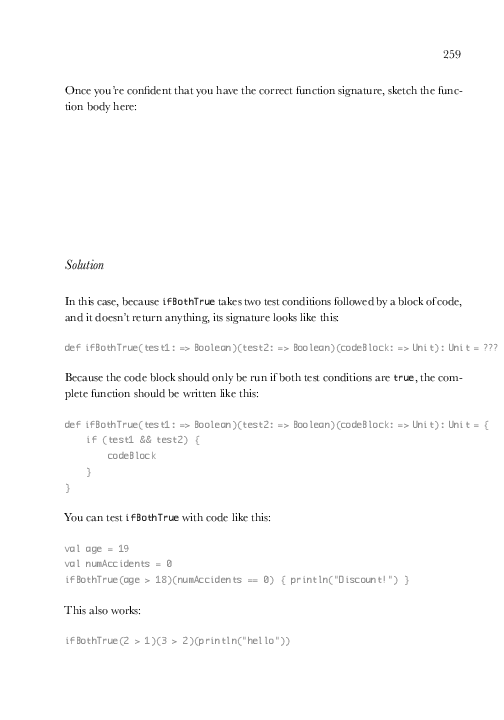
\includegraphics[height=2.51cm]{random-pages/random-pages-from-fpsimplified-pdf-00}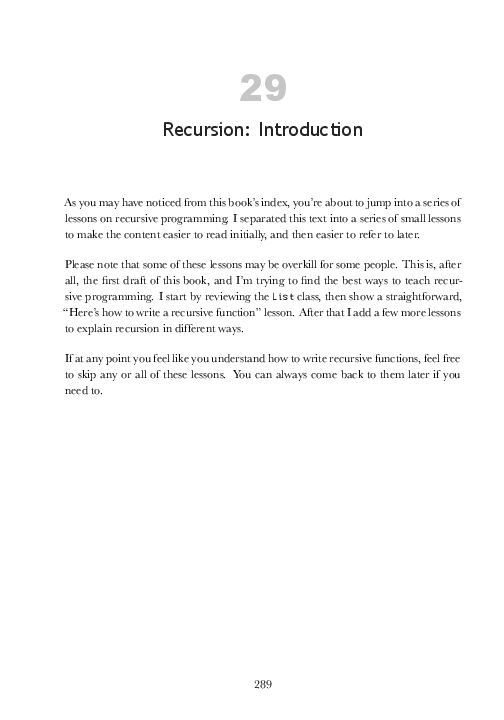
\includegraphics[height=2.51cm]{random-pages/random-pages-from-fpsimplified-pdf-01}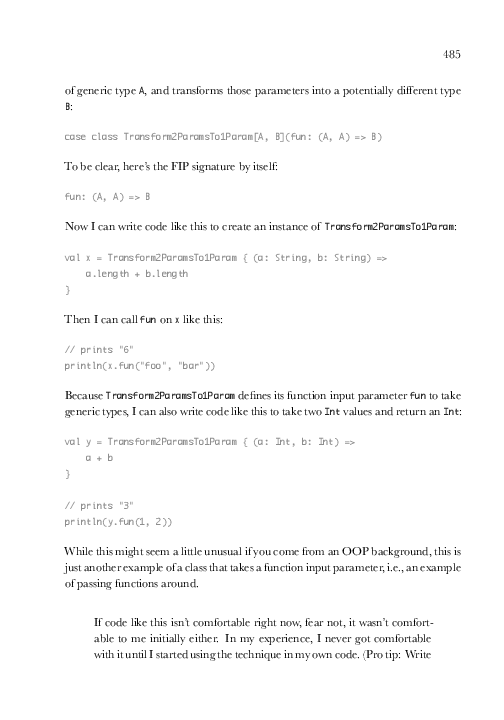
\includegraphics[height=2.51cm]{random-pages/random-pages-from-fpsimplified-pdf-02}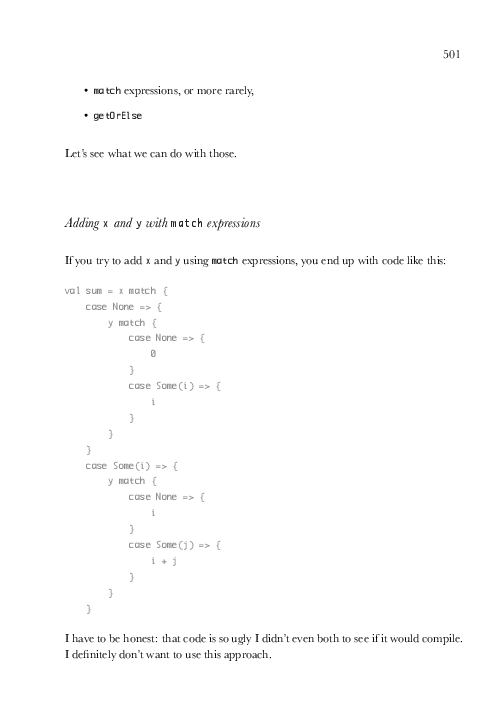
\includegraphics[height=2.51cm]{random-pages/random-pages-from-fpsimplified-pdf-03}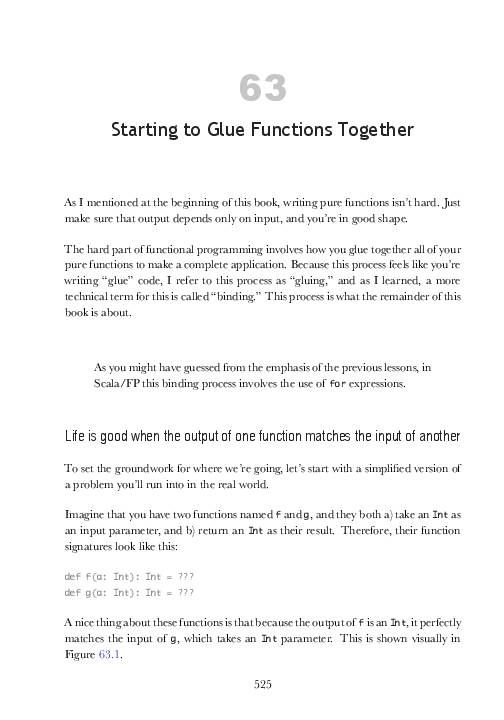
\includegraphics[height=2.51cm]{random-pages/random-pages-from-fpsimplified-pdf-04}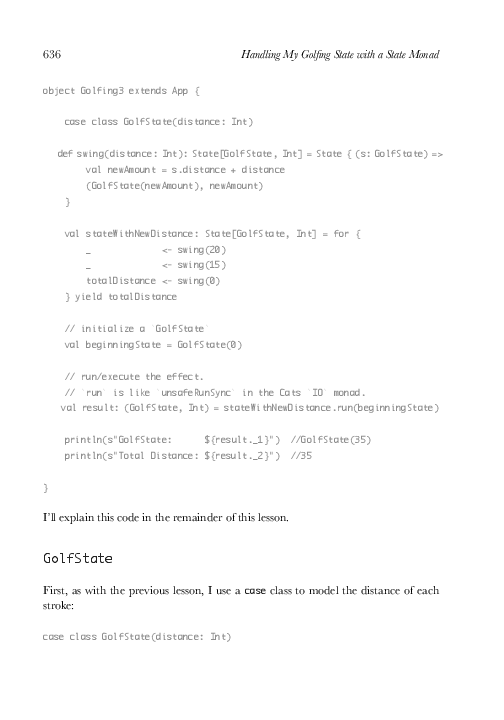
\includegraphics[height=2.51cm]{random-pages/random-pages-from-fpsimplified-pdf-05}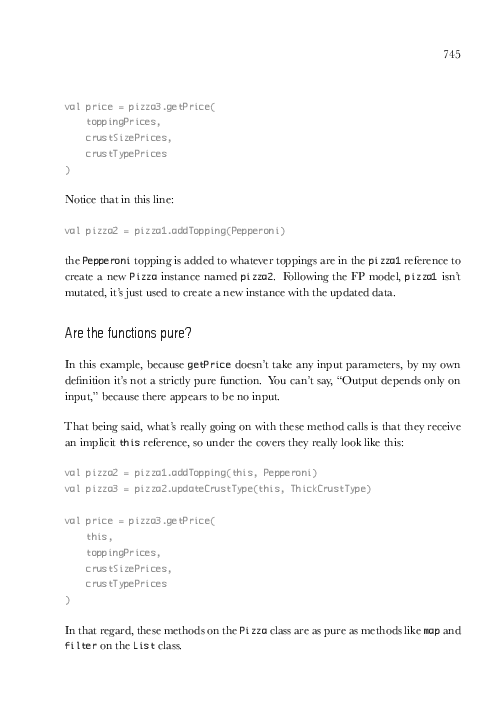
\includegraphics[height=2.51cm]{random-pages/random-pages-from-fpsimplified-pdf-06}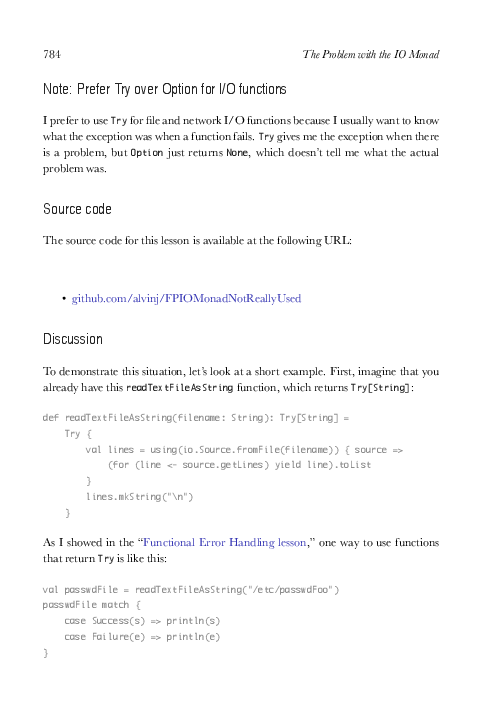
\includegraphics[height=2.51cm]{random-pages/random-pages-from-fpsimplified-pdf-07}
\par\end{centering}
\begin{centering}
\vspace{-0.3\baselineskip}
\par\end{centering}
\begin{centering}
\emph{Functional programming simplified}, by A.~Alexander
\par\end{centering}
\begin{centering}
\vspace{1\baselineskip}
\par\end{centering}
\begin{centering}
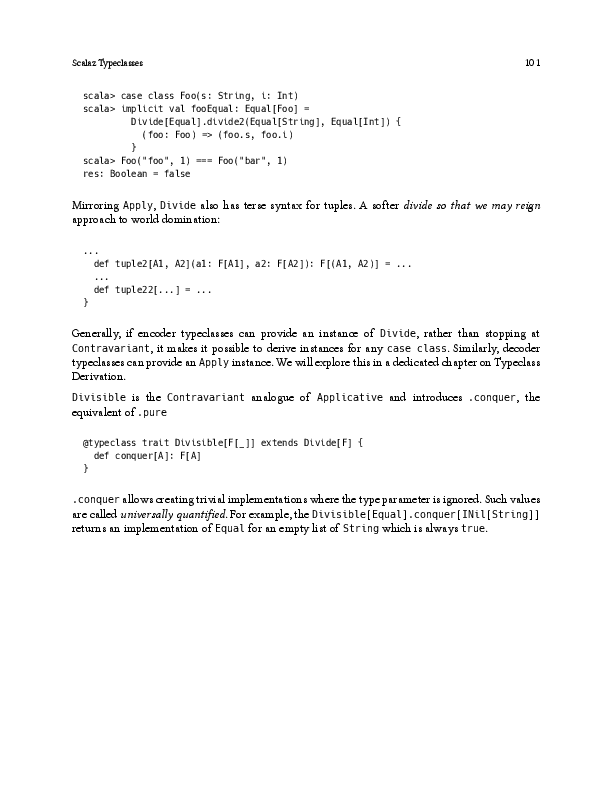
\includegraphics[height=2.51cm]{random-pages/random-pages-from-fpmortals-pdf-00}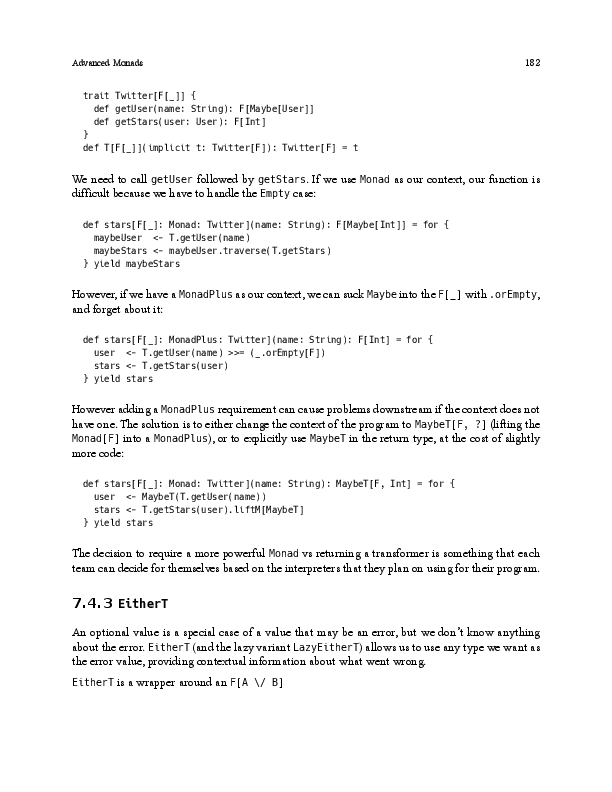
\includegraphics[height=2.51cm]{random-pages/random-pages-from-fpmortals-pdf-01}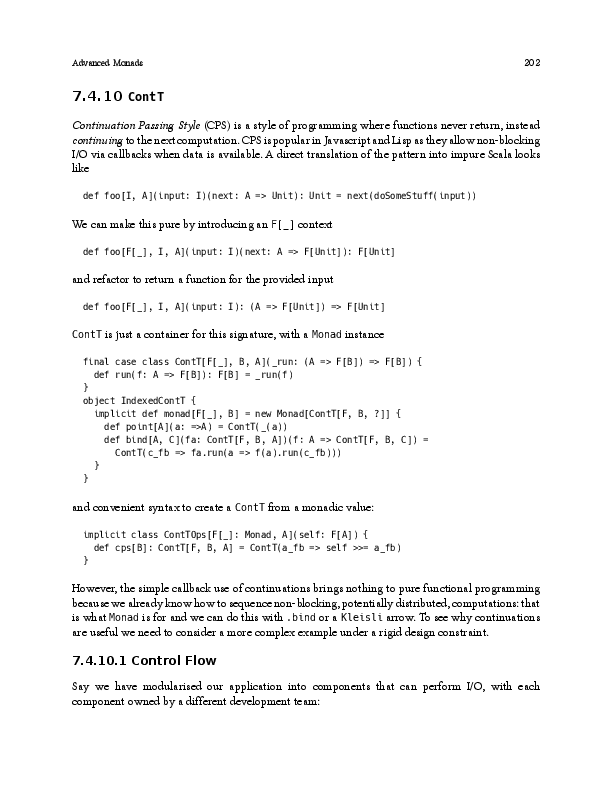
\includegraphics[height=2.51cm]{random-pages/random-pages-from-fpmortals-pdf-02}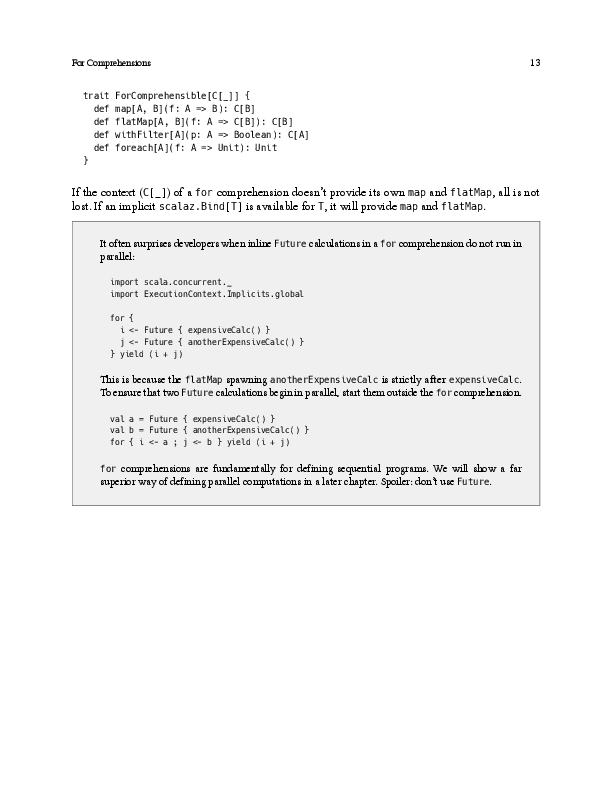
\includegraphics[height=2.51cm]{random-pages/random-pages-from-fpmortals-pdf-03}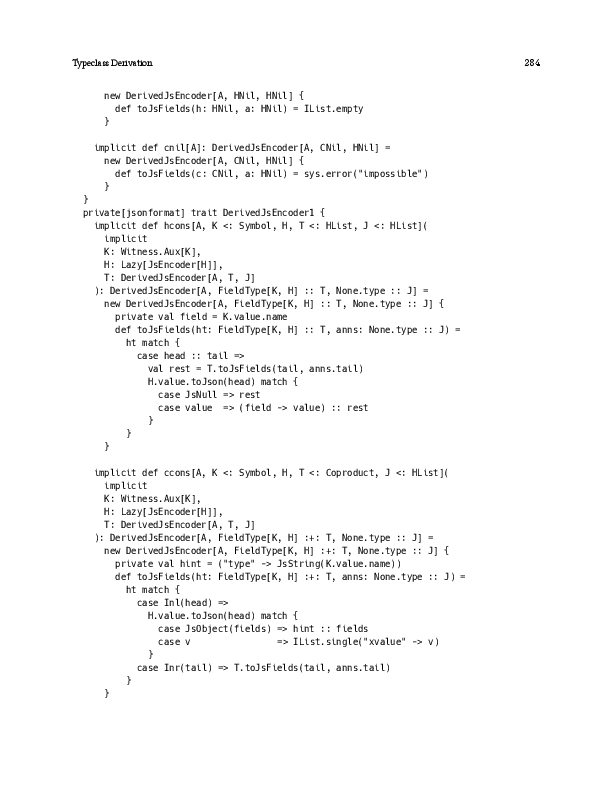
\includegraphics[height=2.51cm]{random-pages/random-pages-from-fpmortals-pdf-04}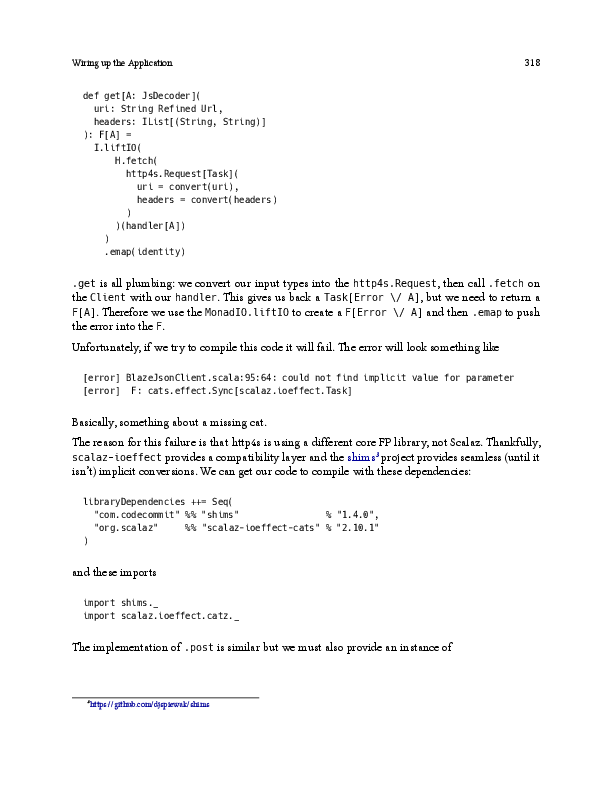
\includegraphics[height=2.51cm]{random-pages/random-pages-from-fpmortals-pdf-06}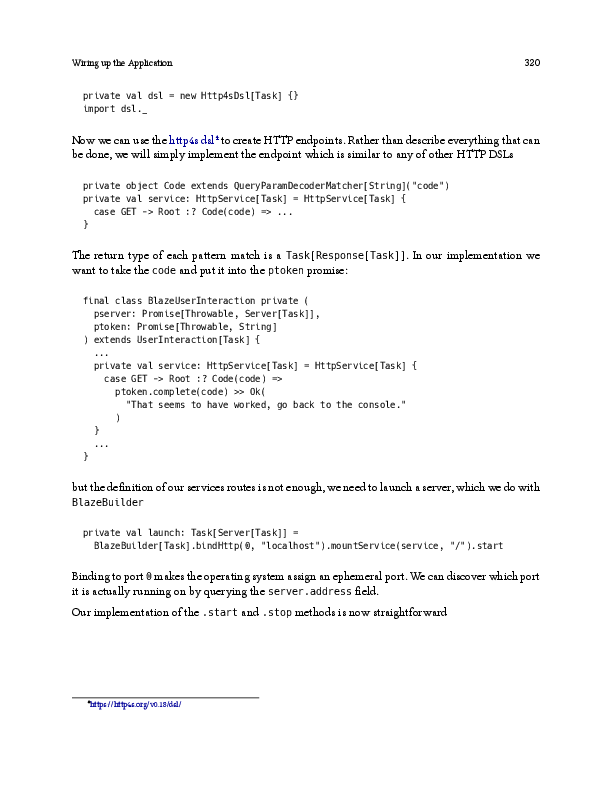
\includegraphics[height=2.51cm]{random-pages/random-pages-from-fpmortals-pdf-07}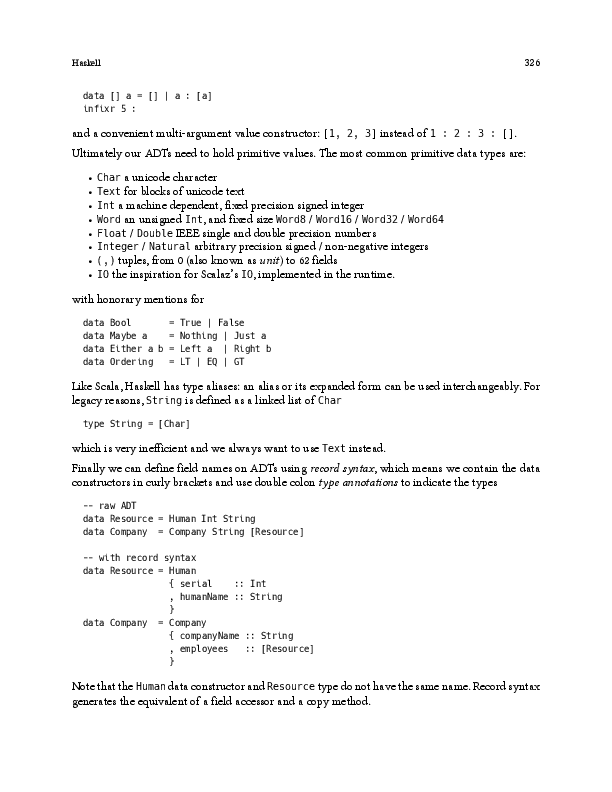
\includegraphics[height=2.51cm]{random-pages/random-pages-from-fpmortals-pdf-08}
\par\end{centering}
\begin{centering}
\emph{\vspace{-1.6\baselineskip}
}
\par\end{centering}
\begin{centering}
\emph{Functional programming for mortals}, by S.~Halliday
\par\end{centering}
\begin{centering}
\vspace{1\baselineskip}
\par\end{centering}
\begin{centering}
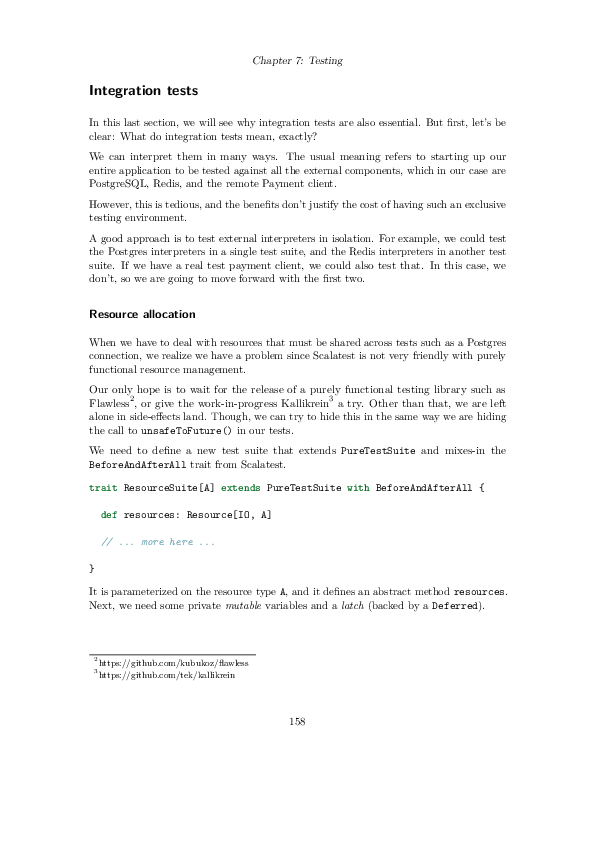
\includegraphics[height=2.51cm]{random-pages/random-pages-from-volpe-pdf-01}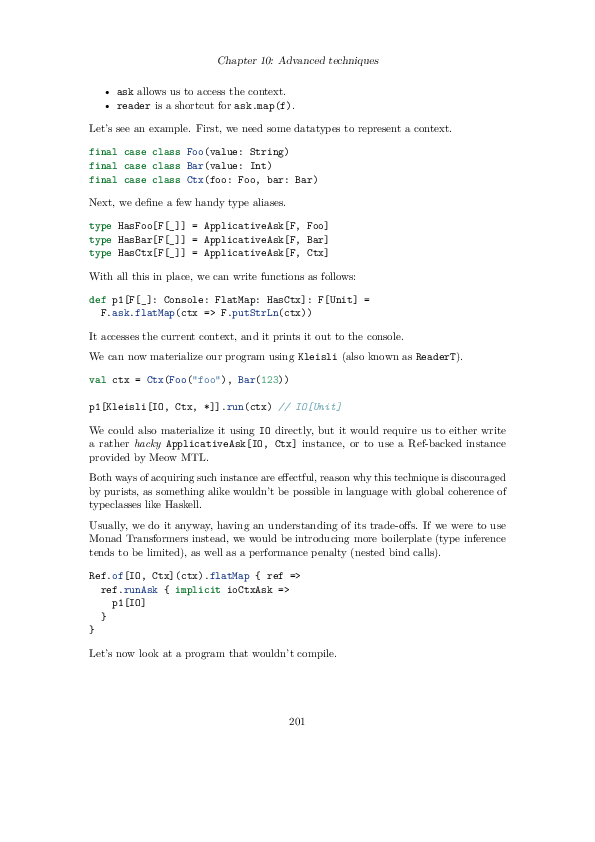
\includegraphics[height=2.51cm]{random-pages/random-pages-from-volpe-pdf-03}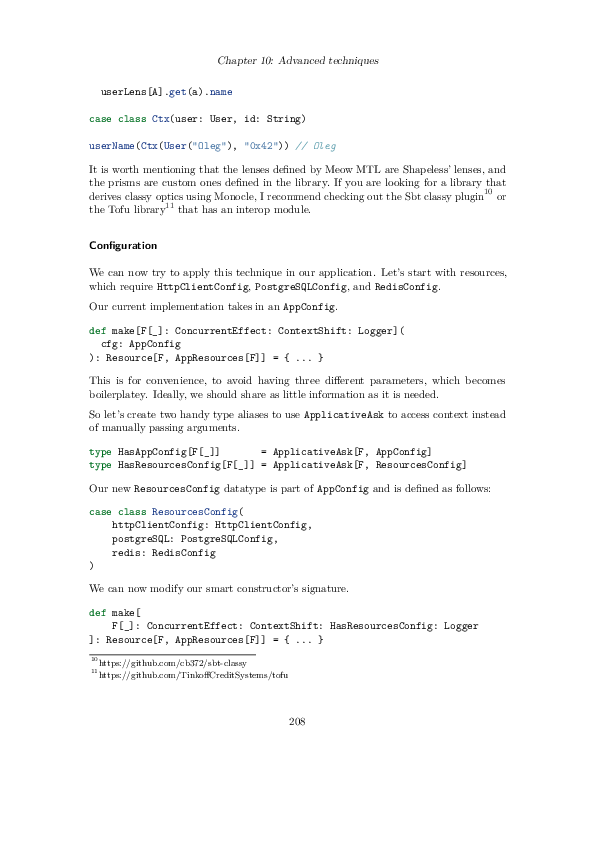
\includegraphics[height=2.51cm]{random-pages/random-pages-from-volpe-pdf-04}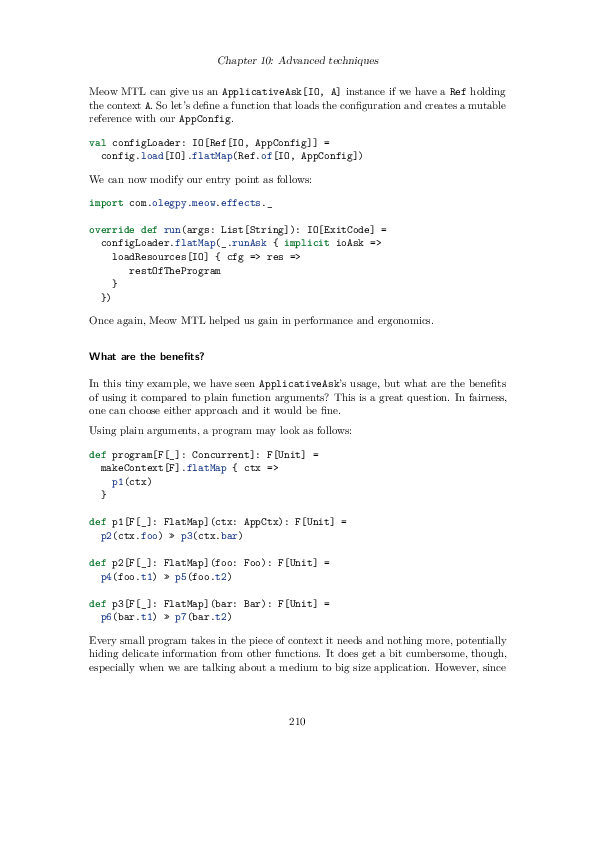
\includegraphics[height=2.51cm]{random-pages/random-pages-from-volpe-pdf-05}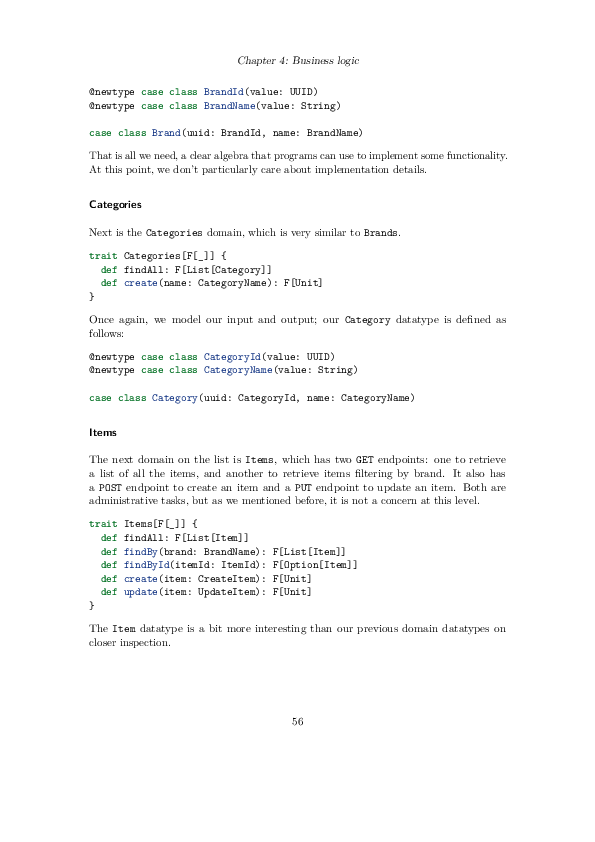
\includegraphics[height=2.51cm]{random-pages/random-pages-from-volpe-pdf-06}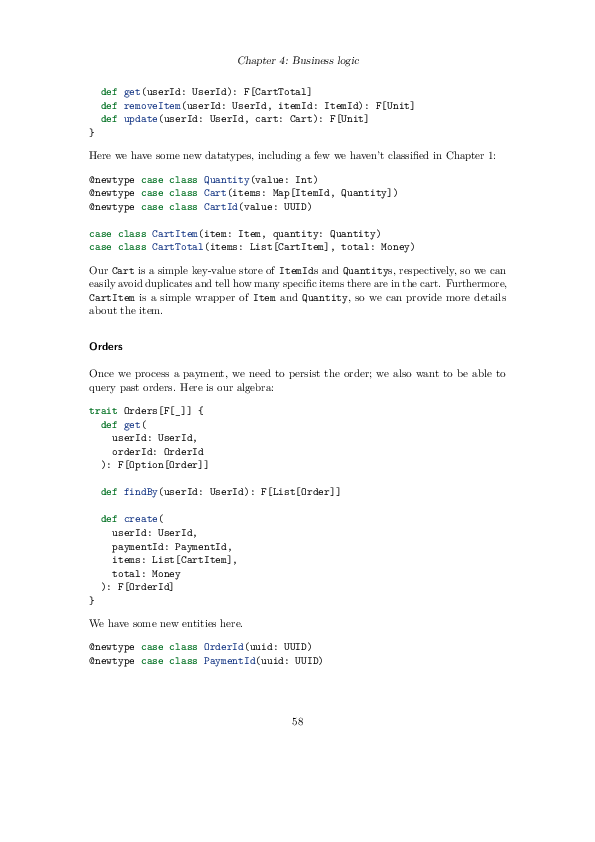
\includegraphics[height=2.51cm]{random-pages/random-pages-from-volpe-pdf-07}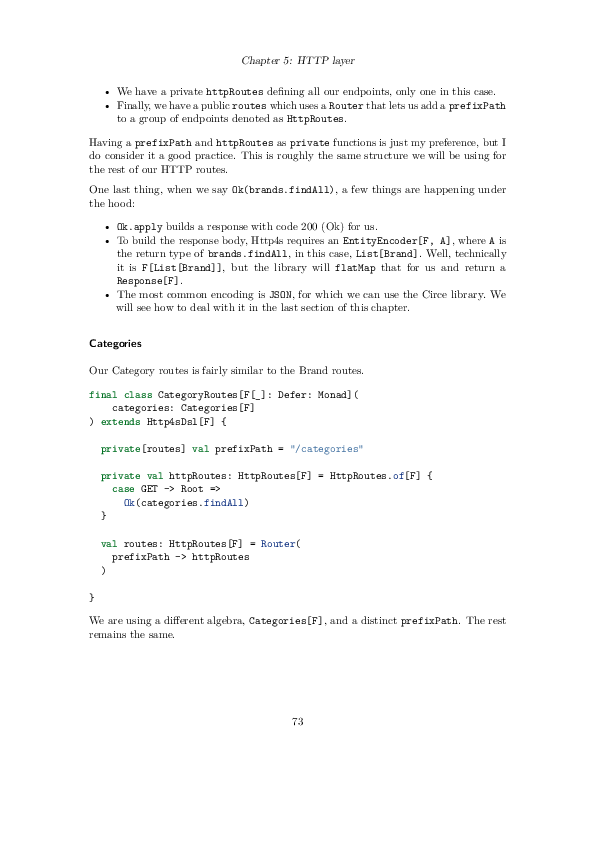
\includegraphics[height=2.51cm]{random-pages/random-pages-from-volpe-pdf-08}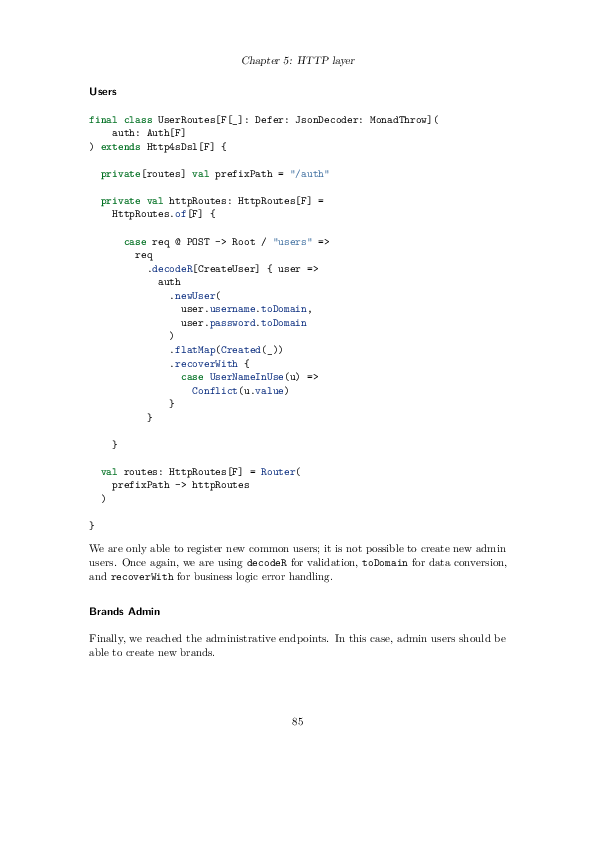
\includegraphics[height=2.51cm]{random-pages/random-pages-from-volpe-pdf-09}
\par\end{centering}
\begin{centering}
\emph{\vspace{-1.9\baselineskip}
}
\par\end{centering}
\begin{centering}
\emph{Practical functional programming in Scala}, by G.~Volpe (\texttt{\small{}\href{https://leanpub.com/pfp-scala}{https://leanpub.com/pfp-scala}})
\par\end{centering}
\begin{centering}
\vspace{1\baselineskip}
\par\end{centering}
\begin{centering}
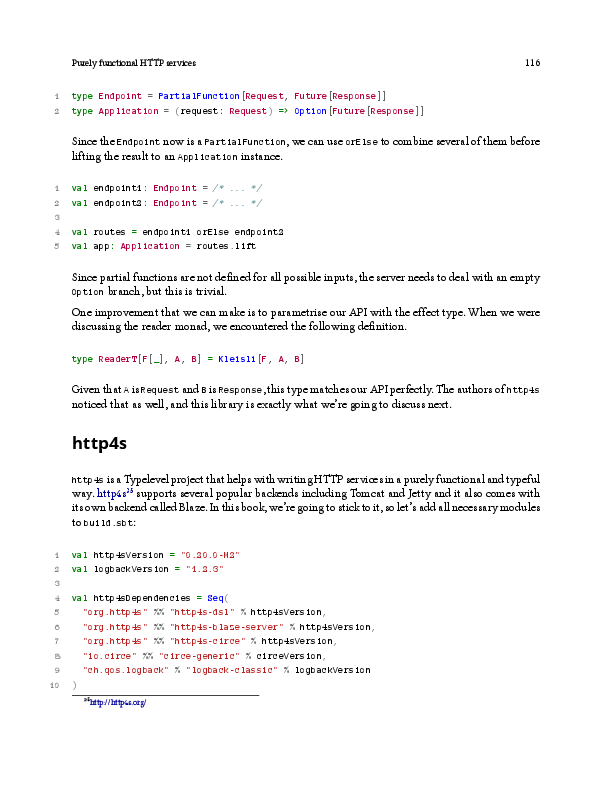
\includegraphics[height=2.51cm]{random-pages/random-pages-from-kalinin-pdf-01}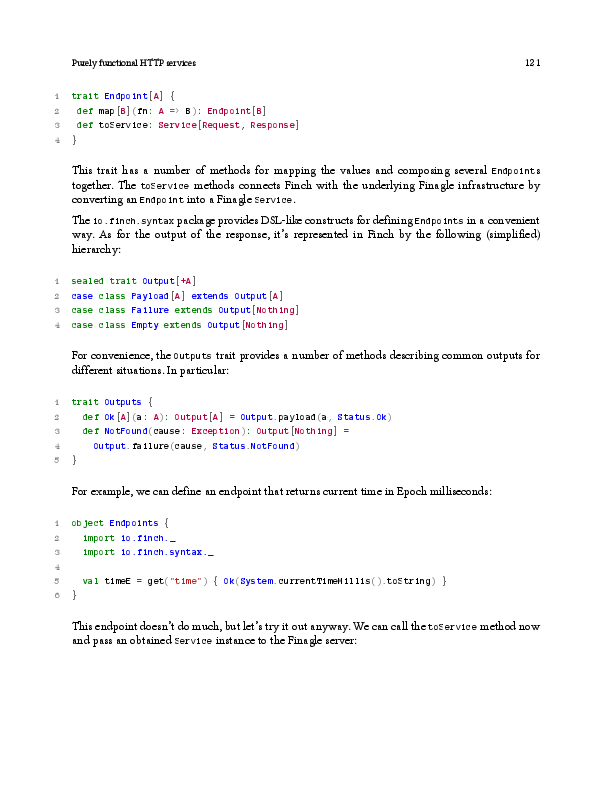
\includegraphics[height=2.51cm]{random-pages/random-pages-from-kalinin-pdf-02}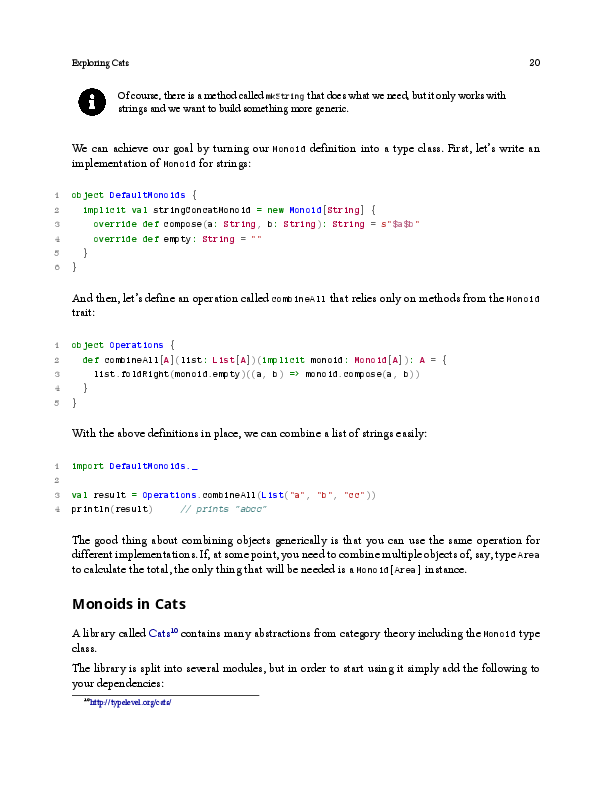
\includegraphics[height=2.51cm]{random-pages/random-pages-from-kalinin-pdf-03}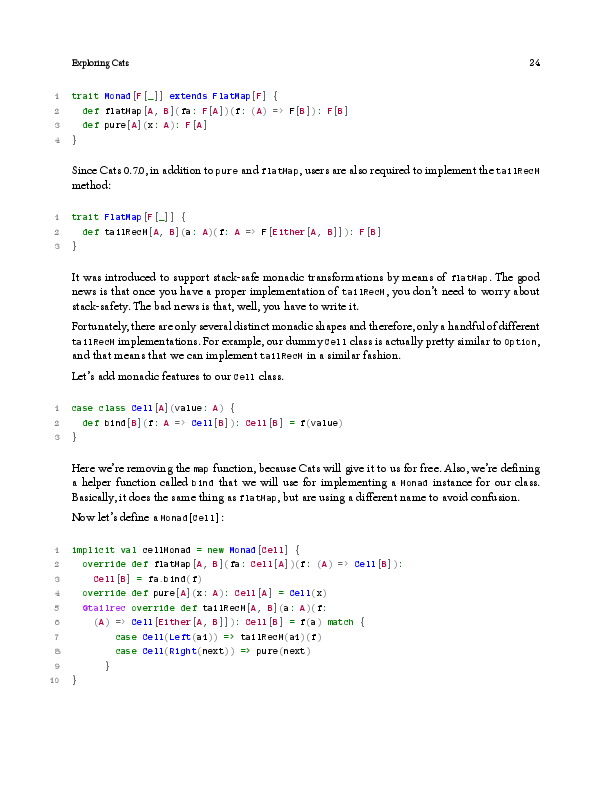
\includegraphics[height=2.51cm]{random-pages/random-pages-from-kalinin-pdf-04}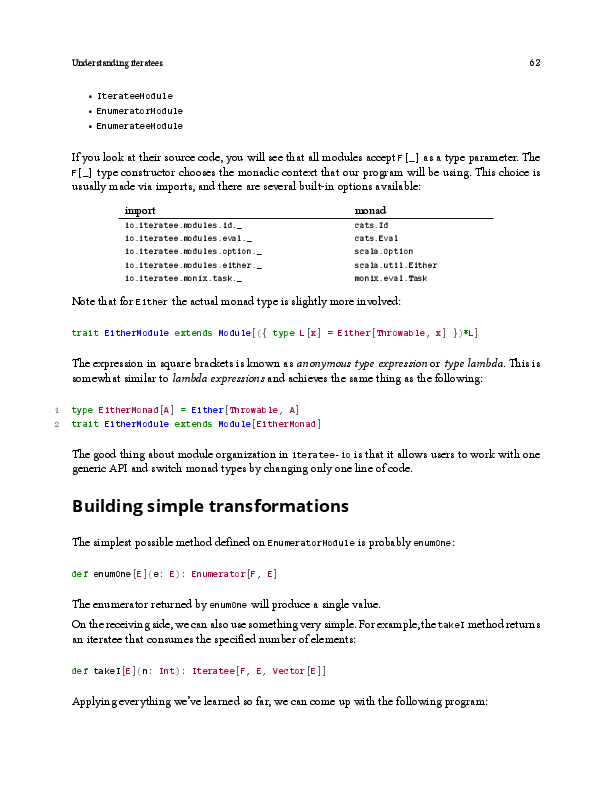
\includegraphics[height=2.51cm]{random-pages/random-pages-from-kalinin-pdf-06}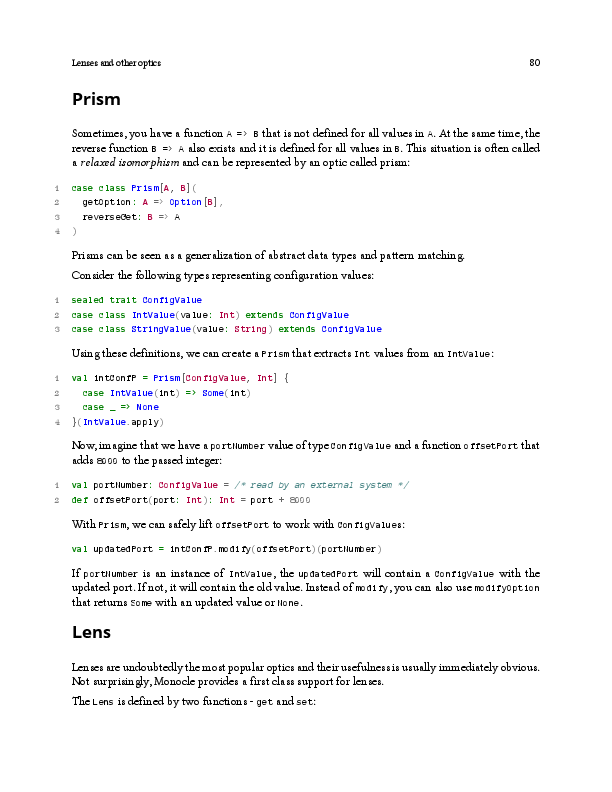
\includegraphics[height=2.51cm]{random-pages/random-pages-from-kalinin-pdf-07}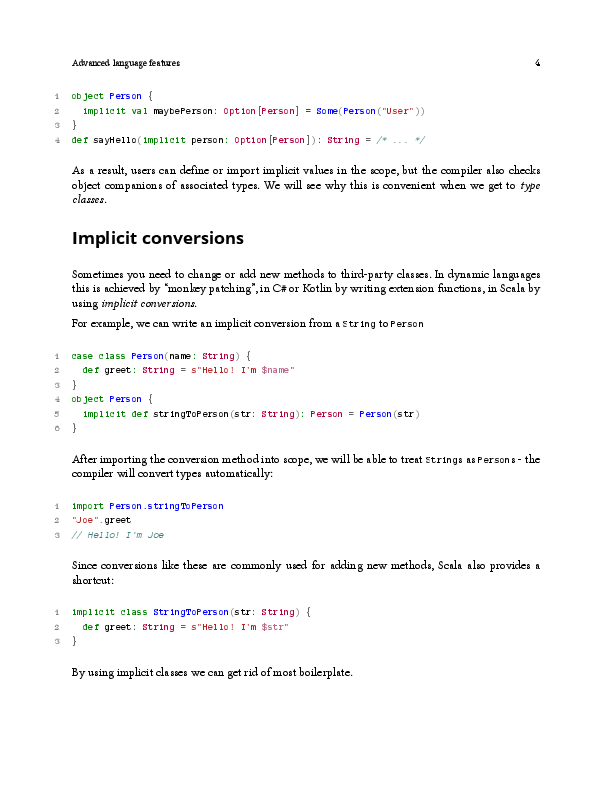
\includegraphics[height=2.51cm]{random-pages/random-pages-from-kalinin-pdf-08}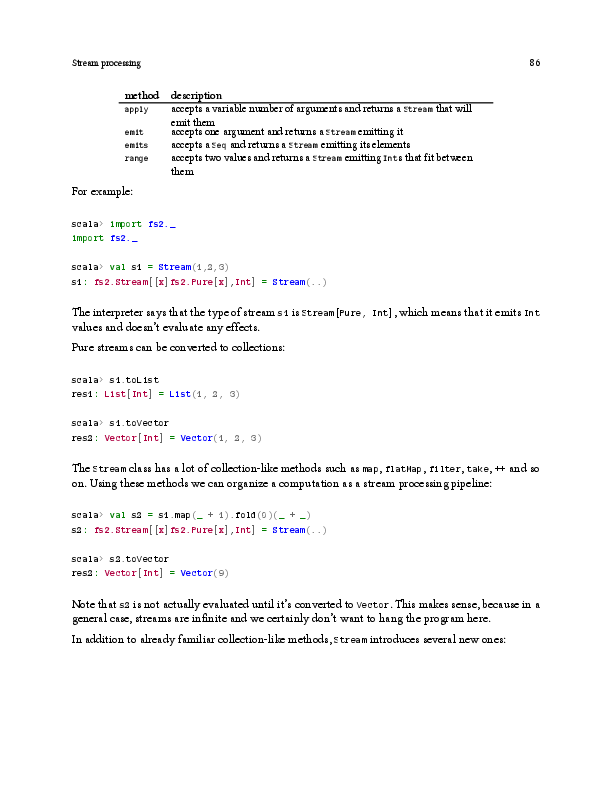
\includegraphics[height=2.51cm]{random-pages/random-pages-from-kalinin-pdf-09}
\par\end{centering}
\vspace{-0.6\baselineskip}

\begin{centering}
\emph{Mastering advanced Scala}, by D.~Kalinin (\texttt{\small{}\href{https://leanpub.com/mastering-advanced-scala}{https://leanpub.com/mastering-advanced-scala}})
\par\end{centering}
\caption{Randomly chosen pages from books on Scala programming.\label{fig:Randomly-chosen-pages-1}}
\end{figure}

\begin{figure}
\begin{centering}
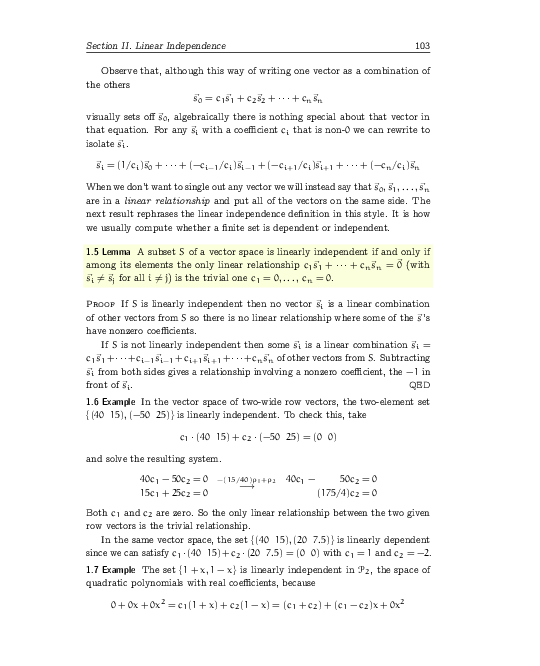
\includegraphics[height=2.51cm]{random-pages/random-pages-from-hefferon-pdf-00}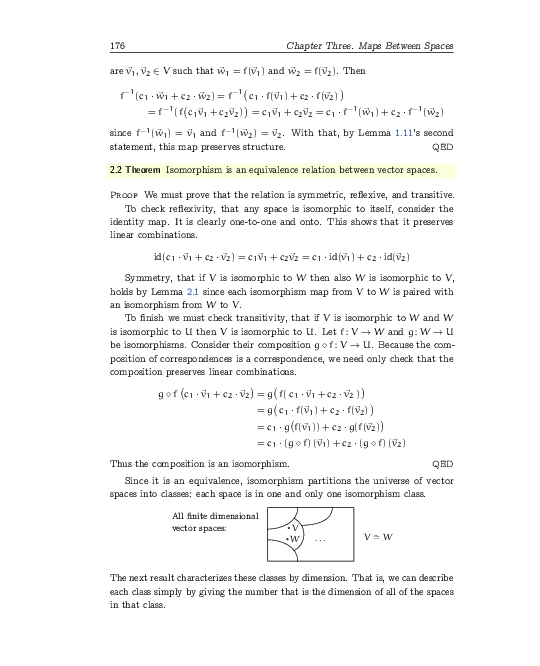
\includegraphics[height=2.51cm]{random-pages/random-pages-from-hefferon-pdf-01}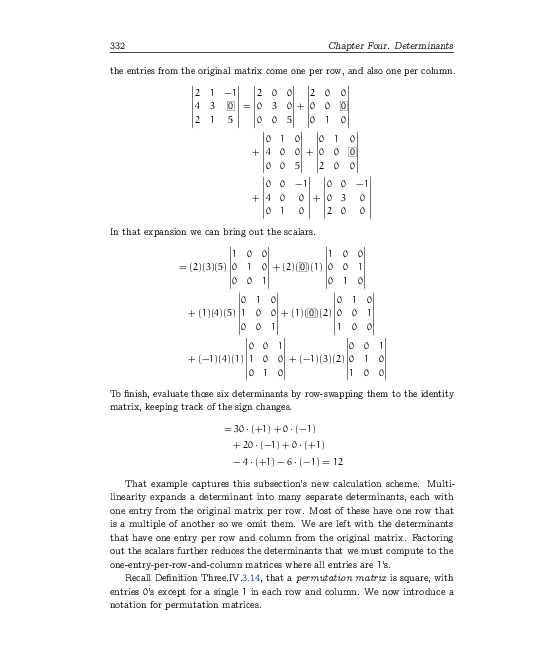
\includegraphics[height=2.51cm]{random-pages/random-pages-from-hefferon-pdf-03}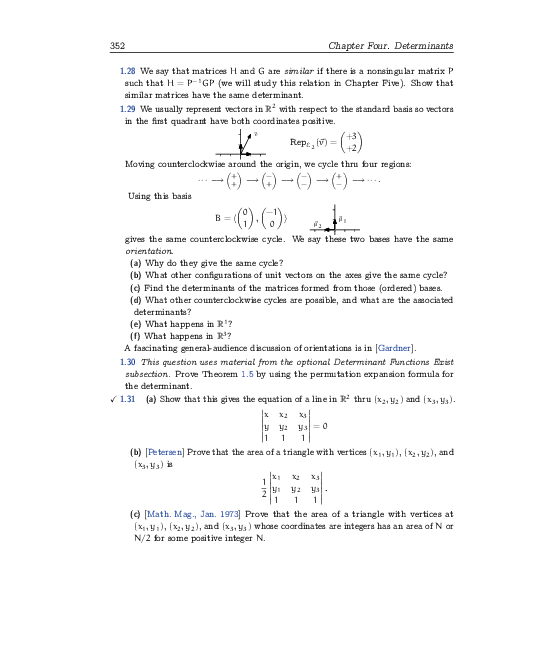
\includegraphics[height=2.51cm]{random-pages/random-pages-from-hefferon-pdf-04}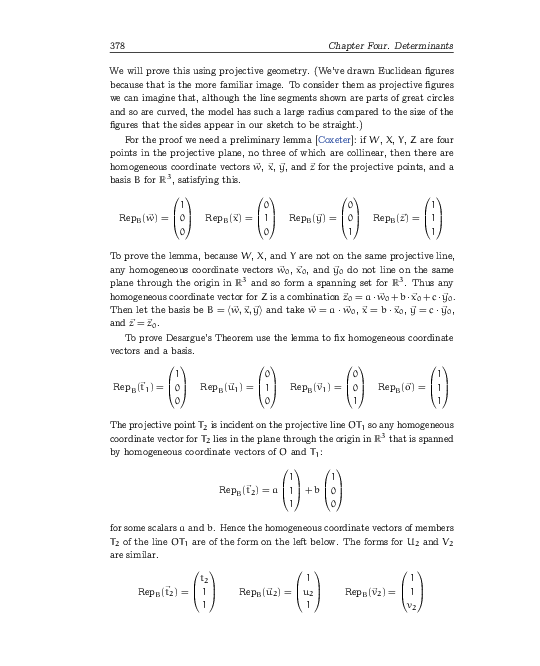
\includegraphics[height=2.51cm]{random-pages/random-pages-from-hefferon-pdf-05}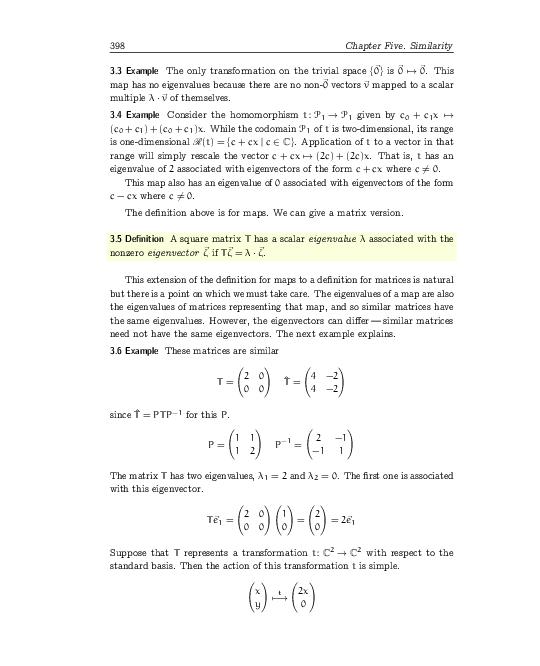
\includegraphics[height=2.51cm]{random-pages/random-pages-from-hefferon-pdf-06}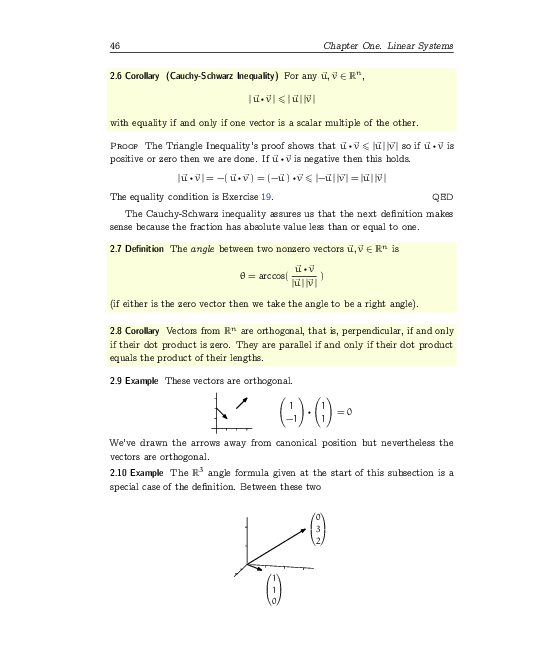
\includegraphics[height=2.51cm]{random-pages/random-pages-from-hefferon-pdf-07}
\par\end{centering}
\vspace{-0.4\baselineskip}

\begin{centering}
\emph{Linear algebra}, by J.~Hefferon (\texttt{\small{}\href{http://joshua.smcvt.edu/linearalgebra/}{http://joshua.smcvt.edu/linearalgebra/}})
\par\end{centering}
\begin{centering}
\vspace{0.6\baselineskip}
\par\end{centering}
\begin{centering}
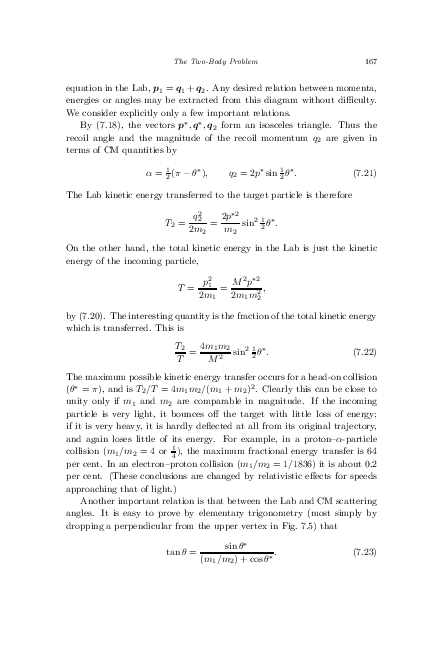
\includegraphics[height=2.51cm]{random-pages/random-pages-from-kibble-pdf-00}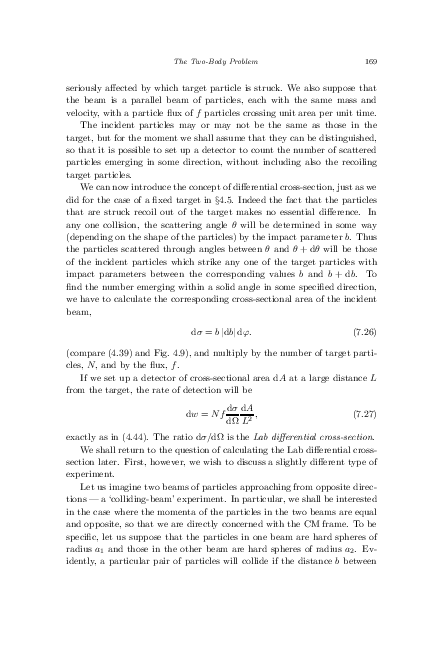
\includegraphics[height=2.51cm]{random-pages/random-pages-from-kibble-pdf-01}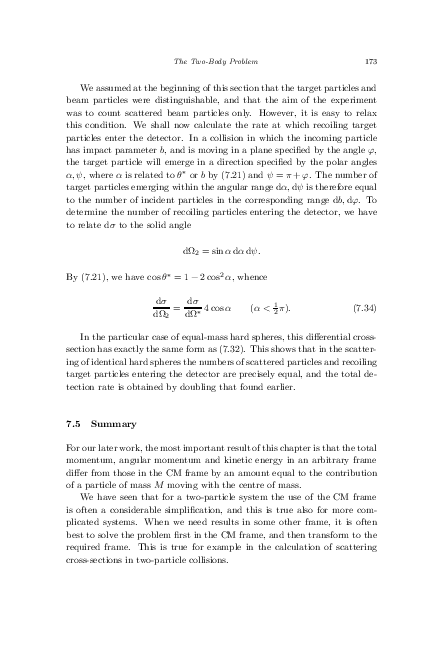
\includegraphics[height=2.51cm]{random-pages/random-pages-from-kibble-pdf-02}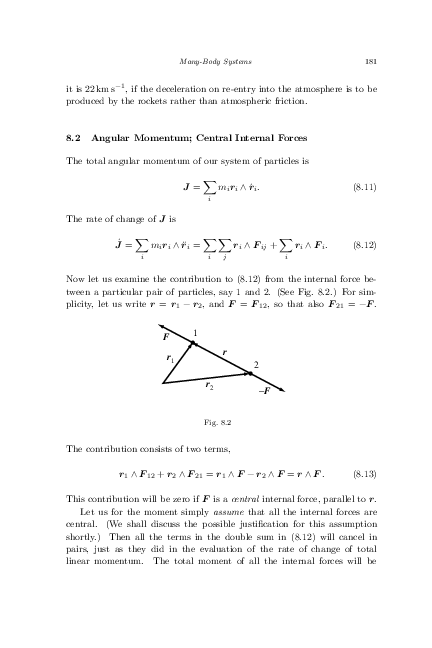
\includegraphics[height=2.51cm]{random-pages/random-pages-from-kibble-pdf-03}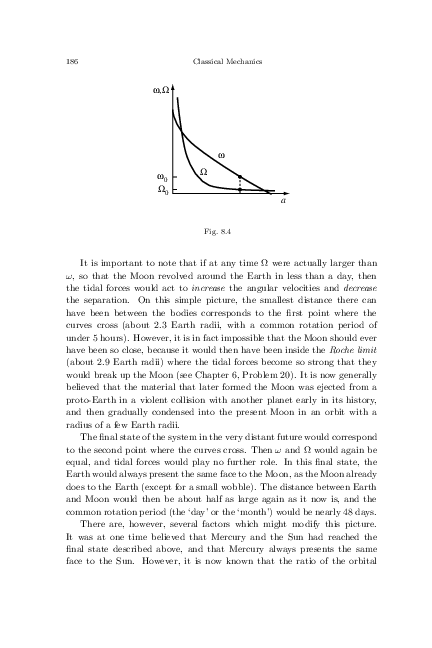
\includegraphics[height=2.51cm]{random-pages/random-pages-from-kibble-pdf-04}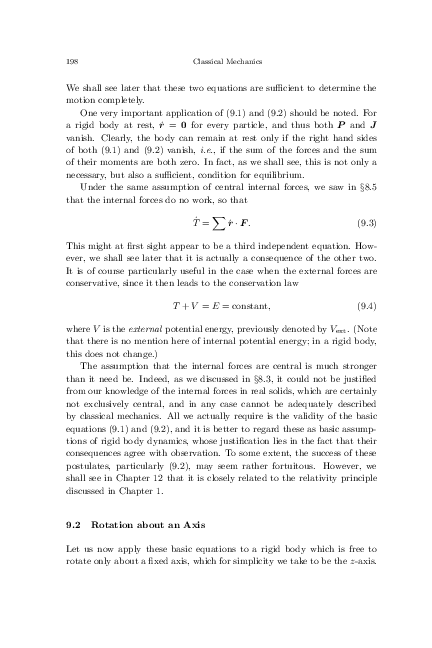
\includegraphics[height=2.51cm]{random-pages/random-pages-from-kibble-pdf-05}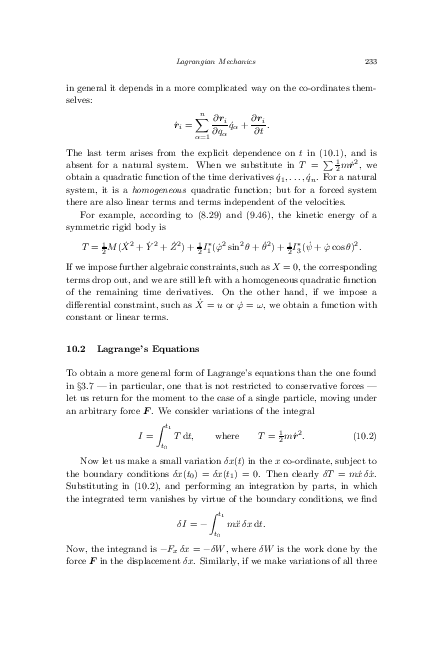
\includegraphics[height=2.51cm]{random-pages/random-pages-from-kibble-pdf-06}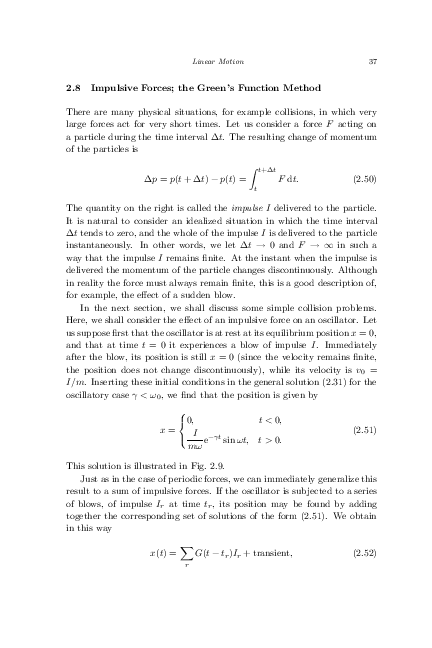
\includegraphics[height=2.51cm]{random-pages/random-pages-from-kibble-pdf-09}
\par\end{centering}
\vspace{-0.6\baselineskip}

\begin{centering}
\emph{Classical mechanics}, by T.~W.~B.~Kibble and F.~H.~Berkshire
(\texttt{\small{}\href{https://archive.org/details/116772449ClassicalMechanics}{https://archive.org/details/116772449ClassicalMechanics}})
\par\end{centering}
\vspace{0.6\baselineskip}

\caption{Randomly chosen pages from books on mathematics and physics.\label{fig:Randomly-chosen-pages-2}}
\end{figure}

\begin{figure}
\begin{centering}
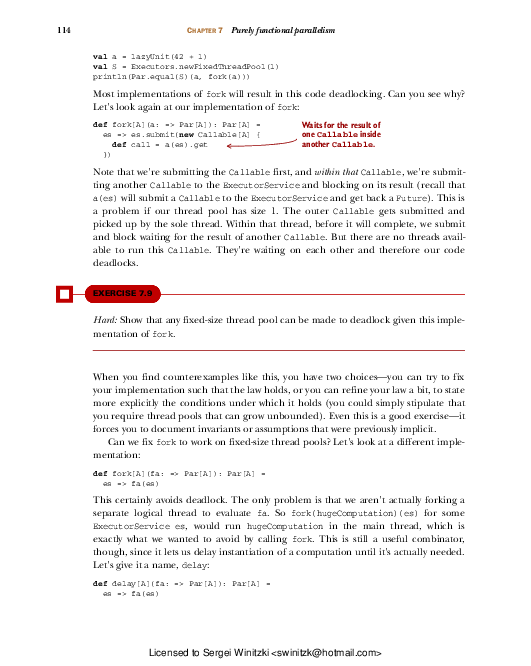
\includegraphics[height=2.51cm]{random-pages/random-pages-from-fpis-pdf-00}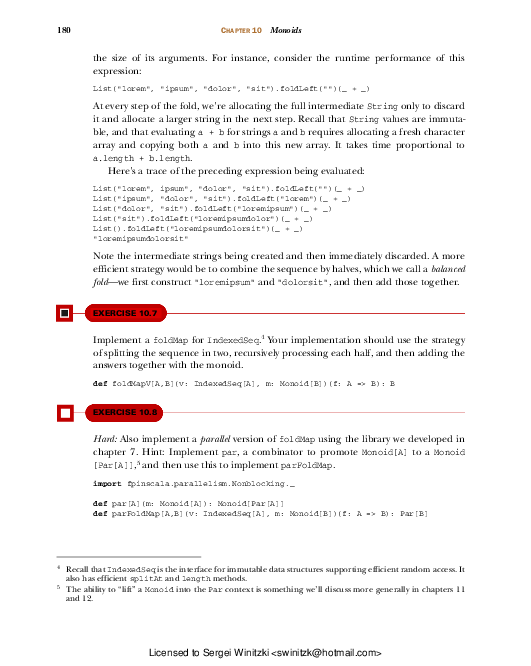
\includegraphics[height=2.51cm]{random-pages/random-pages-from-fpis-pdf-02}\includegraphics[height=2.51cm]{random-pages/random-pages-from-fpis-pdf-04}\includegraphics[height=2.51cm]{random-pages/random-pages-from-fpis-pdf-05}\includegraphics[height=2.51cm]{random-pages/random-pages-from-fpis-pdf-06}\includegraphics[height=2.51cm]{random-pages/random-pages-from-fpis-pdf-07}\includegraphics[height=2.51cm]{random-pages/random-pages-from-fpis-pdf-08}
\par\end{centering}
\vspace{-0\baselineskip}

\begin{centering}
\emph{Functional programming in Scala}, by P.~Chiusano and R.~Bjarnason
\par\end{centering}
\begin{centering}
\vspace{1\baselineskip}
\par\end{centering}
\begin{centering}
\includegraphics[height=2.51cm]{random-pages/random-pages-from-pdbc-pdf-00}\includegraphics[height=2.51cm]{random-pages/random-pages-from-pdbc-pdf-01}\includegraphics[height=2.51cm]{random-pages/random-pages-from-pdbc-pdf-02}\includegraphics[height=2.51cm]{random-pages/random-pages-from-pdbc-pdf-03}\includegraphics[height=2.51cm]{random-pages/random-pages-from-pdbc-pdf-04}\includegraphics[height=2.51cm]{random-pages/random-pages-from-pdbc-pdf-05}\includegraphics[height=2.51cm]{random-pages/random-pages-from-pdbc-pdf-06}\includegraphics[height=2.51cm]{random-pages/random-pages-from-pdbc-pdf-07}
\par\end{centering}
\vspace{-0.7\baselineskip}

\begin{centering}
\emph{Program design by calculation}, by J.~N.~Oliveira
\par\end{centering}
\begin{centering}
\vspace{1\baselineskip}
\par\end{centering}
\begin{centering}
\includegraphics[height=2.51cm]{random-pages/random-pages-from-sofp-pdf-00}\includegraphics[height=2.51cm]{random-pages/random-pages-from-sofp-pdf-01}\includegraphics[height=2.51cm]{random-pages/random-pages-from-sofp-pdf-02}\includegraphics[height=2.51cm]{random-pages/random-pages-from-sofp-pdf-05}\includegraphics[height=2.51cm]{random-pages/random-pages-from-sofp-pdf-06}\includegraphics[height=2.51cm]{random-pages/random-pages-from-sofp-pdf-07}\includegraphics[height=2.51cm]{random-pages/random-pages-from-sofp-pdf-08}
\par\end{centering}
\vspace{-0.3\baselineskip}

\begin{centering}
\emph{The science of functional programming} (this book)
\par\end{centering}
\vspace{1\baselineskip}

\caption{Randomly chosen pages from books on applied functional type theory.\label{fig:Randomly-chosen-pages}}
\end{figure}


\chapter{Essay: Software engineers and software artisans}

Let us examine what we ordinarily understand by \emph{engineering}
as opposed to artisanship or craftsmanship. It will then become apparent
that today\textsf{'}s computer programmers must be viewed as \textsf{``}software artisans\textsf{''}
rather than software engineers.

\section{Engineering disciplines }

Consider the way mechanical engineers, chemical engineers, or electrical
engineers work, and look at the studies they require for becoming
proficient in their fields.

A mechanical engineer studies calculus, linear algebra, differential
geometry, and several areas of physics such as theoretical mechanics,
thermodynamics, and elasticity theory,\footnote{\texttt{\href{https://www.colorado.edu/mechanical/academics/undergraduate-program/curriculum}{https://www.colorado.edu/mechanical/academics/undergraduate-program/curriculum}}}
and then uses calculations to guide the design of a bridge. A chemical
engineer studies chemistry, thermodynamics, calculus, linear algebra,
differential equations, some areas of physics such as thermodynamics
and kinetic theory,\footnote{\texttt{\href{https://www.colorado.edu/engineering/sample-undergraduate-curriculum-chemical}{https://www.colorado.edu/engineering/sample-undergraduate-curriculum-chemical}}}
and uses calculations to guide the design of a chemical process. An
electrical engineer studies advanced calculus, linear algebra, and
several areas of physics such as electrodynamics and quantum theory,\footnote{\texttt{\href{http://archive.is/XYLyE}{http://archive.is/XYLyE}}}
and uses calculations to design an antenna or a microchip.

The common pattern is that engineers use mathematics and natural sciences
in order to create new devices. Mathematical calculations and scientific
reasoning are performed \emph{before} designing or building a real
machine.

Some of the studies required for engineers include arcane abstract
concepts such as the \textsf{``}Fourier transform of the delta function\textsf{''}\footnote{\texttt{\href{https://www.youtube.com/watch?v=KAbqISZ6SHQ}{https://www.youtube.com/watch?v=KAbqISZ6SHQ}}}
and the \textsf{``}inverse $Z$-transform\textsf{''}\footnote{\texttt{\href{http://archive.is/SsJqP}{http://archive.is/SsJqP}}}
in digital signal processing, \textsf{``}rank-4 elasticity tensors\textsf{''}\footnote{\texttt{\href{https://serc.carleton.edu/NAGTWorkshops/mineralogy/mineral_physics/tensors.html}{https://serc.carleton.edu/NAGTWorkshops/mineralogy/mineral\_physics/tensors.html}}}
in calculations of elasticity of materials, \textsf{``}Lagrangians with non-holonomic
constraints\textsf{''}\footnote{\texttt{\href{https://arxiv.org/abs/math/0008147}{https://arxiv.org/abs/math/0008147}}}
in robotics, and the \textsf{``}Gibbs free energy\textsf{''} in chemical reactor design.\footnote{\texttt{\href{https://www.amazon.com/Introduction-Chemical-Engineering-Kinetics-Reactor/dp/1118368258}{https://www.amazon.com/Introduction-Chemical-Engineering-Kinetics-Reactor/dp/1118368258}}}

To be sure, a significant part of what engineers do is not covered
by any theory: the \emph{know-how}, the informal reasoning, the traditional
knowledge passed on from expert to novice,  \textemdash{} all those
skills that are hard to formalize are important. Nevertheless, engineering
is crucially based on natural science and mathematics for some of
its decision-making about new designs.

\section{Artisanship: Trades and crafts }

Now consider what kinds of things shoemakers, plumbers, or home painters
do, and what they have to learn in order to become proficient in their
profession.

A novice shoemaker, for example, begins by copying some drawings\footnote{\texttt{\href{https://youtu.be/cY5MY0czMAk?t=141}{https://youtu.be/cY5MY0czMAk?t=141}}}
and goes on to cutting leather in a home workshop. Apprenticeships
proceed via learning by doing, with comments and instructions from
an expert. After a few years of study (for example, a painter apprenticeship
in California can be as short as 2 years\footnote{\texttt{\href{http://www.calapprenticeship.org/programs/painter_apprenticeship.php}{http://www.calapprenticeship.org/programs/painter\_apprenticeship.php}}}),
a new artisan is ready to start productive work. 

All trades operate entirely from tradition and practical experience.
It takes a prolonged learning effort to become a good artisan in any
profession. But the trades do not require academic study because there
is no formal theory from which to proceed. There are no Fourier transforms
applied to delta functions, no Lagrangians with non-holonomic constraints,
no rank-4 tensors to calculate, nor any differential equations to
solve.

Artisans do not study science or mathematics because their professions
do not make use of any formal theory for guiding their designs or
processes.

\section{Programmers today are artisans, not engineers }

Programmers are \emph{not engineers} in the sense normally used in
the engineering professions.

\subsection{No requirements of licensing or formal study}

Mechanical, electrical, chemical engineers are required to pass a
license exam to become certified to work. The license exam certifies
that the person is proficient in applying a known set of engineering
tools and methods. But in software engineering, no certifications
or licenses are required for the job (although many certification
programs exist).

Working software engineers are also not required to have studied software
engineering or computer science (CS). According to a recent Stack
Overflow survey,\footnote{\texttt{\href{https://thenextweb.com/insider/2016/04/23/dont-need-go-college-anymore-programmer/}{https://thenextweb.com/insider/2016/04/23/dont-need-go-college-anymore-programmer/}}}
about 56\% of working programmers have no CS degree. The author of
this book is a self-taught programmer who has degrees in physics but
never formally studied CS or taken any academic courses in algorithms,
data structures, computer networks, compilers, programming languages,
or other standard CS topics. 

A large fraction of successful programmers have no college degrees
and perhaps \emph{never} studied formally. They acquired all their
knowledge and skills through self-study and practical work. A prominent
example is Robert C.~Martin\index{Robert C.~Martin},\footnote{\texttt{\href{https://en.wikipedia.org/wiki/Robert_C._Martin}{https://en.wikipedia.org/wiki/Robert\_C.\_Martin}}}
an outspoken guru in the arts of programming. He routinely refers
to programmers as artisans\footnote{\texttt{\href{https://blog.cleancoder.com/uncle-bob/2013/02/01/The-Humble-Craftsman.html}{https://blog.cleancoder.com/uncle-bob/2013/02/01/The-Humble-Craftsman.html}}}
and uses the appropriate imagery: novices and masters, trade and craft,
the honor of the guild, etc. He compares programmers to plumbers,
electricians, lawyers, and surgeons, but never to mathematicians,
physicists, or engineers of any kind. According to one of his blog
posts,\footnote{\texttt{\href{https://blog.cleancoder.com/uncle-bob/2013/11/25/Novices-Coda.html}{https://blog.cleancoder.com/uncle-bob/2013/11/25/Novices-Coda.html}}}
he started working at age 17 as a self-taught programmer, and then
went on to more jobs in the software industry; he never mentions going
to college. It is clear that R.~C.~Martin \emph{is} an expert craftsman
and that he did \emph{not} need academic study to master his craft.

Here is another opinion\footnote{\texttt{\href{http://archive.is/tAKQ3}{http://archive.is/tAKQ3}}}
(emphasis is theirs):
\begin{quotation}
{\small{}Software Engineering is unique among the STEM careers in
that it absolutely does }\emph{\small{}not}{\small{} require a college
degree to be successful. It most certainly does not require licensing
or certification. }\emph{\small{}It requires experience}{\small{}.}{\small\par}
\end{quotation}
This description fits a career in crafts \textemdash{} but certainly
not a career, say, in electrical engineering.

The high demand for software developers gave rise to \textsf{``}developer
boot camps\textsf{''}\footnote{\texttt{\href{http://archive.is/GkOL9}{http://archive.is/GkOL9}}}
\textemdash{} vocational schools that educate new programmers in a
few months through purely practical training, with no formal theory
or mathematics involved. These vocational schools are successful\footnote{\texttt{\href{http://archive.is/E9FXP}{http://archive.is/E9FXP}}}
in job placement. But it is unimaginable that a $6$-month crash course
or even a $2$-year vocational school could prepare engineers to work
successfully on designing, e.g., analog quantum computers\footnote{\texttt{\href{https://www.dwavesys.com/quantum-computing}{https://www.dwavesys.com/quantum-computing}}}
without ever teaching them quantum physics or calculus.

\subsection{No mathematical formalism guides software development}

Most books on software engineering contain no formulas or equations,
no mathematical derivations, and no precise definitions of the various
technical terms they are using (such as \textsf{``}object-oriented\textsf{''} or \textsf{``}module\textsf{'}s
responsibilities\textsf{''}). Some of those books\footnote{E.g., \texttt{\href{https://www.amazon.com/Object-Oriented-Software-Engineering-Unified-Methodology/dp/0073376256}{https://www.amazon.com/Object-Oriented-Software-Engineering-Unified-Methodology/dp/0073376256}}}
also have almost no program code in them; instead they are filled
with words and illustrative diagrams. These books talk about how programmers
should write their programs in vague and general terms: \textsf{``}code is
about detail\textsf{''}, \textsf{``}you must never abandon the big picture\textsf{''}, \textsf{``}avoid
tight coupling in your modules\textsf{''}, \textsf{``}a class must serve a single
responsibility\textsf{''}, and so on. Practitioners such as R.\ C.\ Martin
never studied any formalisms and do not think in terms of formalisms.
Instead, they summarize their programming experience in vaguely formulated
heuristic \textquotedblleft principles\textquotedblright .\footnote{\texttt{\href{https://blog.cleancoder.com/uncle-bob/2016/03/19/GivingUpOnTDD.html}{https://blog.cleancoder.com/uncle-bob/2016/03/19/GivingUpOnTDD.html}}}

In contrast, textbooks on mechanical or electrical engineering include
a significant amount of mathematics. The design of a microwave antenna
is guided not by an \textsf{``}open and closed module principle\textsf{''} but by
solving the relevant differential equations\footnote{\texttt{\href{https://youtu.be/8KpfVsJ5Jw4?t=447}{https://youtu.be/8KpfVsJ5Jw4?t=447}}}
of electrodynamics.

An example of the aversion of software engineers to mathematical tools
is found in the \textsf{``}Liskov substitution principle\index{Liskov substitution principle}\textsf{''}
that describes subtyping\index{subtyping}.\footnote{See \texttt{\href{https://en.wikipedia.org/wiki/Liskov_substitution_principle}{https://en.wikipedia.org/wiki/Liskov\_substitution\_principle}}.
The LSP always holds in functional programming where values are immutable
and subtyping is viewed as an automatic insertion of a type conversion
function (see Definition~\ref{subsec:Definition-subtyping}). A property
$\phi(y)$ is rewritten as $\phi(c(y))$ by inserting a suitable type
conversion function, $c:S\rightarrow T$. Since $c(y)$ has type $T$
and $\phi(x)$ holds for all values $x:T$, we find that the property
$\phi(c(y))$ always holds.} Its rigorous formulation (\textsf{``}for any property $\phi(x)$ that holds
for all $x$ of type $T$, and for any subtype $S$ of $T$, the property
$\phi(y)$ must also hold for all $y$ of type $S$\textsf{''}) is not used
by programmers. Instead, the literature on object-oriented programming
formulates the principle as \textsf{``}objects of type $T$ may be substituted
by objects of type $S$ without changing the correctness of the program\textsf{''}.
This formulation \index{object-oriented programming} is both vague
(it does not specify how to choose the substituted objects of type
$S$) and, strictly speaking, incorrect: If the program consists of
a function $f(t)$ where $t$ is a value of type $T$, it is not always
possible to find some value $s$ of type $S$ such that $f(s)=f(t)$.
The reason is that some subtyping relations are not surjective, as
shown in Section~\ref{subsec:Subtyping-with-injective}.

Donald Knuth\textsf{'}s classic textbook is called \textsf{``}\emph{The Art of Programming}\textsf{''}.
Knuth indeed treats programming as an art rather than as a science.
He shows many algorithms and derives their mathematical properties
but gives almost no examples of program code and does not provide
any formal theory that could guide programmers in actually \emph{writing}
programs. Knuth assumes that the reader who understands the mathematical
details of an algorithm will be able \emph{somehow} to translate the
mathematics into correct code without further guidance.%
\begin{comment}
His books do not propose a formalism that could guide the process
of writing programs (say, choosing the data types to be used), similarly
to how calculations with \textsf{``}Green\textsf{'}s functions\textsf{''} in electrodynamics
are at the foundation of the design of a radar, while calculations
in theoretical mechanics involving \textsf{``}non-holonomic constraints\textsf{''}
are at the foundation of the design of a robot arm.
\end{comment}

The books \textsf{``}The Science of Programming\textsf{''}\footnote{\texttt{\href{https://www.amazon.com/Science-Programming-Monographs-Computer/dp/0387964800}{https://www.amazon.com/Science-Programming-Monographs-Computer/dp/0387964800}}}
and \textsf{``}Program derivation\textsf{''}\footnote{\texttt{\href{https://www.amazon.com/Program-Derivation-Development-Specifications-International/dp/0201416247}{https://www.amazon.com/Program-Derivation-Development-Specifications-International/dp/0201416247}}}
are attempts to provide a mathematical basis for writing programs
starting from formal specifications. The books give some methods that
guide programmers in writing code and at the same time produce a proof
that the code conforms to the specification. However, the scope of
proposed methods is limited to design of simple algorithms for iterative
manipulation of data (such as, sorting and searching altorighms).
The procedures suggested in those books are far from a formal mathematical
\emph{derivation} of arbitrary software programs from specifications.
In any case, almost all programmers today are oblivious to these books
and do not use the methods explained there, even when those methods
could apply.

Today\textsf{'}s computer science courses do not teach a true \emph{engineering}
approach to software construction. They do, however, teach analysis
of programs using formal mathematical methods. Two such methods are
complexity analysis\footnote{\texttt{\href{https://www.cs.cmu.edu/~adamchik/15-121/lectures/Algorithmic\%20Complexity/complexity.html}{https://www.cs.cmu.edu/$\sim$adamchik/15-121/lectures/Algorithmic\%20Complexity/complexity.html}}}
(the \textsf{``}big-$O$ notation\textsf{''}) and formal verification.\footnote{\texttt{\href{https://en.wikipedia.org/wiki/Formal_verification}{https://en.wikipedia.org/wiki/Formal\_verification}}}
But programs are analyzed or verified only \emph{after} they are somehow
written. Theory does not guide the actual \emph{process} of writing
code, does not suggest good ways of organizing the code (e.g., how
to decompose the code into modules, classes, or functions), does not
tell programmers which data structures and type signatures of functions
will be useful to implement. Programmers make such design decisions
on the basis of experience and intuition, trial-and-error, copy-paste,
guesswork, and debugging. 

In this context, program analysis and verification is analogous to
writing mathematical equations describing the surface of a shoe made
by a fashion designer. The resulting \textsf{``}shoe equations\textsf{''} are mathematically
rigorous and can be analyzed or \textsf{``}verified\textsf{''}. But the equations
are merely written after the fact \textemdash{} they do not guide
the fashion designers in actually making shoes. It is understandable
that fashion designers do not study the mathematical theory of surfaces.

\subsection{Programmers avoid academic terminology }

Programmers jokingly grumble about terms such as \textsf{``}functor\textsf{''}, \textsf{``}monad\textsf{''},
or \textsf{``}lambda-functions\textsf{''}:
\begin{quote}
{\small{}Those fancy words used by functional programmers purists
really annoy me. Monads, functors... Nonsense!!! }\footnote{\texttt{\href{http://archive.is/65K3D}{http://archive.is/65K3D}}}
\end{quote}
Perhaps only a small minority of software developers actually complain
about this; the vast majority seems to remain unaware of \textsf{``}traversable
functors\textsf{''}, \textsf{``}free monads\textsf{''}, or other arcane terminology.

However, chemical engineers accept the need for studying differential
equations and do not mind using the terms \textsf{``}phase diagram\textsf{''} or \textsf{``}Gibbs
free energy\textsf{''}. Electrical engineers do not complain that the word
\textsf{``}Fourier\textsf{''} is difficult to spell, or that \textsf{``}delta-function\textsf{''}
is a weird thing to say. Mechanical engineers take it for granted
that they need to calculate with \textsf{``}tensors\textsf{''} and \textsf{``}Lagrangians\textsf{''}
and \textsf{``}non-holonomic constraints\textsf{''}. The arcane terminology seems
to be the least of their difficulties, as their textbooks are full
of complicated equations and long derivations.

Similarly, software engineers would not wince at the word \textsf{``}functor\textsf{''}
or at having to study the derivation of the algebraic laws for \textsf{``}monads,\textsf{''}
\textemdash{} if they were true engineers. They would accept that
concepts such as the \textsf{``}free monad\textsf{''} are \emph{not} self-explanatory
and require some study, just as chemical engineers accept that the
\textsf{``}Gibbs free energy\textsf{''} is a technical term that is not self-explanatory
(and, in any case, does not mean getting energy for free from Gibbs). 

Textbooks on true software engineering would have been full of equations
and derivations, teaching engineers how to perform certain calculations
that are required \emph{before} starting to write code.

\section{Towards true engineering in software}

It is now clear that we do not presently have true software engineering.
The people employed under that job title are actually artisans. They
work using artisanal methods, and their culture and processes are
that of a crafts guild.

True software engineering means having a mathematical theory that
guides the process of writing programs, \textemdash{} not just theory
that describes or analyzes programs after they are \emph{somehow}
written.

It is true that the numerical methods required for physics or the
matrix calculations required for data science are \textsf{``}mathematical\textsf{''}.
These programming tasks are indeed formulated using mathematical theory.
However, mathematical \emph{subject matter} (aerospace control, physics
or astronomy simulations, or statistics) does not mean that engineering
is used for the process of writing code. Data scientists, aerospace
engineers, and physicists often write programs \textemdash{} but they
almost always work as artisans when implementing their computations
in program code.

We expect that software engineers\textsf{'} textbooks should be full
of equations and derivations. What theory would those equations represent?

This theory is what this book calls \textbf{applied functional type
theory}\index{applied functional type theory} (see Chapter~\ref{chap:Applied-functional-type}).
It represents the mathematical foundation of the modern practice of
functional programming, as implemented in languages such as OCaml,
Haskell, and Scala. This theory is a blend of type theory, category
theory, and logical proof theory, adapted for the needs of programmers.
It has been in development since late 1990s and is still being actively
worked on by a community of software practitioners and academic computer
scientists.

To appreciate that functional programming, unlike any other programming
paradigm, is based on a \emph{theory that guides coding}, we can look
at some recent software engineering conferences such as \textsf{``}Scala By
the Bay\textsf{''}\footnote{\texttt{\href{http://2015.scala.bythebay.io/}{http://2015.scala.bythebay.io/}}}
or BayHac,\footnote{\texttt{\href{http://bayhac.org/}{http://bayhac.org/}}}
or at the numerous FP-related online tutorials and blogs. We cannot
fail to notice that speakers devote significant time to a peculiar
kind of applied mathematical reasoning. Rather than focusing on one
or another API or algorithm, as it is often the case with other software
engineering blogs or presentations, an FP speaker describes a \emph{mathematical
structure} \textemdash{} such as the \textsf{``}applicative functor\textsf{''}\footnote{\texttt{\href{http://www.youtube.com/watch?v=bmIxIslimVY}{http://www.youtube.com/watch?v=bmIxIslimVY}}}
or the \textsf{``}free monad\textsf{''}\footnote{\texttt{\href{http://www.youtube.com/watch?v=U0lK0hnbc4U}{http://www.youtube.com/watch?v=U0lK0hnbc4U}}}
\textemdash{} and illustrates its use for practical coding.

These people are not graduate students showing off their theoretical
research; they are practitioners, software engineers who use FP on
their jobs. It is just the nature of FP that certain mathematical
tools \textemdash{} coming from formal logic and category theory \textemdash{}
are now directly applicable to practical programming tasks.

These mathematical tools are not mere tricks for a specific programming
language; they apply equally to all FP languages. Before starting
to write code, the programmer can jot down certain calculations in
a mathematical notation (see Fig.\ \ref{fig:Example-calculation-in-type-theory}).
The results of those calculations will help design the code fragment
the programmer is about to write. This activity is similar to that
of an engineer who performs some mathematical calculations before
embarking on a design project. \begin{wrapfigure}{L}{0.5\textwidth}%
\begin{centering}
{\footnotesize{}\vspace{0.25\baselineskip}
\includegraphics[width=1\linewidth]{ftt-example}\vspace{-0.25\baselineskip}
}{\footnotesize\par}
\par\end{centering}
{\footnotesize{}\caption{A programmer performs a derivation before writing Haskell code.\label{fig:Example-calculation-in-type-theory}}
}{\footnotesize\par}

\vspace{-0.5\baselineskip}
\end{wrapfigure}%
 

\noindent A recent example of a development in applied functional
type theory is the \textsf{``}free applicative functor\textsf{''} construction. It
was first described in a 2014 paper;\footnote{\texttt{\href{https://arxiv.org/pdf/1403.0749.pdf}{https://arxiv.org/pdf/1403.0749.pdf}}}
a couple of years later, a combined free applicative/free monad data
type was designed and its implementation proposed \footnote{\texttt{\href{https://github.com/typelevel/cats/issues/983}{https://github.com/typelevel/cats/issues/983}}}
as well as in Haskell.\footnote{\texttt{\href{https://elvishjerricco.github.io/2016/04/08/applicative-effects-in-free-monads.html}{https://elvishjerricco.github.io/2016/04/08/applicative-effects-in-free-monads.html}}}
This technique allows programmers to implement declarative side-effect
computations where some parts are sequential but other parts are computed
in parallel, and to achieve the parallelism \emph{automatically} while
maintaining the composability of the resulting programs. The new technique
has distinct advantages over using monad transformers, which was a
previously used method of composing declarative side-effects. The
combined \textsf{``}free applicative / free monad\textsf{''} was designed and implemented
by true software engineers. They first derived the type constructor
that has the necessary algebraic properties. Guided by the resulting
type formula, they wrote the code that was guaranteed to work as intended.

Another example of applied functional type theory is the  \textsf{``}\index{tagless final}tagless
final\textsf{''} encoding of effects, first described\footnote{\texttt{\href{http://okmij.org/ftp/tagless-final/index.html}{http://okmij.org/ftp/tagless-final/index.html}}}
in 2009. That technique (called \textsf{``}Church-encoded free monad\index{free monad}\textsf{''}
in the present book) has advantages over the ordinary free monad in
a number of cases \textemdash{} just as the free monad itself was
used to cure certain problems with monad transformers.\footnote{\texttt{\href{http://blog.ezyang.com/2013/09/if-youre-using-lift-youre-doing-it-wrong-probably/}{http://blog.ezyang.com/2013/09/if-youre-using-lift-youre-doing-it-wrong-probably/}}}
The new encoding is not tied to a specific programming language. Rather,
it is a language-agnostic construction that was originally described
in OCaml and later used in Haskell and Scala, but can be made to work
even in Java,\footnote{\texttt{\href{http://archive.is/rLAh9}{http://archive.is/rLAh9}}}
which is not an FP language.

This example shows that we may need several more years of work before
the practical aspects of using applied functional type theory are
sufficiently well understood by the FP community. The theory is in
active development, and its design patterns \textemdash{} as well
as the exact scope of the requisite theoretical material \textemdash{}
are still being figured out. If the 40-year gap hypothesis\footnote{\texttt{\href{http://archive.is/rJc4A}{http://archive.is/rJc4A}}}
holds, we should expect applied functional type theory (perhaps under
a different name) to become mainstream by 2030. This book is a step
towards a clear designation of the scope of that theory.

\section{Does software need engineers, or are artisans good enough? }

The demand for programmers is growing. \textsf{``}Software developer\textsf{''} was
\#1 best job\footnote{\texttt{\href{http://archive.is/cGJ2T}{http://archive.is/cGJ2T}}}
in the US in 2018. But is there a demand for engineers or just for
artisans?

We do not seem to be able to train enough software artisans.\footnote{\texttt{\href{http://archive.is/137b8}{http://archive.is/137b8}}}
So, it is probably impossible to train as many software engineers
in the true sense of the word. Modern computer science courses do
not actually train engineers in that sense; at best, they train academic
researchers who can also work as software artisans and write code.
Recalling the situation in construction business, with a few architects
and hundreds of construction workers, we might also conclude that,
perhaps, only a few software engineers are required per hundred software
artisans.

What is the price of \emph{not} having engineers, of replacing them
with artisans?

Software practitioners have long bemoaned the mysterious difficulty
of software development. Code \textsf{``}rots with time\textsf{''}, its complexity
grows \textsf{``}out of control\textsf{''}, and operating systems have been notorious
for ever-appearing security flaws\footnote{\texttt{\href{http://archive.fo/HtQzw}{http://archive.fo/HtQzw}}}
despite many thousands of programmers and testers employed. Clearly,
we overestimated the capacity of the human brain for artisanal programming.

It is precisely in designing large and robust software systems that
we would benefit from true engineering. Artisans has been building
bridges and using chemical reactions by trial and error and via tradition,
long before mechanical or chemical engineering disciplines were developed
and founded upon rigorous theory. But once the theory became available,
engineers were able to design unimaginably more powerful and complicated
structures, devices, and processes. It is clear that trial, error,
and adherence to tradition is inadequate for some of the software
development tasks in front of us. 

To build large and reliable software, such as new mobile or embedded
operating systems or distributed peer-to-peer trust architectures,
we will most likely need the qualitative increase in productivity
and reliability that can only come from replacing artisanal programming
by a true engineering discipline. Applied functional type theory and
functional programming are steps in that direction.

\chapter{Essay: Towards functional data engineering with Scala}

Data engineering is among the highest-demand\footnote{\texttt{\href{http://archive.is/mK59h}{http://archive.is/mK59h}}}
novel occupations in the IT world today. Data engineers create software
pipelines that process large volumes of data efficiently. Why did
the Scala programming language emerge as a premier tool\footnote{\texttt{\href{https://www.slideshare.net/noootsab/scala-the-unpredicted-lingua-franca-for-data-science}{https://www.slideshare.net/noootsab/scala-the-unpredicted-lingua-franca-for-data-science}}}
for crafting the foundational data engineering technologies such as
Spark or Akka? Why is Scala in high demand\footnote{\texttt{\href{https://techcrunch.com/2016/06/14/scala-is-the-new-golden-child/}{https://techcrunch.com/2016/06/14/scala-is-the-new-golden-child/}}}
within the world of big data?

There are reasons to believe that the choice of Scala was not accidental.

\section{Data is math}

Humanity has been working with data at least since Babylonian tax
tables\footnote{\texttt{\href{https://www.nytimes.com/2017/08/29/science/trigonometry-babylonian-tablet.html}{https://www.nytimes.com/2017/08/29/science/trigonometry-babylonian-tablet.html}}}
and the ancient Chinese number books.\footnote{\texttt{\href{https://web.archive.org/web/20170425233550/https://quatr.us/china/science/chinamath.htm}{https://quatr.us/china/science/chinamath.htm}}}
Mathematics summarizes several millennia\textsf{'}s worth of data processing
experience in a few fundamental tenets:

\begin{wrapfigure}{I}{0.34\columnwidth}%
\begin{centering}
\vspace{-0.65\baselineskip}
\includegraphics[width=0.96\linewidth]{type-error}\vspace{-0.5\baselineskip}
\par\end{centering}
\caption{Mixing incompatible data types produces nonsensical results.\label{fig:A-nonsensical-calculation}}

\vspace{-3.5\baselineskip}
\end{wrapfigure}%

\begin{itemize}
\item Data is \emph{immutable}, because facts are immutable. 
\item Each \emph{type} of values (population count, land area, distance,
price, location, time, etc.) needs to be handled separately; it is
meaningless to add a distance to a population count.
\item Data processing should be performed according to \emph{mathematical
formulas}. 
\end{itemize}
Violating these tenets produces nonsense (see Fig.\ \ref{fig:A-nonsensical-calculation}
for a real-life illustration).

The power of the principles of mathematics extends over all epochs
and all cultures; math is the same in San Francisco, in Rio de Janeiro,
in Kuala-Lumpur, and in Pyongyang (Fig.\ \ref{fig:The-Pyongyang-method-of-error-free-programming}).

\section{Functional programming is math}

The functional programming paradigm is based on mathematical principles:
values are immutable, data processing is coded through formula-like
expressions, and each type of data is required to match correctly
during the computations. The type-checking process automatically prevents
programmers from making many kinds of coding errors. In addition,
programming languages such as Scala and Haskell have a set of features
adapted to building powerful abstractions and domain-specific languages.
This power of abstraction is not accidental. Since mathematics is
the ultimate art of building abstractions, math-based functional programming
languages capitalize on having several millennia of mathematical experience.

A prominent example of how mathematics informs the design of programming
languages is the connection between constructive logic\footnote{\texttt{\href{https://en.wikipedia.org/wiki/Intuitionistic_logic}{https://en.wikipedia.org/wiki/Intuitionistic\_logic}}}
and the programming language\textsf{'}s type system, called the Curry-Howard
(CH) correspondence. The main idea of the CH correspondence\index{Curry-Howard correspondence}
is to think of programs as mathematical formulas that compute a value
of a certain type $A$. The CH correspondence is between programs
and logical propositions: To any program that computes a value of
type $A$, there corresponds a proposition stating that \textsf{``}a value
of type $A$ can be computed\textsf{''}.

This may sound rather theoretical so far. To see the real value of
the CH correspondence, recall that formal logic has operations \textsf{``}\textbf{\emph{and}}\textsf{''},
\textsf{``}\textbf{\emph{or}}\textsf{''}, and \textsf{``}\textbf{\emph{implies}}\textsf{''}. For any
two propositions $A$, $B$, we can construct the propositions \textsf{``}$A$
\textbf{\emph{and}} $B$\textsf{''}, \textsf{``}$A$ \textbf{\emph{or}} $B$\textsf{''}, \textsf{``}$A$
\textbf{\emph{implies}} $B$\textsf{''}. These three logical operations are
foundational; without one of them, the logic is \emph{incomplete}
(you cannot derive some theorems).

A programming language \textbf{obeys the CH correspondence}\index{Curry-Howard correspondence}
with the logic if for any types $A$, $B$, the language also contains
composite types corresponding to the logical formulas \textsf{``}$A$ \textbf{\emph{or}}
$B$\textsf{''}, \textsf{``}$A$ \textbf{\emph{and}} $B$\textsf{''}, \textsf{``}$A$ \textbf{\emph{implies}}
$B$\textsf{''}. In Scala, these composite types are \lstinline!Either[A, B]!,
the tuple \lstinline!(A,B)!, and the function type \lstinline!A => B!.
All modern functional languages such as OCaml, Haskell, Scala, F\#,
Swift, Elm, and PureScript support these three type constructions
and thus obey the CH correspondence. Having a \emph{complete} logic
in a language\textsf{'}s type system enables declarative domain-driven code
design.\footnote{\texttt{\href{https://fsharpforfunandprofit.com/ddd/}{https://fsharpforfunandprofit.com/ddd/}}}

\begin{wrapfigure}{I}{0.5\columnwidth}%
\begin{centering}
\vspace{-0.5\baselineskip}
\includegraphics[width=1\linewidth]{no-bugs}\vspace{-0.5\baselineskip}
\par\end{centering}
\caption{The Pyongyang method of error-free software engineering.\label{fig:The-Pyongyang-method-of-error-free-programming}}
\vspace{-3\baselineskip}
\end{wrapfigure}%

It is interesting to note that most older programming languages (C/C++,
Java, JavaScript, Python) do not support some of these composite types.
In other words, these programming languages have type systems based
on an incomplete logic. As a result, users of these languages have
to implement burdensome workarounds that make for error-prone code.
Failure to follow mathematical principles has real costs (Figure~\ref{fig:The-Pyongyang-method-of-error-free-programming}).

\section{The power of abstraction}

Early adopters of Scala, such as Netflix, LinkedIn, and Twitter, were
implementing what is now called \textsf{``}big data engineering\textsf{''}. The required
software needs to be highly concurrent, distributed, and resilient
to failure. Those software companies used Scala as their main implementation
language and reaped the benefits of functional programming.

What makes Scala suitable for big data tasks? The only reliable way
of managing massively concurrent code is to use sufficiently high-level
abstractions that make application code declarative. The two most
important such abstractions are the \textsf{``}resilient distributed dataset\textsf{''}
(RDD) of Apache Spark and the \textsf{``}reactive stream\textsf{''} used in systems
such as Kafka, Akka Streams, and Apache Flink. While these abstractions
are certainly implementable in Java or Python, a fully declarative
and type-safe usage is possible only in a programming language with
a sophisticated type system. Among the currently available mature
functional languages, only Scala and Haskell are technically adequate
for that task, due to their support for typeclasses and higher-order
types. The early adopters of Scala were able to benefit from the powerful
abstractions Scala supports. In this way, Scala enabled those businesses
to engineer and to scale up their massively concurrent computations.

It remains to see why Scala (and not, say, OCaml or Haskell) became
the \emph{lingua franca} of big data.

\section{Scala is Java on math }

The recently invented general-purpose functional programming languages
may be divided into \textsf{``}academic\textsf{''} (OCaml, Haskell) and \textsf{``}industrial\textsf{''}
(F\#, Scala, Swift).

The \textsf{``}academic\textsf{''} languages are clean-room implementations of well-researched
mathematical principles of programming language design (the CH correspondence
being one such principle). These languages are not limited by requirements
of compatibility with any existing platforms or libraries. Because
of this, the \textsf{``}academic\textsf{''} languages have been designed and used
for pursuing various mathematical ideas to their logical conclusion.\footnote{OCaml has arbitrary recursive product and co-product types that can
be freely combined with object-oriented types. Haskell removes all
side effects from the language and supports partial type functions
of arbitrarily high order.} At the same time, software practitioners struggle to adopt these
programming languages due to a steep learning curve, a lack of enterprise-grade
libraries and tool support, and immature package management.

The languages from the \textsf{``}industrial\textsf{''} group are based on existing
and mature software ecosystems: F\# on .NET, Scala on JVM, and Swift
on the MacOS/iOS platform. One of the important design requirements
for these languages is 100\% binary compatibility with their \textsf{``}parent\textsf{''}
platforms and languages (F\# with C\#, Scala with Java, and Swift
with Objective-C). Because of this, developers can immediately take
advantage of the existing tooling, package management, and industry-strength
libraries, while slowly ramping up the idiomatic usage of new language
features. However, the same compatibility requirements dictate certain
limitations in the languages, making their design less than fully
satisfactory from the functional programming viewpoint.

It is now easy to see why the adoption rate of the \textsf{``}industrial\textsf{''}
group of languages is much higher\footnote{\texttt{\href{https://www.tiobe.com/tiobe-index/}{https://www.tiobe.com/tiobe-index/}},
archived in 2019 at \texttt{\href{http://archive.is/RsNH8}{http://archive.is/RsNH8}}} than that of the \textsf{``}academic\textsf{''} languages. The transition to the
functional paradigm is also smoother for software developers because
F\#, Scala, and Swift seamlessly support the familiar object-oriented
programming\index{object-oriented programming} paradigm. At the same
time, these new languages still have logically complete type systems,
which gives developers an important benefit of type-safe domain modeling.

Nevertheless, the type systems of these languages are not equally
powerful. For instance, F\# and Swift are similar to OCaml in many
ways but omit OCaml\textsf{'}s parameterized modules and some other features.
Of all mentioned languages, only Scala and Haskell directly support
typeclasses and higher-order functions on types, which are helpful
for expressing abstractions such as automatically parallelized data
sets or asynchronous data streams.

To see the impact of these advanced features, consider LINQ, a domain-specific
language for database queries on .NET, implemented in C\# and F\#
through a special built-in syntax supported by Microsoft\textsf{'}s compilers.
Analogous functionality is provided in Scala as a \emph{library},
without need to modify the Scala compiler, by several open-source
projects such as Slick and Quill. Similar libraries exist for Haskell
\textemdash{} but not in languages with less powerful type systems.

\section{Summary}

Only Scala has all of the features required for industrial-grade functional
programming:
\begin{enumerate}
\item Functional collections in the standard library.
\item A sophisticated type system with support for typeclasses and higher-order
types.
\item Seamless compatibility with a mature software ecosystem (JVM).
\end{enumerate}
Based on this assessment, we may be confident in Scala\textsf{'}s future as
a main implementation language for big data engineering.

\chapter{Essay: Why category theory is useful in functional programming}

\index{category theory!in functional programming}This essay is for
readers who are already somewhat familiar with category theory.

\section{A \textquotedblleft types/functions\textquotedblright{} category for
a programming language}

We consider programming languages that support various data types,
such as integers (\lstinline!Int!), floating-point numbers (\lstinline!Float!),
strings (\lstinline!String!), arrays of strings (\lstinline!Array[String]!),
and so on. Such languages allow programmers to define functions with
specified types of arguments and return values. The compiler will
then verify that all functions are always applied to arguments of
correct types, and also that all return values have the expected types. 

To each programming language of that kind, there corresponds a \textsf{``}types/functions\textsf{''}
category:
\begin{itemize}
\item The objects of the category are all the data types supported by the
language (including user-defined data types). As an example, for Scala
there will be an object \lstinline!Int!, an object \lstinline!Float!,
an object \lstinline!String!, an object \lstinline!Array[String]!,
and so on.
\item The morphisms of the category are all functions \emph{of a single
argument} that can be implemented in the language (with finitely long
program code). A morphism between objects \lstinline!A! and \lstinline!B!
is any function that takes a single argument of type \lstinline!A!
and returns a value of type \lstinline!B!.
\end{itemize}
The category defined in this way will typically have a large number
of morphisms between most objects. For example, morphisms between
objects \lstinline!Boolean! and \lstinline!Int! are functions that
take a single argument of type \lstinline!Boolean! and return a value
of type \lstinline!Int!. There are as many such functions as pairs
of integers. Scala code for one of those morphisms looks like this:
\begin{lstlisting}
def morphismBooleanToInt: Boolean => Int = { b => if (b) 123 else 456 }
\end{lstlisting}

Why do the category laws hold? The composition of morphisms corresponds
to composition of functions, which we can implement by writing code
that applies the first function and then applies the second function.
In Scala:
\begin{lstlisting}
def composeMorphisms[A, B, C](f: A => B, g: B => C): A => C   =   { a => g(f(a)) }
\end{lstlisting}
Equivalent functionality can be implemented in most programming languages.

The category\textsf{'}s identity law says that there must be a morphism between
objects \lstinline!A! and \lstinline!A!. This can be implemented
in most programming languages as a function that returns its argument
unchanged:
\begin{lstlisting}
def identity[A]: A => A = { x => x }
\end{lstlisting}
One can check that morphism composition is associative and agrees
with the identity morphism.

We have thus defined a category (the \textsf{``}types/functions category\textsf{''}
for a given programming language). Most of the time, we will be working
with that category, or with the category of its endofunctors, or with
a sub-category of these categories.

Different programming languages will give rise to different \textsf{``}types/functions\textsf{''}
categories, but all those categories have many common features that
are especially important in languages designed for functional programming
(the \textsf{``}FP languages\textsf{''}, such as OCaml, Haskell, Scala and others).

\section{The use of endofunctors}

An endofunctor in the \textsf{``}types/functions\textsf{''} category is a mapping
of types together with a mapping of functions. A good example is the
\lstinline!Array! data type. In some programming languages, the type
of an array\textsf{'}s elements can be specified and enforced throughout the
code. For example, in Scala one can use the type \lstinline!Array[Int]!
for an array of integers, \lstinline!Array[String]! for an array
of strings, \lstinline!Array[Array[Int]]! for an array containing
nested arrays of integers, etc. So, \lstinline!Array! can be seen
as a mapping from types to types: it maps the type \lstinline!Int!
to the type \lstinline!Array[Int]!, the type \lstinline!String!
to the type \lstinline!Array[String]!, etc. For any type \lstinline!X!,
we have the type \lstinline!Array[X]!. This is the object-to-object
map of an endofunctor.

An endofunctor also needs a map from morphisms to morphisms. Given
a function \lstinline!f: X => Y!, we need to implement a function
of type \lstinline!Array[X] => Array[Y]!. This can be done by writing
a loop over the array and applying the function \lstinline!f! to
each element (of type \lstinline!X!). The resulting values (of type
\lstinline!Y!) are then collected in a new array, of type \lstinline!Array[Y]!.

This code can be written in many programming languages in a generic
manner, using type parameters such as \lstinline!X! and \lstinline!Y!.
The same code will then work for arrays and functions of any given
type. In Scala, the code could be written as the following function
(usually called \lstinline!fmap! in FP libraries):
\begin{lstlisting}
def fmap[X, Y: ClassTag](f: X => Y): Array[X] => Array[Y] = { arrayX: Array[X] =>
  val arrayY = new Array[Y](arrayX.size)
  for { i <- arrayX.indices } arrayY(i) = f(arrayX(i))
  arrayY  // Return this array of type Array[Y].
}
\end{lstlisting}
One can then check that the code of \lstinline!fmap! satisfies the
identity and composition laws of endofunctors. This completes the
implementation of the \lstinline!Array! endofunctor.

Why does \lstinline!fmap! satisfy the laws of endofunctors? The categorical
properties of functions are preserved if we apply functions to each
element of an array and collect the results \emph{in the same order}.
An identity function applied to every element will not modify the
array. Function composition is preserved because a composition of
two functions will be applied separately to each array element.

The same construction can be applied to many data structures other
than arrays. It turns out that many programs can be reformulated using
the operation of applying a function to every value in a data structure
(i.e., the function \lstinline!fmap!). This reformulation leads to
code that avoids loops: the loops are replaced by \lstinline!fmap!
functions of some endofunctors, and all those \lstinline!fmap! functions
are implemented in a standard library. In practice, code written via
\lstinline!fmap! instead of loops is more concise and admits fewer
opportunities for errors. The programmer\textsf{'}s intuition about \textsf{``}applying
functions to every value held within a data structure\textsf{''} is then directly
represented by the formal laws of endofunctors. Once those laws are
verified, the programmer is assured that the code written via \lstinline!fmap!
will work according to the programmer\textsf{'}s intuitive expectations.

\section{The use of natural transformations}

What is a natural transformation between endofunctors in the \textsf{``}types/functions\textsf{''}
category? For two given endofunctors \lstinline!F! and \lstinline!G!,
a natural transformation \lstinline!t: F ~> G! is defined by its
components. The component at object \lstinline!X! is a function of
type \lstinline!F[X] => G[X]!; this must be defined for all \lstinline!X!.
Some programming languages support functions with type parameters.
In Scala, the syntax is
\begin{lstlisting}
def t[X]: F[X] => G[X] = ...
\end{lstlisting}
The code of such a function is written once and will work in the same
way for all types \lstinline!X!.

An example of natural transformation is a function that reverses the
order of elements in an array:
\begin{lstlisting}
def reverse[X]: Array[X] => Array[X] = ...
\end{lstlisting}
The algorithm is \textsf{``}fully parametric\textsf{''}: it is written in the same
way for all type parameters \lstinline!X!.

It turns out that, by the Reynolds-Wadler parametricity theorem, any
code written in a fully parametric manner will satisfy the law of
a natural transformation (the naturality law). The naturality law
states that applying the endofunctor \lstinline!F!\textsf{'}s morphism map
before a natural transformation \lstinline!t! must be equal to applying
the endofunctor \lstinline!G!\textsf{'}s map after \lstinline!t!. In Scala
syntax, the law is written as
\begin{lstlisting}
t(fmap_F(f)(x)) == fmap_G(f)(t(x))
\end{lstlisting}
This law can be verified directly for a given code of \lstinline!t!
and with known code for \lstinline!fmap_F! and \lstinline!fmap_G!.

Naturality laws are satisfied by transformations that rearrange data
items in a data structure in some way that does not depend on specific
values or types. In this way, the formal laws of natural transformations
directly represent programmers\textsf{'} intuitions about code that works \textsf{``}in
the same way for all type parameters\textsf{''}.

As we have just seen, the notions of endofunctors and natural transformations
are useful in programming languages that support types with type parameters
(such as \lstinline!Array[X]!) and functions with type parameters
(such as \lstinline!reverse[X]!). Programming languages that do not
support those features cannot benefit from the powerful reasoning
tools of category theory.

\section{Other properties of the \textquotedblleft types/functions\textquotedblright{}
category}

Morphisms in the \textsf{``}types/functions\textsf{''} category are always functions
of a single argument. However, programming languages usually support
functions with many arguments. There are two ways to imitate such
functions: tupling and currying.

Tupling means that we put all arguments into a compound structure
(a pair, a triple, etc.). The function is still viewed as having a
single argument, but the type of that argument is the type of a pair,
or a triple, or a longer tuple type. This works when the programming
language supports tuple types. A tupled function\textsf{'}s type is written
(in Scala) as, e.g., \lstinline!((A, B, C)) => D!.

Tuple types correspond to finite products of objects in the \textsf{``}types/functions\textsf{''}
category. So, it is useful if the category has (finite) products. 

Currying means that we create a function that takes the first argument
and returns a curried function that handles the rest of the arguments
in the same way (takes the second argument and again returns a function,
etc.). A curried function\textsf{'}s type is written in Scala as, e.g., \lstinline!A => B => C => D!.
To support this method, the programming language should have function
types. The corresponding categorical construction is the \textsf{``}exponential\textsf{''}
object. 

In the practice of functional programming, it has been found useful
to have the type \lstinline!Unit!, which has exactly one value, and
the type \lstinline!Nothing!, which has no values. In the \textsf{``}types/functions\textsf{''}
category, these types correspond to the terminal and the initial objects.

Finally, disjunctive types correspond to co-products in the \textsf{``}types/functions\textsf{''}
category.

In this way, we find that various well-known mathematical properties
of the \textsf{``}types/functions\textsf{''} category (initial and terminal objects,
finite products and co-products, exponentials) correspond to properties
of the programming language that proved useful in the practice of
software engineering.

\section{Some useful sub-categories of endofunctors}

Besides loops that apply functions to array elements, other frequently
used computations are nested loops and \textsf{``}while\textsf{''}-loops that are
repeated while a given condition holds and then stopped. It turns
out that category theory provides a convenient language for reasoning
about such computations. Similarly to representing loops via endofunctors,
the various kinds of loops are encoded via certain sub-categories
of endofunctors in the \textsf{``}types/functions\textsf{''} category.

To see how this works, we need to define an auxiliary sub-category
called the \textsf{``}\lstinline!F!-lifted\textsf{''} (where \lstinline!F! may be
any given endofunctor, such as \lstinline!Array!). The \lstinline!F!-lifted
sub-category is the image of the endofunctor \lstinline!F!. The objects
of that sub-category are types of the form \lstinline!F[A]!. The
morphisms of that sub-category are functions of type \lstinline!F[A] => F[B]!
(not necessarily obtained by lifting some function \lstinline!f: A => B!
through the endofunctor \lstinline!F!\textsf{'}s \lstinline!fmap! method). 

\subsection{Filterable endofunctors}

To describe \textsf{``}while\textsf{''}-loops using category theory, we begin by reformulating
the loop as a \emph{mathematical function} rather than as a sequence
of computer instructions. To be specific, consider a program with
a loop that stops when a certain condition first becomes \lstinline!false!.
A loop of this kind may be modeled by a function that takes an initial
array as argument and returns a new array that is truncated when a
given condition first becomes \lstinline!false!. The condition is
represented by a function evaluated on each element of the array.
The Scala standard library includes such a function (\lstinline!takeWhile!).
An example of its usage is:
\begin{lstlisting}[mathescape=true]
scala> Array(1, 2, 3, 4, 5).takeWhile(x => x < 4)    // Truncate the array when $\color{dkgreen} x \geq 4$ is first found.
res0: Array[Int] = Array(1, 2, 3) 
\end{lstlisting}
The next step is to extend this function to work with arbitrary types
instead of integers. The type signature of \lstinline!takeWhile!
may be written as
\begin{lstlisting}
def takeWhile[X](p: X => Boolean): Array[X] => Array[X]
\end{lstlisting}
Here \lstinline!X! is a type parameter. The first argument is a predicate
of type \lstinline!X => Boolean!.

Finally, we write the laws that we expect this function to satisfy.
For instance, if the given predicate \lstinline!p! always returns
\lstinline!true!, the function should not change the given array
(the \textsf{``}identity law\textsf{''}):
\begin{lstlisting}
takeWhile(x => true)  ==  identity
\end{lstlisting}
Another plausible law is called the \textsf{``}composition law\textsf{''}. If we apply
\lstinline!takeWhile! with a predicate \lstinline!p1! and then again
apply \lstinline!takeWhile! with another predicate \lstinline!p2!,
the resulting truncated array should be the same as if we applied
\lstinline!takeWhile! just once with a Boolean conjunction of \lstinline!p1!
and \lstinline!p2!: 
\begin{lstlisting}
takeWhile(p1) andThen takeWhile(p2) == takeWhile( x => p1(x) && p2(x) )
\end{lstlisting}

The identity and composition laws of \lstinline!takeWhile! are analogous
to the identity and composition laws of functors. More precisely,
one can derive the laws of \lstinline!takeWhile! from the laws of
an auxiliary functor between a certain Kleisli category and the \lstinline!F!-lifted
category (see Example~\ref{subsec:Example-category-definition-of-filterable-functor}
for details). That auxiliary functor exists only for some endofunctors
\lstinline!F!, which are called \textsf{``}filterable\textsf{''} in this book. Filterable
endofunctors are a sub-category of all endofunctors of the \textsf{``}types/functions\textsf{''}
category. 

With this construction, one may now regard the laws of \lstinline!takeWhile!
not as arbitrarily postulated properties but as a consequence of the
functor laws. In this way, category theory validates the programmer\textsf{'}s
intuition for the choice of the laws for \lstinline!takeWhile!.

\subsection{Monadic endofunctors}

To evaluate a nested loop, which may be written in Scala as, e.g.,
\begin{lstlisting}
for {
  x <- 1 to 10
  y <- 1 to x / 2
} yield f(x, y) // Some computation that may use x and y.
\end{lstlisting}
the computer will perform ten repetitions of the inner loop over \lstinline!y!.
This computation is equivalent to converting the nested loop into
an ordinary, \textsf{``}flattened\textsf{''} loop that has a larger total number of
repetitions (in this example, $25$ repetitions). To describe this
situation using category theory, we start by reformulating a nested
loop into a mathematical function. The arguments of that function
are the first array (\lstinline!1 to 10!) for iterating with \lstinline!x!,
and a function from a value of \lstinline!x! to the nested array
(\lstinline!x => 1 to x / 2!). The function returns a \textsf{``}flattened\textsf{''}
array of $25$ values. 

The Scala library contains such a function, named \lstinline!flatMap!.
An example of usage is:
\begin{lstlisting}
scala> (1 to 10).toArray.flatMap(x => 1 to x / 2)
res0: Array[Int] = Array(1, 1, 1, 2, 1, 2, 1, 2, 3, 1, 2, 3, 1, 2, 3, 4, 1, 2, 3, 4, 1, 2, 3, 4, 5)
\end{lstlisting}
This function can be used repeatedly to convert arbitrarily deeply
nested loops into \textsf{``}flat\textsf{''} loops.

The next step is to formulate a fully parametric type signature for
\lstinline!flatMap!:
\begin{lstlisting}
def flatMap[A, B](f: A => Array[B]): Array[A] => Array[B]
\end{lstlisting}
In this way, \lstinline!flatMap! can transform arrays with elements
of any type.

The \lstinline!flatMap! function must satisfy certain properties
that are useful for practical programming. One of these properties
is \textsf{``}associativity\textsf{''}. A deeply nested loop may be flattened by applying
\lstinline!flatMap! first to the outer layers and then to the inner
layers, or by applying flatMap first to the inner layers; the results
must be the same. This and other properties of \lstinline!flatMap!
are analogous to the laws of a category: there are two identity laws
and one associativity law. More precisely, one can derive the laws
of \lstinline!flatMap! from the requirement that the Kleisli category
on the endofunctor \lstinline!Array! is well-defined (see Section~\ref{subsec:Monads-in-category-theory-monad-morphisms}
for details). This is equivalent to saying that \lstinline!Array!
is a monad. Monads form a sub-category of endofunctors of the \textsf{``}types/functions\textsf{''}
category.

\section{Category theory and the laws of FP idioms}

We have seen that \textsf{``}while\textsf{''}-loops and nested loops can be reformulated
through type-parameterized functions satisfying certain laws. Those
laws are then equivalent to the laws of suitably chosen functors or
categories. This turns out to be a general pattern:
\begin{itemize}
\item Begin with a known idiom of computation (e.g., a certain kind of a
loop).
\item Reformulate that idiom through functions with parameterized argument
types.
\item Write the laws that programmers expect those functions to satisfy.
\item Prove that those laws are equivalent to the laws of a suitable functor
and/or category.
\end{itemize}
The derivations in Chapters~\ref{chap:Functors,-contrafunctors,-and}\textendash \ref{chap:monad-transformers}
of this book follow this pattern. One can show that this pattern holds
for at least \emph{eleven} sub-categories of endofunctors used in
FP practice: functors, contrafunctors, filterable functors, filterable
contrafunctors, applicative functors, applicative contrafunctors,
monads, comonads, traversable functors, monad transformers, and comonad
transformers. 

It appears that category theory and its basic tools (functors, natural
transformations, commutative diagrams) provide a powerful and versatile
language for reasoning about laws of various FP idioms. By invoking
category theory, programmers avoid having to memorize a large number
of laws and constructions. Without the underlying categorical justification,
the laws for different endofunctors will appear to be chosen arbitrarily,
with no clearly recognizable system or pattern.

In addition, category theory guides programmers in creating highly
abstract libraries that work uniformly with all endofunctors of a
certain sub-category. In programmer\textsf{'}s terms, such libraries contain
functions parameterized by type constructors satisfying appropriate
constraints. Examples are functions that define the product or the
co-product of any two given functors, or define a free monad on a
given functor. Implementing libraries of that kind requires formulating
and verifying the relevant laws. Category theory is a reliable foundation
for such libraries.


\part{Appendixes}


\appendix

\appendix

\chapter{Notations\label{chap:Appendix-Notations}}

\global\long\def\gunderline#1{\mathunderline{greenunder}{#1}}%
\global\long\def\bef{\forwardcompose}%
\global\long\def\bbnum#1{\custombb{#1}}%
\global\long\def\pplus{{\displaystyle }{+\negmedspace+}}%
Certain notations and terms were chosen in this book differently from
what the functional programming community currently uses. The proposed
notation is well adapted to reasoning about types and code, and especially
for designing data types and proving the laws of various typeclasses.

\section{Summary of notations for types and code}
\begin{description}
\item [{$F^{A}$}] type constructor $F$ with type argument $A$. In Scala,
\lstinline!F[A]!
\item [{$x^{:A}$}] value $x$ has type $A$; in Scala, \lstinline!x:A!
\item [{$\bbnum 1,\,1$}] the unit type and its value; in Scala, \lstinline!Unit!
and \lstinline!()!
\item [{$\bbnum 0$}] the void type. In Scala, \lstinline!Nothing!
\item [{$A+B$}] a disjunctive type. In Scala, this type is \lstinline!Either[A, B]! 
\item [{$x^{:A}+\bbnum 0^{:B}$}] a value of a disjunctive type $A+B$.
In Scala, \lstinline!Left(x)!
\item [{$A\times B$}] a product (tuple) type. In Scala, this type is \lstinline!(A,B)!
\item [{$a^{:A}\times b^{:B}$}] value of a tuple type $A\times B$. In
Scala, \lstinline!(a, b)!
\item [{$A\rightarrow B$}] the function type, mapping from $A$ to $B$
\item [{$x^{:A}\rightarrow f$}] a nameless function (as a value). In Scala,
\lstinline!{ x:A => f }!
\item [{$\text{id}$}] the identity function; in Scala, \lstinline!identity[A]!
\item [{$\triangleq$}] \textsf{``}is defined to be\textsf{''} or \textsf{``}is equal by definition\textsf{''}
\item [{$\overset{!}{=}$}] \textsf{``}must be equal according to what we know\textsf{''}
\item [{$\overset{?}{=}$}] \textsf{``}we ask \textemdash{} is it equal? \textemdash{}
because we still need to prove that\textsf{''}
\item [{$\square$}] \textsf{``}this proof or this derivation is finished\textsf{''}
\item [{$\cong$}] for types, a natural isomorphism between types; for
values, \textsf{``}equivalent\textsf{''} values according to an already established
isomorphism
\item [{$A^{:F^{B}}$}] special type annotation, used for defining unfunctors
(GADTs)
\item [{$\wedge$}] logical conjunction; $\alpha\wedge\beta$ means \textsf{``}both
$\alpha$ and $\beta$ are true\textsf{''}
\item [{$\vee$}] logical disjunction; $\alpha\vee\beta$ means \textsf{``}either
$\alpha$ or $\beta$ or both are true\textsf{''}
\item [{$\Rightarrow$}] logical implication; $\alpha\Rightarrow\beta$
means \textsf{``}if $\alpha$ is true then $\beta$ is true\textsf{''}
\item [{$\text{fmap}_{F}$}] the standard method \lstinline!fmap! of a
functor $F$. In Scala, \lstinline!Functor[F].fmap!
\item [{$\text{flm}_{F},\text{ftn}_{F},\text{pu}_{F}$}] the standard methods
\lstinline!flatMap!, \lstinline!flatten!, and \lstinline!pure!
of a monad $F$
\item [{$F^{\bullet}$}] the type constructor $F$ understood as a type-level
function. In Scala, \lstinline!F[_]! 
\item [{$F^{\bullet}\leadsto G^{\bullet}$}] or $F\leadsto G$ a natural
transformation between functors $F$ and $G$. In Scala, \lstinline!F ~> G!
\item [{$\forall A.P^{A}$}] a universally quantified type expression.
In Scala 3, \lstinline![A] => P[A]!
\item [{$\exists A.P^{A}$}] an existentially quantified type expression.
In Scala, \lstinline!{ type A; val x: P[A] }! 
\item [{$\bef$}] the forward composition of functions: $f\bef g$ is $x\rightarrow g(f(x))$.
In Scala, \lstinline!f andThen g!
\item [{$\circ$}] the backward composition of functions: $f\circ g$ is
$x\rightarrow f(g(x))$. In Scala, \lstinline!f compose g!
\item [{$\circ$}] the backward composition of type constructors: $F\circ G$
is $F^{G^{\bullet}}$. In Scala, \lstinline!F[G[A]]! 
\item [{$\triangleright$}] use a value as the argument of a function:
$x\triangleright f$ is $f(x)$. In Scala, \lstinline!x.pipe(f)!
\item [{$f^{\uparrow G}$}] a function $f$ raised to a functor $G$; same
as $\text{fmap}_{G}f$
\item [{$f^{\uparrow G\uparrow H}$}] a function raised first to $G$ and
then to $H$. In Scala, \lstinline!h.map(_.map(f))! 
\item [{$f^{\downarrow H}$}] a function $f$ raised to a contrafunctor 
\item [{$\diamond_{M}$}] the Kleisli product operation for the monad $M$
\item [{$L\varangle M$}] or equivalently $T_{L}^{M}$ \textemdash{} the
monad $L$\textsf{'}s transformer applied to a monad $M$
\item [{$\oplus$}] the binary operation of a monoid. In Scala, \lstinline!x |+| y!
\item [{$\Delta$}] the \textsf{``}diagonal\textsf{''} function of type $\forall A.\,A\rightarrow A\times A$
\item [{$\pi_{1},\pi_{2},...$}] the projections from a tuple to its first,
second, ..., parts
\item [{$\boxtimes$}] pair product of functions, $(f\boxtimes g)(a\times b)\triangleq f(a)\times g(b)$
\item [{$\left[a,b,c\right]$}] an ordered sequence of values. In Scala,
\lstinline!Seq(a, b, c)!
\item [{$\begin{array}{||cc|}
x\rightarrow x & \bbnum 0\\
\bbnum 0 & a\rightarrow a\times a
\end{array}$}] ~a function that works with disjunctive types (a \textsf{``}\index{disjunctive functions}disjunctive
function\textsf{''})
\end{description}

\section{Detailed explanations}

$F^{A}$ means a type constructor $F$ with a type parameter $A$.
In Scala, this is \lstinline!F[A]!. Type constructors with multiple
type parameters are denoted by $F^{A,B,C}$. Nested type parameters
such as Scala\textsf{'}s \lstinline!F[G[A]]! are denoted by $F^{G^{A}}$,
meaning $F^{(G^{A})}$.

$x^{:A}$ means a value $x$ that has type $A$; this is a \textbf{\index{type annotation}type
annotation}. In Scala, a type annotation is \lstinline!x:A!. The
colon symbol, $:$, in the superscript shows that $A$ is not a type
argument (as it would be in a type constructor, $F^{A}$). The notation
$x:A$ can be used as well, but $x^{:A}$ is easier to read when $x$
is inside a larger code expression. 

$\bbnum 1$ means the unit type\index{unit type}, and $1$ means
the value of the unit type. In Scala, the unit type is \lstinline!Unit!,
and its value is \lstinline!()!. Example of using the unit type is
$\bbnum 1+A$, which corresponds to \lstinline!Option[A]! in Scala.

$\bbnum 0$ means the void\index{void type} type (the type with no
values). In Scala, this is the type \lstinline!Nothing!. Example
of using the void type is to denote the empty part of a disjunction.
For example, in the disjunction $\bbnum 1+A$ the non-empty part is
$\bbnum 0+A$, which in Scala corresponds to \lstinline!Some[A]!.
The empty part $\bbnum 1+\bbnum 0$ corresponds to \lstinline!None!.
Similarly, $A+\bbnum 0$ denotes the left part of the type $A+B$
(in Scala, \lstinline!Left[A]!), while $\bbnum 0+B$ denotes its
right part (in Scala, \lstinline!Right[A]!). Values of disjunctive
types are denoted similarly. For instance, $x^{:A}+\bbnum 0^{:B}$
denotes a value of the left part of the type $A+B$; in Scala, this
value is written as \lstinline!Left[A,B](x)!.

$A+B$ means the disjunctive type made from types $A$ and $B$ (or,
a disjunction of $A$ and $B$). In Scala, this is the type \texttt{}\lstinline!Either[A, B]!.

$x^{:A}+\bbnum 0^{:B}$ denotes a value of a disjunctive type $A+B$,
where $x$ is the value of type $A$, which is the chosen case, and
$\bbnum 0$ stands for other possible cases. For example, $x^{:A}+\bbnum 0^{B}$
is \lstinline!Left[A,B](x)! in Scala. Type annotations $^{:A}$ and
$^{:B}$ may be omitted if the types are unambiguous from the context.

$A\times B$ means the product type made from types $A$ and $B$.
In Scala, this is the tuple type \lstinline!(A,B)!.

$a^{:A}\times b^{:B}$ means a value of a tuple type $A\times B$;
in Scala, this is the tuple value \lstinline!(a, b)!. Type annotations
$^{:A}$ and $^{:B}$ may be omitted if the types are unambiguous
from the context.

$A\rightarrow B$ means a function type from $A$ to $B$. In Scala,
this is the function type \lstinline!A => B!.

$x^{:A}\rightarrow y$ means a nameless function with argument $x$
of type $A$ and function body $y$. (Usually, the body $y$ will
be an expression that uses $x$. In Scala, this is \lstinline!{ x: A => y }!.
Type annotation $^{:A}$ may be omitted if the type is unambiguous
from the context.

$\text{id}$ means the identity function. The type of its argument
should be either specified as $\text{id}^{A}$ or $\text{id}^{:A\rightarrow A}$,
or else should be unambiguous from the context. In Scala,  \lstinline!identity[A]!
corresponds to $\text{id}^{A}$.

$\triangleq$ means \textsf{``}equal by definition\textsf{''}. A definition of a function
$f$ is written as $f\triangleq(x^{:\text{Int}}\rightarrow x+10)$;
in Scala, this is \lstinline!val f = { x: Int => x + 10 }!. A definition
of a type constructor $F$ is written as $F^{A}\triangleq\bbnum 1+A$;
in Scala, this is \lstinline!type F[A] = Option[A]!.

$\cong$ for types means an equivalence (an isomorphism) of types.
For example, $A+A\times B\cong A\times\left(\bbnum 1+B\right)$. The
same symbol $\cong$ for \emph{values} means \textsf{``}equivalent\textsf{''} according
to an equivalence relation that needs to be established in the text.
For example, if we have established an equivalence that allows nested
tuples to be reordered whenever needed, we can write $\left(a\times b\right)\times c\cong a\times\left(b\times c\right)$,
meaning that these values are mapped to each other by the established
isomorphism functions. 

$A^{:F^{B}}$ in type expressions means that the type constructor
$F^{\bullet}$ assigns the type $F^{B}$ to the type expression $A$.
This notation is used for defining unfunctors (GADTs). For example,
the Scala code

\begin{lstlisting}
sealed trait F[A]
case class F1() extends F[Int]
case class F2[A](a: A) extends F[(A, String)]
\end{lstlisting}
defines an unfunctor\index{unfunctor}, which is denoted by $F^{A}\triangleq\bbnum 1^{:F^{\text{Int}}}+A^{:F^{A\times\text{String}}}$.

$\wedge$ (conjunction), $\vee$ (disjunction), and $\Rightarrow$
(implication) are used in formulas of Boolean as well as constructive
logic in Chapter~\ref{chap:5-Curry-Howard}, e.g., $\alpha\wedge\beta$,
where Greek letters stand for logical propositions.

$\text{fmap}_{F}$ means the standard method $\text{fmap}$ of the
\lstinline!Functor! typeclass, implemented for the functor $F$.
In Scala, this may be written as \texttt{}\lstinline!Functor[F].fmap!.
Since each functor $F$ has its own specific implementation of $\text{fmap}_{F}$,
the subscript \textsf{``}$F$\textsf{''} is not a type parameter of $\text{fmap}_{F}$.
The method $\text{fmap}_{F}$ actually has \emph{two} type parameters,
which can be written out as $\text{fmap}_{F}^{A,B}$. Then the type
signature of $\text{fmap}$ is written in full as $\text{fmap}_{F}^{A,B}:\left(A\rightarrow B\right)\rightarrow F^{A}\rightarrow F^{B}$.
For clarity, we may sometimes write out the type parameters $A,B$
in the expression $\text{fmap}_{F}^{A,B}$, but in most cases these
type parameters $A$, $B$ can be omitted without loss of clarity.

$\text{pu}_{F}$ denotes a monad $F$\textsf{'}s method \lstinline!pure!.
This function has type signature $A\rightarrow F^{A}$ that contains
a type parameter $A$. In the code notation, the type parameter may
be either omitted or denoted as $\text{pu}_{F}^{A}$. If we are using
the \lstinline!pure! method with a complicated type, e.g., $\bbnum 1+P^{A}$,
instead of the type parameter $A$, we might want to write this type
parameter for clarity and write $\text{pu}_{F}^{\bbnum 1+P^{A}}$.
The type signature of that function is then 
\[
\text{pu}_{F}^{1+P^{A}}:\bbnum 1+P^{A}\rightarrow F^{\bbnum 1+P^{A}}\quad.
\]
But in most cases we will not need to write out the type parameters.

$\text{flm}_{F}$ denotes the curried version of a monad $F$\textsf{'}s method
\lstinline!flatMap!. The type signature of $\text{flm}_{F}$ is $\text{flm}_{F}:(A\rightarrow F^{B})\rightarrow F^{A}\rightarrow F^{B}$.
Note that Scala\textsf{'}s standard \lstinline!flatMap! type signature is
not curried. The curried method $\text{flm}_{F}$ is easier to use
in calculations involving the monad laws.

$\text{ftn}_{F}$ denotes a monad $F$\textsf{'}s method \lstinline!flatten!
with the type signature $\text{ftn}_{F}:F^{F^{A}}\rightarrow F^{A}$.

$F^{\bullet}$ means the type constructor $F$ understood as a type-level
function, \textemdash{} that is, with a type parameter unspecified.
In Scala, this is \lstinline!F[_]!. The bullet symbol, $\bullet$,
is used as a placeholder for the missing type parameter. When no type
parameter is needed, $F$ means the same as $F^{\bullet}$. (For example,
\textsf{``}a functor $F$\textsf{''} and \textsf{``}a functor $F^{\bullet}$\textsf{''} mean the same
thing.) However, it is useful for clarity to be able to indicate the
place where the type parameter would appear. For instance, functor
composition is denoted as $F^{G^{\bullet}}$; in Scala 2, this is
\texttt{}\lstinline!Lambda[X => F[G[X]]]! when using the \textsf{``}kind
projector\textsf{''}\index{kind@\textsf{``}kind projector\textsf{''} plugin} plugin.\footnote{\texttt{\href{https://github.com/typelevel/kind-projector}{https://github.com/typelevel/kind-projector}}}
When the type parameter $B$ of a bifunctor $P^{A,B}$ is fixed to
$Z$, we get a functor (with respect to $A$) denoted by $P^{\bullet,Z}$.
Another example: $T_{L}^{M,\bullet}$ denotes a monad transformer
for the base monad $L$ and the foreign monad $M$. The foreign monad
$M$ is a type parameter in $T_{L}^{M,\bullet}$. The symbol $\bullet$
stands for the transformer\textsf{'}s second type parameter. (The base monad
$L$ is not a type parameter in $T_{L}^{M,\bullet}$ because the construction
of the monad transformer depends on the internal details of $L$.)

$F^{\bullet}\leadsto G^{\bullet}$ or $F\leadsto G$ means a natural
transformation between two functors $F$ and $G$. In some Scala libraries,
this is denoted by \lstinline!F ~> G!.

$\forall A.P^{A}$ is a universally quantified type expression, in
which $A$ is a bound type parameter.

$\exists A.P^{A}$ is an existentially quantified type expression,
in which $A$ is a bound type parameter.

$\bef$ means the forward composition\index{forward composition}
of functions: $f\bef g$ (reads \textsf{``}$f$ before $g$\textsf{''}) is the function
defined as $x\rightarrow g(f(x))$.

$\circ$ means the backward composition\index{backward composition}
of functions: $f\circ g$ (reads \textsf{``}$f$ after $g$\textsf{''}) is the function
defined as $x\rightarrow f(g(x))$.

$\circ$ with type constructors means their (backward) composition,
for example $F\circ G$ denotes the type constructor $F^{G^{\bullet}}$.
In Scala, this is \lstinline!F[G[A]]!. 

$x\triangleright f$ (the \textbf{pipe notation})\index{pipe notation}\index{\$@$\triangleright$-notation!see \textsf{``}pipe notation\textsf{''}}
is a different syntax for $f(x)$. The value $x$ is passed as the
argument to the function $f$. In Scala, the expression $x\triangleright f$
is written as \lstinline!x.pipe(f)! or, if \lstinline!f! is a method,
\lstinline!x.f!. This syntax is used with many standard methods such
as \lstinline!size! or \lstinline!toSeq!. Because the argument $x$
is to the left of the function $f$ in this notation, forward compositions
of functions such as $x\triangleright f\triangleright g$ are naturally
grouped to the left as it is done in Scala code, for example \lstinline!x.toSeq.sorted!.
The operation $\triangleright$ (pronounced \textsf{``}pipe\textsf{''}) groups weaker
than the forward composition ($\bef$), and so we have $x\triangleright f\bef g=x\triangleright f\triangleright g$
in this notation. Reasoning about code in the pipe notation uses the
identities
\begin{align*}
x\triangleright f=f(x)\quad,\quad\quad & \left(x\triangleright f\right)\triangleright g=x\triangleright f\triangleright g\quad,\\
x\triangleright f\bef g=x\triangleright\left(f\bef g\right)\quad,\quad\quad & x\triangleright f\triangleright g=x\triangleright f\bef g\quad.
\end{align*}
The pipe symbol groups stronger than the function arrow, so $x\rightarrow y\triangleright f=x\rightarrow(y\triangleright f)$.
Here are some examples of reasoning with functions in the pipe notation:
\begin{align*}
 & \left(a\rightarrow a\triangleright f\right)=\left(a\rightarrow f(a)\right)=f\quad,\\
 & f\triangleright\left(y\rightarrow a\triangleright y\right)=a\triangleright f=f(a)\quad,\\
 & f(y(x))=x\triangleright y\triangleright f\neq x\triangleright\left(y\triangleright f\right)=f(y)(x)\quad.
\end{align*}
The correspondence between the forward composition and the backward
composition:
\begin{align*}
 & f\bef g=g\circ f\quad,\\
 & x\triangleright(f\bef g)=x\triangleright f\bef g=x\triangleright f\triangleright g=g(f(x))=(g\circ f)(x)\quad.
\end{align*}

$f^{\uparrow G}$ means a function $f$ lifted to a functor $G$.
For a function $f^{:A\rightarrow B}$, the application of $f^{\uparrow G}$
to a value $g^{:G^{A}}$ is written as $f^{\uparrow G}(g)$ or as
$g\triangleright f^{\uparrow G}$. In Scala, this is \lstinline!g.map(f)!.
Nested lifting (i.e., lifting to the functor composition $H\circ G$)
can be written as $f^{\uparrow G\uparrow H}$, which means $\left(f^{\uparrow G}\right)^{\uparrow H}$,
and produces a function of type $H^{G^{A}}\rightarrow H^{G^{B}}$.
Applying a nested lifting to a value $h$ of type $H^{G^{A}}$ is
written as $h\triangleright f^{\uparrow G\uparrow H}$. In Scala,
this is \lstinline!h.map(_.map(f))!. The functor composition law
is written as
\[
p^{\uparrow G}\bef q^{\uparrow G}=\left(p\bef q\right)^{\uparrow G}\quad.
\]
The notation $x\triangleright p^{\uparrow G}\triangleright q^{\uparrow G}$
is intended to be similar to the Scala code \lstinline!x.map(p).map(q)!.

$f^{\downarrow H}$ means a function $f$ lifted to a contrafunctor
$H$. For a function $f^{:A\rightarrow B}$, the application of $f^{\downarrow H}$
to a value $h:H^{B}$ is written as $h\triangleright f^{\downarrow H}$
and yields a value of type $H^{A}$. In Scala, this may be written
as \lstinline!h.contramap(f)!. Nested lifting is denoted as, e.g.,
$f^{\downarrow H\uparrow G}\triangleq(f^{\downarrow H})^{\uparrow G}$.

$\diamond_{M}$ means the Kleisli product operation for a given monad
$M$. This is a binary operation working on two Kleisli functions
of types $A\rightarrow M^{B}$ and $B\rightarrow M^{C}$ and yields
a new function of type $A\rightarrow M^{C}$.

$L\varangle M$ denotes the monad $L$\textsf{'}s transformer applied to a
foreign monad $M$. We define $(K\varangle L)\varangle M\triangleq K\varangle(L\varangle M)$,
which makes the monad transformer application into an associative
operation.

$\oplus$ means the binary operation of a monoid, e.g., $x\oplus y$.
For this expression to make sense, a specific monoid type should be
defined . In Scala libraries, $x\oplus y$ is often denoted as \lstinline!x |+| y!.

$\Delta$ means the standard \textsf{``}diagonal\textsf{''} function of type $\forall A.\,A\rightarrow A\times A$,
i.e., $\Delta\triangleq a^{:A}\rightarrow a\times a$. In Scala:
\begin{lstlisting}
def delta[A](a: A): (A, A) = (a, a)
\end{lstlisting}

$\pi_{1},\pi_{2},...$ denote the functions extracting the first,
second, ..., parts in a tuple. In Scala, $\pi_{1}$ is \lstinline!(_._1)!.

$\boxtimes$ means the pair product\index{pair product of functions}
of functions, defined by $(f\boxtimes g)(a\times b)=f(a)\times g(b)$.
In Scala, the pair product can be implemented as a higher-order function:
\begin{lstlisting}
def pair_product[A,B,P,Q](f: A => P, g: B => Q): ((A, B)) => (P, Q) = {
  case (a, b) => (f(a), g(b))
}
\end{lstlisting}
The operations $\Delta$, $\pi_{i}$ (where $i=1,2,...$), and $\boxtimes$
allow us to express any function operating on tuples. Useful properties
for reasoning about code of such functions: 
\begin{align*}
{\color{greenunder}\text{identity law}:}\quad & \Delta\bef\pi_{i}=\text{id}\quad,\\
{\color{greenunder}\text{naturality law}:}\quad & f\bef\Delta=\Delta\bef(f\boxtimes f)\quad,\\
{\color{greenunder}\text{left and right projection laws}:}\quad & (f\boxtimes g)\bef\pi_{1}=\pi_{1}\bef f\quad,\quad\quad(f\boxtimes g)\bef\pi_{2}=\pi_{2}\bef g\quad,\\
{\color{greenunder}\text{composition law}:}\quad & (f\boxtimes g)\bef(p\boxtimes q)=(f\bef p)\boxtimes(g\bef q)\quad,
\end{align*}
as well as the functor lifting laws for $\Delta$ and $\pi_{i}$:
\begin{align*}
 & f^{\uparrow F}\bef\Delta=\Delta\bef f^{\uparrow(F\times F)}=\Delta\bef(f^{\uparrow F}\boxtimes f^{\uparrow F})\quad,\\
 & (f^{\uparrow F}\boxtimes f^{\uparrow G})\bef\pi_{1}=f^{\uparrow(F\times G)}\bef\pi_{1}=\pi_{1}\bef f^{\uparrow F}\quad.
\end{align*}

$\left[a,b,c\right]$ means an ordered sequence of values, such as
a list or an array. In Scala, this can be \lstinline!List(a, b, c)!,
\lstinline!Vector(a, b, c)!, \lstinline!Array(a, b, c)!, or another
collection type.

$f^{:Z+A\rightarrow Z+A\times A}\triangleq\,\begin{array}{||cc|}
z\rightarrow z & \bbnum 0\\
\bbnum 0 & a\rightarrow a\times a
\end{array}\,\,$ is the \textbf{matrix notation}\index{matrix notation} for a function
whose input and/or output type is a disjunctive type (\index{disjunctive functions}a
\textbf{disjunctive function}). In Scala, the function $f$ is implemented
as
\begin{lstlisting}
def f[Z, A]: Either[Z, A] => Either[Z, (A, A)] = {
  case Left(z)   => Left(z) // Identity function on Z.
  case Right(a)  => Right((a, a)) // Delta on A.
}
\end{lstlisting}
The rows of the matrix indicate the different \lstinline!case!s in
the function\textsf{'}s code, corresponding to the different parts of the input
disjunctive type. If the input type is not disjunctive, there will
be only one row. The columns of the matrix indicate the parts of the
output disjunctive type. If the output type is not disjunctive, there
will be only one column.

A matrix may show all parts of the disjunctive types in separate \textsf{``}type
row\textsf{''} and \textsf{``}type column\textsf{''}:
\begin{equation}
f^{:Z+A\rightarrow Z+A\times A}\triangleq\,\begin{array}{|c||cc|}
 & Z & A\times A\\
\hline Z & \text{id} & \bbnum 0\\
A & \bbnum 0 & a\rightarrow a\times a
\end{array}\quad.
\end{equation}
This notation clearly indicates the input and the output types of
the function and is useful for reasoning about the code. The vertical
double line separates the \emph{input} types from the function code
(output types have a single line). In the code above, the \textsf{``}type
column\textsf{''} shows the parts of the input disjunctive type $Z+A$. The
\textsf{``}type row\textsf{''} shows the parts of the output disjunctive type $Z+A\times A$.

The matrix notation is adapted to \emph{forward} function composition
($f\bef g$). Assume that $A$ is a monoid type, and consider the
composition of the function $f$ shown above and the function $g$
defined as
\begin{lstlisting}
def g[Z, A: Monoid]: Either[Z, (A, A)] => A = {
  case Left(_)          => Monoid[A].empty
  case Right((a1, a2))  => a1 |+| a2
}
\end{lstlisting}
In the matrix notation, the function $g$ is written (with and without
types) as
\[
g\triangleq\,\begin{array}{|c||c|}
 & A\\
\hline Z & \_\rightarrow e^{:A}\\
A\times A & a_{1}\times a_{2}\rightarrow a_{1}\oplus a_{2}
\end{array}\quad,\quad\quad g\triangleq\,\begin{array}{||c|}
\_\rightarrow e^{:A}\\
a_{1}\times a_{2}\rightarrow a_{1}\oplus a_{2}
\end{array}\quad.
\]
The forward composition $f\bef g$ is computed by forward-composing
the matrix elements using the rules of the ordinary matrix multiplication,
omitting any terms containing $\bbnum 0$:
\begin{align*}
f\bef g & =\,\begin{array}{||cc|}
\text{id} & \bbnum 0\\
\bbnum 0 & a\rightarrow a\times a
\end{array}\,\bef\,\begin{array}{||c|}
\_\rightarrow e^{:A}\\
a_{1}\times a_{2}\rightarrow a_{1}\oplus a_{2}
\end{array}\\
 & =\,\,\begin{array}{||c|}
\text{id}\bef(\_\rightarrow e^{:A})\\
\left(a\rightarrow a\times a\right)\bef\left(a_{1}\times a_{2}\rightarrow a_{1}\oplus a_{2}\right)
\end{array}\,=\,\begin{array}{||c|}
\_\rightarrow e^{:A}\\
a\rightarrow a\oplus a
\end{array}\quad.
\end{align*}
Applying a function to a disjunctive value such as $x^{:Z+A}$ is
computed by writing $x$ as a row vector:
\[
x=z^{:Z}+\bbnum 0^{:A}=\,\begin{array}{|cc|}
z^{:Z} & \bbnum 0\end{array}\quad,
\]
and the computation $x\triangleright f\bef g$ again follows the rules
of matrix multiplication:
\[
x\triangleright f\bef g=\,\begin{array}{|cc|}
z^{:Z} & \bbnum 0\end{array}\,\triangleright\,\begin{array}{||c|}
\_\rightarrow e^{:A}\\
a\rightarrow a\oplus a
\end{array}\,=z\triangleright(\_\rightarrow e)=e\quad.
\]
Since the standard rules of matrix multiplication are associative,
the properties of the $\triangleright$-notation such as $x\triangleright(f\bef g)=(x\triangleright f)\triangleright g$
are guaranteed to hold.

To use the matrix notation with \emph{backward} compositions ($f\circ g$),
all function matrices need to be transposed. (A standard identity
of matrix calculus is that the transposition reverses the order of
composition, $\left(AB\right)^{T}=B^{T}A^{T}$.) The input types will
then appear in the top row and the output types in the left column;
the double line is above the matrix since that is where the function
inputs come from. The above calculations are then rewritten as
\begin{align*}
g\circ f & =\,\begin{array}{|c|cc|}
 & Z & A\times A\\
\hline\hline A & \_\rightarrow e^{:A} & a_{1}\times a_{2}\rightarrow a_{1}\oplus a_{2}
\end{array}\,\circ\,\begin{array}{|c|cc|}
 & Z & A\\
\hline\hline Z & \text{id} & \bbnum 0\\
A\times A & \bbnum 0 & a\rightarrow a\times a
\end{array}\\
 & =\,\,\begin{array}{|cc|}
\hline\hline \text{id}\bef(\_\rightarrow e^{:A}) & \left(a\rightarrow a\times a\right)\bef\left(a_{1}\times a_{2}\rightarrow a_{1}\oplus a_{2}\right)\end{array}\,=\,\begin{array}{|cc|}
\hline\hline \_\rightarrow e^{:A} & a\rightarrow a\oplus a\end{array}\quad.\\
(g\circ f)(x) & =\,\begin{array}{|cc|}
\hline\hline \_\rightarrow e^{:A} & a\rightarrow a\oplus a\end{array}\,\,\begin{array}{|c|}
z^{:Z}\\
\bbnum 0
\end{array}\,=(\_\rightarrow e^{:A})(z)=e\quad.
\end{align*}
The \emph{forward} composition seems to be easier to read and to reason
about in the matrix notation.

\chapter{Glossary of terms\label{chap:Appendix-Glossary-of-terms}}
\begin{description}
\item [{Code~notation}] \index{code notation}A mathematical notation
developed in this book for deriving properties of code in functional
programs. Variables have optional type annotations, such as $x^{:A}$
or $f^{:A\rightarrow B}$. Nameless functions are denoted by$x^{:A}\rightarrow f$,
products by $a\times b$, and values of a disjunctive type $A+B$
are written as $x^{:A}+\bbnum 0^{:B}$ or $\bbnum 0^{:A}+y^{:B}$.
Functions working with disjunctive types are denoted by matrices.
Lifting of functions to functors, such as $\text{fmap}_{L}(f)$, is
denoted by $f^{\uparrow L}$; function compositions are denoted by
$f\bef g$ (forward composition) and $f\circ g$ (backward composition);
and function applications by $f(x)$ or equivalently $x\triangleright f$.
See Appendix~\ref{chap:Appendix-Notations} for details.
\item [{\index{contrafunctor}Contrafunctor}] A type constructor having
the properties of a contravariant functor\index{contrafunctor} with
respect to a type parameter. Instead of \textsf{``}contravariant functor\textsf{''},
this book uses the shorter name \textsf{``}contrafunctor\textsf{''}.
\item [{Disjunctive~type}] \index{disjunctive type}A type representing
one of several distinct possibilities. In Scala, this is usually implemented
as a sealed trait extended by several case classes. The standard Scala
disjunction types are \lstinline!Option[A]! and \lstinline!Either[A, B]!.
Also known as \index{sum type!see \textsf{``}disjunctive type\textsf{''}}\textbf{sum
}type, \textbf{tagged union}\index{tagged union type!see \textsf{``}disjunctive type\textsf{''}}
type, \textbf{co-product}\index{co-product type!see \textsf{``}disjunctive type\textsf{''}}
type, and variant type (in Object Pascal and in OCaml). The shortest
name is \textsf{``}sum type,\textsf{''} but the English word \textsf{``}disjunctive\textsf{''} is
less ambiguous to the ear than \textsf{``}sum\textsf{''}.
\item [{Exponential-polynomial~type}] \index{exponential-polynomial type}A
type constructor built using products, disjunctions (sums or co-products),
and function types (\textsf{``}exponentials\textsf{''}), as well as type parameters
and fixed types. For example,  \lstinline!type F[A] = Either[(A,A), Int=>A]!
is an exponential-polynomial type constructor. Such type constructors
are always profunctors and can also be functors or contrafunctors.
\item [{\index{functor block}Functor~block}] A short syntax for composing
several \lstinline!map!, \lstinline!flatMap!, and \lstinline!filter!
operations applied to a functor-typed value. The type constructor
corresponding to that value must be a functor and is fixed throughout
the entire functor block. For example, the Scala code
\begin{lstlisting}
for { x <- List(1,2,3); y <- List(10, x); if y > 2 }
  yield 2 * y
\end{lstlisting}
is equivalent to the code
\begin{lstlisting}
List(1, 2, 3).flatMap(x => List(10, x))
  .filter(y => y > 1).map(y => 2 * y)
\end{lstlisting}
and computes the value \lstinline!List(20, 20, 20, 6)!. This is a
functor block that \textsf{``}raises\textsf{''} computations to the \lstinline!List!
functor. Similar syntax exists in a number of languages and is called
a \textbf{\textsf{``}for-comprehension\textsf{''}}\index{for-comprehensions (Python)@\texttt{for}-comprehensions (Python)}
or a \textsf{``}list comprehension\textsf{''} in Python, \textbf{\textsf{``}do-notation\textsf{''}}\index{do-notation (Haskell)@\texttt{do}-notation (Haskell)}
in Haskell, and \textbf{\textsf{``}computation expressions\textsf{''}}\index{computation expressions (F#)@computation expressions (F\#)}
in F\#. I use the name \textsf{``}functor block\textsf{''} in this book because it
is shorter and more descriptive. (The type constructor used in a functor
block needs to be at least a functor but does not have to be a monad.)
\item [{Kleisli~function}] \index{Kleisli!functions} A function with
type signature $A\rightarrow M^{B}$ (in Scala, \lstinline!A => M[B]!)
for some fixed monad $M$. Also called a Kleisli morphism\index{Kleisli!morphisms}
(a morphism in the Kleisli category corresponding to the monad $M$).
The monadic method $\text{pure}_{M}:A\rightarrow M^{A}$ has the type
signature of a Kleisli function. The Kleisli composition operation,
$\diamond_{M}$, is a binary operation that combines two Kleisli functions
(of types $A\rightarrow M^{B}$ and $B\rightarrow M^{C}$) into a
new Kleisli function (of type $A\rightarrow M^{C}$).
\item [{\index{method}Method}] This word is used in two ways: 1) A method$_{1}$
is a Scala function defined as a member of a typeclass. For example,
\lstinline!flatMap! is a method defined in the \lstinline!Monad!
typeclass. 2) A method$_{2}$ is a Scala function defined as a member
of a data type declared as a Java-compatible \lstinline!class! or
\lstinline!trait!. Trait methods$_{2}$ are necessary in Scala when
implementing functions whose arguments have type parameters (because
Scala function values defined via \lstinline!val! cannot have type
parameters). So, many typeclasses such as \lstinline!Functor! or
\lstinline!Monad!, whose methods$_{1}$ require type parameters,
will use Scala \lstinline!traits! with methods$_{2}$ for their implementation.
The same applies to type constructions with quantified types, such
as the Church encoding. 
\item [{Nameless~function}] \index{nameless function}An expression of
function type, representing a function. For example, \lstinline!(x: Int) => x * 2!.
Also known as function expression, function literal, anonymous function,\index{anonymous function!see \textsf{``}nameless functions\textsf{''}}
closure, \index{lambda-function!see \textsf{``}nameless function\textsf{''}}lambda-function,
lambda-expression, or simply a \textsf{``}lambda\textsf{''}.
\item [{Partial~type-to-value~function~(PTVF)}] A function with a type
parameter but defined only for a certain subset of types.\index{partial type-to-value function}
In Scala, PTVFs are implemented via a typeclass constraint:
\begin{lstlisting}
def double[T: Semigroup](t: T): T = implicitly[Semigroup[T]].combine(t, t)
\end{lstlisting}
This PTVF is defined only for types \lstinline!T! for which a \lstinline!Semigroup!
typeclass instance is available.
\item [{Polynomial~functor}] \index{polynomial functor}A type constructor
built using disjunctions (sums), products (tuples), type parameters
and fixed types. For example, in Scala, \lstinline!type F[A] = Either[(Int, A), A]!
is a polynomial functor with respect to the type parameter \lstinline!A!,
while \lstinline!Int! is a fixed type (not a type parameter). Polynomial
functors are also known as \textbf{algebraic data types}\index{algebraic data type}.
\item [{Product~type}] \index{product type}A type representing several
values given at once. In Scala, product types are the tuple types,
for example \lstinline!(Int, String)!, and case classes. Also known
as \index{tuples}\textbf{tuple} type, \textbf{struct} (in C and C++),
and \textbf{record}.
\item [{\index{profunctor}Profunctor}] A type constructor whose type parameter
occurs in both covariant and contravariant positions and satisfying
the appropriate laws; see Section~\ref{subsec:f-Profunctors}.
\item [{Type~notation}] \index{type notation}A mathematical notation
for type expressions developed in this book for easier reasoning about
types in functional programs. Disjunctive types are denoted by $+$,
product types by $\times$, and function types by $\rightarrow$.
The unit type is denoted by $\bbnum 1$, and the void type by $\bbnum 0$.
The function arrow $\rightarrow$ groups weaker than $+$, which in
turn groups weaker than $\times$. This means
\[
Z+A\rightarrow Z+A\times A\quad\text{is the same as}\quad\left(Z+A\right)\rightarrow\left(Z+\left(A\times A\right)\right)\quad.
\]
 Type parameters are denoted by superscripts. As an example, the Scala
definition\texttt{}
\begin{lstlisting}
type F[A] = Either[(A, A => Option[Int]), String => List[A]]
\end{lstlisting}
is written in the type notation as 
\[
F^{A}\triangleq A\times\left(A\rightarrow\bbnum 1+\text{Int}\right)+(\text{String}\rightarrow\text{List}^{A})\quad.
\]
\item [{\index{unfunctor}Unfunctor}] A type constructor that cannot possibly
be a functor, nor a contrafunctor, nor a profunctor. An example is
a type constructor with explicitly indexed type parameters, such as
$F^{A}\triangleq\left(A\times A\right)^{:F^{\text{Int}}}+\left(\text{Int}\times A\right)^{:F^{\bbnum 1}}$.
The Scala code for this type constructor is
\begin{lstlisting}
sealed trait F[A]
final case class F1[A](x: A, y: A)   extends F[Int]
final case class F2[A](s: Int, t: A) extends F[Unit]
\end{lstlisting}
This can be seen as a \index{GADT!see \textsf{``}unfunctor\textsf{''}}\textbf{GADT}
(generalized algebraic data type) that uses specific values of type
parameters instead of the type parameter $A$ in at least some of
its case classes.
\end{description}

\section{How the term \textquotedblleft algebra\textquotedblright{} is used
in functional programming}

This book avoids using the terms \textsf{``}algebra\index{algebra}\textsf{''} or
\textsf{``}algebraic\index{algebraic}\textsf{''} because these terms are too ambiguous.
As we will see, the FP community uses the word \textsf{``}algebra\textsf{''} in at
least \emph{four} incompatible ways.

\paragraph{Definition 0.}

In mathematics, an \textquotedblleft algebra\textquotedblright{} is
a vector space with a multiplication operation satisfying certain
properties. For example, we need $1*x=x$, and the multiplication
must be distributive with respect to addition. For example, the set
of all $10\times10$ matrices with real coefficients is a $100$-dimensional
vector space that supports distributive multiplication. Such matrices
form an \textquotedblleft algebra\textquotedblright{} in the mathematical
sense. (This meaning of the word \textsf{``}algebra\textsf{''} is \emph{not} used
in FP.)

\paragraph{Definition 1.}

For a given functor $F$, an \textsf{``}$F$-algebra\textsf{''}\index{$F$-algebra}
is a type $T$ and a function with type signature $F^{T}\rightarrow T$.
(This definition comes from category theory. This book does not use
$F$-algebras because knowing their category-theoretical properties
does not help in practical programming.) The name \textsf{``}$F$-algebra\textsf{''}
emphasizes the dependence on a chosen functor $F$. There is no direct
connection between this \textsf{``}algebra\textsf{''} and Definition~0, except when
the functor $F$ is defined by $F^{A}\triangleq A\times A$: a function
of type $T\times T\rightarrow T$ may then be interpreted as a \textsf{``}multiplication\textsf{''}
operation for values of type $T$. However, $T$ is usually not a
vector space, so it has no distributivity or commutativity laws. 

\paragraph{Definition 2.}

Polynomial functors are often called \textquotedblleft algebraic data
types\textquotedblright . However, they are not \textquotedblleft algebraic\textquotedblright{}
in the sense of Definitions~0 or 1. For example, \lstinline!Option[(A, A)]!
is an \textquotedblleft algebraic data type\textquotedblright , written
as $F^{A}\triangleq\bbnum 1+A\times A$ in the type notation. The
word \textsf{``}algebraic\textsf{''} suggests \textsf{``}school-level algebra\textsf{''} dealing with
polynomials: those data types are built from sums and products of
types. However, values of the type $F^{A}$ do not support the addition
and multiplication operations required by Definition~0 of \textsf{``}algebra\textsf{''}.
The type $F^{A}$ may admit some binary or unary operations (e.g.,
that of a monoid), but these operations will likely not be commutative
or distributive. Also, $F^{A}$ is not a $G$-algebra for some functor
$G$, in the sense of Definition~1. This book uses the terms \textquotedblleft polynomial
types\textquotedblright{} and \textquotedblleft exponential-polynomial
types\textquotedblright . Data types containing functions, such as
\lstinline!Option[Int => (A, A)]!, are exponential-polynomial (but
not polynomial).

\paragraph{Definition 3.}

One talks about the \textquotedblleft algebra\textquotedblright{}
of properties of functions such as \lstinline!map! or \lstinline!flatMap!,
meaning that these functions satisfy certain \textsf{``}algebraic\textsf{''} laws
(e.g., the composition, naturality, or associativity laws). But these
laws do not make functions \lstinline!map! or \lstinline!flatMap!
into an algebra in the sense of Definition~0 or in the sense of Definition~1.
There is also no relation to the algebraic data types of Definition~2.
So, this is a different usage of the word \textsf{``}algebra\textsf{''}. However,
there is no general \textsf{``}algebra of laws\textsf{''} that we can use; every derivation
proceeds in a different way, specific to the laws being proved. In
mathematics, \textsf{``}algebraic\textsf{''} equations are distinguished from differential
or integral equations. In that sense, the laws used in FP are \emph{always}
algebraic: they are just equations with compositions and applications
of functions. So, there is no advantage in calling laws \textsf{``}algebraic\textsf{''}
within the context of FP. This book calls them \textsf{``}equations\textsf{''} or
just \textsf{``}laws\textsf{''}.

\paragraph{Definition 4.}

The Church encoding of a free monad (also known as the \textsf{``}tagless
final\index{tagless final} interpreter\textsf{''}) is the type $\forall E^{\bullet}.\,(S^{E^{\bullet}}\leadsto E^{\bullet})\rightarrow E^{A}$.
It uses a higher-order type constructor $S^{E^{\bullet}}$ parameterized
by a \emph{type constructor} parameter $E^{\bullet}$. In this context,
one calls an \textsf{``}algebra\textsf{''} a value of type $S^{E^{\bullet}}\leadsto E^{\bullet}$,
which is an $S$-algebra in the category of type constructors. So,
Definition~4 is related to Definition~1, with a specific choice
of a functor. However, knowing that $S^{E^{\bullet}}\leadsto E^{\bullet}$
is an $S$-algebra in the category of type constructors does not provide
any help or additional insights for practical work with the Church
encoding of free monads.

The higher-order type constructor $S$ is used to parameterize the
effects described by a Church-encoded free monad, so this book calls
it the \textsf{``}effect constructor\textsf{''}.

We find that the current usage of the word \textsf{``}algebra\textsf{''} in FP is
both inconsistent and unhelpful to software practitioners. In this
book, the word \textsf{``}algebra\textsf{''} always means a branch of mathematics,
as in \textsf{``}high-school algebra\textsf{''}. Instead of \textsf{``}algebra\textsf{''} as in Definitions~1
to~4, this book talks about \textsf{``}polynomial types\textsf{''} or \textsf{``}polynomial
functors\textsf{''} or \textsf{``}exponential-polynomial functors\textsf{''} etc.; \textsf{``}equations\textsf{''}
or \textsf{``}laws\textsf{''}; and an \textsf{``}effect constructor\textsf{''} $S$.

\chapter{Inferring code from types with the LJT algorithm\label{app:CH-correspondence-LJT-algorithm}}

The \href{http://apt13.unibe.ch/slides/Dyckhoff.pdf}{Gentzen-Vorobieff-Hudelmaier algorithm}
and its generalizations

See also the \href{https://github.com/Chymyst/curryhoward}{curryhoward}
project

\section{Slides}

In formal logic, this statement is written in the syntax
\[
X,Y,...,Z\vdash T
\]
and is called a \textbf{sequent}\index{sequent (in logic)} having
the premises $X$, $Y$, ..., $Z$ and the goal $T$.

A sequent in formal logic can be proved if proof task;

The elementary proof task is represented by a \textbf{sequent}

Notation: $A,B,C\vdash G$; the \textbf{premises} are $A,B,C$ and
the \textbf{goal} is G

Proofs are achieved via axioms and derivation rules

Axioms: such and such sequents are already true

Derivation rules: this sequent is true if such and such sequents are
true

To make connection with logic, represent code fragments as \textbf{sequents}

\textcolor{blue}{$A,B\vdash C$} represents an \emph{expression} of
type \texttt{\textcolor{blue}{\footnotesize{}C}} that uses \texttt{\textcolor{blue}{\footnotesize{}x:\ A}}
and \texttt{\textcolor{blue}{\footnotesize{}y:\ B}}{\footnotesize\par}

Examples in Scala:

\texttt{\textcolor{blue}{\footnotesize{}(x:\ Int).toString + \textquotedbl abc\textquotedbl}}
is an expression of type \texttt{\textcolor{blue}{\footnotesize{}String}}
that uses an \texttt{\textcolor{blue}{\footnotesize{}x:\ Int}} and
is represented by the sequent $\text{Int}\vdash\text{String}$

\texttt{\textcolor{blue}{\footnotesize{}(x:\ Int) $\rightarrow$
x.toString + \textquotedbl abc\textquotedbl}} is an expression
of type \texttt{\textcolor{blue}{\footnotesize{}Int $\rightarrow$
String}} and is represented by the sequent $\emptyset\vdash\text{Int}\rightarrow\text{String}$

Sequents only describe the \emph{types} of expressions and their parts

Translating language constructions into the logic II

What are the derivation rules for the logic of types?

Write all the constructions in FP languages as sequents

This will give all the derivation rules for the logic of types

Each type construction has an expression for creating it and an expression
for using it

Tuple type $A\times B$

Create: $A,B\vdash A\times B$ 

Use: $A\times B\vdash A$ and also $A\times B\vdash B$

Function type $A\rightarrow B$

Create: if we have $A\vdash B$ then we will have $\emptyset\vdash A\rightarrow B$ 

Use: $A\rightarrow B,A\vdash B$

Disjunction type $A+B$

Create: $A\vdash A+B$ and also $B\vdash A+B$

Use: $A+B,A\rightarrow C,B\rightarrow C\vdash C$

Unit type $1$

Create: $\emptyset\vdash1$

Translating language constructions into the logic III

Additional rules for the logic of types

In addition to constructions that use types, we have \textsf{``}trivial\textsf{''}
constructions:

a single, unmodified value of type $A$ is a valid expression of type
$A$

For any $A$ we have the sequent $A\vdash A$

if a value can be computed using some given data, it can also be computed
if given\,\emph{additional} data

If we have $A,...,C\vdash G$ then also $A,...,C,D\vdash G$ for any
$D$

For brevity, we denote by $\Gamma$ a sequence of arbitrary premises

the order in which data is given does not matter, we can still compute
all the same things given the same premises in different order

If we have $\Gamma,A,B\vdash G$ then we also have $\Gamma,B,A\vdash G$

Syntax conventions:

the implication operation associates \emph{to the right}

$A\rightarrow B\rightarrow C$ means $A\rightarrow\left(B\rightarrow C\right)$

precedence order: implication, disjunction, conjunction

$A+B\times C\rightarrow D$ means $\left(A+\left(B\times C\right)\right)\rightarrow D$

Quantifiers: implicitly, all our type variables are universally quantified

When we write $A\rightarrow B\rightarrow A$, we mean $\forall A:\forall B:A\rightarrow B\rightarrow A$

The logic of types I

Now we have all the axioms and the derivation rules of the logic of
types.

What theorems can we derive in this logic?

Example: $A\rightarrow B\rightarrow A$

Start with an axiom $A\vdash A$; add an unused extra premise $B$:
$A,B\vdash A$

Use the \textsf{``}create function\textsf{''} rule with $B$ and $A$, get $A\vdash B\rightarrow A$

Use the \textsf{``}create function\textsf{''} rule with $A$ and $B\rightarrow A$,
get the final sequent $\emptyset\vdash A\rightarrow B\rightarrow A$
showing that $A\rightarrow B\rightarrow A$ is a \textbf{theorem}
since it is derived from no premises

What code does this describe?

The axiom $A\vdash A$ represents the expression $x^{A}$ where $x$
is of type $A$

The unused premise $B$ corresponds to unused variable $y^{B}$ of
type $B$

The \textsf{``}create function\textsf{''} rule gives the function $y^{B}\rightarrow x^{A}$

The second \textsf{``}create function\textsf{''} rule gives $x^{A}\rightarrow\left(y^{B}\rightarrow x\right)$

Scala code: \texttt{\textcolor{blue}{\footnotesize{}def f{[}A, B{]}:\ A
$\rightarrow$ B $\rightarrow$ A = (x:\ A) $\rightarrow$ (y:\ B)
$\rightarrow$ x}}{\footnotesize\par}

Any code expression\textsf{'}s type can be translated into a sequent

A proof of a theorem directly guides us in writing code for that type

Correspondence between programs and proofs

By construction, any theorem can be implemented in code
\begin{center}
\begin{tabular}{|c|c|}
\hline 
\textbf{Proposition} & \textbf{Code}\tabularnewline
\hline 
\hline 
$\forall A:A\rightarrow A$ & \texttt{\textcolor{blue}{\footnotesize{}def identity{[}A{]}(x:\ A):\ A
= x}}\tabularnewline
\hline 
$\forall A:A\rightarrow1$ & \texttt{\textcolor{blue}{\footnotesize{}def toUnit{[}A{]}(x:\ A): Unit
= ()}}\tabularnewline
\hline 
$\forall A\forall B:A\rightarrow A+B$ & \texttt{\textcolor{blue}{\footnotesize{}def inLeft{[}A,B{]}(x:A):\ Either{[}A,B{]}
= Left(x)}}\tabularnewline
\hline 
$\forall A\forall B:A\times B\rightarrow A$ & \texttt{\textcolor{blue}{\footnotesize{}def first{[}A,B{]}(p:\ (A,B)):\ A
= p.\_1}}\tabularnewline
\hline 
$\forall A\forall B:A\rightarrow B\rightarrow A$ & \texttt{\textcolor{blue}{\footnotesize{}def const{[}A,B{]}(x:\ A):\ B$\rightarrow$A
= (y:B)$\rightarrow$x}}\tabularnewline
\hline 
\end{tabular}
\par\end{center}

Also, non-theorems \emph{cannot be implemented} in code 

Examples of non-theorems:\\
 $\forall A:1\rightarrow A$; \  \  $\quad\forall A\forall B:A+B\rightarrow A$;
\\
$\forall A\forall B:A\rightarrow A\times B$; \  $\quad\forall A\forall B:(A\rightarrow B)\rightarrow A$

Given a type\textsf{'}s formula, can we implement it in code? Not obvious.

Example: $\forall A\forall B:((((A\rightarrow B)\rightarrow A)\rightarrow A)\rightarrow B)\rightarrow B$

Can we write a function with this type? Can we prove this formula?

The logic of types II

What kind of logic is this? What do mathematicians call this logic?

This is called \textsf{``}intuitionistic propositional logic\textsf{''}, IPL (also
\textsf{``}constructive\textsf{''})

This is a \textsf{``}nonclassical\textsf{''} logic because it is different from Boolean
logic

Disjunction works very differently from Boolean logic

Example: $A\rightarrow B+C\vdash(A\rightarrow B)+(A\rightarrow C)$
does not hold in IPL

This is counter-intuitive!

We cannot implement a function with this type:

\texttt{\textcolor{blue}{\footnotesize{}def q{[}A,B,C{]}(f: A $\rightarrow$
Either{[}B, C{]}): Either{[}A $\rightarrow$ B, A $\rightarrow$ C{]}}}{\footnotesize\par}

Disjunction is \textsf{``}constructive\textsf{''}: need to supply one of the parts

But \texttt{\textcolor{blue}{\footnotesize{}Either{[}A $\rightarrow$
B, A $\rightarrow$ C{]}}} is not a function of \texttt{\textcolor{blue}{\footnotesize{}A}} 

Implication works somewhat differently

Example: $\left(\left(A\rightarrow B\right)\rightarrow A\right)\rightarrow A$
holds in Boolean logic but not in IPL

Cannot compute an \texttt{\textcolor{blue}{\footnotesize{}x:\ A}}
because of insufficient data

Conjunction works the same as in Boolean logic

Example: 
\[
A\rightarrow B\times C\vdash\left(A\rightarrow B\right)\times\left(A\rightarrow C\right)
\]
 

The logic of types III

How to determine whether a given IPL formula is a theorem?

The IPL cannot have a truth table with a fixed number of truth values

This was shown by G\"odel in 1932 (see \href{https://en.wikipedia.org/wiki/Many-valued_logic}{Wikipedia page})

The IPL has a decision procedure (algorithm) that either finds a proof
for a given IPL formula, or determines that there is no proof

There may be several inequivalent proofs of an IPL theorem

Each proof can be \emph{automatically translated} into code

The \href{https://github.com/Chymyst/curryhoward}{curryhoward} library
implements an IPL prover as a Scala macro, and generates Scala code
from types

The \href{https://hackage.haskell.org/package/djinn-ghc}{djinn-ghc}
compiler plugin and the \href{https://github.com/nomeata/ghc-justdoit}{JustDoIt plugin}
implement an IPL prover in Haskell, and generate Haskell code from
types

All these IPL provers use the same basic algorithm called LJT 

and all cite the same paper {\footnotesize{}\href{https://rd.host.cs.st-andrews.ac.uk/publications/jsl57.pdf}{[Dyckhoff 1992]}}{\footnotesize\par}

because most other papers on this subject are incomprehensible to
non-specialists, or describe algorithms that are too complicated

Proof search I: looking for an algorithm

Why our initial presentation of IPL does not give a proof search algorithm

The FP type constructions give nine axioms and three derivation rules:

\begin{minipage}[t]{0.49\columnwidth}%
\begin{itemize}
\item $\Gamma,A,B\vdash A\times B$ 
\item $\Gamma,A\times B\vdash A$ 
\item $\Gamma,A\times B\vdash B$
\item $\Gamma,A\rightarrow B,A\vdash B$
\item $\Gamma,A\vdash A+B$ 
\item $\Gamma,B\vdash A+B$
\item $\Gamma,A+B,A\rightarrow C,B\rightarrow C\vdash C$
\item $\Gamma\vdash1$
\item $\Gamma,A\vdash A$
\end{itemize}
%
\end{minipage}%
\begin{minipage}[t]{0.49\columnwidth}%
\[
\frac{\Gamma,A\vdash B}{\Gamma\vdash A\rightarrow B}
\]
\[
\frac{\Gamma\vdash G}{\Gamma,D\vdash G}
\]
\[
\frac{\Gamma,A,B\vdash G}{\Gamma,B,A\vdash G}
\]
%
\end{minipage}

\medskip{}
Can we use these rules to obtain a finite and complete search tree?
No.

Try proving $A,B+C\vdash A\times B+C$: cannot find matching rules

Need a better formulation of the logic

Proof search II: Gentzen\textsf{'}s calculus LJ (1935)

A \textsf{``}complete and sound calculus\textsf{''} is a set of axioms and derivation
rules that will yield all (and only!) theorems of the logic
\begin{align*}
\text{(}X\text{ is atomic)\,}\frac{}{\Gamma,{\color{blue}X}\vdash X}\:Id & \qquad\frac{}{\Gamma\vdash{\color{blue}\top}}\,\top\\
\frac{\Gamma,A\rightarrow B\vdash A\quad\;\Gamma,B\vdash C}{\Gamma,{\color{blue}A\rightarrow B}\vdash C}\:L\rightarrow & \qquad\frac{\Gamma,A\vdash B}{\Gamma\vdash{\color{blue}A\rightarrow B}}\,R\rightarrow\\
\frac{\Gamma,A\vdash C\quad\;\Gamma,B\vdash C}{\Gamma,{\color{blue}A+B}\vdash C}\:L+ & \qquad\frac{\Gamma\vdash A_{i}}{\Gamma\vdash{\color{blue}A_{1}+A_{2}}}\,R+_{i}\\
\frac{\Gamma,A_{i}\vdash C}{\Gamma,{\color{blue}A_{1}\times A_{2}}\vdash C}\:L\times_{i} & \qquad\frac{\Gamma\vdash A\quad\;\Gamma\vdash B}{\Gamma\vdash{\color{blue}A\times B}}\,R\times
\end{align*}

Two axioms and eight derivation rules

Each derivation rule says: The sequent at bottom will be proved if
proofs are given for sequent(s) at top

Use these rules \textsf{``}bottom-up\textsf{''} to perform a proof search

Sequents are nodes and proofs are edges in the proof search tree

Proof search example I

Example: to prove $\left(\left(R\rightarrow R\right)\rightarrow Q\right)\rightarrow Q$

Root sequent $S_{0}:\emptyset\vdash\left(\left(R\rightarrow R\right)\rightarrow Q\right)\rightarrow Q$

$S_{0}$ with rule $R\rightarrow$ yields $S_{1}:\left(R\rightarrow R\right)\rightarrow Q\vdash Q$

$S_{1}$ with rule $L\rightarrow$ yields $S_{2}:\left(R\rightarrow R\right)\rightarrow Q\vdash R\rightarrow R$
and $S_{3}:Q\vdash Q$

Sequent $S_{3}$ follows from the $Id$ axiom; it remains to prove
$S_{2}$

$S_{2}$ with rule $L\rightarrow$ yields $S_{4}:\left(R\rightarrow R\right)\rightarrow Q\vdash R\rightarrow R$
and $S_{5}:Q\vdash R\rightarrow R$

We are stuck here because $S_{4}=S_{2}$ (we are in a loop)

We can prove $S_{5}$, but that will not help

So we backtrack (erase $S_{4}$, $S_{5}$) and apply another rule
to $S_{2}$

$S_{2}$ with rule $R\rightarrow$ yields $S_{6}:\left(R\rightarrow R\right)\rightarrow Q;R\vdash R$

Sequent $S_{6}$ follows from the $Id$ axiom

Therefore we have proved $S_{0}$

Since $\left(\left(R\rightarrow R\right)\rightarrow Q\right)\rightarrow Q$
is derived from no premises, it is a theorem

$Q.E.D.$

Proof search III: The calculus LJT

Vorobieff-Hudelmaier-Dyckhoff, 1950-1990

The Gentzen calculus LJ will loop if rule $L\rightarrow$ is applied
$\geq2$ times

The calculus LJT keeps all rules of LJ except rule $L\rightarrow$

Replace rule $L\rightarrow$ by pattern matching on $A$ in the premise
$A\rightarrow B$:
\begin{align*}
\text{(}X\text{ is atomic)\,}\frac{\Gamma,X,B\vdash D}{\Gamma,X,{\color{blue}X\rightarrow B}\vdash D}\:L\rightarrow_{1}\\
\frac{\Gamma,A\rightarrow B\rightarrow C\vdash D}{\Gamma,{\color{blue}(A\times B)\rightarrow C}\vdash D}\:L\rightarrow_{2}\\
\frac{\Gamma,A\rightarrow C,B\rightarrow C\vdash D}{\Gamma,{\color{blue}(A+B)\rightarrow C}\vdash D}\:L\rightarrow_{3}\\
\frac{\Gamma,B\rightarrow C\vdash A\rightarrow B\quad\quad\Gamma,C\vdash D}{\Gamma,{\color{blue}(A\rightarrow B)\rightarrow C}\vdash D}\:L\rightarrow_{4}
\end{align*}

When using LJT rules, the proof tree has no loops and terminates

See \href{http://citeseer.ist.psu.edu/viewdoc/summary?doi=10.1.1.35.2618}{this paper}
for an explicit decreasing measure on the proof tree

Proof search IV: The calculus LJT

\textsf{``}\emph{It is obvious that it is obvious}\textsf{''} \textemdash{} a mathematician
after thinking for a half-hour

Rule $L\rightarrow_{4}$ is based on the key theorem: {\footnotesize{}
\[
\left(\left(A\rightarrow B\right)\rightarrow C\right)\rightarrow\left(A\rightarrow B\right)\,\Longleftrightarrow\,\left(B\rightarrow C\right)\rightarrow\left(A\rightarrow B\right)
\]
}{\footnotesize\par}

The key theorem for rule $L\rightarrow_{4}$ is attributed to Vorobieff
(1958)

A stepping stone to this theorem:{\footnotesize{}
\[
\left(\left(A\rightarrow B\right)\rightarrow C\right)\rightarrow B\rightarrow C
\]
}Proof: $f^{\left(A\rightarrow B\right)\rightarrow C}\rightarrow b^{B}\rightarrow f\:(x^{A}\rightarrow b)$

Proof search V: From deduction rules to code

The new rules are equivalent to the old rules, therefore...

Proof of a sequent $A,B,C\vdash G$ $\Leftrightarrow$ code/expression
$t(a,b,c):G$

Also can be seen as a function $t$ from $A,B,C$ to $G$

Sequent in a proof follows from an axiom or from a transforming rule

The two axioms are fixed expressions, $x^{A}\rightarrow x$ and $1$

Each rule has a \emph{proof transformer} function: $\text{PT}_{R\rightarrow}$
, $\text{PT}_{L+}$ , etc.

Examples of proof transformer functions:
\begin{align*}
\frac{\Gamma,A\vdash C\quad\;\Gamma,B\vdash C}{\Gamma,{\color{blue}A+B}\vdash C}\:L+\\
PT_{L+}(t_{1}^{A\rightarrow C},t_{2}^{B\rightarrow C})=x^{A+B}\rightarrow & \ x\ \text{match}\begin{cases}
a^{A}\rightarrow t_{1}(a)\\
b^{B}\rightarrow t_{2}(b)
\end{cases}
\end{align*}
\begin{align*}
\frac{\Gamma,A\rightarrow B\rightarrow C\vdash D}{\Gamma,{\color{blue}(A\times B)\rightarrow C}\vdash D}\:L\rightarrow_{2}\\
PT_{L\rightarrow_{2}}(f^{\left(A\rightarrow B\rightarrow C\right)\rightarrow D})=g^{A\times B\rightarrow C}\rightarrow & f\,(x^{A}\rightarrow y^{B}\rightarrow g(x,y))
\end{align*}

Verify that we can indeed produce PTs for every rule of LJT

Proof search example II: deriving code

Once a proof tree is found, start from leaves and apply PTs

For each sequent $S_{i}$, this will derive a \textbf{proof expression}
$t_{i}$

Example: to prove $S_{0}$, start from $S_{6}$ backwards:{\footnotesize{}
\begin{align*}
S_{6}:\left(R\rightarrow R\right)\rightarrow Q;R\vdash R\quad(\text{axiom }Id)\quad & t_{6}(rrq,r)=r\\
S_{2}:\left(R\rightarrow R\right)\rightarrow Q\vdash\left(R\rightarrow R\right)\quad\text{PT}_{R\rightarrow}(t_{6})\quad & t_{2}(rrq)=\left(r\rightarrow t_{6}(rrq,r)\right)\\
S_{3}:Q\vdash Q\quad(\text{axiom }Id)\quad & t_{3}(q)=q\\
S_{1}:\left(R\rightarrow R\right)\rightarrow Q\vdash Q\quad\text{PT}_{L\rightarrow}(t_{2},t_{3})\quad & t_{1}(rrq)=t_{3}(rrq(t_{2}(rrq)))\\
S_{0}:\emptyset\vdash\left(\left(R\rightarrow R\right)\rightarrow Q\right)\rightarrow Q\quad\text{PT}_{R\rightarrow}(t_{1})\quad & t_{0}=\left(rrq\rightarrow t_{1}(rrq)\right)
\end{align*}
}{\footnotesize\par}

The proof expression for $S_{0}$ is then obtained as
\begin{align*}
t_{0} & =rrq\rightarrow t_{3}\left(rrq\left(t_{2}\left(rrq\right)\right)\right)=rrq\rightarrow rrq(r\rightarrow t_{6}\left(rrq,r\right)\\
 & =rrq\rightarrow rrq\left(r\rightarrow r\right)
\end{align*}
Simplified final code having the required type: 
\[
t_{0}:\left(\left(R\rightarrow R\right)\rightarrow Q\right)\rightarrow Q=\left(rrq\rightarrow rrq\left(r\rightarrow r\right)\right)
\]

To \emph{prove} that there is no proof, one needs to use methods of
proof theory that are beyond the scope of this book. A good introduction
to the required technique is the book \textsf{``}\emph{Proof and Disproof
in Formal Logic}\textsf{''} by R.~Bornat.\footnote{~\href{https://www.amazon.com/Proof-Disproof-Formal-Logic-Introduction/dp/0198530277}{R. Bornat, "Proof and Disproof in Formal Logic", Oxford, 2005 - link to Amazon.com}} 

\begin{comment}
so suppose we we know we need this type how do we get this code turns
out mathematicians have studied this question for a long time mathematicians
were only studying the logical domain of course not the program in
domain since about 1930 or so many mathematicians have studied this
including church tarski girdle lots of people in Poland and Germany
in England and in the United States it took a very long time about
50 years between 1913 and 1980 between the beginning of this activity
when this was first formulated as logic with these particular rules
and the time when the Curie Howard respondents was realized that or
was it wasn't was discovered at that time it became clear that these
things have a direct bearing on functional programming actually helping
people to write code because if you know how to prove things here
you just directly write the code

~

showing here this is equivalent in Scala just different syntax importantly
non theorems cannot be implemented in code some on theorems are statements
in logic that cannot be derived statements that are false or undereye
verbal examples of these statements are these for all a from one follows
a now this is certainly suspicious in terms of logic what if a were
false then we would have it from true false false that\textsf{'}s very obviously
wrong and we cannot implement a function of this type to implement
it we would have to take a unit argument and produce a value of type
a where a is arbitrary type but how can we produce a value of type
a of the type that we don't even know what it is and there is no data
for us to produce that value so it is impossible another example of
an impossible type is this type so from a plus B follows a if you
wanted to implement this function you would have to take a value of
disjunction type a plus B and return a value of type a but how can
you do that what exodus Junction type happens to contain B and no
a just B it cannot contain a if it contains a B it\textsf{'}s a disjunction
so then we don't have an A and then we again cannot produce any and
having a B which is a completely different arbitrary type doesn't
help us to produce me exactly the same reason shows why we cannot
produce an A a and B given a because that requires a B we cannot produce
and also this is not implementable because we are required to produce
an A but all we have is a function from A to B this function will
consume an A if given only this function cannot possibly produce an
A for us but we are required to produce an A as a result so we cannot
and also there is no proof of this formula in the logic so these examples
actually lead us to a natural question how can we decide given a certain
formula whether it is a theorem in logic and therefore whether it
can be implemented in code it is not obvious consider this example
can we write a function with this type in Scala it is not obvious
can we prove this formula it is not clear not quite obvious right
now suppose I were of the opinion that this cannot be proved but how
do I show that this cannot be proved I certainly cannot just try all
possible proofs that would be infinitely many possible proofs that
would give me all kinds of other formulas and that would give me nothing
that I can stand oh how to answer these questions so it is really
a very hard question we are not going to try to answer it on our own
we were going to use the results of mathematicians they have studied
these questions for many many years for centuries logic has been studied
since ancient Greece more than 2,000 years of study all we need to
do is to find out by what name mathematicians call this logic they
are probably already studied it what kind of logic is this that we
are using that follows from the type constructions remember and the
very beginning of our consideration we started with the type constructions
that our programming languages have so that\textsf{'}s set of type constructions
specifies the set of rules of derivation of the logic mathematicians
call this logic intuitionistic propositional logic or IPL also they
call it constructive propositional logic but it is less frequently
used most frequently used name is this and mathematicians also call
this a non classical logic because this logic is actually different
from the boolean logic that we are familiar with the logic of the
values true and false and their truth tables I assume that you are
familiar with those computations using truth tables and operations
and or not in the boolean logic so actually this logic the logic of
types as I call it or intuitionistic propositional logic is very different
from boolean logic in certain ways it\textsf{'}s similar in other ways disjunction
for instance works very differently here\textsf{'}s an example consider this
sequence if it has given that from a follows B plus C then either
from a follows B or from a follows C it sounds right from the common-sense
point of it if if B plus C Falls a B or C if I was I'm using plus
as a logical or so if B or C follows then it kind of makes sense either
B follows or C Falls indeed this is correct in the boolean logic which
we can find out by writing the truth table so we enumerate all the
possibilities for a B and C to be true or false or eight such possibilities
and for each of those possibilities we write the truth value of this
the truth value of this and we see from the table that whenever this
is true then this is also true in the boolean logic but this does
not hold in the intuitionistic logic for the logic of types well why
does it not hold that\textsf{'}s counterintuitive well in fact there is very
little that\textsf{'}s intuitive about this so-called intuitionistic logic
actually we need to think differently about this logic we need to
think can we implement an expression of this sequent so implementing
it would mean if we're given this expression we can build an expression
of this type so we're given an expression of type A to B plus C let\textsf{'}s
say some F of this type can we build an expression of this type we
can this differently by asking can we implement a function that takes
this as an argument and returns this well we know that this is equivalent
one of our derivation rules is that if you have this sequence then
you can also have a sequence that is a function type from this to
this so for the programmer it is easier to reason about a function
taking this as an argument and returning this so how can we implement
this function this function takes F and needs to return a value of
this type so the body of this function if we could implement it and
have to construct a value of type either of something there are only
two ways of constructing a value of type either one is to construct
the left value second is to construct the right value how do we decide
whether to construct the left value or the right value we have to
decide it somehow on the basis of what information can we decide it
we don't actually have any such information what we have here is a
function from a to either BC so given some value of a of type a we
could compute f of that value and then we would have either B or C
we could decide them whether to we could take them that B or that
C but that\textsf{'}s not what we need to return we don't need to return either
of BC we need to return either of this function or that function and
that function is not yet applied to any a it is it is too late for
us to ask what is the a we already have to return the left of this
or a right of that in other words this type either of something-something
is not itself a function of a it contains functions away but itself
it cannot be decided on the basis of any assets too late so we need
to supply a left or right so here right away immediately we have to
decide whether this will return a left or a right and we cannot really
decide that if we decide we return the left we must then return a
function from A to B so there\textsf{'}s no way for us to construct this function
if we're given this function because this function could sometimes
return C instead of B and then we'll be stuck we cannot do this and
we can also return we cannot also return the right either so it is
impossible to implement a function of this type implication also works
a little differently in the intuitionistic logic here\textsf{'}s an example
this holds in boolean logic but not in intuitionistic logic again
let\textsf{'}s see why how can we compute this given this this function will
give us an e only when given an argument of this type but how can
we produce a value of this type we cannot we don't have information
that will allow us to produce a value of this type a and B are some
arbitrary types remember there is universal quantifier outside of
all this for all a and for all B we're supposed to produce this and
that is impossible we don't have enough data to produce some values
type a and so we cannot implement this function conjunction works
kind of the same as in boolean logic so here\textsf{'}s an example this implemented
and this is also in boolean logic a true theorem now in boolean logic
the usual way of deciding whether something is true or something is
a theorem is to write a truth table unfortunately the intuitionistic
logic cannot have a truth table it cannot have a fixed number of truth
values even if you allow more than two truth values such that the
validity of formulas the truth of theorems can be decided on the basis
of the truth table this was shown by noodle and this means we should
not actually try to reason about this logic using truth values it
is not very useful even an infinite infinite number of truth values
will not help instead however it turns out that this logic has a decision
procedure or an algorithm and this algorithm is guaranteed either
to find the proof for any given formula of the internation intuitionistic
logic or to determine that there is no proof for that formula the
algorithm can also find several in equivalent proofs if there is a
theorem so a theorem could have several in equivalent proofs and since
each proof could be automatically translated into code of that type
it means we could generate several in equivalent expressions of some
type sometimes so that is the situation with this logic which we discover
if we write if we read papers about intuitionistic propositional logic
that are available in the literature and their open source projects
on the web such as the gen GHC which is a compiler plugin for haskell
this is another project doing the same thing and for Scala are implemented
occurred the Clary Howard library both of these Scala and Haskell
all of these color and Haskell projects do the same thing they take
a type of some expression for function and generate code for it automatic
by translating the type into sequence finding a proof in this logic
using the algorithm and translating that proof back into code in the
way that we have seen in an example it is interesting that all these
provers and there\textsf{'}s a few others there\textsf{'}s one more for the idris language
I did not mention here they all used the same decision procedure or
the same basic algorithm which is called ljt which was explained in
a paper by dick off here they all side the same paper and I believe
this is so because most other papers on this subject are unreadable
to non-specialists they are written in a very complicated way or they
describe algorithms that are too complicated so I will show how this
works in the rest of this tutorial in order to find out how to get
an algorithm we need to ask well first of all do we have the rules
of derivation that allow us to create an algorithm already here is
a summary of the axioms and the rules of derivation that we have found
so far these are direct translations of the cold expressions that
we held in the programming language in the notation of sequence now
there\textsf{'}s one other notation for derivation rules which looks like a
fraction like this the numerator is one or more sequins and the denominator
is a sequence and this notation means in order to derive what is in
the denominator you have to present proofs for what is in the numerator
so this is the convention in the literature this fraction like syntax
or notation now we keep in mind that proofs of sequence are actually
just called expressions that have these types as some variables and
this type is the entire expression so these are directly responding
to proofs of this sequence and to the proofs of these derivation rules
and so if we have a proof that operates by combining some of these
axioms and some of these generation rules which directly translate
that back into code now the question is do these rules give us an
algorithm for finding a proof the answer is no how can we use these
rules to obtain an algorithm well suppose we need to prove some sequence
like this in order to prove it we could first see if the sequence
is one of the axioms if so then we have already proved if we know
what expression to write now in this case none of the axioms match
this so much means maybe a is a times B so B here is C and then on
the Left we must have C or you must have a times B now we don't you
don't have C on the left as we have because even that\textsf{'}s not the same
we also don't have a times B at the premise we have a but we don't
have a times B so these rules don't match the other rules don't match
the premises and the goal either but also these rules so how can we
use them well when the writer must be an implication we don't have
an application on the right here we could try to delete some of the
premises because it\textsf{'}s unused well actually it doesn't look like a
good idea could you read a for example and we end up with an really
hopeless sequence from B plus C we cannot get an A ever and so but
sounds hopeless so this doesn't seem to help and changing the order
doesn't seem to help much either and so we cannot find matching rules
but actually this sequence is provable just a clever combination of
what axiom to start with and what role to use and then again some
axiom and so on it will give us that time sure because I know how
to write code for this this is not difficult you have a function with
two arguments one of them is a the other is B plus C so disjunction
of either B C and we are supposed to produce a disjunction of tuple
a B or C that\textsf{'}s easy look at this disjunction if we have a B in this
disjunction then we can produce a left of the tuple a B because we
always have an A anyway if we have a see in this disjunction then
we could return this part of the disjunction in the right of C and
we're done but unfortunately we see that the rules here do not give
us an algorithm for deciding this we need a better formulation of
the logic again mathematicians need to save us from the situation
and they have done so mathematicians have studied this logic for a
long time starting from the early 20th of the last century the first
algorithmic formulation of the logic that was found is due to Jensen
who published what he called the calculus just ignore the word calculus
it means not very much complete and sound calculus means that he came
up with some rules of derivation which are summarized here such that
they are equivalent to these they derive all the same theorems and
only the same theorems so they derive all the stuff that is right
and only that stuff they don't derive any wrong statements it\textsf{'}s very
hard to come up with such a system of axioms and derivation rules
that are equivalent to another one in this sense also it\textsf{'}s very hard
to prove that these are actually the rules that will give you all
the theorems that could be right in this logic that you can actually
derive all the theorems that are right yet work is already done by
mathematicians so we're not going to try to do it ourselves we're
just going to understand how these rules work now the syntax here
is slightly enhanced compared with this the enhancement is that their
names pretty cool now these are just labels they don't really do anything
in terms of sequence these help us identify which we all have has
been applied to which sequence and that\textsf{'}s all we do so other than
that it is the same notation so the fraction such as this one means
that there is a sequence in the denominator which we will prove if
there are proofs given for sequence in the numerator in this rule
there are two sequence of them in the numerator other rules may have
one sequence in the numerator or no sequence in the numerator so these
rules that will have no previous sequence required those are axioms
this axiom means if you have an atomic X in other words it\textsf{'}s a variable
it\textsf{'}s a type variables not not a complicated expression just attack
variable and you can derive that same variable this is our accion
right here now why is it important that this is atomic that this is
type variable and not a more complicated expression actually not important
but it\textsf{'}s the simplest rule that you can come up with and mathematicians
always like the most minimal set of rules so that\textsf{'}s why they say let\textsf{'}s
only consider this rule for the type variables X not for more complicated
expressions but we can consider this rule for any expression of course
the identity axiom well here is a truth truth axiom net which derives
the truth which is the ste symbol which I denote it by one the format
in logical notation this is the T symbol well let\textsf{'}s just call this
one for clarity so that can be derived from any premises with no previous
sequence necessary none of these other rules now what do these other
rules do they do an interesting thing actually each of these rules
is either about something in the sequence on the left to the trans
time or something in the sequence to the right of the transplant which
I here shown in blue so these are the interesting parts of the sequence
that are being worked on or transformed by the rule so here\textsf{'}s an example
this rule is actually two rules the eyes the index so I is one or
two another two rules just written for gravity like this with index
I and each of them says you will prove this if you prove one of if
you prove this so for example you will prove C given if you're given
a a one A two if you will prove C given just a one which makes sense
because if you can prove C given a one you don't need a two we can
ignore this a T we can already proved C from anyone so in this way
it would be proved and so all these rules work in this way you can
prove what\textsf{'}s on the bottom of the seat of the of the fraction if you're
given proofs for what\textsf{'}s on the top so these are eight derivation rules
and two axioms we can use this now to make a proof search how do we
do that I start with a sequence we see which rule matches that sequence
so the sequence must have something on the left and something on the
right well at least one of these it cannot be empty so it must be
something somewhere and there are only four kinds of expressions in
our logic type variables conjunctions implications and disjunctions
now notice I'm using this arithmetic arithmetic all notation for logic
just because I like it better and I will show that it has advantages
later so we take a sequence we see which rule matches one of them
won't match because either in the premise we have one of these expressions
were in the goal we have one of these expressions and then we find
the rule of match that matches we apply that rule so we now have new
sequence one or more that we will need to be proved and if they're
true then we fork the tree and now we have to prove both of them son-in
we continue doing that for each of the sequence until we hit axioms
so the tree will and this leaf or we hit a sequence to which no rule
applies in which case we cannot prove it and the entire thing is unprovable
so in the search tree there will be sequence at the nodes of the tree
and proofs will be at the edges of the tree so each node sends its
proof to the root of the tree this calculus is guaranteed by mathematicians
to be such that indeed if you cannot find a rule that applies that
means the sequence cannot be proved which was not the case here the
sequence can be proved and yet we cannot find a rule that applies
so in this calculus we can use bottom-up approach to make a proof
search as a tree here we cannot that is the advantage capitalizing
on the mathematicians results let us look at an example suppose we
want to prove this formula this theorem so first step we need to write
a sequence and this needs to be proved from no premises so we write
a sequence s0 which has an empty set of premises this is a single
now what rule applies to this sequence with your bottom up so in other
words we look at these rules and they refine which denominator matches
our sequential and our cylinders empty set on the left so all the
rules on the left cannot be applied but on the right we have an expression
which is an implication at the top level of this expression there
is this implies that so this is of the form a implies B so this rule
applies we have a sequence of the form something in our case this
is an empty set and then a implies B so we apply this rule which is
the right implication and we get a new sequence which is that what
was here before the implication is now put on the left to the trans
of the to the left of the trans time and it means that this expression
needs to be now to the left of the turnstile so now this is the sequence
s1 now we need to prove s1 well we see what rule applies to us one
well on the right there is just Q so nothing can be done of these
rules and Q is not truth so we cannot use the axiom either so let\textsf{'}s
look at their left rules on the Left we have now an implication so
this is let\textsf{'}s say a and this is B so we have a rule which has a implication
B on the left this is the row left implication let\textsf{'}s apply it that
law will give us two new sequence so these two new sequence are s2
and s3 no these ones as you can check if you match a location B against
this implication Q so this is a this is B so then you get these two
sequence now we have to prove these two sequence as 2 and s 3 s 3
is easy it is just the axiom of identity it is this now as 2 again
has an implication on the left let\textsf{'}s again apply the rule left implication
to that we get two more sequence as foreign s5 as for is this because
5 is this so now actually we are in trouble because as 2 and s 4 is
are the same sequence as 5 actually we could prove with some more
work but that won't help because we are in a situation when to prove
as two we need to prove again s 2 so that\textsf{'}s it that\textsf{'}s a loop that
will never give us anything it means we applied the wrong rule so
we need to backtrack this step when we apply the rule left implication
to s 2 we erase is 4 in this 5 and try a different rule to apply to
s 2 which rule can apply to s 2 well as to is this it actually has
implication on the right so we can use the right implication rule
and if we do that we get a sequence s 6 which is this and this sequence
immediately follows from the identity axiom because it has promise
are on the left and premise are and goal are on the right and that
is this axiom whatever other premises and the premise X on the left
premise X on the right and that is a type variable so that\textsf{'}s perfect
we have done the proof as 6 follows from the axiom and therefore we
have proved s0 no more sequins need to be proved and because sequence
s0 shows this to be derived from no premises than this formula is
the theorem that\textsf{'}s what the theorem means in the logic so that is
how we use this calculus to do proof search now we notice that we
were a bit stuck at some point we had a loop now if we are in the
loop we don't know what to do maybe we need to continue applying the
same rule maybe some new sequence come up or maybe we should not continue
it is not clear what to do and just looking at the rule left implication
shows us that it\textsf{'}s copying this premise a implication B it is copied
into the premises of the new sequence and so it will generate a loop
assuredly after the second time you apply it however this sequence
might be new so we might need to apply it second time we don't know
that so that is a problem it will do now there have been a lot of
work trying to fix this problem and literally decades from research
by mathematicians the main ones I found were what are the off we published
in the Soviet Union who de Meyer and dick Hoff who published in the
United States over this time discovered gradually a new set of rules
which is called ljt or the calculus ljt which cures this problem of
looping the way it clears this problem is by replacing this rule left
implication through four new rules which are listed here all other
rules are kept the same from this calculus except the rule left implication
which is replaced in what way so left implication was applying it
applied to a sequence when the sequin had an implication among the
premises or on the left to the left of the turnstile the new rules
look in more detail at what is that implication so that implication
could have one of the four expressions as the argument of the implication
it could have an atomic expression as the argument it would have a
conjunction as the argument could have a disjunction as the argument
or it could have an implication as the argument in our logic there
are no more expressions except these four atomic variables conjunctions
disjunction and implications and so we have here enumerated all the
possibilities for what could be to the left of the implication in
this premise which I have here shown in the blue in blue and so for
each of these we do certain things replacing this sequence with one
or more other sequence again it\textsf{'}s quite a lot of work to prove that
these rules are equivalent to these and also that the new rules are
somehow better they are not giving loops a lot of work which I am
NOT going to go through because that\textsf{'}s far too complicated for the
scope so what we need suffice it to say that we have very smart people
who published on this and it is reasonably sure that this is correct
so the T in the name lgt starts stands for terminating so if we use
these rules in the same way by by creating a proof tree the proof
tree will have no loops and will terminate after a finite number of
steps and there is actually this paper that is also helpful for understanding
how to implement this algorithm and this paper shows explicitly how
to construct an integer function from sequence to integers which is
a measure of the complexity of the sequence and this measure decreases
every time you apply a rule so it strictly decreases and since this
is a strictly decreasing measure on the proof tree it means that all
the next nodes in the proof tree will have a smaller value of this
measure so eventually it will hit zero and the proof tree will terminate
at that leaf either that or you have no more rules to apply and if
you have no more laws to apply then again mathematicians have proved
it means our sequence cannot be proved so this is an important result
that we are going to use and note that this this rule is quite complicated
it does a very interesting thing it takes this expression which has
implication inside an implication and it transforms this expression
in a weird way namely the B here is separated from the C by parenthesis
but here it is not separated so this transformation is highly non-trivial
and unexpected and its validity is based on this theorem that this
in the intuitionistic logic is equivalent to this equivalent means
they're both following from the other so from this promos that and
from there follows this so this key theorem was attributed to rob
you off my dick off in this paper and this is this lemma 2 which says
that if this sorry that the this derivation is if and only if that
derivations will have these two equivalences and the proof is trivial
and the 34 is a reference to to borrow be off now when a mathematician
says that something is trivial doesn't mean that a statement is easy
to understand it doesn't mean that the proof is easy to find or that
it has trees easy to understand it means none of these things it just
means that right now for this mathematician it is not interesting
to talk about how it is done that\textsf{'}s all it means could be for any
number of reasons for example mathematicians could just be lazy or
have no time to again explain this and so they say it\textsf{'}s trivial don't
be don't be deceived when you see somebody says that something is
trivial in a mathematical text so to prove this one stepping stone
could be to prove this first this is an easier theorem and if you
prove this then clearly from here you can get B to C B to C you can
substitute in here you can get a to B and then you have here a to
B so in this way you can show this equivalence in one direction now
the proof of this statement is obviously trivial in order to show
the expression of this type I will use my short notation so this is
F which has this type the first argument of the function the second
is B which is at this type then we need to produce a see how do we
produce a C we apply F to an argument of this type the argument of
this type is a function that takes a and returns a B so we take some
X of type a and we return a B which was this B so we ignore this X
we just returned that B and that\textsf{'}s the argument of F so this expression
is the proof of this sequence in other words this is the code that
has this type and therefore the proof must be available somehow so
the details of proving this theorem are left as an exercise for the
reader again when you see in a mathematical text that something is
left as an exercise for the reader it does not mean that it is easy
to do it does not mean that for you it would be a useful exercise
to do it also does not mean that the author knows how to do it it
means none of these things it just means the author doesn't feel like
doing it right now and showing it to you for whatever reason could
be because they are lazy it could be because I don't know how to do
it could be because they feel that they should know how to do it but
they don't really do know how to do it could be any of these reasons
don't be deceived when you see something like this but of course I
had to actually produce an expression function of this type in order
to implement my curry forward language because as I will show in a
moment we need to be able to implement all these has code in order
to help approver so why is that we believe the mathematicians that
the new rules are equivalent to the old rules which means that if
you find a proof using these rules somehow you should be able to find
the proof also using our initial rules which means that if you found
that proof it would easily translate that to code because each step
here is directly corresponding to a certain code expression as we
have seen at the beginning of this tutorial these cold expressions
from each of these operations so in order to do this with new rules
in other words in order to create code from proof using new rules
we need to show equivalence or we need to show how to get code out
of each of the new rules now proof of a sequence means that we have
some expression let\textsf{'}s say T what uses variables a B and C of these
types and expression itself has type G and also as I have shown this
could be conveniently seen as a function the T as a function from
a B and C from these three arguments to the type G so for each sequencing
a proof we should be able to show either that it follows from an axiom
one of these or that it show it follows from a derivation rule and
the derivations all transforms one proof into another the axioms are
just fixed expressions as we had before the axiom that actually didn't
change between our initial formulation of the logic and the new calculus
lgt they actually did not change the derivation rules changed each
new derivation rule means that you're given expressions that prove
the sequence in the numerator one or more and you are out of these
expressions somehow you have to construct an expression that proves
this sequence now when I say an expression proves the sequence what
it means is that expression has the type that is described by the
sequence it\textsf{'}s the same thing because we described types of expressions
through sequence and only those sequence that correspond to valid
and existing expressions in the programming language only those sequence
can be proved by the logic this is by construction so now we need
to just find what are these expressions that corresponds to each of
the derivation rules in each rule has a proof transformer function
as I call it and the proof transfer function is explicitly a function
that takes one or more expressions that are in the numerator and converts
that to the expression in the denominator that has this type so it
has an expression as it has an explicit function we need to write
down for each of the derivation rules so let\textsf{'}s see how this is done
for these two examples of derivation laws first example have a rule
that says if you want to derive this sequence we need to derive these
two sequence now this sequence represents an expression of type C
which uses an expression of type A plus B so let\textsf{'}s represent this
as a function from a plus B to C now we will be able to just ignore
these other premises which are common arguments and all these functions
we just pass them and we don't write them out what is the proof transformer
for this derivation rule the proof transformer for it is a function
that has two arguments t1 which is the proof of this must be a function
of type II to see and t2 which is a proof of this sequence which must
be a function of type B to see now earlier I said that sequence represent
expressions that use certain variables but equivalently we can say
these are functions that take these variables and return these expressions
that\textsf{'}s more convenient when you implement this in code so what we
need is a function that takes a to C and B to C and returns a function
from a plus B to C and this is the code that does it we take an argument
of type a plus B and we return a match expression if it\textsf{'}s in the left
we applied t1 to that value and we get to see if it\textsf{'}s in the right
we apply t2 to that value and we get a C so in any case we get a syllabus
so this is a function from a plus B to C as required another example
is the proof transformer for this rule this rule has one sequence
going to one sequence so in order to transform is proof into this
we need a function that takes argument of type A to B to C to D and
returns a function of type tuple a B going to C to D so here\textsf{'}s the
code we take a function f of type A to B to C to D we return a function
that takes a G of this type shown here in blue and return we need
to return a D so how do we get a deal we apply F to a function of
type A to B to C so we create that function out of G X of type a going
to Y of type B going to G of x1 so this is a function of type A to
B to C which is the argument of F as required and the result is of
type D so that is what we write so this kind of code is the proof
transformer for this derivation arrow and we need to produce this
proof transformers for every rule of the calculus lgt and I have done
it because I have implemented the Korea Howard library that uses LG
T so I'll must have done it for each flow this is a bit tedious because
there are many of those rules and you need to implement all this machinery
of passing arguments no matter how many in this gamma which are emitted
from this notation for brevity but in of course in the real code you
have to deal with all that too so let\textsf{'}s see how this works on an example
because once the proof tree is found we need to start backwards from
the leaves of the tree back to the root on each step we take the proof
expression apply the proof transformer to ative according to the rule
that was used on that step we get a new proof expression and so on
so for each sequence we will get a proof expression and at the end
we'll have a proof expression for the root sequence and that will
be the answer so I will denote denote by T I the proof expressions
for the sequence s hi so starting from s6 s6 was this sequence in
our proof so I mean yes just just going through the proof example
it was here backwards from a 6 back to a 0 s-six was this it followed
from axiom identity it\textsf{'}s proof expression t6 is a function of two
variables these two variables of these two types and this function
just returns the second variable so it\textsf{'}s a function of RR q and r
and just denote this by our argued and Garibaldi\textsf{'}s types r RQ variable
of this type is hard here so this function is very simple just ignores
the first argument and returns or so that is what the axiom does the
next sequence was as to as to was obtained by rule our implication
or right implication from s 6 so the proof transformer for right implication
let\textsf{'}s look at the right implication and see what the proof transformer
must be so we are given this sequence for this expression which is
the function body the function body that uses a variable of type a
somehow out of this we need to produce a function expression that
takes an argument of type a and returns that functional body so this
is the code which is just writing a new argument returning the function
body that was our proof transformer we need to convert function body
into a function so we just write that argument and arrow in the function
body so in our case we need this as a function body and so our t2
is a function of our Q and this function is this the sequence s 3
followed from the axiom and so it was just this function this is just
the identity function then we used the left implication so this was
actually still done in the calculus algae but the same thing works
in the calculus lgt I'm just using algae because it\textsf{'}s simpler for
example here proof transformer for the left implication is a little
more complicated and so if you look at it what what does it have to
be it takes these two expressions and returns this expression so it
takes a function from A to B to a and from B to C and it returns a
function from A to B to see how does it do it given a function a to
b you use this to derive a from it then you substitute that a into
the function into B you get a B when you use this to derive see from
that B and that\textsf{'}s your C so you use this function a to be twice you
put it in here once and then you get an A and substitute back into
the same function when you get a B then you use that and that\textsf{'}s exactly
what the proof transformer does it takes this rrq and it uses it twice
substitutes into it something that was obtained from one of the terms
and then uses the second term on the result so then this is the proof
transformer for the rule left implication the result of the proof
transformation is the proof for the sequence s1 finally we use the
right implication again which is just this function construction and
we get the proof expression for the sequence s0 now this proof expression
is written through these t1 t2 t3 we have to substitute all this back
in order to get the final expression so if we substitute first of
all we find this is our our cubone going to tea one of our cutie one
of our queue is this so we have to put it here now t3 is just identity
so we can just remove that so that gets you riq going to our Q of
T 2 T 2 is less if I have to put it in T 6 is just identity on R so
this is our going to our and so finally you have this expression so
that is the final code that has the required type notice that we have
derived this code completely algorithmic to it there was no guessing
we found which rules applied to the sequence with transformed sequence
according to the rules once we found the proof which was if we use
the calculus ljt the proof will be just a finite tree with no loops
it will terminate you can get an exhaustive depth-first search for
it for example and you find all the possible proofs if you want as
well well you will find many in any case in some for some expressions
and then we use the proof transformers which are fixed functions that
you can upfront compute for each these expressions are proof transformers
applied to the previous proofs so these are completely fixed algorithmically
fixed so we have derived this code completely algorithmically given
this expression this type so it is in this way that the career Howard
correspondence allows us to derive the code of functions from there
type signatures another important application of the correspondence
is to analyze type by some morphisms or type equivalences and I was
led to this by asking the question so in this logic or in the types
are these operations plus and times as I denoted them more like logic
more like the disjunction and conjunction or are they more like arithmetic
plus and times because this is kind of not so clear right away our
logic is this intuitionistic logic it in any case this is different
from boolean logic so what are the properties of these types really
so are the properties such that it is better to think about these
operations as plus and times rather than logical conjunction and disjunction
can answer this question I looked at identities that we have in the
water these are some identities from simple ones obvious ones to less
obvious identities like this the equal sign here stands for implication
in both directions so both this implies that and vice versa because
of this each of the implications means a function so since these are
all identities in logic it means that for example the implication
from here to here is a theorem of logic and so it can be implemented
as we know all our identities in logic can be implemented in code
and we even have an algorithm now that can automatically produce proofs
and automatically produce code so that means for any of these identities
that has some ik some expression X on the left and some Y on the right
so some kind of X equals y we have X implies Y and y implies X if
we convert that to code we will have a pair of functions function
from X to one and the function from Y to X what do these functions
do well they convert values in some ways from type X to type Y and
back so do these functions Express the equivalence of the types x
and y so that any value of type X can be converted to some equivalent
value type while and back without any loss of information is that
so that was the question I asked I looked at some examples well first
what does it mean more rigorously that types are equivalent for as
mathematicians say isomorphic the types are isomorphic and we will
use this notation for that if there is a one-to-one correspondence
between the sets of values of these types and in order to demonstrate
that we need a pair of functions one going from A to B the other going
from B to a such that the composition of these functions in both directions
is equal to identity function so F compose G or F value G will give
you from A to B and then from B to a is back so that would be identity
of a to a this will be identity of B to B if this is true if the composition
is identity it means we indeed did not lose any information let\textsf{'}s
consider an example this is an identity in the logic a conjunction
with one is equal to a in Scala the types responding to the left and
the right hand sides of this conjunction all of this are equivalent
are the conjunction of a and unit and a itself now we need functions
with these types indeed we can write functions is having these types
a pair of a and unit we need to produce an a out of that we'll just
take the first element of the pair you are done take an X of type
a will produce tuple of a and unit very easy just put a unit value
in the tuple in here done and it\textsf{'}s easy to verify that composition
of these functions will not change any values so it will be identity
in both directions another example this is an identity in logic if
this is understood as a disjunction one or a or true or a is true
that is an identity in logic for theorem in the logic are the types
equivalent though the type for 1 plus a is the option in Scala it
is option in Haskell at is called maybe this type is standard library
type in pretty much every functional programming language now option
of a is a disjunction of one or unit and a it is certainly not equivalent
to just unit because this type could contain a value of a in it but
this could not so there is no way that you could transform this type
to this and then back without losing information you could transform
so since this is a theorem you have functions from this type to this
type and back some functions you have them but these functions do
not compose to identity they cannot because what if you had a here
you must map it into unit from this unit back you must map into this
unit you cannot get an a out of unit and so that will erase this information
and that cannot become isomorphism so we see that some logic identities
do yield isomorphism types but others do not why is that let\textsf{'}s look
at some more examples to figure out why in all these examples we can
implement functions F 1 and F 2 between the two sets to two types
in both directions and then we can check we certainly can implement
them because these are logical identities but then we can check if
the compositions are identity functions and if so the types are isomorphic
but we find that in the first three examples we can do it but in this
last example we can note now I have written the logical identities
logical theorems with the arithmetic notation I call this arithmetical
notation because this suggests arithmetic operations plus and times
and if you look at these identities this looks like a well-known algebraic
identity from the school algebra in this too but this certainly seen
your own as an arithmetic as an as an arithmetic identity this is
certainly not true in arithmetic it is true in logical if you replace
this with disjunction and this with conjunction this is an identity
in logic so this suggests an interesting thing if you replace disjunction
by plus and conjunction by x and the result is an identity in arithmetic
then it is an isomorphism of types otherwise it is not let\textsf{'}s see why
this is so indeed this is so I call this the arithmetic arithmetic
oh very hard correspondence to see how it works let\textsf{'}s consider only
the types without loss of generation of generality that have a finite
set of possible values for example a boolean type has only two possible
true and false integer let\textsf{'}s say in the computers all the integers
are fine nights ago so those types have a finite set of possible values
and this does not limit our generality because in the computer everything
is finite all types have a finite set of possible values now let\textsf{'}s
consider how many values a given type has so that would be the size
of the type or using the mathematical terminology it\textsf{'}s called a cardinality
of the type so let\textsf{'}s see what is the cardinality of various type constructions
the sum type for example if the cardinality of types a and B is known
and the cardinality of a plus B the sum type the disjunction of a
and B is the sum of the two cardinalities or sizes this is because
a value of the disjunction type is constructed as either a value of
the first part or a value of the second part and so you cannot have
both together and so obviously the different number of values is just
the sum of the two sizes that the number of different values of the
sum type is just the sum of the numbers of different values of types
a and B for the product type again we have an interesting thing it\textsf{'}s
the arithmetic product of the sizes of a and B because for every a
value you could have an arbitrary B value so this is a direct product
or transient product of sets and we have school level identities about
the operations plus and times such as these identities or these all
of these identities are valid for arithmetic and they show if you
translate that into statements about the sizes of types they show
that the size of the type on the left is equal to the size of the
type on the right and that is very suggestive in other words if you
take a identity like this and you compute the size of the type on
the left and the size of the type on the right you get an arithmetic
identity of the sizes but you don't get that identity here because
the earth medical formula is not right this is very suggestive if
the sizes are equal and maybe the types are equivalent or isomorphic
when the sizes are not equal then certainly they cannot be equivalent
the function type very interestingly also is described in the same
way it provides the set of all maps between the two sets of values
so for example from integer to boolean that would be all the functions
that take some integer and return some boolean so that\textsf{'}s and a number
of boolean values \textasciicircum{} the number of integer values
that\textsf{'}s how many different functions you can have as a combinatorial
number so it\textsf{'}s an exponential and so the size of the type of function
a to be is the size of the type of B \textasciicircum{} the size of
type of a and again we have all the school identities about powers
and how to multiply powers and so on and they are directly translated
into these three identities if you take the sizes of the types on
the left and on the right the sizes will be equal due to these three
identities since the sizes are equal it\textsf{'}s very likely that the type
our actual equivalent so far haven't seen any counter examples to
this in these constructions so this gives us a meaning of the Curie
Howard correspondence so far we have seen three facets of the curly
Howard correspondence one is the correspondence between types and
logical formulas two is the correspondence between code and proofs
and three the correspondence between the cardinality of a type or
the set size of the type and the arithmetic identities that we have
in the school algebra about these types so arithmetical identities
signify type equivalence or isomorphism while logic identities only
talk about how you create some value of this type out of value of
another type so that does not guarantee that it preserves information
it just guarantees that you can implement some function of that type
it doesn't tell you that the function will be an isomorphism so if
one type is logically equivalent to another it means are equally implementable
if one is implementable another is also implementable but no more
than that whereas arithmetical identities actually tell you about
isomorphism of types therefore if you look at types and write them
using my preferred notation which is using the arithmetic all symbols
instead of logical symbols instead of these I'll use these symbols
if I do that this is very suggestive of a possible isomorphism of
types then it becomes very easy for me to reason about types I can
see right away that these two are isomorphic types or that these two
are isomorphic types because I am used to looking at school algebra
it\textsf{'}s very obvious then that this is not an isomorphism of types because
this doesn't make sense in the school algebra so reasoning about isomorphic
types is basically school level algebra involving polynomials and
powers so if you are familiar with all these identities as you should
be it will be very easy for you the reason about what types are equivalent
as long as all these types are made up of constants or primitive types
disjunctions tuples or conjunctions and functions which will then
directly be translated into exponential polynomial expressions constants
sums products and expand powers or Exponential\textsf{'}s so I call these exponential
polynomial types that is types built up from these type constructions
so all we have been talking about in this tutorial is what I call
exponential polynomial types these are the basic type constructions
that I started with tuple product function exponential disjunction
some unit constant or 1 now just one comment that in the functional
programming community today there is a terminology algebraic types
so people usually call algebraic types the types that are made from
constant types sums and products excluding Exponential\textsf{'}s I do not
find this terminology it\textsf{'}s very helpful I find it confusing because
what is particularly an algebraic about these identities these are
identities of school algebra the properties of the function type are
described by algebraic identities like this so it would be strange
to call the function type not algebraic whereas these types are algebraic
they are very similar to each other in terms of their properties being
described by identity is known from school algebra so instead of algebraic
types I would prefer to say polynomial types this is much more descriptive
and precise and if you want to talk about function types as well then
you just can you can just say exponential polynomial types or exfoli
types for short so by way of summarizing what we have done so far
what are the practical implications of the career Howard correspondence
so one set of implications is actually for writing code and reason
and eternal code one thing we can do now is if we're given a function
with some type and usually this will be typed with type parameters
all type trainers fully parametric types such as the function we have
been considering here all these functions do not have any types that
are specific like integer or string all the types are fully parametric
and then there are some constructions some type expressions made out
of these types so these are what I call fully parametric functions
for these functions we have a decision procedure an algorithm that
based on the ljt calculus which decides whether this function can
be implemented in code and computer scientists a type is inhabited
if you can produce a value of this type in your program so CH of T
is this proposition which they call type is inhabited and I prefer
to call it just that you can compute a value of this type or code
has the type O code can create a value of this type and so we have
a algorithm that can also generate the code from type when it is possible
if it is not possible the algorithm will tell you so often not always
but often this algorithm can be used actually to generate the code
you want we can also use what I call the arithmetic of glory Harvard
correspondence to reason about type isomorphisms and to transform
types isomorphic we simplify type expressions just like we simplify
expressions in school level algebra by expanding brackets by permuting
the order of terms like a plus B is equal to B plus a or associativity
a times B all times C can be expanded and so on so this allows us
once we have written types in the short notation in the notation that
I prefer which resembles school algebra because it uses the plus and
times symbols instead of the logic symbols so once we rewrite our
types and this notation which I have been doing consistently in this
tutorial it enables us the reason very easily but which types are
equal or isomorphic because we are all familiar with the school level
algebra what are the problems that we cannot solve using this knowledge
one thing we cannot do is to generate code automatically such that
it will be an isomorphism so for instance in an example here we are
able to generate automatically the code of these functions but it
will not be an isomorphism and the lgt algorithm cannot check that
this is nice a morphism that\textsf{'}s the important thing this algorithm
does not know about equations or isomorphisms it only knows that it
found some code that has the type you wanted whether this code is
useful to you or not we don't know the algorithm doesn't know this
also if the algorithm finds several such several proofs of a sequence
it will generate several not in equivalent versions of your code it
doesn't know which one is is useful maybe some of them are useless
maybe not the algorithm cannot automatically decide that in general
another thing we cannot do is to express complicated conditions via
types such as that array is sorted the type system is not powerful
enough in all the languages I listed you need a much more powerful
type system such as that in the programming language interests or
add them or cook those are much more powerful type systems that can
express such complicated conditions but for those type systems there
is no algorithm that will generate code another thing we cannot do
is to generate code that has type constructors such as the map function
here\textsf{'}s an example in Scala this is a map function on a list so there\textsf{'}s
the list of a a is a type parameter and then we say dot map and map
has another type frame to be it takes a function from A to B for any
B so a is fixed but now from any B we can take a function from A to
B and generate a list of B so if we wrote this formula in the short
type notation this would look something like this I'm writing subscript
a because this is a type parameter so this is like an argument or
a type parameter I'm writing it like this and then from this this
is the first argument of the function and then there is a second argument
which is this F and that is another quantifier for B inside parentheses
so this formula has a quantifier inside so far we have been dealing
with formulas that have all quantifiers outside and so we never write
quantifiers explicitly but here we have to write them inside this
is a more powerful logic which is called first-order logic in other
words this is a logic where you have quantifiers anywhere in the formula
including inside the formula unfortunately this logic is undecidable
so there is no algorithm that we can use either to find the proof
and therefore code freedom type or to show that there is no proof
no code so we're kind of stuck in all these directions some more remarks
about the curry Harvard correspondence first is that only with parameterize
types we can get some interesting information out of it if we take
concrete types like integer then the proposition CH event meaning
that our code can have a value of type int it that\textsf{'}s always true can
always write any some integer value we don't need any previous data
for it so for all specific types all these propositions are always
choice completely void of information the only interesting part comes
when we start considering type variables if we start asking can we
make a type which is either of a B going to a going to B in soon for
all a B once we start doing this with type parameters a B and so on
then we get interesting information as we have seen in this tutorial
another remark is that functions like this one are not sufficiently
described by their type so that this is the type of integer going
to integer now looking at this type we can put this into a sequence
but we'll never get enough information to actually get this function
so only certain class of functions which are fully typed biometric
their type signature is informative enough so that we can derive code
automatically only in much more powerful type systems you can have
type information that is enough to specify fully a code like this
another caveat is that I don't know the proof that arithmetic identity
guarantees the type equivalence it is certainly a necessary condition
because if two types have different cardinality or different size
of their sets of values that they cannot be equivalent or they cannot
be isomorphic so this is a necessary condition but it\textsf{'}s not a sufficient
condition it looks like I don't know if this is sufficient I haven't
seen any counter examples so far final remarks about type correspondence
the logical constant false did not appear in any of my slides so far
this was on purpose it has extremely limited practical use in programming
languages because actually we have types corresponding to false Scala
has type called nothing Haskell has type usually called void that
corresponds to the logical constant false what does it mean CH of
nothing is false it means your code can never have a value of type
nothing or in Haskell void you can never compute a value of this type
so clearly it has a very limited practical significance you will never
be able to compute any values of this type ever in any program it\textsf{'}s
identically falseness this constant so if you want to add it to the
logic it\textsf{'}s very easy you just have one rule and you're not done you
can derive things with it if you want but they will have almost never
any use in practical code also we did not talk about negation none
of the calculus calculate that I should have in logical negation as
in operation again for the same reason we do not have a programming
language construction that represents logical negation negation by
definition is like this is an application from 8 to 4 so that\textsf{'}s not
a not a means from a follows falsehood now since you cannot ever get
false in a programming language you cannot really implement this function
in any useful sense and so i have seen some haskell library that used
this type void as a type parameter in some way but certainly it\textsf{'}s
a very limited and rare use and so it is not really lumen 18 to include
negation it could probably find some very esoteric uses of it but
almost never useful and finally there is another set of important
implications from the Kurihara correspondence these are implications
for people who want to design new programming languages as we have
seen the Karaka with correspondence maps the type system of a programming
language into a certain logical system where prepositions follow from
each other or can be proved from each other and this enables us to
reason about programmed to see what kind of code can be written if
some other kind of code can be written and logical reasoning is very
powerful it\textsf{'}s simpler than trying to write code and it gives you algorithms
and all kinds of mathematical results that have been found over the
centuries so languages like those listed here have all the five type
constructions that I wasted in the beginning of this tutorial and
mapping them into logic gives a full constructive logic or full intuitionistic
logic with all logical operations and or so conjunction disjunction
implication and the truth constant whereas languages such as C C++
Java and c-sharp and so on they're mapped to incomplete logics because
they do not have some of these operations for instance they do not
have type constructions of correspond to disjunction we also do not
have the true constant or the false constant so they are mapped to
a logic that lacks some of the foundational logical operation so it
can be only fewer theorems can be proved in that logic and so your
reasoning about theory types is hampered languages called scripting
languages sometimes such as Python or JavaScript will be and so on
also our belongs there in that line those languages only have one
type they actually don't check types at compile time and so they're
mapped to logics with only one proposition those logics are extremely
small in terms of what kind of things you can reason about and so
if you write a program in these languages you are completely unable
to reason at the level of types whereas in these languages you are
able to reason but in a limited way you're not having a complete logic
so this suggests a principle for designing the type system in a new
programming language the first step would be to choose a good and
complete logic that is free of inconsistency mathematicians have studied
all kinds of logics and they are always interested in questions such
as is this logic consistent consistent means you cannot derive false
from true is this logic complete can you derive all things that are
true are there enough axioms and rules of derivation or maybe there
are too many axioms and rules of derivation you can delete some of
them and have fewer mathematicians have always been interested in
such questions they found all kinds of interesting logics where you
can derive a lot of interesting theorems non trivial theorems and
they found the minimum sets of axioms and rules of derivations for
these logics use their results take one of the logics that they do
them and develop such as intuitionistic logic model logic temporal
logic linear logic and so on take one of these logics for each of
the basic operations of this logic provide type constructions in your
programming language that are easy to use for instance your logic
has disjunction implication or something else provide a type constructor
for each of them that\textsf{'}s easy to use easy to write down such as provided
by the languages we have seen then every type will be mapped to a
logical form of the OPF logical formula for every type and there will
be a type for every logical formula and then for each rule of the
new logic for each derivation rule there should be a construct in
the code that corresponds to it so that you could transform proofs
in logic into code and code into proofs if you do that your language
will be faithful to the scorecard correspondence you will be able
to use logic to reason about your language and one important result
at this level while we have seen that you can sometimes generate code
that is maybe nice but a very important result is that if your logic
is free of inconsistency it means that no program will ever be able
to derive an inconsistent an inconsistent type means that you had
a function that requires some type a but it was called with a different
type beam which is incompatible and that basically crashes so in languages
like C and C++ we have all kinds of crashes like a segmentation fault
in Java the exceptions nullpointerexception or class cast exception
which happens when you call a function on the wrong type of argument
and that happens if your logic is inconsistent if your logic can derive
incorrect statements from correct premises then if you translate that
derivation into code and the that code will derive incompatible type
at the wrong place and it will crash the crash will happen at runtime
the compiler will not catch this inconsistency because the compiler
only checks the logic of types and the logic checks out you have followed
the rules of derivation of the logic the compiler can check out all
these logical rules but the compiler does not know that your logic
is inconsistent maybe and then it will deep have derived an inconsistent
result falsehood from truth for example and that will crash at runtime
now we know that crashing at runtime is not a good outcome so in fact
languages like Oh camel have been studied and for other languages
some subsets of Haskell I believe called safe Haskell have been studied
and it has been shown that they cannot crash and they're the way to
show it mathematically is to use the fact that they are based on a
complete and consistent logic and then all you need to show is that
your compiler does not have some critical bugs that allow it to oversee
that you have not followed the derivation rules of the logic that
is an extremely valuable feature of functional programming languages
that are based on the Curie habit correspondence you can prove their
safety at compile time or at least exclude a large number of possible
bugs and errors certainly these languages are quite large and they
include features that are not covered by the Carey Hart correspondence
type constructors that I have not considered in this tutorial and
those might may not be safe but at least the foundation of these languages
the foundation of the type system will be safe so that is the final
lesson from the great Howard correspondence this concludes the tutorial 
\end{comment}


\chapter{Parametricity theorem and naturality laws\label{app:Proofs-of-naturality-parametricity}}

Functional programming (FP) focuses on a small set of language features
\textemdash{} the six type constructions and the nine code constructions\index{nine code constructions},
introduced in Sections~\ref{subsec:Type-notation-and-standard-type-constructions}
and~\ref{subsec:The-rules-of-proof}; see also Tables~\ref{tab:Mathematical-notation-for-basic-code-constructions}
and \ref{tab:six-pure-type-constructions}\textendash \ref{tab:nine-pure-code-constructions}.
These constructions create \textbf{fully parametric} programs\index{fully parametric!code}
and are sufficient to implement all design patterns of FP. At the
same time, restricting programs to be fully parametric will enable
several ways of mathematical reasoning about code. Examples of such
reasoning are treating programs as mathematical values (referential
transparency); deriving the most general type from code (type inference);
and deriving code from type (code inference).

Another property of fully parametric code is automatic adherence to
naturality laws. According to the \textbf{parametricity theorem}\index{parametricity theorem|textit},
any fully parametric function will satisfy one naturality law for
each type parameter. Not having to derive and verify naturality laws
by hand saves a lot of time.

\begin{wraptable}{l}{0.56\columnwidth}%
\begin{centering}
\vspace{-0.2\baselineskip}
\begin{tabular}{|c|c|c|}
\hline 
\textbf{\small{}Type construction} & \textbf{\small{}Scala example} & \textbf{\small{}Type notation}\tabularnewline
\hline 
\hline 
{\small{}unit or a \textsf{``}named unit\textsf{''}} & {\small{}}\lstinline!Unit!{\small{} or }\lstinline!None!{\small{} } & {\small{}$\bbnum 1$}\tabularnewline
\hline 
{\small{}type parameter} & {\small{}}\lstinline!A! & {\small{}$A$}\tabularnewline
\hline 
{\small{}product type} & {\small{}}\lstinline!(A, B)! & {\small{}$A\times B$}\tabularnewline
\hline 
{\small{}co-product type} & {\small{}}\lstinline!Either[A, B]! & {\small{}$A+B$}\tabularnewline
\hline 
{\small{}function type} & {\small{}}\lstinline!A => B! & {\small{}$A\rightarrow B$}\tabularnewline
\hline 
{\small{}recursive type} & {\small{}}\lstinline!Fix[F[_]]! & {\small{}$\text{Fix}^{F^{\bullet}}$}\tabularnewline
\hline 
\end{tabular}
\par\end{centering}
\caption{\index{fully parametric!type constructions}The six type constructions
of fully parametric programs.\label{tab:six-pure-type-constructions}}
\vspace{-0.2\baselineskip}
\end{wraptable}%

\begin{table}
\begin{centering}
\begin{tabular}{|c|c|c|}
\hline 
\textbf{\small{}Code construction} & \textbf{\small{}Scala example} & \textbf{\small{}Code notation}\tabularnewline
\hline 
\hline 
{\small{}1. Use unit value} & {\small{}}\lstinline!()! & {\small{}$1$}\tabularnewline
\hline 
{\small{}2. Use given argument} & {\small{}}\lstinline!x! & {\small{}$x$}\tabularnewline
\hline 
{\small{}3. Create function} & {\small{}}\lstinline!x => expression! & {\small{}$x\rightarrow expression$}\tabularnewline
\hline 
{\small{}4. Use function} & {\small{}}\lstinline!f(x)! & $f(x)$ ~or~ $x\triangleright f$\tabularnewline
\hline 
{\small{}5. Create tuple} & {\small{}}\lstinline!(a, b)! & {\small{}$a\times b$}\tabularnewline
\hline 
{\small{}6. Use tuple} & {\small{}}\lstinline!{ case (a, b) => ... }!{\small{} or }\lstinline!p._1!{\small{}
or }\lstinline!p._2!{\small{} } & {\small{}$a\times b\rightarrow...$ ~or~ $p\triangleright\pi_{1}$
~or~ $p\triangleright\pi_{2}$}\tabularnewline
\hline 
{\small{}7. Create disjunctive value} & {\small{}}\lstinline!Left[A, B](a)! & {\small{}}%
\begin{minipage}[c]{0.19\columnwidth}%
{\small{}\vspace{0.2\baselineskip}
$a^{:A}+\bbnum 0^{:B}$ ~or~~ $\begin{array}{|cc|}
a & \bbnum 0\end{array}$\vspace{0.2\baselineskip}
}%
\end{minipage}\tabularnewline
\hline 
{\small{}8. Use disjunctive value} & {\small{}}%
\begin{minipage}[c]{0.33\columnwidth}%
{\small{}}\lstinline!p match { case Left(a)   => f(a)            case Right(b)  => g(b)          }!%
\end{minipage} & {\small{}}%
\begin{minipage}[c]{0.23\columnwidth}%
{\small{}\vspace{0.2\baselineskip}
$p\triangleright\,\begin{array}{|c||c|}
 & C\\
\hline A & f\\
B & g
\end{array}\,~\text{ or }~p\triangleright\,\begin{array}{||c|}
f\\
g
\end{array}$\vspace{0.2\baselineskip}
}%
\end{minipage}\tabularnewline
\hline 
{\small{}9. Recursive call} & {\small{}}\lstinline!def f(x) = { ... f(y) ... }! & {\small{}$f(x)\triangleq...~\overline{f}(y)~...$}\tabularnewline
\hline 
\end{tabular}
\par\end{centering}
\caption{\index{fully parametric!code constructions}The nine code constructions
of fully parametric programs.\label{tab:nine-pure-code-constructions}}
\end{table}

\noindent \index{Philip Wadler}P.~Wadler\textsf{'}s paper \textsf{``}\emph{Theorems
for free}\textsf{''}\footnote{See \texttt{\href{https://homepages.inf.ed.ac.uk/wadler/papers/free/free.ps}{https://homepages.inf.ed.ac.uk/wadler/papers/free/free.ps}}
and some further explanations in the blog posts \texttt{\href{https://reasonablypolymorphic.com/blog/theorems-for-free/}{https://reasonablypolymorphic.com/blog/theorems-for-free/}}
and \texttt{\href{https://bartoszmilewski.com/2014/09/22/}{https://bartoszmilewski.com/2014/09/22/}}} derives the parametricity theorem from J.~Reynolds\textsf{'}s \textsf{``}abstraction
theorem\textsf{''}.\index{John Reynolds}\footnote{See the \href{https://people.mpi-sws.org/~dreyer/tor/papers/reynolds.pdf}{paper}
by J.~Reynolds, \textsf{``}\emph{Types, abstraction, and parametric polymorphism}\textsf{''},
Information Processing~83, p.~513 (1983).} The Reynolds-Wadler approach is based on replacing functions by \textsf{``}relations\textsf{''}
(both between types and between values). One first needs to learn
the rules for working with relations.\footnote{Tutorials on that subject are rare; one is the \href{https://www.researchgate.net/publication/262348393_On_a_Relation_on_Functions}{paper}
by \index{Ronald Backhouse}R.~Backhouse, \textsf{``}On a relation on functions\textsf{''}
(1990). See also the \href{https://themattchan.com/docs/algprog.pdf}{book}
by \index{Richard Bird}R.~Bird and O.~de Moor, \textsf{``}The algebra of
programming\textsf{''} (1997), and Section~\ref{subsec:Relations-between-types}
in this book.} Then the parametricity theorem gives a statement about certain properties
of relations. To derive a naturality law for functions, all relations
must somehow be replaced by functions. 

Adapting the parametricity theorem to the needs of FP practitioners,
this Appendix derives the naturality laws and other properties of
fully parametric code. In Section~\ref{sec:Commutativity-laws-for-type-constructors},
it is shown by a direct proof that fully parametric type constructors
obey commutativity laws. Section~\ref{sec:Naturality-laws-for-fully-parametric-functions}
shows, without using relations, that fully parametric functions satisfy
dinaturality laws (a generalization of naturality laws to arbitrary
type signatures). An important consequence, proved in Section~\ref{sec:Uniqueness-of-functor-and-contrafunctor},
is that there is a unique lawful code implementing the functor and
contrafunctor type classes. Finally, Section~\ref{sec:Parametricity-theorem-for-relations}
explains the relational approach to parametricity and proves the relational
parametricity theorem. %
\begin{comment}
Additional literature:

{[}1{]}: Girard, J.-Y.; Scedrov, A. \& Scott, P. J. Normal Forms and
Cut-Free Proofs as Natural Transformations. Logic From Computer Science,
Mathematical Science Research Institute Publications 21, Springer-Verlag,
1992, 217-241. http://citeseer.ist.psu.edu/viewdoc/summary?doi=10.1.1.41.811

{[}2{]}: Bainbridge, E. S.; Freyd, P. J.; Scedrov, A. \& Scott, P.
J. Functorial polymorphism. Theoretical computer science, Elsevier,
1990, 70, 35-64. https://core.ac.uk/display/82270459

{[}3{]}: De Lataillade, J. Dinatural Terms in System F. Logic in Computer
Science, 24th Annual IEEE Symposium, 267-276, 2009. https://www.irif.fr/\textasciitilde delatail/dinat.pdf

{[}4{]}: Pistone, P. On completeness and parametricity in the realizability
semantics of System F. https://arxiv.org/abs/1802.05143

See discussion here: https://cstheory.stackexchange.com/questions/42256/is-case-analysis-on-normal-forms-of-lambda-terms-sufficient-to-prove-parametrici
\end{comment}

The restriction to \emph{fully parametric} programs\index{fully parametric!program}
is essential and excludes, for instance, any use of mutable variables,
\lstinline!null! values, exceptions, run-time type identification,
run-time code loading, or code defined in external libraries that
are not known to be fully parametric. Code that use those features
of Scala is not covered by the parametricity theorem and may violate
naturality laws. An example of such code is the following function:
\begin{lstlisting}
def headOptBad[A]: List[A] => Option[A] = {
  case Nil                   => None
  case (head: Int) :: tail   => Some((head + 100).asInstanceOf[A])
  case head :: tail          => Some(head)
}
\end{lstlisting}
This code has no side effects, is purely functional and referentially
transparent. However, the code behaves differently when the type parameter
\lstinline!A! is set to \lstinline!Int! than for all other types.
So, the code does not work in the same way for all type parameters
\lstinline!A!. This leads to a failure of the naturality law:
\begin{lstlisting}
scala> headOptBad(  List(1, 2, 3).map(x => s"value = $x")  )
res0: Option[String] = Some(value = 1)

scala> headOptBad(List(1, 2, 3)).map(x => s"value = $x")
res1: Option[String] = Some(value = 101)
\end{lstlisting}
This shows that full parametricity is a stronger restriction on code
than referential transparency.

Here is an example of fully parametric code that uses all nine constructions:
\begin{lstlisting}
def fmap[A, B](f: A => B): List[(A, A)] => List[(B, B)] = {      // 3
   case Nil            => Nil
//   8   1                1,7 
   case head :: tail   => (f (head._1), f (head._2)) :: fmap(f)(tail)
//   8       6             2 4     6  5 2 4     6    7   9
}  // This code uses each of the nine fully parametric constructions.
\end{lstlisting}
For instance, the expression \lstinline!head :: tail! is a tuple
pattern that extracts the two parts of a tuple (construction 6). The
recursive call \lstinline!fmap(f)(tail)! corresponds to construction
9.

\section{Commutativity laws for profunctors and bifunctors\label{sec:Commutativity-laws-for-type-constructors}}

The bifunctor commutativity law~(\ref{eq:f-fmap-fmap-bifunctor-commutativity})
was introduced in Section~\ref{subsec:Bifunctors}. We will now prove
that the commutativity law holds for any fully parametric bifunctors.
The proof proceeds by induction on the type structure of a given bifunctor.\footnote{In the blog post \texttt{\href{https://byorgey.wordpress.com/2018/03/30/}{https://byorgey.wordpress.com/2018/03/30/}},
Brent Yorgey\index{Brent Yorgey} gave a proof of the commutativity
law for bifunctors by using the Reynolds-Wadler relational parametricity
theorem. The proof shown in the next section is direct and does not
use relations.} It turns out that the proof also requires the commutativity laws
for type constructors with \emph{contravariant} type parameters. All
those proofs are completely analogous, so we will first prove the
commutativity law for profunctors, which are type constructors with
one contravariant and one covariant type parameter. The profunctor
commutativity law will be important for the proof of the parametricity
theorem via dinaturality (Section~\ref{sec:Naturality-laws-for-fully-parametric-functions}). 

\subsection{Proof of the profunctor commutativity law\label{subsec:Proof-of-the-profunctor-commutativity-law}}

Given an arbitrary type constructor $P^{A,B}$ contravariant with
respect to $A$ and covariant with respect to $B$, we formulate the
profunctor \textbf{commutativity law}\index{commutativity law!of profunctors}\index{profunctor!commutativity law}
by analogy with the bifunctor law~(\ref{eq:f-fmap-fmap-bifunctor-commutativity}):
\begin{align}
{\color{greenunder}\text{commutativity law of }P:}\quad & \text{cmap}_{P^{\bullet,B}}(f^{:A\rightarrow C})\bef\text{fmap}_{P^{A,\bullet}}(g^{:B\rightarrow D})=\text{fmap}_{P^{C,\bullet}}(g)\bef\text{cmap}_{P^{\bullet,D}}(f)\quad,\nonumber \\
{\color{greenunder}\text{in a shorter notation}:}\quad & f^{\downarrow P^{\bullet,B}}\bef g^{\uparrow P^{A,\bullet}}=g^{\uparrow P^{C,\bullet}}\bef f^{\downarrow P^{\bullet,D}}\quad.\label{eq:profunctor-commutativity-law}
\end{align}

\begin{wrapfigure}{l}{0.38\columnwidth}%
\vspace{-1.7\baselineskip}
\[
\xymatrix{\xyScaleY{2.5pc}\xyScaleX{6.0pc}P^{C,B}\ar[r]\sp(0.55){\text{cmap}_{P^{\bullet,B}}(f^{:A\rightarrow C})~~~}\ar[d]\sb(0.45){\text{fmap}_{P^{C,\bullet}}(g)} & P^{A,B}\ar[d]\sb(0.45){\text{fmap}_{P^{A,\bullet}}(g^{:B\rightarrow D})}\\
P^{C,D}\ar[r]\sb(0.45){~~~~\text{cmap}_{P^{\bullet,D}}(f)} & P^{A,D}
}
\]

\vspace{-1.7\baselineskip}
\end{wrapfigure}%

We will now prove that Eq.~(\ref{eq:profunctor-commutativity-law})
holds for any \textbf{fully parametric profunctor}\index{fully parametric!profunctor}
$P^{A,B}$, i.e., a profunctor defined via a combination of the six
type constructions from Table~\ref{tab:six-pure-type-constructions}.
We will assume that all contrafunctor liftings such as $f^{\downarrow P^{\bullet,B}}$
and all functor liftings such as $g^{\uparrow P^{A,\bullet}}$ are
implemented as shown in Chapter~\ref{chap:Functors,-contrafunctors,-and}
for functors and contrafunctors corresponding to each of the type
constructions. (Section~\ref{sec:Uniqueness-of-functor-and-contrafunctor}
will show that the code from Chapter~\ref{chap:Functors,-contrafunctors,-and}
is the only possible lawful implementation of the liftings.)

The proof goes by induction on the type structure of $P^{A,B}$. The
base case contains the first two constructions (the unit type and
the type parameter), which gives two possibilities: $P^{A,B}\triangleq\bbnum 1$
(constant profunctor) and $P^{A,B}\triangleq B$ (identity profunctor).
The other possibility of using a type parameter, $P^{A,B}\triangleq A$,
does not give a profunctor since $P^{A,B}$ must be contravariant
in $A$.

The commutativity law holds for $P^{A,B}\triangleq\bbnum 1$ because
all liftings are identity functions: $\text{cmap}_{P^{\bullet,B}}(f)=\text{id}$
and $\text{fmap}_{P^{A,\bullet}}(g)=\text{id}$. For the same reason,
the law will also hold for the constant profunctor $P^{A,B}\triangleq Z$
where $Z$ is a fixed type (or a type parameter other than $A$ or
$B$).

For the profunctor $P^{A,B}\triangleq B$, the law holds because $\text{cmap}_{P^{\bullet,B}}(f)=\text{id}$.
So, the base case is proved.

The inductive step looks at the outer construction in the type expression
of $P^{A,B}$, which must be one of product, co-product, function,
or recursion. These constructions create larger type expressions out
of smaller ones; for example, $P^{A,B}\triangleq\left(A\rightarrow B\right)\times B$
uses the product construction with sub-expressions $A\rightarrow B$
and $B$, which can be viewed as profunctors $R^{A,B}\triangleq A\rightarrow B$
and $S^{A,B}\triangleq B$. The inductive assumption is that the commutativity
law is already proved for all sub-expression types (such as $R^{A,B}$
or $S^{A,B}$). We will then need to prove the law for the entire
type expression $P^{A,B}$.

\paragraph{Product type}

If the outer level of $P^{A,B}$ is a product, we must have $P^{A,B}=R^{A,B}\times S^{A,B}$
where $R^{A,B}$ and $S^{A,B}$ are some profunctors. The code for
liftings follows from Statement~\ref{subsec:functor-Statement-functor-product}
and Exercise~\ref{subsec:functor-Exercise-functor-laws}:
\[
f^{\downarrow P^{\bullet,B}}\triangleq f^{\downarrow R^{\bullet,B}}\boxtimes f^{\downarrow S^{\bullet,B}}\quad,\quad\quad g^{\uparrow P^{A,\bullet}}\triangleq g^{\uparrow R^{A,\bullet}}\boxtimes g^{\uparrow S^{A,\bullet}}\quad.
\]
By inductive assumption, $R$ and $S$ already satisfy the commutativity
law~(\ref{eq:profunctor-commutativity-law}). So, we compute
\begin{align*}
{\color{greenunder}\text{expect to equal }g^{\uparrow P^{C,\bullet}}\bef f^{\downarrow P^{\bullet,D}}:}\quad & \gunderline{f^{\downarrow P^{\bullet,B}}}\bef\gunderline{g^{\uparrow P^{A,\bullet}}}=\big(f^{\downarrow R^{\bullet,B}}\boxtimes f^{\downarrow S^{\bullet,B}}\big)\bef\big(g^{\uparrow R^{A,\bullet}}\boxtimes g^{\uparrow S^{A,\bullet}}\big)\\
{\color{greenunder}\text{composition law~(\ref{eq:pair-product-composition-law})}:}\quad & =\big(\gunderline{f^{\downarrow R^{\bullet,B}}\bef g^{\uparrow R^{A,\bullet}}}\big)\boxtimes\big(\gunderline{f^{\downarrow S^{\bullet,B}}\bef g^{\uparrow S^{A,\bullet}}}\big)\\
{\color{greenunder}\text{inductive assumption}:}\quad & =\big(g^{\uparrow R^{C,\bullet}}\bef f^{\downarrow R^{\bullet,D}}\big)\boxtimes\big(g^{\uparrow S^{C,\bullet}}\bef f^{\downarrow S^{\bullet,D}}\big)\\
{\color{greenunder}\text{composition law~(\ref{eq:pair-product-composition-law})}:}\quad & =\big(\gunderline{g^{\uparrow R^{C,\bullet}}\boxtimes g^{\uparrow S^{C,\bullet}}}\big)\bef\big(\gunderline{f^{\downarrow R^{\bullet,D}}\boxtimes f^{\downarrow S^{\bullet,D}}}\big)=g^{\uparrow P^{C,\bullet}}\bef f^{\downarrow P^{\bullet,D}}\quad.
\end{align*}


\paragraph{Co-product type}

In this case, we must have $P^{A,B}=R^{A,B}+S^{A,B}$ where $R^{A,B}$
and $S^{A,B}$ are some profunctors. The code for liftings follows
from Statement~\ref{subsec:functor-Statement-functor-coproduct}
and Exercise~\ref{subsec:functor-Exercise-functor-laws}:
\[
f^{\downarrow P^{\bullet,B}}\triangleq\,\begin{array}{||cc|}
f^{\downarrow R^{\bullet,B}} & \bbnum 0\\
\bbnum 0 & f^{\downarrow S^{\bullet,B}}
\end{array}\quad,\quad\quad g^{\uparrow P^{A,\bullet}}\triangleq\,\begin{array}{||cc|}
g^{\uparrow R^{A,\bullet}} & \bbnum 0\\
\bbnum 0 & g^{\uparrow S^{A,\bullet}}
\end{array}\quad.
\]
By inductive assumption, $R$ and $S$ already satisfy the commutativity
law~(\ref{eq:profunctor-commutativity-law}). So, we compute
\begin{align*}
{\color{greenunder}\text{expect to equal }g^{\uparrow P^{C,\bullet}}\bef f^{\downarrow P^{\bullet,D}}:}\quad & f^{\downarrow P^{\bullet,B}}\bef g^{\uparrow P^{A,\bullet}}=\,\begin{array}{||cc|}
f^{\downarrow R^{\bullet,B}} & \bbnum 0\\
\bbnum 0 & f^{\downarrow S^{\bullet,B}}
\end{array}\,\bef\,\begin{array}{||cc|}
g^{\uparrow R^{A,\bullet}} & \bbnum 0\\
\bbnum 0 & g^{\uparrow S^{A,\bullet}}
\end{array}\\
{\color{greenunder}\text{matrix composition}:}\quad & =\,\begin{array}{||cc|}
\gunderline{f^{\downarrow R^{\bullet,B}}\bef g^{\uparrow R^{A,\bullet}}} & \bbnum 0\\
\bbnum 0 & \gunderline{f^{\downarrow S^{\bullet,B}}\bef g^{\uparrow S^{A,\bullet}}}
\end{array}\\
{\color{greenunder}\text{inductive assumption}:}\quad & =\,\,\begin{array}{||cc|}
g^{\uparrow R^{C,\bullet}}\bef f^{\downarrow R^{\bullet,D}} & \bbnum 0\\
\bbnum 0 & g^{\uparrow S^{C,\bullet}}\bef f^{\downarrow S^{\bullet,D}}
\end{array}\quad.
\end{align*}
The right-hand side of the law, $g^{\uparrow P^{C,\bullet}}\bef f^{\downarrow P^{\bullet,D}}$,
can be rewritten as
\begin{align*}
 & g^{\uparrow P^{C,\bullet}}\bef f^{\downarrow P^{\bullet,D}}=\,\begin{array}{||cc|}
g^{\uparrow R^{C,\bullet}} & \bbnum 0\\
\bbnum 0 & g^{\uparrow S^{C,\bullet}}
\end{array}\,\bef\,\begin{array}{||cc|}
f^{\downarrow R^{\bullet,D}} & \bbnum 0\\
\bbnum 0 & f^{\downarrow S^{\bullet,D}}
\end{array}\\
{\color{greenunder}\text{matrix composition}:}\quad & =\,\begin{array}{||cc|}
g^{\uparrow R^{C,\bullet}}\bef f^{\downarrow R^{\bullet,D}} & \bbnum 0\\
\bbnum 0 & g^{\uparrow S^{C,\bullet}}\bef f^{\downarrow S^{\bullet,D}}
\end{array}\quad.
\end{align*}
This now coincides with the left-hand side of the law.

\paragraph{Function type}

The type expression $P^{A,B}\triangleq R^{B,A}\rightarrow S^{A,B}$
(note the swapped type parameters in $R^{B,A}$) is contravariant
in $A$ and covariant in $B$ when $R^{A,B}$ and $S^{A,B}$ are any
profunctors. The lifting code follows from Statement~\ref{subsec:functor-Statement-functor-exponential}
and Exercise~\ref{subsec:functor-Exercise-contrafunctor-exponential}:
\[
(f^{:A\rightarrow C})^{\downarrow P^{\bullet,B}}\triangleq p^{:P^{C,B}}\rightarrow f^{\uparrow R^{B,\bullet}}\bef p\bef f^{\downarrow S^{\bullet,B}}\quad,\quad\quad(g^{:B\rightarrow D})^{\uparrow P^{A,\bullet}}\triangleq p^{:P^{A,B}}\rightarrow g^{\downarrow R^{\bullet,A}}\bef p\bef g^{\uparrow S^{A,\bullet}}\quad.
\]
By inductive assumption, $R$ and $S$ satisfy the commutativity law~(\ref{eq:profunctor-commutativity-law}).
Omitting types, we compute
\begin{align*}
{\color{greenunder}\text{left-hand side}:}\quad & f^{\downarrow P}\bef g^{\uparrow P}=\big(p\rightarrow f^{\uparrow R}\bef p\bef f^{\downarrow S}\big)\bef\big(p\rightarrow g^{\downarrow R}\bef p\bef g^{\uparrow S}\big)\\
{\color{greenunder}\text{compute composition}:}\quad & =p\rightarrow\gunderline{g^{\downarrow R}\bef f^{\uparrow R}}\bef p\bef\gunderline{f^{\downarrow S}\bef g^{\uparrow S}}\\
{\color{greenunder}\text{inductive assumption}:}\quad & =p\rightarrow f^{\uparrow R}\bef g^{\downarrow R}\bef p\bef g^{\uparrow S}\bef f^{\downarrow S}\quad.
\end{align*}
The right-hand side of the law is then transformed to the same expression:
\begin{align*}
 & g^{\uparrow P}\bef f^{\downarrow P}=\big(p\rightarrow g^{\downarrow R}\bef p\bef g^{\uparrow S}\big)\bef\big(p\rightarrow f^{\uparrow R}\bef p\bef f^{\downarrow S}\big)\\
{\color{greenunder}\text{compute composition}:}\quad & =p\rightarrow f^{\uparrow R}\bef g^{\downarrow R}\bef p\bef g^{\uparrow S}\bef f^{\downarrow S}\quad.
\end{align*}


\paragraph{Recursive type}

A recursive profunctor $P$ is defined using a type equation of the
form
\[
P^{A,B}\triangleq S^{A,B,P^{A,B}}\quad,\quad\text{equivalently denoted as}\quad P^{A,B}\triangleq\text{Fix}^{S^{A,B,\bullet}}\quad,
\]
where $S^{A,B,R}$ must be contravariant in $A$ but covariant in
$B$ and $R$. The liftings are defined by
\[
(f^{:A\rightarrow C})^{\downarrow P^{\bullet,B}}\triangleq f^{\downarrow S^{\bullet,B,P^{C,B}}}\bef\big(f^{\overline{\downarrow P^{\bullet,B}}}\big)^{\uparrow S^{A,B,\bullet}}\quad,\quad\quad(g^{:B\rightarrow D})^{\uparrow P^{A,\bullet}}\triangleq g^{\uparrow S^{A,\bullet,P^{A,B}}}\bef\big(g^{\overline{\uparrow P^{A,\bullet}}}\big)^{\uparrow S^{A,D,\bullet}}\quad.
\]
The inductive assumption is two-fold: first, that the recursively
used lifting to $P^{A,B}$ already satisfies the commutativity law.
Second, that the profunctor $S^{A,B,R}$ satisfies the commutativity
law with respect to \emph{any} two parameters (we will prove that
law for covariant type parameters in Section~\ref{subsec:Proofs-of-commutativity-for-bifunctor}).

Both sides of the commutativity law are functions of type $P^{C,B}\rightarrow P^{A,D}$
or equivalently (if we expand the type recursion) as functions of
type $S^{C,B,P^{C,B}}\rightarrow S^{A,D,P^{A,D}}$. To avoid mistakes,
we write out the type parameters in this computation:
\begin{align*}
{\color{greenunder}\text{expect to equal }g^{\uparrow P^{C,\bullet}}\bef f^{\downarrow P^{\bullet,D}}:}\quad & f^{\downarrow P^{\bullet,B}}\bef g^{\uparrow P^{A,\bullet}}=f^{\downarrow S^{\bullet,B,P^{C,B}}}\bef\gunderline{\big(f^{\overline{\downarrow P^{\bullet,B}}}\big)^{\uparrow S^{A,B,\bullet}}\bef g^{\uparrow S^{A,\bullet,P^{A,B}}}}\bef\big(g^{\overline{\uparrow P^{A,\bullet}}}\big)^{\uparrow S^{A,D,\bullet}}\\
{\color{greenunder}^{B,R}\text{-commutativity of }S^{A,B,R}:}\quad & =\gunderline{f^{\downarrow S^{\bullet,B,P^{C,B}}}\bef g^{\uparrow S^{A,\bullet,P^{C,B}}}}\bef\big(f^{\overline{\downarrow P^{\bullet,B}}}\big)^{\uparrow S^{A,D,\bullet}}\bef\big(g^{\overline{\uparrow P^{A,\bullet}}}\big)^{\uparrow S^{A,D,\bullet}}\\
{\color{greenunder}^{A,B}\text{-commutativity of }S^{A,B,R}:}\quad & =g^{\uparrow S^{C,\bullet,P^{C,B}}}\bef f^{\downarrow S^{\bullet,D,P^{C,B}}}\bef\big(\gunderline{f^{\overline{\downarrow P^{\bullet,B}}}\bef g^{\overline{\uparrow P^{A,\bullet}}}}\big)^{\uparrow S^{A,D,\bullet}}\\
{\color{greenunder}\text{inductive assumption}:}\quad & =g^{\uparrow S^{C,\bullet,P^{C,B}}}\bef f^{\downarrow S^{\bullet,D,P^{C,B}}}\bef\big(g^{\overline{\uparrow P^{C,\bullet}}}\bef f^{\overline{\downarrow P^{\bullet,D}}}\gunderline{\big)^{\uparrow S^{A,D,\bullet}}}\\
{\color{greenunder}\text{composition under }^{\uparrow S^{A,D,\bullet}}:}\quad & =g^{\uparrow S^{C,\bullet,P^{C,B}}}\bef\gunderline{f^{\downarrow S^{\bullet,D,P^{C,B}}}\bef\big(g^{\overline{\uparrow P^{C,\bullet}}}\big)^{\uparrow S^{A,D,\bullet}}}\bef\big(f^{\overline{\downarrow P^{\bullet,D}}}\big)^{\uparrow S^{A,D,\bullet}}\\
{\color{greenunder}^{A,R}\text{-commutativity of }S^{A,B,R}:}\quad & =g^{\uparrow S^{C,\bullet,P^{C,B}}}\bef\big(g^{\overline{\uparrow P^{C,\bullet}}}\big)^{\uparrow S^{C,D,\bullet}}\bef f^{\downarrow S^{\bullet,D,P^{C,D}}}\bef\big(f^{\overline{\downarrow P^{\bullet,D}}}\big)^{\uparrow S^{A,D,\bullet}}\\
{\color{greenunder}\text{definitions of liftings}:}\quad & =g^{\uparrow P^{C,\bullet}}\bef f^{\downarrow P^{\bullet,D}}\quad.
\end{align*}

This concludes the proof of the profunctor commutativity law.

\subsection{Commutativity laws for bifunctors and bi-contrafunctors\label{subsec:Proofs-of-commutativity-for-bifunctor}}

A bi-contrafunctor $P^{A,B}$ is a type constructor contravariant
with respect to both $A$ and $B$. The commutativity law for bi-contrafunctors
is formulated as 
\begin{align}
{\color{greenunder}\text{commutativity law of }P:}\quad & \text{cmap}_{P^{\bullet,D}}(f^{:A\rightarrow C})\bef\text{cmap}_{P^{A,\bullet}}(g^{:B\rightarrow D})=\text{cmap}_{P^{C,\bullet}}(g)\bef\text{cmap}_{P^{\bullet,B}}(f)\quad.\nonumber \\
{\color{greenunder}\text{shorter notation}:}\quad & f^{\downarrow P^{\bullet,D}}\bef g^{\downarrow P^{A,\bullet}}=g^{\downarrow P^{C,\bullet}}\bef f^{\downarrow P^{\bullet,B}}\quad.\label{eq:bi-contrafunctor-commutativity-law}
\end{align}

\begin{wrapfigure}{l}{0.43\columnwidth}%
\vspace{-1.7\baselineskip}
\[
\xymatrix{\xyScaleY{2.5pc}\xyScaleX{6.0pc}P^{C,D}\ar[r]\sp(0.55){\text{cmap}_{P^{\bullet,D}}(f^{:A\rightarrow C})~~~}\ar[d]\sb(0.45){\text{cmap}_{P^{C,\bullet}}(g^{:B\rightarrow D})} & P^{A,D}\ar[d]\sb(0.45){\text{cmap}_{P^{A,\bullet}}(g)}\\
P^{C,B}\ar[r]\sb(0.45){~~~~\text{cmap}_{P^{\bullet,B}}(f^{:A\rightarrow C})} & P^{A,B}
}
\]

\vspace{-1.7\baselineskip}
\end{wrapfigure}%

Any bifunctor or bi-contrafunctor whose type expression is built up
using the six type constructions (Table~\ref{tab:six-pure-type-constructions})
will satisfy its commutativity law. To prove that, we need to repeat
the same calculations as for profunctors in Section~\ref{subsec:Proof-of-the-profunctor-commutativity-law}
except for changing \lstinline!cmap! into \lstinline!fmap! or back
when needed. We only need to check that the proof will still work
after such changes. Looking over the proof in Section~\ref{subsec:Proof-of-the-profunctor-commutativity-law},
we find that we never used the functor or contrafunctor \emph{composition
law} for $P$. The only usage of the composition law was with respect
to the type parameter $R$ in the structure functor $S^{A,B,R}$ of
the recursive type construction. However, in all cases $S^{A,B,R}$
needs to be \emph{covariant} in $R$ because that is required by the
recursive type equation. So, we are assured that the same proof with
minor changes will work for bifunctors and bi-contrafunctors.

The same techniques and proofs apply to type constructors with more
than two type parameters.

\section{Naturality laws for fully parametric functions\label{sec:Naturality-laws-for-fully-parametric-functions}}

The goal of this section is to derive and prove a naturality law for
any function implemented via fully parametric code. Simple examples
of such functions are the \lstinline!map!, \lstinline!filter!, and
\lstinline!fold! methods for the \lstinline!Option! functor, whose
type signatures can be written as
\begin{align*}
 & \text{fmap}_{\text{Opt}}^{A,B}:\left(A\rightarrow B\right)\rightarrow\text{Opt}^{A}\rightarrow\text{Opt}^{B}\quad,\\
 & \text{filt}_{\text{Opt}}^{A}:\left(A\rightarrow\bbnum 2\right)\rightarrow\text{Opt}^{A}\rightarrow\text{Opt}^{A}\quad,\\
 & \text{fold}_{\text{Opt}}^{A,B}:B\times\left(A\times B\rightarrow B\right)\rightarrow\text{Opt}^{A}\rightarrow B\quad.
\end{align*}
These methods satisfy appropriate naturality laws \textemdash{} one
law per type parameter. When a method\textsf{'}s type signature is that of
a natural transformation between functors (or between contrafunctors),
the naturality laws have the form derived in Section~\ref{subsec:Naturality-laws-and-natural-transformations}.
For instance, fixing the type parameter $A$ in the \lstinline!fmap!
method, we obtain a type signature of the form $F^{B}\rightarrow G^{B}$
where $F^{\bullet}$ and $G^{\bullet}$ are functors:
\[
\text{fmap}_{\text{Opt}}^{B}:F^{B}\rightarrow G^{B}\quad,\quad\quad F^{B}\triangleq A\rightarrow B\quad,\quad\quad G^{B}\triangleq\text{Opt}^{A}\rightarrow\text{Opt}^{B}\quad.
\]
The corresponding naturality law (which is equivalent to the functor
composition law) is
\[
f^{\uparrow F}\bef\text{fmap}_{\text{Opt}}=\text{fmap}_{\text{Opt}}\bef f^{\uparrow G}\quad.
\]
However, the type signature of \lstinline!fold! is not of the form
$P^{B}\rightarrow Q^{B}$ with any functors or contrafunctors $P$,
$Q$. In general, it is not obvious how to write the naturality law
for transformations with such type signatures. The parametricity theorem
provides a recipe for writing naturality laws and also gives a proof
that fully parametric functions always satisfy their naturality laws.

The key insight for deriving that theorem is that type signatures
of a fully parametric function must always contain type parameters
in either covariant or contravariant positions. So, any such type
signature may be written as $P^{A,A}\rightarrow Q^{A,A}$ using some
\emph{profunctors} $P$ and $Q$. For instance, the type signature
of \lstinline!fold! with respect to the type parameter $B$ (with
the parameter $A$ fixed) is written as
\begin{equation}
\text{fold}_{\text{Opt}}^{B}:P^{B,B}\rightarrow Q^{B,B}\quad,\quad\text{ where}\quad P^{X,Y}\triangleq Y\times\left(A\times X\rightarrow Y\right)\quad,\quad\quad Q^{X,Y}\triangleq\text{Opt}^{A}\rightarrow Y\quad.\label{eq:fold-type-signature-via-profunctors-derivation1}
\end{equation}

The next task is to motivate the naturality law for transformations
having type $\forall A.\,P^{A,A}\rightarrow Q^{A,A}$, where the type
parameters of the profunctors are set to be the same. Such transformations
are called \textsf{``}dinatural\textsf{''}. (\emph{Natural} transformations between
profunctors $P$ and $Q$ have a different type signature, namely
$\forall(A,B).\,P^{A,B}\rightarrow Q^{A,B}$, where the type parameters
$A$, $B$ must be independent).

\subsection{Dinatural transformations between profunctors}

\index{dinatural transformation}A \textbf{dinatural transformation}
is a function $t^{A}:P^{A,A}\rightarrow Q^{A,A}$, where $P^{X,Y}$
and $Q^{X,Y}$ are profunctors contravariant in $X$ and covariant
in $Y$. A dinatural transformation $t$ must satisfy the law
\begin{equation}
(f^{:A\rightarrow B})^{\downarrow P^{\bullet,A}}\bef t^{A}\bef f^{\uparrow Q^{A,\bullet}}=f^{\uparrow P^{B,\bullet}}\bef t^{B}\bef f^{\downarrow Q^{\bullet,B}}\quad.\label{eq:dinaturality-law-for-dinatural-transformations-of-profunctors}
\end{equation}

\begin{wrapfigure}{l}{0.43\columnwidth}%
\vspace{-2\baselineskip}
\[
\xymatrix{\xyScaleY{1.8pc}\xyScaleX{2.5pc} & P^{A,A}\ar[r]\sp(0.5){t} & Q^{A,A}\ar[rd]\sb(0.45){\text{xmap}_{Q}(\text{id})(f)}\\
P^{B,A}\ar[rd]\sp(0.55){\text{xmap}_{P}(\text{id})(f)}\ar[ru]\sb(0.55){\text{xmap}_{P}(f)(\text{id})} &  &  & Q^{A,B}\\
 & P^{B,B}\ar[r]\sp(0.5){t} & Q^{B,B}\ar[ru]\sp(0.45){\text{xmap}_{Q}(f)(\text{id})}
}
\]

\vspace{-0.7\baselineskip}
\end{wrapfigure}%

To build up intuition for that law (see diagram at left), compare
the laws of natural transformations $t^{A}:F^{A}\rightarrow G^{A}$
when $F^{\bullet}$ and $G^{\bullet}$ are functors,
\begin{equation}
t^{A}\bef(f^{:A\rightarrow B})^{\uparrow G}=(f^{:A\rightarrow B})^{\uparrow F}\bef t^{B}\quad,\label{eq:naturality-law-for-case-of-functors}
\end{equation}
and when $F^{\bullet}$ and $G^{\bullet}$ are contrafunctors,
\begin{equation}
(f^{:A\rightarrow B})^{\downarrow F}\bef t^{A}=t^{B}\bef(f^{:A\rightarrow B})^{\downarrow G}\quad.\label{eq:naturality-law-for-case-of-contrafunctors}
\end{equation}
We would obtain naturality laws of that form if we could fix the type
parameter $A$ and view the profunctors $P^{A,B}$ and $Q^{A,B}$
as functors with respect to the type parameter $B$. However, this
requires us to have a function $\tilde{t}:P^{A,B}\rightarrow Q^{A,B}$
defined for arbitrary (not necessarily equal) type parameters $A$,
$B$. We do not have such a function: we are only given a transformation
with the type signature $t:P^{A,A}\rightarrow Q^{A,A}$. As a rule,
we cannot extend the code of $t$ to some $\tilde{t}$ that works
with arbitrary type parameters $A$, $B$ and has type signature $\tilde{t}:P^{A,B}\rightarrow Q^{A,B}$.
So, a naturality law for $t$ must be an equation that somehow transforms
both type parameters of $t$ by using a lifted function $f^{:A\rightarrow B}$. 

The\index{dinatural transformation!dinaturality law} \textbf{dinaturality
law}~(\ref{eq:dinaturality-law-for-dinatural-transformations-of-profunctors})
combines the laws~(\ref{eq:naturality-law-for-case-of-functors})
and~(\ref{eq:naturality-law-for-case-of-contrafunctors}) in the
way required for all types to match. On the other hand, the laws~(\ref{eq:naturality-law-for-case-of-functors})
and~(\ref{eq:naturality-law-for-case-of-contrafunctors}) will follow
from Eq.~(\ref{eq:dinaturality-law-for-dinatural-transformations-of-profunctors})
when $P^{A,A}$ and $Q^{A,A}$ are both functors or both contrafunctors
in $A$. Another motivation for the law~(\ref{eq:dinaturality-law-for-dinatural-transformations-of-profunctors})
is that it yields the known forms of naturality laws for \lstinline!filter!
and \lstinline!fold! for arbitrary filterable or foldable functors
$F$:

\subsubsection{Example \label{subsec:Example-derive-naturality-of-filter-from-dinaturality}\ref{subsec:Example-derive-naturality-of-filter-from-dinaturality}
(naturality law of \lstinline!filter!)\index{solved examples}}

To derive the naturality law of \lstinline!filter!, express \lstinline!filter!\textsf{'}s
type signature through profunctors $P$ and $Q$ as
\[
\text{filt}_{F}^{A}:P^{A,A}\rightarrow Q^{A,A}\quad,\quad\quad P^{X,Y}\triangleq(X\rightarrow\bbnum 2)\quad,\quad\quad Q^{X,Y}\triangleq F^{X}\rightarrow F^{Y}\quad,
\]
and then write the law~(\ref{eq:dinaturality-law-for-dinatural-transformations-of-profunctors}),
\begin{equation}
f^{\downarrow P^{\bullet,A}}\bef\text{filt}_{F}^{A}\bef f^{\uparrow Q^{A,\bullet}}\overset{?}{=}f^{\uparrow P^{B,\bullet}}\bef\text{filt}_{F}^{B}\bef f^{\downarrow Q^{\bullet,B}}\quad.\label{eq:filter-law-via-dinatural-transformation-derivation1}
\end{equation}
It remains to substitute the code for the liftings using the specific
types of $P$ and $Q$:
\begin{align*}
(f^{:A\rightarrow B})^{\downarrow P^{\bullet,A}}=p^{:B\rightarrow\bbnum 2}\rightarrow f\bef p\quad, & \quad\quad f^{\uparrow P^{B,\bullet}}=\text{id}\quad,\\
(f^{:A\rightarrow B})^{\downarrow Q^{\bullet,B}}=q^{:F^{B}\rightarrow F^{B}}\rightarrow f^{\uparrow F}\bef q\quad, & \quad\quad f^{\uparrow Q^{A,\bullet}}=q^{:F^{A}\rightarrow F^{A}}\rightarrow q\bef f^{\uparrow F}\quad.
\end{align*}
Then we rewrite Eq.~(\ref{eq:filter-law-via-dinatural-transformation-derivation1})
as
\[
(p\rightarrow f\bef p)\bef\text{filt}_{F}\bef(q\rightarrow q\bef f^{\uparrow F})\overset{?}{=}\text{id}\bef\text{filt}_{F}\bef(q\rightarrow f^{\uparrow F}\bef q)\quad.
\]
To simplify the form of the naturality law, apply both sides to an
arbitrary $p^{:P^{B,A}}=p^{:B\rightarrow\bbnum 2}$:
\begin{align*}
{\color{greenunder}\text{left-hand side}:}\quad & p\triangleright(p\rightarrow f\bef p)\bef\text{filt}_{F}\bef(q\rightarrow q\bef f^{\uparrow F})\\
{\color{greenunder}\triangleright\text{-notation}:}\quad & \quad=\gunderline{p\triangleright(p}\rightarrow f\bef p)\triangleright\text{filt}_{F}\triangleright(q\rightarrow q\bef f^{\uparrow F})\\
{\color{greenunder}\text{apply functions}:}\quad & \quad=\gunderline{(f\bef p)\triangleright\text{filt}_{F}}\triangleright(q\rightarrow q\bef f^{\uparrow F})=\gunderline{\text{filt}_{F}(f\bef p)\triangleright(q}\rightarrow q\bef f^{\uparrow F})=\text{filt}_{F}(f\bef p)\bef f^{\uparrow F}\quad,\\
{\color{greenunder}\text{right-hand side}:}\quad & p\triangleright\gunderline{\text{id}\bef}\text{filt}_{F}\bef(q\rightarrow f^{\uparrow F}\bef q)=p\triangleright\text{filt}_{F}\triangleright(q\rightarrow f^{\uparrow F}\bef q)\\
 & \quad=\gunderline{\text{filt}_{F}(p)\triangleright(q}\rightarrow f^{\uparrow F}\bef q)=f^{\uparrow F}\bef\text{filt}_{F}(p)\quad.
\end{align*}
So, we obtained the naturality law~(\ref{eq:naturality-law-of-filter})
of \lstinline!filter!,
\[
\text{filt}_{F}(f\bef p)\bef f^{\uparrow F}=f^{\uparrow F}\bef\text{filt}_{F}(p)\quad.
\]


\subsubsection{Example \label{subsec:Example-derive-naturality-of-fold-from-dinaturality}\ref{subsec:Example-derive-naturality-of-fold-from-dinaturality}
(naturality law of \lstinline!fold!)}

To derive the naturality law of \lstinline!fold! with respect to
the type parameter $B$, we begin with Eq.~(\ref{eq:fold-type-signature-via-profunctors-derivation1})
that shows the type signature of \lstinline!fold! as a transformation
of type $P^{B,B}\rightarrow Q^{B,B}$ between profunctors $P$, $Q$.
Since the type parameter $A$ is fixed, the naturality law~(\ref{eq:dinaturality-law-for-dinatural-transformations-of-profunctors})
now involves an arbitrary function $f^{:B\rightarrow C}$,
\begin{equation}
(f^{:B\rightarrow C})^{\downarrow P^{\bullet,B}}\bef\text{fold}_{F}^{B}\bef f^{\uparrow Q^{B,\bullet}}=f^{\uparrow P^{C,\bullet}}\bef\text{fold}_{F}^{C}\bef f^{\downarrow Q^{\bullet,C}}\quad.\label{eq:fold-naturality-from-profunctor-derivation2}
\end{equation}
The lifting code required for the profunctors $P^{X,Y}\triangleq Y\times\left(A\times X\rightarrow Y\right)$
and $Q^{X,Y}\triangleq F^{A}\rightarrow Y$ is
\begin{align*}
(f^{:B\rightarrow C})^{\downarrow P^{\bullet,B}}=\text{id}^{B}\boxtimes(h^{:A\times C\rightarrow B}\rightarrow a^{:A}\times b^{:B}\rightarrow h(a\times f(b)))\quad, & \quad\quad f^{\uparrow P^{C,\bullet}}=f\boxtimes(h^{:A\times C\rightarrow B}\rightarrow h\bef f)\quad,\\
(f^{:B\rightarrow C})^{\downarrow Q^{\bullet,C}}=\text{id}\quad, & \quad\quad f^{\uparrow Q^{B,\bullet}}=q^{:F^{A}\rightarrow B}\rightarrow q\bef f\quad.
\end{align*}
Substituting this code into the law~(\ref{eq:fold-naturality-from-profunctor-derivation2})
and applying to an arbitrary $p^{:P^{C,B}}=z^{:B}\times h^{:A\times C\rightarrow B}$,
we get
\begin{align*}
{\color{greenunder}\text{left-hand side}:}\quad & (z\times h)\triangleright\gunderline{(f^{:B\rightarrow C})^{\downarrow P^{\bullet,B}}}\bef\text{fold}_{F}\bef\gunderline{f^{\uparrow Q^{B,\bullet}}}\\
{\color{greenunder}\text{definitions of liftings}:}\quad & \quad=(z\times h)\triangleright(\text{id}\boxtimes(h\rightarrow a\times b\rightarrow h(a\times f(b))))\gunderline{\bef}\text{fold}_{F}\gunderline{\bef}(q\rightarrow q\bef f)\\
{\color{greenunder}\triangleright\text{-notation}:}\quad & \quad=(z\times h)\triangleright(\text{id}\boxtimes(h\rightarrow a\times b\rightarrow h(a\times f(b))))\triangleright\text{fold}_{F}\triangleright(q\rightarrow q\bef f)\\
{\color{greenunder}\text{apply functions}:}\quad & \quad=\text{fold}_{F}(z\times(a\times b\rightarrow h(a\times f(b))))\bef f\quad,\\
{\color{greenunder}\text{right-hand side}:}\quad & (z\times h)\triangleright\gunderline{f^{\uparrow P^{C,\bullet}}}\bef\text{fold}_{F}\bef\gunderline{f^{\downarrow Q^{\bullet,C}}}=(z\times h)\triangleright(f\boxtimes(h^{:A\times C\rightarrow B}\rightarrow h\bef f))\bef\text{fold}_{F}\bef\text{id}\\
{\color{greenunder}\text{apply functions}:}\quad & \quad=\text{fold}_{F}(f(z)\times(h\bef f))\quad.
\end{align*}
We obtained a naturality law of \lstinline!fold!,
\[
\text{fold}_{F}(f(z)\times(h\bef f))=\text{fold}_{F}(z\times(a\times b\rightarrow h(a\times f(b))))\bef f\quad.
\]

These examples illustrate how we may derive the form of the naturality
law for any type signature by specializing the general law~(\ref{eq:dinaturality-law-for-dinatural-transformations-of-profunctors})
to specific profunctors $P$ and $Q$.

In the next subsections, we will prove\footnote{The proof builds upon ideas from the paper by E.~S.~Bainbridge et
al., \textsf{``}Functorial polymorphism\textsf{''} (Theor.~Comp.~Sci.~70, p.~35,
1990), see \texttt{\href{https://www.sciencedirect.com/science/article/pii/0304397590901517}{https://www.sciencedirect.com/science/article/pii/0304397590901517}}} that any fully parametric function $t^{A}:P^{A,A}\rightarrow Q^{A,A}$
is dinatural, i.e., satisfies the dinaturality law~(\ref{eq:dinaturality-law-for-dinatural-transformations-of-profunctors}).
Since the form of the law depends only on the type signature, all
functions $t^{A}$ satisfy the same law.

\paragraph{Dinatural expressions}

We note that the type constructor $P^{A,A}\rightarrow Q^{A,A}$ is
neither covariant nor contravariant in $A$, but it is itself a profunctor
that we may denote by $T^{A,A}$. The naturality law is simpler when
formulated via $T$:

\subsubsection{Statement \label{subsec:Statement-dinatural-expression-wedge-law}\ref{subsec:Statement-dinatural-expression-wedge-law}}

With the profunctor $T^{X,Y}\triangleq P^{Y,X}\rightarrow Q^{X,Y}$,
the dinaturality law~(\ref{eq:dinaturality-law-for-dinatural-transformations-of-profunctors})
is written as

\begin{wrapfigure}[9]{l}{0.24\columnwidth}%
\vspace{-1.5\baselineskip}
\[
\xymatrix{\xyScaleY{2.0pc}\xyScaleX{3.0pc} & T^{B,B}\ar[d]\sp(0.37){f^{\downarrow T^{\bullet,B}}}\\
T^{A,A}\ar[r]\sp(0.5){~~~f^{\uparrow T^{A,\bullet}}} & T^{A,B}
}
\]

\vspace{-0\baselineskip}
\end{wrapfigure}%

~\vspace{-0.8\baselineskip}

\begin{equation}
t^{A}\triangleright f^{\uparrow T^{A,\bullet}}=t^{B}\triangleright f^{\downarrow T^{\bullet,B}}\quad,\label{eq:dinaturality-wedge-law}
\end{equation}
\vspace{-0.8\baselineskip}

\noindent where the transformation $t$ is viewed as a value of type
$\forall Z.\,T^{Z,Z}$, while the function $f^{:A\rightarrow B}$
is arbitrary. We will call Eq.~(\ref{eq:dinaturality-wedge-law})
the \textbf{wedge law}\index{wedge law} of $t$.

\subparagraph{Proof}

The two liftings for $T$ are expressed as
\begin{align*}
f^{\uparrow T^{A,\bullet}}:T^{A,A}\rightarrow T^{A,B}\quad, & \quad\quad t^{A}\triangleright f^{\uparrow T^{A,\bullet}}=p^{:P^{B,A}}\rightarrow t^{A}(p\triangleright f^{\downarrow P^{\bullet,A}})\triangleright f^{\uparrow Q^{A,\bullet}}=f^{\downarrow P^{\bullet,A}}\bef t^{A}\bef f^{\uparrow Q^{A,\bullet}}\quad,\\
f^{\downarrow T^{\bullet,B}}:T^{B,B}\rightarrow T^{A,B}\quad, & \quad\quad t^{B}\triangleright f^{\uparrow T^{\bullet,B}}=p^{:P^{B,A}}\rightarrow t^{B}(p\triangleright f^{\uparrow P^{B,\bullet}})\triangleright f^{\downarrow Q^{\bullet,B}}=f^{\uparrow P^{B,\bullet}}\bef t^{B}\bef f^{\downarrow Q^{\bullet,B}}\quad.
\end{align*}
It follows that Eq.~(\ref{eq:dinaturality-wedge-law}) is equivalent
to Eq.~(\ref{eq:dinaturality-law-for-dinatural-transformations-of-profunctors}),
which proves the statement. $\square$

Expressions $t$ of type $\forall Z.\,T^{Z,Z}$ satisfying the wedge
law~(\ref{eq:dinaturality-wedge-law}) are called \textbf{dinatural
expressions}\index{dinatural expression}. The wedge law formulates
the dinaturality condition for any expression $t$ with a type parameter,
whether $t$ is a \textsf{``}transformation\textsf{''} (i.e., a function) or not.

\subsection{Composition properties of natural and dinatural transformations\label{subsec:Composition-properties-of-dinatural}}

In the proof of Statement~\ref{subsec:Statement-natural-transformations-composition},
we derived the naturality law for the transformation $t\triangleq u\bef v$
directly from the naturality laws of $u$ and $v$ with no further
assumptions. It turns out that the composition property for dinatural
transformations \emph{cannot} be derived in the same way without the
requirement of strong dinaturality. To see why, consider two dinatural
transformations $u:P^{A,A}\rightarrow Q^{A,A}$ and $v:Q^{A,A}\rightarrow R^{A,A}$,
where $P$, $Q$, $R$ are any profunctors. The naturality laws of
$u$ and $v$ are:
\[
f^{\downarrow P^{\bullet,A}}\bef u^{A}\bef f^{\uparrow Q^{A,\bullet}}=f^{\uparrow P^{B,\bullet}}\bef u^{B}\bef f^{\downarrow Q^{\bullet,B}}\quad,\quad\quad f^{\downarrow Q^{\bullet,A}}\bef v^{A}\bef f^{\uparrow R^{A,\bullet}}=f^{\uparrow Q^{B,\bullet}}\bef v^{B}\bef f^{\downarrow R^{\bullet,B}}\quad.
\]
 The composition $t\triangleq u\bef v$ has type signature $t:P^{A,A}\rightarrow R^{A,A}$,
and so its naturality law is
\begin{equation}
f^{\downarrow P^{\bullet,A}}\bef t^{A}\bef f^{\uparrow R^{A,\bullet}}=f^{\uparrow P^{B,\bullet}}\bef t^{B}\bef f^{\downarrow R^{\bullet,B}}\quad.\label{eq:dinaturality-naturality-law-for-t-derivation1}
\end{equation}
Can we derive that law by combining the naturality laws of $u$ and
$v$? Note that \emph{both} sides of the laws of $u$ and $v$ contain
a lifting of $f$ to $Q$, while Eq.~(\ref{eq:dinaturality-naturality-law-for-t-derivation1})
does not contain that lifting. The function $f^{:A\rightarrow B}$
does not satisfy any known equations that we could use in the proof.
So, we do not have any law that would allow us to eliminate $f^{\uparrow Q}$
or $f^{\downarrow Q}$ from the laws of $u$ and $v$. (If, e.g.,
we knew that $f$ is invertible, we would use a function $g^{:B\rightarrow A}$
satisfying $f\bef g=\text{id}$ and $g\bef f=\text{id}$ and so eliminate
$f$. But Eq.~(\ref{eq:dinaturality-naturality-law-for-t-derivation1})
must hold for arbitrary functions $f^{:A\rightarrow B}$.) No matter
how we combine those laws, starting from one side or from the other,
the resulting expressions will always contain $f^{\uparrow Q}$ and/or
$f^{\downarrow Q}$. Similarly, starting from any side of Eq.~(\ref{eq:dinaturality-naturality-law-for-t-derivation1}),
we cannot \emph{introduce} the function $f^{\uparrow Q}$ or $f^{\downarrow Q}$
into the expression. So, we are unable to obtain an expression in
which we could use the laws of $u$ and $v$. 

\begin{wrapfigure}[12]{l}{0.55\columnwidth}%
\vspace{-1.6\baselineskip}
\[
\xymatrix{\xyScaleY{2.3pc}\xyScaleX{2.3pc} & P^{A,A}\ar[r]\sp(0.5){u} & Q^{A,A}\ar[r]\sp(0.5){v}\ar[rd]\sb(0.45){f^{\uparrow Q^{A,\bullet}}\negthickspace\negthickspace} & R^{A,A}\ar[rd]\sp(0.45){f^{\uparrow R^{A,\bullet}}}\\
P^{B,A}\ar[ru]\sp(0.5){f^{\downarrow P^{\bullet,A}}\negthickspace\negthickspace\negthickspace\negthickspace}\ar[rd]\sb(0.5){f^{\uparrow P^{B,\bullet}}\negthickspace\negthickspace} & Q^{B,A}\ar[ru]\sb(0.55){\negthickspace\negthickspace f^{\downarrow Q^{\bullet,A}}}\ar[rd]\sp(0.5){f^{\uparrow Q^{B,\bullet}}\negthickspace\negthickspace} &  & Q^{A,B} & R^{A,B}\\
 & P^{B,B}\ar[r]\sp(0.5){u} & Q^{B,B}\ar[r]\sp(0.5){v}\ar[ru]\sp(0.5){f^{\downarrow Q^{\bullet,B}}\negthickspace\negthickspace\negthickspace} & R^{B,B}\ar[ru]\sb(0.55){\negthickspace\negthickspace f^{\downarrow R^{\bullet,B}}}
}
\]

\vspace{-1.1\baselineskip}
\caption{Composition of dinatural transformations.\label{fig:Type-diagram-for-composition-of-dinatural-transformations}}

\vspace{-0\baselineskip}
\end{wrapfigure}%

\noindent The type diagram at left combines the diagrams for the laws
of $u$ and $v$ in an attempt to derive the law of $t$. We can see
a value of type $Q^{B,A}$ acting as a \textsf{``}source\textsf{''} of some arrows.
It means that we are required to have a value of type $Q^{B,A}$ in
order for the complete diagram to commute. But we are given only an
arbitrary value $p:P^{B,A}$, and we are required to fill out the
remainder of the diagram starting from that value. We cannot compute
a value of type $Q^{B,A}$ from $p:P^{B,A}$ because we are given
only a \textsf{``}diagonal\textsf{''} transformation $P^{A,A}\rightarrow Q^{A,A}$
and not a function of type $P^{X,Y}\rightarrow Q^{X,Y}$ with arbitrary
type parameters $X$, $Y$. So, we cannot prove in this way that the
diagram commutes. 

Nevertheless, it is true that the composition of dinatural transformations
is dinatural \textemdash{} as long as the code is fully parametric.

\subsubsection{Statement \label{subsec:Statement-dinatural-transformation-composition}\ref{subsec:Statement-dinatural-transformation-composition}}

Given any profunctors $P$, $Q$, $R$ and any two fully parametric
dinatural transformations $u:P^{A,A}\rightarrow Q^{A,A}$ and $v:Q^{A,A}\rightarrow R^{A,A}$,
the transformation $t\triangleq u\bef v$ is also dinatural.

\subparagraph{Proof}

We need to show that the naturality law holds for $t$: for any $p^{:P^{B,A}}$
and $f^{:A\rightarrow B}$,
\begin{align}
 & p\triangleright f^{\downarrow P^{\bullet,A}}\bef\gunderline{t^{A}}\bef f^{\uparrow R^{A,\bullet}}\overset{?}{=}p\triangleright f^{\uparrow P^{B,\bullet}}\bef\gunderline{t^{B}}\bef f^{\downarrow R^{\bullet,B}}\quad.\nonumber \\
{\color{greenunder}\text{substitute }t\triangleq u\bef v:}\quad & p\triangleright f^{\downarrow P^{\bullet,A}}\bef u^{A}\bef v^{A}\bef f^{\uparrow R^{A,\bullet}}\overset{?}{=}p\triangleright f^{\uparrow P^{B,\bullet}}\bef u^{B}\bef v^{B}\bef f^{\downarrow R^{\bullet,B}}\quad.\label{eq:dinaturality-composition-derivation1}
\end{align}
It is given that the naturality laws of $u$ and $v$ both hold: for
any $p^{:P^{B,A}}$ and $q^{:Q^{B,A}}$,
\[
p\triangleright f^{\downarrow P^{\bullet,A}}\bef u^{A}\bef f^{\uparrow Q^{A,\bullet}}=p\triangleright f^{\uparrow P^{B,\bullet}}\bef u^{B}\bef f^{\downarrow Q^{\bullet,B}}\quad,\quad\quad q\triangleright f^{\downarrow Q^{\bullet,A}}\bef v^{A}\bef f^{\uparrow R^{A,\bullet}}=q\triangleright f^{\uparrow Q^{B,\bullet}}\bef v^{B}\bef f^{\downarrow R^{\bullet,B}}\quad.
\]
We will be able to establish Eq.~(\ref{eq:dinaturality-composition-derivation1})
only if we find a suitable value $q:Q^{B,A}$ that correctly fits
the inner square of the type diagram in Figure~\ref{fig:Type-diagram-for-composition-of-dinatural-transformations},
which can be written as the equation

\begin{wrapfigure}{l}{0.32\columnwidth}%
\vspace{-1.6\baselineskip}
\[
\xymatrix{\xyScaleY{2.3pc}\xyScaleX{2.6pc} & Q^{A,A}\ar[rd]\sb(0.45){f^{\uparrow Q^{A,\bullet}}\negthickspace\negthickspace}\\
Q^{B,A}\ar[ru]\sb(0.55){\negthickspace\negthickspace f^{\downarrow Q^{\bullet,A}}}\ar[rd]\sp(0.5){f^{\uparrow Q^{B,\bullet}}\negthickspace\negthickspace} &  & Q^{A,B}\\
 & Q^{B,B}\ar[ru]\sp(0.5){f^{\downarrow Q^{\bullet,B}}\negthickspace\negthickspace\negthickspace}
}
\]

\vspace{-1.6\baselineskip}
\end{wrapfigure}%

~
\[
q\triangleright f^{\downarrow Q^{\bullet,A}}\bef f^{\uparrow Q^{A,\bullet}}=q\triangleright f^{\uparrow Q^{B,\bullet}}\bef f^{\downarrow Q^{\bullet,B}}\quad.
\]

\noindent By the commutativity law of the profunctor $Q$ (see Section~\ref{subsec:Proof-of-the-profunctor-commutativity-law}),
this equation holds for \emph{any} value $q^{:Q^{B,A}}$. It remains
to show that a suitable value $q$ can be found such that we may replace
$p\triangleright f^{\downarrow P^{\bullet,A}}\bef u^{A}$ by $q\triangleright f^{\downarrow Q^{\bullet,A}}$
and $p\triangleright f^{\uparrow P^{B,\bullet}}\bef u^{B}$ by $q\triangleright f^{\uparrow Q^{B,\bullet}}$
in Eq.~(\ref{eq:dinaturality-composition-derivation1}). In other
words, $q$ must satisfy the equations
\begin{equation}
\quad\quad\quad\quad\quad\quad\quad\quad\quad\quad q\triangleright f^{\downarrow Q^{\bullet,A}}=p\triangleright f^{\downarrow P^{\bullet,A}}\bef u^{A}\quad,\quad\quad q\triangleright f^{\uparrow Q^{B,\bullet}}=p\triangleright f^{\uparrow P^{B,\bullet}}\bef u^{B}\quad.\label{eq:dinaturality-conditions-on-q-derivation1}
\end{equation}
We will complete the proof of law if we are able to compute a suitable
value $q$ for \emph{any} given $f^{:A\rightarrow B}$, $p^{:P^{B,A}}$,
and $u^{A}:P^{A,A}\rightarrow Q^{A,A}$. However, such $q$ does not
always exist without further assumptions. A simple counterexample
is found by choosing the profunctor $Q^{X,Y}\triangleq X\rightarrow Y$
and setting
\[
u^{A}\triangleq\_^{:P^{A,A}}\rightarrow\text{id}^{:A\rightarrow A}\quad.
\]
With this choice of $u$, the value $p$ is ignored, and so we can
simplify Eq.~(\ref{eq:dinaturality-conditions-on-q-derivation1})
to
\[
f^{:A\rightarrow B}\bef q^{:B\rightarrow A}=\text{id}^{:A\rightarrow A}\quad,\quad\quad q^{:B\rightarrow A}\bef f^{:A\rightarrow B}=\text{id}^{:B\rightarrow B}\quad.
\]
This is possible only if the function $q^{:B\rightarrow A}$ is the
inverse of $f$; but, of course, not all functions $f$ are invertible.
Also, the existence of an inverse for a function $f^{:A\rightarrow B}$
means that the types $A$ and $B$ are \emph{equivalent} ($A\cong B$)
due to the isomorphism $f$, which is clearly not true for arbitrary
types $A$ and $B$.

To proceed with the proof, we use a trick: we first prove the naturality
law of $t$ when restricted to isomorphic types $A\cong B$ and to
invertible functions $f^{:A\rightarrow B}$. Then we use the fact
that a fully parametric function $t$ cannot use any type information
about $A$ and $B$ or any information about the function $f$, and
so the naturality law must actually hold for all types $A$, $B$
and for all $f^{:A\rightarrow B}$.

When the function $f^{:A\rightarrow B}$ has an inverse $g^{:B\rightarrow A}$,
we may define $q$ according to
\[
q^{:Q^{B,A}}\triangleq p^{:P^{B,A}}\triangleright f^{\downarrow P^{\bullet,A}}\bef u^{A}\bef g^{\downarrow Q^{\bullet,A}}\quad.
\]
This will satisfy the first requirement in Eq.~(\ref{eq:dinaturality-conditions-on-q-derivation1})
because
\begin{align*}
{\color{greenunder}\text{expect to equal }p\triangleright f^{\downarrow P^{\bullet,A}}\bef u^{A}:}\quad & q\triangleright f^{\downarrow Q^{\bullet,A}}=p^{:P^{B,A}}\triangleright f^{\downarrow P^{\bullet,A}}\bef u^{A}\bef\gunderline{g^{\downarrow Q^{\bullet,A}}\bef f^{\downarrow Q^{\bullet,A}}}\\
{\color{greenunder}\text{composition under lifting}:}\quad & =p^{:P^{B,A}}\triangleright f^{\downarrow P^{\bullet,A}}\bef u^{A}\bef(\gunderline{g\bef f})^{\downarrow Q^{\bullet,A}}\\
{\color{greenunder}\text{use }g\bef f=\text{id}:}\quad & =p^{:P^{B,A}}\triangleright f^{\downarrow P^{\bullet,A}}\bef u^{A}\quad.
\end{align*}
The second of the requirements in Eq.~(\ref{eq:dinaturality-conditions-on-q-derivation1})
is then also satisfied:
\begin{align*}
{\color{greenunder}\text{expect to equal }p\triangleright f^{\uparrow P^{B,\bullet}}\bef u^{B}:}\quad & q\triangleright f^{\uparrow Q^{B,\bullet}}=p^{:P^{B,A}}\triangleright f^{\downarrow P^{\bullet,A}}\bef u^{A}\bef g^{\downarrow Q^{\bullet,A}}\bef f^{\uparrow Q^{B,\bullet}}\\
{\color{greenunder}\text{commutativity law of }Q:}\quad & =p^{:P^{B,A}}\triangleright\gunderline{f^{\downarrow P^{\bullet,A}}\bef u^{A}\bef f^{\uparrow Q^{A,\bullet}}}\bef g^{\downarrow Q^{\bullet,B}}\\
{\color{greenunder}\text{naturality law of }u:}\quad & =p\triangleright f^{\uparrow P^{B,\bullet}}\bef u^{B}\bef\gunderline{f^{\downarrow Q^{\bullet,B}}\bef g^{\downarrow Q^{\bullet,B}}}\\
{\color{greenunder}\text{composition under lifting}:}\quad & =p\triangleright f^{\uparrow P^{B,\bullet}}\bef u^{B}\bef(\gunderline{f\bef g})^{\downarrow Q^{\bullet,B}}=p\triangleright f^{\uparrow P^{B,\bullet}}\bef u^{B}\quad.
\end{align*}

We can now substitute Eq.~(\ref{eq:dinaturality-conditions-on-q-derivation1})
into Eq.~(\ref{eq:dinaturality-composition-derivation1}) and obtain
\[
q\triangleright f^{\downarrow Q^{\bullet,A}}\bef v^{A}\bef f^{\uparrow R^{A,\bullet}}\overset{?}{=}q\triangleright f^{\uparrow Q^{B,\bullet}}\bef v^{B}\bef f^{\downarrow R^{\bullet,B}}\quad.
\]
This holds due to the given naturality law of $v$. So, we have shown
that the naturality law~(\ref{eq:dinaturality-naturality-law-for-t-derivation1})
of $t$ is satisfied for \emph{invertible} functions $f^{:A\rightarrow B}$.

It remains to remove the assumption of invertibility of $f^{:A\rightarrow B}$.
At this point, we need to use the fact that the code of $u$ and $v$
is fully parametric. Then so is the code of $t\triangleq u\bef v$.
The naturality law of $t$ has the form of Eq.~(\ref{eq:dinaturality-naturality-law-for-t-derivation1}).
Both sides of that equation can be written out as some code that combines
the code of $t$ and the code of the required liftings of $f$. As
we have seen in Chapter~\ref{chap:Functors,-contrafunctors,-and}
and in the proof of the profunctor commutativity law (Section~\ref{subsec:Proof-of-the-profunctor-commutativity-law}),
all lifting code is fully parametric and uses the arbitrary function
$f$ only by applying $f$ to some arguments. So, the code corresponding
to both sides of Eq.~(\ref{eq:dinaturality-naturality-law-for-t-derivation1})
is fully parametric and involves the function $f$ as an unevaluated
value (a \textsf{``}free variable\index{free variable}\textsf{''}). We can symbolically
write that code as the equation 
\[
a(f)=b(f)\quad,
\]
where $a(f)$ and $b(f)$ are some expressions of type $P^{B,A}\rightarrow R^{A,B}$
that are built up from the nine code constructions from Table~\ref{tab:nine-pure-code-constructions}.
It follows that the code of $a(f)$ and $b(f)$ may apply the given
function $f$ but cannot use the inverse function $g$ assumed in
the proof above. So, the only possibility for the equation $a(f)=b(f)$
to hold is when the programs $a(f)$ and $b(f)$ are \emph{equal}
\emph{as symbolic expressions}\footnote{This step in the proof seems plausible but is not rigorously derived
in the present version of this book.} up to equivalence transformations $g=x\rightarrow g(x)$ and $y\triangleright(x\rightarrow g(x))=g(y)$.
So, the equation $a(f)=b(f)$ must hold for arbitrary functions $f$
and for arbitrary types $A$, $B$. 

This concludes the proof of Statement~\ref{subsec:Statement-dinatural-transformation-composition}. 

\subsection{Proof of the parametricity theorem via dinaturality}

The parametricity theorem states that a fully parametric function
with type signature of the form $\forall A.\,P^{A,A}\rightarrow Q^{A,A}$
is a dinatural transformation. 

\subsubsection{Statement \label{subsec:Statement-parametricity-theorem-via-dinaturality}\ref{subsec:Statement-parametricity-theorem-via-dinaturality}
(parametricity theorem)}

For any profunctors $P^{X,Y}$and $Q^{X,Y}$, any fully parametric
function $t^{A}$ defined by 
\[
t^{A}:P^{A,A}\rightarrow Q^{A,A}\quad,\quad\quad t\triangleq p^{:P^{A,A}}\rightarrow{\scriptstyle \mathtt{expression}}\quad,
\]
will satisfy the naturality law~(\ref{eq:dinaturality-law-for-dinatural-transformations-of-profunctors}).
We assume that the function body (denoted by \textsf{``}\lstinline!expression!\textsf{''})
must be some fully parametric code built up from the nine code constructions
listed in Table~\ref{tab:nine-pure-code-constructions}.

\subparagraph{Proof }

We use induction on the structure of \textsf{``}\lstinline!expression!\textsf{''}
whose top-level operation must be one of the nine fully parametric
code constructions. The base case contains the first two constructions
(\textsf{``}use unit value\textsf{''} and \textsf{``}use argument\textsf{''}) since those constructions
do not assume any previous code. We will need to prove that the naturality
law~(\ref{eq:dinaturality-law-for-dinatural-transformations-of-profunctors})
holds in those cases. The inductive step covers the remaining seven
constructions, which create larger code expressions from smaller sub-expressions.
We will need to prove that the code for $t$ satisfies the law~(\ref{eq:dinaturality-law-for-dinatural-transformations-of-profunctors})
under the inductive assumption that all previous sub-expressions already
satisfy their versions of that law.

For example, the product construction (\textsf{``}create tuple\textsf{''}) combines
two previously available code expressions ($a$ and $b$) into a tuple
$a\times b$. The corresponding transformations are $p\rightarrow a$,
$p\rightarrow b$, and $p\rightarrow a\times b$. So, we need to prove
that the function $p\rightarrow a\times b$ is dinatural if strong
already holds for the functions $p\rightarrow a$ and $p\rightarrow b$.
Note that the laws have different forms for each of the transformations
$p\rightarrow a$, $p\rightarrow b$, and $p\rightarrow a\times b$
because those functions have different types. (The proof is in item
5 below.)

We will now write the proofs for each of the nine code constructions.
In each case, $t$ has type $P^{A,A}\rightarrow Q^{A,A}$ with suitably
chosen profunctors $P$ and $Q$. %
\begin{comment}
In some cases, we will prove strong dinaturality (from which dinaturality
follows).
\end{comment}


\paragraph{1) Use unit value}

Here \textsf{``}\lstinline!expression!\textsf{''} is just the unit value ($1$),
and $t$ is a constant function that always returns that value: $t\triangleq p^{:P^{A,A}}\rightarrow1$.
This is a natural transformation $\_\rightarrow1$ with substituted
type parameters. So, $t$ is dinatural due to Statement~\ref{subsec:Statement-dinatural-substitute-functor-in-natural}
with $G^{A}\triangleq A$ and $H^{A}\triangleq\bbnum 1$.

\paragraph{2) Use argument }

Here \textsf{``}\lstinline!expression!\textsf{''} is just the given argument of the
function $t$. So, the code of $t$ is $t\triangleq p\rightarrow p$.
The type of $t$ must be $P^{A,A}\rightarrow P^{A,A}$, meaning that
we must have $P=Q$. The dinaturality of $t$ follows from Statement~\ref{subsec:Statement-dinatural-substitute-functor-in-natural}
with $G^{A}\triangleq H^{A}\triangleq A$ and the natural transformation
$\text{id}:G^{A}\rightarrow H^{A}$.

\paragraph{3) Create function}

The \textsf{``}\lstinline!expression!\textsf{''} is a nameless function $z\rightarrow r$,
so $t\triangleq p^{:P^{A,A}}\rightarrow z\rightarrow r$, where the
sub-expression $r$ may use both $p$ and $z$ as bound variables.
Since the code of $r$ is fully parametric, the types of $r$ and
$z$ must be expressible as $R^{A,A}$ and $Z^{A,A}$, where $R^{X,Y}$
and $Z^{X,Y}$ are some profunctors. The form of $t$ implies that
$Q^{X,Y}\triangleq Z^{Y,X}\rightarrow R^{X,Y}$ (note the reverse
order of parameters in $Z^{Y,X}$). The inductive assumption says
that the naturality law is already satisfied by \emph{any} transformation
whose \textsf{``}\lstinline!expression!\textsf{''} is just $r$. Such a transformation
must have code of the form $u\triangleq s\rightarrow r$, where the
type of the argument $s$ must contain the bound variables $p$ and
$z$ that may be used in $r$. So, we set $s=p\times z$ and write
the code of $u$ as $u=p^{:P^{A,A}}\times z^{:Z^{A,A}}\rightarrow r$.
We then have
\begin{equation}
t=p^{:P^{A,A}}\rightarrow z^{:Z^{A,A}}\rightarrow u(p\times z)\quad,\quad\quad u=p^{:P^{A,A}}\times z^{:Z^{A,A}}\rightarrow t(p)(z)\quad.\label{eq:dinaturality-u-function-type-derivation0-2}
\end{equation}

Denoting the profunctor $U^{X,Y}\triangleq P^{X,Y}\times Z^{X,Y}$,
we write the naturality law for $u:U^{A,A}\rightarrow R^{A,A}$ as
\begin{equation}
f^{\downarrow U^{\bullet,A}}\bef u^{A}\bef f^{\uparrow R^{A,\bullet}}=f^{\uparrow U^{B,\bullet}}\bef u^{B}\bef f^{\downarrow R^{\bullet,B}}\quad.\label{eq:dinaturality-u-function-type-derivation1-1}
\end{equation}
This equation holds by the inductive assumption. We will derive the
dinaturality law~(\ref{eq:dinaturality-law-for-dinatural-transformations-of-profunctors})
of $t$ from Eq.~(\ref{eq:dinaturality-u-function-type-derivation1-1})
by using the type definitions $U^{X,Y}\triangleq P^{X,Y}\times Z^{X,Y}$
and $Q^{X,Y}\triangleq Z^{Y,X}\rightarrow R^{X,Y}$ to express the
liftings of $U$ and $Q$ through the liftings of $P$, $R$, and
$Z$ via the standard functor/contrafunctor codes:
\begin{align}
f^{\downarrow U^{\bullet,A}}=f^{\downarrow P^{\bullet,A}}\boxtimes f^{\downarrow Z^{\bullet,A}}\quad, & \quad\quad f^{\uparrow U^{B,\bullet}}=f^{\uparrow P^{B,\bullet}}\boxtimes f^{\uparrow Z^{B,\bullet}}\quad,\label{eq:dinaturality-u-function-type-derivation2-2}\\
f^{\uparrow Q^{A,\bullet}}=q^{:Q^{A,A}}\rightarrow f^{\downarrow Z^{\bullet,A}}\bef q\bef f^{\uparrow R^{A,\bullet}}\quad, & \quad\quad f^{\downarrow Q^{\bullet,B}}=q^{:Q^{B,B}}\rightarrow f^{\uparrow Z^{B,\bullet}}\bef q\bef f^{\downarrow R^{\bullet,B}}\quad.\label{eq:dinaturality-u-function-type-derivation3-2}
\end{align}
Substituting the relevant formulas into the left-hand side of Eq.~(\ref{eq:dinaturality-law-for-dinatural-transformations-of-profunctors})
and applying to $p^{:P^{B,A}}$, we find
\begin{align*}
{\color{greenunder}\text{Eq.~(\ref{eq:dinaturality-u-function-type-derivation0-2})}:}\quad & p\triangleright f^{\downarrow P^{\bullet,A}}\bef\gunderline t\bef\gunderline{f^{\uparrow Q^{A,\bullet}}}=p\triangleright f^{\downarrow P^{\bullet,A}}\,\gunderline{\triangleright\big(p}\rightarrow z\rightarrow u(p\times z)\big)\,\gunderline{\triangleright\big(q^{:Q^{A,A}}}\rightarrow f^{\downarrow Z^{\bullet,A}}\bef q\bef f^{\uparrow R^{A,\bullet}}\big)\\
 & =\gunderline{f^{\downarrow Z^{\bullet,A}}\bef\big(}z\rightarrow u((p\triangleright f^{\downarrow P^{\bullet,A}})\times\gunderline z)\big)\bef f^{\uparrow R^{A,\bullet}}=z\rightarrow u\big(\gunderline{(p\triangleright f^{\downarrow P^{\bullet,A}})\times(z\triangleright f^{\downarrow Z^{\bullet,A}})}\big)\triangleright f^{\uparrow R^{A,\bullet}}\\
 & =z\rightarrow\gunderline{u\big(}(p\times z)\triangleright\big(f^{\downarrow P^{\bullet,A}}\boxtimes f^{\downarrow Z^{\bullet,A}}\big)\gunderline{\big)}\triangleright f^{\uparrow R^{A,\bullet}}=z\rightarrow(p\times z)\triangleright\big(\gunderline{f^{\downarrow P^{\bullet,A}}\boxtimes f^{\downarrow Z^{\bullet,A}}}\big)\triangleright u\triangleright f^{\uparrow R^{A,\bullet}}\\
{\color{greenunder}\text{Eq.~(\ref{eq:dinaturality-u-function-type-derivation2-2})}:}\quad & =z\rightarrow(p\times z)\triangleright\gunderline{f^{\downarrow U^{\bullet,A}}\bef u\bef f^{\uparrow R^{A,\bullet}}}\\
{\color{greenunder}\text{Eq.~(\ref{eq:dinaturality-u-function-type-derivation1-1})}:}\quad & =z\rightarrow(p\times z)\triangleright\gunderline{f^{\uparrow U^{B,\bullet}}}\bef\gunderline u\bef f^{\downarrow R^{\bullet,B}}\\
{\color{greenunder}\text{Eq.~(\ref{eq:dinaturality-u-function-type-derivation2-2})}:}\quad & =z\rightarrow\gunderline{(p\times z)\triangleright\big(}f^{\uparrow P^{B,\bullet}}\boxtimes f^{\uparrow Z^{B,\bullet}}\big)\triangleright\big(p\times z\rightarrow t(p)(z)\big)\triangleright f^{\downarrow R^{\bullet,B}}\\
 & =z\rightarrow t\big(p\triangleright f^{\uparrow P^{B,\bullet}}\big)\big(z\triangleright f^{\uparrow Z^{B,\bullet}}\big)\triangleright f^{\downarrow R^{\bullet,B}}.
\end{align*}
Now apply the right-hand side of Eq.~(\ref{eq:dinaturality-law-for-dinatural-transformations-of-profunctors})
to the same value $p$:
\begin{align*}
{\color{greenunder}\text{use Eq.~(\ref{eq:dinaturality-u-function-type-derivation3-2})}:}\quad & p\triangleright f^{\uparrow P^{B,\bullet}}\bef t\bef\gunderline{f^{\downarrow Q^{\bullet,B}}}=\gunderline{p\triangleright f^{\uparrow P^{B,\bullet}}\triangleright t\triangleright\big(}q^{:Q^{B,B}}\rightarrow f^{\uparrow Z^{B,\bullet}}\bef q\bef f^{\downarrow R^{\bullet,B}}\big)\\
 & =f^{\uparrow Z^{B,\bullet}}\bef t(p\triangleright f^{\uparrow P^{B,\bullet}})\bef f^{\downarrow R^{\bullet,B}}=z\rightarrow z\triangleright f^{\uparrow Z^{B,\bullet}}\triangleright t(p\triangleright f^{\uparrow P^{B,\bullet}})\triangleright f^{\downarrow R^{\bullet,B}}\\
 & =z\rightarrow t\big(p\triangleright f^{\uparrow P^{B,\bullet}}\big)\big(z\triangleright f^{\uparrow Z^{B,\bullet}}\big)\triangleright f^{\downarrow R^{\bullet,B}}\quad.
\end{align*}
We obtain the same expression as for the left-hand side, which proves
that the law holds.

The proof does not assume that the expression $t(p)(r)$ actually
uses both arguments $p$ and $r$. So, the law holds also for functions
that ignore some of their arguments.

\paragraph{4) Use function }

The \textsf{``}\lstinline!expression!\textsf{''} is a function application such as
$f(z)$. Then we may write the code of $t$ as $t\triangleq p^{:P^{A,A}}\rightarrow f(z)$,
where $f$ and $z$ are some other expressions. Since these expressions
are parts of the code $p\rightarrow f(z)$, it must be possible to
compute $f$ and $z$ separately, given $p$. So, we can write fully
parametric code for the two transformations $u\triangleq p\rightarrow f$
and $v\triangleq p\rightarrow z$. The inductive assumption is that
the naturality law holds for any transformations whose code contains
$f$ or $z$ as the function body. So, we may use the naturality laws
for $u$ and $v$.

What are the possible types of $f$ and $z$? Since $z$ is computed
by fully parametric code, the type of $z$ can be expressed as $z^{:Z^{A,A}}$
via some profunctor $Z^{X,Y}$. To match the types, the function $f$
must have type $Z^{A,A}\rightarrow Q^{A,A}$. It will be convenient
to express $t$ as a composition of two transformations: the first,
denoted by $s$, simply gathers $f$ and $z$ in a tuple,
\[
s:P^{A,A}\rightarrow(Z^{A,A}\rightarrow Q^{A,A})\times Z^{A,A}\quad,\quad\quad s\triangleq p\rightarrow u(p)\times v(p)\quad.
\]
The second, denoted $w$, applies the function:
\[
w:(Z^{A,A}\rightarrow Q^{A,A})\times Z^{A,A}\rightarrow Q^{A,A}\quad,\quad\quad w\triangleq f\times z\rightarrow f(z)\quad.
\]
The functions $s$ and $w$ are dinatural due to Statements~\ref{subsec:Statement-dinatural-product-of-functions}(a)
and~\ref{subsec:Statement-strong-dinaturality-of-function-application}(b).
Then, by Statement~\ref{subsec:Statement-dinatural-transformation-composition},
the function composition $t=s\bef w$ is also dinatural. %
\begin{comment}
We will show separately that $s$ and $w$ are dinatural. Since both
$s$ and $w$ are implemented via fully parametric code, it will follow
by Statement~\ref{subsec:Statement-dinatural-transformation-composition}
that the composition $t=s\bef w$ is also dinatural.

Defining the profunctor $G^{X,Y}\triangleq Z^{Y,X}\rightarrow Q^{X,Y}$,
we write the type signatures of $u$ and $v$ as 
\[
u:P^{A,A}\rightarrow G^{A,A}\quad,\quad\quad v:P^{A,A}\rightarrow Z^{A,A}\quad.
\]
Since $u$ and $v$ are dinatural, we may apply the derivation in
item 5 below (which does not use any other assumptions) with $R\triangleq G$
and $S\triangleq Z$ to show that the transformation $s\triangleq p\rightarrow u(p)\times v(p)$
of type $P^{A,A}\rightarrow G^{A,A}\times Z^{A,A}$ is also dinatural.

It remains to show that the transformation $w\triangleq g\times z\rightarrow z\triangleright g$
is dinatural. For brevity, we will omit type annotations and write
$f^{\uparrow G}$ instead of $f^{\uparrow G^{X,\bullet}}$ and $f^{\downarrow G}$
instead of $f^{\downarrow G^{\bullet,Y}}$, with $G$ and other profunctors.
Since profunctors have one contravariant and one covariant type parameter,
the choice of the type parameter in a lifting will remain unambiguous.
The naturality law is then written as
\begin{equation}
(f^{\downarrow G}\boxtimes f^{\downarrow Z})\bef w\bef f^{\uparrow Q}\overset{?}{=}(f^{\uparrow G}\boxtimes f^{\uparrow Z})\bef w\bef f^{\downarrow Q}\quad.\label{eq:dinaturality-law-application-derivation1-1}
\end{equation}
It helps to write out the liftings to $G$. For arbitrary $g^{:G^{B,A}}$
and $f^{:A\rightarrow B}$, we have $g\triangleright f^{\downarrow G^{\bullet,A}}$
of type $G^{A,A}=Z^{A,A}\rightarrow Q^{A,A}$, so
\begin{align*}
g^{:G^{B,A}}\triangleright f^{\downarrow G} & =z^{:Z^{A,A}}\rightarrow(z\triangleright f^{\uparrow Z})\triangleright g\bef f^{\downarrow Q}=f^{\uparrow Z}\bef g\bef f^{\downarrow Q}\quad.
\end{align*}
Similarly
\[
g^{:G^{B,A}}\triangleright f^{\uparrow G}=z^{:Z^{B,B}}\rightarrow(z\triangleright f^{\downarrow Z})\triangleright g\bef f^{\uparrow Q}=f^{\downarrow Z}\bef g\bef f^{\uparrow Q}\quad.
\]
Now apply the left-hand side of the naturality law~(\ref{eq:dinaturality-law-application-derivation1-1})
to an arbitrary $g^{:G^{B,A}}\times z^{:Z^{B,A}}$:
\begin{align*}
{\color{greenunder}\text{definitions of }\boxtimes\text{ and }w:}\quad & (g^{:G^{B,A}}\times z^{:Z^{B,A}})\triangleright(f^{\downarrow G}\boxtimes f^{\downarrow Z})\bef w\bef f^{\uparrow Q}=(z\triangleright f^{\downarrow Z})\triangleright(\gunderline{g\triangleright f^{\downarrow G}})\bef f^{\uparrow Q}\\
{\color{greenunder}\text{definition of }g\triangleright f^{\downarrow G}:}\quad & =(z\triangleright f^{\downarrow Z})\triangleright f^{\uparrow Z}\bef g\bef f^{\downarrow Q}\bef f^{\uparrow Q}=z\triangleright f^{\downarrow Z}\bef f^{\uparrow Z}\bef g\bef f^{\downarrow Q}\bef f^{\uparrow Q}\quad.
\end{align*}
Applying the right-hand side of Eq.~(\ref{eq:dinaturality-law-application-derivation1-1})
to $g\times z$ gives similarly
\begin{align*}
{\color{greenunder}\text{definitions of }\boxtimes\text{ and }w:}\quad & (g^{:G^{B,A}}\times z^{:Z^{B,A}})\triangleright(f^{\uparrow G}\boxtimes f^{\uparrow Z})\bef w\bef f^{\downarrow Q}=(z\triangleright f^{\uparrow Z})\triangleright(\gunderline{g\triangleright f^{\uparrow G}})\bef f^{\downarrow Q}\\
{\color{greenunder}\text{definition of }g\triangleright f^{\uparrow G}:}\quad & =(z\triangleright f^{\uparrow Z})\triangleright f^{\downarrow Z}\bef g\bef f^{\uparrow Q}\bef f^{\downarrow Q}=z\triangleright f^{\uparrow Z}\bef f^{\downarrow Z}\bef g\bef f^{\uparrow Q}\bef f^{\downarrow Q}\quad.
\end{align*}
The two sides of Eq.~(\ref{eq:dinaturality-law-application-derivation1-1})
now differ only by the order of application of lifted functions $f^{\uparrow Z}$,
$f^{\downarrow Z}$, $f^{\uparrow Q}$, and $f^{\downarrow Q}$. These
applications commute by the profunctor commutativity laws of $Z$
and $Q$:
\[
f^{\downarrow Z}\bef f^{\uparrow Z}=f^{\uparrow Z}\bef f^{\downarrow Z}\quad,\quad\quad f^{\downarrow Q}\bef f^{\uparrow Q}=f^{\uparrow Q}\bef f^{\downarrow Q}\quad.
\]
This concludes the proof of Eq.~(\ref{eq:dinaturality-law-application-derivation1-1})
and so proves the entire item 4.
\end{comment}


\paragraph{5) Create tuple }

The \textsf{``}\lstinline!expression!\textsf{''} is a tuple, so the code of $t$
is of the form $t\triangleq p^{:P^{A,A}}\rightarrow r\times s$ where
$r$ and $s$ are some expressions. In general, the types of $r$
and $s$ will be given by some profunctors $R$ and $S$, so that
$Q^{X,Y}=R^{X,Y}\times S^{X,Y}$. Since the code of $t$ computes
$r\times s$ from $p$, we should be able to compute $r$ and $s$
separately from $p$. It means that we have well-defined transformations
$u\triangleq p\rightarrow r$ and $v\triangleq p\rightarrow s$ having
types $u:P^{A.A}\rightarrow R^{A,A}$ and $v:P^{A,A}\rightarrow S^{A,A}$.
The inductive assumption is that the dinaturality laws already hold
for any transformations whose function body is $r$ or $s$. By Statement~\ref{subsec:Statement-dinatural-product-of-functions}(a),
the dinaturality law then holds for $t$.%
\begin{comment}
So, we may assume that the law holds separately for $u$ and $v$:
\[
f^{\downarrow P}\bef u\bef f^{\uparrow R}=f^{\uparrow P}\bef u\bef f^{\downarrow R}\quad,\quad\quad f^{\downarrow P}\bef v\bef f^{\uparrow S}=f^{\uparrow P}\bef v\bef f^{\downarrow S}\quad.
\]
The lifting for $Q$ is expressed through the liftings for $R$ and
$S$ as
\[
f^{\uparrow Q}=f^{\uparrow R}\boxtimes f^{\uparrow S}\quad,\quad\quad f^{\downarrow Q}=f^{\downarrow R}\boxtimes f^{\downarrow S}\quad.
\]
We can now verify the naturality law of $t$ by expressing $t=p\rightarrow u(p)\times v(p)=\Delta\bef(u\boxtimes v)$:
\begin{align*}
{\color{greenunder}\text{expect }f^{\uparrow P}\bef t\bef f^{\downarrow Q}:}\quad & f^{\downarrow P}\bef\gunderline t\bef\gunderline{f^{\uparrow Q}}=\gunderline{f^{\downarrow P}\bef\Delta}\bef(u\boxtimes v)\bef\big(f^{\uparrow R}\boxtimes f^{\uparrow S}\big)\\
{\color{greenunder}\text{naturality of }\Delta:}\quad & =\Delta\bef(f^{\downarrow P}\boxtimes f^{\downarrow P})\bef(u\boxtimes v)\bef\big(f^{\uparrow R}\boxtimes f^{\uparrow S}\big)=\Delta\bef\big(\gunderline{f^{\downarrow P}\bef u\bef f^{\uparrow R}}\big)\boxtimes\big(\gunderline{f^{\downarrow P}\bef v\bef f^{\uparrow S}}\big)\\
{\color{greenunder}\text{inductive assumption}:}\quad & =\Delta\bef\big(f^{\uparrow P}\bef u\bef f^{\downarrow R}\big)\boxtimes\big(f^{\uparrow P}\bef v\bef f^{\downarrow S}\big)=\gunderline{\Delta\bef\big(f^{\uparrow P}\boxtimes f^{\uparrow P}\big)}\bef(u\boxtimes v)\bef\big(\gunderline{f^{\downarrow R}\boxtimes f^{\downarrow S}}\big)\\
{\color{greenunder}\text{naturality of }\Delta:}\quad & =f^{\uparrow P}\bef\gunderline{\Delta\bef(u\boxtimes v)}\bef f^{\downarrow Q}=f^{\uparrow P}\bef t\bef f^{\downarrow Q}\quad.
\end{align*}
\end{comment}


\paragraph{6) Use tuple }

The \textsf{``}\lstinline!expression!\textsf{''} contains a tuple accessor, such
as $\pi_{1}$. It is sufficient to prove the law for $\pi_{1}$, since
all tuple accessors work similarly. So, we assume that the type $P$
is a product, $P^{X,Y}\triangleq Q^{X,Y}\times R^{X,Y}$, and that
the code of $t$ is of the form $t\triangleq\pi_{1}=p^{:Q^{A,A}\times R^{A,A}}\rightarrow p\triangleright\pi_{1}$.
This is just the natural transformation $\pi_{1}$ with substituted
type parameters, so the dinaturality of $t$ follows from Statement~\ref{subsec:Statement-strong-dinatural-substitute-profunctor-in-natural}
with $G^{X,Y}\triangleq X\times Y$, $H^{X,Y}\triangleq X$, $P\triangleq Q$,
and $Q\triangleq R$.

\paragraph{7) Create disjunction}

The \textsf{``}\lstinline!expression!\textsf{''} contains a case class constructor
such as \lstinline!Left!, \lstinline!Right!, or \lstinline!Some!.
We may assume that $Q^{X,Y}=R^{X,Y}+S^{X,Y}$ for some profunctors
$R$, $S$, and that the code of $t$ is of the form $t\triangleq p^{:P^{A,A}}\rightarrow r^{:R^{A,A}}+\bbnum 0^{:S^{A,A}}$
where $r$ is some expression of type $R^{A,A}$. It is sufficient
to prove the law for $t=p\rightarrow r+\bbnum 0$, because all other
disjunctive cases such as $t=p\rightarrow\bbnum 0+s$ work analogously.

Since the code of $t$ is fully parametric, the value $r$ can be
also computed from $p$ using fully parametric code. So the inductive
assumption is that the transformation $u\triangleq p\rightarrow r$
is already known to be dinatural, with the law
\[
f^{\downarrow P}\bef u\bef f^{\uparrow R}=f^{\uparrow P}\bef u\bef f^{\downarrow R}\quad.
\]
 The naturality law for $t$ is
\[
f^{\downarrow P}\bef t\bef f^{\uparrow Q}\overset{?}{=}f^{\uparrow P}\bef t\bef f^{\downarrow Q}\quad.
\]
The liftings to $Q$ are disjunctive functions written in the matrix
notation as
\[
f^{\uparrow Q^{B,\bullet}}=\,\begin{array}{|c||cc|}
 & R^{B,B} & S^{B,B}\\
\hline R^{B,A} & f^{\uparrow R^{B,\bullet}} & \bbnum 0\\
S^{B,A} & \bbnum 0 & f^{\uparrow S^{B,\bullet}}
\end{array}\quad,\quad\quad f^{\downarrow Q^{\bullet,A}}=\,\begin{array}{|c||cc|}
 & R^{A,A} & S^{A,A}\\
\hline R^{B,A} & f^{\downarrow R^{\bullet,A}} & \bbnum 0\\
S^{B,A} & \bbnum 0 & f^{\downarrow S^{\bullet,A}}
\end{array}\quad.
\]
Omitting type annotations, we apply the naturality law to a value
$p^{:P^{B,A}}$ and get
\begin{align*}
{\color{greenunder}\text{left-hand side}:}\quad & p\triangleright f^{\downarrow P}\bef t\bef f^{\uparrow Q}=\big((p\triangleright f^{\downarrow P}\triangleright u)+\bbnum 0\big)\triangleright\,\begin{array}{||cc|}
f^{\uparrow R} & \bbnum 0\\
\bbnum 0 & f^{\uparrow S}
\end{array}\\
{\color{greenunder}\text{apply disjunctive function}:}\quad & \quad=p\triangleright f^{\downarrow P}\bef u\bef f^{\uparrow R}\quad.\\
{\color{greenunder}\text{right-hand side}:}\quad & p\triangleright f^{\uparrow P}\bef t\bef f^{\downarrow Q}=\big((p\triangleright f^{\uparrow P}\triangleright u)+\bbnum 0\big)\triangleright\,\begin{array}{||cc|}
f^{\downarrow R} & \bbnum 0\\
\bbnum 0 & f^{\downarrow S}
\end{array}\\
{\color{greenunder}\text{apply disjunctive function}:}\quad & \quad=p\triangleright\gunderline{f^{\uparrow P}\bef u\bef f^{\downarrow R}}\\
{\color{greenunder}\text{dinaturality of }u:}\quad & \quad=p\triangleright f^{\downarrow P}\bef u\bef f^{\uparrow R}\quad.
\end{align*}
Both sides are now equal.

\paragraph{8) Use disjunction}

The \textsf{``}\lstinline!expression!\textsf{''} is a pattern match, so the code
of $t$ is of the form 
\[
t\triangleq p^{:P^{A,A}}\rightarrow\,\begin{array}{||c|}
g\\
h
\end{array}\quad,
\]
where $g$ and $h$ are known functions. The expressions $g$ and
$h$ are part of the code, and so they must be both fully parametric
and computable from $p$. We then choose the inductive assumption
that the transformations $p\rightarrow g$ and $p\rightarrow h$ are
dinatural. Then $t$ is dinatural due to Statement~\ref{subsec:Statement-dinatural-product-of-functions}(b).

\begin{comment}
As in item 4, we can represent $t$ as a composition of two transformations,
\[
t=u\bef v\quad,\quad\quad u\triangleq p\rightarrow e\times g\times h\quad,\quad\quad v\triangleq e\times g\times h\rightarrow e\triangleright\,\begin{array}{||c|}
g\\
h
\end{array}\quad.
\]
To show that the transformation $u$ is dinatural, we apply the argument
in item 5 twice. It remains to show that $v$ is dinatural. Since
the code of $v$ is fully parametric, it will follow by Statement~\ref{subsec:Statement-dinatural-transformation-composition}
that the composition $t=u\bef v$ is dinatural.

Assume that the types of $e$, $g$, $h$ are $e:R^{A,A}+S^{A,A}$,
$g:R^{A,A}\rightarrow Q^{A,A}$, and $h:S^{A,A}\rightarrow Q^{A,A}$,
where $R^{X,Y}$ and $S^{X,Y}$ are some profunctors. For convenience,
let us define the profunctors $K$ and $L$ by
\[
K^{X,Y}\triangleq R^{Y,X}\rightarrow Q^{X,Y}\quad,\quad\quad L^{X,Y}\triangleq S^{Y,X}\rightarrow Q^{X,Y}\quad.
\]
The type of $v$ is then $v^{A}:(R^{A,A}+S^{A,A})\times K^{A,A}\times L^{A,A}\rightarrow Q^{A,A}$,
so its naturality law is 
\[
\big(f^{\downarrow(R+S)}\boxtimes f^{\downarrow K}\boxtimes f^{\downarrow L}\big)\bef v\bef f^{\uparrow Q}\overset{?}{=}\big(f^{\uparrow(R+S)}\boxtimes f^{\uparrow K}\boxtimes f^{\uparrow L}\big)\bef v\bef f^{\downarrow Q}\quad.
\]
The code of the required liftings is defined by
\begin{align*}
f^{\downarrow(R+S)}=\,\begin{array}{||cc|}
f^{\downarrow R} & \bbnum 0\\
\bbnum 0 & f^{\downarrow S}
\end{array}\quad, & \quad\quad f^{\uparrow(R+S)}=\,\begin{array}{||cc|}
f^{\uparrow R} & \bbnum 0\\
\bbnum 0 & f^{\uparrow S}
\end{array}\quad,\\
g\triangleright f^{\downarrow K}=f^{\uparrow R}\bef g\bef f^{\downarrow Q}\quad, & \quad\quad g\triangleright f^{\uparrow K}=f^{\downarrow R}\bef g\bef f^{\uparrow Q}\quad,\\
h\triangleright f^{\downarrow L}=f^{\uparrow S}\bef h\bef f^{\downarrow Q}\quad, & \quad\quad h\triangleright f^{\uparrow L}=f^{\downarrow S}\bef h\bef f^{\uparrow Q}\quad.
\end{align*}
Apply the left-hand side of the naturality law to a value $e^{:R^{B,A}+S^{B,A}}\times g^{:R^{A,B}\rightarrow Q^{B,A}}\times h^{:S^{A,B}\rightarrow Q^{B,A}}$:
\begin{align*}
{\color{greenunder}\text{expand }\boxtimes:}\quad & \gunderline{e\times g\times h\triangleright\big(}f^{\downarrow(R+S)}\boxtimes f^{\downarrow K}\boxtimes f^{\downarrow L}\big)\bef v\bef f^{\uparrow Q}=(e\triangleright f^{\downarrow(R+S)})\times(\gunderline{g\triangleright f^{\downarrow K}})\times(\gunderline{h\triangleright f^{\downarrow L}})\triangleright v\bef f^{\uparrow Q}\\
{\color{greenunder}\text{definition of }v:}\quad & =e\triangleright\,\begin{array}{||cc|}
f^{\downarrow R} & \bbnum 0\\
\bbnum 0 & f^{\downarrow S}
\end{array}\,\bef\,\begin{array}{||c|}
g\triangleright f^{\downarrow K}\\
h\triangleright f^{\downarrow L}
\end{array}\,\bef f^{\uparrow Q}\\
{\color{greenunder}\text{composition}:}\quad & =e\triangleright\,\begin{array}{||c|}
f^{\downarrow R}\bef f^{\uparrow R}\bef g\bef f^{\downarrow Q}\\
f^{\downarrow S}\bef f^{\uparrow S}\bef h\bef f^{\downarrow Q}
\end{array}\,\bef f^{\uparrow Q}=e\triangleright\,\begin{array}{||c|}
f^{\downarrow R}\bef f^{\uparrow R}\bef g\bef f^{\downarrow Q}\bef f^{\uparrow Q}\\
f^{\downarrow S}\bef f^{\uparrow S}\bef h\bef f^{\downarrow Q}\bef f^{\uparrow Q}
\end{array}\quad.
\end{align*}
Apply the right-hand side to the same value:
\begin{align*}
{\color{greenunder}\text{expand }\boxtimes:}\quad & \gunderline{e\times g\times h\triangleright\big(}f^{\uparrow(R+S)}\boxtimes f^{\uparrow K}\boxtimes f^{\uparrow L}\big)\bef v\bef f^{\downarrow Q}=(e\triangleright f^{\uparrow(R+S)})\times(\gunderline{g\triangleright f^{\uparrow K}})\times(\gunderline{h\triangleright f^{\uparrow L}})\triangleright v\bef f^{\downarrow Q}\\
{\color{greenunder}\text{definition of }v:}\quad & =e\triangleright\,\begin{array}{||cc|}
f^{\uparrow R} & \bbnum 0\\
\bbnum 0 & f^{\uparrow S}
\end{array}\,\bef\,\begin{array}{||c|}
g\triangleright f^{\uparrow K}\\
h\triangleright f^{\uparrow L}
\end{array}\,\bef f^{\downarrow Q}\\
{\color{greenunder}\text{composition}:}\quad & =e\triangleright\,\begin{array}{||c|}
f^{\uparrow R}\bef f^{\downarrow R}\bef g\bef f^{\uparrow Q}\\
f^{\uparrow S}\bef f^{\downarrow S}\bef h\bef f^{\uparrow Q}
\end{array}\,\bef f^{\downarrow Q}=e\triangleright\,\begin{array}{||c|}
f^{\uparrow R}\bef f^{\downarrow R}\bef g\bef f^{\uparrow Q}\bef f^{\downarrow Q}\\
f^{\uparrow S}\bef f^{\downarrow S}\bef h\bef f^{\uparrow Q}\bef f^{\downarrow Q}
\end{array}\quad.
\end{align*}
The two sides of the naturality law now differ only by the application
order of lifted functions $f$. Applying the profunctor commutativity
law of $R$, $S$, and $Q$, we find that the two sides of the naturality
law are equal.
\end{comment}


\paragraph{9) Use recursion}

Here the \textsf{``}\lstinline!expression!\textsf{''} is the value of the function
$t$ itself, so the code of $t$ is $t\triangleq p^{:P^{A,A}}\rightarrow\overline{t}$
(the overline in $\overline{t}$ denotes the recursive use of $t$).
We treat $\overline{t}$ as just code for some function that is already
known (by the inductive assumption) to obey its naturality law. Assume
that the type of $t$ is $P^{A,A}\rightarrow Q^{A,A}$; then the recursive
invocation $\overline{t}$ has the type $Q^{A,A}$ (which is a recursive
type assumed to be equivalent to $P^{A,A}\rightarrow Q^{A,A}$). The
naturality law of $t$ applied to an arbitrary $p^{:P^{B,A}}$ is
\[
p\triangleright f^{\downarrow P}\bef t\bef f^{\uparrow Q}\overset{?}{=}p\triangleright f^{\uparrow P}\bef t\bef f^{\downarrow Q}\quad.
\]
Substituting $t=p\rightarrow\overline{t}$, we find
\[
p\triangleright f^{\downarrow P}\triangleright(p\rightarrow\overline{t})\triangleright f^{\uparrow Q}=\overline{t}\triangleright f^{\uparrow Q}\overset{?}{=}p\triangleright f^{\uparrow P}\triangleright(p\rightarrow\overline{t})\triangleright f^{\downarrow Q}=\overline{t}\triangleright f^{\downarrow Q}\quad.
\]
It remains to show that 
\[
\overline{t}\triangleright f^{\uparrow Q}\overset{?}{=}\overline{t}\triangleright f^{\downarrow Q}\quad.
\]
This is the \textsf{``}wedge law\textsf{''} of $\overline{t}$, which follows from
the assumed dinaturality of $\overline{t}$ by Statement~\ref{subsec:Statement-dinatural-expression-wedge-law}.

This concludes the proof of the parametricity theorem for dinatural
transformations: Any fully parametric function with a type parameter
will automatically satisfy a dinaturality law. For functions having
several type parameters, we can fix all the type parameters except
one and apply the parametricity theorem separately, obtaining one
dinaturality law per type parameter.

\begin{comment}
A failed attempt to derive the strong dinaturality law of $t$ from
that of $u$ and $v$: 

The strong dinaturality law of $t$ says that, for any $f^{:A\rightarrow B}$,
\[
\text{when}\quad x^{:P^{A,A}}\triangleright f^{\uparrow P^{A,\bullet}}=y^{:P^{B,B}}\triangleright f^{\downarrow P^{\bullet,B}}\text{ then}\quad x\triangleright t\triangleright f^{\uparrow Q^{A,\bullet}}\overset{?}{=}y\triangleright t\triangleright f^{\downarrow Q^{\bullet,B}}\quad.
\]
Substituting the definition $t\triangleq p\rightarrow v(p)\triangleright u(p)$
and dropping some type annotations, we rewrite it as
\[
\text{when}\quad x^{:P^{A,A}}\triangleright f^{\uparrow P}=y^{:P^{B,B}}\triangleright f^{\downarrow P}\text{ then}\quad v(x)\triangleright u(x)\bef f^{\uparrow Q}\overset{?}{=}v(y)\triangleright u(y)\bef f^{\downarrow Q}\quad.
\]
The preconditions of the strong dinaturality laws of $u$ and $v$
are the same, and their conclusions are
\[
v(x)\triangleright f^{\uparrow Z}\overset{!}{=}v(y)\triangleright f^{\downarrow Z}\quad\text{ and }\quad u(x)\triangleright f^{\uparrow G}\overset{!}{=}u(y)\triangleright f^{\downarrow G}\quad.
\]
We used the symbol $\overset{!}{=}$ since these laws are assumed
to hold. With the code for liftings to $G$,
\[
f^{\uparrow G}=q^{:G^{A,A}}\rightarrow f^{\downarrow Z}\bef q\bef f^{\uparrow Q}\quad,\quad\quad f^{\downarrow G}=q^{:G^{B,B}}\rightarrow f^{\uparrow Z}\bef q\bef f^{\downarrow Q}\quad,
\]
we rewrite the conclusion of the strong dinaturality law of $u$ as
\[
u(x)\triangleright f^{\uparrow G}=f^{\downarrow Z}\bef u(x)\bef f^{\uparrow Q}\overset{!}{=}u(y)\triangleright f^{\downarrow G}=f^{\uparrow Z}\bef u(y)\bef f^{\downarrow Q}\quad.
\]
Now we are ready to start with the left-hand side of the strong dinaturality
law of $t$:
\begin{align*}
{\color{greenunder}\text{left-hand side}:}\quad & \quad v(x)\triangleright u(x)\bef f^{\uparrow Q}=
\end{align*}
We cannot insert $f^{\uparrow Z}$ or $f^{\downarrow Z}$ into this
expression, so we can't use the assumptions about $u$ and $v$.
\end{comment}

\begin{comment}

\paragraph{5) Create tuple }

The \textsf{``}\lstinline!expression!\textsf{''} is a tuple, so the code of $t$
is of the form $t\triangleq p^{:P^{A,A}}\rightarrow r\times s$, where
the sub-expressions $r$ and $s$ must have types given by some profunctors
$R$ and $S$. So, we have $Q^{X,Y}=R^{X,Y}\times S^{X,Y}$. Since
the code of $t$ computes $r\times s$ from $p$, we should be able
to compute $r$ and $s$ separately from $p$. It means that we have
fully parametric functions $u\triangleq p\rightarrow r$ and $v\triangleq p\rightarrow s$
having types $u:P^{A,A}\rightarrow R^{A,A}$ and $v:P^{A,A}\rightarrow S^{A,A}$.
The inductive assumption is that the strong dinaturality law already
holds for any function whose body is $r$ or $s$. So, we may assume
that the law holds for $u$ and $v$. The function $t$ can be expressed
as
\[
t=(p^{:P^{A,A}}\rightarrow p\times p)\bef(p^{:P^{A,A}}\times p^{:P^{A,A}}\rightarrow u(p)\times v(p))=\Delta^{P^{A,A}}\bef(u\boxtimes v)\quad.
\]
Note that $\Delta^{A}:A\rightarrow A\times A$ is a natural transformation
(see Section~\ref{subsec:Deriving-laws-for-functions-}). By Statement~\ref{subsec:Statement-strong-dinatural-substitute-functor-in-natural},
setting the type parameter of $\Delta$ to $P^{A,A}$ yields a strongly
dinatural transformation ($\Delta^{P^{A,A}}$). The pair product $u\boxtimes v$
is strongly dinatural by Statement~\ref{subsec:Statement-pair-product-coproduct-dinatural}(a).
The composition $\Delta\bef(u\boxtimes v)$ is strongly dinatural
by Statement~\ref{subsec:Statement-strongly-dinatural-transformation-composition}.
So, we have proved that $t$ is strongly dinatural.

\paragraph{6) Use tuple }

The \textsf{``}\lstinline!expression!\textsf{''} contains a tuple accessor, such
as $\pi_{1}$. It is sufficient to prove the law for $\pi_{1}$, since
all tuple accessors work similarly. So, we assume that the type $P$
is a product, $P^{X,Y}\triangleq Q^{X,Y}\times R^{X,Y}$, and that
the code of $t$ is of the form $t\triangleq\pi_{1}=p^{:Q^{A,A}\times R^{A,A}}\rightarrow p\triangleright\pi_{1}$.
This is just the natural transformation $\pi_{1}:A\times B\rightarrow A$
with substituted type parameters. So, the strong dinaturality of $t$
follows from Statement~\ref{subsec:Statement-strong-dinatural-substitute-profunctor-in-natural}
with $G^{X,Y}\triangleq X\times Y$, $H^{X,Y}\triangleq X$, $P\triangleq Q$,
and $Q\triangleq R$.

\paragraph{7) Create disjunctive value }

The \textsf{``}\lstinline!expression!\textsf{''} is a case class value (such as \lstinline!Left!,
\lstinline!Right!, \lstinline!Some!, etc.). We may assume that $Q^{X,Y}=R^{X,Y}+S^{X,Y}$
for some profunctors $R$, $S$, and that the code of $t$ is of the
form $t\triangleq p^{:P^{A,A}}\rightarrow r^{:R^{A,A}}+\bbnum 0^{:S^{A,A}}$,
where $r$ is some expression of type $R^{A,A}$. It is sufficient
to prove the law for $t=p\rightarrow r+\bbnum 0$, because other disjunctive
functions such as $t=p\rightarrow\bbnum 0+s$ work analogously.

Since the code of $t$ is fully parametric, the value $r$ can be
also computed from $p$ using fully parametric code. So the inductive
assumption is that the transformation $u\triangleq p\rightarrow r$
is already known to be strongly dinatural, with the law ???
\[
f^{\downarrow P}\bef u\bef f^{\uparrow R}=f^{\uparrow P}\bef u\bef f^{\downarrow R}\quad.
\]
 The naturality law for $t$ is
\[
f^{\downarrow P}\bef t\bef f^{\uparrow Q}\overset{?}{=}f^{\uparrow P}\bef t\bef f^{\downarrow Q}\quad.
\]
The liftings to $Q$ are disjunctive functions written in the matrix
notation as
\[
f^{\uparrow Q^{B,\bullet}}=\,\begin{array}{|c||cc|}
 & R^{B,B} & S^{B,B}\\
\hline R^{B,A} & f^{\uparrow R^{B,\bullet}} & \bbnum 0\\
S^{B,A} & \bbnum 0 & f^{\uparrow S^{B,\bullet}}
\end{array}\quad,\quad\quad f^{\downarrow Q^{\bullet,A}}=\,\begin{array}{|c||cc|}
 & R^{A,A} & S^{A,A}\\
\hline R^{B,A} & f^{\downarrow R^{\bullet,A}} & \bbnum 0\\
S^{B,A} & \bbnum 0 & f^{\downarrow S^{\bullet,A}}
\end{array}\quad.
\]
Omitting type annotations, we apply the naturality law to a value
$p^{:P^{B,A}}$ and get
\begin{align*}
{\color{greenunder}\text{left-hand side}:}\quad & p\triangleright f^{\downarrow P}\bef t\bef f^{\uparrow Q}=\big((p\triangleright f^{\downarrow P}\triangleright u)+\bbnum 0\big)\triangleright\,\begin{array}{||cc|}
f^{\uparrow R} & \bbnum 0\\
\bbnum 0 & f^{\uparrow S}
\end{array}\\
{\color{greenunder}\text{apply disjunctive function}:}\quad & \quad=p\triangleright f^{\downarrow P}\bef u\bef f^{\uparrow R}\quad.\\
{\color{greenunder}\text{right-hand side}:}\quad & p\triangleright f^{\uparrow P}\bef t\bef f^{\downarrow Q}=\big((p\triangleright f^{\uparrow P}\triangleright u)+\bbnum 0\big)\triangleright\,\begin{array}{||cc|}
f^{\downarrow R} & \bbnum 0\\
\bbnum 0 & f^{\downarrow S}
\end{array}\\
{\color{greenunder}\text{apply disjunctive function}:}\quad & \quad=p\triangleright\gunderline{f^{\uparrow P}\bef u\bef f^{\downarrow R}}\\
{\color{greenunder}\text{dinaturality of }u:}\quad & \quad=p\triangleright f^{\downarrow P}\bef u\bef f^{\uparrow R}\quad.
\end{align*}
Both sides are now equal.

\paragraph{8) Use disjunctive value }

The \textsf{``}\lstinline!expression!\textsf{''} is a pattern-matching function,
so the code of $t$ is of the form 
\[
t\triangleq p^{:P^{A,A}}\rightarrow p\triangleright\,\begin{array}{||c|}
g\\
h
\end{array}\quad,
\]
where $g$ and $h$ are known functions. The expressions $g$ and
$h$ are used as part of the code, and so they must be all fully parametric
and computable from $p$. We may use the inductive assumption that
the transformations $p\rightarrow g$ and $p\rightarrow h$ are strongly
dinatural.

Since $P^{A,A}$ must be a disjunctive type, assume that $P^{X,Y}=R^{X,Y}+S^{X,Y}$
with some profunctors $R$ and $S$. The code of $t$ can then be
written in matrix notation:
\[
t=\begin{array}{|c||c|}
 & Q^{A,A}\\
\hline R^{A,A} & g\\
S^{A,A} & h
\end{array}
\]
??? 

$P$ is 

See Section~\ref{subsec:Working-with-disjunctive-functions} for
a derivation of the naturality law of \lstinline!merge!.???

\paragraph{9) Use recursion}

Here the \textsf{``}\lstinline!expression!\textsf{''} is the value of the function
$t$ itself, so the code of $t$ is $t\triangleq p^{:P^{A,A}}\rightarrow\overline{t}$
(the overline in $\overline{t}$ denotes the recursive use of $t$).
We treat $\overline{t}$ as just code for some function that is already
known (by the inductive assumption) to obey its naturality law. Assume
that the type of $t$ is $P^{A,A}\rightarrow Q^{A,A}$; then the recursive
invocation $\overline{t}$ has the type $Q^{A,A}$ (which is a recursive
type assumed to be equivalent to $P^{A,A}\rightarrow Q^{A,A}$). The
naturality law of $t$ applied to an arbitrary $p^{:P^{B,A}}$ is
\[
p\triangleright f^{\downarrow P}\bef t\bef f^{\uparrow Q}\overset{?}{=}p\triangleright f^{\uparrow P}\bef t\bef f^{\downarrow Q}\quad.
\]
Substituting $t=p\rightarrow\overline{t}$, we find
\[
p\triangleright f^{\downarrow P}\triangleright(p\rightarrow\overline{t})\triangleright f^{\uparrow Q}=\overline{t}\triangleright f^{\uparrow Q}\overset{?}{=}p\triangleright f^{\uparrow P}\triangleright(p\rightarrow\overline{t})\triangleright f^{\downarrow Q}=\overline{t}\triangleright f^{\downarrow Q}\quad.
\]
It remains to show that 
\[
\overline{t}\triangleright f^{\uparrow Q}\overset{?}{=}\overline{t}\triangleright f^{\downarrow Q}\quad.
\]
This is the \textsf{``}wedge law\textsf{''} of $\overline{t}$, which follows from
the assumed dinaturality of $\overline{t}$ by Statement~\ref{subsec:Statement-dinatural-expression-wedge-law}.

This concludes the proof of what is commonly known as \textsf{``}the\textsf{''} parametricity
theorem: Any fully parametric function with a type parameter will
automatically satisfy a naturality law. For functions having several
type parameters, we can fix all the type parameters except one and
apply the parametricity theorem to obtain a separate naturality law
for each type parameter.
\end{comment}

Now we will derive some results that are used in the main proof. One
of these results is the following property: If the type parameters
of a natural transformation are substituted by some profunctors, we
will obtain a dinatural transformation. Two versions of this property
are proved next.

\subsubsection{Statement \label{subsec:Statement-dinatural-substitute-functor-in-natural}\ref{subsec:Statement-dinatural-substitute-functor-in-natural}}

Suppose $u^{A}:G^{A}\rightarrow H^{A}$ is a natural transformation,
and suppose $P^{X,Y}$ is some fully parametric profunctor. Define
the transformation
\[
t^{A}:G^{P^{A,A}}\rightarrow H^{P^{A,A}}\quad,\quad\quad t^{A}\triangleq u^{P^{A,A}}\quad,
\]
by using the unmodified code of the function $u^{A}$ with a substituted
type parameter, $P^{A,A}$ instead of $A$. Then $t$ is a dinatural
transformation between profunctors $G^{P^{A,A}}$ and $H^{P^{A,A}}$.

\subparagraph{Proof}

By assumption, the naturality law of $u$ holds for any $k^{:A\rightarrow B}$,
\[
k^{\uparrow G}\bef u^{B}=u^{A}\bef k^{\uparrow H}\quad.
\]
The naturality law of $t$ is an equality of functions of type $G^{P^{B,A}}\rightarrow H^{P^{A,B}}$
for an arbitrary $f^{:A\rightarrow B}$:
\[
\big(f^{\downarrow P^{\bullet,A}}\big)^{\uparrow G}\bef t^{A}\bef\big(f^{\uparrow P^{\bullet,A}}\big)^{\uparrow H}\overset{?}{=}\big(f^{\uparrow P^{B,\bullet}}\big)^{\uparrow G}\bef t^{B}\bef\big(f^{\downarrow P^{\bullet,B}}\big)^{\uparrow H}\quad.
\]
Begin the calculation with the left-hand side of that law:
\begin{align*}
{\color{greenunder}\text{use }t^{A}=u^{P^{A,A}}:}\quad & \big(f^{\downarrow P^{\bullet,A}}\big)^{\uparrow G}\bef\underline{t^{A}}\bef\big(f^{\uparrow P^{A,\bullet}}\big)^{\uparrow H}=\gunderline{\big(f^{\downarrow P^{\bullet,A}}\big)^{\uparrow G}\bef u^{P^{A,A}}}\bef\big(f^{\uparrow P^{A,\bullet}}\big)^{\uparrow H}\\
{\color{greenunder}\text{naturality of }u:}\quad & =u^{P^{B,A}}\bef\gunderline{\big(f^{\downarrow P^{\bullet,A}}\big)^{\uparrow H}\bef\big(f^{\uparrow P^{A,\bullet}}\big)^{\uparrow H}}=u^{P^{B,A}}\bef\big(f^{\downarrow P^{\bullet,A}}\bef f^{\uparrow P^{A,\bullet}}\big)^{\uparrow H}\quad.
\end{align*}
Now write the right-hand side:
\begin{align*}
{\color{greenunder}\text{use }t^{B}=u^{P^{B,B}}:}\quad & \big(f^{\uparrow P^{B,\bullet}}\big)^{\uparrow G}\bef\gunderline{t^{B}}\bef\big(f^{\downarrow P^{\bullet,B}}\big)^{\uparrow H}=\gunderline{\big(f^{\uparrow P^{B,\bullet}}\big)^{\uparrow G}\bef u^{P^{B,B}}}\bef\big(f^{\downarrow P^{\bullet,B}}\big)^{\uparrow H}\\
{\color{greenunder}\text{naturality of }u:}\quad & =u^{P^{B,A}}\bef\gunderline{\big(f^{\uparrow P^{B,\bullet}}\big)^{\uparrow H}\bef\big(f^{\downarrow P^{\bullet,B}}\big)^{\uparrow H}}=u^{P^{B,A}}\bef\big(f^{\uparrow P^{B,\bullet}}\bef f^{\downarrow P^{\bullet,B}}\big)^{\uparrow H}\quad.
\end{align*}
The difference between the left-hand side and the right-hand side
is now only in the order of applying lifted functions $f$. By the
profunctor commutativity law of $P$, we have
\[
f^{\downarrow P^{\bullet,A}}\bef f^{\uparrow P^{A,\bullet}}=f^{\uparrow P^{B,\bullet}}\bef f^{\downarrow P^{\bullet,B}}\quad,
\]
which completes the proof.

The following more general version of the same property will be also
useful.

\subsubsection{Statement \label{subsec:Statement-dinatural-substitute-profunctor-in-natural}\ref{subsec:Statement-dinatural-substitute-profunctor-in-natural}}

Suppose $G^{X,Y}$ and $H^{X,Y}$ are some bifunctors, $P^{X,Y}$
and $Q^{X,Y}$ are some profunctors, all fully parametric, and $u^{A,B}:G^{A,B}\rightarrow H^{A,B}$
is a natural transformation separately in the type parameters $A$
and $B$. Define the transformation 
\[
t^{A}:G^{P^{A,A},Q^{A,A}}\rightarrow H^{P^{A,A},Q^{A,A}}\quad,\quad\quad t\triangleq u^{P^{A,A,},Q^{A,A}}\quad,
\]
by using the unmodified code of $u^{A,B}$ with substituted type parameters,
$P^{A,A}$ and $Q^{A,A}$ instead of $A$ and $B$. Then $t$ is a
dinatural transformation between profunctors $G^{P^{A,A},Q^{A,A}}$
and $H^{P^{A,A},Q^{A,A}}$.

\subparagraph{Proof}

The assumed naturality law of $u$ holds separately with respect to
both type parameters,
\[
f^{\uparrow G^{\bullet,B}}\bef u^{B,B}=u^{A,B}\bef f^{\uparrow H^{\bullet,B}}\quad,\quad\quad f^{\uparrow G^{A,\bullet}}\bef u^{A,B}=u^{A,A}\bef f^{\uparrow H^{A,\bullet}}\quad.
\]
 The naturality law of $t$ is written, after substituting $t=u$,
as
\begin{align*}
{\color{greenunder}\text{left-hand side}:}\quad & (f^{\downarrow P})^{\uparrow G^{\bullet,Q^{B,A}}}\bef(f^{\downarrow Q})^{\uparrow G^{P^{A,A},\bullet}}\bef u^{P^{A,A},Q^{A,A}}\bef(f^{\uparrow P})^{\uparrow H^{\bullet,Q^{A,A}}}\bef(f^{\uparrow Q})^{\uparrow H^{P^{A,B},\bullet}}\\
{\color{greenunder}\text{right-hand side}:}\quad & \quad\overset{?}{=}(f^{\uparrow P})^{\uparrow G^{\bullet,Q^{B,A}}}\bef(f^{\uparrow Q})^{\uparrow G^{P^{B,B},\bullet}}\bef u^{P^{B,B},Q^{B,B}}\bef(f^{\downarrow P})^{\uparrow H^{\bullet,Q^{B,B}}}\bef(f^{\downarrow Q})^{\uparrow H^{P^{A,B},\bullet}}\quad.
\end{align*}
The naturality law of $u$ allows us to move all $G$-lifted functions
to the right of $u$, where they become $H$-lifted. The law becomes
\begin{align*}
{\color{greenunder}\text{left-hand side}:}\quad & u^{P^{B,A},Q^{B,A}}\bef(f^{\downarrow P})^{\uparrow H^{\bullet,Q^{B,A}}}\bef(f^{\downarrow Q})^{\uparrow H^{P^{A,A},\bullet}}\bef(f^{\uparrow P})^{\uparrow H^{\bullet,Q^{A,A}}}\bef(f^{\uparrow Q})^{\uparrow H^{P^{A,B},\bullet}}\\
{\color{greenunder}\text{right-hand side}:}\quad & \quad\overset{?}{=}u^{P^{B,A},Q^{B,A}}\bef(f^{\uparrow P})^{\uparrow H^{\bullet,Q^{B,A}}}\bef(f^{\uparrow Q})^{\uparrow H^{P^{B,B},\bullet}}\bef(f^{\downarrow P})^{\uparrow H^{\bullet,Q^{B,B}}}\bef(f^{\downarrow Q})^{\uparrow H^{P^{A,B},\bullet}}\quad.
\end{align*}
The remaining difference between the two sides is only in the application
order of lifted functions $f$. All those liftings commute due to
the profunctor and bifunctor commutativity laws.

We have seen in Exercise~\ref{subsec:Exercise-reasoning-1-4-1} that
pair products and pair co-products of natural transformations are
again natural. The same holds for dinatural and strongly dinatural
transformations:

\subsubsection{Statement \label{subsec:Statement-pair-product-coproduct-dinatural}\ref{subsec:Statement-pair-product-coproduct-dinatural}}

Given two dinatural transformations $u^{:P^{A,A}\rightarrow R^{A,A}}$
and $v^{:Q^{A,A}\rightarrow S^{A,A}}$:

\textbf{(a)} The pair product $t\triangleq u\boxtimes v$ (of type
$P^{A,A}\times Q^{A,A}\rightarrow R^{A,A}\times S^{A,A}$) is dinatural.

\textbf{(b)} The pair co-product\index{pair co-product of functions}
$t\triangleq u\boxplus v$ (of type $P^{A,A}+Q^{A,A}\rightarrow R^{A,A}+S^{A,A}$)
is dinatural.

\subparagraph{Proof}

\textbf{(a)} The naturality law of $t\triangleq u\boxtimes v$ says
that, for any $f^{:A\rightarrow B}$:
\[
(f^{\downarrow P}\boxtimes f^{\downarrow Q})\bef(u\boxtimes v)\bef(f^{\uparrow R}\boxtimes f^{\uparrow S})\overset{?}{=}(f^{\uparrow P}\boxtimes f^{\uparrow Q})\bef(u\boxtimes v)\bef(f^{\downarrow R}\boxtimes f^{\downarrow S})\quad.
\]
Compute the function compositions with the definition of the pair
product ($\boxtimes$):
\[
\big(f^{\downarrow P}\bef u\bef f^{\uparrow R}\big)\boxtimes\big(f^{\downarrow Q}\bef v\bef f^{\uparrow S}\big)\overset{?}{=}\big(f^{\uparrow P}\bef u\bef f^{\downarrow R}\big)\boxtimes\big(f^{\uparrow Q}\bef v\bef f^{\downarrow S}\big)\quad.
\]
The last equation holds due to the dinaturality laws of $u$ and $v$.

\textbf{(b)} The naturality law of $t\triangleq u\boxplus v$ says
that, for any $f^{:A\rightarrow B}$:
\begin{align*}
 & \begin{array}{|c||cc|}
 & P^{A,A} & Q^{A,A}\\
\hline P^{B,A} & f^{\downarrow P} & \bbnum 0\\
Q^{B,A} & \bbnum 0 & f^{\downarrow Q}
\end{array}\,\bef\,\begin{array}{|c||cc|}
 & R^{A,A} & S^{A,A}\\
\hline P^{A,A} & u & \bbnum 0\\
Q^{A,A} & \bbnum 0 & v
\end{array}\,\bef\,\begin{array}{|c||cc|}
 & R^{A,B} & S^{A,B}\\
\hline R^{A,A} & f^{\uparrow R} & \bbnum 0\\
S^{A,A} & \bbnum 0 & f^{\uparrow S}
\end{array}\\
 & \overset{?}{=}\,\begin{array}{|c||cc|}
 & P^{B,B} & Q^{B,B}\\
\hline P^{B,A} & f^{\uparrow P} & \bbnum 0\\
Q^{B,A} & \bbnum 0 & f^{\uparrow Q}
\end{array}\,\bef\,\begin{array}{|c||cc|}
 & R^{B,B} & S^{B,B}\\
\hline P^{B,B} & u & \bbnum 0\\
Q^{B,B} & \bbnum 0 & v
\end{array}\,\bef\,\begin{array}{|c||cc|}
 & R^{A,B} & S^{A,B}\\
\hline R^{B,B} & f^{\downarrow R} & \bbnum 0\\
S^{B,B} & \bbnum 0 & f^{\downarrow S}
\end{array}\quad.
\end{align*}
Compute the matrix compositions to rewrite this equation as
\[
\begin{array}{|c||cc|}
 & R^{A,B} & S^{A,B}\\
\hline P^{B,A} & f^{\downarrow P}\bef u\bef f^{\uparrow R} & \bbnum 0\\
Q^{B,A} & \bbnum 0 & f^{\downarrow Q}\bef v\bef f^{\uparrow S}
\end{array}\,\overset{?}{=}\,\begin{array}{|c||cc|}
 & R^{A,B} & S^{A,B}\\
\hline P^{B,A} & f^{\uparrow P}\bef u\bef f^{\downarrow R} & \bbnum 0\\
Q^{B,A} & \bbnum 0 & f^{\uparrow Q}\bef v\bef f^{\downarrow S}
\end{array}\quad.
\]
The last equation holds due to the dinaturality laws of $u$ and $v$.
$\square$

\subsubsection{Statement \label{subsec:Statement-dinatural-product-of-functions}\ref{subsec:Statement-dinatural-product-of-functions}}

\textbf{(a)} If both $u:P^{A,A}\rightarrow Q^{A,A}$ and $v:P^{A,A}\rightarrow R^{A,A}$
are dinatural then 
\[
t:P^{A,A}\rightarrow Q^{A,A}\times R^{A,A}\quad,\quad\quad t\triangleq p^{:P^{A,A}}\rightarrow u(p)\times v(p)
\]
is also dinatural. 

\textbf{(b)} If both $u:P^{A,A}\rightarrow R^{A,A}$ and $v:Q^{A,A}\rightarrow R^{A,A}$
are dinatural then
\[
t:P^{A,A}+Q^{A,A}\rightarrow R^{A,A}\quad,\quad\quad t\triangleq\,\begin{array}{|c||c|}
 & R^{A,A}\\
\hline P^{A,A} & u\\
Q^{A,A} & v
\end{array}
\]
is also dinatural.

\subparagraph{Proof}

\textbf{(a)} The dinaturality law of $t$ is written as
\[
f^{\uparrow P}\bef t\bef(f^{\downarrow Q}\boxtimes f^{\downarrow R})\overset{?}{=}f^{\downarrow P}\bef t\bef(f^{\uparrow Q}\boxtimes f^{\uparrow R})\quad.
\]
Substituting the definition $t\triangleq p\rightarrow u(p)\times v(p)$,
we rewrite that law as
\[
\big(p\rightarrow(p\triangleright f^{\uparrow P}\triangleright u)\times(p\triangleright f^{\uparrow P}\triangleright v)\big)\bef(f^{\downarrow Q}\boxtimes f^{\downarrow R})\overset{?}{=}\big(p\rightarrow(p\triangleright f^{\downarrow P}\triangleright u)\times(p\triangleright f^{\downarrow P}\triangleright v)\big)\big)\bef(f^{\uparrow Q}\boxtimes f^{\uparrow R})\quad.
\]
Expand the composition with the pair product:
\[
p\rightarrow(p\triangleright f^{\uparrow P}\bef u\bef f^{\downarrow Q})\times(p\triangleright f^{\uparrow P}\bef v\bef f^{\downarrow R})\overset{?}{=}p\rightarrow(p\triangleright f^{\downarrow P}\bef u\bef f^{\uparrow Q})\times(p\triangleright f^{\downarrow P}\bef v\bef f^{\uparrow R})\quad.
\]
The last equation holds due to the dinaturality laws of $u$ and $v$.

\textbf{(a)} The naturality law of $t$ is written as
\[
\begin{array}{|c||cc|}
 & P^{A,A} & Q^{A,A}\\
\hline P^{B,A} & f^{\downarrow P} & \bbnum 0\\
Q^{B,A} & \bbnum 0 & f^{\downarrow Q}
\end{array}\,\bef\,\begin{array}{|c||c|}
 & R^{A,A}\\
\hline P^{A,A} & u\\
Q^{A,A} & v
\end{array}\,\bef f^{\uparrow R}\overset{?}{=}\,\begin{array}{|c||cc|}
 & P^{B,B} & Q^{B,B}\\
\hline P^{B,A} & f^{\uparrow P} & \bbnum 0\\
Q^{B,A} & \bbnum 0 & f^{\uparrow Q}
\end{array}\,\bef\,\begin{array}{|c||c|}
 & R^{B,B}\\
\hline P^{B,B} & u\\
Q^{B,B} & v
\end{array}\,\bef f^{\downarrow R}\quad.
\]
Compute the matrix compositions:
\[
\begin{array}{|c||c|}
 & R^{A,B}\\
\hline P^{B,A} & f^{\downarrow P}\bef u\bef f^{\uparrow R}\\
Q^{B,A} & f^{\downarrow Q}\bef v\bef f^{\uparrow R}
\end{array}\,\overset{?}{=}\,\begin{array}{|c||c|}
 & P^{B,B}\\
\hline P^{B,A} & f^{\uparrow P}\bef u\bef f^{\downarrow R}\\
Q^{B,A} & f^{\uparrow Q}\bef v\bef f^{\downarrow R}
\end{array}\quad.
\]
The last equation holds due to the dinaturality laws of $u$ and $v$.

\subsection{Uniqueness of functor and contrafunctor typeclass instances\label{sec:Uniqueness-of-functor-and-contrafunctor}}

An important consequence of the parametricity theorem is the fact
that functors and contrafunctors can be implemented in only one way.

\subsubsection{Statement \label{subsec:Statement-functor-is-unique}\ref{subsec:Statement-functor-is-unique}}

A \index{fully parametric!functor}\textbf{fully parametric functor},
i.e., a functor $F$ whose type is a combination of the constructions
of Table~\ref{tab:six-pure-type-constructions}, has a unique lawful
and fully parametric implementation of \lstinline!fmap!. 

\subparagraph{Proof}

Section~\ref{subsec:f-Functor-constructions} derived lawful and
fully parametric implementations of the \lstinline!fmap! method for
all functors $F$ build up from the six type constructions. The naturality
laws obtained from the parametricity theorem must use precisely those
\textsf{``}standard\textsf{''} implementations of \lstinline!fmap!, because the proof
of the parametricity theorem significantly depends on the code of
those implementations. Throughout this book, the standard lifting
code is denoted by $\text{fmap}_{F}(f)$ or by $f^{\uparrow F}$.
Now suppose that there exists \emph{another} lawful and fully parametric
implementation of \lstinline!fmap! for $F$, denoted by $\text{fmap}_{F}^{\prime}(f)$:
\[
\text{fmap}_{F}^{\prime}:\left(A\rightarrow B\right)\rightarrow F^{A}\rightarrow F^{B}\quad,\quad\quad\text{fmap}_{F}^{\prime}(f^{:A\rightarrow B})=\text{???}^{:F^{A}\rightarrow F^{B}}\quad.
\]
We will now show that $\text{fmap}_{F}^{\prime}=\text{fmap}_{F}$.
Let us fix the type parameter $A$ and apply the parametricity theorem
to $\text{fmap}_{F}^{\prime}$ with respect to $B$. The resulting
naturality law involves an arbitrary $g^{:B\rightarrow C}$:
\[
\text{fmap}_{F}^{\prime}(f^{:A\rightarrow B}\bef g^{:B\rightarrow C})\overset{!}{=}\text{fmap}_{F}^{\prime}(f)\bef g^{\uparrow F}\quad.
\]
Within the naturality law, the lifting $g^{\uparrow F}$ must use
the \textsf{``}standard\textsf{''} lifting code $g^{\uparrow F}\triangleq\text{fmap}_{F}(g)$.
By assumption, $\text{fmap}_{F}^{\prime}$ is lawful, so we may use
its composition law and write
\[
\text{fmap}_{F}^{\prime}(f\bef g)=\text{fmap}_{F}^{\prime}(f)\bef\text{fmap}_{F}^{\prime}(g)\overset{!}{=}\text{fmap}_{F}^{\prime}(f)\bef g^{\uparrow F}\quad.
\]
Since $f^{:A\rightarrow B}$ is arbitrary, we can choose $A=B$ and
$f=\text{id}^{:B\rightarrow B}$ to obtain
\[
\text{fmap}_{F}^{\prime}(\text{id})\bef\text{fmap}_{F}^{\prime}(g)\overset{!}{=}\text{fmap}_{F}^{\prime}(\text{id})\bef g^{\uparrow F}\quad.
\]
The identity law for $\text{fmap}_{F}^{\prime}$ gives $\text{fmap}_{F}^{\prime}(\text{id})=\text{id}$,
so we can simplify the last equation to
\[
\text{fmap}_{F}^{\prime}(g)\overset{!}{=}g^{\uparrow F}=\text{fmap}_{F}(g)\quad.
\]
This must hold for arbitrary $g^{:B\rightarrow C}$, which proves
that $\text{fmap}_{F}^{\prime}=\text{fmap}_{F}$.

\subsubsection{Statement \label{subsec:Statement-contrafunctor-is-unique}\ref{subsec:Statement-contrafunctor-is-unique}}

A contrafunctor $H$ whose type expression is a combination of the
six type constructions (Table~\ref{tab:six-pure-type-constructions})
has a unique fully parametric implementation of a lawful \lstinline!cmap!
method. 

\subparagraph{Proof}

We use similar arguments as in the proof of Statement~\ref{subsec:Statement-functor-is-unique}.
For any lawful, fully parametric alternative implementation $\text{cmap}_{H}^{\prime}$,
the parametricity theorem gives the naturality law
\[
\text{cmap}_{H}^{\prime}(f^{:A\rightarrow B}\bef g^{:B\rightarrow C})\overset{!}{=}(g^{:B\rightarrow C})^{\downarrow H}\bef\text{cmap}_{H}^{\prime}(f)\quad.
\]
By assumption, the identity and composition law hold for $\text{cmap}_{H}^{\prime}$.
Setting $f=\text{id}^{:B\rightarrow B}$, we get
\[
\text{cmap}_{H}^{\prime}(\text{id}\bef g)=\text{cmap}_{H}^{\prime}(g)\overset{!}{=}g^{\downarrow H}\bef\text{cmap}_{H}^{\prime}(\text{id})=g^{\downarrow H}\quad.
\]
This must hold for arbitrary $g^{:B\rightarrow C}$, which shows that
$\text{cmap}_{H}^{\prime}(g)=g^{\downarrow H}=\text{cmap}_{H}(g)$
as required.

\section{Parametricity theorem formulated via relations\label{sec:Parametricity-theorem-for-relations}}

Naturality laws are formulated using arbitrary functions $f^{:A\rightarrow B}$
between arbitrary types $A$ and $B$. Typically, a naturality law
is an equation that involves the function $f$ lifted to some functors.
For instance, $f^{\uparrow G}\bef t=t\bef f^{\uparrow H}$ is the
naturality law of a natural transformation $t:\forall A.\,G^{A}\rightarrow H^{A}$,
where $G$ and $H$ are some functors.

To prove that naturality laws hold for any fully parametric transformation
$t$, we need to use induction in the structure of the code of $t$.
The proof will decompose $t$ into smaller sub-expressions for which
the naturality law should hold by the inductive assumption. Some of
those sub-expressions will have types that are no longer of the form
$\forall A.\,G^{A}\rightarrow H^{A}$. So, we are confronted with
the need to generalize naturality laws to arbitrary type signatures
of exponential-polynomial form $\forall A.\,P^{A,A}$, where $P^{X,Y}$
is an arbitrary profunctor (contravariant in $X$ and covariant in
$Y$). 

It is not possible to lift an arbitrary function $f^{:A\rightarrow B}$
to a function of type $P^{A,A}\rightarrow P^{B,B}$; for that, we
would need also a function of type $B\rightarrow A$. The Reynolds-Wadler
approach solves this difficulty by replacing functions $f^{:A\rightarrow B}$
by arbitrary \emph{relations} between types $A$ and $B$. It turns
out that relations \emph{can} be lifted to any exponential-polynomial
profunctor $P^{X,Y}$. In this section, we will prove the \textsf{``}relational
parametricity theorem\textsf{''}: any fully parametric code expression (not
necessarily a function) of type $\forall A.\,P^{A,A}$ satisfies a
specially formulated naturality law involving relations.

\subsection{Relations between types. Relational lifting\label{subsec:Relations-between-types}}

A \textbf{relation} between\index{parametricity theorem!relation between types}
types $A$ and $B$ is a function $r:A\times B\rightarrow\bbnum 2$.
The function $r$ returns \lstinline!true! when the relation holds
between given values $a^{:A}$ and $b^{:B}$.

Functions of type $A\rightarrow B$ are viewed as many-to-one relations
between types $A$ and $B$: one or more values of type $A$ may be
related to a single value of type $B$. Similarly, functions of type
$B\rightarrow A$ are viewed as one-to-many relations between types
$A$ and $B$. We will denote relations by $r^{:A\leftrightarrow B}$,
indicating that relations are more general than functions of types
$A\rightarrow B$ or $B\rightarrow A$.

If values $x$ and $y$ are in a relation $r$, we will write $(x,y)\in r$.
This suggests viewing a relation as a subset of the type $A\times B$.
The condition $(x,y)\in r$ is equivalent to the condition $r(x,y)=\text{true}$. 

To use the parametricity theorem, we will need to convert functions
into relations. We will denote by $\left<f\right>$ the relation of
type $A\leftrightarrow B$ obtained from a function $f^{:A\rightarrow B}$.
The relation $\left<f\right>$ is defined as:
\[
(a^{:A},b^{:B})\in\left<f\right>\text{ means }b=f(a)\quad\text{or equivalently}:\quad a\triangleright f=b\quad.
\]

Here is an example of a relation $r^{:A\leftrightarrow B}$ that is
\emph{not} equivalent to a function:
\[
(x^{:A},y^{:B})\in r\text{ means }p(x)=q(y)\text{ where }p^{:A\rightarrow C}\text{ and }q^{:B\rightarrow C}\text{ are some given functions}\quad.
\]
In the derivations below, we will often use relations of type $P^{A,A}\leftrightarrow P^{B,B}$,
where $P^{X,Y}$ is a profunctor (contravariant in $X$ and covariant
in $Y$). For any function $f^{:A\rightarrow B}$, there is a special
way of converting $f$ to a relation of type $P^{A,A}\leftrightarrow P^{B,B}$: 

\subsubsection{Definition \label{subsec:Definition-wedge-relation}\ref{subsec:Definition-wedge-relation}}

Given a profunctor\index{profunctor!wedge relation}\index{wedge relation|textit}
$P^{X,Y}$ and a function $f^{:A\rightarrow B}$, two values $x^{:P^{A,A}}$
and $y^{:P^{B,B}}$ are \textbf{in a} $\left(P,f\right)$-\textbf{wedge
relation} if $x\triangleright f^{\uparrow P^{A,\bullet}}=y\triangleright f^{\downarrow P^{\bullet,B}}$. 

The wedge relation is useful in relational reasoning because it generalizes
the wedge law~(\ref{eq:dinaturality-wedge-law}) to two arbitrary
values $x$ and $y$. The wedge law of a dinatural expression $t:\forall A.\,P^{A,A}$
is equivalent to the requirement that $t^{A}$ and $t^{B}$ are in
the $\left(P,f\right)$-wedge relation for all $f^{:A\rightarrow B}$
and for all types $A$, $B$.

Like functions, relations can be composed when their types match: 

\subsubsection{Definition \label{subsec:Definition-composition-of-relations}\ref{subsec:Definition-composition-of-relations}}

The \textbf{composition} of relations $r^{:A\leftrightarrow B}$ and
$s^{:B\leftrightarrow C}$ is a relation $r\circ s$ of type $A\leftrightarrow C$:
\[
(r\circ s):A\leftrightarrow C\quad,\quad\quad(a^{:A},c^{:C})\in r\circ s\quad\text{ means }\quad\exists b^{:B}\text{ such that }(a,b)\in r\text{ and }(b,c)\in s\quad.
\]
The \textbf{identity} relation ($\text{id}^{:A\leftrightarrow A}$)
is defined so that it holds only when two values of type $A$ are
equal:
\[
(x^{:A},y^{:A})\in\text{id}^{:A\leftrightarrow A}\quad\text{ means }\quad x=y\quad.
\]

We cannot implement a Scala function composing two arbitrary relations:
the code would have to enumerate all possible values of type $B$
in order to check whether a value $b^{:B}$ exists such that $(a,b)\in r$
and $(b,c)\in s$. (This computation is guaranteed to terminate only
if the type $B$ has a finite number of distinct values.) So, computations
with relations remain purely theoretical. In practical coding, we
have to use functions rather than relations.

The definition of relational composition is compatible with the composition
of functions:

\subsubsection{Statement \label{subsec:Statement-function-composition-relation}\ref{subsec:Statement-function-composition-relation}}

\textbf{(a)} An identity function is converted into an identity relation.

\textbf{(b)} The composition of functions is converted into the composition
of relations.

\subparagraph{Proof}

\textbf{(a)} The relation $\left<\text{id}\right>$ corresponding
to an identity function $\text{id}^{:A\rightarrow A}$ is defined
by
\[
(x^{:A},y^{:A})\in\left<\text{id}\right>\text{ means }x\triangleright\text{id}=y\quad\text{or equivalently}:\quad x=y\quad.
\]
This is the same as the definition of the identity relation $\text{id}^{:A\leftrightarrow A}$.
We can write the result as $\left<\text{id}\right>=\text{id}$.

\textbf{(b)} Consider two functions $f^{:A\rightarrow B}$ and $g^{:B\rightarrow C}$.
The relation $\left<f\bef g\right>$ is defined like this:
\[
(a^{:A},c^{:C})\in\left<f\bef g\right>\text{ means }a\triangleright f\bef g=c\quad\text{or equivalently}:\quad c=g(f(a))\quad.
\]
Now write out the definitions of the relations $\left<f\right>$,
$\left<g\right>$, and $\left<f\right>\circ\left<g\right>$:
\begin{align*}
 & (a^{:A},b^{:B})\in\left<f\right>\text{ means }b=f(a)\quad,\quad\quad(b^{:B},c^{:C})\in\left<g\right>\text{ means }c=g(b)\quad,\\
 & (a^{:A},c^{:C})\in\left<f\right>\circ\left<g\right>\text{ means }\exists b^{:B}\text{ such that }(a,b)\in\left<f\right>\text{ and }(b,c)\in\left<g\right>\quad,\\
 & \quad\quad\text{or equivalently}:\quad\exists b^{:B}\text{ such that }b=f(a)\text{ and }c=g(b)\quad.
\end{align*}
Since the function $f$ is given, $b=f(a)$ always exists. So,
\[
(a^{:A},c^{:C})\in\left<f\right>\circ\left<g\right>\text{ means }c=g(f(a))\quad.
\]
This is the same as the definition of the relation $\left<f\bef g\right>$.
$\square$

For relations, there is no difference between forward and backward
composition (i.e., relations are \textsf{``}undirected\textsf{''}). Also, relation
types $A\leftrightarrow B$ and $B\leftrightarrow A$ are equivalent:
we can simply swap the order of $x$ and $y$ in the predicate $(x,y)\in r^{:A\leftrightarrow B}$
and obtain an equivalent relation $(y,x)\in(r^{\prime})^{:B\leftrightarrow A}$.

\subsubsection{Statement \label{subsec:Statement-composition-of-relations}\ref{subsec:Statement-composition-of-relations}}

The composition of relations satisfies the identity and associativity
laws:
\[
r^{:A\leftrightarrow B}\circ\text{id}^{:B\leftrightarrow B}=r\quad,\quad\quad\text{id}^{:A\leftrightarrow A}\circ r^{:A\leftrightarrow B}=r\quad,\quad(r^{:A\leftrightarrow B}\circ s^{:B\leftrightarrow C})\circ t^{:C\leftrightarrow D}=r\circ(s\circ t)\quad.
\]


\subparagraph{Proof}

To verify the right identity law, assume an arbitrary relation $r^{:A\leftrightarrow B}$
and write the condition for some values $x^{:A}$ and $y^{:B}$ to
be in the relation $r\circ\text{id}$:
\[
(x,y)\in r\circ\text{id}\text{ means }\exists b^{:B}\text{ such that }(x,b)\in r\text{ and }(b,y)\in\text{id}\quad.
\]
By definition of the identity relation ($\text{id}^{:B\leftrightarrow B}$),
the condition $(b,y)\in\text{id}$ means $b=y$. So, the condition
$(x,y)\in r\circ\text{id}$ is the same as $(x,y)\in r$. This means
$r\circ\text{id}=r$.

Similarly, we verify the left identity law:
\[
(x,y)\in\text{id}\circ r\text{ means }\exists a^{:A}\text{ such that }(x,a)\in\text{id}\text{ and }(a,y)\in r\quad.
\]
By definition of $\text{id}^{:A\leftrightarrow A}$, we have $x=a$,
and so the conditions $(x,y)\in\text{id}\circ r$ and $(x,y)\in r$
are equivalent. This means $\text{id}\circ r=r$.

To verify the associativity law, write the definitions of relational
composition:
\begin{align*}
{\color{greenunder}\text{right-hand side}:}\quad & (x,y)\in r\circ(s\circ t)\\
{\color{greenunder}\text{is equivalent to}:}\quad & \exists b^{:B}\text{ such that }(x,b)\in r\text{ and }(b,y)\in s\circ t\\
{\color{greenunder}\text{is equivalent to}:}\quad & \exists b^{:B}\text{ such that }(x,b)\in r\text{ and }\exists c^{:C}\text{ such that }(b,c)\in s\text{ and }(c,y)\in t\quad.
\end{align*}
The right-hand side of the associativity law is rewritten similarly:
\begin{align*}
{\color{greenunder}\text{left-hand side}:}\quad & (x,y)\in(r\circ s)\circ t\\
{\color{greenunder}\text{is equivalent to}:}\quad & \exists c^{:C}\text{ such that }(x,c)\in r\circ s\text{ and }(c,y)\in t\\
{\color{greenunder}\text{is equivalent to}:}\quad & \exists c^{:C}\text{ such that }\exists b^{:B}\text{ such that }(x,b)\in r\text{ and }(b,c)\in s\text{ and }(c,y)\in t\quad.
\end{align*}
To make the two sides equal, place the quantifiers $\exists b^{:B}\exists c^{:C}$
together in front of the expression. $\square$

Naturality laws usually involve functions lifted to some functors
or contrafunctors. Lifting a function $f^{:A\rightarrow B}$ to a
functor $G$ yields a function $f^{\uparrow G}:G^{A}\rightarrow G^{B}$.
Lifting $f$ to a contrafunctor $H$ yields a function $f^{\downarrow H}:H^{B}\rightarrow H^{A}$.
We would like to figure out how to lift an arbitrary relation $r^{:A\leftrightarrow B}$
to any functor, contrafunctor, or profunctor, and how to write naturality
laws for relations. Lifting a relation $r^{:A\leftrightarrow B}$
to a type constructor $G^{\bullet}$ should produce a relation between
$G^{A}$ and $G^{B}$. We will denote the relational lifting by $r^{\updownarrow G}$.

To get more insight, let us formulate the known naturality laws in
terms of relations. Consider a natural transformation $t:G\leadsto H$
with its naturality law $f^{\uparrow G}\bef t=t\bef f^{\uparrow H}$.
To obtain a relational formulation of that law, we need to apply both
sides to an arbitrary value $p^{:G^{A}}$,
\[
p\triangleright f^{\uparrow G}\triangleright t=p\triangleright t\triangleright f^{\uparrow H}\quad,\quad\quad\text{or equivalently}:\quad t(p\triangleright f^{\uparrow G})=t(p)\triangleright f^{\uparrow H}\quad,
\]
and define for convenience the value $q^{:G^{B}}\triangleq p\triangleright f^{\uparrow G}$.
This definition of $q$ is equivalent to the condition $(p,q)\in\langle f^{\uparrow G}\rangle$.
Now we can rewrite the naturality law as the statement that for any
function $f^{:A\rightarrow B}$ and for any values $p^{:G^{A}}$and
$q^{:G^{B}}$,
\[
\text{when}\quad(p,q)\in\langle f^{\uparrow G}\rangle\quad\quad\text{then}\quad(t(p),t(q))\in\langle f^{\uparrow H}\rangle\quad.
\]
It appears reasonable to define the relation $\left<f\right>$ lifted
to $G$ as 
\[
\left<f\right>^{\updownarrow G}\triangleq\langle f^{\uparrow G}\rangle\quad.
\]
With this definition, we write the relational formulation of the naturality
law like this:
\[
\text{when}\quad(p,q)\in\langle f\rangle^{\uparrow G}\quad\quad\text{then}\quad(t(p),t(q))\in\langle f\rangle^{\uparrow H}\quad.
\]
We now replace $\left<f\right>$ by an arbitrary relation $r^{:A\leftrightarrow B}$
and obtain the following law:
\[
\text{for any relation }\quad r^{:A\leftrightarrow B}\quad,\quad\text{when}\quad(p,q)\in r^{\updownarrow G}\quad\quad\text{then}\quad(t(p),t(q))\in r^{\updownarrow H}\quad.
\]
This is the generalization of the naturality law from functions to
relations. 

It remains to define the liftings $r^{\updownarrow G}$ and $r^{\updownarrow H}$.
We cannot use $r^{\uparrow G}$ to define $r^{\updownarrow G}$: by
definition, $r$ is a function with type signature $A\times B\rightarrow\bbnum 2$.
So, the function $r^{\uparrow G}$ has type $G^{A\times B}\rightarrow G^{\bbnum 2}$
instead of the required type $G^{A}\times G^{B}\rightarrow\bbnum 2$,
and $r^{\uparrow G}$ does not define a relation between $G^{A}$
and $G^{B}$, which we need in order to define $r^{\updownarrow G}$. 

We already know that the lifted relation $\left<f\right>$ is expressed
as 
\[
\left<f\right>^{\updownarrow G}\triangleq\langle f^{\uparrow G}\rangle\quad,\quad\quad\left<f\right>^{\updownarrow H}\triangleq\langle f^{\downarrow H}\rangle\quad,
\]
for any functors $G$ and contrafunctors $H$. For example, if $G^{A}\triangleq A\times A\times\text{Int}$
and $H^{A}\triangleq(A\rightarrow\text{Int})\times\text{Int}$:
\begin{align*}
 & (p^{:G^{A}},q^{:G^{B}})\in\left<f\right>^{\updownarrow G}\text{ when }p=a_{1}^{:A}\times a_{2}^{:A}\times z^{:\text{Int}}\text{ and }q=f(a_{1})\times f(a_{2})\times z\quad,\\
 & (p^{:H^{A}},q^{:H^{B}})\in\left<f\right>^{\updownarrow H}\text{ when }p=(f^{:A\rightarrow B}\bef h^{:B\rightarrow\text{Int}})\times z^{:\text{Int}}\text{ and }q=h^{:B\rightarrow\text{Int}}\times z\quad.
\end{align*}

Motivated by these examples, we formulate the definition of $r^{\updownarrow G}$:

\subsubsection{Definition \label{subsec:Definition-relational-lifting}\ref{subsec:Definition-relational-lifting}
(relational lifting)}

Given a relation $r^{:A\leftrightarrow B}$, a type constructor $G^{A}$,
and values $x^{:G^{A}}$ and $y^{:G^{B}}$, the relational lifting
$r^{\updownarrow G}$ is defined by induction on the structure of
$G$:

\textbf{(a)} If $G^{A}\triangleq Z$ with a fixed type $Z$, we define
$(x^{:G^{A}},y^{:G^{B}})\in r^{\updownarrow G}$ to mean $x^{:Z}=y^{:Z}$.

\textbf{(b)} If $G=\text{Id}$ (that is, $G^{A}\triangleq A$), we
define $r^{\updownarrow\text{Id}}\triangleq r$. 

\textbf{(c)} If $G^{A}\triangleq K^{A}\times L^{A}$ (where $K$ and
$L$ are any type constructors), we define $r^{\updownarrow G}\triangleq m^{:K^{A}}\times n^{:L^{A}}\times p^{:K^{B}}\times q^{:L^{B}}\rightarrow r^{\updownarrow K}(m,p)\wedge r^{\updownarrow K}(n,q)$.
In other words, $(m\times n,p\times q)\in r^{\updownarrow G}$ means
$(m,p)\in r^{\updownarrow K}$ and $(n,q)\in r^{\updownarrow L}$.
The inductive assumption is that the relational liftings $r^{\updownarrow K}$
and $r^{\updownarrow L}$ are already defined.

\textbf{(d)} If $G^{A}\triangleq K^{A}+L^{A}$, we define $r^{\updownarrow G}$
as a function of type $(K^{A}+L^{A})\times(K^{B}+L^{B})\rightarrow\bbnum 2$
by
\[
r^{\updownarrow G}\triangleq\,\begin{array}{|c||c|}
 & \bbnum 2\\
\hline K^{A}\times K^{B} & r^{\updownarrow K}\\
K^{A}\times L^{B} & \_\rightarrow\text{false}\\
L^{A}\times K^{B} & \_\rightarrow\text{false}\\
L^{A}\times L^{B} & r^{\updownarrow L}
\end{array}\quad.
\]
Equivalently, $(x^{:G^{A}},y^{:G^{B}})\in r^{\updownarrow G}$ means
that either $x$ and $y$ are both in the left part of the disjunction,
$x=m^{:K^{A}}+\bbnum 0$ and $y=p^{:K^{B}}+\bbnum 0$ with $(m,p)\in r^{\updownarrow K}$,
or $x$ and $y$ are both in the right part, $x=\bbnum 0+n^{:L^{A}}$
and $y=\bbnum 0+q^{:L^{B}}$ with $(n,q)\in r^{\updownarrow L}$.
The inductive assumption is that the liftings $r^{\updownarrow K}$
and $r^{\updownarrow L}$ are defined.

\textbf{(e)} If $G^{A}\triangleq K^{A}\rightarrow L^{A}$, we define
$(p^{:K^{A}\rightarrow L^{A}},q^{:K^{B}\rightarrow L^{B}})\in r^{\updownarrow G}$
to mean the following conditional statement: if any values $x^{:K^{A}}$
and $y^{:K^{B}}$ are in the relation $r^{\updownarrow K}$ then the
values $p(x)$ and $q(y)$ are in the relation $r^{\updownarrow L}$.
Written more concisely:
\[
(p^{:K^{A}\rightarrow L^{A}},q^{:K^{B}\rightarrow L^{B}})\in r^{\updownarrow G}\text{ means that if }(x^{:K^{A}},y^{:K^{A}})\in r^{\updownarrow K}\text{ then }(p(x),q(y))\in r^{\updownarrow L}\quad.
\]
The inductive assumption is that the liftings $r^{\updownarrow K}$
and $r^{\updownarrow L}$ are already defined.

\textbf{(f)} If $G^{A}\triangleq S^{A,G^{A}}$ is a recursive type
constructor, we define $r^{\updownarrow G}$ recursively by
\[
r^{\updownarrow G}=r^{\updownarrow S^{\bullet,G^{A}}}\circ\big(\overline{r^{\updownarrow G}}\big)^{\updownarrow S^{B,\bullet}}\quad.
\]
More verbosely: we use the recursive call $\overline{r^{\updownarrow G}}$
and define $(g_{1}^{:S^{A,G^{A}}},g_{2}^{:S^{B,G^{B}}})\in r^{\updownarrow G}$
as:
\[
\exists p^{:S^{B,G^{A}}}\text{ such that }(g_{1},p)\in r^{\updownarrow S^{\bullet,G^{A}}}\text{ and }(p,g_{2})\in\big(\overline{r^{\updownarrow G}}\big)^{\updownarrow S^{B,\bullet}}\quad.
\]
The inductive assumption is that the liftings $r^{\updownarrow S^{\bullet,Q}}$
and $r^{\updownarrow S^{P,\bullet}}$ are already defined. 

\textbf{(g)} If $G^{A}\triangleq\forall X.\,H^{X,A}$, we define $r^{\updownarrow G}$
of type $\forall X.\,H^{X,A}\leftrightarrow\forall Y.\,H^{Y,B}$ by
\[
(p^{:\forall X.\,H^{X,A}},q^{:\forall X.\,H^{X,B}})\in r^{\updownarrow\forall X.\,H^{X,\bullet}}\quad\text{if}\quad\forall(X,Y).\,\forall s^{X\leftrightarrow Y}.\,(p^{X},g^{Y})\in s^{\updownarrow H^{\bullet,A}}\circ r^{\updownarrow H^{Y,\bullet}}\quad.
\]
The inductive assumption is that the liftings $r^{\updownarrow H^{\bullet,A}}$
and $r^{\updownarrow H^{Y,\bullet}}$ are already defined.

\textbf{(h)} If $G^{A}\triangleq K^{L^{A}}$, we define $r^{\updownarrow G}\triangleq(r^{\updownarrow L})^{\updownarrow K}$.
The inductive assumption is that the liftings $r^{\updownarrow K}$
and $r^{\updownarrow L}$ are already defined.

\begin{comment}
??? How can we compute $\forall X$ of a boolean value? 
\[
r^{\updownarrow G}\triangleq p^{:\forall X.\,H^{X,A}}\times q^{:\forall Y.\,H^{Y,B}}\rightarrow\forall X.\,(p^{X},q^{X})\in r^{\updownarrow H^{X,\bullet}}\quad.
\]

If $G^{A}\triangleq\forall X.\,H^{X,A}$, we define $r^{\updownarrow G}$
as the function
\[
r^{\updownarrow G}\triangleq p^{:\forall X.\,H^{X,A}}\times q^{:\forall Y.\,H^{Y,B}}\rightarrow\forall X.\,(p^{X},q^{X})\in r^{\updownarrow H^{X,\bullet}}\quad.
\]
Note that $p^{:\forall X.\,H^{X,A}}$ is assumed to satisfy the relational
parametricity property: for any $s^{:X\leftrightarrow Y}$ we have
$(p^{X},p^{Y})\in s^{\updownarrow H^{\bullet,A}}$ and similarly for
$q$. Suppose we have a fully parametric function $\phi:H^{X,A}\times H^{X,B}\rightarrow\bbnum 2$,
and suppose we apply that function only to arguments $p^{X}$ and
$q^{X}$ that are fully parametric. Can we show that $\phi$ is independent
of its type parameter $X$?

Try using a functional relation $r$?

According to Vene\textsf{'}s slides:

For any relation $H^{X,A}\leftrightarrow H^{X,B}$, such as $r^{\updownarrow H^{X,\bullet}}$,
the relation $r^{\updownarrow\forall X.\,H^{X,\bullet}}$ is defined
by:
\[
(p^{:\forall X.\,H^{X,A}},q^{:\forall X.\,H^{X,B}})\in r^{\updownarrow\forall X.\,H^{X,\bullet}}\quad\text{if}\quad(p^{X},g^{Y})\in s^{\updownarrow H^{\bullet,A}}\circ r^{\updownarrow H^{X,\bullet}}???
\]
\end{comment}
\textbf{(Remark 1)} The fully parametric type constructors $K^{A}$,
$L^{A}$, $H^{X,A}$, and $S^{A,R}$ are not assumed to be covariant
or contravariant; they can be any exponential-polynomial type constructors.

\textbf{(Remark 2)} Parts \textbf{(f)} and \textbf{(g)} need to compose
liftings with respect to separate type parameters. The order of composition
does not matter in those definitions; we will prove this in Statement~\ref{subsec:Statement-lifting-relation-commutativity-law}.

\textbf{(Remark 3)} For fully parametric type constructors, part \textbf{(h)}
can be derived from other parts, but we omit the proof. $\square$

To show that Definition~\ref{subsec:Definition-relational-lifting}
gives a useful relational lifting, the rest of this section will prove
various properties of the resulting construction. 

When the relation $r$ is converted from a function, $r=\left<f\right>$,
can one express the lifted relation $\left<f\right>^{\updownarrow P}$
through ordinary (functional) liftings $f^{\uparrow P}$ and $f^{\downarrow P}$?
The following example illustrates that $\left<f\right>^{\updownarrow P}$
is sometimes, but not always, equivalent to the $\left(P,f\right)$-wedge
relation.

\subsubsection{Example \label{subsec:Example-relational-lifting}\ref{subsec:Example-relational-lifting}\index{solved examples}}

A function $f^{:A\rightarrow B}$ gives rise to a relation $\left<f\right>:A\leftrightarrow B$.
Use Definition~\ref{subsec:Definition-relational-lifting} to compute
the lifting of the relation $\left<f\right>$ to type constructors
$P^{\bullet}$ defined as: \textbf{(a)} $P^{A}\triangleq A+A\times A$.
\textbf{(b)} $P^{A}\triangleq(R\rightarrow A)\times(A\rightarrow S)$,
where $R$ and $S$ are fixed types. \textbf{(c)} $P^{A}\triangleq A\rightarrow A$.
\textbf{(d)} $P^{A}\triangleq A\rightarrow\left(A\rightarrow R\right)\rightarrow R$,
where $R$ is a fixed type. \textbf{(e)} $P^{A}\triangleq\left(A\rightarrow A\right)\rightarrow A\rightarrow A$.

In each case, express $P^{A}$ as $P^{A}\triangleq N^{A,A}$ where
$N^{X,Y}$ is a profunctor, and compare the relation $(p_{1},p_{2})\in\left<f\right>^{\updownarrow P}$
with the $\left(N,f\right)$-wedge relation ($p_{1}\triangleright f^{\uparrow N}=p_{2}\triangleright f^{\downarrow N}$). 

\subparagraph{Solution}

In all cases, the lifted relation $\left<f\right>^{\updownarrow P}$
has type $P^{A}\leftrightarrow P^{B}$.

\textbf{(a)} At the top level, $P^{A}$ is a disjunction: $P^{A}=\text{Id}^{A}+H^{A}$
where $H^{A}\triangleq A\times A$. So, we use Definition~\ref{subsec:Definition-relational-lifting}(d)
to get the condition for some values $(x^{:P^{A}},y^{:P^{B}})$ to
be in the relation $\left<f\right>^{\updownarrow P}$:
\[
(x,y)\in\left<f\right>^{\updownarrow P}\text{ if }x=x_{1}+\bbnum 0,\,y=y_{1}+\bbnum 0,\,(x_{1},y_{1})\in\left<f\right>^{\updownarrow\text{Id}}\text{ or }x=\bbnum 0+x_{2},\,y=\bbnum 0+y_{2},\,(x_{2},y_{2})\in\left<f\right>^{\updownarrow H}\quad.
\]
By Definition~\ref{subsec:Definition-relational-lifting}(b), we
have $\left<f\right>^{\updownarrow\text{Id}}=\left<f\right>$. The
condition $(x_{1},y_{1})\in\left<f\right>^{\updownarrow\text{Id}}$
is then simplified to $f(x_{1})=y_{1}$. Finally, we use Definition~\ref{subsec:Definition-relational-lifting}(c)
with $H^{A}=\text{Id}^{A}\times\text{Id}^{A}$ to obtain the lifting
$\left<f\right>^{\updownarrow H}$:
\[
(a_{1}^{:A}\times a_{2}^{:A},b_{1}^{:B}\times b_{2}^{:B})\in\left<f\right>^{\updownarrow H}\text{ if }(a_{1},b_{1})\in\left<f\right>^{\updownarrow\text{Id}}\text{ and }(a_{2},b_{2})\in\left<f\right>^{\updownarrow\text{Id}}\quad.
\]
The last condition is simplified to
\[
(a_{1}^{:A}\times a_{2}^{:A},b_{1}^{:B}\times b_{2}^{:B})\in\left<f\right>^{\updownarrow H}\text{ if }f(a_{1})=b_{1}\text{ and }f(a_{2})=b_{2}\quad.
\]

Putting the pieces together, we obtain the following definition of
the relation $\left<f\right>^{\updownarrow P}$:
\[
(x^{:P^{A}},y^{:P^{B}})\in\left<f\right>^{\updownarrow P}\text{ if }x=x_{1}+\bbnum 0\text{ and }y=f(x_{1})+\bbnum 0,\text{ or }x=\bbnum 0+a_{1}\times a_{2}\text{ and }y=\bbnum 0+f(a_{1})\times f(a_{2})\quad.
\]
We note that this condition is equivalent to applying $f^{\uparrow P}$:
\[
(x^{:P^{A}},y^{:P^{B}})\in\left<f\right>^{\updownarrow P}\text{ if }x\triangleright f^{\uparrow P}=y\quad,\quad\text{ or more concisely}:\quad\left<f\right>^{\updownarrow P}=\langle f^{\uparrow P}\rangle\quad.
\]
We will see below (Statement~\ref{subsec:Statement-lifting-relation-covariant})
that this property holds for all functors $P$.

With $N^{X,Y}\triangleq P^{Y}$, the $\left(N,f\right)$-wedge relation
is equivalent to the equation $x\triangleright f^{\uparrow P}=y$.

\textbf{(b)} At the top level, $P^{A}$ is a product: $P^{A}=G^{A}\times H^{A}$
where $G^{A}\triangleq R\rightarrow A$ and $H^{A}\triangleq A\rightarrow S$.
By Definition~\ref{subsec:Definition-relational-lifting}(c), we
get
\[
(g_{1}^{:G^{A}}\times h_{1}^{:H^{A}},g_{2}^{:G^{B}}\times h_{2}^{:H^{B}})\in\left<f\right>^{\updownarrow P}\text{ if }(g_{1},g_{2})\in\left<f\right>^{\updownarrow G}\text{ and }(h_{1},h_{2})\in\left<f\right>^{\updownarrow H}\quad.
\]

The condition $(g_{1},g_{2})\in\left<f\right>^{\updownarrow G}$ is
rewritten using Definition~\ref{subsec:Definition-relational-lifting}(a),
(b), and (e):
\[
(g_{1}^{:R\rightarrow A},g_{2}^{:R\rightarrow B})\in\left<f\right>^{\updownarrow G}\text{ means if }(r_{1}^{:R},r_{2}^{:R})\in\text{id}^{R}\text{ then }(g_{1}(r_{1}),g_{2}(r_{2}))\in\left<f\right>^{\updownarrow\text{Id}}\quad.
\]
We have $\left<f\right>^{\updownarrow\text{Id}}=\left<f\right>$.
The identity relation ($\text{id}^{R}$) between $r_{1}$ and $r_{2}$
holds only if $r_{1}=r_{2}$. We find:
\[
(g_{1}^{:R\rightarrow A},g_{2}^{:R\rightarrow B})\in\left<f\right>^{\updownarrow G}\text{ means }\forall r^{:R}.\,f(g_{1}(r))=g_{2}(r)\quad\text{or equivalently}:\quad g_{1}\bef f=g_{2}\quad.
\]

The condition $(h_{1},h_{2})\in\left<f\right>^{\updownarrow H}$ is
rewritten using the same definitions:
\[
(h_{1}^{:A\rightarrow S},h_{2}^{:B\rightarrow S})\in\left<f\right>^{\updownarrow H}\text{ means if }(a^{:A},b^{:B})\in\left<f\right>^{\updownarrow\text{Id}}\text{ then }(h_{1}(a),h_{2}(b))\in\text{id}\quad.
\]
We simplify this to:
\[
(h_{1}^{:A\rightarrow S},h_{2}^{:B\rightarrow S})\in\left<f\right>^{\updownarrow H}\text{ means }h_{1}(a)=h_{2}(f(a))\quad\text{or equivalently}:\quad h_{1}=f\bef h_{2}\quad.
\]

Finally, the lifted relation is expressed by
\[
(g_{1}\times h_{1},g_{2}\times h_{2})\in\left<f\right>^{\updownarrow P}\text{ if }g_{1}\bef f=g_{2}\text{ and }h_{1}=f\bef h_{2}\quad.
\]
Defining the profunctor $P^{X,Y}\triangleq G^{Y}\times H^{X}$, we
find that $g_{1}\times h_{1}$ has type $P^{A,A}$ and $g_{2}\times h_{2}$
has type $P^{B,B}$. Then the condition $(g_{1}\times h_{1},g_{2}\times h_{2})\in\left<f\right>^{\updownarrow P}$
is equivalent to the $\left(N,f\right)$-wedge relation with $N^{X,Y}\triangleq\left(R\rightarrow Y\right)\times\left(X\rightarrow S\right)$:
\[
(g_{1}\times h_{1})\triangleright f^{\uparrow N}=(g_{2}\times h_{2})\triangleright f^{\downarrow N}\quad.
\]
In this case, we can express the lifted relation by a single equation.

\textbf{(c)} Using Definition~\ref{subsec:Definition-relational-lifting}(b)
and (e), we get:
\[
(p_{1}^{:A\rightarrow A},p_{2}^{:B\rightarrow B})\in\left<f\right>^{\updownarrow P}\text{ means if }(a^{:A},b^{:B})\in\left<f\right>\text{ then }(p_{1}(a),p_{2}(b))\in\left<f\right>\quad.
\]
The condition can be rewritten as a single equation,
\[
(p_{1}^{:A\rightarrow A},p_{2}^{:B\rightarrow B})\in\left<f\right>^{\updownarrow P}\text{ means }f(p_{1}(a))=p_{2}(f(a))\quad\text{or equivalently}:\quad p_{1}\bef f=f\bef p_{2}\quad.
\]
This is the same as the $\left(N,f\right)$-wedge relation $p_{1}\triangleright f^{\uparrow N}=p_{2}\triangleright f^{\downarrow N}$
with the profunctor $N^{X,Y}\triangleq X\rightarrow Y$.

\textbf{(d)} Since $P^{A}\triangleq A\rightarrow Q^{A}$ is a function
type (with $Q^{A}\triangleq\left(A\rightarrow R\right)\rightarrow R$),
we use Definition~\ref{subsec:Definition-relational-lifting}(e):
\[
(p_{1}^{:P^{A}},p_{2}^{:P^{B}})\in\left<f\right>^{\updownarrow P}\text{ means if }(a^{:A},b^{:B})\in\left<f\right>\text{ then }(p_{1}(a),p_{2}(b))\in\left<f\right>^{\updownarrow Q}\quad.
\]
The definition of $\left<f\right>^{\updownarrow Q}$ is obtained similarly
if we define $K^{A}\triangleq A\rightarrow R$:
\[
(q_{1}^{:Q^{A}},q_{2}^{:Q^{B}})\in\left<f\right>^{\updownarrow Q}\text{ means if }(k_{1}^{:A\rightarrow R},k_{2}^{:B\rightarrow R})\in\left<f\right>^{\updownarrow K}\text{ then }(q_{1}(k_{1}),q_{2}(k_{2}))\in\text{id}^{R}\quad.
\]
Expanding the definition of $\left<f\right>^{\updownarrow K}$ as
we did in part \textbf{(b)} of this example, we get:
\[
(q_{1},q_{2})\in\left<f\right>^{\updownarrow Q}\text{ means if }b=f(a)\text{ and }k_{1}(a)=k_{2}(b)\text{ then }q_{1}(k_{1})=q_{2}(k_{2})\quad.
\]
This means $k_{1}(a)=k_{2}(f(a))$, or $k_{1}=f\bef k_{2}$. So, we
finally express $\left<f\right>^{\updownarrow Q}$ and $\left<f\right>^{\updownarrow P}$
as:
\begin{align*}
 & (q_{1}^{:Q^{A}},q_{2}^{:Q^{B}})\in\left<f\right>^{\updownarrow Q}\text{ means }(k\rightarrow f\bef k)\bef q_{1}=q_{2}\quad,\\
 & (p_{1}^{:P^{A}},p_{2}^{:P^{B}})\in\left<f\right>^{\updownarrow P}\text{ means }a\rightarrow\big((k\rightarrow f\bef k)\bef p_{1}(a)\big)=f\bef p_{2}\quad.
\end{align*}
Defining $N^{X,Y}\triangleq X\rightarrow\left(Y\rightarrow R\right)\rightarrow R$,
we find that the last formula is equivalent to the $\left(N,f\right)$-wedge
relation for $p_{1}$ and $p_{2}$:
\[
p_{1}\triangleright f^{\uparrow N}=p_{1}\bef(q\rightarrow(k\rightarrow f\bef k)\bef q)\quad,\quad\quad p_{2}\triangleright f^{\downarrow N}=f\bef p_{2}\quad.
\]
 

\textbf{(e)} Since $P^{A}=Q^{A}\rightarrow Q^{A}$ with $Q^{A}\triangleq A\rightarrow A$,
we use Definition~\ref{subsec:Definition-relational-lifting}(e):
\begin{align*}
 & (p_{1}^{:P^{A}},p_{2}^{:P^{B}})\in\left<f\right>^{\updownarrow P}\text{ means if }(q_{1}^{:A\rightarrow A},q_{2}^{:B\rightarrow B})\in\left<f\right>^{\updownarrow Q}\text{ then }(p_{1}(q_{1}),p_{2}(q_{2}))\in\left<f\right>^{\updownarrow Q}\quad.\\
 & (q_{1}^{:A\rightarrow A},q_{2}^{:B\rightarrow B})\in\left<f\right>^{\updownarrow Q}\text{ means if }(a^{:A},b^{:B})\in\left<f\right>\text{ then }(q_{1}(a),q_{2}(b))\in\left<f\right>\quad.
\end{align*}
Simplifying these conditions, we get:
\begin{align*}
 & (q_{1},q_{2})\in\left<f\right>^{\updownarrow Q}\text{ means }q_{1}\bef f=f\bef q_{2}\quad,\\
 & (p_{1}^{:P^{A}},p_{2}^{:P^{B}})\in\left<f\right>^{\updownarrow P}\text{ means if }q_{1}\bef f=f\bef q_{2}\text{ then }p_{1}(q_{1})\bef f=f\bef p_{2}(q_{2})\quad.
\end{align*}
The condition for $(p_{1},p_{2})\in\left<f\right>^{\updownarrow P}$
\emph{cannot} be written as a single equation involving $p_{1}$ and
$p_{2}$ because we cannot express $q_{1}$ through $q_{2}$ or vice
versa. (The relation between $q_{1}$ and $q_{2}$ is many-to-many
and is not equivalent to a function.)

Let us define $N^{X,Y}\triangleq\left(Y\rightarrow X\right)\rightarrow X\rightarrow Y$
and write the $\left(N,f\right)$-wedge relation for $p_{1}^{:N^{A,A}}$
and $p_{2}^{:N^{B,B}}$:
\[
k^{:B\rightarrow A}\triangleright(p_{1}\triangleright f^{\uparrow N})=k\triangleright(p_{2}\triangleright f^{\downarrow N})\quad\text{or equivalently}:\quad p_{1}(f\bef k)\bef f=f\bef p_{2}(k\bef f)\quad.
\]
We notice the similarity between the wedge relation and the relation
$(p_{1},p_{2})\in\left<f\right>^{\updownarrow P}$: if we set $q_{1}\triangleq f\bef k$
and $q_{2}\triangleq k\bef f$ then the precondition $q_{1}\bef f=f\bef q_{2}$
will be satisfied. It shows that the wedge relation is a consequence
of the relation $(p_{1},p_{2})\in\left<f\right>^{\updownarrow P}$.
However, if we have some functions $f$, $q_{1}$, and $q_{2}$ such
that the precondition $q_{1}\bef f=f\bef q_{2}$ holds, it does not
follow that there exists some function $k$ such that $q_{1}=f\bef k$
and $q_{2}=k\bef f$. So, in this case the $\left(N,f\right)$-wedge
relation is\emph{ weaker} than the relation $\left<f\right>^{\updownarrow P}$.

\subsubsection{Statement \label{subsec:Statement-lifting-relation-covariant}\ref{subsec:Statement-lifting-relation-covariant}}

Lifting a function $f^{:A\rightarrow B}$ to a fully parametric functor
or a contrafunctor $G$ corresponds to lifting the relation $\left<f\right>$.
So, $\left<f\right>^{\updownarrow G}=\langle f^{\uparrow G}\rangle$
if $G$ is a functor and $\left<f\right>^{\updownarrow G}=\langle f^{\downarrow G}\rangle$
if $G$ is a contrafunctor. More verbosely:

\textbf{(a)} If $G$ is a fully parametric functor then $(x^{:G^{A}},y^{:G^{B}})\in\left<f\right>^{\updownarrow G}$
means $x\triangleright f^{\uparrow G}=y$.

\textbf{(b)} If $G$ is a fully parametric contrafunctor then $(x^{:G^{A}},y^{:G^{B}})\in\left<f\right>^{\updownarrow G}$
means $y\triangleright f^{\downarrow G}=x$.

\subparagraph{Proof}

\textbf{(a)} We proceed by induction on the structure of the functor
$G$. In each case, we use the corresponding part of Definition~\ref{subsec:Definition-relational-lifting}
to obtain $\left<f\right>^{\updownarrow G}$.

\paragraph{Constant type}

For $G^{A}\triangleq Z$ where $Z$ is a fixed type, we have $f^{\uparrow G}=\text{id}$
and $\left<f\right>^{\updownarrow G}=\text{id}^{:Z\leftrightarrow Z}$.
So, $(x,y)\in\left<f\right>^{\updownarrow G}$ when $x=y$, which
is the same as $x\triangleright f^{\uparrow G}=y$.

\paragraph{Type parameter}

For $G^{A}\triangleq A$, we have $f^{\uparrow G}=f$ and $\left<f\right>^{\updownarrow G}=\left<f\right>$.
So, the condition $(x,y)\in\left<f\right>$ is the same as $x\triangleright f=y$
and the same as $x\triangleright f^{\uparrow G}=y$.

\paragraph{Products}

Here, we have $G^{A}\triangleq K^{A}\times L^{A}$ where $K$ and
$L$ are some functors. For the product type,
\[
(k_{1}^{:K^{A}}\times l_{1}^{:L^{A}},k_{2}^{:K^{B}}\times l_{2}^{:L^{B}})\in\left<f\right>^{\updownarrow G}\text{ when }(k_{1},k_{2})\in\left<f\right>^{\updownarrow K}\text{ and }(l_{1},l_{2})\in\left<f\right>^{\updownarrow L}\quad.
\]
By the inductive assumption, $K$ and $L$ already satisfy Statement~\ref{subsec:Statement-lifting-relation-covariant},
so
\[
(k_{1},k_{2})\in\left<f\right>^{\updownarrow K}\text{ means }k_{1}\triangleright f^{\uparrow K}=k_{2}\quad,\quad\quad(l_{1},l_{2})\in\left<f\right>^{\updownarrow L}\text{ means }l_{1}\triangleright f^{\uparrow L}=l_{2}\quad.
\]
So, the condition for $(k_{1}\times l_{1},k_{2}\times l_{2})\in\left<f\right>^{\updownarrow G}$
is equivalent to
\[
k_{1}\triangleright f^{\uparrow K}=k_{2}\text{ and }l_{1}\triangleright f^{\uparrow L}=l_{2}\quad.
\]
By definition of $f^{\uparrow(K\times L)}$, we have 
\[
(k\times l)\triangleright f^{\uparrow(K\times L)}=(k\triangleright f^{\uparrow K})\times(l\triangleright f^{\uparrow L})\quad.
\]
It follows that
\[
(k_{1}\times l_{1},k_{2}\times l_{2})\in\left<f\right>^{\updownarrow G}\text{ when }(k_{1}\times l_{1})\triangleright f^{\uparrow G}=k_{2}\times l_{2}\quad.
\]


\paragraph{Co-products}

Here, we have $G^{A}\triangleq K^{A}+L^{A}$ where $K$ and $L$ are
some functors. For the co-product type, two values of types $K^{A}+L^{A}$
and $K^{B}+L^{B}$ are in the relation $\left<f\right>^{\updownarrow G}$
if
\begin{align*}
{\color{greenunder}\text{either}:}\quad & (k_{1}^{:K^{A}}+\bbnum 0,k_{2}^{:K^{B}}+\bbnum 0)\in\left<f\right>^{\updownarrow G}\text{ when }(k_{1},k_{2})\in\left<f\right>^{\updownarrow K}\quad,\\
{\color{greenunder}\text{or}:}\quad & (\bbnum 0+l_{1}^{:L^{A}},\bbnum 0+l_{2}^{:L^{B}})\in\left<f\right>^{\updownarrow G}\text{ when }(l_{1},l_{2})\in\left<f\right>^{\updownarrow L}\quad.
\end{align*}
By the inductive assumption, $K$ and $L$ already satisfy Statement~\ref{subsec:Statement-lifting-relation-covariant},
so the above becomes:
\begin{align*}
{\color{greenunder}\text{either}:}\quad & (k_{1}^{:K^{A}}+\bbnum 0,k_{2}^{:K^{B}}+\bbnum 0)\in\left<f\right>^{\updownarrow G}\text{ when }k_{1}\triangleright f^{\uparrow K}=k_{2}\quad,\\
{\color{greenunder}\text{or}:}\quad & (\bbnum 0+l_{1}^{:L^{A}},\bbnum 0+l_{2}^{:L^{B}})\in\left<f\right>^{\updownarrow G}\text{ when }l_{1}\triangleright f^{\uparrow L}=l_{2}\quad.
\end{align*}
By definition of $f^{\uparrow(K+L)}$, we have 
\[
(k^{:K^{A}}+\bbnum 0)\triangleright f^{\uparrow(K+L)}\triangleq(k\triangleright f^{\uparrow K})+\bbnum 0\quad,\quad\quad(\bbnum 0+l^{:L^{A}})\triangleright f^{\uparrow(K+L)}\triangleq\bbnum 0+(l\triangleright f^{\uparrow L})\quad.
\]
So, the condition for $\left<f\right>^{\updownarrow G}$ becomes
\begin{align*}
{\color{greenunder}\text{either}:}\quad & (k_{1}^{:K^{A}}+\bbnum 0,k_{2}^{:K^{B}}+\bbnum 0)\in\left<f\right>^{\updownarrow G}\text{ when }(k_{1}+\bbnum 0)\triangleright f^{\uparrow(K+L)}=k_{2}+\bbnum 0\quad,\\
{\color{greenunder}\text{or}:}\quad & (\bbnum 0+l_{1}^{:L^{A}},\bbnum 0+l_{2}^{:L^{B}})\in\left<f\right>^{\updownarrow G}\text{ when }(\bbnum 0+l_{1})\triangleright f^{\uparrow(K+L)}=\bbnum 0+l_{2}\quad,
\end{align*}
which verifies the statement in the case of co-products.

\paragraph{Function type}

Here, we have $G^{A}\triangleq K^{A}\rightarrow L^{A}$ where $K$
is a contrafunctor and $L$ is a functor. For the function type, the
relation $\left<f\right>^{\updownarrow G}$ is defined by
\[
(g_{1}^{:K^{A}\rightarrow L^{A}},g_{2}^{:K^{B}\rightarrow L^{B}})\in\left<f\right>^{\updownarrow G}\text{ means if }(k_{1}^{:K^{A}},k_{2}^{:K^{B}})\in\left<f\right>^{\updownarrow K}\text{ then }(g_{1}(k_{1}),g_{2}(k_{2}))\in\left<f\right>^{\updownarrow L}\quad.
\]
By the inductive assumption, $K$ and $L$ already satisfy Statement~\ref{subsec:Statement-lifting-relation-covariant},
so the above becomes:
\[
(g_{1},g_{2})\in\left<f\right>^{\updownarrow G}\text{ means }g_{1}(k_{2}\triangleright f^{\downarrow K})\triangleright f^{\uparrow L}=g_{2}(k_{2})\quad\text{or equivalently}:\quad f^{\downarrow K}\bef g_{1}\bef f^{\uparrow L}=g_{2}\quad.
\]
The last condition is the same as $g_{1}\triangleright f^{\uparrow G}=g_{2}$.

\paragraph{Recursive type}

For $G^{A}\triangleq S^{A,G^{A}}$ where $S^{A,R}$ is covariant in
$A$ and $R$, the relation $\left<f\right>^{\updownarrow G}$ is
defined by
\[
\left<f\right>^{\updownarrow G}=\left<f\right>^{\updownarrow S^{\bullet,G^{A}}}\circ\big(\overline{\left<f\right>^{\updownarrow G}}\big)^{\updownarrow S^{B,\bullet}}\quad.
\]
We need to prove that $\left<f\right>^{\updownarrow G}\overset{?}{=}\langle f^{\uparrow G}\rangle$.
The inductive assumptions are that Statement~\ref{subsec:Statement-lifting-relation-covariant}
already holds for the recursive call $\overline{\left<f\right>^{\updownarrow G}}$:
\[
(p^{:G^{A}},q^{:G^{B}})\in\overline{\left<f\right>^{\updownarrow G}}\text{ means }p\triangleright f^{\uparrow G}=q\quad,\quad\text{ or equivalently}:\quad\overline{\left<f\right>^{\updownarrow G}}=\langle f^{\uparrow G}\rangle\quad,
\]
and that Statement~\ref{subsec:Statement-lifting-relation-covariant}
already holds for $S$, so that the liftings $\left<f\right>^{\updownarrow S^{\bullet,G^{A}}}$
and $\left<f^{\uparrow G}\right>^{\updownarrow S^{B,\bullet}}$ satisfy
\[
\left<f\right>^{\updownarrow S^{\bullet,G^{A}}}=\langle f^{\uparrow S^{\bullet,G^{A}}}\rangle\quad,\quad\quad\langle f^{\uparrow G}\rangle^{\updownarrow S^{B,\bullet}}=\langle f^{\uparrow G\uparrow S^{B,\bullet}}\rangle\quad.
\]
To prove that $\left<f\right>^{\updownarrow G}\overset{?}{=}\langle f^{\uparrow G}\rangle$,
write out the lifting $f^{\uparrow G}$ for a function $f^{:A\rightarrow B}$,
\[
f^{\uparrow G}=f^{\uparrow S^{\bullet,G^{A}}}\bef\big(\overline{f^{\uparrow G}}\big)^{\uparrow S^{B,\bullet}}\quad,
\]
and simplify $\langle f^{\uparrow G}\rangle$:
\begin{align*}
 & \left<f\right>^{\updownarrow G}\overset{?}{=}\langle f^{\uparrow G}\rangle=\big\langle f^{\uparrow S^{\bullet,G^{A}}}\bef\big(\overline{f^{\uparrow G}}\big)^{\uparrow S^{B,\bullet}}\big\rangle\\
{\color{greenunder}\text{use Statement~\ref{subsec:Statement-function-composition-relation}}:}\quad & =\big\langle f^{\uparrow S^{\bullet,G^{A}}}\big\rangle\circ\big\langle\big(\overline{f^{\uparrow G}}\big)^{\uparrow S^{B,\bullet}}\big\rangle\\
{\color{greenunder}\text{use the inductive assumptions}:}\quad & =\left<f\right>^{\updownarrow S^{\bullet,G^{A}}}\circ\langle\overline{f^{\uparrow G}}\rangle^{\updownarrow S^{B,\bullet}}=\left<f\right>^{\updownarrow S^{\bullet,G^{A}}}\circ\big(\overline{\left<f\right>^{\updownarrow G}}\big)^{\updownarrow S^{B,\bullet}}\quad.
\end{align*}
The last expression is equal to the definition of $\left<f\right>^{\updownarrow G}$,
which is what we needed to show.

\textbf{(b)} We proceed by induction on the structure of the contrafunctor
$G$. In each case, we use the corresponding part of Definition~\ref{subsec:Definition-relational-lifting}
to obtain $\left<f\right>^{\updownarrow G}$.

\paragraph{Constant type}

In part \textbf{(a)}, we already proved the case $G^{A}\triangleq Z$
(with a fixed type $Z$).

\paragraph{Type parameter}

Nothing to prove, since $G^{A}\triangleq A$ is not a contrafunctor.

\paragraph{Product and co-product types}

The proof is analogous to that in part \textbf{(a)} except that the
relations $\left<f\right>^{\updownarrow K}$ and $\left<f\right>^{\updownarrow L}$
are defined in the opposite direction (e.g., $(k_{1},k_{2})\in\left<f\right>^{\downarrow K}$
when $k_{1}=k_{2}\triangleright f^{\downarrow K}$).

\paragraph{Function type}

Here, we have $G^{A}\triangleq K^{A}\rightarrow L^{A}$ where $K$
is a functor and $L$ is a contrafunctor. For the function type, the
relation $\left<f\right>^{\updownarrow G}$ is defined by
\[
(g_{1}^{:K^{A}\rightarrow L^{A}},g_{2}^{:K^{B}\rightarrow L^{B}})\in\left<f\right>^{\updownarrow G}\text{ means if }(k_{1}^{:K^{A}},k_{2}^{:K^{B}})\in\left<f\right>^{\updownarrow K}\text{ then }(g_{1}(k_{1}),g_{2}(k_{2}))\in\left<f\right>^{\updownarrow L}\quad.
\]
By the inductive assumption, $K$ and $L$ already satisfy Statement~\ref{subsec:Statement-lifting-relation-covariant},
so the above becomes:
\[
(g_{1},g_{2})\in\left<f\right>^{\updownarrow G}\text{ means }g_{1}(k_{1})=g_{2}(k_{1}\triangleright f^{\uparrow K})\triangleright f^{\downarrow L}\quad\text{or equivalently}:\quad g_{1}=f^{\uparrow K}\bef g_{2}\bef f^{\downarrow L}\quad.
\]
The last condition is the same as $g_{1}=g_{2}\triangleright f^{\downarrow G}$.

\paragraph{Recursive type}

Here, the contrafunctor $G$ is defined recursively by $G^{A}\triangleq S^{A,G^{A}}$,
where $S^{A,R}$ is a profunctor (contravariant in $A$ and covariant
in $R$). We need to prove that $\left<f\right>^{\updownarrow G}\overset{?}{=}\langle f^{\downarrow G}\rangle$.
The relation $\left<f\right>^{\updownarrow G}$ is defined by
\[
\left<f\right>^{\updownarrow G}=\left<f\right>^{\updownarrow S^{\bullet,G^{A}}}\circ\big(\overline{\left<f\right>^{\updownarrow G}}\big)^{\updownarrow S^{B,\bullet}}\quad.
\]
The inductive assumptions are that Statement~\ref{subsec:Statement-lifting-relation-covariant}
already holds for the recursive call $\overline{\left<f\right>^{\updownarrow G}}$:
\[
(p^{:G^{A}},q^{:G^{B}})\in\overline{\left<f\right>^{\updownarrow G}}\text{ means }p=q\triangleright f^{\downarrow G}\quad,\quad\text{ or equivalently}:\quad\overline{\left<f\right>^{\updownarrow G}}=\langle f^{\downarrow G}\rangle\quad,
\]
and that Statement~\ref{subsec:Statement-lifting-relation-covariant}
already holds for $S$, so that the liftings $\left<f\right>^{\updownarrow S^{\bullet,G^{A}}}$
and $\left<f^{\uparrow G}\right>^{\updownarrow S^{B,\bullet}}$ satisfy
\[
\left<f\right>^{\updownarrow S^{\bullet,G^{A}}}=\langle f^{\downarrow S^{\bullet,G^{A}}}\rangle\quad,\quad\quad\langle f^{\downarrow G}\rangle^{\updownarrow S^{B,\bullet}}=\langle f^{\downarrow G\uparrow S^{B,\bullet}}\rangle\quad.
\]
To prove that $\left<f\right>^{\updownarrow G}\overset{?}{=}\langle f^{\downarrow G}\rangle$,
write out the lifting $f^{\downarrow G}$ for a function $f^{:A\rightarrow B}$,
\[
f^{\downarrow G}=f^{\downarrow S^{\bullet,G^{A}}}\bef\big(\overline{f^{\downarrow G}}\big)^{\uparrow S^{B,\bullet}}\quad,
\]
and simplify $\langle f^{\downarrow G}\rangle$:
\begin{align*}
 & \left<f\right>^{\updownarrow G}\overset{?}{=}\langle f^{\uparrow G}\rangle=\big\langle f^{\downarrow S^{\bullet,G^{A}}}\bef\big(\overline{f^{\downarrow G}}\big)^{\uparrow S^{B,\bullet}}\big\rangle\\
{\color{greenunder}\text{use Statement~\ref{subsec:Statement-function-composition-relation}}:}\quad & =\big\langle f^{\downarrow S^{\bullet,G^{A}}}\big\rangle\circ\big\langle\big(\overline{f^{\downarrow G}}\big)^{\uparrow S^{B,\bullet}}\big\rangle\\
{\color{greenunder}\text{use the inductive assumptions}:}\quad & =\left<f\right>^{\updownarrow S^{\bullet,G^{A}}}\circ\langle\overline{f^{\downarrow G}}\rangle^{\updownarrow S^{B,\bullet}}=\left<f\right>^{\updownarrow S^{\bullet,G^{A}}}\circ\big(\overline{\left<f\right>^{\updownarrow G}}\big)^{\updownarrow S^{B,\bullet}}\quad.
\end{align*}
The last expression is equal to the definition of $\left<f\right>^{\updownarrow G}$,
which is what we needed to show.

\subsubsection{Statement \label{subsec:Statement-lifting-relation-laws}\ref{subsec:Statement-lifting-relation-laws}}

For any fully parametric type constructor $G^{\bullet}$, the relational
lifting obeys:
\begin{align*}
{\color{greenunder}\text{the identity law}:}\quad & (\text{id}^{:A\leftrightarrow A})^{\updownarrow G}=\text{id}^{:G^{A}\leftrightarrow G^{A}}\quad,\\
{\color{greenunder}\text{the composition law}:}\quad & \text{for any }r^{:A\leftrightarrow B}\text{ and }s^{:B\leftrightarrow C}\quad:\quad r^{\updownarrow G}\circ s^{\updownarrow G}=(r\circ s)^{\updownarrow G}\quad.
\end{align*}


\subparagraph{Proof}

We use induction in the structure of the type constructor $G$. The
proof goes over each of the six fully parametric type constructions.

\paragraph{Constant type}

Here, $G^{A}\triangleq Z$ (with a fixed type $Z$). The lifting of
any relation $r$ to $G$ always produces an identity relation (of
type $Z\leftrightarrow Z$). The composition of two identity relations
is again an identity relation because $x=y$ and $y=z$ imply $x=z$.

\paragraph{Type parameter}

Here, $G^{A}\triangleq A$, so for any relation $r$ we have $r^{\updownarrow G}=r$.
Then the identity and composition laws are automatically satisfied.

\paragraph{Products}

Here, we have $G^{A}\triangleq K^{A}\times L^{A}$. By the inductive
assumptions, the identity and composition laws already hold for $K$
and $L$. The lifting of a relation $r$ to $G$ is defined as
\[
(k_{1}^{:K^{A}}\times l_{1}^{:L^{A}},k_{2}^{:K^{B}}\times l_{2}^{:L^{B}})\in r^{\updownarrow G}\text{ means }(k_{1},k_{2})\in r^{\updownarrow K}\text{ and }(l_{1},l_{2})\in r^{\updownarrow L}\quad.
\]
To verify the identity law, set $r\triangleq\text{id}^{:A\leftrightarrow A}$
and use the inductive assumptions, $\text{id}^{\updownarrow K}=\text{id}$
and $\text{id}^{\updownarrow L}=\text{id}$:
\[
(k_{1}\times l_{1},k_{2}\times l_{2})\in\text{id}^{\updownarrow G}\text{ means }(k_{1},k_{2})\in\text{id}\text{ and }(l_{1},l_{2})\in\text{id}\quad\text{or equivalently}:\quad k_{1}=k_{2}\text{ and }l_{1}=l_{2}\quad.
\]
The last condition is equivalent to $k_{1}\times l_{1}=k_{2}\times l_{2}$,
which means $(k_{1}\times l_{1},k_{2}\times l_{2})\in\text{id}^{:K^{A}\times L^{A}\leftrightarrow K^{A}\times L^{A}}$.

To verify the composition law, write its two sides separately:
\begin{align*}
 & (k_{1}\times l_{1},k_{3}\times l_{3})\in r^{\updownarrow G}\circ s^{\updownarrow G}\text{ means }\exists k_{2},l_{2}\text{ such that }(k_{1}\times l_{1},k_{2}\times l_{2})\in r^{\updownarrow G}\text{ and }(k_{2}\times l_{2},k_{3}\times l_{3})\in s^{\updownarrow G}\quad,\\
 & (k_{1}\times l_{1},k_{3}\times l_{3})\in(r\circ s)^{\updownarrow G}\text{ means }(k_{1},k_{3})\in(r\circ s)^{\updownarrow K}\text{ and }(l_{1},l_{3})\in(r\circ s)^{\updownarrow L}\quad.
\end{align*}
The inductive assumptions $(r\circ s)^{\updownarrow K}=r^{\updownarrow K}\circ s^{\updownarrow K}$
and $(r\circ s)^{\updownarrow L}=r^{\updownarrow L}\circ s^{\updownarrow L}$
give for the right-hand side:
\[
(k_{1}\times l_{1},k_{3}\times l_{3})\in(r\circ s)^{\updownarrow G}\text{ means }(k_{1},k_{3})\in r^{\updownarrow K}\circ s^{\updownarrow K}\text{ and }(l_{1},l_{3})\in r^{\updownarrow L}\circ s^{\updownarrow L}\quad.
\]
By definition of the relational composition, the right-hand side condition
is equivalent to
\[
\exists k_{2},l_{2}\text{ such that }(k_{1},k_{2})\in r^{\updownarrow K}\quad,\quad(k_{2},k_{3})\in s^{\updownarrow K}\quad,\quad(l_{1},l_{2})\in r^{\updownarrow L}\quad,\quad(l_{2},l_{3})\in s^{\updownarrow L}\quad,
\]
which means the same as the left-hand side condition, $(k_{1}\times l_{1},k_{2}\times l_{2})\in r^{\updownarrow G}$
and $(k_{2}\times l_{2},k_{3}\times l_{3})\in s^{\updownarrow G}$.

\paragraph{Co-products}

Here, we have $G^{A}\triangleq K^{A}+L^{A}$. By the inductive assumptions,
the identity and composition laws already hold for $K$ and $L$.
The lifting of a relation $r$ to $G$ is defined as
\[
(k_{1}^{:K^{A}}+\bbnum 0,k_{2}^{:K^{B}}+\bbnum 0)\in r^{\updownarrow G}\text{ if }(k_{1},k_{2})\in r^{\updownarrow K}\text{ or }(\bbnum 0+l_{1}^{:L^{A}},\bbnum 0+l_{2}^{:L^{B}})\in r^{\updownarrow G}\text{ if }(l_{1},l_{2})\in r^{\updownarrow L}\quad.
\]
To verify the identity law, set $r\triangleq\text{id}^{:A\leftrightarrow A}$
and use the inductive assumptions, $\text{id}^{\updownarrow K}=\text{id}$
and $\text{id}^{\updownarrow L}=\text{id}$:
\[
(k_{1}^{:K^{A}}+\bbnum 0,k_{2}^{:K^{B}}+\bbnum 0)\in\text{id}^{\updownarrow G}\text{ if }k_{1}=k_{2}\text{ or }(\bbnum 0+l_{1}^{:L^{A}},\bbnum 0+l_{2}^{:L^{B}})\in r^{\updownarrow G}\text{ if }l_{1}=l_{2}\quad.
\]
To summarize, $(g_{1}^{:K^{A}+L^{A}},g_{2}^{:K^{A}+L^{A}})\in\text{id}^{\updownarrow G}$
only if $g_{1}=g_{2}$. So, $\text{id}^{\updownarrow G}=\text{id}$.

To verify the composition law, begin with the left-hand side and apply
it to some values of type $K^{A}+L^{A}$ and $K^{B}+L^{B}$. We notice
that relations lifted to the disjunctive type $K^{\bullet}+L^{\bullet}$
hold only if both values are either in the left or in the right part
of the disjunction:
\begin{align*}
 & (k_{1}^{:K^{A}}+\bbnum 0,k_{3}^{:K^{C}}+\bbnum 0)\in r^{\updownarrow G}\circ s^{\updownarrow G}\text{ means }\exists k_{2}^{:K^{B}}\text{ such that }(k_{1},k_{2})\in r^{\updownarrow K}\text{ and }(k_{2},k_{3})\in s^{\updownarrow K}\quad,\\
 & (\bbnum 0+l_{1}^{:L^{A}},\bbnum 0+l_{3}^{:L^{C}})\in r^{\updownarrow G}\circ s^{\updownarrow G}\text{ means }\exists l_{2}^{:L^{B}}\text{ such that }(l_{1},l_{2})\in r^{\updownarrow L}\text{ and }(l_{2},l_{3})\in s^{\updownarrow L}\quad.
\end{align*}
The simplification is possible because values such as $(k+\bbnum 0,\bbnum 0+l)$
are never in any of the relations lifted to $G$. Now we note that
the conditions involving $\exists k_{2}$ and $\exists l_{2}$ are
the same as in the definition of relational composition. So, we can
rewrite the above conditions as:
\begin{align*}
 & (k_{1}^{:K^{A}}+\bbnum 0,k_{3}^{:K^{C}}+\bbnum 0)\in r^{\updownarrow G}\circ s^{\updownarrow G}\text{ means }(k_{1},k_{3})\in r^{\updownarrow K}\circ s^{\updownarrow K}\quad,\\
 & (\bbnum 0+l_{1}^{:L^{A}},\bbnum 0+l_{3}^{:L^{C}})\in r^{\updownarrow G}\circ s^{\updownarrow G}\text{ means }(l_{1},l_{3})\in r^{\updownarrow L}\circ s^{\updownarrow L}\quad.
\end{align*}

Finally, we write the right-hand side of the composition law:
\[
(k_{1}+\bbnum 0,k_{3}+\bbnum 0)\in(r\circ s)^{\updownarrow G}\text{ if }(k_{1},k_{3})\in(r\circ s)^{\updownarrow K}\text{ or }(\bbnum 0+l_{1},\bbnum 0+l_{3})\in(r\circ s)^{\updownarrow G}\text{ if }(l_{1},l_{3})\in(r\circ s)^{\updownarrow L}\quad.
\]
This is the same as the above conditions because the inductive assumptions
say that $r^{\updownarrow K}\circ s^{\updownarrow K}=(r\circ s)^{\updownarrow K}$
and $r^{\updownarrow L}\circ s^{\updownarrow L}=(r\circ s)^{\updownarrow L}$.

\paragraph{Function type}

Here, we have $G^{A}\triangleq K^{A}\rightarrow L^{A}$. By the inductive
assumptions, the identity and composition laws already hold for $K$
and $L$.

To verify the identity law, we need to show that $\text{id}^{\updownarrow G}=\text{id}$.
Write the definition of $\text{id}^{\updownarrow G}$:
\[
(g_{1}^{:K^{A}\rightarrow L^{A}},g_{2}^{:K^{A}\rightarrow L^{A}})\in\text{id}^{\updownarrow G}\text{ means: if }(k_{1},k_{2})\in\text{id}^{\updownarrow K}\text{ then }(g_{1}(k_{1}),g_{2}(k_{2}))\in\text{id}^{\updownarrow L}\quad.
\]
By the inductive assumptions, $\text{id}^{\updownarrow K}=\text{id}$
and $\text{id}^{\updownarrow L}=\text{id}$, so the condition above
becomes:
\[
(g_{1}^{:K^{A}\rightarrow L^{A}},g_{2}^{:K^{A}\rightarrow L^{A}})\in\text{id}^{\updownarrow G}\text{ means if }k_{1}=k_{2}\text{ then }g_{1}(k_{1})=g_{2}(k_{2})\quad.
\]
The last condition is the definition of equality between functions
$g_{1}$ and $g_{2}$ (they must give equal results when applied to
equal arguments). So, $(g_{1},g_{2})\in\text{id}^{\updownarrow G}$
holds when $g_{1}=g_{2}$, which is the same as $(g_{1},g_{2})\in\text{id}$.

To verify the composition law, write the definitions of $r^{\updownarrow G}\circ s^{\updownarrow G}$
and $(r\circ s)^{\updownarrow G}$:
\begin{align*}
 & (g_{1}^{:K^{A}\rightarrow L^{A}},g_{3}^{:K^{C}\rightarrow L^{C}})\in r^{\updownarrow G}\circ s^{\updownarrow G}\text{ means }\exists g_{2}^{:K^{B}\rightarrow L^{B}}\text{ such that }(g_{1},g_{2})\in r^{\updownarrow G}\text{ and }(g_{2},g_{3})\in s^{\updownarrow G}\quad,\\
 & (g_{1}^{:K^{A}\rightarrow L^{A}},g_{3}^{:K^{C}\rightarrow L^{C}})\in(r\circ s)^{\updownarrow G}\text{ means if }(k_{1}^{:K^{A}},k_{3}^{:K^{C}})\in(r\circ s)^{\updownarrow K}\text{ then }(g_{1}(k_{1}),g_{3}(k_{3}))\in(r\circ s)^{\updownarrow L}\quad.
\end{align*}
Using the inductive assumptions for $(r\circ s)^{\updownarrow K}$
and $(r\circ s)^{\updownarrow L}$, and the definitions of $r^{\updownarrow G}$,
$s^{\updownarrow G}$, we get:
\begin{align*}
 & (g_{1},g_{2})\in r^{\updownarrow G}\text{ means if }(k_{1}^{:K^{A}},k_{2}^{:K^{B}})\in r^{\updownarrow K}\text{ then }(g_{1}(k_{1}),g_{2}(k_{2}))\in r^{\updownarrow L}\quad,\\
 & (g_{2},g_{3})\in s^{\updownarrow G}\text{ means if }(k_{2}^{:K^{B}},k_{3}^{:K^{C}})\in s^{\updownarrow K}\text{ then }(g_{2}(k_{2}),g_{3}(k_{3}))\in s^{\updownarrow L}\quad,\\
 & (k_{1},k_{3})\in(r\circ s)^{\updownarrow K}\text{ means }\exists k_{2}^{:K^{B}}\text{ such that }(k_{1},k_{2})\in r^{\updownarrow K}\text{ and }(k_{2},k_{3})\in s^{\updownarrow K}\quad,\\
 & (g_{1}(k_{1}),g_{3}(k_{3}))\in(r\circ s)^{\updownarrow L}\text{ means }\exists l_{2}^{:L^{B}}\text{ such that }(g_{1}(k_{1}),l_{2})\in r^{\updownarrow L}\text{ and }(l_{2},g_{3}(k_{3}))\in s^{\updownarrow L}\quad.
\end{align*}
Using these definitions, we write the left-hand side of the composition
law as:
\begin{align*}
 & (g_{1},g_{3})\in r^{\updownarrow G}\circ s^{\updownarrow G}\text{ means }\exists g_{2}\text{ such that if }(k_{1},k_{2})\in r^{\updownarrow K}\text{ and }(k_{2},k_{3})\in s^{\updownarrow K}\\
 & \quad\quad\text{ then }(g_{1}(k_{1}),g_{2}(k_{2}))\in r^{\updownarrow L}\text{ and }(g_{2}(k_{2}),g_{3}(k_{3}))\in s^{\updownarrow L}\quad.
\end{align*}
The right-hand side of the composition law is:
\begin{align*}
 & (g_{1},g_{3})\in(r\circ s)^{\updownarrow G}\text{ means if }\exists k_{1},k_{2},k_{3}\text{ such that }(k_{1},k_{2})\in r^{\updownarrow K}\text{ and }(k_{2},k_{3})\in s^{\updownarrow K}\\
 & \quad\quad\text{ then }\exists l_{2}\text{ such that }(g_{1}(k_{1}),l_{2})\in r^{\updownarrow L}\text{ and }(l_{2},g_{3}(k_{3}))\in s^{\updownarrow L}\quad.
\end{align*}
The two sides become equivalent if we define $g_{2}$ in the left-hand
side and $l_{2}$ in the right-hand side to satisfy $l_{2}=g_{2}(k_{2})$.

\paragraph{Recursive type}

Here, $G$ is defined recursively by $G^{A}\triangleq S^{A,G^{A}}$.
The inductive assumptions say that the identity and composition laws
already hold for liftings to $S^{A,R}$ (with respect to both $A$
and $R$).

To verify the identity law of $G$, write:
\begin{align*}
 & \text{id}^{\updownarrow G}=\gunderline{\text{id}^{\updownarrow S^{\bullet,G^{A}}}}\circ\big(\overline{\gunderline{\text{id}^{\updownarrow G}}}\big)^{\updownarrow S^{B,\bullet}}\\
{\color{greenunder}\text{inductive assumptions}:}\quad & =\text{id}\circ\gunderline{\text{id}^{\updownarrow S^{B,\bullet}}}=\text{id}\circ\text{id}\\
{\color{greenunder}\text{composition of relations}:}\quad & =\text{id}\quad.
\end{align*}

To verify the composition law of $G$, write its two sides and use
the inductive assumptions:
\begin{align*}
 & r^{\updownarrow G}\circ s^{\updownarrow G}=r^{\updownarrow S^{\bullet,G^{A}}}\circ\big(\overline{r^{\updownarrow G}}\big)^{\updownarrow S^{B,\bullet}}\circ s^{\updownarrow S^{\bullet,G^{B}}}\circ\big(\overline{s^{\updownarrow G}}\big)^{\updownarrow S^{C,\bullet}}\quad,\\
 & (r\circ s)^{\updownarrow G}=\gunderline{(r\circ s)^{\updownarrow S^{\bullet,G^{A}}}}\circ\big(\overline{\gunderline{(r\circ s)^{\updownarrow G}}}\big)^{\updownarrow S^{C,\bullet}}\\
 & \quad=r^{\updownarrow S^{\bullet,G^{A}}}\circ s^{\updownarrow S^{\bullet,G^{A}}}\circ\gunderline{\big(\overline{r^{\updownarrow G}}\circ\overline{s^{\updownarrow G}}\big)^{\updownarrow S^{C,\bullet}}}=r^{\updownarrow S^{\bullet,G^{A}}}\circ s^{\updownarrow S^{\bullet,G^{A}}}\circ\big(\overline{r^{\updownarrow G}}\big)^{\updownarrow S^{C,\bullet}}\circ\big(\overline{s^{\updownarrow G}}\big)^{\updownarrow S^{C,\bullet}}\quad.
\end{align*}
The remaining difference between the two sides of the law is
\[
\big(\overline{r^{\updownarrow G}}\big)^{\updownarrow S^{B,\bullet}}\circ s^{\updownarrow S^{\bullet,G^{B}}}\overset{?}{=}s^{\updownarrow S^{\bullet,G^{A}}}\circ\big(\overline{r^{\updownarrow G}}\big)^{\updownarrow S^{C,\bullet}}\quad.
\]
This equation holds due to the commutativity law (see Statement~\ref{subsec:Statement-lifting-relation-commutativity-law}
below). $\square$

Various recursive constructions shown above require us to lift two
relations simultaneously with respect to two type parameters. For
instance, Definition~\ref{subsec:Definition-relational-lifting}(f)
produces a relation between $S^{A,G^{A}}$ and $S^{B,G^{B}}$ by lifting
the relations $r^{:A\leftrightarrow B}$ and $r^{\updownarrow G}:G^{A}\leftrightarrow G^{B}$
with respect to the two type parameters of the bifunctor $S^{A,R}$.

The simultaneous lifting of two relations $r^{:A\leftrightarrow B}$
and $s^{:X\leftrightarrow Y}$ to a type constructor $P^{\bullet,\bullet}$
can be defined by first lifting $r$ to $r^{\updownarrow P^{\bullet,X}}:P^{A,X}\leftrightarrow P^{B,X}$
and then lifting $s$ to $s^{\updownarrow P^{B,\bullet}}:P^{B,X}\leftrightarrow P^{B,Y}$.
The two lifted relations can be composed and yield a relation $r^{\updownarrow P^{\bullet,X}}\circ s^{\updownarrow P^{B,\bullet}}$
of type $P^{A,X}\leftrightarrow P^{B,Y}$. However, the liftings may
be performed the reverse order, composing $s^{\updownarrow P^{A,\bullet}}:P^{A,X}\leftrightarrow P^{A,Y}$
with $r^{\updownarrow P^{\bullet,Y}}:P^{A,Y}\leftrightarrow P^{B,Y}$.
We may expect the results to be independent of the order of liftings.
This is analogous to the commutativity laws for bifunctors, proved
in Section~\ref{sec:Commutativity-laws-for-type-constructors}. Indeed,
relations can be lifted simultaneously with respect to several type
parameters without ambiguity in the order of liftings:

\subsubsection{Statement \label{subsec:Statement-lifting-relation-commutativity-law}\ref{subsec:Statement-lifting-relation-commutativity-law}}

For \index{commutativity law!of relational liftings} any fully parametric
type constructor $P^{A,X}$, the lifting of two given relations 

\begin{wrapfigure}{l}{0.3\columnwidth}%
\vspace{-2\baselineskip}
\[
\xymatrix{\xyScaleY{2.3pc}\xyScaleX{2.6pc}P^{A,X}\ar@{<->}[d]\sb(0.45){r^{\updownarrow P^{\bullet,X}}}\ar@{<->}[r]\sp(0.55){s^{\updownarrow P^{A,\bullet}}}\ar@{<->}[rd]{} & P^{A,Y}\ar@{<->}[d]\sp(0.45){r^{\updownarrow P^{\bullet,Y}}}\\
P^{B,X}\ar@{<->}[r]\sp(0.5){s^{\updownarrow P^{B,\bullet}}} & P^{B,Y}
}
\]

\vspace{-1.6\baselineskip}
\end{wrapfigure}%

\noindent (say, $r^{:A\leftrightarrow B}$ and $s^{:X\leftrightarrow Y}$)
yields the same result (a relation of type $P^{A,X}\leftrightarrow P^{B,Y}$)
independently of the order of composition:
\begin{align*}
{\color{greenunder}\text{relational commutativity law}:}\quad & r^{\updownarrow P^{\bullet,X}}\circ s^{\updownarrow P^{B,\bullet}}=s^{\updownarrow P^{A,\bullet}}\circ r^{\updownarrow P^{\bullet,Y}}\quad.
\end{align*}


\subparagraph{Proof}

We use induction in the structure of $P$, which must be built up
from the six type constructions of Table~\ref{tab:six-pure-type-constructions}. 

\paragraph{Base cases}

These are $P^{A,X}\triangleq Z$ (a fixed type), $P^{A,X}\triangleq A$,
and $P^{A,X}\triangleq X$. To cover all these cases at once, we will
prove that $P$ satisfies the relational commutativity law if $P^{A,X}$
is independent of one of its type parameters:
\begin{align*}
{\color{greenunder}\text{if }P^{A,X}=G^{A}:}\quad & r^{\updownarrow P^{\bullet,X}}=r^{\updownarrow P^{\bullet,Y}}\quad,\quad s^{\updownarrow P^{A,\bullet}}=s^{\updownarrow P^{B,\bullet}}=\text{id}\quad,\quad\text{ so }\quad r^{\updownarrow P^{\bullet,X}}\circ s^{\updownarrow P^{B,\bullet}}=s^{\updownarrow P^{A,\bullet}}\circ r^{\updownarrow P^{\bullet,Y}}\quad;\\
{\color{greenunder}\text{if }P^{A,X}=H^{X}:}\quad & r^{\updownarrow P^{\bullet,X}}=r^{\updownarrow P^{\bullet,Y}}=\text{id}\quad,\quad s^{\updownarrow P^{A,\bullet}}=s^{\updownarrow P^{B,\bullet}}\quad,\quad\text{ so }\quad r^{\updownarrow P^{\bullet,X}}\circ s^{\updownarrow P^{B,\bullet}}=s^{\updownarrow P^{A,\bullet}}\circ r^{\updownarrow P^{\bullet,Y}}\quad.
\end{align*}


\paragraph{Products}

Here $P^{A,X}\triangleq Q^{A,X}\times R^{A,X}$, and the law already
holds for $Q$ and $R$. To verify the law for $P$, write the conditions
for some $p_{1}^{:P^{A,X}}$ and $p_{2}^{:P^{B,Y}}$ to be in the
relations $r^{\updownarrow P^{\bullet,X}}\circ s^{\updownarrow P^{B,\bullet}}$
and $s^{\updownarrow P^{A,\bullet}}\circ r^{\updownarrow P^{\bullet,Y}}$:
\begin{align*}
 & (q_{1}^{:Q^{A,X}}\times u_{1}^{:R^{A,X}},q_{2}^{:Q^{B,Y}}\times u_{2}^{:R^{B,Y}})\in r^{\updownarrow P^{\bullet,X}}\circ s^{\updownarrow P^{B,\bullet}}\text{ means }\exists p_{3}=q_{3}^{:Q^{B,X}}\times u_{3}^{:R^{B,X}}\text{ such that }\\
 & \quad(q_{1},q_{3})\in r^{\updownarrow Q^{\bullet,X}}\quad,\quad(u_{1},u_{3})\in r^{\updownarrow R^{\bullet,X}}\quad,\quad(q_{3},q_{2})\in s^{\updownarrow Q^{B,\bullet}}\quad,\quad(u_{3},u_{2})\in s^{\updownarrow R^{B,\bullet}}\quad;\\
 & (q_{1}^{:Q^{A,X}}\times u_{1}^{:R^{A,X}},q_{2}^{:Q^{B,Y}}\times u_{2}^{:R^{B,Y}})\in s^{\updownarrow P^{A,\bullet}}\circ r^{\updownarrow P^{\bullet,Y}}\text{ means }\exists p_{4}=q_{4}^{:Q^{B,X}}\times u_{4}^{:R^{B,X}}\text{ such that }\\
 & \quad(q_{1},q_{4})\in s^{\updownarrow Q^{A,\bullet}}\quad,\quad(u_{1},u_{4})\in s^{\updownarrow R^{A,\bullet}}\quad,\quad(q_{4},q_{2})\in r^{\updownarrow Q^{\bullet,Y}}\quad,\quad(u_{4},u_{2})\in r^{\updownarrow R^{\bullet,Y}}\quad.
\end{align*}
These conditions can be simplified using the definition of the relational
composition: 
\begin{align*}
 & (q_{1}\times u_{1},q_{2}\times u_{2})\in r^{\updownarrow P^{\bullet,X}}\circ s^{\updownarrow P^{B,\bullet}}\text{ means }(q_{1},q_{2})\in r^{\updownarrow Q^{\bullet,X}}\circ s^{\updownarrow Q^{B,\bullet}}\text{ and }(u_{1},u_{2})\in r^{\updownarrow R^{\bullet,X}}\circ s^{\updownarrow R^{B,\bullet}}\quad;\\
 & (q_{1}\times u_{1},q_{2}\times u_{2})\in s^{\updownarrow P^{A,\bullet}}\circ r^{\updownarrow P^{\bullet,Y}}\text{ means }(q_{1},q_{2})\in s^{\updownarrow Q^{A,\bullet}}\circ r^{\updownarrow Q^{\bullet,Y}}\text{ and }(u_{1},u_{2})\in s^{\updownarrow R^{A,\bullet}}\circ r^{\updownarrow R^{\bullet,Y}}\quad.
\end{align*}
The remaining differences vanish due to the inductive assumptions
(the law holds for $Q$ and $R$).

\paragraph{Co-products}

We have $P^{A,X}\triangleq Q^{A,X}+R^{A,X}$, and the law already
holds for $Q$ and $R$ by the inductive assumptions. We note that
any two values $p_{1}^{:P^{A,X}}$ and $p_{2}^{:P^{B,Y}}$ can be
in the relation $r^{\updownarrow P^{\bullet,X}}\circ s^{\updownarrow P^{B,\bullet}}$
only if both $p_{1}$ and $p_{2}$ are in the same part of the disjunctive
type $Q+R$. To see why, write:
\[
(p_{1}^{:P^{A,X}},p_{2}^{:P^{B,Y}})\in r^{\updownarrow P^{\bullet,X}}\circ s^{\updownarrow P^{B,\bullet}}\text{ means }\exists p_{3}^{:P^{B,X}}\text{ such that }(p_{1},p_{3})\in r^{\updownarrow P^{\bullet,X}}\text{ and }(p_{3},p_{2})\in s^{\updownarrow P^{B,\bullet}}\quad.
\]
By definition of the lifted relation $r^{\updownarrow(Q^{\bullet,X}+R^{\bullet,X})}$,
the values $p_{1}$ and $p_{3}$ must be in the same part of the disjunction;
also, $p_{3}$ and $p_{2}$ must be in the same part. So, we must
have either $p_{1}=q_{1}^{:Q^{A,X}}+\bbnum 0$ and $p_{2}=q_{2}^{:Q^{B,Y}}+\bbnum 0$
with $(q_{1},q_{2})\in r^{\updownarrow Q^{\bullet,X}}\circ s^{\updownarrow Q^{B,\bullet}}$;
or $p_{1}=\bbnum 0+u_{1}^{:R^{A,X}}$ and $p_{2}=\bbnum 0+u_{2}^{:R^{B,Y}}$
with $(u_{1},u_{2})\in r^{\updownarrow R^{\bullet,X}}\circ s^{\updownarrow R^{B,\bullet}}$.
The same holds for the relation $s^{\updownarrow P^{A,\bullet}}\circ r^{\updownarrow P^{\bullet,Y}}$
except that we must have either $(q_{1},q_{2})\in s^{\updownarrow Q^{A,\bullet}}\circ r^{\updownarrow Q^{\bullet,Y}}$
or $(u_{1},u_{2})\in s^{\updownarrow R^{A,\bullet}}\circ r^{\updownarrow R^{\bullet,Y}}$.
So, the relational commutativity law of $P$ when applied to $\left(p_{1},p_{2}\right)$
reduces either to the law of $Q$ or to the law of $R$, i.e., to
the inductive assumptions.

\paragraph{Function type}

We have $P^{A,X}\triangleq Q^{A,X}\rightarrow R^{A,X}$, and the law
already holds for $Q$ and $R$. To verify the law for $P$, we need
to write the conditions for some $p_{1}^{:P^{A,X}}$ and $p_{2}^{:P^{B,Y}}$
to be in the relations $r^{\updownarrow P^{\bullet,X}}\circ s^{\updownarrow P^{B,\bullet}}$
and $s^{\updownarrow P^{A,\bullet}}\circ r^{\updownarrow P^{\bullet,Y}}$:
\begin{align*}
 & (p_{1},p_{2})\in r^{\updownarrow P^{\bullet,X}}\circ s^{\updownarrow P^{B,\bullet}}\text{ means }\exists p_{3}^{:P^{B,X}}\text{ such that }(p_{1},p_{3})\in r^{\updownarrow P^{\bullet,X}}\text{ and }(p_{3},p_{2})\in s^{\updownarrow P^{B,\bullet}}\quad,\\
 & (p_{1},p_{2})\in s^{\updownarrow P^{A,\bullet}}\circ r^{\updownarrow P^{\bullet,Y}}\text{ means }\exists p_{4}^{:P^{A,Y}}\text{ such that }(p_{1},p_{4})\in s^{\updownarrow P^{A,\bullet}}\text{ and }(p_{4},p_{2})\in r^{\updownarrow P^{\bullet,Y}}\quad.
\end{align*}
 Since $P$ has a function type, we need to use Definition~\ref{subsec:Definition-relational-lifting}(e);
for instance, we find:
\begin{align*}
 & (a^{:P^{A,X}},b^{:P^{B,X}})\in r^{\updownarrow P^{\bullet,X}}\text{ means if }(q_{1}^{:Q^{A,X}},q_{2}^{:Q^{B,X}})\in r^{\updownarrow Q^{\bullet,X}}\text{ then }(a(q_{1}),b(q_{2}))\in r^{\updownarrow R^{\bullet,X}}\quad,\\
 & (b^{:P^{B,X}},c^{:P^{B,Y}})\in s^{\updownarrow P^{B,\bullet}}\text{ means if }(q_{2}^{:Q^{B,X}},q_{3}^{:Q^{B,Y}})\in s^{\updownarrow Q^{B,\bullet}}\text{ then }(b(q_{2}),c(q_{3}))\in s^{\updownarrow R^{B,\bullet}}\quad.
\end{align*}
So, the conjunction of conditions such as
\[
\exists p_{3}\text{ such that }(p_{1},p_{3})\in r^{\updownarrow P^{\bullet,X}}\text{ and }(p_{3},p_{2})\in s^{\updownarrow P^{B,\bullet}}
\]
is equivalent to
\begin{align*}
 & \text{if }\exists q_{1}^{:Q^{A,X}},q_{2}^{:Q^{B,Y}},q_{3}^{:Q^{B,X}},p_{3}^{:P^{B,X}}\text{ such that }(q_{1},q_{3})\in r^{\updownarrow Q^{\bullet,X}}\text{ and }(q_{3},q_{2})\in s^{\updownarrow Q^{B,\bullet}}\\
 & \quad\quad\text{ then }(p_{1}(q_{1}),p_{3}(q_{3}))\in r^{\updownarrow R^{\bullet,X}}\text{ and }(p_{3}(q_{3}),p_{2}(q_{2}))\in s^{\updownarrow R^{B,\bullet}}\quad.
\end{align*}
With the definition of relational composition, we rewrite the above
conditions to:
\[
\text{if }\exists q_{1},q_{2}\text{ such that }(q_{1},q_{2})\in r^{\updownarrow Q^{\bullet,X}}\circ s^{\updownarrow Q^{B,\bullet}}\text{ then }(p_{1}(q_{1}),p_{2}(q_{2}))\in r^{\updownarrow R^{\bullet,X}}\circ s^{\updownarrow R^{B,\bullet}}\quad.
\]
So, the left-hand side of the commutativity law applied to $\left(p_{1},p_{2}\right)$
becomes:
\[
(p_{1},p_{2})\in r^{\updownarrow P^{\bullet,X}}\circ s^{\updownarrow P^{B,\bullet}}\text{ means if }(q_{1},q_{2})\in r^{\updownarrow Q^{\bullet,X}}\circ s^{\updownarrow Q^{B,\bullet}}\text{ then }(p_{1}(q_{1}),p_{2}(q_{2}))\in r^{\updownarrow R^{\bullet,X}}\circ s^{\updownarrow R^{B,\bullet}}\quad.
\]

By a similar calculation, we apply the right-hand side of the commutativity
law to $\left(p_{1},p_{2}\right)$ and get:
\[
(p_{1},p_{2})\in s^{\updownarrow P^{A,\bullet}}\circ r^{\updownarrow P^{\bullet,Y}}\text{ means if }(q_{1},q_{2})\in s^{\updownarrow Q^{A,\bullet}}\circ r^{\updownarrow Q^{\bullet,Y}}\text{ then }(p_{1}(q_{1}),p_{2}(q_{2}))\in s^{\updownarrow R^{A,\bullet}}\circ r^{\updownarrow R^{\bullet,Y}}\quad.
\]
The remaining difference between the two sides vanishes due to the
commutativity laws of $Q$ and $R$, which hold by the inductive assumptions.

\paragraph{Recursive type}

We define $P$ via the recursive type equation $P^{A,X}\triangleq S^{A,X,P^{A,X}}$.
The inductive assumptions say that the commutativity law holds for
liftings to $S^{A,X,R}$ with respect to \emph{any} pair of its type
parameters. We use Definition~\ref{subsec:Definition-relational-lifting}(f)
to express liftings of relations to $P$:
\[
r^{\updownarrow P^{\bullet,X}}=r^{\updownarrow S^{\bullet,X,P^{A,X}}}\circ\big(\overline{r^{\updownarrow P^{\bullet,X}}}\big)^{\updownarrow S^{B,X,\bullet}}\quad,\quad\quad s^{\updownarrow P^{B,\bullet}}=s^{\updownarrow S^{B,\bullet,P^{B,X}}}\circ\big(\overline{s^{\updownarrow P^{B,\bullet}}}\big)^{\updownarrow S^{B,Y,\bullet}}\quad.
\]
To verify the commutativity law for $P$, write its two sides separately:
\begin{align*}
{\color{greenunder}\text{left-hand side}:}\quad & r^{\updownarrow P^{\bullet,X}}\circ s^{\updownarrow P^{B,\bullet}}=r^{\updownarrow S^{\bullet,X,P^{A,X}}}\circ\big(\overline{r^{\updownarrow P^{\bullet,X}}}\big)^{\updownarrow S^{B,X,\bullet}}\circ s^{\updownarrow S^{B,\bullet,P^{B,X}}}\circ\big(\overline{s^{\updownarrow P^{B,\bullet}}}\big)^{\updownarrow S^{B,Y,\bullet}}\quad,\\
{\color{greenunder}\text{right-hand side}:}\quad & s^{\updownarrow P^{A,\bullet}}\circ r^{\updownarrow P^{\bullet,Y}}=s^{\updownarrow S^{A,\bullet,P^{A,X}}}\circ\big(\overline{s^{\updownarrow P^{A,\bullet}}}\big)^{\updownarrow S^{A,Y,\bullet}}\circ r^{\updownarrow S^{\bullet,Y,P^{A,Y}}}\circ\big(\overline{r^{\updownarrow P^{\bullet,Y}}}\big)^{\updownarrow S^{B,Y,\bullet}}\quad.
\end{align*}
All liftings are to $S$, so (by the inductive assumptions) the order
of composition may be swapped when liftings are applied to different
type parameters of $S^{A,X,R}$. We will now swap the order of compositions
until the left-hand side becomes equal to the right-hand side. Begin
by swapping the composition in the middle:
\begin{align*}
{\color{greenunder}\text{both sides have type }S^{B,X,P^{A,X}}\leftrightarrow S^{B,Y,P^{B,X}}:}\quad & \big(\overline{r^{\updownarrow P^{\bullet,X}}}\big)^{\updownarrow S^{B,X,\bullet}}\circ s^{\updownarrow S^{B,\bullet,P^{B,X}}}=s^{\updownarrow S^{B,\bullet,P^{A,X}}}\circ\big(\overline{r^{\updownarrow P^{\bullet,X}}}\big)^{\updownarrow S^{B,Y,\bullet}}\quad.
\end{align*}
Then the left-hand side of the law becomes:
\[
r^{\updownarrow P^{\bullet,X}}\circ s^{\updownarrow P^{B,\bullet}}=r^{\updownarrow S^{\bullet,X,P^{A,X}}}\circ s^{\updownarrow S^{B,\bullet,P^{A,X}}}\circ\big(\overline{r^{\updownarrow P^{\bullet,X}}}\big)^{\updownarrow S^{B,Y,\bullet}}\circ\big(\overline{s^{\updownarrow P^{B,\bullet}}}\big)^{\updownarrow S^{B,Y,\bullet}}\quad.
\]
Now we can swap the first composition:
\begin{align*}
{\color{greenunder}\text{both sides have type }S^{A,X,P^{A,X}}\leftrightarrow S^{B,Y,P^{A,X}}:}\quad & r^{\updownarrow S^{\bullet,X,P^{A,X}}}\circ s^{\updownarrow S^{B,\bullet,P^{A,X}}}=s^{\updownarrow S^{A,\bullet,P^{A,X}}}\circ r^{\updownarrow S^{\bullet,Y,P^{A,X}}}\quad.
\end{align*}
Also, we use the composition law (Statement~\ref{subsec:Statement-lifting-relation-laws})
and the inductive assumption to get:
\begin{align*}
 & \big(\overline{r^{\updownarrow P^{\bullet,X}}}\big)^{\updownarrow S^{B,Y,\bullet}}\circ\big(\overline{s^{\updownarrow P^{B,\bullet}}}\big)^{\updownarrow S^{B,Y,\bullet}}=\big(\overline{r^{\updownarrow P^{\bullet,X}}}\circ\overline{s^{\updownarrow P^{B,\bullet}}}\big)^{\updownarrow S^{B,Y,\bullet}}=\big(\overline{s^{\updownarrow P^{A,\bullet}}}\circ\overline{r^{\updownarrow P^{\bullet,Y}}}\big)^{\updownarrow S^{B,Y,\bullet}}\\
 & =\big(\overline{s^{\updownarrow P^{A,\bullet}}}\big)^{\updownarrow S^{B,Y,\bullet}}\circ\big(\overline{r^{\updownarrow P^{\bullet,Y}}}\big)^{\updownarrow S^{B,Y,\bullet}}\quad.
\end{align*}
Then the left-hand side of the law becomes:
\[
r^{\updownarrow P^{\bullet,X}}\circ s^{\updownarrow P^{B,\bullet}}=s^{\updownarrow S^{A,\bullet,P^{A,X}}}\circ r^{\updownarrow S^{\bullet,Y,P^{A,X}}}\circ\big(\overline{s^{\updownarrow P^{A,\bullet}}}\big)^{\updownarrow S^{B,Y,\bullet}}\circ\big(\overline{r^{\updownarrow P^{\bullet,Y}}}\big)^{\updownarrow S^{B,Y,\bullet}}\quad.
\]
Finally, we again swap the composition in the middle:
\begin{align*}
{\color{greenunder}\text{both sides have type }S^{A,Y,P^{A,X}}\leftrightarrow S^{B,Y,P^{A,Y}}:}\quad & r^{\updownarrow S^{\bullet,Y,P^{A,X}}}\circ\big(\overline{s^{\updownarrow P^{A,\bullet}}}\big)^{\updownarrow S^{B,Y,\bullet}}=\big(\overline{s^{\updownarrow P^{A,\bullet}}}\big)^{\updownarrow S^{A,Y,\bullet}}\circ r^{\updownarrow S^{\bullet,Y,P^{A,Y}}}\quad.
\end{align*}
Then the left-hand side of the law becomes:
\[
r^{\updownarrow P^{\bullet,X}}\circ s^{\updownarrow P^{B,\bullet}}=s^{\updownarrow S^{A,\bullet,P^{A,X}}}\circ\big(\overline{s^{\updownarrow P^{A,\bullet}}}\big)^{\updownarrow S^{A,Y,\bullet}}\circ r^{\updownarrow S^{\bullet,Y,P^{A,Y}}}\circ\big(\overline{r^{\updownarrow P^{\bullet,Y}}}\big)^{\updownarrow S^{B,Y,\bullet}}\quad.
\]
This is now equal to the right-hand side. $\square$

We note that the proof uses the composition law of relational liftings
(Statement~\ref{subsec:Statement-lifting-relation-laws}), while
the proof of that statement refers to the commutativity law that we
are proving here. However, this is not a circular argument because
the laws refer to each other only in the inductive assumptions. To
be pedantic, one would need to prove Statements~\ref{subsec:Statement-lifting-relation-laws}
and~\ref{subsec:Statement-lifting-relation-commutativity-law} together,
performing inductive steps at the same time.

\subsection{Relational parametricity theorem. Proofs}

\subsubsection{Statement \label{subsec:Statement-relational-naturality-law}\ref{subsec:Statement-relational-naturality-law}}

Fully parametric functions $t:\forall A.\,P^{A}\rightarrow Q^{A}$
obey the relational naturality law:
\[
\forall A,B.\,\forall r^{:A\leftrightarrow B}.\,\forall x^{:P^{A}},y^{:P^{B}}.\,\text{ if }(x,y)\in r^{\updownarrow P}\text{ then }(t^{A}(x),t^{B}(y))\in r^{\updownarrow Q}\quad.
\]

The proof goes by induction on the structure of the code of the function
$t$. That code must be built from smaller sub-expressions using the
nine code constructions of Table~\ref{tab:nine-pure-code-constructions}.
The inductive assumption is that all sub-expressions already satisfy
the relational naturality law.

We will prove a more general formulation of the relational naturality
law (Statement~\ref{subsec:Statement-main-relational-parametricity})
instead of Statement~\ref{subsec:Statement-relational-naturality-law}.
The generalization is necessary because we need to use the inductive
assumption on the sub-expressions of $t$, which may not have a type
signature of a function and may contain free variables. To see why,
write the code of $t$ as $t=z^{:P^{A}}\rightarrow\text{expr}(z)$,
 where \textsf{``}\lstinline!expr(z)!\textsf{''} is the function\textsf{'}s body. That function
body \emph{itself} does not necessarily have a type signature of a
function (i.e., of the form $K^{A}\rightarrow L^{A}$). Also, \textsf{``}\lstinline!expr(z)!\textsf{''}
may contain $z$ as a free variable (defined outside \textsf{``}\lstinline!expr(z)!\textsf{''}),
and the type of $z$ may depend on the type parameter $A$. So, we
need to reformulate the relational naturality law to describe also
function \emph{bodies} (i.e., arbitrary expressions containing free
variables) instead of functions:

\subsubsection{Definition \label{subsec:Definition-(relational-naturality}\ref{subsec:Definition-(relational-naturality}
(relational naturality law)}

For an expression $t(z):\forall A.\,Q^{A}$ containing a free variable
$z^{:P^{A}}$ (where $P$ and $Q$ are some type constructors), the
relational naturality law is written as:
\begin{equation}
\forall(A,B).\,\forall(r^{:A\leftrightarrow B},z_{1}^{:P^{A}},z_{2}^{:P^{B}}).\,\text{ if }(z_{1},z_{2})\in r^{\updownarrow P}\text{ then }(t^{A}(z_{1}),t^{B}(z_{2}))\in r^{\updownarrow Q}\quad.\label{eq:relational-naturality-law}
\end{equation}
$\square$

If $t$ contains no free variables, we may still write $t$ as $t(z)$
although it does not depend on $z$. In that case, the condition for
$z_{1}$ and $z_{2}$ vanishes from Eq.~(\ref{eq:relational-naturality-law}),
and the law is simplified to
\[
\forall(A,B).\,\forall r^{:A\leftrightarrow B}.\,(t^{A},t^{B})\in r^{\updownarrow Q}\quad.
\]
Even in that case, to save time, we will set $P^{A}\triangleq\bbnum 1$
and keep using Eq.~(\ref{eq:relational-naturality-law}) and writing
$t(z)$.

When an expression contains more than one free variable, we can gather
all the free variables into a tuple. This creates an equivalent expression
with just one free variable:

\subsubsection{Statement \label{subsec:Statement--relational-naturality-tuple}\ref{subsec:Statement--relational-naturality-tuple} }

The relational naturality law for an expression $t(z_{1},z_{2})$
containing \emph{two} free variables $z_{1}^{:K^{A}}$ and $z_{2}^{:L^{A}}$
is equivalent to the relational naturality law for the expression
$u(h)$ with \emph{one} free variable $h$, defined as
\[
h^{:K^{A}\times L^{A}}\triangleq z_{1}\times z_{2}\quad,\quad\quad u(h)\triangleq t(h\triangleright\pi_{1},h\triangleright\pi_{2})\quad.
\]


\subparagraph{Proof}

The relational naturality laws for $t$ and $u$ say that, for all
types $A$, $B$:
\begin{align*}
 & \forall r^{:A\leftrightarrow B},x_{1}^{:K^{A}},x_{2}^{:L^{A}},y_{1}^{:K^{B}},y_{2}^{:L^{B}}:\,\text{ if }(x_{1},y_{1})\in r^{\updownarrow K}\text{ and }(x_{2},y_{2})\in r^{\updownarrow L}\text{ then }(t(x_{1},x_{2}),t(y_{1},y_{2}))\in r^{\updownarrow Q}\quad.\\
 & \forall r^{:A\leftrightarrow B},\,\forall h^{:K^{A}\times L^{A}},w^{:K^{B}\times L^{B}}:\,\text{ if }(h,w)\in r^{\updownarrow(K\times L)}\text{ then }(u(h),u(w))\in r^{\updownarrow Q}\quad.
\end{align*}
By Definition~\ref{subsec:Definition-relational-lifting}(c), the
lifting $r^{\updownarrow(K\times L)}$ is defined via projections:
\[
(h,w)\in r^{\updownarrow(K\times L)}\text{ if }(h\triangleright\pi_{1},w\triangleright\pi_{1})\in r^{\updownarrow K}\text{ and }(h\triangleright\pi_{2},w\triangleright\pi_{2})\in r^{\updownarrow L}\quad.
\]
Setting $h=x_{1}\times x_{2}$ and $w=y_{1}\times y_{2}$, we find
that $u(h)=t(x_{1},x_{2})$ and $u(w)=t(y_{1},y_{2})$. It follows
that the relational naturality laws for $t$ and $u$ are equivalent.
$\square$

Due to Statement~\ref{subsec:Statement--relational-naturality-tuple},
we are allowed to assume that the expression $t$ always has a \emph{single}
free variable. This simplifies the formulation of the relational parametricity
theorem:

\subsubsection{Statement \label{subsec:Statement-main-relational-parametricity}\ref{subsec:Statement-main-relational-parametricity}
(relational parametricity)}

Any fully parametric expression $t(h):\forall A.\,Q^{A}$ containing
a single free variable $h^{:H^{A}}$ (where $H$ and $Q$ are fully
parametric, exponential-polynomial type constructors) satisfies the
relational naturality law~(\ref{eq:relational-naturality-law}).

\subparagraph{Proof }

By assumption, $t$ is built up from the nine constructions of Table~\ref{tab:nine-pure-code-constructions}.
So, the code of $t$ has one of these nine constructions as the top-level
expression. For each of those constructions, we will prove that $t$
satisfies Eq.~(\ref{eq:relational-naturality-law}) as long as all
its sub-expressions do. Throughout the proof, all relational naturality
laws will involve an arbitrary relation $r^{:A\leftrightarrow B}$
between arbitrary types $A$, $B$.

\paragraph{Use unit value}

In this case, $t\triangleq1$ and has the unit type ($Q^{A}\triangleq\bbnum 1$).
Since $t$ contains no bound variables, the law~(\ref{eq:relational-naturality-law})
becomes simply
\[
(1,1)\in r^{\updownarrow Q}\quad.
\]
By Definition~\ref{subsec:Definition-relational-lifting}(a), the
relation $r^{\updownarrow Q}$ between values $1$ and $1$ holds
for all $r$.

\paragraph{Use argument}

In this case, $t\triangleq h$ where $h^{:H^{A}}$ is a bound variable
(the argument of the function whose body is $t$). So, we must have
$Q=H$. The law~(\ref{eq:relational-naturality-law}) is then written
as
\[
\forall h_{1}^{:H^{A}},h_{2}^{:H^{B}}.\,\text{ if }(h_{1},h_{2})\in r^{\updownarrow H}\text{ then }(h_{1},h_{2})\in r^{\updownarrow H}\quad.
\]
This condition holds trivially.

\paragraph{Create function}

In this case, $t(h)\triangleq p^{:P^{A}}\rightarrow g(h,p)$ where
the expression $g^{:G^{A}}$ contains a free variable $h^{:H^{A}}$
in addition to the free variable $p$. By the inductive assumption,
$g$ already satisfies the relational naturality law. We write that
law with two free variables, according to Statement~\ref{subsec:Statement--relational-naturality-tuple}),
as:
\[
\forall(p_{1}^{:P^{A}},p_{2}^{:P^{B}},h_{1}^{:H^{A}},h_{2}^{:H^{B}}).\,\text{ if }(p_{1},p_{2})\in r^{\updownarrow P}\text{ and }(h_{1},h_{2})\in r^{\updownarrow H}\text{ then }(g(h_{1},p_{1}),g(h_{2},p_{2}))\in r^{\updownarrow G}\quad.
\]
We need to show that the relational naturality law of $t$ holds.
That law involves the lifting $r^{\updownarrow Q}$, where $Q^{A}\triangleq P^{A}\rightarrow G^{A}$
is the type of $t$. The lifting $r^{\updownarrow Q}$ is defined
via Definition~\ref{subsec:Definition-relational-lifting}(e):
\[
(u^{:P^{A}\rightarrow G^{A}},v^{:P^{B}\rightarrow G^{B}})\in r^{\updownarrow Q}\text{ means: if }(p_{1}^{:P^{A}},p_{2}^{:P^{B}})\in r^{\updownarrow P}\text{ then }(u(p_{1}),v(p_{2}))\in r^{\updownarrow G}\quad.
\]
The law~(\ref{eq:relational-naturality-law}) of $t$ is then rewritten
as
\[
\forall(h_{1}^{:H^{A}},h_{2}^{:H^{B}}).\,\text{ if }(h_{1},h_{2})\in r^{\updownarrow H}\text{ then if }(p_{1}^{:P^{A}},p_{2}^{:P^{B}})\in r^{\updownarrow P}\text{ then }(g(h_{1},p_{1}),g(h_{2},p_{2}))\in r^{\updownarrow G}\quad.
\]
This is equivalent to the inductive assumption for $g$, which proves
the law~(\ref{eq:relational-naturality-law}).

\paragraph{Use function}

In this case, $t(h)\triangleq g(p)$ where $g^{:P^{A}\rightarrow Q^{A}}$
and $p^{:P^{A}}$ are the sub-expressions. Both $g$ and $p$ may
contain $h$ as a bound variable, which we indicate more verbosely
by writing $g(h)$ and $p(h)$. The inductive assumption is that the
relational naturality law already holds for both $g(h)$ and $p(h)$:
\begin{align*}
 & \text{if }(h_{1}^{:H^{A}},h_{2}^{:H^{B}})\in r^{\updownarrow H}\text{ then if }(p_{1}^{:P^{A}},p_{2}^{:P^{B}})\in r^{\updownarrow P}\text{ then }(g(h_{1})(p_{1}),g(h_{2})(p_{2}))\in r^{\updownarrow Q}\quad,\\
 & \text{if }(h_{1}^{:H^{A}},h_{2}^{:H^{B}})\in r^{\updownarrow H}\text{ then }(p_{1}(h_{1}),p_{2}(h_{2}))\in r^{\updownarrow P}\quad.
\end{align*}
Substituting the condition $(p_{1}(h_{1}),p_{2}(h_{2}))\in r^{\updownarrow P}$
into the first line, we get:
\[
\text{if }(h_{1}^{:H^{A}},h_{2}^{:H^{B}})\in r^{\updownarrow H}\text{ then }(g(h_{1})(p_{1}(h_{1})),g(h_{2})(p_{2}(h_{2})))=(t(h_{1}),t(h_{2}))\in r^{\updownarrow Q}\quad.
\]
This is exactly the law~(\ref{eq:relational-naturality-law}) of
$t$ because $t(h)=g(h)(p(h))$.

\paragraph{Create tuple}

In this case, $t(h)\triangleq k^{:K^{A}}\times l^{:L^{A}}$, where
the sub-expressions $k(h)$ and $l(h)$ contain the bound variable
$h^{:H^{A}}$. We have $Q^{A}\triangleq K^{A}\times L^{A}$, so we
use Definition~\ref{subsec:Definition-relational-lifting}(c) for
the lifting $r^{\updownarrow Q}$:
\[
(q_{1}^{:Q^{A}},q_{2}^{:Q^{B}})\in r^{\updownarrow Q}\text{ means }(q_{1}\triangleright\pi_{1},q_{2}\triangleright\pi_{1})\in r^{\updownarrow K}\text{ and }(q_{1}\triangleright\pi_{2},q_{2}\triangleright\pi_{2})\in r^{\updownarrow L}\quad.
\]
The relational naturality laws of $k(h)$ and $l(h)$ are written
as
\begin{align*}
 & \text{if }(h_{1}^{:H^{A}},h_{2}^{:H^{B}})\in r^{\updownarrow H}\text{ then }(k^{A}(h_{1}),k^{B}(h_{2}))\in r^{\updownarrow K}\quad,\\
 & \text{if }(h_{1}^{:H^{A}},h_{2}^{:H^{B}})\in r^{\updownarrow H}\text{ then }(l^{A}(h_{1}),l^{B}(h_{2}))\in r^{\updownarrow L}\quad.
\end{align*}
It remains to define $q_{1}\triangleq k^{A}(h_{1})\times l^{A}(h_{1})$
and $q_{2}\triangleq k^{B}(h_{2})\times l^{B}(h_{2})$ to verify the
law of $t(h)$:
\[
\text{if }(h_{1}^{:H^{A}},h_{2}^{:H^{B}})\in r^{\updownarrow H}\text{ then }(t^{A}(h_{1}),t^{B}(h_{2}))\in r^{\updownarrow Q}\quad.
\]


\paragraph{Use tuple}

In this case, $t(h)\triangleq\pi_{1}(g)$ where $g^{:Q^{A}\times L^{A}}$
is a sub-expression that contains the bound variable $h^{:H^{A}}$.
We need to prove that $t(h)$ satisfies the relational naturality
law if $g(h)$ does.

The relational naturality law of $g(h)$, which holds by the inductive
assumption, is:
\[
\text{if }(h_{1}^{:H^{A}},h_{2}^{:H^{B}})\in r^{\updownarrow H}\text{ then }(g^{A}(h_{1}),g^{B}(h_{2}))\in r^{\updownarrow(Q\times L)}\quad.
\]
By Definition~\ref{subsec:Definition-relational-lifting}(c) for
the lifting $r^{\updownarrow(Q\times L)}$, we have:
\[
(g^{A}(h_{1}),g^{B}(h_{2}))\in r^{\updownarrow(Q\times L)}\text{ means }\big(g^{A}(h_{1})\triangleright\pi_{1},g^{B}(h_{2})\triangleright\pi_{1}\big)\in r^{\updownarrow Q}\text{ and }\big(g^{A}(h_{1})\triangleright\pi_{2},g^{B}(h_{2})\triangleright\pi_{2}\big)\in r^{\updownarrow L}\quad.
\]
Taking the condition $(g^{A}(h_{1})\triangleright\pi_{1},g^{B}(h_{2})\triangleright\pi_{1})\in r^{\updownarrow Q}$
and ignoring the similar condition that involves $r^{\updownarrow L}$,
we get the relational naturality law of $\pi_{1}(g)$:
\[
\text{if }(h_{1}^{:H^{A}},h_{2}^{:H^{B}})\in r^{\updownarrow H}\text{ then }(g^{A}(h_{1})\triangleright\pi_{1},g^{B}(h_{2})\triangleright\pi_{1})\in r^{\updownarrow Q}\quad.
\]

The proof for $\pi_{2}(g)$ is similar: we need to ignore the condition
that involves $r^{\updownarrow Q}$.

\paragraph{Create disjunction}

In this case, $t(h)\triangleq g(h)+\bbnum 0$ where $Q^{A}\triangleq K^{A}+L^{A}$
and $g^{:K^{A}}$ is a sub-expression that contains a bound variable
$h^{:H^{A}}$. The inductive assumption is that $g(h)$ satisfies
its relational naturality law:
\[
\text{if }(h_{1}^{:H^{A}},h_{2}^{:H^{B}})\in r^{\updownarrow H}\text{ then }(g^{A}(h_{1}),g^{B}(h_{2}))\in r^{\updownarrow K}\quad.
\]
By Definition~\ref{subsec:Definition-relational-lifting}(d) for
the lifting $r^{\updownarrow(K+L)}$, we have:
\[
(g^{A}(h_{1})+\bbnum 0,g^{B}(h_{2})+\bbnum 0)\in r^{\updownarrow(K+L)}\text{ means }(g^{A}(h_{1}),g^{B}(h_{2}))\in r^{\updownarrow K}\quad,
\]
because both values $g(h_{1})+\bbnum 0$ and $g(h_{2})+\bbnum 0$
belong to the same part of the disjunction. It follows that the relational
naturality law of $t(h)$ holds:
\[
\text{if }(h_{1}^{:H^{A}},h_{2}^{:H^{B}})\in r^{\updownarrow H}\text{ then }(t^{A}(h_{1}),t^{B}(h_{2}))\in r^{\updownarrow(K+L)}\quad.
\]


\paragraph{Use disjunction}

In this case, $t(h)\triangleq\,\begin{array}{|c||c|}
 & G^{A}\\
\hline K^{A} & p(h)\\
L^{A} & q(h)
\end{array}\,\,$ is a pattern-matching function. We assume that $Q^{A}\triangleq K^{A}+L^{A}\rightarrow G^{A}$
and that the sub-expressions $p^{:K^{A}\rightarrow G^{A}}$ and $q^{:L^{A}\rightarrow G^{A}}$
contain the bound variable $h^{:H^{A}}$. By the inductive assumption,
the relational naturality law already holds for $p(h)$ and $q(h)$:
\begin{align*}
 & \text{if }(h_{1}^{:H^{A}},h_{2}^{:H^{B}})\in r^{\updownarrow H}\text{ and }(k_{1}^{:K^{A}},k_{2}^{:K^{B}})\in r^{\updownarrow K}\text{ then }\big(p^{A}(h_{1})(k_{1}),p^{B}(h_{2})(k_{2})\big)\in r^{\updownarrow G}\quad,\\
 & \text{if }(h_{1}^{:H^{A}},h_{2}^{:H^{B}})\in r^{\updownarrow H}\text{ and }(l_{1}^{:L^{A}},l_{2}^{:L^{B}})\in r^{\updownarrow L}\text{ then }\big(q^{A}(h_{1})(l_{1}),q^{B}(h_{2})(l_{2})\big)\in r^{\updownarrow G}\quad.
\end{align*}
To derive the specific form of the law for $t(h)$, we use Definition~\ref{subsec:Definition-relational-lifting}(e)
for the lifting $r^{\updownarrow Q}$:
\[
\text{if }(h_{1}^{:H^{A}},h_{2}^{:H^{B}})\in r^{\updownarrow H}\text{ and }(x_{1}^{:K^{A}+L^{A}},x_{2}^{:K^{B}+L^{B}})\in r^{\updownarrow(K+L)}\text{ then }\big(t(h_{1})(x_{1}),t(h_{2})(x_{2})\big)\in r^{\updownarrow G}\quad.
\]
By Definition~\ref{subsec:Definition-relational-lifting}(d), the
values $x_{1}$ and $x_{2}$ are in relation $r^{\updownarrow(K+L)}$
only if both $x_{1}$ and $x_{2}$ are in the same part of the disjunction
($K+L$). We consider separately the case when they are in the left
part or in the right part.

If both $x_{1}$ and $x_{2}$ in the left part, we can write $x_{1}=k_{1}^{:K^{A}}+\bbnum 0$
and $x_{2}=k_{2}^{:K^{B}}+\bbnum 0$ with some $k_{1}$ and $k_{2}$.
Then the condition $(x_{1},x_{2})\in r^{\updownarrow(K+L)}$ is equivalent
to $(k_{1},k_{2})\in r^{\updownarrow K}$, while the values $t(h_{1})(x_{1})$
and $t(h_{2})(x_{2})$ are expressed as
\[
t(h_{1})(x_{1})=(k_{1}+\bbnum 0)\triangleright\,\begin{array}{|c||c|}
 & G^{A}\\
\hline K^{A} & p(h)\\
L^{A} & q(h)
\end{array}\,=p(h_{1})(k_{1})\quad,\quad\quad t(h_{2})(x_{2})=(k_{2}+\bbnum 0)\triangleright\,\begin{array}{|c||c|}
 & G^{A}\\
\hline K^{A} & p(h)\\
L^{A} & q(h)
\end{array}\,=p(h_{2})(k_{2})\quad.
\]
So, the conclusion of the relational naturality law of $t(h)$ becomes:
\[
\big(t(h_{1})(x_{1}),t(h_{2})(x_{2})\big)=\big(p^{A}(h_{1})(k_{1}),p^{B}(h_{2})(k_{2})\big)\in r^{\updownarrow G}\quad.
\]
This conclusion holds due to the relational naturality law of $p(h)$.

A similar argument proves the law for the case when both $x_{1}$
and $x_{2}$ in the right part. We write $x_{1}=\bbnum 0+l_{1}^{:L^{A}}$
and $x_{2}=\bbnum 0+l_{2}^{:L^{B}}$ and reduce the relational naturality
law of $t(h)$ to that of $q(h)$, which holds by the inductive assumption.

\paragraph{Recursive call}

In this case, $t\triangleq g$ where $g$ is a recursive call to a
function (possibly defined outside that expression). When proving
a law of a recursively defined function, we may assume that the law
holds for recursive calls to that function. So, the inductive assumption
says that $g$ is some expression for which the relational naturality
law already holds. It then holds for $t$ since $t=g$.

This completes the proof of the relational parametricity theorem.
$\square$

This formulation of parametricity is the most general (and the most
complicated). In practice, naturality laws of fully parametric functions
can be derived using only the dinaturality property.

\subsection{Strong dinaturality: definition and general properties\label{subsec:Strong-dinaturality.-General-properties}}

While all fully parametric functions satisfy the dinaturality law,
the relational parametricity theorem gives a stronger property for
a certain subset of functions. That property is called the \textsf{``}strong
dinaturality\textsf{''} law.\footnote{In this book, strong dinaturality is only used to prove Statements~\ref{subsec:Statement-Church-encoding-recursive-type-covariant}
and~\ref{subsec:Statement-strong-dinaturality-property-of-fix}.}

A function $t^{A}:P^{A,A}\rightarrow Q^{A,A}$ is \textbf{strongly
dinatural} \index{strong dinaturality law}if for any $f^{:A\rightarrow B}$,
$x^{:P^{A,A}}$, and $y^{:P^{B,B}}$ the following property holds:%
\begin{comment}
precarious formatting
\end{comment}
\begin{equation}
\text{when}\quad x\triangleright f^{\uparrow P^{A,\bullet}}=y\triangleright f^{\downarrow P^{\bullet,B}}\quad\text{ then}\quad x\triangleright t^{A}\triangleright f^{\uparrow Q^{A,\bullet}}=y\triangleright t^{B}\triangleright f^{\downarrow Q^{\bullet,B}}\quad.\label{eq:strong-dinaturality-law}
\end{equation}

\begin{wrapfigure}{i}{0.32\columnwidth}%
\vspace{-2.5\baselineskip}
\[
\xymatrix{\xyScaleY{1.2pc}\xyScaleX{1.0pc}P^{A,A}\ar[rd]\sb(0.35){f^{\uparrow P^{A,\bullet}}\negthickspace\negthickspace}\ar[rr]\sp(0.5){t^{A}} &  & Q^{A,A}\ar[rd]\sp(0.5){f^{\uparrow Q^{A,\bullet}}}\\
 & P^{A,B} & \negthickspace(\Rightarrow) & Q^{A,B}\\
P^{B,B}\ar[ru]\sp(0.5){f^{\downarrow P^{\bullet,B}}\negthickspace\negthickspace\negthickspace}\ar[rr]\sp(0.5){t^{B}} &  & Q^{B,B}\ar[ru]\sb(0.65){\negthickspace\negthickspace f^{\downarrow Q^{\bullet,B}}}
}
\]
\vspace{-2\baselineskip}
\end{wrapfigure}%

\noindent The strong dinaturality law has an unusual form: it is an
equation (the \textsf{``}conclusion\textsf{''}) that is required to hold only when
some values satisfy another equation (the law\textsf{'}s \textsf{``}precondition\textsf{''}).
The type diagram for that law, shown at left, is a truncated form
of the type diagram for Eq.~(\ref{eq:dinaturality-law-for-dinatural-transformations-of-profunctors}).
The implication symbol ($\Rightarrow$) means that the left part of
the diagram is an assumption used by the right part.

In terms of the wedge relation (see Definition~\ref{subsec:Definition-wedge-relation}),
strong dinaturality\textsf{'}s \textsf{``}precondition\textsf{''} is the $\left(P,f\right)$-wedge
relation for $(x,y)$, and the \textsf{``}conclusion\textsf{''} is the $\left(Q,f\right)$-wedge
relation for $(t(x),t(y))$.

The name \textsf{``}strong dinaturality\textsf{''} suggests that this property is
\textsf{``}stronger\textsf{''} than the ordinary dinaturality. Indeed, strongly dinatural
transformations are always dinatural:

\subsubsection{Statement \label{subsec:Statement-strong-dinaturality-entails-dinaturality}\ref{subsec:Statement-strong-dinaturality-entails-dinaturality}}

\textbf{(a)} Any function $t^{A}:P^{A,A}\rightarrow Q^{A,A}$ satisfying
Eq.~(\ref{eq:strong-dinaturality-law}) will also satisfy Eq.~(\ref{eq:dinaturality-law-for-dinatural-transformations-of-profunctors}).

\textbf{(b)} A natural transformation $t^{A}:F^{A}\rightarrow G^{A}$
(where $F$ and $G$ are both functors or both contrafunctors) is
strongly dinatural.

\textbf{(c)} A natural transformation $t^{X,Y}:P^{X,Y}\rightarrow Q^{X,Y}$
between profunctors $P$ and $Q$ gives a strongly dinatural transformation
$t^{A,A}:P^{A,A}\rightarrow Q^{A,A}$ when we set $X\triangleq A$
and $Y\triangleq A$ in $t^{X,Y}$.

\subparagraph{Proof}

\textbf{(a)} The law~(\ref{eq:dinaturality-law-for-dinatural-transformations-of-profunctors})
is an equality of functions of type $P^{B,A}\rightarrow Q^{A,B}$.
We will now show that those functions will give equal results when
applied to an arbitrary value $p:P^{B,A}$. Choose $x\triangleq p\triangleright f^{\downarrow P^{\bullet,A}}$
and $y\triangleq p\triangleright f^{\uparrow P^{B,\bullet}}$. The
precondition in Eq.~(\ref{eq:strong-dinaturality-law}) is satisfied
with these $x$ and $y$:
\begin{align*}
{\color{greenunder}\text{expect to equal }(y\triangleright f^{\downarrow P^{\bullet,B}}):}\quad & x\triangleright f^{\uparrow P^{A,\bullet}}=p\triangleright f^{\downarrow P^{\bullet,A}}\triangleright f^{\uparrow P^{A,\bullet}}\\
{\color{greenunder}\text{profunctor commutativity law of }P:}\quad & =p\triangleright f^{\uparrow P^{B,\bullet}}\triangleright f^{\downarrow P^{\bullet,B}}=y\triangleright f^{\downarrow P^{\bullet,B}}\quad.
\end{align*}
So, we can use the law~(\ref{eq:strong-dinaturality-law})\textsf{'}s conclusion
and obtain Eq.~(\ref{eq:dinaturality-law-for-dinatural-transformations-of-profunctors})
applied to $p$, completing the proof:
\begin{align*}
 & \gunderline x\triangleright t^{A}\triangleright f^{\uparrow Q^{A,\bullet}}\overset{!}{=}\gunderline y\triangleright t^{B}\triangleright f^{\downarrow Q^{\bullet,B}}\quad,\\
{\color{greenunder}\text{definitions of }x,y:}\quad & p\triangleright f^{\downarrow P^{\bullet,A}}\bef t^{A}\bef f^{\uparrow Q^{A,\bullet}}\overset{!}{=}p\triangleright f^{\uparrow P^{B,\bullet}}\bef t^{B}\bef f^{\downarrow Q^{\bullet,B}}\quad.
\end{align*}

\textbf{(b)} Consider the case where $F$ and $G$ are both functors.
We may view $t:F^{A}\rightarrow G^{A}$ as a function with the type
signature $t:P^{A,A}\rightarrow Q^{A,A}$ if we define the profunctors
$P^{X,Y}\triangleq F^{Y}$ and $Q^{X,Y}\triangleq G^{Y}$. Since $P^{X,Y}$
and $Q^{X,Y}$ ignore the type parameter $X$, we have the liftings
$f^{\uparrow P}=f^{\uparrow F}$, $f^{\downarrow P}=\text{id}$, $f^{\uparrow Q}=f^{\uparrow G}$,
and $f^{\downarrow Q}=\text{id}$. The strong dinaturality law of
$t$ is then written as
\[
\text{when}\quad x^{:F^{A}}\triangleright f^{\uparrow F}=y^{:F^{B}}\quad\text{ then}\quad x\triangleright t\triangleright f^{\uparrow G}\overset{?}{=}y\triangleright t\quad.
\]
This is equivalent to $x\triangleright t\bef f^{\uparrow G}\overset{?}{=}x\triangleright f^{\uparrow F}\bef t$,
which holds by the assumed naturality of $t$.

A similar proof works for the case where $F$ and $G$ are both contrafunctors.

\textbf{(c)} A natural transformation $t^{X,Y}:P^{X,Y}\rightarrow Q^{X,Y}$
needs to satisfy naturality laws separately with respect to the type
parameters $X$ and $Y$: for all $f^{:A\rightarrow B}$,
\[
f^{\uparrow P^{X,\bullet}}\bef t^{X,B}=t^{X,A}\bef f^{\uparrow Q^{X,\bullet}}\quad,\quad\quad f^{\downarrow P^{\bullet,Y}}\bef t^{A,Y}=t^{B,Y}\bef f^{\downarrow Q^{\bullet,Y}}\quad.
\]
The strong dinaturality law of $t^{A,A}$ says that
\[
\text{when}\quad x^{:P^{A,A}}\triangleright f^{\uparrow P^{A,\bullet}}=y^{:P^{B,B}}\triangleright f^{\downarrow P^{\bullet,B}}\quad\text{ then}\quad x\triangleright t^{A,A}\bef f^{\uparrow Q^{A,\bullet}}\overset{?}{=}y\triangleright t^{B,B}\bef f^{\downarrow Q^{\bullet,B}}\quad.
\]
Using the precondition of that law and the naturality laws of $t^{X,Y}$,
rewrite the conclusion of that law:
\begin{align*}
 & x\triangleright\gunderline{t^{A,A}\bef f^{\uparrow Q^{A,\bullet}}}=\gunderline{x\triangleright f^{\uparrow P^{A,\bullet}}}\bef t^{A,B}=y\triangleright f^{\downarrow P^{\bullet,B}}\bef t^{A,B}\\
 & \overset{?}{=}y\triangleright\gunderline{t^{B,B}\bef f^{\downarrow Q^{\bullet,B}}}=y\triangleright f^{\downarrow P^{\bullet,B}}\bef t^{A,B}\quad.
\end{align*}
The two sides of the strong dinaturality law are now equal. $\square$

Strongly dinatural transformations compose, just as natural transformations
do:

\subsubsection{Statement \label{subsec:Statement-natural-transformations-composition}\ref{subsec:Statement-natural-transformations-composition}}

For any functors $P$, $Q$, $R$ and natural transformations $u:P^{A}\rightarrow Q^{A}$
and $v:Q^{A}\rightarrow R^{A}$, the composition $t\triangleq u\bef v$
is a natural transformation (of type $P^{A}\rightarrow R^{A}$).

\subparagraph{Proof}

The naturality laws for $u$ and $v$ are written with an arbitrary
$f^{:A\rightarrow B}$ as
\[
f^{\uparrow P}\bef u=u\bef f^{\uparrow Q}\quad,\quad\quad f^{\uparrow Q}\bef v=v\bef f^{\uparrow R}\quad.
\]
The required naturality law for $t$ is derived by a direct calculation:

\begin{wrapfigure}{l}{0.3\columnwidth}%
\vspace{-1.6\baselineskip}
\[
\xymatrix{\xyScaleY{1.8pc}\xyScaleX{2.0pc}P^{A}\ar[d]\sp(0.45){f^{\uparrow P}}\ar[r]\sp(0.5){u} & Q^{A}\ar[d]\sp(0.45){f^{\uparrow Q}}\ar[r]\sp(0.5){v} & R^{A}\ar[d]\sp(0.45){f^{\uparrow R}}\\
P^{B}\ar[r]\sp(0.5){u} & Q^{B}\ar[r]\sp(0.5){v} & R^{B}
}
\]
\vspace{-2.8\baselineskip}
\end{wrapfigure}%

~\vspace{-1\baselineskip}
\begin{align*}
{\color{greenunder}\text{expect to equal }t\bef f^{\uparrow R}:}\quad & f^{\uparrow P}\bef\gunderline t=\gunderline{f^{\uparrow P}\bef u}\bef v\\
{\color{greenunder}\text{naturality of }u:}\quad & =u\bef\gunderline{f^{\uparrow Q}\bef v}\\
{\color{greenunder}\text{naturality of }v:}\quad & =\gunderline{u\bef v}\bef f^{\uparrow R}=t\bef f^{\uparrow R}\quad.
\end{align*}
This calculation shows that the above type diagram commutes. $\square$

While a direct proof fails for the composition of dinatural transformations
(as we have seen in Section~\ref{subsec:Composition-properties-of-dinatural}),
the additional requirement of \emph{strong} dinaturality makes the
composition property straightforward to prove:

\subsubsection{Statement \label{subsec:Statement-strongly-dinatural-transformation-composition}\ref{subsec:Statement-strongly-dinatural-transformation-composition}}

For any profunctors $P$, $Q$, $R$ and any two strongly dinatural
transformations $u:P^{A,A}\rightarrow Q^{A,A}$ and $v:Q^{A,A}\rightarrow R^{A,A}$,
the transformation $t\triangleq u\bef v$ is also strongly dinatural.

\subparagraph{Proof}

We assume that the strong dinaturality law holds for $u$ and $v$:
given $f^{:A\rightarrow B}$,
\begin{align*}
 & \text{for }x^{:P^{A,A}}\text{ and }y^{:P^{B,B}}:\quad\text{ when}\quad x\triangleright f^{\uparrow P^{A,\bullet}}=y\triangleright f^{\downarrow P^{\bullet,B}}\quad\text{ then}\quad x\triangleright u^{A}\triangleright f^{\uparrow Q^{A,\bullet}}=y\triangleright u^{B}\triangleright f^{\downarrow Q^{\bullet,B}}\quad,\\
 & \text{for }m^{:Q^{A,A}}\text{ and }n^{:Q^{B,B}}:\quad\text{ when}\quad m\triangleright f^{\uparrow Q^{A,\bullet}}=n\triangleright f^{\downarrow Q^{\bullet,B}}\quad\text{ then}\quad m\triangleright v^{A}\triangleright f^{\uparrow R^{A,\bullet}}=n\triangleright v^{B}\triangleright f^{\downarrow R^{\bullet,B}}\quad.
\end{align*}
We need to show that the strong naturality law holds for $t\triangleq u\bef v$:
\[
\text{when}\quad x\triangleright f^{\uparrow P^{A,\bullet}}=y\triangleright f^{\downarrow P^{\bullet,B}}\quad\text{ then}\quad x\triangleright u^{A}\triangleright v^{A}\triangleright f^{\uparrow R^{A,\bullet}}\overset{?}{=}y\triangleright u^{B}\triangleright v^{B}\triangleright f^{\downarrow R^{\bullet,B}}\quad.
\]
For any $x$ and $y$ satisfying the above assumption, let $m\triangleq x\triangleright u^{A}$
and $n\triangleq y\triangleright u^{B}$. Then the precondition of
the strong dinaturality law of $v$ is satisfied due to the strong
dinaturality law of $u$:
\[
m\triangleright f^{\uparrow Q^{A,\bullet}}=x\triangleright u^{A}\triangleright f^{\uparrow Q^{A,\bullet}}=y\triangleright u^{B}\triangleright f^{\downarrow Q^{\bullet,B}}=n\triangleright f^{\downarrow Q^{\bullet,B}}\quad.
\]
So, we can use the conclusion of the strong dinaturality law of $v$
with these $m$ and $n$:
\[
x\triangleright u^{A}\triangleright v^{A}\triangleright f^{\uparrow R^{A,\bullet}}=m\triangleright v^{A}\triangleright f^{\uparrow R^{A,\bullet}}\overset{!}{=}n\triangleright v^{B}\triangleright f^{\downarrow R^{\bullet,B}}=y\triangleright u^{B}\triangleright v^{B}\triangleright f^{\downarrow R^{\bullet,B}}\quad.
\]
This is the same as the conclusion of the strong dinaturality law
of $t$. $\square$

It turns out that the type parameters of a natural transformation
can be substituted by some profunctors to obtain a strongly dinatural
transformation. Two versions of this result are proved next.

\subsubsection{Statement \label{subsec:Statement-strong-dinatural-substitute-functor-in-natural}\ref{subsec:Statement-strong-dinatural-substitute-functor-in-natural}}

Suppose $u^{A}:G^{A}\rightarrow H^{A}$ is a natural transformation,
and suppose $P^{X,Y}$ is some fully parametric profunctor. Define
the function $t$ by
\[
t^{A}:G^{P^{A,A}}\rightarrow H^{P^{A,A}}\quad,\quad\quad t^{A}\triangleq u^{P^{A,A}}\quad,
\]
i.e., as the unmodified code of the function $u^{A}$ with a substituted
type parameter ($P^{A,A}$ instead of $A$). Then $t$ is a strongly
dinatural transformation between profunctors $G^{P^{A,A}}$ and $H^{P^{A,A}}$.

\subparagraph{Proof}

By assumption, the naturality law of $u$ holds for any $k^{:R\rightarrow S}$
and says that
\[
k^{\uparrow G}\bef u^{S}=u^{R}\bef k^{\uparrow H}\quad.
\]
The strong dinaturality law of $t$ says that for arbitrary $x^{:G^{P^{A,A}}}$,
$y^{:G^{P^{B,B}}}$, and $f^{:A\rightarrow B}$,
\[
\text{when}\quad x\triangleright f^{\uparrow P^{A,\bullet}\uparrow G}=y\triangleright f^{\downarrow P^{\bullet,B}\uparrow G}\quad\text{ then}\quad x\triangleright t^{A}\triangleright f^{\uparrow P^{A,\bullet}\uparrow H}\overset{?}{=}y\triangleright t^{B}\triangleright f^{\downarrow P^{\bullet,B}\uparrow H}\quad.
\]
Substitute $t^{A}\triangleq u^{P^{A,A}}$ into the above equation
and use the naturality law of $u$:
\begin{align*}
{\color{greenunder}\text{expect to equal }(y\triangleright t^{B}\triangleright f^{\downarrow P^{\bullet,B}\uparrow H}):}\quad & x\triangleright\gunderline{t^{A}}\triangleright f^{\uparrow P^{A,\bullet}\uparrow H}=x\triangleright\gunderline{u^{P^{A,A}}\bef f^{\uparrow P^{A,\bullet}\uparrow H}}\\
{\color{greenunder}\text{naturality law of }u\text{ with }R\triangleq P^{A,A}\text{ and }S\triangleq P^{A,B}:}\quad & =\gunderline{x\triangleright f^{\uparrow P^{A,\bullet}\uparrow G}}\bef u^{P^{A,B}}\\
{\color{greenunder}\text{assumption }(x\triangleright f^{\uparrow P\uparrow G}=y\triangleright f^{\downarrow P\uparrow G}):}\quad & =y\triangleright\gunderline{f^{\downarrow P^{\bullet,B}\uparrow G}\bef u^{P^{A,B}}}\\
{\color{greenunder}\text{naturality law of }u\text{ with }R\triangleq P^{B,B}\text{ and }S\triangleq P^{A,B}:}\quad & =y\triangleright u^{P^{B,B}}\bef f^{\downarrow P^{\bullet,B}\uparrow H}=y\triangleright t^{B}\triangleright f^{\downarrow P^{\bullet,B}\uparrow H}\quad.
\end{align*}


\subsubsection{Statement \label{subsec:Statement-strong-dinatural-substitute-profunctor-in-natural}\ref{subsec:Statement-strong-dinatural-substitute-profunctor-in-natural}}

Assume that $G^{X,Y}$ and $H^{X,Y}$ are bifunctors, $P^{X,Y}$ and
$Q^{X,Y}$ are profunctors, and $u^{A,B}:G^{A,B}\rightarrow H^{A,B}$
is a natural transformation (separately with respect to the type parameters
$A$ and $B$). Assume that $G$ and $H$ satisfy their commutativity
laws. Define the function $t$ by
\[
t^{A}:G^{P^{A,A},Q^{A,A}}\rightarrow H^{P^{A,A},Q^{A,A}}\quad,\quad\quad t\triangleq u^{P^{A,A},Q^{A,A}}\quad,
\]
i.e., as the unmodified code of $u^{A,B}$ with substituted type parameters
($P^{A,A}$ and $Q^{A,A}$ instead of $A$ and $B$). Then $t$ is
a strongly dinatural transformation between profunctors $G^{P^{A,A},Q^{A,A}}$
and $H^{P^{A,A},Q^{A,A}}$.

\subparagraph{Proof}

The assumed naturality law of $u$ holds separately with respect to
each type parameter:
\[
f^{\uparrow G^{\bullet,B}}\bef u^{B,B}=u^{A,B}\bef f^{\uparrow H^{\bullet,B}}\quad,\quad\quad f^{\uparrow G^{A,\bullet}}\bef u^{A,B}=u^{A,A}\bef f^{\uparrow H^{A,\bullet}}\quad.
\]
To formulate the strong dinaturality law of $t$, we need to start
with arbitrary $x^{:G^{P^{A,A}}}$, $y^{:G^{P^{B,B}}}$, and $f^{:A\rightarrow B}$,
and lift $f$ to functors such as $G^{P^{A,\bullet},Q^{A,\bullet}}$.
Since, by assumption, $G$ obeys the commutativity law, we may lift
$f$ to $G^{P^{A,\bullet},Q^{A,\bullet}}$ via a composition of liftings
with respect to $P$ and $Q$ in any order, for example $x\triangleright f^{\uparrow P^{A,\bullet}\uparrow G^{\bullet,Q}}\triangleright f^{\uparrow Q^{A,\bullet}\uparrow G^{P,\bullet}}$.
We handle the lifting to the contrafunctor $G^{P^{\bullet,A},Q^{\bullet,A}}$
similarly. So, let us write the strong dinaturality law of $t$: 
\begin{align*}
 & \text{when}\quad x\triangleright f^{\uparrow P^{A,\bullet}\uparrow G^{\bullet,Q}}\triangleright f^{\uparrow Q^{A,\bullet}\uparrow G^{P,\bullet}}=y\triangleright f^{\downarrow P^{\bullet,B}\uparrow G^{\bullet,Q}}\triangleright f^{\downarrow Q^{\bullet,B}\uparrow G^{P,\bullet}}\\
 & \quad\text{then}\quad x\triangleright t^{A}\triangleright f^{\uparrow P^{A,\bullet}\uparrow H^{\bullet,Q}}\triangleright f^{\uparrow Q^{A,\bullet}\uparrow H^{P,\bullet}}\overset{?}{=}y\triangleright t^{B}\triangleright f^{\downarrow P^{\bullet,B}\uparrow H^{\bullet,Q}}\triangleright f^{\downarrow Q^{\bullet,B}\uparrow H^{P,\bullet}}\quad.
\end{align*}
Substitute $t\triangleq u^{P^{A,A},Q^{A,A}}$ into the above equation
and use the naturality laws of $u$:
\begin{align*}
 & x\triangleright t^{A}\triangleright f^{\uparrow P^{A,\bullet}\uparrow H^{\bullet,Q}}\triangleright f^{\uparrow Q^{A,\bullet}\uparrow H^{P,\bullet}}=x\triangleright\gunderline{u\bef f^{\uparrow P\uparrow H}\bef}f^{\uparrow Q\uparrow H}=x\triangleright f^{\uparrow P\uparrow G}\bef\gunderline{u\bef f^{\uparrow Q\uparrow H}}=\gunderline{x\triangleright f^{\uparrow P\uparrow G}\triangleright f^{\uparrow Q\uparrow G}}\bef u\\
 & =y\triangleright f^{\downarrow P\uparrow G}\bef\gunderline{f^{\downarrow Q\uparrow G}\bef u}=y\triangleright\gunderline{f^{\downarrow P\uparrow G}\bef u}\bef f^{\downarrow Q\uparrow H}=y\triangleright u\bef f^{\downarrow P\uparrow H}\bef f^{\downarrow Q\uparrow H}\\
 & =y\triangleright t^{B}\triangleright f^{\downarrow P^{\bullet,B}\uparrow H^{\bullet,Q}}\triangleright f^{\downarrow Q^{\bullet,B}\uparrow H^{P,\bullet}}\quad.
\end{align*}
We omitted the full type annotations for brevity, since we already
checked that types match. $\square$

\subsubsection{Statement \label{subsec:Statement-pair-product-coproduct-strongly-dinatural}\ref{subsec:Statement-pair-product-coproduct-strongly-dinatural}}

For any two strongly dinatural transformations $u^{:P^{A,A}\rightarrow R^{A,A}}$
and $v^{:Q^{A,A}\rightarrow S^{A,A}}$:

\textbf{(a)} The pair product $t\triangleq u\boxtimes v$ (of type
$P^{A,A}\times Q^{A,A}\rightarrow R^{A,A}\times S^{A,A}$) is strongly
dinatural.

\textbf{(b)} The pair co-product\index{pair co-product of functions}
$t\triangleq u\boxplus v$ (of type $P^{A,A}+Q^{A,A}\rightarrow R^{A,A}+S^{A,A}$)
is strongly dinatural.

\subparagraph{Proof}

\textbf{(a)} The strong dinaturality law of $t\triangleq u\boxtimes v$
says that, for any $f^{:A\rightarrow B}$:
\begin{align*}
 & \text{when}\quad(x_{1}^{:P^{A,A}}\times y_{1}^{:Q^{A,A}})\triangleright f^{\uparrow(P^{A,\bullet}\times Q^{A,\bullet})}=(x_{2}^{:P^{B,B}}\times y_{2}^{:Q^{B,B}})\triangleright f^{\downarrow(P^{\bullet,B}\times Q^{\bullet,B})}\\
 & \quad\text{then}\quad(x_{1}\times y_{1})\triangleright t\triangleright f^{\uparrow(R^{A,\bullet}\times S^{A,\bullet})}=(x_{2}\times y_{2})\triangleright t\triangleright f^{\downarrow(R^{\bullet,B}\times S^{\bullet,B})}\quad.
\end{align*}
Substituting the definitions of liftings to $P\times Q$ and $R\times S$,
as well as the definition $t\triangleq u\boxtimes v$, we get:
\begin{align*}
 & \text{when}\quad(x_{1}\triangleright f^{\uparrow P^{A,\bullet}})\times(y_{1}\triangleright f^{\uparrow Q^{A,\bullet}})=(x_{2}\triangleright f^{\downarrow P^{\bullet,B}})\times(y_{2}\triangleright f^{\downarrow Q^{\bullet,B}})\\
 & \quad\text{then}\quad(x_{1}\triangleright u\bef f^{\uparrow R^{A,\bullet}})\times(y_{1}\triangleright v\bef f^{\uparrow S^{A,\bullet}})=(x_{2}\triangleright u\bef f^{\downarrow R^{\bullet,B}})\times(y_{2}\triangleright v\bef f^{\downarrow S^{\bullet,B}})\quad.
\end{align*}
An equality between pairs is the same as two equalities for the elements
of the pairs. So, the strong naturality law of $t$ is the same as
the following statement:
\begin{align*}
 & \text{when}\quad x_{1}^{:P^{A,A}}\triangleright f^{\uparrow P^{A,\bullet}}=x_{1}^{:P^{B,B}}\triangleright f^{\downarrow P^{\bullet,B}}\quad\text{ and }\quad y_{1}^{:Q^{A,A}}\triangleright f^{\uparrow Q^{A,\bullet}}=y_{2}^{:Q^{B,B}}\triangleright f^{\downarrow Q^{\bullet,B}}\\
 & \quad\text{then}\quad x_{1}\triangleright u\bef f^{\uparrow R^{A,\bullet}}=x_{2}\triangleright u\bef f^{\downarrow R^{\bullet,B}}\quad\text{ and }\quad y_{1}\triangleright v\bef f^{\uparrow S^{A,\bullet}}=y_{2}\triangleright v\bef f^{\downarrow S^{\bullet,B}}\quad.
\end{align*}
These are exactly the preconditions and the conclusions of the strong
naturality laws of $u$ and $v$.

\textbf{(b)} The strong dinaturality law of $t\triangleq u\boxplus v$
says that, for any $f^{:A\rightarrow B}$:
\begin{align*}
 & \text{when}\quad x^{:P^{A,A}+Q^{A,A}}\triangleright f^{\uparrow(P^{A,\bullet}+Q^{A,\bullet})}=y^{:P^{B,B}+Q^{B,B}}\triangleright f^{\downarrow(P^{\bullet,B}+Q^{\bullet,B})}\\
 & \quad\text{then}\quad x\triangleright t\triangleright f^{\uparrow(R^{A,\bullet}+S^{A,\bullet})}=y\triangleright t\triangleright f^{\downarrow(R^{\bullet,B}+S^{\bullet,B})}\quad.
\end{align*}
Substituting the definitions of liftings to $P+Q$ and $R+S$, as
well as the definition $t\triangleq u\boxplus v$, we get:
\begin{align*}
 & \text{when}\quad x^{:P^{A,A}+Q^{A,A}}\triangleright\,\begin{array}{|c||cc|}
 & P^{A,B} & Q^{A,B}\\
\hline P^{A,A} & f^{\uparrow P^{A,\bullet}} & \bbnum 0\\
Q^{A,A} & \bbnum 0 & f^{\uparrow Q^{A,\bullet}}
\end{array}\,=y^{:P^{B,B}+Q^{B,B}}\triangleright\,\begin{array}{|c||cc|}
 & P^{A,B} & Q^{A,B}\\
\hline P^{B,B} & f^{\downarrow P^{\bullet,B}} & \bbnum 0\\
Q^{B,B} & \bbnum 0 & f^{\downarrow Q^{\bullet,B}}
\end{array}\,\quad\text{ then}\\
 & x\triangleright\,\begin{array}{|c||cc|}
 & R^{A,A} & S^{A,A}\\
\hline P^{A,A} & u & \bbnum 0\\
Q^{A,A} & \bbnum 0 & v
\end{array}\,\bef\,\begin{array}{|c||cc|}
 & R^{A,B} & S^{A,B}\\
\hline R^{A,A} & f^{\uparrow R^{A,\bullet}} & \bbnum 0\\
S^{A,A} & \bbnum 0 & f^{\uparrow S^{A,\bullet}}
\end{array}\,=y\triangleright\,\begin{array}{|c||cc|}
 & R^{B,B} & S^{B,B}\\
\hline P^{B,B} & u & \bbnum 0\\
Q^{B,B} & \bbnum 0 & v
\end{array}\,\bef\,\begin{array}{|c||cc|}
 & R^{A,B} & S^{A,B}\\
\hline R^{B,B} & f^{\downarrow R^{\bullet,B}} & \bbnum 0\\
S^{B,B} & \bbnum 0 & f^{\downarrow S^{\bullet,B}}
\end{array}
\end{align*}
or, simplifying the matrix composition:
\[
x\triangleright\,\begin{array}{|c||cc|}
 & R^{A,B} & S^{A,B}\\
\hline P^{A,A} & u\bef f^{\uparrow R^{A,\bullet}} & \bbnum 0\\
Q^{A,A} & \bbnum 0 & v\bef f^{\uparrow S^{A,\bullet}}
\end{array}\,=y\triangleright\,\begin{array}{|c||cc|}
 & R^{A,B} & S^{A,B}\\
\hline P^{B,B} & u\bef f^{\downarrow R^{\bullet,B}} & \bbnum 0\\
Q^{B,B} & \bbnum 0 & v\bef f^{\downarrow S^{\bullet,B}}
\end{array}\quad.
\]
The precondition of the strong dinaturality law of $t$ is an equality
between values of disjunctive type $P^{A,B}+Q^{A,B}$ computed by
applying some diagonal code matrices to $x$ and $y$. So, the precondition
can hold only if both $x$ and $y$ are in the same part of the disjunction.
We must have either $x=p_{1}^{:P^{A,A}}+\bbnum 0$ and $y=p_{2}^{:P^{B,B}}+\bbnum 0$,
or $x=\bbnum 0+q_{1}^{:Q^{A,A}}$ and $y=\bbnum 0+q_{2}^{:Q^{B,B}}$.
In the first case, we can simplify the strong dinaturality law of
$t$ to
\[
\text{when }\quad p_{1}^{:P^{A,A}}\triangleright f^{\uparrow P^{A,\bullet}}=p_{2}\triangleright f^{\downarrow P^{\bullet,B}}\quad\text{ then }\quad p_{1}\triangleright u\bef f^{\uparrow R^{A,\bullet}}=p_{2}\triangleright u\bef f^{\downarrow R^{\bullet,B}}\quad,
\]
and in the second case to 
\[
\text{when }\quad q_{1}^{:P^{A,A}}\triangleright f^{\uparrow Q^{A,\bullet}}=q_{2}\triangleright f^{\downarrow Q^{\bullet,B}}\quad\text{ then }\quad q_{1}\triangleright v\bef f^{\uparrow S^{A,\bullet}}=q_{2}\triangleright v\bef f^{\downarrow S^{\bullet,B}}\quad.
\]
These are exactly the statements of the strong dinaturality laws of
$u$ and $v$. $\square$

\subsubsection{Statement \label{subsec:Statement-strongly-dinatural-product-of-functions}\ref{subsec:Statement-strongly-dinatural-product-of-functions}}

\textbf{(a)} If both $u:P^{A,A}\rightarrow Q^{A,A}$ and $v:P^{A,A}\rightarrow R^{A,A}$
are strongly dinatural then 
\[
t:P^{A,A}\rightarrow Q^{A,A}\times R^{A,A}\quad,\quad\quad t\triangleq p^{:P^{A,A}}\rightarrow u(p)\times v(p)
\]
is also strongly dinatural. 

\textbf{(b)} If both $u:P^{A,A}\rightarrow R^{A,A}$ and $v:Q^{A,A}\rightarrow R^{A,A}$
are strongly dinatural then
\[
t:P^{A,A}+Q^{A,A}\rightarrow R^{A,A}\quad,\quad\quad t\triangleq\,\begin{array}{|c||c|}
 & R^{A,A}\\
\hline P^{A,A} & u\\
Q^{A,A} & v
\end{array}
\]
is also strongly dinatural.

\subparagraph{Proof}

\textbf{(a)} The function $t$ can be expressed as
\[
t=(p^{:P^{A,A}}\rightarrow p\times p)\bef\big(p^{:P^{A,A}}\times p^{:P^{A,A}}\rightarrow u(p)\times v(p)\big)=\Delta^{P^{A,A}}\bef(u\boxtimes v)\quad.
\]
Note that $\Delta^{A}:A\rightarrow A\times A$ is a natural transformation
(see Section~\ref{subsec:Deriving-laws-for-functions-}). By Statement~\ref{subsec:Statement-strong-dinatural-substitute-functor-in-natural},
setting the type parameter of $\Delta$ to $P^{A,A}$ yields a strongly
dinatural transformation ($\Delta^{P^{A,A}}$). The pair product $u\boxtimes v$
is strongly dinatural by Statement~\ref{subsec:Statement-pair-product-coproduct-dinatural}(a).
Finally, the composition $\Delta\bef(u\boxtimes v)$ is strongly dinatural
by Statement~\ref{subsec:Statement-strongly-dinatural-transformation-composition}.

\textbf{(b)} The function $t$ can be expressed via the natural transformation
\lstinline!merge! (see Section~\ref{subsec:Working-with-disjunctive-functions}):
\[
t=\,\begin{array}{|c||cc|}
 & R^{A,A} & R^{A,A}\\
\hline P^{A,A} & u & \bbnum 0\\
Q^{A,A} & \bbnum 0 & v
\end{array}\,\bef\,\begin{array}{|c||c|}
 & R^{A,A}\\
\hline R^{A,A} & \text{id}\\
R^{A,A} & \text{id}
\end{array}\,=(u\boxplus v)\bef\text{merge}^{R^{A,A}}\quad.
\]
The pair co-product ($u\boxplus v$) is strongly dinatural by Statement~\ref{subsec:Statement-pair-product-coproduct-dinatural}(b).
The function \lstinline!merge! with a substituted type parameter
($R^{A,A}$) is strongly dinatural by Statement~\ref{subsec:Statement-strong-dinatural-substitute-functor-in-natural}.
Finally, the composition $(u\boxplus v)\bef\text{merge}$ is strongly
dinatural by Statement~\ref{subsec:Statement-strongly-dinatural-transformation-composition}.
$\square$

\subsubsection{Statement \label{subsec:Statement-strong-dinaturality-of-function-application}\ref{subsec:Statement-strong-dinaturality-of-function-application}}

Consider the (fully parametric) function $w\triangleq q\times z\rightarrow q(z)$.

\textbf{(a)} The most general type signature for $w$ is $w^{Q,Z}:(Z\rightarrow Q)\times Z\rightarrow Q$
with two type parameters ($Q$, $Z$). With this type signature, $w$
is strongly dinatural with respect to both $Q$ and $Z$.

\textbf{(b)} If we substitute the types $Q^{A,A}$ and $Z^{A,A}$
instead of $Q$ and $Z$, where $Q^{X,Y}$ and $Z^{X,Y}$ are some
profunctors obeying their commutativity laws, we obtain the function
\[
w:\forall A.\,(Z^{A,A}\rightarrow Q^{A,A})\times Z^{A,A}\rightarrow Q^{A,A}\quad,\quad\quad w^{A}\triangleq q^{:Z^{A,A}\rightarrow Q^{A,A}}\times z^{:Z^{A,A}}\rightarrow q(z)\quad.
\]
Then the function $w$ is a dinatural transformation.

\textbf{(c)} Under the same assumptions as in \textbf{(b)}, the function
$w$ is strongly dinatural if the profunctor$Z^{X,Y}$ has the \textsf{``}weak
pullback property\textsf{''} (see Definition~\ref{subsec:Definition-weak-pullback-property}
and Statement~\ref{subsec:Statement-weak-pullback-property}). %
\begin{comment}
Otherwise, $w$ is \emph{not} necessarily strongly dinatural. \textemdash{}
not clear if we can show a counterexample
\end{comment}


\subparagraph{Proof}

\textbf{(a)} The type signature $\forall(Q,Z).\,(Z\rightarrow Q)\times Z\rightarrow Q$
has the form of a natural transformation with respect to the parameter
$Q$ (but not with respect to $Z$). By Statement~\ref{subsec:Statement-strong-dinaturality-entails-dinaturality}(b),
strong dinaturality holds with respect to $Q$. 

The strong dinaturality law of $w$ with respect to $Z$ needs to
be checked directly. For convenience, define the profunctors $P^{X,Y}\triangleq(X\rightarrow Q)\times Y$
and $R^{X,Y}\triangleq Q$, so that $w$ has the type signature $P^{Z,Z}\rightarrow R^{Z,Z}$.
We need to prove that, for any $f^{:A\rightarrow B}$,
\[
\text{when}\quad x^{:P^{A,A}}\triangleright f^{\uparrow P^{A,\bullet}}=y^{:P^{B,B}}\triangleright f^{\downarrow P^{\bullet,B}}\quad\text{ then}\quad x\triangleright w\triangleright f^{\uparrow R}\overset{?}{=}y\triangleright w\triangleright f^{\downarrow R}\quad.
\]
Since $R^{X,Y}$ is a constant profunctor, we have $f^{\uparrow R}=\text{id}$
and $f^{\downarrow R}=\text{id}$. Defining $g^{:A\rightarrow Q}\times a^{:A}\triangleq x^{:P^{A,A}}$
and $h^{:B\rightarrow Q}\times b^{:B}\triangleq y^{:P^{B,B}}$, and
using the liftings 
\[
f^{\uparrow P^{A,\bullet}}=\text{id}^{A\rightarrow Q}\boxtimes f\quad,\quad\quad f^{\downarrow P^{\bullet,B}}=(g^{:B\rightarrow Q}\rightarrow f\bef g)\boxtimes\text{id}^{B}\quad,
\]
we can rewrite the law as
\[
\text{when}\quad g^{:A\rightarrow Q}\times f(a^{:A})=(f\bef h^{:B\rightarrow Q})\times b^{:B}\quad\text{ then}\quad g(a)\overset{?}{=}h(b)\quad.
\]
Since we must have $b=f(a)$ and $g=f\bef h$, the law holds:
\[
g(a)=h(f(a))=h(b).
\]

\textbf{(b)} Define the profunctor $P^{X,Y}\triangleq(Z^{Y,X}\rightarrow Q^{X,Y})\times Z^{X,Y}$
(note the reverse order of type parameters in $Z^{Y,X}$). Then $w^{A}$
has type signature $P^{A,A}\rightarrow Q^{A,A}$, and the naturality
law~(\ref{eq:dinaturality-law-for-dinatural-transformations-of-profunctors})
is
\[
f^{\downarrow P}\bef w\bef f^{\uparrow Q}\overset{?}{=}f^{\uparrow P}\bef w\bef f^{\downarrow Q}\quad.
\]
It helps to write out the code for the liftings to $P$. For arbitrary
$f^{:A\rightarrow B}$,
\begin{align*}
 & (g^{:Z^{Y,B}\rightarrow Q^{B,Y}}\times a^{:Z^{B,Y}})\triangleright f^{\downarrow P^{\bullet,Y}}=\big(f^{\uparrow Z^{Y,\bullet}}\bef g\bef f^{\downarrow Q^{\bullet,Y}}\big)\times(a\triangleright f^{\downarrow Z^{\bullet,Y}})\quad,\\
 & (g^{:Z^{A,X}\rightarrow Q^{X,A}}\times a^{:Z^{X,A}})\triangleright f^{\uparrow P^{X,\bullet}}=\big(f^{\downarrow Z^{\bullet,X}}\bef g\bef f^{\uparrow Q^{X,\bullet}}\big)\times(a\triangleright f^{\uparrow Z^{X,\bullet}})\quad.
\end{align*}

The naturality law of $w$ is written as an equation between functions
of type $P^{B,A}\rightarrow Q^{A,B}$:
\[
f^{\downarrow P^{\bullet,A}}\bef w^{A}\bef f^{\uparrow Q^{A,\bullet}}\overset{?}{=}f^{\uparrow P^{B,\bullet}}\bef w^{B}\bef f^{\downarrow Q^{\bullet,B}}\quad.
\]
Apply both sides of the law to an arbitrary value $g\times a:P^{B,A}$:
\begin{align*}
{\color{greenunder}\text{left-hand side}:}\quad & (g^{:Z^{A,B}\rightarrow Q^{B,A}}\times a^{:Z^{B,A}})\,\gunderline{\triangleright f^{\downarrow P}}\bef w\bef f^{\uparrow Q}=\big((f^{\uparrow Z}\bef g\bef f^{\downarrow Q})\times(a\triangleright f^{\downarrow Z})\big)\triangleright w\triangleright f^{\uparrow Q}\\
{\color{greenunder}\text{definition of }w:}\quad & \quad=(a\triangleright f^{\downarrow Z})\triangleright(f^{\uparrow Z}\bef g\bef f^{\downarrow Q})\triangleright f^{\uparrow Q}=a\triangleright f^{\downarrow Z}\bef f^{\uparrow Z}\bef g\bef f^{\downarrow Q}\bef f^{\uparrow Q}\\
{\color{greenunder}\text{right-hand side}:}\quad & \overset{?}{=}(g\times a)\,\gunderline{\triangleright f^{\uparrow P}}\bef w\bef f^{\downarrow Q}=\big((f^{\downarrow Z}\bef g\bef f^{\uparrow Q})\times(a\triangleright f^{\uparrow Z})\big)\triangleright w\triangleright f^{\downarrow Q}\\
{\color{greenunder}\text{definition of }w:}\quad & \quad=(a\triangleright f^{\uparrow Z})\triangleright(f^{\downarrow Z}\bef g\bef f^{\uparrow Q})\triangleright f^{\downarrow Q}=a\triangleright f^{\uparrow Z}\bef f^{\downarrow Z}\bef g\bef f^{\uparrow Q}\bef f^{\downarrow Q}\quad.
\end{align*}
The remaining difference between two sides disappears due to the commutativity
laws of $Q$ and $Z$ (namely $f^{\uparrow Q}\bef f^{\downarrow Q}=f^{\downarrow Q}\bef f^{\uparrow Q}$
and $f^{\uparrow Z}\bef f^{\downarrow Z}=f^{\downarrow Z}\bef f^{\uparrow Z}$).

\textbf{(c)} The strong dinaturality of $w$ says that, for arbitrary
$f^{:A\rightarrow B}$,
\[
\text{when}\quad x^{:G^{A,A}\times Z^{A,A}}\triangleright f^{\uparrow(G\times Z)}=y^{:G^{B,B}\times Z^{B,B}}\triangleright f^{\downarrow(G\times Z)}\quad\text{ then}\quad x\triangleright w\triangleright f^{\uparrow Q}\overset{?}{=}y\triangleright w\triangleright f^{\downarrow Q}\quad.
\]
Since $f^{\uparrow(G\times Z)}=f^{\uparrow G}\boxtimes f^{\uparrow Z}$,
the precondition of the law splits into two equations:
\begin{align*}
{\color{greenunder}\text{defining }g_{1},z_{1},g_{2},z_{2}:}\quad & g_{1}^{:G^{A,A}}\times z_{1}^{:Z^{A,A}}\triangleq x\quad,\quad\quad g_{2}^{:G^{B,B}}\times z_{2}^{:Z^{B,B}}\triangleq y\quad,\\
{\color{greenunder}\text{the precondition is equivalent to}:}\quad & g_{1}\triangleright f^{\uparrow G}=g_{2}\triangleright f^{\downarrow G}\quad\text{ and }\quad z_{1}\triangleright f^{\uparrow Z}=z_{2}\triangleright f^{\downarrow Z}\quad.
\end{align*}
The precondition $g_{1}\triangleright f^{\uparrow G}=g_{2}\triangleright f^{\downarrow G}$
is equivalent to
\begin{equation}
f^{\downarrow Z}\bef g_{1}\bef f^{\uparrow Q}=f^{\uparrow Z}\bef g_{2}\bef f^{\downarrow Q}\quad.\label{eq:strong-dinaturality-precondition-derivation1}
\end{equation}
Now we express the conclusion of the law via the new variables:
\begin{equation}
x\triangleright w\triangleright f^{\uparrow Q}=z_{1}\triangleright g_{1}\bef f^{\uparrow Q}\overset{?}{=}y\triangleright w\triangleright f^{\downarrow Q}=z_{2}\triangleright g_{2}\bef f^{\downarrow Q}\quad.\label{eq:strong-dinaturality-conclusion-derivation1}
\end{equation}
From here, the proof cannot proceed without more information. We need
to show that $z_{1}\triangleright g_{1}\bef f^{\uparrow Q}\overset{?}{=}z_{2}\triangleright g_{2}\bef f^{\downarrow Q}$,
but we do not have any equations relating $g_{1}\bef f^{\uparrow Q}$
to $g_{2}\bef f^{\downarrow Q}$. We cannot use Eq.~(\ref{eq:strong-dinaturality-precondition-derivation1})
because it contains additional lifted functions $f^{\downarrow Z}$
and $f^{\uparrow Z}$ that we cannot insert into the law~(\ref{eq:strong-dinaturality-conclusion-derivation1}),
given that $z_{1}$ and $z_{2}$ are unknown. 

If the profunctor $Z$ has the weak pullback property, the $\left(Z,f\right)$-wedge
relation $z_{1}\triangleright f^{\uparrow Z}=z_{2}\triangleright f^{\downarrow Z}$
gives us a value $u^{:Z^{B,A}}$ such that $z_{1}=u\triangleright f^{\downarrow Z}$
and $z_{2}=u\triangleright f^{\uparrow Z}$. Then the law~(\ref{eq:strong-dinaturality-conclusion-derivation1})
becomes
\[
z_{1}\triangleright g_{1}\bef f^{\uparrow Q}=u\triangleright f^{\downarrow Z}\bef g_{1}\bef f^{\uparrow Q}\overset{?}{=}z_{2}\triangleright g_{2}\bef f^{\downarrow Q}=u\triangleright f^{\uparrow Z}\bef g_{2}\bef f^{\downarrow Q}\quad.
\]
Both sides are now equal due to Eq.~(\ref{eq:strong-dinaturality-precondition-derivation1}).
$\square$

We will now formulate the weak pullback property used in the previous
statement. 

\subsubsection{Definition \label{subsec:Definition-weak-pullback-property}\ref{subsec:Definition-weak-pullback-property}
(weak pullback property)\index{weak pullback property of profunctors}}

A profunctor $P^{X,Y}$ (contravariant in $X$ and covariant%
\begin{comment}
empty arrow
\end{comment}
\begin{comment}
precarious formatting
\end{comment}

\begin{wrapfigure}{i}{0.41\columnwidth}%
\vspace{-2\baselineskip}
\[
\xymatrix{\xyScaleY{2.3pc}\xyScaleX{1.5pc} & P^{A,A}\ar[d]\sb(0.5){f^{\uparrow P^{A,\bullet}}} & \ar@{}[d]\sb(0.5){\displaystyle \Rightarrow} & P^{B,A}\ar[r]\sp(0.55){f^{\downarrow P^{\bullet,A}}}\ar[d]\sb(0.5){f^{\uparrow P^{B,\bullet}}} & P^{A,A}\ar[d]\sb(0.5){f^{\uparrow P^{A,\bullet}}}\\
P^{B,B}\ar[r]\sb(0.5){f^{\downarrow P^{\bullet,B}}} & P^{A,B} &  & P^{B,B}\ar[r]\sb(0.5){f^{\downarrow P^{\bullet,B}}} & P^{A,B}
}
\]

\vspace{-2\baselineskip}
\end{wrapfigure}%

\noindent in $Y$) has the \textbf{weak pullback property} if for
any $f^{:A\rightarrow B}$ and any values $x^{:P^{A,A}}$ and $y^{:P^{B,B}}$
obeying the $\left(P,f\right)$-wedge relation ($x\triangleright f^{\uparrow P^{A,\bullet}}=y\triangleright f^{\downarrow P^{\bullet,B}}$),
we can compute a value $p^{:P^{B,A}}$ such that $x=p\triangleright f^{\downarrow P^{\bullet,A}}$
and $y=p\triangleright f^{\uparrow P^{B,\bullet}}$. The type diagram
means that a wedge starting with $x$ and $y$ can be always completed
to a commuting square.

Note that the function $f$ in this definition does not need to be
invertible.

\subsubsection{Example \label{subsec:Example-weak-pullback-property-1}\ref{subsec:Example-weak-pullback-property-1}}

\textbf{(a)} Suppose a profunctor $P^{X,Y}$ does not depend on the
type parameter $X$ (so, $P^{X,Y}\triangleq G^{Y}$ with some functor
$G$). Then $P$ has the weak pullback property. 

\textbf{(b)} The weak pullback property holds for profunctors $P^{X,Y}\triangleq H^{X}$,
where $H$ is a contrafunctor.

\subparagraph{Proof}

\textbf{(a)} With the choice $P^{X,Y}\triangleq G^{Y}$, we have the
liftings $f^{\uparrow P}=f^{\uparrow G}$ and $f^{\downarrow P}=f$.
The weak pullback property of $P^{X,Y}$ says that, for any $f^{:A\rightarrow B}$,
$x^{:G^{A}}$, $y^{:G^{B}}$:
\[
\text{when}\quad x\triangleright f^{\uparrow G}=y\quad\text{ then }\quad\exists p^{:G^{A}}\text{ such that }x=p\text{ and }y=p\triangleright f^{\uparrow G}\quad.
\]
This property is satisfied by choosing $p\triangleq x$.

\textbf{(b)} With the choice $P^{X,Y}\triangleq H^{X}$, we have the
liftings $f^{\uparrow P}=f$ and $f^{\downarrow P}=f^{\downarrow H}$.
The weak pullback property of $P^{X,Y}$ says that, for any $f^{:A\rightarrow B}$,
$x^{:H^{A}}$, $y^{:H^{B}}$:
\[
\text{when}\quad x=y\triangleright f^{\downarrow H}\quad\text{ then }\quad\exists p^{:H^{A}}\text{ such that }x=p\triangleright f^{\downarrow H}\text{ and }y=p\quad.
\]
This property is satisfied by choosing $p\triangleq y$.

\subsubsection{Example \label{subsec:Example-weak-pullback-property}\ref{subsec:Example-weak-pullback-property}}

The profunctor $P^{X,Y}\triangleq X\rightarrow Y$ does \emph{not}
have the weak pullback property.

\subparagraph{Proof}

With $P^{X,Y}\triangleq X\rightarrow Y$, we rewrite the $\left(P,f\right)$-wedge
relation ($x\triangleright f^{\uparrow P^{A,\bullet}}=y\triangleright f^{\downarrow P^{\bullet,B}}$)
for arbitrary $f^{:A\rightarrow B}$, $x^{:A\rightarrow A}$, and
$y^{:B\rightarrow B}$ as:
\[
x\bef f=f\bef y\quad.
\]
A commuting square diagram requires to find a value $p^{:B\rightarrow A}$
such that $x=f\bef p$ and $y=p\bef f$. Choose $f$ as a constant
function ($f\triangleq\_\rightarrow b_{0}$ with a fixed value $b_{0}^{:B}$).
The $\left(P,f\right)$-wedge relation applied to an arbitrary value
$a^{:A}$ gives
\[
a\triangleright x\bef f=b_{0}\overset{!}{=}a\triangleright f\bef y=y(b_{0})\quad.
\]
So, the wedge relation will hold for any $x^{:A\rightarrow A}$ and
for any $y^{:B\rightarrow B}$ such that $y(b_{0})=b_{0}$. In particular,
$y$ is not necessarily a constant function. But the condition $y=p\bef f=\_\rightarrow b_{0}$
can be satisfied only if $y$ is a constant function. So, we are unable
to find $p^{:P^{B,A}}$ that completes the square diagram. $\square$

We can perform structural analysis to discover profunctors that have
the weak pullback property:

\subsubsection{Statement \label{subsec:Statement-weak-pullback-property}\ref{subsec:Statement-weak-pullback-property}}

A profunctor $P^{X,Y}$ has the weak pullback property if:

\textbf{(a)} $P^{X,Y}\triangleq F^{Y}$ with some (covariant) functor
$F$,

\textbf{(b)} $P^{X,Y}\triangleq G^{X}$ with some contrafunctor $G$,

\textbf{(c)} $P^{X,Y}\triangleq Z\rightarrow Q^{X,Y}$ with a fixed
type $Z$ and a profunctor $Q$ that has the weak pullback property,

\textbf{(d)} $P^{X,Y}\triangleq Q^{X,Y}\times R^{X,Y}$ with profunctors
$Q$ and $R$ that both have the weak pullback property,

\textbf{(e)} $P^{X,Y}\triangleq Q^{X,Y}+R^{X,Y}$ with profunctors
$Q$ and $R$ that both have the weak pullback property.

\subparagraph{Proof}

Consider some values $f^{:A\rightarrow B}$, $x^{:P^{A,A}}$, and
$y^{:P^{B,B}}$, for which the $\left(P,f\right)$-wedge relation
holds:
\[
x\triangleright f^{\uparrow P^{A,\bullet}}=y\triangleright f^{\downarrow P^{\bullet,B}}\quad.
\]

\textbf{(a)} If $P^{X,Y}=F^{Y}$ with a functor $F$, the wedge relation
is simplified to $x\triangleright f^{\uparrow F}=y$ with $x^{:F^{A}}$
and $y^{:F^{B}}$, and we need to find $p^{:F^{A}}$ such that $x=p$
and $y=x\triangleright f^{\uparrow F}$. So, we define $p\triangleq x$
and complete the commuting square.

\textbf{(b)} If $P^{X,Y}=G^{X}$ with a contrafunctor $G$, the wedge
relation is simplified to $x=y\triangleright f^{\downarrow G}$ with
$x^{:G^{A}}$ and $y^{:G^{B}}$, and we need to find $p^{:G^{B}}$
such that $x=p\triangleright f^{\downarrow G}$ and $y=p$. So, we
define $p\triangleq y$ and complete the commuting square.

\textbf{(c)} Write the wedge relation for $x^{:Z\rightarrow Q^{A,A}}$
and $y^{:Z\rightarrow Q^{B,B}}$, applied to an arbitrary $z^{:Z}$:
\[
z\triangleright x\triangleright f^{\uparrow Q^{A,\bullet}}=z\triangleright y\triangleright f^{\downarrow Q^{\bullet,B}}\quad.
\]
Note that this is the same as the $\left(Q,f\right)$-wedge relation
for the values $z\triangleright x$ and $z\triangleright y$. By assumption,
$Q^{X,Y}$ has the weak pullback property; so, we may apply that property
to $z\triangleright x$ and $z\triangleright y$ and obtain a value
$q^{:Q^{B,A}}$ that satisfies the following two equations:
\begin{equation}
q\triangleright f^{\uparrow Q^{B,\bullet}}=z\triangleright y\quad,\quad\quad q\triangleright f^{\downarrow Q^{\bullet,A}}=z\triangleright x\quad.\label{eq:weak-pullback-c-derivation1}
\end{equation}
We need to find $p^{:Z\rightarrow Q^{B,A}}$ such that $x=p\bef f^{\downarrow Q^{\bullet,A}}$
and $y=p\bef f^{\uparrow Q^{B,\bullet}}$. These equations are the
same as Eq.~(\ref{eq:weak-pullback-c-derivation1}) if we define
$p(z)\triangleq q$. So, we have found the value $p$ that completes
the square diagram.

\textbf{(d)} Write the wedge relation for $x^{:Q^{A,A}\times R^{A,A}}=x_{1}^{:Q^{A,A}}\times x_{2}^{:R^{A,A}}$
and $y^{:Q^{B,B}\times R^{B,B}}=y_{1}^{:Q^{B,B}}\times y_{2}^{:R^{B,B}}$
as:
\[
(x_{1}\times x_{2})\triangleright f^{\uparrow(Q\times R)}=(x_{1}\triangleright f^{\uparrow Q})\times(x_{2}\triangleright f^{\uparrow R})\overset{!}{=}(y_{1}\times y_{2})\triangleright f^{\downarrow(Q\times R)}=(y_{1}\triangleright f^{\downarrow Q})\times(y_{2}\triangleright f^{\downarrow R})\quad.
\]
This equation is equivalent to the two equations, 
\[
x_{1}\triangleright f^{\uparrow Q}\overset{!}{=}y_{1}\triangleright f^{\downarrow Q}\quad\text{ and }\quad x_{2}\triangleright f^{\uparrow R}\overset{!}{=}y_{2}\triangleright f^{\downarrow R}\quad,
\]
which are the $\left(Q,f\right)$- and $\left(R,f\right)$-wedge relations.
By assumption, $Q$ and $R$ have the weak pullback property. So,
we may compute values $p_{1}^{:Q^{B,A}}$ and $p_{2}^{:R^{B,A}}$
such that
\[
p_{1}\triangleright f^{\downarrow Q}=x_{1}\quad,\quad\quad p_{1}\triangleright f^{\uparrow Q}=y_{1}\quad,\quad\quad p_{2}\triangleright f^{\downarrow R}=x_{2}\quad,\quad\quad p_{2}\triangleright f^{\uparrow R}=y_{2}\quad.
\]
If we define $p\triangleq p_{1}\times p_{2}$, we complete the square
diagram for $\left(Q\times R,f\right)$-wedge relation because:
\[
p\triangleright f^{\downarrow(Q\times R)}=(p_{1}\triangleright f^{\downarrow Q})\times(p_{2}\triangleright f^{\downarrow R})=x_{1}\times x_{2}\quad,\quad\quad p\triangleright f^{\uparrow(Q\times R)}=(p_{1}\triangleright f^{\uparrow Q})\times(p_{2}\triangleright f^{\uparrow R})=y_{1}\times y_{2}\quad.
\]

\textbf{(e)} Write the wedge relation for $x^{:Q^{A,A}+R^{A,A}}$
and $y^{:Q^{B,B}+R^{B,B}}$ as:
\[
x\triangleright\,\begin{array}{|c||cc|}
 & Q^{A,B} & R^{A,B}\\
\hline Q^{A,A} & f^{\uparrow Q^{A,\bullet}} & \bbnum 0\\
R^{A,A} & \bbnum 0 & f^{\uparrow R^{A,\bullet}}
\end{array}\,=y\triangleright\,\begin{array}{|c||cc|}
 & Q^{A,B} & R^{A,B}\\
\hline Q^{B,B} & f^{\downarrow Q^{\bullet,B}} & \bbnum 0\\
R^{B,B} & \bbnum 0 & f^{\downarrow R^{\bullet,B}}
\end{array}\quad.
\]
This equation can be satisfied only if both sides are either of type
$Q^{A,B}+\bbnum 0$ or of type $\bbnum 0+R^{A,B}$. Since the lifting
matrices are diagonal, this can happen only if $x$ has type $Q^{A,A}+\bbnum 0$
and $y$ has type $Q^{B,B}+\bbnum 0$, of if $x$ has type $\bbnum 0+R^{A,A}$
and $y$ has type $\bbnum 0+R^{B,B}$. In the first case, the property
becomes equivalent to that of the profunctor $Q$; in the second case,
to that of the profunctor $R$.

To see this more explicitly, consider two cases: $x\triangleq x_{1}^{:Q^{A,A}}+\bbnum 0$
and $x\triangleq\bbnum 0+x_{2}^{:R^{A,A}}$. In the first case, $x\triangleright f^{\uparrow P}=(x_{1}\triangleright f^{\uparrow Q})+\bbnum 0$.
This can be equal to $y\triangleright f^{\downarrow P}$ only if $y\triangleright f^{\downarrow P}$
is in the left part of the disjunction type $Q^{A,B}+R^{A,B}$. This
happens only when $y=y_{1}^{:Q^{B,B}}+\bbnum 0$ with some $y_{1}$.
So, the $\left(P,f\right)$-wedge relation implies $x_{1}\triangleright f^{\uparrow Q}=y_{1}\triangleright f^{\downarrow Q}$
\textemdash{} the $\left(Q,f\right)$-wedge relation. By assumption,
$Q$ has the weak pullback property. So, we can compute some $p_{1}^{:Q^{B,A}}$
such that $x_{1}=p_{1}\triangleright f^{\downarrow Q}$ and $y_{1}=p_{1}\triangleright f^{\uparrow Q}$.
If we now define $p\triangleq p_{1}+\bbnum 0$, we will have $p\triangleright f^{\downarrow P}=x$
and $p\triangleright f^{\uparrow P}=y$, and the square diagram is
completed.

The case $x\triangleq\bbnum 0+x_{2}^{:R^{A,A}}$ is proved similarly,
by using the weak pullback property of $R$. %
\begin{comment}
\textbf{(f)} Rewrite the wedge relation for $x^{:S^{A,A,P^{A,A}}}$
and $y^{:S^{B,B,P^{B,B}}}$ by using the explicit liftings to $S$:
\[
x\triangleright f^{\uparrow S^{A,\bullet,P^{A,A}}}\bef\big(\overline{f^{\uparrow P^{A,\bullet}}}\big)^{\uparrow S^{A,B,\bullet}}=y\triangleright f^{\downarrow S^{\bullet,B,P^{B,B}}}\bef\big(\overline{f^{\downarrow P^{\bullet,B}}}\big)^{\uparrow S^{A,B,\bullet}}\quad.
\]
Due to the commutativity law of $S$, we may exchange the order of
compositions here:
\[
x\triangleright\big(\overline{f^{\uparrow P^{A,\bullet}}}\big)^{\uparrow S^{A,A,\bullet}}\triangleright f^{\uparrow S^{A,\bullet,P^{A,B}}}=y\triangleright\big(\overline{f^{\downarrow P^{\bullet,B}}}\big)^{\uparrow S^{B,B,\bullet}}\triangleright f^{\downarrow S^{\bullet,B,P^{A,B}}}\quad.
\]
Now we can use the weak pullback property of $S$ to obtain some $z:S^{B,A,P^{A,B}}$
such that
\[
x\triangleright\big(\overline{f^{\uparrow P^{A,\bullet}}}\big)^{\uparrow S^{A,A,\bullet}}=z\triangleright f^{\downarrow S^{\bullet,A,P^{A,B}}}\text{ and }y\triangleright\big(\overline{f^{\downarrow P^{\bullet,B}}}\big)^{\uparrow S^{B,B,\bullet}}=z\triangleright f^{\uparrow S^{B,\bullet,P^{A,B}}}\quad.
\]
We need to produce a value $t:S^{B,A,P^{B,A}}$ such that 
\[
x=t\triangleright f^{\downarrow S^{\bullet,A,P^{B,A}}}\bef\big(\overline{f^{\downarrow P^{\bullet,A}}}\big)^{\uparrow S^{A,A,\bullet}}\text{ and }y=t\triangleright f^{\uparrow S^{B,\bullet,P^{B,A}}}\bef\big(\overline{f^{\uparrow P^{B,\bullet}}}\big)^{\uparrow S^{B,B,\bullet}}\quad.
\]

{*}{*}{*}
\end{comment}
$\square$

The list of constructions in Statement~\ref{subsec:Statement-weak-pullback-property}
does not include the recursive type construction and limits the function
arguments to types not involving $A$. It remains an open question
whether, say, a suitably limited form of the recursive type construction
would produce new profunctors having the weak pullback property.

\subsection{Strong dinaturality derived from parametricity\label{subsec:Strong-dinaturality-derived-from-parametricity}}

To find out which fully parametric functions are strongly dinatural,
we will perform structural analysis on the functions\textsf{'} type signatures.
The plan\footnote{The derivations in this section are based on talk slides here: \texttt{\href{https://www.ioc.ee/~tarmo/tday-voore/vene-slides.pdf}{https://www.ioc.ee/$\sim$tarmo/tday-voore/vene-slides.pdf}}}
is to show that a fully parametric function $g:P^{A,A}\rightarrow Q^{A,A}$
will satisfy the strong dinaturality law,
\[
p_{1}^{:P^{A,A}}\triangleright f^{\uparrow P}=p_{2}^{:P^{B,B}}\triangleright f^{\downarrow P}\quad\Rightarrow\quad g(p_{1})\triangleright f^{\uparrow Q}=g(p_{2})\triangleright f^{\downarrow Q}\quad,
\]
for profunctors $P^{A,A}$ and $Q^{A,A}$ that are built up via a
certain subset of type constructions. 

The starting point is to note that $g$ satisfies the relational naturality
law with the relation $\left<f\right>$:
\[
(p_{1}^{:P^{A,A}},p_{2}^{:P^{B,B}})\in\left<f\right>^{\updownarrow P}\quad\Rightarrow\quad(g(p_{1}),g(p_{2}))\in\left<f\right>^{\updownarrow Q}\quad.
\]
We will prove the strong dinaturality law of $g$ if we show that
the relation $(p_{1},p_{2})\in\left<f\right>^{\updownarrow P}$ follows
from the $\left(P,f\right)$-wedge relation for $(p_{1},p_{2})$,
and that the $\left(P,f\right)$-wedge relation for $(g(p_{1}),g(p_{2}))$
follows from the relation $(g(p_{1}),g(p_{2}))\in\left<f\right>^{\updownarrow Q}$.
We will then have proved the following chain of implications:
\[
\big(p_{1}\triangleright f^{\uparrow P}=p_{2}\triangleright f^{\downarrow P}\big)\Rightarrow\big((p_{1},p_{2})\in\left<f\right>^{\updownarrow P}\big)\Rightarrow\big((g(p_{1}),g(p_{2}))\in\left<f\right>^{\updownarrow Q}\big)\Rightarrow\big(g(p_{1})\triangleright f^{\uparrow Q}=g(p_{2})\triangleright f^{\downarrow Q}\big)\quad.
\]
Let us call the first of these implications the \textsf{``}post-wedge property\textsf{''}
of the profunctor $P$ and the last the \textsf{``}pre-wedge\textsf{''} property of
the profunctor $Q$:

\subsubsection{Definition \label{subsec:Definition-pre-post-wedge-property}\ref{subsec:Definition-pre-post-wedge-property}}

A profunctor $P$ has the \textbf{pre-wedge property} if, for any
$f^{:A\rightarrow B}$, $p_{1}^{:P^{A,A}}$, and $p_{2}^{:P^{B,B}}$:
\[
\text{if }(p_{1},p_{2})\in\left<f\right>^{\updownarrow P}\text{ then }p_{1}\triangleright f^{\uparrow P}=p_{2}\triangleright f^{\downarrow P}\quad.
\]
A profunctor $P$ has the \textbf{post-wedge property} if, for any
$f^{:A\rightarrow B}$, $p_{1}^{:P^{A,A}}$, and $p_{2}^{:P^{B,B}}$:
\[
\text{if }p_{1}\triangleright f^{\uparrow P}=p_{2}\triangleright f^{\downarrow P}\text{ then }(p_{1},p_{2})\in\left<f\right>^{\updownarrow P}\quad.
\]

In other words, the pre-wedge property means that the $\left(P,f\right)$-wedge
relation\index{wedge relation} follows from the lifted relation $\left<f\right>^{\updownarrow P}$.
The post-wedge property means that the lifted relation $\left<f\right>^{\updownarrow P}$
follows from the $\left(P,f\right)$-wedge relation.

It turns out that there is a connection between the pre-wedge property
and the weak pullback property (see Definition~\ref{subsec:Definition-weak-pullback-property}):

\subsubsection{Statement \label{subsec:Statement-weak-pullback-entails-pre-wedge}\ref{subsec:Statement-weak-pullback-entails-pre-wedge}}

If a profunctor $P$ is constructed as in Statement~\ref{subsec:Statement-weak-pullback-property}
(which assures the weak pullback property), $P$ will also have the
pre-wedge property.

\subparagraph{Proof}

We use induction on the top-level type construction within $P$.

\paragraph{Constant type}

Here, $P^{X,Y}$ does not depend on one of its type parameters ($P^{X,Y}\triangleq Q^{Y}$
or $P^{X,Y}\triangleq R^{X}$). We know from Statement~\ref{subsec:Statement-weak-pullback-property}(a,b)
that $P$ will then have the weak pullback property.

Suppose $P^{X,Y}\triangleq Q^{Y}$ where $Q$ is a functor. By Statement~\ref{subsec:Statement-lifting-relation-covariant}(a),
we then have:
\[
(x^{:Q^{A}},y^{:Q^{B}})\in\left<f\right>^{\updownarrow P}\text{ means }x\triangleright f^{\uparrow Q}=y\quad.
\]
This is equivalent to the $\left(P,f\right)$-wedge relation for $(x,y)$
because $f^{\uparrow P}=f^{\uparrow Q}$ and $f^{\downarrow P}=\text{id}$.

Similarly, if $P^{X,Y}\triangleq R^{X}$ where $R$ is a contrafunctor,
we have by Statement~\ref{subsec:Statement-lifting-relation-covariant}(b):
\[
(x^{:R^{A}},y^{:R^{B}})\in\left<f\right>^{\updownarrow P}\text{ means }x=y\triangleright f^{\downarrow R}\quad.
\]
This is equivalent to the $\left(P,f\right)$-wedge relation for $(x,y)$
because $f^{\uparrow P}=\text{id}$ and $f^{\downarrow P}=f^{\downarrow R}$.

So, we have shown that the $\left(P,f\right)$-wedge relation for
$(x,y)$ is \emph{equivalent} to the relation $(x,y)\in\left<f\right>^{\updownarrow P}$.
This equivalence means that $P$ has both the pre-wedge and the post-wedge
properties.

\paragraph{Products}

Here, $P^{X,Y}\triangleq K^{X,Y}\times L^{X,Y}$ with some profunctors
$K$ and $L$ that already have the pre-wedge property. We need to
show that $P$ has the pre-wedge property:
\[
\text{if }(k_{1}^{:K^{A,A}}\times l_{1}^{:L^{A,A}},k_{2}^{:K^{B,B}}\times l_{2}^{:L^{B,B}})\in\left<f\right>^{\updownarrow P}\text{ then }(k_{1}\times l_{1})\triangleright f^{\uparrow P}=(k_{2}\times l_{2})\triangleright f^{\downarrow P}\quad.
\]
Using the definitions of the liftings $^{\updownarrow P}$, $^{\uparrow P}$,
and $^{\downarrow P}$, we rewrite the above condition as:
\[
\text{if }(k_{1},k_{2})\in\left<f\right>^{\updownarrow K}\text{ and }(l_{1},l_{2})\in\left<f\right>^{\updownarrow L}\text{ then }k_{1}\triangleright f^{\uparrow K}=k_{2}\triangleright f^{\downarrow K}\text{ and }l_{1}\triangleright f^{\uparrow L}=l_{2}\triangleright f^{\downarrow L}\quad.
\]
This is the same as the conjunction of the pre-wedge properties of
$K$ and $L$.

\paragraph{Co-products}

Here, $P^{X,Y}\triangleq K^{X,Y}+L^{X,Y}$ with some profunctors $K$
and $L$ that already have the pre-wedge property. We need to show
that $P$ has the pre-wedge property:
\[
\text{if }(p_{1}^{:K^{A,A}+L^{A,A}},p_{2}^{:K^{B,B}+L^{B,B}})\in\left<f\right>^{\updownarrow P}\text{ then }p_{1}\triangleright f^{\uparrow P}=p_{2}\triangleright f^{\downarrow P}\quad.
\]
By Definition~\ref{subsec:Definition-relational-lifting}(d), two
values $p_{1}^{:K^{A,A}+L^{A,A}}$ and $p_{2}^{:K^{B,B}+L^{B,B}}$
can be in the relation $\left<f\right>^{\updownarrow P}$ only if
both $p_{1}$ and $p_{2}$ are in the same part of the disjunction
$K+L$. If both $p_{1}$ and $p_{2}$ are in the left part of the
disjunction, we have $p_{1}\triangleq k_{1}^{:K^{A,A}}+\bbnum 0$
and $p_{2}\triangleq k_{2}^{:K^{B,B}}+\bbnum 0$. Then the pre-wedge
property of $P$ is:
\[
\text{if }(k_{1},k_{2})\in\left<f\right>^{\updownarrow K}\text{ then }k_{1}\triangleright f^{\uparrow K}=k_{2}\triangleright f^{\downarrow K}\quad.
\]
This holds because it is just the pre-wedge property of $K$. Similarly,
we prove that if both $p_{1}$ and $p_{2}$ are in the right part
of the disjunction then the pre-wedge property of $P$ is reduced
to the pre-wedge property of $L$.

\paragraph{Function type}

Here, we have $P^{X,Y}=Z\rightarrow L^{X,Y}$ where $L$ has the weak
pullback property and $Z$ is a fixed type. The liftings to $P$ are
expressed as:
\begin{align*}
 & p_{1}^{:P^{A,A}}\triangleright f^{\uparrow P}=p_{1}\bef f^{\uparrow L}\quad,\quad\quad p_{2}^{:P^{B,B}}\triangleright f^{\downarrow P}=p_{2}\bef f^{\downarrow L}\quad,\\
 & (p_{1},p_{2})\in\left<f\right>^{\updownarrow P}\text{ when }\forall z^{:Z}.\,(p_{1}(z),p_{2}(z))\in\left<f\right>^{\updownarrow L}\quad.
\end{align*}
We need to prove the pre-wedge property of $P$:
\[
\text{if }(p_{1},p_{2})\in\left<f\right>^{\updownarrow P}\text{ then }p_{1}\triangleright f^{\uparrow P}=p_{2}\triangleright f^{\downarrow P}\quad\text{or equivalently}:\quad p_{1}\bef f^{\uparrow L}=p_{2}\bef f^{\downarrow L}\quad.
\]
Choose arbitrary $z^{:Z}$, $p_{1}^{:P^{A,A}}$, and $p_{2}^{:P^{A,A}}$
satisfying $(p_{1},p_{2})\in\left<f\right>^{\updownarrow P}$. It
follows that $(p_{1}(z),p_{2}(z))\in\left<f\right>^{\updownarrow L}$.
By the inductive assumption, the profunctor $L$ already has the pre-wedge
property:
\[
\text{if }(l_{1},l_{2})\in\left<f\right>^{\updownarrow L}\text{ then }l_{1}\triangleright f^{\uparrow L}=l_{2}\triangleright f^{\downarrow L}\quad.
\]
Substituting $l_{1}\triangleq p_{1}(z)$ and $l_{2}\triangleq p_{2}(z)$,
we obtain: 
\[
p_{1}(z)\triangleright f^{\uparrow L}=p_{2}(z)\triangleright f^{\downarrow L}\quad\text{or equivalently}:\quad z\triangleright p_{1}\bef f^{\uparrow L}=z\triangleright p_{2}\bef f^{\downarrow L}\quad.
\]
Since this holds for an arbitrary $z^{:Z}$, we have proved that $p_{1}\bef f^{\uparrow L}=p_{2}\bef f^{\downarrow L}$.

\subsubsection{Statement \label{subsec:Statement-post-wedge}\ref{subsec:Statement-post-wedge}}

A profunctor $P$ will have the post-wedge property if:

\textbf{(a)} The profunctor $P^{X,Y}$ does not depend on $X$ or
on $Y$.

\textbf{(b)} We have $P^{X,Y}\triangleq K^{X,Y}\times L^{X,Y}$, where
the profunctors $K$ and $L$ have the post-wedge property.

\textbf{(c)} We have $P^{X,Y}\triangleq K^{X,Y}+L^{X,Y}$, where the
profunctors $K$ and $L$ have the post-wedge property.

\textbf{(d)} We have $P^{X,Y}\triangleq K^{Y,X}\rightarrow L^{X,Y}$,
where the profunctor $K$ is constructed via Statement~\ref{subsec:Statement-weak-pullback-property}
and the profunctor $L$ has the post-wedge property.%
\begin{comment}
\textbf{(e)} We have a recursive type $P^{X,Y}\triangleq S^{X,Y,P^{X,Y}}$,
where $S^{X,Y,R}$ is contravariant in $X$ and covariant in $Y$
and $R$, and has the post-wedge property when viewed as a profunctor
with respect to $X$ and $Y$.
\end{comment}


\subparagraph{Proof}

In each case, assuming the $\left(P,f\right)$-wedge relation for
$(x,y)$, we will show that $(x,y)\in\left<f\right>^{\updownarrow P}$. 

\textbf{(a)} The proof of Statement~\ref{subsec:Statement-weak-pullback-entails-pre-wedge}
derived also the post-wedge property of $P$.

\textbf{(b)} We need to show that $P$ has the post-wedge property:
\[
\text{if }(k_{1}^{:K^{A,A}}\times l_{1}^{:L^{A,A}})\triangleright f^{\uparrow P}=(k_{2}^{:K^{B,B}}\times l_{2}^{:L^{B,B}})\triangleright f^{\downarrow P}\text{ then }(k_{1}\times l_{1},k_{2}\times l_{2})\in\left<f\right>^{\updownarrow P}\quad.
\]
Using the definitions of the liftings $^{\updownarrow P}$, $^{\uparrow P}$,
and $^{\downarrow P}$, we rewrite the above condition as:
\[
\text{if }k_{1}\triangleright f^{\uparrow K}=k_{2}\triangleright f^{\downarrow K}\text{ and }l_{1}\triangleright f^{\uparrow L}=l_{2}\triangleright f^{\downarrow L}\text{ then }(k_{1},k_{2})\in\left<f\right>^{\updownarrow K}\text{ and }(l_{1},l_{2})\in\left<f\right>^{\updownarrow L}\quad.
\]
This is the same as the conjunction of the post-wedge properties of
$K$ and $L$. 

\textbf{(c)} We need to show that $P$ has the post-wedge property:
\[
\text{if }p_{1}^{:K^{A,A}+L^{A,A}}\triangleright f^{\uparrow P}=p_{2}^{:K^{B,B}+L^{B,B}}\triangleright f^{\downarrow P}\text{ then }(p_{1},p_{2})\in\left<f\right>^{\updownarrow P}\quad.
\]
The liftings $f^{\uparrow P}$ and $f^{\downarrow P}$ are defined
via the standard pattern-matching code for disjunctive types:
\[
f^{\uparrow P^{A,\bullet}}\triangleq\,\begin{array}{|c||cc|}
 & K^{A,B} & L^{A,B}\\
\hline K^{A,A} & f^{\uparrow K^{A,\bullet}} & \bbnum 0\\
L^{A,A} & \bbnum 0 & f^{\uparrow L^{A,\bullet}}
\end{array}\quad,\quad\quad f^{\downarrow P^{\bullet,B}}\triangleq\,\begin{array}{|c||cc|}
 & K^{A,B} & L^{A,B}\\
\hline K^{B,B} & f^{\downarrow K^{\bullet,B}} & \bbnum 0\\
L^{B,B} & \bbnum 0 & f^{\downarrow L^{\bullet,B}}
\end{array}\quad.
\]
Since both code matrices are diagonal, the two parts of the disjunctive
type $K+L$ do not mix. It follows that $p_{1}\triangleright f^{\uparrow P}=p_{2}\triangleright f^{\downarrow P}$
only if both $p_{1}$ and $p_{2}$ are in the same part of the disjunction
$K+L$. If both $p_{1}$ and $p_{2}$ are in the left part of the
disjunction, we have $p_{1}\triangleq k_{1}^{:K^{A,A}}+\bbnum 0$
and $p_{2}\triangleq k_{2}^{:K^{B,B}}+\bbnum 0$, and the $\left(P,f\right)$-wedge
relation for $p_{1}$ and $p_{2}$ reduces to the $\left(K,f\right)$-wedge
relation for $k_{1}$ and $k_{2}$:
\[
k_{1}\triangleright f^{\uparrow K}=k_{2}\triangleright f^{\downarrow K}\quad.
\]
By Definition~\ref{subsec:Definition-relational-lifting}(d), the
values $p_{1}$ and $p_{2}$ will be in the relation $\left<f\right>^{\updownarrow P}$
only if $(k_{1},k_{2})\in\left<f\right>^{\updownarrow K}$. Then the
post-wedge property of $P$ becomes:
\[
\text{if }k_{1}\triangleright f^{\uparrow K}=k_{2}\triangleright f^{\downarrow K}\text{ then }(k_{1},k_{2})\in\left<f\right>^{\updownarrow K}\quad.
\]
This holds because it is just the post-wedge property of $K$. Similarly,
we prove that if both $p_{1}$ and $p_{2}$ are in the right part
of the disjunction then the post-wedge property of $P$ is reduced
to the post-wedge property of $L$.

\textbf{(d)} Express the $\left(P,f\right)$-wedge relation and the
relation $\left<f\right>^{\updownarrow P}$ for $(x,y)$ through liftings
to $K$ and $L$:
\begin{align*}
 & x^{:K^{A,A}\rightarrow L^{A,A}}\triangleright f^{\uparrow P^{A,\bullet}}=y^{:K^{B,B}\rightarrow L^{B,B}}\triangleright f^{\downarrow P^{\bullet,B}}\quad\text{or equivalently}:\quad f^{\downarrow K^{\bullet,A}}\bef x\bef f^{\uparrow L^{A,\bullet}}=f^{\uparrow K^{B,\bullet}}\bef y\bef f^{\downarrow L^{\bullet,B}}\quad,\\
 & (x^{:K^{A,A}\rightarrow L^{A,A}},y^{:K^{B,B}\rightarrow L^{B,B}})\in\left<f\right>^{\updownarrow P}\text{ means if }(k_{1}^{:K^{A,A}},k_{2}^{:K^{B,B}})\in\left<f\right>^{\updownarrow K}\text{ then }(x(k_{1}),y(k_{2}))\in\left<f\right>^{\updownarrow L}\quad.
\end{align*}
Fix any $k_{1}^{:K^{A,A}}$ and $k_{2}^{:K^{B,B}}$ such that $(k_{1},k_{2})\in\left<f\right>^{\updownarrow K}$;
we need to prove that $(x(k_{1}),y(k_{2}))\in\left<f\right>^{\updownarrow L}$.

By Statement~\ref{subsec:Statement-weak-pullback-entails-pre-wedge},
$K$ has the pre-wedge property in addition to the weak pullback property:
\begin{align*}
 & \text{if }(k_{1}^{:K^{A,A}},k_{2}^{:K^{B,B}})\in\left<f\right>^{\updownarrow K}\text{ then }k_{1}\triangleright f^{\uparrow K}=k_{2}\triangleright f^{\downarrow K}\quad;\\
 & \text{if }k_{1}^{:K^{A,A}}\triangleright f^{\uparrow K}=k_{2}^{:K^{B,B}}\triangleright f^{\downarrow K}\text{ then }\exists k_{0}^{:K^{B,A}}\text{ such that }k_{1}=k_{0}\triangleright f^{\downarrow K^{\bullet,A}}\text{ and }k_{2}=k_{0}\triangleright f^{\uparrow K^{B,\bullet}}\quad.
\end{align*}
So, we may assume that a suitable value $k_{0}^{:K^{B,A}}$ has been
found. Apply the $\left(P,f\right)$-wedge relation to $k_{0}$:
\[
k_{0}\triangleright f^{\downarrow K^{\bullet,A}}\bef x\bef f^{\uparrow L^{A,\bullet}}=k_{0}\triangleright f^{\uparrow K^{B,\bullet}}\bef y\bef f^{\downarrow L^{\bullet,B}}\quad\text{or equivalently}:\quad k_{1}\triangleright x\triangleright f^{\uparrow L}=k_{2}\triangleright y\triangleright f^{\downarrow L}\quad.
\]
 It is also given that $L$ has the post-wedge property:
\[
\text{if }l_{1}^{:L^{A,A}}\triangleright f^{\uparrow L}=l_{2}^{:L^{B,B}}\triangleright f^{\downarrow L}\text{ then }(l_{1},l_{2})\in\left<f\right>^{\updownarrow L}\quad.
\]
We now set $l_{1}\triangleq k_{1}\triangleright x$ and $l_{2}\triangleq k_{2}\triangleright y$
to obtain $(x(k_{1}),y(k_{2}))\in\left<f\right>^{\updownarrow L}$
as required.

\begin{comment}
\textbf{(e)} The 

{*}{*}{*}
\end{comment}


\subsubsection{Statement \label{subsec:Statement-pre-wedge}\ref{subsec:Statement-pre-wedge}}

A profunctor $P$ will have the pre-wedge property if:

\textbf{(a)} The profunctor $P^{X,Y}$ does not depend on $X$ or
on $Y$.

\textbf{(b)} We have $P^{X,Y}\triangleq K^{X,Y}\times L^{X,Y}$, where
the profunctors $K$ and $L$ have the pre-wedge property.

\textbf{(c)} We have $P^{X,Y}\triangleq K^{X,Y}+L^{X,Y}$, where the
profunctors $K$ and $L$ have the pre-wedge property.

\textbf{(d)} We have $P^{X,Y}\triangleq K^{Y,X}\rightarrow L^{X,Y}$,
where the profunctor $K$ has the \emph{post}-wedge property and the
profunctor $L$ has the pre-wedge property.

\begin{comment}
\textbf{(e)} We have a recursive type $P^{X,Y}\triangleq S^{X,Y,P^{X,Y}}$,
where $S^{X,Y,R}$ is contravariant in $X$ and covariant in $Y$
and $R$, and has the pre-wedge property when viewed as a profunctor
with respect to $X$ and $Y$.
\end{comment}


\subparagraph{Proof}

In each case, we will verify the $\left(P,f\right)$-wedge relation
for $(x,y)$ assuming that $(x,y)\in\left<f\right>^{\updownarrow P}$. 

\textbf{(a)} The proof of Statement~\ref{subsec:Statement-weak-pullback-entails-pre-wedge}
derived also the pre-wedge property of $P$.

\textbf{(b)} and \textbf{(c)} were already proved as part of the proof
of Statement~\ref{subsec:Statement-weak-pullback-entails-pre-wedge}
for product and co-product types.

\textbf{(d)} The $\left(P,f\right)$-wedge relation for $(x,y)$ is
an equation for functions of type $K^{B,A}\rightarrow L^{A,B}$:
\[
x^{:K^{A,A}\rightarrow L^{A,A}}\triangleright f^{\uparrow P^{A,\bullet}}=y^{:K^{B,B}\rightarrow L^{B,B}}\triangleright f^{\downarrow P^{\bullet,B}}\quad\text{or equivalently}:\quad f^{\downarrow K^{\bullet,A}}\bef x\bef f^{\uparrow L^{A,\bullet}}=f^{\uparrow K^{B,\bullet}}\bef y\bef f^{\downarrow L^{\bullet,B}}\quad.
\]
We will apply both sides of this equation to an arbitrary $k_{0}^{:P^{B,A}}$
and show that the results are equal:
\[
k_{0}^{:P^{B,A}}\triangleright f^{\downarrow K^{\bullet,A}}\bef x\bef f^{\uparrow L^{A,\bullet}}\overset{?}{=}k_{0}\triangleright f^{\uparrow K^{B,\bullet}}\bef y\bef f^{\downarrow L^{\bullet,B}}\quad.
\]
We may use the relation $\left<f\right>^{\updownarrow P}$ for $(x,y)$:
\[
(x^{:K^{A,A}\rightarrow L^{A,A}},y^{:K^{B,B}\rightarrow L^{B,B}})\in\left<f\right>^{\updownarrow P}\text{ means if }(k_{1}^{:K^{A,A}},k_{2}^{:K^{B,B}})\in\left<f\right>^{\updownarrow K}\text{ then }(x(k_{1}),y(k_{2}))\in\left<f\right>^{\updownarrow L}\quad.
\]
Define $k_{1}\triangleq k_{0}\triangleright f^{\downarrow K^{\bullet,A}}$,
$k_{2}\triangleq k_{0}\triangleright f^{\uparrow K^{B,\bullet}}$
and note that the $\left(K,f\right)$-wedge relation for $(k_{1},k_{2})$
holds due to the commutativity law of the profunctor $K$:
\[
k_{1}\triangleright f^{\uparrow K^{A,\bullet}}=k_{2}\triangleright f^{\downarrow K^{\bullet,B}}\quad\text{or equivalently}:\quad k_{0}\triangleright f^{\downarrow K^{\bullet,A}}\bef f^{\uparrow K^{A,\bullet}}=k_{0}\triangleright f^{\uparrow K^{B,\bullet}}\bef f^{\downarrow K^{\bullet,B}}\quad.
\]
Since it is given that $K$ has the post-wedge property, we have:
\[
\text{if }k_{1}\triangleright f^{\uparrow K}=k_{2}\triangleright f^{\downarrow K}\text{ then }(k_{1},k_{2})\in\left<f\right>^{\updownarrow K}\quad.
\]
So, the values $k_{1}$ and $k_{2}$ are in the relation $\left<f\right>^{\updownarrow K}$
and satisfy the precondition of the relation $\left<f\right>^{\updownarrow P}$.
So, we get $(x(k_{1}),y(k_{2}))\in\left<f\right>^{\updownarrow L}$.
It is given that $L$ has the pre-wedge property:
\[
\text{if }(l_{1}^{:L^{A,A}},l_{2}^{:L^{B,B}})\in\left<f\right>^{\updownarrow L}\text{ then }l_{1}\triangleright f^{\uparrow L}=l_{2}\triangleright f^{\downarrow L}\quad.
\]
It follows that $x(k_{1})$ and $y(k_{2})$ are in the $\left(L,f\right)$-wedge
relation. Using the definitions of $k_{1}$ and $k_{2}$, we may now
rewrite that relation as
\[
x(k_{0}\triangleright f^{\downarrow K})\triangleright f^{\uparrow L}=y(k_{0}\triangleright f^{\uparrow K})\triangleright f^{\downarrow L}\quad\text{or equivalently}:\quad k_{0}\triangleright f^{\downarrow K}\bef x\bef f^{\uparrow L}=k_{0}\triangleright f^{\uparrow K}\bef y\bef f^{\downarrow L}\quad.
\]
This is the property we needed to prove.%
\begin{comment}
\textbf{(e)} The 

{*}{*}{*}
\end{comment}


\subsubsection{Statement \label{subsec:Statement-post-pre-wedge}\ref{subsec:Statement-post-pre-wedge}}

If $P^{X,Y}\triangleq K^{Y,X}\rightarrow L^{X,Y}$, where the profunctor
$K$ has the post-wedge property and the profunctor $L$ has the pre-wedge
property, then any fully parametric function $g:\forall A.\,P^{A,A}$
is strongly dinatural.

\subparagraph{Proof}

The strong dinaturality law of $g$ is written as:
\[
\text{when }\quad k_{1}^{:K^{A,A}}\triangleright f^{\uparrow K}=k_{2}^{:K^{B,B}}\triangleright f^{\downarrow K}\quad\text{ then }\quad g(k_{1})\triangleright f^{\uparrow L}=g(k_{2})\triangleright f^{\downarrow L}\quad.
\]
Since $K$ has the post-wedge property, we have:
\[
\big(k_{1}\triangleright f^{\uparrow K}=k_{2}\triangleright f^{\downarrow K}\big)\quad\Rightarrow\quad(k_{1},k_{2})\in\left<f\right>^{\updownarrow K}\quad.
\]
The full parametricity of $g$ means that the relational naturality
law holds:
\[
(k_{1},k_{2})\in\left<f\right>^{\updownarrow K}\quad\Rightarrow\quad(g(k_{1}),g(k_{2}))\in\left<f\right>^{\updownarrow L}\quad.
\]
The profunctor $L$ has the pre-wedge property, so
\[
(g(k_{1}),g(k_{2}))\in\left<f\right>^{\updownarrow L}\quad\Rightarrow\quad\big(g(k_{1})\triangleright f^{\uparrow L}=g(k_{2})\triangleright f^{\downarrow L}\big)\quad.
\]
This gives us the chain of implications that proves the strong dinaturality
law of $g$:
\[
\big(k_{1}\triangleright f^{\uparrow K}=k_{2}\triangleright f^{\downarrow K}\big)\Rightarrow\big((k_{1},k_{2})\in\left<f\right>^{\updownarrow K}\big)\Rightarrow\big((g(k_{1}),g(k_{2}))\in\left<f\right>^{\updownarrow L}\big)\Rightarrow\big(g(k_{1})\triangleright f^{\uparrow L}=g(k_{2})\triangleright f^{\downarrow L}\big)\quad.
\]
$\square$

Statement~\ref{subsec:Statement-post-pre-wedge} limits its results
to type signatures $\forall A.\,K^{A,A}\rightarrow L^{A,A}$ with
profunctors $K$ and $L$ having certain specific properties. Nevertheless,
a broad range of practically encountered functions have type signatures
of this form. Here are some examples.

\subsubsection{Example \label{subsec:Example-strong-dinaturality-for-some-type-signatures}\ref{subsec:Example-strong-dinaturality-for-some-type-signatures}\index{solved examples}}

Use Statement~\ref{subsec:Statement-post-pre-wedge} with an appropriately
chosen profunctor $P^{X,Y}$ to show that strong dinaturality holds
for all fully parametric functions with the following type signatures:

\textbf{(a)} $\forall A.\,G^{A}\rightarrow H^{A}$ where $G$ and
$H$ are functors or contrafunctors.

\textbf{(b)} $\forall A.\,F^{A}\rightarrow G^{A}\rightarrow H^{A}$
where $F$, $G$, $H$ are functors or contrafunctors.

\textbf{(c)} $\forall A.\,(F^{A}\rightarrow G^{A})\rightarrow H^{A}$
where $F$, $G$, $H$ are functors or contrafunctors.

\subparagraph{Solution}

\textbf{(a)} To represent the type $\forall A.\,G^{A}\rightarrow H^{A}$
as $\forall A.\,P^{A,A}$ via a profunctor $P^{X,Y}$, we need to
consider the four cases where $G$ and $H$ are either covariant or
contravariant. If $G$ and $H$ are both covariant, we define $P^{X,Y}\triangleq G^{X}\rightarrow H^{Y}$.
If $G$ is covariant but $H$ is contravariant, $P^{X,Y}\triangleq G^{X}\rightarrow H^{X}$.
If $G$ is contravariant but $H$ is covariant, $P^{X,Y}\triangleq G^{Y}\rightarrow H^{Y}$.
If $G$ and $H$ are both contravariant, $P^{X,Y}\triangleq G^{Y}\rightarrow H^{X}$.
In each case, $P^{X,Y}=K^{Y,X}\rightarrow L^{X,Y}$ where $K$ and
$L$ depend on only one of their type parameters. By Statement~\ref{subsec:Statement-post-wedge}(a)
and Statement~\ref{subsec:Statement-pre-wedge}(a), both $K$ and
$L$ with have the pre-wedge and the post-wedge properties in all
cases. So, the profunctors $K$ and $L$ satisfy the conditions of
Statement~\ref{subsec:Statement-post-pre-wedge}.

\textbf{(b)} Since the function arrows group to the right, the type
$\forall A.\,F^{A}\rightarrow G^{A}\rightarrow H^{A}$ is of the form
$\forall A.\,K^{A,A}\rightarrow L^{A,A}$ where $K^{A,A}\cong F^{A}$
and $L^{A,A}\cong G^{A}\rightarrow H^{A}$. Depending on whether $F$,
$G$, $H$ are covariant or contravariant, we need to define the profunctors
$K$, $L$, and $P$ differently. The profunctor $L$ will be of the
form $L^{X,Y}\triangleq M^{Y,X}\rightarrow N^{X,Y}$ with some profunctors
$M$ and $N$. For instance, if $F$, $G$, $H$ are all covariant,
we need to define $P^{X,Y}\triangleq F^{X}\rightarrow G^{X}\rightarrow H^{Y}$,
$M^{X,Y}\triangleq G^{Y}$, $N^{X,Y}\triangleq H^{Y}$. Reasoning
as in the proof of part \textbf{(a)}, we conclude that in all cases
the profunctors $K$, $M$, and $N$ will depend only on one of their
type parameters. So, the profunctors $K$, $M$, and $N$ will have
both the pre-wedge and the post-wedge properties. By Statement~\ref{subsec:Statement-pre-wedge}(d),
the profunctor $L$ will have the pre-wedge property. So, the profunctors
$K$ and $L$ satisfy the conditions of Statement~\ref{subsec:Statement-post-pre-wedge}.

\textbf{(c)} The type $\forall A.\,(F^{A}\rightarrow G^{A})\rightarrow H^{A}$
is of the form $\forall A.\,K^{A,A}\rightarrow L^{A,A}$ with the
profunctors $K^{A,A}\cong F^{A}\rightarrow G^{A}$ and $L^{A,A}\cong H^{A}$.
We need to define $K^{X,Y}\triangleq M^{Y,X}\rightarrow N^{X,Y}$
with some profunctors $M$ and $N$, depending on the covariance of
$F$, $G$, and $H$. Reasoning as before, we find that the profunctors
$L$, $M$, $N$ must have both the pre-wedge and the post-wedge properties.
In addition, Example~\ref{subsec:Example-weak-pullback-property-1}(a)
shows that $M$ has the weak pullback property. The post-wedge property
of $K$ is then established via Statement~\ref{subsec:Statement-post-wedge}(d).
So, the profunctors $K$ and $L$ satisfy the conditions of Statement~\ref{subsec:Statement-post-pre-wedge}.

$\square$

We conclude this Appendix by showing that the strong dinaturality
holds for type signatures of the form $\forall A.\ (G^{A}\rightarrow A)\rightarrow A$
used for the Church encoding of recursive types (Statement~\ref{subsec:Statement-Church-encoding-recursive-type-covariant}).

\subsubsection{Example \label{subsec:Example-strong-dinaturality-for-Church-encoding}\ref{subsec:Example-strong-dinaturality-for-Church-encoding}}

Show that any fully parametric function $g:\forall A.\ (F^{A}\rightarrow A)\rightarrow A$
is strongly dinatural if $F$ is a covariant functor.

\subparagraph{Solution}

The type signature of $g$ has the form of Example~\ref{subsec:Example-strong-dinaturality-for-some-type-signatures}(c)
with $G^{A}\triangleq A$ and $H^{A}\triangleq A$.

\section{Summary}

We have proved several results that apply to all fully parametric
code:
\begin{itemize}
\item The lifting methods of any fully parametric bifunctor, profunctor,
or bi-contrafunctor obey the commutativity law such as Eq.~(\ref{eq:f-fmap-fmap-bifunctor-commutativity}).
Because of this, any fully parametric type constructor $F^{A,B}$
which is a functor separately with respect to $A$ and $B$ is always
a bifunctor whose \lstinline!bimap! method satisfies the composition
law~(\ref{eq:f-bimap-composition-law}). Similar properties hold
for profunctors and for bi-contrafunctors. The proof goes by induction
on the exponential-polynomial type expression of $F^{A,B}$, which
must be built up via the six type constructions (Table~\ref{tab:six-pure-type-constructions}).
\item Any function of type $P^{A,A}\rightarrow Q^{A,A}$ (where $P$, $Q$
are profunctors) obeys the dinaturality law~(\ref{eq:dinaturality-law-for-dinatural-transformations-of-profunctors}),
which allows us to derive a specific naturality law for any fully
parametric function. The form of the law depends only on the function\textsf{'}s
type signature and applies to all fully parametric implementations
of that type signature. The proof goes by induction on the structure
of the expression, which must be built up via the nine code constructions
(Table~\ref{tab:nine-pure-code-constructions}).
\item The lifting methods of functors and contrafunctors can be implemented
in only one way once the identity and composition laws are imposed.
The unique correct implementations are defined by the standard procedures
shown in Chapter~\ref{chap:Functors,-contrafunctors,-and}, and there
are no other inequivalent implementations. Here, we do not distinguish
\emph{equivalent} implementations such as $f(x)$ and $(y\rightarrow y)(f)(x)$,
which are syntactically different programs but will always give the
same results. So, there is only one lawful implementation of the \lstinline!Functor!
or \lstinline!Contrafunctor! typeclass instances for a given type
constructor. (For many other typeclasses, such as \lstinline!Filterable!
or \lstinline!Monad!, many type constructors have several inequivalent
and lawful typeclass instances.)
\item Any fully parametric expression $t:\forall A.\,Q^{A}$ satisfies the
relational naturality law~(\ref{eq:relational-naturality-law}). 
\item In general, the relational naturality law expresses a property of
\emph{relations} rather than functions. So, the relational naturality
law of $t$ may not be equivalent to any equation satisfied by the
function $t$. However, there are two cases where the relational naturality
law is reduced to an equation for $t$: First, $t$ satisfies the
dinaturality law. Second, if the type signature of $t$ satisfies
the conditions of Statement~\ref{subsec:Statement-post-pre-wedge},
the function $t$ satisfies the strong dinaturality law.
\end{itemize}
Section~\ref{subsec:Statement-parametricity-theorem-via-dinaturality}
derives the dinaturality law of $t$ by structural analysis of the
code of $t$, but the proof depends on Statement~\ref{subsec:Statement-dinatural-transformation-composition},
whose proof is incomplete as shown. We also did not derive the dinaturality
law of $t$ directly from the relational parametricity law. It appears
that the dinaturality law cannot be derived purely by structural analysis
of code but requires more complicated methods that are beyond the
scope of this book.\footnote{Janis Voigtl\"ander\index{Janis@Janis Voigtl\"ander} gave a general
derivation of the dinaturality law from the relational parametricity
theorem in the paper \texttt{\href{https://arxiv.org/pdf/1908.07776.pdf}{https://arxiv.org/pdf/1908.07776.pdf}}.
Another derivation of the dinaturality law, based on obtaining the
syntactic normal form of dinatural transformations, was given by Joachim
de Lataillade\index{Joachim de Lataillade} in the paper \textsf{``}Dinatural
terms in System $F$\textsf{''}: see \texttt{\href{https://www.irif.fr/~delatail/dinat.pdf}{https://www.irif.fr/$\sim$delatail/dinat.pdf}}} 

\chapter{Solutions of some exercises}

\subsection*{Chapter \ref{chap:1-Values,-types,-expressions,}}

\subsubsection*{Exercise \ref{subsec:ch1-aggr-Exercise-1}}

~
\begin{lstlisting}
def at(n: Double, maxN: Int) = (0 to maxN)
  .map { k => 1.0*(1 - k % 2 * 2) / (2 * k + 1) / math.pow(n, 2 * k + 1) }
  .sum
def p(n: Int) = 16 * at(5, n) - 4 * at(239, n)

scala> p(12)
res0: Double = 3.141592653589794
\end{lstlisting}


\subsubsection*{Exercise \ref{subsec:ch1-aggr-Exercise-2}}

~
\begin{lstlisting}
def isPrime(n: Int) = (2 to n - 1).takeWhile(k => k * k <= n).forall(k => n % k != 0)
def ep(n: Int): Double = (2 to n)
  .filter(isPrime)
  .map  { k => 1.0 / (1.0 - 1.0 / k / k / k /k) }
  .product
val pi = 3.1415926535897932

scala> ep(100); pi*pi*pi*pi/90
res0_0: Double = 1.0823231553280295
res0_1: Double = 1.082323233711138 
\end{lstlisting}


\subsection*{Chapter \ref{chap:2-Mathematical-induction}}

\subsubsection*{Exercise \ref{tuples-Exercise-10}}

~
\begin{lstlisting}
numsLists.map(_.sortBy(- _).take(3))
\end{lstlisting}


\subsubsection*{Exercise \ref{tuples-Exercise-11}}

~
\begin{lstlisting}
a.flatMap(x => b.map(y => (x, y)))
\end{lstlisting}


\subsubsection*{Exercise \ref{tuples-Exercise-12}}

~
\begin{lstlisting}
def payments[Person, Amount](data: Seq[Map[Person, Amount]]): Map[Person, Seq[Amount]] =
  data.flatMap(_.toSeq).groupBy(_._1).mapValues(_.map(_._2))
\end{lstlisting}


\subsubsection*{Exercise \ref{subsec:Exercise-2.2-foldleft-5}}

~
\begin{lstlisting}
def batching[A](xs: Seq[A], size: Int): Seq[Seq[A]] = {  
  type Acc = (Seq[Seq[A]], Seq[A], Int)
  val init: Acc = ((Seq(), Seq(), 0))
  val (result, rem, _) = xs.foldLeft(init){ case ((seq, rem, len), x) =>
    val newLen = len + 1
    if (newLen > size) (seq ++ Seq(rem), Seq(x), 1)
    else (seq, rem ++ Seq(x), newLen)
  }
  result ++ Seq(rem)
}
\end{lstlisting}


\subsubsection*{Exercise \ref{subsec:Exercise-2.2-foldleft-5-1}}

~
\begin{lstlisting}
def weightBatching[A](xs: Seq[A], maxW: Double)(w: A => Double): Seq[Seq[A]] = {  
  type Acc = (Seq[Seq[A]], Seq[A], Double)
  val init: Acc = ((Seq(), Seq(), 0.0))
  val (result, rem, _) = xs.foldLeft(init) { case ((seq, rem, weight), x) =>
    val wx = w(x)
    if (wx > maxW) (seq ++ Seq(rem, Seq(x)), Seq(), 0.0)
    else {
      val newWeight = weight + wx
      if (newWeight > maxW) (seq ++ Seq(rem), Seq(x), wx)
      else (seq, rem ++ Seq(x), newWeight)
    }
  }
  result ++ Seq(rem)
}
\end{lstlisting}


\subsubsection*{Exercise \ref{subsec:Exercise-2.2-foldleft-6}}

~
\begin{lstlisting}
def groupBy[A, K](xs: Seq[A])(by: A => K): Map[K, Seq[A]] = {  
  val init: Map[K, Seq[A]] = Map()
  xs.foldLeft(init) { (res, x) =>
    val key = by(x)
    val seq = res.getOrElse(key, Seq()) ++ Seq(x)
    res.updated(key, seq)
  }
}
\end{lstlisting}


\subsubsection*{Exercise \ref{subsec:ch2Exercise-seq-3}}

~
\begin{lstlisting}
def digitsOf(n: Int): Seq[Int] = Stream.iterate(n)(_ / 10).takeWhile(_ != 0).map(_ % 10).toList
def cubeDigits(n: Int): Int = digitsOf(n).map(x => x*x*x).sum
def cubes(n: Int): Stream[Int] = Stream.iterate(n)(cubeDigits)

def stopRepeats[T](str: Stream[T]): Stream[T] = {
  val halfSpeed = str.flatMap(x => Seq(x, x))
  val result = halfSpeed.zip(str).drop(1).takeWhile{ case (h, s) => h != s }.map(_._2)
  if (result.isEmpty) str.take(1) else str
}
def cubesReach1(n: Int): Boolean = stopRepeats(cubes(n)).contains(1)
\end{lstlisting}


\subsubsection*{Exercise \ref{subsec:ch2Exercise-seq-4}}

~
\begin{lstlisting}
def prod3(a: Set[Int], b: Set[Int], c: Set[Int]): Set[Set[Int]] =
  a.flatMap(x => b.flatMap(y => c.map(z => Set(x, y, z))))
\end{lstlisting}


\subsubsection*{Exercise \ref{subsec:ch2Exercise-seq-5}}

~
\begin{lstlisting}
def prodSet(sets: Set[Set[Int]]): Set[Set[Int]] =
    sets.foldLeft(Set[Set[Int]](Set())) {
      // Combine each of results so far with each element in current set
      case (accumSet: Set[Set[Int]], currSet: Set[Int]) =>
        for {
          s <- accumSet
          i <- currSet
        } yield s + i
      }
\end{lstlisting}


\subsubsection*{Exercise \ref{subsec:ch2Exercise-seq-4-1}}

~
\begin{lstlisting}
@tailrec def pairs(goal: Int, xs: Array[Int])(
  res: Set[(Int, Int)] = Set(), left: Int = 0, right: Int = xs.length): Set[(Int, Int)] =
    if (left == right) res else {
      val sum = xs(left) + xs(right - 1)
      val (newLeft, newRight, newRes) = if (sum == goal) 
                  (left + 1, right, res + ((xs(left), xs(right - 1)))) 
                else if (sum < goal)
                  (left + 1, right, res)
                else (left, right - 1, res)
      pairs(goal, xs)(newRes, newLeft, newRight)
}
\end{lstlisting}


\subsubsection*{Exercise \ref{subsec:ch2Exercise-seq-6}}

~
\begin{lstlisting}
def revSentence(sentence: String): String = sentence.split(" ").reverse.mkString(" ")
\end{lstlisting}


\subsubsection*{Exercise \ref{subsec:ch2revdigits-Exercise-seq-7}}

~
\begin{lstlisting}
def digitsOf(n: Int): Seq[Int] = Stream.iterate(n)(_ / 10).takeWhile(_ != 0).map(_ % 10).toList

def revDigits(n: Int): Int = digitsOf(n).foldLeft(0){case (acc, d) => acc * 10 + d }
def isPalindrome(n: Int): Boolean = revDigits(n) == n
\end{lstlisting}


\subsubsection*{Exercise \ref{subsec:ch2Exercise-seq-8}}

~
\begin{lstlisting}
def findPalindrome(n: Int): Int = 
  Stream.iterate(n) { x => x + revDigits(x) } .filter(isPalindrome).head
\end{lstlisting}


\subsubsection*{Exercise \ref{subsec:ch2Exercise-seq-9-1}}

~
\begin{lstlisting}
def unfold2[A,B](init: A)(next: A => Option[(A,B)]): Stream[B] = next(init) match {
   case None => Stream()
   case Some((a, b)) => Stream.cons(b, unfold2(a)(next))
}
\end{lstlisting}


\subsection*{Chapter \ref{chap:Disjunctive-types}}

\subsubsection*{Exercise \ref{subsec:Disjunctive-Exercise-non-empty-list-1}}

~
\begin{lstlisting}
def toList[A](nel: NEL[A]): List[A] = nel match {
  case Last(x)         => List(x)
  case More(x, tail)   => x :: toList(tail)
} // Not tail-recursive.
def toList[A](nel: NEL[A]): List[A] = foldLeft(nel)(Nil:List[A]) {
  (prev, x) =>  x :: prev
}.reverse // Tail-recursive, but performs two traversals.
\end{lstlisting}


\subsubsection*{Exercise \ref{subsec:Exercise-disjunctive-EvenList}}

~
\begin{lstlisting}
sealed trait EvenList[A]
final case class Lempty[A]() extends EvenList[A]
final case class Lpair[A](x: A, y: A, tail: EvenList[A]) extends EvenList

def fmap[A, B](f: A => B): EvenList[A] => EvenList[B] = {
case Lempty() => Lempty[B]()
case Lpair(x, y, tail) => Lpair[B](f(x), f(y), fmap(f)(tail))
}
\end{lstlisting}


\subsection*{Chapter \ref{chap:Higher-order-functions}}

\subsubsection*{Exercise \ref{subsec:Exercise-hof-simple-8}}

~
\begin{lstlisting}
@tailrec def convergeN[X](p: X => Boolean)(x:X)(m:Int)(f: X => X): Option[X] =  {
              if (m <= 0) None
              else if (p(x)) Some(x) else converge(p)(f(x))(m-1)(f)             }
// Defining it as def convergeN[X]: (X => Boolean) => X => Int => (X => X) => Option[X] = ???
// will break tail recursion!
\end{lstlisting}


\subsubsection*{Exercise \ref{subsec:Exercise-hof-simple-7-1}}

~
\begin{lstlisting}
def recover[E, A]: Option[Either[E, A]] => (E => A) => Option[A] = {
  case None => _ => None
  case Some(Right(a)) => _ => Some(a)
  case Some(Left(e)) => f => Some(f(e))
}
\end{lstlisting}


\subsubsection*{Exercise \ref{subsec:Exercise-hof-composition-1}}

\textbf{(a)} Choose $f^{:A\rightarrow A}\triangleq(\_\rightarrow z)$
and compute $(f\bef h)(x)=h(z)\overset{!}{=}h(x)$, for any $x$.
So, $h(x)$ equals a fixed value $h(z)$. It follows that $h(x)$
does not depend on $x$, i.e., $h$ is a constant function.

\textbf{(b)} Choose $f^{:A\rightarrow B}\triangleq\_\rightarrow b$
and compute $(f\bef h)(x)=h(b)\overset{!}{=}(g\bef f)(x)=f(g(x))=b$.
It follows that $h(b)=b$ for any $b^{:B}$, so $h$ is an identity
function. Substitute that into the law and get $f=g\bef f$ for any
function $f$. Substitute $f\triangleq\text{id}$ into that and derive
$\text{id}=g\bef\text{id}=g$. So, $g$ is the identity function.

\subsection*{Chapter \ref{chap:5-Curry-Howard}}

\subsubsection*{Exercise \ref{subsec:Exercise-type-notation-2}}

The type expression is: $A\times\text{Int}+A\times\text{Char}+A\times\text{Float}$.

\subsection*{Chapter \ref{chap:Reasoning-about-code}}

\subsubsection*{Exercise \ref{subsec:Exercise-reasoning-1-4-1}}

It is assumed that $\phi:\forall A.\,F^{A}\rightarrow G^{A}$ satisfies
its naturality law: for any $f^{:A\rightarrow B}$,
\[
f^{\uparrow F}\bef\phi=\phi\bef f^{\uparrow G}\quad.
\]

\textbf{(a)} To verify the naturality law of $\phi^{\uparrow K}$:
for any $f^{:A\rightarrow B}$,
\begin{align*}
 & f^{\uparrow F\uparrow K}\bef\phi^{\uparrow K}\overset{?}{=}\phi^{\uparrow K}\bef f^{\uparrow G\uparrow K}\quad,\\
{\color{greenunder}\text{composition under }^{\uparrow K}:}\quad & (f^{\uparrow F}\bef\phi)^{\uparrow K}\overset{?}{=}(\phi\bef f^{\uparrow G})^{\uparrow K}\quad.
\end{align*}
The last equation holds due to the naturality law of $\phi$.

\textbf{(b)} The naturality law of the pair product ($\phi\boxtimes\psi$)
says that for any $p^{:A\rightarrow B}$,
\[
p^{\uparrow(F\times K)}\bef(\phi\boxtimes\psi)\overset{?}{=}(\phi\boxtimes\psi)\bef p^{\uparrow(G\times L)}\quad.
\]
Begin with the left-hand side of this equation:
\begin{align*}
{\color{greenunder}\text{left-hand side}:}\quad & p^{\uparrow(F\times K)}\bef(\phi\boxtimes\psi)\\
{\color{greenunder}\text{definition of }^{\uparrow(F\times K)}:}\quad & =\big(f^{:F^{A}}\times k^{:K^{A}}\rightarrow(f\triangleright p^{\uparrow F})\times(k\triangleright p^{\uparrow K})\big)\bef(\phi\boxtimes\psi)\\
{\color{greenunder}\text{definition of }\phi\boxtimes\psi:}\quad & =f\times k\rightarrow\phi(f\triangleright p^{\uparrow F})\times\psi(k\triangleright p^{\uparrow K})=f\times k\rightarrow(f\triangleright p^{\uparrow F}\bef\phi)\times(k\triangleright p^{\uparrow K}\bef\psi)\quad.
\end{align*}
To rewrite the right-hand side, introduce the function argument into
$\phi\boxtimes\psi$:
\begin{align*}
{\color{greenunder}\text{right-hand side}:}\quad & (\phi\boxtimes\psi)\bef p^{\uparrow(G\times L)}=\big(f^{:F^{A}}\times k^{:K^{A}}\rightarrow(f\triangleright\phi)\times(k\triangleright\psi)\big)\bef p^{\uparrow(G\times L)}\\
{\color{greenunder}\text{definition of }^{\uparrow(G\times L)}:}\quad & =f\times k\rightarrow(f\triangleright\gunderline{\phi\triangleright p^{\uparrow G}})\times(k\triangleright\gunderline{\psi\triangleright p^{\uparrow L}})=f\times k\rightarrow(f\triangleright\phi\bef p^{\uparrow G})\times(k\triangleright\psi\bef p^{\uparrow L})\quad.
\end{align*}
The remaining differences between the two sides disappear due to the
naturality laws of $\phi$ and $\psi$:
\[
p^{\uparrow F}\bef\phi=\phi\bef p^{\uparrow G}\quad,\quad\quad p^{\uparrow K}\bef\psi=\psi\bef p^{\uparrow L}\quad.
\]

The naturality law of the pair co-product ($\phi\boxplus\psi$) says
that for any $p^{:A\rightarrow B}$,
\[
p^{\uparrow(F+K)}\bef(\phi\boxplus\psi)\overset{?}{=}(\phi\boxplus\psi)\bef p^{\uparrow(G+L)}\quad.
\]
Begin with the left-hand side of this equation:
\begin{align*}
{\color{greenunder}\text{left-hand side}:}\quad & p^{\uparrow(F+K)}\bef(\phi\boxplus\psi)\\
{\color{greenunder}\text{definitions of }^{\uparrow(F+K)}\text{ and of }\phi\boxplus\psi:}\quad & =\,\begin{array}{|c||cc|}
 & F^{B} & K^{B}\\
\hline F^{A} & p^{\uparrow F} & \bbnum 0\\
K^{A} & \bbnum 0 & p^{\uparrow K}
\end{array}\,\bef\,\begin{array}{|c||cc|}
 & G^{B} & L^{B}\\
\hline F^{B} & \phi & \bbnum 0\\
K^{B} & \bbnum 0 & \psi
\end{array}\\
{\color{greenunder}\text{matrix composition}:}\quad & =\,\,\begin{array}{|c||cc|}
 & G^{B} & L^{B}\\
\hline F^{A} & p^{\uparrow F}\bef\phi & \bbnum 0\\
K^{A} & \bbnum 0 & p^{\uparrow K}\bef\psi
\end{array}\quad.
\end{align*}
The right-hand side is rewritten in a similar way:
\begin{align*}
{\color{greenunder}\text{right-hand side}:}\quad & (\phi\boxplus\psi)\bef p^{\uparrow(G+L)}\\
 & =\,\begin{array}{|c||cc|}
 & G^{A} & L^{A}\\
\hline F^{A} & \phi & \bbnum 0\\
K^{A} & \bbnum 0 & \psi
\end{array}\,\bef\,\begin{array}{|c||cc|}
 & G^{B} & L^{B}\\
\hline G^{A} & p^{\uparrow G} & \bbnum 0\\
L^{A} & \bbnum 0 & p^{\uparrow L}
\end{array}\,=\,\begin{array}{|c||cc|}
 & G^{B} & L^{B}\\
\hline F^{A} & \phi\bef p^{\uparrow G} & \bbnum 0\\
K^{A} & \bbnum 0 & \psi\bef p^{\uparrow L}
\end{array}\quad.
\end{align*}
The remaining differences between the two sides disappear due to the
naturality laws of $\phi$ and $\psi$. 

\subsection*{Chapter \ref{chap:Typeclasses-and-functions}}

\subsubsection*{Exercise \ref{subsec:tc-Exercise-3}}

\textbf{(a)}
\begin{lstlisting}
def monoidFunc[A: Monoid, R] = Monoid[R => A](
  { (x, y) => r => x(r) |+| y(r) }, _ => implicitly[Monoid[A]].empty
)
\end{lstlisting}

In the code notation:
\[
f^{:R\rightarrow A}\oplus g^{:R\rightarrow A}\triangleq a\rightarrow f(a)\oplus_{A}g(a)\quad,\quad\quad e\triangleq(\_\rightarrow e_{A})\quad.
\]
Proof of monoid laws:
\begin{align*}
 & a\triangleright\left(\left(f\oplus g\right)\oplus h\right)=\left(a\triangleright(f\oplus g)\right)\oplus_{A}h(a)=f(a)\oplus_{A}g(a)\oplus_{A}h(a)\quad.\\
 & a\triangleright\left(f\oplus\left(g\oplus h\right)\right)=f(a)\oplus_{A}\left(a\triangleright(g\oplus h)\right)=f(a)\oplus_{A}g(a)\oplus_{A}h(a)\quad.\\
 & a\triangleright\left(e\oplus f\right)=e(a)\oplus_{A}f(a)=e_{A}\oplus_{A}f(a)=f(a)=a\triangleright f\quad.\\
 & a\triangleright(f\oplus e)=f(a)\oplus_{A}e(a)=f(a)\oplus_{A}e_{A}=f(a)=a\triangleright f\quad.
\end{align*}


\subsubsection*{Exercise \ref{subsec:tc-Exercise-9-1} }

\textbf{(a)} A counterexample is the functor $F^{A}\triangleq R\rightarrow A$,
where $R$ is a fixed type.

\textbf{(b)} The function $C^{A}\times C^{B}\rightarrow C^{A+B}$
cannot be implemented for $C^{A}\triangleq\left(A\rightarrow P\right)+\left(A\rightarrow Q\right)$.
This more complicated contrafunctor $C$ is necessary because the
simpler contrafunctor $C^{A}\triangleq A\rightarrow P$ does not provide
a counterexample.

\subsubsection*{Exercise \ref{subsec:tc-Exercise-9-1-1-1}}

Define the method $\text{ex}_{F}$ as 
\[
\text{ex}_{F}\triangleq x^{:F^{A}}\rightarrow x\triangleright(a^{:A}\rightarrow a\times1)^{\uparrow F}\triangleright q^{A,\bbnum 1}\triangleright\pi_{1}\quad\text{ or equivalently: }\quad\text{ex}_{F}\triangleq(a^{:A}\rightarrow a\times1)^{\uparrow F}\bef q^{A,\bbnum 1}\bef\pi_{1}\quad.
\]
To show that the naturality law ($f^{\uparrow F}\bef\text{ex}_{F}=\text{ex}_{F}\bef f$)
holds, use the identity $(f\boxtimes g)\bef\pi_{1}=\pi_{1}\bef f$:
\begin{align*}
 & f^{\uparrow F}\bef\text{ex}_{F}=\gunderline{f^{\uparrow F}\bef(a^{:A}\rightarrow a\times1)^{\uparrow F}}\bef q^{A,\bbnum 1}\bef\pi_{1}=(a^{:A}\rightarrow a\times1)^{\uparrow F}\bef\gunderline{(f\boxtimes\text{id})^{\uparrow F}\bef q^{A,\bbnum 1}}\bef\pi_{1}\\
 & =(a^{:A}\rightarrow a\times1)^{\uparrow F}\bef q^{A,\bbnum 1}\bef\gunderline{(f\boxtimes\text{id}^{\uparrow F})\bef\pi_{1}}=\gunderline{(a^{:A}\rightarrow a\times1)^{\uparrow F}\bef q^{A,\bbnum 1}\bef\pi_{1}}\bef f=\text{ex}_{F}\bef f\quad.
\end{align*}

Given a method $\text{ex}_{F}$, define $q$ as 
\[
q^{A,B}\triangleq f^{:F^{A\times B}}\rightarrow(f\triangleright\pi_{1}^{\uparrow F}\triangleright\text{ex}_{F}^{A})\times(f\triangleright\pi_{2}^{\uparrow F})\quad\text{ or equivalently: }\quad q^{A,B}\triangleq\Delta\bef(\pi_{1}^{\uparrow F}\boxtimes\pi_{2}^{\uparrow F})\bef(\text{ex}_{F}^{A}\boxtimes\text{id})\quad.
\]
Show that the required laws hold for $q$. Identity law: 
\[
f\triangleright q^{\bbnum 1,B}=(f\triangleright\pi_{1}^{\uparrow F}\triangleright\text{ex}_{F}^{\bbnum 1})\times(f\triangleright\pi_{2}^{\uparrow F})=1\times(f\triangleright\pi_{2}^{\uparrow F})
\]
because $\text{ex}_{F}^{\bbnum 1}$ produces a value of type $\bbnum 1$,
which can only be $1$.

Naturality law:
\begin{align*}
(f^{:A\rightarrow C}\boxtimes g^{:B\rightarrow D})^{\uparrow F}\bef\Delta\bef(\pi_{1}^{\uparrow F}\boxtimes\pi_{2}^{\uparrow F})\bef(\text{ex}_{F}^{A}\boxtimes\text{id}) & =\Delta\bef(\pi_{1}^{\uparrow F}\boxtimes\pi_{2}^{\uparrow F})\bef(\text{ex}_{F}^{A}\boxtimes\text{id})\bef f\boxtimes(g^{\uparrow F})\\
\Delta\bef((f\boxtimes g)^{\uparrow F}\boxtimes(f\boxtimes g)^{\uparrow F})\bef(\pi_{1}^{\uparrow F}\boxtimes\pi_{2}^{\uparrow F})\bef(\text{ex}_{F}^{A}\boxtimes\text{id}) & =\Delta\bef(\pi_{1}^{\uparrow F}\bef\text{ex}_{F}\bef f)\boxtimes(\pi_{2}^{\uparrow F}\bef g^{\uparrow F})\\
\Delta\bef(\pi_{1}^{\uparrow F}\bef\,\gunderline{f^{\uparrow F}\bef\text{ex}_{F}})\boxtimes(\pi_{2}^{\uparrow F}\bef g^{\uparrow F}) & =\Delta\bef(\pi_{1}^{\uparrow F}\bef\,\gunderline{\text{ex}_{F}\bef f})\boxtimes(\pi_{2}^{\uparrow F}\bef g^{\uparrow F})
\end{align*}
Associativity law: the left-hand side is
\begin{align*}
 & f^{:F^{A\times B\times C}}\triangleright q^{A,B\times C}\bef(\text{id}^{A}\boxtimes q^{B,C})=(f\triangleright\pi_{1}^{\uparrow F}\triangleright\text{ex}_{F}^{A})\times(f\triangleright(a\times b\times c\rightarrow b\times c)^{\uparrow F}\triangleright q^{B,C})\\
 & =(f\triangleright\pi_{1}^{\uparrow F}\triangleright\text{ex}_{F}^{A})\times(f\triangleright(a\times b\times c\rightarrow b\times c)^{\uparrow F}\triangleright\pi_{1}^{\uparrow F}\triangleright\text{ex}_{F}^{B})\times(f\triangleright(a\times b\times c\rightarrow b\times c)^{\uparrow F}\triangleright\pi_{2}^{\uparrow F})\\
 & =\left(f\triangleright\text{ex}_{F}\triangleright(a\times b\times c\rightarrow a)\right)\times\left(f\triangleright\text{ex}_{F}\triangleright(a\times b\times c\rightarrow b)\right)\times(f\triangleright(a\times b\times c\rightarrow c)^{\uparrow F})\quad.
\end{align*}
The right-hand side is
\begin{align*}
 & f^{:F^{A\times B\times C}}\triangleright q^{A\times B,C}=(f\triangleright\text{ex}_{F}\triangleright(a\times b\times c\rightarrow a\times b))\times(f\triangleright(a\times b\times c\rightarrow c)^{\uparrow F})\\
 & =\left(f\triangleright\text{ex}_{F}\triangleright(a\times b\times c\rightarrow a)\right)\times\left(f\triangleright\text{ex}_{F}\triangleright(a\times b\times c\rightarrow b)\right)\times(f\triangleright(a\times b\times c\rightarrow c)^{\uparrow F})\quad.
\end{align*}


\subsection*{Chapter \ref{chap:Filterable-functors}}

\subsubsection*{Exercise \ref{subsec:filt-exercise-derive-liftOpt-equivalence-1}}

Starting from \lstinline!liftOpt!\textsf{'}s law, derive the naturality law:
\[
\text{liftOpt}\left(g\right)\bef\text{liftOpt}\,(f\bef\text{pu}_{\text{Opt}})=\text{liftOpt}(f\bef\text{pu}_{\text{Opt}}\diamond_{_{\text{Opt}}}g)=\text{liftOpt}(f\bef g)\quad.
\]
Now use the naturality-identity law and get $\text{liftOpt}\,(f\bef\text{pu}_{\text{Opt}})=f^{\downarrow C}$.
The result is the naturality law $\text{liftOpt}\left(f\bef g\right)=\text{liftOpt}\left(g\right)\bef f^{\downarrow C}$.

\subsubsection*{Exercise \ref{subsec:Exercise-filterable-laws-4}}

A counterexample is the functor $F^{A}\triangleq\bbnum 1+A\times\left(Z\rightarrow A\right)$.
For this functor, one can implement \lstinline!deflate!\textsf{'}s type signature,
but the code cannot obey the identity law because it must always return
$1+\bbnum 0$.

\subsection*{Chapter \ref{chap:Semimonads-and-monads}}

\subsubsection*{Exercise \ref{subsec:Exercise-flatten-concat-distributive-law}}

The values $p$ and $q$ must have type $\text{List}^{\text{List}^{A}}$.
There are two possibilities: $p$ is an empty list ($p=1+\bbnum 0$),
and $p=\bbnum 0+h\times t$. If $p$ is empty, so is $p\triangleright\text{ftn}$
and the law holds. In the other case, we have (due to the code of
$\pplus$) that
\[
\left(\bbnum 0+h\times t\right)\pplus q=\bbnum 0+h\times\left(t\pplus q\right)\quad,
\]
and so
\begin{align*}
 & \left(p\pplus q\right)\triangleright\text{ftn}=\left(\bbnum 0+h\times\left(t\pplus q\right)\right)\triangleright\text{ftn}=h\pplus\gunderline{\left(t\pplus q\right)\triangleright\overline{\text{ftn}}}\\
{\color{greenunder}\text{inductive assumption}:}\quad & =\gunderline{h\pplus(t\triangleright\overline{\text{ftn}})}\pplus(q\triangleright\overline{\text{ftn}})\\
{\color{greenunder}\text{code of }\text{ftn}:}\quad & =\left(\bbnum 0+h\times t\right)\triangleright\overline{\text{ftn}}\pplus(q\triangleright\overline{\text{ftn}})=\left(p\triangleright\text{ftn}\right)\pplus\left(q\triangleright\text{ftn}\right)\quad.
\end{align*}


\subsubsection*{Exercise \ref{subsec:Exercise-monad-of-monoid-is-monoid}}

Define the empty element ($e_{M}$) of the monoid $M^{W}$ as 
\[
e_{M}\triangleq\text{pu}_{M}(e_{W})\quad.
\]
The binary operation $\oplus_{M}$ of the monoid $M^{W}$ may be implemented
through $\oplus_{W}$ as
\[
p\oplus_{M}q\triangleq p\triangleright\text{flm}_{M}\big(u^{:W}\rightarrow q\triangleright(v^{:W}\rightarrow u\oplus_{W}v)^{\uparrow M}\big)\quad.
\]
To check the left identity law of $M^{W}$:
\begin{align*}
{\color{greenunder}\text{expect to equal }p:}\quad & e_{M}\oplus_{M}p=e_{W}\triangleright\gunderline{\text{pu}_{M}\triangleright\text{flm}_{M}}\big(u^{:W}\rightarrow p\triangleright(v^{:W}\rightarrow u\oplus_{W}v)^{\uparrow M}\big)\\
 & =e_{W}\triangleright\big(u^{:W}\rightarrow p\triangleright(v^{:W}\rightarrow u\oplus_{W}v)^{\uparrow M}\big)=p\triangleright(v\rightarrow\gunderline{e_{W}\oplus_{W}v})^{\uparrow M}\\
{\color{greenunder}\text{left identity law of }W:}\quad & =p\triangleright(v\rightarrow v)^{\uparrow M}=p\triangleright\text{id}^{\uparrow M}=p\quad.
\end{align*}
To check the right identity law of $M^{W}$:
\begin{align*}
{\color{greenunder}\text{expect to equal }p:}\quad & p\oplus_{M}e_{M}=p\triangleright\text{flm}_{M}\big(u^{:W}\rightarrow e_{W}\triangleright\gunderline{\text{pu}_{M}\triangleright(v^{:W}\rightarrow u\oplus_{W}v)^{\uparrow M}}\big)\\
{\color{greenunder}\text{naturality of }\text{pu}_{M}:}\quad & =p\triangleright\text{flm}_{M}\big(u^{:W}\rightarrow\gunderline{e_{W}\triangleright(v^{:W}}\rightarrow u\oplus_{W}v)\triangleright\text{pu}_{M}\big)\\
{\color{greenunder}\text{apply function}:}\quad & =p\triangleright\text{flm}_{M}\big(u^{:W}\rightarrow(\gunderline{u\oplus_{W}e_{W}})\triangleright\text{pu}_{M}\big)\\
{\color{greenunder}\text{right identity law of }W:}\quad & =p\triangleright\text{flm}_{M}\big(u^{:W}\rightarrow u\triangleright\text{pu}_{M}\big)=p\triangleright\text{id}=p\quad.
\end{align*}
To check the associativity law of $M^{W}$, we use the associativity
law of $\text{flm}_{M}$:
\begin{align*}
{\color{greenunder}\text{left-hand side}:}\quad & (p\oplus_{M}q)\oplus_{M}r\\
 & =p\triangleright\gunderline{\text{flm}_{M}}\big(u\rightarrow q\triangleright(v\rightarrow u\oplus_{W}v)^{\uparrow M}\big)\,\gunderline{\triangleright\text{flm}_{M}}\big(t\rightarrow r\triangleright(w\rightarrow t\oplus_{W}w)^{\uparrow M}\big)\\
{\color{greenunder}\text{associativity of }\text{flm}_{M}:}\quad & =p\triangleright\text{flm}_{M}\big(\gunderline (u\rightarrow q\triangleright(v\rightarrow u\oplus_{W}v)^{\uparrow M}\gunderline{)\bef}\,\text{flm}_{M}(t\rightarrow r\triangleright(w\rightarrow t\oplus_{W}w)^{\uparrow M})\big)\\
{\color{greenunder}\text{compute composition}:}\quad & =p\triangleright\text{flm}_{M}\big(u\rightarrow q\triangleright(v\rightarrow u\oplus_{W}v\gunderline{)^{\uparrow M}\triangleright\text{flm}_{M}}(t\rightarrow r\triangleright(w\rightarrow t\oplus_{W}w)^{\uparrow M})\big)\\
{\color{greenunder}\text{naturality of }\text{flm}_{M}:}\quad & =p\triangleright\text{flm}_{M}\big(u\rightarrow q\triangleright\text{flm}_{M}(v\rightarrow\gunderline{u\oplus_{W}v})\,\gunderline{\bef(t}\rightarrow r\triangleright(w\rightarrow\gunderline t\oplus_{W}w)^{\uparrow M}))\big)\\
{\color{greenunder}\text{compute composition}:}\quad & =p\triangleright\text{flm}_{M}\big(u\rightarrow q\triangleright\text{flm}_{M}(v\rightarrow r\triangleright(w\rightarrow(u\oplus_{W}v)\oplus_{W}w)^{\uparrow M})\big)\quad.
\end{align*}
Now write the right-hand side of the law:
\begin{align*}
{\color{greenunder}\text{right-hand side}:}\quad & p\oplus_{M}(q\oplus_{M}r)=p\triangleright\text{flm}_{M}\big(u\rightarrow(q\oplus r)\triangleright(t\rightarrow u\oplus_{W}t)^{\uparrow M}\big)\\
{\color{greenunder}\text{substitute }q\oplus r:}\quad & =p\triangleright\text{flm}_{M}\big(u\rightarrow q\triangleright\text{flm}_{M}(v\rightarrow r\triangleright(w\rightarrow v\oplus_{W}w)^{\uparrow M})\,\gunderline{\triangleright\,(}t\rightarrow u\oplus_{W}t\gunderline{)^{\uparrow M}}\big)\\
{\color{greenunder}\text{naturality of }\text{flm}_{M}:}\quad & =p\triangleright\text{flm}_{M}\big(u\rightarrow q\triangleright\text{flm}_{M}(v\rightarrow r\triangleright(w\rightarrow u\oplus_{W}w\gunderline{)^{\uparrow M}\bef}\,(t\rightarrow u\oplus_{W}t\gunderline{)^{\uparrow M}})\big)\\
{\color{greenunder}\text{composition under }^{\uparrow M}:}\quad & =p\triangleright\text{flm}_{M}\big(u\rightarrow q\triangleright\text{flm}_{M}(v\rightarrow r\triangleright(w\rightarrow u\oplus_{W}(v\oplus_{W}w))^{\uparrow M})\big)\quad.
\end{align*}
 The difference between the two sides is now exactly the associativity
law of $W$, which we assume:
\[
(u\oplus_{W}v)\oplus_{W}w\overset{!}{=}u\oplus_{W}(v\oplus_{W}w)\quad.
\]


\subsubsection*{Exercise \ref{subsec:Exercise-1-monads-9-1}}

\textbf{(b)} The code is converted into monad methods like this,
\begin{align*}
 & r_{1}=p\triangleright\text{flm}_{M}(x\rightarrow q\triangleright(y\rightarrow f(x,y))^{\uparrow M})\quad,\\
 & r_{2}=q\triangleright\text{flm}_{M}(y\rightarrow p\triangleright(x\rightarrow f(x,y))^{\uparrow M})\quad.
\end{align*}
For a commutative monad $M$, we have $r_{1}=r_{2}$. The monoid operation
$\oplus_{M}$ is defined by
\[
p^{:M^{\bbnum 1}}\oplus_{M}q^{:M^{\bbnum 1}}\triangleq p\triangleright\text{flm}_{M}(1\rightarrow q)\quad.
\]
Commutativity of $\oplus_{M}$ means that
\[
p\triangleright\text{flm}_{M}(1\rightarrow q)=p\oplus_{M}q\overset{?}{=}q\oplus_{M}p=q\triangleright\text{flm}_{M}(1\rightarrow p)\quad.
\]
Use $f(x,y)\triangleq1$ in the definitions of $r_{1}$ and $r_{2}$;
then the above equation is equivalent to $r_{1}=r_{2}$.

\subsubsection*{Exercise \ref{subsec:Exercise-1-monads-12}}

The second possible definition, $\text{pu}_{L}\triangleq a\rightarrow\bbnum 0+\text{pu}_{F}(a)$,
fails the right identity law:
\begin{align*}
 & \text{pu}_{L}^{\uparrow L}\bef\text{ftn}_{L}=\,\begin{array}{|c||ccc|}
 & A & F^{A} & F^{L^{A}}\\
\hline A & \bbnum 0 & \text{pu}_{F} & \bbnum 0\\
F^{A} & \bbnum 0 & \bbnum 0 & \text{pu}_{L}^{\uparrow F}
\end{array}\,\bef\,\begin{array}{|c||cc|}
 & A & F^{A}\\
\hline A & \text{id} & \bbnum 0\\
F^{A} & \bbnum 0 & \text{id}\\
F^{L^{A}} & \bbnum 0 & \gamma^{\uparrow F}\bef\text{ftn}_{F}
\end{array}\,=\,\begin{array}{|c||cc|}
 & A & F^{A}\\
\hline A & \bbnum 0 & \text{pu}_{F}\\
F^{A} & \bbnum 0 & ...
\end{array}\,\neq\text{id}\quad.
\end{align*}
This matrix cannot be equal to the identity function because it has
a missing diagonal element.

\subsubsection*{Exercise \ref{subsec:Exercise-monad-composition-mm}}

If $M$ is a semimonad, we have the Kleisli composition $\diamond_{_{M}}$
that already satisfies the associativity law. Define $\diamond_{_{L}}$
by
\[
f^{:A\rightarrow M^{M^{B}}}\diamond_{_{L}}g^{:B\rightarrow M^{M^{C}}}\triangleq f\bef\text{ftn}_{M}\diamond_{_{M}}g\quad.
\]
Here, parentheses are unnecessary as shown in Statement~\ref{subsec:Statement-equivalence-kleisli-composition-and-flatMap}.

It is inconvenient to mix the Kleisli composition and the \lstinline!flatten!
method, so we express \lstinline!flatten! as
\[
\text{ftn}_{M}^{:M^{M^{A}}\rightarrow M^{A}}=\text{flm}_{M}(\text{id}^{:M^{A}\rightarrow M^{A}})=\text{id}^{:M^{M^{A}}\rightarrow M^{M^{A}}}\diamond_{_{M}}\text{id}^{:M^{A}\rightarrow M^{A}}\quad.
\]
For brevity, we will omit type annotations from now on. So, we can
expression the Kleisli composition $\diamond_{_{L}}$ through $\diamond_{_{M}}$
by
\[
f\diamond_{_{L}}g\triangleq f\bef\gunderline{\left(\text{id}\diamond_{_{M}}\text{id}\right)\diamond_{_{M}}g}=f\bef\left(\text{id}\diamond_{_{M}}\left(\text{id}\diamond_{_{M}}g\right)\right)=\left(f\bef\text{id}\right)\diamond_{_{M}}\left(\text{id}\diamond_{_{M}}g\right)=f\diamond_{_{M}}\text{id}\diamond_{_{M}}g\quad.
\]

Associativity of $\diamond_{_{L}}$ then follows from associativity
of $\diamond_{_{M}}$ as:
\begin{align*}
\left(f\diamond_{_{L}}g\right)\diamond_{_{L}}h & =\left(f\diamond_{_{M}}\text{id}\diamond_{_{M}}g\right)\diamond_{_{M}}\text{id}\diamond_{_{M}}h=f\diamond_{_{M}}\text{id}\diamond_{_{M}}g\diamond_{_{M}}\text{id}\diamond_{_{M}}h\quad,\\
f\diamond_{_{L}}\left(g\diamond_{_{L}}h\right) & =f\diamond_{_{M}}\text{id}\diamond_{_{M}}\left(g\diamond_{_{M}}\text{id}\diamond_{_{M}}h\right)=f\diamond_{_{M}}\text{id}\diamond_{_{M}}g\diamond_{_{M}}\text{id}\diamond_{_{M}}h\quad.
\end{align*}

This definition of $\diamond_{_{L}}$ corresponds to a definition
of $\text{ftn}_{L}$ that flattens the first three layers of $M$
in $M\circ M\circ M\circ M$.
\[
\text{ftn}_{L}\triangleq\text{ftn}_{M}\bef\text{ftn}_{M}\quad.
\]

An alternative definition will flatten the last three layers:
\[
\text{ftn}_{L}\triangleq(\text{ftn}_{M}\bef\text{ftn}_{M})^{\uparrow M}\quad.
\]
Both definitions satisfy the associativity law and so define a semimonad
$L$,
\[
\text{ftn}_{L}^{\uparrow L}\bef\text{ftn}_{L}=\text{ftn}_{L}\bef\text{ftn}_{L}\quad.
\]
Let us verify that directly. For the first definition:
\begin{align*}
 & \gunderline{(\text{ftn}_{M}\bef\text{ftn}_{M})^{\uparrow M\uparrow M}\bef\text{ftn}_{M}}\bef\text{ftn}_{M}=\text{ftn}_{M}\bef\big(\gunderline{\text{ftn}_{M}\bef\text{ftn}_{M}}\big)^{\uparrow M}\bef\text{ftn}_{M}\\
{\color{greenunder}\text{associativity of }M:}\quad & =\gunderline{\text{ftn}_{M}\bef\text{ftn}_{M}^{\uparrow M\uparrow M}}\bef\text{ftn}_{M}^{\uparrow M}\bef\text{ftn}_{M}=\gunderline{\text{ftn}_{M}^{\uparrow M}\bef\text{ftn}_{M}}\bef\gunderline{\text{ftn}_{M}^{\uparrow M}\bef\text{ftn}_{M}}\\
{\color{greenunder}\text{associativity of }M:}\quad & =\text{ftn}_{M}\bef\text{ftn}_{M}\bef\text{ftn}_{M}\bef\text{ftn}_{M}\quad.
\end{align*}
For the second definition, we just apply $^{\uparrow M}$ for the
preceding derivation.

A definition of \lstinline!flatten! that flattens separately the
first two and the last two layers of $M$ ($\text{ftn}_{L}\triangleq\text{ftn}_{M}\bef\text{ftn}_{M}^{\uparrow M}$)
will fail the associativity law when $M$ is chosen in a suitable
way.

If $M$ is a full monad, we have $\text{pu}_{M}$ that satisfies the
identity laws. Define $\text{pu}_{L}$ by
\[
\text{pu}_{L}\triangleq\text{pu}_{M}\bef\text{pu}_{M}\quad.
\]
There is no other way of defining $\text{pu}_{L}$ since we cannot
obtain an arbitrary value of type $M^{A}$ other than via $\text{pu}_{M}$.

With any of the two possible definitions of $\text{ftn}_{L}$, at
least one of the identity laws for $\diamond_{_{L}}$ fails.

For the definition of $\text{ftn}_{L}$ that flattens the first three
layers, the right identity law will fail:
\[
\text{pu}_{L}^{\uparrow L}\bef\text{ftn}_{L}=\gunderline{(\text{pu}_{M}\bef\text{pu}_{M})^{\uparrow M\uparrow M}\bef\text{ftn}_{M}}\bef\text{ftn}_{M}=\text{ftn}_{M}\bef\text{pu}_{M}^{\uparrow M}\bef\gunderline{\text{pu}_{M}^{\uparrow M}\bef\text{ftn}_{M}}=\text{ftn}_{M}\bef\text{pu}_{M}^{\uparrow M}\quad.
\]
In general, this function is not equal to an identity function, because
\lstinline!flatten! merges the two monadic layers of $M$ and in
that way loses information about a value of type $M^{M^{A}}$.

For the definition of $\text{ftn}_{L}$ that flattens the last three
layers, the left identity law will fail:
\[
\text{pu}_{L}\bef\text{ftn}_{L}=\text{pu}_{M}\bef\gunderline{\text{pu}_{M}\bef(\text{ftn}_{M}}\bef\text{ftn}_{M})^{\uparrow M}=\gunderline{\text{pu}_{M}\bef\text{ftn}_{M}}\bef\text{pu}_{M}\bef\text{ftn}_{M}^{\uparrow M}=\text{pu}_{M}\bef\text{ftn}_{M}^{\uparrow M}=\text{ftn}_{M}\bef\text{pu}_{M}\quad.
\]
In general, this function is not equal to an identity function.

\subsection*{Chapter \ref{chap:8-Applicative-functors,-contrafunctors}}

\subsubsection*{Exercise \ref{subsec:Exercise-applicative-II-12}}

We may choose $f=\text{id}$ and derive $u=v$ from the given law.
Conversely, if $u=v$ then $u\bef f^{\uparrow F}=v\bef f^{\uparrow F}$
for any function $f$.

\subsubsection*{Exercise \ref{subsec:Exercise-applicative-II-4-1}}

To verify the law, write:
\begin{align*}
 & \text{ap}\,(r)(\text{pu}_{L}(a))=\text{zip}\big(r\times\text{pu}_{L}(a)\big)\triangleright\text{eval}^{\uparrow L}\\
{\color{greenunder}\text{right identity law of }\text{zip}:}\quad & =r\triangleright\left(f\rightarrow f\times a\right)^{\uparrow L}\bef\text{eval}^{\uparrow L}\\
{\color{greenunder}\text{composition under }^{\uparrow L}:}\quad & =r\triangleright(f\rightarrow f(a))\quad.
\end{align*}


\subsubsection*{Exercise \ref{subsec:Exercise-function-type-construction-not-applicative}}

\textbf{(a)} We cannot implement \lstinline!zip! as a fully parametric
function with this type signature:
\[
\text{zip}_{F}(p^{:(A\rightarrow P)\rightarrow Q}\times q^{:(B\rightarrow P)\rightarrow Q})\triangleq h^{:A\times B\rightarrow P}\rightarrow\text{???}^{:Q}\quad.
\]
\begin{lstlisting}
import io.chymyst.ch._
type S[A] = (A => P) => Q

scala> def zip[A, B](p: S[A], q: S[B]): S[(A, B)] = implement
type ((A => P) => Q) => ((B => P) => Q) => (Tuple2[A,B] => P) => Q cannot be implemented
\end{lstlisting}

The reason it cannot be implemented is that the only way of getting
a value of type $Q$ is to call the given functions $p$ or $q$.
But we cannot call $p$ or $q$ since we cannot supply their arguments:
we have a function of type $A\times B\rightarrow P$, and we cannot
produce a function of type $A\rightarrow P$ or $B\rightarrow P$
out of it.

The only solution is for \lstinline!zip! to ignore its arguments
and always return the empty value $e_{Q}$. However, this implementation
loses information and will fail the identity laws.

\textbf{(b)} We \emph{can} implement the type signature of \lstinline!zip!,
but only in a trivial way:
\[
\text{zip}_{F}(p^{:(A\rightarrow P)\rightarrow\bbnum 1+A}\times q^{:(B\rightarrow P)\rightarrow\bbnum 1+B})\triangleq h^{:A\times B\rightarrow P}\rightarrow\text{???}^{:\bbnum 1+A\times B}\quad.
\]
The functions $p$ and $q$ cannot be called since we cannot supply
their arguments, just as in part \textbf{(a)}. The only solution is
that \lstinline!zip! should ignore its arguments and always return
$1+\bbnum 0^{:A\times B}$. However, this implementation loses information
and will fail the identity laws.

\subsubsection*{Exercise \ref{subsec:Exercise-additional-law-of-ap}}

We define $\text{ex}_{F}(h\times g)\triangleq\text{ex}_{H}(h)$ and
obtain:
\begin{align*}
 & \text{ex}_{F}(\text{zip}_{F}(h_{1}\times g_{1}\times h_{2}\times g_{2}))=\text{ex}_{F}(\text{zip}_{H}(h_{1}\times h_{2})\times\text{zip}_{G}(g_{1}\times g_{2}))=\text{ex}_{H}(\text{zip}_{H}(h_{1}\times h_{2}))\quad,\\
 & \text{ex}_{F}(h_{1}\times g_{1})\times\text{ex}_{F}(h_{2}\times g_{2})=\text{ex}_{H}(h_{1})\times\text{ex}_{H}(h_{2})\quad.
\end{align*}
The two sides are equal due to the compatibility law of $\text{zip}_{H}$
and $\text{ex}_{H}$.

\subsubsection*{Exercise \ref{subsec:Exercise-profunctor-example}}

The first and the third occurrences of $A$ in $Q^{A}$ are contravariant
while the others are covariant. So, we define a profunctor $P^{X,Y}$
and get:
\[
P^{X,Y}\triangleq\left(X\rightarrow\text{Int}\right)\times Y\times\left(X\rightarrow Y\right)\quad,\quad\quad Q^{A}=P^{A,A}\quad.
\]


\subsubsection*{Exercise \ref{subsec:Exercise-applicative-II-11}(b)}

Hint: Use $P^{A}\triangleq A\rightarrow Z$ as a counterexample.

\subsection*{Chapter \ref{chap:monad-transformers}}

\subsubsection*{Exercise \ref{subsec:Exercise-monad-transformer-extra-layer-5}}

The identity law of monad morphisms says that $\text{pu}_{\bbnum 1}\bef\phi=\text{pu}_{M}$.
However, $\text{pu}_{\bbnum 1}=\_^{:A}\rightarrow1$ and ignores its
argument. So, $\text{pu}_{M}$ is also a function that ignores its
argument. By the monad $M$\textsf{'}s left identity law, $\text{pu}_{M}\bef\text{ftn}_{M}=\text{id}^{:M^{A}\rightarrow M^{A}}$.
So, the identity function $\text{id}:M^{A}\rightarrow M^{A}$ ignores
its argument. It always returns the same value of type $M^{A}$, say
$m_{0}$. It follows that the type $M^{A}$ has only one distinct
value, namely $m_{0}$. So $M^{A}\cong\bbnum 1$. This argument holds
for each type $A$. 

\subsubsection*{Exercise \ref{subsec:Exercise-monad-transformer-extra-layer-3}}

\textbf{(a)} For any monad morphism $\phi:M\leadsto N$, the monadic
naturality law must hold:
\[
\text{dbl}\bef\phi\overset{?}{=}\phi\bef\text{dbl}\quad.
\]
The left-hand side applied to an arbitrary value $m^{:M^{A}}$ is:
\begin{align*}
 & m\triangleright\text{dbl}\bef\phi=m\triangleright(\_\rightarrow m)^{\uparrow M}\bef\gunderline{\text{ftn}_{M}\bef\phi}\\
{\color{greenunder}\text{monad morphism law of }\phi:}\quad & =m\triangleright\gunderline{(\_\rightarrow m)^{\uparrow M}\bef\phi^{\uparrow M}}\bef\phi\bef\text{ftn}_{M}\\
{\color{greenunder}\text{compute composition}:}\quad & =m\triangleright\gunderline{(\_\rightarrow m\triangleright\phi)^{\uparrow M}\bef\phi}\bef\text{ftn}_{M}\\
{\color{greenunder}\text{naturality of }\phi:}\quad & =m\triangleright\phi\bef(\_\rightarrow m\triangleright\phi)^{\uparrow M}\bef\text{ftn}_{M}\quad.
\end{align*}
The right-hand side applied to $m$ is:
\begin{align*}
 & m\triangleright\phi\bef\text{dbl}=m\triangleright\phi\triangleright\text{dbl}=m\triangleright\phi\triangleright(\_\rightarrow m\triangleright\phi)^{\uparrow M}\bef\text{ftn}_{M}\\
 & =m\triangleright\phi\bef(\_\rightarrow m\triangleright\phi)^{\uparrow M}\bef\text{ftn}_{M}\quad.
\end{align*}
Both sides are now equal.

\textbf{(b)} The identity law holds:
\[
a\triangleright\text{pu}_{M}\bef\text{dbl}=a\triangleright\text{pu}_{M}\triangleright\text{flm}_{M}(\_\rightarrow a\triangleright\text{pu}_{M})=a\triangleright(\_\rightarrow a\triangleright\text{pu}_{M})=a\triangleright\text{pu}_{M}\quad.
\]
The composition law:
\[
\text{dbl}^{\uparrow M}\bef\text{dbl}\bef\text{ftn}_{M}\overset{?}{=}\text{ftn}_{M}\bef\text{dbl}\quad.
\]
Simplify the left-hand side, applying to an arbitrary value $p:M^{M^{A}}$.
\begin{align*}
{\color{greenunder}\text{left-hand side}:}\quad & p\triangleright\text{dbl}^{\uparrow M}\bef\text{dbl}\bef\text{ftn}_{M}=p\triangleright\text{dbl}^{\uparrow M}\triangleright(\_\rightarrow p\triangleright\text{dbl}^{\uparrow M})^{\uparrow M}\bef\gunderline{\text{ftn}_{M}\bef\text{ftn}_{M}}\\
{\color{greenunder}\text{associativity law of }M:}\quad & =p\triangleright\text{dbl}^{\uparrow M}\bef(\_\rightarrow p\triangleright\text{dbl}^{\uparrow M})^{\uparrow M}\bef\text{ftn}_{M}^{\uparrow M}\bef\text{ftn}_{M}\\
 & =p\triangleright\big(\text{dbl}\bef(\_\rightarrow p\triangleright\text{dbl}^{\uparrow M})\bef\text{ftn})\big)^{\uparrow M}\bef\text{ftn}_{M}=p\triangleright\big(\_\rightarrow p\triangleright\text{dbl}^{\uparrow M}\bef\text{ftn}_{M})\big)^{\uparrow M}\bef\text{ftn}_{M}\\
 & =p\triangleright\text{flm}_{M}\big(\_\rightarrow p\triangleright\text{flm}_{M}(\text{dbl})\big)\quad.
\end{align*}
The right-hand side:
\begin{align*}
{\color{greenunder}\text{right-hand side}:}\quad & p\triangleright\text{ftn}_{M}\bef\text{dbl}=p\triangleright\gunderline{\text{ftn}_{M}\bef(\_\rightarrow p\triangleright\text{ftn}_{M})^{\uparrow M}}\bef\text{ftn}_{M}\\
{\color{greenunder}\text{naturality of }\text{ftn}_{M}:}\quad & =p\triangleright(\_\rightarrow p\triangleright\text{ftn}_{M})^{\uparrow M\uparrow M}\bef\gunderline{\text{ftn}_{M}\bef\text{ftn}_{M}}\\
{\color{greenunder}\text{associativity law of }M:}\quad & =p\triangleright(\_\rightarrow p\triangleright\text{ftn}_{M})^{\uparrow M\uparrow M}\bef\text{ftn}_{M}^{\uparrow M}\bef\text{ftn}_{M}\\
 & =p\triangleright\big((\_\rightarrow p\triangleright\text{ftn}_{M})^{\uparrow M}\bef\text{ftn}_{M}\big)^{\uparrow M}\bef\text{ftn}_{M}\\
 & =p\triangleright\text{flm}_{M}\big(\text{flm}_{M}(\_\rightarrow p\triangleright\text{ftn}_{M})\big)\quad.
\end{align*}
The simplification is stuck \textemdash{} we cannot make the two sides
coincide; no law can be applied to simplify further.

Choosing specific values $p=\text{pu}_{M}(m)$ or $p=\text{pu}_{M}^{\uparrow M}(m)$
does not help to obtain a counter-example: the laws hold for those
specific choices.

To obtain a counter-example, consider a specific non-commutative monad,
such as \lstinline!List!. For the \lstinline!List! monad, the \lstinline!double!
function repeats the entire list as many times as elements in the
list:
\begin{lstlisting}
scala> double(List(1, 2))
res0: List[Int] = List(1, 2, 1, 2)

scala> val ll = List(List(1, 2), List(3))
ll: List[List[Int]] = List(List(1, 2), List(3))

scala> double(ll.flatten)
res1: List[Int] = List(1, 2, 3, 1, 2, 3, 1, 2, 3)

scala> double(ll.map(double))
res2: List[List[Int]] = List(List(1, 2, 1, 2), List(3), List(1, 2, 1, 2), List(3)) 

scala> double(ll.map(double)).flatten
res3: List[Int] = List(1, 2, 1, 2, 3, 1, 2, 1, 2, 3)
\end{lstlisting}
The composition law does not hold.

\subsubsection*{Exercise \ref{subsec:Statement-search-and-selector-monads}}

The identity law does not hold:
\begin{align*}
{\color{greenunder}\text{expect to equal }a\triangleright\text{pu}_{\text{Search}}:}\quad & a\triangleright\text{pu}_{\text{Sel}}\bef\text{finder}=(\_^{:A\rightarrow\bbnum 1+P}\rightarrow a)\triangleright\text{finder}\\
 & =p\rightarrow p(a)\triangleright\,\begin{array}{|c||cc|}
 & \bbnum 1 & A\\
\hline \bbnum 1 & \text{id} & \bbnum 0\\
P & \bbnum 0 & a
\end{array}\,=p\rightarrow a\triangleright p\bef(\_\rightarrow a)^{\uparrow\text{Opt}}\neq p\rightarrow\bbnum 0+a\quad.
\end{align*}
The result should have been $\text{pu}_{\text{Search}}(a)=\_\rightarrow\text{pu}_{\text{Opt}}(a)=\_\rightarrow\bbnum 0+a$.

\subsubsection*{Exercise \ref{subsec:Exercise-selector-and-continuation-monads}}

To verify the identity law:
\begin{align*}
{\color{greenunder}\text{expect to equal }a\triangleright\text{pu}_{\text{Cont}}:}\quad & a\triangleright\text{pu}_{\text{Sel}}\bef\text{scc}=f\rightarrow f(f\triangleright(\gunderline{a\triangleright\text{pu}_{\text{Sel}}}))\\
{\color{greenunder}\text{use definition of }\text{pu}_{\text{Sel}}:}\quad & =f\rightarrow f(f\triangleright(\_\rightarrow a))=f\rightarrow f(a)=a\triangleright\text{pu}_{\text{Cont}}\quad.
\end{align*}
To verify the composition law, we begin with the flipped Kleisli formulation
of the two monads. The flipped Kleisli functions have types $\left(B\rightarrow P\right)\rightarrow A\rightarrow P$
(for \lstinline!Cont!) and $\left(B\rightarrow P\right)\rightarrow A\rightarrow B$
(for \lstinline!Sel!).
\begin{align*}
 & f^{:\left(B\rightarrow P\right)\rightarrow A\rightarrow P}\tilde{\diamond}_{_{\text{Cont}}}g^{:\left(C\rightarrow P\right)\rightarrow B\rightarrow P}\triangleq h^{:C\rightarrow P}\rightarrow h\triangleright g\triangleright f=g\bef f\quad,\\
 & f^{:\left(B\rightarrow P\right)\rightarrow A\rightarrow B}\tilde{\diamond}_{_{\text{Sel}}}g^{:\left(C\rightarrow P\right)\rightarrow B\rightarrow C}\triangleq h^{:C\rightarrow P}\rightarrow f(g(h)\bef h)\bef g(h)\quad.
\end{align*}
We need to check that \lstinline!Sel!\textsf{'}s Kleisli composition ($\tilde{\diamond}_{_{\text{Sel}}}$)
is mapped to \lstinline!Cont!\textsf{'}s Kleisli composition ($\tilde{\diamond}_{_{\text{Cont}}}$).
First, we need to modify \lstinline!scc! so that it works on the
flipped Kleisli functions:
\[
\tilde{\text{scc}}^{A,B}:\left(\left(B\rightarrow P\right)\rightarrow A\rightarrow B\right)\rightarrow\left(B\rightarrow P\right)\rightarrow A\rightarrow P\quad,\quad\tilde{\text{scc}}=c^{:\left(\left(B\rightarrow P\right)\rightarrow A\rightarrow B\right)}\rightarrow k^{:B\rightarrow P}\rightarrow c(k)\bef k\quad.
\]

Note that the implementation of \lstinline!scc! is uniquely determined
by its type signature, and so is the implementation of $\tilde{\text{scc}}$.
So, we can spare ourselves the effort of translating $\text{scc}$
into $\tilde{\text{scc}}$.

Now it remains to show that for any $f^{:\left(B\rightarrow P\right)\rightarrow A\rightarrow B}$
and $g^{:\left(C\rightarrow P\right)\rightarrow B\rightarrow C}$
the law holds:
\[
(f\triangleright\tilde{\text{scc}}^{A,B})\tilde{\diamond}_{_{\text{Cont}}}(g\triangleright\tilde{\text{scc}}^{B,C})=(f\tilde{\diamond}_{_{\text{Sel}}}g)\triangleright\tilde{\text{scc}}^{A,C}\quad.
\]
Rewrite the two sides of the law separately:
\begin{align*}
{\color{greenunder}\text{left-hand side}:}\quad & (f\triangleright\tilde{\text{scc}})\tilde{\diamond}_{_{\text{Cont}}}(g\triangleright\tilde{\text{scc}})=(g\triangleright\tilde{\text{scc}})\bef(f\triangleright\tilde{\text{scc}})=(k\rightarrow g(k)\bef k)\bef(h\rightarrow f(h)\bef h)\\
 & \quad=k\rightarrow f(g(k)\bef k)\bef g(k)\bef k\quad,\\
{\color{greenunder}\text{right-hand side}:}\quad & (f\tilde{\diamond}_{_{\text{Sel}}}g)\triangleright\tilde{\text{scc}}=\big(h\rightarrow f(g(h)\bef h)\bef g(h)\big)\triangleright\tilde{\text{scc}}=k\rightarrow\big(h\rightarrow f(g(h)\bef h)\bef g(h)\big)(k)\bef k\\
 & \quad=k\rightarrow f(g(k)\bef k)\bef g(k)\bef k\quad.
\end{align*}
Both sides are now equal.

\subsubsection*{Exercise \ref{par:Exercise-mt-3-1}}

The operations $\text{pu}_{N}$ and $\text{ftn}_{N}$ are defined
by
\[
\text{pu}_{N}\triangleq\,\begin{array}{|c||cc|}
 & A & M^{A}\\
\hline A & \text{id} & \bbnum 0
\end{array}\quad,\quad\quad\text{ftn}_{N}\triangleq\,\begin{array}{|c||cc|}
 & A & M^{A}\\
\hline A & \text{id} & \bbnum 0\\
M^{A} & \bbnum 0 & \text{id}\\
M^{N^{A}} & \bbnum 0 & \gamma_{M}^{\uparrow M}\bef\text{ftn}_{M}
\end{array}\quad.
\]

To verify the identity law:
\begin{align*}
{\color{greenunder}\text{expect to equal }\text{pu}_{M}:}\quad & \text{pu}_{N}\bef\gamma_{M}=\,\begin{array}{|c||cc|}
 & A & M^{A}\\
\hline A & \text{id} & \bbnum 0
\end{array}\,\bef\,\begin{array}{|c||c|}
 & M^{A}\\
\hline A & \text{pu}_{M}\\
M^{A} & \text{id}
\end{array}\,=\text{pu}_{M}\quad.
\end{align*}
To verify the composition law, transform separately the two sides
of the law:
\begin{align*}
{\color{greenunder}\text{left-hand side}:}\quad & \gamma_{M}\bef\gamma_{M}^{\uparrow M}\bef\text{ftn}_{M}=\,\begin{array}{|c||c|}
 & M^{N^{A}}\\
\hline N^{A} & \text{pu}_{M}\\
M^{N^{A}} & \text{id}
\end{array}\,\bef\gamma_{M}^{\uparrow M}\bef\text{ftn}_{M}=\,\begin{array}{|c||c|}
 & M^{A}\\
\hline N^{A} & \gunderline{\text{pu}_{M}\bef\gamma_{M}^{\uparrow M}}\bef\text{ftn}_{M}\\
M^{N^{A}} & \gamma_{M}^{\uparrow M}\bef\text{ftn}_{M}
\end{array}\\
 & \quad=\,\begin{array}{|c||c|}
 & M^{A}\\
\hline N^{A} & \gamma_{M}\bef\gunderline{\text{pu}_{M}\bef\text{ftn}_{M}}\\
M^{N^{A}} & \gamma_{M}^{\uparrow M}\bef\text{ftn}_{M}
\end{array}\,=\,\begin{array}{|c||c|}
 & M^{A}\\
\hline A & \text{pu}_{M}\\
M^{A} & \text{id}\\
M^{N^{A}} & \gamma_{M}^{\uparrow M}\bef\text{ftn}_{M}
\end{array}\quad,\\
{\color{greenunder}\text{right-hand side}:}\quad & \text{ftn}_{N}\bef\gamma_{M}=\,\begin{array}{|c||cc|}
 & A & M^{A}\\
\hline A & \text{id} & \bbnum 0\\
M^{A} & \bbnum 0 & \text{id}\\
M^{N^{A}} & \bbnum 0 & \gamma_{M}^{\uparrow M}\bef\text{ftn}_{M}
\end{array}\,\bef\,\begin{array}{|c||c|}
 & M^{A}\\
\hline A & \text{pu}_{M}\\
M^{A} & \text{id}
\end{array}\,=\,\begin{array}{|c||c|}
 & M^{A}\\
\hline A & \text{pu}_{M}\\
M^{A} & \text{id}\\
M^{N^{A}} & \gamma_{M}^{\uparrow M}\bef\text{ftn}_{M}
\end{array}\quad.
\end{align*}
The two sides are now equal.

\subsubsection*{Exercise \ref{par:Exercise-mt-3}}

The operations $\text{ftn}_{L}$ and $\text{ftn}_{N}$ are defined
as usual for a free pointed monad:
\begin{align*}
 & \text{ftn}_{L}\triangleq\,\begin{array}{|c||c|}
 & L^{A}\\
\hline L^{A} & \text{id}\\
K^{L^{A}} & k\rightarrow\bbnum 0+k\triangleright\gamma_{K}^{\uparrow K}\bef\text{ftn}_{K}
\end{array}\,=\,\begin{array}{|c||cc|}
 & A & K^{A}\\
\hline A & \text{id} & \bbnum 0\\
K^{A} & \bbnum 0 & \text{id}\\
K^{L^{A}} & \bbnum 0 & \gamma_{K}^{\uparrow K}\bef\text{ftn}_{K}
\end{array}\quad,\\
 & \text{ftn}_{N}\triangleq\,\begin{array}{|c||c|}
 & N^{A}\\
\hline N^{A} & \text{id}\\
M^{N^{A}} & m\rightarrow\bbnum 0+m\triangleright\gamma_{M}^{\uparrow M}\bef\text{ftn}_{M}
\end{array}\,=\,\begin{array}{|c||cc|}
 & A & M^{A}\\
\hline A & \text{id} & \bbnum 0\\
M^{A} & \bbnum 0 & \text{id}\\
M^{N^{A}} & \bbnum 0 & \gamma_{M}^{\uparrow M}\bef\text{ftn}_{M}
\end{array}\quad.
\end{align*}

We define $\psi$ by
\[
\psi=\,\begin{array}{|c||cc|}
 & A & M^{A}\\
\hline A & \text{id} & \bbnum 0\\
K^{A} & \bbnum 0 & \phi
\end{array}\quad.
\]

To verify the identity law for $\psi$:
\[
\text{pu}_{L}\bef\psi=\,\begin{array}{|c||cc|}
 & A & K^{A}\\
\hline A & \text{id} & \bbnum 0
\end{array}\,\bef\,\begin{array}{|c||cc|}
 & A & M^{A}\\
\hline A & \text{id} & \bbnum 0\\
K^{A} & \bbnum 0 & \phi
\end{array}\,=\,\begin{array}{|c||cc|}
 & A & M^{A}\\
\hline A & \text{id} & \bbnum 0
\end{array}\,=\text{pu}_{N}\quad.
\]

To verify the composition law for $\psi$, write both sides of the
law separately:
\begin{align*}
\psi^{\uparrow L}\bef\psi\bef\text{ftn}_{N} & =\,\begin{array}{|c||ccc|}
 & A & M^{A} & K^{N^{A}}\\
\hline A & \text{id} & \bbnum 0 & \bbnum 0\\
K^{A} & \bbnum 0 & \phi & \bbnum 0\\
K^{L^{A}} & \bbnum 0 & \bbnum 0 & \psi^{\uparrow K}
\end{array}\,\bef\,\begin{array}{|c||ccc|}
 & A & M^{A} & M^{N^{A}}\\
\hline A & \text{id} & \bbnum 0 & \bbnum 0\\
M^{A} & \bbnum 0 & \text{id} & \bbnum 0\\
K^{N^{A}} & \bbnum 0 & \bbnum 0 & \phi
\end{array}\,\bef\,\begin{array}{|c||cc|}
 & A & M^{A}\\
\hline A & \text{id} & \bbnum 0\\
M^{A} & \bbnum 0 & \text{id}\\
M^{N^{A}} & \bbnum 0 & \gamma_{M}^{\uparrow M}\bef\text{ftn}_{M}
\end{array}\\
 & =\,\,\begin{array}{|c||cc|}
 & A & M^{A}\\
\hline A & \text{id} & \bbnum 0\\
K^{A} & \bbnum 0 & \phi\\
K^{L^{A}} & \bbnum 0 & \psi^{\uparrow K}\bef\phi\bef\gamma_{M}^{\uparrow M}\bef\text{ftn}_{M}
\end{array}\quad,\\
\text{ftn}_{L}\bef\psi & =\,\begin{array}{|c||cc|}
 & A & K^{A}\\
\hline A & \text{id} & \bbnum 0\\
K^{A} & \bbnum 0 & \text{id}\\
K^{L^{A}} & \bbnum 0 & \gamma_{K}^{\uparrow K}\bef\text{ftn}_{K}
\end{array}\,\bef\,\begin{array}{|c||cc|}
 & A & M^{A}\\
\hline A & \text{id} & \bbnum 0\\
K^{A} & \bbnum 0 & \phi
\end{array}\,=\,\begin{array}{|c||cc|}
 & A & M^{A}\\
\hline A & \text{id} & \bbnum 0\\
K^{A} & \bbnum 0 & \phi\\
K^{L^{A}} & \bbnum 0 & \gamma_{K}^{\uparrow K}\bef\text{ftn}_{K}\bef\phi
\end{array}\quad.
\end{align*}
It remains to show that
\[
\psi^{\uparrow K}\bef\phi\bef\gamma_{M}^{\uparrow M}\bef\text{ftn}_{M}\overset{?}{=}\gamma_{K}^{\uparrow K}\bef\text{ftn}_{K}\bef\phi\quad.
\]
The monad morphism law for $\phi$ gives
\[
\phi\bef\phi^{\uparrow M}\bef\text{ftn}_{M}=\text{ftn}_{K}\bef\phi\quad.
\]
It remains to show that
\begin{align*}
 & \gunderline{\psi^{\uparrow K}\bef\phi}\bef\gamma_{M}^{\uparrow M}\overset{?}{=}\gunderline{\gamma_{K}^{\uparrow K}\bef\phi}\bef\phi^{\uparrow M}\quad.\\
 & \phi\bef\psi^{\uparrow M}\bef\gamma_{M}^{\uparrow M}=\phi\bef(\psi\bef\gamma_{M})^{\uparrow M}\overset{?}{=}\phi\bef\gamma_{K}^{\uparrow M}\bef\phi^{\uparrow M}=\phi\bef(\gamma_{K}\bef\phi)^{\uparrow M}\quad.
\end{align*}
It remains to show that $\psi\bef\gamma_{M}=\gamma_{K}\bef\phi$.
For that, we use the identity law of $\phi$:
\begin{align*}
 & \psi\bef\gamma_{M}=\,\begin{array}{|c||cc|}
 & A & M^{A}\\
\hline A & \text{id} & \bbnum 0\\
K^{A} & \bbnum 0 & \phi
\end{array}\,\bef\,\begin{array}{|c||c|}
 & M^{A}\\
\hline A & \text{pu}_{M}\\
M^{A} & \text{id}
\end{array}\,=\,\begin{array}{|c||c|}
 & M^{A}\\
\hline A & \text{pu}_{M}\\
K^{A} & \phi
\end{array}\quad,\\
 & \gamma_{K}\bef\phi=\,\begin{array}{|c||c|}
 & K^{A}\\
\hline A & \text{pu}_{K}\\
K^{A} & \text{id}
\end{array}\,\bef\phi=\,\begin{array}{|c||c|}
 & M^{A}\\
\hline A & \gunderline{\text{pu}_{K}\bef\phi}\\
K^{A} & \phi
\end{array}\,=\,\begin{array}{|c||c|}
 & M^{A}\\
\hline A & \text{pu}_{M}\\
K^{A} & \phi
\end{array}\quad.
\end{align*}


\subsubsection*{Exercise \ref{par:Exercise-mt-3-3}}

\textbf{(a)} Verify the naturality law of $\psi$, assuming the naturality
laws of $\phi$ and $\chi$:
\begin{align*}
 & (f^{:A\rightarrow B})^{\uparrow(K+L)}\bef\psi=\,\begin{array}{|c||cc|}
 & K^{B} & L^{B}\\
\hline K^{A} & f^{\uparrow K} & \bbnum 0\\
L^{A} & \bbnum 0 & f^{\uparrow L}
\end{array}\,\bef\,\begin{array}{|c||c|}
 & M^{B}\\
\hline K^{B} & \phi\\
L^{B} & \chi
\end{array}\,=\,\begin{array}{|c||c|}
 & M^{B}\\
\hline K^{A} & \gunderline{f^{\uparrow K}\bef\phi}\\
L^{A} & \gunderline{f^{\uparrow L}\bef\chi}
\end{array}\,=\,\begin{array}{|c||c|}
 & M^{B}\\
\hline K^{A} & \phi\bef f^{\uparrow M}\\
L^{A} & \chi\bef f^{\uparrow M}
\end{array}\quad,\\
 & \psi\bef f^{\uparrow M}=\,\begin{array}{|c||c|}
 & M^{A}\\
\hline K^{A} & \phi\\
L^{A} & \chi
\end{array}\,\bef f^{\uparrow M}=\,\begin{array}{|c||c|}
 & M^{B}\\
\hline K^{A} & \phi\bef f^{\uparrow M}\\
L^{A} & \chi\bef f^{\uparrow M}
\end{array}\quad.
\end{align*}

\textbf{(b)} Given the definitions of $\phi$ and $\chi$, we can
write $\psi$ as
\[
\psi=\,\begin{array}{|c||c|}
 & M^{A}\\
\hline K^{A} & \phi\\
L^{A} & \chi
\end{array}\quad.
\]
Assuming the naturality law of $\psi$, verify the naturality law
of $\phi$ by applying to an arbitrary value $k^{:K^{A}}$ and expressing
$f^{\uparrow K}$ through $f^{\uparrow(K+L)}$: 
\begin{align*}
{\color{greenunder}\text{expect to equal }k\triangleright\phi\bef f^{\uparrow M}:}\quad & k\triangleright f^{\uparrow K}\bef\phi=k\triangleright f^{\uparrow K}\triangleright(k\rightarrow k+\bbnum 0)\triangleright\psi=\big((k\triangleright f^{\uparrow K})+\bbnum 0\big)\triangleright\psi\\
 & =(k+\bbnum 0)\triangleright\,\begin{array}{|c||cc|}
 & K^{B} & L^{B}\\
\hline K^{A} & f^{\uparrow K} & \bbnum 0\\
L^{A} & \bbnum 0 & f^{\uparrow L}
\end{array}\,\bef\psi=(k+\bbnum 0)\triangleright\gunderline{f^{\uparrow(K+L)}\bef\psi}\\
{\color{greenunder}\text{naturality law of }\psi:}\quad & =(\gunderline{k+\bbnum 0})\triangleright\psi\bef f^{\uparrow M}=k\triangleright\gunderline{(x\rightarrow x+\bbnum 0)\bef\psi}\bef f^{\uparrow M}=k\triangleright\phi\bef f^{\uparrow M}\quad.
\end{align*}

The proof of the naturality law of $\chi$ is analogous.

\subsubsection*{Exercise \ref{par:Exercise-mt-3-2-1}}

\textbf{(a)} Choose the monads $K^{A}\triangleq R\rightarrow A$ and
$M^{A}\triangleq S\rightarrow A$, where $R$, $S$ are fixed (but
arbitrary) types. Define $P^{A}\triangleq A+T_{K}^{M,A}$ and show
that there exist no monad morphisms $\phi:M^{A}\rightarrow P^{A}$.
If such $\phi$ exists, it must satisfy the identity law, $\text{pu}_{M}\bef\phi=\text{pu}_{P}$.
The type signature of $\phi$ is
\[
\phi:(R\rightarrow A)\rightarrow A+(S\rightarrow R\rightarrow A)\quad.
\]
The only fully parametric implementation is
\[
\phi:f^{:R\rightarrow A}\rightarrow\bbnum 0+(\_^{:S}\rightarrow f)\quad,
\]
because we cannot produce values of type $A+\bbnum 0$ since we cannot
create values of the unknown type $R$. However, this implementation
of $\phi$ does not satisfy the identity law since $\text{pu}_{P}$
must return values of type $A+\bbnum 0$.

\textbf{(b)} Given $\theta_{K}:K^{A}\rightarrow M^{A}$, we define
\[
\theta_{L}:L^{A}\rightarrow M^{A}\quad,\quad\quad\theta_{L}\triangleq\,\begin{array}{|c||c|}
 & M^{A}\\
\hline A & \text{pu}_{M}\\
K^{A} & \theta_{K}
\end{array}\quad.
\]
The proof becomes shorter if we express 
\[
\theta_{L}=\gamma_{K}\bef\theta_{K}\quad,\quad\quad\gamma_{K}\triangleq\,\begin{array}{|c||c|}
 & K^{A}\\
\hline A & \text{pu}_{K}\\
K^{A} & \text{id}
\end{array}\quad.
\]
We already know that $\gamma_{K}:L\leadsto K$ is a monad morphism
(Exercise~\ref{par:Exercise-mt-3-1}). So, $\theta_{L}$ is a composition
of monad morphisms.

\textbf{(c)} Choose $K^{A}\triangleq\bbnum 1$ (the unit monad) and
note that $L^{A}=A+\bbnum 1$ is the standard \lstinline!Option!
monad (there are no other lawful monad implementations for the type
constructor $L^{A}\triangleq A+\bbnum 1$). Choose $M\triangleq L$,
so that a monad morphism $\theta_{L}\triangleq\text{id}^{:L\leadsto M}$
exists. If it were possible to define a monad morphism $K\leadsto M$,
we would have a monad morphism $\bbnum 1\rightarrow\bbnum 1+A$, but
this is impossible: the only natural transformation of type $\bbnum 1\rightarrow\bbnum 1+A$
is $1\rightarrow1+\bbnum 0$, which does not satisfy the identity
law of monad morphisms, $\text{pu}_{K}\bef\theta_{K}=\text{pu}_{M}$,
since it never returns any values of type $\bbnum 0+A$. (Generally,
the existence of a monad morphism $\bbnum 1\leadsto M$ means that
$M=\bbnum 1$.)

\textbf{(d)} By Exercise~\ref{par:Exercise-mt-3-3}, we have a natural
transformation $\theta_{K}:K^{A}\rightarrow A$ defined by 
\[
\theta_{K}\triangleq(k\rightarrow\bbnum 0+k)\bef\theta_{L}\quad.
\]
The given runner $\theta_{L}$ is then expressed through $\theta_{K}$
as
\[
\theta_{L}=\,\begin{array}{|c||c|}
 & A\\
\hline A & \text{id}\\
K^{A} & \theta_{K}
\end{array}\quad,
\]
because the natural transformation in the upper row of the matrix
has the type signature $A\rightarrow A$ and so must be an identity
function.

It remains to verify the monad morphism laws of $\theta_{K}:K\leadsto\text{Id}$.
The identity law is
\[
\text{pu}_{K}\bef\theta_{K}\overset{?}{=}\text{pu}_{\text{Id}}=\text{id}\quad.
\]
 Since the function $p\triangleq\text{pu}_{K}\bef\theta_{K}$ has
type signature $A\rightarrow A$ and is a natural transformation (as
a composition of two natural transformations), that function must
satisfy $p\bef f=f\bef p$ for any function $f^{:A\rightarrow B}$,
and so $p$ must be equal to the identity function.

The composition law of $\theta_{K}$ is an equation for functions
of type $K^{K^{A}}\rightarrow A$:
\[
\text{ftn}_{K}\bef\theta_{K}\overset{?}{=}\theta_{K}^{\uparrow K}\bef\theta_{K}\bef\text{ftn}_{\text{Id}}=\theta_{K}\bef\theta_{K}\quad.
\]
Applied to an arbitrary value $k:K^{K^{A}}$, this law becomes
\[
k\triangleright\text{ftn}_{K}\bef\theta_{K}\overset{?}{=}k\triangleright\theta_{K}^{\uparrow K}\bef\theta_{K}\quad.
\]
Since $\theta_{K}$ is defined via $\theta_{L}$, we need to use the
composition law of $\theta_{L}$:
\[
\text{ftn}_{L}\bef\theta_{L}\overset{!}{=}\theta_{L}^{\uparrow L}\bef\theta_{L}\bef\text{ftn}_{\text{Id}}=\theta_{L}^{\uparrow K}\bef\theta_{L}\quad.
\]
Rewrite this law as
\begin{align*}
 & \text{ftn}_{L}\bef\theta_{L}=\,\begin{array}{|c||cc|}
 & A & K^{A}\\
\hline A & \text{id} & \bbnum 0\\
K^{A} & \bbnum 0 & \text{id}\\
K^{L^{A}} & \bbnum 0 & \gamma_{K}^{\uparrow K}\bef\text{ftn}_{K}
\end{array}\,\bef\,\begin{array}{|c||c|}
 & A\\
\hline A & \text{id}\\
K^{A} & \theta_{K}
\end{array}\,=\,\begin{array}{|c||c|}
 & A\\
\hline A & \text{id}\\
K^{A} & \theta_{K}\\
K^{L^{A}} & \gamma_{K}^{\uparrow K}\bef\text{ftn}_{K}\bef\theta_{K}
\end{array}\quad,\\
 & \theta_{L}^{\uparrow L}\bef\theta_{L}=\,\begin{array}{|c||cc|}
 & A & K^{A}\\
\hline A & \text{id} & \bbnum 0\\
K^{A} & \bbnum 0 & \text{id}\\
K^{L^{A}} & \bbnum 0 & \theta_{L}^{\uparrow K}
\end{array}\,\bef\,\begin{array}{|c||c|}
 & A\\
\hline A & \text{id}\\
K^{A} & \theta_{K}
\end{array}\,=\,\begin{array}{|c||c|}
 & A\\
\hline A & \text{id}\\
K^{A} & \theta_{K}\\
K^{L^{A}} & \theta_{L}^{\uparrow K}\bef\theta_{K}
\end{array}\quad.
\end{align*}
The third rows of the matrices give the equation for functions of
type $K^{L^{A}}\rightarrow A$:
\[
\gamma_{K}^{\uparrow K}\bef\text{ftn}_{K}\bef\theta_{K}\overset{!}{=}\theta_{L}^{\uparrow K}\bef\theta_{K}\quad.
\]
Apply both sides of this equation to an arbitrary value $p$ of type
$K^{\bbnum 0+K^{A}}$, defined via an arbitrary value $k^{:K^{K^{A}}}$
as $p\triangleq k\triangleright(x\rightarrow\bbnum 0+x)^{\uparrow K}$:
\begin{align*}
 & p\triangleright\gamma_{K}^{\uparrow K}\bef\text{ftn}_{K}\bef\theta_{K}\overset{!}{=}p\triangleright\theta_{L}^{\uparrow K}\bef\theta_{K}\quad,\\
{\color{greenunder}\text{or equivalently}:}\quad & k\triangleright(x\rightarrow\bbnum 0+x)^{\uparrow K}\bef\gamma_{K}^{\uparrow K}\bef\text{ftn}_{K}\bef\theta_{K}\overset{!}{=}k\triangleright(x\rightarrow\bbnum 0+x)^{\uparrow K}\bef\theta_{L}^{\uparrow K}\bef\theta_{K}\quad.
\end{align*}
We compute some sub-expressions separately:
\begin{align*}
 & (x\rightarrow\bbnum 0+x)\bef\gamma_{K}=(x\rightarrow\bbnum 0+x)\bef\,\begin{array}{|c||c|}
 & K^{A}\\
\hline A & \text{pu}_{K}\\
K^{A} & \text{id}
\end{array}\,=x\rightarrow x=\text{id}\quad,\\
 & (x\rightarrow\bbnum 0+x)\bef\theta_{L}=\theta_{K}\quad.
\end{align*}
After these simplifications, the composition law of $\theta_{L}$
gives
\[
k\triangleright\text{ftn}_{K}\bef\theta_{K}\overset{!}{=}k\triangleright\theta_{K}^{\uparrow K}\bef\theta_{K}\quad.
\]
This is the composition law of $\theta_{K}$.

\subsubsection*{Exercise \ref{par:Exercise-mt-3-2}}

Consider the monad morphism $\varepsilon:K\leadsto\bbnum 1$ defined
by $\varepsilon\triangleq\_\rightarrow1$. (This is a monad morphism
because all its laws reduce to the equation $1=1$.) By Exercise~\ref{par:Exercise-mt-3},
we can implement a corresponding monad morphism between free pointed
monads $\text{Id}+K\leadsto\text{Id}+\bbnum 1$. Define $\delta$
as that monad morphism. The monad $\text{Id}+\bbnum 1$ (the free
pointed monad on $\bbnum 1$) is the standard \lstinline!Option!
monad. So, we have implemented a monad morphism $\delta:A+K^{A}\rightarrow\text{Opt}^{A}$.

\subsubsection*{Exercise \ref{subsec:Exercise-effectful-list-not-monad}}

\textbf{(a)} Consider the requirement of mapping $L^{L^{A}}\rightarrow L^{A}$
via a \lstinline!flatten! function:
\[
\text{ftn}_{L}:\bbnum 1+L^{A}\times M^{L^{L^{A}}}\rightarrow\bbnum 1+A\times M^{L^{A}}\quad,\quad\quad\text{ftn}_{L}=\text{???}
\]
The result value of this function cannot always be $1$, or else it
will fail the monad laws. This function must sometimes return a pair
of type $A\times M^{L^{A}}$. Let us rewrite the type signature of
\lstinline!flatten! as
\[
\text{ftn}_{L}:\bbnum 1+(\bbnum 1+A\times M^{L^{A}})\times M^{L^{L^{A}}}\rightarrow\bbnum 1+A\times M^{L^{A}}\quad.
\]
Consider input values of the form 
\[
x\triangleq\bbnum 0^{:\bbnum 1}+(1+\bbnum 0^{:A\times M^{L^{A}}})\times m^{:M^{L^{L^{A}}}}\quad.
\]
the result of evaluating $\text{ftn}_{L}(x)$ must be $1+\bbnum 0$:
a fully parametric function cannot extract values of type $A$ from
a value of type $M^{A}$ with an unknown monad $M$. Note that the
value $(1+\bbnum 0^{:A\times M^{L^{A}}})$ represents an empty list;
let us denote that value by $\text{Nil}^{:L^{A}}$. So, we must have
\[
\text{ftn}_{L}(\bbnum 0+\text{Nil}\times(...))=\text{Nil}\quad.
\]
Since the only way to extract list values is to run the $M$-effects,
the implementation of $\text{ftn}_{L}$ must proceed recursively,
extracting list elements left to right. Now consider $M=\text{Id}$
(so we can simply omit the functor layers of $M$) and the nested
list value
\[
z\triangleq\left[p,q,\text{Nil},r,s,...\right]\quad,
\]
 where $p$, $q$, $r$, $s$ are some sub-lists of type $L^{A}$
with some type $A$. Then the value $z$ has the form
\[
z=\bbnum 0+p\times(\bbnum 0+q\times(\bbnum 0+\text{Nil}\times(\bbnum 0+r\times(\bbnum 0+s\times(1+\bbnum 0)))))\quad.
\]
As we must have $\text{ftn}_{L}(\bbnum 0+\text{Nil}\times t)=\text{Nil}$
for any $t^{:M^{L^{L^{A}}}}$, the recursive evaluation of $\text{ftn}_{L}(z)$
will give
\[
\text{ftn}_{L}(z)=...\text{ftn}_{L}(\bbnum 0+\text{Nil}\times(\bbnum 0+r\times(\bbnum 0+s\times(1+\bbnum 0))))=...\text{Nil}\quad.
\]
So, the result may be some function of $p$ and $q$ (which could
be $p\pplus q$) but cannot depend on $r$ and $s$. We have shown
that $\text{ftn}_{L}$ must ignore all sub-lists that follow an empty
sub-list. Regardless of how we implement $\text{ftn}_{L}$ (and whether
it satisfies the monad laws), the result of evaluating $\text{ftn}_{L}(z)$
cannot be the full concatenation $p\pplus q\pplus r\pplus s$ because
the computation must ignore the sub-lists $r$ and $s$.

\textbf{(b)} We will now implement the non-standard monad instance
for the \lstinline!List! constructor
\begin{lstlisting}[mathescape=true]
def pure[A](x: A): List[A] = List(x) // $\color{dkgreen}\textrm{pu}_L$
def flatten[A](p: List[List[A]]): List[A] = if (p.exists(_.isEmpty)) Nil else p.flatten  // $\color{dkgreen}\textrm{ftn}_L$
\end{lstlisting}
The new \lstinline!flatten! function gives exactly the same results
as the standard \lstinline!flatten! method of the \lstinline!List!
type constructor, except if one of the nested sub-lists is empty.
In that case, the \lstinline!flatten! function returns an empty list
(unlike \lstinline!List!\textsf{'}s standard \lstinline!flatten! method).

To verify the monad laws, we use the known fact that the standard
\lstinline!List! monad obeys the laws. So, we only need to check
the laws in the cases when the new \lstinline!flatten! function is
applied to a value of type \lstinline!List[List[A]]! having an empty
nested sub-list. That case cannot arise in the identity laws since
neither $\text{pu}_{L}(x^{:A})$ nor $\text{pu}_{L}^{\uparrow L}(x^{:\text{List}^{A}})$
ever returns a value with a nested empty sub-list:
\begin{lstlisting}
pure(List(a, b, c)) == List(List(a, b, c))
List(a, b, c).map(pure) == List(List(a), List(b), List(c))
\end{lstlisting}
Applying \lstinline!flatten! to these values will always give back
the initial list \lstinline!List(a, b, c)!. So, both identity laws
hold.

It remains to check the associativity law, which is an equality between
functions $\text{ftn}_{L}\bef\text{ftn}_{L}$ and $\text{ftn}_{L}^{\uparrow L}\bef\text{ftn}_{L}$
of type \lstinline!List[List[List[A]]] => List[A]!. A value $p$
of type \lstinline!List[List[List[A]]]! could contain a nested empty
list at the first and/or the second nesting depth, for instance:
\begin{lstlisting}
val p1: List[List[List[Int]]] = List(List[List[Int]](), List(List(123), List(456)))
val p2: List[List[List[Int]]] = List(List(List[Int](), List(123)), List(List(456)))
\end{lstlisting}
Whenever $p$ contains an empty sub-list at the first nesting depth,
we will have $p\triangleright\text{ftn}_{L}=\text{Nil}$ because $\text{ftn}_{L}$
explicitly checks for the existence of an empty sub-list. So, $p\triangleright\text{ftn}_{L}\bef\text{ftn}_{L}=\text{Nil}$.
On the other hand, $p\triangleright\text{ftn}_{L}^{\uparrow L}$ will
be again a list containing an empty sub-list, for example:
\begin{lstlisting}
scala> p1.map(flatten)
res0: List[List[Int]] = List(List(), List(123, 456))
\end{lstlisting}
We will then have $p\triangleright\text{ftn}_{L}^{\uparrow L}\triangleright\text{ftn}_{L}=\text{Nil}$,
and the law holds. If $p$ contains an empty sub-list at the \emph{second}
nesting depth, $p\triangleright\text{ftn}_{L}$ will contain an empty
sub-list at the first nesting depth, for example:
\begin{lstlisting}
scala> flatten(p2)
res1: List[List[Int]] = List(List(), List(123), List(456)) 
\end{lstlisting}
So $p\triangleright\text{ftn}_{L}\bef\text{ftn}_{L}=\text{Nil}$.
On the other hand, $p\triangleright\text{ftn}_{L}^{\uparrow L}$ will
also be a list with an empty sub-list at the first nesting depth,
for example:
\begin{lstlisting}
scala> p2.map(flatten)
res2: List[List[Int]] = List(List(), List(456))
\end{lstlisting}
Applying $\text{ftn}_{L}$ to the last result, we will get an empty
list. Thus, $p\triangleright\text{ftn}_{L}\triangleright\text{ftn}_{L}=\text{Nil}$,
and the law again holds. So, we have shown that the associativity
law holds for the non-standard \lstinline!List! monad.

\textbf{(c)} Try implementing the method $\text{flift}:M^{A}\rightarrow L^{A}$.
The function \lstinline!flift! must produce a value of type $L^{A}\cong\bbnum 1+A\times M^{L^{A}}$.
Since $M$ is an arbitrary monad, we cannot extract a value of type
$A$ out of $M^{A}$ while keeping the code fully parametric. So,
we can implement \lstinline!flift! only by defining $\text{flift}\triangleq\_^{:M^{A}}\rightarrow\text{Nil}^{:L^{A}}$.
However, that definition will not satisfy the identity law:
\[
\text{pu}_{M}\bef\text{flift}=(\_\rightarrow\text{Nil})\neq\text{pu}_{L}\quad.
\]


\subsubsection*{Exercise \ref{subsec:Exercise-combined-codensity-monad}}

\textbf{(a)} Denote for brevity $\text{Cod}_{F}^{M,A}\triangleq C^{A}$.
The naturality law for functions $c^{:C^{A}}$ says that for any $k^{:A\rightarrow F^{X}}$
and $q^{:X\rightarrow Y}$, we have:
\[
(k^{:A\rightarrow F^{X}}\bef q^{\uparrow F})\triangleright c^{Y}=k\triangleright c^{X}\bef q^{\uparrow M\uparrow F}\quad.
\]

The flipped Kleisli method $\tilde{\text{pu}}_{C}$ is defined by
\[
\tilde{\text{pu}}_{C}:\forall X.\,(A\rightarrow F^{X})\rightarrow A\rightarrow F^{M^{X}}\quad,\quad\quad\tilde{\text{pu}}_{C}\triangleq\forall X.\,k^{:A\rightarrow F^{X}}\rightarrow k\bef\text{pu}_{M}^{\uparrow F}\quad.
\]

To verify the left identity law:
\begin{align*}
{\color{greenunder}\text{expect to equal }g:}\quad & \tilde{\text{pu}}_{C}\tilde{\diamond}\,g^{:\forall Y.\,(B\rightarrow F^{Y})\rightarrow A\rightarrow F^{M^{Y}}}=\forall Z.\,k^{:B\rightarrow F^{Z}}\rightarrow\big(\gunderline{k\triangleright g^{Z}\triangleright\tilde{\text{pu}}_{C}^{M^{Z}}}\big)\bef\text{ftn}_{M}^{\uparrow F}\\
 & =\forall Z.\,k^{:C\rightarrow F^{Z}}\rightarrow\big(g^{Z}(k)\bef\gunderline{\text{pu}_{M}^{\uparrow F}\big)\bef\text{ftn}_{M}^{\uparrow F}}\\
{\color{greenunder}\text{left identity law of }M:}\quad & =\forall Z.\,k^{:C\rightarrow F^{Z}}\rightarrow g^{Z}(k)=g\quad.
\end{align*}

To verify the right identity law:
\begin{align*}
{\color{greenunder}\text{expect to equal }f:}\quad & f^{:\forall X.\,(B\rightarrow F^{X})\rightarrow A\rightarrow F^{M^{X}}}\tilde{\diamond}\,\tilde{\text{pu}}_{C}=\forall Z.\,k^{:B\rightarrow F^{Z}}\rightarrow\big(\gunderline{k\triangleright\tilde{\text{pu}}_{C}^{Z}}\triangleright f^{M^{Z}}\big)\bef\text{ftn}_{M}^{\uparrow F}\\
 & =\forall Z.\,k^{:B\rightarrow F^{Z}}\rightarrow\big(\gunderline{(k\bef\text{pu}_{M}^{\uparrow F})\triangleright f^{M^{Z}}}\big)\bef\text{ftn}_{M}^{\uparrow F}\\
{\color{greenunder}\text{naturality law of }f:}\quad & =\forall Z.\,k^{:B\rightarrow F^{Z}}\rightarrow\big(k\triangleright f^{Z}\bef\gunderline{\text{pu}_{M}^{\uparrow M\uparrow F}\big)\bef\text{ftn}_{M}^{\uparrow F}}\\
{\color{greenunder}\text{right identity law of }M:}\quad & =\forall Z.\,k^{:B\rightarrow F^{Z}}\rightarrow k\triangleright f^{Z}=f\quad.
\end{align*}

To verify the associativity law, write its two sides separately; omit
all types for brevity:
\begin{align*}
 & (f\,\tilde{\diamond}\,g)\,\tilde{\diamond}\,h=l\rightarrow\big(l\triangleright h\triangleright(\gunderline{f\,\tilde{\diamond}\,g})\big)\bef\text{ftn}_{M}^{\uparrow F}=l\rightarrow\big(\gunderline{l\triangleright h\triangleright(k}\rightarrow(k\triangleright g\triangleright f)\bef\text{ftn}_{M}^{\uparrow F})\big)\bef\text{ftn}_{M}^{\uparrow F}\\
 & \quad=l\rightarrow\big((l\triangleright h\triangleright g\triangleright f)\bef\text{ftn}_{M}^{\uparrow F}\big)\bef\text{ftn}_{M}^{\uparrow F}=l\rightarrow l\triangleright h\bef g\bef f\bef\text{ftn}_{M}^{\uparrow F}\bef\text{ftn}_{M}^{\uparrow F}\quad,\\
 & f\,\tilde{\diamond}\,(g\,\tilde{\diamond}\,h)=l\rightarrow\big(l\triangleright(g\,\tilde{\diamond}\,h)\triangleright f\big)\bef\text{ftn}_{M}^{\uparrow F}=l\rightarrow\big(l\triangleright(k\rightarrow(k\triangleright h\triangleright g)\bef\text{ftn}_{M}^{\uparrow F})\triangleright f\big)\bef\text{ftn}_{M}^{\uparrow F}\\
 & \quad=l\rightarrow\big(\big((l\triangleright h\triangleright g)\bef\gunderline{\text{ftn}_{M}^{\uparrow F}\big)\triangleright f}\big)\bef\text{ftn}_{M}^{\uparrow F}=l\rightarrow l\triangleright h\triangleright g\triangleright f\bef\text{ftn}_{M}^{\uparrow M\uparrow F}\bef\text{ftn}_{M}^{\uparrow F}\quad.
\end{align*}
In the last line, we have used the naturality law of $f$. The remaining
difference between the two sides is
\[
\text{ftn}_{M}^{\uparrow F}\bef\text{ftn}_{M}^{\uparrow F}\overset{?}{=}\text{ftn}_{M}^{\uparrow M\uparrow F}\bef\text{ftn}_{M}^{\uparrow F}\quad,
\]
which follows from the associativity law of $\text{ftn}_{M}$.

\textbf{(b)} The \lstinline!flatMap! method must have the type signature
\[
\text{flm}_{L}:\big((A\rightarrow X)\rightarrow M^{X}\big)\rightarrow(A\rightarrow(B\rightarrow X)\rightarrow M^{X})\rightarrow(B\rightarrow X)\rightarrow M^{X}\quad.
\]
Choose $M^{A}\triangleq\bbnum 1+A$; now we need to implement the
type signature
\begin{align*}
 & \text{flm}_{L}:\big((A\rightarrow X)\rightarrow\bbnum 1+X\big)\rightarrow\left(A\rightarrow(B\rightarrow X)\rightarrow\bbnum 1+X\right)\rightarrow(B\rightarrow X)\rightarrow\bbnum 1+X\quad,\\
 & \text{flm}_{L}\triangleq p^{:(A\rightarrow X)\rightarrow\bbnum 1+X}\rightarrow q^{:\left(A\rightarrow(B\rightarrow X)\rightarrow\bbnum 1+X\right)}\rightarrow r^{:B\rightarrow X}\rightarrow\text{???}^{:\bbnum 1+X}\quad.
\end{align*}
Can this function ever return a value of type $\bbnum 0+X$? When
we try filling out the typed hole $\text{???}^{:\bbnum 1+X}$, we
cannot apply the function $r$ since we have no available values of
type $B$. We could substitute $r$ into the second curried argument
of $q$, obtaining a function of type $A\rightarrow\bbnum 1+X$. But
we have no available values of type $A$. We also cannot apply the
function $p$ since its argument is of type $A\rightarrow X$, but
we only have $A\rightarrow\bbnum 1+X$, which is not guaranteed to
return nonempty values. So, the only way of implementing \lstinline!flatMap!
via fully parametric code is to return the constant value $1+\bbnum 0^{:X}$.
This would lose information and violate an identity law of monads.

\chapter{A humorous disclaimer}

\emph{The following text is quoted in part from an anonymous online
source (~\textsf{``}Project Guten Tag\textsf{''}) dating back at least to 1997. The
original text is no longer available on the Internet.}

\medskip{}

\noun{Warranto Limitensis; Disclamatantus Damagensis}

Solus exceptus \textsf{``}Rectum Replacator Refundiens\textsf{''} describitus ecci,
\begin{enumerate}
\item Projectus (etque nunquam partum quis hic etext remitibus cum \noun{Project
Guten Tag}$^{\text{TM}}$ identificator) disclamabat omni liabilitus
tuus damagensis, pecuniensisque, includibantus pecunia legalitus,
et 
\item \noun{Remedia Negligentitia Non Habet Tuus, Warrantus Destructi\-bus
Contractus Nullibus Ni Liabilitus Sumus, Inclutatibus Non Limitatus
Destructio Directibus, Consequentius, Punitio, O Incidentus, Non Sunt
Si Nos Notificat Vobis}. 
\end{enumerate}
Sit discubriatus defectus en etextum sic entram diariam noventam recibidio,
pecuniam tuum refundatorium receptorus posset, sic scribatis vendor.
Sit veniabat medium physicalis, vobis idem reternat et replacator
possit copius. Sit venitabat electronicabilis, sic viri datus chansus
segundibus. 

\noun{Hic Etext Venid \textsf{``}Como-asi\textsf{''}. Nihil Warranti Nunquam Classum,
Expressito Ni Implicato, Le Macchen Como Si Etexto Bene Sit O Il Medio
Bene Sit, Inclutat Et Non Limitat Warranti Mercatensis, Appropriatensis
Purposem. }

Statuen varias non permitatent disclamabaris ni warranti implicatoren
ni exclusioni limitatio damagaren consequentialis, ecco lo qua disclamatori
exclusato\-rique non vobis applicant, et potat optia alia legali.

\twocolumn

\chapter{GNU Free Documentation License\label{sec:GFDL} }

{\footnotesize{}Version 1.2, November 2002}{\footnotesize\par}

{\tiny{}Copyright (c) 2000,2001,2002 Free Software Foundation, Inc.
59 Temple Place, Suite 330, Boston, MA 02111-1307, USA}{\tiny\par}

{\tiny{}Everyone is permitted to copy and distribute verbatim copies
of this license document, but changing it is not allowed.}{\tiny\par}

{\tiny{}\setcounter{subsection}{-1}}{\tiny\par}

\subsection*{{\tiny{}Preamble}}

{\tiny{}The purpose of this License is to make a manual, textbook,
or other functional and useful document free in the sense of freedom:
to assure everyone the effective freedom to copy and redistribute
it, with or without modifying it, either commercially or noncommercially.
Secondarily, this License preserves for the author and publisher a
way to get credit for their work, while not being considered responsible
for modifications made by others.}{\tiny\par}

{\tiny{}This License is a kind of \textquotedblleft copyleft\textsf{''}, which
means that derivative works of the document must themselves be free
in the same sense. It complements the GNU General Public License,
which is a copyleft license designed for free software.}{\tiny\par}

{\tiny{}We have designed this License in order to use it for manuals
for free software, because free software needs free documentation:
a free program should come with manuals providing the same freedoms
that the software does. But this License is not limited to software
manuals; it can be used for any textual work, regardless of subject
matter or whether it is published as a printed book. We recommend
this License principally for works whose purpose is instruction or
reference.}{\tiny\par}

\subsection{Applicability and definitions\label{subsec:1Applicability-and-definitions}}

{\tiny{}This License applies to any manual or other work, in any medium,
that contains a notice placed by the copyright holder saying it can
be distributed under the terms of this License. Such a notice grants
a world-wide, royalty-free license, unlimited in duration, to use
that work under the conditions stated herein. The \textquotedblleft Document\textsf{''},
below, refers to any such manual or work. Any member of the public
is a licensee, and is addressed as \textquotedblleft you\textsf{''}. You accept
the license if you copy, modify or distribute the work in a way requiring
permission under copyright law.}{\tiny\par}

{\tiny{}A \textquotedblleft Modified Version\textsf{''} of the Document means
any work containing the Document or a portion of it, either copied
verbatim, or with modifications and/or translated into another language.}{\tiny\par}

{\tiny{}A \textquotedblleft Secondary Section\textsf{''} is a named appendix
or a front-matter section of the Document that deals exclusively with
the relationship of the publishers or authors of the Document to the
Document\textsf{'}s overall subject (or to related matters) and contains nothing
that could fall directly within that overall subject. (Thus, if the
Document is in part a textbook of mathematics, a Secondary Section
may not explain any mathematics.) The relationship could be a matter
of historical connection with the subject or with related matters,
or of legal, commercial, philosophical, ethical or political position
regarding them.}{\tiny\par}

{\tiny{}The \textquotedblleft Invariant Sections\textsf{''} are certain Secondary
Sections whose titles are designated, as being those of Invariant
Sections, in the notice that says that the Document is released under
this License. If a section does not fit the above definition of Secondary
then it is not allowed to be designated as Invariant. The Document
may contain zero Invariant Sections. If the Document does not identify
any Invariant Sections then there are none.}{\tiny\par}

{\tiny{}The \textquotedblleft Cover Texts\textsf{''} are certain short passages
of text that are listed, as Front-Cover Texts or Back-Cover Texts,
in the notice that says that the Document is released under this License.
A Front-Cover Text may be at most 5 words, and a Back-Cover Text may
be at most 25 words.}{\tiny\par}

{\tiny{}A \textquotedblleft Transparent\textsf{''} copy of the Document means
a machine-readable copy, represented in a format whose specification
is available to the general public, that is suitable for revising
the document straightforwardly with generic text editors or (for images
composed of pixels) generic paint programs or (for drawings) some
widely available drawing editor, and that is suitable for input to
text formatters or for automatic translation to a variety of formats
suitable for input to text formatters. A copy made in an otherwise
Transparent file format whose markup, or absence of markup, has been
arranged to thwart or discourage subsequent modification by readers
is not Transparent. An image format is not Transparent if used for
any substantial amount of text. A copy that is not \textquotedblleft Transparent\textsf{''}
is called \textquotedblleft Opaque\textsf{''}.}{\tiny\par}

{\tiny{}Examples of suitable formats for Transparent copies include
plain ASCII without markup, Texinfo input format, \LaTeX{} input format,
SGML or XML using a publicly available DTD, and standard-conforming
simple HTML, PostScript or PDF designed for human modification. Examples
of transparent image formats include PNG, XCF and JPG. Opaque formats
include proprietary formats that can be read and edited only by proprietary
word processors, SGML or XML for which the DTD and/or processing tools
are not generally available, and the machine-generated HTML, PostScript
or PDF produced by some word processors for output purposes only.}{\tiny\par}

{\tiny{}The \textsf{``}Title Page\textsf{''} means, for a printed book, the title
page itself, plus such following pages as are needed to hold, legibly,
the material this License requires to appear in the title page. For
works in formats which do not have any title page as such, \textquotedblleft Title
Page\textquotedblright{} means the text near the most prominent appearance
of the work\textsf{'}s title, preceding the beginning of the body of the text.}{\tiny\par}

{\tiny{}A section \textsf{``}Entitled XYZ\textsf{''} means a named subunit of the
Document whose title either is precisely XYZ or contains XYZ in parentheses
following text that translates XYZ in another language. (Here XYZ
stands for a specific section name mentioned below, such as \textquotedblleft Acknowledgements\textquotedblright ,
\textquotedblleft Dedications\textquotedblright , \textquotedblleft Endorsements\textquotedblright ,
or \textquotedblleft History\textquotedblright .) To \textquotedblleft Preserve
the Title\textquotedblright{} of such a section when you modify the
Document means that it remains a section \textquotedblleft Entitled
XYZ\textquotedblright{} according to this definition.}{\tiny\par}

{\tiny{}The Document may include Warranty Disclaimers next to the
notice which states that this License applies to the Document. These
Warranty Disclaimers are considered to be included by reference in
this License, but only as regards disclaiming warranties: any other
implication that these Warranty Disclaimers may have is void and has
no effect on the meaning of this License.}{\tiny\par}

\subsection{Verbatim copying\label{subsec:2Verbatim-copying}}

{\tiny{}You may copy and distribute the Document in any medium, either
commercially or noncommercially, provided that this License, the copyright
notices, and the license notice saying this License applies to the
Document are reproduced in all copies, and that you add no other conditions
whatsoever to those of this License. You may not use technical measures
to obstruct or control the reading or further copying of the copies
you make or distribute. However, you may accept compensation in exchange
for copies. If you distribute a large enough number of copies you
must also follow the conditions in section~\ref{subsec:3Copying-in-quantity}.}{\tiny\par}

{\tiny{}You may also lend copies, under the same conditions stated
above, and you may publicly display copies.}{\tiny\par}

\subsection{Copying in quantity\label{subsec:3Copying-in-quantity}}

{\tiny{}If you publish printed copies (or copies in media that commonly
have printed covers) of the Document, numbering more than 100, and
the Document\textsf{'}s license notice requires Cover Texts, you must enclose
the copies in covers that carry, clearly and legibly, all these Cover
Texts: Front-Cover Texts on the front cover, and Back-Cover Texts
on the back cover. Both covers must also clearly and legibly identify
you as the publisher of these copies. The front cover must present
the full title with all words of the title equally prominent and visible.
You may add other material on the covers in addition. Copying with
changes limited to the covers, as long as they preserve the title
of the Document and satisfy these conditions, can be treated as verbatim
copying in other respects.}{\tiny\par}

{\tiny{}If the required texts for either cover are too voluminous
to fit legibly, you should put the first ones listed (as many as fit
reasonably) on the actual cover, and continue the rest onto adjacent
pages.}{\tiny\par}

{\tiny{}If you publish or distribute Opaque copies of the Document
numbering more than 100, you must either include a machine-readable
Transparent copy along with each Opaque copy, or state in or with
each Opaque copy a computer-network location from which the general
network-using public has access to download using public-standard
network protocols a complete Transparent copy of the Document, free
of added material. If you use the latter option, you must take reasonably
prudent steps, when you begin distribution of Opaque copies in quantity,
to ensure that this Transparent copy will remain thus accessible at
the stated location until at least one year after the last time you
distribute an Opaque copy (directly or through your agents or retailers)
of that edition to the public.}{\tiny\par}

{\tiny{}It is requested, but not required, that you contact the authors
of the Document well before redistributing any large number of copies,
to give them a chance to provide you with an updated version of the
Document.}{\tiny\par}

\subsection{Modifications\label{subsec:4Modifications}}

{\tiny{}You may copy and distribute a Modified Version of the Document
under the conditions of sections~\ref{subsec:2Verbatim-copying}
and \ref{subsec:3Copying-in-quantity} above, provided that you release
the Modified Version under precisely this License, with the Modified
Version filling the role of the Document, thus licensing distribution
and modification of the Modified Version to whoever possesses a copy
of it. In addition, you must do these things in the Modified Version:}{\tiny\par}

{\tiny{}A. Use in the Title Page (and on the covers, if any) a title
distinct from that of the Document, and from those of previous versions
(which should, if there were any, be listed in the History section
of the Document). You may use the same title as a previous version
if the original publisher of that version gives permission.}{\tiny\par}

{\tiny{}B. List on the Title Page, as authors, one or more persons
or entities responsible for authorship of the modifications in the
Modified Version, together with at least five of the principal authors
of the Document (all of its principal authors, if it has fewer than
five), unless they release you from this requirement.}{\tiny\par}

{\tiny{}C. State on the Title page the name of the publisher of the
Modified Version, as the publisher.}{\tiny\par}

{\tiny{}D. Preserve all the copyright notices of the Document.}{\tiny\par}

{\tiny{}E. Add an appropriate copyright notice for your modifications
adjacent to the other copyright notices.}{\tiny\par}

{\tiny{}F. Include, immediately after the copyright notices, a license
notice giving the public permission to use the Modified Version under
the terms of this License, in the form shown in the Addendum below.}{\tiny\par}

{\tiny{}G. Preserve in that license notice the full lists of Invariant
Sections and required Cover Texts given in the Document\textsf{'}s license
notice.}{\tiny\par}

{\tiny{}H. Include an unaltered copy of this License.}{\tiny\par}

{\tiny{}I. Preserve the section Entitled \textsf{``}History\textsf{''}, Preserve its
Title, and add to it an item stating at least the title, year, new
authors, and publisher of the Modified Version as given on the Title
Page. If there is no section Entitled \textquotedblleft History\textquotedblright{}
in the Document, create one stating the title, year, authors, and
publisher of the Document as given on its Title Page, then add an
item describing the Modified Version as stated in the previous sentence.}{\tiny\par}

{\tiny{}J. Preserve the network location, if any, given in the Document
for public access to a Transparent copy of the Document, and likewise
the network locations given in the Document for previous versions
it was based on. These may be placed in the \textsf{``}History\textsf{''} section.
You may omit a network location for a work that was published at least
four years before the Document itself, or if the original publisher
of the version it refers to gives permission.}{\tiny\par}

{\tiny{}K. For any section Entitled \textsf{``}Acknowledgements\textsf{''} or \textsf{``}Dedications\textsf{''},
Preserve the Title of the section, and preserve in the section all
the substance and tone of each of the contributor acknowledgements
and/or dedications given therein.}{\tiny\par}

{\tiny{}L. Preserve all the Invariant Sections of the Document, unaltered
in their text and in their titles. Section numbers or the equivalent
are not considered part of the section titles.}{\tiny\par}

{\tiny{}M. Delete any section Entitled \textsf{``}Endorsements\textsf{''}. Such a
section may not be included in the Modified Version.}{\tiny\par}

{\tiny{}N. Do not retitle any existing section to be Entitled \textsf{``}Endorsements\textsf{''}
or to conflict in title with any Invariant Section.}{\tiny\par}

{\tiny{}O. Preserve any Warranty Disclaimers.}{\tiny\par}

{\tiny{}If the Modified Version includes new front-matter sections
or appendices that qualify as Secondary Sections and contain no material
copied from the Document, you may at your option designate some or
all of these sections as invariant. To do this, add their titles to
the list of Invariant Sections in the Modified Version\textsf{'}s license notice.
These titles must be distinct from any other section titles.}{\tiny\par}

{\tiny{}You may add a section Entitled \textsf{``}Endorsements\textsf{''}, provided
it contains nothing but endorsements of your Modified Version by various
parties \textemdash{} for example, statements of peer review or that
the text has been approved by an organization as the authoritative
definition of a standard.}{\tiny\par}

{\tiny{}You may add a passage of up to five words as a Front-Cover
Text, and a passage of up to 25 words as a Back-Cover Text, to the
end of the list of Cover Texts in the Modified Version. Only one passage
of Front-Cover Text and one of Back-Cover Text may be added by (or
through arrangements made by) any one entity. If the Document already
includes a cover text for the same cover, previously added by you
or by arrangement made by the same entity you are acting on behalf
of, you may not add another; but you may replace the old one, on explicit
permission from the previous publisher that added the old one.}{\tiny\par}

{\tiny{}The author(s) and publisher(s) of the Document do not by this
License give permission to use their names for publicity for or to
assert or imply endorsement of any Modified Version.}{\tiny\par}

\subsection*{{\tiny{}Combining documents}}

{\tiny{}You may combine the Document with other documents released
under this License, under the terms defined in section 4 above for
modified versions, provided that you include in the combination all
of the Invariant Sections of all of the original documents, unmodified,
and list them all as Invariant Sections of your combined work in its
license notice, and that you preserve all their Warranty Disclaimers.}{\tiny\par}

{\tiny{}The combined work need only contain one copy of this License,
and multiple identical Invariant Sections may be replaced with a single
copy. If there are multiple Invariant Sections with the same name
but different contents, make the title of each such section unique
by adding at the end of it, in parentheses, the name of the original
author or publisher of that section if known, or else a unique number.
Make the same adjustment to the section titles in the list of Invariant
Sections in the license notice of the combined work.}{\tiny\par}

{\tiny{}In the combination, you must combine any sections Entitled
\textquotedblleft History\textquotedblright{} in the various original
documents, forming one section Entitled \textquotedblleft History\textquotedblright ;
likewise combine any sections Entitled \textquotedblleft Acknowledgements\textquotedblright ,
and any sections Entitled \textquotedblleft Dedications\textquotedblright .
You must delete all sections Entitled \textquotedblleft Endorsements.\textquotedblright{}}{\tiny\par}

\subsection*{{\tiny{}Collections of documents}}

{\tiny{}You may make a collection consisting of the Document and other
documents released under this License, and replace the individual
copies of this License in the various documents with a single copy
that is included in the collection, provided that you follow the rules
of this License for verbatim copying of each of the documents in all
other respects.}{\tiny\par}

{\tiny{}You may extract a single document from such a collection,
and distribute it individually under this License, provided you insert
a copy of this License into the extracted document, and follow this
License in all other respects regarding verbatim copying of that document.}{\tiny\par}

\subsection*{{\tiny{}Aggregation with independent works}}

{\tiny{}A compilation of the Document or its derivatives with other
separate and independent documents or works, in or on a volume of
a storage or distribution medium, is called an \textquotedblleft aggregate\textquotedblright{}
if the copyright resulting from the compilation is not used to limit
the legal rights of the compilation\textsf{'}s users beyond what the individual
works permit. When the Document is included an aggregate, this License
does not apply to the other works in the aggregate which are not themselves
derivative works of the Document.}{\tiny\par}

{\tiny{}If the Cover Text requirement of section~\ref{subsec:3Copying-in-quantity}
is applicable to these copies of the Document, then if the Document
is less than one half of the entire aggregate, the Document\textsf{'}s Cover
Texts may be placed on covers that bracket the Document within the
aggregate, or the electronic equivalent of covers if the Document
is in electronic form. Otherwise they must appear on printed covers
that bracket the whole aggregate.}{\tiny\par}

\subsection*{{\tiny{}Translation}}

{\tiny{}Translation is considered a kind of modification, so you may
distribute translations of the Document under the terms of section~\ref{subsec:4Modifications}.
Replacing Invariant Sections with translations requires special permission
from their copyright holders, but you may include translations of
some or all Invariant Sections in addition to the original versions
of these Invariant Sections. You may include a translation of this
License, and all the license notices in the Document, and any Warranty
Disclaimers, provided that you also include the original English version
of this License and the original versions of those notices and disclaimers.
In case of a disagreement between the translation and the original
version of this License or a notice or disclaimer, the original version
will prevail.}{\tiny\par}

{\tiny{}If a section in the Document is Entitled \textquotedblleft Acknowledgements\textquotedblright ,
\textquotedblleft Dedications\textquotedblright , or \textquotedblleft History\textquotedblright ,
the requirement (section~\ref{subsec:4Modifications}) to Preserve
its Title (section~\ref{subsec:1Applicability-and-definitions})
will typically require changing the actual title.}{\tiny\par}

\subsection*{{\tiny{}Termination}}

{\tiny{}You may not copy, modify, sublicense, or distribute the Document
except as expressly provided for under this License. Any other attempt
to copy, modify, sublicense or distribute the Document is void, and
will automatically terminate your rights under this License. However,
parties who have received copies, or rights, from you under this License
will not have their licenses terminated so long as such parties remain
in full compliance.}{\tiny\par}

\subsection*{{\tiny{}Future revisions of this license}}

{\tiny{}The Free Software Foundation may publish new, revised versions
of the GNU Free Documentation License from time to time. Such new
versions will be similar in spirit to the present version, but may
differ in detail to address new problems or concerns. See \url{http://www.gnu.org/copyleft/}.}{\tiny\par}

{\tiny{}Each version of the License is given a distinguishing version
number. If the Document specifies that a particular numbered version
of this License \textquotedblleft or any later version\textquotedblright{}
applies to it, you have the option of following the terms and conditions
either of that specified version or of any later version that has
been published (not as a draft) by the Free Software Foundation. If
the Document does not specify a version number of this License, you
may choose any version ever published (not as a draft) by the Free
Software Foundation.}{\tiny\par}

\subsection*{\noun{\tiny{}Addendum}{\tiny{}: How to use this License for your
documents}}

{\tiny{}To use this License in a document you have written, include
a copy of the License in the document and put the following copyright
and license notices just after the title page:}{\tiny\par}

{\tiny{}Copyright (c) <year> <your name>. Permission is granted to
copy, distribute and/or modify this document under the terms of the
GNU Free Documentation License, Version 1.2 or any later version published
by the Free Software Foundation; with no Invariant Sections, no Front-Cover
Texts, and no Back-Cover Texts. A copy of the license is included
in the section entitled \textquotedblleft GNU Free Documentation License\textquotedblright .}{\tiny\par}

{\tiny{}If you have Invariant Sections, Front-Cover Texts and Back-Cover
Texts, replace the \textquotedblleft with...Texts.\textquotedblright{}
line with this:}{\tiny\par}

{\tiny{}with the Invariant Sections being <list their titles>, with
the Front-Cover Texts being <list>, and with the Back-Cover Texts
being <list>.}{\tiny\par}

{\tiny{}If you have Invariant Sections without Cover Texts, or some
other combination of the three, merge those two alternatives to suit
the situation.}{\tiny\par}

{\tiny{}If your document contains nontrivial examples of program code,
we recommend releasing these examples in parallel under your choice
of free software license, such as the GNU General Public License,
to permit their use in free software.}{\tiny\par}

\subsection*{{\tiny{}Copyright }}

{\tiny{}Copyright (c) 2000, 2001, 2002 Free Software Foundation, Inc.
59 Temple Place, Suite 330, Boston, MA 02111-1307, USA}{\tiny\par}

{\tiny{}Everyone is permitted to copy and distribute verbatim copies
of this license document, but changing it is not allowed.}{\tiny\par}


\listoftables

\listoffigures

\printindex{}

\ThisCenterWallPaper{1.01}{cover-background.jpg}
\onecolumn
\thispagestyle{empty}
\newgeometry{top=2.5cm, left=2.5cm, right=3.9cm, bottom=1cm}
 
\begin{wrapfigure}{l}{0.4\columnwidth}
\includegraphics[width=0.4\columnwidth]{monads_evil_face}
\vspace{-2.0\baselineskip}
\end{wrapfigure}

%\noindent
\smaller
This book is a pedagogical in-depth tutorial and reference
on the theory of functional programming (FP) as practiced in the early
21$^{\text{st}}$ century. Starting from issues found in practical
coding, the book builds up the theoretical intuition, knowledge, and
techniques that programmers need for rigorous reasoning about types
and code. Examples are given in Scala, but most of the material applies equally
to other FP languages.

The book\textsf{'}s topics include working with FP-style collections; reasoning about recursive
functions and types; the Curry-Howard correspondence; laws, structural
analysis, and code for functors, monads, and other typeclasses based on exponential-polynomial data types; 
techniques of symbolic derivation and proof;
free typeclass constructions; and
practical applications of parametricity.

Long and difficult, yet boring explanations are logically
developed in excruciating detail through 1923
Scala code snippets, 209 statements with step-by-step
derivations, 106 diagrams, 235 examples
with tested Scala code, and 313 exercises. Discussions
build upon each chapter\textsf{'}s material further.

Beginners in FP will find tutorials about the \texttt{map}/\texttt{reduce}
programming style, type parameters, disjunctive types, and higher-order
functions. For more advanced readers, the book shows  the practical
uses of the Curry-Howard correspondence and the parametricity theorems
without unnecessary jargon; proves that all the standard monads (e.g.,
\texttt{List} or \texttt{State})
satisfy the monad laws; derives lawful instances of \texttt{Functor}
and other typeclasses from types; shows that monad transformers need
18 laws;
and explains the use of parametricity for reasoning about the Church encoding and the free typeclasses.

Readers should have a working knowledge of programming; e.g.,
be able to write code that prints the number of distinct words in
a sentence. The difficulty of this book\textsf{'}s mathematical derivations
is at the level of undergraduate multivariate calculus, similar to that of multiplying
matrices or simplifying the expressions:
\[
\frac{1}{x-2}-\frac{1}{x+2}\quad\text{ and }\quad\frac{d}{dx}\left((x+1)f(x)e^{-x}\right)\quad.
\]

The author received a Ph.D. in theoretical physics. After a career in academic research, he works as a software engineer.


%\vspace{3.0cm}\hspace*{\fill}\colorbox{white}{\includegraphics[scale=1.0,width=50.8mm,height=30.5mm]{barcode}}



\end{document}
